\ifdefined\SPANISH
\chapter{Patrones de código}
\fi % SPANISH

\ifdefined\GERMAN
\chapter{Code-Muster}
\fi % GERMAN

\ifdefined\ENGLISH
\chapter{Code Patterns}
\fi % ENGLISH

\ifdefined\ITALIAN
\chapter{Pattern di codice}
\fi % ITALIAN

\ifdefined\RUSSIAN
\chapter{Образцы кода}
\fi % RUSSIAN

\ifdefined\BRAZILIAN
\chapter{Padrões de códigos}
\fi % BRAZILIAN

\ifdefined\THAI
\chapter{รูปแบบของโค้ด}
\fi % THAI

\ifdefined\FRENCH
\chapter{Pattern de code}%meilleur?
\fi % FRENCH

\ifdefined\POLISH
\chapter{\PLph{}}
\fi % POLISH

\ifdefined\JAPANESE
\chapter{コードパターン}
\fi % JAPANESE

\ifdefined\TURKISH
\chapter{Kod Şablonları}
\fi % Turkish

% sections
\EN{\input{patterns/patterns_opt_dbg_EN}}
\ES{\input{patterns/patterns_opt_dbg_ES}}
\IT{\mysection{Il metodo}

Quando l'autore di questo libro ha cominciato ad imparare il C e, successivamente, \Cpp, era solito scrivere piccoli pezzi di codice, compilarli e guardare l'output prodotto in linguaggio assembly. Questo procedimento ha facilitato la comprensione del comportamento del codice che aveva scritto.

\footnote{In effetti lo fa ancora oggi quando non riesce a capire cosa fa un particolare pezzo di codice.}.
Lo ha fatto talmente tante volte che la relazione tra il codice \CCpp e ciò che viene prodotto dal compilatore si è impressa profondamente nella sua mente. E' facile immaginare a colpo d'occhio un contorno della forma e della funzione di un dato codice C.
Magari questa tecnica può rivelarsi utile anche per gli altri.

%There are a lot of examples for both x86/x64 and ARM.
%Those who already familiar with one of architectures, may freely skim over pages.

Ad ogni modo, esiste un utile sito in cui puoi fare lo stesso, con diversi compilatori, invece di installarli sul tuo PC.
Puoi usarlo a questo indirizzo: \url{https://godbolt.org/}.

\section*{\Exercises}

Quando l'autore di questo libro studiava il linguaggio assembly, era solito anche compilare piccola funzioni C e riscriverle gradualmente in assembly tentando di restringere il codice il più possibile.
Questa pratica è oggi probabilmente inutile in uno scenario reale, in quanto è molto difficile competere, in termini di efficienza, con i moderni compilatori. Rappresenta comunque un ottimo modo di acquisire una migliore conoscenza dell'assembly.
Sentitevi quindi liberi di prendere qualunque pezzo di codice assembly da questo libro e cercare di renderlo più piccolo. Tuttavia non dimenticate di testare il vostro risultato.

\section*{Livelli di ottimizzazione e informazioni di debug}

Il codice sorgente può essere compilato da compilatori diversi e con vari livelli di ottimizzazione.
Un compilatore tipico ne prevede solitamente tre, dei quali il livello zero corrisponde a nessuna ottimizzazione (ottimizzazione disabilitata).

L'ottimizzazione può essere orientata verso la dimensione del codice o la sua velocità di esecuzione.
Un compilatore non ottimizzante è più veloce e produce codice più comprensibile (sebbene prolisso), mentre un compilatore ottimizzante è più lento e cerca di produrre codice più veloce in termini di performance (ma non necesariamente più compatto).
Oltre ai livelli di ottimizzazione, un compilatore può includere informazioni di debug nel file risultante, producendo quindi codice che può essere debuggato più facilmente.
Una delle caratteristiche più importanti del codice di ´debug' è che può contenere collegamenti tra ogni riga del codice sorgente e l'indirizzo del corrispondente codice macchina.
I compilatori ottimizzanti tendono invece a produrre output in cui intere righe di codice sorgente possono essere ottimizzate a tal punto da non essere neanche presenti nel codice macchina risultante.
I reverse engineers possono incontrare entrambe le versioni, semplicemente perchè alcuni sviluppatori utilizzano le opzioni di ottimizzazione dei compilatori ed altri no.
A causa di ciò negli esempi proveremo, quando possibile, a lavorare sia sulle versioni di debug che su quelle di release del codice illustrato in questo libro.

A volte in questo libro vengono utilizzate delle versioni di compilatori particolarmente vecchie, in modo da ottenere il più corto (o semplice) blocco di codice.
}
\PTBR{\input{patterns/patterns_opt_dbg_PTBR}}
\RU{\input{patterns/patterns_opt_dbg_RU}}
\THA{\input{patterns/patterns_opt_dbg_THA}}
\DE{\input{patterns/patterns_opt_dbg_DE}}
\FR{\input{patterns/patterns_opt_dbg_FR}}
\PL{\input{patterns/patterns_opt_dbg_PL}}
\JA{\mysection{方法}

この本の著者はC言語、その後Cppを学び始めたとき、小さなコードを書いてコンパイルし、アセンブリ言語の出力を見ていました。 これにより、彼が書いたコードで何が起こっているのかを理解することが非常に容易になりました。\footnote{実際、彼はコードの特定のビットが何をしているのか理解できないときもこれを実行します}
彼はこれを何度もやって、Cppコードとコンパイラが作り出したものとの関係が彼の心の中に深く刻まれていたことを知っています。 今では、Cコードの外観と機能の概要を即座に想像するのは簡単です。 おそらく、このテクニックは他の人に役立つかもしれません。

%There are a lot of examples for both x86/x64 and ARM.
%Those who already familiar with one of architectures, may freely skim over pages.

なお、PCにインストールせずに、さまざまなコンパイラを使ってPCと同じことができる素晴らしいWebサイトがあります。あなたもそれを使うことができます:\url{https://godbolt.org/}

\section*{練習問題}

この本の作者がアセンブリ言語を学んだとき、彼はしばしば小さなC関数をコンパイルしてから、
アセンブリを徐々に書き直してコードを可能な限り短くしようとしました。 効率性の点で最新のコンパイラと競争するのは難しいため、
現実のシナリオではこれはおそらく価値がありません。 しかし、それはアセンブリのより良い理解を得るための非常に良い方法です。 
したがって、この本の中からアセンブリコードを取り出して短くしてみてください。 
しかし、あなたが書いたものをテストすることを忘れないでください。

% rewrote to show that debug\release and optimisations levels are orthogonal concepts.
\section*{最適化レベルとデバッグ情報}

ソースコードはさまざまな最適化レベルを持つ異なるコンパイラによってコンパイルできます。
典型的なコンパイラにはこのようなレベルが約3つあります。レベル0は最適化が完全に無効になっていることを意味します。
最適化は、コードサイズやコードの速度に合わせることもできます。最適化されていないコンパイラはより高速でより理解しやすいコードを生成しますが、
最適化コンパイラは遅くなり、実行速度の速いコードを生成しようとします(コンパクトである必要はありません)。
最適化レベルに加えて、コンパイラは結果ファイルにいくつかのデバッグ情報を含めて、デバッグしやすいコードを生成することができます。
「デバッグ」コードの重要な機能の1つは、ソースコードの各行とそれぞれのマシンコードアドレスとの間にリンクを含む可能性があることです。
一方、コンパイラを最適化すると、ソースコードの行全体が最適化され、結果のマシンコードにも存在しない出力が生成される傾向があります。
リバースエンジニアはいずれかのバージョンに遭遇する可能性があります。
なぜなら、一部の開発者はコンパイラの最適化フラグをオンにし、他の開発者はそうしないからですこのため、
可能であれば、本書に記載されているコードのデバッグ版とリリース版の両方の例を取り上げようとします。

最も短い(または最も単純な)コードスニペットを得るために、時にはかなり古いコンパイラがこの本で使われています。
}

\RU{\mysection{Некоторые базовые понятия}}
\EN{\mysection{Some basics}}
\DE{\mysection{Einige Grundlagen}}
\FR{\mysection{Quelques bases}}
\ES{\mysection{Algunos conceptos basicos}}
\IT{\mysection{Alcune basi teoriche}}
\PTBR{\mysection{\PTBRph{}}}
\THA{\mysection{\THAph{}}}
\PL{\mysection{\PLph{}}}
\TR{\mysection{Temeller}}
\JA{\mysection{基本的な事柄}}

% sections:
\EN{\subsection{A short introduction to the CPU}

The \ac{CPU} is the device that executes the machine code a program consists of.

\textbf{A short glossary:}

\begin{description}
\item[Instruction]: A primitive \ac{CPU} command.
The simplest examples include: moving data between registers, working with memory, primitive arithmetic operations.
As a rule, each \ac{CPU} has its own instruction set architecture (\ac{ISA}).

\item[Machine code]: Code that the \ac{CPU} directly processes.
Each instruction is usually encoded by several bytes.
\item[Assembly language]: Mnemonic code and some extensions, like macros, that are intended to make a programmer's life easier.
\item[CPU register]: Each \ac{CPU} has a fixed set of general purpose registers (\ac{GPR}).
$\approx 8$ in x86, $\approx 16$ in x86-64, and also $\approx 16$ in ARM.
The easiest way to understand a register is to think of it as an untyped temporary variable.
Imagine if you were working with a high-level \ac{PL} and could only use eight 32-bit (or 64-bit) variables.
Yet a lot can be done using just these!
\end{description}

% TODO1 add about linker: "компоновщик" и "редактор связей" в русскоязычной лит-ре

% A note on the experiments in this area (like the LISP machines http://en.wikipedia.org/wiki/Lisp_machine
% might be useful
One might wonder why there needs to be a difference between machine code and a \ac{PL}.  The answer lies in the fact that humans and \ac{CPU}s are not alike---%
it is much easier for humans to use a high-level \ac{PL} like \CCpp, Java, or Python, but it is easier for a \ac{CPU} to use a much lower level of abstraction.
Perhaps it would be possible to invent a \ac{CPU} that can execute high-level \ac{PL} code, but it would be many times more complex than the \ac{CPU}s we know of today.
In a similar fashion, it is very inconvenient for humans to write in assembly language, due to it being so low-level and difficult to write in without making a huge number of annoying mistakes.
The program that converts the high-level \ac{PL} code into assembly is called a \emph{compiler}.
\footnote{Old-school Russian literature also uses the term \q{translator}.}.

\myindex{ARM!\ARMMode}%
\myindex{ARM!\ThumbMode}%
\myindex{ARM!\ThumbTwoMode}%

\subsubsection{A couple of words about different \ac{ISA}s}
The x86 \ac{ISA} has always had variable-length instructions, so when the 64-bit era came, the x64 extensions did not impact the \ac{ISA} very significantly. In fact, the x86 \ac{ISA} still contains a lot of instructions that first appeared in 16-bit 8086 CPU, yet are still found in the CPUs of today.
ARM is a \ac{RISC} \ac{CPU} designed with constant-length instructions in mind, which had some advantages in the past.
In the very beginning, all ARM instructions were encoded in 4 bytes%
\footnote{
Fixed-length instructions are handy because one can calculate the next (or previous)
instruction address without effort. This feature will be discussed in the switch() operator~(\myref{sec:SwitchARMLot}) section.
}.
This is now referred to as \q{ARM mode}.
Then they realized it wasn't as frugal as they first imagined.
In fact, the most common \ac{CPU} instructions\footnote{e.g. MOV/PUSH/CALL/Jcc} in real world applications can be encoded using less information.
They therefore added another \ac{ISA}, called Thumb, in which each instruction was encoded in just 2 bytes.
This is now referred to as \q{Thumb mode}.
However, not \emph{all} ARM instructions can be encoded in just 2 bytes, so the Thumb instruction set is somewhat limited.
It is worth noting that code compiled for ARM mode and Thumb mode can coexist within one single program.
The ARM creators thought Thumb could be extended, giving rise to Thumb-2, which appeared in ARMv7.
Thumb-2 still uses 2-byte instructions, but has some new instructions which have the size of 4 bytes.
There is a common misconception that Thumb-2 is a mix of ARM and Thumb. This is incorrect.
Rather, Thumb-2 was extended to fully support all processor features so it could
compete with ARM mode---a goal that was clearly achieved, as the majority of applications for \idevices are compiled for the Thumb-2 instruction set. (Though, admittedly, this is largely due to the fact that Xcode does this by default).
Later the 64-bit ARM came out. This \ac{ISA} has 4-byte instructions, and lacked the need of any additional Thumb mode.
However, the 64-bit requirements affected the \ac{ISA}, resulting in us now having three ARM instruction sets: ARM mode, Thumb mode (including Thumb-2) and ARM64.
These \ac{ISA}s intersect partially, but it can be said that they are different \ac{ISA}s, rather than variations of the same one.
Therefore, we will try to add fragments of code in all three ARM \ac{ISA}s in this book.
\myindex{PowerPC}%
\myindex{MIPS}%
\myindex{Alpha AXP}%
There are, by the way, many other \ac{RISC} \ac{ISA}s with fixed length 32-bit instructions, such as MIPS, PowerPC and Alpha AXP.
}
\ES{\subsection{Una breve introducción a la CPU}

La \ac{CPU} es el dispositivo que ejecuta el código de máquina que constituye un programa.

\textbf{Un breve glosario:}

\begin{description}
\item[Instrucción]: Una primitiva \ac{CPU} comando.
Los ejemplos más simples incluyen: mover datos entre registros, trabajar con la memoria, operaciones aritméticas primitivas.
Como regla general, cada \ac{CPU} tiene su proprio conjunto de instrucciones (\ac{ISA}).

\item[\ESph{}]: Código que la \ac{CPU} procesa directamente. 
Cada instrucción generalmente se codifica por vários bytes.
\item[Lenguaje assembly]: Código mnemónico y algunas extensiones como macros que destinados a hacer la vida del programador más fácil.
\item[Registros de la CPU]: 
Cada \ac{CPU} tiene un conjunto fijo de registros de propósito general (\ac{GPR}).
$\approx 8$ \ESph{} x86, $\approx 16$ \ESph{} x86-64, $\approx 16$ \ESph{} ARM.
La forma más fácil de entender un registro es pensar en ello como una variable temporal sin tipo.
Imagine si estuviera trabajando con una \ac{PL} de alto nivel y sólo podría utilizar ocho variables de 32-bit (o de 64-bit).
Sin embargo mucho se puede hacer usando sólo estos!
\end{description}

Uno podría perguntarse por qué es necessário que haya diferencia entre el código de la máquina y una lenguaje de programación de alto nivel.  La respuesta está en el hecho de que los seres humanos y CPUs no son iguales---%
És mucho más fácil para los humanos utilizar un \ac{PL} de alto nivel como \CCpp, Java, Python, etc., pero és más fácil para una \ac{CPU} utilizar un nivel mucho más bajo de abstración.
Tal vez sería posible inventar una \ac{CPU} que podría ejecutar código de \ac{PL} de alto nivel, pero sería muchas veces más compleja que las \ac{CPU}s que conocemos hoy.
En uma manera similar, es muy incómodo para los seres humanos escribir en lenguaje assembly, debido a que es tan bajo nivel y difícil escribir sin hacer una gran cantidade de errores molestos.
El programa que convierte el código de \ac{PL} de alto nivel en assembly se llama \emph{compiler}.

\myindex{ARM!\ARMMode}%
\myindex{ARM!\ThumbMode}%
\myindex{ARM!\ThumbTwoMode}%

\subsubsection{Algunas palabras sobre diferentes \ac{ISA}s}
El \ac{ISA} x86 siempre ha tenido opcodes de tamaño variable, de modo que cuanco llegó la era de 64-bit, las extensiones x64 no impactan el \ac{ISA} de manera muy significativa. De hecho, el \ac{ISA} x86 aún contiene una gran cantidade de instrucciones que primero aparecieron en CPU 8086 16-bit, pero aún se encuentran en las CPUs de hoy.
ARM és una \ac{CPU} \ac{RISC} diseñado con la idea de opcodes con tamaño constante, que tenía algunas ventajas en el pasado.
En el principio, todas las instrucciones ARM fueron codificados en 4 bytes%
\footnote{Dicho sea de paso, las instrucciones de longitud fija son muy útiles porque se puede calcular la dirección de instrucción siguiente (o anterior) sin esfuerzo. Esta característica se discutirá en la sección de el operador switch() ~(\myref{sec:SwitchARMLot}).}.
Esto actualmente se conoce como \q{ARM mode}.
Entonces se llegó a la conclusión que no era tan económico como se imaginó al princípio.
En realidad, la mayoría de las instrucciones de \ac{CPU} utilizados \footnote{Son estos MOV/PUSH/CALL/Jcc} en aplicaciones del mundo real pueden ser codificados utilizando menos información.
Por lo tanto añadieron otra \ac{ISA}, llamado Thumb, donde cada instrucción fue codificada en sólo 2 bytes.
Esto se conoce como \q{Thumb mode}.
No obstante, no todas las instrucciones ARM pueden ser codificadas en apenas 2 bytes, entonces el conjunto de instrucciones Thumb es algo limitada.
Es importante destacar que el código compilado para el modo ARM y para el modo Thumb pueden, por supuesto, coexistir dentro de un solo programa.
Los creadores de ARM concluyeron que se podría extender el Thumb, dando origem al Thumb-2, que apareció en el ARMv7.
Thumb-2 sigue utilizando instrucciones de 2 bytes, pero tiene algunas nuevas instrucciones que tienen el tamaño de 4 bytes.
Hay una idea errónea de que Thumb-2 es una mezcla de ARM y Thumb. Esto es incorrecto. 
Más bien, se extendió Thumb-2 para apoyar plenamente todas las características de processador por lo que podría 
competir con el modo ARM --- un objetivo que se logró con claridad, ya que la mayoria de aplicacciones para \idevices son compmilados para el conjunto de instrucciones del Thumb-2 (la verdade es, en gran parte debido al hecho de que Xcode hace esto por defecto).
Más tarde, el ARM 64-bit salió. Este \ac{ISA} tiene opcodes de 4 bytes, y descarta la necesidade de cualquier modo Thumb adicional.
Pero, los requisitos de 64-bit afectaron la \ac{ISA}, resultando en ahora tenermos tres conjuntos de instrucciones ARM: ARM mode, Thumb mode (incluyendo Thumb-2) y ARM64.
Estos \ac{ISA}s se intersectan parcialmente, pero puede ser más bien decir que son \ac{ISA}s diferentes, en lugar de variaciones de lo mismo.
Por lo tanto, nos gustaría intentar añadir fragmentos de código de los tres \ac{ISA}s del ARM en este libro.
\myindex{PowerPC}%
\myindex{MIPS}%
\myindex{Alpha AXP}%
Hay, por cierto, muchos otros \ac{RISC} \ac{ISA}s con opcodes de tamaño fijo de 32-bit, tales como MIPS, PowerPC \ESph{} Alpha AXP.
}
\IT{\mysection{Una breve introduzione alla CPU}

La \ac{CPU} è il dispositivo che esegue il codice macchina di cui è fatto un programma.

\textbf{Un breve glossario:}

\begin{description}
\item[Istruzione]: Una primitiva per la \ac{CPU}.
L'esempio piò semplice include: spostare dati da un registro all'altro, lavorare con la memoria, effettuare operazioni aritmetiche primitive.
Di norma ogni \ac{CPU} ha il suo insieme di istruzioni, detto instruction set architecture o (\ac{ISA}).

\item[Codice macchina]: Codice che la \ac{CPU} è in grado di processare direttamente.
Ciascuna istruzione è solitamente codificata da diversi byte.
\item[Linguaggio Assembly]: Codice mnemonico ed alcune estensioni come le macro introdotti per facilitare la vita del programmatore.
\item[Registro CPU]: Ogni \ac{CPU} ha un certo numero definito di registri generici (\ac{GPR}).
$\approx 8$ in x86, $\approx 16$ in x86-64, $\approx 16$ in ARM.
Il modo più semplice per capire con'è un registro è quello di pensare ad esso come una variabile temporanea senza tipo.
Immagina se stessi lavorando con un linguaggio di programmazione di alto livello \ac{PL} e potessi usare solo otto variabili a 32 (o 64) bit.

Anche solo con quelle potresti fare molte cose!
\end{description}

% TODO1 add about linker: "компоновщик" и "редактор связей" в русскоязычной лит-ре

% A note on the experiments in this area (like the LISP machines http://en.wikipedia.org/wiki/Lisp_machine
% might be useful
Qualcuno potrebbe chiedersi perchè ci debba essere una differenza tra il codice macchina ed un ac{PL}. La risposta risiede nel fatto che gli umani e i processori (\ac{CPU}) non sono uguali---%
per un umano è molto più facille utilizzare un linguaggio di programmazione ad alto livello come \CCpp, Java, Python, etc., mentre per una \ac{CPU} è più semplice utilizzare un livello di astrazione più basso.
Potrebbe essere forse possibile inventare una \ac{CPU} in grado di eseguire codice di un \ac{PL} ad alto livello, ma sarebbe molto più complessa dei processori che conosciamo oggi.
Allo stesso modo sarebbe del tutto sconveniente per gli umani scrivere in linguaggio assembly, a causa della sua natura di basso livello e la difficoltà nello scrivere senza commettere un enorme numero di fastidiosi errori.
Il programma che converte il codice di un \ac{PL} di alto livello in assembly è detto un \emph{compilatore}.
\footnote{La vecchia letteratura russa in materia utilizza il termine \q{traduttore}.}.

\myindex{ARM!\ARMMode}%
\myindex{ARM!\ThumbMode}%
\myindex{ARM!\ThumbTwoMode}%

\subsection{Qualche parola sulle diverse \ac{ISA}}
La \ac{ISA} dell'architettura x86 ha sempre avuto istruzioni di lunghezza variabile, e all'arrivo dell'era 64-bit l'estensione x64 non ha avuto impatti significativi sulla \ac{ISA}. Di fatto l'architettura x86 contiene molte istruzioni apparse per la prima volta nelle CPU a 16-bit 8086 e che si trovano ancora nei processori odierni.
ARM è una \ac{CPU} \ac{RISC} progettata per avere istruzioni di lunghezza costante, che in passato avevano alcuni vantaggi.
Originariamente tutte le istruzioni ARM erano codificate in 4 byte%
\footnote{
Le istruzioni a lunghezza fissa sono utili perchè è possibile calcolare senza sforzo l'indirizzo della prossiama (o della precedente) istruzione.
Questa caratteristica sarà discussa nella sezione dedicata all'operatore switch() operator~(\myref{sec:SwitchARMLot}) .
}.
Oggi questa modalità è nota come \q{ARM mode}.
Successivamente si scoprì che non era poi tanto economico come si immaginava inizialmente.
Infatti, le istruzioni \ac{CPU} più usate \footnote{Che sono MOV/PUSH/CALL/Jcc} nelle applicazioni reali, possono essere codificate usando meno informazioni.
Venne quindi aggiunta un'altra \ac{ISA}, detta Thumb, in cui ogni istruzione era codificata in solo 2 byte.
Oggi detto \q{Thumb mode}.
Tuttavia non \emph{tutte} le istruzioni ARM possono essere codificate in solo 2 byte, quindi il set di istruzioni Thumb è quindi in qualche modo limitato.
Vale la pena notare che il codice compilato in ARM mode e Thumb mode può tranquillamente coesistere all'interno dello stesso programma.
I creatori di ARM pensarono di estendere Thumb, dando vita a Thumb-2, apparso per la prima volta in ARMv7.
Thumb-2 utilizza ancora istruzioni da 2 byte, ma ha alcune nuove istruzioni da 4 byte.

Esiste la convinzione errata che Thumb-2 sia un mix di ARM e Thumb. Questo non è vero.
Piuttosto Thumb-2 è stato esteso per supportare tutte le caratteristiche del processore così da competere con l'ARM mode--- un obiettivo che è stato chiaramente raggiunto, visto che la maggior parte delle applicazioni per \idevices sono compilate per il set di istruzioni Thumb-2 (in effetti, molto probabilmente dovuto anche al fatto che Xcode lo fa di default).
Successivamente fu la volta di ARM a 64-bit. Questa \ac{ISA} ha opcode di 4-byte, e non necessita di alcun Thumb mode aggiuntivo.
Tuttavia i requisiti dei 64-bit hanno avuto un impatto sulla \ac{ISA}, motivo per cui abbiamo oggi tre set di istruzioni ARM: ARM mode, Thumb mode (incluso Thumb-2) e ARM64.
Queste \ac{ISA} sono parzialmente simili, ma possiamo dire dire che si tratta di \ac{ISA} differenti invece che varianti della stessa.
Per questo motivo in questo libro cercheremo di aggiungere frammenti di codice in tutte e tre le \ac{ISA} ARM.
\myindex{PowerPC}%
\myindex{MIPS}%
\myindex{Alpha AXP}%
A proposito, esistono anche molte altre \ac{ISA}s di tipo \ac{RISC} che utilizzano istruzioni con lunghezza fissa di 32-bit, ad esempio: MIPS, PowerPC e Alpha AXP.
}
\PTBR{\subsection{Uma breve introdução a CPU}

A \ac{CPU} é o dispositivo que executa o código de máquina do qual consiste um programa.

\textbf{Um glossário resumido:}

\begin{description}
\item[Instrução]: Um comando primário da \ac{CPU}. Os exemplos mais simples incluem: mover informação entre os registradores, trabalhar com memória, operações primárias de aritimética.
Como regra, cada \ac{CPU} tem sua própria arquitetura do conjunto de instruções (\ac{ISA}).

\item[Código de máquina]: Código que a \ac{CPU} processa diretamente, cada instrução geralmente é codificada por vários bytes.

\item[Linguagem assembly]: Códigos mnemônicos e algumas extensões como macros que tem por intenção facilitar a vida do programador.

\item[Registrador da CPU]: Cada \ac{CPU} tem um conjunto fixo de registradores de propósito geral (\ac{GPR}).
Aproximadamente 8 na arquitetura x86, 16 na x86-64, 16 na ARM.
A maneira mais fácil de entender um registrador é imaginá-lo como uma variável temporário sem tipo.
Imagine que você está trabalhando em uma linguagem de alto nível e pudesse usar somente oito variáveis de 32-bit (ou 64).
Ainda assim uma gama de coisas podem ser feitas usando somente estes!

\end{description}

Você pode pensar por quê há a necessidade dessa diferença entre código de máquina e linguagens de programação de alto nível.
A resposta está no fato de humanos e CPUs não se parecerem nada --- é muito mais fácil para um humano usar uma linguagem de alto nível como \CCpp, Java, Python, etc., 
mas para a CPU é mais fácil usar um nível muito mais baixo de abstração.
Talvez seja possível inventar uma CPU que pode executar códigos em linguagem de alto nível, mas ela seria muitas vezes mais complexa que as CPUs que conhecemos hoje.
De uma maneira similar, é muito mais inconveniente para humanos escreverem em linguagem assemly,
devido ao fato dela ser tão baixo nível e difícil de se escrever sem cometer um alto número de erros irritantes. O programa que converte linguagem de alto nível em código assembly é chamado de compilador.

\iffalse
% another translation
\subsection{Uma breve introdução à CPU}

A \ac{CPU} é o dispositivo que executa o código de máquina que consiste num programa.
\textbf{Um pequeno glossário:}
\begin{description}
\item[Instrução]: Um primitivo \ac{CPU} comando.
Os exemplos mais simples incluem: mover dados entre registradores, trabalhar com a memória, operações aritiméticas primitivas.
Como regra geral, cada \ac{CPU} tem seu próprio conjunto de instruções (\ac{ISA}).

\item[\PTBRph{}]: Código que a \ac{CPU} processa diretamente. 
Cada instrução é normalmente codificada em vários bytes.
\item[Linguagem assembly]: Código mnemônico e algumas extensões como macros que têm a finalidade de facilitar a vida do programamdor.
\item[Registradores da CPU]: Cada \ac{CPU} tem um conjunto fixo de registradores de propósito geral (\ac{GPR}).
$\approx 8$ \PTBRph{} x86, $\approx 16$ \PTBRph{} x86-64, $\approx 16$ \PTBRph{} ARM.
A forma mais fácil de entender um registrador é pensar nele como uma variável temporária não tipada.
Imagine que você estivesse trabalhando com uma \ac{PL} de alto nível e pudesse usar apenas oito variáveis de 32-bit (ou de 64-bit).
No entanto, muito ainda pode ser feito usando apenas eles.
\end{description}

Alguém poderia perguntar por que é preciso haver diferença entre código de máquina e uma \ac{PL} de alto nível.  A resposta reside no fato de que humanos e \ac{CPU}s não são iguais---%
É muito mais fácil para os humanos usar uma \ac{PL} de alto nível como \CCpp, Java, Python, etc., mas é muito mais fácil para a \ac{CPU} usar um nível de abstração muito menor.
talvez fosse possível inventar uma \ac{CPU} que pudesse executar código feito em \ac{PL} alto nível, mas seria inúmeras vezes mais complexa do que as \ac{CPU}s que conhecemos hoje.
De forma semelhante, é muito inconveninente para os seres humanos escrever em linguagem assembly, devido ao fato dela ser tão baixo nível e difícil de escrever sem comenter uma enorme quantidade de erros irritantes.
O programa que converte o código de \ac{PL} de alto nível em assembly é chamado \emph{compiler}.
\fi

\myindex{ARM!\ARMMode}%
\myindex{ARM!\ThumbMode}%
\myindex{ARM!\ThumbTwoMode}%

\subsubsection{Algumas palavras a respeito de diferentes \ac{ISA}s}
O \ac{ISA} x86 sempre possuiu opcodes de tamanho variável, então com a chegada da era do 64-bit, as extensões x64 não impactaram a \ac{ISA} de forma muito significante. De fato, o \ac{ISA} x86 ainda contém uma série de instrucões que surgiram inicialmente na CPU 8086 16-bit, mas ainda são encontradas nas CPUs de hoje em dia.
ARM é uma \ac{CPU} \ac{RISC} desenvolvido com a idéia de opcodes com tamanho constante, o que trouxe algumas vantagens no passado.
Bem no início, todas as instruções ARM foram codificadas em 4 bytes%
\footnote{A propósito, instruções de tamanho fixo são úteis porque se pode calcular o endereço da próxima instrução (ou da anterior) sem esforço. Esta característica será discutida na seção do operador switch() ~(\myref{sec:SwitchARMLot}).}.
Este é atualmente referenciado como \q{ARM mode}.
Então concluiu-se que não era tão econômico quanto se imaginou a princípio.
Na verdade, as instruções de \ac{CPU} mais utilizadas \footnote{São estas MOV/PUSH/CALL/Jcc} em aplicações do mundo real podem ser codificadas usando menos informação.
Foi adicionado então outro \ac{ISA}, chamado Thumb, onde cada instrução era codificada em apenas 2 bytes.
Este é conhecido como \q{Thumb mode}.
No entanto, nem \emph{all} instruções ARM podem ser codificadas em apenas 2 bytes, então o conjunto de instruções Thumb é de certa forma limitado.
É interessante notar que códigos compilados para os modos ARM e Thumb podem, conforme esperado, coexistir num mesmo programa.
Os criadores do ARM concluíram que o Thumb poderia ser extendido, dando origem ao Thumb-2, que apareceu no ARMv7.
Thumb-2 ainda usa instruções de 2 bytes, mas possui algumas novas instruções com 4 bytes de tamanho.
Há um equívoco comum que Thumb-2 é uma mistura de ARM e Thumb. Isso é incorreto.
Em vez disso, Thumb-2 foi extendido para suportar completamente todos os recursos de processador de forma que ele pudesse competir com o modo ARM---um objetivo que foi claramente alcançado, uma vez que a maioria das aplicações para \idevices são compiladas para o conjunto de instruções do Thumb-2 (admitidamente, principalmente devido ao fato que o Xcode faz isso por padrão).
Posteriormente o ARM 64-bit foi lançado. Este \ac{ISA} tem opcodes de 4 bytes, e descarta a necessidade de qualquer modo Thumb adicional.
No entanto, os requisitos de 64-bit afetaram o \ac{ISA}, resultando em termos atualmente três conjuntos de instruções ARM: ARM mode, Thumb mode (incluindo Thumb-2) e ARM64.
Estes \ac{ISA}s se intersecionam parcialmente, porém podemos dizer que são \ac{ISA}s diferentes, ao invés de variações do mesmo.
Portanto, gostaríamos de tentar adicionar pedaços de código dos três \ac{ISA}s do ARM neste livro.
\myindex{PowerPC}%
\myindex{MIPS}%
\myindex{Alpha AXP}%
Existem, a propósito, muitos outros \ac{RISC} \ac{ISA}s com opcodes de tamanho fixo de 32-bit, como MIPS, PowerPC \PTBRph{} Alpha AXP.
}
\RU{\subsection{Краткое введение в CPU}

\ac{CPU} это устройство исполняющее все программы.

\textbf{Немного терминологии:}

\begin{description}
\item[Инструкция]: примитивная команда \ac{CPU}.
Простейшие примеры: перемещение между регистрами, работа с памятью, примитивные арифметические операции.
Как правило, каждый \ac{CPU} имеет свой набор инструкций (\ac{ISA}).

\item[Машинный код]: код понимаемый \ac{CPU}. 
Каждая инструкция обычно кодируется несколькими байтами.
\item[Язык ассемблера]: машинный код плюс некоторые расширения, призванные облегчить труд программиста: макросы, имена, итд.
\item[Регистр CPU]: Каждый \ac{CPU} имеет некоторый фиксированный набор регистров общего назначения (\ac{GPR}).
$\approx 8$ в x86, $\approx 16$ в x86-64, $\approx 16$ в ARM.
Проще всего понимать регистр как временную переменную без типа.
Можно представить, что вы пишете на \ac{PL} высокого уровня и у вас только 8 переменных шириной 32 (или 64) бита.
Можно сделать очень много используя только их!
\end{description}

% TODO1 add about linker: "компоновщик" и "редактор связей" в русскоязычной лит-ре

Откуда взялась разница между машинным кодом и \ac{PL} высокого уровня?  Ответ в том, что люди и \ac{CPU}-ы отличаются друг от друга ---
человеку проще писать на \ac{PL} высокого уровня вроде \CCpp, Java, Python, а \ac{CPU} проще работать с абстракциями куда более низкого уровня.
Возможно, можно было бы придумать \ac{CPU} исполняющий код \ac{PL} высокого уровня, но он был бы значительно сложнее, чем те, что мы имеем сегодня.
И наоборот, человеку очень неудобно писать на ассемблере из-за его низкоуровневости, к тому же, крайне трудно обойтись без мелких ошибок.
Программа, переводящая код из \ac{PL} высокого уровня в ассемблер называется \emph{компилятором}
\footnote{В более старой русскоязычной литературе также часто встречается термин \q{транслятор}.}.

\myindex{ARM!\ARMMode}%
\myindex{ARM!\ThumbMode}%
\myindex{ARM!\ThumbTwoMode}%

\subsubsection{Несколько слов о разнице между \ac{ISA}}
x86 всегда был архитектурой с инструкциями переменной длины, так что когда пришла 64-битная эра, расширения x64 не очень сильно повлияли на \ac{ISA}.
ARM это \ac{RISC}-процессор разработанный с учетом инструкций одинаковой длины, что было некоторым преимуществом в прошлом.
Так что в самом начале все инструкции ARM кодировались 4-мя байтами%
\footnote{
Кстати, инструкции фиксированного размера удобны тем, что всегда можно легко узнать адрес 
следующей (или предыдущей) инструкции. Эта особенность будет рассмотрена в секции об операторе switch()~(\myref{sec:SwitchARMLot}).
}.
Это то, что сейчас называется \q{режим ARM}.
Потом они подумали, что это не очень экономично.
На самом деле, самые используемые инструкции\footnote{А это MOV/PUSH/CALL/Jcc} процессора на практике могут быть закодированы c использованием меньшего количества информации.
Так что они добавили другую \ac{ISA} с названием Thumb, где каждая инструкция кодируется всего лишь 2-мя байтами.
Теперь это называется \q{режим Thumb}.
Но не все инструкции ARM могут быть закодированы в двух байтах, так что набор инструкций Thumb ограниченный.
Код, скомпилированный для режима ARM и Thumb может сосуществовать в одной программе.
Затем создатели ARM решили, что Thumb можно расширить: так появился Thumb-2 (в ARMv7).
Thumb-2 это всё ещё двухбайтные инструкции, но некоторые новые инструкции имеют длину 4 байта.
Распространено заблуждение, что Thumb-2 --- это смесь ARM и Thumb. Это не верно. Режим Thumb-2 был дополнен до
более полной поддержки возможностей процессора и теперь может легко конкурировать с режимом ARM.
Основное количество приложений для \idevices скомпилировано для набора инструкций Thumb-2, потому что Xcode
делает так по умолчанию.
Потом появился 64-битный ARM. Это \ac{ISA} снова с 4-байтными инструкциями, без дополнительного режима Thumb.
Но 64-битные требования повлияли на \ac{ISA}, так что теперь у нас 3 набора инструкций ARM: режим ARM, режим Thumb (включая Thumb-2) и ARM64.
Эти наборы инструкций частично пересекаются, но можно сказать, это скорее разные наборы, нежели вариации одного.
Следовательно, в этой книге постараемся добавлять фрагменты кода на всех трех ARM \ac{ISA}.
\myindex{PowerPC}%
\myindex{MIPS}%
\myindex{Alpha AXP}%
Существует ещё много \ac{RISC} \ac{ISA} с инструкциями фиксированной 32-битной длины~--- это как минимум MIPS, PowerPC и Alpha AXP.
}
\DE{\subsection{Eine kurze Einführung in die CPU}

Die \ac{CPU} ist die Komponente, die den Maschinencode ausführt aus dem ein Programm besteht.

\textbf{Ein kurzes Glossar:}

\begin{description}
\item[Befehl]: Ein einfaches \ac{CPU}-Kommando.
Die einfachsten Beispiele hierfür sind: Verschieben von Daten zwischen Registern, Arbeiten mit Speicher,
einfache arithmetische Operationen.
In der Regel hat jede \ac{CPU} ihre eigene Befehlssatz-Architektur (\ac{ISA}).

\item[Maschinencode]: Code den die \ac{CPU} direkt verarbeitet. 
Jeder Befehl ist in der Regel durch ein paar Byte kodiert.
\item[Assembler-Sprache]: Mnemonics und einige Makro-ähnliche Erweiterungen um das Leben der Programmierer zu erleichtern.
\item[CPU-Register]: Jede \ac{CPU} hat eine feste Anzahl von Mehrzweck-Registern (\ac{GPR}).
$\approx 8$ bei x86, $\approx 16$ bei x86-64, $\approx 16$ bei ARM.
Die einfachste Möglichkeit um Register zu verstehen, ist sie als typlose, temporäre Variable zu betrachten.
Stellen Sie sich vor Sie würden mit einer Hochsprache arbeiten und könnten nur acht 32-Bit (oder 64-Bit) Variablen
nutzen. Dennoch ist damit eine Menge möglich!
\end{description}

% TODO1 add about linker: "компоновщик" и "редактор связей" в русскоязычной лит-ре

% A note on the experiments in this area (like the LISP machines http://en.wikipedia.org/wiki/Lisp_machine
% might be useful
Man kann sich jetzt fragen, warum die Unterscheidung zwischen Maschinencode und einer Hochsprache notwendig ist.
Die Antwort liegt einfach in der Tatsache, dass Menschen und \ac{CPU}s nicht gleich sind---%
Es ist sehr viel einfacher für Menschen eine Programmiersprache wie \CCpp, Java, Python, usw. zu lesen. Für eine \ac{CPU} jedoch
ist es einfacher eine geringere Abstraktion zu verarbeiten.

Vielleicht wäre es möglich eine \ac{CPU} zu entwickeln die direkt eine Hochsprache ausführen kann,
diese wäre aber sehr viel komplexer als es heute der Fall ist.
In ähnlicher Weise ist es für Menschen äußerst unkomfortabel in einer Assembler-Sprache zu programmieren.
Diese ist sehr hardwarenah und kaum zu realisieren ohne schwer zu findende Fehler zu machen.
Das Programm, welches die Hochsprache in Assembler konvertiert nennt sich \emph{Compiler} oder Übersetzer.

\myindex{ARM!\ARMMode}%
\myindex{ARM!\ThumbMode}%
\myindex{ARM!\ThumbTwoMode}%

\subsubsection{Einige Anmerkungen zu den verschiedenen \ac{ISA}s}
Die x86 \ac{ISA} hatte immer Opcodes variabler Länge. Als die 64-Bit-Ära aufkam beeinflussten deren Erweiterungen die Befehlssatz-Architektur
nicht sehr stark. Tatsächlich enthält die x86-Architektur immer noch viele Befehle, die zunächst in den 16-bit 8086 CPU implementiert
wurden und noch immer in aktuellen CPU enthalten sind.
ARM ist eine \ac{RISC} \ac{CPU} mit einer konstanten Opcode-Länge, die in der Vergangenheit einige Vorteile aufwies.
In den Anfängen waren alle ARM-Befehle in vier Byte kodiert%
\footnote{
Befehle mit fester Länge sind ürigens so praktisch weil die nächste (oder vorherige) 
Befehlsadresse ohne großen Aufwand berechnet werden kann. Diese Eigenschaft wird im Kapitel switch() diskutiert.}.
Dies ist nun als \q{ARM-Mode} bekannt.
Irgendwann dachte ARM, dass dieser Vorgehensweise nicht so sparsam war wie zuerst angenommen.
Tatsächlich, benötigen die meisten Befehle in der Praxis\footnote{zum Beispiel MOV/PUSH/CALL/Jcc} weniger Platz für die Kodierung.
Darum wurde ein Befehlssatz, genannt Thumb, eingeführt, in dem jeder Befehl in zwei Byte kodiert wird.
Dies ist nun als \q{Thumb-Mode} bekannt.
Trotzdem können nicht \emph{alle} ARM-Befehle in nur zwei Byte kodiert werden, was den Thumb Befehlssatz in gewisser Weise einschränkt.
Erwähnenswert ist, dass Code der für ARM- und Thumb-Mode kompiliert wurde in einem einzelnen Programm vermischt sein kann.
Die ARM-Erfinder beschlossen den Thumb-Mode zu erweitern, was zu Thumb-2 führte, der in ARMv7 auftaucht.
Thumb-2 nutzt immer noch 2-Byte-Befehle, enthält aber zusätzlich auch einige 4-Byte-Befehle.
Ein verbreitetes Missverständnis ist, dass Thumb-2 eine Mischung aus und Thumb und ARM ist. Dies ist falsch.
Stattdessen wurde Thumb-2 erweitert um alle Prozessor-Eigenschaften zu unterstützen, so dass er mit dem ARM-Mode konkurrieren kann---ein
Ziel, dass klar erreicht wurde, da der Großteil der \idevices mit dem Thumb-2-Befehlssatz kompiliert werden (zugegebenermaßen, auch durch
die Tatsache, dass Xcode dies als Standard-Einstellung so macht).
Später erschienen die 64-bit ARM. Diese \ac{ISA} hat 4-Byte-Opcodes und benötigt den traditionellen Thumb-Mode nicht mehr.
Die 64-Bit-Anforderungen beeinflussten die \ac{ISA}, was uns nun zu drei ARM-Befehlssätzen führt: ARM-Mode, Thumb-Mode (inklusive Thumb-2) und ARM64.
Diese Befehlssätze überschneiden sich teilweise, dennoch sind sie eher eigenständig als Variationen eines einzelnen Befehlssatz.
Aus diesem Grund wird versucht in diesem Buch von allen drei Varianten Code-Beispiele zu zeigen.
\myindex{PowerPC}%
\myindex{MIPS}%
\myindex{Alpha AXP}%
Es gibt übrigens noch eine Menge anderer \ac{RISC} \ac{ISA}s mit einer konstanten Opcode-Länge von 32 Bit, wie MIPS, PowerPC und Alpha AXP.
}
\FR{\subsection{Une courte introduction sur le CPU}

Le \ac{CPU} est le système qui exécute le code machine que constitue le programme.

\textbf{Un court glossaire:}

\begin{description}
\item[Instruction]: Une commande \ac{CPU} primitive.
Les exemples les plus simples incluent: déplacement de données entre les registres, travail avec la mémoire et les opérations arithmétiques primitives.
Généralement, chaque \ac{CPU} a son propre jeu d'instructions (\ac{ISA}).

\item[Code machine]: Code que le \ac{CPU} exécute directement. 
Chaque instruction est codée sur plusieurs octets.
\item[Langage d'assemblage]: Code mnémotechnique et quelques extensions comme les macros qui facilitent la vie du programmeur.
\item[Registre CPU]: Chaque \ac{CPU} a un ensemble de registres d'intérêt général (\ac{GPR}).
$\approx 8$ pour x86, $\approx 16$ pour x86-64, $\approx 16$ pour ARM.
Le moyen le plus simple de comprendre un registre est de le voir comme une variable temporaire non-typée.
Imaginez que vous travaillez avec un \ac{PL} de haut niveau et que vous pouvez utiliser uniquement huit variables de 32-bit (ou de 64-bit).
C'est malgré tout possible de faire beaucoup de choses en les utilisant!
\end{description}

% TODO1 add about linker: "компоновщик" и "редактор связей" в русскоязычной лит-ре

% A note on the experiments in this area (like the LISP machines http://en.wikipedia.org/wiki/Lisp_machine
% might be useful
On pourrait se demander pourquoi il y a besoin d'une différence entre le code machine et un \ac{PL}. La réponse est que les humains et les \ac{CPU}s ne sont pas semblables---%
c'est beaucoup plus simple pour les humains d'utiliser un \ac{PL} de haut niveau comme \CCpp, Java, Python, etc., mais c'est plus simple pour un \ac{CPU} d'utiliser un niveau d'abstraction de beaucoup plus bas niveau.
Peut-être qu'il serait possible d'inventer un \ac{CPU} qui puisse exécuter du code d'un \ac{PL} de haut niveau, mais il serait beaucoup plus complexe que les \ac{CPU}s que nous connaissons aujourd'hui.
D'une manière similaire, c'est moins facile pour les humains d'écrire en langage d'assemblage à cause de son bas niveau et de la difficulté d'écrire sans faire un nombre énorme de fautes agaçantes.
Le programme qui convertit d'un \ac{PL} haut niveau vers l'assemblage est appelé un \emph{compilateur}.

\myindex{ARM!\ARMMode}%
\myindex{ARM!\ThumbMode}%
\myindex{ARM!\ThumbTwoMode}%

\subsubsection{Quelques mots sur les différents \ac{ISA}s}
Le jeu d'instructions \ac{ISA} x86 a toujours été avec des instructions de taille
variable. Donc quand l'époque du 64-bit arriva, les extensions x64 n'ont pas impacté
le \ac{ISA} très significativement. En fait, le \ac{ISA} x86 contient toujours beaucoup
d'instructions apparues pour la première fois dans un CPU 8086 16-bit, et que l'on
trouve encore dans beaucoup de CPUs aujourd'hui.
ARM est un \ac{CPU} \ac{RISC} conçu avec l'idée d'instructions de taille fixe, ce qui présentait quelques avantages dans le passé.
Au tout début, toutes les instructions ARM étaient codés sur 4 octets%
\footnote{D'ailleurs, les instructions de taille fixe sont pratiques parce qu'il est possible de calculer l'instruction suivante (ou précédente) sans effort. Cette caractéristique sera discutée dans la section de l'opérateur switch()~(\myref{sec:SwitchARMLot}).}.
C'est maintenant connu comme le \q{ARM mode}.
Ensuite ils sont arrivés à la conclusion que ce n'était pas aussi économique qu'ils l'avaient imaginé sur le principe.
En réalité, la majorité des instructions \ac{CPU} utilisées\footnote{Ce sont MOV/PUSH/CALL/Jcc} dans le monde réel peuvent être encodées en utilisant moins d'informations.
Ils ont par conséquent ajouté un autre \ac{ISA}, appelé Thumb, où chaque instruction était encodée sur seulement 2 octets.
C'est maintenant connu comme le \q{Thumb mode}.
Cependant, toutes les instructions ne peuvent être encodées sur seulement 2 octets, donc les instructions Thumb sont un peu limitées.
On peut noter que le code compilé pour le mode ARM et pour le mode Thumb peut, évidemment, coexister dans un seul programme.
Les créateurs de ARM pensèrent que Thumb pourrait être étendu, donnant naissance à Thumb-2, qui apparut dans ARMv7.
Thumb-2 utilise toujours des instructions de 2 octets, mais a de nouvelles instructions dont la taille est de 4 octets.
Une erreur couramment répandue est que Thumb-2 est un mélange de ARM et Thumb. C'est incorrect.
Plutôt, Thumb-2 fut étendu pour supporter totalement toutes les caractéristiques du processeur afin qu'il puisse
rivaliser avec le mode ARM---un objectif qui a été clairement réussi, puisque la majorité des applications pour \idevices est compilée pour le jeu d'instructions de Thumb-2 (il est vrai que c'est largement dû au fait que Xcode le faisait par défaut).
Plus tard, le ARM 64-bit sortit. Ce \ac{ISA} a des instructions de 4 octets, et enlevait le besoin d'un mode Thumb supplémentaire.
Cependant, les prérequis de 64-bit affectèrent le \ac{ISA}, résultant maintenant au fait que nous avons trois jeux d'instructions ARM: ARM mode, Thumb mode (incluant Thumb-2) et ARM64.
Ces \ac{ISA}s s'intersectent partiellement, mais on peut dire que ce sont des \ac{ISA}s différents, plutôt que des variantes du même.
Par conséquent, nous essayerons d'ajouter des fragments de code dans les trois \ac{ISA}s de ARM dans ce livre.
\myindex{PowerPC}%
\myindex{MIPS}%
\myindex{Alpha AXP}%
Il y a, d'ailleurs, bien d'autres \ac{ISA}s \ac{RISC} avec des instructions de taille fixe de 32-bit, comme MIPS, PowerPC et Alpha AXP.
}
\PL{\input{patterns/intro_CPU_ISA_PL}}
\JA{\subsection{簡単なCPU入門}

\ac{CPU}は、プログラムが構成するマシンコードを実行するデバイスです。

\textbf{短い用語集}

\begin{description}
\item[命令]: プリミティブ\ac{CPU}コマンド。
最も単純な例としては、レジスタ間のデータの移動、メモリの操作、プリミティブ算術演算などがあります。 一般に、各CPUには独自の命令セットアーキテクチャ(ISA)があり、
\item[マシンコード]: CPUが直接処理するコード。 各命令は、通常、数バイトで符号化されます。
\item[アセンブリ言語]: ニーモニックコードと、マクロのようないくつかの拡張機能は、プログラマーの人生をより簡単にするためのものです。
\item[CPUレジスタ]: 各CPUには汎用レジスタ(GPR)の固定セットがあります。 x86では約8、x86-64では約16、ARMでは約16です。 レジスタを理解する最も簡単な方法は、それを型なしの一時変数と考えることです。 高水準のPLで作業していて、8つの32ビット(または64ビット)変数しか使用できないとしたらどうでしょうか? しかし、これらを使って多くのことを行うことができます!
\end{description}

% TODO1 add about linker: "компоновщик" и "редактор связей" в русскоязычной лит-ре

% A note on the experiments in this area (like the LISP machines http://en.wikipedia.org/wiki/Lisp_machine
% might be useful
機械コードとPLの違いが必要な理由は不思議です。 答えは、人間とCPUが似ていないという事実にあります。人間がCpp、Java、Pythonなどの高レベルのPLを使う方がはるかに簡単ですが、CPUがはるかに低いレベルを使用する方が簡単です。抽象化のおそらく、高レベルのPLコードを実行できるCPUを発明することは可能かもしれませんが、今日われわれが知っているCPUの何倍も複雑なものになるでしょう。 同様の方法で、人間がアセンブリ言語で書くことは非常に不便です。なぜなら、それは低レベルであり、厄介な間違いを大量に作成することなく書き込むことが難しいからです。 上位PLコードをアセンブリに変換するプログラムをコンパイラと呼びます。
\footnote{旧式のロシア文学でも、翻訳者という用語が使われています。}

\myindex{ARM!\ARMMode}%
\myindex{ARM!\ThumbMode}%
\myindex{ARM!\ThumbTwoMode}%

\subsubsection{異なる \ac{ISA}s について2、3}
x86 \ac{ISA}は常に可変長命令を持っていたので、64ビット時代になるとx64拡張は\ac{ISA}に非常に大きな影響を与えませんでした。実際、x86 \ac{ISA}には、16ビットの8086 CPUに最初に登場した命令がまだ多く含まれていますが、今日のCPUではまだ見つかっています。 ARMは一定の長さの命令を念頭に置いて設計された\ac{RISC} \ac{CPU}であり、過去にいくつかの利点がありました。当初、すべてのARM命令は4バイトでエンコードされていました
\footnote{固定長命令は、労力を要することなく次(または前)の命令アドレスを計算できるため、便利です。この機能については、switch()オペレータセクションで説明します。}
これは現在、\q{ARMモード}と呼ばれています。それから、彼らは最初に想像したほど倹約的ではないことに気付きました。
実際のアプリケーションで最も一般的な\ac{CPU}命令(MOV/PUSH/CALL/Jccなど)は、より少ない情報を使用してエンコードできます。
したがって、Thumbと呼ばれる別の\ac{ISA}を追加しました。そこでは、各命令はわずか2バイトでエンコードされていました。
これを\q{Thumbモード}と呼びます。ただし、すべてのARM命令が2バイトでエンコードできるわけではないため、Thumb命令セットは多少制限されています。 
ARMモードとThumbモード用にコンパイルされたコードは、1つのプログラム内で共存できることに注意してください。 
ARMの作成者は、Thumbを拡張して、ARMv7に登場したThumb-2を生み出すことができると考えました。 
Thumb-2はまだ2バイトの命令を使用しますが、4バイトのサイズを持ついくつかの新しい命令があります。 
Thumb-2はARMとThumbが混在しているという誤解が一般的です。これは間違っています。
むしろThumb-2はすべてのプロセッサ機能を完全にサポートするように拡張されており、ARMモードと競合する可能性があります。
これは明らかに達成された目標で、\ idevicesの大部分のアプリケーションはThumb-2命令セット用にコンパイルされています。 
(確かに、これは主にXcodeがデフォルトで行うためです)。後で64ビットARMが出ました。この\ac{ISA}には4バイトの命令があり、
Thumbモードを追加する必要はありませんでした。しかし、64ビットの要件が\ac{ISA}に影響を与え、ARMモード、Thumbモード(Thumb-2を含む)、
ARM64という3つのARM命令セットを持つようになりました。これらの\ac{ISA}は部分的に交差するが、同じ\ac{ISA}であると言える。
したがって、この本では3つのARM \ac{ISA}すべてにコードの断片を追加しようとします。
ところで、
\myindex{PowerPC}%
\myindex{MIPS}%
\myindex{Alpha AXP}%
MIPS、PowerPC、Alpha AXPなど固定長の32ビット命令を持つ他の多くの\ac{RISC} \ac{ISA}があります。
}
\TR{\subsection{CPU'ya Giriş}

\ac{CPU} makine kodundan oluşan programları çalıştıran donanımdır. 

\textbf{Ufak bir Sözlük:}

\begin{description}
\item[Instruction]: İlkel bir \ac{CPU} komutu.
Basit bir örnek olarak: register (yazmaçlar) arasında değer taşıma, bellek ile çalışma, ilkel aritmetik operasyonlar verilebilir.
Genellikle, her \ac{CPU}'nun kendine has instruction listesi vardır (\ac{ISA}).

\item[Machine code]: \ac{CPU}'nun direkt olarak işleyebildiği kod.
Her instruction genellikle bir kaç byte ile gösterilir.
\item[Assembly language]: Programcının hayatını kolaylaştırmak için mnemonic kodlar ve bazı eklentiler (çeşitli microlar gibi) içeren bir dildir.
\item[CPU register]: Her \ac{CPU} sabit sayıda genel amaçlı register'dan (yazmaç) oluşur (\ac{GPR}).
x86'da $\approx 8$, x86-64'de $\approx 16$ ve ARM'da $\approx 16$ adet vardır.
Register'ları anlamanın en kolay yolu onları belirli bir tipi olmayan geçici değişkenler olarak düşünmektir.
Yüksek seviyeli bir \ac{PL} kullandığınızı ve yalnızca 32-bit (ya da 64-bit) değişkenler kullanabildiğinizi hayal edin.
Buna rağmen bir çok şeyi yapabilirdiniz!
\end{description}

% TODO1 add about linker: "компоновщик" и "редактор связей" в русскоязычной лит-ре

% A note on the experiments in this area (like the LISP machines http://en.wikipedia.org/wiki/Lisp_machine
% might be useful
Makine kodu ile bir \ac{PL} arasında neden fark olduğunu merak edebilirsiniz. Cevap insan beyninin ve \ac{CPU}'ların benzer çalışmadığında yatıyor.---%
İnsanlar için \CCpp, Java, or Python, gibi yüksek-seviyeli \ac{PL}'leri algılamaları daha kolay olmasına karşın \ac{CPU}'ler daha alçak-seviyeli soyutlamaları algılayabiliyor.
Muhtemelen \ac{CPU}'nun algılayabileceği yüksek-seviyeli bir dil icat etmek mümkün ama o zaman kullanılacak \ac{CPU}'ler günümüzdekilerden çok daha karmaşık olurlardı. 
Benzer olarak insanların düşük seviyeli bir dil olan assembly'de program yazması can sıkıcı hatalar ve buglar olmadan pek mümkün değil.
Yüksek seviyeli bir \ac{PL}'den assembly'e çevirme işlemini yapan programlara  \emph{compiler} denir.
\footnote{Old-school Russian literatöründe bu terim \q{translator} olarak kullanılır.}.

\myindex{ARM!\ARMMode}%
\myindex{ARM!\ThumbMode}%
\myindex{ARM!\ThumbTwoMode}%

\subsubsection{Farklı \ac{ISA}'ler hakkında bir kaç söz}
x86 \ac{ISA} daima değişken uzunluktaki instruction'lara sahipti bu yüzden 64-bit mimari geldiğinde, x64 uzantısı \ac{ISA}'yı çok fazla etkilemedi. Aslında, x86 \ac{ISA} hala daha ilk 16-bit 8086 CPU'ya ait instructionları içermekte ve bugünün işlemcilerinde bir çoğu kullanılabilir.
ARM, sabit uzunluklu incstruction'lara sahip bir \ac{RISC} \ac{CPU}'dur ki bunun geçmişte faydaları da olmuştur.
İlk başlarda ARM instructionları sabit olarak 4byte uzunluktaydı.%
\footnote{
Sabit uzunluklu instruction'ların faydası bir sonraki (veya bir önceki) instruction'ın yerinin tespiti çok daha kolay olmaktadır. Bu özellik switch() operator~(\myref{sec:SwitchARMLot})  bölümünde tartışılacak.
}.
Şu an bu \q{ARM mode} olarak geçiyor.
Sonraları bunun başta sandıkları gibi tutumlu bir yöntem olmadığını anladılar.
Aslında, en çok kullanılan \ac{CPU} instruction'ları \footnote{e.g. MOV/PUSH/CALL/Jcc} gerçek dünya uygulamalarında daha az bilgi ile kodlanabilmektedir.
Bu yüzden her instruction'un 2 byte yer kapladığı Thumb adında yeni bir \ac{ISA} eklediler
Şu an bu \q{Thumb mode} olarak geçiyor.
Malesef \emph{tüm} ARM instruction'ları 2 byte ile temsil edilemiyordu bu yüzden Thumb instruction set biraz sınırlı kaldı.
Tabi bir programda hem ARM modunun hem de Thumb modunun bir arada kullanılabileceğini belirtmek gerekir.
ARM'ın yaratıcıları Thumb'ın genişletilebileceğini düşündüler ve ARMv7'de kullanılan Thumb-2'yi oluşturdular. 
Thumb-2'de de 2-byte uzunluğundaki instruction'lar kullanılıyor ancak bazı instructionlar 4-byte uzunluğunda olabilmektedir.
Thumb-2'nin ARM ve Thumb modlarının karışımı olduğu şeklinde genel bir yanlış kanı mevcut ancak bu yanlış bir algıdır.
Yanlış kanının aksine Thumb-2 ARM moduyla yarışmak için tüm işlemcileri destekleyecek şekilde genişletildi ki Thumb-2 amacına ulaşarak \idevices uygulamaların çoğunluğu Thumb-2 instruction set ile derlendi.
are compiled for the Thumb-2 instruction set. (Tabi hedefe ulaşmada XCode'un bunu varsayılan olarak yapmasının payı büyük)
Sonra 64-bit geldi. Bu \ac{ISA} 4-byte instructionlara sahipti ve Thumb modun bunun için herhangi bir değişiklik yapmasına gerek yoktu.
Ne yazık ki 64-bit \ac{ISA}'yı etkiledi ve bu şu an kullanılan üç instruction set'inin var olmasına neden oldu:instruction sets: ARM mod, Thumb mod (Thumb-2 dahil) ve ARM64.
Bu \ac{ISA}'ler kısmen kesişirler ama bir tanesinin farklı versiyonları demektense farklı \ac{ISA}'ler oldukları söylenebilir.
Buna rağmen biz bu kitapta üç ARM \ac{ISA} için de kod parçaları kullanacağız.

\myindex{PowerPC}%
\myindex{MIPS}%
\myindex{Alpha AXP}%
Ayrıca piyasada sabit uzunluklu 32-bit instruction'lara sahip başka MIPS, PowerPC ve Alpha AXP gibi bir çok \ac{RISC} \ac{ISA}'ler mevcut. }

\EN{\subsection{Numeral Systems}

Humans have become accustomed to a decimal numeral system, probably because almost everyone has 10 fingers.
Nevertheless, the number \q{10} has no significant meaning in science and mathematics.
The natural numeral system in digital electronics is binary: 0 is for an absence of current in the wire, and 1 for presence.
10 in binary is 2 in decimal, 100 in binary is 4 in decimal, and so on.

% This sentence is a bit unweildy - maybe try 'Our ten-digit system would be described as having a radix...' - Renaissance
If the numeral system has 10 digits, it has a \IT{radix} (or \IT{base}) of 10.
The binary numeral system has a \IT{radix} of 2.

Important things to recall:

1) A \IT{number} is a number, while a \IT{digit} is a term from writing systems, and is usually one character

% The original is 'number' is not changed; I think the intent is value, and changed it - Renaissance
2) The value of a number does not change when converted to another radix; only the writing notation for that value has changed (and therefore the way of representing it in \ac{RAM}).

\subsection{Converting From One Radix To Another}

Positional notation is used almost every numerical system. This means that a digit has weight relative to where it is placed inside of the larger number.
If 2 is placed at the rightmost place, it's 2, but if it's placed one digit before rightmost, it's 20.

What does $1234$ stand for?

$10^3 \cdot 1 + 10^2 \cdot 2 + 10^1 \cdot 3 + 1 \cdot 4 = 1234$ or
$1000 \cdot 1 + 100 \cdot 2 + 10 \cdot 3 + 4 = 1234$

It's the same story for binary numbers, but the base is 2 instead of 10.
What does 0b101011 stand for?

$2^5 \cdot 1 + 2^4 \cdot 0 + 2^3 \cdot 1 + 2^2 \cdot 0 + 2^1 \cdot 1 + 2^0 \cdot 1 = 43$ or
$32 \cdot 1 + 16 \cdot 0 + 8 \cdot 1 + 4 \cdot 0 + 2 \cdot 1 + 1 = 43$

There is such a thing as non-positional notation, such as the Roman numeral system.
\footnote{About numeric system evolution, see \InSqBrackets{\TAOCPvolII{}, 195--213.}}.
% Maybe add a sentence to fill in that X is always 10, and is therefore non-positional, even though putting an I before subtracts and after adds, and is in that sense positional
Perhaps, humankind switched to positional notation because it's easier to do basic operations (addition, multiplication, etc.) on paper by hand.

Binary numbers can be added, subtracted and so on in the very same as taught in schools, but only 2 digits are available.

Binary numbers are bulky when represented in source code and dumps, so that is where the hexadecimal numeral system can be useful.
A hexadecimal radix uses the digits 0..9, and also 6 Latin characters: A..F.
Each hexadecimal digit takes 4 bits or 4 binary digits, so it's very easy to convert from binary number to hexadecimal and back, even manually, in one's mind.

\begin{center}
\begin{longtable}{ | l | l | l | }
\hline
\HeaderColor hexadecimal & \HeaderColor binary & \HeaderColor decimal \\
\hline
0	&0000	&0 \\
1	&0001	&1 \\
2	&0010	&2 \\
3	&0011	&3 \\
4	&0100	&4 \\
5	&0101	&5 \\
6	&0110	&6 \\
7	&0111	&7 \\
8	&1000	&8 \\
9	&1001	&9 \\
A	&1010	&10 \\
B	&1011	&11 \\
C	&1100	&12 \\
D	&1101	&13 \\
E	&1110	&14 \\
F	&1111	&15 \\
\hline
\end{longtable}
\end{center}

How can one tell which radix is being used in a specific instance?

Decimal numbers are usually written as is, i.e., 1234. Some assemblers allow an identifier on decimal radix numbers, in which the number would be written with a "d" suffix: 1234d.

Binary numbers are sometimes prepended with the "0b" prefix: 0b100110111 (\ac{GCC} has a non-standard language extension for this\footnote{\url{https://gcc.gnu.org/onlinedocs/gcc/Binary-constants.html}}).
There is also another way: using a "b" suffix, for example: 100110111b.
This book tries to use the "0b" prefix consistently throughout the book for binary numbers. % I would rephrase the sentence to get rid of the "book" repetition

Hexadecimal numbers are prepended with "0x" prefix in \CCpp and other \ac{PL}s: 0x1234ABCD.
Alternatively, they are given a "h" suffix: 1234ABCDh. This is common way of representing them in assemblers and debuggers.
In this convention, if the number is started with a Latin (A..F) digit, a 0 is added at the beginning: 0ABCDEFh.
There was also convention that was popular in 8-bit home computers era, using \$ prefix, like \$ABCD.
The book will try to stick to "0x" prefix throughout the book for hexadecimal numbers. % same comment as before for the repetition of "book"

Should one learn to convert numbers mentally? A table of 1-digit hexadecimal numbers can easily be memorized.
As for larger numbers, it's probably not worth tormenting yourself.

Perhaps the most visible hexadecimal numbers are in \ac{URL}s.
This is the way that non-Latin characters are encoded.
For example:
\url{https://en.wiktionary.org/wiki/na\%C3\%AFvet\%C3\%A9} is the \ac{URL} of Wiktionary article about \q{naïveté} word.

\subsubsection{Octal Radix}

Another numeral system heavily used in the past of computer programming is octal. In octal there are 8 digits (0..7), and each is mapped to 3 bits, so it's easy to convert numbers back and forth.
It has been superseded by the hexadecimal system almost everywhere, but, surprisingly, there is a *NIX utility, used often by many people, which takes octal numbers as argument: \TT{chmod}.

\myindex{UNIX!chmod}
As many *NIX users know, \TT{chmod} argument can be a number of 3 digits. The first digit represents the rights of the owner of the file (read, write and/or execute), the second is the rights for the group to which the file belongs, and the third is for everyone else.
Each digit that \TT{chmod} takes can be represented in binary form:

\begin{center}
\begin{longtable}{ | l | l | l | }
\hline
\HeaderColor decimal & \HeaderColor binary & \HeaderColor meaning \\
\hline
7	&111	&\textbf{rwx} \\
6	&110	&\textbf{rw-} \\
5	&101	&\textbf{r-x} \\
4	&100	&\textbf{r-{}-} \\
3	&011	&\textbf{-wx} \\
2	&010	&\textbf{-w-} \\
1	&001	&\textbf{-{}-x} \\
0	&000	&\textbf{-{}-{}-} \\
\hline
\end{longtable}
\end{center}

So each bit is mapped to a flag: read/write/execute.

The importance of \TT{chmod} here is that the whole number in argument can be represented as octal number.
Let's take, for example, 644.
When you run \TT{chmod 644 file}, you set read/write permissions for owner, read permissions for group and again, read permissions for everyone else.
If we convert the octal number 644 to binary, it would be \TT{110100100}, or, in groups of 3 bits, \TT{110 100 100}.

Now we see that each triplet describe permissions for owner/group/others: first is \TT{rw-}, second is \TT{r--} and third is \TT{r--}.

The octal numeral system was also popular on old computers like PDP-8, because word there could be 12, 24 or 36 bits, and these numbers are all divisible by 3, so the octal system was natural in that environment.
Nowadays, all popular computers employ word/address sizes of 16, 32 or 64 bits, and these numbers are all divisible by 4, so the hexadecimal system is more natural there.

The octal numeral system is supported by all standard \CCpp compilers.
This is a source of confusion sometimes, because octal numbers are encoded with a zero prepended, for example, 0377 is 255.
Sometimes, you might make a typo and write "09" instead of 9, and the compiler would report an error.
GCC might report something like this:\\
\TT{error: invalid digit "9" in octal constant}.

Also, the octal system is somewhat popular in Java. When the IDA shows Java strings with non-printable characters,
they are encoded in the octal system instead of hexadecimal.
\myindex{JAD}
The JAD Java decompiler behaves the same way.

\subsubsection{Divisibility}

When you see a decimal number like 120, you can quickly deduce that it's divisible by 10, because the last digit is zero.
In the same way, 123400 is divisible by 100, because the two last digits are zeros.

Likewise, the hexadecimal number 0x1230 is divisible by 0x10 (or 16), 0x123000 is divisible by 0x1000 (or 4096), etc.

The binary number 0b1000101000 is divisible by 0b1000 (8), etc.

This property can often be used to quickly realize if an address or a size of some block in memory is padded to some boundary.
For example, sections in \ac{PE} files are almost always started at addresses ending with 3 hexadecimal zeros: 0x41000, 0x10001000, etc.
The reason behind this is the fact that almost all \ac{PE} sections are padded to a boundary of 0x1000 (4096) bytes.

\subsubsection{Multi-Precision Arithmetic and Radix}

\index{RSA}
Multi-precision arithmetic can use huge numbers, and each one may be stored in several bytes.
For example, RSA keys, both public and private, span up to 4096 bits, and maybe even more.

% I'm not sure how to change this, but the normal format for quoting would be just to mention the author or book, and footnote to the full reference
In \InSqBrackets{\TAOCPvolII, 265} we find the following idea: when you store a multi-precision number in several bytes,
the whole number can be represented as having a radix of $2^8=256$, and each digit goes to the corresponding byte.
Likewise, if you store a multi-precision number in several 32-bit integer values, each digit goes to each 32-bit slot,
and you may think about this number as stored in radix of $2^{32}$.

\subsubsection{How to Pronounce Non-Decimal Numbers}

Numbers in a non-decimal base are usually pronounced by digit by digit: ``one-zero-zero-one-one-...''.
Words like ``ten'' and ``thousand'' are usually not pronounced, to prevent confusion with the decimal base system.

\subsubsection{Floating point numbers}

To distinguish floating point numbers from integers, they are usually written with ``.0'' at the end,
like $0.0$, $123.0$, etc.
}
\RU{\subsection{Представление чисел}

Люди привыкли к десятичной системе счисления вероятно потому что почти у каждого есть по 10 пальцев.
Тем не менее, число 10 не имеет особого значения в науке и математике.
Двоичная система естествена для цифровой электроники: 0 означает отсутствие тока в проводе и 1 --- его присутствие.
10 в двоичной системе это 2 в десятичной; 100 в двоичной это 4 в десятичной, итд.

Если в системе счисления есть 10 цифр, её \emph{основание} или \emph{radix} это 10.
Двоичная система имеет \emph{основание} 2.

Важные вещи, которые полезно вспомнить:
1) \emph{число} это число, в то время как \emph{цифра} это термин из системы письменности, и это обычно один символ;
2) само число не меняется, когда конвертируется из одного основания в другое: меняется способ его записи (или представления
в памяти).

Как сконвертировать число из одного основания в другое?

Позиционная нотация используется почти везде, это означает, что всякая цифра имеет свой вес, в зависимости от её расположения
внутри числа.
Если 2 расположена в самом последнем месте справа, это 2.
Если она расположена в месте перед последним, это 20.

Что означает $1234$?

$10^3 \cdot 1 + 10^2 \cdot 2 + 10^1 \cdot 3 + 1 \cdot 4$ = 1234 или
$1000 \cdot 1 + 100 \cdot 2 + 10 \cdot 3 + 4 = 1234$

Та же история и для двоичных чисел, только основание там 2 вместо 10.
Что означает 0b101011?

$2^5 \cdot 1 + 2^4 \cdot 0 + 2^3 \cdot 1 + 2^2 \cdot 0 + 2^1 \cdot 1 + 2^0 \cdot 1 = 43$ или
$32 \cdot 1 + 16 \cdot 0 + 8 \cdot 1 + 4 \cdot 0 + 2 \cdot 1 + 1 = 43$

Позиционную нотацию можно противопоставить непозиционной нотации, такой как римская система записи чисел
\footnote{Об эволюции способов записи чисел, см.также: \InSqBrackets{\TAOCPvolII{}, 195--213.}}.
Вероятно, человечество перешло на позиционную нотацию, потому что так проще работать с числами (сложение, умножение, итд)
на бумаге, в ручную.

Действительно, двоичные числа можно складывать, вычитать, итд, точно также, как этому обычно обучают в школах,
только доступны лишь 2 цифры.

Двоичные числа громоздки, когда их используют в исходных кодах и дампах, так что в этих случаях применяется шестнадцатеричная
система.
Используются цифры 0..9 и еще 6 латинских букв: A..F.
Каждая шестнадцатеричная цифра занимает 4 бита или 4 двоичных цифры, так что конвертировать из двоичной системы в
шестнадцатеричную и назад, можно легко вручную, или даже в уме.

\begin{center}
\begin{longtable}{ | l | l | l | }
\hline
\HeaderColor шестнадцатеричная & \HeaderColor двоичная & \HeaderColor десятичная \\
\hline
0	&0000	&0 \\
1	&0001	&1 \\
2	&0010	&2 \\
3	&0011	&3 \\
4	&0100	&4 \\
5	&0101	&5 \\
6	&0110	&6 \\
7	&0111	&7 \\
8	&1000	&8 \\
9	&1001	&9 \\
A	&1010	&10 \\
B	&1011	&11 \\
C	&1100	&12 \\
D	&1101	&13 \\
E	&1110	&14 \\
F	&1111	&15 \\
\hline
\end{longtable}
\end{center}

Как понять, какое основание используется в конкретном месте?

Десятичные числа обычно записываются как есть, т.е., 1234. Но некоторые ассемблеры позволяют подчеркивать
этот факт для ясности, и это число может быть дополнено суффиксом "d": 1234d.

К двоичным числам иногда спереди добавляют префикс "0b": 0b100110111
(В \ac{GCC} для этого есть нестандартное расширение языка
\footnote{\url{https://gcc.gnu.org/onlinedocs/gcc/Binary-constants.html}}).
Есть также еще один способ: суффикс "b", например: 100110111b.
В этой книге я буду пытаться придерживаться префикса "0b" для двоичных чисел.

Шестнадцатеричные числа имеют префикс "0x" в \CCpp и некоторых других \ac{PL}: 0x1234ABCD.
Либо они имеют суффикс "h": 1234ABCDh --- обычно так они представляются в ассемблерах и отладчиках.
Если число начинается с цифры A..F, перед ним добавляется 0: 0ABCDEFh.
Во времена 8-битных домашних компьютеров, был также способ записи чисел используя префикс \$, например, \$ABCD.
В книге я попытаюсь придерживаться префикса "0x" для шестнадцатеричных чисел.

Нужно ли учиться конвертировать числа в уме? Таблицу шестнадцатеричных чисел из одной цифры легко запомнить.
А запоминать б\'{о}льшие числа, наверное, не стоит.

Наверное, чаще всего шестнадцатеричные числа можно увидеть в \ac{URL}-ах.
Так кодируются буквы не из числа латинских.
Например:
\url{https://en.wiktionary.org/wiki/na\%C3\%AFvet\%C3\%A9} это \ac{URL} страницы в Wiktionary о слове \q{naïveté}.

\subsubsection{Восьмеричная система}

Еще одна система, которая в прошлом много использовалась в программировании это восьмеричная: есть 8 цифр (0..7) и каждая
описывает 3 бита, так что легко конвертировать числа туда и назад.
Она почти везде была заменена шестнадцатеричной, но удивительно, в *NIX имеется утилита использующаяся многими людьми,
которая принимает на вход восьмеричное число: \TT{chmod}.

\myindex{UNIX!chmod}
Как знают многие пользователи *NIX, аргумент \TT{chmod} это число из трех цифр. Первая цифра это права владельца файла,
вторая это права группы (которой файл принадлежит), третья для всех остальных.
И каждая цифра может быть представлена в двоичном виде:

\begin{center}
\begin{longtable}{ | l | l | l | }
\hline
\HeaderColor десятичная & \HeaderColor двоичная & \HeaderColor значение \\
\hline
7	&111	&\textbf{rwx} \\
6	&110	&\textbf{rw-} \\
5	&101	&\textbf{r-x} \\
4	&100	&\textbf{r-{}-} \\
3	&011	&\textbf{-wx} \\
2	&010	&\textbf{-w-} \\
1	&001	&\textbf{-{}-x} \\
0	&000	&\textbf{-{}-{}-} \\
\hline
\end{longtable}
\end{center}

Так что каждый бит привязан к флагу: read/write/execute (чтение/запись/исполнение).

И вот почему я вспомнил здесь о \TT{chmod}, это потому что всё число может быть представлено как число в восьмеричной системе.
Для примера возьмем 644.
Когда вы запускаете \TT{chmod 644 file}, вы выставляете права read/write для владельца, права read для группы, и снова,
read для всех остальных.
Сконвертируем число 644 из восьмеричной системы в двоичную, это будет \TT{110100100}, или (в группах по 3 бита) \TT{110 100 100}.

Теперь мы видим, что каждая тройка описывает права для владельца/группы/остальных:
первая это \TT{rw-}, вторая это \TT{r--} и третья это \TT{r--}.

Восьмеричная система была также популярная на старых компьютерах вроде PDP-8, потому что слово там могло содержать 12, 24 или
36 бит, и эти числа делятся на 3, так что выбор восьмеричной системы в той среде был логичен.
Сейчас, все популярные компьютеры имеют размер слова/адреса 16, 32 или 64 бита, и эти числа делятся на 4,
так что шестнадцатеричная система здесь удобнее.

Восьмеричная система поддерживается всеми стандартными компиляторами \CCpp{}.
Это иногда источник недоумения, потому что восьмеричные числа кодируются с нулем вперед, например, 0377 это 255.
И иногда, вы можете сделать опечатку, и написать "09" вместо 9, и компилятор выдаст ошибку.
GCC может выдать что-то вроде:\\
\TT{error: invalid digit "9" in octal constant}.

Также, восьмеричная система популярна в Java: когда IDA показывает строку с непечатаемыми символами,
они кодируются в восьмеричной системе вместо шестнадцатеричной.
\myindex{JAD}
Точно также себя ведет декомпилятор с Java JAD.

\subsubsection{Делимость}

Когда вы видите десятичное число вроде 120, вы можете быстро понять что оно делится на 10, потому что последняя цифра это 0.
Точно также, 123400 делится на 100, потому что две последних цифры это нули.

Точно также, шестнадцатеричное число 0x1230 делится на 0x10 (или 16), 0x123000 делится на 0x1000 (или 4096), итд.

Двоичное число 0b1000101000 делится на 0b1000 (8), итд.

Это свойство можно часто использовать, чтобы быстро понять,
что длина какого-либо блока в памяти выровнена по некоторой границе.
Например, секции в \ac{PE}-файлах почти всегда начинаются с адресов заканчивающихся 3 шестнадцатеричными нулями:
0x41000, 0x10001000, итд.
Причина в том, что почти все секции в \ac{PE} выровнены по границе 0x1000 (4096) байт.

\subsubsection{Арифметика произвольной точности и основание}

\index{RSA}
Арифметика произвольной точности (multi-precision arithmetic) может использовать огромные числа,
которые могут храниться в нескольких байтах.
Например, ключи RSA, и открытые и закрытые, могут занимать до 4096 бит и даже больше.

В \InSqBrackets{\TAOCPvolII, 265} можно найти такую идею: когда вы сохраняете число произвольной точности в нескольких байтах,
всё число может быть представлено как имеющую систему счисления по основанию $2^8=256$, и каждая цифра находится
в соответствующем байте.
Точно также, если вы сохраняете число произвольной точности в нескольких 32-битных целочисленных значениях,
каждая цифра отправляется в каждый 32-битный слот, и вы можете считать что это число записано в системе с основанием $2^{32}$.

\subsubsection{Произношение}

Числа в недесятичных системах счислениях обычно произносятся по одной цифре: ``один-ноль-ноль-один-один-...''.
Слова вроде ``десять'', ``тысяча'', итд, обычно не произносятся, потому что тогда можно спутать с десятичной системой.

\subsubsection{Числа с плавающей запятой}

Чтобы отличать числа с плавающей запятой от целочисленных, часто, в конце добавляют ``.0'',
например $0.0$, $123.0$, итд.

}
\IT{\subsection{Sistemi di numerazione}

\epigraph{Nowadays octal numbers seem to be
used for exactly one purpose---file permissions on POSIX systems---but hexadecimal numbers
are widely used to emphasize the bit pattern of a number over its numeric value.}
{Alan A. A. Donovan, Brian W. Kernighan ---  The Go Programming Language}

Le persone si sono abituate ad usare il sistema numerico decimale probabilmente perchè quasi tutti hanno 10 dita.
Ciononostante, il numero \q{10} non ha alcun significato rilevante nelle scienze e nella matematica.
Il sistema di numerazione naturale nell'elettronica digitale è quello binario: 0 per l'assenza di corrente nel filo e 1 per la sua presenza.
10 in binario è 2 in decimale, 100 in binary è 4 in decimale, e così via.

% This sentence is a bit unweildy - maybe try 'Our ten-digit system would be described as having a radix...' - Renaissance
Se il sistema numerico ha 10 cifre, ha una \emph{radice} (o \emph{base}) di 10.
Il sistema numerico binario ha \emph{radice} 2.

Cose importanti da ricordare:

1) Un \emph{numero} è un numero, mentre una \emph{cifra} è un termine che deriva dai sistemi di scrittura,
ed è solitamente un carattere

% The original is 'number' is not changed; I think the intent is value, and changed it - Renaissance
2) Il valore di un numero non cambia quando viene convertito ad un'altra radice;
cambia solo la forma di scrittura del suo valore (e quindi il modo in cui viene rappresentato in \ac{RAM}).

\subsection{Convertire da una radice ad un'altra}

La notazione posizionale è usata in praticamente tutti i sistemi numerici.
Questo significa che la cifra ha un "peso" diverso in base alla posizone in cui si trova all'interno del numero più grande.
Se 2 si trova nella parte più a destra del numero, è 2, ma se si trova nella penultima posizione a destra è 20.

Per cosa sta $1234$?

$10^3 \cdot 1 + 10^2 \cdot 2 + 10^1 \cdot 3 + 1 \cdot 4 = 1234$ o anche
$1000 \cdot 1 + 100 \cdot 2 + 10 \cdot 3 + 4 = 1234$

Lo stesso vale per i numeri binari, ma la base è 2 invece di 10.
Per cosa sta 0b101011?

$2^5 \cdot 1 + 2^4 \cdot 0 + 2^3 \cdot 1 + 2^2 \cdot 0 + 2^1 \cdot 1 + 2^0 \cdot 1 = 43$ o anche
$32 \cdot 1 + 16 \cdot 0 + 8 \cdot 1 + 4 \cdot 0 + 2 \cdot 1 + 1 = 43$

Esiste anche una notazione non-posizionale, come ad esempio il sistema numerico Romano.
\footnote{Riguardo l'evoluzione dei sistemi numerici, vedi \InSqBrackets{\TAOCPvolII{}, 195--213.}}.
% Maybe add a sentence to fill in that X is always 10, and is therefore non-positional, even though putting an I before subtracts and after adds, and is in that sense positional
Forse l'umanità ha deciso di passare alla notazione posizionale perchè è più facile effettuare operazioni di base (addizione, moltiplicazione, etc.) a mano su carta.

I numeri binari possono essere addizionati, sottratti e così via, nello stesso modo in cui ci è stato insegnato a scuola, con l'unica differenza che si sono solo 2 cifre a disposizione.

I numeri binary possono risultare ingombranti quando usati in codici sorgenti e dump, ed in questi casi può tornare utile il sistema esadecimale.

Il sistema esadecimale usa le cifre 0..9 ed in aggiunta 6 caratteri latini: A..F.
Ogni cifra esadecimale occupa 4 bit o 4 cifre binarie, ed è quindi molto facile convertire da binario a esadecimale e viceversa, anche a mente.

\begin{center}
\begin{longtable}{ | l | l | l | }
\hline
\HeaderColor hexadecimal & \HeaderColor binary & \HeaderColor decimal \\
\hline
0	&0000	&0 \\
1	&0001	&1 \\
2	&0010	&2 \\
3	&0011	&3 \\
4	&0100	&4 \\
5	&0101	&5 \\
6	&0110	&6 \\
7	&0111	&7 \\
8	&1000	&8 \\
9	&1001	&9 \\
A	&1010	&10 \\
B	&1011	&11 \\
C	&1100	&12 \\
D	&1101	&13 \\
E	&1110	&14 \\
F	&1111	&15 \\
\hline
\end{longtable}
\end{center}

Come identificare quale radice si sta usando in un certo caso?

I numeri decimali sono solitamente scritti così come sono, es. 1234. Alcuni assembler consentono di utilizzare un identificatore per i numeri in radice decimale, ed il numero può essere scritto con il suffisso "d": 1234d.

I numeri binari sono a volte preceduti dal prefisso "0b": 0b100110111 (\ac{GCC} ha un'estensione non standard del linguaggio per questo\footnote{\url{https://gcc.gnu.org/onlinedocs/gcc/Binary-constants.html}}).
C'è anche un altro modo: utilizzando il suffisso "b", ad esempio: 100110111b.
Il libro cerca di usare in modo coerente il prefisso "0b" per identificare i numeri binari.

I numeri esadecimali sono preceduti dal prefisso "0x" in \CCpp e altri \ac{PL}s: 0x1234ABCD.
In alternativa viene utilizzato il suffisso "h": 1234ABCDh. Questo è il modo in cui vengono comunemente rappresentati negli assembler e nei debugger.
In questa convenzione, se il numero inizia con una lettera A..F, uno "0" viene aggiunto all'inizio: 0ABCDEFh.
C'era inoltre una convenzione popolare durante l'era dei PC ad 8-bit, utilizzando il prefisso \$, ad esempio \$ABCD.
Nel corso del libro si cercherà di usare in modo costante il prefisso "0x" per identificare i numeri esadecimali.

Si dovrebbe imparare a convertire i numeri a mente? Una tabella di numeri decimali ad una cifra può essere memorizzata facilmente.
Per numeri più grandi, probabilmente, non è il caso di tormentarsi.

Probabilmente i numeri esadecimali più visibili sono quelli all'interno degli \ac{URL}s.
Questo è il modo con cui vengono codificati i caratteri non latini.
Ad esempio:
\url{https://en.wiktionary.org/wiki/na\%C3\%AFvet\%C3\%A9} è l'\ac{URL} dell'articolo di Wiktionary sulla parola \q{naïveté}.

\subsubsection{Sistema di numerazione ottale}

Un altro sistema di numerazione molto usato in passato in programmazione è quello ottale.
In questo sistema ci sono 8 cifre (0..7) e ciascuna è associata a 3 bit, quindi è facile convertire numeri da una radice all'altra.
Praticamente ovunque è stato rimpiazzato dal sistema esadecimale, ma sorprendentemente esiste una utility *NIX usata spesso e da molte persone che ha per argomento un numero ottale: \TT{chmod}.

\myindex{UNIX!chmod}
Come molti utenti *NIX sanno, l'argomento di \TT{chmod} può essere un numero di 3 cifre. La prima rappresenta i diritti del proprietario del file (lettura, scrittura ed esecuzione), la seconda i diritti del gruppo a cui il file appartiene, la terza i diritti per chiunque altro.
Ogni cifra che \TT{chmod} riceve può essere rappresentata in forma binaria:

\begin{center}
\begin{longtable}{ | l | l | l | }
\hline
\HeaderColor decimale & \HeaderColor binario & \HeaderColor significato \\
\hline
7	&111	&\textbf{rwx} \\
6	&110	&\textbf{rw-} \\
5	&101	&\textbf{r-x} \\
4	&100	&\textbf{r-{}-} \\
3	&011	&\textbf{-wx} \\
2	&010	&\textbf{-w-} \\
1	&001	&\textbf{-{}-x} \\
0	&000	&\textbf{-{}-{}-} \\
\hline
\end{longtable}
\end{center}

Quindi ogni bit corrisponde ad un flag: read/write/execute.

La ragione per cui sto parlando di \TT{chmod} è che l'intero numero dell'argomento può essere rappresentato in ottale.
Prendiamo per esempio 644.
Quando si esegue \TT{chmod 644 file}, si impostano i permessi di lettura/scrittura per il proprietario, il permesso di lettura per il gruppo, ed il permesso di lettura per tutti gli altri.
Convertiamo il numero ottale 644 in binario, sara' \TT{110100100}, o (in gruppi di 3 bit) \TT{110 100 100}.

Possiamo notare che ogni tripletta descrive i permessi per proprietario/gruppo/altri (owner/group/others): il primo è \TT{rw-}, il secondo è \TT{r--} ed il terzo è \TT{r--}.

Il sistema ottale era anche molto diffuso nei vecchi computer come PDP-8, perchè una word poteva essere di 12, 24 o 36 bit, e questi numeri sono tutti divisibili per 3, quindi il sistema ottale era naturale in quell'ambiente.
Oggi tutti i computer comuni utilizano word/indirizzi lunghi 16, 32 o 64 bit, e questi numeri sono tutti divisibili per 4, di conseguenza l'esadecimale risulta più naturale.

Il sistema ottale è supportato da tutti i compilatori \CCpp standard.
Talvolta ciò è fonte di confusione, perchè i numeri ottali sono codificati preponendo uno zero, per esempio 0377 è 255.
A volte si potrebbe scrivere per errore "09" invece di 9, e il compilatore segnalerebbe un errore.
GCC potrebbe presentare un errore del genere:\\
\TT{error: invalid digit "9" in octal constant}.

Inoltre, il sistema ottale è in qualche modo popolare in Java. Quando IDA mostra delle stringhe Java contenenti dei caratteri non visualizzabili,
li codifica nel sistema ottale invece che in quello esadecimale.
\myindex{JAD}
Il decompilatore per Java JAD si comporta allo stesso modo.

\subsubsection{Divisibilità}

Quando si vede un numero decimale come 120, si può velocemente dedurre che è divisibile per 10, perchè l'ultima cifra è uno zero.
Allo stesso modo, 123400 è divisibile per 100 perchè le ultime due cifre sono zeri.

In maniera simile, il numero esadecimale 0x1230 è divisible per 0x10 (ovvero 16), 0x123000 è divisibile per 0x1000 (ovvero 4096), etc.

Il numero binario 0b1000101000 è divisibile per 0b1000 (8), etc.

Questa proprietà può essere spesso usata per capire velocemente se un indirizzo o la dimensione di un dato blocco di memoria sono stati "allungati" (padded) per raggiungere un certo allineamento.
Per esempio, le sezioni in un file \ac{PE} iniziano quasi sempre ad indirizzi che terminano con 3 zeri esadecimali: 0x41000, 0x10001000, etc.
La ragione per cui questo accade risiede nel fatto che quasi tutte le sezioni di un \ac{PE} sono allinate per raggiungere blocchi di dimensioni multiple di 0x1000 (4096) byte.

\subsubsection{Aritmetica e radici a precisione multipla}

\myindex{RSA}
L-aritmetica a precisione multipla pu; utilizzare numeri enormi, e ogniuno può venire memorizzazo in più byte.
Ad esempio, le chiavi RSA, sia pubbliche che private, arrivano fino a 4096 bit e più.

% I'm not sure how to change this, but the normal format for quoting would be just to mention the author or book, and footnote to the full reference
In \InSqBrackets{\TAOCPvolII, 265} possiamo trovare questa idea: quando memorizzi un numero a precisione multipla su più byte,
l'intero numero può essere rappresentato utilizzando una radice di $2^8=256$, e ogni cifra va nel byte corrispondente.
Allo stesso modo, se memorizzi un numero a precisione multipla in diversi valori interi da 32 bit, ogni cifra corrisponde a ciascuno slot da 32 bit,
e puoi pensare a questo numero come rappresentato in radice $2^{32}$.

\subsubsection{Come Pronunciare Numeri non Decimali}

I numeri in base non decimale sono tipicamente pronunciati cifra per cifra: ``uno-zero-zero-uno-uno-...''.
Parole come ``dieci'' e ``mille'' generalmente non vengono pronunciate, per evitare confusione con il sistema a base decimale.

\subsubsection{Numeri a virgola mobile (Floating point)}

Per distinguere i numeri floating point dai numeri interi, vengono generalmente scritti con un ``.0'' alla fine,
ad esempio $0.0$, $123.0$, etc.
}
\DE{% TODO to be resynced with EN version
\subsection{Zahlensysteme}

Menschen sind an das Dezimal-System gewöhnt, möglicherweise weil sie zehn Finger haben.
Trotzdem hat die Zahl 10 keine besondere Bedeutung in der Wissenschaft und Mathematik.
Das natürliche Zahlensystem in der Digitaltechnik ist binär: 0 für die Abwesenheit und 1 für die Anwesenheit von
Strom in einer Leitung. Die binäre 10 ist 2 im Dezimalsystem; Die binäre 100 ist 4 im Dezimalsystem und so weiter.

Wenn ein Zahlensystem 10 Ziffern hat, spricht man von \emph{Basis} von 10.
Binäre Zahlensysteme haben die \emph{Basis} von 2.

Wichtige Dinge zum Merken:
\begin{enumerate}
\item \emph{Nummer} ist eine Nummer, während \emph{Ziffer} in der Regel eine einzelne Zahl ist;
\item Eine Zahl ändert sich nicht beim Konvertieren in ein anderes Zahlensystem: nur die Darstellung ist anders.
\end{enumerate}

Wie konvertiert man eine Zahl von einer Basis in eine andere?

Fast überall wird das Stellenwertsystem genutzt. Dies bedeutet, dass eine einzelne Ziffer je nach Position in der Zahl ein bestimmtes Gewicht hat.
Wenn 2 an der rechten Position steht, ist es eine 2.
Wenn sie jedoch eine Position weiter links steht, ist die Zahl eine 20.

Wofür steht $1234$?

$10^3 \cdot 1 + 10^2 \cdot 2 + 10^1 \cdot 3 + 1 \cdot 4$ = 1234 oder 
$1000 \cdot 1 + 100 \cdot 2 + 10 \cdot 3 + 4 = 1234$

Das Gleiche gilt für binäre Zahlen, nur zur Basis 2 statt 10.
Wofür steht 0b101011?

$2^5 \cdot 1 + 2^4 \cdot 0 + 2^3 \cdot 1 + 2^2 \cdot 0 + 2^1 \cdot 1 + 2^0 \cdot 1 = 43$ oder
$32 \cdot 1 + 16 \cdot 0 + 8 \cdot 1 + 4 \cdot 0 + 2 \cdot 1 + 1 = 43$

Stellenwertsysteme können den Additionssystemen wie den römischen Ziffern gegenübergestellt werden
\footnote{Zur Entwickling der Zahlensysteme, siehe \InSqBrackets{\TAOCPvolII{}, 195--213.}}.
Möglicherweise hat die Menschheit zu Stellenwertsystemen gewechselt, weil diese für einfache Operationen (Addition, Multiplikation, usw.)
per Hand oder auf Papier einfacher zu verwenden sind.

Tatsächlich können binäre Zahlen genauso addiert, subtrahiert und so weiter werden wie man es in der Schule gelernt hat,
es stehen allerdings nur zwei Ziffern zur Verfügung.

Binärzahlen sind sperrig, wenn sie im Quellcode oder Speicherauszügen auftreten. Hier bietet sich die Verwendung des Hexadezimalsystems an.
Die Basis besteht hier aus den Ziffen 0..9 und den sechs lateinischen Buchstaben A..F.
Jede hexadezimale Ziffer besteht aus vier Bits oder vier binären Ziffern, was die Konvertierung zwischen Hexadezimal und Binär,
selbst im Kopf, sehr einfach macht.

\begin{center}
\begin{longtable}{ | l | l | l | }
\hline
\HeaderColor Hexadezimal & \HeaderColor Binär & \HeaderColor Dezimal \\
\hline
0	&0000	&0 \\
1	&0001	&1 \\
2	&0010	&2 \\
3	&0011	&3 \\
4	&0100	&4 \\
5	&0101	&5 \\
6	&0110	&6 \\
7	&0111	&7 \\
8	&1000	&8 \\
9	&1001	&9 \\
A	&1010	&10 \\
B	&1011	&11 \\
C	&1100	&12 \\
D	&1101	&13 \\
E	&1110	&14 \\
F	&1111	&15 \\
\hline
\end{longtable}
\end{center}

Woran sieht man welche Basis gerade verwendet wird?

Dezimalzahlen werden für gewöhnlich ohne Zusatz geschrieben, zum Beispiel 1234. Einige Assembler betonen die Basis 10
jedoch mit dem Zusatz "d": 1234d.

Binärzahlen sind manchmal mit dem Präfix "0b" gekennzeichnet: 0b100110111 (\ac{GCC} hat eine Nicht-standardisierte
Erweiterung hierfür\footnote{\url{https://gcc.gnu.org/onlinedocs/gcc/Binary-constants.html}}).
Ein weiterer Weg ist der "b" Suffix, zum Beispiel: 100110111b.
In diesem Buch wird versucht durchgängig die "0b"-Präfix-Variante zu benutzen.

Hexadezimalzahlen werden in \CCpp und anderen Hochsprachen mit dem "0x"-Präfix versehen: 0x1234ABCD,
oder sie haben einen "h"-Suffix: 1234ABCDh - dies ist eine weit verbreitete Variante in Assembler und Debuggern.
Wenn die Zahl mit A..F startet, muss eine 0 davor geschrieben werden: 0ABCDEFh.
% TBT
In diesem Buch wird versucht durchgängig die "0x"-Präfix-Variante zu benutzen.

Ist es ratsam das Konvertieren von Zahlen im Kopf zu Üben? Die Tabelle der einstelligen Hexadezimalziffern kann
leicht auswendig gelernt werden. Für größere Zahlen lohnt sich der Aufwand vielleicht nicht wirklich.

\subsubsection{Oktalsystem}
Dies ist ein weiteres Zahlensystem, welches in der Computerprogrammierung sehr verbreitet ist: die 8 Ziffern (0..7)
sind jeweils drei Bits zugeordnet. Dies macht das Konvertieren in andere Zahlensysteme sehr einfach.
Das Oktalsystem wurde fast überall ersetzt, dennoch gibt es, überraschenderweise, ein *NIX-Tool, welches häufig genutzt wird
und eine Oktalzahl als Aufrufparameter hat:\TT{chmod}.
\myindex{UNIX!chmod}

Wie viele *NIX-Nutzer wissen, ist der Aufrufparameter von \TT{chmod} eine Zahl mit drei Ziffern.
Die erste beschreibt die Rechte des Besitzers einer Datei, die zweite der Gruppe zu der die Datei gehört
und die dritte ist für alle anderen.
Jede Ziffer kann in ihrer binären Form repräsentiert werden:

\begin{center}
\begin{longtable}{ | l | l | l | }
\hline
\HeaderColor Dezimal & \HeaderColor Binär & \HeaderColor Bedeutung \\
\hline
7	&111	&\textbf{rwx} \\
6	&110	&\textbf{rw-} \\
5	&101	&\textbf{r-x} \\
4	&100	&\textbf{r-{}-} \\
3	&011	&\textbf{-wx} \\
2	&010	&\textbf{-w-} \\
1	&001	&\textbf{-{}-x} \\
0	&000	&\textbf{-{}-{}-} \\
\hline
\end{longtable}
\end{center}

Jedes Bit wird also abgebildet auf die Flags: lesen/schreiben/ausführen.

Der Grund warum hier das \TT{chmod}-Kommando erwähnt wird, ist weil der Aufrufparameter auch in Oktalform angegeben werden kann.
Zum Beispiel die 644: wenn \TT{chmod 644 file} ausgeführt wird, werden Lese/Schreib-Rechte für den Besitzer, Lese-Rechte für
die Gruppe und ebenfalls Lese-Rechte für alle anderen gesetzt.

Die Oktalzahl 644 ist in binärer Form \TT{110100100}, oder (in Dreierbitgruppen) \TT{110 100 100}.

Man erkennt nun sehr schön, dass jedes dieser Dreiergruppen die Rechte für Besitzer/Gruppe/Andere beschreibt:
zuerst  \TT{rw-}, dann \TT{r--} und zuletzt nochmals \TT{r--}.

Das Oktalsystem war sehr populär auf alten Computerarchitekturen wie PDP-8, weil ein Word hier 12, 24 oder 36 Bit breit sein konnte,
und diese Zahlen alle durch drei teilbar sind. Daher war die Verwendung des Oktalsystems am Natürlichsten.
Heutzutage sind die Word- und Adressbreiten der Computer 16, 32 oder 64 Bit, und damit durch vier teilbar. Dementsprechend ist die
Verwendung des Hexadezimalsystems natürlicher und intuitiver.

Das Oktalsystem wird von allen standardkonformen \CCpp-Compilern unterstützt.
Dies kann gelegentlich zu Verwirrung führen, weil Oktalzahlen mit einer vorangestellten Null gekennzeichnet werden,
also zum Beispiel 0377, was 255 in der Dezimalschreibweise entspricht.
Ein versehentlicher Schreibfehler wie "09" statt "9" wird der Compiler erkennen, weil die 9 keine Ziffer des Oktalsystems ist.
GCC meldet einen Fehler wie:\\
\TT{error: invalid digit "9" in octal constant}.

% TBT

\subsubsection{Teilbarkeit}

Wenn Sie eine Dezimalzahl wie 120 sehen, ist schnell ersichtlich, dass diese durch 10 teilbar ist, weil die letzte Ziffer eine Null ist.
Genauso ist 123400 durch 100 teilbar, weil die letzten zwei Ziffern Nullen sind.

Auf die gleiche Weise ist die Hexadezimalzahl 0x1230 durch 0x10 (oder 16) und 0x123000 durch 0x1000 (oder 4096) teilbar.

Die Binärzahl 0b1000101000 ist durch 0b1000 (8) teilbar und so weiter.
Diese Eigenschaft kann häufig dazu genutzt werden um schnell herauszufinden ob ein Speicherinhalt zu einer bestimmten Grenze
aufgefüllt ist. Beispielsweise starten Sektionen in \ac{PE}-Dateien fast immer an Adressen die in hexadezimaler Schreibweise
mit drei Nullen enden: 0x41000, 0x10001000, usw.
Der Grund dafür ist, dass fast alle diese Sektionen an Grenzen ausgerichtet sind, die Vielfache von 0x1000 (4096) Byte sind.

\subsubsection{Langzahlarithmetik und Basis}
\index{RSA}
Langzahlarithmetik nutzt sehr große Zahlen die in mehreren Bytes gespeichert sein können. Der öffentliche und private
Schlüssel im RSA-Algorithmus beispielsweise benötigt 4096 Bit und mehr.
\DEph{}
% TODO translate this part so that it is understandable for beginners
%In \InSqBrackets{\TAOCPvolII, 265} we can find the following idea: when you store multi-precision number in several bytes,
%the whole number can be represented as having a radix of $2^8=256$, and each digit goes to corresponding byte.
%Likewise, if you store multi-precision number in several 32-bit integer values, each digit goes to each 32-bit slot,
%and you may think about this number as stored in radix of $2^{32}$.

\subsubsection{Aussprache}
Nummer mit nicht-dezimaler Basis werden in der Regel ziffernweise gelesen ``eins-null-null-eins-eins-...''.
Wörter wie ``zehn'', ``tausend'', und so weiter werden meist nicht so genannte, um Verwechslungen mit dem
Dezimalsystem zu vermeiden.

\subsubsection{Fließkommazahlen}
Um Fließkommazahlen von Integer unterscheiden zu können, wird ihnen oft eine ``.0'' angehängt,
zum Beispiel $0.0$, $123.0$, und so weiter.

}
\FR{\subsection{Systèmes de numération}

\epigraph{Nowadays octal numbers seem to be
used for exactly one purpose---file permissions on POSIX systems---but hexadecimal numbers
are widely used to emphasize the bit pattern of a number over its numeric value.}
{Alan A. A. Donovan, Brian W. Kernighan ---  The Go Programming Language}

Les Hommes ont probablement pris l'habitude d'utiliser la numérotation décimale parce
qu'ils ont 10 doigts. Néanmoins, le nombre 10 n'a pas de signification particulière
en science et en mathématiques. En électronique, le système de numérotation est le
binaire : 0 pour l'absence de courant dans un fil et 1 s'il y en a. 10 en binaire
est 2 en décimal; 100 en binaire est 4 en décimal et ainsi de suite.

Si le système de numération a 10 chiffres, il est en \emph{base} 10. % \emph{radix} ?
Le système binaire est en \emph{base} 2.

Choses importantes à retenir:

1) Un \emph{nombre} est un nombre, tandis qu'un \emph{chiffre} est
un élément d'un système d'écriture et est généralement un caractère

2) Un nombre ne change pas lorsqu'on le convertit dans une autre base; seule sa
représentation écrite change (et donc la façon de le représenter en \ac{RAM}).

\subsection{Conversion d'une base à une autre}

La notation positionnelle est utilisée dans presque tous les systèmes de numération,
cela signifie qu'un chiffre a un poids dépendant de sa position dans la représentation
du nombre. Si 2 se situe le plus à droite, c'est 2. S'il est placé un chiffre avant
celui le plus à droite, c'est 20.

Que représente $1234$ ?

$10^3 \cdot 1 + 10^2 \cdot 2 + 10^1 \cdot 3 + 1 \cdot 4$ = 1234 ou $1000 \cdot 1 +
100 \cdot 2 + 10 \cdot 3 + 4 = 1234$

De même pour les nombres binaires, mais la base est 2 au lieu de 10. Que représente
0b101011 ?

$2^5 \cdot 1 + 2^4 \cdot 0 + 2^3 \cdot 1 + 2^2 \cdot 0 + 2^1 \cdot 1 + 2^0 \cdot 1 =
43$ ou $32 \cdot 1 + 16 \cdot 0 + 8 \cdot 1 + 4 \cdot 0 + 2 \cdot 1 + 1 = 43$

Il existe aussi la notation non-positionnelle comme la numération romaine\footnote{À
propos de l'évolution du système de numération, voir \InSqBrackets{\TAOCPvolII{},
195--213.}}.
Peut-être que l'humanité a choisi le système de numération positionnelle parce qu'il
était plus simple pour les opérations basiques (addition, multiplication, etc.) à
la main sur papier.

En effet, les nombres binaires peuvent être ajoutés, soustraits et ainsi de suite de
la même manière que c'est enseigné à l'école, mais seulement 2 chiffres sont
disponibles.

Les nombres binaires sont volumineux lorsqu'ils sont représentés dans le code source
et les dumps, c'est pourquoi le système hexadécimal peut être utilisé.
La base hexadécimale utilise les nombres 0..9 et aussi 6 caractères latins : A..F.
Chaque chiffre hexadécimal prend 4 bits ou 4 chiffres binaires, donc c'est très simple
de convertir un nombre binaire vers l'hexadécimal et inversement, même manuellement,
de tête.

\begin{center} \begin{longtable}{ | l | l | l | }
\hline
\HeaderColor hexadécimal & \HeaderColor binaire & \HeaderColor décimal \\
\hline
0	&0000	&0 \\
1	&0001	&1 \\
2	&0010	&2 \\
3	&0011	&3 \\
4	&0100	&4 \\
5	&0101	&5 \\
6	&0110	&6 \\
7	&0111	&7 \\
8	&1000	&8 \\
9	&1001	&9 \\
A	&1010	&10 \\
B	&1011	&11 \\
C	&1100	&12 \\
D	&1101	&13 \\
E	&1110	&14 \\
F	&1111	&15 \\
\hline
\end{longtable}
\end{center}

Comment savoir quelle est la base utilisée dans un cas particulier?

Les nombres décimaux sont d'ordinaire écrits tels quels, i.e, 1234. Certains
assembleurs permettent d'accentuer la base décimale, et les nombres peuvent alors
s'écrire avec le suffixe "d" : 1234d.

Les nombres binaires sont parfois préfixés avec "0b" : 0b100110111 (\ac{GCC} a une
extension de langage non-standard pour ça
\footnote{\url{https://gcc.gnu.org/onlinedocs/gcc/Binary-constants.html}}). Il y a
aussi un autre moyen : le suffixe "b", par exemple : 100110111b. J'essaierai de
garder le préfixe "0b" tout le long du livre pour les nombres binaires.

Les nombres hexadécimaux sont préfixés avec "0x" en \CCpp et autres \ac{PL}s :
0x1234ABCD. Ou ils ont le suffixe "h" : 1234ABCDh - c'est une manière commune de les
représenter dans les assembleurs et les débogueurs. Si le nombre commence par un
A..F, un 0 est ajouté au début : 0ABCDEFh. Il y avait une convention répandue à
l'ère des ordinateurs personnels 8-bit, utilisant le préfixe \$, comme \$ABCD.
J'essaierai de garder le préfixe "0x" tout le long du livre pour les nombres
hexadécimaux.

Faut-il apprendre à convertir les nombres de tête? La table des nombres hexadécimaux
de 1 chiffre peut facilement être mémorisée. Pour les nombres plus gros, ce n'est pas
la peine de se tourmenter.

Peut-être que les nombres hexadécimaux les plus visibles sont dans les \ac{URL}s.
C'est la façon d'encoder les caractères non-Latin.
Par exemple:
\url{https://en.wiktionary.org/wiki/na\%C3\%AFvet\%C3\%A9} est l'\ac{URL} de l'article
de Wiktionary à propos du mot \q{naïveté}.

\subsubsection{Base octale}

Un autre système de numération a été largement utilisé en informatique est la
représentation octale. Elle comprend 8 chiffres (0..7), et chacun occupe 3 bits,
donc c'est facile de convertir un nombre d'une base à l'autre. Il est maintenant
remplacé par le système hexadécimal quasiment partout mais, chose surprenante, il
y a encore une commande sur *NIX, utilisée par beaucoup de personnes, qui a un nombre
octal comme argument : \TT{chmod}.

\myindex{UNIX!chmod}
Comme beaucoup d'utilisateurs *NIX le savent, l'argument de
\TT{chmod} peut être un nombre à 3 chiffres. Le premier correspond aux droits du
propriétaire du fichier, le second correspond aux droits pour le groupe (auquel le
fichier appartient), le troisième est pour tous les autres. Et chaque chiffre peut
être représenté en binaire:

\begin{center}
\begin{longtable}{ | l | l | l | }
\hline
\HeaderColor décimal &
\HeaderColor binaire & \HeaderColor signification \\
\hline
7	&111	&\textbf{rwx} \\
6	&110	&\textbf{rw-} \\
5	&101	&\textbf{r-x} \\
4	&100	&\textbf{r-{}-} \\
3	&011	&\textbf{-wx} \\
2	&010	&\textbf{-w-} \\
1	&001	&\textbf{-{}-x} \\
0	&000	&\textbf{-{}-{}-} \\
\hline
\end{longtable}
\end{center}

Ainsi chaque bit correspond à un droit: lecture (r) / écriture (w) / exécution (x).

L'importance de \TT{chmod} est que le nombre entier en argument peut être écrit
comme un nombre octal. Prenons par exemple, 644. Quand vous tapez \TT{chmod 644
file}, vous définissez les droits de lecture/écriture pour le propriétaire, les
droits de lecture pour le groupe et encore les droits de lecture pour tous les autres.
Convertissons le nombre octal 644 en binaire, ça donne \TT{110100100}, ou (par groupe
de 3 bits) \TT{110 100 100}.

Maintenant que nous savons que chaque triplet sert à décrire les permissions pour le
propriétaire/groupe/autres : le premier est \TT{rw-}, le second est \TT{r--} et le
troisième est \TT{r--}.

Le système de numération octal était aussi populaire sur les vieux ordinateurs comme
le PDP-8 parce que les mots pouvaient être de 12, 24 ou de 36 bits et ces nombres
sont divisibles par 3, donc la représentation octale était naturelle dans cet
environnement. Aujourd'hui, tous les ordinateurs populaires utilisent des
mots/taille d'adresse de 16, 32 ou de 64 bits et ces nombres sont divisibles par 4,
donc la représentation hexadécimale était plus naturelle ici.

Le système de numération octal est supporté par tous les compilateurs \CCpp
standards. C'est parfois une source de confusion parce que les nombres octaux sont
notés avec un zéro au début. Par exemple, 0377 est 255. Et parfois, vous faites une
faute de frappe et écrivez "09" au lieu de 9, et le compilateur renvoie une erreur.
GCC peut renvoyer quelque chose comme ça:\\ \TT{erreur: chiffre  9  invalide
dans la constante en base 8}.

De même, le système octal est assez populaire en Java. Lorsque \IDA affiche des
chaînes Java avec des caractères non-imprimables, ils sont encodés dans le système
octal au lieu d'hexadécimal.
\myindex{JAD}
Le décompilateur Java JAD se comporte de la même façon.

\subsubsection{Divisibilité}

Quand vous voyez un nombre décimal comme 120, vous en déduisez immédiatement qu'il
est divisible par 10, parce que le dernier chiffre est zéro.
De la même façon, 123400 est divisible par 100 parce que les deux derniers chiffres
sont zéros.

Pareillement, le nombre hexadécimal 0x1230 est divisible par 0x10 (ou 16),
0x123000 est divisible par 0x1000 (ou 4096), etc.

Un nombre binaire 0b1000101000 est divisible par 0b1000 (8), etc.

Cette propriété peut être souvent utilisée pour déterminer rapidement si l'adresse
ou la taille d'un bloc mémoire correspond à une limite.
Par exemple, les sections dans les fichiers \ac{PE} commencent quasiment toujours
à une adresse finissant par 3 zéros hexadécimaux: 0x41000, 0x10001000, etc. La raison
sous-jacente est que la plupart des sections \ac{PE} sont alignées sur une limite
de 0x1000 (4096) octets.

\subsubsection{Arithmétique multi-précision et base}

\index{RSA}
L'arithmétique multi-précision utilise des nombres très grands et chacun peut être
stocké sur plusieurs octets. Par exemple, les clés RSA, tant publique que privée,
utilisent jusqu'à 4096 bits et parfois plus encore.

Dans \InSqBrackets{\TAOCPvolII, 265} nous trouvons l'idée suivante: quand vous
stockez un nombre multi-précision dans plusieurs octets, le nombre complet peut être
représenté dans une base de $2^8=256$, et chacun des chiffres correspond à un octet.
De la même manière, si vous sauvegardez un nombre multi-précision sur plusieurs
entiers de 32 bits, chaque chiffre est associé à l'emplacement de 32 bits et vous
pouvez penser à ce nombre comme étant stocké dans une base $2^{32}$.

\subsubsection{Comment prononcer les nombres non-décimaux}

Les nombres dans une base non décimale sont généralement prononcés un chiffre à
la fois : ``un-zéro-zéro-un-un-...''. Les mots comme ``dix``, ``mille``, etc, ne
sont généralement pas prononcés, pour éviter d'être confondus avec ceux en
base décimale.

\subsubsection{Nombres à virgule flottante}

Pour distinguer les nombres à virgule flottante des entiers, ils sont souvent écrits
avec avec un ``.0`` à la fin, comme $0.0$, $123.0$, etc.
}
\PL{\subsection{Reprezentacja liczb}

\epigraph{Nowadays octal numbers seem to be
used for exactly one purpose---file permissions on POSIX systems---but hexadecimal numbers
are widely used to emphasize the bit pattern of a number over its numeric value.}
{Alan A. A. Donovan, Brian W. Kernighan ---  The Go Programming Language}

Ludzie się przyzwyczaili do systemu dzisiętnego prawdopodobnie dlatego że każdy ma 10 palców.
Natomiast, liczba 10 nie odgrywa większej roli w nauce i matematyce.
Dwójkowy system liczbowy jest naturalny dla techniki cyfowej i elektroniki: 0 oznacza brak prądu, a 1 --- jego obecność.
10 w systemie dwójkowym to 2 w dziesiętnym; 100 w dwójkowym to 4 w dziesiętnym, itd.

Jeżeli w systemie liczbowym jest 10 znaków, jego \emph{podstawa} lub \emph{radix} to 10.
System dwójkowy ma \emph{podstawę} 2.

Ważne rzeczy, które warto sobie przypomnieć:
1) \emph{liczba} jest liczbą, natomiast \emph{cyfra} to umowny znak pisarski służący do zapisywania liczb;
2) sama w sobie liczba się nie zmienia przy przeliczaniu z jednego systemu na inny: zmienia się tylko sposób jej zapisu (lub reprezentacja w pamięci).

Jak skonwertować liczbę z jednego systemu na drugi?

Z notacji pozycyjnej korzysta się prawie wszędzie, to znaczy że każda cyfra posiada swoją wagę w zależności od jej usytuowania wewnątrz liczby.
Jeżeli 2 znajduje sie na ostatnim miejscu od prawej, jest to 2.
Jeżeli jest ona usytuowana w miejscu przed ostatnim, jest to 20.

Co znaczy $1234$?

$10^3 \cdot 1 + 10^2 \cdot 2 + 10^1 \cdot 3 + 1 \cdot 4$ = 1234 lub
$1000 \cdot 1 + 100 \cdot 2 + 10 \cdot 3 + 4 = 1234$

Tak samo to wygląda również w przypadku liczb binarnych, o tyle że podstawa tam to 2, a nie 10.
Co znaczy 0b101011?

$2^5 \cdot 1 + 2^4 \cdot 0 + 2^3 \cdot 1 + 2^2 \cdot 0 + 2^1 \cdot 1 + 2^0 \cdot 1 = 43$ lub
$32 \cdot 1 + 16 \cdot 0 + 8 \cdot 1 + 4 \cdot 0 + 2 \cdot 1 + 1 = 43$

Notację pozycyjną można przeciwstawić notacji niepozycjnej, np rzymskiej.
Prawdopodobnie przejście na notację pozycyjną zostało dokonane dlatego że w ten sposób na liczbach znacznie łatwiej jest wykonywać różnorodne operacje (mnożenie, dodawanie itd).

Rzeczywiście, liczby binarne można dodawać, odejmować itd dokładnie tak samo, jak się uczy w szkole, o tyle że są dostępne tylko dwie cyfry.

Liczby binarne są duże, kiedy ich się stosuje w kodach źródłowych i dump, także w tych przypadkach stosuje się systemu szesnastkowego. Cyfry 0-9 mają te same wartości co w systemie dziesiętnym, natomiast litery odpowiadają następującym wartościom: A = 10, B = 11, C = 12, D = 13, E = 14 oraz F = 15.

\begin{center}
\begin{longtable}{ | l | l | l | }
\hline
\HeaderColor szesnastkowy & \HeaderColor binarny & \HeaderColor dziesiętny \\
\hline
0	&0000	&0 \\
1	&0001	&1 \\
2	&0010	&2 \\
3	&0011	&3 \\
4	&0100	&4 \\
5	&0101	&5 \\
6	&0110	&6 \\
7	&0111	&7 \\
8	&1000	&8 \\
9	&1001	&9 \\
A	&1010	&10 \\
B	&1011	&11 \\
C	&1100	&12 \\
D	&1101	&13 \\
E	&1110	&14 \\
F	&1111	&15 \\
\hline
\end{longtable}
\end{center}

Jak zrozumieć z jakiego systemu się korzysta w konkretnym przypadku?

Liczby dziesiętne, z reguły, są zapisywane jak zwykle, czyli 1234. Ale niektóre asemblery pozwalają podkreślić to poprzez dostawienie prefiksu "d": 1234d.

Do liczb binarnych czasami się dodaje prefiks "0b": 0b100110111
(W \ac{GCC} jest dedykowane rozszerzenie
\footnote{\url{https://gcc.gnu.org/onlinedocs/gcc/Binary-constants.html}}).
Jest również jeszcze jeden sposób: sufiks "b", np: 100110111b.
W tej książce będę się trzymał konwencji prefiksowej "0b" dla liczb binarnych.

Liczby szestnaskowe mają prefiks "0x" w \CCpp i niektórych innych \ac{PL}: 0x1234ABCD.
Lub mają sufiks "h": 1234ABCDh --- zwykle są w ten sposób reprezentowane w asemblerach lub debuggerach.
Jeśli liczba zaczyna się od A..F, przed nimi się dostawia 0: 0ABCDEFh.
Za czasów 8-bitowych komputerów domowych, był również sposób zapisu liczb za pomocą prefiksu \$, np, \$ABCD.
W tej książce będę się trzymał prefiksu "0x" dla liczb szestnastkowych.

Czy trzeba umieć konwertować liczby w głowie? Tablicę liczb szestnastkowych składających się z jednej cyfry łatwo zapamiętać,
a zapamiętywać większe liczby raczej nie warto.

Przwdopodobnie najczęściej liczby szestnastkowe są spotykane w \ac{URL}-ach.
W ten sposób są kodowane litery nie z alfabetu łacińskiego.
Np:
\url{https://en.wiktionary.org/wiki/na\%C3\%AFvet\%C3\%A9} to \ac{URL} strona w Wiktionary o słowie \q{naïveté}.

\subsubsection{System Ósemkowy}

Jeszcze jeden system z którego się często korzystało w informatyce w przeszłości to 8 cyfr (0..7), każda
opisująca 3 bity, żeby można było łatwo skonwertować liczbę w obie strony.
Ten system prawie wszędzie został zamieniony na szesnastkowy, ale, o dziwo, w *NIX nadal jest program korzystający z systemu ósemkowego: \TT{chmod}.

\myindex{UNIX!chmod}
Jak wiedzą użytkownicy *NIX, argumentem \TT{chmod} jest liczba składająca się z 3 cyfr. Pierwsza cyfra określa uprawnienia właściciela pliku,
druga - to uprawnienia grupy (do której plik należy), trzecia dla reszty użytkowników.
Każda cyfra jest reprezentowana liczbą binarną:

\begin{center}
\begin{longtable}{ | l | l | l | }
\hline
\HeaderColor dziesiętny & \HeaderColor binarny & \HeaderColor wartość \\
\hline
7	&111	&\textbf{rwx} \\
6	&110	&\textbf{rw-} \\
5	&101	&\textbf{r-x} \\
4	&100	&\textbf{r-{}-} \\
3	&011	&\textbf{-wx} \\
2	&010	&\textbf{-w-} \\
1	&001	&\textbf{-{}-x} \\
0	&000	&\textbf{-{}-{}-} \\
\hline
\end{longtable}
\end{center}

Każdy bit jest dowiązany do flagi: read/write/execute.

Właśnie dlatego wsponiałem to o \TT{chmod}, cała liczba może być reprezentowana jako liczba ósemkowa.
Na przykład, weźmy 644.
Kiedy uruchamiasz \TT{chmod 644 file}, są wystawiane uprawnienia read/write dla właściciela, uprawnienia read dla grupy, i znowu,
read dla całej reszty.
Skonwertujmy liczbę 644 z systemu ósemkowego do binarnego, to będzie \TT{110100100}, lub (w grupach po 3 bity) \TT{110 100 100}.

Teraz widzimy, że każda 'trójka' opisuje uprawnienia dla właściciela/grupy/reszty: \TT{rw-}, druga to \TT{r--} i trzecia to \TT{r--}.

System ósemkowy był również popularny na starych komputerach typu PDP-8, dlatego że słowo tam mogło zawierać 12, 24 lub
36 bit, i wszystkie te liczby są podzielne przez 3, także wybór w tamtym środowisku systemu ósemkowego był całkiem logiczny.
Obecnie, wszystkie popularne komputery mają słowa/adresy 16, 32 lub 64 bitowe, i wszystkie te liczby są podzielne przez 4,
także system szestnastkowy jest teraz bardziej stosowny.

System ósemkowy jest supportowany przez wszystkie standardowe kompilatory \CCpp{}.
Czasami to jest źródłem nieporozumień, dlatego że liczby ósemkowe są kodowane z zerem z przodu, naprzykład, 0377 to 255.
I czasami, jak się zrobi pomyłkę i się napiszę "09" zamiast 9, to kompilator wyrzuci błąd.
GCC może wyrzucić coś w stylu:\\
\TT{error: invalid digit "9" in octal constant}.

% TBT

\subsubsection{Podzielność}

Kiedy się widzi liczbę 120, to można szybko się zorientować, że ta liczba jest podzielna przez 10, dlatego że ostatnią cyfrą jest 0.
Dokładnie tak samo, 123400 jest podzielne przez 100, bo ostatnie dwie liczby są zerami..

Dokładnie tak samo, liczba szestnastkowa 0x1230 jest podzielna przez 0x10 (lub 16), 0x123000 jest podzielne przez 0x1000 (lub 4096), itd.

Liczba binarna 0b1000101000 jest podzielna przez 0b1000 (8), itd.

Tę właściwość można wykorzystać, żeby szybko zrozumieć,
czy jakiś blok jest wyrównany według pewnej granicy.
Np, sekcje w \ac{PE}-plikach prawie zawsze zaczynają się od adresów kończących się 3 szestnastkowymi zerami:
0x41000, 0x10001000, itd.
Czyli prawie wszystkie sekcje w \ac{PE} są wyrównane według granicy 0x1000 (4096) bajt.

\subsubsection{Arytmetyka wielokrotnej precyzji}

\index{RSA}
Arytmetyka wielokrotnej precyzji (multi-precision arithmetic) może operować na dowolnie dużych liczbach,
które mogą być przechowywane w kilku bajtach.
Naprzykład, klucze RSA, mogą zajmować 4096 bit i nawet więcej.

W \InSqBrackets{\TAOCPvolII, 265} można znaleźć takie wytłumaczenie: kiedy się zapisuje liczbę wielokrotnej precyzji w kilku bajtach,
cała liczba może być reprezentowana jako zapisana w pewnym systemie liczbowym o podstawie $2^8=256$, i każda cyfra znajduje się w odpowiednim bajcie.
Dokłądnie tak samo, jak by się zapisywało liczbę wielokrotnej precyzji w kilku 32-bitowych całkowitoliczbowych wartościach,
każda cyfra idzie do osobnego 32-bitowego slotu, i można uważać tę liczbę za zapisaną w systemie o podstawie $2^{32}$.


\subsubsection{Liczby zmiennoprzecinkowe}

Żeby odróżniać liczby zmiennoprzecinkowe od całkowitoliczbowych, często, na końcu dodaje się ``.0'',
np $0.0$, $123.0$, itd.


}
\ES{\subsection{Sistemas Numéricos}

\epigraph{Nowadays octal numbers seem to be
used for exactly one purpose---file permissions on POSIX systems---but hexadecimal numbers
are widely used to emphasize the bit pattern of a number over its numeric value.}
{Alan A. A. Donovan, Brian W. Kernighan ---  The Go Programming Language}

Los seres humanos se han acostumbrado a usar un sistema de numérico decimal, probablemente porque casi todos tenemos 10 dedos.
Sin embargo, el número \q{10} no tiene un significado especial en ciencias y en matemáticas.
El sistema de numérico natural en electrónica digital es el binario: 0 es por la ausencia de corriente en un cable y 1 por su presencia.

% This sentence is a bit unweildy - maybe try 'Our ten-digit system would be described as having a radix...' - Renaissance
Si un sistema numérico tiene 10 dígitos, esto significa que un \emph{radix} (o \emph{base}) de 10.
El sistema numérico binario tiene un \emph{radix} de 2.

Cosas importantes para recordar:

Un \IT {número} es un número tradicional, mientras que un \emph{dígito} es un término empleado por los sistemas de escritura, y que corresponde a un carácter

% The original is 'number' is not changed; I think the intent is value, and changed it - Renaissance
2) El valor de un número no cambia cuando este se convierte a otro radix; solo su notación de escritura cambia (y por lo tanto la forma de representarlo en \ac {RAM}).

\subsection{Conversión de una Base a Otra}

La notación posicional se usa en casi todos los sistemas numéricos. Esto significa que un dígito tiene un peso relativo dependiendo del lugar donde este se ubica dentro del número.
Si colocaramos un 2 en el lugar más a la derecha, su valor seria 2, en cambio si se colocara justo al lado izquierdo del dígito mas a la derecha, tendria el valor 20.

¿Qué significa $1234$?

$10^3 \cdot 1 + 10^2 \cdot 2 + 10^1 \cdot 3 + 1 \cdot 4 = 1234$ o
$1000 \cdot 1 + 100 \cdot 2 + 10 \cdot 3 + 4 = 1234$

Es la misma historia para los números binarios, pero la base es 2 en vez de 10.
¿Qué significa 0b101011?

$2^5 \cdot 1 + 2^4 \cdot 0 + 2^3 \cdot 1 + 2^2 \cdot 0 + 2^1 \cdot 1 + 2^0 \cdot 1 = 43$ o
$32 \cdot 1 + 16 \cdot 0 + 8 \cdot 1 + 4 \cdot 0 + 2 \cdot 1 + 1 = 43$

Existe una notación no posicional, como es el sistema de numeración romano.
\footnote {Acerca de la evolución del sistema numérico, consulte \InSqBrackets {\TAOCPvolII {}, 195-213.}}.
% Maybe add a sentence to fill in that X is always 10, and is therefore non-positional, even though putting an I before subtracts and after adds, and is in that sense positional
Quizás, la humanidad cambió a la notación posicional porque le resultaba más fácil realizar operaciones básicas (adición, multiplicación, etc.) a mano sobre un papel.

Los números binarios se pueden sumar, restar, etc., de la misma manera como te enseñaron en la escuela, pero solo hay 2 dígitos disponibles.

Los números binarios son voluminosos cuando se representan en un código fuente y en un volcado, por lo que es aquí en donde el sistema numerico hexadecimal resulta ser de utilidad.
Una base hexadecimal usa los dígitos 0..9 y también 6 caracteres latinos: A..F.
Cada dígito hexadecimal toma 4 bits o 4 dígitos binarios, por lo que es muy fácil convertir un número binario a hexadecimal y viceversa, incluso mentalmente.

\begin{center}
\begin{longtable}{ | l | l | l | }
\hline
\HeaderColor hexadecimal & \HeaderColor binario & \HeaderColor decimal \\
\hline
0	&0000	&0 \\
1	&0001	&1 \\
2	&0010	&2 \\
3	&0011	&3 \\
4	&0100	&4 \\
5	&0101	&5 \\
6	&0110	&6 \\
7	&0111	&7 \\
8	&1000	&8 \\
9	&1001	&9 \\
A	&1010	&10 \\
B	&1011	&11 \\
C	&1100	&12 \\
D	&1101	&13 \\
E	&1110	&14 \\
F	&1111	&15 \\
\hline
\end{longtable}
\end{center}

¿Cómo se puede saber qué base se está utilizando en un ejemplo específico?

Los números decimales generalmente se escriben tal como son, es decir, 1234. Algunos ensambladores permiten agregar un identificador al número expresado en base decimal, en los que el número se escribiría con un sufijo "d": 1234d.

A veces, a un número binario se le antepone un prefijo "0b": 0b100110111 (\ac{GCC} tiene una extensión no estándar de idioma para esto \footnote {\url {https://gcc.gnu.org/onlinedocs/gcc/Binary- constants.html}}).
También hay otra forma: usar un sufijo "b", por ejemplo: 100110111b.
Este libro usará el prefijo "0b" consistentemente para todos los números binarios.

A un número hexadecimal se le antepone un prefijo "0x" en \CCpp y en otros \ac{LP}s: 0x1234ABCD.
Alternativamente, se les da un sufijo "h": 1234ABCDh. Esta es una forma común de representarlos en ensambladores y depuradores.
En esta convención, si el número se inicia con un dígito latino (A..F), al inicio se le agrega un 0: 0ABCDEFh.
También existio una convención muy  popular en la era de las computadoras caseras de 8 bits, que usaba el prefijo \$, como en \$ABCD.
A lo largo del libro intentaremos mantener el prefijo "0x" para los números hexadecimales.

¿Debería aprender a convertir números mentalmente? Una tabla de números hexadecimales de 1 dígito se puede memorizar fácilmente.
En cuanto a números más grandes, probablemente no valga la pena atormentarse.

Quizás los números hexadecimales más visibles estén en \ac {URL} s.
Esta es la forma en que los caracteres no latinos están codificados.
Por ejemplo:
\url{https://en.wiktionary.org/wiki/na\%C3\%AFvet\%C3\%A9} es la \ac{URL} del artículo de Wiktionary sobre la palabra \q{naïveté}.

\subsubsection{Base Octal}

Otro sistema numérico muy empleado en el pasado para la programación de computadoras fue el octal. En octal hay 8 dígitos (0..7), y cada uno está mapeado a 3 bits, por lo que resulta ser fácil la conversión de números de base octal a binario y tambien en sentido contrario.
Ha sido reemplazado ampliamente por el sistema hexadecimal, pero, sorprendentemente, hay una utilidad *NIX, utilizada a menudo por muchas personas, que toma números octales como argumento: \TT {chmod}.

\myindex {UNIX! chmod}
Como muchos usuarios de *NIX lo saben, el argumento \TT {chmod} puede tener un número de 3 dígitos. El primer dígito representa los derechos del propietario del archivo (leer, escribir y/o ejecutar), el segundo son los derechos del grupo al que pertenece el archivo y el tercero es para todo el resto del mundo.
Cada dígito que \TT {chmod} toma puede representarse en forma binaria:

\begin{center}
\begin{longtable}{ | l | l | l | }
\hline
\HeaderColor decimal & \HeaderColor binario & \HeaderColor significado \\
\hline
7	&111	&\textbf{rwx} \\
6	&110	&\textbf{rw-} \\
5	&101	&\textbf{r-x} \\
4	&100	&\textbf{r-{}-} \\
3	&011	&\textbf{-wx} \\
2	&010	&\textbf{-w-} \\
1	&001	&\textbf{-{}-x} \\
0	&000	&\textbf{-{}-{}-} \\
\hline
\end{longtable}
\end{center}

Entonces, cada bit está asignado a un indicador/bandera: leer/escribir/ejecutar.

La importancia de \TT{chmod} aquí es que el número entero como argumento se puede representar como número octal.
Tomemos, por ejemplo, 644.
Cuando ejecuta \TT{chmod 644 archivo}, se establecen los permisos de lectura/escritura para el propietario, los permisos de lectura para el grupo y nuevamente, los permisos de lectura para todos los demás.
Si convertimos el número octal 644 a binario, sería \TT{110100100}, o, en grupos de 3 bits, \TT{110 100 100}.

Ahora vemos que cada triplete describe los permisos para el propietario/grupo/otros: para el primero es \TT{rw-}, para el segundo es \TT{r--} y para el tercero es \TT{r--}.

El sistema numerico octal también fue popular en las computadoras antiguas como PDP-8, porque la palabra podía ser de 12, 24 o 36 bits, y estos números son divisibles por 3, por lo que el sistema octal era natural en ese entorno.
Hoy en día, todas las computadoras populares emplean tamaños de palabra/dirección de 16, 32 o 64 bits, y estos números son todos divisibles por 4, por lo que el sistema hexadecimal es más natural aquí.

El sistema de numérico octal es compatible con todos los compiladores estándar de \CCpp.
Esto a veces trae algo de confusión, ya que los números octales están codificados con un cero antepuesto, por ejemplo, 0377 es 255.
A veces, esto puede conllevar un error tipográfico ya que podría escribir "09" en vez de 9, y el compilador informaría un error.
GCC podría informar algo como esto: \\
\TT {error: dígito inválido "9" en constante octal}.

Además, el sistema octal es bastante popular en Java. Cuando el IDA muestra cadenas de caracteres de Java no imprimibles,
estos están codificados en el sistema octal en vez del hexadecimal.
\myindex{JAD}
El decompilador JAD de Java se comporta de la misma manera.

\subsubsection{Divisibilidad}

Cuando ves un número decimal como 120, puedes deducir rápidamente que es divisible por 10, porque el último dígito es cero.
De la misma manera, 123400 es divisible por 100, ya que los dos últimos dígitos son ceros.

Del mismo modo, el número hexadecimal 0x1230 es divisible por 0x10 (o 16), 0x123000 es divisible por 0x1000 (o 4096), etc.

El número binario 0b1000101000 es divisible por 0b1000 (8), etc.

Esta propiedad a menudo se puede utilizar para que nos demos cuenta rápidamente si el tamaño de algún bloque en memoria se rellenará con algún límite.
Por ejemplo, las secciones en archivos \ac {PE} casi siempre se inician en direcciones que terminan en 3 ceros hexadecimales: 0x41000, 0x10001000, etc.
La razón de esto es el hecho de que casi todas las secciones \ac{PE} se rellenan con un límite de 0x1000 (4096) bytes.

\subsubsection{La base y la Aritmética de  Multi-precisión }

\myindex{RSA}
La aritmética de  múltiple precisión puede usar números enormes, y cada uno puede almacenarse en varios bytes.
Por ejemplo, las claves RSA, tanto públicas como privadas, abarcan hasta 4096 bits, y tal vez incluso más.

% I'm not sure how to change this, but the normal format for quoting would be just to mention the author or book, and footnote to the full reference
En \InSqBrackets{\TAOCPvolII, 265} encontramos la siguiente idea: cuando se almacena un número de  múltiple precisión en varios bytes,
el número completo puede representarse en una base de $ 2 ^ 8 = 256 $, y cada dígito va al byte correspondiente.
Del mismo modo, si se almacena un número de múltiple precisión en varios valores enteros de 32 bits, cada dígito va a cada ranura o slot de 32 bits,
y puede pensarse que este número esta almacenado en base $ 2 ^ {32} $.

\subsubsection {Cómo pronunciar números no decimales}

Los números en una base no decimal generalmente se pronuncian dígito a dígito: `` uno-cero-cero-uno-uno -... ''.
Palabras como `` diez '' y `` miles '' generalmente no se pronuncian, para evitar confusiones con el sistema de base decimal.

\subsubsection {Números de punto flotante}

Para distinguir los números de coma flotante de los enteros, generalmente estos se escriben con `` .0 '' al final,
como $ 0.0 $, $ 123.0 $, etc.
}
\JA{\subsection{数値システム}

\epigraph{Nowadays octal numbers seem to be
used for exactly one purpose---file permissions on POSIX systems---but hexadecimal numbers
are widely used to emphasize the bit pattern of a number over its numeric value.}
{Alan A. A. Donovan, Brian W. Kernighan ---  The Go Programming Language}

おそらくほとんどの人に10本の指があるので、人間は10進数字システムに慣れてきました。 それにもかかわらず、数\q{10}は科学と数学では重要な意味を持ちません。 デジタル電子機器の自然数システムはバイナリです.0は電線に電流が流れていないことを表し、1は存在を表します。 バイナリで10は10進数で2、バイナリで100は小数点で4などです。

% This sentence is a bit unweildy - maybe try 'Our ten-digit system would be described as having a radix...' - Renaissance
数値システムが10桁の場合、基数は10です。2進数字システムの基数は2です。

思い出すべき重要なこと:

1)\emph{数字}は数字であり、\emph{桁}は書記体系からの言葉であり、通常は1文字

2)数値の値は別の基数に変換されても変更されません。 その値に対する書き込み表記だけが変更されています(したがって、\ac{RAM}で表現する方法)。

\subsection{1つの基数から別の基数への変換}

位置表記はほぼすべての数値システムで使用されます。これは、数字が大きな数字の中に置かれている場所に対する相対的な重みを持つことを意味します。
2が右端に置かれている場合は2ですが、右端の前に1桁置かれている場合は20です。

1234は何を表しますか?

$10^3 \cdot 1 + 10^2 \cdot 2 + 10^1 \cdot 3 + 1 \cdot 4 = 1234$ or
$1000 \cdot 1 + 100 \cdot 2 + 10 \cdot 3 + 4 = 1234$

バイナリの数字は同じですが、ベースは10ではなく2です.0b101011は何を表していますか?

$2^5 \cdot 1 + 2^4 \cdot 0 + 2^3 \cdot 1 + 2^2 \cdot 0 + 2^1 \cdot 1 + 2^0 \cdot 1 = 43$ or
$32 \cdot 1 + 16 \cdot 0 + 8 \cdot 1 + 4 \cdot 0 + 2 \cdot 1 + 1 = 43$

ローマ数字のような非定位表記のようなものがあります。
\footnote{数値システムの進化については、195-213を参照してください。}
% Maybe add a sentence to fill in that X is always 10, and is therefore non-positional, even though putting an I before subtracts and after adds, and is in that sense positional
おそらく人類は紙で基本的な操作(加算、乗算など)を手作業で行う方が簡単であるため、位置表記法に切り替えました。

二進数は、学校で教えられたのと同じように追加、減算などが可能ですが、2桁しか利用できません。

2進数は、ソースコードとダンプで表現されているときにはかさばります。したがって、16進数表記が役立ちます。 16進の基数は、0..9の数字と6つのラテン文字A..Fを使用します。各16進数字は4ビットまたは4バイナリの数字を取るので、バイナリの数字から16進数に変換したり、手動でさえ戻したりするのは非常に簡単です。

\begin{center}
\begin{longtable}{ | l | l | l | }
\hline
\HeaderColor hexadecimal & \HeaderColor binary & \HeaderColor decimal \\
\hline
0	&0000	&0 \\
1	&0001	&1 \\
2	&0010	&2 \\
3	&0011	&3 \\
4	&0100	&4 \\
5	&0101	&5 \\
6	&0110	&6 \\
7	&0111	&7 \\
8	&1000	&8 \\
9	&1001	&9 \\
A	&1010	&10 \\
B	&1011	&11 \\
C	&1100	&12 \\
D	&1101	&13 \\
E	&1110	&14 \\
F	&1111	&15 \\
\hline
\end{longtable}
\end{center}

特定のインスタンスでどの基数が使用されているかをどのように知ることができますか?

小数点は通常1234のように書かれます。アセンブラの中には小数点以下の基数に識別子を付けることができますが、数字には接尾辞d(1234d)が付きます。

2進数には、接頭辞 "0b"が付いていることがあります:0b100110111(\ac{GCC}にはこのための非標準言語拡張があります\footnote{\url{https://gcc.gnu.org/onlinedocs/gcc/Binary-constants.html}})

もう1つの方法もあります。たとえば、 "b"接尾辞を使用します(例:100110111b)。この本では、バイナリ番号のために本の中で一貫して "0b"という接頭辞を使用しようとしています。

16進数の先頭には、Cppや他の\ac{PL}:0x1234ABCDの接頭辞「0x」が付加されています。あるいは、 "h"接尾辞1234ABCDhが与えられます。これはアセンブラとデバッガでそれらを表現する一般的な方法です。この規則では、数字がLatin(A..F)桁で始まる場合、先頭に0が追加されます(0ABCDEFh)。 ABCDのような\$接頭辞を使って8ビットの家庭用コンピュータ時代に普及した大会もありました。この本は16進数のために本の中に "0x"というプレフィックスを付けようとします。

数字を精神的に変換することを学ぶべきでしょうか? 1桁の16進数の表を簡単に記憶できます。大きな数字については、おそらく自分自身を苦しめる価値はありません。

おそらく最も目に見える16進数はURLにあります。これは非ラテン文字がコード化される方法です。
たとえば\url{https://en.wiktionary.org/wiki/na\%C3\%AFvet\%C3\%A9}は、\q{naïveté}という単語に関するWiktionaryの記事の\ac{URL}です。

\subsubsection{8進数}

コンピュータプログラミングの過去に多用された別の数字システムは8進数である。 8進数では8桁(0..7)であり、それぞれが3ビットにマッピングされるので、数値を前後に変換するのは簡単です。 ほぼすべての場所で16進法に取って代わられていますが、驚くべきことに、多くの人が頻繁に使う*NIXユーティリティがあります。これは引数として8進数をとります(\TT{chmod})。

\myindex{UNIX!chmod}
多くの* NIXユーザーが知っているように、\TT{chmod}引数は3桁の数字にすることができます。 最初の桁はファイル所有者の権利(読み込み、書き込み、実行)を表し、2番目はファイルが属するグループの権利で、3番目は他の人の権利です。 \TT{chmod}がとる各数字はバイナリ形式で表すことができます:

\begin{center}
\begin{longtable}{ | l | l | l | }
\hline
\HeaderColor decimal & \HeaderColor binary & \HeaderColor meaning \\
\hline
7	&111	&\textbf{rwx} \\
6	&110	&\textbf{rw-} \\
5	&101	&\textbf{r-x} \\
4	&100	&\textbf{r-{}-} \\
3	&011	&\textbf{-wx} \\
2	&010	&\textbf{-w-} \\
1	&001	&\textbf{-{}-x} \\
0	&000	&\textbf{-{}-{}-} \\
\hline
\end{longtable}
\end{center}

したがって、各ビットはフラグread / write / executeにマップされます。

ここで\TT{chmod}の重要性は、引数の整数全体を8進数で表現できることです。 \TT{chmod 644 file}を実行すると、所有者の読み取り/書き込み権限、グループの読み取り権限、他のユーザーの読み取り権限が再度設定されます。 8進数644を2進数に変換すると、\TT{110100100}、または3ビットのグループで\TT{110 100 100}になります。

各トリプレットは所有者/グループ/その他のパーミッションを記述しています。最初は\TT{rw-}、2番目は\TT{r--}、3番目は\TT{r--}です。

8進数字システムは、PDP-8のような古いコンピュータでも人気がありました。なぜなら、そこには12,24、または36ビットが存在する可能性があり、これらの数値はすべて3で割り切れるからです。今日、普及しているすべてのコンピュータは16,32,64ビットのワード/アドレスサイズを使用しており、これらの数値はすべて4で割り切れるため、16進数のシステムはより自然です。

すべての標準Cppコンパイラでサポートされています。これは混乱の原因となることがあります。なぜなら、8進数はゼロの前に付加されています(0377は255など)。時には、タイプミスをして9の代わりに "09"と書くことがあります。 GCCは次のようなことを報告するかもしれません:
\TT{error: 無効な数字 "9"は8進定数です}

また、8進数のシステムは、Javaではやや人気があります。 IDAが印刷不可能な文字を含むJava文字列を表示すると、16進数ではなく8進数でエンコードされます。 
\myindex{JAD}
JAD Javaデコンパイラも同じように動作します。

\subsubsection{除算能力}

120のような10進数を見ると、最後の桁がゼロであるため、itfsを10で割り切れるとすぐに推論することができます。 同様に、最後の2桁が0であるため、123400は100で割り切れる。 同様に、16進数の0x1230は0x10(または16)で割り切れ、0x123000は0x1000(または4096)で割り切れる

バイナリ番号0b1000101000は0b1000(8)などで割り切れます。このプロパティは、メモリ内の一部のブロックのサイズがある境界に埋め込まれているかどうかを素早く認識するためによく使用されます。 たとえば、PE12ファイルのセクションは、ほとんどの場合、0x41000、0x10001000など3つの16進ゼロで終わるアドレスで開始されます。これは、ほとんどすべての\ac{PE}セクションが0x1000(4096)バイトの境界にパディングされているためです。

\subsubsection{多精度算術演算と基数}

\index{RSA}
多精度算術演算では膨大な数を使用でき、それぞれが数バイトで格納されます。
たとえば、公開鍵と秘密鍵の両方のRSA鍵は、最大4096ビットに及んでいます。

\InSqBrackets{\TAOCPvolII, 265}において、我々は多バイト数で多倍精度の数値を格納するとき、整数を表すことができる28 = 256の基数を有するものとして、各桁は対応するバイトに進む。同様に、複数の精度の数値を複数の32ビットの整数値に格納すると、各桁は32ビットの各スロットに移動し、この数値は基数232に格納されていると考えることができます。

\subsubsection{非小数点の発音方法}

非小数点の基数の数字は、通常、桁で数字によって発音されます。イチ・ゼロ・ゼロ・イチ・イチ。 10や1000のような言葉は、小数点の基本システムとの混同を避けるために、通常は発音されません。

\subsubsection{浮動小数点数}

浮動小数点数を整数から区別するために、浮動小数点数は通常$0.0$, $123.0$などの末尾に.0で書かれています。

}

% chapters
\EN{\mysection{An Empty Function}
\label{empty_func}

The simplest possible function is arguably one that does nothing:

\lstinputlisting[caption=\EN{\CCpp Code},style=customc]{patterns/00_empty/1.c}

Let's compile it!

\subsection{x86}

Here's what both the GCC and MSVC compilers produce on the x86 platform:

\lstinputlisting[caption=\Optimizing GCC/MSVC (\assemblyOutput),style=customasmx86]{patterns/00_empty/1.s}

\myindex{x86!\Instructions!RET}
There is just one instruction: \RET, which returns execution to the \gls{caller}.

\subsection{ARM}

\lstinputlisting[caption=\OptimizingKeilVI (\ARMMode) \assemblyOutput,style=customasmARM]{patterns/00_empty/1_Keil_ARM_O3.s}

The return address is not saved on the local stack in the ARM \ac{ISA}, but rather in the link register, 
so the \INS{BX LR} instruction causes execution to jump to that address---effectively returning execution
to the \gls{caller}.

\subsection{MIPS}

There are two naming conventions used in the world of MIPS when naming registers:
by number (from \$0 to \$31) or by pseudo name (\$V0, \$A0, etc.).

The GCC assembly output below lists registers by number:

\lstinputlisting[caption=\Optimizing GCC 4.4.5 (\assemblyOutput),style=customasmMIPS]{patterns/00_empty/MIPS.s}

\dots while \IDA does it by pseudo name:

\lstinputlisting[caption=\Optimizing GCC 4.4.5 (IDA),style=customasmMIPS]{patterns/00_empty/MIPS_IDA.lst}

\myindex{MIPS!\Instructions!J}
The first instruction is the jump instruction (J or JR) which returns the execution flow to the \gls{caller},
jumping to the address in the \$31 (or \$RA) register.

This is the register analogous to \ac{LR} in ARM.

The second instruction is \ac{NOP}, which does nothing.
We can ignore it for now.

\subsubsection{A Note About MIPS Instructions and Register Names}

Register and instruction names in the world of MIPS are traditionally written in lowercase.
However, for the sake of consistency, this book will stick to using uppercase letters,
as it is the convention followed by all the other \ac{ISA}s featured in this book.

\subsection{Empty Functions in Practice}

Despite the fact empty functions seem useless, they are quite frequent in low-level code.

First of all, they are quite popular in debugging functions, like this one:

\lstinputlisting[caption=\CCpp code,style=customc]{patterns/00_empty/dbg_print_EN.c}

In a non-debug build (as in a ``release''), \TT{\_DEBUG} is not defined,
so the \TT{dbg\_print()} function, despite still being called during execution,
will be empty.

Similarly, a popular method of software protection is to make one build for legal customers, and another demo build.
A demo build can lack some important functions, as with this example:

\lstinputlisting[caption=\CCpp code,style=customc]{patterns/00_empty/demo_EN.c}

The \TT{save\_file()} function can be called when the user clicks \TT{File->Save} on the menu.
The demo version may be delivered with this menu item disabled, but even if a software cracker will enable it,
only an empty function with no useful code will be called.

IDA marks such functions with names like \TT{nullsub\_00}, \TT{nullsub\_01}, etc.

}
\RU{\mysection{Пустая функция}
\label{empty_func}

Простейшая функция из всех возможных, это функция, которая ничего не делает:

\lstinputlisting[caption=Код на \CCpp,style=customc]{patterns/00_empty/1.c}

Скомпилируем!

\subsection{x86}

Для x86 и MSVC и GCC делает одинаковый код:

\lstinputlisting[caption=\Optimizing GCC/MSVC (\assemblyOutput),style=customasmx86]{patterns/00_empty/1.s}

\myindex{x86!\Instructions!RET}
Тут только одна инструкция: \RET, которая возвращает управление в \glslink{caller}{вызывающую ф-цию}.

\subsection{ARM}

\lstinputlisting[caption=\OptimizingKeilVI (\ARMMode) ASM Output,style=customasmARM]{patterns/00_empty/1_Keil_ARM_O3.s}

Адрес возврата (\ac{RA}) в ARM не сохраняется в локальном стеке, а в регистре \ac{LR}.
Так что инструкция \INS{BX LR} делает переход по этому адресу, и это то же самое что и вернуть управление
в вызывающую ф-цию.

\subsection{MIPS}

Есть два способа называть регистры в мире MIPS. По номеру (от \$0 до \$31) или по псевдоимени (\$V0, \$A0, итд.).

Вывод на ассемблере в GCC показывает регистры по номерам:

\lstinputlisting[caption=\Optimizing GCC 4.4.5 (\assemblyOutput),style=customasmMIPS]{patterns/00_empty/MIPS.s}

\dots а \IDA --- по псевдоименам:

\lstinputlisting[caption=\Optimizing GCC 4.4.5 (IDA),style=customasmMIPS]{patterns/00_empty/MIPS_IDA.lst}

\myindex{MIPS!\Instructions!J}

Первая инструкция --- это инструкция перехода (J или JR),
которая возвращает управление в \glslink{caller}{вызывающую ф-цию}, переходя по адресу в регистре \$31 (или \$RA).

Это аналог регистра \ac{LR} в ARM.

Вторая инструкция это \ac{NOP}, которая ничего не делает.
Пока что мы можем её игнорировать.

\subsubsection{Еще кое-что об именах инструкций и регистров в MIPS}
Имена регистров и инструкций в мире MIPS традиционно пишутся в нижнем регистре.
Но мы будем использовать верхний регистр, потому что имена инструкций и регистров других
\ac{ISA} в этой книге так же в верхнем регистре.

\subsection{Пустые функции на практике}

Не смотря на то, что пустые функции бесполезны, они довольно часто встречаются в низкоуровневом коде.

Во-первых, популярны функции, выводящие информацию в отладочный лог, например:

\lstinputlisting[caption=Код на \CCpp,style=customc]{patterns/00_empty/dbg_print_RU.c}

В не-отладочной сборке (например, ``release''), \TT{\_DEBUG} не определен, так что функция \TT{dbg\_print()},
не смотря на то, что будет продолжать вызываться в процессе исполнения, будет пустой.

Во-вторых, популярный способ защиты ПО это компиляция нескольких сборок: одной для легальных покупателей,
второй --- демонстрационной.
Демонстрационная сборка может не иметь каких-то важных функций, например:

\lstinputlisting[caption=Код на \CCpp,style=customc]{patterns/00_empty/demo_RU.c}

Функция \TT{save\_file()} может быть вызвана, когда пользователь кликает меню \TT{File->Save}.
Демо-версия может поставляться с отключенным пунктом меню, но даже если кракер разрешит этот пункт,
будет вызываться пустая функция, в которой полезного кода нет.

IDA маркирует такие функции именами вроде \TT{nullsub\_00}, \TT{nullsub\_01}, итд.

}
\FR{\mysection{Fonction vide}
\label{empty_func}

La fonction la plus simple possible est sans doute celle qui ne fait rien:

\lstinputlisting[caption=Code \CCpp]{patterns/00_empty/1.c}

Compilons-la!

\subsection{x86}

Voici ce que les compilateurs GCC et MSVC produisent sur une plateforme x86:

\lstinputlisting[caption=GCC/MSVC \Optimizing (\assemblyOutput)]{patterns/00_empty/1.s}

\myindex{x86!\Instructions!RET}
Il y a juste une instruction: \RET, qui détourne l'exécution vers l'\glslink{caller}{appelant}.

\subsection{ARM}

\lstinputlisting[caption=\OptimizingKeilVI (\ARMMode) ASM Output]{patterns/00_empty/1_Keil_ARM_O3.s}

L'adresse de retour n'est pas stockée sur la pile locale avec l'\ac{ISA} ARM, mais
dans le "link register" (registre de lien), % TODO : translate ?
donc l'instruction \INS{BX LR} force le flux d'exécution à sauter à cette adresse---renvoyant
effectivement l'exécution vers l'\glslink{caller}{appelant}.

\subsection{MIPS}

Il y a deux conventions de nommage utilisées dans le monde MIPS pour nommer les registres:
par numéro (de \$0 à \$31) ou par un pseudo-nom (\$V0, \$A0, etc.).

La sortie de l'assembleur GCC ci-dessous liste les registres par numéro:

\lstinputlisting[caption=GCC 4.4.5 \Optimizing (\assemblyOutput)]{patterns/00_empty/MIPS.s}

\dots tandis qu'\IDA le fait---avec les pseudo noms:

\lstinputlisting[caption=GCC 4.4.5 \Optimizing (IDA),style=customasmMIPS]{patterns/00_empty/MIPS_IDA.lst}

\myindex{MIPS!\Instructions!J}
La première instruction est l'instruction de saut (J ou JR) qui détourne le flux
d'exécution vers l'\glslink{caller}{appelant}, sautant à l'adresse dans le registre
\$31 (ou \$RA).

Ce registre est similaire à \ac{LR} en ARM.

La seconde instruction est \ac{NOP}, qui ne fait rien.
Nous pouvons l'ignorer pour l'instant.

\subsubsection{Une note à propos des instructions MIPS et des noms de registres}

Les registres et les noms des instructions dans le monde de MIPS sont traditionnellement écrits en minuscules.
Cependant, dans un souci d'homogénéité, nous allons continuer d'utiliser les lettres majuscules,
étant donné que c'est la convention suivie par tous les autres \ac{ISA}s présentés dans ce livre.

\subsection{Fonctions vides en pratique}

Bien que les fonctions vides soient inutiles, elles sont assez fréquentes dans le code bas niveau.

Tout d'abord, les fonctions de débogage sont assez populaires, comme celle-ci:

\lstinputlisting[caption=Code \CCpp,style=customc]{patterns/00_empty/dbg_print.c}

Dans une compilation en non-debug (e.g., ``release''), \TT{\_DEBUG} n'est pas défini,
donc la fonction \TT{dbg\_print()}, bien qu'elle soit appelée pendant l'exécution,
sera vide.

Un autre moyen de protection logicielle est de faire plusieurs compilations: une pour les clients, une de démonstration.
La compilation de démonstration peut omettre certaines fonctions importantes, comme ici:

\lstinputlisting[caption=Code \CCpp,style=customc]{patterns/00_empty/demo.c}

La fonction \TT{save\_file()} peut être appelée lorsque l'utilisateur clique sur le menu \TT{Fichier->Enregistrer}.
La version de démo peut être livrée avec cet item du menu désactivé, mais même si un logiciel cracker pourra l'activer,
une fonction vide sans code utile sera appelée.

IDA signale de telles fonctions avec des noms comme \TT{nullsub\_00}, \TT{nullsub\_01}, etc.

}
\DE{\mysection{Leere Funktion}
\label{empty_func}

Die denkbar einfachste Funktion ist sicher eine die nichts macht:

\lstinputlisting[caption=\EN{\CCpp Code}\DE{\CCpp-Code},style=customc]{patterns/00_empty/1.c}

Kompilieren wir diesen Quellcode!

\subsection{x86}
Nachfolgende die Ausgabe die sowohl der optimierende GCC als auch der MSVC-Compiler auf
einer x86-Plattform produziert:

\lstinputlisting[caption=\Optimizing GCC/MSVC (\assemblyOutput),style=customasmx86]{patterns/00_empty/1.s}

\myindex{x86!\Instructions!RET}
Es gibt lediglich eine Anweisung \RET, welche die Ausführung zurück an \gls{caller} übergibt.

\subsection{ARM}
\lstinputlisting[caption=\OptimizingKeilVI (\ARMMode) \assemblyOutput,style=customasmARM]{patterns/00_empty/1_Keil_ARM_O3.s}

Die Rücksprungadresse ist im ARM-\ac{ISA} nicht auf dem lokalen Stack gesichert sondern im Link-Register.
Die \INS{BX LR}-Anweisung führt dazu, dass die an diese Adresse gesprungen wird----also die Ausführung
wieder an den \gls{caller} übergeben wird.

\subsection{MIPS}
Es gibt zwei Namenskonventionen für Register in der MIPS-Welt:
durch Zahlen (von\$0 bis \$31) oder Pseudonamen (\$V0, \$A0, usw.).

Die Assembler-Ausgabe von GCC unten listet die Register mit Nummern auf:

\lstinputlisting[caption=\Optimizing GCC 4.4.5 (\assemblyOutput),style=customasmMIPS]{patterns/00_empty/MIPS.s}

\dots während \IDA Pseudonamen nutzt:

\lstinputlisting[caption=\Optimizing GCC 4.4.5 (IDA),style=customasmMIPS]{patterns/00_empty/MIPS_IDA.lst}

\myindex{MIPS!\Instructions!J}
Die erste Anweisung ist die Sprunganweisung die die Ausführung durch Springen an die Adresse
in Register \$31 (oder \$RA) wieder an den \gls{caller} übergibt.

Dies ist das Register analog zu \ac{LR} in ARM.

Die zweite Anweisung ist \ac{NOP} und macht gar nichts; sie kann hier erst mal ignoriert werden.

\subsubsection{Eine Anmerkung zu MIPS-Anweisungen und Registernamen}

Register und Anweisungsnamen sind in Bezug auf MIPS traditionellerweise klein geschrieben.
Um einen einheitlichen Stil zu haben, werden in diesem Buch jedoch Großbuchstaben genutzt.
Dies gilt für alle \ac{ISA}s die in diesem Buch besprochen werden.

\subsection{Leere Funktionen in der Praxis}

Abgesehen von der Tatsache, dass leere Funktionen nutzlos sind, begegnet man ihnen
in Low-Level-Code häufiger.

Zum Einen sind Debugging-Funktionen wie die Folgende recht verbreitet:

\lstinputlisting[caption=\CCpp-Code,style=customc]{patterns/00_empty/dbg_print_EN.c}

Bei einem Nicht-Debug-Build (d.h. ``Release''), ist \TT{\_DEBUG} nicht definiert.
Die Funktion \TT{dbg\_print()} ist, obwohl sie bei der Ausführung aufgerufen wird, ohne Inhalt.

Eine verbreitete Art des Software-Schutzes ist es verschiedene Build-Versionen zu erstellen:
eine für legale Kunden und eine Demo-Version. Der Letzteren können zum Beispiel wichtige
Funktionen fehlen, wie folgt:

\lstinputlisting[caption=\CCpp-Code,style=customc]{patterns/00_empty/demo_EN.c}

Die Funktion\TT{save\_file()} kann vom Nutzer über den Menüpunkt \TT{File->Save} aufgerufen werden.
Die Demo-Version könnte mit einem deaktivierten Menüpunkt ausgeliefert werden, selbst wenn ein
Cracker in der Lage ist diesen wieder zu aktivieren, wird die leere Funktion ohne sinnvollen
Inhalt ausgeführt

\IDA markiert solche Funktionen mit Namen wie \TT{nullsub\_00}, \TT{nullsub\_01}, usw.
}
\PL{\mysection{Pusta funkcja}
\label{empty_func}

Najprostszą istniejącą funkcją jest funkcja, która nic nie robi:

\lstinputlisting[caption= Kod w \CCpp,style=customc]{patterns/00_empty/1.c}

Kompilujemy!

\subsection{x86}

Dla x86 i MSVC i GCC generuje się ten sam kod:

\lstinputlisting[caption=\Optimizing GCC/MSVC (\assemblyOutput),style=customasmx86]{patterns/00_empty/1.s}

\myindex{x86!\Instructions!RET}
Tu jest tylko jedna instrukcja \RET, która zwraca zarządzanie do funkcji wywołującej \glslink{caller}{funkcję wywołującą}.

\subsection{ARM}

\lstinputlisting[caption=\OptimizingKeilVI (\ARMMode) ASM Output,style=customasmARM]{patterns/00_empty/1_Keil_ARM_O3.s}

Adres powrotu (\ac{RA}) w ARM zapisuję się nie na stosie lokalnym, a w rejestrze \ac{LR}.
Dlatego instrukcja \INS{BX LR} wykonuje skok pod ten adres, czyli zwraca zarządzanie do funkcji wywołującej.

\subsection{MIPS}

Są dwa sposoby deklaracji nazwy rejestru w MIPS. Według numeracji (od \$0 do \$31) lub nadając pseudo-nazwę (\$V0, \$A0, itd.).

Output asemblera w GCC pokazuję rejestry według numerów:

\lstinputlisting[caption=\Optimizing GCC 4.4.5 (\assemblyOutput),style=customasmMIPS]{patterns/00_empty/MIPS.s}

\dots a \IDA --- nadając pseudonazwę:

\lstinputlisting[caption=\Optimizing GCC 4.4.5 (IDA),style=customasmMIPS]{patterns/00_empty/MIPS_IDA.lst}

\myindex{MIPS!\Instructions!J}

Pierwsza instrukcja jest instrukcją skoku (J lub JR),
która zwraca zarządzanie \glslink{caller}{funkcję wywołującą}, skacząc pod adres w rejestrze \$31 (lub \$RA).

Jest to analogiczne do \ac{LR} w ARM.

Druga instrukcja to \ac{NOP}, która nic nie robi.
Na razie możemy ją zignorować.

\subsubsection{Jeszcze małe co nieco o konwecji nazewnictwa w MIPS}
Nazwy rejestrów i instrukcji w MIPS tradycyjnie są zapisywane małymi literami,
lecz my będziemy je zapisywać dużymi literami, dlatego że nazwy instrukcji i rejestrów innych 
\ac{ISA} w tej książce są zapisywane dużymi.

\subsection{Puste funkcje w praktyce}

Mimo że puste funkcje są bezużyteczne, są one dość często spotykane w niskopoziomowym kodzie.

Po pierwsze, popularne są funkcje wyprowadzające informację do logów, na przykład:

\lstinputlisting[caption=Kod w \CCpp,style=customc]{patterns/00_empty/dbg_print_EN.c}

Po drugie, popularnym sposobem na ochronę oprogramowania jest kompilacja kilku wersji: pierwsza dla legalnych konsumentów, druga - demonstracyjna. Demonstracyjna wersja może nie zawierać jakiejś ważnej funkcjonalności, naprzykład:

\lstinputlisting[caption=Kod w \CCpp,style=customc]{patterns/00_empty/demo_EN.c}

Funkcja \TT{save\_file()} może być wywołana, kiedy użytkownik klika na menu \TT{File->Save}.
Demo-wersja może zawierać wyłączony przycisk menu, ale nawet jeśli kraker go włączy, to będzie wywoływana pusta funkcja w której nie ma użytecznego kodu.
IDA oznacza takie funkcje np. w ten sposób \TT{nullsub\_00}, \TT{nullsub\_01}, itd.


}
\ES{\mysection{Una Función Vacía}
\label{empty_func}

La función más simple es posiblemente una que no hace nada:

\lstinputlisting[caption=\EN{\CCpp Code},style=customc]{patterns/00_empty/1.c}

!Vamos a compilarla!

\subsection{x86}

Esto es lo que producen los compiladores GCC y MSVC en la plataforma x86:

\lstinputlisting[caption=\Optimizing GCC/MSVC (\assemblyOutput),style=customasmx86]{patterns/00_empty/1.s}

\myindex{x86!\Instructions!RET}
Solo hay una instrucción: \RET, que devuelve la ejecución al \gls {llamante}.

\subsection{ARM}

\lstinputlisting[caption=\OptimizingKeilVI (\ARMMode) \assemblyOutput,style=customasmARM]{patterns/00_empty/1_Keil_ARM_O3.s}

La dirección de retorno no se guarda en la pila local en el \ac{ISA} de ARM, sino en el registro del enlace, por lo que la instrucción \INS {BX LR} hace que la ejecución salte a esa dirección --- devolviendo efectivamente la ejecución al \gls{llamante}.

\subsection{MIPS}

Hay dos convenciones de denominación utilizadas en el mundo de MIPS al nombrar registros:
por número (de \$0 a \$31) o por pseudo nombre (\$V0, \$A0, etc.).

El resultado de ensamblaje de GCC se muestra a continuación y enumera los registros por número:

\lstinputlisting[caption=\Optimizing GCC 4.4.5 (\assemblyOutput),style=customasmMIPS]{patterns/00_empty/MIPS.s}

\dots, mientras que \IDA lo hace por su  pseudonimo:

\lstinputlisting[caption=\Optimizing GCC 4.4.5 (IDA),style=customasmMIPS]{patterns/00_empty/MIPS_IDA.lst}

\myindex{¡MIPS!\Instructions!J}
La primera instrucción es la instrucción de salto (J o JR) que devuelve el flujo de ejecución al \gls {llamante},
saltando a la dirección en el registro \$ 31 (o \$ RA).

Este es el registro análogo a \ac{LR} en ARM.

La segunda instrucción es \ac{NOP}, que no hace nada.
Podemos ignorarlo por ahora.

\subsubsection{Una nota sobre las instrucciones de MIPS y nombres de registro}

Los nombres de registros e instrucciones en el mundo de MIPS se escriben tradicionalmente en minúsculas.
Sin embargo, en aras de la coherencia, este libro se limitará a usar letras mayúsculas,
ya que es la convención seguida por todos los demás \ac {ISA} presentados en este libro.

\subsection{Funciones vacías en la práctica}

A pesar de que las funciones vacías parecen inútiles, son bastante frecuentes en el código de bajo nivel.

En primer lugar, son bastante populares en las funciones de depuración, como la siguiente:

\lstinputlisting[caption=\CCpp code,style=customc]{patterns/00_empty/dbg_print_EN.c}

En una compilación sin depuración (como en una ``versión (release)''), \TT{\_DEBUG} no está definido,
por lo que la función \TT{dbg\_print()}, a pesar de ser llamada durante la ejecución,
estará vacío

Del mismo modo, un método popular de protección de software es crear una compilación para clientes legales y otra compilación de demostración.
Una compilación de demostración puede carecer de algunas funciones importantes, como en este ejemplo:

\lstinputlisting[caption=\CCpp code,style=customc]{patterns/00_empty/demo_EN.c}

Se puede invocar a la función \TT{save\_file ()} cuando el usuario hace clic en \TT{File->Save} en el menú.
La versión demo puede entregarse con este elemento de menú deshabilitado, pero incluso si un cracker de software lo habilita,
solo se llamará una función vacía sin código útil.

IDA marca tales funciones con nombres como \TT{nullsub\_00}, \TT{nullsub\_01}, etc.
}
\JPN{\mysection{空関数}
\label{empty_func}

可能な限り単純な関数は、何もしない関数です。

\lstinputlisting[caption=\EN{\CCpp Code},style=customc]{patterns/00_empty/1.c}

コンパイルしましょう!

\subsection{x86}

x86プラットフォーム上でGCCコンパイラとMSVCコンパイラの両方の生成物は次のとおりです。

\lstinputlisting[caption=\Optimizing GCC/MSVC (\assemblyOutput),style=customasmx86]{patterns/00_empty/1.s}

\myindex{x86!\Instructions!RET}
\RET 命令のみです。 \gls{caller}に戻る命令です。

\subsection{ARM}

\lstinputlisting[caption=\OptimizingKeilVI (\ARMMode) \assemblyOutput,style=customasmARM]{patterns/00_empty/1_Keil_ARM_O3.s}

リターンアドレスはARM \ac{ISA}のローカルスタックには保存されず、リンクレジスタに保存されるため、
\INS{BX LR}命令は実行をそのアドレスにジャンプさせるため、\gls{caller}への実行が効果的に戻ります。

\subsection{MIPS}

レジスタの命名には、数値($ 0〜$ 31)または擬似名($ V0、$ A0など)の2つの命名規則がMIPSの世界で使用されています。

以下のGCCアセンブリ出力は、レジスタを番号順にリストしています。

\lstinputlisting[caption=\Optimizing GCC 4.4.5 (\assemblyOutput),style=customasmMIPS]{patterns/00_empty/MIPS.s}

\dots \IDA は疑似名を使います

\lstinputlisting[caption=\Optimizing GCC 4.4.5 (IDA),style=customasmMIPS]{patterns/00_empty/MIPS_IDA.lst}

\myindex{MIPS!\Instructions!J}
最初の命令は、実行フローを\gls{caller}に返すジャンプ命令(JまたはJR)で、\$31(または\$RA)レジスタのアドレスにジャンプします。

これはARMの\ac{LR}に類似したレジスタです。

2番目の命令は\ac{NOP}で、何もしません。 私たちは今それを無視することができます。

\subsubsection{MIPS命令とレジスタ名についての注意}

MIPSの世界では、レジスタと命令の名前は、伝統的に小文字で書かれています。
しかし、一貫性を保つために、この本は大文字の使用で通します。

\subsection{実際の空関数}

空の関数は役に立たないように見えますが、低レベルのコードでは頻繁に使用されます。

まず第一に、次のようなデバッグ機能でとてもポピュラーです。

\lstinputlisting[caption=\CCpp Code,style=customc]{patterns/00_empty/dbg_print_EN.c}

非デバッグビルドでは(greleasehのように)、\TT{\_DEBUG}は定義されていないので、
\TT{dbg\_print()}関数は実行中に呼び出されているにもかかわらず、空になります。

同様に、ソフトウェア保護の一般的な方法は、合法な顧客向けに1つのビルドを作成し、
他にはデモビルドを作成することです。 デモビルドには、この例のようにいくつかの重要な機能が欠けています。

\lstinputlisting[caption=\CCpp Code,style=customc]{patterns/00_empty/demo_EN.c}

\TT{save\_file()}関数は、ユーザーがメニューの\TT{File->Save}をクリックすると呼び出すことができます。 
デモ版は、このメニュー項目を無効にしてお届けできますが、ソフトウェアクラッカーが有効にしても、役に立つコードのない空の関数だけが呼び出されます。

IDAは、\TT{nullsub\_00}、\TT{nullsub\_01}などの名前でこのような機能をマークします。
}
\ITA{\mysection{Una funzione vuota}
\label{empty_func}

La funzione più semplice è sicuramente quella che non fa niente:

\lstinputlisting[caption=\EN{\CCpp Code},style=customc]{patterns/00_empty/1.c}

Compiliamola!

\subsection{x86}

Questo è quello che i compilatori GCC e MSVC producono per una piattaforma x86:

\lstinputlisting[caption=\Optimizing GCC/MSVC (\assemblyOutput),style=customasmx86]{patterns/00_empty/1.s}

\myindex{x86!\Instructions!RET}
C'è solo un'istruzione: \RET, la quale ritorna l'esecuzione al \gls{caller}.

\subsection{ARM}

\lstinputlisting[caption=\OptimizingKeilVI (\ARMMode) \assemblyOutput,style=customasmARM]{patterns/00_empty/1_Keil_ARM_O3.s}

L-indirizzo di ritorno non viene salvato nello stack locale nella \ac{ISA} ARM, ma invece nel registro link,
quindi l-istruzione \INS{BX LR} causa l-esecuzione di un salto (jump) a quell'indirizzo---effettivamente ritornando l'esecuzione
al \gls{caller}.

\subsection{MIPS}

Esistono due convenzioni utilizzate nel mondo MIPS quando vengono chiamati i registri:
per numero (da \$0 a \$31) o per pseudonimo (\$V0, \$A0, etc.).

L'outputo in assembly di GCC qua sotto elenca i registri per numero:

\lstinputlisting[caption=\Optimizing GCC 4.4.5 (\assemblyOutput),style=customasmMIPS]{patterns/00_empty/MIPS.s}

\dots mentre \IDA utilizza gli pseudonimi:

\lstinputlisting[caption=\Optimizing GCC 4.4.5 (IDA),style=customasmMIPS]{patterns/00_empty/MIPS_IDA.lst}

\myindex{MIPS!\Instructions!J}
La prima istruzione è un salto (J or JR) che ritorna il flusso di esecuzione al \gls{caller},
saltando all'indirizzo contenuto nel registro \$31 (o \$RA).

Questo è il registro analogo a \ac{LR} in ARM.

La seconda istruzione è \ac{NOP}, che non fa niente.
Per il momento possiamo ignorarla.

\subsubsection{Una nota sulle istruzioni MIPS ed i nomi dei registri}

I nomi dei registri e delle istruzioni nel mondo MIPS sono tradizionalmente scritti in minuscolo.
Tuttavia, per uniformità, questo libro manterrà l'utilizzo del maiuscolo,
che è la convenzione utilizzata in tutti gli altri \ac{ISA} mostrati in questo libro.

\subsection{Le funzioni vuote in pratica}

Anche se le funzioni vuote sembrano inutili, sono abbastanza utilizzate nel codice a basso livello.

Prima di tutto, sono abbastanza popolari nelle funzioni per debug, come questa:

\lstinputlisting[caption=\EN{\CCpp Code},style=customc]{patterns/00_empty/dbg_print.c}

In una build non di debug (come in una ``release''), \TT{\_DEBUG} non è definito,
quindi la funzione \TT{dbg\_print()}, nonostante venga ancora chiamata durante l'esecuzione,
sarà vuota.

Similmente, un metodo popolare per la protezione del software è di creare una build per gli acquirenti regolari, ed una build di demo.
In una build di demo possono mancare alcune funzionalità importanti, come in questo esempio:

\lstinputlisting[caption=\EN{\CCpp Code},style=customc]{patterns/00_empty/demo.c}

La funzione \TT{save\_file()} può essere chiamata quando l'utente fa click sul menu \TT{File->Salva}.
La versione demo può essere distribuita con questa voce di menu disattivata, ma anche se un cracker la riattiva,
verrà chiamata semplicemente una funzione vuota che non contiene del codice utile.

IDA segnala queste funzioni con dei nomi come \TT{nullsub\_00}, \TT{nullsub\_01}, etc.
}


\EN{\mysection{Returning Values}
\label{ret_val_func}

Another simple function is the one that simply returns a constant value:

\lstinputlisting[caption=\EN{\CCpp Code},style=customc]{patterns/011_ret/1.c}

Let's compile it.

\subsection{x86}

Here's what both the GCC and MSVC compilers produce (with optimization) on the x86 platform:

\lstinputlisting[caption=\Optimizing GCC/MSVC (\assemblyOutput),style=customasmx86]{patterns/011_ret/1.s}

\myindex{x86!\Instructions!RET}
There are just two instructions: the first places the value 123 into the \EAX register,
which is used by convention for storing the return
value, and the second one is \RET, which returns execution to the \gls{caller}.

The caller will take the result from the \EAX register.

\subsection{ARM}

There are a few differences on the ARM platform:

\lstinputlisting[caption=\OptimizingKeilVI (\ARMMode) ASM Output,style=customasmARM]{patterns/011_ret/1_Keil_ARM_O3.s}

ARM uses the register \Reg{0} for returning the results of functions, so 123 is copied into \Reg{0}.

\myindex{ARM!\Instructions!MOV}
\myindex{x86!\Instructions!MOV}
It is worth noting that \MOV is a misleading name for the instruction in both the x86 and ARM \ac{ISA}s.

The data is not in fact \emph{moved}, but \emph{copied}.

\subsection{MIPS}

\label{MIPS_leaf_function_ex1}

The GCC assembly output below lists registers by number:

\lstinputlisting[caption=\Optimizing GCC 4.4.5 (\assemblyOutput),style=customasmMIPS]{patterns/011_ret/MIPS.s}

\dots while \IDA does it by their pseudo names:

\lstinputlisting[caption=\Optimizing GCC 4.4.5 (IDA),style=customasmMIPS]{patterns/011_ret/MIPS_IDA.lst}

The \$2 (or \$V0) register is used to store the function's return value.
\myindex{MIPS!\Pseudoinstructions!LI}
\INS{LI} stands for ``Load Immediate'' and is the MIPS equivalent to \MOV.

\myindex{MIPS!\Instructions!J}
The other instruction is the jump instruction (J or JR) which returns the execution flow to the \gls{caller}.

\myindex{MIPS!Branch delay slot}
You might be wondering why the positions of the load instruction (LI) and the jump instruction (J or JR) are swapped. This is due to a \ac{RISC} feature called ``branch delay slot''.

The reason this happens is a quirk in the architecture of some RISC \ac{ISA}s and isn't important for our
purposes---we must simply keep in mind that in MIPS, the instruction following a jump or branch instruction
is executed \emph{before} the jump/branch instruction itself.

As a consequence, branch instructions always swap places with the instruction executed immediately beforehand.

In practice, functions which merely return 1 (\emph{true}) or 0 (\emph{false}) are very frequent.

The smallest ever of the standard UNIX utilities, \emph{/bin/true} and \emph{/bin/false} return 0 and 1 respectively, as an exit code.
(Zero as an exit code usually means success, non-zero means error.)
}
\ES{% TODO to be resynced with EN version
\mysection{La función más simple}

La función más simple posible es sin duda uno que simplemente devuelve un valor constante:

Ejemplo:

\lstinputlisting[caption=\ESph{},style=customc]{patterns/011_ret/1.c}

Vamos a compilar!

\subsection{x86}

Esto es lo que optimiza el GCC  y los compiladores de MSVC los cuales se producen en la plataforma x86:

\lstinputlisting[caption=\Optimizing GCC/MSVC (\assemblyOutput),style=customasmx86]{patterns/011_ret/1.s}

\myindex{x86!\Instructions!RET}
Hay solo dos instrucciones: los primeros lugares el valor 123 en el registro \EAX, que se utiliza por convención para almacenar el valor de retorno y el segundo es \RET, que devuelve la ejecución al llamado.

La persona que llama tomar el resultado del registro \EAX.

\subsection{ARM}

Hay algunas diferencias en la plataforma ARM:

\lstinputlisting[caption=\OptimizingKeilVI (\ARMMode) ASM Output,style=customasmARM]{patterns/011_ret/1_Keil_ARM_O3.s}

ARM utiliza el registro \Reg{0} para el retorno de los resultados de las funciones, por lo que se copia 123 en \Reg{0}.

La dirección que retorna no es guardada en la pila local de la ARM \ac{ISA}, sino más bien en el registro de enlace,
entonces la instrucción \INS{BX LR} provoca que la ejecución de un salto a la dirección eficazmente retornando la ejecución a donde fue llamada(caller ``nuestro llamador'').

\myindex{ARM!\Instructions!MOV}
\myindex{x86!\Instructions!MOV}
Vale la pena señalar que \MOV es un nombre engañoso para la instrucción tanto en x86 y ARM \ac{ISA}s.

Los datos de hecho, no se \emph{mueven}, sino que se \emph{copian}.

\subsection{MIPS}

\label{MIPS_leaf_function_ex1}
Hay dos convenciones de nomenclatura utilizadas en el mundo de MIPS al nombrar registros: por número (de \$0 a \$31) o por seudónimo (\$V0, \$A0, etc.).

El ensamblado de GCC produce una salida en listando los registros por numeros:

\lstinputlisting[caption=\Optimizing GCC 4.4.5 (\assemblyOutput),style=customasmMIPS]{patterns/011_ret/MIPS.s}

\dots Mientras que \IDA lo hace por sus seudónimos:

\lstinputlisting[caption=\Optimizing GCC 4.4.5 (IDA),style=customasmMIPS]{patterns/011_ret/MIPS_IDA.lst}

El \$2 (o \$V0) registro es usado para almacenar el valor devuelto por la función.
\myindex{MIPS!\Pseudoinstructions!LI}
\INS{LI} significa ``Load Immediate'' (``carga inmediata'') y es el MIPS equivalente a \MOV.

\myindex{MIPS!\Instructions!J}
La otra instrucción es el jump (``salto'') que es  (J o JR) el cual retorna la ejecución fluida para el llamado, da un salto a la dirección del registro \$31 (o \$RA).

Este es el registro análoga a \ac{LR} en ARM.

\myindex{MIPS!Branch delay slot}
Es posible que se pregunte por qué posiciones de la instrucción de la carga (LI) y el salto instrucciones (J y JR) se intercambian.Esto es debido a una característica llamada RISC (``ranura de retardo rama'').

La razón por la que esto sucede es una peculiaridad en la arquitectura RISC de algunas ISA y no es importante para nuestros propósitos --– sólo tenemos que recordar que en MIPS, la instrucción que sigue a un salto o instrucción de salto se ejecuta antes de la instrucción / rama salto en sí.

Como consecuencia, las instrucciones de ramificación siempre intercambiar lugares con la instrucción que debe ser ejecutado de antemano.

\subsubsection{Una nota acerca de la instrucción MIPS nombres / Registro}

Registros y nombre de instrucciones en el mundo de MIPS tradicionalmente se escriben en minúsculas.
Sin embargo, en aras de la  coherencia, que me quedo con el uso de letras mayúsculas, ya que es la convención seguida por el resto de las ISAs destacados aquí.

% TBT

}
\FR{\mysection{Valeur de retour}
\label{ret_val_func}

Une autre fonction simple est celle qui retourne juste une valeur constante:

La voici:

\lstinputlisting[caption=Code \CCpp,style=customc]{patterns/011_ret/1.c}

Compilons la!

\subsection{x86}

Voici ce que les compilateurs GCC et MSVC produisent sur une plateforme x86:

\lstinputlisting[caption=GCC/MSVC \Optimizing (\assemblyOutput),style=customasmx86]{patterns/011_ret/1.s}

\myindex{x86!\Instructions!RET}
Il y a juste deux instructions: la première place la valeur 123 dans le registre \EAX, qui est par convention le registre utilisé pour stocker la valeur renvoyée d'une fonction et la seconde est \RET, qui retourne l'exécution vers l'\glslink{caller}{appelant}.

L'appelant prendra le résultat de cette fonction dans le registre \EAX.

\subsection{ARM}

Il y a quelques différences sur la platforme ARM:

\lstinputlisting[caption=\OptimizingKeilVI (\ARMMode) ASM Output,style=customasmARM]{patterns/011_ret/1_Keil_ARM_O3.s}

ARM utilise le registre \Reg{0} pour renvoyer le résultat d'une fonction, donc 123 est copié dans \Reg{0}.

\myindex{ARM!\Instructions!MOV}
\myindex{x86!\Instructions!MOV}

Il est à noter que l'instruction \MOV est trompeuse pour les plateformes x86 et ARM \ac{ISA}s.

La donnée n'est en réalité pas \emph{déplacée (moved)} mais \emph{copiée}.

\subsection{MIPS}

\label{MIPS_leaf_function_ex1}

La sortie de l'assembleur GCC ci-dessous indique les registres par numéro:

\lstinputlisting[caption=GCC 4.4.5 \Optimizing (\assemblyOutput),style=customasmMIPS]{patterns/011_ret/MIPS.s}

\dots tandis qu'\IDA le fait---avec les pseudo noms:

\lstinputlisting[caption=GCC 4.4.5 \Optimizing (IDA),style=customasmMIPS]{patterns/011_ret/MIPS_IDA.lst}

Le registre \$2 (ou \$V0) est utilisé pour stocker la valeur de retour de la fonction.
\myindex{MIPS!\Pseudoinstructions!LI}
\INS{LI} signifie ``Load Immediate'' et est l'équivalent MIPS de \MOV.

\myindex{MIPS!\Instructions!J}

L'autre instruction est l'instruction de saut (J ou JR) qui retourne le flux d'exécution vers l'\glslink{caller}{appelant}.

\myindex{MIPS!Branch delay slot}

Vous pouvez vous demander pourquoi la position de l'instruction d'affectation de
valeur immédiate (LI) et l'instruction de saut (J ou JR) sont échangées. Ceci est
dû à une fonctionnalité du \ac{RISC} appelée ``branch delay slot'' (slot de délai
de branchement).

La raison de cela est du à une bizarrerie dans l'architecture de certains RISC \ac{ISA}s et n'est pas importante pour nous. Nous gardons juste en tête qu'en MIPS, l'instruction qui suit une instruction de saut ou de branchement est exécutée \emph{avant} l'instruction de saut ou de branchement elle-même.

Par conséquent, les instructions de branchement échangent toujours leur place avec l'instruction qui doit être exécutée avant.

% A footnote/link to http://en.wikipedia.org/wiki/Delay_slot#Branch_delay_slots or
% something similar might be useful for the people more interested in it.

\subsection{En pratique}

Les fonctions qui retournent simplement 1 (\emph{true}) ou 0 (\emph{false}) sont vraiment fréquentes en pratique.

Les plus petits utilitaires UNIX standard, \emph{/bin/true} et \emph{/bin/false} renvoient
respectivement 0 et 1, comme code de retour.
(un code retour de zéro signifie en général succès, non-zéro une erreur).

}
\IT{\mysection{Ritornare valori}
\label{ret_val_func}

Un'altra funzione semplice è quella che ritorna un valore costante:

\lstinputlisting[caption=\EN{\CCpp Code},style=customc]{patterns/011_ret/1.c}

Compiliamola.

\subsection{x86}

Questo è quello che i compilatori GCC e MSVC producono (con ottimizzazione) per x86:

\lstinputlisting[caption=\Optimizing GCC/MSVC (\assemblyOutput),style=customasmx86]{patterns/011_ret/1.s}

\myindex{x86!\Instructions!RET}
Ci sono solo due istruzioni: la prima inserisce il valore 123 nel registro \EAX,
che per convenzione viene utilizzato per memorizzare i valori di ritorno,
e la seconda è \RET, che ritorna l'esecuzione al \gls{caller}.

La funzione chiamante troverà quindi il valore di ritorno nel registro \EAX.

\subsection{ARM}

Ci sono alcune differenze nella piattaforma ARM:

\lstinputlisting[caption=\OptimizingKeilVI (\ARMMode) ASM Output,style=customasmARM]{patterns/011_ret/1_Keil_ARM_O3.s}

ARM utilizza il registro \Reg{0} per ritornare i risultati delle funzioni, quindi 123 viene copiato in \Reg{0}.

\myindex{ARM!\Instructions!MOV}
\myindex{x86!\Instructions!MOV}
Occorre notare che \MOV è un nome di funzione fuorviante sia nella \ac{ISA} x86 che ARM.

I dati non vengono infatti \emph{spostati}, ma \emph{copiati}.

\subsection{MIPS}

\label{MIPS_leaf_function_ex1}

L'output in assembly di GCC assembly qua sotto chiama i registri per numero:

\lstinputlisting[caption=\Optimizing GCC 4.4.5 (\assemblyOutput),style=customasmMIPS]{patterns/011_ret/MIPS.s}

\dots mentre \IDA utilizza gli pseudonimi:

\lstinputlisting[caption=\Optimizing GCC 4.4.5 (IDA),style=customasmMIPS]{patterns/011_ret/MIPS_IDA.lst}

Il registro \$2 (o \$V0) viene utilizzato per memorizzare il valore di ritorno della funzione.
\myindex{MIPS!\Pseudoinstructions!LI}
\INS{LI} sta per ``Load Immediate'' ed è l'equivalente MIPS di \MOV.

\myindex{MIPS!\Instructions!J}
L'altra istruzione è il salto (J or JR) che ritorna il flusso di esecuzione al \gls{caller}.

\myindex{MIPS!Branch delay slot}
Potresti domandarti perchè le posizioni delle istruzioni Load Immediate (LI) ed il jump (J or JR) siano invertite. Questo è dovuto ad una funzionalità di \ac{RISC} chiamata``branch delay slot''.

Il motivo per cui accade è dovuto ad un problema nell'architettura di alcune \ac{ISA} RISC e non è importante per i nostri
scopi---dobbiamo semplicemente tenere a mente che in MIPS, l'istruzione che segue un jump o un'istruzione condizionale
viene eseguita \emph{prima} del salto/ramificazione stessi.

Come conseguenza, le istruzioni di ramificazione vengono sempre scambiate di posto con l'istruzione immediatamente precedente.

In pratica, le funzioni che ritornano semplicemente 1 (\emph{true}) o 0 (\emph{false}) sono molto frequenti.

Le più piccole utility UNIX in assoluto, \emph{/bin/true} e \emph{/bin/false} ritornano 0 ed 1 rispettivamente, come codice di uscita.
(Zero come codice di uscita generalmente indica successo, valori diversi da zero indicano errori.)
}
\NL{% TODO to be resynced with EN version
\mysection{De meest eenvoudige functie}

De meest eenvoudige functie is er een die simpelweg een constante waarde terug geeft:

Hier is ze:

\lstinputlisting[caption=\NLph{},style=customc]{patterns/011_ret/1.c}

Compileren maar!

\subsection{x86}

Hier zie je wat zowel de optimaliserende GCC als MSVC compilers produceren op een x86 platform:

\lstinputlisting[caption=\Optimizing GCC/MSVC (\assemblyOutput),style=customasmx86]{patterns/011_ret/1.s}

\myindex{x86!\Instructions!RET}
Er zijn slechts twee instructies: de eerste plaatst de waarde 123 in het \EAX register, hetwelk volgens de conventies gebruikt wordt om de return value op te slaan en de tweede is \RET, wat de programma-uitvoering terug geeft aan de \gls{caller}.

De caller zal dan het resultaat uit het \EAX register halen.

\subsection{ARM}

Er zijn een aantal verschillen met het ARM platform:

\lstinputlisting[caption=\OptimizingKeilVI (\ARMMode) ASM Output,style=customasmARM]{patterns/011_ret/1_Keil_ARM_O3.s}

ARM gebruikt het register \Reg{0} om de resultaten van functies te returnen. 123 wordt dus gekopieerd in \Reg{0}.

Het return address wordt niet bijgehouden op de local stack in het ARM \ac{ISA}, maar eerder in het link register, de \INS{BX LR} instructie zorgt er dus voor dat de programma-executie naar dat adres springt, en op die manier de uitvoering terug geeft aan de \gls{caller}.

\myindex{ARM!\Instructions!MOV}
\myindex{x86!\Instructions!MOV}
Het is een vermelding waard dat \MOV een misleidende naam is voor de instructie in zowel x86 als ARM \ac{ISA}s.

De data wordt feitelijk niet \emph{verplaatst}, maar \emph{gekopieerd}.

\subsection{MIPS}

\label{MIPS_leaf_function_ex1}
In de wereld van MIPS zijn er twee afspraken mbt de benaming wanneer het op registers aankomt:
genummerd (van \$0 tot \$31) of per pseudoniem (\$V0, \$A0, etc.).

De GCC assembly output hieronder lijst de registers genummerd op:

\lstinputlisting[caption=\Optimizing GCC 4.4.5 (\assemblyOutput),style=customasmMIPS]{patterns/011_ret/MIPS.s}

\dots terwijl \IDA dit doet per pseudoniem:

\lstinputlisting[caption=\Optimizing GCC 4.4.5 (IDA),style=customasmMIPS]{patterns/011_ret/MIPS_IDA.lst}

Het \$2 (of \$V0) register wordt gebruikt om de return value van de functie in op te slaan.
\myindex{MIPS!\Pseudoinstructions!LI}
\INS{LI} staat voor ``Load Immediate'' en is het MIPS equivalent voor MOV.

\myindex{MIPS!\Instructions!J}
De andere instructie is de jump instructie (J of JR), dewelke de uitvoering van het programma terug geeft aan de \gls{caller}, door een jump naar het adres in het \$31 (of \$RA) register.

Dit register staat analoog tot het \ac{LR} in ARM.

\myindex{MIPS!Branch delay slot}
Je kan je wel afvragen waarom de posities van de load instructie (LI) en de jump instructie (J of JR) omgewisseld zijn. Dit komt door een \ac{RISC} feature genaamd ``branch delay slot''.

De reden dat dit gebeurd is een kronkel in de architectuur van sommige RISC \ac{ISA}s en is niet belangrijk voor onze doeleinden - we dienen enkel te onthouden dat in MIPS, de instructie die volgt op een jump of branch instructie uitgevoerd wordt \emph{voor} de jump/branch instructie zelf.

Bijgevolg verwisselen branch instructies steeds met de instructie die op voorhand moet worden uitgevoerd.

\subsubsection{Nota over MIPS instructies/register benaming}

Register- en instructienamen in de wereld van MIPS zijn traditioneel geschreven in kleine letters.
Echter, om alles consistent te houden, zullen wij gebruik blijven maken van hoofdletters, aangezien dit de gevolgde afspraken zijn die gevolgd worden door alle andere \ac{ISA}s in dit boek.

% TBT

}
\PTBR{\mysection{\PrintfSeveralArgumentsSectionName}

Agora vamos extender o nosso exemplo \emph{\HelloWorldSectionName}~(\myref{sec:helloworld}),
trocando \printf no corpo da função \main() por isso:

\lstinputlisting[label=hw_c,style=customc]{patterns/03_printf/1.c}

% sections
\documentclass[a4paper,oneside]{book}

% http://www.tex.ac.uk/FAQ-noroom.html
\usepackage{etex}

\usepackage[table,usenames,dvipsnames]{xcolor}

\usepackage{fontspec}
% fonts
%\setmonofont{DroidSansMono}
%\setmainfont[Ligatures=TeX]{PT Sans}
%\setmainfont{DroidSans}
\setmainfont{DejaVu Sans}
\setmonofont{DejaVu Sans Mono}
\usepackage{polyglossia}
\defaultfontfeatures{Scale=MatchLowercase} % ensure all fonts have the same 1ex
\usepackage{ucharclasses}
\usepackage{csquotes}

\ifdefined\ENGLISH
%\wlog{main ENGLISH defined OK}
\setmainlanguage{english}
\setotherlanguage{russian}
\fi

\ifdefined\RUSSIAN
\setmainlanguage{russian}
%\newfontfamily\cyrillicfont{LiberationSans}
%\newfontfamily\cyrillicfonttt{LiberationMono}
%\newfontfamily\cyrillicfontsf{lmsans10-regular.otf}
\setotherlanguage{english}
\fi

\ifdefined\GERMAN
%\wlog{main GERMAN defined OK}
\setmainlanguage{german}
\setotherlanguage{english}
\fi

\ifdefined\SPANISH
\setmainlanguage{spanish}
\setotherlanguage{english}
\fi

\ifdefined\ITALIAN
\setmainlanguage{italian}
\setotherlanguage{english}
\fi

\ifdefined\BRAZILIAN
\setmainlanguage{portuges}
\setotherlanguage{english}
\fi

\ifdefined\POLISH
\setmainlanguage{polish}
\setotherlanguage{english}
\fi

\ifdefined\DUTCH
\setmainlanguage{dutch}
\setotherlanguage{english}
\fi

\ifdefined\TURKISH
\setmainlanguage{turkish}
\setotherlanguage{english}
\fi

\ifdefined\THAI
\setmainlanguage{thai}
%\usepackage[thai]{babel}
%\usepackage{fonts-tlwg}
\setmainfont[Script=Thai]{TH SarabunPSK}
\newfontfamily{\thaifont}[Script=Thai]{TH SarabunPSK}
\let\thaifonttt\ttfamily
\setotherlanguage{english}
\fi

\ifdefined\FRENCH
\setmainlanguage{french}
\setotherlanguage{english}
\fi

\ifdefined\JAPANESE
\usepackage{xeCJK}
\xeCJKallowbreakbetweenpuncts
\defaultfontfeatures{Ligatures=TeX,Scale=MatchLowercase}
\setCJKmainfont{IPAGothic}
\setCJKsansfont{IPAGothic}
\setCJKmonofont{IPAGothic}
\DeclareQuoteStyle{japanese}
  {「}
  {」}
  {『}
  {』}
\setquotestyle{japanese}
\setmainlanguage{japanese}
\setotherlanguage{english}
\fi

\usepackage{microtype}
\usepackage{fancyhdr}
\usepackage{listings}
%\usepackage{ulem} % used for \sout{}...
\usepackage{url}
\usepackage{graphicx}
\usepackage{makeidx}
\usepackage[cm]{fullpage}
%\usepackage{color}
\usepackage{fancyvrb}
\usepackage{xspace}
\usepackage{tabularx}
\usepackage{framed}
\usepackage{parskip}
\usepackage{epigraph}
\usepackage{ccicons}
\usepackage[nottoc]{tocbibind}
\usepackage{longtable}
\usepackage[footnote,printonlyused,withpage]{acronym}
\usepackage[]{bookmark,hyperref} % must be last
\usepackage[official]{eurosym}
\usepackage[usestackEOL]{stackengine}

% ************** myref
% http://tex.stackexchange.com/questions/228286/how-to-mix-ref-and-pageref#228292
\ifdefined\RUSSIAN
\newcommand{\myref}[1]{%
  \ref{#1}
  (стр.~\pageref{#1})%
  }
% FIXME: I wasn't able to force varioref to output russian text...
\else
\usepackage{varioref}
\newcommand{\myref}[1]{\vref{#1}}
\fi
% ************** myref

\usepackage{glossaries}
\usepackage{tikz}
%\usepackage{fixltx2e}
\usepackage{bytefield}

\usepackage{amsmath}
\usepackage{MnSymbol}
\undef\mathdollar

\usepackage{float}

\usepackage{shorttoc}
\usetikzlibrary{calc,positioning,chains,arrows}
\usepackage[margin=0.5in,headheight=15.5pt]{geometry}
% FIXME would be good without "margin="...
%\usepackage[headheight=15.5pt]{geometry}

%--------------------
% to prevent clashing of numbers and titles in TOC:
% https://tex.stackexchange.com/a/64124
\usepackage{tocloft}% http://ctan.org/pkg/tocloft
\makeatletter
\renewcommand{\numberline}[1]{%
  \@cftbsnum #1\@cftasnum~\@cftasnumb%
}
\makeatother
%--------------------

\newcommand{\footnoteref}[1]{\textsuperscript{\ref{#1}}}

%\definecolor{lstbgcolor}{rgb}{0.94,0.94,0.94}

% I don't know why this voodoo works, but without all-caps, it can't find LIGHT-GRAY color. WTF?
% see also: https://tex.stackexchange.com/questions/64298/error-with-xcolor-package
\definecolor{light-gray}{gray}{0.87}
\definecolor{LIGHT-GRAY}{gray}{0.87}
\definecolor{RED}{rgb}{1,0,0}
\makeindex

\input{macros}
\EN{\input{macro_lang_EN}}
\RU{\input{macro_lang_RU}}
\FR{\input{macro_lang_FR}}
\DE{\input{macro_lang_DE}}
\JA{\input{macro_lang_JP}}
\IT{\input{macro_lang_IT}}
\PL{\input{macro_lang_PL}}
\ES{\input{macro_lang_ES}}
\NL{\input{macro_lang_NL}}
\TR{\input{macro_lang_TR}}
\PTBR{\input{macro_lang_PTBR}}

\ifdefined\UAL
\newcommand{\TitleMain}{\TitleUAL}
\newcommand{\TitleAux}{\TitleRE}
\else
\newcommand{\TitleMain}{\TitleRE}
\newcommand{\TitleAux}{\TitleUAL}
\fi

\EN{\input{glossary_EN}}
\RU{\input{glossary_RU}}
\FR{\input{glossary_FR}}
\DE{\input{glossary_DE}}
\IT{\input{glossary_IT}}
\JA{\input{glossary_JA}}

\makeglossaries

\hypersetup{
    colorlinks=true,
    allcolors=blue,
    pdfauthor={\AUTHOR},
    pdftitle={\TitleMain}
    }

%\ifdefined\RUSSIAN
\newcommand{\LstStyle}{\ttfamily\small}
%\else
%\newcommand{\LstStyle}{\ttfamily}
%\fi

% inspired by http://prismjs.com/
\definecolor{digits}{RGB}{0,0,0}
\definecolor{bg}{RGB}{255,255,255}
%\definecolor{bg}{RGB}{255,252,250}
\definecolor{col1}{RGB}{154,20,150}
\definecolor{col2}{RGB}{112,128,144}
\definecolor{col3}{RGB}{10,120,180}
\definecolor{col4}{RGB}{106,164,108}


\lstset{
    %backgroundcolor=\color{lstbgcolor},
    %backgroundcolor=\color{light-gray},
    backgroundcolor=\color{bg},
    basicstyle=\LstStyle,
    breaklines=true,
    %prebreak=\raisebox{0ex}[0ex][0ex]{->},
    %postbreak=\raisebox{0ex}[0ex][0ex]{->},
    prebreak=\raisebox{0ex}[0ex][0ex]{\ensuremath{\rhookswarrow}},
    postbreak=\raisebox{0ex}[0ex][0ex]{\ensuremath{\rcurvearrowse\space}},
    frame=single,
    columns=fullflexible,keepspaces,
    escapeinside=§§,
    inputencoding=utf8
}

\input{syntax_color}

\ifdefined\RUSSIAN
\renewcommand\lstlistingname{Листинг}
\renewcommand\lstlistlistingname{Листинг}
\fi

\DeclareMathSizes{12}{30}{16}{12}%

% see also:
% http://tex.stackexchange.com/questions/129225/how-can-i-get-get-makeindex-to-ignore-capital-letters
% http://tex.stackexchange.com/questions/18336/correct-sorting-of-index-entries-containing-macros
\def\myindex#1{\expandafter\index\expandafter{#1}}

\begin{document}

% fancyhdr
\pagestyle{fancy}
\setlength{\headheight}{13pt}
\fancyhead[R]{} % suppress chapter name

\VerbatimFootnotes

\frontmatter

%\RU{\include{1st_page_RU}}
%\EN{\include{1st_page_EN}}
%\DE{\include{1st_page_DE}}
%\ES{\include{1st_page_ES}}
%\CN{\include{1st_page_CN}}

\RU{\include{dedication_RU}}
\EN{\include{dedication_EN}}
\FR{\include{dedication_FR}}
\JA{\include{dedication_JA}}
\DE{\include{dedication_DE}}
\IT{\include{dedication_IT}}

\include{page_after_cover}
\include{call_for_translators}

\shorttoc{%
    \RU{Краткое оглавление}%
    \EN{Abridged contents}%
    \ES{Contenidos abreviados}%
    \PTBRph{}%
    \DE{Inhaltsverzeichnis (gekürzt)}%
    \PLph{}%
    \IT{Sommario}%
    \THAph{}\NLph{}%
    \FR{Contenus abrégés}%
    \JA{簡略版}
    \TR{İçindekiler}
}{0}

\tableofcontents
\cleardoublepage

\cleardoublepage
\include{preface}

\mainmatter

\include{parts}

\EN{\include{appendix/appendix}}
\RU{\include{appendix/appendix}}
\DE{\include{appendix/appendix}}
\FR{\include{appendix/appendix}}
\IT{\include{appendix/appendix}}
\include{acronyms}

\bookmarksetup{startatroot}

\clearpage
\phantomsection
\addcontentsline{toc}{chapter}{%
    \RU{Глоссарий}%
    \EN{Glossary}%
    \ES{Glosario}%
    \PTBRph{}%
    \DE{Glossar}%
    \PLph{}%
    \IT{Glossario}%
    \THAph{}\NLph{}%
    \FR{Glossaire}%
    \JA{用語}
    \TR{Bolum}
}
\printglossaries

\clearpage
\phantomsection
\printindex

\end{document}

\subsection{ARM}

\EN{\input{patterns/03_printf/ARM/ARM3_EN}}
\RU{\input{patterns/03_printf/ARM/ARM3_RU}}
\FR{\input{patterns/03_printf/ARM/ARM3_FR}}
\IT{\input{patterns/03_printf/ARM/ARM3_IT}}
\JA{\input{patterns/03_printf/ARM/ARM3_JA}}

\EN{\input{patterns/03_printf/ARM/ARM8_EN}}
\RU{\input{patterns/03_printf/ARM/ARM8_RU}}
\FR{\input{patterns/03_printf/ARM/ARM8_FR}}
\IT{\input{patterns/03_printf/ARM/ARM8_IT}}
\JA{\input{patterns/03_printf/ARM/ARM8_JA}}

\EN{\input{patterns/03_printf/MIPS/main_EN}}
\RU{\input{patterns/03_printf/MIPS/main_RU}}
\IT{\input{patterns/03_printf/MIPS/main_IT}}
\FR{\input{patterns/03_printf/MIPS/main_FR}}
\JA{\input{patterns/03_printf/MIPS/main_JA}}


\subsection{\Conclusion{}}

Aqui está uma estrutura bem rústica da chamada da função

% TODO to be translated to PTBR:
\begin{lstlisting}[caption=x86,style=customasmx86]
...
PUSH 3rd argument
PUSH 2nd argument
PUSH 1st argument
CALL function
; modify stack pointer (if needed)
\end{lstlisting}

\begin{lstlisting}[caption=x64 (MSVC),style=customasmx86]
MOV RCX, 1st argument
MOV RDX, 2nd argument
MOV R8, 3rd argument
MOV R9, 4th argument
...
PUSH 5th, 6th argument, etc. (if needed)
CALL function
; modify stack pointer (if needed)
\end{lstlisting}

\begin{lstlisting}[caption=x64 (GCC),style=customasmx86]
MOV RDI, 1st argument
MOV RSI, 2nd argument
MOV RDX, 3rd argument
MOV RCX, 4th argument
MOV R8, 5th argument
MOV R9, 6th argument
...
PUSH 7th, 8th argument, etc. (if needed)
CALL function
; modify stack pointer (if needed)
\end{lstlisting}

\begin{lstlisting}[caption=ARM,style=customasmARM]
MOV R0, 1st argument
MOV R1, 2nd argument
MOV R2, 3rd argument
MOV R3, 4th argument
; pass 5th, 6th argument, etc., in stack (if needed)
BL function
; modify stack pointer (if needed)
\end{lstlisting}

\begin{lstlisting}[caption=ARM64,style=customasmARM]
MOV X0, 1st argument
MOV X1, 2nd argument
MOV X2, 3rd argument
MOV X3, 4th argument
MOV X4, 5th argument
MOV X5, 6th argument
MOV X6, 7th argument
MOV X7, 8th argument
; pass 9th, 10th argument, etc., in stack (if needed)
BL function
; modify stack pointer (if needed)
\end{lstlisting}

\myindex{MIPS!O32}
\begin{lstlisting}[caption=MIPS (O32 calling convention),style=customasmMIPS]
LI $4, 1st argument ; AKA \$A0
LI $5, 2nd argument ; AKA \$A1
LI $6, 3rd argument ; AKA \$A2
LI $7, 4th argument ; AKA \$A3
; pass 5th, 6th argument, etc., in stack (if needed)
LW temp_reg, address of function
JALR temp_reg
\end{lstlisting}

\subsection{A propósito}

\myindex{fastcall}
A propósito, a diferença entre os argumentos passados em x86, x64, fastcall, ARM e MIPS  é uma boa demonstração do fato de como a CPU é indiferente sobre como os argumentos são passados para as funções.
Também é possível criar um compilador hipotético capaz de passar argumentos por alguma outra estrutura especial sem usar a pilha de nenhuma maneira.

\myindex{MIPS!O32}
\PTBRph{}

A \ac{CPU} não está ciente de convenções de chamada de funções.

Agora nós podemos também relembrar de dos programadores novatos de assembly passando argumentos para outras funções:
geralmente via registradores, sem nenhuma sequência explícita, ou mesmo por variáveis globais. Logicamente, também funciona.

}
\RU{\mysection{Возврат значения}
\label{ret_val_func}

Еще одна простейшая функция это та, что возвращает некоторую константу:

Вот, например:

\lstinputlisting[caption=Код на \CCpp,style=customc]{patterns/011_ret/1.c}

Скомпилируем её.

\subsection{x86}

И вот что делает оптимизирующий GCC:

\lstinputlisting[caption=\Optimizing GCC/MSVC (\assemblyOutput),style=customasmx86]{patterns/011_ret/1.s}

\myindex{x86!\Instructions!RET}
Здесь только две инструкции. Первая помещает значение 123 в регистр \EAX, который используется
для передачи возвращаемых значений. Вторая это \RET, которая возвращает управление в вызывающую функцию.

Вызывающая функция возьмет результат из регистра \EAX.

\subsection{ARM}

А что насчет ARM?

\lstinputlisting[caption=\OptimizingKeilVI (\ARMMode) ASM Output,style=customasmARM]{patterns/011_ret/1_Keil_ARM_O3.s}

ARM использует регистр \Reg{0} для возврата значений, так что здесь 123 помещается в \Reg{0}.

\myindex{ARM!\Instructions!MOV}
\myindex{x86!\Instructions!MOV}
Нужно отметить, что название инструкции \MOV в x86 и ARM сбивает с толку.

На самом деле, данные не \emph{перемещаются}, а скорее \emph{копируются}.

\subsection{MIPS}

\label{MIPS_leaf_function_ex1}
Вывод на ассемблере в GCC показывает регистры по номерам:

\lstinputlisting[caption=\Optimizing GCC 4.4.5 (\assemblyOutput),style=customasmMIPS]{patterns/011_ret/MIPS.s}

\dots а \IDA --- по псевдоименам:

\lstinputlisting[caption=\Optimizing GCC 4.4.5 (IDA),style=customasmMIPS]{patterns/011_ret/MIPS_IDA.lst}

Так что регистр \$2 (или \$V0) используется для возврата значений.
\myindex{MIPS!\Pseudoinstructions!LI}
\INS{LI} это ``Load Immediate'', и это эквивалент \MOV в MIPS.

\myindex{MIPS!\Instructions!J}
Другая инструкция это инструкция перехода (J или JR), которая возвращает управление в \glslink{caller}{вызывающую ф-цию}.

\myindex{MIPS!Branch delay slot}
Но почему инструкция загрузки (LI) и инструкция перехода (J или JR) поменяны местами? Это артефакт \ac{RISC} и называется он ``branch delay slot''.

На самом деле, нам не нужно вникать в эти детали. Нужно просто запомнить: в MIPS инструкция после инструкции перехода исполняется \emph{перед} инструкцией перехода.

Таким образом, инструкция перехода всегда поменяна местами с той, которая должна быть исполнена перед ней.

\subsection{На практике}

На практике крайне часто встречаются ф-ции, которые возвращают 1 (\emph{true}) или 0 (\emph{false}).

Самые маленькие утилиты UNIX, \emph{/bin/true} и \emph{/bin/false} возвращают 0 и 1 соответственно, как код возврата
(ноль как код возврата обычно означает успех, не ноль означает ошибку).

}
\DE{% TODO to be resynced with EN version
\mysection{Die einfachste Funktion}

Die einfachste, mögliche Funktion ist vermutlich eine, die lediglich einen konstanten Wert zurückgibt.

Hier ist sie:

\lstinputlisting[caption=\DE{\CCpp Code},style=customc]{patterns/011_ret/1.c}

Und nun in kompilierter Version!

\subsection{x86}

Nachfolgend das, was sowohl der optimierende GCC- als auch MSVC-Compiler auf einer x86-Plattform erzeugt:

\lstinputlisting[caption=\Optimizing GCC/MSVC (\assemblyOutput),style=customasmx86]{patterns/011_ret/1.s}

\myindex{x86!\Instructions!RET}
Es gibt zwei Anweisungen: die erste platziert den Wert 123 in das \EAX-Register, welches per Konvention
als Speicherplatz für den Rückabewert genutzt wird. Die zweite ist \RET, die die Ausführung wieder an
die aufrufende Funktion übergibt.

Diese wird das Ergebnis vom \EAX-Register übernehmen.

\subsection{ARM}

Auf der ARM-Plattform gibt es einige kleine Unterschiede:

\lstinputlisting[caption=\OptimizingKeilVI (\ARMMode) Assembler-Ausgabe,style=customasmARM]{patterns/011_ret/1_Keil_ARM_O3.s}

ARM nutzt das Register \Reg{0} für das Speichern des Rückgabewerts der Funktion. Also wird in diesem Beispiel
der Wert 123 dorthin kopiert.

%Maybe explain what a link register is, or if it is just a normal register, say so?
Die Rücksprungadresse wird nicht auf dem lokalen Stack sondern im Link-Register gespeichert.
Die Anweisung \INS{BX LR} führt dazu, dass die Ausführung an dieser Stelle fortgeführt wird. In diesem Fall wird
also die Kontrolle wieder an die aufrufende Funktion übergeben.

\myindex{ARM!\Instructions!MOV}
\myindex{x86!\Instructions!MOV}
Erwähnenswert ist der irreführende Name der \MOV-Anweisung sowohl beim x86- als auch ARM-Befehlssatz:
die Daten werden nicht \emph{verschoben} sondern \emph{kopiert}.

\subsection{MIPS}

\label{MIPS_leaf_function_ex1}
Es gibt zwei verschiedene Konventionen bei der Benamung von Registern in der MIPS-Welt:
mit einer Nummer (von \$0 bis \$31) oder mit einem Pseudonamen (\$V0, \$A0, usw.).

GCC benamt in der Ausgabe die Register mit Nummern:

\lstinputlisting[caption=\Optimizing GCC 4.4.5 (\assemblyOutput),style=customasmMIPS]{patterns/011_ret/MIPS.s}

\dots während \IDA Pseudonamen verwendet:

\lstinputlisting[caption=\Optimizing GCC 4.4.5 (IDA),style=customasmMIPS]{patterns/011_ret/MIPS_IDA.lst}

Das \$2 (oder \$V0)-Register wird zum Speichern des Rückgabewerts genutzt.
\myindex{MIPS!\Pseudoinstructions!LI}
\INS{LI} steht für ''Load Immediate'' und ist das MIPS-Äquivalent zu \MOV.

\myindex{MIPS!\Instructions!J}
Die anderen Anweisungen sind Sprungbefehle (J oder JR), die die Ausführung wieder an die aufrufende Funktion übergeben,
indem an die Adresse gesprungen wird die im \$31 (oder \$RA)-Register.

Dieses Register ist analog zum \ac{LR} in der ARM-Architektur.

\myindex{MIPS!Branch delay slot}
Möglicherweise wundert man sich warum die Positionen der Lade- (LI) und Sprunganweisung (J or JR) vertauscht sind.
Dies geschieht durch ein \ac{RISC}-Feature das ''branch delay slot'' genannt wird.

Die Begründung liegt in der Eigenart einiger RISC-Befehlssets die hier jedoch nicht so wichtig ist. Man sollte
aber im Hinterkopf behalten, dass bei MIPS die Anweisung \emph{nach} dem Sprungbefehl noch \emph{vor} dieser ausgeführt wird.

Als Konsequenz sind Verzweigungsbefehle immer mit der Anweisung vertauscht, die zuvor ausgeführt werden muss.
% A footnote/link to http://en.wikipedia.org/wiki/Delay_slot#Branch_delay_slots or
% something similar might be useful for the people more interested in it.

\subsubsection{Anmerkungen zu MIPS-Anweisungen / Registernamen}

Register- und Anweisungsnamen sind in der MIPS-Welt traditionellerweise in Kleinbuchstaben geschrieben.
Aus Gründen der Einheitlichkeit wird in diesem Buch jedoch die Großschreibung bevorzugt.

% TBT

}
\JA{\mysection{戻り値}
\label{ret_val_func}

もう1つの単純な関数は、単に定数値を返す関数です。

\lstinputlisting[caption=\EN{\CCpp Code},style=customc]{patterns/011_ret/1.c}

コンパイルしてみましょう。

\subsection{x86}

ここでは、GCCコンパイラとMSVCコンパイラの両方でx86プラットフォーム上で(最適化を使用して)生成されるものを示します。

\lstinputlisting[caption=\Optimizing GCC/MSVC (\assemblyOutput),style=customasmx86]{patterns/011_ret/1.s}

\myindex{x86!\Instructions!RET}
命令はたった2つです:最初に値123を \EAX レジスタに入れます。
これは戻り値を格納するために慣例によって使用され、2つ目は\gls{caller}に実行を返す \RET です。

呼び出し元は \EAX レジスタから結果を取得します。

\subsection{ARM}

ARMプラットフォームにはいくつかの違いがあります。

\lstinputlisting[caption=\OptimizingKeilVI (\ARMMode) ASM Output,style=customasmARM]{patterns/011_ret/1_Keil_ARM_O3.s}

ARMは関数の結果を返すためにレジスタ\Reg{0}を使用するため、123が\Reg{0}にコピーされます。

\myindex{ARM!\Instructions!MOV}
\myindex{x86!\Instructions!MOV}
\MOV は、x86とARMの\ac{ISA}の両方で命令の誤解を招く名前であることに注意する価値があります。 

データは実際には\emph{移動}されませんが、\emph{コピー}されます。

\subsection{MIPS}

\label{MIPS_leaf_function_ex1}

以下のGCCアセンブリ出力は、レジスタを番号順にリストしています。

\lstinputlisting[caption=\Optimizing GCC 4.4.5 (\assemblyOutput),style=customasmMIPS]{patterns/011_ret/MIPS.s}

\dots \IDA は擬似名でリストします

\lstinputlisting[caption=\Optimizing GCC 4.4.5 (IDA),style=customasmMIPS]{patterns/011_ret/MIPS_IDA.lst}

\$2(または\$V0)レジスタは、関数の戻り値を格納するために使用されます。 
\myindex{MIPS!\Pseudoinstructions!LI}
\INS{LI}は「即時ロード」を表し、 \MOV に相当するMIPSです。

\myindex{MIPS!\Instructions!J}
もう1つの命令は、実行フローを\gls{caller}に返すジャンプ命令(JまたはJR)です。

\myindex{MIPS!Branch delay slot}
ロード命令(LI)とジャンプ命令(JまたはJR)の位置が入れ替えられたのはなぜだろうか。これは、 ``branch delay slot''と呼ばれる\ac{RISC}機能が原因です。

これが起こる理由は、いくつかのRISC \ac{ISA}のアーキテクチャーでは奇抜であり、私たちの目的にとって重要ではありません。MIPSでは、ジャンプ命令または分岐命令に続く命令は、ジャンプ/分岐命令自体の\emph{前に}実行される。

結果として、分岐命令は、直前に実行された命令で常に場所を入れ替える。

実際には、単に1(\emph{真})または0(\emph{偽})を返す関数はよく使われます。

標準のUNIXユーティリティである\emph{/bin/true} と \emph{/bin/false}の中でも最小のものがそれぞれ0と1を終了コードとして返します。
(ゼロは終了コードとして通常成功を意味し、ゼロ以外はエラーを意味します)。

}

\EN{\mysection{\MinesweeperWinXPExampleChapterName}
\label{minesweeper_winxp}
\myindex{Windows!Windows XP}

For those who are not very good at playing Minesweeper, we could try to reveal the hidden mines in the debugger.

\myindex{\CStandardLibrary!rand()}
\myindex{Windows!PDB}

As we know, Minesweeper places mines randomly, so there has to be some kind of random number generator or
a call to the standard \TT{rand()} C-function.

What is really cool about reversing Microsoft products is that there are \gls{PDB} 
file with symbols (function names, \etc{}).
When we load \TT{winmine.exe} into \IDA, it downloads the 
\gls{PDB} file exactly for this 
executable and shows all names.

So here it is, the only call to \TT{rand()} is this function:

\lstinputlisting[style=customasmx86]{examples/minesweeper/tmp1.lst}

\IDA named it so, and it was the name given to it by Minesweeper's developers.

The function is very simple:

\begin{lstlisting}[style=customc]
int Rnd(int limit)
{
    return rand() % limit;
};
\end{lstlisting}

(There is no \q{limit} name in the \gls{PDB} file; we manually named this argument like this.)

So it returns 
a random value from 0 to a specified limit.

\TT{Rnd()} is called only from one place, 
a function called \TT{StartGame()}, 
and as it seems, this is exactly 
the code which place the mines:

\begin{lstlisting}[style=customasmx86]
.text:010036C7                 push    _xBoxMac
.text:010036CD                 call    _Rnd@4          ; Rnd(x)
.text:010036D2                 push    _yBoxMac
.text:010036D8                 mov     esi, eax
.text:010036DA                 inc     esi
.text:010036DB                 call    _Rnd@4          ; Rnd(x)
.text:010036E0                 inc     eax
.text:010036E1                 mov     ecx, eax
.text:010036E3                 shl     ecx, 5          ; ECX=ECX*32
.text:010036E6                 test    _rgBlk[ecx+esi], 80h
.text:010036EE                 jnz     short loc_10036C7
.text:010036F0                 shl     eax, 5          ; EAX=EAX*32
.text:010036F3                 lea     eax, _rgBlk[eax+esi]
.text:010036FA                 or      byte ptr [eax], 80h
.text:010036FD                 dec     _cBombStart
.text:01003703                 jnz     short loc_10036C7
\end{lstlisting}

Minesweeper allows you to set the board size, so the X (xBoxMac) and Y (yBoxMac) of the board are global variables.
They are passed to \TT{Rnd()} and random 
coordinates are generated.
A mine is placed by the \TT{OR} instruction at \TT{0x010036FA}. 
And if it has been placed before 
(it's possible if the pair of \TT{Rnd()} 
generates a coordinates pair which has been already 
generated), 
then \TT{TEST} and \TT{JNZ} at \TT{0x010036E6} 
jumps to the generation routine again.

\TT{cBombStart} is the global variable containing total number of mines. So this is loop.

The width of the array is 32 
(we can conclude this by looking at the \TT{SHL} instruction, which multiplies one of the coordinates by 32).

The size of the \TT{rgBlk} 
global array can be easily determined by the difference 
between the \TT{rgBlk} 
label in the data segment and the next known one. 
It is 0x360 (864):

\begin{lstlisting}[style=customasmx86]
.data:01005340 _rgBlk          db 360h dup(?)          ; DATA XREF: MainWndProc(x,x,x,x)+574
.data:01005340                                         ; DisplayBlk(x,x)+23
.data:010056A0 _Preferences    dd ?                    ; DATA XREF: FixMenus()+2
...
\end{lstlisting}

$864/32=27$.

So the array size is $27*32$?
It is close to what we know: when we try to set board size to $100*100$ in Minesweeper settings, it fallbacks to a board of size $24*30$.
So this is the maximal board size here.
And the array has a fixed size for any board size.

So let's see all this in \olly.
We will ran Minesweeper, attaching \olly to it and now we can see the memory dump at the address of the \TT{rgBlk} array (\TT{0x01005340})
\footnote{All addresses here are for Minesweeper for Windows XP SP3 English. 
They may differ for other service packs.}.

So we got this memory dump of the array:

\lstinputlisting[style=customasmx86]{examples/minesweeper/1.lst}

\olly, like any other hexadecimal editor, shows 16 bytes per line.
So each 32-byte array row occupies exactly 2 lines here.

This is beginner level (9*9 board).

There is some square 
structure can be seen visually (0x10 bytes).

We will click \q{Run} in \olly to unfreeze the Minesweeper process, then we'll clicked randomly at the Minesweeper window 
and trapped into mine, but now all mines are visible:

\begin{figure}[H]
\centering
\myincludegraphicsSmall{examples/minesweeper/1.png}
\caption{Mines}
\label{fig:minesweeper1}
\end{figure}

By comparing the mine places and the dump, we can conclude that 0x10 stands for border, 0x0F---empty block, 0x8F---mine.
Perhaps, 0x10 is just a \emph{sentinel value}.

Now we'll add comments and also enclose all 0x8F bytes into square brackets:

\lstinputlisting[style=customasmx86]{examples/minesweeper/2.lst}

Now we'll remove all \emph{border bytes} (0x10) and what's beyond those:

\lstinputlisting[style=customasmx86]{examples/minesweeper/3.lst}

Yes, these are mines, now it can be clearly seen and compared with the screenshot.

\clearpage
What is interesting is that we can modify the array right in \olly.
We can remove all mines by changing all 0x8F bytes by 0x0F, and here is what we'll get in Minesweeper:

\begin{figure}[H]
\centering
\myincludegraphicsSmall{examples/minesweeper/3.png}
\caption{All mines are removed in debugger}
\label{fig:minesweeper3}
\end{figure}

We can also move all of them to the first line: 

\begin{figure}[H]
\centering
\myincludegraphicsSmall{examples/minesweeper/2.png}
\caption{Mines set in debugger}
\label{fig:minesweeper2}
\end{figure}

Well, the debugger is not very convenient for eavesdropping (which is our goal anyway), so we'll write a small utility
to dump the contents of the board:

\lstinputlisting[style=customc]{examples/minesweeper/minesweeper_cheater.c}

Just set the \ac{PID}
\footnote{PID it can be seen in Task Manager 
(enable it in \q{View $\rightarrow$ Select Columns})} 
and the address of the array (\TT{0x01005340} for Windows XP SP3 English) 
and it will dump it
\footnote{The compiled executable is here: 
\href{http://go.yurichev.com/17165}{beginners.re}}.

It attaches itself to a win32 process by \ac{PID} and just reads process memory at the address.

\subsection{Finding grid automatically}

This is kind of nuisance to set address each time when we run our utility.
Also, various Minesweeper versions may have the array on different address.
Knowing the fact that there is always a border (0x10 bytes), we can just find it in memory:

\lstinputlisting[style=customc]{examples/minesweeper/cheater2_fragment.c}

Full source code: \url{https://github.com/DennisYurichev/RE-for-beginners/blob/master/examples/minesweeper/minesweeper_cheater2.c}.

\subsection{\Exercises}

\begin{itemize}

\item 
Why do the \emph{border bytes} (or \emph{sentinel values}) (0x10) exist in the array?

What they are for if they are not visible in Minesweeper's interface?
How could it work without them?

\item 
As it turns out, there are more values possible (for open blocks, for flagged by user, \etc{}).
Try to find the meaning of each one.

\item 
Modify my utility so it can remove all mines or set them in a fixed pattern that you want in the Minesweeper
process currently running.

\end{itemize}
}
\RU{\mysection{Разгон майнера биткоинов Cointerra}
\index{Bitcoin}
\index{BeagleBone}

Был такой майнер биткоинов Cointerra, выглядящий так:

\begin{figure}[H]
\centering
\myincludegraphics{examples/bitcoin_miner/board.jpg}
\caption{Board}
\end{figure}

И была также (возможно утекшая) утилита\footnote{Можно скачать здесь: \url{https://github.com/DennisYurichev/RE-for-beginners/raw/master/examples/bitcoin_miner/files/cointool-overclock}}
которая могла выставлять тактовую частоту платы.
Она запускается на дополнительной плате BeagleBone на ARM с Linux (маленькая плата внизу фотографии).

И у автора (этих строк) однажды спросили, можно ли хакнуть эту утилиту и посмотреть, какие частоты можно выставлять, и какие нет.
И можно ли твикнуть её?

Утилиту нужно запускать так: \TT{./cointool-overclock 0 0 900}, где 900 это частота в МГц.
Если частота слишком большая, утилита выведет ошибку \q{Error with arguments} и закончит работу.

Вот фрагмент кода вокруг ссылки на текстовую строку \q{Error with arguments}:

\begin{lstlisting}[style=customasmARM]

...

.text:0000ABC4         STR      R3, [R11,#var_28]
.text:0000ABC8         MOV      R3, #optind
.text:0000ABD0         LDR      R3, [R3]
.text:0000ABD4         ADD      R3, R3, #1
.text:0000ABD8         MOV      R3, R3,LSL#2
.text:0000ABDC         LDR      R2, [R11,#argv]
.text:0000ABE0         ADD      R3, R2, R3
.text:0000ABE4         LDR      R3, [R3]
.text:0000ABE8         MOV      R0, R3  ; nptr
.text:0000ABEC         MOV      R1, #0  ; endptr
.text:0000ABF0         MOV      R2, #0  ; base
.text:0000ABF4         BL       strtoll
.text:0000ABF8         MOV      R2, R0
.text:0000ABFC         MOV      R3, R1
.text:0000AC00         MOV      R3, R2
.text:0000AC04         STR      R3, [R11,#var_2C]
.text:0000AC08         MOV      R3, #optind
.text:0000AC10         LDR      R3, [R3]
.text:0000AC14         ADD      R3, R3, #2
.text:0000AC18         MOV      R3, R3,LSL#2
.text:0000AC1C         LDR      R2, [R11,#argv]
.text:0000AC20         ADD      R3, R2, R3
.text:0000AC24         LDR      R3, [R3]
.text:0000AC28         MOV      R0, R3  ; nptr
.text:0000AC2C         MOV      R1, #0  ; endptr
.text:0000AC30         MOV      R2, #0  ; base
.text:0000AC34         BL       strtoll
.text:0000AC38         MOV      R2, R0
.text:0000AC3C         MOV      R3, R1
.text:0000AC40         MOV      R3, R2
.text:0000AC44         STR      R3, [R11,#third_argument]
.text:0000AC48         LDR      R3, [R11,#var_28]
.text:0000AC4C         CMP      R3, #0
.text:0000AC50         BLT      errors_with_arguments
.text:0000AC54         LDR      R3, [R11,#var_28]
.text:0000AC58         CMP      R3, #1
.text:0000AC5C         BGT      errors_with_arguments
.text:0000AC60         LDR      R3, [R11,#var_2C]
.text:0000AC64         CMP      R3, #0
.text:0000AC68         BLT      errors_with_arguments
.text:0000AC6C         LDR      R3, [R11,#var_2C]
.text:0000AC70         CMP      R3, #3
.text:0000AC74         BGT      errors_with_arguments
.text:0000AC78         LDR      R3, [R11,#third_argument]
.text:0000AC7C         CMP      R3, #0x31
.text:0000AC80         BLE      errors_with_arguments
.text:0000AC84         LDR      R2, [R11,#third_argument]
.text:0000AC88         MOV      R3, #950
.text:0000AC8C         CMP      R2, R3
.text:0000AC90         BGT      errors_with_arguments
.text:0000AC94         LDR      R2, [R11,#third_argument]
.text:0000AC98         MOV      R3, #0x51EB851F
.text:0000ACA0         SMULL    R1, R3, R3, R2
.text:0000ACA4         MOV      R1, R3,ASR#4
.text:0000ACA8         MOV      R3, R2,ASR#31
.text:0000ACAC         RSB      R3, R3, R1
.text:0000ACB0         MOV      R1, #50
.text:0000ACB4         MUL      R3, R1, R3
.text:0000ACB8         RSB      R3, R3, R2
.text:0000ACBC         CMP      R3, #0
.text:0000ACC0         BEQ      loc_ACEC
.text:0000ACC4
.text:0000ACC4 errors_with_arguments
.text:0000ACC4                                         
.text:0000ACC4         LDR      R3, [R11,#argv]
.text:0000ACC8         LDR      R3, [R3]
.text:0000ACCC         MOV      R0, R3  ; path
.text:0000ACD0         BL       __xpg_basename
.text:0000ACD4         MOV      R3, R0
.text:0000ACD8         MOV      R0, #aSErrorWithArgu ; format
.text:0000ACE0         MOV      R1, R3
.text:0000ACE4         BL       printf
.text:0000ACE8         B        loc_ADD4
.text:0000ACEC ; ------------------------------------------------------------
.text:0000ACEC
.text:0000ACEC loc_ACEC                 ; CODE XREF: main+66C
.text:0000ACEC         LDR      R2, [R11,#third_argument]
.text:0000ACF0         MOV      R3, #499
.text:0000ACF4         CMP      R2, R3
.text:0000ACF8         BGT      loc_AD08
.text:0000ACFC         MOV      R3, #0x64
.text:0000AD00         STR      R3, [R11,#unk_constant]
.text:0000AD04         B        jump_to_write_power
.text:0000AD08 ; ------------------------------------------------------------
.text:0000AD08
.text:0000AD08 loc_AD08                 ; CODE XREF: main+6A4
.text:0000AD08         LDR      R2, [R11,#third_argument]
.text:0000AD0C         MOV      R3, #799
.text:0000AD10         CMP      R2, R3
.text:0000AD14         BGT      loc_AD24
.text:0000AD18         MOV      R3, #0x5F
.text:0000AD1C         STR      R3, [R11,#unk_constant]
.text:0000AD20         B        jump_to_write_power
.text:0000AD24 ; ------------------------------------------------------------
.text:0000AD24
.text:0000AD24 loc_AD24                 ; CODE XREF: main+6C0
.text:0000AD24         LDR      R2, [R11,#third_argument]
.text:0000AD28         MOV      R3, #899
.text:0000AD2C         CMP      R2, R3
.text:0000AD30         BGT      loc_AD40
.text:0000AD34         MOV      R3, #0x5A
.text:0000AD38         STR      R3, [R11,#unk_constant]
.text:0000AD3C         B        jump_to_write_power
.text:0000AD40 ; ------------------------------------------------------------
.text:0000AD40
.text:0000AD40 loc_AD40                 ; CODE XREF: main+6DC
.text:0000AD40         LDR      R2, [R11,#third_argument]
.text:0000AD44         MOV      R3, #999
.text:0000AD48         CMP      R2, R3
.text:0000AD4C         BGT      loc_AD5C
.text:0000AD50         MOV      R3, #0x55
.text:0000AD54         STR      R3, [R11,#unk_constant]
.text:0000AD58         B        jump_to_write_power
.text:0000AD5C ; ------------------------------------------------------------
.text:0000AD5C
.text:0000AD5C loc_AD5C                 ; CODE XREF: main+6F8
.text:0000AD5C         LDR      R2, [R11,#third_argument]
.text:0000AD60         MOV      R3, #1099
.text:0000AD64         CMP      R2, R3
.text:0000AD68         BGT      jump_to_write_power
.text:0000AD6C         MOV      R3, #0x50
.text:0000AD70         STR      R3, [R11,#unk_constant]
.text:0000AD74
.text:0000AD74 jump_to_write_power                     ; CODE XREF: main+6B0
.text:0000AD74                                         ; main+6CC ...
.text:0000AD74         LDR      R3, [R11,#var_28]
.text:0000AD78         UXTB     R1, R3
.text:0000AD7C         LDR      R3, [R11,#var_2C]
.text:0000AD80         UXTB     R2, R3
.text:0000AD84         LDR      R3, [R11,#unk_constant]
.text:0000AD88         UXTB     R3, R3
.text:0000AD8C         LDR      R0, [R11,#third_argument]
.text:0000AD90         UXTH     R0, R0
.text:0000AD94         STR      R0, [SP,#0x44+var_44]
.text:0000AD98         LDR      R0, [R11,#var_24]
.text:0000AD9C         BL       write_power
.text:0000ADA0         LDR      R0, [R11,#var_24]
.text:0000ADA4         MOV      R1, #0x5A
.text:0000ADA8         BL       read_loop
.text:0000ADAC         B        loc_ADD4

...

.rodata:0000B378 aSErrorWithArgu DCB "%s: Error with arguments",0xA,0 ; DATA XREF: main+684

...

\end{lstlisting}

Имена ф-ций присутствовали в отладочной информации в оригинальном исполняемом файле,
такие как \TT{write\_power}, \TT{read\_loop}.
Но имена меткам внутри ф-ции дал я.

\myindex{UNIX!getopt}
\myindex{strtoll()}
Имя \TT{optind} звучит знакомо. Это библиотека \IT{getopt} из *NIX предназначенная для парсинга командной строки ---
и это то, что внутри и происходит.
Затем, третий аргумент (где передается значение частоты) конвертируется из строку в число используя вызов ф-ции \IT{strtoll()}.

Значение затем сравнивается с разными константами.
На 0xACEC есть проверка, меньше ли оно или равно 499, и если это так, то 0x64 будет передано в ф-цию
\TT{write\_power()} (которая посылает команду через USB используя \TT{send\_msg()}).
Если значение больше 499, происходит переход на 0xAD08.

На 0xAD08 есть проверка, меньше ли оно или равно 799. Если это так, то 0x5F передается в ф-цию \TT{write\_power()}.

Есть еще проверки: на 899 на 0xAD24, на 0x999 на 0xAD40, и наконец, на 1099 на 0xAD5C.
Если входная частота меньше или равна 1099, 0x50 (на 0xAD6C) будет передано в ф-цию \TT{write\_power()}.
И тут что-то вроде баги.
Если значение все еще больше 1099, само значение будет передано в ф-цию \TT{write\_power()}.
Но с другой стороны это не бага, потому что мы не можем попасть сюда: значение в начале проверяется с 950 на 0xAC88,
и если оно больше, выводится сообщение об ошибке и утилита заканчивает работу.

Вот таблица между частотами в МГц и значениями передаваемыми в ф-цию \TT{write\_power()}:

\begin{center}
\begin{longtable}{ | l | l | l | }
\hline
\HeaderColor МГц & \HeaderColor шестнадцатеричное представление & \HeaderColor десятичное \\
\hline
499MHz & 0x64 & 100 \\
\hline
799MHz & 0x5f & 95 \\
\hline
899MHz & 0x5a & 90 \\
\hline
999MHz & 0x55 & 85 \\
\hline
1099MHz & 0x50 & 80 \\
\hline
\end{longtable}
\end{center}

Как видно, значение передаваемое в плату постепенно уменьшается с ростом частоты.

Видно что значение в 950МГц это жесткий предел, по крайней мере в этой утилите. Можно ли её обмануть?

Вернемся к этому фрагменту кода:

\begin{lstlisting}[style=customasmARM]
.text:0000AC84      LDR     R2, [R11,#third_argument]
.text:0000AC88      MOV     R3, #950
.text:0000AC8C      CMP     R2, R3
.text:0000AC90      BGT     errors_with_arguments ; Я пропатчил здесь на 00 00 00 00
\end{lstlisting}

Нам нужно как-то запретить инструкцию перехода \INS{BGT} на 0xAC90. И это ARM в режиме ARM, потому что, как мы видим,
все адреса увеличиваются на 4, т.е., длина каждой инструкции это 4 байта.
Инструкция \TT{NOP} (нет операции) в режиме ARM это просто 4 нулевых байта: \TT{00 00 00 00}.
Так что, записывая 4 нуля по адресу 0xAC90 (или по физическому смещению в файле: 0x2C90) мы можем выключить
эту проверку.

Теперь можно выставлять частоты вплоть до 1050МГц. И даже больше, но из-за ошибки, если входное значение больше 1099,
значение в МГц, \IT{как есть}, будет передано в плату, что неправильно.

Дальше я не разбирался, но если бы продолжил, я бы уменьшал значение передаваемое в ф-цию \TT{write\_power()}.

Теперь страшный фрагмент кода, который я в начале пропустил:

\lstinputlisting[style=customasmARM]{examples/bitcoin_miner/tmp1.lst}

Здесь используется деление через умножение, и константа 0x51EB851F.
Я написал для себя простой программистский калькулятор\footnote{\url{https://github.com/DennisYurichev/progcalc}}.
И там есть возможность вычислять обратное число по модулю.

\begin{lstlisting}
modinv32(0x51EB851F)
Warning, result is not integer: 3.125000
(unsigned) dec: 3 hex: 0x3 bin: 11
\end{lstlisting}

Это значит что инструкция \INS{SMULL} на 0xACA0 просто делит 3-й аргумент на 3.125.
На самом деле, все что делает ф-ция \TT{modinv32()} в моем калькуляторе, это:

\[
\frac{1}{\frac{input}{2^{32}}} = \frac{2^{32}}{input}
\]

Потом там есть дополнительные сдвиги и теперь мы видим что 3-й аргумент просто делится на 50.
И затем умножается снова на 50.
Зачем?
Это простейшая проверка, можно ли делить входное значение на 50 без остатка.
Если значение этого выражения ненулевое, $x$ не может быть разделено на 50 без остатка:

\[
x-((\frac{x}{50}) \cdot 50)
\]

На самом деле, это простой способ вычисления остатка от деления.

И затем, если остаток ненулевой, выводится сообщение об ошибке.
Так что эта утилита берет значения частотв вроде 850, 900, 950, 1000, итд, но не 855 или 911.

Вот и всё! Если вы делаете что-то такое, имейте ввиду, что это может испортить вашу плату, как и в случае разгона
чипов вроде \ac{CPU}, \ac{GPU}, итд.
Если у вас есть плата Cointerra, делайте всё это на свой собственный риск!

}
\NL{% TODO to be resynced with EN version
\mysection{De meest eenvoudige functie}

De meest eenvoudige functie is er een die simpelweg een constante waarde terug geeft:

Hier is ze:

\lstinputlisting[caption=\NLph{},style=customc]{patterns/011_ret/1.c}

Compileren maar!

\subsection{x86}

Hier zie je wat zowel de optimaliserende GCC als MSVC compilers produceren op een x86 platform:

\lstinputlisting[caption=\Optimizing GCC/MSVC (\assemblyOutput),style=customasmx86]{patterns/011_ret/1.s}

\myindex{x86!\Instructions!RET}
Er zijn slechts twee instructies: de eerste plaatst de waarde 123 in het \EAX register, hetwelk volgens de conventies gebruikt wordt om de return value op te slaan en de tweede is \RET, wat de programma-uitvoering terug geeft aan de \gls{caller}.

De caller zal dan het resultaat uit het \EAX register halen.

\subsection{ARM}

Er zijn een aantal verschillen met het ARM platform:

\lstinputlisting[caption=\OptimizingKeilVI (\ARMMode) ASM Output,style=customasmARM]{patterns/011_ret/1_Keil_ARM_O3.s}

ARM gebruikt het register \Reg{0} om de resultaten van functies te returnen. 123 wordt dus gekopieerd in \Reg{0}.

Het return address wordt niet bijgehouden op de local stack in het ARM \ac{ISA}, maar eerder in het link register, de \INS{BX LR} instructie zorgt er dus voor dat de programma-executie naar dat adres springt, en op die manier de uitvoering terug geeft aan de \gls{caller}.

\myindex{ARM!\Instructions!MOV}
\myindex{x86!\Instructions!MOV}
Het is een vermelding waard dat \MOV een misleidende naam is voor de instructie in zowel x86 als ARM \ac{ISA}s.

De data wordt feitelijk niet \emph{verplaatst}, maar \emph{gekopieerd}.

\subsection{MIPS}

\label{MIPS_leaf_function_ex1}
In de wereld van MIPS zijn er twee afspraken mbt de benaming wanneer het op registers aankomt:
genummerd (van \$0 tot \$31) of per pseudoniem (\$V0, \$A0, etc.).

De GCC assembly output hieronder lijst de registers genummerd op:

\lstinputlisting[caption=\Optimizing GCC 4.4.5 (\assemblyOutput),style=customasmMIPS]{patterns/011_ret/MIPS.s}

\dots terwijl \IDA dit doet per pseudoniem:

\lstinputlisting[caption=\Optimizing GCC 4.4.5 (IDA),style=customasmMIPS]{patterns/011_ret/MIPS_IDA.lst}

Het \$2 (of \$V0) register wordt gebruikt om de return value van de functie in op te slaan.
\myindex{MIPS!\Pseudoinstructions!LI}
\INS{LI} staat voor ``Load Immediate'' en is het MIPS equivalent voor MOV.

\myindex{MIPS!\Instructions!J}
De andere instructie is de jump instructie (J of JR), dewelke de uitvoering van het programma terug geeft aan de \gls{caller}, door een jump naar het adres in het \$31 (of \$RA) register.

Dit register staat analoog tot het \ac{LR} in ARM.

\myindex{MIPS!Branch delay slot}
Je kan je wel afvragen waarom de posities van de load instructie (LI) en de jump instructie (J of JR) omgewisseld zijn. Dit komt door een \ac{RISC} feature genaamd ``branch delay slot''.

De reden dat dit gebeurd is een kronkel in de architectuur van sommige RISC \ac{ISA}s en is niet belangrijk voor onze doeleinden - we dienen enkel te onthouden dat in MIPS, de instructie die volgt op een jump of branch instructie uitgevoerd wordt \emph{voor} de jump/branch instructie zelf.

Bijgevolg verwisselen branch instructies steeds met de instructie die op voorhand moet worden uitgevoerd.

\subsubsection{Nota over MIPS instructies/register benaming}

Register- en instructienamen in de wereld van MIPS zijn traditioneel geschreven in kleine letters.
Echter, om alles consistent te houden, zullen wij gebruik blijven maken van hoofdletters, aangezien dit de gevolgde afspraken zijn die gevolgd worden door alle andere \ac{ISA}s in dit boek.

% TBT

}
\IT{\mysection{\HelloWorldSectionName}
\label{sec:helloworld}

Utilizziamo il famoso esempio dal libro [\KRBook]:

\lstinputlisting[style=customc]{patterns/01_helloworld/hw.c}

\subsection{x86}

\EN{\input{patterns/01_helloworld/MSVC_x86_EN}}
\FR{\input{patterns/01_helloworld/MSVC_x86_FR}}
\IT{\input{patterns/01_helloworld/MSVC_x86_IT}}
\NL{\input{patterns/01_helloworld/MSVC_x86_NL}}
\RU{\input{patterns/01_helloworld/MSVC_x86_RU}}
\PTBR{\input{patterns/01_helloworld/MSVC_x86_PTBR}}
\DE{\input{patterns/01_helloworld/MSVC_x86_DE}}
\PL{\input{patterns/01_helloworld/MSVC_x86_PL}}
\JPN{\input{patterns/01_helloworld/MSVC_x86_JPN}}

\EN{\input{patterns/01_helloworld/GCC_x86_EN}}
\FR{\input{patterns/01_helloworld/GCC_x86_FR}}
\RU{\input{patterns/01_helloworld/GCC_x86_RU}}
\NL{\input{patterns/01_helloworld/GCC_x86_NL}}
\IT{\input{patterns/01_helloworld/GCC_x86_IT}}
\DE{\input{patterns/01_helloworld/GCC_x86_DE}}
\PL{\input{patterns/01_helloworld/GCC_x86_PL}}
\JPN{\input{patterns/01_helloworld/GCC_x86_JPN}}

\subsubsection{String patching (Win32)}

Possiamo facilmente trovare la stringa ``hello, world'' all'interno del file eseguibile utilizzando Hiew:

\begin{figure}[H]
\centering
\myincludegraphics{patterns/01_helloworld/hola_edit1.png}
\caption{Hiew}
\label{}
\end{figure}

E possiamo cercare di tradurre il messaggio in spagnolo:

\begin{figure}[H]
\centering
\myincludegraphics{patterns/01_helloworld/hola_edit2.png}
\caption{Hiew}
\label{}
\end{figure}

Il testo in spagnolo è più corto di un byte rispetto a quello inglese, quindi abbiamo aggiunto anche il byte 0x0A al fondo (\TT{\textbackslash{}n}) con un byte zero.

Funziona.

E se volessimo inserire un messaggio più lungo?
Ci sono alcuni byte a zero dopo il testo in inglese.
E' difficile stabilire se possono essere sovrascritti: potrebbero essere utilizzati da qualche parte all'interno del codice \ac{CRT}, oppure no.
Ad ogni modo, sovrascrivili solo se sai esattamente cosa stai facendo.

\subsubsection{String patching (Linux x64)}

\myindex{\radare}
Proviamo a modificare un eseguibile Linux x64 utilizzando \radare{}:

\lstinputlisting[caption=\radare{} session]{patterns/01_helloworld/radare.lst}

Questo è il procedimento: ho cercato la stringa \q{hello} utilizzando il comando \TT{/},
poi ho impostato il \emph{cursore} (\emph{seek}, in \radare{}) a quell'indirizzo.
Poi voglio essere sicuro di essere veramente nel posto giusto: \TT{px} mostra un dump dei dati locali.
\TT{oo+} imposta \radare{} in modalità \emph{read-write}.
\TT{w} scrive una stringa ASCII nel \emph{seek} corrente.
Nota il \TT{\textbackslash{}00} al fondo---è un byte zero.
\TT{q} esce (quit).

% TBT
%\subsubsection{This is a real story of software cracking}
%\label{\SoftwareCracking}
%
%An image processing software, when not registered, added watermarks,
%like ``This image was processed by evaluation version of [software name]'', across a picture.
%We tried at random: we found that string in the executable file and put spaces instead of it.
%Watermarks disappeared.
%Technically speaking, they continued to appear.
%\myindex{Qt}
%With the help of Qt functions, the watermark was still added to the resulting image.
%But adding spaces didn't alter the image itself...

\subsubsection{La \emph{traduzione} del software all'epoca del MS-DOS}

Questo era un metodo comune per tradurre i software per MS-DOS durante gli anni '80 e '90.
A volte le parole e le frasi sono leggermente più lunghe rispetto ai corrispettivi in inglese, per questo motivo i software \emph{adattati}
hanno molti acronimi strani ed abbreviazioni difficili da comprendere.

\begin{figure}[H]
\centering
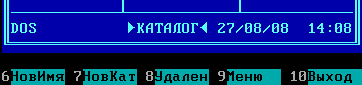
\includegraphics[width=0.5\textwidth]{patterns/01_helloworld/Norton_Commander_v5_51.png}
\caption{\ITph{}}
\end{figure}

Probabilmente questo è successo in molti Paesi durante quel periodo.


\subsection{x86-64}
\EN{\input{patterns/01_helloworld/MSVC_x64_EN}}
\FR{\input{patterns/01_helloworld/MSVC_x64_FR}}
\IT{\input{patterns/01_helloworld/MSVC_x64_IT}}
\NL{\input{patterns/01_helloworld/MSVC_x64_NL}}
\RU{\input{patterns/01_helloworld/MSVC_x64_RU}}
\PTBR{\input{patterns/01_helloworld/MSVC_x64_PTBR}}
\DE{\input{patterns/01_helloworld/MSVC_x64_DE}}
\PL{\input{patterns/01_helloworld/MSVC_x64_PL}}
\JA{\input{patterns/01_helloworld/MSVC_x64_JA}}

\EN{\input{patterns/01_helloworld/GCC_x64_EN}}
\FR{\input{patterns/01_helloworld/GCC_x64_FR}}
\RU{\input{patterns/01_helloworld/GCC_x64_RU}}
\NL{\input{patterns/01_helloworld/GCC_x64_NL}}
\IT{\input{patterns/01_helloworld/GCC_x64_IT}}
\DE{\input{patterns/01_helloworld/GCC_x64_DE}}
\PL{\input{patterns/01_helloworld/GCC_x64_PL}}
\JPN{\input{patterns/01_helloworld/GCC_x64_JPN}}

\subsubsection{Address patching (Win64)}

Se il nostro esempio venisse compilato in MSVC 2013 utilizzando lo switch \TT{\textbackslash{}MD}
(che significa un eseguibile più piccolo a causa del link dei file \TT{MSVCR*.DLL}), la funzione \main verrebbe prima, e può essere trovata facilmente:

\begin{figure}[H]
\centering
\myincludegraphics{patterns/01_helloworld/hiew_incr1.png}
\caption{Hiew}
\label{}
\end{figure}

Come esperimento, possiamo \glslink{increment}{incrementare} l'indirizzo di 1:

\begin{figure}[H]
\centering
\myincludegraphics{patterns/01_helloworld/hiew_incr2.png}
\caption{Hiew}
\label{}
\end{figure}

Hiew mostra \q{ello, world}.
E quando lanciamo l'eseguibile modificato, viene stampata proprio questa stringa.

\subsubsection{Scegliere un'altra stringa dall'immagine binaria (Linux x64)}

Il file binario che si ottiene compilando il nostro esempio tramite GCC 5.4.0 su Linux x64 contiene molte altre stringhe di testo.
Si tratta principalmente di nomi di funzioni e librerie importate.

Esegui objdump per ottenere il contenuto di tutte le sezioni del file compilato:

\begin{lstlisting}[basicstyle=\ttfamily, mathescape]
$\$$ objdump -s a.out

a.out:     file format elf64-x86-64

Contents of section .interp:
 400238 2f6c6962 36342f6c 642d6c69 6e75782d  /lib64/ld-linux-
 400248 7838362d 36342e73 6f2e3200           x86-64.so.2.
Contents of section .note.ABI-tag:
 400254 04000000 10000000 01000000 474e5500  ............GNU.
 400264 00000000 02000000 06000000 20000000  ............ ...
Contents of section .note.gnu.build-id:
 400274 04000000 14000000 03000000 474e5500  ............GNU.
 400284 fe461178 5bb710b4 bbf2aca8 5ec1ec10  .F.x[.......^...
 400294 cf3f7ae4                             .?z.

...
\end{lstlisting}

Non è un problema passare l'indirizzo della stringa di test \q{/lib64/ld-linux-x86-64.so.2} a \TT{printf()}:

\begin{lstlisting}[style=customc]
#include <stdio.h>

int main()
{
    printf(0x400238);
    return 0;
}
\end{lstlisting}

E' difficile da credere, ma questo codice stampa la stringa citata prima.

Se cambiassi l'indirizzo a \TT{0x400260}, verrebbe stampata la stringa \q{GNU}.
Questo indirizzo è corretto per la mia specifica versione di GCC, GNU toolset, etc.
Sul tuo sistema, l'eseguibile potrebbe essere leggermente differente, e anche tutti gli indirizzi sarebbero differenti.
Inoltre, aggiungendo o rimuovendo del codice in/da questo codice sorgente probabilmente sposterebbe tutti gli indirizzi in avanti o indietro.


\EN{\input{patterns/01_helloworld/GCC_one_more_EN}}
\FR{\input{patterns/01_helloworld/GCC_one_more_FR}}
\IT{\input{patterns/01_helloworld/GCC_one_more_IT}}
\NL{\input{patterns/01_helloworld/GCC_one_more_NL}}
\RU{\input{patterns/01_helloworld/GCC_one_more_RU}}
\DE{\input{patterns/01_helloworld/GCC_one_more_DE}}
\PL{\input{patterns/01_helloworld/GCC_one_more_PL}}
\JPN{\input{patterns/01_helloworld/GCC_one_more_JPN}}


\EN{\input{patterns/01_helloworld/ARM/main_EN}}
\FR{\input{patterns/01_helloworld/ARM/main_FR}}
\RU{\input{patterns/01_helloworld/ARM/main_RU}}
\IT{\input{patterns/01_helloworld/ARM/main_IT}}
\DE{\input{patterns/01_helloworld/ARM/main_DE}}
\PL{\input{patterns/01_helloworld/ARM/main_PL}}
\JPN{\input{patterns/01_helloworld/ARM/main_JPN}}

\EN{\input{patterns/01_helloworld/MIPS/main_EN}}
\RU{\input{patterns/01_helloworld/MIPS/main_RU}}
\IT{\input{patterns/01_helloworld/MIPS/main_IT}}
\DE{\input{patterns/01_helloworld/MIPS/main_DE}}
\FR{\input{patterns/01_helloworld/MIPS/main_FR}}
\PL{\input{patterns/01_helloworld/MIPS/main_PL}}
\JPN{\input{patterns/01_helloworld/MIPS/main_JPN}}


\subsection{\Conclusion{}}

La differenza principale tra il codice x86/ARM e x64/ARM64 è che il puntatore alla stringa è adesso lungo 64 bit.
Infatti, le moderne \ac{CPU} sono ora a 64-bit grazie ai costi ridotti della memoria e alla sua grande richiesta da parte delle applicazioni moderne.
Possiamo aggiungere ai nostri computer più memoria di quanto i puntatori a 32-bit siano in grado di indirizzare.
Di conseguenza, tutti i puntatori sono adesso a 64-bit.

% sections
\input{patterns/01_helloworld/exercises}
}
\PTBR{\mysection{\PrintfSeveralArgumentsSectionName}

Agora vamos extender o nosso exemplo \emph{\HelloWorldSectionName}~(\myref{sec:helloworld}),
trocando \printf no corpo da função \main() por isso:

\lstinputlisting[label=hw_c,style=customc]{patterns/03_printf/1.c}

% sections
\documentclass[a4paper,oneside]{book}

% http://www.tex.ac.uk/FAQ-noroom.html
\usepackage{etex}

\usepackage[table,usenames,dvipsnames]{xcolor}

\usepackage{fontspec}
% fonts
%\setmonofont{DroidSansMono}
%\setmainfont[Ligatures=TeX]{PT Sans}
%\setmainfont{DroidSans}
\setmainfont{DejaVu Sans}
\setmonofont{DejaVu Sans Mono}
\usepackage{polyglossia}
\defaultfontfeatures{Scale=MatchLowercase} % ensure all fonts have the same 1ex
\usepackage{ucharclasses}
\usepackage{csquotes}

\ifdefined\ENGLISH
%\wlog{main ENGLISH defined OK}
\setmainlanguage{english}
\setotherlanguage{russian}
\fi

\ifdefined\RUSSIAN
\setmainlanguage{russian}
%\newfontfamily\cyrillicfont{LiberationSans}
%\newfontfamily\cyrillicfonttt{LiberationMono}
%\newfontfamily\cyrillicfontsf{lmsans10-regular.otf}
\setotherlanguage{english}
\fi

\ifdefined\GERMAN
%\wlog{main GERMAN defined OK}
\setmainlanguage{german}
\setotherlanguage{english}
\fi

\ifdefined\SPANISH
\setmainlanguage{spanish}
\setotherlanguage{english}
\fi

\ifdefined\ITALIAN
\setmainlanguage{italian}
\setotherlanguage{english}
\fi

\ifdefined\BRAZILIAN
\setmainlanguage{portuges}
\setotherlanguage{english}
\fi

\ifdefined\POLISH
\setmainlanguage{polish}
\setotherlanguage{english}
\fi

\ifdefined\DUTCH
\setmainlanguage{dutch}
\setotherlanguage{english}
\fi

\ifdefined\TURKISH
\setmainlanguage{turkish}
\setotherlanguage{english}
\fi

\ifdefined\THAI
\setmainlanguage{thai}
%\usepackage[thai]{babel}
%\usepackage{fonts-tlwg}
\setmainfont[Script=Thai]{TH SarabunPSK}
\newfontfamily{\thaifont}[Script=Thai]{TH SarabunPSK}
\let\thaifonttt\ttfamily
\setotherlanguage{english}
\fi

\ifdefined\FRENCH
\setmainlanguage{french}
\setotherlanguage{english}
\fi

\ifdefined\JAPANESE
\usepackage{xeCJK}
\xeCJKallowbreakbetweenpuncts
\defaultfontfeatures{Ligatures=TeX,Scale=MatchLowercase}
\setCJKmainfont{IPAGothic}
\setCJKsansfont{IPAGothic}
\setCJKmonofont{IPAGothic}
\DeclareQuoteStyle{japanese}
  {「}
  {」}
  {『}
  {』}
\setquotestyle{japanese}
\setmainlanguage{japanese}
\setotherlanguage{english}
\fi

\usepackage{microtype}
\usepackage{fancyhdr}
\usepackage{listings}
%\usepackage{ulem} % used for \sout{}...
\usepackage{url}
\usepackage{graphicx}
\usepackage{makeidx}
\usepackage[cm]{fullpage}
%\usepackage{color}
\usepackage{fancyvrb}
\usepackage{xspace}
\usepackage{tabularx}
\usepackage{framed}
\usepackage{parskip}
\usepackage{epigraph}
\usepackage{ccicons}
\usepackage[nottoc]{tocbibind}
\usepackage{longtable}
\usepackage[footnote,printonlyused,withpage]{acronym}
\usepackage[]{bookmark,hyperref} % must be last
\usepackage[official]{eurosym}
\usepackage[usestackEOL]{stackengine}

% ************** myref
% http://tex.stackexchange.com/questions/228286/how-to-mix-ref-and-pageref#228292
\ifdefined\RUSSIAN
\newcommand{\myref}[1]{%
  \ref{#1}
  (стр.~\pageref{#1})%
  }
% FIXME: I wasn't able to force varioref to output russian text...
\else
\usepackage{varioref}
\newcommand{\myref}[1]{\vref{#1}}
\fi
% ************** myref

\usepackage{glossaries}
\usepackage{tikz}
%\usepackage{fixltx2e}
\usepackage{bytefield}

\usepackage{amsmath}
\usepackage{MnSymbol}
\undef\mathdollar

\usepackage{float}

\usepackage{shorttoc}
\usetikzlibrary{calc,positioning,chains,arrows}
\usepackage[margin=0.5in,headheight=15.5pt]{geometry}
% FIXME would be good without "margin="...
%\usepackage[headheight=15.5pt]{geometry}

%--------------------
% to prevent clashing of numbers and titles in TOC:
% https://tex.stackexchange.com/a/64124
\usepackage{tocloft}% http://ctan.org/pkg/tocloft
\makeatletter
\renewcommand{\numberline}[1]{%
  \@cftbsnum #1\@cftasnum~\@cftasnumb%
}
\makeatother
%--------------------

\newcommand{\footnoteref}[1]{\textsuperscript{\ref{#1}}}

%\definecolor{lstbgcolor}{rgb}{0.94,0.94,0.94}

% I don't know why this voodoo works, but without all-caps, it can't find LIGHT-GRAY color. WTF?
% see also: https://tex.stackexchange.com/questions/64298/error-with-xcolor-package
\definecolor{light-gray}{gray}{0.87}
\definecolor{LIGHT-GRAY}{gray}{0.87}
\definecolor{RED}{rgb}{1,0,0}
\makeindex

\input{macros}
\EN{\input{macro_lang_EN}}
\RU{\input{macro_lang_RU}}
\FR{\input{macro_lang_FR}}
\DE{\input{macro_lang_DE}}
\JA{\input{macro_lang_JP}}
\IT{\input{macro_lang_IT}}
\PL{\input{macro_lang_PL}}
\ES{\input{macro_lang_ES}}
\NL{\input{macro_lang_NL}}
\TR{\input{macro_lang_TR}}
\PTBR{\input{macro_lang_PTBR}}

\ifdefined\UAL
\newcommand{\TitleMain}{\TitleUAL}
\newcommand{\TitleAux}{\TitleRE}
\else
\newcommand{\TitleMain}{\TitleRE}
\newcommand{\TitleAux}{\TitleUAL}
\fi

\EN{\input{glossary_EN}}
\RU{\input{glossary_RU}}
\FR{\input{glossary_FR}}
\DE{\input{glossary_DE}}
\IT{\input{glossary_IT}}
\JA{\input{glossary_JA}}

\makeglossaries

\hypersetup{
    colorlinks=true,
    allcolors=blue,
    pdfauthor={\AUTHOR},
    pdftitle={\TitleMain}
    }

%\ifdefined\RUSSIAN
\newcommand{\LstStyle}{\ttfamily\small}
%\else
%\newcommand{\LstStyle}{\ttfamily}
%\fi

% inspired by http://prismjs.com/
\definecolor{digits}{RGB}{0,0,0}
\definecolor{bg}{RGB}{255,255,255}
%\definecolor{bg}{RGB}{255,252,250}
\definecolor{col1}{RGB}{154,20,150}
\definecolor{col2}{RGB}{112,128,144}
\definecolor{col3}{RGB}{10,120,180}
\definecolor{col4}{RGB}{106,164,108}


\lstset{
    %backgroundcolor=\color{lstbgcolor},
    %backgroundcolor=\color{light-gray},
    backgroundcolor=\color{bg},
    basicstyle=\LstStyle,
    breaklines=true,
    %prebreak=\raisebox{0ex}[0ex][0ex]{->},
    %postbreak=\raisebox{0ex}[0ex][0ex]{->},
    prebreak=\raisebox{0ex}[0ex][0ex]{\ensuremath{\rhookswarrow}},
    postbreak=\raisebox{0ex}[0ex][0ex]{\ensuremath{\rcurvearrowse\space}},
    frame=single,
    columns=fullflexible,keepspaces,
    escapeinside=§§,
    inputencoding=utf8
}

\input{syntax_color}

\ifdefined\RUSSIAN
\renewcommand\lstlistingname{Листинг}
\renewcommand\lstlistlistingname{Листинг}
\fi

\DeclareMathSizes{12}{30}{16}{12}%

% see also:
% http://tex.stackexchange.com/questions/129225/how-can-i-get-get-makeindex-to-ignore-capital-letters
% http://tex.stackexchange.com/questions/18336/correct-sorting-of-index-entries-containing-macros
\def\myindex#1{\expandafter\index\expandafter{#1}}

\begin{document}

% fancyhdr
\pagestyle{fancy}
\setlength{\headheight}{13pt}
\fancyhead[R]{} % suppress chapter name

\VerbatimFootnotes

\frontmatter

%\RU{\include{1st_page_RU}}
%\EN{\include{1st_page_EN}}
%\DE{\include{1st_page_DE}}
%\ES{\include{1st_page_ES}}
%\CN{\include{1st_page_CN}}

\RU{\include{dedication_RU}}
\EN{\include{dedication_EN}}
\FR{\include{dedication_FR}}
\JA{\include{dedication_JA}}
\DE{\include{dedication_DE}}
\IT{\include{dedication_IT}}

\include{page_after_cover}
\include{call_for_translators}

\shorttoc{%
    \RU{Краткое оглавление}%
    \EN{Abridged contents}%
    \ES{Contenidos abreviados}%
    \PTBRph{}%
    \DE{Inhaltsverzeichnis (gekürzt)}%
    \PLph{}%
    \IT{Sommario}%
    \THAph{}\NLph{}%
    \FR{Contenus abrégés}%
    \JA{簡略版}
    \TR{İçindekiler}
}{0}

\tableofcontents
\cleardoublepage

\cleardoublepage
\include{preface}

\mainmatter

\include{parts}

\EN{\include{appendix/appendix}}
\RU{\include{appendix/appendix}}
\DE{\include{appendix/appendix}}
\FR{\include{appendix/appendix}}
\IT{\include{appendix/appendix}}
\include{acronyms}

\bookmarksetup{startatroot}

\clearpage
\phantomsection
\addcontentsline{toc}{chapter}{%
    \RU{Глоссарий}%
    \EN{Glossary}%
    \ES{Glosario}%
    \PTBRph{}%
    \DE{Glossar}%
    \PLph{}%
    \IT{Glossario}%
    \THAph{}\NLph{}%
    \FR{Glossaire}%
    \JA{用語}
    \TR{Bolum}
}
\printglossaries

\clearpage
\phantomsection
\printindex

\end{document}

\subsection{ARM}

\EN{\input{patterns/03_printf/ARM/ARM3_EN}}
\RU{\input{patterns/03_printf/ARM/ARM3_RU}}
\FR{\input{patterns/03_printf/ARM/ARM3_FR}}
\IT{\input{patterns/03_printf/ARM/ARM3_IT}}
\JA{\input{patterns/03_printf/ARM/ARM3_JA}}

\EN{\input{patterns/03_printf/ARM/ARM8_EN}}
\RU{\input{patterns/03_printf/ARM/ARM8_RU}}
\FR{\input{patterns/03_printf/ARM/ARM8_FR}}
\IT{\input{patterns/03_printf/ARM/ARM8_IT}}
\JA{\input{patterns/03_printf/ARM/ARM8_JA}}

\EN{\input{patterns/03_printf/MIPS/main_EN}}
\RU{\input{patterns/03_printf/MIPS/main_RU}}
\IT{\input{patterns/03_printf/MIPS/main_IT}}
\FR{\input{patterns/03_printf/MIPS/main_FR}}
\JA{\input{patterns/03_printf/MIPS/main_JA}}


\subsection{\Conclusion{}}

Aqui está uma estrutura bem rústica da chamada da função

% TODO to be translated to PTBR:
\begin{lstlisting}[caption=x86,style=customasmx86]
...
PUSH 3rd argument
PUSH 2nd argument
PUSH 1st argument
CALL function
; modify stack pointer (if needed)
\end{lstlisting}

\begin{lstlisting}[caption=x64 (MSVC),style=customasmx86]
MOV RCX, 1st argument
MOV RDX, 2nd argument
MOV R8, 3rd argument
MOV R9, 4th argument
...
PUSH 5th, 6th argument, etc. (if needed)
CALL function
; modify stack pointer (if needed)
\end{lstlisting}

\begin{lstlisting}[caption=x64 (GCC),style=customasmx86]
MOV RDI, 1st argument
MOV RSI, 2nd argument
MOV RDX, 3rd argument
MOV RCX, 4th argument
MOV R8, 5th argument
MOV R9, 6th argument
...
PUSH 7th, 8th argument, etc. (if needed)
CALL function
; modify stack pointer (if needed)
\end{lstlisting}

\begin{lstlisting}[caption=ARM,style=customasmARM]
MOV R0, 1st argument
MOV R1, 2nd argument
MOV R2, 3rd argument
MOV R3, 4th argument
; pass 5th, 6th argument, etc., in stack (if needed)
BL function
; modify stack pointer (if needed)
\end{lstlisting}

\begin{lstlisting}[caption=ARM64,style=customasmARM]
MOV X0, 1st argument
MOV X1, 2nd argument
MOV X2, 3rd argument
MOV X3, 4th argument
MOV X4, 5th argument
MOV X5, 6th argument
MOV X6, 7th argument
MOV X7, 8th argument
; pass 9th, 10th argument, etc., in stack (if needed)
BL function
; modify stack pointer (if needed)
\end{lstlisting}

\myindex{MIPS!O32}
\begin{lstlisting}[caption=MIPS (O32 calling convention),style=customasmMIPS]
LI $4, 1st argument ; AKA \$A0
LI $5, 2nd argument ; AKA \$A1
LI $6, 3rd argument ; AKA \$A2
LI $7, 4th argument ; AKA \$A3
; pass 5th, 6th argument, etc., in stack (if needed)
LW temp_reg, address of function
JALR temp_reg
\end{lstlisting}

\subsection{A propósito}

\myindex{fastcall}
A propósito, a diferença entre os argumentos passados em x86, x64, fastcall, ARM e MIPS  é uma boa demonstração do fato de como a CPU é indiferente sobre como os argumentos são passados para as funções.
Também é possível criar um compilador hipotético capaz de passar argumentos por alguma outra estrutura especial sem usar a pilha de nenhuma maneira.

\myindex{MIPS!O32}
\PTBRph{}

A \ac{CPU} não está ciente de convenções de chamada de funções.

Agora nós podemos também relembrar de dos programadores novatos de assembly passando argumentos para outras funções:
geralmente via registradores, sem nenhuma sequência explícita, ou mesmo por variáveis globais. Logicamente, também funciona.

}
\DE{\mysection{\Stack}
\label{sec:stack}
\myindex{\Stack}

Der Stack ist eine der fundamentalen Datenstrukturen in der Informatik.
\footnote{\href{http://go.yurichev.com/17119}{wikipedia.org/wiki/Call\_Stack}}.
\ac{AKA} \ac{LIFO}.

Technisch betrachtet ist es ein Stapelspeicher innerhalb des Prozessspeichers der zusammen mit den \ESP (x86), \RSP (x64) oder dem \ac{SP} (ARM) Register als ein Zeiger in diesem Speicherblock fungiert.

\myindex{ARM!\Instructions!PUSH}
\myindex{ARM!\Instructions!POP}
\myindex{x86!\Instructions!PUSH}
\myindex{x86!\Instructions!POP}

Die häufigsten Stack-Zugriffsinstruktionen sind die \PUSH- und \POP-Instruktionen (in beidem x86 und ARM Thumb-Modus). \PUSH subtrahiert vom \ESP/\RSP/\ac{SP} 4 Byte im 32-Bit Modus (oder 8 im 64-Bit Modus) und schreibt dann den Inhalt des Zeigers an die Adresse auf die von \ESP/\RSP/\ac{SP} gezeigt wird.

\POP ist die umgekehrte Operation: Die Daten des Zeigers für die Speicherregion auf die von \ac{SP}
gezeigt wird werden ausgelesen und die Inhalte in den Instruktionsoperanden geschreiben (oft ist das ein Register). Dann werden 4 (beziehungsweise 8) Byte zum \gls{stack pointer} addiert.

Nach der Stackallokation, zeigt der \gls{stack pointer} auf den Boden des Stacks.
\PUSH verringert den \gls{stack pointer} und \POP erhöht ihn.
Der Boden des Stacks ist eigentlich der Anfang der Speicherregion die für den Stack reserviert wurde.
Das wirkt zunächst seltsam, aber so funktioniert es.

ARM unterstützt beides, aufsteigende und absteigende Stacks.

\myindex{ARM!\Instructions!STMFD}
\myindex{ARM!\Instructions!LDMFD}
\myindex{ARM!\Instructions!STMED}
\myindex{ARM!\Instructions!LDMED}
\myindex{ARM!\Instructions!STMFA}
\myindex{ARM!\Instructions!LDMFA}
\myindex{ARM!\Instructions!STMEA}
\myindex{ARM!\Instructions!LDMEA}

Zum Beispiel die \ac{STMFD}/\ac{LDMFD} und \ac{STMED}/\ac{LDMED} Instruktionen sind alle dafür gedacht mit einem absteigendem Stack zu arbeiten ( wächst nach unten, fängt mit hohen Adressen an und entwickelt sich zu niedrigeren Adressen). Die \ac{STMFA}/\ac{LDMFA} und \ac{STMEA}/\ac{LDMEA} Instruktionen sind dazu gedacht mit einem aufsteigendem Stack zu arbeiten (wächst nach oben und fängt mit niedrigeren Adressen an und wächst nach oben).

% It might be worth mentioning that STMED and STMEA write first,
% and then move the pointer, and that LDMED and LDMEA move the pointer first, and then read.
% In other words, ARM not only lets the stack grow in a non-standard direction,
% but also in a non-standard order.
% Maybe this can be in the glossary, which would explain why E stands for "empty".

\subsection{Warum wächst der Stack nach unten?}
\label{stack_grow_backwards}

Intuitiv, würden man annehmen das der Stack nach oben wächst z.B Richtung höherer Adressen, so wie bei jeder anderen Datenstruktur.

Der Grund das der Stack rückwärts wächst ist wohl historisch bedingt. Als Computer so groß waren das sie einen ganzen Raum beansprucht haben war es einfach Speicher in zwei Sektionen zu unterteilen, einen Teil für den \gls{heap} und einen Teil für den Stack. Sicher war zu dieser Zeit nicht bekannt wie groß der \gls{heap} und der Stack wachsen würden, während der Programm Laufzeit, also war die Lösung die einfachste mögliche.

\input{patterns/02_stack/stack_and_heap}

In \RitchieThompsonUNIX können wir folgendes lesen:

\begin{framed}
\begin{quotation}
Der user-core eines Programm Images wird in drei logische Segmente unterteilt. Das Programm-Text Segment beginnt bei 0 im virtuellen Adress Speicher. Während der Ausführung wird das Segment als schreibgeschützt markiert und eine einzelne Kopie des Segments wird unter allen Prozessen geteilt die das Programm ausführen. An der ersten 8K grenze über dem Programm Text Segment im Virtuellen Speicher, fängt der ``nonshared'' Bereich an, der nach Bedarf von Syscalls erweitert werden kann. Beginnend bei der höchsten Adresse im Virtuellen Speicher ist das Stack Segment, das Automatisch nach unten wächst während der Hardware Stackpointer sich ändert.
\end{quotation}
\end{framed}

Das erinnert daran wie manche Schüler Notizen zu  zwei Vorträgen in einem Notebook dokumentieren:
Notizen für den ersten Vortrag werden normal notiert, und Notizen zur zum zweiten Vortrag werden 
ans Ende des Notizbuches geschrieben, indem man das Notizbuch umdreht. Die Notizen treffen sich irgendwann
im Notizbuch aufgrund des fehlenden Freien Platzes.

% I think if we want to expand on this analogy,
% one might remember that the line number increases as as you go down a page.
% So when you decrease the address when pushing to the stack, visually,
% the stack does grow upwards.
% Of course, the problem is that in most human languages,
% just as with computers,
% we write downwards, so this direction is what makes buffer overflows so messy.

\subsection{Für was wird der Stack benutzt?}

% subsections
\EN{\input{patterns/02_stack/01_saving_ret_addr_EN}}
\RU{\input{patterns/02_stack/01_saving_ret_addr_RU}}
\DE{\input{patterns/02_stack/01_saving_ret_addr_DE}}
\FR{\input{patterns/02_stack/01_saving_ret_addr_FR}}
\PTBR{\input{patterns/02_stack/01_saving_ret_addr_PTBR}}
\IT{\input{patterns/02_stack/01_saving_ret_addr_IT}}
\PL{\input{patterns/02_stack/01_saving_ret_addr_PL}}
\JPN{\input{patterns/02_stack/01_saving_ret_addr_JPN}}

\EN{\input{patterns/02_stack/02_args_passing_EN}}
\RU{\input{patterns/02_stack/02_args_passing_RU}}
\PTBR{\input{patterns/02_stack/02_args_passing_PTBR}}
\DE{\input{patterns/02_stack/02_args_passing_DE}}
\IT{\input{patterns/02_stack/02_args_passing_IT}}
\FR{\input{patterns/02_stack/02_args_passing_FR}}
\JA{\input{patterns/02_stack/02_args_passing_JA}}
\PL{\input{patterns/02_stack/02_args_passing_PL}}


\EN{\input{patterns/02_stack/03_local_vars_EN}}
\RU{\input{patterns/02_stack/03_local_vars_RU}}
\DE{\input{patterns/02_stack/03_local_vars_DE}}
\PTBR{\input{patterns/02_stack/03_local_vars_PTBR}}
\EN{\input{patterns/02_stack/04_alloca/main_EN}}
\FR{\input{patterns/02_stack/04_alloca/main_FR}}
\RU{\input{patterns/02_stack/04_alloca/main_RU}}
\PTBR{\input{patterns/02_stack/04_alloca/main_PTBR}}
\IT{\input{patterns/02_stack/04_alloca/main_IT}}
\DE{\input{patterns/02_stack/04_alloca/main_DE}}
\PL{\input{patterns/02_stack/04_alloca/main_PL}}
\JPN{\input{patterns/02_stack/04_alloca/main_JPN}}

\input{patterns/02_stack/05_SEH}
\ifdefined\ENGLISH
\subsubsection{Buffer overflow protection}

More about it here~(\myref{subsec:bufferoverflow}).
\fi

\ifdefined\RUSSIAN
\subsubsection{Защита от переполнений буфера}

Здесь больше об этом~(\myref{subsec:bufferoverflow}).
\fi

\ifdefined\BRAZILIAN
\subsubsection{Proteção contra estouro de buffer}

Mais sobre aqui~(\myref{subsec:bufferoverflow}).
\fi

\ifdefined\ITALIAN
\subsubsection{Protezione contro buffer overflow}

Maggiori informazioni qui~(\myref{subsec:bufferoverflow}).
\fi

\ifdefined\FRENCH
\subsubsection{Protection contre les débordements de tampon}

Lire à ce propos~(\myref{subsec:bufferoverflow}).
\fi


\ifdefined\POLISH
\subsubsection{Metody zabiezpieczenia przed przepełnieniem stosu}

Więcej o tym tutaj~(\myref{subsec:bufferoverflow}).
\fi

\ifdefined\JAPANESE
\subsubsection{バッファオーバーフロー保護}

詳細はこちら~(\myref{subsec:bufferoverflow})
\fi


\subsubsection{Automatisches deallokieren der Daten auf dem Stack}

Vielleicht ist der Grund warum man lokale Variablen und SEH Einträge auf dem Stack speichert, weil sie beim 
verlassen der Funktion automatisch aufgeräumt werden. Man braucht dabei nur eine Instruktion um die Position
des Stackpointers zu korrigieren (oftmals ist es die \ADD Instruktion). Funktions Argumente, könnte man sagen 
werden auch am Ende der Funktion deallokiert. Im Kontrast dazu, alles was auf dem \emph{heap} gespeichert wird muss
explizit deallokiert werden. 

% sections
\EN{\input{patterns/02_stack/07_layout_EN}}
\RU{\input{patterns/02_stack/07_layout_RU}}
\DE{\input{patterns/02_stack/07_layout_DE}}
\PTBR{\input{patterns/02_stack/07_layout_PTBR}}
\EN{\input{patterns/02_stack/08_noise/main_EN}}
\FR{\input{patterns/02_stack/08_noise/main_FR}}
\RU{\input{patterns/02_stack/08_noise/main_RU}}
\IT{\input{patterns/02_stack/08_noise/main_IT}}
\DE{\input{patterns/02_stack/08_noise/main_DE}}
\PL{\input{patterns/02_stack/08_noise/main_PL}}
\JA{\input{patterns/02_stack/08_noise/main_JA}}

\input{patterns/02_stack/exercises}
}
\FR{\subsection{MIPS}

\subsubsection{3 arguments}

\myparagraph{GCC 4.4.5 \Optimizing}

La différence principale avec l'exemple \q{\HelloWorldSectionName} est que dans ce cas, \printf est appelée
à la place de \puts et 3 arguments de plus sont passés à travers les registres \$5\dots \$7 (ou \$A0\dots \$A2).
C'est pourquoi ces registres sont préfixés avec A-, ceci sous-entend qu'ils
sont utilisés pour le passage des arguments aux fonctions.

\lstinputlisting[caption=GCC 4.4.5 \Optimizing (\assemblyOutput),style=customasmMIPS]{patterns/03_printf/MIPS/printf3.O3_FR.s}

\lstinputlisting[caption=GCC 4.4.5 \Optimizing (IDA),style=customasmMIPS]{patterns/03_printf/MIPS/printf3.O3.IDA_FR.lst}

\IDA a agrégé la paire d'instructions \INS{LUI} et \INS{ADDIU} en une pseudo instruction \INS{LA}.
C'est pourquoi il n'y a pas d'instruction à l'adresse 0x1C: car \INS{LA} \emph{occupe} 8 octets.

\myparagraph{GCC 4.4.5 \NonOptimizing}

GCC \NonOptimizing est plus verbeux:

\lstinputlisting[caption=GCC 4.4.5 \NonOptimizing (\assemblyOutput),style=customasmMIPS]{patterns/03_printf/MIPS/printf3.O0_FR.s}

\lstinputlisting[caption=GCC 4.4.5 \NonOptimizing (IDA),style=customasmMIPS]{patterns/03_printf/MIPS/printf3.O0.IDA_FR.lst}

\subsubsection{8 arguments}

Utilisons encore l'exemple de la section précédente avec 9 arguments: \myref{example_printf8_x64}.

\lstinputlisting[style=customc]{patterns/03_printf/2.c}

\myparagraph{GCC 4.4.5 \Optimizing}

Seul les 4 premiers arguments sont passés dans les registres \$A0 \dots \$A3,
les autres sont passés par la pile.
\myindex{MIPS!O32}

C'est la convention d'appel O32 (qui est la plus commune dans le monde MIPS).
D'autres conventions d'appel (comme N32) peuvent utiliser les registres à d'autres fins.

\myindex{MIPS!\Instructions!SW}

\INS{SW} est l'abbréviation de \q{Store Word} (depuis un registre vers la mémoire).
En MIPS, il manque une instructions pour stocker une valeur dans la mémoire, donc
une paire d'instruction doit être utilisée à la place (\INS{LI}/\INS{SW}).

\lstinputlisting[caption=GCC 4.4.5 \Optimizing (\assemblyOutput),style=customasmMIPS]{patterns/03_printf/MIPS/printf8.O3_FR.s}

\lstinputlisting[caption=GCC 4.4.5 \Optimizing (IDA),style=customasmMIPS]{patterns/03_printf/MIPS/printf8.O3.IDA_FR.lst}

\myparagraph{GCC 4.4.5 \NonOptimizing}

GCC \NonOptimizing est plus verbeux:

\lstinputlisting[caption=\NonOptimizing GCC 4.4.5 (\assemblyOutput),style=customasmMIPS]{patterns/03_printf/MIPS/printf8.O0_FR.s}

\lstinputlisting[caption=\NonOptimizing GCC 4.4.5 (IDA),style=customasmMIPS]{patterns/03_printf/MIPS/printf8.O0.IDA_FR.lst}

}
\PL{\mysection{\Stack}
\label{sec:stack}
\myindex{\Stack}

Stos w informatyce jest jedną z najbardziej fundamentalnych struktur danych
\footnote{\href{http://go.yurichev.com/17119}{wikipedia.org/wiki/Call\_stack}}.
\ac{AKA} \ac{LIFO}.

Technicznie rzecz biorąc, jest to tylko blok pamięci w pamięci procesora + rejestr \ESP w x86 lub \RSP w x64, lub \ac{SP} w ARM, który wskazuje obszar gdzieś w granicach tego bloku.

\myindex{ARM!\Instructions!PUSH}
\myindex{ARM!\Instructions!POP}
\myindex{x86!\Instructions!PUSH}
\myindex{x86!\Instructions!POP}
Najczęsciej wykorzystywanymi instrukcjami do operowania na stosie są \PUSH i \POP (w x86 i Thumb-trybie ARM). 
\PUSH zmniejsza \ESP/\RSP/\ac{SP} o 4 w trybie 32-bitowym (lub o 8 w 64-bitowym),
następnie zapisuje pod adres, na który wskazuje \ESP/\RSP/\ac{SP}, zawartość swojego operandu.

\POP jest odwrotną operacją- najpierw zdejmuje ze \glslink{stack pointer}{wskaźnika stosu} wartość i umieszcza ją do operandu 
(który często jest rejestrem), a następnie zwiększa wskaźnik o 4 (lub 8).

Przed alokacją pamięci na stosie \glslink{stack pointer}{rejestr-wskaźnik} wskazuje na koniec stosu.
Koniec stosu znajduje się na początku zaalokowanego bloku pamięci, przeznaczonego na stos. Może zabrzmieć to dziwnie, ale tak to działa.
\PUSH zmniejsza \glslink{stack pointer}{rejestr-wskaźnik}, а \POP~--- zwiększa.

W procesorze ARM jest wsparcie dla stosów zarówno rosnących w dół, jak i rosnącyh w górę.

\myindex{ARM!\Instructions!STMFD}
\myindex{ARM!\Instructions!LDMFD}
\myindex{ARM!\Instructions!STMED}
\myindex{ARM!\Instructions!LDMED}
\myindex{ARM!\Instructions!STMFA}
\myindex{ARM!\Instructions!LDMFA}
\myindex{ARM!\Instructions!STMEA}
\myindex{ARM!\Instructions!LDMEA}

Na przykład, instrukcje \ac{STMFD}/\ac{LDMFD}, \ac{STMED}/\ac{LDMED} są przeznaczone dla stosu malejącego (rośnie w dół, zaczynając od adresów wysokich, do adresów niskich).\\
Natomiast instrukcje \ac{STMFA}/\ac{LDMFA}, \ac{STMEA}/\ac{LDMEA} są przeznaczone dla stosu rosnącego (rośnie w górę, zaczynając od niskich adresów, kończąc na adresach wysokich).

% It might be worth mentioning that STMED and STMEA write first,
% and then move the pointer,
% and that LDMED and LDMEA move the pointer first, and then read.
% In other words, ARM not only lets the stack grow in a non-standard direction,
% but also in a non-standard order.
% Maybe this can be in the glossary, which would explain why E stands for "empty".

\subsection{Dlaczego stos rośnie wstecznie?}
\label{stack_grow_backwards}

Intuicyjnie moglibyśmy pomyśleć, że, jak i każda inna struktura danych, stos mogłby rosnąć w górę, tzn. w kierunku zwiększenia adresów.

Powód, dlaczego stos rośnie w dół, jest najprawdobodobniej historyczny.
Kiedy komputery były duże i zajmowały cały pokój, można było bardzo łatwo rozdzielić segment na dwa obszary: dla \glslink{heap}{kopca} i dla stosu.
Z góry nie było wiadomo, jak duża może być \glslink{heap}{sterta} lub stos, dlatego takie rozwiązanie było najbardziej logiczne.

\input{patterns/02_stack/stack_and_heap}

W \RitchieThompsonUNIX można przeczytać:

\begin{framed}
\begin{quotation}
The user-core part of an image is divided into three logical segments. The program text segment begins at location 0 in the virtual address space. During execution, this segment is write-protected and a single copy of it is shared among all processes executing the same program. At the first 8K byte boundary above the program text segment in the virtual address space begins a nonshared, writable data segment, the size of which may be extended by a system call. Starting at the highest address in the virtual address space is a stack segment, which automatically grows downward as the hardware's stack pointer fluctuates.
\end{quotation}
\end{framed}

To trochę przypomina podejście studenta,
który pisze dwie osobne lektury w jednym zeszycie:
pierwsza lektura jest pisana jak zwykle od początku zeszytu, a druga jest pisana od końca zeszytu.
Lektury mogą się "spotkać" gdzieś na środku zeszytu, jeśli zabraknie miejsca.

% I think if we want to expand on this analogy,
% one might remember that the line number increases as as you go down a page.
% So when you decrease the address when pushing to the stack, visually,
% the stack does grow upwards.
% Of course, the problem is that in most human languages,
% just as with computers,
% we write downwards, so this direction is what makes buffer overflows so messy.

\subsection{Do jakich celów służy stos?}

% subsections
\EN{\input{patterns/02_stack/01_saving_ret_addr_EN}}
\RU{\input{patterns/02_stack/01_saving_ret_addr_RU}}
\DE{\input{patterns/02_stack/01_saving_ret_addr_DE}}
\FR{\input{patterns/02_stack/01_saving_ret_addr_FR}}
\PTBR{\input{patterns/02_stack/01_saving_ret_addr_PTBR}}
\IT{\input{patterns/02_stack/01_saving_ret_addr_IT}}
\PL{\input{patterns/02_stack/01_saving_ret_addr_PL}}
\JPN{\input{patterns/02_stack/01_saving_ret_addr_JPN}}

\EN{\input{patterns/02_stack/02_args_passing_EN}}
\RU{\input{patterns/02_stack/02_args_passing_RU}}
\PTBR{\input{patterns/02_stack/02_args_passing_PTBR}}
\DE{\input{patterns/02_stack/02_args_passing_DE}}
\IT{\input{patterns/02_stack/02_args_passing_IT}}
\FR{\input{patterns/02_stack/02_args_passing_FR}}
\JA{\input{patterns/02_stack/02_args_passing_JA}}
\PL{\input{patterns/02_stack/02_args_passing_PL}}


\EN{\input{patterns/02_stack/03_local_vars_EN}}
\RU{\input{patterns/02_stack/03_local_vars_RU}}
\PTBR{\input{patterns/02_stack/03_local_vars_PTBR}}
\PL{\input{patterns/02_stack/03_local_vars_PL}}
\EN{\input{patterns/02_stack/04_alloca/main_EN}}
\FR{\input{patterns/02_stack/04_alloca/main_FR}}
\RU{\input{patterns/02_stack/04_alloca/main_RU}}
\PTBR{\input{patterns/02_stack/04_alloca/main_PTBR}}
\IT{\input{patterns/02_stack/04_alloca/main_IT}}
\DE{\input{patterns/02_stack/04_alloca/main_DE}}
\PL{\input{patterns/02_stack/04_alloca/main_PL}}
\JPN{\input{patterns/02_stack/04_alloca/main_JPN}}

\input{patterns/02_stack/05_SEH}
\ifdefined\ENGLISH
\subsubsection{Buffer overflow protection}

More about it here~(\myref{subsec:bufferoverflow}).
\fi

\ifdefined\RUSSIAN
\subsubsection{Защита от переполнений буфера}

Здесь больше об этом~(\myref{subsec:bufferoverflow}).
\fi

\ifdefined\BRAZILIAN
\subsubsection{Proteção contra estouro de buffer}

Mais sobre aqui~(\myref{subsec:bufferoverflow}).
\fi

\ifdefined\ITALIAN
\subsubsection{Protezione contro buffer overflow}

Maggiori informazioni qui~(\myref{subsec:bufferoverflow}).
\fi

\ifdefined\FRENCH
\subsubsection{Protection contre les débordements de tampon}

Lire à ce propos~(\myref{subsec:bufferoverflow}).
\fi


\ifdefined\POLISH
\subsubsection{Metody zabiezpieczenia przed przepełnieniem stosu}

Więcej o tym tutaj~(\myref{subsec:bufferoverflow}).
\fi

\ifdefined\JAPANESE
\subsubsection{バッファオーバーフロー保護}

詳細はこちら~(\myref{subsec:bufferoverflow})
\fi


\subsubsection{Automatyczne zwalnianie danych na stosie}
Możliwym powodem przechowywania zmiennych lokalnych i rekordów SEH na stosie jest to, że kiedy funkcja zakończy działanie są one automatycznie zwalniane ze stosu używając tylko jednej instrukcji w celu przywrócenia poprzedniego stanu stosu (często jest to instrukcja ADD). Argumenty funkcji także są automatycznie zwalniane z pamięci pod koniec funkcji. Natomiast wszystko co jest przechowywane na stercie(\emph{heap}) trzeba zwalniać jawnie.

% sections
\EN{\input{patterns/02_stack/07_layout_EN}}
\RU{\input{patterns/02_stack/07_layout_RU}}
\PTBR{\input{patterns/02_stack/07_layout_PTBR}}
\PL{\input{patterns/02_stack/07_layout_PL}}
\EN{\input{patterns/02_stack/08_noise/main_EN}}
\FR{\input{patterns/02_stack/08_noise/main_FR}}
\RU{\input{patterns/02_stack/08_noise/main_RU}}
\IT{\input{patterns/02_stack/08_noise/main_IT}}
\DE{\input{patterns/02_stack/08_noise/main_DE}}
\PL{\input{patterns/02_stack/08_noise/main_PL}}
\JA{\input{patterns/02_stack/08_noise/main_JA}}

\input{patterns/02_stack/exercises}


}
\JA{\mysection{\HelloWorldSectionName}
\label{sec:helloworld}

[\KRBook]という本の有名な例を使ってみましょう

\lstinputlisting[caption=\CCpp Code,style=customc]{patterns/01_helloworld/hw.c}

\subsection{x86}

\EN{\input{patterns/01_helloworld/MSVC_x86_EN}}
\FR{\input{patterns/01_helloworld/MSVC_x86_FR}}
\IT{\input{patterns/01_helloworld/MSVC_x86_IT}}
\NL{\input{patterns/01_helloworld/MSVC_x86_NL}}
\RU{\input{patterns/01_helloworld/MSVC_x86_RU}}
\PTBR{\input{patterns/01_helloworld/MSVC_x86_PTBR}}
\DE{\input{patterns/01_helloworld/MSVC_x86_DE}}
\PL{\input{patterns/01_helloworld/MSVC_x86_PL}}
\JPN{\input{patterns/01_helloworld/MSVC_x86_JPN}}

\EN{\input{patterns/01_helloworld/GCC_x86_EN}}
\FR{\input{patterns/01_helloworld/GCC_x86_FR}}
\RU{\input{patterns/01_helloworld/GCC_x86_RU}}
\NL{\input{patterns/01_helloworld/GCC_x86_NL}}
\IT{\input{patterns/01_helloworld/GCC_x86_IT}}
\DE{\input{patterns/01_helloworld/GCC_x86_DE}}
\PL{\input{patterns/01_helloworld/GCC_x86_PL}}
\JPN{\input{patterns/01_helloworld/GCC_x86_JPN}}

\subsubsection{文字列のパッチ(Win32)}

Hiewを使用して、実行可能ファイル内の ``hello、world'' 文字列を簡単に見つけることができます:

\begin{figure}[H]
\centering
\myincludegraphics{patterns/01_helloworld/hola_edit1.png}
\caption{Hiew}
\label{}
\end{figure}

メッセージをスペイン語に翻訳しようとすることができます

\begin{figure}[H]
\centering
\myincludegraphics{patterns/01_helloworld/hola_edit2.png}
\caption{Hiew}
\label{}
\end{figure}

スペイン語のテキストは英語より1バイト短くなっているので、最後に0x0Aバイト(\TT{\textbackslash{}n})に続けてNULLバイトを追加しました。

うまくいきました。

より長いメッセージを挿入する場合はどうすればよいですか?
元の英語テキストの後には、ゼロバイトがいくつかあります。 上書きできるかどうかはなんとも言えません:\ac{CRT}コードのどこかで使われるかもしれないし、そうでないかもしれません。 
とにかく、自分が行っていることを本当に知っていれば、それらを上書きするだけです。

\subsubsection{文字列のパッチ(Linux x64)}

\myindex{\radare}
\radare{}を使ってLinux x64実行ファイルにパッチを当ててみましょう

\lstinputlisting[caption=\radare{} session]{patterns/01_helloworld/radare.lst}

ここでは何が起こっているの:私は\TT{/}コマンドを使用して\q{hello}文字列を検索し、
そのアドレスに\emph{カーソル}(\radare{}用語で\emph{シーク})を設定します。 
次に、これが本当にその場所であることを確かめたい:\TT{px}がダンプします。
\TT{oo+}は\radare{}を\emph{読み書き}モードに切り替えます。 
\TT{w}は現在の\emph{シーク}時にASCII文字列を書き込みます。
最後の\TT{\textbackslash{}00}に注意してください。これはNULLバイトです。
\TT{q}で終了します。

% TBT
%\subsubsection{This is a real story of software cracking}
%
%An image processing software, when not registered, added watermarks,
%like ``This image was processed by evaluation version of [software name]'', across a picture.
%We tried at random: we found that string in the executable file and put spaces instead of it.
%Watermarks disappeared.
%Technically speaking, they continued to appear.
%\myindex{Qt}
%With the help of Qt functions, the watermark was still added to the resulting image.
%But adding spaces didn't alter the image itself...

\subsubsection{MS-DOS時代におけるソフトウェアの\emph{ローカライズ}}

このやり方は、1980年代と1990年代にMS-DOSソフトウェアをロシア語に翻訳する一般的な方法でした。 ロシア語の言葉や文章は、英語の文章と比べて通常若干長いので、\emph{ローカライズ}されたソフトウェアには奇妙な頭字語やとても読みにくい略語が含まれています。

他の国の他の言語でも、この時代に起きていたことでしょう。


\subsection{x86-64}
\EN{\input{patterns/01_helloworld/MSVC_x64_EN}}
\FR{\input{patterns/01_helloworld/MSVC_x64_FR}}
\IT{\input{patterns/01_helloworld/MSVC_x64_IT}}
\NL{\input{patterns/01_helloworld/MSVC_x64_NL}}
\RU{\input{patterns/01_helloworld/MSVC_x64_RU}}
\PTBR{\input{patterns/01_helloworld/MSVC_x64_PTBR}}
\DE{\input{patterns/01_helloworld/MSVC_x64_DE}}
\PL{\input{patterns/01_helloworld/MSVC_x64_PL}}
\JA{\input{patterns/01_helloworld/MSVC_x64_JA}}

\EN{\input{patterns/01_helloworld/GCC_x64_EN}}
\FR{\input{patterns/01_helloworld/GCC_x64_FR}}
\RU{\input{patterns/01_helloworld/GCC_x64_RU}}
\NL{\input{patterns/01_helloworld/GCC_x64_NL}}
\IT{\input{patterns/01_helloworld/GCC_x64_IT}}
\DE{\input{patterns/01_helloworld/GCC_x64_DE}}
\PL{\input{patterns/01_helloworld/GCC_x64_PL}}
\JPN{\input{patterns/01_helloworld/GCC_x64_JPN}}

\subsubsection{アドレスのパッチ(Win64)}

この例が\TT{\textbackslash{}MD}スイッチ(\TT{MSVCR*.DLL}ファイルリンケージのために小さな実行可能ファイルを意味します)を使用してMSVC 2013でコンパイルされた場合、 \main 関数が最初に来て簡単に見つかります

\begin{figure}[H]
\centering
\myincludegraphics{patterns/01_helloworld/hiew_incr1.png}
\caption{Hiew}
\label{}
\end{figure}

実験として、アドレスを1ずつ\gls{increment}することができます:

\begin{figure}[H]
\centering
\myincludegraphics{patterns/01_helloworld/hiew_incr2.png}
\caption{Hiew}
\label{}
\end{figure}

Hiewは \q{ello, world}を示しています。 そしてパッチが適用された実行可能ファイルを実行すると、この文字列が表示されます。

\subsubsection{バイナリイメージから他の文字列を抜き取る(Linux x64)}

Linux x64ボックスでGCC 5.4.0を使用して私たちの例をコンパイルしたときに得たバイナリファイルには、他の多くのテキスト文字列があります。
ほとんどはインポートされた関数名とライブラリ名です。

objdumpを実行して、コンパイル済みファイルのすべてのセクションの内容を取得します。

\begin{lstlisting}[basicstyle=\ttfamily, mathescape]
$\$$ objdump -s a.out

a.out:     file format elf64-x86-64

Contents of section .interp:
 400238 2f6c6962 36342f6c 642d6c69 6e75782d  /lib64/ld-linux-
 400248 7838362d 36342e73 6f2e3200           x86-64.so.2.
Contents of section .note.ABI-tag:
 400254 04000000 10000000 01000000 474e5500  ............GNU.
 400264 00000000 02000000 06000000 20000000  ............ ...
Contents of section .note.gnu.build-id:
 400274 04000000 14000000 03000000 474e5500  ............GNU.
 400284 fe461178 5bb710b4 bbf2aca8 5ec1ec10  .F.x[.......^...
 400294 cf3f7ae4                             .?z.

...
\end{lstlisting}

テキスト文字列\q{/lib64/ld-linux-x86-64.so.2}のアドレスを\TT{printf()}に渡すのは問題ではありません

\begin{lstlisting}[style=customc]
#include <stdio.h>

int main()
{
    printf(0x400238);
    return 0;
}
\end{lstlisting}

信じがたいですが、このコードは前述の文字列を表示します。

アドレスを\TT{0x400260}に変更すると、 \q{GNU}文字列が出力されます。 
このアドレスは、私の特定のGCCバージョン、GNUツールセットなどに当てはまります。
あなたのシステムでは、実行ファイルは若干異なる場合があり、すべてのアドレスも異なります。 
また、このソースコードに/からコードを追加/削除すると、おそらくすべてのアドレスが前後に移動します。


\EN{\input{patterns/01_helloworld/GCC_one_more_EN}}
\FR{\input{patterns/01_helloworld/GCC_one_more_FR}}
\IT{\input{patterns/01_helloworld/GCC_one_more_IT}}
\NL{\input{patterns/01_helloworld/GCC_one_more_NL}}
\RU{\input{patterns/01_helloworld/GCC_one_more_RU}}
\DE{\input{patterns/01_helloworld/GCC_one_more_DE}}
\PL{\input{patterns/01_helloworld/GCC_one_more_PL}}
\JPN{\input{patterns/01_helloworld/GCC_one_more_JPN}}


\EN{\input{patterns/01_helloworld/ARM/main_EN}}
\FR{\input{patterns/01_helloworld/ARM/main_FR}}
\RU{\input{patterns/01_helloworld/ARM/main_RU}}
\IT{\input{patterns/01_helloworld/ARM/main_IT}}
\DE{\input{patterns/01_helloworld/ARM/main_DE}}
\PL{\input{patterns/01_helloworld/ARM/main_PL}}
\JPN{\input{patterns/01_helloworld/ARM/main_JPN}}

\EN{\input{patterns/01_helloworld/MIPS/main_EN}}
\RU{\input{patterns/01_helloworld/MIPS/main_RU}}
\IT{\input{patterns/01_helloworld/MIPS/main_IT}}
\DE{\input{patterns/01_helloworld/MIPS/main_DE}}
\FR{\input{patterns/01_helloworld/MIPS/main_FR}}
\PL{\input{patterns/01_helloworld/MIPS/main_PL}}
\JPN{\input{patterns/01_helloworld/MIPS/main_JPN}}


\subsection{\Conclusion{}}

x86/ARMとx64/ARM64コードの主な違いは、文字列へのポインタが64ビット長になったことです。
確かに、現代の \ac{CPU} は64ビットになりました。これは、現代のアプリケーションではメモリの節約と大きな需要の両方があるからです。
私たちは32ビットポインタよりもはるかに多くのメモリをコンピュータに追加することができます。
そのため、すべてのポインタは64ビットになりました。

% sections
\input{patterns/01_helloworld/exercises}
}

\EN{\mysection{\MinesweeperWinXPExampleChapterName}
\label{minesweeper_winxp}
\myindex{Windows!Windows XP}

For those who are not very good at playing Minesweeper, we could try to reveal the hidden mines in the debugger.

\myindex{\CStandardLibrary!rand()}
\myindex{Windows!PDB}

As we know, Minesweeper places mines randomly, so there has to be some kind of random number generator or
a call to the standard \TT{rand()} C-function.

What is really cool about reversing Microsoft products is that there are \gls{PDB} 
file with symbols (function names, \etc{}).
When we load \TT{winmine.exe} into \IDA, it downloads the 
\gls{PDB} file exactly for this 
executable and shows all names.

So here it is, the only call to \TT{rand()} is this function:

\lstinputlisting[style=customasmx86]{examples/minesweeper/tmp1.lst}

\IDA named it so, and it was the name given to it by Minesweeper's developers.

The function is very simple:

\begin{lstlisting}[style=customc]
int Rnd(int limit)
{
    return rand() % limit;
};
\end{lstlisting}

(There is no \q{limit} name in the \gls{PDB} file; we manually named this argument like this.)

So it returns 
a random value from 0 to a specified limit.

\TT{Rnd()} is called only from one place, 
a function called \TT{StartGame()}, 
and as it seems, this is exactly 
the code which place the mines:

\begin{lstlisting}[style=customasmx86]
.text:010036C7                 push    _xBoxMac
.text:010036CD                 call    _Rnd@4          ; Rnd(x)
.text:010036D2                 push    _yBoxMac
.text:010036D8                 mov     esi, eax
.text:010036DA                 inc     esi
.text:010036DB                 call    _Rnd@4          ; Rnd(x)
.text:010036E0                 inc     eax
.text:010036E1                 mov     ecx, eax
.text:010036E3                 shl     ecx, 5          ; ECX=ECX*32
.text:010036E6                 test    _rgBlk[ecx+esi], 80h
.text:010036EE                 jnz     short loc_10036C7
.text:010036F0                 shl     eax, 5          ; EAX=EAX*32
.text:010036F3                 lea     eax, _rgBlk[eax+esi]
.text:010036FA                 or      byte ptr [eax], 80h
.text:010036FD                 dec     _cBombStart
.text:01003703                 jnz     short loc_10036C7
\end{lstlisting}

Minesweeper allows you to set the board size, so the X (xBoxMac) and Y (yBoxMac) of the board are global variables.
They are passed to \TT{Rnd()} and random 
coordinates are generated.
A mine is placed by the \TT{OR} instruction at \TT{0x010036FA}. 
And if it has been placed before 
(it's possible if the pair of \TT{Rnd()} 
generates a coordinates pair which has been already 
generated), 
then \TT{TEST} and \TT{JNZ} at \TT{0x010036E6} 
jumps to the generation routine again.

\TT{cBombStart} is the global variable containing total number of mines. So this is loop.

The width of the array is 32 
(we can conclude this by looking at the \TT{SHL} instruction, which multiplies one of the coordinates by 32).

The size of the \TT{rgBlk} 
global array can be easily determined by the difference 
between the \TT{rgBlk} 
label in the data segment and the next known one. 
It is 0x360 (864):

\begin{lstlisting}[style=customasmx86]
.data:01005340 _rgBlk          db 360h dup(?)          ; DATA XREF: MainWndProc(x,x,x,x)+574
.data:01005340                                         ; DisplayBlk(x,x)+23
.data:010056A0 _Preferences    dd ?                    ; DATA XREF: FixMenus()+2
...
\end{lstlisting}

$864/32=27$.

So the array size is $27*32$?
It is close to what we know: when we try to set board size to $100*100$ in Minesweeper settings, it fallbacks to a board of size $24*30$.
So this is the maximal board size here.
And the array has a fixed size for any board size.

So let's see all this in \olly.
We will ran Minesweeper, attaching \olly to it and now we can see the memory dump at the address of the \TT{rgBlk} array (\TT{0x01005340})
\footnote{All addresses here are for Minesweeper for Windows XP SP3 English. 
They may differ for other service packs.}.

So we got this memory dump of the array:

\lstinputlisting[style=customasmx86]{examples/minesweeper/1.lst}

\olly, like any other hexadecimal editor, shows 16 bytes per line.
So each 32-byte array row occupies exactly 2 lines here.

This is beginner level (9*9 board).

There is some square 
structure can be seen visually (0x10 bytes).

We will click \q{Run} in \olly to unfreeze the Minesweeper process, then we'll clicked randomly at the Minesweeper window 
and trapped into mine, but now all mines are visible:

\begin{figure}[H]
\centering
\myincludegraphicsSmall{examples/minesweeper/1.png}
\caption{Mines}
\label{fig:minesweeper1}
\end{figure}

By comparing the mine places and the dump, we can conclude that 0x10 stands for border, 0x0F---empty block, 0x8F---mine.
Perhaps, 0x10 is just a \emph{sentinel value}.

Now we'll add comments and also enclose all 0x8F bytes into square brackets:

\lstinputlisting[style=customasmx86]{examples/minesweeper/2.lst}

Now we'll remove all \emph{border bytes} (0x10) and what's beyond those:

\lstinputlisting[style=customasmx86]{examples/minesweeper/3.lst}

Yes, these are mines, now it can be clearly seen and compared with the screenshot.

\clearpage
What is interesting is that we can modify the array right in \olly.
We can remove all mines by changing all 0x8F bytes by 0x0F, and here is what we'll get in Minesweeper:

\begin{figure}[H]
\centering
\myincludegraphicsSmall{examples/minesweeper/3.png}
\caption{All mines are removed in debugger}
\label{fig:minesweeper3}
\end{figure}

We can also move all of them to the first line: 

\begin{figure}[H]
\centering
\myincludegraphicsSmall{examples/minesweeper/2.png}
\caption{Mines set in debugger}
\label{fig:minesweeper2}
\end{figure}

Well, the debugger is not very convenient for eavesdropping (which is our goal anyway), so we'll write a small utility
to dump the contents of the board:

\lstinputlisting[style=customc]{examples/minesweeper/minesweeper_cheater.c}

Just set the \ac{PID}
\footnote{PID it can be seen in Task Manager 
(enable it in \q{View $\rightarrow$ Select Columns})} 
and the address of the array (\TT{0x01005340} for Windows XP SP3 English) 
and it will dump it
\footnote{The compiled executable is here: 
\href{http://go.yurichev.com/17165}{beginners.re}}.

It attaches itself to a win32 process by \ac{PID} and just reads process memory at the address.

\subsection{Finding grid automatically}

This is kind of nuisance to set address each time when we run our utility.
Also, various Minesweeper versions may have the array on different address.
Knowing the fact that there is always a border (0x10 bytes), we can just find it in memory:

\lstinputlisting[style=customc]{examples/minesweeper/cheater2_fragment.c}

Full source code: \url{https://github.com/DennisYurichev/RE-for-beginners/blob/master/examples/minesweeper/minesweeper_cheater2.c}.

\subsection{\Exercises}

\begin{itemize}

\item 
Why do the \emph{border bytes} (or \emph{sentinel values}) (0x10) exist in the array?

What they are for if they are not visible in Minesweeper's interface?
How could it work without them?

\item 
As it turns out, there are more values possible (for open blocks, for flagged by user, \etc{}).
Try to find the meaning of each one.

\item 
Modify my utility so it can remove all mines or set them in a fixed pattern that you want in the Minesweeper
process currently running.

\end{itemize}
}
\ES{% TODO to be resynced with EN version
\mysection{La función más simple}

La función más simple posible es sin duda uno que simplemente devuelve un valor constante:

Ejemplo:

\lstinputlisting[caption=\ESph{},style=customc]{patterns/011_ret/1.c}

Vamos a compilar!

\subsection{x86}

Esto es lo que optimiza el GCC  y los compiladores de MSVC los cuales se producen en la plataforma x86:

\lstinputlisting[caption=\Optimizing GCC/MSVC (\assemblyOutput),style=customasmx86]{patterns/011_ret/1.s}

\myindex{x86!\Instructions!RET}
Hay solo dos instrucciones: los primeros lugares el valor 123 en el registro \EAX, que se utiliza por convención para almacenar el valor de retorno y el segundo es \RET, que devuelve la ejecución al llamado.

La persona que llama tomar el resultado del registro \EAX.

\subsection{ARM}

Hay algunas diferencias en la plataforma ARM:

\lstinputlisting[caption=\OptimizingKeilVI (\ARMMode) ASM Output,style=customasmARM]{patterns/011_ret/1_Keil_ARM_O3.s}

ARM utiliza el registro \Reg{0} para el retorno de los resultados de las funciones, por lo que se copia 123 en \Reg{0}.

La dirección que retorna no es guardada en la pila local de la ARM \ac{ISA}, sino más bien en el registro de enlace,
entonces la instrucción \INS{BX LR} provoca que la ejecución de un salto a la dirección eficazmente retornando la ejecución a donde fue llamada(caller ``nuestro llamador'').

\myindex{ARM!\Instructions!MOV}
\myindex{x86!\Instructions!MOV}
Vale la pena señalar que \MOV es un nombre engañoso para la instrucción tanto en x86 y ARM \ac{ISA}s.

Los datos de hecho, no se \emph{mueven}, sino que se \emph{copian}.

\subsection{MIPS}

\label{MIPS_leaf_function_ex1}
Hay dos convenciones de nomenclatura utilizadas en el mundo de MIPS al nombrar registros: por número (de \$0 a \$31) o por seudónimo (\$V0, \$A0, etc.).

El ensamblado de GCC produce una salida en listando los registros por numeros:

\lstinputlisting[caption=\Optimizing GCC 4.4.5 (\assemblyOutput),style=customasmMIPS]{patterns/011_ret/MIPS.s}

\dots Mientras que \IDA lo hace por sus seudónimos:

\lstinputlisting[caption=\Optimizing GCC 4.4.5 (IDA),style=customasmMIPS]{patterns/011_ret/MIPS_IDA.lst}

El \$2 (o \$V0) registro es usado para almacenar el valor devuelto por la función.
\myindex{MIPS!\Pseudoinstructions!LI}
\INS{LI} significa ``Load Immediate'' (``carga inmediata'') y es el MIPS equivalente a \MOV.

\myindex{MIPS!\Instructions!J}
La otra instrucción es el jump (``salto'') que es  (J o JR) el cual retorna la ejecución fluida para el llamado, da un salto a la dirección del registro \$31 (o \$RA).

Este es el registro análoga a \ac{LR} en ARM.

\myindex{MIPS!Branch delay slot}
Es posible que se pregunte por qué posiciones de la instrucción de la carga (LI) y el salto instrucciones (J y JR) se intercambian.Esto es debido a una característica llamada RISC (``ranura de retardo rama'').

La razón por la que esto sucede es una peculiaridad en la arquitectura RISC de algunas ISA y no es importante para nuestros propósitos --– sólo tenemos que recordar que en MIPS, la instrucción que sigue a un salto o instrucción de salto se ejecuta antes de la instrucción / rama salto en sí.

Como consecuencia, las instrucciones de ramificación siempre intercambiar lugares con la instrucción que debe ser ejecutado de antemano.

\subsubsection{Una nota acerca de la instrucción MIPS nombres / Registro}

Registros y nombre de instrucciones en el mundo de MIPS tradicionalmente se escriben en minúsculas.
Sin embargo, en aras de la  coherencia, que me quedo con el uso de letras mayúsculas, ya que es la convención seguida por el resto de las ISAs destacados aquí.

% TBT

}
\FR{\subsection{MIPS}

\subsubsection{3 arguments}

\myparagraph{GCC 4.4.5 \Optimizing}

La différence principale avec l'exemple \q{\HelloWorldSectionName} est que dans ce cas, \printf est appelée
à la place de \puts et 3 arguments de plus sont passés à travers les registres \$5\dots \$7 (ou \$A0\dots \$A2).
C'est pourquoi ces registres sont préfixés avec A-, ceci sous-entend qu'ils
sont utilisés pour le passage des arguments aux fonctions.

\lstinputlisting[caption=GCC 4.4.5 \Optimizing (\assemblyOutput),style=customasmMIPS]{patterns/03_printf/MIPS/printf3.O3_FR.s}

\lstinputlisting[caption=GCC 4.4.5 \Optimizing (IDA),style=customasmMIPS]{patterns/03_printf/MIPS/printf3.O3.IDA_FR.lst}

\IDA a agrégé la paire d'instructions \INS{LUI} et \INS{ADDIU} en une pseudo instruction \INS{LA}.
C'est pourquoi il n'y a pas d'instruction à l'adresse 0x1C: car \INS{LA} \emph{occupe} 8 octets.

\myparagraph{GCC 4.4.5 \NonOptimizing}

GCC \NonOptimizing est plus verbeux:

\lstinputlisting[caption=GCC 4.4.5 \NonOptimizing (\assemblyOutput),style=customasmMIPS]{patterns/03_printf/MIPS/printf3.O0_FR.s}

\lstinputlisting[caption=GCC 4.4.5 \NonOptimizing (IDA),style=customasmMIPS]{patterns/03_printf/MIPS/printf3.O0.IDA_FR.lst}

\subsubsection{8 arguments}

Utilisons encore l'exemple de la section précédente avec 9 arguments: \myref{example_printf8_x64}.

\lstinputlisting[style=customc]{patterns/03_printf/2.c}

\myparagraph{GCC 4.4.5 \Optimizing}

Seul les 4 premiers arguments sont passés dans les registres \$A0 \dots \$A3,
les autres sont passés par la pile.
\myindex{MIPS!O32}

C'est la convention d'appel O32 (qui est la plus commune dans le monde MIPS).
D'autres conventions d'appel (comme N32) peuvent utiliser les registres à d'autres fins.

\myindex{MIPS!\Instructions!SW}

\INS{SW} est l'abbréviation de \q{Store Word} (depuis un registre vers la mémoire).
En MIPS, il manque une instructions pour stocker une valeur dans la mémoire, donc
une paire d'instruction doit être utilisée à la place (\INS{LI}/\INS{SW}).

\lstinputlisting[caption=GCC 4.4.5 \Optimizing (\assemblyOutput),style=customasmMIPS]{patterns/03_printf/MIPS/printf8.O3_FR.s}

\lstinputlisting[caption=GCC 4.4.5 \Optimizing (IDA),style=customasmMIPS]{patterns/03_printf/MIPS/printf8.O3.IDA_FR.lst}

\myparagraph{GCC 4.4.5 \NonOptimizing}

GCC \NonOptimizing est plus verbeux:

\lstinputlisting[caption=\NonOptimizing GCC 4.4.5 (\assemblyOutput),style=customasmMIPS]{patterns/03_printf/MIPS/printf8.O0_FR.s}

\lstinputlisting[caption=\NonOptimizing GCC 4.4.5 (IDA),style=customasmMIPS]{patterns/03_printf/MIPS/printf8.O0.IDA_FR.lst}

}
\PTBR{\mysection{\PrintfSeveralArgumentsSectionName}

Agora vamos extender o nosso exemplo \emph{\HelloWorldSectionName}~(\myref{sec:helloworld}),
trocando \printf no corpo da função \main() por isso:

\lstinputlisting[label=hw_c,style=customc]{patterns/03_printf/1.c}

% sections
\documentclass[a4paper,oneside]{book}

% http://www.tex.ac.uk/FAQ-noroom.html
\usepackage{etex}

\usepackage[table,usenames,dvipsnames]{xcolor}

\usepackage{fontspec}
% fonts
%\setmonofont{DroidSansMono}
%\setmainfont[Ligatures=TeX]{PT Sans}
%\setmainfont{DroidSans}
\setmainfont{DejaVu Sans}
\setmonofont{DejaVu Sans Mono}
\usepackage{polyglossia}
\defaultfontfeatures{Scale=MatchLowercase} % ensure all fonts have the same 1ex
\usepackage{ucharclasses}
\usepackage{csquotes}

\ifdefined\ENGLISH
%\wlog{main ENGLISH defined OK}
\setmainlanguage{english}
\setotherlanguage{russian}
\fi

\ifdefined\RUSSIAN
\setmainlanguage{russian}
%\newfontfamily\cyrillicfont{LiberationSans}
%\newfontfamily\cyrillicfonttt{LiberationMono}
%\newfontfamily\cyrillicfontsf{lmsans10-regular.otf}
\setotherlanguage{english}
\fi

\ifdefined\GERMAN
%\wlog{main GERMAN defined OK}
\setmainlanguage{german}
\setotherlanguage{english}
\fi

\ifdefined\SPANISH
\setmainlanguage{spanish}
\setotherlanguage{english}
\fi

\ifdefined\ITALIAN
\setmainlanguage{italian}
\setotherlanguage{english}
\fi

\ifdefined\BRAZILIAN
\setmainlanguage{portuges}
\setotherlanguage{english}
\fi

\ifdefined\POLISH
\setmainlanguage{polish}
\setotherlanguage{english}
\fi

\ifdefined\DUTCH
\setmainlanguage{dutch}
\setotherlanguage{english}
\fi

\ifdefined\TURKISH
\setmainlanguage{turkish}
\setotherlanguage{english}
\fi

\ifdefined\THAI
\setmainlanguage{thai}
%\usepackage[thai]{babel}
%\usepackage{fonts-tlwg}
\setmainfont[Script=Thai]{TH SarabunPSK}
\newfontfamily{\thaifont}[Script=Thai]{TH SarabunPSK}
\let\thaifonttt\ttfamily
\setotherlanguage{english}
\fi

\ifdefined\FRENCH
\setmainlanguage{french}
\setotherlanguage{english}
\fi

\ifdefined\JAPANESE
\usepackage{xeCJK}
\xeCJKallowbreakbetweenpuncts
\defaultfontfeatures{Ligatures=TeX,Scale=MatchLowercase}
\setCJKmainfont{IPAGothic}
\setCJKsansfont{IPAGothic}
\setCJKmonofont{IPAGothic}
\DeclareQuoteStyle{japanese}
  {「}
  {」}
  {『}
  {』}
\setquotestyle{japanese}
\setmainlanguage{japanese}
\setotherlanguage{english}
\fi

\usepackage{microtype}
\usepackage{fancyhdr}
\usepackage{listings}
%\usepackage{ulem} % used for \sout{}...
\usepackage{url}
\usepackage{graphicx}
\usepackage{makeidx}
\usepackage[cm]{fullpage}
%\usepackage{color}
\usepackage{fancyvrb}
\usepackage{xspace}
\usepackage{tabularx}
\usepackage{framed}
\usepackage{parskip}
\usepackage{epigraph}
\usepackage{ccicons}
\usepackage[nottoc]{tocbibind}
\usepackage{longtable}
\usepackage[footnote,printonlyused,withpage]{acronym}
\usepackage[]{bookmark,hyperref} % must be last
\usepackage[official]{eurosym}
\usepackage[usestackEOL]{stackengine}

% ************** myref
% http://tex.stackexchange.com/questions/228286/how-to-mix-ref-and-pageref#228292
\ifdefined\RUSSIAN
\newcommand{\myref}[1]{%
  \ref{#1}
  (стр.~\pageref{#1})%
  }
% FIXME: I wasn't able to force varioref to output russian text...
\else
\usepackage{varioref}
\newcommand{\myref}[1]{\vref{#1}}
\fi
% ************** myref

\usepackage{glossaries}
\usepackage{tikz}
%\usepackage{fixltx2e}
\usepackage{bytefield}

\usepackage{amsmath}
\usepackage{MnSymbol}
\undef\mathdollar

\usepackage{float}

\usepackage{shorttoc}
\usetikzlibrary{calc,positioning,chains,arrows}
\usepackage[margin=0.5in,headheight=15.5pt]{geometry}
% FIXME would be good without "margin="...
%\usepackage[headheight=15.5pt]{geometry}

%--------------------
% to prevent clashing of numbers and titles in TOC:
% https://tex.stackexchange.com/a/64124
\usepackage{tocloft}% http://ctan.org/pkg/tocloft
\makeatletter
\renewcommand{\numberline}[1]{%
  \@cftbsnum #1\@cftasnum~\@cftasnumb%
}
\makeatother
%--------------------

\newcommand{\footnoteref}[1]{\textsuperscript{\ref{#1}}}

%\definecolor{lstbgcolor}{rgb}{0.94,0.94,0.94}

% I don't know why this voodoo works, but without all-caps, it can't find LIGHT-GRAY color. WTF?
% see also: https://tex.stackexchange.com/questions/64298/error-with-xcolor-package
\definecolor{light-gray}{gray}{0.87}
\definecolor{LIGHT-GRAY}{gray}{0.87}
\definecolor{RED}{rgb}{1,0,0}
\makeindex

\input{macros}
\EN{\input{macro_lang_EN}}
\RU{\input{macro_lang_RU}}
\FR{\input{macro_lang_FR}}
\DE{\input{macro_lang_DE}}
\JA{\input{macro_lang_JP}}
\IT{\input{macro_lang_IT}}
\PL{\input{macro_lang_PL}}
\ES{\input{macro_lang_ES}}
\NL{\input{macro_lang_NL}}
\TR{\input{macro_lang_TR}}
\PTBR{\input{macro_lang_PTBR}}

\ifdefined\UAL
\newcommand{\TitleMain}{\TitleUAL}
\newcommand{\TitleAux}{\TitleRE}
\else
\newcommand{\TitleMain}{\TitleRE}
\newcommand{\TitleAux}{\TitleUAL}
\fi

\EN{\input{glossary_EN}}
\RU{\input{glossary_RU}}
\FR{\input{glossary_FR}}
\DE{\input{glossary_DE}}
\IT{\input{glossary_IT}}
\JA{\input{glossary_JA}}

\makeglossaries

\hypersetup{
    colorlinks=true,
    allcolors=blue,
    pdfauthor={\AUTHOR},
    pdftitle={\TitleMain}
    }

%\ifdefined\RUSSIAN
\newcommand{\LstStyle}{\ttfamily\small}
%\else
%\newcommand{\LstStyle}{\ttfamily}
%\fi

% inspired by http://prismjs.com/
\definecolor{digits}{RGB}{0,0,0}
\definecolor{bg}{RGB}{255,255,255}
%\definecolor{bg}{RGB}{255,252,250}
\definecolor{col1}{RGB}{154,20,150}
\definecolor{col2}{RGB}{112,128,144}
\definecolor{col3}{RGB}{10,120,180}
\definecolor{col4}{RGB}{106,164,108}


\lstset{
    %backgroundcolor=\color{lstbgcolor},
    %backgroundcolor=\color{light-gray},
    backgroundcolor=\color{bg},
    basicstyle=\LstStyle,
    breaklines=true,
    %prebreak=\raisebox{0ex}[0ex][0ex]{->},
    %postbreak=\raisebox{0ex}[0ex][0ex]{->},
    prebreak=\raisebox{0ex}[0ex][0ex]{\ensuremath{\rhookswarrow}},
    postbreak=\raisebox{0ex}[0ex][0ex]{\ensuremath{\rcurvearrowse\space}},
    frame=single,
    columns=fullflexible,keepspaces,
    escapeinside=§§,
    inputencoding=utf8
}

\input{syntax_color}

\ifdefined\RUSSIAN
\renewcommand\lstlistingname{Листинг}
\renewcommand\lstlistlistingname{Листинг}
\fi

\DeclareMathSizes{12}{30}{16}{12}%

% see also:
% http://tex.stackexchange.com/questions/129225/how-can-i-get-get-makeindex-to-ignore-capital-letters
% http://tex.stackexchange.com/questions/18336/correct-sorting-of-index-entries-containing-macros
\def\myindex#1{\expandafter\index\expandafter{#1}}

\begin{document}

% fancyhdr
\pagestyle{fancy}
\setlength{\headheight}{13pt}
\fancyhead[R]{} % suppress chapter name

\VerbatimFootnotes

\frontmatter

%\RU{\include{1st_page_RU}}
%\EN{\include{1st_page_EN}}
%\DE{\include{1st_page_DE}}
%\ES{\include{1st_page_ES}}
%\CN{\include{1st_page_CN}}

\RU{\include{dedication_RU}}
\EN{\include{dedication_EN}}
\FR{\include{dedication_FR}}
\JA{\include{dedication_JA}}
\DE{\include{dedication_DE}}
\IT{\include{dedication_IT}}

\include{page_after_cover}
\include{call_for_translators}

\shorttoc{%
    \RU{Краткое оглавление}%
    \EN{Abridged contents}%
    \ES{Contenidos abreviados}%
    \PTBRph{}%
    \DE{Inhaltsverzeichnis (gekürzt)}%
    \PLph{}%
    \IT{Sommario}%
    \THAph{}\NLph{}%
    \FR{Contenus abrégés}%
    \JA{簡略版}
    \TR{İçindekiler}
}{0}

\tableofcontents
\cleardoublepage

\cleardoublepage
\include{preface}

\mainmatter

\include{parts}

\EN{\include{appendix/appendix}}
\RU{\include{appendix/appendix}}
\DE{\include{appendix/appendix}}
\FR{\include{appendix/appendix}}
\IT{\include{appendix/appendix}}
\include{acronyms}

\bookmarksetup{startatroot}

\clearpage
\phantomsection
\addcontentsline{toc}{chapter}{%
    \RU{Глоссарий}%
    \EN{Glossary}%
    \ES{Glosario}%
    \PTBRph{}%
    \DE{Glossar}%
    \PLph{}%
    \IT{Glossario}%
    \THAph{}\NLph{}%
    \FR{Glossaire}%
    \JA{用語}
    \TR{Bolum}
}
\printglossaries

\clearpage
\phantomsection
\printindex

\end{document}

\subsection{ARM}

\EN{\input{patterns/03_printf/ARM/ARM3_EN}}
\RU{\input{patterns/03_printf/ARM/ARM3_RU}}
\FR{\input{patterns/03_printf/ARM/ARM3_FR}}
\IT{\input{patterns/03_printf/ARM/ARM3_IT}}
\JA{\input{patterns/03_printf/ARM/ARM3_JA}}

\EN{\input{patterns/03_printf/ARM/ARM8_EN}}
\RU{\input{patterns/03_printf/ARM/ARM8_RU}}
\FR{\input{patterns/03_printf/ARM/ARM8_FR}}
\IT{\input{patterns/03_printf/ARM/ARM8_IT}}
\JA{\input{patterns/03_printf/ARM/ARM8_JA}}

\EN{\input{patterns/03_printf/MIPS/main_EN}}
\RU{\input{patterns/03_printf/MIPS/main_RU}}
\IT{\input{patterns/03_printf/MIPS/main_IT}}
\FR{\input{patterns/03_printf/MIPS/main_FR}}
\JA{\input{patterns/03_printf/MIPS/main_JA}}


\subsection{\Conclusion{}}

Aqui está uma estrutura bem rústica da chamada da função

% TODO to be translated to PTBR:
\begin{lstlisting}[caption=x86,style=customasmx86]
...
PUSH 3rd argument
PUSH 2nd argument
PUSH 1st argument
CALL function
; modify stack pointer (if needed)
\end{lstlisting}

\begin{lstlisting}[caption=x64 (MSVC),style=customasmx86]
MOV RCX, 1st argument
MOV RDX, 2nd argument
MOV R8, 3rd argument
MOV R9, 4th argument
...
PUSH 5th, 6th argument, etc. (if needed)
CALL function
; modify stack pointer (if needed)
\end{lstlisting}

\begin{lstlisting}[caption=x64 (GCC),style=customasmx86]
MOV RDI, 1st argument
MOV RSI, 2nd argument
MOV RDX, 3rd argument
MOV RCX, 4th argument
MOV R8, 5th argument
MOV R9, 6th argument
...
PUSH 7th, 8th argument, etc. (if needed)
CALL function
; modify stack pointer (if needed)
\end{lstlisting}

\begin{lstlisting}[caption=ARM,style=customasmARM]
MOV R0, 1st argument
MOV R1, 2nd argument
MOV R2, 3rd argument
MOV R3, 4th argument
; pass 5th, 6th argument, etc., in stack (if needed)
BL function
; modify stack pointer (if needed)
\end{lstlisting}

\begin{lstlisting}[caption=ARM64,style=customasmARM]
MOV X0, 1st argument
MOV X1, 2nd argument
MOV X2, 3rd argument
MOV X3, 4th argument
MOV X4, 5th argument
MOV X5, 6th argument
MOV X6, 7th argument
MOV X7, 8th argument
; pass 9th, 10th argument, etc., in stack (if needed)
BL function
; modify stack pointer (if needed)
\end{lstlisting}

\myindex{MIPS!O32}
\begin{lstlisting}[caption=MIPS (O32 calling convention),style=customasmMIPS]
LI $4, 1st argument ; AKA \$A0
LI $5, 2nd argument ; AKA \$A1
LI $6, 3rd argument ; AKA \$A2
LI $7, 4th argument ; AKA \$A3
; pass 5th, 6th argument, etc., in stack (if needed)
LW temp_reg, address of function
JALR temp_reg
\end{lstlisting}

\subsection{A propósito}

\myindex{fastcall}
A propósito, a diferença entre os argumentos passados em x86, x64, fastcall, ARM e MIPS  é uma boa demonstração do fato de como a CPU é indiferente sobre como os argumentos são passados para as funções.
Também é possível criar um compilador hipotético capaz de passar argumentos por alguma outra estrutura especial sem usar a pilha de nenhuma maneira.

\myindex{MIPS!O32}
\PTBRph{}

A \ac{CPU} não está ciente de convenções de chamada de funções.

Agora nós podemos também relembrar de dos programadores novatos de assembly passando argumentos para outras funções:
geralmente via registradores, sem nenhuma sequência explícita, ou mesmo por variáveis globais. Logicamente, também funciona.

}
\RU{\mysection{Разгон майнера биткоинов Cointerra}
\index{Bitcoin}
\index{BeagleBone}

Был такой майнер биткоинов Cointerra, выглядящий так:

\begin{figure}[H]
\centering
\myincludegraphics{examples/bitcoin_miner/board.jpg}
\caption{Board}
\end{figure}

И была также (возможно утекшая) утилита\footnote{Можно скачать здесь: \url{https://github.com/DennisYurichev/RE-for-beginners/raw/master/examples/bitcoin_miner/files/cointool-overclock}}
которая могла выставлять тактовую частоту платы.
Она запускается на дополнительной плате BeagleBone на ARM с Linux (маленькая плата внизу фотографии).

И у автора (этих строк) однажды спросили, можно ли хакнуть эту утилиту и посмотреть, какие частоты можно выставлять, и какие нет.
И можно ли твикнуть её?

Утилиту нужно запускать так: \TT{./cointool-overclock 0 0 900}, где 900 это частота в МГц.
Если частота слишком большая, утилита выведет ошибку \q{Error with arguments} и закончит работу.

Вот фрагмент кода вокруг ссылки на текстовую строку \q{Error with arguments}:

\begin{lstlisting}[style=customasmARM]

...

.text:0000ABC4         STR      R3, [R11,#var_28]
.text:0000ABC8         MOV      R3, #optind
.text:0000ABD0         LDR      R3, [R3]
.text:0000ABD4         ADD      R3, R3, #1
.text:0000ABD8         MOV      R3, R3,LSL#2
.text:0000ABDC         LDR      R2, [R11,#argv]
.text:0000ABE0         ADD      R3, R2, R3
.text:0000ABE4         LDR      R3, [R3]
.text:0000ABE8         MOV      R0, R3  ; nptr
.text:0000ABEC         MOV      R1, #0  ; endptr
.text:0000ABF0         MOV      R2, #0  ; base
.text:0000ABF4         BL       strtoll
.text:0000ABF8         MOV      R2, R0
.text:0000ABFC         MOV      R3, R1
.text:0000AC00         MOV      R3, R2
.text:0000AC04         STR      R3, [R11,#var_2C]
.text:0000AC08         MOV      R3, #optind
.text:0000AC10         LDR      R3, [R3]
.text:0000AC14         ADD      R3, R3, #2
.text:0000AC18         MOV      R3, R3,LSL#2
.text:0000AC1C         LDR      R2, [R11,#argv]
.text:0000AC20         ADD      R3, R2, R3
.text:0000AC24         LDR      R3, [R3]
.text:0000AC28         MOV      R0, R3  ; nptr
.text:0000AC2C         MOV      R1, #0  ; endptr
.text:0000AC30         MOV      R2, #0  ; base
.text:0000AC34         BL       strtoll
.text:0000AC38         MOV      R2, R0
.text:0000AC3C         MOV      R3, R1
.text:0000AC40         MOV      R3, R2
.text:0000AC44         STR      R3, [R11,#third_argument]
.text:0000AC48         LDR      R3, [R11,#var_28]
.text:0000AC4C         CMP      R3, #0
.text:0000AC50         BLT      errors_with_arguments
.text:0000AC54         LDR      R3, [R11,#var_28]
.text:0000AC58         CMP      R3, #1
.text:0000AC5C         BGT      errors_with_arguments
.text:0000AC60         LDR      R3, [R11,#var_2C]
.text:0000AC64         CMP      R3, #0
.text:0000AC68         BLT      errors_with_arguments
.text:0000AC6C         LDR      R3, [R11,#var_2C]
.text:0000AC70         CMP      R3, #3
.text:0000AC74         BGT      errors_with_arguments
.text:0000AC78         LDR      R3, [R11,#third_argument]
.text:0000AC7C         CMP      R3, #0x31
.text:0000AC80         BLE      errors_with_arguments
.text:0000AC84         LDR      R2, [R11,#third_argument]
.text:0000AC88         MOV      R3, #950
.text:0000AC8C         CMP      R2, R3
.text:0000AC90         BGT      errors_with_arguments
.text:0000AC94         LDR      R2, [R11,#third_argument]
.text:0000AC98         MOV      R3, #0x51EB851F
.text:0000ACA0         SMULL    R1, R3, R3, R2
.text:0000ACA4         MOV      R1, R3,ASR#4
.text:0000ACA8         MOV      R3, R2,ASR#31
.text:0000ACAC         RSB      R3, R3, R1
.text:0000ACB0         MOV      R1, #50
.text:0000ACB4         MUL      R3, R1, R3
.text:0000ACB8         RSB      R3, R3, R2
.text:0000ACBC         CMP      R3, #0
.text:0000ACC0         BEQ      loc_ACEC
.text:0000ACC4
.text:0000ACC4 errors_with_arguments
.text:0000ACC4                                         
.text:0000ACC4         LDR      R3, [R11,#argv]
.text:0000ACC8         LDR      R3, [R3]
.text:0000ACCC         MOV      R0, R3  ; path
.text:0000ACD0         BL       __xpg_basename
.text:0000ACD4         MOV      R3, R0
.text:0000ACD8         MOV      R0, #aSErrorWithArgu ; format
.text:0000ACE0         MOV      R1, R3
.text:0000ACE4         BL       printf
.text:0000ACE8         B        loc_ADD4
.text:0000ACEC ; ------------------------------------------------------------
.text:0000ACEC
.text:0000ACEC loc_ACEC                 ; CODE XREF: main+66C
.text:0000ACEC         LDR      R2, [R11,#third_argument]
.text:0000ACF0         MOV      R3, #499
.text:0000ACF4         CMP      R2, R3
.text:0000ACF8         BGT      loc_AD08
.text:0000ACFC         MOV      R3, #0x64
.text:0000AD00         STR      R3, [R11,#unk_constant]
.text:0000AD04         B        jump_to_write_power
.text:0000AD08 ; ------------------------------------------------------------
.text:0000AD08
.text:0000AD08 loc_AD08                 ; CODE XREF: main+6A4
.text:0000AD08         LDR      R2, [R11,#third_argument]
.text:0000AD0C         MOV      R3, #799
.text:0000AD10         CMP      R2, R3
.text:0000AD14         BGT      loc_AD24
.text:0000AD18         MOV      R3, #0x5F
.text:0000AD1C         STR      R3, [R11,#unk_constant]
.text:0000AD20         B        jump_to_write_power
.text:0000AD24 ; ------------------------------------------------------------
.text:0000AD24
.text:0000AD24 loc_AD24                 ; CODE XREF: main+6C0
.text:0000AD24         LDR      R2, [R11,#third_argument]
.text:0000AD28         MOV      R3, #899
.text:0000AD2C         CMP      R2, R3
.text:0000AD30         BGT      loc_AD40
.text:0000AD34         MOV      R3, #0x5A
.text:0000AD38         STR      R3, [R11,#unk_constant]
.text:0000AD3C         B        jump_to_write_power
.text:0000AD40 ; ------------------------------------------------------------
.text:0000AD40
.text:0000AD40 loc_AD40                 ; CODE XREF: main+6DC
.text:0000AD40         LDR      R2, [R11,#third_argument]
.text:0000AD44         MOV      R3, #999
.text:0000AD48         CMP      R2, R3
.text:0000AD4C         BGT      loc_AD5C
.text:0000AD50         MOV      R3, #0x55
.text:0000AD54         STR      R3, [R11,#unk_constant]
.text:0000AD58         B        jump_to_write_power
.text:0000AD5C ; ------------------------------------------------------------
.text:0000AD5C
.text:0000AD5C loc_AD5C                 ; CODE XREF: main+6F8
.text:0000AD5C         LDR      R2, [R11,#third_argument]
.text:0000AD60         MOV      R3, #1099
.text:0000AD64         CMP      R2, R3
.text:0000AD68         BGT      jump_to_write_power
.text:0000AD6C         MOV      R3, #0x50
.text:0000AD70         STR      R3, [R11,#unk_constant]
.text:0000AD74
.text:0000AD74 jump_to_write_power                     ; CODE XREF: main+6B0
.text:0000AD74                                         ; main+6CC ...
.text:0000AD74         LDR      R3, [R11,#var_28]
.text:0000AD78         UXTB     R1, R3
.text:0000AD7C         LDR      R3, [R11,#var_2C]
.text:0000AD80         UXTB     R2, R3
.text:0000AD84         LDR      R3, [R11,#unk_constant]
.text:0000AD88         UXTB     R3, R3
.text:0000AD8C         LDR      R0, [R11,#third_argument]
.text:0000AD90         UXTH     R0, R0
.text:0000AD94         STR      R0, [SP,#0x44+var_44]
.text:0000AD98         LDR      R0, [R11,#var_24]
.text:0000AD9C         BL       write_power
.text:0000ADA0         LDR      R0, [R11,#var_24]
.text:0000ADA4         MOV      R1, #0x5A
.text:0000ADA8         BL       read_loop
.text:0000ADAC         B        loc_ADD4

...

.rodata:0000B378 aSErrorWithArgu DCB "%s: Error with arguments",0xA,0 ; DATA XREF: main+684

...

\end{lstlisting}

Имена ф-ций присутствовали в отладочной информации в оригинальном исполняемом файле,
такие как \TT{write\_power}, \TT{read\_loop}.
Но имена меткам внутри ф-ции дал я.

\myindex{UNIX!getopt}
\myindex{strtoll()}
Имя \TT{optind} звучит знакомо. Это библиотека \IT{getopt} из *NIX предназначенная для парсинга командной строки ---
и это то, что внутри и происходит.
Затем, третий аргумент (где передается значение частоты) конвертируется из строку в число используя вызов ф-ции \IT{strtoll()}.

Значение затем сравнивается с разными константами.
На 0xACEC есть проверка, меньше ли оно или равно 499, и если это так, то 0x64 будет передано в ф-цию
\TT{write\_power()} (которая посылает команду через USB используя \TT{send\_msg()}).
Если значение больше 499, происходит переход на 0xAD08.

На 0xAD08 есть проверка, меньше ли оно или равно 799. Если это так, то 0x5F передается в ф-цию \TT{write\_power()}.

Есть еще проверки: на 899 на 0xAD24, на 0x999 на 0xAD40, и наконец, на 1099 на 0xAD5C.
Если входная частота меньше или равна 1099, 0x50 (на 0xAD6C) будет передано в ф-цию \TT{write\_power()}.
И тут что-то вроде баги.
Если значение все еще больше 1099, само значение будет передано в ф-цию \TT{write\_power()}.
Но с другой стороны это не бага, потому что мы не можем попасть сюда: значение в начале проверяется с 950 на 0xAC88,
и если оно больше, выводится сообщение об ошибке и утилита заканчивает работу.

Вот таблица между частотами в МГц и значениями передаваемыми в ф-цию \TT{write\_power()}:

\begin{center}
\begin{longtable}{ | l | l | l | }
\hline
\HeaderColor МГц & \HeaderColor шестнадцатеричное представление & \HeaderColor десятичное \\
\hline
499MHz & 0x64 & 100 \\
\hline
799MHz & 0x5f & 95 \\
\hline
899MHz & 0x5a & 90 \\
\hline
999MHz & 0x55 & 85 \\
\hline
1099MHz & 0x50 & 80 \\
\hline
\end{longtable}
\end{center}

Как видно, значение передаваемое в плату постепенно уменьшается с ростом частоты.

Видно что значение в 950МГц это жесткий предел, по крайней мере в этой утилите. Можно ли её обмануть?

Вернемся к этому фрагменту кода:

\begin{lstlisting}[style=customasmARM]
.text:0000AC84      LDR     R2, [R11,#third_argument]
.text:0000AC88      MOV     R3, #950
.text:0000AC8C      CMP     R2, R3
.text:0000AC90      BGT     errors_with_arguments ; Я пропатчил здесь на 00 00 00 00
\end{lstlisting}

Нам нужно как-то запретить инструкцию перехода \INS{BGT} на 0xAC90. И это ARM в режиме ARM, потому что, как мы видим,
все адреса увеличиваются на 4, т.е., длина каждой инструкции это 4 байта.
Инструкция \TT{NOP} (нет операции) в режиме ARM это просто 4 нулевых байта: \TT{00 00 00 00}.
Так что, записывая 4 нуля по адресу 0xAC90 (или по физическому смещению в файле: 0x2C90) мы можем выключить
эту проверку.

Теперь можно выставлять частоты вплоть до 1050МГц. И даже больше, но из-за ошибки, если входное значение больше 1099,
значение в МГц, \IT{как есть}, будет передано в плату, что неправильно.

Дальше я не разбирался, но если бы продолжил, я бы уменьшал значение передаваемое в ф-цию \TT{write\_power()}.

Теперь страшный фрагмент кода, который я в начале пропустил:

\lstinputlisting[style=customasmARM]{examples/bitcoin_miner/tmp1.lst}

Здесь используется деление через умножение, и константа 0x51EB851F.
Я написал для себя простой программистский калькулятор\footnote{\url{https://github.com/DennisYurichev/progcalc}}.
И там есть возможность вычислять обратное число по модулю.

\begin{lstlisting}
modinv32(0x51EB851F)
Warning, result is not integer: 3.125000
(unsigned) dec: 3 hex: 0x3 bin: 11
\end{lstlisting}

Это значит что инструкция \INS{SMULL} на 0xACA0 просто делит 3-й аргумент на 3.125.
На самом деле, все что делает ф-ция \TT{modinv32()} в моем калькуляторе, это:

\[
\frac{1}{\frac{input}{2^{32}}} = \frac{2^{32}}{input}
\]

Потом там есть дополнительные сдвиги и теперь мы видим что 3-й аргумент просто делится на 50.
И затем умножается снова на 50.
Зачем?
Это простейшая проверка, можно ли делить входное значение на 50 без остатка.
Если значение этого выражения ненулевое, $x$ не может быть разделено на 50 без остатка:

\[
x-((\frac{x}{50}) \cdot 50)
\]

На самом деле, это простой способ вычисления остатка от деления.

И затем, если остаток ненулевой, выводится сообщение об ошибке.
Так что эта утилита берет значения частотв вроде 850, 900, 950, 1000, итд, но не 855 или 911.

Вот и всё! Если вы делаете что-то такое, имейте ввиду, что это может испортить вашу плату, как и в случае разгона
чипов вроде \ac{CPU}, \ac{GPU}, итд.
Если у вас есть плата Cointerra, делайте всё это на свой собственный риск!

}
\IT{\mysection{Prologo ed epilogo delle funzioni}
\label{sec:prologepilog}
\myindex{Function epilogue}
\myindex{Function prologue}

Il prologo (o preambolo) di una funzione e' una sequenza di istruzioni all'inizio della funzione stessa.
Spesso ha una forma simile al seguente frammento di codice:

\begin{lstlisting}[style=customasmx86]
    push    ebp
    mov     ebp, esp
    sub     esp, X
\end{lstlisting}

Cosa fanno queste istruzioni: salvano il valore del registro \EBP,
impostano il valore del registro \EBP con il valore di \ESP e allocano spazio sullo stack per le variabili locali.

Il valore di \EBP resta costante durante il periodo di esecuzione della funzione, ed e' usato per accede a variabili locali e argomenti.
Per lo stesso scopo si puo' usare \ESP, ma siccome cambia nel tempo non e' un approccio molto conveniente.

L'epilogo della funzione libera lo spazio allocato nello stack, ripristina il valore nel registro \EBP al suo stato iniziale e restituisce
il controllo al \glslink{caller}{chiamante}:

\begin{lstlisting}[style=customasmx86]
    mov    esp, ebp
    pop    ebp
    ret    0
\end{lstlisting}

% what about calling convention?
Prologo ed epilogo di funzioni sono solitamente identificati nei disassemblatori per delimitare le funzioni.

\subsection{\Recursion}

\myindex{\Recursion}
Epiloghi e prologhi possono avere un effetto negativo sulla performance in caso di ricorsione.

Maggiori informazioni sulla ricorsione in questo libro: \myref{Recursion_and_tail_call}.
}
\JA{\mysection{関数のプロローグとエピローグ}
\label{sec:prologepilog}
\myindex{Function epilogue}
\myindex{Function prologue}

関数プロローグは、関数の先頭にある一連の命令です。 それはしばしば以下のコード断片のように見えます。

\begin{lstlisting}[style=customasmx86]
    push    ebp
    mov     ebp, esp
    sub     esp, X
\end{lstlisting}

これらの命令が行うこと: \EBP レジスタに値を保存し、
\EBP レジスタの値をESPの値に設定し、
ローカル変数のためにスタック上に領域を割り当てます。

\EBP の値は、関数実行の期間にわたって同じままであり、ローカル変数および引数アクセスに使用されます。 
同じ目的のために \ESP を使うことができますが、時間の経過とともに変化するので、この方法はあまり便利ではありません。

関数のエピローグは、スタック内の割り当てられた領域を解放し、 \EBP レジスタの値を初期状態に戻し、制御フローを\gls{caller}に返します。

\begin{lstlisting}[style=customasmx86]
    mov    esp, ebp
    pop    ebp
    ret    0
\end{lstlisting}

% what about calling convention?
関数のプロローグとエピローグは、通常、逆アセンブラで関数の区切りとして検出されます。

\subsection{\Recursion}

\myindex{\Recursion}
エピローグとプロローグは、再帰のパフォーマンスに悪影響を及ぼします。

この本の再帰の詳細は下記を参照: \myref{Recursion_and_tail_call}
}

\EN{\mysection{\Stack}
\label{sec:stack}
\myindex{\Stack}

The stack is one of the most fundamental data structures in computer science
\footnote{\href{http://go.yurichev.com/17119}{wikipedia.org/wiki/Call\_stack}}.
\ac{AKA} \ac{LIFO}.

Technically, it is just a block of memory in process memory along with the \ESP or \RSP register in x86 or x64, or the \ac{SP} register in ARM, as a pointer within that block.

\myindex{ARM!\Instructions!PUSH}
\myindex{ARM!\Instructions!POP}
\myindex{x86!\Instructions!PUSH}
\myindex{x86!\Instructions!POP}
The most frequently used stack access instructions are \PUSH and \POP (in both x86 and ARM Thumb-mode). 
\PUSH subtracts from \ESP/\RSP/\ac{SP} 4 in 32-bit mode (or 8 in 64-bit mode) and then writes the contents of its sole operand to the memory address pointed by \ESP/\RSP/\ac{SP}.

\POP is the reverse operation: retrieve the data from the memory location that \ac{SP} points to, 
load it into the instruction operand (often a register) and then add 4 (or 8) to the \gls{stack pointer}.

After stack allocation, the \gls{stack pointer} points at the bottom of the stack.
\PUSH decreases the \gls{stack pointer} and \POP increases it.
The bottom of the stack is actually at the beginning of the memory allocated for the stack block. It seems strange, but that's the way it is.

ARM supports both descending and ascending stacks.

\myindex{ARM!\Instructions!STMFD}
\myindex{ARM!\Instructions!LDMFD}
\myindex{ARM!\Instructions!STMED}
\myindex{ARM!\Instructions!LDMED}
\myindex{ARM!\Instructions!STMFA}
\myindex{ARM!\Instructions!LDMFA}
\myindex{ARM!\Instructions!STMEA}
\myindex{ARM!\Instructions!LDMEA}

For example the \ac{STMFD}/\ac{LDMFD}, \ac{STMED}/\ac{LDMED} instructions are intended to deal with a descending stack (grows downwards, starting with a high address and progressing to a lower one).
The \ac{STMFA}/\ac{LDMFA}, \ac{STMEA}/\ac{LDMEA} instructions are intended to deal with an ascending stack (grows upwards, starting from a low address and progressing to a higher one).

% It might be worth mentioning that STMED and STMEA write first,
% and then move the pointer,
% and that LDMED and LDMEA move the pointer first, and then read.
% In other words, ARM not only lets the stack grow in a non-standard direction,
% but also in a non-standard order.
% Maybe this can be in the glossary, which would explain why E stands for "empty".

\subsection{Why does the stack grow backwards?}
\label{stack_grow_backwards}

Intuitively, we might think that the stack grows upwards, i.e. towards higher addresses, like any other data structure.

The reason that the stack grows backward is probably historical.
When the computers were big and occupied a whole room, it was easy to divide memory into two parts, one for the \gls{heap} and one for the stack.
Of course, it was unknown how big the \gls{heap} and the stack would be during program execution, so this solution was the simplest possible.

\input{patterns/02_stack/stack_and_heap}

In \RitchieThompsonUNIX we can read:

\begin{framed}
\begin{quotation}
The user-core part of an image is divided into three logical segments. The program text segment begins at location 0 in the virtual address space. During execution, this segment is write-protected and a single copy of it is shared among all processes executing the same program. At the first 8K byte boundary above the program text segment in the virtual address space begins a nonshared, writable data segment, the size of which may be extended by a system call. Starting at the highest address in the virtual address space is a stack segment, which automatically grows downward as the hardware's stack pointer fluctuates.
\end{quotation}
\end{framed}

This reminds us how some students write two lecture notes using only one notebook:
notes for the first lecture are written as usual, 
and notes for the second one are written from the end of notebook, by flipping it.
Notes may meet each other somewhere in between, in case of lack of free space.

% I think if we want to expand on this analogy,
% one might remember that the line number increases as as you go down a page.
% So when you decrease the address when pushing to the stack, visually,
% the stack does grow upwards.
% Of course, the problem is that in most human languages,
% just as with computers,
% we write downwards, so this direction is what makes buffer overflows so messy.

\subsection{What is the stack used for?}

% subsections
\subsubsection{Save the function's return address}

\myparagraph{x86}

\myindex{x86!\Instructions!CALL}
When calling another function with a \CALL instruction, the address of the point exactly after the \CALL instruction is saved 
to the stack and then an unconditional jump to the address in the \CALL operand is executed.

\myindex{x86!\Instructions!PUSH}
\myindex{x86!\Instructions!JMP}
The \CALL instruction is equivalent to a\\
\INS{PUSH address\_after\_call / JMP operand} instruction pair.

\myindex{x86!\Instructions!RET}
\myindex{x86!\Instructions!POP}
\RET fetches a value from the stack and jumps to it~---that is equivalent to a \TT{POP tmp / JMP tmp} instruction pair.

\myindex{\Stack!\MLStackOverflow}
\myindex{\Recursion}
Overflowing the stack is straightforward. Just run eternal recursion:

\begin{lstlisting}[style=customc]
void f()
{
	f();
};
\end{lstlisting}

MSVC 2008 reports the problem:

\begin{lstlisting}
c:\tmp6>cl ss.cpp /Fass.asm
Microsoft (R) 32-bit C/C++ Optimizing Compiler Version 15.00.21022.08 for 80x86
Copyright (C) Microsoft Corporation.  All rights reserved.

ss.cpp
c:\tmp6\ss.cpp(4) : warning C4717: 'f' : recursive on all control paths, function will cause runtime stack overflow
\end{lstlisting}

\dots but generates the right code anyway:

\lstinputlisting[style=customasmx86]{patterns/02_stack/1.asm}

\dots Also if we turn on the compiler optimization (\TT{\Ox} option) the optimized code will not overflow the stack 
and will work \emph{correctly}\footnote{irony here} instead:

\lstinputlisting[style=customasmx86]{patterns/02_stack/2.asm}

GCC 4.4.1 generates similar code in both cases without, however,  issuing any warning about the problem.

\myparagraph{ARM}

\myindex{ARM!\Registers!Link Register}
ARM programs also use the stack for saving return addresses, but differently.
As mentioned in \q{\HelloWorldSectionName}~(\myref{sec:hw_ARM}),
the \ac{RA} is saved to the \ac{LR} (\gls{link register}).
If one needs, however, to call another function and use the \ac{LR} register
one more time, its value has to be saved.
\myindex{Function prologue}
Usually it is saved in the function prologue.

\myindex{ARM!\Instructions!PUSH}
\myindex{ARM!\Instructions!POP}
Often, we see instructions like \INS{PUSH {R4-R7,LR}} along with this instruction in epilogue
\INS{POP {R4-R7,PC}}---thus register values to be used in the function are saved in the stack, including \ac{LR}.

\myindex{ARM!Leaf function}
Nevertheless, if a function never calls any other function, in \ac{RISC} terminology it is called a
\emph{\gls{leaf function}}\footnote{\href{http://go.yurichev.com/17064}{infocenter.arm.com/help/index.jsp?topic=/com.arm.doc.faqs/ka13785.html}}. 
As a consequence, leaf functions do not save the \ac{LR} register (because they don't modify it).
If such function is small and uses a small number of registers, it may not use the stack at all.
Thus, it is possible to call leaf functions without using the stack,
which can be faster than on older x86 machines because external RAM is not used for the stack
\footnote{Some time ago, on PDP-11 and VAX, the CALL instruction (calling other functions) was expensive; up to 50\%
of execution time might be spent on it, so it was considered that having a big number of small functions is an \gls{anti-pattern} \InSqBrackets{\TAOUP Chapter 4, Part II}.}.
This can be also useful for situations when memory for the stack is not yet allocated or not available.

Some examples of leaf functions:
\myref{ARM_leaf_example1}, \myref{ARM_leaf_example2}, 
\myref{ARM_leaf_example3}, \myref{ARM_leaf_example4}, \myref{ARM_leaf_example5},
\myref{ARM_leaf_example6}, \myref{ARM_leaf_example7}, \myref{ARM_leaf_example10}.


\subsubsection{Passing function arguments}

The most popular way to pass parameters in x86 is called \q{cdecl}:

\begin{lstlisting}[style=customasmx86]
push arg3
push arg2
push arg1
call f
add esp, 12 ; 4*3=12
\end{lstlisting}

\Gls{callee} functions get their arguments via the stack pointer.

Therefore, this is how the argument values are located in the stack before the execution of the \ttf{} function's very first instruction:

\begin{center}
\begin{tabular}{ | l | l | }
\hline
ESP & return address \\
\hline
ESP+4 & \argument \#1, \MarkedInIDAAs{} \TT{arg\_0} \\
\hline
ESP+8 & \argument \#2, \MarkedInIDAAs{} \TT{arg\_4} \\
\hline
ESP+0xC & \argument \#3, \MarkedInIDAAs{} \TT{arg\_8} \\
\hline
\dots & \dots \\
\hline
\end{tabular}
\end{center}

For more information on other calling conventions see also section~(\myref{sec:callingconventions}).

\par
By the way, the \gls{callee} function does not have any information about how many arguments were passed.
C functions with a variable number of arguments (like \printf) determine their number using format string specifiers (which begin with the \% symbol).

If we write something like:

\begin{lstlisting}
printf("%d %d %d", 1234);
\end{lstlisting}

\printf will print 1234, and then two random numbers\footnote{Not random in strict sense, but rather unpredictable: \myref{noise_in_stack}}, which were lying next to it in the stack.

\par
That's why it is not very important how we declare the \main function: as \main, \\
\TT{main(int argc, char *argv[])} or \TT{main(int argc, char *argv[], char *envp[])}.

In fact, the \ac{CRT}-code is calling \main roughly as:
	
\begin{lstlisting}[style=customasmx86]
push envp
push argv
push argc
call main
...
\end{lstlisting}

If you declare \main as \main without arguments, they are, nevertheless, still present in the stack, but are not used.
If you declare \main as  \TT{main(int argc, char *argv[])},
you will be able to use first two arguments, and the third will remain \q{invisible} for your function.
Even more, it is possible to declare \TT{main(int argc)}, and it will work.

\myparagraph{Alternative ways of passing arguments}

It is worth noting that nothing obliges programmers to pass arguments through the stack. It is not a requirement.
One could implement any other method without using the stack at all.

A somewhat popular way among assembly language newbies is to pass arguments via global variables, like:

\lstinputlisting[caption=Assembly code,style=customasmx86]{patterns/02_stack/global_args.asm}

But this method has obvious drawback: \emph{do\_something()} function cannot call itself recursively (or via another function),
because it has to zap its own arguments.
The same story with local variables: if you hold them in global variables, the function couldn't call itself.
And this is also not thread-safe
\footnote{Correctly implemented, each thread would have its own stack with its own arguments/variables.}.
A method to store such information in stack makes this easier---it can hold as many function arguments and/or values,
as much space it has.

\InSqBrackets{\TAOCPvolI{}, 189} mentions even weirder schemes particularly convenient on IBM System/360.

\myindex{MS-DOS}
\myindex{x86!\Instructions!INT}

MS-DOS had a way of passing all function arguments via registers, for example, this is piece of
code for ancient 16-bit MS-DOS prints ``Hello, world!'':

\begin{lstlisting}[style=customasmx86]
mov  dx, msg      ; address of message
mov  ah, 9        ; 9 means "print string" function
int  21h          ; DOS "syscall"

mov  ah, 4ch      ; "terminate program" function
int  21h          ; DOS "syscall"

msg  db 'Hello, World!\$'
\end{lstlisting}

\myindex{fastcall}
This is quite similar to \myref{fastcall} method.
And also it's very similar to calling syscalls in Linux (\myref{linux_syscall}) and Windows.

\myindex{x86!\Flags!CF}
If a MS-DOS function is going to return a boolean value (i.e., single bit, usually indicating error state),
\TT{CF} flag was often used.

For example:

\begin{lstlisting}[style=customasmx86]
mov ah, 3ch       ; create file
lea dx, filename
mov cl, 1
int 21h
jc  error
mov file_handle, ax
...
error:
...
\end{lstlisting}

In case of error, \TT{CF} flag is raised. Otherwise, handle of newly created file is returned via \TT{AX}.

This method is still used by assembly language programmers.
In Windows Research Kernel source code (which is quite similar to Windows 2003) we can find something like this
(file \emph{base/ntos/ke/i386/cpu.asm}):

\begin{lstlisting}[style=customasmx86]
        public  Get386Stepping
Get386Stepping  proc

        call    MultiplyTest            ; Perform multiplication test
        jnc     short G3s00             ; if nc, muttest is ok
        mov     ax, 0
        ret
G3s00:
        call    Check386B0              ; Check for B0 stepping
        jnc     short G3s05             ; if nc, it's B1/later
        mov     ax, 100h                ; It is B0/earlier stepping
        ret

G3s05:
        call    Check386D1              ; Check for D1 stepping
        jc      short G3s10             ; if c, it is NOT D1
        mov     ax, 301h                ; It is D1/later stepping
        ret

G3s10:
        mov     ax, 101h                ; assume it is B1 stepping
        ret

	...

MultiplyTest    proc

        xor     cx,cx                   ; 64K times is a nice round number
mlt00:  push    cx
        call    Multiply                ; does this chip's multiply work?
        pop     cx
        jc      short mltx              ; if c, No, exit
        loop    mlt00                   ; if nc, YEs, loop to try again
        clc
mltx:
        ret

MultiplyTest    endp
\end{lstlisting}


\input{patterns/02_stack/03_local_vars_EN}
\EN{\input{patterns/02_stack/04_alloca/main_EN}}
\FR{\input{patterns/02_stack/04_alloca/main_FR}}
\RU{\input{patterns/02_stack/04_alloca/main_RU}}
\PTBR{\input{patterns/02_stack/04_alloca/main_PTBR}}
\IT{\input{patterns/02_stack/04_alloca/main_IT}}
\DE{\input{patterns/02_stack/04_alloca/main_DE}}
\PL{\input{patterns/02_stack/04_alloca/main_PL}}
\JPN{\input{patterns/02_stack/04_alloca/main_JPN}}

\input{patterns/02_stack/05_SEH}
\ifdefined\ENGLISH
\subsubsection{Buffer overflow protection}

More about it here~(\myref{subsec:bufferoverflow}).
\fi

\ifdefined\RUSSIAN
\subsubsection{Защита от переполнений буфера}

Здесь больше об этом~(\myref{subsec:bufferoverflow}).
\fi

\ifdefined\BRAZILIAN
\subsubsection{Proteção contra estouro de buffer}

Mais sobre aqui~(\myref{subsec:bufferoverflow}).
\fi

\ifdefined\ITALIAN
\subsubsection{Protezione contro buffer overflow}

Maggiori informazioni qui~(\myref{subsec:bufferoverflow}).
\fi

\ifdefined\FRENCH
\subsubsection{Protection contre les débordements de tampon}

Lire à ce propos~(\myref{subsec:bufferoverflow}).
\fi


\ifdefined\POLISH
\subsubsection{Metody zabiezpieczenia przed przepełnieniem stosu}

Więcej o tym tutaj~(\myref{subsec:bufferoverflow}).
\fi

\ifdefined\JAPANESE
\subsubsection{バッファオーバーフロー保護}

詳細はこちら~(\myref{subsec:bufferoverflow})
\fi


\subsubsection{Automatic deallocation of data in stack}

Perhaps the reason for storing local variables and SEH records in the stack is that they are freed automatically upon function exit,
using just one instruction to correct the stack pointer (it is often \ADD).
Function arguments, as we could say, are also deallocated automatically at the end of function.
In contrast, everything stored in the \emph{heap} must be deallocated explicitly.

% sections
\input{patterns/02_stack/07_layout_EN}
\EN{\input{patterns/02_stack/08_noise/main_EN}}
\FR{\input{patterns/02_stack/08_noise/main_FR}}
\RU{\input{patterns/02_stack/08_noise/main_RU}}
\IT{\input{patterns/02_stack/08_noise/main_IT}}
\DE{\input{patterns/02_stack/08_noise/main_DE}}
\PL{\input{patterns/02_stack/08_noise/main_PL}}
\JA{\input{patterns/02_stack/08_noise/main_JA}}

\input{patterns/02_stack/exercises}
}
\FR{\mysection{\Stack}
\label{sec:stack}
\myindex{\Stack}

La pile est une des structures de données les plus fondamentales en informatique
\footnote{\href{http://go.yurichev.com/17119}{wikipedia.org/wiki/Call\_stack}}.
\ac{AKA} \ac{LIFO}.

Techniquement, il s'agit d'un bloc de mémoire situé dans l'espace d'adressage
d'un processus et qui est utilisé par le registre \ESP en x86, \RSP en x64
ou par le registre \ac{SP} en ARM comme un pointeur dans ce bloc mémoire.

\myindex{ARM!\Instructions!PUSH}
\myindex{ARM!\Instructions!POP}
\myindex{x86!\Instructions!PUSH}
\myindex{x86!\Instructions!POP}
Les instructions d'accès à la pile sont \PUSH et \POP (en x86 ainsi qu'en ARM Thumb-mode).
\PUSH soustrait à \ESP/\RSP/\ac{SP} 4 en mode 32-bit (ou 8 en mode 64-bit) et écrit
ensuite le contenu de l'opérande associé à l'adresse mémoire pointée par \ESP/\RSP/\ac{SP}.

\POP est l'opération inverse: elle récupère la donnée depuis l'adresse mémoire pointée par \ac{SP},
l'écrit dans l'opérande associé (souvent un registre) puis ajoute 4 (ou 8) au \glslink{stack pointer}{pointeur de pile}.

Après une allocation sur la pile, le \glslink{stack pointer}{pointeur de pile} pointe sur le bas de la pile.
\PUSH décrémente le \glslink{stack pointer}{pointeur de pile} et \POP l'incrémente.

Le bas de la pile représente en réalité le début de la mémoire allouée pour
le bloc de pile. Cela semble étrange, mais c'est comme ça.

ARM supporte à la fois les piles ascendantes et descendantes.

\myindex{ARM!\Instructions!STMFD}
\myindex{ARM!\Instructions!LDMFD}
\myindex{ARM!\Instructions!STMED}
\myindex{ARM!\Instructions!LDMED}
\myindex{ARM!\Instructions!STMFA}
\myindex{ARM!\Instructions!LDMFA}
\myindex{ARM!\Instructions!STMEA}
\myindex{ARM!\Instructions!LDMEA}

Par exemple les instructions \ac{STMFD}/\ac{LDMFD}, \ac{STMED}/\ac{LDMED} sont utilisées pour gérer les piles
descendantes (qui grandissent vers le bas en commençant avec une adresse haute et évoluent vers une plus basse).

Les instructions \ac{STMFA}/\ac{LDMFA}, \ac{STMEA}/\ac{LDMEA} sont utilisées pour gérer les piles montantes
(qui grandissent vers les adresses hautes de l'espace d'adressage, en commençant
avec une adresse située en bas de l'espace d'adressage).

% It might be worth mentioning that STMED and STMEA write first,
% and then move the pointer,
% and that LDMED and LDMEA move the pointer first, and then read.
% In other words, ARM not only lets the stack grow in a non-standard direction,
% but also in a non-standard order.
% Maybe this can be in the glossary, which would explain why E stands for "empty".

\subsection{Pourquoi la pile grandit en descendant ?}
\label{stack_grow_backwards}

Intuitivement, on pourrait penser que la pile grandit vers le haut, i.e. vers des
adresses plus élevées, comme n'importe qu'elle autre structure de données.

La raison pour laquelle la pile grandit vers le bas est probablement historique.
Dans le passé, les ordinateurs étaient énormes et occupaient des pièces entières,
il était facile de diviser la mémoire en deux parties, une pour le \gls{heap} et
une pour la pile.
Évidemment, on ignorait quelle serait la taille du \gls{heap} et de la pile durant
l'exécution du programme, donc cette solution était la plus simple possible.

\input{patterns/02_stack/stack_and_heap}

Dans \RitchieThompsonUNIX on peut lire:

\begin{framed}
\begin{quotation}
The user-core part of an image is divided into three logical segments. The program text segment begins at location 0 in the virtual address space. During execution, this segment is write-protected and a single copy of it is shared among all processes executing the same program. At the first 8K byte boundary above the program text segment in the virtual address space begins a nonshared, writable data segment, the size of which may be extended by a system call. Starting at the highest address in the virtual address space is a pile segment, which automatically grows downward as the hardware's pile pointer fluctuates.
\end{quotation}
\end{framed}

Cela nous rappelle comment certains étudiants prennent des notes pour deux cours différents dans
un seul et même cahier en prenant un cours d'un côté du cahier, et l'autre cours de l'autre côté.
Les notes de cours finissent par se rencontrer à un moment dans le cahier quand il n'y a plus de place.

% I think if we want to expand on this analogy,
% one might remember that the line number increases as as you go down a page.
% So when you decrease the address when pushing to the stack, visually,
% the stack does grow upwards.
% Of course, the problem is that in most human languages,
% just as with computers,
% we write downwards, so this direction is what makes buffer overflows so messy.

\subsection{Quel est le rôle de la pile ?}

% subsections
\subsubsection{Sauvegarder l'adresse de retour de la fonction}

\myparagraph{x86}

\myindex{x86!\Instructions!CALL}
Lorsque l'on appelle une fonction avec une instruction \CALL, l'adresse du point
exactement après cette dernière est sauvegardée sur la pile et un saut inconditionnel
à l'adresse de l'opérande \CALL est exécuté.

\myindex{x86!\Instructions!PUSH}
\myindex{x86!\Instructions!JMP}
L'instruction \CALL est équivalente à la paire d'instructions\\
\INS{PUSH address\_after\_call / JMP operand}.

\myindex{x86!\Instructions!RET}
\myindex{x86!\Instructions!POP}
\RET va chercher une valeur sur la pile et y saute~---ce qui est équivalent à
la paire d'instructions \TT{POP tmp / JMP tmp}.

\myindex{\Stack!\MLStackOverflow}
\myindex{\Recursion}
Déborder de la pile est très facile. Il suffit de lancer une récursion éternelle:

\begin{lstlisting}[style=customc]
void f()
{
	f();
};
\end{lstlisting}

MSVC 2008 signale le problème:

\begin{lstlisting}
c:\tmp6>cl ss.cpp /Fass.asm
Microsoft (R) 32-bit C/C++ Optimizing Compiler Version 15.00.21022.08 for 80x86
Copyright (C) Microsoft Corporation.  All rights reserved.

ss.cpp
c:\tmp6\ss.cpp(4) : warning C4717: 'f' : recursive on all control paths, function will cause runtime stack overflow
\end{lstlisting}

\dots mais génère tout de même le code correspondant:

\lstinputlisting[style=customasmx86]{patterns/02_stack/1.asm}

\dots Si nous utilisons l'option d'optimisation du compilateur (option \TT{\Ox})
le code optimisé ne va pas déborder de la pile et au lieu de cela va fonctionner
\IT{correctemment}\footnote{ironique ici}:

\lstinputlisting[style=customasmx86]{patterns/02_stack/2.asm}

GCC 4.4.1 génère un code similaire dans les deux cas, sans, toutefois émettre
d'avertissement à propos de ce problème.

\myparagraph{ARM}

\myindex{ARM!\Registers!Link Register}
Les programmes ARM utilisent également la pile pour sauver les adresses de retour,
mais différemment.
Comme mentionné dans \q{\HelloWorldSectionName}~(\myref{sec:hw_ARM}),
\ac{RA} est sauvegardé dans \ac{LR} (\gls{link register}).
Si l'on a toutefois besoin d'appeler une autre fonction et d'utiliser le registre
\ac{LR} une fois de plus, sa valeur doit être sauvegardée.
\myindex{Function prologue}
Usuellement, cela se fait dans le prologue de la fonction.

\myindex{ARM!\Instructions!PUSH}
\myindex{ARM!\Instructions!POP}
Souvent, nous voyons des instructions comme \INS{PUSH {R4-R7,LR}} en même temps
que cette instruction dans l'épilogue \INS{POP {R4-R7,PC}}---ces registres qui
sont utilisés dans la fonction sont sauvegardés sur la pile, \ac{LR} inclus.

\myindex{ARM!Fonction leaf} % FIXME traduire avec feuille ?
Néanmoins, si une fonction n'appelle jamais d'autre fonction, dans la terminologie
\ac{RISC} elle est appelée \IT{\glslink{leaf function}{fonction leaf}}\footnote{\href{http://go.yurichev.com/17064}{infocenter.arm.com/help/index.jsp?topic=/com.arm.doc.faqs/ka13785.html}}.
Ceci a comme conséquence que les fonctions leaf ne sauvegardent pas le registre
\ac{LR} (car elles ne le modifient pas).
Si une telle fonction est petite et utilise un petit nombre de registres, elle
peut ne pas utiliser du tout la pile.
Ainsi, il est possible d'appeler des fonctions leaf sans utiliser la pile.
Ce qui peut être plus rapide sur des vieilles machines x86 car la mémoire externe
n'est pas utilisée pour la pile
\footnote{Il y a quelque temps, sur PDP-11 et VAX, l'instruction CALL (appel d'autres fonctions) était coûteuse; jusqu'à 50\%
du temps d'exécution pouvait être passé à ça, il était donc considéré qu'avoir un grand nombre de petites fonctions était un \gls{anti-pattern} \InSqBrackets{\TAOUP Chapter 4, Part II}.}.
Cela peut être utile pour des situations où la mémoire pour la pile n'est pas
encore allouée ou disponible.

Quelques exemples de fonctions leaf:
\myref{ARM_leaf_example1}, \myref{ARM_leaf_example2},
\myref{ARM_leaf_example3}, \myref{ARM_leaf_example4}, \myref{ARM_leaf_example5},
\myref{ARM_leaf_example6}, \myref{ARM_leaf_example7}, \myref{ARM_leaf_example10}.


\subsubsection{Passage des arguments d'une fonction}

Le moyen le plus utilisé pour passer des arguments en x86 est appelé \q{cdecl}:

\begin{lstlisting}[style=customasmx86]
push arg3
push arg2
push arg1
call f
add esp, 12 ; 4*3=12
\end{lstlisting}

La fonction \glslink{callee}{appelée} reçoit ses arguments par la pile.

Voici donc comment sont stockés les arguments sur la pile avant l'exécution
de la première instruction de la fonction \ttf{}:

\begin{center}
\begin{tabular}{ | l | l | }
\hline
ESP & return address \\
\hline
ESP+4 & \argument \#1, \MarkedInIDAAs{} \TT{arg\_0} \\
\hline
ESP+8 & \argument \#2, \MarkedInIDAAs{} \TT{arg\_4} \\
\hline
ESP+0xC & \argument \#3, \MarkedInIDAAs{} \TT{arg\_8} \\
\hline
\dots & \dots \\
\hline
\end{tabular}
\end{center}

Pour plus d'information sur les conventions d'appel, voir cette section~(\myref{sec:callingconventions}).

\par
À propos, la fonction \glslink{callee}{appelée} n'a aucune d'information sur le
nombre d'arguments qui ont été passés.
Les fonctions C avec un nombre variable d'arguments (comme \printf) déterminent
leur nombre en utilisant les spécificateurs de la chaîne de format (qui commencent
pas le symbole \%).

Si nous écrivons quelque comme:

\begin{lstlisting}
printf("%d %d %d", 1234);
\end{lstlisting}

\printf va afficher 1234, et deux autres nombres aléatoires\footnote{Pas aléatoire
dans le sens strict du terme, mais plutôt imprévisibles: \myref{noise_in_stack}},
qui sont situés à côté dans la pile.

\par
C'est pourquoi la façon dont la fonction \main est déclarée n'est pas très importante:
comme \main, \\\TT{main(int argc, char *argv[])} ou \TT{main(int argc, char *argv[], char *envp[])}.

En fait, le code-\ac{CRT} appelle \main, schématiquement, de cette façon:
	
\begin{lstlisting}[style=customasmx86]
push envp
push argv
push argc
call main
...
\end{lstlisting}

Si vous déclarez \main comme \main sans argument, ils sont néanmoins toujours présents
sur la pile, mais ne sont pas utilisés.
Si vous déclarez \main as comme \TT{main(int argc, char *argv[])},
vous pourrez utiliser les deux premiers arguments, et le troisième restera \q{invisible}
pour votre fonction.
Il est même possible de déclarer \main comme \TT{main(int argc)}, cela fonctionnera.

\myparagraph{Autres façons de passer les arguments}

Il est à noter que rien n'oblige les programmeurs à passer les arguments à travers
la pile. Ce n'est pas une exigence.
On peut implémenter n'importe quelle autre méthode sans utiliser du tout la pile.

Une méthode répandue chez les débutants en assembleur est de passer les arguments
par des variables globales, comme:

\lstinputlisting[caption=Code assembleur,style=customasmx86]{patterns/02_stack/global_args.asm}

Mais cette méthode a un inconvénient évident: la fonction \emph{do\_something()}
ne peut pas s'appeler elle-même récursivement (ou par une autre fonction),
car il faudrait écraser ses propres arguments.
La même histoire avec les variables locales: si vous les stockez dans des variables
globales, la fonction ne peut pas s'appeler elle-même.
Et ce n'est pas thread-safe
\footnote{Correctement implémenté, chaque thread aurait sa propre pile avec ses propres arguments/variables.}.
Une méthode qui stocke ces informations sur la pile rend cela plus facile---elle
peut contenir autant d'arguments de fonctions et/ou de valeurs, que la pile a d'espace.

\InSqBrackets{\TAOCPvolI{}, 189} mentionne un schéma encore plus étrange, particulièrement
pratique sur les IBM System/360.

\myindex{MS-DOS}
\myindex{x86!\Instructions!INT}

MS-DOS a une manière de passer tous les arguments de fonctions via des registres,
par exemple, c'est un morceau de code pour un ancien MS-DOS 16-bit qui affiche
``Hello, world!'':

\begin{lstlisting}[style=customasmx86]
mov  dx, msg      ; address of message
mov  ah, 9        ; 9 means "print string" function
int  21h          ; DOS "syscall"

mov  ah, 4ch      ; "terminate program" function
int  21h          ; DOS "syscall"

msg  db 'Hello, World!\$'
\end{lstlisting}

\myindex{fastcall}
C'est presque similaire à la méthode \myref{fastcall}.
Et c'est aussi très similaire aux appels systèmes sous Linux (\myref{linux_syscall}) et Windows.

\myindex{x86!\Flags!CF}
Si une fonction MS-DOS devait renvoyer une valeur booléenne (i.e., un simple bit,
souvent pour indiquer un état d'erreur), le flag \TT{CF} était souvent utilisé.

Par exemple:

\begin{lstlisting}[style=customasmx86]
mov ah, 3ch       ; create file
lea dx, filename
mov cl, 1
int 21h
jc  error
mov file_handle, ax
...
error:
...
\end{lstlisting}

En cas d'erreur, le flag \TT{CF} est mis. Sinon, le handle du fichier nouvellement
créé est retourné via \TT{AX}.

Cette méthode est encore utilisée par les programmeurs en langage d'assemblage.
Dans le code source de Windows Research Kernel (qui est très similaire à Windows
2003) nous pouvons trouver quelque chose comme ça (file \emph{base/ntos/ke/i386/cpu.asm}):

\begin{lstlisting}[style=customasmx86]
        public  Get386Stepping
Get386Stepping  proc

        call    MultiplyTest            ; Perform multiplication test
        jnc     short G3s00             ; if nc, muttest is ok
        mov     ax, 0
        ret
G3s00:
        call    Check386B0              ; Check for B0 stepping
        jnc     short G3s05             ; if nc, it's B1/later
        mov     ax, 100h                ; It is B0/earlier stepping
        ret

G3s05:
        call    Check386D1              ; Check for D1 stepping
        jc      short G3s10             ; if c, it is NOT D1
        mov     ax, 301h                ; It is D1/later stepping
        ret

G3s10:
        mov     ax, 101h                ; assume it is B1 stepping
        ret

	...

MultiplyTest    proc

        xor     cx,cx                   ; 64K times is a nice round number
mlt00:  push    cx
        call    Multiply                ; does this chip's multiply work?
        pop     cx
        jc      short mltx              ; if c, No, exit
        loop    mlt00                   ; if nc, YEs, loop to try again
        clc
mltx:
        ret

MultiplyTest    endp
\end{lstlisting}


\input{patterns/02_stack/03_local_vars_FR}
\EN{\input{patterns/02_stack/04_alloca/main_EN}}
\FR{\input{patterns/02_stack/04_alloca/main_FR}}
\RU{\input{patterns/02_stack/04_alloca/main_RU}}
\PTBR{\input{patterns/02_stack/04_alloca/main_PTBR}}
\IT{\input{patterns/02_stack/04_alloca/main_IT}}
\DE{\input{patterns/02_stack/04_alloca/main_DE}}
\PL{\input{patterns/02_stack/04_alloca/main_PL}}
\JPN{\input{patterns/02_stack/04_alloca/main_JPN}}

\input{patterns/02_stack/05_SEH}
\ifdefined\ENGLISH
\subsubsection{Buffer overflow protection}

More about it here~(\myref{subsec:bufferoverflow}).
\fi

\ifdefined\RUSSIAN
\subsubsection{Защита от переполнений буфера}

Здесь больше об этом~(\myref{subsec:bufferoverflow}).
\fi

\ifdefined\BRAZILIAN
\subsubsection{Proteção contra estouro de buffer}

Mais sobre aqui~(\myref{subsec:bufferoverflow}).
\fi

\ifdefined\ITALIAN
\subsubsection{Protezione contro buffer overflow}

Maggiori informazioni qui~(\myref{subsec:bufferoverflow}).
\fi

\ifdefined\FRENCH
\subsubsection{Protection contre les débordements de tampon}

Lire à ce propos~(\myref{subsec:bufferoverflow}).
\fi


\ifdefined\POLISH
\subsubsection{Metody zabiezpieczenia przed przepełnieniem stosu}

Więcej o tym tutaj~(\myref{subsec:bufferoverflow}).
\fi

\ifdefined\JAPANESE
\subsubsection{バッファオーバーフロー保護}

詳細はこちら~(\myref{subsec:bufferoverflow})
\fi


\subsubsection{Dé-allocation automatique de données dans la pile}

Peut-être que la raison pour laquelle les variables locales et les enregistrements SEH sont stockés dans la
pile est qu'ils sont automatiquement libérés quand la fonction se termine en utilisant simplement une
instruction pour corriger la position du pointeur de pile (souvent \ADD).
Les arguments de fonction sont aussi désalloués automatiquement à la fin de la fonction.
À l'inverse, toutes les données allouées sur le \emph{heap} doivent être désallouées de façon explicite.

% sections
\input{patterns/02_stack/07_layout_FR}
\EN{\input{patterns/02_stack/08_noise/main_EN}}
\FR{\input{patterns/02_stack/08_noise/main_FR}}
\RU{\input{patterns/02_stack/08_noise/main_RU}}
\IT{\input{patterns/02_stack/08_noise/main_IT}}
\DE{\input{patterns/02_stack/08_noise/main_DE}}
\PL{\input{patterns/02_stack/08_noise/main_PL}}
\JA{\input{patterns/02_stack/08_noise/main_JA}}

\input{patterns/02_stack/exercises}
}
\RU{\mysection{\Stack}
\label{sec:stack}
\myindex{\Stack}

Стек в компьютерных науках~--- это одна из наиболее фундаментальных структур данных
\footnote{\href{http://go.yurichev.com/17119}{wikipedia.org/wiki/Call\_stack}}.
\ac{AKA} \ac{LIFO}.

Технически это просто блок памяти в памяти процесса + регистр \ESP в x86 или \RSP в x64, либо \ac{SP} в ARM, который указывает где-то в пределах этого блока.

\myindex{ARM!\Instructions!PUSH}
\myindex{ARM!\Instructions!POP}
\myindex{x86!\Instructions!PUSH}
\myindex{x86!\Instructions!POP}
Часто используемые инструкции для работы со стеком~--- это \PUSH и \POP (в x86 и Thumb-режиме ARM). 
\PUSH уменьшает \ESP/\RSP/\ac{SP} на 4 в 32-битном режиме (или на 8 в 64-битном),
затем записывает по адресу, на который указывает \ESP/\RSP/\ac{SP}, содержимое своего единственного операнда.

\POP это обратная операция~--- сначала достает из \glslink{stack pointer}{указателя стека} значение и помещает его в операнд 
(который очень часто является регистром) и затем увеличивает указатель стека на 4 (или 8).

В самом начале \glslink{stack pointer}{регистр-указатель} указывает на конец стека.
Конец стека находится в начале блока памяти, выделенного под стек. Это странно, но это так.
\PUSH уменьшает \glslink{stack pointer}{регистр-указатель}, а \POP~--- увеличивает.

В процессоре ARM, тем не менее, есть поддержка стеков, растущих как в сторону уменьшения, так и в сторону увеличения.

\myindex{ARM!\Instructions!STMFD}
\myindex{ARM!\Instructions!LDMFD}
\myindex{ARM!\Instructions!STMED}
\myindex{ARM!\Instructions!LDMED}
\myindex{ARM!\Instructions!STMFA}
\myindex{ARM!\Instructions!LDMFA}
\myindex{ARM!\Instructions!STMEA}
\myindex{ARM!\Instructions!LDMEA}

Например, инструкции \ac{STMFD}/\ac{LDMFD}, \ac{STMED}/\ac{LDMED} предназначены для descending-стека (растет назад, начиная с высоких адресов в сторону низких).\\
Инструкции \ac{STMFA}/\ac{LDMFA}, \ac{STMEA}/\ac{LDMEA} предназначены для ascending-стека (растет вперед, начиная с низких адресов в сторону высоких).

% It might be worth mentioning that STMED and STMEA write first,
% and then move the pointer,
% and that LDMED and LDMEA move the pointer first, and then read.
% In other words, ARM not only lets the stack grow in a non-standard direction,
% but also in a non-standard order.
% Maybe this can be in the glossary, which would explain why E stands for "empty".

\subsection{Почему стек растет в обратную сторону?}
\label{stack_grow_backwards}

Интуитивно мы можем подумать, что, как и любая другая структура данных, стек мог бы расти вперед, т.е. в сторону увеличения адресов.

Причина, почему стек растет назад, видимо, историческая.
Когда компьютеры были большие и занимали целую комнату, было очень легко разделить сегмент на две части: для \glslink{heap}{кучи} и для стека.
Заранее было неизвестно, насколько большой может быть \glslink{heap}{куча} или стек, так что это решение было самым простым.

\input{patterns/02_stack/stack_and_heap}

В \RitchieThompsonUNIX можно прочитать:

\begin{framed}
\begin{quotation}
The user-core part of an image is divided into three logical segments. The program text segment begins at location 0 in the virtual address space. During execution, this segment is write-protected and a single copy of it is shared among all processes executing the same program. At the first 8K byte boundary above the program text segment in the virtual address space begins a nonshared, writable data segment, the size of which may be extended by a system call. Starting at the highest address in the virtual address space is a stack segment, which automatically grows downward as the hardware's stack pointer fluctuates.
\end{quotation}
\end{framed}

Это немного напоминает как некоторые студенты
пишут два конспекта в одной тетрадке:
первый конспект начинается обычным образом, второй пишется с конца, перевернув тетрадку.
Конспекты могут встретиться где-то посредине, в случае недостатка свободного места.

% I think if we want to expand on this analogy,
% one might remember that the line number increases as as you go down a page.
% So when you decrease the address when pushing to the stack, visually,
% the stack does grow upwards.
% Of course, the problem is that in most human languages,
% just as with computers,
% we write downwards, so this direction is what makes buffer overflows so messy.

\subsection{Для чего используется стек?}

% subsections
\EN{\input{patterns/02_stack/01_saving_ret_addr_EN}}
\RU{\input{patterns/02_stack/01_saving_ret_addr_RU}}
\DE{\input{patterns/02_stack/01_saving_ret_addr_DE}}
\FR{\input{patterns/02_stack/01_saving_ret_addr_FR}}
\PTBR{\input{patterns/02_stack/01_saving_ret_addr_PTBR}}
\IT{\input{patterns/02_stack/01_saving_ret_addr_IT}}
\PL{\input{patterns/02_stack/01_saving_ret_addr_PL}}
\JPN{\input{patterns/02_stack/01_saving_ret_addr_JPN}}

\EN{\input{patterns/02_stack/02_args_passing_EN}}
\RU{\input{patterns/02_stack/02_args_passing_RU}}
\PTBR{\input{patterns/02_stack/02_args_passing_PTBR}}
\DE{\input{patterns/02_stack/02_args_passing_DE}}
\IT{\input{patterns/02_stack/02_args_passing_IT}}
\FR{\input{patterns/02_stack/02_args_passing_FR}}
\JA{\input{patterns/02_stack/02_args_passing_JA}}
\PL{\input{patterns/02_stack/02_args_passing_PL}}


\EN{\input{patterns/02_stack/03_local_vars_EN}}
\RU{\input{patterns/02_stack/03_local_vars_RU}}
\PTBR{\input{patterns/02_stack/03_local_vars_PTBR}}
\EN{\input{patterns/02_stack/04_alloca/main_EN}}
\FR{\input{patterns/02_stack/04_alloca/main_FR}}
\RU{\input{patterns/02_stack/04_alloca/main_RU}}
\PTBR{\input{patterns/02_stack/04_alloca/main_PTBR}}
\IT{\input{patterns/02_stack/04_alloca/main_IT}}
\DE{\input{patterns/02_stack/04_alloca/main_DE}}
\PL{\input{patterns/02_stack/04_alloca/main_PL}}
\JPN{\input{patterns/02_stack/04_alloca/main_JPN}}

\input{patterns/02_stack/05_SEH}
\ifdefined\ENGLISH
\subsubsection{Buffer overflow protection}

More about it here~(\myref{subsec:bufferoverflow}).
\fi

\ifdefined\RUSSIAN
\subsubsection{Защита от переполнений буфера}

Здесь больше об этом~(\myref{subsec:bufferoverflow}).
\fi

\ifdefined\BRAZILIAN
\subsubsection{Proteção contra estouro de buffer}

Mais sobre aqui~(\myref{subsec:bufferoverflow}).
\fi

\ifdefined\ITALIAN
\subsubsection{Protezione contro buffer overflow}

Maggiori informazioni qui~(\myref{subsec:bufferoverflow}).
\fi

\ifdefined\FRENCH
\subsubsection{Protection contre les débordements de tampon}

Lire à ce propos~(\myref{subsec:bufferoverflow}).
\fi


\ifdefined\POLISH
\subsubsection{Metody zabiezpieczenia przed przepełnieniem stosu}

Więcej o tym tutaj~(\myref{subsec:bufferoverflow}).
\fi

\ifdefined\JAPANESE
\subsubsection{バッファオーバーフロー保護}

詳細はこちら~(\myref{subsec:bufferoverflow})
\fi


\subsubsection{Автоматическое освобождение данных в стеке}

Возможно, причина хранения локальных переменных и SEH-записей в стеке в том, что после выхода из функции, всё эти данные освобождаются автоматически,
используя только одну инструкцию корректирования указателя стека (часто это \ADD).
Аргументы функций, можно сказать, тоже освобождаются автоматически в конце функции.
А всё что хранится в куче (\emph{heap}) нужно освобождать явно.

% sections
\EN{\input{patterns/02_stack/07_layout_EN}}
\RU{\input{patterns/02_stack/07_layout_RU}}
\PTBR{\input{patterns/02_stack/07_layout_PTBR}}
\EN{\input{patterns/02_stack/08_noise/main_EN}}
\FR{\input{patterns/02_stack/08_noise/main_FR}}
\RU{\input{patterns/02_stack/08_noise/main_RU}}
\IT{\input{patterns/02_stack/08_noise/main_IT}}
\DE{\input{patterns/02_stack/08_noise/main_DE}}
\PL{\input{patterns/02_stack/08_noise/main_PL}}
\JA{\input{patterns/02_stack/08_noise/main_JA}}

\input{patterns/02_stack/exercises}

}
\PTBR{\mysection{\Stack}
\label{sec:stack}
\myindex{\Stack}

A pilha é uma das estruturas mais fundamentais na ciência da computação.
\footnote{\href{http://go.yurichev.com/17119}{wikipedia.org/wiki/Call\_stack}}.
\ac{AKA} \ac{LIFO}.

Tecnicamente, é só um bloco de memória junto com os registradores \ESP ou \RSP em x86 e x64, ou o \ac{SP} no ARM, como um ponteiro para aquele bloco.

\myindex{ARM!\Instructions!PUSH}
\myindex{ARM!\Instructions!POP}
\myindex{x86!\Instructions!PUSH}
\myindex{x86!\Instructions!POP}
As instruções mais frequente para o acesso da pilha são \PUSH e \POP (em ambos x86 e x64).
\PUSH subtrai de \ESP/\RSP/\ac{SP} 4 no modo 32-bits (ou 8 no modo 64-bits) e então escreve o conteúdo desse operando único para o endereço de memória apontado por \ESP/\RSP/\ac{SP}.

\POP é a operação reversa: recupera a informação da localização de memória que é apontada por \ac{SP}, 
carrega a mesma no operando da instrução (geralmente um registrador) e então adiciona 4 (ou 8) para o ponteiro da pilha.

Depois da alocação da pilha, o ponteiro aponta para o fundo da pilha.
\PUSH decrementa o ponteiro da pilha e \POP incrementa. O fundo da pilha está na verdade no começo do bloco de memória alocado para ela.
Pode parecer estranho, mas é a maneira como é feita.

ARM: \PTBRph{}

\subsection{Por que a pilha ``cresce'' para trás?}
\label{stack_grow_backwards}

Intuitivamente, nós podemos pensar que a pilha cresce para frente, em direção a endereços mais altos, como qualquer outra estrutura de informação.

O motivo da pilha crescer para trás é provavelmente histórico. Quando os computadores era grandes e ocupavam um cômodo todo, era mais fácil dividir a memória em duas partes, uma para a ‘heap’ e outra para a pilha.
Logicamente, era desconhecido o quão grande a heap e a pilha seriam durante a execução do programa, então essa solução era a mais simples possível.

\input{patterns/02_stack/stack_and_heap}

No \RitchieThompsonUNIX nós podemos ler:

\begin{framed}
\begin{quotation}
A parte relacionada ao usuário é dividida em três segmentos lógicos. O segmento de texto do programa começa na localização 0 no espaço virtual de endereçamento.
Durante a execução, esse segmento é protegido para não ser reescrito e uma única cópia dele é compartilhado entre
todos os processos executando o mesmo programa.
Começando no limite de 8Kbytes acima do segmento de texto do programa no espaço de endereçamento virtual começa um segmento de informação gravável,
não compartilhável e de um tamanho que pode ser extendido por uma chamada do sistema.
Começando no endereço mais alto no espaço de endereçamento virtual está a pilha, que automaticamente cresce para trás conforme o ponteiro da pilha do hardware se altera.
\end{quotation}
\end{framed}

Isso pode ser análogo a como um estudante escreve notas de duas matérias diferentes em um caderno só:
as notas para a primeira matéria são escritas como de costume e as notas para a segunda são escritas do final do caderno,
virando o mesmo. As anotações de uma matéria podem encontrar as da outra no meio, no caso de haver falta de espaço.

\subsection{Para que a pilha é usada?}

% subsections
\subsubsection{Salvar o endereço de retorno de uma função}

\myparagraph{x86}

\myindex{x86!\Instructions!CALL}
Quando você chama outra função utilizando a instrução CALL, o endereço do ponto exato onde a 
instrução \CALL se encontra é salvo na pilha e então um jump incondicional para o endereço no operando de \CALL é executado.

\myindex{x86!\Instructions!PUSH}
\myindex{x86!\Instructions!JMP}
A instrução \CALL é equivalente a usar o par de instruções \TT{PUSH endereço\_depois\_chamada / JMP}.

\myindex{x86!\Instructions!RET}
\myindex{x86!\Instructions!POP}
\RET pega um valor da pilha e usa um jump para ele --- isso é equivalente a usar \INS{POP tmp / JMP tmp}.

\myindex{\Stack!\MLStackOverflow}
\myindex{\Recursion}
Estourar uma stack é fácil. Só execute alguma recursão externa:

\begin{lstlisting}[style=customc]
void f()
{
	f();
};
\end{lstlisting}

O compilador MSVC 2008 informa o problema:

\begin{lstlisting}
c:\tmp6>cl ss.cpp /Fass.asm
Microsoft (R) 32-bit C/C++ Optimizing Compiler Version 15.00.21022.08 for 80x86
Copyright (C) Microsoft Corporation.  All rights reserved.

ss.cpp
c:\tmp6\ss.cpp(4) : warning C4717: 'f' : recursive on all control paths, function will cause runtime stack overflow
\end{lstlisting}

\dots mas gera o código de qualquer maneira:

\lstinputlisting[style=customasmx86]{patterns/02_stack/1.asm}

\dots também, se ativarmos a otimização do compilador (opção \TT{/Ox}) 
o código otimizado não vai estourar a pilha e funcionará \emph{corretamente} \footnote{ironia aqui}:

\lstinputlisting[style=customasmx86]{patterns/02_stack/2.asm}

\PTBRph{}


\input{patterns/02_stack/02_args_passing_PTBR}
\input{patterns/02_stack/03_local_vars_PTBR}
\EN{\input{patterns/02_stack/04_alloca/main_EN}}
\FR{\input{patterns/02_stack/04_alloca/main_FR}}
\RU{\input{patterns/02_stack/04_alloca/main_RU}}
\PTBR{\input{patterns/02_stack/04_alloca/main_PTBR}}
\IT{\input{patterns/02_stack/04_alloca/main_IT}}
\DE{\input{patterns/02_stack/04_alloca/main_DE}}
\PL{\input{patterns/02_stack/04_alloca/main_PL}}
\JPN{\input{patterns/02_stack/04_alloca/main_JPN}}

\input{patterns/02_stack/05_SEH}
\ifdefined\ENGLISH
\subsubsection{Buffer overflow protection}

More about it here~(\myref{subsec:bufferoverflow}).
\fi

\ifdefined\RUSSIAN
\subsubsection{Защита от переполнений буфера}

Здесь больше об этом~(\myref{subsec:bufferoverflow}).
\fi

\ifdefined\BRAZILIAN
\subsubsection{Proteção contra estouro de buffer}

Mais sobre aqui~(\myref{subsec:bufferoverflow}).
\fi

\ifdefined\ITALIAN
\subsubsection{Protezione contro buffer overflow}

Maggiori informazioni qui~(\myref{subsec:bufferoverflow}).
\fi

\ifdefined\FRENCH
\subsubsection{Protection contre les débordements de tampon}

Lire à ce propos~(\myref{subsec:bufferoverflow}).
\fi


\ifdefined\POLISH
\subsubsection{Metody zabiezpieczenia przed przepełnieniem stosu}

Więcej o tym tutaj~(\myref{subsec:bufferoverflow}).
\fi

\ifdefined\JAPANESE
\subsubsection{バッファオーバーフロー保護}

詳細はこちら~(\myref{subsec:bufferoverflow})
\fi


\subsubsection{\PTBRph{}}

Talvez, o motivo para armazenar variáveis locais e registros SEH na pilha é que eles são desvinculados automaticamente depois do fim da função,
usando somente uma instrução para corrigir o ponteiro da pilha (geralmente é \ADD). Argumentos de funções, como podemos dizer, são
também desalocados automaticamente com o fim da função.
Como contraste, tudo armazenado na memória heap tem de ser desalocado explicitamente.

% sections
\input{patterns/02_stack/07_layout_PTBR}
\EN{\input{patterns/02_stack/08_noise/main_EN}}
\FR{\input{patterns/02_stack/08_noise/main_FR}}
\RU{\input{patterns/02_stack/08_noise/main_RU}}
\IT{\input{patterns/02_stack/08_noise/main_IT}}
\DE{\input{patterns/02_stack/08_noise/main_DE}}
\PL{\input{patterns/02_stack/08_noise/main_PL}}
\JA{\input{patterns/02_stack/08_noise/main_JA}}

\input{patterns/02_stack/exercises}

}
\IT{\mysection{\Stack}
\label{sec:stack}
\myindex{\Stack}

Lo stack e' una delle strutture dati piu' importanti in informatica
\footnote{\href{http://go.yurichev.com/17119}{wikipedia.org/wiki/Call\_stack}}.
\ac{AKA} \ac{LIFO}.

Tecnicamente, è soltanto un blocco di memoria nella memoria di un processo insieme al registro \ESP o \RSP in x86 o x64, o il registro \ac{SP} in ARM, come puntatore all'interno di quel blocco.

\myindex{ARM!\Instructions!PUSH}
\myindex{ARM!\Instructions!POP}
\myindex{x86!\Instructions!PUSH}
\myindex{x86!\Instructions!POP}
Le istruzioni di accesso allo stack più usate sono \PUSH e \POP (sia in x86 che in ARM Thumb-mode).
\PUSH sottrae da \ESP/\RSP/\ac{SP} 4 in modalità 32-bit (oppure 8 in modalità 64-bit) e scrive successivamente il contenuto del suo unico operando nell'indirizzo di memoria puntato da \ESP/\RSP/\ac{SP}.

\POP è l'operazione inversa: recupera il dato dalla memoria a cui punta \ac{SP}, lo carica nell'operando dell'istruzione (di solito un registro)
e successivamente aggiunge 4 (o 8) allo \gls{stack pointer}.

A seguito dell'allocazione dello stack, lo \gls{stack pointer} punta alla base (fondo) dello stack.
\PUSH decrementa lo \gls{stack pointer} e \POP lo incrementa.
La base dello stack è in realtà all'inizio del blocco di memoria allocato per lo stack. Sembra strano, ma è così.

ARM supporta sia stack decrescenti che crescenti.

\myindex{ARM!\Instructions!STMFD}
\myindex{ARM!\Instructions!LDMFD}
\myindex{ARM!\Instructions!STMED}
\myindex{ARM!\Instructions!LDMED}
\myindex{ARM!\Instructions!STMFA}
\myindex{ARM!\Instructions!LDMFA}
\myindex{ARM!\Instructions!STMEA}
\myindex{ARM!\Instructions!LDMEA}

Ad esempio le istruzioni \ac{STMFD}/\ac{LDMFD}, \ac{STMED}/\ac{LDMED} sono fatte per operare con uno stack decrescente (che cresce verso il basso, inizia con un indirizzo alto e prosegue verso il basso).
Le istruzioni \ac{STMFA}/\ac{LDMFA}, \ac{STMEA}/\ac{LDMEA} sono fatte per operare con uno stack crescente (che cresce verso l'alto, da un indirizzo basso verso uno piu alto).

% It might be worth mentioning that STMED and STMEA write first,
% and then move the pointer,
% and that LDMED and LDMEA move the pointer first, and then read.
% In other words, ARM not only lets the stack grow in a non-standard direction,
% but also in a non-standard order.
% Maybe this can be in the glossary, which would explain why E stands for "empty".

\subsection{Perchè lo stack cresce al contrario?}
\label{stack_grow_backwards}

Intuitivamente potremmo pensare che lo stack cresca verso l'alto, ovvero verso indirizzi più alti, come qualunque altra struttura dati.

La ragione per cui lo stack cresce verso il basso è probabilmente di natura storica.
Quando i computer erano talmente grandi da occupare un'intera stanza, era facile dividere la memoria in due parti, una per lo
\gls{heap} e l'altra per lo stack.
Ovviamente non era possibile sapere a priori quanto sarebbero stati grandi lo stack e lo \gls{heap} durante l'esecuzione di un programma,
e questa soluzione era la più semplice.

\input{patterns/02_stack/stack_and_heap}

In \RitchieThompsonUNIX possiamo leggere:

\begin{framed}
\begin{quotation}
The user-core part of an image is divided into three logical segments.
The program text segment begins at location 0 in the virtual address space.
During execution, this segment is write-protected and a single copy of it is shared among all processes executing the same program.
At the first 8K byte boundary above the program text segment in the virtual address space begins a nonshared, writable data segment, the size of which may be extended by a system call.
Starting at the highest address in the virtual address space is a stack segment, which automatically grows downward as the hardware's stack pointer fluctuates.

Il nucleo utente di una immagine è diviso in tre segmenti logici.
Il segmento text del programma inizia in posizione 0 nel virtual address space.
Durante l'esecuzione questo segmento viene protetto da scrittura, ed una sua singola copia viene condivisa tra i processi che eseguono lo stesso programma.
Al primo limite di 8K byte sopra il segmento text del programma, nel virtual address space comincia un segmento dati scrivibile, non condiviso, le cui dimensioni possono essere estese da una chiamata di sistema.
A partire dall'indirizzo più alto nel virtual address space c'è lo stack segment, che automaticammente cresce verso il basso al variare dello stack pointer hardware.
\end{quotation}
\end{framed}

Questo ricorda molto come alcuni studenti utilizzino lo stesso quaderno per prendere appunti di due diverse materie:
gli appunti per la prima materia sono scritti normalmente, e quelli della seconda materia sono scritti a partire dalla fine del quaderno, capovolgendolo.
Le note si potrebbero "incontrare" da qualche parte in mezzo al quaderno, nel caso in cui non ci sia abbastanza spazio libero.

% I think if we want to expand on this analogy,
% one might remember that the line number increases as as you go down a page.
% So when you decrease the address when pushing to the stack, visually,
% the stack does grow upwards.
% Of course, the problem is that in most human languages,
% just as with computers,
% we write downwards, so this direction is what makes buffer overflows so messy.

\subsection{Per cosa viene usato lo stack?}

% subsections
\EN{\input{patterns/02_stack/01_saving_ret_addr_EN}}
\RU{\input{patterns/02_stack/01_saving_ret_addr_RU}}
\DE{\input{patterns/02_stack/01_saving_ret_addr_DE}}
\FR{\input{patterns/02_stack/01_saving_ret_addr_FR}}
\PTBR{\input{patterns/02_stack/01_saving_ret_addr_PTBR}}
\IT{\input{patterns/02_stack/01_saving_ret_addr_IT}}
\PL{\input{patterns/02_stack/01_saving_ret_addr_PL}}
\JPN{\input{patterns/02_stack/01_saving_ret_addr_JPN}}

\EN{\input{patterns/02_stack/02_args_passing_EN}}
\RU{\input{patterns/02_stack/02_args_passing_RU}}
\PTBR{\input{patterns/02_stack/02_args_passing_PTBR}}
\DE{\input{patterns/02_stack/02_args_passing_DE}}
\IT{\input{patterns/02_stack/02_args_passing_IT}}
\FR{\input{patterns/02_stack/02_args_passing_FR}}
\JA{\input{patterns/02_stack/02_args_passing_JA}}
\PL{\input{patterns/02_stack/02_args_passing_PL}}


\subsubsection{Memorizzazione di variabili locali}

Una funzione può allocare spazio nello stack per le sue variabili locali, semplicemente decrementando
lo \gls{stack pointer} verso il basso dello stack.

% I think here, "stack bottom" means the lowest address in the stack space,
% but the reader might also think it means towards the top of the stack space,
% like in a pop, so you might change "towards the stack bottom" to
% "towards the lowest address of the stack", or just take it out,
% since "decreasing" also suggests that.

Pertanto l'operazione risulta molto veloce, a prescinedere dal numero di variabili locali definite.
Anche in questo caso utilizzare lo stack per memorizzare variabili locali non è un requisito necessario.
Si possono memorizzare le variabili locali dove si vuole,
ma tradizionalmente si fa in questo modo.

\EN{\input{patterns/02_stack/04_alloca/main_EN}}
\FR{\input{patterns/02_stack/04_alloca/main_FR}}
\RU{\input{patterns/02_stack/04_alloca/main_RU}}
\PTBR{\input{patterns/02_stack/04_alloca/main_PTBR}}
\IT{\input{patterns/02_stack/04_alloca/main_IT}}
\DE{\input{patterns/02_stack/04_alloca/main_DE}}
\PL{\input{patterns/02_stack/04_alloca/main_PL}}
\JPN{\input{patterns/02_stack/04_alloca/main_JPN}}

\input{patterns/02_stack/05_SEH}
\ifdefined\ENGLISH
\subsubsection{Buffer overflow protection}

More about it here~(\myref{subsec:bufferoverflow}).
\fi

\ifdefined\RUSSIAN
\subsubsection{Защита от переполнений буфера}

Здесь больше об этом~(\myref{subsec:bufferoverflow}).
\fi

\ifdefined\BRAZILIAN
\subsubsection{Proteção contra estouro de buffer}

Mais sobre aqui~(\myref{subsec:bufferoverflow}).
\fi

\ifdefined\ITALIAN
\subsubsection{Protezione contro buffer overflow}

Maggiori informazioni qui~(\myref{subsec:bufferoverflow}).
\fi

\ifdefined\FRENCH
\subsubsection{Protection contre les débordements de tampon}

Lire à ce propos~(\myref{subsec:bufferoverflow}).
\fi


\ifdefined\POLISH
\subsubsection{Metody zabiezpieczenia przed przepełnieniem stosu}

Więcej o tym tutaj~(\myref{subsec:bufferoverflow}).
\fi

\ifdefined\JAPANESE
\subsubsection{バッファオーバーフロー保護}

詳細はこちら~(\myref{subsec:bufferoverflow})
\fi


\subsubsection{Deallocazione automatica dei dati nello stack}

Probabilmente la ragione per cui si memorizzano nello stack le variabili locali e i record SEH deriva dal fatto che questi dati vengono "liberati" automaticamente all'uscita dalla funzione,
usando soltanto un'istruzione per correggere lo stack pointer (spesso è \ADD).
Si può dire che anche gli argomenti delle funzioni sono deallocati automaticamente alla fine della funzione.
Invece, qualunque altra cosa memorizzata nello \emph{heap} deve essere deallocata esplicitamente.

% sections
\subsection{Una tipico layout dello stack}

Una disposizione tipica dello stack in un ambiente a 32-bit all'inizio di una funzione,
prima dell'esecuzione della sua prima istruzione, appare così:

\input{patterns/02_stack/stack_layout}

% I think this only applies to RISC architectures
% that don't have a POP instruction that only lets you read one value
% (ie. ARM and MIPS).
% In x86, the return address is saved before entering the function,
% and the function does not have the chance to save the frame pointer.
% Also, you should mention that this is how the stack looks like
% right after the function prologue,
% which some readers might think is the first instruction,
% but is needed to save the frame pointer.

\EN{\input{patterns/02_stack/08_noise/main_EN}}
\FR{\input{patterns/02_stack/08_noise/main_FR}}
\RU{\input{patterns/02_stack/08_noise/main_RU}}
\IT{\input{patterns/02_stack/08_noise/main_IT}}
\DE{\input{patterns/02_stack/08_noise/main_DE}}
\PL{\input{patterns/02_stack/08_noise/main_PL}}
\JA{\input{patterns/02_stack/08_noise/main_JA}}

\input{patterns/02_stack/exercises}
}
\DE{\mysection{\Stack}
\label{sec:stack}
\myindex{\Stack}

Der Stack ist eine der fundamentalen Datenstrukturen in der Informatik.
\footnote{\href{http://go.yurichev.com/17119}{wikipedia.org/wiki/Call\_Stack}}.
\ac{AKA} \ac{LIFO}.

Technisch betrachtet ist es ein Stapelspeicher innerhalb des Prozessspeichers der zusammen mit den \ESP (x86), \RSP (x64) oder dem \ac{SP} (ARM) Register als ein Zeiger in diesem Speicherblock fungiert.

\myindex{ARM!\Instructions!PUSH}
\myindex{ARM!\Instructions!POP}
\myindex{x86!\Instructions!PUSH}
\myindex{x86!\Instructions!POP}

Die häufigsten Stack-Zugriffsinstruktionen sind die \PUSH- und \POP-Instruktionen (in beidem x86 und ARM Thumb-Modus). \PUSH subtrahiert vom \ESP/\RSP/\ac{SP} 4 Byte im 32-Bit Modus (oder 8 im 64-Bit Modus) und schreibt dann den Inhalt des Zeigers an die Adresse auf die von \ESP/\RSP/\ac{SP} gezeigt wird.

\POP ist die umgekehrte Operation: Die Daten des Zeigers für die Speicherregion auf die von \ac{SP}
gezeigt wird werden ausgelesen und die Inhalte in den Instruktionsoperanden geschreiben (oft ist das ein Register). Dann werden 4 (beziehungsweise 8) Byte zum \gls{stack pointer} addiert.

Nach der Stackallokation, zeigt der \gls{stack pointer} auf den Boden des Stacks.
\PUSH verringert den \gls{stack pointer} und \POP erhöht ihn.
Der Boden des Stacks ist eigentlich der Anfang der Speicherregion die für den Stack reserviert wurde.
Das wirkt zunächst seltsam, aber so funktioniert es.

ARM unterstützt beides, aufsteigende und absteigende Stacks.

\myindex{ARM!\Instructions!STMFD}
\myindex{ARM!\Instructions!LDMFD}
\myindex{ARM!\Instructions!STMED}
\myindex{ARM!\Instructions!LDMED}
\myindex{ARM!\Instructions!STMFA}
\myindex{ARM!\Instructions!LDMFA}
\myindex{ARM!\Instructions!STMEA}
\myindex{ARM!\Instructions!LDMEA}

Zum Beispiel die \ac{STMFD}/\ac{LDMFD} und \ac{STMED}/\ac{LDMED} Instruktionen sind alle dafür gedacht mit einem absteigendem Stack zu arbeiten ( wächst nach unten, fängt mit hohen Adressen an und entwickelt sich zu niedrigeren Adressen). Die \ac{STMFA}/\ac{LDMFA} und \ac{STMEA}/\ac{LDMEA} Instruktionen sind dazu gedacht mit einem aufsteigendem Stack zu arbeiten (wächst nach oben und fängt mit niedrigeren Adressen an und wächst nach oben).

% It might be worth mentioning that STMED and STMEA write first,
% and then move the pointer, and that LDMED and LDMEA move the pointer first, and then read.
% In other words, ARM not only lets the stack grow in a non-standard direction,
% but also in a non-standard order.
% Maybe this can be in the glossary, which would explain why E stands for "empty".

\subsection{Warum wächst der Stack nach unten?}
\label{stack_grow_backwards}

Intuitiv, würden man annehmen das der Stack nach oben wächst z.B Richtung höherer Adressen, so wie bei jeder anderen Datenstruktur.

Der Grund das der Stack rückwärts wächst ist wohl historisch bedingt. Als Computer so groß waren das sie einen ganzen Raum beansprucht haben war es einfach Speicher in zwei Sektionen zu unterteilen, einen Teil für den \gls{heap} und einen Teil für den Stack. Sicher war zu dieser Zeit nicht bekannt wie groß der \gls{heap} und der Stack wachsen würden, während der Programm Laufzeit, also war die Lösung die einfachste mögliche.

\input{patterns/02_stack/stack_and_heap}

In \RitchieThompsonUNIX können wir folgendes lesen:

\begin{framed}
\begin{quotation}
Der user-core eines Programm Images wird in drei logische Segmente unterteilt. Das Programm-Text Segment beginnt bei 0 im virtuellen Adress Speicher. Während der Ausführung wird das Segment als schreibgeschützt markiert und eine einzelne Kopie des Segments wird unter allen Prozessen geteilt die das Programm ausführen. An der ersten 8K grenze über dem Programm Text Segment im Virtuellen Speicher, fängt der ``nonshared'' Bereich an, der nach Bedarf von Syscalls erweitert werden kann. Beginnend bei der höchsten Adresse im Virtuellen Speicher ist das Stack Segment, das Automatisch nach unten wächst während der Hardware Stackpointer sich ändert.
\end{quotation}
\end{framed}

Das erinnert daran wie manche Schüler Notizen zu  zwei Vorträgen in einem Notebook dokumentieren:
Notizen für den ersten Vortrag werden normal notiert, und Notizen zur zum zweiten Vortrag werden 
ans Ende des Notizbuches geschrieben, indem man das Notizbuch umdreht. Die Notizen treffen sich irgendwann
im Notizbuch aufgrund des fehlenden Freien Platzes.

% I think if we want to expand on this analogy,
% one might remember that the line number increases as as you go down a page.
% So when you decrease the address when pushing to the stack, visually,
% the stack does grow upwards.
% Of course, the problem is that in most human languages,
% just as with computers,
% we write downwards, so this direction is what makes buffer overflows so messy.

\subsection{Für was wird der Stack benutzt?}

% subsections
\EN{\input{patterns/02_stack/01_saving_ret_addr_EN}}
\RU{\input{patterns/02_stack/01_saving_ret_addr_RU}}
\DE{\input{patterns/02_stack/01_saving_ret_addr_DE}}
\FR{\input{patterns/02_stack/01_saving_ret_addr_FR}}
\PTBR{\input{patterns/02_stack/01_saving_ret_addr_PTBR}}
\IT{\input{patterns/02_stack/01_saving_ret_addr_IT}}
\PL{\input{patterns/02_stack/01_saving_ret_addr_PL}}
\JPN{\input{patterns/02_stack/01_saving_ret_addr_JPN}}

\EN{\input{patterns/02_stack/02_args_passing_EN}}
\RU{\input{patterns/02_stack/02_args_passing_RU}}
\PTBR{\input{patterns/02_stack/02_args_passing_PTBR}}
\DE{\input{patterns/02_stack/02_args_passing_DE}}
\IT{\input{patterns/02_stack/02_args_passing_IT}}
\FR{\input{patterns/02_stack/02_args_passing_FR}}
\JA{\input{patterns/02_stack/02_args_passing_JA}}
\PL{\input{patterns/02_stack/02_args_passing_PL}}


\EN{\input{patterns/02_stack/03_local_vars_EN}}
\RU{\input{patterns/02_stack/03_local_vars_RU}}
\DE{\input{patterns/02_stack/03_local_vars_DE}}
\PTBR{\input{patterns/02_stack/03_local_vars_PTBR}}
\EN{\input{patterns/02_stack/04_alloca/main_EN}}
\FR{\input{patterns/02_stack/04_alloca/main_FR}}
\RU{\input{patterns/02_stack/04_alloca/main_RU}}
\PTBR{\input{patterns/02_stack/04_alloca/main_PTBR}}
\IT{\input{patterns/02_stack/04_alloca/main_IT}}
\DE{\input{patterns/02_stack/04_alloca/main_DE}}
\PL{\input{patterns/02_stack/04_alloca/main_PL}}
\JPN{\input{patterns/02_stack/04_alloca/main_JPN}}

\input{patterns/02_stack/05_SEH}
\ifdefined\ENGLISH
\subsubsection{Buffer overflow protection}

More about it here~(\myref{subsec:bufferoverflow}).
\fi

\ifdefined\RUSSIAN
\subsubsection{Защита от переполнений буфера}

Здесь больше об этом~(\myref{subsec:bufferoverflow}).
\fi

\ifdefined\BRAZILIAN
\subsubsection{Proteção contra estouro de buffer}

Mais sobre aqui~(\myref{subsec:bufferoverflow}).
\fi

\ifdefined\ITALIAN
\subsubsection{Protezione contro buffer overflow}

Maggiori informazioni qui~(\myref{subsec:bufferoverflow}).
\fi

\ifdefined\FRENCH
\subsubsection{Protection contre les débordements de tampon}

Lire à ce propos~(\myref{subsec:bufferoverflow}).
\fi


\ifdefined\POLISH
\subsubsection{Metody zabiezpieczenia przed przepełnieniem stosu}

Więcej o tym tutaj~(\myref{subsec:bufferoverflow}).
\fi

\ifdefined\JAPANESE
\subsubsection{バッファオーバーフロー保護}

詳細はこちら~(\myref{subsec:bufferoverflow})
\fi


\subsubsection{Automatisches deallokieren der Daten auf dem Stack}

Vielleicht ist der Grund warum man lokale Variablen und SEH Einträge auf dem Stack speichert, weil sie beim 
verlassen der Funktion automatisch aufgeräumt werden. Man braucht dabei nur eine Instruktion um die Position
des Stackpointers zu korrigieren (oftmals ist es die \ADD Instruktion). Funktions Argumente, könnte man sagen 
werden auch am Ende der Funktion deallokiert. Im Kontrast dazu, alles was auf dem \emph{heap} gespeichert wird muss
explizit deallokiert werden. 

% sections
\EN{\input{patterns/02_stack/07_layout_EN}}
\RU{\input{patterns/02_stack/07_layout_RU}}
\DE{\input{patterns/02_stack/07_layout_DE}}
\PTBR{\input{patterns/02_stack/07_layout_PTBR}}
\EN{\input{patterns/02_stack/08_noise/main_EN}}
\FR{\input{patterns/02_stack/08_noise/main_FR}}
\RU{\input{patterns/02_stack/08_noise/main_RU}}
\IT{\input{patterns/02_stack/08_noise/main_IT}}
\DE{\input{patterns/02_stack/08_noise/main_DE}}
\PL{\input{patterns/02_stack/08_noise/main_PL}}
\JA{\input{patterns/02_stack/08_noise/main_JA}}

\input{patterns/02_stack/exercises}
}
\PL{\mysection{\Stack}
\label{sec:stack}
\myindex{\Stack}

Stos w informatyce jest jedną z najbardziej fundamentalnych struktur danych
\footnote{\href{http://go.yurichev.com/17119}{wikipedia.org/wiki/Call\_stack}}.
\ac{AKA} \ac{LIFO}.

Technicznie rzecz biorąc, jest to tylko blok pamięci w pamięci procesora + rejestr \ESP w x86 lub \RSP w x64, lub \ac{SP} w ARM, który wskazuje obszar gdzieś w granicach tego bloku.

\myindex{ARM!\Instructions!PUSH}
\myindex{ARM!\Instructions!POP}
\myindex{x86!\Instructions!PUSH}
\myindex{x86!\Instructions!POP}
Najczęsciej wykorzystywanymi instrukcjami do operowania na stosie są \PUSH i \POP (w x86 i Thumb-trybie ARM). 
\PUSH zmniejsza \ESP/\RSP/\ac{SP} o 4 w trybie 32-bitowym (lub o 8 w 64-bitowym),
następnie zapisuje pod adres, na który wskazuje \ESP/\RSP/\ac{SP}, zawartość swojego operandu.

\POP jest odwrotną operacją- najpierw zdejmuje ze \glslink{stack pointer}{wskaźnika stosu} wartość i umieszcza ją do operandu 
(który często jest rejestrem), a następnie zwiększa wskaźnik o 4 (lub 8).

Przed alokacją pamięci na stosie \glslink{stack pointer}{rejestr-wskaźnik} wskazuje na koniec stosu.
Koniec stosu znajduje się na początku zaalokowanego bloku pamięci, przeznaczonego na stos. Może zabrzmieć to dziwnie, ale tak to działa.
\PUSH zmniejsza \glslink{stack pointer}{rejestr-wskaźnik}, а \POP~--- zwiększa.

W procesorze ARM jest wsparcie dla stosów zarówno rosnących w dół, jak i rosnącyh w górę.

\myindex{ARM!\Instructions!STMFD}
\myindex{ARM!\Instructions!LDMFD}
\myindex{ARM!\Instructions!STMED}
\myindex{ARM!\Instructions!LDMED}
\myindex{ARM!\Instructions!STMFA}
\myindex{ARM!\Instructions!LDMFA}
\myindex{ARM!\Instructions!STMEA}
\myindex{ARM!\Instructions!LDMEA}

Na przykład, instrukcje \ac{STMFD}/\ac{LDMFD}, \ac{STMED}/\ac{LDMED} są przeznaczone dla stosu malejącego (rośnie w dół, zaczynając od adresów wysokich, do adresów niskich).\\
Natomiast instrukcje \ac{STMFA}/\ac{LDMFA}, \ac{STMEA}/\ac{LDMEA} są przeznaczone dla stosu rosnącego (rośnie w górę, zaczynając od niskich adresów, kończąc na adresach wysokich).

% It might be worth mentioning that STMED and STMEA write first,
% and then move the pointer,
% and that LDMED and LDMEA move the pointer first, and then read.
% In other words, ARM not only lets the stack grow in a non-standard direction,
% but also in a non-standard order.
% Maybe this can be in the glossary, which would explain why E stands for "empty".

\subsection{Dlaczego stos rośnie wstecznie?}
\label{stack_grow_backwards}

Intuicyjnie moglibyśmy pomyśleć, że, jak i każda inna struktura danych, stos mogłby rosnąć w górę, tzn. w kierunku zwiększenia adresów.

Powód, dlaczego stos rośnie w dół, jest najprawdobodobniej historyczny.
Kiedy komputery były duże i zajmowały cały pokój, można było bardzo łatwo rozdzielić segment na dwa obszary: dla \glslink{heap}{kopca} i dla stosu.
Z góry nie było wiadomo, jak duża może być \glslink{heap}{sterta} lub stos, dlatego takie rozwiązanie było najbardziej logiczne.

\input{patterns/02_stack/stack_and_heap}

W \RitchieThompsonUNIX można przeczytać:

\begin{framed}
\begin{quotation}
The user-core part of an image is divided into three logical segments. The program text segment begins at location 0 in the virtual address space. During execution, this segment is write-protected and a single copy of it is shared among all processes executing the same program. At the first 8K byte boundary above the program text segment in the virtual address space begins a nonshared, writable data segment, the size of which may be extended by a system call. Starting at the highest address in the virtual address space is a stack segment, which automatically grows downward as the hardware's stack pointer fluctuates.
\end{quotation}
\end{framed}

To trochę przypomina podejście studenta,
który pisze dwie osobne lektury w jednym zeszycie:
pierwsza lektura jest pisana jak zwykle od początku zeszytu, a druga jest pisana od końca zeszytu.
Lektury mogą się "spotkać" gdzieś na środku zeszytu, jeśli zabraknie miejsca.

% I think if we want to expand on this analogy,
% one might remember that the line number increases as as you go down a page.
% So when you decrease the address when pushing to the stack, visually,
% the stack does grow upwards.
% Of course, the problem is that in most human languages,
% just as with computers,
% we write downwards, so this direction is what makes buffer overflows so messy.

\subsection{Do jakich celów służy stos?}

% subsections
\EN{\input{patterns/02_stack/01_saving_ret_addr_EN}}
\RU{\input{patterns/02_stack/01_saving_ret_addr_RU}}
\DE{\input{patterns/02_stack/01_saving_ret_addr_DE}}
\FR{\input{patterns/02_stack/01_saving_ret_addr_FR}}
\PTBR{\input{patterns/02_stack/01_saving_ret_addr_PTBR}}
\IT{\input{patterns/02_stack/01_saving_ret_addr_IT}}
\PL{\input{patterns/02_stack/01_saving_ret_addr_PL}}
\JPN{\input{patterns/02_stack/01_saving_ret_addr_JPN}}

\EN{\input{patterns/02_stack/02_args_passing_EN}}
\RU{\input{patterns/02_stack/02_args_passing_RU}}
\PTBR{\input{patterns/02_stack/02_args_passing_PTBR}}
\DE{\input{patterns/02_stack/02_args_passing_DE}}
\IT{\input{patterns/02_stack/02_args_passing_IT}}
\FR{\input{patterns/02_stack/02_args_passing_FR}}
\JA{\input{patterns/02_stack/02_args_passing_JA}}
\PL{\input{patterns/02_stack/02_args_passing_PL}}


\EN{\input{patterns/02_stack/03_local_vars_EN}}
\RU{\input{patterns/02_stack/03_local_vars_RU}}
\PTBR{\input{patterns/02_stack/03_local_vars_PTBR}}
\PL{\input{patterns/02_stack/03_local_vars_PL}}
\EN{\input{patterns/02_stack/04_alloca/main_EN}}
\FR{\input{patterns/02_stack/04_alloca/main_FR}}
\RU{\input{patterns/02_stack/04_alloca/main_RU}}
\PTBR{\input{patterns/02_stack/04_alloca/main_PTBR}}
\IT{\input{patterns/02_stack/04_alloca/main_IT}}
\DE{\input{patterns/02_stack/04_alloca/main_DE}}
\PL{\input{patterns/02_stack/04_alloca/main_PL}}
\JPN{\input{patterns/02_stack/04_alloca/main_JPN}}

\input{patterns/02_stack/05_SEH}
\ifdefined\ENGLISH
\subsubsection{Buffer overflow protection}

More about it here~(\myref{subsec:bufferoverflow}).
\fi

\ifdefined\RUSSIAN
\subsubsection{Защита от переполнений буфера}

Здесь больше об этом~(\myref{subsec:bufferoverflow}).
\fi

\ifdefined\BRAZILIAN
\subsubsection{Proteção contra estouro de buffer}

Mais sobre aqui~(\myref{subsec:bufferoverflow}).
\fi

\ifdefined\ITALIAN
\subsubsection{Protezione contro buffer overflow}

Maggiori informazioni qui~(\myref{subsec:bufferoverflow}).
\fi

\ifdefined\FRENCH
\subsubsection{Protection contre les débordements de tampon}

Lire à ce propos~(\myref{subsec:bufferoverflow}).
\fi


\ifdefined\POLISH
\subsubsection{Metody zabiezpieczenia przed przepełnieniem stosu}

Więcej o tym tutaj~(\myref{subsec:bufferoverflow}).
\fi

\ifdefined\JAPANESE
\subsubsection{バッファオーバーフロー保護}

詳細はこちら~(\myref{subsec:bufferoverflow})
\fi


\subsubsection{Automatyczne zwalnianie danych na stosie}
Możliwym powodem przechowywania zmiennych lokalnych i rekordów SEH na stosie jest to, że kiedy funkcja zakończy działanie są one automatycznie zwalniane ze stosu używając tylko jednej instrukcji w celu przywrócenia poprzedniego stanu stosu (często jest to instrukcja ADD). Argumenty funkcji także są automatycznie zwalniane z pamięci pod koniec funkcji. Natomiast wszystko co jest przechowywane na stercie(\emph{heap}) trzeba zwalniać jawnie.

% sections
\EN{\input{patterns/02_stack/07_layout_EN}}
\RU{\input{patterns/02_stack/07_layout_RU}}
\PTBR{\input{patterns/02_stack/07_layout_PTBR}}
\PL{\input{patterns/02_stack/07_layout_PL}}
\EN{\input{patterns/02_stack/08_noise/main_EN}}
\FR{\input{patterns/02_stack/08_noise/main_FR}}
\RU{\input{patterns/02_stack/08_noise/main_RU}}
\IT{\input{patterns/02_stack/08_noise/main_IT}}
\DE{\input{patterns/02_stack/08_noise/main_DE}}
\PL{\input{patterns/02_stack/08_noise/main_PL}}
\JA{\input{patterns/02_stack/08_noise/main_JA}}

\input{patterns/02_stack/exercises}


}
\JA{\mysection{\Stack}
\label{sec:stack}
\myindex{\Stack}

スタックは、コンピュータサイエンスにおける最も基本的なデータ構造の1つです。
\footnote{\href{http://go.yurichev.com/17119}{wikipedia.org/wiki/Call\_stack}}.
\ac{AKA} \ac{LIFO}.

技術的には、それは、プロセスメモリ内のメモリのブロックであり、x86またはx64の \ESP または \RSP レジスタ、またはARMの\ac{SP}レジスタをそのブロック内のポインタとして使用します。

\myindex{ARM!\Instructions!PUSH}
\myindex{ARM!\Instructions!POP}
\myindex{x86!\Instructions!PUSH}
\myindex{x86!\Instructions!POP}
最も頻繁に使用されるスタックアクセス命令は、 \PUSH と \POP (x86およびARM Thumbモードの両方)です。 
\PUSH は、32ビットモード(または64ビットモードでは8)で \ESP/\RSP/\ac{SP} 4を減算し、その単独オペランドの内容を \ESP/\RSP/\ac{SP}が指すメモリアドレスに書き込みます。

\POP は逆の操作です:\ac{SP}が指し示すメモリ位置からデータを取り出し、命令オペランド(しばしばレジスタ)にロードし、\gls{stack pointer}に4(または8)を追加します。

スタック割り当ての後、\gls{stack pointer}はスタックの一番下を指します。 \PUSH は\gls{stack pointer}を減らし、 \POP はそれを増やします。 
スタックの最下部は実際にスタックブロックに割り当てられたメモリの先頭にあります。 それは奇妙に見えますが、それはそうです。

ARMは降順スタックと昇順スタックの両方をサポートしています。

\myindex{ARM!\Instructions!STMFD}
\myindex{ARM!\Instructions!LDMFD}
\myindex{ARM!\Instructions!STMED}
\myindex{ARM!\Instructions!LDMED}
\myindex{ARM!\Instructions!STMFA}
\myindex{ARM!\Instructions!LDMFA}
\myindex{ARM!\Instructions!STMEA}
\myindex{ARM!\Instructions!LDMEA}

例えば、\ac{STMFD}/\ac{LDMFD}、\ac{STMED}/\ac{LDMED}命令は、降順のスタックを扱うことを意図しています(下位に向かって、高いアドレスから始まり、低いアドレスに進む)。 \ac{STMFA}/\ac{LDMFA}、\ac{STMEA}/\ac{LDMEA}命令は、昇順のスタックを扱うことを意図しています(上位アドレスから始まり、上位アドレスに向かって進みます)。

% It might be worth mentioning that STMED and STMEA write first,
% and then move the pointer,
% and that LDMED and LDMEA move the pointer first, and then read.
% In other words, ARM not only lets the stack grow in a non-standard direction,
% but also in a non-standard order.
% Maybe this can be in the glossary, which would explain why E stands for "empty".

\subsection{スタックはなぜ後方に進むのか}
\label{stack_grow_backwards}

直感的には、他のデータ構造と同様に、スタックが上方に、すなわちより高いアドレスに向かって成長すると考えるかもしれません。

スタックが後方に成長する理由はおそらく歴史的なものです。 
コンピュータが大きくて部屋全体を占有していた時代、メモリを2つの部分に分けるのは簡単でした。1つは \gls{heap} 用、もう1つはスタック用です。 
もちろん、プログラムの実行中に\gls{heap}とスタックがどれだけ大きくなるかは不明であったため、この解決策は最も簡単でした。

\input{patterns/02_stack/stack_and_heap}

\RitchieThompsonUNIX では、以下のように書かれています。

\begin{framed}
\begin{quotation}
画像のユーザコア部分は、3つの論理セグメントに分割される。 プログラムテキストセグメントは仮想アドレス空間の位置0で始まります。 実行中、このセグメントは書き込み保護されており、同じプログラムを実行しているすべてのプロセス間でこのセグメントが共有されます。 仮想アドレス空間のプログラムテキストセグメントの上の最初の8Kバイト境界では、共有されない書き込み可能なデータセグメントが開始されます。このデータセグメントのサイズはシステムコールによって拡張されます。 仮想アドレス空間の最上位アドレスから始まるスタックセグメントは、ハードウェアのスタックポインタが変動すると自動的に下に向かって成長します。
\end{quotation}
\end{framed}

これは、一部の学生が1つのノートブックを使用して2つの講義ノートを書く方法を思い出させます。
最初の講義のノートはいつものように書かれ、
2つ目のノートはノートブックの最後からそれを反転させて書き込まれます。 
空き領域がない場合に、ノートはその間のどこかで互いに会うことになります。

% I think if we want to expand on this analogy,
% one might remember that the line number increases as as you go down a page.
% So when you decrease the address when pushing to the stack, visually,
% the stack does grow upwards.
% Of course, the problem is that in most human languages,
% just as with computers,
% we write downwards, so this direction is what makes buffer overflows so messy.

\subsection{スタックは何に使用されるか}

% subsections
\EN{\input{patterns/02_stack/01_saving_ret_addr_EN}}
\RU{\input{patterns/02_stack/01_saving_ret_addr_RU}}
\DE{\input{patterns/02_stack/01_saving_ret_addr_DE}}
\FR{\input{patterns/02_stack/01_saving_ret_addr_FR}}
\PTBR{\input{patterns/02_stack/01_saving_ret_addr_PTBR}}
\IT{\input{patterns/02_stack/01_saving_ret_addr_IT}}
\PL{\input{patterns/02_stack/01_saving_ret_addr_PL}}
\JPN{\input{patterns/02_stack/01_saving_ret_addr_JPN}}

\EN{\input{patterns/02_stack/02_args_passing_EN}}
\RU{\input{patterns/02_stack/02_args_passing_RU}}
\PTBR{\input{patterns/02_stack/02_args_passing_PTBR}}
\DE{\input{patterns/02_stack/02_args_passing_DE}}
\IT{\input{patterns/02_stack/02_args_passing_IT}}
\FR{\input{patterns/02_stack/02_args_passing_FR}}
\JA{\input{patterns/02_stack/02_args_passing_JA}}
\PL{\input{patterns/02_stack/02_args_passing_PL}}


\EN{\input{patterns/02_stack/03_local_vars_EN}}
\RU{\input{patterns/02_stack/03_local_vars_RU}}
\PTBR{\input{patterns/02_stack/03_local_vars_PTBR}}
\JA{\subsubsection{ローカル変数記憶域}

関数は、スタックの底に向かって\gls{stack pointer}を減らすだけで、
ローカル変数のためにスタックに領域を割り当てることができます。

% I think here, "stack bottom" means the lowest address in the stack space,
% but the reader might also think it means towards the top of the stack space,
% like in a pop, so you might change "towards the stack bottom" to
% "towards the lowest address of the stack", or just take it out,
% since "decreasing" also suggests that.

したがって、どれだけ多くのローカル変数が定義されていても、非常に高速です。 
スタックにローカル変数を格納する必要もありません。 
あなたは好きな場所にローカル変数を格納することができますが、
伝統的にはこれがどのように行われています。
}
\EN{\input{patterns/02_stack/04_alloca/main_EN}}
\FR{\input{patterns/02_stack/04_alloca/main_FR}}
\RU{\input{patterns/02_stack/04_alloca/main_RU}}
\PTBR{\input{patterns/02_stack/04_alloca/main_PTBR}}
\IT{\input{patterns/02_stack/04_alloca/main_IT}}
\DE{\input{patterns/02_stack/04_alloca/main_DE}}
\PL{\input{patterns/02_stack/04_alloca/main_PL}}
\JPN{\input{patterns/02_stack/04_alloca/main_JPN}}

\input{patterns/02_stack/05_SEH}
\ifdefined\ENGLISH
\subsubsection{Buffer overflow protection}

More about it here~(\myref{subsec:bufferoverflow}).
\fi

\ifdefined\RUSSIAN
\subsubsection{Защита от переполнений буфера}

Здесь больше об этом~(\myref{subsec:bufferoverflow}).
\fi

\ifdefined\BRAZILIAN
\subsubsection{Proteção contra estouro de buffer}

Mais sobre aqui~(\myref{subsec:bufferoverflow}).
\fi

\ifdefined\ITALIAN
\subsubsection{Protezione contro buffer overflow}

Maggiori informazioni qui~(\myref{subsec:bufferoverflow}).
\fi

\ifdefined\FRENCH
\subsubsection{Protection contre les débordements de tampon}

Lire à ce propos~(\myref{subsec:bufferoverflow}).
\fi


\ifdefined\POLISH
\subsubsection{Metody zabiezpieczenia przed przepełnieniem stosu}

Więcej o tym tutaj~(\myref{subsec:bufferoverflow}).
\fi

\ifdefined\JAPANESE
\subsubsection{バッファオーバーフロー保護}

詳細はこちら~(\myref{subsec:bufferoverflow})
\fi


\subsubsection{スタック内のデータの自動解放}

おそらく、ローカル変数とSEHレコードをスタックに格納する理由は、スタックポインタを修正するための命令を1つだけ使用して(通常は \ADD です)、
関数が終了すると自動的に解放されるからです。 
関数の引数は、関数の終わりに自動的に割り当て解除されます。 
対照的に、ヒープに格納されているものはすべて明示的に割り当て解除する必要があります。

% sections
\EN{\input{patterns/02_stack/07_layout_EN}}
\RU{\input{patterns/02_stack/07_layout_RU}}
\PTBR{\input{patterns/02_stack/07_layout_PTBR}}
\JA{\subsection{典型的なスタックレイアウト}

最初の命令を実行する前の、
関数の開始時の32ビット環境での典型的なスタックレイアウトは次のようになります。

\input{patterns/02_stack/stack_layout}

% I think this only applies to RISC architectures
% that don't have a POP instruction that only lets you read one value
% (ie. ARM and MIPS).
% In x86, the return address is saved before entering the function,
% and the function does not have the chance to save the frame pointer.
% Also, you should mention that this is how the stack looks like
% right after the function prologue,
% which some readers might think is the first instruction,
% but is needed to save the frame pointer.
}
\EN{\input{patterns/02_stack/08_noise/main_EN}}
\FR{\input{patterns/02_stack/08_noise/main_FR}}
\RU{\input{patterns/02_stack/08_noise/main_RU}}
\IT{\input{patterns/02_stack/08_noise/main_IT}}
\DE{\input{patterns/02_stack/08_noise/main_DE}}
\PL{\input{patterns/02_stack/08_noise/main_PL}}
\JA{\input{patterns/02_stack/08_noise/main_JA}}

\input{patterns/02_stack/exercises}
}


\EN{\mysection{\PrintfSeveralArgumentsSectionName}

Now let's extend the \IT{\HelloWorldSectionName}~(\myref{sec:helloworld}) example, replacing \printf in
the \main function body with this:

\lstinputlisting[label=hw_c,style=customc]{patterns/03_printf/1.c}

% sections
\documentclass[a4paper,oneside]{book}

% http://www.tex.ac.uk/FAQ-noroom.html
\usepackage{etex}

\usepackage[table,usenames,dvipsnames]{xcolor}

\usepackage{fontspec}
% fonts
%\setmonofont{DroidSansMono}
%\setmainfont[Ligatures=TeX]{PT Sans}
%\setmainfont{DroidSans}
\setmainfont{DejaVu Sans}
\setmonofont{DejaVu Sans Mono}
\usepackage{polyglossia}
\defaultfontfeatures{Scale=MatchLowercase} % ensure all fonts have the same 1ex
\usepackage{ucharclasses}
\usepackage{csquotes}

\ifdefined\ENGLISH
%\wlog{main ENGLISH defined OK}
\setmainlanguage{english}
\setotherlanguage{russian}
\fi

\ifdefined\RUSSIAN
\setmainlanguage{russian}
%\newfontfamily\cyrillicfont{LiberationSans}
%\newfontfamily\cyrillicfonttt{LiberationMono}
%\newfontfamily\cyrillicfontsf{lmsans10-regular.otf}
\setotherlanguage{english}
\fi

\ifdefined\GERMAN
%\wlog{main GERMAN defined OK}
\setmainlanguage{german}
\setotherlanguage{english}
\fi

\ifdefined\SPANISH
\setmainlanguage{spanish}
\setotherlanguage{english}
\fi

\ifdefined\ITALIAN
\setmainlanguage{italian}
\setotherlanguage{english}
\fi

\ifdefined\BRAZILIAN
\setmainlanguage{portuges}
\setotherlanguage{english}
\fi

\ifdefined\POLISH
\setmainlanguage{polish}
\setotherlanguage{english}
\fi

\ifdefined\DUTCH
\setmainlanguage{dutch}
\setotherlanguage{english}
\fi

\ifdefined\TURKISH
\setmainlanguage{turkish}
\setotherlanguage{english}
\fi

\ifdefined\THAI
\setmainlanguage{thai}
%\usepackage[thai]{babel}
%\usepackage{fonts-tlwg}
\setmainfont[Script=Thai]{TH SarabunPSK}
\newfontfamily{\thaifont}[Script=Thai]{TH SarabunPSK}
\let\thaifonttt\ttfamily
\setotherlanguage{english}
\fi

\ifdefined\FRENCH
\setmainlanguage{french}
\setotherlanguage{english}
\fi

\ifdefined\JAPANESE
\usepackage{xeCJK}
\xeCJKallowbreakbetweenpuncts
\defaultfontfeatures{Ligatures=TeX,Scale=MatchLowercase}
\setCJKmainfont{IPAGothic}
\setCJKsansfont{IPAGothic}
\setCJKmonofont{IPAGothic}
\DeclareQuoteStyle{japanese}
  {「}
  {」}
  {『}
  {』}
\setquotestyle{japanese}
\setmainlanguage{japanese}
\setotherlanguage{english}
\fi

\usepackage{microtype}
\usepackage{fancyhdr}
\usepackage{listings}
%\usepackage{ulem} % used for \sout{}...
\usepackage{url}
\usepackage{graphicx}
\usepackage{makeidx}
\usepackage[cm]{fullpage}
%\usepackage{color}
\usepackage{fancyvrb}
\usepackage{xspace}
\usepackage{tabularx}
\usepackage{framed}
\usepackage{parskip}
\usepackage{epigraph}
\usepackage{ccicons}
\usepackage[nottoc]{tocbibind}
\usepackage{longtable}
\usepackage[footnote,printonlyused,withpage]{acronym}
\usepackage[]{bookmark,hyperref} % must be last
\usepackage[official]{eurosym}
\usepackage[usestackEOL]{stackengine}

% ************** myref
% http://tex.stackexchange.com/questions/228286/how-to-mix-ref-and-pageref#228292
\ifdefined\RUSSIAN
\newcommand{\myref}[1]{%
  \ref{#1}
  (стр.~\pageref{#1})%
  }
% FIXME: I wasn't able to force varioref to output russian text...
\else
\usepackage{varioref}
\newcommand{\myref}[1]{\vref{#1}}
\fi
% ************** myref

\usepackage{glossaries}
\usepackage{tikz}
%\usepackage{fixltx2e}
\usepackage{bytefield}

\usepackage{amsmath}
\usepackage{MnSymbol}
\undef\mathdollar

\usepackage{float}

\usepackage{shorttoc}
\usetikzlibrary{calc,positioning,chains,arrows}
\usepackage[margin=0.5in,headheight=15.5pt]{geometry}
% FIXME would be good without "margin="...
%\usepackage[headheight=15.5pt]{geometry}

%--------------------
% to prevent clashing of numbers and titles in TOC:
% https://tex.stackexchange.com/a/64124
\usepackage{tocloft}% http://ctan.org/pkg/tocloft
\makeatletter
\renewcommand{\numberline}[1]{%
  \@cftbsnum #1\@cftasnum~\@cftasnumb%
}
\makeatother
%--------------------

\newcommand{\footnoteref}[1]{\textsuperscript{\ref{#1}}}

%\definecolor{lstbgcolor}{rgb}{0.94,0.94,0.94}

% I don't know why this voodoo works, but without all-caps, it can't find LIGHT-GRAY color. WTF?
% see also: https://tex.stackexchange.com/questions/64298/error-with-xcolor-package
\definecolor{light-gray}{gray}{0.87}
\definecolor{LIGHT-GRAY}{gray}{0.87}
\definecolor{RED}{rgb}{1,0,0}
\makeindex

\input{macros}
\EN{\input{macro_lang_EN}}
\RU{\input{macro_lang_RU}}
\FR{\input{macro_lang_FR}}
\DE{\input{macro_lang_DE}}
\JA{\input{macro_lang_JP}}
\IT{\input{macro_lang_IT}}
\PL{\input{macro_lang_PL}}
\ES{\input{macro_lang_ES}}
\NL{\input{macro_lang_NL}}
\TR{\input{macro_lang_TR}}
\PTBR{\input{macro_lang_PTBR}}

\ifdefined\UAL
\newcommand{\TitleMain}{\TitleUAL}
\newcommand{\TitleAux}{\TitleRE}
\else
\newcommand{\TitleMain}{\TitleRE}
\newcommand{\TitleAux}{\TitleUAL}
\fi

\EN{\input{glossary_EN}}
\RU{\input{glossary_RU}}
\FR{\input{glossary_FR}}
\DE{\input{glossary_DE}}
\IT{\input{glossary_IT}}
\JA{\input{glossary_JA}}

\makeglossaries

\hypersetup{
    colorlinks=true,
    allcolors=blue,
    pdfauthor={\AUTHOR},
    pdftitle={\TitleMain}
    }

%\ifdefined\RUSSIAN
\newcommand{\LstStyle}{\ttfamily\small}
%\else
%\newcommand{\LstStyle}{\ttfamily}
%\fi

% inspired by http://prismjs.com/
\definecolor{digits}{RGB}{0,0,0}
\definecolor{bg}{RGB}{255,255,255}
%\definecolor{bg}{RGB}{255,252,250}
\definecolor{col1}{RGB}{154,20,150}
\definecolor{col2}{RGB}{112,128,144}
\definecolor{col3}{RGB}{10,120,180}
\definecolor{col4}{RGB}{106,164,108}


\lstset{
    %backgroundcolor=\color{lstbgcolor},
    %backgroundcolor=\color{light-gray},
    backgroundcolor=\color{bg},
    basicstyle=\LstStyle,
    breaklines=true,
    %prebreak=\raisebox{0ex}[0ex][0ex]{->},
    %postbreak=\raisebox{0ex}[0ex][0ex]{->},
    prebreak=\raisebox{0ex}[0ex][0ex]{\ensuremath{\rhookswarrow}},
    postbreak=\raisebox{0ex}[0ex][0ex]{\ensuremath{\rcurvearrowse\space}},
    frame=single,
    columns=fullflexible,keepspaces,
    escapeinside=§§,
    inputencoding=utf8
}

\input{syntax_color}

\ifdefined\RUSSIAN
\renewcommand\lstlistingname{Листинг}
\renewcommand\lstlistlistingname{Листинг}
\fi

\DeclareMathSizes{12}{30}{16}{12}%

% see also:
% http://tex.stackexchange.com/questions/129225/how-can-i-get-get-makeindex-to-ignore-capital-letters
% http://tex.stackexchange.com/questions/18336/correct-sorting-of-index-entries-containing-macros
\def\myindex#1{\expandafter\index\expandafter{#1}}

\begin{document}

% fancyhdr
\pagestyle{fancy}
\setlength{\headheight}{13pt}
\fancyhead[R]{} % suppress chapter name

\VerbatimFootnotes

\frontmatter

%\RU{\include{1st_page_RU}}
%\EN{\include{1st_page_EN}}
%\DE{\include{1st_page_DE}}
%\ES{\include{1st_page_ES}}
%\CN{\include{1st_page_CN}}

\RU{\include{dedication_RU}}
\EN{\include{dedication_EN}}
\FR{\include{dedication_FR}}
\JA{\include{dedication_JA}}
\DE{\include{dedication_DE}}
\IT{\include{dedication_IT}}

\include{page_after_cover}
\include{call_for_translators}

\shorttoc{%
    \RU{Краткое оглавление}%
    \EN{Abridged contents}%
    \ES{Contenidos abreviados}%
    \PTBRph{}%
    \DE{Inhaltsverzeichnis (gekürzt)}%
    \PLph{}%
    \IT{Sommario}%
    \THAph{}\NLph{}%
    \FR{Contenus abrégés}%
    \JA{簡略版}
    \TR{İçindekiler}
}{0}

\tableofcontents
\cleardoublepage

\cleardoublepage
\include{preface}

\mainmatter

\include{parts}

\EN{\include{appendix/appendix}}
\RU{\include{appendix/appendix}}
\DE{\include{appendix/appendix}}
\FR{\include{appendix/appendix}}
\IT{\include{appendix/appendix}}
\include{acronyms}

\bookmarksetup{startatroot}

\clearpage
\phantomsection
\addcontentsline{toc}{chapter}{%
    \RU{Глоссарий}%
    \EN{Glossary}%
    \ES{Glosario}%
    \PTBRph{}%
    \DE{Glossar}%
    \PLph{}%
    \IT{Glossario}%
    \THAph{}\NLph{}%
    \FR{Glossaire}%
    \JA{用語}
    \TR{Bolum}
}
\printglossaries

\clearpage
\phantomsection
\printindex

\end{document}

\subsection{ARM}

\EN{\input{patterns/03_printf/ARM/ARM3_EN}}
\RU{\input{patterns/03_printf/ARM/ARM3_RU}}
\FR{\input{patterns/03_printf/ARM/ARM3_FR}}
\IT{\input{patterns/03_printf/ARM/ARM3_IT}}
\JA{\input{patterns/03_printf/ARM/ARM3_JA}}

\EN{\input{patterns/03_printf/ARM/ARM8_EN}}
\RU{\input{patterns/03_printf/ARM/ARM8_RU}}
\FR{\input{patterns/03_printf/ARM/ARM8_FR}}
\IT{\input{patterns/03_printf/ARM/ARM8_IT}}
\JA{\input{patterns/03_printf/ARM/ARM8_JA}}

\EN{\input{patterns/03_printf/MIPS/main_EN}}
\RU{\input{patterns/03_printf/MIPS/main_RU}}
\IT{\input{patterns/03_printf/MIPS/main_IT}}
\FR{\input{patterns/03_printf/MIPS/main_FR}}
\JA{\input{patterns/03_printf/MIPS/main_JA}}


\subsection{\Conclusion{}}

Here is a rough skeleton of the function call:

\begin{lstlisting}[caption=x86,style=customasmx86]
...
PUSH 3rd argument
PUSH 2nd argument
PUSH 1st argument
CALL function
; modify stack pointer (if needed)
\end{lstlisting}

\begin{lstlisting}[caption=x64 (MSVC),style=customasmx86]
MOV RCX, 1st argument
MOV RDX, 2nd argument
MOV R8, 3rd argument
MOV R9, 4th argument
...
PUSH 5th, 6th argument, etc. (if needed)
CALL function
; modify stack pointer (if needed)
\end{lstlisting}

\begin{lstlisting}[caption=x64 (GCC),style=customasmx86]
MOV RDI, 1st argument
MOV RSI, 2nd argument
MOV RDX, 3rd argument
MOV RCX, 4th argument
MOV R8, 5th argument
MOV R9, 6th argument
...
PUSH 7th, 8th argument, etc. (if needed)
CALL function
; modify stack pointer (if needed)
\end{lstlisting}

\begin{lstlisting}[caption=ARM,style=customasmARM]
MOV R0, 1st argument
MOV R1, 2nd argument
MOV R2, 3rd argument
MOV R3, 4th argument
; pass 5th, 6th argument, etc., in stack (if needed)
BL function
; modify stack pointer (if needed)
\end{lstlisting}

\begin{lstlisting}[caption=ARM64,style=customasmARM]
MOV X0, 1st argument
MOV X1, 2nd argument
MOV X2, 3rd argument
MOV X3, 4th argument
MOV X4, 5th argument
MOV X5, 6th argument
MOV X6, 7th argument
MOV X7, 8th argument
; pass 9th, 10th argument, etc., in stack (if needed)
BL function
; modify stack pointer (if needed)
\end{lstlisting}

\myindex{MIPS!O32}
\begin{lstlisting}[caption=MIPS (O32 calling convention),style=customasmMIPS]
LI $4, 1st argument ; AKA \$A0
LI $5, 2nd argument ; AKA \$A1
LI $6, 3rd argument ; AKA \$A2
LI $7, 4th argument ; AKA \$A3
; pass 5th, 6th argument, etc., in stack (if needed)
LW temp_reg, address of function
JALR temp_reg
\end{lstlisting}

\subsection{By the way}

\myindex{fastcall}
By the way, this difference between the arguments passing in x86, x64, 
fastcall, ARM and MIPS is a good illustration of the fact that the CPU is oblivious to how the arguments are passed to functions. 
It is also possible to create a hypothetical compiler able to pass arguments 
via a special structure without using stack at all.

\myindex{MIPS!O32}
MIPS \$A0 \dots \$A3 registers are labeled this way only for convenience (that is in the O32 calling convention).
Programmers may use any other register (well, maybe except \$ZERO) 
to pass data or use any other calling convention.

The \ac{CPU} is not aware of calling conventions whatsoever.

We may also recall how new coming assembly language programmers passing arguments into
other functions: usually via registers, without any explicit order, or even via global variables.
Of course, it works fine.

}
\RU{\mysection{\PrintfSeveralArgumentsSectionName}

Попробуем теперь немного расширить пример \emph{\HelloWorldSectionName}~(\myref{sec:helloworld}),
написав в теле функции \main:

\lstinputlisting[label=hw_c,style=customc]{patterns/03_printf/1.c}

% sections
\documentclass[a4paper,oneside]{book}

% http://www.tex.ac.uk/FAQ-noroom.html
\usepackage{etex}

\usepackage[table,usenames,dvipsnames]{xcolor}

\usepackage{fontspec}
% fonts
%\setmonofont{DroidSansMono}
%\setmainfont[Ligatures=TeX]{PT Sans}
%\setmainfont{DroidSans}
\setmainfont{DejaVu Sans}
\setmonofont{DejaVu Sans Mono}
\usepackage{polyglossia}
\defaultfontfeatures{Scale=MatchLowercase} % ensure all fonts have the same 1ex
\usepackage{ucharclasses}
\usepackage{csquotes}

\ifdefined\ENGLISH
%\wlog{main ENGLISH defined OK}
\setmainlanguage{english}
\setotherlanguage{russian}
\fi

\ifdefined\RUSSIAN
\setmainlanguage{russian}
%\newfontfamily\cyrillicfont{LiberationSans}
%\newfontfamily\cyrillicfonttt{LiberationMono}
%\newfontfamily\cyrillicfontsf{lmsans10-regular.otf}
\setotherlanguage{english}
\fi

\ifdefined\GERMAN
%\wlog{main GERMAN defined OK}
\setmainlanguage{german}
\setotherlanguage{english}
\fi

\ifdefined\SPANISH
\setmainlanguage{spanish}
\setotherlanguage{english}
\fi

\ifdefined\ITALIAN
\setmainlanguage{italian}
\setotherlanguage{english}
\fi

\ifdefined\BRAZILIAN
\setmainlanguage{portuges}
\setotherlanguage{english}
\fi

\ifdefined\POLISH
\setmainlanguage{polish}
\setotherlanguage{english}
\fi

\ifdefined\DUTCH
\setmainlanguage{dutch}
\setotherlanguage{english}
\fi

\ifdefined\TURKISH
\setmainlanguage{turkish}
\setotherlanguage{english}
\fi

\ifdefined\THAI
\setmainlanguage{thai}
%\usepackage[thai]{babel}
%\usepackage{fonts-tlwg}
\setmainfont[Script=Thai]{TH SarabunPSK}
\newfontfamily{\thaifont}[Script=Thai]{TH SarabunPSK}
\let\thaifonttt\ttfamily
\setotherlanguage{english}
\fi

\ifdefined\FRENCH
\setmainlanguage{french}
\setotherlanguage{english}
\fi

\ifdefined\JAPANESE
\usepackage{xeCJK}
\xeCJKallowbreakbetweenpuncts
\defaultfontfeatures{Ligatures=TeX,Scale=MatchLowercase}
\setCJKmainfont{IPAGothic}
\setCJKsansfont{IPAGothic}
\setCJKmonofont{IPAGothic}
\DeclareQuoteStyle{japanese}
  {「}
  {」}
  {『}
  {』}
\setquotestyle{japanese}
\setmainlanguage{japanese}
\setotherlanguage{english}
\fi

\usepackage{microtype}
\usepackage{fancyhdr}
\usepackage{listings}
%\usepackage{ulem} % used for \sout{}...
\usepackage{url}
\usepackage{graphicx}
\usepackage{makeidx}
\usepackage[cm]{fullpage}
%\usepackage{color}
\usepackage{fancyvrb}
\usepackage{xspace}
\usepackage{tabularx}
\usepackage{framed}
\usepackage{parskip}
\usepackage{epigraph}
\usepackage{ccicons}
\usepackage[nottoc]{tocbibind}
\usepackage{longtable}
\usepackage[footnote,printonlyused,withpage]{acronym}
\usepackage[]{bookmark,hyperref} % must be last
\usepackage[official]{eurosym}
\usepackage[usestackEOL]{stackengine}

% ************** myref
% http://tex.stackexchange.com/questions/228286/how-to-mix-ref-and-pageref#228292
\ifdefined\RUSSIAN
\newcommand{\myref}[1]{%
  \ref{#1}
  (стр.~\pageref{#1})%
  }
% FIXME: I wasn't able to force varioref to output russian text...
\else
\usepackage{varioref}
\newcommand{\myref}[1]{\vref{#1}}
\fi
% ************** myref

\usepackage{glossaries}
\usepackage{tikz}
%\usepackage{fixltx2e}
\usepackage{bytefield}

\usepackage{amsmath}
\usepackage{MnSymbol}
\undef\mathdollar

\usepackage{float}

\usepackage{shorttoc}
\usetikzlibrary{calc,positioning,chains,arrows}
\usepackage[margin=0.5in,headheight=15.5pt]{geometry}
% FIXME would be good without "margin="...
%\usepackage[headheight=15.5pt]{geometry}

%--------------------
% to prevent clashing of numbers and titles in TOC:
% https://tex.stackexchange.com/a/64124
\usepackage{tocloft}% http://ctan.org/pkg/tocloft
\makeatletter
\renewcommand{\numberline}[1]{%
  \@cftbsnum #1\@cftasnum~\@cftasnumb%
}
\makeatother
%--------------------

\newcommand{\footnoteref}[1]{\textsuperscript{\ref{#1}}}

%\definecolor{lstbgcolor}{rgb}{0.94,0.94,0.94}

% I don't know why this voodoo works, but without all-caps, it can't find LIGHT-GRAY color. WTF?
% see also: https://tex.stackexchange.com/questions/64298/error-with-xcolor-package
\definecolor{light-gray}{gray}{0.87}
\definecolor{LIGHT-GRAY}{gray}{0.87}
\definecolor{RED}{rgb}{1,0,0}
\makeindex

\input{macros}
\EN{\input{macro_lang_EN}}
\RU{\input{macro_lang_RU}}
\FR{\input{macro_lang_FR}}
\DE{\input{macro_lang_DE}}
\JA{\input{macro_lang_JP}}
\IT{\input{macro_lang_IT}}
\PL{\input{macro_lang_PL}}
\ES{\input{macro_lang_ES}}
\NL{\input{macro_lang_NL}}
\TR{\input{macro_lang_TR}}
\PTBR{\input{macro_lang_PTBR}}

\ifdefined\UAL
\newcommand{\TitleMain}{\TitleUAL}
\newcommand{\TitleAux}{\TitleRE}
\else
\newcommand{\TitleMain}{\TitleRE}
\newcommand{\TitleAux}{\TitleUAL}
\fi

\EN{\input{glossary_EN}}
\RU{\input{glossary_RU}}
\FR{\input{glossary_FR}}
\DE{\input{glossary_DE}}
\IT{\input{glossary_IT}}
\JA{\input{glossary_JA}}

\makeglossaries

\hypersetup{
    colorlinks=true,
    allcolors=blue,
    pdfauthor={\AUTHOR},
    pdftitle={\TitleMain}
    }

%\ifdefined\RUSSIAN
\newcommand{\LstStyle}{\ttfamily\small}
%\else
%\newcommand{\LstStyle}{\ttfamily}
%\fi

% inspired by http://prismjs.com/
\definecolor{digits}{RGB}{0,0,0}
\definecolor{bg}{RGB}{255,255,255}
%\definecolor{bg}{RGB}{255,252,250}
\definecolor{col1}{RGB}{154,20,150}
\definecolor{col2}{RGB}{112,128,144}
\definecolor{col3}{RGB}{10,120,180}
\definecolor{col4}{RGB}{106,164,108}


\lstset{
    %backgroundcolor=\color{lstbgcolor},
    %backgroundcolor=\color{light-gray},
    backgroundcolor=\color{bg},
    basicstyle=\LstStyle,
    breaklines=true,
    %prebreak=\raisebox{0ex}[0ex][0ex]{->},
    %postbreak=\raisebox{0ex}[0ex][0ex]{->},
    prebreak=\raisebox{0ex}[0ex][0ex]{\ensuremath{\rhookswarrow}},
    postbreak=\raisebox{0ex}[0ex][0ex]{\ensuremath{\rcurvearrowse\space}},
    frame=single,
    columns=fullflexible,keepspaces,
    escapeinside=§§,
    inputencoding=utf8
}

\input{syntax_color}

\ifdefined\RUSSIAN
\renewcommand\lstlistingname{Листинг}
\renewcommand\lstlistlistingname{Листинг}
\fi

\DeclareMathSizes{12}{30}{16}{12}%

% see also:
% http://tex.stackexchange.com/questions/129225/how-can-i-get-get-makeindex-to-ignore-capital-letters
% http://tex.stackexchange.com/questions/18336/correct-sorting-of-index-entries-containing-macros
\def\myindex#1{\expandafter\index\expandafter{#1}}

\begin{document}

% fancyhdr
\pagestyle{fancy}
\setlength{\headheight}{13pt}
\fancyhead[R]{} % suppress chapter name

\VerbatimFootnotes

\frontmatter

%\RU{\include{1st_page_RU}}
%\EN{\include{1st_page_EN}}
%\DE{\include{1st_page_DE}}
%\ES{\include{1st_page_ES}}
%\CN{\include{1st_page_CN}}

\RU{\include{dedication_RU}}
\EN{\include{dedication_EN}}
\FR{\include{dedication_FR}}
\JA{\include{dedication_JA}}
\DE{\include{dedication_DE}}
\IT{\include{dedication_IT}}

\include{page_after_cover}
\include{call_for_translators}

\shorttoc{%
    \RU{Краткое оглавление}%
    \EN{Abridged contents}%
    \ES{Contenidos abreviados}%
    \PTBRph{}%
    \DE{Inhaltsverzeichnis (gekürzt)}%
    \PLph{}%
    \IT{Sommario}%
    \THAph{}\NLph{}%
    \FR{Contenus abrégés}%
    \JA{簡略版}
    \TR{İçindekiler}
}{0}

\tableofcontents
\cleardoublepage

\cleardoublepage
\include{preface}

\mainmatter

\include{parts}

\EN{\include{appendix/appendix}}
\RU{\include{appendix/appendix}}
\DE{\include{appendix/appendix}}
\FR{\include{appendix/appendix}}
\IT{\include{appendix/appendix}}
\include{acronyms}

\bookmarksetup{startatroot}

\clearpage
\phantomsection
\addcontentsline{toc}{chapter}{%
    \RU{Глоссарий}%
    \EN{Glossary}%
    \ES{Glosario}%
    \PTBRph{}%
    \DE{Glossar}%
    \PLph{}%
    \IT{Glossario}%
    \THAph{}\NLph{}%
    \FR{Glossaire}%
    \JA{用語}
    \TR{Bolum}
}
\printglossaries

\clearpage
\phantomsection
\printindex

\end{document}

\subsection{ARM}

\EN{\input{patterns/03_printf/ARM/ARM3_EN}}
\RU{\input{patterns/03_printf/ARM/ARM3_RU}}
\FR{\input{patterns/03_printf/ARM/ARM3_FR}}
\IT{\input{patterns/03_printf/ARM/ARM3_IT}}
\JA{\input{patterns/03_printf/ARM/ARM3_JA}}

\EN{\input{patterns/03_printf/ARM/ARM8_EN}}
\RU{\input{patterns/03_printf/ARM/ARM8_RU}}
\FR{\input{patterns/03_printf/ARM/ARM8_FR}}
\IT{\input{patterns/03_printf/ARM/ARM8_IT}}
\JA{\input{patterns/03_printf/ARM/ARM8_JA}}

\EN{\input{patterns/03_printf/MIPS/main_EN}}
\RU{\input{patterns/03_printf/MIPS/main_RU}}
\IT{\input{patterns/03_printf/MIPS/main_IT}}
\FR{\input{patterns/03_printf/MIPS/main_FR}}
\JA{\input{patterns/03_printf/MIPS/main_JA}}


\subsection{\Conclusion{}}

Вот примерный скелет вызова функции:

\begin{lstlisting}[caption=x86,style=customasmx86]
...
PUSH третий аргумент
PUSH второй аргумент
PUSH первый аргумент
CALL функция
; модифицировать указатель стека (если нужно)
\end{lstlisting}

\begin{lstlisting}[caption=x64 (MSVC),style=customasmx86]
MOV RCX, первый аргумент
MOV RDX, второй аргумент
MOV R8, третий аргумент
MOV R9, §4-й аргумент§
...
PUSH §5-й, 6-й аргумент, и~т.д. (если нужно)§
CALL функция
; модифицировать указатель стека (если нужно)
\end{lstlisting}

\begin{lstlisting}[caption=x64 (GCC),style=customasmx86]
MOV RDI, первый аргумент
MOV RSI, второй аргумент
MOV RDX, третий аргумент
MOV RCX, §4-й аргумент§
MOV R8, §5-й аргумент§
MOV R9, §6-й аргумент§
...
PUSH §7-й, 8-й аргумент, и~т.д. (если нужно)§
CALL функция
; модифицировать указатель стека (если нужно)
\end{lstlisting}

\begin{lstlisting}[caption=ARM,style=customasmARM]
MOV R0, первый аргумент
MOV R1, второй аргумент
MOV R2, третий аргумент
MOV R3, §4-й аргумент§
; передать 5-й, 6-й аргумент, и~т.д., в стеке (если нужно)
BL функция
; модифицировать указатель стека (если нужно)
\end{lstlisting}

\begin{lstlisting}[caption=ARM64,style=customasmARM]
MOV X0, первый аргумент
MOV X1, второй аргумент
MOV X2, третий аргумент
MOV X3, §4-й аргумент§
MOV X4, §5-й аргумент§
MOV X5, §6-й аргумент§
MOV X6, §7-й аргумент§
MOV X7, §8-й аргумент§
; передать 9-й, 10-й аргумент, и~т.д., в стеке (если нужно)
BL функция
; модифицировать указатель стека (если нужно)
\end{lstlisting}

\myindex{MIPS!O32}
\begin{lstlisting}[caption=MIPS (соглашение о вызовах O32),style=customasmMIPS]
LI \$4, первый аргумент ; AKA \$A0
LI \$5, второй аргумент ; AKA \$A1
LI \$6, третий аргумент ; AKA \$A2
LI \$7, §4-й аргумент §; AKA \$A3
; передать 5-й, 6-й аргумент, и~т.д., в стеке (если нужно)
LW temp_reg, адрес функции
JALR temp_reg
\end{lstlisting}

\subsection{Кстати}

\myindex{fastcall}
Кстати, разница между способом передачи параметров принятая в x86, x64, fastcall, ARM и MIPS неплохо иллюстрирует тот важный момент, что процессору, в общем, всё равно, как будут 
передаваться параметры функций. Можно создать гипотетический компилятор, который будет передавать их при 
помощи указателя на структуру с параметрами, не пользуясь стеком вообще.

\myindex{MIPS!O32}
Регистры \$A0\dots \$A3 в MIPS так названы только для удобства (это соглашение о вызовах O32).
Программисты могут использовать любые другие регистры (может быть, только кроме \$ZERO) для
передачи данных или любое другое соглашение о вызовах.

\ac{CPU} не знает о соглашениях о вызовах вообще.

Можно также вспомнить, что начинающие программисты на ассемблере передают параметры 
в другие функции обычно через регистры, без всякого явного порядка, или даже через глобальные переменные.
И всё это нормально работает.

}
\PTBR{\mysection{\PrintfSeveralArgumentsSectionName}

Agora vamos extender o nosso exemplo \emph{\HelloWorldSectionName}~(\myref{sec:helloworld}),
trocando \printf no corpo da função \main() por isso:

\lstinputlisting[label=hw_c,style=customc]{patterns/03_printf/1.c}

% sections
\documentclass[a4paper,oneside]{book}

% http://www.tex.ac.uk/FAQ-noroom.html
\usepackage{etex}

\usepackage[table,usenames,dvipsnames]{xcolor}

\usepackage{fontspec}
% fonts
%\setmonofont{DroidSansMono}
%\setmainfont[Ligatures=TeX]{PT Sans}
%\setmainfont{DroidSans}
\setmainfont{DejaVu Sans}
\setmonofont{DejaVu Sans Mono}
\usepackage{polyglossia}
\defaultfontfeatures{Scale=MatchLowercase} % ensure all fonts have the same 1ex
\usepackage{ucharclasses}
\usepackage{csquotes}

\ifdefined\ENGLISH
%\wlog{main ENGLISH defined OK}
\setmainlanguage{english}
\setotherlanguage{russian}
\fi

\ifdefined\RUSSIAN
\setmainlanguage{russian}
%\newfontfamily\cyrillicfont{LiberationSans}
%\newfontfamily\cyrillicfonttt{LiberationMono}
%\newfontfamily\cyrillicfontsf{lmsans10-regular.otf}
\setotherlanguage{english}
\fi

\ifdefined\GERMAN
%\wlog{main GERMAN defined OK}
\setmainlanguage{german}
\setotherlanguage{english}
\fi

\ifdefined\SPANISH
\setmainlanguage{spanish}
\setotherlanguage{english}
\fi

\ifdefined\ITALIAN
\setmainlanguage{italian}
\setotherlanguage{english}
\fi

\ifdefined\BRAZILIAN
\setmainlanguage{portuges}
\setotherlanguage{english}
\fi

\ifdefined\POLISH
\setmainlanguage{polish}
\setotherlanguage{english}
\fi

\ifdefined\DUTCH
\setmainlanguage{dutch}
\setotherlanguage{english}
\fi

\ifdefined\TURKISH
\setmainlanguage{turkish}
\setotherlanguage{english}
\fi

\ifdefined\THAI
\setmainlanguage{thai}
%\usepackage[thai]{babel}
%\usepackage{fonts-tlwg}
\setmainfont[Script=Thai]{TH SarabunPSK}
\newfontfamily{\thaifont}[Script=Thai]{TH SarabunPSK}
\let\thaifonttt\ttfamily
\setotherlanguage{english}
\fi

\ifdefined\FRENCH
\setmainlanguage{french}
\setotherlanguage{english}
\fi

\ifdefined\JAPANESE
\usepackage{xeCJK}
\xeCJKallowbreakbetweenpuncts
\defaultfontfeatures{Ligatures=TeX,Scale=MatchLowercase}
\setCJKmainfont{IPAGothic}
\setCJKsansfont{IPAGothic}
\setCJKmonofont{IPAGothic}
\DeclareQuoteStyle{japanese}
  {「}
  {」}
  {『}
  {』}
\setquotestyle{japanese}
\setmainlanguage{japanese}
\setotherlanguage{english}
\fi

\usepackage{microtype}
\usepackage{fancyhdr}
\usepackage{listings}
%\usepackage{ulem} % used for \sout{}...
\usepackage{url}
\usepackage{graphicx}
\usepackage{makeidx}
\usepackage[cm]{fullpage}
%\usepackage{color}
\usepackage{fancyvrb}
\usepackage{xspace}
\usepackage{tabularx}
\usepackage{framed}
\usepackage{parskip}
\usepackage{epigraph}
\usepackage{ccicons}
\usepackage[nottoc]{tocbibind}
\usepackage{longtable}
\usepackage[footnote,printonlyused,withpage]{acronym}
\usepackage[]{bookmark,hyperref} % must be last
\usepackage[official]{eurosym}
\usepackage[usestackEOL]{stackengine}

% ************** myref
% http://tex.stackexchange.com/questions/228286/how-to-mix-ref-and-pageref#228292
\ifdefined\RUSSIAN
\newcommand{\myref}[1]{%
  \ref{#1}
  (стр.~\pageref{#1})%
  }
% FIXME: I wasn't able to force varioref to output russian text...
\else
\usepackage{varioref}
\newcommand{\myref}[1]{\vref{#1}}
\fi
% ************** myref

\usepackage{glossaries}
\usepackage{tikz}
%\usepackage{fixltx2e}
\usepackage{bytefield}

\usepackage{amsmath}
\usepackage{MnSymbol}
\undef\mathdollar

\usepackage{float}

\usepackage{shorttoc}
\usetikzlibrary{calc,positioning,chains,arrows}
\usepackage[margin=0.5in,headheight=15.5pt]{geometry}
% FIXME would be good without "margin="...
%\usepackage[headheight=15.5pt]{geometry}

%--------------------
% to prevent clashing of numbers and titles in TOC:
% https://tex.stackexchange.com/a/64124
\usepackage{tocloft}% http://ctan.org/pkg/tocloft
\makeatletter
\renewcommand{\numberline}[1]{%
  \@cftbsnum #1\@cftasnum~\@cftasnumb%
}
\makeatother
%--------------------

\newcommand{\footnoteref}[1]{\textsuperscript{\ref{#1}}}

%\definecolor{lstbgcolor}{rgb}{0.94,0.94,0.94}

% I don't know why this voodoo works, but without all-caps, it can't find LIGHT-GRAY color. WTF?
% see also: https://tex.stackexchange.com/questions/64298/error-with-xcolor-package
\definecolor{light-gray}{gray}{0.87}
\definecolor{LIGHT-GRAY}{gray}{0.87}
\definecolor{RED}{rgb}{1,0,0}
\makeindex

\input{macros}
\EN{\input{macro_lang_EN}}
\RU{\input{macro_lang_RU}}
\FR{\input{macro_lang_FR}}
\DE{\input{macro_lang_DE}}
\JA{\input{macro_lang_JP}}
\IT{\input{macro_lang_IT}}
\PL{\input{macro_lang_PL}}
\ES{\input{macro_lang_ES}}
\NL{\input{macro_lang_NL}}
\TR{\input{macro_lang_TR}}
\PTBR{\input{macro_lang_PTBR}}

\ifdefined\UAL
\newcommand{\TitleMain}{\TitleUAL}
\newcommand{\TitleAux}{\TitleRE}
\else
\newcommand{\TitleMain}{\TitleRE}
\newcommand{\TitleAux}{\TitleUAL}
\fi

\EN{\input{glossary_EN}}
\RU{\input{glossary_RU}}
\FR{\input{glossary_FR}}
\DE{\input{glossary_DE}}
\IT{\input{glossary_IT}}
\JA{\input{glossary_JA}}

\makeglossaries

\hypersetup{
    colorlinks=true,
    allcolors=blue,
    pdfauthor={\AUTHOR},
    pdftitle={\TitleMain}
    }

%\ifdefined\RUSSIAN
\newcommand{\LstStyle}{\ttfamily\small}
%\else
%\newcommand{\LstStyle}{\ttfamily}
%\fi

% inspired by http://prismjs.com/
\definecolor{digits}{RGB}{0,0,0}
\definecolor{bg}{RGB}{255,255,255}
%\definecolor{bg}{RGB}{255,252,250}
\definecolor{col1}{RGB}{154,20,150}
\definecolor{col2}{RGB}{112,128,144}
\definecolor{col3}{RGB}{10,120,180}
\definecolor{col4}{RGB}{106,164,108}


\lstset{
    %backgroundcolor=\color{lstbgcolor},
    %backgroundcolor=\color{light-gray},
    backgroundcolor=\color{bg},
    basicstyle=\LstStyle,
    breaklines=true,
    %prebreak=\raisebox{0ex}[0ex][0ex]{->},
    %postbreak=\raisebox{0ex}[0ex][0ex]{->},
    prebreak=\raisebox{0ex}[0ex][0ex]{\ensuremath{\rhookswarrow}},
    postbreak=\raisebox{0ex}[0ex][0ex]{\ensuremath{\rcurvearrowse\space}},
    frame=single,
    columns=fullflexible,keepspaces,
    escapeinside=§§,
    inputencoding=utf8
}

\input{syntax_color}

\ifdefined\RUSSIAN
\renewcommand\lstlistingname{Листинг}
\renewcommand\lstlistlistingname{Листинг}
\fi

\DeclareMathSizes{12}{30}{16}{12}%

% see also:
% http://tex.stackexchange.com/questions/129225/how-can-i-get-get-makeindex-to-ignore-capital-letters
% http://tex.stackexchange.com/questions/18336/correct-sorting-of-index-entries-containing-macros
\def\myindex#1{\expandafter\index\expandafter{#1}}

\begin{document}

% fancyhdr
\pagestyle{fancy}
\setlength{\headheight}{13pt}
\fancyhead[R]{} % suppress chapter name

\VerbatimFootnotes

\frontmatter

%\RU{\include{1st_page_RU}}
%\EN{\include{1st_page_EN}}
%\DE{\include{1st_page_DE}}
%\ES{\include{1st_page_ES}}
%\CN{\include{1st_page_CN}}

\RU{\include{dedication_RU}}
\EN{\include{dedication_EN}}
\FR{\include{dedication_FR}}
\JA{\include{dedication_JA}}
\DE{\include{dedication_DE}}
\IT{\include{dedication_IT}}

\include{page_after_cover}
\include{call_for_translators}

\shorttoc{%
    \RU{Краткое оглавление}%
    \EN{Abridged contents}%
    \ES{Contenidos abreviados}%
    \PTBRph{}%
    \DE{Inhaltsverzeichnis (gekürzt)}%
    \PLph{}%
    \IT{Sommario}%
    \THAph{}\NLph{}%
    \FR{Contenus abrégés}%
    \JA{簡略版}
    \TR{İçindekiler}
}{0}

\tableofcontents
\cleardoublepage

\cleardoublepage
\include{preface}

\mainmatter

\include{parts}

\EN{\include{appendix/appendix}}
\RU{\include{appendix/appendix}}
\DE{\include{appendix/appendix}}
\FR{\include{appendix/appendix}}
\IT{\include{appendix/appendix}}
\include{acronyms}

\bookmarksetup{startatroot}

\clearpage
\phantomsection
\addcontentsline{toc}{chapter}{%
    \RU{Глоссарий}%
    \EN{Glossary}%
    \ES{Glosario}%
    \PTBRph{}%
    \DE{Glossar}%
    \PLph{}%
    \IT{Glossario}%
    \THAph{}\NLph{}%
    \FR{Glossaire}%
    \JA{用語}
    \TR{Bolum}
}
\printglossaries

\clearpage
\phantomsection
\printindex

\end{document}

\subsection{ARM}

\EN{\input{patterns/03_printf/ARM/ARM3_EN}}
\RU{\input{patterns/03_printf/ARM/ARM3_RU}}
\FR{\input{patterns/03_printf/ARM/ARM3_FR}}
\IT{\input{patterns/03_printf/ARM/ARM3_IT}}
\JA{\input{patterns/03_printf/ARM/ARM3_JA}}

\EN{\input{patterns/03_printf/ARM/ARM8_EN}}
\RU{\input{patterns/03_printf/ARM/ARM8_RU}}
\FR{\input{patterns/03_printf/ARM/ARM8_FR}}
\IT{\input{patterns/03_printf/ARM/ARM8_IT}}
\JA{\input{patterns/03_printf/ARM/ARM8_JA}}

\EN{\input{patterns/03_printf/MIPS/main_EN}}
\RU{\input{patterns/03_printf/MIPS/main_RU}}
\IT{\input{patterns/03_printf/MIPS/main_IT}}
\FR{\input{patterns/03_printf/MIPS/main_FR}}
\JA{\input{patterns/03_printf/MIPS/main_JA}}


\subsection{\Conclusion{}}

Aqui está uma estrutura bem rústica da chamada da função

% TODO to be translated to PTBR:
\begin{lstlisting}[caption=x86,style=customasmx86]
...
PUSH 3rd argument
PUSH 2nd argument
PUSH 1st argument
CALL function
; modify stack pointer (if needed)
\end{lstlisting}

\begin{lstlisting}[caption=x64 (MSVC),style=customasmx86]
MOV RCX, 1st argument
MOV RDX, 2nd argument
MOV R8, 3rd argument
MOV R9, 4th argument
...
PUSH 5th, 6th argument, etc. (if needed)
CALL function
; modify stack pointer (if needed)
\end{lstlisting}

\begin{lstlisting}[caption=x64 (GCC),style=customasmx86]
MOV RDI, 1st argument
MOV RSI, 2nd argument
MOV RDX, 3rd argument
MOV RCX, 4th argument
MOV R8, 5th argument
MOV R9, 6th argument
...
PUSH 7th, 8th argument, etc. (if needed)
CALL function
; modify stack pointer (if needed)
\end{lstlisting}

\begin{lstlisting}[caption=ARM,style=customasmARM]
MOV R0, 1st argument
MOV R1, 2nd argument
MOV R2, 3rd argument
MOV R3, 4th argument
; pass 5th, 6th argument, etc., in stack (if needed)
BL function
; modify stack pointer (if needed)
\end{lstlisting}

\begin{lstlisting}[caption=ARM64,style=customasmARM]
MOV X0, 1st argument
MOV X1, 2nd argument
MOV X2, 3rd argument
MOV X3, 4th argument
MOV X4, 5th argument
MOV X5, 6th argument
MOV X6, 7th argument
MOV X7, 8th argument
; pass 9th, 10th argument, etc., in stack (if needed)
BL function
; modify stack pointer (if needed)
\end{lstlisting}

\myindex{MIPS!O32}
\begin{lstlisting}[caption=MIPS (O32 calling convention),style=customasmMIPS]
LI $4, 1st argument ; AKA \$A0
LI $5, 2nd argument ; AKA \$A1
LI $6, 3rd argument ; AKA \$A2
LI $7, 4th argument ; AKA \$A3
; pass 5th, 6th argument, etc., in stack (if needed)
LW temp_reg, address of function
JALR temp_reg
\end{lstlisting}

\subsection{A propósito}

\myindex{fastcall}
A propósito, a diferença entre os argumentos passados em x86, x64, fastcall, ARM e MIPS  é uma boa demonstração do fato de como a CPU é indiferente sobre como os argumentos são passados para as funções.
Também é possível criar um compilador hipotético capaz de passar argumentos por alguma outra estrutura especial sem usar a pilha de nenhuma maneira.

\myindex{MIPS!O32}
\PTBRph{}

A \ac{CPU} não está ciente de convenções de chamada de funções.

Agora nós podemos também relembrar de dos programadores novatos de assembly passando argumentos para outras funções:
geralmente via registradores, sem nenhuma sequência explícita, ou mesmo por variáveis globais. Logicamente, também funciona.

}
\IT{\mysection{\PrintfSeveralArgumentsSectionName}

Estendiamo l'esempio \emph{\HelloWorldSectionName}~(\myref{sec:helloworld}) modificando la chiamata a  \printf nella funzione \main:

\lstinputlisting[label=hw_c,style=customc]{patterns/03_printf/1.c}

% sections
\documentclass[a4paper,oneside]{book}

% http://www.tex.ac.uk/FAQ-noroom.html
\usepackage{etex}

\usepackage[table,usenames,dvipsnames]{xcolor}

\usepackage{fontspec}
% fonts
%\setmonofont{DroidSansMono}
%\setmainfont[Ligatures=TeX]{PT Sans}
%\setmainfont{DroidSans}
\setmainfont{DejaVu Sans}
\setmonofont{DejaVu Sans Mono}
\usepackage{polyglossia}
\defaultfontfeatures{Scale=MatchLowercase} % ensure all fonts have the same 1ex
\usepackage{ucharclasses}
\usepackage{csquotes}

\ifdefined\ENGLISH
%\wlog{main ENGLISH defined OK}
\setmainlanguage{english}
\setotherlanguage{russian}
\fi

\ifdefined\RUSSIAN
\setmainlanguage{russian}
%\newfontfamily\cyrillicfont{LiberationSans}
%\newfontfamily\cyrillicfonttt{LiberationMono}
%\newfontfamily\cyrillicfontsf{lmsans10-regular.otf}
\setotherlanguage{english}
\fi

\ifdefined\GERMAN
%\wlog{main GERMAN defined OK}
\setmainlanguage{german}
\setotherlanguage{english}
\fi

\ifdefined\SPANISH
\setmainlanguage{spanish}
\setotherlanguage{english}
\fi

\ifdefined\ITALIAN
\setmainlanguage{italian}
\setotherlanguage{english}
\fi

\ifdefined\BRAZILIAN
\setmainlanguage{portuges}
\setotherlanguage{english}
\fi

\ifdefined\POLISH
\setmainlanguage{polish}
\setotherlanguage{english}
\fi

\ifdefined\DUTCH
\setmainlanguage{dutch}
\setotherlanguage{english}
\fi

\ifdefined\TURKISH
\setmainlanguage{turkish}
\setotherlanguage{english}
\fi

\ifdefined\THAI
\setmainlanguage{thai}
%\usepackage[thai]{babel}
%\usepackage{fonts-tlwg}
\setmainfont[Script=Thai]{TH SarabunPSK}
\newfontfamily{\thaifont}[Script=Thai]{TH SarabunPSK}
\let\thaifonttt\ttfamily
\setotherlanguage{english}
\fi

\ifdefined\FRENCH
\setmainlanguage{french}
\setotherlanguage{english}
\fi

\ifdefined\JAPANESE
\usepackage{xeCJK}
\xeCJKallowbreakbetweenpuncts
\defaultfontfeatures{Ligatures=TeX,Scale=MatchLowercase}
\setCJKmainfont{IPAGothic}
\setCJKsansfont{IPAGothic}
\setCJKmonofont{IPAGothic}
\DeclareQuoteStyle{japanese}
  {「}
  {」}
  {『}
  {』}
\setquotestyle{japanese}
\setmainlanguage{japanese}
\setotherlanguage{english}
\fi

\usepackage{microtype}
\usepackage{fancyhdr}
\usepackage{listings}
%\usepackage{ulem} % used for \sout{}...
\usepackage{url}
\usepackage{graphicx}
\usepackage{makeidx}
\usepackage[cm]{fullpage}
%\usepackage{color}
\usepackage{fancyvrb}
\usepackage{xspace}
\usepackage{tabularx}
\usepackage{framed}
\usepackage{parskip}
\usepackage{epigraph}
\usepackage{ccicons}
\usepackage[nottoc]{tocbibind}
\usepackage{longtable}
\usepackage[footnote,printonlyused,withpage]{acronym}
\usepackage[]{bookmark,hyperref} % must be last
\usepackage[official]{eurosym}
\usepackage[usestackEOL]{stackengine}

% ************** myref
% http://tex.stackexchange.com/questions/228286/how-to-mix-ref-and-pageref#228292
\ifdefined\RUSSIAN
\newcommand{\myref}[1]{%
  \ref{#1}
  (стр.~\pageref{#1})%
  }
% FIXME: I wasn't able to force varioref to output russian text...
\else
\usepackage{varioref}
\newcommand{\myref}[1]{\vref{#1}}
\fi
% ************** myref

\usepackage{glossaries}
\usepackage{tikz}
%\usepackage{fixltx2e}
\usepackage{bytefield}

\usepackage{amsmath}
\usepackage{MnSymbol}
\undef\mathdollar

\usepackage{float}

\usepackage{shorttoc}
\usetikzlibrary{calc,positioning,chains,arrows}
\usepackage[margin=0.5in,headheight=15.5pt]{geometry}
% FIXME would be good without "margin="...
%\usepackage[headheight=15.5pt]{geometry}

%--------------------
% to prevent clashing of numbers and titles in TOC:
% https://tex.stackexchange.com/a/64124
\usepackage{tocloft}% http://ctan.org/pkg/tocloft
\makeatletter
\renewcommand{\numberline}[1]{%
  \@cftbsnum #1\@cftasnum~\@cftasnumb%
}
\makeatother
%--------------------

\newcommand{\footnoteref}[1]{\textsuperscript{\ref{#1}}}

%\definecolor{lstbgcolor}{rgb}{0.94,0.94,0.94}

% I don't know why this voodoo works, but without all-caps, it can't find LIGHT-GRAY color. WTF?
% see also: https://tex.stackexchange.com/questions/64298/error-with-xcolor-package
\definecolor{light-gray}{gray}{0.87}
\definecolor{LIGHT-GRAY}{gray}{0.87}
\definecolor{RED}{rgb}{1,0,0}
\makeindex

\input{macros}
\EN{\input{macro_lang_EN}}
\RU{\input{macro_lang_RU}}
\FR{\input{macro_lang_FR}}
\DE{\input{macro_lang_DE}}
\JA{\input{macro_lang_JP}}
\IT{\input{macro_lang_IT}}
\PL{\input{macro_lang_PL}}
\ES{\input{macro_lang_ES}}
\NL{\input{macro_lang_NL}}
\TR{\input{macro_lang_TR}}
\PTBR{\input{macro_lang_PTBR}}

\ifdefined\UAL
\newcommand{\TitleMain}{\TitleUAL}
\newcommand{\TitleAux}{\TitleRE}
\else
\newcommand{\TitleMain}{\TitleRE}
\newcommand{\TitleAux}{\TitleUAL}
\fi

\EN{\input{glossary_EN}}
\RU{\input{glossary_RU}}
\FR{\input{glossary_FR}}
\DE{\input{glossary_DE}}
\IT{\input{glossary_IT}}
\JA{\input{glossary_JA}}

\makeglossaries

\hypersetup{
    colorlinks=true,
    allcolors=blue,
    pdfauthor={\AUTHOR},
    pdftitle={\TitleMain}
    }

%\ifdefined\RUSSIAN
\newcommand{\LstStyle}{\ttfamily\small}
%\else
%\newcommand{\LstStyle}{\ttfamily}
%\fi

% inspired by http://prismjs.com/
\definecolor{digits}{RGB}{0,0,0}
\definecolor{bg}{RGB}{255,255,255}
%\definecolor{bg}{RGB}{255,252,250}
\definecolor{col1}{RGB}{154,20,150}
\definecolor{col2}{RGB}{112,128,144}
\definecolor{col3}{RGB}{10,120,180}
\definecolor{col4}{RGB}{106,164,108}


\lstset{
    %backgroundcolor=\color{lstbgcolor},
    %backgroundcolor=\color{light-gray},
    backgroundcolor=\color{bg},
    basicstyle=\LstStyle,
    breaklines=true,
    %prebreak=\raisebox{0ex}[0ex][0ex]{->},
    %postbreak=\raisebox{0ex}[0ex][0ex]{->},
    prebreak=\raisebox{0ex}[0ex][0ex]{\ensuremath{\rhookswarrow}},
    postbreak=\raisebox{0ex}[0ex][0ex]{\ensuremath{\rcurvearrowse\space}},
    frame=single,
    columns=fullflexible,keepspaces,
    escapeinside=§§,
    inputencoding=utf8
}

\input{syntax_color}

\ifdefined\RUSSIAN
\renewcommand\lstlistingname{Листинг}
\renewcommand\lstlistlistingname{Листинг}
\fi

\DeclareMathSizes{12}{30}{16}{12}%

% see also:
% http://tex.stackexchange.com/questions/129225/how-can-i-get-get-makeindex-to-ignore-capital-letters
% http://tex.stackexchange.com/questions/18336/correct-sorting-of-index-entries-containing-macros
\def\myindex#1{\expandafter\index\expandafter{#1}}

\begin{document}

% fancyhdr
\pagestyle{fancy}
\setlength{\headheight}{13pt}
\fancyhead[R]{} % suppress chapter name

\VerbatimFootnotes

\frontmatter

%\RU{\include{1st_page_RU}}
%\EN{\include{1st_page_EN}}
%\DE{\include{1st_page_DE}}
%\ES{\include{1st_page_ES}}
%\CN{\include{1st_page_CN}}

\RU{\include{dedication_RU}}
\EN{\include{dedication_EN}}
\FR{\include{dedication_FR}}
\JA{\include{dedication_JA}}
\DE{\include{dedication_DE}}
\IT{\include{dedication_IT}}

\include{page_after_cover}
\include{call_for_translators}

\shorttoc{%
    \RU{Краткое оглавление}%
    \EN{Abridged contents}%
    \ES{Contenidos abreviados}%
    \PTBRph{}%
    \DE{Inhaltsverzeichnis (gekürzt)}%
    \PLph{}%
    \IT{Sommario}%
    \THAph{}\NLph{}%
    \FR{Contenus abrégés}%
    \JA{簡略版}
    \TR{İçindekiler}
}{0}

\tableofcontents
\cleardoublepage

\cleardoublepage
\include{preface}

\mainmatter

\include{parts}

\EN{\include{appendix/appendix}}
\RU{\include{appendix/appendix}}
\DE{\include{appendix/appendix}}
\FR{\include{appendix/appendix}}
\IT{\include{appendix/appendix}}
\include{acronyms}

\bookmarksetup{startatroot}

\clearpage
\phantomsection
\addcontentsline{toc}{chapter}{%
    \RU{Глоссарий}%
    \EN{Glossary}%
    \ES{Glosario}%
    \PTBRph{}%
    \DE{Glossar}%
    \PLph{}%
    \IT{Glossario}%
    \THAph{}\NLph{}%
    \FR{Glossaire}%
    \JA{用語}
    \TR{Bolum}
}
\printglossaries

\clearpage
\phantomsection
\printindex

\end{document}

\subsection{ARM}

\EN{\input{patterns/03_printf/ARM/ARM3_EN}}
\RU{\input{patterns/03_printf/ARM/ARM3_RU}}
\FR{\input{patterns/03_printf/ARM/ARM3_FR}}
\IT{\input{patterns/03_printf/ARM/ARM3_IT}}
\JA{\input{patterns/03_printf/ARM/ARM3_JA}}

\EN{\input{patterns/03_printf/ARM/ARM8_EN}}
\RU{\input{patterns/03_printf/ARM/ARM8_RU}}
\FR{\input{patterns/03_printf/ARM/ARM8_FR}}
\IT{\input{patterns/03_printf/ARM/ARM8_IT}}
\JA{\input{patterns/03_printf/ARM/ARM8_JA}}

\EN{\input{patterns/03_printf/MIPS/main_EN}}
\RU{\input{patterns/03_printf/MIPS/main_RU}}
\IT{\input{patterns/03_printf/MIPS/main_IT}}
\FR{\input{patterns/03_printf/MIPS/main_FR}}
\JA{\input{patterns/03_printf/MIPS/main_JA}}


\subsection{\Conclusion{}}

Si riporta di seguito una lista di bozze di chiamate alla call:

% TODO translate to Italian:
\begin{lstlisting}[caption=x86,style=customasmx86]
...
PUSH 3rd argument
PUSH 2nd argument
PUSH 1st argument
CALL function
; modify stack pointer (if needed)
\end{lstlisting}

\begin{lstlisting}[caption=x64 (MSVC),style=customasmx86]
MOV RCX, 1st argument
MOV RDX, 2nd argument
MOV R8, 3rd argument
MOV R9, 4th argument
...
PUSH 5th, 6th argument, etc. (if needed)
CALL function
; modify stack pointer (if needed)
\end{lstlisting}

\begin{lstlisting}[caption=x64 (GCC),style=customasmx86]
MOV RDI, 1st argument
MOV RSI, 2nd argument
MOV RDX, 3rd argument
MOV RCX, 4th argument
MOV R8, 5th argument
MOV R9, 6th argument
...
PUSH 7th, 8th argument, etc. (if needed)
CALL function
; modify stack pointer (if needed)
\end{lstlisting}

\begin{lstlisting}[caption=ARM,style=customasmARM]
MOV R0, 1st argument
MOV R1, 2nd argument
MOV R2, 3rd argument
MOV R3, 4th argument
; pass 5th, 6th argument, etc., in stack (if needed)
BL function
; modify stack pointer (if needed)
\end{lstlisting}

\begin{lstlisting}[caption=ARM64,style=customasmARM]
MOV X0, 1st argument
MOV X1, 2nd argument
MOV X2, 3rd argument
MOV X3, 4th argument
MOV X4, 5th argument
MOV X5, 6th argument
MOV X6, 7th argument
MOV X7, 8th argument
; pass 9th, 10th argument, etc., in stack (if needed)
BL function
; modify stack pointer (if needed)
\end{lstlisting}

\myindex{MIPS!O32}
\begin{lstlisting}[caption=MIPS (O32 calling convention),style=customasmMIPS]
LI $4, 1st argument ; AKA \$A0
LI $5, 2nd argument ; AKA \$A1
LI $6, 3rd argument ; AKA \$A2
LI $7, 4th argument ; AKA \$A3
; pass 5th, 6th argument, etc., in stack (if needed)
LW temp_reg, address of function
JALR temp_reg
\end{lstlisting}

\subsection{A proposito...}

\myindex{fastcall}
Le differenze negli approcci utilizzati per il passaggio di argomenti in x86, x64, 
fastcall, ARM and MIPS e' un'ottima dimostrazione del fatto che la CPU e' inconsapevole di come gli argomenti vengono passati alle funzioni. 
Sarebbe anche possibile creare un compilatore ipotetico in grado di passare gli argomenti attraverso una struttura speciale, senza usare lo stack.

\myindex{MIPS!O32}
I registri MIPS \$A0 \dots \$A3 sono indicati in questo modo soltanto per convenienza (cioe' nella O32 calling convention).
I programmatori possono usare qualunque altro registro (tranne \$ZERO) per passare i dati, o utilizzare qualunque altra calling convention. 

La \ac{CPU} non e' assolutamente consapevole delle calling conventions.

Possiamo anche ricordare come i programmatori principianti in assembly passano gli argomenti alle altre funzioni: 
di suolito tramite i registri, senza un ordine esplicitop, o attraverso variabili globali.
Questi approcci sono ovviamente validi e funzionanti.
}
\DE{\mysection{\PrintfSeveralArgumentsSectionName}

An dieser Stelle wird das \emph{\HelloWorldSectionName}~(\myref{sec:helloworld})-Beispiel ein
wenig erweitert, indem \printf in der \main-Funktion durch folgendes ersetzt wird:

\lstinputlisting[label=hw_c,style=customc]{patterns/03_printf/1.c}

% sections
\documentclass[a4paper,oneside]{book}

% http://www.tex.ac.uk/FAQ-noroom.html
\usepackage{etex}

\usepackage[table,usenames,dvipsnames]{xcolor}

\usepackage{fontspec}
% fonts
%\setmonofont{DroidSansMono}
%\setmainfont[Ligatures=TeX]{PT Sans}
%\setmainfont{DroidSans}
\setmainfont{DejaVu Sans}
\setmonofont{DejaVu Sans Mono}
\usepackage{polyglossia}
\defaultfontfeatures{Scale=MatchLowercase} % ensure all fonts have the same 1ex
\usepackage{ucharclasses}
\usepackage{csquotes}

\ifdefined\ENGLISH
%\wlog{main ENGLISH defined OK}
\setmainlanguage{english}
\setotherlanguage{russian}
\fi

\ifdefined\RUSSIAN
\setmainlanguage{russian}
%\newfontfamily\cyrillicfont{LiberationSans}
%\newfontfamily\cyrillicfonttt{LiberationMono}
%\newfontfamily\cyrillicfontsf{lmsans10-regular.otf}
\setotherlanguage{english}
\fi

\ifdefined\GERMAN
%\wlog{main GERMAN defined OK}
\setmainlanguage{german}
\setotherlanguage{english}
\fi

\ifdefined\SPANISH
\setmainlanguage{spanish}
\setotherlanguage{english}
\fi

\ifdefined\ITALIAN
\setmainlanguage{italian}
\setotherlanguage{english}
\fi

\ifdefined\BRAZILIAN
\setmainlanguage{portuges}
\setotherlanguage{english}
\fi

\ifdefined\POLISH
\setmainlanguage{polish}
\setotherlanguage{english}
\fi

\ifdefined\DUTCH
\setmainlanguage{dutch}
\setotherlanguage{english}
\fi

\ifdefined\TURKISH
\setmainlanguage{turkish}
\setotherlanguage{english}
\fi

\ifdefined\THAI
\setmainlanguage{thai}
%\usepackage[thai]{babel}
%\usepackage{fonts-tlwg}
\setmainfont[Script=Thai]{TH SarabunPSK}
\newfontfamily{\thaifont}[Script=Thai]{TH SarabunPSK}
\let\thaifonttt\ttfamily
\setotherlanguage{english}
\fi

\ifdefined\FRENCH
\setmainlanguage{french}
\setotherlanguage{english}
\fi

\ifdefined\JAPANESE
\usepackage{xeCJK}
\xeCJKallowbreakbetweenpuncts
\defaultfontfeatures{Ligatures=TeX,Scale=MatchLowercase}
\setCJKmainfont{IPAGothic}
\setCJKsansfont{IPAGothic}
\setCJKmonofont{IPAGothic}
\DeclareQuoteStyle{japanese}
  {「}
  {」}
  {『}
  {』}
\setquotestyle{japanese}
\setmainlanguage{japanese}
\setotherlanguage{english}
\fi

\usepackage{microtype}
\usepackage{fancyhdr}
\usepackage{listings}
%\usepackage{ulem} % used for \sout{}...
\usepackage{url}
\usepackage{graphicx}
\usepackage{makeidx}
\usepackage[cm]{fullpage}
%\usepackage{color}
\usepackage{fancyvrb}
\usepackage{xspace}
\usepackage{tabularx}
\usepackage{framed}
\usepackage{parskip}
\usepackage{epigraph}
\usepackage{ccicons}
\usepackage[nottoc]{tocbibind}
\usepackage{longtable}
\usepackage[footnote,printonlyused,withpage]{acronym}
\usepackage[]{bookmark,hyperref} % must be last
\usepackage[official]{eurosym}
\usepackage[usestackEOL]{stackengine}

% ************** myref
% http://tex.stackexchange.com/questions/228286/how-to-mix-ref-and-pageref#228292
\ifdefined\RUSSIAN
\newcommand{\myref}[1]{%
  \ref{#1}
  (стр.~\pageref{#1})%
  }
% FIXME: I wasn't able to force varioref to output russian text...
\else
\usepackage{varioref}
\newcommand{\myref}[1]{\vref{#1}}
\fi
% ************** myref

\usepackage{glossaries}
\usepackage{tikz}
%\usepackage{fixltx2e}
\usepackage{bytefield}

\usepackage{amsmath}
\usepackage{MnSymbol}
\undef\mathdollar

\usepackage{float}

\usepackage{shorttoc}
\usetikzlibrary{calc,positioning,chains,arrows}
\usepackage[margin=0.5in,headheight=15.5pt]{geometry}
% FIXME would be good without "margin="...
%\usepackage[headheight=15.5pt]{geometry}

%--------------------
% to prevent clashing of numbers and titles in TOC:
% https://tex.stackexchange.com/a/64124
\usepackage{tocloft}% http://ctan.org/pkg/tocloft
\makeatletter
\renewcommand{\numberline}[1]{%
  \@cftbsnum #1\@cftasnum~\@cftasnumb%
}
\makeatother
%--------------------

\newcommand{\footnoteref}[1]{\textsuperscript{\ref{#1}}}

%\definecolor{lstbgcolor}{rgb}{0.94,0.94,0.94}

% I don't know why this voodoo works, but without all-caps, it can't find LIGHT-GRAY color. WTF?
% see also: https://tex.stackexchange.com/questions/64298/error-with-xcolor-package
\definecolor{light-gray}{gray}{0.87}
\definecolor{LIGHT-GRAY}{gray}{0.87}
\definecolor{RED}{rgb}{1,0,0}
\makeindex

\input{macros}
\EN{\input{macro_lang_EN}}
\RU{\input{macro_lang_RU}}
\FR{\input{macro_lang_FR}}
\DE{\input{macro_lang_DE}}
\JA{\input{macro_lang_JP}}
\IT{\input{macro_lang_IT}}
\PL{\input{macro_lang_PL}}
\ES{\input{macro_lang_ES}}
\NL{\input{macro_lang_NL}}
\TR{\input{macro_lang_TR}}
\PTBR{\input{macro_lang_PTBR}}

\ifdefined\UAL
\newcommand{\TitleMain}{\TitleUAL}
\newcommand{\TitleAux}{\TitleRE}
\else
\newcommand{\TitleMain}{\TitleRE}
\newcommand{\TitleAux}{\TitleUAL}
\fi

\EN{\input{glossary_EN}}
\RU{\input{glossary_RU}}
\FR{\input{glossary_FR}}
\DE{\input{glossary_DE}}
\IT{\input{glossary_IT}}
\JA{\input{glossary_JA}}

\makeglossaries

\hypersetup{
    colorlinks=true,
    allcolors=blue,
    pdfauthor={\AUTHOR},
    pdftitle={\TitleMain}
    }

%\ifdefined\RUSSIAN
\newcommand{\LstStyle}{\ttfamily\small}
%\else
%\newcommand{\LstStyle}{\ttfamily}
%\fi

% inspired by http://prismjs.com/
\definecolor{digits}{RGB}{0,0,0}
\definecolor{bg}{RGB}{255,255,255}
%\definecolor{bg}{RGB}{255,252,250}
\definecolor{col1}{RGB}{154,20,150}
\definecolor{col2}{RGB}{112,128,144}
\definecolor{col3}{RGB}{10,120,180}
\definecolor{col4}{RGB}{106,164,108}


\lstset{
    %backgroundcolor=\color{lstbgcolor},
    %backgroundcolor=\color{light-gray},
    backgroundcolor=\color{bg},
    basicstyle=\LstStyle,
    breaklines=true,
    %prebreak=\raisebox{0ex}[0ex][0ex]{->},
    %postbreak=\raisebox{0ex}[0ex][0ex]{->},
    prebreak=\raisebox{0ex}[0ex][0ex]{\ensuremath{\rhookswarrow}},
    postbreak=\raisebox{0ex}[0ex][0ex]{\ensuremath{\rcurvearrowse\space}},
    frame=single,
    columns=fullflexible,keepspaces,
    escapeinside=§§,
    inputencoding=utf8
}

\input{syntax_color}

\ifdefined\RUSSIAN
\renewcommand\lstlistingname{Листинг}
\renewcommand\lstlistlistingname{Листинг}
\fi

\DeclareMathSizes{12}{30}{16}{12}%

% see also:
% http://tex.stackexchange.com/questions/129225/how-can-i-get-get-makeindex-to-ignore-capital-letters
% http://tex.stackexchange.com/questions/18336/correct-sorting-of-index-entries-containing-macros
\def\myindex#1{\expandafter\index\expandafter{#1}}

\begin{document}

% fancyhdr
\pagestyle{fancy}
\setlength{\headheight}{13pt}
\fancyhead[R]{} % suppress chapter name

\VerbatimFootnotes

\frontmatter

%\RU{\include{1st_page_RU}}
%\EN{\include{1st_page_EN}}
%\DE{\include{1st_page_DE}}
%\ES{\include{1st_page_ES}}
%\CN{\include{1st_page_CN}}

\RU{\include{dedication_RU}}
\EN{\include{dedication_EN}}
\FR{\include{dedication_FR}}
\JA{\include{dedication_JA}}
\DE{\include{dedication_DE}}
\IT{\include{dedication_IT}}

\include{page_after_cover}
\include{call_for_translators}

\shorttoc{%
    \RU{Краткое оглавление}%
    \EN{Abridged contents}%
    \ES{Contenidos abreviados}%
    \PTBRph{}%
    \DE{Inhaltsverzeichnis (gekürzt)}%
    \PLph{}%
    \IT{Sommario}%
    \THAph{}\NLph{}%
    \FR{Contenus abrégés}%
    \JA{簡略版}
    \TR{İçindekiler}
}{0}

\tableofcontents
\cleardoublepage

\cleardoublepage
\include{preface}

\mainmatter

\include{parts}

\EN{\include{appendix/appendix}}
\RU{\include{appendix/appendix}}
\DE{\include{appendix/appendix}}
\FR{\include{appendix/appendix}}
\IT{\include{appendix/appendix}}
\include{acronyms}

\bookmarksetup{startatroot}

\clearpage
\phantomsection
\addcontentsline{toc}{chapter}{%
    \RU{Глоссарий}%
    \EN{Glossary}%
    \ES{Glosario}%
    \PTBRph{}%
    \DE{Glossar}%
    \PLph{}%
    \IT{Glossario}%
    \THAph{}\NLph{}%
    \FR{Glossaire}%
    \JA{用語}
    \TR{Bolum}
}
\printglossaries

\clearpage
\phantomsection
\printindex

\end{document}

\subsection{ARM}

\EN{\input{patterns/03_printf/ARM/ARM3_EN}}
\RU{\input{patterns/03_printf/ARM/ARM3_RU}}
\FR{\input{patterns/03_printf/ARM/ARM3_FR}}
\IT{\input{patterns/03_printf/ARM/ARM3_IT}}
\JA{\input{patterns/03_printf/ARM/ARM3_JA}}

\EN{\input{patterns/03_printf/ARM/ARM8_EN}}
\RU{\input{patterns/03_printf/ARM/ARM8_RU}}
\FR{\input{patterns/03_printf/ARM/ARM8_FR}}
\IT{\input{patterns/03_printf/ARM/ARM8_IT}}
\JA{\input{patterns/03_printf/ARM/ARM8_JA}}

\EN{\input{patterns/03_printf/MIPS/main_EN}}
\RU{\input{patterns/03_printf/MIPS/main_RU}}
\IT{\input{patterns/03_printf/MIPS/main_IT}}
\FR{\input{patterns/03_printf/MIPS/main_FR}}
\JA{\input{patterns/03_printf/MIPS/main_JA}}


\subsection{\Conclusion{}}

Hier ist der grobe Aufbau der Aufruffunktion:

\begin{lstlisting}[caption=x86,style=customasmx86]
...
PUSH Drittes Argument
PUSH Zweites Argument
PUSH Erstes Argument
CALL Funktion
; gegebenenfalls den Stackpointer modifizieren
\end{lstlisting}

\begin{lstlisting}[caption=x64 (MSVC),style=customasmx86]
MOV RCX, Erstes Argument
MOV RDX, Zweites Argument
MOV R8, Drittes Argument
MOV R9, Viertes Argument
...
PUSH fünftes, sechstes Argument, usw. (falls notwendig)
CALL Funktion
; gegebenenfalls den Stackpointer modifizieren
\end{lstlisting}

\begin{lstlisting}[caption=x64 (GCC),style=customasmx86]
MOV RDI, Erstes Argument
MOV RSI, Zweites Argument
MOV RDX, Drittes Argument
MOV RCX, Viertes Argument
MOV R8, Fünftes Argument
MOV R9, Sechstes Argument
...
PUSH Siebtes, Achtes Argument, usw. (falls notwendig)
CALL Funktion
; gegebenenfalls den Stackpointer modifizieren
\end{lstlisting}

\begin{lstlisting}[caption=ARM,style=customasmARM]
MOV R0, Erstes Argument
MOV R1, Zweites Argument
MOV R2, Drittes Argument
MOV R3, Viertes Argument
; Fünftes, Sechstes Argument, usw. auf den Stack (falls notwendig)
BL Funktion
; gegebenenfalls den Stackpointer modifizieren
\end{lstlisting}

\begin{lstlisting}[caption=ARM64,style=customasmARM]
MOV X0, Erstes Argument
MOV X1, Zweites Argument
MOV X2, Drittes Argument
MOV X3, Viertes Argument
MOV X4, Fünftes Argument
MOV X5, Sechstes Argument
MOV X6, Siebtes Argument
MOV X7, Achtes Argument
; Neuntes, Zehntes Argument, usw. auf den Stack (falls notwendig)
BL Funktion
; gegebenenfalls den Stackpointer modifizieren
\end{lstlisting}

\myindex{MIPS!O32}
\begin{lstlisting}[caption=MIPS (O32 calling convention),style=customasmMIPS]
LI $4, Erstes argument ; AKA \$A0
LI $5, Zweites argument ; AKA \$A1
LI $6, Drittes argument ; AKA \$A2
LI $7, Viertes argument ; AKA \$A3
; pass Fünftes, Sechstes argument, usw. auf den Stack (falls notwendig)
LW temporäres Register, Adresse der Funktion
JALR temporäres Regist
\end{lstlisting}

\subsection{Übrigens\dots{}}

\myindex{fastcall}
Übrigens ist der Unterschied der Art der Argumenten Übergabe in x86, x64, fastcall, ARM und MIPS eine gute
Darstellung der Tatsache, dass die CPU nicht weiß wie die Argumente an die Funktion übergeben werden.
Es ist auch möglich einen hypothetischen Compiler zu erstellen, der die Möglichkeit hat Argumente mittels
einer speziellen Struktur, ohne den Stack an die Funktionen zu übergebe.

\myindex{MIPS!O32}
MIPS \$A0 \dots \$A3-Register sind aus Bequemlichkeitsgründen auf diese Weise beschriftet (O32 Aufrufkonvention).
Programmierer können auch andere Register (vielleicht außer \$ZERO) nutzen um Daten zu übergeben
oder eine andere Aufrufkonvention zu nutzen.

Die \ac{CPU} hatte jedoch keinerlei Kenntnisse über die Aufrufkonvention.

Man sieht hier auch wie Neulinge der Assemblersprache Argumente an andere Funktionen übergeben:
in der Regel per Register ohne explizite Reihenfolge oder globale Variablen.
Natürlich funktioniert das ebenso gut.
}
\FR{\mysection{\PrintfSeveralArgumentsSectionName}

Maintenant, améliorons l'exemple \emph{\HelloWorldSectionName}~(\myref{sec:helloworld})
en remplaçant \printf dans la fonction \main par ceci:

\lstinputlisting[label=hw_c,style=customc]{patterns/03_printf/1.c}

% sections
\documentclass[a4paper,oneside]{book}

% http://www.tex.ac.uk/FAQ-noroom.html
\usepackage{etex}

\usepackage[table,usenames,dvipsnames]{xcolor}

\usepackage{fontspec}
% fonts
%\setmonofont{DroidSansMono}
%\setmainfont[Ligatures=TeX]{PT Sans}
%\setmainfont{DroidSans}
\setmainfont{DejaVu Sans}
\setmonofont{DejaVu Sans Mono}
\usepackage{polyglossia}
\defaultfontfeatures{Scale=MatchLowercase} % ensure all fonts have the same 1ex
\usepackage{ucharclasses}
\usepackage{csquotes}

\ifdefined\ENGLISH
%\wlog{main ENGLISH defined OK}
\setmainlanguage{english}
\setotherlanguage{russian}
\fi

\ifdefined\RUSSIAN
\setmainlanguage{russian}
%\newfontfamily\cyrillicfont{LiberationSans}
%\newfontfamily\cyrillicfonttt{LiberationMono}
%\newfontfamily\cyrillicfontsf{lmsans10-regular.otf}
\setotherlanguage{english}
\fi

\ifdefined\GERMAN
%\wlog{main GERMAN defined OK}
\setmainlanguage{german}
\setotherlanguage{english}
\fi

\ifdefined\SPANISH
\setmainlanguage{spanish}
\setotherlanguage{english}
\fi

\ifdefined\ITALIAN
\setmainlanguage{italian}
\setotherlanguage{english}
\fi

\ifdefined\BRAZILIAN
\setmainlanguage{portuges}
\setotherlanguage{english}
\fi

\ifdefined\POLISH
\setmainlanguage{polish}
\setotherlanguage{english}
\fi

\ifdefined\DUTCH
\setmainlanguage{dutch}
\setotherlanguage{english}
\fi

\ifdefined\TURKISH
\setmainlanguage{turkish}
\setotherlanguage{english}
\fi

\ifdefined\THAI
\setmainlanguage{thai}
%\usepackage[thai]{babel}
%\usepackage{fonts-tlwg}
\setmainfont[Script=Thai]{TH SarabunPSK}
\newfontfamily{\thaifont}[Script=Thai]{TH SarabunPSK}
\let\thaifonttt\ttfamily
\setotherlanguage{english}
\fi

\ifdefined\FRENCH
\setmainlanguage{french}
\setotherlanguage{english}
\fi

\ifdefined\JAPANESE
\usepackage{xeCJK}
\xeCJKallowbreakbetweenpuncts
\defaultfontfeatures{Ligatures=TeX,Scale=MatchLowercase}
\setCJKmainfont{IPAGothic}
\setCJKsansfont{IPAGothic}
\setCJKmonofont{IPAGothic}
\DeclareQuoteStyle{japanese}
  {「}
  {」}
  {『}
  {』}
\setquotestyle{japanese}
\setmainlanguage{japanese}
\setotherlanguage{english}
\fi

\usepackage{microtype}
\usepackage{fancyhdr}
\usepackage{listings}
%\usepackage{ulem} % used for \sout{}...
\usepackage{url}
\usepackage{graphicx}
\usepackage{makeidx}
\usepackage[cm]{fullpage}
%\usepackage{color}
\usepackage{fancyvrb}
\usepackage{xspace}
\usepackage{tabularx}
\usepackage{framed}
\usepackage{parskip}
\usepackage{epigraph}
\usepackage{ccicons}
\usepackage[nottoc]{tocbibind}
\usepackage{longtable}
\usepackage[footnote,printonlyused,withpage]{acronym}
\usepackage[]{bookmark,hyperref} % must be last
\usepackage[official]{eurosym}
\usepackage[usestackEOL]{stackengine}

% ************** myref
% http://tex.stackexchange.com/questions/228286/how-to-mix-ref-and-pageref#228292
\ifdefined\RUSSIAN
\newcommand{\myref}[1]{%
  \ref{#1}
  (стр.~\pageref{#1})%
  }
% FIXME: I wasn't able to force varioref to output russian text...
\else
\usepackage{varioref}
\newcommand{\myref}[1]{\vref{#1}}
\fi
% ************** myref

\usepackage{glossaries}
\usepackage{tikz}
%\usepackage{fixltx2e}
\usepackage{bytefield}

\usepackage{amsmath}
\usepackage{MnSymbol}
\undef\mathdollar

\usepackage{float}

\usepackage{shorttoc}
\usetikzlibrary{calc,positioning,chains,arrows}
\usepackage[margin=0.5in,headheight=15.5pt]{geometry}
% FIXME would be good without "margin="...
%\usepackage[headheight=15.5pt]{geometry}

%--------------------
% to prevent clashing of numbers and titles in TOC:
% https://tex.stackexchange.com/a/64124
\usepackage{tocloft}% http://ctan.org/pkg/tocloft
\makeatletter
\renewcommand{\numberline}[1]{%
  \@cftbsnum #1\@cftasnum~\@cftasnumb%
}
\makeatother
%--------------------

\newcommand{\footnoteref}[1]{\textsuperscript{\ref{#1}}}

%\definecolor{lstbgcolor}{rgb}{0.94,0.94,0.94}

% I don't know why this voodoo works, but without all-caps, it can't find LIGHT-GRAY color. WTF?
% see also: https://tex.stackexchange.com/questions/64298/error-with-xcolor-package
\definecolor{light-gray}{gray}{0.87}
\definecolor{LIGHT-GRAY}{gray}{0.87}
\definecolor{RED}{rgb}{1,0,0}
\makeindex

\input{macros}
\EN{\input{macro_lang_EN}}
\RU{\input{macro_lang_RU}}
\FR{\input{macro_lang_FR}}
\DE{\input{macro_lang_DE}}
\JA{\input{macro_lang_JP}}
\IT{\input{macro_lang_IT}}
\PL{\input{macro_lang_PL}}
\ES{\input{macro_lang_ES}}
\NL{\input{macro_lang_NL}}
\TR{\input{macro_lang_TR}}
\PTBR{\input{macro_lang_PTBR}}

\ifdefined\UAL
\newcommand{\TitleMain}{\TitleUAL}
\newcommand{\TitleAux}{\TitleRE}
\else
\newcommand{\TitleMain}{\TitleRE}
\newcommand{\TitleAux}{\TitleUAL}
\fi

\EN{\input{glossary_EN}}
\RU{\input{glossary_RU}}
\FR{\input{glossary_FR}}
\DE{\input{glossary_DE}}
\IT{\input{glossary_IT}}
\JA{\input{glossary_JA}}

\makeglossaries

\hypersetup{
    colorlinks=true,
    allcolors=blue,
    pdfauthor={\AUTHOR},
    pdftitle={\TitleMain}
    }

%\ifdefined\RUSSIAN
\newcommand{\LstStyle}{\ttfamily\small}
%\else
%\newcommand{\LstStyle}{\ttfamily}
%\fi

% inspired by http://prismjs.com/
\definecolor{digits}{RGB}{0,0,0}
\definecolor{bg}{RGB}{255,255,255}
%\definecolor{bg}{RGB}{255,252,250}
\definecolor{col1}{RGB}{154,20,150}
\definecolor{col2}{RGB}{112,128,144}
\definecolor{col3}{RGB}{10,120,180}
\definecolor{col4}{RGB}{106,164,108}


\lstset{
    %backgroundcolor=\color{lstbgcolor},
    %backgroundcolor=\color{light-gray},
    backgroundcolor=\color{bg},
    basicstyle=\LstStyle,
    breaklines=true,
    %prebreak=\raisebox{0ex}[0ex][0ex]{->},
    %postbreak=\raisebox{0ex}[0ex][0ex]{->},
    prebreak=\raisebox{0ex}[0ex][0ex]{\ensuremath{\rhookswarrow}},
    postbreak=\raisebox{0ex}[0ex][0ex]{\ensuremath{\rcurvearrowse\space}},
    frame=single,
    columns=fullflexible,keepspaces,
    escapeinside=§§,
    inputencoding=utf8
}

\input{syntax_color}

\ifdefined\RUSSIAN
\renewcommand\lstlistingname{Листинг}
\renewcommand\lstlistlistingname{Листинг}
\fi

\DeclareMathSizes{12}{30}{16}{12}%

% see also:
% http://tex.stackexchange.com/questions/129225/how-can-i-get-get-makeindex-to-ignore-capital-letters
% http://tex.stackexchange.com/questions/18336/correct-sorting-of-index-entries-containing-macros
\def\myindex#1{\expandafter\index\expandafter{#1}}

\begin{document}

% fancyhdr
\pagestyle{fancy}
\setlength{\headheight}{13pt}
\fancyhead[R]{} % suppress chapter name

\VerbatimFootnotes

\frontmatter

%\RU{\include{1st_page_RU}}
%\EN{\include{1st_page_EN}}
%\DE{\include{1st_page_DE}}
%\ES{\include{1st_page_ES}}
%\CN{\include{1st_page_CN}}

\RU{\include{dedication_RU}}
\EN{\include{dedication_EN}}
\FR{\include{dedication_FR}}
\JA{\include{dedication_JA}}
\DE{\include{dedication_DE}}
\IT{\include{dedication_IT}}

\include{page_after_cover}
\include{call_for_translators}

\shorttoc{%
    \RU{Краткое оглавление}%
    \EN{Abridged contents}%
    \ES{Contenidos abreviados}%
    \PTBRph{}%
    \DE{Inhaltsverzeichnis (gekürzt)}%
    \PLph{}%
    \IT{Sommario}%
    \THAph{}\NLph{}%
    \FR{Contenus abrégés}%
    \JA{簡略版}
    \TR{İçindekiler}
}{0}

\tableofcontents
\cleardoublepage

\cleardoublepage
\include{preface}

\mainmatter

\include{parts}

\EN{\include{appendix/appendix}}
\RU{\include{appendix/appendix}}
\DE{\include{appendix/appendix}}
\FR{\include{appendix/appendix}}
\IT{\include{appendix/appendix}}
\include{acronyms}

\bookmarksetup{startatroot}

\clearpage
\phantomsection
\addcontentsline{toc}{chapter}{%
    \RU{Глоссарий}%
    \EN{Glossary}%
    \ES{Glosario}%
    \PTBRph{}%
    \DE{Glossar}%
    \PLph{}%
    \IT{Glossario}%
    \THAph{}\NLph{}%
    \FR{Glossaire}%
    \JA{用語}
    \TR{Bolum}
}
\printglossaries

\clearpage
\phantomsection
\printindex

\end{document}

\subsection{ARM}

\EN{\input{patterns/03_printf/ARM/ARM3_EN}}
\RU{\input{patterns/03_printf/ARM/ARM3_RU}}
\FR{\input{patterns/03_printf/ARM/ARM3_FR}}
\IT{\input{patterns/03_printf/ARM/ARM3_IT}}
\JA{\input{patterns/03_printf/ARM/ARM3_JA}}

\EN{\input{patterns/03_printf/ARM/ARM8_EN}}
\RU{\input{patterns/03_printf/ARM/ARM8_RU}}
\FR{\input{patterns/03_printf/ARM/ARM8_FR}}
\IT{\input{patterns/03_printf/ARM/ARM8_IT}}
\JA{\input{patterns/03_printf/ARM/ARM8_JA}}

\EN{\input{patterns/03_printf/MIPS/main_EN}}
\RU{\input{patterns/03_printf/MIPS/main_RU}}
\IT{\input{patterns/03_printf/MIPS/main_IT}}
\FR{\input{patterns/03_printf/MIPS/main_FR}}
\JA{\input{patterns/03_printf/MIPS/main_JA}}


\subsection{\Conclusion{}}

Voici un schéma grossier de l'appel de la fonction:

\begin{lstlisting}[caption=x86,style=customasmx86]
...
PUSH 3rd argument
PUSH 2nd argument
PUSH 1st argument
CALL fonction
; modifier le pointeur de pile (si besoin)
\end{lstlisting}

\begin{lstlisting}[caption=x64 (MSVC),style=customasmx86]
MOV RCX, 1st argument
MOV RDX, 2nd argument
MOV R8, 3rd argument
MOV R9, 4th argument
...
PUSH 5ème, 6ème argument, etc. (si besoin)
CALL fonction
; modifier le pointeur de pile (si besoin)
\end{lstlisting}

\begin{lstlisting}[caption=x64 (GCC),style=customasmx86]
MOV RDI, 1st argument
MOV RSI, 2nd argument
MOV RDX, 3rd argument
MOV RCX, 4th argument
MOV R8, 5th argument
MOV R9, 6th argument
...
PUSH 7ème, 8ème argument, etc. (si besoin)
CALL fonction
; modifier le pointeur de pile (si besoin)
\end{lstlisting}

\begin{lstlisting}[caption=ARM,style=customasmARM]
MOV R0, 1st argument
MOV R1, 2nd argument
MOV R2, 3rd argument
MOV R3, 4th argument
; passer le 5ème, 6ème argument, etc., dans la pile (si besoin)
BL fonction
; modifier le pointeur de pile (si besoin)
\end{lstlisting}

\begin{lstlisting}[caption=ARM64,style=customasmARM]
MOV X0, 1st argument
MOV X1, 2nd argument
MOV X2, 3rd argument
MOV X3, 4th argument
MOV X4, 5th argument
MOV X5, 6th argument
MOV X6, 7th argument
MOV X7, 8th argument
; passer le 9ème, 10ème argument, etc., dans la pile (si besoin)
BL fonction
; modifier le pointeur de pile (si besoin)
\end{lstlisting}

\myindex{MIPS!O32}
\begin{lstlisting}[caption=MIPS (O32 calling convention),style=customasmMIPS]
LI $4, 1st argument ; AKA \$A0
LI $5, 2nd argument ; AKA \$A1
LI $6, 3rd argument ; AKA \$A2
LI $7, 4th argument ; AKA \$A3
; passer le 5ème, 6ème argument, etc., dans la pile (si besoin)
LW temp_reg, adresse de la fonction
JALR temp_reg
\end{lstlisting}

\subsection{À propos}

\myindex{fastcall}
À propos, cette différence dans le passage des arguments entre x86, x64, fastcall, ARM
et MIPS est une bonne illustration du fait que le CPU est inconscient de comment
les arguments sont passés aux fonctions.
Il est aussi possible de créer un hypothétique compilateur capable de passer les
arguments via une structure spéciale sans utiliser du tout la pile.

\myindex{MIPS!O32}
Les registres MIPS \$A0 \dots \$A3 sont appelés comme ceci par commodité (c'est
dans la convention d'appel O32).
Les programmeurs peuvent utiliser n'importe quel autre registre, (bon, peut-être
à l'exception de \$ZERO) pour passer des données ou n'importe quelle autre convention d'appel.

Le \ac{CPU} n'est pas au courant de quoi que ce soit des conventions d'appel.

Nous pouvons aussi nous rappeler comment les débutants en langage d'assemblage passent
les arguments aux autres fonctions: généralement par les registres, sans ordre explicite,
ou même par des variables globales.
Bien sûr, cela fonctionne.

}
\PL{\mysection{\PrintfSeveralArgumentsSectionName}

Spróbujmy trochę rozszerzyć przykład \emph{\HelloWorldSectionName}~(\myref{sec:helloworld}),
pisząc w funkcji \main:

\lstinputlisting[label=hw_c,style=customc]{patterns/03_printf/1.c}

% sections
\documentclass[a4paper,oneside]{book}

% http://www.tex.ac.uk/FAQ-noroom.html
\usepackage{etex}

\usepackage[table,usenames,dvipsnames]{xcolor}

\usepackage{fontspec}
% fonts
%\setmonofont{DroidSansMono}
%\setmainfont[Ligatures=TeX]{PT Sans}
%\setmainfont{DroidSans}
\setmainfont{DejaVu Sans}
\setmonofont{DejaVu Sans Mono}
\usepackage{polyglossia}
\defaultfontfeatures{Scale=MatchLowercase} % ensure all fonts have the same 1ex
\usepackage{ucharclasses}
\usepackage{csquotes}

\ifdefined\ENGLISH
%\wlog{main ENGLISH defined OK}
\setmainlanguage{english}
\setotherlanguage{russian}
\fi

\ifdefined\RUSSIAN
\setmainlanguage{russian}
%\newfontfamily\cyrillicfont{LiberationSans}
%\newfontfamily\cyrillicfonttt{LiberationMono}
%\newfontfamily\cyrillicfontsf{lmsans10-regular.otf}
\setotherlanguage{english}
\fi

\ifdefined\GERMAN
%\wlog{main GERMAN defined OK}
\setmainlanguage{german}
\setotherlanguage{english}
\fi

\ifdefined\SPANISH
\setmainlanguage{spanish}
\setotherlanguage{english}
\fi

\ifdefined\ITALIAN
\setmainlanguage{italian}
\setotherlanguage{english}
\fi

\ifdefined\BRAZILIAN
\setmainlanguage{portuges}
\setotherlanguage{english}
\fi

\ifdefined\POLISH
\setmainlanguage{polish}
\setotherlanguage{english}
\fi

\ifdefined\DUTCH
\setmainlanguage{dutch}
\setotherlanguage{english}
\fi

\ifdefined\TURKISH
\setmainlanguage{turkish}
\setotherlanguage{english}
\fi

\ifdefined\THAI
\setmainlanguage{thai}
%\usepackage[thai]{babel}
%\usepackage{fonts-tlwg}
\setmainfont[Script=Thai]{TH SarabunPSK}
\newfontfamily{\thaifont}[Script=Thai]{TH SarabunPSK}
\let\thaifonttt\ttfamily
\setotherlanguage{english}
\fi

\ifdefined\FRENCH
\setmainlanguage{french}
\setotherlanguage{english}
\fi

\ifdefined\JAPANESE
\usepackage{xeCJK}
\xeCJKallowbreakbetweenpuncts
\defaultfontfeatures{Ligatures=TeX,Scale=MatchLowercase}
\setCJKmainfont{IPAGothic}
\setCJKsansfont{IPAGothic}
\setCJKmonofont{IPAGothic}
\DeclareQuoteStyle{japanese}
  {「}
  {」}
  {『}
  {』}
\setquotestyle{japanese}
\setmainlanguage{japanese}
\setotherlanguage{english}
\fi

\usepackage{microtype}
\usepackage{fancyhdr}
\usepackage{listings}
%\usepackage{ulem} % used for \sout{}...
\usepackage{url}
\usepackage{graphicx}
\usepackage{makeidx}
\usepackage[cm]{fullpage}
%\usepackage{color}
\usepackage{fancyvrb}
\usepackage{xspace}
\usepackage{tabularx}
\usepackage{framed}
\usepackage{parskip}
\usepackage{epigraph}
\usepackage{ccicons}
\usepackage[nottoc]{tocbibind}
\usepackage{longtable}
\usepackage[footnote,printonlyused,withpage]{acronym}
\usepackage[]{bookmark,hyperref} % must be last
\usepackage[official]{eurosym}
\usepackage[usestackEOL]{stackengine}

% ************** myref
% http://tex.stackexchange.com/questions/228286/how-to-mix-ref-and-pageref#228292
\ifdefined\RUSSIAN
\newcommand{\myref}[1]{%
  \ref{#1}
  (стр.~\pageref{#1})%
  }
% FIXME: I wasn't able to force varioref to output russian text...
\else
\usepackage{varioref}
\newcommand{\myref}[1]{\vref{#1}}
\fi
% ************** myref

\usepackage{glossaries}
\usepackage{tikz}
%\usepackage{fixltx2e}
\usepackage{bytefield}

\usepackage{amsmath}
\usepackage{MnSymbol}
\undef\mathdollar

\usepackage{float}

\usepackage{shorttoc}
\usetikzlibrary{calc,positioning,chains,arrows}
\usepackage[margin=0.5in,headheight=15.5pt]{geometry}
% FIXME would be good without "margin="...
%\usepackage[headheight=15.5pt]{geometry}

%--------------------
% to prevent clashing of numbers and titles in TOC:
% https://tex.stackexchange.com/a/64124
\usepackage{tocloft}% http://ctan.org/pkg/tocloft
\makeatletter
\renewcommand{\numberline}[1]{%
  \@cftbsnum #1\@cftasnum~\@cftasnumb%
}
\makeatother
%--------------------

\newcommand{\footnoteref}[1]{\textsuperscript{\ref{#1}}}

%\definecolor{lstbgcolor}{rgb}{0.94,0.94,0.94}

% I don't know why this voodoo works, but without all-caps, it can't find LIGHT-GRAY color. WTF?
% see also: https://tex.stackexchange.com/questions/64298/error-with-xcolor-package
\definecolor{light-gray}{gray}{0.87}
\definecolor{LIGHT-GRAY}{gray}{0.87}
\definecolor{RED}{rgb}{1,0,0}
\makeindex

\input{macros}
\EN{\input{macro_lang_EN}}
\RU{\input{macro_lang_RU}}
\FR{\input{macro_lang_FR}}
\DE{\input{macro_lang_DE}}
\JA{\input{macro_lang_JP}}
\IT{\input{macro_lang_IT}}
\PL{\input{macro_lang_PL}}
\ES{\input{macro_lang_ES}}
\NL{\input{macro_lang_NL}}
\TR{\input{macro_lang_TR}}
\PTBR{\input{macro_lang_PTBR}}

\ifdefined\UAL
\newcommand{\TitleMain}{\TitleUAL}
\newcommand{\TitleAux}{\TitleRE}
\else
\newcommand{\TitleMain}{\TitleRE}
\newcommand{\TitleAux}{\TitleUAL}
\fi

\EN{\input{glossary_EN}}
\RU{\input{glossary_RU}}
\FR{\input{glossary_FR}}
\DE{\input{glossary_DE}}
\IT{\input{glossary_IT}}
\JA{\input{glossary_JA}}

\makeglossaries

\hypersetup{
    colorlinks=true,
    allcolors=blue,
    pdfauthor={\AUTHOR},
    pdftitle={\TitleMain}
    }

%\ifdefined\RUSSIAN
\newcommand{\LstStyle}{\ttfamily\small}
%\else
%\newcommand{\LstStyle}{\ttfamily}
%\fi

% inspired by http://prismjs.com/
\definecolor{digits}{RGB}{0,0,0}
\definecolor{bg}{RGB}{255,255,255}
%\definecolor{bg}{RGB}{255,252,250}
\definecolor{col1}{RGB}{154,20,150}
\definecolor{col2}{RGB}{112,128,144}
\definecolor{col3}{RGB}{10,120,180}
\definecolor{col4}{RGB}{106,164,108}


\lstset{
    %backgroundcolor=\color{lstbgcolor},
    %backgroundcolor=\color{light-gray},
    backgroundcolor=\color{bg},
    basicstyle=\LstStyle,
    breaklines=true,
    %prebreak=\raisebox{0ex}[0ex][0ex]{->},
    %postbreak=\raisebox{0ex}[0ex][0ex]{->},
    prebreak=\raisebox{0ex}[0ex][0ex]{\ensuremath{\rhookswarrow}},
    postbreak=\raisebox{0ex}[0ex][0ex]{\ensuremath{\rcurvearrowse\space}},
    frame=single,
    columns=fullflexible,keepspaces,
    escapeinside=§§,
    inputencoding=utf8
}

\input{syntax_color}

\ifdefined\RUSSIAN
\renewcommand\lstlistingname{Листинг}
\renewcommand\lstlistlistingname{Листинг}
\fi

\DeclareMathSizes{12}{30}{16}{12}%

% see also:
% http://tex.stackexchange.com/questions/129225/how-can-i-get-get-makeindex-to-ignore-capital-letters
% http://tex.stackexchange.com/questions/18336/correct-sorting-of-index-entries-containing-macros
\def\myindex#1{\expandafter\index\expandafter{#1}}

\begin{document}

% fancyhdr
\pagestyle{fancy}
\setlength{\headheight}{13pt}
\fancyhead[R]{} % suppress chapter name

\VerbatimFootnotes

\frontmatter

%\RU{\include{1st_page_RU}}
%\EN{\include{1st_page_EN}}
%\DE{\include{1st_page_DE}}
%\ES{\include{1st_page_ES}}
%\CN{\include{1st_page_CN}}

\RU{\include{dedication_RU}}
\EN{\include{dedication_EN}}
\FR{\include{dedication_FR}}
\JA{\include{dedication_JA}}
\DE{\include{dedication_DE}}
\IT{\include{dedication_IT}}

\include{page_after_cover}
\include{call_for_translators}

\shorttoc{%
    \RU{Краткое оглавление}%
    \EN{Abridged contents}%
    \ES{Contenidos abreviados}%
    \PTBRph{}%
    \DE{Inhaltsverzeichnis (gekürzt)}%
    \PLph{}%
    \IT{Sommario}%
    \THAph{}\NLph{}%
    \FR{Contenus abrégés}%
    \JA{簡略版}
    \TR{İçindekiler}
}{0}

\tableofcontents
\cleardoublepage

\cleardoublepage
\include{preface}

\mainmatter

\include{parts}

\EN{\include{appendix/appendix}}
\RU{\include{appendix/appendix}}
\DE{\include{appendix/appendix}}
\FR{\include{appendix/appendix}}
\IT{\include{appendix/appendix}}
\include{acronyms}

\bookmarksetup{startatroot}

\clearpage
\phantomsection
\addcontentsline{toc}{chapter}{%
    \RU{Глоссарий}%
    \EN{Glossary}%
    \ES{Glosario}%
    \PTBRph{}%
    \DE{Glossar}%
    \PLph{}%
    \IT{Glossario}%
    \THAph{}\NLph{}%
    \FR{Glossaire}%
    \JA{用語}
    \TR{Bolum}
}
\printglossaries

\clearpage
\phantomsection
\printindex

\end{document}

\subsection{ARM}

\EN{\input{patterns/03_printf/ARM/ARM3_EN}}
\RU{\input{patterns/03_printf/ARM/ARM3_RU}}
\FR{\input{patterns/03_printf/ARM/ARM3_FR}}
\IT{\input{patterns/03_printf/ARM/ARM3_IT}}
\JA{\input{patterns/03_printf/ARM/ARM3_JA}}

\EN{\input{patterns/03_printf/ARM/ARM8_EN}}
\RU{\input{patterns/03_printf/ARM/ARM8_RU}}
\FR{\input{patterns/03_printf/ARM/ARM8_FR}}
\IT{\input{patterns/03_printf/ARM/ARM8_IT}}
\JA{\input{patterns/03_printf/ARM/ARM8_JA}}

\EN{\input{patterns/03_printf/MIPS/main_EN}}
\RU{\input{patterns/03_printf/MIPS/main_RU}}
\IT{\input{patterns/03_printf/MIPS/main_IT}}
\FR{\input{patterns/03_printf/MIPS/main_FR}}
\JA{\input{patterns/03_printf/MIPS/main_JA}}


\subsection{\Conclusion{}}

Tak wygląda szkielet wywołania funkcji:

\begin{lstlisting}[caption=x86,style=customasmx86]
...
PUSH trzeci argument 
PUSH drugi argument
PUSH pierwszy argument
CALL funkcja
; zmodyfikować wskaźnik stosu jeśli trzeba (§jeśli§ §trzeba§)
\end{lstlisting}

\begin{lstlisting}[caption=x64 (MSVC),style=customasmx86]
MOV RCX, pierwszy argument
MOV RDX, drugi argument
MOV R8, trzeci argument
MOV R9, §4-y argument§
...
PUSH §5-y, 6-y argument, itd (jeśli trzeba)§
CALL funkcja
; §zmodyfikować wskaźnik stosu (jeśli trzeba)§
\end{lstlisting}

\begin{lstlisting}[caption=x64 (GCC),style=customasmx86]
MOV RDI, pierwszy argument
MOV RSI, drugi argument
MOV RDX, trzeci argument
MOV RCX, §czwarty argument§
MOV R8, §5-y argument§
MOV R9, §6-y argument§
...
PUSH §7-y, 8-y argument, itd (jeśli trzeba)§
CALL funkcja
; §zmodyfikować wskaźnik stosu (jeśli trzeba)§
\end{lstlisting}

\begin{lstlisting}[caption=ARM,style=customasmARM]
MOV R0, pierwszy argument
MOV R1, drugi argument
MOV R2, trzeci argument
MOV R3, §czwarty argument§
; §przekazać 5-y, 6-y argument, itd, przez stos (jeśli trzeba)§
BL funkcja
; §zmodyfikować wskaźnik stosu (jeśli trzeba)§
\end{lstlisting}

\begin{lstlisting}[caption=ARM64,style=customasmARM]
MOV X0, pierwszy argument
MOV X1, drugi argument
MOV X2, trzeci argument
MOV X3, §4-y argument§
MOV X4, §5-y argument§
MOV X5, §6-y argument§
MOV X6, §7-y argument§
MOV X7, §8-y argument§
; §przekazać 9-y, 10-y argument, itd, przez stos (jeśli trzeba)§
BL funkcja
; §zmodyfikować wskaźnik stosu (jeśli trzeba)§
\end{lstlisting}

\myindex{MIPS!O32}
\begin{lstlisting}[caption=MIPS,style=customasmMIPS]
LI $4, pierwszy argument ; AKA \$A0
LI $5, drugi argument ; AKA \$A1
LI $6, trzeci argument ; AKA \$A2
LI $7, §4-y argument §; AKA \$A3
; §przekazać 5-y, 6-y argument, itd, przez stos (jeśli trzeba)§
LW temp_reg, adress funkcji
JALR temp_reg
\end{lstlisting}

\subsection{A propos}

\myindex{fastcall}
A propos, różnica między przekazywaniem argumentów funkcji w x86, x64, fastcall, ARM i MIPS demonstruje, że procesorowi, ogólnie, jest obojętnie w kjaki sposób będą 
przekazywane parametry funkcji. Można stworzy ć hipotetyczny kompilator, który będzie je przekazywał za pomocą 
wskaźnika na strukturę z prametrami, nie korzystając ze stosu w ogóle.

\myindex{MIPS!O32}
Rejestry \$A0\dots \$A3 w MIPS są nazwane w ten sposób tylko dla wygody (jest to standard przy wywołaniach 032).
Programiści mogą korzystać z jakichkolwiek innych rejestrów (może oprócz \$ZERO) do
przekazywania danych.

Początkujący programiści w asemblerze przekazują parametry do innych funkcji
zwykle przez rejestry, lub nawet przez zmienne globalne.
I wszystko to normalnie działa.


}
\JA{\mysection{\PrintfSeveralArgumentsSectionName}

さて、\emph{\HelloWorldSectionName}~(\myref{sec:helloworld})の例では、 
\main 関数本体の \printf を次のように置き換えます。

\lstinputlisting[label=hw_c,style=customc]{patterns/03_printf/1.c}

% sections
\documentclass[a4paper,oneside]{book}

% http://www.tex.ac.uk/FAQ-noroom.html
\usepackage{etex}

\usepackage[table,usenames,dvipsnames]{xcolor}

\usepackage{fontspec}
% fonts
%\setmonofont{DroidSansMono}
%\setmainfont[Ligatures=TeX]{PT Sans}
%\setmainfont{DroidSans}
\setmainfont{DejaVu Sans}
\setmonofont{DejaVu Sans Mono}
\usepackage{polyglossia}
\defaultfontfeatures{Scale=MatchLowercase} % ensure all fonts have the same 1ex
\usepackage{ucharclasses}
\usepackage{csquotes}

\ifdefined\ENGLISH
%\wlog{main ENGLISH defined OK}
\setmainlanguage{english}
\setotherlanguage{russian}
\fi

\ifdefined\RUSSIAN
\setmainlanguage{russian}
%\newfontfamily\cyrillicfont{LiberationSans}
%\newfontfamily\cyrillicfonttt{LiberationMono}
%\newfontfamily\cyrillicfontsf{lmsans10-regular.otf}
\setotherlanguage{english}
\fi

\ifdefined\GERMAN
%\wlog{main GERMAN defined OK}
\setmainlanguage{german}
\setotherlanguage{english}
\fi

\ifdefined\SPANISH
\setmainlanguage{spanish}
\setotherlanguage{english}
\fi

\ifdefined\ITALIAN
\setmainlanguage{italian}
\setotherlanguage{english}
\fi

\ifdefined\BRAZILIAN
\setmainlanguage{portuges}
\setotherlanguage{english}
\fi

\ifdefined\POLISH
\setmainlanguage{polish}
\setotherlanguage{english}
\fi

\ifdefined\DUTCH
\setmainlanguage{dutch}
\setotherlanguage{english}
\fi

\ifdefined\TURKISH
\setmainlanguage{turkish}
\setotherlanguage{english}
\fi

\ifdefined\THAI
\setmainlanguage{thai}
%\usepackage[thai]{babel}
%\usepackage{fonts-tlwg}
\setmainfont[Script=Thai]{TH SarabunPSK}
\newfontfamily{\thaifont}[Script=Thai]{TH SarabunPSK}
\let\thaifonttt\ttfamily
\setotherlanguage{english}
\fi

\ifdefined\FRENCH
\setmainlanguage{french}
\setotherlanguage{english}
\fi

\ifdefined\JAPANESE
\usepackage{xeCJK}
\xeCJKallowbreakbetweenpuncts
\defaultfontfeatures{Ligatures=TeX,Scale=MatchLowercase}
\setCJKmainfont{IPAGothic}
\setCJKsansfont{IPAGothic}
\setCJKmonofont{IPAGothic}
\DeclareQuoteStyle{japanese}
  {「}
  {」}
  {『}
  {』}
\setquotestyle{japanese}
\setmainlanguage{japanese}
\setotherlanguage{english}
\fi

\usepackage{microtype}
\usepackage{fancyhdr}
\usepackage{listings}
%\usepackage{ulem} % used for \sout{}...
\usepackage{url}
\usepackage{graphicx}
\usepackage{makeidx}
\usepackage[cm]{fullpage}
%\usepackage{color}
\usepackage{fancyvrb}
\usepackage{xspace}
\usepackage{tabularx}
\usepackage{framed}
\usepackage{parskip}
\usepackage{epigraph}
\usepackage{ccicons}
\usepackage[nottoc]{tocbibind}
\usepackage{longtable}
\usepackage[footnote,printonlyused,withpage]{acronym}
\usepackage[]{bookmark,hyperref} % must be last
\usepackage[official]{eurosym}
\usepackage[usestackEOL]{stackengine}

% ************** myref
% http://tex.stackexchange.com/questions/228286/how-to-mix-ref-and-pageref#228292
\ifdefined\RUSSIAN
\newcommand{\myref}[1]{%
  \ref{#1}
  (стр.~\pageref{#1})%
  }
% FIXME: I wasn't able to force varioref to output russian text...
\else
\usepackage{varioref}
\newcommand{\myref}[1]{\vref{#1}}
\fi
% ************** myref

\usepackage{glossaries}
\usepackage{tikz}
%\usepackage{fixltx2e}
\usepackage{bytefield}

\usepackage{amsmath}
\usepackage{MnSymbol}
\undef\mathdollar

\usepackage{float}

\usepackage{shorttoc}
\usetikzlibrary{calc,positioning,chains,arrows}
\usepackage[margin=0.5in,headheight=15.5pt]{geometry}
% FIXME would be good without "margin="...
%\usepackage[headheight=15.5pt]{geometry}

%--------------------
% to prevent clashing of numbers and titles in TOC:
% https://tex.stackexchange.com/a/64124
\usepackage{tocloft}% http://ctan.org/pkg/tocloft
\makeatletter
\renewcommand{\numberline}[1]{%
  \@cftbsnum #1\@cftasnum~\@cftasnumb%
}
\makeatother
%--------------------

\newcommand{\footnoteref}[1]{\textsuperscript{\ref{#1}}}

%\definecolor{lstbgcolor}{rgb}{0.94,0.94,0.94}

% I don't know why this voodoo works, but without all-caps, it can't find LIGHT-GRAY color. WTF?
% see also: https://tex.stackexchange.com/questions/64298/error-with-xcolor-package
\definecolor{light-gray}{gray}{0.87}
\definecolor{LIGHT-GRAY}{gray}{0.87}
\definecolor{RED}{rgb}{1,0,0}
\makeindex

\input{macros}
\EN{\input{macro_lang_EN}}
\RU{\input{macro_lang_RU}}
\FR{\input{macro_lang_FR}}
\DE{\input{macro_lang_DE}}
\JA{\input{macro_lang_JP}}
\IT{\input{macro_lang_IT}}
\PL{\input{macro_lang_PL}}
\ES{\input{macro_lang_ES}}
\NL{\input{macro_lang_NL}}
\TR{\input{macro_lang_TR}}
\PTBR{\input{macro_lang_PTBR}}

\ifdefined\UAL
\newcommand{\TitleMain}{\TitleUAL}
\newcommand{\TitleAux}{\TitleRE}
\else
\newcommand{\TitleMain}{\TitleRE}
\newcommand{\TitleAux}{\TitleUAL}
\fi

\EN{\input{glossary_EN}}
\RU{\input{glossary_RU}}
\FR{\input{glossary_FR}}
\DE{\input{glossary_DE}}
\IT{\input{glossary_IT}}
\JA{\input{glossary_JA}}

\makeglossaries

\hypersetup{
    colorlinks=true,
    allcolors=blue,
    pdfauthor={\AUTHOR},
    pdftitle={\TitleMain}
    }

%\ifdefined\RUSSIAN
\newcommand{\LstStyle}{\ttfamily\small}
%\else
%\newcommand{\LstStyle}{\ttfamily}
%\fi

% inspired by http://prismjs.com/
\definecolor{digits}{RGB}{0,0,0}
\definecolor{bg}{RGB}{255,255,255}
%\definecolor{bg}{RGB}{255,252,250}
\definecolor{col1}{RGB}{154,20,150}
\definecolor{col2}{RGB}{112,128,144}
\definecolor{col3}{RGB}{10,120,180}
\definecolor{col4}{RGB}{106,164,108}


\lstset{
    %backgroundcolor=\color{lstbgcolor},
    %backgroundcolor=\color{light-gray},
    backgroundcolor=\color{bg},
    basicstyle=\LstStyle,
    breaklines=true,
    %prebreak=\raisebox{0ex}[0ex][0ex]{->},
    %postbreak=\raisebox{0ex}[0ex][0ex]{->},
    prebreak=\raisebox{0ex}[0ex][0ex]{\ensuremath{\rhookswarrow}},
    postbreak=\raisebox{0ex}[0ex][0ex]{\ensuremath{\rcurvearrowse\space}},
    frame=single,
    columns=fullflexible,keepspaces,
    escapeinside=§§,
    inputencoding=utf8
}

\input{syntax_color}

\ifdefined\RUSSIAN
\renewcommand\lstlistingname{Листинг}
\renewcommand\lstlistlistingname{Листинг}
\fi

\DeclareMathSizes{12}{30}{16}{12}%

% see also:
% http://tex.stackexchange.com/questions/129225/how-can-i-get-get-makeindex-to-ignore-capital-letters
% http://tex.stackexchange.com/questions/18336/correct-sorting-of-index-entries-containing-macros
\def\myindex#1{\expandafter\index\expandafter{#1}}

\begin{document}

% fancyhdr
\pagestyle{fancy}
\setlength{\headheight}{13pt}
\fancyhead[R]{} % suppress chapter name

\VerbatimFootnotes

\frontmatter

%\RU{\include{1st_page_RU}}
%\EN{\include{1st_page_EN}}
%\DE{\include{1st_page_DE}}
%\ES{\include{1st_page_ES}}
%\CN{\include{1st_page_CN}}

\RU{\include{dedication_RU}}
\EN{\include{dedication_EN}}
\FR{\include{dedication_FR}}
\JA{\include{dedication_JA}}
\DE{\include{dedication_DE}}
\IT{\include{dedication_IT}}

\include{page_after_cover}
\include{call_for_translators}

\shorttoc{%
    \RU{Краткое оглавление}%
    \EN{Abridged contents}%
    \ES{Contenidos abreviados}%
    \PTBRph{}%
    \DE{Inhaltsverzeichnis (gekürzt)}%
    \PLph{}%
    \IT{Sommario}%
    \THAph{}\NLph{}%
    \FR{Contenus abrégés}%
    \JA{簡略版}
    \TR{İçindekiler}
}{0}

\tableofcontents
\cleardoublepage

\cleardoublepage
\include{preface}

\mainmatter

\include{parts}

\EN{\include{appendix/appendix}}
\RU{\include{appendix/appendix}}
\DE{\include{appendix/appendix}}
\FR{\include{appendix/appendix}}
\IT{\include{appendix/appendix}}
\include{acronyms}

\bookmarksetup{startatroot}

\clearpage
\phantomsection
\addcontentsline{toc}{chapter}{%
    \RU{Глоссарий}%
    \EN{Glossary}%
    \ES{Glosario}%
    \PTBRph{}%
    \DE{Glossar}%
    \PLph{}%
    \IT{Glossario}%
    \THAph{}\NLph{}%
    \FR{Glossaire}%
    \JA{用語}
    \TR{Bolum}
}
\printglossaries

\clearpage
\phantomsection
\printindex

\end{document}

\subsection{ARM}

\EN{\input{patterns/03_printf/ARM/ARM3_EN}}
\RU{\input{patterns/03_printf/ARM/ARM3_RU}}
\FR{\input{patterns/03_printf/ARM/ARM3_FR}}
\IT{\input{patterns/03_printf/ARM/ARM3_IT}}
\JA{\input{patterns/03_printf/ARM/ARM3_JA}}

\EN{\input{patterns/03_printf/ARM/ARM8_EN}}
\RU{\input{patterns/03_printf/ARM/ARM8_RU}}
\FR{\input{patterns/03_printf/ARM/ARM8_FR}}
\IT{\input{patterns/03_printf/ARM/ARM8_IT}}
\JA{\input{patterns/03_printf/ARM/ARM8_JA}}

\EN{\input{patterns/03_printf/MIPS/main_EN}}
\RU{\input{patterns/03_printf/MIPS/main_RU}}
\IT{\input{patterns/03_printf/MIPS/main_IT}}
\FR{\input{patterns/03_printf/MIPS/main_FR}}
\JA{\input{patterns/03_printf/MIPS/main_JA}}


\subsection{\Conclusion{}}

関数呼び出しの概略を以下に示します。

\begin{lstlisting}[caption=x86,style=customasmx86]
...
PUSH 3rd argument
PUSH 2nd argument
PUSH 1st argument
CALL function
; スタックポインタを修正する(必要なら)
\end{lstlisting}

\begin{lstlisting}[caption=x64 (MSVC),style=customasmx86]
MOV RCX, 1st argument
MOV RDX, 2nd argument
MOV R8, 3rd argument
MOV R9, 4th argument
...
PUSH 5th, 6th argument, etc. (if needed)
CALL function
; スタックポインタを修正する(必要なら)
\end{lstlisting}

\begin{lstlisting}[caption=x64 (GCC),style=customasmx86]
MOV RDI, 1st argument
MOV RSI, 2nd argument
MOV RDX, 3rd argument
MOV RCX, 4th argument
MOV R8, 5th argument
MOV R9, 6th argument
...
PUSH 7th, 8th argument, etc. (if needed)
CALL function
; スタックポインタを修正する(必要なら)
\end{lstlisting}

\begin{lstlisting}[caption=ARM,style=customasmARM]
MOV R0, 1st argument
MOV R1, 2nd argument
MOV R2, 3rd argument
MOV R3, 4th argument
; 5番目、6番目の引数などをスタックに渡す(必要なら)
BL function
; スタックポインタを修正する(必要なら)
\end{lstlisting}

\begin{lstlisting}[caption=ARM64,style=customasmARM]
MOV X0, 1st argument
MOV X1, 2nd argument
MOV X2, 3rd argument
MOV X3, 4th argument
MOV X4, 5th argument
MOV X5, 6th argument
MOV X6, 7th argument
MOV X7, 8th argument
; 9番目、10番目の引数などをスタックに渡す(必要なら)
BL function
; スタックポインタを修正する(必要なら)
\end{lstlisting}

\myindex{MIPS!O32}
\begin{lstlisting}[caption=MIPS (O32 calling convention),style=customasmMIPS]
LI $4, 1st argument ; AKA \$A0
LI $5, 2nd argument ; AKA \$A1
LI $6, 3rd argument ; AKA \$A2
LI $7, 4th argument ; AKA \$A3
; 5番目、6番目の引数などをスタックに渡す(必要なら)
LW temp_reg, address of function
JALR temp_reg
\end{lstlisting}

\subsection{ところで}

\myindex{fastcall}
ところで、x86、x64、fastcall、ARM、およびMIPSで渡される引数の違いは、
CPUが引数を関数にどのように引き渡すかを知らないという事実の良い例です。 
スタックをまったく使用せずに引数を特殊な構造体に渡すことができる
仮想コンパイラを作成することもできます。

\myindex{MIPS!O32}
MIPS \$A0 \dots \$A3 レジスタは、便宜上(O32呼び出し規約にある)このようにラベル付けされています。 
プログラマは、データを渡すために、あるいは他の呼び出し規約を使用するために、
他のレジスタ(おそらく \$ZERO を除く)を使用することができます。

\ac{CPU}は呼び出し規約を認識していません。

他の関数に引数を渡す新しいアセンブリ言語プログラマが、通常はレジスタ経由で、
明示的な順序なしに、あるいはグローバル変数を介して、どのように新しい関数を呼び出すかを思い出すかもしれません。 
もちろん、それは正常に動作します。
}

\mysection{scanf()}
\myindex{\CStandardLibrary!scanf()}
\label{label_scanf}

\RU{Теперь попробуем использовать scanf().}%
\EN{Now let's use scanf().}%
\PTBR{Agora vamos usar a função scanf().}%
\FR{Maintenant utilisons la fonction scanf().}%
\PLph{}
\JA{では、scanf()を使ってみましょう。}%

% subsections
\EN{\subsection{Simple example}

\lstinputlisting[style=customc]{patterns/04_scanf/1_simple/ex1.c}

It's not clever to use \scanf for user interactions nowadays. 
But we can, however, illustrate passing a pointer to a variable of type \Tint.

\subsubsection{About pointers}
\myindex{\CLanguageElements!\Pointers}

Pointers are one of the fundamental concepts in computer science.
Often, passing a large array, structure or object as an argument to another function is too expensive, while passing their address is much cheaper.
For example, if you going to print a text string to console, it's much easier to pass its address into \ac{OS} kernel.

In addition if the \gls{callee} function needs to modify something in the large array or structure received as a parameter and return back the entire structure then the situation is close to absurd.
So the simplest thing to do is to pass the address of the array or structure to the \gls{callee} function, and let it change what needs to be changed.

A pointer in \CCpp---is simply an address of some memory location.

\myindex{x86-64}
In x86, the address is represented as a 32-bit number (i.e., it occupies 4 bytes), while in x86-64 it is a 64-bit number (occupying 8 bytes).
By the way, that is the reason behind some people's indignation related to switching to x86-64---all pointers in the x64-architecture require twice as much space, including cache memory, which is ``expensive'' memory.

% TODO ... а делать разные версии memcpy для разных типов - абсурд
\myindex{\CStandardLibrary!memcpy()}
It is possible to work with untyped pointers only, given some effort; e.g. the standard C function \TT{memcpy()}, that copies a block from one memory location to another,
takes 2 pointers of type \TT{void*} as arguments, since it is impossible to predict the type of the data you would like to copy. Data types are not important, only the block size matters.

Pointers are also widely used when a function needs to return more than one value
(we are going to get back to this later
~(\myref{label_pointers})
).

\emph{scanf()} function---is such a case.

Besides the fact that the function needs to indicate how many values were successfully read, it also needs to return all these values.

In \CCpp the pointer type is only needed for compile-time type checking.

Internally, in the compiled code there is no information about pointer types at all.
% TODO это сильно затрудняет декомпиляцию

\input{patterns/04_scanf/1_simple/x86}
\input{patterns/04_scanf/1_simple/x64}
\input{patterns/04_scanf/1_simple/ARM}
\input{patterns/04_scanf/1_simple/MIPS/main}
}
\RU{\subsection{Простой пример}

\lstinputlisting[style=customc]{patterns/04_scanf/1_simple/ex1.c}

Использовать \scanf в наши времена для того, чтобы спросить у пользователя что-то --- не самая хорошая идея.
Но так мы проиллюстрируем передачу указателя на переменную типа \Tint.

\subsubsection{Об указателях}
\myindex{\CLanguageElements!\Pointers}

Это одна из фундаментальных вещей в программировании.
Часто большой массив, структуру или объект передавать в другую функцию путем копирования данных невыгодно, а передать адрес массива, структуры или объекта куда проще.
Например, если вы собираетесь вывести в консоль текстовую строку, достаточно только передать её адрес в ядро \ac{OS}.

К тому же, если вызываемая функция (\gls{callee}) должна изменить что-то в этом большом массиве или структуре, то возвращать её полностью так же абсурдно.
Так что самое простое, что можно сделать, это передать в функцию-\gls{callee} адрес массива или структуры, и пусть \gls{callee} что-то там изменит.

Указатель в \CCpp --- это просто адрес какого-либо места в памяти.

\myindex{x86-64}
В x86 адрес представляется в виде 32-битного числа (т.е. занимает 4 байта), а в x86-64 как 64-битное число (занимает 8 байт).
Кстати, отсюда негодование некоторых людей, связанное с переходом на x86-64 --- на этой архитектуре все указатели занимают в 2 раза больше места, в том числе и в ``дорогой'' кэш-памяти.

% TODO ... а делать разные версии memcpy для разных типов - абсурд
\myindex{\CStandardLibrary!memcpy()}
При некотором упорстве можно работать только с безтиповыми указателями (\TT{void*}), например, стандартная функция Си \TT{memcpy()},
копирующая блок из одного места памяти в другое принимает на вход 2 указателя типа \TT{void*}, потому что нельзя заранее предугадать, какого типа блок вы собираетесь копировать.
Для копирования тип данных не важен, важен только размер блока.

Также указатели широко используются, когда функции нужно вернуть более одного значения
(мы ещё вернемся к этому в будущем
~(\myref{label_pointers})
).

Функция \emph{scanf()}---это как раз такой случай.

Помимо того, что этой функции нужно показать, сколько значений было прочитано успешно, ей ещё и нужно вернуть сами значения.

Тип указателя в \CCpp нужен только для проверки типов на стадии компиляции.

Внутри, в скомпилированном коде, никакой информации о типах указателей нет вообще.
% TODO это сильно затрудняет декомпиляцию

\input{patterns/04_scanf/1_simple/x86}
\input{patterns/04_scanf/1_simple/x64}
\input{patterns/04_scanf/1_simple/ARM}
\input{patterns/04_scanf/1_simple/MIPS/main}
}
\PTBR{% TODO resync with EN version
\subsection{Exemplo simples}

\lstinputlisting[style=customc]{patterns/04_scanf/1_simple/ex1.c}

Não é muito inteligente usar scanf() para interações com o usuário nos dias de hoje.
Mas nós podemos, de qualquer maneira, ilustrar passando um ponteiro para uma variável do tipo \Tint.

\subsubsection{Sobre ponteiros}
\myindex{\CLanguageElements!\Pointers}

Ponteiros são um dos conceitos mais fundamentais na ciência da computação.
Com frequência, passar um array grande, estrutura ou objeto como um argumento para outra função é muito custoso, enquanto passar o endereço de onde ele está é bem mais rápido e gasta menos recursos.
Ainda mais se a função chamada precisa modificar alguma coisa em um array grande ou estrutura recebida como parâmetro e retornar de volta a estrutura inteira se torna perto de absurdo fazer dessa maneira.
Então a coisa mais simples a se fazer é passar o endereço do array ou estrutura para a função chamada e deixar ela fazer as mudanças necessárias.

Um ponteiro em \CCpp é somente um endereço de alguma localização de memória.

\myindex{x86-64}
Em x86, o endereço é representado como um número de 32-bits (ele ocupa 4 bytes), enquanto no x86-64 é um número de 64-bits (ocupando 8 bytes).
A propósito, essa é a razão da indignação de algumas pessoas em relação a trocar para x86-64 todos os ponteiros na arquitetura x64, exigindo o dobro de espaço, incluindo memória cache, que é um lugar ``caro''.

% TODO ... а делать разные версии memcpy для разных типов - абсурд
\myindex{\CStandardLibrary!memcpy()}
É possível ainda se trabalhar com ponteiros sem tipos, como a função padrão em C \TT{memcpy()}, que copia um block de uma localização de memória para outro,
ela recebe como argumento dois ponteiros do tipo void*, uma vez que é impossível de se prever o tipo de informação que você gostaria de copiar.
Tipos não são importantes, só o tamanho do bloco de memória é que importa.

Ponteiros são também largamente usados quando uma função precisa retornar mais de um valor
(nós vamos voltar nisso depois)
~(\myref{label_pointers})
).

\emph{scanf()} é um desses casos.

Além do fato de que a função precisa indicar quantos valores foram lidos com sucesso, ela também precisa retornar todos esses valores.

Em \CCpp os tipos dos ponteiros só são necessários para checagem em tempo de compilação.

Internamente, no código compilado não tem nenhuma informação sobre os tipos de cada ponteiro.
% TODO это сильно затрудняет декомпиляцию

\input{patterns/04_scanf/1_simple/x86}
\input{patterns/04_scanf/1_simple/x64}
\input{patterns/04_scanf/1_simple/ARM}
\input{patterns/04_scanf/1_simple/MIPS/main}
}
\IT{% TODO resync with EN version
\subsection{Simple example}

\lstinputlisting[style=customc]{patterns/04_scanf/1_simple/ex1.c}

Oggi non e' piu' conveniente usare \scanf per interagire con l'utente. 
Possiamo pero' utilizzarla per illustrare il passaggio di un puntatore ad una variabile di tipo \Tint.

\subsubsection{Puntatori}
\myindex{\CLanguageElements!\Pointers}

I puntatori sono fra i concetti fondamentali in informatica.
Spesso il passaggio di una struttura, array o piu' in generale, un oggetto molto grande, e' troppo costoso in termini di memoria, mentre passare il suo indirizzo e' piu' efficace. 
Inoltre se la funzione chiamata (\gls{callee}) necessita di modificare qualcosa nella struttura ricevuta come parametro e successivamente restituirla per intero, la sitauzione si fa ancora piu' inefficiente.
Percio' la cosa piu' semplice da fare e ' passare l'indirizzo della struttura alla funzione chiamata, e lasciare che operi le modifiche necessarie.

Un puntatore in \CCpp--- e' semplicemente un indirizzo di una locazione di mamoria.

\myindex{x86-64}
In x86, l'indirizzo e' rappresentato con un numero a 32-bit (i.e., occupa 4 byte), mentre in x86-64 e' un numero a 64-bit (8 byte).
Per inciso, questo e' il motivo per cui alcune persone si lamentano nel passaggio a x86-64 --- tutti i puntatori in architettura x64 richiedono il doppio dello spazio, inclusa la memoria cache, che e' memoria ``costosa''.

% TODO ... а делать разные версии memcpy для разных типов - абсурд
\myindex{\CStandardLibrary!memcpy()}
E' possibile lavorare soltanto con puntatori senza tipo, con un po' di sforzo. Ad esempio la funzione C standard \TT{memcpy()}, che copia un blocco di memoria da un indirizzo ad un altro, ha come argomenti 2 puntatori di tipo \TT{void*}, poiche' e' impossibile predire il tipo di dati che si vuole copiare. Il tipo di dato non e' importante, conta solo la dimensione del blocco.

I puntatori sono anche moldo usati quando una funzione deve restituire piu' di un valore
(torneremo su questo argomento piu' avanti
~(\myref{label_pointers})
).

la funzione \emph{scanf()} --- e' uno di questi casi.

Oltre al fatto che la funzione necessita di indicare quanti valori sono stati letti con successo, deve anche restituire tutti questi valori.

In \CCpp il tipo del puntatore e' necessario soltanto per i controlli sui tipi a compile-time.

Internamente, nel codice compilato, non vi e' alcuna informazione sui tipi dei puntatori.
% TODO это сильно затрудняет декомпиляцию

\input{patterns/04_scanf/1_simple/x86}
\input{patterns/04_scanf/1_simple/x64}
\input{patterns/04_scanf/1_simple/ARM}
\input{patterns/04_scanf/1_simple/MIPS/main}
}
\DE{\subsection{Ein einfaches Beispiel}

\lstinputlisting[style=customc]{patterns/04_scanf/1_simple/ex1.c}

Es ist nicht ratsam \scanf heutzutage noch für User Interaktionen zu verwenden. Aber dennoch können wir hier die Übergabe eines Pointers an eine Variable vom Typ \Tint betrachten.

\subsubsection{Pointer}
\myindex{\CLanguageElements!\Pointers}
Pointer sind eines der fundamentalen Konzepte in der Informatik. Oft ist das Übergeben eines großen Array, eines Structs oder Objekts als Funktionsargument zu teuer, während die Übergabe der Adresse wesentlich billiger ist. 
Wenn man zum Beispiel einen Textstring auf der Konsole ausgeben möchte, ist es deutlich einfacher, nur dessen Adresse in den Kernel des \ac{OS} zu übergeben.

Wenn die aufgerufene Funktion außerdem das große Array oder Struct verändern muss und das gesamte Object zurückgeben muss, ist die Situation beinahe absurd. 
Das einfachste ist also die Adresse eines Arrays oder Structs an die aufgerufene Funktion zu übergeben und sie dann die notwendigen Veränderungen durchführen zu lassen.

Ein Pointer ist in \CCpp nichts anderes als die Adresse einer Speicherstelle.


\myindex{x86-64}
In x86 wird die Adresse als 32-Bit-Zahl dargestellt, d.h. sie benötigt 4 Byte, während in x86-64 eine Darstellung durch 64 Bit (d.h. 8 Byte) erfolgt.
Dies ist übrigens der Grund dafür, dass einige Leute den Wechsel zu x86-64 ablehnen--alle Pointer in der x64-Architektur erfordern doppelt soviel Speicherplatz, inklusive Speicher in Cache, der ein sehr teurer Speicher ist.

\myindex{\CStandardLibrary!memcpy()}
Es ist möglich lediglich mit untypisierten Pointern zu arbeiten, wenn man ein wenig zusätzlichen Aufwand betreibt; z.B. in der Standard-C-Funktion \TT{memcpy()}, die einen Datenblock von einer Speicherstelle zu einer anderen kopiert, werden zwei Pointer vom Typ \TT{void*} als Argumente verwendet, da es nicht vorhersagbar ist, welchen Datentyp die Funktion kopieren soll. Datentypen sind hier nicht wichtig, entscheidend ist hier nur die Größe des Speicherblocks.

Pointer werden außerdem häufig verwendet, wenn eine Funktion mehr als einen Wert zurückgeben muss. (Darauf kommen wir später in ~(\myref{label_pointers}) zurück.)

Die Funktion \emph{scanf()} ist solch ein Fall: Neben der Tatsache, dass die Funktion angeben muss wie viele Werte erfolgreich gelesen wurden, muss sie auch alle diese Werte zurückliefern.

In \CCpp wird der Pointertyp nur für Typüberprüfungen zur Compilezeit benötigt.

Intern steckt im kompilierten Code keinerlei Information über die Typen der enthaltenen Pointer.

\input{patterns/04_scanf/1_simple/x86}
\input{patterns/04_scanf/1_simple/x64}
\input{patterns/04_scanf/1_simple/ARM}
\input{patterns/04_scanf/1_simple/MIPS/main}

}
\FR{\subsection{Exemple simple}

\lstinputlisting[style=customc]{patterns/04_scanf/1_simple/ex1.c}

Il n'est pas astucieux d'utiliser \scanf pour les interactions utilisateurs de nos jours.
Mais nous pouvons, toutefois, illustrer le passage d'un pointeur sur une variable
de type \Tint.

\subsubsection{À propos des pointeurs}
\myindex{\CLanguageElements!\Pointers}

Les pointeurs sont l'un des concepts fondamentaux de l'informatique.
Souvent, passer un gros tableau, structure ou objet comme argument à une autre fonction
est trop coûteux, tandis que passer leur adresse l'est très peu.
Par exemple, si vous voulez afficher une chaîne de texte sur la console, il est
plus facile de passer son adresse au noyau de l'\ac{OS}.

En plus, si la fonction \glslink{callee}{appelée} doit modifier quelque chose dans
un gros tableau ou structure reçu comme paramètre et renvoyer le tout, la situation
est proche de l'absurde.
Donc, la chose la plus simple est de passer l'adresse du tableau ou de la structure
à la fonction \glslink{callee}{appelée}, et de la laisser changer ce qui doit l'être.

Un pointeur en \CCpp---est simplement l'adresse d'un emplacement mémoire quelconque.

\myindex{x86-64}
En x86, l'adresse est représentée par un nombre de 32-bit (i.e., il occupe 4 octets),
tandis qu'en x86-64 c'est un nombre de 64-bit (occupant 8 octets).
À propos, c'est la cause de l'indignation de certaines personnes concernant le
changement vers x86-64---tous les pointeurs en architecture x64 ayant besoin de deux
fois plus de place, incluant la mémoire cache, qui est de la mémoire ``coûteuse''.

\myindex{\CStandardLibrary!memcpy()}
Il est possible de travailler seulement avec des pointeurs non typés, moyennant
quelques efforts; e.g. la fonction C standard \TT{memcpy()}, qui copie un bloc de
mémoire d'un endroit à un autre, prend 2 pointeurs de type \TT{void*} comme arguments,
puisqu'il est impossible de prévoir le type de données qu'il faudra copier. Les types
de données ne sont pas importants, seule la taille du bloc compte.

Les pointeurs sont aussi couramment utilisés lorsqu'une fonction doit renvoyer plus
d'une valeur (nous reviendrons là-dessus plus tard~(\myref{label_pointers})).

La fonction \emph{scanf()}---en est une telle.

Hormis le fait que la fonction doit indiquer combien de valeurs ont été lues avec
succès, elle doit aussi renvoyer toutes ces valeurs.

En \CCpp le type du pointeur est seulement nécessaire pour la vérification de type
lors de la compilation.

Il n'y a aucune information du tout sur le type des pointeurs à l'intérieur du code compilé.

\input{patterns/04_scanf/1_simple/x86}
\input{patterns/04_scanf/1_simple/x64}
\input{patterns/04_scanf/1_simple/ARM}
\input{patterns/04_scanf/1_simple/MIPS/main}
}
\JPN{\subsection{擬似乱数生成器の例}
\label{FPU_PRNG}

0と1の間の浮動小数点の乱数が必要な場合、最も簡単なのはメルセンヌツイスターのような
\ac{PRNG}を使うことです。
ランダムな符号なし32ビット値を生成します(つまり、ランダム32ビットを生成します)。
この値をfloatに変換し、
\GTT{RAND\_MAX}(ここでは\GTT{0xFFFFFFFF})で割ります。我々は0..1の間で値を取得します。

しかし知ってのとおり、除算は遅いです。
また、できるだけ少ないFPU演算で実行したいと考えています。
私たちは除算を取り除くことができるでしょうか?

\myindex{IEEE 754}

浮動小数点数が符号ビット、仮数ビット、指数ビットからなるものを思い出してみましょう。
ランダムな浮動小数点数を得るには、すべての仮数ビットにランダムなビットを格納するだけです。

指数部はゼロではありません(浮動小数点はこの場合非正規化されています)ので、
指数部に0b01111111
を格納しています。指数部が1であることを意味します。
次に、仮数部をランダムビットで埋め、符号ビットを0に設定する(正の数)と出来上がり。
生成される数は1と2の間にあるので、1を減算する必要があります。

\newcommand{\URLXOR}{\url{http://go.yurichev.com/17308}}

私の例では、非常に単純な線形合同乱数ジェネレータが使用され、
\footnote{アイデアは以下から取りました: \URLXOR} これは32ビットの数値を生成します。 
\ac{PRNG}はUNIXのタイムスタンプ形式で現在の時刻で初期化されます。

ここでは \Tfloat 型を\emph{union}として表します。これは、メモリの種類を
異なる型として解釈できる \CCpp 構造です。
私たちの場合、\emph{union}型の変数を作成し、
それを \Tfloat  または \emph{uint32\_t} のようにアクセスすることができます。
それはまさに汚いハックだと言えるでしょう。

% WTF?

整数\ac{PRNG}コードは、すでに検討しているものと同じです:\myref{LCG_simple}
このコードはコンパイルされた形式では省略されています。

\lstinputlisting[style=customc]{patterns/17_unions/FPU_PRNG/FPU_PRNG_JPN.cpp}

\subsubsection{x86}

\lstinputlisting[caption=\Optimizing MSVC 2010,style=customasmx86]{patterns/17_unions/FPU_PRNG/MSVC2010_Ox_Ob0_JPN.asm}

この例はC++としてコンパイルされており、これはC++での名前の変換であるため、ここでは関数名が非常に奇妙です。
これについては後で説明します:\myref{namemangling}
これをMSVC 2012でコンパイルすると、FPU用のSIMD命令が使用されます。詳細については、こちらを参照してください:\myref{FPU_PRNG_SIMD}

\iffalse
A BUG HERE
\subsubsection{MIPS}

\lstinputlisting[caption=\Optimizing GCC 4.4.5,style=customasmMIPS]{patterns/17_unions/FPU_PRNG/MIPS_O3_IDA_JPN.lst}

いくつかの奇妙な理由のために追加された無駄な\INS{LUI}命令もあります。 
このアーティファクトを以前検討しました:\myref{MIPS_FPU_LUI}
\fi

\subsubsection{ARM (\ARMMode)}

\lstinputlisting[caption=\Optimizing GCC 4.6.3 (IDA),style=customasmARM]{patterns/17_unions/FPU_PRNG/raspberry_GCC_O3_IDA_JPN.lst}

\myindex{objdump}
\myindex{binutils}
\myindex{IDA}

また、objdumpにダンプを作成し、FPU命令の名前が \IDA とは異なることを確認します。 
見たところ、IDAとbinutilsの開発者は異なるマニュアルを使ったのでしょうか? 
おそらく、両方の命令の変種を知っておくとよいでしょう。

\lstinputlisting[caption=\Optimizing GCC 4.6.3 (objdump),style=customasmARM]{patterns/17_unions/FPU_PRNG/raspberry_GCC_O3_objdump.lst}

\TT{float\_rand()}の0x5cと \main の0x38の命令は、(疑似)乱数ノイズです。
}
\PL{\subsection{Prosty przykład}

\lstinputlisting[style=customc]{patterns/04_scanf/1_simple/ex1.c}

Teraz używanie \scanf do interakcji z użytkownikiem w programach nie jest zbyt popularne, jednak mimo wszystko funkcja ta jest dobrym przykładem użycia wskaźnika na zmienną typu  \Tint.

\subsubsection{O wskaźnikach}
\myindex{\CLanguageElements!\Pointers}

Wskaźniki są jedną z podstawowych koncepcji informatycznych. Często tworząc dużą tablicę, strukturę albo objekt jako argument jakiejś funkcji, przekazywanie wskaźnika do argumentu jest mniej pamięciożerne niż gdyby przekazać całą tablicę/strukturę, np. kiedy chcesz wypisać tekst w konsoli, najprościej będzie wskazać jego adres w pamięci.

W dodatku jeśli wywoływana funkcja potrzebuje zmodyfikować cokolwiek w dużej tablicy lub strukturze danych przekazanej jako parametr i zwrócić potem tą tablicę/strukturę, kopiowanie tylu danych byłoby prawie absurdalne. Dlatego najprościej będzie przekazać adres tej tablicy/struktury do wywoływanej funkcji i wtedy zmodyfikować to co wymagało modyfikacji.

Wskaźnik w \CCpp---jest adresem pewnego miejsca w pamięci.

\myindex{x86-64}
W x86, adresy są reprezentowane przy pomocy 32-bitowych liczb (czyli 4 bajtowych), a w x86-64 jako liczby 64-bitowe (czyli 8 bajtowe). Przy okazji jest to powód dlaczego niektórych ludzi oburza przeskok na x86-64- wszystkie wskaźniki w architekturze x64 wymagają dwa razy więcej miejsca, włączając pamięć cache, co jest bardzo "kosztownym" zużyciem pamięci.

% TODO ... а делать разные версии memcpy для разных типов - абсурд
\myindex{\CStandardLibrary!memcpy()}
Możliwa jest praca z tylko nietypowanymi wskaźnikami, wymagająca nieco wysiłku, np. funkcja z biblioteki standardowej C-\TT{memcpy()}, która kopiuje blok z jednej lokalizacji w pamięci do innej, jako argumenty przyjmuje 2 wskaźniki typu \TT{void*}, co umożliwia kopiowanie dowolnych typów danych. Typy danych nie są istotne, znaczenie mają tylko rozmiary bloków pamięci.

Wskaźniki są także często używane kiedy funkcja potrzebuje zwrócić więcej niż jedną wartość (wrócę do tego później
~(\myref{label_pointers})
).

Funkcja \emph{scanf()} jest takim przypadkiem.

Oprócz tego faktu, funkcja scanf() wymaga podania w argumencie ile wartości ma wczytać, żeby później móc je zwrócić.

W \CCpp typ wskaźnika jest potrzebny tylko do sprawdzania typów podczas kompilacji.

Wewnątrz skompilowanego kodu nie ma żadnej informacji jakiego typu są wskaźniki.
% TODO это сильно затрудняет декомпиляцию

\input{patterns/04_scanf/1_simple/x86}
\input{patterns/04_scanf/1_simple/x64}
\input{patterns/04_scanf/1_simple/ARM}
\input{patterns/04_scanf/1_simple/MIPS/main}
}


\EN{\subsection{Popular mistake}

It's a very popular mistake (and/or typo) to pass a value of \IT{x} instead of pointer to \IT{x}:

\lstinputlisting[style=customc]{patterns/04_scanf/error.c}

So what happens here?
\IT{x} is not uninitialized and contains some random noise from local stack.
When \scanf called, it takes string from user, parses it into number and tries to write it into \IT{x}, treating
it as an address in memory.
But there is a random noise, so \scanf will try to write at random address.
Most likely, the process will crash.

\myindex{0xCCCCCCCC}
\myindex{0x0BADF00D}
Interestingly enough, some \ac{CRT} libraries in debug build, put visually distinctive patterns
into memory just allocated, like 0xCCCCCCCC or 0x0BADF00D and so on.
In this case, \IT{x} may contain 0xCCCCCCCC, and \scanf would try to write at address 0xCCCCCCCC.
And if you'll notice that something in your process tries to write at address 0xCCCCCCCC, you'll know
that uninitialized variable (or pointer) gets used without prior initialization.
This is better than as if newly allocated memory is just cleared.

}
\DE{\subsection{Häufiger Fehler}
Ein häufiger (Tipp)-Fehler besteht darin, den Wert von \emph{x} anstatt eines Pointers auf \emph{x} zu übergeben.

\lstinputlisting[style=customc]{patterns/04_scanf/error.c}

Was geschieht hier?
\emph{x} ist nicht uninitialisiert und enthält Zufallswerte vom lokalen Stack. Wenn \scanf aufgerufen wird, nimmt es den eingegebenen String vom Benutzer, wandelt ihn in eine Zahl um und versucht ihn nach \emph{x} zu schreiben, wobei \emph{x} wie eine Speicheradresse behandelt wird.
Aber hier liegen Zufallswerte vor, sodass \scanf versucht an eine zufällige Speicherstelle zu schreiben. 
Höchstwahrscheinlich wird der Prozess dadurch abstürzen.

\myindex{0xCCCCCCCC}
\myindex{0x0BADF00D}
Bemerkenswert ist, dass manche \ac{CRT}-Bibliotheken im Debug Build gut erkennbare Muster in den gerade reservierten Speicher schreiben, wie z.B. 0xCCCCCCCC oder 0x0BADF00D usw.
In diesem Fall könnte \emph{x} den Wert 0xCCCCCCCC enthalten und \scanf würde versuchen in die Adresse 0xCCCCCCCC zu schreiben. 
Wenn man nun bemerkt, dass irgendein Code im Prozess in die Adresse 0xCCCCCCCC schreiben möchte, weiß man, dass eine uninitialisierte Variable (oder ein Pointer) verwendet werden.
Dies ist besser als wenn der frisch reservierte Speicher einfach gelöscht würde.


}
\FR{\subsection{Erreur courante}

C'est une erreur très courante (et/ou une typo) de passer la valeur de \emph{x} au
lieu d'un pointeur sur \emph{x}:

\lstinputlisting[style=customc]{patterns/04_scanf/error.c}

Donc que se passe-t-il ici?
\emph{x} n'est pas non-initialisée et contient des données aléatoires de la pile
locale.
Lorsque \scanf est appelée, elle prend la chaîne de l'utilisateur, la convertit
en nombre et essaye de l'écrire dans \emph{x}, la considérant comme une adresse en
mémoire.
Mais il s'agit de bruit aléatoire, donc \scanf va essayer d'écrire à une adresse
aléatoire.
Très probablement, le processus va planter.

\myindex{0xCCCCCCCC}
\myindex{0x0BADF00D}
Assez intéressant, certaines bibliothèques \ac{CRT} compilées en debug, mettent
un signe distinctif lors de l'allocation de la mémoire, comme 0xCCCCCCCC ou
0x0BADF00D etc.
Dans ce cas, \emph{x} peut contenir 0xCCCCCCCC, et \scanf va essayer d'écrire à
l'adresse 0xCCCCCCCC.
Et si vous remarquez que quelque chose dans votre processus essaye d'écrire à
l'adresse 0xCCCCCCCC, vous saurez qu'une variable non initialisée (ou un pointeur)
a été utilisée sans initialisation préalable.
C'est mieux que si la mémoire nouvellement allouée est juste mise à zéro.

}
\PL{\subsection{Popularny błąd}

Bardzo popularnym błędem jest podanie jako argumentu zmiennej \emph{x} zamiast wskaźnika na zmienną \emph{x}:

\lstinputlisting[style=customc]{patterns/04_scanf/error.c}

Więc co tutaj się stanie?
\emph{x} jest niezainicjalizowany i zawiera losowe śmieci z lokalnego stosu.
Kiedy funkcja \scanf jest wywoływana, pobiera ciąg znaków od użytkownika, parsuje go do liczby i próbuje go zapisać w \emph{x}, traktując wartość \emph{x} jako adres w pamięci.
Jednak skoro tam są losowe śmieci ze stosu, \scanf będzie próbować uzyskać dostęp do losowego adresu.
Najczęściej wtedy proces zawiesza działanie.

\myindex{0xCCCCCCCC}
\myindex{0x0BADF00D}
Co ciekawe, niektóre biblioteki \ac{CRT}w wersji do debugowania, umieszczają w pamięci, która jest alokowana, widoczne wzory takie jak  0xCCCCCCCC albo 0x0BADF00D itp.
W tym przypadku, \emph{x} może zawierać 0xCCCCCCCC, więc \scanf będzie próbować dokonać zapisu pod adresem 0xCCCCCCCC.
Jeśli program wyświetli komunikat, że gdzieś w procesie wystąpi próba zapisu pod adresem 0xCCCCCCCC, to znaczy, że
została użyta niezainicjalizowana zmienna (lub wskaźnik).
Jest to lepsze rozwiązanie niż gdyby nowo alokowana pamięć była po prostu wyczyszczona.
}
\JA{\subsection{一般的な間違い}

\emph{x}へのポインタではなく、\emph{x}の値を渡すのは極めて一般的な間違い(および/またはタイプミス)です。

\lstinputlisting[style=customc]{patterns/04_scanf/error.c}

では、何が起こるでしょうか? 
\emph{x}は初期化されておらず、ローカルスタックからのランダムノイズを含んでいます。 
\scanf が呼び出されると、ユーザーから文字列を受け取り、数値に解析し、\emph{x}に書き込んでメモリ内のアドレスとして扱います。 
しかしランダムなノイズがあるので、 \scanf はランダムなアドレスに書き込もうとします。 
おそらく、プロセスがクラッシュするでしょう。

\myindex{0xCCCCCCCC}
\myindex{0x0BADF00D}
興味深いことに、デバッグビルドのいくつかの \ac{CRT} ライブラリは、
視覚的に特徴的なパターンを 0xCCCCCCCC や 0x0BADF00D のように割り当てられたメモリに入れています。 
この場合、\emph{x}は0xCCCCCCCCを含むことができ、\scanf はアドレス0xCCCCCCCCに書き込みを試みます。 
また、プロセス内の何かがアドレス0xCCCCCCCCに書き込もうとすると、
初期化されていない変数(またはポインタ)が事前初期化なしで使用されることがわかります。 
これは、新しく割り当てられたメモリがちょうどクリアされた場合よりも優れています。
}

\EN{\mysection{\MinesweeperWinXPExampleChapterName}
\label{minesweeper_winxp}
\myindex{Windows!Windows XP}

For those who are not very good at playing Minesweeper, we could try to reveal the hidden mines in the debugger.

\myindex{\CStandardLibrary!rand()}
\myindex{Windows!PDB}

As we know, Minesweeper places mines randomly, so there has to be some kind of random number generator or
a call to the standard \TT{rand()} C-function.

What is really cool about reversing Microsoft products is that there are \gls{PDB} 
file with symbols (function names, \etc{}).
When we load \TT{winmine.exe} into \IDA, it downloads the 
\gls{PDB} file exactly for this 
executable and shows all names.

So here it is, the only call to \TT{rand()} is this function:

\lstinputlisting[style=customasmx86]{examples/minesweeper/tmp1.lst}

\IDA named it so, and it was the name given to it by Minesweeper's developers.

The function is very simple:

\begin{lstlisting}[style=customc]
int Rnd(int limit)
{
    return rand() % limit;
};
\end{lstlisting}

(There is no \q{limit} name in the \gls{PDB} file; we manually named this argument like this.)

So it returns 
a random value from 0 to a specified limit.

\TT{Rnd()} is called only from one place, 
a function called \TT{StartGame()}, 
and as it seems, this is exactly 
the code which place the mines:

\begin{lstlisting}[style=customasmx86]
.text:010036C7                 push    _xBoxMac
.text:010036CD                 call    _Rnd@4          ; Rnd(x)
.text:010036D2                 push    _yBoxMac
.text:010036D8                 mov     esi, eax
.text:010036DA                 inc     esi
.text:010036DB                 call    _Rnd@4          ; Rnd(x)
.text:010036E0                 inc     eax
.text:010036E1                 mov     ecx, eax
.text:010036E3                 shl     ecx, 5          ; ECX=ECX*32
.text:010036E6                 test    _rgBlk[ecx+esi], 80h
.text:010036EE                 jnz     short loc_10036C7
.text:010036F0                 shl     eax, 5          ; EAX=EAX*32
.text:010036F3                 lea     eax, _rgBlk[eax+esi]
.text:010036FA                 or      byte ptr [eax], 80h
.text:010036FD                 dec     _cBombStart
.text:01003703                 jnz     short loc_10036C7
\end{lstlisting}

Minesweeper allows you to set the board size, so the X (xBoxMac) and Y (yBoxMac) of the board are global variables.
They are passed to \TT{Rnd()} and random 
coordinates are generated.
A mine is placed by the \TT{OR} instruction at \TT{0x010036FA}. 
And if it has been placed before 
(it's possible if the pair of \TT{Rnd()} 
generates a coordinates pair which has been already 
generated), 
then \TT{TEST} and \TT{JNZ} at \TT{0x010036E6} 
jumps to the generation routine again.

\TT{cBombStart} is the global variable containing total number of mines. So this is loop.

The width of the array is 32 
(we can conclude this by looking at the \TT{SHL} instruction, which multiplies one of the coordinates by 32).

The size of the \TT{rgBlk} 
global array can be easily determined by the difference 
between the \TT{rgBlk} 
label in the data segment and the next known one. 
It is 0x360 (864):

\begin{lstlisting}[style=customasmx86]
.data:01005340 _rgBlk          db 360h dup(?)          ; DATA XREF: MainWndProc(x,x,x,x)+574
.data:01005340                                         ; DisplayBlk(x,x)+23
.data:010056A0 _Preferences    dd ?                    ; DATA XREF: FixMenus()+2
...
\end{lstlisting}

$864/32=27$.

So the array size is $27*32$?
It is close to what we know: when we try to set board size to $100*100$ in Minesweeper settings, it fallbacks to a board of size $24*30$.
So this is the maximal board size here.
And the array has a fixed size for any board size.

So let's see all this in \olly.
We will ran Minesweeper, attaching \olly to it and now we can see the memory dump at the address of the \TT{rgBlk} array (\TT{0x01005340})
\footnote{All addresses here are for Minesweeper for Windows XP SP3 English. 
They may differ for other service packs.}.

So we got this memory dump of the array:

\lstinputlisting[style=customasmx86]{examples/minesweeper/1.lst}

\olly, like any other hexadecimal editor, shows 16 bytes per line.
So each 32-byte array row occupies exactly 2 lines here.

This is beginner level (9*9 board).

There is some square 
structure can be seen visually (0x10 bytes).

We will click \q{Run} in \olly to unfreeze the Minesweeper process, then we'll clicked randomly at the Minesweeper window 
and trapped into mine, but now all mines are visible:

\begin{figure}[H]
\centering
\myincludegraphicsSmall{examples/minesweeper/1.png}
\caption{Mines}
\label{fig:minesweeper1}
\end{figure}

By comparing the mine places and the dump, we can conclude that 0x10 stands for border, 0x0F---empty block, 0x8F---mine.
Perhaps, 0x10 is just a \emph{sentinel value}.

Now we'll add comments and also enclose all 0x8F bytes into square brackets:

\lstinputlisting[style=customasmx86]{examples/minesweeper/2.lst}

Now we'll remove all \emph{border bytes} (0x10) and what's beyond those:

\lstinputlisting[style=customasmx86]{examples/minesweeper/3.lst}

Yes, these are mines, now it can be clearly seen and compared with the screenshot.

\clearpage
What is interesting is that we can modify the array right in \olly.
We can remove all mines by changing all 0x8F bytes by 0x0F, and here is what we'll get in Minesweeper:

\begin{figure}[H]
\centering
\myincludegraphicsSmall{examples/minesweeper/3.png}
\caption{All mines are removed in debugger}
\label{fig:minesweeper3}
\end{figure}

We can also move all of them to the first line: 

\begin{figure}[H]
\centering
\myincludegraphicsSmall{examples/minesweeper/2.png}
\caption{Mines set in debugger}
\label{fig:minesweeper2}
\end{figure}

Well, the debugger is not very convenient for eavesdropping (which is our goal anyway), so we'll write a small utility
to dump the contents of the board:

\lstinputlisting[style=customc]{examples/minesweeper/minesweeper_cheater.c}

Just set the \ac{PID}
\footnote{PID it can be seen in Task Manager 
(enable it in \q{View $\rightarrow$ Select Columns})} 
and the address of the array (\TT{0x01005340} for Windows XP SP3 English) 
and it will dump it
\footnote{The compiled executable is here: 
\href{http://go.yurichev.com/17165}{beginners.re}}.

It attaches itself to a win32 process by \ac{PID} and just reads process memory at the address.

\subsection{Finding grid automatically}

This is kind of nuisance to set address each time when we run our utility.
Also, various Minesweeper versions may have the array on different address.
Knowing the fact that there is always a border (0x10 bytes), we can just find it in memory:

\lstinputlisting[style=customc]{examples/minesweeper/cheater2_fragment.c}

Full source code: \url{https://github.com/DennisYurichev/RE-for-beginners/blob/master/examples/minesweeper/minesweeper_cheater2.c}.

\subsection{\Exercises}

\begin{itemize}

\item 
Why do the \emph{border bytes} (or \emph{sentinel values}) (0x10) exist in the array?

What they are for if they are not visible in Minesweeper's interface?
How could it work without them?

\item 
As it turns out, there are more values possible (for open blocks, for flagged by user, \etc{}).
Try to find the meaning of each one.

\item 
Modify my utility so it can remove all mines or set them in a fixed pattern that you want in the Minesweeper
process currently running.

\end{itemize}
}
\DE{\mysection{\Stack}
\label{sec:stack}
\myindex{\Stack}

Der Stack ist eine der fundamentalen Datenstrukturen in der Informatik.
\footnote{\href{http://go.yurichev.com/17119}{wikipedia.org/wiki/Call\_Stack}}.
\ac{AKA} \ac{LIFO}.

Technisch betrachtet ist es ein Stapelspeicher innerhalb des Prozessspeichers der zusammen mit den \ESP (x86), \RSP (x64) oder dem \ac{SP} (ARM) Register als ein Zeiger in diesem Speicherblock fungiert.

\myindex{ARM!\Instructions!PUSH}
\myindex{ARM!\Instructions!POP}
\myindex{x86!\Instructions!PUSH}
\myindex{x86!\Instructions!POP}

Die häufigsten Stack-Zugriffsinstruktionen sind die \PUSH- und \POP-Instruktionen (in beidem x86 und ARM Thumb-Modus). \PUSH subtrahiert vom \ESP/\RSP/\ac{SP} 4 Byte im 32-Bit Modus (oder 8 im 64-Bit Modus) und schreibt dann den Inhalt des Zeigers an die Adresse auf die von \ESP/\RSP/\ac{SP} gezeigt wird.

\POP ist die umgekehrte Operation: Die Daten des Zeigers für die Speicherregion auf die von \ac{SP}
gezeigt wird werden ausgelesen und die Inhalte in den Instruktionsoperanden geschreiben (oft ist das ein Register). Dann werden 4 (beziehungsweise 8) Byte zum \gls{stack pointer} addiert.

Nach der Stackallokation, zeigt der \gls{stack pointer} auf den Boden des Stacks.
\PUSH verringert den \gls{stack pointer} und \POP erhöht ihn.
Der Boden des Stacks ist eigentlich der Anfang der Speicherregion die für den Stack reserviert wurde.
Das wirkt zunächst seltsam, aber so funktioniert es.

ARM unterstützt beides, aufsteigende und absteigende Stacks.

\myindex{ARM!\Instructions!STMFD}
\myindex{ARM!\Instructions!LDMFD}
\myindex{ARM!\Instructions!STMED}
\myindex{ARM!\Instructions!LDMED}
\myindex{ARM!\Instructions!STMFA}
\myindex{ARM!\Instructions!LDMFA}
\myindex{ARM!\Instructions!STMEA}
\myindex{ARM!\Instructions!LDMEA}

Zum Beispiel die \ac{STMFD}/\ac{LDMFD} und \ac{STMED}/\ac{LDMED} Instruktionen sind alle dafür gedacht mit einem absteigendem Stack zu arbeiten ( wächst nach unten, fängt mit hohen Adressen an und entwickelt sich zu niedrigeren Adressen). Die \ac{STMFA}/\ac{LDMFA} und \ac{STMEA}/\ac{LDMEA} Instruktionen sind dazu gedacht mit einem aufsteigendem Stack zu arbeiten (wächst nach oben und fängt mit niedrigeren Adressen an und wächst nach oben).

% It might be worth mentioning that STMED and STMEA write first,
% and then move the pointer, and that LDMED and LDMEA move the pointer first, and then read.
% In other words, ARM not only lets the stack grow in a non-standard direction,
% but also in a non-standard order.
% Maybe this can be in the glossary, which would explain why E stands for "empty".

\subsection{Warum wächst der Stack nach unten?}
\label{stack_grow_backwards}

Intuitiv, würden man annehmen das der Stack nach oben wächst z.B Richtung höherer Adressen, so wie bei jeder anderen Datenstruktur.

Der Grund das der Stack rückwärts wächst ist wohl historisch bedingt. Als Computer so groß waren das sie einen ganzen Raum beansprucht haben war es einfach Speicher in zwei Sektionen zu unterteilen, einen Teil für den \gls{heap} und einen Teil für den Stack. Sicher war zu dieser Zeit nicht bekannt wie groß der \gls{heap} und der Stack wachsen würden, während der Programm Laufzeit, also war die Lösung die einfachste mögliche.

\input{patterns/02_stack/stack_and_heap}

In \RitchieThompsonUNIX können wir folgendes lesen:

\begin{framed}
\begin{quotation}
Der user-core eines Programm Images wird in drei logische Segmente unterteilt. Das Programm-Text Segment beginnt bei 0 im virtuellen Adress Speicher. Während der Ausführung wird das Segment als schreibgeschützt markiert und eine einzelne Kopie des Segments wird unter allen Prozessen geteilt die das Programm ausführen. An der ersten 8K grenze über dem Programm Text Segment im Virtuellen Speicher, fängt der ``nonshared'' Bereich an, der nach Bedarf von Syscalls erweitert werden kann. Beginnend bei der höchsten Adresse im Virtuellen Speicher ist das Stack Segment, das Automatisch nach unten wächst während der Hardware Stackpointer sich ändert.
\end{quotation}
\end{framed}

Das erinnert daran wie manche Schüler Notizen zu  zwei Vorträgen in einem Notebook dokumentieren:
Notizen für den ersten Vortrag werden normal notiert, und Notizen zur zum zweiten Vortrag werden 
ans Ende des Notizbuches geschrieben, indem man das Notizbuch umdreht. Die Notizen treffen sich irgendwann
im Notizbuch aufgrund des fehlenden Freien Platzes.

% I think if we want to expand on this analogy,
% one might remember that the line number increases as as you go down a page.
% So when you decrease the address when pushing to the stack, visually,
% the stack does grow upwards.
% Of course, the problem is that in most human languages,
% just as with computers,
% we write downwards, so this direction is what makes buffer overflows so messy.

\subsection{Für was wird der Stack benutzt?}

% subsections
\input{patterns/02_stack/01_saving_ret_addr}
\input{patterns/02_stack/02_args_passing}
\EN{\input{patterns/02_stack/03_local_vars_EN}}
\RU{\input{patterns/02_stack/03_local_vars_RU}}
\DE{\input{patterns/02_stack/03_local_vars_DE}}
\PTBR{\input{patterns/02_stack/03_local_vars_PTBR}}
\input{patterns/02_stack/04_alloca/main}
\input{patterns/02_stack/05_SEH}
\input{patterns/02_stack/06_BO_protection}

\subsubsection{Automatisches deallokieren der Daten auf dem Stack}

Vielleicht ist der Grund warum man lokale Variablen und SEH Einträge auf dem Stack speichert, weil sie beim 
verlassen der Funktion automatisch aufgeräumt werden. Man braucht dabei nur eine Instruktion um die Position
des Stackpointers zu korrigieren (oftmals ist es die \ADD Instruktion). Funktions Argumente, könnte man sagen 
werden auch am Ende der Funktion deallokiert. Im Kontrast dazu, alles was auf dem \emph{heap} gespeichert wird muss
explizit deallokiert werden. 

% sections
\EN{\input{patterns/02_stack/07_layout_EN}}
\RU{\input{patterns/02_stack/07_layout_RU}}
\DE{\input{patterns/02_stack/07_layout_DE}}
\PTBR{\input{patterns/02_stack/07_layout_PTBR}}
\input{patterns/02_stack/08_noise/main}
\input{patterns/02_stack/exercises}
}
\RU{\mysection{Разгон майнера биткоинов Cointerra}
\index{Bitcoin}
\index{BeagleBone}

Был такой майнер биткоинов Cointerra, выглядящий так:

\begin{figure}[H]
\centering
\myincludegraphics{examples/bitcoin_miner/board.jpg}
\caption{Board}
\end{figure}

И была также (возможно утекшая) утилита\footnote{Можно скачать здесь: \url{https://github.com/DennisYurichev/RE-for-beginners/raw/master/examples/bitcoin_miner/files/cointool-overclock}}
которая могла выставлять тактовую частоту платы.
Она запускается на дополнительной плате BeagleBone на ARM с Linux (маленькая плата внизу фотографии).

И у автора (этих строк) однажды спросили, можно ли хакнуть эту утилиту и посмотреть, какие частоты можно выставлять, и какие нет.
И можно ли твикнуть её?

Утилиту нужно запускать так: \TT{./cointool-overclock 0 0 900}, где 900 это частота в МГц.
Если частота слишком большая, утилита выведет ошибку \q{Error with arguments} и закончит работу.

Вот фрагмент кода вокруг ссылки на текстовую строку \q{Error with arguments}:

\begin{lstlisting}[style=customasmARM]

...

.text:0000ABC4         STR      R3, [R11,#var_28]
.text:0000ABC8         MOV      R3, #optind
.text:0000ABD0         LDR      R3, [R3]
.text:0000ABD4         ADD      R3, R3, #1
.text:0000ABD8         MOV      R3, R3,LSL#2
.text:0000ABDC         LDR      R2, [R11,#argv]
.text:0000ABE0         ADD      R3, R2, R3
.text:0000ABE4         LDR      R3, [R3]
.text:0000ABE8         MOV      R0, R3  ; nptr
.text:0000ABEC         MOV      R1, #0  ; endptr
.text:0000ABF0         MOV      R2, #0  ; base
.text:0000ABF4         BL       strtoll
.text:0000ABF8         MOV      R2, R0
.text:0000ABFC         MOV      R3, R1
.text:0000AC00         MOV      R3, R2
.text:0000AC04         STR      R3, [R11,#var_2C]
.text:0000AC08         MOV      R3, #optind
.text:0000AC10         LDR      R3, [R3]
.text:0000AC14         ADD      R3, R3, #2
.text:0000AC18         MOV      R3, R3,LSL#2
.text:0000AC1C         LDR      R2, [R11,#argv]
.text:0000AC20         ADD      R3, R2, R3
.text:0000AC24         LDR      R3, [R3]
.text:0000AC28         MOV      R0, R3  ; nptr
.text:0000AC2C         MOV      R1, #0  ; endptr
.text:0000AC30         MOV      R2, #0  ; base
.text:0000AC34         BL       strtoll
.text:0000AC38         MOV      R2, R0
.text:0000AC3C         MOV      R3, R1
.text:0000AC40         MOV      R3, R2
.text:0000AC44         STR      R3, [R11,#third_argument]
.text:0000AC48         LDR      R3, [R11,#var_28]
.text:0000AC4C         CMP      R3, #0
.text:0000AC50         BLT      errors_with_arguments
.text:0000AC54         LDR      R3, [R11,#var_28]
.text:0000AC58         CMP      R3, #1
.text:0000AC5C         BGT      errors_with_arguments
.text:0000AC60         LDR      R3, [R11,#var_2C]
.text:0000AC64         CMP      R3, #0
.text:0000AC68         BLT      errors_with_arguments
.text:0000AC6C         LDR      R3, [R11,#var_2C]
.text:0000AC70         CMP      R3, #3
.text:0000AC74         BGT      errors_with_arguments
.text:0000AC78         LDR      R3, [R11,#third_argument]
.text:0000AC7C         CMP      R3, #0x31
.text:0000AC80         BLE      errors_with_arguments
.text:0000AC84         LDR      R2, [R11,#third_argument]
.text:0000AC88         MOV      R3, #950
.text:0000AC8C         CMP      R2, R3
.text:0000AC90         BGT      errors_with_arguments
.text:0000AC94         LDR      R2, [R11,#third_argument]
.text:0000AC98         MOV      R3, #0x51EB851F
.text:0000ACA0         SMULL    R1, R3, R3, R2
.text:0000ACA4         MOV      R1, R3,ASR#4
.text:0000ACA8         MOV      R3, R2,ASR#31
.text:0000ACAC         RSB      R3, R3, R1
.text:0000ACB0         MOV      R1, #50
.text:0000ACB4         MUL      R3, R1, R3
.text:0000ACB8         RSB      R3, R3, R2
.text:0000ACBC         CMP      R3, #0
.text:0000ACC0         BEQ      loc_ACEC
.text:0000ACC4
.text:0000ACC4 errors_with_arguments
.text:0000ACC4                                         
.text:0000ACC4         LDR      R3, [R11,#argv]
.text:0000ACC8         LDR      R3, [R3]
.text:0000ACCC         MOV      R0, R3  ; path
.text:0000ACD0         BL       __xpg_basename
.text:0000ACD4         MOV      R3, R0
.text:0000ACD8         MOV      R0, #aSErrorWithArgu ; format
.text:0000ACE0         MOV      R1, R3
.text:0000ACE4         BL       printf
.text:0000ACE8         B        loc_ADD4
.text:0000ACEC ; ------------------------------------------------------------
.text:0000ACEC
.text:0000ACEC loc_ACEC                 ; CODE XREF: main+66C
.text:0000ACEC         LDR      R2, [R11,#third_argument]
.text:0000ACF0         MOV      R3, #499
.text:0000ACF4         CMP      R2, R3
.text:0000ACF8         BGT      loc_AD08
.text:0000ACFC         MOV      R3, #0x64
.text:0000AD00         STR      R3, [R11,#unk_constant]
.text:0000AD04         B        jump_to_write_power
.text:0000AD08 ; ------------------------------------------------------------
.text:0000AD08
.text:0000AD08 loc_AD08                 ; CODE XREF: main+6A4
.text:0000AD08         LDR      R2, [R11,#third_argument]
.text:0000AD0C         MOV      R3, #799
.text:0000AD10         CMP      R2, R3
.text:0000AD14         BGT      loc_AD24
.text:0000AD18         MOV      R3, #0x5F
.text:0000AD1C         STR      R3, [R11,#unk_constant]
.text:0000AD20         B        jump_to_write_power
.text:0000AD24 ; ------------------------------------------------------------
.text:0000AD24
.text:0000AD24 loc_AD24                 ; CODE XREF: main+6C0
.text:0000AD24         LDR      R2, [R11,#third_argument]
.text:0000AD28         MOV      R3, #899
.text:0000AD2C         CMP      R2, R3
.text:0000AD30         BGT      loc_AD40
.text:0000AD34         MOV      R3, #0x5A
.text:0000AD38         STR      R3, [R11,#unk_constant]
.text:0000AD3C         B        jump_to_write_power
.text:0000AD40 ; ------------------------------------------------------------
.text:0000AD40
.text:0000AD40 loc_AD40                 ; CODE XREF: main+6DC
.text:0000AD40         LDR      R2, [R11,#third_argument]
.text:0000AD44         MOV      R3, #999
.text:0000AD48         CMP      R2, R3
.text:0000AD4C         BGT      loc_AD5C
.text:0000AD50         MOV      R3, #0x55
.text:0000AD54         STR      R3, [R11,#unk_constant]
.text:0000AD58         B        jump_to_write_power
.text:0000AD5C ; ------------------------------------------------------------
.text:0000AD5C
.text:0000AD5C loc_AD5C                 ; CODE XREF: main+6F8
.text:0000AD5C         LDR      R2, [R11,#third_argument]
.text:0000AD60         MOV      R3, #1099
.text:0000AD64         CMP      R2, R3
.text:0000AD68         BGT      jump_to_write_power
.text:0000AD6C         MOV      R3, #0x50
.text:0000AD70         STR      R3, [R11,#unk_constant]
.text:0000AD74
.text:0000AD74 jump_to_write_power                     ; CODE XREF: main+6B0
.text:0000AD74                                         ; main+6CC ...
.text:0000AD74         LDR      R3, [R11,#var_28]
.text:0000AD78         UXTB     R1, R3
.text:0000AD7C         LDR      R3, [R11,#var_2C]
.text:0000AD80         UXTB     R2, R3
.text:0000AD84         LDR      R3, [R11,#unk_constant]
.text:0000AD88         UXTB     R3, R3
.text:0000AD8C         LDR      R0, [R11,#third_argument]
.text:0000AD90         UXTH     R0, R0
.text:0000AD94         STR      R0, [SP,#0x44+var_44]
.text:0000AD98         LDR      R0, [R11,#var_24]
.text:0000AD9C         BL       write_power
.text:0000ADA0         LDR      R0, [R11,#var_24]
.text:0000ADA4         MOV      R1, #0x5A
.text:0000ADA8         BL       read_loop
.text:0000ADAC         B        loc_ADD4

...

.rodata:0000B378 aSErrorWithArgu DCB "%s: Error with arguments",0xA,0 ; DATA XREF: main+684

...

\end{lstlisting}

Имена ф-ций присутствовали в отладочной информации в оригинальном исполняемом файле,
такие как \TT{write\_power}, \TT{read\_loop}.
Но имена меткам внутри ф-ции дал я.

\myindex{UNIX!getopt}
\myindex{strtoll()}
Имя \TT{optind} звучит знакомо. Это библиотека \IT{getopt} из *NIX предназначенная для парсинга командной строки ---
и это то, что внутри и происходит.
Затем, третий аргумент (где передается значение частоты) конвертируется из строку в число используя вызов ф-ции \IT{strtoll()}.

Значение затем сравнивается с разными константами.
На 0xACEC есть проверка, меньше ли оно или равно 499, и если это так, то 0x64 будет передано в ф-цию
\TT{write\_power()} (которая посылает команду через USB используя \TT{send\_msg()}).
Если значение больше 499, происходит переход на 0xAD08.

На 0xAD08 есть проверка, меньше ли оно или равно 799. Если это так, то 0x5F передается в ф-цию \TT{write\_power()}.

Есть еще проверки: на 899 на 0xAD24, на 0x999 на 0xAD40, и наконец, на 1099 на 0xAD5C.
Если входная частота меньше или равна 1099, 0x50 (на 0xAD6C) будет передано в ф-цию \TT{write\_power()}.
И тут что-то вроде баги.
Если значение все еще больше 1099, само значение будет передано в ф-цию \TT{write\_power()}.
Но с другой стороны это не бага, потому что мы не можем попасть сюда: значение в начале проверяется с 950 на 0xAC88,
и если оно больше, выводится сообщение об ошибке и утилита заканчивает работу.

Вот таблица между частотами в МГц и значениями передаваемыми в ф-цию \TT{write\_power()}:

\begin{center}
\begin{longtable}{ | l | l | l | }
\hline
\HeaderColor МГц & \HeaderColor шестнадцатеричное представление & \HeaderColor десятичное \\
\hline
499MHz & 0x64 & 100 \\
\hline
799MHz & 0x5f & 95 \\
\hline
899MHz & 0x5a & 90 \\
\hline
999MHz & 0x55 & 85 \\
\hline
1099MHz & 0x50 & 80 \\
\hline
\end{longtable}
\end{center}

Как видно, значение передаваемое в плату постепенно уменьшается с ростом частоты.

Видно что значение в 950МГц это жесткий предел, по крайней мере в этой утилите. Можно ли её обмануть?

Вернемся к этому фрагменту кода:

\begin{lstlisting}[style=customasmARM]
.text:0000AC84      LDR     R2, [R11,#third_argument]
.text:0000AC88      MOV     R3, #950
.text:0000AC8C      CMP     R2, R3
.text:0000AC90      BGT     errors_with_arguments ; Я пропатчил здесь на 00 00 00 00
\end{lstlisting}

Нам нужно как-то запретить инструкцию перехода \INS{BGT} на 0xAC90. И это ARM в режиме ARM, потому что, как мы видим,
все адреса увеличиваются на 4, т.е., длина каждой инструкции это 4 байта.
Инструкция \TT{NOP} (нет операции) в режиме ARM это просто 4 нулевых байта: \TT{00 00 00 00}.
Так что, записывая 4 нуля по адресу 0xAC90 (или по физическому смещению в файле: 0x2C90) мы можем выключить
эту проверку.

Теперь можно выставлять частоты вплоть до 1050МГц. И даже больше, но из-за ошибки, если входное значение больше 1099,
значение в МГц, \IT{как есть}, будет передано в плату, что неправильно.

Дальше я не разбирался, но если бы продолжил, я бы уменьшал значение передаваемое в ф-цию \TT{write\_power()}.

Теперь страшный фрагмент кода, который я в начале пропустил:

\lstinputlisting[style=customasmARM]{examples/bitcoin_miner/tmp1.lst}

Здесь используется деление через умножение, и константа 0x51EB851F.
Я написал для себя простой программистский калькулятор\footnote{\url{https://github.com/DennisYurichev/progcalc}}.
И там есть возможность вычислять обратное число по модулю.

\begin{lstlisting}
modinv32(0x51EB851F)
Warning, result is not integer: 3.125000
(unsigned) dec: 3 hex: 0x3 bin: 11
\end{lstlisting}

Это значит что инструкция \INS{SMULL} на 0xACA0 просто делит 3-й аргумент на 3.125.
На самом деле, все что делает ф-ция \TT{modinv32()} в моем калькуляторе, это:

\[
\frac{1}{\frac{input}{2^{32}}} = \frac{2^{32}}{input}
\]

Потом там есть дополнительные сдвиги и теперь мы видим что 3-й аргумент просто делится на 50.
И затем умножается снова на 50.
Зачем?
Это простейшая проверка, можно ли делить входное значение на 50 без остатка.
Если значение этого выражения ненулевое, $x$ не может быть разделено на 50 без остатка:

\[
x-((\frac{x}{50}) \cdot 50)
\]

На самом деле, это простой способ вычисления остатка от деления.

И затем, если остаток ненулевой, выводится сообщение об ошибке.
Так что эта утилита берет значения частотв вроде 850, 900, 950, 1000, итд, но не 855 или 911.

Вот и всё! Если вы делаете что-то такое, имейте ввиду, что это может испортить вашу плату, как и в случае разгона
чипов вроде \ac{CPU}, \ac{GPU}, итд.
Если у вас есть плата Cointerra, делайте всё это на свой собственный риск!

}
\IT{\newcommand{\GlobalVarsSectionName}{Varibili globali}
\subsection{\GlobalVarsSectionName}
\myindex{\GlobalVarsSectionName}
\label{scanf_global_variable}

E se la variabile \TT{x} dell'esempio precedente non fosse locale ma globale? 
Sarebbe stata accessibile da qualunque punto del codice, non soltanto nel corpo della funzione. 
Le variabili glocali sono considerate \gls{anti-pattern}, ma per il nostro interesse di sperimentare ci è concesso usarle.

% TODO: translate
\lstinputlisting[style=customc]{patterns/04_scanf/2_global/ex2_EN.c}

\ITph{}

}
\PTBR{\mysection{\PrintfSeveralArgumentsSectionName}

Agora vamos extender o nosso exemplo \emph{\HelloWorldSectionName}~(\myref{sec:helloworld}),
trocando \printf no corpo da função \main() por isso:

\lstinputlisting[label=hw_c,style=customc]{patterns/03_printf/1.c}

% sections
\input{patterns/03_printf/x86/main}
\input{patterns/03_printf/ARM/main}
\input{patterns/03_printf/MIPS/main}

\subsection{\Conclusion{}}

Aqui está uma estrutura bem rústica da chamada da função

% TODO to be translated to PTBR:
\begin{lstlisting}[caption=x86,style=customasmx86]
...
PUSH 3rd argument
PUSH 2nd argument
PUSH 1st argument
CALL function
; modify stack pointer (if needed)
\end{lstlisting}

\begin{lstlisting}[caption=x64 (MSVC),style=customasmx86]
MOV RCX, 1st argument
MOV RDX, 2nd argument
MOV R8, 3rd argument
MOV R9, 4th argument
...
PUSH 5th, 6th argument, etc. (if needed)
CALL function
; modify stack pointer (if needed)
\end{lstlisting}

\begin{lstlisting}[caption=x64 (GCC),style=customasmx86]
MOV RDI, 1st argument
MOV RSI, 2nd argument
MOV RDX, 3rd argument
MOV RCX, 4th argument
MOV R8, 5th argument
MOV R9, 6th argument
...
PUSH 7th, 8th argument, etc. (if needed)
CALL function
; modify stack pointer (if needed)
\end{lstlisting}

\begin{lstlisting}[caption=ARM,style=customasmARM]
MOV R0, 1st argument
MOV R1, 2nd argument
MOV R2, 3rd argument
MOV R3, 4th argument
; pass 5th, 6th argument, etc., in stack (if needed)
BL function
; modify stack pointer (if needed)
\end{lstlisting}

\begin{lstlisting}[caption=ARM64,style=customasmARM]
MOV X0, 1st argument
MOV X1, 2nd argument
MOV X2, 3rd argument
MOV X3, 4th argument
MOV X4, 5th argument
MOV X5, 6th argument
MOV X6, 7th argument
MOV X7, 8th argument
; pass 9th, 10th argument, etc., in stack (if needed)
BL function
; modify stack pointer (if needed)
\end{lstlisting}

\myindex{MIPS!O32}
\begin{lstlisting}[caption=MIPS (O32 calling convention),style=customasmMIPS]
LI $4, 1st argument ; AKA \$A0
LI $5, 2nd argument ; AKA \$A1
LI $6, 3rd argument ; AKA \$A2
LI $7, 4th argument ; AKA \$A3
; pass 5th, 6th argument, etc., in stack (if needed)
LW temp_reg, address of function
JALR temp_reg
\end{lstlisting}

\subsection{A propósito}

\myindex{fastcall}
A propósito, a diferença entre os argumentos passados em x86, x64, fastcall, ARM e MIPS  é uma boa demonstração do fato de como a CPU é indiferente sobre como os argumentos são passados para as funções.
Também é possível criar um compilador hipotético capaz de passar argumentos por alguma outra estrutura especial sem usar a pilha de nenhuma maneira.

\myindex{MIPS!O32}
\PTBRph{}

A \ac{CPU} não está ciente de convenções de chamada de funções.

Agora nós podemos também relembrar de dos programadores novatos de assembly passando argumentos para outras funções:
geralmente via registradores, sem nenhuma sequência explícita, ou mesmo por variáveis globais. Logicamente, também funciona.

}
\PL{\mysection{\Stack}
\label{sec:stack}
\myindex{\Stack}

Stos w informatyce jest jedną z najbardziej fundamentalnych struktur danych
\footnote{\href{http://go.yurichev.com/17119}{wikipedia.org/wiki/Call\_stack}}.
\ac{AKA} \ac{LIFO}.

Technicznie rzecz biorąc, jest to tylko blok pamięci w pamięci procesora + rejestr \ESP w x86 lub \RSP w x64, lub \ac{SP} w ARM, który wskazuje obszar gdzieś w granicach tego bloku.

\myindex{ARM!\Instructions!PUSH}
\myindex{ARM!\Instructions!POP}
\myindex{x86!\Instructions!PUSH}
\myindex{x86!\Instructions!POP}
Najczęsciej wykorzystywanymi instrukcjami do operowania na stosie są \PUSH i \POP (w x86 i Thumb-trybie ARM). 
\PUSH zmniejsza \ESP/\RSP/\ac{SP} o 4 w trybie 32-bitowym (lub o 8 w 64-bitowym),
następnie zapisuje pod adres, na który wskazuje \ESP/\RSP/\ac{SP}, zawartość swojego operandu.

\POP jest odwrotną operacją- najpierw zdejmuje ze \glslink{stack pointer}{wskaźnika stosu} wartość i umieszcza ją do operandu 
(który często jest rejestrem), a następnie zwiększa wskaźnik o 4 (lub 8).

Przed alokacją pamięci na stosie \glslink{stack pointer}{rejestr-wskaźnik} wskazuje na koniec stosu.
Koniec stosu znajduje się na początku zaalokowanego bloku pamięci, przeznaczonego na stos. Może zabrzmieć to dziwnie, ale tak to działa.
\PUSH zmniejsza \glslink{stack pointer}{rejestr-wskaźnik}, а \POP~--- zwiększa.

W procesorze ARM jest wsparcie dla stosów zarówno rosnących w dół, jak i rosnącyh w górę.

\myindex{ARM!\Instructions!STMFD}
\myindex{ARM!\Instructions!LDMFD}
\myindex{ARM!\Instructions!STMED}
\myindex{ARM!\Instructions!LDMED}
\myindex{ARM!\Instructions!STMFA}
\myindex{ARM!\Instructions!LDMFA}
\myindex{ARM!\Instructions!STMEA}
\myindex{ARM!\Instructions!LDMEA}

Na przykład, instrukcje \ac{STMFD}/\ac{LDMFD}, \ac{STMED}/\ac{LDMED} są przeznaczone dla stosu malejącego (rośnie w dół, zaczynając od adresów wysokich, do adresów niskich).\\
Natomiast instrukcje \ac{STMFA}/\ac{LDMFA}, \ac{STMEA}/\ac{LDMEA} są przeznaczone dla stosu rosnącego (rośnie w górę, zaczynając od niskich adresów, kończąc na adresach wysokich).

% It might be worth mentioning that STMED and STMEA write first,
% and then move the pointer,
% and that LDMED and LDMEA move the pointer first, and then read.
% In other words, ARM not only lets the stack grow in a non-standard direction,
% but also in a non-standard order.
% Maybe this can be in the glossary, which would explain why E stands for "empty".

\subsection{Dlaczego stos rośnie wstecznie?}
\label{stack_grow_backwards}

Intuicyjnie moglibyśmy pomyśleć, że, jak i każda inna struktura danych, stos mogłby rosnąć w górę, tzn. w kierunku zwiększenia adresów.

Powód, dlaczego stos rośnie w dół, jest najprawdobodobniej historyczny.
Kiedy komputery były duże i zajmowały cały pokój, można było bardzo łatwo rozdzielić segment na dwa obszary: dla \glslink{heap}{kopca} i dla stosu.
Z góry nie było wiadomo, jak duża może być \glslink{heap}{sterta} lub stos, dlatego takie rozwiązanie było najbardziej logiczne.

\input{patterns/02_stack/stack_and_heap}

W \RitchieThompsonUNIX można przeczytać:

\begin{framed}
\begin{quotation}
The user-core part of an image is divided into three logical segments. The program text segment begins at location 0 in the virtual address space. During execution, this segment is write-protected and a single copy of it is shared among all processes executing the same program. At the first 8K byte boundary above the program text segment in the virtual address space begins a nonshared, writable data segment, the size of which may be extended by a system call. Starting at the highest address in the virtual address space is a stack segment, which automatically grows downward as the hardware's stack pointer fluctuates.
\end{quotation}
\end{framed}

To trochę przypomina podejście studenta,
który pisze dwie osobne lektury w jednym zeszycie:
pierwsza lektura jest pisana jak zwykle od początku zeszytu, a druga jest pisana od końca zeszytu.
Lektury mogą się "spotkać" gdzieś na środku zeszytu, jeśli zabraknie miejsca.

% I think if we want to expand on this analogy,
% one might remember that the line number increases as as you go down a page.
% So when you decrease the address when pushing to the stack, visually,
% the stack does grow upwards.
% Of course, the problem is that in most human languages,
% just as with computers,
% we write downwards, so this direction is what makes buffer overflows so messy.

\subsection{Do jakich celów służy stos?}

% subsections
\input{patterns/02_stack/01_saving_ret_addr}
\input{patterns/02_stack/02_args_passing}
\EN{\input{patterns/02_stack/03_local_vars_EN}}
\RU{\input{patterns/02_stack/03_local_vars_RU}}
\PTBR{\input{patterns/02_stack/03_local_vars_PTBR}}
\PL{\input{patterns/02_stack/03_local_vars_PL}}
\input{patterns/02_stack/04_alloca/main}
\input{patterns/02_stack/05_SEH}
\input{patterns/02_stack/06_BO_protection}

\subsubsection{Automatyczne zwalnianie danych na stosie}
Możliwym powodem przechowywania zmiennych lokalnych i rekordów SEH na stosie jest to, że kiedy funkcja zakończy działanie są one automatycznie zwalniane ze stosu używając tylko jednej instrukcji w celu przywrócenia poprzedniego stanu stosu (często jest to instrukcja ADD). Argumenty funkcji także są automatycznie zwalniane z pamięci pod koniec funkcji. Natomiast wszystko co jest przechowywane na stercie(\emph{heap}) trzeba zwalniać jawnie.

% sections
\EN{\input{patterns/02_stack/07_layout_EN}}
\RU{\input{patterns/02_stack/07_layout_RU}}
\PTBR{\input{patterns/02_stack/07_layout_PTBR}}
\PL{\input{patterns/02_stack/07_layout_PL}}
\input{patterns/02_stack/08_noise/main}
\input{patterns/02_stack/exercises}


}
\FR{\subsection{MIPS}

\subsubsection{3 arguments}

\myparagraph{GCC 4.4.5 \Optimizing}

La différence principale avec l'exemple \q{\HelloWorldSectionName} est que dans ce cas, \printf est appelée
à la place de \puts et 3 arguments de plus sont passés à travers les registres \$5\dots \$7 (ou \$A0\dots \$A2).
C'est pourquoi ces registres sont préfixés avec A-, ceci sous-entend qu'ils
sont utilisés pour le passage des arguments aux fonctions.

\lstinputlisting[caption=GCC 4.4.5 \Optimizing (\assemblyOutput),style=customasmMIPS]{patterns/03_printf/MIPS/printf3.O3_FR.s}

\lstinputlisting[caption=GCC 4.4.5 \Optimizing (IDA),style=customasmMIPS]{patterns/03_printf/MIPS/printf3.O3.IDA_FR.lst}

\IDA a agrégé la paire d'instructions \INS{LUI} et \INS{ADDIU} en une pseudo instruction \INS{LA}.
C'est pourquoi il n'y a pas d'instruction à l'adresse 0x1C: car \INS{LA} \emph{occupe} 8 octets.

\myparagraph{GCC 4.4.5 \NonOptimizing}

GCC \NonOptimizing est plus verbeux:

\lstinputlisting[caption=GCC 4.4.5 \NonOptimizing (\assemblyOutput),style=customasmMIPS]{patterns/03_printf/MIPS/printf3.O0_FR.s}

\lstinputlisting[caption=GCC 4.4.5 \NonOptimizing (IDA),style=customasmMIPS]{patterns/03_printf/MIPS/printf3.O0.IDA_FR.lst}

\subsubsection{8 arguments}

Utilisons encore l'exemple de la section précédente avec 9 arguments: \myref{example_printf8_x64}.

\lstinputlisting[style=customc]{patterns/03_printf/2.c}

\myparagraph{GCC 4.4.5 \Optimizing}

Seul les 4 premiers arguments sont passés dans les registres \$A0 \dots \$A3,
les autres sont passés par la pile.
\myindex{MIPS!O32}

C'est la convention d'appel O32 (qui est la plus commune dans le monde MIPS).
D'autres conventions d'appel (comme N32) peuvent utiliser les registres à d'autres fins.

\myindex{MIPS!\Instructions!SW}

\INS{SW} est l'abbréviation de \q{Store Word} (depuis un registre vers la mémoire).
En MIPS, il manque une instructions pour stocker une valeur dans la mémoire, donc
une paire d'instruction doit être utilisée à la place (\INS{LI}/\INS{SW}).

\lstinputlisting[caption=GCC 4.4.5 \Optimizing (\assemblyOutput),style=customasmMIPS]{patterns/03_printf/MIPS/printf8.O3_FR.s}

\lstinputlisting[caption=GCC 4.4.5 \Optimizing (IDA),style=customasmMIPS]{patterns/03_printf/MIPS/printf8.O3.IDA_FR.lst}

\myparagraph{GCC 4.4.5 \NonOptimizing}

GCC \NonOptimizing est plus verbeux:

\lstinputlisting[caption=\NonOptimizing GCC 4.4.5 (\assemblyOutput),style=customasmMIPS]{patterns/03_printf/MIPS/printf8.O0_FR.s}

\lstinputlisting[caption=\NonOptimizing GCC 4.4.5 (IDA),style=customasmMIPS]{patterns/03_printf/MIPS/printf8.O0.IDA_FR.lst}

}
\JA{\newcommand{\GlobalVarsSectionName}{グローバル変数}
\subsection{\GlobalVarsSectionName}
\myindex{\GlobalVarsSectionName}
\label{scanf_global_variable}

前の例の\emph{x}変数がローカルではなく、グローバル変数であればどうでしょうか? 
それから、関数本体からだけでなく、どの時点からでもアクセスできるようになりました。 
グローバル変数は\gls{anti-pattern}と見なされますが、実験のために行ってみましょう。

\lstinputlisting[style=customc]{patterns/04_scanf/2_global/ex2_JA.c}

\input{patterns/04_scanf/2_global/ex2_global_vars_x86_JA}
\input{patterns/04_scanf/2_global/ex2_global_vars_ARM_JA}

\input{patterns/04_scanf/2_global/MIPS/main}

}

\EN{\mysection{\MinesweeperWinXPExampleChapterName}
\label{minesweeper_winxp}
\myindex{Windows!Windows XP}

For those who are not very good at playing Minesweeper, we could try to reveal the hidden mines in the debugger.

\myindex{\CStandardLibrary!rand()}
\myindex{Windows!PDB}

As we know, Minesweeper places mines randomly, so there has to be some kind of random number generator or
a call to the standard \TT{rand()} C-function.

What is really cool about reversing Microsoft products is that there are \gls{PDB} 
file with symbols (function names, \etc{}).
When we load \TT{winmine.exe} into \IDA, it downloads the 
\gls{PDB} file exactly for this 
executable and shows all names.

So here it is, the only call to \TT{rand()} is this function:

\lstinputlisting[style=customasmx86]{examples/minesweeper/tmp1.lst}

\IDA named it so, and it was the name given to it by Minesweeper's developers.

The function is very simple:

\begin{lstlisting}[style=customc]
int Rnd(int limit)
{
    return rand() % limit;
};
\end{lstlisting}

(There is no \q{limit} name in the \gls{PDB} file; we manually named this argument like this.)

So it returns 
a random value from 0 to a specified limit.

\TT{Rnd()} is called only from one place, 
a function called \TT{StartGame()}, 
and as it seems, this is exactly 
the code which place the mines:

\begin{lstlisting}[style=customasmx86]
.text:010036C7                 push    _xBoxMac
.text:010036CD                 call    _Rnd@4          ; Rnd(x)
.text:010036D2                 push    _yBoxMac
.text:010036D8                 mov     esi, eax
.text:010036DA                 inc     esi
.text:010036DB                 call    _Rnd@4          ; Rnd(x)
.text:010036E0                 inc     eax
.text:010036E1                 mov     ecx, eax
.text:010036E3                 shl     ecx, 5          ; ECX=ECX*32
.text:010036E6                 test    _rgBlk[ecx+esi], 80h
.text:010036EE                 jnz     short loc_10036C7
.text:010036F0                 shl     eax, 5          ; EAX=EAX*32
.text:010036F3                 lea     eax, _rgBlk[eax+esi]
.text:010036FA                 or      byte ptr [eax], 80h
.text:010036FD                 dec     _cBombStart
.text:01003703                 jnz     short loc_10036C7
\end{lstlisting}

Minesweeper allows you to set the board size, so the X (xBoxMac) and Y (yBoxMac) of the board are global variables.
They are passed to \TT{Rnd()} and random 
coordinates are generated.
A mine is placed by the \TT{OR} instruction at \TT{0x010036FA}. 
And if it has been placed before 
(it's possible if the pair of \TT{Rnd()} 
generates a coordinates pair which has been already 
generated), 
then \TT{TEST} and \TT{JNZ} at \TT{0x010036E6} 
jumps to the generation routine again.

\TT{cBombStart} is the global variable containing total number of mines. So this is loop.

The width of the array is 32 
(we can conclude this by looking at the \TT{SHL} instruction, which multiplies one of the coordinates by 32).

The size of the \TT{rgBlk} 
global array can be easily determined by the difference 
between the \TT{rgBlk} 
label in the data segment and the next known one. 
It is 0x360 (864):

\begin{lstlisting}[style=customasmx86]
.data:01005340 _rgBlk          db 360h dup(?)          ; DATA XREF: MainWndProc(x,x,x,x)+574
.data:01005340                                         ; DisplayBlk(x,x)+23
.data:010056A0 _Preferences    dd ?                    ; DATA XREF: FixMenus()+2
...
\end{lstlisting}

$864/32=27$.

So the array size is $27*32$?
It is close to what we know: when we try to set board size to $100*100$ in Minesweeper settings, it fallbacks to a board of size $24*30$.
So this is the maximal board size here.
And the array has a fixed size for any board size.

So let's see all this in \olly.
We will ran Minesweeper, attaching \olly to it and now we can see the memory dump at the address of the \TT{rgBlk} array (\TT{0x01005340})
\footnote{All addresses here are for Minesweeper for Windows XP SP3 English. 
They may differ for other service packs.}.

So we got this memory dump of the array:

\lstinputlisting[style=customasmx86]{examples/minesweeper/1.lst}

\olly, like any other hexadecimal editor, shows 16 bytes per line.
So each 32-byte array row occupies exactly 2 lines here.

This is beginner level (9*9 board).

There is some square 
structure can be seen visually (0x10 bytes).

We will click \q{Run} in \olly to unfreeze the Minesweeper process, then we'll clicked randomly at the Minesweeper window 
and trapped into mine, but now all mines are visible:

\begin{figure}[H]
\centering
\myincludegraphicsSmall{examples/minesweeper/1.png}
\caption{Mines}
\label{fig:minesweeper1}
\end{figure}

By comparing the mine places and the dump, we can conclude that 0x10 stands for border, 0x0F---empty block, 0x8F---mine.
Perhaps, 0x10 is just a \emph{sentinel value}.

Now we'll add comments and also enclose all 0x8F bytes into square brackets:

\lstinputlisting[style=customasmx86]{examples/minesweeper/2.lst}

Now we'll remove all \emph{border bytes} (0x10) and what's beyond those:

\lstinputlisting[style=customasmx86]{examples/minesweeper/3.lst}

Yes, these are mines, now it can be clearly seen and compared with the screenshot.

\clearpage
What is interesting is that we can modify the array right in \olly.
We can remove all mines by changing all 0x8F bytes by 0x0F, and here is what we'll get in Minesweeper:

\begin{figure}[H]
\centering
\myincludegraphicsSmall{examples/minesweeper/3.png}
\caption{All mines are removed in debugger}
\label{fig:minesweeper3}
\end{figure}

We can also move all of them to the first line: 

\begin{figure}[H]
\centering
\myincludegraphicsSmall{examples/minesweeper/2.png}
\caption{Mines set in debugger}
\label{fig:minesweeper2}
\end{figure}

Well, the debugger is not very convenient for eavesdropping (which is our goal anyway), so we'll write a small utility
to dump the contents of the board:

\lstinputlisting[style=customc]{examples/minesweeper/minesweeper_cheater.c}

Just set the \ac{PID}
\footnote{PID it can be seen in Task Manager 
(enable it in \q{View $\rightarrow$ Select Columns})} 
and the address of the array (\TT{0x01005340} for Windows XP SP3 English) 
and it will dump it
\footnote{The compiled executable is here: 
\href{http://go.yurichev.com/17165}{beginners.re}}.

It attaches itself to a win32 process by \ac{PID} and just reads process memory at the address.

\subsection{Finding grid automatically}

This is kind of nuisance to set address each time when we run our utility.
Also, various Minesweeper versions may have the array on different address.
Knowing the fact that there is always a border (0x10 bytes), we can just find it in memory:

\lstinputlisting[style=customc]{examples/minesweeper/cheater2_fragment.c}

Full source code: \url{https://github.com/DennisYurichev/RE-for-beginners/blob/master/examples/minesweeper/minesweeper_cheater2.c}.

\subsection{\Exercises}

\begin{itemize}

\item 
Why do the \emph{border bytes} (or \emph{sentinel values}) (0x10) exist in the array?

What they are for if they are not visible in Minesweeper's interface?
How could it work without them?

\item 
As it turns out, there are more values possible (for open blocks, for flagged by user, \etc{}).
Try to find the meaning of each one.

\item 
Modify my utility so it can remove all mines or set them in a fixed pattern that you want in the Minesweeper
process currently running.

\end{itemize}
}
\DE{\mysection{\Stack}
\label{sec:stack}
\myindex{\Stack}

Der Stack ist eine der fundamentalen Datenstrukturen in der Informatik.
\footnote{\href{http://go.yurichev.com/17119}{wikipedia.org/wiki/Call\_Stack}}.
\ac{AKA} \ac{LIFO}.

Technisch betrachtet ist es ein Stapelspeicher innerhalb des Prozessspeichers der zusammen mit den \ESP (x86), \RSP (x64) oder dem \ac{SP} (ARM) Register als ein Zeiger in diesem Speicherblock fungiert.

\myindex{ARM!\Instructions!PUSH}
\myindex{ARM!\Instructions!POP}
\myindex{x86!\Instructions!PUSH}
\myindex{x86!\Instructions!POP}

Die häufigsten Stack-Zugriffsinstruktionen sind die \PUSH- und \POP-Instruktionen (in beidem x86 und ARM Thumb-Modus). \PUSH subtrahiert vom \ESP/\RSP/\ac{SP} 4 Byte im 32-Bit Modus (oder 8 im 64-Bit Modus) und schreibt dann den Inhalt des Zeigers an die Adresse auf die von \ESP/\RSP/\ac{SP} gezeigt wird.

\POP ist die umgekehrte Operation: Die Daten des Zeigers für die Speicherregion auf die von \ac{SP}
gezeigt wird werden ausgelesen und die Inhalte in den Instruktionsoperanden geschreiben (oft ist das ein Register). Dann werden 4 (beziehungsweise 8) Byte zum \gls{stack pointer} addiert.

Nach der Stackallokation, zeigt der \gls{stack pointer} auf den Boden des Stacks.
\PUSH verringert den \gls{stack pointer} und \POP erhöht ihn.
Der Boden des Stacks ist eigentlich der Anfang der Speicherregion die für den Stack reserviert wurde.
Das wirkt zunächst seltsam, aber so funktioniert es.

ARM unterstützt beides, aufsteigende und absteigende Stacks.

\myindex{ARM!\Instructions!STMFD}
\myindex{ARM!\Instructions!LDMFD}
\myindex{ARM!\Instructions!STMED}
\myindex{ARM!\Instructions!LDMED}
\myindex{ARM!\Instructions!STMFA}
\myindex{ARM!\Instructions!LDMFA}
\myindex{ARM!\Instructions!STMEA}
\myindex{ARM!\Instructions!LDMEA}

Zum Beispiel die \ac{STMFD}/\ac{LDMFD} und \ac{STMED}/\ac{LDMED} Instruktionen sind alle dafür gedacht mit einem absteigendem Stack zu arbeiten ( wächst nach unten, fängt mit hohen Adressen an und entwickelt sich zu niedrigeren Adressen). Die \ac{STMFA}/\ac{LDMFA} und \ac{STMEA}/\ac{LDMEA} Instruktionen sind dazu gedacht mit einem aufsteigendem Stack zu arbeiten (wächst nach oben und fängt mit niedrigeren Adressen an und wächst nach oben).

% It might be worth mentioning that STMED and STMEA write first,
% and then move the pointer, and that LDMED and LDMEA move the pointer first, and then read.
% In other words, ARM not only lets the stack grow in a non-standard direction,
% but also in a non-standard order.
% Maybe this can be in the glossary, which would explain why E stands for "empty".

\subsection{Warum wächst der Stack nach unten?}
\label{stack_grow_backwards}

Intuitiv, würden man annehmen das der Stack nach oben wächst z.B Richtung höherer Adressen, so wie bei jeder anderen Datenstruktur.

Der Grund das der Stack rückwärts wächst ist wohl historisch bedingt. Als Computer so groß waren das sie einen ganzen Raum beansprucht haben war es einfach Speicher in zwei Sektionen zu unterteilen, einen Teil für den \gls{heap} und einen Teil für den Stack. Sicher war zu dieser Zeit nicht bekannt wie groß der \gls{heap} und der Stack wachsen würden, während der Programm Laufzeit, also war die Lösung die einfachste mögliche.

\input{patterns/02_stack/stack_and_heap}

In \RitchieThompsonUNIX können wir folgendes lesen:

\begin{framed}
\begin{quotation}
Der user-core eines Programm Images wird in drei logische Segmente unterteilt. Das Programm-Text Segment beginnt bei 0 im virtuellen Adress Speicher. Während der Ausführung wird das Segment als schreibgeschützt markiert und eine einzelne Kopie des Segments wird unter allen Prozessen geteilt die das Programm ausführen. An der ersten 8K grenze über dem Programm Text Segment im Virtuellen Speicher, fängt der ``nonshared'' Bereich an, der nach Bedarf von Syscalls erweitert werden kann. Beginnend bei der höchsten Adresse im Virtuellen Speicher ist das Stack Segment, das Automatisch nach unten wächst während der Hardware Stackpointer sich ändert.
\end{quotation}
\end{framed}

Das erinnert daran wie manche Schüler Notizen zu  zwei Vorträgen in einem Notebook dokumentieren:
Notizen für den ersten Vortrag werden normal notiert, und Notizen zur zum zweiten Vortrag werden 
ans Ende des Notizbuches geschrieben, indem man das Notizbuch umdreht. Die Notizen treffen sich irgendwann
im Notizbuch aufgrund des fehlenden Freien Platzes.

% I think if we want to expand on this analogy,
% one might remember that the line number increases as as you go down a page.
% So when you decrease the address when pushing to the stack, visually,
% the stack does grow upwards.
% Of course, the problem is that in most human languages,
% just as with computers,
% we write downwards, so this direction is what makes buffer overflows so messy.

\subsection{Für was wird der Stack benutzt?}

% subsections
\input{patterns/02_stack/01_saving_ret_addr}
\input{patterns/02_stack/02_args_passing}
\EN{\input{patterns/02_stack/03_local_vars_EN}}
\RU{\input{patterns/02_stack/03_local_vars_RU}}
\DE{\input{patterns/02_stack/03_local_vars_DE}}
\PTBR{\input{patterns/02_stack/03_local_vars_PTBR}}
\input{patterns/02_stack/04_alloca/main}
\input{patterns/02_stack/05_SEH}
\input{patterns/02_stack/06_BO_protection}

\subsubsection{Automatisches deallokieren der Daten auf dem Stack}

Vielleicht ist der Grund warum man lokale Variablen und SEH Einträge auf dem Stack speichert, weil sie beim 
verlassen der Funktion automatisch aufgeräumt werden. Man braucht dabei nur eine Instruktion um die Position
des Stackpointers zu korrigieren (oftmals ist es die \ADD Instruktion). Funktions Argumente, könnte man sagen 
werden auch am Ende der Funktion deallokiert. Im Kontrast dazu, alles was auf dem \emph{heap} gespeichert wird muss
explizit deallokiert werden. 

% sections
\EN{\input{patterns/02_stack/07_layout_EN}}
\RU{\input{patterns/02_stack/07_layout_RU}}
\DE{\input{patterns/02_stack/07_layout_DE}}
\PTBR{\input{patterns/02_stack/07_layout_PTBR}}
\input{patterns/02_stack/08_noise/main}
\input{patterns/02_stack/exercises}
}
\RU{\mysection{Разгон майнера биткоинов Cointerra}
\index{Bitcoin}
\index{BeagleBone}

Был такой майнер биткоинов Cointerra, выглядящий так:

\begin{figure}[H]
\centering
\myincludegraphics{examples/bitcoin_miner/board.jpg}
\caption{Board}
\end{figure}

И была также (возможно утекшая) утилита\footnote{Можно скачать здесь: \url{https://github.com/DennisYurichev/RE-for-beginners/raw/master/examples/bitcoin_miner/files/cointool-overclock}}
которая могла выставлять тактовую частоту платы.
Она запускается на дополнительной плате BeagleBone на ARM с Linux (маленькая плата внизу фотографии).

И у автора (этих строк) однажды спросили, можно ли хакнуть эту утилиту и посмотреть, какие частоты можно выставлять, и какие нет.
И можно ли твикнуть её?

Утилиту нужно запускать так: \TT{./cointool-overclock 0 0 900}, где 900 это частота в МГц.
Если частота слишком большая, утилита выведет ошибку \q{Error with arguments} и закончит работу.

Вот фрагмент кода вокруг ссылки на текстовую строку \q{Error with arguments}:

\begin{lstlisting}[style=customasmARM]

...

.text:0000ABC4         STR      R3, [R11,#var_28]
.text:0000ABC8         MOV      R3, #optind
.text:0000ABD0         LDR      R3, [R3]
.text:0000ABD4         ADD      R3, R3, #1
.text:0000ABD8         MOV      R3, R3,LSL#2
.text:0000ABDC         LDR      R2, [R11,#argv]
.text:0000ABE0         ADD      R3, R2, R3
.text:0000ABE4         LDR      R3, [R3]
.text:0000ABE8         MOV      R0, R3  ; nptr
.text:0000ABEC         MOV      R1, #0  ; endptr
.text:0000ABF0         MOV      R2, #0  ; base
.text:0000ABF4         BL       strtoll
.text:0000ABF8         MOV      R2, R0
.text:0000ABFC         MOV      R3, R1
.text:0000AC00         MOV      R3, R2
.text:0000AC04         STR      R3, [R11,#var_2C]
.text:0000AC08         MOV      R3, #optind
.text:0000AC10         LDR      R3, [R3]
.text:0000AC14         ADD      R3, R3, #2
.text:0000AC18         MOV      R3, R3,LSL#2
.text:0000AC1C         LDR      R2, [R11,#argv]
.text:0000AC20         ADD      R3, R2, R3
.text:0000AC24         LDR      R3, [R3]
.text:0000AC28         MOV      R0, R3  ; nptr
.text:0000AC2C         MOV      R1, #0  ; endptr
.text:0000AC30         MOV      R2, #0  ; base
.text:0000AC34         BL       strtoll
.text:0000AC38         MOV      R2, R0
.text:0000AC3C         MOV      R3, R1
.text:0000AC40         MOV      R3, R2
.text:0000AC44         STR      R3, [R11,#third_argument]
.text:0000AC48         LDR      R3, [R11,#var_28]
.text:0000AC4C         CMP      R3, #0
.text:0000AC50         BLT      errors_with_arguments
.text:0000AC54         LDR      R3, [R11,#var_28]
.text:0000AC58         CMP      R3, #1
.text:0000AC5C         BGT      errors_with_arguments
.text:0000AC60         LDR      R3, [R11,#var_2C]
.text:0000AC64         CMP      R3, #0
.text:0000AC68         BLT      errors_with_arguments
.text:0000AC6C         LDR      R3, [R11,#var_2C]
.text:0000AC70         CMP      R3, #3
.text:0000AC74         BGT      errors_with_arguments
.text:0000AC78         LDR      R3, [R11,#third_argument]
.text:0000AC7C         CMP      R3, #0x31
.text:0000AC80         BLE      errors_with_arguments
.text:0000AC84         LDR      R2, [R11,#third_argument]
.text:0000AC88         MOV      R3, #950
.text:0000AC8C         CMP      R2, R3
.text:0000AC90         BGT      errors_with_arguments
.text:0000AC94         LDR      R2, [R11,#third_argument]
.text:0000AC98         MOV      R3, #0x51EB851F
.text:0000ACA0         SMULL    R1, R3, R3, R2
.text:0000ACA4         MOV      R1, R3,ASR#4
.text:0000ACA8         MOV      R3, R2,ASR#31
.text:0000ACAC         RSB      R3, R3, R1
.text:0000ACB0         MOV      R1, #50
.text:0000ACB4         MUL      R3, R1, R3
.text:0000ACB8         RSB      R3, R3, R2
.text:0000ACBC         CMP      R3, #0
.text:0000ACC0         BEQ      loc_ACEC
.text:0000ACC4
.text:0000ACC4 errors_with_arguments
.text:0000ACC4                                         
.text:0000ACC4         LDR      R3, [R11,#argv]
.text:0000ACC8         LDR      R3, [R3]
.text:0000ACCC         MOV      R0, R3  ; path
.text:0000ACD0         BL       __xpg_basename
.text:0000ACD4         MOV      R3, R0
.text:0000ACD8         MOV      R0, #aSErrorWithArgu ; format
.text:0000ACE0         MOV      R1, R3
.text:0000ACE4         BL       printf
.text:0000ACE8         B        loc_ADD4
.text:0000ACEC ; ------------------------------------------------------------
.text:0000ACEC
.text:0000ACEC loc_ACEC                 ; CODE XREF: main+66C
.text:0000ACEC         LDR      R2, [R11,#third_argument]
.text:0000ACF0         MOV      R3, #499
.text:0000ACF4         CMP      R2, R3
.text:0000ACF8         BGT      loc_AD08
.text:0000ACFC         MOV      R3, #0x64
.text:0000AD00         STR      R3, [R11,#unk_constant]
.text:0000AD04         B        jump_to_write_power
.text:0000AD08 ; ------------------------------------------------------------
.text:0000AD08
.text:0000AD08 loc_AD08                 ; CODE XREF: main+6A4
.text:0000AD08         LDR      R2, [R11,#third_argument]
.text:0000AD0C         MOV      R3, #799
.text:0000AD10         CMP      R2, R3
.text:0000AD14         BGT      loc_AD24
.text:0000AD18         MOV      R3, #0x5F
.text:0000AD1C         STR      R3, [R11,#unk_constant]
.text:0000AD20         B        jump_to_write_power
.text:0000AD24 ; ------------------------------------------------------------
.text:0000AD24
.text:0000AD24 loc_AD24                 ; CODE XREF: main+6C0
.text:0000AD24         LDR      R2, [R11,#third_argument]
.text:0000AD28         MOV      R3, #899
.text:0000AD2C         CMP      R2, R3
.text:0000AD30         BGT      loc_AD40
.text:0000AD34         MOV      R3, #0x5A
.text:0000AD38         STR      R3, [R11,#unk_constant]
.text:0000AD3C         B        jump_to_write_power
.text:0000AD40 ; ------------------------------------------------------------
.text:0000AD40
.text:0000AD40 loc_AD40                 ; CODE XREF: main+6DC
.text:0000AD40         LDR      R2, [R11,#third_argument]
.text:0000AD44         MOV      R3, #999
.text:0000AD48         CMP      R2, R3
.text:0000AD4C         BGT      loc_AD5C
.text:0000AD50         MOV      R3, #0x55
.text:0000AD54         STR      R3, [R11,#unk_constant]
.text:0000AD58         B        jump_to_write_power
.text:0000AD5C ; ------------------------------------------------------------
.text:0000AD5C
.text:0000AD5C loc_AD5C                 ; CODE XREF: main+6F8
.text:0000AD5C         LDR      R2, [R11,#third_argument]
.text:0000AD60         MOV      R3, #1099
.text:0000AD64         CMP      R2, R3
.text:0000AD68         BGT      jump_to_write_power
.text:0000AD6C         MOV      R3, #0x50
.text:0000AD70         STR      R3, [R11,#unk_constant]
.text:0000AD74
.text:0000AD74 jump_to_write_power                     ; CODE XREF: main+6B0
.text:0000AD74                                         ; main+6CC ...
.text:0000AD74         LDR      R3, [R11,#var_28]
.text:0000AD78         UXTB     R1, R3
.text:0000AD7C         LDR      R3, [R11,#var_2C]
.text:0000AD80         UXTB     R2, R3
.text:0000AD84         LDR      R3, [R11,#unk_constant]
.text:0000AD88         UXTB     R3, R3
.text:0000AD8C         LDR      R0, [R11,#third_argument]
.text:0000AD90         UXTH     R0, R0
.text:0000AD94         STR      R0, [SP,#0x44+var_44]
.text:0000AD98         LDR      R0, [R11,#var_24]
.text:0000AD9C         BL       write_power
.text:0000ADA0         LDR      R0, [R11,#var_24]
.text:0000ADA4         MOV      R1, #0x5A
.text:0000ADA8         BL       read_loop
.text:0000ADAC         B        loc_ADD4

...

.rodata:0000B378 aSErrorWithArgu DCB "%s: Error with arguments",0xA,0 ; DATA XREF: main+684

...

\end{lstlisting}

Имена ф-ций присутствовали в отладочной информации в оригинальном исполняемом файле,
такие как \TT{write\_power}, \TT{read\_loop}.
Но имена меткам внутри ф-ции дал я.

\myindex{UNIX!getopt}
\myindex{strtoll()}
Имя \TT{optind} звучит знакомо. Это библиотека \IT{getopt} из *NIX предназначенная для парсинга командной строки ---
и это то, что внутри и происходит.
Затем, третий аргумент (где передается значение частоты) конвертируется из строку в число используя вызов ф-ции \IT{strtoll()}.

Значение затем сравнивается с разными константами.
На 0xACEC есть проверка, меньше ли оно или равно 499, и если это так, то 0x64 будет передано в ф-цию
\TT{write\_power()} (которая посылает команду через USB используя \TT{send\_msg()}).
Если значение больше 499, происходит переход на 0xAD08.

На 0xAD08 есть проверка, меньше ли оно или равно 799. Если это так, то 0x5F передается в ф-цию \TT{write\_power()}.

Есть еще проверки: на 899 на 0xAD24, на 0x999 на 0xAD40, и наконец, на 1099 на 0xAD5C.
Если входная частота меньше или равна 1099, 0x50 (на 0xAD6C) будет передано в ф-цию \TT{write\_power()}.
И тут что-то вроде баги.
Если значение все еще больше 1099, само значение будет передано в ф-цию \TT{write\_power()}.
Но с другой стороны это не бага, потому что мы не можем попасть сюда: значение в начале проверяется с 950 на 0xAC88,
и если оно больше, выводится сообщение об ошибке и утилита заканчивает работу.

Вот таблица между частотами в МГц и значениями передаваемыми в ф-цию \TT{write\_power()}:

\begin{center}
\begin{longtable}{ | l | l | l | }
\hline
\HeaderColor МГц & \HeaderColor шестнадцатеричное представление & \HeaderColor десятичное \\
\hline
499MHz & 0x64 & 100 \\
\hline
799MHz & 0x5f & 95 \\
\hline
899MHz & 0x5a & 90 \\
\hline
999MHz & 0x55 & 85 \\
\hline
1099MHz & 0x50 & 80 \\
\hline
\end{longtable}
\end{center}

Как видно, значение передаваемое в плату постепенно уменьшается с ростом частоты.

Видно что значение в 950МГц это жесткий предел, по крайней мере в этой утилите. Можно ли её обмануть?

Вернемся к этому фрагменту кода:

\begin{lstlisting}[style=customasmARM]
.text:0000AC84      LDR     R2, [R11,#third_argument]
.text:0000AC88      MOV     R3, #950
.text:0000AC8C      CMP     R2, R3
.text:0000AC90      BGT     errors_with_arguments ; Я пропатчил здесь на 00 00 00 00
\end{lstlisting}

Нам нужно как-то запретить инструкцию перехода \INS{BGT} на 0xAC90. И это ARM в режиме ARM, потому что, как мы видим,
все адреса увеличиваются на 4, т.е., длина каждой инструкции это 4 байта.
Инструкция \TT{NOP} (нет операции) в режиме ARM это просто 4 нулевых байта: \TT{00 00 00 00}.
Так что, записывая 4 нуля по адресу 0xAC90 (или по физическому смещению в файле: 0x2C90) мы можем выключить
эту проверку.

Теперь можно выставлять частоты вплоть до 1050МГц. И даже больше, но из-за ошибки, если входное значение больше 1099,
значение в МГц, \IT{как есть}, будет передано в плату, что неправильно.

Дальше я не разбирался, но если бы продолжил, я бы уменьшал значение передаваемое в ф-цию \TT{write\_power()}.

Теперь страшный фрагмент кода, который я в начале пропустил:

\lstinputlisting[style=customasmARM]{examples/bitcoin_miner/tmp1.lst}

Здесь используется деление через умножение, и константа 0x51EB851F.
Я написал для себя простой программистский калькулятор\footnote{\url{https://github.com/DennisYurichev/progcalc}}.
И там есть возможность вычислять обратное число по модулю.

\begin{lstlisting}
modinv32(0x51EB851F)
Warning, result is not integer: 3.125000
(unsigned) dec: 3 hex: 0x3 bin: 11
\end{lstlisting}

Это значит что инструкция \INS{SMULL} на 0xACA0 просто делит 3-й аргумент на 3.125.
На самом деле, все что делает ф-ция \TT{modinv32()} в моем калькуляторе, это:

\[
\frac{1}{\frac{input}{2^{32}}} = \frac{2^{32}}{input}
\]

Потом там есть дополнительные сдвиги и теперь мы видим что 3-й аргумент просто делится на 50.
И затем умножается снова на 50.
Зачем?
Это простейшая проверка, можно ли делить входное значение на 50 без остатка.
Если значение этого выражения ненулевое, $x$ не может быть разделено на 50 без остатка:

\[
x-((\frac{x}{50}) \cdot 50)
\]

На самом деле, это простой способ вычисления остатка от деления.

И затем, если остаток ненулевой, выводится сообщение об ошибке.
Так что эта утилита берет значения частотв вроде 850, 900, 950, 1000, итд, но не 855 или 911.

Вот и всё! Если вы делаете что-то такое, имейте ввиду, что это может испортить вашу плату, как и в случае разгона
чипов вроде \ac{CPU}, \ac{GPU}, итд.
Если у вас есть плата Cointerra, делайте всё это на свой собственный риск!

}
\PTBR{\mysection{\PrintfSeveralArgumentsSectionName}

Agora vamos extender o nosso exemplo \emph{\HelloWorldSectionName}~(\myref{sec:helloworld}),
trocando \printf no corpo da função \main() por isso:

\lstinputlisting[label=hw_c,style=customc]{patterns/03_printf/1.c}

% sections
\input{patterns/03_printf/x86/main}
\input{patterns/03_printf/ARM/main}
\input{patterns/03_printf/MIPS/main}

\subsection{\Conclusion{}}

Aqui está uma estrutura bem rústica da chamada da função

% TODO to be translated to PTBR:
\begin{lstlisting}[caption=x86,style=customasmx86]
...
PUSH 3rd argument
PUSH 2nd argument
PUSH 1st argument
CALL function
; modify stack pointer (if needed)
\end{lstlisting}

\begin{lstlisting}[caption=x64 (MSVC),style=customasmx86]
MOV RCX, 1st argument
MOV RDX, 2nd argument
MOV R8, 3rd argument
MOV R9, 4th argument
...
PUSH 5th, 6th argument, etc. (if needed)
CALL function
; modify stack pointer (if needed)
\end{lstlisting}

\begin{lstlisting}[caption=x64 (GCC),style=customasmx86]
MOV RDI, 1st argument
MOV RSI, 2nd argument
MOV RDX, 3rd argument
MOV RCX, 4th argument
MOV R8, 5th argument
MOV R9, 6th argument
...
PUSH 7th, 8th argument, etc. (if needed)
CALL function
; modify stack pointer (if needed)
\end{lstlisting}

\begin{lstlisting}[caption=ARM,style=customasmARM]
MOV R0, 1st argument
MOV R1, 2nd argument
MOV R2, 3rd argument
MOV R3, 4th argument
; pass 5th, 6th argument, etc., in stack (if needed)
BL function
; modify stack pointer (if needed)
\end{lstlisting}

\begin{lstlisting}[caption=ARM64,style=customasmARM]
MOV X0, 1st argument
MOV X1, 2nd argument
MOV X2, 3rd argument
MOV X3, 4th argument
MOV X4, 5th argument
MOV X5, 6th argument
MOV X6, 7th argument
MOV X7, 8th argument
; pass 9th, 10th argument, etc., in stack (if needed)
BL function
; modify stack pointer (if needed)
\end{lstlisting}

\myindex{MIPS!O32}
\begin{lstlisting}[caption=MIPS (O32 calling convention),style=customasmMIPS]
LI $4, 1st argument ; AKA \$A0
LI $5, 2nd argument ; AKA \$A1
LI $6, 3rd argument ; AKA \$A2
LI $7, 4th argument ; AKA \$A3
; pass 5th, 6th argument, etc., in stack (if needed)
LW temp_reg, address of function
JALR temp_reg
\end{lstlisting}

\subsection{A propósito}

\myindex{fastcall}
A propósito, a diferença entre os argumentos passados em x86, x64, fastcall, ARM e MIPS  é uma boa demonstração do fato de como a CPU é indiferente sobre como os argumentos são passados para as funções.
Também é possível criar um compilador hipotético capaz de passar argumentos por alguma outra estrutura especial sem usar a pilha de nenhuma maneira.

\myindex{MIPS!O32}
\PTBRph{}

A \ac{CPU} não está ciente de convenções de chamada de funções.

Agora nós podemos também relembrar de dos programadores novatos de assembly passando argumentos para outras funções:
geralmente via registradores, sem nenhuma sequência explícita, ou mesmo por variáveis globais. Logicamente, também funciona.

}
\IT{\subsection{scanf()}

Come gia' detto in precedenza, usare \scanf oggi e' un po' antiquato.
Se proprio dobbiamo, e' necessario almeno controllare se \scanf termina correttamente senza errori.

\lstinputlisting[style=customc]{patterns/04_scanf/3_checking_retval/ex3.c}

Per standard, la funzione \scanf\footnote{scanf, wscanf: \href{http://go.yurichev.com/17255}{MSDN}} restituisce il numero di campi che e' riuscita a leggere con successo.
Nel nostro caso, se tutto va bene e l'utente inserisce un numero, \scanf restituisce 1, oppure 0 (o \ac{EOF}) in caso di errore. 

Aggiungiamo un po' di codice C per controllare che \scanf restituisca un valore e stampi un messaggio in caso di errore.

Funziona come ci si aspetta:

\begin{lstlisting}
C:\...>ex3.exe
Enter X:
123
You entered 123...

C:\...>ex3.exe
Enter X:
ouch
What you entered? Huh?
\end{lstlisting}

% subsections
\input{patterns/04_scanf/3_checking_retval/x86}
\input{patterns/04_scanf/3_checking_retval/x64}
\input{patterns/04_scanf/3_checking_retval/ARM}
\input{patterns/04_scanf/3_checking_retval/MIPS}

\subsubsection{\Exercise}

\myindex{x86!\Instructions!Jcc}
\myindex{ARM!\Instructions!Bcc}
Come possiamo vedere, le istruzioni \INS{JNE}/\INS{JNZ} possono essere scambiate con \INS{JE}/\INS{JZ} e viceversa.
(lo stesso vale per \INS{BNE} e \INS{BEQ}).
Ma se cio' avviene i blocchi base devono anch'essi essere scambiati. Provate a farlo in qualche esempio.

}
\FR{\subsection{MIPS}

\subsubsection{3 arguments}

\myparagraph{GCC 4.4.5 \Optimizing}

La différence principale avec l'exemple \q{\HelloWorldSectionName} est que dans ce cas, \printf est appelée
à la place de \puts et 3 arguments de plus sont passés à travers les registres \$5\dots \$7 (ou \$A0\dots \$A2).
C'est pourquoi ces registres sont préfixés avec A-, ceci sous-entend qu'ils
sont utilisés pour le passage des arguments aux fonctions.

\lstinputlisting[caption=GCC 4.4.5 \Optimizing (\assemblyOutput),style=customasmMIPS]{patterns/03_printf/MIPS/printf3.O3_FR.s}

\lstinputlisting[caption=GCC 4.4.5 \Optimizing (IDA),style=customasmMIPS]{patterns/03_printf/MIPS/printf3.O3.IDA_FR.lst}

\IDA a agrégé la paire d'instructions \INS{LUI} et \INS{ADDIU} en une pseudo instruction \INS{LA}.
C'est pourquoi il n'y a pas d'instruction à l'adresse 0x1C: car \INS{LA} \emph{occupe} 8 octets.

\myparagraph{GCC 4.4.5 \NonOptimizing}

GCC \NonOptimizing est plus verbeux:

\lstinputlisting[caption=GCC 4.4.5 \NonOptimizing (\assemblyOutput),style=customasmMIPS]{patterns/03_printf/MIPS/printf3.O0_FR.s}

\lstinputlisting[caption=GCC 4.4.5 \NonOptimizing (IDA),style=customasmMIPS]{patterns/03_printf/MIPS/printf3.O0.IDA_FR.lst}

\subsubsection{8 arguments}

Utilisons encore l'exemple de la section précédente avec 9 arguments: \myref{example_printf8_x64}.

\lstinputlisting[style=customc]{patterns/03_printf/2.c}

\myparagraph{GCC 4.4.5 \Optimizing}

Seul les 4 premiers arguments sont passés dans les registres \$A0 \dots \$A3,
les autres sont passés par la pile.
\myindex{MIPS!O32}

C'est la convention d'appel O32 (qui est la plus commune dans le monde MIPS).
D'autres conventions d'appel (comme N32) peuvent utiliser les registres à d'autres fins.

\myindex{MIPS!\Instructions!SW}

\INS{SW} est l'abbréviation de \q{Store Word} (depuis un registre vers la mémoire).
En MIPS, il manque une instructions pour stocker une valeur dans la mémoire, donc
une paire d'instruction doit être utilisée à la place (\INS{LI}/\INS{SW}).

\lstinputlisting[caption=GCC 4.4.5 \Optimizing (\assemblyOutput),style=customasmMIPS]{patterns/03_printf/MIPS/printf8.O3_FR.s}

\lstinputlisting[caption=GCC 4.4.5 \Optimizing (IDA),style=customasmMIPS]{patterns/03_printf/MIPS/printf8.O3.IDA_FR.lst}

\myparagraph{GCC 4.4.5 \NonOptimizing}

GCC \NonOptimizing est plus verbeux:

\lstinputlisting[caption=\NonOptimizing GCC 4.4.5 (\assemblyOutput),style=customasmMIPS]{patterns/03_printf/MIPS/printf8.O0_FR.s}

\lstinputlisting[caption=\NonOptimizing GCC 4.4.5 (IDA),style=customasmMIPS]{patterns/03_printf/MIPS/printf8.O0.IDA_FR.lst}

}
\JPN{\subsection{擬似乱数生成器の例}
\label{FPU_PRNG}

0と1の間の浮動小数点の乱数が必要な場合、最も簡単なのはメルセンヌツイスターのような
\ac{PRNG}を使うことです。
ランダムな符号なし32ビット値を生成します(つまり、ランダム32ビットを生成します)。
この値をfloatに変換し、
\GTT{RAND\_MAX}(ここでは\GTT{0xFFFFFFFF})で割ります。我々は0..1の間で値を取得します。

しかし知ってのとおり、除算は遅いです。
また、できるだけ少ないFPU演算で実行したいと考えています。
私たちは除算を取り除くことができるでしょうか?

\myindex{IEEE 754}

浮動小数点数が符号ビット、仮数ビット、指数ビットからなるものを思い出してみましょう。
ランダムな浮動小数点数を得るには、すべての仮数ビットにランダムなビットを格納するだけです。

指数部はゼロではありません(浮動小数点はこの場合非正規化されています)ので、
指数部に0b01111111
を格納しています。指数部が1であることを意味します。
次に、仮数部をランダムビットで埋め、符号ビットを0に設定する(正の数)と出来上がり。
生成される数は1と2の間にあるので、1を減算する必要があります。

\newcommand{\URLXOR}{\url{http://go.yurichev.com/17308}}

私の例では、非常に単純な線形合同乱数ジェネレータが使用され、
\footnote{アイデアは以下から取りました: \URLXOR} これは32ビットの数値を生成します。 
\ac{PRNG}はUNIXのタイムスタンプ形式で現在の時刻で初期化されます。

ここでは \Tfloat 型を\emph{union}として表します。これは、メモリの種類を
異なる型として解釈できる \CCpp 構造です。
私たちの場合、\emph{union}型の変数を作成し、
それを \Tfloat  または \emph{uint32\_t} のようにアクセスすることができます。
それはまさに汚いハックだと言えるでしょう。

% WTF?

整数\ac{PRNG}コードは、すでに検討しているものと同じです:\myref{LCG_simple}
このコードはコンパイルされた形式では省略されています。

\lstinputlisting[style=customc]{patterns/17_unions/FPU_PRNG/FPU_PRNG_JPN.cpp}

\subsubsection{x86}

\lstinputlisting[caption=\Optimizing MSVC 2010,style=customasmx86]{patterns/17_unions/FPU_PRNG/MSVC2010_Ox_Ob0_JPN.asm}

この例はC++としてコンパイルされており、これはC++での名前の変換であるため、ここでは関数名が非常に奇妙です。
これについては後で説明します:\myref{namemangling}
これをMSVC 2012でコンパイルすると、FPU用のSIMD命令が使用されます。詳細については、こちらを参照してください:\myref{FPU_PRNG_SIMD}

\iffalse
A BUG HERE
\subsubsection{MIPS}

\lstinputlisting[caption=\Optimizing GCC 4.4.5,style=customasmMIPS]{patterns/17_unions/FPU_PRNG/MIPS_O3_IDA_JPN.lst}

いくつかの奇妙な理由のために追加された無駄な\INS{LUI}命令もあります。 
このアーティファクトを以前検討しました:\myref{MIPS_FPU_LUI}
\fi

\subsubsection{ARM (\ARMMode)}

\lstinputlisting[caption=\Optimizing GCC 4.6.3 (IDA),style=customasmARM]{patterns/17_unions/FPU_PRNG/raspberry_GCC_O3_IDA_JPN.lst}

\myindex{objdump}
\myindex{binutils}
\myindex{IDA}

また、objdumpにダンプを作成し、FPU命令の名前が \IDA とは異なることを確認します。 
見たところ、IDAとbinutilsの開発者は異なるマニュアルを使ったのでしょうか? 
おそらく、両方の命令の変種を知っておくとよいでしょう。

\lstinputlisting[caption=\Optimizing GCC 4.6.3 (objdump),style=customasmARM]{patterns/17_unions/FPU_PRNG/raspberry_GCC_O3_objdump.lst}

\TT{float\_rand()}の0x5cと \main の0x38の命令は、(疑似)乱数ノイズです。
}


\subsection{\Exercise}

\begin{itemize}
	\item \url{http://challenges.re/53}
\end{itemize}


\EN{\mysection{\MinesweeperWinXPExampleChapterName}
\label{minesweeper_winxp}
\myindex{Windows!Windows XP}

For those who are not very good at playing Minesweeper, we could try to reveal the hidden mines in the debugger.

\myindex{\CStandardLibrary!rand()}
\myindex{Windows!PDB}

As we know, Minesweeper places mines randomly, so there has to be some kind of random number generator or
a call to the standard \TT{rand()} C-function.

What is really cool about reversing Microsoft products is that there are \gls{PDB} 
file with symbols (function names, \etc{}).
When we load \TT{winmine.exe} into \IDA, it downloads the 
\gls{PDB} file exactly for this 
executable and shows all names.

So here it is, the only call to \TT{rand()} is this function:

\lstinputlisting[style=customasmx86]{examples/minesweeper/tmp1.lst}

\IDA named it so, and it was the name given to it by Minesweeper's developers.

The function is very simple:

\begin{lstlisting}[style=customc]
int Rnd(int limit)
{
    return rand() % limit;
};
\end{lstlisting}

(There is no \q{limit} name in the \gls{PDB} file; we manually named this argument like this.)

So it returns 
a random value from 0 to a specified limit.

\TT{Rnd()} is called only from one place, 
a function called \TT{StartGame()}, 
and as it seems, this is exactly 
the code which place the mines:

\begin{lstlisting}[style=customasmx86]
.text:010036C7                 push    _xBoxMac
.text:010036CD                 call    _Rnd@4          ; Rnd(x)
.text:010036D2                 push    _yBoxMac
.text:010036D8                 mov     esi, eax
.text:010036DA                 inc     esi
.text:010036DB                 call    _Rnd@4          ; Rnd(x)
.text:010036E0                 inc     eax
.text:010036E1                 mov     ecx, eax
.text:010036E3                 shl     ecx, 5          ; ECX=ECX*32
.text:010036E6                 test    _rgBlk[ecx+esi], 80h
.text:010036EE                 jnz     short loc_10036C7
.text:010036F0                 shl     eax, 5          ; EAX=EAX*32
.text:010036F3                 lea     eax, _rgBlk[eax+esi]
.text:010036FA                 or      byte ptr [eax], 80h
.text:010036FD                 dec     _cBombStart
.text:01003703                 jnz     short loc_10036C7
\end{lstlisting}

Minesweeper allows you to set the board size, so the X (xBoxMac) and Y (yBoxMac) of the board are global variables.
They are passed to \TT{Rnd()} and random 
coordinates are generated.
A mine is placed by the \TT{OR} instruction at \TT{0x010036FA}. 
And if it has been placed before 
(it's possible if the pair of \TT{Rnd()} 
generates a coordinates pair which has been already 
generated), 
then \TT{TEST} and \TT{JNZ} at \TT{0x010036E6} 
jumps to the generation routine again.

\TT{cBombStart} is the global variable containing total number of mines. So this is loop.

The width of the array is 32 
(we can conclude this by looking at the \TT{SHL} instruction, which multiplies one of the coordinates by 32).

The size of the \TT{rgBlk} 
global array can be easily determined by the difference 
between the \TT{rgBlk} 
label in the data segment and the next known one. 
It is 0x360 (864):

\begin{lstlisting}[style=customasmx86]
.data:01005340 _rgBlk          db 360h dup(?)          ; DATA XREF: MainWndProc(x,x,x,x)+574
.data:01005340                                         ; DisplayBlk(x,x)+23
.data:010056A0 _Preferences    dd ?                    ; DATA XREF: FixMenus()+2
...
\end{lstlisting}

$864/32=27$.

So the array size is $27*32$?
It is close to what we know: when we try to set board size to $100*100$ in Minesweeper settings, it fallbacks to a board of size $24*30$.
So this is the maximal board size here.
And the array has a fixed size for any board size.

So let's see all this in \olly.
We will ran Minesweeper, attaching \olly to it and now we can see the memory dump at the address of the \TT{rgBlk} array (\TT{0x01005340})
\footnote{All addresses here are for Minesweeper for Windows XP SP3 English. 
They may differ for other service packs.}.

So we got this memory dump of the array:

\lstinputlisting[style=customasmx86]{examples/minesweeper/1.lst}

\olly, like any other hexadecimal editor, shows 16 bytes per line.
So each 32-byte array row occupies exactly 2 lines here.

This is beginner level (9*9 board).

There is some square 
structure can be seen visually (0x10 bytes).

We will click \q{Run} in \olly to unfreeze the Minesweeper process, then we'll clicked randomly at the Minesweeper window 
and trapped into mine, but now all mines are visible:

\begin{figure}[H]
\centering
\myincludegraphicsSmall{examples/minesweeper/1.png}
\caption{Mines}
\label{fig:minesweeper1}
\end{figure}

By comparing the mine places and the dump, we can conclude that 0x10 stands for border, 0x0F---empty block, 0x8F---mine.
Perhaps, 0x10 is just a \emph{sentinel value}.

Now we'll add comments and also enclose all 0x8F bytes into square brackets:

\lstinputlisting[style=customasmx86]{examples/minesweeper/2.lst}

Now we'll remove all \emph{border bytes} (0x10) and what's beyond those:

\lstinputlisting[style=customasmx86]{examples/minesweeper/3.lst}

Yes, these are mines, now it can be clearly seen and compared with the screenshot.

\clearpage
What is interesting is that we can modify the array right in \olly.
We can remove all mines by changing all 0x8F bytes by 0x0F, and here is what we'll get in Minesweeper:

\begin{figure}[H]
\centering
\myincludegraphicsSmall{examples/minesweeper/3.png}
\caption{All mines are removed in debugger}
\label{fig:minesweeper3}
\end{figure}

We can also move all of them to the first line: 

\begin{figure}[H]
\centering
\myincludegraphicsSmall{examples/minesweeper/2.png}
\caption{Mines set in debugger}
\label{fig:minesweeper2}
\end{figure}

Well, the debugger is not very convenient for eavesdropping (which is our goal anyway), so we'll write a small utility
to dump the contents of the board:

\lstinputlisting[style=customc]{examples/minesweeper/minesweeper_cheater.c}

Just set the \ac{PID}
\footnote{PID it can be seen in Task Manager 
(enable it in \q{View $\rightarrow$ Select Columns})} 
and the address of the array (\TT{0x01005340} for Windows XP SP3 English) 
and it will dump it
\footnote{The compiled executable is here: 
\href{http://go.yurichev.com/17165}{beginners.re}}.

It attaches itself to a win32 process by \ac{PID} and just reads process memory at the address.

\subsection{Finding grid automatically}

This is kind of nuisance to set address each time when we run our utility.
Also, various Minesweeper versions may have the array on different address.
Knowing the fact that there is always a border (0x10 bytes), we can just find it in memory:

\lstinputlisting[style=customc]{examples/minesweeper/cheater2_fragment.c}

Full source code: \url{https://github.com/DennisYurichev/RE-for-beginners/blob/master/examples/minesweeper/minesweeper_cheater2.c}.

\subsection{\Exercises}

\begin{itemize}

\item 
Why do the \emph{border bytes} (or \emph{sentinel values}) (0x10) exist in the array?

What they are for if they are not visible in Minesweeper's interface?
How could it work without them?

\item 
As it turns out, there are more values possible (for open blocks, for flagged by user, \etc{}).
Try to find the meaning of each one.

\item 
Modify my utility so it can remove all mines or set them in a fixed pattern that you want in the Minesweeper
process currently running.

\end{itemize}
}
\RU{\mysection{Разгон майнера биткоинов Cointerra}
\index{Bitcoin}
\index{BeagleBone}

Был такой майнер биткоинов Cointerra, выглядящий так:

\begin{figure}[H]
\centering
\myincludegraphics{examples/bitcoin_miner/board.jpg}
\caption{Board}
\end{figure}

И была также (возможно утекшая) утилита\footnote{Можно скачать здесь: \url{https://github.com/DennisYurichev/RE-for-beginners/raw/master/examples/bitcoin_miner/files/cointool-overclock}}
которая могла выставлять тактовую частоту платы.
Она запускается на дополнительной плате BeagleBone на ARM с Linux (маленькая плата внизу фотографии).

И у автора (этих строк) однажды спросили, можно ли хакнуть эту утилиту и посмотреть, какие частоты можно выставлять, и какие нет.
И можно ли твикнуть её?

Утилиту нужно запускать так: \TT{./cointool-overclock 0 0 900}, где 900 это частота в МГц.
Если частота слишком большая, утилита выведет ошибку \q{Error with arguments} и закончит работу.

Вот фрагмент кода вокруг ссылки на текстовую строку \q{Error with arguments}:

\begin{lstlisting}[style=customasmARM]

...

.text:0000ABC4         STR      R3, [R11,#var_28]
.text:0000ABC8         MOV      R3, #optind
.text:0000ABD0         LDR      R3, [R3]
.text:0000ABD4         ADD      R3, R3, #1
.text:0000ABD8         MOV      R3, R3,LSL#2
.text:0000ABDC         LDR      R2, [R11,#argv]
.text:0000ABE0         ADD      R3, R2, R3
.text:0000ABE4         LDR      R3, [R3]
.text:0000ABE8         MOV      R0, R3  ; nptr
.text:0000ABEC         MOV      R1, #0  ; endptr
.text:0000ABF0         MOV      R2, #0  ; base
.text:0000ABF4         BL       strtoll
.text:0000ABF8         MOV      R2, R0
.text:0000ABFC         MOV      R3, R1
.text:0000AC00         MOV      R3, R2
.text:0000AC04         STR      R3, [R11,#var_2C]
.text:0000AC08         MOV      R3, #optind
.text:0000AC10         LDR      R3, [R3]
.text:0000AC14         ADD      R3, R3, #2
.text:0000AC18         MOV      R3, R3,LSL#2
.text:0000AC1C         LDR      R2, [R11,#argv]
.text:0000AC20         ADD      R3, R2, R3
.text:0000AC24         LDR      R3, [R3]
.text:0000AC28         MOV      R0, R3  ; nptr
.text:0000AC2C         MOV      R1, #0  ; endptr
.text:0000AC30         MOV      R2, #0  ; base
.text:0000AC34         BL       strtoll
.text:0000AC38         MOV      R2, R0
.text:0000AC3C         MOV      R3, R1
.text:0000AC40         MOV      R3, R2
.text:0000AC44         STR      R3, [R11,#third_argument]
.text:0000AC48         LDR      R3, [R11,#var_28]
.text:0000AC4C         CMP      R3, #0
.text:0000AC50         BLT      errors_with_arguments
.text:0000AC54         LDR      R3, [R11,#var_28]
.text:0000AC58         CMP      R3, #1
.text:0000AC5C         BGT      errors_with_arguments
.text:0000AC60         LDR      R3, [R11,#var_2C]
.text:0000AC64         CMP      R3, #0
.text:0000AC68         BLT      errors_with_arguments
.text:0000AC6C         LDR      R3, [R11,#var_2C]
.text:0000AC70         CMP      R3, #3
.text:0000AC74         BGT      errors_with_arguments
.text:0000AC78         LDR      R3, [R11,#third_argument]
.text:0000AC7C         CMP      R3, #0x31
.text:0000AC80         BLE      errors_with_arguments
.text:0000AC84         LDR      R2, [R11,#third_argument]
.text:0000AC88         MOV      R3, #950
.text:0000AC8C         CMP      R2, R3
.text:0000AC90         BGT      errors_with_arguments
.text:0000AC94         LDR      R2, [R11,#third_argument]
.text:0000AC98         MOV      R3, #0x51EB851F
.text:0000ACA0         SMULL    R1, R3, R3, R2
.text:0000ACA4         MOV      R1, R3,ASR#4
.text:0000ACA8         MOV      R3, R2,ASR#31
.text:0000ACAC         RSB      R3, R3, R1
.text:0000ACB0         MOV      R1, #50
.text:0000ACB4         MUL      R3, R1, R3
.text:0000ACB8         RSB      R3, R3, R2
.text:0000ACBC         CMP      R3, #0
.text:0000ACC0         BEQ      loc_ACEC
.text:0000ACC4
.text:0000ACC4 errors_with_arguments
.text:0000ACC4                                         
.text:0000ACC4         LDR      R3, [R11,#argv]
.text:0000ACC8         LDR      R3, [R3]
.text:0000ACCC         MOV      R0, R3  ; path
.text:0000ACD0         BL       __xpg_basename
.text:0000ACD4         MOV      R3, R0
.text:0000ACD8         MOV      R0, #aSErrorWithArgu ; format
.text:0000ACE0         MOV      R1, R3
.text:0000ACE4         BL       printf
.text:0000ACE8         B        loc_ADD4
.text:0000ACEC ; ------------------------------------------------------------
.text:0000ACEC
.text:0000ACEC loc_ACEC                 ; CODE XREF: main+66C
.text:0000ACEC         LDR      R2, [R11,#third_argument]
.text:0000ACF0         MOV      R3, #499
.text:0000ACF4         CMP      R2, R3
.text:0000ACF8         BGT      loc_AD08
.text:0000ACFC         MOV      R3, #0x64
.text:0000AD00         STR      R3, [R11,#unk_constant]
.text:0000AD04         B        jump_to_write_power
.text:0000AD08 ; ------------------------------------------------------------
.text:0000AD08
.text:0000AD08 loc_AD08                 ; CODE XREF: main+6A4
.text:0000AD08         LDR      R2, [R11,#third_argument]
.text:0000AD0C         MOV      R3, #799
.text:0000AD10         CMP      R2, R3
.text:0000AD14         BGT      loc_AD24
.text:0000AD18         MOV      R3, #0x5F
.text:0000AD1C         STR      R3, [R11,#unk_constant]
.text:0000AD20         B        jump_to_write_power
.text:0000AD24 ; ------------------------------------------------------------
.text:0000AD24
.text:0000AD24 loc_AD24                 ; CODE XREF: main+6C0
.text:0000AD24         LDR      R2, [R11,#third_argument]
.text:0000AD28         MOV      R3, #899
.text:0000AD2C         CMP      R2, R3
.text:0000AD30         BGT      loc_AD40
.text:0000AD34         MOV      R3, #0x5A
.text:0000AD38         STR      R3, [R11,#unk_constant]
.text:0000AD3C         B        jump_to_write_power
.text:0000AD40 ; ------------------------------------------------------------
.text:0000AD40
.text:0000AD40 loc_AD40                 ; CODE XREF: main+6DC
.text:0000AD40         LDR      R2, [R11,#third_argument]
.text:0000AD44         MOV      R3, #999
.text:0000AD48         CMP      R2, R3
.text:0000AD4C         BGT      loc_AD5C
.text:0000AD50         MOV      R3, #0x55
.text:0000AD54         STR      R3, [R11,#unk_constant]
.text:0000AD58         B        jump_to_write_power
.text:0000AD5C ; ------------------------------------------------------------
.text:0000AD5C
.text:0000AD5C loc_AD5C                 ; CODE XREF: main+6F8
.text:0000AD5C         LDR      R2, [R11,#third_argument]
.text:0000AD60         MOV      R3, #1099
.text:0000AD64         CMP      R2, R3
.text:0000AD68         BGT      jump_to_write_power
.text:0000AD6C         MOV      R3, #0x50
.text:0000AD70         STR      R3, [R11,#unk_constant]
.text:0000AD74
.text:0000AD74 jump_to_write_power                     ; CODE XREF: main+6B0
.text:0000AD74                                         ; main+6CC ...
.text:0000AD74         LDR      R3, [R11,#var_28]
.text:0000AD78         UXTB     R1, R3
.text:0000AD7C         LDR      R3, [R11,#var_2C]
.text:0000AD80         UXTB     R2, R3
.text:0000AD84         LDR      R3, [R11,#unk_constant]
.text:0000AD88         UXTB     R3, R3
.text:0000AD8C         LDR      R0, [R11,#third_argument]
.text:0000AD90         UXTH     R0, R0
.text:0000AD94         STR      R0, [SP,#0x44+var_44]
.text:0000AD98         LDR      R0, [R11,#var_24]
.text:0000AD9C         BL       write_power
.text:0000ADA0         LDR      R0, [R11,#var_24]
.text:0000ADA4         MOV      R1, #0x5A
.text:0000ADA8         BL       read_loop
.text:0000ADAC         B        loc_ADD4

...

.rodata:0000B378 aSErrorWithArgu DCB "%s: Error with arguments",0xA,0 ; DATA XREF: main+684

...

\end{lstlisting}

Имена ф-ций присутствовали в отладочной информации в оригинальном исполняемом файле,
такие как \TT{write\_power}, \TT{read\_loop}.
Но имена меткам внутри ф-ции дал я.

\myindex{UNIX!getopt}
\myindex{strtoll()}
Имя \TT{optind} звучит знакомо. Это библиотека \IT{getopt} из *NIX предназначенная для парсинга командной строки ---
и это то, что внутри и происходит.
Затем, третий аргумент (где передается значение частоты) конвертируется из строку в число используя вызов ф-ции \IT{strtoll()}.

Значение затем сравнивается с разными константами.
На 0xACEC есть проверка, меньше ли оно или равно 499, и если это так, то 0x64 будет передано в ф-цию
\TT{write\_power()} (которая посылает команду через USB используя \TT{send\_msg()}).
Если значение больше 499, происходит переход на 0xAD08.

На 0xAD08 есть проверка, меньше ли оно или равно 799. Если это так, то 0x5F передается в ф-цию \TT{write\_power()}.

Есть еще проверки: на 899 на 0xAD24, на 0x999 на 0xAD40, и наконец, на 1099 на 0xAD5C.
Если входная частота меньше или равна 1099, 0x50 (на 0xAD6C) будет передано в ф-цию \TT{write\_power()}.
И тут что-то вроде баги.
Если значение все еще больше 1099, само значение будет передано в ф-цию \TT{write\_power()}.
Но с другой стороны это не бага, потому что мы не можем попасть сюда: значение в начале проверяется с 950 на 0xAC88,
и если оно больше, выводится сообщение об ошибке и утилита заканчивает работу.

Вот таблица между частотами в МГц и значениями передаваемыми в ф-цию \TT{write\_power()}:

\begin{center}
\begin{longtable}{ | l | l | l | }
\hline
\HeaderColor МГц & \HeaderColor шестнадцатеричное представление & \HeaderColor десятичное \\
\hline
499MHz & 0x64 & 100 \\
\hline
799MHz & 0x5f & 95 \\
\hline
899MHz & 0x5a & 90 \\
\hline
999MHz & 0x55 & 85 \\
\hline
1099MHz & 0x50 & 80 \\
\hline
\end{longtable}
\end{center}

Как видно, значение передаваемое в плату постепенно уменьшается с ростом частоты.

Видно что значение в 950МГц это жесткий предел, по крайней мере в этой утилите. Можно ли её обмануть?

Вернемся к этому фрагменту кода:

\begin{lstlisting}[style=customasmARM]
.text:0000AC84      LDR     R2, [R11,#third_argument]
.text:0000AC88      MOV     R3, #950
.text:0000AC8C      CMP     R2, R3
.text:0000AC90      BGT     errors_with_arguments ; Я пропатчил здесь на 00 00 00 00
\end{lstlisting}

Нам нужно как-то запретить инструкцию перехода \INS{BGT} на 0xAC90. И это ARM в режиме ARM, потому что, как мы видим,
все адреса увеличиваются на 4, т.е., длина каждой инструкции это 4 байта.
Инструкция \TT{NOP} (нет операции) в режиме ARM это просто 4 нулевых байта: \TT{00 00 00 00}.
Так что, записывая 4 нуля по адресу 0xAC90 (или по физическому смещению в файле: 0x2C90) мы можем выключить
эту проверку.

Теперь можно выставлять частоты вплоть до 1050МГц. И даже больше, но из-за ошибки, если входное значение больше 1099,
значение в МГц, \IT{как есть}, будет передано в плату, что неправильно.

Дальше я не разбирался, но если бы продолжил, я бы уменьшал значение передаваемое в ф-цию \TT{write\_power()}.

Теперь страшный фрагмент кода, который я в начале пропустил:

\lstinputlisting[style=customasmARM]{examples/bitcoin_miner/tmp1.lst}

Здесь используется деление через умножение, и константа 0x51EB851F.
Я написал для себя простой программистский калькулятор\footnote{\url{https://github.com/DennisYurichev/progcalc}}.
И там есть возможность вычислять обратное число по модулю.

\begin{lstlisting}
modinv32(0x51EB851F)
Warning, result is not integer: 3.125000
(unsigned) dec: 3 hex: 0x3 bin: 11
\end{lstlisting}

Это значит что инструкция \INS{SMULL} на 0xACA0 просто делит 3-й аргумент на 3.125.
На самом деле, все что делает ф-ция \TT{modinv32()} в моем калькуляторе, это:

\[
\frac{1}{\frac{input}{2^{32}}} = \frac{2^{32}}{input}
\]

Потом там есть дополнительные сдвиги и теперь мы видим что 3-й аргумент просто делится на 50.
И затем умножается снова на 50.
Зачем?
Это простейшая проверка, можно ли делить входное значение на 50 без остатка.
Если значение этого выражения ненулевое, $x$ не может быть разделено на 50 без остатка:

\[
x-((\frac{x}{50}) \cdot 50)
\]

На самом деле, это простой способ вычисления остатка от деления.

И затем, если остаток ненулевой, выводится сообщение об ошибке.
Так что эта утилита берет значения частотв вроде 850, 900, 950, 1000, итд, но не 855 или 911.

Вот и всё! Если вы делаете что-то такое, имейте ввиду, что это может испортить вашу плату, как и в случае разгона
чипов вроде \ac{CPU}, \ac{GPU}, итд.
Если у вас есть плата Cointerra, делайте всё это на свой собственный риск!

}
\IT{\mysection{Accesso agli argomenti}
\myindex{\Stack}

Abbiamo visto che la funzione chiamante (\gls{caller}) passa gli argomenti alla funzione chiamata (\gls{callee}) tramite lo stack.
In che modo la funzione chiamata accede agli argomenti?

\lstinputlisting[label=src:passing_arguments_ex,caption=simple example,style=customc]{patterns/05_passing_arguments/ex.c}

% sections
\subsection{x86}

\subsubsection{MSVC}

Here is what we get after compilation (MSVC 2010 Express):

\lstinputlisting[label=src:passing_arguments_ex_MSVC_cdecl,caption=MSVC 2010 Express,style=customasmx86]{patterns/05_passing_arguments/msvc_EN.asm}

\myindex{x86!\Registers!EBP}

What we see is that the \main function pushes 3 numbers onto the stack and calls \TT{f(int,int,int).} 

Argument access inside \ttf is organized with the help of macros like:\\
\TT{\_a\$ = 8}, 
in the same way as local variables, but with positive offsets (addressed with \emph{plus}).
So, we are addressing the \emph{outer} side of the \gls{stack frame} by adding the \TT{\_a\$} macro to the value in the \EBP register.

\myindex{x86!\Instructions!IMUL}
\myindex{x86!\Instructions!ADD}

Then the value of $a$ is stored into \EAX. After \IMUL instruction execution, the value in \EAX is 
a \gls{product} of the value in \EAX and the content of \TT{\_b}.

After that, \ADD adds the value in \TT{\_c} to \EAX.

The value in \EAX does not need to be moved: it is already where it must be.
On returning to \gls{caller}, it takes the \EAX value and uses it as an argument to \printf.

\input{patterns/05_passing_arguments/olly_EN}

\subsubsection{GCC}

Let's compile the same in GCC 4.4.1 and see the results in \IDA:

\lstinputlisting[caption=GCC 4.4.1,style=customasmx86]{patterns/05_passing_arguments/gcc_EN.asm}

The result is almost the same with some minor differences discussed earlier.

The \gls{stack pointer} is not set back after the two function calls(f and printf), 
because the penultimate \TT{LEAVE} (\myref{x86_ins:LEAVE}) 
instruction takes care of this at the end.

\subsection{x64}

\myindex{x86-64}

The story is a bit different in x86-64. Function arguments (first 4 or first 6 of them) 
are passed in registers i.e. the \gls{callee} reads them from registers instead of reading them from the stack.

\subsubsection{MSVC}

\Optimizing MSVC:

\lstinputlisting[caption=\Optimizing MSVC 2012 x64,style=customasmx86]{patterns/05_passing_arguments/x64_MSVC_Ox_EN.asm}

As we can see, the compact function \ttf takes all its arguments from the registers.

The \LEA instruction here is used for addition,
apparently the compiler considered it faster than \TT{ADD}.
\myindex{x86!\Instructions!LEA}

\LEA is also used in the \main function to prepare the first and third \ttf arguments. The compiler
must have decided that this would work faster than the usual way of loading values into a register using \MOV instruction.

Let's take a look at the non-optimizing MSVC output:

\lstinputlisting[caption=MSVC 2012 x64,style=customasmx86]{patterns/05_passing_arguments/x64_MSVC_IDA_EN.asm}

It looks somewhat puzzling because all 3 arguments from the registers are saved to the stack for some reason.
\myindex{Shadow space}
\label{shadow_space}
This is called \q{shadow space}
\footnote{\href{http://go.yurichev.com/17256}{MSDN}}: 
every Win64 may (but is not required to) save all 4 register values there.
This is done for two reasons: 
1) it is too lavish to allocate a whole register (or even 4 registers) for an input argument,
so it will be accessed via stack;
2) the debugger is always aware where to find the function arguments at a break
\footnote{\href{http://go.yurichev.com/17257}{MSDN}}.

So, some large functions can save their input arguments in the \q{shadows space} if they want to use them
during execution, but some small functions (like ours) may not do this.

It is a \gls{caller} responsibility to allocate \q{shadow space} in the stack.

\subsubsection{GCC}

\Optimizing GCC generates more or less understandable code:

\lstinputlisting[caption=\Optimizing GCC 4.4.6 x64,style=customasmx86]{patterns/05_passing_arguments/x64_GCC_O3_EN.s}

\NonOptimizing GCC:

\lstinputlisting[caption=GCC 4.4.6 x64,style=customasmx86]{patterns/05_passing_arguments/x64_GCC_EN.s}

\myindex{Shadow space}

There are no \q{shadow space} requirements in System V *NIX (\SysVABI), but the \gls{callee} may want to save
its arguments somewhere in case of registers shortage.

\subsubsection{GCC: uint64\_t instead of int}


Our example works with 32-bit \Tint, that is why 32-bit register parts are used (prefixed by \TT{E-}).

It can be altered slightly in order to use 64-bit values:

\lstinputlisting[style=customc]{patterns/05_passing_arguments/ex64.c}

\lstinputlisting[caption=\Optimizing GCC 4.4.6 x64,style=customasmx86]{patterns/05_passing_arguments/ex64_GCC_O3_IDA_EN.asm}

The code is the same, but this time the \emph{full size} registers (prefixed by \TT{R-}) are used.


\subsection{ARM}

% subsections
\EN{\input{patterns/05_passing_arguments/ARM/no_keil_ARM_EN}}
\RU{\input{patterns/05_passing_arguments/ARM/no_keil_ARM_RU}}
\DE{\input{patterns/05_passing_arguments/ARM/no_keil_ARM_DE}}
\IT{\input{patterns/05_passing_arguments/ARM/no_keil_ARM_IT}}
\FR{\input{patterns/05_passing_arguments/ARM/no_keil_ARM_FR}}
\JA{\input{patterns/05_passing_arguments/ARM/no_keil_ARM_JA}}

\EN{\input{patterns/05_passing_arguments/ARM/o_keil_ARM_EN}}
\RU{\input{patterns/05_passing_arguments/ARM/o_keil_ARM_RU}}
\DE{\input{patterns/05_passing_arguments/ARM/o_keil_ARM_DE}}
\IT{\input{patterns/05_passing_arguments/ARM/o_keil_ARM_IT}}
\FR{\input{patterns/05_passing_arguments/ARM/o_keil_ARM_FR}}
\JA{\input{patterns/05_passing_arguments/ARM/o_keil_ARM_JA}}

\EN{\input{patterns/05_passing_arguments/ARM/thumb_EN}}
\RU{\input{patterns/05_passing_arguments/ARM/thumb_RU}}
\DE{\input{patterns/05_passing_arguments/ARM/thumb_DE}}
\IT{\input{patterns/05_passing_arguments/ARM/thumb_IT}}
\FR{\input{patterns/05_passing_arguments/ARM/thumb_FR}}
\JA{\input{patterns/05_passing_arguments/ARM/thumb_JA}}

\EN{\input{patterns/05_passing_arguments/ARM/ARM64_EN}}
\RU{\input{patterns/05_passing_arguments/ARM/ARM64_RU}}
\DE{\input{patterns/05_passing_arguments/ARM/ARM64_DE}}
\IT{\input{patterns/05_passing_arguments/ARM/ARM64_IT}}
\FR{\input{patterns/05_passing_arguments/ARM/ARM64_FR}}
\JA{\input{patterns/05_passing_arguments/ARM/ARM64_JA}}

\subsubsection{MIPS}

\lstinputlisting[caption=\Optimizing GCC 4.4.5 (IDA),style=customasmMIPS]{patterns/10_strings/1_strlen/MIPS_O3_IDA_EN.lst}

\myindex{MIPS!\Instructions!NOR}
\myindex{MIPS!\Pseudoinstructions!NOT}

MIPS lacks a \NOT instruction, but has \NOR which is \TT{OR~+~NOT} operation.

This operation is widely used in digital electronics\footnote{NOR is called \q{universal gate}}.
\myindex{Apollo Guidance Computer}
For example, the Apollo Guidance Computer used in the Apollo program, 
was built by only using 5600 NOR gates:
[Jens Eickhoff, \emph{Onboard Computers, Onboard Software and Satellite Operations: An Introduction}, (2011)].
But NOR element isn't very popular in computer programming.

So, the NOT operation is implemented here as \TT{NOR~DST,~\$ZERO,~SRC}.

From fundamentals \myref{sec:signednumbers} we know that bitwise inverting a signed number is the same 
as changing its sign and subtracting 1 from the result.

So what \NOT does here is to take the value of $str$ and transform it into $-str-1$.
The addition operation that follows prepares result.


}
\DE{\mysection{\Stack}
\label{sec:stack}
\myindex{\Stack}

Der Stack ist eine der fundamentalen Datenstrukturen in der Informatik.
\footnote{\href{http://go.yurichev.com/17119}{wikipedia.org/wiki/Call\_Stack}}.
\ac{AKA} \ac{LIFO}.

Technisch betrachtet ist es ein Stapelspeicher innerhalb des Prozessspeichers der zusammen mit den \ESP (x86), \RSP (x64) oder dem \ac{SP} (ARM) Register als ein Zeiger in diesem Speicherblock fungiert.

\myindex{ARM!\Instructions!PUSH}
\myindex{ARM!\Instructions!POP}
\myindex{x86!\Instructions!PUSH}
\myindex{x86!\Instructions!POP}

Die häufigsten Stack-Zugriffsinstruktionen sind die \PUSH- und \POP-Instruktionen (in beidem x86 und ARM Thumb-Modus). \PUSH subtrahiert vom \ESP/\RSP/\ac{SP} 4 Byte im 32-Bit Modus (oder 8 im 64-Bit Modus) und schreibt dann den Inhalt des Zeigers an die Adresse auf die von \ESP/\RSP/\ac{SP} gezeigt wird.

\POP ist die umgekehrte Operation: Die Daten des Zeigers für die Speicherregion auf die von \ac{SP}
gezeigt wird werden ausgelesen und die Inhalte in den Instruktionsoperanden geschreiben (oft ist das ein Register). Dann werden 4 (beziehungsweise 8) Byte zum \gls{stack pointer} addiert.

Nach der Stackallokation, zeigt der \gls{stack pointer} auf den Boden des Stacks.
\PUSH verringert den \gls{stack pointer} und \POP erhöht ihn.
Der Boden des Stacks ist eigentlich der Anfang der Speicherregion die für den Stack reserviert wurde.
Das wirkt zunächst seltsam, aber so funktioniert es.

ARM unterstützt beides, aufsteigende und absteigende Stacks.

\myindex{ARM!\Instructions!STMFD}
\myindex{ARM!\Instructions!LDMFD}
\myindex{ARM!\Instructions!STMED}
\myindex{ARM!\Instructions!LDMED}
\myindex{ARM!\Instructions!STMFA}
\myindex{ARM!\Instructions!LDMFA}
\myindex{ARM!\Instructions!STMEA}
\myindex{ARM!\Instructions!LDMEA}

Zum Beispiel die \ac{STMFD}/\ac{LDMFD} und \ac{STMED}/\ac{LDMED} Instruktionen sind alle dafür gedacht mit einem absteigendem Stack zu arbeiten ( wächst nach unten, fängt mit hohen Adressen an und entwickelt sich zu niedrigeren Adressen). Die \ac{STMFA}/\ac{LDMFA} und \ac{STMEA}/\ac{LDMEA} Instruktionen sind dazu gedacht mit einem aufsteigendem Stack zu arbeiten (wächst nach oben und fängt mit niedrigeren Adressen an und wächst nach oben).

% It might be worth mentioning that STMED and STMEA write first,
% and then move the pointer, and that LDMED and LDMEA move the pointer first, and then read.
% In other words, ARM not only lets the stack grow in a non-standard direction,
% but also in a non-standard order.
% Maybe this can be in the glossary, which would explain why E stands for "empty".

\subsection{Warum wächst der Stack nach unten?}
\label{stack_grow_backwards}

Intuitiv, würden man annehmen das der Stack nach oben wächst z.B Richtung höherer Adressen, so wie bei jeder anderen Datenstruktur.

Der Grund das der Stack rückwärts wächst ist wohl historisch bedingt. Als Computer so groß waren das sie einen ganzen Raum beansprucht haben war es einfach Speicher in zwei Sektionen zu unterteilen, einen Teil für den \gls{heap} und einen Teil für den Stack. Sicher war zu dieser Zeit nicht bekannt wie groß der \gls{heap} und der Stack wachsen würden, während der Programm Laufzeit, also war die Lösung die einfachste mögliche.

\input{patterns/02_stack/stack_and_heap}

In \RitchieThompsonUNIX können wir folgendes lesen:

\begin{framed}
\begin{quotation}
Der user-core eines Programm Images wird in drei logische Segmente unterteilt. Das Programm-Text Segment beginnt bei 0 im virtuellen Adress Speicher. Während der Ausführung wird das Segment als schreibgeschützt markiert und eine einzelne Kopie des Segments wird unter allen Prozessen geteilt die das Programm ausführen. An der ersten 8K grenze über dem Programm Text Segment im Virtuellen Speicher, fängt der ``nonshared'' Bereich an, der nach Bedarf von Syscalls erweitert werden kann. Beginnend bei der höchsten Adresse im Virtuellen Speicher ist das Stack Segment, das Automatisch nach unten wächst während der Hardware Stackpointer sich ändert.
\end{quotation}
\end{framed}

Das erinnert daran wie manche Schüler Notizen zu  zwei Vorträgen in einem Notebook dokumentieren:
Notizen für den ersten Vortrag werden normal notiert, und Notizen zur zum zweiten Vortrag werden 
ans Ende des Notizbuches geschrieben, indem man das Notizbuch umdreht. Die Notizen treffen sich irgendwann
im Notizbuch aufgrund des fehlenden Freien Platzes.

% I think if we want to expand on this analogy,
% one might remember that the line number increases as as you go down a page.
% So when you decrease the address when pushing to the stack, visually,
% the stack does grow upwards.
% Of course, the problem is that in most human languages,
% just as with computers,
% we write downwards, so this direction is what makes buffer overflows so messy.

\subsection{Für was wird der Stack benutzt?}

% subsections
\EN{\input{patterns/02_stack/01_saving_ret_addr_EN}}
\RU{\input{patterns/02_stack/01_saving_ret_addr_RU}}
\DE{\input{patterns/02_stack/01_saving_ret_addr_DE}}
\FR{\input{patterns/02_stack/01_saving_ret_addr_FR}}
\PTBR{\input{patterns/02_stack/01_saving_ret_addr_PTBR}}
\IT{\input{patterns/02_stack/01_saving_ret_addr_IT}}
\PL{\input{patterns/02_stack/01_saving_ret_addr_PL}}
\JPN{\input{patterns/02_stack/01_saving_ret_addr_JPN}}

\EN{\input{patterns/02_stack/02_args_passing_EN}}
\RU{\input{patterns/02_stack/02_args_passing_RU}}
\PTBR{\input{patterns/02_stack/02_args_passing_PTBR}}
\DE{\input{patterns/02_stack/02_args_passing_DE}}
\IT{\input{patterns/02_stack/02_args_passing_IT}}
\FR{\input{patterns/02_stack/02_args_passing_FR}}
\JA{\input{patterns/02_stack/02_args_passing_JA}}
\PL{\input{patterns/02_stack/02_args_passing_PL}}


\EN{\input{patterns/02_stack/03_local_vars_EN}}
\RU{\input{patterns/02_stack/03_local_vars_RU}}
\DE{\input{patterns/02_stack/03_local_vars_DE}}
\PTBR{\input{patterns/02_stack/03_local_vars_PTBR}}
\EN{\input{patterns/02_stack/04_alloca/main_EN}}
\FR{\input{patterns/02_stack/04_alloca/main_FR}}
\RU{\input{patterns/02_stack/04_alloca/main_RU}}
\PTBR{\input{patterns/02_stack/04_alloca/main_PTBR}}
\IT{\input{patterns/02_stack/04_alloca/main_IT}}
\DE{\input{patterns/02_stack/04_alloca/main_DE}}
\PL{\input{patterns/02_stack/04_alloca/main_PL}}
\JPN{\input{patterns/02_stack/04_alloca/main_JPN}}

\input{patterns/02_stack/05_SEH}
\ifdefined\ENGLISH
\subsubsection{Buffer overflow protection}

More about it here~(\myref{subsec:bufferoverflow}).
\fi

\ifdefined\RUSSIAN
\subsubsection{Защита от переполнений буфера}

Здесь больше об этом~(\myref{subsec:bufferoverflow}).
\fi

\ifdefined\BRAZILIAN
\subsubsection{Proteção contra estouro de buffer}

Mais sobre aqui~(\myref{subsec:bufferoverflow}).
\fi

\ifdefined\ITALIAN
\subsubsection{Protezione contro buffer overflow}

Maggiori informazioni qui~(\myref{subsec:bufferoverflow}).
\fi

\ifdefined\FRENCH
\subsubsection{Protection contre les débordements de tampon}

Lire à ce propos~(\myref{subsec:bufferoverflow}).
\fi


\ifdefined\POLISH
\subsubsection{Metody zabiezpieczenia przed przepełnieniem stosu}

Więcej o tym tutaj~(\myref{subsec:bufferoverflow}).
\fi

\ifdefined\JAPANESE
\subsubsection{バッファオーバーフロー保護}

詳細はこちら~(\myref{subsec:bufferoverflow})
\fi


\subsubsection{Automatisches deallokieren der Daten auf dem Stack}

Vielleicht ist der Grund warum man lokale Variablen und SEH Einträge auf dem Stack speichert, weil sie beim 
verlassen der Funktion automatisch aufgeräumt werden. Man braucht dabei nur eine Instruktion um die Position
des Stackpointers zu korrigieren (oftmals ist es die \ADD Instruktion). Funktions Argumente, könnte man sagen 
werden auch am Ende der Funktion deallokiert. Im Kontrast dazu, alles was auf dem \emph{heap} gespeichert wird muss
explizit deallokiert werden. 

% sections
\EN{\input{patterns/02_stack/07_layout_EN}}
\RU{\input{patterns/02_stack/07_layout_RU}}
\DE{\input{patterns/02_stack/07_layout_DE}}
\PTBR{\input{patterns/02_stack/07_layout_PTBR}}
\EN{\input{patterns/02_stack/08_noise/main_EN}}
\FR{\input{patterns/02_stack/08_noise/main_FR}}
\RU{\input{patterns/02_stack/08_noise/main_RU}}
\IT{\input{patterns/02_stack/08_noise/main_IT}}
\DE{\input{patterns/02_stack/08_noise/main_DE}}
\PL{\input{patterns/02_stack/08_noise/main_PL}}
\JA{\input{patterns/02_stack/08_noise/main_JA}}

\input{patterns/02_stack/exercises}
}
\FR{\subsection{MIPS}

\subsubsection{3 arguments}

\myparagraph{GCC 4.4.5 \Optimizing}

La différence principale avec l'exemple \q{\HelloWorldSectionName} est que dans ce cas, \printf est appelée
à la place de \puts et 3 arguments de plus sont passés à travers les registres \$5\dots \$7 (ou \$A0\dots \$A2).
C'est pourquoi ces registres sont préfixés avec A-, ceci sous-entend qu'ils
sont utilisés pour le passage des arguments aux fonctions.

\lstinputlisting[caption=GCC 4.4.5 \Optimizing (\assemblyOutput),style=customasmMIPS]{patterns/03_printf/MIPS/printf3.O3_FR.s}

\lstinputlisting[caption=GCC 4.4.5 \Optimizing (IDA),style=customasmMIPS]{patterns/03_printf/MIPS/printf3.O3.IDA_FR.lst}

\IDA a agrégé la paire d'instructions \INS{LUI} et \INS{ADDIU} en une pseudo instruction \INS{LA}.
C'est pourquoi il n'y a pas d'instruction à l'adresse 0x1C: car \INS{LA} \emph{occupe} 8 octets.

\myparagraph{GCC 4.4.5 \NonOptimizing}

GCC \NonOptimizing est plus verbeux:

\lstinputlisting[caption=GCC 4.4.5 \NonOptimizing (\assemblyOutput),style=customasmMIPS]{patterns/03_printf/MIPS/printf3.O0_FR.s}

\lstinputlisting[caption=GCC 4.4.5 \NonOptimizing (IDA),style=customasmMIPS]{patterns/03_printf/MIPS/printf3.O0.IDA_FR.lst}

\subsubsection{8 arguments}

Utilisons encore l'exemple de la section précédente avec 9 arguments: \myref{example_printf8_x64}.

\lstinputlisting[style=customc]{patterns/03_printf/2.c}

\myparagraph{GCC 4.4.5 \Optimizing}

Seul les 4 premiers arguments sont passés dans les registres \$A0 \dots \$A3,
les autres sont passés par la pile.
\myindex{MIPS!O32}

C'est la convention d'appel O32 (qui est la plus commune dans le monde MIPS).
D'autres conventions d'appel (comme N32) peuvent utiliser les registres à d'autres fins.

\myindex{MIPS!\Instructions!SW}

\INS{SW} est l'abbréviation de \q{Store Word} (depuis un registre vers la mémoire).
En MIPS, il manque une instructions pour stocker une valeur dans la mémoire, donc
une paire d'instruction doit être utilisée à la place (\INS{LI}/\INS{SW}).

\lstinputlisting[caption=GCC 4.4.5 \Optimizing (\assemblyOutput),style=customasmMIPS]{patterns/03_printf/MIPS/printf8.O3_FR.s}

\lstinputlisting[caption=GCC 4.4.5 \Optimizing (IDA),style=customasmMIPS]{patterns/03_printf/MIPS/printf8.O3.IDA_FR.lst}

\myparagraph{GCC 4.4.5 \NonOptimizing}

GCC \NonOptimizing est plus verbeux:

\lstinputlisting[caption=\NonOptimizing GCC 4.4.5 (\assemblyOutput),style=customasmMIPS]{patterns/03_printf/MIPS/printf8.O0_FR.s}

\lstinputlisting[caption=\NonOptimizing GCC 4.4.5 (IDA),style=customasmMIPS]{patterns/03_printf/MIPS/printf8.O0.IDA_FR.lst}

}
\JA{\mysection{渡された引数にアクセスする}
\myindex{\Stack}

さて、\gls{caller}関数が引数を\gls{callee}側にスタック経由で渡していることが分かりました。
しかし、\gls{callee}関数はどうやって引数にアクセスするのでしょうか?

\lstinputlisting[label=src:passing_arguments_ex,caption=simple example,style=customc]{patterns/05_passing_arguments/ex.c}

% sections
\subsection{x86}

\subsubsection{MSVC}

コンパイルして得られるものを次に示します(MSVC 2010 Express)。

\lstinputlisting[label=src:passing_arguments_ex_MSVC_cdecl,caption=MSVC 2010 Express,style=customasmx86]{patterns/05_passing_arguments/msvc_JA.asm}

\myindex{x86!\Registers!EBP}

\main 関数は3つの数値をスタックにプッシュし、\TT{f(int,int,int)}を呼び出すことがわかります。

\ttf 内の引数アクセスは、ローカル変数と同じ方法で
\TT{\_a\$ = 8}
のようなマクロの助けを借りて構成されますが、正のオフセット(\emph{プラス}で扱われます)を持ちます。 
したがって、\TT{\_a\$}マクロを \EBP レジスタの値に追加することによって\gls{stack frame}の\emph{外側}を処理しています。

\myindex{x86!\Instructions!IMUL}
\myindex{x86!\Instructions!ADD}

次に、 $a$ の値が \EAX に格納されます。 \IMUL 命令実行後、 
\EAX の値は \EAX の値と\TT{\_b}の内容の\gls{product}です。

その後、 \ADD は\TT{\_c}の値を \EAX に追加します。

\EAX の値は移動する必要はありません。すでに存在している必要があります。 
\gls{caller}に戻ると、 \EAX 値をとり、 \printf の引数として使用します。

\input{patterns/05_passing_arguments/olly_JA}

\subsubsection{GCC}

GCC 4.4.1で同じものをコンパイルし、 \IDA の結果を見てみましょう。

\lstinputlisting[caption=GCC 4.4.1,style=customasmx86]{patterns/05_passing_arguments/gcc_JA.asm}

結果はほぼ同じで、以前に説明したいくつかの小さな違いがあります。

\gls{stack pointer}は2つの関数呼び出し(fとprintf)の後にセットバックされません。
最後から2番目の\TT{LEAVE}命令(\myref{x86_ins:LEAVE})
命令が最後にこれを処理するためです。

\subsection{x64}

\myindex{x86-64}

この話はx86-64では少し違っています。関数の引数(最初の4つまたは最初の6つ)
はレジスタに渡されます。つまり、\gls{callee}はレジスタからレジスタを読み込みます。

\subsubsection{MSVC}

\Optimizing MSVC:

\lstinputlisting[caption=\Optimizing MSVC 2012 x64,style=customasmx86]{patterns/05_passing_arguments/x64_MSVC_Ox_JA.asm}

見てわかるように、コンパクトな関数 \ttf はすべての引数をレジスタから取ります。

ここでの \LEA 命令は加算に使用され、
明らかにコンパイラは \TT{ADD} よりも速いと考えました。
\myindex{x86!\Instructions!LEA}

\LEA は、第1および第3の \ttf 引数を準備するために \main 関数でも使用されます。
コンパイラは、 \MOV 命令を使用してレジスタに値をロードする通常の方法よりも速く動作すると判断する必要があります。

非最適化MSVCの出力を見てみましょう。

\lstinputlisting[caption=MSVC 2012 x64,style=customasmx86]{patterns/05_passing_arguments/x64_MSVC_IDA_JA.asm}

レジスタからの3つの引数は何らかの理由でスタックに保存されるため、ややこしいことになっています。

\myindex{Shadow space}
\label{shadow_space}
これは "シャドウスペース"と呼ばれます。
\footnote{\href{http://go.yurichev.com/17256}{MSDN}}
すべてのWin64は、そこにある4つのレジスタ値をすべて保存することができます(必須ではありません)。
これは2つの理由で行われます。
1)入力引数にレジスタ全体(または4つのレジスタ)を割り当てるのはあまりにも贅沢なので、スタック経由でアクセスされます。 
2)デバッガはブレークで関数の引数をどこに見つけるか常に認識しています。
\footnote{\href{http://go.yurichev.com/17257}{MSDN}}

だから、大規模な関数の中には、実行中にそれらを使用したい場合、入力引数を \q{シャドウスペース}に保存することができますが、
私たちのような小さな関数ではそうでないかもしれません。

スタックに\q{シャドウスペース}を割り当てるのは\gls{caller}の責任です。

\subsubsection{GCC}

\Optimizing GCCはまあまあわかりやすいコードを生成します。

\lstinputlisting[caption=\Optimizing GCC 4.4.6 x64,style=customasmx86]{patterns/05_passing_arguments/x64_GCC_O3_JA.s}

\NonOptimizing GCC:

\lstinputlisting[caption=GCC 4.4.6 x64,style=customasmx86]{patterns/05_passing_arguments/x64_GCC_JA.s}

\myindex{Shadow space}

System V *NIX (\SysVABI)には\q{シャドースペース}の要件はありませんが、 \gls{callee}は
レジスタが不足している場合には引数をどこかに保存します。

\subsubsection{GCC: intの代わりのuint64\_t}

私たちの例は32ビットintで動作するため、32ビットのレジスタが使用されています(\TT{E-}が前に付いています)。 

64ビット値を使用するためには少し変更する必要があります。

\lstinputlisting[style=customc]{patterns/05_passing_arguments/ex64.c}

\lstinputlisting[caption=\Optimizing GCC 4.4.6 x64,style=customasmx86]{patterns/05_passing_arguments/ex64_GCC_O3_IDA_JA.asm}

コードは同じですが、今回は\emph{フルサイズ}のレジスタ(\TT{R-}が前に付いています)が使用されています。

\subsection{ARM}

% subsections
\EN{\input{patterns/05_passing_arguments/ARM/no_keil_ARM_EN}}
\RU{\input{patterns/05_passing_arguments/ARM/no_keil_ARM_RU}}
\DE{\input{patterns/05_passing_arguments/ARM/no_keil_ARM_DE}}
\IT{\input{patterns/05_passing_arguments/ARM/no_keil_ARM_IT}}
\FR{\input{patterns/05_passing_arguments/ARM/no_keil_ARM_FR}}
\JA{\input{patterns/05_passing_arguments/ARM/no_keil_ARM_JA}}

\EN{\input{patterns/05_passing_arguments/ARM/o_keil_ARM_EN}}
\RU{\input{patterns/05_passing_arguments/ARM/o_keil_ARM_RU}}
\DE{\input{patterns/05_passing_arguments/ARM/o_keil_ARM_DE}}
\IT{\input{patterns/05_passing_arguments/ARM/o_keil_ARM_IT}}
\FR{\input{patterns/05_passing_arguments/ARM/o_keil_ARM_FR}}
\JA{\input{patterns/05_passing_arguments/ARM/o_keil_ARM_JA}}

\EN{\input{patterns/05_passing_arguments/ARM/thumb_EN}}
\RU{\input{patterns/05_passing_arguments/ARM/thumb_RU}}
\DE{\input{patterns/05_passing_arguments/ARM/thumb_DE}}
\IT{\input{patterns/05_passing_arguments/ARM/thumb_IT}}
\FR{\input{patterns/05_passing_arguments/ARM/thumb_FR}}
\JA{\input{patterns/05_passing_arguments/ARM/thumb_JA}}

\EN{\input{patterns/05_passing_arguments/ARM/ARM64_EN}}
\RU{\input{patterns/05_passing_arguments/ARM/ARM64_RU}}
\DE{\input{patterns/05_passing_arguments/ARM/ARM64_DE}}
\IT{\input{patterns/05_passing_arguments/ARM/ARM64_IT}}
\FR{\input{patterns/05_passing_arguments/ARM/ARM64_FR}}
\JA{\input{patterns/05_passing_arguments/ARM/ARM64_JA}}

\subsection{MIPS}

\lstinputlisting[caption=\Optimizing GCC 4.4.5,style=customasmMIPS]{patterns/05_passing_arguments/MIPS_O3_IDA_JA.lst}

最初の4つの関数引数は、A-が前に付いた4つのレジスタに渡されます。

\myindex{MIPS!\Instructions!MULT}

MIPSには、HIとLOの2つの特殊レジスタがあり、\TT{MULT}命令の実行中に乗算の64ビット結果が格納されます。

\myindex{MIPS!\Instructions!MFLO}
\myindex{MIPS!\Instructions!MFHI}

これらのレジスタは、\TT{MFLO}および\TT{MFHI}命令を使用することによってのみアクセスできます。
ここでは\TT{MFLO}は乗算結果の低部分をとり、それを \$V0 に格納します。
そのため、乗算結果の上位32ビット部分が削除されます(HIレジスタの内容は使用されません)。
確かに、ここでは32ビットの \Tint データ型を扱います。

\myindex{MIPS!\Instructions!ADDU}

最後に、\TT{ADDU}(\q{Add Unsigned})は3番目の引数の値を結果に加えます。

\myindex{MIPS!\Instructions!ADD}
\myindex{MIPS!\Instructions!ADDU}
\myindex{Ada}
\myindex{Integer overflow}

MIPSには、\TT{ADD}と\TT{ADDU}の2種類の加算命令があります。
それらの違いは、署名性に関連するものではなく、例外に対するものです。 \TT{ADD}では、オーバーフローに関する例外が発生することがあります。これは、たとえばAda \ac{PL}で有用\footnote{\url{http://go.yurichev.com/17326}}であり、サポートされることもあります。 
\TT{ADDU}は、オーバーフロー時に例外を発生させません。

\CCpp ではこれをサポートしていないため、この例では\TT{ADD}の代わりに\TT{ADDU}が表示されています。

32ビットの結果は \$V0 に残ります。

\myindex{MIPS!\Instructions!JAL}
\myindex{MIPS!\Instructions!JALR}

\main に新しい命令があります(\TT{JAL} (\q{Jump and Link}))。

\INS{JAL}と\INS{JALR}の違いは、相対オフセットが最初の命令でエンコードされる一方、
\INS{JALR}はレジスタに格納された絶対アドレスにジャンプすることです(\q{ジャンプレジスタとリンクレジスタ})。

\ttf と \main の両方の関数は同じオブジェクトファイルに配置されるので、 
\ttf の相対アドレスは既知で固定されています。


}

\EN{\mysection{More about results returning}

\myindex{x86!\Registers!EAX}

In x86, the result of function execution is usually returned
\footnote{\Seealso: MSDN: Return Values (C++): \href{http://go.yurichev.com/17258}{MSDN}}
in the \EAX register. 
If it is byte type or a character (\Tchar), then the lowest part of register \EAX (\AL) is used. 
If a function returns a \Tfloat number, the FPU register \ST{0} is used instead.
\myindex{ARM!\Registers!R0}
In ARM, the result is usually returned in the \Reg{0} register.

\subsection{Attempt to use the result of a function returning \Tvoid}
\label{UseResultOfVoidFunc}

So, what if the \main function return value was declared of type \Tvoid and not \Tint?
The so-called startup-code is calling \main roughly as follows:

\begin{lstlisting}[style=customasmx86]
push envp
push argv
push argc
call main
push eax
call exit
\end{lstlisting}

In other words:

\begin{lstlisting}[style=customc]
exit(main(argc,argv,envp));
\end{lstlisting}

If you declare \main as \Tvoid, nothing is to be returned explicitly (using the \IT{return} statement),
then something random, that has been stored in the \EAX register at the end of \main becomes 
the sole argument of the exit() function.
Most likely, there will be a random value, left from your function execution, so the exit code of program is pseudorandom.
\par
We can illustrate this fact. 
Please note that here the \main function has a \Tvoid return type:

\begin{lstlisting}[style=customc]
#include <stdio.h>

void main()
{
	printf ("Hello, world!\n");
};
\end{lstlisting}

Let's compile it in Linux.

\myindex{puts() instead of printf()}
GCC 4.8.1 replaced \printf with \puts 
(we have seen this before: \myref{puts}), but that's OK,
since \puts returns the number of characters printed out, just like \printf.
Please notice that \EAX is not zeroed before \main's end.

This implies that the value of \EAX at the end of \main contains what \puts has left there.

\begin{lstlisting}[caption=GCC 4.8.1,style=customasmx86]
.LC0:
	.string	"Hello, world!"
main:
	push	ebp
	mov	ebp, esp
	and	esp, -16
	sub	esp, 16
	mov	DWORD PTR [esp], OFFSET FLAT:.LC0
	call	puts
	leave
	ret
\end{lstlisting}

\myindex{bash}

Let' s write a bash script that shows the exit status:

\begin{lstlisting}[caption=tst.sh]
#!/bin/sh
./hello_world
echo $?
\end{lstlisting}

And run it:

\begin{lstlisting}
$ tst.sh 
Hello, world!
14
\end{lstlisting}

14 is the number of characters printed.
The number of characters printed \textit{slips} from \printf{} through \TT{EAX}/\TT{RAX} into \q{exit code}.

Another example in the book: \myref{ForgottenReturn}.

\myindex{Hex-Rays}
By the way, when we decompile C++ in Hex-Rays, we can often encounter a function which terminated with destructor of
some class:

\begin{lstlisting}[style=customasmx86]
...

call    ??1CString@@QAE@XZ ; CString::~CString(void)
mov     ecx, [esp+30h+var_C]
pop     edi
pop     ebx
mov     large fs:0, ecx
add     esp, 28h
retn
\end{lstlisting}

By C++ standard, destructor doesn't return anything, but when Hex-Rays don't know about it, and thinks that both
destructor and this function returns \Tint, we can see something like that in output:

\begin{lstlisting}[style=customc]
...

	return CString::~CString(&Str);
}
\end{lstlisting}

\subsection{What if we do not use the function result?}

\printf returns the count of characters successfully output, but the result of this function 
is rarely used in practice.

It is also possible to call a function whose essence is in returning a value, and not use it:

\begin{lstlisting}[style=customc]
int f()
{
    // skip first 3 random values:
    rand();
    rand();
    rand();
    // and use 4th:
    return rand();
};
\end{lstlisting}

The result of the rand() function is left in \EAX, in all four cases.

But in the first 3 cases, the value in \EAX is just not used.

\subsection{Returning a structure}

\myindex{\CLanguageElements!return}

Let's go back to the fact that the return value is left in the \EAX register.

That is why old C compilers cannot create functions capable of returning something that does not fit in one 
register (usually \Tint), but if one needs it, one have to return information via pointers passed 
as function's arguments.

So, usually, if a function needs to return several values, it returns only one, and 
all the rest---via pointers.

Now it has become possible to return, let's say, an entire structure, but that is still not very popular. 
If a function has to return a large structure, the \gls{caller} must allocate it and pass a pointer to it via the first argument, transparently for the programmer. 
That is almost the same as to pass a pointer in the first argument manually, but the compiler hides it.

Small example:

\lstinputlisting[style=customc]{patterns/06_return_results/6_1.c}

\dots what we got (MSVC 2010 \Ox):

\lstinputlisting[style=customasmx86]{patterns/06_return_results/6_1.asm}

The macro name for internal passing of pointer to a structure here is \GTT{\$T3853}.

\myindex{\CLanguageElements!C99}
This example can be rewritten using
the C99 language extensions:

\lstinputlisting[style=customc]{patterns/06_return_results/6_1_C99.c}

\lstinputlisting[caption=GCC 4.8.1,style=customasmx86]{patterns/06_return_results/6_1_C99.asm}

As we see, the function is just filling the structure's fields allocated by
the caller function,
as if a pointer to the structure has been passed.
So there are no performance drawbacks.
}
\RU{\mysection{Ещё о возвращаемых результатах}

\myindex{x86!\Registers!EAX}
Результат выполнения функции в x86 обычно возвращается
\footnote{\Seealso: MSDN: Return Values (C++): \href{http://go.yurichev.com/17258}{MSDN}}
через регистр \EAX, а если результат имеет тип байт или символ (\Tchar), 
то в самой младшей части \EAX~--- \AL. Если функция возвращает число с плавающей запятой, 
то будет использован регистр FPU \ST{0}.
\myindex{ARM!\Registers!R0}
В ARM обычно результат возвращается в регистре \Reg{0}.

\subsection{Попытка использовать результат функции возвращающей \Tvoid}
\label{UseResultOfVoidFunc}

Кстати, что будет, если возвращаемое значение в функции \main объявлять не как \Tint, а как \Tvoid?
Т.н. startup-код вызывает \main примерно так:

\begin{lstlisting}[style=customasmx86]
push envp
push argv
push argc
call main
push eax
call exit
\end{lstlisting}

Иными словами:

\begin{lstlisting}[style=customc]
exit(main(argc,argv,envp));
\end{lstlisting}

Если вы объявите \main как \Tvoid, и ничего не будете возвращать явно (при помощи выражения \IT{return}), то в единственный аргумент exit() попадет то, что лежало в регистре \EAX на момент выхода из \main.
Там, скорее всего, будет какие-то случайное число, оставшееся от работы вашей функции. Так что код завершения программы будет псевдослучайным.

Мы можем это проиллюстрировать.
Заметьте, что у функции \main тип возвращаемого значения именно \Tvoid{}:

\begin{lstlisting}[style=customc]
#include <stdio.h>

void main()
{
	printf ("Hello, world!\n");
};
\end{lstlisting}

Скомпилируем в Linux.

\myindex{puts() вместо printf()}
GCC 4.8.1 заменила \printf на \puts 
(мы видели это прежде: \myref{puts}), но это нормально, потому что \puts возвращает количество
выведенных символов, так же как и \printf.
Обратите внимание на то, что \EAX не обнуляется перед выходом из \main.
Это значит что \EAX перед выходом из \main содержит то, что \puts оставляет там.

\begin{lstlisting}[caption=GCC 4.8.1,style=customasmx86]
.LC0:
	.string	"Hello, world!"
main:
	push	ebp
	mov	ebp, esp
	and	esp, -16
	sub	esp, 16
	mov	DWORD PTR [esp], OFFSET FLAT:.LC0
	call	puts
	leave
	ret
\end{lstlisting}

\myindex{bash}
Напишем небольшой скрипт на bash, показывающий статус возврата (\q{exit status} или \q{exit code}):

\begin{lstlisting}[caption=tst.sh]
#!/bin/sh
./hello_world
echo $?
\end{lstlisting}

И запустим:

\begin{lstlisting}
$ tst.sh 
Hello, world!
14
\end{lstlisting}

14 это как раз количество выведенных символов.
Количество выведенных символов \textit{проскальзывает} из \printf{} через \TT{EAX}/\TT{RAX} в \q{exit code}.

% Еще один пример в этой книге: \myref{ForgottenReturn}.

\myindex{Hex-Rays}
Кстати, когда в Hex-Rays мы разбираем C++ код, нередко можно наткнуться на ф-цию, которая заканчивается
деструктором какого-либо класса:

\begin{lstlisting}
...

call    ??1CString@@QAE@XZ ; CString::~CString(void)
mov     ecx, [esp+30h+var_C]
pop     edi
pop     ebx
mov     large fs:0, ecx
add     esp, 28h
retn
\end{lstlisting}

По стандарту С++, деструкторы ничего не возвращают, но когда Hex-Rays об не знает, и думает что и десктрутор,
и эта ф-ция по умолчанию возвращает \Tint, то на выходе получается такой код:

\begin{lstlisting}[style=customc]
...

	return CString::~CString(&Str);
}
\end{lstlisting}

\subsection{Что если не использовать результат функции?}

\printf возвращает количество успешно выведенных символов, но результат работы этой функции 
редко используется на практике.

Можно даже явно вызывать функции, чей смысл именно в возвращаемых значениях, но явно не использовать их:

\begin{lstlisting}[style=customc]
int f()
{
    // пропускаем первые 3 случайных значения:
    rand();
    rand();
    rand();
    // и используем §4-е§:
    return rand();
};
\end{lstlisting}

Результат работы rand() остается в \EAX во всех четырех случаях.
Но в первых трех случаях значение, лежащее в \EAX, просто не используется.

\subsection{Возврат структуры}

\myindex{\CLanguageElements!return}
Вернемся к тому факту, что возвращаемое значение остается в регистре \EAX.
Вот почему старые компиляторы Си не способны создавать функции, возвращающие нечто большее, нежели 
помещается в один регистр (обычно тип \Tint), а когда нужно, приходится возвращать через указатели, указываемые 
в аргументах.
Так что, как правило, если функция должна вернуть несколько значений, она возвращает только одно, 
а остальные~--- через указатели.
Хотя позже и стало возможным, вернуть, скажем, целую структуру, но этот метод до сих пор не 
очень популярен. 
Если функция должна вернуть структуру, вызывающая функция должна сама, скрыто и прозрачно для программиста, 
выделить место и передать указатель на него в качестве первого аргумента. Это почти то же самое 
что и сделать это вручную, но компилятор прячет это.

Небольшой пример:

\lstinputlisting[style=customc]{patterns/06_return_results/6_1.c}

\dots получим (MSVC 2010 \Ox):

\lstinputlisting[style=customasmx86]{patterns/06_return_results/6_1.asm}

\GTT{\$T3853} это имя внутреннего макроса для передачи указателя на структуру.

\myindex{\CLanguageElements!C99}
Этот пример можно даже переписать, используя расширения C99:

\lstinputlisting[style=customc]{patterns/06_return_results/6_1_C99.c}

\lstinputlisting[caption=GCC 4.8.1,style=customasmx86]{patterns/06_return_results/6_1_C99.asm}

Как видно, функция просто заполняет поля в структуре, выделенной вызывающей функцией. 
Как если бы передавался просто указатель на структуру.
Так что никаких проблем с эффективностью нет.

}
\IT{% TODO resync with EN version
\mysection{Ulteriori considerazioni sulla restituzione dei risultati}

\myindex{x86!\Registers!EAX}

In x86, il risultato dell'esecuzione dei una funzione e' generalmente restituito
\footnote{\Seealso: MSDN: Return Values (C++): \href{http://go.yurichev.com/17258}{MSDN}}
nel registor \EAX. 
Se e' il tipo del risultato e' un byte o un \Tchar, viene utilizzata la parte bassa del registro \EAX (\AL). 
Se una funzione restituisce un numero di tipo \Tfloat, viene invece utilizzato il registro FPU \ST{0}.
\myindex{ARM!\Registers!R0}
In ARM, il risultato e' solitamente restituito nel registro \Reg{0}.

\subsection{Tentativo di utilizzare il risultato di una funzione che resituisce \Tvoid}
\label{UseResultOfVoidFunc}

Che succederebbe se la funzione main dichiarasse il valore di ritorno di tipo \Tvoid invece di \Tint?
Il cosiddetto startup-code chiama \main piu' o meno cosi':

\begin{lstlisting}[style=customasmx86]
push envp
push argv
push argc
call main
push eax
call exit
\end{lstlisting}

In altre parole:

\begin{lstlisting}[style=customc]
exit(main(argc,argv,envp));
\end{lstlisting}

Se dichiariamo \main come \Tvoid, non viene esplicitamente restituito nulla  (usando lo statement \emph{return}),
e quindi qualche valore random, che si trova memorizzato nel registro \EAX alla fine di \main, diventa argomento della funzione exit().
Molto probabilmente si trattera' di un valore randomico, resido dell'esecuzione della nostra funzione, quindi l'exit code del programma 
e' pseudorandom.
\par
Illustriamo meglio questo fatto. 
La funzione \main ha ora un valore di ritorno di tipo \Tvoid:

\begin{lstlisting}[style=customc]
#include <stdio.h>

void main()
{
	printf ("Hello, world!\n");
};
\end{lstlisting}

Compiliamo il programma su Linux.

\myindex{puts() instead of printf()}
GCC 4.8.1 ha sostituito \printf con \puts 
(abbiamo gia' visto questo caso: \myref{puts}), e va del tutto bene, poiche' \puts restituisce il numero di caratteri stampati proprio come \printf.
Notiamo che \EAX non viene azzerato prima della fine di \main.

Cio' implica che il valore di \EAX alla fine di \main conterra' il valore lasciato li' da \puts.

\begin{lstlisting}[caption=GCC 4.8.1,style=customasmx86]
.LC0:
	.string	"Hello, world!"
main:
	push	ebp
	mov	ebp, esp
	and	esp, -16
	sub	esp, 16
	mov	DWORD PTR [esp], OFFSET FLAT:.LC0
	call	puts
	leave
	ret
\end{lstlisting}

\myindex{bash}

Scriviamo uno script bash che mostra l'exit status:

\begin{lstlisting}[caption=tst.sh]
#!/bin/sh
./hello_world
echo $?
\end{lstlisting}

And run it:

\begin{lstlisting}
$ tst.sh 
Hello, world!
14
\end{lstlisting}

14 e' il numero di caratteri stampati.
\ac{TBT}

\subsection{Che ssucede se il risultato della funzione non viene usato?}

\printf restituisce il numero di caratteri mandati in output con successo, ma il risultato di questa funzione
e' usato molto raramente in pratica.

E' possibile anche chiamare una funzione la cui essenza risiede nel restituire un valore e non usarlo del tutto:

\begin{lstlisting}[style=customc]
int f()
{
    // skip first 3 random values:
    rand();
    rand();
    rand();
    // and use 4th:
    return rand();
};
\end{lstlisting}

Il risultato della funzione rand() e' lasciato in \EAX in tutti e quattro i casi.
Nei primi 3 pero' il valore in \EAX non viene usato.

\subsection{Restituire una struttura}

\myindex{\CLanguageElements!return}

Torniamo al fatto che il valore di ritorno e' lasciato nel registro \EAX.
Questo e' il motivo per cui i vecchi compilatori C non possono creare funzioni in grado di restituire qualcosa che non entri perfettamente in un 
registro (solitamente un \Tint). Se lo si vuole fare, e' necessario restituire l'informazione attraverso puntatori passati come argomenti alla funzione.

Quindi, generalmente, se una funzione deve restituire piu' valori, ne restituisce (realmente) soltanto uno, ed il resto---tramite puntatori.

Oggi e' possibile restituire anche un'intera struttura, ma non e' ancora una pratica molto diffusa.
Se una funzione deve restituire una struttura grande, il chiamante (\gls{caller}) deve allocarla e passare come primo argomento della funzione un puntatore alla struttura, il tutto in modo trasparente per il programmatore.
E' pressoche' la stessa cosa di passare un puntatore manualmente come primo argomento, ma il compilatore "nasconde" questo passaggio.

Un piccolo esempio:

\lstinputlisting[style=customc]{patterns/06_return_results/6_1.c}

\dots otteniamo (MSVC 2010 \Ox):

\lstinputlisting[style=customasmx86]{patterns/06_return_results/6_1.asm}

Il nome della macro per il passaggio interno del puntatore alla struttura e' in questo caso \GTT{\$T3853}.

\myindex{\CLanguageElements!C99}
Questo stesso esempio puo' essere riscritto utilizzando l'estensione del linguaggio C99:

\lstinputlisting[style=customc]{patterns/06_return_results/6_1_C99.c}

\lstinputlisting[caption=GCC 4.8.1,style=customasmx86]{patterns/06_return_results/6_1_C99.asm}

Come possiamo vedere, la funzione chiamata non fa altro che riempire i campi della struttura allocata dalla funzione chiamante,
come se un puntatore alla struttura fosse stato passato.
Pertanto non ci sono neanche impatti negativi sulla performance.
}
\FR{\mysection{Plus loin sur le renvoi des résultats}

\myindex{x86!\Registers!EAX}

En x86, le résultat de l'exécution d'une fonction est d'habitude renvoyé
\footnote{\Seealso: MSDN: Return Values (C++): \href{http://go.yurichev.com/17258}{MSDN}}
dans le registre \EAX.

Si il est de type octet ou un caractère (\Tchar), alors la partie basse du registre
\EAX (\AL) est utilisée.
Si une fonction renvoie un nombre de type \Tfloat, le registre \ST{0} du FPU est utilisé. % what about double ?
\myindex{ARM!\Registers!R0}
En ARM, d'habitude, le résultat est renvoyé dans le registre \Reg{0}.

\subsection{Tentative d'utilisation du résultat d'une fonction renvoyant \Tvoid}
\label{UseResultOfVoidFunc}

Donc, que se passe-t-il si le type de retour de la fonction \main a été déclaré
du type \Tvoid et non pas \Tint?
Ce que l'on nomme le code de démarrage (startup-code) appelle \main grosso-modo de
la façon suivante:

\begin{lstlisting}[style=customasmx86]
push envp
push argv
push argc
call main
push eax
call exit
\end{lstlisting}

En d'autres mots:

\begin{lstlisting}[style=customc]
exit(main(argc,argv,envp));
\end{lstlisting}

Si vous déclarez \main comme renvoyant \Tvoid, rien ne sera renvoyé explicitement
(en utilisant la déclaration \IT{return}), alors quelque chose d'inconnu, qui aura
été stocké dans la registre \EAX lors de l'exécution de \main sera l'unique argument
de la fonction exit().
Il y aura probablement une valeur aléatoire, laissée lors de l'exécution de la fonction,
donc le code de retour du programme est pseudo-aléatoire.
\par
Illustrons ce fait:
Notez bien  que la fonction \main a un type de retour \Tvoid:

\begin{lstlisting}[style=customc]
#include <stdio.h>

void main()
{
	printf ("Hello, world!\n");
};
\end{lstlisting}

Compilons-le sous Linux.

\myindex{puts() instead of printf()}
GCC 4.8.1 a remplacé \printf par \puts (nous avons vu ceci avant: \myref{puts}),
mais c'est OK, puisque \puts renvoie le nombre de caractères écrit, tout comme
\printf.
Remarquez que le registre \EAX n'est pas mis à zéro avant la fin de \main.

Ceci implique que la valeur de \EAX à la fin de \main contient ce que \puts y avait mis.

\begin{lstlisting}[caption=GCC 4.8.1,style=customasmx86]
.LC0:
	.string	"Hello, world!"
main:
	push	ebp
	mov	ebp, esp
	and	esp, -16
	sub	esp, 16
	mov	DWORD PTR [esp], OFFSET FLAT:.LC0
	call	puts
	leave
	ret
\end{lstlisting}

\myindex{bash}

Écrivons un script bash affichant le code de retour:

\begin{lstlisting}[caption=tst.sh]
#!/bin/sh
./hello_world
echo \$?
\end{lstlisting}

Et lançons le:

\begin{lstlisting}
\$ tst.sh 
Hello, world!
14
\end{lstlisting}

14 est le nombre de caractères écrits.
Le nombre de caractères affichés est \textit{passé} de \printf{}, à travers \TT{EAX}/\TT{RAX}, dans le \q{code de retour}.

% TBT
% Another example in the book: \myref{ForgottenReturn}.

\myindex{Hex-Rays}
À propos, lorsque l'on décompile du C++ dans Hex-Rays, nous rencontrons souvent
une fonction qui se termine par un destructeur d'une classe:

\begin{lstlisting}[style=customasmx86]
...

call    ??1CString@@QAE@XZ ; CString::~CString(void)
mov     ecx, [esp+30h+var_C]
pop     edi
pop     ebx
mov     large fs:0, ecx
add     esp, 28h
retn
\end{lstlisting}

Dans le standard C++, le destructeur ne renvoie rien, mais lorsque Hex-Rays n'en % FIXME \IDA ?
sait rien, et pense que le destructeur et cette fonction renvoient tout deux un \Tint

\begin{lstlisting}[style=customc]
...

	return CString::~CString(&Str);
}
\end{lstlisting}

\subsection{Que se passe-t-il si on n'utilise pas le résultat de la fonction?}

\printf renvoie le nombre de caractères écrit avec succès, mais, en pratique, ce
résultat est rarement utilisé.

Il est aussi possible d'appeler une fonction dont la finalité est de renvoyer une valeur,
et de ne pas l'utiliser:

\begin{lstlisting}[style=customc]
int f()
{
    // skip first 3 random values:
    rand();
    rand();
    rand();
    // and use 4th:
    return rand();
};
\end{lstlisting}

Le résultat de la fonction rand() est mis dans \EAX, dans les quatre cas.

Mais dans les 3 premiers, la valeur dans \EAX n'est pas utilisée.

\subsection{Renvoyer une structure}

\myindex{\CLanguageElements!return}

Revenons au fait que la valeur de retour est passée par le registre \EAX.

C'est pourquoi les vieux compilateurs C ne peuvent pas créer de fonction capable
de renvoyer quelque chose qui ne tient pas dans un registre (d'habitude \Tint), mais
si besoin, les informations doivent être renvoyées via un pointeur passé en argument.

Donc, d'habitude, si une fonction doit renvoyer plusieurs valeurs, elle en renvoie
une seule, et le reste---par des pointeurs.

Maintenant, il est possible de renvoyer, disons, une structure entière, mais ce
n'est pas encore très populaire.
Si une fonction doit renvoyer une grosse structure, la fonction \glslink{caller}{appelante}
doit l'allouer et passer un pointeur sur cette dernière via le premier argument,
de manière transparente pour le programmeur.
C'est presque la même chose que de passer un pointeur manuellement dans le premier
argument, mais le compilateur le cache.

Petit exemple:

\lstinputlisting[style=customc]{patterns/06_return_results/6_1.c}

\dots ce que nous obtenons (MSVC 2010 \Ox):

\lstinputlisting[style=customasmx86]{patterns/06_return_results/6_1.asm}

Ici, le nom de la macro interne pour passer le pointeur sur une structure est \GTT{\$T3853}.

\myindex{\CLanguageElements!C99}
Cet exemple peut être récrit en utilisant les extensions C99 du langage:

\lstinputlisting[style=customc]{patterns/06_return_results/6_1_C99.c}

\lstinputlisting[caption=GCC 4.8.1,style=customasmx86]{patterns/06_return_results/6_1_C99.asm}

Comme on le voit, la fonction remplit simplement les champs de la structure allouée
par la fonction appelante, comme si un pointeur sur la structure avait été passé.
Donc, il n'y a pas d'impact négatif sur les performances.
}
\JPN{\mysection{戻り値を返すことの詳細}

\myindex{x86!\Registers!EAX}

x86では、関数の実行結果は通常 \EAX レジスタに返されます。
\footnote{\Seealso: MSDN: Return Values (C++): \href{http://go.yurichev.com/17258}{MSDN}}
バイトタイプまたは文字(\Tchar)の場合は、レジスタ \EAX (\AL)の最下位部分が使用されます。
関数が浮動小数点数を返す場合、代わりにFPUレジスタ\ST{0}が使用されます。 
ARMでは、結果は通常\Reg{0}レジスタに返されます。

\subsection{\Tvoid を返す関数の結果を使ってみる}
\label{UseResultOfVoidFunc}

では、\main 関数の戻り値が \Tint 型ではなく \Tvoid 型であると宣言された場合はどうでしょうか?
いわゆるスタートアップコードは、以下のように \main を呼び出しています。

\begin{lstlisting}[style=customasmx86]
push envp
push argv
push argc
call main
push eax
call exit
\end{lstlisting}

言い換えると:

\begin{lstlisting}[style=customc]
exit(main(argc,argv,envp));
\end{lstlisting}

\main を \Tvoid として宣言すると、明示的に(\emph{return}文を使って)何も返されず、
\main の最後の \EAX レジスタに格納された何かがexit()の唯一の引数になります。
おそらく、あなたの関数の実行から放棄されるランダムな値があるでしょう。したがって、プログラムの終了コードは疑似乱数です。
\par
この事実を説明することができます。
ここで \main 関数は \Tvoid 戻り値の型を持っていることに注意してください。

\begin{lstlisting}[style=customc]
#include <stdio.h>

void main()
{
	printf ("Hello, world!\n");
};
\end{lstlisting}

Linuxでコンパイルしましょう。

\myindex{puts() instead of printf()}
GCC 4.8.1では、 \printf を \puts に置き換えましたが(以下で見てきました: \myref{puts})、
これは \printf のように \puts が出力する文字数を返すので、これは問題ありません。 
\main が終了する前に \EAX がゼロになっていないことに注意してください。

これは、 \main の最後の \EAX の値に \puts が残した値が含まれていることを意味します。

\begin{lstlisting}[caption=GCC 4.8.1,style=customasmx86]
.LC0:
	.string	"Hello, world!"
main:
	push	ebp
	mov	ebp, esp
	and	esp, -16
	sub	esp, 16
	mov	DWORD PTR [esp], OFFSET FLAT:.LC0
	call	puts
	leave
	ret
\end{lstlisting}

\myindex{bash}

終了ステータスを示すbashスクリプトを書いてみましょう。

\begin{lstlisting}[caption=tst.sh]
#!/bin/sh
./hello_world
echo $?
\end{lstlisting}

実行してみましょう。

\begin{lstlisting}
$ tst.sh 
Hello, world!
14
\end{lstlisting}

14は表示された文字数です。
印刷される文字の数は、\printf から \TT{EAX}/\TT{RAX}までの \q{exit code}への\textit{スリップ}です。

% TBT
% Another example in the book: \myref{ForgottenReturn}.

\myindex{Hex-Rays}
ちなみに、Hex-RaysでC++を逆コンパイルすると、あるクラスのデストラクタで終了する関数に遭遇することがよくあります。

\begin{lstlisting}[style=customasmx86]
...

call    ??1CString@@QAE@XZ ; CString::~CString(void)
mov     ecx, [esp+30h+var_C]
pop     edi
pop     ebx
mov     large fs:0, ecx
add     esp, 28h
retn
\end{lstlisting}

C++標準では、デストラクタは何も返しませんが、Hex-Raysがそれを知らず、
デストラクタとこの関数の両方が \Tint を返すと考えると、次のような出力が出力されます。

\begin{lstlisting}[style=customc]
...

	return CString::~CString(&Str);
}
\end{lstlisting}

\subsection{関数の戻り値を使わないとどうなる?}

\printf は正常に出力された文字の数を返しますが、実際にはこの関数の結果はめったに使用されません。

また、値を返す関数を呼び出し、戻り値を使用しないということも可能です。

\begin{lstlisting}[style=customc]
int f()
{
    // 最初の3つのランダム値をスキップする
    rand();
    rand();
    rand();
    // 4番目を使用する
    return rand();
};
\end{lstlisting}

rand()関数の結果は \EAX の4つのケースすべてに残されています。

しかし、最初の3つのケースでは、 \EAX の値は使用されていません。

\subsection{構造体を返す}

\myindex{\CLanguageElements!return}

戻り値が \EAX レジスタに残っているという事実に戻りましょう。

そのため、古いCコンパイラでは、1つのレジスタ(通常は \Tint )に収まらないものを返す関数を作成することはできませんが、
必要なら、関数の引数として渡されたポインタを介して情報を返す必要があります。

したがって、通常、関数が複数の値を返す必要がある場合は、1つだけを返し、
残りのすべてのポインタを返します。

構造全体を返すことが可能になっていますが、それはまだあまり一般的ではありません。
関数が大きな構造体を返さなければならない場合、呼び出し側はそれを割り当ててポインタを最初の引数を介してプログラマに透過的に渡す必要があります。
これは、最初の引数に手動でポインタを渡すのとほぼ同じですが、コンパイラはそれを隠します。

小さな例

\lstinputlisting[style=customc]{patterns/06_return_results/6_1.c}

\dots 以下のコードが出力されます(MSVC 2010 \Ox):

\lstinputlisting[style=customasmx86]{patterns/06_return_results/6_1.asm}

構造体へのポインタの内部渡しのマクロ名は\GTT{\$T3853}です。

\myindex{\CLanguageElements!C99}
この例は、C99言語拡張を使用して書き直すことができます。

\lstinputlisting[style=customc]{patterns/06_return_results/6_1_C99.c}

\lstinputlisting[caption=GCC 4.8.1,style=customasmx86]{patterns/06_return_results/6_1_C99.asm}

この関数は、あたかも構造体へのポインタが渡されたかのように、
呼び出し元関数によって割り当てられた構造体のフィールドを埋めるだけです。
したがって、パフォーマンス上の欠点はありません。
}

\EN{\mysection{Pointers}
\myindex{\CLanguageElements!\Pointers}
\label{label_pointers}

% subsections:
\EN{\subsection{Returning values}

Pointers are often used to return values from functions (recall \scanf case~(\myref{label_scanf})).

For example, when a function needs to return two values.

\subsubsection{Global variables example}

\lstinputlisting[style=customc]{patterns/061_pointers/2/global.c}

This compiles to:

\lstinputlisting[caption=\Optimizing MSVC 2010 (/Ob0),style=customasmx86]{patterns/061_pointers/2/global.asm}

\myindex{\olly}
\clearpage
Let's see this in \olly:

\begin{figure}[H]
\centering
\myincludegraphics{patterns/061_pointers/2/olly_global1.png}
\caption{\olly: 
global variables addresses are passed to \ttfone}
\label{fig:pointers_olly_global_1}
\end{figure}

First, global variables' addresses are passed to \ttfone.
We can click \q{Follow in dump} 
on the stack element, and we can see the place in the data segment allocated 
for the two variables.

\clearpage
These variables are zeroed, because non-initialized data (from \ac{BSS}) is cleared before\\
the execution begins, [see \CNineNineStd{} 6.7.8p10].

They reside in the data segment, we can verify this by pressing Alt-M and reviewing the memory map:

\begin{figure}[H]
\centering
\myincludegraphics{patterns/061_pointers/2/olly_global5.png}
\caption{\olly: memory map}
\label{fig:pointers_olly_global_5}
\end{figure}

\clearpage
Let's trace (F7) to the start of \ttfone: 

\begin{figure}[H]
\centering
\myincludegraphics{patterns/061_pointers/2/olly_global2.png}
\caption{\olly: \ttfone starts}
\label{fig:pointers_olly_global_2}
\end{figure}

Two values are visible in the stack: 456 (\TT{0x1C8}) and
123 (\TT{0x7B}), and also the addresses of the two global variables.

\clearpage
Let's trace until the end of \ttfone.
In the left bottom window we see how the results of the calculation appear in the global variables: 

\begin{figure}[H]
\centering
\myincludegraphics{patterns/061_pointers/2/olly_global3.png}
\caption{\olly: \ttfone execution completed}
\label{fig:pointers_olly_global_3}
\end{figure}

\clearpage

Now the global variables' values are loaded into registers ready for passing to \printf (via the stack):

\begin{figure}[H]
\centering
\myincludegraphics{patterns/061_pointers/2/olly_global4.png}
\caption{\olly: 
global variables' values are passed into \printf}
\label{fig:pointers_olly_global_4}
\end{figure}

\subsubsection{Local variables example}

Let's rework our example slightly:

\lstinputlisting[caption=now the \TT{sum} and \TT{product} variables are local,style=customc]{patterns/061_pointers/2/local_EN.c}

\ttfone code will not change.
Only the code of \main will do:

\lstinputlisting[caption=\Optimizing MSVC 2010 (/Ob0),style=customasmx86]{patterns/061_pointers/2/local.asm}

\newcommand{\PtrsAddresses}{\TT{0x2EF854} and \TT{0x2EF858}\xspace}

\clearpage
Let's look again with \olly.
The addresses of the local variables in the stack are \PtrsAddresses.
We see how these are pushed into the stack: 

\begin{figure}[H]
\centering
\myincludegraphics{patterns/061_pointers/2/olly_stk1.png}
\caption{\olly: local variables' addresses are
pushed into the stack}
\label{fig:pointers_olly_stk_1}
\end{figure}

\clearpage
\ttfone starts.
So far there is only random garbage in the stack at \PtrsAddresses :

\begin{figure}[H]
\centering
\myincludegraphics{patterns/061_pointers/2/olly_stk2.png}
\caption{\olly: \ttfone starting}
\label{fig:pointers_olly_stk_2}
\end{figure}

\clearpage
\ttfone completes:

\begin{figure}[H]
\centering
\myincludegraphics{patterns/061_pointers/2/olly_stk3.png}
\caption{\olly: \ttfone completes execution}
\label{fig:pointers_olly_stk_3}
\end{figure}

We now find \TT{0xDB18} and \TT{0x243} at addresses \PtrsAddresses.
These values are the \ttfone results.

\subsubsection{\Conclusion{}}
 
\ttfone could return pointers to any place in memory, located anywhere.

This is in essence the usefulness of the pointers.

By the way, \Cpp \emph{references} work exactly the
same way. Read more about them: (\myref{cpp_references}).
}
\EN{\mysection{\MinesweeperWinXPExampleChapterName}
\label{minesweeper_winxp}
\myindex{Windows!Windows XP}

For those who are not very good at playing Minesweeper, we could try to reveal the hidden mines in the debugger.

\myindex{\CStandardLibrary!rand()}
\myindex{Windows!PDB}

As we know, Minesweeper places mines randomly, so there has to be some kind of random number generator or
a call to the standard \TT{rand()} C-function.

What is really cool about reversing Microsoft products is that there are \gls{PDB} 
file with symbols (function names, \etc{}).
When we load \TT{winmine.exe} into \IDA, it downloads the 
\gls{PDB} file exactly for this 
executable and shows all names.

So here it is, the only call to \TT{rand()} is this function:

\lstinputlisting[style=customasmx86]{examples/minesweeper/tmp1.lst}

\IDA named it so, and it was the name given to it by Minesweeper's developers.

The function is very simple:

\begin{lstlisting}[style=customc]
int Rnd(int limit)
{
    return rand() % limit;
};
\end{lstlisting}

(There is no \q{limit} name in the \gls{PDB} file; we manually named this argument like this.)

So it returns 
a random value from 0 to a specified limit.

\TT{Rnd()} is called only from one place, 
a function called \TT{StartGame()}, 
and as it seems, this is exactly 
the code which place the mines:

\begin{lstlisting}[style=customasmx86]
.text:010036C7                 push    _xBoxMac
.text:010036CD                 call    _Rnd@4          ; Rnd(x)
.text:010036D2                 push    _yBoxMac
.text:010036D8                 mov     esi, eax
.text:010036DA                 inc     esi
.text:010036DB                 call    _Rnd@4          ; Rnd(x)
.text:010036E0                 inc     eax
.text:010036E1                 mov     ecx, eax
.text:010036E3                 shl     ecx, 5          ; ECX=ECX*32
.text:010036E6                 test    _rgBlk[ecx+esi], 80h
.text:010036EE                 jnz     short loc_10036C7
.text:010036F0                 shl     eax, 5          ; EAX=EAX*32
.text:010036F3                 lea     eax, _rgBlk[eax+esi]
.text:010036FA                 or      byte ptr [eax], 80h
.text:010036FD                 dec     _cBombStart
.text:01003703                 jnz     short loc_10036C7
\end{lstlisting}

Minesweeper allows you to set the board size, so the X (xBoxMac) and Y (yBoxMac) of the board are global variables.
They are passed to \TT{Rnd()} and random 
coordinates are generated.
A mine is placed by the \TT{OR} instruction at \TT{0x010036FA}. 
And if it has been placed before 
(it's possible if the pair of \TT{Rnd()} 
generates a coordinates pair which has been already 
generated), 
then \TT{TEST} and \TT{JNZ} at \TT{0x010036E6} 
jumps to the generation routine again.

\TT{cBombStart} is the global variable containing total number of mines. So this is loop.

The width of the array is 32 
(we can conclude this by looking at the \TT{SHL} instruction, which multiplies one of the coordinates by 32).

The size of the \TT{rgBlk} 
global array can be easily determined by the difference 
between the \TT{rgBlk} 
label in the data segment and the next known one. 
It is 0x360 (864):

\begin{lstlisting}[style=customasmx86]
.data:01005340 _rgBlk          db 360h dup(?)          ; DATA XREF: MainWndProc(x,x,x,x)+574
.data:01005340                                         ; DisplayBlk(x,x)+23
.data:010056A0 _Preferences    dd ?                    ; DATA XREF: FixMenus()+2
...
\end{lstlisting}

$864/32=27$.

So the array size is $27*32$?
It is close to what we know: when we try to set board size to $100*100$ in Minesweeper settings, it fallbacks to a board of size $24*30$.
So this is the maximal board size here.
And the array has a fixed size for any board size.

So let's see all this in \olly.
We will ran Minesweeper, attaching \olly to it and now we can see the memory dump at the address of the \TT{rgBlk} array (\TT{0x01005340})
\footnote{All addresses here are for Minesweeper for Windows XP SP3 English. 
They may differ for other service packs.}.

So we got this memory dump of the array:

\lstinputlisting[style=customasmx86]{examples/minesweeper/1.lst}

\olly, like any other hexadecimal editor, shows 16 bytes per line.
So each 32-byte array row occupies exactly 2 lines here.

This is beginner level (9*9 board).

There is some square 
structure can be seen visually (0x10 bytes).

We will click \q{Run} in \olly to unfreeze the Minesweeper process, then we'll clicked randomly at the Minesweeper window 
and trapped into mine, but now all mines are visible:

\begin{figure}[H]
\centering
\myincludegraphicsSmall{examples/minesweeper/1.png}
\caption{Mines}
\label{fig:minesweeper1}
\end{figure}

By comparing the mine places and the dump, we can conclude that 0x10 stands for border, 0x0F---empty block, 0x8F---mine.
Perhaps, 0x10 is just a \emph{sentinel value}.

Now we'll add comments and also enclose all 0x8F bytes into square brackets:

\lstinputlisting[style=customasmx86]{examples/minesweeper/2.lst}

Now we'll remove all \emph{border bytes} (0x10) and what's beyond those:

\lstinputlisting[style=customasmx86]{examples/minesweeper/3.lst}

Yes, these are mines, now it can be clearly seen and compared with the screenshot.

\clearpage
What is interesting is that we can modify the array right in \olly.
We can remove all mines by changing all 0x8F bytes by 0x0F, and here is what we'll get in Minesweeper:

\begin{figure}[H]
\centering
\myincludegraphicsSmall{examples/minesweeper/3.png}
\caption{All mines are removed in debugger}
\label{fig:minesweeper3}
\end{figure}

We can also move all of them to the first line: 

\begin{figure}[H]
\centering
\myincludegraphicsSmall{examples/minesweeper/2.png}
\caption{Mines set in debugger}
\label{fig:minesweeper2}
\end{figure}

Well, the debugger is not very convenient for eavesdropping (which is our goal anyway), so we'll write a small utility
to dump the contents of the board:

\lstinputlisting[style=customc]{examples/minesweeper/minesweeper_cheater.c}

Just set the \ac{PID}
\footnote{PID it can be seen in Task Manager 
(enable it in \q{View $\rightarrow$ Select Columns})} 
and the address of the array (\TT{0x01005340} for Windows XP SP3 English) 
and it will dump it
\footnote{The compiled executable is here: 
\href{http://go.yurichev.com/17165}{beginners.re}}.

It attaches itself to a win32 process by \ac{PID} and just reads process memory at the address.

\subsection{Finding grid automatically}

This is kind of nuisance to set address each time when we run our utility.
Also, various Minesweeper versions may have the array on different address.
Knowing the fact that there is always a border (0x10 bytes), we can just find it in memory:

\lstinputlisting[style=customc]{examples/minesweeper/cheater2_fragment.c}

Full source code: \url{https://github.com/DennisYurichev/RE-for-beginners/blob/master/examples/minesweeper/minesweeper_cheater2.c}.

\subsection{\Exercises}

\begin{itemize}

\item 
Why do the \emph{border bytes} (or \emph{sentinel values}) (0x10) exist in the array?

What they are for if they are not visible in Minesweeper's interface?
How could it work without them?

\item 
As it turns out, there are more values possible (for open blocks, for flagged by user, \etc{}).
Try to find the meaning of each one.

\item 
Modify my utility so it can remove all mines or set them in a fixed pattern that you want in the Minesweeper
process currently running.

\end{itemize}
}

}
\RU{\mysection{Указатели}
\myindex{\CLanguageElements!\Pointers}
\label{label_pointers}

% subsections:
\RU{\subsection{Возврат значений}
\myindex{\CLanguageElements!\Pointers}
\label{label_pointers}

Указатели также часто используются для возврата значений из функции (вспомните случай со \scanf{}~(\myref{label_scanf})).

Например, когда функции нужно вернуть сразу два значения.

\subsubsection{Пример с глобальными переменными}

\lstinputlisting[style=customc]{patterns/061_pointers/2/global.c}

Это компилируется в:

\lstinputlisting[caption=\Optimizing MSVC 2010 (/Ob0),style=customasmx86]{patterns/061_pointers/2/global.asm}

\myindex{\olly}
\clearpage
Посмотрим это в \olly:

\begin{figure}[H]
\centering
\myincludegraphics{patterns/061_pointers/2/olly_global1.png}
\caption{\olly: передаются адреса двух глобальных переменных в \ttfone}
\label{fig:pointers_olly_global_1}
\end{figure}

В начале адреса обоих глобальных переменных передаются в \ttfone.
Можно нажать \q{Follow in dump} на элементе стека и в окне слева 
увидим место в сегменте данных, выделенное для двух переменных.

Эти переменные обнулены, потому что по стандарту неинициализированные данные (\ac{BSS}) 
обнуляются перед началом исполнения: \InSqBrackets{\CNineNineStd 6.7.8p10}.

\clearpage

И они находятся в сегменте данных, о чем можно удостовериться, нажав Alt-M и увидев карту памяти:

\begin{figure}[H]
\centering
\myincludegraphics{patterns/061_pointers/2/olly_global5.png}
\caption{\olly: карта памяти}
\label{fig:pointers_olly_global_5}
\end{figure}

\clearpage
Трассируем (F7) до начала исполнения \ttfone: 

\begin{figure}[H]
\centering
\myincludegraphics{patterns/061_pointers/2/olly_global2.png}
\caption{\olly: начало работы \ttfone}
\label{fig:pointers_olly_global_2}
\end{figure}

В стеке видны значения 456 (\TT{0x1C8}) и 123 (\TT{0x7B}), а также адреса двух глобальных переменных.

\clearpage
Трассируем до конца \ttfone.
Мы видим в окне слева, как результаты вычисления появились в глобальных переменных: 

\begin{figure}[H]
\centering
\myincludegraphics{patterns/061_pointers/2/olly_global3.png}
\caption{\olly: \ttfone заканчивает работу}
\label{fig:pointers_olly_global_3}
\end{figure}

\clearpage
Теперь из глобальных переменных значения загружаются в регистры для передачи в \printf :

\begin{figure}[H]
\centering
\myincludegraphics{patterns/061_pointers/2/olly_global4.png}
\caption{\olly: адреса глобальных переменных передаются в \printf}
\label{fig:pointers_olly_global_4}
\end{figure}

\subsubsection{Пример с локальными переменными}

Немного переделаем пример:

\lstinputlisting[caption=теперь переменные локальные,style=customc]{patterns/061_pointers/2/local_RU.c}

Код функции \ttfone не изменится.
Изменится только \main:

\lstinputlisting[caption=\Optimizing MSVC 2010 (/Ob0),style=customasmx86]{patterns/061_pointers/2/local.asm}

\newcommand{\PtrsAddresses}{\TT{0x2EF854} и \TT{0x2EF858}\xspace}

\clearpage
Снова посмотрим в \olly.
Адреса локальных переменных в стеке это \PtrsAddresses.
Видно, как они заталкиваются в стек: 

\begin{figure}[H]
\centering
\myincludegraphics{patterns/061_pointers/2/olly_stk1.png}
\caption{\olly: адреса локальных переменных заталкиваются в стек}
\label{fig:pointers_olly_stk_1}
\end{figure}

\clearpage
Начало работы \ttfone.
В стеке по адресам \PtrsAddresses пока находится случайный мусор:

\begin{figure}[H]
\centering
\myincludegraphics{patterns/061_pointers/2/olly_stk2.png}
\caption{\olly: \ttfone начинает работу}
\label{fig:pointers_olly_stk_2}
\end{figure}

\clearpage
Конец работы \ttfone:

\begin{figure}[H]
\centering
\myincludegraphics{patterns/061_pointers/2/olly_stk3.png}
\caption{\olly: \ttfone заканчивает работу}
\label{fig:pointers_olly_stk_3}
\end{figure}

В стеке по адресам \PtrsAddresses теперь находятся значения \TT{0xDB18} и \TT{0x243}, это результаты работы \ttfone.

\subsubsection{\Conclusion{}}

\ttfone может одинаково хорошо возвращать результаты работы в любые места памяти. 
В этом суть и удобство указателей.
Кстати, \emph{references} в \Cpp работают точно так же. Читайте больше об этом: (\myref{cpp_references}).

}
\RU{\subsection{Обменять входные значения друг с другом}

Вот так:

\lstinputlisting[style=customc]{patterns/061_pointers/swap/5_RU.c}

Как видим, байты загружаются в младшие 8-битные части регистров \TT{ECX} и \TT{EBX} используя \INS{MOVZX}
(так что старшие части регистров очищаются), затем байты записываются назад в другом порядке.

\lstinputlisting[style=customasmx86,caption=Optimizing GCC 5.4]{patterns/061_pointers/swap/5_GCC_O3_x86.s}

Адреса обоих байтов берутся из аргументов и во время исполнения ф-ции находятся в регистрах \TT{EDX} и \TT{EAX}.

Так что исопльзуем указатели --- вероятно, без них нет способа решить эту задачу лучше.

}

}
\IT{\mysection{Puntatori}
\myindex{\CLanguageElements!\Pointers}
\label{label_pointers}

% subsections:
\EN{\subsection{\ITph{}}

I puntatori sono spesso usati per restituire valori dalle funzioni (come nel caso di \scanf ~(\myref{label_scanf})).
Ad esempio, quando una funzione deve restituire due valori.

\subsubsection{Global variables example}

\lstinputlisting[style=customc]{patterns/061_pointers/2/global.c}

Viene compilato in:

\lstinputlisting[caption=\Optimizing MSVC 2010 (/Ob0),style=customasmx86]{patterns/061_pointers/2/global.asm}

\myindex{\olly}
\clearpage
Esaminiamolo con \olly:

\begin{figure}[H]
\centering
\myincludegraphics{patterns/061_pointers/2/olly_global1.png}
\caption{\olly: 
global variables addresses are passed to \ttfone}
\label{fig:pointers_olly_global_1}
\end{figure}

Prima di tutto, gli indirizzi delle variabili globali vengono passati a \ttfone.
Possiamo cliccare su \q{Follow in dump} sull'elemento dello stack e vedere lo spazio nel data segment allocato per le due variabili.

\clearpage
Queste variabili sono azzerate, poiche' i dati non inizializzati (dal segmento \ac{BSS}) sono azzerati prima dell'inizio dell'esecuzione: \InSqBrackets{\CNineNineStd 6.7.8p10}.

Risiedono nel data segment, e possiamo verificarlo premendo Alt-M ed esaminando la mappa della memoria:

\begin{figure}[H]
\centering
\myincludegraphics{patterns/061_pointers/2/olly_global5.png}
\caption{\olly: memory map}
\label{fig:pointers_olly_global_5}
\end{figure}

\clearpage
Eseguiamo (F7) fino all'inizio di \ttfone: 

\begin{figure}[H]
\centering
\myincludegraphics{patterns/061_pointers/2/olly_global2.png}
\caption{\olly: \ttfone starts}
\label{fig:pointers_olly_global_2}
\end{figure}

Nello stack sono visibili due avlori, 456 (\TT{0x1C8}) e
123 (\TT{0x7B}), oltre agli indirizzi delle due variabili globali.

\clearpage

Eseguiamo fino alla fine di \ttfone.
Nella finestra in basso a sinistra vediamo come i risultati dei calcoli appaiono nelle viariabili globali:

\begin{figure}[H]
\centering
\myincludegraphics{patterns/061_pointers/2/olly_global3.png}
\caption{\olly: \ttfone execution completed}
\label{fig:pointers_olly_global_3}
\end{figure}

\clearpage

Adesso i valori delle variabili globali sono caricati nei registri, pronti per essere passati a \printf (tramite lo stack):

\begin{figure}[H]
\centering
\myincludegraphics{patterns/061_pointers/2/olly_global4.png}
\caption{\olly: 
global variables' addresses are passed into \printf}
\label{fig:pointers_olly_global_4}
\end{figure}

\subsubsection{Local variables example}

Aggiustiamo leggermente l'esempio:

\lstinputlisting[caption=adesso le variabili \TT{sum} e \TT{product} sono locali,style=customx]{patterns/061_pointers/2/local_EN.c}

Il codice di \ttfone restera' invariato.
Solo \main cambiera' in:

\lstinputlisting[caption=\Optimizing MSVC 2010 (/Ob0),style=customasmx86]{patterns/061_pointers/2/local.asm}

\clearpage
Esaminiamo nuovamente con \olly.
Gli indirizzi delle variabili locali nello stack sono \TT{0x2EF854} e \TT{0x2EF858}.
Vediamo come questi vengono messi nello stack: 

\begin{figure}[H]
\centering
\myincludegraphics{patterns/061_pointers/2/olly_stk1.png}
\caption{\olly: local variables' addresses are
pushed into the stack}
\label{fig:pointers_olly_stk_1}
\end{figure}

\clearpage
Inizia \ttfone.
A questo punto nello stack c'e' solo random garbage a \TT{0x2EF854} e \TT{0x2EF858}:

\begin{figure}[H]
\centering
\myincludegraphics{patterns/061_pointers/2/olly_stk2.png}
\caption{\olly: \ttfone starting}
\label{fig:pointers_olly_stk_2}
\end{figure}

\clearpage
\ttfone finisce:

\begin{figure}[H]
\centering
\myincludegraphics{patterns/061_pointers/2/olly_stk3.png}
\caption{\olly: \ttfone completes execution}
\label{fig:pointers_olly_stk_3}
\end{figure}

Adesso agli indirizzi \TT{0x2EF854} e \TT{0x2EF858} vediamo \TT{0xDB18} e \TT{0x243}.
Questi valori sono il risultato di \ttfone.

\subsubsection{\Conclusione{}}
 
\ttfone puo' restituire puntatori ad un qualunque posto in memoria, a prescindere da dove si trovi.
In definitiva e' questa l'utilita' dei puntatori.

A proposito, le \emph{references} di \Cpp funzionano esattamente allo stesso modo.
Maggiori dettagli qui: (\myref{cpp_references}).
}

}
\DE{\mysection{Pointer}
\myindex{\CLanguageElements!\Pointers}
\label{label_pointers}

% subsections:
\subsection{Werte zurückgeben}
Pointer werden oft verwendet um Funktionsergebnisse zurückzuliefern (siehe der Fall \scanf ~(\myref{label_scanf})).

Zum Beispiel dann, wenn eine Funktion zwei Werte zurückgeben soll.

\subsubsection{Beispiel mit globalen Variablen}

\lstinputlisting[style=customc]{patterns/061_pointers/2/global.c}

Dies kompiliert zu:

\lstinputlisting[caption=\Optimizing MSVC 2010 (/Ob0),style=customasmx86]{patterns/061_pointers/2/global.asm}

\myindex{\olly}
\clearpage
Schauen wir es uns in \olly an:

\begin{figure}[H]
\centering
\myincludegraphics{patterns/061_pointers/2/olly_global1.png}
\caption{\olly: 
Adressen der globalen Variablen werden an \ttfone übergeben}
\label{fig:pointers_olly_global_1}
\end{figure}
Zuerst werden die Adressen der globalen Variablen an \ttfone übergeben.
Wir klicken auf \q{Follow in dump} beim Stackelement und wir sehen den Platz, der im Datensegment für die beiden
Variablen angelegt wird.

\clearpage
Diese Variablen werden auf Null gesetzt, denn nicht initialisierte Daten (aus \ac{BSS}) werden gelöscht, bevor die
Ausführung beinnt, [siehe \CNineNineStd{} 6.7.8p10].

Sie bleiben im Datensegment, was wir durch Drücken von Alt-M und untersuchen der Speicherzuordnung verifizieren können:

\begin{figure}[H]
\centering
\myincludegraphics{patterns/061_pointers/2/olly_global5.png}
\caption{\olly: Speicherzuordnung}
\label{fig:pointers_olly_global_5}
\end{figure}

\clearpage
Verfolgen wir den Ablauf (F7) bis zum Start von \ttfone: 

\begin{figure}[H]
\centering
\myincludegraphics{patterns/061_pointers/2/olly_global2.png}
\caption{\olly: \ttfone beginnt}
\label{fig:pointers_olly_global_2}
\end{figure}
Zwei Werte sind auf dem Stack sichtbar: 456 (\TT{0x1C8}) und
123 (\TT{0x7B}) und außerdem die Adressen der beiden globalen Variablen.

\clearpage
Verfolgen wir den Ablauf bis zum Ende von \ttfone.
Im linken unteren Fenster sehen wir wie die Ergebnisse der Berechnung in den globalen Variablen erscheinen:

\begin{figure}[H]
\centering
\myincludegraphics{patterns/061_pointers/2/olly_global3.png}
\caption{\olly: Ausführung von \ttfone beendet}
\label{fig:pointers_olly_global_3}
\end{figure}

\clearpage
Jetzt werden die Werte der globalen Variablen in Register geladen, um dann an \printf übergeben zu werden (über den
Stack):

\begin{figure}[H]
\centering
\myincludegraphics{patterns/061_pointers/2/olly_global4.png}
\caption{\olly: 
Adressen der globalen Variablen werden an \printf übergeben}
\label{fig:pointers_olly_global_4}
\end{figure}

\subsubsection{Beispiel mit lokalen Variablen}

Verändern wir unser Beispiel ein wenig:

\lstinputlisting[caption=\TT{sum} und \TT{product} sind jetzt lokale
Variablen,style=customc]{patterns/061_pointers/2/local_DE.c}

Der Code von \ttfone wird sich nicht verändern.
Nur den Code von \main wird sich verändern:

\lstinputlisting[caption=\Optimizing MSVC 2010 (/Ob0),style=customasmx86]{patterns/061_pointers/2/local.asm}

\newcommand{\PtrsAddresses}{\TT{0x2EF854} und \TT{0x2EF858}\xspace}

\clearpage
Schauen wir es uns erneut mit \olly an. 
Die Adressen der lokalen Variablen auf dem Stack sind \PtrsAddresses.
Wir erkennen wie diese auf dem Stack abgelegt werden:

\begin{figure}[H]
\centering
\myincludegraphics{patterns/061_pointers/2/olly_stk1.png}
\caption{\olly: Adressen der lokalen Variablen werden auf dem Stack abgelegt}
\label{fig:pointers_olly_stk_1}
\end{figure}

\clearpage
\ttfone beginnt.
Bis hierher befinden sich nur zufällige Werte auf dem Stack an den Adressen \PtrsAddresses:

\begin{figure}[H]
\centering
\myincludegraphics{patterns/061_pointers/2/olly_stk2.png}
\caption{\olly: \ttfone beginnt}
\label{fig:pointers_olly_stk_2}
\end{figure}

\clearpage
\ttfone endet:

\begin{figure}[H]
\centering
\myincludegraphics{patterns/061_pointers/2/olly_stk3.png}
\caption{\olly: Ausführung von \ttfone endet}
\label{fig:pointers_olly_stk_3}
\end{figure}
Wir finden nun \TT{0xDB18} und \TT{0x243} an den Adressen \PtrsAddresses.
Diese Werte sind die Ergebnisse von \ttfone.

% \Conclusion{} is a macro, don't translate it:
\subsubsection{\Conclusion{}}
\ttfone kann Pointer auf jede beliebige Speicherstelle zurückgeben.
Dies ist die Quintessenz der Nützlichkeit von Pointern. 
 
\Cpp \emph{references} funktionieren übrigens genau auf die gleiche Weise. Lesen Sie mehr dazu: (\myref{cpp_references}).

\subsection{Eingabewerte vertauschen}

Dies erledigt die Aufgabe für uns:

\lstinputlisting[style=customc]{patterns/061_pointers/swap/5.c}
Wie wir erkennen, werden mit \INS{MOVZX} Bytes in die niederen 8 Bit von \emph{ECX} und \emph{EBX} geladen (sodass die
höherwertigen Teile dieser Register gelöscht werden) und danach werden die Bytes in umgekehrter Reihenfolge
zurückgeschrieben.

\lstinputlisting[style=customasmx86,caption=Optimizing GCC 5.4]{patterns/061_pointers/swap/5_GCC_O3_x86.s}
Die Adressen der beiden Bytes, die von Argumenten und Ausführung von der Funktion stammen, befinden sich in \TT{EDX} und
\TT{EAX}. 

Wenn wir Pointer verwenden: möglicherweise gibt es keinen besseren Wert diese Aufgabe ohne zu lösen.

}
\FR{\mysection{Pointeurs}
\myindex{\CLanguageElements!\Pointers}
\label{label_pointers}

% subsections:
\FR{\subsection{Renvoyer des valeurs}

Les pointeurs sont souvent utilisés pour renvoyer des valeurs depuis les fonctions
(rappelez-vous le cas~(\myref{label_scanf}) de \scanf).

Par exemple, lorsqu'une fonction doit renvoyer deux valeurs.

\subsubsection{Exemple avec des variables globales}

\lstinputlisting[style=customc]{patterns/061_pointers/2/global.c}

Ceci se compile en:

\lstinputlisting[caption=MSVC 2010 \Optimizing (/Ob0),style=customasmx86]{patterns/061_pointers/2/global.asm}

\myindex{\olly}
\clearpage
Regardons ceci dans \olly:

\begin{figure}[H]
\centering
\myincludegraphics{patterns/061_pointers/2/olly_global1.png}
\caption{\olly: 
les adresses des variables globales sont passées à \ttfone}
\label{fig:pointers_olly_global_1}
\end{figure}

Tout d'abord, les adresses des variables globales sont passées à \ttfone.
Nous pouvons cliquer sur \q{Follow in dump}
sur l'élément de la pile, et nous voyons l'espace alloué dans le segment de données
pour les deux variables.

\clearpage
Ces variables sont mises à zéro, car les données non-initialisées (de
\ac{BSS}) sont effacées avant le début de l'exécution, [voir \CNineNineStd{} 6.7.8p10].

Elles se trouvent dans le segment de données, nous pouvons le vérifier en appuyant
sur Alt-M et en regardant la carte de la mémoire:

\begin{figure}[H]
\centering
\myincludegraphics{patterns/061_pointers/2/olly_global5.png}
\caption{\olly: carte de la mémoire}
\label{fig:pointers_olly_global_5}
\end{figure}

\clearpage
Traçons l'exécution (F7) jusqu'au début de \ttfone:

\begin{figure}[H]
\centering
\myincludegraphics{patterns/061_pointers/2/olly_global2.png}
\caption{\olly: \ttfone commence}
\label{fig:pointers_olly_global_2}
\end{figure}

Deux valeurs sont visibles sur la pile: 456 (\TT{0x1C8}) et 123 (\TT{0x7B}), et aussi
les adresses des deux variables globales.

\clearpage
Suivons l'exécution jusqu'à la fin de \ttfone.
Dans la fenêtre en bas à gauche, nous voyons comment le résultat du calcul apparaît
dans les variables globales:

\begin{figure}[H]
\centering
\myincludegraphics{patterns/061_pointers/2/olly_global3.png}
\caption{\olly: l'exécution de \ttfone est terminée}
\label{fig:pointers_olly_global_3}
\end{figure}

\clearpage

Maintenant les valeurs des variables globales sont chargées dans des registres, prêtes
à être passées à \printf (via la pile):

\begin{figure}[H]
\centering
\myincludegraphics{patterns/061_pointers/2/olly_global4.png}
\caption{\olly: 
les adresses des variables globales sont passées à \printf}
\label{fig:pointers_olly_global_4}
\end{figure}

\subsubsection{Exemple avec des variables locales}

Modifions légèrement notre exemple:

\lstinputlisting[caption=maintenant les variables \TT{sum} et \TT{product} sont locales,style=customc]{patterns/061_pointers/2/local_FR.c}

Le code de \ttfone ne va pas changer.
Seul celui de \main va changer:

\lstinputlisting[caption=MSVC 2010 \Optimizing (/Ob0),style=customasmx86]{patterns/061_pointers/2/local.asm}

\newcommand{\PtrsAddresses}{\TT{0x2EF854} et \TT{0x2EF858}\xspace}

\clearpage
Regardons à nouveau avec \olly.
Les adresses des variables locales dans la pile sont \PtrsAddresses.
Voyons comment elles sont poussées sur la pile:

\begin{figure}[H]
\centering
\myincludegraphics{patterns/061_pointers/2/olly_stk1.png}
\caption{\olly: les adresses des variables locales sont poussées sur la pile}
\label{fig:pointers_olly_stk_1}
\end{figure}

\clearpage
\ttfone commence.
Jusqu'ici, il n'y a que des restes de données sur la pile en \PtrsAddresses :

\begin{figure}[H]
\centering
\myincludegraphics{patterns/061_pointers/2/olly_stk2.png}
\caption{\olly: \ttfone commence}
\label{fig:pointers_olly_stk_2}
\end{figure}

\clearpage
\ttfone se termine:

\begin{figure}[H]
\centering
\myincludegraphics{patterns/061_pointers/2/olly_stk3.png}
\caption{\olly: \ttfone termine son exécution}
\label{fig:pointers_olly_stk_3}
\end{figure}

Nous trouvons maintenant \TT{0xDB18} et \TT{0x243} aux adresses \PtrsAddresses.
Ces valeurs sont les résultats de \ttfone.

\subsubsection{\Conclusion{}}
 
\ttfone peut renvoyer des pointeurs sur n'importe quel emplacement en mémoire, situés
n'importe où.

C'est par essence l'utilité des pointeurs.

À propos, les \emph{references} \Cpp fonctionnent exactement pareil. Voir à ce propos:
(\myref{cpp_references}).
}
\FR{\subsection{MIPS}

\subsubsection{3 arguments}

\myparagraph{GCC 4.4.5 \Optimizing}

La différence principale avec l'exemple \q{\HelloWorldSectionName} est que dans ce cas, \printf est appelée
à la place de \puts et 3 arguments de plus sont passés à travers les registres \$5\dots \$7 (ou \$A0\dots \$A2).
C'est pourquoi ces registres sont préfixés avec A-, ceci sous-entend qu'ils
sont utilisés pour le passage des arguments aux fonctions.

\lstinputlisting[caption=GCC 4.4.5 \Optimizing (\assemblyOutput),style=customasmMIPS]{patterns/03_printf/MIPS/printf3.O3_FR.s}

\lstinputlisting[caption=GCC 4.4.5 \Optimizing (IDA),style=customasmMIPS]{patterns/03_printf/MIPS/printf3.O3.IDA_FR.lst}

\IDA a agrégé la paire d'instructions \INS{LUI} et \INS{ADDIU} en une pseudo instruction \INS{LA}.
C'est pourquoi il n'y a pas d'instruction à l'adresse 0x1C: car \INS{LA} \emph{occupe} 8 octets.

\myparagraph{GCC 4.4.5 \NonOptimizing}

GCC \NonOptimizing est plus verbeux:

\lstinputlisting[caption=GCC 4.4.5 \NonOptimizing (\assemblyOutput),style=customasmMIPS]{patterns/03_printf/MIPS/printf3.O0_FR.s}

\lstinputlisting[caption=GCC 4.4.5 \NonOptimizing (IDA),style=customasmMIPS]{patterns/03_printf/MIPS/printf3.O0.IDA_FR.lst}

\subsubsection{8 arguments}

Utilisons encore l'exemple de la section précédente avec 9 arguments: \myref{example_printf8_x64}.

\lstinputlisting[style=customc]{patterns/03_printf/2.c}

\myparagraph{GCC 4.4.5 \Optimizing}

Seul les 4 premiers arguments sont passés dans les registres \$A0 \dots \$A3,
les autres sont passés par la pile.
\myindex{MIPS!O32}

C'est la convention d'appel O32 (qui est la plus commune dans le monde MIPS).
D'autres conventions d'appel (comme N32) peuvent utiliser les registres à d'autres fins.

\myindex{MIPS!\Instructions!SW}

\INS{SW} est l'abbréviation de \q{Store Word} (depuis un registre vers la mémoire).
En MIPS, il manque une instructions pour stocker une valeur dans la mémoire, donc
une paire d'instruction doit être utilisée à la place (\INS{LI}/\INS{SW}).

\lstinputlisting[caption=GCC 4.4.5 \Optimizing (\assemblyOutput),style=customasmMIPS]{patterns/03_printf/MIPS/printf8.O3_FR.s}

\lstinputlisting[caption=GCC 4.4.5 \Optimizing (IDA),style=customasmMIPS]{patterns/03_printf/MIPS/printf8.O3.IDA_FR.lst}

\myparagraph{GCC 4.4.5 \NonOptimizing}

GCC \NonOptimizing est plus verbeux:

\lstinputlisting[caption=\NonOptimizing GCC 4.4.5 (\assemblyOutput),style=customasmMIPS]{patterns/03_printf/MIPS/printf8.O0_FR.s}

\lstinputlisting[caption=\NonOptimizing GCC 4.4.5 (IDA),style=customasmMIPS]{patterns/03_printf/MIPS/printf8.O0.IDA_FR.lst}

}

}
\JA{\mysection{ポインタ}
\myindex{\CLanguageElements!\Pointers}
\label{label_pointers}

% subsections:
\JA{\subsection{入力値の入れ替え}

こんな仕事をさせてみます

\lstinputlisting[style=customc]{patterns/061_pointers/swap/5_JA.c}

見てわかるように、バイトは\INS{MOVZX}を使用して\TT{ECX}と\TT{EBX}の下位8ビット部分にロードされます
(これらのレジスタの上位部分がクリアされます)。その後、バイトがスワップバックされます。

\lstinputlisting[style=customasmx86,caption=Optimizing GCC 5.4]{patterns/061_pointers/swap/5_GCC_O3_x86.s}

両方のバイトのアドレスは引数から取り出され、関数の実行は
\TT{EDX}と\TT{EAX}にあります。

だから私たちはポインタを使用しています。恐らく、ポインタなしにこのタスクを解決する良い方法はありません。
}
\JA{\subsection{戻り値}

ポインターは関数から値を返すためによく使用されます( \scanf 関数の呼び出し(\myref{label_scanf}))。 

たとえば、関数が2つの値を返す必要がある場合などです。

\subsubsection{グローバル変数の例}

\lstinputlisting[style=customc]{patterns/061_pointers/2/global.c}

次のようにコンパイルされます。

\lstinputlisting[caption=\Optimizing MSVC 2010 (/Ob0),style=customasmx86]{patterns/061_pointers/2/global.asm}

\myindex{\olly}
\clearpage
\olly で見てみましょう。

\begin{figure}[H]
\centering
\myincludegraphics{patterns/061_pointers/2/olly_global1.png}
\caption{\olly: 
グローバル変数のアドレスは \ttfone に渡されます}
\label{fig:pointers_olly_global_1}
\end{figure}

まず、グローバル変数のアドレスが \ttfone に渡されます。
スタック要素に\q{Follow in dump}をクリックすると、
2つの変数に割り当てられたデータセグメント内の場所を見ることができます。

\clearpage
これらの変数は、初期化されていないデータ(\ac{BSS}から)が実行開始前にクリアされるため、
ゼロにされます。[see \CNineNineStd{} 6.7.8p10]

それらはデータセグメントにあり、Alt-Mを押してメモリマップを確認することで確認できます。

\begin{figure}[H]
\centering
\myincludegraphics{patterns/061_pointers/2/olly_global5.png}
\caption{\olly: メモリマップ}
\label{fig:pointers_olly_global_5}
\end{figure}

\clearpage
\ttfone の先頭にをトレース(F7)しましょう。

\begin{figure}[H]
\centering
\myincludegraphics{patterns/061_pointers/2/olly_global2.png}
\caption{\olly: \ttfone が開始}
\label{fig:pointers_olly_global_2}
\end{figure}

2つの値がスタック456(\TT{0x1C8})と
123(\TT{0x7B})に表示され、2つのグローバル変数のアドレスも表示されます。

\clearpage
\ttfone の終わりまでトレースしましょう。
左下のウィンドウで、計算結果がグローバル変数にどのように表示されるかを確認します。

\begin{figure}[H]
\centering
\myincludegraphics{patterns/061_pointers/2/olly_global3.png}
\caption{\olly: \ttfone 実行完了}
\label{fig:pointers_olly_global_3}
\end{figure}

\clearpage

グローバル変数の値は、(スタックを介して) \printf に渡す準備が整ったレジスタにロードされます。

\begin{figure}[H]
\centering
\myincludegraphics{patterns/061_pointers/2/olly_global4.png}
\caption{\olly: 
グローバル変数の値は \printf に渡されます}
\label{fig:pointers_olly_global_4}
\end{figure}

\subsubsection{ローカル変数の例}

私たちの例を少し修正しましょう。

\lstinputlisting[caption=now the \TT{sum} and \TT{product} variables are local,style=customc]{patterns/061_pointers/2/local_JA.c}

\ttfone コードは変更されません。 
\main のコードだけが行います:

\lstinputlisting[caption=\Optimizing MSVC 2010 (/Ob0),style=customasmx86]{patterns/061_pointers/2/local.asm}

\newcommand{\PtrsAddresses}{\TT{0x2EF854} and \TT{0x2EF858}\xspace}

\clearpage
\olly をもう一度見てみましょう。
スタック内のローカル変数のアドレスは \PtrsAddresses です。
これらがスタックにどのようにプッシュされるのかを確認します。

\begin{figure}[H]
\centering
\myincludegraphics{patterns/061_pointers/2/olly_stk1.png}
\caption{\olly: ローカル変数のアドレスがスタックにプッシュされる}
\label{fig:pointers_olly_stk_1}
\end{figure}

\clearpage
\ttfone が開始します。
今のところ \PtrsAddresses のスタックにランダムなゴミだけがあります。

\begin{figure}[H]
\centering
\myincludegraphics{patterns/061_pointers/2/olly_stk2.png}
\caption{\olly: \ttfone 開始}
\label{fig:pointers_olly_stk_2}
\end{figure}

\clearpage
\ttfone が完了。

\begin{figure}[H]
\centering
\myincludegraphics{patterns/061_pointers/2/olly_stk3.png}
\caption{\olly: \ttfone 実行完了}
\label{fig:pointers_olly_stk_3}
\end{figure}

ここで、アドレス \PtrsAddresses に\TT{0xDB18} と \TT{0x243}が見つかります。
これらの値は \ttfone の結果です。

\subsubsection{\Conclusion{}}
 
\ttfone は、メモリ内の任意の場所にポインタを返すことができます。

これは本質的にポインタの有用性です。

ところで、\Cpp リファレンスはまったく同じように動作します。
それらの詳細については、(\myref{cpp_references})を参照してください。
}

}

\EN{\mysection{GOTO operator}

The GOTO operator is generally considered as anti-pattern, see
[Edgar Dijkstra, \emph{Go To Statement Considered Harmful} (1968)\footnote{\url{http://yurichev.com/mirrors/Dijkstra68.pdf}}].
Nevertheless, it can be used reasonably, see 
[Donald E. Knuth, \emph{Structured Programming with go to Statements} (1974)\footnote{\url{http://yurichev.com/mirrors/KnuthStructuredProgrammingGoTo.pdf}}]
\footnote{\InSqBrackets{\CNotes} also has some examples.}.

Here is a very simple example:

\lstinputlisting[style=customc]{patterns/065_GOTO/goto.c}

Here is what we have got in MSVC 2012:

\lstinputlisting[caption=MSVC 2012,style=customasmx86]{patterns/065_GOTO/MSVC_goto.asm}

The \emph{goto} statement has been simply replaced by a \JMP instruction, which has the same effect: unconditional jump to another place.
The second \printf could be executed only with human intervention, by using a debugger or by patching the code.

\par

\clearpage

This could also be useful as a simple patching exercise. Let's open the resulting executable in Hiew:

\begin{figure}[H]
\centering
\myincludegraphics{patterns/065_GOTO/hiew1.png}
\caption{Hiew}
\label{fig:goto_hiew1}
\end{figure}

\clearpage
Place the cursor to address \JMP (\TT{0x410}), 
press F3 (edit), press zero twice, so the opcode becomes \TT{EB 00}:

\begin{figure}[H]
\centering
\myincludegraphics{patterns/065_GOTO/hiew2.png}
\caption{Hiew}
\label{fig:goto_hiew2}
\end{figure}

The second byte of the \JMP opcode denotes the relative offset for the jump, 0 means the point
right after the current instruction.

So now \JMP not skipping the second \printf call.

Press F9 (save) and exit.  Now if we run the executable we will see this:

\lstinputlisting[caption=Patched executable output]{patterns/065_GOTO/console.txt}

The same result could be achieved by replacing the \JMP instruction with 2 \NOP instructions.

\NOP has an opcode of \TT{0x90} and length of 1 byte, so we need 2 instructions as \JMP replacement (which is 2 bytes in size).

\subsection{Dead code}

The second \printf call is also called \q{dead code} in compiler terms.

This means that the code will never be executed.
So when you compile this example with optimizations, the compiler removes \q{dead code}, leaving
no trace of it:

\lstinputlisting[caption=\Optimizing MSVC 2012,style=customasmx86]{patterns/065_GOTO/MSVC_goto_Ox.asm}

However, the compiler forgot to remove the \q{skip me!} string.

%Note: cl "/Ox" option for maximum optimisation does get rid of "skip me" string as well

\subsection{\Exercise}

% TODO debugger example can fit here

Try to achieve the same result using your favorite compiler and debugger.

}
\RU{\mysection{Оператор GOTO}

Оператор GOTO считается анти-паттерном, см:
[Edgar Dijkstra, \emph{Go To Statement Considered Harmful} (1968)\footnote{\url{http://yurichev.com/mirrors/Dijkstra68.pdf}}].
Но тем не менее, его можно использовать в разумных пределах, см:
[Donald E. Knuth, \emph{Structured Programming with go to Statements} (1974)\footnote{\url{http://yurichev.com/mirrors/KnuthStructuredProgrammingGoTo.pdf}}]
\footnote{В \InSqBrackets{\CNotes} также есть примеры.}.

Вот простейший пример:

\lstinputlisting[style=customc]{patterns/065_GOTO/goto.c}

Вот что мы получаем в MSVC 2012:

\lstinputlisting[caption=MSVC 2012,style=customasmx86]{patterns/065_GOTO/MSVC_goto.asm}

Выражение \emph{goto} заменяется инструкцией \JMP, которая работает точно также: безусловный переход в другое место.
Вызов второго \printf может исполнится только при помощи человеческого вмешательства, используя отладчик или модифицирование кода.

\par

\clearpage
Это также может быть простым упражнением на модификацию кода.

Откроем исполняемый файл в Hiew:

\begin{figure}[H]
\centering
\myincludegraphics{patterns/065_GOTO/hiew1.png}
\caption{Hiew}
\label{fig:goto_hiew1}
\end{figure}

\clearpage
Поместите курсор по адресу \JMP (\TT{0x410}), 
нажмите F3 (редактирование), нажмите два нуля, так что
опкод становится \TT{EB 00}:

\begin{figure}[H]
\centering
\myincludegraphics{patterns/065_GOTO/hiew2.png}
\caption{Hiew}
\label{fig:goto_hiew2}
\end{figure}

Второй байт опкода \JMP это относительное смещение от перехода. 0 означает место
прямо после текущей инструкции.
Теперь \JMP не будет пропускать следующий вызов \printf.
Нажмите F9 (запись) и выйдите.
Теперь мы запускаем исполняемый файл и видим это:

\lstinputlisting[caption=Результат]{patterns/065_GOTO/console.txt}

Подобного же эффекта можно достичь, если заменить инструкцию \JMP на две инструкции \NOP.
\NOP имеет опкод \TT{0x90} и длину в 1 байт, так что нужно 2 инструкции для замены.

\subsection{Мертвый код}

Вызов второго \printf также называется \q{мертвым кодом} (\q{dead code}) 
в терминах компиляторов.
Это значит, что он никогда не будет исполнен.
Так что если вы компилируете этот пример с оптимизацией, компилятор удаляет \q{мертвый
код} не оставляя следа:

\lstinputlisting[caption=\Optimizing MSVC 2012,style=customasmx86]{patterns/065_GOTO/MSVC_goto_Ox.asm}

Впрочем, строку \q{skip me!} компилятор убрать забыл.

%Note: cl "/Ox" option for maximum optimisation does get rid of "skip me" string as well

\subsection{\Exercise}

% TODO debugger example can fit here
Попробуйте добиться того же самого в вашем любимом компиляторе и отладчике.

}
\IT{\mysection{L'operatore GOTO}

L'operatore GOTO e' generalmente considerato un "anti-pattern", cfr. [Edgar Dijkstra, \emph{Go To Statement Considered Harmful} (1968)\footnote{\url{http://yurichev.com/mirrors/Dijkstra68.pdf}}].
Ciononostante puo' essere usato ragionevolmente, [Donald E. Knuth, \emph{Structured Programming with go to Statements} (1974)\footnote{\url{http://yurichev.com/mirrors/KnuthStructuredProgrammingGoTo.pdf}}]
\footnote{\InSqBrackets{\CNotes} ha anche alcuni esempi}.

Ecco un esempio molto semplice:

\lstinputlisting[style=customc]{patterns/065_GOTO/goto.c}

...e quello che otteniamo con MSVC 2012:

\lstinputlisting[caption=MSVC 2012,style=customasmx86]{patterns/065_GOTO/MSVC_goto.asm}

Lo statement \emph{goto} e' stato semplicemente sostituito con un'istruzione \JMP, che ha lo stesso effetto: un salto non condizionale
ad un altro punto del codice.
La seconda \printf puo' essere eseguita soltanto con l'intervento umano, utilizzando un debugger o patchando manualmente il codice.

\par

\clearpage

Questo esempio puo' infatti essere utile come semplice esercizio di patching. Apriamo l'eseguibile con Hiew:

\begin{figure}[H]
\centering
\myincludegraphics{patterns/065_GOTO/hiew1.png}
\caption{Hiew}
\label{fig:goto_hiew1}
\end{figure}

\clearpage
Posizioniamo il cursore all'indirizzo di \JMP (\TT{0x410}), 
premiamo F3 (edit), premiamo due volte zero, cosi da modificare l'opcode in \TT{EB 00}:

\begin{figure}[H]
\centering
\myincludegraphics{patterns/065_GOTO/hiew2.png}
\caption{Hiew}
\label{fig:goto_hiew2}
\end{figure}

Il secondo byte dell'opcode di \JMP denota l'offset relativo per il salto, 0 significa il punto subito dopo l'istruzione corrente.

Adesso \JMP non saltera' la seconda chiamata a \printf.

Premiamo F9 (save) e usciamo da Hiew. Dopo aver eseguito il programma dovremmo vedere questo:

\lstinputlisting[caption=Patched executable output]{patterns/065_GOTO/console.txt}

Lo stesso risultato puo' essere ottenuto sostituendo l'istruzione \JMP con 2 istruzioni \NOP.

\NOP ha opcode \TT{0x90} ed e' lunga 1 byte, quindi servono 2 istruzioni per rimpiazzare \JMP (che e' lunga 2 byte).

\subsection{Dead code}

In termini di compilatore, la seconda chiamata a \printf e' anche detta \q{dead code} (codice morto).
Sta a significare che quel codice non sara' mai eseguito. Se proviamo a compilare l'esempio con le ottimizzazioni, il compilatore
rimuove completamente il \q{dead code}, di cui non resta traccia:

\lstinputlisting[caption=\Optimizing MSVC 2012,style=customasmx86]{patterns/065_GOTO/MSVC_goto_Ox.asm}

Il compilatore si e' pero' dimenticato di rimuovere la stringa \q{skip me!}.

%Note: cl "/Ox" option for maximum optimisation does get rid of "skip me" string as well

\subsection{\Exercise}

% TODO debugger example can fit here

Provate ad ottenere lo stesso risultato utilizzato il vostro compilatore e debugger preferito.
}
\DE{\mysection{GOTO Operator}

Der GOTO Operator wird für gewöhnlich als Anti-Pattern angesehen, vgl. dazu
[Edgar Dijkstra, \emph{Go To Statement Considered Harmful} (1968)\footnote{\url{http://yurichev.com/mirrors/Dijkstra68.pdf}}].
Nichtsdestotrotz kann es er auch sinnvoll eingesetzt werden, siehe
[Donald E. Knuth, \emph{Strukt Programming with go to Statements} (1974)\footnote{\url{http://yurichev.com/mirrors/KnuthStructuredProgrammingGoTo.pdf}}]
\footnote{\InSqBrackets{\CNotes} enthält auch einige Beispiele.}.

Hier ist ein sehr einfaches Beispiel:

\lstinputlisting[style=customc]{patterns/065_GOTO/goto.c}

Dies ehalten wir in MSVC 2012:

\lstinputlisting[caption=MSVC 2012,style=customasmx86]{patterns/065_GOTO/MSVC_goto.asm}
Der \emph{Goto} Ausdruck wurde einfach durch einen \JMP Befehl ersetzt, der den gleichen Effekt hat: einen unbedingten Sprung an eine andere Stelle.
Das zweite \printf kann nur durch menschlichen Eingriff ausgeführt werden, z.B. durch einen Debugger oder Patchen des Codes.

\par

\clearpage
Dies könnte auch als einfache Übung zum Patchen von Nutzen sein. Öffnen wir die Executable in Hiew:

\begin{figure}[H]
\centering
\myincludegraphics{patterns/065_GOTO/hiew1.png}
\caption{Hiew}
\label{fig:goto_hiew1}
\end{figure}

\clearpage
Wir setzen den Cursor auf die Adresse \JMP (\TT{0x410}), drücken F3 (edit), drücken zweimal Null, sodass der Opcode
zu \TT{EB 00} verändert wird:

\begin{figure}[H]
\centering
\myincludegraphics{patterns/065_GOTO/hiew2.png}
\caption{Hiew}
\label{fig:goto_hiew2}
\end{figure}
Das zweite Byte des \JMP Opcodes gibt den relativen Offset für den Sprung an; 0 entspricht dabei der Stelle direkt
hinter dem aktuellen Befehl.

Auf diese Weise wird \JMP den zweiten Aufruf von \printf nicht überspringen.

Wir drücken F9 (save) und verlassen den Editor. Wenn wir die Executable jetzt ausführen, sehen wir dies:

\lstinputlisting[caption=Patched executable output]{patterns/065_GOTO/console.txt}
Das gleiche Ergebnis kann erreicht werden, wenn der \JMP Befehl durch 2 \NOP Befehle ersetzt wird.

\NOP hat einen Opcode von \TT{0x90} und die Länge 1 Byte, sodass wir 2 Befehle als Ersatz für \JMP, welcher eine Größe
von 2 Byte hat, benötigen.

\subsection{Dead code}
Der zweite Aufruf von \printf wird fachsprachlich auch \q{dead code} genannt.
Dies bedeutet, dass der Code nie ausgeführt wird. Wenn wir dieses Beispiel mit aktivierter Optimierung kompilieren,
entfernt der Compiler den \q{dead code} und es gibt keine Spur mehr von ihm:

\lstinputlisting[caption=\Optimizing MSVC 2012,style=customasmx86]{patterns/065_GOTO/MSVC_goto_Ox.asm}

Trotzdem hat der Compiler vergessen, den \q{skip me!} String ebenfalls zu entfernen.

%Note: cl "/Ox" option for maximum optimisation does get rid of "skip me" string as well

\subsection{\Exercise}

% TODO debugger example can fit here
Versuchen Sie das gleiche Ergebnis mit ihrem bevorzugten Compiler und Debugger zu erzielen.

}
\FR{\mysection{Opérateur GOTO}

L'opérateur GOTO est en général considéré comme un anti-pattern, voir
[Edgar Dijkstra, \emph{Go To Statement Considered Harmful} (1968)\footnote{\url{http://yurichev.com/mirrors/Dijkstra68.pdf}}].
Néanmoins, il peut être utilisé raisonnablement, voir
[Donald E. Knuth, \emph{Structured Programming with go to Statements} (1974)\footnote{\url{http://yurichev.com/mirrors/KnuthStructuredProgrammingGoTo.pdf}}]
\footnote{\InSqBrackets{\CNotes} a aussi quelques exemples.}.

Voici un exemple très simple:

\lstinputlisting[style=customc]{patterns/065_GOTO/goto.c}

Voici ce que nous obtenons avec MSVC 2012:

\lstinputlisting[caption=MSVC 2012,style=customasmx86]{patterns/065_GOTO/MSVC_goto.asm}

L'instruction \emph{goto} a simplement été remplacée par une instruction \JMP, qui
a le même effet: un saut inconditionnel à un autre endroit.
Le second \printf peut seulement être exécuté avec une intervention humaine, en
utilisant un débogueur ou en modifiant le code.

\par

\clearpage

Cela peut être utile comme exercice simple de patching. Ouvrons l'exécutable généré
dans Hiew:

\begin{figure}[H]
\centering
\myincludegraphics{patterns/065_GOTO/hiew1.png}
\caption{Hiew}
\label{fig:goto_hiew1}
\end{figure}

\clearpage
Placez le curseur à l'adresse du \JMP (\TT{0x410}),
pressez F3 (edit), pressez deux fois zéro, donc l'opcode devient \TT{EB 00}:

\begin{figure}[H]
\centering
\myincludegraphics{patterns/065_GOTO/hiew2.png}
\caption{Hiew}
\label{fig:goto_hiew2}
\end{figure}

Le second octet de l'opcode de \JMP indique l'offset relatif du saut, 0 signifie
le point juste après l'instruction courante.

Donc maintenant \JMP n'évite plus le second \printf.

Pressez F9 (save) et quittez. Maintenant, si nous lançons l'exécutable, nous verrons
ceci:

\lstinputlisting[caption=Sortie de l'exécutable modifié]{patterns/065_GOTO/console.txt}

Le même résultat peut être obtenu en remplaçant l'instruction \JMP par 2 instructions
\NOP.

\NOP a un opcode de \TT{0x90} et une longueur de 1 octet, donc nous en avons besoin
de 2 pour remplacer \JMP (qui a une taille de 2 octets).

\subsection{Code mort}

Le second appel à \printf est aussi appelé \q{code mort} en terme de compilateur.

Cela signifie que le code ne sera jamais exécuté.
Donc lorsque vous compilez cet exemple avec les optimisations, le compilateur supprime
le \q{code mort}, n'en laissant aucune trace:

\lstinputlisting[caption=MSVC 2012 \Optimizing,style=customasmx86]{patterns/065_GOTO/MSVC_goto_Ox.asm}

Toutefois, le compilateur a oublié de supprimer la chaîne \q{skip me!}.

%Note: cl "/Ox" option for maximum optimisation does get rid of "skip me" string as well

\subsection{\Exercise}

% TODO debugger example can fit here

Essayez d'obtenir le même résultat en utilisant votre compilateur et votre débogueur
favoris.
}
\JA{\mysection{GOTO演算子}

GOTO演算子は、一般的にアンチパターンとみなされます。
[Edgar Dijkstra, \emph{Go To Statement Considered Harmful} (1968)\footnote{\url{http://yurichev.com/mirrors/Dijkstra68.pdf}}]を参照してください。 
それにもかかわらず、それは合理的に使用することができます
[Donald E. Knuth, \emph{Structured Programming with go to Statements} (1974)\footnote{\url{http://yurichev.com/mirrors/KnuthStructuredProgrammingGoTo.pdf}}]
\footnote{\InSqBrackets{\CNotes} にもいくつか例があります}
を参照してください。

ここには非常に単純な例があります。

\lstinputlisting[style=customc]{patterns/065_GOTO/goto.c}

MSVC 2012ではは次のようになります。

\lstinputlisting[caption=MSVC 2012,style=customasmx86]{patterns/065_GOTO/MSVC_goto.asm}

\emph{goto}文は単に \JMP 命令に置き換えられています。これは同じ効果があります。別の場所への無条件ジャンプです。 
2番目の \printf は、人間の介入、デバッガの使用、またはコードのパッチ適用によってのみ実行できます。

\par

\clearpage

これは簡単なパッチの練習としても役立ちます。 Hiewで結果の実行ファイルを開きましょう:

\begin{figure}[H]
\centering
\myincludegraphics{patterns/065_GOTO/hiew1.png}
\caption{Hiew}
\label{fig:goto_hiew1}
\end{figure}

\clearpage
カーソルを \JMP (0x410)に設定し、
F3(編集)を押し、0を2回押すと、オペコードが\TT{EB 00}になります。

\begin{figure}[H]
\centering
\myincludegraphics{patterns/065_GOTO/hiew2.png}
\caption{Hiew}
\label{fig:goto_hiew2}
\end{figure}

\JMP オペコードの第2バイトはジャンプの相対オフセットを示し、
0は現在の命令の直後のポイントを示します。

したがって、 \JMP は2番目の \printf 呼び出しをスキップしません。

F9(保存)を押して終了します。実行ファイルを実行すると、次のように表示されます。

\lstinputlisting[caption=Patched executable output]{patterns/065_GOTO/console.txt}

\JMP 命令を2つの \NOP 命令に置き換えることによっても同じ結果が得られます。

\NOP のオペコードは\TT{0x90}で、長さは1バイトなので、 \JMP の代わりに2バイトの命令(サイズは2バイト)が必要です。

\subsection{デッドコード}

2番目の \printf 呼び出しは、コンパイラの用語で\q{デッドコード}とも呼ばれます。

つまり、コードは決して実行されません。
したがって、この例を最適化してコンパイルすると、コンパイラは痕跡を残さずに、\q{デッドコード}を削除します。

\lstinputlisting[caption=\Optimizing MSVC 2012,style=customasmx86]{patterns/065_GOTO/MSVC_goto_Ox.asm}

しかし、コンパイラは \q{skip me!}文字列を削除するのを忘れていました。

%Note: cl "/Ox" option for maximum optimisation does get rid of "skip me" string as well

\subsection{\Exercise}

% TODO debugger example can fit here

あなたの好きなコンパイラとデバッガを使って同じ結果を達成してみてください。
}

\EN{\mysection{\MinesweeperWinXPExampleChapterName}
\label{minesweeper_winxp}
\myindex{Windows!Windows XP}

For those who are not very good at playing Minesweeper, we could try to reveal the hidden mines in the debugger.

\myindex{\CStandardLibrary!rand()}
\myindex{Windows!PDB}

As we know, Minesweeper places mines randomly, so there has to be some kind of random number generator or
a call to the standard \TT{rand()} C-function.

What is really cool about reversing Microsoft products is that there are \gls{PDB} 
file with symbols (function names, \etc{}).
When we load \TT{winmine.exe} into \IDA, it downloads the 
\gls{PDB} file exactly for this 
executable and shows all names.

So here it is, the only call to \TT{rand()} is this function:

\lstinputlisting[style=customasmx86]{examples/minesweeper/tmp1.lst}

\IDA named it so, and it was the name given to it by Minesweeper's developers.

The function is very simple:

\begin{lstlisting}[style=customc]
int Rnd(int limit)
{
    return rand() % limit;
};
\end{lstlisting}

(There is no \q{limit} name in the \gls{PDB} file; we manually named this argument like this.)

So it returns 
a random value from 0 to a specified limit.

\TT{Rnd()} is called only from one place, 
a function called \TT{StartGame()}, 
and as it seems, this is exactly 
the code which place the mines:

\begin{lstlisting}[style=customasmx86]
.text:010036C7                 push    _xBoxMac
.text:010036CD                 call    _Rnd@4          ; Rnd(x)
.text:010036D2                 push    _yBoxMac
.text:010036D8                 mov     esi, eax
.text:010036DA                 inc     esi
.text:010036DB                 call    _Rnd@4          ; Rnd(x)
.text:010036E0                 inc     eax
.text:010036E1                 mov     ecx, eax
.text:010036E3                 shl     ecx, 5          ; ECX=ECX*32
.text:010036E6                 test    _rgBlk[ecx+esi], 80h
.text:010036EE                 jnz     short loc_10036C7
.text:010036F0                 shl     eax, 5          ; EAX=EAX*32
.text:010036F3                 lea     eax, _rgBlk[eax+esi]
.text:010036FA                 or      byte ptr [eax], 80h
.text:010036FD                 dec     _cBombStart
.text:01003703                 jnz     short loc_10036C7
\end{lstlisting}

Minesweeper allows you to set the board size, so the X (xBoxMac) and Y (yBoxMac) of the board are global variables.
They are passed to \TT{Rnd()} and random 
coordinates are generated.
A mine is placed by the \TT{OR} instruction at \TT{0x010036FA}. 
And if it has been placed before 
(it's possible if the pair of \TT{Rnd()} 
generates a coordinates pair which has been already 
generated), 
then \TT{TEST} and \TT{JNZ} at \TT{0x010036E6} 
jumps to the generation routine again.

\TT{cBombStart} is the global variable containing total number of mines. So this is loop.

The width of the array is 32 
(we can conclude this by looking at the \TT{SHL} instruction, which multiplies one of the coordinates by 32).

The size of the \TT{rgBlk} 
global array can be easily determined by the difference 
between the \TT{rgBlk} 
label in the data segment and the next known one. 
It is 0x360 (864):

\begin{lstlisting}[style=customasmx86]
.data:01005340 _rgBlk          db 360h dup(?)          ; DATA XREF: MainWndProc(x,x,x,x)+574
.data:01005340                                         ; DisplayBlk(x,x)+23
.data:010056A0 _Preferences    dd ?                    ; DATA XREF: FixMenus()+2
...
\end{lstlisting}

$864/32=27$.

So the array size is $27*32$?
It is close to what we know: when we try to set board size to $100*100$ in Minesweeper settings, it fallbacks to a board of size $24*30$.
So this is the maximal board size here.
And the array has a fixed size for any board size.

So let's see all this in \olly.
We will ran Minesweeper, attaching \olly to it and now we can see the memory dump at the address of the \TT{rgBlk} array (\TT{0x01005340})
\footnote{All addresses here are for Minesweeper for Windows XP SP3 English. 
They may differ for other service packs.}.

So we got this memory dump of the array:

\lstinputlisting[style=customasmx86]{examples/minesweeper/1.lst}

\olly, like any other hexadecimal editor, shows 16 bytes per line.
So each 32-byte array row occupies exactly 2 lines here.

This is beginner level (9*9 board).

There is some square 
structure can be seen visually (0x10 bytes).

We will click \q{Run} in \olly to unfreeze the Minesweeper process, then we'll clicked randomly at the Minesweeper window 
and trapped into mine, but now all mines are visible:

\begin{figure}[H]
\centering
\myincludegraphicsSmall{examples/minesweeper/1.png}
\caption{Mines}
\label{fig:minesweeper1}
\end{figure}

By comparing the mine places and the dump, we can conclude that 0x10 stands for border, 0x0F---empty block, 0x8F---mine.
Perhaps, 0x10 is just a \emph{sentinel value}.

Now we'll add comments and also enclose all 0x8F bytes into square brackets:

\lstinputlisting[style=customasmx86]{examples/minesweeper/2.lst}

Now we'll remove all \emph{border bytes} (0x10) and what's beyond those:

\lstinputlisting[style=customasmx86]{examples/minesweeper/3.lst}

Yes, these are mines, now it can be clearly seen and compared with the screenshot.

\clearpage
What is interesting is that we can modify the array right in \olly.
We can remove all mines by changing all 0x8F bytes by 0x0F, and here is what we'll get in Minesweeper:

\begin{figure}[H]
\centering
\myincludegraphicsSmall{examples/minesweeper/3.png}
\caption{All mines are removed in debugger}
\label{fig:minesweeper3}
\end{figure}

We can also move all of them to the first line: 

\begin{figure}[H]
\centering
\myincludegraphicsSmall{examples/minesweeper/2.png}
\caption{Mines set in debugger}
\label{fig:minesweeper2}
\end{figure}

Well, the debugger is not very convenient for eavesdropping (which is our goal anyway), so we'll write a small utility
to dump the contents of the board:

\lstinputlisting[style=customc]{examples/minesweeper/minesweeper_cheater.c}

Just set the \ac{PID}
\footnote{PID it can be seen in Task Manager 
(enable it in \q{View $\rightarrow$ Select Columns})} 
and the address of the array (\TT{0x01005340} for Windows XP SP3 English) 
and it will dump it
\footnote{The compiled executable is here: 
\href{http://go.yurichev.com/17165}{beginners.re}}.

It attaches itself to a win32 process by \ac{PID} and just reads process memory at the address.

\subsection{Finding grid automatically}

This is kind of nuisance to set address each time when we run our utility.
Also, various Minesweeper versions may have the array on different address.
Knowing the fact that there is always a border (0x10 bytes), we can just find it in memory:

\lstinputlisting[style=customc]{examples/minesweeper/cheater2_fragment.c}

Full source code: \url{https://github.com/DennisYurichev/RE-for-beginners/blob/master/examples/minesweeper/minesweeper_cheater2.c}.

\subsection{\Exercises}

\begin{itemize}

\item 
Why do the \emph{border bytes} (or \emph{sentinel values}) (0x10) exist in the array?

What they are for if they are not visible in Minesweeper's interface?
How could it work without them?

\item 
As it turns out, there are more values possible (for open blocks, for flagged by user, \etc{}).
Try to find the meaning of each one.

\item 
Modify my utility so it can remove all mines or set them in a fixed pattern that you want in the Minesweeper
process currently running.

\end{itemize}
}
\RU{\mysection{Условные переходы}
\label{sec:Jcc}
\myindex{\CLanguageElements!if}

% sections
\subsection{\RU{Простой пример}\EN{Simple example}\DE{einfaches Beispiel}
\FR{Exemple simple}\IT{Esempio semplice}\JA{シンプルな例}
}

\lstinputlisting[style=customc]{patterns/07_jcc/simple/ex.c}

% subsections
\input{patterns/07_jcc/simple/x86}
\input{patterns/07_jcc/simple/ARM/main}
\input{patterns/07_jcc/simple/MIPS}

\EN{\input{patterns/07_jcc/abs/main_EN}}
\RU{\input{patterns/07_jcc/abs/main_RU}}
\DE{\input{patterns/07_jcc/abs/main_DE}}
\FR{\input{patterns/07_jcc/abs/main_FR}}
\IT{\input{patterns/07_jcc/abs/main_IT}}
\JA{\input{patterns/07_jcc/abs/main_JA}}

\EN{\input{patterns/07_jcc/cond_operator/main_EN}}
\RU{\input{patterns/07_jcc/cond_operator/main_RU}}
\DE{\input{patterns/07_jcc/cond_operator/main_DE}}
\FR{\input{patterns/07_jcc/cond_operator/main_FR}}
\IT{\input{patterns/07_jcc/cond_operator/main_IT}}
\JA{\input{patterns/07_jcc/cond_operator/main_JA}}

\EN{\input{patterns/07_jcc/minmax/main_EN}}
\RU{\input{patterns/07_jcc/minmax/main_RU}}
\DE{\input{patterns/07_jcc/minmax/main_DE}}
\FR{\input{patterns/07_jcc/minmax/main_FR}}
\JA{\input{patterns/07_jcc/minmax/main_JA}}


\subsection{\Conclusion{}}

\subsubsection{x86}

Примерный скелет условных переходов:

\begin{lstlisting}[caption=x86,style=customasmx86]
CMP register, register/value
Jcc true ; cc=код условия
false:
... код, исполняющийся, если сравнение ложно ...
JMP exit 
true:
... код, исполняющийся, если сравнение истинно ...
exit:
\end{lstlisting}

\subsubsection{ARM}

\begin{lstlisting}[caption=ARM,style=customasmARM]
CMP register, register/value
Bcc true ; cc=код условия
false:
... код, исполняющийся, если сравнение ложно ...
JMP exit 
true:
... код, исполняющийся, если сравнение истинно ...
exit:
\end{lstlisting}

\subsubsection{MIPS}

\begin{lstlisting}[caption=Проверка на ноль,style=customasmMIPS]
BEQZ REG, label
...
\end{lstlisting}

\begin{lstlisting}[caption=Меньше ли нуля? (используя псевдоинструкцию),style=customasmMIPS]
BLTZ REG, label
...
\end{lstlisting}

\begin{lstlisting}[caption=Проверка на равенство,style=customasmMIPS]
BEQ REG1, REG2, label
...
\end{lstlisting}

\begin{lstlisting}[caption=Проверка на неравенство,style=customasmMIPS]
BNE REG1, REG2, label
...
\end{lstlisting}

\begin{lstlisting}[caption=Проверка на меньше (знаковое),style=customasmMIPS]
SLT REG1, REG2, REG3
BEQ REG1, label
...
\end{lstlisting}

\begin{lstlisting}[caption=Проверка на меньше (беззнаковое),style=customasmMIPS]
SLTU REG1, REG2, REG3
BEQ REG1, label
...
\end{lstlisting}

\subsubsection{Без инструкций перехода}

\myindex{ARM!\Instructions!MOVcc}
\myindex{x86!\Instructions!CMOVcc}
\myindex{ARM!\Instructions!CSEL}

Если тело условного выражения очень короткое, может быть
использована инструкция условного копирования: \INS{MOVcc} в ARM (в режиме ARM), \INS{CSEL} в ARM64, \INS{CMOVcc} в x86.

\myparagraph{ARM}

В режиме ARM можно использовать условные суффиксы для некоторых инструкций:

\begin{lstlisting}[caption=ARM (\ARMMode),style=customasmARM]
CMP register, register/value
instr1_cc ; инструкция, которая будет исполнена, если условие истинно
instr2_cc ; еще инструкция, которая будет исполнена, если условие истинно
... и т.д....
\end{lstlisting}

Нет никаких ограничений на количество инструкций с условными суффиксами до тех пор,
пока флаги CPU не были модифицированы одной из таких инструкций.

% FIXME: list of such instructions or \myref{} to it

\myindex{ARM!\Instructions!IT}
В режиме Thumb есть инструкция \INS{IT}, позволяющая дополнить следующие 4 инструкции суффиксами, задающими
условие.

Читайте больше об этом: \myref{ARM_Thumb_IT}.

\begin{lstlisting}[caption=ARM (\ThumbMode),style=customasmARM]
CMP register, register/value
ITEEE EQ ; выставить такие суффиксы: if-then-else-else-else
instr1   ; инструкция будет исполнена, если истинно
instr2   ; инструкция будет исполнена, если ложно
instr3   ; инструкция будет исполнена, если ложно
instr4   ; инструкция будет исполнена, если ложно
\end{lstlisting}

\subsection{\Exercise}

(ARM64) Попробуйте переписать код в \lstref{cond_ARM64} 
убрав все инструкции условного перехода, и используйте инструкцию \INS{CSEL}.

}
\DE{\mysection{\Stack}
\label{sec:stack}
\myindex{\Stack}

Der Stack ist eine der fundamentalen Datenstrukturen in der Informatik.
\footnote{\href{http://go.yurichev.com/17119}{wikipedia.org/wiki/Call\_Stack}}.
\ac{AKA} \ac{LIFO}.

Technisch betrachtet ist es ein Stapelspeicher innerhalb des Prozessspeichers der zusammen mit den \ESP (x86), \RSP (x64) oder dem \ac{SP} (ARM) Register als ein Zeiger in diesem Speicherblock fungiert.

\myindex{ARM!\Instructions!PUSH}
\myindex{ARM!\Instructions!POP}
\myindex{x86!\Instructions!PUSH}
\myindex{x86!\Instructions!POP}

Die häufigsten Stack-Zugriffsinstruktionen sind die \PUSH- und \POP-Instruktionen (in beidem x86 und ARM Thumb-Modus). \PUSH subtrahiert vom \ESP/\RSP/\ac{SP} 4 Byte im 32-Bit Modus (oder 8 im 64-Bit Modus) und schreibt dann den Inhalt des Zeigers an die Adresse auf die von \ESP/\RSP/\ac{SP} gezeigt wird.

\POP ist die umgekehrte Operation: Die Daten des Zeigers für die Speicherregion auf die von \ac{SP}
gezeigt wird werden ausgelesen und die Inhalte in den Instruktionsoperanden geschreiben (oft ist das ein Register). Dann werden 4 (beziehungsweise 8) Byte zum \gls{stack pointer} addiert.

Nach der Stackallokation, zeigt der \gls{stack pointer} auf den Boden des Stacks.
\PUSH verringert den \gls{stack pointer} und \POP erhöht ihn.
Der Boden des Stacks ist eigentlich der Anfang der Speicherregion die für den Stack reserviert wurde.
Das wirkt zunächst seltsam, aber so funktioniert es.

ARM unterstützt beides, aufsteigende und absteigende Stacks.

\myindex{ARM!\Instructions!STMFD}
\myindex{ARM!\Instructions!LDMFD}
\myindex{ARM!\Instructions!STMED}
\myindex{ARM!\Instructions!LDMED}
\myindex{ARM!\Instructions!STMFA}
\myindex{ARM!\Instructions!LDMFA}
\myindex{ARM!\Instructions!STMEA}
\myindex{ARM!\Instructions!LDMEA}

Zum Beispiel die \ac{STMFD}/\ac{LDMFD} und \ac{STMED}/\ac{LDMED} Instruktionen sind alle dafür gedacht mit einem absteigendem Stack zu arbeiten ( wächst nach unten, fängt mit hohen Adressen an und entwickelt sich zu niedrigeren Adressen). Die \ac{STMFA}/\ac{LDMFA} und \ac{STMEA}/\ac{LDMEA} Instruktionen sind dazu gedacht mit einem aufsteigendem Stack zu arbeiten (wächst nach oben und fängt mit niedrigeren Adressen an und wächst nach oben).

% It might be worth mentioning that STMED and STMEA write first,
% and then move the pointer, and that LDMED and LDMEA move the pointer first, and then read.
% In other words, ARM not only lets the stack grow in a non-standard direction,
% but also in a non-standard order.
% Maybe this can be in the glossary, which would explain why E stands for "empty".

\subsection{Warum wächst der Stack nach unten?}
\label{stack_grow_backwards}

Intuitiv, würden man annehmen das der Stack nach oben wächst z.B Richtung höherer Adressen, so wie bei jeder anderen Datenstruktur.

Der Grund das der Stack rückwärts wächst ist wohl historisch bedingt. Als Computer so groß waren das sie einen ganzen Raum beansprucht haben war es einfach Speicher in zwei Sektionen zu unterteilen, einen Teil für den \gls{heap} und einen Teil für den Stack. Sicher war zu dieser Zeit nicht bekannt wie groß der \gls{heap} und der Stack wachsen würden, während der Programm Laufzeit, also war die Lösung die einfachste mögliche.

\input{patterns/02_stack/stack_and_heap}

In \RitchieThompsonUNIX können wir folgendes lesen:

\begin{framed}
\begin{quotation}
Der user-core eines Programm Images wird in drei logische Segmente unterteilt. Das Programm-Text Segment beginnt bei 0 im virtuellen Adress Speicher. Während der Ausführung wird das Segment als schreibgeschützt markiert und eine einzelne Kopie des Segments wird unter allen Prozessen geteilt die das Programm ausführen. An der ersten 8K grenze über dem Programm Text Segment im Virtuellen Speicher, fängt der ``nonshared'' Bereich an, der nach Bedarf von Syscalls erweitert werden kann. Beginnend bei der höchsten Adresse im Virtuellen Speicher ist das Stack Segment, das Automatisch nach unten wächst während der Hardware Stackpointer sich ändert.
\end{quotation}
\end{framed}

Das erinnert daran wie manche Schüler Notizen zu  zwei Vorträgen in einem Notebook dokumentieren:
Notizen für den ersten Vortrag werden normal notiert, und Notizen zur zum zweiten Vortrag werden 
ans Ende des Notizbuches geschrieben, indem man das Notizbuch umdreht. Die Notizen treffen sich irgendwann
im Notizbuch aufgrund des fehlenden Freien Platzes.

% I think if we want to expand on this analogy,
% one might remember that the line number increases as as you go down a page.
% So when you decrease the address when pushing to the stack, visually,
% the stack does grow upwards.
% Of course, the problem is that in most human languages,
% just as with computers,
% we write downwards, so this direction is what makes buffer overflows so messy.

\subsection{Für was wird der Stack benutzt?}

% subsections
\EN{\input{patterns/02_stack/01_saving_ret_addr_EN}}
\RU{\input{patterns/02_stack/01_saving_ret_addr_RU}}
\DE{\input{patterns/02_stack/01_saving_ret_addr_DE}}
\FR{\input{patterns/02_stack/01_saving_ret_addr_FR}}
\PTBR{\input{patterns/02_stack/01_saving_ret_addr_PTBR}}
\IT{\input{patterns/02_stack/01_saving_ret_addr_IT}}
\PL{\input{patterns/02_stack/01_saving_ret_addr_PL}}
\JPN{\input{patterns/02_stack/01_saving_ret_addr_JPN}}

\EN{\input{patterns/02_stack/02_args_passing_EN}}
\RU{\input{patterns/02_stack/02_args_passing_RU}}
\PTBR{\input{patterns/02_stack/02_args_passing_PTBR}}
\DE{\input{patterns/02_stack/02_args_passing_DE}}
\IT{\input{patterns/02_stack/02_args_passing_IT}}
\FR{\input{patterns/02_stack/02_args_passing_FR}}
\JA{\input{patterns/02_stack/02_args_passing_JA}}
\PL{\input{patterns/02_stack/02_args_passing_PL}}


\EN{\input{patterns/02_stack/03_local_vars_EN}}
\RU{\input{patterns/02_stack/03_local_vars_RU}}
\DE{\input{patterns/02_stack/03_local_vars_DE}}
\PTBR{\input{patterns/02_stack/03_local_vars_PTBR}}
\EN{\input{patterns/02_stack/04_alloca/main_EN}}
\FR{\input{patterns/02_stack/04_alloca/main_FR}}
\RU{\input{patterns/02_stack/04_alloca/main_RU}}
\PTBR{\input{patterns/02_stack/04_alloca/main_PTBR}}
\IT{\input{patterns/02_stack/04_alloca/main_IT}}
\DE{\input{patterns/02_stack/04_alloca/main_DE}}
\PL{\input{patterns/02_stack/04_alloca/main_PL}}
\JPN{\input{patterns/02_stack/04_alloca/main_JPN}}

\input{patterns/02_stack/05_SEH}
\ifdefined\ENGLISH
\subsubsection{Buffer overflow protection}

More about it here~(\myref{subsec:bufferoverflow}).
\fi

\ifdefined\RUSSIAN
\subsubsection{Защита от переполнений буфера}

Здесь больше об этом~(\myref{subsec:bufferoverflow}).
\fi

\ifdefined\BRAZILIAN
\subsubsection{Proteção contra estouro de buffer}

Mais sobre aqui~(\myref{subsec:bufferoverflow}).
\fi

\ifdefined\ITALIAN
\subsubsection{Protezione contro buffer overflow}

Maggiori informazioni qui~(\myref{subsec:bufferoverflow}).
\fi

\ifdefined\FRENCH
\subsubsection{Protection contre les débordements de tampon}

Lire à ce propos~(\myref{subsec:bufferoverflow}).
\fi


\ifdefined\POLISH
\subsubsection{Metody zabiezpieczenia przed przepełnieniem stosu}

Więcej o tym tutaj~(\myref{subsec:bufferoverflow}).
\fi

\ifdefined\JAPANESE
\subsubsection{バッファオーバーフロー保護}

詳細はこちら~(\myref{subsec:bufferoverflow})
\fi


\subsubsection{Automatisches deallokieren der Daten auf dem Stack}

Vielleicht ist der Grund warum man lokale Variablen und SEH Einträge auf dem Stack speichert, weil sie beim 
verlassen der Funktion automatisch aufgeräumt werden. Man braucht dabei nur eine Instruktion um die Position
des Stackpointers zu korrigieren (oftmals ist es die \ADD Instruktion). Funktions Argumente, könnte man sagen 
werden auch am Ende der Funktion deallokiert. Im Kontrast dazu, alles was auf dem \emph{heap} gespeichert wird muss
explizit deallokiert werden. 

% sections
\EN{\input{patterns/02_stack/07_layout_EN}}
\RU{\input{patterns/02_stack/07_layout_RU}}
\DE{\input{patterns/02_stack/07_layout_DE}}
\PTBR{\input{patterns/02_stack/07_layout_PTBR}}
\EN{\input{patterns/02_stack/08_noise/main_EN}}
\FR{\input{patterns/02_stack/08_noise/main_FR}}
\RU{\input{patterns/02_stack/08_noise/main_RU}}
\IT{\input{patterns/02_stack/08_noise/main_IT}}
\DE{\input{patterns/02_stack/08_noise/main_DE}}
\PL{\input{patterns/02_stack/08_noise/main_PL}}
\JA{\input{patterns/02_stack/08_noise/main_JA}}

\input{patterns/02_stack/exercises}
}
\IT{\mysection{Jump condizionali}
\label{sec:Jcc}
\myindex{\CLanguageElements!if}

% sections
\subsection{\RU{Простой пример}\EN{Simple example}\DE{einfaches Beispiel}
\FR{Exemple simple}\IT{Esempio semplice}\JA{シンプルな例}
}

\lstinputlisting[style=customc]{patterns/07_jcc/simple/ex.c}

% subsections
\input{patterns/07_jcc/simple/x86}
\input{patterns/07_jcc/simple/ARM/main}
\input{patterns/07_jcc/simple/MIPS}

\EN{\input{patterns/07_jcc/abs/main_EN}}
\RU{\input{patterns/07_jcc/abs/main_RU}}
\DE{\input{patterns/07_jcc/abs/main_DE}}
\FR{\input{patterns/07_jcc/abs/main_FR}}
\IT{\input{patterns/07_jcc/abs/main_IT}}
\JA{\input{patterns/07_jcc/abs/main_JA}}

\EN{\input{patterns/07_jcc/cond_operator/main_EN}}
\RU{\input{patterns/07_jcc/cond_operator/main_RU}}
\DE{\input{patterns/07_jcc/cond_operator/main_DE}}
\FR{\input{patterns/07_jcc/cond_operator/main_FR}}
\IT{\input{patterns/07_jcc/cond_operator/main_IT}}
\JA{\input{patterns/07_jcc/cond_operator/main_JA}}

\EN{\input{patterns/07_jcc/minmax/main_EN}}
\RU{\input{patterns/07_jcc/minmax/main_RU}}
\DE{\input{patterns/07_jcc/minmax/main_DE}}
\FR{\input{patterns/07_jcc/minmax/main_FR}}
\JA{\input{patterns/07_jcc/minmax/main_JA}}


% Do not translate, this is macro:
\subsection{\Conclusion{}}

\subsubsection{x86}

La forma grezza di un jump condizionale e' la seguente:

\begin{lstlisting}[caption=x86,style=customasmx86]
CMP register, register/value
Jcc true ; cc=condition code
false:
... codice da eseguire se il risultato del confronto e' false ...
JMP exit 
true:
... codice da eseguire se il risultato del confronto e' true ...
exit:
\end{lstlisting}

\subsubsection{ARM}

\begin{lstlisting}[caption=ARM,style=customasmARM]
CMP register, register/value
Bcc true ; cc=condition code
false:
... codice da eseguire se il risultato del confronto e' false ...
JMP exit 
true:
... codice da eseguire se il risultato del confronto e' true ...
exit:
\end{lstlisting}

\subsubsection{MIPS}

\begin{lstlisting}[caption=Check for zero,style=customasmMIPS]
BEQZ REG, label
...
\end{lstlisting}

\begin{lstlisting}[caption=Check for less than zero (using pseudoinstruction),style=customasmMIPS]
BLTZ REG, label
...
\end{lstlisting}

\begin{lstlisting}[caption=Check for equal values,style=customasmMIPS]
BEQ REG1, REG2, label
...
\end{lstlisting}

\begin{lstlisting}[caption=Check for non-equal values,style=customasmMIPS]
BNE REG1, REG2, label
...
\end{lstlisting}

\begin{lstlisting}[caption=Check for less than (signed),style=customasmMIPS]
SLT REG1, REG2, REG3
BEQ REG1, label
...
\end{lstlisting}

\begin{lstlisting}[caption=Check for less than (unsigned),style=customasmMIPS]
SLTU REG1, REG2, REG3
BEQ REG1, label
...
\end{lstlisting}

\subsubsection{Branchless}

\myindex{ARM!\Instructions!MOVcc}
\myindex{x86!\Instructions!CMOVcc}
\myindex{ARM!\Instructions!CSEL}
Se il corpo di uno statement condizionale e' molto piccolo, puo' essere utilizzata l'istruzione "move" condizionale: 
\INS{MOVcc} in ARM (in ARM mode), \INS{CSEL} in ARM64, \INS{CMOVcc} in x86.

\myparagraph{ARM}

In ARM e' possibile usare suffissi condizionali per alcune istruzioni:

\begin{lstlisting}[caption=ARM (\ARMMode),style=customasmARM]
CMP register, register/value
instr1_cc ; istruzione che sara' eseguita se il condition code e' true
instr2_cc ; altra istruzione che sara' eseguita se il condition code e' true
... etc...
\end{lstlisting}

Ovviamente non c'e' limite al numero di istruzioni con il suffisso condizionale, a patto che le flag CPU non siano modificate da nessuna istruzione. 
% FIXME: list of such instructions or \myref{} to it

\myindex{ARM!\Instructions!IT}

La modalita' Thumb ha l'istruzione \INS{IT}, che permette di aggiungere suffissi condizionali alle prossime quattro istruzioni.
Maggiori informazioni qui: \myref{ARM_Thumb_IT}.

\begin{lstlisting}[caption=ARM (\ThumbMode),style=customasmARM]
CMP register, register/value
ITEEE EQ ; set these suffixes: if-then-else-else-else
instr1   ; istruzione da eseguire se la condizione e' true
instr2   ; istruzione da eseguire se la condizione e' false
instr3   ; istruzione da eseguire se la condizione e' false
instr4   ; istruzione da eseguire se la condizione e' false
\end{lstlisting}

% Do not translate, this is macro:
\subsection{\Exercise}

(ARM64) Prova a riscrivere il codice in \lstref{cond_ARM64} rimuovendo tutti i jump condizionali e usando al loro posto l'istruzione \TT{CSEL} instruction.
}
\FR{\mysection{Saut conditionnels}
\label{sec:Jcc}
\myindex{\CLanguageElements!if}

% sections
\subsection{\RU{Простой пример}\EN{Simple example}\DE{einfaches Beispiel}
\FR{Exemple simple}\IT{Esempio semplice}\JA{シンプルな例}
}

\lstinputlisting[style=customc]{patterns/07_jcc/simple/ex.c}

% subsections
\input{patterns/07_jcc/simple/x86}
\input{patterns/07_jcc/simple/ARM/main}
\input{patterns/07_jcc/simple/MIPS}

\EN{\input{patterns/07_jcc/abs/main_EN}}
\RU{\input{patterns/07_jcc/abs/main_RU}}
\DE{\input{patterns/07_jcc/abs/main_DE}}
\FR{\input{patterns/07_jcc/abs/main_FR}}
\IT{\input{patterns/07_jcc/abs/main_IT}}
\JA{\input{patterns/07_jcc/abs/main_JA}}

\EN{\input{patterns/07_jcc/cond_operator/main_EN}}
\RU{\input{patterns/07_jcc/cond_operator/main_RU}}
\DE{\input{patterns/07_jcc/cond_operator/main_DE}}
\FR{\input{patterns/07_jcc/cond_operator/main_FR}}
\IT{\input{patterns/07_jcc/cond_operator/main_IT}}
\JA{\input{patterns/07_jcc/cond_operator/main_JA}}

\EN{\input{patterns/07_jcc/minmax/main_EN}}
\RU{\input{patterns/07_jcc/minmax/main_RU}}
\DE{\input{patterns/07_jcc/minmax/main_DE}}
\FR{\input{patterns/07_jcc/minmax/main_FR}}
\JA{\input{patterns/07_jcc/minmax/main_JA}}


\subsection{\Conclusion{}}

\subsubsection{x86}

Voici le squelette générique d'un saut conditionnel:

\begin{lstlisting}[caption=x86,style=customasmx86]
CMP registre, registre/valeur
Jcc true ; cc=condition code, code de condition
false:
... le code qui sera exécuté si le résultat de la comparaison est faux (false) ...
JMP exit 
true:
... le code qui sera exécuté si le résultat de la comparaison est vrai (true) ...
exit:
\end{lstlisting}

\subsubsection{ARM}

\begin{lstlisting}[caption=ARM,style=customasmARM]
CMP registre, registre/valeur
Bcc true ; cc=condition code
false:
... le code qui sera exécuté si le résultat de la comparaison est faux (false) ...
JMP exit 
true:
... le code qui sera exécuté si le résultat de la comparaison est vrai (true) ...
exit:
\end{lstlisting}

\subsubsection{MIPS}

\begin{lstlisting}[caption=Check si zéro (Branch if EQual Zero),style=customasmMIPS]
BEQZ REG, label
...
\end{lstlisting}

\begin{lstlisting}[caption=Check si plus petit que zéro (Branch if Less Than Zero) en utilisant une pseudo instruction,style=customasmMIPS]
BLTZ REG, label
...
\end{lstlisting}

\begin{lstlisting}[caption=Check si les valeurs sont égales (Branch if EQual),style=customasmMIPS]
BEQ REG1, REG2, label
...
\end{lstlisting}

\begin{lstlisting}[caption=Check si les valeurs ne sont pas égales (Branch if Not Equal),style=customasmMIPS]
BNE REG1, REG2, label
...
\end{lstlisting}

\begin{lstlisting}[caption=Check REG2 plus petit que REG3 (signé),style=customasmMIPS]
SLT REG1, REG2, REG3
BEQ REG1, label
...
\end{lstlisting}

\begin{lstlisting}[caption=Check REG2 plus petit que REG3 (non signé),style=customasmMIPS]
SLTU REG1, REG2, REG3
BEQ REG1, label
...
\end{lstlisting}

\subsubsection{Sans branchement}

\myindex{ARM!\Instructions!MOVcc}
\myindex{x86!\Instructions!CMOVcc}
\myindex{ARM!\Instructions!CSEL}
Si le corps d'instruction conditionnelle est très petit, l'instruction de déplacement
conditionnel peut être utilisée:
\INS{MOVcc} en ARM (en mode ARM), \INS{CSEL} en ARM64, \INS{CMOVcc} en x86.

\myparagraph{ARM}

Il est possible d'utiliser les suffixes conditionnels pour certaines instructions
ARM:

\begin{lstlisting}[caption=ARM (\ARMMode),style=customasmARM]
CMP registre, registre/valeur
instr1_cc ; cette instruction sera exécutée si le code conditionnel est vrai (true)
instr2_cc ; cette autre instruction sera exécutée si cet autre code conditionnel est vrai (true)
... etc.
\end{lstlisting}

Bien sûr, il n'y a pas de limite au nombre d'instructions avec un suffixe de code
conditionnel, tant que les flags du CPU ne sont pas modifiés par l'une d'entre elles.
% FIXME: list of such instructions or \myref{} to it

\myindex{ARM!\Instructions!IT}

Le mode Thumb possède l'instruction \INS{IT}, permettant d'ajouter le suffixe conditionnel
pour les quatre instructions suivantes.
Lire à ce propos: \myref{ARM_Thumb_IT}.

\begin{lstlisting}[caption=ARM (\ThumbMode),style=customasmARM]
CMP registre, registre/valeur
ITEEE EQ ; met ces suffixes: if-then-else-else-else
instr1   ; instruction exécutée si la condition est vraie
instr2   ; instruction exécutée si la condition est fausse
instr3   ; instruction exécutée si la condition est fausse
instr4   ; instruction exécutée si la condition est fausse
\end{lstlisting}

\subsection{\Exercise}

(ARM64) Essayez de récrire le code pour \lstref{cond_ARM64} en supprimant toutes
les instructions de saut conditionnel et en utilisant l'instruction \TT{CSEL}.

}
\JPN{\subsection{擬似乱数生成器の例}
\label{FPU_PRNG}

0と1の間の浮動小数点の乱数が必要な場合、最も簡単なのはメルセンヌツイスターのような
\ac{PRNG}を使うことです。
ランダムな符号なし32ビット値を生成します(つまり、ランダム32ビットを生成します)。
この値をfloatに変換し、
\GTT{RAND\_MAX}(ここでは\GTT{0xFFFFFFFF})で割ります。我々は0..1の間で値を取得します。

しかし知ってのとおり、除算は遅いです。
また、できるだけ少ないFPU演算で実行したいと考えています。
私たちは除算を取り除くことができるでしょうか?

\myindex{IEEE 754}

浮動小数点数が符号ビット、仮数ビット、指数ビットからなるものを思い出してみましょう。
ランダムな浮動小数点数を得るには、すべての仮数ビットにランダムなビットを格納するだけです。

指数部はゼロではありません(浮動小数点はこの場合非正規化されています)ので、
指数部に0b01111111
を格納しています。指数部が1であることを意味します。
次に、仮数部をランダムビットで埋め、符号ビットを0に設定する(正の数)と出来上がり。
生成される数は1と2の間にあるので、1を減算する必要があります。

\newcommand{\URLXOR}{\url{http://go.yurichev.com/17308}}

私の例では、非常に単純な線形合同乱数ジェネレータが使用され、
\footnote{アイデアは以下から取りました: \URLXOR} これは32ビットの数値を生成します。 
\ac{PRNG}はUNIXのタイムスタンプ形式で現在の時刻で初期化されます。

ここでは \Tfloat 型を\emph{union}として表します。これは、メモリの種類を
異なる型として解釈できる \CCpp 構造です。
私たちの場合、\emph{union}型の変数を作成し、
それを \Tfloat  または \emph{uint32\_t} のようにアクセスすることができます。
それはまさに汚いハックだと言えるでしょう。

% WTF?

整数\ac{PRNG}コードは、すでに検討しているものと同じです:\myref{LCG_simple}
このコードはコンパイルされた形式では省略されています。

\lstinputlisting[style=customc]{patterns/17_unions/FPU_PRNG/FPU_PRNG_JPN.cpp}

\subsubsection{x86}

\lstinputlisting[caption=\Optimizing MSVC 2010,style=customasmx86]{patterns/17_unions/FPU_PRNG/MSVC2010_Ox_Ob0_JPN.asm}

この例はC++としてコンパイルされており、これはC++での名前の変換であるため、ここでは関数名が非常に奇妙です。
これについては後で説明します:\myref{namemangling}
これをMSVC 2012でコンパイルすると、FPU用のSIMD命令が使用されます。詳細については、こちらを参照してください:\myref{FPU_PRNG_SIMD}

\iffalse
A BUG HERE
\subsubsection{MIPS}

\lstinputlisting[caption=\Optimizing GCC 4.4.5,style=customasmMIPS]{patterns/17_unions/FPU_PRNG/MIPS_O3_IDA_JPN.lst}

いくつかの奇妙な理由のために追加された無駄な\INS{LUI}命令もあります。 
このアーティファクトを以前検討しました:\myref{MIPS_FPU_LUI}
\fi

\subsubsection{ARM (\ARMMode)}

\lstinputlisting[caption=\Optimizing GCC 4.6.3 (IDA),style=customasmARM]{patterns/17_unions/FPU_PRNG/raspberry_GCC_O3_IDA_JPN.lst}

\myindex{objdump}
\myindex{binutils}
\myindex{IDA}

また、objdumpにダンプを作成し、FPU命令の名前が \IDA とは異なることを確認します。 
見たところ、IDAとbinutilsの開発者は異なるマニュアルを使ったのでしょうか? 
おそらく、両方の命令の変種を知っておくとよいでしょう。

\lstinputlisting[caption=\Optimizing GCC 4.6.3 (objdump),style=customasmARM]{patterns/17_unions/FPU_PRNG/raspberry_GCC_O3_objdump.lst}

\TT{float\_rand()}の0x5cと \main の0x38の命令は、(疑似)乱数ノイズです。
}

\mysection{\SwitchCaseDefaultSectionName}
\myindex{\CLanguageElements!switch}

% sections
\subsection{\RU{Если вариантов мало}\EN{Small number of cases}\DE{Kleine Anzahl von Fällen}\FR{Petit nombre de cas}\IT{Pochi casi}\JA{小さな数のcase}}

\lstinputlisting[style=customc]{patterns/08_switch/1_few/few.c}

\EN{\subsubsection{x86}

\myparagraph{\NonOptimizing MSVC}

Result (MSVC 2010):

\lstinputlisting[caption=MSVC 2010,style=customasmx86]{patterns/08_switch/1_few/few_msvc.asm}

Our function with a few cases in switch() is in fact analogous to this construction:

\lstinputlisting[label=switch_few_ifelse,style=customc]{patterns/08_switch/1_few/few_analogue.c}

\myindex{\CLanguageElements!switch}
\myindex{\CLanguageElements!if}

If we work with switch() with a few cases it is impossible to be sure if it was
a real switch() in the source code, or just a pack of if() statements.
\myindex{\SyntacticSugar}

This implies that switch() is like syntactic sugar for a large number of nested if()s.

There is nothing especially new to us in the generated code,
with the exception of the compiler moving input variable $a$ to a temporary local variable \TT{tv64}
\footnote{Local variables in stack are prefixed with \TT{tv}---that's how MSVC names internal variables for its needs}.

If we compile this in GCC 4.4.1, we'll get almost the same result, even with maximal optimization
turned on (\Othree option).

\myparagraph{\Optimizing MSVC}

% TODO separate various kinds of \TT
% idea: enclose command lines in a specific environment, like \cmdline{} 
% assembly instructions in \asm{} (now both \TT and \q{} are used),
% variables in,  like \var{}
% messages (string constants) in something else, like \strconst
% to separate them all. Now they all use \TT, which is not best
% \INS{} for all instructions including operands? --DY
Now let's turn on optimization in MSVC (\Ox): \TT{cl 1.c /Fa1.asm /Ox}

\label{JMP_instead_of_RET}
\lstinputlisting[caption=MSVC,style=customasmx86]{patterns/08_switch/1_few/few_msvc_Ox.asm}

Here we can see some dirty hacks.

\myindex{x86!\Instructions!JZ}
\myindex{x86!\Instructions!JE}
\myindex{x86!\Instructions!SUB}

First: the value of $a$ is placed in \EAX and 0 is subtracted from it. Sounds absurd, but it is done to check if 
the value in \EAX is 0. If yes, the \ZF flag is to be set (e.g. subtracting from 0 is 0) 
and the first conditional jump \JE (\emph{Jump if Equal} or synonym \JZ~---\emph{Jump if Zero}) is to be triggered 
and control flow is to be passed to the \TT{\$LN4@f} label, where the \TT{'zero'} message is being printed. 
If the first jump doesn't get triggered, 1 is subtracted from the input value and if at some stage the result is 0, 
the corresponding jump is to be triggered.

And if no jump gets triggered at all, the control flow passes to \printf with string argument \\
\TT{'something unknown'}.

\label{jump_to_last_printf}
\myindex{\Stack}

Second: we see something unusual for us: a string pointer is placed into the $a$ variable, and 
then \printf is called not via \CALL, but via \JMP. There is a simple explanation for that: 
the \gls{caller} pushes a value to the stack and calls our function via \CALL. 
\CALL itself pushes the return address (\ac{RA}) to the stack and does an unconditional jump to our function address. 
Our function at any point of execution (since it do not contain any instruction that moves the stack 
pointer) has the following stack layout:

\begin{itemize}
\item\ESP---points to \ac{RA}
\item\TT{ESP+4}---points to the $a$ variable 
\end{itemize}

On the other side, when we have to call \printf here we need exactly the same stack 
layout, except for the first \printf argument, which needs to point to the string. 
And that is what our code does.

It replaces the function's first argument with the address of the string and 
jumps to \printf, as if we didn't call our function \ttf, but directly \printf.
\printf prints a string to \gls{stdout} and then executes the \RET instruction, which POPs 
\ac{RA} from the stack and control flow is returned not to \ttf but rather to \ttf's \gls{caller}, 
bypassing the end of the \ttf function.

\myindex{\CStandardLibrary!longjmp()}
\newcommand{\URLSJ}{\href{http://go.yurichev.com/17121}{wikipedia}}

% TODO \myref{}
All this is possible because \printf is called right at the end of the \ttf function in all cases. 
In some way, it is similar to the \TT{longjmp()}\footnote{\URLSJ} function.
And of course, it is all done for the sake of speed.

A similar case with the ARM compiler is described in \q{\PrintfSeveralArgumentsSectionName}
section, here~(\myref{ARM_B_to_printf}).

\input{patterns/08_switch/1_few/olly_EN.tex}

}
\RU{\subsubsection{x86}

\myparagraph{\NonOptimizing MSVC}

Это дает в итоге (MSVC 2010):

\lstinputlisting[caption=MSVC 2010,style=customasmx86]{patterns/08_switch/1_few/few_msvc.asm}

Наша функция с оператором switch(), с небольшим количеством вариантов, 
это практически аналог подобной конструкции:

\lstinputlisting[label=switch_few_ifelse,style=customc]{patterns/08_switch/1_few/few_analogue.c}

\myindex{\CLanguageElements!switch}
\myindex{\CLanguageElements!if}
Когда вариантов немного и мы видим подобный код, невозможно сказать с уверенностью, был ли
в оригинальном исходном коде switch(), либо просто набор операторов if().

\myindex{\SyntacticSugar}
То есть, switch() это синтаксический сахар для большого количества вложенных проверок 
при помощи if().

В самом выходном коде ничего особо нового, 
за исключением того, что компилятор зачем-то 
перекладывает входящую переменную ($a$) во временную в локальном стеке \TT{v64}\footnote{Локальные переменные в стеке с префиксом \TT{tv}~--- 
так MSVC называет внутренние переменные для своих нужд}.

Если скомпилировать это при помощи GCC 4.4.1, то будет почти то же самое, даже с максимальной оптимизацией (ключ \Othree).

\myparagraph{\Optimizing MSVC}

% TODO separate various kinds of \TT
% idea: enclose command lines in a specific environment, like \cmdline{} 
% assembly instructions in \asm{} (now both \TT and \q{} are used),
% variables in,  like \var{}
% messages (string constants) in something else, like \strconst
% to separate them all. Now they all use \TT, which is not best
% \INS{} for all instructions including operands? --DY

Попробуем включить оптимизацию кодегенератора MSVC (\Ox): \TT{cl 1.c /Fa1.asm /Ox}

\label{JMP_instead_of_RET}
\lstinputlisting[caption=MSVC,style=customasmx86]{patterns/08_switch/1_few/few_msvc_Ox.asm}

Вот здесь уже всё немного по-другому, причем не без грязных трюков.

\myindex{x86!\Instructions!JZ}
\myindex{x86!\Instructions!JE}
\myindex{x86!\Instructions!SUB}
Первое: \TT{а} помещается в \EAX и от него отнимается 0. Звучит абсурдно, но нужно это для того, чтобы проверить, 
0 ли в \EAX был до этого? Если да, то выставится флаг \ZF (что означает, что результат вычитания 0 от числа 
стал 0) и первый условный переход \JE (\emph{Jump if Equal} или его синоним \JZ~--- \emph{Jump if Zero}) 
сработает на метку \TT{\$LN4@f}, где выводится сообщение \TT{'zero'}.
Если первый переход не сработал, от значения отнимается по единице, 
и если на какой-то стадии в результате образуется 0, то сработает соответствующий переход.

И в конце концов, если ни один из условных переходов не сработал, управление передается \printf
со строковым аргументом \TT{'something unknown'}.

\label{jump_to_last_printf}
\myindex{\Stack}
Второе: мы видим две, мягко говоря, необычные вещи: указатель на сообщение помещается в переменную $a$, 
и затем \printf вызывается не через \CALL, а через \JMP. Объяснение этому простое. 
Вызывающая функция заталкивает в стек некоторое значение и через \CALL вызывает нашу функцию. 
\CALL в свою очередь заталкивает в стек адрес возврата (\ac{RA}) и делает безусловный переход на адрес нашей функции. 
Наша функция в самом начале (да и в любом её месте, потому что в теле функции нет ни одной инструкции, 
которая меняет что-то в стеке или в \ESP) имеет следующую разметку стека:

\begin{itemize}
\item\ESP --- хранится \ac{RA}
\item\TT{ESP+4} --- хранится значение $a$ 
\end{itemize}

С другой стороны, чтобы вызвать \printf, нам нужна почти такая же разметка стека, 
только в первом аргументе нужен указатель на строку. Что, собственно, этот код и делает.

Он заменяет свой первый аргумент на адрес строки, и затем передает управление \printf, как если бы вызвали не 
нашу функцию \ttf, а сразу \printf. 
\printf выводит некую строку на \gls{stdout}, затем исполняет инструкцию \RET, 
которая из стека достает \ac{RA} и управление передается в ту функцию, 
которая вызывала \ttf, минуя при этом конец функции \ttf.

\myindex{\CStandardLibrary!longjmp()}
\newcommand{\URLSJ}{\href{http://go.yurichev.com/17121}{wikipedia}}
% TODO \myref{}
Всё это возможно, потому что \printf вызывается в \ttf в самом конце. 
Всё это чем-то даже похоже на \TT{longjmp()}\footnote{\URLSJ}.
И всё это, разумеется, сделано для экономии времени исполнения.

Похожая ситуация с компилятором для ARM описана в секции \q{\PrintfSeveralArgumentsSectionName}~(\myref{ARM_B_to_printf}).

\input{patterns/08_switch/1_few/olly_RU.tex}

}
\DE{\subsubsection{x86}

\myparagraph{\NonOptimizing MSVC}

Ergebnis (MSVC 2010):

\lstinputlisting[caption=MSVC 2010,style=customasmx86]{patterns/08_switch/1_few/few_msvc.asm}
Unsere Funktionen mit ein paar Fällen in switch() ist analog zu dieser Konstruktion:

\lstinputlisting[label=switch_few_ifelse,style=customc]{patterns/08_switch/1_few/few_analogue.c}

\myindex{\CLanguageElements!switch}
\myindex{\CLanguageElements!if}
Wenn wir mit einem switch() mit einigen wenigen Fällen arbeiten, ist es unmöglich sicher zu sein, dass es sich
tatsächlich im Quellcode um ein switch() handelt und nicht um eine Reihe von if()-Anweisungen.

\myindex{\SyntacticSugar}
Das bedeutet, dass switch() ein syntaktischer Zucker für eine große Anzahl von verschachtelten if()-Anweisungen ist.

Hier ist nichts Neues für uns im erzeugten Code, mit der Ausnahme, dass der Compiler die Eingabevariable $a$ in einer
temporären Variable \TT{tv64} speichert\footnote{Lokale Variablen im Stack haben den Präfix \TT{tv}---so benennt MSVC
interne Variablen für seine Zwecke}.

Wenn wir diesen Code mit GCC 4.4.1 kompilieren, erhalten wir fast das gleiche Ergebnis, sogar unter Verwendung maximaler
Optimierung (Option \Othree).

\myparagraph{\Optimizing MSVC}

% TODO separate various kinds of \TT
% idea: enclose command lines in a specific environment, like \cmdline{} 
% assembly instructions in \asm{} (now both \TT and \q{} are used),
% variables in,  like \var{}
% messages (string constants) in something else, like \strconst
% to separate them all. Now they all use \TT, which is not best
% \INS{} for all instructions including operands? --DY
Aktivieren wir nun Optimierung in MSVC (\Ox): \TT{cl 1.c /Fa1.asm /Ox}

\label{JMP_instead_of_RET}
\lstinputlisting[caption=MSVC,style=customasmx86]{patterns/08_switch/1_few/few_msvc_Ox.asm}
Hier finden wir ein paar schmutzige Tricks.

\myindex{x86!\Instructions!JZ}
\myindex{x86!\Instructions!JE}
\myindex{x86!\Instructions!SUB}
Zunächst: der Wert von $a$ wird in \EAX abgelegt und 0 wird davon abgezogen. Klingt absurd, muss aber getan werden, um
zu prüfen, ob der Wert in \EAX null ist. Falls ja, wird das \ZF Flag gesetzt (denn 0 minus 0 ist 0) und der erste
bedingte Sprung \JE (\emph{Jump if Equal}) oder synonym \JZ~---\emph{Jump if Zero}) wird ausgeführt und der Control Flow
wird an das Label \TT{\$LN4@f} übergeben, an dem die Nachricht \TT{'zero'} ausgegeben wird.
Wenn der erste Sprung nicht ausgeführt wird, wird 1 vom Eingabewert abgezogen und wenn an irgendeinem Punkt der
Ausführung ein Ergebnis von 0 auftritt, wird der zugehörige Sprung ausgeführt. 

Falls aber keiner der Sprünge ausgeführt wird, wird der Control Flow mit dem String Argument \TT{'something unknown'}
an \printf übergeben.

\label{jump_to_last_printf}
\myindex{\Stack}
Zweitens: wir sehen etwas für uns Ungewohntes: ein Pointer auf einen String wird in der Variablen $a$ abgelegt und
anschließend wird \printf nicht über \CALL, sondern per \JMP aufgerufen. Es gibt hierfür eine einfache Erklärung:
Der \glslink{caller}{Aufrufer} legt einen Wert auf dem Stack ab und ruft unsere Funktion über \CALL auf.
\CALL selbst legt die Rücksprungadresse (\ac{RA}) auf dem Stack ab und macht einen unbedingten Sprung zur Adresse
unserer Funktion. Unsere Funktion hat an jedem Punkt der Ausführung (da sie keine Befehle enthält, die den Stackpointer
verändern) das folgende Stacklayout:

\begin{itemize}
\item\ESP---zeigt auf \ac{RA}
\item\TT{ESP+4}---zeigt auf die Variable $a$ 
\end{itemize}
Wenn wir andererseits \printf aufrufen benötigen wir hier exakt das gleiche Stacklayout mit dem Unterschied des ersten
Arguments von \printf, welches auf den auszugebenden String zeigt. Unser Code tut hier das Folgende:

Er ersetzt das erste Argument der Funktion mit der Adresse (d.i. dem Pointer) auf den String und springt zu \printf als
ob wir nicht unsere Funktion \ttf, sondern direkt \printf aufrufen würden. Die Funktion \printf gibt einen String auf
\gls{stdout} aus und führt dann den \RET Befehl aus, der die \ac{RA} vom Stack holt. Der Control Flow wird nicht an \ttf
übergeben, sondern an den Aufrufer von \ttf, womit effektiv die Funktion \ttf umgangen wird.

\myindex{\CStandardLibrary!longjmp()}
\newcommand{\URLSJ}{\href{http://go.yurichev.com/17121}{wikipedia}}

% TODO \myref{}
All dies ist möglich, da \printf in allen Fällen ganz am Ende der Funktion \ttf aufgerufen wird. In gewisser Weise
besteht Ähnlichkeit zur Funktion \TT{longjmp()}\footnote{\URLSJ}. Natürlich geschieht all dies um die
Ausführungsgeschwindigkeit zu erhöhen.

Ein ähnlicher Fall mit dem ARM Compiler wird im Abschnitt \q{\PrintfSeveralArgumentsSectionName}
beschrieben:~(\myref{ARM_B_to_printf}).


\input{patterns/08_switch/1_few/olly_DE.tex}

}
\FR{\subsubsection{x86}

\myparagraph{MSVC \NonOptimizing}

Résultat (MSVC 2010):

\lstinputlisting[caption=MSVC 2010,style=customasmx86]{patterns/08_switch/1_few/few_msvc.asm}

Notre fonction avec quelques cas dans switch() est en fait analogue à cette construction:

\lstinputlisting[label=switch_few_ifelse,style=customc]{patterns/08_switch/1_few/few_analogue.c}

\myindex{\CLanguageElements!switch}
\myindex{\CLanguageElements!if}

Si nous utilisons switch() avec quelques cas, il est impossible de savoir si il y
avait un vrai switch() dans le code source, ou un ensemble de directives if().
\myindex{\SyntacticSugar}

Ceci indique que switch() est comme un sucre syntaxique pour un grand nombre de if()
imbriqués.

Il n'y a rien de particulièrement nouveau pour nous dans le code généré, à l'exception
que le compilateur déplace la variable d'entrée $a$ dans une variable locale temporaire
\TT{tv64} \footnote{Les variables locales sur la pile sont préfixées avec \TT{tv}---c'est
ainsi que MSVC appelle les variables internes dont il a besoin.}.

Si nous compilons ceci avec GCC 4.4.1, nous obtenons presque le même résultat,
même avec le niveau d'optimisation le plus élevé (\Othree option).

\myparagraph{MSVC \Optimizing}

% TODO separate various kinds of \TT
% idea: enclose command lines in a specific environment, like \cmdline{} 
% assembly instructions in \asm{} (now both \TT and \q{} are used),
% variables in,  like \var{}
% messages (string constants) in something else, like \strconst
% to separate them all. Now they all use \TT, which is not best
% \INS{} for all instructions including operands? --DY
Maintenant compilons dans MSVC avec l'optimisation (\Ox): \TT{cl 1.c /Fa1.asm /Ox}

\label{JMP_instead_of_RET}
\lstinputlisting[caption=MSVC,style=customasmx86]{patterns/08_switch/1_few/few_msvc_Ox.asm}

Ici, nous voyons quelques hacks moches.

\myindex{x86!\Instructions!JZ}
\myindex{x86!\Instructions!JE}
\myindex{x86!\Instructions!SUB}

Premièrement: la valeurs de $a$ est mise dans \EAX et 0 en est soustrait. Ça semble
absurde, mais cela est fait pour vérifier si la valeur dans \EAX est 0. Si oui, le
flag \ZF est mis (e.g. soustraire de 0 est 0) et le premier saut conditionnel \JE
(\emph{Jump if Equal} saut si égal ou synonyme \JZ~---\emph{Jump if Zero} saut si zéro)
va être effectué et le déroulement du programme passera au label \TT{\$LN4@f}, où
le message \TT{'zero'} est affiché.
Si le premier saut n'est pas effectué, 1 est soustrait de la valeur d'entrée et si
à une étape le résultat est 0, le saut correspondant sera effectué.

Et si aucun saut n'est exécuté, l'exécution passera au \printf avec comme argument
la chaîne\\ \TT{'something unknown'}.

\label{jump_to_last_printf}
\myindex{\Stack}

Deuxièmement: nous voyons quelque chose d'inhabituel pour nous: un pointeur sur une
chaîne est mis dans la variable $a$ et ensuite \printf est appelé non pas par \CALL,
mais par \JMP. Il y a une explication simple à cela: l'\glslink{caller}{appelant}
pousse une valeur sur la pile et appelle notre fonction via \CALL.
\CALL lui même pousse l'adresse de retour (\ac{RA}) sur la pile et fait un saut
inconditionnel à l'adresse de notre fonction.
Notre fonction, à tout moment de son exécution (car elle ne contient pas d'instruction
qui modifie le pointeur de pile) à le schéma suivant pour sa pile:

\begin{itemize}
\item\ESP---pointe sur \ac{RA}
\item\TT{ESP+4}---pointe sur la variable $a$
\end{itemize}

D'un autre côté, lorsque nous appelons \printf ici nous avons exactement la même
disposition de pile, excepté pour le premier argument de \printf, qui doit pointer
sur la chaîne. Et c'est ce que fait notre code.

Il remplace le premier argument de la fonction par l'adresse de la chaîne et saute
à \printf, comme si nous n'avions pas appelé notre fonction \ttf, mais directement
\printf.
\printf affiche la chaîne sur la \glslink{stdout}{sortie standard} et ensuite exécute
l'instruction \RET qui POPs \ac{RA} de la pile et l'exécution est renvoyée non pas
à \ttf mais plutôt à l'\glslink{caller}{appelant} de \ttf, ignorant la fin de la
fonction \ttf.

\myindex{\CStandardLibrary!longjmp()}
\newcommand{\URLSJ}{\href{http://go.yurichev.com/17121}{Wikipédia}}

% TODO \myref{}
Tout ceci est possible car \printf est appelée, dans tous les cas, tout à la fin
de la fonction \ttf.
Dans un certain sens, c'est similaire à la fonction \TT{longjmp()}\footnote{\URLSJ}.
Et bien sûr, c'est fait dans un but de vitesse d'exécution.

Un cas similaire avec le compilateur ARM est décrit dans la section \q{\PrintfSeveralArgumentsSectionName},
ici~(\myref{ARM_B_to_printf}).

\input{patterns/08_switch/1_few/olly_FR.tex}

}
\IT{\subsubsection{x86}

\myparagraph{\NonOptimizing MSVC}

Risultato (MSVC 2010):

\lstinputlisting[caption=MSVC 2010,style=customasmx86]{patterns/08_switch/1_few/few_msvc.asm}

La nostra funzione con pochi casi nello switch() è praticamente analaco a questa costruzione:

\lstinputlisting[label=switch_few_ifelse,style=customc]{patterns/08_switch/1_few/few_analogue.c}

\myindex{\CLanguageElements!switch}
\myindex{\CLanguageElements!if}

Nel caso di switch() con un piccolo numero di casi, è impossibile essere sicuri che nel sorgente originale ci fosse
veramente la funzione switch() o soltanto una serie di costrutti if().


\myindex{\SyntacticSugar}

Ciò vuol dire che switch() si comporta come "zucchero sintattico", equivalente ad un alto numero di if() annidati.

Dal nostro punto di vista non c'è niente di particolarmente nuovo nel codice generato,
con l'eccezione dello spostamento (da parte del compilatore) della variabile in input $a$ in una variabile locale temporanea \TT{tv64}
\footnote{Le variabili locali nello stack hanno il prefisso \TT{tv}--- MSVC nomina così le varibili locali per i suoi scopi}.

Se compiliamo questo codice con 4.4.1 otteniamo pressoché lo stesso risultato, anche con il maggior livello di ottimizzazione (\Othree option).

\myparagraph{\Optimizing MSVC}

% TODO separate various kinds of \TT
% idea: enclose command lines in a specific environment, like \cmdline{} 
% assembly instructions in \asm{} (now both \TT and \q{} are used),
% variables in,  like \var{}
% messages (string constants) in something else, like \strconst
% to separate them all. Now they all use \TT, which is not best
% \INS{} for all instructions including operands? --DY
Now let's turn on optimization in MSVC (\Ox): \TT{cl 1.c /Fa1.asm /Ox}

\label{JMP_instead_of_RET}
\lstinputlisting[caption=MSVC,style=customasmx86]{patterns/08_switch/1_few/few_msvc_Ox.asm}

Qui possiamo vedere un po' di trucchetti.

\myindex{x86!\Instructions!JZ}
\myindex{x86!\Instructions!JE}
\myindex{x86!\Instructions!SUB}

Primo: il valore di $a$ è messo in \EAX, e gli viene sottratto 0. Sembra assurdo, ma è fatto per controllare se il valore 
in \EAX è 0. Se si, il flag \ZF viene settato (i.e. sottrarre 0 a 0 da 0)
e il primo jump condizionale \JE (\emph{Jump if Equal} o il sinonimo \JZ~---\emph{Jump if Zero}) è innescato e il controllo del flusso 
passato alla label \TT{\$LN4@f}, dove il messaggio \TT{'zero'} viene stampato. 
Se il primo jump non viene innescato, 1 viene sottratto dal valore in input e se ad un certo punto il risultato è 0, il jump corrispondente
viene innescato.

Se nessun jump viene innescato, il controllo del flusso passa a \printf con l'argomento \\
\TT{'something unknown'}.

\label{jump_to_last_printf}
\myindex{\Stack}

Secondo: notiamo qualcosa di inusuale per noi: un puntatore a stringa viene messo nella variabile $a$, e 
successivamente viene chiamata \printf non tramite \CALL, ma via \JMP. C'è una spiegazione semplice dietro ciò: 
il \gls{caller} mette un valore sullo stack e chiama la nostra funzione tramite \CALL. 
La stessa \CALL fa il push del return address (\ac{RA}) sullo stack e fa un salto non condizionale all'indirizzo della nostra funzione. 
La nostra funzione, in qualunque punto della sua esecuzione (poiché non contiene istruzioni che spostano lo stack pointer)
ha il seguente layout dello stack:

\begin{itemize}
\item\ESP---punta a \ac{RA}
\item\TT{ESP+4}---punta alla variabile $a$ 
\end{itemize}

Dall'altro lato, quando dobbiamo chiamare \printf qui abbiamo bisogno esattamente dello stesso layout dello stack,
eccetto per il primo argomento di \printf, che deve puntare alla stringa. 
E questo è ciò che fa il codice.

Sostituisce il primo argomento della funzione con l'indirizzo della stringa, e salta a \printf, come se non avessimo chiamato
la nostra funzione \ttf, ma direttamente \printf.
\printf stampa una stringa su \gls{stdout} e successivamente esegue l'istruzione \RET , che fa il POP del 
\ac{RA} dallo stack, e il controllo del flusso viene restituito non a \ttf ma al \gls{caller} di \ttf, 
bypassando la fine della funzione \ttf.

\myindex{\CStandardLibrary!longjmp()}
\newcommand{\URLSJ}{\href{http://go.yurichev.com/17121}{wikipedia}}

% TODO \myref{}
Tutto ciò è possibile perchè \printf è chiamata proprio alla fine della funzione \ttf in tutti i casi.
In qualche modo è simile alla funzione \TT{longjmp()}\footnote{\URLSJ} function.
E, ovviamente, tutto ciò viene fatto a favore della velocità di esecuzione.

Un simile caso con il compilatore ARM è descritto nella sezione \q{\PrintfSeveralArgumentsSectionName}, qui~(\myref{ARM_B_to_printf}).

\input{patterns/08_switch/1_few/olly_EN.tex}

}
\JA{\subsubsection{x86}

\myparagraph{\NonOptimizing MSVC}

結果 (MSVC 2010):

\lstinputlisting[caption=MSVC 2010,style=customasmx86]{patterns/08_switch/1_few/few_msvc.asm}

実際、switch()でいくつかのcaseを持つ私たちの関数は、この構造に似ています。

\lstinputlisting[label=switch_few_ifelse,style=customc]{patterns/08_switch/1_few/few_analogue.c}

\myindex{\CLanguageElements!switch}
\myindex{\CLanguageElements!if}

いくつかのcaseでswitch()を使用する場合、ソースコード内の実際のswitch()か、
単にif文の組であるかどうかを確認することは不可能です。
\myindex{\SyntacticSugar}

これはswitch()が多段にネストされたif文との糖衣構文のようなものであることを意味します。

コンパイラが入力変数 $a$ を一時的なローカル変数\TT{tv64}に移動することを除いて、
生成されたコードには特に新しいことはありません。
\footnote{スタック内のローカル変数には接頭辞\TT{tv}が付きます。MSVCが内部変数として使用するために命名しています。}

これをGCC 4.4.1でコンパイルすると、最大限の最適化(\Othree option)を有効にしても
ほぼ同じ結果になります。

\myparagraph{\Optimizing MSVC}

% TODO separate various kinds of \TT
% idea: enclose command lines in a specific environment, like \cmdline{} 
% assembly instructions in \asm{} (now both \TT and \q{} are used),
% variables in,  like \var{}
% messages (string constants) in something else, like \strconst
% to separate them all. Now they all use \TT, which is not best
% \INS{} for all instructions including operands? --DY
では、MSVC(\Ox)の最適化を有効にしましょう:\TT{cl 1.c /Fa1.asm /Ox}

\label{JMP_instead_of_RET}
\lstinputlisting[caption=MSVC,style=customasmx86]{patterns/08_switch/1_few/few_msvc_Ox.asm}

ここで、汚いハックを見ることができます。

\myindex{x86!\Instructions!JZ}
\myindex{x86!\Instructions!JE}
\myindex{x86!\Instructions!SUB}

最初に、 $a$ の値を \EAX に置き、0を引きます。 EAXの値が0かどうかを確認するために行われますが、
そうであれば、 \ZF フラグがセットされます(例えば、0からの減算は0)
最初の条件ジャンプ \JE (\emph{Jump if Equal} またはあ同義語 \JZ~---\emph{Jump if Zero})は実行され、
制御フローは\TT{\$LN4@f}ラベルに渡されます。ここでは、 \TT{'zero'}メッセージが出力されます。
最初のジャンプが実行されない場合は、入力値から1が減算され、結果が0の場合、対応するジャンプが実行されます。

また、ジャンプが全く実行されない場合、制御フローは文字列引数\TT{'something unknown'}を \printf に渡します。

\label{jump_to_last_printf}
\myindex{\Stack}

次に、文字列ポインタが $a$ 変数に置かれ、 \printf が \CALL ではなく \JMP を介して呼び出されます。 
簡単に説明するとこうなります:
\gls{caller} は値をスタックにプッシュし、 \CALL 経由で関数を呼び出します。
\CALL 自体は戻りアドレス(\ac{RA})をスタックにプッシュし、関数アドレスへの無条件ジャンプを行います。
スタックポインタを移動させる命令が含まれていないため、任意の実行時点での関数は、次のスタックレイアウトを持ちます。

\begin{itemize}
\item\ESP---points to \ac{RA}
\item\TT{ESP+4}---points to the $a$ variable 
\end{itemize}

反対に、\printf をここで呼び出さなければならないときは、文字列を指し示す必要がある最初の\printf 引数を除いて、
全く同じスタックレイアウトが必要です。それが私たちのコードがすることです。

ファンクションの最初の引数を文字列のアドレスに置き換え、
関数 \ttf を直接呼び出しずに直接 \printf を呼び出すかのように、 \printf にジャンプします。
\printf は文字列を \gls{stdout} に出力し、 \RET 命令を実行します。スタックから\ac{RA}を取り出し、
制御フローは \ttf ではなく \ttf 関数の終りをバイパスして、 \ttf の \gls{caller} です。

\myindex{\CStandardLibrary!longjmp()}
\newcommand{\URLSJ}{\href{http://go.yurichev.com/17121}{wikipedia}}

% TODO \myref{}
\printf はすべての場合に  \ttf 関数の終わりで右に呼ばれるので、これはすべて可能です。
ある意味では、\TT{longjmp()}\footnote{\URLSJ}関数に似ています。
そしてもちろん、それはスピードのためにすべて行われます。

ARMコンパイラと同様のケースは、\q{\PrintfSeveralArgumentsSectionName}セクションに記載されています。
こちら:~(\myref{ARM_B_to_printf})

\input{patterns/08_switch/1_few/olly_JA.tex}

}

\EN{\subsubsection{ARM: \OptimizingKeilVI (\ARMMode)}
\myindex{\CLanguageElements!switch}

\lstinputlisting[style=customasmARM]{patterns/08_switch/1_few/few_ARM_ARM_O3.asm}

Again, by investigating this code we cannot say if it was a switch() in the original source code, 
or just a pack of if() statements.

\myindex{ARM!\Instructions!ADRcc}

Anyway, we see here predicated instructions again (like \ADREQ (\emph{Equal}))
which is triggered only in case $R0=0$, and then loads the address of the string \emph{<<zero\textbackslash{}n>>}
into \Reg{0}.
\myindex{ARM!\Instructions!BEQ}
The next instruction \ac{BEQ} redirects control flow to \TT{loc\_170}, if $R0=0$.

An astute reader may ask, will \ac{BEQ} trigger correctly since \ADREQ it
has already filled the \Reg{0} register before with another value?

Yes, it will since \ac{BEQ} checks the flags set by the \CMP instruction, 
and \ADREQ does not modify any flags at all.

The rest of the instructions are already familiar to us. 
There is only one call to \printf , at the end, and we have already examined this trick here~(\myref{ARM_B_to_printf}).
At the end, there are three paths to \printf{}.

\myindex{ARM!\Instructions!ADRcc}
\myindex{ARM!\Instructions!CMP}
The last instruction, \TT{CMP R0, \#2}, is needed to check if $a=2$.

If it is not true, then \ADRNE loads a pointer to the string \emph{<<something unknown \textbackslash{}n>>}
into \Reg{0}, since $a$ has already been checked to be equal to 0 or 1,
and we can sure that the $a$ variable is not equal to these numbers at this point.
And if $R0=2$, 
a pointer to the string \emph{<<two\textbackslash{}n>>}
will be loaded by \ADREQ into \Reg{0}.

\subsubsection{ARM: \OptimizingKeilVI (\ThumbMode)}

\lstinputlisting[style=customasmARM]{patterns/08_switch/1_few/few_ARM_thumb_O3.asm}

% FIXME а каким можно? к каким нельзя? \myref{} ->

As was already mentioned, it is not possible to add conditional predicates to most instructions in Thumb
mode, so the Thumb-code here is somewhat similar to the easily understandable x86 \ac{CISC}-style code.

\subsubsection{ARM64: \NonOptimizing GCC (Linaro) 4.9}

\lstinputlisting[style=customasmARM]{patterns/08_switch/1_few/ARM64_GCC_O0_EN.lst}

The type of the input value is \Tint, hence register \RegW{0} is used to hold it instead of the whole
\RegX{0} register.

The string pointers are passed to \puts using an \INS{ADRP}/\INS{ADD} instructions pair just like it was demonstrated in the 
\q{\HelloWorldSectionName} example:~\myref{pointers_ADRP_and_ADD}.

\subsubsection{ARM64: \Optimizing GCC (Linaro) 4.9}

\lstinputlisting[style=customasmARM]{patterns/08_switch/1_few/ARM64_GCC_O3_EN.lst}

Better optimized piece of code.
\TT{CBZ} (\emph{Compare and Branch on Zero}) instruction does jump if \RegW{0} is zero.
There is also a direct jump to \puts instead of calling it, like it was explained before:~\myref{JMP_instead_of_RET}.

}
\RU{\subsubsection{ARM: \OptimizingKeilVI (\ARMMode)}
\myindex{\CLanguageElements!switch}

\lstinputlisting[style=customasmARM]{patterns/08_switch/1_few/few_ARM_ARM_O3.asm}

Мы снова не сможем сказать, глядя на этот код, был ли в оригинальном исходном коде switch() 
либо же несколько операторов if().

\myindex{ARM!\Instructions!ADRcc}
Так или иначе, мы снова видим здесь инструкции с предикатами, например, \ADREQ (\emph{(Equal)}), 
которая будет исполняться только
если $R0=0$, и тогда в \Reg{0} будет загружен адрес строки \emph{<<zero\textbackslash{}n>>}.

\myindex{ARM!\Instructions!BEQ}
Следующая инструкция \ac{BEQ} перенаправит исполнение на \TT{loc\_170}, если $R0=0$.

Кстати, наблюдательный читатель может спросить, сработает ли \ac{BEQ} нормально,
ведь \ADREQ перед ним уже заполнила регистр \Reg{0} чем-то другим?

Сработает, потому что \ac{BEQ} проверяет флаги, установленные инструкцией \CMP, 
а \ADREQ флаги никак не модифицирует.

Далее всё просто и знакомо. 
Вызов \printf один, и в самом конце, мы уже рассматривали подобный трюк~(\myref{ARM_B_to_printf}).
К вызову функции \printf{} в конце ведут три пути.

\myindex{ARM!\Instructions!ADRcc}
\myindex{ARM!\Instructions!CMP}
Последняя инструкция \TT{CMP R0, \#2} здесь нужна, чтобы узнать $a=2$ или нет.

Если это не так, то при помощи \ADRNE (\emph{Not Equal}) в \Reg{0} будет загружен указатель на 
строку \emph{<<something unknown \textbackslash{}n>>}, ведь $a$ уже было проверено на 0 и 1 до этого, 
и здесь $a$ точно не попадает под эти константы.

Ну а если $R0=2$, в \Reg{0} будет загружен указатель на строку \emph{<<two\textbackslash{}n>>} при помощи инструкции \ADREQ.

\subsubsection{ARM: \OptimizingKeilVI (\ThumbMode)}

\lstinputlisting[style=customasmARM]{patterns/08_switch/1_few/few_ARM_thumb_O3.asm}

% FIXME а каким можно? к каким нельзя? \myref{} ->
Как уже было отмечено, в Thumb-режиме нет возможности добавлять условные предикаты к большинству инструкций,
так что Thumb-код вышел похожим на код x86 в стиле \ac{CISC}, вполне понятный.

\subsubsection{ARM64: \NonOptimizing GCC (Linaro) 4.9}

\lstinputlisting[style=customasmARM]{patterns/08_switch/1_few/ARM64_GCC_O0_RU.lst}

Входное значение имеет тип \Tint, поэтому для него используется регистр \RegW{0},
а не целая часть регистра \RegX{0}.

Указатели на строки передаются в \puts при помощи пары инструкций ADRP/ADD, как было показано в примере
\q{\HelloWorldSectionName}:~\myref{pointers_ADRP_and_ADD}.

\subsubsection{ARM64: \Optimizing GCC (Linaro) 4.9}

\lstinputlisting[style=customasmARM]{patterns/08_switch/1_few/ARM64_GCC_O3_RU.lst}

Фрагмент кода более оптимизированный.
Инструкция \TT{CBZ} (\emph{Compare and Branch on Zero}~--- сравнить и перейти если ноль) совершает переход если \RegW{0} ноль.
Здесь также прямой переход на \puts вместо вызова, как уже было описано:~\myref{JMP_instead_of_RET}.

}
\DE{\subsubsection{ARM: \OptimizingKeilVI (\ARMMode)}
\myindex{\CLanguageElements!switch}

\lstinputlisting[style=customasmARM]{patterns/08_switch/1_few/few_ARM_ARM_O3.asm}
Auch hier können wir bei Untersuchung des Code nicht sagen, ob im Quellcode ein switch() oder eine Folge von
if()-Ausdrücken vorliegt.


\myindex{ARM!\Instructions!ADRcc}
Wir finden hier Befehle mit Prädikaten wieder (wie \ADREQ (\emph{Equal})), welcher nur dann ausgeführt wird, wenn $R0=0$
und dann die Adresse des Strings IT{<<zero\textbackslash{}n>>} nach \Reg{0} lädt.

\myindex{ARM!\Instructions!BEQ}
Der folgende \ac{BEQ} Befehl übergibt den Control Flow an \TT{loc\_170}, falls $R0=0$.
Ein aufmerksamer Leser könnte sich fragen, ob \ac{BEQ} korrekt ausgelöst wird, da \ADREQ das \Reg{0} Register bereits
mit einem anderen Wert befüllt hat.
Es wird korrekt ausgelöst, da \ac{BEQ} die Flags, die vom \CMP Befehl gesetzt wurden, prüft und \ADREQ die Flags nicht
verändert.

Die übrigen Befehle kennen wir bereits.
Es gibt nur einen Aufruf von \printf am Ende und wir haben diesen Trick bereits hier
kennengelernt~(\myref{ARM_B_to_printf}). Am Ende gibt es drei Wege zur Ausführung von \printf.

\myindex{ARM!\Instructions!ADRcc}
\myindex{ARM!\Instructions!CMP}
Der letzte Befehl, \TT{CMP R0, \#2}, wird benötigt, um zu prüfen, ob $a=2$.
Wenn dies nicht der Fall ist, lädt \ADRNE einen Pointer auf den String \emph{<<something unknown \textbackslash{}n>>} nach
\Reg{0}, da $a$ bereits auf Gleichheit mit 0 oder 1 geprüft wurde und wir können sicher sein, dass die Variable $a$ an
dieser Stelle keinen dieser beiden Werte enthält.
Falls $R0=2$ ist, lädt \ADREQ einen Pointer auf den String \emph{<<two\textbackslash{}n>>} nach \Reg{0}. 

\subsubsection{ARM: \OptimizingKeilVI (\ThumbMode)}

\lstinputlisting[style=customasmARM]{patterns/08_switch/1_few/few_ARM_thumb_O3.asm}

% FIXME а каким можно? к каким нельзя? \myref{} ->
Wie bereits erwähnt ist es bei den meisten Befehlen im Thumb mode nicht möglich Prädikate für Bedingungen hinzuzufügen,
sodass der Thumb-Code hier dem leicht verständlichen x86 \ac{CISC}-style Code sehr ähnlich ist.

\subsubsection{ARM64: \NonOptimizing GCC (Linaro) 4.9}

\lstinputlisting[style=customasmARM]{patterns/08_switch/1_few/ARM64_GCC_O0_DE.lst}
Der Datentyp des Eingabewertes ist \Tint, deshalb wird das Register \RegW{0} anstatt des \RegX{0} Registers verwendet,
um ihn aufzunehmen.

Die Pointer auf die Strings werden an \puts mit einem \INS{ADRP}/\INS{ADD} Befehlspaar übergeben, genauso wie wir es im
\q{\HelloWorldSectionName} Beispiel gezeigt haben:~\myref{pointers_ADRP_and_ADD}.

\subsubsection{ARM64: \Optimizing GCC (Linaro) 4.9}

\lstinputlisting[style=customasmARM]{patterns/08_switch/1_few/ARM64_GCC_O3_DE.lst}
Ein besser optimiertes Stück Code. 
Der Befehl \TT{CBZ} (\emph{Compare and Branch on Zero}) springt, falls \RegW{0} gleich null ist.
Es gibt auch einen direkten Sprung zu \puts anstelle eines Aufrufs, so wie bereits hier
erklärt:~\myref{JMP_instead_of_RET}.

}
\FR{\subsubsection{ARM: \OptimizingKeilVI (\ARMMode)}
\myindex{\CLanguageElements!switch}

\lstinputlisting[style=customasmARM]{patterns/08_switch/1_few/few_ARM_ARM_O3.asm}

A nouveau, en investiguant ce code, nous ne pouvons pas dire si il y avait un switch()
dans le code source d'origine ou juste un ensemble de déclarations if().

\myindex{ARM!\Instructions!ADRcc}

En tout cas, nous voyons ici des instructions conditionnelles (comme \ADREQ (\emph{Equal}))
qui ne sont exécutées que si $R0=0$, et qui chargent ensuite l'adresse de la chaîne
\emph{<<zero\textbackslash{}n>>} dans \Reg{0}.
\myindex{ARM!\Instructions!BEQ}
L'instruction suivante \ac{BEQ} redirige le flux d'exécution en \TT{loc\_170}, si $R0=0$.

Le lecteur attentif peut se demander si \ac{BEQ} s'exécute correctement puisque \ADREQ
a déjà mis une autre valeur dans le registre \Reg{0}.

Oui, elle s'exécutera correctement, car \ac{BEQ} vérifie les flags mis par l'instruction
\CMP et \ADREQ ne modifie aucun flag.

Les instructions restantes nous sont déjà familières.
Il y a seulement un appel à \printf, à la fin, et nous avons déjà examiné cette
astuce ici~(\myref{ARM_B_to_printf}).
A la fin, il y a trois chemins vers \printf{}.

\myindex{ARM!\Instructions!ADRcc}
\myindex{ARM!\Instructions!CMP}
La dernière instruction, \TT{CMP R0, \#2}, est nécessaire pour vérifier si $a=2$.

Si ce n'est pas vrai, alors \ADRNE charge un pointeur sur la chaîne \emph{<<something unknown \textbackslash{}n>>}
dans \Reg{0}, puisque $a$ a déjà été comparée pour savoir s'elle est égale
à 0 ou 1, et nous sommes sûrs que la variable $a$ n'est pas égale à l'un de
ces nombres, à ce point.
Et si $R0=2$, un pointeur sur la chaîne \emph{<<two\textbackslash{}n>>} sera chargé
par \ADREQ dans \Reg{0}.

\subsubsection{ARM: \OptimizingKeilVI (\ThumbMode)}

\lstinputlisting[style=customasmARM]{patterns/08_switch/1_few/few_ARM_thumb_O3.asm}

% FIXME а каким можно? к каким нельзя? \myref{} ->

Comme il y déjà été dit, il n'est pas possible d'ajouter un prédicat conditionnel
à la plupart des instructions en mode Thumb, donc ce dernier est quelque peu similaire
au code \ac{CISC}-style x86, facilement compréhensible.

\subsubsection{ARM64: GCC (Linaro) 4.9 \NonOptimizing}

\lstinputlisting[style=customasmARM]{patterns/08_switch/1_few/ARM64_GCC_O0_FR.lst}

Le type de la valeur d'entrée est \Tint, par conséquent le registre \RegW{0} est
utilisé pour garder la valeur au lieu du registre complet \RegX{0}.

Les pointeurs de chaîne sont passés à \puts en utilisant la paire d'instructions
\INS{ADRP}/\INS{ADD} comme expliqué dans l'exemple \q{\HelloWorldSectionName}:~\myref{pointers_ADRP_and_ADD}.

\subsubsection{ARM64: GCC (Linaro) 4.9 \Optimizing}

\lstinputlisting[style=customasmARM]{patterns/08_switch/1_few/ARM64_GCC_O3_FR.lst}

Ce morceau de code est mieux optimisé.
L'instruction \TT{CBZ} (\emph{Compare and Branch on Zero} comparer et sauter si zéro)
effectue un saut si \RegW{0} vaut zéro.
Il y a alors un saut direct à \puts au lieu de l'appeler, comme cela a été expliqué
avant:~\myref{JMP_instead_of_RET}.
}
\IT{\subsubsection{ARM: \OptimizingKeilVI (\ARMMode)}
\myindex{\CLanguageElements!switch}

\lstinputlisting[style=customasmARM]{patterns/08_switch/1_few/few_ARM_ARM_O3.asm}

Nuovamente, analizzando questo codice, non possiamo dire con certezza se originariamente nel sorgente ci fosse uno vero e proprio switch
o una serie di istruzioni if().

\myindex{ARM!\Instructions!ADRcc}

Ad ogni modo vediamo istruzioni condizionali (dette anche \emph{predicated instructions}) come \ADREQ (\emph{Equal})
che viene eseguita solo nel caso $R0=0$, e carica l'indirizzo della stringa \emph{<<zero\textbackslash{}n>>}
into \Reg{0}.
\myindex{ARM!\Instructions!BEQ}
La successiva istruzione \ac{BEQ} redirige il controllo del flusso a \TT{loc\_170}, se $R0=0$.

Un lettore attento potrebbe chiedersi se \ac{BEQ} sarà attivata correttamente, dal momento che \ADREQ
ha riempito prima il registro \Reg{0} con un altro valore.

Si, sarà eseguita correttamente perchè \ac{BEQ} controlla i flag settati dall'istruzione \CMP, 
e \ADREQ non modifica alcun flag.

Il resto delle istruzioni ci sono già familiari. C'è solo una chiamata a \printf, alla fine, ed abbiamo già esaminato
questo trucco qui ~(\myref{ARM_B_to_printf}).
A conti fatti, ci sono tre percorsi che portano alla \printf{}.

\myindex{ARM!\Instructions!ADRcc}
\myindex{ARM!\Instructions!CMP}
L'ultima istruzione, \TT{CMP R0, \#2}, è necessria per controllare se $a=2$.

Se la condizione non è vera, allora \ADRNE carica un puntatore alla stringa \emph{<<something unknown \textbackslash{}n>>}
nel registro \Reg{0}, poiché la variabile $a$ è stata già confrontata 0 e 1 e siamo certi, a questo punto, 
che non sia uguale a tali valori.
E se $R0=2$, il puntatore alla stringa \emph{<<two\textbackslash{}n>>} sarà caricato in \Reg{0} da \ADREQ.

\subsubsection{ARM: \OptimizingKeilVI (\ThumbMode)}

\lstinputlisting[style=customasmARM]{patterns/08_switch/1_few/few_ARM_thumb_O3.asm}

% FIXME а каким можно? к каким нельзя? \myref{} ->

Come già detto in precedenza, non è possibile aggiungere predicati condizionali alla maggior parte di istruzioni in modalità
Thumb, pertanto il codice Thumb qui mostrato è piuttosto simile a quello x86 \ac{CISC}-style facilmente comprensibile.

\subsubsection{ARM64: \NonOptimizing GCC (Linaro) 4.9}

\lstinputlisting[style=customasmARM]{patterns/08_switch/1_few/ARM64_GCC_O0_EN.lst}

Il tipo di valore in input è \Tint, perciò per memorizzarlo viene usato il registro \RegW{0} anziché l'intero registro \RegX{0}.

I puntatori alle stringhe sono passati a \puts tramite una coppia di istruzioni \INS{ADRP}/\INS{ADD} secondo quanto già dimostrato
nell'esempio \q{\HelloWorldSectionName}:~\myref{pointers_ADRP_and_ADD}.

\subsubsection{ARM64: \Optimizing GCC (Linaro) 4.9}

\lstinputlisting[style=customasmARM]{patterns/08_switch/1_few/ARM64_GCC_O3_EN.lst}

Codice maggiormente ottimizzato.
L'istruzione \TT{CBZ} (\emph{Compare and Branch on Zero}) salta se \RegW{0} è zero.
C'è anche un salto diretto a \puts invece di una chiamata, come spiegato in precedenza:~\myref{JMP_instead_of_RET}.

}
\JA{\subsubsection{ARM: \OptimizingKeilVI (\ARMMode)}
\myindex{\CLanguageElements!switch}

\lstinputlisting[style=customasmARM]{patterns/08_switch/1_few/few_ARM_ARM_O3.asm}

繰り返しますが、このコードを調べることで、元のソースコードのswitch()か
単なるif()文の集合かどうかはわかりません。

\myindex{ARM!\Instructions!ADRcc}

とにかく、ここでは、 $R0=0$ の場合にのみトリガされる \ADREQ(\emph{Equal})のような述語命令を再度参照し、
文字列 \emph{<<zero\textbackslash{}n>>} を \Reg{0} にコピーします。
\myindex{ARM!\Instructions!BEQ}
$R0=0$ の場合、次の命令\ac{BEQ}は制御フローを\TT{loc\_170}にリダイレクトします。

巧妙な読者は、\Reg{0}レジスタに既に値を埋め込んでいるので、
\ac{BEQ}が正しくトリガされるかどうかを尋ねるかもしれません。

はい、\ac{BEQ}は\CMP 命令で設定されたフラグをチェックし、
\ADREQ はフラグをまったく変更しません。

命令の残りの部分は既に慣れ親しんでいます。
最後に \printf を1回呼び出すだけですが、ここではこのトリック~(\myref{ARM_B_to_printf})を既に調べています。
最後に \printf{} には3つのパスがあります。

\myindex{ARM!\Instructions!ADRcc}
\myindex{ARM!\Instructions!CMP}
$a=2$ かどうかを確認するには、最後の命令\TT{CMP R0, \#2}が必要です。

それが真でない場合、\ADRNE は $a$ がすでに0に等しいとチェックされているので、
\emph{<<something unknown \textbackslash{}n>>}文字列へのポインタを\Reg{0}にロードします 
または1であり、この時点で $a$ 変数がこれらの数値と等しくないことがわかります。
$R0=2$ の場合、文字列 \emph{<<two\textbackslash{}n>>} へのポインタは \ADREQ によって\Reg{0}にロードされます。

\subsubsection{ARM: \OptimizingKeilVI (\ThumbMode)}

\lstinputlisting[style=customasmARM]{patterns/08_switch/1_few/few_ARM_thumb_O3.asm}

% FIXME а каким можно? к каким нельзя? \myref{} ->

既に言及したように、Thumbモードのほとんどの命令に条件付き述語を追加することはできないため、
ここのThumbコードは、わかりやすいx86 \ac{CISC}スタイルコードと多少似ています。

\subsubsection{ARM64: \NonOptimizing GCC (Linaro) 4.9}

\lstinputlisting[style=customasmARM]{patterns/08_switch/1_few/ARM64_GCC_O0_JA.lst}

入力値のタイプは \Tint なので、 \RegX{0} レジスタ全体ではなくレジスタ \RegW{0} が使用されます。

文字列ポインタは\INS{ADRP}/\INS{ADD}命令ペアを使用して\q{\HelloWorldSectionName}
の例~\myref{pointers_ADRP_and_ADD}と同じように \puts に渡されます。

\subsubsection{ARM64: \Optimizing GCC (Linaro) 4.9}

\lstinputlisting[style=customasmARM]{patterns/08_switch/1_few/ARM64_GCC_O3_JA.lst}

より最適化されたコード。
\Reg{0}がゼロの場合、\TT{CBZ}(\emph{Compare and Branch on Zero})命令はジャンプします。
また、\myref{JMP_instead_of_RET}の前に説明したように、 \puts を呼び出す代わりに直接ジャンプすることもできます。
}

\EN{\subsubsection{MIPS}

\lstinputlisting[caption=\Optimizing GCC 4.4.5 (IDA),style=customasmMIPS]{patterns/08_switch/1_few/MIPS_O3_IDA_EN.lst}

\myindex{MIPS!\Instructions!JR}

The function always ends with calling \puts, so here we see a jump to \puts (\INS{JR}: \q{Jump Register}) instead of \q{jump and link}.
We talked about this earlier: \myref{JMP_instead_of_RET}.

\myindex{MIPS!Load delay slot}
We also often see \INS{NOP} instructions after \INS{LW} ones.
This is \q{load delay slot}: another \emph{delay slot} in MIPS.
\myindex{MIPS!\Instructions!LW}

An instruction next to \INS{LW} may execute at the moment while \INS{LW} loads value from memory. 

However, the next instruction must not use the result of \INS{LW}.

Modern MIPS CPUs have a feature to wait if the next instruction uses result of \INS{LW}, so this is somewhat outdated,
but GCC still adds NOPs for older MIPS CPUs.
In general, it can be ignored.
}
\RU{\subsubsection{MIPS}

\lstinputlisting[caption=\Optimizing GCC 4.4.5 (IDA),style=customasmMIPS]{patterns/08_switch/1_few/MIPS_O3_IDA_RU.lst}

\myindex{MIPS!\Instructions!JR}

Функция всегда заканчивается вызовом \puts, так что здесь мы видим переход на \puts (\INS{JR}: \q{Jump Register})
вместо перехода с сохранением \ac{RA} (\q{jump and link}).

Мы говорили об этом ранее: \myref{JMP_instead_of_RET}.

\myindex{MIPS!Load delay slot}
Мы также часто видим NOP-инструкции после \INS{LW}.
Это \q{load delay slot}: ещё один \emph{delay slot} в MIPS.
\myindex{MIPS!\Instructions!LW}
Инструкция после \INS{LW} может исполняться в тот момент, когда \INS{LW} загружает значение из памяти.

Впрочем, следующая инструкция не должна использовать результат \INS{LW}.

Современные MIPS-процессоры ждут, если следующая инструкция использует результат \INS{LW}, так что всё это уже
устарело, но GCC всё еще добавляет NOP-ы для более старых процессоров.

Вообще, это можно игнорировать.

}
\DE{\subsubsection{MIPS}

\lstinputlisting[caption=\Optimizing GCC 4.4.5 (IDA),style=customasmMIPS]{patterns/08_switch/1_few/MIPS_O3_IDA_DE.lst}

\myindex{MIPS!\Instructions!JR}
Die Funktion endet stets mit einem Aufruf von \puts, weshalb wir hier einen Sprung zu \puts (\INS{JR}: \q{Jump
Register}) anstelle von \q{jump and link} finden.
Dieses Feature haben wir bereit in \myref{JMP_instead_of_RET} besprochen.

\myindex{MIPS!Load delay slot}
Wir finden auch oft \INS{NOP} Befehle nach \INS{LW} Befehlen.
Dies ist \q{load delay slot}: ein anderer \emph{delay slot} in MIPS.
\myindex{MIPS!\Instructions!LW}
Ein Befehl neben \INS{LW} kann in dem Moment ausgeführt werden, in dem \INS{LW} Werte aus dem Speicher lädt.
Der nächste Befehl muss aber nicht das Ergebnis von \INS{LW} verwenden.
Moderne MIPS CPUs haben die Eigenschaft abwarten zu können, ob der folgende Befehl das Ergebnis von \INS{LW} verwendet,
sodass dieses Vorgehen überholt wirkt, aber GCC fügt für ältere MIPS CPUs immer noch NOPs hinzu.
Im Allgemeinen können diese aber ignoriert werden.}
\FR{\subsubsection{MIPS}

\lstinputlisting[caption=GCC 4.4.5 \Optimizing (IDA),style=customasmMIPS]{patterns/08_switch/1_few/MIPS_O3_IDA_FR.lst}

\myindex{MIPS!\Instructions!JR}

La fonction se termine toujours en appelant \puts, donc nous voyons un saut à \puts
(\INS{JR}: \q{Jump Register}) au lieu de \q{jump and link}.
Nous avons parlé de ceci avant: \myref{JMP_instead_of_RET}.

\myindex{MIPS!Load delay slot}
Nous voyons aussi souvent l'instruction \INS{NOP} après \INS{LW}.
Ceci est le slot de délai de chargement (\q{load delay slot}): un autre slot de
délai (\emph{delay slot}) en MIPS.
\myindex{MIPS!\Instructions!LW}

Une instruction suivant \INS{LW} peut s'exécuter pendant que \INS{LW} charge une
valeur depuis la mémoire.

Toutefois, l'instruction suivante ne doit pas utiliser le résultat de \INS{LW}.

Les CPU MIPS modernes ont la capacité d'attendre si l'instruction suivante utilise
le résultat de \INS{LW}, donc ceci est un peu démodé, mais GCC ajoute toujours
des NOPs pour les anciens CPU MIPS.
En général, ça peut être ignoré.
}
\IT{\subsubsection{MIPS}

\lstinputlisting[caption=\Optimizing GCC 4.4.5 (IDA),style=customasmMIPS]{patterns/08_switch/1_few/MIPS_O3_IDA_EN.lst}

\myindex{MIPS!\Instructions!JR}

La funzione finisce sempre col chiamare \puts, e quindi qui vediamo un jump a \puts (\INS{JR}: \q{Jump Register}) invece di \q{jump and link}.
Abbiamo già discusso questo argomento qui: \myref{JMP_instead_of_RET}.

\myindex{MIPS!Load delay slot}
Vediamo anche spesso delle istruzioni \INS{NOP} dopo le istruzioni \INS{LW}.
Si tratta di \q{load delay slot}: un altro tipo di \emph{delay slot} in MIPS.
\myindex{MIPS!\Instructions!LW}

Un'istruzione immediatamente successiva a \INS{LW} potrebbe essere eseguita mentre \INS{LW} carica il valore dalla memoria.
Questa istruzione, comunque, non deve usare il risultato di \INS{LW}.

Le moderne CPU MIPS hanno una funzionalità che consente di attendere, nel caso in cui l'istruzione successiva usi il risultato di 
\INS{LW}, peranto questo tipo codice è piuttosto antiquato e può essere ignorato. GCC continua ad aggiungere i NOP a favore delle cpu MIPS più vecchie.

}
\JA{\subsubsection{MIPS}

\lstinputlisting[caption=\Optimizing GCC 4.4.5 (IDA),style=customasmMIPS]{patterns/08_switch/1_few/MIPS_O3_IDA_JA.lst}

\myindex{MIPS!\Instructions!JR}

関数は常に \puts を呼び出すことで終了するので、\puts(\INS{JR}:\q{Jump Register})へのジャンプは\q{jump and link}ではなく、ここにあります。
私たちは以前これについて話しました:\myref{JMP_instead_of_RET}

\myindex{MIPS!Load delay slot}
\INS{LW}命令の後に\INS{NOP}命令も表示されることがよくあります。
これは\q{load delay slot}:MIPSの別の\emph{delay slot}です。
\myindex{MIPS!\Instructions!LW}

\INS{LW}がメモリから値をロードする間に、\INS{LW}の次の命令が実行されることがあります。

ただし、次の命令は\INS{LW}の結果を使用してはなりません。

現代のMIPS CPUは、次の命令が\INS{LW}の結果を使用するのを待つ機能を持っているので、これは幾分時代遅れですが、
GCCは古いMIPS CPU用にNOPを追加します。
一般に、無視することができます。
}

\subsubsection{\Conclusion{}}

\EN{A \emph{switch()} with few cases is indistinguishable from an \emph{if/else} construction, for example:}
\RU{Оператор \emph{switch()} с малым количеством вариантов трудно отличим от применения конструкции \emph{if/else}:}
\DEph{}
\FR{Un \emph{switch()} avec peu de cas est indistinguable d'une construction avec \emph{if/else}, par exemple:}
\IT{Uno \emph{switch()} con un piccolo numero di casi è indistinguibile da un costrutto \emph{if/else} , per esempio:}
\JA{ほとんどの場合switch()はif / else構造と区別できません:}
\lstref{switch_few_ifelse}.



\EN{\subsection{A lot of cases}

If a \TT{switch()} statement contains a lot of cases, it is not very convenient for the compiler to emit too large code
with a lot \JE/\JNE instructions.

\lstinputlisting[label=switch_lot_c,style=customc]{patterns/08_switch/2_lot/lot.c}

\input{patterns/08_switch/2_lot/lot_x86_EN}
\input{patterns/08_switch/2_lot/lot_ARM_EN}
\input{patterns/08_switch/2_lot/lot_MIPS_EN}

\subsubsection{\Conclusion{}}

Rough skeleton of \emph{switch()}:

% TODO: ARM, MIPS skeleton
\lstinputlisting[caption=x86,style=customasmx86]{patterns/08_switch/2_lot/skel1_EN.lst}

The jump to the address in the jump table may also be implemented using this instruction: \\
\TT{JMP jump\_table[REG*4]}.
Or \TT{JMP jump\_table[REG*8]} in x64.

A \emph{jumptable} is just array of pointers, like the one described later: \myref{array_of_pointers_to_strings}.
}
\RU{\subsection{И если много}

Если ветвлений слишком много, то генерировать слишком длинный код с многочисленными \JE/\JNE 
уже не так удобно.

\lstinputlisting[label=switch_lot_c,style=customc]{patterns/08_switch/2_lot/lot.c}

\input{patterns/08_switch/2_lot/lot_x86_RU}
\input{patterns/08_switch/2_lot/lot_ARM_RU}
\input{patterns/08_switch/2_lot/lot_MIPS_RU}

\subsubsection{\Conclusion{}}

Примерный скелет оператора \emph{switch()}:

% TODO: ARM, MIPS skeleton
\lstinputlisting[caption=x86,style=customasmx86]{patterns/08_switch/2_lot/skel1_RU.lst}

Переход по адресу из таблицы переходов может быть также реализован такой инструкцией: \\
\TT{JMP jump\_table[REG*4]}. Или \TT{JMP jump\_table[REG*8]} в x64.

Таблица переходов (\emph{jumptable}) это просто массив указателей, как это будет вскоре описано: \myref{array_of_pointers_to_strings}.
}
\DE{\subsection{Viele Fälle}
Wenn ein \TT{switch()} Ausdruck viele Fälle enthält, ist es für den Compiler nicht günstig sehr großen Code mit vielen
\JE/\JNE Befehlen zu erzeugen.

\lstinputlisting[label=switch_lot_c,style=customc]{patterns/08_switch/2_lot/lot.c}

\input{patterns/08_switch/2_lot/lot_x86_DE}
\input{patterns/08_switch/2_lot/lot_ARM_DE}
\input{patterns/08_switch/2_lot/lot_MIPS_DE}

\subsubsection{\Conclusion{}}

Das grobe Gerüst eines \emph{switch()}:

% TODO: ARM, MIPS skeleton
\lstinputlisting[caption=x86,style=customasmx86]{patterns/08_switch/2_lot/skel1_DE.lst}
Der Sprung zur Adresse in der Jumptable kann auch durch den folgenden Befehl realisiert werden:\\
\TT{JMP jump\_table[REG*4]}
oder \TT{JMP jump\_table[REG*8]} in x64.

Eine \emph{Jumptable} ist nur ein Array von Pointern, genau wie das hier beschriebene:
\myref{array_of_pointers_to_strings}.
}
\FR{\subsection{De nombreux cas}

Si une déclaration \TT{switch()} contient beaucoup de cas, il n'est pas très pratique
pour le compilateur de générer un trop gros code avec de nombreuses instructions
\JE/\JNE.

\lstinputlisting[label=switch_lot_c,style=customc]{patterns/08_switch/2_lot/lot.c}

\input{patterns/08_switch/2_lot/lot_x86_FR}
\input{patterns/08_switch/2_lot/lot_ARM_FR}
\input{patterns/08_switch/2_lot/lot_MIPS_FR}

\subsubsection{\Conclusion{}}

Squelette grossier d'un \emph{switch()}:

% TODO: ARM, MIPS skeleton
\lstinputlisting[caption=x86,style=customasmx86]{patterns/08_switch/2_lot/skel1_FR.lst}

Le saut à une adresse de la table de saut peut aussi être implémenté en utilisant
cette instruction: \\
\TT{JMP jump\_table[REG*4]}.
Ou \TT{JMP jump\_table[REG*8]} en x64.

Une table de saut est juste un tableau de pointeurs, comme celle décrite plus
loin: \myref{array_of_pointers_to_strings}. 
}
\IT{\subsection{Molti casi}

Se uno statement \TT{switch()} contiene molti casi, per il compilatore non è molto conveniente enettere codice troppo lungo con un sacco di 
istruzioni \JE/\JNE.

\lstinputlisting[label=switch_lot_c,style=customc]{patterns/08_switch/2_lot/lot.c}

\input{patterns/08_switch/2_lot/lot_x86_IT}
\input{patterns/08_switch/2_lot/lot_ARM_IT}
\input{patterns/08_switch/2_lot/lot_MIPS_IT}

\subsubsection{\Conclusion{}}

Stuttura approssimativa di \emph{switch()}:

% TODO: ARM, MIPS skeleton
\lstinputlisting[caption=x86,style=customasmx86]{patterns/08_switch/2_lot/skel1_IT.lst}

Il salto agli indirizzi nella tabella di jump può anche essere implementato usando questa istruzione: \\
\TT{JMP jump\_table[REG*4]}.
oppure \TT{JMP jump\_table[REG*8]} in x64.

Una \emph{jumptable} è semplicemente un array di puntatori, come quello descritto più avanti: \myref{array_of_pointers_to_strings}.
}
\JA{\subsection{A lot of cases}

\TT{switch()}ステートメントに大量のケースが含まれている場合、コンパイラが多くの \JE/\JNE 命令で大きすぎるコードを
出力することはあまり便利ではありません。

\lstinputlisting[label=switch_lot_c,style=customc]{patterns/08_switch/2_lot/lot.c}

\input{patterns/08_switch/2_lot/lot_x86_JA}
\input{patterns/08_switch/2_lot/lot_ARM_JA}
\input{patterns/08_switch/2_lot/lot_MIPS_JA}

\subsubsection{\Conclusion{}}

\emph{switch()} の大まかなスケルトン:

% TODO: ARM, MIPS skeleton
\lstinputlisting[caption=x86,style=customasmx86]{patterns/08_switch/2_lot/skel1_JA.lst}

ジャンプテーブルのアドレスへのジャンプはこの命令で用いて実装されるでしょう:\TT{JMP jump\_table[REG*4]}
もしくはx64では\TT{JMP jump\_table[REG*8]} 。

\emph{jumptable}は単にポインタの配列で、後で説明します:\myref{array_of_pointers_to_strings}
}

% TODO What's the difference between 3 and 4? Seems to be the same...
% it is fallthrough from 3 to 4 :) --DY
\EN{\subsection{When there are several \emph{case} statements in one block}

Here is a very widespread construction: several \emph{case} statements for a single block:

\lstinputlisting[style=customc]{patterns/08_switch/3_several_cases/several_cases.c}

It's too wasteful to generate a block for each possible case,
so what is usually done is to generate each block plus some kind of dispatcher.

\subsubsection{MSVC}

\lstinputlisting[caption=\Optimizing MSVC 2010,numbers=left,style=customasmx86]{patterns/08_switch/3_several_cases/several_cases_MSVC_2010_Ox_EN.asm}

We see two tables here: the first table (\TT{\$LN10@f}) is an index table, and the second one (\TT{\$LN11@f}) is an array of pointers to blocks.

First, the input value is used as an index in the index table (line 13). 

Here is a short legend for the values in the table: 
0 is the first \emph{case} block (for values 1, 2, 7, 10),
1 is the second one (for values 3, 4, 5),
2 is the third one (for values 8, 9, 21),
3 is the fourth one (for value 22),
4 is for the default block.

There we get an index for the second table of code pointers and we jump to it (line 14).

What is also worth noting is that there is no case for input value 0.

That's why we see the \DEC instruction at line 10, and the table starts at $a=1$, 
because there is no need to allocate a table element for $a=0$.

This is a very widespread pattern.

So why is this economical?
Why isn't it possible to make it as before
(\myref{switch_lot_GCC}), just with one table consisting of block pointers?
The reason is that the elements in index table are 8-bit, hence it's all more compact.

\subsubsection{GCC}

GCC does the job in the way we already discussed (\myref{switch_lot_GCC}), using just one table of pointers.

\subsubsection{ARM64: \Optimizing GCC 4.9.1}

There is no code to be triggered if the input value is 0, so GCC tries to make the jump table more compact
and so it starts at 1 as an input value.

GCC 4.9.1 for ARM64 uses an even cleverer trick.
It's able to encode all offsets as 8-bit bytes.

Let's recall that all ARM64 instructions have a size of 4 bytes.

GCC is uses the fact that all offsets in my tiny example are in close proximity to each other.
So the jump table consisting of single bytes.

\lstinputlisting[caption=\Optimizing GCC 4.9.1 ARM64,style=customasmARM]{patterns/08_switch/3_several_cases/ARM64_GCC491_O3_EN.s}

Let's compile this example to object file and open it in \IDA. Here is the jump table:

\lstinputlisting[caption=jumptable in IDA,style=customasmARM]{patterns/08_switch/3_several_cases/ARM64_GCC491_O3_IDA.lst}

So in case of 1, 9 is to be multiplied by 4 and added to the address of \TT{Lrtx4} label.

In case of 22, 0 is to be multiplied by 4, resulting in 0. 

Right after the \TT{Lrtx4} label is the \TT{L7} label, where you can find the code that prints \q{22}.

There is no jump table in the code segment, it's allocated in a separate .rodata section 
(there is no special necessity to place it in the code section).

There are also negative bytes (0xF7), they are used for jumping back to the code that prints the \q{default} string (at \TT{.L2}).

}
\RU{\subsection{Когда много \emph{case} в одном блоке}

Вот очень часто используемая конструкция: несколько \emph{case} может быть использовано в одном блоке:

\lstinputlisting[style=customc]{patterns/08_switch/3_several_cases/several_cases.c}

Слишком расточительно генерировать каждый блок для каждого случая, поэтому обычно
генерируется каждый блок плюс некий диспетчер.

\subsubsection{MSVC}

\lstinputlisting[caption=\Optimizing MSVC 2010,numbers=left,style=customasmx86]{patterns/08_switch/3_several_cases/several_cases_MSVC_2010_Ox_RU.asm}

Здесь видим две таблицы: первая таблица (\TT{\$LN10@f}) это таблица индексов,
а вторая таблица (\TT{\$LN11@f}) это массив указателей на блоки.

В начале, входное значение используется как индекс в таблице индексов (строка 13). 

Вот краткое описание значений в таблице: 
0 это первый блок \emph{case} (для значений 1, 2, 7, 10),
1 это второй (для значений 3, 4, 5),
2 это третий (для значений 8, 9, 21),
3 это четвертый (для значений 22),
4 это для блока по умолчанию.

Мы получаем индекс для второй таблицы указателей на блоки и переходим туда (строка 14).

Ещё нужно отметить то, что здесь нет случая для нулевого входного значения.

Поэтому мы видим инструкцию \DEC на строке 10 и таблица начинается с $a=1$.
Потому что незачем выделять в таблице элемент для $a=0$.

Это очень часто используемый шаблон.

В чем же экономия?
Почему нельзя сделать так, как уже обсуждалось (\myref{switch_lot_GCC}), используя только одну таблицу, содержащую указатели на блоки?
Причина в том, что элементы в таблице индексов занимают только по 8-битному байту, поэтому всё это более компактно.

\subsubsection{GCC}

GCC делает так, как уже обсуждалось (\myref{switch_lot_GCC}), используя просто таблицу указателей.

\subsubsection{ARM64: \Optimizing GCC 4.9.1}

Во-первых, здесь нет кода, срабатывающего в случае если входное значение~--- 0, так что GCC пытается
сделать таблицу переходов более компактной и начинает со случая, когда входное значение~--- 1.

GCC 4.9.1 для ARM64 использует даже более интересный трюк.
Он может закодировать все смещения как 8-битные байты.
Вспомним, что все инструкции в ARM64 имеют размер в 4 байта.

GCC также использует тот факт, что все смещения в моем крохотном примере находятся достаточно близко друг от друга.

Так что таблица переходов состоит из байт.

\lstinputlisting[caption=\Optimizing GCC 4.9.1 ARM64,style=customasmARM]{patterns/08_switch/3_several_cases/ARM64_GCC491_O3_RU.s}

Скомпилируем этот пример как объектный файл и откроем его в \IDA. Вот таблица переходов:

\lstinputlisting[caption=jumptable in IDA,style=customasmARM]{patterns/08_switch/3_several_cases/ARM64_GCC491_O3_IDA.lst}

В случае 1, 9 будет умножено на 9 и прибавлено к адресу метки \TT{Lrtx4}.

В случае 22, 0 будет умножено на 4, в результате это 0.

Место сразу за меткой \TT{Lrtx4} это метка L7, где находится код, выводящий \q{22}.

В сегменте кода нет таблицы переходов, место для нее выделено в отдельной секции .rodata
(нет особой нужды располагать её в сегменте кода).

Там есть также отрицательные байты (0xF7). Они используются для перехода назад, на код, выводящий
строку \q{default} (на \TT{.L2}).

}
\DE{\subsection{Wenn es mehrere \emph{case} Ausdrücke in einem Block gibt}
Hier ist eine weit verbreitete Konstruktion: mehrere \emph{case} Ausdrücke für einen einzigen Block:

\lstinputlisting[style=customc]{patterns/08_switch/3_several_cases/several_cases.c}
Es ist zu verschwenderisch einen Block für jeden möglichen Fall zu erzeugen, sodass normalerweise ein Block und eine Art
Dispatcher erzeugt werden.

\subsubsection{MSVC}

\lstinputlisting[caption=\Optimizing MSVC
2010,numbers=left,style=customasmx86]{patterns/08_switch/3_several_cases/several_cases_MSVC_2010_Ox_DE.asm}
Wir sehen hier zwei Tabellen: die erste Tabelle (\TT{\$LN10@f}) ist eine Indextabelle und die zweite (\TT{\$LN11@f}) ist
ein Array von Pointern auf Blöcke.

Zuerst wird der Eingabewert als Index in der Indextabelle verwendet (Zeile 13).

Hier ist eine kurze Legende für die Werte in der Tabelle:
0 ist der erste \emph{case} Block (für die Werte 1, 2, 7, 10),
1 ist der zweite (für die Werte 3, 4, 5),
2 ist der dritte (für die Werte 8, 9, 21),
3 ist der vierte (für die Werte 22),
4 ist der Defaultblock.
Hier erhalten wir einen Index für die zweite Tabelle aus Pointern und springen zu einem solchen (Zeile 14).

Bemerkenswert ist auch, dass es keinen Case für den Eingabewert 0 gibt. 

Aus diesem Grund haben wir den \DEC Befehl in Zeile 10 und die Tabelle beginnt bei $a=1$, da kein Tabellenelement für
$a=0$ angelegt werden muss.

Dies ist ein weitverbreitetes Muster.

Warum ist dieses Vorgehen so ökonomisch?
Warum ist es nicht möglich wie vorher in (\myref{switch_lot_GCC}) vorzugehen mit nur einer Tabelle aus Blockpointern?
Der Grund hierfür ist, dass die Elemente in der Indextabelle nur 8 Bit groß sind und alles deshalb deutlich kompakter
ist.

\subsubsection{GCC}

GCC erledigt seinen Job unter Verwendung von nur einer Pointertabelle wie bereits hier besprochen
(\myref{switch_lot_GCC}).

\subsubsection{ARM64: \Optimizing GCC 4.9.1}
Es wird kein Code ausgeführt, wenn der Eingabewert 0 ist, weshalb GCC versucht, die Jumptable kleiner zu machen und erst
beim Eingabewert 1 zu beginnen.

GCC 4.9.1 für ARM64 verwendeten einen noch ausgefeilteren Trick.
Es ist möglich alle Offsets als 8 Bit Werte zu kodieren.

Erinnern wir uns, dass alle ARM64 Befehle eine Größe von 4 Bytes haben.

GCC verwendet den Umstand, dass alle Offsets in unserem Minimalbeispiel in der Nähe voneinander liegen. Daher kann die
Jumptable aus einzelnen Bytes bestehen.

\lstinputlisting[caption=\Optimizing GCC 4.9.1
ARM64,style=customasmARM]{patterns/08_switch/3_several_cases/ARM64_GCC491_O3_DE.s}
Kompilieren wir dieses Beispiel in eine Object-Datei und öffnen es ist \IDA. Hier ist die Jumptable:

\lstinputlisting[caption=jumptable in IDA,style=customasmARM]{patterns/08_switch/3_several_cases/ARM64_GCC491_O3_IDA.lst}

Im Fall von 1, 9 wird also mit 4 multipliziert und zur Adresse des Labels \TT{Lrtx4} addiert.

Im Fall von 22, wird 0 mit 4 multipliziert; mit dem Ergebnis 0. 

Direkt hinter dem \TT{Lrtx4} Label befindet sich das \TT{L7} Label, an dem sich der Code befindet, der \q{22} ausgibt.

Es gibt keine Jumptable im Codesegment; sie wird in einem getrennten .rodata Segment angelegt (es besteht keine
Notwendigkeit, die Tabelle im Codesegment anzulegen).

Hier befinden sich auch negative Bytes (0xF7), die für das Zurückspringen im Code verwendet werden, um den \q{Default}
String am Label \TT{.L2} auszugeben.

}
\FR{\subsection{Lorsqu'il y a quelques déclarations \emph{case} dans un bloc}

Voici une construction très répandue: quelques déclarations \emph{case} pour un seul bloc:

\lstinputlisting[style=customc]{patterns/08_switch/3_several_cases/several_cases.c}

C'est souvent du gaspillage de générer un bloc pour chaque cas possible, c'est
pourquoi ce qui se fait d'habitude, c'est de générer un bloc et une sorte de répartiteur.

\subsubsection{MSVC}

\lstinputlisting[caption=MSVC 2010 \Optimizing,numbers=left,style=customasmx86]{patterns/08_switch/3_several_cases/several_cases_MSVC_2010_Ox_FR.asm}

Nous voyons deux tables ici: la première (\TT{\$LN10@f}) est une table d'index,
et la seconde (\TT{\$LN11@f}) est un tableau de pointeurs sur les blocs.

Tout d'abord, la valeur entrée est utilisée comme un index dans la table d'index
(ligne 13).

Voici un petit récapitulatif pour les valeurs dans la table:
0 est le premier bloc \emph{case} (pour les valeurs 1, 2, 7, 10),
1 est le second (pour les valeurs 3, 4, 5),
2 est le troisième (pour les valeurs 8, 9, 21),
3 est le quatrième (pour la valeur 22),
4 est pour le bloc par défaut.

Ici, nous obtenons un index pour la seconde table de pointeurs sur du code et nous
y sautons (ligne 14).

Il est intéressant de remarquer qu'il n'y a pas de cas pour une valeur d'entrée
de 0.

C'est pourquoi nous voyons l'instruction \DEC à la ligne 10, et la table commence
à $a=1$, car il n'y a pas besoin d'allouer un élément dans la table pour $a=0$.

C'est un pattern très répandu.

Donc, pourquoi est-ce que c'est économique ?
Pourquoi est-ce qu'il n'est pas possible de faire comme avant (\myref{switch_lot_GCC}),
avec une seule table consistant en des pointeurs vers les blocs?
La raison est que les index des éléments de la table sont 8-bit, donc c'est plus
compact.

\subsubsection{GCC}

GCC génère du code de la façon dont nous avons déjà discuté (\myref{switch_lot_GCC}),
en utilisant juste une table de pointeurs.

\subsubsection{ARM64: GCC 4.9.1 \Optimizing}

Il n'y a pas de code à exécuter si la valeur entrée est 0, c'est pourquoi GCC
essaye de rendre la table des sauts plus compacte et donc il commence avec la
valeur d'entrée 1.

GCC 4.9.1 pour ARM64 utilise un truc encore plus astucieux.
Il est capable d'encoder tous les offsets en octets 8-bit.

Rappelons-nous que toutes les instructions ARM64 ont une taille de 4 octets.

GCC utilise le fait que tous les offsets de mon petit exemple sont tous proche l'un
de l'autre. Donc la table des sauts consiste en de simple octets.

\lstinputlisting[caption=\Optimizing GCC 4.9.1 ARM64,style=customasmARM]{patterns/08_switch/3_several_cases/ARM64_GCC491_O3_FR.s}

Compilons cet exemple en un fichier objet et ouvrons-le dans \IDA. Voici la table
des sauts:

\lstinputlisting[caption=jumptable in IDA,style=customasmARM]{patterns/08_switch/3_several_cases/ARM64_GCC491_O3_IDA.lst}

Donc dans le cas de 1, 9 est multiplié par 4 et ajouté à l'adresse
du label \TT{Lrtx4}.

Dans le cas de 22, 0 est multiplié par 4, ce qui donne 0.

Juste après le label \TT{Lrtx4} se trouve le label \TT{L7}, où se trouve le code
qui affiche \q{22}.

Il n'y a pas de table des sauts dans le segment de code, elle est allouée dans
la section .rodata (il n'y a pas de raison de l'allouer dans le segment de code).

Il y a aussi des octets négatifs (0xF7), ils sont utilisés pour sauter en arrière
dans le code qui affiche la chaîne \q{default} (en \TT{.L2}).

}
\IT{\subsection{Ancora più istruzioni \emph{case} in un unico blocco}

Ecco un costrutto molto diffuso: molti casi in un singolo blocco:
\lstinputlisting[style=customc]{patterns/08_switch/3_several_cases/several_cases.c}

Generare un blocco per ciascun caso possibile risulta poco efficiente, perciò solitamente quello che viene fatto è generare un
ogni blocco più una sorta di smistatore (dispatcher).

\subsubsection{MSVC}

\lstinputlisting[caption=\Optimizing MSVC 2010,numbers=left,style=customasmx86]{patterns/08_switch/3_several_cases/several_cases_MSVC_2010_Ox_EN.asm}

Notiamo due tabelle: la prima, (\TT{\$LN10@f}), è una tabella di indici. La seconda, (\TT{\$LN11@f}), è un array di puntatori ai blocchi.

Per cominciare, il valore di input è usato come indice nella tabella di indici (riga 13).

Ecco una piccola legenda di valori in questa tabella:
0 è il blocco relativo al primo \emph{case} (per i valori 1, 2, 7, 10),
1 al secondo (per i valori 3, 4, 5),
2 al terzo (per i valori 8, 9, 21),
3 al quarto (per i valori 22),
4 è relativo al blocco default.

Da qui ottieniamo un indice per la seconda tabella di puntatori al codice, e vi saltiamo (riga 14).

Vale anche la pena notare che non c'è alcun caso per il valore 0 in input.

Per questo motivo vediamo l'istruzione \DEC a riga 10, e la tabella inizia da $a=1$, 
non c'è bisogno di allocare un elemento nella tabella per $a=0$.

Questo è un pattern molto diffuso

Perchè è economico? Perchè non è possibile avere lo stesso risultato con le tecniche viste prima 
(\myref{switch_lot_GCC}), solo con una tabella di puntatori ai blocchi?
La risposta sta nel fatto che gli elementi nella tabella di indici sono di 8-bit, dunque è tutto più compatto.

\subsubsection{GCC}

GCC 
GCC utilizza la tecnica già vista (\myref{switch_lot_GCC}), usando solo una tabella di puntatori.

\subsubsection{ARM64: \Optimizing GCC 4.9.1}

Non c'è codice da eseguire se il valore in input è 0, perciò GCC prova a rendere la jump table più compatta iniziando da 1 come valore di input.

GCC 4.9.1 per ARM64 usa un trucco ancora migliore.
Riesce a codificare tutti gli offset con byte (8-bit).

Ricordiamoci che tutte le istruzioni ARM64 sono lunghe 4 byte.

GCC sfrutta il fatto che tutti gli offset nel nostro piccolo esempio si trovano molto vicini tra di loro.
In questo modo la jump table consiste di singoli byte.

\lstinputlisting[caption=\Optimizing GCC 4.9.1 ARM64,style=customasmARM]{patterns/08_switch/3_several_cases/ARM64_GCC491_O3_EN.s}

Compiliamo questo esempio in un file oggetto e apriamolo con \IDA. Questa è la jump table:

\lstinputlisting[caption=jumptable in IDA,style=customasmARM]{patterns/08_switch/3_several_cases/ARM64_GCC491_O3_IDA.lst}

Riassumendo, nel caso 1, 9 viene moltiplicato per 4 e aggiunto all'indirizzo della label \TT{Lrtx4}.
Nel caso 22, 0 viene moltiplicato per 4, risultando 0. 

Subito dopo la label \TT{Lrtx4} si trova label \TT{L7}, dove c'è il codice che stampa \q{22}.

Non c'è alcuna jump table nel code segnment, è allocata in una sezione .rodata separata (non vi è alcun motivo particolare
per cui sarebbe necessario metterla nella sezione del codice).

Ci sono anche byte negativi (0xF7), usati per saltare indietro al codice che stampa la stringa \q{default} (a \TT{.L2}).

}
\JA{\subsection{あるブロックに複数の\emph{case}文があるとき}

よく用いられる構成があります:単一ブロックにいくつか\emph{case}ステートメントがあります:

\lstinputlisting[style=customc]{patterns/08_switch/3_several_cases/several_cases.c}

可能性のあるケースごとにブロックを生成するのは無駄です。
通常は、各ブロックに何らかのディスパッチャーを加えたものを生成します。

\subsubsection{MSVC}

\lstinputlisting[caption=\Optimizing MSVC 2010,numbers=left,style=customasmx86]{patterns/08_switch/3_several_cases/several_cases_MSVC_2010_Ox_JA.asm}

最初のテーブル(\TT{\$LN10@f})はインデックステーブルで、2番目のテーブル(\TT{\$LN11@f})はブロックへのポインタの配列です。

まず、入力値がインデックステーブルのインデックスとして使用されます(13行目)。

表の値の短い凡例は次のとおりです。
0は最初の\emph{case}ブロックです(値1,2,7,10の場合)。
1は2番目の値(値3,4,5)です。
2は3番目の値(値8,9,21)です。
3は4番目の値(値22)です。
4はデフォルトブロック用です。

コードポインタの2番目のテーブルのインデックスを取得し、それにジャンプします(14行目)。

注目すべき点は、入力値0の場合がないことです。

そのため、10行目の \DEC 命令が表示され、$a=1$にテーブル要素を割り当てる必要がないため、
$a=1$でテーブルが開始されます。

これはよく用いられるパターンです。

それでなぜこれが経済的なのでしょうか?
以前はブロックポインタで構成された1つのテーブルだけで、
それを作ることができないのはなぜですか?(\myref{switch_lot_GCC})
その理由は、インデックステーブルの要素が8ビットで、よりコンパクトなためです。

\subsubsection{GCC}

GCCはすでに述べた方法で(\myref{switch_lot_GCC})、ポインタのテーブルを1つだけ使用して仕事をしています。

\subsubsection{ARM64: \Optimizing GCC 4.9.1}

入力値が0の場合にトリガされるコードはないので、GCCはジャンプテーブルをよりコンパクトにしようとし、
入力値として1から開始します。

ARM64用のGCC 4.9.1は、より巧妙なトリックを使用します。
すべてのオフセットを8ビットのバイトとしてエンコードできます。

すべてのARM64命令のサイズが4バイトであることを思い出してみましょう。

GCCは、私の小さな例のすべてのオフセットがお互いに非常に近いという事実を利用しています。
ジャンプテーブルは1バイトで構成されています。

\lstinputlisting[caption=\Optimizing GCC 4.9.1 ARM64,style=customasmARM]{patterns/08_switch/3_several_cases/ARM64_GCC491_O3_JA.s}

この例をオブジェクトファイルにコンパイルし、 \IDA で開きましょう。 ここにジャンプテーブルがあります:

\lstinputlisting[caption=jumptable in IDA,style=customasmARM]{patterns/08_switch/3_several_cases/ARM64_GCC491_O3_IDA.lst}

したがって、1の場合、9は4で乗算され、\TT{Lrtx4}ラベルのアドレスに追加されます。

22の場合、0には4が掛けられ、結果は0になります。

\TT{Lrtx4}ラベルの直後に\TT{L7}ラベルがあります。このラベルでは、\q{22}を出力するコードを見つけることができます。

コードセグメントにはジャンプテーブルはありません。別の.rodataセクションに割り当てられています
(コードセクションに配置する特別な必要はありません)。

負のバイト(0xF7)もあり、\q{default}文字列(\TT{.L2})を出力するコードにジャンプするために使用されます。
}


\EN{\subsection{Fall-through}

Another popular usage of \TT{switch()} operator is so-called \q{fallthrough}.
Here is simple example\footnote{Copypasted from \url{https://github.com/azonalon/prgraas/blob/master/prog1lib/lecture_examples/is_whitespace.c}}:

\lstinputlisting[numbers=left,style=customc]{patterns/08_switch/4_fallthrough/fallthrough1.c}

Slightly harder, from Linux kernel\footnote{Copypasted from \url{https://github.com/torvalds/linux/blob/master/drivers/media/dvb-frontends/lgdt3306a.c}}:

\lstinputlisting[numbers=left,style=customc]{patterns/08_switch/4_fallthrough/fallthrough2.c}

\lstinputlisting[caption=Optimizing GCC 5.4.0 x86,numbers=left,style=customasmx86]{patterns/08_switch/4_fallthrough/fallthrough2.s}

We can get to \TT{.L5} label if there is number 3250 at function's input.
But we can get to this label from the other side:
we see that there are no jumps between \printf call and \TT{.L5} label.

Now we can understand why \emph{switch()} statement is sometimes a source of bugs:
one forgotten \emph{break} will transform your
\emph{switch()} statement into \emph{fallthrough} one, and several blocks will be executed instead of single one.

}
\RU{\subsection{Fall-through}

Ещё одно популярное использование оператора \TT{switch()} это т.н. \q{fallthrough} (\q{провал}).
Вот простой пример\footnote{Взято отсюда: \url{https://github.com/azonalon/prgraas/blob/master/prog1lib/lecture_examples/is_whitespace.c}}:

\lstinputlisting[numbers=left,style=customc]{patterns/08_switch/4_fallthrough/fallthrough1.c}

Немного сложнее, из ядра Linux\footnote{\url{https://github.com/torvalds/linux/blob/master/drivers/media/dvb-frontends/lgdt3306a.c}}:

\lstinputlisting[numbers=left,style=customc]{patterns/08_switch/4_fallthrough/fallthrough2.c}

\lstinputlisting[caption=Оптимизирующий GCC 5.4.0 x86,numbers=left,style=customc]{patterns/08_switch/4_fallthrough/fallthrough2.s}

На метку \TT{.L5} управление может перейти если на входе ф-ции число 3250.
Но на эту метку можно попасть и с другой стороны:
мы видим что между вызовом \printf и меткой \TT{.L5} нет никаких пероходов.

Теперь мы можем понять, почему иногда \emph{switch()} является источником ошибок: если забыть дописать \emph{break},
это прекратит выражение \emph{switch()} в \emph{fallthrough}, и вместо одного блока для каждого условия,
будет исполняться сразу несколько.

}
\DE{\subsection{Fallthrough}
Eine andere übliche Verwendung des \TT{switch()} Operators ist der sogenannte \q{Fallthrough}.
Hier ist ein einfaches Beispiel\footnote{Kopiert von
\url{https://github.com/azonalon/prgraas/blob/master/prog1lib/lecture_examples/is_whitespace.c}}:

\lstinputlisting[numbers=left,style=customc]{patterns/08_switch/4_fallthrough/fallthrough1.c}

Ein etwas komplizierteres Beispiel aus dem Linux Kernel\footnote{Kopiert von
\url{https://github.com/torvalds/linux/blob/master/drivers/media/dvb-frontends/lgdt3306a.c}}:

\lstinputlisting[numbers=left,style=customc]{patterns/08_switch/4_fallthrough/fallthrough2.c}

\lstinputlisting[caption=Optimizing GCC 5.4.0 x86,numbers=left,style=customasmx86]{patterns/08_switch/4_fallthrough/fallthrough2.s}
Wir gelangen zum \TT{.L5} Label, wenn die Eingabe der Funktion die Zahl 3250 ist.
Aber wir können dieses Label von der anderen Seite erreichen: wir sehen, dass es keine Sprünge zwischen dem Aufruf von
\printf und dem \TT{.L5} Label gibt.

Jetzt verstehen wir auch, warum der \emph{switch()} Ausdruck manchmal eine Quelle von Bugs ist:
ein einziges vergessenes \emph{break} verändert einen \emph{switch()} Ausdruck in einen \emph{Fallthrough} und mehrere Blöcke
anstelle eine einzigen werden ausgeführt.
}
\FR{\subsection{Fall-through}

Un autre usage très répandu de l'opérateur \TT{switch()} est ce qu'on appelle
un \q{fallthrough} (passer à travers).
Voici un exemple simple\footnote{Copié/collé depuis \url{https://github.com/azonalon/prgraas/blob/master/prog1lib/lecture_examples/is_whitespace.c}}:

\lstinputlisting[numbers=left,style=customc]{patterns/08_switch/4_fallthrough/fallthrough1.c}

Légèrement plus difficile, tiré du noyau Linux\footnote{Copié/collé depuis \url{https://github.com/torvalds/linux/blob/master/drivers/media/dvb-frontends/lgdt3306a.c}}:

\lstinputlisting[numbers=left,style=customc]{patterns/08_switch/4_fallthrough/fallthrough2.c}

\lstinputlisting[caption=GCC 5.4.0 x86 \Optimizing,numbers=left,style=customasmx86]{patterns/08_switch/4_fallthrough/fallthrough2.s}

Nous atteignons le label \TT{.L5} si la fonction a reçue le nombre 3250 en entrée.
Mais nous pouvons atteindre ce label d'une autre façon:
nous voyons qu'il n'y a pas de saut entre l'appel à \printf et le label \TT{.L5}.

Nous comprenons maintenant pourquoi la déclaration \emph{switch()} est parfois une
source de bug:
un \emph{break} oublié va transformer notre déclaration \emph{switch()} en un \emph{fallthrough},
et plusieurs blocs seront exécutés au lieu d'un seul.

}
\IT{\subsection{Fall-through}

Un altro uso diffuso dell'operatore \TT{switch()} è il cosiddetto \q{fallthrough}.
Ecco un semplice esempio \footnote{Preso da \url{https://github.com/azonalon/prgraas/blob/master/prog1lib/lecture_examples/is_whitespace.c}}:

\lstinputlisting[numbers=left,style=customc]{patterns/08_switch/4_fallthrough/fallthrough1.c}

Uno leggermente più difficile, dal kernel di Linux \footnote{Preso da \url{https://github.com/torvalds/linux/blob/master/drivers/media/dvb-frontends/lgdt3306a.c}}:

\lstinputlisting[numbers=left,style=customc]{patterns/08_switch/4_fallthrough/fallthrough2.c}

\lstinputlisting[caption=Optimizing GCC 5.4.0 x86,numbers=left,style=customasmx86]{patterns/08_switch/4_fallthrough/fallthrough2.s}

Possiamo arrivare alla label \TT{.L5} se all'input della funzione viene dato il valore 3250.
Ma si può anche giungere allo stesso punto da un altro percorso:
notiamo che non ci sono jump tra la chiamata a \printf e la label \TT{.L5}.

Questo spiega facilmente perchè i costrutti con \emph{switch()} sono spesso fonte di bug:
è sufficiente dimenticare un \emph{break} per trasformare il costrutto \emph{switch()} in un \emph{fallthrough} , in cui vengono eseguiti
più blocchi invece di uno solo.
}
\JA{\subsection{フォールスルー}

\TT{switch()}演算子の別のポピュラーな使い方は\q{フォールスルー}です。
単純なサンプルがあります。\footnote{\url{https://github.com/azonalon/prgraas/blob/master/prog1lib/lecture_examples/is_whitespace.c}からコピーペースト}:

\lstinputlisting[numbers=left,style=customc]{patterns/08_switch/4_fallthrough/fallthrough1.c}

やや難しいものをLinuxカーネル\footnote{\url{https://github.com/torvalds/linux/blob/master/drivers/media/dvb-frontends/lgdt3306a.c}からコピーペースト}:

\lstinputlisting[numbers=left,style=customc]{patterns/08_switch/4_fallthrough/fallthrough2.c}

\lstinputlisting[caption=Optimizing GCC 5.4.0 x86,numbers=left,style=customasmx86]{patterns/08_switch/4_fallthrough/fallthrough2.s}

関数の入力に3250という数字がある場合、\TT{.L5}ラベルを得ることができます。
しかし、我々は反対側からこのラベルに行くことができます:
\printf 呼び出しと\TT{.L5}ラベルの間にはジャンプがないことがわかります。

\emph{switch()}文がバグの原因となることが理解できます。
\emph{break}を1つ忘れるとはあなたの\emph{switch()}文を\emph{フォールスルー}に変換し、1つのブロックの代わりにいくつかのブロックが実行されます。
}


\subsection{\Exercises}

\subsubsection{\Exercise \#1}
\label{exercise_switch_1}

\RU{Вполне возможно переделать пример на Си в листинге \myref{switch_lot_c} так, чтобы при компиляции
получалось даже ещё меньше кода, но работать всё будет точно так же.
Попробуйте этого добиться.}
\EN{It's possible to rework the C example in \myref{switch_lot_c} in such way that the compiler
can produce even smaller code, but will work just the same.
Try to achieve it.}
\DE{Der C-Code des Beispiels in \myref{switch_lot_c} soll so neu geschrieben werden, dass der Compiler die gleiche
Funktionalität in noch kürzerem Code erreichen kann.}
\FR{Il est possible de modifier l'exemple en C de \myref{switch_lot_c} de telle sorte
que le compilateur produise un code plus concis, mais qui fonctionne toujours pareil.}
\IT{E' possibile riscrivere l'esempio C da \myref{switch_lot_c} in modo tale che il compilatore riesca a produrre codice ancora più breve e che funzioni allo stesso modo. Prova a farlo.}
\PLph{}
\JPN{コンパイラがより小さなコードを生成することができるように\myref{switch_lot_c}のCの例を
修正することは可能ですが、まったく同じように動作します。
やってみてください。}


% \RU{Подсказка}\EN{Hint}: \printf \EN{may be called only from a single place}\RU{вполне может 
% вызываться только из одного места}.

\documentclass[a4paper,oneside]{book}

% http://www.tex.ac.uk/FAQ-noroom.html
\usepackage{etex}

\usepackage[table,usenames,dvipsnames]{xcolor}

\usepackage{fontspec}
% fonts
%\setmonofont{DroidSansMono}
%\setmainfont[Ligatures=TeX]{PT Sans}
%\setmainfont{DroidSans}
\setmainfont{DejaVu Sans}
\setmonofont{DejaVu Sans Mono}
\usepackage{polyglossia}
\defaultfontfeatures{Scale=MatchLowercase} % ensure all fonts have the same 1ex
\usepackage{ucharclasses}
\usepackage{csquotes}

\ifdefined\ENGLISH
%\wlog{main ENGLISH defined OK}
\setmainlanguage{english}
\setotherlanguage{russian}
\fi

\ifdefined\RUSSIAN
\setmainlanguage{russian}
%\newfontfamily\cyrillicfont{LiberationSans}
%\newfontfamily\cyrillicfonttt{LiberationMono}
%\newfontfamily\cyrillicfontsf{lmsans10-regular.otf}
\setotherlanguage{english}
\fi

\ifdefined\GERMAN
%\wlog{main GERMAN defined OK}
\setmainlanguage{german}
\setotherlanguage{english}
\fi

\ifdefined\SPANISH
\setmainlanguage{spanish}
\setotherlanguage{english}
\fi

\ifdefined\ITALIAN
\setmainlanguage{italian}
\setotherlanguage{english}
\fi

\ifdefined\BRAZILIAN
\setmainlanguage{portuges}
\setotherlanguage{english}
\fi

\ifdefined\POLISH
\setmainlanguage{polish}
\setotherlanguage{english}
\fi

\ifdefined\DUTCH
\setmainlanguage{dutch}
\setotherlanguage{english}
\fi

\ifdefined\TURKISH
\setmainlanguage{turkish}
\setotherlanguage{english}
\fi

\ifdefined\THAI
\setmainlanguage{thai}
%\usepackage[thai]{babel}
%\usepackage{fonts-tlwg}
\setmainfont[Script=Thai]{TH SarabunPSK}
\newfontfamily{\thaifont}[Script=Thai]{TH SarabunPSK}
\let\thaifonttt\ttfamily
\setotherlanguage{english}
\fi

\ifdefined\FRENCH
\setmainlanguage{french}
\setotherlanguage{english}
\fi

\ifdefined\JAPANESE
\usepackage{xeCJK}
\xeCJKallowbreakbetweenpuncts
\defaultfontfeatures{Ligatures=TeX,Scale=MatchLowercase}
\setCJKmainfont{IPAGothic}
\setCJKsansfont{IPAGothic}
\setCJKmonofont{IPAGothic}
\DeclareQuoteStyle{japanese}
  {「}
  {」}
  {『}
  {』}
\setquotestyle{japanese}
\setmainlanguage{japanese}
\setotherlanguage{english}
\fi

\usepackage{microtype}
\usepackage{fancyhdr}
\usepackage{listings}
%\usepackage{ulem} % used for \sout{}...
\usepackage{url}
\usepackage{graphicx}
\usepackage{makeidx}
\usepackage[cm]{fullpage}
%\usepackage{color}
\usepackage{fancyvrb}
\usepackage{xspace}
\usepackage{tabularx}
\usepackage{framed}
\usepackage{parskip}
\usepackage{epigraph}
\usepackage{ccicons}
\usepackage[nottoc]{tocbibind}
\usepackage{longtable}
\usepackage[footnote,printonlyused,withpage]{acronym}
\usepackage[]{bookmark,hyperref} % must be last
\usepackage[official]{eurosym}
\usepackage[usestackEOL]{stackengine}

% ************** myref
% http://tex.stackexchange.com/questions/228286/how-to-mix-ref-and-pageref#228292
\ifdefined\RUSSIAN
\newcommand{\myref}[1]{%
  \ref{#1}
  (стр.~\pageref{#1})%
  }
% FIXME: I wasn't able to force varioref to output russian text...
\else
\usepackage{varioref}
\newcommand{\myref}[1]{\vref{#1}}
\fi
% ************** myref

\usepackage{glossaries}
\usepackage{tikz}
%\usepackage{fixltx2e}
\usepackage{bytefield}

\usepackage{amsmath}
\usepackage{MnSymbol}
\undef\mathdollar

\usepackage{float}

\usepackage{shorttoc}
\usetikzlibrary{calc,positioning,chains,arrows}
\usepackage[margin=0.5in,headheight=15.5pt]{geometry}
% FIXME would be good without "margin="...
%\usepackage[headheight=15.5pt]{geometry}

%--------------------
% to prevent clashing of numbers and titles in TOC:
% https://tex.stackexchange.com/a/64124
\usepackage{tocloft}% http://ctan.org/pkg/tocloft
\makeatletter
\renewcommand{\numberline}[1]{%
  \@cftbsnum #1\@cftasnum~\@cftasnumb%
}
\makeatother
%--------------------

\newcommand{\footnoteref}[1]{\textsuperscript{\ref{#1}}}

%\definecolor{lstbgcolor}{rgb}{0.94,0.94,0.94}

% I don't know why this voodoo works, but without all-caps, it can't find LIGHT-GRAY color. WTF?
% see also: https://tex.stackexchange.com/questions/64298/error-with-xcolor-package
\definecolor{light-gray}{gray}{0.87}
\definecolor{LIGHT-GRAY}{gray}{0.87}
\definecolor{RED}{rgb}{1,0,0}
\makeindex

% TODO: split this file by languages

\newcommand{\myhrule}{\begin{center}\rule{0.5\textwidth}{.4pt}\end{center}}

% TODO: find better name:
\newcommand{\myincludegraphics}[1]{\includegraphics[width=\textwidth]{#1}}
\newcommand{\myincludegraphicsSmall}[1]{\includegraphics[width=0.3\textwidth]{#1}}

\newcommand{\myincludegraphicsSmallOrNormalForEbook}{\myincludegraphicsSmall}

% advertisement:
%\ifdefined\ENGLISH{}
%\newcommand{\mysection}[2][]{
%    \clearpage\input{ad_EN}\clearpage
%    \ifx&#1& \section{#2}
%    \else    \section[#1]{#2}
%    \fi
%}
%\else
\newcommand{\mysection}[2][]{
    \ifx&#1& \section{#2}
    \else    \section[#1]{#2}
    \fi
}
%\fi

%\newcommand*{\TT}[1]{\texttt{#1}}
% synonyms, so far
\newcommand*{\InSqBrackets}[1]{\lbrack{}#1\rbrack{}}

% too contrast text?
%\newcommand*{\TT}[1]{\colorbox{light-gray}{\texttt{#1}}}
%\newcommand*{\GTT}[1]{\colorbox{light-gray}{\texttt{#1}}}
\newcommand*{\TT}[1]{\texttt{#1}}
\newcommand*{\GTT}[1]{\texttt{#1}}

\newcommand*{\IT}[1]{\textit{#1}}
\newcommand*{\EN}[1]{\iflanguage{english}{#1}{}}

\newcommand{\HeaderColor}{\cellcolor{blue!25}}

\ifdefined\RUSSIAN{}
\newcommand*{\RU}[1]{\iflanguage{russian}{#1}{}}
\else
\newcommand*{\RU}[1]{}
\fi

\ifdefined\CHINESE{}
\newcommand*{\CN}[1]{\iflanguage{chinese}{#1}{}}
\else
\newcommand*{\CN}[1]{}
\fi

\ifdefined\SPANISH{}
\newcommand*{\ES}[1]{\iflanguage{spanish}{#1}{}}
\else
\newcommand*{\ES}[1]{}
\fi

\ifdefined\ITALIAN{}
\newcommand*{\ITA}[1]{\iflanguage{italian}{#1}{}}
\else
\newcommand*{\ITA}[1]{}
\fi

\ifdefined\BRAZILIAN{}
\newcommand*{\PTBR}[1]{\iflanguage{portuges}{#1}{}}
\else
\newcommand*{\PTBR}[1]{}
\fi

\ifdefined\POLISH{}
\newcommand*{\PL}[1]{\iflanguage{polish}{#1}{}}
\else
\newcommand*{\PL}[1]{}
\fi

\ifdefined\GERMAN{}
%\newcommand*{\DE}[1]{\iflanguage{german}{#1}{}}
\newcommand*{\DE}[1]{#1}
\else
\newcommand*{\DE}[1]{}
\fi

\ifdefined\THAI{}
\newcommand*{\THA}[1]{\iflanguage{thai}{#1}{}}
\else
\newcommand*{\THA}[1]{}
\fi

\ifdefined\DUTCH{}
\newcommand*{\NL}[1]{\iflanguage{dutch}{#1}{}}
\else
\newcommand*{\NL}[1]{}
\fi

\ifdefined\FRENCH{}
\newcommand*{\FR}[1]{\iflanguage{french}{#1}{}}
\else
\newcommand*{\FR}[1]{}
\fi

\ifdefined\JAPANESE{}
\newcommand*{\JPN}[1]{\iflanguage{japanese}{#1}{}}
\else
\newcommand*{\JPN}[1]{}
\fi

\ifdefined\TURKISH{}
\newcommand*{\TR}[1]{\iflanguage{turkish}{#1}{}}
\else
\newcommand*{\TR}[1]{}
\fi

\newcommand{\ESph}{\ES{{\color{red}Spanish text placeholder}}}
\newcommand{\PTBRph}{\PTBR{{\color{red}Brazilian Portuguese text placeholder}}}
\newcommand{\PLph}{\PL{{\color{red}Polish text placeholder}}}
\newcommand{\ITAph}{\ITA{{\color{red}Italian text placeholder}}}
\newcommand{\DEph}{\DE{{\color{red}German text placeholder}}}
\newcommand{\THAph}{\THA{{\color{red}Thai text placeholder}}}
\newcommand{\NLph}{\NL{{\color{red}Dutch text placeholder}}}
\newcommand{\FRph}{\FR{{\color{red}French text placeholder}}}
\newcommand{\JPNph}{\JPN{{\color{red}Japanese text placeholder}}}
\newcommand{\TRph}{\TR{{\color{red}Turkish text placeholder}}}

\newcommand{\TitleRE}{%
	\EN{Reverse Engineering for Beginners}%
	\RU{Reverse Engineering для начинающих}%
	\ES{Ingenier\'ia Inversa para Principiantes}%
	\PTBRph{}%
	\DE{Reverse Engineering für Einsteiger}%
	\PLph{}%
	\ITA{Reverse Engineering per Principianti}%
	\THAph{}%
        \NLph{}%
	\FR{Reverse Engineering pour Débutants}%
	\JPN{リバースエンジニアリング入門}%
	\TR{Acemiler için Tersine Mühendislik}%
}

\newcommand{\TitleUAL}{%
	\EN{Understanding Assembly Language}%
	\RU{Понимание языка ассемблера}%
	\ES{Understanding Assembly Language}%     %TBT
	\PTBR{Understanding Assembly Language}%   %TBT
	\DE{Understanding Assembly Language}%     %TBT
	\PL{Understanding Assembly Language}%     %TBT
	\ITA{Capire il linguaggio Assembly}%
	\THA{Understanding Assembly Language}%    %TBT
	\NL{Understanding Assembly Language}%     %TBT
	\FR{Comprendre le langage d'assemblage}%
	\JPN{Understanding Assembly Language}%    %TBT
}

\ifdefined\UAL
\newcommand{\TitleMain}{\TitleUAL}
\newcommand{\TitleAux}{\TitleRE}
\else
\newcommand{\TitleMain}{\TitleRE}
\newcommand{\TitleAux}{\TitleUAL}
\fi

\ifdefined\RUSSIAN
\newcommand{\AUTHOR}{Денис Юричев}
\else
\newcommand{\AUTHOR}{Dennis Yurichev}
\fi

%\newcommand{\EMAIL}{dennis(@)yurichev.com}
\newcommand{\EMAIL}{dennis@yurichev.com}

\newcommand*{\dittoclosing}{---''---}
\newcommand*{\EMDASH}{\RU{~--- }\EN{---}\ES{---}\PTBR{---}\PL{---}\ITA{---}\DE{---}\THA{---}\NL{---}\JPN{---}}
\newcommand*{\AsteriskOne}{${}^{*}$}
\newcommand*{\AsteriskTwo}{${}^{**}$}
\newcommand*{\AsteriskThree}{${}^{***}$}

% http://www.ctan.org/pkg/csquotes
\newcommand{\q}[1]{\enquote{#1}}

\newcommand{\var}[1]{\textit{#1}}

\newcommand{\ttf}{\GTT{f()}\xspace}
\newcommand{\ttfone}{\GTT{f1()}\xspace}

% FIXME get rid of
% without dot!
\newcommand{\etc}{%
	\RU{и~т.д}%
	\EN{etc}%
	\ES{etc}%
	\PTBRph{}%
	\PLph{}%
	\ITA{etc}%
	\DEph{}%
	\THAph{}%
	\NLph{}%
	\FR{etc}%
	\JPN{etc}%
}

% http://tex.stackexchange.com/questions/32160/new-line-after-paragraph
\newcommand{\myparagraph}[1]{\paragraph{#1}\mbox{}\\}
\newcommand{\mysubparagraph}[1]{\subparagraph{#1}\mbox{}\\}

\newcommand{\figname}{%
	\RU{илл.}%
	\EN{fig.}%
	\ES{fig.}%
	\PTBRph{}%
	\PLph{}%
	\ITA{fig.}%
	\DE{Abb.}%
	\THAph{}%
	\NLph{}%
	\FR{fig.}%
	\JPN{fig.}\xspace}
\newcommand{\figref}[1]{\figname{}\ref{#1}\xspace}
\newcommand{\listingname}{%
	\RU{листинг.}%
	\EN{listing.}%
	\ES{listado.}%
	\PTBRph{}%
	\PLph{}%
	\ITA{listato.}%
	\DE{Listing.}%
	\THAph{}%
	\NLph{}%
	\FR{liste.}%
	\JPN{リスト}%
\xspace}
\newcommand{\lstref}[1]{\listingname{}\ref{#1}\xspace}
\newcommand{\bitENRU}{%
	\RU{бит}%
	\EN{bit}%
	\ES{bit}%
	\PTBRph{}%
	\PLph{}%
	\ITA{bit}%
	\DE{bit}%
	\THAph{}%
	\NLph{}%
	\FR{bit}%
	\JPN{bit}%
\xspace}
% FIXME get rid of:
\newcommand{\bitsENRU}{%
	\RU{бита}%
	\EN{bits}%
	\ES{bits}%
	\PTBRph{}%
	\PLph{}%
	\ITA{bit}%
	\DE{bits}%
	\THAph{}%
	\NLph{}%
	\FR{bits}%
	\JPN{bits}%
\xspace}
\newcommand{\Sourcecode}{%
	\RU{Исходный код}%
	\EN{Source code}%
	\ES{C\'odigo fuente}%
	\PTBRph{}%
	\PLph{}%
	\ITA{Codice sorgente}%
	\DE{Quellcode}%
	\THAph{}%
	\NLph{}%
	\FR{Code source}%
	\JPN{ソースコード}%
\xspace}
\newcommand{\Seealso}{%
	\RU{См. также}%
	\EN{See also}%
	\ES{V\'ease tambi\'en}%
	\PTBRph{}%
	\PLph{}%
	\ITA{Vedi anche}%
	\DE{siehe auch}%
	\THAph{}%
	\NLph{}%
	\FR{Voir également}%
	\JPN{参照}%
\xspace}
\newcommand{\MacOSX}{Mac OS X\xspace}

% FIXME TODO non-overlapping color!
% \newcommand{\headercolor}{\cellcolor{blue!25}}
\newcommand{\headercolor}{}

\newcommand{\tableheader}{\headercolor{}%
	\RU{смещение}%
	\EN{offset}%
	\ES{offset}%
	\PLph{}%
	\ITA{offset}%
	\DE{Offset}%
	\THAph{}%
	\NLph{}%
	\FR{offset}%
	\JPN{オフセット}%
& \headercolor{}%
	\RU{описание}%
	\EN{description}%
	\ES{descripci\'on}%
	\PTBRph{}%
	\PLph{}%
	\ITA{descrizione}%
	\DE{Beschreibung}%
	\THAph{}%
	\NLph{}%
	\FR{description}%
	\JPN{記述}%
}

% FIXME: get rid of:
\newcommand{\IDA}{\ac{IDA}\xspace}

% FIXME: get rid of:
\newcommand{\tracer}{\protect\gls{tracer}\xspace}

\newcommand{\Tchar}{\IT{char}\xspace}
\newcommand{\Tint}{\IT{int}\xspace}
\newcommand{\Tbool}{\IT{bool}\xspace}
\newcommand{\Tfloat}{\IT{float}\xspace}
\newcommand{\Tdouble}{\IT{double}\xspace}
\newcommand{\Tvoid}{\IT{void}\xspace}
\newcommand{\ITthis}{\IT{this}\xspace}

\newcommand{\Ox}{\GTT{/Ox}\xspace}
\newcommand{\Obzero}{\GTT{/Ob0}\xspace}
\newcommand{\Othree}{\GTT{-O3}\xspace}

\newcommand{\oracle}{Oracle RDBMS\xspace}

\newcommand{\idevices}{iPod/iPhone/iPad\xspace}
\newcommand{\olly}{OllyDbg\xspace}

% common C functions
\newcommand{\printf}{\GTT{printf()}\xspace}
\newcommand{\puts}{\GTT{puts()}\xspace}
\newcommand{\main}{\GTT{main()}\xspace}
\newcommand{\qsort}{\GTT{qsort()}\xspace}
\newcommand{\strlen}{\GTT{strlen()}\xspace}
\newcommand{\scanf}{\GTT{scanf()}\xspace}
\newcommand{\rand}{\GTT{rand()}\xspace}


% for easier fiddling with formatting of all instructions together
\newcommand{\INS}[1]{\GTT{#1}\xspace}

% x86 instructions
\newcommand{\ADD}{\INS{ADD}}
\newcommand{\ADRP}{\INS{ADRP}}
\newcommand{\AND}{\INS{AND}}
\newcommand{\CALL}{\INS{CALL}}
\newcommand{\CPUID}{\INS{CPUID}}
\newcommand{\CMP}{\INS{CMP}}
\newcommand{\DEC}{\INS{DEC}}
\newcommand{\FADDP}{\INS{FADDP}}
\newcommand{\FCOM}{\INS{FCOM}}
\newcommand{\FCOMP}{\INS{FCOMP}}
\newcommand{\FCOMI}{\INS{FCOMI}}
\newcommand{\FCOMIP}{\INS{FCOMIP}}
\newcommand{\FUCOM}{\INS{FUCOM}}
\newcommand{\FUCOMI}{\INS{FUCOMI}}
\newcommand{\FUCOMIP}{\INS{FUCOMIP}}
\newcommand{\FUCOMPP}{\INS{FUCOMPP}}
\newcommand{\FDIVR}{\INS{FDIVR}}
\newcommand{\FDIV}{\INS{FDIV}}
\newcommand{\FLD}{\INS{FLD}}
\newcommand{\FMUL}{\INS{FMUL}}
\newcommand{\MUL}{\INS{MUL}}
\newcommand{\FSTP}{\INS{FSTP}}
\newcommand{\FDIVP}{\INS{FDIVP}}
\newcommand{\IDIV}{\INS{IDIV}}
\newcommand{\IMUL}{\INS{IMUL}}
\newcommand{\INC}{\INS{INC}}
\newcommand{\JAE}{\INS{JAE}}
\newcommand{\JA}{\INS{JA}}
\newcommand{\JBE}{\INS{JBE}}
\newcommand{\JB}{\INS{JB}}
\newcommand{\JE}{\INS{JE}}
\newcommand{\JGE}{\INS{JGE}}
\newcommand{\JG}{\INS{JG}}
\newcommand{\JLE}{\INS{JLE}}
\newcommand{\JL}{\INS{JL}}
\newcommand{\JMP}{\INS{JMP}}
\newcommand{\JNE}{\INS{JNE}}
\newcommand{\JNZ}{\INS{JNZ}}
\newcommand{\JNA}{\INS{JNA}}
\newcommand{\JNAE}{\INS{JNAE}}
\newcommand{\JNB}{\INS{JNB}}
\newcommand{\JNBE}{\INS{JNBE}}
\newcommand{\JZ}{\INS{JZ}}
\newcommand{\JP}{\INS{JP}}
\newcommand{\Jcc}{\INS{Jcc}}
\newcommand{\SETcc}{\INS{SETcc}}
\newcommand{\LEA}{\INS{LEA}}
\newcommand{\LOOP}{\INS{LOOP}}
\newcommand{\MOVSX}{\INS{MOVSX}}
\newcommand{\MOVZX}{\INS{MOVZX}}
\newcommand{\MOV}{\INS{MOV}}
\newcommand{\NOP}{\INS{NOP}}
\newcommand{\POP}{\INS{POP}}
\newcommand{\PUSH}{\INS{PUSH}}
\newcommand{\NOT}{\INS{NOT}}
\newcommand{\NOR}{\INS{NOR}}
\newcommand{\RET}{\INS{RET}}
\newcommand{\RETN}{\INS{RETN}}
\newcommand{\SETNZ}{\INS{SETNZ}}
\newcommand{\SETBE}{\INS{SETBE}}
\newcommand{\SETNBE}{\INS{SETNBE}}
\newcommand{\SUB}{\INS{SUB}}
\newcommand{\TEST}{\INS{TEST}}
\newcommand{\TST}{\INS{TST}}
\newcommand{\FNSTSW}{\INS{FNSTSW}}
\newcommand{\SAHF}{\INS{SAHF}}
\newcommand{\XOR}{\INS{XOR}}
\newcommand{\OR}{\INS{OR}}
\newcommand{\SHL}{\INS{SHL}}
\newcommand{\SHR}{\INS{SHR}}
\newcommand{\SAR}{\INS{SAR}}
\newcommand{\LEAVE}{\INS{LEAVE}}
\newcommand{\MOVDQA}{\INS{MOVDQA}}
\newcommand{\MOVDQU}{\INS{MOVDQU}}
\newcommand{\PADDD}{\INS{PADDD}}
\newcommand{\PCMPEQB}{\INS{PCMPEQB}}
\newcommand{\LDR}{\INS{LDR}}
\newcommand{\LSL}{\INS{LSL}}
\newcommand{\LSR}{\INS{LSR}}
\newcommand{\ASR}{\INS{ASR}}
\newcommand{\RSB}{\INS{RSB}}
\newcommand{\BTR}{\INS{BTR}}
\newcommand{\BTS}{\INS{BTS}}
\newcommand{\BTC}{\INS{BTC}}
\newcommand{\LUI}{\INS{LUI}}
\newcommand{\ORI}{\INS{ORI}}
\newcommand{\BIC}{\INS{BIC}}
\newcommand{\EOR}{\INS{EOR}}
\newcommand{\MOVS}{\INS{MOVS}}
\newcommand{\LSLS}{\INS{LSLS}}
\newcommand{\LSRS}{\INS{LSRS}}
\newcommand{\FMRS}{\INS{FMRS}}
\newcommand{\CMOVNE}{\INS{CMOVNE}}
\newcommand{\CMOVNZ}{\INS{CMOVNZ}}
\newcommand{\ROL}{\INS{ROL}}
\newcommand{\CSEL}{\INS{CSEL}}
\newcommand{\SLL}{\INS{SLL}}
\newcommand{\SLLV}{\INS{SLLV}}
\newcommand{\SW}{\INS{SW}}
\newcommand{\LW}{\INS{LW}}

% x86 flags

\newcommand{\ZF}{\GTT{ZF}\xspace}
\newcommand{\CF}{\GTT{CF}\xspace}
\newcommand{\PF}{\GTT{PF}\xspace}

% x86 registers

\newcommand{\AL}{\GTT{AL}\xspace}
\newcommand{\AH}{\GTT{AH}\xspace}
\newcommand{\AX}{\GTT{AX}\xspace}
\newcommand{\EAX}{\GTT{EAX}\xspace}
\newcommand{\EBX}{\GTT{EBX}\xspace}
\newcommand{\ECX}{\GTT{ECX}\xspace}
\newcommand{\EDX}{\GTT{EDX}\xspace}
\newcommand{\DL}{\GTT{DL}\xspace}
\newcommand{\ESI}{\GTT{ESI}\xspace}
\newcommand{\EDI}{\GTT{EDI}\xspace}
\newcommand{\EBP}{\GTT{EBP}\xspace}
\newcommand{\ESP}{\GTT{ESP}\xspace}
\newcommand{\RSP}{\GTT{RSP}\xspace}
\newcommand{\EIP}{\GTT{EIP}\xspace}
\newcommand{\RIP}{\GTT{RIP}\xspace}
\newcommand{\RAX}{\GTT{RAX}\xspace}
\newcommand{\RBX}{\GTT{RBX}\xspace}
\newcommand{\RCX}{\GTT{RCX}\xspace}
\newcommand{\RDX}{\GTT{RDX}\xspace}
\newcommand{\RBP}{\GTT{RBP}\xspace}
\newcommand{\RSI}{\GTT{RSI}\xspace}
\newcommand{\RDI}{\GTT{RDI}\xspace}
\newcommand*{\ST}[1]{\GTT{ST(#1)}\xspace}
\newcommand*{\XMM}[1]{\GTT{XMM#1}\xspace}

% ARM
\newcommand*{\Reg}[1]{\GTT{R#1}\xspace}
\newcommand*{\RegX}[1]{\GTT{X#1}\xspace}
\newcommand*{\RegW}[1]{\GTT{W#1}\xspace}
\newcommand*{\RegD}[1]{\GTT{D#1}\xspace}
\newcommand{\ADREQ}{\GTT{ADREQ}\xspace}
\newcommand{\ADRNE}{\GTT{ADRNE}\xspace}
\newcommand{\BEQ}{\GTT{BEQ}\xspace}

% instructions descriptions
\newcommand{\ASRdesc}{%
	\RU{арифметический сдвиг вправо}%
	\EN{arithmetic shift right}%
	\ES{desplazamiento aritm\'etico a la derecha}%
	\PTBRph{}%
	\PLph{}%
	\ITA{scorrimento aritmetico a destra}%
	\DEph{}%
	\THAph{}\NLph{}%
	\FR{décalage arithmétique vers la droite}%
	\JPNph{}%
}

% x86 registers tables
\newcommand{\RegHeaderTop}{
	\multicolumn{8}{ | c | }{
	\RU{Номер байта:}%
	\EN{Byte number:}%
	\ES{}%
	\PTBRph{}%
	\PLph{}%
	\ITA{Numero byte}%
	\DE{Byte-Nummer:}%
	\THAph{}%
	\NLph{}%
	\FR{Octet d'indice}%
	\JPN{バイトの並び順}%
	}
}

% TODO: non-overlapping color!
\newcommand{\RegHeader}{
\RU{ 7-й & 6-й & 5-й & 4-й & 3-й & 2-й & 1-й & 0-й }%
\EN{ 7th & 6th & 5th & 4th & 3rd & 2nd & 1st & 0th }%
\ES{ 7mo & 6to & 5to & 4to & 3ro & 2do & 1ro & 0 }%
\PTBRph{}%
\PLph{}%
\ITA{ 7°  & 6°  & 5°  & 4°  & 3°  & 2°  & 1°  & 0 }%
\DEph{}%
\THAph{}%
\NLph{}%
\FR{7 & 6 & 5 & 4 & 3 & 2 & 1 & 0}%
\JPN{ 第7 & 第6 & 第5 & 第4 & 第3 & 第2 & 第1 & 第0 }%
}

% FIXME навести порядок тут...
\newcommand{\RegTableThree}[5]{
\begin{center}
\begin{tabular}{ | l | l | l | l | l | l | l | l | l |}
\hline
\RegHeaderTop \\
\hline
\RegHeader \\
\hline
\multicolumn{8}{ | c | }{#1} \\
\hline
\multicolumn{4}{ | c | }{} & \multicolumn{4}{ c | }{#2} \\
\hline
\multicolumn{6}{ | c | }{} & \multicolumn{2}{ c | }{#3} \\
\hline
\multicolumn{6}{ | c | }{} & #4 & #5 \\
\hline
\end{tabular}
\end{center}
}

\newcommand{\RegTableOne}[5]{\RegTableThree{#1\textsuperscript{x64}}{#2}{#3}{#4}{#5}}

\newcommand{\RegTableTwo}[4]{
\begin{center}
\begin{tabular}{ | l | l | l | l | l | l | l | l | l |}
\hline
\RegHeaderTop \\
\hline
\RegHeader \\
\hline
\multicolumn{8}{ | c | }{#1\textsuperscript{x64}} \\
\hline
\multicolumn{4}{ | c | }{} & \multicolumn{4}{ c | }{#2} \\
\hline
\multicolumn{6}{ | c | }{} & \multicolumn{2}{ c | }{#3} \\
\hline
\multicolumn{7}{ | c | }{} & #4\textsuperscript{x64} \\
\hline
\end{tabular}
\end{center}
}

\newcommand{\RegTableFour}[4]{
\begin{center}
\begin{tabular}{ | l | l | l | l | l | l | l | l | l |}
\hline
\RegHeaderTop \\
\hline
\RegHeader \\
\hline
\multicolumn{8}{ | c | }{#1} \\
\hline
\multicolumn{4}{ | c | }{} & \multicolumn{4}{ c | }{#2} \\
\hline
\multicolumn{6}{ | c | }{} & \multicolumn{2}{ c | }{#3} \\
\hline
\multicolumn{7}{ | c | }{} & #4 \\
\hline
\end{tabular}
\end{center}
}

\newcommand{\ReturnAddress}{%
	\RU{Адрес возврата}%
	\EN{Return Address}%
	\ES{Direcci\'on de Retorno}%
	\NL{Return Adres}%
	\PTBR{Endereço de retorno}%
	\DE{Rücksprungadresse}%
	\ITA{Indirizzo di Ritorno}%
	\PLph{}%
	\FR{Adresse de retour}%
	\JPN{リターンアドレス}%
}

\newcommand{\localVariable}{%
	\RU{локальная переменная}%
	\EN{local variable}%
	\PTBR{Variável local}%
	\FR{variable locale}%
	\DE{lokale Variable}%
	\ITA{variabile locale}%
	\JPN{ローカル変数}%
}
\newcommand{\savedValueOf}{%
	\RU{сохраненное значение}%
	\EN{saved value of}%
	\PTBR{Valor salvo de}%
	\FR{valeur enregistrée de}%
	\ITA{valore memorizzato di}%
	\JPN{saved value of}%
}

% was in common_phrases.tex
% for index
\newcommand{\GrepUsage}{\RU{Использование grep}\EN{grep usage}\PTBR{Uso do grep}\ES{Uso de grep}\FR{Utilisation de grep}\JPN{grep usage}\ITA{uso di grep}}
\newcommand{\SyntacticSugar}{\RU{Синтаксический сахар}\EN{Syntactic Sugar}\PTBR{Açúcar sintático}\ES{Azúcar sintáctica}\FR{Sucre syntaxique}\JPN{糖衣構文}\ITA{Syntactic Sugar}}
\newcommand{\CompilerAnomaly}{\RU{Аномалии компиляторов}\EN{Compiler's anomalies}\PTBR{Anomalias do compilador}\ES{Anomalías del compilador}\FR{Anomalies du compilateur}\ITA{Anomalie del compilatore}\JPN{コンパイラアノマリ}}
\newcommand{\CLanguageElements}{\RU{Элементы языка Си}\EN{C language elements}\DE{C Sprachelemente}\PTBR{Elementos da linguagem C}\ES{Elementos del lenguaje C}\FR{Eléments du langage C}\ITA{Elementi del linguaggio C}\JPN{C言語の要素}}
\newcommand{\CStandardLibrary}{\RU{Стандартная библиотека Си}\EN{C standard library}\PTBR{Biblioteca padrão C}\ES{Librería estándar C}\FR{Bibliothèque standard C}\ITA{Libreria C standard}\JPN{C標準ライブラリ}}
\newcommand{\Instructions}{\RU{Инструкции}\EN{Instructions}\PTBR{Instruções}\ES{Instrucciones}\FR{Instructions}\ITA{Istruzioni}\JPN{命令}}
\newcommand{\Pseudoinstructions}{\RU{Псевдоинструкции}\EN{Pseudoinstructions}\PTBR{Pseudo-instruções}\ES{Pseudo-instrucciones}\FR{Pseudo-instructions}\ITA{Pseudo-istruzioni}\JPN{疑似命令}}
\newcommand{\Prefixes}{\RU{Префиксы}\EN{Prefixes}\PTBR{Prefixos}\ES{Prefijos}\FR{Préfixes}\ITA{Prefissi}\JPN{プリフィックス}}

\newcommand{\Flags}{\RU{Флаги}\EN{Flags}\PTBR{Flags}\ES{Flags}\FR{Flags}\ITA{Flag}\JPN{フラグ}}
\newcommand{\Registers}{\RU{Регистры}\EN{Registers}\PTBR{Registradores}\ES{Registros}\FR{Registres}\ITA{Registri}\JPN{レジスタ}}
\newcommand{\registers}{\RU{регистры}\EN{registers}\PTBR{registradores}\ES{registros}\FR{registres}\ITA{registri}\JPN{レジスタ}}
\newcommand{\Stack}{\RU{Стек}\EN{Stack}\DE{Stack}\PTBR{Pilha}\ES{Pila}\FR{Pile}\ITA{Stack}\JPN{スタック}}
\newcommand{\Recursion}{\RU{Рекурсия}\EN{Recursion}\PTBR{Recursividade}\ES{Recursión}\FR{Récursivité}\ITA{Recursione}\JPN{再帰}}
\newcommand{\RAM}{\RU{ОЗУ}\EN{RAM}\PTBR{RAM}\ES{RAM}\FR{RAM}\ITA{RAM}\JPN{RAM}}
\newcommand{\ROM}{\RU{ПЗУ}\EN{ROM}\PTBR{ROM}\ES{ROM}\FR{ROM}\ITA{ROM}\JPN{ROM}}
\newcommand{\Pointers}{\RU{Указатели}\EN{Pointers}\PTBR{Ponteiros}\ES{Apuntadores}\FR{Pointeurs}\ITA{Puntatori}\JPN{ポインタ}}
\newcommand{\BufferOverflow}{\RU{Переполнение буфера}\EN{Buffer Overflow}\PTBR{Buffer Overflow}\ES{Desbordamiento de buffer}\FR{Débordement de tampon}\ITA{Buffer Overflow}\JPN{バッファオーバーフロー}}

% DE: also "Zusammenfassung"
\newcommand{\Conclusion}{\RU{Вывод}\EN{Conclusion}\DE{Fazit}\PTBR{Conclusão}\ES{Conclusión}\FR{Conclusion}\ITA{Conclusione}\JPN{結論}}

\newcommand{\Exercise}{\RU{Упражнение}\EN{Exercise}\PTBR{Exercício}\ES{Ejercicio}\FR{Exercice}\ITA{Esercizio}\JPN{練習問題}\xspace}
\newcommand{\Exercises}{\RU{Упражнения}\EN{Exercises}\PTBR{Exercícios}\ES{Ejercicios}\FR{Exercices}\ITA{Esercizi}\DE{Übungen}\JPN{練習問題}\xspace}
\newcommand{\Arrays}{\RU{Массивы}\EN{Arrays}\PTBR{Matriz}\ES{Matriz}\FR{Tableaux}\ITA{Array}\JPN{配列}\DE{Arrays}}
\newcommand{\Cpp}{\RU{Си++}\EN{C++}\PTBR{C++}\ES{C++}\FR{C++}\ITA{C++}\DE{C++}\JPN{C++}\xspace}
\newcommand{\CCpp}{\RU{Си/Си++}\EN{C/C++}\PTBR{C/C++}\ES{C/C++}\FR{C/C++}\ITA{C/C++}\DE{C/C++}\JPN{C/C++}\xspace}
\newcommand{\NonOptimizing}{\RU{Неоптимизирующий}\EN{Non-optimizing}\PTBR{Sem otimização}\ES{Sin optimización}\FR{sans optimisation}\ITA{Senza ottimizzazione}\JPN{非最適化}\xspace}
\newcommand{\Optimizing}{\RU{Оптимизирующий}\EN{Optimizing}\PTBR{Com otimização}\ES{Con optimización}\FR{avec optimisation}\ITA{Con ottimizzazione}\JPN{最適化}\xspace}
\newcommand{\NonOptimizingKeilVI}{\NonOptimizing Keil 6/2013\xspace}
\newcommand{\OptimizingKeilVI}{\Optimizing Keil 6/2013\xspace}
\newcommand{\NonOptimizingXcodeIV}{\NonOptimizing Xcode 4.6.3 (LLVM)\xspace}
\newcommand{\OptimizingXcodeIV}{\Optimizing Xcode 4.6.3 (LLVM)\xspace}
\newcommand{\ARMMode}{\RU{Режим ARM}\EN{ARM mode}\PTBR{Modo ARM}\ES{Modo ARM}\FR{Mode ARM}\ITA{Modalità ARM}\JPN{ARMモード}\xspace}
\newcommand{\ThumbMode}{\RU{Режим Thumb}\EN{Thumb mode}\PTBR{Modo Thumb}\ES{Modo Thumb}\FR{Mode Thumb}\ITA{Modalità Thumb}\JPN{Thumbモード}\xspace}
\newcommand{\ThumbTwoMode}{\RU{Режим Thumb-2}\EN{Thumb-2 mode}\PTBR{Modo Thumb-2}\ES{Modo Thumb-2}\FR{Mode Thumb-2}\ITA{Modalità Thumb-2}\JPN{Thumb-2モード}\xspace}
\newcommand{\AndENRU}{\RU{и}\EN{and}\PTBR{e}\ES{y}\FR{et}\JPN{and}\xspace}
\newcommand{\OrENRU}{\RU{или}\EN{or}\PTBR{ou}\ES{o}\FR{ou}\JPN{or}\xspace}
\newcommand{\InENRU}{\RU{в}\EN{in}\PTBR{em}\ES{en}\FR{dans}\JPN{in}\xspace}
\newcommand{\ForENRU}{\RU{для}\EN{for}\PTBR{para}\ES{para}\FR{pour}\JPN{for}\xspace}
\newcommand{\LineENRU}{\RU{строка}\EN{line}\PTBR{linha}\ES{línea}\FR{ligne}\JPN{line}\xspace}

\newcommand{\DataProcessingInstructionsFootNote}{%
	\RU{Эти инструкции также называются \q{data processing instructions}}%
	\EN{These instructions are also called \q{data processing instructions}}%
	\PTBR{Estas intruções também são chamadas \q{data processing instructions}}%
	\ES{Estas instrucciones también son llamadas \q{instrucciones de procesamiento de datos}}%
	\FR{Ces instructions sont également appelées \q{instructions de traitement de données}}%
  \EN{Queste istruzioni sono anche chiamate \q{istruzioni di processamento dei dati}}%
	\JPN{この命令は \q{データプロセス命令} とも呼ばれます}%
}

% for .bib files
\newcommand{\AlsoAvailableAs}{\RU{Также доступно здесь:}\EN{Also available as}\PTBR{Também disponível como}\ES{También disponible como}\FR{Aussi disponible en}\EN{Disponibile anche come}\JPN{以下で利用可能}\xspace}

% section names
\newcommand{\ShiftsSectionName}{\RU{Сдвиги}\EN{Shifts}\PTBR{Shifts}\ES{Desplazamientos}\FR{Décalages}\JPN{シフト}}
\newcommand{\SignedNumbersSectionName}{\RU{Представление знака в числах}\EN{Signed number representations}\ES{Representaci\'on de n\'umeros con signo}\FR{Représentations des nombres signés}\ITA{Rappresentazione di numeri con segno}\DE{Darstellung vorzeichenbehafteter Zahlen}\JPN{符号付き整数表現}}
\newcommand{\HelloWorldSectionName}{\RU{Hello, world!}\EN{Hello, world!}\ES{!`Hola, mundo!}\FR{Hello, world!}\ITA{Hello, world!}\DE{Hallo, Welt!}\JPN{ハローワールド!}}
\newcommand{\SwitchCaseDefaultSectionName}{switch()/case/default}
\newcommand{\PrintfSeveralArgumentsSectionName}{printf() \RU{с несколькими аргументами}\EN{with several arguments}\PTBR{com vários argumentos}\ES{con varios argumentos}\ITA{con più argomenti}\FR{avec plusieurs arguments}\JPN{引数を取って}}
\newcommand{\BitfieldsChapter}{\RU{Работа с отдельными битами}\EN{Manipulating specific bit(s)}\PTBR{Manipulando bit(s) específicos}\ES{Manipulando bit(s) específicos}\FR{Manipulation de bits spécifiques}\ITA{Manipolando dei bit speifici}\JPN{特定のビットを操作する}\DE{Manipulieren einzelner Bits}}
\newcommand{\ArithOptimizations}{%
	\RU{Замена одних арифметических инструкций на другие}%
	\EN{Replacing arithmetic instructions to other ones}%
	\PTBR{Substituição de instruções aritiméticas por outras}%
	\ES{Substituición de instrucciones aritméticas por otras}%
	\FR{Remplacement de certaines instructions arithmétiques par d'autres}%
  \ITA{Sostituzione di istruzioni aritmetiche con altre}%
	\JPN{算術命令を他の命令に置換する}%
	\DE{Ersetzen von arithmetischen Operationen}%
	}
\newcommand{\FPUChapterName}{\RU{Работа с FPU}\EN{Floating-point unit}\PTBR{Unidade de Ponto flutuante}\ES{Unidad de punto flotante}\FR{Unité à virgule flottante}\ITA{Floating-point unit}\JPN{フローティングポイントユニット}\DE{Gleitkommaeinheit}}
\newcommand{\MoreAboutStrings}{\RU{Еще кое-что о строках}\EN{More about strings}\PTBRph{}\ESph{}\FR{Plus d'information sur les chaînes}\ITA{Maggiori informazioni sulle stringhe}\JPN{文字列に関する加筆}\DE{Mehr über Zeichenketten}}
\newcommand{\DivisionByMultSectionName}{\RU{Деление используя умножение}\EN{Division using multiplication}\PTBR{Divisão por 9}\ES{División entre 9}\FR{Division par la multiplication}\ITA{Divisione utilizzando la moltiplicazione}\JPN{乗法を使用した除算}}
\newcommand{\Answer}{\RU{Ответ}\EN{Answer}\PTBR{Responda}\ES{Respuesta}\FR{Réponse}\ITA{Risposta}\JPN{解答}}
\newcommand{\WhatThisCodeDoes}{\RU{Что делает этот код}\EN{What does this code do}\PTBR{O que este código faz}\ES{?`Qu\'e hace este código}?\FR{Que fait ce code ?}\ITA{Cosa fa qusto codice}\JPN{このコードは何をしている}}
\newcommand{\WorkingWithFloatAsWithStructSubSubSectionName}{%
\RU{Работа с типом float как со структурой}\EN{Handling float data type as a structure}\PTBR{Trabalhando com o tipo float como uma estrutura}\ES{Trabajando con el tipo float como una estructura}\FR{Travailler avec le type float comme une structure}\ITA{Utilizzare i tipi di dato float come una struttura}\JPN{フロート型のデータを構造体として扱う}}

\newcommand{\MinesweeperWinXPExampleChapterName}{\RU{Сапёр}\EN{Minesweeper}\PTBR{Campo minado}\ES{Buscaminas}\FR{Démineur}\JPN{マインスイーパー} (Windows XP)}

\newcommand{\StructurePackingSectionName}{\RU{Упаковка полей в структуре}\EN{Fields packing in structure}\PTBR{Organização de campos na estrutura}\ES{Organización de campos en la estructura}\FR{Organisation des champs dans la structure}\ITA{Organizzazione dei campi in una struttura}\JPN{フィールドを構造体にパッキングする}}
\newcommand{\StructuresChapterName}{\RU{Структуры}\EN{Structures}\PTBR{Estruturas}\ES{Estructuras}\FR{Structures}\ITA{Strutture}\JPN{構造体}\DE{Strukturen}}
\newcommand{\PICcode}{\RU{адресно-независимый код}\EN{position-independent code}\PTBR{código independente de posição}\ES{código independiente de la posición}\FR{code indépendant de la position}\ITA{codice indipendente dalla posizione}\DE{positionsabhängiger Code}\JPN{位置独立コード}}
\newcommand{\CapitalPICcode}{\RU{Адресно-независимый код}\EN{Position-independent code}\PTBR{Código independente de posição}\ES{Código independiente de lá posición}\FR{Code indépendant de la position}\ITA{Codice indipendente dalla posizione}\DE{Positionsabhängiger Code}\JPN{位置独立コード}}
\newcommand{\Loops}{\RU{Циклы}\EN{Loops}\DE{Schleifen}\PTBR{Laços}\ES{Bucles}\FR{Boucles}\ITA{Cicli}\JPN{ループ}}

% C
\newcommand{\PostIncrement}{\RU{Пост-инкремент}\EN{Post-increment}\PTBR{Pós-incremento}\ES{Post-incremento}\FR{Post-incrémentation}\ITA{Post-incremento}\JPN{後置インクリメント}}
\newcommand{\PostDecrement}{\RU{Пост-декремент}\EN{Post-decrement}\PTBR{Pós-decremento}\ES{Post-decremento}\FR{Post-décrémentation}\ITA{Post-decremento}\JPN{後置デクリメント}}
\newcommand{\PreIncrement}{\RU{Пре-инкремент}\EN{Pre-increment}\PTBR{Pré-incremento}\ES{Pre-incremento}\FR{Pré-incrémentation}\ITA{Pre-incremento}\JPN{前置インクリメント}}
\newcommand{\PreDecrement}{\RU{Пре-декремент}\EN{Pre-decrement}\PTBR{Pré-decremento}\ES{Pre-decremento}\FR{Pré-décrémentation}\ITA{Pre-decremento}\JPN{前置デクリメント}}

% MIPS
\newcommand{\GlobalPointer}{\RU{Глобальный указатель}\EN{Global Pointer}\PTBR{Ponteiro Global}\ES{Apuntador Global}\FR{Pointeur Global}\ITA{Puntatore Globale}\JPN{グローバルポインタ}}

\newcommand{\garbage}{\RU{мусор}\EN{garbage}\PTBR{Lixo}\ES{Basura}\FR{déchets}\ITA{garbage}\JPN{ガーベッジ}}
\newcommand{\IntelSyntax}{\RU{Синтаксис Intel}\EN{Intel syntax}\PTBR{Sintaxe Intel}\ES{Sintaxis Intel}\FR{Syntaxe Intel}\ITA{Sintassi Intel}\JPN{インテル構文}}
\newcommand{\ATTSyntax}{\RU{Синтаксис AT\&T}\EN{AT\&T syntax}\PTBR{Sintaxe AT\&T}\ES{Sintaxis AT\&T}\FR{Syntaxe AT\&T}\ITA{Sintassi AT\&T}\JPN{AT\&T構文}}
\newcommand{\randomNoise}{\RU{случайный шум}\EN{random noise}\PTBR{Ruído aleatório}\ES{Ruido aleatorio}\FR{bruit aléatoire}\ITA{rumore casuale}\JPN{ランダムノイズ}}
\newcommand{\Example}{\RU{Пример}\EN{Example}\PTBR{Exemplo}\ES{Ejemplo}\FR{Exemple}\ITA{Esempio}\JPN{例}}
\newcommand{\argument}{\RU{аргумент}\EN{argument}\PTBR{argumento}\ES{argumento}\FR{argument}\ITA{argomento}\JPN{引数}}
\newcommand{\MarkedInIDAAs}{\RU{маркируется в \IDA как}\EN{marked in \IDA as}\PTBR{Marcado no \IDA como}\ES{Marcado en \IDA como}\FR{marqué dans \IDA comme}\ITA{marcato in IDA come}\JPN{\IDA にマークする}}
\newcommand{\stepover}{\RU{сделать шаг, не входя в функцию}\EN{step over}\PTBR{passar por cima}\ES{pasar por encima}\FR{enjamber}\ITA{step over}\JPN{ステップオーバー}}
\newcommand{\ShortHotKeyCheatsheet}{\RU{Краткий справочник горячих клавиш}\EN{Hot-keys cheatsheet}\PTBR{Cheatsheet de teclas de atalho}\ES{Cheatsheet de teclas de acceso rápido}\FR{Anti-sèche des touches de raccourci}\ITA{Elenco delle scorciatoie da tastiera}\JPN{ホットキーチートシート}}

\newcommand{\assemblyOutput}{\RU{вывод на ассемблере}\EN{assembly output}\PTBR{saída do assembly}\ES{salida del ensamblador}\FR{résultat en sortie de l'assembleur}\ITA{risultato dell'assembly}\JPN{アセンブリ出力}}

% was in common_URLS.tex:
\newcommand{\URLWPDA}{%
	\RU{\href{http://go.yurichev.com/17012}{Wikipedia: Выравнивание данных}}%
	\EN{\href{http://go.yurichev.com/17013}{Wikipedia: Data structure alignment}}%
	\ES{\href{URL}{\ESph{}}}%
	\PL{\href{URL}{\PLph{}}}%
	\PTBR{\href{URL}{\PTBRph{}}}%
	\ITA{\href{https://en.wikipedia.org/wiki/Data_structure_alignment}{Wikipedia: Data structure alignment}}%
	\DE{\href{URL}{\DEph{}}}%
	\FR{\href{https://fr.wikipedia.org/wiki/Alignement_en_m\%C3\%A9moire}{Wikipedia: Alignement en mémoire}}%
	\JPN{\href{http://go.yurichev.com/17013}{Wikipedia: Data structure alignment}}%
}

\newcommand{\OracleTablesName}{oracle tables\xspace}
\newcommand{\oracletables}{\OracleTablesName\footnote{\href{http://go.yurichev.com/17014}{yurichev.com}}\xspace}

\newcommand{\BGREPURL}{\href{http://go.yurichev.com/17017}{GitHub}}
\newcommand{\FNMSDNROTxURL}{\footnote{\href{http://go.yurichev.com/17018}{MSDN}}}

\newcommand{\YurichevIDAIDCScripts}{http://go.yurichev.com/17019}

% ML prefix is for multi-lingual words and sentences:
\newcommand{\MLHeap}{\EN{Heap}\RU{Куча}\PTBR{Heap}\FR{Heap}\ITA{Heap}\JPN{ヒープ}}
\newcommand{\MLStack}{\EN{Stack}\RU{Стэк}\PTBR{Pilha}\FR{Pile}\ITA{Stack}\JPN{スタック}}
\newcommand{\MLStackOverflow}{\EN{Stack overflow}\RU{Переполнение стека}\PTBR{\PTBRph{}}\FR{Débordement de pile}\DEph{}\ITA{Stack overflow}\JPN{スタックオーバーフロー}\PTBR{\PTBRph{}}}
\newcommand{\MLStartOfHeap}{\RU{Начало кучи}\EN{Start of heap}\PTBR{começo da heap}\FR{Début du heap}\ITA{Inizio dell'heap}\JPN{ヒープの開始}}
\newcommand{\MLStartOfStack}{\RU{Вершина стека}\EN{Start of stack}\PTBR{começo da pilha}\FR{Début de la pile}\ITA{Inizio dello stack}\JPN{スタックの開始}}
\newcommand{\MLinputA}{\RU{вход А}\EN{input A}\FR{entrée A}\ITA{input A}\JPN{入力A}}
\newcommand{\MLinputB}{\RU{вход Б}\EN{input B}\FR{entrée B}\ITA{input A}\JPN{入力B}}
\newcommand{\MLoutput}{\RU{выход}\EN{output}\FR{sortie}\ITA{output}\JPN{出力}}

% sources: books, etc
\newcommand{\TAOCPvolI}{Donald E. Knuth, \IT{The Art of Computer Programming}, Volume 1, 3rd ed., (1997)}
\newcommand{\TAOCPvolII}{Donald E. Knuth, \IT{The Art of Computer Programming}, Volume 2, 3rd ed., (1997)}
\newcommand{\Russinovich}{Mark Russinovich, \IT{Microsoft Windows Internals}}
\newcommand{\Schneier}{Bruce Schneier, \IT{Applied Cryptography}, (John Wiley \& Sons, 1994)}
\newcommand{\AgnerFog}{Agner Fog, \IT{The microarchitecture of Intel, AMD and VIA CPUs}, (2016)}
\newcommand{\AgnerFogCPP}{Agner Fog, \IT{Optimizing software in C++} (2015)}
\newcommand{\AgnerFogCC}{Agner Fog, \IT{Calling conventions} (2015)}
\newcommand{\JavaBook}{[Tim Lindholm, Frank Yellin, Gilad Bracha, Alex Buckley, \IT{The Java(R) Virtual Machine Specification / Java SE 7 Edition}]
\footnote{\AlsoAvailableAs \url{https://docs.oracle.com/javase/specs/jvms/se7/jvms7.pdf}; \url{http://docs.oracle.com/javase/specs/jvms/se7/html/}}}

\newcommand{\ARMPCS}{\InSqBrackets{\IT{Procedure Call Standard for the ARM 64-bit Architecture (AArch64)}, (2013)}\footnote{\AlsoAvailableAs \url{http://go.yurichev.com/17287}}}

\newcommand{\IgorSkochinsky}{[Igor Skochinsky, \IT{Compiler Internals: Exceptions and RTTI}, (2012)] \footnote{\AlsoAvailableAs \url{http://go.yurichev.com/17294}}}

\newcommand{\PietrekSEH}{[Matt Pietrek, \IT{A Crash Course on the Depths of Win32\texttrademark{} Structured Exception Handling}, (1997)]\footnote{\AlsoAvailableAs \url{http://go.yurichev.com/17293}}}

\newcommand{\PietrekPE}{Matt Pietrek, \IT{An In-Depth Look into the Win32 Portable Executable File Format}, (2002)]}

\newcommand{\PietrekPEURL}{\PietrekPE\footnote{\AlsoAvailableAs \url{http://go.yurichev.com/17318}}}

\newcommand{\RitchieDevC}{[Dennis M. Ritchie, \IT{The development of the C language}, (1993)]\footnote{\AlsoAvailableAs \url{http://go.yurichev.com/17264}}}

\newcommand{\RitchieThompsonUNIX}{[D. M. Ritchie and K. Thompson, \IT{The UNIX Time Sharing System}, (1974)]\footnote{\AlsoAvailableAs \url{http://go.yurichev.com/17270}}}

\newcommand{\DrepperTLS}{[Ulrich Drepper, \IT{ELF Handling For Thread-Local Storage}, (2013)]\footnote{\AlsoAvailableAs \url{http://go.yurichev.com/17272}}}

\newcommand{\DrepperMemory}{[Ulrich Drepper, \IT{What Every Programmer Should Know About Memory}, (2007)]\footnote{\AlsoAvailableAs \url{http://go.yurichev.com/17341}}}

\newcommand{\AlephOne}{[Aleph One, \IT{Smashing The Stack For Fun And Profit}, (1996)]\footnote{\AlsoAvailableAs \url{http://go.yurichev.com/17266}}}

\ifdefined\RUSSIAN
\newcommand{\KRBook}{Брайан Керниган, Деннис Ритчи, \IT{Язык программирования Си}, второе издание, (1988, 2009)}
\newcommand{\CppOneOneStd}{Стандарт Си++11}
\newcommand{\CNotes}{Денис Юричев, \IT{Заметки о языке программирования Си/Си++}}
\newcommand{\TAOCP}{Дональд Э. Кнут, \IT{Искусство программирования}}
\else
\newcommand{\KRBook}{Brian W. Kernighan, Dennis M. Ritchie, \IT{The C Programming Language}, 2ed, (1988)}
\newcommand{\CppOneOneStd}{C++11 standard}
\newcommand{\CNotes}{Dennis Yurichev, \IT{C/C++ programming language notes}}
\newcommand{\TAOCP}{Donald E. Knuth, \IT{The Art of Computer Programming}}
\fi

\newcommand{\RobPikePractice}{Brian W. Kernighan, Rob Pike, \IT{Practice of Programming}, (1999)}

\newcommand{\ARMSixFourRef}{\IT{ARM Architecture Reference Manual, ARMv8, for ARMv8-A architecture profile}, (2013)}
\newcommand{\ARMSixFourRefURL}{\InSqBrackets{\ARMSixFourRef}\footnote{\AlsoAvailableAs \url{http://yurichev.com/mirrors/ARMv8-A_Architecture_Reference_Manual_(Issue_A.a).pdf}}}

\newcommand{\SysVABI}{[Michael Matz, Jan Hubicka, Andreas Jaeger, Mark Mitchell, \IT{System V Application Binary Interface. AMD64 Architecture Processor Supplement}, (2013)]
\footnote{\AlsoAvailableAs \url{https://software.intel.com/sites/default/files/article/402129/mpx-linux64-abi.pdf}}}

\newcommand{\IOSABI}{\InSqBrackets{\IT{iOS ABI Function Call Guide}, (2010)}\footnote{\AlsoAvailableAs \url{http://go.yurichev.com/17276}}}

\newcommand{\CNineNineStd}{\IT{ISO/IEC 9899:TC3 (C C99 standard)}, (2007)}

\newcommand{\TCPPPL}{Bjarne Stroustrup, \IT{The C++ Programming Language, 4th Edition}, (2013)}

\newcommand{\AMDOptimization}{\InSqBrackets{\IT{Software Optimization Guide for AMD Family 16h Processors}, (2013)}}
% note = "\AlsoAvailableAs \url{http://go.yurichev.com/17285}",

\newcommand{\IntelOptimization}{\InSqBrackets{\IT{Intel® 64 and IA-32 Architectures Optimization Reference Manual}, (2014)}}
% note = "\AlsoAvailableAs \url{http://go.yurichev.com/17342}",

\newcommand{\TAOUP}{Eric S. Raymond, \IT{The Art of UNIX Programming}, (2003)}
% note = "\AlsoAvailableAs \url{http://go.yurichev.com/17277}",

\newcommand{\HenryWarren}{Henry S. Warren, \IT{Hacker's Delight}, (2002)}

\newcommand{\ParashiftCPPFAQ}{Marshall Cline, \IT{C++ FAQ}}
% note = "\AlsoAvailableAs \url{http://go.yurichev.com/17291}",

\newcommand{\ARMCookBook}{Advanced RISC Machines Ltd, \IT{The ARM Cookbook}, (1994)}
% note = "\AlsoAvailableAs \url{http://go.yurichev.com/17273}",

\newcommand{\ARMSevenRef}{\IT{ARM(R) Architecture Reference Manual, ARMv7-A and ARMv7-R edition}, (2012)}

\newcommand{\MAbrash}{Michael Abrash, \IT{Graphics Programming Black Book}, 1997}

\newcommand{\radare}{rada.re}

\newcommand{\RedditHiringThread}{\href{https://www.reddit.com/r/ReverseEngineering/comments/4sbd11/rreverseengineerings_2016_triannual_hiring_thread/}{2016}}
\newcommand{\NetsecHiringThread}{\href{https://www.reddit.com/r/netsec/comments/552rz1/rnetsecs_q4_2016_information_security_hiring/}{2016}}

\newcommand{\FNURLREDDIT}{\footnote{\href{http://go.yurichev.com/17027}{reddit.com/r/ReverseEngineering/}}}

\EN{\newcommand{\AcronymsUsed}{Acronyms Used}

\newcommand{\TitleRE}{Reverse Engineering for Beginners}

\newcommand{\TitleUAL}{Understanding Assembly Language}

\newcommand{\AUTHOR}{Dennis Yurichev}

\newcommand{\etc}{etc}

\newcommand{\figname}{fig.\xspace}
\newcommand{\listingname}{listing.\xspace}
\newcommand{\bitENRU}{bit\xspace}
% FIXME get rid of:
\newcommand{\bitsENRU}{bits\xspace}
\newcommand{\Sourcecode}{Source code\xspace}
\newcommand{\Seealso}{See also\xspace}
\newcommand{\tableheader}{\headercolor{} offset & \headercolor{} description}
% instructions descriptions
\newcommand{\ASRdesc}{arithmetic shift right}

% x86 registers tables
\newcommand{\RegHeaderTop}{ \multicolumn{8}{ | c | }{ Byte number: } }
% TODO: non-overlapping color!
\newcommand{\RegHeader}{ 7th & 6th & 5th & 4th & 3rd & 2nd & 1st & 0th }
\newcommand{\ReturnAddress}{Return Address}

\newcommand{\localVariable}{local variable}

\newcommand{\savedValueOf}{saved value of}

% for index
\newcommand{\GrepUsage}{grep usage}
\newcommand{\SyntacticSugar}{Syntactic Sugar}
\newcommand{\CompilerAnomaly}{Compiler's anomalies}
\newcommand{\CLanguageElements}{C language elements}
\newcommand{\CStandardLibrary}{C standard library}
\newcommand{\Instructions}{Instructions}
\newcommand{\Pseudoinstructions}{Pseudoinstructions}
\newcommand{\Prefixes}{Prefixes}

\newcommand{\Flags}{Flags}
\newcommand{\Registers}{Registers}
\newcommand{\registers}{registers}
\newcommand{\Stack}{Stack}
\newcommand{\Recursion}{Recursion}
\newcommand{\RAM}{RAM}
\newcommand{\ROM}{ROM}
\newcommand{\Pointers}{Pointers}
\newcommand{\BufferOverflow}{Buffer Overflow}

% DE: also "Zusammenfassung"
\newcommand{\Conclusion}{Conclusion}

\newcommand{\Exercise}{Exercise}
\newcommand{\Exercises}{Exercises}
\newcommand{\Arrays}{Arrays}
\newcommand{\Cpp}{C++\xspace}
\newcommand{\CCpp}{C/C++\xspace}
\newcommand{\NonOptimizing}{Non-optimizing\xspace}
\newcommand{\Optimizing}{Optimizing\xspace}
\newcommand{\ARMMode}{ARM mode\xspace}
\newcommand{\ThumbMode}{Thumb mode\xspace}
\newcommand{\ThumbTwoMode}{Thumb-2 mode\xspace}
\newcommand{\AndENRU}{and\xspace}
\newcommand{\OrENRU}{or\xspace}
\newcommand{\InENRU}{in\xspace}
\newcommand{\ForENRU}{for\xspace}
\newcommand{\LineENRU}{line\xspace}

\newcommand{\DataProcessingInstructionsFootNote}{These instructions are also called \q{data processing instructions}}
% for .bib files
\newcommand{\AlsoAvailableAs}{Also available as\xspace}

% section names
\newcommand{\ShiftsSectionName}{Shifts}
\newcommand{\SignedNumbersSectionName}{Signed number representations}
\newcommand{\HelloWorldSectionName}{Hello, world!}
\newcommand{\SwitchCaseDefaultSectionName}{switch()/case/default}
\newcommand{\PrintfSeveralArgumentsSectionName}{printf() with several arguments}
\newcommand{\BitfieldsChapter}{Manipulating specific bit(s)}
\newcommand{\ArithOptimizations}{Replacing arithmetic instructions to other ones}
\newcommand{\FPUChapterName}{Floating-point unit}
\newcommand{\MoreAboutStrings}{More about strings}
\newcommand{\DivisionByMultSectionName}{Division using multiplication}
\newcommand{\Answer}{Answer}
\newcommand{\WhatThisCodeDoes}{What does this code do}
\newcommand{\WorkingWithFloatAsWithStructSubSubSectionName}{Handling float data type as a structure}

\newcommand{\MinesweeperWinXPExampleChapterName}{Minesweeper (Windows XP)}
\newcommand{\StructurePackingSectionName}{Fields packing in structure}
\newcommand{\StructuresChapterName}{Structures}
\newcommand{\PICcode}{position-independent code}
\newcommand{\CapitalPICcode}{Position-independent code}
\newcommand{\Loops}{Loops}

% C
\newcommand{\PostIncrement}{Post-increment}
\newcommand{\PostDecrement}{Post-decrement}
\newcommand{\PreIncrement}{Pre-increment}
\newcommand{\PreDecrement}{Pre-decrement}

% MIPS
\newcommand{\GlobalPointer}{Global Pointer}

\newcommand{\garbage}{garbage}
\newcommand{\IntelSyntax}{Intel syntax}
\newcommand{\ATTSyntax}{AT\&T syntax}
\newcommand{\randomNoise}{random noise}
\newcommand{\Example}{Example}
\newcommand{\argument}{argument}
\newcommand{\MarkedInIDAAs}{marked in \IDA as}
\newcommand{\stepover}{step over}
\newcommand{\ShortHotKeyCheatsheet}{Hot-keys cheatsheet}

\newcommand{\assemblyOutput}{assembly output}
% was in common_URLS.tex:
\newcommand{\URLWPDA}{\href{http://go.yurichev.com/17013}{Wikipedia: Data structure alignment}}

% ML prefix is for multi-lingual words and sentences:
\newcommand{\MLHeap}{Heap}
\newcommand{\MLStack}{Stack}
\newcommand{\MLStackOverflow}{Stack overflow}
\newcommand{\MLStartOfHeap}{Start of heap}
\newcommand{\MLStartOfStack}{Start of stack}
\newcommand{\MLinputA}{input A}
\newcommand{\MLinputB}{input B}
\newcommand{\MLoutput}{output}

}
\RU{\newcommand{\AcronymsUsed}{Список принятых сокращений}

\newcommand{\TitleRE}{Reverse Engineering для начинающих}

\newcommand{\TitleUAL}{Понимание языка ассемблера}

\newcommand{\AUTHOR}{Денис Юричев}

\newcommand{\figname}{илл.\xspace}
\newcommand{\listingname}{листинг.\xspace}
\newcommand{\bitENRU}{бит\xspace}
% FIXME get rid of:
\newcommand{\bitsENRU}{бита\xspace}
\newcommand{\Sourcecode}{Исходный код}
\newcommand{\Seealso}{См. также\xspace}
\newcommand{\tableheader}{\headercolor{} смещение & \headercolor{} описание }
% instructions descriptions
\newcommand{\ASRdesc}{арифметический сдвиг вправо}

% x86 registers tables
\newcommand{\RegHeaderTop}{ \multicolumn{8}{ | c | }{ Номер байта: } }
% TODO: non-overlapping color!
\newcommand{\RegHeader}{ 7-й & 6-й & 5-й & 4-й & 3-й & 2-й & 1-й & 0-й }
\newcommand{\ReturnAddress}{Адрес возврата}

\newcommand{\localVariable}{локальная переменная}

\newcommand{\savedValueOf}{сохраненное значение}

% for index
\newcommand{\GrepUsage}{Использование grep}
\newcommand{\SyntacticSugar}{Синтаксический сахар}
\newcommand{\CompilerAnomaly}{Аномалии компиляторов}
\newcommand{\CLanguageElements}{Элементы языка Си}
\newcommand{\CStandardLibrary}{Стандартная библиотека Си}
\newcommand{\Instructions}{Инструкции}
\newcommand{\Pseudoinstructions}{Псевдоинструкции}
\newcommand{\Prefixes}{Префиксы}

\newcommand{\Flags}{Флаги}
\newcommand{\Registers}{Регистры}
\newcommand{\registers}{регистры}
\newcommand{\Stack}{Стек}
\newcommand{\Recursion}{Рекурсия}
\newcommand{\RAM}{ОЗУ}
\newcommand{\ROM}{ПЗУ}
\newcommand{\Pointers}{Указатели}
\newcommand{\BufferOverflow}{Переполнение буфера}

\newcommand{\Conclusion}{Вывод}

\newcommand{\Exercise}{Упражнение}
\newcommand{\Exercises}{Упражнения}
\newcommand{\Arrays}{Массивы}
\newcommand{\Cpp}{Си++}
\newcommand{\CCpp}{Си/Си++}
\newcommand{\NonOptimizing}{Неоптимизирующий}
\newcommand{\Optimizing}{Оптимизирующий}
\newcommand{\ARMMode}{Режим ARM}
\newcommand{\ThumbMode}{Режим Thumb\xspace}
\newcommand{\ThumbTwoMode}{Режим Thumb-2\xspace}
\newcommand{\AndENRU}{и\xspace}
\newcommand{\OrENRU}{или\xspace}
\newcommand{\InENRU}{в\xspace}
\newcommand{\ForENRU}{для\xspace}
\newcommand{\LineENRU}{строка\xspace}

\newcommand{\DataProcessingInstructionsFootNote}{Эти инструкции также называются \q{data processing instructions}}

% for .bib files
\newcommand{\AlsoAvailableAs}{Также доступно здесь:\xspace}

% section names
\newcommand{\ShiftsSectionName}{Сдвиги}
\newcommand{\SignedNumbersSectionName}{Представление знака в числах}
\newcommand{\HelloWorldSectionName}{Hello, world!}
\newcommand{\SwitchCaseDefaultSectionName}{switch()/case/default}
\newcommand{\PrintfSeveralArgumentsSectionName}{printf() с несколькими аргументами}
\newcommand{\BitfieldsChapter}{Работа с отдельными битами}
\newcommand{\ArithOptimizations}{Замена одних арифметических инструкций на другие}

\newcommand{\FPUChapterName}{Работа с FPU}
\newcommand{\MoreAboutStrings}{Еще кое-что о строках}
\newcommand{\DivisionByMultSectionName}{Деление используя умножение}
\newcommand{\Answer}{Ответ}
\newcommand{\WhatThisCodeDoes}{Что делает этот код}
\newcommand{\WorkingWithFloatAsWithStructSubSubSectionName}{Работа с типом float как со структурой}

\newcommand{\MinesweeperWinXPExampleChapterName}{Сапёр (Windows XP)}
\newcommand{\StructurePackingSectionName}{Упаковка полей в структуре}
\newcommand{\StructuresChapterName}{Структуры}
\newcommand{\PICcode}{адресно-независимый код}
\newcommand{\CapitalPICcode}{Адресно-независимый код}
\newcommand{\Loops}{Циклы}

% C
\newcommand{\PostIncrement}{Пост-инкремент}
\newcommand{\PostDecrement}{Пост-декремент}
\newcommand{\PreIncrement}{Пре-инкремент}
\newcommand{\PreDecrement}{Пре-декремент}

% MIPS
\newcommand{\GlobalPointer}{Глобальный указатель}

\newcommand{\garbage}{мусор}
\newcommand{\IntelSyntax}{Синтаксис Intel}
\newcommand{\ATTSyntax}{Синтаксис AT\&T}
\newcommand{\randomNoise}{случайный шум}
\newcommand{\Example}{Пример}
\newcommand{\argument}{аргумент}
\newcommand{\MarkedInIDAAs}{маркируется в \IDA как}
\newcommand{\stepover}{сделать шаг, не входя в функцию}
\newcommand{\ShortHotKeyCheatsheet}{Краткий справочник горячих клавиш}

\newcommand{\assemblyOutput}{вывод на ассемблере}
% was in common_URLS.tex:
\newcommand{\URLWPDA}{\href{http://go.yurichev.com/17012}{Wikipedia: Выравнивание данных}}

% ML prefix is for multi-lingual words and sentences:
\newcommand{\MLHeap}{Куча}
\newcommand{\MLStack}{Стэк}
\newcommand{\MLStackOverflow}{Переполнение стека}
\newcommand{\MLStartOfHeap}{Начало кучи}
\newcommand{\MLStartOfStack}{Вершина стека}
\newcommand{\MLinputA}{вход А}
\newcommand{\MLinputB}{вход Б}
\newcommand{\MLoutput}{выход}

}
\FR{\newcommand{\AcronymsUsed}{Acronymes utilisés}

\newcommand{\TitleRE}{Reverse Engineering pour Débutants}

\newcommand{\TitleUAL}{Comprendre le langage d'assemblage}

\newcommand{\AUTHOR}{Dennis Yurichev}

\newcommand*{\EMDASH}{---}

\newcommand{\etc}{etc}

\newcommand{\figname}{fig.\xspace}
\newcommand{\listingname}{listado.\xspace}
\newcommand{\bitENRU}{bit\xspace}
% FIXME get rid of:
\newcommand{\bitsENRU}{bits\xspace}
\newcommand{\Sourcecode}{Code source\xspace}
\newcommand{\Seealso}{Voir également\xspace}
\newcommand{\tableheader}{\headercolor{} offset & \headercolor{} description }
% instructions descriptions
\newcommand{\ASRdesc}{décalage arithmétique vers la droite}

% x86 registers tables
\newcommand{\RegHeaderTop}{ \multicolumn{8}{ | c | }{ Octet d'indice } }
% TODO: non-overlapping color!
\newcommand{\RegHeader}{7 & 6 & 5 & 4 & 3 & 2 & 1 & 0}

\newcommand{\ReturnAddress}{Adresse de retour}

\newcommand{\localVariable}{variable locale}

\newcommand{\savedValueOf}{valeur enregistrée de}

% for index
\newcommand{\GrepUsage}{Utilisation de grep}
\newcommand{\SyntacticSugar}{Sucre syntaxique}
\newcommand{\CompilerAnomaly}{Anomalies du compilateur}
\newcommand{\CLanguageElements}{Eléments du langage C}
\newcommand{\CStandardLibrary}{Bibliothèque standard C}
\newcommand{\Instructions}{Instructions}
\newcommand{\Pseudoinstructions}{Pseudo-instructions}
\newcommand{\Prefixes}{Préfixes}

\newcommand{\Flags}{Flags}
\newcommand{\Registers}{Registres}
\newcommand{\registers}{registres}
\newcommand{\Stack}{Pile}
\newcommand{\Recursion}{Récursivité}
\newcommand{\RAM}{RAM}
\newcommand{\ROM}{ROM}
\newcommand{\Pointers}{Pointeurs}
\newcommand{\BufferOverflow}{Débordement de tampon}

\newcommand{\Conclusion}{Conclusion}

\newcommand{\Exercise}{Exercice}
\newcommand{\Exercises}{Exercices\xspace}
\newcommand{\Arrays}{Tableaux}
\newcommand{\Cpp}{C++\xspace}
\newcommand{\CCpp}{C/C++\xspace}
\newcommand{\NonOptimizing}{sans optimisation\xspace}
\newcommand{\Optimizing}{avec optimisation\xspace}
\newcommand{\ARMMode}{Mode ARM\xspace}
\newcommand{\ThumbMode}{Mode Thumb\xspace}
\newcommand{\ThumbTwoMode}{Mode Thumb-2\xspace}
\newcommand{\AndENRU}{et\xspace}
\newcommand{\OrENRU}{ou\xspace}
\newcommand{\InENRU}{dans\xspace}
\newcommand{\ForENRU}{pour\xspace}
\newcommand{\LineENRU}{ligne\xspace}

\newcommand{\DataProcessingInstructionsFootNote}{Ces instructions sont également appelées \q{instructions de traitement de données}}

% for .bib files
\newcommand{\AlsoAvailableAs}{Aussi disponible en\xspace}

% section names
\newcommand{\ShiftsSectionName}{Décalages}
\newcommand{\SignedNumbersSectionName}{Représentations des nombres signés}
\newcommand{\HelloWorldSectionName}{Hello, world!}
\newcommand{\SwitchCaseDefaultSectionName}{switch()/case/default}
\newcommand{\PrintfSeveralArgumentsSectionName}{printf() avec plusieurs arguments}
\newcommand{\BitfieldsChapter}{Manipulation de bits spécifiques}
\newcommand{\ArithOptimizations}{Remplacement de certaines instructions arithmétiques par d'autres}

\newcommand{\FPUChapterName}{Unité à virgule flottante}
\newcommand{\MoreAboutStrings}{Plus d'information sur les chaînes}
\newcommand{\DivisionByMultSectionName}{Division par la multiplication}
\newcommand{\Answer}{Réponse}
\newcommand{\WhatThisCodeDoes}{Que fait ce code ?}
\newcommand{\WorkingWithFloatAsWithStructSubSubSectionName}{Travailler avec le type float comme une structure}

\newcommand{\MinesweeperWinXPExampleChapterName}{Démineur (Windows XP)}
\newcommand{\StructurePackingSectionName}{Organisation des champs dans la structure}
\newcommand{\StructuresChapterName}{Structures}
\newcommand{\PICcode}{code indépendant de la position}
\newcommand{\CapitalPICcode}{Code indépendant de la position}
\newcommand{\Loops}{Boucles}

% C
\newcommand{\PostIncrement}{Post-incrémentation}
\newcommand{\PostDecrement}{Post-décrémentation}
\newcommand{\PreIncrement}{Pré-incrémentation}
\newcommand{\PreDecrement}{Pré-décrémentation}

% MIPS
\newcommand{\GlobalPointer}{Pointeur Global}

\newcommand{\garbage}{déchets}
\newcommand{\IntelSyntax}{Syntaxe Intel}
\newcommand{\ATTSyntax}{Syntaxe AT\&T}
\newcommand{\randomNoise}{bruit aléatoire}
\newcommand{\Example}{Exemple}
\newcommand{\argument}{argument}
\newcommand{\MarkedInIDAAs}{marqué dans \IDA comme}
\newcommand{\stepover}{enjamber}
\newcommand{\ShortHotKeyCheatsheet}{Anti-sèche des touches de raccourci}

\newcommand{\assemblyOutput}{résultat en sortie de l'assembleur}
% was in common_URLS.tex:
\newcommand{\URLWPDA}{\href{https://fr.wikipedia.org/wiki/Alignement_en_m\%C3\%A9moire}{Wikipedia: Alignement en mémoire}}

% ML prefix is for multi-lingual words and sentences:
\newcommand{\MLHeap}{Heap}
\newcommand{\MLStack}{Pile}
\newcommand{\MLStackOverflow}{Débordement de pile}
\newcommand{\MLStartOfHeap}{Début du heap}
\newcommand{\MLStartOfStack}{Début de la pile}
\newcommand{\MLinputA}{entrée A}
\newcommand{\MLinputB}{entrée B}
\newcommand{\MLoutput}{sortie}

}
\DE{\newcommand{\AcronymsUsed}{Verwendete Abkürzungen}

\newcommand{\TitleRE}{Reverse Engineering für Einsteiger}

% TBT?
\newcommand{\TitleUAL}{Understanding Assembly Language}

\newcommand{\AUTHOR}{Dennis Yurichev}
\newcommand{\etc}{\DEph{}}

\newcommand{\figname}{Abb.\xspace}

\newcommand{\listingname}{\DE{Listing.}\xspace}

\newcommand{\bitENRU}{bit\xspace}

% FIXME get rid of:
\newcommand{\bitsENRU}{bits\xspace}
\newcommand{\Sourcecode}{Quellcode\xspace}
\newcommand{\Seealso}{siehe auch\xspace}
\newcommand{\tableheader}{\headercolor{}Offset & \headercolor{} Beschreibung}
% instructions descriptions
\newcommand{\ASRdesc}{\DEph{}}

% x86 registers tables
\newcommand{\RegHeaderTop}{ \multicolumn{8}{ | c | }{ Byte-Nummer: }}

% TODO: non-overlapping color!
\newcommand{\RegHeader}{\DEph{}}

\newcommand{\ReturnAddress}{Rücksprungadresse}

\newcommand{\localVariable}{lokale Variable}

\newcommand{\savedValueOf}{\DEph{}}

% for index
\newcommand{\GrepUsage}{\DEph}
\newcommand{\SyntacticSugar}{\DEph{}}
\newcommand{\CompilerAnomaly}{\DEph{}}
\newcommand{\CLanguageElements}{C Sprachelemente}
\newcommand{\CStandardLibrary}{\DEph{}}
\newcommand{\Instructions}{\DEph{}}
\newcommand{\Pseudoinstructions}{\DEph{}}
\newcommand{\Prefixes}{\DEph{}}

\newcommand{\Flags}{\DEph{}}
\newcommand{\Registers}{\DEph{}}
\newcommand{\registers}{\DEph{}}
\newcommand{\Stack}{Stack}
\newcommand{\Recursion}{\DEph{}}
\newcommand{\RAM}{RAM}
\newcommand{\ROM}{ROM}
\newcommand{\Pointers}{\DEph{}}
\newcommand{\BufferOverflow}{\DEph{}}

% DE: also "Zusammenfassung"
\newcommand{\Conclusion}{Fazit}

\newcommand{\Exercise}{\DEph{}\xspace}
\newcommand{\Exercises}{Übungen\xspace}
\newcommand{\Arrays}{Arrays}
\newcommand{\Cpp}{C++\xspace}
\newcommand{\CCpp}{C/C++\xspace}
\newcommand{\NonOptimizing}{\DEph{}\xspace}
\newcommand{\Optimizing}{\DEph{}\xspace}
\newcommand{\ARMMode}{\DEph{}\xspace}
\newcommand{\ThumbMode}{\DEph{}\xspace}
\newcommand{\ThumbTwoMode}{\DEph{}\xspace}
\newcommand{\AndENRU}{\DEph{}\xspace}
\newcommand{\OrENRU}{\DEph{}\xspace}
\newcommand{\InENRU}{\DEph{}\xspace}
\newcommand{\ForENRU}{\DEph{}\xspace}
\newcommand{\LineENRU}{\DEph{}\xspace}

\newcommand{\DataProcessingInstructionsFootNote}{\DEph{}}
% for .bib files
\newcommand{\AlsoAvailableAs}{\DEph{}\xspace}

% section names
\newcommand{\ShiftsSectionName}{\DEph{}}
\newcommand{\SignedNumbersSectionName}{\DEph{}}
\newcommand{\HelloWorldSectionName}{Hallo, Welt!}
\newcommand{\SwitchCaseDefaultSectionName}{switch()/case/default}
\newcommand{\PrintfSeveralArgumentsSectionName}{\DEph{}}
\newcommand{\BitfieldsChapter}{Manipulieren einzelner Bits}
\newcommand{\ArithOptimizations}{Ersetzen von arithmetischen Operationen}
\newcommand{\FPUChapterName}{Gleitkommaeinheit}
\newcommand{\MoreAboutStrings}{Mehr über Zeichenketten}
\newcommand{\DivisionByMultSectionName}{\DEph{}}
\newcommand{\Answer}{\DEph{}}
\newcommand{\WhatThisCodeDoes}{\DEph{}}
\newcommand{\WorkingWithFloatAsWithStructSubSubSectionName}{\DEph{}}

\newcommand{\MinesweeperWinXPExampleChapterName}{\DEph{} (Windows XP)}
\newcommand{\StructurePackingSectionName}{\DEph{}}
\newcommand{\StructuresChapterName}{\DEph{}}
\newcommand{\PICcode}{positionsabhängiger Code}
\newcommand{\CapitalPICcode}{Positionsabhängiger Code}
\newcommand{\Loops}{Schleifen}

% C
\newcommand{\PostIncrement}{\DEph{}}
\newcommand{\PostDecrement}{\DEph{}}
\newcommand{\PreIncrement}{\DEph{}}
\newcommand{\PreDecrement}{\DEph{}}

% MIPS
\newcommand{\GlobalPointer}{\DEph{}}

\newcommand{\garbage}{\DEph{}}
\newcommand{\IntelSyntax}{\DEph{}}
\newcommand{\ATTSyntax}{\DEph{}}
\newcommand{\randomNoise}{\DEph{}}
\newcommand{\Example}{\DEph{}}
\newcommand{\argument}{\DEph{}}
\newcommand{\MarkedInIDAAs}{\DEph{}}
\newcommand{\stepover}{\DEph{}}
\newcommand{\ShortHotKeyCheatsheet}{\DEph{}}

\newcommand{\assemblyOutput}{\DEph{}}
% was in common_URLS.tex:
\newcommand{\URLWPDA}{\href{http://go.yurichev.com/17013}{Wikipedia: Data structure alignment}}

% ML prefix is for multi-lingual words and sentences:
\newcommand{\MLHeap}{\DEph{}}
\newcommand{\MLStack}{\DEph{}}
\newcommand{\MLStackOverflow}{\DEph{}}
\newcommand{\MLStartOfHeap}{\DEph{}}
\newcommand{\MLStartOfStack}{\DEph{}}
\newcommand{\MLinputA}{\DEph{}}
\newcommand{\MLinputB}{\DEph{}}
\newcommand{\MLoutput}{\DEph{}}

}
\JA{\newcommand{\AcronymsUsed}{頭字語}

\newcommand{\TitleRE}{リバースエンジニアリング入門}

%TBT
\newcommand{\TitleUAL}{Understanding Assembly Language}

\newcommand{\AUTHOR}{Dennis Yurichev}

\newcommand{\figname}{fig.\xspace}
\newcommand{\listingname}{リスト}

\newcommand{\bitENRU}{bit\xspace}
% FIXME get rid of:
\newcommand{\bitsENRU}{bits\xspace}
\newcommand{\Sourcecode}{ソースコード\xspace}
\newcommand{\Seealso}{参照\xspace}
\newcommand{\tableheader}{\headercolor{} オフセット & \headercolor{} 記述 }
% instructions descriptions
\newcommand{\ASRdesc}{\JPNph{}}

% x86 registers tables
\newcommand{\RegHeaderTop}{ \multicolumn{8}{ | c | }{ バイトの並び順 } }
% TODO: non-overlapping color!
\newcommand{\RegHeader}{ 第7 & 第6 & 第5 & 第4 & 第3 & 第2 & 第1 & 第0 }

\newcommand{\ReturnAddress}{リターンアドレス}

\newcommand{\localVariable}{ローカル変数}

\newcommand{\savedValueOf}{saved value of}

% for index
\newcommand{\GrepUsage}{\JPNph{}}
\newcommand{\SyntacticSugar}{糖衣構文}
\newcommand{\CompilerAnomaly}{コンパイラアノマリ}
\newcommand{\CLanguageElements}{C言語の要素}
\newcommand{\CStandardLibrary}{C標準ライブラリ}
\newcommand{\Instructions}{命令}
\newcommand{\Pseudoinstructions}{疑似命令}
\newcommand{\Prefixes}{プリフィックス}

\newcommand{\Flags}{フラグ}
\newcommand{\Registers}{レジスタ}
\newcommand{\registers}{レジスタ}
\newcommand{\Stack}{スタック}
\newcommand{\Recursion}{再帰}
\newcommand{\RAM}{RAM}
\newcommand{\ROM}{ROM}
\newcommand{\Pointers}{ポインタ}
\newcommand{\BufferOverflow}{バッファオーバーフロー}

% DE: also "Zusammenfassung"
\newcommand{\Conclusion}{結論}

\newcommand{\Exercise}{練習問題\xspace}
\newcommand{\Exercises}{練習問題\xspace}
\newcommand{\Arrays}{配列}
\newcommand{\Cpp}{C++\xspace}
\newcommand{\CCpp}{C/C++\xspace}
\newcommand{\NonOptimizing}{非最適化\xspace}
\newcommand{\Optimizing}{最適化\xspace}
\newcommand{\ARMMode}{ARMモード\xspace}
\newcommand{\ThumbMode}{Thumbモード\xspace}
\newcommand{\ThumbTwoMode}{Thumb-2モード\xspace}
\newcommand{\AndENRU}{\JPNph{}}
\newcommand{\OrENRU}{\JPNph{}}
\newcommand{\InENRU}{\JPNph{}}
\newcommand{\ForENRU}{\JPNph{}}
\newcommand{\LineENRU}{\JPNph{}}

\newcommand{\DataProcessingInstructionsFootNote}{この命令は \q{データプロセス命令} とも呼ばれます}

% for .bib files
\newcommand{\AlsoAvailableAs}{以下で利用可能\xspace}

% section names
\newcommand{\ShiftsSectionName}{シフト}
\newcommand{\SignedNumbersSectionName}{符号付き整数表現}
\newcommand{\HelloWorldSectionName}{ハローワールド!}
\newcommand{\SwitchCaseDefaultSectionName}{switch()/case/default}
\newcommand{\PrintfSeveralArgumentsSectionName}{printf() 引数を取って}
\newcommand{\BitfieldsChapter}{特定のビットを操作する}
\newcommand{\ArithOptimizations}{算術命令を他の命令に置換する}

\newcommand{\FPUChapterName}{フローティングポイントユニット}
\newcommand{\MoreAboutStrings}{文字列に関する加筆}
\newcommand{\DivisionByMultSectionName}{乗法を使用した除算}
\newcommand{\Answer}{解答}
\newcommand{\WhatThisCodeDoes}{このコードは何をしている}
\newcommand{\WorkingWithFloatAsWithStructSubSubSectionName}{フロート型のデータを構造体として扱う}

\newcommand{\MinesweeperWinXPExampleChapterName}{マインスイーパー (Windows XP)}
\newcommand{\StructurePackingSectionName}{フィールドを構造体にパッキングする}
\newcommand{\StructuresChapterName}{構造体}
\newcommand{\PICcode}{位置独立コード}
\newcommand{\CapitalPICcode}{位置独立コード}
\newcommand{\Loops}{ループ}

% C
\newcommand{\PostIncrement}{後置インクリメント}
\newcommand{\PostDecrement}{後置デクリメント}
\newcommand{\PreIncrement}{前置インクリメント}
\newcommand{\PreDecrement}{前置デクリメント}

% MIPS
\newcommand{\GlobalPointer}{グローバルポインタ}

\newcommand{\garbage}{ガーベッジ}
\newcommand{\IntelSyntax}{インテル構文}
\newcommand{\ATTSyntax}{AT\&T構文}
\newcommand{\randomNoise}{ランダムノイズ}
\newcommand{\Example}{例}
\newcommand{\argument}{引数}
\newcommand{\MarkedInIDAAs}{\IDA にマークする}
\newcommand{\stepover}{ステップオーバー}
\newcommand{\ShortHotKeyCheatsheet}{ホットキーチートシート}

\newcommand{\assemblyOutput}{アセンブリ出力}
% was in common_URLS.tex:
\newcommand{\URLWPDA}{\href{https://en.wikipedia.org/wiki/Data_structure_alignment}{Wikipedia: Data structure alignment}}

% ML prefix is for multi-lingual words and sentences:
\newcommand{\MLHeap}{ヒープ}
\newcommand{\MLStack}{スタック}
\newcommand{\MLStackOverflow}{スタックオーバーフロー}
\newcommand{\MLStartOfHeap}{ヒープの開始}
\newcommand{\MLStartOfStack}{スタックの開始}
\newcommand{\MLinputA}{入力A}
\newcommand{\MLinputB}{入力B}
\newcommand{\MLoutput}{出力}

}
\IT{\newcommand{\AcronymsUsed}{Acronimi utilizzati}

\newcommand{\TitleRE}{Reverse Engineering per Principianti}

\newcommand{\TitleUAL}{Capire il linguaggio Assembly}

\newcommand{\AUTHOR}{Dennis Yurichev}

\newcommand{\figname}{fig.\xspace}
\newcommand{\listingname}{listato.\xspace}
% FIXME get rid of:
\newcommand{\bitsENRU}{bit\xspace}
\newcommand{\Sourcecode}{Codice sorgente\xspace}
\newcommand{\Seealso}{Vedi anche\xspace}
\newcommand{\tableheader}{\headercolor{} offset & \headercolor{} descrizione}

% instructions descriptions
\newcommand{\ASRdesc}{scorrimento aritmetico a destra}

% x86 registers tables
\newcommand{\RegHeaderTop}{ \multicolumn{8}{ | c | }{ Numero byte } }
% TODO: non-overlapping color!
\newcommand{\RegHeader}{ 7°  & 6°  & 5°  & 4°  & 3°  & 2°  & 1°  & 0 }
\newcommand{\ReturnAddress}{Indirizzo di Ritorno}

\newcommand{\localVariable}{variabile locale}

\newcommand{\savedValueOf}{valore memorizzato di}
% for index
\newcommand{\GrepUsage}{uso di grep}
\newcommand{\SyntacticSugar}{Syntactic Sugar}
\newcommand{\CompilerAnomaly}{Anomalie del compilatore}
\newcommand{\CLanguageElements}{Elementi del linguaggio C}
\newcommand{\CStandardLibrary}{Libreria C standard}
\newcommand{\Instructions}{Istruzioni}
\newcommand{\Pseudoinstructions}{Pseudo-istruzioni}
\newcommand{\Prefixes}{Prefissi}

\newcommand{\Flags}{Flag}
\newcommand{\Registers}{Registri}
\newcommand{\registers}{registri}
\newcommand{\Stack}{Stack}
\newcommand{\Recursion}{Recursione}
\newcommand{\RAM}{RAM}
\newcommand{\ROM}{ROM}
\newcommand{\Pointers}{Puntatori}
\newcommand{\BufferOverflow}{Buffer Overflow}

\newcommand{\Conclusion}{Conclusione}

\newcommand{\Exercise}{Esercizio}
\newcommand{\Exercises}{Esercizi\xspace}
\newcommand{\Arrays}{Array}
\newcommand{\Cpp}{C++\xspace}
\newcommand{\CCpp}{C/C++\xspace}
\newcommand{\NonOptimizing}{Senza ottimizzazione\xspace}
\newcommand{\Optimizing}{Con ottimizzazione\xspace}
\newcommand{\ARMMode}{Modalità ARM\xspace}
\newcommand{\ThumbMode}{Modalità Thumb\xspace}
\newcommand{\ThumbTwoMode}{Modalità Thumb-2\xspace}
\newcommand{\AndENRU}{\ITph{}}
\newcommand{\OrENRU}{\ITph{}}
\newcommand{\InENRU}{\ITph{}}
\newcommand{\ForENRU}{\ITph{}}
\newcommand{\LineENRU}{\ITph{}}

\newcommand{\DataProcessingInstructionsFootNote}{\ITph{}}

% for .bib files
\newcommand{\AlsoAvailableAs}{\ITph{}}

% section names
\newcommand{\ShiftsSectionName}{\ITph{}}
\newcommand{\SignedNumbersSectionName}{Rappresentazione di numeri con segno}
\newcommand{\HelloWorldSectionName}{Hello, world!}
\newcommand{\SwitchCaseDefaultSectionName}{switch()/case/default}
\newcommand{\PrintfSeveralArgumentsSectionName}{printf() con più argomenti}
\newcommand{\BitfieldsChapter}{Manipolando dei bit speifici}
\newcommand{\ArithOptimizations}{Sostituzione di istruzioni aritmetiche con altre}
\newcommand{\FPUChapterName}{Floating-point unit}
\newcommand{\MoreAboutStrings}{Maggiori informazioni sulle stringhe}
\newcommand{\DivisionByMultSectionName}{Divisione utilizzando la moltiplicazione}
\newcommand{\Answer}{Risposta}
\newcommand{\WhatThisCodeDoes}{Cosa fa qusto codice}
\newcommand{\WorkingWithFloatAsWithStructSubSubSectionName}{Utilizzare i tipi di dato float come una struttura}

\newcommand{\MinesweeperWinXPExampleChapterName}{\ITph{} (Windows XP)}
\newcommand{\StructurePackingSectionName}{Organizzazione dei campi in una struttura}
\newcommand{\StructuresChapterName}{Strutture}
\newcommand{\PICcode}{codice indipendente dalla posizione}
\newcommand{\CapitalPICcode}{Codice indipendente dalla posizione}
\newcommand{\Loops}{Cicli}

% C
\newcommand{\PostIncrement}{Post-incremento}
\newcommand{\PostDecrement}{Post-decremento}
\newcommand{\PreIncrement}{Pre-incremento}
\newcommand{\PreDecrement}{Pre-decremento}

% MIPS
\newcommand{\GlobalPointer}{Puntatore Globale}

\newcommand{\garbage}{garbage}
\newcommand{\IntelSyntax}{Sintassi Intel}
\newcommand{\ATTSyntax}{Sintassi AT\&T}
\newcommand{\randomNoise}{rumore casuale}
\newcommand{\Example}{Esempio}
\newcommand{\argument}{argomento}
\newcommand{\MarkedInIDAAs}{marcato in IDA come}
\newcommand{\stepover}{step over}
\newcommand{\ShortHotKeyCheatsheet}{Elenco delle scorciatoie da tastiera}

\newcommand{\assemblyOutput}{risultato dell'assembly}
% was in common_URLS.tex:
\newcommand{\URLWPDA}{\href{https://en.wikipedia.org/wiki/Data_structure_alignment}{Wikipedia: Data structure alignment}}

% ML prefix is for multi-lingual words and sentences:
\newcommand{\MLHeap}{Heap}
\newcommand{\MLStack}{Stack}
\newcommand{\MLStackOverflow}{Stack overflow}
\newcommand{\MLStartOfHeap}{Inizio dell'heap}
\newcommand{\MLStartOfStack}{Inizio dello stack}
\newcommand{\MLinputA}{input A}
\newcommand{\MLinputB}{input A}
\newcommand{\MLoutput}{output}

}
\PL{\newcommand{\TitleRE}{\PLph{}}
\newcommand{\TitleUAL}{Understanding Assembly Language}%     %TBT

\newcommand{\AUTHOR}{Dennis Yurichev}

\newcommand*{\EMDASH}{---}

\newcommand{\tableheader}{\headercolor{} \PLph{} & \headercolor{} \PLph{} }

% x86 registers tables
\newcommand{\RegHeaderTop}{ \multicolumn{8}{ | c | }{ \PLph{} } }
}
\ES{\newcommand{\AcronymsUsed}{Acr\'onimos utilizados}

\newcommand{\TitleRE}{Ingenier\'ia Inversa para Principiantes}

% TBT?
\newcommand{\TitleUAL}{Understanding Assembly Language}

\newcommand{\AUTHOR}{Dennis Yurichev}

\newcommand*{\EMDASH}{---}

\newcommand{\etc}{etc}

\newcommand{\figname}{fig.\xspace}
\newcommand{\listingname}{listado.\xspace}
\newcommand{\bitENRU}{bit}\xspace}
% FIXME get rid of:
\newcommand{\bitsENRU}{bits}\xspace}
\newcommand{\Sourcecode}{C\'odigo fuente\xspace}
\newcommand{\Seealso}{V\'ease tambi\'en\xspace}
\newcommand{\tableheader}{\headercolor{} offset & \headercolor{} descripci\'on }
% instructions descriptions
\newcommand{\ASRdesc}{desplazamiento aritm\'etico a la derecha}

% x86 registers tables
\newcommand{\RegHeaderTop}{ \multicolumn{8}{ | c | }{ \ESph{} } }
% TODO: non-overlapping color!
\newcommand{\RegHeader}{ 7mo & 6to & 5to & 4to & 3ro & 2do & 1ro & 0 }
\newcommand{\ReturnAddress}{ Direcci\'on de Retorno }

\newcommand{\localVariable}{\ESph{}}

\newcommand{\savedValueOf}{\ESph{}}

% for index
\newcommand{\GrepUsage}{Uso de grep}
\newcommand{\SyntacticSugar}{Azúcar sintáctica}
\newcommand{\CompilerAnomaly}{Anomalías del compilador}
\newcommand{\CLanguageElements}{Elementos del lenguaje C}
\newcommand{\CStandardLibrary}{Librería estándar C}
\newcommand{\Instructions}{Instrucciones}
\newcommand{\Pseudoinstructions}{Pseudo-instrucciones}
\newcommand{\Prefixes}{Prefijos}

\newcommand{\Flags}{Flags}
\newcommand{\Registers}{Registros}
\newcommand{\registers}{registros}
\newcommand{\Stack}{Pila}
\newcommand{\Recursion}{Recursión}
\newcommand{\RAM}{RAM}
\newcommand{\ROM}{ROM}
\newcommand{\Pointers}{Apuntadores}
\newcommand{\BufferOverflow}{Desbordamiento de buffer}

% DE: also "Zusammenfassung"
\newcommand{\Conclusion}{Conclusión}

\newcommand{\Exercise}{Ejercicio\xspace}
\newcommand{\Exercises}{Ejercicios\xspace}
\newcommand{\Arrays}{Matriz}
\newcommand{\Cpp}{C++}
\newcommand{\CCpp}{C/C++}
\newcommand{\NonOptimizing}{Sin optimización}
\newcommand{\Optimizing}{Con optimización}
\newcommand{\ARMMode}{Modo ARM\xspace}
\newcommand{\ThumbMode}{Modo Thumb\xspace}
\newcommand{\ThumbTwoMode}{Modo Thumb-2\xspace}
\newcommand{\AndENRU}{y\xspace}
\newcommand{\OrENRU}{o\xspace}
\newcommand{\InENRU}{en\xspace}
\newcommand{\ForENRU}{para\xspace}
\newcommand{\LineENRU}{línea\xspace}

\newcommand{\DataProcessingInstructionsFootNote}{Estas instrucciones también son llamadas \q{instrucciones de procesamiento de datos}}

% for .bib files
\newcommand{\AlsoAvailableAs}{También disponible como\xspace}

% section names
\newcommand{\ShiftsSectionName}{Desplazamientos}
\newcommand{\SignedNumbersSectionName}{Representaci\'on de n\'umeros con signo}
\newcommand{\HelloWorldSectionName}{!`Hola, mundo!}
\newcommand{\SwitchCaseDefaultSectionName}{switch()/case/default}
\newcommand{\PrintfSeveralArgumentsSectionName}{printf() con varios argumentos}
\newcommand{\BitfieldsChapter}{Manipulando bit(s) específicos}
\newcommand{\ArithOptimizations}{Substituición de instrucciones aritméticas por otras}
	
\newcommand{\FPUChapterName}{Unidad de punto flotante}
\newcommand{\MoreAboutStrings}{\ESph{}}
\newcommand{\DivisionByMultSectionName}{División entre 9}
\newcommand{\Answer}{Respuesta}
\newcommand{\WhatThisCodeDoes}{?`Qu\'e hace este código?}
\newcommand{\WorkingWithFloatAsWithStructSubSubSectionName}{Trabajando con el tipo float como una estructura}

\newcommand{\MinesweeperWinXPExampleChapterName}{Buscaminas (Windows XP)}
\newcommand{\StructurePackingSectionName}{Organización de campos en la estructura}
\newcommand{\StructuresChapterName}{Estructuras}
\newcommand{\PICcode}{código independiente de la posición}
\newcommand{\CapitalPICcode}{Código independiente de lá posición}
\newcommand{\Loops}{Bucles}

% C
\newcommand{\PostIncrement}{Post-incremento}
\newcommand{\PostDecrement}{Post-decremento}
\newcommand{\PreIncrement}{Pre-incremento}
\newcommand{\PreDecrement}{Pre-decremento}

% MIPS
\newcommand{\GlobalPointer}{Apuntador Global}

\newcommand{\garbage}{Basura}
\newcommand{\IntelSyntax}{Sintaxis Intel}
\newcommand{\ATTSyntax}{Sintaxis AT\&T}
\newcommand{\randomNoise}{Ruido aleatorio}
\newcommand{\Example}{Ejemplo}
\newcommand{\argument}{argumento}
\newcommand{\MarkedInIDAAs}{Marcado en \IDA como}
\newcommand{\stepover}{pasar por encima}
\newcommand{\ShortHotKeyCheatsheet}{Cheatsheet de teclas de acceso rápido}

\newcommand{\assemblyOutput}{salida del ensamblador}
% was in common_URLS.tex:
\newcommand{\URLWPDA}{\href{http://go.yurichev.com/17013}{Wikipedia: Data structure alignment}}

% ML prefix is for multi-lingual words and sentences:
\newcommand{\MLHeap}{\ESph{}}
\newcommand{\MLStack}{\ESph{}}
\newcommand{\MLStackOverflow}{\ESph{}}
\newcommand{\MLStartOfHeap}{\ESph{}}
\newcommand{\MLStartOfStack}{\ESph{}}
\newcommand{\MLinputA}{\ESph{}}
\newcommand{\MLinputB}{\ESph{}}
\newcommand{\MLoutput}{\ESph{}}

}
\NL{\newcommand{\AcronymsUsed}{Gebruikte afkortingen}

\newcommand{\TitleRE}{\NLph{}}

\newcommand{\TitleUAL}{\NLph{}}

\newcommand{\AUTHOR}{Dennis Yurichev}

% x86 registers tables
\newcommand{\RegHeaderTop}{ \multicolumn{8}{ | c | }{ \NLph{} } }
% TODO: non-overlapping color!
% TBT
\newcommand{\RegHeader}{ 7th & 6th & 5th & 4th & 3rd & 2nd & 1st & 0th }

\newcommand{\ReturnAddress}{Return Adres}
\newcommand{\SoftwareCracking}{\NLph{}}

}
\TR{\newcommand{\TitleRE}{Acemiler için Tersine Mühendislik}

}
\PTBR{\newcommand{\ReturnAddress}{Endereço de retorno}

\newcommand{\localVariable}{Variável local}

\newcommand{\savedValueOf}{Valor salvo de}

% for index
\newcommand{\GrepUsage}{Uso do grep}
\newcommand{\SyntacticSugar}{Açúcar sintático}
\newcommand{\CompilerAnomaly}{Anomalias do compilador}
\newcommand{\CLanguageElements}{Elementos da linguagem C}
\newcommand{\CStandardLibrary}{Biblioteca padrão C}
\newcommand{\Instructions}{Instruções}
\newcommand{\Pseudoinstructions}{Pseudo-instruções}
\newcommand{\Prefixes}{Prefixos}

\newcommand{\Flags}{Flags}
\newcommand{\Registers}{Registradores}
\newcommand{\registers}{registradores}
\newcommand{\Stack}{Pilha}
\newcommand{\Recursion}{Recursividade}
\newcommand{\RAM}{RAM}
\newcommand{\ROM}{ROM}
\newcommand{\Pointers}{Ponteiros}
\newcommand{\BufferOverflow}{Buffer Overflow}

% DE: also "Zusammenfassung"
\newcommand{\Conclusion}{Conclusão}

\newcommand{\Exercise}{Exercício}
\newcommand{\Exercises}{Exercícios}
\newcommand{\Arrays}{Matriz}
\newcommand{\Cpp}{C++\xspace}
\newcommand{\CCpp}{C/C++\xspace}
\newcommand{\NonOptimizing}{Sem otimização\xspace}
\newcommand{\Optimizing}{Com otimização\xspace}
\newcommand{\ARMMode}{Modo ARM\xspace}
\newcommand{\ThumbMode}{Modo Thumb\xspace}
\newcommand{\ThumbTwoMode}{Modo Thumb-2\xspace}
\newcommand{\AndENRU}{e\xspace}
\newcommand{\OrENRU}{ou\xspace}
\newcommand{\InENRU}{em\xspace}
\newcommand{\ForENRU}{para\xspace}
\newcommand{\LineENRU}{linha\xspace}

\newcommand{\DataProcessingInstructionsFootNote}{Estas intruções também são chamadas \q{data processing instructions}}

% for .bib files
\newcommand{\AlsoAvailableAs}{Também disponível como\xspace}

% section names
\newcommand{\ShiftsSectionName}{Shifts}
\newcommand{\SwitchCaseDefaultSectionName}{switch()/case/default}
\newcommand{\BitfieldsChapter}{Manipulando bit(s) específicos}
\newcommand{\ArithOptimizations}{Substituição de instruções aritiméticas por outras}
\newcommand{\FPUChapterName}{Unidade de Ponto flutuante}
\newcommand{\DivisionByMultSectionName}{Divisão por 9}
\newcommand{\Answer}{Responda}
\newcommand{\WhatThisCodeDoes}{O que este código faz}
\newcommand{\WorkingWithFloatAsWithStructSubSubSectionName}{Trabalhando com o tipo float como uma estrutura}

\newcommand{\MinesweeperWinXPExampleChapterName}{Campo minado (Windows XP)}
\newcommand{\StructurePackingSectionName}{Organização de campos na estrutura}
\newcommand{\StructuresChapterName}{Estruturas}
\newcommand{\PICcode}{código independente de posição}
\newcommand{\CapitalPICcode}{Código independente de posição}
\newcommand{\Loops}{Laços}

% C
\newcommand{\PostIncrement}{Pós-incremento}
\newcommand{\PostDecrement}{Pós-decremento}
\newcommand{\PreIncrement}{Pré-incremento}
\newcommand{\PreDecrement}{Pré-decremento}

% MIPS
\newcommand{\GlobalPointer}{Ponteiro Global}

\newcommand{\garbage}{Lixo}
\newcommand{\IntelSyntax}{Sintaxe Intel}
\newcommand{\ATTSyntax}{Sintaxe AT\&T}
\newcommand{\randomNoise}{Ruído aleatório}
\newcommand{\Example}{Exemplo}
\newcommand{\argument}{argumento}
\newcommand{\MarkedInIDAAs}{Marcado no \IDA como}
\newcommand{\stepover}{passar por cima}
\newcommand{\ShortHotKeyCheatsheet}{Cheatsheet de teclas de atalho}

\newcommand{\assemblyOutput}{saída do assembly}
% was in common_URLS.tex:
\newcommand{\URLWPDA}{\href{http://go.yurichev.com/17013}{Wikipedia: Data structure alignment}}

% ML prefix is for multi-lingual words and sentences:
\newcommand{\MLHeap}{Heap}
\newcommand{\MLStack}{Pilha}
\newcommand{\MLStackOverflow}{\PTBRph{}}
\newcommand{\MLStartOfHeap}{começo da heap}
\newcommand{\MLStartOfStack}{começo da pilha}
\newcommand{\SoftwareCracking}{\PTBRph{}}

}

\ifdefined\UAL
\newcommand{\TitleMain}{\TitleUAL}
\newcommand{\TitleAux}{\TitleRE}
\else
\newcommand{\TitleMain}{\TitleRE}
\newcommand{\TitleAux}{\TitleUAL}
\fi

\EN{\newglossaryentry{tail call}
{
  name=tail call,
  description={It is when the compiler (or interpreter) transforms the recursion
  (\IT{tail recursion}) into an iteration for efficiency}
}

\newglossaryentry{endianness}
{
  name=endianness,
  description={Byte order}
}

\newglossaryentry{caller}
{
  name=caller,
  description={A function calling another}
}

\newglossaryentry{callee}
{
  name=callee,
  description={A function being called by another}
}

\newglossaryentry{debuggee}
{
  name=debuggee,
  description={A program being debugged}
}

\newglossaryentry{leaf function}
{
  name=leaf function,
  description={A function which does not call any other function}
}

\newglossaryentry{link register}
{
  name=link register,
  description=(RISC) {A register where the return address is usually stored.
  This makes it possible to call leaf functions without using the stack, i.e., faster}
}

\newglossaryentry{anti-pattern}
{
  name=anti-pattern,
  description={Generally considered as bad practice}
}

\newglossaryentry{stack pointer}
{
  name=stack pointer,
  description={A register pointing to a place in the stack}
}

\newglossaryentry{decrement}
{
  name=decrement,
  description={Decrease by 1}
}

\newglossaryentry{increment}
{
  name=increment,
  description={Increase by 1}
}

\newglossaryentry{loop unwinding}
{
  name=loop unwinding,
  description={It is when a compiler, instead of generating loop code for $n$ iterations, generates just $n$ copies of the
  loop body, in order to get rid of the instructions for loop maintenance}
}

\newglossaryentry{register allocator}
{
  name=register allocator,
  description=
  {The part of the compiler that assigns CPU registers to local variables}
}

\newglossaryentry{quotient}
{
  name=quotient,
  description={Division result}
}

\newglossaryentry{product}
{
  name=product,
  description={Multiplication result}
}

\newglossaryentry{NOP}
{
  name=NOP,
  description={\q{no operation}, idle instruction}
}

\newglossaryentry{POKE}
{
  name=POKE,
  description={BASIC language instruction for writing a byte at a specific address}
}

\newglossaryentry{keygenme}
{
  name=keygenme,
  description={A program which imitates software protection,
  for which one needs to make a key/license generator}
} % TODO clarify: A software which generate key/license value to bypass sotfware protection?

\newglossaryentry{dongle}
{
  name=dongle,
  description={Dongle is a small piece of hardware connected to LPT printer port (in past) or to USB}
}

\newglossaryentry{thunk function}
{
  name=thunk function,
  description={Tiny function with a single role: call another function}
}

\newglossaryentry{user mode}
{
  name=user mode,
  description={A restricted CPU mode in which it all application software code is executed. cf. \gls{kernel mode}}
}

\newglossaryentry{kernel mode}
{
  name=kernel mode,
  description={A restrictions-free CPU mode in which the OS kernel and drivers execute. cf. \gls{user mode}}
}

\newglossaryentry{Windows NT}
{
  name=Windows NT,
  description={Windows NT, 2000, XP, Vista, 7, 8, 10}
}

\newglossaryentry{atomic operation}
{
  name=atomic operation,
  description={
  \q{$\alpha{}\tau{}o\mu{}o\varsigma{}$}
  %\q{atomic}
  stands for \q{indivisible} in Greek, so an atomic operation is guaranteed not
  to be interrupted by other threads}
}

% to be proofreaded (begin)
\newglossaryentry{NaN}
{
  name=NaN,
  description={not a number: 
  	a special cases for floating point numbers, usually signaling about errors}
}

\newglossaryentry{basic block}
{
  name=basic block,
  description={
	a group of 
	instructions that do not have jump/branch instructions, and also don't have
	jumps inside the block from the outside.
	In \IDA it looks just like as a list of instructions without empty lines}
}

\newglossaryentry{NEON}
{
  name=NEON,
  description={\ac{AKA} \q{Advanced SIMD}---\ac{SIMD} from ARM}
}

\newglossaryentry{reverse engineering}
{
  name=reverse engineering,
  description={act of understanding how the thing works, sometimes in order to clone it}
}

\newglossaryentry{compiler intrinsic}
{
  name=compiler intrinsic,
  description={A function specific to a compiler which is not an usual library function.
	The compiler generates a specific machine code instead of a call to it.
	Often, it's a pseudofunction for a specific \ac{CPU} instruction. Read more:}
 (\myref{sec:compiler_intrinsic})
}

\newglossaryentry{heap}
{
  name=heap,
  description={usually, a big chunk of memory provided by the \ac{OS} so that applications can divide it by themselves as they wish.
  malloc()/free() work with the heap}
}

\newglossaryentry{name mangling}
{
  name=name mangling,
  description={used at least in \Cpp, where the compiler needs to encode the name of class, method and argument types in one string,
  which will become the internal name of the function. You can read more about it here: \myref{namemangling}}
}

\newglossaryentry{xoring}
{
  name=xoring,
  description={often used in the English language, which implying applying the \ac{XOR} operation}
}

\newglossaryentry{security cookie}
{
  name=security cookie,
  description={A random value, different at each execution. You can read more about it here:
  \myref{subsec:BO_protection}}
}

\newglossaryentry{tracer}
{
  name=tracer,
  description={My own simple debugging tool. You can read more about it here: \myref{tracer}}
}

\newglossaryentry{GiB}
{
  name=GiB,
  description={Gibibyte: $2^{30}$ or 1024 mebibytes or 1073741824 bytes}
}

\newglossaryentry{CP/M}
{
  name=CP/M,
  description={Control Program for Microcomputers: a very basic disk \ac{OS} used before MS-DOS}
}

\newglossaryentry{stack frame}
{
  name=stack frame,
  description={A part of the stack that contains information specific to the current function:
  local variables, function arguments, \ac{RA}, etc.}
}

\newglossaryentry{jump offset}
{
  name=jump offset,
  description={a part of the JMP or Jcc instruction's opcode, 
  to be added to the address
  of the next instruction, and this is how the new \ac{PC} is calculated. May be negative as well}
}

\newglossaryentry{integral type}
{
  name=integral data type,
  description={usual numbers, but not a real ones. may be used for passing variables of boolean data type and enumerations}
}

\newglossaryentry{real number}
{
  name={real number},
  description={numbers which may contain a dot. this is \Tfloat and \Tdouble in \CCpp}
}

\newglossaryentry{PDB}
{
  name=PDB,
  description={(Win32) Debugging information file, usually just function names, but sometimes also function
  arguments and local variables names}
}

\newglossaryentry{NTAPI}
{
  name=NTAPI,
  description={\ac{API} available only in the Windows NT line.  Largely not documented by Microsoft}
}

\newglossaryentry{stdout}
{
  name=stdout,
  description={standard output}
}

\newglossaryentry{word}
{
  name=word,
  description={data type fitting in \ac{GPR}.
  In the computers older than PCs, 
  the memory size was often measured in words rather than bytes.}
}

\newglossaryentry{arithmetic mean}
{
  name=arithmetic mean,
  description={a sum of all values divided by their count}
}
\newglossaryentry{padding}
{
  name=padding,
  description={
  \IT{Padding} in English language means to stuff a pillow with something
  to give it a desired (bigger) form.
  In computer science, padding means to add more bytes to a block so it will have desired size, like $2^n$ bytes.}
}

}
\RU{\newglossaryentry{tail call}
{
  name=хвостовая рекурсия,
  description={Это когда компилятор или интерпретатор превращает рекурсию 
  (с которой возможно это проделать, т.е. \IT{хвостовую}) в итерацию для эффективности}
}

\newglossaryentry{endianness}
{
  name=endianness,
  description={Порядок байт}
}

\newglossaryentry{caller}
{
  name=caller,
  description={Функция вызывающая другую функцию}
}

\newglossaryentry{callee}
{
  name=callee,
  description={Вызываемая функция}
}

\newglossaryentry{debuggee}
{
  name=debuggee,
  description={Отлаживаемая программа}
}

\newglossaryentry{leaf function}
{
  name=leaf function,
  description={Функция не вызывающая больше никаких функций}
}

\newglossaryentry{link register}
{
  name=link register,
  description=(RISC) {Регистр в котором обычно записан адрес возврата.
  Это позволяет вызывать leaf-функции без использования стека, т.е. быстрее}
}

\newglossaryentry{anti-pattern}
{
  name=anti-pattern,
  description={Нечто широко известное как плохое решение}
}

\newglossaryentry{stack pointer}
{
  name=указатель стека,
  description={Регистр указывающий на место в стеке}
}

\newglossaryentry{decrement}
{
  name=декремент,
  description={Уменьшение на 1}
}

\newglossaryentry{increment}
{
  name=инкремент,
  description={Увеличение на 1}
}

\newglossaryentry{loop unwinding}
{
  name=loop unwinding,
  description={Это когда вместо организации цикла на $n$ итераций, компилятор генерирует $n$ копий тела
  цикла, для экономии на инструкциях, обеспечивающих сам цикл}
}

\newglossaryentry{register allocator}
{
  name=register allocator,
  description={Функция компилятора распределяющая локальные переменные по регистрам процессора}
}

\newglossaryentry{quotient}
{
  name=частное,
  description={Результат деления}
}

\newglossaryentry{product}
{
  name={произведение},
  description={Результат умножения}
}

\newglossaryentry{NOP}
{
  name=NOP,
  description={\q{no operation}, холостая инструкция}
}

\newglossaryentry{POKE}
{
  name=POKE,
  description={Инструкция языка BASIC записывающая байт по определенному адресу}
}

\newglossaryentry{keygenme}
{
  name=keygenme,
  description={Программа, имитирующая защиту вымышленной программы, для которой нужно сделать 
  генератор ключей/лицензий}
} % TODO clarify: A software which generate key/license value to bypass sotfware protection?

\newglossaryentry{dongle}
{
  name=dongle,
  description={Небольшое устройство подключаемое к LPT-порту для принтера (в прошлом) или к USB}
}

\newglossaryentry{thunk function}
{
  name=thunk function,
  description={Крохотная функция делающая только одно: вызывающая другую функцию}
}

\newglossaryentry{user mode}
{
  name=user mode,
  description={Режим CPU с ограниченными возможностями в котором он исполняет прикладное ПО. ср.}
}

\newglossaryentry{kernel mode}
{
  name=kernel mode,
  description={Режим CPU с неограниченными возможностями в котором он исполняет ядро OS и драйвера. ср.}
}

\newglossaryentry{Windows NT}
{
  name=Windows NT,
  description={Windows NT, 2000, XP, Vista, 7, 8, 10}
}

\newglossaryentry{atomic operation}
{
  name=atomic operation,
  description={
  \q{$\alpha{}\tau{}o\mu{}o\varsigma{}$}
  %\q{atomic}
  означает \q{неделимый} в греческом языке, так что атомарная операция ---
  это операция которая гарантированно не будет прервана другими тредами}
}

% to be proofreaded (begin)
\newglossaryentry{NaN}
{
  name=NaN,
  description={
  	не число: специальные случаи чисел с плавающей запятой, 
  	обычно сигнализирующие об ошибках
  }
}

\newglossaryentry{basic block}
{
  name=basic block,
  description={
  	группа инструкций, не имеющая инструкций переходов,
	а также не имеющая переходов в середину блока извне.
	В \IDA он выглядит как просто список инструкций без строк-разрывов
  }
}

\newglossaryentry{NEON}
{
  name=NEON,
  description={\ac{AKA} \q{Advanced SIMD} --- от ARM}
}

\newglossaryentry{reverse engineering}
{
  name=reverse engineering,
  description={процесс понимания как устроена некая вещь, иногда, с целью клонирования оной}
}

\newglossaryentry{compiler intrinsic}
{
  name=compiler intrinsic,
  description={Специфичная для компилятора функция не являющаяся обычной библиотечной функцией.
	Компилятор вместо её вызова генерирует определенный машинный код.
	Нередко, это псевдофункции для определенной инструкции \ac{CPU}. Читайте больше:}
}

\newglossaryentry{heap}
{
  name=heap,
  description={(куча) обычно, большой кусок памяти предоставляемый \ac{OS}, так что прикладное ПО может делить его
  как захочет. malloc()/free() работают с кучей}
}

\newglossaryentry{name mangling}
{
  name=name mangling,
  description={применяется как минимум в \Cpp, где компилятору нужно закодировать имя класса,
  метода и типы аргументов в одной
  строке, которая будет внутренним именем функции. читайте также здесь: \myref{namemangling}}
}

\newglossaryentry{xoring}
{
  name=xoring,
  description={нередко применяемое в английском языке, означает применение операции 
  \ac{XOR}}
}

\newglossaryentry{security cookie}
{
  name=security cookie,
  description={Случайное значение, разное при каждом исполнении. Читайте больше об этом тут}
}

\newglossaryentry{tracer}
{
  name=tracer,
  description={Моя простейшая утилита для отладки. Читайте больше об этом тут: \myref{tracer}}
}

\newglossaryentry{GiB}
{
  name=GiB,
  description={Гибибайт: $2^{30}$ или 1024 мебибайт или 1073741824 байт}
}

\newglossaryentry{CP/M}
{
  name=CP/M,
  description={Control Program for Microcomputers: очень простая дисковая \ac{OS} использовавшаяся перед MS-DOS}
}

\newglossaryentry{stack frame}
{
  name=stack frame,
  description={Часть стека, в которой хранится информация, связанная с текущей функцией: локальные переменные,
  аргументы функции, \ac{RA}, итд.}
}

\newglossaryentry{jump offset}
{
  name=jump offset,
  description={Часть опкода JMP или Jcc инструкции, просто прибавляется к адресу следующей инструкции,
  и так вычисляется новый \ac{PC}. Может быть отрицательным}
}

\newglossaryentry{integral type}
{
  name=интегральный тип данных,
  description={обычные числа, но не вещественные. могут использоваться для передачи булевых типов и перечислений (enumerations)}
}

\newglossaryentry{real number}
{
  name=вещественное число,
  description={числа, которые могут иметь точку. в \CCpp это \Tfloat и \Tdouble}
}

\newglossaryentry{PDB}
{
  name=PDB,
  description={(Win32) Файл с отладочной информацией, обычно просто имена функций, 
  но иногда имена аргументов функций и локальных переменных}
}

\newglossaryentry{NTAPI}
{
  name=NTAPI,
  description={\ac{API} доступное только в линии Windows NT. 
  Большей частью не документировано Microsoft-ом}
}

\newglossaryentry{stdout}
{
  name=stdout,
  description={standard output}
}

\newglossaryentry{word}
{
  name=word,
  description={(слово) тип данных помещающийся в \ac{GPR}. 
  В компьютерах старше персональных, память часто измерялась не в байтах, 
  а в словах}
}

\newglossaryentry{arithmetic mean}
{
  name=среднее арифметическое,
  description={сумма всех значений, разделенная на их количество}
}
\newglossaryentry{padding}
{
  name=padding,
  description={\IT{Padding} в английском языке означает набивание подушки чем-либо для придания ей желаемой (большей)
  формы. В компьютерных науках, \IT{padding} означает добавление к блоку дополнительных байт, чтобы он имел нужный
  размер, например, $2^n$ байт.}
}

}
\FR{\newglossaryentry{tail call}
{
  name={tail call},
  description={C'est lorsque le compilateur (ou l'interpréteur) transforme la récursion (ce qui est possible: \emph{tail recursion})
  en une itération pour l'efficacité: \href{http://go.yurichev.com/17105}{wikipedia}}
}

\newglossaryentry{endianness}
{
  name=endianness,
  description={Ordre des octets: \myref{sec:endianness}}
}

\newglossaryentry{caller}
{
  name=caller,
  description={Une fonction en appelant une autre}
}

\newglossaryentry{callee}
{
  name=callee,
  description={Une fonction appelée par une autre}
}

\newglossaryentry{debuggee}
{
  name=debuggee,
  description={Un programme en train d'être débogué}
}

\newglossaryentry{leaf function}
{
  name=leaf function,
  description={Une fonction qui n'appelle pas d'autre fonction}
}

\newglossaryentry{link register}
{
  name=link register,
  description={(RISC) Un registre où l'adresse de retour est en général stockée. Ceci permet
  d'appeler une fonction leaf sans utiliser la pile, i.e, plus rapidemment}
}

\newglossaryentry{anti-pattern}
{
  name=anti-pattern,
  description={En général considéré comme une mauvaise pratique}
}

\newglossaryentry{stack pointer}
{
  name=pointeur de pile,
  description={Un registre qui pointe dans la pile}
}

\newglossaryentry{decrement}
{
  name=décrémenter,
  description={Décrémenter de 1}
}

\newglossaryentry{increment}
{
  name=incrémenter,
  description={Incrémenter de 1}
}

\newglossaryentry{loop unwinding}
{
  name=loop unwinding,
  description={C'est lorsqu'un compilateur, au lieu de générer du code pour une boucle de
  $n$ itérations, génère juste $n$ copies du corps de la boucle, afin de supprimer
  les instructions pour la gestion de la boucle}
}

\newglossaryentry{register allocator}
{
  name=register allocator,
  description={La partie du compilateur qui assigne des registes du CPU aux variables locales}
}

\newglossaryentry{quotient}
{
  name=quotient,
  description={Résultat de la division}
}

\newglossaryentry{product}
{
  name=produit,
  description={Résultat d'une multiplication}
}

\newglossaryentry{NOP}
{
  name=NOP,
  description={\q{no operation}, instruction ne faisant rien}
}

\newglossaryentry{POKE}
{
  name=POKE,
  description={instruction du langage BASIC pour écrire un octet à une adresse spécifique}
}

\newglossaryentry{keygenme}
{
  name=keygenme,
  description={Un programme qui imite la protection des logiciels pour lesquels on a besoin d'un générateur de clef/licence}
} % TODO clarify: A software which generate key/license value to bypass sotfware protection?

\newglossaryentry{dongle}
{
  name=dongle,
  description={Un dongle est un petit périphérique se connectant sur un port d'imprimante LPT (par le passé) ou USB.
  Sa fonction est similaire au tokens de sécurité, il a de la mémoire et, parfois, un algorithme secret de (crypto-)hachage.}
}

\newglossaryentry{thunk function}
{
  name=thunk function,
  description={Minuscule fonction qui a un seul rôle: appeler une autre fonction}
}

\newglossaryentry{user mode}
{
  name=user mode,
  description={Un mode CPU restreint dans lequel le code de toutes les applications est exécuté. cf. \gls{kernel mode}}
}

\newglossaryentry{kernel mode}
{
  name=kernel mode,
  description={Un mode CPU sans restriction dans lequel le noyau de l'OS et les drivers sont exécutés. cf. \gls{user mode}}
}

\newglossaryentry{Windows NT}
{
  name=Windows NT,
  description={Windows NT, 2000, XP, Vista, 7, 8, 10}
}

\newglossaryentry{atomic operation}
{
  name=atomic operation,
  description={
  \q{$\alpha{}\tau{}o\mu{}o\varsigma{}$}
  %\q{atomic}
  signifie \q{indivisible} en grec, donc il est garantie qu'une opération atomique ne sera pas interrompue par d'autres threads}
}

% to be proofreaded (begin)
\newglossaryentry{NaN}
{
  name=NaN,
  description={pas un nombre: un cas particulier pour les nombres à virgule flottante, indiquant généralement une erreur}
}

\newglossaryentry{NEON}
{
  name=NEON,
  description={\ac{AKA} \q{Advanced SIMD} --- \ac{SIMD} de ARM}
}

\newglossaryentry{reverse engineering}
{
  name=reverse engineering,
  description={action d'examiner et de comprendre comment quelque chose fonctionne, parfois dans le but de le reproduire}
}

\newglossaryentry{compiler intrinsic}
{
  name=compiler intrinsic,
  description={Une foncion spécifique d'un compilateur, qui n'est pas une fonction usuelle de bibliothèque.
    Le compilateur génère du code machine spécifique au lieu d'un appel à celui-ci.
    Souvent il s'agit d'une pseudo-fonction pour une instruction \ac{CPU} spécifique. Lire plus:
    (\myref{sec:compiler_intrinsic})}
}

\newglossaryentry{heap}
{
  name={tas},
  description={Généralement c'est un gros bout de mémoire fournit par l'\ac{OS} et utilisé par
  les applications pour le diviser comme elles le souhaitent. malloc()/free() fonctionnent en utilisant le tas}
}

\newglossaryentry{name mangling}
{
  name=name mangling,
  description={utilisé au moins en \Cpp, où le compilateur doit encoder le nom de la classe, la méthode et le type des arguments dans une chaîne,
  qui devient le nom interne de la fonction. Vous pouvez en lire plus à ce propos ici: \myref{namemangling}}
}

\newglossaryentry{xoring}
{
  name=xoring,
  description={souvent utilisé en anglais, qui signifie appliquer l'opération \ac{XOR}}
}

\newglossaryentry{security cookie}
{
  name=security cookie,
  description={Une valeur aléatoire, différente à chaque exécution. Vous pouvez en lire plus à ce propos ici: \myref{subsec:BO_protection}}
}

\newglossaryentry{tracer}
{
  name=tracer,
  description={Mon propre outil de debugging. Vous pouvez en lire plus à son propos ici: \myref{tracer}}
}

\newglossaryentry{GiB}
{
  name=GiB,
  description={Gibioctet: $2^{30}$ or 1024 mebioctets ou 1073741824 octets}
}

\newglossaryentry{CP/M}
{
  name=CP/M,
  description={Control Program for Microcomputers:
  un \ac{OS} de disque très basique utilisé avant MS-DOS}
}

\newglossaryentry{stack frame}
{
  name=stack frame,
  description={Une partie de la pile qui contient des informations spécifiques à la fonction courante:
  variables locales, arguments de la fonction, \ac{RA}, etc.}
}

\newglossaryentry{jump offset}
{
  name=jump offset,
  description={une partie de l'opcode de l'instruction JMP ou Jcc, qui doit être ajoutée à l'adresse de l'instruction suivante,
  et c'est ainsi que le nouveau \ac{PC} est calculé. Peut être négatif}
}

\newglossaryentry{integral type}
{
  name={type de donnée intégral},
  description={nombre usuel, mais pas un réel. peut être utilisé pour passer des variables de type booléen et des énumérations}
}

\newglossaryentry{real number}
{
  name={nombre réel},
  description={nombre qui peut contenir un point. comme \Tfloat et \Tdouble en \CCpp}
}

\newglossaryentry{PDB}
{
  name=PDB,
  description={(Win32) Fichier contenant des informations de débogage, en général seulement les noms des fonctions,
  mais aussi parfois les arguments des fonctions et le nom des variables locales}
}

\newglossaryentry{NTAPI}
{
  name=NTAPI,
  description={\ac{API} disponible seulement dans la série de Windows NT. Très peu documentée par Microsoft}
}

\newglossaryentry{stdout}
{
  name=stdout,
  description={standard output, sortie standard}
}

\newglossaryentry{word}
{
  name=word,
  description={Dans les ordinateurs plus vieux que les PCs, la taille de la mémoire était
  souvent mesurée en mots plutôt qu'en octet}
}

\newglossaryentry{arithmetic mean}
{
  name={moyenne arithmétique},
  description={la somme de toutes les valeurs, divisé par leur nombre}
}
\newglossaryentry{padding}
{
  name=padding,
  description={\emph{Padding} en anglais signifie rembourrer un oreiller, un matelas, etc. avec quelque chose afin de lui donner la forme désirée.
  En informatique, padding signifie ajouter des octets à un bloc, afin qu'il ait une certaine taille, comme $2^n$ octets.}
}

\newglossaryentry{basic block}
{
  name=basic block,
  description={
	un groupe d'instructions qui n'a pas d'instruction de saut/branchement,
	et donc n'as pas de saut de l'intérieur du bloc vers l'extérieur.
	Dans \IDA il ressemble à une liste d'instructions sans ligne vide}
}
}
\DE{\newglossaryentry{caller}
{
  name=caller,
  description={aufrufende Funktion}
}

\newglossaryentry{callee}
{
  name=callee,
  description={aufgerufene Funktion}
}

\newglossaryentry{stack pointer}
{
  name={Stapel-Zeiger},
  description={Ein Register das auf eine Stelle im Stack zeigt}
}

\newglossaryentry{product}
{
  name={Produkt},
  description={Ergebnis einer Multiplikation}
}

\newglossaryentry{GiB}
{
  name={GiB},
  description={\DEph{}}
}

\newglossaryentry{increment}
{
  name={\DEph},
  description={\DEph{}}
}

\newglossaryentry{decrement}
{
  name={\DEph},
  description={\DEph{}}
}

\newglossaryentry{stdout}
{
  name={\DEph},
  description={\DEph{}}
}

\newglossaryentry{endianness}
{
  name={\DEph},
  description={\DEph{}}
}

\newglossaryentry{thunk function}
{
  name={\DEph},
  description={\DEph{}}
}

\newglossaryentry{leaf function}
{
  name={\DEph},
  description={\DEph{}}
}

\newglossaryentry{heap}
{
  name={\DEph},
  description={\DEph{}}
}

\newglossaryentry{link register}
{
  name={\DEph},
  description={\DEph{}}
}

\newglossaryentry{anti-pattern}
{
  name={\DEph},
  description={\DEph{}}
}

\newglossaryentry{stack frame}
{
  name={\DEph},
  description={\DEph{}}
}

\newglossaryentry{jump offset}
{
  name={\DEph},
  description={\DEph{}}
}

\newglossaryentry{loop unwinding}
{
  name={\DEph},
  description={\DEph{}}
}

\newglossaryentry{tracer}
{
  name={\DEph},
  description={\DEph{}}
}

\newglossaryentry{register allocator}
{
  name={\DEph},
  description={\DEph{}}
}

\newglossaryentry{quotient}
{
  name={\DEph},
  description={\DEph{}}
}

\newglossaryentry{real number}
{
  name={\DEph},
  description={\DEph{}}
}

\newglossaryentry{NaN}
{
  name={\DEph},
  description={\DEph{}}
}

\newglossaryentry{Windows NT}
{
  name={\DEph},
  description={\DEph{}}
}

\newglossaryentry{word}
{
  name={\DEph},
  description={\DEph{}}
}

\newglossaryentry{PDB}
{
  name={\DEph},
  description={\DEph{}}
}

\newglossaryentry{name mangling}
{
  name={\DEph},
  description={\DEph{}}
}

\newglossaryentry{padding}
{
  name={\DEph},
  description={\DEph{}}
}

\newglossaryentry{NOP}
{
  name={\DEph},
  description={\DEph{}}
}

\newglossaryentry{POKE}
{
  name={\DEph},
  description={\DEph{}}
}

\newglossaryentry{xoring}
{
  name={\DEph},
  description={\DEph{}}
}

\newglossaryentry{atomic operation}
{
  name={\DEph},
  description={\DEph{}}
}

\newglossaryentry{basic block}
{
  name={\DEph},
  description={\DEph{}}
}

\newglossaryentry{reverse engineering}
{
  name={\DEph},
  description={\DEph{}}
}

\newglossaryentry{compiler intrinsic}
{
  name={\DEph},
  description={\DEph{}}
}


}
\IT{\newglossaryentry{caller}
{
  name=caller,
  description={\ITph{}}
}

\newglossaryentry{callee}
{
  name=callee,
  description={\ITph{}}
}

\newglossaryentry{stack pointer}
{
  name={\ITph{}},
  description={\ITph{}}
}

\newglossaryentry{product}
{
  name={\ITph{}},
  description={\ITph{}}
}

\newglossaryentry{GiB}
{
  name={GiB},
  description={\ITph{}}
}

\newglossaryentry{increment}
{
  name={\ITph},
  description={\ITph{}}
}

\newglossaryentry{decrement}
{
  name={\ITph},
  description={\ITph{}}
}

\newglossaryentry{stdout}
{
  name={\ITph},
  description={\ITph{}}
}

\newglossaryentry{endianness}
{
  name={\ITph},
  description={\ITph{}}
}

\newglossaryentry{thunk function}
{
  name={\ITph},
  description={\ITph{}}
}

\newglossaryentry{leaf function}
{
  name={\ITph},
  description={\ITph{}}
}

\newglossaryentry{heap}
{
  name={\ITph},
  description={\ITph{}}
}

\newglossaryentry{link register}
{
  name={\ITph},
  description={\ITph{}}
}

\newglossaryentry{anti-pattern}
{
  name={\ITph},
  description={\ITph{}}
}

\newglossaryentry{stack frame}
{
  name={\ITph},
  description={\ITph{}}
}

\newglossaryentry{jump offset}
{
  name={\ITph},
  description={\ITph{}}
}

\newglossaryentry{loop unwinding}
{
  name={\ITph},
  description={\ITph{}}
}

\newglossaryentry{tracer}
{
  name={\ITph},
  description={\ITph{}}
}

\newglossaryentry{register allocator}
{
  name={\ITph},
  description={\ITph{}}
}

\newglossaryentry{quotient}
{
  name={\ITph},
  description={\ITph{}}
}

\newglossaryentry{real number}
{
  name={\ITph},
  description={\ITph{}}
}

\newglossaryentry{NaN}
{
  name={\ITph},
  description={\ITph{}}
}

\newglossaryentry{Windows NT}
{
  name={\ITph},
  description={\ITph{}}
}

\newglossaryentry{word}
{
  name={\ITph},
  description={\ITph{}}
}

\newglossaryentry{PDB}
{
  name={\ITph},
  description={\ITph{}}
}

\newglossaryentry{name mangling}
{
  name={\ITph},
  description={\ITph{}}
}

\newglossaryentry{padding}
{
  name={\ITph},
  description={\ITph{}}
}

\newglossaryentry{NOP}
{
  name={\ITph},
  description={\ITph{}}
}

\newglossaryentry{POKE}
{
  name={\ITph},
  description={\ITph{}}
}

\newglossaryentry{xoring}
{
  name={\ITph},
  description={\ITph{}}
}

\newglossaryentry{atomic operation}
{
  name={\ITph},
  description={\ITph{}}
}

\newglossaryentry{basic block}
{
  name={\ITph},
  description={\ITph{}}
}

\newglossaryentry{reverse engineering}
{
  name={\ITph},
  description={\ITph{}}
}

\newglossaryentry{compiler intrinsic}
{
  name={\ITph},
  description={\ITph{}}
}


}
\JA{\newglossaryentry{tail call}
{
  name=tail call,
  description={コンパイラ(またはインタプリタ)が再帰(\emph{末尾再帰}が可能なとき)を効率のため、反復に変換するときです}
}

\newglossaryentry{endianness}
{
  name=endianness,
  description={バイトオーダー: \myref{sec:endianness}}
}

\newglossaryentry{caller}
{
  name=caller,
  description={呼び出し元の関数}
}

\newglossaryentry{callee}
{
  name=callee,
  description={呼び出された関数}
}

\newglossaryentry{debuggee}
{
  name=debuggee,
  description={デバッグされるプログラム}
}

\newglossaryentry{leaf function}
{
  name=leaf function,
  description={他の関数から呼び出されない関数}
}

\newglossaryentry{link register}
{
  name=link register,
  description=(RISC) リターンアドレスが保存されるレジスタ。これはleaf functionをスタックを使わずに呼び出すのを可能にする
}

\newglossaryentry{anti-pattern}
{
  name=anti-pattern,
  description=
  {一般に、よくないと考えられるやり方}
}

\newglossaryentry{stack pointer}
{
  name={スタックポインタ},
  description=
  {スタックの場所を示すレジスタ}
}

\newglossaryentry{decrement}
{
  name={デクリメント},
  description={1の減算}
}

\newglossaryentry{increment}
{
  name={インクリメント},
  description={1の加算}
}

\newglossaryentry{loop unwinding}
{
  name=loop unwinding,
  description={
  $n$回のイテレーションのループコードをコンパイラが生成する代わりに、ループボディを$n$回コピーするコードを生成する。
  ループに使用する命令を削除するため}
}

\newglossaryentry{register allocator}
{
  name=register allocator,
  description=
  {CPUレジスタをローカル変数に割り当てるコンパイラの機構}
}

\newglossaryentry{quotient}
{
  name=商,
  description={除算結果}
}

\newglossaryentry{product}
{
  name=積,
  description={乗算結果}
}

\newglossaryentry{NOP}
{
  name=NOP,
  description={何もしない命令}
}

\newglossaryentry{POKE}
{
  name=POKE,
  description={特定のアドレスにバイトを書き込むための基本的な言語命令}
}

\newglossaryentry{keygenme}
{
  name=keygenme,
  description={キー/ライセンスジェネレータのようなソフトウェア保護を模倣するプログラム}
} % TODO clarify: A software which generate key/license value to bypass sotfware protection?

\newglossaryentry{dongle}
{
  name=dongle,
  description={LPTプリンタポートやUSBにさす小さなハードウェア。セキュリティトークンと似て、メモリを持ち、時には秘密の(暗号学的)ハッシュアルゴリズムを持つ}
}

\newglossaryentry{thunk function}
{
  name=thunk function,
  description={単一の役割だけ持つ小さな関数:他の関数を呼び出す等}
}

\newglossaryentry{user mode}
{
  name=user mode,
  description={アプリケーションソフトウェアが実行される制限されたCPUモード \gls{kernel mode}}
}

\newglossaryentry{kernel mode}
{
  name=kernel mode,
  description={OSカーネルやドライバが実行される制限のないCPUモード \gls{user mode}}
}

\newglossaryentry{Windows NT}
{
  name=Windows NT,
  description={Windows NT, 2000, XP, Vista, 7, 8, 10}
}

\newglossaryentry{atomic operation}
{
  name=atomic operation,
  description={
  \q{$\alpha{}\tau{}o\mu{}o\varsigma{}$}
  %\q{atomic}
  ギリシャ語で分割不可能を意味し、処理は他のスレッドに割り込まれないことが保証される
  }
}

% to be proofreaded (begin)
\newglossaryentry{NaN}
{
  name=NaN,
  description=
    {非数:float型の数の特殊なケースで、エラーが通知される}
}

\newglossaryentry{basic block}
{
  name=basic block,
  description=
    {jump/branch命令を持たない命令群で、ブロックの外側から内側へのjumpも持たない}
}

\newglossaryentry{NEON}
{
  name=NEON,
  description={\ac{AKA} \q{Advanced SIMD} --- \ac{SIMD} 拡張、ARM における}
}

\newglossaryentry{reverse engineering}
{
  name=reverse engineering,
  description={時にはクローンするため、どうやって動いているのかを理解しようとする行為}
}

\newglossaryentry{compiler intrinsic}
{
  name=compiler intrinsic,
  description={
    通常のライブラリ関数ではない、コンパイラ特有の関数。コンパイラは特定の機械語を生成する。しばしば、特定のCPU命令のための疑似関数 (\myref{sec:compiler_intrinsic})
  }
}

\newglossaryentry{heap}
{
  name=ヒープ,
  description={\ac{OS}が提供する大きなメモリの塊のことで、アプリケーションが好きなように分割することができる。malloc()/free()を呼び出して使用する}
}

\newglossaryentry{name mangling}
{
  name=name mangling,
  description={コンパイラがクラス、メソッド、および引数型の名前を1つの文字列にエンコードする必要がある少なくとも \CCpp で使用され、
  関数の内部名になります。 以下で詳細を読むことができます: \myref{namemangling}}
}

\newglossaryentry{xoring}
{
  name=xoring,
  description={英語圏でしばしばみられ、\ac{XOR}操作を適用する意味になる}
}

\newglossaryentry{security cookie}
{
  name=security cookie,
  description={
  ランダムな値で、実行の度に異なった値になります。以下で詳細を読むことができます: \myref{subsec:BO_protection}}
}

\newglossaryentry{tracer}
{
  name=tracer,
  description={シンプルなデバッグツールです。以下で詳細を読むことができます: \myref{tracer}}
}

\newglossaryentry{GiB}
{
  name=GiB,
  description={ギガバイト:$2^{30}$ または1024メガバイトまたは1073741824バイト}
}

\newglossaryentry{CP/M}
{
  name=CP/M,
  description={Control Program for Microcomputers: 以前使用されていたとても基本的なディスク\ac{OS}です MS-DOS}
}

\newglossaryentry{stack frame}
{
  name=stack frame,
  description=
  {現在の関数に固有の情報(ローカル変数、関数の引数、\ac{RA}など)を含むスタックの一部}
}

\newglossaryentry{jump offset}
{
  name=jump offset,
  description=
  {JMP命令またはJcc命令のオペコードの一部を次の命令のアドレスに追加する必要があります。これが新しい\ac{PC}の計算方法です。 負となる場合もあります}
}

\newglossaryentry{integral type}
{
  name=整数型,
  description=
  {通常の数字ですが、実際の数字はありません。 ブールと列挙型の変数を渡すために使用できます}
}

\newglossaryentry{real number}
{
  name=実数,
  description={
  小数点以下を含む可能性のある数字。 これは \CCpp で \Tfloat と \Tdouble です
  }
}

\newglossaryentry{PDB}
{
  name=PDB,
  description={(Win32) 
  デバッグ情報ファイルで、通常は関数名だけではなく、関数の引数とローカル変数名を含む}
}

\newglossaryentry{NTAPI}
{
  name=NTAPI,
  description=
  {APIはWindows NT系列でのみ使用できます。 Microsoftは大部分で文書化していません}
}

\newglossaryentry{stdout}
{
  name=stdout,
  description={standard output}
}

\newglossaryentry{word}
{
  name=word,
  description=
  {PCよりも昔のコンピュータでは、メモリサイズはバイトではなくワードで測定されることがしばしばでした}
}

\newglossaryentry{arithmetic mean}
{
  name={算術平均},
  description=
  {すべての値の合計を数で割った値}
}
\newglossaryentry{padding}
{
  name=padding,
  description=
  {英語で\emph{パディング}とは、(より大きな)望ましい形状にするために、あるものを枕に詰めることを意味します。
  コンピュータサイエンスでは、パディングとはブロックにバイトを追加することで、$2^n$バイトのようなサイズにすることを意味します。}
}

}

\makeglossaries

\hypersetup{
    colorlinks=true,
    allcolors=blue,
    pdfauthor={\AUTHOR},
    pdftitle={\TitleMain}
    }

%\ifdefined\RUSSIAN
\newcommand{\LstStyle}{\ttfamily\small}
%\else
%\newcommand{\LstStyle}{\ttfamily}
%\fi

% inspired by http://prismjs.com/
\definecolor{digits}{RGB}{0,0,0}
\definecolor{bg}{RGB}{255,255,255}
%\definecolor{bg}{RGB}{255,252,250}
\definecolor{col1}{RGB}{154,20,150}
\definecolor{col2}{RGB}{112,128,144}
\definecolor{col3}{RGB}{10,120,180}
\definecolor{col4}{RGB}{106,164,108}


\lstset{
    %backgroundcolor=\color{lstbgcolor},
    %backgroundcolor=\color{light-gray},
    backgroundcolor=\color{bg},
    basicstyle=\LstStyle,
    breaklines=true,
    %prebreak=\raisebox{0ex}[0ex][0ex]{->},
    %postbreak=\raisebox{0ex}[0ex][0ex]{->},
    prebreak=\raisebox{0ex}[0ex][0ex]{\ensuremath{\rhookswarrow}},
    postbreak=\raisebox{0ex}[0ex][0ex]{\ensuremath{\rcurvearrowse\space}},
    frame=single,
    columns=fullflexible,keepspaces,
    escapeinside=§§,
    inputencoding=utf8
}

\definecolor{digits}{RGB}{0,0,0}
\definecolor{colkw}{RGB}{0,0,0}

\definecolor{colstr}{RGB}{0,0,0}
\definecolor{colid}{RGB}{0,0,0}

\definecolor{colcomment}{RGB}{130,130,130}

\definecolor{colbg}{RGB}{255,255,255}

\lstdefinestyle{custompy}{
  texcl=true,
  language=Python,
  showstringspaces=false,
  backgroundcolor=\color{colbg},
  keywordstyle=\color{colkw},
  commentstyle=\color{colcomment},
  identifierstyle=\color{colid},
  stringstyle=\color{colstr}
}

\lstdefinestyle{customc}{
  texcl=true,
  language=C,
  showstringspaces=false,
  backgroundcolor=\color{colbg},
  keywordstyle=\color{colkw},
  commentstyle=\color{colcomment},
  identifierstyle=\color{colid},
  stringstyle=\color{colstr}
}

\lstdefinestyle{custommath}{
  texcl=true,
  language=Mathematica,
  showstringspaces=false,
  backgroundcolor=\color{colbg},
  keywordstyle=\color{colkw},
  commentstyle=\color{colcomment},
  identifierstyle=\color{colid},
  stringstyle=\color{colstr}
}

\lstdefinestyle{customjava}{
  texcl=true,
  language=Java,
  showstringspaces=false,
  backgroundcolor=\color{colbg},
  keywordstyle=\color{colkw},
  commentstyle=\color{colcomment},
  identifierstyle=\color{colid},
  stringstyle=\color{colstr}
}

\lstdefinestyle{customasmx86}{
  texcl=true,
  morecomment=[l]{;},
  morestring=[b]",
  morestring=[d]',
  showstringspaces=false,
  backgroundcolor=\color{colbg},
  keywordstyle=\color{colkw},
  commentstyle=\color{colcomment},
  identifierstyle=\color{colid},
  stringstyle=\color{colstr}
}

\lstdefinestyle{customasmMIPS}{
  texcl=true,
  morecomment=[l]{;},
  morecomment=[l]{\#},
  morestring=[b]",
  morestring=[d]',
  showstringspaces=false,
  backgroundcolor=\color{colbg},
  keywordstyle=\color{colkw},
  commentstyle=\color{colcomment},
  identifierstyle=\color{colid},
  stringstyle=\color{colstr}
}

\lstdefinestyle{customasmARM}{
  texcl=true,
  morecomment=[l]{;},
  morestring=[b]",
  morestring=[d]',
  showstringspaces=false,
  backgroundcolor=\color{colbg},
  keywordstyle=\color{colkw},
  commentstyle=\color{colcomment},
  identifierstyle=\color{colid},
  stringstyle=\color{colstr}
}

\lstdefinestyle{customasmPPC}{
  texcl=true,
  morecomment=[l]{;},
  morecomment=[l]{\#},
  morestring=[b]",
  morestring=[d]',
  showstringspaces=false,
  backgroundcolor=\color{colbg},
  keywordstyle=\color{colkw},
  commentstyle=\color{colcomment},
  identifierstyle=\color{colid},
  stringstyle=\color{colstr}
}



\ifdefined\RUSSIAN
\renewcommand\lstlistingname{Листинг}
\renewcommand\lstlistlistingname{Листинг}
\fi

\DeclareMathSizes{12}{30}{16}{12}%

% see also:
% http://tex.stackexchange.com/questions/129225/how-can-i-get-get-makeindex-to-ignore-capital-letters
% http://tex.stackexchange.com/questions/18336/correct-sorting-of-index-entries-containing-macros
\def\myindex#1{\expandafter\index\expandafter{#1}}

\begin{document}

% fancyhdr
\pagestyle{fancy}
\setlength{\headheight}{13pt}
\fancyhead[R]{} % suppress chapter name

\VerbatimFootnotes

\frontmatter

%\RU{% To translators: don't bother to translate this... english-only version.

\begin{center}
\LARGE{} Это моя собственная доска объявления \normalsize{}
\end{center}

Мои дорогие читатели! Время от времени, у меня появляются вопросы, и я не знаю, кого (или где) спросить.
Или я просто ленив...
Поможете мне?

\myhrule{}

Что использовать на нерутованном Андроиде как SSH-сервер, который умеет писать на внешнюю micro-SD?
SSHDroid нормально работал, но теперь он устарел...
Например, когда Total Commander пишет на micro-SD, появляется окно с вопросом, разрешить или нет.
В случае с виденными мною SSH-серверами этого что-то не происходит.

\myhrule{}

Win32-процесс А запущен.
Процесс Б аттачится к нему как отладчик, либо открывает его используя OpenProcess().
ReadProcessMemory() работает, но не работает, если пытается читать незакоммиченные страницы процесса А.

Проблема: как заставить менеджер памяти Windows закоммитить страницу в процессе А из userland-а процесса Б?
Я могу всунуть в процесс А инструкцию чтения, запустить её, страница закоммитится, но это не решение.

\myhrule{}

Если знаете что-то, пожалуйста помогите мне: \EMAIL{}

}
%\EN{% To translators: don't bother to translate this... english-only version.

\begin{center}
\LARGE{} This is my own bulletin board \normalsize{}
\end{center}

My dear readers! From time to time, I have questions, I don't know who (or where) to ask.
Or I just lazy...
Can you please help me?

\myhrule{}

What do you use on unrooted Android device as a SSH server, that can write to external micro-SD card?
I was happy with SSHDroid, but now it's outdated...
For instance, when Total Commander writes to micro-SD, a dialog box appears, whether to allow this or not.
This is not a case with SSH-servers that I saw.

\myhrule{}

A win32 process A is running.
Process B is attaching to it as a debugger, or opens it using OpenProcess().
ReadProcessMemory() works OK, but fails if it tries to read uncommited memory pages of process A.

The problem: how to force the Windows Memory Manager to commit a page in process A from userland of process B?
I can inject a read instruction into process A, run it, and the page would be committed, but this is not the solution.

\myhrule{}

If you know something, please help me: \EMAIL{}

}
%\DE{\include{1st_page_DE}}
%\ES{\include{1st_page_ES}}
%\CN{\include{1st_page_CN}}

\RU{\begin{titlepage}
\vspace*{\fill}

\begin{flushright}
\emph{Эта книга посвящается \\
компьютеру Intertec Superbrain II}
\end{flushright}

\vspace*{\fill}
\end{titlepage}

}
\EN{\begin{titlepage}
\vspace*{\fill}

\begin{flushright}
\emph{This book is dedicated to \\
Intertec Superbrain II computer}

\end{flushright}

\vspace*{\fill}
\end{titlepage}

}
\FR{\begin{titlepage}
\vspace*{\fill}

\begin{flushright}
\emph{Ce livre est dédié à \\
l'ordinateur Intertec Superbrain II}
\end{flushright}

\vspace*{\fill}
\end{titlepage}

}
\JA{\begin{titlepage}
\vspace*{\fill}

\begin{flushright}
\emph{この本は \\
Intertec Superbrain II computer専用です}

\end{flushright}

\vspace*{\fill}
\end{titlepage}

}
\DE{\begin{titlepage}
\vspace*{\fill}

\begin{flushright}
\emph{Diese Buch ist gewidmet: \\
Intertec Superbrain II computer}

\end{flushright}

\vspace*{\fill}
\end{titlepage}

}
\IT{\begin{titlepage}
\vspace*{\fill}

\begin{flushright}
\emph{Questo libro è dedicato al \\
Intertec Superbrain II computer}

\end{flushright}

\vspace*{\fill}
\end{titlepage}
}

\EN{\begin{titlepage}

\input{cover}
\end{titlepage}

\newpage

\begin{center}
\vspace*{\fill}
{\LARGE \TitleMain}

\bigskip

{\large (\TitleAux)}

\bigskip
\bigskip
Why two titles? Read here: \myref{TwoTitles}.

\vspace*{\fill}

{\large \AUTHOR}

{\large \TT{<\EMAIL>}}
\vspace*{\fill}
\vfill

\ccbysa

\textcopyright 2013-2019, \AUTHOR. 

This work is licensed under the Creative Commons Attribution-ShareAlike 4.0 International (CC BY-SA 4.0) license.
To view a copy of this license, visit \url{https://creativecommons.org/licenses/by-sa/4.0/}.

Text version ({\large \today}).

The latest version (and Russian edition) of this text is accessible at \href{http://go.yurichev.com/17009}{beginners.re}.

The cover was made by Andy Nechaevsky: \href{http://go.yurichev.com/17023}{facebook}.

\end{center}
}
\RU{\begin{titlepage}

\input{cover}
\end{titlepage}

\newpage

\begin{center}
\vspace*{\fill}
{\LARGE \TitleMain}

\bigskip

{\large (\TitleAux)}

\bigskip
\bigskip
Почему два названия? Читайте здесь: \myref{TwoTitles}.

\vspace*{\fill}

{\large \AUTHOR}

{\large \TT{<\EMAIL>}}
\vspace*{\fill}
\vfill

\ccbysa

\textcopyright 2013-2019, \AUTHOR. 

Это произведение доступно по лицензии Creative Commons «Attribution-ShareAlike 4.0 International» (CC BY-SA 4.0).
Чтобы увидеть копию этой лицензии, посетите \url{https://creativecommons.org/licenses/by-sa/4.0/}.

Версия этого текста ({\large \today}).

Самая новая версия текста (а также англоязычная версия) доступна на сайте \href{http://go.yurichev.com/17009}{beginners.re}.

Обложка нарисована Андреем Нечаевским: \href{http://go.yurichev.com/17023}{facebook}.

\end{center}
}
\ES{\begin{titlepage}

\input{cover}
\end{titlepage}

\newpage

\begin{center}
\vspace*{\fill}
{\LARGE \TitleMain}

\bigskip

{\large (\TitleAux)}

\bigskip
\bigskip
Why two titles? Read here: \myref{TwoTitles}. % TBT

\vspace*{\fill}

{\large \AUTHOR}

{\large \TT{<\EMAIL>}}
\vspace*{\fill}
\vfill

\ccbysa

\textcopyright 2013-2019, \AUTHOR. 

Esta obra est\'a bajo una Licencia Creative Commons ``Attribution-ShareAlike 4.0 International'' (CC BY-SA 4.0)
Para ver una copia de esta licencia, visita \url{https://creativecommons.org/licenses/by-sa/4.0/}.

Versi\'on del texto ({\large \today}).

La \'ultima versi\'on (as\'i como las versiones en ingl\'es y ruso) de este texto est\'a disponible en
\href{http://go.yurichev.com/17009}{beginners.re}.

La portada fue hecha por Andy Nechaevsky: \href{http://go.yurichev.com/17023}{facebook}.

\end{center}
}
\IT{\begin{titlepage}

\input{cover}
\end{titlepage}

\newpage

\begin{center}
\vspace*{\fill}
{\LARGE \TitleMain}

\bigskip

{\large (\TitleAux)}

\bigskip
\bigskip
Perchè due titoli? Leggi qua: \myref{TwoTitles}.

\vspace*{\fill}

{\large \AUTHOR}

{\large \TT{<\EMAIL>}}
\vspace*{\fill}
\vfill

\ccbysa

\textcopyright 2013-2019, \AUTHOR.

Questo lavoro è rilasciato sotto licenza Creative Commons Attribution-ShareAlike 4.0 International (CC BY-SA 4.0).
Per vedere la copia di questa licenza visita il sito \url{https://creativecommons.org/licenses/by-sa/4.0/}.

Teston ({\large \today}).

L'ultima versione (e l'edizione Russa) del testo sono accessibili al seguente sito: \href{http://go.yurichev.com/17009}{beginners.re}.

La copertina è stata creata da Andy Nechaevsky: \href{http://go.yurichev.com/17023}{facebook}.

\end{center}
}
\FR{\begin{titlepage}

\input{cover}
\end{titlepage}

\newpage

\begin{center}
\vspace*{\fill}
{\LARGE \TitleMain}

\bigskip

{\large (\TitleAux)}

\bigskip
\bigskip
Pourquoi deus titres? Lire ici: \myref{TwoTitles}.

\vspace*{\fill}

{\large \AUTHOR}

{\large \TT{<\EMAIL>}}
\vspace*{\fill}
\vfill

\ccbysa

\textcopyright 2013-2019, \AUTHOR. 

Ce travail est sous licence Creative Commons Attribution-ShareAlike 4.0 International (CC BY-SA 4.0).
Pour voir une copie de cette licence, rendez vous sur \url{https://creativecommons.org/licenses/by-sa/4.0/}.

Version du texte ({\large \today}).

La dernière version (et édition en russe) de ce texte est accessible sur \href{http://go.yurichev.com/17009}{beginners.re}.

La couverture a été réalisée par Andy Nechaevsky: \href{http://go.yurichev.com/17023}{facebook}.

\end{center}
}
\DE{\begin{titlepage}

\input{cover}
\end{titlepage}

\newpage

\begin{center}
\vspace*{\fill}
{\LARGE \TitleMain}

\bigskip

{\large (\TitleAux)}

\bigskip
\bigskip
Why two titles? Read here: \myref{TwoTitles}. % TBT

\vspace*{\fill}

{\large \AUTHOR}

{\large \TT{<\EMAIL>}}
\vspace*{\fill}
\vfill

\ccbysa

\textcopyright 2013-2019, \AUTHOR. 

Diese Arbeit ist lizenziert unter der Creative Commons Attribution-ShareAlike 4.0 International (CC BY-SA 4.0) Lizenz.
Um eine Kopie dieser Lizenz zu lesen, besuchen Sie \url{https://creativecommons.org/licenses/by-sa/4.0/}.

Text-Version ({\large \today}).

Die aktuellste Version (und eine russiche Ausgabe) dieses Textes ist auf \href{http://go.yurichev.com/17009}{beginners.re} verfügbar.
Eine Version für den E-Book-Leser ist dort ebenfalls erhältlich.

Das Cover wurde erstellt von Andy Nechaevsky: \href{http://go.yurichev.com/17023}{Facebook}.

\end{center}
}
\JA{\begin{titlepage}

\input{cover}
\end{titlepage}

\newpage

\begin{center}
\vspace*{\fill}
{\LARGE \TitleMain}

\bigskip

{\large (\TitleAux)}

\bigskip
\bigskip
どうしてタイトルが2つあるの? 参照: \myref{TwoTitles}

\vspace*{\fill}

{\large \AUTHOR}

{\large \TT{<\EMAIL>}}
\vspace*{\fill}
\vfill

\ccbysa

\textcopyright 2013-2019, \AUTHOR. 

この作品は、クリエイティブ・コモンズの表示 - 継承 4.0 国際(CC BY-SA 4.0)の下でライセンスされています。
このライセンスのコピーを表示するには、\url{https://creativecommons.org/licenses/by-sa/4.0/}を訪れてください。

Text version ({\large \today}).

この本の最新版(そしてロシア版)は以下で見ることができます: \href{http://go.yurichev.com/17009}{beginners.re}

カバーはAndy Nechaevskyが制作しました: \href{http://go.yurichev.com/17023}{facebook}

\end{center}
}

\EN{\vspace*{\fill}

\Huge Call for translators!

\normalsize

\bigskip
\bigskip
\bigskip

You may want to help me with translating this work into languages other than English and Russian.
Just send me any piece of translated text (no matter how short) and I'll put it into my LaTeX source code.

\href{https://github.com/DennisYurichev/RE-for-beginners/blob/master/Translation.md}{Read here}.

We already have something in \href{https://beginners.re/RE4B-DE.pdf}{German},
\href{https://beginners.re/RE4B-FR.pdf}{French}, a bit in
\href{https://yurichev.com/tmp/RE4B-IT-partial.pdf}{Italian},
\href{https://yurichev.com/tmp/RE4B-PTBR-lite2.pdf}{Portuguese} and
\href{https://yurichev.com/tmp/RE4B-PL.pdf}{Polish}.

% Add new languages?

Speed isn't important, because this is an open-source project, after all.
Your name will be mentioned as a project contributor.
Korean, Chinese, and Persian languages are reserved by publishers.
English and Russian versions I do by myself, but my English is still that horrible, so I'm very grateful for any notes about grammar, etc.
Even my Russian is flawed, so I'm grateful for notes about Russian text as well!%

So do not hesitate to contact me: \GTT{\EMAIL}.

\vspace*{\fill}
\vfill
}
\RU{\input{call_for_translators_RU}}
\DE{\input{call_for_translators_DE}}
\FR{\input{call_for_translators_FR}}
\IT{\vspace*{\fill}

\Huge Cerchiamo traduttori!

\normalsize

\bigskip
\bigskip
\bigskip

Puoi aiutare a tradurre questo progetto in linguaggi diversi dall'Inglese ed il Russo.
Basta inviarmi un qualsiasi pezzo di testo tradotto (non importa quanto è lungo) e lo aggiungerò al mio codice sorgente scritto in LaTeX.

\href{https://github.com/DennisYurichev/RE-for-beginners/blob/master/Translation.md}{Leggi qui}.

Abbiamo già traduzioni in \href{https://beginners.re/RE4B-DE.pdf}{Tedesco},
\href{https://beginners.re/RE4B-FR.pdf}{Francese}, e qualcosa in
\href{https://yurichev.com/tmp/RE4B-IT-partial.pdf}{Italiano},
\href{https://yurichev.com/tmp/RE4B-PTBR-lite2.pdf}{Portoghese} e
\href{https://yurichev.com/tmp/RE4B-PL.pdf}{Polacco}.

La velocità non è importante, perchè è un progetto Open Source, dopo tutto.
Il tuo nome sarà menzionato come Contributore del progetto.
Coreano, Cinese e Persiano sono linguaggi reservati ai publisher.
Le versioni in Inglese e Russo le traduco da solo, ma il mio Inglese è ancora terribile, quindi vi sono grato ad ogni correzione sulla mia grammatica, ecc...
Anche il mio Russo non è ancora perfetto, quindi sono felice di ricevere correzioni anche per il Russo!%

Non esitate a contattarmi: \GTT{\EMAIL}.

\vspace*{\fill}
\vfill
}
\PL{\input{call_for_translators_PL}}
\JA{\vspace*{\fill}

\Huge 翻訳者求む!

\normalsize

\bigskip
\bigskip
\bigskip

この作品を英語とロシア語以外の言語に翻訳するのを手伝ってください。
どのように翻訳されたテキストを私に送っても(どれほど短くても)、私はLaTeXのソースコードに入れます。

\href{https://github.com/DennisYurichev/RE-for-beginners/blob/master/Translation.md}{ここを読んでください}.

いくつかは既にあります。\href{https://beginners.re/RE4B-DE.pdf}{ドイツ語},
\href{https://beginners.re/RE4B-FR.pdf}{フランス語}, 少しですが
\href{https://yurichev.com/tmp/RE4B-IT-partial.pdf}{イタリア語},
\href{https://yurichev.com/tmp/RE4B-PTBR-lite2.pdf}{ポルトガル語} と
\href{https://yurichev.com/tmp/RE4B-PL.pdf}{ポーランド語}です。

スピードは重要ではありません。なぜなら、これはオープンソースプロジェクトなのですから。
あなたの名前はプロジェクト寄稿者として言及されます。
韓国語、中国語、ペルシャ語は出版社によって予約されています。
英語とロシア語のバージョンは自分でやっていますが、私の英語はまだひどいので、文法などに関するメモにはとても感謝しています。
私のロシア語にも欠陥があるので、ロシア語のテキストについての注釈にも感謝しています!

だから私に連絡するのをためらうことはありません: \GTT{\EMAIL}

\vspace*{\fill}
\vfill
}



\shorttoc{%
    \RU{Краткое оглавление}%
    \EN{Abridged contents}%
    \ES{Contenidos abreviados}%
    \PTBRph{}%
    \DE{Inhaltsverzeichnis (gekürzt)}%
    \PLph{}%
    \IT{Sommario}%
    \THAph{}\NLph{}%
    \FR{Contenus abrégés}%
    \JA{簡略版}
    \TR{İçindekiler}
}{0}

\tableofcontents
\cleardoublepage

\cleardoublepage
\EN{\section*{Preface}

\subsection*{What is with two titles?}
\label{TwoTitles}

The book was named ``Reverse Engineering for Beginners'' in 2014-2018, but I always suspected this makes readership too narrow.

Infosec people know about ``reverse engineering'', but I've rarely hear the ``assembler'' word from them.

Likewise, the ``reverse engineering'' term is somewhat cryptic to a general audience of programmers, but they know about ``assembler''.

In July 2018, as an experiment, I've changed the title to ``Assembly Language for Beginners''
and posted the link to Hacker News website\footnote{\url{https://news.ycombinator.com/item?id=17549050}}, and the book was received generally well.

So let it be, the book now has two titles.

However, I've changed the second title to ``Understanding Assembly Language'', because someone already written ``Assembly Language for Beginners'' book.
Also, people say ``for Beginners'' sounds a bit sarcastic for the book of \textasciitilde{}1000 pages.

Two books differ only by title, filename (UAL-XX.pdf versus RE4B-XX.pdf), URL and couple of first pages.

\subsection*{About reverse engineering}

There are several popular meanings of the term \q{\gls{reverse engineering}}:

1) The reverse engineering of software; researching compiled programs

2) The scanning of 3D structures and the subsequent digital manipulation required in order to duplicate them

3) Recreating \ac{DBMS} structure

This book is about the first meaning.

\subsection*{Prerequisites}

Basic knowledge of the C \ac{PL}.
Recommended reading: \myref{CCppBooks}.

\subsection*{Exercises and tasks}

\dots
can be found at: \url{http://challenges.re}.

\subsection*{About the author}
\begin{tabularx}{\textwidth}{ l X }

\raisebox{-\totalheight}{

\includegraphics[scale=0.60]{Dennis_Yurichev.jpg}
}

&
Dennis Yurichev is an experienced reverse engineer and programmer.
He can be contacted by email: \textbf{\EMAIL{}}. % or Skype: \textbf{dennis.yurichev}.

% FIXME: no link. \tablefootnote doesn't work
\end{tabularx}

% subsections:
\input{praise}
\input{thanks}
\input{FAQ_EN}

\subsection*{How to learn programming}

Many people keep asking about it.

There is no ``royal road'', but there are quite efficient ways.

From my own experience, this is just: solving exercises from:

\begin{itemize}
\item \KRBook
\item Harold Abelson, Gerald Jay Sussman, Julie Sussman -- Structure and Interpretation of Computer Programs
\item \TAOCP
\item Niklaus Wirth's books
\item \RobPikePractice
\end{itemize}

... in pure C and LISP.
You may never use these programming languages in future at all.
Almost all commercial programmers don’t. But C and LISP coding experience will help enormously in long run.

Also, you can skip reading books themselves,
just skim them whenever you feel you need to understand something you missing for the exercise you currently solving.

This may take years at best, or a lifetime, but still this is way faster than to rush between fads.

The success of these books probably related to the fact that their authors are teachers
and all this material has been honed on students first.

As of LISP, I personally would recommend Racket (Scheme dialect). But this is matter of taste, anyway.

Some people say assembly language understanding is also very helpful, even if you will never use it.
This is true.
But this is a way for the most dedicated geeks, and it can be postponed at start.

Also, self-taught people (including author of these lines) often has the problem of trying too hard on hard problems,
skipping easy ones.
This is a great mistake.
Compare to sport or music -- no one starts at 100kg weights, or Paganini's Caprices.
I would say -- you can try to tackle a problem if you can outline its solution in your mind.

\input{knuth_baby_steps}
( Donald E. Knuth -- \url{https://theorydish.blog/2018/02/01/donald-knuth-on-doing-research/} )

Good luck!

\subsection*{About the Korean translation}

In January 2015, the Acorn publishing company (\href{http://www.acornpub.co.kr}{www.acornpub.co.kr}) in South Korea did a huge amount of work in translating and publishing
this book (as it was in August 2014) into Korean.

It's available now at \href{http://go.yurichev.com/17343}{their website}.

\iffalse
\begin{figure}[H]
\centering
\includegraphics[scale=0.3]{acorn_cover.jpg}
\end{figure}
\fi

The translator is Byungho Min (\href{http://go.yurichev.com/17344}{twitter/tais9}).
The cover art was done by the artistic Andy Nechaevsky, a friend of the author:
\href{http://go.yurichev.com/17023}{facebook/andydinka}.
Acorn also holds the copyright to the Korean translation.

So, if you want to have a \emph{real} book on your shelf in Korean and
want to support this work, it is now available for purchase.

\subsection*{About the Persian/Farsi translation}

In 2016 the book was translated by Mohsen Mostafa Jokar (who is also known to Iranian community for his translation of Radare manual\footnote{\url{http://rada.re/get/radare2book-persian.pdf}}).
It is available on the publisher’s website\footnote{\url{http://goo.gl/2Tzx0H}} (Pendare Pars).

Here is a link to a 40-page excerpt: \url{https://beginners.re/farsi.pdf}.

National Library of Iran registration information: \url{http://opac.nlai.ir/opac-prod/bibliographic/4473995}.

\subsection*{About the Chinese translation}

In April 2017, translation to Chinese was completed by Chinese PTPress. They are also the Chinese translation copyright holders.

 The Chinese version is available for order here: \url{http://www.epubit.com.cn/book/details/4174}. A partial review and history behind the translation can be found here: \url{http://www.cptoday.cn/news/detail/3155}.

The principal translator is Archer, to whom the author owes very much. He was extremely meticulous (in a good sense) and reported most of the known mistakes and bugs, which is very important in literature such as this book.
The author would recommend his services to any other author!

The guys from \href{http://www.antiy.net/}{Antiy Labs} has also helped with translation. \href{http://www.epubit.com.cn/book/onlinechapter/51413}{Here is preface} written by them.

}
\RU{\section*{Предисловие}

\subsection*{Почему два названия?}
\label{TwoTitles}

В 2014-2018 книга называлась ``Reverse Engineering для начинающих'', но я всегда подозревал что это слишком сужает аудиторию.

Люди от инфобезопасности знают о ``reverse engineering'', но я от них редко слышу слово ``ассемблер''.

Точно также, термин ``reverse engineering'' слишком незнакомый для общей аудитории программистов, но они знают про ``ассемблер''.

В июле 2018, для эксперимента, я заменил название на ``Assembly Language for Beginners''
и запостил ссылку на сайт Hacker News\footnote{\url{https://news.ycombinator.com/item?id=17549050}}, и книгу приняли, в общем, хорошо.

Так что, пусть так и будет, у книги будет два названия.

Хотя, я поменял второе название на ``Understanding Assembly Language'' (``Понимание языка ассемблера''), потому что кто-то уже написал книгу ``Assembly Language for Beginners''.
Также, люди говорят что ``для начинающих'' уже звучит немного саркастично для книги объемом в \textasciitilde{}1000 страниц.

Книги отличаются только названием, именем файла (UAL-XX.pdf и RE4B-XX.pdf), URL-ом и парой первых страниц.

\subsection*{О reverse engineering}

У термина \q{\gls{reverse engineering}} несколько популярных значений:
1) исследование скомпилированных
программ;
2) сканирование трехмерной модели для последующего копирования;
3) восстановление структуры СУБД.

Настоящая книга связана с первым значением.

\subsection*{Желательные знания перед началом чтения}

Очень желательно базовое знание \ac{PL} Си.
Рекомендуемые материалы: \myref{CCppBooks}.

\subsection*{Упражнения и задачи}

\dots 
все перемещены на отдельный сайт: \url{http://challenges.re}.

\subsection*{Об авторе}
\begin{tabularx}{\textwidth}{ l X }

\raisebox{-\totalheight}{

\includegraphics[scale=0.60]{Dennis_Yurichev.jpg}
}

&
Денис Юричев~--- опытный reverse engineer и программист.
С ним можно контактировать по емейлу: \textbf{\EMAIL{}}. % или по Skype: \textbf{dennis.yurichev}.

% FIXME: no link. \tablefootnote doesn't work
\end{tabularx}

% subsections:
\input{praise}
\input{thanks}
\input{FAQ_RU}

\subsection*{Как научиться программированию}

Многие люди спрашивают об этом.

Легких путей нет, но есть пути быстрые и эффективные.

Из моего опыта, это просто: решать задачи из:

\begin{itemize}
\item \KRBook
\item Харольд Абельсон, Джеральд Сассман -- Структура и интерпретация компьютерных программ
\item \TAOCP
\item Книги Никласа Вирта
\item \RobPikePractice
\end{itemize}

... на чистом Си и Лиспе.
В будущем, возможно, вы не будете использовать эти языки вообще.
Большинство коммерческих программистов не используют. Но опыт программирования на Си и Лиспе помогает очень сильно в 
долгосрочной перспективе.

Также, вы можете не читать сами книги, просто листайте, тогда, когда вы чувствуете, что вы не можете чего-то
понять для решения задачи.

В лучшем случае, это занимает годы, или всю жизнь, но это все же намного быстрее, чем метаться между очередными модными
штуками.

Успех этих книг вероятно связан с тем, что их авторы -- преподаватели, и весь материал был в начале отточен на студентах.

Насчет Лиспа, я бы рекомендовал Racket (диалект Scheme). Но это дело вкуса, так или иначе.

Некоторые люди говорят, что понимание ассемблера очень помогает, даже если вы не будете использовать его.
Это верно.
Но это уже путь для наиболее посвященных гиков, и для начала это можно отложить на будущее.

Также, очень частая проблема самоучек (включая автора этих строк), это то, что они слишком часто хватаются
за слишком трудные проблемы, пропуская более легкие.
Это большая ошибка.
Сравните со спортом или музыкой -- никто не начинает с попыток поднимать сразу 100 кг,
или же сразу пытаться играть Капризы Паганини.
Я бы сказал так -- браться за задачу можно тогда, когда вы зараннее, в уме, можете примерно прикинуть решение.

\input{knuth_baby_steps}
( Дональд Э. Кнут -- \url{https://theorydish.blog/2018/02/01/donald-knuth-on-doing-research/} )

Удачи!

\subsection*{О переводе на корейский язык}

В январе 2015, издательство Acorn в Южной Корее сделало много работы в переводе 
и издании моей книги (по состоянию на август 2014) на корейский язык.
Она теперь доступна на \href{http://go.yurichev.com/17343}{их сайте}.

\iffalse
\begin{figure}[H]
\centering
\includegraphics[scale=0.3]{acorn_cover.jpg}
\end{figure}
\fi

Переводил Byungho Min (\href{http://go.yurichev.com/17344}{twitter/tais9}).
Обложку нарисовал мой хороший знакомый художник Андрей Нечаевский
\href{http://go.yurichev.com/17023}{facebook/andydinka}.
Они также имеют права на издание книги на корейском языке.
Так что если вы хотите иметь \emph{настоящую} книгу на полке на корейском языке и
хотите поддержать мою работу, вы можете купить её.

\subsection*{О переводе на персидский язык (фарси)}

В 2016 году книга была переведена Mohsen Mostafa Jokar (который также известен иранскому сообществу по переводу руководства Radare\footnote{\url{http://rada.re/get/radare2book-persian.pdf}}).
Книга доступна на сайте издательства\footnote{\url{http://goo.gl/2Tzx0H}} (Pendare Pars).

Первые 40 страниц: \url{https://beginners.re/farsi.pdf}.

Регистрация книги в Национальной Библиотеке Ирана: \url{http://opac.nlai.ir/opac-prod/bibliographic/4473995}.

\subsection*{О переводе на китайский язык}

В апреле 2017, перевод на китайский был закончен китайским издательством PTPress. Они также имеют права на издание книги на китайском языке.

Она доступна для заказа здесь: \url{http://www.epubit.com.cn/book/details/4174}. Что-то вроде рецензии и история о переводе: \url{http://www.cptoday.cn/news/detail/3155}.

Основным переводчиком был Archer, перед которым я теперь в долгу.
Он был крайне дотошным (в хорошем смысле) и сообщил о большинстве известных ошибок и баг, что крайне важно для литературы вроде этой книги.
Я буду рекомендовать его услуги всем остальным авторам!

Ребята из \href{http://www.antiy.net/}{Antiy Labs} также помогли с переводом. \href{http://www.epubit.com.cn/book/onlinechapter/51413}{Здесь предисловие} написанное ими.

}
\ES{% TODO to be synced with EN version
\section*{Pr\'ologo}

Existen muchos significados populares para el t\'ermino \q{\gls{reverse engineering}}:
1) La ingenier\'ia inversa de software: la investigaci\'on de programas compilados;
2) El escaneo de estructuras 3D y la manipulaci\'on digital subsecuente requerida para duplicarlas;
3) La recreaci\'on de la estructura de un \ac{DBMS}.
Este libro es acerca del primer significado.

\subsection*{Ejercicios y tareas}

\dots 
fueron movidos al sitio web: \url{http://challenges.re}.

\subsection*{Sobre el autor}
\begin{tabularx}{\textwidth}{ l X }

\raisebox{-\totalheight}{

\includegraphics[scale=0.60]{Dennis_Yurichev.jpg}
}

&
Dennis Yurichev es un reverser y programador experimentado.
Puede ser contactado por email: \textbf{\EMAIL{}}.

% FIXME: no link. \tablefootnote doesn't work
\end{tabularx}

% subsections:
\input{praise}
\input{thanks}
\input{FAQ_ES}

\subsection*{Acerca de la traducci\'on al Coreano}

En enero del 2015, la editorial Acorn (\href{http://www.acornpub.co.kr}{www.acornpub.co.kr}) en Corea del Sur realiz\'o una enorme cantidad de trabajo
traduciendo y publicando mi libro (como era en agosto del 2014) en Coreano.
Ahora se encuentra disponible en
\href{http://go.yurichev.com/17343}{su sitio web}.

\iffalse
\begin{figure}[H]
\centering
\includegraphics[scale=0.3]{acorn_cover.jpg}
\end{figure}
\fi

El traductor es Byungho Min (\href{http://go.yurichev.com/17344}{twitter/tais9}).
El arte de la portada fue hecho por mi art\'istico amigo, Andy Nechaevsky
\href{http://go.yurichev.com/17023}{facebook/andydinka}.
Ellos tambi\'en poseen los derechos de autor de la traducci\'on al coreano.
As\'i que, si quieren tener un libro \emph{real} en coreano en su estante
y quieren apoyar mi trabajo, ya se encuentra disponible a la venta.

%\subsection*{About the Persian/Farsi translation}
%TBT

}
\NL{% TODO to be synced with EN version
\section*{Voorwoord}

Er zijn verschillende populaire betekenissen voor de term \q{\gls{reverse engineering}}:
1) Reverse engineeren van software: gecompileerde programma\'s onderzoeken;
2) Scannen van 3D structuren en de onderliggende digitale bewerkingen om deze te kunnen dupliceren;
3) Het nabootsen van een \ac{DBMS} structuur.
Dit boek gaat over de eerste betekenis.

\subsection*{Oefeningen en opdrachten}

\dots 
zijn allen verplaatst naar de website: \url{http://challenges.re}.

\subsection*{Over de auteur}
\begin{tabularx}{\textwidth}{ l X }

\raisebox{-\totalheight}{

\includegraphics[scale=0.60]{Dennis_Yurichev.jpg}
}

&
Dennis Yurichev is een ervaren reverse engineer en programmeur.
Je kan hem contacteren via email: \textbf{\EMAIL{}}.

% FIXME: no link. \tablefootnote doesn't work
\end{tabularx}

% subsections:
\input{praise}
\input{thanks}
%\input{FAQ_NL} % to be translated

% {\RU{Целевая аудитория}\EN{Target audience}}

\subsection*{Over de Koreaanse vertaling}

In Januari 2015 heeft de Acorn uitgeverij (\href{http://www.acornpub.co.kr}{www.acornpub.co.kr}) in Zuid Korea een enorme hoeveelheid werk verricht in het vertalen en uitgeven
van mijn boek (zoals het was in augustus 2014) in het Koreaans.

Het is nu beschikbaar op
\href{http://go.yurichev.com/17343}{hun website}

\iffalse
\begin{figure}[H]
\centering
\includegraphics[scale=0.3]{acorn_cover.jpg}
\end{figure}
\fi

De vertaler is Byungho Min (\href{http://go.yurichev.com/17344}{twitter/tais9}).
De cover art is verzorgd door mijn artistieke vriend, Andy Nechaevsky
\href{http://go.yurichev.com/17023}{facebook/andydinka}.
Zij bezitten ook de auteursrechten voor de Koreaanse vertaling.
Dus, als je een \emph{echt} boek op je kast wil in het Koreaans en je
wil mijn werk steunen, is het nu beschikbaar voor verkoop.

%\subsection*{About the Persian/Farsi translation}
%TBT

}
\IT{\section*{Prefazione}

\subsection*{Da cosa derivano i due titoli?}
\label{TwoTitles}

Il libro era chiamato ``Reverse Engineering for Beginners'' nel periodo 2014-2018, ma ho sempre sospettato che questo restringesse troppo i potenziali lettori.

Nel campo Infosec le persone conoscono il ``reverse engineering'', ma raramente ho sentito la parola ``assembler'' da parte loro.

Similmente, il termine ``reverse engineering'' è in qualche modo criptico per il resto dei programmatori, ma sanno cos'è l'``assembler''.

A luglio 2018, per esperimento, ho cambiato il titolo in ``Assembly Language for Beginners''
e postato il link sul sito Hacker News \footnote{\url{https://news.ycombinator.com/item?id=17549050}}, ed il libro ha avuto un buon successo.

Quindi è così, il libro adesso ha due titoli.

Tuttavia, ho modificato il secondo titolo in ``Understanding Assembly Language'', perchè qualcuno aveva già scritto un libro ``Assembly Language for Beginners''.
Inoltre lla gente dice che ``for Beginners'' sembra un po' sarcastico per un libro di \textasciitilde{}1000 pagine.

I due libri sono differenti solo per il titolo, il nome del file (UAL-XX.pdf versus RE4B-XX.pdf), l'URL ed un paio di pagine iniziali.

\subsection*{Sul reverse engineering}

Esistono diversi significati per il termine \q{\gls{reverse engineering}}:

1) Il reverse engineering del software; riguardo la ricerca su programmi compilati

2) La scansione di strutture 3D e la successiva manipolazione digitale necessaria alla loro riproduzione

3) Ricreare strutture in \ac{DBMS}

Questo libro riguarda il primo significato.

\subsection*{Prerequisiti}

Conoscenza di base del C \ac{PL}.
Letture raccomandate: \myref{CCppBooks}.

\subsection*{Esercizi e compiti}

\dots
possono essere trovati su: \url{http://challenges.re}.

\subsection*{L'Autore}
\begin{tabularx}{\textwidth}{ l X }

\raisebox{-\totalheight}{

\includegraphics[scale=0.60]{Dennis_Yurichev.jpg}
}

&
Dennis Yurichev è un reverse engineer e programmatore.
Può essere contattato via mail: \textbf{\EMAIL{}}. % o Skype: \textbf{dennis.yurichev}.

% FIXME: no link. \tablefootnote doesn't work
\end{tabularx}

% subsections:
\input{praise}
\input{thanks}
\input{FAQ_IT}

\subsection*{Come imparare a programmare}

Molte persone se lo chiedono.

Non esiste una via unica preferenziale, ma esistono alcuni modi efficaci.

Per la mia esperienza, basta risolvere gli esercizi su:

\begin{itemize}
\item \KRBook
\item Harold Abelson, Gerald Jay Sussman, Julie Sussman -- Structure and Interpretation of Computer Programs
\item \TAOCP
\item Niklaus Wirth's books
\item \RobPikePractice
\end{itemize}

... in C puro e LISP.
Potresti non utilizzare mai questi linguaggi in futuro.
La maggiorparte dei programmatori commerciali non lo fanno. Ma l'esperienza nella programmazione in C e LISP ti aiuterà enormemente a lungo termine.

Inoltre, puoi saltare la lettura dei libri in se,
salta semplicemente alle sezioni in cui pensi di aver bisogno per capire qualcosa che ti manca per risolvere l'esercizio che stai facendo.

Può richiedere anni nel migliore dei casi, o una vita, ma è comunque più veloce che correre dietro alle mode del momento.

Il successo di questi libri dipende probabilmente dal fatto che i loro autori sono insegnanti
e tutto il materiale è stato verificato sugli studenti.

Riguardo al LISP, personalmente consiglierei Racket (un dialetto). Ma questa è una questione di preferenze.

Secondo alcune persone anche la comprensione del linguaggio assembly è molto utile, anche se non lo utilizzi mai.
Questo è vero.
Ma questa è una strada per i geek più dedicati, e inizialmente può essere rimandata.

Inoltre, gli autodidatti (incluso l'autore di queste righe) spesso hanno la caratteristica di perdere troppo tempo sui problemi più complessi,
saltando quelli più semplici.
Questo è un grande errore.
Pensa allo sport o alla musica -- nessuno inizia con sollvare pesi di 100kg, o a suonare i Capricci di Paganini.
Io direi che -- puoi tentare di affrontare un problema se sei in grado di abbozzare mentalmente una soluzione.

\input{knuth_baby_steps}
( Donald E. Knuth -- \url{https://theorydish.blog/2018/02/01/donald-knuth-on-doing-research/} )

Buona fortuna!

\subsection*{La traduzione in Coreano}

A gennaio 2015, la Acorn publishing company (\href{http://www.acornpub.co.kr}{www.acornpub.co.kr}) in Corea del Sud ha compiuto un enorme lavoro traducendo e pubblicando
questo libro (aggiornato ad agosto 2014) in Coreano.

Adesso è disponibile sul \href{http://go.yurichev.com/17343}{loro sito}.

\iffalse
\begin{figure}[H]
\centering
\includegraphics[scale=0.3]{acorn_cover.jpg}
\end{figure}
\fi

Il traduttore è Byungho Min (\href{http://go.yurichev.com/17344}{twitter/tais9}).
La copertina è stata creata dall'artistico Andy Nechaevsky, un amico dell'autore:
\href{http://go.yurichev.com/17023}{facebook/andydinka}.
Acorn detiene inoltre i diritti della traduzione in Coreano.

Quindi se vuoi un \emph{vero} libro in Coreano nella tua libreria e
vuoi supportare questo lavoro, è disponibile per l'acquisto.

\subsection*{La traduzione in Persiano/Farsi}

Nel 2016 il libro è stato tradotto da Mohsen Mostafa Jokar (che è anche conosciuto nell comunità iraniana per la traduzione del manuale di Radare \footnote{\url{http://rada.re/get/radare2book-persian.pdf}}).
Potete trovarlo sul sito dell'editore\footnote{\url{http://goo.gl/2Tzx0H}} (Pendare Pars).

Qua c'è il link ad un estratto di 40 pagine: \url{https://beginners.re/farsi.pdf}.

Informazioni nella Libreria Nazionale dell'Iran: \url{http://opac.nlai.ir/opac-prod/bibliographic/4473995}.

\subsection*{La traduzione Cinese}

Ad aprile 2017, la traduzione in Cinese è stata completata da Chinese PTPress. Possiedono inoltre i diritti della traduzione in Cinese.

La versione cinese può essere ordinata a questo indirizzo: \url{http://www.epubit.com.cn/book/details/4174}. Una recensione parziale, con informazioni sulla traduzione è disponibile qua: \url{http://www.cptoday.cn/news/detail/3155}.

Il traduttore principale è Archer, al quale l'autore deve molto. E' stato estremamente meticolosos (in senso buono) ed ha segnalato buona parte degli errori e bug, il che è molto importante in un libro come questo.
L'autore raccomanderebbe i suoi servizi a qualsiasi altro autore!

I ragazzi di \href{http://www.antiy.net/}{Antiy Labs} hanno inoltre aiutato nella traduzione. \href{http://www.epubit.com.cn/book/onlinechapter/51413}{Qua c'è la prefazione} scritta da loro.
}
\DE{\section*{Vorwort}

\subsection*{Warum zwei Titel?}
\label{TwoTitles}

Dieses Buch hieß von 2014-2018 ``Reverse Engineering for Beginners'', jedoch hatte ich immer die Befürchtung, dass es den Leserkreis zu sehr einengen würde.

Infosec Leute kennen sich mit ``Reverse Engineering'' aus, jedoch hörte ich selten das Wort ``Assembler'' von Ihnen.

Desweiteren ist der Begriff ``Reverse Engineering'' etwas zu kryptisch für den Großteil von Programmierern, diesen ist jedoch ``Assembler'' geläufig.

Im Juli 2018 änderte ich als Experiment den Titel zu ``Assembly Language for Beginners'' und veröffentlichte den Link auf der Hacker News-Website\footnote{\url{https://news.ycombinator.com/item?id=17549050}}. Das Buch kam allgemein gut an.

Aus diesem Grund hat das Buch nun zwei Titel.

Ich habe den zweiten Titel zu ``Understanding Assembly Language'' geändert, da es bereits eine Erscheinung mit dem Titel ``Assembly Language for Beginners'' gab. Einige Leute sind der Meinung, dass ``for Beginners'' etwas sarkastisch klingt, für ein Buch mit \textasciitilde{}1000 Seiten.

Die beiden Bücher unterscheiden sich lediglich im Titel, dem Dateinamen (UAL-XX.pdf beziehungsweise RE4B-XX.pdf), URL und ein paar der einleitenden Seiten.

\subsection*{Über Reverse Engineering}

Es gibt verschiedene verbreitete Interpretationen des Begriffs Reverse Engineering:\\
1) Reverse Engineering von Software: Rückgewinnung des Quellcodes bereits kompilierter Programme;\\
2) Das Erfassen von 3D Strukturen und die digitalen Manipulationen die zur Duplizierung notwendig sind;\\
3) Nachbilden von \ac{DBMS}-Strukturen.\\
Dieses Buch behandelt die erste Interpretation.

\subsection*{Voraussetzungen}

Grundlegende Kenntnisse der Programmiersprache C.
Empfohlene Literatur: \myref{CCppBooks}.

\subsection*{Übungen und Aufgaben}
\dots 
befinden sich nun alle auf der Website: \url{http://challenges.re}.

\subsection*{Über den Autor}
\begin{tabularx}{\textwidth}{ l X }

\raisebox{-\totalheight}{

\includegraphics[scale=0.60]{Dennis_Yurichev.jpg}
}

&
Dennis Yurichev ist ein erfahrener Reverse Engineer und Programmierer.
Er kann per E-Mail kontaktiert werden: \textbf{\EMAIL{}}.

% FIXME: no link. \tablefootnote doesn't work
\end{tabularx}

% subsections:
\input{praise}
\input{thanks}
\input{FAQ_DE}

\subsection*{Programmieren lernen}

Viele Leute stellen hierzu Fragen.

Es gibt keinen ``goldenen Weg'', aber einige effiziente Möglichkeiten.

Aus meiner eigenen Erfahrung ist dies: lösen von Übungen aus:

\begin{itemize}
	\item \KRBook
	\item Harold Abelson, Gerald Jay Sussman, Julie Sussman -- Structure and Interpretation of Computer Programs
	\item \TAOCP
	\item Niklaus Wirth's books
	\item \RobPikePractice
\end{itemize}

... in C und LISP.
Möglicherweise benutzt du diese Programmiersprachen in der Zukunft nicht mehr, zumindest die meisten professionellen Programmierer tun es nicht. Aber Programmiererfahrung in C und LISP wird langfristig eine wichtige Bedeutung haben.

Das Lesen der Bücher kann übersprungen und die Bücher nur zu Rate gezogen werden wenn das Gefühl aufkommt, dass einige Grundkenntnisse zum Lösen der Aufgaben fehlen.

Dies mag Jahre dauern, vielleicht auch ein Leben lang. Trotzdem ist es noch schneller als Modeerscheinungen hinterherzulaufen.

Der Erfolg dieser Bücher ist vielleicht in der Tatsache begründet, dass die Autoren Lehrer sind und das komplette Material zunächst von Studenten genutzt wurde.

Bezüglich LISP, empfehle ich persönlich Racket (einen Scheme-Dialekt). Dies ist aber stark abhängig vom Geschmack jedes Einzelnen.

Manche sagen, dass das Verständnis von Assembler auch hilfreich ist, wenn man es niemals nutzen wird.
Das ist wahr.
Aber dies ist der Weg für die meisten ``geeks'' und kann erst mal aufgeschoben werden.

Selbstlerner (inklusive dem Autoren dieses Buchs) stehen oft vor dem Problem, sich erst mit schwierigen Aufgaben zu beschäftigen, die einfachen jedoch zu überspringen.
Das ist ein großer Fehler.
Als Vergleich mit Sport oder Musik -- niemand startet mit 100Kg-Gewichten oder Paganini's Caprices.
Ich würde sagen -- man kann die Lösung eines Problems angehen, wenn man diese schon grob im Kopf skizzieren kann.

\input{knuth_baby_steps}
( Donald E. Knuth -- \url{https://theorydish.blog/2018/02/01/donald-knuth-on-doing-research/} )

Viel Glück!

\subsection*{Über die koreanische Übersetzung}

Im Januar 2015 hat die Acorn Publishing Company (\href{http://www.acornpub.co.kr}{www.acornpub.co.kr}) in Süd-Korea
viel Aufwand in die Übersetzung und Veröffentlichung meines Buchs ins Koreanische (mit Stand August 2014) investiert.

Es ist jetzt unter dieser \href{http://go.yurichev.com/17343}{Webseite} verfügbar.

\iffalse
\begin{figure}[H]
\centering
\includegraphics[scale=0.3]{acorn_cover.jpg}
\end{figure}
\fi

Der Übersetzer ist Byungho Min (\href{http://go.yurichev.com/17344}{twitter/tais9}).
Die Cover-Gestaltung wurde von meinem künstlerisch begabten Freund Andy Nechaevsky erstellt:
\href{http://go.yurichev.com/17023}{facebook/andydinka}.
Die Acorn Publishing Company besetzt die Urheberrechte an der koreanischen Übersetzung.

Wenn Sie also ein \emph{echtes} Buch in Ihrem Buchregal auf koreanisch haben und 
mich bei meiner Arbeit unterstützen wollen, können Sie das Buch nun kaufen.

\subsection*{Über die persische Übersetzung (Farsi)}

In 2016 wurde das Buch von Mohsen Mostafa Jokar übersetzt, der in der iranischen Community
auch für die Übersetzung des Radare
Handbuchs\footnote{\url{http://rada.re/get/radare2book-persian.pdf}} bekannt ist).
Es ist auf der Homepage des Verlegers\footnote{\url{http://goo.gl/2Tzx0H}} (Pendare Pars)
verfügbar.

Hier ist ein Link zu einem 40-seitigen Auszug: \url{https://beginners.re/farsi.pdf}.

National Library of Iran registration information: \url{http://opac.nlai.ir/opac-prod/bibliographic/4473995}.

\subsection*{Über die chinesische Übersetzung}

Im April 2017 wurde die chinesische Übersetzung von Chinese PTPress fertiggestellt, bei denen
auch das Copyright liegt.

Die chinesische Version kann hier bestellt werden: \url{http://www.epubit.com.cn/book/details/4174}.
Ein Auszug und die Geschichte der Übersetzung kann hier gefunden werden: \url{http://www.cptoday.cn/news/detail/3155}.

Der Hauptübersetzer ist Archer, dem der Autor sehr iel verdankt.
Archer war extrem akribisch (im positiven Sinne) und meldete
den Großteil der bekannten Fehler, was für Literatur wie dieses Buch extrem wichtig ist.
Der Autor empfiehlt diesen Service jedem anderen Autor!

Die Mitarbeiter von \href{http://www.antiy.net/}{Antiy Labs} halfen ebenfalls bei der Übersetzung.
\href{http://www.epubit.com.cn/book/onlinechapter/51413}{Hier ist das Vorwort} von ihnen.
}
\FR{\section*{Préface}

\subsection*{C'est quoi ces deux titres?}
\label{TwoTitles}

Le livre a été appelé ``Reverse Engineering for Beginners'' en 2014-2018, mais j'ai
toujours suspecté que ça rendait son audience trop réduite.

Les gens de l'infosec connaissent le ``reverse engineering'', mais j'ai rarement
entendu le mot ``assembleur'' de leur part.

De même, le terme ``reverse engineering'' est quelque peu cryptique pour une audience
générale de programmeurs, mais qui ont des connaissances à propos de l'``assembleur''.

En juillet 2018, à titre d'expérience, j'ai changé le titre en ``Assembly Language for Beginners''
et publié le lien sur le site Hacker News\footnote{\url{https://news.ycombinator.com/item?id=17549050}},
et le livre a été plutôt bien accueilli.

Donc, c'est ainsi que le livre a maintenant deux titres.

Toutefois, j'ai changé le second titre à ``Understanding Assembly Language'', car
quelqu'un a déjà écrit le livre ``Assembly Language for Beginners''.
De même, des gens disent que ``for Beginners'' sonne sarcastique pour un livre de
\textasciitilde{}1000 pages.

Les deux livres diffèrent seulement par le titre, le nom du fichier (UAL-XX.pdf versus
RE4B-XX.pdf), l'URL et quelques-une des première pages.

\subsection*{À propos de la rétro-ingénierie}

Il existe plusieurs définitions pour l'expression \q{ingénierie inverse ou rétro-ingénierie \gls{reverse engineering}} :

1) L'ingénierie inverse de logiciels : examiner des programmes compilés;

2) Le balayage des structures en 3D et la manipulation numérique nécessaire afin de les reproduire;

3) Recréer une structure de base de données.

Ce livre concerne la première définition.

\subsection*{Prérequis}

Connaissance basique du C \ac{PL}.
Il est recommandé de lire: \myref{CCppBooks}.

\subsection*{Exercices et tâches}

\dots
ont été déplacés sur un site différent : \url{http://challenges.re}.

\subsection*{A propos de l'auteur}
\begin{tabularx}{\textwidth}{ l X }

\raisebox{-\totalheight}{

\includegraphics[scale=0.60]{Dennis_Yurichev.jpg}
}

&
Dennis Yurichev est un ingénieur expérimenté en rétro-ingénierie et un programmeur.
Il peut être contacté par email : \textbf{\EMAIL{}}.

% FIXME: no link. \tablefootnote doesn't work
\end{tabularx}

% subsections:
\input{praise}
\input{thanks}
\input{FAQ_FR}

\subsection*{Comment apprendre à programmer}

Beaucoup de gens me l'ont demandé.

Il n'y a pas de ``voie royale'', mais il y a quelques chemins efficaces.

De ma propre expérience, ceci est juste: résoudre les exercices de:

\begin{itemize}
\item \KRBook
\item Harold Abelson, Gerald Jay Sussman, Julie Sussman -- Structure and Interpretation of Computer Programs
\item \TAOCP
\item Niklaus Wirth's books
\item \RobPikePractice
\end{itemize}

... en pur C et LISP.
Vous pourriez ne jamais utiliser du tout ces langages de programmation dans le futur.
Presqu'aucun des programmeurs de métier le les utilisent. Mais l'expérience du développement
en C et en LISP aide énormément sur la long terme.

Vous pouvez également passer leur lecture elle-même, parcourez-les seulement lorsque
vous sentez que vous devez comprendre quelque chose que vous ne comprenez pas dans
l'exercice que vous faites.

Ceci peu prendre des années, ou une vie entière, mais c'est toujours plus rapide
que de se précipiter entre les modes.

Le succès de ces livres est sans doute lié au fait que les auteurs sont des enseignants
et tous ce matériel a d'abord été amélioré avec les étudiants.

Pour LISP, je recommande personnellement Racket (dialecte Scheme). Mais c'est une
affaire de goût.

Certaines personnes disent que comprendre le langage d'assemblage est très utile,
même si vous ne l'utiliserez jamais.
Ceci est vrai.
Mais ceci est une voie pour les geeks les plus persévérants, et ça peut être mis de
côté au début.

De même, les autodidactes (incluant l'auteur de ces lignes) ont souvent le problème
de travailler dur sur des problèmes difficiles, passant sur les plus faciles.
Ceci est une grosse erreur.
Comparez avec le sport ou le musique -- personne ne commence à un poids de 100kg,
ou Paganini's Caprices.
Je dirais -- essayez de résoudre un problème si vous pouvez en esquisser la solution
dans votre tête.

\input{knuth_baby_steps}
( Donald E. Knuth -- \url{https://theorydish.blog/2018/02/01/donald-knuth-on-doing-research/} )

Bonne chance!

\subsection*{À propos de la traduction en Coréen}

En Janvier 2015, la maison d'édition Acorn (\href{http://www.acornpub.co.kr}{www.acornpub.co.kr}) en Corée du Sud a réalisé un énorme travail en traduisant et en publiant mon livre (dans son état en Août 2014) en Coréen.

Il est désormais disponible sur \href{http://go.yurichev.com/17343}{leur site web}.

\iffalse
\begin{figure}[H]
\centering
\includegraphics[scale=0.3]{acorn_cover.jpg}
\end{figure}
\fi

Le traducteur est Byungho Min (\href{http://go.yurichev.com/17344}{twitter/tais9}).
L'illustration de couverture a été réalisée l'artiste, Andy Nechaevsky, un ami de l'auteur:
\href{http://go.yurichev.com/17023}{facebook/andydinka}.
Ils détiennent également les droits d'auteurs sur la traduction coréenne.

Donc si vous souhaitez avoir un livre \emph{réel} en coréen sur votre étagère et que vous souhaitez soutenir ce travail, il est désormais disponible à l'achat.

\subsection*{Á propos de la traduction en Farsi/Perse}

En 2016, ce livre a été traduit par Mohsen Mostafa Jokar (qui est aussi connu dans
la communauté iranienne pour sa traduction du manuel de Radare\footnote{\url{http://rada.re/get/radare2book-persian.pdf}}).
Il est disponible sur le site web de l'éditeur\footnote{\url{http://goo.gl/2Tzx0H}}
(Pendare Pars).

Extrait de 40 pages: \url{https://beginners.re/farsi.pdf}.

Enregistrement du livre à la Bibliothèque Nationale d'Iran: \url{http://opac.nlai.ir/opac-prod/bibliographic/4473995}.

\subsection*{Á propos de la traduction en Chinois}

En avril 2017, la traduction en Chinois a été terminée par Chinese PTPress. Ils sont
également les détenteurs des droits de la traduction en Chinois.

La version chinoise est disponible à l'achat ici: \url{http://www.epubit.com.cn/book/details/4174}.
Une revue partielle et l'historique de la traduction peut être trouvé ici: \url{http://www.cptoday.cn/news/detail/3155}.


Le traducteur principal est Archer, à qui je dois beaucoup. Il a été très méticuleux
(dans le bon sens du terme) et a signalé la plupart des erreurs et bugs connus, ce
qui est très important dans le genre de littérature de ce livre.
Je recommanderais ses services à tout autre auteur!

Les gens de \href{http://www.antiy.net/}{Antiy Labs} ont aussi aidé pour la traduction.
\href{http://www.epubit.com.cn/book/onlinechapter/51413}{Voici la préface} écrite par eux.

}
\PL{% TODO to be synced with EN version
\section*{Słowo wstępne}

Termin \q{\gls{reverse engineering}} ma kilka popularnych definicji:
1) analiza skompilowanych programów; 2) skanowanie modelu w 3D, żeby następnie go skopiować;
3) odzyskanie struktury SZBD. Nasza książka będzie powiązana z tą pierwszą definicją.

\subsection*{Pożądana wiedza}

Bardzo pożądane, aczkolwiek nie niezbędne są podstawowe umiętności programowania w \ac{PL} C.
Polecane materiały: \myref{CCppBooks}.

\subsection*{Ćwiczenia i zadania}

\dots 
wszystkie są na osobnej stronie: \url{http://challenges.re}.

\subsection*{O autorze}
\begin{tabularx}{\textwidth}{ l X }

\raisebox{-\totalheight}{

\includegraphics[scale=0.60]{Dennis_Yurichev.jpg}
}

&
Dennis Yurichev~--- reverse engineer i programista z dużym doświadczeniem.
Można się z nim skontaktować mailowo: \textbf{\EMAIL{}}.

% FIXME: no link. \tablefootnote doesn't work
\end{tabularx}

% subsections:
\input{praise}
\input{thanks}
\input{FAQ_PL}

\subsection*{O tłumaczeniu na język koreański}

W styczniu 2015, wydawnictwo Acorn w Korei Południowej zrobiło kawał dobrej roboty, żeby przetłumaczyć i wydać moją książkę  (stanem na siepień 2014) w języku koreańskim.
Jest ona teraz dostępna na \href{http://go.yurichev.com/17343}{ich stronie}.

\iffalse
\begin{figure}[H]
\centering
\includegraphics[scale=0.3]{acorn_cover.jpg}
\end{figure}
\fi

Tłumaczył Byungho Min (\href{http://go.yurichev.com/17344}{twitter/tais9}).
Okładka została narysowana przez mojego dobrego znajomego Andy Nechaevsky
\href{http://go.yurichev.com/17023}{facebook/andydinka}.
Oni również mają prawa do wydania książki w języku koreańskim.
Jakbyście chcieli mieć \emph{prawdziwą} książkę w języku koreańskim i chcielibyście wesprzeć moją pracę, możecie ją kupić.

\subsection*{O tłumaczeniu na język perski (farsi)}

W roku 2016 książka była przetłumaczona przez Mohsen Mostafa Jokar.
Książka jest dostępna na stronie wydawnictwa \footnote{\url{http://goo.gl/2Tzx0H}} (Pendare Pars).

Pierwsze 40 stron: \url{https://beginners.re/farsi.pdf}.

Pozycja książki w Nacjonalnej bibliotece Iranu: \url{http://opac.nlai.ir/opac-prod/bibliographic/4473995}.

\subsection*{O tłumaczeniu na język chiński}

W kwietniu 2017, wydawnictwo PTPress skończyło tłumaczenie mojej książki na j. chiński. Oni również mają prawa do wydania książki w języku chińskim.

Można ją zamówić tutaj: \url{http://www.epubit.com.cn/book/details/4174}. Coś w stylu recenzji: \url{http://www.cptoday.cn/news/detail/3155}.

Głównym tłumaczem był Archer, przed którym mam teraz dług widzięczności.
Był bardzo dociekliwy i znalazł w książce sporo bugów i błędów, co jest krytycznie ważne dla książki open-source.
Będę polecał go również innym autorom!

Chłopaki z \href{http://www.antiy.net/}{Antiy Labs} również pomogli z tłumaczeniem. \href{http://www.epubit.com.cn/book/onlinechapter/51413}{Tutaj słowo wstępne} napisane przez nich.


}
%\CN{% !TEX program = XeLaTeX
% !TEX encoding = UTF-8
\documentclass[UTF8,nofonts]{ctexart}
\setCJKmainfont[BoldFont=STHeiti,ItalicFont=STKaiti]{STSong}
\setCJKsansfont[BoldFont=STHeiti]{STXihei}
\setCJKmonofont{STFangsong}

\begin{document}

%daveti: translated on Dec 28, 2016
%NOTE: above is needed for MacTex.

\section*{前言 Preface}

术语\q{\gls{逆向工程 reverse engineering}}有好多种流行的说法:
1) 软件逆向工程: 研究编译器产生的程序;
2) 3D结构扫描和随后的用来复制该结构的数字模型重建;
3) Recreating \ac{DBMS} structure.
This book is about the first meaning.

\subsection*{前提条件 Prerequisites}

基本的C \ac{语言 PL}知识.
推荐阅读: \myref{CCppBooks}.

\subsection*{练习和项目 Exercises and tasks}

\dots 
都已经转移到了一个单独的网站: \url{http://challenges.re}.

\subsection*{关于作者 About the author}
\begin{tabularx}{\textwidth}{ l X }

\raisebox{-\totalheight}{

\includegraphics[scale=0.60]{Dennis_Yurichev.jpg}
}

&
Dennis Yurichev是一个经验丰富的逆向工程师和程序员.
可以通过邮件联系他: \textbf{\EMAIL{}}.

% FIXME: no link. \tablefootnote doesn't work
\end{tabularx}

% subsections:
\input{praise}
\input{thanks}
\input{FAQ_CN}

\subsection*{关于韩语翻译 About the Korean translation}

2015一月,南韩的Acorn出版社 (\href{http://www.acornpub.co.kr}{www.acornpub.co.kr}) 做了大量的翻译工作并且最终把这本书(2014年8月的版本)韩语版出版。

现在可以从这里买到\href{http://go.yurichev.com/17343}{出版社网站}.

\iffalse
\begin{figure}[H]
\centering
\includegraphics[scale=0.3]{acorn_cover.jpg}
\end{figure}
\fi

译者是Byungho Min (\href{http://go.yurichev.com/17344}{twitter/tais9}).
封面依然由我的艺术家哥们Andy Nechaevsky设计:
\href{http://go.yurichev.com/17023}{facebook/andydinka}.
他们共同持有韩语翻译版的版权。

所以,如果你想有一本\emph{真正的 real}韩语版本书而且顺便支持我的工作,请购买该书。

\end{document}

%\subsection*{About the Persian/Farsi translation}
%TBT

}
\JPN{\input{preface_JPN}}


\mainmatter

% only chapters here!
\ifdefined\SPANISH
\chapter{Patrones de código}
\fi % SPANISH

\ifdefined\GERMAN
\chapter{Code-Muster}
\fi % GERMAN

\ifdefined\ENGLISH
\chapter{Code Patterns}
\fi % ENGLISH

\ifdefined\ITALIAN
\chapter{Pattern di codice}
\fi % ITALIAN

\ifdefined\RUSSIAN
\chapter{Образцы кода}
\fi % RUSSIAN

\ifdefined\BRAZILIAN
\chapter{Padrões de códigos}
\fi % BRAZILIAN

\ifdefined\THAI
\chapter{รูปแบบของโค้ด}
\fi % THAI

\ifdefined\FRENCH
\chapter{Pattern de code}%meilleur?
\fi % FRENCH

\ifdefined\POLISH
\chapter{\PLph{}}
\fi % POLISH

\ifdefined\JAPANESE
\chapter{コードパターン}
\fi % JAPANESE

\ifdefined\TURKISH
\chapter{Kod Şablonları}
\fi % Turkish

% sections
\EN{\input{patterns/patterns_opt_dbg_EN}}
\ES{\input{patterns/patterns_opt_dbg_ES}}
\IT{\input{patterns/patterns_opt_dbg_IT}}
\PTBR{\input{patterns/patterns_opt_dbg_PTBR}}
\RU{\input{patterns/patterns_opt_dbg_RU}}
\THA{\input{patterns/patterns_opt_dbg_THA}}
\DE{\input{patterns/patterns_opt_dbg_DE}}
\FR{\input{patterns/patterns_opt_dbg_FR}}
\PL{\input{patterns/patterns_opt_dbg_PL}}
\JA{\input{patterns/patterns_opt_dbg_JA}}

\RU{\mysection{Некоторые базовые понятия}}
\EN{\mysection{Some basics}}
\DE{\mysection{Einige Grundlagen}}
\FR{\mysection{Quelques bases}}
\ES{\mysection{Algunos conceptos basicos}}
\IT{\mysection{Alcune basi teoriche}}
\PTBR{\mysection{\PTBRph{}}}
\THA{\mysection{\THAph{}}}
\PL{\mysection{\PLph{}}}
\TR{\mysection{Temeller}}
\JA{\mysection{基本的な事柄}}

% sections:
\EN{\input{patterns/intro_CPU_ISA_EN}}
\ES{\input{patterns/intro_CPU_ISA_ES}}
\IT{\input{patterns/intro_CPU_ISA_IT}}
\PTBR{\input{patterns/intro_CPU_ISA_PTBR}}
\RU{\input{patterns/intro_CPU_ISA_RU}}
\DE{\input{patterns/intro_CPU_ISA_DE}}
\FR{\input{patterns/intro_CPU_ISA_FR}}
\PL{\input{patterns/intro_CPU_ISA_PL}}
\JA{\input{patterns/intro_CPU_ISA_JA}}
\TR{\input{patterns/intro_CPU_ISA_TR}}

\EN{\input{patterns/numeral_EN}}
\RU{\input{patterns/numeral_RU}}
\IT{\input{patterns/numeral_IT}}
\DE{\input{patterns/numeral_DE}}
\FR{\input{patterns/numeral_FR}}
\PL{\input{patterns/numeral_PL}}
\ES{\input{patterns/numeral_ES}}
\JA{\input{patterns/numeral_JA}}

% chapters
\input{patterns/00_empty/main}
\input{patterns/011_ret/main}
\input{patterns/01_helloworld/main}
\input{patterns/015_prolog_epilogue/main}
\input{patterns/02_stack/main}
\input{patterns/03_printf/main}
\input{patterns/04_scanf/main}
\input{patterns/05_passing_arguments/main}
\input{patterns/06_return_results/main}
\input{patterns/061_pointers/main}
\input{patterns/065_GOTO/main}
\input{patterns/07_jcc/main}
\input{patterns/075_cracking/main}
\input{patterns/08_switch/main}
\input{patterns/09_loops/main}
\input{patterns/10_strings/main}
\input{patterns/11_arith_optimizations/main}
\input{patterns/12_FPU/main}
\input{patterns/13_arrays/main}
\input{patterns/135_angband/main}
\input{patterns/14_bitfields/main}
\EN{\input{patterns/145_LCG/main_EN}}
\RU{\input{patterns/145_LCG/main_RU}}
\DE{\input{patterns/145_LCG/main_DE}}
\FR{\input{patterns/145_LCG/main_FR}}
\JA{\input{patterns/145_LCG/main_JA}}
\input{patterns/15_structs/main}
\input{patterns/17_unions/main}
\input{patterns/18_pointers_to_functions/main}
\input{patterns/185_64bit_in_32_env/main}

\EN{\input{patterns/19_SIMD/main_EN}}
\RU{\input{patterns/19_SIMD/main_RU}}
\DE{\input{patterns/19_SIMD/main_DE}}
\FR{\input{patterns/19_SIMD/main_FR}}
\JA{\input{patterns/19_SIMD/main_JA}}

\EN{\input{patterns/20_x64/main_EN}}
\RU{\input{patterns/20_x64/main_RU}}
\DE{\input{patterns/20_x64/main_DE}}
\FR{\input{patterns/20_x64/main_FR}}
\JA{\input{patterns/20_x64/main_JA}}

\EN{\input{patterns/205_floating_SIMD/main_EN}}
\RU{\input{patterns/205_floating_SIMD/main_RU}}
\DE{\input{patterns/205_floating_SIMD/main_DE}}
\FR{\input{patterns/205_floating_SIMD/main_FR}}
\JA{\input{patterns/205_floating_SIMD/main_JA}}

\EN{\input{patterns/ARM/main_EN}}
\RU{\input{patterns/ARM/main_RU}}
\DE{\input{patterns/ARM/main_DE}}
\FR{\input{patterns/ARM/main_FR}}
\JA{\input{patterns/ARM/main_JA}}

\input{patterns/MIPS/main}

% FIXME: why chapter?! it should be section
\chapter{%
	\RU{Важные фундаментальные вещи}%
	\EN{Important fundamentals}%
	\ES{Fundamentos importantes}%
	\PTBRph{}%
	\DE{Wichtige Grundlagen}%
	\FR{Fondamentaux importants}%
	\PLph{}%
	\ITph{}%
	\JPNph{}%
}

%\clearpage
\begin{center}
\vspace*{\fill}

\begin{figure}[H]
\centering
\includegraphics[width=0.7\textwidth]{cover2.jpg}
\end{figure}

\vspace*{\fill}
\end{center}

\clearpage

% sections
\EN{\input{fundamentals/data_types_and_numbers_EN}}
\RU{\input{fundamentals/data_types_and_numbers_RU}}
\FR{\input{fundamentals/data_types_and_numbers_FR}}

\EN{\input{fundamentals/signed_numbers_EN}}
\RU{\input{fundamentals/signed_numbers_RU}}
\ES{\input{fundamentals/signed_numbers_ES}}
\DE{\input{fundamentals/signed_numbers_DE}}
\FR{\input{fundamentals/signed_numbers_FR}}

\EN{\input{fundamentals/int_overflow_EN}}
\RU{\input{fundamentals/int_overflow_RU}}
\FR{\input{fundamentals/int_overflow_FR}}

\EN{\input{fundamentals/AND_EN}}\RU{\input{fundamentals/AND_RU}}%
\FR{\input{fundamentals/AND_FR}}

\EN{\input{fundamentals/AND_OR_as_SUB_ADD_EN}}\RU{\input{fundamentals/AND_OR_as_SUB_ADD_RU}}%
\FR{\input{fundamentals/AND_OR_as_SUB_ADD_FR}}

\EN{\input{fundamentals/XOR_EN}}\RU{\input{fundamentals/XOR_RU}}%
\FR{\input{fundamentals/XOR_FR}}

\EN{\input{fundamentals/AND_OR_XOR_as_MOV_EN}}
\ES{\input{fundamentals/AND_OR_XOR_as_MOV_ES}}
\RU{\input{fundamentals/AND_OR_XOR_as_MOV_RU}}
\FR{\input{fundamentals/AND_OR_XOR_as_MOV_FR}}

\EN{\input{fundamentals/POPCNT_EN}}\RU{\input{fundamentals/POPCNT_RU}}%
\FR{\input{fundamentals/POPCNT_FR}}

\EN{\input{fundamentals/endianness_EN}}
\ES{\input{fundamentals/endianness_ES}}
\RU{\input{fundamentals/endianness_RU}}
\FR{\input{fundamentals/endianness_FR}}

\EN{\input{fundamentals/memory_EN}}
\ES{\input{fundamentals/memory_ES}}
\RU{\input{fundamentals/memory_RU}}
\FR{\input{fundamentals/memory_FR}}

\EN{\input{fundamentals/CPU_EN}}
\ES{\input{fundamentals/CPU_ES}}
\RU{\input{fundamentals/CPU_RU}}
\FR{\input{fundamentals/CPU_FR}}

\EN{\input{fundamentals/hash_EN}}
\ES{\input{fundamentals/hash_ES}}
\RU{\input{fundamentals/hash_RU}}
\FR{\input{fundamentals/hash_FR}}


\chapter{\EN{Slightly more advanced examples}\RU{Более сложные примеры}\DE{Fortgeschrittenere Beispiele}\FR{Exemples un peu plus avancés}}

% sections here:

\newcommand{\CURPATH}{advanced/030_dbl_neg}
\EN{\input{\CURPATH/main_EN}}
\RU{\input{\CURPATH/main_RU}}
\FR{\input{\CURPATH/main_FR}}

\renewcommand{\CURPATH}{advanced/050_strstr}
\EN{\input{\CURPATH/main_EN}}\DE{\input{\CURPATH/main_DE}}\RU{\input{\CURPATH/main_RU}}\FR{\input{\CURPATH/main_FR}}

\renewcommand{\CURPATH}{advanced/100_fahrenheit}
\EN{\input{\CURPATH/main_EN}}\RU{\input{\CURPATH/main_RU}}\FR{\input{\CURPATH/main_FR}}

\renewcommand{\CURPATH}{advanced/102_fib}
\EN{\input{\CURPATH/main}}\RU{\input{\CURPATH/main}}\FR{\input{\CURPATH/main}}

\renewcommand{\CURPATH}{advanced/110_CRC32}
\EN{\input{\CURPATH/main_EN}}\RU{\input{\CURPATH/main_RU}}\FR{\input{\CURPATH/main_FR}}

\renewcommand{\CURPATH}{advanced/111_netmask}
\EN{\input{\CURPATH/main_EN}}\RU{\input{\CURPATH/main_RU}}\FR{\input{\CURPATH/main_FR}}

\renewcommand{\CURPATH}{advanced/115_loop_iterators}
\EN{\input{\CURPATH/main_EN}}\RU{\input{\CURPATH/main_RU}}\FR{\input{\CURPATH/main_FR}}

\renewcommand{\CURPATH}{advanced/117_duff_device}
\EN{\input{\CURPATH/main_EN}}\RU{\input{\CURPATH/main_RU}}\FR{\input{\CURPATH/main_FR}}

\renewcommand{\CURPATH}{advanced/120_division_by_mult}
\EN{\input{\CURPATH/main}}\RU{\input{\CURPATH/main}}\FR{\input{\CURPATH/main}}

\renewcommand{\CURPATH}{advanced/125_atoi}
\EN{\input{\CURPATH/main_EN}}\RU{\input{\CURPATH/main_RU}}\FR{\input{\CURPATH/main_FR}}

\renewcommand{\CURPATH}{advanced/127_inline_function}
\EN{\input{\CURPATH/main_EN}}\RU{\input{\CURPATH/main_RU}}\FR{\input{\CURPATH/main_FR}}

\renewcommand{\CURPATH}{advanced/130_C99_restrict}
\EN{\input{\CURPATH/main_EN}}\RU{\input{\CURPATH/main_RU}}\FR{\input{\CURPATH/main_FR}}

\renewcommand{\CURPATH}{advanced/135_abs_branchless}
\EN{\input{\CURPATH/main_EN}}\RU{\input{\CURPATH/main_RU}}\FR{\input{\CURPATH/main_FR}}

\renewcommand{\CURPATH}{advanced/170_variadic_functions}
\EN{\input{\CURPATH/main_EN}}\RU{\input{\CURPATH/main_RU}}\FR{\input{\CURPATH/main_FR}}

\renewcommand{\CURPATH}{advanced/200_string_trim}
\EN{\input{\CURPATH/main_EN}}\RU{\input{\CURPATH/main_RU}}\FR{\input{\CURPATH/main_FR}}

\renewcommand{\CURPATH}{advanced/250_toupper}
\EN{\input{\CURPATH/main_EN}}\RU{\input{\CURPATH/main_RU}}\FR{\input{\CURPATH/main_FR}}

\renewcommand{\CURPATH}{advanced/310_obfuscation}
\EN{\input{\CURPATH/main_EN}}\RU{\input{\CURPATH/main_RU}}\FR{\input{\CURPATH/main_FR}}

\renewcommand{\CURPATH}{advanced/350_cpp}
\EN{\input{\CURPATH/main}}\RU{\input{\CURPATH/main}}\FR{\input{\CURPATH/main}}

\renewcommand{\CURPATH}{advanced/370_neg_arrays}
\EN{\input{\CURPATH/main_EN}}\RU{\input{\CURPATH/main_RU}}\FR{\input{\CURPATH/main_FR}}

\renewcommand{\CURPATH}{advanced/380_FAT12}
\EN{\input{\CURPATH/main_EN}}\FR{\input{\CURPATH/main_FR}}

\EN{\input{advanced/450_more_ptrs/main_EN}}\RU{\input{advanced/450_more_ptrs/main_RU}}\FR{\input{advanced/450_more_ptrs/main_FR}}

\EN{\input{advanced/500_loop_optimizations/main_EN}}\RU{\input{advanced/500_loop_optimizations/main_RU}}\FR{\input{advanced/500_loop_optimizations/main_FR}}

\EN{\input{advanced/550_more_structs/main_EN}}\RU{\input{advanced/550_more_structs/main_RU}}\FR{\input{advanced/550_more_structs/main_FR}}

\EN{\input{advanced/600_memmove/main_EN}}\RU{\input{advanced/600_memmove/main_RU}}\FR{\input{advanced/600_memmove/main_FR}}

\EN{\input{advanced/625_setjmp/main_EN}}\RU{\input{advanced/625_setjmp/main_RU}}\FR{\input{advanced/625_setjmp/main_FR}}

\EN{\input{advanced/650_stack/main}}\RU{\input{advanced/650_stack/main}}\FR{\input{advanced/650_stack/main}}

\EN{\input{advanced/700_openmp/main_EN}}\RU{\input{advanced/700_openmp/main_RU}}\FR{\input{advanced/700_openmp/main_FR}}

\EN{\input{advanced/750_heisenbug/main_EN}}\FR{\input{advanced/750_heisenbug/main_FR}}

\renewcommand{\CURPATH}{advanced/760_no_return}
\EN{\input{advanced/760_no_return/main_EN}}

\renewcommand{\CURPATH}{advanced/800_win16}
\EN{\input{\CURPATH/main}}\RU{\input{\CURPATH/main}}\FR{\input{\CURPATH/main_FR}}



\EN{\documentclass[a4paper,oneside]{book}

% http://www.tex.ac.uk/FAQ-noroom.html
\usepackage{etex}

\usepackage[table,usenames,dvipsnames]{xcolor}

\usepackage{fontspec}
% fonts
%\setmonofont{DroidSansMono}
%\setmainfont[Ligatures=TeX]{PT Sans}
%\setmainfont{DroidSans}
\setmainfont{DejaVu Sans}
\setmonofont{DejaVu Sans Mono}
\usepackage{polyglossia}
\defaultfontfeatures{Scale=MatchLowercase} % ensure all fonts have the same 1ex
\usepackage{ucharclasses}
\usepackage{csquotes}

\ifdefined\ENGLISH
%\wlog{main ENGLISH defined OK}
\setmainlanguage{english}
\setotherlanguage{russian}
\fi

\ifdefined\RUSSIAN
\setmainlanguage{russian}
%\newfontfamily\cyrillicfont{LiberationSans}
%\newfontfamily\cyrillicfonttt{LiberationMono}
%\newfontfamily\cyrillicfontsf{lmsans10-regular.otf}
\setotherlanguage{english}
\fi

\ifdefined\GERMAN
%\wlog{main GERMAN defined OK}
\setmainlanguage{german}
\setotherlanguage{english}
\fi

\ifdefined\SPANISH
\setmainlanguage{spanish}
\setotherlanguage{english}
\fi

\ifdefined\ITALIAN
\setmainlanguage{italian}
\setotherlanguage{english}
\fi

\ifdefined\BRAZILIAN
\setmainlanguage{portuges}
\setotherlanguage{english}
\fi

\ifdefined\POLISH
\setmainlanguage{polish}
\setotherlanguage{english}
\fi

\ifdefined\DUTCH
\setmainlanguage{dutch}
\setotherlanguage{english}
\fi

\ifdefined\TURKISH
\setmainlanguage{turkish}
\setotherlanguage{english}
\fi

\ifdefined\THAI
\setmainlanguage{thai}
%\usepackage[thai]{babel}
%\usepackage{fonts-tlwg}
\setmainfont[Script=Thai]{TH SarabunPSK}
\newfontfamily{\thaifont}[Script=Thai]{TH SarabunPSK}
\let\thaifonttt\ttfamily
\setotherlanguage{english}
\fi

\ifdefined\FRENCH
\setmainlanguage{french}
\setotherlanguage{english}
\fi

\ifdefined\JAPANESE
\usepackage{xeCJK}
\xeCJKallowbreakbetweenpuncts
\defaultfontfeatures{Ligatures=TeX,Scale=MatchLowercase}
\setCJKmainfont{IPAGothic}
\setCJKsansfont{IPAGothic}
\setCJKmonofont{IPAGothic}
\DeclareQuoteStyle{japanese}
  {「}
  {」}
  {『}
  {』}
\setquotestyle{japanese}
\setmainlanguage{japanese}
\setotherlanguage{english}
\fi

\usepackage{microtype}
\usepackage{fancyhdr}
\usepackage{listings}
%\usepackage{ulem} % used for \sout{}...
\usepackage{url}
\usepackage{graphicx}
\usepackage{makeidx}
\usepackage[cm]{fullpage}
%\usepackage{color}
\usepackage{fancyvrb}
\usepackage{xspace}
\usepackage{tabularx}
\usepackage{framed}
\usepackage{parskip}
\usepackage{epigraph}
\usepackage{ccicons}
\usepackage[nottoc]{tocbibind}
\usepackage{longtable}
\usepackage[footnote,printonlyused,withpage]{acronym}
\usepackage[]{bookmark,hyperref} % must be last
\usepackage[official]{eurosym}
\usepackage[usestackEOL]{stackengine}

% ************** myref
% http://tex.stackexchange.com/questions/228286/how-to-mix-ref-and-pageref#228292
\ifdefined\RUSSIAN
\newcommand{\myref}[1]{%
  \ref{#1}
  (стр.~\pageref{#1})%
  }
% FIXME: I wasn't able to force varioref to output russian text...
\else
\usepackage{varioref}
\newcommand{\myref}[1]{\vref{#1}}
\fi
% ************** myref

\usepackage{glossaries}
\usepackage{tikz}
%\usepackage{fixltx2e}
\usepackage{bytefield}

\usepackage{amsmath}
\usepackage{MnSymbol}
\undef\mathdollar

\usepackage{float}

\usepackage{shorttoc}
\usetikzlibrary{calc,positioning,chains,arrows}
\usepackage[margin=0.5in,headheight=15.5pt]{geometry}
% FIXME would be good without "margin="...
%\usepackage[headheight=15.5pt]{geometry}

%--------------------
% to prevent clashing of numbers and titles in TOC:
% https://tex.stackexchange.com/a/64124
\usepackage{tocloft}% http://ctan.org/pkg/tocloft
\makeatletter
\renewcommand{\numberline}[1]{%
  \@cftbsnum #1\@cftasnum~\@cftasnumb%
}
\makeatother
%--------------------

\newcommand{\footnoteref}[1]{\textsuperscript{\ref{#1}}}

%\definecolor{lstbgcolor}{rgb}{0.94,0.94,0.94}

% I don't know why this voodoo works, but without all-caps, it can't find LIGHT-GRAY color. WTF?
% see also: https://tex.stackexchange.com/questions/64298/error-with-xcolor-package
\definecolor{light-gray}{gray}{0.87}
\definecolor{LIGHT-GRAY}{gray}{0.87}
\definecolor{RED}{rgb}{1,0,0}
\makeindex

\input{macros}
\EN{\input{macro_lang_EN}}
\RU{\input{macro_lang_RU}}
\FR{\input{macro_lang_FR}}
\DE{\input{macro_lang_DE}}
\JA{\input{macro_lang_JP}}
\IT{\input{macro_lang_IT}}
\PL{\input{macro_lang_PL}}
\ES{\input{macro_lang_ES}}
\NL{\input{macro_lang_NL}}
\TR{\input{macro_lang_TR}}
\PTBR{\input{macro_lang_PTBR}}

\ifdefined\UAL
\newcommand{\TitleMain}{\TitleUAL}
\newcommand{\TitleAux}{\TitleRE}
\else
\newcommand{\TitleMain}{\TitleRE}
\newcommand{\TitleAux}{\TitleUAL}
\fi

\EN{\input{glossary_EN}}
\RU{\input{glossary_RU}}
\FR{\input{glossary_FR}}
\DE{\input{glossary_DE}}
\IT{\input{glossary_IT}}
\JA{\input{glossary_JA}}

\makeglossaries

\hypersetup{
    colorlinks=true,
    allcolors=blue,
    pdfauthor={\AUTHOR},
    pdftitle={\TitleMain}
    }

%\ifdefined\RUSSIAN
\newcommand{\LstStyle}{\ttfamily\small}
%\else
%\newcommand{\LstStyle}{\ttfamily}
%\fi

% inspired by http://prismjs.com/
\definecolor{digits}{RGB}{0,0,0}
\definecolor{bg}{RGB}{255,255,255}
%\definecolor{bg}{RGB}{255,252,250}
\definecolor{col1}{RGB}{154,20,150}
\definecolor{col2}{RGB}{112,128,144}
\definecolor{col3}{RGB}{10,120,180}
\definecolor{col4}{RGB}{106,164,108}


\lstset{
    %backgroundcolor=\color{lstbgcolor},
    %backgroundcolor=\color{light-gray},
    backgroundcolor=\color{bg},
    basicstyle=\LstStyle,
    breaklines=true,
    %prebreak=\raisebox{0ex}[0ex][0ex]{->},
    %postbreak=\raisebox{0ex}[0ex][0ex]{->},
    prebreak=\raisebox{0ex}[0ex][0ex]{\ensuremath{\rhookswarrow}},
    postbreak=\raisebox{0ex}[0ex][0ex]{\ensuremath{\rcurvearrowse\space}},
    frame=single,
    columns=fullflexible,keepspaces,
    escapeinside=§§,
    inputencoding=utf8
}

\input{syntax_color}

\ifdefined\RUSSIAN
\renewcommand\lstlistingname{Листинг}
\renewcommand\lstlistlistingname{Листинг}
\fi

\DeclareMathSizes{12}{30}{16}{12}%

% see also:
% http://tex.stackexchange.com/questions/129225/how-can-i-get-get-makeindex-to-ignore-capital-letters
% http://tex.stackexchange.com/questions/18336/correct-sorting-of-index-entries-containing-macros
\def\myindex#1{\expandafter\index\expandafter{#1}}

\begin{document}

% fancyhdr
\pagestyle{fancy}
\setlength{\headheight}{13pt}
\fancyhead[R]{} % suppress chapter name

\VerbatimFootnotes

\frontmatter

%\RU{\include{1st_page_RU}}
%\EN{\include{1st_page_EN}}
%\DE{\include{1st_page_DE}}
%\ES{\include{1st_page_ES}}
%\CN{\include{1st_page_CN}}

\RU{\include{dedication_RU}}
\EN{\include{dedication_EN}}
\FR{\include{dedication_FR}}
\JA{\include{dedication_JA}}
\DE{\include{dedication_DE}}
\IT{\include{dedication_IT}}

\include{page_after_cover}
\include{call_for_translators}

\shorttoc{%
    \RU{Краткое оглавление}%
    \EN{Abridged contents}%
    \ES{Contenidos abreviados}%
    \PTBRph{}%
    \DE{Inhaltsverzeichnis (gekürzt)}%
    \PLph{}%
    \IT{Sommario}%
    \THAph{}\NLph{}%
    \FR{Contenus abrégés}%
    \JA{簡略版}
    \TR{İçindekiler}
}{0}

\tableofcontents
\cleardoublepage

\cleardoublepage
\include{preface}

\mainmatter

\include{parts}

\EN{\include{appendix/appendix}}
\RU{\include{appendix/appendix}}
\DE{\include{appendix/appendix}}
\FR{\include{appendix/appendix}}
\IT{\include{appendix/appendix}}
\include{acronyms}

\bookmarksetup{startatroot}

\clearpage
\phantomsection
\addcontentsline{toc}{chapter}{%
    \RU{Глоссарий}%
    \EN{Glossary}%
    \ES{Glosario}%
    \PTBRph{}%
    \DE{Glossar}%
    \PLph{}%
    \IT{Glossario}%
    \THAph{}\NLph{}%
    \FR{Glossaire}%
    \JA{用語}
    \TR{Bolum}
}
\printglossaries

\clearpage
\phantomsection
\printindex

\end{document}
}
\RU{\documentclass[a4paper,oneside]{book}

% http://www.tex.ac.uk/FAQ-noroom.html
\usepackage{etex}

\usepackage[table,usenames,dvipsnames]{xcolor}

\usepackage{fontspec}
% fonts
%\setmonofont{DroidSansMono}
%\setmainfont[Ligatures=TeX]{PT Sans}
%\setmainfont{DroidSans}
\setmainfont{DejaVu Sans}
\setmonofont{DejaVu Sans Mono}
\usepackage{polyglossia}
\defaultfontfeatures{Scale=MatchLowercase} % ensure all fonts have the same 1ex
\usepackage{ucharclasses}
\usepackage{csquotes}

\ifdefined\ENGLISH
%\wlog{main ENGLISH defined OK}
\setmainlanguage{english}
\setotherlanguage{russian}
\fi

\ifdefined\RUSSIAN
\setmainlanguage{russian}
%\newfontfamily\cyrillicfont{LiberationSans}
%\newfontfamily\cyrillicfonttt{LiberationMono}
%\newfontfamily\cyrillicfontsf{lmsans10-regular.otf}
\setotherlanguage{english}
\fi

\ifdefined\GERMAN
%\wlog{main GERMAN defined OK}
\setmainlanguage{german}
\setotherlanguage{english}
\fi

\ifdefined\SPANISH
\setmainlanguage{spanish}
\setotherlanguage{english}
\fi

\ifdefined\ITALIAN
\setmainlanguage{italian}
\setotherlanguage{english}
\fi

\ifdefined\BRAZILIAN
\setmainlanguage{portuges}
\setotherlanguage{english}
\fi

\ifdefined\POLISH
\setmainlanguage{polish}
\setotherlanguage{english}
\fi

\ifdefined\DUTCH
\setmainlanguage{dutch}
\setotherlanguage{english}
\fi

\ifdefined\TURKISH
\setmainlanguage{turkish}
\setotherlanguage{english}
\fi

\ifdefined\THAI
\setmainlanguage{thai}
%\usepackage[thai]{babel}
%\usepackage{fonts-tlwg}
\setmainfont[Script=Thai]{TH SarabunPSK}
\newfontfamily{\thaifont}[Script=Thai]{TH SarabunPSK}
\let\thaifonttt\ttfamily
\setotherlanguage{english}
\fi

\ifdefined\FRENCH
\setmainlanguage{french}
\setotherlanguage{english}
\fi

\ifdefined\JAPANESE
\usepackage{xeCJK}
\xeCJKallowbreakbetweenpuncts
\defaultfontfeatures{Ligatures=TeX,Scale=MatchLowercase}
\setCJKmainfont{IPAGothic}
\setCJKsansfont{IPAGothic}
\setCJKmonofont{IPAGothic}
\DeclareQuoteStyle{japanese}
  {「}
  {」}
  {『}
  {』}
\setquotestyle{japanese}
\setmainlanguage{japanese}
\setotherlanguage{english}
\fi

\usepackage{microtype}
\usepackage{fancyhdr}
\usepackage{listings}
%\usepackage{ulem} % used for \sout{}...
\usepackage{url}
\usepackage{graphicx}
\usepackage{makeidx}
\usepackage[cm]{fullpage}
%\usepackage{color}
\usepackage{fancyvrb}
\usepackage{xspace}
\usepackage{tabularx}
\usepackage{framed}
\usepackage{parskip}
\usepackage{epigraph}
\usepackage{ccicons}
\usepackage[nottoc]{tocbibind}
\usepackage{longtable}
\usepackage[footnote,printonlyused,withpage]{acronym}
\usepackage[]{bookmark,hyperref} % must be last
\usepackage[official]{eurosym}
\usepackage[usestackEOL]{stackengine}

% ************** myref
% http://tex.stackexchange.com/questions/228286/how-to-mix-ref-and-pageref#228292
\ifdefined\RUSSIAN
\newcommand{\myref}[1]{%
  \ref{#1}
  (стр.~\pageref{#1})%
  }
% FIXME: I wasn't able to force varioref to output russian text...
\else
\usepackage{varioref}
\newcommand{\myref}[1]{\vref{#1}}
\fi
% ************** myref

\usepackage{glossaries}
\usepackage{tikz}
%\usepackage{fixltx2e}
\usepackage{bytefield}

\usepackage{amsmath}
\usepackage{MnSymbol}
\undef\mathdollar

\usepackage{float}

\usepackage{shorttoc}
\usetikzlibrary{calc,positioning,chains,arrows}
\usepackage[margin=0.5in,headheight=15.5pt]{geometry}
% FIXME would be good without "margin="...
%\usepackage[headheight=15.5pt]{geometry}

%--------------------
% to prevent clashing of numbers and titles in TOC:
% https://tex.stackexchange.com/a/64124
\usepackage{tocloft}% http://ctan.org/pkg/tocloft
\makeatletter
\renewcommand{\numberline}[1]{%
  \@cftbsnum #1\@cftasnum~\@cftasnumb%
}
\makeatother
%--------------------

\newcommand{\footnoteref}[1]{\textsuperscript{\ref{#1}}}

%\definecolor{lstbgcolor}{rgb}{0.94,0.94,0.94}

% I don't know why this voodoo works, but without all-caps, it can't find LIGHT-GRAY color. WTF?
% see also: https://tex.stackexchange.com/questions/64298/error-with-xcolor-package
\definecolor{light-gray}{gray}{0.87}
\definecolor{LIGHT-GRAY}{gray}{0.87}
\definecolor{RED}{rgb}{1,0,0}
\makeindex

\input{macros}
\EN{\input{macro_lang_EN}}
\RU{\input{macro_lang_RU}}
\FR{\input{macro_lang_FR}}
\DE{\input{macro_lang_DE}}
\JA{\input{macro_lang_JP}}
\IT{\input{macro_lang_IT}}
\PL{\input{macro_lang_PL}}
\ES{\input{macro_lang_ES}}
\NL{\input{macro_lang_NL}}
\TR{\input{macro_lang_TR}}
\PTBR{\input{macro_lang_PTBR}}

\ifdefined\UAL
\newcommand{\TitleMain}{\TitleUAL}
\newcommand{\TitleAux}{\TitleRE}
\else
\newcommand{\TitleMain}{\TitleRE}
\newcommand{\TitleAux}{\TitleUAL}
\fi

\EN{\input{glossary_EN}}
\RU{\input{glossary_RU}}
\FR{\input{glossary_FR}}
\DE{\input{glossary_DE}}
\IT{\input{glossary_IT}}
\JA{\input{glossary_JA}}

\makeglossaries

\hypersetup{
    colorlinks=true,
    allcolors=blue,
    pdfauthor={\AUTHOR},
    pdftitle={\TitleMain}
    }

%\ifdefined\RUSSIAN
\newcommand{\LstStyle}{\ttfamily\small}
%\else
%\newcommand{\LstStyle}{\ttfamily}
%\fi

% inspired by http://prismjs.com/
\definecolor{digits}{RGB}{0,0,0}
\definecolor{bg}{RGB}{255,255,255}
%\definecolor{bg}{RGB}{255,252,250}
\definecolor{col1}{RGB}{154,20,150}
\definecolor{col2}{RGB}{112,128,144}
\definecolor{col3}{RGB}{10,120,180}
\definecolor{col4}{RGB}{106,164,108}


\lstset{
    %backgroundcolor=\color{lstbgcolor},
    %backgroundcolor=\color{light-gray},
    backgroundcolor=\color{bg},
    basicstyle=\LstStyle,
    breaklines=true,
    %prebreak=\raisebox{0ex}[0ex][0ex]{->},
    %postbreak=\raisebox{0ex}[0ex][0ex]{->},
    prebreak=\raisebox{0ex}[0ex][0ex]{\ensuremath{\rhookswarrow}},
    postbreak=\raisebox{0ex}[0ex][0ex]{\ensuremath{\rcurvearrowse\space}},
    frame=single,
    columns=fullflexible,keepspaces,
    escapeinside=§§,
    inputencoding=utf8
}

\input{syntax_color}

\ifdefined\RUSSIAN
\renewcommand\lstlistingname{Листинг}
\renewcommand\lstlistlistingname{Листинг}
\fi

\DeclareMathSizes{12}{30}{16}{12}%

% see also:
% http://tex.stackexchange.com/questions/129225/how-can-i-get-get-makeindex-to-ignore-capital-letters
% http://tex.stackexchange.com/questions/18336/correct-sorting-of-index-entries-containing-macros
\def\myindex#1{\expandafter\index\expandafter{#1}}

\begin{document}

% fancyhdr
\pagestyle{fancy}
\setlength{\headheight}{13pt}
\fancyhead[R]{} % suppress chapter name

\VerbatimFootnotes

\frontmatter

%\RU{\include{1st_page_RU}}
%\EN{\include{1st_page_EN}}
%\DE{\include{1st_page_DE}}
%\ES{\include{1st_page_ES}}
%\CN{\include{1st_page_CN}}

\RU{\include{dedication_RU}}
\EN{\include{dedication_EN}}
\FR{\include{dedication_FR}}
\JA{\include{dedication_JA}}
\DE{\include{dedication_DE}}
\IT{\include{dedication_IT}}

\include{page_after_cover}
\include{call_for_translators}

\shorttoc{%
    \RU{Краткое оглавление}%
    \EN{Abridged contents}%
    \ES{Contenidos abreviados}%
    \PTBRph{}%
    \DE{Inhaltsverzeichnis (gekürzt)}%
    \PLph{}%
    \IT{Sommario}%
    \THAph{}\NLph{}%
    \FR{Contenus abrégés}%
    \JA{簡略版}
    \TR{İçindekiler}
}{0}

\tableofcontents
\cleardoublepage

\cleardoublepage
\include{preface}

\mainmatter

\include{parts}

\EN{\include{appendix/appendix}}
\RU{\include{appendix/appendix}}
\DE{\include{appendix/appendix}}
\FR{\include{appendix/appendix}}
\IT{\include{appendix/appendix}}
\include{acronyms}

\bookmarksetup{startatroot}

\clearpage
\phantomsection
\addcontentsline{toc}{chapter}{%
    \RU{Глоссарий}%
    \EN{Glossary}%
    \ES{Glosario}%
    \PTBRph{}%
    \DE{Glossar}%
    \PLph{}%
    \IT{Glossario}%
    \THAph{}\NLph{}%
    \FR{Glossaire}%
    \JA{用語}
    \TR{Bolum}
}
\printglossaries

\clearpage
\phantomsection
\printindex

\end{document}
}
\DE{\documentclass[a4paper,oneside]{book}

% http://www.tex.ac.uk/FAQ-noroom.html
\usepackage{etex}

\usepackage[table,usenames,dvipsnames]{xcolor}

\usepackage{fontspec}
% fonts
%\setmonofont{DroidSansMono}
%\setmainfont[Ligatures=TeX]{PT Sans}
%\setmainfont{DroidSans}
\setmainfont{DejaVu Sans}
\setmonofont{DejaVu Sans Mono}
\usepackage{polyglossia}
\defaultfontfeatures{Scale=MatchLowercase} % ensure all fonts have the same 1ex
\usepackage{ucharclasses}
\usepackage{csquotes}

\ifdefined\ENGLISH
%\wlog{main ENGLISH defined OK}
\setmainlanguage{english}
\setotherlanguage{russian}
\fi

\ifdefined\RUSSIAN
\setmainlanguage{russian}
%\newfontfamily\cyrillicfont{LiberationSans}
%\newfontfamily\cyrillicfonttt{LiberationMono}
%\newfontfamily\cyrillicfontsf{lmsans10-regular.otf}
\setotherlanguage{english}
\fi

\ifdefined\GERMAN
%\wlog{main GERMAN defined OK}
\setmainlanguage{german}
\setotherlanguage{english}
\fi

\ifdefined\SPANISH
\setmainlanguage{spanish}
\setotherlanguage{english}
\fi

\ifdefined\ITALIAN
\setmainlanguage{italian}
\setotherlanguage{english}
\fi

\ifdefined\BRAZILIAN
\setmainlanguage{portuges}
\setotherlanguage{english}
\fi

\ifdefined\POLISH
\setmainlanguage{polish}
\setotherlanguage{english}
\fi

\ifdefined\DUTCH
\setmainlanguage{dutch}
\setotherlanguage{english}
\fi

\ifdefined\TURKISH
\setmainlanguage{turkish}
\setotherlanguage{english}
\fi

\ifdefined\THAI
\setmainlanguage{thai}
%\usepackage[thai]{babel}
%\usepackage{fonts-tlwg}
\setmainfont[Script=Thai]{TH SarabunPSK}
\newfontfamily{\thaifont}[Script=Thai]{TH SarabunPSK}
\let\thaifonttt\ttfamily
\setotherlanguage{english}
\fi

\ifdefined\FRENCH
\setmainlanguage{french}
\setotherlanguage{english}
\fi

\ifdefined\JAPANESE
\usepackage{xeCJK}
\xeCJKallowbreakbetweenpuncts
\defaultfontfeatures{Ligatures=TeX,Scale=MatchLowercase}
\setCJKmainfont{IPAGothic}
\setCJKsansfont{IPAGothic}
\setCJKmonofont{IPAGothic}
\DeclareQuoteStyle{japanese}
  {「}
  {」}
  {『}
  {』}
\setquotestyle{japanese}
\setmainlanguage{japanese}
\setotherlanguage{english}
\fi

\usepackage{microtype}
\usepackage{fancyhdr}
\usepackage{listings}
%\usepackage{ulem} % used for \sout{}...
\usepackage{url}
\usepackage{graphicx}
\usepackage{makeidx}
\usepackage[cm]{fullpage}
%\usepackage{color}
\usepackage{fancyvrb}
\usepackage{xspace}
\usepackage{tabularx}
\usepackage{framed}
\usepackage{parskip}
\usepackage{epigraph}
\usepackage{ccicons}
\usepackage[nottoc]{tocbibind}
\usepackage{longtable}
\usepackage[footnote,printonlyused,withpage]{acronym}
\usepackage[]{bookmark,hyperref} % must be last
\usepackage[official]{eurosym}
\usepackage[usestackEOL]{stackengine}

% ************** myref
% http://tex.stackexchange.com/questions/228286/how-to-mix-ref-and-pageref#228292
\ifdefined\RUSSIAN
\newcommand{\myref}[1]{%
  \ref{#1}
  (стр.~\pageref{#1})%
  }
% FIXME: I wasn't able to force varioref to output russian text...
\else
\usepackage{varioref}
\newcommand{\myref}[1]{\vref{#1}}
\fi
% ************** myref

\usepackage{glossaries}
\usepackage{tikz}
%\usepackage{fixltx2e}
\usepackage{bytefield}

\usepackage{amsmath}
\usepackage{MnSymbol}
\undef\mathdollar

\usepackage{float}

\usepackage{shorttoc}
\usetikzlibrary{calc,positioning,chains,arrows}
\usepackage[margin=0.5in,headheight=15.5pt]{geometry}
% FIXME would be good without "margin="...
%\usepackage[headheight=15.5pt]{geometry}

%--------------------
% to prevent clashing of numbers and titles in TOC:
% https://tex.stackexchange.com/a/64124
\usepackage{tocloft}% http://ctan.org/pkg/tocloft
\makeatletter
\renewcommand{\numberline}[1]{%
  \@cftbsnum #1\@cftasnum~\@cftasnumb%
}
\makeatother
%--------------------

\newcommand{\footnoteref}[1]{\textsuperscript{\ref{#1}}}

%\definecolor{lstbgcolor}{rgb}{0.94,0.94,0.94}

% I don't know why this voodoo works, but without all-caps, it can't find LIGHT-GRAY color. WTF?
% see also: https://tex.stackexchange.com/questions/64298/error-with-xcolor-package
\definecolor{light-gray}{gray}{0.87}
\definecolor{LIGHT-GRAY}{gray}{0.87}
\definecolor{RED}{rgb}{1,0,0}
\makeindex

\input{macros}
\EN{\input{macro_lang_EN}}
\RU{\input{macro_lang_RU}}
\FR{\input{macro_lang_FR}}
\DE{\input{macro_lang_DE}}
\JA{\input{macro_lang_JP}}
\IT{\input{macro_lang_IT}}
\PL{\input{macro_lang_PL}}
\ES{\input{macro_lang_ES}}
\NL{\input{macro_lang_NL}}
\TR{\input{macro_lang_TR}}
\PTBR{\input{macro_lang_PTBR}}

\ifdefined\UAL
\newcommand{\TitleMain}{\TitleUAL}
\newcommand{\TitleAux}{\TitleRE}
\else
\newcommand{\TitleMain}{\TitleRE}
\newcommand{\TitleAux}{\TitleUAL}
\fi

\EN{\input{glossary_EN}}
\RU{\input{glossary_RU}}
\FR{\input{glossary_FR}}
\DE{\input{glossary_DE}}
\IT{\input{glossary_IT}}
\JA{\input{glossary_JA}}

\makeglossaries

\hypersetup{
    colorlinks=true,
    allcolors=blue,
    pdfauthor={\AUTHOR},
    pdftitle={\TitleMain}
    }

%\ifdefined\RUSSIAN
\newcommand{\LstStyle}{\ttfamily\small}
%\else
%\newcommand{\LstStyle}{\ttfamily}
%\fi

% inspired by http://prismjs.com/
\definecolor{digits}{RGB}{0,0,0}
\definecolor{bg}{RGB}{255,255,255}
%\definecolor{bg}{RGB}{255,252,250}
\definecolor{col1}{RGB}{154,20,150}
\definecolor{col2}{RGB}{112,128,144}
\definecolor{col3}{RGB}{10,120,180}
\definecolor{col4}{RGB}{106,164,108}


\lstset{
    %backgroundcolor=\color{lstbgcolor},
    %backgroundcolor=\color{light-gray},
    backgroundcolor=\color{bg},
    basicstyle=\LstStyle,
    breaklines=true,
    %prebreak=\raisebox{0ex}[0ex][0ex]{->},
    %postbreak=\raisebox{0ex}[0ex][0ex]{->},
    prebreak=\raisebox{0ex}[0ex][0ex]{\ensuremath{\rhookswarrow}},
    postbreak=\raisebox{0ex}[0ex][0ex]{\ensuremath{\rcurvearrowse\space}},
    frame=single,
    columns=fullflexible,keepspaces,
    escapeinside=§§,
    inputencoding=utf8
}

\input{syntax_color}

\ifdefined\RUSSIAN
\renewcommand\lstlistingname{Листинг}
\renewcommand\lstlistlistingname{Листинг}
\fi

\DeclareMathSizes{12}{30}{16}{12}%

% see also:
% http://tex.stackexchange.com/questions/129225/how-can-i-get-get-makeindex-to-ignore-capital-letters
% http://tex.stackexchange.com/questions/18336/correct-sorting-of-index-entries-containing-macros
\def\myindex#1{\expandafter\index\expandafter{#1}}

\begin{document}

% fancyhdr
\pagestyle{fancy}
\setlength{\headheight}{13pt}
\fancyhead[R]{} % suppress chapter name

\VerbatimFootnotes

\frontmatter

%\RU{\include{1st_page_RU}}
%\EN{\include{1st_page_EN}}
%\DE{\include{1st_page_DE}}
%\ES{\include{1st_page_ES}}
%\CN{\include{1st_page_CN}}

\RU{\include{dedication_RU}}
\EN{\include{dedication_EN}}
\FR{\include{dedication_FR}}
\JA{\include{dedication_JA}}
\DE{\include{dedication_DE}}
\IT{\include{dedication_IT}}

\include{page_after_cover}
\include{call_for_translators}

\shorttoc{%
    \RU{Краткое оглавление}%
    \EN{Abridged contents}%
    \ES{Contenidos abreviados}%
    \PTBRph{}%
    \DE{Inhaltsverzeichnis (gekürzt)}%
    \PLph{}%
    \IT{Sommario}%
    \THAph{}\NLph{}%
    \FR{Contenus abrégés}%
    \JA{簡略版}
    \TR{İçindekiler}
}{0}

\tableofcontents
\cleardoublepage

\cleardoublepage
\include{preface}

\mainmatter

\include{parts}

\EN{\include{appendix/appendix}}
\RU{\include{appendix/appendix}}
\DE{\include{appendix/appendix}}
\FR{\include{appendix/appendix}}
\IT{\include{appendix/appendix}}
\include{acronyms}

\bookmarksetup{startatroot}

\clearpage
\phantomsection
\addcontentsline{toc}{chapter}{%
    \RU{Глоссарий}%
    \EN{Glossary}%
    \ES{Glosario}%
    \PTBRph{}%
    \DE{Glossar}%
    \PLph{}%
    \IT{Glossario}%
    \THAph{}\NLph{}%
    \FR{Glossaire}%
    \JA{用語}
    \TR{Bolum}
}
\printglossaries

\clearpage
\phantomsection
\printindex

\end{document}
}
\FR{\documentclass[a4paper,oneside]{book}

% http://www.tex.ac.uk/FAQ-noroom.html
\usepackage{etex}

\usepackage[table,usenames,dvipsnames]{xcolor}

\usepackage{fontspec}
% fonts
%\setmonofont{DroidSansMono}
%\setmainfont[Ligatures=TeX]{PT Sans}
%\setmainfont{DroidSans}
\setmainfont{DejaVu Sans}
\setmonofont{DejaVu Sans Mono}
\usepackage{polyglossia}
\defaultfontfeatures{Scale=MatchLowercase} % ensure all fonts have the same 1ex
\usepackage{ucharclasses}
\usepackage{csquotes}

\ifdefined\ENGLISH
%\wlog{main ENGLISH defined OK}
\setmainlanguage{english}
\setotherlanguage{russian}
\fi

\ifdefined\RUSSIAN
\setmainlanguage{russian}
%\newfontfamily\cyrillicfont{LiberationSans}
%\newfontfamily\cyrillicfonttt{LiberationMono}
%\newfontfamily\cyrillicfontsf{lmsans10-regular.otf}
\setotherlanguage{english}
\fi

\ifdefined\GERMAN
%\wlog{main GERMAN defined OK}
\setmainlanguage{german}
\setotherlanguage{english}
\fi

\ifdefined\SPANISH
\setmainlanguage{spanish}
\setotherlanguage{english}
\fi

\ifdefined\ITALIAN
\setmainlanguage{italian}
\setotherlanguage{english}
\fi

\ifdefined\BRAZILIAN
\setmainlanguage{portuges}
\setotherlanguage{english}
\fi

\ifdefined\POLISH
\setmainlanguage{polish}
\setotherlanguage{english}
\fi

\ifdefined\DUTCH
\setmainlanguage{dutch}
\setotherlanguage{english}
\fi

\ifdefined\TURKISH
\setmainlanguage{turkish}
\setotherlanguage{english}
\fi

\ifdefined\THAI
\setmainlanguage{thai}
%\usepackage[thai]{babel}
%\usepackage{fonts-tlwg}
\setmainfont[Script=Thai]{TH SarabunPSK}
\newfontfamily{\thaifont}[Script=Thai]{TH SarabunPSK}
\let\thaifonttt\ttfamily
\setotherlanguage{english}
\fi

\ifdefined\FRENCH
\setmainlanguage{french}
\setotherlanguage{english}
\fi

\ifdefined\JAPANESE
\usepackage{xeCJK}
\xeCJKallowbreakbetweenpuncts
\defaultfontfeatures{Ligatures=TeX,Scale=MatchLowercase}
\setCJKmainfont{IPAGothic}
\setCJKsansfont{IPAGothic}
\setCJKmonofont{IPAGothic}
\DeclareQuoteStyle{japanese}
  {「}
  {」}
  {『}
  {』}
\setquotestyle{japanese}
\setmainlanguage{japanese}
\setotherlanguage{english}
\fi

\usepackage{microtype}
\usepackage{fancyhdr}
\usepackage{listings}
%\usepackage{ulem} % used for \sout{}...
\usepackage{url}
\usepackage{graphicx}
\usepackage{makeidx}
\usepackage[cm]{fullpage}
%\usepackage{color}
\usepackage{fancyvrb}
\usepackage{xspace}
\usepackage{tabularx}
\usepackage{framed}
\usepackage{parskip}
\usepackage{epigraph}
\usepackage{ccicons}
\usepackage[nottoc]{tocbibind}
\usepackage{longtable}
\usepackage[footnote,printonlyused,withpage]{acronym}
\usepackage[]{bookmark,hyperref} % must be last
\usepackage[official]{eurosym}
\usepackage[usestackEOL]{stackengine}

% ************** myref
% http://tex.stackexchange.com/questions/228286/how-to-mix-ref-and-pageref#228292
\ifdefined\RUSSIAN
\newcommand{\myref}[1]{%
  \ref{#1}
  (стр.~\pageref{#1})%
  }
% FIXME: I wasn't able to force varioref to output russian text...
\else
\usepackage{varioref}
\newcommand{\myref}[1]{\vref{#1}}
\fi
% ************** myref

\usepackage{glossaries}
\usepackage{tikz}
%\usepackage{fixltx2e}
\usepackage{bytefield}

\usepackage{amsmath}
\usepackage{MnSymbol}
\undef\mathdollar

\usepackage{float}

\usepackage{shorttoc}
\usetikzlibrary{calc,positioning,chains,arrows}
\usepackage[margin=0.5in,headheight=15.5pt]{geometry}
% FIXME would be good without "margin="...
%\usepackage[headheight=15.5pt]{geometry}

%--------------------
% to prevent clashing of numbers and titles in TOC:
% https://tex.stackexchange.com/a/64124
\usepackage{tocloft}% http://ctan.org/pkg/tocloft
\makeatletter
\renewcommand{\numberline}[1]{%
  \@cftbsnum #1\@cftasnum~\@cftasnumb%
}
\makeatother
%--------------------

\newcommand{\footnoteref}[1]{\textsuperscript{\ref{#1}}}

%\definecolor{lstbgcolor}{rgb}{0.94,0.94,0.94}

% I don't know why this voodoo works, but without all-caps, it can't find LIGHT-GRAY color. WTF?
% see also: https://tex.stackexchange.com/questions/64298/error-with-xcolor-package
\definecolor{light-gray}{gray}{0.87}
\definecolor{LIGHT-GRAY}{gray}{0.87}
\definecolor{RED}{rgb}{1,0,0}
\makeindex

\input{macros}
\EN{\input{macro_lang_EN}}
\RU{\input{macro_lang_RU}}
\FR{\input{macro_lang_FR}}
\DE{\input{macro_lang_DE}}
\JA{\input{macro_lang_JP}}
\IT{\input{macro_lang_IT}}
\PL{\input{macro_lang_PL}}
\ES{\input{macro_lang_ES}}
\NL{\input{macro_lang_NL}}
\TR{\input{macro_lang_TR}}
\PTBR{\input{macro_lang_PTBR}}

\ifdefined\UAL
\newcommand{\TitleMain}{\TitleUAL}
\newcommand{\TitleAux}{\TitleRE}
\else
\newcommand{\TitleMain}{\TitleRE}
\newcommand{\TitleAux}{\TitleUAL}
\fi

\EN{\input{glossary_EN}}
\RU{\input{glossary_RU}}
\FR{\input{glossary_FR}}
\DE{\input{glossary_DE}}
\IT{\input{glossary_IT}}
\JA{\input{glossary_JA}}

\makeglossaries

\hypersetup{
    colorlinks=true,
    allcolors=blue,
    pdfauthor={\AUTHOR},
    pdftitle={\TitleMain}
    }

%\ifdefined\RUSSIAN
\newcommand{\LstStyle}{\ttfamily\small}
%\else
%\newcommand{\LstStyle}{\ttfamily}
%\fi

% inspired by http://prismjs.com/
\definecolor{digits}{RGB}{0,0,0}
\definecolor{bg}{RGB}{255,255,255}
%\definecolor{bg}{RGB}{255,252,250}
\definecolor{col1}{RGB}{154,20,150}
\definecolor{col2}{RGB}{112,128,144}
\definecolor{col3}{RGB}{10,120,180}
\definecolor{col4}{RGB}{106,164,108}


\lstset{
    %backgroundcolor=\color{lstbgcolor},
    %backgroundcolor=\color{light-gray},
    backgroundcolor=\color{bg},
    basicstyle=\LstStyle,
    breaklines=true,
    %prebreak=\raisebox{0ex}[0ex][0ex]{->},
    %postbreak=\raisebox{0ex}[0ex][0ex]{->},
    prebreak=\raisebox{0ex}[0ex][0ex]{\ensuremath{\rhookswarrow}},
    postbreak=\raisebox{0ex}[0ex][0ex]{\ensuremath{\rcurvearrowse\space}},
    frame=single,
    columns=fullflexible,keepspaces,
    escapeinside=§§,
    inputencoding=utf8
}

\input{syntax_color}

\ifdefined\RUSSIAN
\renewcommand\lstlistingname{Листинг}
\renewcommand\lstlistlistingname{Листинг}
\fi

\DeclareMathSizes{12}{30}{16}{12}%

% see also:
% http://tex.stackexchange.com/questions/129225/how-can-i-get-get-makeindex-to-ignore-capital-letters
% http://tex.stackexchange.com/questions/18336/correct-sorting-of-index-entries-containing-macros
\def\myindex#1{\expandafter\index\expandafter{#1}}

\begin{document}

% fancyhdr
\pagestyle{fancy}
\setlength{\headheight}{13pt}
\fancyhead[R]{} % suppress chapter name

\VerbatimFootnotes

\frontmatter

%\RU{\include{1st_page_RU}}
%\EN{\include{1st_page_EN}}
%\DE{\include{1st_page_DE}}
%\ES{\include{1st_page_ES}}
%\CN{\include{1st_page_CN}}

\RU{\include{dedication_RU}}
\EN{\include{dedication_EN}}
\FR{\include{dedication_FR}}
\JA{\include{dedication_JA}}
\DE{\include{dedication_DE}}
\IT{\include{dedication_IT}}

\include{page_after_cover}
\include{call_for_translators}

\shorttoc{%
    \RU{Краткое оглавление}%
    \EN{Abridged contents}%
    \ES{Contenidos abreviados}%
    \PTBRph{}%
    \DE{Inhaltsverzeichnis (gekürzt)}%
    \PLph{}%
    \IT{Sommario}%
    \THAph{}\NLph{}%
    \FR{Contenus abrégés}%
    \JA{簡略版}
    \TR{İçindekiler}
}{0}

\tableofcontents
\cleardoublepage

\cleardoublepage
\include{preface}

\mainmatter

\include{parts}

\EN{\include{appendix/appendix}}
\RU{\include{appendix/appendix}}
\DE{\include{appendix/appendix}}
\FR{\include{appendix/appendix}}
\IT{\include{appendix/appendix}}
\include{acronyms}

\bookmarksetup{startatroot}

\clearpage
\phantomsection
\addcontentsline{toc}{chapter}{%
    \RU{Глоссарий}%
    \EN{Glossary}%
    \ES{Glosario}%
    \PTBRph{}%
    \DE{Glossar}%
    \PLph{}%
    \IT{Glossario}%
    \THAph{}\NLph{}%
    \FR{Glossaire}%
    \JA{用語}
    \TR{Bolum}
}
\printglossaries

\clearpage
\phantomsection
\printindex

\end{document}
}

\EN{\chapter{Finding important/interesting stuff in the code}

Minimalism it is not a prominent feature of modern software.

\myindex{\Cpp!STL}

But not because the programmers are writing a lot, but because a lot of libraries are commonly linked statically
to executable files.
If all external libraries were shifted into an external DLL files, the world would be different.
(Another reason for C++ are the \ac{STL} and other template libraries.)

\newcommand{\FOOTNOTEBOOST}{\footnote{\url{http://go.yurichev.com/17036}}}
\newcommand{\FOOTNOTELIBPNG}{\footnote{\url{http://go.yurichev.com/17037}}}

Thus, it is very important to determine the origin of a function, if it is from standard library or 
well-known library (like Boost\FOOTNOTEBOOST, libpng\FOOTNOTELIBPNG),
or if it is related to what we are trying to find in the code.

It is just absurd to rewrite all code in \CCpp to find what we're looking for.

One of the primary tasks of a reverse engineer is to find quickly the code he/she needs.

\myindex{\GrepUsage}

The \IDA disassembler allow us to search among text strings, byte sequences and constants.
It is even possible to export the code to .lst or .asm text files and then use \TT{grep}, \TT{awk}, etc.

When you try to understand what some code is doing, this easily could be some open-source library like libpng.
So when you see some constants or text strings which look familiar, it is always worth to \emph{google} them.
And if you find the opensource project where they are used, 
then it's enough just to compare the functions.
It may solve some part of the problem.

For example, if a program uses XML files, the first step may be determining which
XML library is used for processing, since the standard (or well-known) libraries are usually used
instead of self-made one.

\myindex{SAP}
\myindex{Windows!PDB}

For example, the author of these lines once tried to understand how the compression/decompression of network packets works in SAP 6.0. 
It is a huge software, but a detailed .\gls{PDB} with debugging information is present, 
and that is convenient.
He finally came to the idea that one of the functions, that was called \emph{CsDecomprLZC}, was doing the decompression of network packets.
Immediately he tried to google its name and he quickly found the function was used in MaxDB
(it is an open-source SAP project) \footnote{More about it in relevant section~(\myref{sec:SAPGUI})}.

\url{http://www.google.com/search?q=CsDecomprLZC}

Astoundingly, MaxDB and SAP 6.0 software shared likewise code for the compression/decompression of network packets.

\input{digging_into_code/identification/exec_EN}

% binary files might be also here

\mysection{Communication with outer world (function level)}
It's often advisable to track function arguments and return values in debugger or \ac{DBI}.
For example, the author once tried to understand meaning of some obscure function, which happens to be incorrectly
implemented bubble sort\footnote{\url{https://yurichev.com/blog/weird_sort/}}.
(It worked correctly, but slower.)
Meanwhile, watching inputs and outputs of this function helps instantly to understand what it does.

Often, when you see division by multiplication (\myref{sec:divisionbymult}),
but forgot all details about its mechanics, you can just observe input
and output and quickly find divisor.

% sections:
\input{digging_into_code/communication_win32_EN}
\input{digging_into_code/strings_EN}
\input{digging_into_code/assert_EN}
\input{digging_into_code/constants_EN}
\input{digging_into_code/instructions_EN}
\input{digging_into_code/suspicious_code_EN}
\input{digging_into_code/magic_numbers_tracing_EN}
\input{digging_into_code/loops_EN}
\input{digging_into_code/binary/main_EN}
\input{digging_into_code/snapshots_comparing_EN}
\input{digging_into_code/ISA_detect_EN}

\mysection{Other things}

\subsection{General idea}

A reverse engineer should try to be in programmer's shoes as often as possible. 
To take his/her viewpoint and ask himself, how would one solve some task the specific case.

\subsection{Order of functions in binary code}

All functions located in a single .c or .cpp-file are compiled into corresponding object (.o) file.
Later, linker puts all object files it needs together, not changing order or functions in them.
As a consequence, if you see two or more consecutive functions, it means, that they were placed together
in a single source code file (unless you're on border of two object files, of course.)
This means these functions have something in common, that they are from the same \ac{API} level, from same library, etc.

\subsection{Tiny functions}

Tiny functions like empty functions (\myref{empty_func})
or function which returns just ``true'' (1) or ``false'' (0) (\myref{ret_val_func}) are very common,
and almost all decent compilers tend to put only one such function into resulting executable code even if there were several
similar functions in source code.
So, whenever you see a tiny function consisting just of \TT{mov eax, 1 / ret}
which is referenced (and can be called) from many places,
which are seems unconnected to each other, this may be a result of such optimization.%

\subsection{\Cpp}

\ac{RTTI}~(\myref{RTTI})-data may be also useful for \Cpp class identification.

}
\RU{\chapter{Поиск в коде того что нужно}

Современное ПО, в общем-то, минимализмом не отличается.

\myindex{\Cpp!STL}
Но не потому, что программисты слишком много пишут, 
а потому что к исполняемым файлам обыкновенно прикомпилируют все подряд библиотеки. 
Если бы все вспомогательные библиотеки всегда выносили во внешние DLL, мир был бы иным.
(Еще одна причина для Си++ --- \ac{STL} и прочие библиотеки шаблонов.)

\newcommand{\FOOTNOTEBOOST}{\footnote{\url{http://go.yurichev.com/17036}}}
\newcommand{\FOOTNOTELIBPNG}{\footnote{\url{http://go.yurichev.com/17037}}}

Таким образом, очень полезно сразу понимать, какая функция из стандартной библиотеки или 
более-менее известной (как Boost\FOOTNOTEBOOST, libpng\FOOTNOTELIBPNG), 
а какая --- имеет отношение к тому что мы пытаемся найти в коде.

Переписывать весь код на \CCpp, чтобы разобраться в нем, безусловно, не имеет никакого смысла.

Одна из важных задач reverse engineer-а это быстрый поиск в коде того что собственно его интересует.

\myindex{\GrepUsage}
Дизассемблер \IDA позволяет делать поиск как минимум строк, последовательностей байт, констант.
Можно даже сделать экспорт кода в текстовый файл .lst или .asm и затем натравить на него \TT{grep}, \TT{awk}, итд.

Когда вы пытаетесь понять, что делает тот или иной код, это запросто может быть какая-то 
опенсорсная библиотека вроде libpng. Поэтому, когда находите константы, или текстовые строки, которые 
выглядят явно знакомыми, всегда полезно их \emph{погуглить}.
А если вы найдете искомый опенсорсный проект где это используется, 
то тогда будет достаточно будет просто сравнить вашу функцию с ней. 
Это решит часть проблем.

К примеру, если программа использует какие-то XML-файлы, первым шагом может быть
установление, какая именно XML-библиотека для этого используется, ведь часто используется какая-то
стандартная (или очень известная) вместо самодельной.

\myindex{SAP}
\myindex{Windows!PDB}
К примеру, автор этих строк однажды пытался разобраться как происходит компрессия/декомпрессия сетевых пакетов в SAP 6.0. 
Это очень большая программа, но к ней идет подробный .\gls{PDB}-файл с отладочной информацией, и это очень удобно. 
Он в конце концов пришел к тому что одна из функций декомпрессирующая пакеты называется CsDecomprLZC(). 
Не сильно раздумывая, он решил погуглить и оказалось, что функция с таким же названием имеется в MaxDB
(это опен-сорсный проект SAP) \footnote{Больше об этом в соответствующей секции~(\myref{sec:SAPGUI})}.

\url{http://www.google.com/search?q=CsDecomprLZC}

Каково же было мое удивление, когда оказалось, что в MaxDB используется точно такой же алгоритм, 
скорее всего, с таким же исходником.

\input{digging_into_code/identification/exec_RU}
% binary files might be also here

\mysection{Связь с внешним миром (на уровне функции)}
Очень желательно следить за аргументами ф-ции и возвращаемыми значениями, в отладчике или \ac{DBI}.
Например, автор этих строк однажды пытался понять значение некоторой очень запутанной ф-ции, которая, как потом оказалось,
была неверно реализованной пузырьковой сортировкой\footnote{\url{https://yurichev.com/blog/weird_sort/}}.
(Она работала правильно, но медленнее.)
В то же время, наблюдение за входами и выходами этой ф-ции помогает мгновенно понять, что она делает.

Часто, когда вы видите деление через умножение (\myref{sec:divisionbymult}),
но забыли все детали о том, как оно работает, вы можете просто наблюдать за входом и выходом, и так быстро найти делитель.

% sections:
\input{digging_into_code/communication_win32_RU}
\input{digging_into_code/strings_RU}
\input{digging_into_code/assert_RU}
\input{digging_into_code/constants_RU}
\input{digging_into_code/instructions_RU}
\input{digging_into_code/suspicious_code_RU}
\input{digging_into_code/magic_numbers_tracing_RU}
\input{digging_into_code/loops_RU}
\input{digging_into_code/binary/main_RU}
\input{digging_into_code/snapshots_comparing_RU}
\input{digging_into_code/ISA_detect_RU}

\mysection{Прочее}

\subsection{Общая идея}

Нужно стараться как можно чаще ставить себя на место программиста и задавать себе вопрос, 
как бы вы сделали ту или иную вещь в этом случае и в этой программе.

\subsection{Порядок функций в бинарном коде}

Все функции расположеные в одном .c или .cpp файле компилируются в соответствующий объектный (.o) файл.
Линкер впоследствии складывает все нужные объектные файлы вместе, не меняя порядок ф-ций в них.
Как следствие, если вы видите в коде две или более идущих подряд ф-ций, то это означает, что и в исходном коде они 
были расположены в одном и том же файле (если только вы не на границе двух объектных файлов, конечно).
Это может означать, что эти ф-ции имеют что-то общее между собой, что они из одного слоя \ac{API}, из одной библиотеки, итд.%

\subsection{Крохотные функции}

Крохотные ф-ции, такие как пустые ф-ции (\myref{empty_func})
или ф-ции возвращающие только ``true'' (1) или ``false'' (0) (\myref{ret_val_func}) очень часто встречаются,
и почти все современные компиляторы, как правило, помещают только одну такую ф-цию в исполняемый код,
даже если в исходном их было много одинаковых.
Так что если вы видите ф-цию состояющую только из \TT{mov eax, 1 / ret}, которая может вызываться из разных мест,
которые, судя по всему, друг с другом никак не связаны, это может быть результат подобной оптимизации.

\subsection{\Cpp}

\ac{RTTI}~(\myref{RTTI})-информация также может быть полезна для идентификации 
классов в \Cpp.

}
\DE{\chapter{Finden von wichtigen / interessanten Stellen im Code}

Minimalismus ist kein beliebtes Feature moderner Software.

\myindex{\Cpp!STL}

Aber nicht weil die Programmierer so viel Code schreiben, sondern weil die Libaries
allgemein statisch zu ausf\"uhrbaren Dateien gelinkt werden. Wenn alle externen
Libraries in externe DLL Dateien verschoben werden w\"urden, w\"are die Welt ein
anderer Ort. (Ein weiterer Grund f\"ur C++ sind die \ac{STL} und andere Template-Libraries.)

\newcommand{\FOOTNOTEBOOST}{\footnote{\url{http://go.yurichev.com/17036}}}
\newcommand{\FOOTNOTELIBPNG}{\footnote{\url{http://go.yurichev.com/17037}}}

Deshalb ist es sehr wichtig den Ursprung einer Funktion zu bestimmen, wenn die
Funktion aus einer Standard-Library oder aus einer sehr bekannten Library stammt
(wie z.B Boost\FOOTNOTEBOOST, libpng\FOOTNOTELIBPNG), oder ob die Funktion sich
auf das bezieht was wir im Code versuchen zu finden.

Es ist ein wenig absurd s\"amtlichen Code in \CCpp neu zu schreiben, um das zu
finden was wir suchen.

Eine der Hauptaufgaben eines Reverse Enigneers ist es schnell Code zu finden den
er/sie sucht.

\myindex{\GrepUsage}

Der \IDA-Disassembler erlaubt es durch Textstrings, Byte-Sequenzen und Konstanten
zu suchen.  Es ist sogar m\"oglich den Code in .lst oder .asm Text Dateien zu
exportieren und diese mit \TT{grep}, \TT{awk}, etc. zu untersuchen.

Wenn man versucht zu verstehen wie ein bestimmter Code funktioniert, kann auch
eine einfache Open-Source-Library wie libpng als Beispiel dienen.
Wenn man also eine Konstante oder Textstrings findet die vertraut erscheinen, ist
es immer einen Versuch wert diese zu \emph{google}n .
Und wenn man ein Opensource Projekt findet in dem diese Funktion benutzt wird, 
reicht es meist aus diese Funktionen miteinander zu vergleichen.
Es k\"onnte helfen Teile des Problems zu l\"osen.

% When you try to understand what some code is doing, this easily could be some open-source library like libpng.
% So when you see some constants or text strings which look familiar, it is always worth to \emph{google} them.
% And if you find the opensource project where they are used, 
% then it's enough just to compare the functions.
% It may solve some part of the problem.

Zum Beispiel, wenn ein Programm XML Dateien benutzt, w\"are der erste Schritt zu ermitteln welche
XML-Library benutzt wird f\"ur die Verarbeitung, da die Standard (oder am weitesten verbreitete) libraries
normal benutzt werden anstatt selbst geschriebene librarys.

\myindex{SAP}
\myindex{Windows!PDB}

Zum Beispiel, der Autor dieser Zeilen wollte verstehen wie die Kompression/Dekompression von Netzwerkpaketen in SAP 6.0 funktioniert.
SAP ist ein gewaltiges St\"uck Software, aber detaillierte -\gls{PDB} Dateien mit Debug Informationen sind vorhanden, was sehr praktisch 
ist. Der Autor hat schließlich eine Ahnung gehabt, das eine Funktion genannt \emph{CsDecomprLZC} die Dekompression der Netzwerkpakete \"ubernahm.
Er hat nach dem Namen der Funktion auf google gesucht und ist schnell zum schluss gekommen das diese Funktion in 
MaxDB benutzt wurde (Das ist ein Open-Source SAP Projekt) \footnote{Mehr dar\"uber in der relevanten Sektion~(\myref{sec:SAPGbUI})}. 

\url{http://www.google.com/search?q=CsDecomprLZC}

Erstaunlich, das MaxDB und die SAP 6.0 Software den selben Code geteilt haben f\"ur die Kompression/Dekompression der Netzwerkpakete.

\input{digging_into_code/identification/exec_DE} 

\mysection{Kommunikation mit der außen Welt (Funktion Level)} 
Oft ist es empfehlenswert die Funktionsargumente und die R\"uckgabewerte im
Debugger oder \ac{DBI} zu \"uberwachen. Zum Beispiel hat der Autor einmal
versucht die Bedeutung einer obskuren Funktion zu verstehen, die einen inkorrekten
Bubblesort-Algorithmus implementiert hatte\footnote{\url{https://yurichev.com/blog/weird_sort/}}
(Sie hat funktioniert, jedoch viel langsamer als normal). Die Eingaben und Ausgaben zur Laufzeit 
der Funktion zu \"uberwachen hilft sofort zu verstehen was die Funktion tut.

% TBT

% sections:
\input{digging_into_code/communication_win32_DE}
\input{digging_into_code/strings_DE}
\input{digging_into_code/assert_DE}
\input{digging_into_code/constants_DE}
\input{digging_into_code/instructions_DE}
\input{digging_into_code/suspicious_code_DE}
\input{digging_into_code/magic_numbers_tracing_DE}
\input{digging_into_code/loops_DE}
\input{digging_into_code/binary/main_DE}
\input{digging_into_code/snapshots_comparing_DE}
% TBT \input{digging_into_code/ISA_detect_DE}

\mysection{Andere Dinge}

\subsection{Die Idee}  

Ein Reverse Engineer sollte versuchen so oft wie m\"oglich in den Schuhen des
Programmierers zu laufen. Um ihren/seinen Standpunkt zu betrachten uns sich
selbst zu Fragen wie man einen Task in spezifischen F\"allen l\"osen w\"urde.

\subsection{Anordnung von Funktionen in Bin\"ar Code}  

S\"amtliche Funktionen die in einer einzelnen .c oder .cpp-Datei gefunden werden,
werden zu den entsprechenden Objekt Dateien (.o) kompiliert. Sp\"ater, f\"ugt
der Linker alle Objektdatein die er braucht zusammen, ohne die Reihenfolge oder
die Funktionen in Ihnen zu ver\"andern. Als eine Konsequenz, ergibt sich daraus
wenn man zwei oder mehr aufeinander folgende Funktionen sieht, bedeutet dass das
sie in der gleichen Source Code Datei platziert waren (Außer nat\"urlich man bewegt
sich an der Grenze zwischen zwei Dateien.). Das bedeutet das diese Funktionen etwas
gemeinsam haben, das sie aus dem gleichen \ac{API}-Level stammen oder aus der
gleichen Library, etc.

\subsection{kleine Funktionen} 

Sehr kleine oder leere Funktionen  (\myref{empty_func})
oder Funktionen die nur ``true'' (1) oder ``false'' (0) (\myref{ret_val_func}) sind weit verbreitet,
und fast jeder ordentlicher Compiler tendiert dazu nur solche Funktionen in den resultierenden ausf\"uhrbaren Code zu stecken,
sogar wenn es mehrere gleiche Funktionen im Source Code bereits gibt. 
Also, wann immer man solche kleinen Funktionen sieht die z.B nur aus \TT{mov eax, 1 / ret} bestehen und von mehreren 
Orten aus referenziert werden (und aufgerufen werden k\"onnen), und scheinbar keine Verbindung zu einander haben, dann 
ist das wahrscheinlich das Ergebnis einer Optimierung. 

\subsection{\Cpp}

\ac{RTTI}~(\myref{RTTI})-data ist vielleicht auch n\"utzlich f\"ur die \Cpp Klassen Identifikation.
}
\FR{\chapter{Trouver des choses importantes/intéressantes dans le code}

Le minimalisme n'est pas une caractéristique prépondérante des logiciels modernes.

\myindex{\Cpp!STL}

Pas parce que les programmeurs écrivent beaucoup, mais parce que de nombreuses bibliothèques
sont couramment liées statiquement aux fichiers exécutable.
Si toutes les bibliothèques externes étaient déplacées dans des fichiers DLL externes,
le monde serait différent. (Une autre raison pour C++ sont la \ac{STL} et autres
bibliothèques templates.)

\newcommand{\FOOTNOTEBOOST}{\footnote{\url{http://go.yurichev.com/17036}}}
\newcommand{\FOOTNOTELIBPNG}{\footnote{\url{http://go.yurichev.com/17037}}}

Ainsi, il est très important de déterminer l'origine de la fonction, si elle provient
d'une bibliothèque standard ou d'une bibliothèque bien connue (comme Boost\FOOTNOTEBOOST,
libpng\FOOTNOTELIBPNG), ou si elle est liée à ce que l'on essaye de trouver dans
le code.

Il est simplement absurde de tout récrire le code en \CCpp pour trouver ce que l'on
cherche.

Une des premières tâches d'un rétro-ingénieur est de trouver rapidement le code dont
il a besoin.

\myindex{\GrepUsage}

Le dés-assembleur \IDA nous permet de chercher parmi les chaînes de texte, les séquences
d'octets et les constantes.
Il est même possible d'exporter le code dans un fichier texte .lst ou .asm et d'utiliser
\TT{grep}, \TT{awk}, etc.

Lorsque vous essayez de comprendre ce que fait un certain code, ceci peut être facile
avec une bibliothèque open-source comme libpng.
Donc, lorsque vous voyez certaines constantes ou chaînes de texte qui vous semblent
familières, il vaut toujours la peine de les \emph{googler}.
Et si vous trouvez le projet open-source où elles sont utilisées, alors il suffit
de comparer les fonctions.
Ceci peut permettre de résoudre certaines parties du problème.

Par exemple, si un programme utilise des fichiers XML, la premières étape peut-être
de déterminer quelle bibliothèque XML est utilisée pour le traitement, puisque les
bibliothèques standards (ou bien connues) sont en général utilisées au lieu de code
fait maison.

\myindex{SAP}
\myindex{Windows!PDB}

Par exemple, l'auteur de ces lignes a essayé une fois de comprendre comment la compression/décompression
des paquets réseau fonctionne dans SAP 6.0.
C'est un logiciel gigantesque, mais un .\gls{PDB} détaillé avec des informations
de débogage est présent, et c'est pratique.
Il en est finalement arrivé à l'idée que l'une des fonctions, qui était appelée par
\emph{CsDecomprLZC}, effectuait la décompression des paquets réseau.
Immédiatement, il a essayé de googler le nom et a rapidement trouvé que la fonction
était utilisée dans MaxDB (c'est un projet open-source de SAP)
\footnote{Plus sur ce sujet dans la section concernée~(\myref{sec:SAPGUI})}.

\url{http://www.google.com/search?q=CsDecomprLZC}

Étonnament, les logiciels MaxDB et SAP 6.0 partagent du code comme ceci pour la compression/
décompression des paquets réseau.

% binary files might be also here

\mysection{Communication avec le mondes extérieur (niveau fonction)}
Il est souvent recommandé de suivre les arguments de la fonction et sa valeur de
retour dans un débogueur ou \ac{DBI}.
Par exemple, l'auteur a essayé une fois de comprendre la signification d'une fonction
obscure, qui s'est avérée être un tri à bulles mal implémenté\footnote{\url{https://yurichev.com/blog/weird_sort/}}.
(Il fonctionnait correctement, mais plus lentement.)
En même temps, regarder les entrées et sorties de cette fonction aide instantanément
à comprendre ce quelle fait.

Souvent, lorsque vous voyez une division par la multiplication (\myref{sec:divisionbymult}),
mais avez oublié tous les détails du mécanisme, vous pouvez seulement observer l'entrée
et la sortie, et trouver le diviseur rapidement.

% sections:
\input{digging_into_code/binary/main_FR}

\mysection{Autres choses}

\subsection{Idée générale}

Un rétro-ingénieur doit essayer se se mettre dans la peau d'un programmeur aussi
souvent que possible.
Pour prendre son point de vue et se demander comment il aurait résolu des taches
d'un cas spécifique.

\subsection{Ordre des fonctions dans le code binaire}

Toutes les fonctions situées dans un unique fichier .c ou .cpp sont compilées dans
le fichier objet (.o) correspondant.
Plus tard, l'éditeur de liens mets tous les fichiers dont il a besoin ensemble, sans
changer l'ordre ni les fonctions.
Par conséquent, si vous voyez deux ou plus fonctions consécutives, cela signifie
qu'elles étaient situées dans le même fichier source (à moins que vous ne soyez en
limite de deux fichiers objet, bien sûr).
Ceci signifie que ces fonctions ont quelque chose en commun, qu'elles sont des fonctions
du même niveau d'\ac{API}, de la même bibliothèque, etc.

\subsection{Fonctions minuscules}

Les fonctions minuscules comme les fonctions vides (\myref{empty_func})
ou les fonctions qui renvoient juste ``true'' (1) ou ``false'' (0) (\myref{ret_val_func})
sont très communes, et presque tous les compilateurs corrects tendent à ne mettre
qu'une seule fonction de ce genre dans le code de l'exécutable résultant, même si
il y avait plusieurs fonctions similaires dans le code source.
Donc, à chaque fois que vous voyez une fonction minuscule consistant seulement en
\TT{mov eax, 1 / ret} qui est référencée (et peut être appelée) dans plusieurs endroits
qui ne semblent pas reliés les uns au autres, ceci peut résulter d'une telle optimisation.%

\subsection{\Cpp}

Les données \ac{RTTI}~(\myref{RTTI})- peuvent être utiles pour l'identification des
classes \Cpp.

}

\chapter{\RU{Специфичное для ОС}\EN{OS-specific}%
\DE{Betriebssystem-spezifische Themen}%
\FR{Spécifique aux OS}}
\EN{\input{OS/calling_conventions/main_EN}}
\RU{\input{OS/calling_conventions/main_RU}}
\DE{\input{OS/calling_conventions/main_DE}}
\FR{\input{OS/calling_conventions/main_FR}}

\input{OS/TLS/main}

\EN{\input{OS/syscalls_EN}}
\RU{\input{OS/syscalls_RU}}
\DE{\input{OS/syscalls_DE}}
\FR{\input{OS/syscalls_FR}}

\mysection{Linux}
\EN{\input{OS/PIC_EN}}
\RU{\input{OS/PIC_RU}}
\DE{\input{OS/PIC_DE}}
\FR{\input{OS/PIC_FR}}

\EN{\input{OS/LD_PRELOAD/main_EN}}
\RU{\input{OS/LD_PRELOAD/main_RU}}
\DE{\input{OS/LD_PRELOAD/main_DE}}
\FR{\input{OS/LD_PRELOAD/main_FR}}
\IT{\input{OS/LD_PRELOAD/main_IT}}

\mysection{Windows NT}
\EN{\input{OS/win32_CRT/main_EN}}
\RU{\input{OS/win32_CRT/main_RU}}
\DE{\input{OS/win32_CRT/main_DE}}
\FR{\input{OS/win32_CRT/main_FR}}

\input{OS/PE/main}
\input{OS/SEH/main}

\EN{\input{OS/NT_critical_sections_EN}}
\RU{\input{OS/NT_critical_sections_RU}}
\DE{\input{OS/NT_critical_sections_DE}}
\FR{\input{OS/NT_critical_sections_FR}}

\EN{\input{tools_EN}}
\ES{\input{tools_ES}}
\RU{\input{tools_RU}}
\IT{\input{tools_IT}}
\FR{\input{tools_FR}}
\DE{\input{tools_DE}}
%\CN{\input{tools_CN}}
\JPN{\input{tools_JPN}}

\EN{\chapter{\RU{Примеры из практики}\EN{Case studies}\DE{Beispiele aus der Praxis}}

%\clearpage
\begin{center}
\vspace*{\fill}

\begin{figure}[H]
\centering
\myincludegraphics{cover4.jpg}
\end{figure}

\vspace*{\fill}
\end{center}

\clearpage

\EN{\input{examples/Knuth_EN}}\RU{\input{examples/Knuth_RU}}

% sections here
\EN{\input{examples/taskmgr/main_EN}}\RU{\input{examples/taskmgr/main_RU}}
\EN{\input{examples/lines/main_EN}}\RU{\input{examples/lines/main_RU}}
\EN{\input{examples/minesweeper/main_EN}}\RU{\input{examples/minesweeper/main_RU}}
\EN{\input{examples/timedate/main_EN}}\RU{\input{examples/timedate/main_RU}}
\input{examples/dongles/main}

% I never liked this part:
% \EN{\input{examples/qr9/qr9_EN}}\RU{\input{examples/qr9/qr9_RU}}

\EN{\input{examples/encrypted_DB1/main_EN}}\RU{\input{examples/encrypted_DB1/main_RU}}
\EN{\input{examples/bitcoin_miner/main_EN}}\RU{\input{examples/bitcoin_miner/main_RU}}
\EN{\input{examples/simple_exec_crypto/main_EN}}
\input{examples/SAP/main}
\input{examples/oracle/main}
\EN{\input{examples/handcoding/main_EN}}\RU{\input{examples/handcoding/main_RU}}
\input{examples/demos/main}
\RU{\input{examples/marriage/main_RU}}

\mysection{\EN{Other examples}\RU{Другие примеры}}

\RU{Здесь также был пример с Z3 и ручной декомпиляцией.}
\EN{An example about Z3 and manual decompilation was here.}
\RU{Он (временно) перемещен сюда:}
\EN{It is (temporarily) moved there:}
\url{http://yurichev.com/tmp/SAT_SMT_DRAFT.pdf}.


}\RU{\chapter{\RU{Примеры из практики}\EN{Case studies}\DE{Beispiele aus der Praxis}}

%\clearpage
\begin{center}
\vspace*{\fill}

\begin{figure}[H]
\centering
\myincludegraphics{cover4.jpg}
\end{figure}

\vspace*{\fill}
\end{center}

\clearpage

\EN{\input{examples/Knuth_EN}}\RU{\input{examples/Knuth_RU}}

% sections here
\EN{\input{examples/taskmgr/main_EN}}\RU{\input{examples/taskmgr/main_RU}}
\EN{\input{examples/lines/main_EN}}\RU{\input{examples/lines/main_RU}}
\EN{\input{examples/minesweeper/main_EN}}\RU{\input{examples/minesweeper/main_RU}}
\EN{\input{examples/timedate/main_EN}}\RU{\input{examples/timedate/main_RU}}
\input{examples/dongles/main}

% I never liked this part:
% \EN{\input{examples/qr9/qr9_EN}}\RU{\input{examples/qr9/qr9_RU}}

\EN{\input{examples/encrypted_DB1/main_EN}}\RU{\input{examples/encrypted_DB1/main_RU}}
\EN{\input{examples/bitcoin_miner/main_EN}}\RU{\input{examples/bitcoin_miner/main_RU}}
\EN{\input{examples/simple_exec_crypto/main_EN}}
\input{examples/SAP/main}
\input{examples/oracle/main}
\EN{\input{examples/handcoding/main_EN}}\RU{\input{examples/handcoding/main_RU}}
\input{examples/demos/main}
\RU{\input{examples/marriage/main_RU}}

\mysection{\EN{Other examples}\RU{Другие примеры}}

\RU{Здесь также был пример с Z3 и ручной декомпиляцией.}
\EN{An example about Z3 and manual decompilation was here.}
\RU{Он (временно) перемещен сюда:}
\EN{It is (temporarily) moved there:}
\url{http://yurichev.com/tmp/SAT_SMT_DRAFT.pdf}.


}\DE{\chapter{\RU{Примеры из практики}\EN{Case studies}\DE{Beispiele aus der Praxis}}

%\clearpage
\begin{center}
\vspace*{\fill}

\begin{figure}[H]
\centering
\myincludegraphics{cover4.jpg}
\end{figure}

\vspace*{\fill}
\end{center}

\clearpage

\EN{\input{examples/Knuth_EN}}\RU{\input{examples/Knuth_RU}}

% sections here
\EN{\input{examples/taskmgr/main_EN}}\RU{\input{examples/taskmgr/main_RU}}
\EN{\input{examples/lines/main_EN}}\RU{\input{examples/lines/main_RU}}
\EN{\input{examples/minesweeper/main_EN}}\RU{\input{examples/minesweeper/main_RU}}
\EN{\input{examples/timedate/main_EN}}\RU{\input{examples/timedate/main_RU}}
\input{examples/dongles/main}

% I never liked this part:
% \EN{\input{examples/qr9/qr9_EN}}\RU{\input{examples/qr9/qr9_RU}}

\EN{\input{examples/encrypted_DB1/main_EN}}\RU{\input{examples/encrypted_DB1/main_RU}}
\EN{\input{examples/bitcoin_miner/main_EN}}\RU{\input{examples/bitcoin_miner/main_RU}}
\EN{\input{examples/simple_exec_crypto/main_EN}}
\input{examples/SAP/main}
\input{examples/oracle/main}
\EN{\input{examples/handcoding/main_EN}}\RU{\input{examples/handcoding/main_RU}}
\input{examples/demos/main}
\RU{\input{examples/marriage/main_RU}}

\mysection{\EN{Other examples}\RU{Другие примеры}}

\RU{Здесь также был пример с Z3 и ручной декомпиляцией.}
\EN{An example about Z3 and manual decompilation was here.}
\RU{Он (временно) перемещен сюда:}
\EN{It is (temporarily) moved there:}
\url{http://yurichev.com/tmp/SAT_SMT_DRAFT.pdf}.


}
\RU{\chapter{Примеры разбора закрытых (proprietary) форматов файлов}}
\EN{\chapter{Examples of reversing proprietary file formats}}
\DE{\chapter{Beispiele für das Reverse Engineering proprietärer Dateiformate}}
\FR{\chapter{Exemples de Reverse Engineering de format de fichier propriétaire}}

% sections
\input{ff/XOR/main}

\EN{\input{ff/entropy/main_EN}}
\RU{\input{ff/entropy/main_RU}}

\EN{\input{ff/millenium/main_EN}}
\RU{\input{ff/millenium/main_RU}}
\FR{\input{ff/millenium/main_FR}}

\EN{\input{ff/fortune/main_EN}}
\RU{\input{ff/fortune/main_RU}}
\FR{\input{ff/fortune/main_FR}}

\EN{\input{ff/Oracle_SYM/main_EN}}
\RU{\input{ff/Oracle_SYM/main_RU}}

\EN{\input{ff/Oracle_MSB/main_EN}}
\RU{\input{ff/Oracle_MSB/main_RU}}

\EN{\input{ff/exercise_EN}}
\RU{\input{ff/exercise_RU}}
\FR{\input{ff/exercise_FR}}

\mysection{\EN{Further reading}\RU{Дальнейшее чтение}\FR{Pour aller plus loin}\DEph{}}

\href{https://yurichev.com/mirrors/SSTIC2016-Article-cryptanalyse_en_boite_noire_de_chiffrement_proprietaire-capillon.pdf}{Pierre Capillon -- Black-box cryptanalysis of home-made encryption algorithms: a practical case study}.

\href{https://alexhude.github.io/2019/01/24/hacking-leica-m240.html}{How to Hack an Expensive Camera and Not Get Killed by Your Wife}.


\EN{\input{DBI/main_EN}}
\DE{\input{DBI/main_DE}}
\FR{\input{DBI/main_FR}}
% TBT: RU, etc...


% another place for `unsorted' sections

\chapter{\RU{Прочее}\EN{Other things}\DE{Weitere Themen}\FR{Autres sujets}\JA{その他}}

% sections:
\EN{\input{other/patching_EN}}
\RU{\input{other/patching_RU}}
\DE{\input{other/patching_DE}}
\FR{\input{other/patching_FR}}

\EN{\input{other/args_stat_EN}}
\RU{\input{other/args_stat_RU}}
\DE{\input{other/args_stat_DE}}
\FR{\input{other/args_stat_FR}}

\EN{\input{other/compiler_intrinsic_EN}}
\RU{\input{other/compiler_intrinsic_RU}}
\DE{\input{other/compiler_intrinsic_DE}}
\FR{\input{other/compiler_intrinsic_FR}}

\EN{\input{other/compiler_anomalies_EN}}
\RU{\input{other/compiler_anomalies_RU}}
\DE{\input{other/compiler_anomalies_DE}}
\FR{\input{other/compiler_anomalies_FR}}

\EN{\input{other/itanium/main_EN}}
\RU{\input{other/itanium/main_RU}}
\DE{\input{other/itanium/main_DE}}
\FR{\input{other/itanium/main_FR}}

\EN{\input{other/8086mm_EN}}
\RU{\input{other/8086mm_RU}}
\DE{\input{other/8086mm_DE}}
\FR{\input{other/8086mm_FR}}

\EN{\input{other/bb_reordering_EN}}
\RU{\input{other/bb_reordering_RU}}
\DE{\input{other/bb_reordering_DE}}
\FR{\input{other/bb_reordering_FR}}

\EN{\input{other/hexrays_EN}}
\RU{\input{other/hexrays_RU}}



\EN{\subsubsection{Reading outside array bounds}

So, array indexing is just \emph{array\lbrack{}index\rbrack}.
If you study the generated code closely, you'll probably note the missing index bounds checking,
which could check \emph{if it is less than 20}.
What if the index is 20 or greater?
That's the one \CCpp feature it is often blamed for.

Here is a code that successfully compiles and works:

\lstinputlisting[style=customc]{patterns/13_arrays/2_BO/r.c}

Compilation results (MSVC 2008):

\lstinputlisting[caption=\NonOptimizing MSVC 2008,style=customasmx86]{patterns/13_arrays/2_BO/r_msvc.asm}

The code produced this result:

\lstinputlisting[caption=\olly: console output]{patterns/13_arrays/2_BO/console.txt}

It is just \emph{something} that has been lying in the stack near to the array, 80 bytes away from its first element.

\clearpage
\myindex{\olly}
Let's try to find out where did this value come from, using \olly.

Let's load and find the value located right after the last array element:

\begin{figure}[H]
\centering
\myincludegraphics{patterns/13_arrays/2_BO/olly_r1.png}
\caption{\olly: reading of the 20th element and execution of \printf}
\label{fig:array_BO_olly_r1}
\end{figure}

What is this? 
Judging by the stack layout,
this is the saved value of the EBP register.
\clearpage
Let's trace further and see how it gets restored:

\begin{figure}[H]
\centering
\myincludegraphics{patterns/13_arrays/2_BO/olly_r2.png}
\caption{\olly: restoring value of EBP}
\label{fig:array_BO_olly_r2}
\end{figure}

Indeed, how it could be different?
The compiler may generate some additional code to check the index value to be always
in the array's bounds (like in higher-level programming languages\footnote{Java, Python, etc.})
but this makes the code slower.

}
\ES{\input{reading_ES}}
\RU{% TODO sync with English version
\chapter{Что стоит почитать}

\mysection{Книги и прочие материалы}

\subsection{Reverse Engineering}

\input{RE_books}

Дмитрий Скляров --- ``Искусство защиты и взлома информации''.

Также, книги Криса Касперски.

\subsection{Windows}

\input{Win_reading}

\subsection{\CCpp}

\input{CCppBooks}

\subsection{x86 / x86-64}

\label{x86_manuals}
\begin{itemize}
\item Документация от Intel\footnote{\AlsoAvailableAs \url{http://www.intel.com/content/www/us/en/processors/architectures-software-developer-manuals.html}}

\item Документация от AMD\footnote{\AlsoAvailableAs \url{http://developer.amd.com/resources/developer-guides-manuals/}}

\item \AgnerFog{}\footnote{\AlsoAvailableAs \url{http://agner.org/optimize/microarchitecture.pdf}}

\item \AgnerFogCC{}\footnote{\AlsoAvailableAs \url{http://www.agner.org/optimize/calling_conventions.pdf}}

\item \IntelOptimization

\item \AMDOptimization
\end{itemize}

Немного устарело, но всё равно интересно почитать:

\MAbrash\footnote{\AlsoAvailableAs \url{https://github.com/jagregory/abrash-black-book}}
(он известен своей работой над низкоуровневой оптимизацией в таких проектах как Windows NT 3.1 и id Quake).

\subsection{ARM}

\begin{itemize}
\item Документация от ARM\footnote{\AlsoAvailableAs \url{http://infocenter.arm.com/help/index.jsp?topic=/com.arm.doc.subset.architecture.reference/index.html}}

\item \ARMSevenRef

\item \ARMSixFourRefURL

\item \ARMCookBook\footnote{\AlsoAvailableAs \url{http://go.yurichev.com/17273}}
\end{itemize}

\subsection{Язык ассемблера}

Richard Blum --- Professional Assembly Language.

\subsection{Java}

\JavaBook.

\subsection{UNIX}

\TAOUP

\subsection{Программирование}

\begin{itemize}

\item \RobPikePractice

\item Александр Шень\footnote{\url{http://imperium.lenin.ru/~verbit/Shen.dir/shen-progra.html}}

\item \HenryWarren.
Некоторые люди говорят, что трюки и хаки из этой книги уже не нужны, потому что годились только для \ac{RISC}-процессоров,
где инструкции перехода слишком дорогие.
Тем не менее, всё это здорово помогает лучше понять булеву алгебру и всю математику рядом.

\item (Для хард-корных гиков от информатики и математики) \TAOCP.
Некоторые люди спорят, стоит ли среднему программисту читать этот довольно тяжелый фундаментальный труд.
Но я бы сказал, что стоит просто пролистать, чтобы понимать, из чего вообще состоит информатика.

\end{itemize}

% subsection:
\input{crypto_reading}

\iffalse
\subsection{Посвящение}

Как написано на первой странице этой книги, ``Эта книга посвящается Роберту Джордейну, Джону Соухэ, Ральфу Брауну и Питеру Абелю''.
Это авторы хорошо известных книг и справочников по языку ассемблеру из 1980-х и 1990-х:

\begin{itemize}
\item Роберт Джордейн -- Справочник программиста персональных компьютеров типа IBM PC, XT и AT (1986, в бывшем СССР издался в 1992)

\item Питер Нортон и Джон Соухэ -- Персональный компьютер фирмы IBM и операционная система MS-DOS (в бывшем ССР издалась в 1991), Язык ассемблера для IBM PC (там же издалась в 1992)
На самом деле, Джон Соухэ настоящий автор этих книг, можно сказать, он был литературным негром.
Также он настоящий автор Norton Commander-а.

\item Ральф Браун был известен справочником по прерываниям MS-DOS и BIOS -- ``Ralf Brown's Interrupt List''\footnote{\url{http://www.ctyme.com/rbrown.htm}}.

\item Питер Абель -- Ассемблер и программирование для IBM PC (в бывшем СССР издалась в 1992)
\end{itemize}

Это всё устаревшие книги, конечно.
Но может быть кто-то вспомнит ``те времена''.
\fi

}
\FR{\chapter{Livres/blogs qui valent le détour}

\mysection{Livres et autres matériels}

\subsection{Rétro-ingénierie}

\input{RE_books}

Également, les livres de Kris Kaspersky.

\subsection{Windows}

\input{Win_reading}

\subsection{\CCpp}

\input{CCppBooks}

\subsection{Architecture x86 / x86-64}

\label{x86_manuals}
\begin{itemize}
\item Manuels Intel\footnote{\AlsoAvailableAs \url{http://www.intel.com/content/www/us/en/processors/architectures-software-developer-manuals.html}}

\item Manuels AMD\footnote{\AlsoAvailableAs \url{http://developer.amd.com/resources/developer-guides-manuals/}}

\item \AgnerFog{}\footnote{\AlsoAvailableAs \url{http://agner.org/optimize/microarchitecture.pdf}}

\item \AgnerFogCC{}\footnote{\AlsoAvailableAs \url{http://www.agner.org/optimize/calling_conventions.pdf}}

\item \IntelOptimization

\item \AMDOptimization
\end{itemize}

Quelque peu vieux, mais toujours intéressant à lire :

\MAbrash\footnote{\AlsoAvailableAs \url{https://github.com/jagregory/abrash-black-book}}
(il est connu pour son travail sur l'optimisation bas niveau pour des projets tels que Windows NT 3.1 et id Quake).

\subsection{ARM}

\begin{itemize}
\item Manuels ARM\footnote{\AlsoAvailableAs \url{http://infocenter.arm.com/help/index.jsp?topic=/com.arm.doc.subset.architecture.reference/index.html}}

\item \ARMSevenRef

\item \ARMSixFourRefURL

\item \ARMCookBook\footnote{\AlsoAvailableAs \url{http://go.yurichev.com/17273}}
\end{itemize}

\subsection{Langage d'assemblage}

Richard Blum --- Professional Assembly Language.

\subsection{Java}

\JavaBook.

\subsection{UNIX}

\TAOUP

\subsection{Programmation en général}

\begin{itemize}

\item \RobPikePractice

\item \HenryWarren
Certaines personnes disent ques les trucs et astuces de ce livre ne sont plus pertinents
aujourd'hui, car ils n'étaient valables que pour les \ac{CPU}s \ac{RISC}, où les instructions
de branchement sont coûteuses.
Néanmoins, ils peuvent énormément aider à comprendre l'algèbre booléenne et toutes les
mathématiques associées.

\item{(Pour les passionnés avec des connaissances en informatique et mathématiques) Donald E. Knuth, \emph{The Art of Computer Programming}}.

\end{itemize}

%subsection:
\input{crypto_reading}


}
\DE{\subsubsection{Lesezugriff außerhalb von Arraygrenzen}
Der indizierte Zugriff auf ein Array wird durch \emph{array\lbrack{}index\rbrack} realisiert.
Wenn man sich den erzeugten Code genau ansieht, bemerkt man, dass eine Prüfung der Indexgrenzen fehlt, welche die
Bedingung \emph{kleiner als 20} validiert.
Was also passiert, wenn der Index 20 oder größer ist? 
Hier haben wir es mit einem unschönen Feature von \CCpp zu tun

Hier ein Beipsielcode der erfolgreich kompiliert wurde und funktioniert:

\lstinputlisting[style=customc]{patterns/13_arrays/2_BO/r.c}

Ergebnis des Kompiliervorgangs (MSVC 2008):

\lstinputlisting[caption=\NonOptimizing MSVC 2008,style=customasmx86]{patterns/13_arrays/2_BO/r_msvc.asm}

Der Code produziert dieses Ergebnis:

\lstinputlisting[caption=\olly: console output]{patterns/13_arrays/2_BO/console.txt}
Es handelt sich um \emph{irgendetwas}, das auf dem Stack in der Nähe des Arrays gelegen hat, 80 Byte von dessen erstem
Element entfernt.

\clearpage
\myindex{\olly}
Versuchen wir mit \olly herauszufinden, woher dieser Wert kommt.

Laden und finden wir also den Wert, der sich direkt hinter dem letzten Arrayelement befindet:

\begin{figure}[H]
\centering
\myincludegraphics{patterns/13_arrays/2_BO/olly_r1.png}
\caption{\olly: das 20. Element lesen und \printf ausführen}
\label{fig:array_BO_olly_r1}
\end{figure}

Worum handelt es sich? 
Dem Stacklayout nach zu urteilen ist dies der gespeicherte Wert des EBP Registers.
\clearpage
Verfolgen wir das ganze weiter und schauen uns an, wie dieser wiederhergestellt wird:

\begin{figure}[H]
\centering
\myincludegraphics{patterns/13_arrays/2_BO/olly_r2.png}
\caption{\olly: Wert von EBP wiederherstellen}
\label{fig:array_BO_olly_r2}
\end{figure}
Wie könnte es anders gelöst werden?
Der Compiler könnte zusätzlichen Code erzeugen, der sicherstellt, dass der Index sich stets innerhalb der Arraygrenzen
befindet (wie in höheren Programmiersprachen\footnote{Java, Python, etc.}), aber das würde den Code langsamer machen.
}
\ITA{\chapter{Libri/blog da leggere}

\mysection{Libri ed altro materiale}

\subsection{Reverse Engineering}

\input{RE_books}

Inoltre, i libri di Kris Kaspersky.

\subsection{Windows}

\input{Win_reading}

\subsection{\CCpp}

\input{CCppBooks}

\subsection{x86 / x86-64}

\label{x86_manuals}
\begin{itemize}
\item Manuali Intel\footnote{\AlsoAvailableAs \url{http://www.intel.com/content/www/us/en/processors/architectures-software-developer-manuals.html}}

\item Manuali AMD\footnote{\AlsoAvailableAs \url{http://developer.amd.com/resources/developer-guides-manuals/}}

\item \AgnerFog{}\footnote{\AlsoAvailableAs \url{http://agner.org/optimize/microarchitecture.pdf}}

\item \AgnerFogCC{}\footnote{\AlsoAvailableAs \url{http://www.agner.org/optimize/calling_conventions.pdf}}

\item \IntelOptimization

\item \AMDOptimization
\end{itemize}

Un po' datati ma sempre interessanti:

\MAbrash\footnote{\AlsoAvailableAs \url{https://github.com/jagregory/abrash-black-book}}
(è conosciuto per i suoi lavori di ottimizzazione a basso livello su progetti come Windows NT 3.1 e id Quake).

\subsection{ARM}

\begin{itemize}
\item Manuali ARM\footnote{\AlsoAvailableAs \url{http://infocenter.arm.com/help/index.jsp?topic=/com.arm.doc.subset.architecture.reference/index.html}}

\item \ARMSevenRef

\item \ARMSixFourRefURL

\item \ARMCookBook\footnote{\AlsoAvailableAs \url{http://go.yurichev.com/17273}}
\end{itemize}

\subsection{Assembly}

Richard Blum --- Professional Assembly Language.

\subsection{Java}

\JavaBook.

\subsection{UNIX}

\TAOUP

\subsection{Programmazione in generale}

\begin{itemize}

\item \RobPikePractice

\item \HenryWarren.
Alcune persone sostengono che i trucchi e gli hack di questo libro non siano più attuali adesso perchè erano validi solo per le \ac{CPU} \ac{RISC},
dove le istruzioni di branching sono costose.
Ad ogni modo, possono aiutare enormemente a comprendere l'algebra booleana e tutta la matematica coinvolta.

\item (Per hard-core geek con background in computer science e matematica) \TAOCP.
Alcune persone si domandano se sia utile, per programmatori mediocri, il tentare di leggere questi testi abbastanza complessi sui fondamenti della programmazione.
Io direi che è utile sfogliarli, per comprendere di cosa tratta la \ac{CS}.

\end{itemize}

% subsection:
\input{crypto_reading}

\iffalse
\subsection{Dedica}

Come scritto nella prima pagina di questo libro, ``Questo libro è dedicato a Robert Jourdain, John Socha, Ralf Brown e Peter Abel''.
Si tratta di autori famosi di libri sul linguaggio assembly e di riferimento negli anni 1980 e 1990:

\begin{itemize}
\item Robert Jourdain -- Programmer's problem solver for the IBM PC, XT, \& AT (1986)

\item Peter Norton e John Socha -- The Peter Norton Programmer's Guide to the IBM PC (1985), Peter Norton's Assembly Language Book for the IBM PC (1989).
Di fatto, John Socha è un vero autore di questi libri, si può dire, era un ghostwriter.
Inoltre è autore del Norton Commander.

\item Ralph Brown era conosciuto per la ``Ralf Brown's Interrupt List''\footnote{\url{http://www.ctyme.com/rbrown.htm}}.

\item Peter Abel -- IBM PC assembly language and programming (1991)
\end{itemize}

Chiaramente si tratta di libri antiquati.
Ma magari qualcuno si ricorderà di ``quei tempi''.
\fi
}
\JPN{\subsubsection{配列の範囲外の読み込み}

配列のインデックス化は単に\emph{array\lbrack{}index\rbrack}です。
生成されたコードを詳しく研究したなら、\emph{20未満であるか}チェックするような
インデックスの境界チェックがないことに気づくでしょう。
もしインデックスが20以上だったらどうでしょうか。
これは \CCpp が批判される1つの特徴です。

コンパイルされて動作するコードがあります。

\lstinputlisting[style=customc]{patterns/13_arrays/2_BO/r.c}

コンパイル結果(MSVC 2008)

\lstinputlisting[caption=\NonOptimizing MSVC 2008,style=customasmx86]{patterns/13_arrays/2_BO/r_msvc.asm}

コードは次の結果を生成します。

\lstinputlisting[caption=\olly: console output]{patterns/13_arrays/2_BO/console.txt}

これは単に配列のそばのスタックにある \emph{何か} です。配列の最初の要素から80バイト離れています。

\clearpage
\myindex{\olly}
この値がどこから来るのか \olly を使って見つけてみましょう。

最後の配列の要素のすぐあとに配置された値をロードして見つけましょう。

\begin{figure}[H]
\centering
\myincludegraphics{patterns/13_arrays/2_BO/olly_r1.png}
\caption{\olly: 20番目の要素を読み込み、 \printf を実行する}
\label{fig:array_BO_olly_r1}
\end{figure}

これは何でしょうか?
スタックレイアウトで判断すると、
これは保存されたEBPレジスタの値です。
\clearpage
もっとトレースしてどのようにリストアされるか見てみましょう。

\begin{figure}[H]
\centering
\myincludegraphics{patterns/13_arrays/2_BO/olly_r2.png}
\caption{\olly: EBPの値をリストア}
\label{fig:array_BO_olly_r2}
\end{figure}

本当に、異なっていますか?
コンパイラはインデックス値が配列の境界内かを常にチェックする追加のコードを生成するかもしれません。
(高水準プログラミング言語\footnote{Java, Pythonなど}のように)
しかし、これはコードを遅くします。
}

\EN{\input{community_EN}}
\RU{\input{community_RU}}
\DE{\input{community_DE}}
\FR{\input{community_FR}}
\ITA{\chapter{Community}

Esistono due eccellenti subreddit riguardo il \ac{RE} su reddit.com:
\href{http://go.yurichev.com/17027}{reddit.com/r/ReverseEngineering/} e
\href{http://go.yurichev.com/17028}{reddit.com/r/remath}
(Sugli argomenti di intersezione fra \ac{RE} e matematica).

Esiste anche una sezione relativa a \ac{RE} sul sito Stack Exchange:
\href{http://go.yurichev.com/17029}{reverseengineering.stackexchange.com}.

In IRC c'è un canale \#\#re su
FreeNode\footnote{\href{http://go.yurichev.com/17030}{freenode.net}}.
}

\EN{\input{afterword_EN}}
\ES{\input{afterword_ES}}
\RU{\input{afterword_RU}}
\NL{\input{afterword_NL}}
\IT{\input{afterword_IT}}
\FR{\input{afterword_FR}}
\DE{\input{afterword_DE}}
%\CN{\input{afterword_CN}}
\JPN{\input{afterword_JPN}}
\PTBR{\input{afterword_PTBR}}




\EN{\part*{\RU{Приложение}\EN{Appendix}\DE{Anhang}\FR{Appendice}\IT{Appendice}}
\appendix
\addcontentsline{toc}{part}{\RU{Приложение}\EN{Appendix}\DE{Anhang}\FR{Appendice}\IT{Appendice}}

% chapters
\EN{\mysection{\MinesweeperWinXPExampleChapterName}
\label{minesweeper_winxp}
\myindex{Windows!Windows XP}

For those who are not very good at playing Minesweeper, we could try to reveal the hidden mines in the debugger.

\myindex{\CStandardLibrary!rand()}
\myindex{Windows!PDB}

As we know, Minesweeper places mines randomly, so there has to be some kind of random number generator or
a call to the standard \TT{rand()} C-function.

What is really cool about reversing Microsoft products is that there are \gls{PDB} 
file with symbols (function names, \etc{}).
When we load \TT{winmine.exe} into \IDA, it downloads the 
\gls{PDB} file exactly for this 
executable and shows all names.

So here it is, the only call to \TT{rand()} is this function:

\lstinputlisting[style=customasmx86]{examples/minesweeper/tmp1.lst}

\IDA named it so, and it was the name given to it by Minesweeper's developers.

The function is very simple:

\begin{lstlisting}[style=customc]
int Rnd(int limit)
{
    return rand() % limit;
};
\end{lstlisting}

(There is no \q{limit} name in the \gls{PDB} file; we manually named this argument like this.)

So it returns 
a random value from 0 to a specified limit.

\TT{Rnd()} is called only from one place, 
a function called \TT{StartGame()}, 
and as it seems, this is exactly 
the code which place the mines:

\begin{lstlisting}[style=customasmx86]
.text:010036C7                 push    _xBoxMac
.text:010036CD                 call    _Rnd@4          ; Rnd(x)
.text:010036D2                 push    _yBoxMac
.text:010036D8                 mov     esi, eax
.text:010036DA                 inc     esi
.text:010036DB                 call    _Rnd@4          ; Rnd(x)
.text:010036E0                 inc     eax
.text:010036E1                 mov     ecx, eax
.text:010036E3                 shl     ecx, 5          ; ECX=ECX*32
.text:010036E6                 test    _rgBlk[ecx+esi], 80h
.text:010036EE                 jnz     short loc_10036C7
.text:010036F0                 shl     eax, 5          ; EAX=EAX*32
.text:010036F3                 lea     eax, _rgBlk[eax+esi]
.text:010036FA                 or      byte ptr [eax], 80h
.text:010036FD                 dec     _cBombStart
.text:01003703                 jnz     short loc_10036C7
\end{lstlisting}

Minesweeper allows you to set the board size, so the X (xBoxMac) and Y (yBoxMac) of the board are global variables.
They are passed to \TT{Rnd()} and random 
coordinates are generated.
A mine is placed by the \TT{OR} instruction at \TT{0x010036FA}. 
And if it has been placed before 
(it's possible if the pair of \TT{Rnd()} 
generates a coordinates pair which has been already 
generated), 
then \TT{TEST} and \TT{JNZ} at \TT{0x010036E6} 
jumps to the generation routine again.

\TT{cBombStart} is the global variable containing total number of mines. So this is loop.

The width of the array is 32 
(we can conclude this by looking at the \TT{SHL} instruction, which multiplies one of the coordinates by 32).

The size of the \TT{rgBlk} 
global array can be easily determined by the difference 
between the \TT{rgBlk} 
label in the data segment and the next known one. 
It is 0x360 (864):

\begin{lstlisting}[style=customasmx86]
.data:01005340 _rgBlk          db 360h dup(?)          ; DATA XREF: MainWndProc(x,x,x,x)+574
.data:01005340                                         ; DisplayBlk(x,x)+23
.data:010056A0 _Preferences    dd ?                    ; DATA XREF: FixMenus()+2
...
\end{lstlisting}

$864/32=27$.

So the array size is $27*32$?
It is close to what we know: when we try to set board size to $100*100$ in Minesweeper settings, it fallbacks to a board of size $24*30$.
So this is the maximal board size here.
And the array has a fixed size for any board size.

So let's see all this in \olly.
We will ran Minesweeper, attaching \olly to it and now we can see the memory dump at the address of the \TT{rgBlk} array (\TT{0x01005340})
\footnote{All addresses here are for Minesweeper for Windows XP SP3 English. 
They may differ for other service packs.}.

So we got this memory dump of the array:

\lstinputlisting[style=customasmx86]{examples/minesweeper/1.lst}

\olly, like any other hexadecimal editor, shows 16 bytes per line.
So each 32-byte array row occupies exactly 2 lines here.

This is beginner level (9*9 board).

There is some square 
structure can be seen visually (0x10 bytes).

We will click \q{Run} in \olly to unfreeze the Minesweeper process, then we'll clicked randomly at the Minesweeper window 
and trapped into mine, but now all mines are visible:

\begin{figure}[H]
\centering
\myincludegraphicsSmall{examples/minesweeper/1.png}
\caption{Mines}
\label{fig:minesweeper1}
\end{figure}

By comparing the mine places and the dump, we can conclude that 0x10 stands for border, 0x0F---empty block, 0x8F---mine.
Perhaps, 0x10 is just a \emph{sentinel value}.

Now we'll add comments and also enclose all 0x8F bytes into square brackets:

\lstinputlisting[style=customasmx86]{examples/minesweeper/2.lst}

Now we'll remove all \emph{border bytes} (0x10) and what's beyond those:

\lstinputlisting[style=customasmx86]{examples/minesweeper/3.lst}

Yes, these are mines, now it can be clearly seen and compared with the screenshot.

\clearpage
What is interesting is that we can modify the array right in \olly.
We can remove all mines by changing all 0x8F bytes by 0x0F, and here is what we'll get in Minesweeper:

\begin{figure}[H]
\centering
\myincludegraphicsSmall{examples/minesweeper/3.png}
\caption{All mines are removed in debugger}
\label{fig:minesweeper3}
\end{figure}

We can also move all of them to the first line: 

\begin{figure}[H]
\centering
\myincludegraphicsSmall{examples/minesweeper/2.png}
\caption{Mines set in debugger}
\label{fig:minesweeper2}
\end{figure}

Well, the debugger is not very convenient for eavesdropping (which is our goal anyway), so we'll write a small utility
to dump the contents of the board:

\lstinputlisting[style=customc]{examples/minesweeper/minesweeper_cheater.c}

Just set the \ac{PID}
\footnote{PID it can be seen in Task Manager 
(enable it in \q{View $\rightarrow$ Select Columns})} 
and the address of the array (\TT{0x01005340} for Windows XP SP3 English) 
and it will dump it
\footnote{The compiled executable is here: 
\href{http://go.yurichev.com/17165}{beginners.re}}.

It attaches itself to a win32 process by \ac{PID} and just reads process memory at the address.

\subsection{Finding grid automatically}

This is kind of nuisance to set address each time when we run our utility.
Also, various Minesweeper versions may have the array on different address.
Knowing the fact that there is always a border (0x10 bytes), we can just find it in memory:

\lstinputlisting[style=customc]{examples/minesweeper/cheater2_fragment.c}

Full source code: \url{https://github.com/DennisYurichev/RE-for-beginners/blob/master/examples/minesweeper/minesweeper_cheater2.c}.

\subsection{\Exercises}

\begin{itemize}

\item 
Why do the \emph{border bytes} (or \emph{sentinel values}) (0x10) exist in the array?

What they are for if they are not visible in Minesweeper's interface?
How could it work without them?

\item 
As it turns out, there are more values possible (for open blocks, for flagged by user, \etc{}).
Try to find the meaning of each one.

\item 
Modify my utility so it can remove all mines or set them in a fixed pattern that you want in the Minesweeper
process currently running.

\end{itemize}
}
\RU{\mysection{Разгон майнера биткоинов Cointerra}
\index{Bitcoin}
\index{BeagleBone}

Был такой майнер биткоинов Cointerra, выглядящий так:

\begin{figure}[H]
\centering
\myincludegraphics{examples/bitcoin_miner/board.jpg}
\caption{Board}
\end{figure}

И была также (возможно утекшая) утилита\footnote{Можно скачать здесь: \url{https://github.com/DennisYurichev/RE-for-beginners/raw/master/examples/bitcoin_miner/files/cointool-overclock}}
которая могла выставлять тактовую частоту платы.
Она запускается на дополнительной плате BeagleBone на ARM с Linux (маленькая плата внизу фотографии).

И у автора (этих строк) однажды спросили, можно ли хакнуть эту утилиту и посмотреть, какие частоты можно выставлять, и какие нет.
И можно ли твикнуть её?

Утилиту нужно запускать так: \TT{./cointool-overclock 0 0 900}, где 900 это частота в МГц.
Если частота слишком большая, утилита выведет ошибку \q{Error with arguments} и закончит работу.

Вот фрагмент кода вокруг ссылки на текстовую строку \q{Error with arguments}:

\begin{lstlisting}[style=customasmARM]

...

.text:0000ABC4         STR      R3, [R11,#var_28]
.text:0000ABC8         MOV      R3, #optind
.text:0000ABD0         LDR      R3, [R3]
.text:0000ABD4         ADD      R3, R3, #1
.text:0000ABD8         MOV      R3, R3,LSL#2
.text:0000ABDC         LDR      R2, [R11,#argv]
.text:0000ABE0         ADD      R3, R2, R3
.text:0000ABE4         LDR      R3, [R3]
.text:0000ABE8         MOV      R0, R3  ; nptr
.text:0000ABEC         MOV      R1, #0  ; endptr
.text:0000ABF0         MOV      R2, #0  ; base
.text:0000ABF4         BL       strtoll
.text:0000ABF8         MOV      R2, R0
.text:0000ABFC         MOV      R3, R1
.text:0000AC00         MOV      R3, R2
.text:0000AC04         STR      R3, [R11,#var_2C]
.text:0000AC08         MOV      R3, #optind
.text:0000AC10         LDR      R3, [R3]
.text:0000AC14         ADD      R3, R3, #2
.text:0000AC18         MOV      R3, R3,LSL#2
.text:0000AC1C         LDR      R2, [R11,#argv]
.text:0000AC20         ADD      R3, R2, R3
.text:0000AC24         LDR      R3, [R3]
.text:0000AC28         MOV      R0, R3  ; nptr
.text:0000AC2C         MOV      R1, #0  ; endptr
.text:0000AC30         MOV      R2, #0  ; base
.text:0000AC34         BL       strtoll
.text:0000AC38         MOV      R2, R0
.text:0000AC3C         MOV      R3, R1
.text:0000AC40         MOV      R3, R2
.text:0000AC44         STR      R3, [R11,#third_argument]
.text:0000AC48         LDR      R3, [R11,#var_28]
.text:0000AC4C         CMP      R3, #0
.text:0000AC50         BLT      errors_with_arguments
.text:0000AC54         LDR      R3, [R11,#var_28]
.text:0000AC58         CMP      R3, #1
.text:0000AC5C         BGT      errors_with_arguments
.text:0000AC60         LDR      R3, [R11,#var_2C]
.text:0000AC64         CMP      R3, #0
.text:0000AC68         BLT      errors_with_arguments
.text:0000AC6C         LDR      R3, [R11,#var_2C]
.text:0000AC70         CMP      R3, #3
.text:0000AC74         BGT      errors_with_arguments
.text:0000AC78         LDR      R3, [R11,#third_argument]
.text:0000AC7C         CMP      R3, #0x31
.text:0000AC80         BLE      errors_with_arguments
.text:0000AC84         LDR      R2, [R11,#third_argument]
.text:0000AC88         MOV      R3, #950
.text:0000AC8C         CMP      R2, R3
.text:0000AC90         BGT      errors_with_arguments
.text:0000AC94         LDR      R2, [R11,#third_argument]
.text:0000AC98         MOV      R3, #0x51EB851F
.text:0000ACA0         SMULL    R1, R3, R3, R2
.text:0000ACA4         MOV      R1, R3,ASR#4
.text:0000ACA8         MOV      R3, R2,ASR#31
.text:0000ACAC         RSB      R3, R3, R1
.text:0000ACB0         MOV      R1, #50
.text:0000ACB4         MUL      R3, R1, R3
.text:0000ACB8         RSB      R3, R3, R2
.text:0000ACBC         CMP      R3, #0
.text:0000ACC0         BEQ      loc_ACEC
.text:0000ACC4
.text:0000ACC4 errors_with_arguments
.text:0000ACC4                                         
.text:0000ACC4         LDR      R3, [R11,#argv]
.text:0000ACC8         LDR      R3, [R3]
.text:0000ACCC         MOV      R0, R3  ; path
.text:0000ACD0         BL       __xpg_basename
.text:0000ACD4         MOV      R3, R0
.text:0000ACD8         MOV      R0, #aSErrorWithArgu ; format
.text:0000ACE0         MOV      R1, R3
.text:0000ACE4         BL       printf
.text:0000ACE8         B        loc_ADD4
.text:0000ACEC ; ------------------------------------------------------------
.text:0000ACEC
.text:0000ACEC loc_ACEC                 ; CODE XREF: main+66C
.text:0000ACEC         LDR      R2, [R11,#third_argument]
.text:0000ACF0         MOV      R3, #499
.text:0000ACF4         CMP      R2, R3
.text:0000ACF8         BGT      loc_AD08
.text:0000ACFC         MOV      R3, #0x64
.text:0000AD00         STR      R3, [R11,#unk_constant]
.text:0000AD04         B        jump_to_write_power
.text:0000AD08 ; ------------------------------------------------------------
.text:0000AD08
.text:0000AD08 loc_AD08                 ; CODE XREF: main+6A4
.text:0000AD08         LDR      R2, [R11,#third_argument]
.text:0000AD0C         MOV      R3, #799
.text:0000AD10         CMP      R2, R3
.text:0000AD14         BGT      loc_AD24
.text:0000AD18         MOV      R3, #0x5F
.text:0000AD1C         STR      R3, [R11,#unk_constant]
.text:0000AD20         B        jump_to_write_power
.text:0000AD24 ; ------------------------------------------------------------
.text:0000AD24
.text:0000AD24 loc_AD24                 ; CODE XREF: main+6C0
.text:0000AD24         LDR      R2, [R11,#third_argument]
.text:0000AD28         MOV      R3, #899
.text:0000AD2C         CMP      R2, R3
.text:0000AD30         BGT      loc_AD40
.text:0000AD34         MOV      R3, #0x5A
.text:0000AD38         STR      R3, [R11,#unk_constant]
.text:0000AD3C         B        jump_to_write_power
.text:0000AD40 ; ------------------------------------------------------------
.text:0000AD40
.text:0000AD40 loc_AD40                 ; CODE XREF: main+6DC
.text:0000AD40         LDR      R2, [R11,#third_argument]
.text:0000AD44         MOV      R3, #999
.text:0000AD48         CMP      R2, R3
.text:0000AD4C         BGT      loc_AD5C
.text:0000AD50         MOV      R3, #0x55
.text:0000AD54         STR      R3, [R11,#unk_constant]
.text:0000AD58         B        jump_to_write_power
.text:0000AD5C ; ------------------------------------------------------------
.text:0000AD5C
.text:0000AD5C loc_AD5C                 ; CODE XREF: main+6F8
.text:0000AD5C         LDR      R2, [R11,#third_argument]
.text:0000AD60         MOV      R3, #1099
.text:0000AD64         CMP      R2, R3
.text:0000AD68         BGT      jump_to_write_power
.text:0000AD6C         MOV      R3, #0x50
.text:0000AD70         STR      R3, [R11,#unk_constant]
.text:0000AD74
.text:0000AD74 jump_to_write_power                     ; CODE XREF: main+6B0
.text:0000AD74                                         ; main+6CC ...
.text:0000AD74         LDR      R3, [R11,#var_28]
.text:0000AD78         UXTB     R1, R3
.text:0000AD7C         LDR      R3, [R11,#var_2C]
.text:0000AD80         UXTB     R2, R3
.text:0000AD84         LDR      R3, [R11,#unk_constant]
.text:0000AD88         UXTB     R3, R3
.text:0000AD8C         LDR      R0, [R11,#third_argument]
.text:0000AD90         UXTH     R0, R0
.text:0000AD94         STR      R0, [SP,#0x44+var_44]
.text:0000AD98         LDR      R0, [R11,#var_24]
.text:0000AD9C         BL       write_power
.text:0000ADA0         LDR      R0, [R11,#var_24]
.text:0000ADA4         MOV      R1, #0x5A
.text:0000ADA8         BL       read_loop
.text:0000ADAC         B        loc_ADD4

...

.rodata:0000B378 aSErrorWithArgu DCB "%s: Error with arguments",0xA,0 ; DATA XREF: main+684

...

\end{lstlisting}

Имена ф-ций присутствовали в отладочной информации в оригинальном исполняемом файле,
такие как \TT{write\_power}, \TT{read\_loop}.
Но имена меткам внутри ф-ции дал я.

\myindex{UNIX!getopt}
\myindex{strtoll()}
Имя \TT{optind} звучит знакомо. Это библиотека \IT{getopt} из *NIX предназначенная для парсинга командной строки ---
и это то, что внутри и происходит.
Затем, третий аргумент (где передается значение частоты) конвертируется из строку в число используя вызов ф-ции \IT{strtoll()}.

Значение затем сравнивается с разными константами.
На 0xACEC есть проверка, меньше ли оно или равно 499, и если это так, то 0x64 будет передано в ф-цию
\TT{write\_power()} (которая посылает команду через USB используя \TT{send\_msg()}).
Если значение больше 499, происходит переход на 0xAD08.

На 0xAD08 есть проверка, меньше ли оно или равно 799. Если это так, то 0x5F передается в ф-цию \TT{write\_power()}.

Есть еще проверки: на 899 на 0xAD24, на 0x999 на 0xAD40, и наконец, на 1099 на 0xAD5C.
Если входная частота меньше или равна 1099, 0x50 (на 0xAD6C) будет передано в ф-цию \TT{write\_power()}.
И тут что-то вроде баги.
Если значение все еще больше 1099, само значение будет передано в ф-цию \TT{write\_power()}.
Но с другой стороны это не бага, потому что мы не можем попасть сюда: значение в начале проверяется с 950 на 0xAC88,
и если оно больше, выводится сообщение об ошибке и утилита заканчивает работу.

Вот таблица между частотами в МГц и значениями передаваемыми в ф-цию \TT{write\_power()}:

\begin{center}
\begin{longtable}{ | l | l | l | }
\hline
\HeaderColor МГц & \HeaderColor шестнадцатеричное представление & \HeaderColor десятичное \\
\hline
499MHz & 0x64 & 100 \\
\hline
799MHz & 0x5f & 95 \\
\hline
899MHz & 0x5a & 90 \\
\hline
999MHz & 0x55 & 85 \\
\hline
1099MHz & 0x50 & 80 \\
\hline
\end{longtable}
\end{center}

Как видно, значение передаваемое в плату постепенно уменьшается с ростом частоты.

Видно что значение в 950МГц это жесткий предел, по крайней мере в этой утилите. Можно ли её обмануть?

Вернемся к этому фрагменту кода:

\begin{lstlisting}[style=customasmARM]
.text:0000AC84      LDR     R2, [R11,#third_argument]
.text:0000AC88      MOV     R3, #950
.text:0000AC8C      CMP     R2, R3
.text:0000AC90      BGT     errors_with_arguments ; Я пропатчил здесь на 00 00 00 00
\end{lstlisting}

Нам нужно как-то запретить инструкцию перехода \INS{BGT} на 0xAC90. И это ARM в режиме ARM, потому что, как мы видим,
все адреса увеличиваются на 4, т.е., длина каждой инструкции это 4 байта.
Инструкция \TT{NOP} (нет операции) в режиме ARM это просто 4 нулевых байта: \TT{00 00 00 00}.
Так что, записывая 4 нуля по адресу 0xAC90 (или по физическому смещению в файле: 0x2C90) мы можем выключить
эту проверку.

Теперь можно выставлять частоты вплоть до 1050МГц. И даже больше, но из-за ошибки, если входное значение больше 1099,
значение в МГц, \IT{как есть}, будет передано в плату, что неправильно.

Дальше я не разбирался, но если бы продолжил, я бы уменьшал значение передаваемое в ф-цию \TT{write\_power()}.

Теперь страшный фрагмент кода, который я в начале пропустил:

\lstinputlisting[style=customasmARM]{examples/bitcoin_miner/tmp1.lst}

Здесь используется деление через умножение, и константа 0x51EB851F.
Я написал для себя простой программистский калькулятор\footnote{\url{https://github.com/DennisYurichev/progcalc}}.
И там есть возможность вычислять обратное число по модулю.

\begin{lstlisting}
modinv32(0x51EB851F)
Warning, result is not integer: 3.125000
(unsigned) dec: 3 hex: 0x3 bin: 11
\end{lstlisting}

Это значит что инструкция \INS{SMULL} на 0xACA0 просто делит 3-й аргумент на 3.125.
На самом деле, все что делает ф-ция \TT{modinv32()} в моем калькуляторе, это:

\[
\frac{1}{\frac{input}{2^{32}}} = \frac{2^{32}}{input}
\]

Потом там есть дополнительные сдвиги и теперь мы видим что 3-й аргумент просто делится на 50.
И затем умножается снова на 50.
Зачем?
Это простейшая проверка, можно ли делить входное значение на 50 без остатка.
Если значение этого выражения ненулевое, $x$ не может быть разделено на 50 без остатка:

\[
x-((\frac{x}{50}) \cdot 50)
\]

На самом деле, это простой способ вычисления остатка от деления.

И затем, если остаток ненулевой, выводится сообщение об ошибке.
Так что эта утилита берет значения частотв вроде 850, 900, 950, 1000, итд, но не 855 или 911.

Вот и всё! Если вы делаете что-то такое, имейте ввиду, что это может испортить вашу плату, как и в случае разгона
чипов вроде \ac{CPU}, \ac{GPU}, итд.
Если у вас есть плата Cointerra, делайте всё это на свой собственный риск!

}
\DE{\mysection{\Stack}
\label{sec:stack}
\myindex{\Stack}

Der Stack ist eine der fundamentalen Datenstrukturen in der Informatik.
\footnote{\href{http://go.yurichev.com/17119}{wikipedia.org/wiki/Call\_Stack}}.
\ac{AKA} \ac{LIFO}.

Technisch betrachtet ist es ein Stapelspeicher innerhalb des Prozessspeichers der zusammen mit den \ESP (x86), \RSP (x64) oder dem \ac{SP} (ARM) Register als ein Zeiger in diesem Speicherblock fungiert.

\myindex{ARM!\Instructions!PUSH}
\myindex{ARM!\Instructions!POP}
\myindex{x86!\Instructions!PUSH}
\myindex{x86!\Instructions!POP}

Die häufigsten Stack-Zugriffsinstruktionen sind die \PUSH- und \POP-Instruktionen (in beidem x86 und ARM Thumb-Modus). \PUSH subtrahiert vom \ESP/\RSP/\ac{SP} 4 Byte im 32-Bit Modus (oder 8 im 64-Bit Modus) und schreibt dann den Inhalt des Zeigers an die Adresse auf die von \ESP/\RSP/\ac{SP} gezeigt wird.

\POP ist die umgekehrte Operation: Die Daten des Zeigers für die Speicherregion auf die von \ac{SP}
gezeigt wird werden ausgelesen und die Inhalte in den Instruktionsoperanden geschreiben (oft ist das ein Register). Dann werden 4 (beziehungsweise 8) Byte zum \gls{stack pointer} addiert.

Nach der Stackallokation, zeigt der \gls{stack pointer} auf den Boden des Stacks.
\PUSH verringert den \gls{stack pointer} und \POP erhöht ihn.
Der Boden des Stacks ist eigentlich der Anfang der Speicherregion die für den Stack reserviert wurde.
Das wirkt zunächst seltsam, aber so funktioniert es.

ARM unterstützt beides, aufsteigende und absteigende Stacks.

\myindex{ARM!\Instructions!STMFD}
\myindex{ARM!\Instructions!LDMFD}
\myindex{ARM!\Instructions!STMED}
\myindex{ARM!\Instructions!LDMED}
\myindex{ARM!\Instructions!STMFA}
\myindex{ARM!\Instructions!LDMFA}
\myindex{ARM!\Instructions!STMEA}
\myindex{ARM!\Instructions!LDMEA}

Zum Beispiel die \ac{STMFD}/\ac{LDMFD} und \ac{STMED}/\ac{LDMED} Instruktionen sind alle dafür gedacht mit einem absteigendem Stack zu arbeiten ( wächst nach unten, fängt mit hohen Adressen an und entwickelt sich zu niedrigeren Adressen). Die \ac{STMFA}/\ac{LDMFA} und \ac{STMEA}/\ac{LDMEA} Instruktionen sind dazu gedacht mit einem aufsteigendem Stack zu arbeiten (wächst nach oben und fängt mit niedrigeren Adressen an und wächst nach oben).

% It might be worth mentioning that STMED and STMEA write first,
% and then move the pointer, and that LDMED and LDMEA move the pointer first, and then read.
% In other words, ARM not only lets the stack grow in a non-standard direction,
% but also in a non-standard order.
% Maybe this can be in the glossary, which would explain why E stands for "empty".

\subsection{Warum wächst der Stack nach unten?}
\label{stack_grow_backwards}

Intuitiv, würden man annehmen das der Stack nach oben wächst z.B Richtung höherer Adressen, so wie bei jeder anderen Datenstruktur.

Der Grund das der Stack rückwärts wächst ist wohl historisch bedingt. Als Computer so groß waren das sie einen ganzen Raum beansprucht haben war es einfach Speicher in zwei Sektionen zu unterteilen, einen Teil für den \gls{heap} und einen Teil für den Stack. Sicher war zu dieser Zeit nicht bekannt wie groß der \gls{heap} und der Stack wachsen würden, während der Programm Laufzeit, also war die Lösung die einfachste mögliche.

\input{patterns/02_stack/stack_and_heap}

In \RitchieThompsonUNIX können wir folgendes lesen:

\begin{framed}
\begin{quotation}
Der user-core eines Programm Images wird in drei logische Segmente unterteilt. Das Programm-Text Segment beginnt bei 0 im virtuellen Adress Speicher. Während der Ausführung wird das Segment als schreibgeschützt markiert und eine einzelne Kopie des Segments wird unter allen Prozessen geteilt die das Programm ausführen. An der ersten 8K grenze über dem Programm Text Segment im Virtuellen Speicher, fängt der ``nonshared'' Bereich an, der nach Bedarf von Syscalls erweitert werden kann. Beginnend bei der höchsten Adresse im Virtuellen Speicher ist das Stack Segment, das Automatisch nach unten wächst während der Hardware Stackpointer sich ändert.
\end{quotation}
\end{framed}

Das erinnert daran wie manche Schüler Notizen zu  zwei Vorträgen in einem Notebook dokumentieren:
Notizen für den ersten Vortrag werden normal notiert, und Notizen zur zum zweiten Vortrag werden 
ans Ende des Notizbuches geschrieben, indem man das Notizbuch umdreht. Die Notizen treffen sich irgendwann
im Notizbuch aufgrund des fehlenden Freien Platzes.

% I think if we want to expand on this analogy,
% one might remember that the line number increases as as you go down a page.
% So when you decrease the address when pushing to the stack, visually,
% the stack does grow upwards.
% Of course, the problem is that in most human languages,
% just as with computers,
% we write downwards, so this direction is what makes buffer overflows so messy.

\subsection{Für was wird der Stack benutzt?}

% subsections
\input{patterns/02_stack/01_saving_ret_addr}
\input{patterns/02_stack/02_args_passing}
\EN{\input{patterns/02_stack/03_local_vars_EN}}
\RU{\input{patterns/02_stack/03_local_vars_RU}}
\DE{\input{patterns/02_stack/03_local_vars_DE}}
\PTBR{\input{patterns/02_stack/03_local_vars_PTBR}}
\input{patterns/02_stack/04_alloca/main}
\input{patterns/02_stack/05_SEH}
\input{patterns/02_stack/06_BO_protection}

\subsubsection{Automatisches deallokieren der Daten auf dem Stack}

Vielleicht ist der Grund warum man lokale Variablen und SEH Einträge auf dem Stack speichert, weil sie beim 
verlassen der Funktion automatisch aufgeräumt werden. Man braucht dabei nur eine Instruktion um die Position
des Stackpointers zu korrigieren (oftmals ist es die \ADD Instruktion). Funktions Argumente, könnte man sagen 
werden auch am Ende der Funktion deallokiert. Im Kontrast dazu, alles was auf dem \emph{heap} gespeichert wird muss
explizit deallokiert werden. 

% sections
\EN{\input{patterns/02_stack/07_layout_EN}}
\RU{\input{patterns/02_stack/07_layout_RU}}
\DE{\input{patterns/02_stack/07_layout_DE}}
\PTBR{\input{patterns/02_stack/07_layout_PTBR}}
\input{patterns/02_stack/08_noise/main}
\input{patterns/02_stack/exercises}
}
\FR{\mysection{x86}

\subsection{Terminologie}

Commun en 16-bit (8086/80286), 32-bit (80386, etc.), 64-bit.

\myindex{IEEE 754}
\myindex{MS-DOS}
\begin{description}
	\item[octet] 8-bit.
		La directive d'assembleur DB est utilisée pour définir les variables et les tableaux d'octets.
		Les octets sont passés dans les parties 8-bit des registres: \TT{AL/BL/CL/DL/AH/BH/CH/DH/SIL/DIL/R*L}.
	\item[mot] 16-bit. 
		directive assembleur DW \dittoclosing.
		Les mots sont passés dans la partie 16-bit des registres:\\
			\TT{AX/BX/CX/DX/SI/DI/R*W}.
	\item[double mot] (\q{dword}) 32-bit.
		directive assembleur DD \dittoclosing.
		Les double mots sont passés dans les registres (x86) ou dans la partie 32-bit de registres (x64).
		Dans du code 16-bit, les double mots sont passés dans une paire de registres 16-bit.
	\item[quadruple mot] (\q{qword}) 64-bit.
		directive assembleur DQ \dittoclosing.
		En environnement 32-bit, les quadruple mots sont passés dans une paire de registres 32-bit.
	\item[tbyte] (10 bytes) 80-bit ou 10 octets (utilisé pour les registres FPU IEEE 754).
	\item[paragraph] (16 bytes)---le terme était répandu dans l'environnement MS-DOS.
\end{description}

\myindex{Windows!API}

Des types de données de même taille (BYTE, WORD, DWORD) existent aussi dans l'\ac{API} Windows.

\input{appendix/x86/registers_FR} % subsection
\input{appendix/x86/instructions_FR} % subsection
\input{appendix/x86/npad} % subsection

}
\IT{\mysection{x86}

\subsection{Terminologia}

Comune per 16-bit (8086/80286), 32-bit (80386, etc.), 64-bit.

\myindex{IEEE 754}
\myindex{MS-DOS}
\begin{description}
	\item[byte] 8-bit.
		La direttiva DB in assembly è utilizzata per definire variabili ed array di byte.
		I byte sono passati nella parte ad 8-bit dei registri: \TT{AL/BL/CL/DL/AH/BH/CH/DH/SIL/DIL/R*L}.
	\item[word] 16-bit.
		La direttiva DW in assembly \dittoclosing.
		Le Word sono passate nella parte a 16-bit dei registri:\\
			\TT{AX/BX/CX/DX/SI/DI/R*W}.
	\item[double word] (\q{dword}) 32-bit.
		La direttiva DD in assembly \dittoclosing.
		Le Double words sono passate nei registri (x86) o nelle parti a 32-bit dei registri (x64).
		Nel codice a 16-bit, le double words sono passate in coppie di registri a 16-bit.
	\item[quad word] (\q{qword}) 64-bit.
		La direttiva DQ in assembly \dittoclosing.
		Negli ambienti a 32-bit, le quad words sono passate in coppie di registri a 32-bit.
	\item[tbyte] (10 bytes) 80-bit o 10 bytes (usati per i registri FPU IEEE 754).
	\item[paragraph] (16 bytes)---termine popolare nell'ambiente MS-DOS. % TODO link to a part about 8086 memory model...
\end{description}

\myindex{Windows!API}

Tipi di dati della stessa dimensione (BYTE, WORD, DWORD) sono gli stessi nelle Windows \ac{API}.

%TBT
\input{appendix/x86/registers} % subsection
\input{appendix/x86/instructions} % subsection
\input{appendix/x86/npad} % subsection
}
\mysection{ARM}
\myindex{ARM}

\subsection{\RU{Терминология}\EN{Terminology}}

ARM \RU{изначально разрабатывался как 32-битный}\EN{was initially developed as 32-bit} \ac{CPU}, 
\RU{поэтому \emph{слово} здесь, в отличие от x86, 32-битное}\EN{so that's why a \emph{word} here, unlike x86, is 32-bit}.

\begin{description}
	\item[byte] 8-\bitENRU.
		\RU{Для определения переменных и массива байт используется директива ассемблера DCB}
		\EN{The DB assembly directive is used for defining variables and arrays of bytes}.
	\item[halfword] 16-\bitENRU. \RU{\dittoclosing директива ассемблера DCW}
					\EN{DCW assembly directive \dittoclosing}.	
	\item[word] 32-\bitENRU. \RU{\dittoclosing директива ассемблера DCD}
					\EN{DCD assembly directive \dittoclosing}.
	\item[doubleword] 64-\bitENRU.
	\item[quadword] 128-\bitENRU.
\end{description}

\subsection{\RU{Версии}\EN{Versions}}

\begin{itemize}
\item ARMv4: \RU{появился режим Thumb}\EN{Thumb mode introduced}.

\item ARMv6: \RU{использовался в}\EN{used in} iPhone 1st gen., iPhone 3G 
(Samsung 32-bit RISC ARM 1176JZ(F)-S \RU{поддерживающий}\EN{that supports} Thumb-2)

\item ARMv7: \RU{появился }Thumb-2\EN{ was added} (2003).
\RU{Использовался в}\EN{was used in} iPhone 3GS, iPhone 4, iPad 1st gen. (ARM Cortex-A8), iPad 2 (Cortex-A9),
iPad 3rd gen.

\item ARMv7s: \RU{Добавлены новые инструкции}\EN{New instructions added}.
\RU{Использовался в}\EN{Was used in} iPhone 5, iPhone 5c, iPad 4th gen. (Apple A6).

\item ARMv8: 64-\RU{битный процессор}\EN{bit CPU}, \ac{AKA} ARM64 \ac{AKA} AArch64.
\RU{Использовался в}\EN{Was used in} iPhone 5S, iPad Air (Apple A7).
\RU{В 64-битном режиме, режима Thumb больше нет, только режим ARM (4-байтные инструкции).}
\EN{There is no Thumb mode in 64-bit mode, only ARM (4-byte instructions).}
\end{itemize}

% sections
\input{appendix/ARM/registers}
\input{appendix/ARM/instructions}

\mysection{MIPS}

\subsection{\Registers}
\label{MIPS_registers_ref}

\myindex{MIPS!O32}
( \RU{Соглашение о вызовах O32}\EN{O32 calling convention} )

\subsubsection{\RU{Регистры общего пользования}\EN{General purpose registers} \ac{GPR}}

%\small
\begin{center}
\begin{tabular}{ | l | l | l | }
\hline
\HeaderColor \RU{Номер}\EN{Number} & 
\HeaderColor \RU{Псевдоимя}\EN{Pseudoname} & 
\HeaderColor \RU{Описание}\EN{Description} \\
\hline
\$0             & \$ZERO          & \RU{Всегда ноль. Запись в этот регистр это как}\EN{Always zero. Writing to this register is like} \ac{NOP}. \\
\hline
\$1             & \$AT            & \RU{Используется как временный регистр}\EN{Used as a temporary register} \\
                &                 & \RU{для ассемблерных макросов и псевдоинструкций}\EN{for assembly macros and pseudo instructions}. \\
\hline
\$2 \dots \$3   & \$V0 \dots \$V1 & \RU{Здесь возвращается результат функции}\EN{Function result is returned here}. \\
\hline
\$4 \dots \$7   & \$A0 \dots \$A3 & \RU{Аргументы функции}\EN{Function arguments}. \\
\hline
\$8 \dots \$15  & \$T0 \dots \$T7 & \RU{Используется для временных данных}\EN{Used for temporary data}. \\
\hline
\$16 \dots \$23 & \$S0 \dots \$S7 & \RU{Используется для временных данных}\EN{Used for temporary data}\AsteriskOne{}. \\
\hline
\$24 \dots \$25 & \$T8 \dots \$T9 & \RU{Используется для временных данных}\EN{Used for temporary data}. \\
\hline
\$26 \dots \$27 & \$K0 \dots \$K1 & \RU{Зарезервировано для ядра \ac{OS}}\EN{Reserved for \ac{OS} kernel}. \\
\hline
\$28            & \$GP            & \RU{Глобальный указатель}\EN{Global Pointer}\AsteriskTwo{}. \\
\hline
\$29            & \$SP            & \ac{SP}\AsteriskOne{}. \\
\hline
\$30            & \$FP            & \ac{FP}\AsteriskOne{}. \\
\hline
\$31            & \$RA            & \ac{RA}. \\
\hline
n/a             & PC              & \ac{PC}. \\
\hline
n/a             & HI              & \RU{старшие 32 бита результата умножения или остаток от деления}\EN{high 32 bit of multiplication or division remainder}\AsteriskThree{}. \\
\hline
n/a             & LO              & \RU{младшие 32 бита результата умножения или результат деления}\EN{low 32 bit of multiplication and division remainder}\AsteriskThree{}. \\
\hline
\end{tabular}
\end{center}
%\normalsize

\subsubsection{\RU{Регистры для работы с числами с плавающей точкой}\EN{Floating-point registers}}
\label{MIPS_FPU_registers}

\begin{center}
\begin{tabular}{ | l | l | l | }
\hline
\HeaderColor \RU{Название}\EN{Name} & \HeaderColor \RU{Описание}\EN{Description} \\
\hline
\$F0..\$F1   & \RU{Здесь возвращается результат функции}\EN{Function result returned here}. \\
\hline
\$F2..\$F3   & \RU{Не используется}\EN{Not used}. \\
\hline
\$F4..\$F11  & \RU{Используется для временных данных}\EN{Used for temporary data}. \\
\hline
\$F12..\$F15 & \RU{Первые два аргумента функции}\EN{First two function arguments}. \\
\hline
\$F16..\$F19 & \RU{Используется для временных данных}\EN{Used for temporary data}. \\
\hline
\$F20..\$F31 & \RU{Используется для временных данных}\EN{Used for temporary data}\AsteriskOne{}. \\
\hline
%fcr31 & Control/status register. \\
%\hline
\end{tabular}
\end{center}

\AsteriskOne{} --- \Gls{callee} \RU{должен сохранять}\EN{must preserve the value}.\\
\AsteriskTwo{} --- \Gls{callee} \RU{должен сохранять}\EN{must preserve the value} (\RU{кроме \ac{PIC}-кода}
\EN{except in \ac{PIC} code}).\\
\myindex{MIPS!\Instructions!MFLO}
\myindex{MIPS!\Instructions!MFHI}
\AsteriskThree{} --- \RU{доступны используя инструкции}\EN{accessible using the} \TT{MFHI} \AndENRU \TT{MFLO}\EN{ instructions}.\\

\subsection{\Instructions}

\RU{Есть три типа инструкций}\EN{There are 3 kinds of instructions}:

\begin{itemize}

\item \RU{Тип R: имеющие 3 регистра. R-инструкции обычно имеют такой вид:}
\EN{R-type: those which have 3 registers. R-instruction usually have the following form:}

\begin{lstlisting}
instruction destination, source1, source2
\end{lstlisting}

\RU{Важно помнить, что если первый и второй регистр один и тот же, IDA может показать инструкцию в сокращенной
форме:}
\EN{One important thing to keep in mind is that when the first and second register are the same, 
IDA may show the instruction in its shorter form:}

\begin{lstlisting}
instruction destination/source1, source2
\end{lstlisting}

\RU{Это немного напоминает Интеловский синтаксис ассемблера x86.}
\EN{That somewhat reminds us of the Intel syntax for x86 assembly language.}

\item \RU{Тип I: имеющие 2 регистра и 16-битное \q{immediate}-значение.}
\EN{I-type: those which have 2 registers and a 16-bit immediate value.}

\item \RU{Тип J: инструкции перехода, имеют 26 бит для кодирования смещения.}
\EN{J-type: jump/branch instructions, have 26 bits for encoding the offset.}

\end{itemize}

\subsubsection{\RU{Инструкции перехода}\EN{Jump instructions}}

\RU{Какая разница между инструкциями начинающихся с B- (BEQ, B, итд) и с J- (JAL, JALR, итд)?}
\EN{What is the difference between B- instructions (BEQ, B, etc.) and J- ones (JAL, JALR, etc.)?}

\RU{B-инструкции имеют тип I, так что, смещение в этих инструкциях кодируется как 16-битное значение.}
\EN{The B-instructions have an I-type, hence, the B-instructions' offset is encoded as a 16-bit immediate.}
\RU{Инструкции JR и JALR имеют тип R, и они делают переход по абсолютному адресу указанному в регистре.}
\EN{JR and JALR are R-type and jump to an absolute address specified in a register.}
\RU{J и JAL имеют тип J, так что смещение кодируется как 26-битное значение.}
\EN{J and JAL are J-type, hence the offset is encoded as a 26-bit immediate.}

\RU{Коротко говоря, в B-инструкциях можно кодировать условие 
(B на самом деле это псевдоинструкция для \TT{BEQ \$ZERO, \$ZERO, LABEL}),
а в J-инструкциях нельзя.}
\EN{In short, B-instructions can encode a condition 
(B is in fact pseudo instruction for \TT{BEQ \$ZERO, \$ZERO, LABEL}), 
while J-instructions can't.}

\mysection{\RU{Некоторые библиотечные функции GCC}\EN{Some GCC library functions}\DE{Einige GCC-Bibliotheks-Funktionen}%
\FR{Quelques fonctions de la bibliothèque de GCC}}
\myindex{GCC}
\label{sec:GCC_library_func}

%__ashldi3
%__ashrdi3
%__floatundidf
%__floatdisf
%__floatdixf
%__floatundidf
%__floatundisf
%__floatundixf
%__lshrdi3
%__muldi3

\begin{center}
\begin{tabular}{ | l | l | }
\hline
\HeaderColor \RU{имя}\EN{name}\DE{Name}\FR{nom} & \HeaderColor \RU{значение}\EN{meaning}\DE{Bedeutung}%
\FR{signification} \\
\hline \TT{\_\_divdi3} & \RU{знаковое деление}\EN{signed division}\DE{vorzeichenbehaftete Division}%
\FR{division signée} \\
\hline \TT{\_\_moddi3} & \RU{остаток от знакового деления}\EN{getting remainder (modulo) of signed division}%
\DE{Rest (Modulo) einer vorzeichenbehafteten Division}%
\FR{reste (modulo) d'une division signée} \\
\hline \TT{\_\_udivdi3} & \RU{беззнаковое деление}\EN{unsigned division}\DE{vorzeichenlose Division}%
\FR{division non signée} \\
\hline \TT{\_\_umoddi3} & \RU{остаток от беззнакового деления}\EN{getting remainder (modulo) of unsigned division}%
\DE{Rest (Modulo) einer vorzeichenlosen Division}%
\FR{reste (modulo) d'une division non signée} \\
\hline
\end{tabular}
\end{center}



\mysection{\RU{Некоторые библиотечные функции MSVC}\EN{Some MSVC library functions}\DE{Einige MSVC-Bibliotheks-Funktionen}%
\FR{Quelques fonctions de la bibliothèque MSVC}}
\myindex{MSVC}
\label{sec:MSVC_library_func}

\TT{ll} \RU{в имени функции означает}\EN{in function name stands for}\DE{in Funktionsnamen steht für}%
\FR{dans une fontion signifie} \q{long long}, \RU{т.е. 64-битный тип данных}
\EN{e.g., a 64-bit data type}\DE{z.B. einen 64-Bit-Datentyp}\FR{i.e., type de donées 64-bit}.

\begin{center}
\begin{tabular}{ | l | l | }
\hline
\HeaderColor \RU{имя}\EN{name}\DE{Name}\FR{nom} & \HeaderColor \RU{значение}\EN{meaning}\DE{Bedeutung}\FR{signification} \\
\hline \TT{\_\_alldiv} & \RU{знаковое деление}\EN{signed division}\DE{vorzeichenbehaftete Division}\FR{division signée} \\
\hline \TT{\_\_allmul} & \RU{умножение}\EN{multiplication}\DE{Multiplikation}\FR{multiplication} \\
\hline \TT{\_\_allrem} & \RU{остаток от знакового деления}\EN{remainder of signed division}\DE{Rest einer vorzeichenbehafteten Division}%
\FR{reste de la division signée} \\
\hline \TT{\_\_allshl} & \RU{сдвиг влево}\EN{shift left}\DE{Schiebe links}\FR{décalage à gauche} \\
\hline \TT{\_\_allshr} & \RU{знаковый сдвиг вправо}\EN{signed shift right}\DE{Schiebe links, vorzeichenbehaftet}%
\FR{décalage signé à droite} \\
\hline \TT{\_\_aulldiv} & \RU{беззнаковое деление}\EN{unsigned division}\DE{vorzeichenlose Division}%
\FR{division non signée} \\
\hline \TT{\_\_aullrem} & \RU{остаток от беззнакового деления}\EN{remainder of unsigned division}\DE{Rest (Modulo) einer vorzeichenlosen Division}%
\FR{reste de la division non signée} \\
\hline \TT{\_\_aullshr} & \RU{беззнаковый сдвиг вправо}\EN{unsigned shift right}\DE{Schiebe rechts, vorzeichenlos}%
\FR{décalage non signé à droite} \\
\hline
\end{tabular}
\end{center}

\RU{Процедуры умножения и сдвига влево, одни и те же и для знаковых чисел, и для беззнаковых,
поэтому здесь только одна функция для каждой операции}
\EN{Multiplication and shift left procedures are the same for both signed and unsigned numbers, hence there is only one function 
for each operation here}
\DE{Multiplikation und Links-Schiebebefehle sind sowohl für vorzeichenbehaftete als auch vorzeichenlose Zahlen,
da hier für jede Operation nur ein Befehl existiert}
\FR{La multiplication et le décalage à gauche sont similaire pour les nombres signés
et non signés, donc il n'y a qu'une seule fonction ici}. \\
\\
\RU{Исходные коды этих функций можно найти в установленной \ac{MSVS}, в}\EN{The source code of these function
can be found in the installed \ac{MSVS}, in}%
\DE{Der Quellcode dieser Funktionen kann im Pfad des installierten \ac{MSVS}, gefunden werden: }%
\FR{Le code source des ces fonctions peut être trouvé dans l'installation de \ac{MSVS},
dans} \TT{VC/crt/src/intel/*.asm}.


\input{appendix/cheatsheets}
}
\RU{\part*{\RU{Приложение}\EN{Appendix}\DE{Anhang}\FR{Appendice}\IT{Appendice}}
\appendix
\addcontentsline{toc}{part}{\RU{Приложение}\EN{Appendix}\DE{Anhang}\FR{Appendice}\IT{Appendice}}

% chapters
\EN{\mysection{\MinesweeperWinXPExampleChapterName}
\label{minesweeper_winxp}
\myindex{Windows!Windows XP}

For those who are not very good at playing Minesweeper, we could try to reveal the hidden mines in the debugger.

\myindex{\CStandardLibrary!rand()}
\myindex{Windows!PDB}

As we know, Minesweeper places mines randomly, so there has to be some kind of random number generator or
a call to the standard \TT{rand()} C-function.

What is really cool about reversing Microsoft products is that there are \gls{PDB} 
file with symbols (function names, \etc{}).
When we load \TT{winmine.exe} into \IDA, it downloads the 
\gls{PDB} file exactly for this 
executable and shows all names.

So here it is, the only call to \TT{rand()} is this function:

\lstinputlisting[style=customasmx86]{examples/minesweeper/tmp1.lst}

\IDA named it so, and it was the name given to it by Minesweeper's developers.

The function is very simple:

\begin{lstlisting}[style=customc]
int Rnd(int limit)
{
    return rand() % limit;
};
\end{lstlisting}

(There is no \q{limit} name in the \gls{PDB} file; we manually named this argument like this.)

So it returns 
a random value from 0 to a specified limit.

\TT{Rnd()} is called only from one place, 
a function called \TT{StartGame()}, 
and as it seems, this is exactly 
the code which place the mines:

\begin{lstlisting}[style=customasmx86]
.text:010036C7                 push    _xBoxMac
.text:010036CD                 call    _Rnd@4          ; Rnd(x)
.text:010036D2                 push    _yBoxMac
.text:010036D8                 mov     esi, eax
.text:010036DA                 inc     esi
.text:010036DB                 call    _Rnd@4          ; Rnd(x)
.text:010036E0                 inc     eax
.text:010036E1                 mov     ecx, eax
.text:010036E3                 shl     ecx, 5          ; ECX=ECX*32
.text:010036E6                 test    _rgBlk[ecx+esi], 80h
.text:010036EE                 jnz     short loc_10036C7
.text:010036F0                 shl     eax, 5          ; EAX=EAX*32
.text:010036F3                 lea     eax, _rgBlk[eax+esi]
.text:010036FA                 or      byte ptr [eax], 80h
.text:010036FD                 dec     _cBombStart
.text:01003703                 jnz     short loc_10036C7
\end{lstlisting}

Minesweeper allows you to set the board size, so the X (xBoxMac) and Y (yBoxMac) of the board are global variables.
They are passed to \TT{Rnd()} and random 
coordinates are generated.
A mine is placed by the \TT{OR} instruction at \TT{0x010036FA}. 
And if it has been placed before 
(it's possible if the pair of \TT{Rnd()} 
generates a coordinates pair which has been already 
generated), 
then \TT{TEST} and \TT{JNZ} at \TT{0x010036E6} 
jumps to the generation routine again.

\TT{cBombStart} is the global variable containing total number of mines. So this is loop.

The width of the array is 32 
(we can conclude this by looking at the \TT{SHL} instruction, which multiplies one of the coordinates by 32).

The size of the \TT{rgBlk} 
global array can be easily determined by the difference 
between the \TT{rgBlk} 
label in the data segment and the next known one. 
It is 0x360 (864):

\begin{lstlisting}[style=customasmx86]
.data:01005340 _rgBlk          db 360h dup(?)          ; DATA XREF: MainWndProc(x,x,x,x)+574
.data:01005340                                         ; DisplayBlk(x,x)+23
.data:010056A0 _Preferences    dd ?                    ; DATA XREF: FixMenus()+2
...
\end{lstlisting}

$864/32=27$.

So the array size is $27*32$?
It is close to what we know: when we try to set board size to $100*100$ in Minesweeper settings, it fallbacks to a board of size $24*30$.
So this is the maximal board size here.
And the array has a fixed size for any board size.

So let's see all this in \olly.
We will ran Minesweeper, attaching \olly to it and now we can see the memory dump at the address of the \TT{rgBlk} array (\TT{0x01005340})
\footnote{All addresses here are for Minesweeper for Windows XP SP3 English. 
They may differ for other service packs.}.

So we got this memory dump of the array:

\lstinputlisting[style=customasmx86]{examples/minesweeper/1.lst}

\olly, like any other hexadecimal editor, shows 16 bytes per line.
So each 32-byte array row occupies exactly 2 lines here.

This is beginner level (9*9 board).

There is some square 
structure can be seen visually (0x10 bytes).

We will click \q{Run} in \olly to unfreeze the Minesweeper process, then we'll clicked randomly at the Minesweeper window 
and trapped into mine, but now all mines are visible:

\begin{figure}[H]
\centering
\myincludegraphicsSmall{examples/minesweeper/1.png}
\caption{Mines}
\label{fig:minesweeper1}
\end{figure}

By comparing the mine places and the dump, we can conclude that 0x10 stands for border, 0x0F---empty block, 0x8F---mine.
Perhaps, 0x10 is just a \emph{sentinel value}.

Now we'll add comments and also enclose all 0x8F bytes into square brackets:

\lstinputlisting[style=customasmx86]{examples/minesweeper/2.lst}

Now we'll remove all \emph{border bytes} (0x10) and what's beyond those:

\lstinputlisting[style=customasmx86]{examples/minesweeper/3.lst}

Yes, these are mines, now it can be clearly seen and compared with the screenshot.

\clearpage
What is interesting is that we can modify the array right in \olly.
We can remove all mines by changing all 0x8F bytes by 0x0F, and here is what we'll get in Minesweeper:

\begin{figure}[H]
\centering
\myincludegraphicsSmall{examples/minesweeper/3.png}
\caption{All mines are removed in debugger}
\label{fig:minesweeper3}
\end{figure}

We can also move all of them to the first line: 

\begin{figure}[H]
\centering
\myincludegraphicsSmall{examples/minesweeper/2.png}
\caption{Mines set in debugger}
\label{fig:minesweeper2}
\end{figure}

Well, the debugger is not very convenient for eavesdropping (which is our goal anyway), so we'll write a small utility
to dump the contents of the board:

\lstinputlisting[style=customc]{examples/minesweeper/minesweeper_cheater.c}

Just set the \ac{PID}
\footnote{PID it can be seen in Task Manager 
(enable it in \q{View $\rightarrow$ Select Columns})} 
and the address of the array (\TT{0x01005340} for Windows XP SP3 English) 
and it will dump it
\footnote{The compiled executable is here: 
\href{http://go.yurichev.com/17165}{beginners.re}}.

It attaches itself to a win32 process by \ac{PID} and just reads process memory at the address.

\subsection{Finding grid automatically}

This is kind of nuisance to set address each time when we run our utility.
Also, various Minesweeper versions may have the array on different address.
Knowing the fact that there is always a border (0x10 bytes), we can just find it in memory:

\lstinputlisting[style=customc]{examples/minesweeper/cheater2_fragment.c}

Full source code: \url{https://github.com/DennisYurichev/RE-for-beginners/blob/master/examples/minesweeper/minesweeper_cheater2.c}.

\subsection{\Exercises}

\begin{itemize}

\item 
Why do the \emph{border bytes} (or \emph{sentinel values}) (0x10) exist in the array?

What they are for if they are not visible in Minesweeper's interface?
How could it work without them?

\item 
As it turns out, there are more values possible (for open blocks, for flagged by user, \etc{}).
Try to find the meaning of each one.

\item 
Modify my utility so it can remove all mines or set them in a fixed pattern that you want in the Minesweeper
process currently running.

\end{itemize}
}
\RU{\mysection{Разгон майнера биткоинов Cointerra}
\index{Bitcoin}
\index{BeagleBone}

Был такой майнер биткоинов Cointerra, выглядящий так:

\begin{figure}[H]
\centering
\myincludegraphics{examples/bitcoin_miner/board.jpg}
\caption{Board}
\end{figure}

И была также (возможно утекшая) утилита\footnote{Можно скачать здесь: \url{https://github.com/DennisYurichev/RE-for-beginners/raw/master/examples/bitcoin_miner/files/cointool-overclock}}
которая могла выставлять тактовую частоту платы.
Она запускается на дополнительной плате BeagleBone на ARM с Linux (маленькая плата внизу фотографии).

И у автора (этих строк) однажды спросили, можно ли хакнуть эту утилиту и посмотреть, какие частоты можно выставлять, и какие нет.
И можно ли твикнуть её?

Утилиту нужно запускать так: \TT{./cointool-overclock 0 0 900}, где 900 это частота в МГц.
Если частота слишком большая, утилита выведет ошибку \q{Error with arguments} и закончит работу.

Вот фрагмент кода вокруг ссылки на текстовую строку \q{Error with arguments}:

\begin{lstlisting}[style=customasmARM]

...

.text:0000ABC4         STR      R3, [R11,#var_28]
.text:0000ABC8         MOV      R3, #optind
.text:0000ABD0         LDR      R3, [R3]
.text:0000ABD4         ADD      R3, R3, #1
.text:0000ABD8         MOV      R3, R3,LSL#2
.text:0000ABDC         LDR      R2, [R11,#argv]
.text:0000ABE0         ADD      R3, R2, R3
.text:0000ABE4         LDR      R3, [R3]
.text:0000ABE8         MOV      R0, R3  ; nptr
.text:0000ABEC         MOV      R1, #0  ; endptr
.text:0000ABF0         MOV      R2, #0  ; base
.text:0000ABF4         BL       strtoll
.text:0000ABF8         MOV      R2, R0
.text:0000ABFC         MOV      R3, R1
.text:0000AC00         MOV      R3, R2
.text:0000AC04         STR      R3, [R11,#var_2C]
.text:0000AC08         MOV      R3, #optind
.text:0000AC10         LDR      R3, [R3]
.text:0000AC14         ADD      R3, R3, #2
.text:0000AC18         MOV      R3, R3,LSL#2
.text:0000AC1C         LDR      R2, [R11,#argv]
.text:0000AC20         ADD      R3, R2, R3
.text:0000AC24         LDR      R3, [R3]
.text:0000AC28         MOV      R0, R3  ; nptr
.text:0000AC2C         MOV      R1, #0  ; endptr
.text:0000AC30         MOV      R2, #0  ; base
.text:0000AC34         BL       strtoll
.text:0000AC38         MOV      R2, R0
.text:0000AC3C         MOV      R3, R1
.text:0000AC40         MOV      R3, R2
.text:0000AC44         STR      R3, [R11,#third_argument]
.text:0000AC48         LDR      R3, [R11,#var_28]
.text:0000AC4C         CMP      R3, #0
.text:0000AC50         BLT      errors_with_arguments
.text:0000AC54         LDR      R3, [R11,#var_28]
.text:0000AC58         CMP      R3, #1
.text:0000AC5C         BGT      errors_with_arguments
.text:0000AC60         LDR      R3, [R11,#var_2C]
.text:0000AC64         CMP      R3, #0
.text:0000AC68         BLT      errors_with_arguments
.text:0000AC6C         LDR      R3, [R11,#var_2C]
.text:0000AC70         CMP      R3, #3
.text:0000AC74         BGT      errors_with_arguments
.text:0000AC78         LDR      R3, [R11,#third_argument]
.text:0000AC7C         CMP      R3, #0x31
.text:0000AC80         BLE      errors_with_arguments
.text:0000AC84         LDR      R2, [R11,#third_argument]
.text:0000AC88         MOV      R3, #950
.text:0000AC8C         CMP      R2, R3
.text:0000AC90         BGT      errors_with_arguments
.text:0000AC94         LDR      R2, [R11,#third_argument]
.text:0000AC98         MOV      R3, #0x51EB851F
.text:0000ACA0         SMULL    R1, R3, R3, R2
.text:0000ACA4         MOV      R1, R3,ASR#4
.text:0000ACA8         MOV      R3, R2,ASR#31
.text:0000ACAC         RSB      R3, R3, R1
.text:0000ACB0         MOV      R1, #50
.text:0000ACB4         MUL      R3, R1, R3
.text:0000ACB8         RSB      R3, R3, R2
.text:0000ACBC         CMP      R3, #0
.text:0000ACC0         BEQ      loc_ACEC
.text:0000ACC4
.text:0000ACC4 errors_with_arguments
.text:0000ACC4                                         
.text:0000ACC4         LDR      R3, [R11,#argv]
.text:0000ACC8         LDR      R3, [R3]
.text:0000ACCC         MOV      R0, R3  ; path
.text:0000ACD0         BL       __xpg_basename
.text:0000ACD4         MOV      R3, R0
.text:0000ACD8         MOV      R0, #aSErrorWithArgu ; format
.text:0000ACE0         MOV      R1, R3
.text:0000ACE4         BL       printf
.text:0000ACE8         B        loc_ADD4
.text:0000ACEC ; ------------------------------------------------------------
.text:0000ACEC
.text:0000ACEC loc_ACEC                 ; CODE XREF: main+66C
.text:0000ACEC         LDR      R2, [R11,#third_argument]
.text:0000ACF0         MOV      R3, #499
.text:0000ACF4         CMP      R2, R3
.text:0000ACF8         BGT      loc_AD08
.text:0000ACFC         MOV      R3, #0x64
.text:0000AD00         STR      R3, [R11,#unk_constant]
.text:0000AD04         B        jump_to_write_power
.text:0000AD08 ; ------------------------------------------------------------
.text:0000AD08
.text:0000AD08 loc_AD08                 ; CODE XREF: main+6A4
.text:0000AD08         LDR      R2, [R11,#third_argument]
.text:0000AD0C         MOV      R3, #799
.text:0000AD10         CMP      R2, R3
.text:0000AD14         BGT      loc_AD24
.text:0000AD18         MOV      R3, #0x5F
.text:0000AD1C         STR      R3, [R11,#unk_constant]
.text:0000AD20         B        jump_to_write_power
.text:0000AD24 ; ------------------------------------------------------------
.text:0000AD24
.text:0000AD24 loc_AD24                 ; CODE XREF: main+6C0
.text:0000AD24         LDR      R2, [R11,#third_argument]
.text:0000AD28         MOV      R3, #899
.text:0000AD2C         CMP      R2, R3
.text:0000AD30         BGT      loc_AD40
.text:0000AD34         MOV      R3, #0x5A
.text:0000AD38         STR      R3, [R11,#unk_constant]
.text:0000AD3C         B        jump_to_write_power
.text:0000AD40 ; ------------------------------------------------------------
.text:0000AD40
.text:0000AD40 loc_AD40                 ; CODE XREF: main+6DC
.text:0000AD40         LDR      R2, [R11,#third_argument]
.text:0000AD44         MOV      R3, #999
.text:0000AD48         CMP      R2, R3
.text:0000AD4C         BGT      loc_AD5C
.text:0000AD50         MOV      R3, #0x55
.text:0000AD54         STR      R3, [R11,#unk_constant]
.text:0000AD58         B        jump_to_write_power
.text:0000AD5C ; ------------------------------------------------------------
.text:0000AD5C
.text:0000AD5C loc_AD5C                 ; CODE XREF: main+6F8
.text:0000AD5C         LDR      R2, [R11,#third_argument]
.text:0000AD60         MOV      R3, #1099
.text:0000AD64         CMP      R2, R3
.text:0000AD68         BGT      jump_to_write_power
.text:0000AD6C         MOV      R3, #0x50
.text:0000AD70         STR      R3, [R11,#unk_constant]
.text:0000AD74
.text:0000AD74 jump_to_write_power                     ; CODE XREF: main+6B0
.text:0000AD74                                         ; main+6CC ...
.text:0000AD74         LDR      R3, [R11,#var_28]
.text:0000AD78         UXTB     R1, R3
.text:0000AD7C         LDR      R3, [R11,#var_2C]
.text:0000AD80         UXTB     R2, R3
.text:0000AD84         LDR      R3, [R11,#unk_constant]
.text:0000AD88         UXTB     R3, R3
.text:0000AD8C         LDR      R0, [R11,#third_argument]
.text:0000AD90         UXTH     R0, R0
.text:0000AD94         STR      R0, [SP,#0x44+var_44]
.text:0000AD98         LDR      R0, [R11,#var_24]
.text:0000AD9C         BL       write_power
.text:0000ADA0         LDR      R0, [R11,#var_24]
.text:0000ADA4         MOV      R1, #0x5A
.text:0000ADA8         BL       read_loop
.text:0000ADAC         B        loc_ADD4

...

.rodata:0000B378 aSErrorWithArgu DCB "%s: Error with arguments",0xA,0 ; DATA XREF: main+684

...

\end{lstlisting}

Имена ф-ций присутствовали в отладочной информации в оригинальном исполняемом файле,
такие как \TT{write\_power}, \TT{read\_loop}.
Но имена меткам внутри ф-ции дал я.

\myindex{UNIX!getopt}
\myindex{strtoll()}
Имя \TT{optind} звучит знакомо. Это библиотека \IT{getopt} из *NIX предназначенная для парсинга командной строки ---
и это то, что внутри и происходит.
Затем, третий аргумент (где передается значение частоты) конвертируется из строку в число используя вызов ф-ции \IT{strtoll()}.

Значение затем сравнивается с разными константами.
На 0xACEC есть проверка, меньше ли оно или равно 499, и если это так, то 0x64 будет передано в ф-цию
\TT{write\_power()} (которая посылает команду через USB используя \TT{send\_msg()}).
Если значение больше 499, происходит переход на 0xAD08.

На 0xAD08 есть проверка, меньше ли оно или равно 799. Если это так, то 0x5F передается в ф-цию \TT{write\_power()}.

Есть еще проверки: на 899 на 0xAD24, на 0x999 на 0xAD40, и наконец, на 1099 на 0xAD5C.
Если входная частота меньше или равна 1099, 0x50 (на 0xAD6C) будет передано в ф-цию \TT{write\_power()}.
И тут что-то вроде баги.
Если значение все еще больше 1099, само значение будет передано в ф-цию \TT{write\_power()}.
Но с другой стороны это не бага, потому что мы не можем попасть сюда: значение в начале проверяется с 950 на 0xAC88,
и если оно больше, выводится сообщение об ошибке и утилита заканчивает работу.

Вот таблица между частотами в МГц и значениями передаваемыми в ф-цию \TT{write\_power()}:

\begin{center}
\begin{longtable}{ | l | l | l | }
\hline
\HeaderColor МГц & \HeaderColor шестнадцатеричное представление & \HeaderColor десятичное \\
\hline
499MHz & 0x64 & 100 \\
\hline
799MHz & 0x5f & 95 \\
\hline
899MHz & 0x5a & 90 \\
\hline
999MHz & 0x55 & 85 \\
\hline
1099MHz & 0x50 & 80 \\
\hline
\end{longtable}
\end{center}

Как видно, значение передаваемое в плату постепенно уменьшается с ростом частоты.

Видно что значение в 950МГц это жесткий предел, по крайней мере в этой утилите. Можно ли её обмануть?

Вернемся к этому фрагменту кода:

\begin{lstlisting}[style=customasmARM]
.text:0000AC84      LDR     R2, [R11,#third_argument]
.text:0000AC88      MOV     R3, #950
.text:0000AC8C      CMP     R2, R3
.text:0000AC90      BGT     errors_with_arguments ; Я пропатчил здесь на 00 00 00 00
\end{lstlisting}

Нам нужно как-то запретить инструкцию перехода \INS{BGT} на 0xAC90. И это ARM в режиме ARM, потому что, как мы видим,
все адреса увеличиваются на 4, т.е., длина каждой инструкции это 4 байта.
Инструкция \TT{NOP} (нет операции) в режиме ARM это просто 4 нулевых байта: \TT{00 00 00 00}.
Так что, записывая 4 нуля по адресу 0xAC90 (или по физическому смещению в файле: 0x2C90) мы можем выключить
эту проверку.

Теперь можно выставлять частоты вплоть до 1050МГц. И даже больше, но из-за ошибки, если входное значение больше 1099,
значение в МГц, \IT{как есть}, будет передано в плату, что неправильно.

Дальше я не разбирался, но если бы продолжил, я бы уменьшал значение передаваемое в ф-цию \TT{write\_power()}.

Теперь страшный фрагмент кода, который я в начале пропустил:

\lstinputlisting[style=customasmARM]{examples/bitcoin_miner/tmp1.lst}

Здесь используется деление через умножение, и константа 0x51EB851F.
Я написал для себя простой программистский калькулятор\footnote{\url{https://github.com/DennisYurichev/progcalc}}.
И там есть возможность вычислять обратное число по модулю.

\begin{lstlisting}
modinv32(0x51EB851F)
Warning, result is not integer: 3.125000
(unsigned) dec: 3 hex: 0x3 bin: 11
\end{lstlisting}

Это значит что инструкция \INS{SMULL} на 0xACA0 просто делит 3-й аргумент на 3.125.
На самом деле, все что делает ф-ция \TT{modinv32()} в моем калькуляторе, это:

\[
\frac{1}{\frac{input}{2^{32}}} = \frac{2^{32}}{input}
\]

Потом там есть дополнительные сдвиги и теперь мы видим что 3-й аргумент просто делится на 50.
И затем умножается снова на 50.
Зачем?
Это простейшая проверка, можно ли делить входное значение на 50 без остатка.
Если значение этого выражения ненулевое, $x$ не может быть разделено на 50 без остатка:

\[
x-((\frac{x}{50}) \cdot 50)
\]

На самом деле, это простой способ вычисления остатка от деления.

И затем, если остаток ненулевой, выводится сообщение об ошибке.
Так что эта утилита берет значения частотв вроде 850, 900, 950, 1000, итд, но не 855 или 911.

Вот и всё! Если вы делаете что-то такое, имейте ввиду, что это может испортить вашу плату, как и в случае разгона
чипов вроде \ac{CPU}, \ac{GPU}, итд.
Если у вас есть плата Cointerra, делайте всё это на свой собственный риск!

}
\DE{\mysection{\Stack}
\label{sec:stack}
\myindex{\Stack}

Der Stack ist eine der fundamentalen Datenstrukturen in der Informatik.
\footnote{\href{http://go.yurichev.com/17119}{wikipedia.org/wiki/Call\_Stack}}.
\ac{AKA} \ac{LIFO}.

Technisch betrachtet ist es ein Stapelspeicher innerhalb des Prozessspeichers der zusammen mit den \ESP (x86), \RSP (x64) oder dem \ac{SP} (ARM) Register als ein Zeiger in diesem Speicherblock fungiert.

\myindex{ARM!\Instructions!PUSH}
\myindex{ARM!\Instructions!POP}
\myindex{x86!\Instructions!PUSH}
\myindex{x86!\Instructions!POP}

Die häufigsten Stack-Zugriffsinstruktionen sind die \PUSH- und \POP-Instruktionen (in beidem x86 und ARM Thumb-Modus). \PUSH subtrahiert vom \ESP/\RSP/\ac{SP} 4 Byte im 32-Bit Modus (oder 8 im 64-Bit Modus) und schreibt dann den Inhalt des Zeigers an die Adresse auf die von \ESP/\RSP/\ac{SP} gezeigt wird.

\POP ist die umgekehrte Operation: Die Daten des Zeigers für die Speicherregion auf die von \ac{SP}
gezeigt wird werden ausgelesen und die Inhalte in den Instruktionsoperanden geschreiben (oft ist das ein Register). Dann werden 4 (beziehungsweise 8) Byte zum \gls{stack pointer} addiert.

Nach der Stackallokation, zeigt der \gls{stack pointer} auf den Boden des Stacks.
\PUSH verringert den \gls{stack pointer} und \POP erhöht ihn.
Der Boden des Stacks ist eigentlich der Anfang der Speicherregion die für den Stack reserviert wurde.
Das wirkt zunächst seltsam, aber so funktioniert es.

ARM unterstützt beides, aufsteigende und absteigende Stacks.

\myindex{ARM!\Instructions!STMFD}
\myindex{ARM!\Instructions!LDMFD}
\myindex{ARM!\Instructions!STMED}
\myindex{ARM!\Instructions!LDMED}
\myindex{ARM!\Instructions!STMFA}
\myindex{ARM!\Instructions!LDMFA}
\myindex{ARM!\Instructions!STMEA}
\myindex{ARM!\Instructions!LDMEA}

Zum Beispiel die \ac{STMFD}/\ac{LDMFD} und \ac{STMED}/\ac{LDMED} Instruktionen sind alle dafür gedacht mit einem absteigendem Stack zu arbeiten ( wächst nach unten, fängt mit hohen Adressen an und entwickelt sich zu niedrigeren Adressen). Die \ac{STMFA}/\ac{LDMFA} und \ac{STMEA}/\ac{LDMEA} Instruktionen sind dazu gedacht mit einem aufsteigendem Stack zu arbeiten (wächst nach oben und fängt mit niedrigeren Adressen an und wächst nach oben).

% It might be worth mentioning that STMED and STMEA write first,
% and then move the pointer, and that LDMED and LDMEA move the pointer first, and then read.
% In other words, ARM not only lets the stack grow in a non-standard direction,
% but also in a non-standard order.
% Maybe this can be in the glossary, which would explain why E stands for "empty".

\subsection{Warum wächst der Stack nach unten?}
\label{stack_grow_backwards}

Intuitiv, würden man annehmen das der Stack nach oben wächst z.B Richtung höherer Adressen, so wie bei jeder anderen Datenstruktur.

Der Grund das der Stack rückwärts wächst ist wohl historisch bedingt. Als Computer so groß waren das sie einen ganzen Raum beansprucht haben war es einfach Speicher in zwei Sektionen zu unterteilen, einen Teil für den \gls{heap} und einen Teil für den Stack. Sicher war zu dieser Zeit nicht bekannt wie groß der \gls{heap} und der Stack wachsen würden, während der Programm Laufzeit, also war die Lösung die einfachste mögliche.

\input{patterns/02_stack/stack_and_heap}

In \RitchieThompsonUNIX können wir folgendes lesen:

\begin{framed}
\begin{quotation}
Der user-core eines Programm Images wird in drei logische Segmente unterteilt. Das Programm-Text Segment beginnt bei 0 im virtuellen Adress Speicher. Während der Ausführung wird das Segment als schreibgeschützt markiert und eine einzelne Kopie des Segments wird unter allen Prozessen geteilt die das Programm ausführen. An der ersten 8K grenze über dem Programm Text Segment im Virtuellen Speicher, fängt der ``nonshared'' Bereich an, der nach Bedarf von Syscalls erweitert werden kann. Beginnend bei der höchsten Adresse im Virtuellen Speicher ist das Stack Segment, das Automatisch nach unten wächst während der Hardware Stackpointer sich ändert.
\end{quotation}
\end{framed}

Das erinnert daran wie manche Schüler Notizen zu  zwei Vorträgen in einem Notebook dokumentieren:
Notizen für den ersten Vortrag werden normal notiert, und Notizen zur zum zweiten Vortrag werden 
ans Ende des Notizbuches geschrieben, indem man das Notizbuch umdreht. Die Notizen treffen sich irgendwann
im Notizbuch aufgrund des fehlenden Freien Platzes.

% I think if we want to expand on this analogy,
% one might remember that the line number increases as as you go down a page.
% So when you decrease the address when pushing to the stack, visually,
% the stack does grow upwards.
% Of course, the problem is that in most human languages,
% just as with computers,
% we write downwards, so this direction is what makes buffer overflows so messy.

\subsection{Für was wird der Stack benutzt?}

% subsections
\input{patterns/02_stack/01_saving_ret_addr}
\input{patterns/02_stack/02_args_passing}
\EN{\input{patterns/02_stack/03_local_vars_EN}}
\RU{\input{patterns/02_stack/03_local_vars_RU}}
\DE{\input{patterns/02_stack/03_local_vars_DE}}
\PTBR{\input{patterns/02_stack/03_local_vars_PTBR}}
\input{patterns/02_stack/04_alloca/main}
\input{patterns/02_stack/05_SEH}
\input{patterns/02_stack/06_BO_protection}

\subsubsection{Automatisches deallokieren der Daten auf dem Stack}

Vielleicht ist der Grund warum man lokale Variablen und SEH Einträge auf dem Stack speichert, weil sie beim 
verlassen der Funktion automatisch aufgeräumt werden. Man braucht dabei nur eine Instruktion um die Position
des Stackpointers zu korrigieren (oftmals ist es die \ADD Instruktion). Funktions Argumente, könnte man sagen 
werden auch am Ende der Funktion deallokiert. Im Kontrast dazu, alles was auf dem \emph{heap} gespeichert wird muss
explizit deallokiert werden. 

% sections
\EN{\input{patterns/02_stack/07_layout_EN}}
\RU{\input{patterns/02_stack/07_layout_RU}}
\DE{\input{patterns/02_stack/07_layout_DE}}
\PTBR{\input{patterns/02_stack/07_layout_PTBR}}
\input{patterns/02_stack/08_noise/main}
\input{patterns/02_stack/exercises}
}
\FR{\mysection{x86}

\subsection{Terminologie}

Commun en 16-bit (8086/80286), 32-bit (80386, etc.), 64-bit.

\myindex{IEEE 754}
\myindex{MS-DOS}
\begin{description}
	\item[octet] 8-bit.
		La directive d'assembleur DB est utilisée pour définir les variables et les tableaux d'octets.
		Les octets sont passés dans les parties 8-bit des registres: \TT{AL/BL/CL/DL/AH/BH/CH/DH/SIL/DIL/R*L}.
	\item[mot] 16-bit. 
		directive assembleur DW \dittoclosing.
		Les mots sont passés dans la partie 16-bit des registres:\\
			\TT{AX/BX/CX/DX/SI/DI/R*W}.
	\item[double mot] (\q{dword}) 32-bit.
		directive assembleur DD \dittoclosing.
		Les double mots sont passés dans les registres (x86) ou dans la partie 32-bit de registres (x64).
		Dans du code 16-bit, les double mots sont passés dans une paire de registres 16-bit.
	\item[quadruple mot] (\q{qword}) 64-bit.
		directive assembleur DQ \dittoclosing.
		En environnement 32-bit, les quadruple mots sont passés dans une paire de registres 32-bit.
	\item[tbyte] (10 bytes) 80-bit ou 10 octets (utilisé pour les registres FPU IEEE 754).
	\item[paragraph] (16 bytes)---le terme était répandu dans l'environnement MS-DOS.
\end{description}

\myindex{Windows!API}

Des types de données de même taille (BYTE, WORD, DWORD) existent aussi dans l'\ac{API} Windows.

\input{appendix/x86/registers_FR} % subsection
\input{appendix/x86/instructions_FR} % subsection
\input{appendix/x86/npad} % subsection

}
\IT{\mysection{x86}

\subsection{Terminologia}

Comune per 16-bit (8086/80286), 32-bit (80386, etc.), 64-bit.

\myindex{IEEE 754}
\myindex{MS-DOS}
\begin{description}
	\item[byte] 8-bit.
		La direttiva DB in assembly è utilizzata per definire variabili ed array di byte.
		I byte sono passati nella parte ad 8-bit dei registri: \TT{AL/BL/CL/DL/AH/BH/CH/DH/SIL/DIL/R*L}.
	\item[word] 16-bit.
		La direttiva DW in assembly \dittoclosing.
		Le Word sono passate nella parte a 16-bit dei registri:\\
			\TT{AX/BX/CX/DX/SI/DI/R*W}.
	\item[double word] (\q{dword}) 32-bit.
		La direttiva DD in assembly \dittoclosing.
		Le Double words sono passate nei registri (x86) o nelle parti a 32-bit dei registri (x64).
		Nel codice a 16-bit, le double words sono passate in coppie di registri a 16-bit.
	\item[quad word] (\q{qword}) 64-bit.
		La direttiva DQ in assembly \dittoclosing.
		Negli ambienti a 32-bit, le quad words sono passate in coppie di registri a 32-bit.
	\item[tbyte] (10 bytes) 80-bit o 10 bytes (usati per i registri FPU IEEE 754).
	\item[paragraph] (16 bytes)---termine popolare nell'ambiente MS-DOS. % TODO link to a part about 8086 memory model...
\end{description}

\myindex{Windows!API}

Tipi di dati della stessa dimensione (BYTE, WORD, DWORD) sono gli stessi nelle Windows \ac{API}.

%TBT
\input{appendix/x86/registers} % subsection
\input{appendix/x86/instructions} % subsection
\input{appendix/x86/npad} % subsection
}
\mysection{ARM}
\myindex{ARM}

\subsection{\RU{Терминология}\EN{Terminology}}

ARM \RU{изначально разрабатывался как 32-битный}\EN{was initially developed as 32-bit} \ac{CPU}, 
\RU{поэтому \emph{слово} здесь, в отличие от x86, 32-битное}\EN{so that's why a \emph{word} here, unlike x86, is 32-bit}.

\begin{description}
	\item[byte] 8-\bitENRU.
		\RU{Для определения переменных и массива байт используется директива ассемблера DCB}
		\EN{The DB assembly directive is used for defining variables and arrays of bytes}.
	\item[halfword] 16-\bitENRU. \RU{\dittoclosing директива ассемблера DCW}
					\EN{DCW assembly directive \dittoclosing}.	
	\item[word] 32-\bitENRU. \RU{\dittoclosing директива ассемблера DCD}
					\EN{DCD assembly directive \dittoclosing}.
	\item[doubleword] 64-\bitENRU.
	\item[quadword] 128-\bitENRU.
\end{description}

\subsection{\RU{Версии}\EN{Versions}}

\begin{itemize}
\item ARMv4: \RU{появился режим Thumb}\EN{Thumb mode introduced}.

\item ARMv6: \RU{использовался в}\EN{used in} iPhone 1st gen., iPhone 3G 
(Samsung 32-bit RISC ARM 1176JZ(F)-S \RU{поддерживающий}\EN{that supports} Thumb-2)

\item ARMv7: \RU{появился }Thumb-2\EN{ was added} (2003).
\RU{Использовался в}\EN{was used in} iPhone 3GS, iPhone 4, iPad 1st gen. (ARM Cortex-A8), iPad 2 (Cortex-A9),
iPad 3rd gen.

\item ARMv7s: \RU{Добавлены новые инструкции}\EN{New instructions added}.
\RU{Использовался в}\EN{Was used in} iPhone 5, iPhone 5c, iPad 4th gen. (Apple A6).

\item ARMv8: 64-\RU{битный процессор}\EN{bit CPU}, \ac{AKA} ARM64 \ac{AKA} AArch64.
\RU{Использовался в}\EN{Was used in} iPhone 5S, iPad Air (Apple A7).
\RU{В 64-битном режиме, режима Thumb больше нет, только режим ARM (4-байтные инструкции).}
\EN{There is no Thumb mode in 64-bit mode, only ARM (4-byte instructions).}
\end{itemize}

% sections
\input{appendix/ARM/registers}
\input{appendix/ARM/instructions}

\mysection{MIPS}

\subsection{\Registers}
\label{MIPS_registers_ref}

\myindex{MIPS!O32}
( \RU{Соглашение о вызовах O32}\EN{O32 calling convention} )

\subsubsection{\RU{Регистры общего пользования}\EN{General purpose registers} \ac{GPR}}

%\small
\begin{center}
\begin{tabular}{ | l | l | l | }
\hline
\HeaderColor \RU{Номер}\EN{Number} & 
\HeaderColor \RU{Псевдоимя}\EN{Pseudoname} & 
\HeaderColor \RU{Описание}\EN{Description} \\
\hline
\$0             & \$ZERO          & \RU{Всегда ноль. Запись в этот регистр это как}\EN{Always zero. Writing to this register is like} \ac{NOP}. \\
\hline
\$1             & \$AT            & \RU{Используется как временный регистр}\EN{Used as a temporary register} \\
                &                 & \RU{для ассемблерных макросов и псевдоинструкций}\EN{for assembly macros and pseudo instructions}. \\
\hline
\$2 \dots \$3   & \$V0 \dots \$V1 & \RU{Здесь возвращается результат функции}\EN{Function result is returned here}. \\
\hline
\$4 \dots \$7   & \$A0 \dots \$A3 & \RU{Аргументы функции}\EN{Function arguments}. \\
\hline
\$8 \dots \$15  & \$T0 \dots \$T7 & \RU{Используется для временных данных}\EN{Used for temporary data}. \\
\hline
\$16 \dots \$23 & \$S0 \dots \$S7 & \RU{Используется для временных данных}\EN{Used for temporary data}\AsteriskOne{}. \\
\hline
\$24 \dots \$25 & \$T8 \dots \$T9 & \RU{Используется для временных данных}\EN{Used for temporary data}. \\
\hline
\$26 \dots \$27 & \$K0 \dots \$K1 & \RU{Зарезервировано для ядра \ac{OS}}\EN{Reserved for \ac{OS} kernel}. \\
\hline
\$28            & \$GP            & \RU{Глобальный указатель}\EN{Global Pointer}\AsteriskTwo{}. \\
\hline
\$29            & \$SP            & \ac{SP}\AsteriskOne{}. \\
\hline
\$30            & \$FP            & \ac{FP}\AsteriskOne{}. \\
\hline
\$31            & \$RA            & \ac{RA}. \\
\hline
n/a             & PC              & \ac{PC}. \\
\hline
n/a             & HI              & \RU{старшие 32 бита результата умножения или остаток от деления}\EN{high 32 bit of multiplication or division remainder}\AsteriskThree{}. \\
\hline
n/a             & LO              & \RU{младшие 32 бита результата умножения или результат деления}\EN{low 32 bit of multiplication and division remainder}\AsteriskThree{}. \\
\hline
\end{tabular}
\end{center}
%\normalsize

\subsubsection{\RU{Регистры для работы с числами с плавающей точкой}\EN{Floating-point registers}}
\label{MIPS_FPU_registers}

\begin{center}
\begin{tabular}{ | l | l | l | }
\hline
\HeaderColor \RU{Название}\EN{Name} & \HeaderColor \RU{Описание}\EN{Description} \\
\hline
\$F0..\$F1   & \RU{Здесь возвращается результат функции}\EN{Function result returned here}. \\
\hline
\$F2..\$F3   & \RU{Не используется}\EN{Not used}. \\
\hline
\$F4..\$F11  & \RU{Используется для временных данных}\EN{Used for temporary data}. \\
\hline
\$F12..\$F15 & \RU{Первые два аргумента функции}\EN{First two function arguments}. \\
\hline
\$F16..\$F19 & \RU{Используется для временных данных}\EN{Used for temporary data}. \\
\hline
\$F20..\$F31 & \RU{Используется для временных данных}\EN{Used for temporary data}\AsteriskOne{}. \\
\hline
%fcr31 & Control/status register. \\
%\hline
\end{tabular}
\end{center}

\AsteriskOne{} --- \Gls{callee} \RU{должен сохранять}\EN{must preserve the value}.\\
\AsteriskTwo{} --- \Gls{callee} \RU{должен сохранять}\EN{must preserve the value} (\RU{кроме \ac{PIC}-кода}
\EN{except in \ac{PIC} code}).\\
\myindex{MIPS!\Instructions!MFLO}
\myindex{MIPS!\Instructions!MFHI}
\AsteriskThree{} --- \RU{доступны используя инструкции}\EN{accessible using the} \TT{MFHI} \AndENRU \TT{MFLO}\EN{ instructions}.\\

\subsection{\Instructions}

\RU{Есть три типа инструкций}\EN{There are 3 kinds of instructions}:

\begin{itemize}

\item \RU{Тип R: имеющие 3 регистра. R-инструкции обычно имеют такой вид:}
\EN{R-type: those which have 3 registers. R-instruction usually have the following form:}

\begin{lstlisting}
instruction destination, source1, source2
\end{lstlisting}

\RU{Важно помнить, что если первый и второй регистр один и тот же, IDA может показать инструкцию в сокращенной
форме:}
\EN{One important thing to keep in mind is that when the first and second register are the same, 
IDA may show the instruction in its shorter form:}

\begin{lstlisting}
instruction destination/source1, source2
\end{lstlisting}

\RU{Это немного напоминает Интеловский синтаксис ассемблера x86.}
\EN{That somewhat reminds us of the Intel syntax for x86 assembly language.}

\item \RU{Тип I: имеющие 2 регистра и 16-битное \q{immediate}-значение.}
\EN{I-type: those which have 2 registers and a 16-bit immediate value.}

\item \RU{Тип J: инструкции перехода, имеют 26 бит для кодирования смещения.}
\EN{J-type: jump/branch instructions, have 26 bits for encoding the offset.}

\end{itemize}

\subsubsection{\RU{Инструкции перехода}\EN{Jump instructions}}

\RU{Какая разница между инструкциями начинающихся с B- (BEQ, B, итд) и с J- (JAL, JALR, итд)?}
\EN{What is the difference between B- instructions (BEQ, B, etc.) and J- ones (JAL, JALR, etc.)?}

\RU{B-инструкции имеют тип I, так что, смещение в этих инструкциях кодируется как 16-битное значение.}
\EN{The B-instructions have an I-type, hence, the B-instructions' offset is encoded as a 16-bit immediate.}
\RU{Инструкции JR и JALR имеют тип R, и они делают переход по абсолютному адресу указанному в регистре.}
\EN{JR and JALR are R-type and jump to an absolute address specified in a register.}
\RU{J и JAL имеют тип J, так что смещение кодируется как 26-битное значение.}
\EN{J and JAL are J-type, hence the offset is encoded as a 26-bit immediate.}

\RU{Коротко говоря, в B-инструкциях можно кодировать условие 
(B на самом деле это псевдоинструкция для \TT{BEQ \$ZERO, \$ZERO, LABEL}),
а в J-инструкциях нельзя.}
\EN{In short, B-instructions can encode a condition 
(B is in fact pseudo instruction for \TT{BEQ \$ZERO, \$ZERO, LABEL}), 
while J-instructions can't.}

\mysection{\RU{Некоторые библиотечные функции GCC}\EN{Some GCC library functions}\DE{Einige GCC-Bibliotheks-Funktionen}%
\FR{Quelques fonctions de la bibliothèque de GCC}}
\myindex{GCC}
\label{sec:GCC_library_func}

%__ashldi3
%__ashrdi3
%__floatundidf
%__floatdisf
%__floatdixf
%__floatundidf
%__floatundisf
%__floatundixf
%__lshrdi3
%__muldi3

\begin{center}
\begin{tabular}{ | l | l | }
\hline
\HeaderColor \RU{имя}\EN{name}\DE{Name}\FR{nom} & \HeaderColor \RU{значение}\EN{meaning}\DE{Bedeutung}%
\FR{signification} \\
\hline \TT{\_\_divdi3} & \RU{знаковое деление}\EN{signed division}\DE{vorzeichenbehaftete Division}%
\FR{division signée} \\
\hline \TT{\_\_moddi3} & \RU{остаток от знакового деления}\EN{getting remainder (modulo) of signed division}%
\DE{Rest (Modulo) einer vorzeichenbehafteten Division}%
\FR{reste (modulo) d'une division signée} \\
\hline \TT{\_\_udivdi3} & \RU{беззнаковое деление}\EN{unsigned division}\DE{vorzeichenlose Division}%
\FR{division non signée} \\
\hline \TT{\_\_umoddi3} & \RU{остаток от беззнакового деления}\EN{getting remainder (modulo) of unsigned division}%
\DE{Rest (Modulo) einer vorzeichenlosen Division}%
\FR{reste (modulo) d'une division non signée} \\
\hline
\end{tabular}
\end{center}



\mysection{\RU{Некоторые библиотечные функции MSVC}\EN{Some MSVC library functions}\DE{Einige MSVC-Bibliotheks-Funktionen}%
\FR{Quelques fonctions de la bibliothèque MSVC}}
\myindex{MSVC}
\label{sec:MSVC_library_func}

\TT{ll} \RU{в имени функции означает}\EN{in function name stands for}\DE{in Funktionsnamen steht für}%
\FR{dans une fontion signifie} \q{long long}, \RU{т.е. 64-битный тип данных}
\EN{e.g., a 64-bit data type}\DE{z.B. einen 64-Bit-Datentyp}\FR{i.e., type de donées 64-bit}.

\begin{center}
\begin{tabular}{ | l | l | }
\hline
\HeaderColor \RU{имя}\EN{name}\DE{Name}\FR{nom} & \HeaderColor \RU{значение}\EN{meaning}\DE{Bedeutung}\FR{signification} \\
\hline \TT{\_\_alldiv} & \RU{знаковое деление}\EN{signed division}\DE{vorzeichenbehaftete Division}\FR{division signée} \\
\hline \TT{\_\_allmul} & \RU{умножение}\EN{multiplication}\DE{Multiplikation}\FR{multiplication} \\
\hline \TT{\_\_allrem} & \RU{остаток от знакового деления}\EN{remainder of signed division}\DE{Rest einer vorzeichenbehafteten Division}%
\FR{reste de la division signée} \\
\hline \TT{\_\_allshl} & \RU{сдвиг влево}\EN{shift left}\DE{Schiebe links}\FR{décalage à gauche} \\
\hline \TT{\_\_allshr} & \RU{знаковый сдвиг вправо}\EN{signed shift right}\DE{Schiebe links, vorzeichenbehaftet}%
\FR{décalage signé à droite} \\
\hline \TT{\_\_aulldiv} & \RU{беззнаковое деление}\EN{unsigned division}\DE{vorzeichenlose Division}%
\FR{division non signée} \\
\hline \TT{\_\_aullrem} & \RU{остаток от беззнакового деления}\EN{remainder of unsigned division}\DE{Rest (Modulo) einer vorzeichenlosen Division}%
\FR{reste de la division non signée} \\
\hline \TT{\_\_aullshr} & \RU{беззнаковый сдвиг вправо}\EN{unsigned shift right}\DE{Schiebe rechts, vorzeichenlos}%
\FR{décalage non signé à droite} \\
\hline
\end{tabular}
\end{center}

\RU{Процедуры умножения и сдвига влево, одни и те же и для знаковых чисел, и для беззнаковых,
поэтому здесь только одна функция для каждой операции}
\EN{Multiplication and shift left procedures are the same for both signed and unsigned numbers, hence there is only one function 
for each operation here}
\DE{Multiplikation und Links-Schiebebefehle sind sowohl für vorzeichenbehaftete als auch vorzeichenlose Zahlen,
da hier für jede Operation nur ein Befehl existiert}
\FR{La multiplication et le décalage à gauche sont similaire pour les nombres signés
et non signés, donc il n'y a qu'une seule fonction ici}. \\
\\
\RU{Исходные коды этих функций можно найти в установленной \ac{MSVS}, в}\EN{The source code of these function
can be found in the installed \ac{MSVS}, in}%
\DE{Der Quellcode dieser Funktionen kann im Pfad des installierten \ac{MSVS}, gefunden werden: }%
\FR{Le code source des ces fonctions peut être trouvé dans l'installation de \ac{MSVS},
dans} \TT{VC/crt/src/intel/*.asm}.


\input{appendix/cheatsheets}
}
\DE{\part*{\RU{Приложение}\EN{Appendix}\DE{Anhang}\FR{Appendice}\IT{Appendice}}
\appendix
\addcontentsline{toc}{part}{\RU{Приложение}\EN{Appendix}\DE{Anhang}\FR{Appendice}\IT{Appendice}}

% chapters
\EN{\mysection{\MinesweeperWinXPExampleChapterName}
\label{minesweeper_winxp}
\myindex{Windows!Windows XP}

For those who are not very good at playing Minesweeper, we could try to reveal the hidden mines in the debugger.

\myindex{\CStandardLibrary!rand()}
\myindex{Windows!PDB}

As we know, Minesweeper places mines randomly, so there has to be some kind of random number generator or
a call to the standard \TT{rand()} C-function.

What is really cool about reversing Microsoft products is that there are \gls{PDB} 
file with symbols (function names, \etc{}).
When we load \TT{winmine.exe} into \IDA, it downloads the 
\gls{PDB} file exactly for this 
executable and shows all names.

So here it is, the only call to \TT{rand()} is this function:

\lstinputlisting[style=customasmx86]{examples/minesweeper/tmp1.lst}

\IDA named it so, and it was the name given to it by Minesweeper's developers.

The function is very simple:

\begin{lstlisting}[style=customc]
int Rnd(int limit)
{
    return rand() % limit;
};
\end{lstlisting}

(There is no \q{limit} name in the \gls{PDB} file; we manually named this argument like this.)

So it returns 
a random value from 0 to a specified limit.

\TT{Rnd()} is called only from one place, 
a function called \TT{StartGame()}, 
and as it seems, this is exactly 
the code which place the mines:

\begin{lstlisting}[style=customasmx86]
.text:010036C7                 push    _xBoxMac
.text:010036CD                 call    _Rnd@4          ; Rnd(x)
.text:010036D2                 push    _yBoxMac
.text:010036D8                 mov     esi, eax
.text:010036DA                 inc     esi
.text:010036DB                 call    _Rnd@4          ; Rnd(x)
.text:010036E0                 inc     eax
.text:010036E1                 mov     ecx, eax
.text:010036E3                 shl     ecx, 5          ; ECX=ECX*32
.text:010036E6                 test    _rgBlk[ecx+esi], 80h
.text:010036EE                 jnz     short loc_10036C7
.text:010036F0                 shl     eax, 5          ; EAX=EAX*32
.text:010036F3                 lea     eax, _rgBlk[eax+esi]
.text:010036FA                 or      byte ptr [eax], 80h
.text:010036FD                 dec     _cBombStart
.text:01003703                 jnz     short loc_10036C7
\end{lstlisting}

Minesweeper allows you to set the board size, so the X (xBoxMac) and Y (yBoxMac) of the board are global variables.
They are passed to \TT{Rnd()} and random 
coordinates are generated.
A mine is placed by the \TT{OR} instruction at \TT{0x010036FA}. 
And if it has been placed before 
(it's possible if the pair of \TT{Rnd()} 
generates a coordinates pair which has been already 
generated), 
then \TT{TEST} and \TT{JNZ} at \TT{0x010036E6} 
jumps to the generation routine again.

\TT{cBombStart} is the global variable containing total number of mines. So this is loop.

The width of the array is 32 
(we can conclude this by looking at the \TT{SHL} instruction, which multiplies one of the coordinates by 32).

The size of the \TT{rgBlk} 
global array can be easily determined by the difference 
between the \TT{rgBlk} 
label in the data segment and the next known one. 
It is 0x360 (864):

\begin{lstlisting}[style=customasmx86]
.data:01005340 _rgBlk          db 360h dup(?)          ; DATA XREF: MainWndProc(x,x,x,x)+574
.data:01005340                                         ; DisplayBlk(x,x)+23
.data:010056A0 _Preferences    dd ?                    ; DATA XREF: FixMenus()+2
...
\end{lstlisting}

$864/32=27$.

So the array size is $27*32$?
It is close to what we know: when we try to set board size to $100*100$ in Minesweeper settings, it fallbacks to a board of size $24*30$.
So this is the maximal board size here.
And the array has a fixed size for any board size.

So let's see all this in \olly.
We will ran Minesweeper, attaching \olly to it and now we can see the memory dump at the address of the \TT{rgBlk} array (\TT{0x01005340})
\footnote{All addresses here are for Minesweeper for Windows XP SP3 English. 
They may differ for other service packs.}.

So we got this memory dump of the array:

\lstinputlisting[style=customasmx86]{examples/minesweeper/1.lst}

\olly, like any other hexadecimal editor, shows 16 bytes per line.
So each 32-byte array row occupies exactly 2 lines here.

This is beginner level (9*9 board).

There is some square 
structure can be seen visually (0x10 bytes).

We will click \q{Run} in \olly to unfreeze the Minesweeper process, then we'll clicked randomly at the Minesweeper window 
and trapped into mine, but now all mines are visible:

\begin{figure}[H]
\centering
\myincludegraphicsSmall{examples/minesweeper/1.png}
\caption{Mines}
\label{fig:minesweeper1}
\end{figure}

By comparing the mine places and the dump, we can conclude that 0x10 stands for border, 0x0F---empty block, 0x8F---mine.
Perhaps, 0x10 is just a \emph{sentinel value}.

Now we'll add comments and also enclose all 0x8F bytes into square brackets:

\lstinputlisting[style=customasmx86]{examples/minesweeper/2.lst}

Now we'll remove all \emph{border bytes} (0x10) and what's beyond those:

\lstinputlisting[style=customasmx86]{examples/minesweeper/3.lst}

Yes, these are mines, now it can be clearly seen and compared with the screenshot.

\clearpage
What is interesting is that we can modify the array right in \olly.
We can remove all mines by changing all 0x8F bytes by 0x0F, and here is what we'll get in Minesweeper:

\begin{figure}[H]
\centering
\myincludegraphicsSmall{examples/minesweeper/3.png}
\caption{All mines are removed in debugger}
\label{fig:minesweeper3}
\end{figure}

We can also move all of them to the first line: 

\begin{figure}[H]
\centering
\myincludegraphicsSmall{examples/minesweeper/2.png}
\caption{Mines set in debugger}
\label{fig:minesweeper2}
\end{figure}

Well, the debugger is not very convenient for eavesdropping (which is our goal anyway), so we'll write a small utility
to dump the contents of the board:

\lstinputlisting[style=customc]{examples/minesweeper/minesweeper_cheater.c}

Just set the \ac{PID}
\footnote{PID it can be seen in Task Manager 
(enable it in \q{View $\rightarrow$ Select Columns})} 
and the address of the array (\TT{0x01005340} for Windows XP SP3 English) 
and it will dump it
\footnote{The compiled executable is here: 
\href{http://go.yurichev.com/17165}{beginners.re}}.

It attaches itself to a win32 process by \ac{PID} and just reads process memory at the address.

\subsection{Finding grid automatically}

This is kind of nuisance to set address each time when we run our utility.
Also, various Minesweeper versions may have the array on different address.
Knowing the fact that there is always a border (0x10 bytes), we can just find it in memory:

\lstinputlisting[style=customc]{examples/minesweeper/cheater2_fragment.c}

Full source code: \url{https://github.com/DennisYurichev/RE-for-beginners/blob/master/examples/minesweeper/minesweeper_cheater2.c}.

\subsection{\Exercises}

\begin{itemize}

\item 
Why do the \emph{border bytes} (or \emph{sentinel values}) (0x10) exist in the array?

What they are for if they are not visible in Minesweeper's interface?
How could it work without them?

\item 
As it turns out, there are more values possible (for open blocks, for flagged by user, \etc{}).
Try to find the meaning of each one.

\item 
Modify my utility so it can remove all mines or set them in a fixed pattern that you want in the Minesweeper
process currently running.

\end{itemize}
}
\RU{\mysection{Разгон майнера биткоинов Cointerra}
\index{Bitcoin}
\index{BeagleBone}

Был такой майнер биткоинов Cointerra, выглядящий так:

\begin{figure}[H]
\centering
\myincludegraphics{examples/bitcoin_miner/board.jpg}
\caption{Board}
\end{figure}

И была также (возможно утекшая) утилита\footnote{Можно скачать здесь: \url{https://github.com/DennisYurichev/RE-for-beginners/raw/master/examples/bitcoin_miner/files/cointool-overclock}}
которая могла выставлять тактовую частоту платы.
Она запускается на дополнительной плате BeagleBone на ARM с Linux (маленькая плата внизу фотографии).

И у автора (этих строк) однажды спросили, можно ли хакнуть эту утилиту и посмотреть, какие частоты можно выставлять, и какие нет.
И можно ли твикнуть её?

Утилиту нужно запускать так: \TT{./cointool-overclock 0 0 900}, где 900 это частота в МГц.
Если частота слишком большая, утилита выведет ошибку \q{Error with arguments} и закончит работу.

Вот фрагмент кода вокруг ссылки на текстовую строку \q{Error with arguments}:

\begin{lstlisting}[style=customasmARM]

...

.text:0000ABC4         STR      R3, [R11,#var_28]
.text:0000ABC8         MOV      R3, #optind
.text:0000ABD0         LDR      R3, [R3]
.text:0000ABD4         ADD      R3, R3, #1
.text:0000ABD8         MOV      R3, R3,LSL#2
.text:0000ABDC         LDR      R2, [R11,#argv]
.text:0000ABE0         ADD      R3, R2, R3
.text:0000ABE4         LDR      R3, [R3]
.text:0000ABE8         MOV      R0, R3  ; nptr
.text:0000ABEC         MOV      R1, #0  ; endptr
.text:0000ABF0         MOV      R2, #0  ; base
.text:0000ABF4         BL       strtoll
.text:0000ABF8         MOV      R2, R0
.text:0000ABFC         MOV      R3, R1
.text:0000AC00         MOV      R3, R2
.text:0000AC04         STR      R3, [R11,#var_2C]
.text:0000AC08         MOV      R3, #optind
.text:0000AC10         LDR      R3, [R3]
.text:0000AC14         ADD      R3, R3, #2
.text:0000AC18         MOV      R3, R3,LSL#2
.text:0000AC1C         LDR      R2, [R11,#argv]
.text:0000AC20         ADD      R3, R2, R3
.text:0000AC24         LDR      R3, [R3]
.text:0000AC28         MOV      R0, R3  ; nptr
.text:0000AC2C         MOV      R1, #0  ; endptr
.text:0000AC30         MOV      R2, #0  ; base
.text:0000AC34         BL       strtoll
.text:0000AC38         MOV      R2, R0
.text:0000AC3C         MOV      R3, R1
.text:0000AC40         MOV      R3, R2
.text:0000AC44         STR      R3, [R11,#third_argument]
.text:0000AC48         LDR      R3, [R11,#var_28]
.text:0000AC4C         CMP      R3, #0
.text:0000AC50         BLT      errors_with_arguments
.text:0000AC54         LDR      R3, [R11,#var_28]
.text:0000AC58         CMP      R3, #1
.text:0000AC5C         BGT      errors_with_arguments
.text:0000AC60         LDR      R3, [R11,#var_2C]
.text:0000AC64         CMP      R3, #0
.text:0000AC68         BLT      errors_with_arguments
.text:0000AC6C         LDR      R3, [R11,#var_2C]
.text:0000AC70         CMP      R3, #3
.text:0000AC74         BGT      errors_with_arguments
.text:0000AC78         LDR      R3, [R11,#third_argument]
.text:0000AC7C         CMP      R3, #0x31
.text:0000AC80         BLE      errors_with_arguments
.text:0000AC84         LDR      R2, [R11,#third_argument]
.text:0000AC88         MOV      R3, #950
.text:0000AC8C         CMP      R2, R3
.text:0000AC90         BGT      errors_with_arguments
.text:0000AC94         LDR      R2, [R11,#third_argument]
.text:0000AC98         MOV      R3, #0x51EB851F
.text:0000ACA0         SMULL    R1, R3, R3, R2
.text:0000ACA4         MOV      R1, R3,ASR#4
.text:0000ACA8         MOV      R3, R2,ASR#31
.text:0000ACAC         RSB      R3, R3, R1
.text:0000ACB0         MOV      R1, #50
.text:0000ACB4         MUL      R3, R1, R3
.text:0000ACB8         RSB      R3, R3, R2
.text:0000ACBC         CMP      R3, #0
.text:0000ACC0         BEQ      loc_ACEC
.text:0000ACC4
.text:0000ACC4 errors_with_arguments
.text:0000ACC4                                         
.text:0000ACC4         LDR      R3, [R11,#argv]
.text:0000ACC8         LDR      R3, [R3]
.text:0000ACCC         MOV      R0, R3  ; path
.text:0000ACD0         BL       __xpg_basename
.text:0000ACD4         MOV      R3, R0
.text:0000ACD8         MOV      R0, #aSErrorWithArgu ; format
.text:0000ACE0         MOV      R1, R3
.text:0000ACE4         BL       printf
.text:0000ACE8         B        loc_ADD4
.text:0000ACEC ; ------------------------------------------------------------
.text:0000ACEC
.text:0000ACEC loc_ACEC                 ; CODE XREF: main+66C
.text:0000ACEC         LDR      R2, [R11,#third_argument]
.text:0000ACF0         MOV      R3, #499
.text:0000ACF4         CMP      R2, R3
.text:0000ACF8         BGT      loc_AD08
.text:0000ACFC         MOV      R3, #0x64
.text:0000AD00         STR      R3, [R11,#unk_constant]
.text:0000AD04         B        jump_to_write_power
.text:0000AD08 ; ------------------------------------------------------------
.text:0000AD08
.text:0000AD08 loc_AD08                 ; CODE XREF: main+6A4
.text:0000AD08         LDR      R2, [R11,#third_argument]
.text:0000AD0C         MOV      R3, #799
.text:0000AD10         CMP      R2, R3
.text:0000AD14         BGT      loc_AD24
.text:0000AD18         MOV      R3, #0x5F
.text:0000AD1C         STR      R3, [R11,#unk_constant]
.text:0000AD20         B        jump_to_write_power
.text:0000AD24 ; ------------------------------------------------------------
.text:0000AD24
.text:0000AD24 loc_AD24                 ; CODE XREF: main+6C0
.text:0000AD24         LDR      R2, [R11,#third_argument]
.text:0000AD28         MOV      R3, #899
.text:0000AD2C         CMP      R2, R3
.text:0000AD30         BGT      loc_AD40
.text:0000AD34         MOV      R3, #0x5A
.text:0000AD38         STR      R3, [R11,#unk_constant]
.text:0000AD3C         B        jump_to_write_power
.text:0000AD40 ; ------------------------------------------------------------
.text:0000AD40
.text:0000AD40 loc_AD40                 ; CODE XREF: main+6DC
.text:0000AD40         LDR      R2, [R11,#third_argument]
.text:0000AD44         MOV      R3, #999
.text:0000AD48         CMP      R2, R3
.text:0000AD4C         BGT      loc_AD5C
.text:0000AD50         MOV      R3, #0x55
.text:0000AD54         STR      R3, [R11,#unk_constant]
.text:0000AD58         B        jump_to_write_power
.text:0000AD5C ; ------------------------------------------------------------
.text:0000AD5C
.text:0000AD5C loc_AD5C                 ; CODE XREF: main+6F8
.text:0000AD5C         LDR      R2, [R11,#third_argument]
.text:0000AD60         MOV      R3, #1099
.text:0000AD64         CMP      R2, R3
.text:0000AD68         BGT      jump_to_write_power
.text:0000AD6C         MOV      R3, #0x50
.text:0000AD70         STR      R3, [R11,#unk_constant]
.text:0000AD74
.text:0000AD74 jump_to_write_power                     ; CODE XREF: main+6B0
.text:0000AD74                                         ; main+6CC ...
.text:0000AD74         LDR      R3, [R11,#var_28]
.text:0000AD78         UXTB     R1, R3
.text:0000AD7C         LDR      R3, [R11,#var_2C]
.text:0000AD80         UXTB     R2, R3
.text:0000AD84         LDR      R3, [R11,#unk_constant]
.text:0000AD88         UXTB     R3, R3
.text:0000AD8C         LDR      R0, [R11,#third_argument]
.text:0000AD90         UXTH     R0, R0
.text:0000AD94         STR      R0, [SP,#0x44+var_44]
.text:0000AD98         LDR      R0, [R11,#var_24]
.text:0000AD9C         BL       write_power
.text:0000ADA0         LDR      R0, [R11,#var_24]
.text:0000ADA4         MOV      R1, #0x5A
.text:0000ADA8         BL       read_loop
.text:0000ADAC         B        loc_ADD4

...

.rodata:0000B378 aSErrorWithArgu DCB "%s: Error with arguments",0xA,0 ; DATA XREF: main+684

...

\end{lstlisting}

Имена ф-ций присутствовали в отладочной информации в оригинальном исполняемом файле,
такие как \TT{write\_power}, \TT{read\_loop}.
Но имена меткам внутри ф-ции дал я.

\myindex{UNIX!getopt}
\myindex{strtoll()}
Имя \TT{optind} звучит знакомо. Это библиотека \IT{getopt} из *NIX предназначенная для парсинга командной строки ---
и это то, что внутри и происходит.
Затем, третий аргумент (где передается значение частоты) конвертируется из строку в число используя вызов ф-ции \IT{strtoll()}.

Значение затем сравнивается с разными константами.
На 0xACEC есть проверка, меньше ли оно или равно 499, и если это так, то 0x64 будет передано в ф-цию
\TT{write\_power()} (которая посылает команду через USB используя \TT{send\_msg()}).
Если значение больше 499, происходит переход на 0xAD08.

На 0xAD08 есть проверка, меньше ли оно или равно 799. Если это так, то 0x5F передается в ф-цию \TT{write\_power()}.

Есть еще проверки: на 899 на 0xAD24, на 0x999 на 0xAD40, и наконец, на 1099 на 0xAD5C.
Если входная частота меньше или равна 1099, 0x50 (на 0xAD6C) будет передано в ф-цию \TT{write\_power()}.
И тут что-то вроде баги.
Если значение все еще больше 1099, само значение будет передано в ф-цию \TT{write\_power()}.
Но с другой стороны это не бага, потому что мы не можем попасть сюда: значение в начале проверяется с 950 на 0xAC88,
и если оно больше, выводится сообщение об ошибке и утилита заканчивает работу.

Вот таблица между частотами в МГц и значениями передаваемыми в ф-цию \TT{write\_power()}:

\begin{center}
\begin{longtable}{ | l | l | l | }
\hline
\HeaderColor МГц & \HeaderColor шестнадцатеричное представление & \HeaderColor десятичное \\
\hline
499MHz & 0x64 & 100 \\
\hline
799MHz & 0x5f & 95 \\
\hline
899MHz & 0x5a & 90 \\
\hline
999MHz & 0x55 & 85 \\
\hline
1099MHz & 0x50 & 80 \\
\hline
\end{longtable}
\end{center}

Как видно, значение передаваемое в плату постепенно уменьшается с ростом частоты.

Видно что значение в 950МГц это жесткий предел, по крайней мере в этой утилите. Можно ли её обмануть?

Вернемся к этому фрагменту кода:

\begin{lstlisting}[style=customasmARM]
.text:0000AC84      LDR     R2, [R11,#third_argument]
.text:0000AC88      MOV     R3, #950
.text:0000AC8C      CMP     R2, R3
.text:0000AC90      BGT     errors_with_arguments ; Я пропатчил здесь на 00 00 00 00
\end{lstlisting}

Нам нужно как-то запретить инструкцию перехода \INS{BGT} на 0xAC90. И это ARM в режиме ARM, потому что, как мы видим,
все адреса увеличиваются на 4, т.е., длина каждой инструкции это 4 байта.
Инструкция \TT{NOP} (нет операции) в режиме ARM это просто 4 нулевых байта: \TT{00 00 00 00}.
Так что, записывая 4 нуля по адресу 0xAC90 (или по физическому смещению в файле: 0x2C90) мы можем выключить
эту проверку.

Теперь можно выставлять частоты вплоть до 1050МГц. И даже больше, но из-за ошибки, если входное значение больше 1099,
значение в МГц, \IT{как есть}, будет передано в плату, что неправильно.

Дальше я не разбирался, но если бы продолжил, я бы уменьшал значение передаваемое в ф-цию \TT{write\_power()}.

Теперь страшный фрагмент кода, который я в начале пропустил:

\lstinputlisting[style=customasmARM]{examples/bitcoin_miner/tmp1.lst}

Здесь используется деление через умножение, и константа 0x51EB851F.
Я написал для себя простой программистский калькулятор\footnote{\url{https://github.com/DennisYurichev/progcalc}}.
И там есть возможность вычислять обратное число по модулю.

\begin{lstlisting}
modinv32(0x51EB851F)
Warning, result is not integer: 3.125000
(unsigned) dec: 3 hex: 0x3 bin: 11
\end{lstlisting}

Это значит что инструкция \INS{SMULL} на 0xACA0 просто делит 3-й аргумент на 3.125.
На самом деле, все что делает ф-ция \TT{modinv32()} в моем калькуляторе, это:

\[
\frac{1}{\frac{input}{2^{32}}} = \frac{2^{32}}{input}
\]

Потом там есть дополнительные сдвиги и теперь мы видим что 3-й аргумент просто делится на 50.
И затем умножается снова на 50.
Зачем?
Это простейшая проверка, можно ли делить входное значение на 50 без остатка.
Если значение этого выражения ненулевое, $x$ не может быть разделено на 50 без остатка:

\[
x-((\frac{x}{50}) \cdot 50)
\]

На самом деле, это простой способ вычисления остатка от деления.

И затем, если остаток ненулевой, выводится сообщение об ошибке.
Так что эта утилита берет значения частотв вроде 850, 900, 950, 1000, итд, но не 855 или 911.

Вот и всё! Если вы делаете что-то такое, имейте ввиду, что это может испортить вашу плату, как и в случае разгона
чипов вроде \ac{CPU}, \ac{GPU}, итд.
Если у вас есть плата Cointerra, делайте всё это на свой собственный риск!

}
\DE{\mysection{\Stack}
\label{sec:stack}
\myindex{\Stack}

Der Stack ist eine der fundamentalen Datenstrukturen in der Informatik.
\footnote{\href{http://go.yurichev.com/17119}{wikipedia.org/wiki/Call\_Stack}}.
\ac{AKA} \ac{LIFO}.

Technisch betrachtet ist es ein Stapelspeicher innerhalb des Prozessspeichers der zusammen mit den \ESP (x86), \RSP (x64) oder dem \ac{SP} (ARM) Register als ein Zeiger in diesem Speicherblock fungiert.

\myindex{ARM!\Instructions!PUSH}
\myindex{ARM!\Instructions!POP}
\myindex{x86!\Instructions!PUSH}
\myindex{x86!\Instructions!POP}

Die häufigsten Stack-Zugriffsinstruktionen sind die \PUSH- und \POP-Instruktionen (in beidem x86 und ARM Thumb-Modus). \PUSH subtrahiert vom \ESP/\RSP/\ac{SP} 4 Byte im 32-Bit Modus (oder 8 im 64-Bit Modus) und schreibt dann den Inhalt des Zeigers an die Adresse auf die von \ESP/\RSP/\ac{SP} gezeigt wird.

\POP ist die umgekehrte Operation: Die Daten des Zeigers für die Speicherregion auf die von \ac{SP}
gezeigt wird werden ausgelesen und die Inhalte in den Instruktionsoperanden geschreiben (oft ist das ein Register). Dann werden 4 (beziehungsweise 8) Byte zum \gls{stack pointer} addiert.

Nach der Stackallokation, zeigt der \gls{stack pointer} auf den Boden des Stacks.
\PUSH verringert den \gls{stack pointer} und \POP erhöht ihn.
Der Boden des Stacks ist eigentlich der Anfang der Speicherregion die für den Stack reserviert wurde.
Das wirkt zunächst seltsam, aber so funktioniert es.

ARM unterstützt beides, aufsteigende und absteigende Stacks.

\myindex{ARM!\Instructions!STMFD}
\myindex{ARM!\Instructions!LDMFD}
\myindex{ARM!\Instructions!STMED}
\myindex{ARM!\Instructions!LDMED}
\myindex{ARM!\Instructions!STMFA}
\myindex{ARM!\Instructions!LDMFA}
\myindex{ARM!\Instructions!STMEA}
\myindex{ARM!\Instructions!LDMEA}

Zum Beispiel die \ac{STMFD}/\ac{LDMFD} und \ac{STMED}/\ac{LDMED} Instruktionen sind alle dafür gedacht mit einem absteigendem Stack zu arbeiten ( wächst nach unten, fängt mit hohen Adressen an und entwickelt sich zu niedrigeren Adressen). Die \ac{STMFA}/\ac{LDMFA} und \ac{STMEA}/\ac{LDMEA} Instruktionen sind dazu gedacht mit einem aufsteigendem Stack zu arbeiten (wächst nach oben und fängt mit niedrigeren Adressen an und wächst nach oben).

% It might be worth mentioning that STMED and STMEA write first,
% and then move the pointer, and that LDMED and LDMEA move the pointer first, and then read.
% In other words, ARM not only lets the stack grow in a non-standard direction,
% but also in a non-standard order.
% Maybe this can be in the glossary, which would explain why E stands for "empty".

\subsection{Warum wächst der Stack nach unten?}
\label{stack_grow_backwards}

Intuitiv, würden man annehmen das der Stack nach oben wächst z.B Richtung höherer Adressen, so wie bei jeder anderen Datenstruktur.

Der Grund das der Stack rückwärts wächst ist wohl historisch bedingt. Als Computer so groß waren das sie einen ganzen Raum beansprucht haben war es einfach Speicher in zwei Sektionen zu unterteilen, einen Teil für den \gls{heap} und einen Teil für den Stack. Sicher war zu dieser Zeit nicht bekannt wie groß der \gls{heap} und der Stack wachsen würden, während der Programm Laufzeit, also war die Lösung die einfachste mögliche.

\input{patterns/02_stack/stack_and_heap}

In \RitchieThompsonUNIX können wir folgendes lesen:

\begin{framed}
\begin{quotation}
Der user-core eines Programm Images wird in drei logische Segmente unterteilt. Das Programm-Text Segment beginnt bei 0 im virtuellen Adress Speicher. Während der Ausführung wird das Segment als schreibgeschützt markiert und eine einzelne Kopie des Segments wird unter allen Prozessen geteilt die das Programm ausführen. An der ersten 8K grenze über dem Programm Text Segment im Virtuellen Speicher, fängt der ``nonshared'' Bereich an, der nach Bedarf von Syscalls erweitert werden kann. Beginnend bei der höchsten Adresse im Virtuellen Speicher ist das Stack Segment, das Automatisch nach unten wächst während der Hardware Stackpointer sich ändert.
\end{quotation}
\end{framed}

Das erinnert daran wie manche Schüler Notizen zu  zwei Vorträgen in einem Notebook dokumentieren:
Notizen für den ersten Vortrag werden normal notiert, und Notizen zur zum zweiten Vortrag werden 
ans Ende des Notizbuches geschrieben, indem man das Notizbuch umdreht. Die Notizen treffen sich irgendwann
im Notizbuch aufgrund des fehlenden Freien Platzes.

% I think if we want to expand on this analogy,
% one might remember that the line number increases as as you go down a page.
% So when you decrease the address when pushing to the stack, visually,
% the stack does grow upwards.
% Of course, the problem is that in most human languages,
% just as with computers,
% we write downwards, so this direction is what makes buffer overflows so messy.

\subsection{Für was wird der Stack benutzt?}

% subsections
\input{patterns/02_stack/01_saving_ret_addr}
\input{patterns/02_stack/02_args_passing}
\EN{\input{patterns/02_stack/03_local_vars_EN}}
\RU{\input{patterns/02_stack/03_local_vars_RU}}
\DE{\input{patterns/02_stack/03_local_vars_DE}}
\PTBR{\input{patterns/02_stack/03_local_vars_PTBR}}
\input{patterns/02_stack/04_alloca/main}
\input{patterns/02_stack/05_SEH}
\input{patterns/02_stack/06_BO_protection}

\subsubsection{Automatisches deallokieren der Daten auf dem Stack}

Vielleicht ist der Grund warum man lokale Variablen und SEH Einträge auf dem Stack speichert, weil sie beim 
verlassen der Funktion automatisch aufgeräumt werden. Man braucht dabei nur eine Instruktion um die Position
des Stackpointers zu korrigieren (oftmals ist es die \ADD Instruktion). Funktions Argumente, könnte man sagen 
werden auch am Ende der Funktion deallokiert. Im Kontrast dazu, alles was auf dem \emph{heap} gespeichert wird muss
explizit deallokiert werden. 

% sections
\EN{\input{patterns/02_stack/07_layout_EN}}
\RU{\input{patterns/02_stack/07_layout_RU}}
\DE{\input{patterns/02_stack/07_layout_DE}}
\PTBR{\input{patterns/02_stack/07_layout_PTBR}}
\input{patterns/02_stack/08_noise/main}
\input{patterns/02_stack/exercises}
}
\FR{\mysection{x86}

\subsection{Terminologie}

Commun en 16-bit (8086/80286), 32-bit (80386, etc.), 64-bit.

\myindex{IEEE 754}
\myindex{MS-DOS}
\begin{description}
	\item[octet] 8-bit.
		La directive d'assembleur DB est utilisée pour définir les variables et les tableaux d'octets.
		Les octets sont passés dans les parties 8-bit des registres: \TT{AL/BL/CL/DL/AH/BH/CH/DH/SIL/DIL/R*L}.
	\item[mot] 16-bit. 
		directive assembleur DW \dittoclosing.
		Les mots sont passés dans la partie 16-bit des registres:\\
			\TT{AX/BX/CX/DX/SI/DI/R*W}.
	\item[double mot] (\q{dword}) 32-bit.
		directive assembleur DD \dittoclosing.
		Les double mots sont passés dans les registres (x86) ou dans la partie 32-bit de registres (x64).
		Dans du code 16-bit, les double mots sont passés dans une paire de registres 16-bit.
	\item[quadruple mot] (\q{qword}) 64-bit.
		directive assembleur DQ \dittoclosing.
		En environnement 32-bit, les quadruple mots sont passés dans une paire de registres 32-bit.
	\item[tbyte] (10 bytes) 80-bit ou 10 octets (utilisé pour les registres FPU IEEE 754).
	\item[paragraph] (16 bytes)---le terme était répandu dans l'environnement MS-DOS.
\end{description}

\myindex{Windows!API}

Des types de données de même taille (BYTE, WORD, DWORD) existent aussi dans l'\ac{API} Windows.

\input{appendix/x86/registers_FR} % subsection
\input{appendix/x86/instructions_FR} % subsection
\input{appendix/x86/npad} % subsection

}
\IT{\mysection{x86}

\subsection{Terminologia}

Comune per 16-bit (8086/80286), 32-bit (80386, etc.), 64-bit.

\myindex{IEEE 754}
\myindex{MS-DOS}
\begin{description}
	\item[byte] 8-bit.
		La direttiva DB in assembly è utilizzata per definire variabili ed array di byte.
		I byte sono passati nella parte ad 8-bit dei registri: \TT{AL/BL/CL/DL/AH/BH/CH/DH/SIL/DIL/R*L}.
	\item[word] 16-bit.
		La direttiva DW in assembly \dittoclosing.
		Le Word sono passate nella parte a 16-bit dei registri:\\
			\TT{AX/BX/CX/DX/SI/DI/R*W}.
	\item[double word] (\q{dword}) 32-bit.
		La direttiva DD in assembly \dittoclosing.
		Le Double words sono passate nei registri (x86) o nelle parti a 32-bit dei registri (x64).
		Nel codice a 16-bit, le double words sono passate in coppie di registri a 16-bit.
	\item[quad word] (\q{qword}) 64-bit.
		La direttiva DQ in assembly \dittoclosing.
		Negli ambienti a 32-bit, le quad words sono passate in coppie di registri a 32-bit.
	\item[tbyte] (10 bytes) 80-bit o 10 bytes (usati per i registri FPU IEEE 754).
	\item[paragraph] (16 bytes)---termine popolare nell'ambiente MS-DOS. % TODO link to a part about 8086 memory model...
\end{description}

\myindex{Windows!API}

Tipi di dati della stessa dimensione (BYTE, WORD, DWORD) sono gli stessi nelle Windows \ac{API}.

%TBT
\input{appendix/x86/registers} % subsection
\input{appendix/x86/instructions} % subsection
\input{appendix/x86/npad} % subsection
}
\mysection{ARM}
\myindex{ARM}

\subsection{\RU{Терминология}\EN{Terminology}}

ARM \RU{изначально разрабатывался как 32-битный}\EN{was initially developed as 32-bit} \ac{CPU}, 
\RU{поэтому \emph{слово} здесь, в отличие от x86, 32-битное}\EN{so that's why a \emph{word} here, unlike x86, is 32-bit}.

\begin{description}
	\item[byte] 8-\bitENRU.
		\RU{Для определения переменных и массива байт используется директива ассемблера DCB}
		\EN{The DB assembly directive is used for defining variables and arrays of bytes}.
	\item[halfword] 16-\bitENRU. \RU{\dittoclosing директива ассемблера DCW}
					\EN{DCW assembly directive \dittoclosing}.	
	\item[word] 32-\bitENRU. \RU{\dittoclosing директива ассемблера DCD}
					\EN{DCD assembly directive \dittoclosing}.
	\item[doubleword] 64-\bitENRU.
	\item[quadword] 128-\bitENRU.
\end{description}

\subsection{\RU{Версии}\EN{Versions}}

\begin{itemize}
\item ARMv4: \RU{появился режим Thumb}\EN{Thumb mode introduced}.

\item ARMv6: \RU{использовался в}\EN{used in} iPhone 1st gen., iPhone 3G 
(Samsung 32-bit RISC ARM 1176JZ(F)-S \RU{поддерживающий}\EN{that supports} Thumb-2)

\item ARMv7: \RU{появился }Thumb-2\EN{ was added} (2003).
\RU{Использовался в}\EN{was used in} iPhone 3GS, iPhone 4, iPad 1st gen. (ARM Cortex-A8), iPad 2 (Cortex-A9),
iPad 3rd gen.

\item ARMv7s: \RU{Добавлены новые инструкции}\EN{New instructions added}.
\RU{Использовался в}\EN{Was used in} iPhone 5, iPhone 5c, iPad 4th gen. (Apple A6).

\item ARMv8: 64-\RU{битный процессор}\EN{bit CPU}, \ac{AKA} ARM64 \ac{AKA} AArch64.
\RU{Использовался в}\EN{Was used in} iPhone 5S, iPad Air (Apple A7).
\RU{В 64-битном режиме, режима Thumb больше нет, только режим ARM (4-байтные инструкции).}
\EN{There is no Thumb mode in 64-bit mode, only ARM (4-byte instructions).}
\end{itemize}

% sections
\input{appendix/ARM/registers}
\input{appendix/ARM/instructions}

\mysection{MIPS}

\subsection{\Registers}
\label{MIPS_registers_ref}

\myindex{MIPS!O32}
( \RU{Соглашение о вызовах O32}\EN{O32 calling convention} )

\subsubsection{\RU{Регистры общего пользования}\EN{General purpose registers} \ac{GPR}}

%\small
\begin{center}
\begin{tabular}{ | l | l | l | }
\hline
\HeaderColor \RU{Номер}\EN{Number} & 
\HeaderColor \RU{Псевдоимя}\EN{Pseudoname} & 
\HeaderColor \RU{Описание}\EN{Description} \\
\hline
\$0             & \$ZERO          & \RU{Всегда ноль. Запись в этот регистр это как}\EN{Always zero. Writing to this register is like} \ac{NOP}. \\
\hline
\$1             & \$AT            & \RU{Используется как временный регистр}\EN{Used as a temporary register} \\
                &                 & \RU{для ассемблерных макросов и псевдоинструкций}\EN{for assembly macros and pseudo instructions}. \\
\hline
\$2 \dots \$3   & \$V0 \dots \$V1 & \RU{Здесь возвращается результат функции}\EN{Function result is returned here}. \\
\hline
\$4 \dots \$7   & \$A0 \dots \$A3 & \RU{Аргументы функции}\EN{Function arguments}. \\
\hline
\$8 \dots \$15  & \$T0 \dots \$T7 & \RU{Используется для временных данных}\EN{Used for temporary data}. \\
\hline
\$16 \dots \$23 & \$S0 \dots \$S7 & \RU{Используется для временных данных}\EN{Used for temporary data}\AsteriskOne{}. \\
\hline
\$24 \dots \$25 & \$T8 \dots \$T9 & \RU{Используется для временных данных}\EN{Used for temporary data}. \\
\hline
\$26 \dots \$27 & \$K0 \dots \$K1 & \RU{Зарезервировано для ядра \ac{OS}}\EN{Reserved for \ac{OS} kernel}. \\
\hline
\$28            & \$GP            & \RU{Глобальный указатель}\EN{Global Pointer}\AsteriskTwo{}. \\
\hline
\$29            & \$SP            & \ac{SP}\AsteriskOne{}. \\
\hline
\$30            & \$FP            & \ac{FP}\AsteriskOne{}. \\
\hline
\$31            & \$RA            & \ac{RA}. \\
\hline
n/a             & PC              & \ac{PC}. \\
\hline
n/a             & HI              & \RU{старшие 32 бита результата умножения или остаток от деления}\EN{high 32 bit of multiplication or division remainder}\AsteriskThree{}. \\
\hline
n/a             & LO              & \RU{младшие 32 бита результата умножения или результат деления}\EN{low 32 bit of multiplication and division remainder}\AsteriskThree{}. \\
\hline
\end{tabular}
\end{center}
%\normalsize

\subsubsection{\RU{Регистры для работы с числами с плавающей точкой}\EN{Floating-point registers}}
\label{MIPS_FPU_registers}

\begin{center}
\begin{tabular}{ | l | l | l | }
\hline
\HeaderColor \RU{Название}\EN{Name} & \HeaderColor \RU{Описание}\EN{Description} \\
\hline
\$F0..\$F1   & \RU{Здесь возвращается результат функции}\EN{Function result returned here}. \\
\hline
\$F2..\$F3   & \RU{Не используется}\EN{Not used}. \\
\hline
\$F4..\$F11  & \RU{Используется для временных данных}\EN{Used for temporary data}. \\
\hline
\$F12..\$F15 & \RU{Первые два аргумента функции}\EN{First two function arguments}. \\
\hline
\$F16..\$F19 & \RU{Используется для временных данных}\EN{Used for temporary data}. \\
\hline
\$F20..\$F31 & \RU{Используется для временных данных}\EN{Used for temporary data}\AsteriskOne{}. \\
\hline
%fcr31 & Control/status register. \\
%\hline
\end{tabular}
\end{center}

\AsteriskOne{} --- \Gls{callee} \RU{должен сохранять}\EN{must preserve the value}.\\
\AsteriskTwo{} --- \Gls{callee} \RU{должен сохранять}\EN{must preserve the value} (\RU{кроме \ac{PIC}-кода}
\EN{except in \ac{PIC} code}).\\
\myindex{MIPS!\Instructions!MFLO}
\myindex{MIPS!\Instructions!MFHI}
\AsteriskThree{} --- \RU{доступны используя инструкции}\EN{accessible using the} \TT{MFHI} \AndENRU \TT{MFLO}\EN{ instructions}.\\

\subsection{\Instructions}

\RU{Есть три типа инструкций}\EN{There are 3 kinds of instructions}:

\begin{itemize}

\item \RU{Тип R: имеющие 3 регистра. R-инструкции обычно имеют такой вид:}
\EN{R-type: those which have 3 registers. R-instruction usually have the following form:}

\begin{lstlisting}
instruction destination, source1, source2
\end{lstlisting}

\RU{Важно помнить, что если первый и второй регистр один и тот же, IDA может показать инструкцию в сокращенной
форме:}
\EN{One important thing to keep in mind is that when the first and second register are the same, 
IDA may show the instruction in its shorter form:}

\begin{lstlisting}
instruction destination/source1, source2
\end{lstlisting}

\RU{Это немного напоминает Интеловский синтаксис ассемблера x86.}
\EN{That somewhat reminds us of the Intel syntax for x86 assembly language.}

\item \RU{Тип I: имеющие 2 регистра и 16-битное \q{immediate}-значение.}
\EN{I-type: those which have 2 registers and a 16-bit immediate value.}

\item \RU{Тип J: инструкции перехода, имеют 26 бит для кодирования смещения.}
\EN{J-type: jump/branch instructions, have 26 bits for encoding the offset.}

\end{itemize}

\subsubsection{\RU{Инструкции перехода}\EN{Jump instructions}}

\RU{Какая разница между инструкциями начинающихся с B- (BEQ, B, итд) и с J- (JAL, JALR, итд)?}
\EN{What is the difference between B- instructions (BEQ, B, etc.) and J- ones (JAL, JALR, etc.)?}

\RU{B-инструкции имеют тип I, так что, смещение в этих инструкциях кодируется как 16-битное значение.}
\EN{The B-instructions have an I-type, hence, the B-instructions' offset is encoded as a 16-bit immediate.}
\RU{Инструкции JR и JALR имеют тип R, и они делают переход по абсолютному адресу указанному в регистре.}
\EN{JR and JALR are R-type and jump to an absolute address specified in a register.}
\RU{J и JAL имеют тип J, так что смещение кодируется как 26-битное значение.}
\EN{J and JAL are J-type, hence the offset is encoded as a 26-bit immediate.}

\RU{Коротко говоря, в B-инструкциях можно кодировать условие 
(B на самом деле это псевдоинструкция для \TT{BEQ \$ZERO, \$ZERO, LABEL}),
а в J-инструкциях нельзя.}
\EN{In short, B-instructions can encode a condition 
(B is in fact pseudo instruction for \TT{BEQ \$ZERO, \$ZERO, LABEL}), 
while J-instructions can't.}

\mysection{\RU{Некоторые библиотечные функции GCC}\EN{Some GCC library functions}\DE{Einige GCC-Bibliotheks-Funktionen}%
\FR{Quelques fonctions de la bibliothèque de GCC}}
\myindex{GCC}
\label{sec:GCC_library_func}

%__ashldi3
%__ashrdi3
%__floatundidf
%__floatdisf
%__floatdixf
%__floatundidf
%__floatundisf
%__floatundixf
%__lshrdi3
%__muldi3

\begin{center}
\begin{tabular}{ | l | l | }
\hline
\HeaderColor \RU{имя}\EN{name}\DE{Name}\FR{nom} & \HeaderColor \RU{значение}\EN{meaning}\DE{Bedeutung}%
\FR{signification} \\
\hline \TT{\_\_divdi3} & \RU{знаковое деление}\EN{signed division}\DE{vorzeichenbehaftete Division}%
\FR{division signée} \\
\hline \TT{\_\_moddi3} & \RU{остаток от знакового деления}\EN{getting remainder (modulo) of signed division}%
\DE{Rest (Modulo) einer vorzeichenbehafteten Division}%
\FR{reste (modulo) d'une division signée} \\
\hline \TT{\_\_udivdi3} & \RU{беззнаковое деление}\EN{unsigned division}\DE{vorzeichenlose Division}%
\FR{division non signée} \\
\hline \TT{\_\_umoddi3} & \RU{остаток от беззнакового деления}\EN{getting remainder (modulo) of unsigned division}%
\DE{Rest (Modulo) einer vorzeichenlosen Division}%
\FR{reste (modulo) d'une division non signée} \\
\hline
\end{tabular}
\end{center}



\mysection{\RU{Некоторые библиотечные функции MSVC}\EN{Some MSVC library functions}\DE{Einige MSVC-Bibliotheks-Funktionen}%
\FR{Quelques fonctions de la bibliothèque MSVC}}
\myindex{MSVC}
\label{sec:MSVC_library_func}

\TT{ll} \RU{в имени функции означает}\EN{in function name stands for}\DE{in Funktionsnamen steht für}%
\FR{dans une fontion signifie} \q{long long}, \RU{т.е. 64-битный тип данных}
\EN{e.g., a 64-bit data type}\DE{z.B. einen 64-Bit-Datentyp}\FR{i.e., type de donées 64-bit}.

\begin{center}
\begin{tabular}{ | l | l | }
\hline
\HeaderColor \RU{имя}\EN{name}\DE{Name}\FR{nom} & \HeaderColor \RU{значение}\EN{meaning}\DE{Bedeutung}\FR{signification} \\
\hline \TT{\_\_alldiv} & \RU{знаковое деление}\EN{signed division}\DE{vorzeichenbehaftete Division}\FR{division signée} \\
\hline \TT{\_\_allmul} & \RU{умножение}\EN{multiplication}\DE{Multiplikation}\FR{multiplication} \\
\hline \TT{\_\_allrem} & \RU{остаток от знакового деления}\EN{remainder of signed division}\DE{Rest einer vorzeichenbehafteten Division}%
\FR{reste de la division signée} \\
\hline \TT{\_\_allshl} & \RU{сдвиг влево}\EN{shift left}\DE{Schiebe links}\FR{décalage à gauche} \\
\hline \TT{\_\_allshr} & \RU{знаковый сдвиг вправо}\EN{signed shift right}\DE{Schiebe links, vorzeichenbehaftet}%
\FR{décalage signé à droite} \\
\hline \TT{\_\_aulldiv} & \RU{беззнаковое деление}\EN{unsigned division}\DE{vorzeichenlose Division}%
\FR{division non signée} \\
\hline \TT{\_\_aullrem} & \RU{остаток от беззнакового деления}\EN{remainder of unsigned division}\DE{Rest (Modulo) einer vorzeichenlosen Division}%
\FR{reste de la division non signée} \\
\hline \TT{\_\_aullshr} & \RU{беззнаковый сдвиг вправо}\EN{unsigned shift right}\DE{Schiebe rechts, vorzeichenlos}%
\FR{décalage non signé à droite} \\
\hline
\end{tabular}
\end{center}

\RU{Процедуры умножения и сдвига влево, одни и те же и для знаковых чисел, и для беззнаковых,
поэтому здесь только одна функция для каждой операции}
\EN{Multiplication and shift left procedures are the same for both signed and unsigned numbers, hence there is only one function 
for each operation here}
\DE{Multiplikation und Links-Schiebebefehle sind sowohl für vorzeichenbehaftete als auch vorzeichenlose Zahlen,
da hier für jede Operation nur ein Befehl existiert}
\FR{La multiplication et le décalage à gauche sont similaire pour les nombres signés
et non signés, donc il n'y a qu'une seule fonction ici}. \\
\\
\RU{Исходные коды этих функций можно найти в установленной \ac{MSVS}, в}\EN{The source code of these function
can be found in the installed \ac{MSVS}, in}%
\DE{Der Quellcode dieser Funktionen kann im Pfad des installierten \ac{MSVS}, gefunden werden: }%
\FR{Le code source des ces fonctions peut être trouvé dans l'installation de \ac{MSVS},
dans} \TT{VC/crt/src/intel/*.asm}.


\input{appendix/cheatsheets}
}
\FR{\part*{\RU{Приложение}\EN{Appendix}\DE{Anhang}\FR{Appendice}\IT{Appendice}}
\appendix
\addcontentsline{toc}{part}{\RU{Приложение}\EN{Appendix}\DE{Anhang}\FR{Appendice}\IT{Appendice}}

% chapters
\EN{\mysection{\MinesweeperWinXPExampleChapterName}
\label{minesweeper_winxp}
\myindex{Windows!Windows XP}

For those who are not very good at playing Minesweeper, we could try to reveal the hidden mines in the debugger.

\myindex{\CStandardLibrary!rand()}
\myindex{Windows!PDB}

As we know, Minesweeper places mines randomly, so there has to be some kind of random number generator or
a call to the standard \TT{rand()} C-function.

What is really cool about reversing Microsoft products is that there are \gls{PDB} 
file with symbols (function names, \etc{}).
When we load \TT{winmine.exe} into \IDA, it downloads the 
\gls{PDB} file exactly for this 
executable and shows all names.

So here it is, the only call to \TT{rand()} is this function:

\lstinputlisting[style=customasmx86]{examples/minesweeper/tmp1.lst}

\IDA named it so, and it was the name given to it by Minesweeper's developers.

The function is very simple:

\begin{lstlisting}[style=customc]
int Rnd(int limit)
{
    return rand() % limit;
};
\end{lstlisting}

(There is no \q{limit} name in the \gls{PDB} file; we manually named this argument like this.)

So it returns 
a random value from 0 to a specified limit.

\TT{Rnd()} is called only from one place, 
a function called \TT{StartGame()}, 
and as it seems, this is exactly 
the code which place the mines:

\begin{lstlisting}[style=customasmx86]
.text:010036C7                 push    _xBoxMac
.text:010036CD                 call    _Rnd@4          ; Rnd(x)
.text:010036D2                 push    _yBoxMac
.text:010036D8                 mov     esi, eax
.text:010036DA                 inc     esi
.text:010036DB                 call    _Rnd@4          ; Rnd(x)
.text:010036E0                 inc     eax
.text:010036E1                 mov     ecx, eax
.text:010036E3                 shl     ecx, 5          ; ECX=ECX*32
.text:010036E6                 test    _rgBlk[ecx+esi], 80h
.text:010036EE                 jnz     short loc_10036C7
.text:010036F0                 shl     eax, 5          ; EAX=EAX*32
.text:010036F3                 lea     eax, _rgBlk[eax+esi]
.text:010036FA                 or      byte ptr [eax], 80h
.text:010036FD                 dec     _cBombStart
.text:01003703                 jnz     short loc_10036C7
\end{lstlisting}

Minesweeper allows you to set the board size, so the X (xBoxMac) and Y (yBoxMac) of the board are global variables.
They are passed to \TT{Rnd()} and random 
coordinates are generated.
A mine is placed by the \TT{OR} instruction at \TT{0x010036FA}. 
And if it has been placed before 
(it's possible if the pair of \TT{Rnd()} 
generates a coordinates pair which has been already 
generated), 
then \TT{TEST} and \TT{JNZ} at \TT{0x010036E6} 
jumps to the generation routine again.

\TT{cBombStart} is the global variable containing total number of mines. So this is loop.

The width of the array is 32 
(we can conclude this by looking at the \TT{SHL} instruction, which multiplies one of the coordinates by 32).

The size of the \TT{rgBlk} 
global array can be easily determined by the difference 
between the \TT{rgBlk} 
label in the data segment and the next known one. 
It is 0x360 (864):

\begin{lstlisting}[style=customasmx86]
.data:01005340 _rgBlk          db 360h dup(?)          ; DATA XREF: MainWndProc(x,x,x,x)+574
.data:01005340                                         ; DisplayBlk(x,x)+23
.data:010056A0 _Preferences    dd ?                    ; DATA XREF: FixMenus()+2
...
\end{lstlisting}

$864/32=27$.

So the array size is $27*32$?
It is close to what we know: when we try to set board size to $100*100$ in Minesweeper settings, it fallbacks to a board of size $24*30$.
So this is the maximal board size here.
And the array has a fixed size for any board size.

So let's see all this in \olly.
We will ran Minesweeper, attaching \olly to it and now we can see the memory dump at the address of the \TT{rgBlk} array (\TT{0x01005340})
\footnote{All addresses here are for Minesweeper for Windows XP SP3 English. 
They may differ for other service packs.}.

So we got this memory dump of the array:

\lstinputlisting[style=customasmx86]{examples/minesweeper/1.lst}

\olly, like any other hexadecimal editor, shows 16 bytes per line.
So each 32-byte array row occupies exactly 2 lines here.

This is beginner level (9*9 board).

There is some square 
structure can be seen visually (0x10 bytes).

We will click \q{Run} in \olly to unfreeze the Minesweeper process, then we'll clicked randomly at the Minesweeper window 
and trapped into mine, but now all mines are visible:

\begin{figure}[H]
\centering
\myincludegraphicsSmall{examples/minesweeper/1.png}
\caption{Mines}
\label{fig:minesweeper1}
\end{figure}

By comparing the mine places and the dump, we can conclude that 0x10 stands for border, 0x0F---empty block, 0x8F---mine.
Perhaps, 0x10 is just a \emph{sentinel value}.

Now we'll add comments and also enclose all 0x8F bytes into square brackets:

\lstinputlisting[style=customasmx86]{examples/minesweeper/2.lst}

Now we'll remove all \emph{border bytes} (0x10) and what's beyond those:

\lstinputlisting[style=customasmx86]{examples/minesweeper/3.lst}

Yes, these are mines, now it can be clearly seen and compared with the screenshot.

\clearpage
What is interesting is that we can modify the array right in \olly.
We can remove all mines by changing all 0x8F bytes by 0x0F, and here is what we'll get in Minesweeper:

\begin{figure}[H]
\centering
\myincludegraphicsSmall{examples/minesweeper/3.png}
\caption{All mines are removed in debugger}
\label{fig:minesweeper3}
\end{figure}

We can also move all of them to the first line: 

\begin{figure}[H]
\centering
\myincludegraphicsSmall{examples/minesweeper/2.png}
\caption{Mines set in debugger}
\label{fig:minesweeper2}
\end{figure}

Well, the debugger is not very convenient for eavesdropping (which is our goal anyway), so we'll write a small utility
to dump the contents of the board:

\lstinputlisting[style=customc]{examples/minesweeper/minesweeper_cheater.c}

Just set the \ac{PID}
\footnote{PID it can be seen in Task Manager 
(enable it in \q{View $\rightarrow$ Select Columns})} 
and the address of the array (\TT{0x01005340} for Windows XP SP3 English) 
and it will dump it
\footnote{The compiled executable is here: 
\href{http://go.yurichev.com/17165}{beginners.re}}.

It attaches itself to a win32 process by \ac{PID} and just reads process memory at the address.

\subsection{Finding grid automatically}

This is kind of nuisance to set address each time when we run our utility.
Also, various Minesweeper versions may have the array on different address.
Knowing the fact that there is always a border (0x10 bytes), we can just find it in memory:

\lstinputlisting[style=customc]{examples/minesweeper/cheater2_fragment.c}

Full source code: \url{https://github.com/DennisYurichev/RE-for-beginners/blob/master/examples/minesweeper/minesweeper_cheater2.c}.

\subsection{\Exercises}

\begin{itemize}

\item 
Why do the \emph{border bytes} (or \emph{sentinel values}) (0x10) exist in the array?

What they are for if they are not visible in Minesweeper's interface?
How could it work without them?

\item 
As it turns out, there are more values possible (for open blocks, for flagged by user, \etc{}).
Try to find the meaning of each one.

\item 
Modify my utility so it can remove all mines or set them in a fixed pattern that you want in the Minesweeper
process currently running.

\end{itemize}
}
\RU{\mysection{Разгон майнера биткоинов Cointerra}
\index{Bitcoin}
\index{BeagleBone}

Был такой майнер биткоинов Cointerra, выглядящий так:

\begin{figure}[H]
\centering
\myincludegraphics{examples/bitcoin_miner/board.jpg}
\caption{Board}
\end{figure}

И была также (возможно утекшая) утилита\footnote{Можно скачать здесь: \url{https://github.com/DennisYurichev/RE-for-beginners/raw/master/examples/bitcoin_miner/files/cointool-overclock}}
которая могла выставлять тактовую частоту платы.
Она запускается на дополнительной плате BeagleBone на ARM с Linux (маленькая плата внизу фотографии).

И у автора (этих строк) однажды спросили, можно ли хакнуть эту утилиту и посмотреть, какие частоты можно выставлять, и какие нет.
И можно ли твикнуть её?

Утилиту нужно запускать так: \TT{./cointool-overclock 0 0 900}, где 900 это частота в МГц.
Если частота слишком большая, утилита выведет ошибку \q{Error with arguments} и закончит работу.

Вот фрагмент кода вокруг ссылки на текстовую строку \q{Error with arguments}:

\begin{lstlisting}[style=customasmARM]

...

.text:0000ABC4         STR      R3, [R11,#var_28]
.text:0000ABC8         MOV      R3, #optind
.text:0000ABD0         LDR      R3, [R3]
.text:0000ABD4         ADD      R3, R3, #1
.text:0000ABD8         MOV      R3, R3,LSL#2
.text:0000ABDC         LDR      R2, [R11,#argv]
.text:0000ABE0         ADD      R3, R2, R3
.text:0000ABE4         LDR      R3, [R3]
.text:0000ABE8         MOV      R0, R3  ; nptr
.text:0000ABEC         MOV      R1, #0  ; endptr
.text:0000ABF0         MOV      R2, #0  ; base
.text:0000ABF4         BL       strtoll
.text:0000ABF8         MOV      R2, R0
.text:0000ABFC         MOV      R3, R1
.text:0000AC00         MOV      R3, R2
.text:0000AC04         STR      R3, [R11,#var_2C]
.text:0000AC08         MOV      R3, #optind
.text:0000AC10         LDR      R3, [R3]
.text:0000AC14         ADD      R3, R3, #2
.text:0000AC18         MOV      R3, R3,LSL#2
.text:0000AC1C         LDR      R2, [R11,#argv]
.text:0000AC20         ADD      R3, R2, R3
.text:0000AC24         LDR      R3, [R3]
.text:0000AC28         MOV      R0, R3  ; nptr
.text:0000AC2C         MOV      R1, #0  ; endptr
.text:0000AC30         MOV      R2, #0  ; base
.text:0000AC34         BL       strtoll
.text:0000AC38         MOV      R2, R0
.text:0000AC3C         MOV      R3, R1
.text:0000AC40         MOV      R3, R2
.text:0000AC44         STR      R3, [R11,#third_argument]
.text:0000AC48         LDR      R3, [R11,#var_28]
.text:0000AC4C         CMP      R3, #0
.text:0000AC50         BLT      errors_with_arguments
.text:0000AC54         LDR      R3, [R11,#var_28]
.text:0000AC58         CMP      R3, #1
.text:0000AC5C         BGT      errors_with_arguments
.text:0000AC60         LDR      R3, [R11,#var_2C]
.text:0000AC64         CMP      R3, #0
.text:0000AC68         BLT      errors_with_arguments
.text:0000AC6C         LDR      R3, [R11,#var_2C]
.text:0000AC70         CMP      R3, #3
.text:0000AC74         BGT      errors_with_arguments
.text:0000AC78         LDR      R3, [R11,#third_argument]
.text:0000AC7C         CMP      R3, #0x31
.text:0000AC80         BLE      errors_with_arguments
.text:0000AC84         LDR      R2, [R11,#third_argument]
.text:0000AC88         MOV      R3, #950
.text:0000AC8C         CMP      R2, R3
.text:0000AC90         BGT      errors_with_arguments
.text:0000AC94         LDR      R2, [R11,#third_argument]
.text:0000AC98         MOV      R3, #0x51EB851F
.text:0000ACA0         SMULL    R1, R3, R3, R2
.text:0000ACA4         MOV      R1, R3,ASR#4
.text:0000ACA8         MOV      R3, R2,ASR#31
.text:0000ACAC         RSB      R3, R3, R1
.text:0000ACB0         MOV      R1, #50
.text:0000ACB4         MUL      R3, R1, R3
.text:0000ACB8         RSB      R3, R3, R2
.text:0000ACBC         CMP      R3, #0
.text:0000ACC0         BEQ      loc_ACEC
.text:0000ACC4
.text:0000ACC4 errors_with_arguments
.text:0000ACC4                                         
.text:0000ACC4         LDR      R3, [R11,#argv]
.text:0000ACC8         LDR      R3, [R3]
.text:0000ACCC         MOV      R0, R3  ; path
.text:0000ACD0         BL       __xpg_basename
.text:0000ACD4         MOV      R3, R0
.text:0000ACD8         MOV      R0, #aSErrorWithArgu ; format
.text:0000ACE0         MOV      R1, R3
.text:0000ACE4         BL       printf
.text:0000ACE8         B        loc_ADD4
.text:0000ACEC ; ------------------------------------------------------------
.text:0000ACEC
.text:0000ACEC loc_ACEC                 ; CODE XREF: main+66C
.text:0000ACEC         LDR      R2, [R11,#third_argument]
.text:0000ACF0         MOV      R3, #499
.text:0000ACF4         CMP      R2, R3
.text:0000ACF8         BGT      loc_AD08
.text:0000ACFC         MOV      R3, #0x64
.text:0000AD00         STR      R3, [R11,#unk_constant]
.text:0000AD04         B        jump_to_write_power
.text:0000AD08 ; ------------------------------------------------------------
.text:0000AD08
.text:0000AD08 loc_AD08                 ; CODE XREF: main+6A4
.text:0000AD08         LDR      R2, [R11,#third_argument]
.text:0000AD0C         MOV      R3, #799
.text:0000AD10         CMP      R2, R3
.text:0000AD14         BGT      loc_AD24
.text:0000AD18         MOV      R3, #0x5F
.text:0000AD1C         STR      R3, [R11,#unk_constant]
.text:0000AD20         B        jump_to_write_power
.text:0000AD24 ; ------------------------------------------------------------
.text:0000AD24
.text:0000AD24 loc_AD24                 ; CODE XREF: main+6C0
.text:0000AD24         LDR      R2, [R11,#third_argument]
.text:0000AD28         MOV      R3, #899
.text:0000AD2C         CMP      R2, R3
.text:0000AD30         BGT      loc_AD40
.text:0000AD34         MOV      R3, #0x5A
.text:0000AD38         STR      R3, [R11,#unk_constant]
.text:0000AD3C         B        jump_to_write_power
.text:0000AD40 ; ------------------------------------------------------------
.text:0000AD40
.text:0000AD40 loc_AD40                 ; CODE XREF: main+6DC
.text:0000AD40         LDR      R2, [R11,#third_argument]
.text:0000AD44         MOV      R3, #999
.text:0000AD48         CMP      R2, R3
.text:0000AD4C         BGT      loc_AD5C
.text:0000AD50         MOV      R3, #0x55
.text:0000AD54         STR      R3, [R11,#unk_constant]
.text:0000AD58         B        jump_to_write_power
.text:0000AD5C ; ------------------------------------------------------------
.text:0000AD5C
.text:0000AD5C loc_AD5C                 ; CODE XREF: main+6F8
.text:0000AD5C         LDR      R2, [R11,#third_argument]
.text:0000AD60         MOV      R3, #1099
.text:0000AD64         CMP      R2, R3
.text:0000AD68         BGT      jump_to_write_power
.text:0000AD6C         MOV      R3, #0x50
.text:0000AD70         STR      R3, [R11,#unk_constant]
.text:0000AD74
.text:0000AD74 jump_to_write_power                     ; CODE XREF: main+6B0
.text:0000AD74                                         ; main+6CC ...
.text:0000AD74         LDR      R3, [R11,#var_28]
.text:0000AD78         UXTB     R1, R3
.text:0000AD7C         LDR      R3, [R11,#var_2C]
.text:0000AD80         UXTB     R2, R3
.text:0000AD84         LDR      R3, [R11,#unk_constant]
.text:0000AD88         UXTB     R3, R3
.text:0000AD8C         LDR      R0, [R11,#third_argument]
.text:0000AD90         UXTH     R0, R0
.text:0000AD94         STR      R0, [SP,#0x44+var_44]
.text:0000AD98         LDR      R0, [R11,#var_24]
.text:0000AD9C         BL       write_power
.text:0000ADA0         LDR      R0, [R11,#var_24]
.text:0000ADA4         MOV      R1, #0x5A
.text:0000ADA8         BL       read_loop
.text:0000ADAC         B        loc_ADD4

...

.rodata:0000B378 aSErrorWithArgu DCB "%s: Error with arguments",0xA,0 ; DATA XREF: main+684

...

\end{lstlisting}

Имена ф-ций присутствовали в отладочной информации в оригинальном исполняемом файле,
такие как \TT{write\_power}, \TT{read\_loop}.
Но имена меткам внутри ф-ции дал я.

\myindex{UNIX!getopt}
\myindex{strtoll()}
Имя \TT{optind} звучит знакомо. Это библиотека \IT{getopt} из *NIX предназначенная для парсинга командной строки ---
и это то, что внутри и происходит.
Затем, третий аргумент (где передается значение частоты) конвертируется из строку в число используя вызов ф-ции \IT{strtoll()}.

Значение затем сравнивается с разными константами.
На 0xACEC есть проверка, меньше ли оно или равно 499, и если это так, то 0x64 будет передано в ф-цию
\TT{write\_power()} (которая посылает команду через USB используя \TT{send\_msg()}).
Если значение больше 499, происходит переход на 0xAD08.

На 0xAD08 есть проверка, меньше ли оно или равно 799. Если это так, то 0x5F передается в ф-цию \TT{write\_power()}.

Есть еще проверки: на 899 на 0xAD24, на 0x999 на 0xAD40, и наконец, на 1099 на 0xAD5C.
Если входная частота меньше или равна 1099, 0x50 (на 0xAD6C) будет передано в ф-цию \TT{write\_power()}.
И тут что-то вроде баги.
Если значение все еще больше 1099, само значение будет передано в ф-цию \TT{write\_power()}.
Но с другой стороны это не бага, потому что мы не можем попасть сюда: значение в начале проверяется с 950 на 0xAC88,
и если оно больше, выводится сообщение об ошибке и утилита заканчивает работу.

Вот таблица между частотами в МГц и значениями передаваемыми в ф-цию \TT{write\_power()}:

\begin{center}
\begin{longtable}{ | l | l | l | }
\hline
\HeaderColor МГц & \HeaderColor шестнадцатеричное представление & \HeaderColor десятичное \\
\hline
499MHz & 0x64 & 100 \\
\hline
799MHz & 0x5f & 95 \\
\hline
899MHz & 0x5a & 90 \\
\hline
999MHz & 0x55 & 85 \\
\hline
1099MHz & 0x50 & 80 \\
\hline
\end{longtable}
\end{center}

Как видно, значение передаваемое в плату постепенно уменьшается с ростом частоты.

Видно что значение в 950МГц это жесткий предел, по крайней мере в этой утилите. Можно ли её обмануть?

Вернемся к этому фрагменту кода:

\begin{lstlisting}[style=customasmARM]
.text:0000AC84      LDR     R2, [R11,#third_argument]
.text:0000AC88      MOV     R3, #950
.text:0000AC8C      CMP     R2, R3
.text:0000AC90      BGT     errors_with_arguments ; Я пропатчил здесь на 00 00 00 00
\end{lstlisting}

Нам нужно как-то запретить инструкцию перехода \INS{BGT} на 0xAC90. И это ARM в режиме ARM, потому что, как мы видим,
все адреса увеличиваются на 4, т.е., длина каждой инструкции это 4 байта.
Инструкция \TT{NOP} (нет операции) в режиме ARM это просто 4 нулевых байта: \TT{00 00 00 00}.
Так что, записывая 4 нуля по адресу 0xAC90 (или по физическому смещению в файле: 0x2C90) мы можем выключить
эту проверку.

Теперь можно выставлять частоты вплоть до 1050МГц. И даже больше, но из-за ошибки, если входное значение больше 1099,
значение в МГц, \IT{как есть}, будет передано в плату, что неправильно.

Дальше я не разбирался, но если бы продолжил, я бы уменьшал значение передаваемое в ф-цию \TT{write\_power()}.

Теперь страшный фрагмент кода, который я в начале пропустил:

\lstinputlisting[style=customasmARM]{examples/bitcoin_miner/tmp1.lst}

Здесь используется деление через умножение, и константа 0x51EB851F.
Я написал для себя простой программистский калькулятор\footnote{\url{https://github.com/DennisYurichev/progcalc}}.
И там есть возможность вычислять обратное число по модулю.

\begin{lstlisting}
modinv32(0x51EB851F)
Warning, result is not integer: 3.125000
(unsigned) dec: 3 hex: 0x3 bin: 11
\end{lstlisting}

Это значит что инструкция \INS{SMULL} на 0xACA0 просто делит 3-й аргумент на 3.125.
На самом деле, все что делает ф-ция \TT{modinv32()} в моем калькуляторе, это:

\[
\frac{1}{\frac{input}{2^{32}}} = \frac{2^{32}}{input}
\]

Потом там есть дополнительные сдвиги и теперь мы видим что 3-й аргумент просто делится на 50.
И затем умножается снова на 50.
Зачем?
Это простейшая проверка, можно ли делить входное значение на 50 без остатка.
Если значение этого выражения ненулевое, $x$ не может быть разделено на 50 без остатка:

\[
x-((\frac{x}{50}) \cdot 50)
\]

На самом деле, это простой способ вычисления остатка от деления.

И затем, если остаток ненулевой, выводится сообщение об ошибке.
Так что эта утилита берет значения частотв вроде 850, 900, 950, 1000, итд, но не 855 или 911.

Вот и всё! Если вы делаете что-то такое, имейте ввиду, что это может испортить вашу плату, как и в случае разгона
чипов вроде \ac{CPU}, \ac{GPU}, итд.
Если у вас есть плата Cointerra, делайте всё это на свой собственный риск!

}
\DE{\mysection{\Stack}
\label{sec:stack}
\myindex{\Stack}

Der Stack ist eine der fundamentalen Datenstrukturen in der Informatik.
\footnote{\href{http://go.yurichev.com/17119}{wikipedia.org/wiki/Call\_Stack}}.
\ac{AKA} \ac{LIFO}.

Technisch betrachtet ist es ein Stapelspeicher innerhalb des Prozessspeichers der zusammen mit den \ESP (x86), \RSP (x64) oder dem \ac{SP} (ARM) Register als ein Zeiger in diesem Speicherblock fungiert.

\myindex{ARM!\Instructions!PUSH}
\myindex{ARM!\Instructions!POP}
\myindex{x86!\Instructions!PUSH}
\myindex{x86!\Instructions!POP}

Die häufigsten Stack-Zugriffsinstruktionen sind die \PUSH- und \POP-Instruktionen (in beidem x86 und ARM Thumb-Modus). \PUSH subtrahiert vom \ESP/\RSP/\ac{SP} 4 Byte im 32-Bit Modus (oder 8 im 64-Bit Modus) und schreibt dann den Inhalt des Zeigers an die Adresse auf die von \ESP/\RSP/\ac{SP} gezeigt wird.

\POP ist die umgekehrte Operation: Die Daten des Zeigers für die Speicherregion auf die von \ac{SP}
gezeigt wird werden ausgelesen und die Inhalte in den Instruktionsoperanden geschreiben (oft ist das ein Register). Dann werden 4 (beziehungsweise 8) Byte zum \gls{stack pointer} addiert.

Nach der Stackallokation, zeigt der \gls{stack pointer} auf den Boden des Stacks.
\PUSH verringert den \gls{stack pointer} und \POP erhöht ihn.
Der Boden des Stacks ist eigentlich der Anfang der Speicherregion die für den Stack reserviert wurde.
Das wirkt zunächst seltsam, aber so funktioniert es.

ARM unterstützt beides, aufsteigende und absteigende Stacks.

\myindex{ARM!\Instructions!STMFD}
\myindex{ARM!\Instructions!LDMFD}
\myindex{ARM!\Instructions!STMED}
\myindex{ARM!\Instructions!LDMED}
\myindex{ARM!\Instructions!STMFA}
\myindex{ARM!\Instructions!LDMFA}
\myindex{ARM!\Instructions!STMEA}
\myindex{ARM!\Instructions!LDMEA}

Zum Beispiel die \ac{STMFD}/\ac{LDMFD} und \ac{STMED}/\ac{LDMED} Instruktionen sind alle dafür gedacht mit einem absteigendem Stack zu arbeiten ( wächst nach unten, fängt mit hohen Adressen an und entwickelt sich zu niedrigeren Adressen). Die \ac{STMFA}/\ac{LDMFA} und \ac{STMEA}/\ac{LDMEA} Instruktionen sind dazu gedacht mit einem aufsteigendem Stack zu arbeiten (wächst nach oben und fängt mit niedrigeren Adressen an und wächst nach oben).

% It might be worth mentioning that STMED and STMEA write first,
% and then move the pointer, and that LDMED and LDMEA move the pointer first, and then read.
% In other words, ARM not only lets the stack grow in a non-standard direction,
% but also in a non-standard order.
% Maybe this can be in the glossary, which would explain why E stands for "empty".

\subsection{Warum wächst der Stack nach unten?}
\label{stack_grow_backwards}

Intuitiv, würden man annehmen das der Stack nach oben wächst z.B Richtung höherer Adressen, so wie bei jeder anderen Datenstruktur.

Der Grund das der Stack rückwärts wächst ist wohl historisch bedingt. Als Computer so groß waren das sie einen ganzen Raum beansprucht haben war es einfach Speicher in zwei Sektionen zu unterteilen, einen Teil für den \gls{heap} und einen Teil für den Stack. Sicher war zu dieser Zeit nicht bekannt wie groß der \gls{heap} und der Stack wachsen würden, während der Programm Laufzeit, also war die Lösung die einfachste mögliche.

\input{patterns/02_stack/stack_and_heap}

In \RitchieThompsonUNIX können wir folgendes lesen:

\begin{framed}
\begin{quotation}
Der user-core eines Programm Images wird in drei logische Segmente unterteilt. Das Programm-Text Segment beginnt bei 0 im virtuellen Adress Speicher. Während der Ausführung wird das Segment als schreibgeschützt markiert und eine einzelne Kopie des Segments wird unter allen Prozessen geteilt die das Programm ausführen. An der ersten 8K grenze über dem Programm Text Segment im Virtuellen Speicher, fängt der ``nonshared'' Bereich an, der nach Bedarf von Syscalls erweitert werden kann. Beginnend bei der höchsten Adresse im Virtuellen Speicher ist das Stack Segment, das Automatisch nach unten wächst während der Hardware Stackpointer sich ändert.
\end{quotation}
\end{framed}

Das erinnert daran wie manche Schüler Notizen zu  zwei Vorträgen in einem Notebook dokumentieren:
Notizen für den ersten Vortrag werden normal notiert, und Notizen zur zum zweiten Vortrag werden 
ans Ende des Notizbuches geschrieben, indem man das Notizbuch umdreht. Die Notizen treffen sich irgendwann
im Notizbuch aufgrund des fehlenden Freien Platzes.

% I think if we want to expand on this analogy,
% one might remember that the line number increases as as you go down a page.
% So when you decrease the address when pushing to the stack, visually,
% the stack does grow upwards.
% Of course, the problem is that in most human languages,
% just as with computers,
% we write downwards, so this direction is what makes buffer overflows so messy.

\subsection{Für was wird der Stack benutzt?}

% subsections
\input{patterns/02_stack/01_saving_ret_addr}
\input{patterns/02_stack/02_args_passing}
\EN{\input{patterns/02_stack/03_local_vars_EN}}
\RU{\input{patterns/02_stack/03_local_vars_RU}}
\DE{\input{patterns/02_stack/03_local_vars_DE}}
\PTBR{\input{patterns/02_stack/03_local_vars_PTBR}}
\input{patterns/02_stack/04_alloca/main}
\input{patterns/02_stack/05_SEH}
\input{patterns/02_stack/06_BO_protection}

\subsubsection{Automatisches deallokieren der Daten auf dem Stack}

Vielleicht ist der Grund warum man lokale Variablen und SEH Einträge auf dem Stack speichert, weil sie beim 
verlassen der Funktion automatisch aufgeräumt werden. Man braucht dabei nur eine Instruktion um die Position
des Stackpointers zu korrigieren (oftmals ist es die \ADD Instruktion). Funktions Argumente, könnte man sagen 
werden auch am Ende der Funktion deallokiert. Im Kontrast dazu, alles was auf dem \emph{heap} gespeichert wird muss
explizit deallokiert werden. 

% sections
\EN{\input{patterns/02_stack/07_layout_EN}}
\RU{\input{patterns/02_stack/07_layout_RU}}
\DE{\input{patterns/02_stack/07_layout_DE}}
\PTBR{\input{patterns/02_stack/07_layout_PTBR}}
\input{patterns/02_stack/08_noise/main}
\input{patterns/02_stack/exercises}
}
\FR{\mysection{x86}

\subsection{Terminologie}

Commun en 16-bit (8086/80286), 32-bit (80386, etc.), 64-bit.

\myindex{IEEE 754}
\myindex{MS-DOS}
\begin{description}
	\item[octet] 8-bit.
		La directive d'assembleur DB est utilisée pour définir les variables et les tableaux d'octets.
		Les octets sont passés dans les parties 8-bit des registres: \TT{AL/BL/CL/DL/AH/BH/CH/DH/SIL/DIL/R*L}.
	\item[mot] 16-bit. 
		directive assembleur DW \dittoclosing.
		Les mots sont passés dans la partie 16-bit des registres:\\
			\TT{AX/BX/CX/DX/SI/DI/R*W}.
	\item[double mot] (\q{dword}) 32-bit.
		directive assembleur DD \dittoclosing.
		Les double mots sont passés dans les registres (x86) ou dans la partie 32-bit de registres (x64).
		Dans du code 16-bit, les double mots sont passés dans une paire de registres 16-bit.
	\item[quadruple mot] (\q{qword}) 64-bit.
		directive assembleur DQ \dittoclosing.
		En environnement 32-bit, les quadruple mots sont passés dans une paire de registres 32-bit.
	\item[tbyte] (10 bytes) 80-bit ou 10 octets (utilisé pour les registres FPU IEEE 754).
	\item[paragraph] (16 bytes)---le terme était répandu dans l'environnement MS-DOS.
\end{description}

\myindex{Windows!API}

Des types de données de même taille (BYTE, WORD, DWORD) existent aussi dans l'\ac{API} Windows.

\input{appendix/x86/registers_FR} % subsection
\input{appendix/x86/instructions_FR} % subsection
\input{appendix/x86/npad} % subsection

}
\IT{\mysection{x86}

\subsection{Terminologia}

Comune per 16-bit (8086/80286), 32-bit (80386, etc.), 64-bit.

\myindex{IEEE 754}
\myindex{MS-DOS}
\begin{description}
	\item[byte] 8-bit.
		La direttiva DB in assembly è utilizzata per definire variabili ed array di byte.
		I byte sono passati nella parte ad 8-bit dei registri: \TT{AL/BL/CL/DL/AH/BH/CH/DH/SIL/DIL/R*L}.
	\item[word] 16-bit.
		La direttiva DW in assembly \dittoclosing.
		Le Word sono passate nella parte a 16-bit dei registri:\\
			\TT{AX/BX/CX/DX/SI/DI/R*W}.
	\item[double word] (\q{dword}) 32-bit.
		La direttiva DD in assembly \dittoclosing.
		Le Double words sono passate nei registri (x86) o nelle parti a 32-bit dei registri (x64).
		Nel codice a 16-bit, le double words sono passate in coppie di registri a 16-bit.
	\item[quad word] (\q{qword}) 64-bit.
		La direttiva DQ in assembly \dittoclosing.
		Negli ambienti a 32-bit, le quad words sono passate in coppie di registri a 32-bit.
	\item[tbyte] (10 bytes) 80-bit o 10 bytes (usati per i registri FPU IEEE 754).
	\item[paragraph] (16 bytes)---termine popolare nell'ambiente MS-DOS. % TODO link to a part about 8086 memory model...
\end{description}

\myindex{Windows!API}

Tipi di dati della stessa dimensione (BYTE, WORD, DWORD) sono gli stessi nelle Windows \ac{API}.

%TBT
\input{appendix/x86/registers} % subsection
\input{appendix/x86/instructions} % subsection
\input{appendix/x86/npad} % subsection
}
\mysection{ARM}
\myindex{ARM}

\subsection{\RU{Терминология}\EN{Terminology}}

ARM \RU{изначально разрабатывался как 32-битный}\EN{was initially developed as 32-bit} \ac{CPU}, 
\RU{поэтому \emph{слово} здесь, в отличие от x86, 32-битное}\EN{so that's why a \emph{word} here, unlike x86, is 32-bit}.

\begin{description}
	\item[byte] 8-\bitENRU.
		\RU{Для определения переменных и массива байт используется директива ассемблера DCB}
		\EN{The DB assembly directive is used for defining variables and arrays of bytes}.
	\item[halfword] 16-\bitENRU. \RU{\dittoclosing директива ассемблера DCW}
					\EN{DCW assembly directive \dittoclosing}.	
	\item[word] 32-\bitENRU. \RU{\dittoclosing директива ассемблера DCD}
					\EN{DCD assembly directive \dittoclosing}.
	\item[doubleword] 64-\bitENRU.
	\item[quadword] 128-\bitENRU.
\end{description}

\subsection{\RU{Версии}\EN{Versions}}

\begin{itemize}
\item ARMv4: \RU{появился режим Thumb}\EN{Thumb mode introduced}.

\item ARMv6: \RU{использовался в}\EN{used in} iPhone 1st gen., iPhone 3G 
(Samsung 32-bit RISC ARM 1176JZ(F)-S \RU{поддерживающий}\EN{that supports} Thumb-2)

\item ARMv7: \RU{появился }Thumb-2\EN{ was added} (2003).
\RU{Использовался в}\EN{was used in} iPhone 3GS, iPhone 4, iPad 1st gen. (ARM Cortex-A8), iPad 2 (Cortex-A9),
iPad 3rd gen.

\item ARMv7s: \RU{Добавлены новые инструкции}\EN{New instructions added}.
\RU{Использовался в}\EN{Was used in} iPhone 5, iPhone 5c, iPad 4th gen. (Apple A6).

\item ARMv8: 64-\RU{битный процессор}\EN{bit CPU}, \ac{AKA} ARM64 \ac{AKA} AArch64.
\RU{Использовался в}\EN{Was used in} iPhone 5S, iPad Air (Apple A7).
\RU{В 64-битном режиме, режима Thumb больше нет, только режим ARM (4-байтные инструкции).}
\EN{There is no Thumb mode in 64-bit mode, only ARM (4-byte instructions).}
\end{itemize}

% sections
\input{appendix/ARM/registers}
\input{appendix/ARM/instructions}

\mysection{MIPS}

\subsection{\Registers}
\label{MIPS_registers_ref}

\myindex{MIPS!O32}
( \RU{Соглашение о вызовах O32}\EN{O32 calling convention} )

\subsubsection{\RU{Регистры общего пользования}\EN{General purpose registers} \ac{GPR}}

%\small
\begin{center}
\begin{tabular}{ | l | l | l | }
\hline
\HeaderColor \RU{Номер}\EN{Number} & 
\HeaderColor \RU{Псевдоимя}\EN{Pseudoname} & 
\HeaderColor \RU{Описание}\EN{Description} \\
\hline
\$0             & \$ZERO          & \RU{Всегда ноль. Запись в этот регистр это как}\EN{Always zero. Writing to this register is like} \ac{NOP}. \\
\hline
\$1             & \$AT            & \RU{Используется как временный регистр}\EN{Used as a temporary register} \\
                &                 & \RU{для ассемблерных макросов и псевдоинструкций}\EN{for assembly macros and pseudo instructions}. \\
\hline
\$2 \dots \$3   & \$V0 \dots \$V1 & \RU{Здесь возвращается результат функции}\EN{Function result is returned here}. \\
\hline
\$4 \dots \$7   & \$A0 \dots \$A3 & \RU{Аргументы функции}\EN{Function arguments}. \\
\hline
\$8 \dots \$15  & \$T0 \dots \$T7 & \RU{Используется для временных данных}\EN{Used for temporary data}. \\
\hline
\$16 \dots \$23 & \$S0 \dots \$S7 & \RU{Используется для временных данных}\EN{Used for temporary data}\AsteriskOne{}. \\
\hline
\$24 \dots \$25 & \$T8 \dots \$T9 & \RU{Используется для временных данных}\EN{Used for temporary data}. \\
\hline
\$26 \dots \$27 & \$K0 \dots \$K1 & \RU{Зарезервировано для ядра \ac{OS}}\EN{Reserved for \ac{OS} kernel}. \\
\hline
\$28            & \$GP            & \RU{Глобальный указатель}\EN{Global Pointer}\AsteriskTwo{}. \\
\hline
\$29            & \$SP            & \ac{SP}\AsteriskOne{}. \\
\hline
\$30            & \$FP            & \ac{FP}\AsteriskOne{}. \\
\hline
\$31            & \$RA            & \ac{RA}. \\
\hline
n/a             & PC              & \ac{PC}. \\
\hline
n/a             & HI              & \RU{старшие 32 бита результата умножения или остаток от деления}\EN{high 32 bit of multiplication or division remainder}\AsteriskThree{}. \\
\hline
n/a             & LO              & \RU{младшие 32 бита результата умножения или результат деления}\EN{low 32 bit of multiplication and division remainder}\AsteriskThree{}. \\
\hline
\end{tabular}
\end{center}
%\normalsize

\subsubsection{\RU{Регистры для работы с числами с плавающей точкой}\EN{Floating-point registers}}
\label{MIPS_FPU_registers}

\begin{center}
\begin{tabular}{ | l | l | l | }
\hline
\HeaderColor \RU{Название}\EN{Name} & \HeaderColor \RU{Описание}\EN{Description} \\
\hline
\$F0..\$F1   & \RU{Здесь возвращается результат функции}\EN{Function result returned here}. \\
\hline
\$F2..\$F3   & \RU{Не используется}\EN{Not used}. \\
\hline
\$F4..\$F11  & \RU{Используется для временных данных}\EN{Used for temporary data}. \\
\hline
\$F12..\$F15 & \RU{Первые два аргумента функции}\EN{First two function arguments}. \\
\hline
\$F16..\$F19 & \RU{Используется для временных данных}\EN{Used for temporary data}. \\
\hline
\$F20..\$F31 & \RU{Используется для временных данных}\EN{Used for temporary data}\AsteriskOne{}. \\
\hline
%fcr31 & Control/status register. \\
%\hline
\end{tabular}
\end{center}

\AsteriskOne{} --- \Gls{callee} \RU{должен сохранять}\EN{must preserve the value}.\\
\AsteriskTwo{} --- \Gls{callee} \RU{должен сохранять}\EN{must preserve the value} (\RU{кроме \ac{PIC}-кода}
\EN{except in \ac{PIC} code}).\\
\myindex{MIPS!\Instructions!MFLO}
\myindex{MIPS!\Instructions!MFHI}
\AsteriskThree{} --- \RU{доступны используя инструкции}\EN{accessible using the} \TT{MFHI} \AndENRU \TT{MFLO}\EN{ instructions}.\\

\subsection{\Instructions}

\RU{Есть три типа инструкций}\EN{There are 3 kinds of instructions}:

\begin{itemize}

\item \RU{Тип R: имеющие 3 регистра. R-инструкции обычно имеют такой вид:}
\EN{R-type: those which have 3 registers. R-instruction usually have the following form:}

\begin{lstlisting}
instruction destination, source1, source2
\end{lstlisting}

\RU{Важно помнить, что если первый и второй регистр один и тот же, IDA может показать инструкцию в сокращенной
форме:}
\EN{One important thing to keep in mind is that when the first and second register are the same, 
IDA may show the instruction in its shorter form:}

\begin{lstlisting}
instruction destination/source1, source2
\end{lstlisting}

\RU{Это немного напоминает Интеловский синтаксис ассемблера x86.}
\EN{That somewhat reminds us of the Intel syntax for x86 assembly language.}

\item \RU{Тип I: имеющие 2 регистра и 16-битное \q{immediate}-значение.}
\EN{I-type: those which have 2 registers and a 16-bit immediate value.}

\item \RU{Тип J: инструкции перехода, имеют 26 бит для кодирования смещения.}
\EN{J-type: jump/branch instructions, have 26 bits for encoding the offset.}

\end{itemize}

\subsubsection{\RU{Инструкции перехода}\EN{Jump instructions}}

\RU{Какая разница между инструкциями начинающихся с B- (BEQ, B, итд) и с J- (JAL, JALR, итд)?}
\EN{What is the difference between B- instructions (BEQ, B, etc.) and J- ones (JAL, JALR, etc.)?}

\RU{B-инструкции имеют тип I, так что, смещение в этих инструкциях кодируется как 16-битное значение.}
\EN{The B-instructions have an I-type, hence, the B-instructions' offset is encoded as a 16-bit immediate.}
\RU{Инструкции JR и JALR имеют тип R, и они делают переход по абсолютному адресу указанному в регистре.}
\EN{JR and JALR are R-type and jump to an absolute address specified in a register.}
\RU{J и JAL имеют тип J, так что смещение кодируется как 26-битное значение.}
\EN{J and JAL are J-type, hence the offset is encoded as a 26-bit immediate.}

\RU{Коротко говоря, в B-инструкциях можно кодировать условие 
(B на самом деле это псевдоинструкция для \TT{BEQ \$ZERO, \$ZERO, LABEL}),
а в J-инструкциях нельзя.}
\EN{In short, B-instructions can encode a condition 
(B is in fact pseudo instruction for \TT{BEQ \$ZERO, \$ZERO, LABEL}), 
while J-instructions can't.}

\mysection{\RU{Некоторые библиотечные функции GCC}\EN{Some GCC library functions}\DE{Einige GCC-Bibliotheks-Funktionen}%
\FR{Quelques fonctions de la bibliothèque de GCC}}
\myindex{GCC}
\label{sec:GCC_library_func}

%__ashldi3
%__ashrdi3
%__floatundidf
%__floatdisf
%__floatdixf
%__floatundidf
%__floatundisf
%__floatundixf
%__lshrdi3
%__muldi3

\begin{center}
\begin{tabular}{ | l | l | }
\hline
\HeaderColor \RU{имя}\EN{name}\DE{Name}\FR{nom} & \HeaderColor \RU{значение}\EN{meaning}\DE{Bedeutung}%
\FR{signification} \\
\hline \TT{\_\_divdi3} & \RU{знаковое деление}\EN{signed division}\DE{vorzeichenbehaftete Division}%
\FR{division signée} \\
\hline \TT{\_\_moddi3} & \RU{остаток от знакового деления}\EN{getting remainder (modulo) of signed division}%
\DE{Rest (Modulo) einer vorzeichenbehafteten Division}%
\FR{reste (modulo) d'une division signée} \\
\hline \TT{\_\_udivdi3} & \RU{беззнаковое деление}\EN{unsigned division}\DE{vorzeichenlose Division}%
\FR{division non signée} \\
\hline \TT{\_\_umoddi3} & \RU{остаток от беззнакового деления}\EN{getting remainder (modulo) of unsigned division}%
\DE{Rest (Modulo) einer vorzeichenlosen Division}%
\FR{reste (modulo) d'une division non signée} \\
\hline
\end{tabular}
\end{center}



\mysection{\RU{Некоторые библиотечные функции MSVC}\EN{Some MSVC library functions}\DE{Einige MSVC-Bibliotheks-Funktionen}%
\FR{Quelques fonctions de la bibliothèque MSVC}}
\myindex{MSVC}
\label{sec:MSVC_library_func}

\TT{ll} \RU{в имени функции означает}\EN{in function name stands for}\DE{in Funktionsnamen steht für}%
\FR{dans une fontion signifie} \q{long long}, \RU{т.е. 64-битный тип данных}
\EN{e.g., a 64-bit data type}\DE{z.B. einen 64-Bit-Datentyp}\FR{i.e., type de donées 64-bit}.

\begin{center}
\begin{tabular}{ | l | l | }
\hline
\HeaderColor \RU{имя}\EN{name}\DE{Name}\FR{nom} & \HeaderColor \RU{значение}\EN{meaning}\DE{Bedeutung}\FR{signification} \\
\hline \TT{\_\_alldiv} & \RU{знаковое деление}\EN{signed division}\DE{vorzeichenbehaftete Division}\FR{division signée} \\
\hline \TT{\_\_allmul} & \RU{умножение}\EN{multiplication}\DE{Multiplikation}\FR{multiplication} \\
\hline \TT{\_\_allrem} & \RU{остаток от знакового деления}\EN{remainder of signed division}\DE{Rest einer vorzeichenbehafteten Division}%
\FR{reste de la division signée} \\
\hline \TT{\_\_allshl} & \RU{сдвиг влево}\EN{shift left}\DE{Schiebe links}\FR{décalage à gauche} \\
\hline \TT{\_\_allshr} & \RU{знаковый сдвиг вправо}\EN{signed shift right}\DE{Schiebe links, vorzeichenbehaftet}%
\FR{décalage signé à droite} \\
\hline \TT{\_\_aulldiv} & \RU{беззнаковое деление}\EN{unsigned division}\DE{vorzeichenlose Division}%
\FR{division non signée} \\
\hline \TT{\_\_aullrem} & \RU{остаток от беззнакового деления}\EN{remainder of unsigned division}\DE{Rest (Modulo) einer vorzeichenlosen Division}%
\FR{reste de la division non signée} \\
\hline \TT{\_\_aullshr} & \RU{беззнаковый сдвиг вправо}\EN{unsigned shift right}\DE{Schiebe rechts, vorzeichenlos}%
\FR{décalage non signé à droite} \\
\hline
\end{tabular}
\end{center}

\RU{Процедуры умножения и сдвига влево, одни и те же и для знаковых чисел, и для беззнаковых,
поэтому здесь только одна функция для каждой операции}
\EN{Multiplication and shift left procedures are the same for both signed and unsigned numbers, hence there is only one function 
for each operation here}
\DE{Multiplikation und Links-Schiebebefehle sind sowohl für vorzeichenbehaftete als auch vorzeichenlose Zahlen,
da hier für jede Operation nur ein Befehl existiert}
\FR{La multiplication et le décalage à gauche sont similaire pour les nombres signés
et non signés, donc il n'y a qu'une seule fonction ici}. \\
\\
\RU{Исходные коды этих функций можно найти в установленной \ac{MSVS}, в}\EN{The source code of these function
can be found in the installed \ac{MSVS}, in}%
\DE{Der Quellcode dieser Funktionen kann im Pfad des installierten \ac{MSVS}, gefunden werden: }%
\FR{Le code source des ces fonctions peut être trouvé dans l'installation de \ac{MSVS},
dans} \TT{VC/crt/src/intel/*.asm}.


\input{appendix/cheatsheets}
}
\IT{\part*{\RU{Приложение}\EN{Appendix}\DE{Anhang}\FR{Appendice}\IT{Appendice}}
\appendix
\addcontentsline{toc}{part}{\RU{Приложение}\EN{Appendix}\DE{Anhang}\FR{Appendice}\IT{Appendice}}

% chapters
\EN{\mysection{\MinesweeperWinXPExampleChapterName}
\label{minesweeper_winxp}
\myindex{Windows!Windows XP}

For those who are not very good at playing Minesweeper, we could try to reveal the hidden mines in the debugger.

\myindex{\CStandardLibrary!rand()}
\myindex{Windows!PDB}

As we know, Minesweeper places mines randomly, so there has to be some kind of random number generator or
a call to the standard \TT{rand()} C-function.

What is really cool about reversing Microsoft products is that there are \gls{PDB} 
file with symbols (function names, \etc{}).
When we load \TT{winmine.exe} into \IDA, it downloads the 
\gls{PDB} file exactly for this 
executable and shows all names.

So here it is, the only call to \TT{rand()} is this function:

\lstinputlisting[style=customasmx86]{examples/minesweeper/tmp1.lst}

\IDA named it so, and it was the name given to it by Minesweeper's developers.

The function is very simple:

\begin{lstlisting}[style=customc]
int Rnd(int limit)
{
    return rand() % limit;
};
\end{lstlisting}

(There is no \q{limit} name in the \gls{PDB} file; we manually named this argument like this.)

So it returns 
a random value from 0 to a specified limit.

\TT{Rnd()} is called only from one place, 
a function called \TT{StartGame()}, 
and as it seems, this is exactly 
the code which place the mines:

\begin{lstlisting}[style=customasmx86]
.text:010036C7                 push    _xBoxMac
.text:010036CD                 call    _Rnd@4          ; Rnd(x)
.text:010036D2                 push    _yBoxMac
.text:010036D8                 mov     esi, eax
.text:010036DA                 inc     esi
.text:010036DB                 call    _Rnd@4          ; Rnd(x)
.text:010036E0                 inc     eax
.text:010036E1                 mov     ecx, eax
.text:010036E3                 shl     ecx, 5          ; ECX=ECX*32
.text:010036E6                 test    _rgBlk[ecx+esi], 80h
.text:010036EE                 jnz     short loc_10036C7
.text:010036F0                 shl     eax, 5          ; EAX=EAX*32
.text:010036F3                 lea     eax, _rgBlk[eax+esi]
.text:010036FA                 or      byte ptr [eax], 80h
.text:010036FD                 dec     _cBombStart
.text:01003703                 jnz     short loc_10036C7
\end{lstlisting}

Minesweeper allows you to set the board size, so the X (xBoxMac) and Y (yBoxMac) of the board are global variables.
They are passed to \TT{Rnd()} and random 
coordinates are generated.
A mine is placed by the \TT{OR} instruction at \TT{0x010036FA}. 
And if it has been placed before 
(it's possible if the pair of \TT{Rnd()} 
generates a coordinates pair which has been already 
generated), 
then \TT{TEST} and \TT{JNZ} at \TT{0x010036E6} 
jumps to the generation routine again.

\TT{cBombStart} is the global variable containing total number of mines. So this is loop.

The width of the array is 32 
(we can conclude this by looking at the \TT{SHL} instruction, which multiplies one of the coordinates by 32).

The size of the \TT{rgBlk} 
global array can be easily determined by the difference 
between the \TT{rgBlk} 
label in the data segment and the next known one. 
It is 0x360 (864):

\begin{lstlisting}[style=customasmx86]
.data:01005340 _rgBlk          db 360h dup(?)          ; DATA XREF: MainWndProc(x,x,x,x)+574
.data:01005340                                         ; DisplayBlk(x,x)+23
.data:010056A0 _Preferences    dd ?                    ; DATA XREF: FixMenus()+2
...
\end{lstlisting}

$864/32=27$.

So the array size is $27*32$?
It is close to what we know: when we try to set board size to $100*100$ in Minesweeper settings, it fallbacks to a board of size $24*30$.
So this is the maximal board size here.
And the array has a fixed size for any board size.

So let's see all this in \olly.
We will ran Minesweeper, attaching \olly to it and now we can see the memory dump at the address of the \TT{rgBlk} array (\TT{0x01005340})
\footnote{All addresses here are for Minesweeper for Windows XP SP3 English. 
They may differ for other service packs.}.

So we got this memory dump of the array:

\lstinputlisting[style=customasmx86]{examples/minesweeper/1.lst}

\olly, like any other hexadecimal editor, shows 16 bytes per line.
So each 32-byte array row occupies exactly 2 lines here.

This is beginner level (9*9 board).

There is some square 
structure can be seen visually (0x10 bytes).

We will click \q{Run} in \olly to unfreeze the Minesweeper process, then we'll clicked randomly at the Minesweeper window 
and trapped into mine, but now all mines are visible:

\begin{figure}[H]
\centering
\myincludegraphicsSmall{examples/minesweeper/1.png}
\caption{Mines}
\label{fig:minesweeper1}
\end{figure}

By comparing the mine places and the dump, we can conclude that 0x10 stands for border, 0x0F---empty block, 0x8F---mine.
Perhaps, 0x10 is just a \emph{sentinel value}.

Now we'll add comments and also enclose all 0x8F bytes into square brackets:

\lstinputlisting[style=customasmx86]{examples/minesweeper/2.lst}

Now we'll remove all \emph{border bytes} (0x10) and what's beyond those:

\lstinputlisting[style=customasmx86]{examples/minesweeper/3.lst}

Yes, these are mines, now it can be clearly seen and compared with the screenshot.

\clearpage
What is interesting is that we can modify the array right in \olly.
We can remove all mines by changing all 0x8F bytes by 0x0F, and here is what we'll get in Minesweeper:

\begin{figure}[H]
\centering
\myincludegraphicsSmall{examples/minesweeper/3.png}
\caption{All mines are removed in debugger}
\label{fig:minesweeper3}
\end{figure}

We can also move all of them to the first line: 

\begin{figure}[H]
\centering
\myincludegraphicsSmall{examples/minesweeper/2.png}
\caption{Mines set in debugger}
\label{fig:minesweeper2}
\end{figure}

Well, the debugger is not very convenient for eavesdropping (which is our goal anyway), so we'll write a small utility
to dump the contents of the board:

\lstinputlisting[style=customc]{examples/minesweeper/minesweeper_cheater.c}

Just set the \ac{PID}
\footnote{PID it can be seen in Task Manager 
(enable it in \q{View $\rightarrow$ Select Columns})} 
and the address of the array (\TT{0x01005340} for Windows XP SP3 English) 
and it will dump it
\footnote{The compiled executable is here: 
\href{http://go.yurichev.com/17165}{beginners.re}}.

It attaches itself to a win32 process by \ac{PID} and just reads process memory at the address.

\subsection{Finding grid automatically}

This is kind of nuisance to set address each time when we run our utility.
Also, various Minesweeper versions may have the array on different address.
Knowing the fact that there is always a border (0x10 bytes), we can just find it in memory:

\lstinputlisting[style=customc]{examples/minesweeper/cheater2_fragment.c}

Full source code: \url{https://github.com/DennisYurichev/RE-for-beginners/blob/master/examples/minesweeper/minesweeper_cheater2.c}.

\subsection{\Exercises}

\begin{itemize}

\item 
Why do the \emph{border bytes} (or \emph{sentinel values}) (0x10) exist in the array?

What they are for if they are not visible in Minesweeper's interface?
How could it work without them?

\item 
As it turns out, there are more values possible (for open blocks, for flagged by user, \etc{}).
Try to find the meaning of each one.

\item 
Modify my utility so it can remove all mines or set them in a fixed pattern that you want in the Minesweeper
process currently running.

\end{itemize}
}
\RU{\mysection{Разгон майнера биткоинов Cointerra}
\index{Bitcoin}
\index{BeagleBone}

Был такой майнер биткоинов Cointerra, выглядящий так:

\begin{figure}[H]
\centering
\myincludegraphics{examples/bitcoin_miner/board.jpg}
\caption{Board}
\end{figure}

И была также (возможно утекшая) утилита\footnote{Можно скачать здесь: \url{https://github.com/DennisYurichev/RE-for-beginners/raw/master/examples/bitcoin_miner/files/cointool-overclock}}
которая могла выставлять тактовую частоту платы.
Она запускается на дополнительной плате BeagleBone на ARM с Linux (маленькая плата внизу фотографии).

И у автора (этих строк) однажды спросили, можно ли хакнуть эту утилиту и посмотреть, какие частоты можно выставлять, и какие нет.
И можно ли твикнуть её?

Утилиту нужно запускать так: \TT{./cointool-overclock 0 0 900}, где 900 это частота в МГц.
Если частота слишком большая, утилита выведет ошибку \q{Error with arguments} и закончит работу.

Вот фрагмент кода вокруг ссылки на текстовую строку \q{Error with arguments}:

\begin{lstlisting}[style=customasmARM]

...

.text:0000ABC4         STR      R3, [R11,#var_28]
.text:0000ABC8         MOV      R3, #optind
.text:0000ABD0         LDR      R3, [R3]
.text:0000ABD4         ADD      R3, R3, #1
.text:0000ABD8         MOV      R3, R3,LSL#2
.text:0000ABDC         LDR      R2, [R11,#argv]
.text:0000ABE0         ADD      R3, R2, R3
.text:0000ABE4         LDR      R3, [R3]
.text:0000ABE8         MOV      R0, R3  ; nptr
.text:0000ABEC         MOV      R1, #0  ; endptr
.text:0000ABF0         MOV      R2, #0  ; base
.text:0000ABF4         BL       strtoll
.text:0000ABF8         MOV      R2, R0
.text:0000ABFC         MOV      R3, R1
.text:0000AC00         MOV      R3, R2
.text:0000AC04         STR      R3, [R11,#var_2C]
.text:0000AC08         MOV      R3, #optind
.text:0000AC10         LDR      R3, [R3]
.text:0000AC14         ADD      R3, R3, #2
.text:0000AC18         MOV      R3, R3,LSL#2
.text:0000AC1C         LDR      R2, [R11,#argv]
.text:0000AC20         ADD      R3, R2, R3
.text:0000AC24         LDR      R3, [R3]
.text:0000AC28         MOV      R0, R3  ; nptr
.text:0000AC2C         MOV      R1, #0  ; endptr
.text:0000AC30         MOV      R2, #0  ; base
.text:0000AC34         BL       strtoll
.text:0000AC38         MOV      R2, R0
.text:0000AC3C         MOV      R3, R1
.text:0000AC40         MOV      R3, R2
.text:0000AC44         STR      R3, [R11,#third_argument]
.text:0000AC48         LDR      R3, [R11,#var_28]
.text:0000AC4C         CMP      R3, #0
.text:0000AC50         BLT      errors_with_arguments
.text:0000AC54         LDR      R3, [R11,#var_28]
.text:0000AC58         CMP      R3, #1
.text:0000AC5C         BGT      errors_with_arguments
.text:0000AC60         LDR      R3, [R11,#var_2C]
.text:0000AC64         CMP      R3, #0
.text:0000AC68         BLT      errors_with_arguments
.text:0000AC6C         LDR      R3, [R11,#var_2C]
.text:0000AC70         CMP      R3, #3
.text:0000AC74         BGT      errors_with_arguments
.text:0000AC78         LDR      R3, [R11,#third_argument]
.text:0000AC7C         CMP      R3, #0x31
.text:0000AC80         BLE      errors_with_arguments
.text:0000AC84         LDR      R2, [R11,#third_argument]
.text:0000AC88         MOV      R3, #950
.text:0000AC8C         CMP      R2, R3
.text:0000AC90         BGT      errors_with_arguments
.text:0000AC94         LDR      R2, [R11,#third_argument]
.text:0000AC98         MOV      R3, #0x51EB851F
.text:0000ACA0         SMULL    R1, R3, R3, R2
.text:0000ACA4         MOV      R1, R3,ASR#4
.text:0000ACA8         MOV      R3, R2,ASR#31
.text:0000ACAC         RSB      R3, R3, R1
.text:0000ACB0         MOV      R1, #50
.text:0000ACB4         MUL      R3, R1, R3
.text:0000ACB8         RSB      R3, R3, R2
.text:0000ACBC         CMP      R3, #0
.text:0000ACC0         BEQ      loc_ACEC
.text:0000ACC4
.text:0000ACC4 errors_with_arguments
.text:0000ACC4                                         
.text:0000ACC4         LDR      R3, [R11,#argv]
.text:0000ACC8         LDR      R3, [R3]
.text:0000ACCC         MOV      R0, R3  ; path
.text:0000ACD0         BL       __xpg_basename
.text:0000ACD4         MOV      R3, R0
.text:0000ACD8         MOV      R0, #aSErrorWithArgu ; format
.text:0000ACE0         MOV      R1, R3
.text:0000ACE4         BL       printf
.text:0000ACE8         B        loc_ADD4
.text:0000ACEC ; ------------------------------------------------------------
.text:0000ACEC
.text:0000ACEC loc_ACEC                 ; CODE XREF: main+66C
.text:0000ACEC         LDR      R2, [R11,#third_argument]
.text:0000ACF0         MOV      R3, #499
.text:0000ACF4         CMP      R2, R3
.text:0000ACF8         BGT      loc_AD08
.text:0000ACFC         MOV      R3, #0x64
.text:0000AD00         STR      R3, [R11,#unk_constant]
.text:0000AD04         B        jump_to_write_power
.text:0000AD08 ; ------------------------------------------------------------
.text:0000AD08
.text:0000AD08 loc_AD08                 ; CODE XREF: main+6A4
.text:0000AD08         LDR      R2, [R11,#third_argument]
.text:0000AD0C         MOV      R3, #799
.text:0000AD10         CMP      R2, R3
.text:0000AD14         BGT      loc_AD24
.text:0000AD18         MOV      R3, #0x5F
.text:0000AD1C         STR      R3, [R11,#unk_constant]
.text:0000AD20         B        jump_to_write_power
.text:0000AD24 ; ------------------------------------------------------------
.text:0000AD24
.text:0000AD24 loc_AD24                 ; CODE XREF: main+6C0
.text:0000AD24         LDR      R2, [R11,#third_argument]
.text:0000AD28         MOV      R3, #899
.text:0000AD2C         CMP      R2, R3
.text:0000AD30         BGT      loc_AD40
.text:0000AD34         MOV      R3, #0x5A
.text:0000AD38         STR      R3, [R11,#unk_constant]
.text:0000AD3C         B        jump_to_write_power
.text:0000AD40 ; ------------------------------------------------------------
.text:0000AD40
.text:0000AD40 loc_AD40                 ; CODE XREF: main+6DC
.text:0000AD40         LDR      R2, [R11,#third_argument]
.text:0000AD44         MOV      R3, #999
.text:0000AD48         CMP      R2, R3
.text:0000AD4C         BGT      loc_AD5C
.text:0000AD50         MOV      R3, #0x55
.text:0000AD54         STR      R3, [R11,#unk_constant]
.text:0000AD58         B        jump_to_write_power
.text:0000AD5C ; ------------------------------------------------------------
.text:0000AD5C
.text:0000AD5C loc_AD5C                 ; CODE XREF: main+6F8
.text:0000AD5C         LDR      R2, [R11,#third_argument]
.text:0000AD60         MOV      R3, #1099
.text:0000AD64         CMP      R2, R3
.text:0000AD68         BGT      jump_to_write_power
.text:0000AD6C         MOV      R3, #0x50
.text:0000AD70         STR      R3, [R11,#unk_constant]
.text:0000AD74
.text:0000AD74 jump_to_write_power                     ; CODE XREF: main+6B0
.text:0000AD74                                         ; main+6CC ...
.text:0000AD74         LDR      R3, [R11,#var_28]
.text:0000AD78         UXTB     R1, R3
.text:0000AD7C         LDR      R3, [R11,#var_2C]
.text:0000AD80         UXTB     R2, R3
.text:0000AD84         LDR      R3, [R11,#unk_constant]
.text:0000AD88         UXTB     R3, R3
.text:0000AD8C         LDR      R0, [R11,#third_argument]
.text:0000AD90         UXTH     R0, R0
.text:0000AD94         STR      R0, [SP,#0x44+var_44]
.text:0000AD98         LDR      R0, [R11,#var_24]
.text:0000AD9C         BL       write_power
.text:0000ADA0         LDR      R0, [R11,#var_24]
.text:0000ADA4         MOV      R1, #0x5A
.text:0000ADA8         BL       read_loop
.text:0000ADAC         B        loc_ADD4

...

.rodata:0000B378 aSErrorWithArgu DCB "%s: Error with arguments",0xA,0 ; DATA XREF: main+684

...

\end{lstlisting}

Имена ф-ций присутствовали в отладочной информации в оригинальном исполняемом файле,
такие как \TT{write\_power}, \TT{read\_loop}.
Но имена меткам внутри ф-ции дал я.

\myindex{UNIX!getopt}
\myindex{strtoll()}
Имя \TT{optind} звучит знакомо. Это библиотека \IT{getopt} из *NIX предназначенная для парсинга командной строки ---
и это то, что внутри и происходит.
Затем, третий аргумент (где передается значение частоты) конвертируется из строку в число используя вызов ф-ции \IT{strtoll()}.

Значение затем сравнивается с разными константами.
На 0xACEC есть проверка, меньше ли оно или равно 499, и если это так, то 0x64 будет передано в ф-цию
\TT{write\_power()} (которая посылает команду через USB используя \TT{send\_msg()}).
Если значение больше 499, происходит переход на 0xAD08.

На 0xAD08 есть проверка, меньше ли оно или равно 799. Если это так, то 0x5F передается в ф-цию \TT{write\_power()}.

Есть еще проверки: на 899 на 0xAD24, на 0x999 на 0xAD40, и наконец, на 1099 на 0xAD5C.
Если входная частота меньше или равна 1099, 0x50 (на 0xAD6C) будет передано в ф-цию \TT{write\_power()}.
И тут что-то вроде баги.
Если значение все еще больше 1099, само значение будет передано в ф-цию \TT{write\_power()}.
Но с другой стороны это не бага, потому что мы не можем попасть сюда: значение в начале проверяется с 950 на 0xAC88,
и если оно больше, выводится сообщение об ошибке и утилита заканчивает работу.

Вот таблица между частотами в МГц и значениями передаваемыми в ф-цию \TT{write\_power()}:

\begin{center}
\begin{longtable}{ | l | l | l | }
\hline
\HeaderColor МГц & \HeaderColor шестнадцатеричное представление & \HeaderColor десятичное \\
\hline
499MHz & 0x64 & 100 \\
\hline
799MHz & 0x5f & 95 \\
\hline
899MHz & 0x5a & 90 \\
\hline
999MHz & 0x55 & 85 \\
\hline
1099MHz & 0x50 & 80 \\
\hline
\end{longtable}
\end{center}

Как видно, значение передаваемое в плату постепенно уменьшается с ростом частоты.

Видно что значение в 950МГц это жесткий предел, по крайней мере в этой утилите. Можно ли её обмануть?

Вернемся к этому фрагменту кода:

\begin{lstlisting}[style=customasmARM]
.text:0000AC84      LDR     R2, [R11,#third_argument]
.text:0000AC88      MOV     R3, #950
.text:0000AC8C      CMP     R2, R3
.text:0000AC90      BGT     errors_with_arguments ; Я пропатчил здесь на 00 00 00 00
\end{lstlisting}

Нам нужно как-то запретить инструкцию перехода \INS{BGT} на 0xAC90. И это ARM в режиме ARM, потому что, как мы видим,
все адреса увеличиваются на 4, т.е., длина каждой инструкции это 4 байта.
Инструкция \TT{NOP} (нет операции) в режиме ARM это просто 4 нулевых байта: \TT{00 00 00 00}.
Так что, записывая 4 нуля по адресу 0xAC90 (или по физическому смещению в файле: 0x2C90) мы можем выключить
эту проверку.

Теперь можно выставлять частоты вплоть до 1050МГц. И даже больше, но из-за ошибки, если входное значение больше 1099,
значение в МГц, \IT{как есть}, будет передано в плату, что неправильно.

Дальше я не разбирался, но если бы продолжил, я бы уменьшал значение передаваемое в ф-цию \TT{write\_power()}.

Теперь страшный фрагмент кода, который я в начале пропустил:

\lstinputlisting[style=customasmARM]{examples/bitcoin_miner/tmp1.lst}

Здесь используется деление через умножение, и константа 0x51EB851F.
Я написал для себя простой программистский калькулятор\footnote{\url{https://github.com/DennisYurichev/progcalc}}.
И там есть возможность вычислять обратное число по модулю.

\begin{lstlisting}
modinv32(0x51EB851F)
Warning, result is not integer: 3.125000
(unsigned) dec: 3 hex: 0x3 bin: 11
\end{lstlisting}

Это значит что инструкция \INS{SMULL} на 0xACA0 просто делит 3-й аргумент на 3.125.
На самом деле, все что делает ф-ция \TT{modinv32()} в моем калькуляторе, это:

\[
\frac{1}{\frac{input}{2^{32}}} = \frac{2^{32}}{input}
\]

Потом там есть дополнительные сдвиги и теперь мы видим что 3-й аргумент просто делится на 50.
И затем умножается снова на 50.
Зачем?
Это простейшая проверка, можно ли делить входное значение на 50 без остатка.
Если значение этого выражения ненулевое, $x$ не может быть разделено на 50 без остатка:

\[
x-((\frac{x}{50}) \cdot 50)
\]

На самом деле, это простой способ вычисления остатка от деления.

И затем, если остаток ненулевой, выводится сообщение об ошибке.
Так что эта утилита берет значения частотв вроде 850, 900, 950, 1000, итд, но не 855 или 911.

Вот и всё! Если вы делаете что-то такое, имейте ввиду, что это может испортить вашу плату, как и в случае разгона
чипов вроде \ac{CPU}, \ac{GPU}, итд.
Если у вас есть плата Cointerra, делайте всё это на свой собственный риск!

}
\DE{\mysection{\Stack}
\label{sec:stack}
\myindex{\Stack}

Der Stack ist eine der fundamentalen Datenstrukturen in der Informatik.
\footnote{\href{http://go.yurichev.com/17119}{wikipedia.org/wiki/Call\_Stack}}.
\ac{AKA} \ac{LIFO}.

Technisch betrachtet ist es ein Stapelspeicher innerhalb des Prozessspeichers der zusammen mit den \ESP (x86), \RSP (x64) oder dem \ac{SP} (ARM) Register als ein Zeiger in diesem Speicherblock fungiert.

\myindex{ARM!\Instructions!PUSH}
\myindex{ARM!\Instructions!POP}
\myindex{x86!\Instructions!PUSH}
\myindex{x86!\Instructions!POP}

Die häufigsten Stack-Zugriffsinstruktionen sind die \PUSH- und \POP-Instruktionen (in beidem x86 und ARM Thumb-Modus). \PUSH subtrahiert vom \ESP/\RSP/\ac{SP} 4 Byte im 32-Bit Modus (oder 8 im 64-Bit Modus) und schreibt dann den Inhalt des Zeigers an die Adresse auf die von \ESP/\RSP/\ac{SP} gezeigt wird.

\POP ist die umgekehrte Operation: Die Daten des Zeigers für die Speicherregion auf die von \ac{SP}
gezeigt wird werden ausgelesen und die Inhalte in den Instruktionsoperanden geschreiben (oft ist das ein Register). Dann werden 4 (beziehungsweise 8) Byte zum \gls{stack pointer} addiert.

Nach der Stackallokation, zeigt der \gls{stack pointer} auf den Boden des Stacks.
\PUSH verringert den \gls{stack pointer} und \POP erhöht ihn.
Der Boden des Stacks ist eigentlich der Anfang der Speicherregion die für den Stack reserviert wurde.
Das wirkt zunächst seltsam, aber so funktioniert es.

ARM unterstützt beides, aufsteigende und absteigende Stacks.

\myindex{ARM!\Instructions!STMFD}
\myindex{ARM!\Instructions!LDMFD}
\myindex{ARM!\Instructions!STMED}
\myindex{ARM!\Instructions!LDMED}
\myindex{ARM!\Instructions!STMFA}
\myindex{ARM!\Instructions!LDMFA}
\myindex{ARM!\Instructions!STMEA}
\myindex{ARM!\Instructions!LDMEA}

Zum Beispiel die \ac{STMFD}/\ac{LDMFD} und \ac{STMED}/\ac{LDMED} Instruktionen sind alle dafür gedacht mit einem absteigendem Stack zu arbeiten ( wächst nach unten, fängt mit hohen Adressen an und entwickelt sich zu niedrigeren Adressen). Die \ac{STMFA}/\ac{LDMFA} und \ac{STMEA}/\ac{LDMEA} Instruktionen sind dazu gedacht mit einem aufsteigendem Stack zu arbeiten (wächst nach oben und fängt mit niedrigeren Adressen an und wächst nach oben).

% It might be worth mentioning that STMED and STMEA write first,
% and then move the pointer, and that LDMED and LDMEA move the pointer first, and then read.
% In other words, ARM not only lets the stack grow in a non-standard direction,
% but also in a non-standard order.
% Maybe this can be in the glossary, which would explain why E stands for "empty".

\subsection{Warum wächst der Stack nach unten?}
\label{stack_grow_backwards}

Intuitiv, würden man annehmen das der Stack nach oben wächst z.B Richtung höherer Adressen, so wie bei jeder anderen Datenstruktur.

Der Grund das der Stack rückwärts wächst ist wohl historisch bedingt. Als Computer so groß waren das sie einen ganzen Raum beansprucht haben war es einfach Speicher in zwei Sektionen zu unterteilen, einen Teil für den \gls{heap} und einen Teil für den Stack. Sicher war zu dieser Zeit nicht bekannt wie groß der \gls{heap} und der Stack wachsen würden, während der Programm Laufzeit, also war die Lösung die einfachste mögliche.

\input{patterns/02_stack/stack_and_heap}

In \RitchieThompsonUNIX können wir folgendes lesen:

\begin{framed}
\begin{quotation}
Der user-core eines Programm Images wird in drei logische Segmente unterteilt. Das Programm-Text Segment beginnt bei 0 im virtuellen Adress Speicher. Während der Ausführung wird das Segment als schreibgeschützt markiert und eine einzelne Kopie des Segments wird unter allen Prozessen geteilt die das Programm ausführen. An der ersten 8K grenze über dem Programm Text Segment im Virtuellen Speicher, fängt der ``nonshared'' Bereich an, der nach Bedarf von Syscalls erweitert werden kann. Beginnend bei der höchsten Adresse im Virtuellen Speicher ist das Stack Segment, das Automatisch nach unten wächst während der Hardware Stackpointer sich ändert.
\end{quotation}
\end{framed}

Das erinnert daran wie manche Schüler Notizen zu  zwei Vorträgen in einem Notebook dokumentieren:
Notizen für den ersten Vortrag werden normal notiert, und Notizen zur zum zweiten Vortrag werden 
ans Ende des Notizbuches geschrieben, indem man das Notizbuch umdreht. Die Notizen treffen sich irgendwann
im Notizbuch aufgrund des fehlenden Freien Platzes.

% I think if we want to expand on this analogy,
% one might remember that the line number increases as as you go down a page.
% So when you decrease the address when pushing to the stack, visually,
% the stack does grow upwards.
% Of course, the problem is that in most human languages,
% just as with computers,
% we write downwards, so this direction is what makes buffer overflows so messy.

\subsection{Für was wird der Stack benutzt?}

% subsections
\input{patterns/02_stack/01_saving_ret_addr}
\input{patterns/02_stack/02_args_passing}
\EN{\input{patterns/02_stack/03_local_vars_EN}}
\RU{\input{patterns/02_stack/03_local_vars_RU}}
\DE{\input{patterns/02_stack/03_local_vars_DE}}
\PTBR{\input{patterns/02_stack/03_local_vars_PTBR}}
\input{patterns/02_stack/04_alloca/main}
\input{patterns/02_stack/05_SEH}
\input{patterns/02_stack/06_BO_protection}

\subsubsection{Automatisches deallokieren der Daten auf dem Stack}

Vielleicht ist der Grund warum man lokale Variablen und SEH Einträge auf dem Stack speichert, weil sie beim 
verlassen der Funktion automatisch aufgeräumt werden. Man braucht dabei nur eine Instruktion um die Position
des Stackpointers zu korrigieren (oftmals ist es die \ADD Instruktion). Funktions Argumente, könnte man sagen 
werden auch am Ende der Funktion deallokiert. Im Kontrast dazu, alles was auf dem \emph{heap} gespeichert wird muss
explizit deallokiert werden. 

% sections
\EN{\input{patterns/02_stack/07_layout_EN}}
\RU{\input{patterns/02_stack/07_layout_RU}}
\DE{\input{patterns/02_stack/07_layout_DE}}
\PTBR{\input{patterns/02_stack/07_layout_PTBR}}
\input{patterns/02_stack/08_noise/main}
\input{patterns/02_stack/exercises}
}
\FR{\mysection{x86}

\subsection{Terminologie}

Commun en 16-bit (8086/80286), 32-bit (80386, etc.), 64-bit.

\myindex{IEEE 754}
\myindex{MS-DOS}
\begin{description}
	\item[octet] 8-bit.
		La directive d'assembleur DB est utilisée pour définir les variables et les tableaux d'octets.
		Les octets sont passés dans les parties 8-bit des registres: \TT{AL/BL/CL/DL/AH/BH/CH/DH/SIL/DIL/R*L}.
	\item[mot] 16-bit. 
		directive assembleur DW \dittoclosing.
		Les mots sont passés dans la partie 16-bit des registres:\\
			\TT{AX/BX/CX/DX/SI/DI/R*W}.
	\item[double mot] (\q{dword}) 32-bit.
		directive assembleur DD \dittoclosing.
		Les double mots sont passés dans les registres (x86) ou dans la partie 32-bit de registres (x64).
		Dans du code 16-bit, les double mots sont passés dans une paire de registres 16-bit.
	\item[quadruple mot] (\q{qword}) 64-bit.
		directive assembleur DQ \dittoclosing.
		En environnement 32-bit, les quadruple mots sont passés dans une paire de registres 32-bit.
	\item[tbyte] (10 bytes) 80-bit ou 10 octets (utilisé pour les registres FPU IEEE 754).
	\item[paragraph] (16 bytes)---le terme était répandu dans l'environnement MS-DOS.
\end{description}

\myindex{Windows!API}

Des types de données de même taille (BYTE, WORD, DWORD) existent aussi dans l'\ac{API} Windows.

\input{appendix/x86/registers_FR} % subsection
\input{appendix/x86/instructions_FR} % subsection
\input{appendix/x86/npad} % subsection

}
\IT{\mysection{x86}

\subsection{Terminologia}

Comune per 16-bit (8086/80286), 32-bit (80386, etc.), 64-bit.

\myindex{IEEE 754}
\myindex{MS-DOS}
\begin{description}
	\item[byte] 8-bit.
		La direttiva DB in assembly è utilizzata per definire variabili ed array di byte.
		I byte sono passati nella parte ad 8-bit dei registri: \TT{AL/BL/CL/DL/AH/BH/CH/DH/SIL/DIL/R*L}.
	\item[word] 16-bit.
		La direttiva DW in assembly \dittoclosing.
		Le Word sono passate nella parte a 16-bit dei registri:\\
			\TT{AX/BX/CX/DX/SI/DI/R*W}.
	\item[double word] (\q{dword}) 32-bit.
		La direttiva DD in assembly \dittoclosing.
		Le Double words sono passate nei registri (x86) o nelle parti a 32-bit dei registri (x64).
		Nel codice a 16-bit, le double words sono passate in coppie di registri a 16-bit.
	\item[quad word] (\q{qword}) 64-bit.
		La direttiva DQ in assembly \dittoclosing.
		Negli ambienti a 32-bit, le quad words sono passate in coppie di registri a 32-bit.
	\item[tbyte] (10 bytes) 80-bit o 10 bytes (usati per i registri FPU IEEE 754).
	\item[paragraph] (16 bytes)---termine popolare nell'ambiente MS-DOS. % TODO link to a part about 8086 memory model...
\end{description}

\myindex{Windows!API}

Tipi di dati della stessa dimensione (BYTE, WORD, DWORD) sono gli stessi nelle Windows \ac{API}.

%TBT
\input{appendix/x86/registers} % subsection
\input{appendix/x86/instructions} % subsection
\input{appendix/x86/npad} % subsection
}
\mysection{ARM}
\myindex{ARM}

\subsection{\RU{Терминология}\EN{Terminology}}

ARM \RU{изначально разрабатывался как 32-битный}\EN{was initially developed as 32-bit} \ac{CPU}, 
\RU{поэтому \emph{слово} здесь, в отличие от x86, 32-битное}\EN{so that's why a \emph{word} here, unlike x86, is 32-bit}.

\begin{description}
	\item[byte] 8-\bitENRU.
		\RU{Для определения переменных и массива байт используется директива ассемблера DCB}
		\EN{The DB assembly directive is used for defining variables and arrays of bytes}.
	\item[halfword] 16-\bitENRU. \RU{\dittoclosing директива ассемблера DCW}
					\EN{DCW assembly directive \dittoclosing}.	
	\item[word] 32-\bitENRU. \RU{\dittoclosing директива ассемблера DCD}
					\EN{DCD assembly directive \dittoclosing}.
	\item[doubleword] 64-\bitENRU.
	\item[quadword] 128-\bitENRU.
\end{description}

\subsection{\RU{Версии}\EN{Versions}}

\begin{itemize}
\item ARMv4: \RU{появился режим Thumb}\EN{Thumb mode introduced}.

\item ARMv6: \RU{использовался в}\EN{used in} iPhone 1st gen., iPhone 3G 
(Samsung 32-bit RISC ARM 1176JZ(F)-S \RU{поддерживающий}\EN{that supports} Thumb-2)

\item ARMv7: \RU{появился }Thumb-2\EN{ was added} (2003).
\RU{Использовался в}\EN{was used in} iPhone 3GS, iPhone 4, iPad 1st gen. (ARM Cortex-A8), iPad 2 (Cortex-A9),
iPad 3rd gen.

\item ARMv7s: \RU{Добавлены новые инструкции}\EN{New instructions added}.
\RU{Использовался в}\EN{Was used in} iPhone 5, iPhone 5c, iPad 4th gen. (Apple A6).

\item ARMv8: 64-\RU{битный процессор}\EN{bit CPU}, \ac{AKA} ARM64 \ac{AKA} AArch64.
\RU{Использовался в}\EN{Was used in} iPhone 5S, iPad Air (Apple A7).
\RU{В 64-битном режиме, режима Thumb больше нет, только режим ARM (4-байтные инструкции).}
\EN{There is no Thumb mode in 64-bit mode, only ARM (4-byte instructions).}
\end{itemize}

% sections
\input{appendix/ARM/registers}
\input{appendix/ARM/instructions}

\mysection{MIPS}

\subsection{\Registers}
\label{MIPS_registers_ref}

\myindex{MIPS!O32}
( \RU{Соглашение о вызовах O32}\EN{O32 calling convention} )

\subsubsection{\RU{Регистры общего пользования}\EN{General purpose registers} \ac{GPR}}

%\small
\begin{center}
\begin{tabular}{ | l | l | l | }
\hline
\HeaderColor \RU{Номер}\EN{Number} & 
\HeaderColor \RU{Псевдоимя}\EN{Pseudoname} & 
\HeaderColor \RU{Описание}\EN{Description} \\
\hline
\$0             & \$ZERO          & \RU{Всегда ноль. Запись в этот регистр это как}\EN{Always zero. Writing to this register is like} \ac{NOP}. \\
\hline
\$1             & \$AT            & \RU{Используется как временный регистр}\EN{Used as a temporary register} \\
                &                 & \RU{для ассемблерных макросов и псевдоинструкций}\EN{for assembly macros and pseudo instructions}. \\
\hline
\$2 \dots \$3   & \$V0 \dots \$V1 & \RU{Здесь возвращается результат функции}\EN{Function result is returned here}. \\
\hline
\$4 \dots \$7   & \$A0 \dots \$A3 & \RU{Аргументы функции}\EN{Function arguments}. \\
\hline
\$8 \dots \$15  & \$T0 \dots \$T7 & \RU{Используется для временных данных}\EN{Used for temporary data}. \\
\hline
\$16 \dots \$23 & \$S0 \dots \$S7 & \RU{Используется для временных данных}\EN{Used for temporary data}\AsteriskOne{}. \\
\hline
\$24 \dots \$25 & \$T8 \dots \$T9 & \RU{Используется для временных данных}\EN{Used for temporary data}. \\
\hline
\$26 \dots \$27 & \$K0 \dots \$K1 & \RU{Зарезервировано для ядра \ac{OS}}\EN{Reserved for \ac{OS} kernel}. \\
\hline
\$28            & \$GP            & \RU{Глобальный указатель}\EN{Global Pointer}\AsteriskTwo{}. \\
\hline
\$29            & \$SP            & \ac{SP}\AsteriskOne{}. \\
\hline
\$30            & \$FP            & \ac{FP}\AsteriskOne{}. \\
\hline
\$31            & \$RA            & \ac{RA}. \\
\hline
n/a             & PC              & \ac{PC}. \\
\hline
n/a             & HI              & \RU{старшие 32 бита результата умножения или остаток от деления}\EN{high 32 bit of multiplication or division remainder}\AsteriskThree{}. \\
\hline
n/a             & LO              & \RU{младшие 32 бита результата умножения или результат деления}\EN{low 32 bit of multiplication and division remainder}\AsteriskThree{}. \\
\hline
\end{tabular}
\end{center}
%\normalsize

\subsubsection{\RU{Регистры для работы с числами с плавающей точкой}\EN{Floating-point registers}}
\label{MIPS_FPU_registers}

\begin{center}
\begin{tabular}{ | l | l | l | }
\hline
\HeaderColor \RU{Название}\EN{Name} & \HeaderColor \RU{Описание}\EN{Description} \\
\hline
\$F0..\$F1   & \RU{Здесь возвращается результат функции}\EN{Function result returned here}. \\
\hline
\$F2..\$F3   & \RU{Не используется}\EN{Not used}. \\
\hline
\$F4..\$F11  & \RU{Используется для временных данных}\EN{Used for temporary data}. \\
\hline
\$F12..\$F15 & \RU{Первые два аргумента функции}\EN{First two function arguments}. \\
\hline
\$F16..\$F19 & \RU{Используется для временных данных}\EN{Used for temporary data}. \\
\hline
\$F20..\$F31 & \RU{Используется для временных данных}\EN{Used for temporary data}\AsteriskOne{}. \\
\hline
%fcr31 & Control/status register. \\
%\hline
\end{tabular}
\end{center}

\AsteriskOne{} --- \Gls{callee} \RU{должен сохранять}\EN{must preserve the value}.\\
\AsteriskTwo{} --- \Gls{callee} \RU{должен сохранять}\EN{must preserve the value} (\RU{кроме \ac{PIC}-кода}
\EN{except in \ac{PIC} code}).\\
\myindex{MIPS!\Instructions!MFLO}
\myindex{MIPS!\Instructions!MFHI}
\AsteriskThree{} --- \RU{доступны используя инструкции}\EN{accessible using the} \TT{MFHI} \AndENRU \TT{MFLO}\EN{ instructions}.\\

\subsection{\Instructions}

\RU{Есть три типа инструкций}\EN{There are 3 kinds of instructions}:

\begin{itemize}

\item \RU{Тип R: имеющие 3 регистра. R-инструкции обычно имеют такой вид:}
\EN{R-type: those which have 3 registers. R-instruction usually have the following form:}

\begin{lstlisting}
instruction destination, source1, source2
\end{lstlisting}

\RU{Важно помнить, что если первый и второй регистр один и тот же, IDA может показать инструкцию в сокращенной
форме:}
\EN{One important thing to keep in mind is that when the first and second register are the same, 
IDA may show the instruction in its shorter form:}

\begin{lstlisting}
instruction destination/source1, source2
\end{lstlisting}

\RU{Это немного напоминает Интеловский синтаксис ассемблера x86.}
\EN{That somewhat reminds us of the Intel syntax for x86 assembly language.}

\item \RU{Тип I: имеющие 2 регистра и 16-битное \q{immediate}-значение.}
\EN{I-type: those which have 2 registers and a 16-bit immediate value.}

\item \RU{Тип J: инструкции перехода, имеют 26 бит для кодирования смещения.}
\EN{J-type: jump/branch instructions, have 26 bits for encoding the offset.}

\end{itemize}

\subsubsection{\RU{Инструкции перехода}\EN{Jump instructions}}

\RU{Какая разница между инструкциями начинающихся с B- (BEQ, B, итд) и с J- (JAL, JALR, итд)?}
\EN{What is the difference between B- instructions (BEQ, B, etc.) and J- ones (JAL, JALR, etc.)?}

\RU{B-инструкции имеют тип I, так что, смещение в этих инструкциях кодируется как 16-битное значение.}
\EN{The B-instructions have an I-type, hence, the B-instructions' offset is encoded as a 16-bit immediate.}
\RU{Инструкции JR и JALR имеют тип R, и они делают переход по абсолютному адресу указанному в регистре.}
\EN{JR and JALR are R-type and jump to an absolute address specified in a register.}
\RU{J и JAL имеют тип J, так что смещение кодируется как 26-битное значение.}
\EN{J and JAL are J-type, hence the offset is encoded as a 26-bit immediate.}

\RU{Коротко говоря, в B-инструкциях можно кодировать условие 
(B на самом деле это псевдоинструкция для \TT{BEQ \$ZERO, \$ZERO, LABEL}),
а в J-инструкциях нельзя.}
\EN{In short, B-instructions can encode a condition 
(B is in fact pseudo instruction for \TT{BEQ \$ZERO, \$ZERO, LABEL}), 
while J-instructions can't.}

\mysection{\RU{Некоторые библиотечные функции GCC}\EN{Some GCC library functions}\DE{Einige GCC-Bibliotheks-Funktionen}%
\FR{Quelques fonctions de la bibliothèque de GCC}}
\myindex{GCC}
\label{sec:GCC_library_func}

%__ashldi3
%__ashrdi3
%__floatundidf
%__floatdisf
%__floatdixf
%__floatundidf
%__floatundisf
%__floatundixf
%__lshrdi3
%__muldi3

\begin{center}
\begin{tabular}{ | l | l | }
\hline
\HeaderColor \RU{имя}\EN{name}\DE{Name}\FR{nom} & \HeaderColor \RU{значение}\EN{meaning}\DE{Bedeutung}%
\FR{signification} \\
\hline \TT{\_\_divdi3} & \RU{знаковое деление}\EN{signed division}\DE{vorzeichenbehaftete Division}%
\FR{division signée} \\
\hline \TT{\_\_moddi3} & \RU{остаток от знакового деления}\EN{getting remainder (modulo) of signed division}%
\DE{Rest (Modulo) einer vorzeichenbehafteten Division}%
\FR{reste (modulo) d'une division signée} \\
\hline \TT{\_\_udivdi3} & \RU{беззнаковое деление}\EN{unsigned division}\DE{vorzeichenlose Division}%
\FR{division non signée} \\
\hline \TT{\_\_umoddi3} & \RU{остаток от беззнакового деления}\EN{getting remainder (modulo) of unsigned division}%
\DE{Rest (Modulo) einer vorzeichenlosen Division}%
\FR{reste (modulo) d'une division non signée} \\
\hline
\end{tabular}
\end{center}



\mysection{\RU{Некоторые библиотечные функции MSVC}\EN{Some MSVC library functions}\DE{Einige MSVC-Bibliotheks-Funktionen}%
\FR{Quelques fonctions de la bibliothèque MSVC}}
\myindex{MSVC}
\label{sec:MSVC_library_func}

\TT{ll} \RU{в имени функции означает}\EN{in function name stands for}\DE{in Funktionsnamen steht für}%
\FR{dans une fontion signifie} \q{long long}, \RU{т.е. 64-битный тип данных}
\EN{e.g., a 64-bit data type}\DE{z.B. einen 64-Bit-Datentyp}\FR{i.e., type de donées 64-bit}.

\begin{center}
\begin{tabular}{ | l | l | }
\hline
\HeaderColor \RU{имя}\EN{name}\DE{Name}\FR{nom} & \HeaderColor \RU{значение}\EN{meaning}\DE{Bedeutung}\FR{signification} \\
\hline \TT{\_\_alldiv} & \RU{знаковое деление}\EN{signed division}\DE{vorzeichenbehaftete Division}\FR{division signée} \\
\hline \TT{\_\_allmul} & \RU{умножение}\EN{multiplication}\DE{Multiplikation}\FR{multiplication} \\
\hline \TT{\_\_allrem} & \RU{остаток от знакового деления}\EN{remainder of signed division}\DE{Rest einer vorzeichenbehafteten Division}%
\FR{reste de la division signée} \\
\hline \TT{\_\_allshl} & \RU{сдвиг влево}\EN{shift left}\DE{Schiebe links}\FR{décalage à gauche} \\
\hline \TT{\_\_allshr} & \RU{знаковый сдвиг вправо}\EN{signed shift right}\DE{Schiebe links, vorzeichenbehaftet}%
\FR{décalage signé à droite} \\
\hline \TT{\_\_aulldiv} & \RU{беззнаковое деление}\EN{unsigned division}\DE{vorzeichenlose Division}%
\FR{division non signée} \\
\hline \TT{\_\_aullrem} & \RU{остаток от беззнакового деления}\EN{remainder of unsigned division}\DE{Rest (Modulo) einer vorzeichenlosen Division}%
\FR{reste de la division non signée} \\
\hline \TT{\_\_aullshr} & \RU{беззнаковый сдвиг вправо}\EN{unsigned shift right}\DE{Schiebe rechts, vorzeichenlos}%
\FR{décalage non signé à droite} \\
\hline
\end{tabular}
\end{center}

\RU{Процедуры умножения и сдвига влево, одни и те же и для знаковых чисел, и для беззнаковых,
поэтому здесь только одна функция для каждой операции}
\EN{Multiplication and shift left procedures are the same for both signed and unsigned numbers, hence there is only one function 
for each operation here}
\DE{Multiplikation und Links-Schiebebefehle sind sowohl für vorzeichenbehaftete als auch vorzeichenlose Zahlen,
da hier für jede Operation nur ein Befehl existiert}
\FR{La multiplication et le décalage à gauche sont similaire pour les nombres signés
et non signés, donc il n'y a qu'une seule fonction ici}. \\
\\
\RU{Исходные коды этих функций можно найти в установленной \ac{MSVS}, в}\EN{The source code of these function
can be found in the installed \ac{MSVS}, in}%
\DE{Der Quellcode dieser Funktionen kann im Pfad des installierten \ac{MSVS}, gefunden werden: }%
\FR{Le code source des ces fonctions peut être trouvé dans l'installation de \ac{MSVS},
dans} \TT{VC/crt/src/intel/*.asm}.


\input{appendix/cheatsheets}
}
% TODO split
\part*{\AcronymsUsed}

\addcontentsline{toc}{part}{\AcronymsUsed}

\begin{acronym}

\RU{	\acro{OS}[ОС]{Операционная Система}
	\acro{FAQ}[ЧаВО]{Часто задаваемые вопросы}
	\acro{OOP}[ООП]{Объектно-Ориентированное Программирование}
	\acro{PL}[ЯП]{Язык Программирования}
	\acro{PRNG}[ГПСЧ]{Генератор псевдослучайных чисел}
	\acro{ROM}[ПЗУ]{Постоянное запоминающее устройство}
	\acro{ALU}[АЛУ]{Арифметико-логическое устройство}
	\acro{PID}{ID программы/процесса}
	\acro{LF}{Line feed (подача строки) (10 или '\textbackslash{}n' в \CCpp)}
	\acro{CR}{Carriage return (возврат каретки) (13 или '\textbackslash{}r' в \CCpp)}
	\acro{LIFO}{Last In First Out (последним вошел, первым вышел)}
	\acro{MSB}{Most significant bit (самый старший бит)} % NOT BYTE!
	\acro{LSB}{Least significant bit (самый младший бит)} % NOT BYTE!
	\acro{NSA}[АНБ]{Агентство национальной безопасности}
	\acro{CFB}{Режим обратной связи по шифротексту (Cipher Feedback)}
	\acro{CSPRNG}{Криптографически стойкий генератор псевдослучайных чисел (cryptographically secure pseudorandom number generator)}
	\acro{SICP}{Структура и интерпретация компьютерных программ (Structure and Interpretation of Computer Programs)}
}
\EN{	\acro{OS}{Operating System}
	\acro{FAQ}{Frequently Asked Questions}
	\acro{OOP}{Object-Oriented Programming}
	\acro{PL}{Programming Language}
	\acro{PRNG}{Pseudorandom Number Generator}
	\acro{ROM}{Read-Only Memory}
	\acro{ALU}{Arithmetic Logic Unit}
	\acro{PID}{Program/process ID}
	\acro{LF}{Line Feed (10 or '\textbackslash{}n' in \CCpp)}
	\acro{CR}{Carriage Return (13 or '\textbackslash{}r' in \CCpp)}
	\acro{LIFO}{Last In First Out}
	\acro{MSB}{Most Significant Bit} % NOT BYTE!
	\acro{LSB}{Least Significant Bit} % NOT BYTE!
	\acro{NSA}{National Security Agency}
	\acro{CFB}{Cipher Feedback}
	\acro{CSPRNG}{Cryptographically Secure Pseudorandom Number Generator}
	\acro{SICP}{Structure and Interpretation of Computer Programs}
	\acro{ABI}{Application Binary Interface}
}
\ES{	\acro{OS}[SO]{Sistema Operativo}
	\acro{FAQ}{Preguntas Frecuentes}
	\acro{OOP}[POO]{Programaci\'on Orientada a Objetos}
	\acro{PL}[LP]{Lenguaje de Programaci\'on}
	\acro{PRNG}[GPAN]{Generador Pseudo-Aleatorio de N\'umeros}
	\acro{ROM}{Memoria de Solo Lectura}
	\acro{ALU}{Unidad Aritm\'etica L\'ogica}
}
\DE{	\acro{OS}[BS]{Betriebssystem}
	\acro{FAQ}{Häufig gestellte Fragen}
	\acro{OOP}{Objektorientierte Programmierung}
	\acro{PL}[PS]{Programmiersprache}
	\acro{PRNG}{Pseudozufallszahlen-Generator}
	\acro{ALU}[ALE]{Arithmetisch-logische Einheit}

}
\IT{	\acro{OS}{Sistema Operativo (Operating System)}
	\acro{FAQ}{Domande Frequente (Frequently Asked Questions)}
	\acro{OOP}{Programmazione ad oggetti (Object-Oriented Programming)}
	\acro{PL}{Linguaggio di programmazione (Programming Language)}
	\acro{PRNG}{Generatore di numeri pseudo-casuali (Pseudorandom Number Generator)}
	\acro{ROM}{Read-Only Memory}
	\acro{ALU}{Arithmetic Logic Unit}
	\acro{PID}{Program/process ID}
	\acro{LF}{Line Feed (10 o '\textbackslash{}n' in \CCpp)}
	\acro{CR}{Carriage Return (13 o '\textbackslash{}r' in \CCpp)}
	\acro{LIFO}{Last In First Out}
	\acro{MSB}{Most Significant Bit} % NOT BYTE!
	\acro{LSB}{Least Significant Bit} % NOT BYTE!
	\acro{NSA}{National Security Agency}
	\acro{CFB}{Cipher Feedback}
	\acro{CSPRNG}{Cryptographically Secure Pseudorandom Number Generator}
	\acro{SICP}{Structure and Interpretation of Computer Programs}
	\acro{ABI}{Application Binary Interface}
}
\NL{	\acro{OS}{\NL{Operating System}}
	\acro{FAQ}{\NL{Veelvoorkomende vragen}}
	\acro{OOP}{\NL{Object-Oriented Programmeren}}
	\acro{PL}[PT]{\NL{Programmeertaal}}
	\acro{PRNG}{\NL{Pseudorandom number generator}}
	\acro{ROM}{\NL{Read-only memory}}
	\acro{ALU}{\NL{Arithmetic logic unit}}
}
\FR{	\acro{OS}[OS]{Système d'exploitation (Operating System)}
	\acro{FAQ}{Foire Aux Questions}
	\acro{OOP}[POO]{Programmation orientée objet}
	\acro{PL}[LP]{Langage de programmation}
	\acro{PRNG}{Nombre généré pseudo-aléatoirement}
	\acro{ROM}{Mémoire morte}
	\acro{ALU}[UAL]{Unité arithmétique et logique}
	\acro{PID}{ID d'un processus}
	\acro{LF}{Line feed (10 ou '\textbackslash{}n' en \CCpp)}
	\acro{CR}{Carriage return (13 ou '\textbackslash{}r' en \CCpp)}
	\acro{LIFO}{Dernier entré, premier sorti}
	\acro{MSB}{Bit le plus significatif} % NOT BYTE!
	\acro{LSB}{Bit le moins significatif} % NOT BYTE!
	\acro{NSA}{National Security Agency (Agence Nationale de la Sécurité)} % translation not used in French
	\acro{CSPRNG}{Cryptographically Secure Pseudorandom Number Generator (générateur de nombres pseudo-aléatoire cryptographiquement sûr)}
	\acro{SICP}{Structure and Interpretation of Computer Programs}
	\acro{ABI}{Application Binary Interface}
}
\JA{	\acro{OS}{オペレーティングシステム}
	\acro{FAQ}{よくある質問}
	\acro{OOP}{オブジェクト指向プログラミング}
	\acro{PL}{プログラミング言語}
	\acro{PRNG}{擬似乱数生成器}
	\acro{ROM}{読み取り専用メモリ}
	\acro{ALU}{算術論理ユニット}
	\acro{PID}{プログラム/プロセスID}
	\acro{LF}{ラインフィード (\CCpp で10 または '\textbackslash{}n')}
	\acro{CR}{キャリッジリターン (\CCpp で13 または '\textbackslash{}r')}
	\acro{LIFO}{後入れ先出し}
	\acro{MSB}{最上位ビット} % NOT BYTE!
	\acro{LSB}{最下位ビット} % NOT BYTE!
	\acro{NSA}{国家安全保障局}
	\acro{CFB}{暗号フィードバック}
	\acro{CSPRNG}{暗号論的擬似乱数生成器}
	\acro{SICP}{計算機プログラムの構造と解釈}
	\acro{ABI}{アプリケーション・バイナリー・インタフェース}
}

\acro{RA}{\ReturnAddress}
\acro{PE}{Portable Executable}
\acro{SP}{\gls{stack pointer}. SP/ESP/RSP \InENRU x86/x64. SP \InENRU ARM.}
\acro{DLL}{Dynamic-Link Library}
\acro{PC}{Program Counter. IP/EIP/RIP \InENRU x86/64. PC \InENRU ARM.}
\acro{LR}{Link Register}
\acro{IDA}{
	\RU{Интерактивный дизассемблер и отладчик, разработан \href{https://hex-rays.com/}{Hex-Rays}}%
	\EN{Interactive Disassembler and Debugger developed by \href{https://hex-rays.com/}{Hex-Rays}}%
	\IT{\ac{TBT} by \href{https://hex-rays.com/}{Hex-Rays}}%
	\ES{Desensamblador Interactivo y depurador desarrollado por \href{https://hex-rays.com/}{Hex-Rays}}%
	\NL{Interactive Disassembler en debugger ontwikkeld door \href{https://hex-rays.com}{Hex-Rays}}
	\DE{Interaktiver Disassembler und Debugger entwickelt von \href{https://hex-rays.com/}{Hex-Rays}}%
	\FR{Désassembleur interactif et débogueur développé par \href{https://hex-rays.com/}{Hex-Rays}}%
	\JA{\href{https://hex-rays.com/}{Hex-Rays} によって開発されたインタラクティブなディスアセンブラ・デバッガ}%
}
\acro{IAT}{Import Address Table}
\acro{INT}{Import Name Table}
\acro{RVA}{Relative Virtual Address}
\acro{VA}{Virtual Address}
\acro{OEP}{Original Entry Point}
\acro{MSVC}{Microsoft Visual C++}
\acro{MSVS}{Microsoft Visual Studio}
\acro{ASLR}{Address Space Layout Randomization}
\acro{MFC}{Microsoft Foundation Classes}
\acro{TLS}{Thread Local Storage}
\acro{AKA}{
        \EN{Also Known As}%
	\FR{Aussi connu sous le nom de}%
	\RU{ - (Также известный как)}%
	\ES{ - (Tambi\'en Conocido Como)}%
	\NL{ - (Ook gekend als)}%
	\ITph{}
	\JA{別名}%
	\DEph{}
}
\acro{CRT}{C Runtime library}
\acro{CPU}{Central Processing Unit}
\acro{GPU}{Graphics Processing Unit}
\acro{FPU}{Floating-Point Unit}
\acro{CISC}{Complex Instruction Set Computing}
\acro{RISC}{Reduced Instruction Set Computing}
\acro{GUI}{Graphical User Interface}
\acro{RTTI}{Run-Time Type Information}
\acro{BSS}{Block Started by Symbol}
\acro{SIMD}{Single Instruction, Multiple Data}
\acro{BSOD}{Blue Screen of Death}
\acro{DBMS}{Database Management Systems}
\acro{ISA}{Instruction Set Architecture\RU{ (Архитектура набора команд)}}
\acro{CGI}{Common Gateway Interface}
\acro{HPC}{High-Performance Computing}
\acro{SOC}{System on Chip}
\acro{SEH}{Structured Exception Handling}
\acro{ELF}{\RU{Формат исполняемых файлов, использующийся в Linux и некоторых других *NIX}
\EN{Executable File format widely used in *NIX systems including Linux}
\FR{Format de fichier exécutable couramment utilisé sur les systèmes *NIX, Linux inclus}
\JA{Linuxを含め*NIXシステムで広く使用される実行ファイルフォーマット}
\ITph{}
\DEph{}}
\acro{TIB}{Thread Information Block}
\acro{TEA}{Tiny Encryption Algorithm}
\acro{PIC}{Position Independent Code}
\acro{NAN}{Not a Number}
\acro{NOP}{No Operation}
\acro{BEQ}{(PowerPC, ARM) Branch if Equal}
\acro{BNE}{(PowerPC, ARM) Branch if Not Equal}
\acro{BLR}{(PowerPC) Branch to Link Register}
\acro{XOR}{eXclusive OR\RU{ (исключающее \q{ИЛИ})}\FR{ (OU exclusif)}}
\acro{MCU}{Microcontroller Unit}
\acro{RAM}{Random-Access Memory}
\acro{GCC}{GNU Compiler Collection}
\acro{EGA}{Enhanced Graphics Adapter}
\acro{VGA}{Video Graphics Array}
\acro{API}{Application Programming Interface}
\acro{ASCII}{American Standard Code for Information Interchange}
\acro{ASCIIZ}{ASCII Zero (\RU{ASCII-строка заканчивающаяся нулем}\EN{null-terminated ASCII string}
\FR{chaîne ASCII terminée par un octet nul (à zéro)}\JA{ヌル終端文字列})}
\acro{IA64}{Intel Architecture 64 (Itanium)}
\acro{EPIC}{Explicitly Parallel Instruction Computing}
\acro{OOE}{Out-of-Order Execution}
\acro{MSDN}{Microsoft Developer Network}
\acro{STL}{(\Cpp) Standard Template Library}
\acro{PODT}{(\Cpp) Plain Old Data Type}
\acro{HDD}{Hard Disk Drive}
\acro{VM}{Virtual Memory\RU{ (виртуальная память)}\FR{ (mémoire virtuelle)}}
\acro{WRK}{Windows Research Kernel}
\acro{GPR}{General Purpose Registers\RU{ (регистры общего пользования)}}
\acro{SSDT}{System Service Dispatch Table}
\acro{RE}{Reverse Engineering}
\acro{RAID}{Redundant Array of Independent Disks}
\acro{SSE}{Streaming SIMD Extensions}
\acro{BCD}{Binary-Coded Decimal}
\acro{BOM}{Byte Order Mark}
\acro{GDB}{GNU Debugger}
\acro{FP}{Frame Pointer}
\acro{MBR}{Master Boot Record}
\acro{JPE}{Jump Parity Even (\RU{инструкция x86}\EN{x86 instruction}\FR{instruction x86}\JA{x86命令}\DEph{})}
\acro{CIDR}{Classless Inter-Domain Routing}
\acro{STMFD}{Store Multiple Full Descending (\DEph{}\RU{инструкция ARM}\EN{ARM instruction}\FR{instruction ARM}\JA{ARM命令})}
\acro{LDMFD}{Load Multiple Full Descending (\DEph{}\RU{инструкция ARM}\EN{ARM instruction}\FR{instruction ARM}\JA{ARM命令})}
\acro{STMED}{Store Multiple Empty Descending (\DEph{}\RU{инструкция ARM}\EN{ARM instruction}\FR{instruction ARM}\JA{ARM命令})}
\acro{LDMED}{Load Multiple Empty Descending (\DEph{}\RU{инструкция ARM}\EN{ARM instruction}\FR{instruction ARM}\JA{ARM命令})}
\acro{STMFA}{Store Multiple Full Ascending (\DEph{}\RU{инструкция ARM}\EN{ARM instruction}\FR{instruction ARM}\JA{ARM命令})}
\acro{LDMFA}{Load Multiple Full Ascending (\DEph{}\RU{инструкция ARM}\EN{ARM instruction}\FR{instruction ARM}\JA{ARM命令})}
\acro{STMEA}{Store Multiple Empty Ascending (\DEph{}\RU{инструкция ARM}\EN{ARM instruction}\FR{instruction ARM}\JA{ARM命令})}
\acro{LDMEA}{Load Multiple Empty Ascending (\DEph{}\RU{инструкция ARM}\EN{ARM instruction}\FR{instruction ARM}\JA{ARM命令})}
\acro{APSR}{(ARM) Application Program Status Register}
\acro{FPSCR}{(ARM) Floating-Point Status and Control Register}
\acro{RFC}{Request for Comments}
\acro{TOS}{Top of Stack\RU{ (вершина стека)}}
\acro{LVA}{(Java) Local Variable Array\RU{ (массив локальных переменных)}}
\acro{JVM}{Java Virtual Machine}
\acro{JIT}{Just-In-Time compilation}
\acro{CDFS}{Compact Disc File System}
\acro{CD}{Compact Disc}
\acro{ADC}{Analog-to-Digital Converter}
\acro{EOF}{End of File\DEph{}\RU{ (конец файла)}\FR{ (fin de fichier)}\JA{(ファイル終端)}}
\acro{TBT}{To be Translated. The presence of this acronym in this place means that the English version has some new/modified content which is to be translated and placed right here.}
\acro{DIY}{Do It Yourself}
\acro{MMU}{Memory Management Unit}
\acro{DES}{Data Encryption Standard}
\acro{MIME}{Multipurpose Internet Mail Extensions}
\acro{DBI}{Dynamic Binary Instrumentation}
\acro{XML}{Extensible Markup Language}
\acro{JSON}{JavaScript Object Notation}
\acro{URL}{Uniform Resource Locator}
\acro{ISP}{Internet Service Provider}
\acro{IV}{Initialization Vector}
\acro{RSA}{Rivest Shamir Adleman}
\acro{CPRNG}{Cryptographically secure PseudoRandom Number Generator}
\acro{GiB}{Gibibyte}
\acro{CRC}{Cyclic redundancy check}
\acro{AES}{Advanced Encryption Standard}
\acro{GC}{Garbage Collector}

\end{acronym}


\bookmarksetup{startatroot}

\clearpage
\phantomsection
\addcontentsline{toc}{chapter}{%
    \RU{Глоссарий}%
    \EN{Glossary}%
    \ES{Glosario}%
    \PTBRph{}%
    \DE{Glossar}%
    \PLph{}%
    \IT{Glossario}%
    \THAph{}\NLph{}%
    \FR{Glossaire}%
    \JA{用語}
    \TR{Bolum}
}
\printglossaries

\clearpage
\phantomsection
\printindex

\end{document}

\mysection{\MoreAboutStrings}
\myindex{\CStandardLibrary!strlen()}
\myindex{\CLanguageElements!while}

% subsections
\subsection{strlen()}
\myindex{\CStandardLibrary!strlen()}

\EN{\mysection{\MinesweeperWinXPExampleChapterName}
\label{minesweeper_winxp}
\myindex{Windows!Windows XP}

For those who are not very good at playing Minesweeper, we could try to reveal the hidden mines in the debugger.

\myindex{\CStandardLibrary!rand()}
\myindex{Windows!PDB}

As we know, Minesweeper places mines randomly, so there has to be some kind of random number generator or
a call to the standard \TT{rand()} C-function.

What is really cool about reversing Microsoft products is that there are \gls{PDB} 
file with symbols (function names, \etc{}).
When we load \TT{winmine.exe} into \IDA, it downloads the 
\gls{PDB} file exactly for this 
executable and shows all names.

So here it is, the only call to \TT{rand()} is this function:

\lstinputlisting[style=customasmx86]{examples/minesweeper/tmp1.lst}

\IDA named it so, and it was the name given to it by Minesweeper's developers.

The function is very simple:

\begin{lstlisting}[style=customc]
int Rnd(int limit)
{
    return rand() % limit;
};
\end{lstlisting}

(There is no \q{limit} name in the \gls{PDB} file; we manually named this argument like this.)

So it returns 
a random value from 0 to a specified limit.

\TT{Rnd()} is called only from one place, 
a function called \TT{StartGame()}, 
and as it seems, this is exactly 
the code which place the mines:

\begin{lstlisting}[style=customasmx86]
.text:010036C7                 push    _xBoxMac
.text:010036CD                 call    _Rnd@4          ; Rnd(x)
.text:010036D2                 push    _yBoxMac
.text:010036D8                 mov     esi, eax
.text:010036DA                 inc     esi
.text:010036DB                 call    _Rnd@4          ; Rnd(x)
.text:010036E0                 inc     eax
.text:010036E1                 mov     ecx, eax
.text:010036E3                 shl     ecx, 5          ; ECX=ECX*32
.text:010036E6                 test    _rgBlk[ecx+esi], 80h
.text:010036EE                 jnz     short loc_10036C7
.text:010036F0                 shl     eax, 5          ; EAX=EAX*32
.text:010036F3                 lea     eax, _rgBlk[eax+esi]
.text:010036FA                 or      byte ptr [eax], 80h
.text:010036FD                 dec     _cBombStart
.text:01003703                 jnz     short loc_10036C7
\end{lstlisting}

Minesweeper allows you to set the board size, so the X (xBoxMac) and Y (yBoxMac) of the board are global variables.
They are passed to \TT{Rnd()} and random 
coordinates are generated.
A mine is placed by the \TT{OR} instruction at \TT{0x010036FA}. 
And if it has been placed before 
(it's possible if the pair of \TT{Rnd()} 
generates a coordinates pair which has been already 
generated), 
then \TT{TEST} and \TT{JNZ} at \TT{0x010036E6} 
jumps to the generation routine again.

\TT{cBombStart} is the global variable containing total number of mines. So this is loop.

The width of the array is 32 
(we can conclude this by looking at the \TT{SHL} instruction, which multiplies one of the coordinates by 32).

The size of the \TT{rgBlk} 
global array can be easily determined by the difference 
between the \TT{rgBlk} 
label in the data segment and the next known one. 
It is 0x360 (864):

\begin{lstlisting}[style=customasmx86]
.data:01005340 _rgBlk          db 360h dup(?)          ; DATA XREF: MainWndProc(x,x,x,x)+574
.data:01005340                                         ; DisplayBlk(x,x)+23
.data:010056A0 _Preferences    dd ?                    ; DATA XREF: FixMenus()+2
...
\end{lstlisting}

$864/32=27$.

So the array size is $27*32$?
It is close to what we know: when we try to set board size to $100*100$ in Minesweeper settings, it fallbacks to a board of size $24*30$.
So this is the maximal board size here.
And the array has a fixed size for any board size.

So let's see all this in \olly.
We will ran Minesweeper, attaching \olly to it and now we can see the memory dump at the address of the \TT{rgBlk} array (\TT{0x01005340})
\footnote{All addresses here are for Minesweeper for Windows XP SP3 English. 
They may differ for other service packs.}.

So we got this memory dump of the array:

\lstinputlisting[style=customasmx86]{examples/minesweeper/1.lst}

\olly, like any other hexadecimal editor, shows 16 bytes per line.
So each 32-byte array row occupies exactly 2 lines here.

This is beginner level (9*9 board).

There is some square 
structure can be seen visually (0x10 bytes).

We will click \q{Run} in \olly to unfreeze the Minesweeper process, then we'll clicked randomly at the Minesweeper window 
and trapped into mine, but now all mines are visible:

\begin{figure}[H]
\centering
\myincludegraphicsSmall{examples/minesweeper/1.png}
\caption{Mines}
\label{fig:minesweeper1}
\end{figure}

By comparing the mine places and the dump, we can conclude that 0x10 stands for border, 0x0F---empty block, 0x8F---mine.
Perhaps, 0x10 is just a \emph{sentinel value}.

Now we'll add comments and also enclose all 0x8F bytes into square brackets:

\lstinputlisting[style=customasmx86]{examples/minesweeper/2.lst}

Now we'll remove all \emph{border bytes} (0x10) and what's beyond those:

\lstinputlisting[style=customasmx86]{examples/minesweeper/3.lst}

Yes, these are mines, now it can be clearly seen and compared with the screenshot.

\clearpage
What is interesting is that we can modify the array right in \olly.
We can remove all mines by changing all 0x8F bytes by 0x0F, and here is what we'll get in Minesweeper:

\begin{figure}[H]
\centering
\myincludegraphicsSmall{examples/minesweeper/3.png}
\caption{All mines are removed in debugger}
\label{fig:minesweeper3}
\end{figure}

We can also move all of them to the first line: 

\begin{figure}[H]
\centering
\myincludegraphicsSmall{examples/minesweeper/2.png}
\caption{Mines set in debugger}
\label{fig:minesweeper2}
\end{figure}

Well, the debugger is not very convenient for eavesdropping (which is our goal anyway), so we'll write a small utility
to dump the contents of the board:

\lstinputlisting[style=customc]{examples/minesweeper/minesweeper_cheater.c}

Just set the \ac{PID}
\footnote{PID it can be seen in Task Manager 
(enable it in \q{View $\rightarrow$ Select Columns})} 
and the address of the array (\TT{0x01005340} for Windows XP SP3 English) 
and it will dump it
\footnote{The compiled executable is here: 
\href{http://go.yurichev.com/17165}{beginners.re}}.

It attaches itself to a win32 process by \ac{PID} and just reads process memory at the address.

\subsection{Finding grid automatically}

This is kind of nuisance to set address each time when we run our utility.
Also, various Minesweeper versions may have the array on different address.
Knowing the fact that there is always a border (0x10 bytes), we can just find it in memory:

\lstinputlisting[style=customc]{examples/minesweeper/cheater2_fragment.c}

Full source code: \url{https://github.com/DennisYurichev/RE-for-beginners/blob/master/examples/minesweeper/minesweeper_cheater2.c}.

\subsection{\Exercises}

\begin{itemize}

\item 
Why do the \emph{border bytes} (or \emph{sentinel values}) (0x10) exist in the array?

What they are for if they are not visible in Minesweeper's interface?
How could it work without them?

\item 
As it turns out, there are more values possible (for open blocks, for flagged by user, \etc{}).
Try to find the meaning of each one.

\item 
Modify my utility so it can remove all mines or set them in a fixed pattern that you want in the Minesweeper
process currently running.

\end{itemize}
}
\RU{\mysection{Разгон майнера биткоинов Cointerra}
\index{Bitcoin}
\index{BeagleBone}

Был такой майнер биткоинов Cointerra, выглядящий так:

\begin{figure}[H]
\centering
\myincludegraphics{examples/bitcoin_miner/board.jpg}
\caption{Board}
\end{figure}

И была также (возможно утекшая) утилита\footnote{Можно скачать здесь: \url{https://github.com/DennisYurichev/RE-for-beginners/raw/master/examples/bitcoin_miner/files/cointool-overclock}}
которая могла выставлять тактовую частоту платы.
Она запускается на дополнительной плате BeagleBone на ARM с Linux (маленькая плата внизу фотографии).

И у автора (этих строк) однажды спросили, можно ли хакнуть эту утилиту и посмотреть, какие частоты можно выставлять, и какие нет.
И можно ли твикнуть её?

Утилиту нужно запускать так: \TT{./cointool-overclock 0 0 900}, где 900 это частота в МГц.
Если частота слишком большая, утилита выведет ошибку \q{Error with arguments} и закончит работу.

Вот фрагмент кода вокруг ссылки на текстовую строку \q{Error with arguments}:

\begin{lstlisting}[style=customasmARM]

...

.text:0000ABC4         STR      R3, [R11,#var_28]
.text:0000ABC8         MOV      R3, #optind
.text:0000ABD0         LDR      R3, [R3]
.text:0000ABD4         ADD      R3, R3, #1
.text:0000ABD8         MOV      R3, R3,LSL#2
.text:0000ABDC         LDR      R2, [R11,#argv]
.text:0000ABE0         ADD      R3, R2, R3
.text:0000ABE4         LDR      R3, [R3]
.text:0000ABE8         MOV      R0, R3  ; nptr
.text:0000ABEC         MOV      R1, #0  ; endptr
.text:0000ABF0         MOV      R2, #0  ; base
.text:0000ABF4         BL       strtoll
.text:0000ABF8         MOV      R2, R0
.text:0000ABFC         MOV      R3, R1
.text:0000AC00         MOV      R3, R2
.text:0000AC04         STR      R3, [R11,#var_2C]
.text:0000AC08         MOV      R3, #optind
.text:0000AC10         LDR      R3, [R3]
.text:0000AC14         ADD      R3, R3, #2
.text:0000AC18         MOV      R3, R3,LSL#2
.text:0000AC1C         LDR      R2, [R11,#argv]
.text:0000AC20         ADD      R3, R2, R3
.text:0000AC24         LDR      R3, [R3]
.text:0000AC28         MOV      R0, R3  ; nptr
.text:0000AC2C         MOV      R1, #0  ; endptr
.text:0000AC30         MOV      R2, #0  ; base
.text:0000AC34         BL       strtoll
.text:0000AC38         MOV      R2, R0
.text:0000AC3C         MOV      R3, R1
.text:0000AC40         MOV      R3, R2
.text:0000AC44         STR      R3, [R11,#third_argument]
.text:0000AC48         LDR      R3, [R11,#var_28]
.text:0000AC4C         CMP      R3, #0
.text:0000AC50         BLT      errors_with_arguments
.text:0000AC54         LDR      R3, [R11,#var_28]
.text:0000AC58         CMP      R3, #1
.text:0000AC5C         BGT      errors_with_arguments
.text:0000AC60         LDR      R3, [R11,#var_2C]
.text:0000AC64         CMP      R3, #0
.text:0000AC68         BLT      errors_with_arguments
.text:0000AC6C         LDR      R3, [R11,#var_2C]
.text:0000AC70         CMP      R3, #3
.text:0000AC74         BGT      errors_with_arguments
.text:0000AC78         LDR      R3, [R11,#third_argument]
.text:0000AC7C         CMP      R3, #0x31
.text:0000AC80         BLE      errors_with_arguments
.text:0000AC84         LDR      R2, [R11,#third_argument]
.text:0000AC88         MOV      R3, #950
.text:0000AC8C         CMP      R2, R3
.text:0000AC90         BGT      errors_with_arguments
.text:0000AC94         LDR      R2, [R11,#third_argument]
.text:0000AC98         MOV      R3, #0x51EB851F
.text:0000ACA0         SMULL    R1, R3, R3, R2
.text:0000ACA4         MOV      R1, R3,ASR#4
.text:0000ACA8         MOV      R3, R2,ASR#31
.text:0000ACAC         RSB      R3, R3, R1
.text:0000ACB0         MOV      R1, #50
.text:0000ACB4         MUL      R3, R1, R3
.text:0000ACB8         RSB      R3, R3, R2
.text:0000ACBC         CMP      R3, #0
.text:0000ACC0         BEQ      loc_ACEC
.text:0000ACC4
.text:0000ACC4 errors_with_arguments
.text:0000ACC4                                         
.text:0000ACC4         LDR      R3, [R11,#argv]
.text:0000ACC8         LDR      R3, [R3]
.text:0000ACCC         MOV      R0, R3  ; path
.text:0000ACD0         BL       __xpg_basename
.text:0000ACD4         MOV      R3, R0
.text:0000ACD8         MOV      R0, #aSErrorWithArgu ; format
.text:0000ACE0         MOV      R1, R3
.text:0000ACE4         BL       printf
.text:0000ACE8         B        loc_ADD4
.text:0000ACEC ; ------------------------------------------------------------
.text:0000ACEC
.text:0000ACEC loc_ACEC                 ; CODE XREF: main+66C
.text:0000ACEC         LDR      R2, [R11,#third_argument]
.text:0000ACF0         MOV      R3, #499
.text:0000ACF4         CMP      R2, R3
.text:0000ACF8         BGT      loc_AD08
.text:0000ACFC         MOV      R3, #0x64
.text:0000AD00         STR      R3, [R11,#unk_constant]
.text:0000AD04         B        jump_to_write_power
.text:0000AD08 ; ------------------------------------------------------------
.text:0000AD08
.text:0000AD08 loc_AD08                 ; CODE XREF: main+6A4
.text:0000AD08         LDR      R2, [R11,#third_argument]
.text:0000AD0C         MOV      R3, #799
.text:0000AD10         CMP      R2, R3
.text:0000AD14         BGT      loc_AD24
.text:0000AD18         MOV      R3, #0x5F
.text:0000AD1C         STR      R3, [R11,#unk_constant]
.text:0000AD20         B        jump_to_write_power
.text:0000AD24 ; ------------------------------------------------------------
.text:0000AD24
.text:0000AD24 loc_AD24                 ; CODE XREF: main+6C0
.text:0000AD24         LDR      R2, [R11,#third_argument]
.text:0000AD28         MOV      R3, #899
.text:0000AD2C         CMP      R2, R3
.text:0000AD30         BGT      loc_AD40
.text:0000AD34         MOV      R3, #0x5A
.text:0000AD38         STR      R3, [R11,#unk_constant]
.text:0000AD3C         B        jump_to_write_power
.text:0000AD40 ; ------------------------------------------------------------
.text:0000AD40
.text:0000AD40 loc_AD40                 ; CODE XREF: main+6DC
.text:0000AD40         LDR      R2, [R11,#third_argument]
.text:0000AD44         MOV      R3, #999
.text:0000AD48         CMP      R2, R3
.text:0000AD4C         BGT      loc_AD5C
.text:0000AD50         MOV      R3, #0x55
.text:0000AD54         STR      R3, [R11,#unk_constant]
.text:0000AD58         B        jump_to_write_power
.text:0000AD5C ; ------------------------------------------------------------
.text:0000AD5C
.text:0000AD5C loc_AD5C                 ; CODE XREF: main+6F8
.text:0000AD5C         LDR      R2, [R11,#third_argument]
.text:0000AD60         MOV      R3, #1099
.text:0000AD64         CMP      R2, R3
.text:0000AD68         BGT      jump_to_write_power
.text:0000AD6C         MOV      R3, #0x50
.text:0000AD70         STR      R3, [R11,#unk_constant]
.text:0000AD74
.text:0000AD74 jump_to_write_power                     ; CODE XREF: main+6B0
.text:0000AD74                                         ; main+6CC ...
.text:0000AD74         LDR      R3, [R11,#var_28]
.text:0000AD78         UXTB     R1, R3
.text:0000AD7C         LDR      R3, [R11,#var_2C]
.text:0000AD80         UXTB     R2, R3
.text:0000AD84         LDR      R3, [R11,#unk_constant]
.text:0000AD88         UXTB     R3, R3
.text:0000AD8C         LDR      R0, [R11,#third_argument]
.text:0000AD90         UXTH     R0, R0
.text:0000AD94         STR      R0, [SP,#0x44+var_44]
.text:0000AD98         LDR      R0, [R11,#var_24]
.text:0000AD9C         BL       write_power
.text:0000ADA0         LDR      R0, [R11,#var_24]
.text:0000ADA4         MOV      R1, #0x5A
.text:0000ADA8         BL       read_loop
.text:0000ADAC         B        loc_ADD4

...

.rodata:0000B378 aSErrorWithArgu DCB "%s: Error with arguments",0xA,0 ; DATA XREF: main+684

...

\end{lstlisting}

Имена ф-ций присутствовали в отладочной информации в оригинальном исполняемом файле,
такие как \TT{write\_power}, \TT{read\_loop}.
Но имена меткам внутри ф-ции дал я.

\myindex{UNIX!getopt}
\myindex{strtoll()}
Имя \TT{optind} звучит знакомо. Это библиотека \IT{getopt} из *NIX предназначенная для парсинга командной строки ---
и это то, что внутри и происходит.
Затем, третий аргумент (где передается значение частоты) конвертируется из строку в число используя вызов ф-ции \IT{strtoll()}.

Значение затем сравнивается с разными константами.
На 0xACEC есть проверка, меньше ли оно или равно 499, и если это так, то 0x64 будет передано в ф-цию
\TT{write\_power()} (которая посылает команду через USB используя \TT{send\_msg()}).
Если значение больше 499, происходит переход на 0xAD08.

На 0xAD08 есть проверка, меньше ли оно или равно 799. Если это так, то 0x5F передается в ф-цию \TT{write\_power()}.

Есть еще проверки: на 899 на 0xAD24, на 0x999 на 0xAD40, и наконец, на 1099 на 0xAD5C.
Если входная частота меньше или равна 1099, 0x50 (на 0xAD6C) будет передано в ф-цию \TT{write\_power()}.
И тут что-то вроде баги.
Если значение все еще больше 1099, само значение будет передано в ф-цию \TT{write\_power()}.
Но с другой стороны это не бага, потому что мы не можем попасть сюда: значение в начале проверяется с 950 на 0xAC88,
и если оно больше, выводится сообщение об ошибке и утилита заканчивает работу.

Вот таблица между частотами в МГц и значениями передаваемыми в ф-цию \TT{write\_power()}:

\begin{center}
\begin{longtable}{ | l | l | l | }
\hline
\HeaderColor МГц & \HeaderColor шестнадцатеричное представление & \HeaderColor десятичное \\
\hline
499MHz & 0x64 & 100 \\
\hline
799MHz & 0x5f & 95 \\
\hline
899MHz & 0x5a & 90 \\
\hline
999MHz & 0x55 & 85 \\
\hline
1099MHz & 0x50 & 80 \\
\hline
\end{longtable}
\end{center}

Как видно, значение передаваемое в плату постепенно уменьшается с ростом частоты.

Видно что значение в 950МГц это жесткий предел, по крайней мере в этой утилите. Можно ли её обмануть?

Вернемся к этому фрагменту кода:

\begin{lstlisting}[style=customasmARM]
.text:0000AC84      LDR     R2, [R11,#third_argument]
.text:0000AC88      MOV     R3, #950
.text:0000AC8C      CMP     R2, R3
.text:0000AC90      BGT     errors_with_arguments ; Я пропатчил здесь на 00 00 00 00
\end{lstlisting}

Нам нужно как-то запретить инструкцию перехода \INS{BGT} на 0xAC90. И это ARM в режиме ARM, потому что, как мы видим,
все адреса увеличиваются на 4, т.е., длина каждой инструкции это 4 байта.
Инструкция \TT{NOP} (нет операции) в режиме ARM это просто 4 нулевых байта: \TT{00 00 00 00}.
Так что, записывая 4 нуля по адресу 0xAC90 (или по физическому смещению в файле: 0x2C90) мы можем выключить
эту проверку.

Теперь можно выставлять частоты вплоть до 1050МГц. И даже больше, но из-за ошибки, если входное значение больше 1099,
значение в МГц, \IT{как есть}, будет передано в плату, что неправильно.

Дальше я не разбирался, но если бы продолжил, я бы уменьшал значение передаваемое в ф-цию \TT{write\_power()}.

Теперь страшный фрагмент кода, который я в начале пропустил:

\lstinputlisting[style=customasmARM]{examples/bitcoin_miner/tmp1.lst}

Здесь используется деление через умножение, и константа 0x51EB851F.
Я написал для себя простой программистский калькулятор\footnote{\url{https://github.com/DennisYurichev/progcalc}}.
И там есть возможность вычислять обратное число по модулю.

\begin{lstlisting}
modinv32(0x51EB851F)
Warning, result is not integer: 3.125000
(unsigned) dec: 3 hex: 0x3 bin: 11
\end{lstlisting}

Это значит что инструкция \INS{SMULL} на 0xACA0 просто делит 3-й аргумент на 3.125.
На самом деле, все что делает ф-ция \TT{modinv32()} в моем калькуляторе, это:

\[
\frac{1}{\frac{input}{2^{32}}} = \frac{2^{32}}{input}
\]

Потом там есть дополнительные сдвиги и теперь мы видим что 3-й аргумент просто делится на 50.
И затем умножается снова на 50.
Зачем?
Это простейшая проверка, можно ли делить входное значение на 50 без остатка.
Если значение этого выражения ненулевое, $x$ не может быть разделено на 50 без остатка:

\[
x-((\frac{x}{50}) \cdot 50)
\]

На самом деле, это простой способ вычисления остатка от деления.

И затем, если остаток ненулевой, выводится сообщение об ошибке.
Так что эта утилита берет значения частотв вроде 850, 900, 950, 1000, итд, но не 855 или 911.

Вот и всё! Если вы делаете что-то такое, имейте ввиду, что это может испортить вашу плату, как и в случае разгона
чипов вроде \ac{CPU}, \ac{GPU}, итд.
Если у вас есть плата Cointerra, делайте всё это на свой собственный риск!

}
\DE{\DEph{}}
\FR{\subsection{MIPS}

\subsubsection{3 arguments}

\myparagraph{GCC 4.4.5 \Optimizing}

La différence principale avec l'exemple \q{\HelloWorldSectionName} est que dans ce cas, \printf est appelée
à la place de \puts et 3 arguments de plus sont passés à travers les registres \$5\dots \$7 (ou \$A0\dots \$A2).
C'est pourquoi ces registres sont préfixés avec A-, ceci sous-entend qu'ils
sont utilisés pour le passage des arguments aux fonctions.

\lstinputlisting[caption=GCC 4.4.5 \Optimizing (\assemblyOutput),style=customasmMIPS]{patterns/03_printf/MIPS/printf3.O3_FR.s}

\lstinputlisting[caption=GCC 4.4.5 \Optimizing (IDA),style=customasmMIPS]{patterns/03_printf/MIPS/printf3.O3.IDA_FR.lst}

\IDA a agrégé la paire d'instructions \INS{LUI} et \INS{ADDIU} en une pseudo instruction \INS{LA}.
C'est pourquoi il n'y a pas d'instruction à l'adresse 0x1C: car \INS{LA} \emph{occupe} 8 octets.

\myparagraph{GCC 4.4.5 \NonOptimizing}

GCC \NonOptimizing est plus verbeux:

\lstinputlisting[caption=GCC 4.4.5 \NonOptimizing (\assemblyOutput),style=customasmMIPS]{patterns/03_printf/MIPS/printf3.O0_FR.s}

\lstinputlisting[caption=GCC 4.4.5 \NonOptimizing (IDA),style=customasmMIPS]{patterns/03_printf/MIPS/printf3.O0.IDA_FR.lst}

\subsubsection{8 arguments}

Utilisons encore l'exemple de la section précédente avec 9 arguments: \myref{example_printf8_x64}.

\lstinputlisting[style=customc]{patterns/03_printf/2.c}

\myparagraph{GCC 4.4.5 \Optimizing}

Seul les 4 premiers arguments sont passés dans les registres \$A0 \dots \$A3,
les autres sont passés par la pile.
\myindex{MIPS!O32}

C'est la convention d'appel O32 (qui est la plus commune dans le monde MIPS).
D'autres conventions d'appel (comme N32) peuvent utiliser les registres à d'autres fins.

\myindex{MIPS!\Instructions!SW}

\INS{SW} est l'abbréviation de \q{Store Word} (depuis un registre vers la mémoire).
En MIPS, il manque une instructions pour stocker une valeur dans la mémoire, donc
une paire d'instruction doit être utilisée à la place (\INS{LI}/\INS{SW}).

\lstinputlisting[caption=GCC 4.4.5 \Optimizing (\assemblyOutput),style=customasmMIPS]{patterns/03_printf/MIPS/printf8.O3_FR.s}

\lstinputlisting[caption=GCC 4.4.5 \Optimizing (IDA),style=customasmMIPS]{patterns/03_printf/MIPS/printf8.O3.IDA_FR.lst}

\myparagraph{GCC 4.4.5 \NonOptimizing}

GCC \NonOptimizing est plus verbeux:

\lstinputlisting[caption=\NonOptimizing GCC 4.4.5 (\assemblyOutput),style=customasmMIPS]{patterns/03_printf/MIPS/printf8.O0_FR.s}

\lstinputlisting[caption=\NonOptimizing GCC 4.4.5 (IDA),style=customasmMIPS]{patterns/03_printf/MIPS/printf8.O0.IDA_FR.lst}

}
\JA{ループについてもう一度話しましょう。 多くの場合、\TT{strlen()}関数
\footnote{文字列中の文字をC言語で数える}
は\TT{while()}文を使用して実装されます。 
ここでは、MSVC標準ライブラリでどのように行われるのかを見てみます。
}

\lstinputlisting[style=customc]{patterns/10_strings/1_strlen/ex1.c}

% subsections
\EN{\subsubsection{x86}

\myparagraph{\NonOptimizing MSVC}

Let's compile:

\lstinputlisting[style=customasmx86]{patterns/10_strings/1_strlen/10_1_msvc_EN.asm}

\myindex{x86!\Instructions!MOVSX}
\myindex{x86!\Instructions!TEST}

We get two new instructions here: \MOVSX and \TEST.

\label{MOVSX}

The first one---\MOVSX---takes a byte from an address in memory and stores the value in a 32-bit register. 
\MOVSX stands for \emph{MOV with Sign-Extend}. 
\MOVSX sets the rest of the bits, from the 8th to the 31th, 
to 1 if the source byte is \emph{negative} or to 0 if is \emph{positive}.

And here is why.

By default, the \Tchar type is signed in MSVC and GCC. If we have two values of which one is \Tchar 
and the other is \Tint, (\Tint is signed too), and if the first value contain -2 (coded as \TT{0xFE}) 
and we just copy this byte into the \Tint container, it makes \TT{0x000000FE}, and this 
from the point of signed \Tint view is 254, but not -2. In signed int, -2 is coded as \TT{0xFFFFFFFE}. 
So if we have to transfer \TT{0xFE} from a variable of \Tchar type to \Tint, 
we have to identify its sign and extend it. That is what \MOVSX does.

You can also read about it in \q{\emph{\SignedNumbersSectionName}} section~(\myref{sec:signednumbers}).

It's hard to say if the compiler needs to store a \Tchar variable in \EDX, it could just take a 8-bit register part 
(for example \DL). Apparently, the compiler's \gls{register allocator} works like that.

\myindex{ARM!\Instructions!TEST}

Then we see \TT{TEST EDX, EDX}. 
You can read more about the \TEST instruction in the section about bit fields~(\myref{sec:bitfields}).
Here this instruction just checks if the value in \EDX equals to 0.

\myparagraph{\NonOptimizing GCC}

Let's try GCC 4.4.1:

\lstinputlisting[style=customasmx86]{patterns/10_strings/1_strlen/10_3_gcc.asm}

\label{movzx}
\myindex{x86!\Instructions!MOVZX}

The result is almost the same as in MSVC, but here we see \MOVZX instead of \MOVSX. 
\MOVZX stands for \emph{MOV with Zero-Extend}. 
This instruction copies a 8-bit or 16-bit value into a 32-bit register and sets the rest of the bits to 0. 
In fact, this instruction is convenient only because it enable us to replace this instruction pair:\\
\TT{xor eax, eax / mov al, [...]}.

On the other hand, it is obvious that the compiler could produce this code: \\
\TT{mov al, byte ptr [eax] / test al, al}---it is almost the same, however, 
the highest bits of the \EAX register will contain random noise. 
But let's think it is compiler's drawback---it cannot produce more understandable code. 
Strictly speaking, the compiler is not obliged to emit understandable (to humans) code at all.

\myindex{x86!\Instructions!SETcc}

The next new instruction for us is \SETNZ. 
Here, if \AL doesn't contain zero, \TT{test al, al} 
sets the \ZF flag to 0, but \SETNZ, if \TT{ZF==0} (\emph{NZ} stands for \emph{not zero}) sets \AL to 1.
Speaking in natural language, \emph{if \AL is not zero, let's jump to loc\_80483F0}. 
The compiler emits some redundant code, but let's not forget that the optimizations are turned off.

\myparagraph{\Optimizing MSVC}
\label{strlen_MSVC_Ox}

Now let's compile all this in MSVC 2012, with optimizations turned on (\Ox):

\lstinputlisting[caption=\Optimizing MSVC 2012 /Ob0,style=customasmx86]{patterns/10_strings/1_strlen/10_2_EN.asm}

Now it is all simpler.
Needless to say, the compiler could use registers with such efficiency
only in small functions with a few local variables.

\myindex{x86!\Instructions!INC}
\myindex{x86!\Instructions!DEC}
\INC/\DEC---are \gls{increment}/\gls{decrement} instructions, in other words: add or subtract 1 to/from a variable.

\input{patterns/10_strings/1_strlen/olly_EN.tex}

\myparagraph{\Optimizing GCC}

Let's check GCC 4.4.1 with optimizations turned on (\Othree key):

\lstinputlisting[style=customasmx86]{patterns/10_strings/1_strlen/10_3_gcc_O3.asm}
 
Here GCC is almost the same as MSVC, except for the presence of \MOVZX.
However, here \MOVZX could be replaced with\\
\TT{mov dl, byte ptr [eax]}.

Perhaps it is simpler for GCC's code generator to \emph{remember} 
the whole 32-bit \EDX register 
is allocated for a \Tchar variable and it then can be sure that the highest bits has no any noise 
at any point.

\label{strlen_NOT_ADD}
\myindex{x86!\Instructions!NOT}
\myindex{x86!\Instructions!XOR}

After that we also see a new instruction---\NOT. This instruction inverts all bits in the operand. \\
You can say that it is a synonym to the \TT{XOR ECX, 0ffffffffh} instruction. 
\NOT and the following \ADD calculate the pointer difference and subtract 1, just in a different way. 
At the start \ECX, where the pointer to \emph{str} is stored, gets inverted and 1 is subtracted from it.

See also: \q{\SignedNumbersSectionName}~(\myref{sec:signednumbers}).
 
In other words, at the end of the function just after loop body, these operations are executed:

\begin{lstlisting}[style=customc]
ecx=str;
eax=eos;
ecx=(-ecx)-1; 
eax=eax+ecx
return eax
\end{lstlisting}

\dots~and this is effectively equivalent to:

\begin{lstlisting}[style=customc]
ecx=str;
eax=eos;
eax=eax-ecx;
eax=eax-1;
return eax
\end{lstlisting}

Why did GCC decide it would be better? Hard to guess. 
But perhaps the both variants are equivalent in efficiency.
}
\RU{\subsubsection{x86}

\myparagraph{\NonOptimizing MSVC}

Итак, компилируем:

\lstinputlisting[style=customasmx86]{patterns/10_strings/1_strlen/10_1_msvc_RU.asm}

\myindex{x86!\Instructions!MOVSX}
\myindex{x86!\Instructions!TEST}
Здесь две новых инструкции: \MOVSX и \TEST.

\label{MOVSX}
О первой. \MOVSX предназначена для того, чтобы взять байт из какого-либо места в памяти и положить его, 
в нашем случае, в регистр \EDX. 
Но регистр \EDX~--- 32-битный. \MOVSX означает \emph{MOV with Sign-Extend}. 
Оставшиеся биты с 8-го по 31-й \MOVSX сделает единицей, если исходный байт в памяти имеет знак \emph{минус}, 
или заполнит нулями, если знак \emph{плюс}.

И вот зачем всё это.

По умолчанию в MSVC и GCC тип \Tchar~--- знаковый. Если у нас есть две переменные, одна \Tchar, а другая \Tint 
(\Tint тоже знаковый), и если в первой переменной лежит -2 (что кодируется как \TT{0xFE}) и мы просто 
переложим это в \Tint, 
то там будет \TT{0x000000FE}, а это, с точки зрения \Tint, даже знакового, будет 254, но никак не -2. 
-2 в переменной \Tint кодируется как \TT{0xFFFFFFFE}. Для того чтобы значение \TT{0xFE} из переменной типа 
\Tchar переложить 
в знаковый \Tint с сохранением всего, нужно узнать его знак и затем заполнить остальные биты. 
Это делает \MOVSX.

См. также об этом раздел
 \q{\emph{\SignedNumbersSectionName}}~(\myref{sec:signednumbers}).

Хотя конкретно здесь компилятору вряд ли была особая надобность хранить значение \Tchar в регистре \EDX, 
а не его восьмибитной части, скажем \DL. Но получилось, как получилось. Должно быть 
\gls{register allocator} компилятора сработал именно так.

\myindex{ARM!\Instructions!TEST}
Позже выполняется \TT{TEST EDX, EDX}. 
Об инструкции \TEST читайте в разделе о битовых полях~(\myref{sec:bitfields}).
Конкретно здесь эта инструкция просто проверяет состояние регистра \EDX на 0.

\myparagraph{\NonOptimizing GCC}

Попробуем GCC 4.4.1:

\lstinputlisting[style=customasmx86]{patterns/10_strings/1_strlen/10_3_gcc.asm}

\label{movzx}
\myindex{x86!\Instructions!MOVZX}
Результат очень похож на MSVC, только здесь используется \MOVZX, а не \MOVSX. 
\MOVZX означает \emph{MOV with Zero-Extend}. Эта инструкция перекладывает какое-либо значение 
в регистр и остальные биты выставляет в 0.
Фактически, преимущество этой инструкции только в том, что она позволяет 
заменить две инструкции сразу:\\
\TT{xor eax, eax / mov al, [...]}.

С другой стороны, нам очевидно, что здесь можно было бы написать вот так: \\
\TT{mov al, byte ptr [eax] / test al, al}~--- это тоже самое, хотя старшие биты \EAX будут \q{замусорены}. 
Но будем считать, что это погрешность компилятора~--- 
он не смог сделать код более экономным или более понятным. 
Строго говоря, компилятор вообще не нацелен на то, чтобы генерировать понятный (для человека) код.

\myindex{x86!\Instructions!SETcc}
Следующая новая инструкция для нас~--- \SETNZ. В данном случае, если в \AL был не ноль, 
то \TT{test al, al} выставит флаг \ZF в 0, а \SETNZ, если \TT{ZF==0} 
(\emph{NZ} значит \emph{not zero}) выставит 1 в \AL. 
Смысл этой процедуры в том, что 
\emph{если AL не ноль, выполнить переход на} \TT{loc\_80483F0}.
Компилятор выдал немного избыточный код, но не будем забывать, что оптимизация выключена.

\myparagraph{\Optimizing MSVC}
\label{strlen_MSVC_Ox}

Теперь скомпилируем всё то же самое в MSVC 2012, но с включенной оптимизацией (\Ox):

\lstinputlisting[caption=\Optimizing MSVC 2012 /Ob0,style=customasmx86]{patterns/10_strings/1_strlen/10_2_RU.asm}

Здесь всё попроще стало. Но следует отметить, что компилятор обычно может так хорошо использовать регистры 
только на небольших функциях с небольшим количеством локальных переменных.

\myindex{x86!\Instructions!INC}
\myindex{x86!\Instructions!DEC}
\INC/\DEC --- это инструкции \glslink{increment}{инкремента}-\glslink{decrement}{декремента}. Попросту говоря~--- 
увеличить на единицу или уменьшить.

\input{patterns/10_strings/1_strlen/olly_RU.tex}

\myparagraph{\Optimizing GCC}

Попробуем GCC 4.4.1 с включенной оптимизацией (ключ \Othree):

\lstinputlisting[style=customasmx86]{patterns/10_strings/1_strlen/10_3_gcc_O3.asm}

Здесь GCC не очень отстает от MSVC за исключением наличия \MOVZX. 

Впрочем, \MOVZX здесь явно можно заменить на\\
\TT{mov dl, byte ptr [eax]}.

Но возможно, компилятору GCC просто проще помнить, что у него под переменную типа \Tchar отведен целый 
32-битный регистр \EDX и быть уверенным в том, что старшие биты регистра не будут замусорены.

\label{strlen_NOT_ADD}
\myindex{x86!\Instructions!NOT}
\myindex{x86!\Instructions!XOR}
Далее мы видим новую для нас инструкцию \NOT. Эта инструкция инвертирует все биты в операнде. 
Можно сказать, что здесь это синонимично инструкции \TT{XOR ECX, 0ffffffffh}. 
\NOT и следующая за ней инструкция \ADD вычисляют разницу указателей и отнимают от результата единицу. 
Только происходит это слегка по-другому. Сначала \ECX, где хранится указатель на \emph{str}, 
инвертируется и от него отнимается единица.
См. также раздел: \q{\SignedNumbersSectionName}~(\myref{sec:signednumbers}).

Иными словами, в конце функции, после цикла, происходит примерно следующее: 

\begin{lstlisting}[style=customc]
ecx=str;
eax=eos;
ecx=(-ecx)-1; 
eax=eax+ecx
return eax
\end{lstlisting}

\dots~что эквивалентно:

\begin{lstlisting}[style=customc]
ecx=str;
eax=eos;
eax=eax-ecx;
eax=eax-1;
return eax
\end{lstlisting}

Но почему GCC решил, что так будет лучше? Трудно угадать.
Но наверное, оба эти варианта работают примерно одинаково в плане эффективности и скорости.
}
\DE{\subsubsection{x86}

\myparagraph{\NonOptimizing MSVC}

Kompilieren wir es:

\lstinputlisting[style=customasmx86]{patterns/10_strings/1_strlen/10_1_msvc_DE.asm}

\myindex{x86!\Instructions!MOVSX}
\myindex{x86!\Instructions!TEST}

Wir finden hier zwei neue Befehle: \MOVSX und \TEST.

\label{MOVSX}

Der erste --\MOVSX--nimmt ein Byte aus einer Speicheradresse und speichert den
Wert in einem 32-bit-Register.
\MOVSX steht für \IT{MOV with Sign-Extend}.
\MOVSX setzt die übrigen Bits vom 8. bis zum 31. auf 1, falls das Quellbyte
\IT{negativ} ist oder auf 0, falls es \IT{positiv} ist.

Und hier ist der Grund dafür.

Standardmäßig ist der \Tchar Datentyp in MSVC und GCC vorzeichenbehaftet
(signed). Wenn wir zwei Werte haben, einen \Tchar und einen \Tint, (\Tint ist
ebenfalls vorzeichenbehaftet) und der erste Wert enthält -2 (kodiert als
\TT{0xFE}) und wir kopieren dieses Byte in den \Tint Container, erhalten wir
\TT{0x000000FE} und dies entspricht als signed \Tint 254, aber nicht -2. Der
signed \Tint -2 wird als \TT{0xFFFFFFFE} dargestellt. Wenn wir also \TT{0xFE}
vom Datentyp \Tchar nach \Tint übertragen wollen, müssen wir das Vorzeichen
identifizieren und den Wert entsprechend erweitern. Genau dies tut der Befehl
\MOVSX.

Weitere Informationen dazu finden sich im Abschnitt
\q{\IT{\SignedNumbersSectionName}} ~(\myref{sec:signednumbers}).

Es ist schwer zu sagen, ob der Compiler tatsächlich eine \Tchar Variable in \EDX
speichern muss, er könnte auch einen 8-Bit-Registerteil (z.B. \DL) dafür
verwenden . Offenbar arbeitet der \gls{register allocator} des Compilers auf
diese Art.

\myindex{ARM!\Instructions!TEST}

Wir finden im Weiteren den Befehl \TT{TEST EDX, EDX}. 
Für mehr Informationen zum \TEST Befehl siehe auch den Abschnitt über
Bitfelder~(\myref{sec:bitfields}).
In unserem Fall überprüft der Befehl lediglich, ob der Wert im Register \EDX
gleich 0 ist.

\myparagraph{\NonOptimizing GCC}

Schauen wir uns GCC 4.4.1 an:

\lstinputlisting[style=customasmx86]{patterns/10_strings/1_strlen/10_3_gcc.asm}

\label{movzx}
\myindex{x86!\Instructions!MOVZX}

Das Ergebnis ist fast identisch mit dem von MSVC, aber hier finden wir \MOVZX
anstelle von \MOVSX. 
\MOVZX steht für \IT{MOV with Zero-Extend}. 
Dieser Befehl kopiert einen 8-Bit- oder 16-Bit-Wert in ein 32-Bit-Register und
setzt die übrigen Bits auf 0.
Tatsächlich findet dieser Befehl vor allem deshalb Anwendung, weil er es uns
erlaubt, folgendes Befehlspaar zu ersetzen:\\
\TT{xor eax, eax / mov al, [...]}.

Andererseits ist offensichtlich, dass der Compiler folgenden Code erzeugen kann:
\\
\TT{mov al, byte ptr [eax] / test al, al}--es ist fast das gleiche, aber die
oberen Bits des \EAX Registers enthalten hier Zufallswerte bzw.
sogenanntes Zufallsrauschen.
Aber bedenken wir den Nachteil des Compilers--er kann nicht leichter
verständlichen Code erzeugen. 
Genau genommen, ist der Compiler überhaupt nicht daran gebunden, (Menschen)
verständlichen Code zu erzeugen.

\myindex{x86!\Instructions!SETcc}

Der nächste neue Befehl für uns ist \SETNZ.
In diesem Fall setzt \TT{test al,al} das \ZF flag auf 0, falls \AL nicht 0
enthät, aber \SETNZ setzt \AL auf 1, falls \TT{ZF==0} (IT{NZ} steht für
\IT{non zero}).
In natürlicher Sprache, \IT{falls \AL ungleich 0, springe zu loc\_80483F0}. 
Der Compiler erzeugt leicht redundanten Code, aber bedenken wir, dass die
Optimierung hier deaktiviert ist.

\myparagraph{\Optimizing MSVC}
\label{strlen_MSVC_Ox}

Kompilieren wir nun alles in MSVC 2012 mit aktivierter Optimierung (\Ox):

\lstinputlisting[caption=\Optimizing MSVC 2012 /Ob0,style=customasmx86]{patterns/10_strings/1_strlen/10_2_DE.asm}

Jetzt ist alles einfacher.
Unnötig zu erwähnen, dass der Compiler Register mit solcher Effizienz nur in
kleinen Funktionen mit einigen wenigen lokalen Variablen verwenden kann.

\myindex{x86!\Instructions!INC}
\myindex{x86!\Instructions!DEC}
\INC/\DEC---sind \glslink{increment}{inkrement}/\glslink{decrement}{dekrement} Befehle; mit anderen Worten:
addiere oder subtrahiere 1 zu bzw. von einer Variable. 

\input{patterns/10_strings/1_strlen/olly_DE.tex}

\myparagraph{\Optimizing GCC}

Schauen wir uns GCC 4.4.1 mit aktiverter Optimierung (\Othree key) an:

\lstinputlisting[style=customasmx86]{patterns/10_strings/1_strlen/10_3_gcc_O3.asm}
 
Hier erzeugt GCC fast identischen Code zu MSVC, außer dass hier ein \MOVZX
auftritt. 
In der Tat könnte \MOVZX hier durch \TT{mov dl, byte ptr [eax]} ersetzt werden.
 
Möglicherweise ist es einfacher für den GCC Code Generator sich daran zu
\IT{erinnern}, dass das gesamte 32-bit-\EDX Register für eine \Tchar Variable
reserviert ist und so sicherzustellen, dass die oberen Bits zu keinem Zeitpunkt
Zufallsrauschen enthalten.

\label{strlen_NOT_ADD}
\myindex{x86!\Instructions!NOT}
\myindex{x86!\Instructions!XOR}

Danach finden wir also einen neuen Befehl--\NOT. Dieser Befehl kippt alle Bits
in seinem Operanden.\\
Man kann sagen, dass es sich um ein Synonym zum Befehl \TT{XOR ECX, 0ffffffffh}
handelt. 
\NOT und das darauf folgende \ADD berechnen die Differenz im Pointer und
subtrahieren 1, nur auf eine andere Art und Weise. 
Zu Beginn wird \ECX, in dem der Pointer auf \IT{str} gespeichert ist, invertiert
und vom Ergebnis wird 1 abgezogen.

Hierzu siehe auch: \q{\SignedNumbersSectionName}~(\myref{sec:signednumbers}).
 
Mit anderen Worten, am Ende der Funktion, direkt nach dem Schleifenkörper,
werden die folgenden Befehle ausgeführt:

\begin{lstlisting}[style=customc]
ecx=str;
eax=eos;
ecx=(-ecx)-1; 
eax=eax+ecx
return eax
\end{lstlisting}

\dots~und das ist äquivalent zu:

\begin{lstlisting}[style=customc]
ecx=str;
eax=eos;
eax=eax-ecx;
eax=eax-1;
return eax
\end{lstlisting}

Warum GCC entschieden hat, dass das eine besser ist als das andere? Schwer zu
sagen.
Möglicherweise sind aber beide Variante gleichermaßen effizient.
}
\FR{\subsubsection{x86}

\myparagraph{MSVC \NonOptimizing}

Compilons:

\lstinputlisting[style=customasmx86]{patterns/10_strings/1_strlen/10_1_msvc_FR.asm}

\myindex{x86!\Instructions!MOVSX}
\myindex{x86!\Instructions!TEST}

Nous avons ici deux nouvelles instructions: \MOVSX et \TEST.

\label{MOVSX}

La première---\MOVSX---prend un octet depuis une adresse en mémoire et stocke la
valeur dans un registre 32-bit. 
\MOVSX signifie \emph{MOV with Sign-Extend} (déplacement avec extension de signe).
\MOVSX met le reste des bits, du 8ème au 31ème, à 1 si l'octet source est \emph{négatif}
ou à 0 si il est \emph{positif}.

Et voici pourquoi.

Par défaut, le type \Tchar est signé dans MSVC et GCC. Si nous avons deux valeurs
dont l'une d'elle est un \Tchar et l'autre un \Tint, (\Tint est signé aussi), et
si la première valeur contient -2 (codé en \TT{0xFE}) et que nous copions simplement
cet octet dans le conteneur \Tint, cela fait \TT{0x000000FE}, et ceci, pour le type
\Tint représente 254, mais pas -2. Dans un entier signé, -2 est codé en \TT{0xFFFFFFFE}.
Donc, si nous devons transférer \TT{0xFE} depuis une variable de type \Tchar vers
une de type \Tint, nous devons identifier son signe et l'étendre. C'est ce qu'effectue
\MOVSX.

Lire à ce propos dans \q{\emph{\SignedNumbersSectionName}} section~(\myref{sec:signednumbers}).

Il est difficile de dire si le compilateur doit stocker une variable \Tchar dans
\EDX, il pourrait simplement utiliser une partie 8-bit du registre (par exemple \DL).
Apparemment, l'\glslink{register allocator}{allocateur de registre} fonctionne comme
ça.

\myindex{ARM!\Instructions!TEST}

Ensuite nous voyons \TT{TEST EDX, EDX}.
Vous pouvez en lire plus à propos de l'instruction \TEST dans la section concernant
les champs de bit~(\myref{sec:bitfields}).
Ici cette instruction teste simplement si la valeur dans \EDX est égale à 0.

\myparagraph{GCC \NonOptimizing}

Essayons GCC 4.4.1:

\lstinputlisting[style=customasmx86]{patterns/10_strings/1_strlen/10_3_gcc.asm}

\label{movzx}
\myindex{x86!\Instructions!MOVZX}

Le résultat est presque le même qu'avec MSVC, mais ici nous voyons \MOVZX au lieu
de \MOVSX.
\MOVZX signifie \emph{MOV with Zero-Extend} (déplacement avec extension à 0).
Cette instruction copie une valeur 8-bit ou 16-bit dans un registre 32-bit et met
les bits restant à 0.
En fait, cette instructions n'est pratique que pour nous permettre de remplacer cette
paire d'instructions:\\
\TT{xor eax, eax / mov al, [...]}.

D'un autre côté, il est évident que le compilateur pourrait produire ce code: \\
\TT{mov al, byte ptr [eax] / test al, al}---c'est presque le même, toutefois, les
bits les plus haut du registre \EAX vont contenir des valeurs aléatoires.
Mais, admettons que c'est un inconvénient du compilateur----il ne peut pas produire
du code plus compréhensible. À strictement parler, le compilateur n'est pas du tout
obligé de générer du code compréhensible par les humains.

\myindex{x86!\Instructions!SETcc}

La nouvelle instruction suivante est \SETNZ.
Ici, si \AL ne contient pas zéro, \TT{test al, al} met le flag \ZF à 0, mais \SETNZ,
si \TT{ZF==0} (\emph{NZ} signifie \emph{not zero}, non zéro) met \AL à 1. En langage
naturel, \emph{si \AL n'est pas zéro, sauter en loc\_80483F0}. Le compilateur génère
du code redondant, mais n'oublions pas qu'il n'est pas en mode optimisation.

\myparagraph{MSVC \Optimizing}
\label{strlen_MSVC_Ox}

Maintenant, compilons tout cela avec MSVC 2012, avec le flag d'optimisation (\Ox):

\lstinputlisting[caption=MSVC 2012 \Optimizing /Ob0,style=customasmx86]{patterns/10_strings/1_strlen/10_2_FR.asm}

C'est plus simple maintenant. Inutile de préciser que le compilateur ne peut utiliser
les registres aussi efficacement que dans une petite fonction, avec peu de variables
locales.

\myindex{x86!\Instructions!INC}
\myindex{x86!\Instructions!DEC}
\INC/\DEC---sont des instructions de \glslink{increment}{incrémentation}/\glslink{decrement}{décrémentation},
en d'autres mots: ajouter ou soustraire 1 d'une/à une variable.

\input{patterns/10_strings/1_strlen/olly_FR.tex}

\myparagraph{GCC \Optimizing}

Regardons ce que génère GCC 4.4.1 avec l'option d'optimisation \Othree:

\lstinputlisting[style=customasmx86]{patterns/10_strings/1_strlen/10_3_gcc_O3.asm}

\TT{mov dl, byte ptr [eax]}.
Ici GCC génère presque le même code que MSVC, à l'exception de la présence de \MOVZX.
Toutefois, ici, \MOVZX pourrait être remplacé par\\
\TT{mov dl, byte ptr [eax]}.

Peut-être est-il plus simple pour le générateur de code de GCC se se \emph{rappeler}
que le registre 32-bit \EDX est alloué entièrement pour une variable \Tchar et il
est sûr que les bits en partie haute ne contiennent pas de bruit indéfini.

\label{strlen_NOT_ADD}
\myindex{x86!\Instructions!NOT}
\myindex{x86!\Instructions!XOR}

Après cela, nous voyons une nouvelle instruction---\NOT. Cette instruction inverse
tout les bits de l'opérande. \\
Elle peut être vu comme un synonyme de l'instruction \TT{XOR ECX, 0ffffffffh}.
\NOT et l'instruction suivante \ADD calcule la différence entre les pointeurs et
soustrait 1, d'une façon différente.
Au début, \ECX, où le pointeur sur \emph{str} est stocké, est inversé et 1 en est soustrait.

Voir aussi: \q{\SignedNumbersSectionName}~(\myref{sec:signednumbers}).

En d'autres mots, à la fin de la fonction juste après le corps de la boucle, ces opérations
sont exécutées:

\begin{lstlisting}[style=customc]
ecx=str;
eax=eos;
ecx=(-ecx)-1;
eax=eax+ecx
return eax
\end{lstlisting}

\dots~et ceci est effectivement équivalent à:

\begin{lstlisting}[style=customc]
ecx=str;
eax=eos;
eax=eax-ecx;
eax=eax-1;
return eax
\end{lstlisting}

Pourquoi est-ce que GCC décide que cela est mieux? Difficile à deviner.
Mais peut-être que les deux variantes sont également efficaces.
}
\JA{\subsubsection{x86}

\myparagraph{\NonOptimizing MSVC}

コンパイルしてみましょう。

\lstinputlisting[style=customasmx86]{patterns/10_strings/1_strlen/10_1_msvc_JA.asm}

\myindex{x86!\Instructions!MOVSX}
\myindex{x86!\Instructions!TEST}

新しい命令が2つ出てきました、 \MOVSX と \TEST です。

\label{MOVSX}

最初の \MOVSX は、メモリ内のアドレスからバイトを取り出し、その値を32ビットレジスタに格納します。 
\MOVSX は\emph{MOV with Sign-Extend}の略です。 
\MOVSX はソースバイトが\emph{負}の場合は1に、\emph{正}の場合は0に残りのビットを8から31に設定します。

そして、それが理由です。

デフォルトでは、 \Tchar 型はMSVCとGCCで署名されています。 一方が \Tchar で
他方が \Tint である2つの値がある場合( \Tint も署名されます)、最初の値に-2(\TT{0xFE}としてコード化されています)
が含まれ、このバイトを \Tint コンテナにコピーするだけで\TT{0x000000FE} 、
これは符号付きの \Tint ビューのポイントから254ですが、-2ではありません。
符号付き \Tint の場合、-2は\TT{0xFFFFFFFE}としてコード化されます。 
したがって、 \Tchar 型の変数から\TT{0xFE}を \Tint に転送する必要がある場合は、
その符号を識別して拡張する必要があります。 これが \MOVSX の役割です。

\q{\emph{\SignedNumbersSectionName}}のセクション~(\myref{sec:signednumbers})で読むこともできます。

コンパイラが \EDX に \Tchar 変数を格納する必要があるかどうかを言うのは難しいですが、
8ビットのレジスタ部分( \DL など)を取ることができます。 どうやら、コンパイラの\gls{register allocator}はそのように機能します。

\myindex{ARM!\Instructions!TEST}

次に、\TT{TEST EDX, EDX}が表示されます。 
\TEST 命令の詳細については、ビットフィールドに関するセクション~(\myref{sec:bitfields})を参照してください。 
ここでは、この命令は \EDX の値が0に等しいかどうかをチェックするだけです。

\myparagraph{\NonOptimizing GCC}

GCC 4.4.1で試してみましょう。

\lstinputlisting[style=customasmx86]{patterns/10_strings/1_strlen/10_3_gcc.asm}

\label{movzx}
\myindex{x86!\Instructions!MOVZX}

結果はMSVCとほぼ同じですが、 \MOVSX の代わりに \MOVZX があります。 
\MOVZX は\emph{MOV with Zero-Extend}の略です。
この命令は、8ビットまたは16ビットの値を32ビットレジスタにコピーし、残りのビットを0に設定します。
実際、この命令は以下の命令ペアを置き換えることができることでのみ役立ちます:
\TT{xor eax, eax / mov al, [...]}

一方、コンパイラがこのコードを生成できることは明らかです。
\TT{mov al, byte ptr [eax] / test al, al} はほぼ同じですが、
\EAX レジスタの最上位ビットにランダムノイズが含まれます。
しかし、それがコンパイラの欠点だと考えてみましょう。より理解しやすいコードを生成することはできません。
厳密に言えば、コンパイラは(人間に)理解できるコードを出力する義務は全くありません。

\myindex{x86!\Instructions!SETcc}

次の新しい命令は \SETNZ です。
ここで、 \AL にゼロが含まれていない場合、\TT{test al, al}は \ZF フラグを0に設定しますが、
\TT{ZF==0}(\emph{NZ}は\emph{ゼロではない})の場合、 \SETNZ は \AL に1を設定します。
自然言語で言えば、\emph{\AL がゼロでなければ、loc\_80483F0にジャンプせよ}となります。
コンパイラは冗長なコードを出力しますが、最適化がオフになっていることを忘れないでください。

\myparagraph{\Optimizing MSVC}
\label{strlen_MSVC_Ox}

さて、最適化をオンにして、MSVC 2012ですべてコンパイルしましょう(\Ox)。

\lstinputlisting[caption=\Optimizing MSVC 2012 /Ob0,style=customasmx86]{patterns/10_strings/1_strlen/10_2_JA.asm}

すべて単純です。
言うまでもなく、コンパイラは、ローカル変数が少数である小さな関数でのみ
効率を持つレジスタを使用することができます。

\myindex{x86!\Instructions!INC}
\myindex{x86!\Instructions!DEC}
\INC/\DEC は\gls{increment}/\gls{decrement}命令です。すなわち、変数に1を加算または減算します。

\input{patterns/10_strings/1_strlen/olly_JA.tex}

\myparagraph{\Optimizing GCC}

最適化をオンにして( \Othree キー)GCC 4.4.1をチェックしましょう。

\lstinputlisting[style=customasmx86]{patterns/10_strings/1_strlen/10_3_gcc_O3.asm}
 
ここで、GCCは \MOVZX の存在を除いてMSVCとほぼ同じです。 
しかし、ここでは \MOVZX を\TT{mov dl, byte ptr [eax]}に置き換えることができます。

おそらく、GCCのコードジェネレータが \Tchar 変数に割り当てられた32ビットEDXレジスタ全体を\emph{記憶している}
ことを覚えているのはおそらく簡単です。
そして、最も高いビットにはいつでもノイズがないことを確かめることができます。

\label{strlen_NOT_ADD}
\myindex{x86!\Instructions!NOT}
\myindex{x86!\Instructions!XOR}

その後で、新しい命令を見ます、 \NOT です。 この命令は、オペランドのすべてのビットを反転します。
\TT{XOR ECX, 0ffffffffh}命令と同義です。 
\NOT と次の \ADD は ポインタの差を計算し、1を差し引きます。 
\emph{str}へのポインタが格納されている開始 \ECX では反転され、1が減算されます。

参照:\q{\SignedNumbersSectionName}~(\myref{sec:signednumbers})

つまり、ループ本体の直後の関数の最後では、これらの操作が実行されます。

\begin{lstlisting}[style=customc]
ecx=str;
eax=eos;
ecx=(-ecx)-1; 
eax=eax+ecx
return eax
\end{lstlisting}

\dots~これは事実上次のものと同等です:

\begin{lstlisting}[style=customc]
ecx=str;
eax=eos;
eax=eax-ecx;
eax=eax-1;
return eax
\end{lstlisting}

なぜGCCはそれがより良いと判断したのでしょうか。
推測するのは難しいですが、おそらく両方の変種は効率の面では同じです。
}
\subsubsection{ARM}

% subsubsections
\EN{\input{patterns/10_strings/1_strlen/ARM/ARM32_EN}}
\RU{\input{patterns/10_strings/1_strlen/ARM/ARM32_RU}}
\DE{\input{patterns/10_strings/1_strlen/ARM/ARM32_DE}}
\FR{\input{patterns/10_strings/1_strlen/ARM/ARM32_FR}}
\JA{\input{patterns/10_strings/1_strlen/ARM/ARM32_JA}}

\EN{\input{patterns/10_strings/1_strlen/ARM/ARM64_EN}}
\RU{\input{patterns/10_strings/1_strlen/ARM/ARM64_RU}}
\DE{\input{patterns/10_strings/1_strlen/ARM/ARM64_DE}}
\FR{\input{patterns/10_strings/1_strlen/ARM/ARM64_FR}}
\JA{\input{patterns/10_strings/1_strlen/ARM/ARM64_JA}}


\EN{\subsubsection{MIPS}

\lstinputlisting[caption=\Optimizing GCC 4.4.5 (IDA),style=customasmMIPS]{patterns/10_strings/1_strlen/MIPS_O3_IDA_EN.lst}

\myindex{MIPS!\Instructions!NOR}
\myindex{MIPS!\Pseudoinstructions!NOT}

MIPS lacks a \NOT instruction, but has \NOR which is \TT{OR~+~NOT} operation.

This operation is widely used in digital electronics\footnote{NOR is called \q{universal gate}}.
\myindex{Apollo Guidance Computer}
For example, the Apollo Guidance Computer used in the Apollo program, 
was built by only using 5600 NOR gates:
[Jens Eickhoff, \emph{Onboard Computers, Onboard Software and Satellite Operations: An Introduction}, (2011)].
But NOR element isn't very popular in computer programming.

So, the NOT operation is implemented here as \TT{NOR~DST,~\$ZERO,~SRC}.

From fundamentals \myref{sec:signednumbers} we know that bitwise inverting a signed number is the same 
as changing its sign and subtracting 1 from the result.

So what \NOT does here is to take the value of $str$ and transform it into $-str-1$.
The addition operation that follows prepares result.

}
\RU{\subsubsection{MIPS}

\lstinputlisting[caption=\Optimizing GCC 4.4.5 (IDA),style=customasmMIPS]{patterns/10_strings/1_strlen/MIPS_O3_IDA_RU.lst}

\myindex{MIPS!\Instructions!NOR}
\myindex{MIPS!\Pseudoinstructions!NOT}
В MIPS нет инструкции \NOT, но есть \NOR~--- операция \TT{OR~+~NOT}.

Эта операция широко применяется в цифровой электронике\footnote{\NOR называют \q{универсальным элементом}}.
\myindex{Apollo Guidance Computer}
Например, космический компьютер Apollo Guidance Computer использовавшийся в программе \q{Аполлон} был
построен исключительно на 5600 элементах \NOR: 
[Jens Eickhoff, \emph{Onboard Computers, Onboard Software and Satellite Operations: An Introduction}, (2011)].
Но элемент NOR не очень популярен в программировании.

Так что операция \NOT реализована здесь как \TT{NOR~DST,~\$ZERO,~SRC}.

Из фундаментальных знаний \myref{sec:signednumbers}, мы можем знать, что побитовое инвертирование знакового
числа это то же что и смена его знака с вычитанием 1 из результата.

Так что \NOT берет значение $str$ и трансформирует его в $-str-1$.

Следующая операция сложения готовит результат.

}
\DE{\subsubsection{MIPS}

\lstinputlisting[caption=\Optimizing GCC 4.4.5 (IDA),style=customasmMIPS]{patterns/10_strings/1_strlen/MIPS_O3_IDA_DE.lst}

\myindex{MIPS!\Instructions!NOR}
\myindex{MIPS!\Pseudoinstructions!NOT}

MIPS besitzt keinen \NOT Befehl, dafür aber den Befehl \NOT, welcher der
Funktion \TT{OR~+~NOT} entspricht.

Diese Funktion wird häufig in der Digitaltechnik verwendet\footnote{NOR wird
 \q{universelles Gatter} genannt}.

\myindex{Apollo Guidance Computer}
Der Apollo Guidance Computer, der im Apollo Programm der NASA verwendet wurde,
bestand beispielsweise ausschließlich aus 5600 \NOR Gattern:
[Jens Eickhoff, \emph{Onboard Computers, Onboard Software and Satellite
Operations: An Introduction}, (2011)].
In der Programmierung ist die Funktion \NOT nicht besonders beliebt. 

Die \NOT Funktion ist hier also durch \TT{NOR~DST,~\$ZERO,~SRC} implementiert.

Aus dem Grundlagenteil \myref{sec:signednumbers} wissen wir, dass das bitweise
invertieren einer vorzeichenbehafteten Zahl gerade einem Wechsel des Vorzeichens
mit anschließender Subtraktion von 1 entspricht. 

Was \NOT hier also tut, ist, den Wert von $str$ in $-str-1$ umzuwandeln. 
Die folgende Addition bereitet das Ergebnis vor.
}
\FR{\subsubsection{MIPS}

\lstinputlisting[caption=\Optimizing GCC 4.4.5 (IDA),style=customasmMIPS]{patterns/10_strings/1_strlen/MIPS_O3_IDA_FR.lst}

\myindex{MIPS!\Instructions!NOR}
\myindex{MIPS!\Pseudoinstructions!NOT}

Il manque en MIPS une instruction \NOT, mais il y a \NOR qui correspond à l'opération
\TT{OR~+~NOT}.

Cette opération est largement utilisée en électronique digitale\footnote{NOR est
appelé \q{porte universelle}}.
Par exemple, l'Apollo Guidance Computer (ordinateur de guidage Apollo) utilisé dans
le programme Apollo, a été construit en utilisant seulement 5600 portes NOR:
[Jens Eickhoff, \emph{Onboard Computers, Onboard Software and Satellite Operations: An Introduction}, (2011)].
Mais l'élément NOT n'est pas très populaire en programmation informatique.

Donc, l'opération NOT est implémentée ici avec \TT{NOR~DST,~\$ZERO,~SRC}.

D'après le chapitre sur les fondamentaux \myref{sec:signednumbers} nous savons qu'une
inversion des bits d'un nombre signé est la même chose que changer son signe et soustraire
1 du résultat.

Donc ce que \NOT fait ici est de prendre la valeur de $str$ et de la transformer
en $-str-1$.
L'opération d'addition qui suit prépare le résultat.
}
\JA{\subsubsection{MIPS}

\lstinputlisting[caption=\Optimizing GCC 4.4.5 (IDA),style=customasmMIPS]{patterns/10_strings/1_strlen/MIPS_O3_IDA_JA.lst}

\myindex{MIPS!\Instructions!NOR}
\myindex{MIPS!\Pseudoinstructions!NOT}

MIPSには \NOT 命令がありませんが、\NOR は\TT{OR~+~NOT}演算です。

この操作はデジタルエレクトロニクス\footnote{NORは\q{汎用ゲート}と呼ばれます}で広く使用されています。 
\myindex{Apollo Guidance Computer}

たとえば、Apolloプログラムで使用されているApolloガイダンス・コンピュータは、
5600個のNORゲートを使用して作成されました:
[Jens Eickhoff, \emph{Onboard Computers, Onboard Software and Satellite Operations: An Introduction}, (2011)]を参照。
しかし、NOR要素はコンピュータプログラミングであまり一般的ではありません。

したがって、NOT演算は\TT{NOR~DST,~\$ZERO,~SRC}として実装されています。

基本(\myref{sec:signednumbers})から、符号付き数値のビット反転は、
符号の変更と結果からの1の減算と同じであることがわかります。

ですから、ここでは $str$ の値をとり、それを $-str-1$ に変換することはしません。 
次の加算演算は結果を準備します。
}

\EN{\subsection{Boundaries of strings}

\myindex{win32!GetOpenFileName}
It's interesting to note, how parameters are passed into win32 \emph{GetOpenFileName()} function.
In order to call it, one must set list of allowed file extensions:

\begin{lstlisting}[style=customc]
	OPENFILENAME *LPOPENFILENAME;
	...
	char * filter = "Text files (*.txt)\0*.txt\0MS Word files (*.doc)\0*.doc\0\0";
	...
	LPOPENFILENAME = (OPENFILENAME *)malloc(sizeof(OPENFILENAME));
	...
	LPOPENFILENAME->lpstrFilter = filter;
	...

	if(GetOpenFileName(LPOPENFILENAME))
	{
		...
\end{lstlisting}

What happens here is that list of strings are passed into \emph{GetOpenFileName()}.
It is not a problem to parse it: whenever you encounter single zero byte, this is an item.
Whenever you encounter two zero bytes, this is end of the list.
If you will pass this string into \printf, it will treat first item as a single string.

So this is string, or...?
It's better say this is buffer containing several zero-terminated C-strings, which can be stored and processed
as a whole.

\myindex{\CStandardLibrary!strtok}
Another exmaple is \emph{strtok()} function. It takes a string and write zero bytes in the middle of it.
It thus transforms input string into some kind of buffer, which has several zero-terminated C-strings.

}
\FR{\subsection{Limites de chaînes}

\myindex{win32!GetOpenFileName}
Il est intéressant de noter comment les paramètres sont passés à la fonction win32
\emph{GetOpenFileName()}. Afin de l'appeler, il faut définir une liste des extensions
de fichier autorisées:

\begin{lstlisting}[style=customc]
	OPENFILENAME *LPOPENFILENAME;
	...
	char * filter = "Text files (*.txt)\0*.txt\0MS Word files (*.doc)\0*.doc\0\0";
	...
	LPOPENFILENAME = (OPENFILENAME *)malloc(sizeof(OPENFILENAME));
	...
	LPOPENFILENAME->lpstrFilter = filter;
	...

	if(GetOpenFileName(LPOPENFILENAME))
	{
		...
\end{lstlisting}

Ce qui se passe ici, c'est que la liste de chaînes est passée à \emph{GetOpenFileName()}.
Ce n'est pas un problème de l'analyser: à chaque fois que l'on rencontre un octet
nul, c'est un élément.
Quand on rencontre deux octets nul, c'est la fin de la liste.
Si vous passez cette chaîne à \printf, elle traitera le premier élément comme une
simple chaîne.

Donc, ceci est un chaîne, ou...?
Il est plus juste de dire que c'est un buffer contenants plusieurs chaînes-C terminées
par zéro, qui peut être stocké et traité comme un tout.

\myindex{\CStandardLibrary!strtok}
Un autre exemple est la fonction \emph{strtok()}. Elle prend une chaîne et y écrit
des octets nul.
C'est ainsi qu'elle transforme la chaîne d'entrée en une sorte de buffer, qui contient
plusieurs chaînes-C terminées par zéro.

}
\JA{\subsection{文字列境界}

\myindex{win32!GetOpenFileName}
パラメータがwin32の\emph{GetOpenFileName()}関数にどのように渡されるかは興味深いことです。 
それを呼び出すには、許可されたファイル拡張子のリストを設定する必要があります:

\begin{lstlisting}[style=customc]
	OPENFILENAME *LPOPENFILENAME;
	...
	char * filter = "Text files (*.txt)\0*.txt\0MS Word files (*.doc)\0*.doc\0\0";
	...
	LPOPENFILENAME = (OPENFILENAME *)malloc(sizeof(OPENFILENAME));
	...
	LPOPENFILENAME->lpstrFilter = filter;
	...

	if(GetOpenFileName(LPOPENFILENAME))
	{
		...
\end{lstlisting}

ここでは、\emph{GetOpenFileName()}に文字列のリストが渡されます。 
解析するのは問題ではありません。ゼロバイトが1つ出現するたびに、これがアイテムになります。 
ゼロバイトが2バイト出現すれば、リストの最後になります。 
この文字列を \printf に渡すと、最初の項目は単一の文字列として扱われます。

これは文字列か、そうではないのか。
これは、複数のゼロ終端されたC文字列を含むバッファであり、全体として格納して処理することができます。

\myindex{\CStandardLibrary!strtok}
もう一つの例は\emph{strtok()}関数です。文字列をとり、その真ん中にゼロバイトを書き込みます。 
したがって、入力文字列をいくつかの種類のバッファに変換します。バッファには、ゼロで終了するC文字列がいくつかあります。
}


\mysection{\ArithOptimizations}

\EN{\mysection{\MinesweeperWinXPExampleChapterName}
\label{minesweeper_winxp}
\myindex{Windows!Windows XP}

For those who are not very good at playing Minesweeper, we could try to reveal the hidden mines in the debugger.

\myindex{\CStandardLibrary!rand()}
\myindex{Windows!PDB}

As we know, Minesweeper places mines randomly, so there has to be some kind of random number generator or
a call to the standard \TT{rand()} C-function.

What is really cool about reversing Microsoft products is that there are \gls{PDB} 
file with symbols (function names, \etc{}).
When we load \TT{winmine.exe} into \IDA, it downloads the 
\gls{PDB} file exactly for this 
executable and shows all names.

So here it is, the only call to \TT{rand()} is this function:

\lstinputlisting[style=customasmx86]{examples/minesweeper/tmp1.lst}

\IDA named it so, and it was the name given to it by Minesweeper's developers.

The function is very simple:

\begin{lstlisting}[style=customc]
int Rnd(int limit)
{
    return rand() % limit;
};
\end{lstlisting}

(There is no \q{limit} name in the \gls{PDB} file; we manually named this argument like this.)

So it returns 
a random value from 0 to a specified limit.

\TT{Rnd()} is called only from one place, 
a function called \TT{StartGame()}, 
and as it seems, this is exactly 
the code which place the mines:

\begin{lstlisting}[style=customasmx86]
.text:010036C7                 push    _xBoxMac
.text:010036CD                 call    _Rnd@4          ; Rnd(x)
.text:010036D2                 push    _yBoxMac
.text:010036D8                 mov     esi, eax
.text:010036DA                 inc     esi
.text:010036DB                 call    _Rnd@4          ; Rnd(x)
.text:010036E0                 inc     eax
.text:010036E1                 mov     ecx, eax
.text:010036E3                 shl     ecx, 5          ; ECX=ECX*32
.text:010036E6                 test    _rgBlk[ecx+esi], 80h
.text:010036EE                 jnz     short loc_10036C7
.text:010036F0                 shl     eax, 5          ; EAX=EAX*32
.text:010036F3                 lea     eax, _rgBlk[eax+esi]
.text:010036FA                 or      byte ptr [eax], 80h
.text:010036FD                 dec     _cBombStart
.text:01003703                 jnz     short loc_10036C7
\end{lstlisting}

Minesweeper allows you to set the board size, so the X (xBoxMac) and Y (yBoxMac) of the board are global variables.
They are passed to \TT{Rnd()} and random 
coordinates are generated.
A mine is placed by the \TT{OR} instruction at \TT{0x010036FA}. 
And if it has been placed before 
(it's possible if the pair of \TT{Rnd()} 
generates a coordinates pair which has been already 
generated), 
then \TT{TEST} and \TT{JNZ} at \TT{0x010036E6} 
jumps to the generation routine again.

\TT{cBombStart} is the global variable containing total number of mines. So this is loop.

The width of the array is 32 
(we can conclude this by looking at the \TT{SHL} instruction, which multiplies one of the coordinates by 32).

The size of the \TT{rgBlk} 
global array can be easily determined by the difference 
between the \TT{rgBlk} 
label in the data segment and the next known one. 
It is 0x360 (864):

\begin{lstlisting}[style=customasmx86]
.data:01005340 _rgBlk          db 360h dup(?)          ; DATA XREF: MainWndProc(x,x,x,x)+574
.data:01005340                                         ; DisplayBlk(x,x)+23
.data:010056A0 _Preferences    dd ?                    ; DATA XREF: FixMenus()+2
...
\end{lstlisting}

$864/32=27$.

So the array size is $27*32$?
It is close to what we know: when we try to set board size to $100*100$ in Minesweeper settings, it fallbacks to a board of size $24*30$.
So this is the maximal board size here.
And the array has a fixed size for any board size.

So let's see all this in \olly.
We will ran Minesweeper, attaching \olly to it and now we can see the memory dump at the address of the \TT{rgBlk} array (\TT{0x01005340})
\footnote{All addresses here are for Minesweeper for Windows XP SP3 English. 
They may differ for other service packs.}.

So we got this memory dump of the array:

\lstinputlisting[style=customasmx86]{examples/minesweeper/1.lst}

\olly, like any other hexadecimal editor, shows 16 bytes per line.
So each 32-byte array row occupies exactly 2 lines here.

This is beginner level (9*9 board).

There is some square 
structure can be seen visually (0x10 bytes).

We will click \q{Run} in \olly to unfreeze the Minesweeper process, then we'll clicked randomly at the Minesweeper window 
and trapped into mine, but now all mines are visible:

\begin{figure}[H]
\centering
\myincludegraphicsSmall{examples/minesweeper/1.png}
\caption{Mines}
\label{fig:minesweeper1}
\end{figure}

By comparing the mine places and the dump, we can conclude that 0x10 stands for border, 0x0F---empty block, 0x8F---mine.
Perhaps, 0x10 is just a \emph{sentinel value}.

Now we'll add comments and also enclose all 0x8F bytes into square brackets:

\lstinputlisting[style=customasmx86]{examples/minesweeper/2.lst}

Now we'll remove all \emph{border bytes} (0x10) and what's beyond those:

\lstinputlisting[style=customasmx86]{examples/minesweeper/3.lst}

Yes, these are mines, now it can be clearly seen and compared with the screenshot.

\clearpage
What is interesting is that we can modify the array right in \olly.
We can remove all mines by changing all 0x8F bytes by 0x0F, and here is what we'll get in Minesweeper:

\begin{figure}[H]
\centering
\myincludegraphicsSmall{examples/minesweeper/3.png}
\caption{All mines are removed in debugger}
\label{fig:minesweeper3}
\end{figure}

We can also move all of them to the first line: 

\begin{figure}[H]
\centering
\myincludegraphicsSmall{examples/minesweeper/2.png}
\caption{Mines set in debugger}
\label{fig:minesweeper2}
\end{figure}

Well, the debugger is not very convenient for eavesdropping (which is our goal anyway), so we'll write a small utility
to dump the contents of the board:

\lstinputlisting[style=customc]{examples/minesweeper/minesweeper_cheater.c}

Just set the \ac{PID}
\footnote{PID it can be seen in Task Manager 
(enable it in \q{View $\rightarrow$ Select Columns})} 
and the address of the array (\TT{0x01005340} for Windows XP SP3 English) 
and it will dump it
\footnote{The compiled executable is here: 
\href{http://go.yurichev.com/17165}{beginners.re}}.

It attaches itself to a win32 process by \ac{PID} and just reads process memory at the address.

\subsection{Finding grid automatically}

This is kind of nuisance to set address each time when we run our utility.
Also, various Minesweeper versions may have the array on different address.
Knowing the fact that there is always a border (0x10 bytes), we can just find it in memory:

\lstinputlisting[style=customc]{examples/minesweeper/cheater2_fragment.c}

Full source code: \url{https://github.com/DennisYurichev/RE-for-beginners/blob/master/examples/minesweeper/minesweeper_cheater2.c}.

\subsection{\Exercises}

\begin{itemize}

\item 
Why do the \emph{border bytes} (or \emph{sentinel values}) (0x10) exist in the array?

What they are for if they are not visible in Minesweeper's interface?
How could it work without them?

\item 
As it turns out, there are more values possible (for open blocks, for flagged by user, \etc{}).
Try to find the meaning of each one.

\item 
Modify my utility so it can remove all mines or set them in a fixed pattern that you want in the Minesweeper
process currently running.

\end{itemize}
}
\RU{\mysection{Разгон майнера биткоинов Cointerra}
\index{Bitcoin}
\index{BeagleBone}

Был такой майнер биткоинов Cointerra, выглядящий так:

\begin{figure}[H]
\centering
\myincludegraphics{examples/bitcoin_miner/board.jpg}
\caption{Board}
\end{figure}

И была также (возможно утекшая) утилита\footnote{Можно скачать здесь: \url{https://github.com/DennisYurichev/RE-for-beginners/raw/master/examples/bitcoin_miner/files/cointool-overclock}}
которая могла выставлять тактовую частоту платы.
Она запускается на дополнительной плате BeagleBone на ARM с Linux (маленькая плата внизу фотографии).

И у автора (этих строк) однажды спросили, можно ли хакнуть эту утилиту и посмотреть, какие частоты можно выставлять, и какие нет.
И можно ли твикнуть её?

Утилиту нужно запускать так: \TT{./cointool-overclock 0 0 900}, где 900 это частота в МГц.
Если частота слишком большая, утилита выведет ошибку \q{Error with arguments} и закончит работу.

Вот фрагмент кода вокруг ссылки на текстовую строку \q{Error with arguments}:

\begin{lstlisting}[style=customasmARM]

...

.text:0000ABC4         STR      R3, [R11,#var_28]
.text:0000ABC8         MOV      R3, #optind
.text:0000ABD0         LDR      R3, [R3]
.text:0000ABD4         ADD      R3, R3, #1
.text:0000ABD8         MOV      R3, R3,LSL#2
.text:0000ABDC         LDR      R2, [R11,#argv]
.text:0000ABE0         ADD      R3, R2, R3
.text:0000ABE4         LDR      R3, [R3]
.text:0000ABE8         MOV      R0, R3  ; nptr
.text:0000ABEC         MOV      R1, #0  ; endptr
.text:0000ABF0         MOV      R2, #0  ; base
.text:0000ABF4         BL       strtoll
.text:0000ABF8         MOV      R2, R0
.text:0000ABFC         MOV      R3, R1
.text:0000AC00         MOV      R3, R2
.text:0000AC04         STR      R3, [R11,#var_2C]
.text:0000AC08         MOV      R3, #optind
.text:0000AC10         LDR      R3, [R3]
.text:0000AC14         ADD      R3, R3, #2
.text:0000AC18         MOV      R3, R3,LSL#2
.text:0000AC1C         LDR      R2, [R11,#argv]
.text:0000AC20         ADD      R3, R2, R3
.text:0000AC24         LDR      R3, [R3]
.text:0000AC28         MOV      R0, R3  ; nptr
.text:0000AC2C         MOV      R1, #0  ; endptr
.text:0000AC30         MOV      R2, #0  ; base
.text:0000AC34         BL       strtoll
.text:0000AC38         MOV      R2, R0
.text:0000AC3C         MOV      R3, R1
.text:0000AC40         MOV      R3, R2
.text:0000AC44         STR      R3, [R11,#third_argument]
.text:0000AC48         LDR      R3, [R11,#var_28]
.text:0000AC4C         CMP      R3, #0
.text:0000AC50         BLT      errors_with_arguments
.text:0000AC54         LDR      R3, [R11,#var_28]
.text:0000AC58         CMP      R3, #1
.text:0000AC5C         BGT      errors_with_arguments
.text:0000AC60         LDR      R3, [R11,#var_2C]
.text:0000AC64         CMP      R3, #0
.text:0000AC68         BLT      errors_with_arguments
.text:0000AC6C         LDR      R3, [R11,#var_2C]
.text:0000AC70         CMP      R3, #3
.text:0000AC74         BGT      errors_with_arguments
.text:0000AC78         LDR      R3, [R11,#third_argument]
.text:0000AC7C         CMP      R3, #0x31
.text:0000AC80         BLE      errors_with_arguments
.text:0000AC84         LDR      R2, [R11,#third_argument]
.text:0000AC88         MOV      R3, #950
.text:0000AC8C         CMP      R2, R3
.text:0000AC90         BGT      errors_with_arguments
.text:0000AC94         LDR      R2, [R11,#third_argument]
.text:0000AC98         MOV      R3, #0x51EB851F
.text:0000ACA0         SMULL    R1, R3, R3, R2
.text:0000ACA4         MOV      R1, R3,ASR#4
.text:0000ACA8         MOV      R3, R2,ASR#31
.text:0000ACAC         RSB      R3, R3, R1
.text:0000ACB0         MOV      R1, #50
.text:0000ACB4         MUL      R3, R1, R3
.text:0000ACB8         RSB      R3, R3, R2
.text:0000ACBC         CMP      R3, #0
.text:0000ACC0         BEQ      loc_ACEC
.text:0000ACC4
.text:0000ACC4 errors_with_arguments
.text:0000ACC4                                         
.text:0000ACC4         LDR      R3, [R11,#argv]
.text:0000ACC8         LDR      R3, [R3]
.text:0000ACCC         MOV      R0, R3  ; path
.text:0000ACD0         BL       __xpg_basename
.text:0000ACD4         MOV      R3, R0
.text:0000ACD8         MOV      R0, #aSErrorWithArgu ; format
.text:0000ACE0         MOV      R1, R3
.text:0000ACE4         BL       printf
.text:0000ACE8         B        loc_ADD4
.text:0000ACEC ; ------------------------------------------------------------
.text:0000ACEC
.text:0000ACEC loc_ACEC                 ; CODE XREF: main+66C
.text:0000ACEC         LDR      R2, [R11,#third_argument]
.text:0000ACF0         MOV      R3, #499
.text:0000ACF4         CMP      R2, R3
.text:0000ACF8         BGT      loc_AD08
.text:0000ACFC         MOV      R3, #0x64
.text:0000AD00         STR      R3, [R11,#unk_constant]
.text:0000AD04         B        jump_to_write_power
.text:0000AD08 ; ------------------------------------------------------------
.text:0000AD08
.text:0000AD08 loc_AD08                 ; CODE XREF: main+6A4
.text:0000AD08         LDR      R2, [R11,#third_argument]
.text:0000AD0C         MOV      R3, #799
.text:0000AD10         CMP      R2, R3
.text:0000AD14         BGT      loc_AD24
.text:0000AD18         MOV      R3, #0x5F
.text:0000AD1C         STR      R3, [R11,#unk_constant]
.text:0000AD20         B        jump_to_write_power
.text:0000AD24 ; ------------------------------------------------------------
.text:0000AD24
.text:0000AD24 loc_AD24                 ; CODE XREF: main+6C0
.text:0000AD24         LDR      R2, [R11,#third_argument]
.text:0000AD28         MOV      R3, #899
.text:0000AD2C         CMP      R2, R3
.text:0000AD30         BGT      loc_AD40
.text:0000AD34         MOV      R3, #0x5A
.text:0000AD38         STR      R3, [R11,#unk_constant]
.text:0000AD3C         B        jump_to_write_power
.text:0000AD40 ; ------------------------------------------------------------
.text:0000AD40
.text:0000AD40 loc_AD40                 ; CODE XREF: main+6DC
.text:0000AD40         LDR      R2, [R11,#third_argument]
.text:0000AD44         MOV      R3, #999
.text:0000AD48         CMP      R2, R3
.text:0000AD4C         BGT      loc_AD5C
.text:0000AD50         MOV      R3, #0x55
.text:0000AD54         STR      R3, [R11,#unk_constant]
.text:0000AD58         B        jump_to_write_power
.text:0000AD5C ; ------------------------------------------------------------
.text:0000AD5C
.text:0000AD5C loc_AD5C                 ; CODE XREF: main+6F8
.text:0000AD5C         LDR      R2, [R11,#third_argument]
.text:0000AD60         MOV      R3, #1099
.text:0000AD64         CMP      R2, R3
.text:0000AD68         BGT      jump_to_write_power
.text:0000AD6C         MOV      R3, #0x50
.text:0000AD70         STR      R3, [R11,#unk_constant]
.text:0000AD74
.text:0000AD74 jump_to_write_power                     ; CODE XREF: main+6B0
.text:0000AD74                                         ; main+6CC ...
.text:0000AD74         LDR      R3, [R11,#var_28]
.text:0000AD78         UXTB     R1, R3
.text:0000AD7C         LDR      R3, [R11,#var_2C]
.text:0000AD80         UXTB     R2, R3
.text:0000AD84         LDR      R3, [R11,#unk_constant]
.text:0000AD88         UXTB     R3, R3
.text:0000AD8C         LDR      R0, [R11,#third_argument]
.text:0000AD90         UXTH     R0, R0
.text:0000AD94         STR      R0, [SP,#0x44+var_44]
.text:0000AD98         LDR      R0, [R11,#var_24]
.text:0000AD9C         BL       write_power
.text:0000ADA0         LDR      R0, [R11,#var_24]
.text:0000ADA4         MOV      R1, #0x5A
.text:0000ADA8         BL       read_loop
.text:0000ADAC         B        loc_ADD4

...

.rodata:0000B378 aSErrorWithArgu DCB "%s: Error with arguments",0xA,0 ; DATA XREF: main+684

...

\end{lstlisting}

Имена ф-ций присутствовали в отладочной информации в оригинальном исполняемом файле,
такие как \TT{write\_power}, \TT{read\_loop}.
Но имена меткам внутри ф-ции дал я.

\myindex{UNIX!getopt}
\myindex{strtoll()}
Имя \TT{optind} звучит знакомо. Это библиотека \IT{getopt} из *NIX предназначенная для парсинга командной строки ---
и это то, что внутри и происходит.
Затем, третий аргумент (где передается значение частоты) конвертируется из строку в число используя вызов ф-ции \IT{strtoll()}.

Значение затем сравнивается с разными константами.
На 0xACEC есть проверка, меньше ли оно или равно 499, и если это так, то 0x64 будет передано в ф-цию
\TT{write\_power()} (которая посылает команду через USB используя \TT{send\_msg()}).
Если значение больше 499, происходит переход на 0xAD08.

На 0xAD08 есть проверка, меньше ли оно или равно 799. Если это так, то 0x5F передается в ф-цию \TT{write\_power()}.

Есть еще проверки: на 899 на 0xAD24, на 0x999 на 0xAD40, и наконец, на 1099 на 0xAD5C.
Если входная частота меньше или равна 1099, 0x50 (на 0xAD6C) будет передано в ф-цию \TT{write\_power()}.
И тут что-то вроде баги.
Если значение все еще больше 1099, само значение будет передано в ф-цию \TT{write\_power()}.
Но с другой стороны это не бага, потому что мы не можем попасть сюда: значение в начале проверяется с 950 на 0xAC88,
и если оно больше, выводится сообщение об ошибке и утилита заканчивает работу.

Вот таблица между частотами в МГц и значениями передаваемыми в ф-цию \TT{write\_power()}:

\begin{center}
\begin{longtable}{ | l | l | l | }
\hline
\HeaderColor МГц & \HeaderColor шестнадцатеричное представление & \HeaderColor десятичное \\
\hline
499MHz & 0x64 & 100 \\
\hline
799MHz & 0x5f & 95 \\
\hline
899MHz & 0x5a & 90 \\
\hline
999MHz & 0x55 & 85 \\
\hline
1099MHz & 0x50 & 80 \\
\hline
\end{longtable}
\end{center}

Как видно, значение передаваемое в плату постепенно уменьшается с ростом частоты.

Видно что значение в 950МГц это жесткий предел, по крайней мере в этой утилите. Можно ли её обмануть?

Вернемся к этому фрагменту кода:

\begin{lstlisting}[style=customasmARM]
.text:0000AC84      LDR     R2, [R11,#third_argument]
.text:0000AC88      MOV     R3, #950
.text:0000AC8C      CMP     R2, R3
.text:0000AC90      BGT     errors_with_arguments ; Я пропатчил здесь на 00 00 00 00
\end{lstlisting}

Нам нужно как-то запретить инструкцию перехода \INS{BGT} на 0xAC90. И это ARM в режиме ARM, потому что, как мы видим,
все адреса увеличиваются на 4, т.е., длина каждой инструкции это 4 байта.
Инструкция \TT{NOP} (нет операции) в режиме ARM это просто 4 нулевых байта: \TT{00 00 00 00}.
Так что, записывая 4 нуля по адресу 0xAC90 (или по физическому смещению в файле: 0x2C90) мы можем выключить
эту проверку.

Теперь можно выставлять частоты вплоть до 1050МГц. И даже больше, но из-за ошибки, если входное значение больше 1099,
значение в МГц, \IT{как есть}, будет передано в плату, что неправильно.

Дальше я не разбирался, но если бы продолжил, я бы уменьшал значение передаваемое в ф-цию \TT{write\_power()}.

Теперь страшный фрагмент кода, который я в начале пропустил:

\lstinputlisting[style=customasmARM]{examples/bitcoin_miner/tmp1.lst}

Здесь используется деление через умножение, и константа 0x51EB851F.
Я написал для себя простой программистский калькулятор\footnote{\url{https://github.com/DennisYurichev/progcalc}}.
И там есть возможность вычислять обратное число по модулю.

\begin{lstlisting}
modinv32(0x51EB851F)
Warning, result is not integer: 3.125000
(unsigned) dec: 3 hex: 0x3 bin: 11
\end{lstlisting}

Это значит что инструкция \INS{SMULL} на 0xACA0 просто делит 3-й аргумент на 3.125.
На самом деле, все что делает ф-ция \TT{modinv32()} в моем калькуляторе, это:

\[
\frac{1}{\frac{input}{2^{32}}} = \frac{2^{32}}{input}
\]

Потом там есть дополнительные сдвиги и теперь мы видим что 3-й аргумент просто делится на 50.
И затем умножается снова на 50.
Зачем?
Это простейшая проверка, можно ли делить входное значение на 50 без остатка.
Если значение этого выражения ненулевое, $x$ не может быть разделено на 50 без остатка:

\[
x-((\frac{x}{50}) \cdot 50)
\]

На самом деле, это простой способ вычисления остатка от деления.

И затем, если остаток ненулевой, выводится сообщение об ошибке.
Так что эта утилита берет значения частотв вроде 850, 900, 950, 1000, итд, но не 855 или 911.

Вот и всё! Если вы делаете что-то такое, имейте ввиду, что это может испортить вашу плату, как и в случае разгона
чипов вроде \ac{CPU}, \ac{GPU}, итд.
Если у вас есть плата Cointerra, делайте всё это на свой собственный риск!

}
\DE{\mysection{\Stack}
\label{sec:stack}
\myindex{\Stack}

Der Stack ist eine der fundamentalen Datenstrukturen in der Informatik.
\footnote{\href{http://go.yurichev.com/17119}{wikipedia.org/wiki/Call\_Stack}}.
\ac{AKA} \ac{LIFO}.

Technisch betrachtet ist es ein Stapelspeicher innerhalb des Prozessspeichers der zusammen mit den \ESP (x86), \RSP (x64) oder dem \ac{SP} (ARM) Register als ein Zeiger in diesem Speicherblock fungiert.

\myindex{ARM!\Instructions!PUSH}
\myindex{ARM!\Instructions!POP}
\myindex{x86!\Instructions!PUSH}
\myindex{x86!\Instructions!POP}

Die häufigsten Stack-Zugriffsinstruktionen sind die \PUSH- und \POP-Instruktionen (in beidem x86 und ARM Thumb-Modus). \PUSH subtrahiert vom \ESP/\RSP/\ac{SP} 4 Byte im 32-Bit Modus (oder 8 im 64-Bit Modus) und schreibt dann den Inhalt des Zeigers an die Adresse auf die von \ESP/\RSP/\ac{SP} gezeigt wird.

\POP ist die umgekehrte Operation: Die Daten des Zeigers für die Speicherregion auf die von \ac{SP}
gezeigt wird werden ausgelesen und die Inhalte in den Instruktionsoperanden geschreiben (oft ist das ein Register). Dann werden 4 (beziehungsweise 8) Byte zum \gls{stack pointer} addiert.

Nach der Stackallokation, zeigt der \gls{stack pointer} auf den Boden des Stacks.
\PUSH verringert den \gls{stack pointer} und \POP erhöht ihn.
Der Boden des Stacks ist eigentlich der Anfang der Speicherregion die für den Stack reserviert wurde.
Das wirkt zunächst seltsam, aber so funktioniert es.

ARM unterstützt beides, aufsteigende und absteigende Stacks.

\myindex{ARM!\Instructions!STMFD}
\myindex{ARM!\Instructions!LDMFD}
\myindex{ARM!\Instructions!STMED}
\myindex{ARM!\Instructions!LDMED}
\myindex{ARM!\Instructions!STMFA}
\myindex{ARM!\Instructions!LDMFA}
\myindex{ARM!\Instructions!STMEA}
\myindex{ARM!\Instructions!LDMEA}

Zum Beispiel die \ac{STMFD}/\ac{LDMFD} und \ac{STMED}/\ac{LDMED} Instruktionen sind alle dafür gedacht mit einem absteigendem Stack zu arbeiten ( wächst nach unten, fängt mit hohen Adressen an und entwickelt sich zu niedrigeren Adressen). Die \ac{STMFA}/\ac{LDMFA} und \ac{STMEA}/\ac{LDMEA} Instruktionen sind dazu gedacht mit einem aufsteigendem Stack zu arbeiten (wächst nach oben und fängt mit niedrigeren Adressen an und wächst nach oben).

% It might be worth mentioning that STMED and STMEA write first,
% and then move the pointer, and that LDMED and LDMEA move the pointer first, and then read.
% In other words, ARM not only lets the stack grow in a non-standard direction,
% but also in a non-standard order.
% Maybe this can be in the glossary, which would explain why E stands for "empty".

\subsection{Warum wächst der Stack nach unten?}
\label{stack_grow_backwards}

Intuitiv, würden man annehmen das der Stack nach oben wächst z.B Richtung höherer Adressen, so wie bei jeder anderen Datenstruktur.

Der Grund das der Stack rückwärts wächst ist wohl historisch bedingt. Als Computer so groß waren das sie einen ganzen Raum beansprucht haben war es einfach Speicher in zwei Sektionen zu unterteilen, einen Teil für den \gls{heap} und einen Teil für den Stack. Sicher war zu dieser Zeit nicht bekannt wie groß der \gls{heap} und der Stack wachsen würden, während der Programm Laufzeit, also war die Lösung die einfachste mögliche.

\input{patterns/02_stack/stack_and_heap}

In \RitchieThompsonUNIX können wir folgendes lesen:

\begin{framed}
\begin{quotation}
Der user-core eines Programm Images wird in drei logische Segmente unterteilt. Das Programm-Text Segment beginnt bei 0 im virtuellen Adress Speicher. Während der Ausführung wird das Segment als schreibgeschützt markiert und eine einzelne Kopie des Segments wird unter allen Prozessen geteilt die das Programm ausführen. An der ersten 8K grenze über dem Programm Text Segment im Virtuellen Speicher, fängt der ``nonshared'' Bereich an, der nach Bedarf von Syscalls erweitert werden kann. Beginnend bei der höchsten Adresse im Virtuellen Speicher ist das Stack Segment, das Automatisch nach unten wächst während der Hardware Stackpointer sich ändert.
\end{quotation}
\end{framed}

Das erinnert daran wie manche Schüler Notizen zu  zwei Vorträgen in einem Notebook dokumentieren:
Notizen für den ersten Vortrag werden normal notiert, und Notizen zur zum zweiten Vortrag werden 
ans Ende des Notizbuches geschrieben, indem man das Notizbuch umdreht. Die Notizen treffen sich irgendwann
im Notizbuch aufgrund des fehlenden Freien Platzes.

% I think if we want to expand on this analogy,
% one might remember that the line number increases as as you go down a page.
% So when you decrease the address when pushing to the stack, visually,
% the stack does grow upwards.
% Of course, the problem is that in most human languages,
% just as with computers,
% we write downwards, so this direction is what makes buffer overflows so messy.

\subsection{Für was wird der Stack benutzt?}

% subsections
\EN{\input{patterns/02_stack/01_saving_ret_addr_EN}}
\RU{\input{patterns/02_stack/01_saving_ret_addr_RU}}
\DE{\input{patterns/02_stack/01_saving_ret_addr_DE}}
\FR{\input{patterns/02_stack/01_saving_ret_addr_FR}}
\PTBR{\input{patterns/02_stack/01_saving_ret_addr_PTBR}}
\IT{\input{patterns/02_stack/01_saving_ret_addr_IT}}
\PL{\input{patterns/02_stack/01_saving_ret_addr_PL}}
\JPN{\input{patterns/02_stack/01_saving_ret_addr_JPN}}

\EN{\input{patterns/02_stack/02_args_passing_EN}}
\RU{\input{patterns/02_stack/02_args_passing_RU}}
\PTBR{\input{patterns/02_stack/02_args_passing_PTBR}}
\DE{\input{patterns/02_stack/02_args_passing_DE}}
\IT{\input{patterns/02_stack/02_args_passing_IT}}
\FR{\input{patterns/02_stack/02_args_passing_FR}}
\JA{\input{patterns/02_stack/02_args_passing_JA}}
\PL{\input{patterns/02_stack/02_args_passing_PL}}


\EN{\input{patterns/02_stack/03_local_vars_EN}}
\RU{\input{patterns/02_stack/03_local_vars_RU}}
\DE{\input{patterns/02_stack/03_local_vars_DE}}
\PTBR{\input{patterns/02_stack/03_local_vars_PTBR}}
\EN{\input{patterns/02_stack/04_alloca/main_EN}}
\FR{\input{patterns/02_stack/04_alloca/main_FR}}
\RU{\input{patterns/02_stack/04_alloca/main_RU}}
\PTBR{\input{patterns/02_stack/04_alloca/main_PTBR}}
\IT{\input{patterns/02_stack/04_alloca/main_IT}}
\DE{\input{patterns/02_stack/04_alloca/main_DE}}
\PL{\input{patterns/02_stack/04_alloca/main_PL}}
\JPN{\input{patterns/02_stack/04_alloca/main_JPN}}

\input{patterns/02_stack/05_SEH}
\ifdefined\ENGLISH
\subsubsection{Buffer overflow protection}

More about it here~(\myref{subsec:bufferoverflow}).
\fi

\ifdefined\RUSSIAN
\subsubsection{Защита от переполнений буфера}

Здесь больше об этом~(\myref{subsec:bufferoverflow}).
\fi

\ifdefined\BRAZILIAN
\subsubsection{Proteção contra estouro de buffer}

Mais sobre aqui~(\myref{subsec:bufferoverflow}).
\fi

\ifdefined\ITALIAN
\subsubsection{Protezione contro buffer overflow}

Maggiori informazioni qui~(\myref{subsec:bufferoverflow}).
\fi

\ifdefined\FRENCH
\subsubsection{Protection contre les débordements de tampon}

Lire à ce propos~(\myref{subsec:bufferoverflow}).
\fi


\ifdefined\POLISH
\subsubsection{Metody zabiezpieczenia przed przepełnieniem stosu}

Więcej o tym tutaj~(\myref{subsec:bufferoverflow}).
\fi

\ifdefined\JAPANESE
\subsubsection{バッファオーバーフロー保護}

詳細はこちら~(\myref{subsec:bufferoverflow})
\fi


\subsubsection{Automatisches deallokieren der Daten auf dem Stack}

Vielleicht ist der Grund warum man lokale Variablen und SEH Einträge auf dem Stack speichert, weil sie beim 
verlassen der Funktion automatisch aufgeräumt werden. Man braucht dabei nur eine Instruktion um die Position
des Stackpointers zu korrigieren (oftmals ist es die \ADD Instruktion). Funktions Argumente, könnte man sagen 
werden auch am Ende der Funktion deallokiert. Im Kontrast dazu, alles was auf dem \emph{heap} gespeichert wird muss
explizit deallokiert werden. 

% sections
\EN{\input{patterns/02_stack/07_layout_EN}}
\RU{\input{patterns/02_stack/07_layout_RU}}
\DE{\input{patterns/02_stack/07_layout_DE}}
\PTBR{\input{patterns/02_stack/07_layout_PTBR}}
\EN{\input{patterns/02_stack/08_noise/main_EN}}
\FR{\input{patterns/02_stack/08_noise/main_FR}}
\RU{\input{patterns/02_stack/08_noise/main_RU}}
\IT{\input{patterns/02_stack/08_noise/main_IT}}
\DE{\input{patterns/02_stack/08_noise/main_DE}}
\PL{\input{patterns/02_stack/08_noise/main_PL}}
\JA{\input{patterns/02_stack/08_noise/main_JA}}

\input{patterns/02_stack/exercises}
}
\FR{\subsection{MIPS}

\subsubsection{3 arguments}

\myparagraph{GCC 4.4.5 \Optimizing}

La différence principale avec l'exemple \q{\HelloWorldSectionName} est que dans ce cas, \printf est appelée
à la place de \puts et 3 arguments de plus sont passés à travers les registres \$5\dots \$7 (ou \$A0\dots \$A2).
C'est pourquoi ces registres sont préfixés avec A-, ceci sous-entend qu'ils
sont utilisés pour le passage des arguments aux fonctions.

\lstinputlisting[caption=GCC 4.4.5 \Optimizing (\assemblyOutput),style=customasmMIPS]{patterns/03_printf/MIPS/printf3.O3_FR.s}

\lstinputlisting[caption=GCC 4.4.5 \Optimizing (IDA),style=customasmMIPS]{patterns/03_printf/MIPS/printf3.O3.IDA_FR.lst}

\IDA a agrégé la paire d'instructions \INS{LUI} et \INS{ADDIU} en une pseudo instruction \INS{LA}.
C'est pourquoi il n'y a pas d'instruction à l'adresse 0x1C: car \INS{LA} \emph{occupe} 8 octets.

\myparagraph{GCC 4.4.5 \NonOptimizing}

GCC \NonOptimizing est plus verbeux:

\lstinputlisting[caption=GCC 4.4.5 \NonOptimizing (\assemblyOutput),style=customasmMIPS]{patterns/03_printf/MIPS/printf3.O0_FR.s}

\lstinputlisting[caption=GCC 4.4.5 \NonOptimizing (IDA),style=customasmMIPS]{patterns/03_printf/MIPS/printf3.O0.IDA_FR.lst}

\subsubsection{8 arguments}

Utilisons encore l'exemple de la section précédente avec 9 arguments: \myref{example_printf8_x64}.

\lstinputlisting[style=customc]{patterns/03_printf/2.c}

\myparagraph{GCC 4.4.5 \Optimizing}

Seul les 4 premiers arguments sont passés dans les registres \$A0 \dots \$A3,
les autres sont passés par la pile.
\myindex{MIPS!O32}

C'est la convention d'appel O32 (qui est la plus commune dans le monde MIPS).
D'autres conventions d'appel (comme N32) peuvent utiliser les registres à d'autres fins.

\myindex{MIPS!\Instructions!SW}

\INS{SW} est l'abbréviation de \q{Store Word} (depuis un registre vers la mémoire).
En MIPS, il manque une instructions pour stocker une valeur dans la mémoire, donc
une paire d'instruction doit être utilisée à la place (\INS{LI}/\INS{SW}).

\lstinputlisting[caption=GCC 4.4.5 \Optimizing (\assemblyOutput),style=customasmMIPS]{patterns/03_printf/MIPS/printf8.O3_FR.s}

\lstinputlisting[caption=GCC 4.4.5 \Optimizing (IDA),style=customasmMIPS]{patterns/03_printf/MIPS/printf8.O3.IDA_FR.lst}

\myparagraph{GCC 4.4.5 \NonOptimizing}

GCC \NonOptimizing est plus verbeux:

\lstinputlisting[caption=\NonOptimizing GCC 4.4.5 (\assemblyOutput),style=customasmMIPS]{patterns/03_printf/MIPS/printf8.O0_FR.s}

\lstinputlisting[caption=\NonOptimizing GCC 4.4.5 (IDA),style=customasmMIPS]{patterns/03_printf/MIPS/printf8.O0.IDA_FR.lst}

}
\JA{最適化を追求する際には、ある命令を別の命令に置き換えたり、命令群で置き換えることもできます。
たとえば、 \ADD と \SUB は相互に置き換えることができます:\lstref{neg_array_c}の行18を参照

たとえば、 \LEA 命令は、単純な算術計算によく使用されます:\myref{sec:LEA}

% sections
\subsection{乗算}

\subsubsection{加算による乗算}

単純な例です。

\begin{lstlisting}[style=customc]
unsigned int f(unsigned int a)
{
	return a*8;
};
\end{lstlisting}

8倍の乗算は3つの加算命令に置き換えられます。
どうやら、MSVCのオプティマイザは、このコードがより高速になると判断したようです。

\begin{lstlisting}[caption=\Optimizing MSVC 2010,style=customasmx86]
_TEXT	SEGMENT
_a$ = 8		; size = 4
_f	PROC
	mov	eax, DWORD PTR _a$[esp-4]
	add	eax, eax
	add	eax, eax
	add	eax, eax
	ret	0
_f	ENDP
_TEXT	ENDS
END
\end{lstlisting}

\subsubsection{ビットシフトによる乗算}
\label{subsec:mult_using_shifts}

2のべき乗の数による乗算および除算命令は、多くの場合、シフト命令に置き換えられます。

\begin{lstlisting}[style=customc]
unsigned int f(unsigned int a)
{
	return a*4;
};
\end{lstlisting}

\begin{lstlisting}[caption=\NonOptimizing MSVC 2010,style=customasmx86]
_a$ = 8		; size = 4
_f	PROC
	push	ebp
	mov	ebp, esp
	mov	eax, DWORD PTR _a$[ebp]
	shl	eax, 2
	pop	ebp
	ret	0
_f	ENDP
\end{lstlisting}


4の乗算は、数値を左に2ビットシフトし、右に0を2ビット(最後の2ビットとして)を挿入します。
それはちょうど3を100倍するのに似ています~---右に2つのゼロを追加するだけです。

これが左シフト命令の仕組みです:

\myindex{x86!\Instructions!SHL}
\input{shift_left}

右の追加ビットは常にゼロです。

ARMでの4倍の乗算:

\begin{lstlisting}[caption=\NonOptimizingKeilVI (\ARMMode),style=customasmARM]
f PROC
        LSL      r0,r0,#2
        BX       lr
        ENDP
\end{lstlisting}

MIPSでの4倍の乗算:

\lstinputlisting[caption=\Optimizing GCC 4.4.5 (IDA),style=customasmMIPS]{patterns/11_arith_optimizations/MIPS_SLL.lst}

\myindex{MIPS!\Instructions!SLL}
\INS{SLL} は \q{Shift Left Logical}の略です。

\subsubsection{シフト、減算、加算を使用した乗算}
\label{multiplication_using_shifts_adds_subs}

シフトを使って7や17のような数値を掛けると、
乗算演算を取り除くことができます。
ここで使用される数学は比較的簡単です。

\myparagraph{32-bit}

\lstinputlisting[style=customc]{patterns/11_arith_optimizations/mult_shifts.c}

\mysubparagraph{x86}

\lstinputlisting[caption=\Optimizing MSVC 2012,style=customasmx86]{patterns/11_arith_optimizations/mult_shifts_MSVC_2012_Ox.asm}

\mysubparagraph{ARM}

ARMモードのKeilは、第2オペランドのシフト修飾子を利用しています。

\lstinputlisting[caption=\OptimizingKeilVI (\ARMMode),style=customasmARM]{patterns/11_arith_optimizations/mult_shifts_Keil_ARM_O3.s}

しかし、Thumbモードにはこのような修飾語はありません。 
また、\TT{f2()}を最適化することもできません。

\lstinputlisting[caption=\OptimizingKeilVI (\ThumbMode),style=customasmARM]{patterns/11_arith_optimizations/mult_shifts_Keil_thumb_O3.s}

\mysubparagraph{MIPS}

\lstinputlisting[caption=\Optimizing GCC 4.4.5 (IDA),style=customasmMIPS]{patterns/11_arith_optimizations/mult_shifts_MIPS_O3_IDA.lst}

\myparagraph{64-bit}

\lstinputlisting[style=customc]{patterns/11_arith_optimizations/mult_shifts_64.c}

\mysubparagraph{x64}

\lstinputlisting[caption=\Optimizing MSVC 2012,style=customasmx86]{patterns/11_arith_optimizations/mult_shifts_64_GCC49_x64_O3.s}

\mysubparagraph{ARM64}

ARM64用のGCC 4.9も、シフト修飾子のおかげで簡潔です。

\lstinputlisting[caption=\Optimizing GCC (Linaro) 4.9 ARM64,style=customasmARM]{patterns/11_arith_optimizations/mult_shifts_64_GCC49_ARM64.s}

\myparagraph{ブースの乗算アルゴリズム}

\myindex{Data general Nova}
\myindex{Booth's multiplication algorithm}

コンピュータが大きくて高価だった時がありました。その中には、Data General Novaのような\ac{CPU}での
乗算演算のハードウェアサポートが欠けていたものもありました。 
そして、乗算が必要なとき、例えば、ブースの乗算アルゴリズムを使用してソフトウェアレベルで乗算を提供することができます。
これは、加算演算とシフトのみを使用する乗算アルゴリズムです。

現代の最適化コンパイラが行うことは同じではありませんが、
目標(乗算)とリソース(高速化)は同じです。


\subsection{除算}

\subsubsection{ビットシフトによる除算}
\label{division_by_shifting}

4で除算する例:

\begin{lstlisting}[style=customc]
unsigned int f(unsigned int a)
{
	return a/4;
};
\end{lstlisting}

MSVC 2010の結果

\begin{lstlisting}[caption=MSVC 2010,style=customasmx86]
_a$ = 8		; size = 4
_f	PROC
	mov	eax, DWORD PTR _a$[esp-4]
	shr	eax, 2
	ret	0
_f	ENDP
\end{lstlisting}

\label{SHR}
\myindex{x86!\Instructions!SHR}

この例の \SHR (\emph{SHift Right})命令は、右に2ビット分シフトしています。 
左の2つの解放されたビット(例えば、2つの最上位ビット)はゼロに設定されます。
2つの最下位ビットは破棄されます。 
実際には、これらの2つのドロップビットは除算演算の余りです。
SHR命令はSHLのように動作しますが、他の方向に動作します。

\myindex{x86!\Instructions!SHR}

\SHR 命令は \SHL のように動作しますが、別の方向に動作します。

\input{shift_right}

10進数の数字で23を想像すると理解しやすいでしょう。
最後の桁(3:除算した結果の余り)を落とすだけで、23を10で簡単に除算することができます。
2は、\gls{quotient}として動作の後に残されます。

残りの部分は削除されますが、それは問題ありません。整数値で作業しますが、
これらは\glslink{real number}{real numbers}ではありません!

ARMでの4の除算

\begin{lstlisting}[caption=\NonOptimizingKeilVI (\ARMMode),style=customasmARM]
f PROC
        LSR      r0,r0,#2
        BX       lr
        ENDP
\end{lstlisting}

MIPSでの4の除算

\begin{lstlisting}[caption=\Optimizing GCC 4.4.5 (IDA),style=customasmMIPS]
        jr      $ra
        srl     $v0, $a0, 2 ; branch delay slot
\end{lstlisting}

\myindex{MIPS!\Instructions!SRL}
SRL命令は\q{Shift Right Logical}の略です。

}

\input{patterns/11_arith_optimizations/exercises}

\EN{\mysection{\FPUChapterName}
\label{sec:FPU}

\newcommand{\FNURLSTACK}{\footnote{\href{http://go.yurichev.com/17123}{wikipedia.org/wiki/Stack\_machine}}}
\newcommand{\FNURLFORTH}{\footnote{\href{http://go.yurichev.com/17124}{wikipedia.org/wiki/Forth\_(programming\_language)}}}
\newcommand{\FNURLIEEE}{\footnote{\href{http://go.yurichev.com/17125}{wikipedia.org/wiki/IEEE\_floating\_point}}}
\newcommand{\FNURLSP}{\footnote{\href{http://go.yurichev.com/17126}{wikipedia.org/wiki/Single-precision\_floating-point\_format}}}
\newcommand{\FNURLDP}{\footnote{\href{http://go.yurichev.com/17127}{wikipedia.org/wiki/Double-precision\_floating-point\_format}}}
\newcommand{\FNURLEP}{\footnote{\href{http://go.yurichev.com/17128}{wikipedia.org/wiki/Extended\_precision}}}

The \ac{FPU} is a device within the main \ac{CPU}, specially designed to deal with floating point numbers.

It was called \q{coprocessor} in the past and it stays somewhat aside of the main \ac{CPU}.

\subsection{IEEE 754}

A number in the IEEE 754 format consists of a \emph{sign}, a \emph{significand} (also called \emph{fraction}) and an \emph{exponent}.

\subsection{x86}

It is worth looking into stack machines\FNURLSTACK or learning the basics of the Forth language\FNURLFORTH,
before studying the \ac{FPU} in x86.

\myindex{Intel!80486}
\myindex{Intel!FPU}
It is interesting to know that in the past (before the 80486 CPU) the coprocessor was a separate chip 
and it was not always pre-installed on the motherboard. It was possible to buy it separately and install it
\footnote{For example, John Carmack used fixed-point arithmetic 
(\href{http://go.yurichev.com/17356}{wikipedia.org/wiki/Fixed-point\_arithmetic}) values in his Doom video game, stored in 
32-bit \ac{GPR} registers (16 bit for integral part and another 16 bit for fractional part), so Doom
could work on 32-bit computers without FPU, i.e., 80386 and 80486 SX.}.

Starting with the 80486 DX CPU, the \ac{FPU} is integrated in the \ac{CPU}.

\myindex{x86!\Instructions!FWAIT}
The \INS{FWAIT} instruction reminds us of that fact---it switches the \ac{CPU} to a waiting state, so it can wait until the \ac{FPU} has finished with its work.

Another rudiment is the fact that the \ac{FPU} instruction 
opcodes start with the so called \q{escape}-opcodes (\GTT{D8..DF}), i.e., 
opcodes passed to a separate coprocessor.

\myindex{IEEE 754}
\label{FPU_is_stack}

The FPU has a stack capable to holding 8 80-bit registers, and each register can hold a number 
in the IEEE 754\FNURLIEEE format.

They are \ST{0}..\ST{7}. For brevity, \IDA and \olly show \ST{0} as \GTT{ST}, 
which is represented in some textbooks and manuals as \q{Stack Top}.

\subsection{ARM, MIPS, x86/x64 SIMD}

In ARM and MIPS the FPU is not a stack, but a set of registers, which can be accessed randomly, like \ac{GPR}.

The same ideology is used in the SIMD extensions of x86/x64 CPUs.

\subsection{\CCpp}

\myindex{float}
\myindex{double}

The standard \CCpp languages offer at least two floating number types, \Tfloat (\emph{single-precision}\FNURLSP, 32 bits)
\footnote{the single precision floating point number format is also addressed in 
the \emph{\WorkingWithFloatAsWithStructSubSubSectionName}~(\myref{sec:floatasstruct}) section}
and \Tdouble (\emph{double-precision}\FNURLDP, 64 bits).

In \InSqBrackets{\TAOCPvolII 246} we can find the \emph{single-precision} means that the floating point value can be placed into a single
[32-bit] machine word, \emph{double-precision} means it can be stored in two words (64 bits).

\myindex{long double}

GCC also supports the \emph{long double} type (\emph{extended precision}\FNURLEP, 80 bit), which MSVC doesn't.

The \Tfloat type requires the same number of bits as the \Tint type in 32-bit environments, 
but the number representation is completely different.

\ifdefined\RUSSIAN
\subsection{Простой пример}

Рассмотрим простой пример:
\fi

\ifdefined\ENGLISH
\subsection{Simple example}

Let's consider this simple example:
\fi

\ifdefined\GERMAN
\subsection{\DEph{}}

\DEph{}

\fi

\ifdefined\FRENCH
\subsection{Exemple simple}

Considérons cet exemple simple:
\fi

\ifdefined\JAPANESE
\subsection{簡単な例}

この簡単な例を考えてみましょう。
\fi

\lstinputlisting[style=customc]{patterns/12_FPU/1_simple/simple.c}

\input{patterns/12_FPU/1_simple/x86}
\input{patterns/12_FPU/1_simple/ARM/main}

\iffalse
A BUG HERE! to be fixed...
\EN{\input{patterns/12_FPU/1_simple/MIPS_EN}}
\RU{\input{patterns/12_FPU/1_simple/MIPS_RU}}
\DE{\input{patterns/12_FPU/1_simple/MIPS_DE}}
\FR{\input{patterns/12_FPU/1_simple/MIPS_FR}}
\JA{\input{patterns/12_FPU/1_simple/MIPS_JA}}
\fi


\subsection{\RU{Передача чисел с плавающей запятой в аргументах}\EN{Passing floating point numbers via arguments}\DEph{}\FR{Passage de nombres en virgule flottante par les arguments}}
\myindex{\CStandardLibrary!pow()}

\lstinputlisting[style=customc]{patterns/12_FPU/2_passing_floats/pow.c}

\EN{\input{patterns/12_FPU/2_passing_floats/x86_EN}}
\RU{\input{patterns/12_FPU/2_passing_floats/x86_RU}}
\DE{\input{patterns/12_FPU/2_passing_floats/x86_DE}}
\FR{\input{patterns/12_FPU/2_passing_floats/x86_FR}}
\JPN{\input{patterns/12_FPU/2_passing_floats/x86_JPN}}

\EN{\input{patterns/12_FPU/2_passing_floats/ARM_EN}}
\RU{\input{patterns/12_FPU/2_passing_floats/ARM_RU}}
\DE{\input{patterns/12_FPU/2_passing_floats/ARM_DE}}
\FR{\input{patterns/12_FPU/2_passing_floats/ARM_FR}}
\JPN{\input{patterns/12_FPU/2_passing_floats/ARM_JPN}}

\iffalse
BUG HERE
\EN{\input{patterns/12_FPU/2_passing_floats/MIPS_EN}}
\RU{\input{patterns/12_FPU/2_passing_floats/MIPS_RU}}
\DE{\input{patterns/12_FPU/2_passing_floats/MIPS_DE}}
\FR{\input{patterns/12_FPU/2_passing_floats/MIPS_FR}}
\JPN{\input{patterns/12_FPU/2_passing_floats/MIPS_JPN}}
\fi


\subsection{\RU{Пример со сравнением}\EN{Comparison example}\DEph{}\FR{Exemple de comparaison}\JA{比較の例}}

\RU{Попробуем теперь вот это:}\EN{Let's try this:}\DEph{}\JA{これを試してみましょう}

\lstinputlisting[style=customc]{patterns/12_FPU/3_comparison/d_max.c}

\RU{Несмотря на кажущуюся простоту этой функции, понять, как она работает, будет чуть сложнее.}%
\EN{Despite the simplicity of the function, it will be harder to understand how it works.}%
\DEph{}
\FR{Malgré la simplicité de la fonction, il va être difficile de comprendre comment elle fonctionne.}
\JA{機能の単純さにもかかわらず、それがどのように機能するかを理解することは難しいでしょう。}

% subsections
\input{patterns/12_FPU/3_comparison/x86/main}
\EN{\input{patterns/12_FPU/3_comparison/ARM/ARM32_EN}}
\RU{\input{patterns/12_FPU/3_comparison/ARM/ARM32_RU}}
\DE{\input{patterns/12_FPU/3_comparison/ARM/ARM32_DE}}
\FR{\input{patterns/12_FPU/3_comparison/ARM/ARM32_FR}}
\JA{\input{patterns/12_FPU/3_comparison/ARM/ARM32_JA}}

\EN{\input{patterns/12_FPU/3_comparison/ARM/ARM64_EN}}
\RU{\input{patterns/12_FPU/3_comparison/ARM/ARM64_RU}}
\DE{\input{patterns/12_FPU/3_comparison/ARM/ARM64_DE}}
\FR{\input{patterns/12_FPU/3_comparison/ARM/ARM64_FR}}
\JA{\input{patterns/12_FPU/3_comparison/ARM/ARM64_JA}}

\EN{\input{patterns/12_FPU/3_comparison/MIPS_EN}}
\RU{\input{patterns/12_FPU/3_comparison/MIPS_RU}}
\DE{\input{patterns/12_FPU/3_comparison/MIPS_DE}}
\FR{\input{patterns/12_FPU/3_comparison/MIPS_FR}}
\JA{\input{patterns/12_FPU/3_comparison/MIPS_JA}}


\subsection{Some constants}

It's easy to find representations of some constants in Wikipedia for IEEE 754 encoded numbers.
It's interesting to know that 0.0 in IEEE 754 is represented as 32 zero bits (for single precision) or 64 zero bits
(for double).
So in order to set a floating point variable to 0.0 in register or memory, one can use \MOV or \TT{XOR reg, reg} instruction.
\myindex{\CStandardLibrary!memset()}
This is suitable for structures where many variables present of various data types.
With usual memset() function one can set all integer variables to 0, all boolean variables to \emph{false}, all pointers
to NULL, and all floating point variables (of any precision) to 0.0.

\subsection{Copying}

One may think inertially that \INS{FLD}/\INS{FST} instructions must be used to load and store (and hence, copy) IEEE 754 values.
Nevertheless, same can be achieved easier by usual \INS{MOV} instruction, which, of course, copies values bitwisely.

\subsection{Stack, calculators and reverse Polish notation}

\myindex{Reverse Polish notation}

Now we understand why some old calculators use reverse Polish notation
\footnote{\href{http://go.yurichev.com/17354}{wikipedia.org/wiki/Reverse\_Polish\_notation}}.

For example, for addition of 12 and 34 one has to enter 12, then 34, then press \q{plus} sign.

It's because old calculators were just stack machine implementations, and this was much simpler
than to handle complex parenthesized expressions.

\subsection{80 bits?}

\myindex{Punched card}
Internal numbers representation in FPU --- 80-bit.
Strange number, because the number not in $2^n$ form.
There is a hypothesis that this is probably due to historical reasons---the standard IBM puched card can encode 12 rows of 80 bits.
$80\cdot 25$ text mode resolution was also popular in past.

Wikipedia has another explanation: \url{https://en.wikipedia.org/wiki/Extended_precision}.

If you know better, please a drop email to the author: \EMAIL{}.

\subsection{x64}

On how floating point numbers are processed in x86-64, read more here: \myref{floating_SIMD}.

% sections
\input{patterns/12_FPU/exercises}
}
\RU{\mysection{\FPUChapterName}
\label{sec:FPU}

\newcommand{\FNURLSTACK}{\footnote{\href{http://go.yurichev.com/17123}{wikipedia.org/wiki/Stack\_machine}}}
\newcommand{\FNURLFORTH}{\footnote{\href{http://go.yurichev.com/17124}{wikipedia.org/wiki/Forth\_(programming\_language)}}}
\newcommand{\FNURLIEEE}{\footnote{\href{http://go.yurichev.com/17125}{wikipedia.org/wiki/IEEE\_floating\_point}}}
\newcommand{\FNURLSP}{\footnote{\href{http://go.yurichev.com/17126}{wikipedia.org/wiki/Single-precision\_floating-point\_format}}}
\newcommand{\FNURLDP}{\footnote{\href{http://go.yurichev.com/17127}{wikipedia.org/wiki/Double-precision\_floating-point\_format}}}
\newcommand{\FNURLEP}{\footnote{\href{http://go.yurichev.com/17128}{wikipedia.org/wiki/Extended\_precision}}}

\ac{FPU}~--- блок в процессоре работающий с числами с плавающей запятой.

Раньше он назывался \q{сопроцессором} и он стоит немного в стороне от \ac{CPU}.

\subsection{IEEE 754}

Число с плавающей точкой в формате IEEE 754 состоит из \emph{знака}, \emph{мантиссы}\footnote{\emph{significand} или \emph{fraction} 
в англоязычной литературе} и \emph{экспоненты}.

\subsection{x86}

Перед изучением \ac{FPU} в x86 полезно ознакомиться с тем как работают стековые машины\FNURLSTACK 
или ознакомиться с основами языка Forth\FNURLFORTH.

\myindex{Intel!80486}
\myindex{Intel!FPU}
Интересен факт, что в свое время (до 80486) сопроцессор был отдельным чипом на материнской плате, 
и вследствие его высокой цены, он не всегда присутствовал. Его можно было докупить и установить отдельно
\footnote{Например, Джон Кармак использовал в своей игре Doom числа с фиксированной запятой 
(\href{http://go.yurichev.com/17357}{ru.wikipedia.org/wiki/Число\_с\_фиксированной\_запятой}), хранящиеся
в обычных 32-битных \ac{GPR} (16 бит на целую часть и 16 на дробную),
чтобы Doom работал на 32-битных компьютерах без FPU, т.е. 80386 и 80486 SX.}.
Начиная с 80486 DX в состав процессора всегда входит FPU.

\myindex{x86!\Instructions!FWAIT}
Этот факт может напоминать такой рудимент как наличие инструкции \INS{FWAIT}, которая заставляет
\ac{CPU} ожидать, пока \ac{FPU} закончит работу.
Другой рудимент это тот факт, что опкоды \ac{FPU}-инструкций начинаются с т.н. \q{escape}-опкодов 
(\GTT{D8..DF}) как опкоды, передающиеся в отдельный сопроцессор.

\myindex{IEEE 754}
\label{FPU_is_stack}
FPU имеет стек из восьми 80-битных регистров: \ST{0}..\ST{7}.
Для краткости, \IDA и \olly отображают \ST{0} как \GTT{ST},
что в некоторых учебниках и документациях означает \q{Stack Top} (\q{вершина стека}).
Каждый регистр может содержать число в формате IEEE 754\FNURLIEEE.

\subsection{ARM, MIPS, x86/x64 SIMD}

В ARM и MIPS FPU это не стек, а просто набор регистров, к которым можно обращаться произвольно, как к \ac{GPR}.

Такая же идеология применяется в расширениях SIMD в процессорах x86/x64.

\subsection{\CCpp}

\myindex{float}
\myindex{double}
В стандартных \CCpp имеются два типа для работы с числами с плавающей запятой: 
\Tfloat (\emph{число одинарной точности}\FNURLSP, 32 бита)
\footnote{Формат представления чисел с плавающей точкой одинарной точности затрагивается в разделе 
\emph{\WorkingWithFloatAsWithStructSubSubSectionName}~(\myref{sec:floatasstruct}).}
и \Tdouble (\emph{число двойной точности}\FNURLDP, 64 бита).

В \InSqBrackets{\TAOCPvolII 246} мы можем найти что \emph{single-precision} означает, что значение с плавающей точкой может быть
помещено в одно [32-битное] машинное слово, а \emph{doulbe-precision} означает, что оно размещено в двух словах (64 бита).

\myindex{long double}
GCC также поддерживает тип \emph{long double} (\emph{extended precision}\FNURLEP, 80 бит), но MSVC~--- нет.

Несмотря на то, что \Tfloat занимает столько же места, сколько и \Tint на 32-битной архитектуре, 
представление чисел, разумеется, совершенно другое.

\ifdefined\RUSSIAN
\subsection{Простой пример}

Рассмотрим простой пример:
\fi

\ifdefined\ENGLISH
\subsection{Simple example}

Let's consider this simple example:
\fi

\ifdefined\GERMAN
\subsection{\DEph{}}

\DEph{}

\fi

\ifdefined\FRENCH
\subsection{Exemple simple}

Considérons cet exemple simple:
\fi

\ifdefined\JAPANESE
\subsection{簡単な例}

この簡単な例を考えてみましょう。
\fi

\lstinputlisting[style=customc]{patterns/12_FPU/1_simple/simple.c}

\input{patterns/12_FPU/1_simple/x86}
\input{patterns/12_FPU/1_simple/ARM/main}

\iffalse
A BUG HERE! to be fixed...
\EN{\input{patterns/12_FPU/1_simple/MIPS_EN}}
\RU{\input{patterns/12_FPU/1_simple/MIPS_RU}}
\DE{\input{patterns/12_FPU/1_simple/MIPS_DE}}
\FR{\input{patterns/12_FPU/1_simple/MIPS_FR}}
\JA{\input{patterns/12_FPU/1_simple/MIPS_JA}}
\fi


\subsection{\RU{Передача чисел с плавающей запятой в аргументах}\EN{Passing floating point numbers via arguments}\DEph{}\FR{Passage de nombres en virgule flottante par les arguments}}
\myindex{\CStandardLibrary!pow()}

\lstinputlisting[style=customc]{patterns/12_FPU/2_passing_floats/pow.c}

\EN{\input{patterns/12_FPU/2_passing_floats/x86_EN}}
\RU{\input{patterns/12_FPU/2_passing_floats/x86_RU}}
\DE{\input{patterns/12_FPU/2_passing_floats/x86_DE}}
\FR{\input{patterns/12_FPU/2_passing_floats/x86_FR}}
\JPN{\input{patterns/12_FPU/2_passing_floats/x86_JPN}}

\EN{\input{patterns/12_FPU/2_passing_floats/ARM_EN}}
\RU{\input{patterns/12_FPU/2_passing_floats/ARM_RU}}
\DE{\input{patterns/12_FPU/2_passing_floats/ARM_DE}}
\FR{\input{patterns/12_FPU/2_passing_floats/ARM_FR}}
\JPN{\input{patterns/12_FPU/2_passing_floats/ARM_JPN}}

\iffalse
BUG HERE
\EN{\input{patterns/12_FPU/2_passing_floats/MIPS_EN}}
\RU{\input{patterns/12_FPU/2_passing_floats/MIPS_RU}}
\DE{\input{patterns/12_FPU/2_passing_floats/MIPS_DE}}
\FR{\input{patterns/12_FPU/2_passing_floats/MIPS_FR}}
\JPN{\input{patterns/12_FPU/2_passing_floats/MIPS_JPN}}
\fi


\subsection{\RU{Пример со сравнением}\EN{Comparison example}\DEph{}\FR{Exemple de comparaison}\JA{比較の例}}

\RU{Попробуем теперь вот это:}\EN{Let's try this:}\DEph{}\JA{これを試してみましょう}

\lstinputlisting[style=customc]{patterns/12_FPU/3_comparison/d_max.c}

\RU{Несмотря на кажущуюся простоту этой функции, понять, как она работает, будет чуть сложнее.}%
\EN{Despite the simplicity of the function, it will be harder to understand how it works.}%
\DEph{}
\FR{Malgré la simplicité de la fonction, il va être difficile de comprendre comment elle fonctionne.}
\JA{機能の単純さにもかかわらず、それがどのように機能するかを理解することは難しいでしょう。}

% subsections
\input{patterns/12_FPU/3_comparison/x86/main}
\EN{\input{patterns/12_FPU/3_comparison/ARM/ARM32_EN}}
\RU{\input{patterns/12_FPU/3_comparison/ARM/ARM32_RU}}
\DE{\input{patterns/12_FPU/3_comparison/ARM/ARM32_DE}}
\FR{\input{patterns/12_FPU/3_comparison/ARM/ARM32_FR}}
\JA{\input{patterns/12_FPU/3_comparison/ARM/ARM32_JA}}

\EN{\input{patterns/12_FPU/3_comparison/ARM/ARM64_EN}}
\RU{\input{patterns/12_FPU/3_comparison/ARM/ARM64_RU}}
\DE{\input{patterns/12_FPU/3_comparison/ARM/ARM64_DE}}
\FR{\input{patterns/12_FPU/3_comparison/ARM/ARM64_FR}}
\JA{\input{patterns/12_FPU/3_comparison/ARM/ARM64_JA}}

\EN{\input{patterns/12_FPU/3_comparison/MIPS_EN}}
\RU{\input{patterns/12_FPU/3_comparison/MIPS_RU}}
\DE{\input{patterns/12_FPU/3_comparison/MIPS_DE}}
\FR{\input{patterns/12_FPU/3_comparison/MIPS_FR}}
\JA{\input{patterns/12_FPU/3_comparison/MIPS_JA}}


\subsection{Некоторые константы}

В Wikipedia легко найти представление некоторых констант в IEEE 754.
Любопытно узнать, что 0.0 в IEEE 754 представляется как 32 нулевых бита (для одинарной точности) или 64 нулевых бита
(для двойной).
Так что, для записи числа 0.0 в переменную в памяти или регистр, можно пользоваться инструкцией \MOV, или \TT{XOR reg, reg}.
\myindex{\CStandardLibrary!memset()}
Это тем может быть удобно, что если в структуре есть много переменных разных типов, то обычной ф-ций memset()
можно установить все целочисленные переменные в 0, все булевы переменные в \emph{false}, все указатели в NULL,
и все переменные с плавающей точкой (любой точности) в 0.0.

\subsection{Копирование}

По инерции можно подумать, что для загрузки и сохранения (и, следовательно, копирования) чисел в формате
IEEE 754 нужно использовать пару инструкций \INS{FLD}/\INS{FST}.
Тем не менее, этого куда легче достичь используя обычную инструкцию \INS{MOV},
которая, конечно же, просто копирует значения побитово.

\subsection{Стек, калькуляторы и обратная польская запись}

\myindex{Обратная польская запись}
Теперь понятно, почему некоторые старые калькуляторы используют обратную польскую запись
\footnote{\href{http://go.yurichev.com/17355}{ru.wikipedia.org/wiki/Обратная\_польская\_запись}}.

Например для сложения 12 и 34 нужно было набрать 12, потом 34, потом нажать знак \q{плюс}.

Это потому что старые калькуляторы просто реализовали стековую машину и это было куда проще, чем обрабатывать сложные выражения со скобками.

\subsection{80 бит?}

\myindex{Перфокарты}
Внутреннее представление чисел с FPU --- 80-битное.
Странное число, потому как не является числом вида $2^n$.
Имеется гипотеза, что причина, возможно, историческая --- стандартные IBM-овские перфокарты могли кодировать 12 строк по 80 бит.
Раньше было также популярно текстовое разрешение $80 \cdot 25$.

В Wikipedia есть еще одно объяснение: \url{https://en.wikipedia.org/wiki/Extended_precision}.

Если вы знаете более точную причину, просьба сообщить автору: \EMAIL{}.

\subsection{x64}

О том, как происходит работа с числами с плавающей запятой в x86-64, читайте здесь: \myref{floating_SIMD}.

% sections
\input{patterns/12_FPU/exercises}

}
\DE{\mysection{\FPUChapterName}
\label{sec:FPU}

\newcommand{\FNURLSTACK}{\footnote{\href{http://go.yurichev.com/17123}{wikipedia.org/wiki/Stack\_machine}}}
\newcommand{\FNURLFORTH}{\footnote{\href{http://go.yurichev.com/17124}{wikipedia.org/wiki/Forth\_(programming\_language)}}}
\newcommand{\FNURLIEEE}{\footnote{\href{http://go.yurichev.com/17125}{wikipedia.org/wiki/IEEE\_floating\_point}}}
\newcommand{\FNURLSP}{\footnote{\href{http://go.yurichev.com/17126}{wikipedia.org/wiki/Single-precision\_floating-point\_format}}}
\newcommand{\FNURLDP}{\footnote{\href{http://go.yurichev.com/17127}{wikipedia.org/wiki/Double-precision\_floating-point\_format}}}
\newcommand{\FNURLEP}{\footnote{\href{http://go.yurichev.com/17128}{wikipedia.org/wiki/Extended\_precision}}}

Die \ac{FPU} is ein Gerät innerhalb der \ac{CPU}, welche speziell für den Umgang
mit Fließkommazahlen ausgelegt ist. 

In der Vergangenheit wurde die \ac{FPU} auch als \q{Koprozessor} bezeichnet und
sie befindet sich neben der \ac{CPU}. 

\subsection{IEEE 754}

Eine Zahl besteht gemäß IEEE 754 Format aus einem \emph{Vorzeichne}, einer
\emph{Mantisse} (auch \emph{Bruch} genannt) und einem \emph{Exponenten}. 

\subsection{x86}

Es lohnt sich einen Blick auf die Stackmaschine \FNURLSTACK zu werfen oder die
Grundlagen der Sprache Forth \FNURLFORTH zu erlernen, bevor man die \ac{FPU} in
x86 genauer untersucht. 

\myindex{Intel!80486}
\myindex{Intel!FPU}
Es ist interessant zu wissen, dass sich der Koprozessor in der Vergangenheit
(vor dem 80486 Chip) auf einem separaten Chip befand und nicht immer auf dem
Mainboard vorinstalliert war. Es war möglich, diesen separat zu kaufen und zu
installieren\footnote{John Carmack z.B. verwendete Fixpunktarithmetikwerte 
(\href{http://go.yurichev.com/17356}{wikipedia.org/wiki/Fixed-point\_arithmetic})
seinem Videospiel Doom, gespeichert in 32-bit \ac{GPR} Registern (16 Bit
für den Hauptteil und weitere 16 Bit für den gebrochenen Teil), sodass Doom
auf 32-Bit-Computern ohne FPU, d.h., 80386 und 80486 SX, lauffähig war.}.

Seit der 80486 DX CPU ist die \ac{FPU} in die \ac{CPU} integriert.

\myindex{x86!\Instructions!FWAIT}
Der Befehl \INS{FWAIT} erinnert uns an diese Tatsache--er lässt die \ac{CPU} in
einen Wartezustand wechseln, in dem sie verbleibt, bis die \ac{FPU} ihre Arbeit
beendet hat.

Ein anderes Überbleibsel ist die Tatsache, dass die Opcodes der \ac{FPU} Befehle
mit sogenannten \q{escape}-Opcodes (\GTT{D8..DF}, d.h. Opcodes, die an einen
separaten Koprozessor übergeben werden) beginnen.

\myindex{IEEE 754}
\label{FPU_is_stack}
Die FPU besitzt einen Stack, auf dem 8 80-bit-Register Platz finden, wobei jedes
Register eine Zahl im IEEE 754\FNURLIEEE Format aufnehmen kann.

Es gibt \ST{0}..\ST{7}. Verkürzend stellen \IDA und \olly \ST{0}, welches in
manchen (Hand-)büchern als \q{Stack Top} dargestellt wird, als \GTT{ST} dar.

\subsection{ARM, MIPS, x86/x64 SIMD}
In ARM und MIPS ist die FPU kein Stack, sondern ein Registersatz.
% TBT

Das gleiche Paradigma wird in den SIMD-Erweiterungen von x86/x64 CPUs verwendet.

\subsection{\CCpp}

\myindex{float}
\myindex{double}
Die Standardsparche \CCpp bietet zumindest two unterschiedliche
Fließkommezahlentypen, \Tfloat (\emph{einfache Genauigkeit}\FNURLSP, 32 Bit)
\footnote{Fließkommazahlen mit einfacher Genauigkeit werden auch im Abschnitt
\emph{\WorkingWithFloatAsWithStructSubSubSectionName}~(\myref{sec:floatasstruct})
behandelt} und \Tdouble (\emph{doppelte Genauigkeit}\FNURLDP, 64 Bit).

In \InSqBrackets{\TAOCPvolII 246} können wir nachlesen, dass \emph{einfache
Genauigkeit} bedeutet, dass die Fließkommazahl in ein einzelnes (32-Bit)-Wort
hineinpasst, \emph{doppelte Genauigkeit} bedeutet dagegen, dass die Zahl in zwei
Worten (64 Bit) abgelegt werden kann.

\myindex{long double}
GCC unterstützt im Gegensatz zu MSVC ebenfalls den \emph{long double} Typ
(\emph{erweiterte Genauigkeit}\FNURLEP 80 Bit).

Der \Tfloat Typ benötigt dieselbe Anzahl an Bits wie der \Tint Typ in
32-Bit-Umgebungen, aber die Darstellung der Zahlen ist komplett verschieden
voneinander.

\ifdefined\RUSSIAN
\subsection{Простой пример}

Рассмотрим простой пример:
\fi

\ifdefined\ENGLISH
\subsection{Simple example}

Let's consider this simple example:
\fi

\ifdefined\GERMAN
\subsection{\DEph{}}

\DEph{}

\fi

\ifdefined\FRENCH
\subsection{Exemple simple}

Considérons cet exemple simple:
\fi

\ifdefined\JAPANESE
\subsection{簡単な例}

この簡単な例を考えてみましょう。
\fi

\lstinputlisting[style=customc]{patterns/12_FPU/1_simple/simple.c}

\input{patterns/12_FPU/1_simple/x86}
\input{patterns/12_FPU/1_simple/ARM/main}

\iffalse
A BUG HERE! to be fixed...
\EN{\input{patterns/12_FPU/1_simple/MIPS_EN}}
\RU{\input{patterns/12_FPU/1_simple/MIPS_RU}}
\DE{\input{patterns/12_FPU/1_simple/MIPS_DE}}
\FR{\input{patterns/12_FPU/1_simple/MIPS_FR}}
\JA{\input{patterns/12_FPU/1_simple/MIPS_JA}}
\fi


\subsection{\RU{Передача чисел с плавающей запятой в аргументах}\EN{Passing floating point numbers via arguments}\DEph{}\FR{Passage de nombres en virgule flottante par les arguments}}
\myindex{\CStandardLibrary!pow()}

\lstinputlisting[style=customc]{patterns/12_FPU/2_passing_floats/pow.c}

\EN{\input{patterns/12_FPU/2_passing_floats/x86_EN}}
\RU{\input{patterns/12_FPU/2_passing_floats/x86_RU}}
\DE{\input{patterns/12_FPU/2_passing_floats/x86_DE}}
\FR{\input{patterns/12_FPU/2_passing_floats/x86_FR}}
\JPN{\input{patterns/12_FPU/2_passing_floats/x86_JPN}}

\EN{\input{patterns/12_FPU/2_passing_floats/ARM_EN}}
\RU{\input{patterns/12_FPU/2_passing_floats/ARM_RU}}
\DE{\input{patterns/12_FPU/2_passing_floats/ARM_DE}}
\FR{\input{patterns/12_FPU/2_passing_floats/ARM_FR}}
\JPN{\input{patterns/12_FPU/2_passing_floats/ARM_JPN}}

\iffalse
BUG HERE
\EN{\input{patterns/12_FPU/2_passing_floats/MIPS_EN}}
\RU{\input{patterns/12_FPU/2_passing_floats/MIPS_RU}}
\DE{\input{patterns/12_FPU/2_passing_floats/MIPS_DE}}
\FR{\input{patterns/12_FPU/2_passing_floats/MIPS_FR}}
\JPN{\input{patterns/12_FPU/2_passing_floats/MIPS_JPN}}
\fi


\subsection{\RU{Пример со сравнением}\EN{Comparison example}\DEph{}\FR{Exemple de comparaison}\JA{比較の例}}

\RU{Попробуем теперь вот это:}\EN{Let's try this:}\DEph{}\JA{これを試してみましょう}

\lstinputlisting[style=customc]{patterns/12_FPU/3_comparison/d_max.c}

\RU{Несмотря на кажущуюся простоту этой функции, понять, как она работает, будет чуть сложнее.}%
\EN{Despite the simplicity of the function, it will be harder to understand how it works.}%
\DEph{}
\FR{Malgré la simplicité de la fonction, il va être difficile de comprendre comment elle fonctionne.}
\JA{機能の単純さにもかかわらず、それがどのように機能するかを理解することは難しいでしょう。}

% subsections
\input{patterns/12_FPU/3_comparison/x86/main}
\EN{\input{patterns/12_FPU/3_comparison/ARM/ARM32_EN}}
\RU{\input{patterns/12_FPU/3_comparison/ARM/ARM32_RU}}
\DE{\input{patterns/12_FPU/3_comparison/ARM/ARM32_DE}}
\FR{\input{patterns/12_FPU/3_comparison/ARM/ARM32_FR}}
\JA{\input{patterns/12_FPU/3_comparison/ARM/ARM32_JA}}

\EN{\input{patterns/12_FPU/3_comparison/ARM/ARM64_EN}}
\RU{\input{patterns/12_FPU/3_comparison/ARM/ARM64_RU}}
\DE{\input{patterns/12_FPU/3_comparison/ARM/ARM64_DE}}
\FR{\input{patterns/12_FPU/3_comparison/ARM/ARM64_FR}}
\JA{\input{patterns/12_FPU/3_comparison/ARM/ARM64_JA}}

\EN{\input{patterns/12_FPU/3_comparison/MIPS_EN}}
\RU{\input{patterns/12_FPU/3_comparison/MIPS_RU}}
\DE{\input{patterns/12_FPU/3_comparison/MIPS_DE}}
\FR{\input{patterns/12_FPU/3_comparison/MIPS_FR}}
\JA{\input{patterns/12_FPU/3_comparison/MIPS_JA}}


\subsection{Einige Konstanten}
Es ist leicht, in Wikipedia die Darstellungen einiger Konstanten nach dem IEEE
754 Standard nachzulesen. Es ist interessant zu wissen, dass 0.0 nach IEEE 754
als 32 Nullbits (in einfacher Genauigkeit) oder 64 Nullbits (in doppelter
Genauigkeit) dargestellt wird.
Wenn also eine Fließkommavariable im Register oder Speicher auf 0.0 gesetzt
werden soll, kann der Befehl \MOV oder \emph{XOR reg, reg} verwendet werden.
\myindex{\CStandardLibrary!memset()}
Dies ist geeignet für Strukturen, in denen viele Variable unterschiedlichster
Datentypen vorhanden sind. Mit der gewöhnlichen memset() Funktion kann man alle
Integervariablen auf 0, alle Booleschen Variablen auf \emph{false}, alle Pointer
auf NULL und alle Fließkommavariablen (beliebiger Genauigkeit) auf 0.0 setzen.

\subsection{Kopieren}
Man könnte fälschlicherweise annehmen, dass die Befehle \INS{FLD}/\INS{FST}
verwendet werden müssen, um IEEE 754 Werte zu laden oder zu speichern (also
auch zu kopieren). Nichtsdestotrotz kann dies einfacher durch den Befehl
\INS{MOV} erreicht werden, welcher, logischerweise, Werte bitweise kopiert.

\subsection{Stack, Taschenrechner und umgekehrte polnische Notation}

\myindex{Reverse Polish notation}
Jetzt können wir einsehen, warum manche alten Taschenrechner die umgekehrte
polnische Notation verwenden.\footnote{\href{http://go.yurichev.com/17354}{wikipedia.org/wiki/Reverse\_Polish\_notation}}.

Für die Addition von 12 und 34 muss beispielsweise zuerst 12, dann 34 und dann
das \q{plus}-Zeichen eingegeben werden. 

Dies liegt daran, dass alte Taschenrechner als einfache Stackmaschinen
implementiert waren und es auf diese Weise wesentlich einfacher war, mit
komplexen geklammerten Ausdrücke umzugehen.

% TBT

\subsection{x64}
Mehr dazu wie Fließkommazahlen in x86-64 verarbeitet werden unter:
\myref{floating_SIMD}

% sections
\input{patterns/12_FPU/exercises}
}
\FR{\mysection{\FPUChapterName}
\label{sec:FPU}

\newcommand{\FNURLSTACK}{\footnote{\href{http://go.yurichev.com/17123}{wikipedia.org/wiki/Stack\_machine}}}
\newcommand{\FNURLFORTH}{\footnote{\href{http://go.yurichev.com/17124}{wikipedia.org/wiki/Forth\_(programming\_language)}}}
\newcommand{\FNURLIEEE}{\footnote{\href{http://go.yurichev.com/17125}{wikipedia.org/wiki/IEEE\_floating\_point}}}
\newcommand{\FNURLSP}{\footnote{\href{http://go.yurichev.com/17126}{wikipedia.org/wiki/Single-precision\_floating-point\_format}}}
\newcommand{\FNURLDP}{\footnote{\href{http://go.yurichev.com/17127}{wikipedia.org/wiki/Double-precision\_floating-point\_format}}}
\newcommand{\FNURLEP}{\footnote{\href{http://go.yurichev.com/17128}{wikipedia.org/wiki/Extended\_precision}}}

Le \ac{FPU} est un dispositif à l'intérieur du \ac{CPU}, spécialement conçu pour
traiter les nombres à virgules flottantes.

Il était appelé \q{coprocesseur} dans le passé et il était en dehors du \ac{CPU}.

\subsection{IEEE 754}

Un nombre au format IEEE 754 consiste en un \emph{signe}, un \emph{significande} (aussi
appelé \emph{fraction}) et un \emph{exposant}.

\subsection{x86}

Ça vaut la peine de jeter un \oe{}il sur les machines à base de piles\FNURLSTACK ou
d'apprendre les bases du langage Forth\FNURLFORTH, avant d'étudier le \ac{FPU} en
x86.

\myindex{Intel!80486}
\myindex{Intel!FPU}
Il est intéressant de savoir que dans le passé (avant le CPU 80486) le coprocesseur
était une puce séparée et n'était pas toujours préinstallé sur la carte mère. Il
était possible de l'acheter séparément et de l'installer\footnote{Par exemple, John
Carmack a utilisé des valeurs arithmétiques à virgule fixe
(\href{http://go.yurichev.com/17356}{wikipedia.org/wiki/Fixed-point\_arithmetic})
dans son jeu vidéo Doom, stockées dans des registres 32-bit \ac{GPR} (16 bit pour
la partie entière et 16 bit pour la partie fractionnaire), donc Doom pouvait fonctionner
sur des ordinateurs 32-bit sans FPU, i.e., 80386 et 80486 SX.}.

A partir du CPU 80486 DX, le \ac{FPU} est intégré dans le \ac{CPU}.

\myindex{x86!\Instructions!FWAIT}
L'instruction \INS{FWAIT} nous rappelle le fait qu'elle passe le \ac{CPU} dans un
état d'attente, jusqu'à ce que le \ac{FPU} ait fini son traitement.

Un autre rudiment est le fait que les opcodes d'instruction \ac{FPU} commencent
avec ce qui est appelé l'opcode-\q{d'échappement} (\GTT{D8..DF}), i.e., opcodes
passés à un coprocesseur séparé.

\myindex{IEEE 754}
\label{FPU_is_stack}

Le FPU a une pile capable de contenir 8 registres de 80-bit, et chaque registre peut
contenir un nombre au format IEEE 754\FNURLIEEE.

Ce sont \ST{0}..\ST{7}. Par concision, \IDA et \olly montrent \ST{0} comme \GTT{ST},
qui est représenté dans certains livres et manuels comme \q{Stack Top}.

\subsection{ARM, MIPS, x86/x64 SIMD}

En ARM et MIPS le FPU n'a pas de pile, mais un ensemble de registres, qui peuvent
être accédés aléatoirement, comme \ac{GPR}.

La même idéologie est utilisée dans l'extension SIMD des CPUs x86/x64.

\subsection{\CCpp}

\myindex{float}
\myindex{double}

Le standard des langages \CCpp offre au moins deux types de nombres à virgule flottante,
\Tfloat (\emph{simple-précision}\FNURLSP, 32 bits) \footnote{le format des nombres
à virgule flottante simple précision est aussi abordé dans la section \emph{\WorkingWithFloatAsWithStructSubSubSectionName}~(\myref{sec:floatasstruct})}
et \Tdouble  (\emph{double-précision}\FNURLDP, 64 bits).

Dans \InSqBrackets{\TAOCPvolII 246} nous pouvons trouver que \emph{simple-précision}
signifie que la valeur flottante peut être stockée dans un simple mot machine [32-bit],
\emph{double-précision} signifie qu'elle peut être stockée dans deux mots (64 bits).

\myindex{long double}

GCC supporte également le type \emph{long double} (\emph{précision étendue}\FNURLEP,
80 bit), que MSVC ne supporte pas.

Le type \Tfloat nécessite le même nombre de bits que le type \Tint dans les environnements
32-bit, mais la représentation du nombre est complètement différente.

\ifdefined\RUSSIAN
\subsection{Простой пример}

Рассмотрим простой пример:
\fi

\ifdefined\ENGLISH
\subsection{Simple example}

Let's consider this simple example:
\fi

\ifdefined\GERMAN
\subsection{\DEph{}}

\DEph{}

\fi

\ifdefined\FRENCH
\subsection{Exemple simple}

Considérons cet exemple simple:
\fi

\ifdefined\JAPANESE
\subsection{簡単な例}

この簡単な例を考えてみましょう。
\fi

\lstinputlisting[style=customc]{patterns/12_FPU/1_simple/simple.c}

\input{patterns/12_FPU/1_simple/x86}
\input{patterns/12_FPU/1_simple/ARM/main}

\iffalse
A BUG HERE! to be fixed...
\EN{\input{patterns/12_FPU/1_simple/MIPS_EN}}
\RU{\input{patterns/12_FPU/1_simple/MIPS_RU}}
\DE{\input{patterns/12_FPU/1_simple/MIPS_DE}}
\FR{\input{patterns/12_FPU/1_simple/MIPS_FR}}
\JA{\input{patterns/12_FPU/1_simple/MIPS_JA}}
\fi


\subsection{\RU{Передача чисел с плавающей запятой в аргументах}\EN{Passing floating point numbers via arguments}\DEph{}\FR{Passage de nombres en virgule flottante par les arguments}}
\myindex{\CStandardLibrary!pow()}

\lstinputlisting[style=customc]{patterns/12_FPU/2_passing_floats/pow.c}

\EN{\input{patterns/12_FPU/2_passing_floats/x86_EN}}
\RU{\input{patterns/12_FPU/2_passing_floats/x86_RU}}
\DE{\input{patterns/12_FPU/2_passing_floats/x86_DE}}
\FR{\input{patterns/12_FPU/2_passing_floats/x86_FR}}
\JPN{\input{patterns/12_FPU/2_passing_floats/x86_JPN}}

\EN{\input{patterns/12_FPU/2_passing_floats/ARM_EN}}
\RU{\input{patterns/12_FPU/2_passing_floats/ARM_RU}}
\DE{\input{patterns/12_FPU/2_passing_floats/ARM_DE}}
\FR{\input{patterns/12_FPU/2_passing_floats/ARM_FR}}
\JPN{\input{patterns/12_FPU/2_passing_floats/ARM_JPN}}

\iffalse
BUG HERE
\EN{\input{patterns/12_FPU/2_passing_floats/MIPS_EN}}
\RU{\input{patterns/12_FPU/2_passing_floats/MIPS_RU}}
\DE{\input{patterns/12_FPU/2_passing_floats/MIPS_DE}}
\FR{\input{patterns/12_FPU/2_passing_floats/MIPS_FR}}
\JPN{\input{patterns/12_FPU/2_passing_floats/MIPS_JPN}}
\fi


\subsection{\RU{Пример со сравнением}\EN{Comparison example}\DEph{}\FR{Exemple de comparaison}\JA{比較の例}}

\RU{Попробуем теперь вот это:}\EN{Let's try this:}\DEph{}\JA{これを試してみましょう}

\lstinputlisting[style=customc]{patterns/12_FPU/3_comparison/d_max.c}

\RU{Несмотря на кажущуюся простоту этой функции, понять, как она работает, будет чуть сложнее.}%
\EN{Despite the simplicity of the function, it will be harder to understand how it works.}%
\DEph{}
\FR{Malgré la simplicité de la fonction, il va être difficile de comprendre comment elle fonctionne.}
\JA{機能の単純さにもかかわらず、それがどのように機能するかを理解することは難しいでしょう。}

% subsections
\input{patterns/12_FPU/3_comparison/x86/main}
\EN{\input{patterns/12_FPU/3_comparison/ARM/ARM32_EN}}
\RU{\input{patterns/12_FPU/3_comparison/ARM/ARM32_RU}}
\DE{\input{patterns/12_FPU/3_comparison/ARM/ARM32_DE}}
\FR{\input{patterns/12_FPU/3_comparison/ARM/ARM32_FR}}
\JA{\input{patterns/12_FPU/3_comparison/ARM/ARM32_JA}}

\EN{\input{patterns/12_FPU/3_comparison/ARM/ARM64_EN}}
\RU{\input{patterns/12_FPU/3_comparison/ARM/ARM64_RU}}
\DE{\input{patterns/12_FPU/3_comparison/ARM/ARM64_DE}}
\FR{\input{patterns/12_FPU/3_comparison/ARM/ARM64_FR}}
\JA{\input{patterns/12_FPU/3_comparison/ARM/ARM64_JA}}

\EN{\input{patterns/12_FPU/3_comparison/MIPS_EN}}
\RU{\input{patterns/12_FPU/3_comparison/MIPS_RU}}
\DE{\input{patterns/12_FPU/3_comparison/MIPS_DE}}
\FR{\input{patterns/12_FPU/3_comparison/MIPS_FR}}
\JA{\input{patterns/12_FPU/3_comparison/MIPS_JA}}


\subsection{Quelques constantes}

Il est facile de trouver la représentation de certaines constantes pour des nombres
encodés au format IEEE 754 sur Wikipédia.
Il est intéressant de savoir que 0,0 en IEEE 754 est représenté par 32 bits à zéro
(pour la simple précision) ou 64 bits à zéro (pour la double).
Donc pour mettre une variable flottante à 0,0 dans un registre ou en mémoire, on
peut utiliser l'instruction \MOV ou \TT{XOR reg, reg}.
\myindex{\CStandardLibrary!memset()}
Ceci est utilisable pour les structures où des variables de types variés sont présentes.
Avec la fonction usuelle memset() il est possible de mettre toutes les variables
entières à 0, toutes les variables booléennes à \emph{false}, tous les pointeurs à
NULL, et toutes les variables flottantes (de n'importe quelle précision) à 0,0.

\subsection{Copie}

On peut tout d'abord penser qu'il faut utiliser les instructions \INS{FLD}/\INS{FST}
pour charger et stocker (et donc, copier) des valeurs IEEE 754.
Néanmoins, la même chose peut-être effectuée plus facilement avec l'instruction usuelle
\INS{MOV}, qui, bien sûr, copie les valeurs au niveau binaire.

\subsection{Pile, calculateurs et notation polonaise inverse}

\myindex{Notation polonaise inverse}

Maintenant nous comprenons pourquoi certains anciens calculateurs utilisent la notation
Polonaise inverse
\footnote{\href{http://go.yurichev.com/17354}{wikipedia.org/wiki/Reverse\_Polish\_notation}}.

Par exemple, pour additionner 12 et 34, on doit entrer 12, puis 34, et presser le
signe \q{plus}.

C'est parce que les anciens calculateurs étaient juste des implémentations de machine
à pile, et c'était bien plus simple que de manipuler des expressions complexes avec
parenthèses.

\subsection{80 bits?}

\myindex{Punched card}

Représentation interne des nombres dans le FPU --- 80-bit.
Nombre étrange, car il n'est pas de la forme $2^n$.
Il y a une hypothèse que c'est probablement dû à des raisons historiques---le standard
IBM de carte perforée peut encoder 12 lignes de 80 bits.
La résolution en mode texte de $80\cdot 25$ était aussi très populaire dans le passé.

Il y a une autre explication sur Wikipédia: \url{https://en.wikipedia.org/wiki/Extended_precision}.

Si vous en savez plus, s'il vous plaît, envoyez-moi un email: \EMAIL{}.

\subsection{x64}

Sur la manière dont sont traités les nombres à virgules flottante en x86-64, lire
ici: \myref{floating_SIMD}.

% sections
\input{patterns/12_FPU/exercises}

}
\JA{\mysection{\FPUChapterName}
\label{sec:FPU}

\newcommand{\FNURLSTACK}{\footnote{\href{http://go.yurichev.com/17123}{wikipedia.org/wiki/Stack\_machine}}}
\newcommand{\FNURLFORTH}{\footnote{\href{http://go.yurichev.com/17124}{wikipedia.org/wiki/Forth\_(programming\_language)}}}
\newcommand{\FNURLIEEE}{\footnote{\href{http://go.yurichev.com/17125}{wikipedia.org/wiki/IEEE\_floating\_point}}}
\newcommand{\FNURLSP}{\footnote{\href{http://go.yurichev.com/17126}{wikipedia.org/wiki/Single-precision\_floating-point\_format}}}
\newcommand{\FNURLDP}{\footnote{\href{http://go.yurichev.com/17127}{wikipedia.org/wiki/Double-precision\_floating-point\_format}}}
\newcommand{\FNURLEP}{\footnote{\href{http://go.yurichev.com/17128}{wikipedia.org/wiki/Extended\_precision}}}

\ac{FPU}はメイン\ac{CPU}内のデバイスで、特に浮動小数点数を扱うように設計されています。

これは過去に\q{コプロセッサー}と呼ばれていましたが、メイン\ac{CPU}とは別の場所にとどまっています。

\subsection{IEEE 754}

IEEE 754形式の数字は、\emph{符号}、\emph{有効数字}(\emph{小数部}とも呼ばれます)、および\emph{指数}で構成されます。

\subsection{x86}

x86の\ac{FPU}を学ぶ前に、スタックマシン\FNURLSTACK を調べたり、Forth言語\FNURLFORTH の基礎を学ぶことは価値があります。

\myindex{Intel!80486}
\myindex{Intel!FPU}
過去(80486 CPUの前)のコプロセッサは別個のチップであり、いつもマザーボードにプリインストールされていなかった
ことは興味深いことです。別に購入してインストールすることができました。
\footnote{たとえば、John Carmackは、32ビット\ac{GPR}レジスタ(整数部分は16ビット、小数部分は16ビット)
に格納されたDoomビデオゲームの固定小数点演算(\href{http://go.yurichev.com/17356}{wikipedia.org/wiki/Fixed-point\_arithmetic})
の値を使用しました。 DoomはFPUなしの32ビットコンピュータ、つまり80386と80486 SXで動作しました}

\ac{FPU}は80486 DX CPUから\ac{CPU}に統合されています。

\myindex{x86!\Instructions!FWAIT}
\INS{FWAIT}命令は、\ac{CPU}を待機状態に切り替えるので、\ac{FPU}が処理を終了するまで待つことができるという事実を思い出させます。

もう一つの基本は、\ac{FPU}命令オペコードが、いわゆる\q{エスケープ}オペコード(\GTT{D8..DF})、
すなわちオペコードが別個のコプロセッサに渡されることから始まるという事実です。

\myindex{IEEE 754}
\label{FPU_is_stack}

FPUは8個の80ビットレジスタを保持できるスタックを持ち、各レジスタは
IEEE 754\FNURLIEEE 形式の番号を保持できます。

それらは\ST{0}..\ST{7}です。 簡潔には、 \IDA と \olly は\ST{0}を\GTT{ST}と表示します。
これは一部の教科書とマニュアルでは\q{スタックトップ}として表されています。

\subsection{ARM, MIPS, x86/x64 SIMD}

ARMおよびMIPSでは、FPUはスタックではなく、\ac{GPR}のようにランダムアクセスできるレジスタのセットです。

同じ体系がx86/x64 CPUのSIMD拡張で使用されています。

\subsection{\CCpp}

\myindex{float}
\myindex{double}

標準の \CCpp 言語では、 \Tfloat (\emph{単精度}\FNURLSP、32ビット)と 
\footnote{単精度浮動小数点数形式も 
\emph{\WorkingWithFloatAsWithStructSubSubSectionName}~(\myref{sec:floatasstruct}) セクションで扱います}
\Tdouble (\emph{倍精度}\FNURLDP、64ビット)の少なくとも2つの浮動小数点型が用意されています。

\InSqBrackets{\TAOCPvolII 246}において、\emph{単精度}は、浮動小数点値を単一の[32ビット]マシンに入れることができることを意味するワード、
\emph{倍精度}は、2ワード(64ビット)で格納できることを意味します。

\myindex{long double}

GCCはMSVCがサポートしない\emph{long double}型(\emph{拡張精度}\FNURLEP、80ビット)もサポートしています。

\Tfloat 型は、32ビット環境では \Tint 型と同じビット数が必要ですが、
数値表現はまったく異なります。

\ifdefined\RUSSIAN
\subsection{Простой пример}

Рассмотрим простой пример:
\fi

\ifdefined\ENGLISH
\subsection{Simple example}

Let's consider this simple example:
\fi

\ifdefined\GERMAN
\subsection{\DEph{}}

\DEph{}

\fi

\ifdefined\FRENCH
\subsection{Exemple simple}

Considérons cet exemple simple:
\fi

\ifdefined\JAPANESE
\subsection{簡単な例}

この簡単な例を考えてみましょう。
\fi

\lstinputlisting[style=customc]{patterns/12_FPU/1_simple/simple.c}

\input{patterns/12_FPU/1_simple/x86}
\input{patterns/12_FPU/1_simple/ARM/main}

\iffalse
A BUG HERE! to be fixed...
\EN{\input{patterns/12_FPU/1_simple/MIPS_EN}}
\RU{\input{patterns/12_FPU/1_simple/MIPS_RU}}
\DE{\input{patterns/12_FPU/1_simple/MIPS_DE}}
\FR{\input{patterns/12_FPU/1_simple/MIPS_FR}}
\JA{\input{patterns/12_FPU/1_simple/MIPS_JA}}
\fi


\subsection{\RU{Передача чисел с плавающей запятой в аргументах}\EN{Passing floating point numbers via arguments}\DEph{}\FR{Passage de nombres en virgule flottante par les arguments}}
\myindex{\CStandardLibrary!pow()}

\lstinputlisting[style=customc]{patterns/12_FPU/2_passing_floats/pow.c}

\EN{\input{patterns/12_FPU/2_passing_floats/x86_EN}}
\RU{\input{patterns/12_FPU/2_passing_floats/x86_RU}}
\DE{\input{patterns/12_FPU/2_passing_floats/x86_DE}}
\FR{\input{patterns/12_FPU/2_passing_floats/x86_FR}}
\JPN{\input{patterns/12_FPU/2_passing_floats/x86_JPN}}

\EN{\input{patterns/12_FPU/2_passing_floats/ARM_EN}}
\RU{\input{patterns/12_FPU/2_passing_floats/ARM_RU}}
\DE{\input{patterns/12_FPU/2_passing_floats/ARM_DE}}
\FR{\input{patterns/12_FPU/2_passing_floats/ARM_FR}}
\JPN{\input{patterns/12_FPU/2_passing_floats/ARM_JPN}}

\iffalse
BUG HERE
\EN{\input{patterns/12_FPU/2_passing_floats/MIPS_EN}}
\RU{\input{patterns/12_FPU/2_passing_floats/MIPS_RU}}
\DE{\input{patterns/12_FPU/2_passing_floats/MIPS_DE}}
\FR{\input{patterns/12_FPU/2_passing_floats/MIPS_FR}}
\JPN{\input{patterns/12_FPU/2_passing_floats/MIPS_JPN}}
\fi


\subsection{\RU{Пример со сравнением}\EN{Comparison example}\DEph{}\FR{Exemple de comparaison}\JA{比較の例}}

\RU{Попробуем теперь вот это:}\EN{Let's try this:}\DEph{}\JA{これを試してみましょう}

\lstinputlisting[style=customc]{patterns/12_FPU/3_comparison/d_max.c}

\RU{Несмотря на кажущуюся простоту этой функции, понять, как она работает, будет чуть сложнее.}%
\EN{Despite the simplicity of the function, it will be harder to understand how it works.}%
\DEph{}
\FR{Malgré la simplicité de la fonction, il va être difficile de comprendre comment elle fonctionne.}
\JA{機能の単純さにもかかわらず、それがどのように機能するかを理解することは難しいでしょう。}

% subsections
\input{patterns/12_FPU/3_comparison/x86/main}
\EN{\input{patterns/12_FPU/3_comparison/ARM/ARM32_EN}}
\RU{\input{patterns/12_FPU/3_comparison/ARM/ARM32_RU}}
\DE{\input{patterns/12_FPU/3_comparison/ARM/ARM32_DE}}
\FR{\input{patterns/12_FPU/3_comparison/ARM/ARM32_FR}}
\JA{\input{patterns/12_FPU/3_comparison/ARM/ARM32_JA}}

\EN{\input{patterns/12_FPU/3_comparison/ARM/ARM64_EN}}
\RU{\input{patterns/12_FPU/3_comparison/ARM/ARM64_RU}}
\DE{\input{patterns/12_FPU/3_comparison/ARM/ARM64_DE}}
\FR{\input{patterns/12_FPU/3_comparison/ARM/ARM64_FR}}
\JA{\input{patterns/12_FPU/3_comparison/ARM/ARM64_JA}}

\EN{\input{patterns/12_FPU/3_comparison/MIPS_EN}}
\RU{\input{patterns/12_FPU/3_comparison/MIPS_RU}}
\DE{\input{patterns/12_FPU/3_comparison/MIPS_DE}}
\FR{\input{patterns/12_FPU/3_comparison/MIPS_FR}}
\JA{\input{patterns/12_FPU/3_comparison/MIPS_JA}}


\subsection{いくつかの定数}

IEEE 754でエンコードされた数のWikipediaでいくつかの定数の表現を見つけるのは簡単です。 
IEEE 754の0.0は、32ビットのゼロビット(単精度の場合)または64ビットのゼロビット(倍精度の場合)として表されることは
興味深いことです。
したがって、浮動小数点変数をレジスタまたはメモリで0.0に設定するには、 \MOV または\TT{XOR reg, reg}命令を使用します。
これは、さまざまなデータ型の多くの変数が存在する構造に適しています。
通常のmemset()関数では、すべての整数変数を0に、すべてのブール変数を \emph{false}に、すべてのポインタをNULLに、
すべての浮動小数点変数(任意の精度)を0.0に設定できます。

\subsection{コピー}

IEEE 754の値をロードして格納する(したがって、コピーする)には、\INS{FLD}/\INS{FST}命令を使用しないといけなと慣性でに考えるかもしれません。
にもかかわらず、普通の \MOV 命令でも同じことがより簡単に実現できます。もちろん、ビット単位で値をコピーします。

\subsection{スタック、計算機と逆ポーランド記法}

\myindex{Reverse Polish notation}

いくつかの古い計算機が逆ポーランド記法
\footnote{\href{http://go.yurichev.com/17354}{wikipedia.org/wiki/Reverse\_Polish\_notation}}
を使用する理由を理解しました。

たとえば、12と34を追加するには12を入力し、34を入力してから\q{プラス}を押します。

これは、古い電卓はスタックマシンの実装なので、複雑なカッコで囲まれた式を処理するより
はるかに簡単だからです。

\subsection{80ビット?}

\myindex{パンチカード}
FPUの内部数値表現は80ビットです。
$2^n$形式ではないので、変わった数値です。
おそらく歴史的な理由によるものだという仮説があります。IBMの標準的なパンチカードでは、12行の80ビットをエンコードできます。 
$80\cdot 25$テキストモードの解像度も過去においてポピュラーでした。

ウィキペディアには別の説明があります:\url{https://en.wikipedia.org/wiki/Extended_precision}

もっと知っていたら、著者にメールを送ってください: \EMAIL{}

\subsection{x64}

浮動小数点数がx86-64でどのように処理されるかについては、これを読んでください:\myref{floating_SIMD}

% sections
\input{patterns/12_FPU/exercises}
}


\mysection{\Arrays}
\label{arrays}

\RU{Массив это просто набор переменных в памяти, 
обязательно лежащих рядом и обязательно одного типа%
\footnote{\ac{AKA} \q{гомогенный контейнер}}.}
\EN{An array is just a set of variables in memory 
that lie next to each other and that have the same type%
\footnote{\ac{AKA} \q{homogeneous container}}.}
\DEph{}
\FR{Un tableau est simplement un ensemble de variables en mémoire
qui sont situées les unes à côté des autres et qui ont le même type%
\footnote{\ac{AKA} \q{container homogène}}.}
\JA{配列は、互いに隣り合って、
同じ型を持つメモリ内の変数のセットです。%
\footnote{\ac{AKA} \q{homogeneous container}}}

% sections
\subsection{\RU{Простой пример}\EN{Simple example}\FR{Exemple simple}\JA{単純な例}}

\label{arrays_simple}
\lstinputlisting[style=customc]{patterns/13_arrays/1_simple/simple.c}

\EN{\subsubsection{x86}

\myparagraph{MSVC}

Let's compile:

\lstinputlisting[caption=MSVC 2008,style=customasmx86]{patterns/13_arrays/1_simple/simple_msvc.asm}

\myindex{x86!\Instructions!SHL}

Nothing very special, just two loops: the first is a filling loop and second is a printing loop.
The \TT{shl ecx, 1} instruction is used for value multiplication by 2 in \ECX, more about it: ~\myref{SHR}.

80 bytes are allocated on the stack for the array, 20 elements of 4 bytes.

\clearpage
Let's try this example in \olly.
\myindex{\olly}

We see how the array gets filled: 

each element is 32-bit word of \Tint type and its value is the index multiplied by 2:

\begin{figure}[H]
\centering
\myincludegraphics{patterns/13_arrays/1_simple/olly.png}
\caption{\olly: after array filling}
\label{fig:array_simple_olly}
\end{figure}

Since this array is located in the stack, we can see all its 20 elements there.

\myparagraph{GCC}

Here is what GCC 4.4.1 does:

\lstinputlisting[caption=GCC 4.4.1,style=customasmx86]{patterns/13_arrays/1_simple/simple_gcc.asm}

By the way, variable $a$ is of type  \emph{int*} 
(the pointer to \Tint{})---you can pass a pointer to an array to another function,
but it's more correct to say that a pointer to the first element of the array is passed
(the addresses of rest of the elements are calculated in an obvious way).

If you index this pointer as \emph{a[idx]}, \emph{idx} is just to be added to the pointer 
and the element placed there (to which calculated pointer is pointing) is to be returned.

An interesting example: a string of characters like 
\emph{string} is an array of characters and it has a type of \emph{const char[]}.

An index can also be applied to this pointer.

And that is why it is possible to write things like \TT{\q{string}[i]}---this is a correct \CCpp expression!

}
\RU{\subsubsection{x86}

\myparagraph{MSVC}

Компилируем:

\lstinputlisting[caption=MSVC 2008,style=customasmx86]{patterns/13_arrays/1_simple/simple_msvc.asm}

\myindex{x86!\Instructions!SHL}
Ничего особенного, просто два цикла. Один изменяет массив, второй печатает его содержимое. 
Команда \INS{shl ecx, 1} используется для умножения \ECX на 2, об этом: ~(\myref{SHR}).

Под массив выделено в стеке 80 байт, это 20 элементов по 4 байта.

\clearpage
Попробуем этот пример в \olly.
\myindex{\olly}

Видно, как заполнился массив: каждый элемент это 32-битное слово типа \Tint, с шагом 2:

\begin{figure}[H]
\centering
\myincludegraphics{patterns/13_arrays/1_simple/olly.png}
\caption{\olly: после заполнения массива}
\label{fig:array_simple_olly}
\end{figure}

А так как этот массив находится в стеке, то мы видим все его 20 элементов внутри стека.

\myparagraph{GCC}

Рассмотрим результат работы GCC 4.4.1:

\lstinputlisting[caption=GCC 4.4.1,style=customasmx86]{patterns/13_arrays/1_simple/simple_gcc.asm}

Переменная $a$ в нашем примере имеет тип \emph{int*} (указатель на \Tint{}).
Вы можете попробовать передать в другую функцию указатель на массив,
но точнее было бы сказать, что передается указатель на первый элемент массива
(а адреса остальных элементов массива можно вычислить очевидным образом).

Если индексировать этот указатель как \emph{a[idx]}, \emph{idx} просто прибавляется к указателю 
и возвращается элемент, расположенный там, куда ссылается вычисленный указатель.

Вот любопытный пример. Строка символов вроде \emph{string} это массив из символов. 
Она имеет тип \emph{const char[]}.
К этому указателю также можно применять индекс.

Поэтому можно написать даже так:  \TT{\q{string}[i]}~--- это совершенно легальное выражение в \CCpp!

}
\DE{\subsubsection{x86}

\myparagraph{MSVC}

Kompilieren wir das Beispiel:

\lstinputlisting[caption=MSVC 2008,style=customasmx86]{patterns/13_arrays/1_simple/simple_msvc.asm}

\myindex{x86!\Instructions!SHL}
Soweit nichts Außergewöhnliches, nur zwei Schleifen: die erste füllt mit Werten auf und die zweite gibt Werte aus.
% TBT
Der Befehl \TT{shl ecx, 1} wird für die Multiplikation mit 2 in \ECX verwendet; mehr dazu unten~\myref{SHR}.

Auf dem Stack werden 80 Bytes für das Array reserviert: 20 Elemente von je 4 Byte.

\clearpage
Untersuchen wir dieses Beispiel in \olly.
\myindex{\olly}

Wir erkennen wie das Array befüllt wird:

jedes Element ist ein 32-Bit-Wort vom Typ \Tint und der Wert ist der Index multipliziert mit 2:

\begin{figure}[H]
\centering
\myincludegraphics{patterns/13_arrays/1_simple/olly.png}
\caption{\olly: nach dem Füllen des Arrays}
\label{fig:array_simple_olly}
\end{figure}
Da sich dieses Array auf dem Stack befindet, finden wir dort alle seine 20 Elemente.

\myparagraph{GCC}

Hier ist was GCC 4.4.1 erzeugt:

\lstinputlisting[caption=GCC 4.4.1,style=customasmx86]{patterns/13_arrays/1_simple/simple_gcc.asm}
Die Variable $a$ ist übrigens vom Typ \emph{int*} (Pointer auf \Tint{})--man kann einen Pointer auf ein Array an eine
andere Funktion übergeben, aber es ist richtiger zu sagen, dass der Pointer auf das erste Element des Arrays übergeben
wird. (Die Adressen der übrigen Elemente werden in bekannter Weise berechnet.)

Wenn man diesen Pointer mittels \emph{a[idx]} indiziert, wird \emph{idx} zum Pointer addiert und das dort abgelegte Element
(auf das der berechnete Pointer zeigt) wird zurückgegeben.

Ein interessantes Beispiel: ein String wie \emph{string} ist ein Array von Chars und hat den Typ \emph{const
char[]}.

Auch auf diesen Pointer kann ein Index angewendet werden.

Das ist der Grund warum es es möglich ist, Dinge wie \TT{\q{string}[i]} zu schreiben--es handelt sich dabei um einen
korrekten \CCpp Ausdruck!

}
\FR{\subsubsection{x86}

\myparagraph{MSVC}

Compilons:

\lstinputlisting[caption=MSVC 2008,style=customasmx86]{patterns/13_arrays/1_simple/simple_msvc.asm}

\myindex{x86!\Instructions!SHL}

Rien de très particulier, juste deux boucles: la première est celle de remplissage
et la seconde celle d'affichage.
L'instruction \TT{shl ecx, 1} est utilisée pour la multiplication par 2 de la valeur
dans \ECX, voir à ce sujet ci-après~\myref{SHR}.

80 octets sont alloués sur la pile pour le tableau, 20 éléments de 4 octets.

\clearpage
Essayons cet exemple dans \olly.
\myindex{\olly}

Nous voyons comment le tableau est rempli:

chaque élément est un mot de 32-bit de type \Tint et sa valeur est l'index multiplié
par 2:

\begin{figure}[H]
\centering
\myincludegraphics{patterns/13_arrays/1_simple/olly.png}
\caption{\olly: après remplissage du tableau}
\label{fig:array_simple_olly}
\end{figure}

Puisque le tableau est situé sur la pile, nous pouvons voir ses 20 éléments ici.

\myparagraph{GCC}

Voici ce que GCC 4.4.1 génère:

\lstinputlisting[caption=GCC 4.4.1,style=customasmx86]{patterns/13_arrays/1_simple/simple_gcc.asm}

À propos, la variable $a$ est de type \emph{int*} (un pointeur sur un \Tint{})---vous
pouvez passer un pointeur sur un tableau à une autre fonction, mais c'est plus juste
de dire qu'un pointeur sur le premier élément du tableau est passé (les adresses
du reste des éléments sont calculées de manière évidente).

% TODO: clarifier
Si vous indexez ce pointeur en \emph{a[idx]}, il suffit d'ajouter \emph{idx} au pointeur
et l'élément placé ici (sur lequel pointe le pointeur calculé) est renvoyé.

Un exemple intéressant: une chaîne de caractères comme \emph{string} est un tableau
de caractères et a un type \emph{const char[]}.

Un index peut aussi être appliqué à ce pointeur.

Et c'est pourquoi il est possible d'écrire des choses comme \TT{\q{string}[i]}---c'est
une expression \CCpp correcte!

}
\JA{\subsubsection{x86}

\myparagraph{MSVC}

コンパイルしてみましょう。

\lstinputlisting[caption=MSVC 2008,style=customasmx86]{patterns/13_arrays/1_simple/simple_msvc.asm}

\myindex{x86!\Instructions!SHL}

% TBT:
特別なことは何もなくて、2つのループだけです。1つめは配列に値を詰めるループで2つめは値を表示するループです。
\TT{shl ecx, 1}命令は \ECX の値を2倍するのに使用されます。詳細はこちら~\myref{SHR}

80バイトは4バイトの20要素分の配列用としてスタック上に確保されます。

\clearpage
\olly でこの例を試してみましょう。
\myindex{\olly}

配列がどのように埋まるのか見ていきます。

各要素は32ビットの \Tint 型で値はインデックスを2倍したものです。

\begin{figure}[H]
\centering
\myincludegraphics{patterns/13_arrays/1_simple/olly.png}
\caption{\olly: 要素を埋めた後}
\label{fig:array_simple_olly}
\end{figure}

この配列はスタックに位置しているので、20要素すべてを見ることができます。

\myparagraph{GCC}

GCC 4.4.1ではこのようになります。

\lstinputlisting[caption=GCC 4.4.1,style=customasmx86]{patterns/13_arrays/1_simple/simple_gcc.asm}

なお、変数 $a$ は\emph{int*}型です
(\Tint{} へのポインタ)---別の関数に配列へのポインタを渡すことができます。
しかし、もっと正確には、配列の最初の要素へのポインタが渡されます。
(要素の残りのアドレスは明確なやり方で計算されます)

もしこのポインタを\emph{a[idx]}としてインデックスするなら、\emph{idx}はポインタに加算されるだけで、
配置されている要素(計算されたポインタが示されている)がリターンされます。

面白い例:\emph{string}のような文字列は(1)文字の配列で\emph{const char[]}の型を持ちます。

インデックスもこのポインタに適用されます。

そしてこれが\TT{\q{string}[i]}のように書き込みが可能な理由です。これは \CCpp の正しい表現です!
}

\EN{\subsection{ARM}

The ARM processor, just like in any other \q{pure} RISC processor lacks an instruction for division.
It also lacks a single instruction for multiplication by a 32-bit constant (recall that a 32-bit
constant cannot fit into a 32-bit opcode).

By taking advantage of this clever trick (or \emph{hack}), it is possible to do division using only three instructions: addition,
subtraction and bit shifts~(\myref{sec:bitfields}).

Here is an example that divides a 32-bit number by 10, from
\InSqBrackets{\ARMCookBook 3.3 Division by a Constant}.
The output consists of the quotient and the remainder.

\begin{lstlisting}[style=customasmARM]
; takes argument in a1
; returns quotient in a1, remainder in a2
; cycles could be saved if only divide or remainder is required
    SUB    a2, a1, #10             ; keep (x-10) for later
    SUB    a1, a1, a1, lsr #2
    ADD    a1, a1, a1, lsr #4
    ADD    a1, a1, a1, lsr #8
    ADD    a1, a1, a1, lsr #16
    MOV    a1, a1, lsr #3
    ADD    a3, a1, a1, asl #2
    SUBS   a2, a2, a3, asl #1      ; calc (x-10) - (x/10)*10
    ADDPL  a1, a1, #1              ; fix-up quotient
    ADDMI  a2, a2, #10             ; fix-up remainder
    MOV    pc, lr
\end{lstlisting}

\subsubsection{\OptimizingXcodeIV (\ARMMode)}

\begin{lstlisting}[style=customasmARM]
__text:00002C58 39 1E 08 E3 E3 18 43 E3  MOV    R1, 0x38E38E39
__text:00002C60 10 F1 50 E7              SMMUL  R0, R0, R1
__text:00002C64 C0 10 A0 E1              MOV    R1, R0,ASR#1
__text:00002C68 A0 0F 81 E0              ADD    R0, R1, R0,LSR#31
__text:00002C6C 1E FF 2F E1              BX     LR
\end{lstlisting}

This code is almost the same as the one generated by the optimizing MSVC and GCC.

Apparently, LLVM uses the same algorithm for generating constants.

\myindex{ARM!\Instructions!MOV}
\myindex{ARM!\Instructions!MOVT}

The observant reader may ask, how does \MOV writes a 32-bit value in a register, when this is not possible in ARM mode.

it is impossible indeed, but, as we see,
there are 8 bytes per instruction instead of the standard 4,
in fact, there are two instructions.

The first instruction loads \TT{0x8E39} into the low 16 bits of register and the second instruction is
\TT{MOVT}, it loads \TT{0x383E} into the high 16 bits of the register.
\IDA is fully aware of such sequences, and for the sake of compactness reduces them to one single \q{pseudo-instruction}.

\myindex{ARM!\Instructions!SMMUL}
The \TT{SMMUL} (\emph{Signed Most Significant Word Multiply}) 
instruction two multiplies numbers, treating them as signed numbers
and leaving the high 32-bit part of result in the \Reg{0} register,
dropping the low 32-bit part of the result.

\myindex{ARM!Optional operators!ASR}
The\TT{\q{MOV R1, R0,ASR\#1}} instruction is an arithmetic shift right by one bit.

\myindex{ARM!\Instructions!ADD}
\myindex{ARM!Data processing instructions}
\myindex{ARM!Optional operators!LSR}
\TT{\q{ADD R0, R1, R0,LSR\#31}} is $R0=R1 + R0>>31$

% FIXME какие именно инструкции? \myref{} ->
\label{shifts_in_ARM_mode}

There is no separate shifting instruction in ARM mode.
Instead, an instructions like 
(\MOV, \ADD, \SUB, \TT{RSB})\footnote{\DataProcessingInstructionsFootNote}
can have a suffix added, that says if the second operand must be shifted, and if yes, by what value and how.
\TT{ASR} stands for \emph{Arithmetic Shift Right}, \TT{LSR}---\emph{Logical Shift Right}.

\subsubsection{\OptimizingXcodeIV (\ThumbTwoMode)}

\begin{lstlisting}[style=customasmARM]
MOV             R1, 0x38E38E39
SMMUL.W         R0, R0, R1
ASRS            R1, R0, #1
ADD.W           R0, R1, R0,LSR#31
BX              LR
\end{lstlisting}

\myindex{ARM!\Instructions!ASRS}

There are separate instructions for shifting in Thumb mode, 
and one of them is used here---\TT{ASRS} (arithmetic shift right).

\subsubsection{\NonOptimizing Xcode 4.6.3 (LLVM) and Keil 6/2013}

\NonOptimizing LLVM
does not generate the code we saw before in this section, but instead inserts a call to the library function 
\emph{\_\_\_divsi3}.

What about Keil: it inserts a call to the library function \emph{\_\_aeabi\_idivmod} in all cases.
}
\RU{\subsubsection{ARM}

\myparagraph{ARM: \OptimizingKeilVI (\ThumbMode)}

\lstinputlisting[caption=\OptimizingKeilVI (\ThumbMode),style=customasmARM]{patterns/04_scanf/3_checking_retval/ex3_ARM_Keil_thumb_O3.asm}

\myindex{ARM!\Instructions!CMP}
\myindex{ARM!\Instructions!BEQ}
Здесь для нас есть новые инструкции: \CMP и \ac{BEQ}.

\CMP аналогична той что в x86: она отнимает один аргумент от второго и сохраняет флаги.

% TODO: в мануале ARM $op1 + NOT(op2) + 1$ вместо вычитания

\myindex{ARM!\Registers!Z}
\myindex{x86!\Instructions!JZ}
\ac{BEQ} совершает переход по другому адресу, 
если операнды при сравнении были равны, 
либо если результат последнего вычисления был 0, либо если флаг Z равен 1.
То же что и \JZ в x86.

Всё остальное просто: исполнение разветвляется на две ветки, затем они сходятся там, 
где в \Reg{0} записывается 0 как возвращаемое из функции значение и происходит выход из функции.

\myparagraph{ARM64}

\lstinputlisting[caption=\NonOptimizing GCC 4.9.1 ARM64,numbers=left,style=customasmARM]{patterns/04_scanf/3_checking_retval/ARM64_GCC491_O0_RU.s}

\myindex{ARM!\Instructions!CMP}
\myindex{ARM!\Instructions!Bcc}

Исполнение здесь разветвляется, используя пару инструкций \INS{CMP}/\INS{BNE} (Branch if Not Equal: переход если не равно).

}
\DE{\subsubsection{ARM + \OptimizingKeilVI (\ARMMode)}

\begin{lstlisting}[caption=\OptimizingKeilVI (\ARMMode),style=customasmARM]
02 0C C0 E3          BIC     R0, R0, #0x200
01 09 80 E3          ORR     R0, R0, #0x4000
1E FF 2F E1          BX      LR
\end{lstlisting}

\myindex{ARM!\Instructions!BIC}
Der Befehl \INS{BIC} (\emph{BItwise bit Clear}) dient zum Löschen spezifischer
Bits. Er arbeitet wie ein \AND Befehl mit invertierten Operanden. Er entspricht
also einem \NOT+\AND Befehlspaar.

\myindex{ARM!\Instructions!ORR}
\INS{ORR} bedeutet \q{logical or} und ist analog zu \OR in x86.

So weit, so gut.

\subsubsection{ARM + \OptimizingKeilVI (\ThumbMode)}

\begin{lstlisting}[caption=\OptimizingKeilVI (\ThumbMode),style=customasmARM]
01 21 89 03          MOVS    R1, 0x4000
08 43                ORRS    R0, R1
49 11                ASRS    R1, R1, #5   ; erzeuge 0x200 und speichere in R1
88 43                BICS    R0, R1
70 47                BX      LR
\end{lstlisting}
Es scheint, dass Keil enschieden hat, dass der Code im Thumn mode, der
\TT{0x200} statt \TT{0x4000} verwendet, kompakter ist, als einer, der \TT{0x200}
in ein beliebiges Register schreibt.

% TODO1 пример, как компилятор при помощи сдвигов оптизирует такое: a=0x1000; b=0x2000; c=0x4000, etc

\myindex{ARM!\Instructions!ASRS}
Das ist der Grund dafür, dass dieser Wert mithilfe von \INS{ASRS} (\ASRdesc) als
$\TT{0x4000} \gg 5$ berechnet wird.

\subsubsection{ARM + \OptimizingXcodeIV (\ARMMode)}
\label{anomaly:LLVM}
\myindex{\CompilerAnomaly}

\begin{lstlisting}[caption=\OptimizingXcodeIV (\ARMMode),label=ARM_leaf_example3,style=customasmARM]
42 0C C0 E3          BIC             R0, R0, #0x4200
01 09 80 E3          ORR             R0, R0, #0x4000
1E FF 2F E1          BX              LR
\end{lstlisting}

Der Code, der von LLVM erzeugt wurde, könnte als Quellcode etwa wie folgt
ausgesehen haben:

\begin{lstlisting}[style=customc]
    REMOVE_BIT (rt, 0x4200);
    SET_BIT (rt, 0x4000);
\end{lstlisting}
Er macht genau das, was wir erwarten. Aber woher das \TT{0x4200}? Möglicherweise
handelt es sich um ein Artefakt des Optimierers von LLVM.

\footnote{Hier wurde der LLVM Build 2410.2.00 mit Apple Xcode 4.6.3 gebündelt}.
Möglicherweise also ein Fehler des Optimierers im Compiler; aber der erzeugte
Code funktioniert trotzdem korrekt.

Mehr zu Compiler-Anomalien hier:~(\myref{anomaly:Intel}).

\OptimizingXcodeIV im Thumb mode erzeugt identischen Code.

\subsubsection{ARM: Mehr zum Befehl \INS{BIC}}
\myindex{ARM!\Instructions!BIC}

Überarbeiten wir unser Beispiel ein wenig:

\begin{lstlisting}[style=customc]
int f(int a)
{
    int rt=a;

    REMOVE_BIT (rt, 0x1234);

    return rt;
};
\end{lstlisting}

Jetzt erzeugt der optimierende Keil 5.03 im ARM mode folgenden Code:

\begin{lstlisting}[style=customasmARM]
f PROC
        BIC      r0,r0,#0x1000
        BIC      r0,r0,#0x234
        BX       lr
        ENDP
\end{lstlisting}
Es gibt zwei \INS{BIC} Befehle, d.h. die Bits \TT{0x1234} werden in zwei
Durchgängen gelöscht.

Das liegt daran, dass es nicht möglich ist, \TT{0x1234} in einem einzigen
\INS{BIC} Befehl zu kodieren; deshalb müssen \TT{0x1000} und \TT{0x234} getrennt
werden.

\subsubsection{ARM64: \Optimizing GCC (Linaro) 4.9}

\Optimizing GCCcompiling für ARM64 kann den Befehl \AND anstelle von
\INS{BIC} verwenden:

\begin{lstlisting}[caption=\Optimizing GCC (Linaro) 4.9,style=customasmARM]
f:
	and	w0, w0, -513	; 0xFFFFFFFFFFFFFDFF
	orr	w0, w0, 16384	; 0x4000
	ret
\end{lstlisting}

\subsubsection{ARM64: \NonOptimizing GCC (Linaro) 4.9}

\NonOptimizing GCC erzeugt mehr redundanten Code; dieser funktiniert aber wie
die optimierte Variante:

\begin{lstlisting}[caption=\NonOptimizing GCC (Linaro) 4.9,style=customasmARM]
f:
	sub	sp, sp, #32
	str	w0, [sp,12]
	ldr	w0, [sp,12]
	str	w0, [sp,28]
	ldr	w0, [sp,28]
	orr	w0, w0, 16384	; 0x4000
	str	w0, [sp,28]
	ldr	w0, [sp,28]
	and	w0, w0, -513	; 0xFFFFFFFFFFFFFDFF
	str	w0, [sp,28]
	ldr	w0, [sp,28]
	add	sp, sp, 32
	ret
\end{lstlisting}
}
\FR{\subsubsection{ARM}

\myparagraph{\OptimizingKeilVI (\ThumbMode)}

\lstinputlisting[caption=\OptimizingKeilVI (\ThumbMode),style=customasmARM]{patterns/15_structs/4_packing/packing_Keil_thumb.asm}

Rappelons-nous que c'est une structure qui est passée ici et non pas un pointeur vers une structure. Comme 
les 4 premiers arguments d'une fonction sont passés dans les registres sur les processeurs ARM, les champs 
de la structure sont passés dans les registres \TT{R0-R3}.

\myindex{ARM!\Instructions!LDRB}
\myindex{x86!\Instructions!MOVSX}
\TT{LDRB} charge un octet présent en mémoire et l'étend sur 32bits en prenant en compte son signe. Cette 
opération est similaire à celle effectuée par \MOVSX dans les architectures x86. Elle est utilisée ici pour 
charger les champs $a$ et $c$ de la structure.

\myindex{Epilogue de fonction}

Un autre détail que nous remarquons aisément est que la fonction ne s'achève pas sur un épilogue qui lui est 
propre. A la place, il y a un saut vers l'épilogue d'une autre fonction! Qui plus est celui d'une fonction 
très différente sans aucun lien avec la nôtre. Cependant elle possède exactement le même épilogue, 
probablement parce qu'elle accepte utilise elle aussi 5 variables locales ($5*4=0x14$).

De plus elle est située à une adresse proche.

En réalité, peut importe l'épilogue qui est utilisé du moment que le fonctionnement est celui attendu.

Il semble donc que le compilateur Keil décide de réutiliser à des fins d'économie un fragment d'une autre 
fonction. Notre épilogue aurait nécessité 4 octets. L'instruction de saut n'en utilise que 2.

\myparagraph{ARM + \OptimizingXcodeIV (\ThumbTwoMode)}

\lstinputlisting[caption=\OptimizingXcodeIV (\ThumbTwoMode),style=customasmARM]{patterns/15_structs/4_packing/packing_Xcode_thumb_EN.asm}

\myindex{ARM!\Instructions!SXTB}
\myindex{x86!\Instructions!MOVSX}
\TT{SXTB} (\IT{Signed Extend Byte}) est similaire à \MOVSX pour les architectures x86.
Pour le reste---c'est identique.
}
\JA{\subsubsection{ARM}

\myparagraph{\NonOptimizingKeilVI (\ARMMode)}

\lstinputlisting[style=customasmARM]{patterns/13_arrays/1_simple/simple_Keil_ARM_O0_JA.asm}

\Tint 型は32ビットのストレージを必要とします(または4バイト)。

20個の \Tint 変数を保存するには80バイト(\TT{0x50})が必要です。
だから、\INS{SUB SP, SP, \#0x50}のようになっています。

関数プロローグの命令はスタックにちょうどその分の空間を確保しています。

最初と次のループの両方で、ループイテレータ \var{i} は\Reg{4}レジスタに置かれています。

\myindex{ARM!Optional operators!LSL}

配列に書かれる数は $i*2$ として計算されます。これは1ビット左シフトすることと同じで、
\INS{MOV R0, R4,LSL\#1}命令がこれをしています。

\myindex{ARM!\Instructions!STR}
\INS{STR R0, [SP,R4,LSL\#2]}は\Reg{0}の内容を配列に書き込んでいます。

配列の要素へのポインタがどのように計算されるかを示しています。\ac{SP}は配列の先頭を示しています。\Reg{4}は $i$ です。

$i$ を2ビット左シフトすると、4倍することに等しいです。
(各配列の要素は4バイトです)そして配列の先頭アドレスに追加されます。

\myindex{ARM!\Instructions!LDR}

次のループは\INS{LDR R2, [SP,R4,LSL\#2]}命令の逆です。
配列から必要とする値をロードし、ポインタもまた同様に計算されます。

\myparagraph{\OptimizingKeilVI (\ThumbMode)}

\lstinputlisting[style=customasmARM]{patterns/13_arrays/1_simple/simple_Keil_thumb_O3_JA.asm}

Thumbコードも大変似ています。
\myindex{ARM!\Instructions!LSLS}

Thumbコードはビットシフト用の特別な命令を持っています(\TT{LSLS}のような)。
これは配列に書き込まれる値を計算し、また配列の各要素のアドレスも同様に計算します。

コンパイラはもう少し余分な空間をローカルスタックに確保します。しかし、最後の4バイトは使用されません。

\myparagraph{\NonOptimizing GCC 4.9.1 (ARM64)}

\lstinputlisting[caption=\NonOptimizing GCC 4.9.1 (ARM64),style=customasmARM]{patterns/13_arrays/1_simple/ARM64_GCC491_O0_JA.s}

}

\EN{\subsubsection{MIPS}

\lstinputlisting[caption=\Optimizing GCC 4.4.5 (IDA),style=customasmMIPS]{patterns/10_strings/1_strlen/MIPS_O3_IDA_EN.lst}

\myindex{MIPS!\Instructions!NOR}
\myindex{MIPS!\Pseudoinstructions!NOT}

MIPS lacks a \NOT instruction, but has \NOR which is \TT{OR~+~NOT} operation.

This operation is widely used in digital electronics\footnote{NOR is called \q{universal gate}}.
\myindex{Apollo Guidance Computer}
For example, the Apollo Guidance Computer used in the Apollo program, 
was built by only using 5600 NOR gates:
[Jens Eickhoff, \emph{Onboard Computers, Onboard Software and Satellite Operations: An Introduction}, (2011)].
But NOR element isn't very popular in computer programming.

So, the NOT operation is implemented here as \TT{NOR~DST,~\$ZERO,~SRC}.

From fundamentals \myref{sec:signednumbers} we know that bitwise inverting a signed number is the same 
as changing its sign and subtracting 1 from the result.

So what \NOT does here is to take the value of $str$ and transform it into $-str-1$.
The addition operation that follows prepares result.

}
\RU{\subsubsection{MIPS}

\lstinputlisting[caption=\Optimizing GCC 4.4.5 (IDA),style=customasmMIPS]{patterns/08_switch/1_few/MIPS_O3_IDA_RU.lst}

\myindex{MIPS!\Instructions!JR}

Функция всегда заканчивается вызовом \puts, так что здесь мы видим переход на \puts (\INS{JR}: \q{Jump Register})
вместо перехода с сохранением \ac{RA} (\q{jump and link}).

Мы говорили об этом ранее: \myref{JMP_instead_of_RET}.

\myindex{MIPS!Load delay slot}
Мы также часто видим NOP-инструкции после \INS{LW}.
Это \q{load delay slot}: ещё один \emph{delay slot} в MIPS.
\myindex{MIPS!\Instructions!LW}
Инструкция после \INS{LW} может исполняться в тот момент, когда \INS{LW} загружает значение из памяти.

Впрочем, следующая инструкция не должна использовать результат \INS{LW}.

Современные MIPS-процессоры ждут, если следующая инструкция использует результат \INS{LW}, так что всё это уже
устарело, но GCC всё еще добавляет NOP-ы для более старых процессоров.

Вообще, это можно игнорировать.

}
\DE{\subsubsection{MIPS}

\lstinputlisting[caption=\Optimizing GCC 4.4.5 (IDA),style=customasmMIPS]{patterns/12_FPU/2_passing_floats/MIPS_O3_IDA_DE.lst}
Und wieder sehen wir hier, dass der Befehl \INS{LUI} einen 32-Bit-Teil einer
\Tdouble Zahl nach \$V0 lädt.
Und wiederum ist es schwer nachzuvollziehen warum dies geschieht.

\myindex{MIPS!\Instructions!MFC1}
Der für uns neue Befehl an dieser Stelle ist \INS{MFC1}(\q{Move From Coprocessor
1}). Die Nummer des FPU-Koprozessors ist 1, daher die \q{1} im Namen des
Befehls. 
Dieser Befehl überträgt Werte aus den Registern des Koprozessors in die Register
der CPU (\ac{GPR}).
Auf diese Weise wird das Ergebnis von \TT{pow()} schließlich in die Register
\$A3 und \$A2 verschoben und \printf übernimmt einen 64-Bit-Wert von doppelter
Genauigkeit aus diesem Registerpaar.
}
\FR{\subsubsection{MIPS}
% FIXME better start at non-optimizing version?

La fonction utilise beaucoup de S- registres qui doivent être préservés, c'est pourquoi
leurs valeurs sont sauvegardées dans la prologue de la fonction et restaurées dans
l'épilogue.

\lstinputlisting[caption=GCC 4.4.5 \Optimizing (IDA),style=customasmMIPS]{patterns/13_arrays/1_simple/MIPS_O3_IDA_FR.lst}

Quelque chose d'intéressant: il y a deux boucles et la première n'a pas besoin de
$i$, elle a seulement besoin de $i*2$ (augmenté de 2 à chaque itération) et aussi
de l'adresse en mémoire (augmentée de 4 à chaque itération).

Donc ici nous voyons deux variables, une (dans \$V0) augmentée de 2 à chaque fois,
et une autre (dans \$V1) --- de 4.

La seconde boucle est celle où \printf est appelée et affiche la valeur de $i$ à
l'utilisateur, donc il y a une variable qui est incrémentée de 1 à chaque fois (dans
\$S0) et aussi l'adresse en mémoire (dans \$S1) incrémentée de 4 à chaque fois.

Cela nous rappelle l'optimisation de boucle que nous avons examiné avant: \myref{loop_iterators}.

Leur but est de se passer des multiplications.

}
\JA{\subsubsection{MIPS}
% FIXME better start at non-optimizing version?

関数は保存しなくてはならないたくさんの S- レジスタを使用します。よって、
値は関数プロローグで保存され、エピローグでリストアされます。

\lstinputlisting[caption=\Optimizing GCC 4.4.5 (IDA),style=customasmMIPS]{patterns/13_arrays/1_simple/MIPS_O3_IDA_JA.lst}

面白いこと:2つのループがあり、最初のループは $i$ がいりません。$i*2$が必要なだけです
(各イテレーションで2をインクリメントする)。それとメモリ上のアドレスが必要です(各イテレーションで4を増やす)。

だから、2つの変数を確認します。1つは(\$V0)毎回2を増やし、もう1つは4増やします(\$V1)。

次のループは \printf が呼び出されるところです。 $i$ の値をユーザに報告します。
毎回1増やす変数があり(\$S0)、そしてメモリアドレス(\$S1)も毎回4増えます。

前に検討したループ最適化を私たちに思いださせます:\myref{loop_iterators}

目的は乗算を取り除くことです。
}


\subsection{\RU{Переполнение буфера}\EN{Buffer overflow}\DE{Puffer-Überlauf}\FR{Débordement de tampon}\JA{バッファオーバーフロー}}
\label{subsec:bufferoverflow}
\myindex{\BufferOverflow}

\EN{\subsubsection{Reading outside array bounds}

So, array indexing is just \emph{array\lbrack{}index\rbrack}.
If you study the generated code closely, you'll probably note the missing index bounds checking,
which could check \emph{if it is less than 20}.
What if the index is 20 or greater?
That's the one \CCpp feature it is often blamed for.

Here is a code that successfully compiles and works:

\lstinputlisting[style=customc]{patterns/13_arrays/2_BO/r.c}

Compilation results (MSVC 2008):

\lstinputlisting[caption=\NonOptimizing MSVC 2008,style=customasmx86]{patterns/13_arrays/2_BO/r_msvc.asm}

The code produced this result:

\lstinputlisting[caption=\olly: console output]{patterns/13_arrays/2_BO/console.txt}

It is just \emph{something} that has been lying in the stack near to the array, 80 bytes away from its first element.

\clearpage
\myindex{\olly}
Let's try to find out where did this value come from, using \olly.

Let's load and find the value located right after the last array element:

\begin{figure}[H]
\centering
\myincludegraphics{patterns/13_arrays/2_BO/olly_r1.png}
\caption{\olly: reading of the 20th element and execution of \printf}
\label{fig:array_BO_olly_r1}
\end{figure}

What is this? 
Judging by the stack layout,
this is the saved value of the EBP register.
\clearpage
Let's trace further and see how it gets restored:

\begin{figure}[H]
\centering
\myincludegraphics{patterns/13_arrays/2_BO/olly_r2.png}
\caption{\olly: restoring value of EBP}
\label{fig:array_BO_olly_r2}
\end{figure}

Indeed, how it could be different?
The compiler may generate some additional code to check the index value to be always
in the array's bounds (like in higher-level programming languages\footnote{Java, Python, etc.})
but this makes the code slower.

}
\RU{\subsubsection{Чтение за пределами массива}

Итак, индексация массива --- это просто \emph{массив\lbrack{}индекс\rbrack}.  % TODO1 как-то плохо отображаются []
Если вы присмотритесь к коду, в цикле печати значений массива через \printf вы 
не увидите проверок индекса, \emph{меньше ли он двадцати?} 
А что будет если он будет 20 или больше? 
Эта одна из особенностей \CCpp, за которую их, собственно, и ругают.

Вот код, который и компилируется и работает:

\lstinputlisting[style=customc]{patterns/13_arrays/2_BO/r.c}

Вот результат компиляции в (MSVC 2008):

\lstinputlisting[caption=\NonOptimizing MSVC 2008,style=customasmx86]{patterns/13_arrays/2_BO/r_msvc.asm}

Данный код при запуске выдал вот такой результат:

\lstinputlisting[caption=\olly: вывод в консоль]{patterns/13_arrays/2_BO/console.txt}

Это просто \emph{что-то}, что волею случая лежало в стеке рядом с массивом, 
через 80 байт от его первого элемента.

\clearpage
\myindex{\olly}
Попробуем узнать в \olly, что это за значение.
Загружаем и находим это значение, находящееся точно после последнего элемента массива:

\begin{figure}[H]
\centering
\myincludegraphics{patterns/13_arrays/2_BO/olly_r1.png}
\caption{\olly: чтение 20-го элемента и вызов \printf}
\label{fig:array_BO_olly_r1}
\end{figure}

Что это за значение? 
Судя по разметке стека, это сохраненное значение регистра EBP.
\clearpage
Трассируем далее, и видим, как оно восстанавливается:

\begin{figure}[H]
\centering
\myincludegraphics{patterns/13_arrays/2_BO/olly_r2.png}
\caption{\olly: восстановление EBP}
\label{fig:array_BO_olly_r2}
\end{figure}

Действительно, а как могло бы быть иначе? Компилятор мог бы встроить какой-то код, 
каждый раз проверяющий индекс на соответствие пределам массива, как в языках программирования 
более высокого уровня\footnote{Java, Python, итд.}, что делало бы запускаемый код медленнее.

}
\DE{\subsubsection{Lesezugriff außerhalb von Arraygrenzen}
Der indizierte Zugriff auf ein Array wird durch \emph{array\lbrack{}index\rbrack} realisiert.
Wenn man sich den erzeugten Code genau ansieht, bemerkt man, dass eine Prüfung der Indexgrenzen fehlt, welche die
Bedingung \emph{kleiner als 20} validiert.
Was also passiert, wenn der Index 20 oder größer ist? 
Hier haben wir es mit einem unschönen Feature von \CCpp zu tun

Hier ein Beipsielcode der erfolgreich kompiliert wurde und funktioniert:

\lstinputlisting[style=customc]{patterns/13_arrays/2_BO/r.c}

Ergebnis des Kompiliervorgangs (MSVC 2008):

\lstinputlisting[caption=\NonOptimizing MSVC 2008,style=customasmx86]{patterns/13_arrays/2_BO/r_msvc.asm}

Der Code produziert dieses Ergebnis:

\lstinputlisting[caption=\olly: console output]{patterns/13_arrays/2_BO/console.txt}
Es handelt sich um \emph{irgendetwas}, das auf dem Stack in der Nähe des Arrays gelegen hat, 80 Byte von dessen erstem
Element entfernt.

\clearpage
\myindex{\olly}
Versuchen wir mit \olly herauszufinden, woher dieser Wert kommt.

Laden und finden wir also den Wert, der sich direkt hinter dem letzten Arrayelement befindet:

\begin{figure}[H]
\centering
\myincludegraphics{patterns/13_arrays/2_BO/olly_r1.png}
\caption{\olly: das 20. Element lesen und \printf ausführen}
\label{fig:array_BO_olly_r1}
\end{figure}

Worum handelt es sich? 
Dem Stacklayout nach zu urteilen ist dies der gespeicherte Wert des EBP Registers.
\clearpage
Verfolgen wir das ganze weiter und schauen uns an, wie dieser wiederhergestellt wird:

\begin{figure}[H]
\centering
\myincludegraphics{patterns/13_arrays/2_BO/olly_r2.png}
\caption{\olly: Wert von EBP wiederherstellen}
\label{fig:array_BO_olly_r2}
\end{figure}
Wie könnte es anders gelöst werden?
Der Compiler könnte zusätzlichen Code erzeugen, der sicherstellt, dass der Index sich stets innerhalb der Arraygrenzen
befindet (wie in höheren Programmiersprachen\footnote{Java, Python, etc.}), aber das würde den Code langsamer machen.
}
\FR{\subsubsection{Lire en dehors des bornes du tableau}

Donc, indexer un tableau est juste \emph{array\lbrack{}index\rbrack}.
Si vous étudiez le code généré avec soin, vous remarquerez sans doute l'absence de
test sur les bornes de l'index, qui devrait vérifier \emph{si il est inférieur à 20}.
Que ce passe-t-il si l'index est supérieur à 20?
C'est une des caractéristiques de \CCpp qui est souvent critiquée.

Voici un code qui compile et fonctionne:

\lstinputlisting[style=customc]{patterns/13_arrays/2_BO/r.c}

Résultat de la compilation (MSVC 2008):

\lstinputlisting[caption=MSVC 2008 \NonOptimizing,style=customasmx86]{patterns/13_arrays/2_BO/r_msvc.asm}

Le code produit ce résultat:

\lstinputlisting[caption=\olly: sortie sur la console]{patterns/13_arrays/2_BO/console.txt}

C'est juste \emph{quelque chose} qui se trouvait sur la pile à côté du tableau, 80 octets
après le début de son premier élément.

\clearpage
\myindex{\olly}
Essayons de trouver d'où vient cette valeur, en utilisant \olly.

Chargeons et trouvons la valeur située juste après le dernier élément du tableau:

\begin{figure}[H]
\centering
\myincludegraphics{patterns/13_arrays/2_BO/olly_r1.png}
\caption{\olly: lecture du 20ème élément et exécution de \printf}
\label{fig:array_BO_olly_r1}
\end{figure}

Qu'est-ce que c'est?
D'après le schéma de la pile, c'est la valeur sauvegardée du registre EBP.
\clearpage
Exécutons encore et voyons comment il est restauré:

\begin{figure}[H]
\centering
\myincludegraphics{patterns/13_arrays/2_BO/olly_r2.png}
\caption{\olly: restaurer la valeur de EBP}
\label{fig:array_BO_olly_r2}
\end{figure}

En effet, comment est-ce ça pourrait être différent?
Le compilateur pourrait générer du code supplémentaire pour vérifier que la valeur
de l'index est toujours entre les bornes du tableau (comme dans les langages de
programmation de plus haut-niveau\footnote{Java, Python, etc.}) mais cela rendrait
le code plus lent.

}
\JA{\subsubsection{配列の範囲外の読み込み}

配列のインデックス化は単に\emph{array\lbrack{}index\rbrack}です。
生成されたコードを詳しく研究したなら、\emph{20未満であるか}チェックするような
インデックスの境界チェックがないことに気づくでしょう。
もしインデックスが20以上だったらどうでしょうか。
これは \CCpp が批判される1つの特徴です。

コンパイルされて動作するコードがあります。

\lstinputlisting[style=customc]{patterns/13_arrays/2_BO/r.c}

コンパイル結果(MSVC 2008)

\lstinputlisting[caption=\NonOptimizing MSVC 2008,style=customasmx86]{patterns/13_arrays/2_BO/r_msvc.asm}

コードは次の結果を生成します。

\lstinputlisting[caption=\olly: console output]{patterns/13_arrays/2_BO/console.txt}

これは単に配列のそばのスタックにある \emph{何か} です。配列の最初の要素から80バイト離れています。

\clearpage
\myindex{\olly}
この値がどこから来るのか \olly を使って見つけてみましょう。

最後の配列の要素のすぐあとに配置された値をロードして見つけましょう。

\begin{figure}[H]
\centering
\myincludegraphics{patterns/13_arrays/2_BO/olly_r1.png}
\caption{\olly: 20番目の要素を読み込み、 \printf を実行する}
\label{fig:array_BO_olly_r1}
\end{figure}

これは何でしょうか?
スタックレイアウトで判断すると、
これは保存されたEBPレジスタの値です。
\clearpage
もっとトレースしてどのようにリストアされるか見てみましょう。

\begin{figure}[H]
\centering
\myincludegraphics{patterns/13_arrays/2_BO/olly_r2.png}
\caption{\olly: EBPの値をリストア}
\label{fig:array_BO_olly_r2}
\end{figure}

本当に、異なっていますか?
コンパイラはインデックス値が配列の境界内かを常にチェックする追加のコードを生成するかもしれません。
(高水準プログラミング言語\footnote{Java, Pythonなど}のように)
しかし、これはコードを遅くします。
}

\EN{\subsubsection{Writing beyond array bounds}

OK, we read some values from the stack \emph{illegally}, but what if we could write something to it?

Here is what we have got:

\lstinputlisting[style=customc]{patterns/13_arrays/2_BO/w.c}

\myparagraph{MSVC}

And what we get:

\lstinputlisting[caption=\NonOptimizing MSVC 2008,style=customasmx86]{patterns/13_arrays/2_BO/w_EN.asm}

The compiled program crashes after running. No wonder. Let's see where exactly does it crash.

\clearpage
\myindex{\olly}

Let's load it into \olly, and trace until all 30 elements are written:

\begin{figure}[H]
\centering
\myincludegraphics{patterns/13_arrays/2_BO/olly_w1.png}
\caption{\olly: after restoring the value of EBP}
\label{fig:array_BO_olly_w1}
\end{figure}

\clearpage
Trace until the function end:

\begin{figure}[H]
\centering
\myincludegraphics{patterns/13_arrays/2_BO/olly_w2.png}
\caption{\olly: 
\TT{EIP} has been restored, but \olly can't disassemble at 0x15}
\label{fig:array_BO_olly_w2}
\end{figure}

Now please keep your eyes on the registers.

\EIP is 0x15 now. It is not a legal address for code---at least for win32 code!
We got there somehow against our will.
It is also interesting that the \EBP register contain 0x14,
\ECX and \EDX contain 0x1D.

Let's study stack layout a bit more.

After the control flow has been passed to \TT{\main}, the value in the \EBP register was saved on the stack.
Then, 84 bytes were allocated for the array and the $i$ variable.
That's \TT{(20+1)*sizeof(int)}.
\ESP now points to the \TT{\_i} variable in the local stack and after the execution of 
the next \TT{PUSH something}, \emph{something} is appearing next to \TT{\_i}.

That's the stack layout while the control is in \main:

\begin{center}
\begin{tabular}{ | l | l | }
\hline
  \TT{ESP}    & 4 bytes allocated for $i$ variable \\
\hline
  \TT{ESP+4}  & 80 bytes allocated for \TT{a[20]} array \\
\hline
  \TT{ESP+84} & saved \EBP value \\
\hline
  \TT{ESP+88} & return address \\
\hline
\end{tabular}
\end{center}

\TT{a[19]=something} statement writes the last \Tint in the bounds of the array (in bounds so far!).

\TT{a[20]=something} statement writes \emph{something} to the place where the value of \EBP is saved.

Please take a look at the register state at the moment of the crash. In our case,
20 has been written in the 20th element. 
At the function end, the function epilogue restores the original \EBP value.
(20 in decimal is \TT{0x14} in hexadecimal).
Then \RET gets executed, which is effectively equivalent to \TT{POP EIP} instruction.

The \RET instruction takes the return address from the stack (that is the address in \ac{CRT},
which has called \main),
and 21 is stored there (\TT{0x15} in hexadecimal).
The CPU traps at address \TT{0x15},
but there is no executable code there, so exception gets raised.

\myindex{\BufferOverflow}

Welcome! It is called a \emph{buffer overflow}\footnote{\href{http://go.yurichev.com/17132}{wikipedia}}.

Replace the \Tint array with a string (\Tchar array), create a long string deliberately
and pass it to the program, to the function, which doesn't check the length of the string and copies it in a short buffer,
and you'll able to point the program to an address to which it must jump.
It's not that simple in reality, but that is how it emerged.
Classic article about it: \AlephOne.

\myparagraph{GCC}

Let's try the same code in GCC 4.4.1. We get:

\lstinputlisting[style=customasmx86]{patterns/13_arrays/2_BO/w_gcc.asm}

Running this in Linux will produce: \TT{Segmentation fault}.

\myindex{GDB}

If we run this in the GDB debugger, we get this:

\begin{lstlisting}
(gdb) r
Starting program: /home/dennis/RE/1 

Program received signal SIGSEGV, Segmentation fault.
0x00000016 in ?? ()
(gdb) info registers
eax            0x0	0
ecx            0xd2f96388	-755407992
edx            0x1d	29
ebx            0x26eff4	2551796
esp            0xbffff4b0	0xbffff4b0
ebp            0x15	0x15
esi            0x0	0
edi            0x0	0
eip            0x16	0x16
eflags         0x10202	[ IF RF ]
cs             0x73	115
ss             0x7b	123
ds             0x7b	123
es             0x7b	123
fs             0x0	0
gs             0x33	51
(gdb) 
\end{lstlisting}

The register values are slightly different than in win32 example, 
since the stack layout is slightly different too.

}
\RU{\subsubsection{Запись за пределы массива}

Итак, мы прочитали какое-то число из стека явно \emph{нелегально}, а что если мы запишем?

Вот что мы пишем:

\lstinputlisting[style=customc]{patterns/13_arrays/2_BO/w.c}

\myparagraph{MSVC}

И вот что имеем на ассемблере:

\lstinputlisting[caption=\NonOptimizing MSVC 2008,style=customasmx86]{patterns/13_arrays/2_BO/w_RU.asm}

Запускаете скомпилированную программу, и она падает. Немудрено. Но давайте теперь узнаем, где именно.

\clearpage
\myindex{\olly}

Загружаем в \olly, трассируем пока запишутся все 30 элементов:

\begin{figure}[H]
\centering
\myincludegraphics{patterns/13_arrays/2_BO/olly_w1.png}
\caption{\olly: после восстановления EBP}
\label{fig:array_BO_olly_w1}
\end{figure}

\clearpage
Доходим до конца функции:

\begin{figure}[H]
\centering
\myincludegraphics{patterns/13_arrays/2_BO/olly_w2.png}
\caption{\olly: EIP восстановлен, но \olly не может дизассемблировать по адресу 0x15}
\label{fig:array_BO_olly_w2}
\end{figure}

Итак, следите внимательно за регистрами.

\EIP теперь 0x15. Это явно нелегальный адрес для кода~--- по крайней мере, win32-кода! 
Мы там как-то очутились, причем, сами того не хотели. Интересен также тот факт, что в \EBP хранится 0x14, 
а в \ECX и \EDX хранится 0x1D.

Ещё немного изучим разметку стека.

После того как управление передалось в \main, в стек было сохранено значение \EBP. 
Затем для массива и переменной $i$ было выделено 84 байта. Это \TT{(20+1)*sizeof(int)}. 
\ESP сейчас указывает на переменную \TT{\_i} в локальном стеке и при исполнении следующего \INS{PUSH что-либо}, 
\emph{что-либо} появится рядом с \TT{\_i}.

Вот так выглядит разметка стека пока управление находится внутри \main:

\begin{center}
\begin{tabular}{ | l | l | }
\hline
  \TT{ESP}    & 4 байта выделенных для переменной $i$ \\
\hline
  \TT{ESP+4}  & 80 байт выделенных для массива \TT{a[20]} \\
\hline
  \TT{ESP+84} & сохраненное значение \EBP \\
\hline
  \TT{ESP+88} & адрес возврата \\
\hline
\end{tabular}
\end{center}

Выражение \TT{a[19]=что\_нибудь} записывает последний \Tint в пределах массива (пока что в пределах!).

Выражение \TT{a[20]=что\_нибудь} записывает \emph{что\_нибудь} на место где сохранено значение \EBP.

Обратите внимание на состояние регистров на момент падения процесса. В нашем случае 
в 20-й элемент записалось значение 20. 
И вот всё дело в том, что заканчиваясь, эпилог функции восстанавливал значение \EBP 
(20 в десятичной системе это как раз \TT{0x14} в шестнадцатеричной). 
Далее выполнилась инструкция \RET, которая на самом деле эквивалентна \TT{POP EIP}.

Инструкция \RET вытащила из стека адрес возврата (это адрес где-то внутри \ac{CRT}, которая вызвала \main),
а там было записано 21 в десятичной системе, то есть 0x15 в шестнадцатеричной. 
И вот процессор оказался по адресу 0x15, но исполняемого кода там нет, так что случилось исключение.

\myindex{\BufferOverflow}
Добро пожаловать! Это называется \emph{buffer overflow}\footnote{\href{http://go.yurichev.com/17132}{wikipedia}}.

Замените массив \Tint на строку (массив \Tchar), нарочно создайте слишком длинную строку, 
передайте её в ту программу, 
в ту функцию, которая не проверяя длину строки скопирует её в слишком короткий буфер, 
и вы сможете указать программе, по какому именно адресу перейти. 
Не всё так просто в реальности, конечно, но началось всё с этого.
Классическая статья об этом: \AlephOne.

\myparagraph{GCC}

Попробуем то же самое в GCC 4.4.1. У нас выходит такое:

\lstinputlisting[style=customasmx86]{patterns/13_arrays/2_BO/w_gcc.asm}

Запуск этого в Linux выдаст: \TT{Segmentation fault}.

\myindex{GDB}
Если запустить полученное в отладчике GDB, получим:

\begin{lstlisting}
(gdb) r
Starting program: /home/dennis/RE/1 

Program received signal SIGSEGV, Segmentation fault.
0x00000016 in ?? ()
(gdb) info registers
eax            0x0	0
ecx            0xd2f96388	-755407992
edx            0x1d	29
ebx            0x26eff4	2551796
esp            0xbffff4b0	0xbffff4b0
ebp            0x15	0x15
esi            0x0	0
edi            0x0	0
eip            0x16	0x16
eflags         0x10202	[ IF RF ]
cs             0x73	115
ss             0x7b	123
ds             0x7b	123
es             0x7b	123
fs             0x0	0
gs             0x33	51
(gdb) 
\end{lstlisting}

Значения регистров немного другие, чем в примере win32, потому что разметка стека чуть другая.

}
\DE{\subsubsection{Schreibzugriff außerhalb von Arraygrenzen}
Nehmen wir an, wir hätte ein paar Werte illegalerweise vom Stack gelesen, wie könnten wir etwas hineinschreiben?

Hier ist, was wir haben:

\lstinputlisting[style=customc]{patterns/13_arrays/2_BO/w.c}

\myparagraph{MSVC}

Wir erhalten das Folgende:

\lstinputlisting[caption=\NonOptimizing MSVC 2008,style=customasmx86]{patterns/13_arrays/2_BO/w_DE.asm}
Das kompilierte Programm stürzt nach der Ausführung ab. Das verwundert nicht. Schauen wir, was genau den Absturz
verursacht.

\clearpage
\myindex{\olly}
Laden wir das Programm in \olly und verfolgen den Ablauf, bis alle 30 Elemente geschrieben worden sind:

\begin{figure}[H]
\centering
\myincludegraphics{patterns/13_arrays/2_BO/olly_w1.png}
\caption{\olly: nach Wiederherstellung des Wertes von EBP}
\label{fig:array_BO_olly_w1}
\end{figure}

\clearpage
Nachverfolgen bis zum Ende der Funktion:

\begin{figure}[H]
\centering
\myincludegraphics{patterns/13_arrays/2_BO/olly_w2.png}
\caption{\olly: 
\TT{EIP} wurde wiederhergestellt, aber \olly kann an 0x15 nicht disassemblieren}
\label{fig:array_BO_olly_w2}
\end{figure}
Richten wir unser Augenmerk auf die Register.

\EIP ist jetzt gerade 0x15. Das ist keine gültige Adreses für Code---zumindest nicht für win32 Code!
Interessant ist auch, dass das \EBP Register 0x14 enthält und \ECX sowie \EDX jeweils 0x1D

Schauen wir uns das Stacklayout etwas genauer an.

Nachdem der Control Flow an \TT{\main} übergeben worde ist, wurde der Wert in \EBP auf dem Stack abgelegt.
Danach wurden 84 Byte für das Array und die Variable $i$ reserviert.
Das entspricht \TT{(20+1)*sizeof(int)}.
\ESP zeigt jetzt auf die Variable \TT{\_i} im lokalen Stack und nach der Ausführung von \TT{PUSH something} scheint sich
\TT{something} neben \TT{\_i} zu befinden.

Hier ist das Stacklayout während der Control Flow in der \main ist:

\begin{center}
\begin{tabular}{ | l | l | }
\hline
  \TT{ESP}    & 4 Byte reserviert für Variable $i$ \\
\hline
  \TT{ESP+4}  & 80 Byte reserviert für Array \TT{a[20]} \\
\hline
  \TT{ESP+84} & sichere Wert von \EBP \\
\hline
  \TT{ESP+88} & Rücksprungadresse \\
\hline
\end{tabular}
\end{center}
Der Befehl \TT{a[19]=something} schreibt den letzten \Tint innerhalb der Grenzen des Arrays (bis hierhin ist alles in
Ordnung!).
Der Befehl \TT{a[20]=something} schreibt \emph{something} an die Stelle, an der der \EBP gespeichert ist.

Sehen wir uns den Zustand der Register im Moment des Absturzes an. In unserem Fall wurde 20 in das zwanzigste Element
geschrieben. Am Ende der Funktion stellt der Funktionsepilog den originalen Wert von \EBP wieder her.
(20 dezimal entspricht \TT{0x14} hexadezimal).
Danach wird \RET ausgeführt, was äquivalent zum Befehl \TT{POP EIP} ist.

Der Befehl \RET nimmt die Rücksprungadresse vom Stack (das ist die Adresse in \ac{CRT}, die \main aufgerufen hat) und
speichert hier den Wert 21 (\TT{0x15} hexadezimal).
Die CPU springt an die Adresse \TT{0x15}, aber hier befindet sich kein ausführbarer Code, sodass eine Exception geworfen
wird.

\myindex{\BufferOverflow}
Dies nennt man einen \emph{Buffer Overflow}\footnote{\href{http://go.yurichev.com/17132}{wikipedia}}.

Ersetzt man das \Tint Array durch einen String (\Tchar Array) und erzeugt absichtlich einen langen String und übergibt
ihn im Programm an eine Funktion, die die Länge des Strings nicht prüft und ihn in einen kurzen Buffer kopiert, kann man
das Programm zwingen an eine bestimmte Adresse zu springen.
In der Realität ist dieses Verhalten nicht so einfach zu erzeugen, funktioniert aber von Prinzip her genau wie hier.
Ein klassischer Artikel dazu:\AlephOne.

\myparagraph{GCC}

Kompilieren wir denselben Code mit GCC 4.4.1, erhalten wir:

\lstinputlisting[style=customasmx86]{patterns/13_arrays/2_BO/w_gcc.asm}

Lässt man das Programm unter Linux laufen, lautet das Ergebnis: \TT{Segmentation fault}.

\myindex{GDB}
Wenn wir es mit dem GDB Debugger laufen lassen, erhalten wir das Folgende:


\begin{lstlisting}
(gdb) r
Starting program: /home/dennis/RE/1 

Program received signal SIGSEGV, Segmentation fault.
0x00000016 in ?? ()
(gdb) info registers
eax            0x0	0
ecx            0xd2f96388	-755407992
edx            0x1d	29
ebx            0x26eff4	2551796
esp            0xbffff4b0	0xbffff4b0
ebp            0x15	0x15
esi            0x0	0
edi            0x0	0
eip            0x16	0x16
eflags         0x10202	[ IF RF ]
cs             0x73	115
ss             0x7b	123
ds             0x7b	123
es             0x7b	123
fs             0x0	0
gs             0x33	51
(gdb) 
\end{lstlisting}
Die Registerwerte unterscheiden sich geringfügig vom win32 Beispiel, da auch das Stacklayout ein wenig anders ist.
}
\FR{\subsubsection{Écrire hors des bornes du tableau}

Ok, nous avons lu quelques valeurs de la pile \emph{illégalement}, mais que se passe-t-il
si nous essayons d'écrire quelque chose?

Voici ce que nous avons:

\lstinputlisting[style=customc]{patterns/13_arrays/2_BO/w.c}

\myparagraph{MSVC}

Et ce que nous obtenons:

\lstinputlisting[caption=MSVC 2008 \NonOptimizing,style=customasmx86]{patterns/13_arrays/2_BO/w_FR.asm}

Le programme compilé plante après le lancement. Pas de miracle. Voyons exactement
où il plante.

\clearpage
\myindex{\olly}

Chargeons le dans \olly, et traçons le jusqu'à ce que les 30 éléments du tableau
soient écrits:

\begin{figure}[H]
\centering
\myincludegraphics{patterns/13_arrays/2_BO/olly_w1.png}
\caption{\olly: après avoir restauré la valeur de EBP}
\label{fig:array_BO_olly_w1}
\end{figure}

\clearpage
Exécutons pas à pas jusqu'à la fin de la fonction:

\begin{figure}[H]
\centering
\myincludegraphics{patterns/13_arrays/2_BO/olly_w2.png}
\caption{\olly: 
\TT{EIP} a été restauré, mais \olly ne peut pas désassembler en 0x15}
\label{fig:array_BO_olly_w2}
\end{figure}

Maintenant, gardez vos yeux sur les registres.

\EIP contient maintenant 0x15. Ce n'est pas une adresse légale pour du code---au
moins pour du code win32!
Nous sommes arrivés ici contre notre volonté.
Il est aussi intéressant de voir que le registre \EBP contient 0x14, \ECX et \EDX
contiennent 0x1D.

Étudions un peu plus la structure de la pile.

Après que le contrôle du flux a été passé à \TT{\main}, la valeur du registre \EBP
a été sauvée sur la pile.
Puis, 84 octets ont été alloués pour le tableau et la variable $i$.
C'est \TT{(20+1)*sizeof(int)}.
\ESP pointe maintenant sur la variable \TT{\_i} dans la pile locale et après l'exécution
du \TT{PUSH quelquechose} suivant, \emph{quelquechose} apparaît à côté de \TT{\_i}.

C'est la structure de la pile pendant que le contrôle est dans \main:

\begin{center}
\begin{tabular}{ | l | l | }
\hline
  \TT{ESP}    & 4 octets alloués pour la variable $i$ \\
\hline
  \TT{ESP+4}  & 80 octets alloués pour le tableau \TT{a[20]} \\
\hline
  \TT{ESP+84} & valeur sauvegardée de \EBP \\
\hline
  \TT{ESP+88} & adresse de retour \\
\hline
\end{tabular}
\end{center}

L'expression \TT{a[19]=quelquechose} écrit le dernier \Tint dans des bornes du tableau
(dans les limites jusqu'ici!)

L'expression \TT{a[20]=quelquechose} écrit \emph{quelquechose} à l'endroit où la valeur
sauvegardée de \EBP se trouve.

S'il vous plaît, regardez l'état du registre lors du plantage. Dans notre cas,
20 a été écrit dans le 20ème élément.
À la fin de la fonction, l'épilogue restaure la valeur d'origine de \EBP.
(20 en décimal est \TT{0x14} en hexadécimal).
Ensuite \RET est exécuté, qui est équivalent à l'instruction \TT{POP EIP}.

L'instruction \RET prend la valeur de retour sur la pile (c'est l'adresse dans \ac{CRT}),
qui a appelé \main), et 21 est stocké ici (\TT{0x15} en hexadécimal).
% TODO: clarifier trap
Le CPU trape à l'adresse \TT{0x15}, mais il n'y a pas de code exécutable ici, donc
une exception est levée.

\myindex{\BufferOverflow}

Bienvenu! Ça s'appelle un \emph{buffer overflow (débordement de tampon)}\footnote{\href{http://go.yurichev.com/17132}{Wikipédia}}.

Remplacez la tableau de \Tint avec une chaîne (\Tchar array), créez délibérément
une longue chaîne et passez-là au programme, à la fonction, qui ne teste pas la longueur
de la chaîne et la copie dans un petit buffer et vous serez capable de faire pointer
le programme à une adresse où il devra sauter.
C'est pas aussi simple dans la réalité, mais c'est comme cela que ça a apparu.
L'article classique à propos de ça: \AlephOne.

\myparagraph{GCC}

Essayons le même code avec GCC 4.4.1. Nous obtenons:

\lstinputlisting[style=customasmx86]{patterns/13_arrays/2_BO/w_gcc.asm}

Lancer ce programme sous Linux donnera: \TT{Segmentation fault}.

\myindex{GDB}

Si nous le lançons dans le débogueur GDB, nous obtenons ceci:

\begin{lstlisting}
(gdb) r
Starting program: /home/dennis/RE/1

Program received signal SIGSEGV, Segmentation fault.
0x00000016 in ?? ()
(gdb) info registers
eax            0x0	0
ecx            0xd2f96388	-755407992
edx            0x1d	29
ebx            0x26eff4	2551796
esp            0xbffff4b0	0xbffff4b0
ebp            0x15	0x15
esi            0x0	0
edi            0x0	0
eip            0x16	0x16
eflags         0x10202	[ IF RF ]
cs             0x73	115
ss             0x7b	123
ds             0x7b	123
es             0x7b	123
fs             0x0	0
gs             0x33	51
(gdb)
\end{lstlisting}

Les valeurs des registres sont légèrement différentes de l'exemple win32, puisque
la structure de la pile est également légèrement différente.
}
\JA{\subsubsection{配列境界を越えて書きこむ}

私たちはスタックからいくつかの値を\emph{不正に}読んでいますが、何かを書くことができたらどうなるでしょうか?

こういう風になります。

\lstinputlisting[style=customc]{patterns/13_arrays/2_BO/w.c}

\myparagraph{MSVC}

そしてこうなります。

\lstinputlisting[caption=\NonOptimizing MSVC 2008,style=customasmx86]{patterns/13_arrays/2_BO/w_JA.asm}

コンパイルしたプログラムは起動後にクラッシュします。当然です。どこでクラッシュするか正確にみてみましょう。

\clearpage
\myindex{\olly}

\olly でロードし、30要素が書かれるまでトレースしてみましょう。

\begin{figure}[H]
\centering
\myincludegraphics{patterns/13_arrays/2_BO/olly_w1.png}
\caption{\olly: EBPの値をリストアした後}
\label{fig:array_BO_olly_w1}
\end{figure}

\clearpage
関数が終了するまでトレースします。

\begin{figure}[H]
\centering
\myincludegraphics{patterns/13_arrays/2_BO/olly_w2.png}
\caption{\olly: 
\TT{EIP} がリストアされるが、 \olly は0x15でディスアセンブルできない}
\label{fig:array_BO_olly_w2}
\end{figure}

レジスタをよく見てください。

\EIP は0x15です。コードでは不正なアドレスではありません。少なくともwin32のコードとしては!
我々の意志に反しています。
\EBP レジスタが0x14を、\ECX と \EDX が0x1Dを含んでいるということが面白いです。

スタックレイアウトをもう少し勉強しましょう。

制御フローが \TT{\main} を通ったあと、 \EBP レジスタの値はスタックに保存されます。
それから、84バイトが配列と $i$ 用に確保されます。
それは\TT{(20+1)*sizeof(int)}です。
\ESP は ローカルスタックの \TT{\_i} 変数を指し、次の\TT{PUSH something}の実行の
後で、\emph{何か}が次の\TT{\_i}に現れます。

これが、制御が \main にあるときのスタックレイアウトです。

\begin{center}
\begin{tabular}{ | l | l | }
\hline
  \TT{ESP}    & 4バイトが $i$ 変数に確保される \\
\hline
  \TT{ESP+4}  & 80バイトが \TT{a[20]} 配列に確保される \\
\hline
  \TT{ESP+84} & \EBP の値を保存 \\
\hline
  \TT{ESP+88} & リターンアドレス \\
\hline
\end{tabular}
\end{center}

\TT{a[19]=something} 文は配列の境界である最後の \Tint を書き込みます(今は境界内です!)。

\TT{a[20]=something} 文は \EBP の値が保存された場所に \emph{何か}を書き込みます。

クラッシュ時のレジスタの状態を見てください。我々の場合、
20番目の要素に20が書かれています。
関数の最後で、関数エピローグがオリジナルの \EBP 値をリストアします。
(10進数の20は16進数で\TT{0x14}です)。
そして、 \RET が実行されます。これは\TT{POP EIP}命令と同じ効果です。

\RET 命令はスタックからリターンアドレスを取って(これは\ac{CRT}の中のアドレスで、
\main を呼び出したアドレスです)、
21が保存されます(16進数で\TT{0x15})。
CPUはアドレス\TT{0x15}をトラップしますが、
実行可能なコードがここにないので、例外が発生します。

\myindex{\BufferOverflow}

ようこそ! \emph{バッファオーバーフロー} です。\footnote{\href{http://go.yurichev.com/17132}{wikipedia}}

\Tint 配列を文字列( \Tchar 配列)で置換するには、意図的に長い文字列を作成し、
それをプログラムに渡し、関数に渡し、文字列の長さをチェックせず、より短いバッファにコピーし、
そこにジャンプするアドレスをプログラムに指し示すことで可能になります。
実際にはそんなに簡単ではありませんが、それが現実にどのように現れたかが重要です。
古典的な記事は: \AlephOne

\myparagraph{GCC}

GCC 4.4.1 で同じコードを試してみましょう。次を得ます。

\lstinputlisting[style=customasmx86]{patterns/13_arrays/2_BO/w_gcc.asm}

Linuxで動かすと\TT{Segmentation fault}が発生します。

\myindex{GDB}

GDBデバッガで動かすと、このようになります。

\begin{lstlisting}
(gdb) r
Starting program: /home/dennis/RE/1 

Program received signal SIGSEGV, Segmentation fault.
0x00000016 in ?? ()
(gdb) info registers
eax            0x0	0
ecx            0xd2f96388	-755407992
edx            0x1d	29
ebx            0x26eff4	2551796
esp            0xbffff4b0	0xbffff4b0
ebp            0x15	0x15
esi            0x0	0
edi            0x0	0
eip            0x16	0x16
eflags         0x10202	[ IF RF ]
cs             0x73	115
ss             0x7b	123
ds             0x7b	123
es             0x7b	123
fs             0x0	0
gs             0x33	51
(gdb) 
\end{lstlisting}

レジスタ値はwin32の例とは少し異なりますし、スタックレイアウトも少し違います。
}


\EN{\subsection{Buffer overflow protection methods}
\label{subsec:BO_protection}

There are several methods to protect against this scourge, regardless of the \CCpp programmers' negligence.
MSVC has options like\footnote{compiler-side buffer overflow protection methods:
\href{http://go.yurichev.com/17133}{wikipedia.org/wiki/Buffer\_overflow\_protection}}:

\begin{lstlisting}
 /RTCs Stack Frame runtime checking
 /GZ Enable stack checks (/RTCs)
\end{lstlisting}

\myindex{x86!\Instructions!RET}
\myindex{Function prologue}
\myindex{Security cookie}

One of the methods is to write a random value between the local variables in stack at function prologue 
and to check it in function epilogue before the function exits.
If value is not the same, do not execute the last instruction \RET, but stop (or hang).
The process will halt, but that is much better than a remote attack to your host.
    
\newcommand{\CANARYURL}{\href{http://go.yurichev.com/17134}{wikipedia.org/wiki/Domestic\_canary\#Miner.27s\_canary}}

\myindex{Canary}

This random value is called a \q{canary} sometimes, it is related to the miners' canary\footnote{\CANARYURL},
they were used by miners in the past days in order to detect poisonous gases quickly.

Canaries are very sensitive to mine gases, they become very agitated in case of danger, or even die.

If we compile our very simple array example~(\myref{arrays_simple}) in \ac{MSVC}
with RTC1 and RTCs option,\\
you can see a call to \TT{@\_RTC\_CheckStackVars@8} a function at the end of the function that checks if the \q{canary} is correct.

Let's see how GCC handles this. 
Let's take an \TT{alloca()}~(\myref{alloca}) example:

\lstinputlisting[style=customc]{patterns/02_stack/04_alloca/2_1.c}

By default, without any additional options, GCC 4.7.3 inserts a \q{canary} check into the code:

\lstinputlisting[caption=GCC 4.7.3,style=customasmx86]{patterns/13_arrays/3_BO_protection/gcc_canary_EN.asm}

\myindex{x86!\Registers!GS}
The random value is located in \TT{gs:20}. 
It gets written on the stack and then at the end of the function
the value in the stack is compared with the correct \q{canary} in \TT{gs:20}. 
If the values are not equal, the 
\TT{\_\_stack\_chk\_fail} 
function is called and we can see in the console something like that (Ubuntu 13.04 x86):

\begin{lstlisting}
*** buffer overflow detected ***: ./2_1 terminated
======= Backtrace: =========
/lib/i386-linux-gnu/libc.so.6(__fortify_fail+0x63)[0xb7699bc3]
/lib/i386-linux-gnu/libc.so.6(+0x10593a)[0xb769893a]
/lib/i386-linux-gnu/libc.so.6(+0x105008)[0xb7698008]
/lib/i386-linux-gnu/libc.so.6(_IO_default_xsputn+0x8c)[0xb7606e5c]
/lib/i386-linux-gnu/libc.so.6(_IO_vfprintf+0x165)[0xb75d7a45]
/lib/i386-linux-gnu/libc.so.6(__vsprintf_chk+0xc9)[0xb76980d9]
/lib/i386-linux-gnu/libc.so.6(__sprintf_chk+0x2f)[0xb7697fef]
./2_1[0x8048404]
/lib/i386-linux-gnu/libc.so.6(__libc_start_main+0xf5)[0xb75ac935]
======= Memory map: ========
08048000-08049000 r-xp 00000000 08:01 2097586    /home/dennis/2_1
08049000-0804a000 r--p 00000000 08:01 2097586    /home/dennis/2_1
0804a000-0804b000 rw-p 00001000 08:01 2097586    /home/dennis/2_1
094d1000-094f2000 rw-p 00000000 00:00 0          [heap]
b7560000-b757b000 r-xp 00000000 08:01 1048602    /lib/i386-linux-gnu/libgcc_s.so.1
b757b000-b757c000 r--p 0001a000 08:01 1048602    /lib/i386-linux-gnu/libgcc_s.so.1
b757c000-b757d000 rw-p 0001b000 08:01 1048602    /lib/i386-linux-gnu/libgcc_s.so.1
b7592000-b7593000 rw-p 00000000 00:00 0
b7593000-b7740000 r-xp 00000000 08:01 1050781    /lib/i386-linux-gnu/libc-2.17.so
b7740000-b7742000 r--p 001ad000 08:01 1050781    /lib/i386-linux-gnu/libc-2.17.so
b7742000-b7743000 rw-p 001af000 08:01 1050781    /lib/i386-linux-gnu/libc-2.17.so
b7743000-b7746000 rw-p 00000000 00:00 0
b775a000-b775d000 rw-p 00000000 00:00 0
b775d000-b775e000 r-xp 00000000 00:00 0          [vdso]
b775e000-b777e000 r-xp 00000000 08:01 1050794    /lib/i386-linux-gnu/ld-2.17.so
b777e000-b777f000 r--p 0001f000 08:01 1050794    /lib/i386-linux-gnu/ld-2.17.so
b777f000-b7780000 rw-p 00020000 08:01 1050794    /lib/i386-linux-gnu/ld-2.17.so
bff35000-bff56000 rw-p 00000000 00:00 0          [stack]
Aborted (core dumped)
\end{lstlisting}

\myindex{MS-DOS}
gs is the so-called segment register. These registers were used widely in MS-DOS and DOS-extenders
times.
Today, its function is different.
\myindex{TLS}
\myindex{Windows!TIB}

To say it briefly, the \TT{gs} register in Linux always points to the
\ac{TLS}~(\myref{TLS})---some information specific to thread is stored there.
By the way, in win32 the \TT{fs} register plays the same role, pointing to
\ac{TIB} \footnote{\href{http://go.yurichev.com/17104}{wikipedia.org/wiki/Win32\_Thread\_Information\_Block}}. 

More information can be found in the Linux kernel source code (at least in 3.11 version),\\
in \emph{arch/x86/include/asm/stackprotector.h} this variable is described in the comments.

\subsection{ARM}

The ARM processor, just like in any other \q{pure} RISC processor lacks an instruction for division.
It also lacks a single instruction for multiplication by a 32-bit constant (recall that a 32-bit
constant cannot fit into a 32-bit opcode).

By taking advantage of this clever trick (or \emph{hack}), it is possible to do division using only three instructions: addition,
subtraction and bit shifts~(\myref{sec:bitfields}).

Here is an example that divides a 32-bit number by 10, from
\InSqBrackets{\ARMCookBook 3.3 Division by a Constant}.
The output consists of the quotient and the remainder.

\begin{lstlisting}[style=customasmARM]
; takes argument in a1
; returns quotient in a1, remainder in a2
; cycles could be saved if only divide or remainder is required
    SUB    a2, a1, #10             ; keep (x-10) for later
    SUB    a1, a1, a1, lsr #2
    ADD    a1, a1, a1, lsr #4
    ADD    a1, a1, a1, lsr #8
    ADD    a1, a1, a1, lsr #16
    MOV    a1, a1, lsr #3
    ADD    a3, a1, a1, asl #2
    SUBS   a2, a2, a3, asl #1      ; calc (x-10) - (x/10)*10
    ADDPL  a1, a1, #1              ; fix-up quotient
    ADDMI  a2, a2, #10             ; fix-up remainder
    MOV    pc, lr
\end{lstlisting}

\subsubsection{\OptimizingXcodeIV (\ARMMode)}

\begin{lstlisting}[style=customasmARM]
__text:00002C58 39 1E 08 E3 E3 18 43 E3  MOV    R1, 0x38E38E39
__text:00002C60 10 F1 50 E7              SMMUL  R0, R0, R1
__text:00002C64 C0 10 A0 E1              MOV    R1, R0,ASR#1
__text:00002C68 A0 0F 81 E0              ADD    R0, R1, R0,LSR#31
__text:00002C6C 1E FF 2F E1              BX     LR
\end{lstlisting}

This code is almost the same as the one generated by the optimizing MSVC and GCC.

Apparently, LLVM uses the same algorithm for generating constants.

\myindex{ARM!\Instructions!MOV}
\myindex{ARM!\Instructions!MOVT}

The observant reader may ask, how does \MOV writes a 32-bit value in a register, when this is not possible in ARM mode.

it is impossible indeed, but, as we see,
there are 8 bytes per instruction instead of the standard 4,
in fact, there are two instructions.

The first instruction loads \TT{0x8E39} into the low 16 bits of register and the second instruction is
\TT{MOVT}, it loads \TT{0x383E} into the high 16 bits of the register.
\IDA is fully aware of such sequences, and for the sake of compactness reduces them to one single \q{pseudo-instruction}.

\myindex{ARM!\Instructions!SMMUL}
The \TT{SMMUL} (\emph{Signed Most Significant Word Multiply}) 
instruction two multiplies numbers, treating them as signed numbers
and leaving the high 32-bit part of result in the \Reg{0} register,
dropping the low 32-bit part of the result.

\myindex{ARM!Optional operators!ASR}
The\TT{\q{MOV R1, R0,ASR\#1}} instruction is an arithmetic shift right by one bit.

\myindex{ARM!\Instructions!ADD}
\myindex{ARM!Data processing instructions}
\myindex{ARM!Optional operators!LSR}
\TT{\q{ADD R0, R1, R0,LSR\#31}} is $R0=R1 + R0>>31$

% FIXME какие именно инструкции? \myref{} ->
\label{shifts_in_ARM_mode}

There is no separate shifting instruction in ARM mode.
Instead, an instructions like 
(\MOV, \ADD, \SUB, \TT{RSB})\footnote{\DataProcessingInstructionsFootNote}
can have a suffix added, that says if the second operand must be shifted, and if yes, by what value and how.
\TT{ASR} stands for \emph{Arithmetic Shift Right}, \TT{LSR}---\emph{Logical Shift Right}.

\subsubsection{\OptimizingXcodeIV (\ThumbTwoMode)}

\begin{lstlisting}[style=customasmARM]
MOV             R1, 0x38E38E39
SMMUL.W         R0, R0, R1
ASRS            R1, R0, #1
ADD.W           R0, R1, R0,LSR#31
BX              LR
\end{lstlisting}

\myindex{ARM!\Instructions!ASRS}

There are separate instructions for shifting in Thumb mode, 
and one of them is used here---\TT{ASRS} (arithmetic shift right).

\subsubsection{\NonOptimizing Xcode 4.6.3 (LLVM) and Keil 6/2013}

\NonOptimizing LLVM
does not generate the code we saw before in this section, but instead inserts a call to the library function 
\emph{\_\_\_divsi3}.

What about Keil: it inserts a call to the library function \emph{\_\_aeabi\_idivmod} in all cases.


}
\RU{\subsection{Защита от переполнения буфера}
\label{subsec:BO_protection}

В наше время пытаются бороться с переполнением буфера невзирая на халатность программистов на \CCpp. 
В MSVC есть опции вроде\footnote{описания защит, которые компилятор может вставлять в код:
\href{http://go.yurichev.com/17133}{wikipedia.org/wiki/Buffer\_overflow\_protection}}:

\begin{lstlisting}
 /RTCs Stack Frame runtime checking
 /GZ Enable stack checks (/RTCs)
\end{lstlisting}

\myindex{x86!\Instructions!RET}
\myindex{Function prologue}
\myindex{Security cookie}
Одним из методов является вставка в прологе функции некоего случайного значения в область локальных переменных 
и проверка этого значения в эпилоге функции перед выходом. 
Если проверка не прошла, то не выполнять инструкцию \RET, а остановиться (или зависнуть). 
Процесс зависнет, но это лучше, чем удаленная атака на ваш компьютер.

\newcommand{\CANARYURL}{\href{http://go.yurichev.com/17135}{miningwiki.ru/wiki/Канарейка\_в\_шахте}}

\myindex{Canary}
Это случайное значение иногда называют \q{канарейкой}
\footnote{\q{canary} в англоязычной литературе}, 
по аналогии с шахтной канарейкой\footnote{\CANARYURL}.
Раньше использовали шахтеры, чтобы определять, есть ли в шахте опасный газ.

Канарейки очень к нему чувствительны и либо проявляли сильное беспокойство, либо гибли от газа.

Если скомпилировать наш простейший пример работы с массивом ~(\myref{arrays_simple}) в \ac{MSVC}
с опцией RTC1 или RTCs,
в конце нашей функции будет вызов функции \\
\TT{@\_RTC\_CheckStackVars@8}, проверяющей корректность \q{канарейки}.

Посмотрим, как дела обстоят в GCC. 
Возьмем пример из секции про \TT{alloca()}~(\myref{alloca}):

\lstinputlisting[style=customc]{patterns/02_stack/04_alloca/2_1.c}

По умолчанию, без дополнительных ключей, GCC 4.7.3 вставит в код проверку \q{канарейки}:

\lstinputlisting[caption=GCC 4.7.3,style=customasmx86]{patterns/13_arrays/3_BO_protection/gcc_canary_RU.asm}

\myindex{x86!\Registers!GS}
Случайное значение находится в \TT{gs:20}. 
Оно записывается в стек, затем, в конце функции, значение в стеке
сравнивается с корректной \q{канарейкой} в \TT{gs:20}. 
Если значения не равны, будет вызвана функция 
\TT{\_\_stack\_chk\_fail} и в консоли мы увидим что-то вроде такого
 (Ubuntu 13.04 x86):

\begin{lstlisting}
*** buffer overflow detected ***: ./2_1 terminated
======= Backtrace: =========
/lib/i386-linux-gnu/libc.so.6(__fortify_fail+0x63)[0xb7699bc3]
/lib/i386-linux-gnu/libc.so.6(+0x10593a)[0xb769893a]
/lib/i386-linux-gnu/libc.so.6(+0x105008)[0xb7698008]
/lib/i386-linux-gnu/libc.so.6(_IO_default_xsputn+0x8c)[0xb7606e5c]
/lib/i386-linux-gnu/libc.so.6(_IO_vfprintf+0x165)[0xb75d7a45]
/lib/i386-linux-gnu/libc.so.6(__vsprintf_chk+0xc9)[0xb76980d9]
/lib/i386-linux-gnu/libc.so.6(__sprintf_chk+0x2f)[0xb7697fef]
./2_1[0x8048404]
/lib/i386-linux-gnu/libc.so.6(__libc_start_main+0xf5)[0xb75ac935]
======= Memory map: ========
08048000-08049000 r-xp 00000000 08:01 2097586    /home/dennis/2_1
08049000-0804a000 r--p 00000000 08:01 2097586    /home/dennis/2_1
0804a000-0804b000 rw-p 00001000 08:01 2097586    /home/dennis/2_1
094d1000-094f2000 rw-p 00000000 00:00 0          [heap]
b7560000-b757b000 r-xp 00000000 08:01 1048602    /lib/i386-linux-gnu/libgcc_s.so.1
b757b000-b757c000 r--p 0001a000 08:01 1048602    /lib/i386-linux-gnu/libgcc_s.so.1
b757c000-b757d000 rw-p 0001b000 08:01 1048602    /lib/i386-linux-gnu/libgcc_s.so.1
b7592000-b7593000 rw-p 00000000 00:00 0
b7593000-b7740000 r-xp 00000000 08:01 1050781    /lib/i386-linux-gnu/libc-2.17.so
b7740000-b7742000 r--p 001ad000 08:01 1050781    /lib/i386-linux-gnu/libc-2.17.so
b7742000-b7743000 rw-p 001af000 08:01 1050781    /lib/i386-linux-gnu/libc-2.17.so
b7743000-b7746000 rw-p 00000000 00:00 0
b775a000-b775d000 rw-p 00000000 00:00 0
b775d000-b775e000 r-xp 00000000 00:00 0          [vdso]
b775e000-b777e000 r-xp 00000000 08:01 1050794    /lib/i386-linux-gnu/ld-2.17.so
b777e000-b777f000 r--p 0001f000 08:01 1050794    /lib/i386-linux-gnu/ld-2.17.so
b777f000-b7780000 rw-p 00020000 08:01 1050794    /lib/i386-linux-gnu/ld-2.17.so
bff35000-bff56000 rw-p 00000000 00:00 0          [stack]
Aborted (core dumped)
\end{lstlisting}

\myindex{MS-DOS}
gs это так называемый сегментный регистр. Эти регистры широко использовались во времена MS-DOS 
и DOS-экстендеров.
Сейчас их функция немного изменилась.
\myindex{TLS}
\myindex{Windows!TIB}
Если говорить кратко, в Linux \TT{gs} всегда указывает на \ac{TLS}~(\myref{TLS})~--- там находится различная 
информация, специфичная для выполняющегося потока.

Кстати, в win32 эту же роль играет сегментный регистр \TT{fs},
он всегда указывает на
\ac{TIB} \footnote{\href{http://go.yurichev.com/17104}{wikipedia.org/wiki/Win32\_Thread\_Information\_Block}}. 

Больше информации можно почерпнуть из исходных кодов Linux (по крайней мере, в версии 3.11):\\
в файле \emph{arch/x86/include/asm/stackprotector.h} в комментариях описывается эта переменная.

\subsubsection{ARM}

\myparagraph{ARM: \OptimizingKeilVI (\ThumbMode)}

\lstinputlisting[caption=\OptimizingKeilVI (\ThumbMode),style=customasmARM]{patterns/04_scanf/3_checking_retval/ex3_ARM_Keil_thumb_O3.asm}

\myindex{ARM!\Instructions!CMP}
\myindex{ARM!\Instructions!BEQ}
Здесь для нас есть новые инструкции: \CMP и \ac{BEQ}.

\CMP аналогична той что в x86: она отнимает один аргумент от второго и сохраняет флаги.

% TODO: в мануале ARM $op1 + NOT(op2) + 1$ вместо вычитания

\myindex{ARM!\Registers!Z}
\myindex{x86!\Instructions!JZ}
\ac{BEQ} совершает переход по другому адресу, 
если операнды при сравнении были равны, 
либо если результат последнего вычисления был 0, либо если флаг Z равен 1.
То же что и \JZ в x86.

Всё остальное просто: исполнение разветвляется на две ветки, затем они сходятся там, 
где в \Reg{0} записывается 0 как возвращаемое из функции значение и происходит выход из функции.

\myparagraph{ARM64}

\lstinputlisting[caption=\NonOptimizing GCC 4.9.1 ARM64,numbers=left,style=customasmARM]{patterns/04_scanf/3_checking_retval/ARM64_GCC491_O0_RU.s}

\myindex{ARM!\Instructions!CMP}
\myindex{ARM!\Instructions!Bcc}

Исполнение здесь разветвляется, используя пару инструкций \INS{CMP}/\INS{BNE} (Branch if Not Equal: переход если не равно).


}
\DE{\subsection{Schutz vor Buffer Overflows}
\label{subsec:BO_protection}
Es gibt verschiedene Möglichkeiten um sich vor solchen Problemen zu schützen, unabhängig von der Unachtsamkeit des \CCpp
Programmierers. MSVC kennt Optionen wie\footnote{Compilerseitiger Schutz vor Buffer Overflows:
\href{http://go.yurichev.com/17133}{wikipedia.org/wiki/Buffer\_overflow\_protection}}:

\begin{lstlisting}
 /RTCs Stack Frame runtime checking
 /GZ Enable stack checks (/RTCs)
\end{lstlisting}

\myindex{x86!\Instructions!RET}
\myindex{Function prologue}
\myindex{Security cookie}
Eine Methode ist eine Zufallszahl zwischen die lokalen Variablen auf dem Stack am Funktionsprolog zu schreiben und
diesen im Funktionsepilog vor dem Beenden der Funktion zu überprüfen.
Wenn der Wert nicht identisch ist, sollte der letzte \RET Befehl nicht ausgeführt werden, sondern das Programm
angehalten werden. Der Prozess wird anhalten, aber das ist deutlich besser als eine Fernattacke auf Ihren Rechner.
    
\newcommand{\CANARYURL}{\href{http://go.yurichev.com/17134}{wikipedia.org/wiki/Domestic\_canary\#Miner.27s\_canary}}

\myindex{Canary}
Die Zufallszahl wird auch \q{canary} (dt. Kanarienvogel) genannt. Der Begriff stammt von den Kanarienvögeln der
Minenarbeiter\footnote{\CANARYURL}, die früher benutzt wurde, um giftige Gase schnell zu erkennen

Kanarienvögel reagieren sehr sensibel auf Grubengase und werden bei Gefahr sehr nervös oder sterben sogar.

Wenn wir unser einfaches Arraybeispiel in \ac{MSVC} mit Optionen RTC1 und RTCs kompilieren~(\myref{arrays_simple})
finden wir einen Aufruf von \TT{@\_RTC\_CheckStackVars@8}, eine Funktion am Ende der Funktion, die prüft, ob der
\q{canary} korrekt ist.

Schauen wir uns an, wie GCC die Sache handhabt.
Betrachten wir ein Beispiel mit \TT{alloca()}~(\myref{alloca}):

\lstinputlisting[style=customc]{patterns/02_stack/04_alloca/2_1.c}
Ohne zusätzliche Optionen fügt GCC 4.7.3 standardmäßig dem Code einen \q{canary} zum Überprüfen hinzu:

\lstinputlisting[caption=GCC 4.7.3,style=customasmx86]{patterns/13_arrays/3_BO_protection/gcc_canary_DE.asm}

\myindex{x86!\Registers!GS}
Der Zufallswert befindet sich in \TT{gs:20}.
Er wird auf den Stack geschrieben und am Ende der Funktion wird der Wert auf dem Stack mit dem korrekten \q{canary} in
\TT{gs:20} verglichen.
Wenn die Werte ungleich sind, wird die Funktion \TT{\_\_stack\_chk\_fail} aufgerufen und wir erkennen in der Konsole in
etwa das Folgende (Ubuntu 13.04 x86):

\begin{lstlisting}
*** buffer overflow detected ***: ./2_1 terminated
======= Backtrace: =========
/lib/i386-linux-gnu/libc.so.6(__fortify_fail+0x63)[0xb7699bc3]
/lib/i386-linux-gnu/libc.so.6(+0x10593a)[0xb769893a]
/lib/i386-linux-gnu/libc.so.6(+0x105008)[0xb7698008]
/lib/i386-linux-gnu/libc.so.6(_IO_default_xsputn+0x8c)[0xb7606e5c]
/lib/i386-linux-gnu/libc.so.6(_IO_vfprintf+0x165)[0xb75d7a45]
/lib/i386-linux-gnu/libc.so.6(__vsprintf_chk+0xc9)[0xb76980d9]
/lib/i386-linux-gnu/libc.so.6(__sprintf_chk+0x2f)[0xb7697fef]
./2_1[0x8048404]
/lib/i386-linux-gnu/libc.so.6(__libc_start_main+0xf5)[0xb75ac935]
======= Memory map: ========
08048000-08049000 r-xp 00000000 08:01 2097586    /home/dennis/2_1
08049000-0804a000 r--p 00000000 08:01 2097586    /home/dennis/2_1
0804a000-0804b000 rw-p 00001000 08:01 2097586    /home/dennis/2_1
094d1000-094f2000 rw-p 00000000 00:00 0          [heap]
b7560000-b757b000 r-xp 00000000 08:01 1048602    /lib/i386-linux-gnu/libgcc_s.so.1
b757b000-b757c000 r--p 0001a000 08:01 1048602    /lib/i386-linux-gnu/libgcc_s.so.1
b757c000-b757d000 rw-p 0001b000 08:01 1048602    /lib/i386-linux-gnu/libgcc_s.so.1
b7592000-b7593000 rw-p 00000000 00:00 0
b7593000-b7740000 r-xp 00000000 08:01 1050781    /lib/i386-linux-gnu/libc-2.17.so
b7740000-b7742000 r--p 001ad000 08:01 1050781    /lib/i386-linux-gnu/libc-2.17.so
b7742000-b7743000 rw-p 001af000 08:01 1050781    /lib/i386-linux-gnu/libc-2.17.so
b7743000-b7746000 rw-p 00000000 00:00 0
b775a000-b775d000 rw-p 00000000 00:00 0
b775d000-b775e000 r-xp 00000000 00:00 0          [vdso]
b775e000-b777e000 r-xp 00000000 08:01 1050794    /lib/i386-linux-gnu/ld-2.17.so
b777e000-b777f000 r--p 0001f000 08:01 1050794    /lib/i386-linux-gnu/ld-2.17.so
b777f000-b7780000 rw-p 00020000 08:01 1050794    /lib/i386-linux-gnu/ld-2.17.so
bff35000-bff56000 rw-p 00000000 00:00 0          [stack]
Aborted (core dumped)
\end{lstlisting}

\myindex{MS-DOS}
gs ist das sogenannte Segmentregister. Diese Register wurden zu Zeiten von MS-DOS und DOS-Erweiterungen häufig
verwendet. Heute ist sein Zweck ein anderer:
\myindex{TLS}
\myindex{Windows!TIB}
Kurz gesagt, zeigt das \TT{gs} Register in Linux stets auf den \ac{TLS}~(\myref{TLS})--hier werden threadspezifische
Informationen gespeichert. In win32 spielt das \TT{fs} Register übrigens die gleiche Rolle und zeigt stets auf
\ac{TIB}\footnote{\href{http://go.yurichev.com/17104}{wikipedia.org/wiki/Win32\_Thread\_Information\_Block}}.

Mehr Informationen finden sich im Quellcode des Linux Kernels (zumindest in der Version 3.11), in\\
\emph{arch/x86/include/asm/stackprotector.h} wird diese Variable in den Kommentaren beschrieben.

\subsubsection{ARM + \OptimizingKeilVI (\ARMMode)}

\begin{lstlisting}[caption=\OptimizingKeilVI (\ARMMode),style=customasmARM]
02 0C C0 E3          BIC     R0, R0, #0x200
01 09 80 E3          ORR     R0, R0, #0x4000
1E FF 2F E1          BX      LR
\end{lstlisting}

\myindex{ARM!\Instructions!BIC}
Der Befehl \INS{BIC} (\emph{BItwise bit Clear}) dient zum Löschen spezifischer
Bits. Er arbeitet wie ein \AND Befehl mit invertierten Operanden. Er entspricht
also einem \NOT+\AND Befehlspaar.

\myindex{ARM!\Instructions!ORR}
\INS{ORR} bedeutet \q{logical or} und ist analog zu \OR in x86.

So weit, so gut.

\subsubsection{ARM + \OptimizingKeilVI (\ThumbMode)}

\begin{lstlisting}[caption=\OptimizingKeilVI (\ThumbMode),style=customasmARM]
01 21 89 03          MOVS    R1, 0x4000
08 43                ORRS    R0, R1
49 11                ASRS    R1, R1, #5   ; erzeuge 0x200 und speichere in R1
88 43                BICS    R0, R1
70 47                BX      LR
\end{lstlisting}
Es scheint, dass Keil enschieden hat, dass der Code im Thumn mode, der
\TT{0x200} statt \TT{0x4000} verwendet, kompakter ist, als einer, der \TT{0x200}
in ein beliebiges Register schreibt.

% TODO1 пример, как компилятор при помощи сдвигов оптизирует такое: a=0x1000; b=0x2000; c=0x4000, etc

\myindex{ARM!\Instructions!ASRS}
Das ist der Grund dafür, dass dieser Wert mithilfe von \INS{ASRS} (\ASRdesc) als
$\TT{0x4000} \gg 5$ berechnet wird.

\subsubsection{ARM + \OptimizingXcodeIV (\ARMMode)}
\label{anomaly:LLVM}
\myindex{\CompilerAnomaly}

\begin{lstlisting}[caption=\OptimizingXcodeIV (\ARMMode),label=ARM_leaf_example3,style=customasmARM]
42 0C C0 E3          BIC             R0, R0, #0x4200
01 09 80 E3          ORR             R0, R0, #0x4000
1E FF 2F E1          BX              LR
\end{lstlisting}

Der Code, der von LLVM erzeugt wurde, könnte als Quellcode etwa wie folgt
ausgesehen haben:

\begin{lstlisting}[style=customc]
    REMOVE_BIT (rt, 0x4200);
    SET_BIT (rt, 0x4000);
\end{lstlisting}
Er macht genau das, was wir erwarten. Aber woher das \TT{0x4200}? Möglicherweise
handelt es sich um ein Artefakt des Optimierers von LLVM.

\footnote{Hier wurde der LLVM Build 2410.2.00 mit Apple Xcode 4.6.3 gebündelt}.
Möglicherweise also ein Fehler des Optimierers im Compiler; aber der erzeugte
Code funktioniert trotzdem korrekt.

Mehr zu Compiler-Anomalien hier:~(\myref{anomaly:Intel}).

\OptimizingXcodeIV im Thumb mode erzeugt identischen Code.

\subsubsection{ARM: Mehr zum Befehl \INS{BIC}}
\myindex{ARM!\Instructions!BIC}

Überarbeiten wir unser Beispiel ein wenig:

\begin{lstlisting}[style=customc]
int f(int a)
{
    int rt=a;

    REMOVE_BIT (rt, 0x1234);

    return rt;
};
\end{lstlisting}

Jetzt erzeugt der optimierende Keil 5.03 im ARM mode folgenden Code:

\begin{lstlisting}[style=customasmARM]
f PROC
        BIC      r0,r0,#0x1000
        BIC      r0,r0,#0x234
        BX       lr
        ENDP
\end{lstlisting}
Es gibt zwei \INS{BIC} Befehle, d.h. die Bits \TT{0x1234} werden in zwei
Durchgängen gelöscht.

Das liegt daran, dass es nicht möglich ist, \TT{0x1234} in einem einzigen
\INS{BIC} Befehl zu kodieren; deshalb müssen \TT{0x1000} und \TT{0x234} getrennt
werden.

\subsubsection{ARM64: \Optimizing GCC (Linaro) 4.9}

\Optimizing GCCcompiling für ARM64 kann den Befehl \AND anstelle von
\INS{BIC} verwenden:

\begin{lstlisting}[caption=\Optimizing GCC (Linaro) 4.9,style=customasmARM]
f:
	and	w0, w0, -513	; 0xFFFFFFFFFFFFFDFF
	orr	w0, w0, 16384	; 0x4000
	ret
\end{lstlisting}

\subsubsection{ARM64: \NonOptimizing GCC (Linaro) 4.9}

\NonOptimizing GCC erzeugt mehr redundanten Code; dieser funktiniert aber wie
die optimierte Variante:

\begin{lstlisting}[caption=\NonOptimizing GCC (Linaro) 4.9,style=customasmARM]
f:
	sub	sp, sp, #32
	str	w0, [sp,12]
	ldr	w0, [sp,12]
	str	w0, [sp,28]
	ldr	w0, [sp,28]
	orr	w0, w0, 16384	; 0x4000
	str	w0, [sp,28]
	ldr	w0, [sp,28]
	and	w0, w0, -513	; 0xFFFFFFFFFFFFFDFF
	str	w0, [sp,28]
	ldr	w0, [sp,28]
	add	sp, sp, 32
	ret
\end{lstlisting}


}
\FR{\subsection{Méthodes de protection contre les débordements de tampon}
\label{subsec:BO_protection}

Il existe quelques méthodes pour protéger contre ce fléau, indépendamment de la négligence
des programmeurs \CCpp.
MSVC possède des options comme\footnote{méthode de protection contre les débordements
de tampons côté compilateur:\href{http://go.yurichev.com/17133}{wikipedia.org/wiki/Buffer\_overflow\_protection}}:

\begin{lstlisting}
 /RTCs Stack Frame runtime checking
 /GZ Enable stack checks (/RTCs)
\end{lstlisting}

\myindex{x86!\Instructions!RET}
\myindex{Function prologue}
\myindex{Security cookie}

Une des méthodes est d'écrire une valeur aléatoire entre les variables locales sur
la pile dans le prologue de la fonction et de la vérifier dans l'épilogue, avant de
sortir de la fonction.
Si la valeur n'est pas la même, ne pas exécuter la dernière instruction \RET, mais
stopper (ou bloquer).
Le processus va s'arrêter, mais c'est mieux qu'une attaque distante sur votre ordinateur.
    
\newcommand{\CANARYURL}{\href{http://go.yurichev.com/17134}{wikipedia.org/wiki/Domestic\_canary\#Miner.27s\_canary}}

\myindex{Canary}

Cette valeur aléatoire est parfois appelé un \q{canari}, c'est lié au canari\footnote{\CANARYURL}
que les mineurs utilisaient dans le passé afin de détecter rapidement les gaz toxiques.

Les canaris sont très sensibles aux gaz, ils deviennent très agités en cas de danger,
et même meurent.

Si nous compilons notre exemple de tableau très simple~(\myref{arrays_simple}) dans
\ac{MSVC} avec les options RTC1 et RTCs, nous voyons un appel à \TT{@\_RTC\_CheckStackVars@8}
une fonction à la fin de la fonction qui vérifie si le \q{canari} est correct.

Voyons comment GCC gère ceci.
Prenons un exemple \TT{alloca()}~(\myref{alloca}):

\lstinputlisting[style=customc]{patterns/02_stack/04_alloca/2_1.c}

Par défaut, sans option supplémentaire, GCC 4.7.3 insère un test de  \q{canari} dans
le code:

\lstinputlisting[caption=GCC 4.7.3,style=customasmx86]{patterns/13_arrays/3_BO_protection/gcc_canary_FR.asm}

\myindex{x86!\Registers!GS}
La valeur aléatoire se trouve en \TT{gs:20}.
Elle est écrite sur la pile et à la fin de la fonction, la valeur sur la pile est
comparée avec le \q{canari} correct dans \TT{gs:20}.
Si les valeurs ne sont pas égales, la fonction \TT{\_\_stack\_chk\_fail} est appelée
et nous voyons dans la console quelque chose comme ça (Ubuntu 13.04 x86):

\begin{lstlisting}
*** buffer overflow detected ***: ./2_1 terminated
======= Backtrace: =========
/lib/i386-linux-gnu/libc.so.6(__fortify_fail+0x63)[0xb7699bc3]
/lib/i386-linux-gnu/libc.so.6(+0x10593a)[0xb769893a]
/lib/i386-linux-gnu/libc.so.6(+0x105008)[0xb7698008]
/lib/i386-linux-gnu/libc.so.6(_IO_default_xsputn+0x8c)[0xb7606e5c]
/lib/i386-linux-gnu/libc.so.6(_IO_vfprintf+0x165)[0xb75d7a45]
/lib/i386-linux-gnu/libc.so.6(__vsprintf_chk+0xc9)[0xb76980d9]
/lib/i386-linux-gnu/libc.so.6(__sprintf_chk+0x2f)[0xb7697fef]
./2_1[0x8048404]
/lib/i386-linux-gnu/libc.so.6(__libc_start_main+0xf5)[0xb75ac935]
======= Memory map: ========
08048000-08049000 r-xp 00000000 08:01 2097586    /home/dennis/2_1
08049000-0804a000 r--p 00000000 08:01 2097586    /home/dennis/2_1
0804a000-0804b000 rw-p 00001000 08:01 2097586    /home/dennis/2_1
094d1000-094f2000 rw-p 00000000 00:00 0          [heap]
b7560000-b757b000 r-xp 00000000 08:01 1048602    /lib/i386-linux-gnu/libgcc_s.so.1
b757b000-b757c000 r--p 0001a000 08:01 1048602    /lib/i386-linux-gnu/libgcc_s.so.1
b757c000-b757d000 rw-p 0001b000 08:01 1048602    /lib/i386-linux-gnu/libgcc_s.so.1
b7592000-b7593000 rw-p 00000000 00:00 0
b7593000-b7740000 r-xp 00000000 08:01 1050781    /lib/i386-linux-gnu/libc-2.17.so
b7740000-b7742000 r--p 001ad000 08:01 1050781    /lib/i386-linux-gnu/libc-2.17.so
b7742000-b7743000 rw-p 001af000 08:01 1050781    /lib/i386-linux-gnu/libc-2.17.so
b7743000-b7746000 rw-p 00000000 00:00 0
b775a000-b775d000 rw-p 00000000 00:00 0
b775d000-b775e000 r-xp 00000000 00:00 0          [vdso]
b775e000-b777e000 r-xp 00000000 08:01 1050794    /lib/i386-linux-gnu/ld-2.17.so
b777e000-b777f000 r--p 0001f000 08:01 1050794    /lib/i386-linux-gnu/ld-2.17.so
b777f000-b7780000 rw-p 00020000 08:01 1050794    /lib/i386-linux-gnu/ld-2.17.so
bff35000-bff56000 rw-p 00000000 00:00 0          [stack]
Aborted (core dumped)
\end{lstlisting}

\myindex{MS-DOS}
gs est ainsi appelé registre de segment. Ces registres étaient beaucoup utilisés
du temps de MS-DOS et des extensions de DOS.
Aujourd'hui, sa fonction est différente.
\myindex{TLS}
\myindex{Windows!TIB}

Dit brièvement, le registre \TT{gs} dans Linux pointe toujours sur le
\ac{TLS}~(\myref{TLS})---des informations spécifiques au thread sont stockées là.
À propos, en win32 le registre \TT{fs} joue le même rôle, pointant sur \ac{TIB}
\footnote{\href{http://go.yurichev.com/17104}{wikipedia.org/wiki/Win32\_Thread\_Information\_Block}}.

Il y a plus d'information dans le code source du noyau Linux (au moins dans la version 3.11),
dans\\
\emph{arch/x86/include/asm/stackprotector.h} cette variable est décrite dans les commentaires.

\subsubsection{ARM}

\myparagraph{\OptimizingKeilVI (\ThumbMode)}

\lstinputlisting[caption=\OptimizingKeilVI (\ThumbMode),style=customasmARM]{patterns/15_structs/4_packing/packing_Keil_thumb.asm}

Rappelons-nous que c'est une structure qui est passée ici et non pas un pointeur vers une structure. Comme 
les 4 premiers arguments d'une fonction sont passés dans les registres sur les processeurs ARM, les champs 
de la structure sont passés dans les registres \TT{R0-R3}.

\myindex{ARM!\Instructions!LDRB}
\myindex{x86!\Instructions!MOVSX}
\TT{LDRB} charge un octet présent en mémoire et l'étend sur 32bits en prenant en compte son signe. Cette 
opération est similaire à celle effectuée par \MOVSX dans les architectures x86. Elle est utilisée ici pour 
charger les champs $a$ et $c$ de la structure.

\myindex{Epilogue de fonction}

Un autre détail que nous remarquons aisément est que la fonction ne s'achève pas sur un épilogue qui lui est 
propre. A la place, il y a un saut vers l'épilogue d'une autre fonction! Qui plus est celui d'une fonction 
très différente sans aucun lien avec la nôtre. Cependant elle possède exactement le même épilogue, 
probablement parce qu'elle accepte utilise elle aussi 5 variables locales ($5*4=0x14$).

De plus elle est située à une adresse proche.

En réalité, peut importe l'épilogue qui est utilisé du moment que le fonctionnement est celui attendu.

Il semble donc que le compilateur Keil décide de réutiliser à des fins d'économie un fragment d'une autre 
fonction. Notre épilogue aurait nécessité 4 octets. L'instruction de saut n'en utilise que 2.

\myparagraph{ARM + \OptimizingXcodeIV (\ThumbTwoMode)}

\lstinputlisting[caption=\OptimizingXcodeIV (\ThumbTwoMode),style=customasmARM]{patterns/15_structs/4_packing/packing_Xcode_thumb_EN.asm}

\myindex{ARM!\Instructions!SXTB}
\myindex{x86!\Instructions!MOVSX}
\TT{SXTB} (\IT{Signed Extend Byte}) est similaire à \MOVSX pour les architectures x86.
Pour le reste---c'est identique.


}
\JA{\subsection{バッファオーバーフロー保護手法}
\label{subsec:BO_protection}

このソースコードに対する保護手法はいくつかあり、 \CCpp プログラマの怠慢にもかかわらず、
MSVCにはオプションがあります。\footnote{コンパイラサイドのバッファオーバーフロー保護手法:
\href{http://go.yurichev.com/17133}{wikipedia.org/wiki/Buffer\_overflow\_protection}}

\begin{lstlisting}
 /RTCs スタックフレームの実行時チェック
 /GZ スタックチェックの有効化 (/RTCs)
\end{lstlisting}

\myindex{x86!\Instructions!RET}
\myindex{Function prologue}
\myindex{Security cookie}

手法の1つに関数プロローグでスタックのローカル変数の間にランダムな値を書き込み、
関数を終了する前に関数エピローグでそれをチェックするというものがあります。
値が同じでなければ、最後の命令 \RET を実行せず、停止(ハング)します。
プロセスは停止しますが、遠隔の攻撃者があなたのホストを攻撃するよりはよいことです。

\newcommand{\CANARYURL}{\href{http://go.yurichev.com/17134}{wikipedia.org/wiki/Domestic\_canary\#Miner.27s\_canary}}

\myindex{Canary}

このランダムな値は しばしば \q{カナリア} と呼ばれ、炭鉱労働でのカナリアに関連しています。\footnote{\CANARYURL}
昔、有毒なガスを一早く検知できるよう、炭鉱労働者に使用されていました。

カナリアは炭鉱のガスにとっても敏感で、危機の際に騒ぎ立て、場合によっては死んでしまいました。

とてもシンプルな配列の例を \ac{MSVC} でRTC1とRTCsオプション付きでコンパイルする場合~(\myref{arrays_simple})、
\q{カナリア}が正しいかどうか、関数の最後に \TT{@\_RTC\_CheckStackVars@8} を呼び出すのを見ることができます。

GCCがこれをどのように扱うかを見てみましょう。
\TT{alloca()}~(\myref{alloca})の例を扱いましょう。

\lstinputlisting[style=customc]{patterns/02_stack/04_alloca/2_1.c}

デフォルトでは、追加のオプションなしに、GCC 4.7.3は\q{カナリア}チェックをコードに挿入します。

\lstinputlisting[caption=GCC 4.7.3,style=customasmx86]{patterns/13_arrays/3_BO_protection/gcc_canary_JA.asm}

ランダム値が\TT{gs:20}に配置されます。
スタックに書かれて、関数の最後でスタックの値が\TT{gs:20}の\q{カナリア}と一致しているか比較します。
値が一致していなければ、
\TT{\_\_stack\_chk\_fail}
関数が呼び出され、ときどき(Ubuntu 13.04 x86):のようなものをコンソールでみることがあります。

\begin{lstlisting}
*** buffer overflow detected ***: ./2_1 terminated
======= Backtrace: =========
/lib/i386-linux-gnu/libc.so.6(__fortify_fail+0x63)[0xb7699bc3]
/lib/i386-linux-gnu/libc.so.6(+0x10593a)[0xb769893a]
/lib/i386-linux-gnu/libc.so.6(+0x105008)[0xb7698008]
/lib/i386-linux-gnu/libc.so.6(_IO_default_xsputn+0x8c)[0xb7606e5c]
/lib/i386-linux-gnu/libc.so.6(_IO_vfprintf+0x165)[0xb75d7a45]
/lib/i386-linux-gnu/libc.so.6(__vsprintf_chk+0xc9)[0xb76980d9]
/lib/i386-linux-gnu/libc.so.6(__sprintf_chk+0x2f)[0xb7697fef]
./2_1[0x8048404]
/lib/i386-linux-gnu/libc.so.6(__libc_start_main+0xf5)[0xb75ac935]
======= Memory map: ========
08048000-08049000 r-xp 00000000 08:01 2097586    /home/dennis/2_1
08049000-0804a000 r--p 00000000 08:01 2097586    /home/dennis/2_1
0804a000-0804b000 rw-p 00001000 08:01 2097586    /home/dennis/2_1
094d1000-094f2000 rw-p 00000000 00:00 0          [heap]
b7560000-b757b000 r-xp 00000000 08:01 1048602    /lib/i386-linux-gnu/libgcc_s.so.1
b757b000-b757c000 r--p 0001a000 08:01 1048602    /lib/i386-linux-gnu/libgcc_s.so.1
b757c000-b757d000 rw-p 0001b000 08:01 1048602    /lib/i386-linux-gnu/libgcc_s.so.1
b7592000-b7593000 rw-p 00000000 00:00 0
b7593000-b7740000 r-xp 00000000 08:01 1050781    /lib/i386-linux-gnu/libc-2.17.so
b7740000-b7742000 r--p 001ad000 08:01 1050781    /lib/i386-linux-gnu/libc-2.17.so
b7742000-b7743000 rw-p 001af000 08:01 1050781    /lib/i386-linux-gnu/libc-2.17.so
b7743000-b7746000 rw-p 00000000 00:00 0
b775a000-b775d000 rw-p 00000000 00:00 0
b775d000-b775e000 r-xp 00000000 00:00 0          [vdso]
b775e000-b777e000 r-xp 00000000 08:01 1050794    /lib/i386-linux-gnu/ld-2.17.so
b777e000-b777f000 r--p 0001f000 08:01 1050794    /lib/i386-linux-gnu/ld-2.17.so
b777f000-b7780000 rw-p 00020000 08:01 1050794    /lib/i386-linux-gnu/ld-2.17.so
bff35000-bff56000 rw-p 00000000 00:00 0          [stack]
Aborted (core dumped)
\end{lstlisting}

\myindex{MS-DOS}
gsはいわゆるセグメントレジスタです。このレジスタは広くMS-DOSやDOS拡張で使用されました。
今日、この機能は異なっています。
\myindex{TLS}
\myindex{Windows!TIB}

簡単に言うと、Linuxでの\TT{gs}レジスタは常に\ac{TLS}~(\myref{TLS})を指し示します。
スレッド固有の情報がそこに保存されます。
ところで、win32では\TT{fs}レジスタは同じ役割を担い、\ac{TIB}を指し示します。
\footnote{\href{http://go.yurichev.com/17104}{wikipedia.org/wiki/Win32\_Thread\_Information\_Block}}

より詳細はLinuxカーネルソースコード\emph{arch/x86/include/asm/stackprotector.h}の中に
コメントとして記述してあるのを見つけられます(少なくとも3.11バージョンには)。

\subsubsection{\OptimizingXcodeIV (\ThumbTwoMode)}

単純な配列の例に戻りましょう(\myref{arrays_simple})。

繰り返しますが、LLVMが\q{カナリア}の正しさをどのようにチェックするのか見ることができます。

% TODO shorten the listing a bit? is full display of unrolled loop necessary?
\lstinputlisting[style=customasmARM]{patterns/13_arrays/3_BO_protection/simple_Xcode_thumb_O3_JA.asm}

\myindex{Unrolled loop}

まず最初に、見てきたように、LLVMはループを\q{展開し}、LLVMは高速になると結論づけて、
事前に計算されて値はすべて配列に1つ1つ書かれます。
なお、ARMモードでの命令はこれをより高速にする手助けをするかもしれません。
これを見つけるのは宿題にします。

関数の最後で\q{カナリア}の比較を見ます。ローカルスタックのカナリアと \Reg{8}で指し示した正しいものとの。

\myindex{ARM!\Instructions!IT}

それぞれが一致していれば、4命令ブロックが\INS{ITTTT EQ}で実行され、
\Reg{0}に0が書かれ、関数エピローグが終了します。
\q{カナリア}が一致していなければ、ブロックがスキップされ、
\TT{\_\_\_stack\_chk\_fail}関数へのジャンプが実行され、おそらく実行が停止されます。
% TODO1 illustrate this!

}

\EN{\subsection{One more word about arrays}


Now we understand why it is impossible to write something like this in \CCpp code:

\begin{lstlisting}[style=customc]
void f(int size)
{
    int a[size];
...
};
\end{lstlisting}


That's just because the compiler must know the exact array size to allocate space for 
it in the local stack layout on at the compiling stage.

\myindex{\CLanguageElements!C99!variable length arrays}
\myindex{\CStandardLibrary!alloca()}

If you need an array of arbitrary size, allocate it by using \TT{malloc()}, then access the allocated memory block
as an array of variables of the type you need.


Or use the C99 standard feature \InSqBrackets{\CNineNineStd 6.7.5/2},
and it works like \emph{alloca()}~(\myref{alloca}) internally.


It's also possible to use garbage collecting libraries for C.

And there are also libraries supporting smart pointers for C++.

}
\RU{\subsection{Еще немного о массивах}

Теперь понятно, почему нельзя написать в исходном коде на \CCpp что-то вроде:


\begin{lstlisting}[style=customc]
void f(int size)
{
    int a[size];
...
};
\end{lstlisting}

Чтобы выделить место под массив в локальном стеке, 
компилятору нужно знать размер массива, чего он на стадии компиляции, 
разумеется, знать не может.


\myindex{\CLanguageElements!C99!variable length arrays}
\myindex{\CStandardLibrary!alloca()}
Если вам нужен массив произвольной длины, то выделите столько, сколько нужно, через \TT{malloc()}, 
а затем обращайтесь к выделенному блоку байт как к массиву того типа, который вам нужен.


Либо используйте возможность стандарта C99~ \InSqBrackets{\CNineNineStd 6.7.5/2},
и внутри это очень похоже на \emph{alloca()} (\myref{alloca}).


Для работы в с памятью, можно также воспользоваться библиотекой сборщика мусора в Си.

А для языка Си++ есть библиотеки с поддержкой умных указателей.


}
\DE{\subsection{Noch ein Wort zu Arrays}
Wir verstehen nun warum es nicht möglich ist etwas wie das Folgende in \CCpp Code zu schreiben:

\begin{lstlisting}[style=customc]
void f(int size)
{
    int a[size];
...
};
\end{lstlisting}
Das liegt daran, dass der Compiler die exakte Größe des Arrays zur Compilerzeit kennen muss, um Platz auf dem lokalen
Stack zu reservieren.

\myindex{\CLanguageElements!C99!variable length arrays}
\myindex{\CStandardLibrary!alloca()}
Wenn man ein Array beliebiger Größe benötigt, muss es über \TT{malloc()} angelegt werden und dann über den reservieren
Speicherblock als Arrays von Variablen des benötigten Typs angesprochen werden.

Oder man verwendet das C99 Standardfeature \InSqBrackets{\CNineNineStd 6.7.5/2}, dass intern wie
\emph{alloca()}~(\myref{alloca}) arbeitet.

Es ist auch möglich, C-Bibliotheken zu verwenden, die als Garbagecollector fungieren.
Des Weiteren gibt es auch Bibliotheken für C++, die intelligente Pointer unterstützen.}
\FR{\subsection{Encore un mot sur les tableaux}


Maintenant nous comprenons pourquoi il est impossible d'écrire quelque chose comme
ceci en code \CCpp:

\begin{lstlisting}[style=customc]
void f(int size)
{
    int a[size];
...
};
\end{lstlisting}


C'est simplement parce que le compilateur doit connaître la taille exacte du tableau
pour lui allouer de l'espace sur la pile locale lors de l'étape de compilation.

\myindex{\CLanguageElements!C99!variable length arrays}
\myindex{\CStandardLibrary!alloca()}

% TODO: améliorer
Si vous avez besoin d'un tableau de taille arbitraire, il faut l'allouer en utilisant
\TT{malloc()}, puis en accédant aux blocs de mémoire allouée comme un tableau de
variables du type dont vous avez besoin.


Ou utiliser la caractéristique du standart C99 \InSqBrackets{\CNineNineStd 6.7.5/2},
et qui fonctionne comme \emph{alloca()}~(\myref{alloca}) en interne.


Il est aussi possible d'utiliser des bibliothèques de ramasse-miettes pour C.

Et il y a aussi des bibliothèques supportant les pointeurs intelligents pour C++.

}
\JA{\subsection{配列についてもう少し}

今や \CCpp のコードでこのように書き込むのが不可能なことを理解しています。

\begin{lstlisting}[style=customc]
void f(int size)
{
    int a[size];
...
};
\end{lstlisting}


コンパイラはコンパイル時にローカルスタックレイアウト上の場所を確保するために
正確な配列のサイズを知る必要があります。

\myindex{\CLanguageElements!C99!variable length arrays}
\myindex{\CStandardLibrary!alloca()}

配列の任意のサイズを必要とする場合、\TT{malloc()}を使用して確保し、そして確保したメモリブロックに
必要とする型の変数の配列としてアクセスします。

またはC99標準の機能\InSqBrackets{\CNineNineStd 6.7.5/2}を使用します。
内部で\emph{alloca()}~(\myref{alloca})を使用しているかのように働きます。

C用のガーベッジコレクションライブラリを使用することも可能です。

C++向けにスマートポインタをサポートするライブラリもあります。
}

\EN{\subsection{Array of pointers to strings}
\label{array_of_pointers_to_strings}

Here is an example for an array of pointers.

\lstinputlisting[caption=Get month name,label=get_month1,style=customc]{patterns/13_arrays/45_month_1D/month1_EN.c}

\subsubsection{x64}

\lstinputlisting[caption=\Optimizing MSVC 2013 x64,style=customasmx86]{patterns/13_arrays/45_month_1D/month1_MSVC_2013_x64_Ox.asm}

The code is very simple:

\begin{itemize}

\item
\myindex{x86!\Instructions!MOVSXD}

The first \INS{MOVSXD} instruction copies a 32-bit value from \ECX (where $month$ argument is passed) 
to \RAX with sign-extension (because the $month$ argument is of type \Tint).

The reason for the sign extension is that this 32-bit value is to be used in calculations
with other 64-bit values.

Hence, it has to be promoted to 64-bit%
\footnote{It is somewhat weird, but negative array index could be passed here as $month$
(negative array indices will have been explained later: \myref{negative_array_indices}).
And if this happens, the negative input value of \Tint type is sign-extended correctly 
and the corresponding element before table is picked. 
It is not going to work correctly without sign-extension.}.

\item
Then the address of the pointer table is loaded into \RCX.

\item
Finally, the input value ($month$) is multiplied by 8 and added to the address.
Indeed: we are in a 64-bit environment and all address (or pointers) require exactly 64 bits (or 8 bytes) 
for storage.
Hence, each table element is 8 bytes wide.
And that's why to pick a specific element, $month*8$ bytes has to be skipped from the start.
That's what \MOV does.
In addition, this instruction also loads the element at this address.
For 1, an element would be a pointer to a string that contains \q{February}, etc.

\end{itemize}

\Optimizing GCC 4.9 can do the job even better
\footnote{\q{0+} was left in the listing because GCC assembler output is not tidy enough to eliminate it.
It's \emph{displacement}, and it's zero here.}:

\begin{lstlisting}[caption=\Optimizing GCC 4.9 x64,style=customasmx86]
	movsx	rdi, edi
	mov	rax, QWORD PTR month1[0+rdi*8]
	ret
\end{lstlisting}

\myparagraph{32-bit MSVC}

Let's also compile it in the 32-bit MSVC compiler:

\lstinputlisting[caption=\Optimizing MSVC 2013 x86,style=customasmx86]{patterns/13_arrays/45_month_1D/month1_MSVC_2013_x86_Ox.asm}

The input value does not need to be extended to 64-bit value, so it is used as is.

And it's multiplied by 4, because the table elements are 32-bit (or 4 bytes) wide.

% FIXME1 move to another file
\subsubsection{32-bit ARM}

\myparagraph{ARM in ARM mode}

\lstinputlisting[caption=\OptimizingKeilVI (\ARMMode),style=customasmARM]{patterns/13_arrays/45_month_1D/month1_Keil_ARM_O3.s}

% TODO Fix R1s

The address of the table is loaded in R1.
\myindex{ARM!\Instructions!LDR}

All the rest is done using just one \LDR instruction.

Then input value $month$ is shifted left by 2 (which is the same as multiplying by 4), then added
to R1 (where the address of the table is) and then a table element is loaded from this address.

The 32-bit table element is loaded into R0 from the table.

\myparagraph{ARM in Thumb mode}

The code is mostly the same, but less dense, because the \LSL suffix cannot be specified in the \LDR instruction here:

\begin{lstlisting}[style=customasmARM]
get_month1 PROC
        LSLS     r0,r0,#2
        LDR      r1,|L0.64|
        LDR      r0,[r1,r0]
        BX       lr
        ENDP
\end{lstlisting}

\subsubsection{ARM64}

\lstinputlisting[caption=\Optimizing GCC 4.9 ARM64,style=customasmARM]{patterns/13_arrays/45_month_1D/month1_GCC49_ARM64_O3.s}

\myindex{ARM!\Instructions!ADRP/ADD pair}

The address of the table is loaded in X1 using \ADRP/\ADD pair.

Then corresponding element is picked using just one \LDR, which takes W0 
(the register where input argument $month$ is), shifts it 3 bits to the left (which is the same as multiplying by 8), 
sign-extends it (this is what \q{sxtw} suffix implies) and adds to X0.
Then the 64-bit value is loaded from the table into X0.

\subsubsection{MIPS}

\lstinputlisting[caption=\Optimizing GCC 4.4.5 (IDA),style=customasmMIPS]{patterns/13_arrays/45_month_1D/MIPS_O3_IDA_EN.lst}

\subsubsection{Array overflow}

Our function accepts values in the range of 0..11, but what if 12 is passed?
There is no element in table at this place.

So the function will load some value which happens to be there, and return it.

Soon after, some other function can try to get a text string from this address and may crash.

Let's compile the example in MSVC for win64 and open it in \IDA to see what the linker has placed after the table:

\lstinputlisting[caption=Executable file in IDA,style=customasmx86]{patterns/13_arrays/45_month_1D/MSVC2012_win64_1.lst}

Month names are came right after.

Our program is tiny, so there isn't much data to pack in the data segment, 
so it just the month names.
But it has to be noted that there might be really \emph{anything} that linker has decided to put by chance.

So what if 12 is passed to the function?
The 13th element will be returned.

Let's see how the CPU treats the bytes there as a 64-bit value:

\lstinputlisting[caption=Executable file in IDA,style=customasmx86]{patterns/13_arrays/45_month_1D/MSVC2012_win64_2.lst}

And this is 0x797261756E614A.

Soon after, some other function (presumably, one that processes strings) may try to read bytes at 
this address, expecting a C-string there.

Most likely it is about to crash, because this value doesn't look like a valid address.

\myparagraph{Array overflow protection}

\epigraph{If something can go wrong, it will}{Murphy's Law}

It's a bit naïve to expect that every programmer who use your function or library will never pass
an argument larger than 11.

There exists the philosophy that says \q{fail early and fail loudly} or \q{fail-fast}, 
which teaches to report problems as early as possible and halt.
\myindex{\CStandardLibrary!assert()}

One such method in \CCpp is assertions.

We can modify our program to fail if an incorrect value is passed:

\lstinputlisting[caption=assert() added,style=customc]{patterns/13_arrays/45_month_1D/month1_assert.c}

The assertion macro checks for valid values at every function start and fails if the expression is false.

\lstinputlisting[caption=\Optimizing MSVC 2013 x64,style=customasmx86]{patterns/13_arrays/45_month_1D/MSVC2013_x64_Ox_checked.asm}

In fact, assert() is not a function, but macro. It checks for a condition, then passes also the line number and file
name to another function which reports this information to the user.

Here we see that both file name and condition are encoded in UTF-16.
The line number is also passed (it's 29).

This mechanism is probably the same in all compilers.
Here is what GCC does:

\lstinputlisting[caption=\Optimizing GCC 4.9 x64,style=customasmx86]{patterns/13_arrays/45_month_1D/GCC491_x64_O3_checked.s}

So the macro in GCC also passes the function name for convenience.

Nothing is really free, and this is true for the sanitizing checks as well.

They make your program slower, especially if the assert() macros used in small time-critical functions.

So MSVC, for example, leaves the checks in debug builds, but in release builds they all disappear.
 
Microsoft \gls{Windows NT} kernels come in \q{checked} and \q{free} builds
\footnote{\href{http://go.yurichev.com/17259}{msdn.microsoft.com/en-us/library/windows/hardware/ff543450(v=vs.85).aspx}}.

The first has validation checks (hence, \q{checked}), the second one doesn't (hence, \q{free} of checks).

Of course, \q{checked} kernel works slower because of all these checks, so it is usually used only in debug sessions.

% FIXME: ARM? MIPS?

\subsubsection{Accessing specific character}

An array of pointers to strings can be accessed like this:

\lstinputlisting[style=customc]{patterns/13_arrays/45_month_1D/month2_EN.c}

\dots since \emph{month[3]} expression has a \emph{const char*} type.
And then, 5th character is taken from that expression by adding 4 bytes to its address.

By the way, arguments list passed to \emph{main()} function has the same data type:

\lstinputlisting[style=customc]{patterns/13_arrays/45_month_1D/argv_EN.c}

It's very important to understand, that, despite similar syntax,
this is different from two-dimensional arrays, which we will consider later.

Another important thing to notice: strings to be addressed must be encoded in a system, where each character occupies single
byte, like \ac{ASCII} and extended \ac{ASCII}.
UTF-8 wouldn't work here.

}
\RU{\subsection{Массив указателей на строки}
\label{array_of_pointers_to_strings}

Вот пример массива указателей.

\lstinputlisting[caption=Получить имя месяца,label=get_month1,style=customc]{patterns/13_arrays/45_month_1D/month1_RU.c}

\subsubsection{x64}

\lstinputlisting[caption=\Optimizing MSVC 2013 x64,style=customasmx86]{patterns/13_arrays/45_month_1D/month1_MSVC_2013_x64_Ox.asm}

Код очень простой:

\begin{itemize}

\item
\myindex{x86!\Instructions!MOVSXD}
Первая инструкция \INS{MOVSXD} копирует 32-битное значение из \ECX (где передается аргумент $month$)
в \RAX со знаковым расширением (потому что аргумент $month$ имеет тип \Tint).

Причина расширения в том, что это значение будет использоваться в вычислениях наряду с другими 64-битными
значениями.

Таким образом, оно должно быть расширено до 64-битного
\footnote{Это немного странная вещь, но отрицательный индекс массива может быть передан как $month$ 
(отрицательные индексы массивов будут рассмотрены позже: \myref{negative_array_indices}).
И если так будет, отрицательное значение типа \Tint будет расширено со знаком корректно
и соответствующий элемент перед таблицей будет выбран.
Всё это не будет корректно работать без знакового расширения.}.

\item
Затем адрес таблицы указателей загружается в \RCX.

\item
В конце концов, входное значение ($month$) умножается на 8 и прибавляется к адресу.
Действительно: мы в 64-битной среде и все адреса (или указатели) 
требуют для хранения именно 64 бита (или 8 байт).
Следовательно, каждый элемент таблицы имеет ширину в 8 байт.
Вот почему для выбора элемента под нужным номером нужно пропустить $month*8$ байт от начала.
Это то, что делает \MOV.
Эта инструкция также загружает элемент по этому адресу.
Для 1, элемент будет указателем на строку, содержащую \q{February}, итд.

\end{itemize}

\Optimizing GCC 4.9 может это сделать даже лучше
\footnote{В листинге осталось \q{0+}, потому что вывод ассемблера GCC не так скрупулёзен, чтобы убрать это.
Это \emph{displacement} и он здесь нулевой.}:

\begin{lstlisting}[caption=\Optimizing GCC 4.9 x64,style=customasmx86]
	movsx	rdi, edi
	mov	rax, QWORD PTR month1[0+rdi*8]
	ret
\end{lstlisting}

\myparagraph{32-bit MSVC}

Скомпилируем также в 32-битном компиляторе MSVC:

\lstinputlisting[caption=\Optimizing MSVC 2013 x86,style=customasmx86]{patterns/13_arrays/45_month_1D/month1_MSVC_2013_x86_Ox.asm}

Входное значение не нужно расширять до 64-битного значения, так что оно используется как есть.

И оно умножается на 4, потому что элементы таблицы имеют ширину 32 бита или 4 байта.

% FIXME1 move to another file
\subsubsection{32-битный ARM}

\myparagraph{ARM в режиме ARM}

\lstinputlisting[caption=\OptimizingKeilVI (\ARMMode),style=customasmARM]{patterns/13_arrays/45_month_1D/month1_Keil_ARM_O3.s}

% TODO Fix R1s
Адрес таблицы загружается в R1.

\myindex{ARM!\Instructions!LDR}
Всё остальное делается, используя только одну инструкцию \LDR.

Входное значение $month$ сдвигается влево на 2 (что тоже самое что и умножение на 4), это значение
прибавляется к R1 (где находится адрес таблицы) и затем элемент таблицы загружается по этому адресу.

32-битный элемент таблицы загружается в R0 из таблицы.

\myparagraph{ARM в режиме Thumb}

Код почти такой же, только менее плотный, потому что здесь, в инструкции \LDR, нельзя задать суффикс \LSL:

\begin{lstlisting}[style=customasmARM]
get_month1 PROC
        LSLS     r0,r0,#2
        LDR      r1,|L0.64|
        LDR      r0,[r1,r0]
        BX       lr
        ENDP
\end{lstlisting}

\subsubsection{ARM64}

\lstinputlisting[caption=\Optimizing GCC 4.9 ARM64,style=customasmARM]{patterns/13_arrays/45_month_1D/month1_GCC49_ARM64_O3.s}

\myindex{ARM!\Instructions!ADRP/ADD pair}
Адрес таблицы загружается в X1 используя пару \ADRP/\ADD.

Соответствующий элемент выбирается используя одну инструкцию \LDR, которая берет W0
(регистр, где находится значение входного аргумента $month$), сдвигает его на 3 бита влево
(что то же самое что и умножение на 8),
расширяет его, учитывая знак (это то, что означает суффикс \q{sxtw}) и прибавляет к X0.

Затем 64-битное значение загружается из таблицы в X0.

\subsubsection{MIPS}

\lstinputlisting[caption=\Optimizing GCC 4.4.5 (IDA),style=customasmMIPS]{patterns/13_arrays/45_month_1D/MIPS_O3_IDA_RU.lst}

\subsubsection{Переполнение массива}

Наша функция принимает значения в пределах 0..11, но что будет, если будет передано 12?

В таблице в этом месте нет элемента.
Так что функция загрузит какое-то значение, которое волею случая находится там, и вернет его.

Позже, какая-то другая функция попытается прочитать текстовую строку по этому адресу и, возможно, упадет.

Скомпилируем этот пример в MSVC для win64 и откроем его в \IDA чтобы посмотреть, что линкер расположил
после таблицы:

\lstinputlisting[caption=Исполняемый файл в IDA,style=customasmx86]{patterns/13_arrays/45_month_1D/MSVC2012_win64_1.lst}

Имена месяцев идут сразу после.
Наша программа все-таки крошечная,
так что здесь не так уж много данных (всего лишь названия месяцев) для расположения их в сегменте данных.

Но нужно заметить, что там может быть действительно \emph{что угодно}, что линкер решит там расположить, случайным образом.%

Так что будет если 12 будет передано в функцию?
Вернется 13-й элемент таблицы.
Посмотрим, как CPU обходится с байтами как с 64-битным значением:

\lstinputlisting[caption=Исполняемый файл в IDA,style=customasmx86]{patterns/13_arrays/45_month_1D/MSVC2012_win64_2.lst}

И это 0x797261756E614A.
После этого, какая-то другая функция (вероятно, работающая со строками) попытается загружать байты
по этому адресу, ожидая найти там Си-строку.

И скорее всего упадет, потому что это значение не выглядит как действительный адрес.

\myparagraph{Защита от переполнения массива}

\epigraph{Если какая-нибудь неприятность может случиться, она случается}{Закон Мерфи}

Немного наивно ожидать что всякий программист, кто будет использовать вашу функцию или библиотеку,
никогда не передаст аргумент больше 11.

Существует также хорошая философия \q{fail early and fail loudly} или \q{fail-fast},
которая учит сообщать об ошибках как можно раньше и останавливаться.

\myindex{\CStandardLibrary!assert()}
Один из таких методов в \CCpp это макрос assert().

Мы можем немного изменить нашу программу, чтобы она падала при передаче неверного значения:

\lstinputlisting[caption=assert() добавлен,style=customc]{patterns/13_arrays/45_month_1D/month1_assert.c}

Макрос будет проверять на верные значения во время каждого старта функции и падать если выражение возвращает false.

\lstinputlisting[caption=\Optimizing MSVC 2013 x64,style=customasmx86]{patterns/13_arrays/45_month_1D/MSVC2013_x64_Ox_checked.asm}

На самом деле, assert() это не функция, а макрос. Он проверяет условие и передает также номер строки и название
файла в другую функцию, которая покажет эту информацию пользователю.

Мы видим, что здесь и имя файла и выражение закодировано в UTF-16.

Номер строки также передается (это 29).

Этот механизм, пожалуй, одинаковый во всех компиляторах.

Вот что делает GCC:

\lstinputlisting[caption=\Optimizing GCC 4.9 x64,style=customasmx86]{patterns/13_arrays/45_month_1D/GCC491_x64_O3_checked.s}

Так что макрос в GCC также передает и имя функции, для удобства.

Ничего не бывает бесплатным и проверки на корректность тоже.

Это может замедлить работу вашей программы, особенно если макрос assert() используется в маленькой
критичной ко времени функции.

Так что, например, MSVC оставляет проверки в отладочных сборках, но в окончательных сборках они исчезают.
 
Ядра Microsoft \gls{Windows NT} также идут в виде сборок \q{checked} и \q{free}
\footnote{\href{http://go.yurichev.com/17259}{msdn.microsoft.com/en-us/library/windows/hardware/ff543450(v=vs.85).aspx}}.
В первых есть проверки на корректность аргументов (отсюда \q{checked}), а во вторых~--- нет (отсюда \q{free},
т.е.~\q{свободные} от проверок).

Разумеется, \q{checked}-ядро работает медленнее из-за всех этих проверок, поэтому его обычно используют только на время отладки драйверов, либо самого ядра.

% FIXME: ARM? MIPS?

\subsubsection{Доступ к определенному символу}

К массиву указателей на строки можно обращаться так:

\lstinputlisting[style=customc]{patterns/13_arrays/45_month_1D/month2_RU.c}

\dots так как, выражение \emph{month[3]} имеет тип \emph{const char*}.
И затем, 5-й символ берется из этого выражения прибавлением 4-и байт к его адресу.

Кстати, список аргументов передаваемый в ф-цию \emph{main()} имеет такой же тип:

\lstinputlisting[style=customc]{patterns/13_arrays/45_month_1D/argv_RU.c}

Очень важно понимать, что не смотря на одинаковый синтаксис,
всё это отличается от двухмерных массивов, которые мы будем рассматриать позже.

Еще одна важная вещь, которую нужно отметить: адресуемые строки должны быть закодированы в системе, в которой каждый
символ занимает один байт, как \ac{ASCII} и расширенная \ac{ASCII}.
UTF-8 здесь не будет работать.

}
\DE{\mysection{\Stack}
\label{sec:stack}
\myindex{\Stack}

Der Stack ist eine der fundamentalen Datenstrukturen in der Informatik.
\footnote{\href{http://go.yurichev.com/17119}{wikipedia.org/wiki/Call\_Stack}}.
\ac{AKA} \ac{LIFO}.

Technisch betrachtet ist es ein Stapelspeicher innerhalb des Prozessspeichers der zusammen mit den \ESP (x86), \RSP (x64) oder dem \ac{SP} (ARM) Register als ein Zeiger in diesem Speicherblock fungiert.

\myindex{ARM!\Instructions!PUSH}
\myindex{ARM!\Instructions!POP}
\myindex{x86!\Instructions!PUSH}
\myindex{x86!\Instructions!POP}

Die häufigsten Stack-Zugriffsinstruktionen sind die \PUSH- und \POP-Instruktionen (in beidem x86 und ARM Thumb-Modus). \PUSH subtrahiert vom \ESP/\RSP/\ac{SP} 4 Byte im 32-Bit Modus (oder 8 im 64-Bit Modus) und schreibt dann den Inhalt des Zeigers an die Adresse auf die von \ESP/\RSP/\ac{SP} gezeigt wird.

\POP ist die umgekehrte Operation: Die Daten des Zeigers für die Speicherregion auf die von \ac{SP}
gezeigt wird werden ausgelesen und die Inhalte in den Instruktionsoperanden geschreiben (oft ist das ein Register). Dann werden 4 (beziehungsweise 8) Byte zum \gls{stack pointer} addiert.

Nach der Stackallokation, zeigt der \gls{stack pointer} auf den Boden des Stacks.
\PUSH verringert den \gls{stack pointer} und \POP erhöht ihn.
Der Boden des Stacks ist eigentlich der Anfang der Speicherregion die für den Stack reserviert wurde.
Das wirkt zunächst seltsam, aber so funktioniert es.

ARM unterstützt beides, aufsteigende und absteigende Stacks.

\myindex{ARM!\Instructions!STMFD}
\myindex{ARM!\Instructions!LDMFD}
\myindex{ARM!\Instructions!STMED}
\myindex{ARM!\Instructions!LDMED}
\myindex{ARM!\Instructions!STMFA}
\myindex{ARM!\Instructions!LDMFA}
\myindex{ARM!\Instructions!STMEA}
\myindex{ARM!\Instructions!LDMEA}

Zum Beispiel die \ac{STMFD}/\ac{LDMFD} und \ac{STMED}/\ac{LDMED} Instruktionen sind alle dafür gedacht mit einem absteigendem Stack zu arbeiten ( wächst nach unten, fängt mit hohen Adressen an und entwickelt sich zu niedrigeren Adressen). Die \ac{STMFA}/\ac{LDMFA} und \ac{STMEA}/\ac{LDMEA} Instruktionen sind dazu gedacht mit einem aufsteigendem Stack zu arbeiten (wächst nach oben und fängt mit niedrigeren Adressen an und wächst nach oben).

% It might be worth mentioning that STMED and STMEA write first,
% and then move the pointer, and that LDMED and LDMEA move the pointer first, and then read.
% In other words, ARM not only lets the stack grow in a non-standard direction,
% but also in a non-standard order.
% Maybe this can be in the glossary, which would explain why E stands for "empty".

\subsection{Warum wächst der Stack nach unten?}
\label{stack_grow_backwards}

Intuitiv, würden man annehmen das der Stack nach oben wächst z.B Richtung höherer Adressen, so wie bei jeder anderen Datenstruktur.

Der Grund das der Stack rückwärts wächst ist wohl historisch bedingt. Als Computer so groß waren das sie einen ganzen Raum beansprucht haben war es einfach Speicher in zwei Sektionen zu unterteilen, einen Teil für den \gls{heap} und einen Teil für den Stack. Sicher war zu dieser Zeit nicht bekannt wie groß der \gls{heap} und der Stack wachsen würden, während der Programm Laufzeit, also war die Lösung die einfachste mögliche.

\input{patterns/02_stack/stack_and_heap}

In \RitchieThompsonUNIX können wir folgendes lesen:

\begin{framed}
\begin{quotation}
Der user-core eines Programm Images wird in drei logische Segmente unterteilt. Das Programm-Text Segment beginnt bei 0 im virtuellen Adress Speicher. Während der Ausführung wird das Segment als schreibgeschützt markiert und eine einzelne Kopie des Segments wird unter allen Prozessen geteilt die das Programm ausführen. An der ersten 8K grenze über dem Programm Text Segment im Virtuellen Speicher, fängt der ``nonshared'' Bereich an, der nach Bedarf von Syscalls erweitert werden kann. Beginnend bei der höchsten Adresse im Virtuellen Speicher ist das Stack Segment, das Automatisch nach unten wächst während der Hardware Stackpointer sich ändert.
\end{quotation}
\end{framed}

Das erinnert daran wie manche Schüler Notizen zu  zwei Vorträgen in einem Notebook dokumentieren:
Notizen für den ersten Vortrag werden normal notiert, und Notizen zur zum zweiten Vortrag werden 
ans Ende des Notizbuches geschrieben, indem man das Notizbuch umdreht. Die Notizen treffen sich irgendwann
im Notizbuch aufgrund des fehlenden Freien Platzes.

% I think if we want to expand on this analogy,
% one might remember that the line number increases as as you go down a page.
% So when you decrease the address when pushing to the stack, visually,
% the stack does grow upwards.
% Of course, the problem is that in most human languages,
% just as with computers,
% we write downwards, so this direction is what makes buffer overflows so messy.

\subsection{Für was wird der Stack benutzt?}

% subsections
\EN{\input{patterns/02_stack/01_saving_ret_addr_EN}}
\RU{\input{patterns/02_stack/01_saving_ret_addr_RU}}
\DE{\input{patterns/02_stack/01_saving_ret_addr_DE}}
\FR{\input{patterns/02_stack/01_saving_ret_addr_FR}}
\PTBR{\input{patterns/02_stack/01_saving_ret_addr_PTBR}}
\IT{\input{patterns/02_stack/01_saving_ret_addr_IT}}
\PL{\input{patterns/02_stack/01_saving_ret_addr_PL}}
\JPN{\input{patterns/02_stack/01_saving_ret_addr_JPN}}

\EN{\input{patterns/02_stack/02_args_passing_EN}}
\RU{\input{patterns/02_stack/02_args_passing_RU}}
\PTBR{\input{patterns/02_stack/02_args_passing_PTBR}}
\DE{\input{patterns/02_stack/02_args_passing_DE}}
\IT{\input{patterns/02_stack/02_args_passing_IT}}
\FR{\input{patterns/02_stack/02_args_passing_FR}}
\JA{\input{patterns/02_stack/02_args_passing_JA}}
\PL{\input{patterns/02_stack/02_args_passing_PL}}


\EN{\input{patterns/02_stack/03_local_vars_EN}}
\RU{\input{patterns/02_stack/03_local_vars_RU}}
\DE{\input{patterns/02_stack/03_local_vars_DE}}
\PTBR{\input{patterns/02_stack/03_local_vars_PTBR}}
\EN{\input{patterns/02_stack/04_alloca/main_EN}}
\FR{\input{patterns/02_stack/04_alloca/main_FR}}
\RU{\input{patterns/02_stack/04_alloca/main_RU}}
\PTBR{\input{patterns/02_stack/04_alloca/main_PTBR}}
\IT{\input{patterns/02_stack/04_alloca/main_IT}}
\DE{\input{patterns/02_stack/04_alloca/main_DE}}
\PL{\input{patterns/02_stack/04_alloca/main_PL}}
\JPN{\input{patterns/02_stack/04_alloca/main_JPN}}

\input{patterns/02_stack/05_SEH}
\ifdefined\ENGLISH
\subsubsection{Buffer overflow protection}

More about it here~(\myref{subsec:bufferoverflow}).
\fi

\ifdefined\RUSSIAN
\subsubsection{Защита от переполнений буфера}

Здесь больше об этом~(\myref{subsec:bufferoverflow}).
\fi

\ifdefined\BRAZILIAN
\subsubsection{Proteção contra estouro de buffer}

Mais sobre aqui~(\myref{subsec:bufferoverflow}).
\fi

\ifdefined\ITALIAN
\subsubsection{Protezione contro buffer overflow}

Maggiori informazioni qui~(\myref{subsec:bufferoverflow}).
\fi

\ifdefined\FRENCH
\subsubsection{Protection contre les débordements de tampon}

Lire à ce propos~(\myref{subsec:bufferoverflow}).
\fi


\ifdefined\POLISH
\subsubsection{Metody zabiezpieczenia przed przepełnieniem stosu}

Więcej o tym tutaj~(\myref{subsec:bufferoverflow}).
\fi

\ifdefined\JAPANESE
\subsubsection{バッファオーバーフロー保護}

詳細はこちら~(\myref{subsec:bufferoverflow})
\fi


\subsubsection{Automatisches deallokieren der Daten auf dem Stack}

Vielleicht ist der Grund warum man lokale Variablen und SEH Einträge auf dem Stack speichert, weil sie beim 
verlassen der Funktion automatisch aufgeräumt werden. Man braucht dabei nur eine Instruktion um die Position
des Stackpointers zu korrigieren (oftmals ist es die \ADD Instruktion). Funktions Argumente, könnte man sagen 
werden auch am Ende der Funktion deallokiert. Im Kontrast dazu, alles was auf dem \emph{heap} gespeichert wird muss
explizit deallokiert werden. 

% sections
\EN{\input{patterns/02_stack/07_layout_EN}}
\RU{\input{patterns/02_stack/07_layout_RU}}
\DE{\input{patterns/02_stack/07_layout_DE}}
\PTBR{\input{patterns/02_stack/07_layout_PTBR}}
\EN{\input{patterns/02_stack/08_noise/main_EN}}
\FR{\input{patterns/02_stack/08_noise/main_FR}}
\RU{\input{patterns/02_stack/08_noise/main_RU}}
\IT{\input{patterns/02_stack/08_noise/main_IT}}
\DE{\input{patterns/02_stack/08_noise/main_DE}}
\PL{\input{patterns/02_stack/08_noise/main_PL}}
\JA{\input{patterns/02_stack/08_noise/main_JA}}

\input{patterns/02_stack/exercises}
}
\FR{\subsection{Tableau de pointeurs sur des chaînes}
\label{array_of_pointers_to_strings}

Voici un exemple de tableau de pointeurs.\footnote{NDT: attention à l'encodage des
fichiers, en ASCII ou en ISO-8859, un caractère occupe un octet, alors qu'en UTF-8,
notamment, il peut en occuper plusieurs. Par exemple, 'û' est codé \$fb (1 octet)
en ISO-8859 et \$c3\$bb (2 octets) en UTF-8. J'ai donc volontairement mis des caractères
non accentués dans le code.}

\lstinputlisting[caption=Prendre le nom du mois,label=get_month1,style=customc]{patterns/13_arrays/45_month_1D/month1_FR.c}

\subsubsection{x64}

\lstinputlisting[caption=MSVC 2013 \Optimizing x64,style=customasmx86]{patterns/13_arrays/45_month_1D/month1_MSVC_2013_x64_Ox.asm}

Le code est très simple:

\begin{itemize}

\item
\myindex{x86!\Instructions!MOVSXD}

La première instruction \INS{MOVSXD} copie une valeur 32-bit depuis \ECX (où l'argument
$month$ est passé) dans \RAX avec extension du signe (car l'argument $month$ est
de type \Tint).

La raison de l'extension du signe est que cette valeur 32-bit va être utilisée dans
des calculs avec d'autres valeurs 64-bit.

C'est pourquoi il doit être étendu à 64-bit\footnote{C'est parfois bizarre, mais des
indices négatifs de tableau peuvent être passés par $month$ (les indices négatifs
de tableaux sont expliqués plus loin: \myref{negative_array_indices}).
Et si cela arrive, la valeur entrée négative de type \Tint est étendue correctement
et l'élément correspondant avant le tableau est sélectionné.
Ça ne fonctionnera pas correctement sans l'extension du signe.}.

\item
Ensuite l'adresse du pointeur de la table est chargée dans \RCX.

\item
Enfin, la valeur d'entrée ($month$) est multipliée par 8 et ajoutée à l'adresse.
Effectivement: nous sommes dans un environnement 64-bit et toutes les adresses (ou
pointeurs) nécessitent exactement 64 bits (ou 8 octets) pour être stockées.
C'est pourquoi chaque élément de la table a une taille de 8 octets.
Et c'est pourquoi pour prendre un élément spécifique, $month*8$ octets doivent être
passés depuis le début.
C'est ce que fait \MOV.
De plus, cette instruction charge également l'élément à cette adresse.
Pour 1, l'élément sera un pointeur sur la chaîne qui contient \q{février}, etc.

\end{itemize}

GCC 4.9 \Optimizing peut faire encore mieux\footnote{\q{0+} a été laissé dans le
listing car la sortie de l'assembleur GCC n'est pas assez soignée pour l'éliminer.
C'est un \emph{déplacement}, et il vaut zéro ici.}:

\begin{lstlisting}[caption=GCC 4.9 \Optimizing x64,style=customasmx86]
	movsx	rdi, edi
	mov	rax, QWORD PTR month1[0+rdi*8]
	ret
\end{lstlisting}

\myparagraph{MSVC 32-bit}

Compilons-le aussi avec le compilateur MSVC 32-bit:

\lstinputlisting[caption=MSVC 2013 \Optimizing x86,style=customasmx86]{patterns/13_arrays/45_month_1D/month1_MSVC_2013_x86_Ox.asm}

La valeur en entrée n'a pas besoin  d'être étendue sur 64-bit, donc elle est utilisée
telle quelle.

Et elle est multipliée par 4, car les éléments de la table sont larges de 32-bit
(ou 4 octets).

% FIXME1 move to another file
\subsubsection{ARM 32-bit}

\myparagraph{ARM en mode ARM}

\lstinputlisting[caption=\OptimizingKeilVI (\ARMMode),style=customasmARM]{patterns/13_arrays/45_month_1D/month1_Keil_ARM_O3.s}

% TODO Fix R1s

L'adresse de la table est chargée en R1.
\myindex{ARM!\Instructions!LDR}

Tout le reste est effectué en utilisant juste une instruction \LDR.

Puis la valeur en entrée est décalée de 2 vers la gauche (ce qui est la même chose
que multiplier par 4), puis ajoutée à R1 (où se trouve l'adresse de la table) et
enfin un élément de la table est chargé depuis cette adresse.

L'élément 32-bit de la table est chargé dans R1 depuis la table.

\myparagraph{ARM en mode Thumb}

Le code est essentiellement le même, mais moins dense, car le suffixe \LSL ne peut
pas être spécifié dans l'instruction \LDR ici:

\begin{lstlisting}[style=customasmARM]
get_month1 PROC
        LSLS     r0,r0,#2
        LDR      r1,|L0.64|
        LDR      r0,[r1,r0]
        BX       lr
        ENDP
\end{lstlisting}

\subsubsection{ARM64}

\lstinputlisting[caption=GCC 4.9 \Optimizing ARM64,style=customasmARM]{patterns/13_arrays/45_month_1D/month1_GCC49_ARM64_O3.s}

\myindex{ARM!\Instructions!ADRP/ADD pair}

L'adresse de la table est chargée dans X1 en utilisant la paire \ADRP/\ADD.

Puis l'élément correspondant est choisi dans la table en utilisant seulement un \LDR,
qui prend W0 (le registre où l'argument d'entrée $month$ se trouve), le décale de
3 bits vers la gauche (ce qui est la même chose que de le multiplier par 8), étend
son signe (c'est ce que le suffixe \q{sxtw} implique) et l'ajoute à X0.
Enfin la valeur 64-bit est chargée depuis la table dans X0.

\subsubsection{MIPS}

\lstinputlisting[caption=GCC 4.4.5 \Optimizing (IDA),style=customasmMIPS]{patterns/13_arrays/45_month_1D/MIPS_O3_IDA_FR.lst}

\subsubsection{Débordement de tableau}

Notre fonction accepte des valeurs dans l'intervalle 0..11, mais que se passe-t-il
si 12 est passé?
Il n'y a pas d'élément dans la table à cet endroit.

Donc la fonction va charger la valeur qui se trouve là, et la renvoyer.

Peu après, une autre fonction pourrait essayer de lire une chaîne de texte depuis
cette adresse et pourrait planter.

Compilons l'exemple dans MSVC pour win64 et ouvrons le dans \IDA pour voir ce que
l'éditeur de lien à stocker après la table:

\lstinputlisting[caption=Fichier exécutable dans IDA,style=customasmx86]{patterns/13_arrays/45_month_1D/MSVC2012_win64_1.lst}

Les noms des mois se trouvent juste après.

Notre programme est minuscule, il n'y a donc pas beaucoup de données à mettre dans
le segment de données, juste les noms des mois.
Mais il faut noter qu'il peut y avoir ici vraiment \emph{n'importe quoi} que l'éditeur
de lien aurait décidé d'y mettre.

Donc, que se passe-t-il si nous passons 12 à la fonction?
Le 13ème élément va être renvoyé.

Voyons comment le CPU traite les octets en une valeur 64-bit:

\lstinputlisting[caption=Fichier exécutable dans IDA,style=customasmx86]{patterns/13_arrays/45_month_1D/MSVC2012_win64_2.lst}

Et c'est 0x797261756E614A.

Peu après, une autre fonction (supposons, une qui traite des chaînes) pourrait essayer
de lire des octets à cette adresse, y attendant une chaîne-C.

Plus probablement, ça planterait, car cette valeur ne ressemble pas à une adresse
valide.

\myparagraph{Protection contre les débordements de tampon}

\epigraph{Si quelque chose peut mal tourner, ça tournera mal}{Loi de Murphy}

Il est un peu naïf de s'attendre à ce que chaque programmeur qui utilisera votre
fonction ou votre bibliothèque ne passera jamais un argument plus grand que 11.

Il existe une philosophie qui dit \q{échouer tôt et échouer bruyamment} ou \q{échouer rapidement},
qui enseigne de remonter les problèmes le plus tôt possible et d'arrêter.
\myindex{\CStandardLibrary!assert()}

Une telle méthode en \CCpp est les assertions.

Nous pouvons modifier notre programme pour qu'il échoue si une valeur incorrecte
est passée:

\lstinputlisting[caption=assert() ajoutée,style=customc]{patterns/13_arrays/45_month_1D/month1_assert.c}

La macro assertion vérifie que la validité des valeurs à chaque démarrage de fonction
et échoue si l'expression est fausse.

\lstinputlisting[caption=MSVC 2013 x64 \Optimizing,style=customasmx86]{patterns/13_arrays/45_month_1D/MSVC2013_x64_Ox_checked.asm}

En fait, assert() n'est pas une fonction, mais une macro. Elle teste une condition,
puis passe le numéro de ligne et le nom du fichier à une autre fonction qui rapporte
cette information à l'utilisateur.

Ici nous voyons qu'à la fois le nom du fichier et la condition sont encodés en UTF-16.
Le numéro de ligne est aussi passé (c'est 29).

Le mécanisme est sans doute le même dans tous les compilateurs.
Voici ce que fait GCC:

\lstinputlisting[caption=GCC 4.9 x64 \Optimizing,style=customasmx86]{patterns/13_arrays/45_month_1D/GCC491_x64_O3_checked.s}

Donc la macro dans GCC passe aussi le nom de la fonction par commodité.

Rien n'est vraiment gratuit, et c'est également vrai pour les tests de validité.

Ils rendent votre programme plus lent, en particulier si la macro assert() est utilisée
dans des petites fonctions à durée critique.

Donc MSCV, par exemple, laisse les tests dans les compilations debug, mais ils disparaissent
dans celles de release.

Les noyaux de Microsoft \gls{Windows NT} existent en versions \q{checked} et \q{free}.
\footnote{\href{http://go.yurichev.com/17259}{msdn.microsoft.com/en-us/library/windows/hardware/ff543450(v=vs.85).aspx}}.

Le premier a des tests de validation (d'où, \q{checked}), le second n'en a pas (d'où, \q{free/libre} de tests).

Bien sûr, le noyau \q{checked} fonctionne plus lentement à cause de ces tests, donc
il n'est utilisé que pour des sessions de debug.

% FIXME: ARM? MIPS?

\subsubsection{Accéder à un caractère spécifique}

Un tableau de pointeurs sur des chaînes peut être accédé comme ceci\footnote{Lisez
l'avertissement dans la NDT ici \myref{array_of_pointers_to_strings}}:

\lstinputlisting[style=customc]{patterns/13_arrays/45_month_1D/month2_FR.c}

\dots puisque l'expression \emph{month[3]} a un type \emph{const char*}.
Et donc, le 5ème caractère est extrait de cette expression en ajoutant 4 octets à
cette adresse.

À propos, la liste d'arguments passée à la fonction \emph{main()} a le même type de
données:

\lstinputlisting[style=customc]{patterns/13_arrays/45_month_1D/argv_FR.c}

Il est très important de comprendre, que, malgré la syntaxe similaire, c'est différent
d'un tableau à deux dimensions, dont nous allons parler plus tard.

Une autre chose importante à noter: les chaînes considérées doivent être encodées
dans un système où chaque caractère occupe un seul octet, comme l'\ac{ASCII} ou l'\ac{ASCII}
étendu.
UTF-8 ne fonctionnera pas ici.

}
\JA{\subsection{文字列へのポインタの配列}
\label{array_of_pointers_to_strings}

ここでは、ポインタの配列の例を示します。

\lstinputlisting[caption=Get month name,label=get_month1,style=customc]{patterns/13_arrays/45_month_1D/month1_JA.c}

\subsubsection{x64}

\lstinputlisting[caption=\Optimizing MSVC 2013 x64,style=customasmx86]{patterns/13_arrays/45_month_1D/month1_MSVC_2013_x64_Ox.asm}

コードはとても単純です。

\begin{itemize}

\item
\myindex{x86!\Instructions!MOVSXD}

最初の\INS{MOVSXD}命令は、 \ECX ( $month$ 引数が渡される)から32ビットの値を
符号拡張付きの \RAX ( $month$ 引数は \Tint 型なので)にコピーします。

符号拡張の理由は、この32ビット値が他の64ビット値との計算に使用されるためです。

したがって、64ビット142に昇格させる必要があります。%
\footnote{やや奇妙ですが、負の配列インデックスはここで $month$ として渡すことができます
(負の配列インデックスは後で説明します:\myref{negative_array_indices})。 
これが起こると、 \Tint 型の負の入力値が正しく符号拡張され、
テーブルの前の対応する要素が選択されます。 符号拡張なしでは正しく動作しません。}

\item
次にポインタテーブルのアドレスが \RCX にロードされます。

\item
最後に、入力値($month$)に8を掛けてアドレスに加算します。 
確かに:私たちは64ビット環境にあり、すべてのアドレス(またはポインタ)は正確に64ビット(または8バイト)の
記憶域を必要とします。 
したがって、各テーブル要素は8バイト幅です。 
それで、なぜ特定の要素 $month*8$ をスキップする必要があるのでしょうか。
これが \MOV が行うことです。 
さらに、この命令はこのアドレスの要素もロードします。 
1の場合、要素は\q{February}などを含む文字列へのポインタになります。

\end{itemize}

\Optimizing GCC 4.9はもっとよく仕事をこなします。
\footnote{GCCアセンブラ出力が排除するのに十分なほど整っていないので、\q{0+}がリストに残っていました。 
それは\emph{変位}であり、ここではゼロです。}

\begin{lstlisting}[caption=\Optimizing GCC 4.9 x64,style=customasmx86]
	movsx	rdi, edi
	mov	rax, QWORD PTR month1[0+rdi*8]
	ret
\end{lstlisting}

\myparagraph{32ビットMSVC}

32ビットMSVCコンパイラでもコンパイルしてみましょう。

\lstinputlisting[caption=\Optimizing MSVC 2013 x86,style=customasmx86]{patterns/13_arrays/45_month_1D/month1_MSVC_2013_x86_Ox.asm}

入力値は64ビットに拡張する必要がないので、そのまま使われます。

そして4倍されます。テーブル要素が32ビット(または4バイト)幅だからです。

% FIXME1 move to another file
\subsubsection{32ビット ARM}

\myparagraph{ARMモードでのARM}

\lstinputlisting[caption=\OptimizingKeilVI (\ARMMode),style=customasmARM]{patterns/13_arrays/45_month_1D/month1_Keil_ARM_O3.s}

% TODO Fix R1s

テーブルのアドレスはR1にロードされます。
\myindex{ARM!\Instructions!LDR}

残りのすべては \LDR 命令1つだけを使って行われます。

入力値 $month$ は2ビット左シフトします(4倍するのと同じです)。それから
R1に加えらえます(テーブルのアドレスの場所)。そしてテーブル要素はこのアドレスからロードされます。

32ビットテーブル要素はテーブルからR0にロードされます。

\myparagraph{ThumbモードでのARM}

コードはほとんど同じですが、より密度が低いです。 \LSL サフィックスは \LDR 命令では特定できないからです。

\begin{lstlisting}[style=customasmARM]
get_month1 PROC
        LSLS     r0,r0,#2
        LDR      r1,|L0.64|
        LDR      r0,[r1,r0]
        BX       lr
        ENDP
\end{lstlisting}

\subsubsection{ARM64}

\lstinputlisting[caption=\Optimizing GCC 4.9 ARM64,style=customasmARM]{patterns/13_arrays/45_month_1D/month1_GCC49_ARM64_O3.s}

\myindex{ARM!\Instructions!ADRP/ADD pair}

テーブルのアドレスは \ADRP/\ADD 命令の組を使ってX1にロードされます。

それから付随する要素 \LDR を使って選ばれて、W0を取ります(入力引数 $month$ の場所のレジスタ)。
左に3ビットシフトします(8倍するのと同じです)。
符号拡張し(\q{sxtw}サフィックスが暗示しています)、X0に加算します。
それから64ビット値がテーブルからX0にロードされます。

\subsubsection{MIPS}

\lstinputlisting[caption=\Optimizing GCC 4.4.5 (IDA),style=customasmMIPS]{patterns/13_arrays/45_month_1D/MIPS_O3_IDA_JA.lst}

\subsubsection{配列オーバーフロー}

関数は0~11の範囲の値を受け付けますが、12は通すでしょうか?
テーブルにはその場所の要素はありません。

なので関数はそこにたまたまある値をロードしてリターンします。

すぐ後で、他の関数がこのアドレスからテキスト文字列を取得しようとしてクラッシュするかもしれません。

例をwin64用としてMSVCでコンパイルして、テーブルの後にリンカーが何を配置したのかを \IDA で見てみましょう。

\lstinputlisting[caption=IDAでの実行可能ファイル,style=customasmx86]{patterns/13_arrays/45_month_1D/MSVC2012_win64_1.lst}

月の名前がそのあとに来ています。

プログラムは小さいので、データセグメントにパックされるデータは多くありません。
だから単に次の名前が来ています。
しかし注意すべきはリンカーが配置するように決定するのは\emph{どんなものも}ありえます。

だからもし12が関数に渡されたら?
13番目の要素がリターンされます。

CPUがそこにあるバイトを64ビットの値としてどのように扱うかをみてみましょう。

\lstinputlisting[caption=IDAでの実行可能ファイル,style=customasmx86]{patterns/13_arrays/45_month_1D/MSVC2012_win64_2.lst}

0x797261756E614Aです。

すぐ後で、他の関数(おそらく文字列を扱う関数)がこのアドレスでバイトを読み込もうとすると、
C言語の文字列を期待します。

十中八九、クラッシュします。この値は有効なアドレスのようには見えないからです。

\myparagraph{配列オーバーフロー保護}

\epigraph{失敗する可能性のあるものは、失敗する。}{マーフィーの法則}

あなたの関数を使用するプログラマはみな11より大きな値を引数として渡さないと
期待するのはちょっとナイーブです。

問題をできるだけ早く報告し停止することを意味する\q{fail early and fail loudly}
または\q{早く失敗する}という哲学があります。

\myindex{\CStandardLibrary!assert()}

そのような方法の1つに \CCpp のassertionがあります。

不正な値が通ってきたら、失敗するようにプログラムを変更できます。

\lstinputlisting[caption=assert()を追加,style=customc]{patterns/13_arrays/45_month_1D/month1_assert.c}

アサーションマクロは関数の開始時に妥当な値かチェックし、式が偽の場合に失敗します。

\lstinputlisting[caption=\Optimizing MSVC 2013 x64,style=customasmx86]{patterns/13_arrays/45_month_1D/MSVC2013_x64_Ox_checked.asm}

実際、assert() は関数ではなくマクロです。条件をチェックし、
行数とファイル名を他の関数に渡してユーザに情報を報告します。

ファイル名と条件の両方がUTF-16でエンコードされています。
行数も渡されます(29です)。

このメカニズムはおそらくすべてのコンパイラで同じです。
GCCはこのようにします。

\lstinputlisting[caption=\Optimizing GCC 4.9 x64,style=customasmx86]{patterns/13_arrays/45_month_1D/GCC491_x64_O3_checked.s}

GCCのマクロは利便性のために関数名も渡します。

何事もただではできませんが、サニタイズチェックもこれと同様です。

それはプログラムを遅くしますが、特にassert()マクロが小さなタイムクリティカルな関数で使用されると遅くなります。

なのでMSVCでは、例えばデバッグビルドではチェックを残し、リリースビルドでは取り除いたりします。
 
マイクロソフト\gls{Windows NT}カーネルは\q{チェックされた}と\q{フリー}ビルドです。
\footnote{\href{http://go.yurichev.com/17259}{msdn.microsoft.com/en-us/library/windows/hardware/ff543450(v=vs.85).aspx}}.

最初のものは妥当性チェック(\q{チェックされた}なので)があり、もう一つはチェックしていません(チェックが\q{フリー}なので)。

もちろん、 \q{チェックされた}カーネルはこれらのチェックのために遅く動作するので、通常はデバッグセッションでのみ使用されます。

% FIXME: ARM? MIPS?

\subsubsection{特定の文字へのアクセス}

文字列へのポインタの配列はこのようにアクセスできます。

\lstinputlisting[style=customc]{patterns/13_arrays/45_month_1D/month2_JA.c}

\dots \emph{month[3]}式は\emph{const char*}型をもつので、
5番目の文字列はこのアドレスに4バイトを足した式から取得します。

さて、\emph{main()}関数に渡された引数リストは同じデータ型を持ちます。

\lstinputlisting[style=customc]{patterns/13_arrays/45_month_1D/argv_JA.c}

似た構文ですが、2次元配列とは異なることを理解することが非常に重要です。
これについては後で検討します。

もう1つの重要なことに注意してください。アドレス指定される文字列は、各文字が\ac{ASCII}や拡張\ac{ASCII}のように1バイトを占めるシステムで
エンコードされなければなりません。 
UTF-8はここでは動作しません。
}

\EN{\subsection{Multidimensional arrays}

Internally, a multidimensional array is essentially the same thing as a linear array.

Since the computer memory is linear, it is an one-dimensional array.
For convenience, this multi-dimensional array can be easily represented as one-dimensional.

For example, this is how the elements of the 3x4 array are placed in one-dimensional array of 12 cells:

% TODO FIXME not clear. First, horizontal would be better. Second, why two columns?
% I'd first show 3x4 with numbered elements (e.g. 32-bit ints) in colored lines,
% then linear with the same numbered elements (and colored blocks)
% then linear with addresses (offsets) - assuming let say 32-bit ints.
\begin{table}[H]
\centering
\begin{tabular}{ | l | l | }
\hline
Offset in memory & array element \\
\hline
0 & [0][0] \\
\hline
1 & [0][1] \\
\hline
2 & [0][2] \\
\hline
3 & [0][3] \\
\hline
4 & [1][0] \\
\hline
5 & [1][1] \\
\hline
6 & [1][2] \\
\hline
7 & [1][3] \\
\hline
8 & [2][0] \\
\hline
9 & [2][1] \\
\hline
10 & [2][2] \\
\hline
11 & [2][3] \\
\hline
\end{tabular}
\caption{Two-dimensional array represented in memory as one-dimensional}
\end{table}

Here is how each cell of 3*4 array are placed in memory:

% TODO coordinates. TikZ?
\begin{table}[H]
\centering
\begin{tabular}{ | l | l | l | l | }
\hline                        
0 & 1 & 2 & 3 \\
\hline  
4 & 5 & 6 & 7 \\
\hline  
8 & 9 & 10 & 11 \\
\hline  
\end{tabular}
\caption{Memory addresses of each cell of two-dimensional array}
\end{table}

\myindex{row-major order}

So, in order to calculate the address of the element we need, we first multiply the first index by
4 (array width) and then add the second index.
That's called \emph{row-major order}, 
and this method of array and matrix representation is used in at least \CCpp and Python. 
The term \emph{row-major order} 
in plain English language means: \q{first, write the elements of the first row, then the second row \dots 
and finally the elements of the last row}.

\myindex{column-major order}
\myindex{Fortran}
Another method for representation is called \emph{column-major order} (the array indices are used in reverse order) 
and it is used at least in Fortran, MATLAB and R. 
\emph{column-major order} term in plain English language means: \q{first, write the elements of the first column, then the second column \dots
and finally the elements of the last column}.

Which method is better?

In general, in terms of performance and cache memory, 
the best scheme for data organization is the one,
in which the elements are accessed sequentially.

So if your function accesses data per row, \emph{row-major order} is better, and vice versa.

% subsubsections
\input{patterns/13_arrays/5_multidimensional/2D_EN}
\subsubsection{Access two-dimensional array as one-dimensional}

We can be easily assured that it's possible to access a two-dimensional array as one-dimensional array in at least two ways:

\lstinputlisting[style=customc]{patterns/13_arrays/5_multidimensional/2D_as_1D_EN.c}

Compile\footnote{This program is to be compiled as a C program, not C++, save it to a file with .c extension to compile it using MSVC}
and run it: it shows correct values.

What MSVC 2013 did is fascinating, all three routines are just the same!

\lstinputlisting[caption=\Optimizing MSVC 2013 x64,style=customasmx86]{patterns/13_arrays/5_multidimensional/2D_as_1D_MSVC_2013_Ox_x64_EN.asm}

GCC also generates equivalent routines, but slightly different:

\lstinputlisting[caption=\Optimizing GCC 4.9 x64,style=customasmx86]{patterns/13_arrays/5_multidimensional/2D_as_1D_GCC49_x64_O3_EN.s}


\subsubsection{Three-dimensional array example}

It's the same for multidimensional arrays.

Now we are going to work with an array of type \Tint: each element requires 4 bytes in memory.

Let's see:

\lstinputlisting[caption=simple example,style=customc]{patterns/13_arrays/5_multidimensional/multi.c}

\myparagraph{x86}

We get (MSVC 2010):

\lstinputlisting[caption=MSVC 2010,style=customasmx86]{patterns/13_arrays/5_multidimensional/multi_msvc_EN.asm}

Nothing special. For index calculation, three input arguments are used 
in the formula $address=600 \cdot 4 \cdot x + 30 \cdot 4 \cdot y + 4z$, to represent the array as multidimensional.
Do not forget that the \Tint type is 32-bit (4 bytes),
so all coefficients must be multiplied by 4.

\lstinputlisting[caption=GCC 4.4.1,style=customasmx86]{patterns/13_arrays/5_multidimensional/multi_gcc_EN.asm}

The GCC compiler does it differently.

For one of the operations in the calculation ($30y$), GCC produces code without multiplication instructions.
This is how it done: 
$(y+y) \ll 4 - (y+y) = (2y) \ll 4 - 2y = 2 \cdot 16 \cdot y - 2y = 32y - 2y = 30y$. 
Thus, for the $30y$ calculation, only one addition operation,
one bitwise shift operation and one subtraction operation are used.
This works faster.

\myparagraph{ARM + \NonOptimizingXcodeIV (\ThumbMode)}

\lstinputlisting[caption=\NonOptimizingXcodeIV (\ThumbMode),style=customasmARM]{patterns/13_arrays/5_multidimensional/multi_Xcode_thumb_O0_EN.asm}

\NonOptimizing LLVM saves all variables in local stack, which is redundant.

The address of the array element is calculated by the formula we already saw.

\myparagraph{ARM + \OptimizingXcodeIV (\ThumbMode)}

\lstinputlisting[caption=\OptimizingXcodeIV (\ThumbMode),style=customasmARM]{patterns/13_arrays/5_multidimensional/multi_Xcode_thumb_O3_EN.asm}

The tricks for replacing multiplication by shift, addition and subtraction which we already saw
are also present here.

\myindex{ARM!\Instructions!RSB}
\myindex{ARM!\Instructions!SUB}
Here we also see a new instruction for us: \RSB (\emph{Reverse Subtract}).

It works just as \SUB, but it swaps its operands with each other before execution.
Why?
\myindex{ARM!Optional operators!LSL}
\SUB and \RSB  are instructions, to the second operand of which shift coefficient may be applied: (\INS{LSL\#4}). 

But this coefficient can be applied only to second operand.

That's fine for commutative operations like addition or multiplication 
(operands may be swapped there without changing the result).

But subtraction is a non-commutative operation, so \RSB exist for these cases.

\myparagraph{MIPS}

\myindex{MIPS!Global Pointer}
My example is tiny, so the GCC compiler decided to put the $a$ array into the 64KiB area 
addressable by the Global Pointer.

\lstinputlisting[caption=\Optimizing GCC 4.4.5 (IDA),style=customasmMIPS]{patterns/13_arrays/5_multidimensional/multi_MIPS_O3_IDA_EN.lst}


\subsubsection{Getting dimensions of multidimensional array}
\myindex{Hex-Rays}

Any string processing function, if an array of characters passed to it, can't deduce a size of the input array.
Likewise, if a function processes 2D array, only one dimension can be deduced.

For example:

\lstinputlisting[style=customc]{patterns/13_arrays/5_multidimensional/dimensions2.c}

... if compiled (by any compiler) and then decompiled by Hex-Rays:

\lstinputlisting[style=customc]{patterns/13_arrays/5_multidimensional/dimensions2_hexrays.c}

There is no way to find a size of the first dimension.
If $x$ value passed is too big, buffer overflow would occur, an element from some random place of memory would be read.

And 3D array:

\lstinputlisting[style=customc]{patterns/13_arrays/5_multidimensional/dimensions3.c}

Hex-Rays:

\lstinputlisting[style=customc]{patterns/13_arrays/5_multidimensional/dimensions3_hexrays.c}

Again, sizes of only two of 3 dimensions can be deduced.



\subsubsection{More examples}

The computer screen is represented as a 2D array, but the video-buffer is a linear 1D array. 
We talk about it here: \myref{Mandelbrot_demo}.

Another example in this book is Minesweeper game: it's field is also two-dimensional array: \ref{minesweeper_winxp}.

}
\RU{\subsection{Многомерные массивы}

Внутри многомерный массив выглядит так же как и линейный.

Ведь память компьютера линейная, это одномерный массив.
Но для удобства этот одномерный массив легко представить как многомерный.

К примеру, вот как элементы массива 3x4 расположены в одномерном массиве из 12 ячеек:

% TODO FIXME not clear. First, horizontal would be better. Second, why two columns?
% I'd first show 3x4 with numbered elements (e.g. 32-bit ints) in colored lines,
% then linear with the same numbered elements (and colored blocks)
% then linear with addresses (offsets) - assuming let say 32-bit ints.
\begin{table}[H]
\centering
\begin{tabular}{ | l | l | }
\hline
Смещение в памяти & элемент массива \\
\hline
0 & [0][0] \\
\hline
1 & [0][1] \\
\hline
2 & [0][2] \\
\hline
3 & [0][3] \\
\hline
4 & [1][0] \\
\hline
5 & [1][1] \\
\hline
6 & [1][2] \\
\hline
7 & [1][3] \\
\hline
8 & [2][0] \\
\hline
9 & [2][1] \\
\hline
10 & [2][2] \\
\hline
11 & [2][3] \\
\hline
\end{tabular}
\caption{Двухмерный массив представляется в памяти как одномерный}
\end{table}

Вот по каким адресам в памяти располагается каждая ячейка двухмерного массива 3*4:

\begin{table}[H]
\centering
\begin{tabular}{ | l | l | l | l | }
\hline                        
0 & 1 & 2 & 3 \\
\hline  
4 & 5 & 6 & 7 \\
\hline  
8 & 9 & 10 & 11 \\
\hline  
\end{tabular}
\caption{Адреса в памяти каждой ячейки двухмерного массива}
\end{table}

\myindex{row-major order}
Чтобы вычислить адрес нужного элемента, сначала умножаем первый индекс (строку) на 4 (ширину массива), 
затем прибавляем второй индекс (столбец).

Это называется \emph{row-major order}, 
и такой способ представления массивов и матриц используется по крайней мере в \CCpp и Python. 
Термин \emph{row-major order} означает по-русски примерно следующее: \q{сначала записываем элементы первой строки, затем второй,~\dots~и~элементы последней 
строки в самом конце}.

\myindex{column-major order}
\myindex{Фортран}
Другой способ представления называется \emph{column-major order} (индексы массива используются в обратном порядке) 
и это используется по крайней мере в Фортране, MATLAB и R. 
Термин \emph{column-major order} означает по-русски
следующее: \q{сначала записываем элементы первого столбца, затем второго,~\dots~и~элементы последнего столбца
в самом конце}.

Какой из способов лучше?
В терминах производительности и кэш-памяти, лучший метод организации данных это тот,
при котором к данным обращаются последовательно.

Так что если ваша функция обращается к данным построчно, то \emph{row-major order} лучше,
и наоборот.

% subsections
\input{patterns/13_arrays/5_multidimensional/2D_RU}
\input{patterns/13_arrays/5_multidimensional/2D_as_1D_RU}
\subsubsection{Пример с трехмерным массивом}

То же самое и для многомерных массивов.
На этот раз будем работать с массивом типа \Tint: каждый элемент требует 4 байта в памяти.

Попробуем:

\lstinputlisting[caption=простой пример,style=customc]{patterns/13_arrays/5_multidimensional/multi.c}

\myparagraph{x86}

В итоге (MSVC 2010):

\lstinputlisting[caption=MSVC 2010,style=customasmx86]{patterns/13_arrays/5_multidimensional/multi_msvc_RU.asm}

В принципе, ничего удивительного. В \TT{insert()} для вычисления адреса нужного элемента массива 
три входных аргумента перемножаются по формуле $address=600 \cdot 4 \cdot x + 30 \cdot 4 \cdot y + 4z$, 
чтобы представить массив трехмерным.
Не забывайте также, что тип \Tint 32-битный (4 байта), поэтому все коэффициенты нужно умножить на 4.

\lstinputlisting[caption=GCC 4.4.1,style=customasmx86]{patterns/13_arrays/5_multidimensional/multi_gcc_RU.asm}

Компилятор GCC решил всё сделать немного иначе.
Для вычисления одной из операций ($30y$), GCC создал код, где нет самой операции умножения.

Происходит это так: 
$(y+y) \ll 4 - (y+y) = (2y) \ll 4 - 2y = 2 \cdot 16 \cdot y - 2y = 32y - 2y = 30y$. 
Таким образом, для вычисления $30y$ используется только операция сложения, 
операция битового сдвига и операция вычитания.
Это работает быстрее.

\myparagraph{ARM + \NonOptimizingXcodeIV (\ThumbMode)}

\lstinputlisting[caption=\NonOptimizingXcodeIV (\ThumbMode),style=customasmARM]{patterns/13_arrays/5_multidimensional/multi_Xcode_thumb_O0_RU.asm}

\NonOptimizing LLVM сохраняет все переменные в локальном стеке, хотя это и избыточно.

Адрес элемента массива вычисляется по уже рассмотренной формуле.

\myparagraph{ARM + \OptimizingXcodeIV (\ThumbMode)}

\lstinputlisting[caption=\OptimizingXcodeIV (\ThumbMode),style=customasmARM]{patterns/13_arrays/5_multidimensional/multi_Xcode_thumb_O3_RU.asm}

Тут используются уже описанные трюки для замены умножения на операции сдвига, сложения и вычитания.

\myindex{ARM!\Instructions!RSB}
\myindex{ARM!\Instructions!SUB}
Также мы видим новую для себя инструкцию \RSB (\emph{Reverse Subtract}).
Она работает так же, как и \SUB, только меняет операнды местами.

Зачем?
\myindex{ARM!Optional operators!LSL}
\SUB и \RSB это те инструкции, ко второму операнду которых можно применить коэффициент сдвига, как мы видим и здесь: (\INS{LSL\#4}). 
Но этот коэффициент можно применить только ко второму операнду.

Для коммутативных операций, таких как сложение или умножение, 
операнды можно менять местами и это не влияет на результат.

Но вычитание~--- операция некоммутативная, так что для этих случаев существует инструкция \RSB.

\myparagraph{MIPS}

\myindex{MIPS!Global Pointer}

Мой пример такой крошечный, что компилятор GCC решил разместить массив $a$ в 64KiB-области,
адресуемой при помощи Global Pointer.

\lstinputlisting[caption=\Optimizing GCC 4.4.5 (IDA),style=customasmMIPS]{patterns/13_arrays/5_multidimensional/multi_MIPS_O3_IDA_RU.lst}



\subsubsection{Ещё примеры}

Компьютерный экран представляет собой двумерный массив, но видеобуфер это линейный
одномерный массив. 
Мы рассматриваем это здесь: \myref{Mandelbrot_demo}.

Еще один пример в этой книге это игра ``Сапер'': её поле это тоже двухмерный массив: \ref{minesweeper_winxp}.

}
\DE{\subsection{Multidimensionale Arrays}
Intern ist ein multidimensionales Array im Prinzip das gleiche wie ein lineares Array.

Da der Speicher eines Rechners linear ist, ist es ein eindimensionales Array.
Zur Vereinfachung kann dieses multidimensionales Array leicht als eindimensional dargestellt werden.

Beispielsweise werden die Elemente eines 3x4 Arrays folgendermaßen in einem eindimensionalen Array aus 12 Zellen
gespeichert:

% TODO FIXME not clear. First, horizontal would be better. Second, why two columns?
% I'd first show 3x4 with numbered elements (e.g. 32-bit ints) in colored lines,
% then linear with the same numbered elements (and colored blocks)
% then linear with addresses (offsets) - assuming let say 32-bit ints.
\begin{table}[H]
\centering
\begin{tabular}{ | l | l | }
\hline
Offset im Speicher & Arrayelement \\
\hline
0 & [0][0] \\
\hline
1 & [0][1] \\
\hline
2 & [0][2] \\
\hline
3 & [0][3] \\
\hline
4 & [1][0] \\
\hline
5 & [1][1] \\
\hline
6 & [1][2] \\
\hline
7 & [1][3] \\
\hline
8 & [2][0] \\
\hline
9 & [2][1] \\
\hline
10 & [2][2] \\
\hline
11 & [2][3] \\
\hline
\end{tabular}
\caption{Zweidimensionales Array in eindimensionaler Speicherdarstellung}
\end{table}

Auf diese Weise wird jede Zellen des 3*4 Arrays im Speicher abgelegt:

% TODO coordinates. TikZ?
\begin{table}[H]
\centering
\begin{tabular}{ | l | l | l | l | }
\hline                        
0 & 1 & 2 & 3 \\
\hline  
4 & 5 & 6 & 7 \\
\hline  
8 & 9 & 10 & 11 \\
\hline  
\end{tabular}
\caption{Speicheradressen jeder Zelle des zweidimensionalen Arrays}
\end{table}

\myindex{row-major order}
Um also die Adresse des benötigten Elements zu berechnen, multiplizieren wir zunächst den ersten Index mit 4 (der
Arraybreite) und addieren dann den zweiten Index.
Dies nennt man \emph{Zeilenordnung} (engl. row-major order) und diese Methode zur Darstellung von Arrays und Matrizen
wird mindestens von \CCpp und Python verwendet.
Der Ausdruck row-major order bedeutet: \q{schreibe zuerst die Elemente der ersten Zeilen, dann die zweite Zeile\dots
und schließlich die Elemente der letzten Zeile}.

\myindex{column-major order}
\myindex{Fortran}
Eine andere Methode zur Darstellung heißt \emph{Spaltenordnung} (engl. column-major order) (die Indizes des Arrays werden
in umgekehrter Reihenfolge verwendet) und wird zumindest in Fortran, MATLAB und R verwendet.
Der Ausdruck column-major oder bedeutet: \q{schreibe zuerst die Elemente der ersten Spalte, dann die zweite Spalte\dots
und schließlich die Elemente der letzten Spalte}.

Welche Method ist besser?

Generel ist hinsichtlich Performance und Cachespeicher die beste Methode der Datenorganisation diejenige, in der auf die
Elemente sequentiell zugegriffen wird.

Wenn eine Funktion auf Daten zeilenweise zugreift, ist Zeilenordnung besser und umgekehrt.

% subsections
\input{patterns/13_arrays/5_multidimensional/2D_DE}
\input{patterns/13_arrays/5_multidimensional/2D_as_1D_DE}
\subsubsection{Beispiel: dreidimensionales Array}

Mit multidimensionalen Arrays ist es das gleiche.

Wir werden nun mit einem Array vom Typ \Tint arbeiten: jedes Element benötigt 4 Byte Speicherplatz.

Sehen wir es uns an:

\lstinputlisting[caption=simple example,style=customc]{patterns/13_arrays/5_multidimensional/multi.c}

\myparagraph{x86}

Wir erhalten das Folgende (MSVC 2010):

\lstinputlisting[caption=MSVC 2010,style=customasmx86]{patterns/13_arrays/5_multidimensional/multi_msvc_DE.asm}
Nichts Außergewöhnliches. Zur Berechnung des Index' werden in der Formel $address=600 \cdot 4 \cdot x + 30 \cdot 4 \cdot
y + 4z$ drei Eingabewerte verwendet, um das multidimensionale Array zu repräsentieren.
Vergessen wir nicht, dass der \Tint Typ 32 Bit (4 Byte) breit ist, sodass alle Koeffizienten mit 4 multipliziert werden
müssen.

\lstinputlisting[caption=GCC 4.4.1,style=customasmx86]{patterns/13_arrays/5_multidimensional/multi_gcc_DE.asm}
Der GCC Compiler arbeitet anders.

Für eine der Operationen in der Berechnung ($30y$) produziet GCC Code ohne Multiplikationsbefehle.
Das funktioniert wie folgt:
$(y+y) \ll 4 - (y+y) = (2y) \ll 4 - 2y = 2 \cdot 16 \cdot y - 2y = 32y - 2y = 30y$.

So werden für die $30y$ Berechnung nur ein Addierbefehl, eine bitweiser Verschiebebefehl und ein Subtraktionsbefehl
verwendet. So geht es schneller.

\myparagraph{ARM + \NonOptimizingXcodeIV (\ThumbMode)}

\lstinputlisting[caption=\NonOptimizingXcodeIV
(\ThumbMode),style=customasmARM]{patterns/13_arrays/5_multidimensional/multi_Xcode_thumb_O0_DE.asm}

\NonOptimizing LLVM speichert alle Variablen auf dem lokalen Stack, was redundant ist.

Die Adresse des Arrayelements wird über die eben gezeigte Formel berechnet.

\myparagraph{ARM + \OptimizingXcodeIV (\ThumbMode)}

\lstinputlisting[caption=\OptimizingXcodeIV
(\ThumbMode),style=customasmARM]{patterns/13_arrays/5_multidimensional/multi_Xcode_thumb_O3_DE.asm}
Die Tricks für das Ersetzen der Multiplikation durch Verschieben, Addieren und Subtrahieren, die wir bereits
kennengelernt haben, kommen hier auch vor.

\myindex{ARM!\Instructions!RSB}
\myindex{ARM!\Instructions!SUB}
Hier finden wir auch einen für uns neuen Befehl: \RSB (\emph{Reverse Subtract}).

Er arbeitet genau wie \SUB, aber vertauscht die Operanden vor der Ausführung. Warum?

\myindex{ARM!Optional operators!LSL}
\SUB und \RSB  sind Befehle, bei denen auf den zweiten Operanden eine bitweise Verschiebung angewendet werden kann:
(\INS{LSL\#4}).
Dieser Koeffizient kann aber nur auf den zweiten Operanden angewendet werden.

Das ist günstig für kommutative Operationen wie Addition und Multiplikation (die Operanden können vertauscht werden,
ohne das Ergebnis zu verändern).

Subtraktion dagegen ist nicht kommutativ, weshalb für diese Fälle \RSB existiert.

\myparagraph{MIPS}

\myindex{MIPS!Global Pointer}
Das Beispiel ist sehr klein, sodass der GCC Compiler entschieden hat das Array $a$ im 64KiB Platz abzulegen, um es durch
den globalen Pointer zugreifbar zu machen.

\lstinputlisting[caption=\Optimizing GCC 4.4.5
(IDA),style=customasmMIPS]{patterns/13_arrays/5_multidimensional/multi_MIPS_O3_IDA_DE.lst}



\subsubsection{Weitere Beispiele}
Der Bildschirm wird als 2D-Array dargestellt, aber der Videopuffer ist ein lineares 1D-Array.
Wir betrachten hier näher: \myref{Mandelbrot_demo}.

Ein anderes Beispiel in diesem Buch ist das Spiel Minesweeper: das Feld ist auch ein zweidimensionales Array:
\ref{minesweeper_winxp}.

}
\FR{\subsection{Tableaux multidimensionnels}

En interne, un tableau multidimensionnel est pratiquement la même chose qu'un tableau
linéaire.

Puisque la mémoire d'un ordinateur est linéaire, c'est un tableau uni-dimensionnel.
Par commodité, ce tableau multidimensionnel peut facilement être représenté comme
un uni-dimensionnel.

Par exemple, voici comment les éléments du tableau 3*4 sont placés dans un tableau
uni-dimensionnel de 12 éléments:

% TODO FIXME not clear. First, horizontal would be better. Second, why two columns?
% I'd first show 3x4 with numbered elements (e.g. 32-bit ints) in colored lines,
% then linear with the same numbered elements (and colored blocks)
% then linear with addresses (offsets) - assuming let say 32-bit ints.
\begin{table}[H]
\centering
\begin{tabular}{ | l | l | }
\hline
Offset en mémoire & élément du tableau \\
\hline
0 & [0][0] \\
\hline
1 & [0][1] \\
\hline
2 & [0][2] \\
\hline
3 & [0][3] \\
\hline
4 & [1][0] \\
\hline
5 & [1][1] \\
\hline
6 & [1][2] \\
\hline
7 & [1][3] \\
\hline
8 & [2][0] \\
\hline
9 & [2][1] \\
\hline
10 & [2][2] \\
\hline
11 & [2][3] \\
\hline
\end{tabular}
\caption{Tableau en deux dimensions représenté en mémoire en une dimension}
\end{table}

Voici comment chacun des éléments du tableau 3*4 sont placés en mémoire:

% TODO coordinates. TikZ?
\begin{table}[H]
\centering
\begin{tabular}{ | l | l | l | l | }
\hline                        
0 & 1 & 2 & 3 \\
\hline  
4 & 5 & 6 & 7 \\
\hline  
8 & 9 & 10 & 11 \\
\hline  
\end{tabular}
\caption{Adresse mémoire de chaque élément d'un tableau à deux dimensions}
\end{table}

\myindex{row-major order}

Donc, afin de calculer l'adresse de l'élément voulu, nous devons d'abord multiplier
le premier index par 4 (largeur du tableau) et puis ajouter le second index.
Ceci est appelé \emph{row-major order} (ordre ligne d'abord),
et c'est la méthode de représentation des tableaux et des matrices au moins en \CCpp
et Python.
Le terme \emph{row-major order} est de l'anglais signifiant: \q{ d'abord, écrire les
éléments de la première ligne, puis ceux de la seconde ligne \dots et enfin les éléments
de la dernière ligne}.

\myindex{column-major order}
\myindex{Fortran}
Une autre méthode de représentation est appelée \emph{column-major order} (ordre colonne
d'abord) (les indices du tableau sont utilisés dans l'ordre inverse) et est utilisé
au moins en ForTran, MATLAB et R.
Le terme \emph{column-major order} est de l'anglais signifiant: \q{ d'abord, écrire les
éléments de la première colonne, puis ceux de la seconde colonne \dots et enfin les
éléments de la dernière colonne}.

Quelle méthode est la meilleure?

En général, en termes de performance et de mémoire cache, le meilleur schéma pour
l'organisation des données est celui dans lequel les éléments sont accédés séquentiellement.

Donc si votre fonction accède les données par ligne, \emph{row-major order} est meilleur,
et vice-versa.

% subsubsections
\input{patterns/13_arrays/5_multidimensional/2D_FR}
\input{patterns/13_arrays/5_multidimensional/2D_as_1D_FR}
\subsubsection{Exemple de tableau à trois dimensions}

C'est la même chose pour des tableaux multidimensionnels.

Nous allons travailler avec des tableaux de type \Tint: chaque élément nécessite
4 octets en mémoire.

Voyons ceci:

\lstinputlisting[caption=simple exemple,style=customc]{patterns/13_arrays/5_multidimensional/multi.c}

\myparagraph{x86}

Nous obtenons (MSVC 2010):

\lstinputlisting[caption=MSVC 2010,style=customasmx86]{patterns/13_arrays/5_multidimensional/multi_msvc_FR.asm}

Rien de particulier. Pour le calcul de l'index, trois arguments en entrée sont utilisés
dans la formule $address=600 \cdot 4 \cdot x + 30 \cdot 4 \cdot y + 4z$, pour représenter
le tableau comme multidimensionnel.
N'oubliez pas que le type \Tint est 32-bit (4 octets), donc tous les coefficients
doivent être multipliés par 4.

\lstinputlisting[caption=GCC 4.4.1,style=customasmx86]{patterns/13_arrays/5_multidimensional/multi_gcc_FR.asm}

Le compilateur GCC fait cela différemment.

Pour une des opérations du calcul ($30y$), GCC produit un code sans instruction de
multiplication. Voici comment il fait:
$(y+y) \ll 4 - (y+y) = (2y) \ll 4 - 2y = 2 \cdot 16 \cdot y - 2y = 32y - 2y = 30y$. 
Ainsi, pour le calcul de $30y$, seulement une addition, un décalage de bit et une
soustraction sont utilisés.
Ceci fonctionne plus vite.

\myparagraph{ARM + \NonOptimizingXcodeIV (\ThumbMode)}

\lstinputlisting[caption=\NonOptimizingXcodeIV (\ThumbMode),style=customasmARM]{patterns/13_arrays/5_multidimensional/multi_Xcode_thumb_O0_FR.asm}

LLVM \NonOptimizing sauve toutes les variables dans la pile locale, ce qui est redondant.

L'adresse de l'élément du tableau est calculée par la formule vue précédemment.

\myparagraph{ARM + \OptimizingXcodeIV (\ThumbMode)}

\lstinputlisting[caption=\OptimizingXcodeIV (\ThumbMode),style=customasmARM]{patterns/13_arrays/5_multidimensional/multi_Xcode_thumb_O3_FR.asm}

L'astuce de remplacer la multiplication par des décalage, addition et soustraction
que nous avons déjà vue est aussi utilisée ici.

\myindex{ARM!\Instructions!RSB}
\myindex{ARM!\Instructions!SUB}
Ici, nous voyons aussi une nouvelle instruction: \RSB (\emph{Reverse Subtract}).

Elle fonctionne comme \SUB, mais échange ses opérandes l'un avec l'autre avant l'exécution.
Pourquoi?
\myindex{ARM!Optional operators!LSL}
\SUB et \RSB sont des instructions auxquelles un coefficient de décalage peut être
appliqué au second opérande: (\INS{LSL\#4}).

Mais ce coefficient ne peut être appliqué qu'au second opérande.

C'est bien pour des opérations commutatives comme l'addition ou la multiplication
(les opérandes peuvent être échangés sans changer le résultat).

Mais la soustraction est une opération non commutative, donc \RSB existe pour ces
cas.

\myparagraph{MIPS}

\myindex{MIPS!Global Pointer}
Mon exemple est minuscule, donc le compilateur GCC a décidé de mettre le tableau
$a$ dans la zone de 64KiB adressable par le Global Pointer.

\lstinputlisting[caption=GCC 4.4.5 \Optimizing (IDA),style=customasmMIPS]{patterns/13_arrays/5_multidimensional/multi_MIPS_O3_IDA_FR.lst}


%\input{patterns/13_arrays/5_multidimensional/dimensions_FR}

\subsubsection{Plus d'exemples}

L'écran de l'ordinateur est représenté comme un tableau 2D, mais le buffer vidéo
est un tableau linéaire 1D.
Nous en parlons ici: \myref{Mandelbrot_demo}.

Un autre exemple dans ce livre est le jeu Minesweeper: son champ est aussi un tableau
à deux dimensions: \ref{minesweeper_winxp}.

}
\JA{\subsection{多次元配列}

内部的には、多次元配列は本質的には一次元の配列と同じです。

コンピュータメモリは一次元なので、メモリは一次元配列です。
便宜上、多次元配列は一次元として表現可能です。

例えば、3x4の配列の要素が12のセルの1次元配列にどのように配置されるかを示します。

% TODO FIXME not clear. First, horizontal would be better. Second, why two columns?
% I'd first show 3x4 with numbered elements (e.g. 32-bit ints) in colored lines,
% then linear with the same numbered elements (and colored blocks)
% then linear with addresses (offsets) - assuming let say 32-bit ints.
\begin{table}[H]
\centering
\begin{tabular}{ | l | l | }
\hline
Offset in memory & array element \\
\hline
0 & [0][0] \\
\hline
1 & [0][1] \\
\hline
2 & [0][2] \\
\hline
3 & [0][3] \\
\hline
4 & [1][0] \\
\hline
5 & [1][1] \\
\hline
6 & [1][2] \\
\hline
7 & [1][3] \\
\hline
8 & [2][0] \\
\hline
9 & [2][1] \\
\hline
10 & [2][2] \\
\hline
11 & [2][3] \\
\hline
\end{tabular}
\caption{1次元配列としてメモリ上で表現される2次元配列}
\end{table}

3*4配列の各セルがメモリ上でどう配置されるかを示します。

% TODO coordinates. TikZ?
\begin{table}[H]
\centering
\begin{tabular}{ | l | l | l | l | }
\hline                        
0 & 1 & 2 & 3 \\
\hline  
4 & 5 & 6 & 7 \\
\hline  
8 & 9 & 10 & 11 \\
\hline  
\end{tabular}
\caption{2次元配列の各セルのメモリアドレス}
\end{table}

\myindex{row-major order}

したがって、必要な要素のアドレスを計算するには、まず最初のインデックスに
4(配列の幅)を掛けてから2番目のインデックスを追加します。
これは\emph{行優先順位}と呼ばれ、配列と行列表現のこの方法は、少なくとも \CCpp とPythonで使用されます。
単純な英単語の\emph{行優先順位}は、\q{最初に、最初の行の要素を書き、次に2番目の行 \dots 
最後に最後の行の要素を書き込む}という意味です。

\myindex{column-major order}
\myindex{Fortran}
表現のもう1つの方法は、\emph{列優先順位}(配列の添字は逆順で使用されます)と呼ばれ、
少なくともFortran、MATLAB、およびRで使用されます。
\emph{列優先順位}は、単純な英語では、\q{最初に、最初の列の要素を書き込み、次に2番目の列を \dots
最後に最後の列の要素を書き込む}となります。

どの方法が良いでしょうか?

一般に、パフォーマンスとキャッシュメモリの観点からは、
データ編成のための最良の方法は、要素が順次アクセスされる方法です。

したがって、関数が行ごとにデータにアクセスする場合は、\emph{行優先順位}が優れていて、逆もまた同様です。

% subsubsections
\subsubsection{2次元配列の例}

\Tchar 型の配列で作業していきます。これは、各要素がメモリ上に1バイトしか必要ないことを意味します。

\myparagraph{行を埋める例}
\myindex{\olly}

2行目を0~3の値で埋めてみましょう。

\lstinputlisting[caption=行を埋める例,style=customc]{patterns/13_arrays/5_multidimensional/two1_JA.c}

3つの行はすべて赤でマークしてあります。
2行目は0,1,2と3の値を持っています。

\begin{figure}[H]
\centering
\includegraphics[width=0.6\textwidth]{patterns/13_arrays/5_multidimensional/olly_2D_1.png}
\caption{\olly: 配列が埋められる}
\end{figure}

\myparagraph{列を埋める例}
\myindex{\olly}

3列目を値0~2で埋めてみましょう。

\lstinputlisting[caption=列を埋める例,style=customc]{patterns/13_arrays/5_multidimensional/two2_JA.c}

3つの行はここでも赤でマークしてあります。

各行の3番目の値が0,1と2で書かれています。

\begin{figure}[H]
\centering
\includegraphics[width=0.6\textwidth]{patterns/13_arrays/5_multidimensional/olly_2D_2.png}
\caption{\olly: 配列が埋められる}
\end{figure}


\subsubsection{2次元配列を1次元配列としてアクセスする}

少なくとも2つの方法で、2次元配列を1次元配列としてアクセスすることが可能だといえます。

\lstinputlisting[style=customc]{patterns/13_arrays/5_multidimensional/2D_as_1D_JA.c}

コンパイルして実行してください。\footnote{プログラムはC++ではなく、Cプログラムとしてコンパイルされます。.c拡張子でファイルを保存してMSVCでコンパイルします}
正しい値を表示します。

MSVC 2013の結果は興味部会です。3つのルーチンはすべて同じです!

\lstinputlisting[caption=\Optimizing MSVC 2013 x64,style=customasmx86]{patterns/13_arrays/5_multidimensional/2D_as_1D_MSVC_2013_Ox_x64_JA.asm}

GCCも同じルーチンを生成しますが、少し異なります。

\lstinputlisting[caption=\Optimizing GCC 4.9 x64,style=customasmx86]{patterns/13_arrays/5_multidimensional/2D_as_1D_GCC49_x64_O3_JA.s}


\subsubsection{3次元配列の例}

多次元配列でも同じです。

\Tint 型の配列で作業していきます。各要素はメモリ上で4バイト必要とします。

見てみましょう。

\lstinputlisting[caption=単純な例,style=customc]{patterns/13_arrays/5_multidimensional/multi.c}

\myparagraph{x86}

MSVC 2010の結果

\lstinputlisting[caption=MSVC 2010,style=customasmx86]{patterns/13_arrays/5_multidimensional/multi_msvc_JA.asm}

特別なことはありません。インデックスの計算では、式 $address=600 \cdot 4 \cdot x + 30 \cdot 4 \cdot y + 4z$ 
では3つの入力引数が使用され、配列を多次元として表現しています。
\Tint 型は32ビット(4バイト)なので、
係数は4倍する必要があることを忘れないでください。

\lstinputlisting[caption=GCC 4.4.1,style=customasmx86]{patterns/13_arrays/5_multidimensional/multi_gcc_JA.asm}

GCCコンパイラは異なります。

計算での演算において($30y$)、GCCは乗算命令を使わないコードを生成します。
このようにします。
$(y+y) \ll 4 - (y+y) = (2y) \ll 4 - 2y = 2 \cdot 16 \cdot y - 2y = 32y - 2y = 30y$. 
従って、 $30y$ の計算には、加算命令が1つだけです。
ビットシフト演算と減算が使用されます。
これはより高速です。

\myparagraph{ARM + \NonOptimizingXcodeIV (\ThumbMode)}

\lstinputlisting[caption=\NonOptimizingXcodeIV (\ThumbMode),style=customasmARM]{patterns/13_arrays/5_multidimensional/multi_Xcode_thumb_O0_JA.asm}

\NonOptimizing LLVMは変数すべてをローカルスタックに保存しますが、冗長です。

配列の要素のアドレスはすでに見た式によって計算されます。

\myparagraph{ARM + \OptimizingXcodeIV (\ThumbMode)}

\lstinputlisting[caption=\OptimizingXcodeIV (\ThumbMode),style=customasmARM]{patterns/13_arrays/5_multidimensional/multi_Xcode_thumb_O3_JA.asm}

既に見たシフト、加減算による乗算を置き換えるためのトリックもここにあります。

\myindex{ARM!\Instructions!RSB}
\myindex{ARM!\Instructions!SUB}
新しい命令を見てみます:\RSB (\emph{Reverse Subtract})

単純に \SUB として機能しますが、実行前にオペランドをスワップします。
なぜでしょう?
\myindex{ARM!Optional operators!LSL}
\SUB および \RSB は、シフト係数が適用される第2のオペランド(\INS{LSL\#4})への命令です。

ただし、この係数は第2オペランドにのみ適用されます。

これは、加算や乗算のような可換的な(交換可能な)演算の場合は問題ありません。
(結果を変更せずにオペランドを入れ替えてもかまいません)

しかし、減算は非可換的な演算なので、 \RSB が存在します。

\myparagraph{MIPS}

\myindex{MIPS!Global Pointer}
私の例はとても小さいので、GCCコンパイラはグローバルポインタによってアドレス可能な64KiB領域に
配列を配置することに決めました。

\lstinputlisting[caption=\Optimizing GCC 4.4.5 (IDA),style=customasmMIPS]{patterns/13_arrays/5_multidimensional/multi_MIPS_O3_IDA_JA.lst}


%\input{patterns/13_arrays/5_multidimensional/dimensions_JA}

\subsubsection{More examples}

コンピュータ画面は2D配列として表現されますが、ビデオバッファは1次元配列です。
これについてはこちらで:\myref{Mandelbrot_demo}

本書での他の例としてはマインスイーパーゲームがあります。そのフィールドは2次元配列です:\ref{minesweeper_winxp}
}

\EN{\mysection{\MinesweeperWinXPExampleChapterName}
\label{minesweeper_winxp}
\myindex{Windows!Windows XP}

For those who are not very good at playing Minesweeper, we could try to reveal the hidden mines in the debugger.

\myindex{\CStandardLibrary!rand()}
\myindex{Windows!PDB}

As we know, Minesweeper places mines randomly, so there has to be some kind of random number generator or
a call to the standard \TT{rand()} C-function.

What is really cool about reversing Microsoft products is that there are \gls{PDB} 
file with symbols (function names, \etc{}).
When we load \TT{winmine.exe} into \IDA, it downloads the 
\gls{PDB} file exactly for this 
executable and shows all names.

So here it is, the only call to \TT{rand()} is this function:

\lstinputlisting[style=customasmx86]{examples/minesweeper/tmp1.lst}

\IDA named it so, and it was the name given to it by Minesweeper's developers.

The function is very simple:

\begin{lstlisting}[style=customc]
int Rnd(int limit)
{
    return rand() % limit;
};
\end{lstlisting}

(There is no \q{limit} name in the \gls{PDB} file; we manually named this argument like this.)

So it returns 
a random value from 0 to a specified limit.

\TT{Rnd()} is called only from one place, 
a function called \TT{StartGame()}, 
and as it seems, this is exactly 
the code which place the mines:

\begin{lstlisting}[style=customasmx86]
.text:010036C7                 push    _xBoxMac
.text:010036CD                 call    _Rnd@4          ; Rnd(x)
.text:010036D2                 push    _yBoxMac
.text:010036D8                 mov     esi, eax
.text:010036DA                 inc     esi
.text:010036DB                 call    _Rnd@4          ; Rnd(x)
.text:010036E0                 inc     eax
.text:010036E1                 mov     ecx, eax
.text:010036E3                 shl     ecx, 5          ; ECX=ECX*32
.text:010036E6                 test    _rgBlk[ecx+esi], 80h
.text:010036EE                 jnz     short loc_10036C7
.text:010036F0                 shl     eax, 5          ; EAX=EAX*32
.text:010036F3                 lea     eax, _rgBlk[eax+esi]
.text:010036FA                 or      byte ptr [eax], 80h
.text:010036FD                 dec     _cBombStart
.text:01003703                 jnz     short loc_10036C7
\end{lstlisting}

Minesweeper allows you to set the board size, so the X (xBoxMac) and Y (yBoxMac) of the board are global variables.
They are passed to \TT{Rnd()} and random 
coordinates are generated.
A mine is placed by the \TT{OR} instruction at \TT{0x010036FA}. 
And if it has been placed before 
(it's possible if the pair of \TT{Rnd()} 
generates a coordinates pair which has been already 
generated), 
then \TT{TEST} and \TT{JNZ} at \TT{0x010036E6} 
jumps to the generation routine again.

\TT{cBombStart} is the global variable containing total number of mines. So this is loop.

The width of the array is 32 
(we can conclude this by looking at the \TT{SHL} instruction, which multiplies one of the coordinates by 32).

The size of the \TT{rgBlk} 
global array can be easily determined by the difference 
between the \TT{rgBlk} 
label in the data segment and the next known one. 
It is 0x360 (864):

\begin{lstlisting}[style=customasmx86]
.data:01005340 _rgBlk          db 360h dup(?)          ; DATA XREF: MainWndProc(x,x,x,x)+574
.data:01005340                                         ; DisplayBlk(x,x)+23
.data:010056A0 _Preferences    dd ?                    ; DATA XREF: FixMenus()+2
...
\end{lstlisting}

$864/32=27$.

So the array size is $27*32$?
It is close to what we know: when we try to set board size to $100*100$ in Minesweeper settings, it fallbacks to a board of size $24*30$.
So this is the maximal board size here.
And the array has a fixed size for any board size.

So let's see all this in \olly.
We will ran Minesweeper, attaching \olly to it and now we can see the memory dump at the address of the \TT{rgBlk} array (\TT{0x01005340})
\footnote{All addresses here are for Minesweeper for Windows XP SP3 English. 
They may differ for other service packs.}.

So we got this memory dump of the array:

\lstinputlisting[style=customasmx86]{examples/minesweeper/1.lst}

\olly, like any other hexadecimal editor, shows 16 bytes per line.
So each 32-byte array row occupies exactly 2 lines here.

This is beginner level (9*9 board).

There is some square 
structure can be seen visually (0x10 bytes).

We will click \q{Run} in \olly to unfreeze the Minesweeper process, then we'll clicked randomly at the Minesweeper window 
and trapped into mine, but now all mines are visible:

\begin{figure}[H]
\centering
\myincludegraphicsSmall{examples/minesweeper/1.png}
\caption{Mines}
\label{fig:minesweeper1}
\end{figure}

By comparing the mine places and the dump, we can conclude that 0x10 stands for border, 0x0F---empty block, 0x8F---mine.
Perhaps, 0x10 is just a \emph{sentinel value}.

Now we'll add comments and also enclose all 0x8F bytes into square brackets:

\lstinputlisting[style=customasmx86]{examples/minesweeper/2.lst}

Now we'll remove all \emph{border bytes} (0x10) and what's beyond those:

\lstinputlisting[style=customasmx86]{examples/minesweeper/3.lst}

Yes, these are mines, now it can be clearly seen and compared with the screenshot.

\clearpage
What is interesting is that we can modify the array right in \olly.
We can remove all mines by changing all 0x8F bytes by 0x0F, and here is what we'll get in Minesweeper:

\begin{figure}[H]
\centering
\myincludegraphicsSmall{examples/minesweeper/3.png}
\caption{All mines are removed in debugger}
\label{fig:minesweeper3}
\end{figure}

We can also move all of them to the first line: 

\begin{figure}[H]
\centering
\myincludegraphicsSmall{examples/minesweeper/2.png}
\caption{Mines set in debugger}
\label{fig:minesweeper2}
\end{figure}

Well, the debugger is not very convenient for eavesdropping (which is our goal anyway), so we'll write a small utility
to dump the contents of the board:

\lstinputlisting[style=customc]{examples/minesweeper/minesweeper_cheater.c}

Just set the \ac{PID}
\footnote{PID it can be seen in Task Manager 
(enable it in \q{View $\rightarrow$ Select Columns})} 
and the address of the array (\TT{0x01005340} for Windows XP SP3 English) 
and it will dump it
\footnote{The compiled executable is here: 
\href{http://go.yurichev.com/17165}{beginners.re}}.

It attaches itself to a win32 process by \ac{PID} and just reads process memory at the address.

\subsection{Finding grid automatically}

This is kind of nuisance to set address each time when we run our utility.
Also, various Minesweeper versions may have the array on different address.
Knowing the fact that there is always a border (0x10 bytes), we can just find it in memory:

\lstinputlisting[style=customc]{examples/minesweeper/cheater2_fragment.c}

Full source code: \url{https://github.com/DennisYurichev/RE-for-beginners/blob/master/examples/minesweeper/minesweeper_cheater2.c}.

\subsection{\Exercises}

\begin{itemize}

\item 
Why do the \emph{border bytes} (or \emph{sentinel values}) (0x10) exist in the array?

What they are for if they are not visible in Minesweeper's interface?
How could it work without them?

\item 
As it turns out, there are more values possible (for open blocks, for flagged by user, \etc{}).
Try to find the meaning of each one.

\item 
Modify my utility so it can remove all mines or set them in a fixed pattern that you want in the Minesweeper
process currently running.

\end{itemize}
}
\RU{\mysection{Разгон майнера биткоинов Cointerra}
\index{Bitcoin}
\index{BeagleBone}

Был такой майнер биткоинов Cointerra, выглядящий так:

\begin{figure}[H]
\centering
\myincludegraphics{examples/bitcoin_miner/board.jpg}
\caption{Board}
\end{figure}

И была также (возможно утекшая) утилита\footnote{Можно скачать здесь: \url{https://github.com/DennisYurichev/RE-for-beginners/raw/master/examples/bitcoin_miner/files/cointool-overclock}}
которая могла выставлять тактовую частоту платы.
Она запускается на дополнительной плате BeagleBone на ARM с Linux (маленькая плата внизу фотографии).

И у автора (этих строк) однажды спросили, можно ли хакнуть эту утилиту и посмотреть, какие частоты можно выставлять, и какие нет.
И можно ли твикнуть её?

Утилиту нужно запускать так: \TT{./cointool-overclock 0 0 900}, где 900 это частота в МГц.
Если частота слишком большая, утилита выведет ошибку \q{Error with arguments} и закончит работу.

Вот фрагмент кода вокруг ссылки на текстовую строку \q{Error with arguments}:

\begin{lstlisting}[style=customasmARM]

...

.text:0000ABC4         STR      R3, [R11,#var_28]
.text:0000ABC8         MOV      R3, #optind
.text:0000ABD0         LDR      R3, [R3]
.text:0000ABD4         ADD      R3, R3, #1
.text:0000ABD8         MOV      R3, R3,LSL#2
.text:0000ABDC         LDR      R2, [R11,#argv]
.text:0000ABE0         ADD      R3, R2, R3
.text:0000ABE4         LDR      R3, [R3]
.text:0000ABE8         MOV      R0, R3  ; nptr
.text:0000ABEC         MOV      R1, #0  ; endptr
.text:0000ABF0         MOV      R2, #0  ; base
.text:0000ABF4         BL       strtoll
.text:0000ABF8         MOV      R2, R0
.text:0000ABFC         MOV      R3, R1
.text:0000AC00         MOV      R3, R2
.text:0000AC04         STR      R3, [R11,#var_2C]
.text:0000AC08         MOV      R3, #optind
.text:0000AC10         LDR      R3, [R3]
.text:0000AC14         ADD      R3, R3, #2
.text:0000AC18         MOV      R3, R3,LSL#2
.text:0000AC1C         LDR      R2, [R11,#argv]
.text:0000AC20         ADD      R3, R2, R3
.text:0000AC24         LDR      R3, [R3]
.text:0000AC28         MOV      R0, R3  ; nptr
.text:0000AC2C         MOV      R1, #0  ; endptr
.text:0000AC30         MOV      R2, #0  ; base
.text:0000AC34         BL       strtoll
.text:0000AC38         MOV      R2, R0
.text:0000AC3C         MOV      R3, R1
.text:0000AC40         MOV      R3, R2
.text:0000AC44         STR      R3, [R11,#third_argument]
.text:0000AC48         LDR      R3, [R11,#var_28]
.text:0000AC4C         CMP      R3, #0
.text:0000AC50         BLT      errors_with_arguments
.text:0000AC54         LDR      R3, [R11,#var_28]
.text:0000AC58         CMP      R3, #1
.text:0000AC5C         BGT      errors_with_arguments
.text:0000AC60         LDR      R3, [R11,#var_2C]
.text:0000AC64         CMP      R3, #0
.text:0000AC68         BLT      errors_with_arguments
.text:0000AC6C         LDR      R3, [R11,#var_2C]
.text:0000AC70         CMP      R3, #3
.text:0000AC74         BGT      errors_with_arguments
.text:0000AC78         LDR      R3, [R11,#third_argument]
.text:0000AC7C         CMP      R3, #0x31
.text:0000AC80         BLE      errors_with_arguments
.text:0000AC84         LDR      R2, [R11,#third_argument]
.text:0000AC88         MOV      R3, #950
.text:0000AC8C         CMP      R2, R3
.text:0000AC90         BGT      errors_with_arguments
.text:0000AC94         LDR      R2, [R11,#third_argument]
.text:0000AC98         MOV      R3, #0x51EB851F
.text:0000ACA0         SMULL    R1, R3, R3, R2
.text:0000ACA4         MOV      R1, R3,ASR#4
.text:0000ACA8         MOV      R3, R2,ASR#31
.text:0000ACAC         RSB      R3, R3, R1
.text:0000ACB0         MOV      R1, #50
.text:0000ACB4         MUL      R3, R1, R3
.text:0000ACB8         RSB      R3, R3, R2
.text:0000ACBC         CMP      R3, #0
.text:0000ACC0         BEQ      loc_ACEC
.text:0000ACC4
.text:0000ACC4 errors_with_arguments
.text:0000ACC4                                         
.text:0000ACC4         LDR      R3, [R11,#argv]
.text:0000ACC8         LDR      R3, [R3]
.text:0000ACCC         MOV      R0, R3  ; path
.text:0000ACD0         BL       __xpg_basename
.text:0000ACD4         MOV      R3, R0
.text:0000ACD8         MOV      R0, #aSErrorWithArgu ; format
.text:0000ACE0         MOV      R1, R3
.text:0000ACE4         BL       printf
.text:0000ACE8         B        loc_ADD4
.text:0000ACEC ; ------------------------------------------------------------
.text:0000ACEC
.text:0000ACEC loc_ACEC                 ; CODE XREF: main+66C
.text:0000ACEC         LDR      R2, [R11,#third_argument]
.text:0000ACF0         MOV      R3, #499
.text:0000ACF4         CMP      R2, R3
.text:0000ACF8         BGT      loc_AD08
.text:0000ACFC         MOV      R3, #0x64
.text:0000AD00         STR      R3, [R11,#unk_constant]
.text:0000AD04         B        jump_to_write_power
.text:0000AD08 ; ------------------------------------------------------------
.text:0000AD08
.text:0000AD08 loc_AD08                 ; CODE XREF: main+6A4
.text:0000AD08         LDR      R2, [R11,#third_argument]
.text:0000AD0C         MOV      R3, #799
.text:0000AD10         CMP      R2, R3
.text:0000AD14         BGT      loc_AD24
.text:0000AD18         MOV      R3, #0x5F
.text:0000AD1C         STR      R3, [R11,#unk_constant]
.text:0000AD20         B        jump_to_write_power
.text:0000AD24 ; ------------------------------------------------------------
.text:0000AD24
.text:0000AD24 loc_AD24                 ; CODE XREF: main+6C0
.text:0000AD24         LDR      R2, [R11,#third_argument]
.text:0000AD28         MOV      R3, #899
.text:0000AD2C         CMP      R2, R3
.text:0000AD30         BGT      loc_AD40
.text:0000AD34         MOV      R3, #0x5A
.text:0000AD38         STR      R3, [R11,#unk_constant]
.text:0000AD3C         B        jump_to_write_power
.text:0000AD40 ; ------------------------------------------------------------
.text:0000AD40
.text:0000AD40 loc_AD40                 ; CODE XREF: main+6DC
.text:0000AD40         LDR      R2, [R11,#third_argument]
.text:0000AD44         MOV      R3, #999
.text:0000AD48         CMP      R2, R3
.text:0000AD4C         BGT      loc_AD5C
.text:0000AD50         MOV      R3, #0x55
.text:0000AD54         STR      R3, [R11,#unk_constant]
.text:0000AD58         B        jump_to_write_power
.text:0000AD5C ; ------------------------------------------------------------
.text:0000AD5C
.text:0000AD5C loc_AD5C                 ; CODE XREF: main+6F8
.text:0000AD5C         LDR      R2, [R11,#third_argument]
.text:0000AD60         MOV      R3, #1099
.text:0000AD64         CMP      R2, R3
.text:0000AD68         BGT      jump_to_write_power
.text:0000AD6C         MOV      R3, #0x50
.text:0000AD70         STR      R3, [R11,#unk_constant]
.text:0000AD74
.text:0000AD74 jump_to_write_power                     ; CODE XREF: main+6B0
.text:0000AD74                                         ; main+6CC ...
.text:0000AD74         LDR      R3, [R11,#var_28]
.text:0000AD78         UXTB     R1, R3
.text:0000AD7C         LDR      R3, [R11,#var_2C]
.text:0000AD80         UXTB     R2, R3
.text:0000AD84         LDR      R3, [R11,#unk_constant]
.text:0000AD88         UXTB     R3, R3
.text:0000AD8C         LDR      R0, [R11,#third_argument]
.text:0000AD90         UXTH     R0, R0
.text:0000AD94         STR      R0, [SP,#0x44+var_44]
.text:0000AD98         LDR      R0, [R11,#var_24]
.text:0000AD9C         BL       write_power
.text:0000ADA0         LDR      R0, [R11,#var_24]
.text:0000ADA4         MOV      R1, #0x5A
.text:0000ADA8         BL       read_loop
.text:0000ADAC         B        loc_ADD4

...

.rodata:0000B378 aSErrorWithArgu DCB "%s: Error with arguments",0xA,0 ; DATA XREF: main+684

...

\end{lstlisting}

Имена ф-ций присутствовали в отладочной информации в оригинальном исполняемом файле,
такие как \TT{write\_power}, \TT{read\_loop}.
Но имена меткам внутри ф-ции дал я.

\myindex{UNIX!getopt}
\myindex{strtoll()}
Имя \TT{optind} звучит знакомо. Это библиотека \IT{getopt} из *NIX предназначенная для парсинга командной строки ---
и это то, что внутри и происходит.
Затем, третий аргумент (где передается значение частоты) конвертируется из строку в число используя вызов ф-ции \IT{strtoll()}.

Значение затем сравнивается с разными константами.
На 0xACEC есть проверка, меньше ли оно или равно 499, и если это так, то 0x64 будет передано в ф-цию
\TT{write\_power()} (которая посылает команду через USB используя \TT{send\_msg()}).
Если значение больше 499, происходит переход на 0xAD08.

На 0xAD08 есть проверка, меньше ли оно или равно 799. Если это так, то 0x5F передается в ф-цию \TT{write\_power()}.

Есть еще проверки: на 899 на 0xAD24, на 0x999 на 0xAD40, и наконец, на 1099 на 0xAD5C.
Если входная частота меньше или равна 1099, 0x50 (на 0xAD6C) будет передано в ф-цию \TT{write\_power()}.
И тут что-то вроде баги.
Если значение все еще больше 1099, само значение будет передано в ф-цию \TT{write\_power()}.
Но с другой стороны это не бага, потому что мы не можем попасть сюда: значение в начале проверяется с 950 на 0xAC88,
и если оно больше, выводится сообщение об ошибке и утилита заканчивает работу.

Вот таблица между частотами в МГц и значениями передаваемыми в ф-цию \TT{write\_power()}:

\begin{center}
\begin{longtable}{ | l | l | l | }
\hline
\HeaderColor МГц & \HeaderColor шестнадцатеричное представление & \HeaderColor десятичное \\
\hline
499MHz & 0x64 & 100 \\
\hline
799MHz & 0x5f & 95 \\
\hline
899MHz & 0x5a & 90 \\
\hline
999MHz & 0x55 & 85 \\
\hline
1099MHz & 0x50 & 80 \\
\hline
\end{longtable}
\end{center}

Как видно, значение передаваемое в плату постепенно уменьшается с ростом частоты.

Видно что значение в 950МГц это жесткий предел, по крайней мере в этой утилите. Можно ли её обмануть?

Вернемся к этому фрагменту кода:

\begin{lstlisting}[style=customasmARM]
.text:0000AC84      LDR     R2, [R11,#third_argument]
.text:0000AC88      MOV     R3, #950
.text:0000AC8C      CMP     R2, R3
.text:0000AC90      BGT     errors_with_arguments ; Я пропатчил здесь на 00 00 00 00
\end{lstlisting}

Нам нужно как-то запретить инструкцию перехода \INS{BGT} на 0xAC90. И это ARM в режиме ARM, потому что, как мы видим,
все адреса увеличиваются на 4, т.е., длина каждой инструкции это 4 байта.
Инструкция \TT{NOP} (нет операции) в режиме ARM это просто 4 нулевых байта: \TT{00 00 00 00}.
Так что, записывая 4 нуля по адресу 0xAC90 (или по физическому смещению в файле: 0x2C90) мы можем выключить
эту проверку.

Теперь можно выставлять частоты вплоть до 1050МГц. И даже больше, но из-за ошибки, если входное значение больше 1099,
значение в МГц, \IT{как есть}, будет передано в плату, что неправильно.

Дальше я не разбирался, но если бы продолжил, я бы уменьшал значение передаваемое в ф-цию \TT{write\_power()}.

Теперь страшный фрагмент кода, который я в начале пропустил:

\lstinputlisting[style=customasmARM]{examples/bitcoin_miner/tmp1.lst}

Здесь используется деление через умножение, и константа 0x51EB851F.
Я написал для себя простой программистский калькулятор\footnote{\url{https://github.com/DennisYurichev/progcalc}}.
И там есть возможность вычислять обратное число по модулю.

\begin{lstlisting}
modinv32(0x51EB851F)
Warning, result is not integer: 3.125000
(unsigned) dec: 3 hex: 0x3 bin: 11
\end{lstlisting}

Это значит что инструкция \INS{SMULL} на 0xACA0 просто делит 3-й аргумент на 3.125.
На самом деле, все что делает ф-ция \TT{modinv32()} в моем калькуляторе, это:

\[
\frac{1}{\frac{input}{2^{32}}} = \frac{2^{32}}{input}
\]

Потом там есть дополнительные сдвиги и теперь мы видим что 3-й аргумент просто делится на 50.
И затем умножается снова на 50.
Зачем?
Это простейшая проверка, можно ли делить входное значение на 50 без остатка.
Если значение этого выражения ненулевое, $x$ не может быть разделено на 50 без остатка:

\[
x-((\frac{x}{50}) \cdot 50)
\]

На самом деле, это простой способ вычисления остатка от деления.

И затем, если остаток ненулевой, выводится сообщение об ошибке.
Так что эта утилита берет значения частотв вроде 850, 900, 950, 1000, итд, но не 855 или 911.

Вот и всё! Если вы делаете что-то такое, имейте ввиду, что это может испортить вашу плату, как и в случае разгона
чипов вроде \ac{CPU}, \ac{GPU}, итд.
Если у вас есть плата Cointerra, делайте всё это на свой собственный риск!

}
\DE{\mysection{\Stack}
\label{sec:stack}
\myindex{\Stack}

Der Stack ist eine der fundamentalen Datenstrukturen in der Informatik.
\footnote{\href{http://go.yurichev.com/17119}{wikipedia.org/wiki/Call\_Stack}}.
\ac{AKA} \ac{LIFO}.

Technisch betrachtet ist es ein Stapelspeicher innerhalb des Prozessspeichers der zusammen mit den \ESP (x86), \RSP (x64) oder dem \ac{SP} (ARM) Register als ein Zeiger in diesem Speicherblock fungiert.

\myindex{ARM!\Instructions!PUSH}
\myindex{ARM!\Instructions!POP}
\myindex{x86!\Instructions!PUSH}
\myindex{x86!\Instructions!POP}

Die häufigsten Stack-Zugriffsinstruktionen sind die \PUSH- und \POP-Instruktionen (in beidem x86 und ARM Thumb-Modus). \PUSH subtrahiert vom \ESP/\RSP/\ac{SP} 4 Byte im 32-Bit Modus (oder 8 im 64-Bit Modus) und schreibt dann den Inhalt des Zeigers an die Adresse auf die von \ESP/\RSP/\ac{SP} gezeigt wird.

\POP ist die umgekehrte Operation: Die Daten des Zeigers für die Speicherregion auf die von \ac{SP}
gezeigt wird werden ausgelesen und die Inhalte in den Instruktionsoperanden geschreiben (oft ist das ein Register). Dann werden 4 (beziehungsweise 8) Byte zum \gls{stack pointer} addiert.

Nach der Stackallokation, zeigt der \gls{stack pointer} auf den Boden des Stacks.
\PUSH verringert den \gls{stack pointer} und \POP erhöht ihn.
Der Boden des Stacks ist eigentlich der Anfang der Speicherregion die für den Stack reserviert wurde.
Das wirkt zunächst seltsam, aber so funktioniert es.

ARM unterstützt beides, aufsteigende und absteigende Stacks.

\myindex{ARM!\Instructions!STMFD}
\myindex{ARM!\Instructions!LDMFD}
\myindex{ARM!\Instructions!STMED}
\myindex{ARM!\Instructions!LDMED}
\myindex{ARM!\Instructions!STMFA}
\myindex{ARM!\Instructions!LDMFA}
\myindex{ARM!\Instructions!STMEA}
\myindex{ARM!\Instructions!LDMEA}

Zum Beispiel die \ac{STMFD}/\ac{LDMFD} und \ac{STMED}/\ac{LDMED} Instruktionen sind alle dafür gedacht mit einem absteigendem Stack zu arbeiten ( wächst nach unten, fängt mit hohen Adressen an und entwickelt sich zu niedrigeren Adressen). Die \ac{STMFA}/\ac{LDMFA} und \ac{STMEA}/\ac{LDMEA} Instruktionen sind dazu gedacht mit einem aufsteigendem Stack zu arbeiten (wächst nach oben und fängt mit niedrigeren Adressen an und wächst nach oben).

% It might be worth mentioning that STMED and STMEA write first,
% and then move the pointer, and that LDMED and LDMEA move the pointer first, and then read.
% In other words, ARM not only lets the stack grow in a non-standard direction,
% but also in a non-standard order.
% Maybe this can be in the glossary, which would explain why E stands for "empty".

\subsection{Warum wächst der Stack nach unten?}
\label{stack_grow_backwards}

Intuitiv, würden man annehmen das der Stack nach oben wächst z.B Richtung höherer Adressen, so wie bei jeder anderen Datenstruktur.

Der Grund das der Stack rückwärts wächst ist wohl historisch bedingt. Als Computer so groß waren das sie einen ganzen Raum beansprucht haben war es einfach Speicher in zwei Sektionen zu unterteilen, einen Teil für den \gls{heap} und einen Teil für den Stack. Sicher war zu dieser Zeit nicht bekannt wie groß der \gls{heap} und der Stack wachsen würden, während der Programm Laufzeit, also war die Lösung die einfachste mögliche.

\input{patterns/02_stack/stack_and_heap}

In \RitchieThompsonUNIX können wir folgendes lesen:

\begin{framed}
\begin{quotation}
Der user-core eines Programm Images wird in drei logische Segmente unterteilt. Das Programm-Text Segment beginnt bei 0 im virtuellen Adress Speicher. Während der Ausführung wird das Segment als schreibgeschützt markiert und eine einzelne Kopie des Segments wird unter allen Prozessen geteilt die das Programm ausführen. An der ersten 8K grenze über dem Programm Text Segment im Virtuellen Speicher, fängt der ``nonshared'' Bereich an, der nach Bedarf von Syscalls erweitert werden kann. Beginnend bei der höchsten Adresse im Virtuellen Speicher ist das Stack Segment, das Automatisch nach unten wächst während der Hardware Stackpointer sich ändert.
\end{quotation}
\end{framed}

Das erinnert daran wie manche Schüler Notizen zu  zwei Vorträgen in einem Notebook dokumentieren:
Notizen für den ersten Vortrag werden normal notiert, und Notizen zur zum zweiten Vortrag werden 
ans Ende des Notizbuches geschrieben, indem man das Notizbuch umdreht. Die Notizen treffen sich irgendwann
im Notizbuch aufgrund des fehlenden Freien Platzes.

% I think if we want to expand on this analogy,
% one might remember that the line number increases as as you go down a page.
% So when you decrease the address when pushing to the stack, visually,
% the stack does grow upwards.
% Of course, the problem is that in most human languages,
% just as with computers,
% we write downwards, so this direction is what makes buffer overflows so messy.

\subsection{Für was wird der Stack benutzt?}

% subsections
\EN{\input{patterns/02_stack/01_saving_ret_addr_EN}}
\RU{\input{patterns/02_stack/01_saving_ret_addr_RU}}
\DE{\input{patterns/02_stack/01_saving_ret_addr_DE}}
\FR{\input{patterns/02_stack/01_saving_ret_addr_FR}}
\PTBR{\input{patterns/02_stack/01_saving_ret_addr_PTBR}}
\IT{\input{patterns/02_stack/01_saving_ret_addr_IT}}
\PL{\input{patterns/02_stack/01_saving_ret_addr_PL}}
\JPN{\input{patterns/02_stack/01_saving_ret_addr_JPN}}

\EN{\input{patterns/02_stack/02_args_passing_EN}}
\RU{\input{patterns/02_stack/02_args_passing_RU}}
\PTBR{\input{patterns/02_stack/02_args_passing_PTBR}}
\DE{\input{patterns/02_stack/02_args_passing_DE}}
\IT{\input{patterns/02_stack/02_args_passing_IT}}
\FR{\input{patterns/02_stack/02_args_passing_FR}}
\JA{\input{patterns/02_stack/02_args_passing_JA}}
\PL{\input{patterns/02_stack/02_args_passing_PL}}


\EN{\input{patterns/02_stack/03_local_vars_EN}}
\RU{\input{patterns/02_stack/03_local_vars_RU}}
\DE{\input{patterns/02_stack/03_local_vars_DE}}
\PTBR{\input{patterns/02_stack/03_local_vars_PTBR}}
\EN{\input{patterns/02_stack/04_alloca/main_EN}}
\FR{\input{patterns/02_stack/04_alloca/main_FR}}
\RU{\input{patterns/02_stack/04_alloca/main_RU}}
\PTBR{\input{patterns/02_stack/04_alloca/main_PTBR}}
\IT{\input{patterns/02_stack/04_alloca/main_IT}}
\DE{\input{patterns/02_stack/04_alloca/main_DE}}
\PL{\input{patterns/02_stack/04_alloca/main_PL}}
\JPN{\input{patterns/02_stack/04_alloca/main_JPN}}

\input{patterns/02_stack/05_SEH}
\ifdefined\ENGLISH
\subsubsection{Buffer overflow protection}

More about it here~(\myref{subsec:bufferoverflow}).
\fi

\ifdefined\RUSSIAN
\subsubsection{Защита от переполнений буфера}

Здесь больше об этом~(\myref{subsec:bufferoverflow}).
\fi

\ifdefined\BRAZILIAN
\subsubsection{Proteção contra estouro de buffer}

Mais sobre aqui~(\myref{subsec:bufferoverflow}).
\fi

\ifdefined\ITALIAN
\subsubsection{Protezione contro buffer overflow}

Maggiori informazioni qui~(\myref{subsec:bufferoverflow}).
\fi

\ifdefined\FRENCH
\subsubsection{Protection contre les débordements de tampon}

Lire à ce propos~(\myref{subsec:bufferoverflow}).
\fi


\ifdefined\POLISH
\subsubsection{Metody zabiezpieczenia przed przepełnieniem stosu}

Więcej o tym tutaj~(\myref{subsec:bufferoverflow}).
\fi

\ifdefined\JAPANESE
\subsubsection{バッファオーバーフロー保護}

詳細はこちら~(\myref{subsec:bufferoverflow})
\fi


\subsubsection{Automatisches deallokieren der Daten auf dem Stack}

Vielleicht ist der Grund warum man lokale Variablen und SEH Einträge auf dem Stack speichert, weil sie beim 
verlassen der Funktion automatisch aufgeräumt werden. Man braucht dabei nur eine Instruktion um die Position
des Stackpointers zu korrigieren (oftmals ist es die \ADD Instruktion). Funktions Argumente, könnte man sagen 
werden auch am Ende der Funktion deallokiert. Im Kontrast dazu, alles was auf dem \emph{heap} gespeichert wird muss
explizit deallokiert werden. 

% sections
\EN{\input{patterns/02_stack/07_layout_EN}}
\RU{\input{patterns/02_stack/07_layout_RU}}
\DE{\input{patterns/02_stack/07_layout_DE}}
\PTBR{\input{patterns/02_stack/07_layout_PTBR}}
\EN{\input{patterns/02_stack/08_noise/main_EN}}
\FR{\input{patterns/02_stack/08_noise/main_FR}}
\RU{\input{patterns/02_stack/08_noise/main_RU}}
\IT{\input{patterns/02_stack/08_noise/main_IT}}
\DE{\input{patterns/02_stack/08_noise/main_DE}}
\PL{\input{patterns/02_stack/08_noise/main_PL}}
\JA{\input{patterns/02_stack/08_noise/main_JA}}

\input{patterns/02_stack/exercises}
}
\FR{\subsection{MIPS}

\subsubsection{3 arguments}

\myparagraph{GCC 4.4.5 \Optimizing}

La différence principale avec l'exemple \q{\HelloWorldSectionName} est que dans ce cas, \printf est appelée
à la place de \puts et 3 arguments de plus sont passés à travers les registres \$5\dots \$7 (ou \$A0\dots \$A2).
C'est pourquoi ces registres sont préfixés avec A-, ceci sous-entend qu'ils
sont utilisés pour le passage des arguments aux fonctions.

\lstinputlisting[caption=GCC 4.4.5 \Optimizing (\assemblyOutput),style=customasmMIPS]{patterns/03_printf/MIPS/printf3.O3_FR.s}

\lstinputlisting[caption=GCC 4.4.5 \Optimizing (IDA),style=customasmMIPS]{patterns/03_printf/MIPS/printf3.O3.IDA_FR.lst}

\IDA a agrégé la paire d'instructions \INS{LUI} et \INS{ADDIU} en une pseudo instruction \INS{LA}.
C'est pourquoi il n'y a pas d'instruction à l'adresse 0x1C: car \INS{LA} \emph{occupe} 8 octets.

\myparagraph{GCC 4.4.5 \NonOptimizing}

GCC \NonOptimizing est plus verbeux:

\lstinputlisting[caption=GCC 4.4.5 \NonOptimizing (\assemblyOutput),style=customasmMIPS]{patterns/03_printf/MIPS/printf3.O0_FR.s}

\lstinputlisting[caption=GCC 4.4.5 \NonOptimizing (IDA),style=customasmMIPS]{patterns/03_printf/MIPS/printf3.O0.IDA_FR.lst}

\subsubsection{8 arguments}

Utilisons encore l'exemple de la section précédente avec 9 arguments: \myref{example_printf8_x64}.

\lstinputlisting[style=customc]{patterns/03_printf/2.c}

\myparagraph{GCC 4.4.5 \Optimizing}

Seul les 4 premiers arguments sont passés dans les registres \$A0 \dots \$A3,
les autres sont passés par la pile.
\myindex{MIPS!O32}

C'est la convention d'appel O32 (qui est la plus commune dans le monde MIPS).
D'autres conventions d'appel (comme N32) peuvent utiliser les registres à d'autres fins.

\myindex{MIPS!\Instructions!SW}

\INS{SW} est l'abbréviation de \q{Store Word} (depuis un registre vers la mémoire).
En MIPS, il manque une instructions pour stocker une valeur dans la mémoire, donc
une paire d'instruction doit être utilisée à la place (\INS{LI}/\INS{SW}).

\lstinputlisting[caption=GCC 4.4.5 \Optimizing (\assemblyOutput),style=customasmMIPS]{patterns/03_printf/MIPS/printf8.O3_FR.s}

\lstinputlisting[caption=GCC 4.4.5 \Optimizing (IDA),style=customasmMIPS]{patterns/03_printf/MIPS/printf8.O3.IDA_FR.lst}

\myparagraph{GCC 4.4.5 \NonOptimizing}

GCC \NonOptimizing est plus verbeux:

\lstinputlisting[caption=\NonOptimizing GCC 4.4.5 (\assemblyOutput),style=customasmMIPS]{patterns/03_printf/MIPS/printf8.O0_FR.s}

\lstinputlisting[caption=\NonOptimizing GCC 4.4.5 (IDA),style=customasmMIPS]{patterns/03_printf/MIPS/printf8.O0.IDA_FR.lst}

}
\JA{\subsection{2次元配列としての文字列のパック}

月の名前を返す関数を再考してみましょう:\lstref{get_month1}

月の名前の文字列へのポインタを準備するには少なくともメモリロード演算が1つ必要です。

メモリロード演算を取り除くことは可能でしょうか?

実際できます。文字列のリストを2次元配列として表現すれば。

\lstinputlisting[style=customc]{patterns/13_arrays/55_month_2D/month2_JA.c}

このような結果を得ました。

\lstinputlisting[caption=\Optimizing MSVC 2013 x64,style=customasmx86]{patterns/13_arrays/55_month_2D/MSVC2013_x64_Ox_JA.asm}

メモリアクセスは全くありません。

この関数でやっていることは、月の名前の最初の文字のポインタを計算することです:
$pointer\_to\_the\_table + month * 10$.

\LEA 命令も2つあります。 いくつかの \MUL と \MOV 命令として機能します。

配列の幅は10バイトです。

実際、ここでの最も長い文字列、\q{September}、は9バイトで、加えて0終端して10バイトです。

月の名前の残りはゼロで埋められて、月の名前は同じ領域(10バイト)を占有します。

従って、関数はより早く機能します。文字列の開始アドレスが簡単に計算できるためです。

\Optimizing GCC 4.9はより短くなります。

\begin{lstlisting}[caption=\Optimizing GCC 4.9 x64,style=customasmx86]
	movsx	rdi, edi
	lea	rax, [rdi+rdi*4]
	lea	rax, month2[rax+rax]
	ret
\end{lstlisting}

\LEA は10倍するためにここでも使用されます。

最適化されていないコンパイラは、異なる方法で乗算を行います。

\lstinputlisting[caption=\NonOptimizing GCC 4.9 x64,style=customasmx86]{patterns/13_arrays/55_month_2D/x64_GCC49_O0_JA.asm}

\NonOptimizing MSVCは単に \IMUL 命令を使用します。

\myindex{x86!\Instructions!IMUL}

\lstinputlisting[caption=\NonOptimizing MSVC 2013 x64,style=customasmx86]{patterns/13_arrays/55_month_2D/MSVC2013_x64_JA.asm}

\myindex{\CompilerAnomaly}
\label{MSVC2013_anomaly}

しかし、奇妙なことが1つあります。なぜ、0で乗算し、最終結果に0を加算するのでしょうか?

これはコンパイラのコードジェネレータの癖のように見えますが、コンパイラのテストでは検出されませんでした。
(結局のところ、結果のコードは正しく動作します)
% класс!
%
このようなコードを意図的に検討することで、読者がそのようなコンパイラ成果物に困惑すべきでないときが
あることを理解するでしょう。

\subsubsection{32ビットARM}

\Optimizing Keil 
Thumbモードでは、乗算命令\INS{MULS}を使用します。

\lstinputlisting[caption=\OptimizingKeilVI (\ThumbMode),style=customasmARM]{patterns/13_arrays/55_month_2D/Keil_O3_thumb_JA.asm}

ARMモードでの \Optimizing Keil は加算とシフト命令を使用します。

\lstinputlisting[caption=\OptimizingKeilVI (\ARMMode),style=customasmARM]{patterns/13_arrays/55_month_2D/Keil_O3_ARM_JA.asm}

\subsubsection{ARM64}

\lstinputlisting[caption=\Optimizing GCC 4.9 ARM64,style=customasmARM]{patterns/13_arrays/55_month_2D/GCC49_ARM64_JA.asm}

\myindex{ARM!\Instructions!SXTW}
\myindex{ARM!\Instructions!ADRP/ADD pair}

\INS{SXTW}は32ビット入力値を64ビットにし、X0に保存する、符号拡張のために使用されます。

\ADRP/\ADD の命令の組はテーブルのアドレスをロードするために使用されます。

\ADD 命令には乗算に役立つ \LSL サフィックスもあります。

\subsubsection{MIPS}
\lstinputlisting[caption=\Optimizing GCC 4.4.5 (IDA),style=customasmMIPS]{patterns/13_arrays/55_month_2D/MIPS_O3_IDA_JA.lst}

\subsubsection{\Conclusion{}}

これはテキスト文字列を保存するための昔ながらの技術です。
あなたは、たとえば、 \oracle でそれを見つけることができます。
現代のコンピュータで実行する価値があるかどうかは言い難いですが、
配列の良い例であるため、この本に追加されました。
}

\EN{\subsection{\Conclusion{}}

An array is a pack of values in memory located adjacently.

It's true for any element type, including structures.

Access to a specific array element is just a calculation of its address.

\myindex{Hex-Rays}
So, a pointer to an array and address of a first element---is the same thing.
This is why \TT{ptr[0]} and \TT{*ptr} expressions are equivalent in \CCpp.
It's interesting to note that Hex-Rays often replaces the first by the second.
It does so when it have no idea that it works with pointer to the whole array,
and thinks that this is a pointer to single variable.
}
\RU{\subsection{\Conclusion{}}

Массив это просто набор значений в памяти, расположенных рядом друг с другом.

Это справедливо для любых типов элементов, включая структуры.

Доступ к определенному элементу массива это просто вычисление его адреса.

\myindex{Hex-Rays}
Итак, указатель на массив и адрес первого элемента --- это одно и то же.
Вот почему выражения \TT{ptr[0]} и \TT{*ptr} в \CCpp равноценны.
Любопытно что Hex-Rays часто заменяет первое вторым.
Он делает это в тех случаях, когда не знает, что имеет дело с указателем на целый массив,
и думает, что это указатель только на одну переменную.

}
\DE{\subsection{\Conclusion{}}

Ein Array ist eine Ansammlung von Werten, die im Speicher nebeneinander angeordnet sind.

Dies gilt für alle Elementtypen und sogar für Structs.

Der Zugriff auf ein spezielles Element des Arrays entspricht lediglich eine Berechnung von dessen Adresse.

\myindex{Hex-Rays}
% TBT

}
\FR{\subsection{\Conclusion{}}

Un tableau est un ensemble de données adjacentes en mémoire.

C'est vrai pour tout type d'élément, structures incluses.

Pour accéder à un élément spécifique d'un tableau, il suffit de calculer son adresse.

\myindex{Hex-Rays}
Donc, un pointeur sur un tableau et l'adresse de son premier élément---sont la même
chose.
C'est pourquoi les expressions \TT{ptr[0]} et \TT{*ptr} sont équivalentes en \CCpp.
Il est intéressant de noter que Hex-Rays remplace souvent la première par la seconde.
Il procède ainsi lorsqu'il n'a aucune idée qu'il travaille avec un pointeur sur
le tableau complet et pense que c'est un pointeur sur une seule variable.
}
\JA{\subsection{\Conclusion{}}

配列は、隣り合って配置されたメモリ内の値の束です。

構造体を含むあらゆる要素種別に当てはまります。

特定の配列要素へのアクセスは、そのアドレスの計算に過ぎません。

\myindex{Hex-Rays}
したがって、最初の要素の配列とアドレスへのポインタは同じことです。 
このため、\TT{ptr[0]}と\TT{*ptr}の式は \CCpp で同等です。 
Hex-Raysはしばしば最初のものを2番目のものに置き換えることは興味深いことです。 
これは、配列全体へのポインタで動作するかどうかわからないときに行い、
これが単一変数へのポインタであると考えます。
}

\input{patterns/13_arrays/exercises}


\EN{\mysection{Example: a bug in Angband}
\myindex{Angband}
\label{Angband}

An ancient rogue-like game from 1990's
\footnote{\url{https://en.wikipedia.org/wiki/Angband_(video_game)}, \url{http://rephial.org/}} had a nice bug:

\begin{lstlisting}
From: be...@uswest.com (George Bell)
Subject: [Angband] Multiple artifact copies found (bug?)
Date: Fri, 23 Jul 1993 15:55:08 GMT

Up to 2000 ft I found only 4 artifacts, now my house is littered with the
suckers (FYI, most I've gotten from killing nasties, like Dracoliches and the
like).  Something really weird is happening now, as I found multiple
copies of the same artifact!  My half-elf ranger is down at 2400 ft on one
level which is particularly nasty.  There is a graveyard plus monsters
surrounded by permanent rock and 2 or 3 other special monster rooms!  I did
so much slashing with my favorite weapon, Crisdurian, that I filled several
rooms nearly to the brim with treasure (as usual, mostly junk).

Then, when I found a way into the big vault, I noticed some of the treasure
had already been identified (in fact it looked strangely familiar!).  Then I
found *two* Short Swords named Sting (1d6) (+7,+8), and I just ran across a
third copy!  I have seen multiple copies of Gurthang on this level as well.
Is there some limit on the number of items per level which I have exceeded?
This sounds reasonable as all multiple copies I have seen come from this level.

I'm playing PC angband.  Anybody else had this problem?

-George Bell

Help!  I need a Rod of Restore Life Levels, if there is such a thing.  These
Graveyards are nasty (Black Reavers and some speed 2 wraith in particular). 
\end{lstlisting}
( \url{https://groups.google.com/forum/#!original/rec.games.moria/jItmfrdGyL8/8csctQqA7PQJ} )

\begin{lstlisting}
From: Ceri <cm...@andrew.cmu.edu>
Subject: Re: [Angband] Multiple artifact copies found (bug?)
Date: Fri, 23 Jul 1993 23:32:20 -0400

welcome to the mush bug. if there are more than 256 items
on the floor, things start duplicating. learn to harness
this power and you will win shortly  :>

--Rick
\end{lstlisting}
( \url{https://groups.google.com/forum/#!search/angband$202.4$20bug$20multiplying$20items/rec.games.moria/jItmfrdGyL8/FoQeiccewHAJ} )

\begin{lstlisting}
From: nwe...@soda.berkeley.edu (Nicholas C. Weaver)
Subject: Re: [Angband] Multiple artifact copies found (bug?)
Date: 24 Jul 1993 18:18:05 GMT

In article <74348474...@unix1.andrew.cmu.edu> Ceri <cm...@andrew.cmu.edu> writes:
>welcome to the mush bug. if there are more than 256 items
>on the floor, things start duplicating. learn to harness
>this power and you will win shortly  :>
>
>--Rick


	QUestion on this.  Is it only the first 256 items which get
duplicated?  What about the origional items?  Etc ETc ETc...

	Oh, for those who like to know about bugs, though, the -n option
(start new character) has the following behavior:

	(this is in version 2.4.Frog.knows on unix)

	If you hit controll-p, you keep your old stats.

	YOu loose all record of artifacts founds and named monsters killed.

	YOu loose all items you are carrying (they get turned into error in
objid()s ).

	You loose your gold.

	You KEEP all the stuff in your house.

	If you kill something, and then quaff a potion of restore life
levels, you are back up to where you were before in EXPERIENCE POINTS!!

	Gaining spells will not work right after this, unless you have a
gain int item (for spellcasters) or gain wis item (for priests/palidans), in
which case after performing the above, then take the item back on and off,
you will be able to learn spells normally again.


	This can be exploited, if you are a REAL H0ZER (like me), into
getting multiple artifacts early on.  Just get to a level where you can
pound wormtongue into the ground, kill him, go up, drop your stuff in your
house, buy a few potions of restore exp and high value spellbooks with your
leftover gold, angband -n yourself back to what you were before, and repeat
the process.   Yes, you CAN kill wormtongue multiple times.  :)

	This also allows the creation of a human rogue with dunedain warrior
starting stats.

	Of course, such practices are evil, vile, and disgusting.  I take no
liability for the results of spreading this information.  Yeah, it's another
bug to go onto the pile.
-- 
Nicholas C. Weaver       perpetual ensign guppy      nwe...@soda.berkeley.edu
 It is a tale, told by an idiot, full of sound and fury, .signifying nothing.
          Since C evolved out of B, and a C+ is close to a B,
        does that mean that C++ is a devolution of the language?
\end{lstlisting}
( \url{https://groups.google.com/forum/#!original/rec.games.moria/jItmfrdGyL8/FoQeiccewHAJ} )

The whole thread: \url{https://groups.google.com/forum/#!search/angband$202.4$20bug$20multiplying$20items/rec.games.moria/jItmfrdGyL8/FoQeiccewHAJ}.

The author of these lines found the version with the bug (2.4 fk)
\footnote{\url{http://rephial.org/release/2.4.fk}, \url{https://yurichev.com/mirrors/angband-2.4.fk.tar}},
and we can clearly see how global arrays are declared:

\begin{lstlisting}[style=customc]
/* Number of dungeon objects */
#define MAX_DUNGEON_OBJ  423

...

int16 sorted_objects[MAX_DUNGEON_OBJ];

/* Identified objects flags					*/
int8u object_ident[OBJECT_IDENT_SIZE];
int16 t_level[MAX_OBJ_LEVEL+1];
inven_type t_list[MAX_TALLOC];
inven_type inventory[INVEN_ARRAY_SIZE];
\end{lstlisting}

Perhaps this is a reason. The \TT{The MAX\_DUNGEON\_OBJ} constant is too small.
Perhaps, authors should use linked lists or other data structures, which are unlimited by size.
But arrays are simpler.

Another example of buffer overflow over globally defined arrays: \myref{GlobalArraysOverflowHeisenbug}.

}
\RU{\mysection{Пример: ошибка в Angband}
\myindex{Angband}
\label{Angband}

В сравнительно древней rogue-like игре 90-х
\footnote{\url{https://en.wikipedia.org/wiki/Angband_(video_game)}, \url{http://rephial.org/}} была ошибка в духе "Пикника на обочине"
Стругацких:

\begin{framed}
\begin{quotation}
Версия frog-knows изобиловала ошибками. Самая смешная из них повлекла хитрую технику обмана игры, которую назвали "mushroom farming" -- 
разведение грибов. Если в лабиринте оказывалось больше определенного числа (около пятисот) предметов, игра ломалась, 
и старые предметы помногу превращались в предметы, брошенные на пол. Соответственно, игрок шел в лабиринт, 
делал там такие продольные канавки (специальным заклинанием), и ходил вдоль канавок, создавая грибы еще другим специальным заклинанием. 
Когда грибов было достаточно много, гражданин клал и брал, клал и брал какой-нибудь полезный предмет, 
и грибы один за другим превращались в этот предмет. После этого игрок возвращался с сотнями копий полезного предмета. 
\end{quotation}
\end{framed}
( Миша ``tiphareth'' Вербицкий, \url{http://imperium.lenin.ru/CEBEP/arc/3/lightmusic/light.htm} )

Еще из usenet-а:

\begin{lstlisting}
From: be...@uswest.com (George Bell)
Subject: [Angband] Multiple artifact copies found (bug?)
Date: Fri, 23 Jul 1993 15:55:08 GMT

Up to 2000 ft I found only 4 artifacts, now my house is littered with the
suckers (FYI, most I've gotten from killing nasties, like Dracoliches and the
like).  Something really weird is happening now, as I found multiple
copies of the same artifact!  My half-elf ranger is down at 2400 ft on one
level which is particularly nasty.  There is a graveyard plus monsters
surrounded by permanent rock and 2 or 3 other special monster rooms!  I did
so much slashing with my favorite weapon, Crisdurian, that I filled several
rooms nearly to the brim with treasure (as usual, mostly junk).

Then, when I found a way into the big vault, I noticed some of the treasure
had already been identified (in fact it looked strangely familiar!).  Then I
found *two* Short Swords named Sting (1d6) (+7,+8), and I just ran across a
third copy!  I have seen multiple copies of Gurthang on this level as well.
Is there some limit on the number of items per level which I have exceeded?
This sounds reasonable as all multiple copies I have seen come from this level.

I'm playing PC angband.  Anybody else had this problem?

-George Bell

Help!  I need a Rod of Restore Life Levels, if there is such a thing.  These
Graveyards are nasty (Black Reavers and some speed 2 wraith in particular). 
\end{lstlisting}
( \url{https://groups.google.com/forum/#!original/rec.games.moria/jItmfrdGyL8/8csctQqA7PQJ} )

\begin{lstlisting}
From: Ceri <cm...@andrew.cmu.edu>
Subject: Re: [Angband] Multiple artifact copies found (bug?)
Date: Fri, 23 Jul 1993 23:32:20 -0400

welcome to the mush bug. if there are more than 256 items
on the floor, things start duplicating. learn to harness
this power and you will win shortly  :>

--Rick
\end{lstlisting}
( \url{https://groups.google.com/forum/#!search/angband$202.4$20bug$20multiplying$20items/rec.games.moria/jItmfrdGyL8/FoQeiccewHAJ} )

\begin{lstlisting}
From: nwe...@soda.berkeley.edu (Nicholas C. Weaver)
Subject: Re: [Angband] Multiple artifact copies found (bug?)
Date: 24 Jul 1993 18:18:05 GMT

In article <74348474...@unix1.andrew.cmu.edu> Ceri <cm...@andrew.cmu.edu> writes:
>welcome to the mush bug. if there are more than 256 items
>on the floor, things start duplicating. learn to harness
>this power and you will win shortly  :>
>
>--Rick


	QUestion on this.  Is it only the first 256 items which get
duplicated?  What about the origional items?  Etc ETc ETc...

	Oh, for those who like to know about bugs, though, the -n option
(start new character) has the following behavior:

	(this is in version 2.4.Frog.knows on unix)

	If you hit controll-p, you keep your old stats.

	YOu loose all record of artifacts founds and named monsters killed.

	YOu loose all items you are carrying (they get turned into error in
objid()s ).

	You loose your gold.

	You KEEP all the stuff in your house.

	If you kill something, and then quaff a potion of restore life
levels, you are back up to where you were before in EXPERIENCE POINTS!!

	Gaining spells will not work right after this, unless you have a
gain int item (for spellcasters) or gain wis item (for priests/palidans), in
which case after performing the above, then take the item back on and off,
you will be able to learn spells normally again.


	This can be exploited, if you are a REAL H0ZER (like me), into
getting multiple artifacts early on.  Just get to a level where you can
pound wormtongue into the ground, kill him, go up, drop your stuff in your
house, buy a few potions of restore exp and high value spellbooks with your
leftover gold, angband -n yourself back to what you were before, and repeat
the process.   Yes, you CAN kill wormtongue multiple times.  :)

	This also allows the creation of a human rogue with dunedain warrior
starting stats.

	Of course, such practices are evil, vile, and disgusting.  I take no
liability for the results of spreading this information.  Yeah, it's another
bug to go onto the pile.
-- 
Nicholas C. Weaver       perpetual ensign guppy      nwe...@soda.berkeley.edu
 It is a tale, told by an idiot, full of sound and fury, .signifying nothing.
          Since C evolved out of B, and a C+ is close to a B,
        does that mean that C++ is a devolution of the language?
\end{lstlisting}
( \url{https://groups.google.com/forum/#!original/rec.games.moria/jItmfrdGyL8/FoQeiccewHAJ} )

Весь тред: \url{https://groups.google.com/forum/#!search/angband$202.4$20bug$20multiplying$20items/rec.games.moria/jItmfrdGyL8/FoQeiccewHAJ}.

Автор этих строк нашел версию с ошибкой (2.4 fk)
\footnote{\url{http://rephial.org/release/2.4.fk}, \url{https://yurichev.com/mirrors/angband-2.4.fk.tar}},
и мы легко можем увидеть, как определены глобальные массивы:

\begin{lstlisting}[style=customc]
/* Number of dungeon objects */
#define MAX_DUNGEON_OBJ  423

...

int16 sorted_objects[MAX_DUNGEON_OBJ];

/* Identified objects flags					*/
int8u object_ident[OBJECT_IDENT_SIZE];
int16 t_level[MAX_OBJ_LEVEL+1];
inven_type t_list[MAX_TALLOC];
inven_type inventory[INVEN_ARRAY_SIZE];
\end{lstlisting}

Видимо, это и есть причина. Константа \TT{The MAX\_DUNGEON\_OBJ} слишком маленькая.
Наверное, авторам следовало бы использовать связные списки, или иные структуры данных, без ограничений на размер.
Но с массивами проще.

% Еще один пример переполнения буфера в глобальных массивах: \myref{GlobalArraysOverflowHeisenbug}.

}


\EN{\mysection{\MinesweeperWinXPExampleChapterName}
\label{minesweeper_winxp}
\myindex{Windows!Windows XP}

For those who are not very good at playing Minesweeper, we could try to reveal the hidden mines in the debugger.

\myindex{\CStandardLibrary!rand()}
\myindex{Windows!PDB}

As we know, Minesweeper places mines randomly, so there has to be some kind of random number generator or
a call to the standard \TT{rand()} C-function.

What is really cool about reversing Microsoft products is that there are \gls{PDB} 
file with symbols (function names, \etc{}).
When we load \TT{winmine.exe} into \IDA, it downloads the 
\gls{PDB} file exactly for this 
executable and shows all names.

So here it is, the only call to \TT{rand()} is this function:

\lstinputlisting[style=customasmx86]{examples/minesweeper/tmp1.lst}

\IDA named it so, and it was the name given to it by Minesweeper's developers.

The function is very simple:

\begin{lstlisting}[style=customc]
int Rnd(int limit)
{
    return rand() % limit;
};
\end{lstlisting}

(There is no \q{limit} name in the \gls{PDB} file; we manually named this argument like this.)

So it returns 
a random value from 0 to a specified limit.

\TT{Rnd()} is called only from one place, 
a function called \TT{StartGame()}, 
and as it seems, this is exactly 
the code which place the mines:

\begin{lstlisting}[style=customasmx86]
.text:010036C7                 push    _xBoxMac
.text:010036CD                 call    _Rnd@4          ; Rnd(x)
.text:010036D2                 push    _yBoxMac
.text:010036D8                 mov     esi, eax
.text:010036DA                 inc     esi
.text:010036DB                 call    _Rnd@4          ; Rnd(x)
.text:010036E0                 inc     eax
.text:010036E1                 mov     ecx, eax
.text:010036E3                 shl     ecx, 5          ; ECX=ECX*32
.text:010036E6                 test    _rgBlk[ecx+esi], 80h
.text:010036EE                 jnz     short loc_10036C7
.text:010036F0                 shl     eax, 5          ; EAX=EAX*32
.text:010036F3                 lea     eax, _rgBlk[eax+esi]
.text:010036FA                 or      byte ptr [eax], 80h
.text:010036FD                 dec     _cBombStart
.text:01003703                 jnz     short loc_10036C7
\end{lstlisting}

Minesweeper allows you to set the board size, so the X (xBoxMac) and Y (yBoxMac) of the board are global variables.
They are passed to \TT{Rnd()} and random 
coordinates are generated.
A mine is placed by the \TT{OR} instruction at \TT{0x010036FA}. 
And if it has been placed before 
(it's possible if the pair of \TT{Rnd()} 
generates a coordinates pair which has been already 
generated), 
then \TT{TEST} and \TT{JNZ} at \TT{0x010036E6} 
jumps to the generation routine again.

\TT{cBombStart} is the global variable containing total number of mines. So this is loop.

The width of the array is 32 
(we can conclude this by looking at the \TT{SHL} instruction, which multiplies one of the coordinates by 32).

The size of the \TT{rgBlk} 
global array can be easily determined by the difference 
between the \TT{rgBlk} 
label in the data segment and the next known one. 
It is 0x360 (864):

\begin{lstlisting}[style=customasmx86]
.data:01005340 _rgBlk          db 360h dup(?)          ; DATA XREF: MainWndProc(x,x,x,x)+574
.data:01005340                                         ; DisplayBlk(x,x)+23
.data:010056A0 _Preferences    dd ?                    ; DATA XREF: FixMenus()+2
...
\end{lstlisting}

$864/32=27$.

So the array size is $27*32$?
It is close to what we know: when we try to set board size to $100*100$ in Minesweeper settings, it fallbacks to a board of size $24*30$.
So this is the maximal board size here.
And the array has a fixed size for any board size.

So let's see all this in \olly.
We will ran Minesweeper, attaching \olly to it and now we can see the memory dump at the address of the \TT{rgBlk} array (\TT{0x01005340})
\footnote{All addresses here are for Minesweeper for Windows XP SP3 English. 
They may differ for other service packs.}.

So we got this memory dump of the array:

\lstinputlisting[style=customasmx86]{examples/minesweeper/1.lst}

\olly, like any other hexadecimal editor, shows 16 bytes per line.
So each 32-byte array row occupies exactly 2 lines here.

This is beginner level (9*9 board).

There is some square 
structure can be seen visually (0x10 bytes).

We will click \q{Run} in \olly to unfreeze the Minesweeper process, then we'll clicked randomly at the Minesweeper window 
and trapped into mine, but now all mines are visible:

\begin{figure}[H]
\centering
\myincludegraphicsSmall{examples/minesweeper/1.png}
\caption{Mines}
\label{fig:minesweeper1}
\end{figure}

By comparing the mine places and the dump, we can conclude that 0x10 stands for border, 0x0F---empty block, 0x8F---mine.
Perhaps, 0x10 is just a \emph{sentinel value}.

Now we'll add comments and also enclose all 0x8F bytes into square brackets:

\lstinputlisting[style=customasmx86]{examples/minesweeper/2.lst}

Now we'll remove all \emph{border bytes} (0x10) and what's beyond those:

\lstinputlisting[style=customasmx86]{examples/minesweeper/3.lst}

Yes, these are mines, now it can be clearly seen and compared with the screenshot.

\clearpage
What is interesting is that we can modify the array right in \olly.
We can remove all mines by changing all 0x8F bytes by 0x0F, and here is what we'll get in Minesweeper:

\begin{figure}[H]
\centering
\myincludegraphicsSmall{examples/minesweeper/3.png}
\caption{All mines are removed in debugger}
\label{fig:minesweeper3}
\end{figure}

We can also move all of them to the first line: 

\begin{figure}[H]
\centering
\myincludegraphicsSmall{examples/minesweeper/2.png}
\caption{Mines set in debugger}
\label{fig:minesweeper2}
\end{figure}

Well, the debugger is not very convenient for eavesdropping (which is our goal anyway), so we'll write a small utility
to dump the contents of the board:

\lstinputlisting[style=customc]{examples/minesweeper/minesweeper_cheater.c}

Just set the \ac{PID}
\footnote{PID it can be seen in Task Manager 
(enable it in \q{View $\rightarrow$ Select Columns})} 
and the address of the array (\TT{0x01005340} for Windows XP SP3 English) 
and it will dump it
\footnote{The compiled executable is here: 
\href{http://go.yurichev.com/17165}{beginners.re}}.

It attaches itself to a win32 process by \ac{PID} and just reads process memory at the address.

\subsection{Finding grid automatically}

This is kind of nuisance to set address each time when we run our utility.
Also, various Minesweeper versions may have the array on different address.
Knowing the fact that there is always a border (0x10 bytes), we can just find it in memory:

\lstinputlisting[style=customc]{examples/minesweeper/cheater2_fragment.c}

Full source code: \url{https://github.com/DennisYurichev/RE-for-beginners/blob/master/examples/minesweeper/minesweeper_cheater2.c}.

\subsection{\Exercises}

\begin{itemize}

\item 
Why do the \emph{border bytes} (or \emph{sentinel values}) (0x10) exist in the array?

What they are for if they are not visible in Minesweeper's interface?
How could it work without them?

\item 
As it turns out, there are more values possible (for open blocks, for flagged by user, \etc{}).
Try to find the meaning of each one.

\item 
Modify my utility so it can remove all mines or set them in a fixed pattern that you want in the Minesweeper
process currently running.

\end{itemize}
}
\RU{\mysection{Разгон майнера биткоинов Cointerra}
\index{Bitcoin}
\index{BeagleBone}

Был такой майнер биткоинов Cointerra, выглядящий так:

\begin{figure}[H]
\centering
\myincludegraphics{examples/bitcoin_miner/board.jpg}
\caption{Board}
\end{figure}

И была также (возможно утекшая) утилита\footnote{Можно скачать здесь: \url{https://github.com/DennisYurichev/RE-for-beginners/raw/master/examples/bitcoin_miner/files/cointool-overclock}}
которая могла выставлять тактовую частоту платы.
Она запускается на дополнительной плате BeagleBone на ARM с Linux (маленькая плата внизу фотографии).

И у автора (этих строк) однажды спросили, можно ли хакнуть эту утилиту и посмотреть, какие частоты можно выставлять, и какие нет.
И можно ли твикнуть её?

Утилиту нужно запускать так: \TT{./cointool-overclock 0 0 900}, где 900 это частота в МГц.
Если частота слишком большая, утилита выведет ошибку \q{Error with arguments} и закончит работу.

Вот фрагмент кода вокруг ссылки на текстовую строку \q{Error with arguments}:

\begin{lstlisting}[style=customasmARM]

...

.text:0000ABC4         STR      R3, [R11,#var_28]
.text:0000ABC8         MOV      R3, #optind
.text:0000ABD0         LDR      R3, [R3]
.text:0000ABD4         ADD      R3, R3, #1
.text:0000ABD8         MOV      R3, R3,LSL#2
.text:0000ABDC         LDR      R2, [R11,#argv]
.text:0000ABE0         ADD      R3, R2, R3
.text:0000ABE4         LDR      R3, [R3]
.text:0000ABE8         MOV      R0, R3  ; nptr
.text:0000ABEC         MOV      R1, #0  ; endptr
.text:0000ABF0         MOV      R2, #0  ; base
.text:0000ABF4         BL       strtoll
.text:0000ABF8         MOV      R2, R0
.text:0000ABFC         MOV      R3, R1
.text:0000AC00         MOV      R3, R2
.text:0000AC04         STR      R3, [R11,#var_2C]
.text:0000AC08         MOV      R3, #optind
.text:0000AC10         LDR      R3, [R3]
.text:0000AC14         ADD      R3, R3, #2
.text:0000AC18         MOV      R3, R3,LSL#2
.text:0000AC1C         LDR      R2, [R11,#argv]
.text:0000AC20         ADD      R3, R2, R3
.text:0000AC24         LDR      R3, [R3]
.text:0000AC28         MOV      R0, R3  ; nptr
.text:0000AC2C         MOV      R1, #0  ; endptr
.text:0000AC30         MOV      R2, #0  ; base
.text:0000AC34         BL       strtoll
.text:0000AC38         MOV      R2, R0
.text:0000AC3C         MOV      R3, R1
.text:0000AC40         MOV      R3, R2
.text:0000AC44         STR      R3, [R11,#third_argument]
.text:0000AC48         LDR      R3, [R11,#var_28]
.text:0000AC4C         CMP      R3, #0
.text:0000AC50         BLT      errors_with_arguments
.text:0000AC54         LDR      R3, [R11,#var_28]
.text:0000AC58         CMP      R3, #1
.text:0000AC5C         BGT      errors_with_arguments
.text:0000AC60         LDR      R3, [R11,#var_2C]
.text:0000AC64         CMP      R3, #0
.text:0000AC68         BLT      errors_with_arguments
.text:0000AC6C         LDR      R3, [R11,#var_2C]
.text:0000AC70         CMP      R3, #3
.text:0000AC74         BGT      errors_with_arguments
.text:0000AC78         LDR      R3, [R11,#third_argument]
.text:0000AC7C         CMP      R3, #0x31
.text:0000AC80         BLE      errors_with_arguments
.text:0000AC84         LDR      R2, [R11,#third_argument]
.text:0000AC88         MOV      R3, #950
.text:0000AC8C         CMP      R2, R3
.text:0000AC90         BGT      errors_with_arguments
.text:0000AC94         LDR      R2, [R11,#third_argument]
.text:0000AC98         MOV      R3, #0x51EB851F
.text:0000ACA0         SMULL    R1, R3, R3, R2
.text:0000ACA4         MOV      R1, R3,ASR#4
.text:0000ACA8         MOV      R3, R2,ASR#31
.text:0000ACAC         RSB      R3, R3, R1
.text:0000ACB0         MOV      R1, #50
.text:0000ACB4         MUL      R3, R1, R3
.text:0000ACB8         RSB      R3, R3, R2
.text:0000ACBC         CMP      R3, #0
.text:0000ACC0         BEQ      loc_ACEC
.text:0000ACC4
.text:0000ACC4 errors_with_arguments
.text:0000ACC4                                         
.text:0000ACC4         LDR      R3, [R11,#argv]
.text:0000ACC8         LDR      R3, [R3]
.text:0000ACCC         MOV      R0, R3  ; path
.text:0000ACD0         BL       __xpg_basename
.text:0000ACD4         MOV      R3, R0
.text:0000ACD8         MOV      R0, #aSErrorWithArgu ; format
.text:0000ACE0         MOV      R1, R3
.text:0000ACE4         BL       printf
.text:0000ACE8         B        loc_ADD4
.text:0000ACEC ; ------------------------------------------------------------
.text:0000ACEC
.text:0000ACEC loc_ACEC                 ; CODE XREF: main+66C
.text:0000ACEC         LDR      R2, [R11,#third_argument]
.text:0000ACF0         MOV      R3, #499
.text:0000ACF4         CMP      R2, R3
.text:0000ACF8         BGT      loc_AD08
.text:0000ACFC         MOV      R3, #0x64
.text:0000AD00         STR      R3, [R11,#unk_constant]
.text:0000AD04         B        jump_to_write_power
.text:0000AD08 ; ------------------------------------------------------------
.text:0000AD08
.text:0000AD08 loc_AD08                 ; CODE XREF: main+6A4
.text:0000AD08         LDR      R2, [R11,#third_argument]
.text:0000AD0C         MOV      R3, #799
.text:0000AD10         CMP      R2, R3
.text:0000AD14         BGT      loc_AD24
.text:0000AD18         MOV      R3, #0x5F
.text:0000AD1C         STR      R3, [R11,#unk_constant]
.text:0000AD20         B        jump_to_write_power
.text:0000AD24 ; ------------------------------------------------------------
.text:0000AD24
.text:0000AD24 loc_AD24                 ; CODE XREF: main+6C0
.text:0000AD24         LDR      R2, [R11,#third_argument]
.text:0000AD28         MOV      R3, #899
.text:0000AD2C         CMP      R2, R3
.text:0000AD30         BGT      loc_AD40
.text:0000AD34         MOV      R3, #0x5A
.text:0000AD38         STR      R3, [R11,#unk_constant]
.text:0000AD3C         B        jump_to_write_power
.text:0000AD40 ; ------------------------------------------------------------
.text:0000AD40
.text:0000AD40 loc_AD40                 ; CODE XREF: main+6DC
.text:0000AD40         LDR      R2, [R11,#third_argument]
.text:0000AD44         MOV      R3, #999
.text:0000AD48         CMP      R2, R3
.text:0000AD4C         BGT      loc_AD5C
.text:0000AD50         MOV      R3, #0x55
.text:0000AD54         STR      R3, [R11,#unk_constant]
.text:0000AD58         B        jump_to_write_power
.text:0000AD5C ; ------------------------------------------------------------
.text:0000AD5C
.text:0000AD5C loc_AD5C                 ; CODE XREF: main+6F8
.text:0000AD5C         LDR      R2, [R11,#third_argument]
.text:0000AD60         MOV      R3, #1099
.text:0000AD64         CMP      R2, R3
.text:0000AD68         BGT      jump_to_write_power
.text:0000AD6C         MOV      R3, #0x50
.text:0000AD70         STR      R3, [R11,#unk_constant]
.text:0000AD74
.text:0000AD74 jump_to_write_power                     ; CODE XREF: main+6B0
.text:0000AD74                                         ; main+6CC ...
.text:0000AD74         LDR      R3, [R11,#var_28]
.text:0000AD78         UXTB     R1, R3
.text:0000AD7C         LDR      R3, [R11,#var_2C]
.text:0000AD80         UXTB     R2, R3
.text:0000AD84         LDR      R3, [R11,#unk_constant]
.text:0000AD88         UXTB     R3, R3
.text:0000AD8C         LDR      R0, [R11,#third_argument]
.text:0000AD90         UXTH     R0, R0
.text:0000AD94         STR      R0, [SP,#0x44+var_44]
.text:0000AD98         LDR      R0, [R11,#var_24]
.text:0000AD9C         BL       write_power
.text:0000ADA0         LDR      R0, [R11,#var_24]
.text:0000ADA4         MOV      R1, #0x5A
.text:0000ADA8         BL       read_loop
.text:0000ADAC         B        loc_ADD4

...

.rodata:0000B378 aSErrorWithArgu DCB "%s: Error with arguments",0xA,0 ; DATA XREF: main+684

...

\end{lstlisting}

Имена ф-ций присутствовали в отладочной информации в оригинальном исполняемом файле,
такие как \TT{write\_power}, \TT{read\_loop}.
Но имена меткам внутри ф-ции дал я.

\myindex{UNIX!getopt}
\myindex{strtoll()}
Имя \TT{optind} звучит знакомо. Это библиотека \IT{getopt} из *NIX предназначенная для парсинга командной строки ---
и это то, что внутри и происходит.
Затем, третий аргумент (где передается значение частоты) конвертируется из строку в число используя вызов ф-ции \IT{strtoll()}.

Значение затем сравнивается с разными константами.
На 0xACEC есть проверка, меньше ли оно или равно 499, и если это так, то 0x64 будет передано в ф-цию
\TT{write\_power()} (которая посылает команду через USB используя \TT{send\_msg()}).
Если значение больше 499, происходит переход на 0xAD08.

На 0xAD08 есть проверка, меньше ли оно или равно 799. Если это так, то 0x5F передается в ф-цию \TT{write\_power()}.

Есть еще проверки: на 899 на 0xAD24, на 0x999 на 0xAD40, и наконец, на 1099 на 0xAD5C.
Если входная частота меньше или равна 1099, 0x50 (на 0xAD6C) будет передано в ф-цию \TT{write\_power()}.
И тут что-то вроде баги.
Если значение все еще больше 1099, само значение будет передано в ф-цию \TT{write\_power()}.
Но с другой стороны это не бага, потому что мы не можем попасть сюда: значение в начале проверяется с 950 на 0xAC88,
и если оно больше, выводится сообщение об ошибке и утилита заканчивает работу.

Вот таблица между частотами в МГц и значениями передаваемыми в ф-цию \TT{write\_power()}:

\begin{center}
\begin{longtable}{ | l | l | l | }
\hline
\HeaderColor МГц & \HeaderColor шестнадцатеричное представление & \HeaderColor десятичное \\
\hline
499MHz & 0x64 & 100 \\
\hline
799MHz & 0x5f & 95 \\
\hline
899MHz & 0x5a & 90 \\
\hline
999MHz & 0x55 & 85 \\
\hline
1099MHz & 0x50 & 80 \\
\hline
\end{longtable}
\end{center}

Как видно, значение передаваемое в плату постепенно уменьшается с ростом частоты.

Видно что значение в 950МГц это жесткий предел, по крайней мере в этой утилите. Можно ли её обмануть?

Вернемся к этому фрагменту кода:

\begin{lstlisting}[style=customasmARM]
.text:0000AC84      LDR     R2, [R11,#third_argument]
.text:0000AC88      MOV     R3, #950
.text:0000AC8C      CMP     R2, R3
.text:0000AC90      BGT     errors_with_arguments ; Я пропатчил здесь на 00 00 00 00
\end{lstlisting}

Нам нужно как-то запретить инструкцию перехода \INS{BGT} на 0xAC90. И это ARM в режиме ARM, потому что, как мы видим,
все адреса увеличиваются на 4, т.е., длина каждой инструкции это 4 байта.
Инструкция \TT{NOP} (нет операции) в режиме ARM это просто 4 нулевых байта: \TT{00 00 00 00}.
Так что, записывая 4 нуля по адресу 0xAC90 (или по физическому смещению в файле: 0x2C90) мы можем выключить
эту проверку.

Теперь можно выставлять частоты вплоть до 1050МГц. И даже больше, но из-за ошибки, если входное значение больше 1099,
значение в МГц, \IT{как есть}, будет передано в плату, что неправильно.

Дальше я не разбирался, но если бы продолжил, я бы уменьшал значение передаваемое в ф-цию \TT{write\_power()}.

Теперь страшный фрагмент кода, который я в начале пропустил:

\lstinputlisting[style=customasmARM]{examples/bitcoin_miner/tmp1.lst}

Здесь используется деление через умножение, и константа 0x51EB851F.
Я написал для себя простой программистский калькулятор\footnote{\url{https://github.com/DennisYurichev/progcalc}}.
И там есть возможность вычислять обратное число по модулю.

\begin{lstlisting}
modinv32(0x51EB851F)
Warning, result is not integer: 3.125000
(unsigned) dec: 3 hex: 0x3 bin: 11
\end{lstlisting}

Это значит что инструкция \INS{SMULL} на 0xACA0 просто делит 3-й аргумент на 3.125.
На самом деле, все что делает ф-ция \TT{modinv32()} в моем калькуляторе, это:

\[
\frac{1}{\frac{input}{2^{32}}} = \frac{2^{32}}{input}
\]

Потом там есть дополнительные сдвиги и теперь мы видим что 3-й аргумент просто делится на 50.
И затем умножается снова на 50.
Зачем?
Это простейшая проверка, можно ли делить входное значение на 50 без остатка.
Если значение этого выражения ненулевое, $x$ не может быть разделено на 50 без остатка:

\[
x-((\frac{x}{50}) \cdot 50)
\]

На самом деле, это простой способ вычисления остатка от деления.

И затем, если остаток ненулевой, выводится сообщение об ошибке.
Так что эта утилита берет значения частотв вроде 850, 900, 950, 1000, итд, но не 855 или 911.

Вот и всё! Если вы делаете что-то такое, имейте ввиду, что это может испортить вашу плату, как и в случае разгона
чипов вроде \ac{CPU}, \ac{GPU}, итд.
Если у вас есть плата Cointerra, делайте всё это на свой собственный риск!

}
\DE{\mysection{\Stack}
\label{sec:stack}
\myindex{\Stack}

Der Stack ist eine der fundamentalen Datenstrukturen in der Informatik.
\footnote{\href{http://go.yurichev.com/17119}{wikipedia.org/wiki/Call\_Stack}}.
\ac{AKA} \ac{LIFO}.

Technisch betrachtet ist es ein Stapelspeicher innerhalb des Prozessspeichers der zusammen mit den \ESP (x86), \RSP (x64) oder dem \ac{SP} (ARM) Register als ein Zeiger in diesem Speicherblock fungiert.

\myindex{ARM!\Instructions!PUSH}
\myindex{ARM!\Instructions!POP}
\myindex{x86!\Instructions!PUSH}
\myindex{x86!\Instructions!POP}

Die häufigsten Stack-Zugriffsinstruktionen sind die \PUSH- und \POP-Instruktionen (in beidem x86 und ARM Thumb-Modus). \PUSH subtrahiert vom \ESP/\RSP/\ac{SP} 4 Byte im 32-Bit Modus (oder 8 im 64-Bit Modus) und schreibt dann den Inhalt des Zeigers an die Adresse auf die von \ESP/\RSP/\ac{SP} gezeigt wird.

\POP ist die umgekehrte Operation: Die Daten des Zeigers für die Speicherregion auf die von \ac{SP}
gezeigt wird werden ausgelesen und die Inhalte in den Instruktionsoperanden geschreiben (oft ist das ein Register). Dann werden 4 (beziehungsweise 8) Byte zum \gls{stack pointer} addiert.

Nach der Stackallokation, zeigt der \gls{stack pointer} auf den Boden des Stacks.
\PUSH verringert den \gls{stack pointer} und \POP erhöht ihn.
Der Boden des Stacks ist eigentlich der Anfang der Speicherregion die für den Stack reserviert wurde.
Das wirkt zunächst seltsam, aber so funktioniert es.

ARM unterstützt beides, aufsteigende und absteigende Stacks.

\myindex{ARM!\Instructions!STMFD}
\myindex{ARM!\Instructions!LDMFD}
\myindex{ARM!\Instructions!STMED}
\myindex{ARM!\Instructions!LDMED}
\myindex{ARM!\Instructions!STMFA}
\myindex{ARM!\Instructions!LDMFA}
\myindex{ARM!\Instructions!STMEA}
\myindex{ARM!\Instructions!LDMEA}

Zum Beispiel die \ac{STMFD}/\ac{LDMFD} und \ac{STMED}/\ac{LDMED} Instruktionen sind alle dafür gedacht mit einem absteigendem Stack zu arbeiten ( wächst nach unten, fängt mit hohen Adressen an und entwickelt sich zu niedrigeren Adressen). Die \ac{STMFA}/\ac{LDMFA} und \ac{STMEA}/\ac{LDMEA} Instruktionen sind dazu gedacht mit einem aufsteigendem Stack zu arbeiten (wächst nach oben und fängt mit niedrigeren Adressen an und wächst nach oben).

% It might be worth mentioning that STMED and STMEA write first,
% and then move the pointer, and that LDMED and LDMEA move the pointer first, and then read.
% In other words, ARM not only lets the stack grow in a non-standard direction,
% but also in a non-standard order.
% Maybe this can be in the glossary, which would explain why E stands for "empty".

\subsection{Warum wächst der Stack nach unten?}
\label{stack_grow_backwards}

Intuitiv, würden man annehmen das der Stack nach oben wächst z.B Richtung höherer Adressen, so wie bei jeder anderen Datenstruktur.

Der Grund das der Stack rückwärts wächst ist wohl historisch bedingt. Als Computer so groß waren das sie einen ganzen Raum beansprucht haben war es einfach Speicher in zwei Sektionen zu unterteilen, einen Teil für den \gls{heap} und einen Teil für den Stack. Sicher war zu dieser Zeit nicht bekannt wie groß der \gls{heap} und der Stack wachsen würden, während der Programm Laufzeit, also war die Lösung die einfachste mögliche.

\input{patterns/02_stack/stack_and_heap}

In \RitchieThompsonUNIX können wir folgendes lesen:

\begin{framed}
\begin{quotation}
Der user-core eines Programm Images wird in drei logische Segmente unterteilt. Das Programm-Text Segment beginnt bei 0 im virtuellen Adress Speicher. Während der Ausführung wird das Segment als schreibgeschützt markiert und eine einzelne Kopie des Segments wird unter allen Prozessen geteilt die das Programm ausführen. An der ersten 8K grenze über dem Programm Text Segment im Virtuellen Speicher, fängt der ``nonshared'' Bereich an, der nach Bedarf von Syscalls erweitert werden kann. Beginnend bei der höchsten Adresse im Virtuellen Speicher ist das Stack Segment, das Automatisch nach unten wächst während der Hardware Stackpointer sich ändert.
\end{quotation}
\end{framed}

Das erinnert daran wie manche Schüler Notizen zu  zwei Vorträgen in einem Notebook dokumentieren:
Notizen für den ersten Vortrag werden normal notiert, und Notizen zur zum zweiten Vortrag werden 
ans Ende des Notizbuches geschrieben, indem man das Notizbuch umdreht. Die Notizen treffen sich irgendwann
im Notizbuch aufgrund des fehlenden Freien Platzes.

% I think if we want to expand on this analogy,
% one might remember that the line number increases as as you go down a page.
% So when you decrease the address when pushing to the stack, visually,
% the stack does grow upwards.
% Of course, the problem is that in most human languages,
% just as with computers,
% we write downwards, so this direction is what makes buffer overflows so messy.

\subsection{Für was wird der Stack benutzt?}

% subsections
\EN{\input{patterns/02_stack/01_saving_ret_addr_EN}}
\RU{\input{patterns/02_stack/01_saving_ret_addr_RU}}
\DE{\input{patterns/02_stack/01_saving_ret_addr_DE}}
\FR{\input{patterns/02_stack/01_saving_ret_addr_FR}}
\PTBR{\input{patterns/02_stack/01_saving_ret_addr_PTBR}}
\IT{\input{patterns/02_stack/01_saving_ret_addr_IT}}
\PL{\input{patterns/02_stack/01_saving_ret_addr_PL}}
\JPN{\input{patterns/02_stack/01_saving_ret_addr_JPN}}

\EN{\input{patterns/02_stack/02_args_passing_EN}}
\RU{\input{patterns/02_stack/02_args_passing_RU}}
\PTBR{\input{patterns/02_stack/02_args_passing_PTBR}}
\DE{\input{patterns/02_stack/02_args_passing_DE}}
\IT{\input{patterns/02_stack/02_args_passing_IT}}
\FR{\input{patterns/02_stack/02_args_passing_FR}}
\JA{\input{patterns/02_stack/02_args_passing_JA}}
\PL{\input{patterns/02_stack/02_args_passing_PL}}


\EN{\input{patterns/02_stack/03_local_vars_EN}}
\RU{\input{patterns/02_stack/03_local_vars_RU}}
\DE{\input{patterns/02_stack/03_local_vars_DE}}
\PTBR{\input{patterns/02_stack/03_local_vars_PTBR}}
\EN{\input{patterns/02_stack/04_alloca/main_EN}}
\FR{\input{patterns/02_stack/04_alloca/main_FR}}
\RU{\input{patterns/02_stack/04_alloca/main_RU}}
\PTBR{\input{patterns/02_stack/04_alloca/main_PTBR}}
\IT{\input{patterns/02_stack/04_alloca/main_IT}}
\DE{\input{patterns/02_stack/04_alloca/main_DE}}
\PL{\input{patterns/02_stack/04_alloca/main_PL}}
\JPN{\input{patterns/02_stack/04_alloca/main_JPN}}

\input{patterns/02_stack/05_SEH}
\ifdefined\ENGLISH
\subsubsection{Buffer overflow protection}

More about it here~(\myref{subsec:bufferoverflow}).
\fi

\ifdefined\RUSSIAN
\subsubsection{Защита от переполнений буфера}

Здесь больше об этом~(\myref{subsec:bufferoverflow}).
\fi

\ifdefined\BRAZILIAN
\subsubsection{Proteção contra estouro de buffer}

Mais sobre aqui~(\myref{subsec:bufferoverflow}).
\fi

\ifdefined\ITALIAN
\subsubsection{Protezione contro buffer overflow}

Maggiori informazioni qui~(\myref{subsec:bufferoverflow}).
\fi

\ifdefined\FRENCH
\subsubsection{Protection contre les débordements de tampon}

Lire à ce propos~(\myref{subsec:bufferoverflow}).
\fi


\ifdefined\POLISH
\subsubsection{Metody zabiezpieczenia przed przepełnieniem stosu}

Więcej o tym tutaj~(\myref{subsec:bufferoverflow}).
\fi

\ifdefined\JAPANESE
\subsubsection{バッファオーバーフロー保護}

詳細はこちら~(\myref{subsec:bufferoverflow})
\fi


\subsubsection{Automatisches deallokieren der Daten auf dem Stack}

Vielleicht ist der Grund warum man lokale Variablen und SEH Einträge auf dem Stack speichert, weil sie beim 
verlassen der Funktion automatisch aufgeräumt werden. Man braucht dabei nur eine Instruktion um die Position
des Stackpointers zu korrigieren (oftmals ist es die \ADD Instruktion). Funktions Argumente, könnte man sagen 
werden auch am Ende der Funktion deallokiert. Im Kontrast dazu, alles was auf dem \emph{heap} gespeichert wird muss
explizit deallokiert werden. 

% sections
\EN{\input{patterns/02_stack/07_layout_EN}}
\RU{\input{patterns/02_stack/07_layout_RU}}
\DE{\input{patterns/02_stack/07_layout_DE}}
\PTBR{\input{patterns/02_stack/07_layout_PTBR}}
\EN{\input{patterns/02_stack/08_noise/main_EN}}
\FR{\input{patterns/02_stack/08_noise/main_FR}}
\RU{\input{patterns/02_stack/08_noise/main_RU}}
\IT{\input{patterns/02_stack/08_noise/main_IT}}
\DE{\input{patterns/02_stack/08_noise/main_DE}}
\PL{\input{patterns/02_stack/08_noise/main_PL}}
\JA{\input{patterns/02_stack/08_noise/main_JA}}

\input{patterns/02_stack/exercises}
}
\FR{\subsection{MIPS}

\subsubsection{3 arguments}

\myparagraph{GCC 4.4.5 \Optimizing}

La différence principale avec l'exemple \q{\HelloWorldSectionName} est que dans ce cas, \printf est appelée
à la place de \puts et 3 arguments de plus sont passés à travers les registres \$5\dots \$7 (ou \$A0\dots \$A2).
C'est pourquoi ces registres sont préfixés avec A-, ceci sous-entend qu'ils
sont utilisés pour le passage des arguments aux fonctions.

\lstinputlisting[caption=GCC 4.4.5 \Optimizing (\assemblyOutput),style=customasmMIPS]{patterns/03_printf/MIPS/printf3.O3_FR.s}

\lstinputlisting[caption=GCC 4.4.5 \Optimizing (IDA),style=customasmMIPS]{patterns/03_printf/MIPS/printf3.O3.IDA_FR.lst}

\IDA a agrégé la paire d'instructions \INS{LUI} et \INS{ADDIU} en une pseudo instruction \INS{LA}.
C'est pourquoi il n'y a pas d'instruction à l'adresse 0x1C: car \INS{LA} \emph{occupe} 8 octets.

\myparagraph{GCC 4.4.5 \NonOptimizing}

GCC \NonOptimizing est plus verbeux:

\lstinputlisting[caption=GCC 4.4.5 \NonOptimizing (\assemblyOutput),style=customasmMIPS]{patterns/03_printf/MIPS/printf3.O0_FR.s}

\lstinputlisting[caption=GCC 4.4.5 \NonOptimizing (IDA),style=customasmMIPS]{patterns/03_printf/MIPS/printf3.O0.IDA_FR.lst}

\subsubsection{8 arguments}

Utilisons encore l'exemple de la section précédente avec 9 arguments: \myref{example_printf8_x64}.

\lstinputlisting[style=customc]{patterns/03_printf/2.c}

\myparagraph{GCC 4.4.5 \Optimizing}

Seul les 4 premiers arguments sont passés dans les registres \$A0 \dots \$A3,
les autres sont passés par la pile.
\myindex{MIPS!O32}

C'est la convention d'appel O32 (qui est la plus commune dans le monde MIPS).
D'autres conventions d'appel (comme N32) peuvent utiliser les registres à d'autres fins.

\myindex{MIPS!\Instructions!SW}

\INS{SW} est l'abbréviation de \q{Store Word} (depuis un registre vers la mémoire).
En MIPS, il manque une instructions pour stocker une valeur dans la mémoire, donc
une paire d'instruction doit être utilisée à la place (\INS{LI}/\INS{SW}).

\lstinputlisting[caption=GCC 4.4.5 \Optimizing (\assemblyOutput),style=customasmMIPS]{patterns/03_printf/MIPS/printf8.O3_FR.s}

\lstinputlisting[caption=GCC 4.4.5 \Optimizing (IDA),style=customasmMIPS]{patterns/03_printf/MIPS/printf8.O3.IDA_FR.lst}

\myparagraph{GCC 4.4.5 \NonOptimizing}

GCC \NonOptimizing est plus verbeux:

\lstinputlisting[caption=\NonOptimizing GCC 4.4.5 (\assemblyOutput),style=customasmMIPS]{patterns/03_printf/MIPS/printf8.O0_FR.s}

\lstinputlisting[caption=\NonOptimizing GCC 4.4.5 (IDA),style=customasmMIPS]{patterns/03_printf/MIPS/printf8.O0.IDA_FR.lst}

}
\JA{\mysection{\BitfieldsChapter}
\label{sec:bitfields}

多くの関数では、入力引数をビットフィールドのフラグとして定義します。
\myindex{\CLanguageElements!C99!bool}

もちろん、それらを \Tbool 型の変数の組に置換することは可能ですが、効率的ではありません。

% sections
\subsection{\RU{Проверка какого-либо бита}\EN{Specific bit checking}\DEph{}\FR{Test d'un bit spécifique}\JA{特定のビットチェック}}

\EN{\input{patterns/14_bitfields/1_check/x86_EN}}
\RU{\input{patterns/14_bitfields/1_check/x86_RU}}
\DE{\input{patterns/14_bitfields/1_check/x86_DE}}
\FR{\input{patterns/14_bitfields/1_check/x86_FR}}
\JA{\input{patterns/14_bitfields/1_check/x86_JA}}
\EN{\input{patterns/14_bitfields/1_check/ARM_EN}}
\RU{\input{patterns/14_bitfields/1_check/ARM_RU}}
\DE{\input{patterns/14_bitfields/1_check/ARM_DE}}
\FR{\input{patterns/14_bitfields/1_check/ARM_FR}}
\JA{\input{patterns/14_bitfields/1_check/ARM_JA}}


\subsection{\RU{Установка и сброс отдельного бита}\EN{Setting and clearing specific bits}%
\DEph{}%
\FR{Mettre (à 1) et effacer (à 0) des bits spécifiques}%
\JA{特定ビットの設定とクリア}}

\RU{Например}\EN{For example}\DEph{}\FR{Par exemple}\JA{例}:

\lstinputlisting[style=customc]{patterns/14_bitfields/2_set_reset/set_reset.c}

\EN{\input{patterns/14_bitfields/2_set_reset/x86_EN}}
\RU{\input{patterns/14_bitfields/2_set_reset/x86_RU}}
\DE{\input{patterns/14_bitfields/2_set_reset/x86_DE}}
\FR{\input{patterns/14_bitfields/2_set_reset/x86_FR}}
\JA{\input{patterns/14_bitfields/2_set_reset/x86_JA}}
\EN{\input{patterns/14_bitfields/2_set_reset/ARM_EN}}
\RU{\input{patterns/14_bitfields/2_set_reset/ARM_RU}}
\DE{\input{patterns/14_bitfields/2_set_reset/ARM_DE}}
\FR{\input{patterns/14_bitfields/2_set_reset/ARM_FR}}
\JA{\input{patterns/14_bitfields/2_set_reset/ARM_JA}}
\EN{\input{patterns/14_bitfields/2_set_reset/MIPS_EN}}
\RU{\input{patterns/14_bitfields/2_set_reset/MIPS_RU}}
\DE{\input{patterns/14_bitfields/2_set_reset/MIPS_DE}}
\FR{\input{patterns/14_bitfields/2_set_reset/MIPS_FR}}
\JA{\input{patterns/14_bitfields/2_set_reset/MIPS_JA}}


\EN{\input{patterns/14_bitfields/3_shifts/main_EN}}
\RU{\input{patterns/14_bitfields/3_shifts/main_RU}}
\DE{\input{patterns/14_bitfields/3_shifts/main_DE}}
\FR{\input{patterns/14_bitfields/3_shifts/main_FR}}
\JA{\input{patterns/14_bitfields/3_shifts/main_JA}}


\EN{\input{patterns/14_bitfields/35_set_reset_FPU/main_EN}}
\RU{\input{patterns/14_bitfields/35_set_reset_FPU/main_RU}}
\DE{\input{patterns/14_bitfields/35_set_reset_FPU/main_DE}}
\FR{\input{patterns/14_bitfields/35_set_reset_FPU/main_FR}}
\JA{\input{patterns/14_bitfields/35_set_reset_FPU/main_JA}}

\EN{\input{patterns/14_bitfields/4_popcnt/main_EN}}
\RU{\input{patterns/14_bitfields/4_popcnt/main_RU}}
\DE{\input{patterns/14_bitfields/4_popcnt/main_DE}}
\FR{\input{patterns/14_bitfields/4_popcnt/main_FR}}
\JA{\input{patterns/14_bitfields/4_popcnt/main_JA}}


% TODO: add ROL/ROR
\subsection{\Conclusion{}}

\myindex{x86!\Instructions!SHR}
\myindex{x86!\Instructions!SHL}
\myindex{x86!\Instructions!SAR}

\CCpp のシフト演算子 \TT{$\ll$} および \TT{$\gg$} と同様に、
x86のシフト命令は \SHR/\SHL (符号なしの値)と \SAR/\SHL (符号付きの値)です。

\myindex{ARM!\Instructions!LSR}
\myindex{ARM!\Instructions!LSL}
\myindex{ARM!\Instructions!ASR}

ARMのシフト命令は、 \LSR/\LSL (符号なし値の場合)と \ASR/\LSL (符号付き値の場合)です。

シフトサフィックスをいくつかの命令
(\q{データ処理命令}と呼ばれます)に追加することもできます。
% FIXME: which instructions?

\subsubsection{特定のビットをチェックする(コンパイル段階で知られている)}

0b1000000ビット(0x40)がレジスタの値に存在するかどうかをテストします。

\lstinputlisting[caption=\CCpp,style=customc]{patterns/14_bitfields/c_snippet0.c}

\lstinputlisting[caption=x86,style=customasmx86]{patterns/14_bitfields/TEST_JNZ_JA.lst}

\lstinputlisting[caption=x86,style=customasmx86]{patterns/14_bitfields/TEST_JZ_JA.lst}

\lstinputlisting[caption=ARM (\ARMMode),style=customasmARM]{patterns/14_bitfields/TST_BNE_JA.lst}

\myindex{x86!\Instructions!AND}
\myindex{x86!\Instructions!TEST}

場合によっては、 \TEST の代わりに \AND が使用されますが、設定されるフラグは同じです。

\subsubsection{特定のビットをチェックする(実行時に指定する)}

これは通常、この \CCpp コードスニペットによって行われます( $n$ ビット右にシフトし、次に最下位ビットをカットします)。

\lstinputlisting[caption=\CCpp,style=customc]{patterns/14_bitfields/c_snippet1.c}

これは通常、x86コードで次のように実装されています。

\begin{lstlisting}[caption=x86,style=customasmx86]
; REG=input\_value
; CL=n
SHR REG, CL
AND REG, 1
\end{lstlisting}

または(1ビット左シフトを $n$ 回、入力値でこのビットを分離し、ゼロでないかどうかをチェックする)

\lstinputlisting[caption=\CCpp,style=customc]{patterns/14_bitfields/c_snippet2.c}

これは通常、x86コードで次のように実装されています。

\begin{lstlisting}[caption=x86,style=customasmx86]
; CL=n
MOV REG, 1
SHL REG, CL
AND input_value, REG
\end{lstlisting}

\subsubsection{特定のビットを設定する(コンパイル時に知られている)}

\begin{lstlisting}[caption=\CCpp]
value=value|0x40;
\end{lstlisting}

\begin{lstlisting}[caption=x86,style=customasmx86]
OR REG, 40h
\end{lstlisting}

\begin{lstlisting}[caption=ARM (\ARMMode) and ARM64,style=customasmARM]
ORR R0, R0, #0x40
\end{lstlisting}

\subsubsection{特定のビットを設定する(実行時に指定する)}

\lstinputlisting[caption=\CCpp,style=customc]{patterns/14_bitfields/c_snippet3.c}

これは通常、x86コードで次のように実装されています。

\begin{lstlisting}[caption=x86,style=customasmx86]
; CL=n
MOV REG, 1
SHL REG, CL
OR input_value, REG
\end{lstlisting}

\subsubsection{明確な特定のビット(コンパイル段階で知られている)}

逆の値で \AND 演算を適用するだけです:

\begin{lstlisting}[caption=\CCpp,style=customc]
value=value&(~0x40);
\end{lstlisting}

\begin{lstlisting}[caption=x86,style=customasmx86]
AND REG, 0FFFFFFBFh
\end{lstlisting}

\begin{lstlisting}[caption=x64,style=customasmx86]
AND REG, 0FFFFFFFFFFFFFFBFh
\end{lstlisting}

これは、実際には、1を除いてすべてのビットを設定しています。

\myindex{ARM!\Instructions!BIC}

ARMモードのARMには \BIC 命令があります。これは \NOT+\AND 命令ペアのように動作します。

\begin{lstlisting}[caption=ARM (\ARMMode),style=customasmARM]
BIC R0, R0, #0x40
\end{lstlisting}

\subsubsection{
特定のビットをクリア(実行時に指定)}

\lstinputlisting[caption=\CCpp,style=customc]{patterns/14_bitfields/c_snippet4.c}

\begin{lstlisting}[caption=x86,style=customasmx86]
; CL=n
MOV REG, 1
SHL REG, CL
NOT REG
AND input_value, REG
\end{lstlisting}

\input{patterns/14_bitfields/exercises}
}


\EN{\mysection[Linear congruential generator]{Linear congruential generator as pseudorandom number generator}
\myindex{\CStandardLibrary!rand()}
\label{LCG_simple}

Perhaps, the linear congruential generator is the simplest possible way to generate random numbers.

It's not in favour nowadays\footnote{Mersenne twister is better}, but it's so simple 
(just one multiplication, one addition and AND operation), 
that we can use it as an example.

\lstinputlisting[style=customc]{patterns/145_LCG/rand_EN.c}

There are two functions: the first one is used to initialize the internal state, and the second one is called
to generate pseudorandom numbers.

We see that two constants are used in the algorithm.
They are taken from
[William H. Press and Saul A. Teukolsky and William T. Vetterling and Brian P. Flannery, \emph{Numerical Recipes}, (2007)].

Let's define them using a \TT{\#define} \CCpp statement. It's a macro.

The difference between a \CCpp macro and a constant is that all macros are replaced 
with their value by \CCpp preprocessor,
and they don't take any memory, unlike variables.

In contrast, a constant is a read-only variable.

It's possible to take a pointer (or address) of a constant variable, but impossible to do so with a macro.

The last AND operation is needed because by C-standard \TT{my\_rand()} has to return a value in 
the 0..32767 range.

If you want to get 32-bit pseudorandom values, just omit the last AND operation.

\subsection{x86}

\lstinputlisting[caption=\Optimizing MSVC 2013,style=customasmx86]{patterns/145_LCG/rand_MSVC_2013_x86_Ox.asm}

Here we see it: both constants are embedded into the code.
There is no memory allocated for them.

The \TT{my\_srand()} function just copies its input value into the internal\\
\TT{rand\_state} variable.

\TT{my\_rand()} takes it, calculates the next \TT{rand\_state}, cuts it and leaves it in the EAX register.

The non-optimized version is more verbose:

\lstinputlisting[caption=\NonOptimizing MSVC 2013,style=customasmx86]{patterns/145_LCG/rand_MSVC_2013_x86.asm}

\subsection{x64}

The x64 version is mostly the same and uses 32-bit registers instead of 64-bit ones 
(because we are working with \Tint values here).

But \TT{my\_srand()} takes its input argument from the \ECX register rather than from stack:

\lstinputlisting[caption=\Optimizing MSVC 2013 x64,style=customasmx86]{patterns/145_LCG/rand_MSVC_2013_x64_Ox_EN.asm}

GCC compiler generates mostly the same code.

\subsection{32-bit ARM}

\lstinputlisting[caption=\OptimizingKeilVI (\ARMMode),style=customasmARM]{patterns/145_LCG/rand.s_Keil_ARM_O3_EN.s}

It's not possible to embed 32-bit constants into ARM instructions, so Keil has to place them externally and load them additionally.
One interesting thing is that it's not possible to embed the 0x7FFF constant as well.
So what Keil does is shifting \TT{rand\_state} left by 17 bits and then shifting it right by 17 bits.
This is analogous to the $(rand\_state \ll 17) \gg 17$ statement in \CCpp.
It seems to be useless operation, but what it does is clearing the high 17 bits, leaving the low 15 bits intact, and that's our goal after all. \\
\\
\Optimizing Keil for Thumb mode generates mostly the same code.

\subsubsection{MIPS}

\lstinputlisting[caption=\Optimizing GCC 4.4.5 (IDA),style=customasmMIPS]{patterns/10_strings/1_strlen/MIPS_O3_IDA_EN.lst}

\myindex{MIPS!\Instructions!NOR}
\myindex{MIPS!\Pseudoinstructions!NOT}

MIPS lacks a \NOT instruction, but has \NOR which is \TT{OR~+~NOT} operation.

This operation is widely used in digital electronics\footnote{NOR is called \q{universal gate}}.
\myindex{Apollo Guidance Computer}
For example, the Apollo Guidance Computer used in the Apollo program, 
was built by only using 5600 NOR gates:
[Jens Eickhoff, \emph{Onboard Computers, Onboard Software and Satellite Operations: An Introduction}, (2011)].
But NOR element isn't very popular in computer programming.

So, the NOT operation is implemented here as \TT{NOR~DST,~\$ZERO,~SRC}.

From fundamentals \myref{sec:signednumbers} we know that bitwise inverting a signed number is the same 
as changing its sign and subtracting 1 from the result.

So what \NOT does here is to take the value of $str$ and transform it into $-str-1$.
The addition operation that follows prepares result.



\subsection{Thread-safe version of the example}

The thread-safe version of the example is to be demonstrated later: \myref{LCG_TLS}.
}
\RU{\mysection[Линейный конгруэнтный генератор]{Линейный конгруэнтный генератор как генератор псевдослучайных чисел}
\myindex{\CStandardLibrary!rand()}
\label{LCG_simple}

Линейный конгруэнтный генератор, пожалуй, самый простой способ генерировать псевдослучайные числа.

Он не в почете в наше время\footnote{Вихрь Мерсенна куда лучше}, но он настолько прост
(только одно умножение, одно сложение и одна операция \q{И}),
что мы можем использовать его в качестве примера.

\lstinputlisting[style=customc]{patterns/145_LCG/rand_RU.c}

Здесь две функции: одна используется для инициализации внутреннего состояния, а вторая
вызывается собственно для генерации псевдослучайных чисел.

Мы видим, что в алгоритме применяются две константы.
Они взяты из
[William H. Press and Saul A. Teukolsky and William T. Vetterling and Brian P. Flannery, \emph{Numerical Recipes}, (2007)].
Определим их используя выражение \CCpp \TT{\#define}. Это макрос.

Разница между макросом в \CCpp и константой в том, что все макросы заменяются на значения препроцессором
\CCpp и они не занимают места в памяти как переменные.

А константы, напротив, это переменные только для чтения.

Можно взять указатель (или адрес) переменной-константы, но это невозможно сделать с макросом.

Последняя операция \q{И} нужна, потому что согласно стандарту Си \TT{my\_rand()} должна возвращать значение в пределах
0..32767.

Если вы хотите получать 32-битные псевдослучайные значения, просто уберите последнюю операцию \q{И}.

\subsection{x86}

\lstinputlisting[caption=\Optimizing MSVC 2013,style=customasmx86]{patterns/145_LCG/rand_MSVC_2013_x86_Ox.asm}

Вот мы это и видим: обе константы встроены в код.

Память для них не выделяется.
Функция \TT{my\_srand()} просто копирует входное значение во внутреннюю переменную \TT{rand\_state}.

\TT{my\_rand()} берет её, вычисляет следующее состояние \TT{rand\_state}, 
обрезает его и оставляет в регистре EAX.

Неоптимизированная версия побольше:

\lstinputlisting[caption=\NonOptimizing MSVC 2013,style=customasmx86]{patterns/145_LCG/rand_MSVC_2013_x86.asm}

\subsection{x64}

Версия для x64 почти такая же, и использует 32-битные регистры вместо 64-битных
(потому что мы работаем здесь с переменными типа \Tint).

Но функция \TT{my\_srand()} берет входной аргумент из регистра \ECX, а не из стека:

\lstinputlisting[caption=\Optimizing MSVC 2013 x64,style=customasmx86]{patterns/145_LCG/rand_MSVC_2013_x64_Ox_RU.asm}

GCC делает почти такой же код.

\subsection{32-bit ARM}

\lstinputlisting[caption=\OptimizingKeilVI (\ARMMode),style=customasmARM]{patterns/145_LCG/rand.s_Keil_ARM_O3_RU.s}

В ARM инструкцию невозможно встроить 32-битную константу, так что Keil-у приходится размещать их отдельно и дополнительно загружать.
Вот еще что интересно: константу 0x7FFF также нельзя встроить.
Поэтому Keil сдвигает \TT{rand\_state} влево на 17 бит и затем сдвигает вправо на 17 бит.
Это аналогично \CCpp{}-выражению $(rand\_state \ll 17) \gg 17$.
Выглядит как бессмысленная операция, но тем не менее, что она делает это очищает старшие 17 бит, оставляя младшие 15 бит нетронутыми, и это наша цель, в конце концов. \\
\\
\Optimizing Keil для режима Thumb делает почти такой же код.

\subsubsection{MIPS}

\lstinputlisting[caption=\Optimizing GCC 4.4.5 (IDA),style=customasmMIPS]{patterns/08_switch/1_few/MIPS_O3_IDA_RU.lst}

\myindex{MIPS!\Instructions!JR}

Функция всегда заканчивается вызовом \puts, так что здесь мы видим переход на \puts (\INS{JR}: \q{Jump Register})
вместо перехода с сохранением \ac{RA} (\q{jump and link}).

Мы говорили об этом ранее: \myref{JMP_instead_of_RET}.

\myindex{MIPS!Load delay slot}
Мы также часто видим NOP-инструкции после \INS{LW}.
Это \q{load delay slot}: ещё один \emph{delay slot} в MIPS.
\myindex{MIPS!\Instructions!LW}
Инструкция после \INS{LW} может исполняться в тот момент, когда \INS{LW} загружает значение из памяти.

Впрочем, следующая инструкция не должна использовать результат \INS{LW}.

Современные MIPS-процессоры ждут, если следующая инструкция использует результат \INS{LW}, так что всё это уже
устарело, но GCC всё еще добавляет NOP-ы для более старых процессоров.

Вообще, это можно игнорировать.



\subsection{Версия этого примера для многопоточной среды}

Версия примера для многопоточной среды будет рассмотрена позже: \myref{LCG_TLS}.

}
\DE{\mysection[Linear congruential generator]{Linearer Kongruenzgenerator als Pseudozufallszahlengenerator}
\myindex{\CStandardLibrary!rand()}
\label{LCG_simple}
Ein linearer Kongruenzgenerator ist die wohl einfachste Form der Zufallszahlenerzeugung.

Er wird heutzutage nicht mehr so häufig eingesetzt\footnote{Der Mersenne-Twister ist besser}, kann aber, weil er so
einfach ist (nur eine Multiplikation, eine Addition und eine AND-Operation), dennoch gut als Beispiel dienen.

\lstinputlisting[style=customc]{patterns/145_LCG/rand_DE.c}
Es gibt hier zwei Funktionen: die erste wird verwendet und den internen Zustand zu initialisieren und die zweite wird
zum Erzeugen der Pseudozufallszahlen aufgerufen.

Wir sehen, dass im Algorithmus zwei Konstanten verwendet werden.
Sie stamen aus [William H. Press and Saul A. Teukolsky and William T. Vetterling and Brian P. Flannery, \emph{Numerical Recipes}, (2007)].

Definieren wir sie über den \TT{\#define} \CCpp Ausdruck. Es handelt sich um ein Makro.

Der Unterschied zwischen einem \CCpp Makro und einer Konstanten ist, dass alle Makros durch den \CCpp Präprozessor durch
mit ihrem Wert ersetzt werden und dadurch im Gegensatz zu Variablen keinen Speicherplatz verbrauchen.

Eine Konstante ist im Gegensatz dazu eine nur lesbare Variable.

Es ist möglich einen Pointer (oder eine Adresse) einer Konstanten zu verwenden; das ist mit einem Makro nicht möglich.

Die letzte AND-Operation wird benötigt, da \TT{my\_rand()} gemäß C-Standard einen Wert zwischen 0 und 32767 zurückgeben
muss.

Wenn man 32-Bit-Pseudozufallszahlen benötigt, kann die AND-Operation einfach weggelassen werden.

\subsection{x86}

\lstinputlisting[caption=\Optimizing MSVC 2013,style=customasmx86]{patterns/145_LCG/rand_MSVC_2013_x86_Ox.asm}
Hier sehen wir, dass beide Konstanten in den Code eingebettet wurden. Es wurde kein Speicher für sie reserviert.

Die Funktion \TT{my\_srand()} kopiert ihren Eingabewert in die interne Variable \TT{rand\_state}.

\TT{my\_rand()} nimmt diese, berechnet den nächsten \TT{rand\_state}, schneidet ihn ab und belässt ihn im \EAX Register.

Die nicht optimierte Version ist umfangreicher:

\lstinputlisting[caption=\NonOptimizing MSVC 2013,style=customasmx86]{patterns/145_LCG/rand_MSVC_2013_x86.asm}

\subsection{x64}
Die x64 Version ist größtenteils identisch und verwendet 32-Bit-Register anstelle der 64-Bit-Register (wir arbeiten
hier mit \Tint Werten).

Die Funktion \TT{my\_srand()} nimmt seinen Eingabewert aus dem Register \ECX und nicht vom Stack:

\lstinputlisting[caption=\Optimizing MSVC 2013 x64,style=customasmx86]{patterns/145_LCG/rand_MSVC_2013_x64_Ox_DE.asm}

GCC erzeugt fast den gleichen Code.

\subsection{32-bit ARM}

\lstinputlisting[caption=\OptimizingKeilVI (\ARMMode),style=customasmARM]{patterns/145_LCG/rand.s_Keil_ARM_O3_DE.s}
Es ist nicht möglich 32-Bit-Konstanten in ARM Befehle einzubetten, sodass Keil diese extern speichern und dann
zusätzlich laden muss. Eine interessante Sache ist, dass es ebenfalls nicth möglich ist, die Konstante 0x7FFF
einzubetten.
Was Keil dann tut, ist \emph{rand\_state} um 17 Bits nach links zu verschieben und dann um 17 Bits nach rechts zu
Verchieben.
Die entspricht Ausdruck $(rand\_state \ll 17) \gg 17$ in \CCpp.
Es scheint eine nutzlose Operation zu sein, löscht aber die oberen 17 Bits und lässt die 15 niederen Bits intakt und das
ist genau was wir wollen.\\\\

\Optimizing Keil für Thumb mode erzeugt fast den gleichen Code.

\subsubsection{MIPS}

\lstinputlisting[caption=\Optimizing GCC 4.4.5 (IDA),style=customasmMIPS]{patterns/12_FPU/2_passing_floats/MIPS_O3_IDA_DE.lst}
Und wieder sehen wir hier, dass der Befehl \INS{LUI} einen 32-Bit-Teil einer
\Tdouble Zahl nach \$V0 lädt.
Und wiederum ist es schwer nachzuvollziehen warum dies geschieht.

\myindex{MIPS!\Instructions!MFC1}
Der für uns neue Befehl an dieser Stelle ist \INS{MFC1}(\q{Move From Coprocessor
1}). Die Nummer des FPU-Koprozessors ist 1, daher die \q{1} im Namen des
Befehls. 
Dieser Befehl überträgt Werte aus den Registern des Koprozessors in die Register
der CPU (\ac{GPR}).
Auf diese Weise wird das Ergebnis von \TT{pow()} schließlich in die Register
\$A3 und \$A2 verschoben und \printf übernimmt einen 64-Bit-Wert von doppelter
Genauigkeit aus diesem Registerpaar.


\subsection{Threadsichere Version des Beispiels}
Eine threadsichere Version des Beispiels wird später hier gezeigt:\myref{LCG_TLS}. 
}
\FR{\mysection[Générateur congruentiel linéaire]{Générateur congruentiel linéaire comme générateur de nombres pseudo-aléatoires}
\myindex{\CStandardLibrary!rand()}
\label{LCG_simple}

Peut-être que le générateur congruentiel linéaire est le moyen le plus simple possible
de générer des nombres aléatoires.

Ce n'est plus très utilisé aujourd'hui\footnote{Le twister de Mersenne est meilleur.},
mais il est si simple (juste une multiplication, une addition et une opération AND)
que nous pouvons l'utiliser comme un exemple.

\lstinputlisting[style=customc]{patterns/145_LCG/rand_FR.c}

Il y a deux fonctions: la première est utilisée pour initialiser l'état interne,
et la seconde est appelée pour générer un nombre pseudo-aléatoire.

Nous voyons que deux constantes sont utilisées dans l'algorithme.
Elles proviennent de
[William H. Press and Saul A. Teukolsky and William T. Vetterling and Brian P. Flannery, \emph{Numerical Recipes}, (2007)].

Définissons-les en utilisant la déclaration \CCpp \TT{\#define}. C'est une macro.

La différence entre une macro \CCpp et une constante est que toutes les macros sont
remplacées par leur valeur par le pré-processeur \CCpp, et qu'elles n'utilisent pas
de mémoire, contrairement aux variables.

Par contre, une constante est une variable en lecture seule.

Il est possible de prendre un pointeur (ou une adresse) d'une variable constante,
mais c'est impossible de faire ça avec une macro.

La dernière opération AND est nécessaire car d'après le standard C \TT{my\_rand()}
doit renvoyer une valeur dans l'intervalle 0..32767.

Si vous voulez obtenir des valeurs pseudo-aléatoires 32-bit, il suffit d'omettre
la dernière opération AND.

\subsection{x86}

\lstinputlisting[caption=MSVC 2013 \Optimizing,style=customasmx86]{patterns/145_LCG/rand_MSVC_2013_x86_Ox.asm}

Nous les voyons ici: les deux constantes sont intégrées dans le code.
Il n'y a pas de mémoire allouée pour elles.

La fonction \TT{my\_srand()} copie juste sa valeur en entrée dans la variable \TT{rand\_state}
interne.

\TT{my\_rand()} la prend, calcule le \TT{rand\_state} suivant, le coupe et le laisse
dans le registre \EAX.

La version non optimisée est plus verbeuse:

\lstinputlisting[caption=MSVC 2013 \NonOptimizing,style=customasmx86]{patterns/145_LCG/rand_MSVC_2013_x86.asm}

\subsection{x64}

La version x64 est essentiellement la même et utilise des registres 32-bit au lieu
de 64-bit (car nous travaillons avec des valeurs de type \Tint ici).

Mais \TT{my\_srand()} prend son argument en entrée dans le registre \ECX plutôt que
sur la pile:

\lstinputlisting[caption=MSVC 2013 x64 \Optimizing,style=customasmx86]{patterns/145_LCG/rand_MSVC_2013_x64_Ox_FR.asm}

Le compilateur GCC génère en grande partie le même code.

\subsection{ARM 32-bit}

\lstinputlisting[caption=\OptimizingKeilVI (\ARMMode),style=customasmARM]{patterns/145_LCG/rand.s_Keil_ARM_O3_FR.s}

Il n'est pas possible d'intégrer une constante 32-bit dans des instructions ARM,
donc Keil doit les stocker à l'extérieur et en outre les charger.
Une chose intéressante est qu'il n'est pas possible non plus d'intégrer la constante
0x7FFF.
Donc ce que fait Keil est de décaler \TT{rand\_state} vers la gauche de 17 bits et
ensuite la décale de 17 bits vers la droite.
Ceci est analogue à la déclaration $(rand\_state \ll 17) \gg 17$ en \CCpp.
Il semble que ça soit une opération inutile, mais ce qu'elle fait est de mettre à
zéro les 17 bits hauts, laissant les 15 bits bas inchangés, et c'est notre but après
tout.\\
\\
Keil \Optimizing pour le mode Thumb génère essentiellement le même code.

\subsubsection{MIPS}
% FIXME better start at non-optimizing version?

La fonction utilise beaucoup de S- registres qui doivent être préservés, c'est pourquoi
leurs valeurs sont sauvegardées dans la prologue de la fonction et restaurées dans
l'épilogue.

\lstinputlisting[caption=GCC 4.4.5 \Optimizing (IDA),style=customasmMIPS]{patterns/13_arrays/1_simple/MIPS_O3_IDA_FR.lst}

Quelque chose d'intéressant: il y a deux boucles et la première n'a pas besoin de
$i$, elle a seulement besoin de $i*2$ (augmenté de 2 à chaque itération) et aussi
de l'adresse en mémoire (augmentée de 4 à chaque itération).

Donc ici nous voyons deux variables, une (dans \$V0) augmentée de 2 à chaque fois,
et une autre (dans \$V1) --- de 4.

La seconde boucle est celle où \printf est appelée et affiche la valeur de $i$ à
l'utilisateur, donc il y a une variable qui est incrémentée de 1 à chaque fois (dans
\$S0) et aussi l'adresse en mémoire (dans \$S1) incrémentée de 4 à chaque fois.

Cela nous rappelle l'optimisation de boucle que nous avons examiné avant: \myref{loop_iterators}.

Leur but est de se passer des multiplications.



\subsection{Version thread-safe de l'exemple}

La version thread-safe de l'exemple sera montrée plus tard: \myref{LCG_TLS}.
}
\JA{\mysection[線形合同生成器]{擬似乱数生成器としての線形合同生成器}
\myindex{\CStandardLibrary!rand()}
\label{LCG_simple}

おそらく、線形合同ジェネレータは、乱数を生成するための最も簡単な方法です。

今日では\footnote{メルセンヌツイスターの方がいいです}選択されませんが、とても単純です
(1回の乗算、1回の加算とAND演算)。
これを例として使用できます。

\lstinputlisting[style=customc]{patterns/145_LCG/rand_JA.c}

2つの関数があります:最初のものは内部状態を初期化するために使用され、2つ目は
擬似乱数を生成するために呼び出されます。

アルゴリズムでは2つの定数が使用されていることがわかります。 
それらは[William H. Press and Saul A. Teukolsky and William T. Vetterling and Brian P. Flannery, \emph{Numerical Recipes}, (2007)]
から取られています。

\TT{\#define} \CCpp 命令文を使ってそれらを定義しましょう。 これはマクロです。

\CCpp マクロと定数の違いは、すべてのマクロが \CCpp プリプロセッサでその値に置換され、
変数と異なりメモリを使用しないことです。

対照的に、定数は読み取り専用変数です。

定数変数のポインタ(またはアドレス)を取ることは可能ですが、マクロではできません。

C標準の\TT{my\_rand()}は0から32767の範囲の値を返さなければならないため、
最後のAND演算が必要です。

32ビットの擬似乱数値を取得する場合は、最後のAND演算を省略してください。

\subsection{x86}

\lstinputlisting[caption=\Optimizing MSVC 2013,style=customasmx86]{patterns/145_LCG/rand_MSVC_2013_x86_Ox.asm}

ここでは、両方の定数がコードに埋め込まれています。 
割り当てられたメモリはありません。

\TT{my\_srand()}関数は入力値を内部の
\TT{rand\_state}変数にコピーするだけです。

\TT{my\_rand()}はそれを受け取り、次の\TT{rand\_state}を計算し、それを切り取り、EAXレジスタに残します。

最適化されていないバージョンはより冗長です。

\lstinputlisting[caption=\NonOptimizing MSVC 2013,style=customasmx86]{patterns/145_LCG/rand_MSVC_2013_x86.asm}

\subsection{x64}

x64のバージョンはほとんど同じで、64ビットではなく32ビットのレジスタを使用しています。
(ここで \Tint 値を使用しているためです)

しかし、\TT{my\_srand()}は入力引数をスタックからではなく \ECX レジスタから取ります:

\lstinputlisting[caption=\Optimizing MSVC 2013 x64,style=customasmx86]{patterns/145_LCG/rand_MSVC_2013_x64_Ox_JA.asm}

GCCコンパイラはほとんど同じコードを生成します。

\subsection{32ビットARM}

\lstinputlisting[caption=\OptimizingKeilVI (\ARMMode),style=customasmARM]{patterns/145_LCG/rand.s_Keil_ARM_O3_JA.s}

32ビット定数をARM命令に埋め込むことはできないため、Keilはそれらを外部に配置して追加する必要があります。 
興味深いことに、0x7FFF定数も埋め込むことはできません。
Keilがやっているのは、\TT{rand\_state}を17ビット左にシフトし、右に17ビットシフトすることです。 
これは、 \CCpp の $(rand\_state \ll 17) \gg 17$ 命令文に似ています。
それは役に立たない操作だと思われますが、それは17ビットをクリアして15ビットをそのままにして、これが結局のところ私たちの目標です。\\
\\
Thumbモードの \Optimizing Keil はほとんど同じコードが生成します。

\subsection{MIPS}

\lstinputlisting[caption=\Optimizing GCC 4.4.5 (IDA),style=customasmMIPS]{patterns/145_LCG/MIPS_O3_IDA_JA.lst}

おっと、ここでは1つの定数(0x3C6EF35Fまたは1013904223)しか表示されません。 
もう1つはどこでしょうか(1664525)?

1664525による乗算は、シフトと加算だけを使用して実行されるようです! 
この仮定を確認してみましょう:

\lstinputlisting[style=customc]{patterns/145_LCG/test.c}

\lstinputlisting[caption=\Optimizing GCC 4.4.5 (IDA),style=customasmMIPS]{patterns/145_LCG/test_O3_MIPS.lst}

本当に!

\subsubsection{MIPSの再配置}

また、メモリやストアから実際にメモリにロードする操作がどのように機能するかにも焦点を当てます。

ここのリストはIDAによって作成され、IDAはいくつかの詳細を隠しています。

objdumpを2回実行します:逆アセンブルされたリストと再配置リストを取得します。

\lstinputlisting[caption=\Optimizing GCC 4.4.5 (objdump)]{patterns/145_LCG/MIPS_O3_objdump.txt}

\TT{my\_srand()}関数の2つの再配置を考えてみましょう。

最初のアドレス0は\TT{R\_MIPS\_HI16}のタイプを持ち、
アドレス8の2番目のアドレスは\TT{R\_MIPS\_LO16}のタイプです。

つまり、.bssセグメントの先頭のアドレスは、0(アドレスの上位部分)および
8(アドレスの下位部分)のアドレスに書き込まれることを意味します。

\TT{rand\_state}変数は、.bssセグメントの先頭にあります。

したがって、命令 \LUI と \SW のオペランドにはゼロがあります。何もまだ存在しないからです。
コンパイラは何をそこに書き込んだらいいかわかりません。

リンカがこれを修正し、アドレスの上位部分が \LUI のオペランドに書き込まれ、
アドレスの下位部分が \SW のオペランドに書き込まれます。

\SW はアドレスの下位部分とレジスタ \$V0 にあるものを合計します(上位部分はそこにあります)。

これは my\_rand() 関数の場合と同じです。 R\_MIPS\_HI16 再配置は、リンカに.bssセグメントアドレスの上位部分を 
\LUI 命令に書き込むように指示します。

したがって、rand\_state 変数アドレスの上位部分はレジスタ \$V1 に存在します。

アドレス0x10にある \LW 命令は、上位部分と下位部分を合計し、rand\_state
変数の値を \$V0 にロードします。

アドレス0x54にある \SW 命令は、加算を再度行い、新しい値をrand\_stateグローバル変数に
格納します。

IDAは、ロード中に再配置を処理するため、これらの詳細は隠していますが、それらを念頭に置いておく必要があります。

% TODO add example of compiled binary, GDB example, etc...


\subsection{スレッドセーフ版の例}

この例のスレッドセーフ版は、後で説明します:\myref{LCG_TLS}
}
\mysection{\StructuresChapterName}

\RU{В принципе, структура в \CCpp это, с некоторыми допущениями, просто всегда лежащий рядом, 
и в той же последовательности, набор переменных, не обязательно одного типа
\footnote{\ac{AKA} \q{гетерогенный контейнер}}.}
\EN{A \CCpp structure, with some assumptions, is just a set of variables, always stored
in memory together, not necessary of the same type
\footnote{\ac{AKA} \q{heterogeneous container}}.}
\DE{Ein \CCpp struct ist lediglich eine Menge von Variablen (nicht unbedingt gleichen Typs), die zusammen gespeichert
werden.
\footnote{\ac{AKA} \q{heterogener Container}}.}
\FR{Moyennant quelques ajustements, on peut considérer qu'une structure \CCpp n'est rien d'autre 
qu'un ensemble de variables, pas toutes nécessairement du même type, et toujours stockées en mémoire 
côte à côte
\footnote{\ac{AKA} \q{conteneur hétérogène}}.}
\JA{\CCpp 構造体はいくつかの前提があり、単なる変数の集合であり、
常に一緒にメモリに格納され、同じ型の必要はありません
\footnote{\ac{AKA} \q{異種コンテナです}}}

% sections
\EN{\mysection{\MinesweeperWinXPExampleChapterName}
\label{minesweeper_winxp}
\myindex{Windows!Windows XP}

For those who are not very good at playing Minesweeper, we could try to reveal the hidden mines in the debugger.

\myindex{\CStandardLibrary!rand()}
\myindex{Windows!PDB}

As we know, Minesweeper places mines randomly, so there has to be some kind of random number generator or
a call to the standard \TT{rand()} C-function.

What is really cool about reversing Microsoft products is that there are \gls{PDB} 
file with symbols (function names, \etc{}).
When we load \TT{winmine.exe} into \IDA, it downloads the 
\gls{PDB} file exactly for this 
executable and shows all names.

So here it is, the only call to \TT{rand()} is this function:

\lstinputlisting[style=customasmx86]{examples/minesweeper/tmp1.lst}

\IDA named it so, and it was the name given to it by Minesweeper's developers.

The function is very simple:

\begin{lstlisting}[style=customc]
int Rnd(int limit)
{
    return rand() % limit;
};
\end{lstlisting}

(There is no \q{limit} name in the \gls{PDB} file; we manually named this argument like this.)

So it returns 
a random value from 0 to a specified limit.

\TT{Rnd()} is called only from one place, 
a function called \TT{StartGame()}, 
and as it seems, this is exactly 
the code which place the mines:

\begin{lstlisting}[style=customasmx86]
.text:010036C7                 push    _xBoxMac
.text:010036CD                 call    _Rnd@4          ; Rnd(x)
.text:010036D2                 push    _yBoxMac
.text:010036D8                 mov     esi, eax
.text:010036DA                 inc     esi
.text:010036DB                 call    _Rnd@4          ; Rnd(x)
.text:010036E0                 inc     eax
.text:010036E1                 mov     ecx, eax
.text:010036E3                 shl     ecx, 5          ; ECX=ECX*32
.text:010036E6                 test    _rgBlk[ecx+esi], 80h
.text:010036EE                 jnz     short loc_10036C7
.text:010036F0                 shl     eax, 5          ; EAX=EAX*32
.text:010036F3                 lea     eax, _rgBlk[eax+esi]
.text:010036FA                 or      byte ptr [eax], 80h
.text:010036FD                 dec     _cBombStart
.text:01003703                 jnz     short loc_10036C7
\end{lstlisting}

Minesweeper allows you to set the board size, so the X (xBoxMac) and Y (yBoxMac) of the board are global variables.
They are passed to \TT{Rnd()} and random 
coordinates are generated.
A mine is placed by the \TT{OR} instruction at \TT{0x010036FA}. 
And if it has been placed before 
(it's possible if the pair of \TT{Rnd()} 
generates a coordinates pair which has been already 
generated), 
then \TT{TEST} and \TT{JNZ} at \TT{0x010036E6} 
jumps to the generation routine again.

\TT{cBombStart} is the global variable containing total number of mines. So this is loop.

The width of the array is 32 
(we can conclude this by looking at the \TT{SHL} instruction, which multiplies one of the coordinates by 32).

The size of the \TT{rgBlk} 
global array can be easily determined by the difference 
between the \TT{rgBlk} 
label in the data segment and the next known one. 
It is 0x360 (864):

\begin{lstlisting}[style=customasmx86]
.data:01005340 _rgBlk          db 360h dup(?)          ; DATA XREF: MainWndProc(x,x,x,x)+574
.data:01005340                                         ; DisplayBlk(x,x)+23
.data:010056A0 _Preferences    dd ?                    ; DATA XREF: FixMenus()+2
...
\end{lstlisting}

$864/32=27$.

So the array size is $27*32$?
It is close to what we know: when we try to set board size to $100*100$ in Minesweeper settings, it fallbacks to a board of size $24*30$.
So this is the maximal board size here.
And the array has a fixed size for any board size.

So let's see all this in \olly.
We will ran Minesweeper, attaching \olly to it and now we can see the memory dump at the address of the \TT{rgBlk} array (\TT{0x01005340})
\footnote{All addresses here are for Minesweeper for Windows XP SP3 English. 
They may differ for other service packs.}.

So we got this memory dump of the array:

\lstinputlisting[style=customasmx86]{examples/minesweeper/1.lst}

\olly, like any other hexadecimal editor, shows 16 bytes per line.
So each 32-byte array row occupies exactly 2 lines here.

This is beginner level (9*9 board).

There is some square 
structure can be seen visually (0x10 bytes).

We will click \q{Run} in \olly to unfreeze the Minesweeper process, then we'll clicked randomly at the Minesweeper window 
and trapped into mine, but now all mines are visible:

\begin{figure}[H]
\centering
\myincludegraphicsSmall{examples/minesweeper/1.png}
\caption{Mines}
\label{fig:minesweeper1}
\end{figure}

By comparing the mine places and the dump, we can conclude that 0x10 stands for border, 0x0F---empty block, 0x8F---mine.
Perhaps, 0x10 is just a \emph{sentinel value}.

Now we'll add comments and also enclose all 0x8F bytes into square brackets:

\lstinputlisting[style=customasmx86]{examples/minesweeper/2.lst}

Now we'll remove all \emph{border bytes} (0x10) and what's beyond those:

\lstinputlisting[style=customasmx86]{examples/minesweeper/3.lst}

Yes, these are mines, now it can be clearly seen and compared with the screenshot.

\clearpage
What is interesting is that we can modify the array right in \olly.
We can remove all mines by changing all 0x8F bytes by 0x0F, and here is what we'll get in Minesweeper:

\begin{figure}[H]
\centering
\myincludegraphicsSmall{examples/minesweeper/3.png}
\caption{All mines are removed in debugger}
\label{fig:minesweeper3}
\end{figure}

We can also move all of them to the first line: 

\begin{figure}[H]
\centering
\myincludegraphicsSmall{examples/minesweeper/2.png}
\caption{Mines set in debugger}
\label{fig:minesweeper2}
\end{figure}

Well, the debugger is not very convenient for eavesdropping (which is our goal anyway), so we'll write a small utility
to dump the contents of the board:

\lstinputlisting[style=customc]{examples/minesweeper/minesweeper_cheater.c}

Just set the \ac{PID}
\footnote{PID it can be seen in Task Manager 
(enable it in \q{View $\rightarrow$ Select Columns})} 
and the address of the array (\TT{0x01005340} for Windows XP SP3 English) 
and it will dump it
\footnote{The compiled executable is here: 
\href{http://go.yurichev.com/17165}{beginners.re}}.

It attaches itself to a win32 process by \ac{PID} and just reads process memory at the address.

\subsection{Finding grid automatically}

This is kind of nuisance to set address each time when we run our utility.
Also, various Minesweeper versions may have the array on different address.
Knowing the fact that there is always a border (0x10 bytes), we can just find it in memory:

\lstinputlisting[style=customc]{examples/minesweeper/cheater2_fragment.c}

Full source code: \url{https://github.com/DennisYurichev/RE-for-beginners/blob/master/examples/minesweeper/minesweeper_cheater2.c}.

\subsection{\Exercises}

\begin{itemize}

\item 
Why do the \emph{border bytes} (or \emph{sentinel values}) (0x10) exist in the array?

What they are for if they are not visible in Minesweeper's interface?
How could it work without them?

\item 
As it turns out, there are more values possible (for open blocks, for flagged by user, \etc{}).
Try to find the meaning of each one.

\item 
Modify my utility so it can remove all mines or set them in a fixed pattern that you want in the Minesweeper
process currently running.

\end{itemize}
}
\RU{\mysection{Разгон майнера биткоинов Cointerra}
\index{Bitcoin}
\index{BeagleBone}

Был такой майнер биткоинов Cointerra, выглядящий так:

\begin{figure}[H]
\centering
\myincludegraphics{examples/bitcoin_miner/board.jpg}
\caption{Board}
\end{figure}

И была также (возможно утекшая) утилита\footnote{Можно скачать здесь: \url{https://github.com/DennisYurichev/RE-for-beginners/raw/master/examples/bitcoin_miner/files/cointool-overclock}}
которая могла выставлять тактовую частоту платы.
Она запускается на дополнительной плате BeagleBone на ARM с Linux (маленькая плата внизу фотографии).

И у автора (этих строк) однажды спросили, можно ли хакнуть эту утилиту и посмотреть, какие частоты можно выставлять, и какие нет.
И можно ли твикнуть её?

Утилиту нужно запускать так: \TT{./cointool-overclock 0 0 900}, где 900 это частота в МГц.
Если частота слишком большая, утилита выведет ошибку \q{Error with arguments} и закончит работу.

Вот фрагмент кода вокруг ссылки на текстовую строку \q{Error with arguments}:

\begin{lstlisting}[style=customasmARM]

...

.text:0000ABC4         STR      R3, [R11,#var_28]
.text:0000ABC8         MOV      R3, #optind
.text:0000ABD0         LDR      R3, [R3]
.text:0000ABD4         ADD      R3, R3, #1
.text:0000ABD8         MOV      R3, R3,LSL#2
.text:0000ABDC         LDR      R2, [R11,#argv]
.text:0000ABE0         ADD      R3, R2, R3
.text:0000ABE4         LDR      R3, [R3]
.text:0000ABE8         MOV      R0, R3  ; nptr
.text:0000ABEC         MOV      R1, #0  ; endptr
.text:0000ABF0         MOV      R2, #0  ; base
.text:0000ABF4         BL       strtoll
.text:0000ABF8         MOV      R2, R0
.text:0000ABFC         MOV      R3, R1
.text:0000AC00         MOV      R3, R2
.text:0000AC04         STR      R3, [R11,#var_2C]
.text:0000AC08         MOV      R3, #optind
.text:0000AC10         LDR      R3, [R3]
.text:0000AC14         ADD      R3, R3, #2
.text:0000AC18         MOV      R3, R3,LSL#2
.text:0000AC1C         LDR      R2, [R11,#argv]
.text:0000AC20         ADD      R3, R2, R3
.text:0000AC24         LDR      R3, [R3]
.text:0000AC28         MOV      R0, R3  ; nptr
.text:0000AC2C         MOV      R1, #0  ; endptr
.text:0000AC30         MOV      R2, #0  ; base
.text:0000AC34         BL       strtoll
.text:0000AC38         MOV      R2, R0
.text:0000AC3C         MOV      R3, R1
.text:0000AC40         MOV      R3, R2
.text:0000AC44         STR      R3, [R11,#third_argument]
.text:0000AC48         LDR      R3, [R11,#var_28]
.text:0000AC4C         CMP      R3, #0
.text:0000AC50         BLT      errors_with_arguments
.text:0000AC54         LDR      R3, [R11,#var_28]
.text:0000AC58         CMP      R3, #1
.text:0000AC5C         BGT      errors_with_arguments
.text:0000AC60         LDR      R3, [R11,#var_2C]
.text:0000AC64         CMP      R3, #0
.text:0000AC68         BLT      errors_with_arguments
.text:0000AC6C         LDR      R3, [R11,#var_2C]
.text:0000AC70         CMP      R3, #3
.text:0000AC74         BGT      errors_with_arguments
.text:0000AC78         LDR      R3, [R11,#third_argument]
.text:0000AC7C         CMP      R3, #0x31
.text:0000AC80         BLE      errors_with_arguments
.text:0000AC84         LDR      R2, [R11,#third_argument]
.text:0000AC88         MOV      R3, #950
.text:0000AC8C         CMP      R2, R3
.text:0000AC90         BGT      errors_with_arguments
.text:0000AC94         LDR      R2, [R11,#third_argument]
.text:0000AC98         MOV      R3, #0x51EB851F
.text:0000ACA0         SMULL    R1, R3, R3, R2
.text:0000ACA4         MOV      R1, R3,ASR#4
.text:0000ACA8         MOV      R3, R2,ASR#31
.text:0000ACAC         RSB      R3, R3, R1
.text:0000ACB0         MOV      R1, #50
.text:0000ACB4         MUL      R3, R1, R3
.text:0000ACB8         RSB      R3, R3, R2
.text:0000ACBC         CMP      R3, #0
.text:0000ACC0         BEQ      loc_ACEC
.text:0000ACC4
.text:0000ACC4 errors_with_arguments
.text:0000ACC4                                         
.text:0000ACC4         LDR      R3, [R11,#argv]
.text:0000ACC8         LDR      R3, [R3]
.text:0000ACCC         MOV      R0, R3  ; path
.text:0000ACD0         BL       __xpg_basename
.text:0000ACD4         MOV      R3, R0
.text:0000ACD8         MOV      R0, #aSErrorWithArgu ; format
.text:0000ACE0         MOV      R1, R3
.text:0000ACE4         BL       printf
.text:0000ACE8         B        loc_ADD4
.text:0000ACEC ; ------------------------------------------------------------
.text:0000ACEC
.text:0000ACEC loc_ACEC                 ; CODE XREF: main+66C
.text:0000ACEC         LDR      R2, [R11,#third_argument]
.text:0000ACF0         MOV      R3, #499
.text:0000ACF4         CMP      R2, R3
.text:0000ACF8         BGT      loc_AD08
.text:0000ACFC         MOV      R3, #0x64
.text:0000AD00         STR      R3, [R11,#unk_constant]
.text:0000AD04         B        jump_to_write_power
.text:0000AD08 ; ------------------------------------------------------------
.text:0000AD08
.text:0000AD08 loc_AD08                 ; CODE XREF: main+6A4
.text:0000AD08         LDR      R2, [R11,#third_argument]
.text:0000AD0C         MOV      R3, #799
.text:0000AD10         CMP      R2, R3
.text:0000AD14         BGT      loc_AD24
.text:0000AD18         MOV      R3, #0x5F
.text:0000AD1C         STR      R3, [R11,#unk_constant]
.text:0000AD20         B        jump_to_write_power
.text:0000AD24 ; ------------------------------------------------------------
.text:0000AD24
.text:0000AD24 loc_AD24                 ; CODE XREF: main+6C0
.text:0000AD24         LDR      R2, [R11,#third_argument]
.text:0000AD28         MOV      R3, #899
.text:0000AD2C         CMP      R2, R3
.text:0000AD30         BGT      loc_AD40
.text:0000AD34         MOV      R3, #0x5A
.text:0000AD38         STR      R3, [R11,#unk_constant]
.text:0000AD3C         B        jump_to_write_power
.text:0000AD40 ; ------------------------------------------------------------
.text:0000AD40
.text:0000AD40 loc_AD40                 ; CODE XREF: main+6DC
.text:0000AD40         LDR      R2, [R11,#third_argument]
.text:0000AD44         MOV      R3, #999
.text:0000AD48         CMP      R2, R3
.text:0000AD4C         BGT      loc_AD5C
.text:0000AD50         MOV      R3, #0x55
.text:0000AD54         STR      R3, [R11,#unk_constant]
.text:0000AD58         B        jump_to_write_power
.text:0000AD5C ; ------------------------------------------------------------
.text:0000AD5C
.text:0000AD5C loc_AD5C                 ; CODE XREF: main+6F8
.text:0000AD5C         LDR      R2, [R11,#third_argument]
.text:0000AD60         MOV      R3, #1099
.text:0000AD64         CMP      R2, R3
.text:0000AD68         BGT      jump_to_write_power
.text:0000AD6C         MOV      R3, #0x50
.text:0000AD70         STR      R3, [R11,#unk_constant]
.text:0000AD74
.text:0000AD74 jump_to_write_power                     ; CODE XREF: main+6B0
.text:0000AD74                                         ; main+6CC ...
.text:0000AD74         LDR      R3, [R11,#var_28]
.text:0000AD78         UXTB     R1, R3
.text:0000AD7C         LDR      R3, [R11,#var_2C]
.text:0000AD80         UXTB     R2, R3
.text:0000AD84         LDR      R3, [R11,#unk_constant]
.text:0000AD88         UXTB     R3, R3
.text:0000AD8C         LDR      R0, [R11,#third_argument]
.text:0000AD90         UXTH     R0, R0
.text:0000AD94         STR      R0, [SP,#0x44+var_44]
.text:0000AD98         LDR      R0, [R11,#var_24]
.text:0000AD9C         BL       write_power
.text:0000ADA0         LDR      R0, [R11,#var_24]
.text:0000ADA4         MOV      R1, #0x5A
.text:0000ADA8         BL       read_loop
.text:0000ADAC         B        loc_ADD4

...

.rodata:0000B378 aSErrorWithArgu DCB "%s: Error with arguments",0xA,0 ; DATA XREF: main+684

...

\end{lstlisting}

Имена ф-ций присутствовали в отладочной информации в оригинальном исполняемом файле,
такие как \TT{write\_power}, \TT{read\_loop}.
Но имена меткам внутри ф-ции дал я.

\myindex{UNIX!getopt}
\myindex{strtoll()}
Имя \TT{optind} звучит знакомо. Это библиотека \IT{getopt} из *NIX предназначенная для парсинга командной строки ---
и это то, что внутри и происходит.
Затем, третий аргумент (где передается значение частоты) конвертируется из строку в число используя вызов ф-ции \IT{strtoll()}.

Значение затем сравнивается с разными константами.
На 0xACEC есть проверка, меньше ли оно или равно 499, и если это так, то 0x64 будет передано в ф-цию
\TT{write\_power()} (которая посылает команду через USB используя \TT{send\_msg()}).
Если значение больше 499, происходит переход на 0xAD08.

На 0xAD08 есть проверка, меньше ли оно или равно 799. Если это так, то 0x5F передается в ф-цию \TT{write\_power()}.

Есть еще проверки: на 899 на 0xAD24, на 0x999 на 0xAD40, и наконец, на 1099 на 0xAD5C.
Если входная частота меньше или равна 1099, 0x50 (на 0xAD6C) будет передано в ф-цию \TT{write\_power()}.
И тут что-то вроде баги.
Если значение все еще больше 1099, само значение будет передано в ф-цию \TT{write\_power()}.
Но с другой стороны это не бага, потому что мы не можем попасть сюда: значение в начале проверяется с 950 на 0xAC88,
и если оно больше, выводится сообщение об ошибке и утилита заканчивает работу.

Вот таблица между частотами в МГц и значениями передаваемыми в ф-цию \TT{write\_power()}:

\begin{center}
\begin{longtable}{ | l | l | l | }
\hline
\HeaderColor МГц & \HeaderColor шестнадцатеричное представление & \HeaderColor десятичное \\
\hline
499MHz & 0x64 & 100 \\
\hline
799MHz & 0x5f & 95 \\
\hline
899MHz & 0x5a & 90 \\
\hline
999MHz & 0x55 & 85 \\
\hline
1099MHz & 0x50 & 80 \\
\hline
\end{longtable}
\end{center}

Как видно, значение передаваемое в плату постепенно уменьшается с ростом частоты.

Видно что значение в 950МГц это жесткий предел, по крайней мере в этой утилите. Можно ли её обмануть?

Вернемся к этому фрагменту кода:

\begin{lstlisting}[style=customasmARM]
.text:0000AC84      LDR     R2, [R11,#third_argument]
.text:0000AC88      MOV     R3, #950
.text:0000AC8C      CMP     R2, R3
.text:0000AC90      BGT     errors_with_arguments ; Я пропатчил здесь на 00 00 00 00
\end{lstlisting}

Нам нужно как-то запретить инструкцию перехода \INS{BGT} на 0xAC90. И это ARM в режиме ARM, потому что, как мы видим,
все адреса увеличиваются на 4, т.е., длина каждой инструкции это 4 байта.
Инструкция \TT{NOP} (нет операции) в режиме ARM это просто 4 нулевых байта: \TT{00 00 00 00}.
Так что, записывая 4 нуля по адресу 0xAC90 (или по физическому смещению в файле: 0x2C90) мы можем выключить
эту проверку.

Теперь можно выставлять частоты вплоть до 1050МГц. И даже больше, но из-за ошибки, если входное значение больше 1099,
значение в МГц, \IT{как есть}, будет передано в плату, что неправильно.

Дальше я не разбирался, но если бы продолжил, я бы уменьшал значение передаваемое в ф-цию \TT{write\_power()}.

Теперь страшный фрагмент кода, который я в начале пропустил:

\lstinputlisting[style=customasmARM]{examples/bitcoin_miner/tmp1.lst}

Здесь используется деление через умножение, и константа 0x51EB851F.
Я написал для себя простой программистский калькулятор\footnote{\url{https://github.com/DennisYurichev/progcalc}}.
И там есть возможность вычислять обратное число по модулю.

\begin{lstlisting}
modinv32(0x51EB851F)
Warning, result is not integer: 3.125000
(unsigned) dec: 3 hex: 0x3 bin: 11
\end{lstlisting}

Это значит что инструкция \INS{SMULL} на 0xACA0 просто делит 3-й аргумент на 3.125.
На самом деле, все что делает ф-ция \TT{modinv32()} в моем калькуляторе, это:

\[
\frac{1}{\frac{input}{2^{32}}} = \frac{2^{32}}{input}
\]

Потом там есть дополнительные сдвиги и теперь мы видим что 3-й аргумент просто делится на 50.
И затем умножается снова на 50.
Зачем?
Это простейшая проверка, можно ли делить входное значение на 50 без остатка.
Если значение этого выражения ненулевое, $x$ не может быть разделено на 50 без остатка:

\[
x-((\frac{x}{50}) \cdot 50)
\]

На самом деле, это простой способ вычисления остатка от деления.

И затем, если остаток ненулевой, выводится сообщение об ошибке.
Так что эта утилита берет значения частотв вроде 850, 900, 950, 1000, итд, но не 855 или 911.

Вот и всё! Если вы делаете что-то такое, имейте ввиду, что это может испортить вашу плату, как и в случае разгона
чипов вроде \ac{CPU}, \ac{GPU}, итд.
Если у вас есть плата Cointerra, делайте всё это на свой собственный риск!

}
\DE{\mysection{\Stack}
\label{sec:stack}
\myindex{\Stack}

Der Stack ist eine der fundamentalen Datenstrukturen in der Informatik.
\footnote{\href{http://go.yurichev.com/17119}{wikipedia.org/wiki/Call\_Stack}}.
\ac{AKA} \ac{LIFO}.

Technisch betrachtet ist es ein Stapelspeicher innerhalb des Prozessspeichers der zusammen mit den \ESP (x86), \RSP (x64) oder dem \ac{SP} (ARM) Register als ein Zeiger in diesem Speicherblock fungiert.

\myindex{ARM!\Instructions!PUSH}
\myindex{ARM!\Instructions!POP}
\myindex{x86!\Instructions!PUSH}
\myindex{x86!\Instructions!POP}

Die häufigsten Stack-Zugriffsinstruktionen sind die \PUSH- und \POP-Instruktionen (in beidem x86 und ARM Thumb-Modus). \PUSH subtrahiert vom \ESP/\RSP/\ac{SP} 4 Byte im 32-Bit Modus (oder 8 im 64-Bit Modus) und schreibt dann den Inhalt des Zeigers an die Adresse auf die von \ESP/\RSP/\ac{SP} gezeigt wird.

\POP ist die umgekehrte Operation: Die Daten des Zeigers für die Speicherregion auf die von \ac{SP}
gezeigt wird werden ausgelesen und die Inhalte in den Instruktionsoperanden geschreiben (oft ist das ein Register). Dann werden 4 (beziehungsweise 8) Byte zum \gls{stack pointer} addiert.

Nach der Stackallokation, zeigt der \gls{stack pointer} auf den Boden des Stacks.
\PUSH verringert den \gls{stack pointer} und \POP erhöht ihn.
Der Boden des Stacks ist eigentlich der Anfang der Speicherregion die für den Stack reserviert wurde.
Das wirkt zunächst seltsam, aber so funktioniert es.

ARM unterstützt beides, aufsteigende und absteigende Stacks.

\myindex{ARM!\Instructions!STMFD}
\myindex{ARM!\Instructions!LDMFD}
\myindex{ARM!\Instructions!STMED}
\myindex{ARM!\Instructions!LDMED}
\myindex{ARM!\Instructions!STMFA}
\myindex{ARM!\Instructions!LDMFA}
\myindex{ARM!\Instructions!STMEA}
\myindex{ARM!\Instructions!LDMEA}

Zum Beispiel die \ac{STMFD}/\ac{LDMFD} und \ac{STMED}/\ac{LDMED} Instruktionen sind alle dafür gedacht mit einem absteigendem Stack zu arbeiten ( wächst nach unten, fängt mit hohen Adressen an und entwickelt sich zu niedrigeren Adressen). Die \ac{STMFA}/\ac{LDMFA} und \ac{STMEA}/\ac{LDMEA} Instruktionen sind dazu gedacht mit einem aufsteigendem Stack zu arbeiten (wächst nach oben und fängt mit niedrigeren Adressen an und wächst nach oben).

% It might be worth mentioning that STMED and STMEA write first,
% and then move the pointer, and that LDMED and LDMEA move the pointer first, and then read.
% In other words, ARM not only lets the stack grow in a non-standard direction,
% but also in a non-standard order.
% Maybe this can be in the glossary, which would explain why E stands for "empty".

\subsection{Warum wächst der Stack nach unten?}
\label{stack_grow_backwards}

Intuitiv, würden man annehmen das der Stack nach oben wächst z.B Richtung höherer Adressen, so wie bei jeder anderen Datenstruktur.

Der Grund das der Stack rückwärts wächst ist wohl historisch bedingt. Als Computer so groß waren das sie einen ganzen Raum beansprucht haben war es einfach Speicher in zwei Sektionen zu unterteilen, einen Teil für den \gls{heap} und einen Teil für den Stack. Sicher war zu dieser Zeit nicht bekannt wie groß der \gls{heap} und der Stack wachsen würden, während der Programm Laufzeit, also war die Lösung die einfachste mögliche.

\input{patterns/02_stack/stack_and_heap}

In \RitchieThompsonUNIX können wir folgendes lesen:

\begin{framed}
\begin{quotation}
Der user-core eines Programm Images wird in drei logische Segmente unterteilt. Das Programm-Text Segment beginnt bei 0 im virtuellen Adress Speicher. Während der Ausführung wird das Segment als schreibgeschützt markiert und eine einzelne Kopie des Segments wird unter allen Prozessen geteilt die das Programm ausführen. An der ersten 8K grenze über dem Programm Text Segment im Virtuellen Speicher, fängt der ``nonshared'' Bereich an, der nach Bedarf von Syscalls erweitert werden kann. Beginnend bei der höchsten Adresse im Virtuellen Speicher ist das Stack Segment, das Automatisch nach unten wächst während der Hardware Stackpointer sich ändert.
\end{quotation}
\end{framed}

Das erinnert daran wie manche Schüler Notizen zu  zwei Vorträgen in einem Notebook dokumentieren:
Notizen für den ersten Vortrag werden normal notiert, und Notizen zur zum zweiten Vortrag werden 
ans Ende des Notizbuches geschrieben, indem man das Notizbuch umdreht. Die Notizen treffen sich irgendwann
im Notizbuch aufgrund des fehlenden Freien Platzes.

% I think if we want to expand on this analogy,
% one might remember that the line number increases as as you go down a page.
% So when you decrease the address when pushing to the stack, visually,
% the stack does grow upwards.
% Of course, the problem is that in most human languages,
% just as with computers,
% we write downwards, so this direction is what makes buffer overflows so messy.

\subsection{Für was wird der Stack benutzt?}

% subsections
\EN{\input{patterns/02_stack/01_saving_ret_addr_EN}}
\RU{\input{patterns/02_stack/01_saving_ret_addr_RU}}
\DE{\input{patterns/02_stack/01_saving_ret_addr_DE}}
\FR{\input{patterns/02_stack/01_saving_ret_addr_FR}}
\PTBR{\input{patterns/02_stack/01_saving_ret_addr_PTBR}}
\IT{\input{patterns/02_stack/01_saving_ret_addr_IT}}
\PL{\input{patterns/02_stack/01_saving_ret_addr_PL}}
\JPN{\input{patterns/02_stack/01_saving_ret_addr_JPN}}

\EN{\input{patterns/02_stack/02_args_passing_EN}}
\RU{\input{patterns/02_stack/02_args_passing_RU}}
\PTBR{\input{patterns/02_stack/02_args_passing_PTBR}}
\DE{\input{patterns/02_stack/02_args_passing_DE}}
\IT{\input{patterns/02_stack/02_args_passing_IT}}
\FR{\input{patterns/02_stack/02_args_passing_FR}}
\JA{\input{patterns/02_stack/02_args_passing_JA}}
\PL{\input{patterns/02_stack/02_args_passing_PL}}


\EN{\input{patterns/02_stack/03_local_vars_EN}}
\RU{\input{patterns/02_stack/03_local_vars_RU}}
\DE{\input{patterns/02_stack/03_local_vars_DE}}
\PTBR{\input{patterns/02_stack/03_local_vars_PTBR}}
\EN{\input{patterns/02_stack/04_alloca/main_EN}}
\FR{\input{patterns/02_stack/04_alloca/main_FR}}
\RU{\input{patterns/02_stack/04_alloca/main_RU}}
\PTBR{\input{patterns/02_stack/04_alloca/main_PTBR}}
\IT{\input{patterns/02_stack/04_alloca/main_IT}}
\DE{\input{patterns/02_stack/04_alloca/main_DE}}
\PL{\input{patterns/02_stack/04_alloca/main_PL}}
\JPN{\input{patterns/02_stack/04_alloca/main_JPN}}

\input{patterns/02_stack/05_SEH}
\ifdefined\ENGLISH
\subsubsection{Buffer overflow protection}

More about it here~(\myref{subsec:bufferoverflow}).
\fi

\ifdefined\RUSSIAN
\subsubsection{Защита от переполнений буфера}

Здесь больше об этом~(\myref{subsec:bufferoverflow}).
\fi

\ifdefined\BRAZILIAN
\subsubsection{Proteção contra estouro de buffer}

Mais sobre aqui~(\myref{subsec:bufferoverflow}).
\fi

\ifdefined\ITALIAN
\subsubsection{Protezione contro buffer overflow}

Maggiori informazioni qui~(\myref{subsec:bufferoverflow}).
\fi

\ifdefined\FRENCH
\subsubsection{Protection contre les débordements de tampon}

Lire à ce propos~(\myref{subsec:bufferoverflow}).
\fi


\ifdefined\POLISH
\subsubsection{Metody zabiezpieczenia przed przepełnieniem stosu}

Więcej o tym tutaj~(\myref{subsec:bufferoverflow}).
\fi

\ifdefined\JAPANESE
\subsubsection{バッファオーバーフロー保護}

詳細はこちら~(\myref{subsec:bufferoverflow})
\fi


\subsubsection{Automatisches deallokieren der Daten auf dem Stack}

Vielleicht ist der Grund warum man lokale Variablen und SEH Einträge auf dem Stack speichert, weil sie beim 
verlassen der Funktion automatisch aufgeräumt werden. Man braucht dabei nur eine Instruktion um die Position
des Stackpointers zu korrigieren (oftmals ist es die \ADD Instruktion). Funktions Argumente, könnte man sagen 
werden auch am Ende der Funktion deallokiert. Im Kontrast dazu, alles was auf dem \emph{heap} gespeichert wird muss
explizit deallokiert werden. 

% sections
\EN{\input{patterns/02_stack/07_layout_EN}}
\RU{\input{patterns/02_stack/07_layout_RU}}
\DE{\input{patterns/02_stack/07_layout_DE}}
\PTBR{\input{patterns/02_stack/07_layout_PTBR}}
\EN{\input{patterns/02_stack/08_noise/main_EN}}
\FR{\input{patterns/02_stack/08_noise/main_FR}}
\RU{\input{patterns/02_stack/08_noise/main_RU}}
\IT{\input{patterns/02_stack/08_noise/main_IT}}
\DE{\input{patterns/02_stack/08_noise/main_DE}}
\PL{\input{patterns/02_stack/08_noise/main_PL}}
\JA{\input{patterns/02_stack/08_noise/main_JA}}

\input{patterns/02_stack/exercises}
}
\FR{\subsection{MIPS}

\subsubsection{3 arguments}

\myparagraph{GCC 4.4.5 \Optimizing}

La différence principale avec l'exemple \q{\HelloWorldSectionName} est que dans ce cas, \printf est appelée
à la place de \puts et 3 arguments de plus sont passés à travers les registres \$5\dots \$7 (ou \$A0\dots \$A2).
C'est pourquoi ces registres sont préfixés avec A-, ceci sous-entend qu'ils
sont utilisés pour le passage des arguments aux fonctions.

\lstinputlisting[caption=GCC 4.4.5 \Optimizing (\assemblyOutput),style=customasmMIPS]{patterns/03_printf/MIPS/printf3.O3_FR.s}

\lstinputlisting[caption=GCC 4.4.5 \Optimizing (IDA),style=customasmMIPS]{patterns/03_printf/MIPS/printf3.O3.IDA_FR.lst}

\IDA a agrégé la paire d'instructions \INS{LUI} et \INS{ADDIU} en une pseudo instruction \INS{LA}.
C'est pourquoi il n'y a pas d'instruction à l'adresse 0x1C: car \INS{LA} \emph{occupe} 8 octets.

\myparagraph{GCC 4.4.5 \NonOptimizing}

GCC \NonOptimizing est plus verbeux:

\lstinputlisting[caption=GCC 4.4.5 \NonOptimizing (\assemblyOutput),style=customasmMIPS]{patterns/03_printf/MIPS/printf3.O0_FR.s}

\lstinputlisting[caption=GCC 4.4.5 \NonOptimizing (IDA),style=customasmMIPS]{patterns/03_printf/MIPS/printf3.O0.IDA_FR.lst}

\subsubsection{8 arguments}

Utilisons encore l'exemple de la section précédente avec 9 arguments: \myref{example_printf8_x64}.

\lstinputlisting[style=customc]{patterns/03_printf/2.c}

\myparagraph{GCC 4.4.5 \Optimizing}

Seul les 4 premiers arguments sont passés dans les registres \$A0 \dots \$A3,
les autres sont passés par la pile.
\myindex{MIPS!O32}

C'est la convention d'appel O32 (qui est la plus commune dans le monde MIPS).
D'autres conventions d'appel (comme N32) peuvent utiliser les registres à d'autres fins.

\myindex{MIPS!\Instructions!SW}

\INS{SW} est l'abbréviation de \q{Store Word} (depuis un registre vers la mémoire).
En MIPS, il manque une instructions pour stocker une valeur dans la mémoire, donc
une paire d'instruction doit être utilisée à la place (\INS{LI}/\INS{SW}).

\lstinputlisting[caption=GCC 4.4.5 \Optimizing (\assemblyOutput),style=customasmMIPS]{patterns/03_printf/MIPS/printf8.O3_FR.s}

\lstinputlisting[caption=GCC 4.4.5 \Optimizing (IDA),style=customasmMIPS]{patterns/03_printf/MIPS/printf8.O3.IDA_FR.lst}

\myparagraph{GCC 4.4.5 \NonOptimizing}

GCC \NonOptimizing est plus verbeux:

\lstinputlisting[caption=\NonOptimizing GCC 4.4.5 (\assemblyOutput),style=customasmMIPS]{patterns/03_printf/MIPS/printf8.O0_FR.s}

\lstinputlisting[caption=\NonOptimizing GCC 4.4.5 (IDA),style=customasmMIPS]{patterns/03_printf/MIPS/printf8.O0.IDA_FR.lst}

}
\JA{\subsection{MSVC: SYSTEMTIME example}
\label{sec:SYSTEMTIME}

\newcommand{\FNSYSTEMTIME}{\footnote{\href{http://go.yurichev.com/17260}{MSDN: SYSTEMTIME structure}}}

時間を表現する SYSTEMTIME\FNSYSTEMTIME{} win32構造体をとりあげましょう。

このように定義されます。

\begin{lstlisting}[caption=WinBase.h,style=customc]
typedef struct _SYSTEMTIME {
  WORD wYear;
  WORD wMonth;
  WORD wDayOfWeek;
  WORD wDay;
  WORD wHour;
  WORD wMinute;
  WORD wSecond;
  WORD wMilliseconds;
} SYSTEMTIME, *PSYSTEMTIME;
\end{lstlisting}

現在時刻を取得するCの関数を書いてみましょう。

\lstinputlisting[style=customc]{patterns/15_structs/1_systemtime/systemtime.c}

次の結果を得ます。(MSVC 2010)

\lstinputlisting[caption=MSVC 2010 /GS-,style=customasmx86]{patterns/15_structs/1_systemtime/systemtime.asm}

16バイトがローカルスタック上に構造体のために確保されていて、これはちょうど\TT{sizeof(WORD)*8}です。
(構造体にあるWORD変数8つ分です)

\newcommand{\FNMSDNGST}{\footnote{\href{http://go.yurichev.com/17261}{MSDN: GetSystemTime function}}}

構造体は\TT{wYear}フィールドから始まるという事実に注意してください。
SYSTEMTIME構造体へのポインタが \TT{GetSystemTime()}\FNSYSTEMTIME に渡されますが、
\TT{wYear}フィールドへのポインタが渡されているとも言えます。そしてこれは同じです!
\TT{GetSystemTime()}は現在の年をWORDポインタが示すところに書き込み、それから2バイトを前方にシフト
し、現在の月を書き込み、などなど。

\clearpage
\subsubsection{\olly}
\myindex{\olly}

この例を\TT{/GS- /MD}オプション付きでMSVC 2010でコンパイルし \olly で実行してみましょう。

データのウィンドウを開き、\TT{GetSystemTime()}関数の最初の引数として渡されたアドレスにスタックし、
実行されるまで待機しましょう。 このようになります。

\begin{figure}[H]
\centering
\myincludegraphics{patterns/15_structs/1_systemtime/olly_systemtime1.png}
\caption{\olly: \TT{GetSystemTime()} が実行された}
\label{fig:struct_olly_1}
\end{figure}

私のコンピュータ上での関数のシステム時間は2014年12月9日、22時29分52秒です。

\lstinputlisting[caption=\printf output]{patterns/15_structs/1_systemtime/console.txt}

このような16バイトをデータウィンドウに
みることができます。
\begin{lstlisting}
DE 07 0C 00 02 00 09 00 16 00 1D 00 34 00 D4 03
\end{lstlisting}

各2バイトが構造体のフィールドを表します。
\gls{endianness}は\emph{リトルエンディアン}なので、
低位バイトが最初に見え、高位バイトがその後です。

したがって、これらは現在メモリに格納されている値です。

\begin{center}
\begin{tabular}{ | l | l | l | }
\hline
\headercolor{} 16進数 & 
\headercolor{} 10進数 & 
\headercolor{} フィールド名 \\
\hline
0x07DE & 2014	& wYear \\
\hline
0x000C & 12	& wMonth \\
\hline
0x0002 & 2	& wDayOfWeek \\
\hline
0x0009 & 9	& wDay \\
\hline
0x0016 & 22	& wHour \\
\hline
0x001D & 29	& wMinute \\
\hline
0x0034 & 52	& wSecond \\
\hline	
0x03D4 & 980	& wMilliseconds \\
\hline
\end{tabular}
\end{center}

同じ値がスタックウィンドウに表示されますが、32ビットの値としてグループ分けされています。

そして、 \printf は必要な値だけを取り出してコンソールに出力します。

いくつかの値は \printf (\TT{wDayOfWeek} と \TT{wMilliseconds})
によって出力されませんが、使用可能なメモリ上にあります。


\subsubsection{構造体を配列で置き換える}

構造体のフィールドは単に隣り合った変数で、以下のようにすることで簡単にデモンストレーションできます。
\TT{SYSTEMTIME}構造体の表現を覚えておいて、この簡単な例をこのように書き換えることが可能です。

\lstinputlisting[style=customc]{patterns/15_structs/1_systemtime/systemtime2.c}

コンパイラは少し不満を言います。

\begin{lstlisting}
systemtime2.c(7) : warning C4133: 'function' : incompatible types - from 'WORD [8]' to 'LPSYSTEMTIME'
\end{lstlisting}

とはいえ、このようなコードを生成します。

\lstinputlisting[caption=\NonOptimizing MSVC 2010,style=customasmx86]{patterns/15_structs/1_systemtime/systemtime2.asm}

そして同じように機能します!

アセンブリ形式の結果が前のコンパイルの結果と区別できないことは非常に興味深いことです。

だから、このコードを見て、構造体が宣言されているか、配列なのかははっきりと言うことができません。

とはいえ、普通の人は都合がよいわけではないのでこういうことはしません。

また、構造体のフィールドは開発者によって変更されたり、スワップされたりすることがあります。

この例は、構造体の場合とまったく同じであるため、 \olly ではこの例を学習しません。
}

\EN{\subsection{Let's allocate space for a structure using malloc()}
\label{struct_malloc_example}


Sometimes it is simpler to place structures not the in local stack, but in the \gls{heap}:

\lstinputlisting[style=customc]{patterns/15_structs/2_using_malloc/systemtime_malloc.c}


Let's compile it now with optimization (\Ox) so it would be easy to see what we need.

\lstinputlisting[caption=\Optimizing MSVC,style=customasmx86]{patterns/15_structs/2_using_malloc/systemtime_malloc.asm}

\myindex{\CStandardLibrary!malloc()}

So, \TT{sizeof(SYSTEMTIME) = 16} and that is exact number of bytes to be allocated by \TT{malloc()}.
It returns a pointer to a freshly allocated memory block in the \EAX register,
which is then moved into the \ESI register.
\TT{GetSystemTime()} win32 function takes care of saving value in \ESI,
and that is why it is not saved here and continues to be used after the \TT{GetSystemTime()} call.

\myindex{x86!\Instructions!MOVZX}

New instruction~---\MOVZX (\emph{Move with Zero eXtend}).
It may be used in most cases as \MOVSX, but it sets the remaining bits to 0.
That's because \printf requires a 32-bit \Tint, but we got a WORD in the structure~---that
is 16-bit unsigned type.
That's why by copying the value from a WORD into \Tint{}, bits from 16 to 31 must be cleared, 
because a random noise may be there, which is left from the previous operations on the register(s).


In this example, it's possible to represent the structure as an array of 8 WORDs:

\lstinputlisting[style=customc]{patterns/15_structs/2_using_malloc/systemtime_malloc2.c}

We get:

\lstinputlisting[caption=\Optimizing MSVC,style=customasmx86]{patterns/15_structs/2_using_malloc/systemtime_malloc2.asm}


Again, we got the code that cannot be distinguished from the previous one.

And again it has to be noted, you haven't to do this in practice, unless you really know what you are doing.

}
\RU{\subsection{Выделяем место для структуры через malloc()}
\label{struct_malloc_example}

Однако, бывает и так, что проще хранить структуры не в стеке, а в \glslink{heap}{куче}:


\lstinputlisting[style=customc]{patterns/15_structs/2_using_malloc/systemtime_malloc.c}

Скомпилируем на этот раз с оптимизацией (\Ox) чтобы было проще увидеть то, что нам нужно.


\lstinputlisting[caption=\Optimizing MSVC,style=customasmx86]{patterns/15_structs/2_using_malloc/systemtime_malloc.asm}

\myindex{\CStandardLibrary!malloc()}
Итак, \TT{sizeof(SYSTEMTIME) = 16}, именно столько байт выделяется при помощи \TT{malloc()}. 
Она возвращает указатель на только что выделенный блок памяти в \EAX, который копируется в \ESI. 
Win32 функция \TT{GetSystemTime()} обязуется сохранить состояние \ESI, 
поэтому здесь оно нигде не сохраняется и продолжает использоваться после вызова \TT{GetSystemTime()}.


\myindex{x86!\Instructions!MOVZX}

Новая инструкция ~--- \MOVZX (\emph{Move with Zero eXtend}). 
Она нужна почти там же где и \MOVSX, 
только всегда очищает остальные биты в 0. Дело в том, что \printf требует 32-битный тип \Tint, 
а в структуре лежит WORD ~--- это 16-битный беззнаковый тип. Поэтому копируя значение из WORD в \Tint, 
нужно очистить биты от 16 до 31, иначе там будет просто случайный мусор, оставшийся от предыдущих действий 
с регистрами.


В этом примере можно также представить структуру как массив 8-и WORD-ов:


\lstinputlisting[style=customc]{patterns/15_structs/2_using_malloc/systemtime_malloc2.c}

Получим такое:

\lstinputlisting[caption=\Optimizing MSVC,style=customasmx86]{patterns/15_structs/2_using_malloc/systemtime_malloc2.asm}

И снова мы получаем идентичный код, неотличимый от предыдущего.

Но и снова нужно отметить, что в реальности так лучше не делать, 
если только вы не знаете точно, что вы делаете.


}
\DE{\subsection{Reservieren von Platz für ein struct mit malloc()}
\label{struct_malloc_example}
Manchmal ist es einfacher structs nicht im lokalen Stack, sondern im Heap abzulegen:

\lstinputlisting[style=customc]{patterns/15_structs/2_using_malloc/systemtime_malloc.c}
Kompilieren wir das Beispiel nun mit Optimierung (\Ox), sodass leicht zu erkennen ist, was wir brauchen.

\lstinputlisting[caption=\Optimizing MSVC,style=customasmx86]{patterns/15_structs/2_using_malloc/systemtime_malloc.asm}

\myindex{\CStandardLibrary!malloc()}
Also ist \TT{sizeof(SYSTEMTIME) = 16} und das entspricht exakt der Anzahl an Bytes, die von \TT{malloc()} reserviert
wurde. Die Funktion gibt einen Pointer auf den neu reservierten Speicherblock in das Register \EAX zurück, welcher dann
nach \ESI verschoben wird.
Die win32-Funktion \TT{GetSystemTime()} kümmert sich um das Speichern des Wertes in \ESI und das ist der Grund, warum er
nicht hier gesichert wird und nach dem Aufruf von \TT{GetSystemTime()} weiterverwendet wird.

\myindex{x86!\Instructions!MOVZX}
Wir finden einen neuen Befehl~---\MOVZX (\emph{Move with Zero eXtend}).
Er wird in den meisten Fällen als \MOVSX verwendet, setzt aber die übrigen Bits auf 0.
Das wird benötigt, da \printf einen 32-Bit \Tint erwartet, wir aber ein WORD im struct haben~---also einen 16-Bit Typ
ohne Vorzeichen.
Das ist der Grund dafür, dass beim Kopieren eines Wertes aus einem WORD in einen \Tint die Bits 16 bis 31 gelöscht
werden müsse: hier könnten sich Zufallswerte vom Ergebnis einer vorherigen Operation auf diesem Register befinden.

In diesem Beispiel ist es möglich das struct als Array von 8 WORDs darzustellen:

\lstinputlisting[style=customc]{patterns/15_structs/2_using_malloc/systemtime_malloc2.c}

Wir erhalten:

\lstinputlisting[caption=\Optimizing MSVC,style=customasmx86]{patterns/15_structs/2_using_malloc/systemtime_malloc2.asm}
Wieder erhalten wir Code, der nicht vom vorhergehenden zu unterscheiden ist.

Ebenfalls halten wir fest, dass man dies in der Praxis nicht macht, außer man weiß genau, was man tut.


}
\FR{\subsection{Allouons de l'espace pour une structure avec malloc()}
\label{struct_malloc_example}

Il est parfois plus simple de placer une structure sur le \gls{heap} que sur la pile:

\lstinputlisting[style=customc]{patterns/15_structs/2_using_malloc/systemtime_malloc.c}

Compilons cet exemple en utilisant l'option (\Ox) qui facilitera nos observations.

\lstinputlisting[caption=MSVC \Optimizing,style=customasmx86]{patterns/15_structs/2_using_malloc/systemtime_malloc.asm}

\myindex{\CStandardLibrary!malloc()}

Puisque \TT{sizeof(SYSTEMTIME) = 16} c'est aussi le nombre d'octets qui doit être alloué par
\TT{malloc()}. Celui-ci renvoie dans le registre \EAX un pointeur vers un bloc mémoire fraîchement
alloué. Puis le pointeur est copié dans le registre \ESI.
La fonction win32 \TT{GetSystemTime()} prend soin que la valeur de \ESI soit la même à l'issue de la
fonction que lors de son appel. C'est pourquoi nous pouvons continuer à l'utiliser après sans avoir
eu besoin de le sauvegarder.

\myindex{x86!\Instructions!MOVZX}

Tiens, une nouvelle instruction ~---\MOVZX (\emph{Move with Zero eXtend}).
La plupart du temps, elle peut être utilisée comme \MOVSX. La différence est qu'elle positionne
systématiquement les bits supplémentaires à 0.
Elle est utilisée ici car \printf attend une valeur sur 32 bits et que nous ne disposons que d'un
WORD dans la structure~---c'est à dire une valeur non signée sur 16 bits. Il nous faut donc forcer
à zéro les bits 16 à 31 lorsque le WORD est copié dans un \Tint{}, sinon nous risquons de
récupérer des bits résiduels de la précédente opération sur le registre.

Dans cet exemple, il reste possible de représenter la structure sous forme d'un tableau de 8 WORDs:

\lstinputlisting[style=customc]{patterns/15_structs/2_using_malloc/systemtime_malloc2.c}

Nous avons alors:

\lstinputlisting[caption=MSVC \Optimizing,style=customasmx86]{patterns/15_structs/2_using_malloc/systemtime_malloc2.asm}

Encore une fois nous obtenons un code qu'il n'est pas possible de discerner du précédent.

Et encore une fois, vous n'avez pas intérêt à faire cela, sauf si vous savez exactement ce que vous
faites.

}
\JA{\subsection{malloc()を使って構造体のための領域を割り当てよう}
\label{struct_malloc_example}


場合によっては、ローカルスタックではなく\gls{heap}内に構造体を配置する方が簡単な場合があります。

\lstinputlisting[style=customc]{patterns/15_structs/2_using_malloc/systemtime_malloc.c}


最適化(\Ox)でコンパイルして、必要なものを見るのは簡単です。

\lstinputlisting[caption=\Optimizing MSVC,style=customasmx86]{patterns/15_structs/2_using_malloc/systemtime_malloc.asm}

\myindex{\CStandardLibrary!malloc()}

したがって、\TT{sizeof(SYSTEMTIME) = 16}であり、これはmalloc()によって割り当てられる正確なバイト数です。 
\EAX レジスタ内の新しく割り当てられたメモリブロックへのポインタを返し、
\ESI レジスタに移動します。
\TT{GetSystemTime()} win32関数は \ESI の値を保存するため、
ここで保存されず、\TT{GetSystemTime()}呼び出しの後も引き続き使用されます。

\myindex{x86!\Instructions!MOVZX}

新しい命令~---\MOVZX (\emph{Move with Zero eXtend})。 
ほとんどの場合、 \MOVSX として使用できますが、残りのビットは0に設定されます。
これは \printf が32ビットの \Tint を必要とするためですが、構造体にWORDがあるためです。
つまり、16ビットの符号なし型です。 
そのため、WORDの値を \Tint{} にコピーすることにより、16から31までのビットをクリアする必要があります。
ランダムノイズが存在する可能性があります。これはレジスタの前の操作から残されているためです。

この例では、構造を8つのWORDの配列として表すことができます。

\lstinputlisting[style=customc]{patterns/15_structs/2_using_malloc/systemtime_malloc2.c}

次の結果を得ます。

\lstinputlisting[caption=\Optimizing MSVC,style=customasmx86]{patterns/15_structs/2_using_malloc/systemtime_malloc2.asm}


ここでも、前のコードと区別できないコードがあります。

また、実際にあなたが何をしているのか分からない限り、実際にはこれをしないことに注意しなければなりません。
}

\subsection{UNIX: struct tm}

% subsections here:
\EN{\subsubsection{Linux}

Let's take the \TT{tm} structure from \TT{time.h} in Linux for example:

\lstinputlisting[style=customc]{patterns/15_structs/3_tm_linux/GCC_tm.c}

Let's compile it in GCC 4.4.1:

\lstinputlisting[caption=GCC 4.4.1,style=customasmx86]{patterns/15_structs/3_tm_linux/GCC_tm_EN.asm}

Somehow, \IDA did not write the local variables' names in the local stack.
But since we already are experienced reverse engineers :-) we may do it without this information in 
this simple example.

\myindex{x86!\Instructions!LEA}

Please also pay attention to the \TT{lea edx, [eax+76Ch]}~---this instruction just adds \TT{0x76C} (1900) to value in \EAX,
but doesn't modify any flags. See also the relevant section about \LEA{}~(\myref{sec:LEA}).

\myparagraph{GDB}

Let's try to load the example into GDB
\footnote{The \emph{date} result is slightly corrected for demonstration purposes.
Of course, it's not possible to run GDB that quickly, in the same second.}:

\lstinputlisting[caption=GDB]{patterns/15_structs/3_tm_linux/GCC_tm_GDB.txt}

We can easily find our structure in the stack.
First, let's see how it's defined in \emph{time.h}:

\begin{lstlisting}[caption=time.h, label=struct_tm,style=customc]
struct tm
{
  int	tm_sec;
  int	tm_min;
  int	tm_hour;
  int	tm_mday;
  int	tm_mon;
  int	tm_year;
  int	tm_wday;
  int	tm_yday;
  int	tm_isdst;
};
\end{lstlisting}

Pay attention that
32-bit \Tint is used here instead of WORD in SYSTEMTIME.
So, each field occupies 32-bit.

Here are the fields of our structure in the stack:

\begin{lstlisting}
0xbffff0dc:	0x080484c3	0x080485c0	0x000007de	0x00000000
0xbffff0ec:	0x08048301	0x538c93ed	0x00000025 sec	0x0000000a min
0xbffff0fc:	0x00000012 hour	0x00000002 mday	0x00000005 mon 	0x00000072 year
0xbffff10c:	0x00000001 wday	0x00000098 yday	0x00000001 isdst0x00002a30
0xbffff11c:	0x0804b090	0x08048530	0x00000000	0x00000000
\end{lstlisting}

Or as a table:

\begin{center}
\begin{tabular}{ | l | l | l | }
\hline
\headercolor{} Hexadecimal number & 
\headercolor{} decimal number & 
\headercolor{} field name \\
\hline
0x00000025 & 37 	& tm\_sec \\
\hline
0x0000000a & 10 	& tm\_min \\
\hline
0x00000012 & 18 	& tm\_hour \\	
\hline
0x00000002 & 2 		& tm\_mday \\	
\hline
0x00000005 & 5 		& tm\_mon \\	
\hline
0x00000072 & 114 	& tm\_year \\
\hline
0x00000001 & 1 		& tm\_wday \\	
\hline
0x00000098 & 152 	& tm\_yday \\	
\hline
0x00000001 & 1 		& tm\_isdst \\
\hline
\end{tabular}
\end{center}

Just like SYSTEMTIME (\myref{sec:SYSTEMTIME}), 

there are also other fields available that are not used, like tm\_wday, tm\_yday, tm\_isdst.
}
\RU{\subsubsection{Linux}

В Линуксе, для примера, возьмем структуру \TT{tm} из \TT{time.h}:

\lstinputlisting[style=customc]{patterns/15_structs/3_tm_linux/GCC_tm.c}

Компилируем при помощи GCC 4.4.1:

\lstinputlisting[caption=GCC 4.4.1,style=customasmx86]{patterns/15_structs/3_tm_linux/GCC_tm_RU.asm}

К сожалению, по какой-то причине, \IDA не сформировала названия локальных переменных в стеке. 
Но так как мы уже опытные реверсеры :-) то можем обойтись и без этого в таком простом примере.

\myindex{x86!\Instructions!LEA}
Обратите внимание на \TT{lea edx, [eax+76Ch]} ~--- эта инструкция прибавляет \TT{0x76C} (1900) к \EAX, 
но не модифицирует флаги. См. также соответствующий раздел об инструкции \LEA{}~(\myref{sec:LEA}).


\myparagraph{GDB}

Попробуем загрузить пример в GDB
\footnote{Результат работы \emph{date} немного подправлен в целях демонстрации.
Конечно же, в реальности, нельзя так быстро запустить GDB, чтобы значение секунд осталось бы таким же.}:

\lstinputlisting[caption=GDB]{patterns/15_structs/3_tm_linux/GCC_tm_GDB.txt}

Мы легко находим нашу структуру в стеке.
Для начала, посмотрим, как она объявлена в \emph{time.h}:

\begin{lstlisting}[caption=time.h, label=struct_tm,style=customc]
struct tm
{
  int	tm_sec;
  int	tm_min;
  int	tm_hour;
  int	tm_mday;
  int	tm_mon;
  int	tm_year;
  int	tm_wday;
  int	tm_yday;
  int	tm_isdst;
};
\end{lstlisting}

Обратите внимание что здесь 32-битные \Tint вместо WORD в SYSTEMTIME.
Так что, каждое поле занимает 32-битное слово.

Вот поля нашей структуры в стеке:

\begin{lstlisting}
0xbffff0dc:	0x080484c3	0x080485c0	0x000007de	0x00000000
0xbffff0ec:	0x08048301	0x538c93ed	0x00000025 sec	0x0000000a min
0xbffff0fc:	0x00000012 hour	0x00000002 mday	0x00000005 mon 	0x00000072 year
0xbffff10c:	0x00000001 wday	0x00000098 yday	0x00000001 isdst0x00002a30
0xbffff11c:	0x0804b090	0x08048530	0x00000000	0x00000000
\end{lstlisting}

Либо же, в виде таблицы:

\begin{center}
\begin{tabular}{ | l | l | l | }
\hline
\headercolor{} Шестнадцатеричное число & 
\headercolor{} десятичное число & 
\headercolor{} имя поля \\
\hline
0x00000025 & 37 	& tm\_sec \\
\hline
0x0000000a & 10 	& tm\_min \\
\hline
0x00000012 & 18 	& tm\_hour \\	
\hline
0x00000002 & 2 		& tm\_mday \\	
\hline
0x00000005 & 5 		& tm\_mon \\	
\hline
0x00000072 & 114 	& tm\_year \\
\hline
0x00000001 & 1 		& tm\_wday \\	
\hline
0x00000098 & 152 	& tm\_yday \\	
\hline
0x00000001 & 1 		& tm\_isdst \\
\hline
\end{tabular}
\end{center}

Как и в примере с SYSTEMTIME (\myref{sec:SYSTEMTIME}), здесь есть и другие поля, готовые для использования, 
но в нашем примере они не используются, например, tm\_wday, tm\_yday, tm\_isdst.
}
\DE{\subsubsection{Linux}
Nehmen wir das struct \TT{tm} aus \TT{time.h} in Linux als Beispiel:

\lstinputlisting[style=customc]{patterns/15_structs/3_tm_linux/GCC_tm.c}

Kompilieren wir das Beispiel mit GCC 4.4.1:

\lstinputlisting[caption=GCC 4.4.1,style=customasmx86]{patterns/15_structs/3_tm_linux/GCC_tm_DE.asm}
Aus irgendwelchen Gründen hat \IDA hier nicht die Namen der lokalen Variablen im lokalen Stack hinzugeschrieben.
Da wir aber bereits erfahrene Reverse Engineers sind, können wir in diesem einfachen Beispiel auch ohne diese
Information auskommen.

\myindex{x86!\Instructions!LEA}
Man beachte besonders den Befehl\TT{lea edx, [eax+76Ch]}~---dieser Befehl addiert lediglich \TT{0x76C} (1900) zum Wert
in \EAX, ohne jedoch die Flags zu verändern. Siehe hierzu auch den entsprechenden Abschnitt über
\LEA{}~(\myref{sec:LEA}).

\myparagraph{GDB}
Versuchen wir dieses Beispiel in GDB zu laden
\footnote{Das Ergebnis von \emph{date} ist zu Demonstrationszwecken leicht korrigiert worden. Natürlich ist es nicht
möglich, GDB noch in der gleichen Sekunde auszuführen.}:

\lstinputlisting[caption=GDB]{patterns/15_structs/3_tm_linux/GCC_tm_GDB.txt}
Wir finden unser struct leicht im Stack.
Zuerst schauen wir uns an, wie es in \emph{time.h} definiert ist:

\begin{lstlisting}[caption=time.h, label=struct_tm,style=customc]
struct tm
{
  int	tm_sec;
  int	tm_min;
  int	tm_hour;
  int	tm_mday;
  int	tm_mon;
  int	tm_year;
  int	tm_wday;
  int	tm_yday;
  int	tm_isdst;
};
\end{lstlisting}
Man beachte, dass hier 32-Bit \Tint anstelle von WORD in SYSTEMTIME verwendet werden, sodass jedes Feld 32 Bit belegt.

Hier sind die Felder unseres structs im Stack:

\begin{lstlisting}
0xbffff0dc:	0x080484c3	0x080485c0	0x000007de	0x00000000
0xbffff0ec:	0x08048301	0x538c93ed	0x00000025 sec	0x0000000a min
0xbffff0fc:	0x00000012 hour	0x00000002 mday	0x00000005 mon 	0x00000072 year
0xbffff10c:	0x00000001 wday	0x00000098 yday	0x00000001 isdst0x00002a30
0xbffff11c:	0x0804b090	0x08048530	0x00000000	0x00000000
\end{lstlisting}

Oder als Tabelle:

\begin{center}
\begin{tabular}{ | l | l | l | }
\hline
\headercolor{} Hexadezimalzahl & 
\headercolor{} Dezimalzahl & 
\headercolor{} Feldname \\
\hline
0x00000025 & 37 	& tm\_sec \\
\hline
0x0000000a & 10 	& tm\_min \\
\hline
0x00000012 & 18 	& tm\_hour \\	
\hline
0x00000002 & 2 		& tm\_mday \\	
\hline
0x00000005 & 5 		& tm\_mon \\	
\hline
0x00000072 & 114 	& tm\_year \\
\hline
0x00000001 & 1 		& tm\_wday \\	
\hline
0x00000098 & 152 	& tm\_yday \\	
\hline
0x00000001 & 1 		& tm\_isdst \\
\hline
\end{tabular}
\end{center}
Genau wie bei SYSTEMTIME(\myref{sec:SYSTEMTIME}) sind auch hier noch weitere Felder verfügbar, die nicht verwendet
werden, wie z.B. tm\_wday, tm\_yday, tm\_isdst.
}
\FR{\subsubsection{Linux}

Prenons pour exemple la structure \TT{tm} dans l'en-tête \TT{time.h} de Linux:

\lstinputlisting[style=customc]{patterns/15_structs/3_tm_linux/GCC_tm.c}

Compilons l'exemple avec GCC 4.4.1:

\lstinputlisting[caption=GCC 4.4.1,style=customasmx86]{patterns/15_structs/3_tm_linux/GCC_tm_FR.asm}

\IDA n'a pas utilisé le nom des variables locales pour identifier les éléments de la pile.
Mais comme nous sommes déjà des rétro ingénieurs expérimentés :-) nous pouvons nous en passer dans
cet exemple simple.

\myindex{x86!\Instructions!LEA}

Notez l'instruction \TT{lea edx, [eax+76Ch]}~---qui incrémente la valeur de \EAX de \TT{0x76C} (1900)
sans modifier aucun des drapeaux. Référez-vous également à la section au sujet de \LEA{}~(\myref{sec:LEA}).

\myparagraph{GDB}

Tentons de charger l'exemple dans GDB \footnote{Le résultat \emph{date} est légèrement modifié pour
les besoins de la démonstration, car il est bien entendu impossible d'exécuter GDB aussi rapidement.}:

\lstinputlisting[caption=GDB]{patterns/15_structs/3_tm_linux/GCC_tm_GDB.txt}

Nous retrouvons facilement notre structure dans la pile. Commençons par observer sa définition dans
\emph{time.h}:

\begin{lstlisting}[caption=time.h, label=struct_tm,style=customc]
struct tm
{
  int	tm_sec;
  int	tm_min;
  int	tm_hour;
  int	tm_mday;
  int	tm_mon;
  int	tm_year;
  int	tm_wday;
  int	tm_yday;
  int	tm_isdst;
};
\end{lstlisting}

Faites attention au fait qu'ici les champs sont des \Tint sur 32 bits et non des WORD comme dans
SYSTEMTIME.

Voici donc les champs de notre structure tels qu'ils sont présents dans la pile:

\begin{lstlisting}
0xbffff0dc:	0x080484c3	0x080485c0	0x000007de	0x00000000
0xbffff0ec:	0x08048301	0x538c93ed	0x00000025 sec	0x0000000a min
0xbffff0fc:	0x00000012 hour	0x00000002 mday	0x00000005 mon 	0x00000072 year
0xbffff10c:	0x00000001 wday	0x00000098 yday	0x00000001 isdst0x00002a30
0xbffff11c:	0x0804b090	0x08048530	0x00000000	0x00000000
\end{lstlisting}

Représentés sous forme tabulaire, cela donne:

\begin{center}
\begin{tabular}{ | l | l | l | }
\hline
\headercolor{} Hexadécimal & 
\headercolor{} Décimal & 
\headercolor{} nom \\
\hline
0x00000025 & 37 	& tm\_sec \\
\hline
0x0000000a & 10 	& tm\_min \\
\hline
0x00000012 & 18 	& tm\_hour \\	
\hline
0x00000002 & 2 		& tm\_mday \\	
\hline
0x00000005 & 5 		& tm\_mon \\	
\hline
0x00000072 & 114 	& tm\_year \\
\hline
0x00000001 & 1 		& tm\_wday \\	
\hline
0x00000098 & 152 	& tm\_yday \\	
\hline
0x00000001 & 1 		& tm\_isdst \\
\hline
\end{tabular}
\end{center}

C'est très similaire à SYSTEMTIME (\myref{sec:SYSTEMTIME}),
Là encore certains champs sont présents qui ne sont pas utilisés tels que tm\_wday, tm\_yday,
tm\_isdst.
}
\JA{\subsubsection{Linux}

Linuxの\TT{time.h}の\TT{tm}構造体を例にとりましょう。

\lstinputlisting[style=customc]{patterns/15_structs/3_tm_linux/GCC_tm.c}

GCC 4.4.1でコンパイルしましょう。

\lstinputlisting[caption=GCC 4.4.1,style=customasmx86]{patterns/15_structs/3_tm_linux/GCC_tm_JA.asm}

どういうわけか、 \IDA はローカルスタックにローカル変数を書き込みませんでした。
しかし、経験を積んだリバース・エンジニアなので :-) この単純な例では情報なしで実行できるかもしれません。

\myindex{x86!\Instructions!LEA}

\TT{lea edx, [eax+76Ch]}にも注意してください。この命令は\TT{0x76C} (1900)を \EAX の値に追加するだけですが、
フラグは変更しません。 \LEA{}~(\myref{sec:LEA})に関する関連セクションも参照してください。

\myparagraph{GDB}

例をGDBにロードしてみましょう。
\footnote{デモの目的で、\emph{date}の結果が少し修正されます。 
もちろん、同じ秒で、GDBをすばやく実行することはできません。}

\lstinputlisting[caption=GDB]{patterns/15_structs/3_tm_linux/GCC_tm_GDB.txt}

私たちは簡単にスタック内の構造を見つけることができます。
まず、\emph{time.h}でどのように定義されているのかを見てみましょう。

\begin{lstlisting}[caption=time.h, label=struct_tm,style=customc]
struct tm
{
  int	tm_sec;
  int	tm_min;
  int	tm_hour;
  int	tm_mday;
  int	tm_mon;
  int	tm_year;
  int	tm_wday;
  int	tm_yday;
  int	tm_isdst;
};
\end{lstlisting}

ここでは、SYSTEMTIMEのWORDの代わりに32ビット \Tint 
が使用されていることに注意してください。 
したがって、各フィールドは32ビットを占有します。

スタック内の構造体のフィールドは次のとおりです。

\begin{lstlisting}
0xbffff0dc:	0x080484c3	0x080485c0	0x000007de	0x00000000
0xbffff0ec:	0x08048301	0x538c93ed	0x00000025 sec	0x0000000a min
0xbffff0fc:	0x00000012 hour	0x00000002 mday	0x00000005 mon 	0x00000072 year
0xbffff10c:	0x00000001 wday	0x00000098 yday	0x00000001 isdst0x00002a30
0xbffff11c:	0x0804b090	0x08048530	0x00000000	0x00000000
\end{lstlisting}

またはテーブルとして。

\begin{center}
\begin{tabular}{ | l | l | l | }
\hline
\headercolor{} 16進数 & 
\headercolor{} 10進数 & 
\headercolor{} フィールド名 \\
\hline
0x00000025 & 37 	& tm\_sec \\
\hline
0x0000000a & 10 	& tm\_min \\
\hline
0x00000012 & 18 	& tm\_hour \\	
\hline
0x00000002 & 2 		& tm\_mday \\	
\hline
0x00000005 & 5 		& tm\_mon \\	
\hline
0x00000072 & 114 	& tm\_year \\
\hline
0x00000001 & 1 		& tm\_wday \\	
\hline
0x00000098 & 152 	& tm\_yday \\	
\hline
0x00000001 & 1 		& tm\_isdst \\
\hline
\end{tabular}
\end{center}

SYSTEMTIMEと同じように(\myref{sec:SYSTEMTIME})

tm\_wday, tm\_yday, tm\_isdstなど、使用されていない他のフィールドも使用できます。
}

\EN{\mysection{\MinesweeperWinXPExampleChapterName}
\label{minesweeper_winxp}
\myindex{Windows!Windows XP}

For those who are not very good at playing Minesweeper, we could try to reveal the hidden mines in the debugger.

\myindex{\CStandardLibrary!rand()}
\myindex{Windows!PDB}

As we know, Minesweeper places mines randomly, so there has to be some kind of random number generator or
a call to the standard \TT{rand()} C-function.

What is really cool about reversing Microsoft products is that there are \gls{PDB} 
file with symbols (function names, \etc{}).
When we load \TT{winmine.exe} into \IDA, it downloads the 
\gls{PDB} file exactly for this 
executable and shows all names.

So here it is, the only call to \TT{rand()} is this function:

\lstinputlisting[style=customasmx86]{examples/minesweeper/tmp1.lst}

\IDA named it so, and it was the name given to it by Minesweeper's developers.

The function is very simple:

\begin{lstlisting}[style=customc]
int Rnd(int limit)
{
    return rand() % limit;
};
\end{lstlisting}

(There is no \q{limit} name in the \gls{PDB} file; we manually named this argument like this.)

So it returns 
a random value from 0 to a specified limit.

\TT{Rnd()} is called only from one place, 
a function called \TT{StartGame()}, 
and as it seems, this is exactly 
the code which place the mines:

\begin{lstlisting}[style=customasmx86]
.text:010036C7                 push    _xBoxMac
.text:010036CD                 call    _Rnd@4          ; Rnd(x)
.text:010036D2                 push    _yBoxMac
.text:010036D8                 mov     esi, eax
.text:010036DA                 inc     esi
.text:010036DB                 call    _Rnd@4          ; Rnd(x)
.text:010036E0                 inc     eax
.text:010036E1                 mov     ecx, eax
.text:010036E3                 shl     ecx, 5          ; ECX=ECX*32
.text:010036E6                 test    _rgBlk[ecx+esi], 80h
.text:010036EE                 jnz     short loc_10036C7
.text:010036F0                 shl     eax, 5          ; EAX=EAX*32
.text:010036F3                 lea     eax, _rgBlk[eax+esi]
.text:010036FA                 or      byte ptr [eax], 80h
.text:010036FD                 dec     _cBombStart
.text:01003703                 jnz     short loc_10036C7
\end{lstlisting}

Minesweeper allows you to set the board size, so the X (xBoxMac) and Y (yBoxMac) of the board are global variables.
They are passed to \TT{Rnd()} and random 
coordinates are generated.
A mine is placed by the \TT{OR} instruction at \TT{0x010036FA}. 
And if it has been placed before 
(it's possible if the pair of \TT{Rnd()} 
generates a coordinates pair which has been already 
generated), 
then \TT{TEST} and \TT{JNZ} at \TT{0x010036E6} 
jumps to the generation routine again.

\TT{cBombStart} is the global variable containing total number of mines. So this is loop.

The width of the array is 32 
(we can conclude this by looking at the \TT{SHL} instruction, which multiplies one of the coordinates by 32).

The size of the \TT{rgBlk} 
global array can be easily determined by the difference 
between the \TT{rgBlk} 
label in the data segment and the next known one. 
It is 0x360 (864):

\begin{lstlisting}[style=customasmx86]
.data:01005340 _rgBlk          db 360h dup(?)          ; DATA XREF: MainWndProc(x,x,x,x)+574
.data:01005340                                         ; DisplayBlk(x,x)+23
.data:010056A0 _Preferences    dd ?                    ; DATA XREF: FixMenus()+2
...
\end{lstlisting}

$864/32=27$.

So the array size is $27*32$?
It is close to what we know: when we try to set board size to $100*100$ in Minesweeper settings, it fallbacks to a board of size $24*30$.
So this is the maximal board size here.
And the array has a fixed size for any board size.

So let's see all this in \olly.
We will ran Minesweeper, attaching \olly to it and now we can see the memory dump at the address of the \TT{rgBlk} array (\TT{0x01005340})
\footnote{All addresses here are for Minesweeper for Windows XP SP3 English. 
They may differ for other service packs.}.

So we got this memory dump of the array:

\lstinputlisting[style=customasmx86]{examples/minesweeper/1.lst}

\olly, like any other hexadecimal editor, shows 16 bytes per line.
So each 32-byte array row occupies exactly 2 lines here.

This is beginner level (9*9 board).

There is some square 
structure can be seen visually (0x10 bytes).

We will click \q{Run} in \olly to unfreeze the Minesweeper process, then we'll clicked randomly at the Minesweeper window 
and trapped into mine, but now all mines are visible:

\begin{figure}[H]
\centering
\myincludegraphicsSmall{examples/minesweeper/1.png}
\caption{Mines}
\label{fig:minesweeper1}
\end{figure}

By comparing the mine places and the dump, we can conclude that 0x10 stands for border, 0x0F---empty block, 0x8F---mine.
Perhaps, 0x10 is just a \emph{sentinel value}.

Now we'll add comments and also enclose all 0x8F bytes into square brackets:

\lstinputlisting[style=customasmx86]{examples/minesweeper/2.lst}

Now we'll remove all \emph{border bytes} (0x10) and what's beyond those:

\lstinputlisting[style=customasmx86]{examples/minesweeper/3.lst}

Yes, these are mines, now it can be clearly seen and compared with the screenshot.

\clearpage
What is interesting is that we can modify the array right in \olly.
We can remove all mines by changing all 0x8F bytes by 0x0F, and here is what we'll get in Minesweeper:

\begin{figure}[H]
\centering
\myincludegraphicsSmall{examples/minesweeper/3.png}
\caption{All mines are removed in debugger}
\label{fig:minesweeper3}
\end{figure}

We can also move all of them to the first line: 

\begin{figure}[H]
\centering
\myincludegraphicsSmall{examples/minesweeper/2.png}
\caption{Mines set in debugger}
\label{fig:minesweeper2}
\end{figure}

Well, the debugger is not very convenient for eavesdropping (which is our goal anyway), so we'll write a small utility
to dump the contents of the board:

\lstinputlisting[style=customc]{examples/minesweeper/minesweeper_cheater.c}

Just set the \ac{PID}
\footnote{PID it can be seen in Task Manager 
(enable it in \q{View $\rightarrow$ Select Columns})} 
and the address of the array (\TT{0x01005340} for Windows XP SP3 English) 
and it will dump it
\footnote{The compiled executable is here: 
\href{http://go.yurichev.com/17165}{beginners.re}}.

It attaches itself to a win32 process by \ac{PID} and just reads process memory at the address.

\subsection{Finding grid automatically}

This is kind of nuisance to set address each time when we run our utility.
Also, various Minesweeper versions may have the array on different address.
Knowing the fact that there is always a border (0x10 bytes), we can just find it in memory:

\lstinputlisting[style=customc]{examples/minesweeper/cheater2_fragment.c}

Full source code: \url{https://github.com/DennisYurichev/RE-for-beginners/blob/master/examples/minesweeper/minesweeper_cheater2.c}.

\subsection{\Exercises}

\begin{itemize}

\item 
Why do the \emph{border bytes} (or \emph{sentinel values}) (0x10) exist in the array?

What they are for if they are not visible in Minesweeper's interface?
How could it work without them?

\item 
As it turns out, there are more values possible (for open blocks, for flagged by user, \etc{}).
Try to find the meaning of each one.

\item 
Modify my utility so it can remove all mines or set them in a fixed pattern that you want in the Minesweeper
process currently running.

\end{itemize}
}
\RU{\mysection{Разгон майнера биткоинов Cointerra}
\index{Bitcoin}
\index{BeagleBone}

Был такой майнер биткоинов Cointerra, выглядящий так:

\begin{figure}[H]
\centering
\myincludegraphics{examples/bitcoin_miner/board.jpg}
\caption{Board}
\end{figure}

И была также (возможно утекшая) утилита\footnote{Можно скачать здесь: \url{https://github.com/DennisYurichev/RE-for-beginners/raw/master/examples/bitcoin_miner/files/cointool-overclock}}
которая могла выставлять тактовую частоту платы.
Она запускается на дополнительной плате BeagleBone на ARM с Linux (маленькая плата внизу фотографии).

И у автора (этих строк) однажды спросили, можно ли хакнуть эту утилиту и посмотреть, какие частоты можно выставлять, и какие нет.
И можно ли твикнуть её?

Утилиту нужно запускать так: \TT{./cointool-overclock 0 0 900}, где 900 это частота в МГц.
Если частота слишком большая, утилита выведет ошибку \q{Error with arguments} и закончит работу.

Вот фрагмент кода вокруг ссылки на текстовую строку \q{Error with arguments}:

\begin{lstlisting}[style=customasmARM]

...

.text:0000ABC4         STR      R3, [R11,#var_28]
.text:0000ABC8         MOV      R3, #optind
.text:0000ABD0         LDR      R3, [R3]
.text:0000ABD4         ADD      R3, R3, #1
.text:0000ABD8         MOV      R3, R3,LSL#2
.text:0000ABDC         LDR      R2, [R11,#argv]
.text:0000ABE0         ADD      R3, R2, R3
.text:0000ABE4         LDR      R3, [R3]
.text:0000ABE8         MOV      R0, R3  ; nptr
.text:0000ABEC         MOV      R1, #0  ; endptr
.text:0000ABF0         MOV      R2, #0  ; base
.text:0000ABF4         BL       strtoll
.text:0000ABF8         MOV      R2, R0
.text:0000ABFC         MOV      R3, R1
.text:0000AC00         MOV      R3, R2
.text:0000AC04         STR      R3, [R11,#var_2C]
.text:0000AC08         MOV      R3, #optind
.text:0000AC10         LDR      R3, [R3]
.text:0000AC14         ADD      R3, R3, #2
.text:0000AC18         MOV      R3, R3,LSL#2
.text:0000AC1C         LDR      R2, [R11,#argv]
.text:0000AC20         ADD      R3, R2, R3
.text:0000AC24         LDR      R3, [R3]
.text:0000AC28         MOV      R0, R3  ; nptr
.text:0000AC2C         MOV      R1, #0  ; endptr
.text:0000AC30         MOV      R2, #0  ; base
.text:0000AC34         BL       strtoll
.text:0000AC38         MOV      R2, R0
.text:0000AC3C         MOV      R3, R1
.text:0000AC40         MOV      R3, R2
.text:0000AC44         STR      R3, [R11,#third_argument]
.text:0000AC48         LDR      R3, [R11,#var_28]
.text:0000AC4C         CMP      R3, #0
.text:0000AC50         BLT      errors_with_arguments
.text:0000AC54         LDR      R3, [R11,#var_28]
.text:0000AC58         CMP      R3, #1
.text:0000AC5C         BGT      errors_with_arguments
.text:0000AC60         LDR      R3, [R11,#var_2C]
.text:0000AC64         CMP      R3, #0
.text:0000AC68         BLT      errors_with_arguments
.text:0000AC6C         LDR      R3, [R11,#var_2C]
.text:0000AC70         CMP      R3, #3
.text:0000AC74         BGT      errors_with_arguments
.text:0000AC78         LDR      R3, [R11,#third_argument]
.text:0000AC7C         CMP      R3, #0x31
.text:0000AC80         BLE      errors_with_arguments
.text:0000AC84         LDR      R2, [R11,#third_argument]
.text:0000AC88         MOV      R3, #950
.text:0000AC8C         CMP      R2, R3
.text:0000AC90         BGT      errors_with_arguments
.text:0000AC94         LDR      R2, [R11,#third_argument]
.text:0000AC98         MOV      R3, #0x51EB851F
.text:0000ACA0         SMULL    R1, R3, R3, R2
.text:0000ACA4         MOV      R1, R3,ASR#4
.text:0000ACA8         MOV      R3, R2,ASR#31
.text:0000ACAC         RSB      R3, R3, R1
.text:0000ACB0         MOV      R1, #50
.text:0000ACB4         MUL      R3, R1, R3
.text:0000ACB8         RSB      R3, R3, R2
.text:0000ACBC         CMP      R3, #0
.text:0000ACC0         BEQ      loc_ACEC
.text:0000ACC4
.text:0000ACC4 errors_with_arguments
.text:0000ACC4                                         
.text:0000ACC4         LDR      R3, [R11,#argv]
.text:0000ACC8         LDR      R3, [R3]
.text:0000ACCC         MOV      R0, R3  ; path
.text:0000ACD0         BL       __xpg_basename
.text:0000ACD4         MOV      R3, R0
.text:0000ACD8         MOV      R0, #aSErrorWithArgu ; format
.text:0000ACE0         MOV      R1, R3
.text:0000ACE4         BL       printf
.text:0000ACE8         B        loc_ADD4
.text:0000ACEC ; ------------------------------------------------------------
.text:0000ACEC
.text:0000ACEC loc_ACEC                 ; CODE XREF: main+66C
.text:0000ACEC         LDR      R2, [R11,#third_argument]
.text:0000ACF0         MOV      R3, #499
.text:0000ACF4         CMP      R2, R3
.text:0000ACF8         BGT      loc_AD08
.text:0000ACFC         MOV      R3, #0x64
.text:0000AD00         STR      R3, [R11,#unk_constant]
.text:0000AD04         B        jump_to_write_power
.text:0000AD08 ; ------------------------------------------------------------
.text:0000AD08
.text:0000AD08 loc_AD08                 ; CODE XREF: main+6A4
.text:0000AD08         LDR      R2, [R11,#third_argument]
.text:0000AD0C         MOV      R3, #799
.text:0000AD10         CMP      R2, R3
.text:0000AD14         BGT      loc_AD24
.text:0000AD18         MOV      R3, #0x5F
.text:0000AD1C         STR      R3, [R11,#unk_constant]
.text:0000AD20         B        jump_to_write_power
.text:0000AD24 ; ------------------------------------------------------------
.text:0000AD24
.text:0000AD24 loc_AD24                 ; CODE XREF: main+6C0
.text:0000AD24         LDR      R2, [R11,#third_argument]
.text:0000AD28         MOV      R3, #899
.text:0000AD2C         CMP      R2, R3
.text:0000AD30         BGT      loc_AD40
.text:0000AD34         MOV      R3, #0x5A
.text:0000AD38         STR      R3, [R11,#unk_constant]
.text:0000AD3C         B        jump_to_write_power
.text:0000AD40 ; ------------------------------------------------------------
.text:0000AD40
.text:0000AD40 loc_AD40                 ; CODE XREF: main+6DC
.text:0000AD40         LDR      R2, [R11,#third_argument]
.text:0000AD44         MOV      R3, #999
.text:0000AD48         CMP      R2, R3
.text:0000AD4C         BGT      loc_AD5C
.text:0000AD50         MOV      R3, #0x55
.text:0000AD54         STR      R3, [R11,#unk_constant]
.text:0000AD58         B        jump_to_write_power
.text:0000AD5C ; ------------------------------------------------------------
.text:0000AD5C
.text:0000AD5C loc_AD5C                 ; CODE XREF: main+6F8
.text:0000AD5C         LDR      R2, [R11,#third_argument]
.text:0000AD60         MOV      R3, #1099
.text:0000AD64         CMP      R2, R3
.text:0000AD68         BGT      jump_to_write_power
.text:0000AD6C         MOV      R3, #0x50
.text:0000AD70         STR      R3, [R11,#unk_constant]
.text:0000AD74
.text:0000AD74 jump_to_write_power                     ; CODE XREF: main+6B0
.text:0000AD74                                         ; main+6CC ...
.text:0000AD74         LDR      R3, [R11,#var_28]
.text:0000AD78         UXTB     R1, R3
.text:0000AD7C         LDR      R3, [R11,#var_2C]
.text:0000AD80         UXTB     R2, R3
.text:0000AD84         LDR      R3, [R11,#unk_constant]
.text:0000AD88         UXTB     R3, R3
.text:0000AD8C         LDR      R0, [R11,#third_argument]
.text:0000AD90         UXTH     R0, R0
.text:0000AD94         STR      R0, [SP,#0x44+var_44]
.text:0000AD98         LDR      R0, [R11,#var_24]
.text:0000AD9C         BL       write_power
.text:0000ADA0         LDR      R0, [R11,#var_24]
.text:0000ADA4         MOV      R1, #0x5A
.text:0000ADA8         BL       read_loop
.text:0000ADAC         B        loc_ADD4

...

.rodata:0000B378 aSErrorWithArgu DCB "%s: Error with arguments",0xA,0 ; DATA XREF: main+684

...

\end{lstlisting}

Имена ф-ций присутствовали в отладочной информации в оригинальном исполняемом файле,
такие как \TT{write\_power}, \TT{read\_loop}.
Но имена меткам внутри ф-ции дал я.

\myindex{UNIX!getopt}
\myindex{strtoll()}
Имя \TT{optind} звучит знакомо. Это библиотека \IT{getopt} из *NIX предназначенная для парсинга командной строки ---
и это то, что внутри и происходит.
Затем, третий аргумент (где передается значение частоты) конвертируется из строку в число используя вызов ф-ции \IT{strtoll()}.

Значение затем сравнивается с разными константами.
На 0xACEC есть проверка, меньше ли оно или равно 499, и если это так, то 0x64 будет передано в ф-цию
\TT{write\_power()} (которая посылает команду через USB используя \TT{send\_msg()}).
Если значение больше 499, происходит переход на 0xAD08.

На 0xAD08 есть проверка, меньше ли оно или равно 799. Если это так, то 0x5F передается в ф-цию \TT{write\_power()}.

Есть еще проверки: на 899 на 0xAD24, на 0x999 на 0xAD40, и наконец, на 1099 на 0xAD5C.
Если входная частота меньше или равна 1099, 0x50 (на 0xAD6C) будет передано в ф-цию \TT{write\_power()}.
И тут что-то вроде баги.
Если значение все еще больше 1099, само значение будет передано в ф-цию \TT{write\_power()}.
Но с другой стороны это не бага, потому что мы не можем попасть сюда: значение в начале проверяется с 950 на 0xAC88,
и если оно больше, выводится сообщение об ошибке и утилита заканчивает работу.

Вот таблица между частотами в МГц и значениями передаваемыми в ф-цию \TT{write\_power()}:

\begin{center}
\begin{longtable}{ | l | l | l | }
\hline
\HeaderColor МГц & \HeaderColor шестнадцатеричное представление & \HeaderColor десятичное \\
\hline
499MHz & 0x64 & 100 \\
\hline
799MHz & 0x5f & 95 \\
\hline
899MHz & 0x5a & 90 \\
\hline
999MHz & 0x55 & 85 \\
\hline
1099MHz & 0x50 & 80 \\
\hline
\end{longtable}
\end{center}

Как видно, значение передаваемое в плату постепенно уменьшается с ростом частоты.

Видно что значение в 950МГц это жесткий предел, по крайней мере в этой утилите. Можно ли её обмануть?

Вернемся к этому фрагменту кода:

\begin{lstlisting}[style=customasmARM]
.text:0000AC84      LDR     R2, [R11,#third_argument]
.text:0000AC88      MOV     R3, #950
.text:0000AC8C      CMP     R2, R3
.text:0000AC90      BGT     errors_with_arguments ; Я пропатчил здесь на 00 00 00 00
\end{lstlisting}

Нам нужно как-то запретить инструкцию перехода \INS{BGT} на 0xAC90. И это ARM в режиме ARM, потому что, как мы видим,
все адреса увеличиваются на 4, т.е., длина каждой инструкции это 4 байта.
Инструкция \TT{NOP} (нет операции) в режиме ARM это просто 4 нулевых байта: \TT{00 00 00 00}.
Так что, записывая 4 нуля по адресу 0xAC90 (или по физическому смещению в файле: 0x2C90) мы можем выключить
эту проверку.

Теперь можно выставлять частоты вплоть до 1050МГц. И даже больше, но из-за ошибки, если входное значение больше 1099,
значение в МГц, \IT{как есть}, будет передано в плату, что неправильно.

Дальше я не разбирался, но если бы продолжил, я бы уменьшал значение передаваемое в ф-цию \TT{write\_power()}.

Теперь страшный фрагмент кода, который я в начале пропустил:

\lstinputlisting[style=customasmARM]{examples/bitcoin_miner/tmp1.lst}

Здесь используется деление через умножение, и константа 0x51EB851F.
Я написал для себя простой программистский калькулятор\footnote{\url{https://github.com/DennisYurichev/progcalc}}.
И там есть возможность вычислять обратное число по модулю.

\begin{lstlisting}
modinv32(0x51EB851F)
Warning, result is not integer: 3.125000
(unsigned) dec: 3 hex: 0x3 bin: 11
\end{lstlisting}

Это значит что инструкция \INS{SMULL} на 0xACA0 просто делит 3-й аргумент на 3.125.
На самом деле, все что делает ф-ция \TT{modinv32()} в моем калькуляторе, это:

\[
\frac{1}{\frac{input}{2^{32}}} = \frac{2^{32}}{input}
\]

Потом там есть дополнительные сдвиги и теперь мы видим что 3-й аргумент просто делится на 50.
И затем умножается снова на 50.
Зачем?
Это простейшая проверка, можно ли делить входное значение на 50 без остатка.
Если значение этого выражения ненулевое, $x$ не может быть разделено на 50 без остатка:

\[
x-((\frac{x}{50}) \cdot 50)
\]

На самом деле, это простой способ вычисления остатка от деления.

И затем, если остаток ненулевой, выводится сообщение об ошибке.
Так что эта утилита берет значения частотв вроде 850, 900, 950, 1000, итд, но не 855 или 911.

Вот и всё! Если вы делаете что-то такое, имейте ввиду, что это может испортить вашу плату, как и в случае разгона
чипов вроде \ac{CPU}, \ac{GPU}, итд.
Если у вас есть плата Cointerra, делайте всё это на свой собственный риск!

}
\DE{\mysection{\Stack}
\label{sec:stack}
\myindex{\Stack}

Der Stack ist eine der fundamentalen Datenstrukturen in der Informatik.
\footnote{\href{http://go.yurichev.com/17119}{wikipedia.org/wiki/Call\_Stack}}.
\ac{AKA} \ac{LIFO}.

Technisch betrachtet ist es ein Stapelspeicher innerhalb des Prozessspeichers der zusammen mit den \ESP (x86), \RSP (x64) oder dem \ac{SP} (ARM) Register als ein Zeiger in diesem Speicherblock fungiert.

\myindex{ARM!\Instructions!PUSH}
\myindex{ARM!\Instructions!POP}
\myindex{x86!\Instructions!PUSH}
\myindex{x86!\Instructions!POP}

Die häufigsten Stack-Zugriffsinstruktionen sind die \PUSH- und \POP-Instruktionen (in beidem x86 und ARM Thumb-Modus). \PUSH subtrahiert vom \ESP/\RSP/\ac{SP} 4 Byte im 32-Bit Modus (oder 8 im 64-Bit Modus) und schreibt dann den Inhalt des Zeigers an die Adresse auf die von \ESP/\RSP/\ac{SP} gezeigt wird.

\POP ist die umgekehrte Operation: Die Daten des Zeigers für die Speicherregion auf die von \ac{SP}
gezeigt wird werden ausgelesen und die Inhalte in den Instruktionsoperanden geschreiben (oft ist das ein Register). Dann werden 4 (beziehungsweise 8) Byte zum \gls{stack pointer} addiert.

Nach der Stackallokation, zeigt der \gls{stack pointer} auf den Boden des Stacks.
\PUSH verringert den \gls{stack pointer} und \POP erhöht ihn.
Der Boden des Stacks ist eigentlich der Anfang der Speicherregion die für den Stack reserviert wurde.
Das wirkt zunächst seltsam, aber so funktioniert es.

ARM unterstützt beides, aufsteigende und absteigende Stacks.

\myindex{ARM!\Instructions!STMFD}
\myindex{ARM!\Instructions!LDMFD}
\myindex{ARM!\Instructions!STMED}
\myindex{ARM!\Instructions!LDMED}
\myindex{ARM!\Instructions!STMFA}
\myindex{ARM!\Instructions!LDMFA}
\myindex{ARM!\Instructions!STMEA}
\myindex{ARM!\Instructions!LDMEA}

Zum Beispiel die \ac{STMFD}/\ac{LDMFD} und \ac{STMED}/\ac{LDMED} Instruktionen sind alle dafür gedacht mit einem absteigendem Stack zu arbeiten ( wächst nach unten, fängt mit hohen Adressen an und entwickelt sich zu niedrigeren Adressen). Die \ac{STMFA}/\ac{LDMFA} und \ac{STMEA}/\ac{LDMEA} Instruktionen sind dazu gedacht mit einem aufsteigendem Stack zu arbeiten (wächst nach oben und fängt mit niedrigeren Adressen an und wächst nach oben).

% It might be worth mentioning that STMED and STMEA write first,
% and then move the pointer, and that LDMED and LDMEA move the pointer first, and then read.
% In other words, ARM not only lets the stack grow in a non-standard direction,
% but also in a non-standard order.
% Maybe this can be in the glossary, which would explain why E stands for "empty".

\subsection{Warum wächst der Stack nach unten?}
\label{stack_grow_backwards}

Intuitiv, würden man annehmen das der Stack nach oben wächst z.B Richtung höherer Adressen, so wie bei jeder anderen Datenstruktur.

Der Grund das der Stack rückwärts wächst ist wohl historisch bedingt. Als Computer so groß waren das sie einen ganzen Raum beansprucht haben war es einfach Speicher in zwei Sektionen zu unterteilen, einen Teil für den \gls{heap} und einen Teil für den Stack. Sicher war zu dieser Zeit nicht bekannt wie groß der \gls{heap} und der Stack wachsen würden, während der Programm Laufzeit, also war die Lösung die einfachste mögliche.

\input{patterns/02_stack/stack_and_heap}

In \RitchieThompsonUNIX können wir folgendes lesen:

\begin{framed}
\begin{quotation}
Der user-core eines Programm Images wird in drei logische Segmente unterteilt. Das Programm-Text Segment beginnt bei 0 im virtuellen Adress Speicher. Während der Ausführung wird das Segment als schreibgeschützt markiert und eine einzelne Kopie des Segments wird unter allen Prozessen geteilt die das Programm ausführen. An der ersten 8K grenze über dem Programm Text Segment im Virtuellen Speicher, fängt der ``nonshared'' Bereich an, der nach Bedarf von Syscalls erweitert werden kann. Beginnend bei der höchsten Adresse im Virtuellen Speicher ist das Stack Segment, das Automatisch nach unten wächst während der Hardware Stackpointer sich ändert.
\end{quotation}
\end{framed}

Das erinnert daran wie manche Schüler Notizen zu  zwei Vorträgen in einem Notebook dokumentieren:
Notizen für den ersten Vortrag werden normal notiert, und Notizen zur zum zweiten Vortrag werden 
ans Ende des Notizbuches geschrieben, indem man das Notizbuch umdreht. Die Notizen treffen sich irgendwann
im Notizbuch aufgrund des fehlenden Freien Platzes.

% I think if we want to expand on this analogy,
% one might remember that the line number increases as as you go down a page.
% So when you decrease the address when pushing to the stack, visually,
% the stack does grow upwards.
% Of course, the problem is that in most human languages,
% just as with computers,
% we write downwards, so this direction is what makes buffer overflows so messy.

\subsection{Für was wird der Stack benutzt?}

% subsections
\input{patterns/02_stack/01_saving_ret_addr}
\input{patterns/02_stack/02_args_passing}
\EN{\input{patterns/02_stack/03_local_vars_EN}}
\RU{\input{patterns/02_stack/03_local_vars_RU}}
\DE{\input{patterns/02_stack/03_local_vars_DE}}
\PTBR{\input{patterns/02_stack/03_local_vars_PTBR}}
\input{patterns/02_stack/04_alloca/main}
\input{patterns/02_stack/05_SEH}
\input{patterns/02_stack/06_BO_protection}

\subsubsection{Automatisches deallokieren der Daten auf dem Stack}

Vielleicht ist der Grund warum man lokale Variablen und SEH Einträge auf dem Stack speichert, weil sie beim 
verlassen der Funktion automatisch aufgeräumt werden. Man braucht dabei nur eine Instruktion um die Position
des Stackpointers zu korrigieren (oftmals ist es die \ADD Instruktion). Funktions Argumente, könnte man sagen 
werden auch am Ende der Funktion deallokiert. Im Kontrast dazu, alles was auf dem \emph{heap} gespeichert wird muss
explizit deallokiert werden. 

% sections
\EN{\input{patterns/02_stack/07_layout_EN}}
\RU{\input{patterns/02_stack/07_layout_RU}}
\DE{\input{patterns/02_stack/07_layout_DE}}
\PTBR{\input{patterns/02_stack/07_layout_PTBR}}
\input{patterns/02_stack/08_noise/main}
\input{patterns/02_stack/exercises}
}
\FR{\subsection{MIPS}

\subsubsection{3 arguments}

\myparagraph{GCC 4.4.5 \Optimizing}

La différence principale avec l'exemple \q{\HelloWorldSectionName} est que dans ce cas, \printf est appelée
à la place de \puts et 3 arguments de plus sont passés à travers les registres \$5\dots \$7 (ou \$A0\dots \$A2).
C'est pourquoi ces registres sont préfixés avec A-, ceci sous-entend qu'ils
sont utilisés pour le passage des arguments aux fonctions.

\lstinputlisting[caption=GCC 4.4.5 \Optimizing (\assemblyOutput),style=customasmMIPS]{patterns/03_printf/MIPS/printf3.O3_FR.s}

\lstinputlisting[caption=GCC 4.4.5 \Optimizing (IDA),style=customasmMIPS]{patterns/03_printf/MIPS/printf3.O3.IDA_FR.lst}

\IDA a agrégé la paire d'instructions \INS{LUI} et \INS{ADDIU} en une pseudo instruction \INS{LA}.
C'est pourquoi il n'y a pas d'instruction à l'adresse 0x1C: car \INS{LA} \emph{occupe} 8 octets.

\myparagraph{GCC 4.4.5 \NonOptimizing}

GCC \NonOptimizing est plus verbeux:

\lstinputlisting[caption=GCC 4.4.5 \NonOptimizing (\assemblyOutput),style=customasmMIPS]{patterns/03_printf/MIPS/printf3.O0_FR.s}

\lstinputlisting[caption=GCC 4.4.5 \NonOptimizing (IDA),style=customasmMIPS]{patterns/03_printf/MIPS/printf3.O0.IDA_FR.lst}

\subsubsection{8 arguments}

Utilisons encore l'exemple de la section précédente avec 9 arguments: \myref{example_printf8_x64}.

\lstinputlisting[style=customc]{patterns/03_printf/2.c}

\myparagraph{GCC 4.4.5 \Optimizing}

Seul les 4 premiers arguments sont passés dans les registres \$A0 \dots \$A3,
les autres sont passés par la pile.
\myindex{MIPS!O32}

C'est la convention d'appel O32 (qui est la plus commune dans le monde MIPS).
D'autres conventions d'appel (comme N32) peuvent utiliser les registres à d'autres fins.

\myindex{MIPS!\Instructions!SW}

\INS{SW} est l'abbréviation de \q{Store Word} (depuis un registre vers la mémoire).
En MIPS, il manque une instructions pour stocker une valeur dans la mémoire, donc
une paire d'instruction doit être utilisée à la place (\INS{LI}/\INS{SW}).

\lstinputlisting[caption=GCC 4.4.5 \Optimizing (\assemblyOutput),style=customasmMIPS]{patterns/03_printf/MIPS/printf8.O3_FR.s}

\lstinputlisting[caption=GCC 4.4.5 \Optimizing (IDA),style=customasmMIPS]{patterns/03_printf/MIPS/printf8.O3.IDA_FR.lst}

\myparagraph{GCC 4.4.5 \NonOptimizing}

GCC \NonOptimizing est plus verbeux:

\lstinputlisting[caption=\NonOptimizing GCC 4.4.5 (\assemblyOutput),style=customasmMIPS]{patterns/03_printf/MIPS/printf8.O0_FR.s}

\lstinputlisting[caption=\NonOptimizing GCC 4.4.5 (IDA),style=customasmMIPS]{patterns/03_printf/MIPS/printf8.O0.IDA_FR.lst}

}
\JA{\subsubsection{ARM}

\myparagraph{\OptimizingKeilVI (\ThumbMode)}

同じ例

\lstinputlisting[caption=\OptimizingKeilVI (\ThumbMode),style=customasmARM]{patterns/15_structs/3_tm_linux/ARM/tm_ARM_keil_thumb.asm}

\myparagraph{\OptimizingXcodeIV (\ThumbTwoMode)}

\IDA は\TT{tm}構造体を\q{知っています}。
( \IDA は\TT{localtime\_r()}のようなライブラリ関数の引数の型を\q{しっている}からです)

ここでは構造要素のアクセスとその名前を示しています。

\lstinputlisting[caption=\OptimizingXcodeIV (\ThumbTwoMode),style=customasmARM]{patterns/15_structs/3_tm_linux/ARM/tm_ARM_xcode_thumb.asm}
}

\EN{\mysection{\MinesweeperWinXPExampleChapterName}
\label{minesweeper_winxp}
\myindex{Windows!Windows XP}

For those who are not very good at playing Minesweeper, we could try to reveal the hidden mines in the debugger.

\myindex{\CStandardLibrary!rand()}
\myindex{Windows!PDB}

As we know, Minesweeper places mines randomly, so there has to be some kind of random number generator or
a call to the standard \TT{rand()} C-function.

What is really cool about reversing Microsoft products is that there are \gls{PDB} 
file with symbols (function names, \etc{}).
When we load \TT{winmine.exe} into \IDA, it downloads the 
\gls{PDB} file exactly for this 
executable and shows all names.

So here it is, the only call to \TT{rand()} is this function:

\lstinputlisting[style=customasmx86]{examples/minesweeper/tmp1.lst}

\IDA named it so, and it was the name given to it by Minesweeper's developers.

The function is very simple:

\begin{lstlisting}[style=customc]
int Rnd(int limit)
{
    return rand() % limit;
};
\end{lstlisting}

(There is no \q{limit} name in the \gls{PDB} file; we manually named this argument like this.)

So it returns 
a random value from 0 to a specified limit.

\TT{Rnd()} is called only from one place, 
a function called \TT{StartGame()}, 
and as it seems, this is exactly 
the code which place the mines:

\begin{lstlisting}[style=customasmx86]
.text:010036C7                 push    _xBoxMac
.text:010036CD                 call    _Rnd@4          ; Rnd(x)
.text:010036D2                 push    _yBoxMac
.text:010036D8                 mov     esi, eax
.text:010036DA                 inc     esi
.text:010036DB                 call    _Rnd@4          ; Rnd(x)
.text:010036E0                 inc     eax
.text:010036E1                 mov     ecx, eax
.text:010036E3                 shl     ecx, 5          ; ECX=ECX*32
.text:010036E6                 test    _rgBlk[ecx+esi], 80h
.text:010036EE                 jnz     short loc_10036C7
.text:010036F0                 shl     eax, 5          ; EAX=EAX*32
.text:010036F3                 lea     eax, _rgBlk[eax+esi]
.text:010036FA                 or      byte ptr [eax], 80h
.text:010036FD                 dec     _cBombStart
.text:01003703                 jnz     short loc_10036C7
\end{lstlisting}

Minesweeper allows you to set the board size, so the X (xBoxMac) and Y (yBoxMac) of the board are global variables.
They are passed to \TT{Rnd()} and random 
coordinates are generated.
A mine is placed by the \TT{OR} instruction at \TT{0x010036FA}. 
And if it has been placed before 
(it's possible if the pair of \TT{Rnd()} 
generates a coordinates pair which has been already 
generated), 
then \TT{TEST} and \TT{JNZ} at \TT{0x010036E6} 
jumps to the generation routine again.

\TT{cBombStart} is the global variable containing total number of mines. So this is loop.

The width of the array is 32 
(we can conclude this by looking at the \TT{SHL} instruction, which multiplies one of the coordinates by 32).

The size of the \TT{rgBlk} 
global array can be easily determined by the difference 
between the \TT{rgBlk} 
label in the data segment and the next known one. 
It is 0x360 (864):

\begin{lstlisting}[style=customasmx86]
.data:01005340 _rgBlk          db 360h dup(?)          ; DATA XREF: MainWndProc(x,x,x,x)+574
.data:01005340                                         ; DisplayBlk(x,x)+23
.data:010056A0 _Preferences    dd ?                    ; DATA XREF: FixMenus()+2
...
\end{lstlisting}

$864/32=27$.

So the array size is $27*32$?
It is close to what we know: when we try to set board size to $100*100$ in Minesweeper settings, it fallbacks to a board of size $24*30$.
So this is the maximal board size here.
And the array has a fixed size for any board size.

So let's see all this in \olly.
We will ran Minesweeper, attaching \olly to it and now we can see the memory dump at the address of the \TT{rgBlk} array (\TT{0x01005340})
\footnote{All addresses here are for Minesweeper for Windows XP SP3 English. 
They may differ for other service packs.}.

So we got this memory dump of the array:

\lstinputlisting[style=customasmx86]{examples/minesweeper/1.lst}

\olly, like any other hexadecimal editor, shows 16 bytes per line.
So each 32-byte array row occupies exactly 2 lines here.

This is beginner level (9*9 board).

There is some square 
structure can be seen visually (0x10 bytes).

We will click \q{Run} in \olly to unfreeze the Minesweeper process, then we'll clicked randomly at the Minesweeper window 
and trapped into mine, but now all mines are visible:

\begin{figure}[H]
\centering
\myincludegraphicsSmall{examples/minesweeper/1.png}
\caption{Mines}
\label{fig:minesweeper1}
\end{figure}

By comparing the mine places and the dump, we can conclude that 0x10 stands for border, 0x0F---empty block, 0x8F---mine.
Perhaps, 0x10 is just a \emph{sentinel value}.

Now we'll add comments and also enclose all 0x8F bytes into square brackets:

\lstinputlisting[style=customasmx86]{examples/minesweeper/2.lst}

Now we'll remove all \emph{border bytes} (0x10) and what's beyond those:

\lstinputlisting[style=customasmx86]{examples/minesweeper/3.lst}

Yes, these are mines, now it can be clearly seen and compared with the screenshot.

\clearpage
What is interesting is that we can modify the array right in \olly.
We can remove all mines by changing all 0x8F bytes by 0x0F, and here is what we'll get in Minesweeper:

\begin{figure}[H]
\centering
\myincludegraphicsSmall{examples/minesweeper/3.png}
\caption{All mines are removed in debugger}
\label{fig:minesweeper3}
\end{figure}

We can also move all of them to the first line: 

\begin{figure}[H]
\centering
\myincludegraphicsSmall{examples/minesweeper/2.png}
\caption{Mines set in debugger}
\label{fig:minesweeper2}
\end{figure}

Well, the debugger is not very convenient for eavesdropping (which is our goal anyway), so we'll write a small utility
to dump the contents of the board:

\lstinputlisting[style=customc]{examples/minesweeper/minesweeper_cheater.c}

Just set the \ac{PID}
\footnote{PID it can be seen in Task Manager 
(enable it in \q{View $\rightarrow$ Select Columns})} 
and the address of the array (\TT{0x01005340} for Windows XP SP3 English) 
and it will dump it
\footnote{The compiled executable is here: 
\href{http://go.yurichev.com/17165}{beginners.re}}.

It attaches itself to a win32 process by \ac{PID} and just reads process memory at the address.

\subsection{Finding grid automatically}

This is kind of nuisance to set address each time when we run our utility.
Also, various Minesweeper versions may have the array on different address.
Knowing the fact that there is always a border (0x10 bytes), we can just find it in memory:

\lstinputlisting[style=customc]{examples/minesweeper/cheater2_fragment.c}

Full source code: \url{https://github.com/DennisYurichev/RE-for-beginners/blob/master/examples/minesweeper/minesweeper_cheater2.c}.

\subsection{\Exercises}

\begin{itemize}

\item 
Why do the \emph{border bytes} (or \emph{sentinel values}) (0x10) exist in the array?

What they are for if they are not visible in Minesweeper's interface?
How could it work without them?

\item 
As it turns out, there are more values possible (for open blocks, for flagged by user, \etc{}).
Try to find the meaning of each one.

\item 
Modify my utility so it can remove all mines or set them in a fixed pattern that you want in the Minesweeper
process currently running.

\end{itemize}
}
\RU{\mysection{Разгон майнера биткоинов Cointerra}
\index{Bitcoin}
\index{BeagleBone}

Был такой майнер биткоинов Cointerra, выглядящий так:

\begin{figure}[H]
\centering
\myincludegraphics{examples/bitcoin_miner/board.jpg}
\caption{Board}
\end{figure}

И была также (возможно утекшая) утилита\footnote{Можно скачать здесь: \url{https://github.com/DennisYurichev/RE-for-beginners/raw/master/examples/bitcoin_miner/files/cointool-overclock}}
которая могла выставлять тактовую частоту платы.
Она запускается на дополнительной плате BeagleBone на ARM с Linux (маленькая плата внизу фотографии).

И у автора (этих строк) однажды спросили, можно ли хакнуть эту утилиту и посмотреть, какие частоты можно выставлять, и какие нет.
И можно ли твикнуть её?

Утилиту нужно запускать так: \TT{./cointool-overclock 0 0 900}, где 900 это частота в МГц.
Если частота слишком большая, утилита выведет ошибку \q{Error with arguments} и закончит работу.

Вот фрагмент кода вокруг ссылки на текстовую строку \q{Error with arguments}:

\begin{lstlisting}[style=customasmARM]

...

.text:0000ABC4         STR      R3, [R11,#var_28]
.text:0000ABC8         MOV      R3, #optind
.text:0000ABD0         LDR      R3, [R3]
.text:0000ABD4         ADD      R3, R3, #1
.text:0000ABD8         MOV      R3, R3,LSL#2
.text:0000ABDC         LDR      R2, [R11,#argv]
.text:0000ABE0         ADD      R3, R2, R3
.text:0000ABE4         LDR      R3, [R3]
.text:0000ABE8         MOV      R0, R3  ; nptr
.text:0000ABEC         MOV      R1, #0  ; endptr
.text:0000ABF0         MOV      R2, #0  ; base
.text:0000ABF4         BL       strtoll
.text:0000ABF8         MOV      R2, R0
.text:0000ABFC         MOV      R3, R1
.text:0000AC00         MOV      R3, R2
.text:0000AC04         STR      R3, [R11,#var_2C]
.text:0000AC08         MOV      R3, #optind
.text:0000AC10         LDR      R3, [R3]
.text:0000AC14         ADD      R3, R3, #2
.text:0000AC18         MOV      R3, R3,LSL#2
.text:0000AC1C         LDR      R2, [R11,#argv]
.text:0000AC20         ADD      R3, R2, R3
.text:0000AC24         LDR      R3, [R3]
.text:0000AC28         MOV      R0, R3  ; nptr
.text:0000AC2C         MOV      R1, #0  ; endptr
.text:0000AC30         MOV      R2, #0  ; base
.text:0000AC34         BL       strtoll
.text:0000AC38         MOV      R2, R0
.text:0000AC3C         MOV      R3, R1
.text:0000AC40         MOV      R3, R2
.text:0000AC44         STR      R3, [R11,#third_argument]
.text:0000AC48         LDR      R3, [R11,#var_28]
.text:0000AC4C         CMP      R3, #0
.text:0000AC50         BLT      errors_with_arguments
.text:0000AC54         LDR      R3, [R11,#var_28]
.text:0000AC58         CMP      R3, #1
.text:0000AC5C         BGT      errors_with_arguments
.text:0000AC60         LDR      R3, [R11,#var_2C]
.text:0000AC64         CMP      R3, #0
.text:0000AC68         BLT      errors_with_arguments
.text:0000AC6C         LDR      R3, [R11,#var_2C]
.text:0000AC70         CMP      R3, #3
.text:0000AC74         BGT      errors_with_arguments
.text:0000AC78         LDR      R3, [R11,#third_argument]
.text:0000AC7C         CMP      R3, #0x31
.text:0000AC80         BLE      errors_with_arguments
.text:0000AC84         LDR      R2, [R11,#third_argument]
.text:0000AC88         MOV      R3, #950
.text:0000AC8C         CMP      R2, R3
.text:0000AC90         BGT      errors_with_arguments
.text:0000AC94         LDR      R2, [R11,#third_argument]
.text:0000AC98         MOV      R3, #0x51EB851F
.text:0000ACA0         SMULL    R1, R3, R3, R2
.text:0000ACA4         MOV      R1, R3,ASR#4
.text:0000ACA8         MOV      R3, R2,ASR#31
.text:0000ACAC         RSB      R3, R3, R1
.text:0000ACB0         MOV      R1, #50
.text:0000ACB4         MUL      R3, R1, R3
.text:0000ACB8         RSB      R3, R3, R2
.text:0000ACBC         CMP      R3, #0
.text:0000ACC0         BEQ      loc_ACEC
.text:0000ACC4
.text:0000ACC4 errors_with_arguments
.text:0000ACC4                                         
.text:0000ACC4         LDR      R3, [R11,#argv]
.text:0000ACC8         LDR      R3, [R3]
.text:0000ACCC         MOV      R0, R3  ; path
.text:0000ACD0         BL       __xpg_basename
.text:0000ACD4         MOV      R3, R0
.text:0000ACD8         MOV      R0, #aSErrorWithArgu ; format
.text:0000ACE0         MOV      R1, R3
.text:0000ACE4         BL       printf
.text:0000ACE8         B        loc_ADD4
.text:0000ACEC ; ------------------------------------------------------------
.text:0000ACEC
.text:0000ACEC loc_ACEC                 ; CODE XREF: main+66C
.text:0000ACEC         LDR      R2, [R11,#third_argument]
.text:0000ACF0         MOV      R3, #499
.text:0000ACF4         CMP      R2, R3
.text:0000ACF8         BGT      loc_AD08
.text:0000ACFC         MOV      R3, #0x64
.text:0000AD00         STR      R3, [R11,#unk_constant]
.text:0000AD04         B        jump_to_write_power
.text:0000AD08 ; ------------------------------------------------------------
.text:0000AD08
.text:0000AD08 loc_AD08                 ; CODE XREF: main+6A4
.text:0000AD08         LDR      R2, [R11,#third_argument]
.text:0000AD0C         MOV      R3, #799
.text:0000AD10         CMP      R2, R3
.text:0000AD14         BGT      loc_AD24
.text:0000AD18         MOV      R3, #0x5F
.text:0000AD1C         STR      R3, [R11,#unk_constant]
.text:0000AD20         B        jump_to_write_power
.text:0000AD24 ; ------------------------------------------------------------
.text:0000AD24
.text:0000AD24 loc_AD24                 ; CODE XREF: main+6C0
.text:0000AD24         LDR      R2, [R11,#third_argument]
.text:0000AD28         MOV      R3, #899
.text:0000AD2C         CMP      R2, R3
.text:0000AD30         BGT      loc_AD40
.text:0000AD34         MOV      R3, #0x5A
.text:0000AD38         STR      R3, [R11,#unk_constant]
.text:0000AD3C         B        jump_to_write_power
.text:0000AD40 ; ------------------------------------------------------------
.text:0000AD40
.text:0000AD40 loc_AD40                 ; CODE XREF: main+6DC
.text:0000AD40         LDR      R2, [R11,#third_argument]
.text:0000AD44         MOV      R3, #999
.text:0000AD48         CMP      R2, R3
.text:0000AD4C         BGT      loc_AD5C
.text:0000AD50         MOV      R3, #0x55
.text:0000AD54         STR      R3, [R11,#unk_constant]
.text:0000AD58         B        jump_to_write_power
.text:0000AD5C ; ------------------------------------------------------------
.text:0000AD5C
.text:0000AD5C loc_AD5C                 ; CODE XREF: main+6F8
.text:0000AD5C         LDR      R2, [R11,#third_argument]
.text:0000AD60         MOV      R3, #1099
.text:0000AD64         CMP      R2, R3
.text:0000AD68         BGT      jump_to_write_power
.text:0000AD6C         MOV      R3, #0x50
.text:0000AD70         STR      R3, [R11,#unk_constant]
.text:0000AD74
.text:0000AD74 jump_to_write_power                     ; CODE XREF: main+6B0
.text:0000AD74                                         ; main+6CC ...
.text:0000AD74         LDR      R3, [R11,#var_28]
.text:0000AD78         UXTB     R1, R3
.text:0000AD7C         LDR      R3, [R11,#var_2C]
.text:0000AD80         UXTB     R2, R3
.text:0000AD84         LDR      R3, [R11,#unk_constant]
.text:0000AD88         UXTB     R3, R3
.text:0000AD8C         LDR      R0, [R11,#third_argument]
.text:0000AD90         UXTH     R0, R0
.text:0000AD94         STR      R0, [SP,#0x44+var_44]
.text:0000AD98         LDR      R0, [R11,#var_24]
.text:0000AD9C         BL       write_power
.text:0000ADA0         LDR      R0, [R11,#var_24]
.text:0000ADA4         MOV      R1, #0x5A
.text:0000ADA8         BL       read_loop
.text:0000ADAC         B        loc_ADD4

...

.rodata:0000B378 aSErrorWithArgu DCB "%s: Error with arguments",0xA,0 ; DATA XREF: main+684

...

\end{lstlisting}

Имена ф-ций присутствовали в отладочной информации в оригинальном исполняемом файле,
такие как \TT{write\_power}, \TT{read\_loop}.
Но имена меткам внутри ф-ции дал я.

\myindex{UNIX!getopt}
\myindex{strtoll()}
Имя \TT{optind} звучит знакомо. Это библиотека \IT{getopt} из *NIX предназначенная для парсинга командной строки ---
и это то, что внутри и происходит.
Затем, третий аргумент (где передается значение частоты) конвертируется из строку в число используя вызов ф-ции \IT{strtoll()}.

Значение затем сравнивается с разными константами.
На 0xACEC есть проверка, меньше ли оно или равно 499, и если это так, то 0x64 будет передано в ф-цию
\TT{write\_power()} (которая посылает команду через USB используя \TT{send\_msg()}).
Если значение больше 499, происходит переход на 0xAD08.

На 0xAD08 есть проверка, меньше ли оно или равно 799. Если это так, то 0x5F передается в ф-цию \TT{write\_power()}.

Есть еще проверки: на 899 на 0xAD24, на 0x999 на 0xAD40, и наконец, на 1099 на 0xAD5C.
Если входная частота меньше или равна 1099, 0x50 (на 0xAD6C) будет передано в ф-цию \TT{write\_power()}.
И тут что-то вроде баги.
Если значение все еще больше 1099, само значение будет передано в ф-цию \TT{write\_power()}.
Но с другой стороны это не бага, потому что мы не можем попасть сюда: значение в начале проверяется с 950 на 0xAC88,
и если оно больше, выводится сообщение об ошибке и утилита заканчивает работу.

Вот таблица между частотами в МГц и значениями передаваемыми в ф-цию \TT{write\_power()}:

\begin{center}
\begin{longtable}{ | l | l | l | }
\hline
\HeaderColor МГц & \HeaderColor шестнадцатеричное представление & \HeaderColor десятичное \\
\hline
499MHz & 0x64 & 100 \\
\hline
799MHz & 0x5f & 95 \\
\hline
899MHz & 0x5a & 90 \\
\hline
999MHz & 0x55 & 85 \\
\hline
1099MHz & 0x50 & 80 \\
\hline
\end{longtable}
\end{center}

Как видно, значение передаваемое в плату постепенно уменьшается с ростом частоты.

Видно что значение в 950МГц это жесткий предел, по крайней мере в этой утилите. Можно ли её обмануть?

Вернемся к этому фрагменту кода:

\begin{lstlisting}[style=customasmARM]
.text:0000AC84      LDR     R2, [R11,#third_argument]
.text:0000AC88      MOV     R3, #950
.text:0000AC8C      CMP     R2, R3
.text:0000AC90      BGT     errors_with_arguments ; Я пропатчил здесь на 00 00 00 00
\end{lstlisting}

Нам нужно как-то запретить инструкцию перехода \INS{BGT} на 0xAC90. И это ARM в режиме ARM, потому что, как мы видим,
все адреса увеличиваются на 4, т.е., длина каждой инструкции это 4 байта.
Инструкция \TT{NOP} (нет операции) в режиме ARM это просто 4 нулевых байта: \TT{00 00 00 00}.
Так что, записывая 4 нуля по адресу 0xAC90 (или по физическому смещению в файле: 0x2C90) мы можем выключить
эту проверку.

Теперь можно выставлять частоты вплоть до 1050МГц. И даже больше, но из-за ошибки, если входное значение больше 1099,
значение в МГц, \IT{как есть}, будет передано в плату, что неправильно.

Дальше я не разбирался, но если бы продолжил, я бы уменьшал значение передаваемое в ф-цию \TT{write\_power()}.

Теперь страшный фрагмент кода, который я в начале пропустил:

\lstinputlisting[style=customasmARM]{examples/bitcoin_miner/tmp1.lst}

Здесь используется деление через умножение, и константа 0x51EB851F.
Я написал для себя простой программистский калькулятор\footnote{\url{https://github.com/DennisYurichev/progcalc}}.
И там есть возможность вычислять обратное число по модулю.

\begin{lstlisting}
modinv32(0x51EB851F)
Warning, result is not integer: 3.125000
(unsigned) dec: 3 hex: 0x3 bin: 11
\end{lstlisting}

Это значит что инструкция \INS{SMULL} на 0xACA0 просто делит 3-й аргумент на 3.125.
На самом деле, все что делает ф-ция \TT{modinv32()} в моем калькуляторе, это:

\[
\frac{1}{\frac{input}{2^{32}}} = \frac{2^{32}}{input}
\]

Потом там есть дополнительные сдвиги и теперь мы видим что 3-й аргумент просто делится на 50.
И затем умножается снова на 50.
Зачем?
Это простейшая проверка, можно ли делить входное значение на 50 без остатка.
Если значение этого выражения ненулевое, $x$ не может быть разделено на 50 без остатка:

\[
x-((\frac{x}{50}) \cdot 50)
\]

На самом деле, это простой способ вычисления остатка от деления.

И затем, если остаток ненулевой, выводится сообщение об ошибке.
Так что эта утилита берет значения частотв вроде 850, 900, 950, 1000, итд, но не 855 или 911.

Вот и всё! Если вы делаете что-то такое, имейте ввиду, что это может испортить вашу плату, как и в случае разгона
чипов вроде \ac{CPU}, \ac{GPU}, итд.
Если у вас есть плата Cointerra, делайте всё это на свой собственный риск!

}
\DE{\mysection{\Stack}
\label{sec:stack}
\myindex{\Stack}

Der Stack ist eine der fundamentalen Datenstrukturen in der Informatik.
\footnote{\href{http://go.yurichev.com/17119}{wikipedia.org/wiki/Call\_Stack}}.
\ac{AKA} \ac{LIFO}.

Technisch betrachtet ist es ein Stapelspeicher innerhalb des Prozessspeichers der zusammen mit den \ESP (x86), \RSP (x64) oder dem \ac{SP} (ARM) Register als ein Zeiger in diesem Speicherblock fungiert.

\myindex{ARM!\Instructions!PUSH}
\myindex{ARM!\Instructions!POP}
\myindex{x86!\Instructions!PUSH}
\myindex{x86!\Instructions!POP}

Die häufigsten Stack-Zugriffsinstruktionen sind die \PUSH- und \POP-Instruktionen (in beidem x86 und ARM Thumb-Modus). \PUSH subtrahiert vom \ESP/\RSP/\ac{SP} 4 Byte im 32-Bit Modus (oder 8 im 64-Bit Modus) und schreibt dann den Inhalt des Zeigers an die Adresse auf die von \ESP/\RSP/\ac{SP} gezeigt wird.

\POP ist die umgekehrte Operation: Die Daten des Zeigers für die Speicherregion auf die von \ac{SP}
gezeigt wird werden ausgelesen und die Inhalte in den Instruktionsoperanden geschreiben (oft ist das ein Register). Dann werden 4 (beziehungsweise 8) Byte zum \gls{stack pointer} addiert.

Nach der Stackallokation, zeigt der \gls{stack pointer} auf den Boden des Stacks.
\PUSH verringert den \gls{stack pointer} und \POP erhöht ihn.
Der Boden des Stacks ist eigentlich der Anfang der Speicherregion die für den Stack reserviert wurde.
Das wirkt zunächst seltsam, aber so funktioniert es.

ARM unterstützt beides, aufsteigende und absteigende Stacks.

\myindex{ARM!\Instructions!STMFD}
\myindex{ARM!\Instructions!LDMFD}
\myindex{ARM!\Instructions!STMED}
\myindex{ARM!\Instructions!LDMED}
\myindex{ARM!\Instructions!STMFA}
\myindex{ARM!\Instructions!LDMFA}
\myindex{ARM!\Instructions!STMEA}
\myindex{ARM!\Instructions!LDMEA}

Zum Beispiel die \ac{STMFD}/\ac{LDMFD} und \ac{STMED}/\ac{LDMED} Instruktionen sind alle dafür gedacht mit einem absteigendem Stack zu arbeiten ( wächst nach unten, fängt mit hohen Adressen an und entwickelt sich zu niedrigeren Adressen). Die \ac{STMFA}/\ac{LDMFA} und \ac{STMEA}/\ac{LDMEA} Instruktionen sind dazu gedacht mit einem aufsteigendem Stack zu arbeiten (wächst nach oben und fängt mit niedrigeren Adressen an und wächst nach oben).

% It might be worth mentioning that STMED and STMEA write first,
% and then move the pointer, and that LDMED and LDMEA move the pointer first, and then read.
% In other words, ARM not only lets the stack grow in a non-standard direction,
% but also in a non-standard order.
% Maybe this can be in the glossary, which would explain why E stands for "empty".

\subsection{Warum wächst der Stack nach unten?}
\label{stack_grow_backwards}

Intuitiv, würden man annehmen das der Stack nach oben wächst z.B Richtung höherer Adressen, so wie bei jeder anderen Datenstruktur.

Der Grund das der Stack rückwärts wächst ist wohl historisch bedingt. Als Computer so groß waren das sie einen ganzen Raum beansprucht haben war es einfach Speicher in zwei Sektionen zu unterteilen, einen Teil für den \gls{heap} und einen Teil für den Stack. Sicher war zu dieser Zeit nicht bekannt wie groß der \gls{heap} und der Stack wachsen würden, während der Programm Laufzeit, also war die Lösung die einfachste mögliche.

\input{patterns/02_stack/stack_and_heap}

In \RitchieThompsonUNIX können wir folgendes lesen:

\begin{framed}
\begin{quotation}
Der user-core eines Programm Images wird in drei logische Segmente unterteilt. Das Programm-Text Segment beginnt bei 0 im virtuellen Adress Speicher. Während der Ausführung wird das Segment als schreibgeschützt markiert und eine einzelne Kopie des Segments wird unter allen Prozessen geteilt die das Programm ausführen. An der ersten 8K grenze über dem Programm Text Segment im Virtuellen Speicher, fängt der ``nonshared'' Bereich an, der nach Bedarf von Syscalls erweitert werden kann. Beginnend bei der höchsten Adresse im Virtuellen Speicher ist das Stack Segment, das Automatisch nach unten wächst während der Hardware Stackpointer sich ändert.
\end{quotation}
\end{framed}

Das erinnert daran wie manche Schüler Notizen zu  zwei Vorträgen in einem Notebook dokumentieren:
Notizen für den ersten Vortrag werden normal notiert, und Notizen zur zum zweiten Vortrag werden 
ans Ende des Notizbuches geschrieben, indem man das Notizbuch umdreht. Die Notizen treffen sich irgendwann
im Notizbuch aufgrund des fehlenden Freien Platzes.

% I think if we want to expand on this analogy,
% one might remember that the line number increases as as you go down a page.
% So when you decrease the address when pushing to the stack, visually,
% the stack does grow upwards.
% Of course, the problem is that in most human languages,
% just as with computers,
% we write downwards, so this direction is what makes buffer overflows so messy.

\subsection{Für was wird der Stack benutzt?}

% subsections
\input{patterns/02_stack/01_saving_ret_addr}
\input{patterns/02_stack/02_args_passing}
\EN{\input{patterns/02_stack/03_local_vars_EN}}
\RU{\input{patterns/02_stack/03_local_vars_RU}}
\DE{\input{patterns/02_stack/03_local_vars_DE}}
\PTBR{\input{patterns/02_stack/03_local_vars_PTBR}}
\input{patterns/02_stack/04_alloca/main}
\input{patterns/02_stack/05_SEH}
\input{patterns/02_stack/06_BO_protection}

\subsubsection{Automatisches deallokieren der Daten auf dem Stack}

Vielleicht ist der Grund warum man lokale Variablen und SEH Einträge auf dem Stack speichert, weil sie beim 
verlassen der Funktion automatisch aufgeräumt werden. Man braucht dabei nur eine Instruktion um die Position
des Stackpointers zu korrigieren (oftmals ist es die \ADD Instruktion). Funktions Argumente, könnte man sagen 
werden auch am Ende der Funktion deallokiert. Im Kontrast dazu, alles was auf dem \emph{heap} gespeichert wird muss
explizit deallokiert werden. 

% sections
\EN{\input{patterns/02_stack/07_layout_EN}}
\RU{\input{patterns/02_stack/07_layout_RU}}
\DE{\input{patterns/02_stack/07_layout_DE}}
\PTBR{\input{patterns/02_stack/07_layout_PTBR}}
\input{patterns/02_stack/08_noise/main}
\input{patterns/02_stack/exercises}
}
\FR{\subsection{MIPS}

\subsubsection{3 arguments}

\myparagraph{GCC 4.4.5 \Optimizing}

La différence principale avec l'exemple \q{\HelloWorldSectionName} est que dans ce cas, \printf est appelée
à la place de \puts et 3 arguments de plus sont passés à travers les registres \$5\dots \$7 (ou \$A0\dots \$A2).
C'est pourquoi ces registres sont préfixés avec A-, ceci sous-entend qu'ils
sont utilisés pour le passage des arguments aux fonctions.

\lstinputlisting[caption=GCC 4.4.5 \Optimizing (\assemblyOutput),style=customasmMIPS]{patterns/03_printf/MIPS/printf3.O3_FR.s}

\lstinputlisting[caption=GCC 4.4.5 \Optimizing (IDA),style=customasmMIPS]{patterns/03_printf/MIPS/printf3.O3.IDA_FR.lst}

\IDA a agrégé la paire d'instructions \INS{LUI} et \INS{ADDIU} en une pseudo instruction \INS{LA}.
C'est pourquoi il n'y a pas d'instruction à l'adresse 0x1C: car \INS{LA} \emph{occupe} 8 octets.

\myparagraph{GCC 4.4.5 \NonOptimizing}

GCC \NonOptimizing est plus verbeux:

\lstinputlisting[caption=GCC 4.4.5 \NonOptimizing (\assemblyOutput),style=customasmMIPS]{patterns/03_printf/MIPS/printf3.O0_FR.s}

\lstinputlisting[caption=GCC 4.4.5 \NonOptimizing (IDA),style=customasmMIPS]{patterns/03_printf/MIPS/printf3.O0.IDA_FR.lst}

\subsubsection{8 arguments}

Utilisons encore l'exemple de la section précédente avec 9 arguments: \myref{example_printf8_x64}.

\lstinputlisting[style=customc]{patterns/03_printf/2.c}

\myparagraph{GCC 4.4.5 \Optimizing}

Seul les 4 premiers arguments sont passés dans les registres \$A0 \dots \$A3,
les autres sont passés par la pile.
\myindex{MIPS!O32}

C'est la convention d'appel O32 (qui est la plus commune dans le monde MIPS).
D'autres conventions d'appel (comme N32) peuvent utiliser les registres à d'autres fins.

\myindex{MIPS!\Instructions!SW}

\INS{SW} est l'abbréviation de \q{Store Word} (depuis un registre vers la mémoire).
En MIPS, il manque une instructions pour stocker une valeur dans la mémoire, donc
une paire d'instruction doit être utilisée à la place (\INS{LI}/\INS{SW}).

\lstinputlisting[caption=GCC 4.4.5 \Optimizing (\assemblyOutput),style=customasmMIPS]{patterns/03_printf/MIPS/printf8.O3_FR.s}

\lstinputlisting[caption=GCC 4.4.5 \Optimizing (IDA),style=customasmMIPS]{patterns/03_printf/MIPS/printf8.O3.IDA_FR.lst}

\myparagraph{GCC 4.4.5 \NonOptimizing}

GCC \NonOptimizing est plus verbeux:

\lstinputlisting[caption=\NonOptimizing GCC 4.4.5 (\assemblyOutput),style=customasmMIPS]{patterns/03_printf/MIPS/printf8.O0_FR.s}

\lstinputlisting[caption=\NonOptimizing GCC 4.4.5 (IDA),style=customasmMIPS]{patterns/03_printf/MIPS/printf8.O0.IDA_FR.lst}

}
\JA{\subsubsection{MIPS}

\lstinputlisting[caption=\Optimizing GCC 4.4.5 (IDA),numbers=left,style=customasmMIPS]{patterns/15_structs/3_tm_linux/MIPS/MIPS_O3_IDA_JA.lst}

これは、分岐遅延スロットが私たちを混乱させる可能性のある例です。

たとえば、35行目に\INS{addiu \$a1, 1900}という命令があり、年に1900が加算されます。

これは34行目の対応する\INS{JALR}の前に実行されますが、それを忘れないでください。
}

% subsection:
\EN{\subsubsection{Structure as a set of values}

In order to illustrate that the structure is just variables laying side-by-side in one place, 
let's rework our example while looking at the \emph{tm} structure definition again: \lstref{struct_tm}.

\lstinputlisting[style=customc]{patterns/15_structs/3_tm_linux/as_array/GCC_tm2.c}

\myindex{\CStandardLibrary!localtime\_r()}
N.B. 
The pointer to the \TT{tm\_sec} field is passed into \TT{localtime\_r}, i.e., 
to the first element of the \q{structure}.

The compiler warns us:

\begin{lstlisting}[caption=GCC 4.7.3]
GCC_tm2.c: In function 'main':
GCC_tm2.c:11:5: warning: passing argument 2 of 'localtime_r' from incompatible pointer type [enabled by default]
In file included from GCC_tm2.c:2:0:
/usr/include/time.h:59:12: note: expected 'struct tm *' but argument is of type 'int *'
\end{lstlisting}

But nevertheless, it generates this:

\lstinputlisting[caption=GCC 4.7.3,style=customasmx86]{patterns/15_structs/3_tm_linux/as_array/GCC_tm2.asm}

This code is identical to what we saw previously and it is
not possible to say, was it a structure in original source code or just a pack of variables.

And this works. 
However, it is not recommended to do this in practice. 

Usually, non-optimizing compilers allocates variables in the local stack in the 
same order as they were declared in the function.

Nevertheless, there is no guarantee.

By the way, some other compiler may warn about the \TT{tm\_year}, \TT{tm\_mon}, \TT{tm\_mday},
\TT{tm\_hour}, \TT{tm\_min} variables, but not \TT{tm\_sec}
 are used without being initialized.

Indeed, the compiler is not aware that these are to be filled by\\
\TT{localtime\_r()} function.

We chose this example, since all structure fields are of type \Tint.%

This would not work if structure fields are 16-bit (\TT{WORD}), 
like in the case of the \TT{SYSTEMTIME} structure---\TT{GetSystemTime()} 
will fill them incorrectly 
(because the local variables are aligned on a 32-bit boundary).
Read more about it in next section: 
\q{\StructurePackingSectionName} (\myref{structure_packing}).

So, a structure is just a pack of variables laying in one place, side-by-side.
We could say that the structure is the instruction to the compiler, directing it to hold variables in one place.
By the way, in some very early C versions (before 1972), there were no structures at all \RitchieDevC.

There is no debugger example here: it is just the same as you already saw.

\subsubsection{Structure as an array of 32-bit words}

\lstinputlisting[style=customc]{patterns/15_structs/3_tm_linux/as_array/GCC_tm3.c}

We just \emph{cast} a pointer to structure to an array of \Tint{}'s.
And that works!
We run the example at 23:51:45 26-July-2014.

\begin{lstlisting}[label=GCC_tm3_output]
0x0000002D (45)
0x00000033 (51)
0x00000017 (23)
0x0000001A (26)
0x00000006 (6)
0x00000072 (114)
0x00000006 (6)
0x000000CE (206)
0x00000001 (1)
\end{lstlisting}

The variables here 
are in the same order as they are enumerated in the definition of the structure: \myref{struct_tm}.

Here is how it gets compiled:

\lstinputlisting[caption=\Optimizing GCC 4.8.1,style=customasmx86]{patterns/15_structs/3_tm_linux/as_array/GCC_tm3_EN.lst}

Indeed: the space in the local stack is first treated as a structure, and then it's treated as an array.

It's even possible to modify the fields of the structure through this pointer.

And again, it's dubiously hackish way to do things, not recommended for use in production code.

\mysubparagraph{\Exercise}

As an exercise, try to modify (increase by 1) the current month number, treating the structure as 
an array.

\subsubsection{Structure as an array of bytes}

We can go even further. Let's \emph{cast} the pointer to an array of bytes and dump it:

\lstinputlisting[style=customc]{patterns/15_structs/3_tm_linux/as_array/GCC_tm4.c}

\begin{lstlisting}
0x2D 0x00 0x00 0x00 
0x33 0x00 0x00 0x00 
0x17 0x00 0x00 0x00 
0x1A 0x00 0x00 0x00 
0x06 0x00 0x00 0x00 
0x72 0x00 0x00 0x00 
0x06 0x00 0x00 0x00 
0xCE 0x00 0x00 0x00 
0x01 0x00 0x00 0x00 
\end{lstlisting}

We also run this example at 23:51:45 26-July-2014
\footnote{The time and date are the same for demonstration purposes. Byte values are fixed up.}.
The values are just the same as in the previous dump 
(\myref{GCC_tm3_output}), and of course, the lowest byte goes first, because this is a little-endian architecture 
(\myref{sec:endianness}).

\lstinputlisting[caption=\Optimizing GCC 4.8.1,style=customasmx86]{patterns/15_structs/3_tm_linux/as_array/GCC_tm4_EN.lst}
}
\RU{\subsubsection{Структура как набор переменных}

Чтобы проиллюстрировать то что структура ~--- это просто набор переменных, лежащих в одном месте, 
переделаем немного пример, еще раз заглянув в описание структуры \emph{tm}: \lstref{struct_tm}.

\lstinputlisting[style=customc]{patterns/15_structs/3_tm_linux/as_array/GCC_tm2.c}

\myindex{\CStandardLibrary!localtime\_r()}
N.B. В \TT{localtime\_r} передается указатель именно на \TT{tm\_sec}, 
т.е. на первый элемент \q{структуры}.

В итоге, и этот компилятор поворчит:

\begin{lstlisting}[caption=GCC 4.7.3]
GCC_tm2.c: In function 'main':
GCC_tm2.c:11:5: warning: passing argument 2 of 'localtime_r' from incompatible pointer type [enabled by default]
In file included from GCC_tm2.c:2:0:
/usr/include/time.h:59:12: note: expected 'struct tm *' but argument is of type 'int *'
\end{lstlisting}

Тем не менее, сгенерирует такое:

\lstinputlisting[caption=GCC 4.7.3,style=customasmx86]{patterns/15_structs/3_tm_linux/as_array/GCC_tm2.asm}

Этот код почти идентичен уже рассмотренному, и нельзя сказать, была ли структура
в оригинальном исходном коде либо набор переменных.

И это работает. 
Однако, в реальности так лучше не делать. 
Обычно, неоптимизирующий компилятор располагает переменные в локальном
стеке в том же порядке, в котором они объявляются в функции.

Тем не менее, никакой гарантии нет.

Кстати, какой-нибудь другой компилятор может предупредить, что переменные \TT{tm\_year}, \TT{tm\_mon}, \TT{tm\_mday},
\TT{tm\_hour}, \TT{tm\_min}, но не \TT{tm\_sec}, используются без инициализации.
Действительно, ведь компилятор не знает что они будут заполнены при вызове функции
\TT{localtime\_r()}.

Мы выбрали именно этот пример для иллюстрации, потому что все члены структуры имеют тип \Tint.
Это не сработает, если поля структуры будут иметь размер 16 бит (\TT{WORD}), как в случае
со структурой \TT{SYSTEMTIME} --- \TT{GetSystemTime()} 
заполнит их неверно 
(потому что локальные переменные выровнены по 32-битной границе).
Читайте об этом в следующей секции: 
\q{\StructurePackingSectionName} (\myref{structure_packing}).

Так что, структура --- это просто набор переменных лежащих в одном месте, рядом.

Можно было бы сказать, что структура --- это инструкция компилятору, заставляющая его удерживать переменные в одном месте.

Кстати, когда-то, в очень ранних версиях Си (перед 1972) структур не было вовсе \RitchieDevC.

Здесь нет примера с отладчиком: потому что он будет полностью идентичным тому, что вы уже видели.

\subsubsection{Структура как массив 32-битных слов}

\lstinputlisting[style=customc]{patterns/15_structs/3_tm_linux/as_array/GCC_tm3.c}

Мы просто приводим (\emph{cast}) указатель на структуру к массиву \Tint{}-ов.
И это работает!
Запускаем пример 23:51:45 26-July-2014.

\begin{lstlisting}[label=GCC_tm3_output]
0x0000002D (45)
0x00000033 (51)
0x00000017 (23)
0x0000001A (26)
0x00000006 (6)
0x00000072 (114)
0x00000006 (6)
0x000000CE (206)
0x00000001 (1)
\end{lstlisting}

Переменные здесь в том же порядке, в котором они перечислены в определении структуры: \myref{struct_tm}.

Вот как это компилируется:

\lstinputlisting[caption=\Optimizing GCC 4.8.1,style=customasmx86]{patterns/15_structs/3_tm_linux/as_array/GCC_tm3_RU.lst}

И действительно: место в локальном стеке в начале используется как структура, затем как массив.

Возможно даже модифицировать поля структуры через указатель.

И снова, это сомнительный хакерский способ, который не рекомендуется использовать в настоящем коде.

\mysubparagraph{\Exercise}

В качестве упражнения, попробуйте модифицировать (увеличить на 1) 
текущий номер месяца обращаясь со структурой как с массивом.

\subsubsection{Структура как массив байт}

Можно пойти еще дальше. Можно привести (\emph{cast}) указатель к массиву байт и вывести его:%

\lstinputlisting[style=customc]{patterns/15_structs/3_tm_linux/as_array/GCC_tm4.c}

\begin{lstlisting}
0x2D 0x00 0x00 0x00 
0x33 0x00 0x00 0x00 
0x17 0x00 0x00 0x00 
0x1A 0x00 0x00 0x00 
0x06 0x00 0x00 0x00 
0x72 0x00 0x00 0x00 
0x06 0x00 0x00 0x00 
0xCE 0x00 0x00 0x00 
0x01 0x00 0x00 0x00 
\end{lstlisting}

Мы также запускаем этот пример в 23:51:45 26-July-2014
\footnote{Время и дата такая же в целях демонстрации. Значения байт были подправлены.}.
Переменные точно такие же, как и в предыдущем выводе 
(\myref{GCC_tm3_output}), и конечно, младший байт идет в самом начале, потому что это архитектура 
little-endian (\myref{sec:endianness}).

\lstinputlisting[caption=\Optimizing GCC 4.8.1,style=customasmx86]{patterns/15_structs/3_tm_linux/as_array/GCC_tm4_RU.lst}
}
\DE{\subsubsection{Struct als Menge von Werten}
Um zu veranschaulichen, dass ein struct nur eine Menge von nebeneinanderliegenden Variablen ist, überarbeiten wir unser
Beispiel, indem wir auf die Definition des \emph{tm} structs schauen:\lstref{struct_tm}.

\lstinputlisting[style=customc]{patterns/15_structs/3_tm_linux/as_array/GCC_tm2.c}

\myindex{\CStandardLibrary!localtime\_r()}
Der Pointer auf das Feld \TT{tm\_sec} wird nach \TT{localtime\_r} übergeben, d.h. an das erste Element des structs.

Der Compiler warnt uns:

\begin{lstlisting}[caption=GCC 4.7.3]
GCC_tm2.c: In function 'main':
GCC_tm2.c:11:5: warning: passing argument 2 of 'localtime_r' from incompatible pointer type [enabled by default]
In file included from GCC_tm2.c:2:0:
/usr/include/time.h:59:12: note: expected 'struct tm *' but argument is of type 'int *'
\end{lstlisting}

Trotzdem erzeugt er folgenden Code:

\lstinputlisting[caption=GCC 4.7.3,style=customasmx86]{patterns/15_structs/3_tm_linux/as_array/GCC_tm2.asm}
Dieser Code ist zum vorherigen identisch und es ist unmöglich zu sagen, ob es sich im originalen Quellcode um ein struct
oder nur um eine Menge von Variablen handelt.

Es funktioniert also, ist aber in der Praxis nicht empfehlenswert. 

Nicht optimierende Compiler legen normalerweise Variablen auf dem lokalen Stack in der Reihenfolge an, in der sie in der
Funktion deklariert wurden.

Ein Garantie dafür gibt es freilich nicht.

Andere Compiler könnten an dieser Stelle übrigens davor warnen, dass die Variablen \TT{tm\_year}, \TT{tm\_mon}, \TT{tm\_mday},
\TT{tm\_hour}, \TT{tm\_min} - nicht aber \TT{tm\_sec} - ohne Initialisierung verwendet werden.

Der Compiler weiß nicht, dass diese durch die Funktion \TT{localtime\_r()} befüllt werden.

Wir haben dieses Beispiel ausgewählt, da alle Felder im struct vom Typ \Tint sind.

Es würde nicht funktionieren, wenn die Felder 16 Bit (\TT{WORD}) groß wären, wie im Beispiel des \TT{SYSTEMTIME}
structs---\TT{GetSystemTime()} würde sie falsch befüllen (da die lokalen Variablen auf 32-Bit-Grenzen angeordnet sind).
Mehr dazu im folgenden Abschnitt: \q{\StructurePackingSectionName} (\myref{structure_packing}).

Ein struct ist also nichts als eine Menge von an einer Stelle gespeicherten Variablen.
Man kan sagen, dass das struct ein Befehl an den Compiler ist, diese Variablen an einer Stelle zu halten.
In ganz frühen Versionen von C (vor 1972) gab es übrigens gar keine structs \RitchieDevC.

Dieses Beispiel wird nicht im Debugger gezeigt, da es dem gerade gezeigten entspricht.

\subsubsection{Struct als Array aus 32-Bit-Worten}

\lstinputlisting[style=customc]{patterns/15_structs/3_tm_linux/as_array/GCC_tm3.c}
Wir können einen Pointer auf ein struct in ein Array aus \Tint{}s casten und es funktioniert.
Wir lassen dieses Beispiel zur Systemzeit 23:51:45 26-July-2014 laufen.

\begin{lstlisting}[label=GCC_tm3_output]
0x0000002D (45)
0x00000033 (51)
0x00000017 (23)
0x0000001A (26)
0x00000006 (6)
0x00000072 (114)
0x00000006 (6)
0x000000CE (206)
0x00000001 (1)
\end{lstlisting}
Die Variablen sind hier in der gleichen Reihenfolge, in der die in der Definition des structs aufgezählt
werden:\myref{struct_tm}.

Hier ist der erzeugte Code:

\lstinputlisting[caption=\Optimizing GCC
4.8.1,style=customasmx86]{patterns/15_structs/3_tm_linux/as_array/GCC_tm3_DE.lst}
Tatsächlich: der Platz auf dem lokalen Stack wird zuerst wie in struct und dann wie ein Array behandelt.

Es ist sogar möglich, die Felder des structs über diesen Pointer zu verändern.

Und wiederum ist es zweifellos ein seltsamer Weg die Dinge umzusetzen; er ist für produktiven Code definitiv nicht
empfehlenswert.

\mysubparagraph{\Exercise}
Versuchen Sie als Übung die Monatsnummer zu verändern (um 1 zu erhöhen), indem Sie das struct wie ein Array behandeln.

\subsubsection{Struct als Bytearray}
Wir können sogar noch weiter gehen. Casten wir den Pointer zu einem Bytearray und ziehen einen Dump:

\lstinputlisting[style=customc]{patterns/15_structs/3_tm_linux/as_array/GCC_tm4.c}

\begin{lstlisting}
0x2D 0x00 0x00 0x00 
0x33 0x00 0x00 0x00 
0x17 0x00 0x00 0x00 
0x1A 0x00 0x00 0x00 
0x06 0x00 0x00 0x00 
0x72 0x00 0x00 0x00 
0x06 0x00 0x00 0x00 
0xCE 0x00 0x00 0x00 
0x01 0x00 0x00 0x00 
\end{lstlisting}
Wir haben dieses Beispiel auch zur Systemzeit 23:51:45 26-July-2014 ausgeführt
\footnote{Datum und Uhrzeit sind zu Demonstrationszwecken identisch. Die Bytewerte sind modifiziert.}.
Die Werte sind genau dieselben wie im vorherigen Dump(\myref{GCC_tm3_output}) und natürlich steht das LSB vorne, da es
sich um eine Little-Endian-Architektur handelt(\myref{sec:endianness}). 

\lstinputlisting[caption=\Optimizing GCC
4.8.1,style=customasmx86]{patterns/15_structs/3_tm_linux/as_array/GCC_tm4_DE.lst}
}
\FR{\subsubsection{Structure comme un ensemble de valeurs}

Afin d'illustrer le fait qu'une structure n'est qu'une collection de variables située côte-à-côte, 
retravaillons notre exemple sur la base de la définition de la structure \emph{tm}: \lstref{struct_tm}.

\lstinputlisting[style=customc]{patterns/15_structs/3_tm_linux/as_array/GCC_tm2.c}

\myindex{\CStandardLibrary!localtime\_r()}
N.B. Le pointeur vers le champ \TT{tm\_sec} est passé comme argument de la fonction 
\TT{localtime\_r}, en tant que premier élément de la \q{structure}.

Le compilateur nous alerte:

\begin{lstlisting}[caption=GCC 4.7.3]
GCC_tm2.c: In function 'main':
GCC_tm2.c:11:5: warning: passing argument 2 of 'localtime_r' from incompatible pointer type [enabled by default]
In file included from GCC_tm2.c:2:0:
/usr/include/time.h:59:12: note: expected 'struct tm *' but argument is of type 'int *'
\end{lstlisting}

Mais il génère cependant un fragment exécutable correspondant au code assembleur suivant:

\lstinputlisting[caption=GCC 4.7.3,style=customasmx86]{patterns/15_structs/3_tm_linux/as_array/GCC_tm2.asm}

Ce code est similaire à ce que nous avons déjà vue et il n'est pas possible de dire si le code 
source original contenait une structure ou un groupe de variables.

Et cela fonctionne. Mais encore une fois ce n'est pas une bonne pratique. 

En règle générale les compilateurs en l'absence d'optimisation allouent les variables sur la pile 
dans le même ordre que celui dans lequel elles ont été déclarées dans le code source. Pour autant, 
ce n'est pas une garantie.

Par ailleurs certains compilateurs peuvent vous avertir que les variables \TT{tm\_year}, 
\TT{tm\_mon}, \TT{tm\_mday}, \TT{tm\_hour}, \TT{tm\_min} n'ont pas été initialisées avant leur 
utilisation, mais resteront muets au sujet de \TT{tm\_sec}

Le compilateur lui non plus ne sait pas qu'ils sont appelés à être initialisés par la fonction 
\TT{localtime\_r()}.

Nous avons chois cet exemple car tous les champs de la structure sont de type \Tint.%

Tout ceci ne fonctionnerait pas sir les champs de la structure étaient des \TT{WORD} de 16 bits, tel 
que dans le cas de la structure \TT{SYSTEMTIME} structure---\TT{GetSystemTime()} les initialiserait 
de manière erronée (puisque les variables locales sont alignées sur des frontières de 32bits).
Vous en saurez plus à ce sujet dans la prochaine section: 
\q{\StructurePackingSectionName} (\myref{structure_packing}).

Une structure n'est donc qu'un groupe de variables disposées côte-à-côte en mémoire. Nous pouvons 
dire que la structure est une instruction adressée au compilateur et l'obligeant à conserver le 
groupement des variables.
Cela étant dans les toutes premières versions du langage C (avant 1972), la notion de structure 
n'existait pas encore \RitchieDevC.

Pas d'exemple de débogage ici. Le comportement est toujours le même.

\subsubsection{Une structure sous forme de table de 32 bits}

\lstinputlisting[style=customc]{patterns/15_structs/3_tm_linux/as_array/GCC_tm3.c}

Nous n'avons qu'à utiliser l'opérateur \emph{cast} pour transformer notre pointeur vers une structure 
en un tableau de \Tint{}'s. Et cela fonctionne !
Nous avons exécuté l'exemple à 23h51m45s le 26 juillet 2014.

\begin{lstlisting}[label=GCC_tm3_output]
0x0000002D (45)
0x00000033 (51)
0x00000017 (23)
0x0000001A (26)
0x00000006 (6)
0x00000072 (114)
0x00000006 (6)
0x000000CE (206)
0x00000001 (1)
\end{lstlisting}

Les variables sont dans le même ordre que celui dans lequel elles apparaissent dans la définition 
de la structure: \myref{struct_tm}.

Nous avons effectué la compilation avec:

\lstinputlisting[caption=\Optimizing GCC 4.8.1,style=customasmx86]{patterns/15_structs/3_tm_linux/as_array/GCC_tm3_FR.lst}

En fait, l'espace dans la pile est tout d'abord traité comme une structure, puis ensuite comme un 
tableau.

Le pointeur sur le tableau permet même de modifier les champs de la structure.

Et encore une fois cette manière de procéder est extrêmement douteuse et pas du tout recommandée 
pour l'écriture d'un code qui atterrira en production.

\mysubparagraph{\Exercise}

Tentez de modifier (en l'augmentant de 1) le numéro du mois, en traitant la structure comme s'il 
s'agissait d'un tableau.

\subsubsection{Une structure sous forme d'un tableau d'octets}

Nous pouvons aller plus loin.
Utilisons l'opérateur \emph{cast} pour transformer le pointeur en un tableau d'octets, puis affichons 
son contenu:

\lstinputlisting[style=customc]{patterns/15_structs/3_tm_linux/as_array/GCC_tm4.c}

\begin{lstlisting}
0x2D 0x00 0x00 0x00 
0x33 0x00 0x00 0x00 
0x17 0x00 0x00 0x00 
0x1A 0x00 0x00 0x00 
0x06 0x00 0x00 0x00 
0x72 0x00 0x00 0x00 
0x06 0x00 0x00 0x00 
0xCE 0x00 0x00 0x00 
0x01 0x00 0x00 0x00 
\end{lstlisting}

Cet exemple a été exécuté à 23h51m45s le 26 juillet 2014
\footnote{Les dates et heures sont les mêmes dans tous les exemples. Elles ont été éditées 
pour la clarté de la démonstration.}.
Les valeurs sont identiques à celles du précédent affichage (\myref{GCC_tm3_output}), et bien 
entendu l'octet de poids faible figure en premier puisque nous sommes sur une architecture de type 
little-endian (\myref{sec:endianness}).

\lstinputlisting[caption=\Optimizing GCC 4.8.1,style=customasmx86]{patterns/15_structs/3_tm_linux/as_array/GCC_tm4_FR.lst}
}
\JA{\subsubsection{値の集合としての構造体}

構造体が1つの場所に並んでいる変数であることを説明するために、
\emph{tm}構造体の定義を再度見ながら、この例を再作ってみましょう:\lstref{struct_tm}

\lstinputlisting[style=customc]{patterns/15_structs/3_tm_linux/as_array/GCC_tm2.c}

\myindex{\CStandardLibrary!localtime\_r()}
注意:
\TT{tm\_sec}フィールドへのポインタは、\TT{localtime\_r}、
すなわち\q{構造体}の最初の要素に渡されます。

コンパイラは警告します。

\begin{lstlisting}[caption=GCC 4.7.3]
GCC_tm2.c: In function 'main':
GCC_tm2.c:11:5: warning: passing argument 2 of 'localtime_r' from incompatible pointer type [enabled by default]
In file included from GCC_tm2.c:2:0:
/usr/include/time.h:59:12: note: expected 'struct tm *' but argument is of type 'int *'
\end{lstlisting}

それにもかかわらず、これを生成します。

\lstinputlisting[caption=GCC 4.7.3,style=customasmx86]{patterns/15_structs/3_tm_linux/as_array/GCC_tm2.asm}

このコードはこれまで見てきたものと同じもので、
元のソースコードでは構造体であったか、単なる変数の集合であったかは言えません。

そしてこれは動きます。
ただし、これを実際に行うことはお勧めしません。

通常、最適化されていないコンパイラは、
関数内で宣言されたのと同じ順序で変数をローカルスタックに割り当てます。

とはいえ、何の保証もありません。

ちなみに、\TT{tm\_year}、 \TT{tm\_mon}、 \TT{tm\_mday}、
\TT{tm\_hour}、 \TT{tm\_min}変数については、
他のコンパイラが警告することがありますが、\TT{tm\_sec}は初期化されずに使用されます。

実際、コンパイラは、これらが\TT{localtime\_r()}
関数で初期化されることを認識していません。

すべての構造体フィールドが \Tint 型であるため、この例を選択しました。

\TT{SYSTEMTIME}構造体の場合のように、構造体フィールドが16ビット(\TT{WORD})の場合、これは機能しません。
\TT{GetSystemTime()}は、(ローカル変数が32ビット境界で整列されているため)、それらを正しく入力しません。
次のセクションでそれについてもっと読む:
\q{\StructurePackingSectionName} (\myref{structure_packing})

したがって、構造体は、1つの場所に並べて配置された単なる変数の集合です。 
構造体はコンパイラへの命令であり、変数を1つの場所に保持するように指示することができます。 
ところで、非常に初期のCバージョン(1972年以前)には、構造体がまったく存在しませんでした。 \RitchieDevC

デバッガの例はありません。すでに見たのとまったく同じです。

\subsubsection{32ビットワードの配列としての構造体}

\lstinputlisting[style=customc]{patterns/15_structs/3_tm_linux/as_array/GCC_tm3.c}

構造体へのポインタを \Tint{} の配列に\emph{キャスト}します。 
そして、それは動作します! 
例は2014年7月26日23:51:45に実行されます。

\begin{lstlisting}[label=GCC_tm3_output]
0x0000002D (45)
0x00000033 (51)
0x00000017 (23)
0x0000001A (26)
0x00000006 (6)
0x00000072 (114)
0x00000006 (6)
0x000000CE (206)
0x00000001 (1)
\end{lstlisting}

ここでの変数は、
\myref{struct_tm} 構造体の定義で列挙されているのと同じ順序です。

コンパイル方法は次のとおりです。

\lstinputlisting[caption=\Optimizing GCC 4.8.1,style=customasmx86]{patterns/15_structs/3_tm_linux/as_array/GCC_tm3_JA.lst}

実際には、ローカルスタック内のスペースは最初に構造体として扱われ、その後で配列として扱われます。

このポインタを介して構造体のフィールドを変更することも可能です。

そして、この怪しいハッカーっぽいやり方は、プロダクトコードでの使用はお勧めしません。

\mysubparagraph{\Exercise}

練習として、構造体を配列として扱い、現在の月の番号を変更(1つ増やしてください)してみてください。

\subsubsection{配列オブジェクトとしての構造体}

さらに進むことができます。 ポインタをバイトの配列に\emph{キャスト}して、それをダンプしましょう。

\lstinputlisting[style=customc]{patterns/15_structs/3_tm_linux/as_array/GCC_tm4.c}

\begin{lstlisting}
0x2D 0x00 0x00 0x00 
0x33 0x00 0x00 0x00 
0x17 0x00 0x00 0x00 
0x1A 0x00 0x00 0x00 
0x06 0x00 0x00 0x00 
0x72 0x00 0x00 0x00 
0x06 0x00 0x00 0x00 
0xCE 0x00 0x00 0x00 
0x01 0x00 0x00 0x00 
\end{lstlisting}

この例は、2014年7月26日 23:51:45にも実行されています。
\footnote{デモの目的で、日時は同じです。 バイト値は固定されています。}
値は以前のダンプと同じですが、
(\myref{GCC_tm3_output})もちろんこれはリトルエンディアンアーキテクチャなので、一番下のバイトが先になります。
(\myref{sec:endianness})

\lstinputlisting[caption=\Optimizing GCC 4.8.1,style=customasmx86]{patterns/15_structs/3_tm_linux/as_array/GCC_tm4_JA.lst}
}


\EN{\mysection{\MinesweeperWinXPExampleChapterName}
\label{minesweeper_winxp}
\myindex{Windows!Windows XP}

For those who are not very good at playing Minesweeper, we could try to reveal the hidden mines in the debugger.

\myindex{\CStandardLibrary!rand()}
\myindex{Windows!PDB}

As we know, Minesweeper places mines randomly, so there has to be some kind of random number generator or
a call to the standard \TT{rand()} C-function.

What is really cool about reversing Microsoft products is that there are \gls{PDB} 
file with symbols (function names, \etc{}).
When we load \TT{winmine.exe} into \IDA, it downloads the 
\gls{PDB} file exactly for this 
executable and shows all names.

So here it is, the only call to \TT{rand()} is this function:

\lstinputlisting[style=customasmx86]{examples/minesweeper/tmp1.lst}

\IDA named it so, and it was the name given to it by Minesweeper's developers.

The function is very simple:

\begin{lstlisting}[style=customc]
int Rnd(int limit)
{
    return rand() % limit;
};
\end{lstlisting}

(There is no \q{limit} name in the \gls{PDB} file; we manually named this argument like this.)

So it returns 
a random value from 0 to a specified limit.

\TT{Rnd()} is called only from one place, 
a function called \TT{StartGame()}, 
and as it seems, this is exactly 
the code which place the mines:

\begin{lstlisting}[style=customasmx86]
.text:010036C7                 push    _xBoxMac
.text:010036CD                 call    _Rnd@4          ; Rnd(x)
.text:010036D2                 push    _yBoxMac
.text:010036D8                 mov     esi, eax
.text:010036DA                 inc     esi
.text:010036DB                 call    _Rnd@4          ; Rnd(x)
.text:010036E0                 inc     eax
.text:010036E1                 mov     ecx, eax
.text:010036E3                 shl     ecx, 5          ; ECX=ECX*32
.text:010036E6                 test    _rgBlk[ecx+esi], 80h
.text:010036EE                 jnz     short loc_10036C7
.text:010036F0                 shl     eax, 5          ; EAX=EAX*32
.text:010036F3                 lea     eax, _rgBlk[eax+esi]
.text:010036FA                 or      byte ptr [eax], 80h
.text:010036FD                 dec     _cBombStart
.text:01003703                 jnz     short loc_10036C7
\end{lstlisting}

Minesweeper allows you to set the board size, so the X (xBoxMac) and Y (yBoxMac) of the board are global variables.
They are passed to \TT{Rnd()} and random 
coordinates are generated.
A mine is placed by the \TT{OR} instruction at \TT{0x010036FA}. 
And if it has been placed before 
(it's possible if the pair of \TT{Rnd()} 
generates a coordinates pair which has been already 
generated), 
then \TT{TEST} and \TT{JNZ} at \TT{0x010036E6} 
jumps to the generation routine again.

\TT{cBombStart} is the global variable containing total number of mines. So this is loop.

The width of the array is 32 
(we can conclude this by looking at the \TT{SHL} instruction, which multiplies one of the coordinates by 32).

The size of the \TT{rgBlk} 
global array can be easily determined by the difference 
between the \TT{rgBlk} 
label in the data segment and the next known one. 
It is 0x360 (864):

\begin{lstlisting}[style=customasmx86]
.data:01005340 _rgBlk          db 360h dup(?)          ; DATA XREF: MainWndProc(x,x,x,x)+574
.data:01005340                                         ; DisplayBlk(x,x)+23
.data:010056A0 _Preferences    dd ?                    ; DATA XREF: FixMenus()+2
...
\end{lstlisting}

$864/32=27$.

So the array size is $27*32$?
It is close to what we know: when we try to set board size to $100*100$ in Minesweeper settings, it fallbacks to a board of size $24*30$.
So this is the maximal board size here.
And the array has a fixed size for any board size.

So let's see all this in \olly.
We will ran Minesweeper, attaching \olly to it and now we can see the memory dump at the address of the \TT{rgBlk} array (\TT{0x01005340})
\footnote{All addresses here are for Minesweeper for Windows XP SP3 English. 
They may differ for other service packs.}.

So we got this memory dump of the array:

\lstinputlisting[style=customasmx86]{examples/minesweeper/1.lst}

\olly, like any other hexadecimal editor, shows 16 bytes per line.
So each 32-byte array row occupies exactly 2 lines here.

This is beginner level (9*9 board).

There is some square 
structure can be seen visually (0x10 bytes).

We will click \q{Run} in \olly to unfreeze the Minesweeper process, then we'll clicked randomly at the Minesweeper window 
and trapped into mine, but now all mines are visible:

\begin{figure}[H]
\centering
\myincludegraphicsSmall{examples/minesweeper/1.png}
\caption{Mines}
\label{fig:minesweeper1}
\end{figure}

By comparing the mine places and the dump, we can conclude that 0x10 stands for border, 0x0F---empty block, 0x8F---mine.
Perhaps, 0x10 is just a \emph{sentinel value}.

Now we'll add comments and also enclose all 0x8F bytes into square brackets:

\lstinputlisting[style=customasmx86]{examples/minesweeper/2.lst}

Now we'll remove all \emph{border bytes} (0x10) and what's beyond those:

\lstinputlisting[style=customasmx86]{examples/minesweeper/3.lst}

Yes, these are mines, now it can be clearly seen and compared with the screenshot.

\clearpage
What is interesting is that we can modify the array right in \olly.
We can remove all mines by changing all 0x8F bytes by 0x0F, and here is what we'll get in Minesweeper:

\begin{figure}[H]
\centering
\myincludegraphicsSmall{examples/minesweeper/3.png}
\caption{All mines are removed in debugger}
\label{fig:minesweeper3}
\end{figure}

We can also move all of them to the first line: 

\begin{figure}[H]
\centering
\myincludegraphicsSmall{examples/minesweeper/2.png}
\caption{Mines set in debugger}
\label{fig:minesweeper2}
\end{figure}

Well, the debugger is not very convenient for eavesdropping (which is our goal anyway), so we'll write a small utility
to dump the contents of the board:

\lstinputlisting[style=customc]{examples/minesweeper/minesweeper_cheater.c}

Just set the \ac{PID}
\footnote{PID it can be seen in Task Manager 
(enable it in \q{View $\rightarrow$ Select Columns})} 
and the address of the array (\TT{0x01005340} for Windows XP SP3 English) 
and it will dump it
\footnote{The compiled executable is here: 
\href{http://go.yurichev.com/17165}{beginners.re}}.

It attaches itself to a win32 process by \ac{PID} and just reads process memory at the address.

\subsection{Finding grid automatically}

This is kind of nuisance to set address each time when we run our utility.
Also, various Minesweeper versions may have the array on different address.
Knowing the fact that there is always a border (0x10 bytes), we can just find it in memory:

\lstinputlisting[style=customc]{examples/minesweeper/cheater2_fragment.c}

Full source code: \url{https://github.com/DennisYurichev/RE-for-beginners/blob/master/examples/minesweeper/minesweeper_cheater2.c}.

\subsection{\Exercises}

\begin{itemize}

\item 
Why do the \emph{border bytes} (or \emph{sentinel values}) (0x10) exist in the array?

What they are for if they are not visible in Minesweeper's interface?
How could it work without them?

\item 
As it turns out, there are more values possible (for open blocks, for flagged by user, \etc{}).
Try to find the meaning of each one.

\item 
Modify my utility so it can remove all mines or set them in a fixed pattern that you want in the Minesweeper
process currently running.

\end{itemize}
}
\RU{\mysection{Разгон майнера биткоинов Cointerra}
\index{Bitcoin}
\index{BeagleBone}

Был такой майнер биткоинов Cointerra, выглядящий так:

\begin{figure}[H]
\centering
\myincludegraphics{examples/bitcoin_miner/board.jpg}
\caption{Board}
\end{figure}

И была также (возможно утекшая) утилита\footnote{Можно скачать здесь: \url{https://github.com/DennisYurichev/RE-for-beginners/raw/master/examples/bitcoin_miner/files/cointool-overclock}}
которая могла выставлять тактовую частоту платы.
Она запускается на дополнительной плате BeagleBone на ARM с Linux (маленькая плата внизу фотографии).

И у автора (этих строк) однажды спросили, можно ли хакнуть эту утилиту и посмотреть, какие частоты можно выставлять, и какие нет.
И можно ли твикнуть её?

Утилиту нужно запускать так: \TT{./cointool-overclock 0 0 900}, где 900 это частота в МГц.
Если частота слишком большая, утилита выведет ошибку \q{Error with arguments} и закончит работу.

Вот фрагмент кода вокруг ссылки на текстовую строку \q{Error with arguments}:

\begin{lstlisting}[style=customasmARM]

...

.text:0000ABC4         STR      R3, [R11,#var_28]
.text:0000ABC8         MOV      R3, #optind
.text:0000ABD0         LDR      R3, [R3]
.text:0000ABD4         ADD      R3, R3, #1
.text:0000ABD8         MOV      R3, R3,LSL#2
.text:0000ABDC         LDR      R2, [R11,#argv]
.text:0000ABE0         ADD      R3, R2, R3
.text:0000ABE4         LDR      R3, [R3]
.text:0000ABE8         MOV      R0, R3  ; nptr
.text:0000ABEC         MOV      R1, #0  ; endptr
.text:0000ABF0         MOV      R2, #0  ; base
.text:0000ABF4         BL       strtoll
.text:0000ABF8         MOV      R2, R0
.text:0000ABFC         MOV      R3, R1
.text:0000AC00         MOV      R3, R2
.text:0000AC04         STR      R3, [R11,#var_2C]
.text:0000AC08         MOV      R3, #optind
.text:0000AC10         LDR      R3, [R3]
.text:0000AC14         ADD      R3, R3, #2
.text:0000AC18         MOV      R3, R3,LSL#2
.text:0000AC1C         LDR      R2, [R11,#argv]
.text:0000AC20         ADD      R3, R2, R3
.text:0000AC24         LDR      R3, [R3]
.text:0000AC28         MOV      R0, R3  ; nptr
.text:0000AC2C         MOV      R1, #0  ; endptr
.text:0000AC30         MOV      R2, #0  ; base
.text:0000AC34         BL       strtoll
.text:0000AC38         MOV      R2, R0
.text:0000AC3C         MOV      R3, R1
.text:0000AC40         MOV      R3, R2
.text:0000AC44         STR      R3, [R11,#third_argument]
.text:0000AC48         LDR      R3, [R11,#var_28]
.text:0000AC4C         CMP      R3, #0
.text:0000AC50         BLT      errors_with_arguments
.text:0000AC54         LDR      R3, [R11,#var_28]
.text:0000AC58         CMP      R3, #1
.text:0000AC5C         BGT      errors_with_arguments
.text:0000AC60         LDR      R3, [R11,#var_2C]
.text:0000AC64         CMP      R3, #0
.text:0000AC68         BLT      errors_with_arguments
.text:0000AC6C         LDR      R3, [R11,#var_2C]
.text:0000AC70         CMP      R3, #3
.text:0000AC74         BGT      errors_with_arguments
.text:0000AC78         LDR      R3, [R11,#third_argument]
.text:0000AC7C         CMP      R3, #0x31
.text:0000AC80         BLE      errors_with_arguments
.text:0000AC84         LDR      R2, [R11,#third_argument]
.text:0000AC88         MOV      R3, #950
.text:0000AC8C         CMP      R2, R3
.text:0000AC90         BGT      errors_with_arguments
.text:0000AC94         LDR      R2, [R11,#third_argument]
.text:0000AC98         MOV      R3, #0x51EB851F
.text:0000ACA0         SMULL    R1, R3, R3, R2
.text:0000ACA4         MOV      R1, R3,ASR#4
.text:0000ACA8         MOV      R3, R2,ASR#31
.text:0000ACAC         RSB      R3, R3, R1
.text:0000ACB0         MOV      R1, #50
.text:0000ACB4         MUL      R3, R1, R3
.text:0000ACB8         RSB      R3, R3, R2
.text:0000ACBC         CMP      R3, #0
.text:0000ACC0         BEQ      loc_ACEC
.text:0000ACC4
.text:0000ACC4 errors_with_arguments
.text:0000ACC4                                         
.text:0000ACC4         LDR      R3, [R11,#argv]
.text:0000ACC8         LDR      R3, [R3]
.text:0000ACCC         MOV      R0, R3  ; path
.text:0000ACD0         BL       __xpg_basename
.text:0000ACD4         MOV      R3, R0
.text:0000ACD8         MOV      R0, #aSErrorWithArgu ; format
.text:0000ACE0         MOV      R1, R3
.text:0000ACE4         BL       printf
.text:0000ACE8         B        loc_ADD4
.text:0000ACEC ; ------------------------------------------------------------
.text:0000ACEC
.text:0000ACEC loc_ACEC                 ; CODE XREF: main+66C
.text:0000ACEC         LDR      R2, [R11,#third_argument]
.text:0000ACF0         MOV      R3, #499
.text:0000ACF4         CMP      R2, R3
.text:0000ACF8         BGT      loc_AD08
.text:0000ACFC         MOV      R3, #0x64
.text:0000AD00         STR      R3, [R11,#unk_constant]
.text:0000AD04         B        jump_to_write_power
.text:0000AD08 ; ------------------------------------------------------------
.text:0000AD08
.text:0000AD08 loc_AD08                 ; CODE XREF: main+6A4
.text:0000AD08         LDR      R2, [R11,#third_argument]
.text:0000AD0C         MOV      R3, #799
.text:0000AD10         CMP      R2, R3
.text:0000AD14         BGT      loc_AD24
.text:0000AD18         MOV      R3, #0x5F
.text:0000AD1C         STR      R3, [R11,#unk_constant]
.text:0000AD20         B        jump_to_write_power
.text:0000AD24 ; ------------------------------------------------------------
.text:0000AD24
.text:0000AD24 loc_AD24                 ; CODE XREF: main+6C0
.text:0000AD24         LDR      R2, [R11,#third_argument]
.text:0000AD28         MOV      R3, #899
.text:0000AD2C         CMP      R2, R3
.text:0000AD30         BGT      loc_AD40
.text:0000AD34         MOV      R3, #0x5A
.text:0000AD38         STR      R3, [R11,#unk_constant]
.text:0000AD3C         B        jump_to_write_power
.text:0000AD40 ; ------------------------------------------------------------
.text:0000AD40
.text:0000AD40 loc_AD40                 ; CODE XREF: main+6DC
.text:0000AD40         LDR      R2, [R11,#third_argument]
.text:0000AD44         MOV      R3, #999
.text:0000AD48         CMP      R2, R3
.text:0000AD4C         BGT      loc_AD5C
.text:0000AD50         MOV      R3, #0x55
.text:0000AD54         STR      R3, [R11,#unk_constant]
.text:0000AD58         B        jump_to_write_power
.text:0000AD5C ; ------------------------------------------------------------
.text:0000AD5C
.text:0000AD5C loc_AD5C                 ; CODE XREF: main+6F8
.text:0000AD5C         LDR      R2, [R11,#third_argument]
.text:0000AD60         MOV      R3, #1099
.text:0000AD64         CMP      R2, R3
.text:0000AD68         BGT      jump_to_write_power
.text:0000AD6C         MOV      R3, #0x50
.text:0000AD70         STR      R3, [R11,#unk_constant]
.text:0000AD74
.text:0000AD74 jump_to_write_power                     ; CODE XREF: main+6B0
.text:0000AD74                                         ; main+6CC ...
.text:0000AD74         LDR      R3, [R11,#var_28]
.text:0000AD78         UXTB     R1, R3
.text:0000AD7C         LDR      R3, [R11,#var_2C]
.text:0000AD80         UXTB     R2, R3
.text:0000AD84         LDR      R3, [R11,#unk_constant]
.text:0000AD88         UXTB     R3, R3
.text:0000AD8C         LDR      R0, [R11,#third_argument]
.text:0000AD90         UXTH     R0, R0
.text:0000AD94         STR      R0, [SP,#0x44+var_44]
.text:0000AD98         LDR      R0, [R11,#var_24]
.text:0000AD9C         BL       write_power
.text:0000ADA0         LDR      R0, [R11,#var_24]
.text:0000ADA4         MOV      R1, #0x5A
.text:0000ADA8         BL       read_loop
.text:0000ADAC         B        loc_ADD4

...

.rodata:0000B378 aSErrorWithArgu DCB "%s: Error with arguments",0xA,0 ; DATA XREF: main+684

...

\end{lstlisting}

Имена ф-ций присутствовали в отладочной информации в оригинальном исполняемом файле,
такие как \TT{write\_power}, \TT{read\_loop}.
Но имена меткам внутри ф-ции дал я.

\myindex{UNIX!getopt}
\myindex{strtoll()}
Имя \TT{optind} звучит знакомо. Это библиотека \IT{getopt} из *NIX предназначенная для парсинга командной строки ---
и это то, что внутри и происходит.
Затем, третий аргумент (где передается значение частоты) конвертируется из строку в число используя вызов ф-ции \IT{strtoll()}.

Значение затем сравнивается с разными константами.
На 0xACEC есть проверка, меньше ли оно или равно 499, и если это так, то 0x64 будет передано в ф-цию
\TT{write\_power()} (которая посылает команду через USB используя \TT{send\_msg()}).
Если значение больше 499, происходит переход на 0xAD08.

На 0xAD08 есть проверка, меньше ли оно или равно 799. Если это так, то 0x5F передается в ф-цию \TT{write\_power()}.

Есть еще проверки: на 899 на 0xAD24, на 0x999 на 0xAD40, и наконец, на 1099 на 0xAD5C.
Если входная частота меньше или равна 1099, 0x50 (на 0xAD6C) будет передано в ф-цию \TT{write\_power()}.
И тут что-то вроде баги.
Если значение все еще больше 1099, само значение будет передано в ф-цию \TT{write\_power()}.
Но с другой стороны это не бага, потому что мы не можем попасть сюда: значение в начале проверяется с 950 на 0xAC88,
и если оно больше, выводится сообщение об ошибке и утилита заканчивает работу.

Вот таблица между частотами в МГц и значениями передаваемыми в ф-цию \TT{write\_power()}:

\begin{center}
\begin{longtable}{ | l | l | l | }
\hline
\HeaderColor МГц & \HeaderColor шестнадцатеричное представление & \HeaderColor десятичное \\
\hline
499MHz & 0x64 & 100 \\
\hline
799MHz & 0x5f & 95 \\
\hline
899MHz & 0x5a & 90 \\
\hline
999MHz & 0x55 & 85 \\
\hline
1099MHz & 0x50 & 80 \\
\hline
\end{longtable}
\end{center}

Как видно, значение передаваемое в плату постепенно уменьшается с ростом частоты.

Видно что значение в 950МГц это жесткий предел, по крайней мере в этой утилите. Можно ли её обмануть?

Вернемся к этому фрагменту кода:

\begin{lstlisting}[style=customasmARM]
.text:0000AC84      LDR     R2, [R11,#third_argument]
.text:0000AC88      MOV     R3, #950
.text:0000AC8C      CMP     R2, R3
.text:0000AC90      BGT     errors_with_arguments ; Я пропатчил здесь на 00 00 00 00
\end{lstlisting}

Нам нужно как-то запретить инструкцию перехода \INS{BGT} на 0xAC90. И это ARM в режиме ARM, потому что, как мы видим,
все адреса увеличиваются на 4, т.е., длина каждой инструкции это 4 байта.
Инструкция \TT{NOP} (нет операции) в режиме ARM это просто 4 нулевых байта: \TT{00 00 00 00}.
Так что, записывая 4 нуля по адресу 0xAC90 (или по физическому смещению в файле: 0x2C90) мы можем выключить
эту проверку.

Теперь можно выставлять частоты вплоть до 1050МГц. И даже больше, но из-за ошибки, если входное значение больше 1099,
значение в МГц, \IT{как есть}, будет передано в плату, что неправильно.

Дальше я не разбирался, но если бы продолжил, я бы уменьшал значение передаваемое в ф-цию \TT{write\_power()}.

Теперь страшный фрагмент кода, который я в начале пропустил:

\lstinputlisting[style=customasmARM]{examples/bitcoin_miner/tmp1.lst}

Здесь используется деление через умножение, и константа 0x51EB851F.
Я написал для себя простой программистский калькулятор\footnote{\url{https://github.com/DennisYurichev/progcalc}}.
И там есть возможность вычислять обратное число по модулю.

\begin{lstlisting}
modinv32(0x51EB851F)
Warning, result is not integer: 3.125000
(unsigned) dec: 3 hex: 0x3 bin: 11
\end{lstlisting}

Это значит что инструкция \INS{SMULL} на 0xACA0 просто делит 3-й аргумент на 3.125.
На самом деле, все что делает ф-ция \TT{modinv32()} в моем калькуляторе, это:

\[
\frac{1}{\frac{input}{2^{32}}} = \frac{2^{32}}{input}
\]

Потом там есть дополнительные сдвиги и теперь мы видим что 3-й аргумент просто делится на 50.
И затем умножается снова на 50.
Зачем?
Это простейшая проверка, можно ли делить входное значение на 50 без остатка.
Если значение этого выражения ненулевое, $x$ не может быть разделено на 50 без остатка:

\[
x-((\frac{x}{50}) \cdot 50)
\]

На самом деле, это простой способ вычисления остатка от деления.

И затем, если остаток ненулевой, выводится сообщение об ошибке.
Так что эта утилита берет значения частотв вроде 850, 900, 950, 1000, итд, но не 855 или 911.

Вот и всё! Если вы делаете что-то такое, имейте ввиду, что это может испортить вашу плату, как и в случае разгона
чипов вроде \ac{CPU}, \ac{GPU}, итд.
Если у вас есть плата Cointerra, делайте всё это на свой собственный риск!

}
\DE{\mysection{\Stack}
\label{sec:stack}
\myindex{\Stack}

Der Stack ist eine der fundamentalen Datenstrukturen in der Informatik.
\footnote{\href{http://go.yurichev.com/17119}{wikipedia.org/wiki/Call\_Stack}}.
\ac{AKA} \ac{LIFO}.

Technisch betrachtet ist es ein Stapelspeicher innerhalb des Prozessspeichers der zusammen mit den \ESP (x86), \RSP (x64) oder dem \ac{SP} (ARM) Register als ein Zeiger in diesem Speicherblock fungiert.

\myindex{ARM!\Instructions!PUSH}
\myindex{ARM!\Instructions!POP}
\myindex{x86!\Instructions!PUSH}
\myindex{x86!\Instructions!POP}

Die häufigsten Stack-Zugriffsinstruktionen sind die \PUSH- und \POP-Instruktionen (in beidem x86 und ARM Thumb-Modus). \PUSH subtrahiert vom \ESP/\RSP/\ac{SP} 4 Byte im 32-Bit Modus (oder 8 im 64-Bit Modus) und schreibt dann den Inhalt des Zeigers an die Adresse auf die von \ESP/\RSP/\ac{SP} gezeigt wird.

\POP ist die umgekehrte Operation: Die Daten des Zeigers für die Speicherregion auf die von \ac{SP}
gezeigt wird werden ausgelesen und die Inhalte in den Instruktionsoperanden geschreiben (oft ist das ein Register). Dann werden 4 (beziehungsweise 8) Byte zum \gls{stack pointer} addiert.

Nach der Stackallokation, zeigt der \gls{stack pointer} auf den Boden des Stacks.
\PUSH verringert den \gls{stack pointer} und \POP erhöht ihn.
Der Boden des Stacks ist eigentlich der Anfang der Speicherregion die für den Stack reserviert wurde.
Das wirkt zunächst seltsam, aber so funktioniert es.

ARM unterstützt beides, aufsteigende und absteigende Stacks.

\myindex{ARM!\Instructions!STMFD}
\myindex{ARM!\Instructions!LDMFD}
\myindex{ARM!\Instructions!STMED}
\myindex{ARM!\Instructions!LDMED}
\myindex{ARM!\Instructions!STMFA}
\myindex{ARM!\Instructions!LDMFA}
\myindex{ARM!\Instructions!STMEA}
\myindex{ARM!\Instructions!LDMEA}

Zum Beispiel die \ac{STMFD}/\ac{LDMFD} und \ac{STMED}/\ac{LDMED} Instruktionen sind alle dafür gedacht mit einem absteigendem Stack zu arbeiten ( wächst nach unten, fängt mit hohen Adressen an und entwickelt sich zu niedrigeren Adressen). Die \ac{STMFA}/\ac{LDMFA} und \ac{STMEA}/\ac{LDMEA} Instruktionen sind dazu gedacht mit einem aufsteigendem Stack zu arbeiten (wächst nach oben und fängt mit niedrigeren Adressen an und wächst nach oben).

% It might be worth mentioning that STMED and STMEA write first,
% and then move the pointer, and that LDMED and LDMEA move the pointer first, and then read.
% In other words, ARM not only lets the stack grow in a non-standard direction,
% but also in a non-standard order.
% Maybe this can be in the glossary, which would explain why E stands for "empty".

\subsection{Warum wächst der Stack nach unten?}
\label{stack_grow_backwards}

Intuitiv, würden man annehmen das der Stack nach oben wächst z.B Richtung höherer Adressen, so wie bei jeder anderen Datenstruktur.

Der Grund das der Stack rückwärts wächst ist wohl historisch bedingt. Als Computer so groß waren das sie einen ganzen Raum beansprucht haben war es einfach Speicher in zwei Sektionen zu unterteilen, einen Teil für den \gls{heap} und einen Teil für den Stack. Sicher war zu dieser Zeit nicht bekannt wie groß der \gls{heap} und der Stack wachsen würden, während der Programm Laufzeit, also war die Lösung die einfachste mögliche.

\input{patterns/02_stack/stack_and_heap}

In \RitchieThompsonUNIX können wir folgendes lesen:

\begin{framed}
\begin{quotation}
Der user-core eines Programm Images wird in drei logische Segmente unterteilt. Das Programm-Text Segment beginnt bei 0 im virtuellen Adress Speicher. Während der Ausführung wird das Segment als schreibgeschützt markiert und eine einzelne Kopie des Segments wird unter allen Prozessen geteilt die das Programm ausführen. An der ersten 8K grenze über dem Programm Text Segment im Virtuellen Speicher, fängt der ``nonshared'' Bereich an, der nach Bedarf von Syscalls erweitert werden kann. Beginnend bei der höchsten Adresse im Virtuellen Speicher ist das Stack Segment, das Automatisch nach unten wächst während der Hardware Stackpointer sich ändert.
\end{quotation}
\end{framed}

Das erinnert daran wie manche Schüler Notizen zu  zwei Vorträgen in einem Notebook dokumentieren:
Notizen für den ersten Vortrag werden normal notiert, und Notizen zur zum zweiten Vortrag werden 
ans Ende des Notizbuches geschrieben, indem man das Notizbuch umdreht. Die Notizen treffen sich irgendwann
im Notizbuch aufgrund des fehlenden Freien Platzes.

% I think if we want to expand on this analogy,
% one might remember that the line number increases as as you go down a page.
% So when you decrease the address when pushing to the stack, visually,
% the stack does grow upwards.
% Of course, the problem is that in most human languages,
% just as with computers,
% we write downwards, so this direction is what makes buffer overflows so messy.

\subsection{Für was wird der Stack benutzt?}

% subsections
\EN{\input{patterns/02_stack/01_saving_ret_addr_EN}}
\RU{\input{patterns/02_stack/01_saving_ret_addr_RU}}
\DE{\input{patterns/02_stack/01_saving_ret_addr_DE}}
\FR{\input{patterns/02_stack/01_saving_ret_addr_FR}}
\PTBR{\input{patterns/02_stack/01_saving_ret_addr_PTBR}}
\IT{\input{patterns/02_stack/01_saving_ret_addr_IT}}
\PL{\input{patterns/02_stack/01_saving_ret_addr_PL}}
\JPN{\input{patterns/02_stack/01_saving_ret_addr_JPN}}

\EN{\input{patterns/02_stack/02_args_passing_EN}}
\RU{\input{patterns/02_stack/02_args_passing_RU}}
\PTBR{\input{patterns/02_stack/02_args_passing_PTBR}}
\DE{\input{patterns/02_stack/02_args_passing_DE}}
\IT{\input{patterns/02_stack/02_args_passing_IT}}
\FR{\input{patterns/02_stack/02_args_passing_FR}}
\JA{\input{patterns/02_stack/02_args_passing_JA}}
\PL{\input{patterns/02_stack/02_args_passing_PL}}


\EN{\input{patterns/02_stack/03_local_vars_EN}}
\RU{\input{patterns/02_stack/03_local_vars_RU}}
\DE{\input{patterns/02_stack/03_local_vars_DE}}
\PTBR{\input{patterns/02_stack/03_local_vars_PTBR}}
\EN{\input{patterns/02_stack/04_alloca/main_EN}}
\FR{\input{patterns/02_stack/04_alloca/main_FR}}
\RU{\input{patterns/02_stack/04_alloca/main_RU}}
\PTBR{\input{patterns/02_stack/04_alloca/main_PTBR}}
\IT{\input{patterns/02_stack/04_alloca/main_IT}}
\DE{\input{patterns/02_stack/04_alloca/main_DE}}
\PL{\input{patterns/02_stack/04_alloca/main_PL}}
\JPN{\input{patterns/02_stack/04_alloca/main_JPN}}

\input{patterns/02_stack/05_SEH}
\ifdefined\ENGLISH
\subsubsection{Buffer overflow protection}

More about it here~(\myref{subsec:bufferoverflow}).
\fi

\ifdefined\RUSSIAN
\subsubsection{Защита от переполнений буфера}

Здесь больше об этом~(\myref{subsec:bufferoverflow}).
\fi

\ifdefined\BRAZILIAN
\subsubsection{Proteção contra estouro de buffer}

Mais sobre aqui~(\myref{subsec:bufferoverflow}).
\fi

\ifdefined\ITALIAN
\subsubsection{Protezione contro buffer overflow}

Maggiori informazioni qui~(\myref{subsec:bufferoverflow}).
\fi

\ifdefined\FRENCH
\subsubsection{Protection contre les débordements de tampon}

Lire à ce propos~(\myref{subsec:bufferoverflow}).
\fi


\ifdefined\POLISH
\subsubsection{Metody zabiezpieczenia przed przepełnieniem stosu}

Więcej o tym tutaj~(\myref{subsec:bufferoverflow}).
\fi

\ifdefined\JAPANESE
\subsubsection{バッファオーバーフロー保護}

詳細はこちら~(\myref{subsec:bufferoverflow})
\fi


\subsubsection{Automatisches deallokieren der Daten auf dem Stack}

Vielleicht ist der Grund warum man lokale Variablen und SEH Einträge auf dem Stack speichert, weil sie beim 
verlassen der Funktion automatisch aufgeräumt werden. Man braucht dabei nur eine Instruktion um die Position
des Stackpointers zu korrigieren (oftmals ist es die \ADD Instruktion). Funktions Argumente, könnte man sagen 
werden auch am Ende der Funktion deallokiert. Im Kontrast dazu, alles was auf dem \emph{heap} gespeichert wird muss
explizit deallokiert werden. 

% sections
\EN{\input{patterns/02_stack/07_layout_EN}}
\RU{\input{patterns/02_stack/07_layout_RU}}
\DE{\input{patterns/02_stack/07_layout_DE}}
\PTBR{\input{patterns/02_stack/07_layout_PTBR}}
\EN{\input{patterns/02_stack/08_noise/main_EN}}
\FR{\input{patterns/02_stack/08_noise/main_FR}}
\RU{\input{patterns/02_stack/08_noise/main_RU}}
\IT{\input{patterns/02_stack/08_noise/main_IT}}
\DE{\input{patterns/02_stack/08_noise/main_DE}}
\PL{\input{patterns/02_stack/08_noise/main_PL}}
\JA{\input{patterns/02_stack/08_noise/main_JA}}

\input{patterns/02_stack/exercises}
}
\FR{\subsection{MIPS}

\subsubsection{3 arguments}

\myparagraph{GCC 4.4.5 \Optimizing}

La différence principale avec l'exemple \q{\HelloWorldSectionName} est que dans ce cas, \printf est appelée
à la place de \puts et 3 arguments de plus sont passés à travers les registres \$5\dots \$7 (ou \$A0\dots \$A2).
C'est pourquoi ces registres sont préfixés avec A-, ceci sous-entend qu'ils
sont utilisés pour le passage des arguments aux fonctions.

\lstinputlisting[caption=GCC 4.4.5 \Optimizing (\assemblyOutput),style=customasmMIPS]{patterns/03_printf/MIPS/printf3.O3_FR.s}

\lstinputlisting[caption=GCC 4.4.5 \Optimizing (IDA),style=customasmMIPS]{patterns/03_printf/MIPS/printf3.O3.IDA_FR.lst}

\IDA a agrégé la paire d'instructions \INS{LUI} et \INS{ADDIU} en une pseudo instruction \INS{LA}.
C'est pourquoi il n'y a pas d'instruction à l'adresse 0x1C: car \INS{LA} \emph{occupe} 8 octets.

\myparagraph{GCC 4.4.5 \NonOptimizing}

GCC \NonOptimizing est plus verbeux:

\lstinputlisting[caption=GCC 4.4.5 \NonOptimizing (\assemblyOutput),style=customasmMIPS]{patterns/03_printf/MIPS/printf3.O0_FR.s}

\lstinputlisting[caption=GCC 4.4.5 \NonOptimizing (IDA),style=customasmMIPS]{patterns/03_printf/MIPS/printf3.O0.IDA_FR.lst}

\subsubsection{8 arguments}

Utilisons encore l'exemple de la section précédente avec 9 arguments: \myref{example_printf8_x64}.

\lstinputlisting[style=customc]{patterns/03_printf/2.c}

\myparagraph{GCC 4.4.5 \Optimizing}

Seul les 4 premiers arguments sont passés dans les registres \$A0 \dots \$A3,
les autres sont passés par la pile.
\myindex{MIPS!O32}

C'est la convention d'appel O32 (qui est la plus commune dans le monde MIPS).
D'autres conventions d'appel (comme N32) peuvent utiliser les registres à d'autres fins.

\myindex{MIPS!\Instructions!SW}

\INS{SW} est l'abbréviation de \q{Store Word} (depuis un registre vers la mémoire).
En MIPS, il manque une instructions pour stocker une valeur dans la mémoire, donc
une paire d'instruction doit être utilisée à la place (\INS{LI}/\INS{SW}).

\lstinputlisting[caption=GCC 4.4.5 \Optimizing (\assemblyOutput),style=customasmMIPS]{patterns/03_printf/MIPS/printf8.O3_FR.s}

\lstinputlisting[caption=GCC 4.4.5 \Optimizing (IDA),style=customasmMIPS]{patterns/03_printf/MIPS/printf8.O3.IDA_FR.lst}

\myparagraph{GCC 4.4.5 \NonOptimizing}

GCC \NonOptimizing est plus verbeux:

\lstinputlisting[caption=\NonOptimizing GCC 4.4.5 (\assemblyOutput),style=customasmMIPS]{patterns/03_printf/MIPS/printf8.O0_FR.s}

\lstinputlisting[caption=\NonOptimizing GCC 4.4.5 (IDA),style=customasmMIPS]{patterns/03_printf/MIPS/printf8.O0.IDA_FR.lst}

}
\JA{\subsection{\StructurePackingSectionName}
\label{structure_packing}

1つ重要なことは、構造内のフィールドのパッキングです\footnote{参照: \URLWPDA}。

簡単な例を考えてみましょう:

\lstinputlisting[style=customc]{patterns/15_structs/4_packing/packing.c}

見てきたように、2つの \Tchar フィールド(それぞれ1バイト)と2つの \Tint(それぞれ4バイト)があります。

% subsections:
\subsubsection{x86}

このようにコンパイルされます。

\lstinputlisting[caption=MSVC 2012 /GS- /Ob0,label=src:struct_packing_4,numbers=left,style=customasmx86]{patterns/15_structs/4_packing/packing_JA.asm}

構造全体を渡しますが、実際には、構造体は
一時的な領域にコピーされて、(スタック内の領域は10行目に割り当てられ、
次に4つのフィールドはすべて1つずつ、12行目から19行目にコピーされます)
そのポインタ(アドレス)が渡されます。

\ttf{} 関数が構造体を変更するかどうかわからないため、
構造体がコピーされます。 
それが変更された場合、 \main の構造体はそのままでいなければなりません。

私たちは \CCpp ポインタを使うことができました。結果のコードはほぼ同じですが、
コピーは行いません。

次に見るように、各フィールドのアドレスは4バイトの境界に揃えられています。 
だからこそ、各 \Tchar が( \Tint のように)4バイトを占めるのです。なぜでしょうか? 
CPUが整列したアドレスでメモリにアクセスし、メモリからデータをキャッシュする方が簡単であるためです。

しかし、あまり経済的ではありません。

オプション(\TT{/Zp1})(nバイト境界で構造体をパックする \emph{/Zp[n]})で
コンパイルしてみましょう。

\lstinputlisting[caption=MSVC 2012 /GS- /Zp1,label=src:struct_packing_1,numbers=left,style=customasmx86]{patterns/15_structs/4_packing/packing_msvc_Zp1_JA.asm}

Now the structure takes only 10 bytes and each \Tchar value takes 1 byte. What does it give to us?
Size economy. And as drawback~---the CPU accessing these fields slower than it could.

構造体は10バイトしかなく、各 \Tchar 値は1バイト必要です。それは私たちに何を与えるのですか?
サイズ経済。そして欠点として、CPUはこれらのフィールドにアクセスするのが遅くなります。

\label{short_struct_copying_using_MOV}

構造体も \main にコピーされます。フィールド単位ではなく、3つの \MOV ペアを使用して直接10バイトをコピーします。
なぜ4ではないのでしょうか?

コンパイラは、3つの \MOV ペアを使用して10バイトをコピーする方が、2つの32ビットワードと
4つの \MOV ペアを使用して2バイトをコピーするよりも優れていると判断しました。

ちなみに、\TT{memcpy()}関数を呼び出す代わりに \MOV を使用するようなコピーの実装は、
\TT{memcpy()}の呼び出しよりも速いため、広く使用されています。
\myref{copying_short_blocks}

簡単に推測できるように、構造体が多くのソースファイルとオブジェクトファイルで使用されている場合、
構造体パッキングについてはすべて同じ規則でコンパイルする必要があります。

\newcommand{\FNURLMSDNZP}{\footnote{\href{http://go.yurichev.com/17067}
{MSDN: Working with Packing Structures}}}
\newcommand{\FNURLGCCPC}{\footnote{\href{http://go.yurichev.com/17068}
{Structure-Packing Pragmas}}}

各構造体フィールドの配置方法を設定するMSVC \TT{/Zp}オプションの他に、
\TT{\#pragma pack}コンパイラオプションもあります。このオプションはソースコード内で直接定義できます。 
MSVC\FNURLMSDNZP と GCC\FNURLGCCPC{} の両方で利用できます。

16ビットのフィールドで構成される\TT{SYSTEMTIME}構造体に戻りましょう。
私たちのコンパイラは、1バイト境界でパックすることをどうやって知っていますか?

\TT{WinNT.h}ファイルはこれを持っています:

\begin{lstlisting}[caption=WinNT.h,style=customc]
#include "pshpack1.h"
\end{lstlisting}

そしてこれを。

\begin{lstlisting}[caption=WinNT.h,style=customc]
#include "pshpack4.h"                   // 4バイトパッキングがデフォルト
\end{lstlisting}

PshPack1.h ファイルはこのようになっています。

\lstinputlisting[caption=PshPack1.h,style=customc]{patterns/15_structs/4_packing/tmp1.c}

コンパイラは \TT{\#pragma pack} の後で定義される構造体をパックする方法を知らせます。

\input{patterns/15_structs/4_packing/olly_JA.tex}

\subsubsection{ARM}

\myparagraph{\OptimizingKeilVI (\ThumbMode)}

\lstinputlisting[caption=\OptimizingKeilVI (\ThumbMode),style=customasmARM]{patterns/15_structs/4_packing/packing_Keil_thumb.asm}

思い出されるように、ここでは1つのポインタの代わりに構造体が渡されます。
ARMの最初の4つの関数引数はレジスタを介して渡されるので、
構造体のフィールドは\TT{R0-R3}を介して渡されます。

\myindex{ARM!\Instructions!LDRB}
\myindex{x86!\Instructions!MOVSX}
\TT{LDRB}はメモリから1バイトをロードし、その符号を考慮して32ビットに拡張します。 
これはx86の \MOVSX に似ています。 
ここでは、構造体からフィールド $a$ および $c$ をロードするために使用されます。

\myindex{Function epilogue}

私たちが簡単に見つけたもう1つのことは、関数エピローグの代わりに、別の関数のエピローグにジャンプすることです! 
確かに、これはまったく異なる機能であり、私たちとは何ら関係がありませんでしたが、まったく同じ
エピローグを持っています
(おそらく、ローカル変数を5つ含んでいるからです
($5*4=0x14$))。

また近くに位置しています(アドレスを見てください)。

実際、私たちが必要としているように動作すれば、
どのエピローグが実行されるかは問題ではありません。

どうやら、Keilは別の関数の一部を再利用して節約するように決めているようです。

エピローグはジャンプに4バイト取ります。

\myparagraph{ARM + \OptimizingXcodeIV (\ThumbTwoMode)}

\lstinputlisting[caption=\OptimizingXcodeIV (\ThumbTwoMode),style=customasmARM]{patterns/15_structs/4_packing/packing_Xcode_thumb_EN.asm}

\myindex{ARM!\Instructions!SXTB}
\myindex{x86!\Instructions!MOVSX}
\TT{SXTB} (\emph{Signed Extend Byte}) はx86の \MOVSX に似ています。
残りの部分はすべて同じです。

\subsubsection{MIPS}
\label{MIPS_structure_big_endian}

\lstinputlisting[caption=\Optimizing GCC 4.4.5 (IDA),numbers=left,style=customasmMIPS]{patterns/15_structs/4_packing/MIPS_O3_IDA_JA.lst}

構造体フィールドはレジスタ \$A0..\$A3 に入ってから \printf のために \$A1..\$A3 に再整理され、
4番目のフィールド(\$A3 から)は\INS{SW}を使ってローカルスタックを経由して渡されます。

しかし、2つのSRA(\q{Shift Word Right Arithmetic})命令があり、これは \Tchar フィールドを準備します。 
なぜでしょうか?

MIPSはデフォルトではビッグエンディアンアーキテクチャです\myref{sec:endianness}。私たちが動かすDebian Linuxもビッグエンディアンです。

したがって、バイト変数が32ビット構造のスロットに格納されるとき、それらは高位31~24ビットを占有します。

また、\Tchar 変数を32ビット値に拡張する必要がある場合は、それを24ビット右にシフトする必要があります。

\Tchar は符号付き型なので、ここでは論理シフトの代わりに算術シフトが使用されます。


\subsubsection{もう一言}

関数の引数として構造体を渡すのは(構造体へのポインタを渡すのではなく)構造体のフィールドを
1つ1つ渡すのと同じです。

構造体のフィールドがデフォルトでパックされる場合、f()関数は以下のように書き換える可能です。

\begin{lstlisting}[style=customc]
void f(char a, int b, char c, int d)
{
    printf ("a=%d; b=%d; c=%d; d=%d\n", a, b, c, d);
};
\end{lstlisting}

そして同じコードになります。
}

\EN{\subsection{Nested structures}

Now what about situations when one structure is defined inside of another?

\lstinputlisting[style=customc]{patterns/15_structs/5_nested/nested.c}

\dots in this case, both \TT{inner\_struct} fields are to be placed between the a,b and d,e fields of
the \TT{outer\_struct}.

Let's compile (MSVC 2010):

\lstinputlisting[caption=\Optimizing MSVC 2010 /Ob0,style=customasmx86]{patterns/15_structs/5_nested/nested_msvc_EN.asm}

One curious thing here is that by looking onto this assembly code, we do not even see that
another structure was used inside of it!
Thus, we would say, nested structures are unfolded into \emph{linear} or \emph{one-dimensional} structure.

Of course, if we replace the \TT{struct inner\_struct c;} declaration with \TT{struct inner\_struct *c;} 
(thus making a pointer here) the situation will be quite different.
% FIXME1: нарисовать вложенную структуру и развернутую

\clearpage
\subsubsection{\olly}
\myindex{\olly}

Let's load the example into \olly and take a look at 
\TT{outer\_struct} in memory:

\begin{figure}[H]
\centering
\myincludegraphics{patterns/15_structs/5_nested/olly.png}
\caption{\olly: Before \printf execution}
\label{fig:nested_olly}
\end{figure}

That's how the values are located in memory:
\begin{itemize}
\item \emph{(outer\_struct.a)} (byte) 1 + 3 bytes of random garbage;
\item \emph{(outer\_struct.b)} (32-bit word) 2;
\item \emph{(inner\_struct.a)} (32-bit word) 0x64 (100);
\item \emph{(inner\_struct.b)} (32-bit word) 0x65 (101);
\item \emph{(outer\_struct.d)} (byte) 3 + 3 bytes of random garbage;
\item \emph{(outer\_struct.e)} (32-bit word) 4.
\end{itemize}

}
\RU{\subsection{Вложенные структуры}

Теперь, как насчет ситуаций, когда одна структура определена внутри другой структуры?

\lstinputlisting[style=customc]{patterns/15_structs/5_nested/nested.c}

\dots в этом случае, оба поля \TT{inner\_struct} просто будут располагаться между полями a,b и d,e в 
\TT{outer\_struct}.

Компилируем (MSVC 2010):

\lstinputlisting[caption=\Optimizing MSVC 2010 /Ob0,style=customasmx86]{patterns/15_structs/5_nested/nested_msvc_RU.asm}

Очень любопытный момент в том, что глядя на этот код на ассемблере, мы даже не видим, 
что была использована какая-то еще другая структура внутри этой!
Так что, пожалуй, можно сказать, что все вложенные структуры в итоге разворачиваются в одну, \emph{линейную} 
или \emph{одномерную} структуру.

Конечно, если заменить объявление \TT{struct inner\_struct c;} на \TT{struct inner\_struct *c;} 
(объявляя таким образом указатель), ситуация будет совсем иная.

% FIXME1: нарисовать вложенную структуру и развернутую

\clearpage
\subsubsection{\olly}
\myindex{\olly}

Загружаем пример в \olly и смотрим на 
\TT{outer\_struct} в памяти:

\begin{figure}[H]
\centering
\myincludegraphics{patterns/15_structs/5_nested/olly.png}
\caption{\olly: Перед исполнением \printf}
\label{fig:nested_olly}
\end{figure}

Вот как расположены значения в памяти:
\begin{itemize}
\item \emph{(outer\_struct.a)} (байт) 1 + 3 байта случайного мусора;
\item \emph{(outer\_struct.b)} (32-битное слово) 2;
\item \emph{(inner\_struct.a)} (32-битное слово) 0x64 (100);
\item \emph{(inner\_struct.b)} (32-битное слово) 0x65 (101);
\item \emph{(outer\_struct.d)} (байт) 3 + 3 байта случайного мусора;
\item \emph{(outer\_struct.e)} (32-битное слово) 4.
\end{itemize}

}
\DE{\subsection{Verschachtelte structs}
Wir betrachten nun Situationen, in denen ein struct innerhalb eines anderen definiert ist.

\lstinputlisting[style=customc]{patterns/15_structs/5_nested/nested.c}
Beide Felder von \TT{inner\_struct} werden hier zwischen den Feldern a,b und d,e von \TT{outer\_struct} platziert.

Kompilieren wir mit (MSVC 2010):

% TBT:
\lstinputlisting[caption=\Optimizing MSVC 2010 /Ob0,style=customasmx86]{patterns/15_structs/5_nested/nested_msvc_EN.asm}

Eine Kuriosität ist hier, dass wir, wenn wir in den Assemblercode schauen, nicht einmal feststellen können, dass hier
ein struct innerhalb eines anderen verwendet wurde! Durch diese Beobachtung können wir sagen, dass verschachtelte
structs in lineare oder eindimensionale structs ausgefaltet werden.

Wenn wir aber die Deklaration von \TT{struct inner\_struct c;} durch \TT{struct inner\_struct *c;} ersetzen (also einen
Pointer verwenden), sieht die Sache ganz anders aus.
% FIXME1: нарисовать вложенную структуру и развернутую

\clearpage
\subsubsection{\olly}
\myindex{\olly}
Laden wir dieses Beispiel in \olly und schauen uns \TT{outer\_struct} im Speicher an:

\begin{figure}[H]
\centering
\myincludegraphics{patterns/15_structs/5_nested/olly.png}
\caption{\olly: vor der Ausführung von \printf}
\label{fig:nested_olly}
\end{figure}
Die Werte werden wie folgt im Speicher abgelegt:
\begin{itemize}
\item \emph{(outer\_struct.a)} (byte) 1 + 3 Byte mit zufälligen Werten;
\item \emph{(outer\_struct.b)} (32-bit word) 2;
\item \emph{(inner\_struct.a)} (32-bit word) 0x64 (100);
\item \emph{(inner\_struct.b)} (32-bit word) 0x65 (101);
\item \emph{(outer\_struct.d)} (byte) 3 + 3 Byte mit zufälligen Werten;
\item \emph{(outer\_struct.e)} (32-bit word) 4.
\end{itemize}

}
\FR{\subsection{Structures imbriquées}

Maintenant qu'en est-il lorsqu'une structure est définie au sein d'une autre structure ?

\lstinputlisting[style=customc]{patterns/15_structs/5_nested/nested.c}

\dots dans ce cas, l'ensemble des champs de \TT{inner\_struct} doivent être situés entre les champs a,b et 
d,e de \TT{outer\_struct}.

Compilons (MSVC 2010):

\lstinputlisting[caption=\Optimizing MSVC 2010 /Ob0,style=customasmx86]{patterns/15_structs/5_nested/nested_msvc_FR.asm}

Un point troublant est qu'en observant le code assembleur généré, nous n'avons aucun indice qui laisse penser 
qu'il existe une structure imbriquée!
Nous pouvons donc dire que les structures imbriquées sont fusionnées avec leur conteneur pour former une seule 
structure \emph{linear} ou \emph{one-dimensional}.

Bien entendu, si nous remplaçons la déclaration \TT{struct inner\_struct c;} par \TT{struct inner\_struct *c;}
(en introduisant donc un pointeur) la situation sera totalement différente.
% FIXME1: нарисовать вложенную структуру и развернутую

\clearpage
\subsubsection{\olly}
\myindex{\olly}

Chargeons notre exemple dans \olly et observons \TT{outer\_struct} en mémoire:

\begin{figure}[H]
\centering
\myincludegraphics{patterns/15_structs/5_nested/olly.png}
\caption{\olly: Avant appel de la fonction \printf}
\label{fig:nested_olly}
\end{figure}

Les valeurs sont organisées en mémoire de la manière suivante:
\begin{itemize}
\item \emph{(outer\_struct.a)} (octet) 1 + 3 octets de détritus;
\item \emph{(outer\_struct.b)} (mot de 32 bits) 2;
\item \emph{(inner\_struct.a)} (mot de 32 bits) 0x64 (100);
\item \emph{(inner\_struct.b)} (mot de 32 bits) 0x65 (101);
\item \emph{(outer\_struct.d)} (octet) 3 + 3 octets de détritus;
\item \emph{(outer\_struct.e)} (mot de 32 bits) 4.
\end{itemize}

}
\JA{\subsection{構造体の入れ子}

さて、ある構造体が別の構造体の内部で定義される状況はどうでしょうか

\lstinputlisting[style=customc]{patterns/15_structs/5_nested/nested.c}

\dots この場合、\TT{inner\_struct}フィールドは両方とも\TT{outer\_struct}のフィールドa,bとd,eの間に
位置します。

コンパイルしてみましょう(MSVC 2010)。

\lstinputlisting[caption=\Optimizing MSVC 2010 /Ob0,style=customasmx86]{patterns/15_structs/5_nested/nested_msvc_JA.asm}

ここで1つ興味深いのは、このアセンブリコードを調べると、内部に別の構造体が使用されている
ことさえわからないということです。
従って、入れ子の構造体は\emph{一次の}または\emph{一次元の}構造体に展開されていると言えます。

もちろん、\TT{struct inner\_struct c;}宣言を\TT{struct inner\_struct *c;}で置き換えるとしたら、
(従って、ここでポインタを作成する)状況はまったく違ってきます。
% FIXME1: нарисовать вложенную структуру и развернутую

\clearpage
\subsubsection{\olly}
\myindex{\olly}

例を \olly にロードしてメモリ上の\TT{outer\_struct}を
見てみましょう。

\begin{figure}[H]
\centering
\myincludegraphics{patterns/15_structs/5_nested/olly.png}
\caption{\olly: \printf が実行される前}
\label{fig:nested_olly}
\end{figure}

値がメモリ上にどのようにあるかを示しています。
\begin{itemize}
\item \emph{(outer\_struct.a)} (byte) 1 + 3バイトのランダムなゴミの値
\item \emph{(outer\_struct.b)} (32-bitワード) 2;
\item \emph{(inner\_struct.a)} (32-bitワード) 0x64 (100);
\item \emph{(inner\_struct.b)} (32-bitワード) 0x65 (101);
\item \emph{(outer\_struct.d)} (byte) 3 + 3バイトのランダムなゴミの値
\item \emph{(outer\_struct.e)} (32-bit word) 4.
\end{itemize}

}
\subsection{%
\RU{Работа с битовыми полями в структуре}%
\EN{Bit fields in a structure}%
\DE{Bitfields in einem struct}%
\FR{Champs de bits dans une structure}%
\JA{構造体のビットフィールド}%
}

\EN{\subsubsection{CPUID example}

The \CCpp language allows to define the exact number of bits for each structure field.
It is very useful if one needs to save memory space. 
For example, one bit is enough for a \Tbool variable.
But of course, it is not rational if speed is important.
% FIXME!
% another use of this is to parse binary protocols/packets, for example
% the definition of struct iphdr in include/linux/ip.h

\newcommand{\FNCPUID}{\footnote{\href{http://go.yurichev.com/17069}{wikipedia}}}

\myindex{x86!\Instructions!CPUID}
\label{cpuid}

Let's consider the \CPUID\FNCPUID instruction example.
This instruction returns information about the current CPU and its features.

If the \EAX is set to 1 before the instruction's execution, 
\CPUID returning this information packed into the \EAX register:

\begin{center}
\begin{tabular}{ | l | l | }
\hline
3:0 (4 bits)& Stepping \\
7:4 (4 bits) & Model \\
11:8 (4 bits) & Family \\
13:12 (2 bits) & Processor Type \\
19:16 (4 bits) & Extended Model \\
27:20 (8 bits) & Extended Family \\
\hline
\end{tabular}
\end{center}

\newcommand{\FNGCCAS}{\footnote{\href{http://go.yurichev.com/17070}
{More about internal GCC assembler}}}

MSVC 2010 has \CPUID macro, but GCC 4.4.1 does not.
So let's make this function by ourselves for GCC with the help of its built-in assembler\FNGCCAS.

\lstinputlisting[style=customc]{patterns/15_structs/6_bitfields/cpuid/CPUID.c}

After \CPUID fills \EAX/\EBX/\ECX/\EDX, these registers are to be written in the \TT{b[]} array.
Then, we have a pointer to the \TT{CPUID\_1\_EAX} structure and we point it to the value in \EAX from the \TT{b[]} array.

In other words, we treat a 32-bit \Tint value as a structure.
Then we read specific bits from the structure.

\myparagraph{MSVC}

Let's compile it in MSVC 2008 with \Ox option:

\lstinputlisting[caption=\Optimizing MSVC 2008,style=customasmx86]{patterns/15_structs/6_bitfields/cpuid/CPUID_msvc_Ox.asm}

\myindex{x86!\Instructions!SHR}

The \TT{SHR} instruction shifting the value in \EAX by the number of bits that must be
\emph{skipped}, e.g., we ignore some bits \emph{at the right side}.

\myindex{x86!\Instructions!AND}

The \AND instruction clears the unneeded bits \emph{on the left}, or, in other words, 
leaves only those bits in the \EAX register we need.

\input{patterns/15_structs/6_bitfields/cpuid/olly_EN.tex}

\myparagraph{GCC}

Let's try GCC 4.4.1 with \Othree option.

\lstinputlisting[caption=\Optimizing GCC 4.4.1,style=customasmx86]{patterns/15_structs/6_bitfields/cpuid/CPUID_gcc_O3.asm}

Almost the same.
The only thing worth noting is that GCC somehow combines the calculation of\\
\TT{extended\_model\_id} and \TT{extended\_family\_id} into one block,
instead of calculating them separately before each \printf call.
}
\RU{\subsubsection{Пример CPUID}

Язык \CCpp позволяет указывать, сколько именно бит отвести для каждого поля структуры. 
Это удобно если нужно экономить место в памяти. К примеру, для переменной типа \Tbool достаточно одного бита.
Но, это не очень удобно, если нужна скорость.

% FIXME!
% another use of this is to parse binary protocols/packets, for example
% the definition of struct iphdr in include/linux/ip.h

\newcommand{\FNCPUID}{\footnote{\href{http://go.yurichev.com/17069}{wikipedia}}}

\myindex{x86!\Instructions!CPUID}
\label{cpuid}
Рассмотрим пример с инструкцией \CPUID\FNCPUID. 
Эта инструкция возвращает информацию о том, какой процессор имеется в наличии и какие возможности он имеет.

Если перед исполнением инструкции в \EAX будет 1, 
то \CPUID вернет упакованную в \EAX такую информацию о процессоре:

\begin{center}
\begin{tabular}{ | l | l | }
\hline
3:0 (4 бита)& Stepping \\
7:4 (4 бита) & Model \\
11:8 (4 бита) & Family \\
13:12 (2 бита) & Processor Type \\
19:16 (4 бита) & Extended Model \\
27:20 (8 бит) & Extended Family \\
\hline
\end{tabular}
\end{center}

\newcommand{\FNGCCAS}{\footnote{\href{http://go.yurichev.com/17070}
{Подробнее о встроенном ассемблере GCC}}}

MSVC 2010 имеет макрос для \CPUID, а GCC 4.4.1 ~--- нет. 
Поэтому для GCC сделаем эту функцию сами, используя его встроенный ассемблер\FNGCCAS.

\lstinputlisting[style=customc]{patterns/15_structs/6_bitfields/cpuid/CPUID.c}

После того как \CPUID заполнит \EAX/\EBX/\ECX/\EDX, у нас они отразятся в массиве \TT{b[]}. 
Затем, мы имеем указатель на структуру \TT{CPUID\_1\_EAX}, и мы указываем его на значение 
\EAX из массива \TT{b[]}.

Иными словами, мы трактуем 32-битный \Tint как структуру.

Затем мы читаем отдельные биты из структуры.

\myparagraph{MSVC}

Компилируем в MSVC 2008 с опцией \Ox:

\lstinputlisting[caption=\Optimizing MSVC 2008,style=customasmx86]{patterns/15_structs/6_bitfields/cpuid/CPUID_msvc_Ox.asm}

\myindex{x86!\Instructions!SHR}
Инструкция \TT{SHR} сдвигает значение из \EAX на то количество бит, 
которое нужно \emph{пропустить}, то есть, мы игнорируем некоторые биты \emph{справа}.

\myindex{x86!\Instructions!AND}
А инструкция \AND очищает биты \emph{слева} которые нам не нужны, или же, говоря иначе, 
она оставляет по маске только те биты в \EAX, которые нам сейчас нужны.

\input{patterns/15_structs/6_bitfields/cpuid/olly_RU.tex}

\myparagraph{GCC}

Попробуем GCC 4.4.1 с опцией \Othree.

\lstinputlisting[caption=\Optimizing GCC 4.4.1,style=customasmx86]{patterns/15_structs/6_bitfields/cpuid/CPUID_gcc_O3.asm}

Практически, то же самое. Единственное что стоит отметить это то, что GCC решил зачем-то объединить 
вычисление \\
\TT{extended\_model\_id} и \TT{extended\_family\_id} в один блок, 
вместо того чтобы вычислять их перед соответствующим вызовом \printf.

}
\DE{\mysection{\Stack}
\label{sec:stack}
\myindex{\Stack}

Der Stack ist eine der fundamentalen Datenstrukturen in der Informatik.
\footnote{\href{http://go.yurichev.com/17119}{wikipedia.org/wiki/Call\_Stack}}.
\ac{AKA} \ac{LIFO}.

Technisch betrachtet ist es ein Stapelspeicher innerhalb des Prozessspeichers der zusammen mit den \ESP (x86), \RSP (x64) oder dem \ac{SP} (ARM) Register als ein Zeiger in diesem Speicherblock fungiert.

\myindex{ARM!\Instructions!PUSH}
\myindex{ARM!\Instructions!POP}
\myindex{x86!\Instructions!PUSH}
\myindex{x86!\Instructions!POP}

Die häufigsten Stack-Zugriffsinstruktionen sind die \PUSH- und \POP-Instruktionen (in beidem x86 und ARM Thumb-Modus). \PUSH subtrahiert vom \ESP/\RSP/\ac{SP} 4 Byte im 32-Bit Modus (oder 8 im 64-Bit Modus) und schreibt dann den Inhalt des Zeigers an die Adresse auf die von \ESP/\RSP/\ac{SP} gezeigt wird.

\POP ist die umgekehrte Operation: Die Daten des Zeigers für die Speicherregion auf die von \ac{SP}
gezeigt wird werden ausgelesen und die Inhalte in den Instruktionsoperanden geschreiben (oft ist das ein Register). Dann werden 4 (beziehungsweise 8) Byte zum \gls{stack pointer} addiert.

Nach der Stackallokation, zeigt der \gls{stack pointer} auf den Boden des Stacks.
\PUSH verringert den \gls{stack pointer} und \POP erhöht ihn.
Der Boden des Stacks ist eigentlich der Anfang der Speicherregion die für den Stack reserviert wurde.
Das wirkt zunächst seltsam, aber so funktioniert es.

ARM unterstützt beides, aufsteigende und absteigende Stacks.

\myindex{ARM!\Instructions!STMFD}
\myindex{ARM!\Instructions!LDMFD}
\myindex{ARM!\Instructions!STMED}
\myindex{ARM!\Instructions!LDMED}
\myindex{ARM!\Instructions!STMFA}
\myindex{ARM!\Instructions!LDMFA}
\myindex{ARM!\Instructions!STMEA}
\myindex{ARM!\Instructions!LDMEA}

Zum Beispiel die \ac{STMFD}/\ac{LDMFD} und \ac{STMED}/\ac{LDMED} Instruktionen sind alle dafür gedacht mit einem absteigendem Stack zu arbeiten ( wächst nach unten, fängt mit hohen Adressen an und entwickelt sich zu niedrigeren Adressen). Die \ac{STMFA}/\ac{LDMFA} und \ac{STMEA}/\ac{LDMEA} Instruktionen sind dazu gedacht mit einem aufsteigendem Stack zu arbeiten (wächst nach oben und fängt mit niedrigeren Adressen an und wächst nach oben).

% It might be worth mentioning that STMED and STMEA write first,
% and then move the pointer, and that LDMED and LDMEA move the pointer first, and then read.
% In other words, ARM not only lets the stack grow in a non-standard direction,
% but also in a non-standard order.
% Maybe this can be in the glossary, which would explain why E stands for "empty".

\subsection{Warum wächst der Stack nach unten?}
\label{stack_grow_backwards}

Intuitiv, würden man annehmen das der Stack nach oben wächst z.B Richtung höherer Adressen, so wie bei jeder anderen Datenstruktur.

Der Grund das der Stack rückwärts wächst ist wohl historisch bedingt. Als Computer so groß waren das sie einen ganzen Raum beansprucht haben war es einfach Speicher in zwei Sektionen zu unterteilen, einen Teil für den \gls{heap} und einen Teil für den Stack. Sicher war zu dieser Zeit nicht bekannt wie groß der \gls{heap} und der Stack wachsen würden, während der Programm Laufzeit, also war die Lösung die einfachste mögliche.

\input{patterns/02_stack/stack_and_heap}

In \RitchieThompsonUNIX können wir folgendes lesen:

\begin{framed}
\begin{quotation}
Der user-core eines Programm Images wird in drei logische Segmente unterteilt. Das Programm-Text Segment beginnt bei 0 im virtuellen Adress Speicher. Während der Ausführung wird das Segment als schreibgeschützt markiert und eine einzelne Kopie des Segments wird unter allen Prozessen geteilt die das Programm ausführen. An der ersten 8K grenze über dem Programm Text Segment im Virtuellen Speicher, fängt der ``nonshared'' Bereich an, der nach Bedarf von Syscalls erweitert werden kann. Beginnend bei der höchsten Adresse im Virtuellen Speicher ist das Stack Segment, das Automatisch nach unten wächst während der Hardware Stackpointer sich ändert.
\end{quotation}
\end{framed}

Das erinnert daran wie manche Schüler Notizen zu  zwei Vorträgen in einem Notebook dokumentieren:
Notizen für den ersten Vortrag werden normal notiert, und Notizen zur zum zweiten Vortrag werden 
ans Ende des Notizbuches geschrieben, indem man das Notizbuch umdreht. Die Notizen treffen sich irgendwann
im Notizbuch aufgrund des fehlenden Freien Platzes.

% I think if we want to expand on this analogy,
% one might remember that the line number increases as as you go down a page.
% So when you decrease the address when pushing to the stack, visually,
% the stack does grow upwards.
% Of course, the problem is that in most human languages,
% just as with computers,
% we write downwards, so this direction is what makes buffer overflows so messy.

\subsection{Für was wird der Stack benutzt?}

% subsections
\input{patterns/02_stack/01_saving_ret_addr}
\input{patterns/02_stack/02_args_passing}
\EN{\input{patterns/02_stack/03_local_vars_EN}}
\RU{\input{patterns/02_stack/03_local_vars_RU}}
\DE{\input{patterns/02_stack/03_local_vars_DE}}
\PTBR{\input{patterns/02_stack/03_local_vars_PTBR}}
\input{patterns/02_stack/04_alloca/main}
\input{patterns/02_stack/05_SEH}
\input{patterns/02_stack/06_BO_protection}

\subsubsection{Automatisches deallokieren der Daten auf dem Stack}

Vielleicht ist der Grund warum man lokale Variablen und SEH Einträge auf dem Stack speichert, weil sie beim 
verlassen der Funktion automatisch aufgeräumt werden. Man braucht dabei nur eine Instruktion um die Position
des Stackpointers zu korrigieren (oftmals ist es die \ADD Instruktion). Funktions Argumente, könnte man sagen 
werden auch am Ende der Funktion deallokiert. Im Kontrast dazu, alles was auf dem \emph{heap} gespeichert wird muss
explizit deallokiert werden. 

% sections
\EN{\input{patterns/02_stack/07_layout_EN}}
\RU{\input{patterns/02_stack/07_layout_RU}}
\DE{\input{patterns/02_stack/07_layout_DE}}
\PTBR{\input{patterns/02_stack/07_layout_PTBR}}
\input{patterns/02_stack/08_noise/main}
\input{patterns/02_stack/exercises}
}
\FR{\subsection{MIPS}

\subsubsection{3 arguments}

\myparagraph{GCC 4.4.5 \Optimizing}

La différence principale avec l'exemple \q{\HelloWorldSectionName} est que dans ce cas, \printf est appelée
à la place de \puts et 3 arguments de plus sont passés à travers les registres \$5\dots \$7 (ou \$A0\dots \$A2).
C'est pourquoi ces registres sont préfixés avec A-, ceci sous-entend qu'ils
sont utilisés pour le passage des arguments aux fonctions.

\lstinputlisting[caption=GCC 4.4.5 \Optimizing (\assemblyOutput),style=customasmMIPS]{patterns/03_printf/MIPS/printf3.O3_FR.s}

\lstinputlisting[caption=GCC 4.4.5 \Optimizing (IDA),style=customasmMIPS]{patterns/03_printf/MIPS/printf3.O3.IDA_FR.lst}

\IDA a agrégé la paire d'instructions \INS{LUI} et \INS{ADDIU} en une pseudo instruction \INS{LA}.
C'est pourquoi il n'y a pas d'instruction à l'adresse 0x1C: car \INS{LA} \emph{occupe} 8 octets.

\myparagraph{GCC 4.4.5 \NonOptimizing}

GCC \NonOptimizing est plus verbeux:

\lstinputlisting[caption=GCC 4.4.5 \NonOptimizing (\assemblyOutput),style=customasmMIPS]{patterns/03_printf/MIPS/printf3.O0_FR.s}

\lstinputlisting[caption=GCC 4.4.5 \NonOptimizing (IDA),style=customasmMIPS]{patterns/03_printf/MIPS/printf3.O0.IDA_FR.lst}

\subsubsection{8 arguments}

Utilisons encore l'exemple de la section précédente avec 9 arguments: \myref{example_printf8_x64}.

\lstinputlisting[style=customc]{patterns/03_printf/2.c}

\myparagraph{GCC 4.4.5 \Optimizing}

Seul les 4 premiers arguments sont passés dans les registres \$A0 \dots \$A3,
les autres sont passés par la pile.
\myindex{MIPS!O32}

C'est la convention d'appel O32 (qui est la plus commune dans le monde MIPS).
D'autres conventions d'appel (comme N32) peuvent utiliser les registres à d'autres fins.

\myindex{MIPS!\Instructions!SW}

\INS{SW} est l'abbréviation de \q{Store Word} (depuis un registre vers la mémoire).
En MIPS, il manque une instructions pour stocker une valeur dans la mémoire, donc
une paire d'instruction doit être utilisée à la place (\INS{LI}/\INS{SW}).

\lstinputlisting[caption=GCC 4.4.5 \Optimizing (\assemblyOutput),style=customasmMIPS]{patterns/03_printf/MIPS/printf8.O3_FR.s}

\lstinputlisting[caption=GCC 4.4.5 \Optimizing (IDA),style=customasmMIPS]{patterns/03_printf/MIPS/printf8.O3.IDA_FR.lst}

\myparagraph{GCC 4.4.5 \NonOptimizing}

GCC \NonOptimizing est plus verbeux:

\lstinputlisting[caption=\NonOptimizing GCC 4.4.5 (\assemblyOutput),style=customasmMIPS]{patterns/03_printf/MIPS/printf8.O0_FR.s}

\lstinputlisting[caption=\NonOptimizing GCC 4.4.5 (IDA),style=customasmMIPS]{patterns/03_printf/MIPS/printf8.O0.IDA_FR.lst}

}
\JA{\subsubsection{CPUIDの例}

\CCpp 言語では、各構造体フィールドの正確なビット数を定義できます。 
メモリ空間を節約する必要がある場合に非常に便利です。 
たとえば、 \Tbool 変数には1ビットで十分です。 
しかし、スピードが重要なら合理的ではありません。
% FIXME!
% another use of this is to parse binary protocols/packets, for example
% the definition of struct iphdr in include/linux/ip.h

\newcommand{\FNCPUID}{\footnote{\href{http://go.yurichev.com/17069}{wikipedia}}}

\myindex{x86!\Instructions!CPUID}
\label{cpuid}

\CPUID\FNCPUID 命令の例を考えてみましょう。
この命令は、現在のCPUとその機能に関する情報を返します。

命令が実行される前に \EAX が1に設定されている場合、
\CPUID は \EAX レジスタに情報がパックされて返ります。

\begin{center}
\begin{tabular}{ | l | l | }
\hline
3:0 (4 bits)& ステッピング \\
7:4 (4 bits) & モデル \\
11:8 (4 bits) & ファミリーy \\
13:12 (2 bits) & プロセッサタイプ \\
19:16 (4 bits) & 拡張モデル \\
27:20 (8 bits) & 拡張ファミリー \\
\hline
\end{tabular}
\end{center}

\newcommand{\FNGCCAS}{\footnote{\href{http://go.yurichev.com/17070}
{GCCアセンブラ内部の詳細}}}

MSVC 2010には \CPUID マクロがありますが、GCC 4.4.1にはありません。 
ですから組み込みアセンブラ \FNGCCAS の助けを借りてGCCのためにこの機能を自分自身で作ってみましょう。

\lstinputlisting[style=customc]{patterns/15_structs/6_bitfields/cpuid/CPUID.c}

\CPUID が \EAX/\EBX/\ECX/\EDX を満たすと、これらのレジスタは\TT{b[]}配列に書き込まれます。 
次に、\TT{CPUID\_1\_EAX}構造体へのポインタを持ち、それを\TT{b[]}配列から \EAX の値に向けます。

つまり、32ビットの \Tint 値を構造体として扱います。 
次に、構造体から特定のビットを読み込みます。

\myparagraph{MSVC}

\Ox オプションを付けてMSVC 2008でコンパイルしてみましょう。

\lstinputlisting[caption=\Optimizing MSVC 2008,style=customasmx86]{patterns/15_structs/6_bitfields/cpuid/CPUID_msvc_Ox.asm}

\myindex{x86!\Instructions!SHR}

\TT{SHR}命令は、 \EAX 内の値を、\emph{スキップ}しなければならないビット数だけシフトします。
例えば、\emph{右側の}ビットを無視します。

\myindex{x86!\Instructions!AND}

\AND 命令は、\emph{左側の}不要ビットをクリアします。言い換えれば、
必要な \EAX レジスタのビットだけを残します。

\input{patterns/15_structs/6_bitfields/cpuid/olly_JA.tex}

\myparagraph{GCC}

\Othree オプション付きのGCC 4.4.1を試してみましょう。

\lstinputlisting[caption=\Optimizing GCC 4.4.1,style=customasmx86]{patterns/15_structs/6_bitfields/cpuid/CPUID_gcc_O3.asm}

ほとんど同じです。 
唯一注目すべきは、GCCは、 \printf の各呼び出しの前に個別に計算するのではなく、
\TT{extended\_model\_id}と\TT{extended\_family\_id}の計算を
どういうわけか1つのブロックに組み合わせることです。
}

\EN{\subsubsection{\WorkingWithFloatAsWithStructSubSubSectionName}
\label{sec:floatasstruct}

As we already noted in the section about FPU~(\myref{sec:FPU}), 
both \Tfloat and \Tdouble types consist of a \emph{sign}, 
a \emph{significand} (or \emph{fraction}) and an \emph{exponent}.
But will we be able to work with these fields directly? Let's try this with \Tfloat.

\input{float_IEEE754.tex}

\lstinputlisting[style=customc]{patterns/15_structs/6_bitfields/float/float_EN.c}

The \TT{float\_as\_struct} structure occupies the same amount of  memory as \Tfloat, i.e., 4 bytes or 32 bits.

Now we are setting the negative sign in the input value and also, by adding 2 to the exponent, 
we thereby multiply the whole number by \TT{$2^2$}, i.e., by 4.

Let's compile in MSVC 2008 without optimization turned on:

\lstinputlisting[caption=\NonOptimizing MSVC 2008,style=customasmx86]{patterns/15_structs/6_bitfields/float/float_msvc_EN.asm}

A bit redundant.
If it was compiled with \Ox flag there would be no \TT{memcpy()} call,
the \TT{f} variable is used directly.
But it is easier to understand by looking at the unoptimized version.

What would GCC 4.4.1 with \Othree do?

\lstinputlisting[caption=\Optimizing GCC 4.4.1,style=customasmx86]{patterns/15_structs/6_bitfields/float/float_gcc_O3_EN.asm}

The \ttf function is almost understandable. However, what is interesting is that GCC was able to calculate
the result of \TT{f(1.234)} during compilation despite all this hodge-podge with the structure fields
and prepared this argument to \printf{} as precalculated at compile time!
}
\RU{\subsubsection{\WorkingWithFloatAsWithStructSubSubSectionName}
\label{sec:floatasstruct}

Как уже ранее указывалось в секции о FPU~(\myref{sec:FPU}), 
и \Tfloat и \Tdouble содержат в себе \emph{знак}, \emph{мантиссу} и \emph{экспоненту}. 
Однако, можем ли мы работать с этими полями напрямую? Попробуем с \Tfloat.

\input{float_IEEE754.tex}

\lstinputlisting[style=customc]{patterns/15_structs/6_bitfields/float/float_RU.c}

Структура \TT{float\_as\_struct} занимает в памяти столько же места сколько и \Tfloat, 
то есть 4 байта или 32 бита.

Далее мы выставляем во входящем значении отрицательный знак, 
а также прибавляя двойку к экспоненте, мы тем 
самым умножаем всё значение на \TT{$2^2$}, то есть на 4.

Компилируем в MSVC 2008 без включенной оптимизации:

\lstinputlisting[caption=\NonOptimizing MSVC 2008,style=customasmx86]{patterns/15_structs/6_bitfields/float/float_msvc_RU.asm}

Слегка избыточно. В версии скомпилированной с флагом \Ox нет вызовов \TT{memcpy()}, 
там работа происходит сразу с переменной \TT{f}. Но по неоптимизированной версии будет проще понять.

А что сделает GCC 4.4.1 с опцией \Othree?

\lstinputlisting[caption=\Optimizing GCC 4.4.1,style=customasmx86]{patterns/15_structs/6_bitfields/float/float_gcc_O3_RU.asm}

Да, функция \ttf в целом понятна. Однако, что интересно, еще при компиляции, 
невзирая на мешанину с полями структуры, GCC умудрился вычислить результат функции \TT{f(1.234)} еще
во время компиляции и сразу подставить его в аргумент для \printf{}!

}
\DE{\mysection{\Stack}
\label{sec:stack}
\myindex{\Stack}

Der Stack ist eine der fundamentalen Datenstrukturen in der Informatik.
\footnote{\href{http://go.yurichev.com/17119}{wikipedia.org/wiki/Call\_Stack}}.
\ac{AKA} \ac{LIFO}.

Technisch betrachtet ist es ein Stapelspeicher innerhalb des Prozessspeichers der zusammen mit den \ESP (x86), \RSP (x64) oder dem \ac{SP} (ARM) Register als ein Zeiger in diesem Speicherblock fungiert.

\myindex{ARM!\Instructions!PUSH}
\myindex{ARM!\Instructions!POP}
\myindex{x86!\Instructions!PUSH}
\myindex{x86!\Instructions!POP}

Die häufigsten Stack-Zugriffsinstruktionen sind die \PUSH- und \POP-Instruktionen (in beidem x86 und ARM Thumb-Modus). \PUSH subtrahiert vom \ESP/\RSP/\ac{SP} 4 Byte im 32-Bit Modus (oder 8 im 64-Bit Modus) und schreibt dann den Inhalt des Zeigers an die Adresse auf die von \ESP/\RSP/\ac{SP} gezeigt wird.

\POP ist die umgekehrte Operation: Die Daten des Zeigers für die Speicherregion auf die von \ac{SP}
gezeigt wird werden ausgelesen und die Inhalte in den Instruktionsoperanden geschreiben (oft ist das ein Register). Dann werden 4 (beziehungsweise 8) Byte zum \gls{stack pointer} addiert.

Nach der Stackallokation, zeigt der \gls{stack pointer} auf den Boden des Stacks.
\PUSH verringert den \gls{stack pointer} und \POP erhöht ihn.
Der Boden des Stacks ist eigentlich der Anfang der Speicherregion die für den Stack reserviert wurde.
Das wirkt zunächst seltsam, aber so funktioniert es.

ARM unterstützt beides, aufsteigende und absteigende Stacks.

\myindex{ARM!\Instructions!STMFD}
\myindex{ARM!\Instructions!LDMFD}
\myindex{ARM!\Instructions!STMED}
\myindex{ARM!\Instructions!LDMED}
\myindex{ARM!\Instructions!STMFA}
\myindex{ARM!\Instructions!LDMFA}
\myindex{ARM!\Instructions!STMEA}
\myindex{ARM!\Instructions!LDMEA}

Zum Beispiel die \ac{STMFD}/\ac{LDMFD} und \ac{STMED}/\ac{LDMED} Instruktionen sind alle dafür gedacht mit einem absteigendem Stack zu arbeiten ( wächst nach unten, fängt mit hohen Adressen an und entwickelt sich zu niedrigeren Adressen). Die \ac{STMFA}/\ac{LDMFA} und \ac{STMEA}/\ac{LDMEA} Instruktionen sind dazu gedacht mit einem aufsteigendem Stack zu arbeiten (wächst nach oben und fängt mit niedrigeren Adressen an und wächst nach oben).

% It might be worth mentioning that STMED and STMEA write first,
% and then move the pointer, and that LDMED and LDMEA move the pointer first, and then read.
% In other words, ARM not only lets the stack grow in a non-standard direction,
% but also in a non-standard order.
% Maybe this can be in the glossary, which would explain why E stands for "empty".

\subsection{Warum wächst der Stack nach unten?}
\label{stack_grow_backwards}

Intuitiv, würden man annehmen das der Stack nach oben wächst z.B Richtung höherer Adressen, so wie bei jeder anderen Datenstruktur.

Der Grund das der Stack rückwärts wächst ist wohl historisch bedingt. Als Computer so groß waren das sie einen ganzen Raum beansprucht haben war es einfach Speicher in zwei Sektionen zu unterteilen, einen Teil für den \gls{heap} und einen Teil für den Stack. Sicher war zu dieser Zeit nicht bekannt wie groß der \gls{heap} und der Stack wachsen würden, während der Programm Laufzeit, also war die Lösung die einfachste mögliche.

\input{patterns/02_stack/stack_and_heap}

In \RitchieThompsonUNIX können wir folgendes lesen:

\begin{framed}
\begin{quotation}
Der user-core eines Programm Images wird in drei logische Segmente unterteilt. Das Programm-Text Segment beginnt bei 0 im virtuellen Adress Speicher. Während der Ausführung wird das Segment als schreibgeschützt markiert und eine einzelne Kopie des Segments wird unter allen Prozessen geteilt die das Programm ausführen. An der ersten 8K grenze über dem Programm Text Segment im Virtuellen Speicher, fängt der ``nonshared'' Bereich an, der nach Bedarf von Syscalls erweitert werden kann. Beginnend bei der höchsten Adresse im Virtuellen Speicher ist das Stack Segment, das Automatisch nach unten wächst während der Hardware Stackpointer sich ändert.
\end{quotation}
\end{framed}

Das erinnert daran wie manche Schüler Notizen zu  zwei Vorträgen in einem Notebook dokumentieren:
Notizen für den ersten Vortrag werden normal notiert, und Notizen zur zum zweiten Vortrag werden 
ans Ende des Notizbuches geschrieben, indem man das Notizbuch umdreht. Die Notizen treffen sich irgendwann
im Notizbuch aufgrund des fehlenden Freien Platzes.

% I think if we want to expand on this analogy,
% one might remember that the line number increases as as you go down a page.
% So when you decrease the address when pushing to the stack, visually,
% the stack does grow upwards.
% Of course, the problem is that in most human languages,
% just as with computers,
% we write downwards, so this direction is what makes buffer overflows so messy.

\subsection{Für was wird der Stack benutzt?}

% subsections
\input{patterns/02_stack/01_saving_ret_addr}
\input{patterns/02_stack/02_args_passing}
\EN{\input{patterns/02_stack/03_local_vars_EN}}
\RU{\input{patterns/02_stack/03_local_vars_RU}}
\DE{\input{patterns/02_stack/03_local_vars_DE}}
\PTBR{\input{patterns/02_stack/03_local_vars_PTBR}}
\input{patterns/02_stack/04_alloca/main}
\input{patterns/02_stack/05_SEH}
\input{patterns/02_stack/06_BO_protection}

\subsubsection{Automatisches deallokieren der Daten auf dem Stack}

Vielleicht ist der Grund warum man lokale Variablen und SEH Einträge auf dem Stack speichert, weil sie beim 
verlassen der Funktion automatisch aufgeräumt werden. Man braucht dabei nur eine Instruktion um die Position
des Stackpointers zu korrigieren (oftmals ist es die \ADD Instruktion). Funktions Argumente, könnte man sagen 
werden auch am Ende der Funktion deallokiert. Im Kontrast dazu, alles was auf dem \emph{heap} gespeichert wird muss
explizit deallokiert werden. 

% sections
\EN{\input{patterns/02_stack/07_layout_EN}}
\RU{\input{patterns/02_stack/07_layout_RU}}
\DE{\input{patterns/02_stack/07_layout_DE}}
\PTBR{\input{patterns/02_stack/07_layout_PTBR}}
\input{patterns/02_stack/08_noise/main}
\input{patterns/02_stack/exercises}
}
\FR{\subsubsection{\WorkingWithFloatAsWithStructSubSubSectionName}
\label{sec:floatasstruct}

Comme nous l'avons expliqué dans la section traitant de la FPU~(\myref{sec:FPU}), les types \Tfloat et 
\Tdouble sont constitués d'un \emph{signe}, d'un \emph{significande} (ou \emph{fraction}) et d'un \emph{exposant}.
Mais serions nous capable de travailler avec chacun de ces champs indépendamment? Essayons avec un \Tfloat.

\input{float_IEEE754.tex}

\lstinputlisting[style=customc]{patterns/15_structs/6_bitfields/float/float_FR.c}

La structure \TT{float\_as\_struct} occupe le même espace qu'un \Tfloat, soit 4 octets ou 32 bits.

Nous positionnons maintenant le signe pour qu'il soit négatif puis en ajoutant à la valeur de l'exposant, 
ce qui fait que nous multiplions le nombre par \TT{$2^2$}, soit 4.

Compilons notre exemple avec MSVC 2008, sans optimisation:

\lstinputlisting[caption=MSVC 2008 \NonOptimizing,style=customasmx86]{patterns/15_structs/6_bitfields/float/float_msvc_FR.asm}

Si nous avions compilé avec le flag \Ox il n'y aurait pas d'appel à la fonction \TT{memcpy()}, et la variable 
\TT{f} serait utilisée directement. Mais la compréhension est facilitée lorsque l'on s'intéresse à la version 
non optimisée.

A quoi cela ressemblerait si nous utilisions l'option \Othree avec le compilateur GCC 4.4.1 ?

\lstinputlisting[caption=GCC 4.4.1 \Optimizing,style=customasmx86]{patterns/15_structs/6_bitfields/float/float_gcc_O3_FR.asm}

La fonction \ttf est à peu près compréhensible. Par contre ce qui est intéressant c'est que GCC a été 
capable de calculer le résultat de \TT{f(1.234)} durant la compilation malgré tous les triturages des champs 
de la structure et a directement préparé l'argument passé à \printf{} durant la compilation!
}
\JA{\subsubsection{\WorkingWithFloatAsWithStructSubSubSectionName}
\label{sec:floatasstruct}

FPUについてのセクション(\myref{sec:FPU})ですでに述べたように、
\Tfloat と \Tdouble の両方は、\emph{符号}、
\emph{仮数部}(または\emph{小数部})、\emph{指数部}で構成されます。 
しかし、これらのフィールドを直接編集することはでるでしょうか? \Tfloat で試してみましょう。

\input{float_IEEE754.tex}

\lstinputlisting[style=customc]{patterns/15_structs/6_bitfields/float/float_JA.c}

\TT{float\_as\_struct}構造体は、 \Tfloat と同じ量のメモリ、すなわち4バイトまたは32ビットを占有します。

ここで、入力値に負の符号を設定し、指数に2を加えることによって、
整数を\TT{$2^2$}、すなわち4で乗算します。

最適化をオンにしないでMSVC 2008でコンパイルしましょう:

\lstinputlisting[caption=\NonOptimizing MSVC 2008,style=customasmx86]{patterns/15_structs/6_bitfields/float/float_msvc_JA.asm}

少し冗長です。
\Ox フラグを付けてコンパイルした場合、\TT{memcpy()}呼び出しはなく、
\TT{f}変数が直接使用されます。 
しかし、最適化されていないバージョンを見れば分かりやすくなります。

GCC 4.4.1を \Othree つきで実行したらどうなりますか?

\lstinputlisting[caption=\Optimizing GCC 4.4.1,style=customasmx86]{patterns/15_structs/6_bitfields/float/float_gcc_O3_JA.asm}

\ttf 関数はほぼ理解できます。 しかし、興味深いのは、GCCが構造体フィールドを持つこのような問題にかかわらず、
コンパイル時に\TT{f(1.234)}の結果を計算でき、
コンパイル時に事前計算されて \printf にこの引数を用意したことです。
}

\input{patterns/15_structs/exercises}


\mysection{\RU{Объединения (union)}\EN{Unions}\DE{Unions}\FR{Unions}\JA{共用体}}

\EN{\CCpp \emph{union} is mostly used for interpreting a variable (or memory block) of one data type as a variable of another data type.}
\DE{Die \\Cpp \emph{union} wird hauptsächlich verwendet um eine Variable (oder einen Speicherblock) eines Datentyps als
Variable eines anderen Datentyps zu interpretieren.}
\RU{\emph{union} в \CCpp используется в основном для интерпретации переменной (или блока памяти) одного типа как переменной другого типа.}
\FR{Les \emph{unions} en \CCpp sont utilisées principalement pour interpréter une variable
(ou un bloc de mémoire) d'un type de données comme une variable d'un autre type de données.}
\JA{\CCpp \emph{共用体}は、あるデータ型の変数(またはメモリブロック)を別のデータ型の変数として解釈するために使用されます。}

% sections
\EN{\subsection{Pseudo-random number generator example}
\label{FPU_PRNG}

If we need float random numbers between 0 and 1, the simplest thing is to use a \ac{PRNG} like
the Mersenne twister. 
It produces random unsigned 32-bit values (in other words, it produces random 32 bits).
Then we can transform this value to \Tfloat and then
divide it by \GTT{RAND\_MAX} (\GTT{0xFFFFFFFF} in our case)---we getting a value in the 0..1 interval.

But as we know, division is slow.
Also, we would like to issue as few FPU operations as possible.
Can we get rid of the division?

\myindex{IEEE 754}

Let's recall what a floating point number consists of: sign bit, significand bits and exponent bits.
We just have to store random bits in all significand bits to get a random float number!

The exponent cannot be zero (the floating number is denormalized in this case),
so we are storing 0b01111111
to exponent---this means that the exponent is 1. 
Then we filling the significand with random bits, set the sign bit to
0 (which means a positive number) and voilà.
The generated numbers is to be between 1 and 2, so we must also subtract 1.

\newcommand{\URLXOR}{\url{http://go.yurichev.com/17308}}

A very simple linear congruential random numbers generator is used in my 
example\footnote{the idea was taken from: \URLXOR}, it produces 32-bit numbers. 
The \ac{PRNG} is initialized with the current time in UNIX timestamp format.

Here we represent the \Tfloat type as an \emph{union}---it is the \CCpp construction that enables us
to interpret a piece of memory as different types.
In our case, we are able to create a variable
of type \emph{union} and then access to it as it is \Tfloat or as it is \emph{uint32\_t}. 
It can be said, it is just a hack. A dirty one.

% WTF?

The integer \ac{PRNG} code is the same as we already considered: \myref{LCG_simple}.
So this code in compiled form is omitted.

\lstinputlisting[style=customc]{patterns/17_unions/FPU_PRNG/FPU_PRNG_EN.cpp}

\subsubsection{x86}

\lstinputlisting[caption=\Optimizing MSVC 2010,style=customasmx86]{patterns/17_unions/FPU_PRNG/MSVC2010_Ox_Ob0_EN.asm}

Function names are so strange here because this example was compiled as C++ and this is name mangling in C++,
we will talk about it later: \myref{namemangling}.
If we compile this in MSVC 2012, it uses the SIMD instructions for the FPU, read more about it here: \myref{FPU_PRNG_SIMD}.

\iffalse
A BUG HERE
\subsubsection{MIPS}

\lstinputlisting[caption=\Optimizing GCC 4.4.5,style=customasmMIPS]{patterns/17_unions/FPU_PRNG/MIPS_O3_IDA_EN.lst}

There is also an useless \INS{LUI} instruction added for some weird reason.
We considered this artifact earlier: \myref{MIPS_FPU_LUI}.
\fi

\subsubsection{ARM (\ARMMode)}

\lstinputlisting[caption=\Optimizing GCC 4.6.3 (IDA),style=customasmARM]{patterns/17_unions/FPU_PRNG/raspberry_GCC_O3_IDA_EN.lst}

\myindex{objdump}
\myindex{binutils}
\myindex{IDA}

We'll also make a dump in objdump and we'll see that the FPU instructions have different names than in \IDA.
Apparently, IDA and binutils developers used different manuals?
Perhaps it would be good to know both instruction name variants.

\lstinputlisting[caption=\Optimizing GCC 4.6.3 (objdump),style=customasmARM]{patterns/17_unions/FPU_PRNG/raspberry_GCC_O3_objdump.lst}

The instructions at 0x5c in \TT{float\_rand()} and at 0x38 in \main are (pseudo-)random noise.

}
\RU{\subsection{Пример генератора случайных чисел}
\label{FPU_PRNG}

Если нам нужны случайные значения с плавающей запятой в интервале от 0 до 1, самое простое это взять
\ac{PRNG} вроде Mersenne twister.
Он выдает случайные беззнаковые 32-битные числа (иными словами, он выдает 32 случайных бита).
Затем мы можем преобразовать это число в \Tfloat и затем разделить на \\
\GTT{RAND\_MAX} (\GTT{0xFFFFFFFF} в данном случае) --- полученное число будет в интервале от 0 до 1.

Но как известно, операция деления --- это медленная операция. 
Да и вообще хочется избежать лишних операций с FPU.
Сможем ли мы избежать деления?

\myindex{IEEE 754}
Вспомним состав числа с плавающей запятой: это бит знака, биты мантиссы и биты экспоненты. 
Для получения случайного числа, нам нужно просто заполнить случайными битами все биты мантиссы!

Экспонента не может быть нулевой (иначе число с плавающей точкой будет денормализованным), 
так что в эти биты мы запишем 0b01111111 --- это будет означать что экспонента равна единице.
Далее заполняем мантиссу случайными битами, знак оставляем в виде 0 (что значит наше число положительное), и вуаля.
Генерируемые числа будут в интервале от 1 до 2, так что нам еще нужно будет отнять единицу.

\newcommand{\URLXOR}{\url{http://go.yurichev.com/17308}}

В моем примере\footnote{идея взята здесь: \URLXOR} 
применяется очень простой линейный конгруэнтный генератор случайных чисел, выдающий 32-битные числа.
Генератор инициализируется текущим временем в стиле UNIX.

Далее, тип \Tfloat представляется в виде \emph{union} --- это конструкция \CCpp позволяющая 
интерпретировать часть памяти по-разному. В нашем случае, мы можем создать переменную типа \emph{union} 
и затем обращаться к ней как к \Tfloat или как к \emph{uint32\_t}. Можно сказать, что это хак, причем грязный.

% WTF?

Код целочисленного \ac{PRNG} точно такой же, как мы уже рассматривали ранее: \myref{LCG_simple}.
Так что и в скомпилированном виде этот код будет опущен.

\lstinputlisting[style=customc]{patterns/17_unions/FPU_PRNG/FPU_PRNG_RU.cpp}

\subsubsection{x86}

\lstinputlisting[caption=\Optimizing MSVC 2010,style=customasmx86]{patterns/17_unions/FPU_PRNG/MSVC2010_Ox_Ob0_RU.asm}

Имена функций такие странные, потому что этот пример был скомпилирован как Си++, и это манглинг имен в Си++, мы будем рассматривать это позже: \myref{namemangling}.

Если скомпилировать это в MSVC 2012, компилятор будет использовать SIMD-инструкции для FPU, читайте об этом здесь:

\myref{FPU_PRNG_SIMD}.

\iffalse
A BUG HERE
\subsubsection{MIPS}

\lstinputlisting[caption=\Optimizing GCC 4.4.5,style=customasmMIPS]{patterns/17_unions/FPU_PRNG/MIPS_O3_IDA_RU.lst}

Здесь снова зачем-то добавлена инструкция \INS{LUI}, которая ничего не делает.
Мы уже рассматривали этот артефакт ранее: \myref{MIPS_FPU_LUI}.
\fi

\subsubsection{ARM (\ARMMode)}

\lstinputlisting[caption=\Optimizing GCC 4.6.3 (IDA),style=customasmARM]{patterns/17_unions/FPU_PRNG/raspberry_GCC_O3_IDA_RU.lst}

\myindex{objdump}
\myindex{binutils}
\myindex{IDA}
Мы также сделаем дамп в objdump и увидим, что FPU-инструкции имеют немного другие имена чем в \IDA.
Наверное, разработчики IDA и binutils пользовались разной документацией?
Должно быть, будет полезно знать оба варианта названий инструкций.

\lstinputlisting[caption=\Optimizing GCC 4.6.3 (objdump),style=customasmARM]{patterns/17_unions/FPU_PRNG/raspberry_GCC_O3_objdump.lst}

Инструкции по адресам 0x5c в \TT{float\_rand()} и 0x38 в main() это (псевдо-)случайный мусор.

}
\DE{\subsection{Pseudozufallszahlengenerator Beispiel}
\label{FPU_PRNG}
Wenn wir Zufallszahlen vom Typ \Tfloat zwischen 0 und 1 brauchen, ist die einfachste Möglichkeit einen \ac{PRNG} wie den
Mersenne-Twister zu verwenden.
Er produziert vorzeichenlose 32-Bit-Werte (mit anderen Worten: er erzeugt 32 zufällige Bits).
Diesen Wert können wir in einen \Tfloat umwandeln und dann durch \GTT{RAND\_MAX} (\GTT{0xFFFFFFFF} in unserem Fall)
teilen---wir erhalten einen Wert im Intervall 0..1.

Wie wir jedoch wissen, ist die Division langsam.
Auch würden wir gerne so wenig FPU Operation wie möglich verwenden.
Deshalb fragen wir uns, ob wir die Division loswerden können.

\myindex{IEEE 754}
Erinnern wir uns an den Aufbau einer Fließkommazahl: sie besteht aus einem Vorzeichenbit, Bits im Signifikanden und Bits
im Exponenten.
Wir müssen also lediglich Zufallsbits in allen Bits des Signifikanden speichern um einen zufällige Fließkommazahl zu
erhalten!

Der Exponent kann nicht null sein (in diesem Fall ist die Fließkommazahl denormalisiert); also speichern wir 0b01111111
im Exponenten---das bedeutet, dass der Exponent 1 ist.
Dann füllen wir den Signifikanden mit Zufallsbits, setzen das Vorzeichenbit auf 0 (entspricht einer positiven Zahl) und
voilà.
Die erzeugte Zahl liegt zwischen 1 und 2; wir müssen also am Ende noch 1 abziehen.

\newcommand{\URLXOR}{\url{http://go.yurichev.com/17308}}
Ein sehr einfacher linearer Kongruenzgenerator für Zufallszahlen wird in meinem Beispiel\footnote{die Idee stammt von:
\URLXOR} vorgestellt: er erzeugt 32-Bit-Zahlen.
Der \ac{PRNG} wird mit der aktuellen Zeit um UNIX-Timestamp-Format initialisiert.

Wir stellen hier den Typ \Tfloat als \emph{union} dar--das ist die \CCpp Konstruktion, die es uns ermöglicht, einen
Speicherblock als unterschiedliche Typen aufzufassen.
In unserem Fall sind wir in der Lage eine Variable vom Typ \emph{union} zu erzeugen und dann auf diese wie auf einen
\Tfloat oder \emph{uint32\_t} zuzugreifen.
Man kann sagen, dass es sich dabei um einen Hack, d.h. Trick handelt. Sogar um einen sehr schmutzigen.

% WTF?
Der \ac{PRNG} Code für Integer ist der bereits betrachtete: \myref{LCG_simple}.
Deshalb verzichten wir an dieser Stelle auf ein erneutes Listing des kompilierten Codes.

\lstinputlisting[style=customc]{patterns/17_unions/FPU_PRNG/FPU_PRNG_EN.cpp}

\subsubsection{x86}

\lstinputlisting[caption=\Optimizing MSVC 2010,style=customasmx86]{patterns/17_unions/FPU_PRNG/MSVC2010_Ox_Ob0_DE.asm}
Die Namen der Funktionen sind hier so seltsam, weil das Beispiel als C++ kompiliert wurde, und hier name mangling in C++
vorliegt. Dies werden wir später besprechen: \myref{namemangling}.
Wenn wir das Beispiel mit MSVC 2012 kompilieren, verwendet es SIMD Befehle für die FPU; mehr dazu unter:
\myref{FPU_PRNG_SIMD}.

\iffalse
A BUG HERE
\subsubsection{MIPS}

\lstinputlisting[caption=\Optimizing GCC 4.4.5,style=customasmMIPS]{patterns/17_unions/FPU_PRNG/MIPS_O3_IDA_DE.lst}
Hier wurde auch ein unnützer \INS{LUI} Befehl aus unerfindlichen Gründen hinzugefügt.
Wir haben solch ein Artefakt schon früher betrachtet: \myref{MIPS_FPU_LUI}.
\fi

\subsubsection{ARM (\ARMMode)}

\lstinputlisting[caption=\Optimizing GCC 4.6.3
(IDA),style=customasmARM]{patterns/17_unions/FPU_PRNG/raspberry_GCC_O3_IDA_DE.lst}

\myindex{objdump}
\myindex{binutils}
\myindex{IDA}
Wir ziehen auch einen Dump in objdump und shen, dass die FPU Befehle andere Namen als in \IDA haben.
Offenbar haben die Entwickler von \IDA und binutils unterschiedliche Handbücher verwendet.
Möglicherweise ist es hilfreich, beide Varianten der Befehlsnamen zu kennen.

\lstinputlisting[caption=\Optimizing GCC 4.6.3 (objdump),style=customasmARM]{patterns/17_unions/FPU_PRNG/raspberry_GCC_O3_objdump.lst}

Die Befehle an den Stellen 0x5c in \TT{float\_rand()} und 0x38 in \main sind (Pseudo-)Zufallsrauschen.

}
\FR{\subsection{Exemple de générateur de nombres pseudo-aléatoires}
\label{FPU_PRNG}

Si nous avons besoin de nombres aléatoires à virgule flottante entre 0 et 1, le plus
simple est d'utiliser un \ac{PRNG} comme le Twister de Mersenne.
Il produit une valeur aléatoire non signée sur 32-bit (en d'autres mots, il produit
une valeur 32-bit aléatoire).
Puis, nous pouvons transformer cette valeur en \Tfloat et le diviser par \GTT{RAND\_MAX}
(\GTT{0xFFFFFFFF} dans notre cas)---nous obtenons une valeur dans l'intervalle 0..1.

Mais nous savons que la division est lente.
Aussi, nous aimerions utiliser le moins d'opérations FPU possible.
Peut-on se passer de la division?

\myindex{IEEE 754}

Rappelons-nous en quoi consiste un nombre en virgule flottante: un bit de signe,
un significande et un exposant.
Nous n'avons qu'à stocker des bits aléatoires dans toute le significande pour obtenir
un nombre réel aléatoire!

L'exposant ne peut pas être zéro (le nombre flottant est dénormalisé dans ce cas),
donc nous stockons 0b01111111 dans l'exposant---ce qui signifie que l'exposant est
1.
Ensuite nous remplissons le significande avec des bits aléatoires, mettons le signe à
0 (ce qui indique un nombre positif) et voilà.
Les nombres générés sont entre 1 et 2, donc nous devons soustraire 1.

\newcommand{\URLXOR}{\url{http://go.yurichev.com/17308}}

Un générateur congruentiel linéaire de nombres aléatoire très simple est utilisé dans
mon exemple\footnote{l'idée a été prise de: \URLXOR}, il produit des nombres 32-bit.
Le \ac{PRNG} est initialisé avec le temps courant au format UNIX timestamp.

Ici, nous représentons un type \Tfloat comme une \emph{union}---c'est la construction \CCpp qui nous
permet d'interpréter un bloc de mémoire sous différents types.
Dans notre cas, nous pouvons créer une variable de type \emph{union} et y accéder comme
si c'est un \Tfloat ou un \emph{uint32\_t}.
On peut dire que c'est juste un hack. Un sale.

% WTF?

Le code du \ac{PRNG} entier est le même que celui que nous avons déjà considéré: \myref{LCG_simple}.
Donc la forme compilée du code est omise.

\lstinputlisting[style=customc]{patterns/17_unions/FPU_PRNG/FPU_PRNG_FR.cpp}

\subsubsection{x86}

\lstinputlisting[caption=MSVC 2010 \Optimizing,style=customasmx86]{patterns/17_unions/FPU_PRNG/MSVC2010_Ox_Ob0_FR.asm}

Les noms de fonctions sont étranges ici car cet exemple a été compilé en tant que
C++ et ceci est la modification des noms en C++, nous en parlerons plus loin: \myref{namemangling}.
Si nous compilons ceci avec MSVC 2012, il utilise des instructions SIMD pour le FPU,
pour en savoir plus: \myref{FPU_PRNG_SIMD}.

\iffalse
A BUG HERE
\subsubsection{MIPS}

\lstinputlisting[caption=GCC 4.4.5 \Optimizing,style=customasmMIPS]{patterns/17_unions/FPU_PRNG/MIPS_O3_IDA_FR.lst}

Il y a aussi une instruction \INS{LUI} inutile, ajoutée pour quelque étrange raison.
Nous avons déjà considéré cet artefact plus tôt: \myref{MIPS_FPU_LUI}.
\fi

\subsubsection{ARM (\ARMMode)}

\lstinputlisting[caption=GCC 4.6.3 \Optimizing (IDA),style=customasmARM]{patterns/17_unions/FPU_PRNG/raspberry_GCC_O3_IDA_FR.lst}

\myindex{objdump}
\myindex{binutils}
\myindex{IDA}

Nous allons faire un dump avec objdump et nous allons voir que les instructions FPU
ont un nom différent que dans \IDA.
Apparemment, les développeurs de IDA et binutils ont utilisés des manuels différents?
Peut-être qu'il serait bon de connaître les deux variantes de noms des instructions.

\lstinputlisting[caption=GCC 4.6.3 \Optimizing (objdump),style=customasmARM]{patterns/17_unions/FPU_PRNG/raspberry_GCC_O3_objdump.lst}

Les instructions en 0x5c dans \TT{float\_rand()} et en 0x38 dans \main sont du bruit
(pseudo-)aléatoire.

}
\JA{\subsection{擬似乱数生成器の例}
\label{FPU_PRNG}

0と1の間の浮動小数点の乱数が必要な場合、最も簡単なのはメルセンヌツイスターのような
\ac{PRNG}を使うことです。
ランダムな符号なし32ビット値を生成します(つまり、ランダム32ビットを生成します)。
この値をfloatに変換し、
\GTT{RAND\_MAX}(ここでは\GTT{0xFFFFFFFF})で割ります。我々は0..1の間で値を取得します。

しかし知ってのとおり、除算は遅いです。
また、できるだけ少ないFPU演算で実行したいと考えています。
私たちは除算を取り除くことができるでしょうか?

\myindex{IEEE 754}

浮動小数点数が符号ビット、仮数ビット、指数ビットからなるものを思い出してみましょう。
ランダムな浮動小数点数を得るには、すべての仮数ビットにランダムなビットを格納するだけです。

指数部はゼロではありません(浮動小数点はこの場合非正規化されています)ので、
指数部に0b01111111
を格納しています。指数部が1であることを意味します。
次に、仮数部をランダムビットで埋め、符号ビットを0に設定する(正の数)と出来上がり。
生成される数は1と2の間にあるので、1を減算する必要があります。

\newcommand{\URLXOR}{\url{http://go.yurichev.com/17308}}

私の例では、非常に単純な線形合同乱数ジェネレータが使用され、
\footnote{アイデアは以下から取りました: \URLXOR} これは32ビットの数値を生成します。 
\ac{PRNG}はUNIXのタイムスタンプ形式で現在の時刻で初期化されます。

ここでは \Tfloat 型を\emph{union}として表します。これは、メモリの種類を
異なる型として解釈できる \CCpp 構造です。
私たちの場合、\emph{union}型の変数を作成し、
それを \Tfloat  または \emph{uint32\_t} のようにアクセスすることができます。
それはまさに汚いハックだと言えるでしょう。

% WTF?

整数\ac{PRNG}コードは、すでに検討しているものと同じです:\myref{LCG_simple}
このコードはコンパイルされた形式では省略されています。

\lstinputlisting[style=customc]{patterns/17_unions/FPU_PRNG/FPU_PRNG_JA.cpp}

\subsubsection{x86}

\lstinputlisting[caption=\Optimizing MSVC 2010,style=customasmx86]{patterns/17_unions/FPU_PRNG/MSVC2010_Ox_Ob0_JA.asm}

この例はC++としてコンパイルされており、これはC++での名前の変換であるため、ここでは関数名が非常に奇妙です。
これについては後で説明します:\myref{namemangling}
これをMSVC 2012でコンパイルすると、FPU用のSIMD命令が使用されます。詳細については、こちらを参照してください:\myref{FPU_PRNG_SIMD}

\iffalse
A BUG HERE
\subsubsection{MIPS}

\lstinputlisting[caption=\Optimizing GCC 4.4.5,style=customasmMIPS]{patterns/17_unions/FPU_PRNG/MIPS_O3_IDA_JA.lst}

いくつかの奇妙な理由のために追加された無駄な\INS{LUI}命令もあります。 
このアーティファクトを以前検討しました:\myref{MIPS_FPU_LUI}
\fi

\subsubsection{ARM (\ARMMode)}

\lstinputlisting[caption=\Optimizing GCC 4.6.3 (IDA),style=customasmARM]{patterns/17_unions/FPU_PRNG/raspberry_GCC_O3_IDA_JA.lst}

\myindex{objdump}
\myindex{binutils}
\myindex{IDA}

また、objdumpにダンプを作成し、FPU命令の名前が \IDA とは異なることを確認します。 
見たところ、IDAとbinutilsの開発者は異なるマニュアルを使ったのでしょうか? 
おそらく、両方の命令の変種を知っておくとよいでしょう。

\lstinputlisting[caption=\Optimizing GCC 4.6.3 (objdump),style=customasmARM]{patterns/17_unions/FPU_PRNG/raspberry_GCC_O3_objdump.lst}

\TT{float\_rand()}の0x5cと \main の0x38の命令は、(疑似)乱数ノイズです。
}


\EN{\subsection{Calculating machine epsilon}

The machine epsilon is the smallest possible value the \ac{FPU} can work with.
The more bits allocated for floating point number, the smaller the machine epsilon.
It is $2^{-23} = 1.19e-07$ for \Tfloat and $2^{-52} = 2.22e-16$ for \Tdouble.
See also: \href{http://link.yurichev.com/17367}{Wikipedia article}.%
% TODO recheck values

It's interesting, how easy it's to calculate the machine epsilon:

\lstinputlisting[style=customc]{patterns/17_unions/epsilon/float.c}

What we do here is just treat the fraction part of the IEEE 754 number as integer and add 1 to it.
The resulting floating number is equal to $starting\_value+machine\_epsilon$, so we just have to subtract
the starting value (using floating point arithmetic) to measure, what difference one bit reflects
in the single precision (\Tfloat).
The \emph{union} serves here as a way to access IEEE 754 number as a regular integer.
Adding 1 to it in fact adds 1 to the \emph{fraction} part of the number, however, needless to say,
overflow is possible, which will add another 1 to the exponent part.

\subsubsection{x86}

\lstinputlisting[caption=\Optimizing MSVC 2010,style=customasmx86]{patterns/17_unions/epsilon/float_MSVC_2010_Ox_EN.asm}

The second \INS{FST} instruction is redundant: there is no necessity to store the input value in the same
place (the compiler decided to allocate the $v$ variable at the same point in the local stack as the input 
argument).
Then it is incremented with \INS{INC}, as it is a normal integer variable.
Then it is loaded into the FPU as a 32-bit IEEE 754 number, \INS{FSUBR} does the rest of job and the resulting
value is stored in \TT{ST0}.
The last \INS{FSTP}/\INS{FLD} instruction pair is redundant, but the compiler didn't optimize it out.

\subsubsection{ARM64}

Let's extend our example to 64-bit:

\lstinputlisting[label=machine_epsilon_double_c,style=customc]{patterns/17_unions/epsilon/double.c}

ARM64 has no instruction that can add a number to a FPU D-register, 
so the input value (that came in \TT{D0}) is first copied into \ac{GPR},
incremented, copied to FPU register \TT{D1}, and then subtraction occurs.

\lstinputlisting[caption=\Optimizing GCC 4.9 ARM64,style=customasmARM]{patterns/17_unions/epsilon/double_GCC49_ARM64_O3_EN.s}

See also this example compiled for x64 with SIMD instructions: \myref{machine_epsilon_x64_and_SIMD}.

\subsubsection{MIPS}

\myindex{MIPS!\Instructions!MTC1}

The new instruction here is \INS{MTC1} (\q{Move To Coprocessor 1}), it just transfers data from \ac{GPR} to the FPU's registers.

\lstinputlisting[caption=\Optimizing GCC 4.4.5 (IDA),style=customasmMIPS]{patterns/17_unions/epsilon/MIPS_O3_IDA.lst}

\subsubsection{\Conclusion}

It's hard to say whether someone may need this trickery in real-world code, 
but as was mentioned many times in this book, this example serves well 
for explaining the IEEE 754 format and \emph{union}s in \CCpp.

}
\RU{\subsection{Вычисление машинного эпсилона}

Машинный эпсилон --- это самая маленькая гранула, с которой может работать \ac{FPU} 
\footnote{В русскоязычной литературе встречается также термин \q{машинный ноль}.}.
Чем больше бит выделено для числа с плавающей точкой, тем меньше машинный эпсилон.
Это $2^{-23} = 1.19e-07$ для \Tfloat и $2^{-52} = 2.22e-16$ для \Tdouble.
См.также: \href{http://link.yurichev.com/17368}{статью в Wikipedia}.
% TODO recheck values

Любопытно, что вычислить машинный эпсилон очень легко:

\lstinputlisting[style=customc]{patterns/17_unions/epsilon/float.c}

Что мы здесь делаем это обходимся с мантиссой числа в формате IEEE 754 как с целочисленным числом и прибавляем
единицу к нему.
Итоговое число с плавающей точкой будет равно $starting\_value+machine\_epsilon$, так что нам
нужно просто вычесть изначальное значение (используя арифметику с плавающей точкой) чтобы измерить, 
какое число отражает один бит в одинарной точности (\Tfloat).
\emph{union} здесь нужен чтобы мы могли обращаться к числу в формате IEEE 754 как к обычному целочисленному.
Прибавление 1 к нему на самом деле прибавляет 1 к \emph{мантиссе} числа, хотя, нужно сказать,
переполнение также возможно, что приведет к прибавлению единицы к экспоненте.

\subsubsection{x86}

\lstinputlisting[caption=\Optimizing MSVC 2010,style=customasmx86]{patterns/17_unions/epsilon/float_MSVC_2010_Ox_RU.asm}

Вторая инструкция \INS{FST} избыточная: нет необходимости сохранять входное значение в этом же месте
(компилятор решил выделить переменную $v$ в том же месте локального стека, где находится и 
входной аргумент).
Далее оно инкрементируется при помощи \INS{INC}, как если это обычная целочисленная переменная.
Затем оно загружается в FPU как если это 32-битное число в формате IEEE 754, \INS{FSUBR} делает остальную
часть работы и результат в \TT{ST0}.
Последняя пара инструкций \INS{FSTP}/\INS{FLD} избыточна, но компилятор не соптимизировал её.

\subsubsection{ARM64}

Расширим этот пример до 64-бит:

\lstinputlisting[label=machine_epsilon_double_c,style=customc]{patterns/17_unions/epsilon/double.c}

В ARM64 нет инструкции для добавления числа к D-регистру в FPU, так что входное значение
(пришедшее в D0) в начале копируется в \ac{GPR},
инкрементируется, копируется в регистр FPU \TT{D1}, затем происходит вычитание.

\lstinputlisting[caption=\Optimizing GCC 4.9 ARM64,style=customasmARM]{patterns/17_unions/epsilon/double_GCC49_ARM64_O3_RU.s}

Смотрите также этот пример скомпилированный под x64 с SIMD-инструкциями: \myref{machine_epsilon_x64_and_SIMD}.

\subsubsection{MIPS}

\myindex{MIPS!\Instructions!MTC1}
Новая для нас здесь инструкция это \INS{MTC1} (\q{Move To Coprocessor 1}), она просто переносит данные из \ac{GPR} в регистры FPU.

\lstinputlisting[caption=\Optimizing GCC 4.4.5 (IDA),style=customasmMIPS]{patterns/17_unions/epsilon/MIPS_O3_IDA.lst}

\subsubsection{\Conclusion}

Трудно сказать, понадобится ли кому-то такая эквилибристика в реальном коде,
но как уже было упомянуто много раз в этой книге, этот пример хорошо подходит для объяснения формата
IEEE 754 и \emph{union} в \CCpp.

}
\DE{\subsection{Berechnung der Maschinengenauigkeit}
Die Maschinengenauigkeit ist der kleinstmögliche Wert, mit dem die \ac{FPU} arbeiten kann.
Je mehr Bits für eine Fließkommazahl verwendet werden, desto kleiner ist die Maschinengenauigkeit.
Sie beträgt $2^{-23} = 1.19e-07$ für \Tfloat und $2^{-52} = 2.22e-16$ für \Tdouble.
Siehe auch:\href{http://link.yurichev.com/17367}{Wikipedia article}.

% TODO recheck values
Interessant ist, wie einfach die Maschinengenauigkeit berechnet werden kann:

\lstinputlisting[style=customc]{patterns/17_unions/epsilon/float.c}
Was wir hier machen ist, den Bruch in der IEEE 754 Zahl als Integer zu behandeln und 1 hinzuzuaddieren.
Die resultierende Fließkommazahl ist gleich $starting\_value+machine\_epsilon$, sodass wir nur den Startwert (in der
Fließkommaarithmetik) abziehen müssen um zu messen, welchen Unterschied ein Bit in der einfachen Genauigkeit (\Tfloat)
ausmacht.
Die \emph{union} dient hier als Mittel, um auf die IEEE 754 Zahl als regulären Integer zuzugreifen.
Die Addition von 1 entspricht hier einer Addition von 1 zum Bruch in der Zahl, aber natürlich kann hier ein Overflow
auftreten, was eine Addition von 1 zum Exponenten nach sich zieht.

\subsubsection{x86}

\lstinputlisting[caption=\Optimizing MSVC 2010,style=customasmx86]{patterns/17_unions/epsilon/float_MSVC_2010_Ox_DE.asm}
Der zweite \INS{FST} Befehl ist redundant: es besteht keine Notwendigkeit, den Eingabewert an derselben Stelle zu
speichern (der Compiler hat entschieden, die Variable $v$ an der gleichen Stelle im lokalen Stack anzulegen wie den
Eingabewert).
Der Wert wird mit \INS{INC} um 1 erhöht als wäre es einen normale Integervariable.
Danach wir der Wert als 32-Bit IEEE 754 Zahl in die FPU geladen, \INS{FSUBR} erledigt den Rest und das Ergebnis wird in
\TT{ST0} gespeichert.
Das letzte \INS{FSTP}/\INS{FLD} Befehlspaar ist redundant, aber der Compiler hat es hier nicht wegoptimiert.

\subsubsection{ARM64}

Erweitern wir unser Beispiel auf 64 Bit:

\lstinputlisting[label=machine_epsilon_double_c,style=customc]{patterns/17_unions/epsilon/double.c}
ARM64 kennt keinen Befehl, der eine Zahl zu einem FPU D-Register addieren kann, sodass der Eingabewert (in \TT{D0})
zunächst nach \ac{GPR} kopiert wird, dann inkrementiert wird und schließlich in das FPU Register \TT{D1} kopiert wird,
bevor die Subtraktion ausgeführt wird.

\lstinputlisting[caption=\Optimizing GCC 4.9
ARM64,style=customasmARM]{patterns/17_unions/epsilon/double_GCC49_ARM64_O3_DE.s}
Schauen Sie sich dieses Beispiel auch für x64 kompiliert mit SIMB Befehlen an:\myref{machine_epsilon_x64_and_SIMD}.

\subsubsection{MIPS}

\myindex{MIPS!\Instructions!MTC1}
Der neue Befehl ist hier \INS{MTC1} (\q{Move To Coprocessor 1}): er überträgt Daten von \ac{GPR} in die Register der
FPU.

\lstinputlisting[caption=\Optimizing GCC 4.4.5 (IDA),style=customasmMIPS]{patterns/17_unions/epsilon/MIPS_O3_IDA.lst}

\subsubsection{\Conclusion}
Es ist schwer zu sagen, ob jemand eine solche Trickserei in echtem Produktivcode benötigt, aber wie bereits mehrfach
erwähnt, ist dieses Beispiel gut geeignet, um das IEEE 754 Format und \emph{unions} in \CCpp zu erklären.

}
\FR{\subsection{Calcul de l'epsilon de la machine}

L'epsilon de la machine est la plus petite valeur avec laquelle le \ac{FPU} peut
travailler.
Plus il y a de bits alloués pour représenter un nombre en virgule flottante, plus
l'epsilon est petit,
C'est $2^{-23} = 1.19e-07$ pour les \Tfloat et $2^{-52} = 2.22e-16$ pour les \Tdouble.
Voir aussi: \href{http://link.yurichev.com/17367}{l'article de Wikipédia}.%
% TODO recheck values
% I get
% 1.19209e-07
% 2.22045e-16

Il intéressant de voir comme il est facile de calculer l'epsilon de la machine:

\lstinputlisting[style=customc]{patterns/17_unions/epsilon/float.c}

Ce que l'on fait ici est simplement de traiter la partie fractionnaire du nombre
au format IEEE 754 comme un entier et de lui ajouter 1.
Le nombre flottant en résultant est égal à $starting\_value+machine\_epsilon$, donc
il suffit de soustraire $starting\_value$ (en utilisant l'arithmétique flottante)
pour mesurer ce que la différence d'un bit représente dans un nombre flottant simple
précision(\Tfloat).
L' \emph{union} permet ici d'accéder au nombre IEEE 754 comme à un entier normal.
Lui ajouter 1 ajoute en fait 1 au \emph{significande} du nombre, toutefois, inutile
de dire, un débordement est possible, qui ajouterait 1 à l'exposant.

\subsubsection{x86}

\lstinputlisting[caption=\Optimizing MSVC 2010,style=customasmx86]{patterns/17_unions/epsilon/float_MSVC_2010_Ox_FR.asm}

La seconde instruction \INS{FST} est redondante: il n'est pas nécessaire de stocker
la valeur en entrée à la même place (le compilateur a décidé d'allouer la variable
$v$ à la même place dans la pile locale que l'argument en entrée).
Puis elle est incrémentée avec \INS{INC}, puisque c'est une variable entière normale.
Ensuite elle est chargée dans le FPU comme un nombre IEEE 754 32-bit, \INS{FSUBR}
fait le reste du travail et la valeur résultante est stockée dans \TT{ST0}.
La dernière paire d'instructions \INS{FSTP}/\INS{FLD} est redondante, mais le compilateur
n'a pas optimisé le code.

\subsubsection{ARM64}

Étendons notre exemple à 64-bit:

\lstinputlisting[label=machine_epsilon_double_c,style=customc]{patterns/17_unions/epsilon/double.c}

ARM64 n'a pas d'instruction qui peut ajouter un nombre a un D-registre FPU, donc
la valeur en entrée (qui provient du registre x64 \TT{D0}) est d'abord copiée dans
le \ac{GPR}, incrémentée, copiée dans le registre FPU \TT{D1}, et puis la soustraction
est faite.

\lstinputlisting[caption=GCC 4.9 ARM64 \Optimizing,style=customasmARM]{patterns/17_unions/epsilon/double_GCC49_ARM64_O3_FR.s}

Voir aussi cet exemple compilé pour x64 avec instructions SIMD: \myref{machine_epsilon_x64_and_SIMD}.

\subsubsection{MIPS}

\myindex{MIPS!\Instructions!MTC1}

Il y a ici la nouvelle instruction \INS{MTC1} (\q{Move To Coprocessor 1}), elle transfère
simplement des données vers les registres du FPU.

\lstinputlisting[caption=GCC 4.4.5 \Optimizing (IDA),style=customasmMIPS]{patterns/17_unions/epsilon/MIPS_O3_IDA.lst}

\subsubsection{\Conclusion}

Il est difficile de dire si quelqu'un pourrait avoir besoin de cette astuce dans
du code réel, mais comme cela a été mentionné plusieurs fois dans ce livre, cet exemple
est utile pour expliquer le format IEEE 754 et les \emph{union}s en \CCpp.
}
\JA{\subsection{計算機イプシロンを計算する}

計算機イプシロンは、\ac{FPU}が使用できる最小の値です。 
浮動小数点数に割り当てられるビットが多いほど、計算機イプシロンは小さくなります。
\Tfloat では $2^{-23} = 1.19e-07$ で、 \Tdouble では $2^{-52} = 2.22e-16$ です。
\href{http://link.yurichev.com/17367}{Wikipediaの記事} も参照してください。
% TODO recheck values

興味深いことに、計算機イプシロンを計算するのはとても簡単です。

\lstinputlisting[style=customc]{patterns/17_unions/epsilon/float.c}

ここで行うことは、IEEE 754形式の数の小数部分を整数として扱い、それに1を加えることです。
結果の浮動小数点数は $starting\_value+machine\_epsilon$ に等しいので、
測定するために(浮動小数点演算を使用して)開始値を減算する必要があります。
1ビットが単精度(\Tfloat)にどのように反映されるかを測定します。
\emph{共用体}は、ここでは通常の整数としてIEEE 754形式の数にアクセスする方法として機能します。 
1を加えることは実際には数の\emph{小数}部分に1を加えますが、言うまでもなく、
オーバーフローは可能であり、指数部分に1を加えることになります。

\subsubsection{x86}

\lstinputlisting[caption=\Optimizing MSVC 2010,style=customasmx86]{patterns/17_unions/epsilon/float_MSVC_2010_Ox_JA.asm}

2番目の\INS{FST}命令は冗長です。入力値を同じ場所に格納する必要はありません
(コンパイラは、ローカルスタックの入力引数と同じ位置に $v$ 変数を割り当てることにしました)。
それは通常の整数の変数なので、\INS{INC}でインクリメントされます。 
その後、32ビットのIEEE 754形式の数としてFPUにロードされ、\INS{FSUBR}が残りのジョブを実行し、
結果の値が\TT{ST0}に格納されます。 
最後の\INS{FSTP}/\INS{FLD}命令ペアは冗長ですが、コンパイラは最適化しませんでした。

\subsubsection{ARM64}

例を64ビットに拡張してみましょう。

\lstinputlisting[label=machine_epsilon_double_c,style=customc]{patterns/17_unions/epsilon/double.c}

ARM64にはFPUのDレジスタに数値を加算する命令がないため、
入力値(\TT{D0}に入力されたもの)が最初に\ac{GPR}にコピーされ、
インクリメントされ、FPUレジスタの\TT{D1}にコピーされてから減算が行われます。

\lstinputlisting[caption=\Optimizing GCC 4.9 ARM64,style=customasmARM]{patterns/17_unions/epsilon/double_GCC49_ARM64_O3_JA.s}

SIMD命令を使用してx64用にコンパイルされたこの例も参照してください:\myref{machine_epsilon_x64_and_SIMD}

\subsubsection{MIPS}

\myindex{MIPS!\Instructions!MTC1}

ここでの新しい命令は\INS{MTC1}(\q{Move To Coprocessor 1})です。\ac{GPR}からFPUのレジスタへデータを転送するだけです。

\lstinputlisting[caption=\Optimizing GCC 4.4.5 (IDA),style=customasmMIPS]{patterns/17_unions/epsilon/MIPS_O3_IDA.lst}

\subsubsection{\Conclusion}

誰かがこのトリックを実際のコードで必要とするかどうかはわかりにくいですが、
この本で何度も述べたように、この例は
IEEE 754形式と \CCpp の\emph{共用体}を説明するのに役立ちます。
}

\EN{\subsection{FSCALE replacement}
\myindex{x86!\Instructions!FSCALE}

Agner Fog in his \emph{Optimizing subroutines in assembly language / An optimization guide for x86 platforms} work
\footnote{\url{http://www.agner.org/optimize/optimizing_assembly.pdf}} states that \INS{FSCALE} \ac{FPU} instruction
(calculating $2^n$) may be slow on many CPUs, and he offers faster replacement.

Here is my translation of his assembly code to \CCpp:

\lstinputlisting[style=customc]{patterns/17_unions/FSCALE.c}

\INS{FSCALE} instruction may be faster in your environment, but still, it's a good example of \emph{union}'s and the fact
that exponent is stored in $2^n$ form,
so an input $n$ value is shifted to the exponent in IEEE 754 encoded number.
Then exponent is then corrected with addition of 0x3f800000 or 0x3ff0000000000000.

The same can be done without shift using \emph{struct}, but internally, shift operations still occurred.

}
\RU{\subsection{Замена инструкции FSCALE}
\myindex{x86!\Instructions!FSCALE}

Agner Fog в своей работе \emph{Optimizing subroutines in assembly language / An optimization guide for x86 platforms}
\footnote{\url{http://www.agner.org/optimize/optimizing_assembly.pdf}} указывает, что инструкция \ac{FPU} \INS{FSCALE}
(вычисление $2^n$) может быть медленной на многих CPU, и он предлагает более быструю замену.

Вот мой перевод его кода на ассемблер на \CCpp:

\lstinputlisting[style=customc]{patterns/17_unions/FSCALE.c}

Инструкция \INS{FSCALE} в вашей среде может быть быстрее, но всё же, это хорошая демонстрация \emph{union}-а и того факта,
что экспонента хранится в виде $2^n$,
так что входное значение $n$ сдвигается в экспоненту закодированного в IEEE 754 числа.
Потом экспонента корректируется прибавлением 0x3f800000 или 0x3ff0000000000000.

То же самое можно сделать без сдвигов, при помощи \emph{struct}, но всё равно, внутри будет операция.

}
\DE{\subsection{FSCALE Ersatz}
\myindex{x86!\Instructions!FSCALE}
Agner Fog schreibt in seiner Abhandlung \IT{Optimizing subroutines in assembly language / An optimization guide for x86
platforms} \footnote{\url{http://www.agner.org/optimize/optimizing_assembly.pdf}} , dass der Befehl \INS{FSCALE}
\ac{FPU} (der $2^n$ berechnet) auf vielen CPUs langsam ist und bietet einen schnelleren Ersatz an.

Hier ist meine Übersetzung von seinem Assemblercode in \CCpp:

\lstinputlisting[style=customc]{patterns/17_unions/FSCALE.c}
Der Befehl \INS{FSCALE} kann zwar in bestimmten Umgebungen schneller sein, ist aber vor allem ein gutes Beispiel für
\IT{unions} und die Tatsache, dass der Exponent in der Form $2^n$ gespeichert wird, sodass ein Eingabewert $n$ zum
Exponenten nach IEEE 754 Standard verschoben wird.
Der Exponent wird dann durch Addition von 0x3f800000 oder 0x3ff0000000000000 korrigiert.

Das gleiche kann ohne Verschiebung durch ein \IT{struct} erreicht werden, aber intern werden stets Schiebebefehle
verwendet.
}
\FR{\subsection{Remplacement de FSCALE}
\myindex{x86!\Instructions!FSCALE}

Agner Fog dans son travail\footnote{\url{http://www.agner.org/optimize/optimizing_assembly.pdf}}
\IT{Optimizing subroutines in assembly language / An optimization guide for x86 platforms}
indique que l'instruction \ac{FPU} \INS{FSCALE} (qui calcule $2^n$) peut être lente
sur de nombreux CPUs, et propose un remplacement plus rapide.

Voici ma conversion de son code assembleur en \CCpp:

\lstinputlisting[style=customc]{patterns/17_unions/FSCALE.c}

L'instruction \INS{FSCALE} peut être plus rapide dans votre environnement, mais néanmoins,
c'est un bon exemple d'\IT{union} et du fait que l'exposant est stocké sous la forme
$2^n$, donc une valeur $n$ en entrée est décalée à l'exposant dans le nombre encodé
en IEEE 754.
Ensuite, l'exposant est corrigé avec l'ajout de 0x3f800000 ou de 0x3ff0000000000000.

La même chose peut être faite sans décalage utilisant \IT{struct}, mais en interne,
l'opération de décalage aura toujours lieu.

}
\JA{\subsection{FSCALE replacement}
\myindex{x86!\Instructions!FSCALE}

Agner Fog氏による\emph{Optimizing subroutines in assembly language / An optimization guide for x86 platforms}では
\footnote{\url{http://www.agner.org/optimize/optimizing_assembly.pdf}}、多くのCPUでは\INS{FSCALE} \ac{FPU}命令
($2^n$の計算)が遅くなる可能性があると述べ、より速いものを提案しています。

これが私のアセンブリコードの \CCpp への翻訳です。

\lstinputlisting[style=customc]{patterns/17_unions/FSCALE.c}

\INS{FSCALE}命令はあなたの環境ではより速いかもしれませんが、それでも、それは\emph{共用体}の良い例であり、
指数が$2^n$形式で格納されるという事実です。
そのため、入力された$n$の値はIEEE 754形式で符号化された数の指数にシフトされます。
その後、0x3f800000または0x3ff0000000000000を追加して指数を補正します。

\emph{構造体}を使用してシフトなしで同じことを実行できますが、それでも内部ではシフト操作が発生しました。
}

\subsection{\RU{Быстрое вычисление квадратного корня}\EN{Fast square root calculation}\DE{Schnelle Berechnung der
Quadratwurzel}\JA{Fast square root calculation}}

\RU{Вот где еще можно на практике применить трактовку типа \Tfloat как целочисленного, это быстрое вычисление квадратного корня.}%
\EN{Another well-known algorithm where \Tfloat is interpreted as integer is fast calculation of square root.}
\DE{Ein anderer bekannter Algorithmus, in dem \Tfloat als \Tint interpretiert wird, ist die schnelle Berechnung einer
Quadratwurzel.}
\FR{Un autre algorithme connu où un \Tfloat est interprété comme un entier est celui
de calcul rapide de racine carrée.}
\JA{\Tfloat が整数として解釈される別のよく知られたアルゴリズムは平方根の高速計算です。}

\begin{lstlisting}[caption=\DE{Quellcode stammt aus der Wikipedia}\EN{The source code is taken from
Wikipedia}\RU{Исходный код взят из Wikipedia}\FR{Le code source provient de Wikipedia}\JA{ソースコードはウィキペディアから取りました}:
\url{http://go.yurichev.com/17364},style=customc] /* Assumes that float is in the IEEE 754 single precision floating point format
 * and that int is 32 bits. */
float sqrt_approx(float z)
{
    int val_int = *(int*)&z; /* Same bits, but as an int */
    /*
     * To justify the following code, prove that
     *
     * ((((val_int / 2^m) - b) / 2) + b) * 2^m = ((val_int - 2^m) / 2) + ((b + 1) / 2) * 2^m)
     *
     * where
     *
     * b = exponent bias
     * m = number of mantissa bits
     *
     * .
     */
 
    val_int -= 1 << 23; /* Subtract 2^m. */
    val_int >>= 1; /* Divide by 2. */
    val_int += 1 << 29; /* Add ((b + 1) / 2) * 2^m. */
 
    return *(float*)&val_int; /* Interpret again as float */
}
\end{lstlisting}

\ifdefined\RUSSIAN
В качестве упражнения, вы можете попробовать скомпилировать эту функцию и разобраться, как она работает. \\
\\
Имеется также известный алгоритм быстрого вычисления $\frac{1}{\sqrt{x}}$.
\myindex{Quake III Arena}
Алгоритм стал известным, вероятно потому, что был применен в Quake III Arena.

Описание алгоритма есть в Wikipedia: \url{http://go.yurichev.com/17361}.
\fi % RUSSIAN

\ifdefined\ENGLISH
As an exercise, you can try to compile this function and to understand, how it works. \\
\\
There is also well-known algorithm of fast calculation of $\frac{1}{\sqrt{x}}$.
\myindex{Quake III Arena}
Algorithm became popular, supposedly, because it was used in Quake III Arena.

Algorithm description can be found in Wikipedia: \url{http://go.yurichev.com/17360}.
\fi % ENGLISH

\ifdefined\GERMAN
Versuchen Sie als Übung, diese Funktion zu kompilieren und zu verstehen wie sie funktioniert.\\\\
Es gibt auch einen bekannten Algorithmus zur schnellen Berechnung von $\frac{1}{\sqrt{x}}$.
\myindex{Quake III Arena}
Der Algorithmus wurde vermutlich so populär, weil er in Quake III Arena verwendet wurde.
Eine Beschreibung des Algorithmus' findet man bei Wikipedia: \url{http://go.yurichev.com/17360}.
\fi % GERMAN

\ifdefined\FRENCH
À titre d'exercice, vous pouvez essayez de compiler cette fonction et de comprendre
comme elle fonctionne.\\
\\
C'est un algorithme connu de calcul rapide de $\frac{1}{\sqrt{x}}$.
\myindex{Quake III Arena}
L'algorithme devînt connu, supposément, car il a été utilisé dans Quake III Arena.

La description de l'algorithme peut être trouvée sur Wikipédia: \url{http://go.yurichev.com/17360}.
\fi % FRENCH

\ifdefined\JAPANESE
演習として、この関数をコンパイルして、その機能を理解することを試みることができます。\\
\\
$\frac{1}{\sqrt{x}}$の高速計算のよく知られたアルゴリズムもあります。
\myindex{Quake III Arena}
Quake III Arenaで使用されていたため、アルゴリズムが普及したと考えられます。

アルゴリズムの説明はWikipediaにあります:\url{http://go.yurichev.com/17360}
\fi % JAPANESE

\EN{\newcommand{\comp}{\TT{comp()}\xspace}
\mysection{Pointers to functions}
\label{sec:pointerstofunctions}

\myindex{\CLanguageElements!\Pointers}

A pointer to a function, as any other pointer, is just the address of the function's start in its code segment.

\myindex{Callbacks}
They are often used for calling callback functions\footnote{\href{http://go.yurichev.com/17071}{wikipedia}}.

Well-known examples are:

\begin{itemize}
\item \qsort\footnote{\href{http://go.yurichev.com/17072}{wikipedia}},
{\TT{atexit()}}\footnote{\url{http://go.yurichev.com/17073}} from the standard C library; 

\item *NIX OS signals\footnote{\href{http://go.yurichev.com/17074}{wikipedia}};

\item thread starting: \TT{CreateThread()} (win32), \TT{pthread\_create()} (POSIX);

\item lots of win32 functions, like \TT{EnumChildWindows()}\footnote{\href{http://go.yurichev.com/17075}{MSDN}}.

\item lots of places in the Linux kernel, for example the filesystem driver functions are called via callbacks: 
\url{http://go.yurichev.com/17076}

\item The GCC plugin functions are also called via callbacks: 
\url{http://go.yurichev.com/17077}

\item Another example of function pointers is a table in the \q{dwm} Linux window manager that defines shortcuts.
Each shortcut has a corresponding function to call if a specific key is pressed: \href{http://go.yurichev.com/17078}{GitHub}.
As we can see, such table is easier to handle than a large switch() statement.
\end{itemize}

\myindex{\CStandardLibrary!qsort()}

So, the \qsort function is an implementation of quicksort in the \CCpp standard library. 
The function is able to sort anything, any type of data, as long as you have a function to compare these two elements 
and \qsort is able to call it.

The comparison function can be defined as:

\begin{lstlisting}
int (*compare)(const void *, const void *)
\end{lstlisting}

Let's use the following example:

\lstinputlisting[numbers=left,label=qsort_c_src,style=customc]{patterns/18_pointers_to_functions/17_1.c}

\subsection{MSVC}

Let's compile it in MSVC 2010 (some parts were omitted for the sake of brevity) with \TT{\Ox} option:

\lstinputlisting[caption=\Optimizing MSVC 2010: /GS- /MD,style=customasmx86]{patterns/18_pointers_to_functions/17_2_msvc_Ox.asm}

Nothing surprising so far.
As a fourth argument, the address of label \TT{\_comp} is passed, which is just a place
where \comp is located, or, in other words, the address of the very first instruction of 
that function.

How does \qsort call it?

\myindex{Windows!MSVCR80.DLL}

Let's take a look at this function, located in MSVCR80.DLL (a MSVC DLL module with C standard library functions):

\lstinputlisting[caption=MSVCR80.DLL,style=customasmx86]{patterns/18_pointers_to_functions/17_3_MSVCR.lst}

\TT{comp}---is the fourth function argument.
Here the control gets passed to the address in the \TT{comp} argument.
Before it, two arguments are prepared for \comp. Its result is checked after its execution.

That's why it is dangerous to use pointers to functions.
First of all, if you call \qsort with an incorrect function pointer, \qsort may pass control flow
to an incorrect point, the process may crash and this bug will be hard to find.

The second reason is that the callback function types must comply strictly, calling the wrong function
with wrong arguments of wrong types may lead to serious problems, however, the crashing of the process is not a 
problem here~---the problem is how to determine the reason for the crash~---because the compiler may be 
silent about the potential problems while compiling.

\clearpage
\subsubsection{MSVC: x86 + \olly}
\myindex{\olly}

Things are even simpler here:

\begin{figure}[H]
\centering
\myincludegraphics{patterns/04_scanf/2_global/ex2_olly_1.png}
\caption{\olly: after \scanf execution}
\label{fig:scanf_ex2_olly_1}
\end{figure}

The variable is located in the data segment.
After the \PUSH instruction (pushing the address of $x$) gets executed, 
the address appears in the stack window. Right-click on that row and select \q{Follow in dump}.
The variable will appear in the memory window on the left.
After we have entered 123 in the console, 
\TT{0x7B} appears in the memory window (see the highlighted screenshot regions).

But why is the first byte \TT{7B}?
Thinking logically, \TT{00 00 00 7B} must be there.
The cause for this is referred as  \gls{endianness}, and x86 uses \emph{little-endian}.
This implies that the lowest byte is written first, and the highest written last.
Read more about it at: \myref{sec:endianness}.
Back to the example, the 32-bit value is loaded from this memory address into \EAX and passed to \printf.

The memory address of $x$ is \TT{0x00C53394}.

\clearpage
In \olly we can review the process memory map (Alt-M)
and we can see that this address is inside the \TT{.data} PE-segment of our program:

\label{olly_memory_map_example}
\begin{figure}[H]
\centering
\myincludegraphics{patterns/04_scanf/2_global/ex2_olly_2.png}
\caption{\olly: process memory map}
\label{fig:scanf_ex2_olly_2}
\end{figure}



\subsubsection{MSVC + tracer}
\myindex{tracer}

Let's also see which pairs are compared.
These 10 numbers are being sorted: 
1892, 45, 200, -98, 4087, 5, -12345, 1087, 88, -100000.

We got the address of the first \CMP instruction in \comp, it is \TT{0x0040100C} and we've set a breakpoint on it:

\begin{lstlisting}
tracer.exe -l:17_1.exe bpx=17_1.exe!0x0040100C
\end{lstlisting}

Now we get some information about the registers at the breakpoint:

\begin{lstlisting}
PID=4336|New process 17_1.exe
(0) 17_1.exe!0x40100c
EAX=0x00000764 EBX=0x0051f7c8 ECX=0x00000005 EDX=0x00000000
ESI=0x0051f7d8 EDI=0x0051f7b4 EBP=0x0051f794 ESP=0x0051f67c
EIP=0x0028100c
FLAGS=IF
(0) 17_1.exe!0x40100c
EAX=0x00000005 EBX=0x0051f7c8 ECX=0xfffe7960 EDX=0x00000000
ESI=0x0051f7d8 EDI=0x0051f7b4 EBP=0x0051f794 ESP=0x0051f67c
EIP=0x0028100c
FLAGS=PF ZF IF
(0) 17_1.exe!0x40100c
EAX=0x00000764 EBX=0x0051f7c8 ECX=0x00000005 EDX=0x00000000
ESI=0x0051f7d8 EDI=0x0051f7b4 EBP=0x0051f794 ESP=0x0051f67c
EIP=0x0028100c
FLAGS=CF PF ZF IF
...
\end{lstlisting}

Let's filter out \TT{EAX} and \TT{ECX} and we got:

\begin{lstlisting}
EAX=0x00000764 ECX=0x00000005
EAX=0x00000005 ECX=0xfffe7960
EAX=0x00000764 ECX=0x00000005
EAX=0x0000002d ECX=0x00000005
EAX=0x00000058 ECX=0x00000005
EAX=0x0000043f ECX=0x00000005
EAX=0xffffcfc7 ECX=0x00000005
EAX=0x000000c8 ECX=0x00000005
EAX=0xffffff9e ECX=0x00000005
EAX=0x00000ff7 ECX=0x00000005
EAX=0x00000ff7 ECX=0x00000005
EAX=0xffffff9e ECX=0x00000005
EAX=0xffffff9e ECX=0x00000005
EAX=0xffffcfc7 ECX=0xfffe7960
EAX=0x00000005 ECX=0xffffcfc7
EAX=0xffffff9e ECX=0x00000005
EAX=0xffffcfc7 ECX=0xfffe7960
EAX=0xffffff9e ECX=0xffffcfc7
EAX=0xffffcfc7 ECX=0xfffe7960
EAX=0x000000c8 ECX=0x00000ff7
EAX=0x0000002d ECX=0x00000ff7
EAX=0x0000043f ECX=0x00000ff7
EAX=0x00000058 ECX=0x00000ff7
EAX=0x00000764 ECX=0x00000ff7
EAX=0x000000c8 ECX=0x00000764
EAX=0x0000002d ECX=0x00000764
EAX=0x0000043f ECX=0x00000764
EAX=0x00000058 ECX=0x00000764
EAX=0x000000c8 ECX=0x00000058
EAX=0x0000002d ECX=0x000000c8
EAX=0x0000043f ECX=0x000000c8
EAX=0x000000c8 ECX=0x00000058
EAX=0x0000002d ECX=0x000000c8
EAX=0x0000002d ECX=0x00000058
\end{lstlisting}

That's 34 pairs.
Therefore, the quick sort algorithm needs 34 comparison operations to sort these 10 numbers.

\clearpage
\subsubsection{MSVC + tracer (code coverage)}
\myindex{tracer}

We can also use the tracer's feature to collect all possible register values and show them in \IDA.

Let's trace all instructions in \comp:

\begin{lstlisting}
tracer.exe -l:17_1.exe bpf=17_1.exe!0x00401000,trace:cc
\end{lstlisting}

We get an .idc-script for loading into \IDA and load it:

\begin{figure}[H]
\centering
\myincludegraphics{patterns/18_pointers_to_functions/tracer_cc.png}
\caption{tracer and IDA. N.B.: 
some values are cut at right}
\label{fig:qsort_tracer_cc}
\end{figure}

\IDA gave the function a name (PtFuncCompare)---because \IDA sees that the pointer to this function is passed to \qsort.

We see that the $a$ and $b$ pointers are pointing to various places in the array, but the step between
them is 4, as 32-bit values are stored in the array.

We see that the instructions at \TT{0x401010} and \TT{0x401012} were never executed (so they left as white): 
indeed, \comp has never returned 0, because there no equal elements in the array.

\subsection{GCC}

Not a big difference:

\begin{lstlisting}[caption=GCC,style=customasmx86]
                lea     eax, [esp+40h+var_28]
                mov     [esp+40h+var_40], eax
                mov     [esp+40h+var_28], 764h
                mov     [esp+40h+var_24], 2Dh
                mov     [esp+40h+var_20], 0C8h
                mov     [esp+40h+var_1C], 0FFFFFF9Eh
                mov     [esp+40h+var_18], 0FF7h
                mov     [esp+40h+var_14], 5
                mov     [esp+40h+var_10], 0FFFFCFC7h
                mov     [esp+40h+var_C], 43Fh
                mov     [esp+40h+var_8], 58h
                mov     [esp+40h+var_4], 0FFFE7960h
                mov     [esp+40h+var_34], offset comp
                mov     [esp+40h+var_38], 4
                mov     [esp+40h+var_3C], 0Ah
                call    _qsort
\end{lstlisting}

\comp function:

\begin{lstlisting}[style=customasmx86]
                public comp
comp            proc near

arg_0           = dword ptr  8
arg_4           = dword ptr  0Ch

                push    ebp
                mov     ebp, esp
                mov     eax, [ebp+arg_4]
                mov     ecx, [ebp+arg_0]
                mov     edx, [eax]
                xor     eax, eax
                cmp     [ecx], edx
                jnz     short loc_8048458
                pop     ebp
                retn
loc_8048458:
                setnl   al
                movzx   eax, al
                lea     eax, [eax+eax-1]
                pop     ebp
                retn
comp            endp
\end{lstlisting}

\myindex{Linux!libc.so.6}

The implementation of \qsort is located in \TT{libc.so.6} and it is in fact just a wrapper
\footnote{a concept like \gls{thunk function}} for \TT{qsort\_r()}.

In turn, it is calling \TT{quicksort()}, where our defined function is called via a passed pointer:

\begin{lstlisting}[caption=(file libc.so.6{,} glibc version---2.10.1),style=customasmx86]
...
.text:0002DDF6                 mov     edx, [ebp+arg_10]
.text:0002DDF9                 mov     [esp+4], esi
.text:0002DDFD                 mov     [esp], edi
.text:0002DE00                 mov     [esp+8], edx
.text:0002DE04                 call    [ebp+arg_C]
...
\end{lstlisting}

\subsubsection{GCC + GDB (with source code)}
\myindex{GDB}

Obviously, we have the C-source code of our example (\myref{qsort_c_src}), 
so we can set a breakpoint ($b$) on line number (11---the line where the first comparison occurs).
We also have to compile the example with debugging information included (\TT{-g}), so the table
with addresses and corresponding line numbers is present.

We can also print values using variable names (\TT{p}):
the debugging information also has tells us which register and/or 
local stack element contains which variable.

\myindex{Glibc}
We can also see the stack (\TT{bt}) and find out that there is some intermediate function \TT{msort\_with\_tmp()} used in Glibc.

\lstinputlisting[caption=GDB session]{patterns/18_pointers_to_functions/GDB_source.txt}

\subsubsection{GCC + GDB (no source code)}
\myindex{GDB}

But often there is no source code at all, so we can disassemble the \comp function (\TT{disas}), find the very first
\CMP instruction and set a breakpoint ($b$) at that address.

At each breakpoint, we are going to dump all register contents\\
(\TT{info registers}).
The stack information is also available (\TT{bt}), 

but partially: there is no line number information for \comp.

\lstinputlisting[caption=GDB session]{patterns/18_pointers_to_functions/GDB_no_source.txt}

\subsection{Danger of pointers to functions}

As we can see, \qsort function expects a pointer to function which takes two \emph{void*} arguments and
returning integer.
If you have several comparison functions in your code (one compares string, another---integers, etc), it's very easy to
mix them up with each other.
You could try to sort array of string using function which compares integers, and compiler will not warn you about bug.

}
\RU{\newcommand{\comp}{\TT{comp()}\xspace}
\mysection{Указатели на функции}
\label{sec:pointerstofunctions}

\myindex{\CLanguageElements!\Pointers}
Указатель на функцию, в целом, как и любой другой указатель, просто адрес, указывающий на начало функции 
в сегменте кода.

\myindex{Callbacks}
Это часто применяется для вызовов т.н. callback-функций \footnote{\href{http://go.yurichev.com/17071}{wikipedia}}.

Известные примеры:

\begin{itemize}
\item \qsort\footnote{\href{http://go.yurichev.com/17072}{wikipedia}},
{\TT{atexit()}}\footnote{\url{http://go.yurichev.com/17073}} из стандартной библиотеки Си; 

\item сигналы в *NIX ОС\footnote{\href{http://go.yurichev.com/17074}{wikipedia}};

\item запуск тредов: \TT{CreateThread()} (win32), \TT{pthread\_create()} (POSIX);

\item множество функций win32, например \TT{EnumChildWindows()}\footnote{\href{http://go.yurichev.com/17075}{MSDN}}.

\item множество мест в ядре Linux, например, функции драйверов файловой системы вызываются
через callback-и: 
\url{http://go.yurichev.com/17076}

\item функции плагинов GCC также вызываются через callback-и: 
\url{http://go.yurichev.com/17077}

\item Один из примеров указателей на функции это таблица в оконном менеджере \q{dwm} для Linux, описывающая шорт-каты.

Каждый шорт-кат имеет соответствующую функцию, которую нужно вызвать, если эта клавиша нажата: \href{http://go.yurichev.com/17078}{GitHub}.
Как мы видим, с такой таблицей намного легче обходиться чем с большим выражением switch().

\end{itemize}

\myindex{\CStandardLibrary!qsort()}
Итак, функция \qsort это реализация алгоритма \q{быстрой сортировки}. 
Функция может сортировать что угодно, 
любые типы данных, но при условии, что вы имеете функцию сравнения этих двух элементов данных и 
\qsort может вызывать её.

Эта функция сравнения может определяться так:

\begin{lstlisting}
int (*compare)(const void *, const void *)
\end{lstlisting}

Попробуем такой пример:

\lstinputlisting[numbers=left,label=qsort_c_src,style=customc]{patterns/18_pointers_to_functions/17_1.c}

\subsection{MSVC}

Компилируем в MSVC 2010 (некоторые части убраны для краткости) с опцией \TT{\Ox}:

\lstinputlisting[caption=\Optimizing MSVC 2010: /GS- /MD,style=customasmx86]{patterns/18_pointers_to_functions/17_2_msvc_Ox.asm}

Ничего особо удивительного здесь мы не видим. В качестве четвертого аргумента, 
в \qsort просто передается адрес метки \TT{\_comp}, где собственно и располагается функция \comp,
или, можно сказать, самая первая инструкция этой функции.

Как \qsort вызывает её?

\myindex{Windows!MSVCR80.DLL}
Посмотрим в MSVCR80.DLL (эта DLL куда в MSVC вынесены функции из стандартных библиотек Си):

\lstinputlisting[caption=MSVCR80.DLL,style=customasmx86]{patterns/18_pointers_to_functions/17_3_MSVCR.lst}

\TT{comp} --- это четвертый аргумент функции. 
Здесь просто передается управление по адресу, указанному в \TT{comp}. 
Перед этим подготавливается два аргумента для функции \comp. 
Далее, проверяется результат её выполнения.

Вот почему использование указателей на функции ~--- это опасно. 
Во-первых, если вызвать \qsort с неправильным указателем на функцию, 
то \qsort, дойдя до этого вызова, может передать управление неизвестно куда, 
процесс упадет, и эту ошибку можно будет найти не сразу.

Во-вторых, типизация callback-функции должна строго соблюдаться, 
вызов не той функции с не теми аргументами не того типа, 
может привести к плачевным результатам, 
хотя падение процесса это и не проблема, проблема ~--- это найти ошибку, ведь компилятор 
на стадии компиляции может вас и не предупредить о потенциальных неприятностях.

\clearpage
\subsubsection{MSVC + \olly}
\myindex{\olly}

Попробуем этот же пример в \olly.
Загружаем, нажимаем F8 (\stepover) до тех пор, пока не окажемся в своем исполняемом файле,
а не в \TT{ntdll.dll}.
Прокручиваем вверх до тех пор, пока не найдем \main.
Щелкаем на первой инструкции (\TT{PUSH EBP}), нажимаем F2 (\emph{set a breakpoint}), 
затем F9 (\emph{Run}) и точка останова срабатывает на начале \main.

Трассируем до того места, где готовится адрес переменной $x$:

\begin{figure}[H]
\centering
\myincludegraphics{patterns/04_scanf/1_simple/ex1_olly_1.png}
\caption{\olly: вычисляется адрес локальной переменной}
\label{fig:scanf_ex1_olly_1}
\end{figure}

На \EAX в окне регистров можно нажать правой кнопкой и далее выбрать \q{Follow in stack}.
Этот адрес покажется в окне стека.

Смотрите, это переменная в локальном стеке. Там дорисована красная стрелка.
И там сейчас какой-то мусор (\TT{0x6E494714}).
Адрес этого элемента стека сейчас, при помощи \PUSH запишется в этот же стек рядом.
Трассируем при помощи F8 вплоть до конца исполнения \scanf.
А пока \scanf исполняется, в консольном окне, вводим, например, 123:

\lstinputlisting{patterns/04_scanf/1_simple/console.txt}

\clearpage
Вот тут \scanf отработал:

\begin{figure}[H]
\centering
\myincludegraphics{patterns/04_scanf/1_simple/ex1_olly_3.png}
\caption{\olly: \scanf исполнилась}
\label{fig:scanf_ex1_olly_3}
\end{figure}

\scanf вернул 1 в \EAX, что означает, что он успешно прочитал одно значение.
В наблюдаемом нами элементе стека теперь \TT{0x7B} (123).

\clearpage
Чуть позже это значение копируется из стека в регистр \ECX и передается в \printf{}:

\begin{figure}[H]
\centering
\myincludegraphics{patterns/04_scanf/1_simple/ex1_olly_4.png}
\caption{\olly: готовим значение для передачи в \printf}
\label{fig:scanf_ex1_olly_4}
\end{figure}


\subsubsection{MSVC + tracer}
\myindex{tracer}

Посмотрим, какие пары сравниваются.
Эти 10 чисел будут сортироваться: 
1892, 45, 200, -98, 4087, 5, -12345, 1087, 88, -100000.

Найдем адрес первой инструкции \CMP в \comp и это \TT{0x0040100C} и мы ставим точку останова на ней:%

\begin{lstlisting}
tracer.exe -l:17_1.exe bpx=17_1.exe!0x0040100C
\end{lstlisting}

Получаем информацию о регистрах на точке останова:

\begin{lstlisting}
PID=4336|New process 17_1.exe
(0) 17_1.exe!0x40100c
EAX=0x00000764 EBX=0x0051f7c8 ECX=0x00000005 EDX=0x00000000
ESI=0x0051f7d8 EDI=0x0051f7b4 EBP=0x0051f794 ESP=0x0051f67c
EIP=0x0028100c
FLAGS=IF
(0) 17_1.exe!0x40100c
EAX=0x00000005 EBX=0x0051f7c8 ECX=0xfffe7960 EDX=0x00000000
ESI=0x0051f7d8 EDI=0x0051f7b4 EBP=0x0051f794 ESP=0x0051f67c
EIP=0x0028100c
FLAGS=PF ZF IF
(0) 17_1.exe!0x40100c
EAX=0x00000764 EBX=0x0051f7c8 ECX=0x00000005 EDX=0x00000000
ESI=0x0051f7d8 EDI=0x0051f7b4 EBP=0x0051f794 ESP=0x0051f67c
EIP=0x0028100c
FLAGS=CF PF ZF IF
...
\end{lstlisting}

Отфильтруем \TT{EAX} и \TT{ECX} и получим:

\begin{lstlisting}
EAX=0x00000764 ECX=0x00000005
EAX=0x00000005 ECX=0xfffe7960
EAX=0x00000764 ECX=0x00000005
EAX=0x0000002d ECX=0x00000005
EAX=0x00000058 ECX=0x00000005
EAX=0x0000043f ECX=0x00000005
EAX=0xffffcfc7 ECX=0x00000005
EAX=0x000000c8 ECX=0x00000005
EAX=0xffffff9e ECX=0x00000005
EAX=0x00000ff7 ECX=0x00000005
EAX=0x00000ff7 ECX=0x00000005
EAX=0xffffff9e ECX=0x00000005
EAX=0xffffff9e ECX=0x00000005
EAX=0xffffcfc7 ECX=0xfffe7960
EAX=0x00000005 ECX=0xffffcfc7
EAX=0xffffff9e ECX=0x00000005
EAX=0xffffcfc7 ECX=0xfffe7960
EAX=0xffffff9e ECX=0xffffcfc7
EAX=0xffffcfc7 ECX=0xfffe7960
EAX=0x000000c8 ECX=0x00000ff7
EAX=0x0000002d ECX=0x00000ff7
EAX=0x0000043f ECX=0x00000ff7
EAX=0x00000058 ECX=0x00000ff7
EAX=0x00000764 ECX=0x00000ff7
EAX=0x000000c8 ECX=0x00000764
EAX=0x0000002d ECX=0x00000764
EAX=0x0000043f ECX=0x00000764
EAX=0x00000058 ECX=0x00000764
EAX=0x000000c8 ECX=0x00000058
EAX=0x0000002d ECX=0x000000c8
EAX=0x0000043f ECX=0x000000c8
EAX=0x000000c8 ECX=0x00000058
EAX=0x0000002d ECX=0x000000c8
EAX=0x0000002d ECX=0x00000058
\end{lstlisting}

Это 34 пары.
Следовательно, алгоритму быстрой сортировки нужно 34 операции сравнения для сортировки этих 10-и чисел.

\clearpage
\subsubsection{MSVC + tracer (code coverage)}
\myindex{tracer}

Но можно также и воспользоваться возможностью tracer накапливать все возможные состояния регистров и показать их в \IDA.

Трассируем все инструкции в функции \comp:

\begin{lstlisting}
tracer.exe -l:17_1.exe bpf=17_1.exe!0x00401000,trace:cc
\end{lstlisting}

Получем .idc-скрипт для загрузки в \IDA и загружаем его:

\begin{figure}[H]
\centering
\myincludegraphics{patterns/18_pointers_to_functions/tracer_cc.png}
\caption{tracer и IDA. N.B.: 
некоторые значения обрезаны справа}
\label{fig:qsort_tracer_cc}
\end{figure}

Имя этой функции (PtFuncCompare) дала \IDA --- видимо, потому что видит что указатель на эту функцию передается в \qsort.

Мы видим, что указатели $a$ и $b$ указывают на разные места внутри массива, 
но шаг между указателями --- 4, что логично, ведь в массиве хранятся 32-битные значения.

Видно, что инструкции по адресам \TT{0x401010} и \TT{0x401012} никогда не исполнялись (они и остались белыми): 
действительно, функция \comp никогда не возвращала 0,
потому что в массиве нет одинаковых элементов.

\subsection{GCC}

Не слишком большая разница:

\begin{lstlisting}[caption=GCC,style=customasmx86]
                lea     eax, [esp+40h+var_28]
                mov     [esp+40h+var_40], eax
                mov     [esp+40h+var_28], 764h
                mov     [esp+40h+var_24], 2Dh
                mov     [esp+40h+var_20], 0C8h
                mov     [esp+40h+var_1C], 0FFFFFF9Eh
                mov     [esp+40h+var_18], 0FF7h
                mov     [esp+40h+var_14], 5
                mov     [esp+40h+var_10], 0FFFFCFC7h
                mov     [esp+40h+var_C], 43Fh
                mov     [esp+40h+var_8], 58h
                mov     [esp+40h+var_4], 0FFFE7960h
                mov     [esp+40h+var_34], offset comp
                mov     [esp+40h+var_38], 4
                mov     [esp+40h+var_3C], 0Ah
                call    _qsort
\end{lstlisting}

Функция \comp:

\begin{lstlisting}[style=customasmx86]
                public comp
comp            proc near

arg_0           = dword ptr  8
arg_4           = dword ptr  0Ch

                push    ebp
                mov     ebp, esp
                mov     eax, [ebp+arg_4]
                mov     ecx, [ebp+arg_0]
                mov     edx, [eax]
                xor     eax, eax
                cmp     [ecx], edx
                jnz     short loc_8048458
                pop     ebp
                retn
loc_8048458:
                setnl   al
                movzx   eax, al
                lea     eax, [eax+eax-1]
                pop     ebp
                retn
comp            endp
\end{lstlisting}

\myindex{Linux!libc.so.6}
Реализация \qsort находится в \TT{libc.so.6}, и представляет собой просто wrapper
\footnote{понятие близкое к \gls{thunk function}} для \TT{qsort\_r()}.

Она, в свою очередь, вызывает \TT{quicksort()}, где есть вызовы определенной нами функции через переданный указатель:


\begin{lstlisting}[caption=(файл libc.so.6{,} версия glibc: 2.10.1),style=customasmx86]
.text:0002DDF6                 mov     edx, [ebp+arg_10]
.text:0002DDF9                 mov     [esp+4], esi
.text:0002DDFD                 mov     [esp], edi
.text:0002DE00                 mov     [esp+8], edx
.text:0002DE04                 call    [ebp+arg_C]
...
\end{lstlisting}

\subsubsection{GCC + GDB (с исходными кодами)}
\myindex{GDB}

Очевидно, у нас есть исходный код нашего примера на Си (\myref{qsort_c_src}), 
так что мы можем установить точку останова ($b$) на номере строки
(11-й --- это номер строки где происходит первое сравнение).
Нам также нужно скомпилировать наш пример с ключом \TT{-g}, чтобы в исполняемом файле была
полная отладочная информация.
Мы можем так же выводить значения используя имена переменных (\TT{p}):
отладочная информация также содержит информацию о том, в каком регистре и/или элементе локального
стека находится какая переменная.

\myindex{Glibc}
Мы можем также увидеть стек (\TT{bt}) и обнаружить что в Glibc используется какая-то вспомогательная функция с именем\\
\TT{msort\_with\_tmp()}.

\lstinputlisting[caption=GDB-сессия]{patterns/18_pointers_to_functions/GDB_source.txt}

\subsubsection{GCC + GDB (без исходных кодов)}
\myindex{GDB}

Но часто никаких исходных кодов нет вообще, так что мы можем дизассемблировать функцию \comp (\TT{disas}), 
найти самую первую инструкцию \CMP и установить точку останова ($b$) по этому адресу.
На каждой точке останова мы будем видеть содержимое регистров (\TT{info registers}).
Информация из стека так же доступна (\TT{bt}), 
но частичная: здесь нет номеров строк для функции \comp.

\lstinputlisting[caption=GDB-сессия]{patterns/18_pointers_to_functions/GDB_no_source.txt}

\subsection{Опасность указателей на ф-ции}

Как мы можем видеть, ф-ция \qsort ожидает указатель на ф-цию, которая берет на вход два аргумента типа \emph{void*}
и возвращает целочисленное число.
Если в вашем коде есть несколько разных ф-ций сравнения (одна сравнивает строки, другая --- числа, итд), очень
легко их перепутать друг с другом.
Вы можете попытаться отсортировать массив строк используя ф-цию сравнивающую числа, и компилятор не предупредит вас
об ошибке.

}
\FR{\newcommand{\comp}{\TT{comp()}\xspace}
\mysection{Pointeurs sur des fonctions}
\label{sec:pointerstofunctions}

\myindex{\CLanguageElements!\Pointers}

Un pointeur sur une fonction, comme tout autre pointeur, est juste l'adresse de début
de la fonction dans son segment de code.

\myindex{Callbacks}
Ils sont souvent utilisés pour appeler des fonctions callback\footnote{\href{http://go.yurichev.com/17071}{Wikipédia}}
(de rappel).

Des exemples bien connus sont:

\begin{itemize}
\item \qsort\footnote{\href{http://go.yurichev.com/17072}{Wikipédia}},
{\TT{atexit()}}\footnote{\url{http://go.yurichev.com/17073}} de la bibliothèque C standard; 

\item signaux des OS *NIX\footnote{\href{http://go.yurichev.com/17074}{Wikipédia}};

\item démarrage de thread: \TT{CreateThread()} (win32), \TT{pthread\_create()} (POSIX);

\item beaucoup de fonctions win32, comme \TT{EnumChildWindows()}\footnote{\href{http://go.yurichev.com/17075}{MSDN}}.

\item dans de nombreux endroits du noyau Linux, par exemple les fonctions des drivers
du système de fichier sont appelées via callbacks: \url{http://go.yurichev.com/17076}

\item Les fonctions des plugins GCC sont aussi appelées via callbacks: 
\url{http://go.yurichev.com/17077}

\item Un autre exemple de pointeurs de fonction est une table dans le gestionnaire
de fenêtres Linux \q{dwm} qui définit les raccourcis. Chaque raccourci a une fonction
correspondante à appeler si une touche spécifiques est pressée: \href{http://go.yurichev.com/17078}{GitHub}
Comme on le voit, une telle table est plus pratique à gérer qu'une grande déclaration
switch().
\end{itemize}

\myindex{\CStandardLibrary!qsort()}

Donc, la fonction \qsort est une implémentation du tri rapide dans la bibliothèque
standard \CCpp.
La fonction est capable de trier n'importe quoi, tout type de données, tant que vous
avez une fonction pour comparer deux éléments et que \qsort est capable de l'appeler.

La fonction de comparaison peut être définie comme:

\begin{lstlisting}
int (*compare)(const void *, const void *)
\end{lstlisting}

Utilisons l'exemple suivant:

\lstinputlisting[numbers=left,label=qsort_c_src,style=customc]{patterns/18_pointers_to_functions/17_1.c}

\subsection{MSVC}

Compilons le dans MSVC 2010 (certaines parties ont été omises, dans un but de concision)
avec l'option \TT{\Ox}:

\lstinputlisting[caption=MSVC 2010 \Optimizing: /GS- /MD,style=customasmx86]{patterns/18_pointers_to_functions/17_2_msvc_Ox.asm}

Rien de surprenant jusqu'ici.
Comme quatrième argument, l'adresse du label \TT{\_comp} est passée, qui est juste
l'endroit où se trouve \comp, ou, en d'autres mots, l'adresse de la première instruction
de cette fonction.

Comment est-ce que \qsort l'appelle?

\myindex{Windows!MSVCR80.DLL}

Regardons cette fonction, située dans MSVCR80.DLL (un module DLL de MSVC avec des
fonctions de la bibliothèque C standard):

\lstinputlisting[caption=MSVCR80.DLL,style=customasmx86]{patterns/18_pointers_to_functions/17_3_MSVCR.lst}

\TT{comp}---est le quatrième argument de la fonction.
Ici, le contrôle est passé à l'adresse dans l'argument \TT{comp}.
Avant cela, deux arguments sont préparés pour \comp. Son résultat est testé après
son exécution.

C'est pourquoi il est dangereux d'utiliser des pointeurs sur des fonctions.
Tout d'abord, si vous appelez \qsort avec un pointeur de fonction incorrect, \qsort
peut passer le contrôle du flux à un point incorrect, le processus peut planter et
ce bug sera difficile à trouver.

La seconde raison est que les types de la fonction de callback doivent être strictement
conforme, appeler la mauvaise fonction avec de mauvais arguments du mauvais type peut
conduire à de sérieux problèmes, toutefois, le plantage du processus n'est pas un
problème ici~---le problème est de comment déterminer la raison du plantage~---car
le compilateur peut être silencieux sur le problème potentiel lors de la compilation.

\clearpage
\myparagraph{MSVC + \olly}
\myindex{\olly}

2 paires de mots 32-bit sont marquées en rouge sur la pile.
Chaque paire est un double au format IEEE 754 et est passée depuis \main.

Nous voyons comment le premier \FLD charge une valeur ($1.2$) depuis la pile et la
stocke dans \ST{0}:

\begin{figure}[H]
\centering
\myincludegraphics{patterns/12_FPU/1_simple/olly1.png}
\caption{\olly: le premier \FLD a été exécuté}
\label{fig:FPU_simple_olly_1}
\end{figure}

À cause des inévitables erreurs de conversion depuis un nombre flottant 64-bit au
format IEEE 754 vers 80-bit (utilisé en interne par le FPU), ici nous voyons 1.199\ldots,
qui est proche de 1.2.

\EIP pointe maintenant sur l'instruction suivante (\FDIV), qui charge un double
(une constante) depuis la mémoire.
Par commodité, \olly affiche sa valeur: 3.14

\clearpage
Continuons l'exécution pas à pas.
\FDIV a été exécuté, maintenant \ST{0} contient 0.382\ldots
(\gls{quotient}):

\begin{figure}[H]
\centering
\myincludegraphics{patterns/12_FPU/1_simple/olly2.png}
\caption{\olly: \FDIV a été exécuté}
\label{fig:FPU_simple_olly_2}
\end{figure}

\clearpage
Troisième étape: le \FLD suivant a été exécuté, chargeant 3.4 dans \ST{0} (ici nous
voyons la valeur approximative 3.39999\ldots):

\begin{figure}[H]
\centering
\myincludegraphics{patterns/12_FPU/1_simple/olly3.png}
\caption{\olly: le second \FLD a été exécuté}
\label{fig:FPU_simple_olly_3}
\end{figure}

En même temps, le \gls{quotient} \emph{est poussé} dans \ST{1}.
Exactement maintenant, \EIP pointe sur la prochaine instruction: \FMUL.
Ceci charge la constante 4.1 depuis la mémoire, ce que montre \olly.

\clearpage
Suivante: \FMUL a été exécutée, donc maintenant le \glslink{product}{produit} est dans \ST{0}:

\begin{figure}[H]
\centering
\myincludegraphics{patterns/12_FPU/1_simple/olly4.png}
\caption{\olly: \FMUL a été exécuté}
\label{fig:FPU_simple_olly_4}
\end{figure}

\clearpage
Suivante: \FADDP a été exécutée, maintenant le résultat de l'addition est dans \ST{0},
et \ST{1} est vidé.

\begin{figure}[H]
\centering
\myincludegraphics{patterns/12_FPU/1_simple/olly5.png}
\caption{\olly: \FADDP a été exécuté}
\label{fig:FPU_simple_olly_5}
\end{figure}

Le résultat est laissé dans \ST{0}, car la fonction renvoie son résultat dans \ST{0}.

\main prend cette valeur depuis le registre plus loin.

Nous voyons quelque chose d'inhabituel: la valeur 13.93\ldots se trouve maintenant
dans \ST{7}.
Pourquoi?

\label{FPU_is_rather_circular_buffer}

Comme nous l'avons lu il y a quelque temps dans ce livre, les registres \ac{FPU} sont
une pile: \myref{FPU_is_stack}.
Mais ceci est une simplification.

Imaginez si cela était implémenté \emph{en hardware} comme cela est décrit, alors
tout le contenu des 7 registres devrait être déplacé (ou copié) dans les registres
adjacents lors d'un push ou d'un pop, et ceci nécessite beaucoup de travail.

En réalité, le \ac{FPU} a seulement 8 registres et un pointeur (appelé \GTT{TOP})
qui contient un numéro de registre, qui est le \q{haut de la pile} courant.

Lorsqu'une valeur est poussée sur la pile, \GTT{TOP} est déplacé sur le registre
disponible suivant, et une valeur est écrite dans ce registre.

La procédure est inversée si la valeur est lue, toutefois, le registre qui a été
libéré n'est pas vidé (il serait possible de le vider, mais ceci nécessite plus de
travail qui peut dégrader les performances).
Donc, c'est ce que nous voyons ici.

On peut dire que \FADDP sauve la somme sur la pile, et y supprime un élément.

Mais en fait, cette instruction sauve la somme et ensuite décale \GTT{TOP}.

Plus précisément, les registres du  \ac{FPU} sont un tampon circulaire.


\subsubsection{MSVC + tracer}
\myindex{tracer}

Regardons quelles sont le paires comparées.
Ces 10 nombres vont être triés:
1892, 45, 200, -98, 4087, 5, -12345, 1087, 88, -100000.

Nous avons l'adresse de la première instruction \CMP dans \comp, c'est \TT{0x0040100C}
et nous y avons mis un point d'arrêt:

\begin{lstlisting}
tracer.exe -l:17_1.exe bpx=17_1.exe!0x0040100C
\end{lstlisting}

Maintenant nous avons des informations sur les registres au point d'arrêt:

\begin{lstlisting}
PID=4336|New process 17_1.exe
(0) 17_1.exe!0x40100c
EAX=0x00000764 EBX=0x0051f7c8 ECX=0x00000005 EDX=0x00000000
ESI=0x0051f7d8 EDI=0x0051f7b4 EBP=0x0051f794 ESP=0x0051f67c
EIP=0x0028100c
FLAGS=IF
(0) 17_1.exe!0x40100c
EAX=0x00000005 EBX=0x0051f7c8 ECX=0xfffe7960 EDX=0x00000000
ESI=0x0051f7d8 EDI=0x0051f7b4 EBP=0x0051f794 ESP=0x0051f67c
EIP=0x0028100c
FLAGS=PF ZF IF
(0) 17_1.exe!0x40100c
EAX=0x00000764 EBX=0x0051f7c8 ECX=0x00000005 EDX=0x00000000
ESI=0x0051f7d8 EDI=0x0051f7b4 EBP=0x0051f794 ESP=0x0051f67c
EIP=0x0028100c
FLAGS=CF PF ZF IF
...
\end{lstlisting}

Filtrons sur \TT{EAX} et \TT{ECX} et nous obtenons:

\begin{lstlisting}
EAX=0x00000764 ECX=0x00000005
EAX=0x00000005 ECX=0xfffe7960
EAX=0x00000764 ECX=0x00000005
EAX=0x0000002d ECX=0x00000005
EAX=0x00000058 ECX=0x00000005
EAX=0x0000043f ECX=0x00000005
EAX=0xffffcfc7 ECX=0x00000005
EAX=0x000000c8 ECX=0x00000005
EAX=0xffffff9e ECX=0x00000005
EAX=0x00000ff7 ECX=0x00000005
EAX=0x00000ff7 ECX=0x00000005
EAX=0xffffff9e ECX=0x00000005
EAX=0xffffff9e ECX=0x00000005
EAX=0xffffcfc7 ECX=0xfffe7960
EAX=0x00000005 ECX=0xffffcfc7
EAX=0xffffff9e ECX=0x00000005
EAX=0xffffcfc7 ECX=0xfffe7960
EAX=0xffffff9e ECX=0xffffcfc7
EAX=0xffffcfc7 ECX=0xfffe7960
EAX=0x000000c8 ECX=0x00000ff7
EAX=0x0000002d ECX=0x00000ff7
EAX=0x0000043f ECX=0x00000ff7
EAX=0x00000058 ECX=0x00000ff7
EAX=0x00000764 ECX=0x00000ff7
EAX=0x000000c8 ECX=0x00000764
EAX=0x0000002d ECX=0x00000764
EAX=0x0000043f ECX=0x00000764
EAX=0x00000058 ECX=0x00000764
EAX=0x000000c8 ECX=0x00000058
EAX=0x0000002d ECX=0x000000c8
EAX=0x0000043f ECX=0x000000c8
EAX=0x000000c8 ECX=0x00000058
EAX=0x0000002d ECX=0x000000c8
EAX=0x0000002d ECX=0x00000058
\end{lstlisting}

Il y a 34 paires.
C'est pourquoi, l'algorithme de tri rapide a besoin de 34 opérations de comparaison
pour trier ces 10 nombres.

\clearpage
\subsubsection{MSVC + tracer (couverture du code)}
\myindex{tracer}

Nous pouvons aussi utiliser la capacité du tracer pour collecter tous les registres
possible et les montrer dans \IDA.

Exécutons pas à pas toutes les instructions dans \comp:

\begin{lstlisting}
tracer.exe -l:17_1.exe bpf=17_1.exe!0x00401000,trace:cc
\end{lstlisting}

Nous obtenons un scipt .idc pour charger dans \IDA et chargeons le:

\begin{figure}[H]
\centering
\myincludegraphics{patterns/18_pointers_to_functions/tracer_cc.png}
\caption{tracer et IDA. N.B.: 
certaines valeurs sont coupées à droite}
\label{fig:qsort_tracer_cc}
\end{figure}

\IDA a donné un nom à la fonction (PtFuncCompare)---car \IDA voit que le pointeur sur
cette fonction est passé à \qsort.

Nous voyons que les pointeurs $a$ et $b$ pointent sur différents emplacements dans
le tableau, mais le pas entre eux est 4, puisque des valeurs 32-bit sont stockées
dans le tableau.

Nous voyons que les instructions en \TT{0x401010} et \TT{0x401012} ne sont jamais
exécutées (donc elles sont laissées en blanc): en effet, \comp ne renvoie jamais
0, car il n'y a pas d'éléments égaux dans le tableau.

\subsection{GCC}

Il n'y a pas beaucoup de différence:

\begin{lstlisting}[caption=GCC,style=customasmx86]
                lea     eax, [esp+40h+var_28]
                mov     [esp+40h+var_40], eax
                mov     [esp+40h+var_28], 764h
                mov     [esp+40h+var_24], 2Dh
                mov     [esp+40h+var_20], 0C8h
                mov     [esp+40h+var_1C], 0FFFFFF9Eh
                mov     [esp+40h+var_18], 0FF7h
                mov     [esp+40h+var_14], 5
                mov     [esp+40h+var_10], 0FFFFCFC7h
                mov     [esp+40h+var_C], 43Fh
                mov     [esp+40h+var_8], 58h
                mov     [esp+40h+var_4], 0FFFE7960h
                mov     [esp+40h+var_34], offset comp
                mov     [esp+40h+var_38], 4
                mov     [esp+40h+var_3C], 0Ah
                call    _qsort
\end{lstlisting}

Fonction \comp:

\begin{lstlisting}[style=customasmx86]
                public comp
comp            proc near

arg_0           = dword ptr  8
arg_4           = dword ptr  0Ch

                push    ebp
                mov     ebp, esp
                mov     eax, [ebp+arg_4]
                mov     ecx, [ebp+arg_0]
                mov     edx, [eax]
                xor     eax, eax
                cmp     [ecx], edx
                jnz     short loc_8048458
                pop     ebp
                retn
loc_8048458:
                setnl   al
                movzx   eax, al
                lea     eax, [eax+eax-1]
                pop     ebp
                retn
comp            endp
\end{lstlisting}

\myindex{Linux!libc.so.6}

L'implémentation de \qsort se trouve dans \TT{libc.so.6} et c'est en fait juste un
wrapper\footnote{un concept similaire à une \glslink{thunk function}{fonction thunk}}
pour \TT{qsort\_r()}.

À son tour, elle appelle \TT{quicksort()}, où notre fonction défini est appelée via
le pointeur passé:

\begin{lstlisting}[caption=(fihier libc.so.6{,} glibc version---2.10.1),style=customasmx86]
...
.text:0002DDF6                 mov     edx, [ebp+arg_10]
.text:0002DDF9                 mov     [esp+4], esi
.text:0002DDFD                 mov     [esp], edi
.text:0002DE00                 mov     [esp+8], edx
.text:0002DE04                 call    [ebp+arg_C]
...
\end{lstlisting}

\subsubsection{GCC + GDB (avec code source)}
\myindex{GDB}

Évidemment, nous avons le code source C de notre exemple (\myref{qsort_c_src}), donc
nous pouvons mettre un point d'arrêt ($b$) sur le numéro de ligne (11---la ligne
où la première comparaison se produit.
Nous devons aussi compiler l'exemple avec les informations de débogage incluses (\TT{-g}),
donc la table avec les adresses et les numéros de ligne correspondants est présente.

Nous pouvons aussi afficher les valeurs en utilisant les noms de variable (\TT{p}):
les informations de débogage nous disent aussi quel registre et/ou élément de la
pile locale contient quelle variable.

\myindex{Glibc}
Nous pouvons aussi voir la pile (\TT{bt}) et y trouver qu'il y a une fonction intermédiaire
\TT{msort\_with\_tmp()} utilisée dans la Glibc.

\lstinputlisting[caption=session GDB]{patterns/18_pointers_to_functions/GDB_source.txt}

\subsubsection{GCC + GDB (pas de code source)}
\myindex{GDB}

Mais souvent, il n'y a pas de code source du tout, donc nous pouvons désassembler
la fonction \comp (\TT{disas}), trouver la toute première instruction \CMP et placer
un point d'arrêt ($b$) à cette adresse.

À chaque point d'arrêt, nous allons afficher le contenu de tous les registres\\
(\TT{info registers}).
Le contenu de la pile est aussi disponible (\TT{bt}),

mais partiellement: il n'y a pas l'information du numéro de ligne pour \comp.

\lstinputlisting[caption=session GDB]{patterns/18_pointers_to_functions/GDB_no_source.txt}

\subsection{Danger des pointeurs sur des fonctions}

Comme nous pouvons le voir, la fonction \qsort attend un pointeur sur une fonction
qui prend deux arguments de type \emph{void*} et renvoie un entier:
Si vous avez plusieurs fonctions de comparaison dans votre code (une qui compare
les chaînes, une autre---les entiers, etc.), il est très facile de les mélanger les
unes avec les autres.
Vous pouvez essayer de trier un tableau de chaîne en utilisant une fonction qui compare
les entiers, et le compilateur ne vous avertira pas de ce bogue.

}
\JA{\newcommand{\comp}{\TT{comp()}\xspace}
\mysection{関数へのポインタ}
\label{sec:pointerstofunctions}

\myindex{\CLanguageElements!\Pointers}

関数へのポインタは、他のポインタと同様に、コードセグメント内の関数の開始アドレスにすぎません。

\myindex{Callbacks}
それらはコールバック関数を呼び出すためによく使われます\footnote{\href{http://go.yurichev.com/17071}{wikipedia}}。

よく知られている例は次のとおりです。

\begin{itemize}
\item 標準Cライブラリの \qsort\footnote{\href{http://go.yurichev.com/17072}{wikipedia}},
{\TT{atexit()}}\footnote{\url{http://go.yurichev.com/17073}}

\item *NIX OS シグナル\footnote{\href{http://go.yurichev.com/17074}{wikipedia}};

\item スレッド開始: \TT{CreateThread()} (win32), \TT{pthread\_create()} (POSIX);

\item 多くのwin32関数、例えば\TT{EnumChildWindows()}\footnote{\href{http://go.yurichev.com/17075}{MSDN}}.

\item Linuxカーネル内部の色々なところで、例えばファイルシステムドライバ関数はコールバック経由で呼び出されます:
\url{http://go.yurichev.com/17076}

\item GCCプラグイン関数もコールバック経由で呼び出されます:
\url{http://go.yurichev.com/17077}

\item 関数ポインタのもう1つの例は、ショートカットを定義する\q{dwm} Linuxウィンドウマネージャのテーブルです。 
各ショートカットには、特定のキーが押された場合に呼び出すための対応する機能があります\href{http://go.yurichev.com/17078}{GitHub}。
ご覧のとおり、このようなテーブルは大きなswitch()文よりも扱いが簡単です。
\end{itemize}

\myindex{\CStandardLibrary!qsort()}

そのため、 \qsort 関数は \CCpp 標準ライブラリのquicksortの実装です。 
これら2つの要素を比較する関数があり、 \qsort が関数を呼び出すことができる限り、関数はあらゆるデータ、
あらゆるタイプのデータをソートすることができます。

比較関数は次のように定義できます。

\begin{lstlisting}
int (*compare)(const void *, const void *)
\end{lstlisting}

次の例を使用しましょう。

\lstinputlisting[numbers=left,label=qsort_c_src,style=customc]{patterns/18_pointers_to_functions/17_1.c}

\subsection{MSVC}

MSVC 2010(簡潔にするため一部を省略)で\TT{\Ox}オプションを付けてコンパイルしましょう。

\lstinputlisting[caption=\Optimizing MSVC 2010: /GS- /MD,style=customasmx86]{patterns/18_pointers_to_functions/17_2_msvc_Ox.asm}

これまでのところ驚くべきことは何もありません。 
4番目の引数として、ラベル\TT{\_comp}のアドレスが渡されます。これは \comp が置かれている場所、
つまりその関数の最初の命令のアドレスです。

\qsort はどうやって呼び出すでしょうか?

\myindex{Windows!MSVCR80.DLL}

MSVCR80.DLL(C標準ライブラリ関数を含むMSVC DLLモジュール)にあるこの関数を見てみましょう。

\lstinputlisting[caption=MSVCR80.DLL,style=customasmx86]{patterns/18_pointers_to_functions/17_3_MSVCR.lst}

\TT{comp}は関数への4番目の引数です。 
ここで、制御は\TT{comp}への引数のアドレスに渡されます。
その前に、 \comp に対して2つの引数が用意されています。 その結果は実行後にチェックされます。

そのため、関数へのポインタを使用するのは危険です。 
まず第一に、誤った関数ポインタで \qsort を呼び出すと、 \qsort が誤ったポイントに制御フローを渡すことがあり、
プロセスがクラッシュしてこのバグを見つけるのが難しくなります。

2番目の理由は、コールバック関数の型は厳密に従わなければならず、間違った型の間違った引数で
間違った関数を呼び出すと深刻な問題につながる可能性があるということです。ただし、プロセスのクラッシュは
問題ではありません、問題はクラッシュの理由をどうやって決定するのかです、なぜならコンパイラは
コンパイル中に潜在的な問題について沈黙しているかもしれないからです。

\clearpage
\subsubsection{MSVC + \olly}
\myindex{\olly}

例を \olly にロードし、 \comp にブレークポイントを設定しましょう。
最初の \comp 呼び出しで値がどのように比較されるかを見ることができます。

\begin{figure}[H]
\centering
\myincludegraphics{patterns/18_pointers_to_functions/olly1.png}
\caption{\olly: \comp の最初の呼び出し}
\label{fig:qsort_olly1}
\end{figure}

便宜上、 \olly はコードウィンドウの下のウィンドウに比較値を表示します。
また、\ac{SP}が\ac{RA}を指していることがわかります( \qsort 関数は\TT{MSVCR100.DLL}にあります)。

\clearpage
\TT{RETN}命令までトレースし(F8)、もう一度F8を押すと、 \qsort 関数に戻ります。

\begin{figure}[H]
\centering
\myincludegraphics{patterns/18_pointers_to_functions/olly2.png}
\caption{\olly: \comp 呼び出し直後の \qsort のコード}
\label{fig:qsort_olly2}
\end{figure}

それは比較関数への呼び出しでした。

\clearpage
これは \comp の2回目の呼び出しの瞬間のスクリーンショットでもあり、比較する必要がある値は異なります。

\begin{figure}[H]
\centering
\myincludegraphics{patterns/18_pointers_to_functions/olly3.png}
\caption{\olly: \comp の2回目の呼び出し}
\label{fig:qsort_olly3}
\end{figure}


\subsubsection{MSVC + tracer}
\myindex{tracer}

どのペアが比較されるかも見てみましょう。 
1892、45、200、-98、4087、5、-12345、1087、88、-100000の
10個の番号がソートされています。

\comp で最初の \CMP 命令のアドレスを取得しました。これは\TT{0x0040100C}です。ここにブレークポイントを設定しました。

\begin{lstlisting}
tracer.exe -l:17_1.exe bpx=17_1.exe!0x0040100C
\end{lstlisting}

これで、ブレークポイントのレジスタに関する情報がいくつか得られます。

\begin{lstlisting}
PID=4336|New process 17_1.exe
(0) 17_1.exe!0x40100c
EAX=0x00000764 EBX=0x0051f7c8 ECX=0x00000005 EDX=0x00000000
ESI=0x0051f7d8 EDI=0x0051f7b4 EBP=0x0051f794 ESP=0x0051f67c
EIP=0x0028100c
FLAGS=IF
(0) 17_1.exe!0x40100c
EAX=0x00000005 EBX=0x0051f7c8 ECX=0xfffe7960 EDX=0x00000000
ESI=0x0051f7d8 EDI=0x0051f7b4 EBP=0x0051f794 ESP=0x0051f67c
EIP=0x0028100c
FLAGS=PF ZF IF
(0) 17_1.exe!0x40100c
EAX=0x00000764 EBX=0x0051f7c8 ECX=0x00000005 EDX=0x00000000
ESI=0x0051f7d8 EDI=0x0051f7b4 EBP=0x0051f794 ESP=0x0051f67c
EIP=0x0028100c
FLAGS=CF PF ZF IF
...
\end{lstlisting}

\TT{EAX}と\TT{ECX}を除外すると以下のようになります。

\begin{lstlisting}
EAX=0x00000764 ECX=0x00000005
EAX=0x00000005 ECX=0xfffe7960
EAX=0x00000764 ECX=0x00000005
EAX=0x0000002d ECX=0x00000005
EAX=0x00000058 ECX=0x00000005
EAX=0x0000043f ECX=0x00000005
EAX=0xffffcfc7 ECX=0x00000005
EAX=0x000000c8 ECX=0x00000005
EAX=0xffffff9e ECX=0x00000005
EAX=0x00000ff7 ECX=0x00000005
EAX=0x00000ff7 ECX=0x00000005
EAX=0xffffff9e ECX=0x00000005
EAX=0xffffff9e ECX=0x00000005
EAX=0xffffcfc7 ECX=0xfffe7960
EAX=0x00000005 ECX=0xffffcfc7
EAX=0xffffff9e ECX=0x00000005
EAX=0xffffcfc7 ECX=0xfffe7960
EAX=0xffffff9e ECX=0xffffcfc7
EAX=0xffffcfc7 ECX=0xfffe7960
EAX=0x000000c8 ECX=0x00000ff7
EAX=0x0000002d ECX=0x00000ff7
EAX=0x0000043f ECX=0x00000ff7
EAX=0x00000058 ECX=0x00000ff7
EAX=0x00000764 ECX=0x00000ff7
EAX=0x000000c8 ECX=0x00000764
EAX=0x0000002d ECX=0x00000764
EAX=0x0000043f ECX=0x00000764
EAX=0x00000058 ECX=0x00000764
EAX=0x000000c8 ECX=0x00000058
EAX=0x0000002d ECX=0x000000c8
EAX=0x0000043f ECX=0x000000c8
EAX=0x000000c8 ECX=0x00000058
EAX=0x0000002d ECX=0x000000c8
EAX=0x0000002d ECX=0x00000058
\end{lstlisting}

34ペアです。
したがって、クイックソートアルゴリズムでは、これら10個の数字をソートするために34回の比較操作が必要です。

\clearpage
\subsubsection{MSVC + tracer (code coverage)}
\myindex{tracer}

トレーサの機能を使用して可能なすべてのレジスタ値を収集し、それらを \IDA に表示することもできます。

\comp 内のすべての命令をトレースしましょう。

\begin{lstlisting}
tracer.exe -l:17_1.exe bpf=17_1.exe!0x00401000,trace:cc
\end{lstlisting}

\IDA にロードするための .idc-script を入手してロードします。

\begin{figure}[H]
\centering
\myincludegraphics{patterns/18_pointers_to_functions/tracer_cc.png}
\caption{トレーサとIDA。注意:
値がいくつか右側で切れています}
\label{fig:qsort_tracer_cc}
\end{figure}

\IDA は関数に名前(PtFuncCompare)を付けました。 \IDA はこの関数へのポインタが \qsort に渡されることを認識しているためです。

$a$ ポインタと $b$ ポインタは配列内のさまざまな場所を指していますが、32ビット値が配列に格納されているため、
それらの間のステップは4です。

\TT{0x401010}と\TT{0x401012}の命令は実行されなかったことがわかります(したがって、それらは白のままになります)。
実際、 \comp は0を返すことがありません。これは、配列内に等しい要素がないためです。

\subsection{GCC}

大きな違いはありません。

\begin{lstlisting}[caption=GCC,style=customasmx86]
                lea     eax, [esp+40h+var_28]
                mov     [esp+40h+var_40], eax
                mov     [esp+40h+var_28], 764h
                mov     [esp+40h+var_24], 2Dh
                mov     [esp+40h+var_20], 0C8h
                mov     [esp+40h+var_1C], 0FFFFFF9Eh
                mov     [esp+40h+var_18], 0FF7h
                mov     [esp+40h+var_14], 5
                mov     [esp+40h+var_10], 0FFFFCFC7h
                mov     [esp+40h+var_C], 43Fh
                mov     [esp+40h+var_8], 58h
                mov     [esp+40h+var_4], 0FFFE7960h
                mov     [esp+40h+var_34], offset comp
                mov     [esp+40h+var_38], 4
                mov     [esp+40h+var_3C], 0Ah
                call    _qsort
\end{lstlisting}

\comp 関数

\begin{lstlisting}[style=customasmx86]
                public comp
comp            proc near

arg_0           = dword ptr  8
arg_4           = dword ptr  0Ch

                push    ebp
                mov     ebp, esp
                mov     eax, [ebp+arg_4]
                mov     ecx, [ebp+arg_0]
                mov     edx, [eax]
                xor     eax, eax
                cmp     [ecx], edx
                jnz     short loc_8048458
                pop     ebp
                retn
loc_8048458:
                setnl   al
                movzx   eax, al
                lea     eax, [eax+eax-1]
                pop     ebp
                retn
comp            endp
\end{lstlisting}

\myindex{Linux!libc.so.6}

\qsort の実装は\TT{libc.so.6}にあり、実際は単に\TT{qsort\_r()}のラッパーです
\footnote{\gls{thunk function}と似たコンセプト}。

次に、\TT{quicksort()}を呼び出しています。ここでは、定義済みの関数が渡されたポインタを介して呼び出されます。

\begin{lstlisting}[caption=(file libc.so.6{,} glibc version---2.10.1),style=customasmx86]
...
.text:0002DDF6                 mov     edx, [ebp+arg_10]
.text:0002DDF9                 mov     [esp+4], esi
.text:0002DDFD                 mov     [esp], edi
.text:0002DE00                 mov     [esp+8], edx
.text:0002DE04                 call    [ebp+arg_C]
...
\end{lstlisting}

\subsubsection{GCC + GDB (ソースコード付き)}
\myindex{GDB}

明らかに、この例のCソースコード(\myref{qsort_c_src})があるので、
行番号(11:最初の比較が行われる行)にブレークポイント($b$)を設定できます。 
また、デバッグ情報が含まれるように(\TT{-g})例をコンパイルする必要があります。
それで、アドレスと対応する行番号のテーブルが表示されます。

変数名(\TT{p})を使って値を出力することもできます。
デバッグ情報から、どのレジスタやローカルスタック要素に
どの変数が含まれているかがわかります。

\myindex{Glibc}
スタック(\TT{bt})を見て、Glibcで使用されている中間関数\TT{msort\_with\_tmp()}があることもわかります。

\lstinputlisting[caption=GDB session]{patterns/18_pointers_to_functions/GDB_source.txt}

\subsubsection{GCC + GDB (ソースコードなし)}
\myindex{GDB}

しかし多くの場合ソースコードが全くないので、 \comp 関数を逆アセンブルし(\TT{disas})、一番最初の
\CMP 命令を見つけてそのアドレスにブレークポイント($b$)を設定することができます。

各ブレークポイントで、すべてのレジスタの内容
(\TT{info registers})をダンプします。 
スタック情報も利用可能です(\TT{bt})が、

部分的です。 \comp の行番号情報はありません。

\lstinputlisting[caption=GDB session]{patterns/18_pointers_to_functions/GDB_no_source.txt}

\subsection{関数へのポインタの危なさ}

ご覧のとおり、 \qsort 関数は、2つの\emph{void*}引数を取り、整数を返す関数へのポインタを
期待しています。 
コード内に複数の比較関数がある場合(1つは文字列、もう1つは整数などを比較します)、それらを互いに混同することは
非常に簡単です。 
あなたは整数を比較する関数を使って文字列の配列をソートしようとすることができます、そしてコンパイラはバグについてあなたに警告しません。
}


\documentclass[a4paper,oneside]{book}

% http://www.tex.ac.uk/FAQ-noroom.html
\usepackage{etex}

\usepackage[table,usenames,dvipsnames]{xcolor}

\usepackage{fontspec}
% fonts
%\setmonofont{DroidSansMono}
%\setmainfont[Ligatures=TeX]{PT Sans}
%\setmainfont{DroidSans}
\setmainfont{DejaVu Sans}
\setmonofont{DejaVu Sans Mono}
\usepackage{polyglossia}
\defaultfontfeatures{Scale=MatchLowercase} % ensure all fonts have the same 1ex
\usepackage{ucharclasses}
\usepackage{csquotes}

\ifdefined\ENGLISH
%\wlog{main ENGLISH defined OK}
\setmainlanguage{english}
\setotherlanguage{russian}
\fi

\ifdefined\RUSSIAN
\setmainlanguage{russian}
%\newfontfamily\cyrillicfont{LiberationSans}
%\newfontfamily\cyrillicfonttt{LiberationMono}
%\newfontfamily\cyrillicfontsf{lmsans10-regular.otf}
\setotherlanguage{english}
\fi

\ifdefined\GERMAN
%\wlog{main GERMAN defined OK}
\setmainlanguage{german}
\setotherlanguage{english}
\fi

\ifdefined\SPANISH
\setmainlanguage{spanish}
\setotherlanguage{english}
\fi

\ifdefined\ITALIAN
\setmainlanguage{italian}
\setotherlanguage{english}
\fi

\ifdefined\BRAZILIAN
\setmainlanguage{portuges}
\setotherlanguage{english}
\fi

\ifdefined\POLISH
\setmainlanguage{polish}
\setotherlanguage{english}
\fi

\ifdefined\DUTCH
\setmainlanguage{dutch}
\setotherlanguage{english}
\fi

\ifdefined\TURKISH
\setmainlanguage{turkish}
\setotherlanguage{english}
\fi

\ifdefined\THAI
\setmainlanguage{thai}
%\usepackage[thai]{babel}
%\usepackage{fonts-tlwg}
\setmainfont[Script=Thai]{TH SarabunPSK}
\newfontfamily{\thaifont}[Script=Thai]{TH SarabunPSK}
\let\thaifonttt\ttfamily
\setotherlanguage{english}
\fi

\ifdefined\FRENCH
\setmainlanguage{french}
\setotherlanguage{english}
\fi

\ifdefined\JAPANESE
\usepackage{xeCJK}
\xeCJKallowbreakbetweenpuncts
\defaultfontfeatures{Ligatures=TeX,Scale=MatchLowercase}
\setCJKmainfont{IPAGothic}
\setCJKsansfont{IPAGothic}
\setCJKmonofont{IPAGothic}
\DeclareQuoteStyle{japanese}
  {「}
  {」}
  {『}
  {』}
\setquotestyle{japanese}
\setmainlanguage{japanese}
\setotherlanguage{english}
\fi

\usepackage{microtype}
\usepackage{fancyhdr}
\usepackage{listings}
%\usepackage{ulem} % used for \sout{}...
\usepackage{url}
\usepackage{graphicx}
\usepackage{makeidx}
\usepackage[cm]{fullpage}
%\usepackage{color}
\usepackage{fancyvrb}
\usepackage{xspace}
\usepackage{tabularx}
\usepackage{framed}
\usepackage{parskip}
\usepackage{epigraph}
\usepackage{ccicons}
\usepackage[nottoc]{tocbibind}
\usepackage{longtable}
\usepackage[footnote,printonlyused,withpage]{acronym}
\usepackage[]{bookmark,hyperref} % must be last
\usepackage[official]{eurosym}
\usepackage[usestackEOL]{stackengine}

% ************** myref
% http://tex.stackexchange.com/questions/228286/how-to-mix-ref-and-pageref#228292
\ifdefined\RUSSIAN
\newcommand{\myref}[1]{%
  \ref{#1}
  (стр.~\pageref{#1})%
  }
% FIXME: I wasn't able to force varioref to output russian text...
\else
\usepackage{varioref}
\newcommand{\myref}[1]{\vref{#1}}
\fi
% ************** myref

\usepackage{glossaries}
\usepackage{tikz}
%\usepackage{fixltx2e}
\usepackage{bytefield}

\usepackage{amsmath}
\usepackage{MnSymbol}
\undef\mathdollar

\usepackage{float}

\usepackage{shorttoc}
\usetikzlibrary{calc,positioning,chains,arrows}
\usepackage[margin=0.5in,headheight=15.5pt]{geometry}
% FIXME would be good without "margin="...
%\usepackage[headheight=15.5pt]{geometry}

%--------------------
% to prevent clashing of numbers and titles in TOC:
% https://tex.stackexchange.com/a/64124
\usepackage{tocloft}% http://ctan.org/pkg/tocloft
\makeatletter
\renewcommand{\numberline}[1]{%
  \@cftbsnum #1\@cftasnum~\@cftasnumb%
}
\makeatother
%--------------------

\newcommand{\footnoteref}[1]{\textsuperscript{\ref{#1}}}

%\definecolor{lstbgcolor}{rgb}{0.94,0.94,0.94}

% I don't know why this voodoo works, but without all-caps, it can't find LIGHT-GRAY color. WTF?
% see also: https://tex.stackexchange.com/questions/64298/error-with-xcolor-package
\definecolor{light-gray}{gray}{0.87}
\definecolor{LIGHT-GRAY}{gray}{0.87}
\definecolor{RED}{rgb}{1,0,0}
\makeindex

% TODO: split this file by languages

\newcommand{\myhrule}{\begin{center}\rule{0.5\textwidth}{.4pt}\end{center}}

% TODO: find better name:
\newcommand{\myincludegraphics}[1]{\includegraphics[width=\textwidth]{#1}}
\newcommand{\myincludegraphicsSmall}[1]{\includegraphics[width=0.3\textwidth]{#1}}

\newcommand{\myincludegraphicsSmallOrNormalForEbook}{\myincludegraphicsSmall}

% advertisement:
%\ifdefined\ENGLISH{}
%\newcommand{\mysection}[2][]{
%    \clearpage\input{ad_EN}\clearpage
%    \ifx&#1& \section{#2}
%    \else    \section[#1]{#2}
%    \fi
%}
%\else
\newcommand{\mysection}[2][]{
    \ifx&#1& \section{#2}
    \else    \section[#1]{#2}
    \fi
}
%\fi

%\newcommand*{\TT}[1]{\texttt{#1}}
% synonyms, so far
\newcommand*{\InSqBrackets}[1]{\lbrack{}#1\rbrack{}}

% too contrast text?
%\newcommand*{\TT}[1]{\colorbox{light-gray}{\texttt{#1}}}
%\newcommand*{\GTT}[1]{\colorbox{light-gray}{\texttt{#1}}}
\newcommand*{\TT}[1]{\texttt{#1}}
\newcommand*{\GTT}[1]{\texttt{#1}}

\newcommand*{\IT}[1]{\textit{#1}}
\newcommand*{\EN}[1]{\iflanguage{english}{#1}{}}

\newcommand{\HeaderColor}{\cellcolor{blue!25}}

\ifdefined\RUSSIAN{}
\newcommand*{\RU}[1]{\iflanguage{russian}{#1}{}}
\else
\newcommand*{\RU}[1]{}
\fi

\ifdefined\CHINESE{}
\newcommand*{\CN}[1]{\iflanguage{chinese}{#1}{}}
\else
\newcommand*{\CN}[1]{}
\fi

\ifdefined\SPANISH{}
\newcommand*{\ES}[1]{\iflanguage{spanish}{#1}{}}
\else
\newcommand*{\ES}[1]{}
\fi

\ifdefined\ITALIAN{}
\newcommand*{\ITA}[1]{\iflanguage{italian}{#1}{}}
\else
\newcommand*{\ITA}[1]{}
\fi

\ifdefined\BRAZILIAN{}
\newcommand*{\PTBR}[1]{\iflanguage{portuges}{#1}{}}
\else
\newcommand*{\PTBR}[1]{}
\fi

\ifdefined\POLISH{}
\newcommand*{\PL}[1]{\iflanguage{polish}{#1}{}}
\else
\newcommand*{\PL}[1]{}
\fi

\ifdefined\GERMAN{}
%\newcommand*{\DE}[1]{\iflanguage{german}{#1}{}}
\newcommand*{\DE}[1]{#1}
\else
\newcommand*{\DE}[1]{}
\fi

\ifdefined\THAI{}
\newcommand*{\THA}[1]{\iflanguage{thai}{#1}{}}
\else
\newcommand*{\THA}[1]{}
\fi

\ifdefined\DUTCH{}
\newcommand*{\NL}[1]{\iflanguage{dutch}{#1}{}}
\else
\newcommand*{\NL}[1]{}
\fi

\ifdefined\FRENCH{}
\newcommand*{\FR}[1]{\iflanguage{french}{#1}{}}
\else
\newcommand*{\FR}[1]{}
\fi

\ifdefined\JAPANESE{}
\newcommand*{\JPN}[1]{\iflanguage{japanese}{#1}{}}
\else
\newcommand*{\JPN}[1]{}
\fi

\ifdefined\TURKISH{}
\newcommand*{\TR}[1]{\iflanguage{turkish}{#1}{}}
\else
\newcommand*{\TR}[1]{}
\fi

\newcommand{\ESph}{\ES{{\color{red}Spanish text placeholder}}}
\newcommand{\PTBRph}{\PTBR{{\color{red}Brazilian Portuguese text placeholder}}}
\newcommand{\PLph}{\PL{{\color{red}Polish text placeholder}}}
\newcommand{\ITAph}{\ITA{{\color{red}Italian text placeholder}}}
\newcommand{\DEph}{\DE{{\color{red}German text placeholder}}}
\newcommand{\THAph}{\THA{{\color{red}Thai text placeholder}}}
\newcommand{\NLph}{\NL{{\color{red}Dutch text placeholder}}}
\newcommand{\FRph}{\FR{{\color{red}French text placeholder}}}
\newcommand{\JPNph}{\JPN{{\color{red}Japanese text placeholder}}}
\newcommand{\TRph}{\TR{{\color{red}Turkish text placeholder}}}

\newcommand{\TitleRE}{%
	\EN{Reverse Engineering for Beginners}%
	\RU{Reverse Engineering для начинающих}%
	\ES{Ingenier\'ia Inversa para Principiantes}%
	\PTBRph{}%
	\DE{Reverse Engineering für Einsteiger}%
	\PLph{}%
	\ITA{Reverse Engineering per Principianti}%
	\THAph{}%
        \NLph{}%
	\FR{Reverse Engineering pour Débutants}%
	\JPN{リバースエンジニアリング入門}%
	\TR{Acemiler için Tersine Mühendislik}%
}

\newcommand{\TitleUAL}{%
	\EN{Understanding Assembly Language}%
	\RU{Понимание языка ассемблера}%
	\ES{Understanding Assembly Language}%     %TBT
	\PTBR{Understanding Assembly Language}%   %TBT
	\DE{Understanding Assembly Language}%     %TBT
	\PL{Understanding Assembly Language}%     %TBT
	\ITA{Capire il linguaggio Assembly}%
	\THA{Understanding Assembly Language}%    %TBT
	\NL{Understanding Assembly Language}%     %TBT
	\FR{Comprendre le langage d'assemblage}%
	\JPN{Understanding Assembly Language}%    %TBT
}

\ifdefined\UAL
\newcommand{\TitleMain}{\TitleUAL}
\newcommand{\TitleAux}{\TitleRE}
\else
\newcommand{\TitleMain}{\TitleRE}
\newcommand{\TitleAux}{\TitleUAL}
\fi

\ifdefined\RUSSIAN
\newcommand{\AUTHOR}{Денис Юричев}
\else
\newcommand{\AUTHOR}{Dennis Yurichev}
\fi

%\newcommand{\EMAIL}{dennis(@)yurichev.com}
\newcommand{\EMAIL}{dennis@yurichev.com}

\newcommand*{\dittoclosing}{---''---}
\newcommand*{\EMDASH}{\RU{~--- }\EN{---}\ES{---}\PTBR{---}\PL{---}\ITA{---}\DE{---}\THA{---}\NL{---}\JPN{---}}
\newcommand*{\AsteriskOne}{${}^{*}$}
\newcommand*{\AsteriskTwo}{${}^{**}$}
\newcommand*{\AsteriskThree}{${}^{***}$}

% http://www.ctan.org/pkg/csquotes
\newcommand{\q}[1]{\enquote{#1}}

\newcommand{\var}[1]{\textit{#1}}

\newcommand{\ttf}{\GTT{f()}\xspace}
\newcommand{\ttfone}{\GTT{f1()}\xspace}

% FIXME get rid of
% without dot!
\newcommand{\etc}{%
	\RU{и~т.д}%
	\EN{etc}%
	\ES{etc}%
	\PTBRph{}%
	\PLph{}%
	\ITA{etc}%
	\DEph{}%
	\THAph{}%
	\NLph{}%
	\FR{etc}%
	\JPN{etc}%
}

% http://tex.stackexchange.com/questions/32160/new-line-after-paragraph
\newcommand{\myparagraph}[1]{\paragraph{#1}\mbox{}\\}
\newcommand{\mysubparagraph}[1]{\subparagraph{#1}\mbox{}\\}

\newcommand{\figname}{%
	\RU{илл.}%
	\EN{fig.}%
	\ES{fig.}%
	\PTBRph{}%
	\PLph{}%
	\ITA{fig.}%
	\DE{Abb.}%
	\THAph{}%
	\NLph{}%
	\FR{fig.}%
	\JPN{fig.}\xspace}
\newcommand{\figref}[1]{\figname{}\ref{#1}\xspace}
\newcommand{\listingname}{%
	\RU{листинг.}%
	\EN{listing.}%
	\ES{listado.}%
	\PTBRph{}%
	\PLph{}%
	\ITA{listato.}%
	\DE{Listing.}%
	\THAph{}%
	\NLph{}%
	\FR{liste.}%
	\JPN{リスト}%
\xspace}
\newcommand{\lstref}[1]{\listingname{}\ref{#1}\xspace}
\newcommand{\bitENRU}{%
	\RU{бит}%
	\EN{bit}%
	\ES{bit}%
	\PTBRph{}%
	\PLph{}%
	\ITA{bit}%
	\DE{bit}%
	\THAph{}%
	\NLph{}%
	\FR{bit}%
	\JPN{bit}%
\xspace}
% FIXME get rid of:
\newcommand{\bitsENRU}{%
	\RU{бита}%
	\EN{bits}%
	\ES{bits}%
	\PTBRph{}%
	\PLph{}%
	\ITA{bit}%
	\DE{bits}%
	\THAph{}%
	\NLph{}%
	\FR{bits}%
	\JPN{bits}%
\xspace}
\newcommand{\Sourcecode}{%
	\RU{Исходный код}%
	\EN{Source code}%
	\ES{C\'odigo fuente}%
	\PTBRph{}%
	\PLph{}%
	\ITA{Codice sorgente}%
	\DE{Quellcode}%
	\THAph{}%
	\NLph{}%
	\FR{Code source}%
	\JPN{ソースコード}%
\xspace}
\newcommand{\Seealso}{%
	\RU{См. также}%
	\EN{See also}%
	\ES{V\'ease tambi\'en}%
	\PTBRph{}%
	\PLph{}%
	\ITA{Vedi anche}%
	\DE{siehe auch}%
	\THAph{}%
	\NLph{}%
	\FR{Voir également}%
	\JPN{参照}%
\xspace}
\newcommand{\MacOSX}{Mac OS X\xspace}

% FIXME TODO non-overlapping color!
% \newcommand{\headercolor}{\cellcolor{blue!25}}
\newcommand{\headercolor}{}

\newcommand{\tableheader}{\headercolor{}%
	\RU{смещение}%
	\EN{offset}%
	\ES{offset}%
	\PLph{}%
	\ITA{offset}%
	\DE{Offset}%
	\THAph{}%
	\NLph{}%
	\FR{offset}%
	\JPN{オフセット}%
& \headercolor{}%
	\RU{описание}%
	\EN{description}%
	\ES{descripci\'on}%
	\PTBRph{}%
	\PLph{}%
	\ITA{descrizione}%
	\DE{Beschreibung}%
	\THAph{}%
	\NLph{}%
	\FR{description}%
	\JPN{記述}%
}

% FIXME: get rid of:
\newcommand{\IDA}{\ac{IDA}\xspace}

% FIXME: get rid of:
\newcommand{\tracer}{\protect\gls{tracer}\xspace}

\newcommand{\Tchar}{\IT{char}\xspace}
\newcommand{\Tint}{\IT{int}\xspace}
\newcommand{\Tbool}{\IT{bool}\xspace}
\newcommand{\Tfloat}{\IT{float}\xspace}
\newcommand{\Tdouble}{\IT{double}\xspace}
\newcommand{\Tvoid}{\IT{void}\xspace}
\newcommand{\ITthis}{\IT{this}\xspace}

\newcommand{\Ox}{\GTT{/Ox}\xspace}
\newcommand{\Obzero}{\GTT{/Ob0}\xspace}
\newcommand{\Othree}{\GTT{-O3}\xspace}

\newcommand{\oracle}{Oracle RDBMS\xspace}

\newcommand{\idevices}{iPod/iPhone/iPad\xspace}
\newcommand{\olly}{OllyDbg\xspace}

% common C functions
\newcommand{\printf}{\GTT{printf()}\xspace}
\newcommand{\puts}{\GTT{puts()}\xspace}
\newcommand{\main}{\GTT{main()}\xspace}
\newcommand{\qsort}{\GTT{qsort()}\xspace}
\newcommand{\strlen}{\GTT{strlen()}\xspace}
\newcommand{\scanf}{\GTT{scanf()}\xspace}
\newcommand{\rand}{\GTT{rand()}\xspace}


% for easier fiddling with formatting of all instructions together
\newcommand{\INS}[1]{\GTT{#1}\xspace}

% x86 instructions
\newcommand{\ADD}{\INS{ADD}}
\newcommand{\ADRP}{\INS{ADRP}}
\newcommand{\AND}{\INS{AND}}
\newcommand{\CALL}{\INS{CALL}}
\newcommand{\CPUID}{\INS{CPUID}}
\newcommand{\CMP}{\INS{CMP}}
\newcommand{\DEC}{\INS{DEC}}
\newcommand{\FADDP}{\INS{FADDP}}
\newcommand{\FCOM}{\INS{FCOM}}
\newcommand{\FCOMP}{\INS{FCOMP}}
\newcommand{\FCOMI}{\INS{FCOMI}}
\newcommand{\FCOMIP}{\INS{FCOMIP}}
\newcommand{\FUCOM}{\INS{FUCOM}}
\newcommand{\FUCOMI}{\INS{FUCOMI}}
\newcommand{\FUCOMIP}{\INS{FUCOMIP}}
\newcommand{\FUCOMPP}{\INS{FUCOMPP}}
\newcommand{\FDIVR}{\INS{FDIVR}}
\newcommand{\FDIV}{\INS{FDIV}}
\newcommand{\FLD}{\INS{FLD}}
\newcommand{\FMUL}{\INS{FMUL}}
\newcommand{\MUL}{\INS{MUL}}
\newcommand{\FSTP}{\INS{FSTP}}
\newcommand{\FDIVP}{\INS{FDIVP}}
\newcommand{\IDIV}{\INS{IDIV}}
\newcommand{\IMUL}{\INS{IMUL}}
\newcommand{\INC}{\INS{INC}}
\newcommand{\JAE}{\INS{JAE}}
\newcommand{\JA}{\INS{JA}}
\newcommand{\JBE}{\INS{JBE}}
\newcommand{\JB}{\INS{JB}}
\newcommand{\JE}{\INS{JE}}
\newcommand{\JGE}{\INS{JGE}}
\newcommand{\JG}{\INS{JG}}
\newcommand{\JLE}{\INS{JLE}}
\newcommand{\JL}{\INS{JL}}
\newcommand{\JMP}{\INS{JMP}}
\newcommand{\JNE}{\INS{JNE}}
\newcommand{\JNZ}{\INS{JNZ}}
\newcommand{\JNA}{\INS{JNA}}
\newcommand{\JNAE}{\INS{JNAE}}
\newcommand{\JNB}{\INS{JNB}}
\newcommand{\JNBE}{\INS{JNBE}}
\newcommand{\JZ}{\INS{JZ}}
\newcommand{\JP}{\INS{JP}}
\newcommand{\Jcc}{\INS{Jcc}}
\newcommand{\SETcc}{\INS{SETcc}}
\newcommand{\LEA}{\INS{LEA}}
\newcommand{\LOOP}{\INS{LOOP}}
\newcommand{\MOVSX}{\INS{MOVSX}}
\newcommand{\MOVZX}{\INS{MOVZX}}
\newcommand{\MOV}{\INS{MOV}}
\newcommand{\NOP}{\INS{NOP}}
\newcommand{\POP}{\INS{POP}}
\newcommand{\PUSH}{\INS{PUSH}}
\newcommand{\NOT}{\INS{NOT}}
\newcommand{\NOR}{\INS{NOR}}
\newcommand{\RET}{\INS{RET}}
\newcommand{\RETN}{\INS{RETN}}
\newcommand{\SETNZ}{\INS{SETNZ}}
\newcommand{\SETBE}{\INS{SETBE}}
\newcommand{\SETNBE}{\INS{SETNBE}}
\newcommand{\SUB}{\INS{SUB}}
\newcommand{\TEST}{\INS{TEST}}
\newcommand{\TST}{\INS{TST}}
\newcommand{\FNSTSW}{\INS{FNSTSW}}
\newcommand{\SAHF}{\INS{SAHF}}
\newcommand{\XOR}{\INS{XOR}}
\newcommand{\OR}{\INS{OR}}
\newcommand{\SHL}{\INS{SHL}}
\newcommand{\SHR}{\INS{SHR}}
\newcommand{\SAR}{\INS{SAR}}
\newcommand{\LEAVE}{\INS{LEAVE}}
\newcommand{\MOVDQA}{\INS{MOVDQA}}
\newcommand{\MOVDQU}{\INS{MOVDQU}}
\newcommand{\PADDD}{\INS{PADDD}}
\newcommand{\PCMPEQB}{\INS{PCMPEQB}}
\newcommand{\LDR}{\INS{LDR}}
\newcommand{\LSL}{\INS{LSL}}
\newcommand{\LSR}{\INS{LSR}}
\newcommand{\ASR}{\INS{ASR}}
\newcommand{\RSB}{\INS{RSB}}
\newcommand{\BTR}{\INS{BTR}}
\newcommand{\BTS}{\INS{BTS}}
\newcommand{\BTC}{\INS{BTC}}
\newcommand{\LUI}{\INS{LUI}}
\newcommand{\ORI}{\INS{ORI}}
\newcommand{\BIC}{\INS{BIC}}
\newcommand{\EOR}{\INS{EOR}}
\newcommand{\MOVS}{\INS{MOVS}}
\newcommand{\LSLS}{\INS{LSLS}}
\newcommand{\LSRS}{\INS{LSRS}}
\newcommand{\FMRS}{\INS{FMRS}}
\newcommand{\CMOVNE}{\INS{CMOVNE}}
\newcommand{\CMOVNZ}{\INS{CMOVNZ}}
\newcommand{\ROL}{\INS{ROL}}
\newcommand{\CSEL}{\INS{CSEL}}
\newcommand{\SLL}{\INS{SLL}}
\newcommand{\SLLV}{\INS{SLLV}}
\newcommand{\SW}{\INS{SW}}
\newcommand{\LW}{\INS{LW}}

% x86 flags

\newcommand{\ZF}{\GTT{ZF}\xspace}
\newcommand{\CF}{\GTT{CF}\xspace}
\newcommand{\PF}{\GTT{PF}\xspace}

% x86 registers

\newcommand{\AL}{\GTT{AL}\xspace}
\newcommand{\AH}{\GTT{AH}\xspace}
\newcommand{\AX}{\GTT{AX}\xspace}
\newcommand{\EAX}{\GTT{EAX}\xspace}
\newcommand{\EBX}{\GTT{EBX}\xspace}
\newcommand{\ECX}{\GTT{ECX}\xspace}
\newcommand{\EDX}{\GTT{EDX}\xspace}
\newcommand{\DL}{\GTT{DL}\xspace}
\newcommand{\ESI}{\GTT{ESI}\xspace}
\newcommand{\EDI}{\GTT{EDI}\xspace}
\newcommand{\EBP}{\GTT{EBP}\xspace}
\newcommand{\ESP}{\GTT{ESP}\xspace}
\newcommand{\RSP}{\GTT{RSP}\xspace}
\newcommand{\EIP}{\GTT{EIP}\xspace}
\newcommand{\RIP}{\GTT{RIP}\xspace}
\newcommand{\RAX}{\GTT{RAX}\xspace}
\newcommand{\RBX}{\GTT{RBX}\xspace}
\newcommand{\RCX}{\GTT{RCX}\xspace}
\newcommand{\RDX}{\GTT{RDX}\xspace}
\newcommand{\RBP}{\GTT{RBP}\xspace}
\newcommand{\RSI}{\GTT{RSI}\xspace}
\newcommand{\RDI}{\GTT{RDI}\xspace}
\newcommand*{\ST}[1]{\GTT{ST(#1)}\xspace}
\newcommand*{\XMM}[1]{\GTT{XMM#1}\xspace}

% ARM
\newcommand*{\Reg}[1]{\GTT{R#1}\xspace}
\newcommand*{\RegX}[1]{\GTT{X#1}\xspace}
\newcommand*{\RegW}[1]{\GTT{W#1}\xspace}
\newcommand*{\RegD}[1]{\GTT{D#1}\xspace}
\newcommand{\ADREQ}{\GTT{ADREQ}\xspace}
\newcommand{\ADRNE}{\GTT{ADRNE}\xspace}
\newcommand{\BEQ}{\GTT{BEQ}\xspace}

% instructions descriptions
\newcommand{\ASRdesc}{%
	\RU{арифметический сдвиг вправо}%
	\EN{arithmetic shift right}%
	\ES{desplazamiento aritm\'etico a la derecha}%
	\PTBRph{}%
	\PLph{}%
	\ITA{scorrimento aritmetico a destra}%
	\DEph{}%
	\THAph{}\NLph{}%
	\FR{décalage arithmétique vers la droite}%
	\JPNph{}%
}

% x86 registers tables
\newcommand{\RegHeaderTop}{
	\multicolumn{8}{ | c | }{
	\RU{Номер байта:}%
	\EN{Byte number:}%
	\ES{}%
	\PTBRph{}%
	\PLph{}%
	\ITA{Numero byte}%
	\DE{Byte-Nummer:}%
	\THAph{}%
	\NLph{}%
	\FR{Octet d'indice}%
	\JPN{バイトの並び順}%
	}
}

% TODO: non-overlapping color!
\newcommand{\RegHeader}{
\RU{ 7-й & 6-й & 5-й & 4-й & 3-й & 2-й & 1-й & 0-й }%
\EN{ 7th & 6th & 5th & 4th & 3rd & 2nd & 1st & 0th }%
\ES{ 7mo & 6to & 5to & 4to & 3ro & 2do & 1ro & 0 }%
\PTBRph{}%
\PLph{}%
\ITA{ 7°  & 6°  & 5°  & 4°  & 3°  & 2°  & 1°  & 0 }%
\DEph{}%
\THAph{}%
\NLph{}%
\FR{7 & 6 & 5 & 4 & 3 & 2 & 1 & 0}%
\JPN{ 第7 & 第6 & 第5 & 第4 & 第3 & 第2 & 第1 & 第0 }%
}

% FIXME навести порядок тут...
\newcommand{\RegTableThree}[5]{
\begin{center}
\begin{tabular}{ | l | l | l | l | l | l | l | l | l |}
\hline
\RegHeaderTop \\
\hline
\RegHeader \\
\hline
\multicolumn{8}{ | c | }{#1} \\
\hline
\multicolumn{4}{ | c | }{} & \multicolumn{4}{ c | }{#2} \\
\hline
\multicolumn{6}{ | c | }{} & \multicolumn{2}{ c | }{#3} \\
\hline
\multicolumn{6}{ | c | }{} & #4 & #5 \\
\hline
\end{tabular}
\end{center}
}

\newcommand{\RegTableOne}[5]{\RegTableThree{#1\textsuperscript{x64}}{#2}{#3}{#4}{#5}}

\newcommand{\RegTableTwo}[4]{
\begin{center}
\begin{tabular}{ | l | l | l | l | l | l | l | l | l |}
\hline
\RegHeaderTop \\
\hline
\RegHeader \\
\hline
\multicolumn{8}{ | c | }{#1\textsuperscript{x64}} \\
\hline
\multicolumn{4}{ | c | }{} & \multicolumn{4}{ c | }{#2} \\
\hline
\multicolumn{6}{ | c | }{} & \multicolumn{2}{ c | }{#3} \\
\hline
\multicolumn{7}{ | c | }{} & #4\textsuperscript{x64} \\
\hline
\end{tabular}
\end{center}
}

\newcommand{\RegTableFour}[4]{
\begin{center}
\begin{tabular}{ | l | l | l | l | l | l | l | l | l |}
\hline
\RegHeaderTop \\
\hline
\RegHeader \\
\hline
\multicolumn{8}{ | c | }{#1} \\
\hline
\multicolumn{4}{ | c | }{} & \multicolumn{4}{ c | }{#2} \\
\hline
\multicolumn{6}{ | c | }{} & \multicolumn{2}{ c | }{#3} \\
\hline
\multicolumn{7}{ | c | }{} & #4 \\
\hline
\end{tabular}
\end{center}
}

\newcommand{\ReturnAddress}{%
	\RU{Адрес возврата}%
	\EN{Return Address}%
	\ES{Direcci\'on de Retorno}%
	\NL{Return Adres}%
	\PTBR{Endereço de retorno}%
	\DE{Rücksprungadresse}%
	\ITA{Indirizzo di Ritorno}%
	\PLph{}%
	\FR{Adresse de retour}%
	\JPN{リターンアドレス}%
}

\newcommand{\localVariable}{%
	\RU{локальная переменная}%
	\EN{local variable}%
	\PTBR{Variável local}%
	\FR{variable locale}%
	\DE{lokale Variable}%
	\ITA{variabile locale}%
	\JPN{ローカル変数}%
}
\newcommand{\savedValueOf}{%
	\RU{сохраненное значение}%
	\EN{saved value of}%
	\PTBR{Valor salvo de}%
	\FR{valeur enregistrée de}%
	\ITA{valore memorizzato di}%
	\JPN{saved value of}%
}

% was in common_phrases.tex
% for index
\newcommand{\GrepUsage}{\RU{Использование grep}\EN{grep usage}\PTBR{Uso do grep}\ES{Uso de grep}\FR{Utilisation de grep}\JPN{grep usage}\ITA{uso di grep}}
\newcommand{\SyntacticSugar}{\RU{Синтаксический сахар}\EN{Syntactic Sugar}\PTBR{Açúcar sintático}\ES{Azúcar sintáctica}\FR{Sucre syntaxique}\JPN{糖衣構文}\ITA{Syntactic Sugar}}
\newcommand{\CompilerAnomaly}{\RU{Аномалии компиляторов}\EN{Compiler's anomalies}\PTBR{Anomalias do compilador}\ES{Anomalías del compilador}\FR{Anomalies du compilateur}\ITA{Anomalie del compilatore}\JPN{コンパイラアノマリ}}
\newcommand{\CLanguageElements}{\RU{Элементы языка Си}\EN{C language elements}\DE{C Sprachelemente}\PTBR{Elementos da linguagem C}\ES{Elementos del lenguaje C}\FR{Eléments du langage C}\ITA{Elementi del linguaggio C}\JPN{C言語の要素}}
\newcommand{\CStandardLibrary}{\RU{Стандартная библиотека Си}\EN{C standard library}\PTBR{Biblioteca padrão C}\ES{Librería estándar C}\FR{Bibliothèque standard C}\ITA{Libreria C standard}\JPN{C標準ライブラリ}}
\newcommand{\Instructions}{\RU{Инструкции}\EN{Instructions}\PTBR{Instruções}\ES{Instrucciones}\FR{Instructions}\ITA{Istruzioni}\JPN{命令}}
\newcommand{\Pseudoinstructions}{\RU{Псевдоинструкции}\EN{Pseudoinstructions}\PTBR{Pseudo-instruções}\ES{Pseudo-instrucciones}\FR{Pseudo-instructions}\ITA{Pseudo-istruzioni}\JPN{疑似命令}}
\newcommand{\Prefixes}{\RU{Префиксы}\EN{Prefixes}\PTBR{Prefixos}\ES{Prefijos}\FR{Préfixes}\ITA{Prefissi}\JPN{プリフィックス}}

\newcommand{\Flags}{\RU{Флаги}\EN{Flags}\PTBR{Flags}\ES{Flags}\FR{Flags}\ITA{Flag}\JPN{フラグ}}
\newcommand{\Registers}{\RU{Регистры}\EN{Registers}\PTBR{Registradores}\ES{Registros}\FR{Registres}\ITA{Registri}\JPN{レジスタ}}
\newcommand{\registers}{\RU{регистры}\EN{registers}\PTBR{registradores}\ES{registros}\FR{registres}\ITA{registri}\JPN{レジスタ}}
\newcommand{\Stack}{\RU{Стек}\EN{Stack}\DE{Stack}\PTBR{Pilha}\ES{Pila}\FR{Pile}\ITA{Stack}\JPN{スタック}}
\newcommand{\Recursion}{\RU{Рекурсия}\EN{Recursion}\PTBR{Recursividade}\ES{Recursión}\FR{Récursivité}\ITA{Recursione}\JPN{再帰}}
\newcommand{\RAM}{\RU{ОЗУ}\EN{RAM}\PTBR{RAM}\ES{RAM}\FR{RAM}\ITA{RAM}\JPN{RAM}}
\newcommand{\ROM}{\RU{ПЗУ}\EN{ROM}\PTBR{ROM}\ES{ROM}\FR{ROM}\ITA{ROM}\JPN{ROM}}
\newcommand{\Pointers}{\RU{Указатели}\EN{Pointers}\PTBR{Ponteiros}\ES{Apuntadores}\FR{Pointeurs}\ITA{Puntatori}\JPN{ポインタ}}
\newcommand{\BufferOverflow}{\RU{Переполнение буфера}\EN{Buffer Overflow}\PTBR{Buffer Overflow}\ES{Desbordamiento de buffer}\FR{Débordement de tampon}\ITA{Buffer Overflow}\JPN{バッファオーバーフロー}}

% DE: also "Zusammenfassung"
\newcommand{\Conclusion}{\RU{Вывод}\EN{Conclusion}\DE{Fazit}\PTBR{Conclusão}\ES{Conclusión}\FR{Conclusion}\ITA{Conclusione}\JPN{結論}}

\newcommand{\Exercise}{\RU{Упражнение}\EN{Exercise}\PTBR{Exercício}\ES{Ejercicio}\FR{Exercice}\ITA{Esercizio}\JPN{練習問題}\xspace}
\newcommand{\Exercises}{\RU{Упражнения}\EN{Exercises}\PTBR{Exercícios}\ES{Ejercicios}\FR{Exercices}\ITA{Esercizi}\DE{Übungen}\JPN{練習問題}\xspace}
\newcommand{\Arrays}{\RU{Массивы}\EN{Arrays}\PTBR{Matriz}\ES{Matriz}\FR{Tableaux}\ITA{Array}\JPN{配列}\DE{Arrays}}
\newcommand{\Cpp}{\RU{Си++}\EN{C++}\PTBR{C++}\ES{C++}\FR{C++}\ITA{C++}\DE{C++}\JPN{C++}\xspace}
\newcommand{\CCpp}{\RU{Си/Си++}\EN{C/C++}\PTBR{C/C++}\ES{C/C++}\FR{C/C++}\ITA{C/C++}\DE{C/C++}\JPN{C/C++}\xspace}
\newcommand{\NonOptimizing}{\RU{Неоптимизирующий}\EN{Non-optimizing}\PTBR{Sem otimização}\ES{Sin optimización}\FR{sans optimisation}\ITA{Senza ottimizzazione}\JPN{非最適化}\xspace}
\newcommand{\Optimizing}{\RU{Оптимизирующий}\EN{Optimizing}\PTBR{Com otimização}\ES{Con optimización}\FR{avec optimisation}\ITA{Con ottimizzazione}\JPN{最適化}\xspace}
\newcommand{\NonOptimizingKeilVI}{\NonOptimizing Keil 6/2013\xspace}
\newcommand{\OptimizingKeilVI}{\Optimizing Keil 6/2013\xspace}
\newcommand{\NonOptimizingXcodeIV}{\NonOptimizing Xcode 4.6.3 (LLVM)\xspace}
\newcommand{\OptimizingXcodeIV}{\Optimizing Xcode 4.6.3 (LLVM)\xspace}
\newcommand{\ARMMode}{\RU{Режим ARM}\EN{ARM mode}\PTBR{Modo ARM}\ES{Modo ARM}\FR{Mode ARM}\ITA{Modalità ARM}\JPN{ARMモード}\xspace}
\newcommand{\ThumbMode}{\RU{Режим Thumb}\EN{Thumb mode}\PTBR{Modo Thumb}\ES{Modo Thumb}\FR{Mode Thumb}\ITA{Modalità Thumb}\JPN{Thumbモード}\xspace}
\newcommand{\ThumbTwoMode}{\RU{Режим Thumb-2}\EN{Thumb-2 mode}\PTBR{Modo Thumb-2}\ES{Modo Thumb-2}\FR{Mode Thumb-2}\ITA{Modalità Thumb-2}\JPN{Thumb-2モード}\xspace}
\newcommand{\AndENRU}{\RU{и}\EN{and}\PTBR{e}\ES{y}\FR{et}\JPN{and}\xspace}
\newcommand{\OrENRU}{\RU{или}\EN{or}\PTBR{ou}\ES{o}\FR{ou}\JPN{or}\xspace}
\newcommand{\InENRU}{\RU{в}\EN{in}\PTBR{em}\ES{en}\FR{dans}\JPN{in}\xspace}
\newcommand{\ForENRU}{\RU{для}\EN{for}\PTBR{para}\ES{para}\FR{pour}\JPN{for}\xspace}
\newcommand{\LineENRU}{\RU{строка}\EN{line}\PTBR{linha}\ES{línea}\FR{ligne}\JPN{line}\xspace}

\newcommand{\DataProcessingInstructionsFootNote}{%
	\RU{Эти инструкции также называются \q{data processing instructions}}%
	\EN{These instructions are also called \q{data processing instructions}}%
	\PTBR{Estas intruções também são chamadas \q{data processing instructions}}%
	\ES{Estas instrucciones también son llamadas \q{instrucciones de procesamiento de datos}}%
	\FR{Ces instructions sont également appelées \q{instructions de traitement de données}}%
  \EN{Queste istruzioni sono anche chiamate \q{istruzioni di processamento dei dati}}%
	\JPN{この命令は \q{データプロセス命令} とも呼ばれます}%
}

% for .bib files
\newcommand{\AlsoAvailableAs}{\RU{Также доступно здесь:}\EN{Also available as}\PTBR{Também disponível como}\ES{También disponible como}\FR{Aussi disponible en}\EN{Disponibile anche come}\JPN{以下で利用可能}\xspace}

% section names
\newcommand{\ShiftsSectionName}{\RU{Сдвиги}\EN{Shifts}\PTBR{Shifts}\ES{Desplazamientos}\FR{Décalages}\JPN{シフト}}
\newcommand{\SignedNumbersSectionName}{\RU{Представление знака в числах}\EN{Signed number representations}\ES{Representaci\'on de n\'umeros con signo}\FR{Représentations des nombres signés}\ITA{Rappresentazione di numeri con segno}\DE{Darstellung vorzeichenbehafteter Zahlen}\JPN{符号付き整数表現}}
\newcommand{\HelloWorldSectionName}{\RU{Hello, world!}\EN{Hello, world!}\ES{!`Hola, mundo!}\FR{Hello, world!}\ITA{Hello, world!}\DE{Hallo, Welt!}\JPN{ハローワールド!}}
\newcommand{\SwitchCaseDefaultSectionName}{switch()/case/default}
\newcommand{\PrintfSeveralArgumentsSectionName}{printf() \RU{с несколькими аргументами}\EN{with several arguments}\PTBR{com vários argumentos}\ES{con varios argumentos}\ITA{con più argomenti}\FR{avec plusieurs arguments}\JPN{引数を取って}}
\newcommand{\BitfieldsChapter}{\RU{Работа с отдельными битами}\EN{Manipulating specific bit(s)}\PTBR{Manipulando bit(s) específicos}\ES{Manipulando bit(s) específicos}\FR{Manipulation de bits spécifiques}\ITA{Manipolando dei bit speifici}\JPN{特定のビットを操作する}\DE{Manipulieren einzelner Bits}}
\newcommand{\ArithOptimizations}{%
	\RU{Замена одних арифметических инструкций на другие}%
	\EN{Replacing arithmetic instructions to other ones}%
	\PTBR{Substituição de instruções aritiméticas por outras}%
	\ES{Substituición de instrucciones aritméticas por otras}%
	\FR{Remplacement de certaines instructions arithmétiques par d'autres}%
  \ITA{Sostituzione di istruzioni aritmetiche con altre}%
	\JPN{算術命令を他の命令に置換する}%
	\DE{Ersetzen von arithmetischen Operationen}%
	}
\newcommand{\FPUChapterName}{\RU{Работа с FPU}\EN{Floating-point unit}\PTBR{Unidade de Ponto flutuante}\ES{Unidad de punto flotante}\FR{Unité à virgule flottante}\ITA{Floating-point unit}\JPN{フローティングポイントユニット}\DE{Gleitkommaeinheit}}
\newcommand{\MoreAboutStrings}{\RU{Еще кое-что о строках}\EN{More about strings}\PTBRph{}\ESph{}\FR{Plus d'information sur les chaînes}\ITA{Maggiori informazioni sulle stringhe}\JPN{文字列に関する加筆}\DE{Mehr über Zeichenketten}}
\newcommand{\DivisionByMultSectionName}{\RU{Деление используя умножение}\EN{Division using multiplication}\PTBR{Divisão por 9}\ES{División entre 9}\FR{Division par la multiplication}\ITA{Divisione utilizzando la moltiplicazione}\JPN{乗法を使用した除算}}
\newcommand{\Answer}{\RU{Ответ}\EN{Answer}\PTBR{Responda}\ES{Respuesta}\FR{Réponse}\ITA{Risposta}\JPN{解答}}
\newcommand{\WhatThisCodeDoes}{\RU{Что делает этот код}\EN{What does this code do}\PTBR{O que este código faz}\ES{?`Qu\'e hace este código}?\FR{Que fait ce code ?}\ITA{Cosa fa qusto codice}\JPN{このコードは何をしている}}
\newcommand{\WorkingWithFloatAsWithStructSubSubSectionName}{%
\RU{Работа с типом float как со структурой}\EN{Handling float data type as a structure}\PTBR{Trabalhando com o tipo float como uma estrutura}\ES{Trabajando con el tipo float como una estructura}\FR{Travailler avec le type float comme une structure}\ITA{Utilizzare i tipi di dato float come una struttura}\JPN{フロート型のデータを構造体として扱う}}

\newcommand{\MinesweeperWinXPExampleChapterName}{\RU{Сапёр}\EN{Minesweeper}\PTBR{Campo minado}\ES{Buscaminas}\FR{Démineur}\JPN{マインスイーパー} (Windows XP)}

\newcommand{\StructurePackingSectionName}{\RU{Упаковка полей в структуре}\EN{Fields packing in structure}\PTBR{Organização de campos na estrutura}\ES{Organización de campos en la estructura}\FR{Organisation des champs dans la structure}\ITA{Organizzazione dei campi in una struttura}\JPN{フィールドを構造体にパッキングする}}
\newcommand{\StructuresChapterName}{\RU{Структуры}\EN{Structures}\PTBR{Estruturas}\ES{Estructuras}\FR{Structures}\ITA{Strutture}\JPN{構造体}\DE{Strukturen}}
\newcommand{\PICcode}{\RU{адресно-независимый код}\EN{position-independent code}\PTBR{código independente de posição}\ES{código independiente de la posición}\FR{code indépendant de la position}\ITA{codice indipendente dalla posizione}\DE{positionsabhängiger Code}\JPN{位置独立コード}}
\newcommand{\CapitalPICcode}{\RU{Адресно-независимый код}\EN{Position-independent code}\PTBR{Código independente de posição}\ES{Código independiente de lá posición}\FR{Code indépendant de la position}\ITA{Codice indipendente dalla posizione}\DE{Positionsabhängiger Code}\JPN{位置独立コード}}
\newcommand{\Loops}{\RU{Циклы}\EN{Loops}\DE{Schleifen}\PTBR{Laços}\ES{Bucles}\FR{Boucles}\ITA{Cicli}\JPN{ループ}}

% C
\newcommand{\PostIncrement}{\RU{Пост-инкремент}\EN{Post-increment}\PTBR{Pós-incremento}\ES{Post-incremento}\FR{Post-incrémentation}\ITA{Post-incremento}\JPN{後置インクリメント}}
\newcommand{\PostDecrement}{\RU{Пост-декремент}\EN{Post-decrement}\PTBR{Pós-decremento}\ES{Post-decremento}\FR{Post-décrémentation}\ITA{Post-decremento}\JPN{後置デクリメント}}
\newcommand{\PreIncrement}{\RU{Пре-инкремент}\EN{Pre-increment}\PTBR{Pré-incremento}\ES{Pre-incremento}\FR{Pré-incrémentation}\ITA{Pre-incremento}\JPN{前置インクリメント}}
\newcommand{\PreDecrement}{\RU{Пре-декремент}\EN{Pre-decrement}\PTBR{Pré-decremento}\ES{Pre-decremento}\FR{Pré-décrémentation}\ITA{Pre-decremento}\JPN{前置デクリメント}}

% MIPS
\newcommand{\GlobalPointer}{\RU{Глобальный указатель}\EN{Global Pointer}\PTBR{Ponteiro Global}\ES{Apuntador Global}\FR{Pointeur Global}\ITA{Puntatore Globale}\JPN{グローバルポインタ}}

\newcommand{\garbage}{\RU{мусор}\EN{garbage}\PTBR{Lixo}\ES{Basura}\FR{déchets}\ITA{garbage}\JPN{ガーベッジ}}
\newcommand{\IntelSyntax}{\RU{Синтаксис Intel}\EN{Intel syntax}\PTBR{Sintaxe Intel}\ES{Sintaxis Intel}\FR{Syntaxe Intel}\ITA{Sintassi Intel}\JPN{インテル構文}}
\newcommand{\ATTSyntax}{\RU{Синтаксис AT\&T}\EN{AT\&T syntax}\PTBR{Sintaxe AT\&T}\ES{Sintaxis AT\&T}\FR{Syntaxe AT\&T}\ITA{Sintassi AT\&T}\JPN{AT\&T構文}}
\newcommand{\randomNoise}{\RU{случайный шум}\EN{random noise}\PTBR{Ruído aleatório}\ES{Ruido aleatorio}\FR{bruit aléatoire}\ITA{rumore casuale}\JPN{ランダムノイズ}}
\newcommand{\Example}{\RU{Пример}\EN{Example}\PTBR{Exemplo}\ES{Ejemplo}\FR{Exemple}\ITA{Esempio}\JPN{例}}
\newcommand{\argument}{\RU{аргумент}\EN{argument}\PTBR{argumento}\ES{argumento}\FR{argument}\ITA{argomento}\JPN{引数}}
\newcommand{\MarkedInIDAAs}{\RU{маркируется в \IDA как}\EN{marked in \IDA as}\PTBR{Marcado no \IDA como}\ES{Marcado en \IDA como}\FR{marqué dans \IDA comme}\ITA{marcato in IDA come}\JPN{\IDA にマークする}}
\newcommand{\stepover}{\RU{сделать шаг, не входя в функцию}\EN{step over}\PTBR{passar por cima}\ES{pasar por encima}\FR{enjamber}\ITA{step over}\JPN{ステップオーバー}}
\newcommand{\ShortHotKeyCheatsheet}{\RU{Краткий справочник горячих клавиш}\EN{Hot-keys cheatsheet}\PTBR{Cheatsheet de teclas de atalho}\ES{Cheatsheet de teclas de acceso rápido}\FR{Anti-sèche des touches de raccourci}\ITA{Elenco delle scorciatoie da tastiera}\JPN{ホットキーチートシート}}

\newcommand{\assemblyOutput}{\RU{вывод на ассемблере}\EN{assembly output}\PTBR{saída do assembly}\ES{salida del ensamblador}\FR{résultat en sortie de l'assembleur}\ITA{risultato dell'assembly}\JPN{アセンブリ出力}}

% was in common_URLS.tex:
\newcommand{\URLWPDA}{%
	\RU{\href{http://go.yurichev.com/17012}{Wikipedia: Выравнивание данных}}%
	\EN{\href{http://go.yurichev.com/17013}{Wikipedia: Data structure alignment}}%
	\ES{\href{URL}{\ESph{}}}%
	\PL{\href{URL}{\PLph{}}}%
	\PTBR{\href{URL}{\PTBRph{}}}%
	\ITA{\href{https://en.wikipedia.org/wiki/Data_structure_alignment}{Wikipedia: Data structure alignment}}%
	\DE{\href{URL}{\DEph{}}}%
	\FR{\href{https://fr.wikipedia.org/wiki/Alignement_en_m\%C3\%A9moire}{Wikipedia: Alignement en mémoire}}%
	\JPN{\href{http://go.yurichev.com/17013}{Wikipedia: Data structure alignment}}%
}

\newcommand{\OracleTablesName}{oracle tables\xspace}
\newcommand{\oracletables}{\OracleTablesName\footnote{\href{http://go.yurichev.com/17014}{yurichev.com}}\xspace}

\newcommand{\BGREPURL}{\href{http://go.yurichev.com/17017}{GitHub}}
\newcommand{\FNMSDNROTxURL}{\footnote{\href{http://go.yurichev.com/17018}{MSDN}}}

\newcommand{\YurichevIDAIDCScripts}{http://go.yurichev.com/17019}

% ML prefix is for multi-lingual words and sentences:
\newcommand{\MLHeap}{\EN{Heap}\RU{Куча}\PTBR{Heap}\FR{Heap}\ITA{Heap}\JPN{ヒープ}}
\newcommand{\MLStack}{\EN{Stack}\RU{Стэк}\PTBR{Pilha}\FR{Pile}\ITA{Stack}\JPN{スタック}}
\newcommand{\MLStackOverflow}{\EN{Stack overflow}\RU{Переполнение стека}\PTBR{\PTBRph{}}\FR{Débordement de pile}\DEph{}\ITA{Stack overflow}\JPN{スタックオーバーフロー}\PTBR{\PTBRph{}}}
\newcommand{\MLStartOfHeap}{\RU{Начало кучи}\EN{Start of heap}\PTBR{começo da heap}\FR{Début du heap}\ITA{Inizio dell'heap}\JPN{ヒープの開始}}
\newcommand{\MLStartOfStack}{\RU{Вершина стека}\EN{Start of stack}\PTBR{começo da pilha}\FR{Début de la pile}\ITA{Inizio dello stack}\JPN{スタックの開始}}
\newcommand{\MLinputA}{\RU{вход А}\EN{input A}\FR{entrée A}\ITA{input A}\JPN{入力A}}
\newcommand{\MLinputB}{\RU{вход Б}\EN{input B}\FR{entrée B}\ITA{input A}\JPN{入力B}}
\newcommand{\MLoutput}{\RU{выход}\EN{output}\FR{sortie}\ITA{output}\JPN{出力}}

% sources: books, etc
\newcommand{\TAOCPvolI}{Donald E. Knuth, \IT{The Art of Computer Programming}, Volume 1, 3rd ed., (1997)}
\newcommand{\TAOCPvolII}{Donald E. Knuth, \IT{The Art of Computer Programming}, Volume 2, 3rd ed., (1997)}
\newcommand{\Russinovich}{Mark Russinovich, \IT{Microsoft Windows Internals}}
\newcommand{\Schneier}{Bruce Schneier, \IT{Applied Cryptography}, (John Wiley \& Sons, 1994)}
\newcommand{\AgnerFog}{Agner Fog, \IT{The microarchitecture of Intel, AMD and VIA CPUs}, (2016)}
\newcommand{\AgnerFogCPP}{Agner Fog, \IT{Optimizing software in C++} (2015)}
\newcommand{\AgnerFogCC}{Agner Fog, \IT{Calling conventions} (2015)}
\newcommand{\JavaBook}{[Tim Lindholm, Frank Yellin, Gilad Bracha, Alex Buckley, \IT{The Java(R) Virtual Machine Specification / Java SE 7 Edition}]
\footnote{\AlsoAvailableAs \url{https://docs.oracle.com/javase/specs/jvms/se7/jvms7.pdf}; \url{http://docs.oracle.com/javase/specs/jvms/se7/html/}}}

\newcommand{\ARMPCS}{\InSqBrackets{\IT{Procedure Call Standard for the ARM 64-bit Architecture (AArch64)}, (2013)}\footnote{\AlsoAvailableAs \url{http://go.yurichev.com/17287}}}

\newcommand{\IgorSkochinsky}{[Igor Skochinsky, \IT{Compiler Internals: Exceptions and RTTI}, (2012)] \footnote{\AlsoAvailableAs \url{http://go.yurichev.com/17294}}}

\newcommand{\PietrekSEH}{[Matt Pietrek, \IT{A Crash Course on the Depths of Win32\texttrademark{} Structured Exception Handling}, (1997)]\footnote{\AlsoAvailableAs \url{http://go.yurichev.com/17293}}}

\newcommand{\PietrekPE}{Matt Pietrek, \IT{An In-Depth Look into the Win32 Portable Executable File Format}, (2002)]}

\newcommand{\PietrekPEURL}{\PietrekPE\footnote{\AlsoAvailableAs \url{http://go.yurichev.com/17318}}}

\newcommand{\RitchieDevC}{[Dennis M. Ritchie, \IT{The development of the C language}, (1993)]\footnote{\AlsoAvailableAs \url{http://go.yurichev.com/17264}}}

\newcommand{\RitchieThompsonUNIX}{[D. M. Ritchie and K. Thompson, \IT{The UNIX Time Sharing System}, (1974)]\footnote{\AlsoAvailableAs \url{http://go.yurichev.com/17270}}}

\newcommand{\DrepperTLS}{[Ulrich Drepper, \IT{ELF Handling For Thread-Local Storage}, (2013)]\footnote{\AlsoAvailableAs \url{http://go.yurichev.com/17272}}}

\newcommand{\DrepperMemory}{[Ulrich Drepper, \IT{What Every Programmer Should Know About Memory}, (2007)]\footnote{\AlsoAvailableAs \url{http://go.yurichev.com/17341}}}

\newcommand{\AlephOne}{[Aleph One, \IT{Smashing The Stack For Fun And Profit}, (1996)]\footnote{\AlsoAvailableAs \url{http://go.yurichev.com/17266}}}

\ifdefined\RUSSIAN
\newcommand{\KRBook}{Брайан Керниган, Деннис Ритчи, \IT{Язык программирования Си}, второе издание, (1988, 2009)}
\newcommand{\CppOneOneStd}{Стандарт Си++11}
\newcommand{\CNotes}{Денис Юричев, \IT{Заметки о языке программирования Си/Си++}}
\newcommand{\TAOCP}{Дональд Э. Кнут, \IT{Искусство программирования}}
\else
\newcommand{\KRBook}{Brian W. Kernighan, Dennis M. Ritchie, \IT{The C Programming Language}, 2ed, (1988)}
\newcommand{\CppOneOneStd}{C++11 standard}
\newcommand{\CNotes}{Dennis Yurichev, \IT{C/C++ programming language notes}}
\newcommand{\TAOCP}{Donald E. Knuth, \IT{The Art of Computer Programming}}
\fi

\newcommand{\RobPikePractice}{Brian W. Kernighan, Rob Pike, \IT{Practice of Programming}, (1999)}

\newcommand{\ARMSixFourRef}{\IT{ARM Architecture Reference Manual, ARMv8, for ARMv8-A architecture profile}, (2013)}
\newcommand{\ARMSixFourRefURL}{\InSqBrackets{\ARMSixFourRef}\footnote{\AlsoAvailableAs \url{http://yurichev.com/mirrors/ARMv8-A_Architecture_Reference_Manual_(Issue_A.a).pdf}}}

\newcommand{\SysVABI}{[Michael Matz, Jan Hubicka, Andreas Jaeger, Mark Mitchell, \IT{System V Application Binary Interface. AMD64 Architecture Processor Supplement}, (2013)]
\footnote{\AlsoAvailableAs \url{https://software.intel.com/sites/default/files/article/402129/mpx-linux64-abi.pdf}}}

\newcommand{\IOSABI}{\InSqBrackets{\IT{iOS ABI Function Call Guide}, (2010)}\footnote{\AlsoAvailableAs \url{http://go.yurichev.com/17276}}}

\newcommand{\CNineNineStd}{\IT{ISO/IEC 9899:TC3 (C C99 standard)}, (2007)}

\newcommand{\TCPPPL}{Bjarne Stroustrup, \IT{The C++ Programming Language, 4th Edition}, (2013)}

\newcommand{\AMDOptimization}{\InSqBrackets{\IT{Software Optimization Guide for AMD Family 16h Processors}, (2013)}}
% note = "\AlsoAvailableAs \url{http://go.yurichev.com/17285}",

\newcommand{\IntelOptimization}{\InSqBrackets{\IT{Intel® 64 and IA-32 Architectures Optimization Reference Manual}, (2014)}}
% note = "\AlsoAvailableAs \url{http://go.yurichev.com/17342}",

\newcommand{\TAOUP}{Eric S. Raymond, \IT{The Art of UNIX Programming}, (2003)}
% note = "\AlsoAvailableAs \url{http://go.yurichev.com/17277}",

\newcommand{\HenryWarren}{Henry S. Warren, \IT{Hacker's Delight}, (2002)}

\newcommand{\ParashiftCPPFAQ}{Marshall Cline, \IT{C++ FAQ}}
% note = "\AlsoAvailableAs \url{http://go.yurichev.com/17291}",

\newcommand{\ARMCookBook}{Advanced RISC Machines Ltd, \IT{The ARM Cookbook}, (1994)}
% note = "\AlsoAvailableAs \url{http://go.yurichev.com/17273}",

\newcommand{\ARMSevenRef}{\IT{ARM(R) Architecture Reference Manual, ARMv7-A and ARMv7-R edition}, (2012)}

\newcommand{\MAbrash}{Michael Abrash, \IT{Graphics Programming Black Book}, 1997}

\newcommand{\radare}{rada.re}

\newcommand{\RedditHiringThread}{\href{https://www.reddit.com/r/ReverseEngineering/comments/4sbd11/rreverseengineerings_2016_triannual_hiring_thread/}{2016}}
\newcommand{\NetsecHiringThread}{\href{https://www.reddit.com/r/netsec/comments/552rz1/rnetsecs_q4_2016_information_security_hiring/}{2016}}

\newcommand{\FNURLREDDIT}{\footnote{\href{http://go.yurichev.com/17027}{reddit.com/r/ReverseEngineering/}}}

\EN{\newcommand{\AcronymsUsed}{Acronyms Used}

\newcommand{\TitleRE}{Reverse Engineering for Beginners}

\newcommand{\TitleUAL}{Understanding Assembly Language}

\newcommand{\AUTHOR}{Dennis Yurichev}

\newcommand{\etc}{etc}

\newcommand{\figname}{fig.\xspace}
\newcommand{\listingname}{listing.\xspace}
\newcommand{\bitENRU}{bit\xspace}
% FIXME get rid of:
\newcommand{\bitsENRU}{bits\xspace}
\newcommand{\Sourcecode}{Source code\xspace}
\newcommand{\Seealso}{See also\xspace}
\newcommand{\tableheader}{\headercolor{} offset & \headercolor{} description}
% instructions descriptions
\newcommand{\ASRdesc}{arithmetic shift right}

% x86 registers tables
\newcommand{\RegHeaderTop}{ \multicolumn{8}{ | c | }{ Byte number: } }
% TODO: non-overlapping color!
\newcommand{\RegHeader}{ 7th & 6th & 5th & 4th & 3rd & 2nd & 1st & 0th }
\newcommand{\ReturnAddress}{Return Address}

\newcommand{\localVariable}{local variable}

\newcommand{\savedValueOf}{saved value of}

% for index
\newcommand{\GrepUsage}{grep usage}
\newcommand{\SyntacticSugar}{Syntactic Sugar}
\newcommand{\CompilerAnomaly}{Compiler's anomalies}
\newcommand{\CLanguageElements}{C language elements}
\newcommand{\CStandardLibrary}{C standard library}
\newcommand{\Instructions}{Instructions}
\newcommand{\Pseudoinstructions}{Pseudoinstructions}
\newcommand{\Prefixes}{Prefixes}

\newcommand{\Flags}{Flags}
\newcommand{\Registers}{Registers}
\newcommand{\registers}{registers}
\newcommand{\Stack}{Stack}
\newcommand{\Recursion}{Recursion}
\newcommand{\RAM}{RAM}
\newcommand{\ROM}{ROM}
\newcommand{\Pointers}{Pointers}
\newcommand{\BufferOverflow}{Buffer Overflow}

% DE: also "Zusammenfassung"
\newcommand{\Conclusion}{Conclusion}

\newcommand{\Exercise}{Exercise}
\newcommand{\Exercises}{Exercises}
\newcommand{\Arrays}{Arrays}
\newcommand{\Cpp}{C++\xspace}
\newcommand{\CCpp}{C/C++\xspace}
\newcommand{\NonOptimizing}{Non-optimizing\xspace}
\newcommand{\Optimizing}{Optimizing\xspace}
\newcommand{\ARMMode}{ARM mode\xspace}
\newcommand{\ThumbMode}{Thumb mode\xspace}
\newcommand{\ThumbTwoMode}{Thumb-2 mode\xspace}
\newcommand{\AndENRU}{and\xspace}
\newcommand{\OrENRU}{or\xspace}
\newcommand{\InENRU}{in\xspace}
\newcommand{\ForENRU}{for\xspace}
\newcommand{\LineENRU}{line\xspace}

\newcommand{\DataProcessingInstructionsFootNote}{These instructions are also called \q{data processing instructions}}
% for .bib files
\newcommand{\AlsoAvailableAs}{Also available as\xspace}

% section names
\newcommand{\ShiftsSectionName}{Shifts}
\newcommand{\SignedNumbersSectionName}{Signed number representations}
\newcommand{\HelloWorldSectionName}{Hello, world!}
\newcommand{\SwitchCaseDefaultSectionName}{switch()/case/default}
\newcommand{\PrintfSeveralArgumentsSectionName}{printf() with several arguments}
\newcommand{\BitfieldsChapter}{Manipulating specific bit(s)}
\newcommand{\ArithOptimizations}{Replacing arithmetic instructions to other ones}
\newcommand{\FPUChapterName}{Floating-point unit}
\newcommand{\MoreAboutStrings}{More about strings}
\newcommand{\DivisionByMultSectionName}{Division using multiplication}
\newcommand{\Answer}{Answer}
\newcommand{\WhatThisCodeDoes}{What does this code do}
\newcommand{\WorkingWithFloatAsWithStructSubSubSectionName}{Handling float data type as a structure}

\newcommand{\MinesweeperWinXPExampleChapterName}{Minesweeper (Windows XP)}
\newcommand{\StructurePackingSectionName}{Fields packing in structure}
\newcommand{\StructuresChapterName}{Structures}
\newcommand{\PICcode}{position-independent code}
\newcommand{\CapitalPICcode}{Position-independent code}
\newcommand{\Loops}{Loops}

% C
\newcommand{\PostIncrement}{Post-increment}
\newcommand{\PostDecrement}{Post-decrement}
\newcommand{\PreIncrement}{Pre-increment}
\newcommand{\PreDecrement}{Pre-decrement}

% MIPS
\newcommand{\GlobalPointer}{Global Pointer}

\newcommand{\garbage}{garbage}
\newcommand{\IntelSyntax}{Intel syntax}
\newcommand{\ATTSyntax}{AT\&T syntax}
\newcommand{\randomNoise}{random noise}
\newcommand{\Example}{Example}
\newcommand{\argument}{argument}
\newcommand{\MarkedInIDAAs}{marked in \IDA as}
\newcommand{\stepover}{step over}
\newcommand{\ShortHotKeyCheatsheet}{Hot-keys cheatsheet}

\newcommand{\assemblyOutput}{assembly output}
% was in common_URLS.tex:
\newcommand{\URLWPDA}{\href{http://go.yurichev.com/17013}{Wikipedia: Data structure alignment}}

% ML prefix is for multi-lingual words and sentences:
\newcommand{\MLHeap}{Heap}
\newcommand{\MLStack}{Stack}
\newcommand{\MLStackOverflow}{Stack overflow}
\newcommand{\MLStartOfHeap}{Start of heap}
\newcommand{\MLStartOfStack}{Start of stack}
\newcommand{\MLinputA}{input A}
\newcommand{\MLinputB}{input B}
\newcommand{\MLoutput}{output}

}
\RU{\newcommand{\AcronymsUsed}{Список принятых сокращений}

\newcommand{\TitleRE}{Reverse Engineering для начинающих}

\newcommand{\TitleUAL}{Понимание языка ассемблера}

\newcommand{\AUTHOR}{Денис Юричев}

\newcommand{\figname}{илл.\xspace}
\newcommand{\listingname}{листинг.\xspace}
\newcommand{\bitENRU}{бит\xspace}
% FIXME get rid of:
\newcommand{\bitsENRU}{бита\xspace}
\newcommand{\Sourcecode}{Исходный код}
\newcommand{\Seealso}{См. также\xspace}
\newcommand{\tableheader}{\headercolor{} смещение & \headercolor{} описание }
% instructions descriptions
\newcommand{\ASRdesc}{арифметический сдвиг вправо}

% x86 registers tables
\newcommand{\RegHeaderTop}{ \multicolumn{8}{ | c | }{ Номер байта: } }
% TODO: non-overlapping color!
\newcommand{\RegHeader}{ 7-й & 6-й & 5-й & 4-й & 3-й & 2-й & 1-й & 0-й }
\newcommand{\ReturnAddress}{Адрес возврата}

\newcommand{\localVariable}{локальная переменная}

\newcommand{\savedValueOf}{сохраненное значение}

% for index
\newcommand{\GrepUsage}{Использование grep}
\newcommand{\SyntacticSugar}{Синтаксический сахар}
\newcommand{\CompilerAnomaly}{Аномалии компиляторов}
\newcommand{\CLanguageElements}{Элементы языка Си}
\newcommand{\CStandardLibrary}{Стандартная библиотека Си}
\newcommand{\Instructions}{Инструкции}
\newcommand{\Pseudoinstructions}{Псевдоинструкции}
\newcommand{\Prefixes}{Префиксы}

\newcommand{\Flags}{Флаги}
\newcommand{\Registers}{Регистры}
\newcommand{\registers}{регистры}
\newcommand{\Stack}{Стек}
\newcommand{\Recursion}{Рекурсия}
\newcommand{\RAM}{ОЗУ}
\newcommand{\ROM}{ПЗУ}
\newcommand{\Pointers}{Указатели}
\newcommand{\BufferOverflow}{Переполнение буфера}

\newcommand{\Conclusion}{Вывод}

\newcommand{\Exercise}{Упражнение}
\newcommand{\Exercises}{Упражнения}
\newcommand{\Arrays}{Массивы}
\newcommand{\Cpp}{Си++}
\newcommand{\CCpp}{Си/Си++}
\newcommand{\NonOptimizing}{Неоптимизирующий}
\newcommand{\Optimizing}{Оптимизирующий}
\newcommand{\ARMMode}{Режим ARM}
\newcommand{\ThumbMode}{Режим Thumb\xspace}
\newcommand{\ThumbTwoMode}{Режим Thumb-2\xspace}
\newcommand{\AndENRU}{и\xspace}
\newcommand{\OrENRU}{или\xspace}
\newcommand{\InENRU}{в\xspace}
\newcommand{\ForENRU}{для\xspace}
\newcommand{\LineENRU}{строка\xspace}

\newcommand{\DataProcessingInstructionsFootNote}{Эти инструкции также называются \q{data processing instructions}}

% for .bib files
\newcommand{\AlsoAvailableAs}{Также доступно здесь:\xspace}

% section names
\newcommand{\ShiftsSectionName}{Сдвиги}
\newcommand{\SignedNumbersSectionName}{Представление знака в числах}
\newcommand{\HelloWorldSectionName}{Hello, world!}
\newcommand{\SwitchCaseDefaultSectionName}{switch()/case/default}
\newcommand{\PrintfSeveralArgumentsSectionName}{printf() с несколькими аргументами}
\newcommand{\BitfieldsChapter}{Работа с отдельными битами}
\newcommand{\ArithOptimizations}{Замена одних арифметических инструкций на другие}

\newcommand{\FPUChapterName}{Работа с FPU}
\newcommand{\MoreAboutStrings}{Еще кое-что о строках}
\newcommand{\DivisionByMultSectionName}{Деление используя умножение}
\newcommand{\Answer}{Ответ}
\newcommand{\WhatThisCodeDoes}{Что делает этот код}
\newcommand{\WorkingWithFloatAsWithStructSubSubSectionName}{Работа с типом float как со структурой}

\newcommand{\MinesweeperWinXPExampleChapterName}{Сапёр (Windows XP)}
\newcommand{\StructurePackingSectionName}{Упаковка полей в структуре}
\newcommand{\StructuresChapterName}{Структуры}
\newcommand{\PICcode}{адресно-независимый код}
\newcommand{\CapitalPICcode}{Адресно-независимый код}
\newcommand{\Loops}{Циклы}

% C
\newcommand{\PostIncrement}{Пост-инкремент}
\newcommand{\PostDecrement}{Пост-декремент}
\newcommand{\PreIncrement}{Пре-инкремент}
\newcommand{\PreDecrement}{Пре-декремент}

% MIPS
\newcommand{\GlobalPointer}{Глобальный указатель}

\newcommand{\garbage}{мусор}
\newcommand{\IntelSyntax}{Синтаксис Intel}
\newcommand{\ATTSyntax}{Синтаксис AT\&T}
\newcommand{\randomNoise}{случайный шум}
\newcommand{\Example}{Пример}
\newcommand{\argument}{аргумент}
\newcommand{\MarkedInIDAAs}{маркируется в \IDA как}
\newcommand{\stepover}{сделать шаг, не входя в функцию}
\newcommand{\ShortHotKeyCheatsheet}{Краткий справочник горячих клавиш}

\newcommand{\assemblyOutput}{вывод на ассемблере}
% was in common_URLS.tex:
\newcommand{\URLWPDA}{\href{http://go.yurichev.com/17012}{Wikipedia: Выравнивание данных}}

% ML prefix is for multi-lingual words and sentences:
\newcommand{\MLHeap}{Куча}
\newcommand{\MLStack}{Стэк}
\newcommand{\MLStackOverflow}{Переполнение стека}
\newcommand{\MLStartOfHeap}{Начало кучи}
\newcommand{\MLStartOfStack}{Вершина стека}
\newcommand{\MLinputA}{вход А}
\newcommand{\MLinputB}{вход Б}
\newcommand{\MLoutput}{выход}

}
\FR{\newcommand{\AcronymsUsed}{Acronymes utilisés}

\newcommand{\TitleRE}{Reverse Engineering pour Débutants}

\newcommand{\TitleUAL}{Comprendre le langage d'assemblage}

\newcommand{\AUTHOR}{Dennis Yurichev}

\newcommand*{\EMDASH}{---}

\newcommand{\etc}{etc}

\newcommand{\figname}{fig.\xspace}
\newcommand{\listingname}{listado.\xspace}
\newcommand{\bitENRU}{bit\xspace}
% FIXME get rid of:
\newcommand{\bitsENRU}{bits\xspace}
\newcommand{\Sourcecode}{Code source\xspace}
\newcommand{\Seealso}{Voir également\xspace}
\newcommand{\tableheader}{\headercolor{} offset & \headercolor{} description }
% instructions descriptions
\newcommand{\ASRdesc}{décalage arithmétique vers la droite}

% x86 registers tables
\newcommand{\RegHeaderTop}{ \multicolumn{8}{ | c | }{ Octet d'indice } }
% TODO: non-overlapping color!
\newcommand{\RegHeader}{7 & 6 & 5 & 4 & 3 & 2 & 1 & 0}

\newcommand{\ReturnAddress}{Adresse de retour}

\newcommand{\localVariable}{variable locale}

\newcommand{\savedValueOf}{valeur enregistrée de}

% for index
\newcommand{\GrepUsage}{Utilisation de grep}
\newcommand{\SyntacticSugar}{Sucre syntaxique}
\newcommand{\CompilerAnomaly}{Anomalies du compilateur}
\newcommand{\CLanguageElements}{Eléments du langage C}
\newcommand{\CStandardLibrary}{Bibliothèque standard C}
\newcommand{\Instructions}{Instructions}
\newcommand{\Pseudoinstructions}{Pseudo-instructions}
\newcommand{\Prefixes}{Préfixes}

\newcommand{\Flags}{Flags}
\newcommand{\Registers}{Registres}
\newcommand{\registers}{registres}
\newcommand{\Stack}{Pile}
\newcommand{\Recursion}{Récursivité}
\newcommand{\RAM}{RAM}
\newcommand{\ROM}{ROM}
\newcommand{\Pointers}{Pointeurs}
\newcommand{\BufferOverflow}{Débordement de tampon}

\newcommand{\Conclusion}{Conclusion}

\newcommand{\Exercise}{Exercice}
\newcommand{\Exercises}{Exercices\xspace}
\newcommand{\Arrays}{Tableaux}
\newcommand{\Cpp}{C++\xspace}
\newcommand{\CCpp}{C/C++\xspace}
\newcommand{\NonOptimizing}{sans optimisation\xspace}
\newcommand{\Optimizing}{avec optimisation\xspace}
\newcommand{\ARMMode}{Mode ARM\xspace}
\newcommand{\ThumbMode}{Mode Thumb\xspace}
\newcommand{\ThumbTwoMode}{Mode Thumb-2\xspace}
\newcommand{\AndENRU}{et\xspace}
\newcommand{\OrENRU}{ou\xspace}
\newcommand{\InENRU}{dans\xspace}
\newcommand{\ForENRU}{pour\xspace}
\newcommand{\LineENRU}{ligne\xspace}

\newcommand{\DataProcessingInstructionsFootNote}{Ces instructions sont également appelées \q{instructions de traitement de données}}

% for .bib files
\newcommand{\AlsoAvailableAs}{Aussi disponible en\xspace}

% section names
\newcommand{\ShiftsSectionName}{Décalages}
\newcommand{\SignedNumbersSectionName}{Représentations des nombres signés}
\newcommand{\HelloWorldSectionName}{Hello, world!}
\newcommand{\SwitchCaseDefaultSectionName}{switch()/case/default}
\newcommand{\PrintfSeveralArgumentsSectionName}{printf() avec plusieurs arguments}
\newcommand{\BitfieldsChapter}{Manipulation de bits spécifiques}
\newcommand{\ArithOptimizations}{Remplacement de certaines instructions arithmétiques par d'autres}

\newcommand{\FPUChapterName}{Unité à virgule flottante}
\newcommand{\MoreAboutStrings}{Plus d'information sur les chaînes}
\newcommand{\DivisionByMultSectionName}{Division par la multiplication}
\newcommand{\Answer}{Réponse}
\newcommand{\WhatThisCodeDoes}{Que fait ce code ?}
\newcommand{\WorkingWithFloatAsWithStructSubSubSectionName}{Travailler avec le type float comme une structure}

\newcommand{\MinesweeperWinXPExampleChapterName}{Démineur (Windows XP)}
\newcommand{\StructurePackingSectionName}{Organisation des champs dans la structure}
\newcommand{\StructuresChapterName}{Structures}
\newcommand{\PICcode}{code indépendant de la position}
\newcommand{\CapitalPICcode}{Code indépendant de la position}
\newcommand{\Loops}{Boucles}

% C
\newcommand{\PostIncrement}{Post-incrémentation}
\newcommand{\PostDecrement}{Post-décrémentation}
\newcommand{\PreIncrement}{Pré-incrémentation}
\newcommand{\PreDecrement}{Pré-décrémentation}

% MIPS
\newcommand{\GlobalPointer}{Pointeur Global}

\newcommand{\garbage}{déchets}
\newcommand{\IntelSyntax}{Syntaxe Intel}
\newcommand{\ATTSyntax}{Syntaxe AT\&T}
\newcommand{\randomNoise}{bruit aléatoire}
\newcommand{\Example}{Exemple}
\newcommand{\argument}{argument}
\newcommand{\MarkedInIDAAs}{marqué dans \IDA comme}
\newcommand{\stepover}{enjamber}
\newcommand{\ShortHotKeyCheatsheet}{Anti-sèche des touches de raccourci}

\newcommand{\assemblyOutput}{résultat en sortie de l'assembleur}
% was in common_URLS.tex:
\newcommand{\URLWPDA}{\href{https://fr.wikipedia.org/wiki/Alignement_en_m\%C3\%A9moire}{Wikipedia: Alignement en mémoire}}

% ML prefix is for multi-lingual words and sentences:
\newcommand{\MLHeap}{Heap}
\newcommand{\MLStack}{Pile}
\newcommand{\MLStackOverflow}{Débordement de pile}
\newcommand{\MLStartOfHeap}{Début du heap}
\newcommand{\MLStartOfStack}{Début de la pile}
\newcommand{\MLinputA}{entrée A}
\newcommand{\MLinputB}{entrée B}
\newcommand{\MLoutput}{sortie}

}
\DE{\newcommand{\AcronymsUsed}{Verwendete Abkürzungen}

\newcommand{\TitleRE}{Reverse Engineering für Einsteiger}

% TBT?
\newcommand{\TitleUAL}{Understanding Assembly Language}

\newcommand{\AUTHOR}{Dennis Yurichev}
\newcommand{\etc}{\DEph{}}

\newcommand{\figname}{Abb.\xspace}

\newcommand{\listingname}{\DE{Listing.}\xspace}

\newcommand{\bitENRU}{bit\xspace}

% FIXME get rid of:
\newcommand{\bitsENRU}{bits\xspace}
\newcommand{\Sourcecode}{Quellcode\xspace}
\newcommand{\Seealso}{siehe auch\xspace}
\newcommand{\tableheader}{\headercolor{}Offset & \headercolor{} Beschreibung}
% instructions descriptions
\newcommand{\ASRdesc}{\DEph{}}

% x86 registers tables
\newcommand{\RegHeaderTop}{ \multicolumn{8}{ | c | }{ Byte-Nummer: }}

% TODO: non-overlapping color!
\newcommand{\RegHeader}{\DEph{}}

\newcommand{\ReturnAddress}{Rücksprungadresse}

\newcommand{\localVariable}{lokale Variable}

\newcommand{\savedValueOf}{\DEph{}}

% for index
\newcommand{\GrepUsage}{\DEph}
\newcommand{\SyntacticSugar}{\DEph{}}
\newcommand{\CompilerAnomaly}{\DEph{}}
\newcommand{\CLanguageElements}{C Sprachelemente}
\newcommand{\CStandardLibrary}{\DEph{}}
\newcommand{\Instructions}{\DEph{}}
\newcommand{\Pseudoinstructions}{\DEph{}}
\newcommand{\Prefixes}{\DEph{}}

\newcommand{\Flags}{\DEph{}}
\newcommand{\Registers}{\DEph{}}
\newcommand{\registers}{\DEph{}}
\newcommand{\Stack}{Stack}
\newcommand{\Recursion}{\DEph{}}
\newcommand{\RAM}{RAM}
\newcommand{\ROM}{ROM}
\newcommand{\Pointers}{\DEph{}}
\newcommand{\BufferOverflow}{\DEph{}}

% DE: also "Zusammenfassung"
\newcommand{\Conclusion}{Fazit}

\newcommand{\Exercise}{\DEph{}\xspace}
\newcommand{\Exercises}{Übungen\xspace}
\newcommand{\Arrays}{Arrays}
\newcommand{\Cpp}{C++\xspace}
\newcommand{\CCpp}{C/C++\xspace}
\newcommand{\NonOptimizing}{\DEph{}\xspace}
\newcommand{\Optimizing}{\DEph{}\xspace}
\newcommand{\ARMMode}{\DEph{}\xspace}
\newcommand{\ThumbMode}{\DEph{}\xspace}
\newcommand{\ThumbTwoMode}{\DEph{}\xspace}
\newcommand{\AndENRU}{\DEph{}\xspace}
\newcommand{\OrENRU}{\DEph{}\xspace}
\newcommand{\InENRU}{\DEph{}\xspace}
\newcommand{\ForENRU}{\DEph{}\xspace}
\newcommand{\LineENRU}{\DEph{}\xspace}

\newcommand{\DataProcessingInstructionsFootNote}{\DEph{}}
% for .bib files
\newcommand{\AlsoAvailableAs}{\DEph{}\xspace}

% section names
\newcommand{\ShiftsSectionName}{\DEph{}}
\newcommand{\SignedNumbersSectionName}{\DEph{}}
\newcommand{\HelloWorldSectionName}{Hallo, Welt!}
\newcommand{\SwitchCaseDefaultSectionName}{switch()/case/default}
\newcommand{\PrintfSeveralArgumentsSectionName}{\DEph{}}
\newcommand{\BitfieldsChapter}{Manipulieren einzelner Bits}
\newcommand{\ArithOptimizations}{Ersetzen von arithmetischen Operationen}
\newcommand{\FPUChapterName}{Gleitkommaeinheit}
\newcommand{\MoreAboutStrings}{Mehr über Zeichenketten}
\newcommand{\DivisionByMultSectionName}{\DEph{}}
\newcommand{\Answer}{\DEph{}}
\newcommand{\WhatThisCodeDoes}{\DEph{}}
\newcommand{\WorkingWithFloatAsWithStructSubSubSectionName}{\DEph{}}

\newcommand{\MinesweeperWinXPExampleChapterName}{\DEph{} (Windows XP)}
\newcommand{\StructurePackingSectionName}{\DEph{}}
\newcommand{\StructuresChapterName}{\DEph{}}
\newcommand{\PICcode}{positionsabhängiger Code}
\newcommand{\CapitalPICcode}{Positionsabhängiger Code}
\newcommand{\Loops}{Schleifen}

% C
\newcommand{\PostIncrement}{\DEph{}}
\newcommand{\PostDecrement}{\DEph{}}
\newcommand{\PreIncrement}{\DEph{}}
\newcommand{\PreDecrement}{\DEph{}}

% MIPS
\newcommand{\GlobalPointer}{\DEph{}}

\newcommand{\garbage}{\DEph{}}
\newcommand{\IntelSyntax}{\DEph{}}
\newcommand{\ATTSyntax}{\DEph{}}
\newcommand{\randomNoise}{\DEph{}}
\newcommand{\Example}{\DEph{}}
\newcommand{\argument}{\DEph{}}
\newcommand{\MarkedInIDAAs}{\DEph{}}
\newcommand{\stepover}{\DEph{}}
\newcommand{\ShortHotKeyCheatsheet}{\DEph{}}

\newcommand{\assemblyOutput}{\DEph{}}
% was in common_URLS.tex:
\newcommand{\URLWPDA}{\href{http://go.yurichev.com/17013}{Wikipedia: Data structure alignment}}

% ML prefix is for multi-lingual words and sentences:
\newcommand{\MLHeap}{\DEph{}}
\newcommand{\MLStack}{\DEph{}}
\newcommand{\MLStackOverflow}{\DEph{}}
\newcommand{\MLStartOfHeap}{\DEph{}}
\newcommand{\MLStartOfStack}{\DEph{}}
\newcommand{\MLinputA}{\DEph{}}
\newcommand{\MLinputB}{\DEph{}}
\newcommand{\MLoutput}{\DEph{}}

}
\JA{\newcommand{\AcronymsUsed}{頭字語}

\newcommand{\TitleRE}{リバースエンジニアリング入門}

%TBT
\newcommand{\TitleUAL}{Understanding Assembly Language}

\newcommand{\AUTHOR}{Dennis Yurichev}

\newcommand{\figname}{fig.\xspace}
\newcommand{\listingname}{リスト}

\newcommand{\bitENRU}{bit\xspace}
% FIXME get rid of:
\newcommand{\bitsENRU}{bits\xspace}
\newcommand{\Sourcecode}{ソースコード\xspace}
\newcommand{\Seealso}{参照\xspace}
\newcommand{\tableheader}{\headercolor{} オフセット & \headercolor{} 記述 }
% instructions descriptions
\newcommand{\ASRdesc}{\JPNph{}}

% x86 registers tables
\newcommand{\RegHeaderTop}{ \multicolumn{8}{ | c | }{ バイトの並び順 } }
% TODO: non-overlapping color!
\newcommand{\RegHeader}{ 第7 & 第6 & 第5 & 第4 & 第3 & 第2 & 第1 & 第0 }

\newcommand{\ReturnAddress}{リターンアドレス}

\newcommand{\localVariable}{ローカル変数}

\newcommand{\savedValueOf}{saved value of}

% for index
\newcommand{\GrepUsage}{\JPNph{}}
\newcommand{\SyntacticSugar}{糖衣構文}
\newcommand{\CompilerAnomaly}{コンパイラアノマリ}
\newcommand{\CLanguageElements}{C言語の要素}
\newcommand{\CStandardLibrary}{C標準ライブラリ}
\newcommand{\Instructions}{命令}
\newcommand{\Pseudoinstructions}{疑似命令}
\newcommand{\Prefixes}{プリフィックス}

\newcommand{\Flags}{フラグ}
\newcommand{\Registers}{レジスタ}
\newcommand{\registers}{レジスタ}
\newcommand{\Stack}{スタック}
\newcommand{\Recursion}{再帰}
\newcommand{\RAM}{RAM}
\newcommand{\ROM}{ROM}
\newcommand{\Pointers}{ポインタ}
\newcommand{\BufferOverflow}{バッファオーバーフロー}

% DE: also "Zusammenfassung"
\newcommand{\Conclusion}{結論}

\newcommand{\Exercise}{練習問題\xspace}
\newcommand{\Exercises}{練習問題\xspace}
\newcommand{\Arrays}{配列}
\newcommand{\Cpp}{C++\xspace}
\newcommand{\CCpp}{C/C++\xspace}
\newcommand{\NonOptimizing}{非最適化\xspace}
\newcommand{\Optimizing}{最適化\xspace}
\newcommand{\ARMMode}{ARMモード\xspace}
\newcommand{\ThumbMode}{Thumbモード\xspace}
\newcommand{\ThumbTwoMode}{Thumb-2モード\xspace}
\newcommand{\AndENRU}{\JPNph{}}
\newcommand{\OrENRU}{\JPNph{}}
\newcommand{\InENRU}{\JPNph{}}
\newcommand{\ForENRU}{\JPNph{}}
\newcommand{\LineENRU}{\JPNph{}}

\newcommand{\DataProcessingInstructionsFootNote}{この命令は \q{データプロセス命令} とも呼ばれます}

% for .bib files
\newcommand{\AlsoAvailableAs}{以下で利用可能\xspace}

% section names
\newcommand{\ShiftsSectionName}{シフト}
\newcommand{\SignedNumbersSectionName}{符号付き整数表現}
\newcommand{\HelloWorldSectionName}{ハローワールド!}
\newcommand{\SwitchCaseDefaultSectionName}{switch()/case/default}
\newcommand{\PrintfSeveralArgumentsSectionName}{printf() 引数を取って}
\newcommand{\BitfieldsChapter}{特定のビットを操作する}
\newcommand{\ArithOptimizations}{算術命令を他の命令に置換する}

\newcommand{\FPUChapterName}{フローティングポイントユニット}
\newcommand{\MoreAboutStrings}{文字列に関する加筆}
\newcommand{\DivisionByMultSectionName}{乗法を使用した除算}
\newcommand{\Answer}{解答}
\newcommand{\WhatThisCodeDoes}{このコードは何をしている}
\newcommand{\WorkingWithFloatAsWithStructSubSubSectionName}{フロート型のデータを構造体として扱う}

\newcommand{\MinesweeperWinXPExampleChapterName}{マインスイーパー (Windows XP)}
\newcommand{\StructurePackingSectionName}{フィールドを構造体にパッキングする}
\newcommand{\StructuresChapterName}{構造体}
\newcommand{\PICcode}{位置独立コード}
\newcommand{\CapitalPICcode}{位置独立コード}
\newcommand{\Loops}{ループ}

% C
\newcommand{\PostIncrement}{後置インクリメント}
\newcommand{\PostDecrement}{後置デクリメント}
\newcommand{\PreIncrement}{前置インクリメント}
\newcommand{\PreDecrement}{前置デクリメント}

% MIPS
\newcommand{\GlobalPointer}{グローバルポインタ}

\newcommand{\garbage}{ガーベッジ}
\newcommand{\IntelSyntax}{インテル構文}
\newcommand{\ATTSyntax}{AT\&T構文}
\newcommand{\randomNoise}{ランダムノイズ}
\newcommand{\Example}{例}
\newcommand{\argument}{引数}
\newcommand{\MarkedInIDAAs}{\IDA にマークする}
\newcommand{\stepover}{ステップオーバー}
\newcommand{\ShortHotKeyCheatsheet}{ホットキーチートシート}

\newcommand{\assemblyOutput}{アセンブリ出力}
% was in common_URLS.tex:
\newcommand{\URLWPDA}{\href{https://en.wikipedia.org/wiki/Data_structure_alignment}{Wikipedia: Data structure alignment}}

% ML prefix is for multi-lingual words and sentences:
\newcommand{\MLHeap}{ヒープ}
\newcommand{\MLStack}{スタック}
\newcommand{\MLStackOverflow}{スタックオーバーフロー}
\newcommand{\MLStartOfHeap}{ヒープの開始}
\newcommand{\MLStartOfStack}{スタックの開始}
\newcommand{\MLinputA}{入力A}
\newcommand{\MLinputB}{入力B}
\newcommand{\MLoutput}{出力}

}
\IT{\newcommand{\AcronymsUsed}{Acronimi utilizzati}

\newcommand{\TitleRE}{Reverse Engineering per Principianti}

\newcommand{\TitleUAL}{Capire il linguaggio Assembly}

\newcommand{\AUTHOR}{Dennis Yurichev}

\newcommand{\figname}{fig.\xspace}
\newcommand{\listingname}{listato.\xspace}
% FIXME get rid of:
\newcommand{\bitsENRU}{bit\xspace}
\newcommand{\Sourcecode}{Codice sorgente\xspace}
\newcommand{\Seealso}{Vedi anche\xspace}
\newcommand{\tableheader}{\headercolor{} offset & \headercolor{} descrizione}

% instructions descriptions
\newcommand{\ASRdesc}{scorrimento aritmetico a destra}

% x86 registers tables
\newcommand{\RegHeaderTop}{ \multicolumn{8}{ | c | }{ Numero byte } }
% TODO: non-overlapping color!
\newcommand{\RegHeader}{ 7°  & 6°  & 5°  & 4°  & 3°  & 2°  & 1°  & 0 }
\newcommand{\ReturnAddress}{Indirizzo di Ritorno}

\newcommand{\localVariable}{variabile locale}

\newcommand{\savedValueOf}{valore memorizzato di}
% for index
\newcommand{\GrepUsage}{uso di grep}
\newcommand{\SyntacticSugar}{Syntactic Sugar}
\newcommand{\CompilerAnomaly}{Anomalie del compilatore}
\newcommand{\CLanguageElements}{Elementi del linguaggio C}
\newcommand{\CStandardLibrary}{Libreria C standard}
\newcommand{\Instructions}{Istruzioni}
\newcommand{\Pseudoinstructions}{Pseudo-istruzioni}
\newcommand{\Prefixes}{Prefissi}

\newcommand{\Flags}{Flag}
\newcommand{\Registers}{Registri}
\newcommand{\registers}{registri}
\newcommand{\Stack}{Stack}
\newcommand{\Recursion}{Recursione}
\newcommand{\RAM}{RAM}
\newcommand{\ROM}{ROM}
\newcommand{\Pointers}{Puntatori}
\newcommand{\BufferOverflow}{Buffer Overflow}

\newcommand{\Conclusion}{Conclusione}

\newcommand{\Exercise}{Esercizio}
\newcommand{\Exercises}{Esercizi\xspace}
\newcommand{\Arrays}{Array}
\newcommand{\Cpp}{C++\xspace}
\newcommand{\CCpp}{C/C++\xspace}
\newcommand{\NonOptimizing}{Senza ottimizzazione\xspace}
\newcommand{\Optimizing}{Con ottimizzazione\xspace}
\newcommand{\ARMMode}{Modalità ARM\xspace}
\newcommand{\ThumbMode}{Modalità Thumb\xspace}
\newcommand{\ThumbTwoMode}{Modalità Thumb-2\xspace}
\newcommand{\AndENRU}{\ITph{}}
\newcommand{\OrENRU}{\ITph{}}
\newcommand{\InENRU}{\ITph{}}
\newcommand{\ForENRU}{\ITph{}}
\newcommand{\LineENRU}{\ITph{}}

\newcommand{\DataProcessingInstructionsFootNote}{\ITph{}}

% for .bib files
\newcommand{\AlsoAvailableAs}{\ITph{}}

% section names
\newcommand{\ShiftsSectionName}{\ITph{}}
\newcommand{\SignedNumbersSectionName}{Rappresentazione di numeri con segno}
\newcommand{\HelloWorldSectionName}{Hello, world!}
\newcommand{\SwitchCaseDefaultSectionName}{switch()/case/default}
\newcommand{\PrintfSeveralArgumentsSectionName}{printf() con più argomenti}
\newcommand{\BitfieldsChapter}{Manipolando dei bit speifici}
\newcommand{\ArithOptimizations}{Sostituzione di istruzioni aritmetiche con altre}
\newcommand{\FPUChapterName}{Floating-point unit}
\newcommand{\MoreAboutStrings}{Maggiori informazioni sulle stringhe}
\newcommand{\DivisionByMultSectionName}{Divisione utilizzando la moltiplicazione}
\newcommand{\Answer}{Risposta}
\newcommand{\WhatThisCodeDoes}{Cosa fa qusto codice}
\newcommand{\WorkingWithFloatAsWithStructSubSubSectionName}{Utilizzare i tipi di dato float come una struttura}

\newcommand{\MinesweeperWinXPExampleChapterName}{\ITph{} (Windows XP)}
\newcommand{\StructurePackingSectionName}{Organizzazione dei campi in una struttura}
\newcommand{\StructuresChapterName}{Strutture}
\newcommand{\PICcode}{codice indipendente dalla posizione}
\newcommand{\CapitalPICcode}{Codice indipendente dalla posizione}
\newcommand{\Loops}{Cicli}

% C
\newcommand{\PostIncrement}{Post-incremento}
\newcommand{\PostDecrement}{Post-decremento}
\newcommand{\PreIncrement}{Pre-incremento}
\newcommand{\PreDecrement}{Pre-decremento}

% MIPS
\newcommand{\GlobalPointer}{Puntatore Globale}

\newcommand{\garbage}{garbage}
\newcommand{\IntelSyntax}{Sintassi Intel}
\newcommand{\ATTSyntax}{Sintassi AT\&T}
\newcommand{\randomNoise}{rumore casuale}
\newcommand{\Example}{Esempio}
\newcommand{\argument}{argomento}
\newcommand{\MarkedInIDAAs}{marcato in IDA come}
\newcommand{\stepover}{step over}
\newcommand{\ShortHotKeyCheatsheet}{Elenco delle scorciatoie da tastiera}

\newcommand{\assemblyOutput}{risultato dell'assembly}
% was in common_URLS.tex:
\newcommand{\URLWPDA}{\href{https://en.wikipedia.org/wiki/Data_structure_alignment}{Wikipedia: Data structure alignment}}

% ML prefix is for multi-lingual words and sentences:
\newcommand{\MLHeap}{Heap}
\newcommand{\MLStack}{Stack}
\newcommand{\MLStackOverflow}{Stack overflow}
\newcommand{\MLStartOfHeap}{Inizio dell'heap}
\newcommand{\MLStartOfStack}{Inizio dello stack}
\newcommand{\MLinputA}{input A}
\newcommand{\MLinputB}{input A}
\newcommand{\MLoutput}{output}

}
\PL{\newcommand{\TitleRE}{\PLph{}}
\newcommand{\TitleUAL}{Understanding Assembly Language}%     %TBT

\newcommand{\AUTHOR}{Dennis Yurichev}

\newcommand*{\EMDASH}{---}

\newcommand{\tableheader}{\headercolor{} \PLph{} & \headercolor{} \PLph{} }

% x86 registers tables
\newcommand{\RegHeaderTop}{ \multicolumn{8}{ | c | }{ \PLph{} } }
}
\ES{\newcommand{\AcronymsUsed}{Acr\'onimos utilizados}

\newcommand{\TitleRE}{Ingenier\'ia Inversa para Principiantes}

% TBT?
\newcommand{\TitleUAL}{Understanding Assembly Language}

\newcommand{\AUTHOR}{Dennis Yurichev}

\newcommand*{\EMDASH}{---}

\newcommand{\etc}{etc}

\newcommand{\figname}{fig.\xspace}
\newcommand{\listingname}{listado.\xspace}
\newcommand{\bitENRU}{bit}\xspace}
% FIXME get rid of:
\newcommand{\bitsENRU}{bits}\xspace}
\newcommand{\Sourcecode}{C\'odigo fuente\xspace}
\newcommand{\Seealso}{V\'ease tambi\'en\xspace}
\newcommand{\tableheader}{\headercolor{} offset & \headercolor{} descripci\'on }
% instructions descriptions
\newcommand{\ASRdesc}{desplazamiento aritm\'etico a la derecha}

% x86 registers tables
\newcommand{\RegHeaderTop}{ \multicolumn{8}{ | c | }{ \ESph{} } }
% TODO: non-overlapping color!
\newcommand{\RegHeader}{ 7mo & 6to & 5to & 4to & 3ro & 2do & 1ro & 0 }
\newcommand{\ReturnAddress}{ Direcci\'on de Retorno }

\newcommand{\localVariable}{\ESph{}}

\newcommand{\savedValueOf}{\ESph{}}

% for index
\newcommand{\GrepUsage}{Uso de grep}
\newcommand{\SyntacticSugar}{Azúcar sintáctica}
\newcommand{\CompilerAnomaly}{Anomalías del compilador}
\newcommand{\CLanguageElements}{Elementos del lenguaje C}
\newcommand{\CStandardLibrary}{Librería estándar C}
\newcommand{\Instructions}{Instrucciones}
\newcommand{\Pseudoinstructions}{Pseudo-instrucciones}
\newcommand{\Prefixes}{Prefijos}

\newcommand{\Flags}{Flags}
\newcommand{\Registers}{Registros}
\newcommand{\registers}{registros}
\newcommand{\Stack}{Pila}
\newcommand{\Recursion}{Recursión}
\newcommand{\RAM}{RAM}
\newcommand{\ROM}{ROM}
\newcommand{\Pointers}{Apuntadores}
\newcommand{\BufferOverflow}{Desbordamiento de buffer}

% DE: also "Zusammenfassung"
\newcommand{\Conclusion}{Conclusión}

\newcommand{\Exercise}{Ejercicio\xspace}
\newcommand{\Exercises}{Ejercicios\xspace}
\newcommand{\Arrays}{Matriz}
\newcommand{\Cpp}{C++}
\newcommand{\CCpp}{C/C++}
\newcommand{\NonOptimizing}{Sin optimización}
\newcommand{\Optimizing}{Con optimización}
\newcommand{\ARMMode}{Modo ARM\xspace}
\newcommand{\ThumbMode}{Modo Thumb\xspace}
\newcommand{\ThumbTwoMode}{Modo Thumb-2\xspace}
\newcommand{\AndENRU}{y\xspace}
\newcommand{\OrENRU}{o\xspace}
\newcommand{\InENRU}{en\xspace}
\newcommand{\ForENRU}{para\xspace}
\newcommand{\LineENRU}{línea\xspace}

\newcommand{\DataProcessingInstructionsFootNote}{Estas instrucciones también son llamadas \q{instrucciones de procesamiento de datos}}

% for .bib files
\newcommand{\AlsoAvailableAs}{También disponible como\xspace}

% section names
\newcommand{\ShiftsSectionName}{Desplazamientos}
\newcommand{\SignedNumbersSectionName}{Representaci\'on de n\'umeros con signo}
\newcommand{\HelloWorldSectionName}{!`Hola, mundo!}
\newcommand{\SwitchCaseDefaultSectionName}{switch()/case/default}
\newcommand{\PrintfSeveralArgumentsSectionName}{printf() con varios argumentos}
\newcommand{\BitfieldsChapter}{Manipulando bit(s) específicos}
\newcommand{\ArithOptimizations}{Substituición de instrucciones aritméticas por otras}
	
\newcommand{\FPUChapterName}{Unidad de punto flotante}
\newcommand{\MoreAboutStrings}{\ESph{}}
\newcommand{\DivisionByMultSectionName}{División entre 9}
\newcommand{\Answer}{Respuesta}
\newcommand{\WhatThisCodeDoes}{?`Qu\'e hace este código?}
\newcommand{\WorkingWithFloatAsWithStructSubSubSectionName}{Trabajando con el tipo float como una estructura}

\newcommand{\MinesweeperWinXPExampleChapterName}{Buscaminas (Windows XP)}
\newcommand{\StructurePackingSectionName}{Organización de campos en la estructura}
\newcommand{\StructuresChapterName}{Estructuras}
\newcommand{\PICcode}{código independiente de la posición}
\newcommand{\CapitalPICcode}{Código independiente de lá posición}
\newcommand{\Loops}{Bucles}

% C
\newcommand{\PostIncrement}{Post-incremento}
\newcommand{\PostDecrement}{Post-decremento}
\newcommand{\PreIncrement}{Pre-incremento}
\newcommand{\PreDecrement}{Pre-decremento}

% MIPS
\newcommand{\GlobalPointer}{Apuntador Global}

\newcommand{\garbage}{Basura}
\newcommand{\IntelSyntax}{Sintaxis Intel}
\newcommand{\ATTSyntax}{Sintaxis AT\&T}
\newcommand{\randomNoise}{Ruido aleatorio}
\newcommand{\Example}{Ejemplo}
\newcommand{\argument}{argumento}
\newcommand{\MarkedInIDAAs}{Marcado en \IDA como}
\newcommand{\stepover}{pasar por encima}
\newcommand{\ShortHotKeyCheatsheet}{Cheatsheet de teclas de acceso rápido}

\newcommand{\assemblyOutput}{salida del ensamblador}
% was in common_URLS.tex:
\newcommand{\URLWPDA}{\href{http://go.yurichev.com/17013}{Wikipedia: Data structure alignment}}

% ML prefix is for multi-lingual words and sentences:
\newcommand{\MLHeap}{\ESph{}}
\newcommand{\MLStack}{\ESph{}}
\newcommand{\MLStackOverflow}{\ESph{}}
\newcommand{\MLStartOfHeap}{\ESph{}}
\newcommand{\MLStartOfStack}{\ESph{}}
\newcommand{\MLinputA}{\ESph{}}
\newcommand{\MLinputB}{\ESph{}}
\newcommand{\MLoutput}{\ESph{}}

}
\NL{\newcommand{\AcronymsUsed}{Gebruikte afkortingen}

\newcommand{\TitleRE}{\NLph{}}

\newcommand{\TitleUAL}{\NLph{}}

\newcommand{\AUTHOR}{Dennis Yurichev}

% x86 registers tables
\newcommand{\RegHeaderTop}{ \multicolumn{8}{ | c | }{ \NLph{} } }
% TODO: non-overlapping color!
% TBT
\newcommand{\RegHeader}{ 7th & 6th & 5th & 4th & 3rd & 2nd & 1st & 0th }

\newcommand{\ReturnAddress}{Return Adres}
\newcommand{\SoftwareCracking}{\NLph{}}

}
\TR{\newcommand{\TitleRE}{Acemiler için Tersine Mühendislik}

}
\PTBR{\newcommand{\ReturnAddress}{Endereço de retorno}

\newcommand{\localVariable}{Variável local}

\newcommand{\savedValueOf}{Valor salvo de}

% for index
\newcommand{\GrepUsage}{Uso do grep}
\newcommand{\SyntacticSugar}{Açúcar sintático}
\newcommand{\CompilerAnomaly}{Anomalias do compilador}
\newcommand{\CLanguageElements}{Elementos da linguagem C}
\newcommand{\CStandardLibrary}{Biblioteca padrão C}
\newcommand{\Instructions}{Instruções}
\newcommand{\Pseudoinstructions}{Pseudo-instruções}
\newcommand{\Prefixes}{Prefixos}

\newcommand{\Flags}{Flags}
\newcommand{\Registers}{Registradores}
\newcommand{\registers}{registradores}
\newcommand{\Stack}{Pilha}
\newcommand{\Recursion}{Recursividade}
\newcommand{\RAM}{RAM}
\newcommand{\ROM}{ROM}
\newcommand{\Pointers}{Ponteiros}
\newcommand{\BufferOverflow}{Buffer Overflow}

% DE: also "Zusammenfassung"
\newcommand{\Conclusion}{Conclusão}

\newcommand{\Exercise}{Exercício}
\newcommand{\Exercises}{Exercícios}
\newcommand{\Arrays}{Matriz}
\newcommand{\Cpp}{C++\xspace}
\newcommand{\CCpp}{C/C++\xspace}
\newcommand{\NonOptimizing}{Sem otimização\xspace}
\newcommand{\Optimizing}{Com otimização\xspace}
\newcommand{\ARMMode}{Modo ARM\xspace}
\newcommand{\ThumbMode}{Modo Thumb\xspace}
\newcommand{\ThumbTwoMode}{Modo Thumb-2\xspace}
\newcommand{\AndENRU}{e\xspace}
\newcommand{\OrENRU}{ou\xspace}
\newcommand{\InENRU}{em\xspace}
\newcommand{\ForENRU}{para\xspace}
\newcommand{\LineENRU}{linha\xspace}

\newcommand{\DataProcessingInstructionsFootNote}{Estas intruções também são chamadas \q{data processing instructions}}

% for .bib files
\newcommand{\AlsoAvailableAs}{Também disponível como\xspace}

% section names
\newcommand{\ShiftsSectionName}{Shifts}
\newcommand{\SwitchCaseDefaultSectionName}{switch()/case/default}
\newcommand{\BitfieldsChapter}{Manipulando bit(s) específicos}
\newcommand{\ArithOptimizations}{Substituição de instruções aritiméticas por outras}
\newcommand{\FPUChapterName}{Unidade de Ponto flutuante}
\newcommand{\DivisionByMultSectionName}{Divisão por 9}
\newcommand{\Answer}{Responda}
\newcommand{\WhatThisCodeDoes}{O que este código faz}
\newcommand{\WorkingWithFloatAsWithStructSubSubSectionName}{Trabalhando com o tipo float como uma estrutura}

\newcommand{\MinesweeperWinXPExampleChapterName}{Campo minado (Windows XP)}
\newcommand{\StructurePackingSectionName}{Organização de campos na estrutura}
\newcommand{\StructuresChapterName}{Estruturas}
\newcommand{\PICcode}{código independente de posição}
\newcommand{\CapitalPICcode}{Código independente de posição}
\newcommand{\Loops}{Laços}

% C
\newcommand{\PostIncrement}{Pós-incremento}
\newcommand{\PostDecrement}{Pós-decremento}
\newcommand{\PreIncrement}{Pré-incremento}
\newcommand{\PreDecrement}{Pré-decremento}

% MIPS
\newcommand{\GlobalPointer}{Ponteiro Global}

\newcommand{\garbage}{Lixo}
\newcommand{\IntelSyntax}{Sintaxe Intel}
\newcommand{\ATTSyntax}{Sintaxe AT\&T}
\newcommand{\randomNoise}{Ruído aleatório}
\newcommand{\Example}{Exemplo}
\newcommand{\argument}{argumento}
\newcommand{\MarkedInIDAAs}{Marcado no \IDA como}
\newcommand{\stepover}{passar por cima}
\newcommand{\ShortHotKeyCheatsheet}{Cheatsheet de teclas de atalho}

\newcommand{\assemblyOutput}{saída do assembly}
% was in common_URLS.tex:
\newcommand{\URLWPDA}{\href{http://go.yurichev.com/17013}{Wikipedia: Data structure alignment}}

% ML prefix is for multi-lingual words and sentences:
\newcommand{\MLHeap}{Heap}
\newcommand{\MLStack}{Pilha}
\newcommand{\MLStackOverflow}{\PTBRph{}}
\newcommand{\MLStartOfHeap}{começo da heap}
\newcommand{\MLStartOfStack}{começo da pilha}
\newcommand{\SoftwareCracking}{\PTBRph{}}

}

\ifdefined\UAL
\newcommand{\TitleMain}{\TitleUAL}
\newcommand{\TitleAux}{\TitleRE}
\else
\newcommand{\TitleMain}{\TitleRE}
\newcommand{\TitleAux}{\TitleUAL}
\fi

\EN{\newglossaryentry{tail call}
{
  name=tail call,
  description={It is when the compiler (or interpreter) transforms the recursion
  (\IT{tail recursion}) into an iteration for efficiency}
}

\newglossaryentry{endianness}
{
  name=endianness,
  description={Byte order}
}

\newglossaryentry{caller}
{
  name=caller,
  description={A function calling another}
}

\newglossaryentry{callee}
{
  name=callee,
  description={A function being called by another}
}

\newglossaryentry{debuggee}
{
  name=debuggee,
  description={A program being debugged}
}

\newglossaryentry{leaf function}
{
  name=leaf function,
  description={A function which does not call any other function}
}

\newglossaryentry{link register}
{
  name=link register,
  description=(RISC) {A register where the return address is usually stored.
  This makes it possible to call leaf functions without using the stack, i.e., faster}
}

\newglossaryentry{anti-pattern}
{
  name=anti-pattern,
  description={Generally considered as bad practice}
}

\newglossaryentry{stack pointer}
{
  name=stack pointer,
  description={A register pointing to a place in the stack}
}

\newglossaryentry{decrement}
{
  name=decrement,
  description={Decrease by 1}
}

\newglossaryentry{increment}
{
  name=increment,
  description={Increase by 1}
}

\newglossaryentry{loop unwinding}
{
  name=loop unwinding,
  description={It is when a compiler, instead of generating loop code for $n$ iterations, generates just $n$ copies of the
  loop body, in order to get rid of the instructions for loop maintenance}
}

\newglossaryentry{register allocator}
{
  name=register allocator,
  description=
  {The part of the compiler that assigns CPU registers to local variables}
}

\newglossaryentry{quotient}
{
  name=quotient,
  description={Division result}
}

\newglossaryentry{product}
{
  name=product,
  description={Multiplication result}
}

\newglossaryentry{NOP}
{
  name=NOP,
  description={\q{no operation}, idle instruction}
}

\newglossaryentry{POKE}
{
  name=POKE,
  description={BASIC language instruction for writing a byte at a specific address}
}

\newglossaryentry{keygenme}
{
  name=keygenme,
  description={A program which imitates software protection,
  for which one needs to make a key/license generator}
} % TODO clarify: A software which generate key/license value to bypass sotfware protection?

\newglossaryentry{dongle}
{
  name=dongle,
  description={Dongle is a small piece of hardware connected to LPT printer port (in past) or to USB}
}

\newglossaryentry{thunk function}
{
  name=thunk function,
  description={Tiny function with a single role: call another function}
}

\newglossaryentry{user mode}
{
  name=user mode,
  description={A restricted CPU mode in which it all application software code is executed. cf. \gls{kernel mode}}
}

\newglossaryentry{kernel mode}
{
  name=kernel mode,
  description={A restrictions-free CPU mode in which the OS kernel and drivers execute. cf. \gls{user mode}}
}

\newglossaryentry{Windows NT}
{
  name=Windows NT,
  description={Windows NT, 2000, XP, Vista, 7, 8, 10}
}

\newglossaryentry{atomic operation}
{
  name=atomic operation,
  description={
  \q{$\alpha{}\tau{}o\mu{}o\varsigma{}$}
  %\q{atomic}
  stands for \q{indivisible} in Greek, so an atomic operation is guaranteed not
  to be interrupted by other threads}
}

% to be proofreaded (begin)
\newglossaryentry{NaN}
{
  name=NaN,
  description={not a number: 
  	a special cases for floating point numbers, usually signaling about errors}
}

\newglossaryentry{basic block}
{
  name=basic block,
  description={
	a group of 
	instructions that do not have jump/branch instructions, and also don't have
	jumps inside the block from the outside.
	In \IDA it looks just like as a list of instructions without empty lines}
}

\newglossaryentry{NEON}
{
  name=NEON,
  description={\ac{AKA} \q{Advanced SIMD}---\ac{SIMD} from ARM}
}

\newglossaryentry{reverse engineering}
{
  name=reverse engineering,
  description={act of understanding how the thing works, sometimes in order to clone it}
}

\newglossaryentry{compiler intrinsic}
{
  name=compiler intrinsic,
  description={A function specific to a compiler which is not an usual library function.
	The compiler generates a specific machine code instead of a call to it.
	Often, it's a pseudofunction for a specific \ac{CPU} instruction. Read more:}
 (\myref{sec:compiler_intrinsic})
}

\newglossaryentry{heap}
{
  name=heap,
  description={usually, a big chunk of memory provided by the \ac{OS} so that applications can divide it by themselves as they wish.
  malloc()/free() work with the heap}
}

\newglossaryentry{name mangling}
{
  name=name mangling,
  description={used at least in \Cpp, where the compiler needs to encode the name of class, method and argument types in one string,
  which will become the internal name of the function. You can read more about it here: \myref{namemangling}}
}

\newglossaryentry{xoring}
{
  name=xoring,
  description={often used in the English language, which implying applying the \ac{XOR} operation}
}

\newglossaryentry{security cookie}
{
  name=security cookie,
  description={A random value, different at each execution. You can read more about it here:
  \myref{subsec:BO_protection}}
}

\newglossaryentry{tracer}
{
  name=tracer,
  description={My own simple debugging tool. You can read more about it here: \myref{tracer}}
}

\newglossaryentry{GiB}
{
  name=GiB,
  description={Gibibyte: $2^{30}$ or 1024 mebibytes or 1073741824 bytes}
}

\newglossaryentry{CP/M}
{
  name=CP/M,
  description={Control Program for Microcomputers: a very basic disk \ac{OS} used before MS-DOS}
}

\newglossaryentry{stack frame}
{
  name=stack frame,
  description={A part of the stack that contains information specific to the current function:
  local variables, function arguments, \ac{RA}, etc.}
}

\newglossaryentry{jump offset}
{
  name=jump offset,
  description={a part of the JMP or Jcc instruction's opcode, 
  to be added to the address
  of the next instruction, and this is how the new \ac{PC} is calculated. May be negative as well}
}

\newglossaryentry{integral type}
{
  name=integral data type,
  description={usual numbers, but not a real ones. may be used for passing variables of boolean data type and enumerations}
}

\newglossaryentry{real number}
{
  name={real number},
  description={numbers which may contain a dot. this is \Tfloat and \Tdouble in \CCpp}
}

\newglossaryentry{PDB}
{
  name=PDB,
  description={(Win32) Debugging information file, usually just function names, but sometimes also function
  arguments and local variables names}
}

\newglossaryentry{NTAPI}
{
  name=NTAPI,
  description={\ac{API} available only in the Windows NT line.  Largely not documented by Microsoft}
}

\newglossaryentry{stdout}
{
  name=stdout,
  description={standard output}
}

\newglossaryentry{word}
{
  name=word,
  description={data type fitting in \ac{GPR}.
  In the computers older than PCs, 
  the memory size was often measured in words rather than bytes.}
}

\newglossaryentry{arithmetic mean}
{
  name=arithmetic mean,
  description={a sum of all values divided by their count}
}
\newglossaryentry{padding}
{
  name=padding,
  description={
  \IT{Padding} in English language means to stuff a pillow with something
  to give it a desired (bigger) form.
  In computer science, padding means to add more bytes to a block so it will have desired size, like $2^n$ bytes.}
}

}
\RU{\newglossaryentry{tail call}
{
  name=хвостовая рекурсия,
  description={Это когда компилятор или интерпретатор превращает рекурсию 
  (с которой возможно это проделать, т.е. \IT{хвостовую}) в итерацию для эффективности}
}

\newglossaryentry{endianness}
{
  name=endianness,
  description={Порядок байт}
}

\newglossaryentry{caller}
{
  name=caller,
  description={Функция вызывающая другую функцию}
}

\newglossaryentry{callee}
{
  name=callee,
  description={Вызываемая функция}
}

\newglossaryentry{debuggee}
{
  name=debuggee,
  description={Отлаживаемая программа}
}

\newglossaryentry{leaf function}
{
  name=leaf function,
  description={Функция не вызывающая больше никаких функций}
}

\newglossaryentry{link register}
{
  name=link register,
  description=(RISC) {Регистр в котором обычно записан адрес возврата.
  Это позволяет вызывать leaf-функции без использования стека, т.е. быстрее}
}

\newglossaryentry{anti-pattern}
{
  name=anti-pattern,
  description={Нечто широко известное как плохое решение}
}

\newglossaryentry{stack pointer}
{
  name=указатель стека,
  description={Регистр указывающий на место в стеке}
}

\newglossaryentry{decrement}
{
  name=декремент,
  description={Уменьшение на 1}
}

\newglossaryentry{increment}
{
  name=инкремент,
  description={Увеличение на 1}
}

\newglossaryentry{loop unwinding}
{
  name=loop unwinding,
  description={Это когда вместо организации цикла на $n$ итераций, компилятор генерирует $n$ копий тела
  цикла, для экономии на инструкциях, обеспечивающих сам цикл}
}

\newglossaryentry{register allocator}
{
  name=register allocator,
  description={Функция компилятора распределяющая локальные переменные по регистрам процессора}
}

\newglossaryentry{quotient}
{
  name=частное,
  description={Результат деления}
}

\newglossaryentry{product}
{
  name={произведение},
  description={Результат умножения}
}

\newglossaryentry{NOP}
{
  name=NOP,
  description={\q{no operation}, холостая инструкция}
}

\newglossaryentry{POKE}
{
  name=POKE,
  description={Инструкция языка BASIC записывающая байт по определенному адресу}
}

\newglossaryentry{keygenme}
{
  name=keygenme,
  description={Программа, имитирующая защиту вымышленной программы, для которой нужно сделать 
  генератор ключей/лицензий}
} % TODO clarify: A software which generate key/license value to bypass sotfware protection?

\newglossaryentry{dongle}
{
  name=dongle,
  description={Небольшое устройство подключаемое к LPT-порту для принтера (в прошлом) или к USB}
}

\newglossaryentry{thunk function}
{
  name=thunk function,
  description={Крохотная функция делающая только одно: вызывающая другую функцию}
}

\newglossaryentry{user mode}
{
  name=user mode,
  description={Режим CPU с ограниченными возможностями в котором он исполняет прикладное ПО. ср.}
}

\newglossaryentry{kernel mode}
{
  name=kernel mode,
  description={Режим CPU с неограниченными возможностями в котором он исполняет ядро OS и драйвера. ср.}
}

\newglossaryentry{Windows NT}
{
  name=Windows NT,
  description={Windows NT, 2000, XP, Vista, 7, 8, 10}
}

\newglossaryentry{atomic operation}
{
  name=atomic operation,
  description={
  \q{$\alpha{}\tau{}o\mu{}o\varsigma{}$}
  %\q{atomic}
  означает \q{неделимый} в греческом языке, так что атомарная операция ---
  это операция которая гарантированно не будет прервана другими тредами}
}

% to be proofreaded (begin)
\newglossaryentry{NaN}
{
  name=NaN,
  description={
  	не число: специальные случаи чисел с плавающей запятой, 
  	обычно сигнализирующие об ошибках
  }
}

\newglossaryentry{basic block}
{
  name=basic block,
  description={
  	группа инструкций, не имеющая инструкций переходов,
	а также не имеющая переходов в середину блока извне.
	В \IDA он выглядит как просто список инструкций без строк-разрывов
  }
}

\newglossaryentry{NEON}
{
  name=NEON,
  description={\ac{AKA} \q{Advanced SIMD} --- от ARM}
}

\newglossaryentry{reverse engineering}
{
  name=reverse engineering,
  description={процесс понимания как устроена некая вещь, иногда, с целью клонирования оной}
}

\newglossaryentry{compiler intrinsic}
{
  name=compiler intrinsic,
  description={Специфичная для компилятора функция не являющаяся обычной библиотечной функцией.
	Компилятор вместо её вызова генерирует определенный машинный код.
	Нередко, это псевдофункции для определенной инструкции \ac{CPU}. Читайте больше:}
}

\newglossaryentry{heap}
{
  name=heap,
  description={(куча) обычно, большой кусок памяти предоставляемый \ac{OS}, так что прикладное ПО может делить его
  как захочет. malloc()/free() работают с кучей}
}

\newglossaryentry{name mangling}
{
  name=name mangling,
  description={применяется как минимум в \Cpp, где компилятору нужно закодировать имя класса,
  метода и типы аргументов в одной
  строке, которая будет внутренним именем функции. читайте также здесь: \myref{namemangling}}
}

\newglossaryentry{xoring}
{
  name=xoring,
  description={нередко применяемое в английском языке, означает применение операции 
  \ac{XOR}}
}

\newglossaryentry{security cookie}
{
  name=security cookie,
  description={Случайное значение, разное при каждом исполнении. Читайте больше об этом тут}
}

\newglossaryentry{tracer}
{
  name=tracer,
  description={Моя простейшая утилита для отладки. Читайте больше об этом тут: \myref{tracer}}
}

\newglossaryentry{GiB}
{
  name=GiB,
  description={Гибибайт: $2^{30}$ или 1024 мебибайт или 1073741824 байт}
}

\newglossaryentry{CP/M}
{
  name=CP/M,
  description={Control Program for Microcomputers: очень простая дисковая \ac{OS} использовавшаяся перед MS-DOS}
}

\newglossaryentry{stack frame}
{
  name=stack frame,
  description={Часть стека, в которой хранится информация, связанная с текущей функцией: локальные переменные,
  аргументы функции, \ac{RA}, итд.}
}

\newglossaryentry{jump offset}
{
  name=jump offset,
  description={Часть опкода JMP или Jcc инструкции, просто прибавляется к адресу следующей инструкции,
  и так вычисляется новый \ac{PC}. Может быть отрицательным}
}

\newglossaryentry{integral type}
{
  name=интегральный тип данных,
  description={обычные числа, но не вещественные. могут использоваться для передачи булевых типов и перечислений (enumerations)}
}

\newglossaryentry{real number}
{
  name=вещественное число,
  description={числа, которые могут иметь точку. в \CCpp это \Tfloat и \Tdouble}
}

\newglossaryentry{PDB}
{
  name=PDB,
  description={(Win32) Файл с отладочной информацией, обычно просто имена функций, 
  но иногда имена аргументов функций и локальных переменных}
}

\newglossaryentry{NTAPI}
{
  name=NTAPI,
  description={\ac{API} доступное только в линии Windows NT. 
  Большей частью не документировано Microsoft-ом}
}

\newglossaryentry{stdout}
{
  name=stdout,
  description={standard output}
}

\newglossaryentry{word}
{
  name=word,
  description={(слово) тип данных помещающийся в \ac{GPR}. 
  В компьютерах старше персональных, память часто измерялась не в байтах, 
  а в словах}
}

\newglossaryentry{arithmetic mean}
{
  name=среднее арифметическое,
  description={сумма всех значений, разделенная на их количество}
}
\newglossaryentry{padding}
{
  name=padding,
  description={\IT{Padding} в английском языке означает набивание подушки чем-либо для придания ей желаемой (большей)
  формы. В компьютерных науках, \IT{padding} означает добавление к блоку дополнительных байт, чтобы он имел нужный
  размер, например, $2^n$ байт.}
}

}
\FR{\newglossaryentry{tail call}
{
  name={tail call},
  description={C'est lorsque le compilateur (ou l'interpréteur) transforme la récursion (ce qui est possible: \emph{tail recursion})
  en une itération pour l'efficacité: \href{http://go.yurichev.com/17105}{wikipedia}}
}

\newglossaryentry{endianness}
{
  name=endianness,
  description={Ordre des octets: \myref{sec:endianness}}
}

\newglossaryentry{caller}
{
  name=caller,
  description={Une fonction en appelant une autre}
}

\newglossaryentry{callee}
{
  name=callee,
  description={Une fonction appelée par une autre}
}

\newglossaryentry{debuggee}
{
  name=debuggee,
  description={Un programme en train d'être débogué}
}

\newglossaryentry{leaf function}
{
  name=leaf function,
  description={Une fonction qui n'appelle pas d'autre fonction}
}

\newglossaryentry{link register}
{
  name=link register,
  description={(RISC) Un registre où l'adresse de retour est en général stockée. Ceci permet
  d'appeler une fonction leaf sans utiliser la pile, i.e, plus rapidemment}
}

\newglossaryentry{anti-pattern}
{
  name=anti-pattern,
  description={En général considéré comme une mauvaise pratique}
}

\newglossaryentry{stack pointer}
{
  name=pointeur de pile,
  description={Un registre qui pointe dans la pile}
}

\newglossaryentry{decrement}
{
  name=décrémenter,
  description={Décrémenter de 1}
}

\newglossaryentry{increment}
{
  name=incrémenter,
  description={Incrémenter de 1}
}

\newglossaryentry{loop unwinding}
{
  name=loop unwinding,
  description={C'est lorsqu'un compilateur, au lieu de générer du code pour une boucle de
  $n$ itérations, génère juste $n$ copies du corps de la boucle, afin de supprimer
  les instructions pour la gestion de la boucle}
}

\newglossaryentry{register allocator}
{
  name=register allocator,
  description={La partie du compilateur qui assigne des registes du CPU aux variables locales}
}

\newglossaryentry{quotient}
{
  name=quotient,
  description={Résultat de la division}
}

\newglossaryentry{product}
{
  name=produit,
  description={Résultat d'une multiplication}
}

\newglossaryentry{NOP}
{
  name=NOP,
  description={\q{no operation}, instruction ne faisant rien}
}

\newglossaryentry{POKE}
{
  name=POKE,
  description={instruction du langage BASIC pour écrire un octet à une adresse spécifique}
}

\newglossaryentry{keygenme}
{
  name=keygenme,
  description={Un programme qui imite la protection des logiciels pour lesquels on a besoin d'un générateur de clef/licence}
} % TODO clarify: A software which generate key/license value to bypass sotfware protection?

\newglossaryentry{dongle}
{
  name=dongle,
  description={Un dongle est un petit périphérique se connectant sur un port d'imprimante LPT (par le passé) ou USB.
  Sa fonction est similaire au tokens de sécurité, il a de la mémoire et, parfois, un algorithme secret de (crypto-)hachage.}
}

\newglossaryentry{thunk function}
{
  name=thunk function,
  description={Minuscule fonction qui a un seul rôle: appeler une autre fonction}
}

\newglossaryentry{user mode}
{
  name=user mode,
  description={Un mode CPU restreint dans lequel le code de toutes les applications est exécuté. cf. \gls{kernel mode}}
}

\newglossaryentry{kernel mode}
{
  name=kernel mode,
  description={Un mode CPU sans restriction dans lequel le noyau de l'OS et les drivers sont exécutés. cf. \gls{user mode}}
}

\newglossaryentry{Windows NT}
{
  name=Windows NT,
  description={Windows NT, 2000, XP, Vista, 7, 8, 10}
}

\newglossaryentry{atomic operation}
{
  name=atomic operation,
  description={
  \q{$\alpha{}\tau{}o\mu{}o\varsigma{}$}
  %\q{atomic}
  signifie \q{indivisible} en grec, donc il est garantie qu'une opération atomique ne sera pas interrompue par d'autres threads}
}

% to be proofreaded (begin)
\newglossaryentry{NaN}
{
  name=NaN,
  description={pas un nombre: un cas particulier pour les nombres à virgule flottante, indiquant généralement une erreur}
}

\newglossaryentry{NEON}
{
  name=NEON,
  description={\ac{AKA} \q{Advanced SIMD} --- \ac{SIMD} de ARM}
}

\newglossaryentry{reverse engineering}
{
  name=reverse engineering,
  description={action d'examiner et de comprendre comment quelque chose fonctionne, parfois dans le but de le reproduire}
}

\newglossaryentry{compiler intrinsic}
{
  name=compiler intrinsic,
  description={Une foncion spécifique d'un compilateur, qui n'est pas une fonction usuelle de bibliothèque.
    Le compilateur génère du code machine spécifique au lieu d'un appel à celui-ci.
    Souvent il s'agit d'une pseudo-fonction pour une instruction \ac{CPU} spécifique. Lire plus:
    (\myref{sec:compiler_intrinsic})}
}

\newglossaryentry{heap}
{
  name={tas},
  description={Généralement c'est un gros bout de mémoire fournit par l'\ac{OS} et utilisé par
  les applications pour le diviser comme elles le souhaitent. malloc()/free() fonctionnent en utilisant le tas}
}

\newglossaryentry{name mangling}
{
  name=name mangling,
  description={utilisé au moins en \Cpp, où le compilateur doit encoder le nom de la classe, la méthode et le type des arguments dans une chaîne,
  qui devient le nom interne de la fonction. Vous pouvez en lire plus à ce propos ici: \myref{namemangling}}
}

\newglossaryentry{xoring}
{
  name=xoring,
  description={souvent utilisé en anglais, qui signifie appliquer l'opération \ac{XOR}}
}

\newglossaryentry{security cookie}
{
  name=security cookie,
  description={Une valeur aléatoire, différente à chaque exécution. Vous pouvez en lire plus à ce propos ici: \myref{subsec:BO_protection}}
}

\newglossaryentry{tracer}
{
  name=tracer,
  description={Mon propre outil de debugging. Vous pouvez en lire plus à son propos ici: \myref{tracer}}
}

\newglossaryentry{GiB}
{
  name=GiB,
  description={Gibioctet: $2^{30}$ or 1024 mebioctets ou 1073741824 octets}
}

\newglossaryentry{CP/M}
{
  name=CP/M,
  description={Control Program for Microcomputers:
  un \ac{OS} de disque très basique utilisé avant MS-DOS}
}

\newglossaryentry{stack frame}
{
  name=stack frame,
  description={Une partie de la pile qui contient des informations spécifiques à la fonction courante:
  variables locales, arguments de la fonction, \ac{RA}, etc.}
}

\newglossaryentry{jump offset}
{
  name=jump offset,
  description={une partie de l'opcode de l'instruction JMP ou Jcc, qui doit être ajoutée à l'adresse de l'instruction suivante,
  et c'est ainsi que le nouveau \ac{PC} est calculé. Peut être négatif}
}

\newglossaryentry{integral type}
{
  name={type de donnée intégral},
  description={nombre usuel, mais pas un réel. peut être utilisé pour passer des variables de type booléen et des énumérations}
}

\newglossaryentry{real number}
{
  name={nombre réel},
  description={nombre qui peut contenir un point. comme \Tfloat et \Tdouble en \CCpp}
}

\newglossaryentry{PDB}
{
  name=PDB,
  description={(Win32) Fichier contenant des informations de débogage, en général seulement les noms des fonctions,
  mais aussi parfois les arguments des fonctions et le nom des variables locales}
}

\newglossaryentry{NTAPI}
{
  name=NTAPI,
  description={\ac{API} disponible seulement dans la série de Windows NT. Très peu documentée par Microsoft}
}

\newglossaryentry{stdout}
{
  name=stdout,
  description={standard output, sortie standard}
}

\newglossaryentry{word}
{
  name=word,
  description={Dans les ordinateurs plus vieux que les PCs, la taille de la mémoire était
  souvent mesurée en mots plutôt qu'en octet}
}

\newglossaryentry{arithmetic mean}
{
  name={moyenne arithmétique},
  description={la somme de toutes les valeurs, divisé par leur nombre}
}
\newglossaryentry{padding}
{
  name=padding,
  description={\emph{Padding} en anglais signifie rembourrer un oreiller, un matelas, etc. avec quelque chose afin de lui donner la forme désirée.
  En informatique, padding signifie ajouter des octets à un bloc, afin qu'il ait une certaine taille, comme $2^n$ octets.}
}

\newglossaryentry{basic block}
{
  name=basic block,
  description={
	un groupe d'instructions qui n'a pas d'instruction de saut/branchement,
	et donc n'as pas de saut de l'intérieur du bloc vers l'extérieur.
	Dans \IDA il ressemble à une liste d'instructions sans ligne vide}
}
}
\DE{\newglossaryentry{caller}
{
  name=caller,
  description={aufrufende Funktion}
}

\newglossaryentry{callee}
{
  name=callee,
  description={aufgerufene Funktion}
}

\newglossaryentry{stack pointer}
{
  name={Stapel-Zeiger},
  description={Ein Register das auf eine Stelle im Stack zeigt}
}

\newglossaryentry{product}
{
  name={Produkt},
  description={Ergebnis einer Multiplikation}
}

\newglossaryentry{GiB}
{
  name={GiB},
  description={\DEph{}}
}

\newglossaryentry{increment}
{
  name={\DEph},
  description={\DEph{}}
}

\newglossaryentry{decrement}
{
  name={\DEph},
  description={\DEph{}}
}

\newglossaryentry{stdout}
{
  name={\DEph},
  description={\DEph{}}
}

\newglossaryentry{endianness}
{
  name={\DEph},
  description={\DEph{}}
}

\newglossaryentry{thunk function}
{
  name={\DEph},
  description={\DEph{}}
}

\newglossaryentry{leaf function}
{
  name={\DEph},
  description={\DEph{}}
}

\newglossaryentry{heap}
{
  name={\DEph},
  description={\DEph{}}
}

\newglossaryentry{link register}
{
  name={\DEph},
  description={\DEph{}}
}

\newglossaryentry{anti-pattern}
{
  name={\DEph},
  description={\DEph{}}
}

\newglossaryentry{stack frame}
{
  name={\DEph},
  description={\DEph{}}
}

\newglossaryentry{jump offset}
{
  name={\DEph},
  description={\DEph{}}
}

\newglossaryentry{loop unwinding}
{
  name={\DEph},
  description={\DEph{}}
}

\newglossaryentry{tracer}
{
  name={\DEph},
  description={\DEph{}}
}

\newglossaryentry{register allocator}
{
  name={\DEph},
  description={\DEph{}}
}

\newglossaryentry{quotient}
{
  name={\DEph},
  description={\DEph{}}
}

\newglossaryentry{real number}
{
  name={\DEph},
  description={\DEph{}}
}

\newglossaryentry{NaN}
{
  name={\DEph},
  description={\DEph{}}
}

\newglossaryentry{Windows NT}
{
  name={\DEph},
  description={\DEph{}}
}

\newglossaryentry{word}
{
  name={\DEph},
  description={\DEph{}}
}

\newglossaryentry{PDB}
{
  name={\DEph},
  description={\DEph{}}
}

\newglossaryentry{name mangling}
{
  name={\DEph},
  description={\DEph{}}
}

\newglossaryentry{padding}
{
  name={\DEph},
  description={\DEph{}}
}

\newglossaryentry{NOP}
{
  name={\DEph},
  description={\DEph{}}
}

\newglossaryentry{POKE}
{
  name={\DEph},
  description={\DEph{}}
}

\newglossaryentry{xoring}
{
  name={\DEph},
  description={\DEph{}}
}

\newglossaryentry{atomic operation}
{
  name={\DEph},
  description={\DEph{}}
}

\newglossaryentry{basic block}
{
  name={\DEph},
  description={\DEph{}}
}

\newglossaryentry{reverse engineering}
{
  name={\DEph},
  description={\DEph{}}
}

\newglossaryentry{compiler intrinsic}
{
  name={\DEph},
  description={\DEph{}}
}


}
\IT{\newglossaryentry{caller}
{
  name=caller,
  description={\ITph{}}
}

\newglossaryentry{callee}
{
  name=callee,
  description={\ITph{}}
}

\newglossaryentry{stack pointer}
{
  name={\ITph{}},
  description={\ITph{}}
}

\newglossaryentry{product}
{
  name={\ITph{}},
  description={\ITph{}}
}

\newglossaryentry{GiB}
{
  name={GiB},
  description={\ITph{}}
}

\newglossaryentry{increment}
{
  name={\ITph},
  description={\ITph{}}
}

\newglossaryentry{decrement}
{
  name={\ITph},
  description={\ITph{}}
}

\newglossaryentry{stdout}
{
  name={\ITph},
  description={\ITph{}}
}

\newglossaryentry{endianness}
{
  name={\ITph},
  description={\ITph{}}
}

\newglossaryentry{thunk function}
{
  name={\ITph},
  description={\ITph{}}
}

\newglossaryentry{leaf function}
{
  name={\ITph},
  description={\ITph{}}
}

\newglossaryentry{heap}
{
  name={\ITph},
  description={\ITph{}}
}

\newglossaryentry{link register}
{
  name={\ITph},
  description={\ITph{}}
}

\newglossaryentry{anti-pattern}
{
  name={\ITph},
  description={\ITph{}}
}

\newglossaryentry{stack frame}
{
  name={\ITph},
  description={\ITph{}}
}

\newglossaryentry{jump offset}
{
  name={\ITph},
  description={\ITph{}}
}

\newglossaryentry{loop unwinding}
{
  name={\ITph},
  description={\ITph{}}
}

\newglossaryentry{tracer}
{
  name={\ITph},
  description={\ITph{}}
}

\newglossaryentry{register allocator}
{
  name={\ITph},
  description={\ITph{}}
}

\newglossaryentry{quotient}
{
  name={\ITph},
  description={\ITph{}}
}

\newglossaryentry{real number}
{
  name={\ITph},
  description={\ITph{}}
}

\newglossaryentry{NaN}
{
  name={\ITph},
  description={\ITph{}}
}

\newglossaryentry{Windows NT}
{
  name={\ITph},
  description={\ITph{}}
}

\newglossaryentry{word}
{
  name={\ITph},
  description={\ITph{}}
}

\newglossaryentry{PDB}
{
  name={\ITph},
  description={\ITph{}}
}

\newglossaryentry{name mangling}
{
  name={\ITph},
  description={\ITph{}}
}

\newglossaryentry{padding}
{
  name={\ITph},
  description={\ITph{}}
}

\newglossaryentry{NOP}
{
  name={\ITph},
  description={\ITph{}}
}

\newglossaryentry{POKE}
{
  name={\ITph},
  description={\ITph{}}
}

\newglossaryentry{xoring}
{
  name={\ITph},
  description={\ITph{}}
}

\newglossaryentry{atomic operation}
{
  name={\ITph},
  description={\ITph{}}
}

\newglossaryentry{basic block}
{
  name={\ITph},
  description={\ITph{}}
}

\newglossaryentry{reverse engineering}
{
  name={\ITph},
  description={\ITph{}}
}

\newglossaryentry{compiler intrinsic}
{
  name={\ITph},
  description={\ITph{}}
}


}
\JA{\newglossaryentry{tail call}
{
  name=tail call,
  description={コンパイラ(またはインタプリタ)が再帰(\emph{末尾再帰}が可能なとき)を効率のため、反復に変換するときです}
}

\newglossaryentry{endianness}
{
  name=endianness,
  description={バイトオーダー: \myref{sec:endianness}}
}

\newglossaryentry{caller}
{
  name=caller,
  description={呼び出し元の関数}
}

\newglossaryentry{callee}
{
  name=callee,
  description={呼び出された関数}
}

\newglossaryentry{debuggee}
{
  name=debuggee,
  description={デバッグされるプログラム}
}

\newglossaryentry{leaf function}
{
  name=leaf function,
  description={他の関数から呼び出されない関数}
}

\newglossaryentry{link register}
{
  name=link register,
  description=(RISC) リターンアドレスが保存されるレジスタ。これはleaf functionをスタックを使わずに呼び出すのを可能にする
}

\newglossaryentry{anti-pattern}
{
  name=anti-pattern,
  description=
  {一般に、よくないと考えられるやり方}
}

\newglossaryentry{stack pointer}
{
  name={スタックポインタ},
  description=
  {スタックの場所を示すレジスタ}
}

\newglossaryentry{decrement}
{
  name={デクリメント},
  description={1の減算}
}

\newglossaryentry{increment}
{
  name={インクリメント},
  description={1の加算}
}

\newglossaryentry{loop unwinding}
{
  name=loop unwinding,
  description={
  $n$回のイテレーションのループコードをコンパイラが生成する代わりに、ループボディを$n$回コピーするコードを生成する。
  ループに使用する命令を削除するため}
}

\newglossaryentry{register allocator}
{
  name=register allocator,
  description=
  {CPUレジスタをローカル変数に割り当てるコンパイラの機構}
}

\newglossaryentry{quotient}
{
  name=商,
  description={除算結果}
}

\newglossaryentry{product}
{
  name=積,
  description={乗算結果}
}

\newglossaryentry{NOP}
{
  name=NOP,
  description={何もしない命令}
}

\newglossaryentry{POKE}
{
  name=POKE,
  description={特定のアドレスにバイトを書き込むための基本的な言語命令}
}

\newglossaryentry{keygenme}
{
  name=keygenme,
  description={キー/ライセンスジェネレータのようなソフトウェア保護を模倣するプログラム}
} % TODO clarify: A software which generate key/license value to bypass sotfware protection?

\newglossaryentry{dongle}
{
  name=dongle,
  description={LPTプリンタポートやUSBにさす小さなハードウェア。セキュリティトークンと似て、メモリを持ち、時には秘密の(暗号学的)ハッシュアルゴリズムを持つ}
}

\newglossaryentry{thunk function}
{
  name=thunk function,
  description={単一の役割だけ持つ小さな関数:他の関数を呼び出す等}
}

\newglossaryentry{user mode}
{
  name=user mode,
  description={アプリケーションソフトウェアが実行される制限されたCPUモード \gls{kernel mode}}
}

\newglossaryentry{kernel mode}
{
  name=kernel mode,
  description={OSカーネルやドライバが実行される制限のないCPUモード \gls{user mode}}
}

\newglossaryentry{Windows NT}
{
  name=Windows NT,
  description={Windows NT, 2000, XP, Vista, 7, 8, 10}
}

\newglossaryentry{atomic operation}
{
  name=atomic operation,
  description={
  \q{$\alpha{}\tau{}o\mu{}o\varsigma{}$}
  %\q{atomic}
  ギリシャ語で分割不可能を意味し、処理は他のスレッドに割り込まれないことが保証される
  }
}

% to be proofreaded (begin)
\newglossaryentry{NaN}
{
  name=NaN,
  description=
    {非数:float型の数の特殊なケースで、エラーが通知される}
}

\newglossaryentry{basic block}
{
  name=basic block,
  description=
    {jump/branch命令を持たない命令群で、ブロックの外側から内側へのjumpも持たない}
}

\newglossaryentry{NEON}
{
  name=NEON,
  description={\ac{AKA} \q{Advanced SIMD} --- \ac{SIMD} 拡張、ARM における}
}

\newglossaryentry{reverse engineering}
{
  name=reverse engineering,
  description={時にはクローンするため、どうやって動いているのかを理解しようとする行為}
}

\newglossaryentry{compiler intrinsic}
{
  name=compiler intrinsic,
  description={
    通常のライブラリ関数ではない、コンパイラ特有の関数。コンパイラは特定の機械語を生成する。しばしば、特定のCPU命令のための疑似関数 (\myref{sec:compiler_intrinsic})
  }
}

\newglossaryentry{heap}
{
  name=ヒープ,
  description={\ac{OS}が提供する大きなメモリの塊のことで、アプリケーションが好きなように分割することができる。malloc()/free()を呼び出して使用する}
}

\newglossaryentry{name mangling}
{
  name=name mangling,
  description={コンパイラがクラス、メソッド、および引数型の名前を1つの文字列にエンコードする必要がある少なくとも \CCpp で使用され、
  関数の内部名になります。 以下で詳細を読むことができます: \myref{namemangling}}
}

\newglossaryentry{xoring}
{
  name=xoring,
  description={英語圏でしばしばみられ、\ac{XOR}操作を適用する意味になる}
}

\newglossaryentry{security cookie}
{
  name=security cookie,
  description={
  ランダムな値で、実行の度に異なった値になります。以下で詳細を読むことができます: \myref{subsec:BO_protection}}
}

\newglossaryentry{tracer}
{
  name=tracer,
  description={シンプルなデバッグツールです。以下で詳細を読むことができます: \myref{tracer}}
}

\newglossaryentry{GiB}
{
  name=GiB,
  description={ギガバイト:$2^{30}$ または1024メガバイトまたは1073741824バイト}
}

\newglossaryentry{CP/M}
{
  name=CP/M,
  description={Control Program for Microcomputers: 以前使用されていたとても基本的なディスク\ac{OS}です MS-DOS}
}

\newglossaryentry{stack frame}
{
  name=stack frame,
  description=
  {現在の関数に固有の情報(ローカル変数、関数の引数、\ac{RA}など)を含むスタックの一部}
}

\newglossaryentry{jump offset}
{
  name=jump offset,
  description=
  {JMP命令またはJcc命令のオペコードの一部を次の命令のアドレスに追加する必要があります。これが新しい\ac{PC}の計算方法です。 負となる場合もあります}
}

\newglossaryentry{integral type}
{
  name=整数型,
  description=
  {通常の数字ですが、実際の数字はありません。 ブールと列挙型の変数を渡すために使用できます}
}

\newglossaryentry{real number}
{
  name=実数,
  description={
  小数点以下を含む可能性のある数字。 これは \CCpp で \Tfloat と \Tdouble です
  }
}

\newglossaryentry{PDB}
{
  name=PDB,
  description={(Win32) 
  デバッグ情報ファイルで、通常は関数名だけではなく、関数の引数とローカル変数名を含む}
}

\newglossaryentry{NTAPI}
{
  name=NTAPI,
  description=
  {APIはWindows NT系列でのみ使用できます。 Microsoftは大部分で文書化していません}
}

\newglossaryentry{stdout}
{
  name=stdout,
  description={standard output}
}

\newglossaryentry{word}
{
  name=word,
  description=
  {PCよりも昔のコンピュータでは、メモリサイズはバイトではなくワードで測定されることがしばしばでした}
}

\newglossaryentry{arithmetic mean}
{
  name={算術平均},
  description=
  {すべての値の合計を数で割った値}
}
\newglossaryentry{padding}
{
  name=padding,
  description=
  {英語で\emph{パディング}とは、(より大きな)望ましい形状にするために、あるものを枕に詰めることを意味します。
  コンピュータサイエンスでは、パディングとはブロックにバイトを追加することで、$2^n$バイトのようなサイズにすることを意味します。}
}

}

\makeglossaries

\hypersetup{
    colorlinks=true,
    allcolors=blue,
    pdfauthor={\AUTHOR},
    pdftitle={\TitleMain}
    }

%\ifdefined\RUSSIAN
\newcommand{\LstStyle}{\ttfamily\small}
%\else
%\newcommand{\LstStyle}{\ttfamily}
%\fi

% inspired by http://prismjs.com/
\definecolor{digits}{RGB}{0,0,0}
\definecolor{bg}{RGB}{255,255,255}
%\definecolor{bg}{RGB}{255,252,250}
\definecolor{col1}{RGB}{154,20,150}
\definecolor{col2}{RGB}{112,128,144}
\definecolor{col3}{RGB}{10,120,180}
\definecolor{col4}{RGB}{106,164,108}


\lstset{
    %backgroundcolor=\color{lstbgcolor},
    %backgroundcolor=\color{light-gray},
    backgroundcolor=\color{bg},
    basicstyle=\LstStyle,
    breaklines=true,
    %prebreak=\raisebox{0ex}[0ex][0ex]{->},
    %postbreak=\raisebox{0ex}[0ex][0ex]{->},
    prebreak=\raisebox{0ex}[0ex][0ex]{\ensuremath{\rhookswarrow}},
    postbreak=\raisebox{0ex}[0ex][0ex]{\ensuremath{\rcurvearrowse\space}},
    frame=single,
    columns=fullflexible,keepspaces,
    escapeinside=§§,
    inputencoding=utf8
}

\definecolor{digits}{RGB}{0,0,0}
\definecolor{colkw}{RGB}{0,0,0}

\definecolor{colstr}{RGB}{0,0,0}
\definecolor{colid}{RGB}{0,0,0}

\definecolor{colcomment}{RGB}{130,130,130}

\definecolor{colbg}{RGB}{255,255,255}

\lstdefinestyle{custompy}{
  texcl=true,
  language=Python,
  showstringspaces=false,
  backgroundcolor=\color{colbg},
  keywordstyle=\color{colkw},
  commentstyle=\color{colcomment},
  identifierstyle=\color{colid},
  stringstyle=\color{colstr}
}

\lstdefinestyle{customc}{
  texcl=true,
  language=C,
  showstringspaces=false,
  backgroundcolor=\color{colbg},
  keywordstyle=\color{colkw},
  commentstyle=\color{colcomment},
  identifierstyle=\color{colid},
  stringstyle=\color{colstr}
}

\lstdefinestyle{custommath}{
  texcl=true,
  language=Mathematica,
  showstringspaces=false,
  backgroundcolor=\color{colbg},
  keywordstyle=\color{colkw},
  commentstyle=\color{colcomment},
  identifierstyle=\color{colid},
  stringstyle=\color{colstr}
}

\lstdefinestyle{customjava}{
  texcl=true,
  language=Java,
  showstringspaces=false,
  backgroundcolor=\color{colbg},
  keywordstyle=\color{colkw},
  commentstyle=\color{colcomment},
  identifierstyle=\color{colid},
  stringstyle=\color{colstr}
}

\lstdefinestyle{customasmx86}{
  texcl=true,
  morecomment=[l]{;},
  morestring=[b]",
  morestring=[d]',
  showstringspaces=false,
  backgroundcolor=\color{colbg},
  keywordstyle=\color{colkw},
  commentstyle=\color{colcomment},
  identifierstyle=\color{colid},
  stringstyle=\color{colstr}
}

\lstdefinestyle{customasmMIPS}{
  texcl=true,
  morecomment=[l]{;},
  morecomment=[l]{\#},
  morestring=[b]",
  morestring=[d]',
  showstringspaces=false,
  backgroundcolor=\color{colbg},
  keywordstyle=\color{colkw},
  commentstyle=\color{colcomment},
  identifierstyle=\color{colid},
  stringstyle=\color{colstr}
}

\lstdefinestyle{customasmARM}{
  texcl=true,
  morecomment=[l]{;},
  morestring=[b]",
  morestring=[d]',
  showstringspaces=false,
  backgroundcolor=\color{colbg},
  keywordstyle=\color{colkw},
  commentstyle=\color{colcomment},
  identifierstyle=\color{colid},
  stringstyle=\color{colstr}
}

\lstdefinestyle{customasmPPC}{
  texcl=true,
  morecomment=[l]{;},
  morecomment=[l]{\#},
  morestring=[b]",
  morestring=[d]',
  showstringspaces=false,
  backgroundcolor=\color{colbg},
  keywordstyle=\color{colkw},
  commentstyle=\color{colcomment},
  identifierstyle=\color{colid},
  stringstyle=\color{colstr}
}



\ifdefined\RUSSIAN
\renewcommand\lstlistingname{Листинг}
\renewcommand\lstlistlistingname{Листинг}
\fi

\DeclareMathSizes{12}{30}{16}{12}%

% see also:
% http://tex.stackexchange.com/questions/129225/how-can-i-get-get-makeindex-to-ignore-capital-letters
% http://tex.stackexchange.com/questions/18336/correct-sorting-of-index-entries-containing-macros
\def\myindex#1{\expandafter\index\expandafter{#1}}

\begin{document}

% fancyhdr
\pagestyle{fancy}
\setlength{\headheight}{13pt}
\fancyhead[R]{} % suppress chapter name

\VerbatimFootnotes

\frontmatter

%\RU{% To translators: don't bother to translate this... english-only version.

\begin{center}
\LARGE{} Это моя собственная доска объявления \normalsize{}
\end{center}

Мои дорогие читатели! Время от времени, у меня появляются вопросы, и я не знаю, кого (или где) спросить.
Или я просто ленив...
Поможете мне?

\myhrule{}

Что использовать на нерутованном Андроиде как SSH-сервер, который умеет писать на внешнюю micro-SD?
SSHDroid нормально работал, но теперь он устарел...
Например, когда Total Commander пишет на micro-SD, появляется окно с вопросом, разрешить или нет.
В случае с виденными мною SSH-серверами этого что-то не происходит.

\myhrule{}

Win32-процесс А запущен.
Процесс Б аттачится к нему как отладчик, либо открывает его используя OpenProcess().
ReadProcessMemory() работает, но не работает, если пытается читать незакоммиченные страницы процесса А.

Проблема: как заставить менеджер памяти Windows закоммитить страницу в процессе А из userland-а процесса Б?
Я могу всунуть в процесс А инструкцию чтения, запустить её, страница закоммитится, но это не решение.

\myhrule{}

Если знаете что-то, пожалуйста помогите мне: \EMAIL{}

}
%\EN{% To translators: don't bother to translate this... english-only version.

\begin{center}
\LARGE{} This is my own bulletin board \normalsize{}
\end{center}

My dear readers! From time to time, I have questions, I don't know who (or where) to ask.
Or I just lazy...
Can you please help me?

\myhrule{}

What do you use on unrooted Android device as a SSH server, that can write to external micro-SD card?
I was happy with SSHDroid, but now it's outdated...
For instance, when Total Commander writes to micro-SD, a dialog box appears, whether to allow this or not.
This is not a case with SSH-servers that I saw.

\myhrule{}

A win32 process A is running.
Process B is attaching to it as a debugger, or opens it using OpenProcess().
ReadProcessMemory() works OK, but fails if it tries to read uncommited memory pages of process A.

The problem: how to force the Windows Memory Manager to commit a page in process A from userland of process B?
I can inject a read instruction into process A, run it, and the page would be committed, but this is not the solution.

\myhrule{}

If you know something, please help me: \EMAIL{}

}
%\DE{\include{1st_page_DE}}
%\ES{\include{1st_page_ES}}
%\CN{\include{1st_page_CN}}

\RU{\begin{titlepage}
\vspace*{\fill}

\begin{flushright}
\emph{Эта книга посвящается \\
компьютеру Intertec Superbrain II}
\end{flushright}

\vspace*{\fill}
\end{titlepage}

}
\EN{\begin{titlepage}
\vspace*{\fill}

\begin{flushright}
\emph{This book is dedicated to \\
Intertec Superbrain II computer}

\end{flushright}

\vspace*{\fill}
\end{titlepage}

}
\FR{\begin{titlepage}
\vspace*{\fill}

\begin{flushright}
\emph{Ce livre est dédié à \\
l'ordinateur Intertec Superbrain II}
\end{flushright}

\vspace*{\fill}
\end{titlepage}

}
\JA{\begin{titlepage}
\vspace*{\fill}

\begin{flushright}
\emph{この本は \\
Intertec Superbrain II computer専用です}

\end{flushright}

\vspace*{\fill}
\end{titlepage}

}
\DE{\begin{titlepage}
\vspace*{\fill}

\begin{flushright}
\emph{Diese Buch ist gewidmet: \\
Intertec Superbrain II computer}

\end{flushright}

\vspace*{\fill}
\end{titlepage}

}
\IT{\begin{titlepage}
\vspace*{\fill}

\begin{flushright}
\emph{Questo libro è dedicato al \\
Intertec Superbrain II computer}

\end{flushright}

\vspace*{\fill}
\end{titlepage}
}

\EN{\begin{titlepage}

\input{cover}
\end{titlepage}

\newpage

\begin{center}
\vspace*{\fill}
{\LARGE \TitleMain}

\bigskip

{\large (\TitleAux)}

\bigskip
\bigskip
Why two titles? Read here: \myref{TwoTitles}.

\vspace*{\fill}

{\large \AUTHOR}

{\large \TT{<\EMAIL>}}
\vspace*{\fill}
\vfill

\ccbysa

\textcopyright 2013-2019, \AUTHOR. 

This work is licensed under the Creative Commons Attribution-ShareAlike 4.0 International (CC BY-SA 4.0) license.
To view a copy of this license, visit \url{https://creativecommons.org/licenses/by-sa/4.0/}.

Text version ({\large \today}).

The latest version (and Russian edition) of this text is accessible at \href{http://go.yurichev.com/17009}{beginners.re}.

The cover was made by Andy Nechaevsky: \href{http://go.yurichev.com/17023}{facebook}.

\end{center}
}
\RU{\begin{titlepage}

\input{cover}
\end{titlepage}

\newpage

\begin{center}
\vspace*{\fill}
{\LARGE \TitleMain}

\bigskip

{\large (\TitleAux)}

\bigskip
\bigskip
Почему два названия? Читайте здесь: \myref{TwoTitles}.

\vspace*{\fill}

{\large \AUTHOR}

{\large \TT{<\EMAIL>}}
\vspace*{\fill}
\vfill

\ccbysa

\textcopyright 2013-2019, \AUTHOR. 

Это произведение доступно по лицензии Creative Commons «Attribution-ShareAlike 4.0 International» (CC BY-SA 4.0).
Чтобы увидеть копию этой лицензии, посетите \url{https://creativecommons.org/licenses/by-sa/4.0/}.

Версия этого текста ({\large \today}).

Самая новая версия текста (а также англоязычная версия) доступна на сайте \href{http://go.yurichev.com/17009}{beginners.re}.

Обложка нарисована Андреем Нечаевским: \href{http://go.yurichev.com/17023}{facebook}.

\end{center}
}
\ES{\begin{titlepage}

\input{cover}
\end{titlepage}

\newpage

\begin{center}
\vspace*{\fill}
{\LARGE \TitleMain}

\bigskip

{\large (\TitleAux)}

\bigskip
\bigskip
Why two titles? Read here: \myref{TwoTitles}. % TBT

\vspace*{\fill}

{\large \AUTHOR}

{\large \TT{<\EMAIL>}}
\vspace*{\fill}
\vfill

\ccbysa

\textcopyright 2013-2019, \AUTHOR. 

Esta obra est\'a bajo una Licencia Creative Commons ``Attribution-ShareAlike 4.0 International'' (CC BY-SA 4.0)
Para ver una copia de esta licencia, visita \url{https://creativecommons.org/licenses/by-sa/4.0/}.

Versi\'on del texto ({\large \today}).

La \'ultima versi\'on (as\'i como las versiones en ingl\'es y ruso) de este texto est\'a disponible en
\href{http://go.yurichev.com/17009}{beginners.re}.

La portada fue hecha por Andy Nechaevsky: \href{http://go.yurichev.com/17023}{facebook}.

\end{center}
}
\IT{\begin{titlepage}

\input{cover}
\end{titlepage}

\newpage

\begin{center}
\vspace*{\fill}
{\LARGE \TitleMain}

\bigskip

{\large (\TitleAux)}

\bigskip
\bigskip
Perchè due titoli? Leggi qua: \myref{TwoTitles}.

\vspace*{\fill}

{\large \AUTHOR}

{\large \TT{<\EMAIL>}}
\vspace*{\fill}
\vfill

\ccbysa

\textcopyright 2013-2019, \AUTHOR.

Questo lavoro è rilasciato sotto licenza Creative Commons Attribution-ShareAlike 4.0 International (CC BY-SA 4.0).
Per vedere la copia di questa licenza visita il sito \url{https://creativecommons.org/licenses/by-sa/4.0/}.

Teston ({\large \today}).

L'ultima versione (e l'edizione Russa) del testo sono accessibili al seguente sito: \href{http://go.yurichev.com/17009}{beginners.re}.

La copertina è stata creata da Andy Nechaevsky: \href{http://go.yurichev.com/17023}{facebook}.

\end{center}
}
\FR{\begin{titlepage}

\input{cover}
\end{titlepage}

\newpage

\begin{center}
\vspace*{\fill}
{\LARGE \TitleMain}

\bigskip

{\large (\TitleAux)}

\bigskip
\bigskip
Pourquoi deus titres? Lire ici: \myref{TwoTitles}.

\vspace*{\fill}

{\large \AUTHOR}

{\large \TT{<\EMAIL>}}
\vspace*{\fill}
\vfill

\ccbysa

\textcopyright 2013-2019, \AUTHOR. 

Ce travail est sous licence Creative Commons Attribution-ShareAlike 4.0 International (CC BY-SA 4.0).
Pour voir une copie de cette licence, rendez vous sur \url{https://creativecommons.org/licenses/by-sa/4.0/}.

Version du texte ({\large \today}).

La dernière version (et édition en russe) de ce texte est accessible sur \href{http://go.yurichev.com/17009}{beginners.re}.

La couverture a été réalisée par Andy Nechaevsky: \href{http://go.yurichev.com/17023}{facebook}.

\end{center}
}
\DE{\begin{titlepage}

\input{cover}
\end{titlepage}

\newpage

\begin{center}
\vspace*{\fill}
{\LARGE \TitleMain}

\bigskip

{\large (\TitleAux)}

\bigskip
\bigskip
Why two titles? Read here: \myref{TwoTitles}. % TBT

\vspace*{\fill}

{\large \AUTHOR}

{\large \TT{<\EMAIL>}}
\vspace*{\fill}
\vfill

\ccbysa

\textcopyright 2013-2019, \AUTHOR. 

Diese Arbeit ist lizenziert unter der Creative Commons Attribution-ShareAlike 4.0 International (CC BY-SA 4.0) Lizenz.
Um eine Kopie dieser Lizenz zu lesen, besuchen Sie \url{https://creativecommons.org/licenses/by-sa/4.0/}.

Text-Version ({\large \today}).

Die aktuellste Version (und eine russiche Ausgabe) dieses Textes ist auf \href{http://go.yurichev.com/17009}{beginners.re} verfügbar.
Eine Version für den E-Book-Leser ist dort ebenfalls erhältlich.

Das Cover wurde erstellt von Andy Nechaevsky: \href{http://go.yurichev.com/17023}{Facebook}.

\end{center}
}
\JA{\begin{titlepage}

\input{cover}
\end{titlepage}

\newpage

\begin{center}
\vspace*{\fill}
{\LARGE \TitleMain}

\bigskip

{\large (\TitleAux)}

\bigskip
\bigskip
どうしてタイトルが2つあるの? 参照: \myref{TwoTitles}

\vspace*{\fill}

{\large \AUTHOR}

{\large \TT{<\EMAIL>}}
\vspace*{\fill}
\vfill

\ccbysa

\textcopyright 2013-2019, \AUTHOR. 

この作品は、クリエイティブ・コモンズの表示 - 継承 4.0 国際(CC BY-SA 4.0)の下でライセンスされています。
このライセンスのコピーを表示するには、\url{https://creativecommons.org/licenses/by-sa/4.0/}を訪れてください。

Text version ({\large \today}).

この本の最新版(そしてロシア版)は以下で見ることができます: \href{http://go.yurichev.com/17009}{beginners.re}

カバーはAndy Nechaevskyが制作しました: \href{http://go.yurichev.com/17023}{facebook}

\end{center}
}

\EN{\vspace*{\fill}

\Huge Call for translators!

\normalsize

\bigskip
\bigskip
\bigskip

You may want to help me with translating this work into languages other than English and Russian.
Just send me any piece of translated text (no matter how short) and I'll put it into my LaTeX source code.

\href{https://github.com/DennisYurichev/RE-for-beginners/blob/master/Translation.md}{Read here}.

We already have something in \href{https://beginners.re/RE4B-DE.pdf}{German},
\href{https://beginners.re/RE4B-FR.pdf}{French}, a bit in
\href{https://yurichev.com/tmp/RE4B-IT-partial.pdf}{Italian},
\href{https://yurichev.com/tmp/RE4B-PTBR-lite2.pdf}{Portuguese} and
\href{https://yurichev.com/tmp/RE4B-PL.pdf}{Polish}.

% Add new languages?

Speed isn't important, because this is an open-source project, after all.
Your name will be mentioned as a project contributor.
Korean, Chinese, and Persian languages are reserved by publishers.
English and Russian versions I do by myself, but my English is still that horrible, so I'm very grateful for any notes about grammar, etc.
Even my Russian is flawed, so I'm grateful for notes about Russian text as well!%

So do not hesitate to contact me: \GTT{\EMAIL}.

\vspace*{\fill}
\vfill
}
\RU{\input{call_for_translators_RU}}
\DE{\input{call_for_translators_DE}}
\FR{\input{call_for_translators_FR}}
\IT{\vspace*{\fill}

\Huge Cerchiamo traduttori!

\normalsize

\bigskip
\bigskip
\bigskip

Puoi aiutare a tradurre questo progetto in linguaggi diversi dall'Inglese ed il Russo.
Basta inviarmi un qualsiasi pezzo di testo tradotto (non importa quanto è lungo) e lo aggiungerò al mio codice sorgente scritto in LaTeX.

\href{https://github.com/DennisYurichev/RE-for-beginners/blob/master/Translation.md}{Leggi qui}.

Abbiamo già traduzioni in \href{https://beginners.re/RE4B-DE.pdf}{Tedesco},
\href{https://beginners.re/RE4B-FR.pdf}{Francese}, e qualcosa in
\href{https://yurichev.com/tmp/RE4B-IT-partial.pdf}{Italiano},
\href{https://yurichev.com/tmp/RE4B-PTBR-lite2.pdf}{Portoghese} e
\href{https://yurichev.com/tmp/RE4B-PL.pdf}{Polacco}.

La velocità non è importante, perchè è un progetto Open Source, dopo tutto.
Il tuo nome sarà menzionato come Contributore del progetto.
Coreano, Cinese e Persiano sono linguaggi reservati ai publisher.
Le versioni in Inglese e Russo le traduco da solo, ma il mio Inglese è ancora terribile, quindi vi sono grato ad ogni correzione sulla mia grammatica, ecc...
Anche il mio Russo non è ancora perfetto, quindi sono felice di ricevere correzioni anche per il Russo!%

Non esitate a contattarmi: \GTT{\EMAIL}.

\vspace*{\fill}
\vfill
}
\PL{\input{call_for_translators_PL}}
\JA{\vspace*{\fill}

\Huge 翻訳者求む!

\normalsize

\bigskip
\bigskip
\bigskip

この作品を英語とロシア語以外の言語に翻訳するのを手伝ってください。
どのように翻訳されたテキストを私に送っても(どれほど短くても)、私はLaTeXのソースコードに入れます。

\href{https://github.com/DennisYurichev/RE-for-beginners/blob/master/Translation.md}{ここを読んでください}.

いくつかは既にあります。\href{https://beginners.re/RE4B-DE.pdf}{ドイツ語},
\href{https://beginners.re/RE4B-FR.pdf}{フランス語}, 少しですが
\href{https://yurichev.com/tmp/RE4B-IT-partial.pdf}{イタリア語},
\href{https://yurichev.com/tmp/RE4B-PTBR-lite2.pdf}{ポルトガル語} と
\href{https://yurichev.com/tmp/RE4B-PL.pdf}{ポーランド語}です。

スピードは重要ではありません。なぜなら、これはオープンソースプロジェクトなのですから。
あなたの名前はプロジェクト寄稿者として言及されます。
韓国語、中国語、ペルシャ語は出版社によって予約されています。
英語とロシア語のバージョンは自分でやっていますが、私の英語はまだひどいので、文法などに関するメモにはとても感謝しています。
私のロシア語にも欠陥があるので、ロシア語のテキストについての注釈にも感謝しています!

だから私に連絡するのをためらうことはありません: \GTT{\EMAIL}

\vspace*{\fill}
\vfill
}



\shorttoc{%
    \RU{Краткое оглавление}%
    \EN{Abridged contents}%
    \ES{Contenidos abreviados}%
    \PTBRph{}%
    \DE{Inhaltsverzeichnis (gekürzt)}%
    \PLph{}%
    \IT{Sommario}%
    \THAph{}\NLph{}%
    \FR{Contenus abrégés}%
    \JA{簡略版}
    \TR{İçindekiler}
}{0}

\tableofcontents
\cleardoublepage

\cleardoublepage
\EN{\section*{Preface}

\subsection*{What is with two titles?}
\label{TwoTitles}

The book was named ``Reverse Engineering for Beginners'' in 2014-2018, but I always suspected this makes readership too narrow.

Infosec people know about ``reverse engineering'', but I've rarely hear the ``assembler'' word from them.

Likewise, the ``reverse engineering'' term is somewhat cryptic to a general audience of programmers, but they know about ``assembler''.

In July 2018, as an experiment, I've changed the title to ``Assembly Language for Beginners''
and posted the link to Hacker News website\footnote{\url{https://news.ycombinator.com/item?id=17549050}}, and the book was received generally well.

So let it be, the book now has two titles.

However, I've changed the second title to ``Understanding Assembly Language'', because someone already written ``Assembly Language for Beginners'' book.
Also, people say ``for Beginners'' sounds a bit sarcastic for the book of \textasciitilde{}1000 pages.

Two books differ only by title, filename (UAL-XX.pdf versus RE4B-XX.pdf), URL and couple of first pages.

\subsection*{About reverse engineering}

There are several popular meanings of the term \q{\gls{reverse engineering}}:

1) The reverse engineering of software; researching compiled programs

2) The scanning of 3D structures and the subsequent digital manipulation required in order to duplicate them

3) Recreating \ac{DBMS} structure

This book is about the first meaning.

\subsection*{Prerequisites}

Basic knowledge of the C \ac{PL}.
Recommended reading: \myref{CCppBooks}.

\subsection*{Exercises and tasks}

\dots
can be found at: \url{http://challenges.re}.

\subsection*{About the author}
\begin{tabularx}{\textwidth}{ l X }

\raisebox{-\totalheight}{

\includegraphics[scale=0.60]{Dennis_Yurichev.jpg}
}

&
Dennis Yurichev is an experienced reverse engineer and programmer.
He can be contacted by email: \textbf{\EMAIL{}}. % or Skype: \textbf{dennis.yurichev}.

% FIXME: no link. \tablefootnote doesn't work
\end{tabularx}

% subsections:
\input{praise}
\input{thanks}
\input{FAQ_EN}

\subsection*{How to learn programming}

Many people keep asking about it.

There is no ``royal road'', but there are quite efficient ways.

From my own experience, this is just: solving exercises from:

\begin{itemize}
\item \KRBook
\item Harold Abelson, Gerald Jay Sussman, Julie Sussman -- Structure and Interpretation of Computer Programs
\item \TAOCP
\item Niklaus Wirth's books
\item \RobPikePractice
\end{itemize}

... in pure C and LISP.
You may never use these programming languages in future at all.
Almost all commercial programmers don’t. But C and LISP coding experience will help enormously in long run.

Also, you can skip reading books themselves,
just skim them whenever you feel you need to understand something you missing for the exercise you currently solving.

This may take years at best, or a lifetime, but still this is way faster than to rush between fads.

The success of these books probably related to the fact that their authors are teachers
and all this material has been honed on students first.

As of LISP, I personally would recommend Racket (Scheme dialect). But this is matter of taste, anyway.

Some people say assembly language understanding is also very helpful, even if you will never use it.
This is true.
But this is a way for the most dedicated geeks, and it can be postponed at start.

Also, self-taught people (including author of these lines) often has the problem of trying too hard on hard problems,
skipping easy ones.
This is a great mistake.
Compare to sport or music -- no one starts at 100kg weights, or Paganini's Caprices.
I would say -- you can try to tackle a problem if you can outline its solution in your mind.

\input{knuth_baby_steps}
( Donald E. Knuth -- \url{https://theorydish.blog/2018/02/01/donald-knuth-on-doing-research/} )

Good luck!

\subsection*{About the Korean translation}

In January 2015, the Acorn publishing company (\href{http://www.acornpub.co.kr}{www.acornpub.co.kr}) in South Korea did a huge amount of work in translating and publishing
this book (as it was in August 2014) into Korean.

It's available now at \href{http://go.yurichev.com/17343}{their website}.

\iffalse
\begin{figure}[H]
\centering
\includegraphics[scale=0.3]{acorn_cover.jpg}
\end{figure}
\fi

The translator is Byungho Min (\href{http://go.yurichev.com/17344}{twitter/tais9}).
The cover art was done by the artistic Andy Nechaevsky, a friend of the author:
\href{http://go.yurichev.com/17023}{facebook/andydinka}.
Acorn also holds the copyright to the Korean translation.

So, if you want to have a \emph{real} book on your shelf in Korean and
want to support this work, it is now available for purchase.

\subsection*{About the Persian/Farsi translation}

In 2016 the book was translated by Mohsen Mostafa Jokar (who is also known to Iranian community for his translation of Radare manual\footnote{\url{http://rada.re/get/radare2book-persian.pdf}}).
It is available on the publisher’s website\footnote{\url{http://goo.gl/2Tzx0H}} (Pendare Pars).

Here is a link to a 40-page excerpt: \url{https://beginners.re/farsi.pdf}.

National Library of Iran registration information: \url{http://opac.nlai.ir/opac-prod/bibliographic/4473995}.

\subsection*{About the Chinese translation}

In April 2017, translation to Chinese was completed by Chinese PTPress. They are also the Chinese translation copyright holders.

 The Chinese version is available for order here: \url{http://www.epubit.com.cn/book/details/4174}. A partial review and history behind the translation can be found here: \url{http://www.cptoday.cn/news/detail/3155}.

The principal translator is Archer, to whom the author owes very much. He was extremely meticulous (in a good sense) and reported most of the known mistakes and bugs, which is very important in literature such as this book.
The author would recommend his services to any other author!

The guys from \href{http://www.antiy.net/}{Antiy Labs} has also helped with translation. \href{http://www.epubit.com.cn/book/onlinechapter/51413}{Here is preface} written by them.

}
\RU{\section*{Предисловие}

\subsection*{Почему два названия?}
\label{TwoTitles}

В 2014-2018 книга называлась ``Reverse Engineering для начинающих'', но я всегда подозревал что это слишком сужает аудиторию.

Люди от инфобезопасности знают о ``reverse engineering'', но я от них редко слышу слово ``ассемблер''.

Точно также, термин ``reverse engineering'' слишком незнакомый для общей аудитории программистов, но они знают про ``ассемблер''.

В июле 2018, для эксперимента, я заменил название на ``Assembly Language for Beginners''
и запостил ссылку на сайт Hacker News\footnote{\url{https://news.ycombinator.com/item?id=17549050}}, и книгу приняли, в общем, хорошо.

Так что, пусть так и будет, у книги будет два названия.

Хотя, я поменял второе название на ``Understanding Assembly Language'' (``Понимание языка ассемблера''), потому что кто-то уже написал книгу ``Assembly Language for Beginners''.
Также, люди говорят что ``для начинающих'' уже звучит немного саркастично для книги объемом в \textasciitilde{}1000 страниц.

Книги отличаются только названием, именем файла (UAL-XX.pdf и RE4B-XX.pdf), URL-ом и парой первых страниц.

\subsection*{О reverse engineering}

У термина \q{\gls{reverse engineering}} несколько популярных значений:
1) исследование скомпилированных
программ;
2) сканирование трехмерной модели для последующего копирования;
3) восстановление структуры СУБД.

Настоящая книга связана с первым значением.

\subsection*{Желательные знания перед началом чтения}

Очень желательно базовое знание \ac{PL} Си.
Рекомендуемые материалы: \myref{CCppBooks}.

\subsection*{Упражнения и задачи}

\dots 
все перемещены на отдельный сайт: \url{http://challenges.re}.

\subsection*{Об авторе}
\begin{tabularx}{\textwidth}{ l X }

\raisebox{-\totalheight}{

\includegraphics[scale=0.60]{Dennis_Yurichev.jpg}
}

&
Денис Юричев~--- опытный reverse engineer и программист.
С ним можно контактировать по емейлу: \textbf{\EMAIL{}}. % или по Skype: \textbf{dennis.yurichev}.

% FIXME: no link. \tablefootnote doesn't work
\end{tabularx}

% subsections:
\input{praise}
\input{thanks}
\input{FAQ_RU}

\subsection*{Как научиться программированию}

Многие люди спрашивают об этом.

Легких путей нет, но есть пути быстрые и эффективные.

Из моего опыта, это просто: решать задачи из:

\begin{itemize}
\item \KRBook
\item Харольд Абельсон, Джеральд Сассман -- Структура и интерпретация компьютерных программ
\item \TAOCP
\item Книги Никласа Вирта
\item \RobPikePractice
\end{itemize}

... на чистом Си и Лиспе.
В будущем, возможно, вы не будете использовать эти языки вообще.
Большинство коммерческих программистов не используют. Но опыт программирования на Си и Лиспе помогает очень сильно в 
долгосрочной перспективе.

Также, вы можете не читать сами книги, просто листайте, тогда, когда вы чувствуете, что вы не можете чего-то
понять для решения задачи.

В лучшем случае, это занимает годы, или всю жизнь, но это все же намного быстрее, чем метаться между очередными модными
штуками.

Успех этих книг вероятно связан с тем, что их авторы -- преподаватели, и весь материал был в начале отточен на студентах.

Насчет Лиспа, я бы рекомендовал Racket (диалект Scheme). Но это дело вкуса, так или иначе.

Некоторые люди говорят, что понимание ассемблера очень помогает, даже если вы не будете использовать его.
Это верно.
Но это уже путь для наиболее посвященных гиков, и для начала это можно отложить на будущее.

Также, очень частая проблема самоучек (включая автора этих строк), это то, что они слишком часто хватаются
за слишком трудные проблемы, пропуская более легкие.
Это большая ошибка.
Сравните со спортом или музыкой -- никто не начинает с попыток поднимать сразу 100 кг,
или же сразу пытаться играть Капризы Паганини.
Я бы сказал так -- браться за задачу можно тогда, когда вы зараннее, в уме, можете примерно прикинуть решение.

\input{knuth_baby_steps}
( Дональд Э. Кнут -- \url{https://theorydish.blog/2018/02/01/donald-knuth-on-doing-research/} )

Удачи!

\subsection*{О переводе на корейский язык}

В январе 2015, издательство Acorn в Южной Корее сделало много работы в переводе 
и издании моей книги (по состоянию на август 2014) на корейский язык.
Она теперь доступна на \href{http://go.yurichev.com/17343}{их сайте}.

\iffalse
\begin{figure}[H]
\centering
\includegraphics[scale=0.3]{acorn_cover.jpg}
\end{figure}
\fi

Переводил Byungho Min (\href{http://go.yurichev.com/17344}{twitter/tais9}).
Обложку нарисовал мой хороший знакомый художник Андрей Нечаевский
\href{http://go.yurichev.com/17023}{facebook/andydinka}.
Они также имеют права на издание книги на корейском языке.
Так что если вы хотите иметь \emph{настоящую} книгу на полке на корейском языке и
хотите поддержать мою работу, вы можете купить её.

\subsection*{О переводе на персидский язык (фарси)}

В 2016 году книга была переведена Mohsen Mostafa Jokar (который также известен иранскому сообществу по переводу руководства Radare\footnote{\url{http://rada.re/get/radare2book-persian.pdf}}).
Книга доступна на сайте издательства\footnote{\url{http://goo.gl/2Tzx0H}} (Pendare Pars).

Первые 40 страниц: \url{https://beginners.re/farsi.pdf}.

Регистрация книги в Национальной Библиотеке Ирана: \url{http://opac.nlai.ir/opac-prod/bibliographic/4473995}.

\subsection*{О переводе на китайский язык}

В апреле 2017, перевод на китайский был закончен китайским издательством PTPress. Они также имеют права на издание книги на китайском языке.

Она доступна для заказа здесь: \url{http://www.epubit.com.cn/book/details/4174}. Что-то вроде рецензии и история о переводе: \url{http://www.cptoday.cn/news/detail/3155}.

Основным переводчиком был Archer, перед которым я теперь в долгу.
Он был крайне дотошным (в хорошем смысле) и сообщил о большинстве известных ошибок и баг, что крайне важно для литературы вроде этой книги.
Я буду рекомендовать его услуги всем остальным авторам!

Ребята из \href{http://www.antiy.net/}{Antiy Labs} также помогли с переводом. \href{http://www.epubit.com.cn/book/onlinechapter/51413}{Здесь предисловие} написанное ими.

}
\ES{% TODO to be synced with EN version
\section*{Pr\'ologo}

Existen muchos significados populares para el t\'ermino \q{\gls{reverse engineering}}:
1) La ingenier\'ia inversa de software: la investigaci\'on de programas compilados;
2) El escaneo de estructuras 3D y la manipulaci\'on digital subsecuente requerida para duplicarlas;
3) La recreaci\'on de la estructura de un \ac{DBMS}.
Este libro es acerca del primer significado.

\subsection*{Ejercicios y tareas}

\dots 
fueron movidos al sitio web: \url{http://challenges.re}.

\subsection*{Sobre el autor}
\begin{tabularx}{\textwidth}{ l X }

\raisebox{-\totalheight}{

\includegraphics[scale=0.60]{Dennis_Yurichev.jpg}
}

&
Dennis Yurichev es un reverser y programador experimentado.
Puede ser contactado por email: \textbf{\EMAIL{}}.

% FIXME: no link. \tablefootnote doesn't work
\end{tabularx}

% subsections:
\input{praise}
\input{thanks}
\input{FAQ_ES}

\subsection*{Acerca de la traducci\'on al Coreano}

En enero del 2015, la editorial Acorn (\href{http://www.acornpub.co.kr}{www.acornpub.co.kr}) en Corea del Sur realiz\'o una enorme cantidad de trabajo
traduciendo y publicando mi libro (como era en agosto del 2014) en Coreano.
Ahora se encuentra disponible en
\href{http://go.yurichev.com/17343}{su sitio web}.

\iffalse
\begin{figure}[H]
\centering
\includegraphics[scale=0.3]{acorn_cover.jpg}
\end{figure}
\fi

El traductor es Byungho Min (\href{http://go.yurichev.com/17344}{twitter/tais9}).
El arte de la portada fue hecho por mi art\'istico amigo, Andy Nechaevsky
\href{http://go.yurichev.com/17023}{facebook/andydinka}.
Ellos tambi\'en poseen los derechos de autor de la traducci\'on al coreano.
As\'i que, si quieren tener un libro \emph{real} en coreano en su estante
y quieren apoyar mi trabajo, ya se encuentra disponible a la venta.

%\subsection*{About the Persian/Farsi translation}
%TBT

}
\NL{% TODO to be synced with EN version
\section*{Voorwoord}

Er zijn verschillende populaire betekenissen voor de term \q{\gls{reverse engineering}}:
1) Reverse engineeren van software: gecompileerde programma\'s onderzoeken;
2) Scannen van 3D structuren en de onderliggende digitale bewerkingen om deze te kunnen dupliceren;
3) Het nabootsen van een \ac{DBMS} structuur.
Dit boek gaat over de eerste betekenis.

\subsection*{Oefeningen en opdrachten}

\dots 
zijn allen verplaatst naar de website: \url{http://challenges.re}.

\subsection*{Over de auteur}
\begin{tabularx}{\textwidth}{ l X }

\raisebox{-\totalheight}{

\includegraphics[scale=0.60]{Dennis_Yurichev.jpg}
}

&
Dennis Yurichev is een ervaren reverse engineer en programmeur.
Je kan hem contacteren via email: \textbf{\EMAIL{}}.

% FIXME: no link. \tablefootnote doesn't work
\end{tabularx}

% subsections:
\input{praise}
\input{thanks}
%\input{FAQ_NL} % to be translated

% {\RU{Целевая аудитория}\EN{Target audience}}

\subsection*{Over de Koreaanse vertaling}

In Januari 2015 heeft de Acorn uitgeverij (\href{http://www.acornpub.co.kr}{www.acornpub.co.kr}) in Zuid Korea een enorme hoeveelheid werk verricht in het vertalen en uitgeven
van mijn boek (zoals het was in augustus 2014) in het Koreaans.

Het is nu beschikbaar op
\href{http://go.yurichev.com/17343}{hun website}

\iffalse
\begin{figure}[H]
\centering
\includegraphics[scale=0.3]{acorn_cover.jpg}
\end{figure}
\fi

De vertaler is Byungho Min (\href{http://go.yurichev.com/17344}{twitter/tais9}).
De cover art is verzorgd door mijn artistieke vriend, Andy Nechaevsky
\href{http://go.yurichev.com/17023}{facebook/andydinka}.
Zij bezitten ook de auteursrechten voor de Koreaanse vertaling.
Dus, als je een \emph{echt} boek op je kast wil in het Koreaans en je
wil mijn werk steunen, is het nu beschikbaar voor verkoop.

%\subsection*{About the Persian/Farsi translation}
%TBT

}
\IT{\section*{Prefazione}

\subsection*{Da cosa derivano i due titoli?}
\label{TwoTitles}

Il libro era chiamato ``Reverse Engineering for Beginners'' nel periodo 2014-2018, ma ho sempre sospettato che questo restringesse troppo i potenziali lettori.

Nel campo Infosec le persone conoscono il ``reverse engineering'', ma raramente ho sentito la parola ``assembler'' da parte loro.

Similmente, il termine ``reverse engineering'' è in qualche modo criptico per il resto dei programmatori, ma sanno cos'è l'``assembler''.

A luglio 2018, per esperimento, ho cambiato il titolo in ``Assembly Language for Beginners''
e postato il link sul sito Hacker News \footnote{\url{https://news.ycombinator.com/item?id=17549050}}, ed il libro ha avuto un buon successo.

Quindi è così, il libro adesso ha due titoli.

Tuttavia, ho modificato il secondo titolo in ``Understanding Assembly Language'', perchè qualcuno aveva già scritto un libro ``Assembly Language for Beginners''.
Inoltre lla gente dice che ``for Beginners'' sembra un po' sarcastico per un libro di \textasciitilde{}1000 pagine.

I due libri sono differenti solo per il titolo, il nome del file (UAL-XX.pdf versus RE4B-XX.pdf), l'URL ed un paio di pagine iniziali.

\subsection*{Sul reverse engineering}

Esistono diversi significati per il termine \q{\gls{reverse engineering}}:

1) Il reverse engineering del software; riguardo la ricerca su programmi compilati

2) La scansione di strutture 3D e la successiva manipolazione digitale necessaria alla loro riproduzione

3) Ricreare strutture in \ac{DBMS}

Questo libro riguarda il primo significato.

\subsection*{Prerequisiti}

Conoscenza di base del C \ac{PL}.
Letture raccomandate: \myref{CCppBooks}.

\subsection*{Esercizi e compiti}

\dots
possono essere trovati su: \url{http://challenges.re}.

\subsection*{L'Autore}
\begin{tabularx}{\textwidth}{ l X }

\raisebox{-\totalheight}{

\includegraphics[scale=0.60]{Dennis_Yurichev.jpg}
}

&
Dennis Yurichev è un reverse engineer e programmatore.
Può essere contattato via mail: \textbf{\EMAIL{}}. % o Skype: \textbf{dennis.yurichev}.

% FIXME: no link. \tablefootnote doesn't work
\end{tabularx}

% subsections:
\input{praise}
\input{thanks}
\input{FAQ_IT}

\subsection*{Come imparare a programmare}

Molte persone se lo chiedono.

Non esiste una via unica preferenziale, ma esistono alcuni modi efficaci.

Per la mia esperienza, basta risolvere gli esercizi su:

\begin{itemize}
\item \KRBook
\item Harold Abelson, Gerald Jay Sussman, Julie Sussman -- Structure and Interpretation of Computer Programs
\item \TAOCP
\item Niklaus Wirth's books
\item \RobPikePractice
\end{itemize}

... in C puro e LISP.
Potresti non utilizzare mai questi linguaggi in futuro.
La maggiorparte dei programmatori commerciali non lo fanno. Ma l'esperienza nella programmazione in C e LISP ti aiuterà enormemente a lungo termine.

Inoltre, puoi saltare la lettura dei libri in se,
salta semplicemente alle sezioni in cui pensi di aver bisogno per capire qualcosa che ti manca per risolvere l'esercizio che stai facendo.

Può richiedere anni nel migliore dei casi, o una vita, ma è comunque più veloce che correre dietro alle mode del momento.

Il successo di questi libri dipende probabilmente dal fatto che i loro autori sono insegnanti
e tutto il materiale è stato verificato sugli studenti.

Riguardo al LISP, personalmente consiglierei Racket (un dialetto). Ma questa è una questione di preferenze.

Secondo alcune persone anche la comprensione del linguaggio assembly è molto utile, anche se non lo utilizzi mai.
Questo è vero.
Ma questa è una strada per i geek più dedicati, e inizialmente può essere rimandata.

Inoltre, gli autodidatti (incluso l'autore di queste righe) spesso hanno la caratteristica di perdere troppo tempo sui problemi più complessi,
saltando quelli più semplici.
Questo è un grande errore.
Pensa allo sport o alla musica -- nessuno inizia con sollvare pesi di 100kg, o a suonare i Capricci di Paganini.
Io direi che -- puoi tentare di affrontare un problema se sei in grado di abbozzare mentalmente una soluzione.

\input{knuth_baby_steps}
( Donald E. Knuth -- \url{https://theorydish.blog/2018/02/01/donald-knuth-on-doing-research/} )

Buona fortuna!

\subsection*{La traduzione in Coreano}

A gennaio 2015, la Acorn publishing company (\href{http://www.acornpub.co.kr}{www.acornpub.co.kr}) in Corea del Sud ha compiuto un enorme lavoro traducendo e pubblicando
questo libro (aggiornato ad agosto 2014) in Coreano.

Adesso è disponibile sul \href{http://go.yurichev.com/17343}{loro sito}.

\iffalse
\begin{figure}[H]
\centering
\includegraphics[scale=0.3]{acorn_cover.jpg}
\end{figure}
\fi

Il traduttore è Byungho Min (\href{http://go.yurichev.com/17344}{twitter/tais9}).
La copertina è stata creata dall'artistico Andy Nechaevsky, un amico dell'autore:
\href{http://go.yurichev.com/17023}{facebook/andydinka}.
Acorn detiene inoltre i diritti della traduzione in Coreano.

Quindi se vuoi un \emph{vero} libro in Coreano nella tua libreria e
vuoi supportare questo lavoro, è disponibile per l'acquisto.

\subsection*{La traduzione in Persiano/Farsi}

Nel 2016 il libro è stato tradotto da Mohsen Mostafa Jokar (che è anche conosciuto nell comunità iraniana per la traduzione del manuale di Radare \footnote{\url{http://rada.re/get/radare2book-persian.pdf}}).
Potete trovarlo sul sito dell'editore\footnote{\url{http://goo.gl/2Tzx0H}} (Pendare Pars).

Qua c'è il link ad un estratto di 40 pagine: \url{https://beginners.re/farsi.pdf}.

Informazioni nella Libreria Nazionale dell'Iran: \url{http://opac.nlai.ir/opac-prod/bibliographic/4473995}.

\subsection*{La traduzione Cinese}

Ad aprile 2017, la traduzione in Cinese è stata completata da Chinese PTPress. Possiedono inoltre i diritti della traduzione in Cinese.

La versione cinese può essere ordinata a questo indirizzo: \url{http://www.epubit.com.cn/book/details/4174}. Una recensione parziale, con informazioni sulla traduzione è disponibile qua: \url{http://www.cptoday.cn/news/detail/3155}.

Il traduttore principale è Archer, al quale l'autore deve molto. E' stato estremamente meticolosos (in senso buono) ed ha segnalato buona parte degli errori e bug, il che è molto importante in un libro come questo.
L'autore raccomanderebbe i suoi servizi a qualsiasi altro autore!

I ragazzi di \href{http://www.antiy.net/}{Antiy Labs} hanno inoltre aiutato nella traduzione. \href{http://www.epubit.com.cn/book/onlinechapter/51413}{Qua c'è la prefazione} scritta da loro.
}
\DE{\section*{Vorwort}

\subsection*{Warum zwei Titel?}
\label{TwoTitles}

Dieses Buch hieß von 2014-2018 ``Reverse Engineering for Beginners'', jedoch hatte ich immer die Befürchtung, dass es den Leserkreis zu sehr einengen würde.

Infosec Leute kennen sich mit ``Reverse Engineering'' aus, jedoch hörte ich selten das Wort ``Assembler'' von Ihnen.

Desweiteren ist der Begriff ``Reverse Engineering'' etwas zu kryptisch für den Großteil von Programmierern, diesen ist jedoch ``Assembler'' geläufig.

Im Juli 2018 änderte ich als Experiment den Titel zu ``Assembly Language for Beginners'' und veröffentlichte den Link auf der Hacker News-Website\footnote{\url{https://news.ycombinator.com/item?id=17549050}}. Das Buch kam allgemein gut an.

Aus diesem Grund hat das Buch nun zwei Titel.

Ich habe den zweiten Titel zu ``Understanding Assembly Language'' geändert, da es bereits eine Erscheinung mit dem Titel ``Assembly Language for Beginners'' gab. Einige Leute sind der Meinung, dass ``for Beginners'' etwas sarkastisch klingt, für ein Buch mit \textasciitilde{}1000 Seiten.

Die beiden Bücher unterscheiden sich lediglich im Titel, dem Dateinamen (UAL-XX.pdf beziehungsweise RE4B-XX.pdf), URL und ein paar der einleitenden Seiten.

\subsection*{Über Reverse Engineering}

Es gibt verschiedene verbreitete Interpretationen des Begriffs Reverse Engineering:\\
1) Reverse Engineering von Software: Rückgewinnung des Quellcodes bereits kompilierter Programme;\\
2) Das Erfassen von 3D Strukturen und die digitalen Manipulationen die zur Duplizierung notwendig sind;\\
3) Nachbilden von \ac{DBMS}-Strukturen.\\
Dieses Buch behandelt die erste Interpretation.

\subsection*{Voraussetzungen}

Grundlegende Kenntnisse der Programmiersprache C.
Empfohlene Literatur: \myref{CCppBooks}.

\subsection*{Übungen und Aufgaben}
\dots 
befinden sich nun alle auf der Website: \url{http://challenges.re}.

\subsection*{Über den Autor}
\begin{tabularx}{\textwidth}{ l X }

\raisebox{-\totalheight}{

\includegraphics[scale=0.60]{Dennis_Yurichev.jpg}
}

&
Dennis Yurichev ist ein erfahrener Reverse Engineer und Programmierer.
Er kann per E-Mail kontaktiert werden: \textbf{\EMAIL{}}.

% FIXME: no link. \tablefootnote doesn't work
\end{tabularx}

% subsections:
\input{praise}
\input{thanks}
\input{FAQ_DE}

\subsection*{Programmieren lernen}

Viele Leute stellen hierzu Fragen.

Es gibt keinen ``goldenen Weg'', aber einige effiziente Möglichkeiten.

Aus meiner eigenen Erfahrung ist dies: lösen von Übungen aus:

\begin{itemize}
	\item \KRBook
	\item Harold Abelson, Gerald Jay Sussman, Julie Sussman -- Structure and Interpretation of Computer Programs
	\item \TAOCP
	\item Niklaus Wirth's books
	\item \RobPikePractice
\end{itemize}

... in C und LISP.
Möglicherweise benutzt du diese Programmiersprachen in der Zukunft nicht mehr, zumindest die meisten professionellen Programmierer tun es nicht. Aber Programmiererfahrung in C und LISP wird langfristig eine wichtige Bedeutung haben.

Das Lesen der Bücher kann übersprungen und die Bücher nur zu Rate gezogen werden wenn das Gefühl aufkommt, dass einige Grundkenntnisse zum Lösen der Aufgaben fehlen.

Dies mag Jahre dauern, vielleicht auch ein Leben lang. Trotzdem ist es noch schneller als Modeerscheinungen hinterherzulaufen.

Der Erfolg dieser Bücher ist vielleicht in der Tatsache begründet, dass die Autoren Lehrer sind und das komplette Material zunächst von Studenten genutzt wurde.

Bezüglich LISP, empfehle ich persönlich Racket (einen Scheme-Dialekt). Dies ist aber stark abhängig vom Geschmack jedes Einzelnen.

Manche sagen, dass das Verständnis von Assembler auch hilfreich ist, wenn man es niemals nutzen wird.
Das ist wahr.
Aber dies ist der Weg für die meisten ``geeks'' und kann erst mal aufgeschoben werden.

Selbstlerner (inklusive dem Autoren dieses Buchs) stehen oft vor dem Problem, sich erst mit schwierigen Aufgaben zu beschäftigen, die einfachen jedoch zu überspringen.
Das ist ein großer Fehler.
Als Vergleich mit Sport oder Musik -- niemand startet mit 100Kg-Gewichten oder Paganini's Caprices.
Ich würde sagen -- man kann die Lösung eines Problems angehen, wenn man diese schon grob im Kopf skizzieren kann.

\input{knuth_baby_steps}
( Donald E. Knuth -- \url{https://theorydish.blog/2018/02/01/donald-knuth-on-doing-research/} )

Viel Glück!

\subsection*{Über die koreanische Übersetzung}

Im Januar 2015 hat die Acorn Publishing Company (\href{http://www.acornpub.co.kr}{www.acornpub.co.kr}) in Süd-Korea
viel Aufwand in die Übersetzung und Veröffentlichung meines Buchs ins Koreanische (mit Stand August 2014) investiert.

Es ist jetzt unter dieser \href{http://go.yurichev.com/17343}{Webseite} verfügbar.

\iffalse
\begin{figure}[H]
\centering
\includegraphics[scale=0.3]{acorn_cover.jpg}
\end{figure}
\fi

Der Übersetzer ist Byungho Min (\href{http://go.yurichev.com/17344}{twitter/tais9}).
Die Cover-Gestaltung wurde von meinem künstlerisch begabten Freund Andy Nechaevsky erstellt:
\href{http://go.yurichev.com/17023}{facebook/andydinka}.
Die Acorn Publishing Company besetzt die Urheberrechte an der koreanischen Übersetzung.

Wenn Sie also ein \emph{echtes} Buch in Ihrem Buchregal auf koreanisch haben und 
mich bei meiner Arbeit unterstützen wollen, können Sie das Buch nun kaufen.

\subsection*{Über die persische Übersetzung (Farsi)}

In 2016 wurde das Buch von Mohsen Mostafa Jokar übersetzt, der in der iranischen Community
auch für die Übersetzung des Radare
Handbuchs\footnote{\url{http://rada.re/get/radare2book-persian.pdf}} bekannt ist).
Es ist auf der Homepage des Verlegers\footnote{\url{http://goo.gl/2Tzx0H}} (Pendare Pars)
verfügbar.

Hier ist ein Link zu einem 40-seitigen Auszug: \url{https://beginners.re/farsi.pdf}.

National Library of Iran registration information: \url{http://opac.nlai.ir/opac-prod/bibliographic/4473995}.

\subsection*{Über die chinesische Übersetzung}

Im April 2017 wurde die chinesische Übersetzung von Chinese PTPress fertiggestellt, bei denen
auch das Copyright liegt.

Die chinesische Version kann hier bestellt werden: \url{http://www.epubit.com.cn/book/details/4174}.
Ein Auszug und die Geschichte der Übersetzung kann hier gefunden werden: \url{http://www.cptoday.cn/news/detail/3155}.

Der Hauptübersetzer ist Archer, dem der Autor sehr iel verdankt.
Archer war extrem akribisch (im positiven Sinne) und meldete
den Großteil der bekannten Fehler, was für Literatur wie dieses Buch extrem wichtig ist.
Der Autor empfiehlt diesen Service jedem anderen Autor!

Die Mitarbeiter von \href{http://www.antiy.net/}{Antiy Labs} halfen ebenfalls bei der Übersetzung.
\href{http://www.epubit.com.cn/book/onlinechapter/51413}{Hier ist das Vorwort} von ihnen.
}
\FR{\section*{Préface}

\subsection*{C'est quoi ces deux titres?}
\label{TwoTitles}

Le livre a été appelé ``Reverse Engineering for Beginners'' en 2014-2018, mais j'ai
toujours suspecté que ça rendait son audience trop réduite.

Les gens de l'infosec connaissent le ``reverse engineering'', mais j'ai rarement
entendu le mot ``assembleur'' de leur part.

De même, le terme ``reverse engineering'' est quelque peu cryptique pour une audience
générale de programmeurs, mais qui ont des connaissances à propos de l'``assembleur''.

En juillet 2018, à titre d'expérience, j'ai changé le titre en ``Assembly Language for Beginners''
et publié le lien sur le site Hacker News\footnote{\url{https://news.ycombinator.com/item?id=17549050}},
et le livre a été plutôt bien accueilli.

Donc, c'est ainsi que le livre a maintenant deux titres.

Toutefois, j'ai changé le second titre à ``Understanding Assembly Language'', car
quelqu'un a déjà écrit le livre ``Assembly Language for Beginners''.
De même, des gens disent que ``for Beginners'' sonne sarcastique pour un livre de
\textasciitilde{}1000 pages.

Les deux livres diffèrent seulement par le titre, le nom du fichier (UAL-XX.pdf versus
RE4B-XX.pdf), l'URL et quelques-une des première pages.

\subsection*{À propos de la rétro-ingénierie}

Il existe plusieurs définitions pour l'expression \q{ingénierie inverse ou rétro-ingénierie \gls{reverse engineering}} :

1) L'ingénierie inverse de logiciels : examiner des programmes compilés;

2) Le balayage des structures en 3D et la manipulation numérique nécessaire afin de les reproduire;

3) Recréer une structure de base de données.

Ce livre concerne la première définition.

\subsection*{Prérequis}

Connaissance basique du C \ac{PL}.
Il est recommandé de lire: \myref{CCppBooks}.

\subsection*{Exercices et tâches}

\dots
ont été déplacés sur un site différent : \url{http://challenges.re}.

\subsection*{A propos de l'auteur}
\begin{tabularx}{\textwidth}{ l X }

\raisebox{-\totalheight}{

\includegraphics[scale=0.60]{Dennis_Yurichev.jpg}
}

&
Dennis Yurichev est un ingénieur expérimenté en rétro-ingénierie et un programmeur.
Il peut être contacté par email : \textbf{\EMAIL{}}.

% FIXME: no link. \tablefootnote doesn't work
\end{tabularx}

% subsections:
\input{praise}
\input{thanks}
\input{FAQ_FR}

\subsection*{Comment apprendre à programmer}

Beaucoup de gens me l'ont demandé.

Il n'y a pas de ``voie royale'', mais il y a quelques chemins efficaces.

De ma propre expérience, ceci est juste: résoudre les exercices de:

\begin{itemize}
\item \KRBook
\item Harold Abelson, Gerald Jay Sussman, Julie Sussman -- Structure and Interpretation of Computer Programs
\item \TAOCP
\item Niklaus Wirth's books
\item \RobPikePractice
\end{itemize}

... en pur C et LISP.
Vous pourriez ne jamais utiliser du tout ces langages de programmation dans le futur.
Presqu'aucun des programmeurs de métier le les utilisent. Mais l'expérience du développement
en C et en LISP aide énormément sur la long terme.

Vous pouvez également passer leur lecture elle-même, parcourez-les seulement lorsque
vous sentez que vous devez comprendre quelque chose que vous ne comprenez pas dans
l'exercice que vous faites.

Ceci peu prendre des années, ou une vie entière, mais c'est toujours plus rapide
que de se précipiter entre les modes.

Le succès de ces livres est sans doute lié au fait que les auteurs sont des enseignants
et tous ce matériel a d'abord été amélioré avec les étudiants.

Pour LISP, je recommande personnellement Racket (dialecte Scheme). Mais c'est une
affaire de goût.

Certaines personnes disent que comprendre le langage d'assemblage est très utile,
même si vous ne l'utiliserez jamais.
Ceci est vrai.
Mais ceci est une voie pour les geeks les plus persévérants, et ça peut être mis de
côté au début.

De même, les autodidactes (incluant l'auteur de ces lignes) ont souvent le problème
de travailler dur sur des problèmes difficiles, passant sur les plus faciles.
Ceci est une grosse erreur.
Comparez avec le sport ou le musique -- personne ne commence à un poids de 100kg,
ou Paganini's Caprices.
Je dirais -- essayez de résoudre un problème si vous pouvez en esquisser la solution
dans votre tête.

\input{knuth_baby_steps}
( Donald E. Knuth -- \url{https://theorydish.blog/2018/02/01/donald-knuth-on-doing-research/} )

Bonne chance!

\subsection*{À propos de la traduction en Coréen}

En Janvier 2015, la maison d'édition Acorn (\href{http://www.acornpub.co.kr}{www.acornpub.co.kr}) en Corée du Sud a réalisé un énorme travail en traduisant et en publiant mon livre (dans son état en Août 2014) en Coréen.

Il est désormais disponible sur \href{http://go.yurichev.com/17343}{leur site web}.

\iffalse
\begin{figure}[H]
\centering
\includegraphics[scale=0.3]{acorn_cover.jpg}
\end{figure}
\fi

Le traducteur est Byungho Min (\href{http://go.yurichev.com/17344}{twitter/tais9}).
L'illustration de couverture a été réalisée l'artiste, Andy Nechaevsky, un ami de l'auteur:
\href{http://go.yurichev.com/17023}{facebook/andydinka}.
Ils détiennent également les droits d'auteurs sur la traduction coréenne.

Donc si vous souhaitez avoir un livre \emph{réel} en coréen sur votre étagère et que vous souhaitez soutenir ce travail, il est désormais disponible à l'achat.

\subsection*{Á propos de la traduction en Farsi/Perse}

En 2016, ce livre a été traduit par Mohsen Mostafa Jokar (qui est aussi connu dans
la communauté iranienne pour sa traduction du manuel de Radare\footnote{\url{http://rada.re/get/radare2book-persian.pdf}}).
Il est disponible sur le site web de l'éditeur\footnote{\url{http://goo.gl/2Tzx0H}}
(Pendare Pars).

Extrait de 40 pages: \url{https://beginners.re/farsi.pdf}.

Enregistrement du livre à la Bibliothèque Nationale d'Iran: \url{http://opac.nlai.ir/opac-prod/bibliographic/4473995}.

\subsection*{Á propos de la traduction en Chinois}

En avril 2017, la traduction en Chinois a été terminée par Chinese PTPress. Ils sont
également les détenteurs des droits de la traduction en Chinois.

La version chinoise est disponible à l'achat ici: \url{http://www.epubit.com.cn/book/details/4174}.
Une revue partielle et l'historique de la traduction peut être trouvé ici: \url{http://www.cptoday.cn/news/detail/3155}.


Le traducteur principal est Archer, à qui je dois beaucoup. Il a été très méticuleux
(dans le bon sens du terme) et a signalé la plupart des erreurs et bugs connus, ce
qui est très important dans le genre de littérature de ce livre.
Je recommanderais ses services à tout autre auteur!

Les gens de \href{http://www.antiy.net/}{Antiy Labs} ont aussi aidé pour la traduction.
\href{http://www.epubit.com.cn/book/onlinechapter/51413}{Voici la préface} écrite par eux.

}
\PL{% TODO to be synced with EN version
\section*{Słowo wstępne}

Termin \q{\gls{reverse engineering}} ma kilka popularnych definicji:
1) analiza skompilowanych programów; 2) skanowanie modelu w 3D, żeby następnie go skopiować;
3) odzyskanie struktury SZBD. Nasza książka będzie powiązana z tą pierwszą definicją.

\subsection*{Pożądana wiedza}

Bardzo pożądane, aczkolwiek nie niezbędne są podstawowe umiętności programowania w \ac{PL} C.
Polecane materiały: \myref{CCppBooks}.

\subsection*{Ćwiczenia i zadania}

\dots 
wszystkie są na osobnej stronie: \url{http://challenges.re}.

\subsection*{O autorze}
\begin{tabularx}{\textwidth}{ l X }

\raisebox{-\totalheight}{

\includegraphics[scale=0.60]{Dennis_Yurichev.jpg}
}

&
Dennis Yurichev~--- reverse engineer i programista z dużym doświadczeniem.
Można się z nim skontaktować mailowo: \textbf{\EMAIL{}}.

% FIXME: no link. \tablefootnote doesn't work
\end{tabularx}

% subsections:
\input{praise}
\input{thanks}
\input{FAQ_PL}

\subsection*{O tłumaczeniu na język koreański}

W styczniu 2015, wydawnictwo Acorn w Korei Południowej zrobiło kawał dobrej roboty, żeby przetłumaczyć i wydać moją książkę  (stanem na siepień 2014) w języku koreańskim.
Jest ona teraz dostępna na \href{http://go.yurichev.com/17343}{ich stronie}.

\iffalse
\begin{figure}[H]
\centering
\includegraphics[scale=0.3]{acorn_cover.jpg}
\end{figure}
\fi

Tłumaczył Byungho Min (\href{http://go.yurichev.com/17344}{twitter/tais9}).
Okładka została narysowana przez mojego dobrego znajomego Andy Nechaevsky
\href{http://go.yurichev.com/17023}{facebook/andydinka}.
Oni również mają prawa do wydania książki w języku koreańskim.
Jakbyście chcieli mieć \emph{prawdziwą} książkę w języku koreańskim i chcielibyście wesprzeć moją pracę, możecie ją kupić.

\subsection*{O tłumaczeniu na język perski (farsi)}

W roku 2016 książka była przetłumaczona przez Mohsen Mostafa Jokar.
Książka jest dostępna na stronie wydawnictwa \footnote{\url{http://goo.gl/2Tzx0H}} (Pendare Pars).

Pierwsze 40 stron: \url{https://beginners.re/farsi.pdf}.

Pozycja książki w Nacjonalnej bibliotece Iranu: \url{http://opac.nlai.ir/opac-prod/bibliographic/4473995}.

\subsection*{O tłumaczeniu na język chiński}

W kwietniu 2017, wydawnictwo PTPress skończyło tłumaczenie mojej książki na j. chiński. Oni również mają prawa do wydania książki w języku chińskim.

Można ją zamówić tutaj: \url{http://www.epubit.com.cn/book/details/4174}. Coś w stylu recenzji: \url{http://www.cptoday.cn/news/detail/3155}.

Głównym tłumaczem był Archer, przed którym mam teraz dług widzięczności.
Był bardzo dociekliwy i znalazł w książce sporo bugów i błędów, co jest krytycznie ważne dla książki open-source.
Będę polecał go również innym autorom!

Chłopaki z \href{http://www.antiy.net/}{Antiy Labs} również pomogli z tłumaczeniem. \href{http://www.epubit.com.cn/book/onlinechapter/51413}{Tutaj słowo wstępne} napisane przez nich.


}
%\CN{% !TEX program = XeLaTeX
% !TEX encoding = UTF-8
\documentclass[UTF8,nofonts]{ctexart}
\setCJKmainfont[BoldFont=STHeiti,ItalicFont=STKaiti]{STSong}
\setCJKsansfont[BoldFont=STHeiti]{STXihei}
\setCJKmonofont{STFangsong}

\begin{document}

%daveti: translated on Dec 28, 2016
%NOTE: above is needed for MacTex.

\section*{前言 Preface}

术语\q{\gls{逆向工程 reverse engineering}}有好多种流行的说法:
1) 软件逆向工程: 研究编译器产生的程序;
2) 3D结构扫描和随后的用来复制该结构的数字模型重建;
3) Recreating \ac{DBMS} structure.
This book is about the first meaning.

\subsection*{前提条件 Prerequisites}

基本的C \ac{语言 PL}知识.
推荐阅读: \myref{CCppBooks}.

\subsection*{练习和项目 Exercises and tasks}

\dots 
都已经转移到了一个单独的网站: \url{http://challenges.re}.

\subsection*{关于作者 About the author}
\begin{tabularx}{\textwidth}{ l X }

\raisebox{-\totalheight}{

\includegraphics[scale=0.60]{Dennis_Yurichev.jpg}
}

&
Dennis Yurichev是一个经验丰富的逆向工程师和程序员.
可以通过邮件联系他: \textbf{\EMAIL{}}.

% FIXME: no link. \tablefootnote doesn't work
\end{tabularx}

% subsections:
\input{praise}
\input{thanks}
\input{FAQ_CN}

\subsection*{关于韩语翻译 About the Korean translation}

2015一月,南韩的Acorn出版社 (\href{http://www.acornpub.co.kr}{www.acornpub.co.kr}) 做了大量的翻译工作并且最终把这本书(2014年8月的版本)韩语版出版。

现在可以从这里买到\href{http://go.yurichev.com/17343}{出版社网站}.

\iffalse
\begin{figure}[H]
\centering
\includegraphics[scale=0.3]{acorn_cover.jpg}
\end{figure}
\fi

译者是Byungho Min (\href{http://go.yurichev.com/17344}{twitter/tais9}).
封面依然由我的艺术家哥们Andy Nechaevsky设计:
\href{http://go.yurichev.com/17023}{facebook/andydinka}.
他们共同持有韩语翻译版的版权。

所以,如果你想有一本\emph{真正的 real}韩语版本书而且顺便支持我的工作,请购买该书。

\end{document}

%\subsection*{About the Persian/Farsi translation}
%TBT

}
\JPN{\input{preface_JPN}}


\mainmatter

% only chapters here!
\ifdefined\SPANISH
\chapter{Patrones de código}
\fi % SPANISH

\ifdefined\GERMAN
\chapter{Code-Muster}
\fi % GERMAN

\ifdefined\ENGLISH
\chapter{Code Patterns}
\fi % ENGLISH

\ifdefined\ITALIAN
\chapter{Pattern di codice}
\fi % ITALIAN

\ifdefined\RUSSIAN
\chapter{Образцы кода}
\fi % RUSSIAN

\ifdefined\BRAZILIAN
\chapter{Padrões de códigos}
\fi % BRAZILIAN

\ifdefined\THAI
\chapter{รูปแบบของโค้ด}
\fi % THAI

\ifdefined\FRENCH
\chapter{Pattern de code}%meilleur?
\fi % FRENCH

\ifdefined\POLISH
\chapter{\PLph{}}
\fi % POLISH

\ifdefined\JAPANESE
\chapter{コードパターン}
\fi % JAPANESE

\ifdefined\TURKISH
\chapter{Kod Şablonları}
\fi % Turkish

% sections
\EN{\input{patterns/patterns_opt_dbg_EN}}
\ES{\input{patterns/patterns_opt_dbg_ES}}
\IT{\input{patterns/patterns_opt_dbg_IT}}
\PTBR{\input{patterns/patterns_opt_dbg_PTBR}}
\RU{\input{patterns/patterns_opt_dbg_RU}}
\THA{\input{patterns/patterns_opt_dbg_THA}}
\DE{\input{patterns/patterns_opt_dbg_DE}}
\FR{\input{patterns/patterns_opt_dbg_FR}}
\PL{\input{patterns/patterns_opt_dbg_PL}}
\JA{\input{patterns/patterns_opt_dbg_JA}}

\RU{\mysection{Некоторые базовые понятия}}
\EN{\mysection{Some basics}}
\DE{\mysection{Einige Grundlagen}}
\FR{\mysection{Quelques bases}}
\ES{\mysection{Algunos conceptos basicos}}
\IT{\mysection{Alcune basi teoriche}}
\PTBR{\mysection{\PTBRph{}}}
\THA{\mysection{\THAph{}}}
\PL{\mysection{\PLph{}}}
\TR{\mysection{Temeller}}
\JA{\mysection{基本的な事柄}}

% sections:
\EN{\input{patterns/intro_CPU_ISA_EN}}
\ES{\input{patterns/intro_CPU_ISA_ES}}
\IT{\input{patterns/intro_CPU_ISA_IT}}
\PTBR{\input{patterns/intro_CPU_ISA_PTBR}}
\RU{\input{patterns/intro_CPU_ISA_RU}}
\DE{\input{patterns/intro_CPU_ISA_DE}}
\FR{\input{patterns/intro_CPU_ISA_FR}}
\PL{\input{patterns/intro_CPU_ISA_PL}}
\JA{\input{patterns/intro_CPU_ISA_JA}}
\TR{\input{patterns/intro_CPU_ISA_TR}}

\EN{\input{patterns/numeral_EN}}
\RU{\input{patterns/numeral_RU}}
\IT{\input{patterns/numeral_IT}}
\DE{\input{patterns/numeral_DE}}
\FR{\input{patterns/numeral_FR}}
\PL{\input{patterns/numeral_PL}}
\ES{\input{patterns/numeral_ES}}
\JA{\input{patterns/numeral_JA}}

% chapters
\input{patterns/00_empty/main}
\input{patterns/011_ret/main}
\input{patterns/01_helloworld/main}
\input{patterns/015_prolog_epilogue/main}
\input{patterns/02_stack/main}
\input{patterns/03_printf/main}
\input{patterns/04_scanf/main}
\input{patterns/05_passing_arguments/main}
\input{patterns/06_return_results/main}
\input{patterns/061_pointers/main}
\input{patterns/065_GOTO/main}
\input{patterns/07_jcc/main}
\input{patterns/075_cracking/main}
\input{patterns/08_switch/main}
\input{patterns/09_loops/main}
\input{patterns/10_strings/main}
\input{patterns/11_arith_optimizations/main}
\input{patterns/12_FPU/main}
\input{patterns/13_arrays/main}
\input{patterns/135_angband/main}
\input{patterns/14_bitfields/main}
\EN{\input{patterns/145_LCG/main_EN}}
\RU{\input{patterns/145_LCG/main_RU}}
\DE{\input{patterns/145_LCG/main_DE}}
\FR{\input{patterns/145_LCG/main_FR}}
\JA{\input{patterns/145_LCG/main_JA}}
\input{patterns/15_structs/main}
\input{patterns/17_unions/main}
\input{patterns/18_pointers_to_functions/main}
\input{patterns/185_64bit_in_32_env/main}

\EN{\input{patterns/19_SIMD/main_EN}}
\RU{\input{patterns/19_SIMD/main_RU}}
\DE{\input{patterns/19_SIMD/main_DE}}
\FR{\input{patterns/19_SIMD/main_FR}}
\JA{\input{patterns/19_SIMD/main_JA}}

\EN{\input{patterns/20_x64/main_EN}}
\RU{\input{patterns/20_x64/main_RU}}
\DE{\input{patterns/20_x64/main_DE}}
\FR{\input{patterns/20_x64/main_FR}}
\JA{\input{patterns/20_x64/main_JA}}

\EN{\input{patterns/205_floating_SIMD/main_EN}}
\RU{\input{patterns/205_floating_SIMD/main_RU}}
\DE{\input{patterns/205_floating_SIMD/main_DE}}
\FR{\input{patterns/205_floating_SIMD/main_FR}}
\JA{\input{patterns/205_floating_SIMD/main_JA}}

\EN{\input{patterns/ARM/main_EN}}
\RU{\input{patterns/ARM/main_RU}}
\DE{\input{patterns/ARM/main_DE}}
\FR{\input{patterns/ARM/main_FR}}
\JA{\input{patterns/ARM/main_JA}}

\input{patterns/MIPS/main}

% FIXME: why chapter?! it should be section
\chapter{%
	\RU{Важные фундаментальные вещи}%
	\EN{Important fundamentals}%
	\ES{Fundamentos importantes}%
	\PTBRph{}%
	\DE{Wichtige Grundlagen}%
	\FR{Fondamentaux importants}%
	\PLph{}%
	\ITph{}%
	\JPNph{}%
}

%\clearpage
\begin{center}
\vspace*{\fill}

\begin{figure}[H]
\centering
\includegraphics[width=0.7\textwidth]{cover2.jpg}
\end{figure}

\vspace*{\fill}
\end{center}

\clearpage

% sections
\EN{\input{fundamentals/data_types_and_numbers_EN}}
\RU{\input{fundamentals/data_types_and_numbers_RU}}
\FR{\input{fundamentals/data_types_and_numbers_FR}}

\EN{\input{fundamentals/signed_numbers_EN}}
\RU{\input{fundamentals/signed_numbers_RU}}
\ES{\input{fundamentals/signed_numbers_ES}}
\DE{\input{fundamentals/signed_numbers_DE}}
\FR{\input{fundamentals/signed_numbers_FR}}

\EN{\input{fundamentals/int_overflow_EN}}
\RU{\input{fundamentals/int_overflow_RU}}
\FR{\input{fundamentals/int_overflow_FR}}

\EN{\input{fundamentals/AND_EN}}\RU{\input{fundamentals/AND_RU}}%
\FR{\input{fundamentals/AND_FR}}

\EN{\input{fundamentals/AND_OR_as_SUB_ADD_EN}}\RU{\input{fundamentals/AND_OR_as_SUB_ADD_RU}}%
\FR{\input{fundamentals/AND_OR_as_SUB_ADD_FR}}

\EN{\input{fundamentals/XOR_EN}}\RU{\input{fundamentals/XOR_RU}}%
\FR{\input{fundamentals/XOR_FR}}

\EN{\input{fundamentals/AND_OR_XOR_as_MOV_EN}}
\ES{\input{fundamentals/AND_OR_XOR_as_MOV_ES}}
\RU{\input{fundamentals/AND_OR_XOR_as_MOV_RU}}
\FR{\input{fundamentals/AND_OR_XOR_as_MOV_FR}}

\EN{\input{fundamentals/POPCNT_EN}}\RU{\input{fundamentals/POPCNT_RU}}%
\FR{\input{fundamentals/POPCNT_FR}}

\EN{\input{fundamentals/endianness_EN}}
\ES{\input{fundamentals/endianness_ES}}
\RU{\input{fundamentals/endianness_RU}}
\FR{\input{fundamentals/endianness_FR}}

\EN{\input{fundamentals/memory_EN}}
\ES{\input{fundamentals/memory_ES}}
\RU{\input{fundamentals/memory_RU}}
\FR{\input{fundamentals/memory_FR}}

\EN{\input{fundamentals/CPU_EN}}
\ES{\input{fundamentals/CPU_ES}}
\RU{\input{fundamentals/CPU_RU}}
\FR{\input{fundamentals/CPU_FR}}

\EN{\input{fundamentals/hash_EN}}
\ES{\input{fundamentals/hash_ES}}
\RU{\input{fundamentals/hash_RU}}
\FR{\input{fundamentals/hash_FR}}


\chapter{\EN{Slightly more advanced examples}\RU{Более сложные примеры}\DE{Fortgeschrittenere Beispiele}\FR{Exemples un peu plus avancés}}

% sections here:

\newcommand{\CURPATH}{advanced/030_dbl_neg}
\EN{\input{\CURPATH/main_EN}}
\RU{\input{\CURPATH/main_RU}}
\FR{\input{\CURPATH/main_FR}}

\renewcommand{\CURPATH}{advanced/050_strstr}
\EN{\input{\CURPATH/main_EN}}\DE{\input{\CURPATH/main_DE}}\RU{\input{\CURPATH/main_RU}}\FR{\input{\CURPATH/main_FR}}

\renewcommand{\CURPATH}{advanced/100_fahrenheit}
\EN{\input{\CURPATH/main_EN}}\RU{\input{\CURPATH/main_RU}}\FR{\input{\CURPATH/main_FR}}

\renewcommand{\CURPATH}{advanced/102_fib}
\EN{\input{\CURPATH/main}}\RU{\input{\CURPATH/main}}\FR{\input{\CURPATH/main}}

\renewcommand{\CURPATH}{advanced/110_CRC32}
\EN{\input{\CURPATH/main_EN}}\RU{\input{\CURPATH/main_RU}}\FR{\input{\CURPATH/main_FR}}

\renewcommand{\CURPATH}{advanced/111_netmask}
\EN{\input{\CURPATH/main_EN}}\RU{\input{\CURPATH/main_RU}}\FR{\input{\CURPATH/main_FR}}

\renewcommand{\CURPATH}{advanced/115_loop_iterators}
\EN{\input{\CURPATH/main_EN}}\RU{\input{\CURPATH/main_RU}}\FR{\input{\CURPATH/main_FR}}

\renewcommand{\CURPATH}{advanced/117_duff_device}
\EN{\input{\CURPATH/main_EN}}\RU{\input{\CURPATH/main_RU}}\FR{\input{\CURPATH/main_FR}}

\renewcommand{\CURPATH}{advanced/120_division_by_mult}
\EN{\input{\CURPATH/main}}\RU{\input{\CURPATH/main}}\FR{\input{\CURPATH/main}}

\renewcommand{\CURPATH}{advanced/125_atoi}
\EN{\input{\CURPATH/main_EN}}\RU{\input{\CURPATH/main_RU}}\FR{\input{\CURPATH/main_FR}}

\renewcommand{\CURPATH}{advanced/127_inline_function}
\EN{\input{\CURPATH/main_EN}}\RU{\input{\CURPATH/main_RU}}\FR{\input{\CURPATH/main_FR}}

\renewcommand{\CURPATH}{advanced/130_C99_restrict}
\EN{\input{\CURPATH/main_EN}}\RU{\input{\CURPATH/main_RU}}\FR{\input{\CURPATH/main_FR}}

\renewcommand{\CURPATH}{advanced/135_abs_branchless}
\EN{\input{\CURPATH/main_EN}}\RU{\input{\CURPATH/main_RU}}\FR{\input{\CURPATH/main_FR}}

\renewcommand{\CURPATH}{advanced/170_variadic_functions}
\EN{\input{\CURPATH/main_EN}}\RU{\input{\CURPATH/main_RU}}\FR{\input{\CURPATH/main_FR}}

\renewcommand{\CURPATH}{advanced/200_string_trim}
\EN{\input{\CURPATH/main_EN}}\RU{\input{\CURPATH/main_RU}}\FR{\input{\CURPATH/main_FR}}

\renewcommand{\CURPATH}{advanced/250_toupper}
\EN{\input{\CURPATH/main_EN}}\RU{\input{\CURPATH/main_RU}}\FR{\input{\CURPATH/main_FR}}

\renewcommand{\CURPATH}{advanced/310_obfuscation}
\EN{\input{\CURPATH/main_EN}}\RU{\input{\CURPATH/main_RU}}\FR{\input{\CURPATH/main_FR}}

\renewcommand{\CURPATH}{advanced/350_cpp}
\EN{\input{\CURPATH/main}}\RU{\input{\CURPATH/main}}\FR{\input{\CURPATH/main}}

\renewcommand{\CURPATH}{advanced/370_neg_arrays}
\EN{\input{\CURPATH/main_EN}}\RU{\input{\CURPATH/main_RU}}\FR{\input{\CURPATH/main_FR}}

\renewcommand{\CURPATH}{advanced/380_FAT12}
\EN{\input{\CURPATH/main_EN}}\FR{\input{\CURPATH/main_FR}}

\EN{\input{advanced/450_more_ptrs/main_EN}}\RU{\input{advanced/450_more_ptrs/main_RU}}\FR{\input{advanced/450_more_ptrs/main_FR}}

\EN{\input{advanced/500_loop_optimizations/main_EN}}\RU{\input{advanced/500_loop_optimizations/main_RU}}\FR{\input{advanced/500_loop_optimizations/main_FR}}

\EN{\input{advanced/550_more_structs/main_EN}}\RU{\input{advanced/550_more_structs/main_RU}}\FR{\input{advanced/550_more_structs/main_FR}}

\EN{\input{advanced/600_memmove/main_EN}}\RU{\input{advanced/600_memmove/main_RU}}\FR{\input{advanced/600_memmove/main_FR}}

\EN{\input{advanced/625_setjmp/main_EN}}\RU{\input{advanced/625_setjmp/main_RU}}\FR{\input{advanced/625_setjmp/main_FR}}

\EN{\input{advanced/650_stack/main}}\RU{\input{advanced/650_stack/main}}\FR{\input{advanced/650_stack/main}}

\EN{\input{advanced/700_openmp/main_EN}}\RU{\input{advanced/700_openmp/main_RU}}\FR{\input{advanced/700_openmp/main_FR}}

\EN{\input{advanced/750_heisenbug/main_EN}}\FR{\input{advanced/750_heisenbug/main_FR}}

\renewcommand{\CURPATH}{advanced/760_no_return}
\EN{\input{advanced/760_no_return/main_EN}}

\renewcommand{\CURPATH}{advanced/800_win16}
\EN{\input{\CURPATH/main}}\RU{\input{\CURPATH/main}}\FR{\input{\CURPATH/main_FR}}



\EN{\documentclass[a4paper,oneside]{book}

% http://www.tex.ac.uk/FAQ-noroom.html
\usepackage{etex}

\usepackage[table,usenames,dvipsnames]{xcolor}

\usepackage{fontspec}
% fonts
%\setmonofont{DroidSansMono}
%\setmainfont[Ligatures=TeX]{PT Sans}
%\setmainfont{DroidSans}
\setmainfont{DejaVu Sans}
\setmonofont{DejaVu Sans Mono}
\usepackage{polyglossia}
\defaultfontfeatures{Scale=MatchLowercase} % ensure all fonts have the same 1ex
\usepackage{ucharclasses}
\usepackage{csquotes}

\ifdefined\ENGLISH
%\wlog{main ENGLISH defined OK}
\setmainlanguage{english}
\setotherlanguage{russian}
\fi

\ifdefined\RUSSIAN
\setmainlanguage{russian}
%\newfontfamily\cyrillicfont{LiberationSans}
%\newfontfamily\cyrillicfonttt{LiberationMono}
%\newfontfamily\cyrillicfontsf{lmsans10-regular.otf}
\setotherlanguage{english}
\fi

\ifdefined\GERMAN
%\wlog{main GERMAN defined OK}
\setmainlanguage{german}
\setotherlanguage{english}
\fi

\ifdefined\SPANISH
\setmainlanguage{spanish}
\setotherlanguage{english}
\fi

\ifdefined\ITALIAN
\setmainlanguage{italian}
\setotherlanguage{english}
\fi

\ifdefined\BRAZILIAN
\setmainlanguage{portuges}
\setotherlanguage{english}
\fi

\ifdefined\POLISH
\setmainlanguage{polish}
\setotherlanguage{english}
\fi

\ifdefined\DUTCH
\setmainlanguage{dutch}
\setotherlanguage{english}
\fi

\ifdefined\TURKISH
\setmainlanguage{turkish}
\setotherlanguage{english}
\fi

\ifdefined\THAI
\setmainlanguage{thai}
%\usepackage[thai]{babel}
%\usepackage{fonts-tlwg}
\setmainfont[Script=Thai]{TH SarabunPSK}
\newfontfamily{\thaifont}[Script=Thai]{TH SarabunPSK}
\let\thaifonttt\ttfamily
\setotherlanguage{english}
\fi

\ifdefined\FRENCH
\setmainlanguage{french}
\setotherlanguage{english}
\fi

\ifdefined\JAPANESE
\usepackage{xeCJK}
\xeCJKallowbreakbetweenpuncts
\defaultfontfeatures{Ligatures=TeX,Scale=MatchLowercase}
\setCJKmainfont{IPAGothic}
\setCJKsansfont{IPAGothic}
\setCJKmonofont{IPAGothic}
\DeclareQuoteStyle{japanese}
  {「}
  {」}
  {『}
  {』}
\setquotestyle{japanese}
\setmainlanguage{japanese}
\setotherlanguage{english}
\fi

\usepackage{microtype}
\usepackage{fancyhdr}
\usepackage{listings}
%\usepackage{ulem} % used for \sout{}...
\usepackage{url}
\usepackage{graphicx}
\usepackage{makeidx}
\usepackage[cm]{fullpage}
%\usepackage{color}
\usepackage{fancyvrb}
\usepackage{xspace}
\usepackage{tabularx}
\usepackage{framed}
\usepackage{parskip}
\usepackage{epigraph}
\usepackage{ccicons}
\usepackage[nottoc]{tocbibind}
\usepackage{longtable}
\usepackage[footnote,printonlyused,withpage]{acronym}
\usepackage[]{bookmark,hyperref} % must be last
\usepackage[official]{eurosym}
\usepackage[usestackEOL]{stackengine}

% ************** myref
% http://tex.stackexchange.com/questions/228286/how-to-mix-ref-and-pageref#228292
\ifdefined\RUSSIAN
\newcommand{\myref}[1]{%
  \ref{#1}
  (стр.~\pageref{#1})%
  }
% FIXME: I wasn't able to force varioref to output russian text...
\else
\usepackage{varioref}
\newcommand{\myref}[1]{\vref{#1}}
\fi
% ************** myref

\usepackage{glossaries}
\usepackage{tikz}
%\usepackage{fixltx2e}
\usepackage{bytefield}

\usepackage{amsmath}
\usepackage{MnSymbol}
\undef\mathdollar

\usepackage{float}

\usepackage{shorttoc}
\usetikzlibrary{calc,positioning,chains,arrows}
\usepackage[margin=0.5in,headheight=15.5pt]{geometry}
% FIXME would be good without "margin="...
%\usepackage[headheight=15.5pt]{geometry}

%--------------------
% to prevent clashing of numbers and titles in TOC:
% https://tex.stackexchange.com/a/64124
\usepackage{tocloft}% http://ctan.org/pkg/tocloft
\makeatletter
\renewcommand{\numberline}[1]{%
  \@cftbsnum #1\@cftasnum~\@cftasnumb%
}
\makeatother
%--------------------

\newcommand{\footnoteref}[1]{\textsuperscript{\ref{#1}}}

%\definecolor{lstbgcolor}{rgb}{0.94,0.94,0.94}

% I don't know why this voodoo works, but without all-caps, it can't find LIGHT-GRAY color. WTF?
% see also: https://tex.stackexchange.com/questions/64298/error-with-xcolor-package
\definecolor{light-gray}{gray}{0.87}
\definecolor{LIGHT-GRAY}{gray}{0.87}
\definecolor{RED}{rgb}{1,0,0}
\makeindex

\input{macros}
\EN{\input{macro_lang_EN}}
\RU{\input{macro_lang_RU}}
\FR{\input{macro_lang_FR}}
\DE{\input{macro_lang_DE}}
\JA{\input{macro_lang_JP}}
\IT{\input{macro_lang_IT}}
\PL{\input{macro_lang_PL}}
\ES{\input{macro_lang_ES}}
\NL{\input{macro_lang_NL}}
\TR{\input{macro_lang_TR}}
\PTBR{\input{macro_lang_PTBR}}

\ifdefined\UAL
\newcommand{\TitleMain}{\TitleUAL}
\newcommand{\TitleAux}{\TitleRE}
\else
\newcommand{\TitleMain}{\TitleRE}
\newcommand{\TitleAux}{\TitleUAL}
\fi

\EN{\input{glossary_EN}}
\RU{\input{glossary_RU}}
\FR{\input{glossary_FR}}
\DE{\input{glossary_DE}}
\IT{\input{glossary_IT}}
\JA{\input{glossary_JA}}

\makeglossaries

\hypersetup{
    colorlinks=true,
    allcolors=blue,
    pdfauthor={\AUTHOR},
    pdftitle={\TitleMain}
    }

%\ifdefined\RUSSIAN
\newcommand{\LstStyle}{\ttfamily\small}
%\else
%\newcommand{\LstStyle}{\ttfamily}
%\fi

% inspired by http://prismjs.com/
\definecolor{digits}{RGB}{0,0,0}
\definecolor{bg}{RGB}{255,255,255}
%\definecolor{bg}{RGB}{255,252,250}
\definecolor{col1}{RGB}{154,20,150}
\definecolor{col2}{RGB}{112,128,144}
\definecolor{col3}{RGB}{10,120,180}
\definecolor{col4}{RGB}{106,164,108}


\lstset{
    %backgroundcolor=\color{lstbgcolor},
    %backgroundcolor=\color{light-gray},
    backgroundcolor=\color{bg},
    basicstyle=\LstStyle,
    breaklines=true,
    %prebreak=\raisebox{0ex}[0ex][0ex]{->},
    %postbreak=\raisebox{0ex}[0ex][0ex]{->},
    prebreak=\raisebox{0ex}[0ex][0ex]{\ensuremath{\rhookswarrow}},
    postbreak=\raisebox{0ex}[0ex][0ex]{\ensuremath{\rcurvearrowse\space}},
    frame=single,
    columns=fullflexible,keepspaces,
    escapeinside=§§,
    inputencoding=utf8
}

\input{syntax_color}

\ifdefined\RUSSIAN
\renewcommand\lstlistingname{Листинг}
\renewcommand\lstlistlistingname{Листинг}
\fi

\DeclareMathSizes{12}{30}{16}{12}%

% see also:
% http://tex.stackexchange.com/questions/129225/how-can-i-get-get-makeindex-to-ignore-capital-letters
% http://tex.stackexchange.com/questions/18336/correct-sorting-of-index-entries-containing-macros
\def\myindex#1{\expandafter\index\expandafter{#1}}

\begin{document}

% fancyhdr
\pagestyle{fancy}
\setlength{\headheight}{13pt}
\fancyhead[R]{} % suppress chapter name

\VerbatimFootnotes

\frontmatter

%\RU{\include{1st_page_RU}}
%\EN{\include{1st_page_EN}}
%\DE{\include{1st_page_DE}}
%\ES{\include{1st_page_ES}}
%\CN{\include{1st_page_CN}}

\RU{\include{dedication_RU}}
\EN{\include{dedication_EN}}
\FR{\include{dedication_FR}}
\JA{\include{dedication_JA}}
\DE{\include{dedication_DE}}
\IT{\include{dedication_IT}}

\include{page_after_cover}
\include{call_for_translators}

\shorttoc{%
    \RU{Краткое оглавление}%
    \EN{Abridged contents}%
    \ES{Contenidos abreviados}%
    \PTBRph{}%
    \DE{Inhaltsverzeichnis (gekürzt)}%
    \PLph{}%
    \IT{Sommario}%
    \THAph{}\NLph{}%
    \FR{Contenus abrégés}%
    \JA{簡略版}
    \TR{İçindekiler}
}{0}

\tableofcontents
\cleardoublepage

\cleardoublepage
\include{preface}

\mainmatter

\include{parts}

\EN{\include{appendix/appendix}}
\RU{\include{appendix/appendix}}
\DE{\include{appendix/appendix}}
\FR{\include{appendix/appendix}}
\IT{\include{appendix/appendix}}
\include{acronyms}

\bookmarksetup{startatroot}

\clearpage
\phantomsection
\addcontentsline{toc}{chapter}{%
    \RU{Глоссарий}%
    \EN{Glossary}%
    \ES{Glosario}%
    \PTBRph{}%
    \DE{Glossar}%
    \PLph{}%
    \IT{Glossario}%
    \THAph{}\NLph{}%
    \FR{Glossaire}%
    \JA{用語}
    \TR{Bolum}
}
\printglossaries

\clearpage
\phantomsection
\printindex

\end{document}
}
\RU{\documentclass[a4paper,oneside]{book}

% http://www.tex.ac.uk/FAQ-noroom.html
\usepackage{etex}

\usepackage[table,usenames,dvipsnames]{xcolor}

\usepackage{fontspec}
% fonts
%\setmonofont{DroidSansMono}
%\setmainfont[Ligatures=TeX]{PT Sans}
%\setmainfont{DroidSans}
\setmainfont{DejaVu Sans}
\setmonofont{DejaVu Sans Mono}
\usepackage{polyglossia}
\defaultfontfeatures{Scale=MatchLowercase} % ensure all fonts have the same 1ex
\usepackage{ucharclasses}
\usepackage{csquotes}

\ifdefined\ENGLISH
%\wlog{main ENGLISH defined OK}
\setmainlanguage{english}
\setotherlanguage{russian}
\fi

\ifdefined\RUSSIAN
\setmainlanguage{russian}
%\newfontfamily\cyrillicfont{LiberationSans}
%\newfontfamily\cyrillicfonttt{LiberationMono}
%\newfontfamily\cyrillicfontsf{lmsans10-regular.otf}
\setotherlanguage{english}
\fi

\ifdefined\GERMAN
%\wlog{main GERMAN defined OK}
\setmainlanguage{german}
\setotherlanguage{english}
\fi

\ifdefined\SPANISH
\setmainlanguage{spanish}
\setotherlanguage{english}
\fi

\ifdefined\ITALIAN
\setmainlanguage{italian}
\setotherlanguage{english}
\fi

\ifdefined\BRAZILIAN
\setmainlanguage{portuges}
\setotherlanguage{english}
\fi

\ifdefined\POLISH
\setmainlanguage{polish}
\setotherlanguage{english}
\fi

\ifdefined\DUTCH
\setmainlanguage{dutch}
\setotherlanguage{english}
\fi

\ifdefined\TURKISH
\setmainlanguage{turkish}
\setotherlanguage{english}
\fi

\ifdefined\THAI
\setmainlanguage{thai}
%\usepackage[thai]{babel}
%\usepackage{fonts-tlwg}
\setmainfont[Script=Thai]{TH SarabunPSK}
\newfontfamily{\thaifont}[Script=Thai]{TH SarabunPSK}
\let\thaifonttt\ttfamily
\setotherlanguage{english}
\fi

\ifdefined\FRENCH
\setmainlanguage{french}
\setotherlanguage{english}
\fi

\ifdefined\JAPANESE
\usepackage{xeCJK}
\xeCJKallowbreakbetweenpuncts
\defaultfontfeatures{Ligatures=TeX,Scale=MatchLowercase}
\setCJKmainfont{IPAGothic}
\setCJKsansfont{IPAGothic}
\setCJKmonofont{IPAGothic}
\DeclareQuoteStyle{japanese}
  {「}
  {」}
  {『}
  {』}
\setquotestyle{japanese}
\setmainlanguage{japanese}
\setotherlanguage{english}
\fi

\usepackage{microtype}
\usepackage{fancyhdr}
\usepackage{listings}
%\usepackage{ulem} % used for \sout{}...
\usepackage{url}
\usepackage{graphicx}
\usepackage{makeidx}
\usepackage[cm]{fullpage}
%\usepackage{color}
\usepackage{fancyvrb}
\usepackage{xspace}
\usepackage{tabularx}
\usepackage{framed}
\usepackage{parskip}
\usepackage{epigraph}
\usepackage{ccicons}
\usepackage[nottoc]{tocbibind}
\usepackage{longtable}
\usepackage[footnote,printonlyused,withpage]{acronym}
\usepackage[]{bookmark,hyperref} % must be last
\usepackage[official]{eurosym}
\usepackage[usestackEOL]{stackengine}

% ************** myref
% http://tex.stackexchange.com/questions/228286/how-to-mix-ref-and-pageref#228292
\ifdefined\RUSSIAN
\newcommand{\myref}[1]{%
  \ref{#1}
  (стр.~\pageref{#1})%
  }
% FIXME: I wasn't able to force varioref to output russian text...
\else
\usepackage{varioref}
\newcommand{\myref}[1]{\vref{#1}}
\fi
% ************** myref

\usepackage{glossaries}
\usepackage{tikz}
%\usepackage{fixltx2e}
\usepackage{bytefield}

\usepackage{amsmath}
\usepackage{MnSymbol}
\undef\mathdollar

\usepackage{float}

\usepackage{shorttoc}
\usetikzlibrary{calc,positioning,chains,arrows}
\usepackage[margin=0.5in,headheight=15.5pt]{geometry}
% FIXME would be good without "margin="...
%\usepackage[headheight=15.5pt]{geometry}

%--------------------
% to prevent clashing of numbers and titles in TOC:
% https://tex.stackexchange.com/a/64124
\usepackage{tocloft}% http://ctan.org/pkg/tocloft
\makeatletter
\renewcommand{\numberline}[1]{%
  \@cftbsnum #1\@cftasnum~\@cftasnumb%
}
\makeatother
%--------------------

\newcommand{\footnoteref}[1]{\textsuperscript{\ref{#1}}}

%\definecolor{lstbgcolor}{rgb}{0.94,0.94,0.94}

% I don't know why this voodoo works, but without all-caps, it can't find LIGHT-GRAY color. WTF?
% see also: https://tex.stackexchange.com/questions/64298/error-with-xcolor-package
\definecolor{light-gray}{gray}{0.87}
\definecolor{LIGHT-GRAY}{gray}{0.87}
\definecolor{RED}{rgb}{1,0,0}
\makeindex

\input{macros}
\EN{\input{macro_lang_EN}}
\RU{\input{macro_lang_RU}}
\FR{\input{macro_lang_FR}}
\DE{\input{macro_lang_DE}}
\JA{\input{macro_lang_JP}}
\IT{\input{macro_lang_IT}}
\PL{\input{macro_lang_PL}}
\ES{\input{macro_lang_ES}}
\NL{\input{macro_lang_NL}}
\TR{\input{macro_lang_TR}}
\PTBR{\input{macro_lang_PTBR}}

\ifdefined\UAL
\newcommand{\TitleMain}{\TitleUAL}
\newcommand{\TitleAux}{\TitleRE}
\else
\newcommand{\TitleMain}{\TitleRE}
\newcommand{\TitleAux}{\TitleUAL}
\fi

\EN{\input{glossary_EN}}
\RU{\input{glossary_RU}}
\FR{\input{glossary_FR}}
\DE{\input{glossary_DE}}
\IT{\input{glossary_IT}}
\JA{\input{glossary_JA}}

\makeglossaries

\hypersetup{
    colorlinks=true,
    allcolors=blue,
    pdfauthor={\AUTHOR},
    pdftitle={\TitleMain}
    }

%\ifdefined\RUSSIAN
\newcommand{\LstStyle}{\ttfamily\small}
%\else
%\newcommand{\LstStyle}{\ttfamily}
%\fi

% inspired by http://prismjs.com/
\definecolor{digits}{RGB}{0,0,0}
\definecolor{bg}{RGB}{255,255,255}
%\definecolor{bg}{RGB}{255,252,250}
\definecolor{col1}{RGB}{154,20,150}
\definecolor{col2}{RGB}{112,128,144}
\definecolor{col3}{RGB}{10,120,180}
\definecolor{col4}{RGB}{106,164,108}


\lstset{
    %backgroundcolor=\color{lstbgcolor},
    %backgroundcolor=\color{light-gray},
    backgroundcolor=\color{bg},
    basicstyle=\LstStyle,
    breaklines=true,
    %prebreak=\raisebox{0ex}[0ex][0ex]{->},
    %postbreak=\raisebox{0ex}[0ex][0ex]{->},
    prebreak=\raisebox{0ex}[0ex][0ex]{\ensuremath{\rhookswarrow}},
    postbreak=\raisebox{0ex}[0ex][0ex]{\ensuremath{\rcurvearrowse\space}},
    frame=single,
    columns=fullflexible,keepspaces,
    escapeinside=§§,
    inputencoding=utf8
}

\input{syntax_color}

\ifdefined\RUSSIAN
\renewcommand\lstlistingname{Листинг}
\renewcommand\lstlistlistingname{Листинг}
\fi

\DeclareMathSizes{12}{30}{16}{12}%

% see also:
% http://tex.stackexchange.com/questions/129225/how-can-i-get-get-makeindex-to-ignore-capital-letters
% http://tex.stackexchange.com/questions/18336/correct-sorting-of-index-entries-containing-macros
\def\myindex#1{\expandafter\index\expandafter{#1}}

\begin{document}

% fancyhdr
\pagestyle{fancy}
\setlength{\headheight}{13pt}
\fancyhead[R]{} % suppress chapter name

\VerbatimFootnotes

\frontmatter

%\RU{\include{1st_page_RU}}
%\EN{\include{1st_page_EN}}
%\DE{\include{1st_page_DE}}
%\ES{\include{1st_page_ES}}
%\CN{\include{1st_page_CN}}

\RU{\include{dedication_RU}}
\EN{\include{dedication_EN}}
\FR{\include{dedication_FR}}
\JA{\include{dedication_JA}}
\DE{\include{dedication_DE}}
\IT{\include{dedication_IT}}

\include{page_after_cover}
\include{call_for_translators}

\shorttoc{%
    \RU{Краткое оглавление}%
    \EN{Abridged contents}%
    \ES{Contenidos abreviados}%
    \PTBRph{}%
    \DE{Inhaltsverzeichnis (gekürzt)}%
    \PLph{}%
    \IT{Sommario}%
    \THAph{}\NLph{}%
    \FR{Contenus abrégés}%
    \JA{簡略版}
    \TR{İçindekiler}
}{0}

\tableofcontents
\cleardoublepage

\cleardoublepage
\include{preface}

\mainmatter

\include{parts}

\EN{\include{appendix/appendix}}
\RU{\include{appendix/appendix}}
\DE{\include{appendix/appendix}}
\FR{\include{appendix/appendix}}
\IT{\include{appendix/appendix}}
\include{acronyms}

\bookmarksetup{startatroot}

\clearpage
\phantomsection
\addcontentsline{toc}{chapter}{%
    \RU{Глоссарий}%
    \EN{Glossary}%
    \ES{Glosario}%
    \PTBRph{}%
    \DE{Glossar}%
    \PLph{}%
    \IT{Glossario}%
    \THAph{}\NLph{}%
    \FR{Glossaire}%
    \JA{用語}
    \TR{Bolum}
}
\printglossaries

\clearpage
\phantomsection
\printindex

\end{document}
}
\DE{\documentclass[a4paper,oneside]{book}

% http://www.tex.ac.uk/FAQ-noroom.html
\usepackage{etex}

\usepackage[table,usenames,dvipsnames]{xcolor}

\usepackage{fontspec}
% fonts
%\setmonofont{DroidSansMono}
%\setmainfont[Ligatures=TeX]{PT Sans}
%\setmainfont{DroidSans}
\setmainfont{DejaVu Sans}
\setmonofont{DejaVu Sans Mono}
\usepackage{polyglossia}
\defaultfontfeatures{Scale=MatchLowercase} % ensure all fonts have the same 1ex
\usepackage{ucharclasses}
\usepackage{csquotes}

\ifdefined\ENGLISH
%\wlog{main ENGLISH defined OK}
\setmainlanguage{english}
\setotherlanguage{russian}
\fi

\ifdefined\RUSSIAN
\setmainlanguage{russian}
%\newfontfamily\cyrillicfont{LiberationSans}
%\newfontfamily\cyrillicfonttt{LiberationMono}
%\newfontfamily\cyrillicfontsf{lmsans10-regular.otf}
\setotherlanguage{english}
\fi

\ifdefined\GERMAN
%\wlog{main GERMAN defined OK}
\setmainlanguage{german}
\setotherlanguage{english}
\fi

\ifdefined\SPANISH
\setmainlanguage{spanish}
\setotherlanguage{english}
\fi

\ifdefined\ITALIAN
\setmainlanguage{italian}
\setotherlanguage{english}
\fi

\ifdefined\BRAZILIAN
\setmainlanguage{portuges}
\setotherlanguage{english}
\fi

\ifdefined\POLISH
\setmainlanguage{polish}
\setotherlanguage{english}
\fi

\ifdefined\DUTCH
\setmainlanguage{dutch}
\setotherlanguage{english}
\fi

\ifdefined\TURKISH
\setmainlanguage{turkish}
\setotherlanguage{english}
\fi

\ifdefined\THAI
\setmainlanguage{thai}
%\usepackage[thai]{babel}
%\usepackage{fonts-tlwg}
\setmainfont[Script=Thai]{TH SarabunPSK}
\newfontfamily{\thaifont}[Script=Thai]{TH SarabunPSK}
\let\thaifonttt\ttfamily
\setotherlanguage{english}
\fi

\ifdefined\FRENCH
\setmainlanguage{french}
\setotherlanguage{english}
\fi

\ifdefined\JAPANESE
\usepackage{xeCJK}
\xeCJKallowbreakbetweenpuncts
\defaultfontfeatures{Ligatures=TeX,Scale=MatchLowercase}
\setCJKmainfont{IPAGothic}
\setCJKsansfont{IPAGothic}
\setCJKmonofont{IPAGothic}
\DeclareQuoteStyle{japanese}
  {「}
  {」}
  {『}
  {』}
\setquotestyle{japanese}
\setmainlanguage{japanese}
\setotherlanguage{english}
\fi

\usepackage{microtype}
\usepackage{fancyhdr}
\usepackage{listings}
%\usepackage{ulem} % used for \sout{}...
\usepackage{url}
\usepackage{graphicx}
\usepackage{makeidx}
\usepackage[cm]{fullpage}
%\usepackage{color}
\usepackage{fancyvrb}
\usepackage{xspace}
\usepackage{tabularx}
\usepackage{framed}
\usepackage{parskip}
\usepackage{epigraph}
\usepackage{ccicons}
\usepackage[nottoc]{tocbibind}
\usepackage{longtable}
\usepackage[footnote,printonlyused,withpage]{acronym}
\usepackage[]{bookmark,hyperref} % must be last
\usepackage[official]{eurosym}
\usepackage[usestackEOL]{stackengine}

% ************** myref
% http://tex.stackexchange.com/questions/228286/how-to-mix-ref-and-pageref#228292
\ifdefined\RUSSIAN
\newcommand{\myref}[1]{%
  \ref{#1}
  (стр.~\pageref{#1})%
  }
% FIXME: I wasn't able to force varioref to output russian text...
\else
\usepackage{varioref}
\newcommand{\myref}[1]{\vref{#1}}
\fi
% ************** myref

\usepackage{glossaries}
\usepackage{tikz}
%\usepackage{fixltx2e}
\usepackage{bytefield}

\usepackage{amsmath}
\usepackage{MnSymbol}
\undef\mathdollar

\usepackage{float}

\usepackage{shorttoc}
\usetikzlibrary{calc,positioning,chains,arrows}
\usepackage[margin=0.5in,headheight=15.5pt]{geometry}
% FIXME would be good without "margin="...
%\usepackage[headheight=15.5pt]{geometry}

%--------------------
% to prevent clashing of numbers and titles in TOC:
% https://tex.stackexchange.com/a/64124
\usepackage{tocloft}% http://ctan.org/pkg/tocloft
\makeatletter
\renewcommand{\numberline}[1]{%
  \@cftbsnum #1\@cftasnum~\@cftasnumb%
}
\makeatother
%--------------------

\newcommand{\footnoteref}[1]{\textsuperscript{\ref{#1}}}

%\definecolor{lstbgcolor}{rgb}{0.94,0.94,0.94}

% I don't know why this voodoo works, but without all-caps, it can't find LIGHT-GRAY color. WTF?
% see also: https://tex.stackexchange.com/questions/64298/error-with-xcolor-package
\definecolor{light-gray}{gray}{0.87}
\definecolor{LIGHT-GRAY}{gray}{0.87}
\definecolor{RED}{rgb}{1,0,0}
\makeindex

\input{macros}
\EN{\input{macro_lang_EN}}
\RU{\input{macro_lang_RU}}
\FR{\input{macro_lang_FR}}
\DE{\input{macro_lang_DE}}
\JA{\input{macro_lang_JP}}
\IT{\input{macro_lang_IT}}
\PL{\input{macro_lang_PL}}
\ES{\input{macro_lang_ES}}
\NL{\input{macro_lang_NL}}
\TR{\input{macro_lang_TR}}
\PTBR{\input{macro_lang_PTBR}}

\ifdefined\UAL
\newcommand{\TitleMain}{\TitleUAL}
\newcommand{\TitleAux}{\TitleRE}
\else
\newcommand{\TitleMain}{\TitleRE}
\newcommand{\TitleAux}{\TitleUAL}
\fi

\EN{\input{glossary_EN}}
\RU{\input{glossary_RU}}
\FR{\input{glossary_FR}}
\DE{\input{glossary_DE}}
\IT{\input{glossary_IT}}
\JA{\input{glossary_JA}}

\makeglossaries

\hypersetup{
    colorlinks=true,
    allcolors=blue,
    pdfauthor={\AUTHOR},
    pdftitle={\TitleMain}
    }

%\ifdefined\RUSSIAN
\newcommand{\LstStyle}{\ttfamily\small}
%\else
%\newcommand{\LstStyle}{\ttfamily}
%\fi

% inspired by http://prismjs.com/
\definecolor{digits}{RGB}{0,0,0}
\definecolor{bg}{RGB}{255,255,255}
%\definecolor{bg}{RGB}{255,252,250}
\definecolor{col1}{RGB}{154,20,150}
\definecolor{col2}{RGB}{112,128,144}
\definecolor{col3}{RGB}{10,120,180}
\definecolor{col4}{RGB}{106,164,108}


\lstset{
    %backgroundcolor=\color{lstbgcolor},
    %backgroundcolor=\color{light-gray},
    backgroundcolor=\color{bg},
    basicstyle=\LstStyle,
    breaklines=true,
    %prebreak=\raisebox{0ex}[0ex][0ex]{->},
    %postbreak=\raisebox{0ex}[0ex][0ex]{->},
    prebreak=\raisebox{0ex}[0ex][0ex]{\ensuremath{\rhookswarrow}},
    postbreak=\raisebox{0ex}[0ex][0ex]{\ensuremath{\rcurvearrowse\space}},
    frame=single,
    columns=fullflexible,keepspaces,
    escapeinside=§§,
    inputencoding=utf8
}

\input{syntax_color}

\ifdefined\RUSSIAN
\renewcommand\lstlistingname{Листинг}
\renewcommand\lstlistlistingname{Листинг}
\fi

\DeclareMathSizes{12}{30}{16}{12}%

% see also:
% http://tex.stackexchange.com/questions/129225/how-can-i-get-get-makeindex-to-ignore-capital-letters
% http://tex.stackexchange.com/questions/18336/correct-sorting-of-index-entries-containing-macros
\def\myindex#1{\expandafter\index\expandafter{#1}}

\begin{document}

% fancyhdr
\pagestyle{fancy}
\setlength{\headheight}{13pt}
\fancyhead[R]{} % suppress chapter name

\VerbatimFootnotes

\frontmatter

%\RU{\include{1st_page_RU}}
%\EN{\include{1st_page_EN}}
%\DE{\include{1st_page_DE}}
%\ES{\include{1st_page_ES}}
%\CN{\include{1st_page_CN}}

\RU{\include{dedication_RU}}
\EN{\include{dedication_EN}}
\FR{\include{dedication_FR}}
\JA{\include{dedication_JA}}
\DE{\include{dedication_DE}}
\IT{\include{dedication_IT}}

\include{page_after_cover}
\include{call_for_translators}

\shorttoc{%
    \RU{Краткое оглавление}%
    \EN{Abridged contents}%
    \ES{Contenidos abreviados}%
    \PTBRph{}%
    \DE{Inhaltsverzeichnis (gekürzt)}%
    \PLph{}%
    \IT{Sommario}%
    \THAph{}\NLph{}%
    \FR{Contenus abrégés}%
    \JA{簡略版}
    \TR{İçindekiler}
}{0}

\tableofcontents
\cleardoublepage

\cleardoublepage
\include{preface}

\mainmatter

\include{parts}

\EN{\include{appendix/appendix}}
\RU{\include{appendix/appendix}}
\DE{\include{appendix/appendix}}
\FR{\include{appendix/appendix}}
\IT{\include{appendix/appendix}}
\include{acronyms}

\bookmarksetup{startatroot}

\clearpage
\phantomsection
\addcontentsline{toc}{chapter}{%
    \RU{Глоссарий}%
    \EN{Glossary}%
    \ES{Glosario}%
    \PTBRph{}%
    \DE{Glossar}%
    \PLph{}%
    \IT{Glossario}%
    \THAph{}\NLph{}%
    \FR{Glossaire}%
    \JA{用語}
    \TR{Bolum}
}
\printglossaries

\clearpage
\phantomsection
\printindex

\end{document}
}
\FR{\documentclass[a4paper,oneside]{book}

% http://www.tex.ac.uk/FAQ-noroom.html
\usepackage{etex}

\usepackage[table,usenames,dvipsnames]{xcolor}

\usepackage{fontspec}
% fonts
%\setmonofont{DroidSansMono}
%\setmainfont[Ligatures=TeX]{PT Sans}
%\setmainfont{DroidSans}
\setmainfont{DejaVu Sans}
\setmonofont{DejaVu Sans Mono}
\usepackage{polyglossia}
\defaultfontfeatures{Scale=MatchLowercase} % ensure all fonts have the same 1ex
\usepackage{ucharclasses}
\usepackage{csquotes}

\ifdefined\ENGLISH
%\wlog{main ENGLISH defined OK}
\setmainlanguage{english}
\setotherlanguage{russian}
\fi

\ifdefined\RUSSIAN
\setmainlanguage{russian}
%\newfontfamily\cyrillicfont{LiberationSans}
%\newfontfamily\cyrillicfonttt{LiberationMono}
%\newfontfamily\cyrillicfontsf{lmsans10-regular.otf}
\setotherlanguage{english}
\fi

\ifdefined\GERMAN
%\wlog{main GERMAN defined OK}
\setmainlanguage{german}
\setotherlanguage{english}
\fi

\ifdefined\SPANISH
\setmainlanguage{spanish}
\setotherlanguage{english}
\fi

\ifdefined\ITALIAN
\setmainlanguage{italian}
\setotherlanguage{english}
\fi

\ifdefined\BRAZILIAN
\setmainlanguage{portuges}
\setotherlanguage{english}
\fi

\ifdefined\POLISH
\setmainlanguage{polish}
\setotherlanguage{english}
\fi

\ifdefined\DUTCH
\setmainlanguage{dutch}
\setotherlanguage{english}
\fi

\ifdefined\TURKISH
\setmainlanguage{turkish}
\setotherlanguage{english}
\fi

\ifdefined\THAI
\setmainlanguage{thai}
%\usepackage[thai]{babel}
%\usepackage{fonts-tlwg}
\setmainfont[Script=Thai]{TH SarabunPSK}
\newfontfamily{\thaifont}[Script=Thai]{TH SarabunPSK}
\let\thaifonttt\ttfamily
\setotherlanguage{english}
\fi

\ifdefined\FRENCH
\setmainlanguage{french}
\setotherlanguage{english}
\fi

\ifdefined\JAPANESE
\usepackage{xeCJK}
\xeCJKallowbreakbetweenpuncts
\defaultfontfeatures{Ligatures=TeX,Scale=MatchLowercase}
\setCJKmainfont{IPAGothic}
\setCJKsansfont{IPAGothic}
\setCJKmonofont{IPAGothic}
\DeclareQuoteStyle{japanese}
  {「}
  {」}
  {『}
  {』}
\setquotestyle{japanese}
\setmainlanguage{japanese}
\setotherlanguage{english}
\fi

\usepackage{microtype}
\usepackage{fancyhdr}
\usepackage{listings}
%\usepackage{ulem} % used for \sout{}...
\usepackage{url}
\usepackage{graphicx}
\usepackage{makeidx}
\usepackage[cm]{fullpage}
%\usepackage{color}
\usepackage{fancyvrb}
\usepackage{xspace}
\usepackage{tabularx}
\usepackage{framed}
\usepackage{parskip}
\usepackage{epigraph}
\usepackage{ccicons}
\usepackage[nottoc]{tocbibind}
\usepackage{longtable}
\usepackage[footnote,printonlyused,withpage]{acronym}
\usepackage[]{bookmark,hyperref} % must be last
\usepackage[official]{eurosym}
\usepackage[usestackEOL]{stackengine}

% ************** myref
% http://tex.stackexchange.com/questions/228286/how-to-mix-ref-and-pageref#228292
\ifdefined\RUSSIAN
\newcommand{\myref}[1]{%
  \ref{#1}
  (стр.~\pageref{#1})%
  }
% FIXME: I wasn't able to force varioref to output russian text...
\else
\usepackage{varioref}
\newcommand{\myref}[1]{\vref{#1}}
\fi
% ************** myref

\usepackage{glossaries}
\usepackage{tikz}
%\usepackage{fixltx2e}
\usepackage{bytefield}

\usepackage{amsmath}
\usepackage{MnSymbol}
\undef\mathdollar

\usepackage{float}

\usepackage{shorttoc}
\usetikzlibrary{calc,positioning,chains,arrows}
\usepackage[margin=0.5in,headheight=15.5pt]{geometry}
% FIXME would be good without "margin="...
%\usepackage[headheight=15.5pt]{geometry}

%--------------------
% to prevent clashing of numbers and titles in TOC:
% https://tex.stackexchange.com/a/64124
\usepackage{tocloft}% http://ctan.org/pkg/tocloft
\makeatletter
\renewcommand{\numberline}[1]{%
  \@cftbsnum #1\@cftasnum~\@cftasnumb%
}
\makeatother
%--------------------

\newcommand{\footnoteref}[1]{\textsuperscript{\ref{#1}}}

%\definecolor{lstbgcolor}{rgb}{0.94,0.94,0.94}

% I don't know why this voodoo works, but without all-caps, it can't find LIGHT-GRAY color. WTF?
% see also: https://tex.stackexchange.com/questions/64298/error-with-xcolor-package
\definecolor{light-gray}{gray}{0.87}
\definecolor{LIGHT-GRAY}{gray}{0.87}
\definecolor{RED}{rgb}{1,0,0}
\makeindex

\input{macros}
\EN{\input{macro_lang_EN}}
\RU{\input{macro_lang_RU}}
\FR{\input{macro_lang_FR}}
\DE{\input{macro_lang_DE}}
\JA{\input{macro_lang_JP}}
\IT{\input{macro_lang_IT}}
\PL{\input{macro_lang_PL}}
\ES{\input{macro_lang_ES}}
\NL{\input{macro_lang_NL}}
\TR{\input{macro_lang_TR}}
\PTBR{\input{macro_lang_PTBR}}

\ifdefined\UAL
\newcommand{\TitleMain}{\TitleUAL}
\newcommand{\TitleAux}{\TitleRE}
\else
\newcommand{\TitleMain}{\TitleRE}
\newcommand{\TitleAux}{\TitleUAL}
\fi

\EN{\input{glossary_EN}}
\RU{\input{glossary_RU}}
\FR{\input{glossary_FR}}
\DE{\input{glossary_DE}}
\IT{\input{glossary_IT}}
\JA{\input{glossary_JA}}

\makeglossaries

\hypersetup{
    colorlinks=true,
    allcolors=blue,
    pdfauthor={\AUTHOR},
    pdftitle={\TitleMain}
    }

%\ifdefined\RUSSIAN
\newcommand{\LstStyle}{\ttfamily\small}
%\else
%\newcommand{\LstStyle}{\ttfamily}
%\fi

% inspired by http://prismjs.com/
\definecolor{digits}{RGB}{0,0,0}
\definecolor{bg}{RGB}{255,255,255}
%\definecolor{bg}{RGB}{255,252,250}
\definecolor{col1}{RGB}{154,20,150}
\definecolor{col2}{RGB}{112,128,144}
\definecolor{col3}{RGB}{10,120,180}
\definecolor{col4}{RGB}{106,164,108}


\lstset{
    %backgroundcolor=\color{lstbgcolor},
    %backgroundcolor=\color{light-gray},
    backgroundcolor=\color{bg},
    basicstyle=\LstStyle,
    breaklines=true,
    %prebreak=\raisebox{0ex}[0ex][0ex]{->},
    %postbreak=\raisebox{0ex}[0ex][0ex]{->},
    prebreak=\raisebox{0ex}[0ex][0ex]{\ensuremath{\rhookswarrow}},
    postbreak=\raisebox{0ex}[0ex][0ex]{\ensuremath{\rcurvearrowse\space}},
    frame=single,
    columns=fullflexible,keepspaces,
    escapeinside=§§,
    inputencoding=utf8
}

\input{syntax_color}

\ifdefined\RUSSIAN
\renewcommand\lstlistingname{Листинг}
\renewcommand\lstlistlistingname{Листинг}
\fi

\DeclareMathSizes{12}{30}{16}{12}%

% see also:
% http://tex.stackexchange.com/questions/129225/how-can-i-get-get-makeindex-to-ignore-capital-letters
% http://tex.stackexchange.com/questions/18336/correct-sorting-of-index-entries-containing-macros
\def\myindex#1{\expandafter\index\expandafter{#1}}

\begin{document}

% fancyhdr
\pagestyle{fancy}
\setlength{\headheight}{13pt}
\fancyhead[R]{} % suppress chapter name

\VerbatimFootnotes

\frontmatter

%\RU{\include{1st_page_RU}}
%\EN{\include{1st_page_EN}}
%\DE{\include{1st_page_DE}}
%\ES{\include{1st_page_ES}}
%\CN{\include{1st_page_CN}}

\RU{\include{dedication_RU}}
\EN{\include{dedication_EN}}
\FR{\include{dedication_FR}}
\JA{\include{dedication_JA}}
\DE{\include{dedication_DE}}
\IT{\include{dedication_IT}}

\include{page_after_cover}
\include{call_for_translators}

\shorttoc{%
    \RU{Краткое оглавление}%
    \EN{Abridged contents}%
    \ES{Contenidos abreviados}%
    \PTBRph{}%
    \DE{Inhaltsverzeichnis (gekürzt)}%
    \PLph{}%
    \IT{Sommario}%
    \THAph{}\NLph{}%
    \FR{Contenus abrégés}%
    \JA{簡略版}
    \TR{İçindekiler}
}{0}

\tableofcontents
\cleardoublepage

\cleardoublepage
\include{preface}

\mainmatter

\include{parts}

\EN{\include{appendix/appendix}}
\RU{\include{appendix/appendix}}
\DE{\include{appendix/appendix}}
\FR{\include{appendix/appendix}}
\IT{\include{appendix/appendix}}
\include{acronyms}

\bookmarksetup{startatroot}

\clearpage
\phantomsection
\addcontentsline{toc}{chapter}{%
    \RU{Глоссарий}%
    \EN{Glossary}%
    \ES{Glosario}%
    \PTBRph{}%
    \DE{Glossar}%
    \PLph{}%
    \IT{Glossario}%
    \THAph{}\NLph{}%
    \FR{Glossaire}%
    \JA{用語}
    \TR{Bolum}
}
\printglossaries

\clearpage
\phantomsection
\printindex

\end{document}
}

\EN{\chapter{Finding important/interesting stuff in the code}

Minimalism it is not a prominent feature of modern software.

\myindex{\Cpp!STL}

But not because the programmers are writing a lot, but because a lot of libraries are commonly linked statically
to executable files.
If all external libraries were shifted into an external DLL files, the world would be different.
(Another reason for C++ are the \ac{STL} and other template libraries.)

\newcommand{\FOOTNOTEBOOST}{\footnote{\url{http://go.yurichev.com/17036}}}
\newcommand{\FOOTNOTELIBPNG}{\footnote{\url{http://go.yurichev.com/17037}}}

Thus, it is very important to determine the origin of a function, if it is from standard library or 
well-known library (like Boost\FOOTNOTEBOOST, libpng\FOOTNOTELIBPNG),
or if it is related to what we are trying to find in the code.

It is just absurd to rewrite all code in \CCpp to find what we're looking for.

One of the primary tasks of a reverse engineer is to find quickly the code he/she needs.

\myindex{\GrepUsage}

The \IDA disassembler allow us to search among text strings, byte sequences and constants.
It is even possible to export the code to .lst or .asm text files and then use \TT{grep}, \TT{awk}, etc.

When you try to understand what some code is doing, this easily could be some open-source library like libpng.
So when you see some constants or text strings which look familiar, it is always worth to \emph{google} them.
And if you find the opensource project where they are used, 
then it's enough just to compare the functions.
It may solve some part of the problem.

For example, if a program uses XML files, the first step may be determining which
XML library is used for processing, since the standard (or well-known) libraries are usually used
instead of self-made one.

\myindex{SAP}
\myindex{Windows!PDB}

For example, the author of these lines once tried to understand how the compression/decompression of network packets works in SAP 6.0. 
It is a huge software, but a detailed .\gls{PDB} with debugging information is present, 
and that is convenient.
He finally came to the idea that one of the functions, that was called \emph{CsDecomprLZC}, was doing the decompression of network packets.
Immediately he tried to google its name and he quickly found the function was used in MaxDB
(it is an open-source SAP project) \footnote{More about it in relevant section~(\myref{sec:SAPGUI})}.

\url{http://www.google.com/search?q=CsDecomprLZC}

Astoundingly, MaxDB and SAP 6.0 software shared likewise code for the compression/decompression of network packets.

\input{digging_into_code/identification/exec_EN}

% binary files might be also here

\mysection{Communication with outer world (function level)}
It's often advisable to track function arguments and return values in debugger or \ac{DBI}.
For example, the author once tried to understand meaning of some obscure function, which happens to be incorrectly
implemented bubble sort\footnote{\url{https://yurichev.com/blog/weird_sort/}}.
(It worked correctly, but slower.)
Meanwhile, watching inputs and outputs of this function helps instantly to understand what it does.

Often, when you see division by multiplication (\myref{sec:divisionbymult}),
but forgot all details about its mechanics, you can just observe input
and output and quickly find divisor.

% sections:
\input{digging_into_code/communication_win32_EN}
\input{digging_into_code/strings_EN}
\input{digging_into_code/assert_EN}
\input{digging_into_code/constants_EN}
\input{digging_into_code/instructions_EN}
\input{digging_into_code/suspicious_code_EN}
\input{digging_into_code/magic_numbers_tracing_EN}
\input{digging_into_code/loops_EN}
\input{digging_into_code/binary/main_EN}
\input{digging_into_code/snapshots_comparing_EN}
\input{digging_into_code/ISA_detect_EN}

\mysection{Other things}

\subsection{General idea}

A reverse engineer should try to be in programmer's shoes as often as possible. 
To take his/her viewpoint and ask himself, how would one solve some task the specific case.

\subsection{Order of functions in binary code}

All functions located in a single .c or .cpp-file are compiled into corresponding object (.o) file.
Later, linker puts all object files it needs together, not changing order or functions in them.
As a consequence, if you see two or more consecutive functions, it means, that they were placed together
in a single source code file (unless you're on border of two object files, of course.)
This means these functions have something in common, that they are from the same \ac{API} level, from same library, etc.

\subsection{Tiny functions}

Tiny functions like empty functions (\myref{empty_func})
or function which returns just ``true'' (1) or ``false'' (0) (\myref{ret_val_func}) are very common,
and almost all decent compilers tend to put only one such function into resulting executable code even if there were several
similar functions in source code.
So, whenever you see a tiny function consisting just of \TT{mov eax, 1 / ret}
which is referenced (and can be called) from many places,
which are seems unconnected to each other, this may be a result of such optimization.%

\subsection{\Cpp}

\ac{RTTI}~(\myref{RTTI})-data may be also useful for \Cpp class identification.

}
\RU{\chapter{Поиск в коде того что нужно}

Современное ПО, в общем-то, минимализмом не отличается.

\myindex{\Cpp!STL}
Но не потому, что программисты слишком много пишут, 
а потому что к исполняемым файлам обыкновенно прикомпилируют все подряд библиотеки. 
Если бы все вспомогательные библиотеки всегда выносили во внешние DLL, мир был бы иным.
(Еще одна причина для Си++ --- \ac{STL} и прочие библиотеки шаблонов.)

\newcommand{\FOOTNOTEBOOST}{\footnote{\url{http://go.yurichev.com/17036}}}
\newcommand{\FOOTNOTELIBPNG}{\footnote{\url{http://go.yurichev.com/17037}}}

Таким образом, очень полезно сразу понимать, какая функция из стандартной библиотеки или 
более-менее известной (как Boost\FOOTNOTEBOOST, libpng\FOOTNOTELIBPNG), 
а какая --- имеет отношение к тому что мы пытаемся найти в коде.

Переписывать весь код на \CCpp, чтобы разобраться в нем, безусловно, не имеет никакого смысла.

Одна из важных задач reverse engineer-а это быстрый поиск в коде того что собственно его интересует.

\myindex{\GrepUsage}
Дизассемблер \IDA позволяет делать поиск как минимум строк, последовательностей байт, констант.
Можно даже сделать экспорт кода в текстовый файл .lst или .asm и затем натравить на него \TT{grep}, \TT{awk}, итд.

Когда вы пытаетесь понять, что делает тот или иной код, это запросто может быть какая-то 
опенсорсная библиотека вроде libpng. Поэтому, когда находите константы, или текстовые строки, которые 
выглядят явно знакомыми, всегда полезно их \emph{погуглить}.
А если вы найдете искомый опенсорсный проект где это используется, 
то тогда будет достаточно будет просто сравнить вашу функцию с ней. 
Это решит часть проблем.

К примеру, если программа использует какие-то XML-файлы, первым шагом может быть
установление, какая именно XML-библиотека для этого используется, ведь часто используется какая-то
стандартная (или очень известная) вместо самодельной.

\myindex{SAP}
\myindex{Windows!PDB}
К примеру, автор этих строк однажды пытался разобраться как происходит компрессия/декомпрессия сетевых пакетов в SAP 6.0. 
Это очень большая программа, но к ней идет подробный .\gls{PDB}-файл с отладочной информацией, и это очень удобно. 
Он в конце концов пришел к тому что одна из функций декомпрессирующая пакеты называется CsDecomprLZC(). 
Не сильно раздумывая, он решил погуглить и оказалось, что функция с таким же названием имеется в MaxDB
(это опен-сорсный проект SAP) \footnote{Больше об этом в соответствующей секции~(\myref{sec:SAPGUI})}.

\url{http://www.google.com/search?q=CsDecomprLZC}

Каково же было мое удивление, когда оказалось, что в MaxDB используется точно такой же алгоритм, 
скорее всего, с таким же исходником.

\input{digging_into_code/identification/exec_RU}
% binary files might be also here

\mysection{Связь с внешним миром (на уровне функции)}
Очень желательно следить за аргументами ф-ции и возвращаемыми значениями, в отладчике или \ac{DBI}.
Например, автор этих строк однажды пытался понять значение некоторой очень запутанной ф-ции, которая, как потом оказалось,
была неверно реализованной пузырьковой сортировкой\footnote{\url{https://yurichev.com/blog/weird_sort/}}.
(Она работала правильно, но медленнее.)
В то же время, наблюдение за входами и выходами этой ф-ции помогает мгновенно понять, что она делает.

Часто, когда вы видите деление через умножение (\myref{sec:divisionbymult}),
но забыли все детали о том, как оно работает, вы можете просто наблюдать за входом и выходом, и так быстро найти делитель.

% sections:
\input{digging_into_code/communication_win32_RU}
\input{digging_into_code/strings_RU}
\input{digging_into_code/assert_RU}
\input{digging_into_code/constants_RU}
\input{digging_into_code/instructions_RU}
\input{digging_into_code/suspicious_code_RU}
\input{digging_into_code/magic_numbers_tracing_RU}
\input{digging_into_code/loops_RU}
\input{digging_into_code/binary/main_RU}
\input{digging_into_code/snapshots_comparing_RU}
\input{digging_into_code/ISA_detect_RU}

\mysection{Прочее}

\subsection{Общая идея}

Нужно стараться как можно чаще ставить себя на место программиста и задавать себе вопрос, 
как бы вы сделали ту или иную вещь в этом случае и в этой программе.

\subsection{Порядок функций в бинарном коде}

Все функции расположеные в одном .c или .cpp файле компилируются в соответствующий объектный (.o) файл.
Линкер впоследствии складывает все нужные объектные файлы вместе, не меняя порядок ф-ций в них.
Как следствие, если вы видите в коде две или более идущих подряд ф-ций, то это означает, что и в исходном коде они 
были расположены в одном и том же файле (если только вы не на границе двух объектных файлов, конечно).
Это может означать, что эти ф-ции имеют что-то общее между собой, что они из одного слоя \ac{API}, из одной библиотеки, итд.%

\subsection{Крохотные функции}

Крохотные ф-ции, такие как пустые ф-ции (\myref{empty_func})
или ф-ции возвращающие только ``true'' (1) или ``false'' (0) (\myref{ret_val_func}) очень часто встречаются,
и почти все современные компиляторы, как правило, помещают только одну такую ф-цию в исполняемый код,
даже если в исходном их было много одинаковых.
Так что если вы видите ф-цию состояющую только из \TT{mov eax, 1 / ret}, которая может вызываться из разных мест,
которые, судя по всему, друг с другом никак не связаны, это может быть результат подобной оптимизации.

\subsection{\Cpp}

\ac{RTTI}~(\myref{RTTI})-информация также может быть полезна для идентификации 
классов в \Cpp.

}
\DE{\chapter{Finden von wichtigen / interessanten Stellen im Code}

Minimalismus ist kein beliebtes Feature moderner Software.

\myindex{\Cpp!STL}

Aber nicht weil die Programmierer so viel Code schreiben, sondern weil die Libaries
allgemein statisch zu ausf\"uhrbaren Dateien gelinkt werden. Wenn alle externen
Libraries in externe DLL Dateien verschoben werden w\"urden, w\"are die Welt ein
anderer Ort. (Ein weiterer Grund f\"ur C++ sind die \ac{STL} und andere Template-Libraries.)

\newcommand{\FOOTNOTEBOOST}{\footnote{\url{http://go.yurichev.com/17036}}}
\newcommand{\FOOTNOTELIBPNG}{\footnote{\url{http://go.yurichev.com/17037}}}

Deshalb ist es sehr wichtig den Ursprung einer Funktion zu bestimmen, wenn die
Funktion aus einer Standard-Library oder aus einer sehr bekannten Library stammt
(wie z.B Boost\FOOTNOTEBOOST, libpng\FOOTNOTELIBPNG), oder ob die Funktion sich
auf das bezieht was wir im Code versuchen zu finden.

Es ist ein wenig absurd s\"amtlichen Code in \CCpp neu zu schreiben, um das zu
finden was wir suchen.

Eine der Hauptaufgaben eines Reverse Enigneers ist es schnell Code zu finden den
er/sie sucht.

\myindex{\GrepUsage}

Der \IDA-Disassembler erlaubt es durch Textstrings, Byte-Sequenzen und Konstanten
zu suchen.  Es ist sogar m\"oglich den Code in .lst oder .asm Text Dateien zu
exportieren und diese mit \TT{grep}, \TT{awk}, etc. zu untersuchen.

Wenn man versucht zu verstehen wie ein bestimmter Code funktioniert, kann auch
eine einfache Open-Source-Library wie libpng als Beispiel dienen.
Wenn man also eine Konstante oder Textstrings findet die vertraut erscheinen, ist
es immer einen Versuch wert diese zu \emph{google}n .
Und wenn man ein Opensource Projekt findet in dem diese Funktion benutzt wird, 
reicht es meist aus diese Funktionen miteinander zu vergleichen.
Es k\"onnte helfen Teile des Problems zu l\"osen.

% When you try to understand what some code is doing, this easily could be some open-source library like libpng.
% So when you see some constants or text strings which look familiar, it is always worth to \emph{google} them.
% And if you find the opensource project where they are used, 
% then it's enough just to compare the functions.
% It may solve some part of the problem.

Zum Beispiel, wenn ein Programm XML Dateien benutzt, w\"are der erste Schritt zu ermitteln welche
XML-Library benutzt wird f\"ur die Verarbeitung, da die Standard (oder am weitesten verbreitete) libraries
normal benutzt werden anstatt selbst geschriebene librarys.

\myindex{SAP}
\myindex{Windows!PDB}

Zum Beispiel, der Autor dieser Zeilen wollte verstehen wie die Kompression/Dekompression von Netzwerkpaketen in SAP 6.0 funktioniert.
SAP ist ein gewaltiges St\"uck Software, aber detaillierte -\gls{PDB} Dateien mit Debug Informationen sind vorhanden, was sehr praktisch 
ist. Der Autor hat schließlich eine Ahnung gehabt, das eine Funktion genannt \emph{CsDecomprLZC} die Dekompression der Netzwerkpakete \"ubernahm.
Er hat nach dem Namen der Funktion auf google gesucht und ist schnell zum schluss gekommen das diese Funktion in 
MaxDB benutzt wurde (Das ist ein Open-Source SAP Projekt) \footnote{Mehr dar\"uber in der relevanten Sektion~(\myref{sec:SAPGbUI})}. 

\url{http://www.google.com/search?q=CsDecomprLZC}

Erstaunlich, das MaxDB und die SAP 6.0 Software den selben Code geteilt haben f\"ur die Kompression/Dekompression der Netzwerkpakete.

\input{digging_into_code/identification/exec_DE} 

\mysection{Kommunikation mit der außen Welt (Funktion Level)} 
Oft ist es empfehlenswert die Funktionsargumente und die R\"uckgabewerte im
Debugger oder \ac{DBI} zu \"uberwachen. Zum Beispiel hat der Autor einmal
versucht die Bedeutung einer obskuren Funktion zu verstehen, die einen inkorrekten
Bubblesort-Algorithmus implementiert hatte\footnote{\url{https://yurichev.com/blog/weird_sort/}}
(Sie hat funktioniert, jedoch viel langsamer als normal). Die Eingaben und Ausgaben zur Laufzeit 
der Funktion zu \"uberwachen hilft sofort zu verstehen was die Funktion tut.

% TBT

% sections:
\input{digging_into_code/communication_win32_DE}
\input{digging_into_code/strings_DE}
\input{digging_into_code/assert_DE}
\input{digging_into_code/constants_DE}
\input{digging_into_code/instructions_DE}
\input{digging_into_code/suspicious_code_DE}
\input{digging_into_code/magic_numbers_tracing_DE}
\input{digging_into_code/loops_DE}
\input{digging_into_code/binary/main_DE}
\input{digging_into_code/snapshots_comparing_DE}
% TBT \input{digging_into_code/ISA_detect_DE}

\mysection{Andere Dinge}

\subsection{Die Idee}  

Ein Reverse Engineer sollte versuchen so oft wie m\"oglich in den Schuhen des
Programmierers zu laufen. Um ihren/seinen Standpunkt zu betrachten uns sich
selbst zu Fragen wie man einen Task in spezifischen F\"allen l\"osen w\"urde.

\subsection{Anordnung von Funktionen in Bin\"ar Code}  

S\"amtliche Funktionen die in einer einzelnen .c oder .cpp-Datei gefunden werden,
werden zu den entsprechenden Objekt Dateien (.o) kompiliert. Sp\"ater, f\"ugt
der Linker alle Objektdatein die er braucht zusammen, ohne die Reihenfolge oder
die Funktionen in Ihnen zu ver\"andern. Als eine Konsequenz, ergibt sich daraus
wenn man zwei oder mehr aufeinander folgende Funktionen sieht, bedeutet dass das
sie in der gleichen Source Code Datei platziert waren (Außer nat\"urlich man bewegt
sich an der Grenze zwischen zwei Dateien.). Das bedeutet das diese Funktionen etwas
gemeinsam haben, das sie aus dem gleichen \ac{API}-Level stammen oder aus der
gleichen Library, etc.

\subsection{kleine Funktionen} 

Sehr kleine oder leere Funktionen  (\myref{empty_func})
oder Funktionen die nur ``true'' (1) oder ``false'' (0) (\myref{ret_val_func}) sind weit verbreitet,
und fast jeder ordentlicher Compiler tendiert dazu nur solche Funktionen in den resultierenden ausf\"uhrbaren Code zu stecken,
sogar wenn es mehrere gleiche Funktionen im Source Code bereits gibt. 
Also, wann immer man solche kleinen Funktionen sieht die z.B nur aus \TT{mov eax, 1 / ret} bestehen und von mehreren 
Orten aus referenziert werden (und aufgerufen werden k\"onnen), und scheinbar keine Verbindung zu einander haben, dann 
ist das wahrscheinlich das Ergebnis einer Optimierung. 

\subsection{\Cpp}

\ac{RTTI}~(\myref{RTTI})-data ist vielleicht auch n\"utzlich f\"ur die \Cpp Klassen Identifikation.
}
\FR{\chapter{Trouver des choses importantes/intéressantes dans le code}

Le minimalisme n'est pas une caractéristique prépondérante des logiciels modernes.

\myindex{\Cpp!STL}

Pas parce que les programmeurs écrivent beaucoup, mais parce que de nombreuses bibliothèques
sont couramment liées statiquement aux fichiers exécutable.
Si toutes les bibliothèques externes étaient déplacées dans des fichiers DLL externes,
le monde serait différent. (Une autre raison pour C++ sont la \ac{STL} et autres
bibliothèques templates.)

\newcommand{\FOOTNOTEBOOST}{\footnote{\url{http://go.yurichev.com/17036}}}
\newcommand{\FOOTNOTELIBPNG}{\footnote{\url{http://go.yurichev.com/17037}}}

Ainsi, il est très important de déterminer l'origine de la fonction, si elle provient
d'une bibliothèque standard ou d'une bibliothèque bien connue (comme Boost\FOOTNOTEBOOST,
libpng\FOOTNOTELIBPNG), ou si elle est liée à ce que l'on essaye de trouver dans
le code.

Il est simplement absurde de tout récrire le code en \CCpp pour trouver ce que l'on
cherche.

Une des premières tâches d'un rétro-ingénieur est de trouver rapidement le code dont
il a besoin.

\myindex{\GrepUsage}

Le dés-assembleur \IDA nous permet de chercher parmi les chaînes de texte, les séquences
d'octets et les constantes.
Il est même possible d'exporter le code dans un fichier texte .lst ou .asm et d'utiliser
\TT{grep}, \TT{awk}, etc.

Lorsque vous essayez de comprendre ce que fait un certain code, ceci peut être facile
avec une bibliothèque open-source comme libpng.
Donc, lorsque vous voyez certaines constantes ou chaînes de texte qui vous semblent
familières, il vaut toujours la peine de les \emph{googler}.
Et si vous trouvez le projet open-source où elles sont utilisées, alors il suffit
de comparer les fonctions.
Ceci peut permettre de résoudre certaines parties du problème.

Par exemple, si un programme utilise des fichiers XML, la premières étape peut-être
de déterminer quelle bibliothèque XML est utilisée pour le traitement, puisque les
bibliothèques standards (ou bien connues) sont en général utilisées au lieu de code
fait maison.

\myindex{SAP}
\myindex{Windows!PDB}

Par exemple, l'auteur de ces lignes a essayé une fois de comprendre comment la compression/décompression
des paquets réseau fonctionne dans SAP 6.0.
C'est un logiciel gigantesque, mais un .\gls{PDB} détaillé avec des informations
de débogage est présent, et c'est pratique.
Il en est finalement arrivé à l'idée que l'une des fonctions, qui était appelée par
\emph{CsDecomprLZC}, effectuait la décompression des paquets réseau.
Immédiatement, il a essayé de googler le nom et a rapidement trouvé que la fonction
était utilisée dans MaxDB (c'est un projet open-source de SAP)
\footnote{Plus sur ce sujet dans la section concernée~(\myref{sec:SAPGUI})}.

\url{http://www.google.com/search?q=CsDecomprLZC}

Étonnament, les logiciels MaxDB et SAP 6.0 partagent du code comme ceci pour la compression/
décompression des paquets réseau.

% binary files might be also here

\mysection{Communication avec le mondes extérieur (niveau fonction)}
Il est souvent recommandé de suivre les arguments de la fonction et sa valeur de
retour dans un débogueur ou \ac{DBI}.
Par exemple, l'auteur a essayé une fois de comprendre la signification d'une fonction
obscure, qui s'est avérée être un tri à bulles mal implémenté\footnote{\url{https://yurichev.com/blog/weird_sort/}}.
(Il fonctionnait correctement, mais plus lentement.)
En même temps, regarder les entrées et sorties de cette fonction aide instantanément
à comprendre ce quelle fait.

Souvent, lorsque vous voyez une division par la multiplication (\myref{sec:divisionbymult}),
mais avez oublié tous les détails du mécanisme, vous pouvez seulement observer l'entrée
et la sortie, et trouver le diviseur rapidement.

% sections:
\input{digging_into_code/binary/main_FR}

\mysection{Autres choses}

\subsection{Idée générale}

Un rétro-ingénieur doit essayer se se mettre dans la peau d'un programmeur aussi
souvent que possible.
Pour prendre son point de vue et se demander comment il aurait résolu des taches
d'un cas spécifique.

\subsection{Ordre des fonctions dans le code binaire}

Toutes les fonctions situées dans un unique fichier .c ou .cpp sont compilées dans
le fichier objet (.o) correspondant.
Plus tard, l'éditeur de liens mets tous les fichiers dont il a besoin ensemble, sans
changer l'ordre ni les fonctions.
Par conséquent, si vous voyez deux ou plus fonctions consécutives, cela signifie
qu'elles étaient situées dans le même fichier source (à moins que vous ne soyez en
limite de deux fichiers objet, bien sûr).
Ceci signifie que ces fonctions ont quelque chose en commun, qu'elles sont des fonctions
du même niveau d'\ac{API}, de la même bibliothèque, etc.

\subsection{Fonctions minuscules}

Les fonctions minuscules comme les fonctions vides (\myref{empty_func})
ou les fonctions qui renvoient juste ``true'' (1) ou ``false'' (0) (\myref{ret_val_func})
sont très communes, et presque tous les compilateurs corrects tendent à ne mettre
qu'une seule fonction de ce genre dans le code de l'exécutable résultant, même si
il y avait plusieurs fonctions similaires dans le code source.
Donc, à chaque fois que vous voyez une fonction minuscule consistant seulement en
\TT{mov eax, 1 / ret} qui est référencée (et peut être appelée) dans plusieurs endroits
qui ne semblent pas reliés les uns au autres, ceci peut résulter d'une telle optimisation.%

\subsection{\Cpp}

Les données \ac{RTTI}~(\myref{RTTI})- peuvent être utiles pour l'identification des
classes \Cpp.

}

\chapter{\RU{Специфичное для ОС}\EN{OS-specific}%
\DE{Betriebssystem-spezifische Themen}%
\FR{Spécifique aux OS}}
\EN{\input{OS/calling_conventions/main_EN}}
\RU{\input{OS/calling_conventions/main_RU}}
\DE{\input{OS/calling_conventions/main_DE}}
\FR{\input{OS/calling_conventions/main_FR}}

\input{OS/TLS/main}

\EN{\input{OS/syscalls_EN}}
\RU{\input{OS/syscalls_RU}}
\DE{\input{OS/syscalls_DE}}
\FR{\input{OS/syscalls_FR}}

\mysection{Linux}
\EN{\input{OS/PIC_EN}}
\RU{\input{OS/PIC_RU}}
\DE{\input{OS/PIC_DE}}
\FR{\input{OS/PIC_FR}}

\EN{\input{OS/LD_PRELOAD/main_EN}}
\RU{\input{OS/LD_PRELOAD/main_RU}}
\DE{\input{OS/LD_PRELOAD/main_DE}}
\FR{\input{OS/LD_PRELOAD/main_FR}}
\IT{\input{OS/LD_PRELOAD/main_IT}}

\mysection{Windows NT}
\EN{\input{OS/win32_CRT/main_EN}}
\RU{\input{OS/win32_CRT/main_RU}}
\DE{\input{OS/win32_CRT/main_DE}}
\FR{\input{OS/win32_CRT/main_FR}}

\input{OS/PE/main}
\input{OS/SEH/main}

\EN{\input{OS/NT_critical_sections_EN}}
\RU{\input{OS/NT_critical_sections_RU}}
\DE{\input{OS/NT_critical_sections_DE}}
\FR{\input{OS/NT_critical_sections_FR}}

\EN{\input{tools_EN}}
\ES{\input{tools_ES}}
\RU{\input{tools_RU}}
\IT{\input{tools_IT}}
\FR{\input{tools_FR}}
\DE{\input{tools_DE}}
%\CN{\input{tools_CN}}
\JPN{\input{tools_JPN}}

\EN{\chapter{\RU{Примеры из практики}\EN{Case studies}\DE{Beispiele aus der Praxis}}

%\clearpage
\begin{center}
\vspace*{\fill}

\begin{figure}[H]
\centering
\myincludegraphics{cover4.jpg}
\end{figure}

\vspace*{\fill}
\end{center}

\clearpage

\EN{\input{examples/Knuth_EN}}\RU{\input{examples/Knuth_RU}}

% sections here
\EN{\input{examples/taskmgr/main_EN}}\RU{\input{examples/taskmgr/main_RU}}
\EN{\input{examples/lines/main_EN}}\RU{\input{examples/lines/main_RU}}
\EN{\input{examples/minesweeper/main_EN}}\RU{\input{examples/minesweeper/main_RU}}
\EN{\input{examples/timedate/main_EN}}\RU{\input{examples/timedate/main_RU}}
\input{examples/dongles/main}

% I never liked this part:
% \EN{\input{examples/qr9/qr9_EN}}\RU{\input{examples/qr9/qr9_RU}}

\EN{\input{examples/encrypted_DB1/main_EN}}\RU{\input{examples/encrypted_DB1/main_RU}}
\EN{\input{examples/bitcoin_miner/main_EN}}\RU{\input{examples/bitcoin_miner/main_RU}}
\EN{\input{examples/simple_exec_crypto/main_EN}}
\input{examples/SAP/main}
\input{examples/oracle/main}
\EN{\input{examples/handcoding/main_EN}}\RU{\input{examples/handcoding/main_RU}}
\input{examples/demos/main}
\RU{\input{examples/marriage/main_RU}}

\mysection{\EN{Other examples}\RU{Другие примеры}}

\RU{Здесь также был пример с Z3 и ручной декомпиляцией.}
\EN{An example about Z3 and manual decompilation was here.}
\RU{Он (временно) перемещен сюда:}
\EN{It is (temporarily) moved there:}
\url{http://yurichev.com/tmp/SAT_SMT_DRAFT.pdf}.


}\RU{\chapter{\RU{Примеры из практики}\EN{Case studies}\DE{Beispiele aus der Praxis}}

%\clearpage
\begin{center}
\vspace*{\fill}

\begin{figure}[H]
\centering
\myincludegraphics{cover4.jpg}
\end{figure}

\vspace*{\fill}
\end{center}

\clearpage

\EN{\input{examples/Knuth_EN}}\RU{\input{examples/Knuth_RU}}

% sections here
\EN{\input{examples/taskmgr/main_EN}}\RU{\input{examples/taskmgr/main_RU}}
\EN{\input{examples/lines/main_EN}}\RU{\input{examples/lines/main_RU}}
\EN{\input{examples/minesweeper/main_EN}}\RU{\input{examples/minesweeper/main_RU}}
\EN{\input{examples/timedate/main_EN}}\RU{\input{examples/timedate/main_RU}}
\input{examples/dongles/main}

% I never liked this part:
% \EN{\input{examples/qr9/qr9_EN}}\RU{\input{examples/qr9/qr9_RU}}

\EN{\input{examples/encrypted_DB1/main_EN}}\RU{\input{examples/encrypted_DB1/main_RU}}
\EN{\input{examples/bitcoin_miner/main_EN}}\RU{\input{examples/bitcoin_miner/main_RU}}
\EN{\input{examples/simple_exec_crypto/main_EN}}
\input{examples/SAP/main}
\input{examples/oracle/main}
\EN{\input{examples/handcoding/main_EN}}\RU{\input{examples/handcoding/main_RU}}
\input{examples/demos/main}
\RU{\input{examples/marriage/main_RU}}

\mysection{\EN{Other examples}\RU{Другие примеры}}

\RU{Здесь также был пример с Z3 и ручной декомпиляцией.}
\EN{An example about Z3 and manual decompilation was here.}
\RU{Он (временно) перемещен сюда:}
\EN{It is (temporarily) moved there:}
\url{http://yurichev.com/tmp/SAT_SMT_DRAFT.pdf}.


}\DE{\chapter{\RU{Примеры из практики}\EN{Case studies}\DE{Beispiele aus der Praxis}}

%\clearpage
\begin{center}
\vspace*{\fill}

\begin{figure}[H]
\centering
\myincludegraphics{cover4.jpg}
\end{figure}

\vspace*{\fill}
\end{center}

\clearpage

\EN{\input{examples/Knuth_EN}}\RU{\input{examples/Knuth_RU}}

% sections here
\EN{\input{examples/taskmgr/main_EN}}\RU{\input{examples/taskmgr/main_RU}}
\EN{\input{examples/lines/main_EN}}\RU{\input{examples/lines/main_RU}}
\EN{\input{examples/minesweeper/main_EN}}\RU{\input{examples/minesweeper/main_RU}}
\EN{\input{examples/timedate/main_EN}}\RU{\input{examples/timedate/main_RU}}
\input{examples/dongles/main}

% I never liked this part:
% \EN{\input{examples/qr9/qr9_EN}}\RU{\input{examples/qr9/qr9_RU}}

\EN{\input{examples/encrypted_DB1/main_EN}}\RU{\input{examples/encrypted_DB1/main_RU}}
\EN{\input{examples/bitcoin_miner/main_EN}}\RU{\input{examples/bitcoin_miner/main_RU}}
\EN{\input{examples/simple_exec_crypto/main_EN}}
\input{examples/SAP/main}
\input{examples/oracle/main}
\EN{\input{examples/handcoding/main_EN}}\RU{\input{examples/handcoding/main_RU}}
\input{examples/demos/main}
\RU{\input{examples/marriage/main_RU}}

\mysection{\EN{Other examples}\RU{Другие примеры}}

\RU{Здесь также был пример с Z3 и ручной декомпиляцией.}
\EN{An example about Z3 and manual decompilation was here.}
\RU{Он (временно) перемещен сюда:}
\EN{It is (temporarily) moved there:}
\url{http://yurichev.com/tmp/SAT_SMT_DRAFT.pdf}.


}
\RU{\chapter{Примеры разбора закрытых (proprietary) форматов файлов}}
\EN{\chapter{Examples of reversing proprietary file formats}}
\DE{\chapter{Beispiele für das Reverse Engineering proprietärer Dateiformate}}
\FR{\chapter{Exemples de Reverse Engineering de format de fichier propriétaire}}

% sections
\input{ff/XOR/main}

\EN{\input{ff/entropy/main_EN}}
\RU{\input{ff/entropy/main_RU}}

\EN{\input{ff/millenium/main_EN}}
\RU{\input{ff/millenium/main_RU}}
\FR{\input{ff/millenium/main_FR}}

\EN{\input{ff/fortune/main_EN}}
\RU{\input{ff/fortune/main_RU}}
\FR{\input{ff/fortune/main_FR}}

\EN{\input{ff/Oracle_SYM/main_EN}}
\RU{\input{ff/Oracle_SYM/main_RU}}

\EN{\input{ff/Oracle_MSB/main_EN}}
\RU{\input{ff/Oracle_MSB/main_RU}}

\EN{\input{ff/exercise_EN}}
\RU{\input{ff/exercise_RU}}
\FR{\input{ff/exercise_FR}}

\mysection{\EN{Further reading}\RU{Дальнейшее чтение}\FR{Pour aller plus loin}\DEph{}}

\href{https://yurichev.com/mirrors/SSTIC2016-Article-cryptanalyse_en_boite_noire_de_chiffrement_proprietaire-capillon.pdf}{Pierre Capillon -- Black-box cryptanalysis of home-made encryption algorithms: a practical case study}.

\href{https://alexhude.github.io/2019/01/24/hacking-leica-m240.html}{How to Hack an Expensive Camera and Not Get Killed by Your Wife}.


\EN{\input{DBI/main_EN}}
\DE{\input{DBI/main_DE}}
\FR{\input{DBI/main_FR}}
% TBT: RU, etc...


% another place for `unsorted' sections

\chapter{\RU{Прочее}\EN{Other things}\DE{Weitere Themen}\FR{Autres sujets}\JA{その他}}

% sections:
\EN{\input{other/patching_EN}}
\RU{\input{other/patching_RU}}
\DE{\input{other/patching_DE}}
\FR{\input{other/patching_FR}}

\EN{\input{other/args_stat_EN}}
\RU{\input{other/args_stat_RU}}
\DE{\input{other/args_stat_DE}}
\FR{\input{other/args_stat_FR}}

\EN{\input{other/compiler_intrinsic_EN}}
\RU{\input{other/compiler_intrinsic_RU}}
\DE{\input{other/compiler_intrinsic_DE}}
\FR{\input{other/compiler_intrinsic_FR}}

\EN{\input{other/compiler_anomalies_EN}}
\RU{\input{other/compiler_anomalies_RU}}
\DE{\input{other/compiler_anomalies_DE}}
\FR{\input{other/compiler_anomalies_FR}}

\EN{\input{other/itanium/main_EN}}
\RU{\input{other/itanium/main_RU}}
\DE{\input{other/itanium/main_DE}}
\FR{\input{other/itanium/main_FR}}

\EN{\input{other/8086mm_EN}}
\RU{\input{other/8086mm_RU}}
\DE{\input{other/8086mm_DE}}
\FR{\input{other/8086mm_FR}}

\EN{\input{other/bb_reordering_EN}}
\RU{\input{other/bb_reordering_RU}}
\DE{\input{other/bb_reordering_DE}}
\FR{\input{other/bb_reordering_FR}}

\EN{\input{other/hexrays_EN}}
\RU{\input{other/hexrays_RU}}



\EN{\subsubsection{Reading outside array bounds}

So, array indexing is just \emph{array\lbrack{}index\rbrack}.
If you study the generated code closely, you'll probably note the missing index bounds checking,
which could check \emph{if it is less than 20}.
What if the index is 20 or greater?
That's the one \CCpp feature it is often blamed for.

Here is a code that successfully compiles and works:

\lstinputlisting[style=customc]{patterns/13_arrays/2_BO/r.c}

Compilation results (MSVC 2008):

\lstinputlisting[caption=\NonOptimizing MSVC 2008,style=customasmx86]{patterns/13_arrays/2_BO/r_msvc.asm}

The code produced this result:

\lstinputlisting[caption=\olly: console output]{patterns/13_arrays/2_BO/console.txt}

It is just \emph{something} that has been lying in the stack near to the array, 80 bytes away from its first element.

\clearpage
\myindex{\olly}
Let's try to find out where did this value come from, using \olly.

Let's load and find the value located right after the last array element:

\begin{figure}[H]
\centering
\myincludegraphics{patterns/13_arrays/2_BO/olly_r1.png}
\caption{\olly: reading of the 20th element and execution of \printf}
\label{fig:array_BO_olly_r1}
\end{figure}

What is this? 
Judging by the stack layout,
this is the saved value of the EBP register.
\clearpage
Let's trace further and see how it gets restored:

\begin{figure}[H]
\centering
\myincludegraphics{patterns/13_arrays/2_BO/olly_r2.png}
\caption{\olly: restoring value of EBP}
\label{fig:array_BO_olly_r2}
\end{figure}

Indeed, how it could be different?
The compiler may generate some additional code to check the index value to be always
in the array's bounds (like in higher-level programming languages\footnote{Java, Python, etc.})
but this makes the code slower.

}
\ES{\input{reading_ES}}
\RU{% TODO sync with English version
\chapter{Что стоит почитать}

\mysection{Книги и прочие материалы}

\subsection{Reverse Engineering}

\input{RE_books}

Дмитрий Скляров --- ``Искусство защиты и взлома информации''.

Также, книги Криса Касперски.

\subsection{Windows}

\input{Win_reading}

\subsection{\CCpp}

\input{CCppBooks}

\subsection{x86 / x86-64}

\label{x86_manuals}
\begin{itemize}
\item Документация от Intel\footnote{\AlsoAvailableAs \url{http://www.intel.com/content/www/us/en/processors/architectures-software-developer-manuals.html}}

\item Документация от AMD\footnote{\AlsoAvailableAs \url{http://developer.amd.com/resources/developer-guides-manuals/}}

\item \AgnerFog{}\footnote{\AlsoAvailableAs \url{http://agner.org/optimize/microarchitecture.pdf}}

\item \AgnerFogCC{}\footnote{\AlsoAvailableAs \url{http://www.agner.org/optimize/calling_conventions.pdf}}

\item \IntelOptimization

\item \AMDOptimization
\end{itemize}

Немного устарело, но всё равно интересно почитать:

\MAbrash\footnote{\AlsoAvailableAs \url{https://github.com/jagregory/abrash-black-book}}
(он известен своей работой над низкоуровневой оптимизацией в таких проектах как Windows NT 3.1 и id Quake).

\subsection{ARM}

\begin{itemize}
\item Документация от ARM\footnote{\AlsoAvailableAs \url{http://infocenter.arm.com/help/index.jsp?topic=/com.arm.doc.subset.architecture.reference/index.html}}

\item \ARMSevenRef

\item \ARMSixFourRefURL

\item \ARMCookBook\footnote{\AlsoAvailableAs \url{http://go.yurichev.com/17273}}
\end{itemize}

\subsection{Язык ассемблера}

Richard Blum --- Professional Assembly Language.

\subsection{Java}

\JavaBook.

\subsection{UNIX}

\TAOUP

\subsection{Программирование}

\begin{itemize}

\item \RobPikePractice

\item Александр Шень\footnote{\url{http://imperium.lenin.ru/~verbit/Shen.dir/shen-progra.html}}

\item \HenryWarren.
Некоторые люди говорят, что трюки и хаки из этой книги уже не нужны, потому что годились только для \ac{RISC}-процессоров,
где инструкции перехода слишком дорогие.
Тем не менее, всё это здорово помогает лучше понять булеву алгебру и всю математику рядом.

\item (Для хард-корных гиков от информатики и математики) \TAOCP.
Некоторые люди спорят, стоит ли среднему программисту читать этот довольно тяжелый фундаментальный труд.
Но я бы сказал, что стоит просто пролистать, чтобы понимать, из чего вообще состоит информатика.

\end{itemize}

% subsection:
\input{crypto_reading}

\iffalse
\subsection{Посвящение}

Как написано на первой странице этой книги, ``Эта книга посвящается Роберту Джордейну, Джону Соухэ, Ральфу Брауну и Питеру Абелю''.
Это авторы хорошо известных книг и справочников по языку ассемблеру из 1980-х и 1990-х:

\begin{itemize}
\item Роберт Джордейн -- Справочник программиста персональных компьютеров типа IBM PC, XT и AT (1986, в бывшем СССР издался в 1992)

\item Питер Нортон и Джон Соухэ -- Персональный компьютер фирмы IBM и операционная система MS-DOS (в бывшем ССР издалась в 1991), Язык ассемблера для IBM PC (там же издалась в 1992)
На самом деле, Джон Соухэ настоящий автор этих книг, можно сказать, он был литературным негром.
Также он настоящий автор Norton Commander-а.

\item Ральф Браун был известен справочником по прерываниям MS-DOS и BIOS -- ``Ralf Brown's Interrupt List''\footnote{\url{http://www.ctyme.com/rbrown.htm}}.

\item Питер Абель -- Ассемблер и программирование для IBM PC (в бывшем СССР издалась в 1992)
\end{itemize}

Это всё устаревшие книги, конечно.
Но может быть кто-то вспомнит ``те времена''.
\fi

}
\FR{\chapter{Livres/blogs qui valent le détour}

\mysection{Livres et autres matériels}

\subsection{Rétro-ingénierie}

\input{RE_books}

Également, les livres de Kris Kaspersky.

\subsection{Windows}

\input{Win_reading}

\subsection{\CCpp}

\input{CCppBooks}

\subsection{Architecture x86 / x86-64}

\label{x86_manuals}
\begin{itemize}
\item Manuels Intel\footnote{\AlsoAvailableAs \url{http://www.intel.com/content/www/us/en/processors/architectures-software-developer-manuals.html}}

\item Manuels AMD\footnote{\AlsoAvailableAs \url{http://developer.amd.com/resources/developer-guides-manuals/}}

\item \AgnerFog{}\footnote{\AlsoAvailableAs \url{http://agner.org/optimize/microarchitecture.pdf}}

\item \AgnerFogCC{}\footnote{\AlsoAvailableAs \url{http://www.agner.org/optimize/calling_conventions.pdf}}

\item \IntelOptimization

\item \AMDOptimization
\end{itemize}

Quelque peu vieux, mais toujours intéressant à lire :

\MAbrash\footnote{\AlsoAvailableAs \url{https://github.com/jagregory/abrash-black-book}}
(il est connu pour son travail sur l'optimisation bas niveau pour des projets tels que Windows NT 3.1 et id Quake).

\subsection{ARM}

\begin{itemize}
\item Manuels ARM\footnote{\AlsoAvailableAs \url{http://infocenter.arm.com/help/index.jsp?topic=/com.arm.doc.subset.architecture.reference/index.html}}

\item \ARMSevenRef

\item \ARMSixFourRefURL

\item \ARMCookBook\footnote{\AlsoAvailableAs \url{http://go.yurichev.com/17273}}
\end{itemize}

\subsection{Langage d'assemblage}

Richard Blum --- Professional Assembly Language.

\subsection{Java}

\JavaBook.

\subsection{UNIX}

\TAOUP

\subsection{Programmation en général}

\begin{itemize}

\item \RobPikePractice

\item \HenryWarren
Certaines personnes disent ques les trucs et astuces de ce livre ne sont plus pertinents
aujourd'hui, car ils n'étaient valables que pour les \ac{CPU}s \ac{RISC}, où les instructions
de branchement sont coûteuses.
Néanmoins, ils peuvent énormément aider à comprendre l'algèbre booléenne et toutes les
mathématiques associées.

\item{(Pour les passionnés avec des connaissances en informatique et mathématiques) Donald E. Knuth, \emph{The Art of Computer Programming}}.

\end{itemize}

%subsection:
\input{crypto_reading}


}
\DE{\subsubsection{Lesezugriff außerhalb von Arraygrenzen}
Der indizierte Zugriff auf ein Array wird durch \emph{array\lbrack{}index\rbrack} realisiert.
Wenn man sich den erzeugten Code genau ansieht, bemerkt man, dass eine Prüfung der Indexgrenzen fehlt, welche die
Bedingung \emph{kleiner als 20} validiert.
Was also passiert, wenn der Index 20 oder größer ist? 
Hier haben wir es mit einem unschönen Feature von \CCpp zu tun

Hier ein Beipsielcode der erfolgreich kompiliert wurde und funktioniert:

\lstinputlisting[style=customc]{patterns/13_arrays/2_BO/r.c}

Ergebnis des Kompiliervorgangs (MSVC 2008):

\lstinputlisting[caption=\NonOptimizing MSVC 2008,style=customasmx86]{patterns/13_arrays/2_BO/r_msvc.asm}

Der Code produziert dieses Ergebnis:

\lstinputlisting[caption=\olly: console output]{patterns/13_arrays/2_BO/console.txt}
Es handelt sich um \emph{irgendetwas}, das auf dem Stack in der Nähe des Arrays gelegen hat, 80 Byte von dessen erstem
Element entfernt.

\clearpage
\myindex{\olly}
Versuchen wir mit \olly herauszufinden, woher dieser Wert kommt.

Laden und finden wir also den Wert, der sich direkt hinter dem letzten Arrayelement befindet:

\begin{figure}[H]
\centering
\myincludegraphics{patterns/13_arrays/2_BO/olly_r1.png}
\caption{\olly: das 20. Element lesen und \printf ausführen}
\label{fig:array_BO_olly_r1}
\end{figure}

Worum handelt es sich? 
Dem Stacklayout nach zu urteilen ist dies der gespeicherte Wert des EBP Registers.
\clearpage
Verfolgen wir das ganze weiter und schauen uns an, wie dieser wiederhergestellt wird:

\begin{figure}[H]
\centering
\myincludegraphics{patterns/13_arrays/2_BO/olly_r2.png}
\caption{\olly: Wert von EBP wiederherstellen}
\label{fig:array_BO_olly_r2}
\end{figure}
Wie könnte es anders gelöst werden?
Der Compiler könnte zusätzlichen Code erzeugen, der sicherstellt, dass der Index sich stets innerhalb der Arraygrenzen
befindet (wie in höheren Programmiersprachen\footnote{Java, Python, etc.}), aber das würde den Code langsamer machen.
}
\ITA{\chapter{Libri/blog da leggere}

\mysection{Libri ed altro materiale}

\subsection{Reverse Engineering}

\input{RE_books}

Inoltre, i libri di Kris Kaspersky.

\subsection{Windows}

\input{Win_reading}

\subsection{\CCpp}

\input{CCppBooks}

\subsection{x86 / x86-64}

\label{x86_manuals}
\begin{itemize}
\item Manuali Intel\footnote{\AlsoAvailableAs \url{http://www.intel.com/content/www/us/en/processors/architectures-software-developer-manuals.html}}

\item Manuali AMD\footnote{\AlsoAvailableAs \url{http://developer.amd.com/resources/developer-guides-manuals/}}

\item \AgnerFog{}\footnote{\AlsoAvailableAs \url{http://agner.org/optimize/microarchitecture.pdf}}

\item \AgnerFogCC{}\footnote{\AlsoAvailableAs \url{http://www.agner.org/optimize/calling_conventions.pdf}}

\item \IntelOptimization

\item \AMDOptimization
\end{itemize}

Un po' datati ma sempre interessanti:

\MAbrash\footnote{\AlsoAvailableAs \url{https://github.com/jagregory/abrash-black-book}}
(è conosciuto per i suoi lavori di ottimizzazione a basso livello su progetti come Windows NT 3.1 e id Quake).

\subsection{ARM}

\begin{itemize}
\item Manuali ARM\footnote{\AlsoAvailableAs \url{http://infocenter.arm.com/help/index.jsp?topic=/com.arm.doc.subset.architecture.reference/index.html}}

\item \ARMSevenRef

\item \ARMSixFourRefURL

\item \ARMCookBook\footnote{\AlsoAvailableAs \url{http://go.yurichev.com/17273}}
\end{itemize}

\subsection{Assembly}

Richard Blum --- Professional Assembly Language.

\subsection{Java}

\JavaBook.

\subsection{UNIX}

\TAOUP

\subsection{Programmazione in generale}

\begin{itemize}

\item \RobPikePractice

\item \HenryWarren.
Alcune persone sostengono che i trucchi e gli hack di questo libro non siano più attuali adesso perchè erano validi solo per le \ac{CPU} \ac{RISC},
dove le istruzioni di branching sono costose.
Ad ogni modo, possono aiutare enormemente a comprendere l'algebra booleana e tutta la matematica coinvolta.

\item (Per hard-core geek con background in computer science e matematica) \TAOCP.
Alcune persone si domandano se sia utile, per programmatori mediocri, il tentare di leggere questi testi abbastanza complessi sui fondamenti della programmazione.
Io direi che è utile sfogliarli, per comprendere di cosa tratta la \ac{CS}.

\end{itemize}

% subsection:
\input{crypto_reading}

\iffalse
\subsection{Dedica}

Come scritto nella prima pagina di questo libro, ``Questo libro è dedicato a Robert Jourdain, John Socha, Ralf Brown e Peter Abel''.
Si tratta di autori famosi di libri sul linguaggio assembly e di riferimento negli anni 1980 e 1990:

\begin{itemize}
\item Robert Jourdain -- Programmer's problem solver for the IBM PC, XT, \& AT (1986)

\item Peter Norton e John Socha -- The Peter Norton Programmer's Guide to the IBM PC (1985), Peter Norton's Assembly Language Book for the IBM PC (1989).
Di fatto, John Socha è un vero autore di questi libri, si può dire, era un ghostwriter.
Inoltre è autore del Norton Commander.

\item Ralph Brown era conosciuto per la ``Ralf Brown's Interrupt List''\footnote{\url{http://www.ctyme.com/rbrown.htm}}.

\item Peter Abel -- IBM PC assembly language and programming (1991)
\end{itemize}

Chiaramente si tratta di libri antiquati.
Ma magari qualcuno si ricorderà di ``quei tempi''.
\fi
}
\JPN{\subsubsection{配列の範囲外の読み込み}

配列のインデックス化は単に\emph{array\lbrack{}index\rbrack}です。
生成されたコードを詳しく研究したなら、\emph{20未満であるか}チェックするような
インデックスの境界チェックがないことに気づくでしょう。
もしインデックスが20以上だったらどうでしょうか。
これは \CCpp が批判される1つの特徴です。

コンパイルされて動作するコードがあります。

\lstinputlisting[style=customc]{patterns/13_arrays/2_BO/r.c}

コンパイル結果(MSVC 2008)

\lstinputlisting[caption=\NonOptimizing MSVC 2008,style=customasmx86]{patterns/13_arrays/2_BO/r_msvc.asm}

コードは次の結果を生成します。

\lstinputlisting[caption=\olly: console output]{patterns/13_arrays/2_BO/console.txt}

これは単に配列のそばのスタックにある \emph{何か} です。配列の最初の要素から80バイト離れています。

\clearpage
\myindex{\olly}
この値がどこから来るのか \olly を使って見つけてみましょう。

最後の配列の要素のすぐあとに配置された値をロードして見つけましょう。

\begin{figure}[H]
\centering
\myincludegraphics{patterns/13_arrays/2_BO/olly_r1.png}
\caption{\olly: 20番目の要素を読み込み、 \printf を実行する}
\label{fig:array_BO_olly_r1}
\end{figure}

これは何でしょうか?
スタックレイアウトで判断すると、
これは保存されたEBPレジスタの値です。
\clearpage
もっとトレースしてどのようにリストアされるか見てみましょう。

\begin{figure}[H]
\centering
\myincludegraphics{patterns/13_arrays/2_BO/olly_r2.png}
\caption{\olly: EBPの値をリストア}
\label{fig:array_BO_olly_r2}
\end{figure}

本当に、異なっていますか?
コンパイラはインデックス値が配列の境界内かを常にチェックする追加のコードを生成するかもしれません。
(高水準プログラミング言語\footnote{Java, Pythonなど}のように)
しかし、これはコードを遅くします。
}

\EN{\input{community_EN}}
\RU{\input{community_RU}}
\DE{\input{community_DE}}
\FR{\input{community_FR}}
\ITA{\chapter{Community}

Esistono due eccellenti subreddit riguardo il \ac{RE} su reddit.com:
\href{http://go.yurichev.com/17027}{reddit.com/r/ReverseEngineering/} e
\href{http://go.yurichev.com/17028}{reddit.com/r/remath}
(Sugli argomenti di intersezione fra \ac{RE} e matematica).

Esiste anche una sezione relativa a \ac{RE} sul sito Stack Exchange:
\href{http://go.yurichev.com/17029}{reverseengineering.stackexchange.com}.

In IRC c'è un canale \#\#re su
FreeNode\footnote{\href{http://go.yurichev.com/17030}{freenode.net}}.
}

\EN{\input{afterword_EN}}
\ES{\input{afterword_ES}}
\RU{\input{afterword_RU}}
\NL{\input{afterword_NL}}
\IT{\input{afterword_IT}}
\FR{\input{afterword_FR}}
\DE{\input{afterword_DE}}
%\CN{\input{afterword_CN}}
\JPN{\input{afterword_JPN}}
\PTBR{\input{afterword_PTBR}}




\EN{\part*{\RU{Приложение}\EN{Appendix}\DE{Anhang}\FR{Appendice}\IT{Appendice}}
\appendix
\addcontentsline{toc}{part}{\RU{Приложение}\EN{Appendix}\DE{Anhang}\FR{Appendice}\IT{Appendice}}

% chapters
\EN{\mysection{\MinesweeperWinXPExampleChapterName}
\label{minesweeper_winxp}
\myindex{Windows!Windows XP}

For those who are not very good at playing Minesweeper, we could try to reveal the hidden mines in the debugger.

\myindex{\CStandardLibrary!rand()}
\myindex{Windows!PDB}

As we know, Minesweeper places mines randomly, so there has to be some kind of random number generator or
a call to the standard \TT{rand()} C-function.

What is really cool about reversing Microsoft products is that there are \gls{PDB} 
file with symbols (function names, \etc{}).
When we load \TT{winmine.exe} into \IDA, it downloads the 
\gls{PDB} file exactly for this 
executable and shows all names.

So here it is, the only call to \TT{rand()} is this function:

\lstinputlisting[style=customasmx86]{examples/minesweeper/tmp1.lst}

\IDA named it so, and it was the name given to it by Minesweeper's developers.

The function is very simple:

\begin{lstlisting}[style=customc]
int Rnd(int limit)
{
    return rand() % limit;
};
\end{lstlisting}

(There is no \q{limit} name in the \gls{PDB} file; we manually named this argument like this.)

So it returns 
a random value from 0 to a specified limit.

\TT{Rnd()} is called only from one place, 
a function called \TT{StartGame()}, 
and as it seems, this is exactly 
the code which place the mines:

\begin{lstlisting}[style=customasmx86]
.text:010036C7                 push    _xBoxMac
.text:010036CD                 call    _Rnd@4          ; Rnd(x)
.text:010036D2                 push    _yBoxMac
.text:010036D8                 mov     esi, eax
.text:010036DA                 inc     esi
.text:010036DB                 call    _Rnd@4          ; Rnd(x)
.text:010036E0                 inc     eax
.text:010036E1                 mov     ecx, eax
.text:010036E3                 shl     ecx, 5          ; ECX=ECX*32
.text:010036E6                 test    _rgBlk[ecx+esi], 80h
.text:010036EE                 jnz     short loc_10036C7
.text:010036F0                 shl     eax, 5          ; EAX=EAX*32
.text:010036F3                 lea     eax, _rgBlk[eax+esi]
.text:010036FA                 or      byte ptr [eax], 80h
.text:010036FD                 dec     _cBombStart
.text:01003703                 jnz     short loc_10036C7
\end{lstlisting}

Minesweeper allows you to set the board size, so the X (xBoxMac) and Y (yBoxMac) of the board are global variables.
They are passed to \TT{Rnd()} and random 
coordinates are generated.
A mine is placed by the \TT{OR} instruction at \TT{0x010036FA}. 
And if it has been placed before 
(it's possible if the pair of \TT{Rnd()} 
generates a coordinates pair which has been already 
generated), 
then \TT{TEST} and \TT{JNZ} at \TT{0x010036E6} 
jumps to the generation routine again.

\TT{cBombStart} is the global variable containing total number of mines. So this is loop.

The width of the array is 32 
(we can conclude this by looking at the \TT{SHL} instruction, which multiplies one of the coordinates by 32).

The size of the \TT{rgBlk} 
global array can be easily determined by the difference 
between the \TT{rgBlk} 
label in the data segment and the next known one. 
It is 0x360 (864):

\begin{lstlisting}[style=customasmx86]
.data:01005340 _rgBlk          db 360h dup(?)          ; DATA XREF: MainWndProc(x,x,x,x)+574
.data:01005340                                         ; DisplayBlk(x,x)+23
.data:010056A0 _Preferences    dd ?                    ; DATA XREF: FixMenus()+2
...
\end{lstlisting}

$864/32=27$.

So the array size is $27*32$?
It is close to what we know: when we try to set board size to $100*100$ in Minesweeper settings, it fallbacks to a board of size $24*30$.
So this is the maximal board size here.
And the array has a fixed size for any board size.

So let's see all this in \olly.
We will ran Minesweeper, attaching \olly to it and now we can see the memory dump at the address of the \TT{rgBlk} array (\TT{0x01005340})
\footnote{All addresses here are for Minesweeper for Windows XP SP3 English. 
They may differ for other service packs.}.

So we got this memory dump of the array:

\lstinputlisting[style=customasmx86]{examples/minesweeper/1.lst}

\olly, like any other hexadecimal editor, shows 16 bytes per line.
So each 32-byte array row occupies exactly 2 lines here.

This is beginner level (9*9 board).

There is some square 
structure can be seen visually (0x10 bytes).

We will click \q{Run} in \olly to unfreeze the Minesweeper process, then we'll clicked randomly at the Minesweeper window 
and trapped into mine, but now all mines are visible:

\begin{figure}[H]
\centering
\myincludegraphicsSmall{examples/minesweeper/1.png}
\caption{Mines}
\label{fig:minesweeper1}
\end{figure}

By comparing the mine places and the dump, we can conclude that 0x10 stands for border, 0x0F---empty block, 0x8F---mine.
Perhaps, 0x10 is just a \emph{sentinel value}.

Now we'll add comments and also enclose all 0x8F bytes into square brackets:

\lstinputlisting[style=customasmx86]{examples/minesweeper/2.lst}

Now we'll remove all \emph{border bytes} (0x10) and what's beyond those:

\lstinputlisting[style=customasmx86]{examples/minesweeper/3.lst}

Yes, these are mines, now it can be clearly seen and compared with the screenshot.

\clearpage
What is interesting is that we can modify the array right in \olly.
We can remove all mines by changing all 0x8F bytes by 0x0F, and here is what we'll get in Minesweeper:

\begin{figure}[H]
\centering
\myincludegraphicsSmall{examples/minesweeper/3.png}
\caption{All mines are removed in debugger}
\label{fig:minesweeper3}
\end{figure}

We can also move all of them to the first line: 

\begin{figure}[H]
\centering
\myincludegraphicsSmall{examples/minesweeper/2.png}
\caption{Mines set in debugger}
\label{fig:minesweeper2}
\end{figure}

Well, the debugger is not very convenient for eavesdropping (which is our goal anyway), so we'll write a small utility
to dump the contents of the board:

\lstinputlisting[style=customc]{examples/minesweeper/minesweeper_cheater.c}

Just set the \ac{PID}
\footnote{PID it can be seen in Task Manager 
(enable it in \q{View $\rightarrow$ Select Columns})} 
and the address of the array (\TT{0x01005340} for Windows XP SP3 English) 
and it will dump it
\footnote{The compiled executable is here: 
\href{http://go.yurichev.com/17165}{beginners.re}}.

It attaches itself to a win32 process by \ac{PID} and just reads process memory at the address.

\subsection{Finding grid automatically}

This is kind of nuisance to set address each time when we run our utility.
Also, various Minesweeper versions may have the array on different address.
Knowing the fact that there is always a border (0x10 bytes), we can just find it in memory:

\lstinputlisting[style=customc]{examples/minesweeper/cheater2_fragment.c}

Full source code: \url{https://github.com/DennisYurichev/RE-for-beginners/blob/master/examples/minesweeper/minesweeper_cheater2.c}.

\subsection{\Exercises}

\begin{itemize}

\item 
Why do the \emph{border bytes} (or \emph{sentinel values}) (0x10) exist in the array?

What they are for if they are not visible in Minesweeper's interface?
How could it work without them?

\item 
As it turns out, there are more values possible (for open blocks, for flagged by user, \etc{}).
Try to find the meaning of each one.

\item 
Modify my utility so it can remove all mines or set them in a fixed pattern that you want in the Minesweeper
process currently running.

\end{itemize}
}
\RU{\mysection{Разгон майнера биткоинов Cointerra}
\index{Bitcoin}
\index{BeagleBone}

Был такой майнер биткоинов Cointerra, выглядящий так:

\begin{figure}[H]
\centering
\myincludegraphics{examples/bitcoin_miner/board.jpg}
\caption{Board}
\end{figure}

И была также (возможно утекшая) утилита\footnote{Можно скачать здесь: \url{https://github.com/DennisYurichev/RE-for-beginners/raw/master/examples/bitcoin_miner/files/cointool-overclock}}
которая могла выставлять тактовую частоту платы.
Она запускается на дополнительной плате BeagleBone на ARM с Linux (маленькая плата внизу фотографии).

И у автора (этих строк) однажды спросили, можно ли хакнуть эту утилиту и посмотреть, какие частоты можно выставлять, и какие нет.
И можно ли твикнуть её?

Утилиту нужно запускать так: \TT{./cointool-overclock 0 0 900}, где 900 это частота в МГц.
Если частота слишком большая, утилита выведет ошибку \q{Error with arguments} и закончит работу.

Вот фрагмент кода вокруг ссылки на текстовую строку \q{Error with arguments}:

\begin{lstlisting}[style=customasmARM]

...

.text:0000ABC4         STR      R3, [R11,#var_28]
.text:0000ABC8         MOV      R3, #optind
.text:0000ABD0         LDR      R3, [R3]
.text:0000ABD4         ADD      R3, R3, #1
.text:0000ABD8         MOV      R3, R3,LSL#2
.text:0000ABDC         LDR      R2, [R11,#argv]
.text:0000ABE0         ADD      R3, R2, R3
.text:0000ABE4         LDR      R3, [R3]
.text:0000ABE8         MOV      R0, R3  ; nptr
.text:0000ABEC         MOV      R1, #0  ; endptr
.text:0000ABF0         MOV      R2, #0  ; base
.text:0000ABF4         BL       strtoll
.text:0000ABF8         MOV      R2, R0
.text:0000ABFC         MOV      R3, R1
.text:0000AC00         MOV      R3, R2
.text:0000AC04         STR      R3, [R11,#var_2C]
.text:0000AC08         MOV      R3, #optind
.text:0000AC10         LDR      R3, [R3]
.text:0000AC14         ADD      R3, R3, #2
.text:0000AC18         MOV      R3, R3,LSL#2
.text:0000AC1C         LDR      R2, [R11,#argv]
.text:0000AC20         ADD      R3, R2, R3
.text:0000AC24         LDR      R3, [R3]
.text:0000AC28         MOV      R0, R3  ; nptr
.text:0000AC2C         MOV      R1, #0  ; endptr
.text:0000AC30         MOV      R2, #0  ; base
.text:0000AC34         BL       strtoll
.text:0000AC38         MOV      R2, R0
.text:0000AC3C         MOV      R3, R1
.text:0000AC40         MOV      R3, R2
.text:0000AC44         STR      R3, [R11,#third_argument]
.text:0000AC48         LDR      R3, [R11,#var_28]
.text:0000AC4C         CMP      R3, #0
.text:0000AC50         BLT      errors_with_arguments
.text:0000AC54         LDR      R3, [R11,#var_28]
.text:0000AC58         CMP      R3, #1
.text:0000AC5C         BGT      errors_with_arguments
.text:0000AC60         LDR      R3, [R11,#var_2C]
.text:0000AC64         CMP      R3, #0
.text:0000AC68         BLT      errors_with_arguments
.text:0000AC6C         LDR      R3, [R11,#var_2C]
.text:0000AC70         CMP      R3, #3
.text:0000AC74         BGT      errors_with_arguments
.text:0000AC78         LDR      R3, [R11,#third_argument]
.text:0000AC7C         CMP      R3, #0x31
.text:0000AC80         BLE      errors_with_arguments
.text:0000AC84         LDR      R2, [R11,#third_argument]
.text:0000AC88         MOV      R3, #950
.text:0000AC8C         CMP      R2, R3
.text:0000AC90         BGT      errors_with_arguments
.text:0000AC94         LDR      R2, [R11,#third_argument]
.text:0000AC98         MOV      R3, #0x51EB851F
.text:0000ACA0         SMULL    R1, R3, R3, R2
.text:0000ACA4         MOV      R1, R3,ASR#4
.text:0000ACA8         MOV      R3, R2,ASR#31
.text:0000ACAC         RSB      R3, R3, R1
.text:0000ACB0         MOV      R1, #50
.text:0000ACB4         MUL      R3, R1, R3
.text:0000ACB8         RSB      R3, R3, R2
.text:0000ACBC         CMP      R3, #0
.text:0000ACC0         BEQ      loc_ACEC
.text:0000ACC4
.text:0000ACC4 errors_with_arguments
.text:0000ACC4                                         
.text:0000ACC4         LDR      R3, [R11,#argv]
.text:0000ACC8         LDR      R3, [R3]
.text:0000ACCC         MOV      R0, R3  ; path
.text:0000ACD0         BL       __xpg_basename
.text:0000ACD4         MOV      R3, R0
.text:0000ACD8         MOV      R0, #aSErrorWithArgu ; format
.text:0000ACE0         MOV      R1, R3
.text:0000ACE4         BL       printf
.text:0000ACE8         B        loc_ADD4
.text:0000ACEC ; ------------------------------------------------------------
.text:0000ACEC
.text:0000ACEC loc_ACEC                 ; CODE XREF: main+66C
.text:0000ACEC         LDR      R2, [R11,#third_argument]
.text:0000ACF0         MOV      R3, #499
.text:0000ACF4         CMP      R2, R3
.text:0000ACF8         BGT      loc_AD08
.text:0000ACFC         MOV      R3, #0x64
.text:0000AD00         STR      R3, [R11,#unk_constant]
.text:0000AD04         B        jump_to_write_power
.text:0000AD08 ; ------------------------------------------------------------
.text:0000AD08
.text:0000AD08 loc_AD08                 ; CODE XREF: main+6A4
.text:0000AD08         LDR      R2, [R11,#third_argument]
.text:0000AD0C         MOV      R3, #799
.text:0000AD10         CMP      R2, R3
.text:0000AD14         BGT      loc_AD24
.text:0000AD18         MOV      R3, #0x5F
.text:0000AD1C         STR      R3, [R11,#unk_constant]
.text:0000AD20         B        jump_to_write_power
.text:0000AD24 ; ------------------------------------------------------------
.text:0000AD24
.text:0000AD24 loc_AD24                 ; CODE XREF: main+6C0
.text:0000AD24         LDR      R2, [R11,#third_argument]
.text:0000AD28         MOV      R3, #899
.text:0000AD2C         CMP      R2, R3
.text:0000AD30         BGT      loc_AD40
.text:0000AD34         MOV      R3, #0x5A
.text:0000AD38         STR      R3, [R11,#unk_constant]
.text:0000AD3C         B        jump_to_write_power
.text:0000AD40 ; ------------------------------------------------------------
.text:0000AD40
.text:0000AD40 loc_AD40                 ; CODE XREF: main+6DC
.text:0000AD40         LDR      R2, [R11,#third_argument]
.text:0000AD44         MOV      R3, #999
.text:0000AD48         CMP      R2, R3
.text:0000AD4C         BGT      loc_AD5C
.text:0000AD50         MOV      R3, #0x55
.text:0000AD54         STR      R3, [R11,#unk_constant]
.text:0000AD58         B        jump_to_write_power
.text:0000AD5C ; ------------------------------------------------------------
.text:0000AD5C
.text:0000AD5C loc_AD5C                 ; CODE XREF: main+6F8
.text:0000AD5C         LDR      R2, [R11,#third_argument]
.text:0000AD60         MOV      R3, #1099
.text:0000AD64         CMP      R2, R3
.text:0000AD68         BGT      jump_to_write_power
.text:0000AD6C         MOV      R3, #0x50
.text:0000AD70         STR      R3, [R11,#unk_constant]
.text:0000AD74
.text:0000AD74 jump_to_write_power                     ; CODE XREF: main+6B0
.text:0000AD74                                         ; main+6CC ...
.text:0000AD74         LDR      R3, [R11,#var_28]
.text:0000AD78         UXTB     R1, R3
.text:0000AD7C         LDR      R3, [R11,#var_2C]
.text:0000AD80         UXTB     R2, R3
.text:0000AD84         LDR      R3, [R11,#unk_constant]
.text:0000AD88         UXTB     R3, R3
.text:0000AD8C         LDR      R0, [R11,#third_argument]
.text:0000AD90         UXTH     R0, R0
.text:0000AD94         STR      R0, [SP,#0x44+var_44]
.text:0000AD98         LDR      R0, [R11,#var_24]
.text:0000AD9C         BL       write_power
.text:0000ADA0         LDR      R0, [R11,#var_24]
.text:0000ADA4         MOV      R1, #0x5A
.text:0000ADA8         BL       read_loop
.text:0000ADAC         B        loc_ADD4

...

.rodata:0000B378 aSErrorWithArgu DCB "%s: Error with arguments",0xA,0 ; DATA XREF: main+684

...

\end{lstlisting}

Имена ф-ций присутствовали в отладочной информации в оригинальном исполняемом файле,
такие как \TT{write\_power}, \TT{read\_loop}.
Но имена меткам внутри ф-ции дал я.

\myindex{UNIX!getopt}
\myindex{strtoll()}
Имя \TT{optind} звучит знакомо. Это библиотека \IT{getopt} из *NIX предназначенная для парсинга командной строки ---
и это то, что внутри и происходит.
Затем, третий аргумент (где передается значение частоты) конвертируется из строку в число используя вызов ф-ции \IT{strtoll()}.

Значение затем сравнивается с разными константами.
На 0xACEC есть проверка, меньше ли оно или равно 499, и если это так, то 0x64 будет передано в ф-цию
\TT{write\_power()} (которая посылает команду через USB используя \TT{send\_msg()}).
Если значение больше 499, происходит переход на 0xAD08.

На 0xAD08 есть проверка, меньше ли оно или равно 799. Если это так, то 0x5F передается в ф-цию \TT{write\_power()}.

Есть еще проверки: на 899 на 0xAD24, на 0x999 на 0xAD40, и наконец, на 1099 на 0xAD5C.
Если входная частота меньше или равна 1099, 0x50 (на 0xAD6C) будет передано в ф-цию \TT{write\_power()}.
И тут что-то вроде баги.
Если значение все еще больше 1099, само значение будет передано в ф-цию \TT{write\_power()}.
Но с другой стороны это не бага, потому что мы не можем попасть сюда: значение в начале проверяется с 950 на 0xAC88,
и если оно больше, выводится сообщение об ошибке и утилита заканчивает работу.

Вот таблица между частотами в МГц и значениями передаваемыми в ф-цию \TT{write\_power()}:

\begin{center}
\begin{longtable}{ | l | l | l | }
\hline
\HeaderColor МГц & \HeaderColor шестнадцатеричное представление & \HeaderColor десятичное \\
\hline
499MHz & 0x64 & 100 \\
\hline
799MHz & 0x5f & 95 \\
\hline
899MHz & 0x5a & 90 \\
\hline
999MHz & 0x55 & 85 \\
\hline
1099MHz & 0x50 & 80 \\
\hline
\end{longtable}
\end{center}

Как видно, значение передаваемое в плату постепенно уменьшается с ростом частоты.

Видно что значение в 950МГц это жесткий предел, по крайней мере в этой утилите. Можно ли её обмануть?

Вернемся к этому фрагменту кода:

\begin{lstlisting}[style=customasmARM]
.text:0000AC84      LDR     R2, [R11,#third_argument]
.text:0000AC88      MOV     R3, #950
.text:0000AC8C      CMP     R2, R3
.text:0000AC90      BGT     errors_with_arguments ; Я пропатчил здесь на 00 00 00 00
\end{lstlisting}

Нам нужно как-то запретить инструкцию перехода \INS{BGT} на 0xAC90. И это ARM в режиме ARM, потому что, как мы видим,
все адреса увеличиваются на 4, т.е., длина каждой инструкции это 4 байта.
Инструкция \TT{NOP} (нет операции) в режиме ARM это просто 4 нулевых байта: \TT{00 00 00 00}.
Так что, записывая 4 нуля по адресу 0xAC90 (или по физическому смещению в файле: 0x2C90) мы можем выключить
эту проверку.

Теперь можно выставлять частоты вплоть до 1050МГц. И даже больше, но из-за ошибки, если входное значение больше 1099,
значение в МГц, \IT{как есть}, будет передано в плату, что неправильно.

Дальше я не разбирался, но если бы продолжил, я бы уменьшал значение передаваемое в ф-цию \TT{write\_power()}.

Теперь страшный фрагмент кода, который я в начале пропустил:

\lstinputlisting[style=customasmARM]{examples/bitcoin_miner/tmp1.lst}

Здесь используется деление через умножение, и константа 0x51EB851F.
Я написал для себя простой программистский калькулятор\footnote{\url{https://github.com/DennisYurichev/progcalc}}.
И там есть возможность вычислять обратное число по модулю.

\begin{lstlisting}
modinv32(0x51EB851F)
Warning, result is not integer: 3.125000
(unsigned) dec: 3 hex: 0x3 bin: 11
\end{lstlisting}

Это значит что инструкция \INS{SMULL} на 0xACA0 просто делит 3-й аргумент на 3.125.
На самом деле, все что делает ф-ция \TT{modinv32()} в моем калькуляторе, это:

\[
\frac{1}{\frac{input}{2^{32}}} = \frac{2^{32}}{input}
\]

Потом там есть дополнительные сдвиги и теперь мы видим что 3-й аргумент просто делится на 50.
И затем умножается снова на 50.
Зачем?
Это простейшая проверка, можно ли делить входное значение на 50 без остатка.
Если значение этого выражения ненулевое, $x$ не может быть разделено на 50 без остатка:

\[
x-((\frac{x}{50}) \cdot 50)
\]

На самом деле, это простой способ вычисления остатка от деления.

И затем, если остаток ненулевой, выводится сообщение об ошибке.
Так что эта утилита берет значения частотв вроде 850, 900, 950, 1000, итд, но не 855 или 911.

Вот и всё! Если вы делаете что-то такое, имейте ввиду, что это может испортить вашу плату, как и в случае разгона
чипов вроде \ac{CPU}, \ac{GPU}, итд.
Если у вас есть плата Cointerra, делайте всё это на свой собственный риск!

}
\DE{\mysection{\Stack}
\label{sec:stack}
\myindex{\Stack}

Der Stack ist eine der fundamentalen Datenstrukturen in der Informatik.
\footnote{\href{http://go.yurichev.com/17119}{wikipedia.org/wiki/Call\_Stack}}.
\ac{AKA} \ac{LIFO}.

Technisch betrachtet ist es ein Stapelspeicher innerhalb des Prozessspeichers der zusammen mit den \ESP (x86), \RSP (x64) oder dem \ac{SP} (ARM) Register als ein Zeiger in diesem Speicherblock fungiert.

\myindex{ARM!\Instructions!PUSH}
\myindex{ARM!\Instructions!POP}
\myindex{x86!\Instructions!PUSH}
\myindex{x86!\Instructions!POP}

Die häufigsten Stack-Zugriffsinstruktionen sind die \PUSH- und \POP-Instruktionen (in beidem x86 und ARM Thumb-Modus). \PUSH subtrahiert vom \ESP/\RSP/\ac{SP} 4 Byte im 32-Bit Modus (oder 8 im 64-Bit Modus) und schreibt dann den Inhalt des Zeigers an die Adresse auf die von \ESP/\RSP/\ac{SP} gezeigt wird.

\POP ist die umgekehrte Operation: Die Daten des Zeigers für die Speicherregion auf die von \ac{SP}
gezeigt wird werden ausgelesen und die Inhalte in den Instruktionsoperanden geschreiben (oft ist das ein Register). Dann werden 4 (beziehungsweise 8) Byte zum \gls{stack pointer} addiert.

Nach der Stackallokation, zeigt der \gls{stack pointer} auf den Boden des Stacks.
\PUSH verringert den \gls{stack pointer} und \POP erhöht ihn.
Der Boden des Stacks ist eigentlich der Anfang der Speicherregion die für den Stack reserviert wurde.
Das wirkt zunächst seltsam, aber so funktioniert es.

ARM unterstützt beides, aufsteigende und absteigende Stacks.

\myindex{ARM!\Instructions!STMFD}
\myindex{ARM!\Instructions!LDMFD}
\myindex{ARM!\Instructions!STMED}
\myindex{ARM!\Instructions!LDMED}
\myindex{ARM!\Instructions!STMFA}
\myindex{ARM!\Instructions!LDMFA}
\myindex{ARM!\Instructions!STMEA}
\myindex{ARM!\Instructions!LDMEA}

Zum Beispiel die \ac{STMFD}/\ac{LDMFD} und \ac{STMED}/\ac{LDMED} Instruktionen sind alle dafür gedacht mit einem absteigendem Stack zu arbeiten ( wächst nach unten, fängt mit hohen Adressen an und entwickelt sich zu niedrigeren Adressen). Die \ac{STMFA}/\ac{LDMFA} und \ac{STMEA}/\ac{LDMEA} Instruktionen sind dazu gedacht mit einem aufsteigendem Stack zu arbeiten (wächst nach oben und fängt mit niedrigeren Adressen an und wächst nach oben).

% It might be worth mentioning that STMED and STMEA write first,
% and then move the pointer, and that LDMED and LDMEA move the pointer first, and then read.
% In other words, ARM not only lets the stack grow in a non-standard direction,
% but also in a non-standard order.
% Maybe this can be in the glossary, which would explain why E stands for "empty".

\subsection{Warum wächst der Stack nach unten?}
\label{stack_grow_backwards}

Intuitiv, würden man annehmen das der Stack nach oben wächst z.B Richtung höherer Adressen, so wie bei jeder anderen Datenstruktur.

Der Grund das der Stack rückwärts wächst ist wohl historisch bedingt. Als Computer so groß waren das sie einen ganzen Raum beansprucht haben war es einfach Speicher in zwei Sektionen zu unterteilen, einen Teil für den \gls{heap} und einen Teil für den Stack. Sicher war zu dieser Zeit nicht bekannt wie groß der \gls{heap} und der Stack wachsen würden, während der Programm Laufzeit, also war die Lösung die einfachste mögliche.

\input{patterns/02_stack/stack_and_heap}

In \RitchieThompsonUNIX können wir folgendes lesen:

\begin{framed}
\begin{quotation}
Der user-core eines Programm Images wird in drei logische Segmente unterteilt. Das Programm-Text Segment beginnt bei 0 im virtuellen Adress Speicher. Während der Ausführung wird das Segment als schreibgeschützt markiert und eine einzelne Kopie des Segments wird unter allen Prozessen geteilt die das Programm ausführen. An der ersten 8K grenze über dem Programm Text Segment im Virtuellen Speicher, fängt der ``nonshared'' Bereich an, der nach Bedarf von Syscalls erweitert werden kann. Beginnend bei der höchsten Adresse im Virtuellen Speicher ist das Stack Segment, das Automatisch nach unten wächst während der Hardware Stackpointer sich ändert.
\end{quotation}
\end{framed}

Das erinnert daran wie manche Schüler Notizen zu  zwei Vorträgen in einem Notebook dokumentieren:
Notizen für den ersten Vortrag werden normal notiert, und Notizen zur zum zweiten Vortrag werden 
ans Ende des Notizbuches geschrieben, indem man das Notizbuch umdreht. Die Notizen treffen sich irgendwann
im Notizbuch aufgrund des fehlenden Freien Platzes.

% I think if we want to expand on this analogy,
% one might remember that the line number increases as as you go down a page.
% So when you decrease the address when pushing to the stack, visually,
% the stack does grow upwards.
% Of course, the problem is that in most human languages,
% just as with computers,
% we write downwards, so this direction is what makes buffer overflows so messy.

\subsection{Für was wird der Stack benutzt?}

% subsections
\input{patterns/02_stack/01_saving_ret_addr}
\input{patterns/02_stack/02_args_passing}
\EN{\input{patterns/02_stack/03_local_vars_EN}}
\RU{\input{patterns/02_stack/03_local_vars_RU}}
\DE{\input{patterns/02_stack/03_local_vars_DE}}
\PTBR{\input{patterns/02_stack/03_local_vars_PTBR}}
\input{patterns/02_stack/04_alloca/main}
\input{patterns/02_stack/05_SEH}
\input{patterns/02_stack/06_BO_protection}

\subsubsection{Automatisches deallokieren der Daten auf dem Stack}

Vielleicht ist der Grund warum man lokale Variablen und SEH Einträge auf dem Stack speichert, weil sie beim 
verlassen der Funktion automatisch aufgeräumt werden. Man braucht dabei nur eine Instruktion um die Position
des Stackpointers zu korrigieren (oftmals ist es die \ADD Instruktion). Funktions Argumente, könnte man sagen 
werden auch am Ende der Funktion deallokiert. Im Kontrast dazu, alles was auf dem \emph{heap} gespeichert wird muss
explizit deallokiert werden. 

% sections
\EN{\input{patterns/02_stack/07_layout_EN}}
\RU{\input{patterns/02_stack/07_layout_RU}}
\DE{\input{patterns/02_stack/07_layout_DE}}
\PTBR{\input{patterns/02_stack/07_layout_PTBR}}
\input{patterns/02_stack/08_noise/main}
\input{patterns/02_stack/exercises}
}
\FR{\mysection{x86}

\subsection{Terminologie}

Commun en 16-bit (8086/80286), 32-bit (80386, etc.), 64-bit.

\myindex{IEEE 754}
\myindex{MS-DOS}
\begin{description}
	\item[octet] 8-bit.
		La directive d'assembleur DB est utilisée pour définir les variables et les tableaux d'octets.
		Les octets sont passés dans les parties 8-bit des registres: \TT{AL/BL/CL/DL/AH/BH/CH/DH/SIL/DIL/R*L}.
	\item[mot] 16-bit. 
		directive assembleur DW \dittoclosing.
		Les mots sont passés dans la partie 16-bit des registres:\\
			\TT{AX/BX/CX/DX/SI/DI/R*W}.
	\item[double mot] (\q{dword}) 32-bit.
		directive assembleur DD \dittoclosing.
		Les double mots sont passés dans les registres (x86) ou dans la partie 32-bit de registres (x64).
		Dans du code 16-bit, les double mots sont passés dans une paire de registres 16-bit.
	\item[quadruple mot] (\q{qword}) 64-bit.
		directive assembleur DQ \dittoclosing.
		En environnement 32-bit, les quadruple mots sont passés dans une paire de registres 32-bit.
	\item[tbyte] (10 bytes) 80-bit ou 10 octets (utilisé pour les registres FPU IEEE 754).
	\item[paragraph] (16 bytes)---le terme était répandu dans l'environnement MS-DOS.
\end{description}

\myindex{Windows!API}

Des types de données de même taille (BYTE, WORD, DWORD) existent aussi dans l'\ac{API} Windows.

\input{appendix/x86/registers_FR} % subsection
\input{appendix/x86/instructions_FR} % subsection
\input{appendix/x86/npad} % subsection

}
\IT{\mysection{x86}

\subsection{Terminologia}

Comune per 16-bit (8086/80286), 32-bit (80386, etc.), 64-bit.

\myindex{IEEE 754}
\myindex{MS-DOS}
\begin{description}
	\item[byte] 8-bit.
		La direttiva DB in assembly è utilizzata per definire variabili ed array di byte.
		I byte sono passati nella parte ad 8-bit dei registri: \TT{AL/BL/CL/DL/AH/BH/CH/DH/SIL/DIL/R*L}.
	\item[word] 16-bit.
		La direttiva DW in assembly \dittoclosing.
		Le Word sono passate nella parte a 16-bit dei registri:\\
			\TT{AX/BX/CX/DX/SI/DI/R*W}.
	\item[double word] (\q{dword}) 32-bit.
		La direttiva DD in assembly \dittoclosing.
		Le Double words sono passate nei registri (x86) o nelle parti a 32-bit dei registri (x64).
		Nel codice a 16-bit, le double words sono passate in coppie di registri a 16-bit.
	\item[quad word] (\q{qword}) 64-bit.
		La direttiva DQ in assembly \dittoclosing.
		Negli ambienti a 32-bit, le quad words sono passate in coppie di registri a 32-bit.
	\item[tbyte] (10 bytes) 80-bit o 10 bytes (usati per i registri FPU IEEE 754).
	\item[paragraph] (16 bytes)---termine popolare nell'ambiente MS-DOS. % TODO link to a part about 8086 memory model...
\end{description}

\myindex{Windows!API}

Tipi di dati della stessa dimensione (BYTE, WORD, DWORD) sono gli stessi nelle Windows \ac{API}.

%TBT
\input{appendix/x86/registers} % subsection
\input{appendix/x86/instructions} % subsection
\input{appendix/x86/npad} % subsection
}
\mysection{ARM}
\myindex{ARM}

\subsection{\RU{Терминология}\EN{Terminology}}

ARM \RU{изначально разрабатывался как 32-битный}\EN{was initially developed as 32-bit} \ac{CPU}, 
\RU{поэтому \emph{слово} здесь, в отличие от x86, 32-битное}\EN{so that's why a \emph{word} here, unlike x86, is 32-bit}.

\begin{description}
	\item[byte] 8-\bitENRU.
		\RU{Для определения переменных и массива байт используется директива ассемблера DCB}
		\EN{The DB assembly directive is used for defining variables and arrays of bytes}.
	\item[halfword] 16-\bitENRU. \RU{\dittoclosing директива ассемблера DCW}
					\EN{DCW assembly directive \dittoclosing}.	
	\item[word] 32-\bitENRU. \RU{\dittoclosing директива ассемблера DCD}
					\EN{DCD assembly directive \dittoclosing}.
	\item[doubleword] 64-\bitENRU.
	\item[quadword] 128-\bitENRU.
\end{description}

\subsection{\RU{Версии}\EN{Versions}}

\begin{itemize}
\item ARMv4: \RU{появился режим Thumb}\EN{Thumb mode introduced}.

\item ARMv6: \RU{использовался в}\EN{used in} iPhone 1st gen., iPhone 3G 
(Samsung 32-bit RISC ARM 1176JZ(F)-S \RU{поддерживающий}\EN{that supports} Thumb-2)

\item ARMv7: \RU{появился }Thumb-2\EN{ was added} (2003).
\RU{Использовался в}\EN{was used in} iPhone 3GS, iPhone 4, iPad 1st gen. (ARM Cortex-A8), iPad 2 (Cortex-A9),
iPad 3rd gen.

\item ARMv7s: \RU{Добавлены новые инструкции}\EN{New instructions added}.
\RU{Использовался в}\EN{Was used in} iPhone 5, iPhone 5c, iPad 4th gen. (Apple A6).

\item ARMv8: 64-\RU{битный процессор}\EN{bit CPU}, \ac{AKA} ARM64 \ac{AKA} AArch64.
\RU{Использовался в}\EN{Was used in} iPhone 5S, iPad Air (Apple A7).
\RU{В 64-битном режиме, режима Thumb больше нет, только режим ARM (4-байтные инструкции).}
\EN{There is no Thumb mode in 64-bit mode, only ARM (4-byte instructions).}
\end{itemize}

% sections
\input{appendix/ARM/registers}
\input{appendix/ARM/instructions}

\mysection{MIPS}

\subsection{\Registers}
\label{MIPS_registers_ref}

\myindex{MIPS!O32}
( \RU{Соглашение о вызовах O32}\EN{O32 calling convention} )

\subsubsection{\RU{Регистры общего пользования}\EN{General purpose registers} \ac{GPR}}

%\small
\begin{center}
\begin{tabular}{ | l | l | l | }
\hline
\HeaderColor \RU{Номер}\EN{Number} & 
\HeaderColor \RU{Псевдоимя}\EN{Pseudoname} & 
\HeaderColor \RU{Описание}\EN{Description} \\
\hline
\$0             & \$ZERO          & \RU{Всегда ноль. Запись в этот регистр это как}\EN{Always zero. Writing to this register is like} \ac{NOP}. \\
\hline
\$1             & \$AT            & \RU{Используется как временный регистр}\EN{Used as a temporary register} \\
                &                 & \RU{для ассемблерных макросов и псевдоинструкций}\EN{for assembly macros and pseudo instructions}. \\
\hline
\$2 \dots \$3   & \$V0 \dots \$V1 & \RU{Здесь возвращается результат функции}\EN{Function result is returned here}. \\
\hline
\$4 \dots \$7   & \$A0 \dots \$A3 & \RU{Аргументы функции}\EN{Function arguments}. \\
\hline
\$8 \dots \$15  & \$T0 \dots \$T7 & \RU{Используется для временных данных}\EN{Used for temporary data}. \\
\hline
\$16 \dots \$23 & \$S0 \dots \$S7 & \RU{Используется для временных данных}\EN{Used for temporary data}\AsteriskOne{}. \\
\hline
\$24 \dots \$25 & \$T8 \dots \$T9 & \RU{Используется для временных данных}\EN{Used for temporary data}. \\
\hline
\$26 \dots \$27 & \$K0 \dots \$K1 & \RU{Зарезервировано для ядра \ac{OS}}\EN{Reserved for \ac{OS} kernel}. \\
\hline
\$28            & \$GP            & \RU{Глобальный указатель}\EN{Global Pointer}\AsteriskTwo{}. \\
\hline
\$29            & \$SP            & \ac{SP}\AsteriskOne{}. \\
\hline
\$30            & \$FP            & \ac{FP}\AsteriskOne{}. \\
\hline
\$31            & \$RA            & \ac{RA}. \\
\hline
n/a             & PC              & \ac{PC}. \\
\hline
n/a             & HI              & \RU{старшие 32 бита результата умножения или остаток от деления}\EN{high 32 bit of multiplication or division remainder}\AsteriskThree{}. \\
\hline
n/a             & LO              & \RU{младшие 32 бита результата умножения или результат деления}\EN{low 32 bit of multiplication and division remainder}\AsteriskThree{}. \\
\hline
\end{tabular}
\end{center}
%\normalsize

\subsubsection{\RU{Регистры для работы с числами с плавающей точкой}\EN{Floating-point registers}}
\label{MIPS_FPU_registers}

\begin{center}
\begin{tabular}{ | l | l | l | }
\hline
\HeaderColor \RU{Название}\EN{Name} & \HeaderColor \RU{Описание}\EN{Description} \\
\hline
\$F0..\$F1   & \RU{Здесь возвращается результат функции}\EN{Function result returned here}. \\
\hline
\$F2..\$F3   & \RU{Не используется}\EN{Not used}. \\
\hline
\$F4..\$F11  & \RU{Используется для временных данных}\EN{Used for temporary data}. \\
\hline
\$F12..\$F15 & \RU{Первые два аргумента функции}\EN{First two function arguments}. \\
\hline
\$F16..\$F19 & \RU{Используется для временных данных}\EN{Used for temporary data}. \\
\hline
\$F20..\$F31 & \RU{Используется для временных данных}\EN{Used for temporary data}\AsteriskOne{}. \\
\hline
%fcr31 & Control/status register. \\
%\hline
\end{tabular}
\end{center}

\AsteriskOne{} --- \Gls{callee} \RU{должен сохранять}\EN{must preserve the value}.\\
\AsteriskTwo{} --- \Gls{callee} \RU{должен сохранять}\EN{must preserve the value} (\RU{кроме \ac{PIC}-кода}
\EN{except in \ac{PIC} code}).\\
\myindex{MIPS!\Instructions!MFLO}
\myindex{MIPS!\Instructions!MFHI}
\AsteriskThree{} --- \RU{доступны используя инструкции}\EN{accessible using the} \TT{MFHI} \AndENRU \TT{MFLO}\EN{ instructions}.\\

\subsection{\Instructions}

\RU{Есть три типа инструкций}\EN{There are 3 kinds of instructions}:

\begin{itemize}

\item \RU{Тип R: имеющие 3 регистра. R-инструкции обычно имеют такой вид:}
\EN{R-type: those which have 3 registers. R-instruction usually have the following form:}

\begin{lstlisting}
instruction destination, source1, source2
\end{lstlisting}

\RU{Важно помнить, что если первый и второй регистр один и тот же, IDA может показать инструкцию в сокращенной
форме:}
\EN{One important thing to keep in mind is that when the first and second register are the same, 
IDA may show the instruction in its shorter form:}

\begin{lstlisting}
instruction destination/source1, source2
\end{lstlisting}

\RU{Это немного напоминает Интеловский синтаксис ассемблера x86.}
\EN{That somewhat reminds us of the Intel syntax for x86 assembly language.}

\item \RU{Тип I: имеющие 2 регистра и 16-битное \q{immediate}-значение.}
\EN{I-type: those which have 2 registers and a 16-bit immediate value.}

\item \RU{Тип J: инструкции перехода, имеют 26 бит для кодирования смещения.}
\EN{J-type: jump/branch instructions, have 26 bits for encoding the offset.}

\end{itemize}

\subsubsection{\RU{Инструкции перехода}\EN{Jump instructions}}

\RU{Какая разница между инструкциями начинающихся с B- (BEQ, B, итд) и с J- (JAL, JALR, итд)?}
\EN{What is the difference between B- instructions (BEQ, B, etc.) and J- ones (JAL, JALR, etc.)?}

\RU{B-инструкции имеют тип I, так что, смещение в этих инструкциях кодируется как 16-битное значение.}
\EN{The B-instructions have an I-type, hence, the B-instructions' offset is encoded as a 16-bit immediate.}
\RU{Инструкции JR и JALR имеют тип R, и они делают переход по абсолютному адресу указанному в регистре.}
\EN{JR and JALR are R-type and jump to an absolute address specified in a register.}
\RU{J и JAL имеют тип J, так что смещение кодируется как 26-битное значение.}
\EN{J and JAL are J-type, hence the offset is encoded as a 26-bit immediate.}

\RU{Коротко говоря, в B-инструкциях можно кодировать условие 
(B на самом деле это псевдоинструкция для \TT{BEQ \$ZERO, \$ZERO, LABEL}),
а в J-инструкциях нельзя.}
\EN{In short, B-instructions can encode a condition 
(B is in fact pseudo instruction for \TT{BEQ \$ZERO, \$ZERO, LABEL}), 
while J-instructions can't.}

\mysection{\RU{Некоторые библиотечные функции GCC}\EN{Some GCC library functions}\DE{Einige GCC-Bibliotheks-Funktionen}%
\FR{Quelques fonctions de la bibliothèque de GCC}}
\myindex{GCC}
\label{sec:GCC_library_func}

%__ashldi3
%__ashrdi3
%__floatundidf
%__floatdisf
%__floatdixf
%__floatundidf
%__floatundisf
%__floatundixf
%__lshrdi3
%__muldi3

\begin{center}
\begin{tabular}{ | l | l | }
\hline
\HeaderColor \RU{имя}\EN{name}\DE{Name}\FR{nom} & \HeaderColor \RU{значение}\EN{meaning}\DE{Bedeutung}%
\FR{signification} \\
\hline \TT{\_\_divdi3} & \RU{знаковое деление}\EN{signed division}\DE{vorzeichenbehaftete Division}%
\FR{division signée} \\
\hline \TT{\_\_moddi3} & \RU{остаток от знакового деления}\EN{getting remainder (modulo) of signed division}%
\DE{Rest (Modulo) einer vorzeichenbehafteten Division}%
\FR{reste (modulo) d'une division signée} \\
\hline \TT{\_\_udivdi3} & \RU{беззнаковое деление}\EN{unsigned division}\DE{vorzeichenlose Division}%
\FR{division non signée} \\
\hline \TT{\_\_umoddi3} & \RU{остаток от беззнакового деления}\EN{getting remainder (modulo) of unsigned division}%
\DE{Rest (Modulo) einer vorzeichenlosen Division}%
\FR{reste (modulo) d'une division non signée} \\
\hline
\end{tabular}
\end{center}



\mysection{\RU{Некоторые библиотечные функции MSVC}\EN{Some MSVC library functions}\DE{Einige MSVC-Bibliotheks-Funktionen}%
\FR{Quelques fonctions de la bibliothèque MSVC}}
\myindex{MSVC}
\label{sec:MSVC_library_func}

\TT{ll} \RU{в имени функции означает}\EN{in function name stands for}\DE{in Funktionsnamen steht für}%
\FR{dans une fontion signifie} \q{long long}, \RU{т.е. 64-битный тип данных}
\EN{e.g., a 64-bit data type}\DE{z.B. einen 64-Bit-Datentyp}\FR{i.e., type de donées 64-bit}.

\begin{center}
\begin{tabular}{ | l | l | }
\hline
\HeaderColor \RU{имя}\EN{name}\DE{Name}\FR{nom} & \HeaderColor \RU{значение}\EN{meaning}\DE{Bedeutung}\FR{signification} \\
\hline \TT{\_\_alldiv} & \RU{знаковое деление}\EN{signed division}\DE{vorzeichenbehaftete Division}\FR{division signée} \\
\hline \TT{\_\_allmul} & \RU{умножение}\EN{multiplication}\DE{Multiplikation}\FR{multiplication} \\
\hline \TT{\_\_allrem} & \RU{остаток от знакового деления}\EN{remainder of signed division}\DE{Rest einer vorzeichenbehafteten Division}%
\FR{reste de la division signée} \\
\hline \TT{\_\_allshl} & \RU{сдвиг влево}\EN{shift left}\DE{Schiebe links}\FR{décalage à gauche} \\
\hline \TT{\_\_allshr} & \RU{знаковый сдвиг вправо}\EN{signed shift right}\DE{Schiebe links, vorzeichenbehaftet}%
\FR{décalage signé à droite} \\
\hline \TT{\_\_aulldiv} & \RU{беззнаковое деление}\EN{unsigned division}\DE{vorzeichenlose Division}%
\FR{division non signée} \\
\hline \TT{\_\_aullrem} & \RU{остаток от беззнакового деления}\EN{remainder of unsigned division}\DE{Rest (Modulo) einer vorzeichenlosen Division}%
\FR{reste de la division non signée} \\
\hline \TT{\_\_aullshr} & \RU{беззнаковый сдвиг вправо}\EN{unsigned shift right}\DE{Schiebe rechts, vorzeichenlos}%
\FR{décalage non signé à droite} \\
\hline
\end{tabular}
\end{center}

\RU{Процедуры умножения и сдвига влево, одни и те же и для знаковых чисел, и для беззнаковых,
поэтому здесь только одна функция для каждой операции}
\EN{Multiplication and shift left procedures are the same for both signed and unsigned numbers, hence there is only one function 
for each operation here}
\DE{Multiplikation und Links-Schiebebefehle sind sowohl für vorzeichenbehaftete als auch vorzeichenlose Zahlen,
da hier für jede Operation nur ein Befehl existiert}
\FR{La multiplication et le décalage à gauche sont similaire pour les nombres signés
et non signés, donc il n'y a qu'une seule fonction ici}. \\
\\
\RU{Исходные коды этих функций можно найти в установленной \ac{MSVS}, в}\EN{The source code of these function
can be found in the installed \ac{MSVS}, in}%
\DE{Der Quellcode dieser Funktionen kann im Pfad des installierten \ac{MSVS}, gefunden werden: }%
\FR{Le code source des ces fonctions peut être trouvé dans l'installation de \ac{MSVS},
dans} \TT{VC/crt/src/intel/*.asm}.


\input{appendix/cheatsheets}
}
\RU{\part*{\RU{Приложение}\EN{Appendix}\DE{Anhang}\FR{Appendice}\IT{Appendice}}
\appendix
\addcontentsline{toc}{part}{\RU{Приложение}\EN{Appendix}\DE{Anhang}\FR{Appendice}\IT{Appendice}}

% chapters
\EN{\mysection{\MinesweeperWinXPExampleChapterName}
\label{minesweeper_winxp}
\myindex{Windows!Windows XP}

For those who are not very good at playing Minesweeper, we could try to reveal the hidden mines in the debugger.

\myindex{\CStandardLibrary!rand()}
\myindex{Windows!PDB}

As we know, Minesweeper places mines randomly, so there has to be some kind of random number generator or
a call to the standard \TT{rand()} C-function.

What is really cool about reversing Microsoft products is that there are \gls{PDB} 
file with symbols (function names, \etc{}).
When we load \TT{winmine.exe} into \IDA, it downloads the 
\gls{PDB} file exactly for this 
executable and shows all names.

So here it is, the only call to \TT{rand()} is this function:

\lstinputlisting[style=customasmx86]{examples/minesweeper/tmp1.lst}

\IDA named it so, and it was the name given to it by Minesweeper's developers.

The function is very simple:

\begin{lstlisting}[style=customc]
int Rnd(int limit)
{
    return rand() % limit;
};
\end{lstlisting}

(There is no \q{limit} name in the \gls{PDB} file; we manually named this argument like this.)

So it returns 
a random value from 0 to a specified limit.

\TT{Rnd()} is called only from one place, 
a function called \TT{StartGame()}, 
and as it seems, this is exactly 
the code which place the mines:

\begin{lstlisting}[style=customasmx86]
.text:010036C7                 push    _xBoxMac
.text:010036CD                 call    _Rnd@4          ; Rnd(x)
.text:010036D2                 push    _yBoxMac
.text:010036D8                 mov     esi, eax
.text:010036DA                 inc     esi
.text:010036DB                 call    _Rnd@4          ; Rnd(x)
.text:010036E0                 inc     eax
.text:010036E1                 mov     ecx, eax
.text:010036E3                 shl     ecx, 5          ; ECX=ECX*32
.text:010036E6                 test    _rgBlk[ecx+esi], 80h
.text:010036EE                 jnz     short loc_10036C7
.text:010036F0                 shl     eax, 5          ; EAX=EAX*32
.text:010036F3                 lea     eax, _rgBlk[eax+esi]
.text:010036FA                 or      byte ptr [eax], 80h
.text:010036FD                 dec     _cBombStart
.text:01003703                 jnz     short loc_10036C7
\end{lstlisting}

Minesweeper allows you to set the board size, so the X (xBoxMac) and Y (yBoxMac) of the board are global variables.
They are passed to \TT{Rnd()} and random 
coordinates are generated.
A mine is placed by the \TT{OR} instruction at \TT{0x010036FA}. 
And if it has been placed before 
(it's possible if the pair of \TT{Rnd()} 
generates a coordinates pair which has been already 
generated), 
then \TT{TEST} and \TT{JNZ} at \TT{0x010036E6} 
jumps to the generation routine again.

\TT{cBombStart} is the global variable containing total number of mines. So this is loop.

The width of the array is 32 
(we can conclude this by looking at the \TT{SHL} instruction, which multiplies one of the coordinates by 32).

The size of the \TT{rgBlk} 
global array can be easily determined by the difference 
between the \TT{rgBlk} 
label in the data segment and the next known one. 
It is 0x360 (864):

\begin{lstlisting}[style=customasmx86]
.data:01005340 _rgBlk          db 360h dup(?)          ; DATA XREF: MainWndProc(x,x,x,x)+574
.data:01005340                                         ; DisplayBlk(x,x)+23
.data:010056A0 _Preferences    dd ?                    ; DATA XREF: FixMenus()+2
...
\end{lstlisting}

$864/32=27$.

So the array size is $27*32$?
It is close to what we know: when we try to set board size to $100*100$ in Minesweeper settings, it fallbacks to a board of size $24*30$.
So this is the maximal board size here.
And the array has a fixed size for any board size.

So let's see all this in \olly.
We will ran Minesweeper, attaching \olly to it and now we can see the memory dump at the address of the \TT{rgBlk} array (\TT{0x01005340})
\footnote{All addresses here are for Minesweeper for Windows XP SP3 English. 
They may differ for other service packs.}.

So we got this memory dump of the array:

\lstinputlisting[style=customasmx86]{examples/minesweeper/1.lst}

\olly, like any other hexadecimal editor, shows 16 bytes per line.
So each 32-byte array row occupies exactly 2 lines here.

This is beginner level (9*9 board).

There is some square 
structure can be seen visually (0x10 bytes).

We will click \q{Run} in \olly to unfreeze the Minesweeper process, then we'll clicked randomly at the Minesweeper window 
and trapped into mine, but now all mines are visible:

\begin{figure}[H]
\centering
\myincludegraphicsSmall{examples/minesweeper/1.png}
\caption{Mines}
\label{fig:minesweeper1}
\end{figure}

By comparing the mine places and the dump, we can conclude that 0x10 stands for border, 0x0F---empty block, 0x8F---mine.
Perhaps, 0x10 is just a \emph{sentinel value}.

Now we'll add comments and also enclose all 0x8F bytes into square brackets:

\lstinputlisting[style=customasmx86]{examples/minesweeper/2.lst}

Now we'll remove all \emph{border bytes} (0x10) and what's beyond those:

\lstinputlisting[style=customasmx86]{examples/minesweeper/3.lst}

Yes, these are mines, now it can be clearly seen and compared with the screenshot.

\clearpage
What is interesting is that we can modify the array right in \olly.
We can remove all mines by changing all 0x8F bytes by 0x0F, and here is what we'll get in Minesweeper:

\begin{figure}[H]
\centering
\myincludegraphicsSmall{examples/minesweeper/3.png}
\caption{All mines are removed in debugger}
\label{fig:minesweeper3}
\end{figure}

We can also move all of them to the first line: 

\begin{figure}[H]
\centering
\myincludegraphicsSmall{examples/minesweeper/2.png}
\caption{Mines set in debugger}
\label{fig:minesweeper2}
\end{figure}

Well, the debugger is not very convenient for eavesdropping (which is our goal anyway), so we'll write a small utility
to dump the contents of the board:

\lstinputlisting[style=customc]{examples/minesweeper/minesweeper_cheater.c}

Just set the \ac{PID}
\footnote{PID it can be seen in Task Manager 
(enable it in \q{View $\rightarrow$ Select Columns})} 
and the address of the array (\TT{0x01005340} for Windows XP SP3 English) 
and it will dump it
\footnote{The compiled executable is here: 
\href{http://go.yurichev.com/17165}{beginners.re}}.

It attaches itself to a win32 process by \ac{PID} and just reads process memory at the address.

\subsection{Finding grid automatically}

This is kind of nuisance to set address each time when we run our utility.
Also, various Minesweeper versions may have the array on different address.
Knowing the fact that there is always a border (0x10 bytes), we can just find it in memory:

\lstinputlisting[style=customc]{examples/minesweeper/cheater2_fragment.c}

Full source code: \url{https://github.com/DennisYurichev/RE-for-beginners/blob/master/examples/minesweeper/minesweeper_cheater2.c}.

\subsection{\Exercises}

\begin{itemize}

\item 
Why do the \emph{border bytes} (or \emph{sentinel values}) (0x10) exist in the array?

What they are for if they are not visible in Minesweeper's interface?
How could it work without them?

\item 
As it turns out, there are more values possible (for open blocks, for flagged by user, \etc{}).
Try to find the meaning of each one.

\item 
Modify my utility so it can remove all mines or set them in a fixed pattern that you want in the Minesweeper
process currently running.

\end{itemize}
}
\RU{\mysection{Разгон майнера биткоинов Cointerra}
\index{Bitcoin}
\index{BeagleBone}

Был такой майнер биткоинов Cointerra, выглядящий так:

\begin{figure}[H]
\centering
\myincludegraphics{examples/bitcoin_miner/board.jpg}
\caption{Board}
\end{figure}

И была также (возможно утекшая) утилита\footnote{Можно скачать здесь: \url{https://github.com/DennisYurichev/RE-for-beginners/raw/master/examples/bitcoin_miner/files/cointool-overclock}}
которая могла выставлять тактовую частоту платы.
Она запускается на дополнительной плате BeagleBone на ARM с Linux (маленькая плата внизу фотографии).

И у автора (этих строк) однажды спросили, можно ли хакнуть эту утилиту и посмотреть, какие частоты можно выставлять, и какие нет.
И можно ли твикнуть её?

Утилиту нужно запускать так: \TT{./cointool-overclock 0 0 900}, где 900 это частота в МГц.
Если частота слишком большая, утилита выведет ошибку \q{Error with arguments} и закончит работу.

Вот фрагмент кода вокруг ссылки на текстовую строку \q{Error with arguments}:

\begin{lstlisting}[style=customasmARM]

...

.text:0000ABC4         STR      R3, [R11,#var_28]
.text:0000ABC8         MOV      R3, #optind
.text:0000ABD0         LDR      R3, [R3]
.text:0000ABD4         ADD      R3, R3, #1
.text:0000ABD8         MOV      R3, R3,LSL#2
.text:0000ABDC         LDR      R2, [R11,#argv]
.text:0000ABE0         ADD      R3, R2, R3
.text:0000ABE4         LDR      R3, [R3]
.text:0000ABE8         MOV      R0, R3  ; nptr
.text:0000ABEC         MOV      R1, #0  ; endptr
.text:0000ABF0         MOV      R2, #0  ; base
.text:0000ABF4         BL       strtoll
.text:0000ABF8         MOV      R2, R0
.text:0000ABFC         MOV      R3, R1
.text:0000AC00         MOV      R3, R2
.text:0000AC04         STR      R3, [R11,#var_2C]
.text:0000AC08         MOV      R3, #optind
.text:0000AC10         LDR      R3, [R3]
.text:0000AC14         ADD      R3, R3, #2
.text:0000AC18         MOV      R3, R3,LSL#2
.text:0000AC1C         LDR      R2, [R11,#argv]
.text:0000AC20         ADD      R3, R2, R3
.text:0000AC24         LDR      R3, [R3]
.text:0000AC28         MOV      R0, R3  ; nptr
.text:0000AC2C         MOV      R1, #0  ; endptr
.text:0000AC30         MOV      R2, #0  ; base
.text:0000AC34         BL       strtoll
.text:0000AC38         MOV      R2, R0
.text:0000AC3C         MOV      R3, R1
.text:0000AC40         MOV      R3, R2
.text:0000AC44         STR      R3, [R11,#third_argument]
.text:0000AC48         LDR      R3, [R11,#var_28]
.text:0000AC4C         CMP      R3, #0
.text:0000AC50         BLT      errors_with_arguments
.text:0000AC54         LDR      R3, [R11,#var_28]
.text:0000AC58         CMP      R3, #1
.text:0000AC5C         BGT      errors_with_arguments
.text:0000AC60         LDR      R3, [R11,#var_2C]
.text:0000AC64         CMP      R3, #0
.text:0000AC68         BLT      errors_with_arguments
.text:0000AC6C         LDR      R3, [R11,#var_2C]
.text:0000AC70         CMP      R3, #3
.text:0000AC74         BGT      errors_with_arguments
.text:0000AC78         LDR      R3, [R11,#third_argument]
.text:0000AC7C         CMP      R3, #0x31
.text:0000AC80         BLE      errors_with_arguments
.text:0000AC84         LDR      R2, [R11,#third_argument]
.text:0000AC88         MOV      R3, #950
.text:0000AC8C         CMP      R2, R3
.text:0000AC90         BGT      errors_with_arguments
.text:0000AC94         LDR      R2, [R11,#third_argument]
.text:0000AC98         MOV      R3, #0x51EB851F
.text:0000ACA0         SMULL    R1, R3, R3, R2
.text:0000ACA4         MOV      R1, R3,ASR#4
.text:0000ACA8         MOV      R3, R2,ASR#31
.text:0000ACAC         RSB      R3, R3, R1
.text:0000ACB0         MOV      R1, #50
.text:0000ACB4         MUL      R3, R1, R3
.text:0000ACB8         RSB      R3, R3, R2
.text:0000ACBC         CMP      R3, #0
.text:0000ACC0         BEQ      loc_ACEC
.text:0000ACC4
.text:0000ACC4 errors_with_arguments
.text:0000ACC4                                         
.text:0000ACC4         LDR      R3, [R11,#argv]
.text:0000ACC8         LDR      R3, [R3]
.text:0000ACCC         MOV      R0, R3  ; path
.text:0000ACD0         BL       __xpg_basename
.text:0000ACD4         MOV      R3, R0
.text:0000ACD8         MOV      R0, #aSErrorWithArgu ; format
.text:0000ACE0         MOV      R1, R3
.text:0000ACE4         BL       printf
.text:0000ACE8         B        loc_ADD4
.text:0000ACEC ; ------------------------------------------------------------
.text:0000ACEC
.text:0000ACEC loc_ACEC                 ; CODE XREF: main+66C
.text:0000ACEC         LDR      R2, [R11,#third_argument]
.text:0000ACF0         MOV      R3, #499
.text:0000ACF4         CMP      R2, R3
.text:0000ACF8         BGT      loc_AD08
.text:0000ACFC         MOV      R3, #0x64
.text:0000AD00         STR      R3, [R11,#unk_constant]
.text:0000AD04         B        jump_to_write_power
.text:0000AD08 ; ------------------------------------------------------------
.text:0000AD08
.text:0000AD08 loc_AD08                 ; CODE XREF: main+6A4
.text:0000AD08         LDR      R2, [R11,#third_argument]
.text:0000AD0C         MOV      R3, #799
.text:0000AD10         CMP      R2, R3
.text:0000AD14         BGT      loc_AD24
.text:0000AD18         MOV      R3, #0x5F
.text:0000AD1C         STR      R3, [R11,#unk_constant]
.text:0000AD20         B        jump_to_write_power
.text:0000AD24 ; ------------------------------------------------------------
.text:0000AD24
.text:0000AD24 loc_AD24                 ; CODE XREF: main+6C0
.text:0000AD24         LDR      R2, [R11,#third_argument]
.text:0000AD28         MOV      R3, #899
.text:0000AD2C         CMP      R2, R3
.text:0000AD30         BGT      loc_AD40
.text:0000AD34         MOV      R3, #0x5A
.text:0000AD38         STR      R3, [R11,#unk_constant]
.text:0000AD3C         B        jump_to_write_power
.text:0000AD40 ; ------------------------------------------------------------
.text:0000AD40
.text:0000AD40 loc_AD40                 ; CODE XREF: main+6DC
.text:0000AD40         LDR      R2, [R11,#third_argument]
.text:0000AD44         MOV      R3, #999
.text:0000AD48         CMP      R2, R3
.text:0000AD4C         BGT      loc_AD5C
.text:0000AD50         MOV      R3, #0x55
.text:0000AD54         STR      R3, [R11,#unk_constant]
.text:0000AD58         B        jump_to_write_power
.text:0000AD5C ; ------------------------------------------------------------
.text:0000AD5C
.text:0000AD5C loc_AD5C                 ; CODE XREF: main+6F8
.text:0000AD5C         LDR      R2, [R11,#third_argument]
.text:0000AD60         MOV      R3, #1099
.text:0000AD64         CMP      R2, R3
.text:0000AD68         BGT      jump_to_write_power
.text:0000AD6C         MOV      R3, #0x50
.text:0000AD70         STR      R3, [R11,#unk_constant]
.text:0000AD74
.text:0000AD74 jump_to_write_power                     ; CODE XREF: main+6B0
.text:0000AD74                                         ; main+6CC ...
.text:0000AD74         LDR      R3, [R11,#var_28]
.text:0000AD78         UXTB     R1, R3
.text:0000AD7C         LDR      R3, [R11,#var_2C]
.text:0000AD80         UXTB     R2, R3
.text:0000AD84         LDR      R3, [R11,#unk_constant]
.text:0000AD88         UXTB     R3, R3
.text:0000AD8C         LDR      R0, [R11,#third_argument]
.text:0000AD90         UXTH     R0, R0
.text:0000AD94         STR      R0, [SP,#0x44+var_44]
.text:0000AD98         LDR      R0, [R11,#var_24]
.text:0000AD9C         BL       write_power
.text:0000ADA0         LDR      R0, [R11,#var_24]
.text:0000ADA4         MOV      R1, #0x5A
.text:0000ADA8         BL       read_loop
.text:0000ADAC         B        loc_ADD4

...

.rodata:0000B378 aSErrorWithArgu DCB "%s: Error with arguments",0xA,0 ; DATA XREF: main+684

...

\end{lstlisting}

Имена ф-ций присутствовали в отладочной информации в оригинальном исполняемом файле,
такие как \TT{write\_power}, \TT{read\_loop}.
Но имена меткам внутри ф-ции дал я.

\myindex{UNIX!getopt}
\myindex{strtoll()}
Имя \TT{optind} звучит знакомо. Это библиотека \IT{getopt} из *NIX предназначенная для парсинга командной строки ---
и это то, что внутри и происходит.
Затем, третий аргумент (где передается значение частоты) конвертируется из строку в число используя вызов ф-ции \IT{strtoll()}.

Значение затем сравнивается с разными константами.
На 0xACEC есть проверка, меньше ли оно или равно 499, и если это так, то 0x64 будет передано в ф-цию
\TT{write\_power()} (которая посылает команду через USB используя \TT{send\_msg()}).
Если значение больше 499, происходит переход на 0xAD08.

На 0xAD08 есть проверка, меньше ли оно или равно 799. Если это так, то 0x5F передается в ф-цию \TT{write\_power()}.

Есть еще проверки: на 899 на 0xAD24, на 0x999 на 0xAD40, и наконец, на 1099 на 0xAD5C.
Если входная частота меньше или равна 1099, 0x50 (на 0xAD6C) будет передано в ф-цию \TT{write\_power()}.
И тут что-то вроде баги.
Если значение все еще больше 1099, само значение будет передано в ф-цию \TT{write\_power()}.
Но с другой стороны это не бага, потому что мы не можем попасть сюда: значение в начале проверяется с 950 на 0xAC88,
и если оно больше, выводится сообщение об ошибке и утилита заканчивает работу.

Вот таблица между частотами в МГц и значениями передаваемыми в ф-цию \TT{write\_power()}:

\begin{center}
\begin{longtable}{ | l | l | l | }
\hline
\HeaderColor МГц & \HeaderColor шестнадцатеричное представление & \HeaderColor десятичное \\
\hline
499MHz & 0x64 & 100 \\
\hline
799MHz & 0x5f & 95 \\
\hline
899MHz & 0x5a & 90 \\
\hline
999MHz & 0x55 & 85 \\
\hline
1099MHz & 0x50 & 80 \\
\hline
\end{longtable}
\end{center}

Как видно, значение передаваемое в плату постепенно уменьшается с ростом частоты.

Видно что значение в 950МГц это жесткий предел, по крайней мере в этой утилите. Можно ли её обмануть?

Вернемся к этому фрагменту кода:

\begin{lstlisting}[style=customasmARM]
.text:0000AC84      LDR     R2, [R11,#third_argument]
.text:0000AC88      MOV     R3, #950
.text:0000AC8C      CMP     R2, R3
.text:0000AC90      BGT     errors_with_arguments ; Я пропатчил здесь на 00 00 00 00
\end{lstlisting}

Нам нужно как-то запретить инструкцию перехода \INS{BGT} на 0xAC90. И это ARM в режиме ARM, потому что, как мы видим,
все адреса увеличиваются на 4, т.е., длина каждой инструкции это 4 байта.
Инструкция \TT{NOP} (нет операции) в режиме ARM это просто 4 нулевых байта: \TT{00 00 00 00}.
Так что, записывая 4 нуля по адресу 0xAC90 (или по физическому смещению в файле: 0x2C90) мы можем выключить
эту проверку.

Теперь можно выставлять частоты вплоть до 1050МГц. И даже больше, но из-за ошибки, если входное значение больше 1099,
значение в МГц, \IT{как есть}, будет передано в плату, что неправильно.

Дальше я не разбирался, но если бы продолжил, я бы уменьшал значение передаваемое в ф-цию \TT{write\_power()}.

Теперь страшный фрагмент кода, который я в начале пропустил:

\lstinputlisting[style=customasmARM]{examples/bitcoin_miner/tmp1.lst}

Здесь используется деление через умножение, и константа 0x51EB851F.
Я написал для себя простой программистский калькулятор\footnote{\url{https://github.com/DennisYurichev/progcalc}}.
И там есть возможность вычислять обратное число по модулю.

\begin{lstlisting}
modinv32(0x51EB851F)
Warning, result is not integer: 3.125000
(unsigned) dec: 3 hex: 0x3 bin: 11
\end{lstlisting}

Это значит что инструкция \INS{SMULL} на 0xACA0 просто делит 3-й аргумент на 3.125.
На самом деле, все что делает ф-ция \TT{modinv32()} в моем калькуляторе, это:

\[
\frac{1}{\frac{input}{2^{32}}} = \frac{2^{32}}{input}
\]

Потом там есть дополнительные сдвиги и теперь мы видим что 3-й аргумент просто делится на 50.
И затем умножается снова на 50.
Зачем?
Это простейшая проверка, можно ли делить входное значение на 50 без остатка.
Если значение этого выражения ненулевое, $x$ не может быть разделено на 50 без остатка:

\[
x-((\frac{x}{50}) \cdot 50)
\]

На самом деле, это простой способ вычисления остатка от деления.

И затем, если остаток ненулевой, выводится сообщение об ошибке.
Так что эта утилита берет значения частотв вроде 850, 900, 950, 1000, итд, но не 855 или 911.

Вот и всё! Если вы делаете что-то такое, имейте ввиду, что это может испортить вашу плату, как и в случае разгона
чипов вроде \ac{CPU}, \ac{GPU}, итд.
Если у вас есть плата Cointerra, делайте всё это на свой собственный риск!

}
\DE{\mysection{\Stack}
\label{sec:stack}
\myindex{\Stack}

Der Stack ist eine der fundamentalen Datenstrukturen in der Informatik.
\footnote{\href{http://go.yurichev.com/17119}{wikipedia.org/wiki/Call\_Stack}}.
\ac{AKA} \ac{LIFO}.

Technisch betrachtet ist es ein Stapelspeicher innerhalb des Prozessspeichers der zusammen mit den \ESP (x86), \RSP (x64) oder dem \ac{SP} (ARM) Register als ein Zeiger in diesem Speicherblock fungiert.

\myindex{ARM!\Instructions!PUSH}
\myindex{ARM!\Instructions!POP}
\myindex{x86!\Instructions!PUSH}
\myindex{x86!\Instructions!POP}

Die häufigsten Stack-Zugriffsinstruktionen sind die \PUSH- und \POP-Instruktionen (in beidem x86 und ARM Thumb-Modus). \PUSH subtrahiert vom \ESP/\RSP/\ac{SP} 4 Byte im 32-Bit Modus (oder 8 im 64-Bit Modus) und schreibt dann den Inhalt des Zeigers an die Adresse auf die von \ESP/\RSP/\ac{SP} gezeigt wird.

\POP ist die umgekehrte Operation: Die Daten des Zeigers für die Speicherregion auf die von \ac{SP}
gezeigt wird werden ausgelesen und die Inhalte in den Instruktionsoperanden geschreiben (oft ist das ein Register). Dann werden 4 (beziehungsweise 8) Byte zum \gls{stack pointer} addiert.

Nach der Stackallokation, zeigt der \gls{stack pointer} auf den Boden des Stacks.
\PUSH verringert den \gls{stack pointer} und \POP erhöht ihn.
Der Boden des Stacks ist eigentlich der Anfang der Speicherregion die für den Stack reserviert wurde.
Das wirkt zunächst seltsam, aber so funktioniert es.

ARM unterstützt beides, aufsteigende und absteigende Stacks.

\myindex{ARM!\Instructions!STMFD}
\myindex{ARM!\Instructions!LDMFD}
\myindex{ARM!\Instructions!STMED}
\myindex{ARM!\Instructions!LDMED}
\myindex{ARM!\Instructions!STMFA}
\myindex{ARM!\Instructions!LDMFA}
\myindex{ARM!\Instructions!STMEA}
\myindex{ARM!\Instructions!LDMEA}

Zum Beispiel die \ac{STMFD}/\ac{LDMFD} und \ac{STMED}/\ac{LDMED} Instruktionen sind alle dafür gedacht mit einem absteigendem Stack zu arbeiten ( wächst nach unten, fängt mit hohen Adressen an und entwickelt sich zu niedrigeren Adressen). Die \ac{STMFA}/\ac{LDMFA} und \ac{STMEA}/\ac{LDMEA} Instruktionen sind dazu gedacht mit einem aufsteigendem Stack zu arbeiten (wächst nach oben und fängt mit niedrigeren Adressen an und wächst nach oben).

% It might be worth mentioning that STMED and STMEA write first,
% and then move the pointer, and that LDMED and LDMEA move the pointer first, and then read.
% In other words, ARM not only lets the stack grow in a non-standard direction,
% but also in a non-standard order.
% Maybe this can be in the glossary, which would explain why E stands for "empty".

\subsection{Warum wächst der Stack nach unten?}
\label{stack_grow_backwards}

Intuitiv, würden man annehmen das der Stack nach oben wächst z.B Richtung höherer Adressen, so wie bei jeder anderen Datenstruktur.

Der Grund das der Stack rückwärts wächst ist wohl historisch bedingt. Als Computer so groß waren das sie einen ganzen Raum beansprucht haben war es einfach Speicher in zwei Sektionen zu unterteilen, einen Teil für den \gls{heap} und einen Teil für den Stack. Sicher war zu dieser Zeit nicht bekannt wie groß der \gls{heap} und der Stack wachsen würden, während der Programm Laufzeit, also war die Lösung die einfachste mögliche.

\input{patterns/02_stack/stack_and_heap}

In \RitchieThompsonUNIX können wir folgendes lesen:

\begin{framed}
\begin{quotation}
Der user-core eines Programm Images wird in drei logische Segmente unterteilt. Das Programm-Text Segment beginnt bei 0 im virtuellen Adress Speicher. Während der Ausführung wird das Segment als schreibgeschützt markiert und eine einzelne Kopie des Segments wird unter allen Prozessen geteilt die das Programm ausführen. An der ersten 8K grenze über dem Programm Text Segment im Virtuellen Speicher, fängt der ``nonshared'' Bereich an, der nach Bedarf von Syscalls erweitert werden kann. Beginnend bei der höchsten Adresse im Virtuellen Speicher ist das Stack Segment, das Automatisch nach unten wächst während der Hardware Stackpointer sich ändert.
\end{quotation}
\end{framed}

Das erinnert daran wie manche Schüler Notizen zu  zwei Vorträgen in einem Notebook dokumentieren:
Notizen für den ersten Vortrag werden normal notiert, und Notizen zur zum zweiten Vortrag werden 
ans Ende des Notizbuches geschrieben, indem man das Notizbuch umdreht. Die Notizen treffen sich irgendwann
im Notizbuch aufgrund des fehlenden Freien Platzes.

% I think if we want to expand on this analogy,
% one might remember that the line number increases as as you go down a page.
% So when you decrease the address when pushing to the stack, visually,
% the stack does grow upwards.
% Of course, the problem is that in most human languages,
% just as with computers,
% we write downwards, so this direction is what makes buffer overflows so messy.

\subsection{Für was wird der Stack benutzt?}

% subsections
\input{patterns/02_stack/01_saving_ret_addr}
\input{patterns/02_stack/02_args_passing}
\EN{\input{patterns/02_stack/03_local_vars_EN}}
\RU{\input{patterns/02_stack/03_local_vars_RU}}
\DE{\input{patterns/02_stack/03_local_vars_DE}}
\PTBR{\input{patterns/02_stack/03_local_vars_PTBR}}
\input{patterns/02_stack/04_alloca/main}
\input{patterns/02_stack/05_SEH}
\input{patterns/02_stack/06_BO_protection}

\subsubsection{Automatisches deallokieren der Daten auf dem Stack}

Vielleicht ist der Grund warum man lokale Variablen und SEH Einträge auf dem Stack speichert, weil sie beim 
verlassen der Funktion automatisch aufgeräumt werden. Man braucht dabei nur eine Instruktion um die Position
des Stackpointers zu korrigieren (oftmals ist es die \ADD Instruktion). Funktions Argumente, könnte man sagen 
werden auch am Ende der Funktion deallokiert. Im Kontrast dazu, alles was auf dem \emph{heap} gespeichert wird muss
explizit deallokiert werden. 

% sections
\EN{\input{patterns/02_stack/07_layout_EN}}
\RU{\input{patterns/02_stack/07_layout_RU}}
\DE{\input{patterns/02_stack/07_layout_DE}}
\PTBR{\input{patterns/02_stack/07_layout_PTBR}}
\input{patterns/02_stack/08_noise/main}
\input{patterns/02_stack/exercises}
}
\FR{\mysection{x86}

\subsection{Terminologie}

Commun en 16-bit (8086/80286), 32-bit (80386, etc.), 64-bit.

\myindex{IEEE 754}
\myindex{MS-DOS}
\begin{description}
	\item[octet] 8-bit.
		La directive d'assembleur DB est utilisée pour définir les variables et les tableaux d'octets.
		Les octets sont passés dans les parties 8-bit des registres: \TT{AL/BL/CL/DL/AH/BH/CH/DH/SIL/DIL/R*L}.
	\item[mot] 16-bit. 
		directive assembleur DW \dittoclosing.
		Les mots sont passés dans la partie 16-bit des registres:\\
			\TT{AX/BX/CX/DX/SI/DI/R*W}.
	\item[double mot] (\q{dword}) 32-bit.
		directive assembleur DD \dittoclosing.
		Les double mots sont passés dans les registres (x86) ou dans la partie 32-bit de registres (x64).
		Dans du code 16-bit, les double mots sont passés dans une paire de registres 16-bit.
	\item[quadruple mot] (\q{qword}) 64-bit.
		directive assembleur DQ \dittoclosing.
		En environnement 32-bit, les quadruple mots sont passés dans une paire de registres 32-bit.
	\item[tbyte] (10 bytes) 80-bit ou 10 octets (utilisé pour les registres FPU IEEE 754).
	\item[paragraph] (16 bytes)---le terme était répandu dans l'environnement MS-DOS.
\end{description}

\myindex{Windows!API}

Des types de données de même taille (BYTE, WORD, DWORD) existent aussi dans l'\ac{API} Windows.

\input{appendix/x86/registers_FR} % subsection
\input{appendix/x86/instructions_FR} % subsection
\input{appendix/x86/npad} % subsection

}
\IT{\mysection{x86}

\subsection{Terminologia}

Comune per 16-bit (8086/80286), 32-bit (80386, etc.), 64-bit.

\myindex{IEEE 754}
\myindex{MS-DOS}
\begin{description}
	\item[byte] 8-bit.
		La direttiva DB in assembly è utilizzata per definire variabili ed array di byte.
		I byte sono passati nella parte ad 8-bit dei registri: \TT{AL/BL/CL/DL/AH/BH/CH/DH/SIL/DIL/R*L}.
	\item[word] 16-bit.
		La direttiva DW in assembly \dittoclosing.
		Le Word sono passate nella parte a 16-bit dei registri:\\
			\TT{AX/BX/CX/DX/SI/DI/R*W}.
	\item[double word] (\q{dword}) 32-bit.
		La direttiva DD in assembly \dittoclosing.
		Le Double words sono passate nei registri (x86) o nelle parti a 32-bit dei registri (x64).
		Nel codice a 16-bit, le double words sono passate in coppie di registri a 16-bit.
	\item[quad word] (\q{qword}) 64-bit.
		La direttiva DQ in assembly \dittoclosing.
		Negli ambienti a 32-bit, le quad words sono passate in coppie di registri a 32-bit.
	\item[tbyte] (10 bytes) 80-bit o 10 bytes (usati per i registri FPU IEEE 754).
	\item[paragraph] (16 bytes)---termine popolare nell'ambiente MS-DOS. % TODO link to a part about 8086 memory model...
\end{description}

\myindex{Windows!API}

Tipi di dati della stessa dimensione (BYTE, WORD, DWORD) sono gli stessi nelle Windows \ac{API}.

%TBT
\input{appendix/x86/registers} % subsection
\input{appendix/x86/instructions} % subsection
\input{appendix/x86/npad} % subsection
}
\mysection{ARM}
\myindex{ARM}

\subsection{\RU{Терминология}\EN{Terminology}}

ARM \RU{изначально разрабатывался как 32-битный}\EN{was initially developed as 32-bit} \ac{CPU}, 
\RU{поэтому \emph{слово} здесь, в отличие от x86, 32-битное}\EN{so that's why a \emph{word} here, unlike x86, is 32-bit}.

\begin{description}
	\item[byte] 8-\bitENRU.
		\RU{Для определения переменных и массива байт используется директива ассемблера DCB}
		\EN{The DB assembly directive is used for defining variables and arrays of bytes}.
	\item[halfword] 16-\bitENRU. \RU{\dittoclosing директива ассемблера DCW}
					\EN{DCW assembly directive \dittoclosing}.	
	\item[word] 32-\bitENRU. \RU{\dittoclosing директива ассемблера DCD}
					\EN{DCD assembly directive \dittoclosing}.
	\item[doubleword] 64-\bitENRU.
	\item[quadword] 128-\bitENRU.
\end{description}

\subsection{\RU{Версии}\EN{Versions}}

\begin{itemize}
\item ARMv4: \RU{появился режим Thumb}\EN{Thumb mode introduced}.

\item ARMv6: \RU{использовался в}\EN{used in} iPhone 1st gen., iPhone 3G 
(Samsung 32-bit RISC ARM 1176JZ(F)-S \RU{поддерживающий}\EN{that supports} Thumb-2)

\item ARMv7: \RU{появился }Thumb-2\EN{ was added} (2003).
\RU{Использовался в}\EN{was used in} iPhone 3GS, iPhone 4, iPad 1st gen. (ARM Cortex-A8), iPad 2 (Cortex-A9),
iPad 3rd gen.

\item ARMv7s: \RU{Добавлены новые инструкции}\EN{New instructions added}.
\RU{Использовался в}\EN{Was used in} iPhone 5, iPhone 5c, iPad 4th gen. (Apple A6).

\item ARMv8: 64-\RU{битный процессор}\EN{bit CPU}, \ac{AKA} ARM64 \ac{AKA} AArch64.
\RU{Использовался в}\EN{Was used in} iPhone 5S, iPad Air (Apple A7).
\RU{В 64-битном режиме, режима Thumb больше нет, только режим ARM (4-байтные инструкции).}
\EN{There is no Thumb mode in 64-bit mode, only ARM (4-byte instructions).}
\end{itemize}

% sections
\input{appendix/ARM/registers}
\input{appendix/ARM/instructions}

\mysection{MIPS}

\subsection{\Registers}
\label{MIPS_registers_ref}

\myindex{MIPS!O32}
( \RU{Соглашение о вызовах O32}\EN{O32 calling convention} )

\subsubsection{\RU{Регистры общего пользования}\EN{General purpose registers} \ac{GPR}}

%\small
\begin{center}
\begin{tabular}{ | l | l | l | }
\hline
\HeaderColor \RU{Номер}\EN{Number} & 
\HeaderColor \RU{Псевдоимя}\EN{Pseudoname} & 
\HeaderColor \RU{Описание}\EN{Description} \\
\hline
\$0             & \$ZERO          & \RU{Всегда ноль. Запись в этот регистр это как}\EN{Always zero. Writing to this register is like} \ac{NOP}. \\
\hline
\$1             & \$AT            & \RU{Используется как временный регистр}\EN{Used as a temporary register} \\
                &                 & \RU{для ассемблерных макросов и псевдоинструкций}\EN{for assembly macros and pseudo instructions}. \\
\hline
\$2 \dots \$3   & \$V0 \dots \$V1 & \RU{Здесь возвращается результат функции}\EN{Function result is returned here}. \\
\hline
\$4 \dots \$7   & \$A0 \dots \$A3 & \RU{Аргументы функции}\EN{Function arguments}. \\
\hline
\$8 \dots \$15  & \$T0 \dots \$T7 & \RU{Используется для временных данных}\EN{Used for temporary data}. \\
\hline
\$16 \dots \$23 & \$S0 \dots \$S7 & \RU{Используется для временных данных}\EN{Used for temporary data}\AsteriskOne{}. \\
\hline
\$24 \dots \$25 & \$T8 \dots \$T9 & \RU{Используется для временных данных}\EN{Used for temporary data}. \\
\hline
\$26 \dots \$27 & \$K0 \dots \$K1 & \RU{Зарезервировано для ядра \ac{OS}}\EN{Reserved for \ac{OS} kernel}. \\
\hline
\$28            & \$GP            & \RU{Глобальный указатель}\EN{Global Pointer}\AsteriskTwo{}. \\
\hline
\$29            & \$SP            & \ac{SP}\AsteriskOne{}. \\
\hline
\$30            & \$FP            & \ac{FP}\AsteriskOne{}. \\
\hline
\$31            & \$RA            & \ac{RA}. \\
\hline
n/a             & PC              & \ac{PC}. \\
\hline
n/a             & HI              & \RU{старшие 32 бита результата умножения или остаток от деления}\EN{high 32 bit of multiplication or division remainder}\AsteriskThree{}. \\
\hline
n/a             & LO              & \RU{младшие 32 бита результата умножения или результат деления}\EN{low 32 bit of multiplication and division remainder}\AsteriskThree{}. \\
\hline
\end{tabular}
\end{center}
%\normalsize

\subsubsection{\RU{Регистры для работы с числами с плавающей точкой}\EN{Floating-point registers}}
\label{MIPS_FPU_registers}

\begin{center}
\begin{tabular}{ | l | l | l | }
\hline
\HeaderColor \RU{Название}\EN{Name} & \HeaderColor \RU{Описание}\EN{Description} \\
\hline
\$F0..\$F1   & \RU{Здесь возвращается результат функции}\EN{Function result returned here}. \\
\hline
\$F2..\$F3   & \RU{Не используется}\EN{Not used}. \\
\hline
\$F4..\$F11  & \RU{Используется для временных данных}\EN{Used for temporary data}. \\
\hline
\$F12..\$F15 & \RU{Первые два аргумента функции}\EN{First two function arguments}. \\
\hline
\$F16..\$F19 & \RU{Используется для временных данных}\EN{Used for temporary data}. \\
\hline
\$F20..\$F31 & \RU{Используется для временных данных}\EN{Used for temporary data}\AsteriskOne{}. \\
\hline
%fcr31 & Control/status register. \\
%\hline
\end{tabular}
\end{center}

\AsteriskOne{} --- \Gls{callee} \RU{должен сохранять}\EN{must preserve the value}.\\
\AsteriskTwo{} --- \Gls{callee} \RU{должен сохранять}\EN{must preserve the value} (\RU{кроме \ac{PIC}-кода}
\EN{except in \ac{PIC} code}).\\
\myindex{MIPS!\Instructions!MFLO}
\myindex{MIPS!\Instructions!MFHI}
\AsteriskThree{} --- \RU{доступны используя инструкции}\EN{accessible using the} \TT{MFHI} \AndENRU \TT{MFLO}\EN{ instructions}.\\

\subsection{\Instructions}

\RU{Есть три типа инструкций}\EN{There are 3 kinds of instructions}:

\begin{itemize}

\item \RU{Тип R: имеющие 3 регистра. R-инструкции обычно имеют такой вид:}
\EN{R-type: those which have 3 registers. R-instruction usually have the following form:}

\begin{lstlisting}
instruction destination, source1, source2
\end{lstlisting}

\RU{Важно помнить, что если первый и второй регистр один и тот же, IDA может показать инструкцию в сокращенной
форме:}
\EN{One important thing to keep in mind is that when the first and second register are the same, 
IDA may show the instruction in its shorter form:}

\begin{lstlisting}
instruction destination/source1, source2
\end{lstlisting}

\RU{Это немного напоминает Интеловский синтаксис ассемблера x86.}
\EN{That somewhat reminds us of the Intel syntax for x86 assembly language.}

\item \RU{Тип I: имеющие 2 регистра и 16-битное \q{immediate}-значение.}
\EN{I-type: those which have 2 registers and a 16-bit immediate value.}

\item \RU{Тип J: инструкции перехода, имеют 26 бит для кодирования смещения.}
\EN{J-type: jump/branch instructions, have 26 bits for encoding the offset.}

\end{itemize}

\subsubsection{\RU{Инструкции перехода}\EN{Jump instructions}}

\RU{Какая разница между инструкциями начинающихся с B- (BEQ, B, итд) и с J- (JAL, JALR, итд)?}
\EN{What is the difference between B- instructions (BEQ, B, etc.) and J- ones (JAL, JALR, etc.)?}

\RU{B-инструкции имеют тип I, так что, смещение в этих инструкциях кодируется как 16-битное значение.}
\EN{The B-instructions have an I-type, hence, the B-instructions' offset is encoded as a 16-bit immediate.}
\RU{Инструкции JR и JALR имеют тип R, и они делают переход по абсолютному адресу указанному в регистре.}
\EN{JR and JALR are R-type and jump to an absolute address specified in a register.}
\RU{J и JAL имеют тип J, так что смещение кодируется как 26-битное значение.}
\EN{J and JAL are J-type, hence the offset is encoded as a 26-bit immediate.}

\RU{Коротко говоря, в B-инструкциях можно кодировать условие 
(B на самом деле это псевдоинструкция для \TT{BEQ \$ZERO, \$ZERO, LABEL}),
а в J-инструкциях нельзя.}
\EN{In short, B-instructions can encode a condition 
(B is in fact pseudo instruction for \TT{BEQ \$ZERO, \$ZERO, LABEL}), 
while J-instructions can't.}

\mysection{\RU{Некоторые библиотечные функции GCC}\EN{Some GCC library functions}\DE{Einige GCC-Bibliotheks-Funktionen}%
\FR{Quelques fonctions de la bibliothèque de GCC}}
\myindex{GCC}
\label{sec:GCC_library_func}

%__ashldi3
%__ashrdi3
%__floatundidf
%__floatdisf
%__floatdixf
%__floatundidf
%__floatundisf
%__floatundixf
%__lshrdi3
%__muldi3

\begin{center}
\begin{tabular}{ | l | l | }
\hline
\HeaderColor \RU{имя}\EN{name}\DE{Name}\FR{nom} & \HeaderColor \RU{значение}\EN{meaning}\DE{Bedeutung}%
\FR{signification} \\
\hline \TT{\_\_divdi3} & \RU{знаковое деление}\EN{signed division}\DE{vorzeichenbehaftete Division}%
\FR{division signée} \\
\hline \TT{\_\_moddi3} & \RU{остаток от знакового деления}\EN{getting remainder (modulo) of signed division}%
\DE{Rest (Modulo) einer vorzeichenbehafteten Division}%
\FR{reste (modulo) d'une division signée} \\
\hline \TT{\_\_udivdi3} & \RU{беззнаковое деление}\EN{unsigned division}\DE{vorzeichenlose Division}%
\FR{division non signée} \\
\hline \TT{\_\_umoddi3} & \RU{остаток от беззнакового деления}\EN{getting remainder (modulo) of unsigned division}%
\DE{Rest (Modulo) einer vorzeichenlosen Division}%
\FR{reste (modulo) d'une division non signée} \\
\hline
\end{tabular}
\end{center}



\mysection{\RU{Некоторые библиотечные функции MSVC}\EN{Some MSVC library functions}\DE{Einige MSVC-Bibliotheks-Funktionen}%
\FR{Quelques fonctions de la bibliothèque MSVC}}
\myindex{MSVC}
\label{sec:MSVC_library_func}

\TT{ll} \RU{в имени функции означает}\EN{in function name stands for}\DE{in Funktionsnamen steht für}%
\FR{dans une fontion signifie} \q{long long}, \RU{т.е. 64-битный тип данных}
\EN{e.g., a 64-bit data type}\DE{z.B. einen 64-Bit-Datentyp}\FR{i.e., type de donées 64-bit}.

\begin{center}
\begin{tabular}{ | l | l | }
\hline
\HeaderColor \RU{имя}\EN{name}\DE{Name}\FR{nom} & \HeaderColor \RU{значение}\EN{meaning}\DE{Bedeutung}\FR{signification} \\
\hline \TT{\_\_alldiv} & \RU{знаковое деление}\EN{signed division}\DE{vorzeichenbehaftete Division}\FR{division signée} \\
\hline \TT{\_\_allmul} & \RU{умножение}\EN{multiplication}\DE{Multiplikation}\FR{multiplication} \\
\hline \TT{\_\_allrem} & \RU{остаток от знакового деления}\EN{remainder of signed division}\DE{Rest einer vorzeichenbehafteten Division}%
\FR{reste de la division signée} \\
\hline \TT{\_\_allshl} & \RU{сдвиг влево}\EN{shift left}\DE{Schiebe links}\FR{décalage à gauche} \\
\hline \TT{\_\_allshr} & \RU{знаковый сдвиг вправо}\EN{signed shift right}\DE{Schiebe links, vorzeichenbehaftet}%
\FR{décalage signé à droite} \\
\hline \TT{\_\_aulldiv} & \RU{беззнаковое деление}\EN{unsigned division}\DE{vorzeichenlose Division}%
\FR{division non signée} \\
\hline \TT{\_\_aullrem} & \RU{остаток от беззнакового деления}\EN{remainder of unsigned division}\DE{Rest (Modulo) einer vorzeichenlosen Division}%
\FR{reste de la division non signée} \\
\hline \TT{\_\_aullshr} & \RU{беззнаковый сдвиг вправо}\EN{unsigned shift right}\DE{Schiebe rechts, vorzeichenlos}%
\FR{décalage non signé à droite} \\
\hline
\end{tabular}
\end{center}

\RU{Процедуры умножения и сдвига влево, одни и те же и для знаковых чисел, и для беззнаковых,
поэтому здесь только одна функция для каждой операции}
\EN{Multiplication and shift left procedures are the same for both signed and unsigned numbers, hence there is only one function 
for each operation here}
\DE{Multiplikation und Links-Schiebebefehle sind sowohl für vorzeichenbehaftete als auch vorzeichenlose Zahlen,
da hier für jede Operation nur ein Befehl existiert}
\FR{La multiplication et le décalage à gauche sont similaire pour les nombres signés
et non signés, donc il n'y a qu'une seule fonction ici}. \\
\\
\RU{Исходные коды этих функций можно найти в установленной \ac{MSVS}, в}\EN{The source code of these function
can be found in the installed \ac{MSVS}, in}%
\DE{Der Quellcode dieser Funktionen kann im Pfad des installierten \ac{MSVS}, gefunden werden: }%
\FR{Le code source des ces fonctions peut être trouvé dans l'installation de \ac{MSVS},
dans} \TT{VC/crt/src/intel/*.asm}.


\input{appendix/cheatsheets}
}
\DE{\part*{\RU{Приложение}\EN{Appendix}\DE{Anhang}\FR{Appendice}\IT{Appendice}}
\appendix
\addcontentsline{toc}{part}{\RU{Приложение}\EN{Appendix}\DE{Anhang}\FR{Appendice}\IT{Appendice}}

% chapters
\EN{\mysection{\MinesweeperWinXPExampleChapterName}
\label{minesweeper_winxp}
\myindex{Windows!Windows XP}

For those who are not very good at playing Minesweeper, we could try to reveal the hidden mines in the debugger.

\myindex{\CStandardLibrary!rand()}
\myindex{Windows!PDB}

As we know, Minesweeper places mines randomly, so there has to be some kind of random number generator or
a call to the standard \TT{rand()} C-function.

What is really cool about reversing Microsoft products is that there are \gls{PDB} 
file with symbols (function names, \etc{}).
When we load \TT{winmine.exe} into \IDA, it downloads the 
\gls{PDB} file exactly for this 
executable and shows all names.

So here it is, the only call to \TT{rand()} is this function:

\lstinputlisting[style=customasmx86]{examples/minesweeper/tmp1.lst}

\IDA named it so, and it was the name given to it by Minesweeper's developers.

The function is very simple:

\begin{lstlisting}[style=customc]
int Rnd(int limit)
{
    return rand() % limit;
};
\end{lstlisting}

(There is no \q{limit} name in the \gls{PDB} file; we manually named this argument like this.)

So it returns 
a random value from 0 to a specified limit.

\TT{Rnd()} is called only from one place, 
a function called \TT{StartGame()}, 
and as it seems, this is exactly 
the code which place the mines:

\begin{lstlisting}[style=customasmx86]
.text:010036C7                 push    _xBoxMac
.text:010036CD                 call    _Rnd@4          ; Rnd(x)
.text:010036D2                 push    _yBoxMac
.text:010036D8                 mov     esi, eax
.text:010036DA                 inc     esi
.text:010036DB                 call    _Rnd@4          ; Rnd(x)
.text:010036E0                 inc     eax
.text:010036E1                 mov     ecx, eax
.text:010036E3                 shl     ecx, 5          ; ECX=ECX*32
.text:010036E6                 test    _rgBlk[ecx+esi], 80h
.text:010036EE                 jnz     short loc_10036C7
.text:010036F0                 shl     eax, 5          ; EAX=EAX*32
.text:010036F3                 lea     eax, _rgBlk[eax+esi]
.text:010036FA                 or      byte ptr [eax], 80h
.text:010036FD                 dec     _cBombStart
.text:01003703                 jnz     short loc_10036C7
\end{lstlisting}

Minesweeper allows you to set the board size, so the X (xBoxMac) and Y (yBoxMac) of the board are global variables.
They are passed to \TT{Rnd()} and random 
coordinates are generated.
A mine is placed by the \TT{OR} instruction at \TT{0x010036FA}. 
And if it has been placed before 
(it's possible if the pair of \TT{Rnd()} 
generates a coordinates pair which has been already 
generated), 
then \TT{TEST} and \TT{JNZ} at \TT{0x010036E6} 
jumps to the generation routine again.

\TT{cBombStart} is the global variable containing total number of mines. So this is loop.

The width of the array is 32 
(we can conclude this by looking at the \TT{SHL} instruction, which multiplies one of the coordinates by 32).

The size of the \TT{rgBlk} 
global array can be easily determined by the difference 
between the \TT{rgBlk} 
label in the data segment and the next known one. 
It is 0x360 (864):

\begin{lstlisting}[style=customasmx86]
.data:01005340 _rgBlk          db 360h dup(?)          ; DATA XREF: MainWndProc(x,x,x,x)+574
.data:01005340                                         ; DisplayBlk(x,x)+23
.data:010056A0 _Preferences    dd ?                    ; DATA XREF: FixMenus()+2
...
\end{lstlisting}

$864/32=27$.

So the array size is $27*32$?
It is close to what we know: when we try to set board size to $100*100$ in Minesweeper settings, it fallbacks to a board of size $24*30$.
So this is the maximal board size here.
And the array has a fixed size for any board size.

So let's see all this in \olly.
We will ran Minesweeper, attaching \olly to it and now we can see the memory dump at the address of the \TT{rgBlk} array (\TT{0x01005340})
\footnote{All addresses here are for Minesweeper for Windows XP SP3 English. 
They may differ for other service packs.}.

So we got this memory dump of the array:

\lstinputlisting[style=customasmx86]{examples/minesweeper/1.lst}

\olly, like any other hexadecimal editor, shows 16 bytes per line.
So each 32-byte array row occupies exactly 2 lines here.

This is beginner level (9*9 board).

There is some square 
structure can be seen visually (0x10 bytes).

We will click \q{Run} in \olly to unfreeze the Minesweeper process, then we'll clicked randomly at the Minesweeper window 
and trapped into mine, but now all mines are visible:

\begin{figure}[H]
\centering
\myincludegraphicsSmall{examples/minesweeper/1.png}
\caption{Mines}
\label{fig:minesweeper1}
\end{figure}

By comparing the mine places and the dump, we can conclude that 0x10 stands for border, 0x0F---empty block, 0x8F---mine.
Perhaps, 0x10 is just a \emph{sentinel value}.

Now we'll add comments and also enclose all 0x8F bytes into square brackets:

\lstinputlisting[style=customasmx86]{examples/minesweeper/2.lst}

Now we'll remove all \emph{border bytes} (0x10) and what's beyond those:

\lstinputlisting[style=customasmx86]{examples/minesweeper/3.lst}

Yes, these are mines, now it can be clearly seen and compared with the screenshot.

\clearpage
What is interesting is that we can modify the array right in \olly.
We can remove all mines by changing all 0x8F bytes by 0x0F, and here is what we'll get in Minesweeper:

\begin{figure}[H]
\centering
\myincludegraphicsSmall{examples/minesweeper/3.png}
\caption{All mines are removed in debugger}
\label{fig:minesweeper3}
\end{figure}

We can also move all of them to the first line: 

\begin{figure}[H]
\centering
\myincludegraphicsSmall{examples/minesweeper/2.png}
\caption{Mines set in debugger}
\label{fig:minesweeper2}
\end{figure}

Well, the debugger is not very convenient for eavesdropping (which is our goal anyway), so we'll write a small utility
to dump the contents of the board:

\lstinputlisting[style=customc]{examples/minesweeper/minesweeper_cheater.c}

Just set the \ac{PID}
\footnote{PID it can be seen in Task Manager 
(enable it in \q{View $\rightarrow$ Select Columns})} 
and the address of the array (\TT{0x01005340} for Windows XP SP3 English) 
and it will dump it
\footnote{The compiled executable is here: 
\href{http://go.yurichev.com/17165}{beginners.re}}.

It attaches itself to a win32 process by \ac{PID} and just reads process memory at the address.

\subsection{Finding grid automatically}

This is kind of nuisance to set address each time when we run our utility.
Also, various Minesweeper versions may have the array on different address.
Knowing the fact that there is always a border (0x10 bytes), we can just find it in memory:

\lstinputlisting[style=customc]{examples/minesweeper/cheater2_fragment.c}

Full source code: \url{https://github.com/DennisYurichev/RE-for-beginners/blob/master/examples/minesweeper/minesweeper_cheater2.c}.

\subsection{\Exercises}

\begin{itemize}

\item 
Why do the \emph{border bytes} (or \emph{sentinel values}) (0x10) exist in the array?

What they are for if they are not visible in Minesweeper's interface?
How could it work without them?

\item 
As it turns out, there are more values possible (for open blocks, for flagged by user, \etc{}).
Try to find the meaning of each one.

\item 
Modify my utility so it can remove all mines or set them in a fixed pattern that you want in the Minesweeper
process currently running.

\end{itemize}
}
\RU{\mysection{Разгон майнера биткоинов Cointerra}
\index{Bitcoin}
\index{BeagleBone}

Был такой майнер биткоинов Cointerra, выглядящий так:

\begin{figure}[H]
\centering
\myincludegraphics{examples/bitcoin_miner/board.jpg}
\caption{Board}
\end{figure}

И была также (возможно утекшая) утилита\footnote{Можно скачать здесь: \url{https://github.com/DennisYurichev/RE-for-beginners/raw/master/examples/bitcoin_miner/files/cointool-overclock}}
которая могла выставлять тактовую частоту платы.
Она запускается на дополнительной плате BeagleBone на ARM с Linux (маленькая плата внизу фотографии).

И у автора (этих строк) однажды спросили, можно ли хакнуть эту утилиту и посмотреть, какие частоты можно выставлять, и какие нет.
И можно ли твикнуть её?

Утилиту нужно запускать так: \TT{./cointool-overclock 0 0 900}, где 900 это частота в МГц.
Если частота слишком большая, утилита выведет ошибку \q{Error with arguments} и закончит работу.

Вот фрагмент кода вокруг ссылки на текстовую строку \q{Error with arguments}:

\begin{lstlisting}[style=customasmARM]

...

.text:0000ABC4         STR      R3, [R11,#var_28]
.text:0000ABC8         MOV      R3, #optind
.text:0000ABD0         LDR      R3, [R3]
.text:0000ABD4         ADD      R3, R3, #1
.text:0000ABD8         MOV      R3, R3,LSL#2
.text:0000ABDC         LDR      R2, [R11,#argv]
.text:0000ABE0         ADD      R3, R2, R3
.text:0000ABE4         LDR      R3, [R3]
.text:0000ABE8         MOV      R0, R3  ; nptr
.text:0000ABEC         MOV      R1, #0  ; endptr
.text:0000ABF0         MOV      R2, #0  ; base
.text:0000ABF4         BL       strtoll
.text:0000ABF8         MOV      R2, R0
.text:0000ABFC         MOV      R3, R1
.text:0000AC00         MOV      R3, R2
.text:0000AC04         STR      R3, [R11,#var_2C]
.text:0000AC08         MOV      R3, #optind
.text:0000AC10         LDR      R3, [R3]
.text:0000AC14         ADD      R3, R3, #2
.text:0000AC18         MOV      R3, R3,LSL#2
.text:0000AC1C         LDR      R2, [R11,#argv]
.text:0000AC20         ADD      R3, R2, R3
.text:0000AC24         LDR      R3, [R3]
.text:0000AC28         MOV      R0, R3  ; nptr
.text:0000AC2C         MOV      R1, #0  ; endptr
.text:0000AC30         MOV      R2, #0  ; base
.text:0000AC34         BL       strtoll
.text:0000AC38         MOV      R2, R0
.text:0000AC3C         MOV      R3, R1
.text:0000AC40         MOV      R3, R2
.text:0000AC44         STR      R3, [R11,#third_argument]
.text:0000AC48         LDR      R3, [R11,#var_28]
.text:0000AC4C         CMP      R3, #0
.text:0000AC50         BLT      errors_with_arguments
.text:0000AC54         LDR      R3, [R11,#var_28]
.text:0000AC58         CMP      R3, #1
.text:0000AC5C         BGT      errors_with_arguments
.text:0000AC60         LDR      R3, [R11,#var_2C]
.text:0000AC64         CMP      R3, #0
.text:0000AC68         BLT      errors_with_arguments
.text:0000AC6C         LDR      R3, [R11,#var_2C]
.text:0000AC70         CMP      R3, #3
.text:0000AC74         BGT      errors_with_arguments
.text:0000AC78         LDR      R3, [R11,#third_argument]
.text:0000AC7C         CMP      R3, #0x31
.text:0000AC80         BLE      errors_with_arguments
.text:0000AC84         LDR      R2, [R11,#third_argument]
.text:0000AC88         MOV      R3, #950
.text:0000AC8C         CMP      R2, R3
.text:0000AC90         BGT      errors_with_arguments
.text:0000AC94         LDR      R2, [R11,#third_argument]
.text:0000AC98         MOV      R3, #0x51EB851F
.text:0000ACA0         SMULL    R1, R3, R3, R2
.text:0000ACA4         MOV      R1, R3,ASR#4
.text:0000ACA8         MOV      R3, R2,ASR#31
.text:0000ACAC         RSB      R3, R3, R1
.text:0000ACB0         MOV      R1, #50
.text:0000ACB4         MUL      R3, R1, R3
.text:0000ACB8         RSB      R3, R3, R2
.text:0000ACBC         CMP      R3, #0
.text:0000ACC0         BEQ      loc_ACEC
.text:0000ACC4
.text:0000ACC4 errors_with_arguments
.text:0000ACC4                                         
.text:0000ACC4         LDR      R3, [R11,#argv]
.text:0000ACC8         LDR      R3, [R3]
.text:0000ACCC         MOV      R0, R3  ; path
.text:0000ACD0         BL       __xpg_basename
.text:0000ACD4         MOV      R3, R0
.text:0000ACD8         MOV      R0, #aSErrorWithArgu ; format
.text:0000ACE0         MOV      R1, R3
.text:0000ACE4         BL       printf
.text:0000ACE8         B        loc_ADD4
.text:0000ACEC ; ------------------------------------------------------------
.text:0000ACEC
.text:0000ACEC loc_ACEC                 ; CODE XREF: main+66C
.text:0000ACEC         LDR      R2, [R11,#third_argument]
.text:0000ACF0         MOV      R3, #499
.text:0000ACF4         CMP      R2, R3
.text:0000ACF8         BGT      loc_AD08
.text:0000ACFC         MOV      R3, #0x64
.text:0000AD00         STR      R3, [R11,#unk_constant]
.text:0000AD04         B        jump_to_write_power
.text:0000AD08 ; ------------------------------------------------------------
.text:0000AD08
.text:0000AD08 loc_AD08                 ; CODE XREF: main+6A4
.text:0000AD08         LDR      R2, [R11,#third_argument]
.text:0000AD0C         MOV      R3, #799
.text:0000AD10         CMP      R2, R3
.text:0000AD14         BGT      loc_AD24
.text:0000AD18         MOV      R3, #0x5F
.text:0000AD1C         STR      R3, [R11,#unk_constant]
.text:0000AD20         B        jump_to_write_power
.text:0000AD24 ; ------------------------------------------------------------
.text:0000AD24
.text:0000AD24 loc_AD24                 ; CODE XREF: main+6C0
.text:0000AD24         LDR      R2, [R11,#third_argument]
.text:0000AD28         MOV      R3, #899
.text:0000AD2C         CMP      R2, R3
.text:0000AD30         BGT      loc_AD40
.text:0000AD34         MOV      R3, #0x5A
.text:0000AD38         STR      R3, [R11,#unk_constant]
.text:0000AD3C         B        jump_to_write_power
.text:0000AD40 ; ------------------------------------------------------------
.text:0000AD40
.text:0000AD40 loc_AD40                 ; CODE XREF: main+6DC
.text:0000AD40         LDR      R2, [R11,#third_argument]
.text:0000AD44         MOV      R3, #999
.text:0000AD48         CMP      R2, R3
.text:0000AD4C         BGT      loc_AD5C
.text:0000AD50         MOV      R3, #0x55
.text:0000AD54         STR      R3, [R11,#unk_constant]
.text:0000AD58         B        jump_to_write_power
.text:0000AD5C ; ------------------------------------------------------------
.text:0000AD5C
.text:0000AD5C loc_AD5C                 ; CODE XREF: main+6F8
.text:0000AD5C         LDR      R2, [R11,#third_argument]
.text:0000AD60         MOV      R3, #1099
.text:0000AD64         CMP      R2, R3
.text:0000AD68         BGT      jump_to_write_power
.text:0000AD6C         MOV      R3, #0x50
.text:0000AD70         STR      R3, [R11,#unk_constant]
.text:0000AD74
.text:0000AD74 jump_to_write_power                     ; CODE XREF: main+6B0
.text:0000AD74                                         ; main+6CC ...
.text:0000AD74         LDR      R3, [R11,#var_28]
.text:0000AD78         UXTB     R1, R3
.text:0000AD7C         LDR      R3, [R11,#var_2C]
.text:0000AD80         UXTB     R2, R3
.text:0000AD84         LDR      R3, [R11,#unk_constant]
.text:0000AD88         UXTB     R3, R3
.text:0000AD8C         LDR      R0, [R11,#third_argument]
.text:0000AD90         UXTH     R0, R0
.text:0000AD94         STR      R0, [SP,#0x44+var_44]
.text:0000AD98         LDR      R0, [R11,#var_24]
.text:0000AD9C         BL       write_power
.text:0000ADA0         LDR      R0, [R11,#var_24]
.text:0000ADA4         MOV      R1, #0x5A
.text:0000ADA8         BL       read_loop
.text:0000ADAC         B        loc_ADD4

...

.rodata:0000B378 aSErrorWithArgu DCB "%s: Error with arguments",0xA,0 ; DATA XREF: main+684

...

\end{lstlisting}

Имена ф-ций присутствовали в отладочной информации в оригинальном исполняемом файле,
такие как \TT{write\_power}, \TT{read\_loop}.
Но имена меткам внутри ф-ции дал я.

\myindex{UNIX!getopt}
\myindex{strtoll()}
Имя \TT{optind} звучит знакомо. Это библиотека \IT{getopt} из *NIX предназначенная для парсинга командной строки ---
и это то, что внутри и происходит.
Затем, третий аргумент (где передается значение частоты) конвертируется из строку в число используя вызов ф-ции \IT{strtoll()}.

Значение затем сравнивается с разными константами.
На 0xACEC есть проверка, меньше ли оно или равно 499, и если это так, то 0x64 будет передано в ф-цию
\TT{write\_power()} (которая посылает команду через USB используя \TT{send\_msg()}).
Если значение больше 499, происходит переход на 0xAD08.

На 0xAD08 есть проверка, меньше ли оно или равно 799. Если это так, то 0x5F передается в ф-цию \TT{write\_power()}.

Есть еще проверки: на 899 на 0xAD24, на 0x999 на 0xAD40, и наконец, на 1099 на 0xAD5C.
Если входная частота меньше или равна 1099, 0x50 (на 0xAD6C) будет передано в ф-цию \TT{write\_power()}.
И тут что-то вроде баги.
Если значение все еще больше 1099, само значение будет передано в ф-цию \TT{write\_power()}.
Но с другой стороны это не бага, потому что мы не можем попасть сюда: значение в начале проверяется с 950 на 0xAC88,
и если оно больше, выводится сообщение об ошибке и утилита заканчивает работу.

Вот таблица между частотами в МГц и значениями передаваемыми в ф-цию \TT{write\_power()}:

\begin{center}
\begin{longtable}{ | l | l | l | }
\hline
\HeaderColor МГц & \HeaderColor шестнадцатеричное представление & \HeaderColor десятичное \\
\hline
499MHz & 0x64 & 100 \\
\hline
799MHz & 0x5f & 95 \\
\hline
899MHz & 0x5a & 90 \\
\hline
999MHz & 0x55 & 85 \\
\hline
1099MHz & 0x50 & 80 \\
\hline
\end{longtable}
\end{center}

Как видно, значение передаваемое в плату постепенно уменьшается с ростом частоты.

Видно что значение в 950МГц это жесткий предел, по крайней мере в этой утилите. Можно ли её обмануть?

Вернемся к этому фрагменту кода:

\begin{lstlisting}[style=customasmARM]
.text:0000AC84      LDR     R2, [R11,#third_argument]
.text:0000AC88      MOV     R3, #950
.text:0000AC8C      CMP     R2, R3
.text:0000AC90      BGT     errors_with_arguments ; Я пропатчил здесь на 00 00 00 00
\end{lstlisting}

Нам нужно как-то запретить инструкцию перехода \INS{BGT} на 0xAC90. И это ARM в режиме ARM, потому что, как мы видим,
все адреса увеличиваются на 4, т.е., длина каждой инструкции это 4 байта.
Инструкция \TT{NOP} (нет операции) в режиме ARM это просто 4 нулевых байта: \TT{00 00 00 00}.
Так что, записывая 4 нуля по адресу 0xAC90 (или по физическому смещению в файле: 0x2C90) мы можем выключить
эту проверку.

Теперь можно выставлять частоты вплоть до 1050МГц. И даже больше, но из-за ошибки, если входное значение больше 1099,
значение в МГц, \IT{как есть}, будет передано в плату, что неправильно.

Дальше я не разбирался, но если бы продолжил, я бы уменьшал значение передаваемое в ф-цию \TT{write\_power()}.

Теперь страшный фрагмент кода, который я в начале пропустил:

\lstinputlisting[style=customasmARM]{examples/bitcoin_miner/tmp1.lst}

Здесь используется деление через умножение, и константа 0x51EB851F.
Я написал для себя простой программистский калькулятор\footnote{\url{https://github.com/DennisYurichev/progcalc}}.
И там есть возможность вычислять обратное число по модулю.

\begin{lstlisting}
modinv32(0x51EB851F)
Warning, result is not integer: 3.125000
(unsigned) dec: 3 hex: 0x3 bin: 11
\end{lstlisting}

Это значит что инструкция \INS{SMULL} на 0xACA0 просто делит 3-й аргумент на 3.125.
На самом деле, все что делает ф-ция \TT{modinv32()} в моем калькуляторе, это:

\[
\frac{1}{\frac{input}{2^{32}}} = \frac{2^{32}}{input}
\]

Потом там есть дополнительные сдвиги и теперь мы видим что 3-й аргумент просто делится на 50.
И затем умножается снова на 50.
Зачем?
Это простейшая проверка, можно ли делить входное значение на 50 без остатка.
Если значение этого выражения ненулевое, $x$ не может быть разделено на 50 без остатка:

\[
x-((\frac{x}{50}) \cdot 50)
\]

На самом деле, это простой способ вычисления остатка от деления.

И затем, если остаток ненулевой, выводится сообщение об ошибке.
Так что эта утилита берет значения частотв вроде 850, 900, 950, 1000, итд, но не 855 или 911.

Вот и всё! Если вы делаете что-то такое, имейте ввиду, что это может испортить вашу плату, как и в случае разгона
чипов вроде \ac{CPU}, \ac{GPU}, итд.
Если у вас есть плата Cointerra, делайте всё это на свой собственный риск!

}
\DE{\mysection{\Stack}
\label{sec:stack}
\myindex{\Stack}

Der Stack ist eine der fundamentalen Datenstrukturen in der Informatik.
\footnote{\href{http://go.yurichev.com/17119}{wikipedia.org/wiki/Call\_Stack}}.
\ac{AKA} \ac{LIFO}.

Technisch betrachtet ist es ein Stapelspeicher innerhalb des Prozessspeichers der zusammen mit den \ESP (x86), \RSP (x64) oder dem \ac{SP} (ARM) Register als ein Zeiger in diesem Speicherblock fungiert.

\myindex{ARM!\Instructions!PUSH}
\myindex{ARM!\Instructions!POP}
\myindex{x86!\Instructions!PUSH}
\myindex{x86!\Instructions!POP}

Die häufigsten Stack-Zugriffsinstruktionen sind die \PUSH- und \POP-Instruktionen (in beidem x86 und ARM Thumb-Modus). \PUSH subtrahiert vom \ESP/\RSP/\ac{SP} 4 Byte im 32-Bit Modus (oder 8 im 64-Bit Modus) und schreibt dann den Inhalt des Zeigers an die Adresse auf die von \ESP/\RSP/\ac{SP} gezeigt wird.

\POP ist die umgekehrte Operation: Die Daten des Zeigers für die Speicherregion auf die von \ac{SP}
gezeigt wird werden ausgelesen und die Inhalte in den Instruktionsoperanden geschreiben (oft ist das ein Register). Dann werden 4 (beziehungsweise 8) Byte zum \gls{stack pointer} addiert.

Nach der Stackallokation, zeigt der \gls{stack pointer} auf den Boden des Stacks.
\PUSH verringert den \gls{stack pointer} und \POP erhöht ihn.
Der Boden des Stacks ist eigentlich der Anfang der Speicherregion die für den Stack reserviert wurde.
Das wirkt zunächst seltsam, aber so funktioniert es.

ARM unterstützt beides, aufsteigende und absteigende Stacks.

\myindex{ARM!\Instructions!STMFD}
\myindex{ARM!\Instructions!LDMFD}
\myindex{ARM!\Instructions!STMED}
\myindex{ARM!\Instructions!LDMED}
\myindex{ARM!\Instructions!STMFA}
\myindex{ARM!\Instructions!LDMFA}
\myindex{ARM!\Instructions!STMEA}
\myindex{ARM!\Instructions!LDMEA}

Zum Beispiel die \ac{STMFD}/\ac{LDMFD} und \ac{STMED}/\ac{LDMED} Instruktionen sind alle dafür gedacht mit einem absteigendem Stack zu arbeiten ( wächst nach unten, fängt mit hohen Adressen an und entwickelt sich zu niedrigeren Adressen). Die \ac{STMFA}/\ac{LDMFA} und \ac{STMEA}/\ac{LDMEA} Instruktionen sind dazu gedacht mit einem aufsteigendem Stack zu arbeiten (wächst nach oben und fängt mit niedrigeren Adressen an und wächst nach oben).

% It might be worth mentioning that STMED and STMEA write first,
% and then move the pointer, and that LDMED and LDMEA move the pointer first, and then read.
% In other words, ARM not only lets the stack grow in a non-standard direction,
% but also in a non-standard order.
% Maybe this can be in the glossary, which would explain why E stands for "empty".

\subsection{Warum wächst der Stack nach unten?}
\label{stack_grow_backwards}

Intuitiv, würden man annehmen das der Stack nach oben wächst z.B Richtung höherer Adressen, so wie bei jeder anderen Datenstruktur.

Der Grund das der Stack rückwärts wächst ist wohl historisch bedingt. Als Computer so groß waren das sie einen ganzen Raum beansprucht haben war es einfach Speicher in zwei Sektionen zu unterteilen, einen Teil für den \gls{heap} und einen Teil für den Stack. Sicher war zu dieser Zeit nicht bekannt wie groß der \gls{heap} und der Stack wachsen würden, während der Programm Laufzeit, also war die Lösung die einfachste mögliche.

\input{patterns/02_stack/stack_and_heap}

In \RitchieThompsonUNIX können wir folgendes lesen:

\begin{framed}
\begin{quotation}
Der user-core eines Programm Images wird in drei logische Segmente unterteilt. Das Programm-Text Segment beginnt bei 0 im virtuellen Adress Speicher. Während der Ausführung wird das Segment als schreibgeschützt markiert und eine einzelne Kopie des Segments wird unter allen Prozessen geteilt die das Programm ausführen. An der ersten 8K grenze über dem Programm Text Segment im Virtuellen Speicher, fängt der ``nonshared'' Bereich an, der nach Bedarf von Syscalls erweitert werden kann. Beginnend bei der höchsten Adresse im Virtuellen Speicher ist das Stack Segment, das Automatisch nach unten wächst während der Hardware Stackpointer sich ändert.
\end{quotation}
\end{framed}

Das erinnert daran wie manche Schüler Notizen zu  zwei Vorträgen in einem Notebook dokumentieren:
Notizen für den ersten Vortrag werden normal notiert, und Notizen zur zum zweiten Vortrag werden 
ans Ende des Notizbuches geschrieben, indem man das Notizbuch umdreht. Die Notizen treffen sich irgendwann
im Notizbuch aufgrund des fehlenden Freien Platzes.

% I think if we want to expand on this analogy,
% one might remember that the line number increases as as you go down a page.
% So when you decrease the address when pushing to the stack, visually,
% the stack does grow upwards.
% Of course, the problem is that in most human languages,
% just as with computers,
% we write downwards, so this direction is what makes buffer overflows so messy.

\subsection{Für was wird der Stack benutzt?}

% subsections
\input{patterns/02_stack/01_saving_ret_addr}
\input{patterns/02_stack/02_args_passing}
\EN{\input{patterns/02_stack/03_local_vars_EN}}
\RU{\input{patterns/02_stack/03_local_vars_RU}}
\DE{\input{patterns/02_stack/03_local_vars_DE}}
\PTBR{\input{patterns/02_stack/03_local_vars_PTBR}}
\input{patterns/02_stack/04_alloca/main}
\input{patterns/02_stack/05_SEH}
\input{patterns/02_stack/06_BO_protection}

\subsubsection{Automatisches deallokieren der Daten auf dem Stack}

Vielleicht ist der Grund warum man lokale Variablen und SEH Einträge auf dem Stack speichert, weil sie beim 
verlassen der Funktion automatisch aufgeräumt werden. Man braucht dabei nur eine Instruktion um die Position
des Stackpointers zu korrigieren (oftmals ist es die \ADD Instruktion). Funktions Argumente, könnte man sagen 
werden auch am Ende der Funktion deallokiert. Im Kontrast dazu, alles was auf dem \emph{heap} gespeichert wird muss
explizit deallokiert werden. 

% sections
\EN{\input{patterns/02_stack/07_layout_EN}}
\RU{\input{patterns/02_stack/07_layout_RU}}
\DE{\input{patterns/02_stack/07_layout_DE}}
\PTBR{\input{patterns/02_stack/07_layout_PTBR}}
\input{patterns/02_stack/08_noise/main}
\input{patterns/02_stack/exercises}
}
\FR{\mysection{x86}

\subsection{Terminologie}

Commun en 16-bit (8086/80286), 32-bit (80386, etc.), 64-bit.

\myindex{IEEE 754}
\myindex{MS-DOS}
\begin{description}
	\item[octet] 8-bit.
		La directive d'assembleur DB est utilisée pour définir les variables et les tableaux d'octets.
		Les octets sont passés dans les parties 8-bit des registres: \TT{AL/BL/CL/DL/AH/BH/CH/DH/SIL/DIL/R*L}.
	\item[mot] 16-bit. 
		directive assembleur DW \dittoclosing.
		Les mots sont passés dans la partie 16-bit des registres:\\
			\TT{AX/BX/CX/DX/SI/DI/R*W}.
	\item[double mot] (\q{dword}) 32-bit.
		directive assembleur DD \dittoclosing.
		Les double mots sont passés dans les registres (x86) ou dans la partie 32-bit de registres (x64).
		Dans du code 16-bit, les double mots sont passés dans une paire de registres 16-bit.
	\item[quadruple mot] (\q{qword}) 64-bit.
		directive assembleur DQ \dittoclosing.
		En environnement 32-bit, les quadruple mots sont passés dans une paire de registres 32-bit.
	\item[tbyte] (10 bytes) 80-bit ou 10 octets (utilisé pour les registres FPU IEEE 754).
	\item[paragraph] (16 bytes)---le terme était répandu dans l'environnement MS-DOS.
\end{description}

\myindex{Windows!API}

Des types de données de même taille (BYTE, WORD, DWORD) existent aussi dans l'\ac{API} Windows.

\input{appendix/x86/registers_FR} % subsection
\input{appendix/x86/instructions_FR} % subsection
\input{appendix/x86/npad} % subsection

}
\IT{\mysection{x86}

\subsection{Terminologia}

Comune per 16-bit (8086/80286), 32-bit (80386, etc.), 64-bit.

\myindex{IEEE 754}
\myindex{MS-DOS}
\begin{description}
	\item[byte] 8-bit.
		La direttiva DB in assembly è utilizzata per definire variabili ed array di byte.
		I byte sono passati nella parte ad 8-bit dei registri: \TT{AL/BL/CL/DL/AH/BH/CH/DH/SIL/DIL/R*L}.
	\item[word] 16-bit.
		La direttiva DW in assembly \dittoclosing.
		Le Word sono passate nella parte a 16-bit dei registri:\\
			\TT{AX/BX/CX/DX/SI/DI/R*W}.
	\item[double word] (\q{dword}) 32-bit.
		La direttiva DD in assembly \dittoclosing.
		Le Double words sono passate nei registri (x86) o nelle parti a 32-bit dei registri (x64).
		Nel codice a 16-bit, le double words sono passate in coppie di registri a 16-bit.
	\item[quad word] (\q{qword}) 64-bit.
		La direttiva DQ in assembly \dittoclosing.
		Negli ambienti a 32-bit, le quad words sono passate in coppie di registri a 32-bit.
	\item[tbyte] (10 bytes) 80-bit o 10 bytes (usati per i registri FPU IEEE 754).
	\item[paragraph] (16 bytes)---termine popolare nell'ambiente MS-DOS. % TODO link to a part about 8086 memory model...
\end{description}

\myindex{Windows!API}

Tipi di dati della stessa dimensione (BYTE, WORD, DWORD) sono gli stessi nelle Windows \ac{API}.

%TBT
\input{appendix/x86/registers} % subsection
\input{appendix/x86/instructions} % subsection
\input{appendix/x86/npad} % subsection
}
\mysection{ARM}
\myindex{ARM}

\subsection{\RU{Терминология}\EN{Terminology}}

ARM \RU{изначально разрабатывался как 32-битный}\EN{was initially developed as 32-bit} \ac{CPU}, 
\RU{поэтому \emph{слово} здесь, в отличие от x86, 32-битное}\EN{so that's why a \emph{word} here, unlike x86, is 32-bit}.

\begin{description}
	\item[byte] 8-\bitENRU.
		\RU{Для определения переменных и массива байт используется директива ассемблера DCB}
		\EN{The DB assembly directive is used for defining variables and arrays of bytes}.
	\item[halfword] 16-\bitENRU. \RU{\dittoclosing директива ассемблера DCW}
					\EN{DCW assembly directive \dittoclosing}.	
	\item[word] 32-\bitENRU. \RU{\dittoclosing директива ассемблера DCD}
					\EN{DCD assembly directive \dittoclosing}.
	\item[doubleword] 64-\bitENRU.
	\item[quadword] 128-\bitENRU.
\end{description}

\subsection{\RU{Версии}\EN{Versions}}

\begin{itemize}
\item ARMv4: \RU{появился режим Thumb}\EN{Thumb mode introduced}.

\item ARMv6: \RU{использовался в}\EN{used in} iPhone 1st gen., iPhone 3G 
(Samsung 32-bit RISC ARM 1176JZ(F)-S \RU{поддерживающий}\EN{that supports} Thumb-2)

\item ARMv7: \RU{появился }Thumb-2\EN{ was added} (2003).
\RU{Использовался в}\EN{was used in} iPhone 3GS, iPhone 4, iPad 1st gen. (ARM Cortex-A8), iPad 2 (Cortex-A9),
iPad 3rd gen.

\item ARMv7s: \RU{Добавлены новые инструкции}\EN{New instructions added}.
\RU{Использовался в}\EN{Was used in} iPhone 5, iPhone 5c, iPad 4th gen. (Apple A6).

\item ARMv8: 64-\RU{битный процессор}\EN{bit CPU}, \ac{AKA} ARM64 \ac{AKA} AArch64.
\RU{Использовался в}\EN{Was used in} iPhone 5S, iPad Air (Apple A7).
\RU{В 64-битном режиме, режима Thumb больше нет, только режим ARM (4-байтные инструкции).}
\EN{There is no Thumb mode in 64-bit mode, only ARM (4-byte instructions).}
\end{itemize}

% sections
\input{appendix/ARM/registers}
\input{appendix/ARM/instructions}

\mysection{MIPS}

\subsection{\Registers}
\label{MIPS_registers_ref}

\myindex{MIPS!O32}
( \RU{Соглашение о вызовах O32}\EN{O32 calling convention} )

\subsubsection{\RU{Регистры общего пользования}\EN{General purpose registers} \ac{GPR}}

%\small
\begin{center}
\begin{tabular}{ | l | l | l | }
\hline
\HeaderColor \RU{Номер}\EN{Number} & 
\HeaderColor \RU{Псевдоимя}\EN{Pseudoname} & 
\HeaderColor \RU{Описание}\EN{Description} \\
\hline
\$0             & \$ZERO          & \RU{Всегда ноль. Запись в этот регистр это как}\EN{Always zero. Writing to this register is like} \ac{NOP}. \\
\hline
\$1             & \$AT            & \RU{Используется как временный регистр}\EN{Used as a temporary register} \\
                &                 & \RU{для ассемблерных макросов и псевдоинструкций}\EN{for assembly macros and pseudo instructions}. \\
\hline
\$2 \dots \$3   & \$V0 \dots \$V1 & \RU{Здесь возвращается результат функции}\EN{Function result is returned here}. \\
\hline
\$4 \dots \$7   & \$A0 \dots \$A3 & \RU{Аргументы функции}\EN{Function arguments}. \\
\hline
\$8 \dots \$15  & \$T0 \dots \$T7 & \RU{Используется для временных данных}\EN{Used for temporary data}. \\
\hline
\$16 \dots \$23 & \$S0 \dots \$S7 & \RU{Используется для временных данных}\EN{Used for temporary data}\AsteriskOne{}. \\
\hline
\$24 \dots \$25 & \$T8 \dots \$T9 & \RU{Используется для временных данных}\EN{Used for temporary data}. \\
\hline
\$26 \dots \$27 & \$K0 \dots \$K1 & \RU{Зарезервировано для ядра \ac{OS}}\EN{Reserved for \ac{OS} kernel}. \\
\hline
\$28            & \$GP            & \RU{Глобальный указатель}\EN{Global Pointer}\AsteriskTwo{}. \\
\hline
\$29            & \$SP            & \ac{SP}\AsteriskOne{}. \\
\hline
\$30            & \$FP            & \ac{FP}\AsteriskOne{}. \\
\hline
\$31            & \$RA            & \ac{RA}. \\
\hline
n/a             & PC              & \ac{PC}. \\
\hline
n/a             & HI              & \RU{старшие 32 бита результата умножения или остаток от деления}\EN{high 32 bit of multiplication or division remainder}\AsteriskThree{}. \\
\hline
n/a             & LO              & \RU{младшие 32 бита результата умножения или результат деления}\EN{low 32 bit of multiplication and division remainder}\AsteriskThree{}. \\
\hline
\end{tabular}
\end{center}
%\normalsize

\subsubsection{\RU{Регистры для работы с числами с плавающей точкой}\EN{Floating-point registers}}
\label{MIPS_FPU_registers}

\begin{center}
\begin{tabular}{ | l | l | l | }
\hline
\HeaderColor \RU{Название}\EN{Name} & \HeaderColor \RU{Описание}\EN{Description} \\
\hline
\$F0..\$F1   & \RU{Здесь возвращается результат функции}\EN{Function result returned here}. \\
\hline
\$F2..\$F3   & \RU{Не используется}\EN{Not used}. \\
\hline
\$F4..\$F11  & \RU{Используется для временных данных}\EN{Used for temporary data}. \\
\hline
\$F12..\$F15 & \RU{Первые два аргумента функции}\EN{First two function arguments}. \\
\hline
\$F16..\$F19 & \RU{Используется для временных данных}\EN{Used for temporary data}. \\
\hline
\$F20..\$F31 & \RU{Используется для временных данных}\EN{Used for temporary data}\AsteriskOne{}. \\
\hline
%fcr31 & Control/status register. \\
%\hline
\end{tabular}
\end{center}

\AsteriskOne{} --- \Gls{callee} \RU{должен сохранять}\EN{must preserve the value}.\\
\AsteriskTwo{} --- \Gls{callee} \RU{должен сохранять}\EN{must preserve the value} (\RU{кроме \ac{PIC}-кода}
\EN{except in \ac{PIC} code}).\\
\myindex{MIPS!\Instructions!MFLO}
\myindex{MIPS!\Instructions!MFHI}
\AsteriskThree{} --- \RU{доступны используя инструкции}\EN{accessible using the} \TT{MFHI} \AndENRU \TT{MFLO}\EN{ instructions}.\\

\subsection{\Instructions}

\RU{Есть три типа инструкций}\EN{There are 3 kinds of instructions}:

\begin{itemize}

\item \RU{Тип R: имеющие 3 регистра. R-инструкции обычно имеют такой вид:}
\EN{R-type: those which have 3 registers. R-instruction usually have the following form:}

\begin{lstlisting}
instruction destination, source1, source2
\end{lstlisting}

\RU{Важно помнить, что если первый и второй регистр один и тот же, IDA может показать инструкцию в сокращенной
форме:}
\EN{One important thing to keep in mind is that when the first and second register are the same, 
IDA may show the instruction in its shorter form:}

\begin{lstlisting}
instruction destination/source1, source2
\end{lstlisting}

\RU{Это немного напоминает Интеловский синтаксис ассемблера x86.}
\EN{That somewhat reminds us of the Intel syntax for x86 assembly language.}

\item \RU{Тип I: имеющие 2 регистра и 16-битное \q{immediate}-значение.}
\EN{I-type: those which have 2 registers and a 16-bit immediate value.}

\item \RU{Тип J: инструкции перехода, имеют 26 бит для кодирования смещения.}
\EN{J-type: jump/branch instructions, have 26 bits for encoding the offset.}

\end{itemize}

\subsubsection{\RU{Инструкции перехода}\EN{Jump instructions}}

\RU{Какая разница между инструкциями начинающихся с B- (BEQ, B, итд) и с J- (JAL, JALR, итд)?}
\EN{What is the difference between B- instructions (BEQ, B, etc.) and J- ones (JAL, JALR, etc.)?}

\RU{B-инструкции имеют тип I, так что, смещение в этих инструкциях кодируется как 16-битное значение.}
\EN{The B-instructions have an I-type, hence, the B-instructions' offset is encoded as a 16-bit immediate.}
\RU{Инструкции JR и JALR имеют тип R, и они делают переход по абсолютному адресу указанному в регистре.}
\EN{JR and JALR are R-type and jump to an absolute address specified in a register.}
\RU{J и JAL имеют тип J, так что смещение кодируется как 26-битное значение.}
\EN{J and JAL are J-type, hence the offset is encoded as a 26-bit immediate.}

\RU{Коротко говоря, в B-инструкциях можно кодировать условие 
(B на самом деле это псевдоинструкция для \TT{BEQ \$ZERO, \$ZERO, LABEL}),
а в J-инструкциях нельзя.}
\EN{In short, B-instructions can encode a condition 
(B is in fact pseudo instruction for \TT{BEQ \$ZERO, \$ZERO, LABEL}), 
while J-instructions can't.}

\mysection{\RU{Некоторые библиотечные функции GCC}\EN{Some GCC library functions}\DE{Einige GCC-Bibliotheks-Funktionen}%
\FR{Quelques fonctions de la bibliothèque de GCC}}
\myindex{GCC}
\label{sec:GCC_library_func}

%__ashldi3
%__ashrdi3
%__floatundidf
%__floatdisf
%__floatdixf
%__floatundidf
%__floatundisf
%__floatundixf
%__lshrdi3
%__muldi3

\begin{center}
\begin{tabular}{ | l | l | }
\hline
\HeaderColor \RU{имя}\EN{name}\DE{Name}\FR{nom} & \HeaderColor \RU{значение}\EN{meaning}\DE{Bedeutung}%
\FR{signification} \\
\hline \TT{\_\_divdi3} & \RU{знаковое деление}\EN{signed division}\DE{vorzeichenbehaftete Division}%
\FR{division signée} \\
\hline \TT{\_\_moddi3} & \RU{остаток от знакового деления}\EN{getting remainder (modulo) of signed division}%
\DE{Rest (Modulo) einer vorzeichenbehafteten Division}%
\FR{reste (modulo) d'une division signée} \\
\hline \TT{\_\_udivdi3} & \RU{беззнаковое деление}\EN{unsigned division}\DE{vorzeichenlose Division}%
\FR{division non signée} \\
\hline \TT{\_\_umoddi3} & \RU{остаток от беззнакового деления}\EN{getting remainder (modulo) of unsigned division}%
\DE{Rest (Modulo) einer vorzeichenlosen Division}%
\FR{reste (modulo) d'une division non signée} \\
\hline
\end{tabular}
\end{center}



\mysection{\RU{Некоторые библиотечные функции MSVC}\EN{Some MSVC library functions}\DE{Einige MSVC-Bibliotheks-Funktionen}%
\FR{Quelques fonctions de la bibliothèque MSVC}}
\myindex{MSVC}
\label{sec:MSVC_library_func}

\TT{ll} \RU{в имени функции означает}\EN{in function name stands for}\DE{in Funktionsnamen steht für}%
\FR{dans une fontion signifie} \q{long long}, \RU{т.е. 64-битный тип данных}
\EN{e.g., a 64-bit data type}\DE{z.B. einen 64-Bit-Datentyp}\FR{i.e., type de donées 64-bit}.

\begin{center}
\begin{tabular}{ | l | l | }
\hline
\HeaderColor \RU{имя}\EN{name}\DE{Name}\FR{nom} & \HeaderColor \RU{значение}\EN{meaning}\DE{Bedeutung}\FR{signification} \\
\hline \TT{\_\_alldiv} & \RU{знаковое деление}\EN{signed division}\DE{vorzeichenbehaftete Division}\FR{division signée} \\
\hline \TT{\_\_allmul} & \RU{умножение}\EN{multiplication}\DE{Multiplikation}\FR{multiplication} \\
\hline \TT{\_\_allrem} & \RU{остаток от знакового деления}\EN{remainder of signed division}\DE{Rest einer vorzeichenbehafteten Division}%
\FR{reste de la division signée} \\
\hline \TT{\_\_allshl} & \RU{сдвиг влево}\EN{shift left}\DE{Schiebe links}\FR{décalage à gauche} \\
\hline \TT{\_\_allshr} & \RU{знаковый сдвиг вправо}\EN{signed shift right}\DE{Schiebe links, vorzeichenbehaftet}%
\FR{décalage signé à droite} \\
\hline \TT{\_\_aulldiv} & \RU{беззнаковое деление}\EN{unsigned division}\DE{vorzeichenlose Division}%
\FR{division non signée} \\
\hline \TT{\_\_aullrem} & \RU{остаток от беззнакового деления}\EN{remainder of unsigned division}\DE{Rest (Modulo) einer vorzeichenlosen Division}%
\FR{reste de la division non signée} \\
\hline \TT{\_\_aullshr} & \RU{беззнаковый сдвиг вправо}\EN{unsigned shift right}\DE{Schiebe rechts, vorzeichenlos}%
\FR{décalage non signé à droite} \\
\hline
\end{tabular}
\end{center}

\RU{Процедуры умножения и сдвига влево, одни и те же и для знаковых чисел, и для беззнаковых,
поэтому здесь только одна функция для каждой операции}
\EN{Multiplication and shift left procedures are the same for both signed and unsigned numbers, hence there is only one function 
for each operation here}
\DE{Multiplikation und Links-Schiebebefehle sind sowohl für vorzeichenbehaftete als auch vorzeichenlose Zahlen,
da hier für jede Operation nur ein Befehl existiert}
\FR{La multiplication et le décalage à gauche sont similaire pour les nombres signés
et non signés, donc il n'y a qu'une seule fonction ici}. \\
\\
\RU{Исходные коды этих функций можно найти в установленной \ac{MSVS}, в}\EN{The source code of these function
can be found in the installed \ac{MSVS}, in}%
\DE{Der Quellcode dieser Funktionen kann im Pfad des installierten \ac{MSVS}, gefunden werden: }%
\FR{Le code source des ces fonctions peut être trouvé dans l'installation de \ac{MSVS},
dans} \TT{VC/crt/src/intel/*.asm}.


\input{appendix/cheatsheets}
}
\FR{\part*{\RU{Приложение}\EN{Appendix}\DE{Anhang}\FR{Appendice}\IT{Appendice}}
\appendix
\addcontentsline{toc}{part}{\RU{Приложение}\EN{Appendix}\DE{Anhang}\FR{Appendice}\IT{Appendice}}

% chapters
\EN{\mysection{\MinesweeperWinXPExampleChapterName}
\label{minesweeper_winxp}
\myindex{Windows!Windows XP}

For those who are not very good at playing Minesweeper, we could try to reveal the hidden mines in the debugger.

\myindex{\CStandardLibrary!rand()}
\myindex{Windows!PDB}

As we know, Minesweeper places mines randomly, so there has to be some kind of random number generator or
a call to the standard \TT{rand()} C-function.

What is really cool about reversing Microsoft products is that there are \gls{PDB} 
file with symbols (function names, \etc{}).
When we load \TT{winmine.exe} into \IDA, it downloads the 
\gls{PDB} file exactly for this 
executable and shows all names.

So here it is, the only call to \TT{rand()} is this function:

\lstinputlisting[style=customasmx86]{examples/minesweeper/tmp1.lst}

\IDA named it so, and it was the name given to it by Minesweeper's developers.

The function is very simple:

\begin{lstlisting}[style=customc]
int Rnd(int limit)
{
    return rand() % limit;
};
\end{lstlisting}

(There is no \q{limit} name in the \gls{PDB} file; we manually named this argument like this.)

So it returns 
a random value from 0 to a specified limit.

\TT{Rnd()} is called only from one place, 
a function called \TT{StartGame()}, 
and as it seems, this is exactly 
the code which place the mines:

\begin{lstlisting}[style=customasmx86]
.text:010036C7                 push    _xBoxMac
.text:010036CD                 call    _Rnd@4          ; Rnd(x)
.text:010036D2                 push    _yBoxMac
.text:010036D8                 mov     esi, eax
.text:010036DA                 inc     esi
.text:010036DB                 call    _Rnd@4          ; Rnd(x)
.text:010036E0                 inc     eax
.text:010036E1                 mov     ecx, eax
.text:010036E3                 shl     ecx, 5          ; ECX=ECX*32
.text:010036E6                 test    _rgBlk[ecx+esi], 80h
.text:010036EE                 jnz     short loc_10036C7
.text:010036F0                 shl     eax, 5          ; EAX=EAX*32
.text:010036F3                 lea     eax, _rgBlk[eax+esi]
.text:010036FA                 or      byte ptr [eax], 80h
.text:010036FD                 dec     _cBombStart
.text:01003703                 jnz     short loc_10036C7
\end{lstlisting}

Minesweeper allows you to set the board size, so the X (xBoxMac) and Y (yBoxMac) of the board are global variables.
They are passed to \TT{Rnd()} and random 
coordinates are generated.
A mine is placed by the \TT{OR} instruction at \TT{0x010036FA}. 
And if it has been placed before 
(it's possible if the pair of \TT{Rnd()} 
generates a coordinates pair which has been already 
generated), 
then \TT{TEST} and \TT{JNZ} at \TT{0x010036E6} 
jumps to the generation routine again.

\TT{cBombStart} is the global variable containing total number of mines. So this is loop.

The width of the array is 32 
(we can conclude this by looking at the \TT{SHL} instruction, which multiplies one of the coordinates by 32).

The size of the \TT{rgBlk} 
global array can be easily determined by the difference 
between the \TT{rgBlk} 
label in the data segment and the next known one. 
It is 0x360 (864):

\begin{lstlisting}[style=customasmx86]
.data:01005340 _rgBlk          db 360h dup(?)          ; DATA XREF: MainWndProc(x,x,x,x)+574
.data:01005340                                         ; DisplayBlk(x,x)+23
.data:010056A0 _Preferences    dd ?                    ; DATA XREF: FixMenus()+2
...
\end{lstlisting}

$864/32=27$.

So the array size is $27*32$?
It is close to what we know: when we try to set board size to $100*100$ in Minesweeper settings, it fallbacks to a board of size $24*30$.
So this is the maximal board size here.
And the array has a fixed size for any board size.

So let's see all this in \olly.
We will ran Minesweeper, attaching \olly to it and now we can see the memory dump at the address of the \TT{rgBlk} array (\TT{0x01005340})
\footnote{All addresses here are for Minesweeper for Windows XP SP3 English. 
They may differ for other service packs.}.

So we got this memory dump of the array:

\lstinputlisting[style=customasmx86]{examples/minesweeper/1.lst}

\olly, like any other hexadecimal editor, shows 16 bytes per line.
So each 32-byte array row occupies exactly 2 lines here.

This is beginner level (9*9 board).

There is some square 
structure can be seen visually (0x10 bytes).

We will click \q{Run} in \olly to unfreeze the Minesweeper process, then we'll clicked randomly at the Minesweeper window 
and trapped into mine, but now all mines are visible:

\begin{figure}[H]
\centering
\myincludegraphicsSmall{examples/minesweeper/1.png}
\caption{Mines}
\label{fig:minesweeper1}
\end{figure}

By comparing the mine places and the dump, we can conclude that 0x10 stands for border, 0x0F---empty block, 0x8F---mine.
Perhaps, 0x10 is just a \emph{sentinel value}.

Now we'll add comments and also enclose all 0x8F bytes into square brackets:

\lstinputlisting[style=customasmx86]{examples/minesweeper/2.lst}

Now we'll remove all \emph{border bytes} (0x10) and what's beyond those:

\lstinputlisting[style=customasmx86]{examples/minesweeper/3.lst}

Yes, these are mines, now it can be clearly seen and compared with the screenshot.

\clearpage
What is interesting is that we can modify the array right in \olly.
We can remove all mines by changing all 0x8F bytes by 0x0F, and here is what we'll get in Minesweeper:

\begin{figure}[H]
\centering
\myincludegraphicsSmall{examples/minesweeper/3.png}
\caption{All mines are removed in debugger}
\label{fig:minesweeper3}
\end{figure}

We can also move all of them to the first line: 

\begin{figure}[H]
\centering
\myincludegraphicsSmall{examples/minesweeper/2.png}
\caption{Mines set in debugger}
\label{fig:minesweeper2}
\end{figure}

Well, the debugger is not very convenient for eavesdropping (which is our goal anyway), so we'll write a small utility
to dump the contents of the board:

\lstinputlisting[style=customc]{examples/minesweeper/minesweeper_cheater.c}

Just set the \ac{PID}
\footnote{PID it can be seen in Task Manager 
(enable it in \q{View $\rightarrow$ Select Columns})} 
and the address of the array (\TT{0x01005340} for Windows XP SP3 English) 
and it will dump it
\footnote{The compiled executable is here: 
\href{http://go.yurichev.com/17165}{beginners.re}}.

It attaches itself to a win32 process by \ac{PID} and just reads process memory at the address.

\subsection{Finding grid automatically}

This is kind of nuisance to set address each time when we run our utility.
Also, various Minesweeper versions may have the array on different address.
Knowing the fact that there is always a border (0x10 bytes), we can just find it in memory:

\lstinputlisting[style=customc]{examples/minesweeper/cheater2_fragment.c}

Full source code: \url{https://github.com/DennisYurichev/RE-for-beginners/blob/master/examples/minesweeper/minesweeper_cheater2.c}.

\subsection{\Exercises}

\begin{itemize}

\item 
Why do the \emph{border bytes} (or \emph{sentinel values}) (0x10) exist in the array?

What they are for if they are not visible in Minesweeper's interface?
How could it work without them?

\item 
As it turns out, there are more values possible (for open blocks, for flagged by user, \etc{}).
Try to find the meaning of each one.

\item 
Modify my utility so it can remove all mines or set them in a fixed pattern that you want in the Minesweeper
process currently running.

\end{itemize}
}
\RU{\mysection{Разгон майнера биткоинов Cointerra}
\index{Bitcoin}
\index{BeagleBone}

Был такой майнер биткоинов Cointerra, выглядящий так:

\begin{figure}[H]
\centering
\myincludegraphics{examples/bitcoin_miner/board.jpg}
\caption{Board}
\end{figure}

И была также (возможно утекшая) утилита\footnote{Можно скачать здесь: \url{https://github.com/DennisYurichev/RE-for-beginners/raw/master/examples/bitcoin_miner/files/cointool-overclock}}
которая могла выставлять тактовую частоту платы.
Она запускается на дополнительной плате BeagleBone на ARM с Linux (маленькая плата внизу фотографии).

И у автора (этих строк) однажды спросили, можно ли хакнуть эту утилиту и посмотреть, какие частоты можно выставлять, и какие нет.
И можно ли твикнуть её?

Утилиту нужно запускать так: \TT{./cointool-overclock 0 0 900}, где 900 это частота в МГц.
Если частота слишком большая, утилита выведет ошибку \q{Error with arguments} и закончит работу.

Вот фрагмент кода вокруг ссылки на текстовую строку \q{Error with arguments}:

\begin{lstlisting}[style=customasmARM]

...

.text:0000ABC4         STR      R3, [R11,#var_28]
.text:0000ABC8         MOV      R3, #optind
.text:0000ABD0         LDR      R3, [R3]
.text:0000ABD4         ADD      R3, R3, #1
.text:0000ABD8         MOV      R3, R3,LSL#2
.text:0000ABDC         LDR      R2, [R11,#argv]
.text:0000ABE0         ADD      R3, R2, R3
.text:0000ABE4         LDR      R3, [R3]
.text:0000ABE8         MOV      R0, R3  ; nptr
.text:0000ABEC         MOV      R1, #0  ; endptr
.text:0000ABF0         MOV      R2, #0  ; base
.text:0000ABF4         BL       strtoll
.text:0000ABF8         MOV      R2, R0
.text:0000ABFC         MOV      R3, R1
.text:0000AC00         MOV      R3, R2
.text:0000AC04         STR      R3, [R11,#var_2C]
.text:0000AC08         MOV      R3, #optind
.text:0000AC10         LDR      R3, [R3]
.text:0000AC14         ADD      R3, R3, #2
.text:0000AC18         MOV      R3, R3,LSL#2
.text:0000AC1C         LDR      R2, [R11,#argv]
.text:0000AC20         ADD      R3, R2, R3
.text:0000AC24         LDR      R3, [R3]
.text:0000AC28         MOV      R0, R3  ; nptr
.text:0000AC2C         MOV      R1, #0  ; endptr
.text:0000AC30         MOV      R2, #0  ; base
.text:0000AC34         BL       strtoll
.text:0000AC38         MOV      R2, R0
.text:0000AC3C         MOV      R3, R1
.text:0000AC40         MOV      R3, R2
.text:0000AC44         STR      R3, [R11,#third_argument]
.text:0000AC48         LDR      R3, [R11,#var_28]
.text:0000AC4C         CMP      R3, #0
.text:0000AC50         BLT      errors_with_arguments
.text:0000AC54         LDR      R3, [R11,#var_28]
.text:0000AC58         CMP      R3, #1
.text:0000AC5C         BGT      errors_with_arguments
.text:0000AC60         LDR      R3, [R11,#var_2C]
.text:0000AC64         CMP      R3, #0
.text:0000AC68         BLT      errors_with_arguments
.text:0000AC6C         LDR      R3, [R11,#var_2C]
.text:0000AC70         CMP      R3, #3
.text:0000AC74         BGT      errors_with_arguments
.text:0000AC78         LDR      R3, [R11,#third_argument]
.text:0000AC7C         CMP      R3, #0x31
.text:0000AC80         BLE      errors_with_arguments
.text:0000AC84         LDR      R2, [R11,#third_argument]
.text:0000AC88         MOV      R3, #950
.text:0000AC8C         CMP      R2, R3
.text:0000AC90         BGT      errors_with_arguments
.text:0000AC94         LDR      R2, [R11,#third_argument]
.text:0000AC98         MOV      R3, #0x51EB851F
.text:0000ACA0         SMULL    R1, R3, R3, R2
.text:0000ACA4         MOV      R1, R3,ASR#4
.text:0000ACA8         MOV      R3, R2,ASR#31
.text:0000ACAC         RSB      R3, R3, R1
.text:0000ACB0         MOV      R1, #50
.text:0000ACB4         MUL      R3, R1, R3
.text:0000ACB8         RSB      R3, R3, R2
.text:0000ACBC         CMP      R3, #0
.text:0000ACC0         BEQ      loc_ACEC
.text:0000ACC4
.text:0000ACC4 errors_with_arguments
.text:0000ACC4                                         
.text:0000ACC4         LDR      R3, [R11,#argv]
.text:0000ACC8         LDR      R3, [R3]
.text:0000ACCC         MOV      R0, R3  ; path
.text:0000ACD0         BL       __xpg_basename
.text:0000ACD4         MOV      R3, R0
.text:0000ACD8         MOV      R0, #aSErrorWithArgu ; format
.text:0000ACE0         MOV      R1, R3
.text:0000ACE4         BL       printf
.text:0000ACE8         B        loc_ADD4
.text:0000ACEC ; ------------------------------------------------------------
.text:0000ACEC
.text:0000ACEC loc_ACEC                 ; CODE XREF: main+66C
.text:0000ACEC         LDR      R2, [R11,#third_argument]
.text:0000ACF0         MOV      R3, #499
.text:0000ACF4         CMP      R2, R3
.text:0000ACF8         BGT      loc_AD08
.text:0000ACFC         MOV      R3, #0x64
.text:0000AD00         STR      R3, [R11,#unk_constant]
.text:0000AD04         B        jump_to_write_power
.text:0000AD08 ; ------------------------------------------------------------
.text:0000AD08
.text:0000AD08 loc_AD08                 ; CODE XREF: main+6A4
.text:0000AD08         LDR      R2, [R11,#third_argument]
.text:0000AD0C         MOV      R3, #799
.text:0000AD10         CMP      R2, R3
.text:0000AD14         BGT      loc_AD24
.text:0000AD18         MOV      R3, #0x5F
.text:0000AD1C         STR      R3, [R11,#unk_constant]
.text:0000AD20         B        jump_to_write_power
.text:0000AD24 ; ------------------------------------------------------------
.text:0000AD24
.text:0000AD24 loc_AD24                 ; CODE XREF: main+6C0
.text:0000AD24         LDR      R2, [R11,#third_argument]
.text:0000AD28         MOV      R3, #899
.text:0000AD2C         CMP      R2, R3
.text:0000AD30         BGT      loc_AD40
.text:0000AD34         MOV      R3, #0x5A
.text:0000AD38         STR      R3, [R11,#unk_constant]
.text:0000AD3C         B        jump_to_write_power
.text:0000AD40 ; ------------------------------------------------------------
.text:0000AD40
.text:0000AD40 loc_AD40                 ; CODE XREF: main+6DC
.text:0000AD40         LDR      R2, [R11,#third_argument]
.text:0000AD44         MOV      R3, #999
.text:0000AD48         CMP      R2, R3
.text:0000AD4C         BGT      loc_AD5C
.text:0000AD50         MOV      R3, #0x55
.text:0000AD54         STR      R3, [R11,#unk_constant]
.text:0000AD58         B        jump_to_write_power
.text:0000AD5C ; ------------------------------------------------------------
.text:0000AD5C
.text:0000AD5C loc_AD5C                 ; CODE XREF: main+6F8
.text:0000AD5C         LDR      R2, [R11,#third_argument]
.text:0000AD60         MOV      R3, #1099
.text:0000AD64         CMP      R2, R3
.text:0000AD68         BGT      jump_to_write_power
.text:0000AD6C         MOV      R3, #0x50
.text:0000AD70         STR      R3, [R11,#unk_constant]
.text:0000AD74
.text:0000AD74 jump_to_write_power                     ; CODE XREF: main+6B0
.text:0000AD74                                         ; main+6CC ...
.text:0000AD74         LDR      R3, [R11,#var_28]
.text:0000AD78         UXTB     R1, R3
.text:0000AD7C         LDR      R3, [R11,#var_2C]
.text:0000AD80         UXTB     R2, R3
.text:0000AD84         LDR      R3, [R11,#unk_constant]
.text:0000AD88         UXTB     R3, R3
.text:0000AD8C         LDR      R0, [R11,#third_argument]
.text:0000AD90         UXTH     R0, R0
.text:0000AD94         STR      R0, [SP,#0x44+var_44]
.text:0000AD98         LDR      R0, [R11,#var_24]
.text:0000AD9C         BL       write_power
.text:0000ADA0         LDR      R0, [R11,#var_24]
.text:0000ADA4         MOV      R1, #0x5A
.text:0000ADA8         BL       read_loop
.text:0000ADAC         B        loc_ADD4

...

.rodata:0000B378 aSErrorWithArgu DCB "%s: Error with arguments",0xA,0 ; DATA XREF: main+684

...

\end{lstlisting}

Имена ф-ций присутствовали в отладочной информации в оригинальном исполняемом файле,
такие как \TT{write\_power}, \TT{read\_loop}.
Но имена меткам внутри ф-ции дал я.

\myindex{UNIX!getopt}
\myindex{strtoll()}
Имя \TT{optind} звучит знакомо. Это библиотека \IT{getopt} из *NIX предназначенная для парсинга командной строки ---
и это то, что внутри и происходит.
Затем, третий аргумент (где передается значение частоты) конвертируется из строку в число используя вызов ф-ции \IT{strtoll()}.

Значение затем сравнивается с разными константами.
На 0xACEC есть проверка, меньше ли оно или равно 499, и если это так, то 0x64 будет передано в ф-цию
\TT{write\_power()} (которая посылает команду через USB используя \TT{send\_msg()}).
Если значение больше 499, происходит переход на 0xAD08.

На 0xAD08 есть проверка, меньше ли оно или равно 799. Если это так, то 0x5F передается в ф-цию \TT{write\_power()}.

Есть еще проверки: на 899 на 0xAD24, на 0x999 на 0xAD40, и наконец, на 1099 на 0xAD5C.
Если входная частота меньше или равна 1099, 0x50 (на 0xAD6C) будет передано в ф-цию \TT{write\_power()}.
И тут что-то вроде баги.
Если значение все еще больше 1099, само значение будет передано в ф-цию \TT{write\_power()}.
Но с другой стороны это не бага, потому что мы не можем попасть сюда: значение в начале проверяется с 950 на 0xAC88,
и если оно больше, выводится сообщение об ошибке и утилита заканчивает работу.

Вот таблица между частотами в МГц и значениями передаваемыми в ф-цию \TT{write\_power()}:

\begin{center}
\begin{longtable}{ | l | l | l | }
\hline
\HeaderColor МГц & \HeaderColor шестнадцатеричное представление & \HeaderColor десятичное \\
\hline
499MHz & 0x64 & 100 \\
\hline
799MHz & 0x5f & 95 \\
\hline
899MHz & 0x5a & 90 \\
\hline
999MHz & 0x55 & 85 \\
\hline
1099MHz & 0x50 & 80 \\
\hline
\end{longtable}
\end{center}

Как видно, значение передаваемое в плату постепенно уменьшается с ростом частоты.

Видно что значение в 950МГц это жесткий предел, по крайней мере в этой утилите. Можно ли её обмануть?

Вернемся к этому фрагменту кода:

\begin{lstlisting}[style=customasmARM]
.text:0000AC84      LDR     R2, [R11,#third_argument]
.text:0000AC88      MOV     R3, #950
.text:0000AC8C      CMP     R2, R3
.text:0000AC90      BGT     errors_with_arguments ; Я пропатчил здесь на 00 00 00 00
\end{lstlisting}

Нам нужно как-то запретить инструкцию перехода \INS{BGT} на 0xAC90. И это ARM в режиме ARM, потому что, как мы видим,
все адреса увеличиваются на 4, т.е., длина каждой инструкции это 4 байта.
Инструкция \TT{NOP} (нет операции) в режиме ARM это просто 4 нулевых байта: \TT{00 00 00 00}.
Так что, записывая 4 нуля по адресу 0xAC90 (или по физическому смещению в файле: 0x2C90) мы можем выключить
эту проверку.

Теперь можно выставлять частоты вплоть до 1050МГц. И даже больше, но из-за ошибки, если входное значение больше 1099,
значение в МГц, \IT{как есть}, будет передано в плату, что неправильно.

Дальше я не разбирался, но если бы продолжил, я бы уменьшал значение передаваемое в ф-цию \TT{write\_power()}.

Теперь страшный фрагмент кода, который я в начале пропустил:

\lstinputlisting[style=customasmARM]{examples/bitcoin_miner/tmp1.lst}

Здесь используется деление через умножение, и константа 0x51EB851F.
Я написал для себя простой программистский калькулятор\footnote{\url{https://github.com/DennisYurichev/progcalc}}.
И там есть возможность вычислять обратное число по модулю.

\begin{lstlisting}
modinv32(0x51EB851F)
Warning, result is not integer: 3.125000
(unsigned) dec: 3 hex: 0x3 bin: 11
\end{lstlisting}

Это значит что инструкция \INS{SMULL} на 0xACA0 просто делит 3-й аргумент на 3.125.
На самом деле, все что делает ф-ция \TT{modinv32()} в моем калькуляторе, это:

\[
\frac{1}{\frac{input}{2^{32}}} = \frac{2^{32}}{input}
\]

Потом там есть дополнительные сдвиги и теперь мы видим что 3-й аргумент просто делится на 50.
И затем умножается снова на 50.
Зачем?
Это простейшая проверка, можно ли делить входное значение на 50 без остатка.
Если значение этого выражения ненулевое, $x$ не может быть разделено на 50 без остатка:

\[
x-((\frac{x}{50}) \cdot 50)
\]

На самом деле, это простой способ вычисления остатка от деления.

И затем, если остаток ненулевой, выводится сообщение об ошибке.
Так что эта утилита берет значения частотв вроде 850, 900, 950, 1000, итд, но не 855 или 911.

Вот и всё! Если вы делаете что-то такое, имейте ввиду, что это может испортить вашу плату, как и в случае разгона
чипов вроде \ac{CPU}, \ac{GPU}, итд.
Если у вас есть плата Cointerra, делайте всё это на свой собственный риск!

}
\DE{\mysection{\Stack}
\label{sec:stack}
\myindex{\Stack}

Der Stack ist eine der fundamentalen Datenstrukturen in der Informatik.
\footnote{\href{http://go.yurichev.com/17119}{wikipedia.org/wiki/Call\_Stack}}.
\ac{AKA} \ac{LIFO}.

Technisch betrachtet ist es ein Stapelspeicher innerhalb des Prozessspeichers der zusammen mit den \ESP (x86), \RSP (x64) oder dem \ac{SP} (ARM) Register als ein Zeiger in diesem Speicherblock fungiert.

\myindex{ARM!\Instructions!PUSH}
\myindex{ARM!\Instructions!POP}
\myindex{x86!\Instructions!PUSH}
\myindex{x86!\Instructions!POP}

Die häufigsten Stack-Zugriffsinstruktionen sind die \PUSH- und \POP-Instruktionen (in beidem x86 und ARM Thumb-Modus). \PUSH subtrahiert vom \ESP/\RSP/\ac{SP} 4 Byte im 32-Bit Modus (oder 8 im 64-Bit Modus) und schreibt dann den Inhalt des Zeigers an die Adresse auf die von \ESP/\RSP/\ac{SP} gezeigt wird.

\POP ist die umgekehrte Operation: Die Daten des Zeigers für die Speicherregion auf die von \ac{SP}
gezeigt wird werden ausgelesen und die Inhalte in den Instruktionsoperanden geschreiben (oft ist das ein Register). Dann werden 4 (beziehungsweise 8) Byte zum \gls{stack pointer} addiert.

Nach der Stackallokation, zeigt der \gls{stack pointer} auf den Boden des Stacks.
\PUSH verringert den \gls{stack pointer} und \POP erhöht ihn.
Der Boden des Stacks ist eigentlich der Anfang der Speicherregion die für den Stack reserviert wurde.
Das wirkt zunächst seltsam, aber so funktioniert es.

ARM unterstützt beides, aufsteigende und absteigende Stacks.

\myindex{ARM!\Instructions!STMFD}
\myindex{ARM!\Instructions!LDMFD}
\myindex{ARM!\Instructions!STMED}
\myindex{ARM!\Instructions!LDMED}
\myindex{ARM!\Instructions!STMFA}
\myindex{ARM!\Instructions!LDMFA}
\myindex{ARM!\Instructions!STMEA}
\myindex{ARM!\Instructions!LDMEA}

Zum Beispiel die \ac{STMFD}/\ac{LDMFD} und \ac{STMED}/\ac{LDMED} Instruktionen sind alle dafür gedacht mit einem absteigendem Stack zu arbeiten ( wächst nach unten, fängt mit hohen Adressen an und entwickelt sich zu niedrigeren Adressen). Die \ac{STMFA}/\ac{LDMFA} und \ac{STMEA}/\ac{LDMEA} Instruktionen sind dazu gedacht mit einem aufsteigendem Stack zu arbeiten (wächst nach oben und fängt mit niedrigeren Adressen an und wächst nach oben).

% It might be worth mentioning that STMED and STMEA write first,
% and then move the pointer, and that LDMED and LDMEA move the pointer first, and then read.
% In other words, ARM not only lets the stack grow in a non-standard direction,
% but also in a non-standard order.
% Maybe this can be in the glossary, which would explain why E stands for "empty".

\subsection{Warum wächst der Stack nach unten?}
\label{stack_grow_backwards}

Intuitiv, würden man annehmen das der Stack nach oben wächst z.B Richtung höherer Adressen, so wie bei jeder anderen Datenstruktur.

Der Grund das der Stack rückwärts wächst ist wohl historisch bedingt. Als Computer so groß waren das sie einen ganzen Raum beansprucht haben war es einfach Speicher in zwei Sektionen zu unterteilen, einen Teil für den \gls{heap} und einen Teil für den Stack. Sicher war zu dieser Zeit nicht bekannt wie groß der \gls{heap} und der Stack wachsen würden, während der Programm Laufzeit, also war die Lösung die einfachste mögliche.

\input{patterns/02_stack/stack_and_heap}

In \RitchieThompsonUNIX können wir folgendes lesen:

\begin{framed}
\begin{quotation}
Der user-core eines Programm Images wird in drei logische Segmente unterteilt. Das Programm-Text Segment beginnt bei 0 im virtuellen Adress Speicher. Während der Ausführung wird das Segment als schreibgeschützt markiert und eine einzelne Kopie des Segments wird unter allen Prozessen geteilt die das Programm ausführen. An der ersten 8K grenze über dem Programm Text Segment im Virtuellen Speicher, fängt der ``nonshared'' Bereich an, der nach Bedarf von Syscalls erweitert werden kann. Beginnend bei der höchsten Adresse im Virtuellen Speicher ist das Stack Segment, das Automatisch nach unten wächst während der Hardware Stackpointer sich ändert.
\end{quotation}
\end{framed}

Das erinnert daran wie manche Schüler Notizen zu  zwei Vorträgen in einem Notebook dokumentieren:
Notizen für den ersten Vortrag werden normal notiert, und Notizen zur zum zweiten Vortrag werden 
ans Ende des Notizbuches geschrieben, indem man das Notizbuch umdreht. Die Notizen treffen sich irgendwann
im Notizbuch aufgrund des fehlenden Freien Platzes.

% I think if we want to expand on this analogy,
% one might remember that the line number increases as as you go down a page.
% So when you decrease the address when pushing to the stack, visually,
% the stack does grow upwards.
% Of course, the problem is that in most human languages,
% just as with computers,
% we write downwards, so this direction is what makes buffer overflows so messy.

\subsection{Für was wird der Stack benutzt?}

% subsections
\input{patterns/02_stack/01_saving_ret_addr}
\input{patterns/02_stack/02_args_passing}
\EN{\input{patterns/02_stack/03_local_vars_EN}}
\RU{\input{patterns/02_stack/03_local_vars_RU}}
\DE{\input{patterns/02_stack/03_local_vars_DE}}
\PTBR{\input{patterns/02_stack/03_local_vars_PTBR}}
\input{patterns/02_stack/04_alloca/main}
\input{patterns/02_stack/05_SEH}
\input{patterns/02_stack/06_BO_protection}

\subsubsection{Automatisches deallokieren der Daten auf dem Stack}

Vielleicht ist der Grund warum man lokale Variablen und SEH Einträge auf dem Stack speichert, weil sie beim 
verlassen der Funktion automatisch aufgeräumt werden. Man braucht dabei nur eine Instruktion um die Position
des Stackpointers zu korrigieren (oftmals ist es die \ADD Instruktion). Funktions Argumente, könnte man sagen 
werden auch am Ende der Funktion deallokiert. Im Kontrast dazu, alles was auf dem \emph{heap} gespeichert wird muss
explizit deallokiert werden. 

% sections
\EN{\input{patterns/02_stack/07_layout_EN}}
\RU{\input{patterns/02_stack/07_layout_RU}}
\DE{\input{patterns/02_stack/07_layout_DE}}
\PTBR{\input{patterns/02_stack/07_layout_PTBR}}
\input{patterns/02_stack/08_noise/main}
\input{patterns/02_stack/exercises}
}
\FR{\mysection{x86}

\subsection{Terminologie}

Commun en 16-bit (8086/80286), 32-bit (80386, etc.), 64-bit.

\myindex{IEEE 754}
\myindex{MS-DOS}
\begin{description}
	\item[octet] 8-bit.
		La directive d'assembleur DB est utilisée pour définir les variables et les tableaux d'octets.
		Les octets sont passés dans les parties 8-bit des registres: \TT{AL/BL/CL/DL/AH/BH/CH/DH/SIL/DIL/R*L}.
	\item[mot] 16-bit. 
		directive assembleur DW \dittoclosing.
		Les mots sont passés dans la partie 16-bit des registres:\\
			\TT{AX/BX/CX/DX/SI/DI/R*W}.
	\item[double mot] (\q{dword}) 32-bit.
		directive assembleur DD \dittoclosing.
		Les double mots sont passés dans les registres (x86) ou dans la partie 32-bit de registres (x64).
		Dans du code 16-bit, les double mots sont passés dans une paire de registres 16-bit.
	\item[quadruple mot] (\q{qword}) 64-bit.
		directive assembleur DQ \dittoclosing.
		En environnement 32-bit, les quadruple mots sont passés dans une paire de registres 32-bit.
	\item[tbyte] (10 bytes) 80-bit ou 10 octets (utilisé pour les registres FPU IEEE 754).
	\item[paragraph] (16 bytes)---le terme était répandu dans l'environnement MS-DOS.
\end{description}

\myindex{Windows!API}

Des types de données de même taille (BYTE, WORD, DWORD) existent aussi dans l'\ac{API} Windows.

\input{appendix/x86/registers_FR} % subsection
\input{appendix/x86/instructions_FR} % subsection
\input{appendix/x86/npad} % subsection

}
\IT{\mysection{x86}

\subsection{Terminologia}

Comune per 16-bit (8086/80286), 32-bit (80386, etc.), 64-bit.

\myindex{IEEE 754}
\myindex{MS-DOS}
\begin{description}
	\item[byte] 8-bit.
		La direttiva DB in assembly è utilizzata per definire variabili ed array di byte.
		I byte sono passati nella parte ad 8-bit dei registri: \TT{AL/BL/CL/DL/AH/BH/CH/DH/SIL/DIL/R*L}.
	\item[word] 16-bit.
		La direttiva DW in assembly \dittoclosing.
		Le Word sono passate nella parte a 16-bit dei registri:\\
			\TT{AX/BX/CX/DX/SI/DI/R*W}.
	\item[double word] (\q{dword}) 32-bit.
		La direttiva DD in assembly \dittoclosing.
		Le Double words sono passate nei registri (x86) o nelle parti a 32-bit dei registri (x64).
		Nel codice a 16-bit, le double words sono passate in coppie di registri a 16-bit.
	\item[quad word] (\q{qword}) 64-bit.
		La direttiva DQ in assembly \dittoclosing.
		Negli ambienti a 32-bit, le quad words sono passate in coppie di registri a 32-bit.
	\item[tbyte] (10 bytes) 80-bit o 10 bytes (usati per i registri FPU IEEE 754).
	\item[paragraph] (16 bytes)---termine popolare nell'ambiente MS-DOS. % TODO link to a part about 8086 memory model...
\end{description}

\myindex{Windows!API}

Tipi di dati della stessa dimensione (BYTE, WORD, DWORD) sono gli stessi nelle Windows \ac{API}.

%TBT
\input{appendix/x86/registers} % subsection
\input{appendix/x86/instructions} % subsection
\input{appendix/x86/npad} % subsection
}
\mysection{ARM}
\myindex{ARM}

\subsection{\RU{Терминология}\EN{Terminology}}

ARM \RU{изначально разрабатывался как 32-битный}\EN{was initially developed as 32-bit} \ac{CPU}, 
\RU{поэтому \emph{слово} здесь, в отличие от x86, 32-битное}\EN{so that's why a \emph{word} here, unlike x86, is 32-bit}.

\begin{description}
	\item[byte] 8-\bitENRU.
		\RU{Для определения переменных и массива байт используется директива ассемблера DCB}
		\EN{The DB assembly directive is used for defining variables and arrays of bytes}.
	\item[halfword] 16-\bitENRU. \RU{\dittoclosing директива ассемблера DCW}
					\EN{DCW assembly directive \dittoclosing}.	
	\item[word] 32-\bitENRU. \RU{\dittoclosing директива ассемблера DCD}
					\EN{DCD assembly directive \dittoclosing}.
	\item[doubleword] 64-\bitENRU.
	\item[quadword] 128-\bitENRU.
\end{description}

\subsection{\RU{Версии}\EN{Versions}}

\begin{itemize}
\item ARMv4: \RU{появился режим Thumb}\EN{Thumb mode introduced}.

\item ARMv6: \RU{использовался в}\EN{used in} iPhone 1st gen., iPhone 3G 
(Samsung 32-bit RISC ARM 1176JZ(F)-S \RU{поддерживающий}\EN{that supports} Thumb-2)

\item ARMv7: \RU{появился }Thumb-2\EN{ was added} (2003).
\RU{Использовался в}\EN{was used in} iPhone 3GS, iPhone 4, iPad 1st gen. (ARM Cortex-A8), iPad 2 (Cortex-A9),
iPad 3rd gen.

\item ARMv7s: \RU{Добавлены новые инструкции}\EN{New instructions added}.
\RU{Использовался в}\EN{Was used in} iPhone 5, iPhone 5c, iPad 4th gen. (Apple A6).

\item ARMv8: 64-\RU{битный процессор}\EN{bit CPU}, \ac{AKA} ARM64 \ac{AKA} AArch64.
\RU{Использовался в}\EN{Was used in} iPhone 5S, iPad Air (Apple A7).
\RU{В 64-битном режиме, режима Thumb больше нет, только режим ARM (4-байтные инструкции).}
\EN{There is no Thumb mode in 64-bit mode, only ARM (4-byte instructions).}
\end{itemize}

% sections
\input{appendix/ARM/registers}
\input{appendix/ARM/instructions}

\mysection{MIPS}

\subsection{\Registers}
\label{MIPS_registers_ref}

\myindex{MIPS!O32}
( \RU{Соглашение о вызовах O32}\EN{O32 calling convention} )

\subsubsection{\RU{Регистры общего пользования}\EN{General purpose registers} \ac{GPR}}

%\small
\begin{center}
\begin{tabular}{ | l | l | l | }
\hline
\HeaderColor \RU{Номер}\EN{Number} & 
\HeaderColor \RU{Псевдоимя}\EN{Pseudoname} & 
\HeaderColor \RU{Описание}\EN{Description} \\
\hline
\$0             & \$ZERO          & \RU{Всегда ноль. Запись в этот регистр это как}\EN{Always zero. Writing to this register is like} \ac{NOP}. \\
\hline
\$1             & \$AT            & \RU{Используется как временный регистр}\EN{Used as a temporary register} \\
                &                 & \RU{для ассемблерных макросов и псевдоинструкций}\EN{for assembly macros and pseudo instructions}. \\
\hline
\$2 \dots \$3   & \$V0 \dots \$V1 & \RU{Здесь возвращается результат функции}\EN{Function result is returned here}. \\
\hline
\$4 \dots \$7   & \$A0 \dots \$A3 & \RU{Аргументы функции}\EN{Function arguments}. \\
\hline
\$8 \dots \$15  & \$T0 \dots \$T7 & \RU{Используется для временных данных}\EN{Used for temporary data}. \\
\hline
\$16 \dots \$23 & \$S0 \dots \$S7 & \RU{Используется для временных данных}\EN{Used for temporary data}\AsteriskOne{}. \\
\hline
\$24 \dots \$25 & \$T8 \dots \$T9 & \RU{Используется для временных данных}\EN{Used for temporary data}. \\
\hline
\$26 \dots \$27 & \$K0 \dots \$K1 & \RU{Зарезервировано для ядра \ac{OS}}\EN{Reserved for \ac{OS} kernel}. \\
\hline
\$28            & \$GP            & \RU{Глобальный указатель}\EN{Global Pointer}\AsteriskTwo{}. \\
\hline
\$29            & \$SP            & \ac{SP}\AsteriskOne{}. \\
\hline
\$30            & \$FP            & \ac{FP}\AsteriskOne{}. \\
\hline
\$31            & \$RA            & \ac{RA}. \\
\hline
n/a             & PC              & \ac{PC}. \\
\hline
n/a             & HI              & \RU{старшие 32 бита результата умножения или остаток от деления}\EN{high 32 bit of multiplication or division remainder}\AsteriskThree{}. \\
\hline
n/a             & LO              & \RU{младшие 32 бита результата умножения или результат деления}\EN{low 32 bit of multiplication and division remainder}\AsteriskThree{}. \\
\hline
\end{tabular}
\end{center}
%\normalsize

\subsubsection{\RU{Регистры для работы с числами с плавающей точкой}\EN{Floating-point registers}}
\label{MIPS_FPU_registers}

\begin{center}
\begin{tabular}{ | l | l | l | }
\hline
\HeaderColor \RU{Название}\EN{Name} & \HeaderColor \RU{Описание}\EN{Description} \\
\hline
\$F0..\$F1   & \RU{Здесь возвращается результат функции}\EN{Function result returned here}. \\
\hline
\$F2..\$F3   & \RU{Не используется}\EN{Not used}. \\
\hline
\$F4..\$F11  & \RU{Используется для временных данных}\EN{Used for temporary data}. \\
\hline
\$F12..\$F15 & \RU{Первые два аргумента функции}\EN{First two function arguments}. \\
\hline
\$F16..\$F19 & \RU{Используется для временных данных}\EN{Used for temporary data}. \\
\hline
\$F20..\$F31 & \RU{Используется для временных данных}\EN{Used for temporary data}\AsteriskOne{}. \\
\hline
%fcr31 & Control/status register. \\
%\hline
\end{tabular}
\end{center}

\AsteriskOne{} --- \Gls{callee} \RU{должен сохранять}\EN{must preserve the value}.\\
\AsteriskTwo{} --- \Gls{callee} \RU{должен сохранять}\EN{must preserve the value} (\RU{кроме \ac{PIC}-кода}
\EN{except in \ac{PIC} code}).\\
\myindex{MIPS!\Instructions!MFLO}
\myindex{MIPS!\Instructions!MFHI}
\AsteriskThree{} --- \RU{доступны используя инструкции}\EN{accessible using the} \TT{MFHI} \AndENRU \TT{MFLO}\EN{ instructions}.\\

\subsection{\Instructions}

\RU{Есть три типа инструкций}\EN{There are 3 kinds of instructions}:

\begin{itemize}

\item \RU{Тип R: имеющие 3 регистра. R-инструкции обычно имеют такой вид:}
\EN{R-type: those which have 3 registers. R-instruction usually have the following form:}

\begin{lstlisting}
instruction destination, source1, source2
\end{lstlisting}

\RU{Важно помнить, что если первый и второй регистр один и тот же, IDA может показать инструкцию в сокращенной
форме:}
\EN{One important thing to keep in mind is that when the first and second register are the same, 
IDA may show the instruction in its shorter form:}

\begin{lstlisting}
instruction destination/source1, source2
\end{lstlisting}

\RU{Это немного напоминает Интеловский синтаксис ассемблера x86.}
\EN{That somewhat reminds us of the Intel syntax for x86 assembly language.}

\item \RU{Тип I: имеющие 2 регистра и 16-битное \q{immediate}-значение.}
\EN{I-type: those which have 2 registers and a 16-bit immediate value.}

\item \RU{Тип J: инструкции перехода, имеют 26 бит для кодирования смещения.}
\EN{J-type: jump/branch instructions, have 26 bits for encoding the offset.}

\end{itemize}

\subsubsection{\RU{Инструкции перехода}\EN{Jump instructions}}

\RU{Какая разница между инструкциями начинающихся с B- (BEQ, B, итд) и с J- (JAL, JALR, итд)?}
\EN{What is the difference between B- instructions (BEQ, B, etc.) and J- ones (JAL, JALR, etc.)?}

\RU{B-инструкции имеют тип I, так что, смещение в этих инструкциях кодируется как 16-битное значение.}
\EN{The B-instructions have an I-type, hence, the B-instructions' offset is encoded as a 16-bit immediate.}
\RU{Инструкции JR и JALR имеют тип R, и они делают переход по абсолютному адресу указанному в регистре.}
\EN{JR and JALR are R-type and jump to an absolute address specified in a register.}
\RU{J и JAL имеют тип J, так что смещение кодируется как 26-битное значение.}
\EN{J and JAL are J-type, hence the offset is encoded as a 26-bit immediate.}

\RU{Коротко говоря, в B-инструкциях можно кодировать условие 
(B на самом деле это псевдоинструкция для \TT{BEQ \$ZERO, \$ZERO, LABEL}),
а в J-инструкциях нельзя.}
\EN{In short, B-instructions can encode a condition 
(B is in fact pseudo instruction for \TT{BEQ \$ZERO, \$ZERO, LABEL}), 
while J-instructions can't.}

\mysection{\RU{Некоторые библиотечные функции GCC}\EN{Some GCC library functions}\DE{Einige GCC-Bibliotheks-Funktionen}%
\FR{Quelques fonctions de la bibliothèque de GCC}}
\myindex{GCC}
\label{sec:GCC_library_func}

%__ashldi3
%__ashrdi3
%__floatundidf
%__floatdisf
%__floatdixf
%__floatundidf
%__floatundisf
%__floatundixf
%__lshrdi3
%__muldi3

\begin{center}
\begin{tabular}{ | l | l | }
\hline
\HeaderColor \RU{имя}\EN{name}\DE{Name}\FR{nom} & \HeaderColor \RU{значение}\EN{meaning}\DE{Bedeutung}%
\FR{signification} \\
\hline \TT{\_\_divdi3} & \RU{знаковое деление}\EN{signed division}\DE{vorzeichenbehaftete Division}%
\FR{division signée} \\
\hline \TT{\_\_moddi3} & \RU{остаток от знакового деления}\EN{getting remainder (modulo) of signed division}%
\DE{Rest (Modulo) einer vorzeichenbehafteten Division}%
\FR{reste (modulo) d'une division signée} \\
\hline \TT{\_\_udivdi3} & \RU{беззнаковое деление}\EN{unsigned division}\DE{vorzeichenlose Division}%
\FR{division non signée} \\
\hline \TT{\_\_umoddi3} & \RU{остаток от беззнакового деления}\EN{getting remainder (modulo) of unsigned division}%
\DE{Rest (Modulo) einer vorzeichenlosen Division}%
\FR{reste (modulo) d'une division non signée} \\
\hline
\end{tabular}
\end{center}



\mysection{\RU{Некоторые библиотечные функции MSVC}\EN{Some MSVC library functions}\DE{Einige MSVC-Bibliotheks-Funktionen}%
\FR{Quelques fonctions de la bibliothèque MSVC}}
\myindex{MSVC}
\label{sec:MSVC_library_func}

\TT{ll} \RU{в имени функции означает}\EN{in function name stands for}\DE{in Funktionsnamen steht für}%
\FR{dans une fontion signifie} \q{long long}, \RU{т.е. 64-битный тип данных}
\EN{e.g., a 64-bit data type}\DE{z.B. einen 64-Bit-Datentyp}\FR{i.e., type de donées 64-bit}.

\begin{center}
\begin{tabular}{ | l | l | }
\hline
\HeaderColor \RU{имя}\EN{name}\DE{Name}\FR{nom} & \HeaderColor \RU{значение}\EN{meaning}\DE{Bedeutung}\FR{signification} \\
\hline \TT{\_\_alldiv} & \RU{знаковое деление}\EN{signed division}\DE{vorzeichenbehaftete Division}\FR{division signée} \\
\hline \TT{\_\_allmul} & \RU{умножение}\EN{multiplication}\DE{Multiplikation}\FR{multiplication} \\
\hline \TT{\_\_allrem} & \RU{остаток от знакового деления}\EN{remainder of signed division}\DE{Rest einer vorzeichenbehafteten Division}%
\FR{reste de la division signée} \\
\hline \TT{\_\_allshl} & \RU{сдвиг влево}\EN{shift left}\DE{Schiebe links}\FR{décalage à gauche} \\
\hline \TT{\_\_allshr} & \RU{знаковый сдвиг вправо}\EN{signed shift right}\DE{Schiebe links, vorzeichenbehaftet}%
\FR{décalage signé à droite} \\
\hline \TT{\_\_aulldiv} & \RU{беззнаковое деление}\EN{unsigned division}\DE{vorzeichenlose Division}%
\FR{division non signée} \\
\hline \TT{\_\_aullrem} & \RU{остаток от беззнакового деления}\EN{remainder of unsigned division}\DE{Rest (Modulo) einer vorzeichenlosen Division}%
\FR{reste de la division non signée} \\
\hline \TT{\_\_aullshr} & \RU{беззнаковый сдвиг вправо}\EN{unsigned shift right}\DE{Schiebe rechts, vorzeichenlos}%
\FR{décalage non signé à droite} \\
\hline
\end{tabular}
\end{center}

\RU{Процедуры умножения и сдвига влево, одни и те же и для знаковых чисел, и для беззнаковых,
поэтому здесь только одна функция для каждой операции}
\EN{Multiplication and shift left procedures are the same for both signed and unsigned numbers, hence there is only one function 
for each operation here}
\DE{Multiplikation und Links-Schiebebefehle sind sowohl für vorzeichenbehaftete als auch vorzeichenlose Zahlen,
da hier für jede Operation nur ein Befehl existiert}
\FR{La multiplication et le décalage à gauche sont similaire pour les nombres signés
et non signés, donc il n'y a qu'une seule fonction ici}. \\
\\
\RU{Исходные коды этих функций можно найти в установленной \ac{MSVS}, в}\EN{The source code of these function
can be found in the installed \ac{MSVS}, in}%
\DE{Der Quellcode dieser Funktionen kann im Pfad des installierten \ac{MSVS}, gefunden werden: }%
\FR{Le code source des ces fonctions peut être trouvé dans l'installation de \ac{MSVS},
dans} \TT{VC/crt/src/intel/*.asm}.


\input{appendix/cheatsheets}
}
\IT{\part*{\RU{Приложение}\EN{Appendix}\DE{Anhang}\FR{Appendice}\IT{Appendice}}
\appendix
\addcontentsline{toc}{part}{\RU{Приложение}\EN{Appendix}\DE{Anhang}\FR{Appendice}\IT{Appendice}}

% chapters
\EN{\mysection{\MinesweeperWinXPExampleChapterName}
\label{minesweeper_winxp}
\myindex{Windows!Windows XP}

For those who are not very good at playing Minesweeper, we could try to reveal the hidden mines in the debugger.

\myindex{\CStandardLibrary!rand()}
\myindex{Windows!PDB}

As we know, Minesweeper places mines randomly, so there has to be some kind of random number generator or
a call to the standard \TT{rand()} C-function.

What is really cool about reversing Microsoft products is that there are \gls{PDB} 
file with symbols (function names, \etc{}).
When we load \TT{winmine.exe} into \IDA, it downloads the 
\gls{PDB} file exactly for this 
executable and shows all names.

So here it is, the only call to \TT{rand()} is this function:

\lstinputlisting[style=customasmx86]{examples/minesweeper/tmp1.lst}

\IDA named it so, and it was the name given to it by Minesweeper's developers.

The function is very simple:

\begin{lstlisting}[style=customc]
int Rnd(int limit)
{
    return rand() % limit;
};
\end{lstlisting}

(There is no \q{limit} name in the \gls{PDB} file; we manually named this argument like this.)

So it returns 
a random value from 0 to a specified limit.

\TT{Rnd()} is called only from one place, 
a function called \TT{StartGame()}, 
and as it seems, this is exactly 
the code which place the mines:

\begin{lstlisting}[style=customasmx86]
.text:010036C7                 push    _xBoxMac
.text:010036CD                 call    _Rnd@4          ; Rnd(x)
.text:010036D2                 push    _yBoxMac
.text:010036D8                 mov     esi, eax
.text:010036DA                 inc     esi
.text:010036DB                 call    _Rnd@4          ; Rnd(x)
.text:010036E0                 inc     eax
.text:010036E1                 mov     ecx, eax
.text:010036E3                 shl     ecx, 5          ; ECX=ECX*32
.text:010036E6                 test    _rgBlk[ecx+esi], 80h
.text:010036EE                 jnz     short loc_10036C7
.text:010036F0                 shl     eax, 5          ; EAX=EAX*32
.text:010036F3                 lea     eax, _rgBlk[eax+esi]
.text:010036FA                 or      byte ptr [eax], 80h
.text:010036FD                 dec     _cBombStart
.text:01003703                 jnz     short loc_10036C7
\end{lstlisting}

Minesweeper allows you to set the board size, so the X (xBoxMac) and Y (yBoxMac) of the board are global variables.
They are passed to \TT{Rnd()} and random 
coordinates are generated.
A mine is placed by the \TT{OR} instruction at \TT{0x010036FA}. 
And if it has been placed before 
(it's possible if the pair of \TT{Rnd()} 
generates a coordinates pair which has been already 
generated), 
then \TT{TEST} and \TT{JNZ} at \TT{0x010036E6} 
jumps to the generation routine again.

\TT{cBombStart} is the global variable containing total number of mines. So this is loop.

The width of the array is 32 
(we can conclude this by looking at the \TT{SHL} instruction, which multiplies one of the coordinates by 32).

The size of the \TT{rgBlk} 
global array can be easily determined by the difference 
between the \TT{rgBlk} 
label in the data segment and the next known one. 
It is 0x360 (864):

\begin{lstlisting}[style=customasmx86]
.data:01005340 _rgBlk          db 360h dup(?)          ; DATA XREF: MainWndProc(x,x,x,x)+574
.data:01005340                                         ; DisplayBlk(x,x)+23
.data:010056A0 _Preferences    dd ?                    ; DATA XREF: FixMenus()+2
...
\end{lstlisting}

$864/32=27$.

So the array size is $27*32$?
It is close to what we know: when we try to set board size to $100*100$ in Minesweeper settings, it fallbacks to a board of size $24*30$.
So this is the maximal board size here.
And the array has a fixed size for any board size.

So let's see all this in \olly.
We will ran Minesweeper, attaching \olly to it and now we can see the memory dump at the address of the \TT{rgBlk} array (\TT{0x01005340})
\footnote{All addresses here are for Minesweeper for Windows XP SP3 English. 
They may differ for other service packs.}.

So we got this memory dump of the array:

\lstinputlisting[style=customasmx86]{examples/minesweeper/1.lst}

\olly, like any other hexadecimal editor, shows 16 bytes per line.
So each 32-byte array row occupies exactly 2 lines here.

This is beginner level (9*9 board).

There is some square 
structure can be seen visually (0x10 bytes).

We will click \q{Run} in \olly to unfreeze the Minesweeper process, then we'll clicked randomly at the Minesweeper window 
and trapped into mine, but now all mines are visible:

\begin{figure}[H]
\centering
\myincludegraphicsSmall{examples/minesweeper/1.png}
\caption{Mines}
\label{fig:minesweeper1}
\end{figure}

By comparing the mine places and the dump, we can conclude that 0x10 stands for border, 0x0F---empty block, 0x8F---mine.
Perhaps, 0x10 is just a \emph{sentinel value}.

Now we'll add comments and also enclose all 0x8F bytes into square brackets:

\lstinputlisting[style=customasmx86]{examples/minesweeper/2.lst}

Now we'll remove all \emph{border bytes} (0x10) and what's beyond those:

\lstinputlisting[style=customasmx86]{examples/minesweeper/3.lst}

Yes, these are mines, now it can be clearly seen and compared with the screenshot.

\clearpage
What is interesting is that we can modify the array right in \olly.
We can remove all mines by changing all 0x8F bytes by 0x0F, and here is what we'll get in Minesweeper:

\begin{figure}[H]
\centering
\myincludegraphicsSmall{examples/minesweeper/3.png}
\caption{All mines are removed in debugger}
\label{fig:minesweeper3}
\end{figure}

We can also move all of them to the first line: 

\begin{figure}[H]
\centering
\myincludegraphicsSmall{examples/minesweeper/2.png}
\caption{Mines set in debugger}
\label{fig:minesweeper2}
\end{figure}

Well, the debugger is not very convenient for eavesdropping (which is our goal anyway), so we'll write a small utility
to dump the contents of the board:

\lstinputlisting[style=customc]{examples/minesweeper/minesweeper_cheater.c}

Just set the \ac{PID}
\footnote{PID it can be seen in Task Manager 
(enable it in \q{View $\rightarrow$ Select Columns})} 
and the address of the array (\TT{0x01005340} for Windows XP SP3 English) 
and it will dump it
\footnote{The compiled executable is here: 
\href{http://go.yurichev.com/17165}{beginners.re}}.

It attaches itself to a win32 process by \ac{PID} and just reads process memory at the address.

\subsection{Finding grid automatically}

This is kind of nuisance to set address each time when we run our utility.
Also, various Minesweeper versions may have the array on different address.
Knowing the fact that there is always a border (0x10 bytes), we can just find it in memory:

\lstinputlisting[style=customc]{examples/minesweeper/cheater2_fragment.c}

Full source code: \url{https://github.com/DennisYurichev/RE-for-beginners/blob/master/examples/minesweeper/minesweeper_cheater2.c}.

\subsection{\Exercises}

\begin{itemize}

\item 
Why do the \emph{border bytes} (or \emph{sentinel values}) (0x10) exist in the array?

What they are for if they are not visible in Minesweeper's interface?
How could it work without them?

\item 
As it turns out, there are more values possible (for open blocks, for flagged by user, \etc{}).
Try to find the meaning of each one.

\item 
Modify my utility so it can remove all mines or set them in a fixed pattern that you want in the Minesweeper
process currently running.

\end{itemize}
}
\RU{\mysection{Разгон майнера биткоинов Cointerra}
\index{Bitcoin}
\index{BeagleBone}

Был такой майнер биткоинов Cointerra, выглядящий так:

\begin{figure}[H]
\centering
\myincludegraphics{examples/bitcoin_miner/board.jpg}
\caption{Board}
\end{figure}

И была также (возможно утекшая) утилита\footnote{Можно скачать здесь: \url{https://github.com/DennisYurichev/RE-for-beginners/raw/master/examples/bitcoin_miner/files/cointool-overclock}}
которая могла выставлять тактовую частоту платы.
Она запускается на дополнительной плате BeagleBone на ARM с Linux (маленькая плата внизу фотографии).

И у автора (этих строк) однажды спросили, можно ли хакнуть эту утилиту и посмотреть, какие частоты можно выставлять, и какие нет.
И можно ли твикнуть её?

Утилиту нужно запускать так: \TT{./cointool-overclock 0 0 900}, где 900 это частота в МГц.
Если частота слишком большая, утилита выведет ошибку \q{Error with arguments} и закончит работу.

Вот фрагмент кода вокруг ссылки на текстовую строку \q{Error with arguments}:

\begin{lstlisting}[style=customasmARM]

...

.text:0000ABC4         STR      R3, [R11,#var_28]
.text:0000ABC8         MOV      R3, #optind
.text:0000ABD0         LDR      R3, [R3]
.text:0000ABD4         ADD      R3, R3, #1
.text:0000ABD8         MOV      R3, R3,LSL#2
.text:0000ABDC         LDR      R2, [R11,#argv]
.text:0000ABE0         ADD      R3, R2, R3
.text:0000ABE4         LDR      R3, [R3]
.text:0000ABE8         MOV      R0, R3  ; nptr
.text:0000ABEC         MOV      R1, #0  ; endptr
.text:0000ABF0         MOV      R2, #0  ; base
.text:0000ABF4         BL       strtoll
.text:0000ABF8         MOV      R2, R0
.text:0000ABFC         MOV      R3, R1
.text:0000AC00         MOV      R3, R2
.text:0000AC04         STR      R3, [R11,#var_2C]
.text:0000AC08         MOV      R3, #optind
.text:0000AC10         LDR      R3, [R3]
.text:0000AC14         ADD      R3, R3, #2
.text:0000AC18         MOV      R3, R3,LSL#2
.text:0000AC1C         LDR      R2, [R11,#argv]
.text:0000AC20         ADD      R3, R2, R3
.text:0000AC24         LDR      R3, [R3]
.text:0000AC28         MOV      R0, R3  ; nptr
.text:0000AC2C         MOV      R1, #0  ; endptr
.text:0000AC30         MOV      R2, #0  ; base
.text:0000AC34         BL       strtoll
.text:0000AC38         MOV      R2, R0
.text:0000AC3C         MOV      R3, R1
.text:0000AC40         MOV      R3, R2
.text:0000AC44         STR      R3, [R11,#third_argument]
.text:0000AC48         LDR      R3, [R11,#var_28]
.text:0000AC4C         CMP      R3, #0
.text:0000AC50         BLT      errors_with_arguments
.text:0000AC54         LDR      R3, [R11,#var_28]
.text:0000AC58         CMP      R3, #1
.text:0000AC5C         BGT      errors_with_arguments
.text:0000AC60         LDR      R3, [R11,#var_2C]
.text:0000AC64         CMP      R3, #0
.text:0000AC68         BLT      errors_with_arguments
.text:0000AC6C         LDR      R3, [R11,#var_2C]
.text:0000AC70         CMP      R3, #3
.text:0000AC74         BGT      errors_with_arguments
.text:0000AC78         LDR      R3, [R11,#third_argument]
.text:0000AC7C         CMP      R3, #0x31
.text:0000AC80         BLE      errors_with_arguments
.text:0000AC84         LDR      R2, [R11,#third_argument]
.text:0000AC88         MOV      R3, #950
.text:0000AC8C         CMP      R2, R3
.text:0000AC90         BGT      errors_with_arguments
.text:0000AC94         LDR      R2, [R11,#third_argument]
.text:0000AC98         MOV      R3, #0x51EB851F
.text:0000ACA0         SMULL    R1, R3, R3, R2
.text:0000ACA4         MOV      R1, R3,ASR#4
.text:0000ACA8         MOV      R3, R2,ASR#31
.text:0000ACAC         RSB      R3, R3, R1
.text:0000ACB0         MOV      R1, #50
.text:0000ACB4         MUL      R3, R1, R3
.text:0000ACB8         RSB      R3, R3, R2
.text:0000ACBC         CMP      R3, #0
.text:0000ACC0         BEQ      loc_ACEC
.text:0000ACC4
.text:0000ACC4 errors_with_arguments
.text:0000ACC4                                         
.text:0000ACC4         LDR      R3, [R11,#argv]
.text:0000ACC8         LDR      R3, [R3]
.text:0000ACCC         MOV      R0, R3  ; path
.text:0000ACD0         BL       __xpg_basename
.text:0000ACD4         MOV      R3, R0
.text:0000ACD8         MOV      R0, #aSErrorWithArgu ; format
.text:0000ACE0         MOV      R1, R3
.text:0000ACE4         BL       printf
.text:0000ACE8         B        loc_ADD4
.text:0000ACEC ; ------------------------------------------------------------
.text:0000ACEC
.text:0000ACEC loc_ACEC                 ; CODE XREF: main+66C
.text:0000ACEC         LDR      R2, [R11,#third_argument]
.text:0000ACF0         MOV      R3, #499
.text:0000ACF4         CMP      R2, R3
.text:0000ACF8         BGT      loc_AD08
.text:0000ACFC         MOV      R3, #0x64
.text:0000AD00         STR      R3, [R11,#unk_constant]
.text:0000AD04         B        jump_to_write_power
.text:0000AD08 ; ------------------------------------------------------------
.text:0000AD08
.text:0000AD08 loc_AD08                 ; CODE XREF: main+6A4
.text:0000AD08         LDR      R2, [R11,#third_argument]
.text:0000AD0C         MOV      R3, #799
.text:0000AD10         CMP      R2, R3
.text:0000AD14         BGT      loc_AD24
.text:0000AD18         MOV      R3, #0x5F
.text:0000AD1C         STR      R3, [R11,#unk_constant]
.text:0000AD20         B        jump_to_write_power
.text:0000AD24 ; ------------------------------------------------------------
.text:0000AD24
.text:0000AD24 loc_AD24                 ; CODE XREF: main+6C0
.text:0000AD24         LDR      R2, [R11,#third_argument]
.text:0000AD28         MOV      R3, #899
.text:0000AD2C         CMP      R2, R3
.text:0000AD30         BGT      loc_AD40
.text:0000AD34         MOV      R3, #0x5A
.text:0000AD38         STR      R3, [R11,#unk_constant]
.text:0000AD3C         B        jump_to_write_power
.text:0000AD40 ; ------------------------------------------------------------
.text:0000AD40
.text:0000AD40 loc_AD40                 ; CODE XREF: main+6DC
.text:0000AD40         LDR      R2, [R11,#third_argument]
.text:0000AD44         MOV      R3, #999
.text:0000AD48         CMP      R2, R3
.text:0000AD4C         BGT      loc_AD5C
.text:0000AD50         MOV      R3, #0x55
.text:0000AD54         STR      R3, [R11,#unk_constant]
.text:0000AD58         B        jump_to_write_power
.text:0000AD5C ; ------------------------------------------------------------
.text:0000AD5C
.text:0000AD5C loc_AD5C                 ; CODE XREF: main+6F8
.text:0000AD5C         LDR      R2, [R11,#third_argument]
.text:0000AD60         MOV      R3, #1099
.text:0000AD64         CMP      R2, R3
.text:0000AD68         BGT      jump_to_write_power
.text:0000AD6C         MOV      R3, #0x50
.text:0000AD70         STR      R3, [R11,#unk_constant]
.text:0000AD74
.text:0000AD74 jump_to_write_power                     ; CODE XREF: main+6B0
.text:0000AD74                                         ; main+6CC ...
.text:0000AD74         LDR      R3, [R11,#var_28]
.text:0000AD78         UXTB     R1, R3
.text:0000AD7C         LDR      R3, [R11,#var_2C]
.text:0000AD80         UXTB     R2, R3
.text:0000AD84         LDR      R3, [R11,#unk_constant]
.text:0000AD88         UXTB     R3, R3
.text:0000AD8C         LDR      R0, [R11,#third_argument]
.text:0000AD90         UXTH     R0, R0
.text:0000AD94         STR      R0, [SP,#0x44+var_44]
.text:0000AD98         LDR      R0, [R11,#var_24]
.text:0000AD9C         BL       write_power
.text:0000ADA0         LDR      R0, [R11,#var_24]
.text:0000ADA4         MOV      R1, #0x5A
.text:0000ADA8         BL       read_loop
.text:0000ADAC         B        loc_ADD4

...

.rodata:0000B378 aSErrorWithArgu DCB "%s: Error with arguments",0xA,0 ; DATA XREF: main+684

...

\end{lstlisting}

Имена ф-ций присутствовали в отладочной информации в оригинальном исполняемом файле,
такие как \TT{write\_power}, \TT{read\_loop}.
Но имена меткам внутри ф-ции дал я.

\myindex{UNIX!getopt}
\myindex{strtoll()}
Имя \TT{optind} звучит знакомо. Это библиотека \IT{getopt} из *NIX предназначенная для парсинга командной строки ---
и это то, что внутри и происходит.
Затем, третий аргумент (где передается значение частоты) конвертируется из строку в число используя вызов ф-ции \IT{strtoll()}.

Значение затем сравнивается с разными константами.
На 0xACEC есть проверка, меньше ли оно или равно 499, и если это так, то 0x64 будет передано в ф-цию
\TT{write\_power()} (которая посылает команду через USB используя \TT{send\_msg()}).
Если значение больше 499, происходит переход на 0xAD08.

На 0xAD08 есть проверка, меньше ли оно или равно 799. Если это так, то 0x5F передается в ф-цию \TT{write\_power()}.

Есть еще проверки: на 899 на 0xAD24, на 0x999 на 0xAD40, и наконец, на 1099 на 0xAD5C.
Если входная частота меньше или равна 1099, 0x50 (на 0xAD6C) будет передано в ф-цию \TT{write\_power()}.
И тут что-то вроде баги.
Если значение все еще больше 1099, само значение будет передано в ф-цию \TT{write\_power()}.
Но с другой стороны это не бага, потому что мы не можем попасть сюда: значение в начале проверяется с 950 на 0xAC88,
и если оно больше, выводится сообщение об ошибке и утилита заканчивает работу.

Вот таблица между частотами в МГц и значениями передаваемыми в ф-цию \TT{write\_power()}:

\begin{center}
\begin{longtable}{ | l | l | l | }
\hline
\HeaderColor МГц & \HeaderColor шестнадцатеричное представление & \HeaderColor десятичное \\
\hline
499MHz & 0x64 & 100 \\
\hline
799MHz & 0x5f & 95 \\
\hline
899MHz & 0x5a & 90 \\
\hline
999MHz & 0x55 & 85 \\
\hline
1099MHz & 0x50 & 80 \\
\hline
\end{longtable}
\end{center}

Как видно, значение передаваемое в плату постепенно уменьшается с ростом частоты.

Видно что значение в 950МГц это жесткий предел, по крайней мере в этой утилите. Можно ли её обмануть?

Вернемся к этому фрагменту кода:

\begin{lstlisting}[style=customasmARM]
.text:0000AC84      LDR     R2, [R11,#third_argument]
.text:0000AC88      MOV     R3, #950
.text:0000AC8C      CMP     R2, R3
.text:0000AC90      BGT     errors_with_arguments ; Я пропатчил здесь на 00 00 00 00
\end{lstlisting}

Нам нужно как-то запретить инструкцию перехода \INS{BGT} на 0xAC90. И это ARM в режиме ARM, потому что, как мы видим,
все адреса увеличиваются на 4, т.е., длина каждой инструкции это 4 байта.
Инструкция \TT{NOP} (нет операции) в режиме ARM это просто 4 нулевых байта: \TT{00 00 00 00}.
Так что, записывая 4 нуля по адресу 0xAC90 (или по физическому смещению в файле: 0x2C90) мы можем выключить
эту проверку.

Теперь можно выставлять частоты вплоть до 1050МГц. И даже больше, но из-за ошибки, если входное значение больше 1099,
значение в МГц, \IT{как есть}, будет передано в плату, что неправильно.

Дальше я не разбирался, но если бы продолжил, я бы уменьшал значение передаваемое в ф-цию \TT{write\_power()}.

Теперь страшный фрагмент кода, который я в начале пропустил:

\lstinputlisting[style=customasmARM]{examples/bitcoin_miner/tmp1.lst}

Здесь используется деление через умножение, и константа 0x51EB851F.
Я написал для себя простой программистский калькулятор\footnote{\url{https://github.com/DennisYurichev/progcalc}}.
И там есть возможность вычислять обратное число по модулю.

\begin{lstlisting}
modinv32(0x51EB851F)
Warning, result is not integer: 3.125000
(unsigned) dec: 3 hex: 0x3 bin: 11
\end{lstlisting}

Это значит что инструкция \INS{SMULL} на 0xACA0 просто делит 3-й аргумент на 3.125.
На самом деле, все что делает ф-ция \TT{modinv32()} в моем калькуляторе, это:

\[
\frac{1}{\frac{input}{2^{32}}} = \frac{2^{32}}{input}
\]

Потом там есть дополнительные сдвиги и теперь мы видим что 3-й аргумент просто делится на 50.
И затем умножается снова на 50.
Зачем?
Это простейшая проверка, можно ли делить входное значение на 50 без остатка.
Если значение этого выражения ненулевое, $x$ не может быть разделено на 50 без остатка:

\[
x-((\frac{x}{50}) \cdot 50)
\]

На самом деле, это простой способ вычисления остатка от деления.

И затем, если остаток ненулевой, выводится сообщение об ошибке.
Так что эта утилита берет значения частотв вроде 850, 900, 950, 1000, итд, но не 855 или 911.

Вот и всё! Если вы делаете что-то такое, имейте ввиду, что это может испортить вашу плату, как и в случае разгона
чипов вроде \ac{CPU}, \ac{GPU}, итд.
Если у вас есть плата Cointerra, делайте всё это на свой собственный риск!

}
\DE{\mysection{\Stack}
\label{sec:stack}
\myindex{\Stack}

Der Stack ist eine der fundamentalen Datenstrukturen in der Informatik.
\footnote{\href{http://go.yurichev.com/17119}{wikipedia.org/wiki/Call\_Stack}}.
\ac{AKA} \ac{LIFO}.

Technisch betrachtet ist es ein Stapelspeicher innerhalb des Prozessspeichers der zusammen mit den \ESP (x86), \RSP (x64) oder dem \ac{SP} (ARM) Register als ein Zeiger in diesem Speicherblock fungiert.

\myindex{ARM!\Instructions!PUSH}
\myindex{ARM!\Instructions!POP}
\myindex{x86!\Instructions!PUSH}
\myindex{x86!\Instructions!POP}

Die häufigsten Stack-Zugriffsinstruktionen sind die \PUSH- und \POP-Instruktionen (in beidem x86 und ARM Thumb-Modus). \PUSH subtrahiert vom \ESP/\RSP/\ac{SP} 4 Byte im 32-Bit Modus (oder 8 im 64-Bit Modus) und schreibt dann den Inhalt des Zeigers an die Adresse auf die von \ESP/\RSP/\ac{SP} gezeigt wird.

\POP ist die umgekehrte Operation: Die Daten des Zeigers für die Speicherregion auf die von \ac{SP}
gezeigt wird werden ausgelesen und die Inhalte in den Instruktionsoperanden geschreiben (oft ist das ein Register). Dann werden 4 (beziehungsweise 8) Byte zum \gls{stack pointer} addiert.

Nach der Stackallokation, zeigt der \gls{stack pointer} auf den Boden des Stacks.
\PUSH verringert den \gls{stack pointer} und \POP erhöht ihn.
Der Boden des Stacks ist eigentlich der Anfang der Speicherregion die für den Stack reserviert wurde.
Das wirkt zunächst seltsam, aber so funktioniert es.

ARM unterstützt beides, aufsteigende und absteigende Stacks.

\myindex{ARM!\Instructions!STMFD}
\myindex{ARM!\Instructions!LDMFD}
\myindex{ARM!\Instructions!STMED}
\myindex{ARM!\Instructions!LDMED}
\myindex{ARM!\Instructions!STMFA}
\myindex{ARM!\Instructions!LDMFA}
\myindex{ARM!\Instructions!STMEA}
\myindex{ARM!\Instructions!LDMEA}

Zum Beispiel die \ac{STMFD}/\ac{LDMFD} und \ac{STMED}/\ac{LDMED} Instruktionen sind alle dafür gedacht mit einem absteigendem Stack zu arbeiten ( wächst nach unten, fängt mit hohen Adressen an und entwickelt sich zu niedrigeren Adressen). Die \ac{STMFA}/\ac{LDMFA} und \ac{STMEA}/\ac{LDMEA} Instruktionen sind dazu gedacht mit einem aufsteigendem Stack zu arbeiten (wächst nach oben und fängt mit niedrigeren Adressen an und wächst nach oben).

% It might be worth mentioning that STMED and STMEA write first,
% and then move the pointer, and that LDMED and LDMEA move the pointer first, and then read.
% In other words, ARM not only lets the stack grow in a non-standard direction,
% but also in a non-standard order.
% Maybe this can be in the glossary, which would explain why E stands for "empty".

\subsection{Warum wächst der Stack nach unten?}
\label{stack_grow_backwards}

Intuitiv, würden man annehmen das der Stack nach oben wächst z.B Richtung höherer Adressen, so wie bei jeder anderen Datenstruktur.

Der Grund das der Stack rückwärts wächst ist wohl historisch bedingt. Als Computer so groß waren das sie einen ganzen Raum beansprucht haben war es einfach Speicher in zwei Sektionen zu unterteilen, einen Teil für den \gls{heap} und einen Teil für den Stack. Sicher war zu dieser Zeit nicht bekannt wie groß der \gls{heap} und der Stack wachsen würden, während der Programm Laufzeit, also war die Lösung die einfachste mögliche.

\input{patterns/02_stack/stack_and_heap}

In \RitchieThompsonUNIX können wir folgendes lesen:

\begin{framed}
\begin{quotation}
Der user-core eines Programm Images wird in drei logische Segmente unterteilt. Das Programm-Text Segment beginnt bei 0 im virtuellen Adress Speicher. Während der Ausführung wird das Segment als schreibgeschützt markiert und eine einzelne Kopie des Segments wird unter allen Prozessen geteilt die das Programm ausführen. An der ersten 8K grenze über dem Programm Text Segment im Virtuellen Speicher, fängt der ``nonshared'' Bereich an, der nach Bedarf von Syscalls erweitert werden kann. Beginnend bei der höchsten Adresse im Virtuellen Speicher ist das Stack Segment, das Automatisch nach unten wächst während der Hardware Stackpointer sich ändert.
\end{quotation}
\end{framed}

Das erinnert daran wie manche Schüler Notizen zu  zwei Vorträgen in einem Notebook dokumentieren:
Notizen für den ersten Vortrag werden normal notiert, und Notizen zur zum zweiten Vortrag werden 
ans Ende des Notizbuches geschrieben, indem man das Notizbuch umdreht. Die Notizen treffen sich irgendwann
im Notizbuch aufgrund des fehlenden Freien Platzes.

% I think if we want to expand on this analogy,
% one might remember that the line number increases as as you go down a page.
% So when you decrease the address when pushing to the stack, visually,
% the stack does grow upwards.
% Of course, the problem is that in most human languages,
% just as with computers,
% we write downwards, so this direction is what makes buffer overflows so messy.

\subsection{Für was wird der Stack benutzt?}

% subsections
\input{patterns/02_stack/01_saving_ret_addr}
\input{patterns/02_stack/02_args_passing}
\EN{\input{patterns/02_stack/03_local_vars_EN}}
\RU{\input{patterns/02_stack/03_local_vars_RU}}
\DE{\input{patterns/02_stack/03_local_vars_DE}}
\PTBR{\input{patterns/02_stack/03_local_vars_PTBR}}
\input{patterns/02_stack/04_alloca/main}
\input{patterns/02_stack/05_SEH}
\input{patterns/02_stack/06_BO_protection}

\subsubsection{Automatisches deallokieren der Daten auf dem Stack}

Vielleicht ist der Grund warum man lokale Variablen und SEH Einträge auf dem Stack speichert, weil sie beim 
verlassen der Funktion automatisch aufgeräumt werden. Man braucht dabei nur eine Instruktion um die Position
des Stackpointers zu korrigieren (oftmals ist es die \ADD Instruktion). Funktions Argumente, könnte man sagen 
werden auch am Ende der Funktion deallokiert. Im Kontrast dazu, alles was auf dem \emph{heap} gespeichert wird muss
explizit deallokiert werden. 

% sections
\EN{\input{patterns/02_stack/07_layout_EN}}
\RU{\input{patterns/02_stack/07_layout_RU}}
\DE{\input{patterns/02_stack/07_layout_DE}}
\PTBR{\input{patterns/02_stack/07_layout_PTBR}}
\input{patterns/02_stack/08_noise/main}
\input{patterns/02_stack/exercises}
}
\FR{\mysection{x86}

\subsection{Terminologie}

Commun en 16-bit (8086/80286), 32-bit (80386, etc.), 64-bit.

\myindex{IEEE 754}
\myindex{MS-DOS}
\begin{description}
	\item[octet] 8-bit.
		La directive d'assembleur DB est utilisée pour définir les variables et les tableaux d'octets.
		Les octets sont passés dans les parties 8-bit des registres: \TT{AL/BL/CL/DL/AH/BH/CH/DH/SIL/DIL/R*L}.
	\item[mot] 16-bit. 
		directive assembleur DW \dittoclosing.
		Les mots sont passés dans la partie 16-bit des registres:\\
			\TT{AX/BX/CX/DX/SI/DI/R*W}.
	\item[double mot] (\q{dword}) 32-bit.
		directive assembleur DD \dittoclosing.
		Les double mots sont passés dans les registres (x86) ou dans la partie 32-bit de registres (x64).
		Dans du code 16-bit, les double mots sont passés dans une paire de registres 16-bit.
	\item[quadruple mot] (\q{qword}) 64-bit.
		directive assembleur DQ \dittoclosing.
		En environnement 32-bit, les quadruple mots sont passés dans une paire de registres 32-bit.
	\item[tbyte] (10 bytes) 80-bit ou 10 octets (utilisé pour les registres FPU IEEE 754).
	\item[paragraph] (16 bytes)---le terme était répandu dans l'environnement MS-DOS.
\end{description}

\myindex{Windows!API}

Des types de données de même taille (BYTE, WORD, DWORD) existent aussi dans l'\ac{API} Windows.

\input{appendix/x86/registers_FR} % subsection
\input{appendix/x86/instructions_FR} % subsection
\input{appendix/x86/npad} % subsection

}
\IT{\mysection{x86}

\subsection{Terminologia}

Comune per 16-bit (8086/80286), 32-bit (80386, etc.), 64-bit.

\myindex{IEEE 754}
\myindex{MS-DOS}
\begin{description}
	\item[byte] 8-bit.
		La direttiva DB in assembly è utilizzata per definire variabili ed array di byte.
		I byte sono passati nella parte ad 8-bit dei registri: \TT{AL/BL/CL/DL/AH/BH/CH/DH/SIL/DIL/R*L}.
	\item[word] 16-bit.
		La direttiva DW in assembly \dittoclosing.
		Le Word sono passate nella parte a 16-bit dei registri:\\
			\TT{AX/BX/CX/DX/SI/DI/R*W}.
	\item[double word] (\q{dword}) 32-bit.
		La direttiva DD in assembly \dittoclosing.
		Le Double words sono passate nei registri (x86) o nelle parti a 32-bit dei registri (x64).
		Nel codice a 16-bit, le double words sono passate in coppie di registri a 16-bit.
	\item[quad word] (\q{qword}) 64-bit.
		La direttiva DQ in assembly \dittoclosing.
		Negli ambienti a 32-bit, le quad words sono passate in coppie di registri a 32-bit.
	\item[tbyte] (10 bytes) 80-bit o 10 bytes (usati per i registri FPU IEEE 754).
	\item[paragraph] (16 bytes)---termine popolare nell'ambiente MS-DOS. % TODO link to a part about 8086 memory model...
\end{description}

\myindex{Windows!API}

Tipi di dati della stessa dimensione (BYTE, WORD, DWORD) sono gli stessi nelle Windows \ac{API}.

%TBT
\input{appendix/x86/registers} % subsection
\input{appendix/x86/instructions} % subsection
\input{appendix/x86/npad} % subsection
}
\mysection{ARM}
\myindex{ARM}

\subsection{\RU{Терминология}\EN{Terminology}}

ARM \RU{изначально разрабатывался как 32-битный}\EN{was initially developed as 32-bit} \ac{CPU}, 
\RU{поэтому \emph{слово} здесь, в отличие от x86, 32-битное}\EN{so that's why a \emph{word} here, unlike x86, is 32-bit}.

\begin{description}
	\item[byte] 8-\bitENRU.
		\RU{Для определения переменных и массива байт используется директива ассемблера DCB}
		\EN{The DB assembly directive is used for defining variables and arrays of bytes}.
	\item[halfword] 16-\bitENRU. \RU{\dittoclosing директива ассемблера DCW}
					\EN{DCW assembly directive \dittoclosing}.	
	\item[word] 32-\bitENRU. \RU{\dittoclosing директива ассемблера DCD}
					\EN{DCD assembly directive \dittoclosing}.
	\item[doubleword] 64-\bitENRU.
	\item[quadword] 128-\bitENRU.
\end{description}

\subsection{\RU{Версии}\EN{Versions}}

\begin{itemize}
\item ARMv4: \RU{появился режим Thumb}\EN{Thumb mode introduced}.

\item ARMv6: \RU{использовался в}\EN{used in} iPhone 1st gen., iPhone 3G 
(Samsung 32-bit RISC ARM 1176JZ(F)-S \RU{поддерживающий}\EN{that supports} Thumb-2)

\item ARMv7: \RU{появился }Thumb-2\EN{ was added} (2003).
\RU{Использовался в}\EN{was used in} iPhone 3GS, iPhone 4, iPad 1st gen. (ARM Cortex-A8), iPad 2 (Cortex-A9),
iPad 3rd gen.

\item ARMv7s: \RU{Добавлены новые инструкции}\EN{New instructions added}.
\RU{Использовался в}\EN{Was used in} iPhone 5, iPhone 5c, iPad 4th gen. (Apple A6).

\item ARMv8: 64-\RU{битный процессор}\EN{bit CPU}, \ac{AKA} ARM64 \ac{AKA} AArch64.
\RU{Использовался в}\EN{Was used in} iPhone 5S, iPad Air (Apple A7).
\RU{В 64-битном режиме, режима Thumb больше нет, только режим ARM (4-байтные инструкции).}
\EN{There is no Thumb mode in 64-bit mode, only ARM (4-byte instructions).}
\end{itemize}

% sections
\input{appendix/ARM/registers}
\input{appendix/ARM/instructions}

\mysection{MIPS}

\subsection{\Registers}
\label{MIPS_registers_ref}

\myindex{MIPS!O32}
( \RU{Соглашение о вызовах O32}\EN{O32 calling convention} )

\subsubsection{\RU{Регистры общего пользования}\EN{General purpose registers} \ac{GPR}}

%\small
\begin{center}
\begin{tabular}{ | l | l | l | }
\hline
\HeaderColor \RU{Номер}\EN{Number} & 
\HeaderColor \RU{Псевдоимя}\EN{Pseudoname} & 
\HeaderColor \RU{Описание}\EN{Description} \\
\hline
\$0             & \$ZERO          & \RU{Всегда ноль. Запись в этот регистр это как}\EN{Always zero. Writing to this register is like} \ac{NOP}. \\
\hline
\$1             & \$AT            & \RU{Используется как временный регистр}\EN{Used as a temporary register} \\
                &                 & \RU{для ассемблерных макросов и псевдоинструкций}\EN{for assembly macros and pseudo instructions}. \\
\hline
\$2 \dots \$3   & \$V0 \dots \$V1 & \RU{Здесь возвращается результат функции}\EN{Function result is returned here}. \\
\hline
\$4 \dots \$7   & \$A0 \dots \$A3 & \RU{Аргументы функции}\EN{Function arguments}. \\
\hline
\$8 \dots \$15  & \$T0 \dots \$T7 & \RU{Используется для временных данных}\EN{Used for temporary data}. \\
\hline
\$16 \dots \$23 & \$S0 \dots \$S7 & \RU{Используется для временных данных}\EN{Used for temporary data}\AsteriskOne{}. \\
\hline
\$24 \dots \$25 & \$T8 \dots \$T9 & \RU{Используется для временных данных}\EN{Used for temporary data}. \\
\hline
\$26 \dots \$27 & \$K0 \dots \$K1 & \RU{Зарезервировано для ядра \ac{OS}}\EN{Reserved for \ac{OS} kernel}. \\
\hline
\$28            & \$GP            & \RU{Глобальный указатель}\EN{Global Pointer}\AsteriskTwo{}. \\
\hline
\$29            & \$SP            & \ac{SP}\AsteriskOne{}. \\
\hline
\$30            & \$FP            & \ac{FP}\AsteriskOne{}. \\
\hline
\$31            & \$RA            & \ac{RA}. \\
\hline
n/a             & PC              & \ac{PC}. \\
\hline
n/a             & HI              & \RU{старшие 32 бита результата умножения или остаток от деления}\EN{high 32 bit of multiplication or division remainder}\AsteriskThree{}. \\
\hline
n/a             & LO              & \RU{младшие 32 бита результата умножения или результат деления}\EN{low 32 bit of multiplication and division remainder}\AsteriskThree{}. \\
\hline
\end{tabular}
\end{center}
%\normalsize

\subsubsection{\RU{Регистры для работы с числами с плавающей точкой}\EN{Floating-point registers}}
\label{MIPS_FPU_registers}

\begin{center}
\begin{tabular}{ | l | l | l | }
\hline
\HeaderColor \RU{Название}\EN{Name} & \HeaderColor \RU{Описание}\EN{Description} \\
\hline
\$F0..\$F1   & \RU{Здесь возвращается результат функции}\EN{Function result returned here}. \\
\hline
\$F2..\$F3   & \RU{Не используется}\EN{Not used}. \\
\hline
\$F4..\$F11  & \RU{Используется для временных данных}\EN{Used for temporary data}. \\
\hline
\$F12..\$F15 & \RU{Первые два аргумента функции}\EN{First two function arguments}. \\
\hline
\$F16..\$F19 & \RU{Используется для временных данных}\EN{Used for temporary data}. \\
\hline
\$F20..\$F31 & \RU{Используется для временных данных}\EN{Used for temporary data}\AsteriskOne{}. \\
\hline
%fcr31 & Control/status register. \\
%\hline
\end{tabular}
\end{center}

\AsteriskOne{} --- \Gls{callee} \RU{должен сохранять}\EN{must preserve the value}.\\
\AsteriskTwo{} --- \Gls{callee} \RU{должен сохранять}\EN{must preserve the value} (\RU{кроме \ac{PIC}-кода}
\EN{except in \ac{PIC} code}).\\
\myindex{MIPS!\Instructions!MFLO}
\myindex{MIPS!\Instructions!MFHI}
\AsteriskThree{} --- \RU{доступны используя инструкции}\EN{accessible using the} \TT{MFHI} \AndENRU \TT{MFLO}\EN{ instructions}.\\

\subsection{\Instructions}

\RU{Есть три типа инструкций}\EN{There are 3 kinds of instructions}:

\begin{itemize}

\item \RU{Тип R: имеющие 3 регистра. R-инструкции обычно имеют такой вид:}
\EN{R-type: those which have 3 registers. R-instruction usually have the following form:}

\begin{lstlisting}
instruction destination, source1, source2
\end{lstlisting}

\RU{Важно помнить, что если первый и второй регистр один и тот же, IDA может показать инструкцию в сокращенной
форме:}
\EN{One important thing to keep in mind is that when the first and second register are the same, 
IDA may show the instruction in its shorter form:}

\begin{lstlisting}
instruction destination/source1, source2
\end{lstlisting}

\RU{Это немного напоминает Интеловский синтаксис ассемблера x86.}
\EN{That somewhat reminds us of the Intel syntax for x86 assembly language.}

\item \RU{Тип I: имеющие 2 регистра и 16-битное \q{immediate}-значение.}
\EN{I-type: those which have 2 registers and a 16-bit immediate value.}

\item \RU{Тип J: инструкции перехода, имеют 26 бит для кодирования смещения.}
\EN{J-type: jump/branch instructions, have 26 bits for encoding the offset.}

\end{itemize}

\subsubsection{\RU{Инструкции перехода}\EN{Jump instructions}}

\RU{Какая разница между инструкциями начинающихся с B- (BEQ, B, итд) и с J- (JAL, JALR, итд)?}
\EN{What is the difference between B- instructions (BEQ, B, etc.) and J- ones (JAL, JALR, etc.)?}

\RU{B-инструкции имеют тип I, так что, смещение в этих инструкциях кодируется как 16-битное значение.}
\EN{The B-instructions have an I-type, hence, the B-instructions' offset is encoded as a 16-bit immediate.}
\RU{Инструкции JR и JALR имеют тип R, и они делают переход по абсолютному адресу указанному в регистре.}
\EN{JR and JALR are R-type and jump to an absolute address specified in a register.}
\RU{J и JAL имеют тип J, так что смещение кодируется как 26-битное значение.}
\EN{J and JAL are J-type, hence the offset is encoded as a 26-bit immediate.}

\RU{Коротко говоря, в B-инструкциях можно кодировать условие 
(B на самом деле это псевдоинструкция для \TT{BEQ \$ZERO, \$ZERO, LABEL}),
а в J-инструкциях нельзя.}
\EN{In short, B-instructions can encode a condition 
(B is in fact pseudo instruction for \TT{BEQ \$ZERO, \$ZERO, LABEL}), 
while J-instructions can't.}

\mysection{\RU{Некоторые библиотечные функции GCC}\EN{Some GCC library functions}\DE{Einige GCC-Bibliotheks-Funktionen}%
\FR{Quelques fonctions de la bibliothèque de GCC}}
\myindex{GCC}
\label{sec:GCC_library_func}

%__ashldi3
%__ashrdi3
%__floatundidf
%__floatdisf
%__floatdixf
%__floatundidf
%__floatundisf
%__floatundixf
%__lshrdi3
%__muldi3

\begin{center}
\begin{tabular}{ | l | l | }
\hline
\HeaderColor \RU{имя}\EN{name}\DE{Name}\FR{nom} & \HeaderColor \RU{значение}\EN{meaning}\DE{Bedeutung}%
\FR{signification} \\
\hline \TT{\_\_divdi3} & \RU{знаковое деление}\EN{signed division}\DE{vorzeichenbehaftete Division}%
\FR{division signée} \\
\hline \TT{\_\_moddi3} & \RU{остаток от знакового деления}\EN{getting remainder (modulo) of signed division}%
\DE{Rest (Modulo) einer vorzeichenbehafteten Division}%
\FR{reste (modulo) d'une division signée} \\
\hline \TT{\_\_udivdi3} & \RU{беззнаковое деление}\EN{unsigned division}\DE{vorzeichenlose Division}%
\FR{division non signée} \\
\hline \TT{\_\_umoddi3} & \RU{остаток от беззнакового деления}\EN{getting remainder (modulo) of unsigned division}%
\DE{Rest (Modulo) einer vorzeichenlosen Division}%
\FR{reste (modulo) d'une division non signée} \\
\hline
\end{tabular}
\end{center}



\mysection{\RU{Некоторые библиотечные функции MSVC}\EN{Some MSVC library functions}\DE{Einige MSVC-Bibliotheks-Funktionen}%
\FR{Quelques fonctions de la bibliothèque MSVC}}
\myindex{MSVC}
\label{sec:MSVC_library_func}

\TT{ll} \RU{в имени функции означает}\EN{in function name stands for}\DE{in Funktionsnamen steht für}%
\FR{dans une fontion signifie} \q{long long}, \RU{т.е. 64-битный тип данных}
\EN{e.g., a 64-bit data type}\DE{z.B. einen 64-Bit-Datentyp}\FR{i.e., type de donées 64-bit}.

\begin{center}
\begin{tabular}{ | l | l | }
\hline
\HeaderColor \RU{имя}\EN{name}\DE{Name}\FR{nom} & \HeaderColor \RU{значение}\EN{meaning}\DE{Bedeutung}\FR{signification} \\
\hline \TT{\_\_alldiv} & \RU{знаковое деление}\EN{signed division}\DE{vorzeichenbehaftete Division}\FR{division signée} \\
\hline \TT{\_\_allmul} & \RU{умножение}\EN{multiplication}\DE{Multiplikation}\FR{multiplication} \\
\hline \TT{\_\_allrem} & \RU{остаток от знакового деления}\EN{remainder of signed division}\DE{Rest einer vorzeichenbehafteten Division}%
\FR{reste de la division signée} \\
\hline \TT{\_\_allshl} & \RU{сдвиг влево}\EN{shift left}\DE{Schiebe links}\FR{décalage à gauche} \\
\hline \TT{\_\_allshr} & \RU{знаковый сдвиг вправо}\EN{signed shift right}\DE{Schiebe links, vorzeichenbehaftet}%
\FR{décalage signé à droite} \\
\hline \TT{\_\_aulldiv} & \RU{беззнаковое деление}\EN{unsigned division}\DE{vorzeichenlose Division}%
\FR{division non signée} \\
\hline \TT{\_\_aullrem} & \RU{остаток от беззнакового деления}\EN{remainder of unsigned division}\DE{Rest (Modulo) einer vorzeichenlosen Division}%
\FR{reste de la division non signée} \\
\hline \TT{\_\_aullshr} & \RU{беззнаковый сдвиг вправо}\EN{unsigned shift right}\DE{Schiebe rechts, vorzeichenlos}%
\FR{décalage non signé à droite} \\
\hline
\end{tabular}
\end{center}

\RU{Процедуры умножения и сдвига влево, одни и те же и для знаковых чисел, и для беззнаковых,
поэтому здесь только одна функция для каждой операции}
\EN{Multiplication and shift left procedures are the same for both signed and unsigned numbers, hence there is only one function 
for each operation here}
\DE{Multiplikation und Links-Schiebebefehle sind sowohl für vorzeichenbehaftete als auch vorzeichenlose Zahlen,
da hier für jede Operation nur ein Befehl existiert}
\FR{La multiplication et le décalage à gauche sont similaire pour les nombres signés
et non signés, donc il n'y a qu'une seule fonction ici}. \\
\\
\RU{Исходные коды этих функций можно найти в установленной \ac{MSVS}, в}\EN{The source code of these function
can be found in the installed \ac{MSVS}, in}%
\DE{Der Quellcode dieser Funktionen kann im Pfad des installierten \ac{MSVS}, gefunden werden: }%
\FR{Le code source des ces fonctions peut être trouvé dans l'installation de \ac{MSVS},
dans} \TT{VC/crt/src/intel/*.asm}.


\input{appendix/cheatsheets}
}
% TODO split
\part*{\AcronymsUsed}

\addcontentsline{toc}{part}{\AcronymsUsed}

\begin{acronym}

\RU{	\acro{OS}[ОС]{Операционная Система}
	\acro{FAQ}[ЧаВО]{Часто задаваемые вопросы}
	\acro{OOP}[ООП]{Объектно-Ориентированное Программирование}
	\acro{PL}[ЯП]{Язык Программирования}
	\acro{PRNG}[ГПСЧ]{Генератор псевдослучайных чисел}
	\acro{ROM}[ПЗУ]{Постоянное запоминающее устройство}
	\acro{ALU}[АЛУ]{Арифметико-логическое устройство}
	\acro{PID}{ID программы/процесса}
	\acro{LF}{Line feed (подача строки) (10 или '\textbackslash{}n' в \CCpp)}
	\acro{CR}{Carriage return (возврат каретки) (13 или '\textbackslash{}r' в \CCpp)}
	\acro{LIFO}{Last In First Out (последним вошел, первым вышел)}
	\acro{MSB}{Most significant bit (самый старший бит)} % NOT BYTE!
	\acro{LSB}{Least significant bit (самый младший бит)} % NOT BYTE!
	\acro{NSA}[АНБ]{Агентство национальной безопасности}
	\acro{CFB}{Режим обратной связи по шифротексту (Cipher Feedback)}
	\acro{CSPRNG}{Криптографически стойкий генератор псевдослучайных чисел (cryptographically secure pseudorandom number generator)}
	\acro{SICP}{Структура и интерпретация компьютерных программ (Structure and Interpretation of Computer Programs)}
}
\EN{	\acro{OS}{Operating System}
	\acro{FAQ}{Frequently Asked Questions}
	\acro{OOP}{Object-Oriented Programming}
	\acro{PL}{Programming Language}
	\acro{PRNG}{Pseudorandom Number Generator}
	\acro{ROM}{Read-Only Memory}
	\acro{ALU}{Arithmetic Logic Unit}
	\acro{PID}{Program/process ID}
	\acro{LF}{Line Feed (10 or '\textbackslash{}n' in \CCpp)}
	\acro{CR}{Carriage Return (13 or '\textbackslash{}r' in \CCpp)}
	\acro{LIFO}{Last In First Out}
	\acro{MSB}{Most Significant Bit} % NOT BYTE!
	\acro{LSB}{Least Significant Bit} % NOT BYTE!
	\acro{NSA}{National Security Agency}
	\acro{CFB}{Cipher Feedback}
	\acro{CSPRNG}{Cryptographically Secure Pseudorandom Number Generator}
	\acro{SICP}{Structure and Interpretation of Computer Programs}
	\acro{ABI}{Application Binary Interface}
}
\ES{	\acro{OS}[SO]{Sistema Operativo}
	\acro{FAQ}{Preguntas Frecuentes}
	\acro{OOP}[POO]{Programaci\'on Orientada a Objetos}
	\acro{PL}[LP]{Lenguaje de Programaci\'on}
	\acro{PRNG}[GPAN]{Generador Pseudo-Aleatorio de N\'umeros}
	\acro{ROM}{Memoria de Solo Lectura}
	\acro{ALU}{Unidad Aritm\'etica L\'ogica}
}
\DE{	\acro{OS}[BS]{Betriebssystem}
	\acro{FAQ}{Häufig gestellte Fragen}
	\acro{OOP}{Objektorientierte Programmierung}
	\acro{PL}[PS]{Programmiersprache}
	\acro{PRNG}{Pseudozufallszahlen-Generator}
	\acro{ALU}[ALE]{Arithmetisch-logische Einheit}

}
\IT{	\acro{OS}{Sistema Operativo (Operating System)}
	\acro{FAQ}{Domande Frequente (Frequently Asked Questions)}
	\acro{OOP}{Programmazione ad oggetti (Object-Oriented Programming)}
	\acro{PL}{Linguaggio di programmazione (Programming Language)}
	\acro{PRNG}{Generatore di numeri pseudo-casuali (Pseudorandom Number Generator)}
	\acro{ROM}{Read-Only Memory}
	\acro{ALU}{Arithmetic Logic Unit}
	\acro{PID}{Program/process ID}
	\acro{LF}{Line Feed (10 o '\textbackslash{}n' in \CCpp)}
	\acro{CR}{Carriage Return (13 o '\textbackslash{}r' in \CCpp)}
	\acro{LIFO}{Last In First Out}
	\acro{MSB}{Most Significant Bit} % NOT BYTE!
	\acro{LSB}{Least Significant Bit} % NOT BYTE!
	\acro{NSA}{National Security Agency}
	\acro{CFB}{Cipher Feedback}
	\acro{CSPRNG}{Cryptographically Secure Pseudorandom Number Generator}
	\acro{SICP}{Structure and Interpretation of Computer Programs}
	\acro{ABI}{Application Binary Interface}
}
\NL{	\acro{OS}{\NL{Operating System}}
	\acro{FAQ}{\NL{Veelvoorkomende vragen}}
	\acro{OOP}{\NL{Object-Oriented Programmeren}}
	\acro{PL}[PT]{\NL{Programmeertaal}}
	\acro{PRNG}{\NL{Pseudorandom number generator}}
	\acro{ROM}{\NL{Read-only memory}}
	\acro{ALU}{\NL{Arithmetic logic unit}}
}
\FR{	\acro{OS}[OS]{Système d'exploitation (Operating System)}
	\acro{FAQ}{Foire Aux Questions}
	\acro{OOP}[POO]{Programmation orientée objet}
	\acro{PL}[LP]{Langage de programmation}
	\acro{PRNG}{Nombre généré pseudo-aléatoirement}
	\acro{ROM}{Mémoire morte}
	\acro{ALU}[UAL]{Unité arithmétique et logique}
	\acro{PID}{ID d'un processus}
	\acro{LF}{Line feed (10 ou '\textbackslash{}n' en \CCpp)}
	\acro{CR}{Carriage return (13 ou '\textbackslash{}r' en \CCpp)}
	\acro{LIFO}{Dernier entré, premier sorti}
	\acro{MSB}{Bit le plus significatif} % NOT BYTE!
	\acro{LSB}{Bit le moins significatif} % NOT BYTE!
	\acro{NSA}{National Security Agency (Agence Nationale de la Sécurité)} % translation not used in French
	\acro{CSPRNG}{Cryptographically Secure Pseudorandom Number Generator (générateur de nombres pseudo-aléatoire cryptographiquement sûr)}
	\acro{SICP}{Structure and Interpretation of Computer Programs}
	\acro{ABI}{Application Binary Interface}
}
\JA{	\acro{OS}{オペレーティングシステム}
	\acro{FAQ}{よくある質問}
	\acro{OOP}{オブジェクト指向プログラミング}
	\acro{PL}{プログラミング言語}
	\acro{PRNG}{擬似乱数生成器}
	\acro{ROM}{読み取り専用メモリ}
	\acro{ALU}{算術論理ユニット}
	\acro{PID}{プログラム/プロセスID}
	\acro{LF}{ラインフィード (\CCpp で10 または '\textbackslash{}n')}
	\acro{CR}{キャリッジリターン (\CCpp で13 または '\textbackslash{}r')}
	\acro{LIFO}{後入れ先出し}
	\acro{MSB}{最上位ビット} % NOT BYTE!
	\acro{LSB}{最下位ビット} % NOT BYTE!
	\acro{NSA}{国家安全保障局}
	\acro{CFB}{暗号フィードバック}
	\acro{CSPRNG}{暗号論的擬似乱数生成器}
	\acro{SICP}{計算機プログラムの構造と解釈}
	\acro{ABI}{アプリケーション・バイナリー・インタフェース}
}

\acro{RA}{\ReturnAddress}
\acro{PE}{Portable Executable}
\acro{SP}{\gls{stack pointer}. SP/ESP/RSP \InENRU x86/x64. SP \InENRU ARM.}
\acro{DLL}{Dynamic-Link Library}
\acro{PC}{Program Counter. IP/EIP/RIP \InENRU x86/64. PC \InENRU ARM.}
\acro{LR}{Link Register}
\acro{IDA}{
	\RU{Интерактивный дизассемблер и отладчик, разработан \href{https://hex-rays.com/}{Hex-Rays}}%
	\EN{Interactive Disassembler and Debugger developed by \href{https://hex-rays.com/}{Hex-Rays}}%
	\IT{\ac{TBT} by \href{https://hex-rays.com/}{Hex-Rays}}%
	\ES{Desensamblador Interactivo y depurador desarrollado por \href{https://hex-rays.com/}{Hex-Rays}}%
	\NL{Interactive Disassembler en debugger ontwikkeld door \href{https://hex-rays.com}{Hex-Rays}}
	\DE{Interaktiver Disassembler und Debugger entwickelt von \href{https://hex-rays.com/}{Hex-Rays}}%
	\FR{Désassembleur interactif et débogueur développé par \href{https://hex-rays.com/}{Hex-Rays}}%
	\JA{\href{https://hex-rays.com/}{Hex-Rays} によって開発されたインタラクティブなディスアセンブラ・デバッガ}%
}
\acro{IAT}{Import Address Table}
\acro{INT}{Import Name Table}
\acro{RVA}{Relative Virtual Address}
\acro{VA}{Virtual Address}
\acro{OEP}{Original Entry Point}
\acro{MSVC}{Microsoft Visual C++}
\acro{MSVS}{Microsoft Visual Studio}
\acro{ASLR}{Address Space Layout Randomization}
\acro{MFC}{Microsoft Foundation Classes}
\acro{TLS}{Thread Local Storage}
\acro{AKA}{
        \EN{Also Known As}%
	\FR{Aussi connu sous le nom de}%
	\RU{ - (Также известный как)}%
	\ES{ - (Tambi\'en Conocido Como)}%
	\NL{ - (Ook gekend als)}%
	\ITph{}
	\JA{別名}%
	\DEph{}
}
\acro{CRT}{C Runtime library}
\acro{CPU}{Central Processing Unit}
\acro{GPU}{Graphics Processing Unit}
\acro{FPU}{Floating-Point Unit}
\acro{CISC}{Complex Instruction Set Computing}
\acro{RISC}{Reduced Instruction Set Computing}
\acro{GUI}{Graphical User Interface}
\acro{RTTI}{Run-Time Type Information}
\acro{BSS}{Block Started by Symbol}
\acro{SIMD}{Single Instruction, Multiple Data}
\acro{BSOD}{Blue Screen of Death}
\acro{DBMS}{Database Management Systems}
\acro{ISA}{Instruction Set Architecture\RU{ (Архитектура набора команд)}}
\acro{CGI}{Common Gateway Interface}
\acro{HPC}{High-Performance Computing}
\acro{SOC}{System on Chip}
\acro{SEH}{Structured Exception Handling}
\acro{ELF}{\RU{Формат исполняемых файлов, использующийся в Linux и некоторых других *NIX}
\EN{Executable File format widely used in *NIX systems including Linux}
\FR{Format de fichier exécutable couramment utilisé sur les systèmes *NIX, Linux inclus}
\JA{Linuxを含め*NIXシステムで広く使用される実行ファイルフォーマット}
\ITph{}
\DEph{}}
\acro{TIB}{Thread Information Block}
\acro{TEA}{Tiny Encryption Algorithm}
\acro{PIC}{Position Independent Code}
\acro{NAN}{Not a Number}
\acro{NOP}{No Operation}
\acro{BEQ}{(PowerPC, ARM) Branch if Equal}
\acro{BNE}{(PowerPC, ARM) Branch if Not Equal}
\acro{BLR}{(PowerPC) Branch to Link Register}
\acro{XOR}{eXclusive OR\RU{ (исключающее \q{ИЛИ})}\FR{ (OU exclusif)}}
\acro{MCU}{Microcontroller Unit}
\acro{RAM}{Random-Access Memory}
\acro{GCC}{GNU Compiler Collection}
\acro{EGA}{Enhanced Graphics Adapter}
\acro{VGA}{Video Graphics Array}
\acro{API}{Application Programming Interface}
\acro{ASCII}{American Standard Code for Information Interchange}
\acro{ASCIIZ}{ASCII Zero (\RU{ASCII-строка заканчивающаяся нулем}\EN{null-terminated ASCII string}
\FR{chaîne ASCII terminée par un octet nul (à zéro)}\JA{ヌル終端文字列})}
\acro{IA64}{Intel Architecture 64 (Itanium)}
\acro{EPIC}{Explicitly Parallel Instruction Computing}
\acro{OOE}{Out-of-Order Execution}
\acro{MSDN}{Microsoft Developer Network}
\acro{STL}{(\Cpp) Standard Template Library}
\acro{PODT}{(\Cpp) Plain Old Data Type}
\acro{HDD}{Hard Disk Drive}
\acro{VM}{Virtual Memory\RU{ (виртуальная память)}\FR{ (mémoire virtuelle)}}
\acro{WRK}{Windows Research Kernel}
\acro{GPR}{General Purpose Registers\RU{ (регистры общего пользования)}}
\acro{SSDT}{System Service Dispatch Table}
\acro{RE}{Reverse Engineering}
\acro{RAID}{Redundant Array of Independent Disks}
\acro{SSE}{Streaming SIMD Extensions}
\acro{BCD}{Binary-Coded Decimal}
\acro{BOM}{Byte Order Mark}
\acro{GDB}{GNU Debugger}
\acro{FP}{Frame Pointer}
\acro{MBR}{Master Boot Record}
\acro{JPE}{Jump Parity Even (\RU{инструкция x86}\EN{x86 instruction}\FR{instruction x86}\JA{x86命令}\DEph{})}
\acro{CIDR}{Classless Inter-Domain Routing}
\acro{STMFD}{Store Multiple Full Descending (\DEph{}\RU{инструкция ARM}\EN{ARM instruction}\FR{instruction ARM}\JA{ARM命令})}
\acro{LDMFD}{Load Multiple Full Descending (\DEph{}\RU{инструкция ARM}\EN{ARM instruction}\FR{instruction ARM}\JA{ARM命令})}
\acro{STMED}{Store Multiple Empty Descending (\DEph{}\RU{инструкция ARM}\EN{ARM instruction}\FR{instruction ARM}\JA{ARM命令})}
\acro{LDMED}{Load Multiple Empty Descending (\DEph{}\RU{инструкция ARM}\EN{ARM instruction}\FR{instruction ARM}\JA{ARM命令})}
\acro{STMFA}{Store Multiple Full Ascending (\DEph{}\RU{инструкция ARM}\EN{ARM instruction}\FR{instruction ARM}\JA{ARM命令})}
\acro{LDMFA}{Load Multiple Full Ascending (\DEph{}\RU{инструкция ARM}\EN{ARM instruction}\FR{instruction ARM}\JA{ARM命令})}
\acro{STMEA}{Store Multiple Empty Ascending (\DEph{}\RU{инструкция ARM}\EN{ARM instruction}\FR{instruction ARM}\JA{ARM命令})}
\acro{LDMEA}{Load Multiple Empty Ascending (\DEph{}\RU{инструкция ARM}\EN{ARM instruction}\FR{instruction ARM}\JA{ARM命令})}
\acro{APSR}{(ARM) Application Program Status Register}
\acro{FPSCR}{(ARM) Floating-Point Status and Control Register}
\acro{RFC}{Request for Comments}
\acro{TOS}{Top of Stack\RU{ (вершина стека)}}
\acro{LVA}{(Java) Local Variable Array\RU{ (массив локальных переменных)}}
\acro{JVM}{Java Virtual Machine}
\acro{JIT}{Just-In-Time compilation}
\acro{CDFS}{Compact Disc File System}
\acro{CD}{Compact Disc}
\acro{ADC}{Analog-to-Digital Converter}
\acro{EOF}{End of File\DEph{}\RU{ (конец файла)}\FR{ (fin de fichier)}\JA{(ファイル終端)}}
\acro{TBT}{To be Translated. The presence of this acronym in this place means that the English version has some new/modified content which is to be translated and placed right here.}
\acro{DIY}{Do It Yourself}
\acro{MMU}{Memory Management Unit}
\acro{DES}{Data Encryption Standard}
\acro{MIME}{Multipurpose Internet Mail Extensions}
\acro{DBI}{Dynamic Binary Instrumentation}
\acro{XML}{Extensible Markup Language}
\acro{JSON}{JavaScript Object Notation}
\acro{URL}{Uniform Resource Locator}
\acro{ISP}{Internet Service Provider}
\acro{IV}{Initialization Vector}
\acro{RSA}{Rivest Shamir Adleman}
\acro{CPRNG}{Cryptographically secure PseudoRandom Number Generator}
\acro{GiB}{Gibibyte}
\acro{CRC}{Cyclic redundancy check}
\acro{AES}{Advanced Encryption Standard}
\acro{GC}{Garbage Collector}

\end{acronym}


\bookmarksetup{startatroot}

\clearpage
\phantomsection
\addcontentsline{toc}{chapter}{%
    \RU{Глоссарий}%
    \EN{Glossary}%
    \ES{Glosario}%
    \PTBRph{}%
    \DE{Glossar}%
    \PLph{}%
    \IT{Glossario}%
    \THAph{}\NLph{}%
    \FR{Glossaire}%
    \JA{用語}
    \TR{Bolum}
}
\printglossaries

\clearpage
\phantomsection
\printindex

\end{document}


\EN{\mysection{SIMD}

\label{SIMD_x86}
\ac{SIMD} is an acronym: \emph{Single Instruction, Multiple Data}.

As its name implies, it processes multiple data using only one instruction.

Like the \ac{FPU}, that \ac{CPU} subsystem looks like a separate processor inside x86.

\myindex{x86!MMX}

SIMD began as MMX in x86. 8 new 64-bit registers appeared: MM0-MM7.

Each MMX register can hold 2 32-bit values, 4 16-bit values or 8 bytes.
For example, it is possible to add 8 8-bit values (bytes) simultaneously by adding two values in MMX registers.

One simple example is a graphics editor that represents an image as a two dimensional array.
When the user changes the brightness of the image, the editor must add or subtract a coefficient to/from each pixel value.
For the sake of brevity if we say that the image is grayscale and each pixel is defined by one 8-bit byte, then it is possible
to change the brightness of 8 pixels simultaneously.

By the way, this is the reason why the \emph{saturation} instructions are present in SIMD.

When the user changes the brightness in the graphics editor, overflow and underflow are not desirable, 
so there are addition instructions in SIMD which are not adding anything if the maximum value is reached, etc.

When MMX appeared, these registers were actually located in the FPU's registers. 
It was possible to use either FPU or MMX at the same time. One might think that Intel saved on transistors,
but in fact the reason of such symbiosis was simpler~---older \ac{OS}es that are not aware 
of the additional CPU registers would not save them at the context switch, 
but saving the FPU registers.
Thus, MMX-enabled CPU + old \ac{OS} + process utilizing MMX features will still work.

\myindex{x86!SSE}
\myindex{x86!SSE2}
SSE---is extension of the SIMD registers to 128 bits, now separate from the FPU.

\myindex{x86!AVX}
AVX---another extension, to 256 bits.

Now about practical usage.

Of course, this is memory copy routines (\TT{memcpy}), memory comparing (\TT{memcmp}) and so on.

\myindex{DES}

One more example: the DES encryption algorithm takes a 64-bit block and a 56-bit key, encrypt the block and produces a 64-bit result.
The DES algorithm may be considered as a very large electronic circuit, with wires and AND/OR/NOT gates.

\label{bitslicedes}
\newcommand{\URLBS}{\url{http://go.yurichev.com/17329}}

Bitslice DES\footnote{\URLBS}~---is the idea of processing groups of blocks and keys simultaneously.
Let's say, variable of type \emph{unsigned int} on x86 can hold up to 32 bits, so it is possible to store there
intermediate results for 32 block-key pairs simultaneously, using 64+56 variables of type \emph{unsigned int}.

\myindex{\oracle}
There is an utility to brute-force \oracle passwords/hashes (ones based on DES),
using slightly modified bitslice DES algorithm for SSE2 and AVX---now it is possible to encrypt 128 
or 256 block-keys pairs simultaneously.

\url{http://go.yurichev.com/17313}

% sections
\subsection{Vectorization}

\newcommand{\URLVEC}{\href{http://go.yurichev.com/17080}{Wikipedia: vectorization}}

Vectorization\footnote{\URLVEC} is when, for example, you have a loop taking couple of arrays for input and producing one array.
The loop body takes values from the input arrays, does something and puts the result into the output array.
%It is important that there is only a single operation applied to each element.
Vectorization is to process several elements simultaneously.

Vectorization is not very fresh technology: the author of this textbook saw it at least on the Cray Y-MP 
supercomputer line from 1988 when he played with its \q{lite} version Cray Y-MP EL
\footnote{Remotely. It is installed in the museum of supercomputers: \url{http://go.yurichev.com/17081}}.

% FIXME! add assembly listing!
For example:

\begin{lstlisting}[style=customc]
for (i = 0; i < 1024; i++)
{
    C[i] = A[i]*B[i];
}
\end{lstlisting}

This fragment of code takes elements from A and B, multiplies them and saves the result into C.

\myindex{x86!\Instructions!PLMULLD}
\myindex{x86!\Instructions!PLMULHW}
\newcommand{\PMULLD}{\emph{PMULLD} (\emph{Multiply Packed Signed Dword Integers and Store Low Result})}
\newcommand{\PMULHW}{\TT{PMULHW} (\emph{Multiply Packed Signed Integers and Store High Result})}

If each array element we have is 32-bit \Tint, then it is possible to load 4 elements from A into a 128-bit 
XMM-register, from B to another XMM-registers, and by executing \PMULLD{} and \PMULHW{}, 
it is possible to get 4 64-bit \glspl{product} at once.

Thus, loop body execution count is $1024/4$ instead of 1024, that is 4 times less and, of course, faster.

\newcommand{\URLINTELVEC}{\href{http://go.yurichev.com/17082}{Excerpt: Effective Automatic Vectorization}}

\subsubsection{Addition example}

\myindex{Intel C++}

Some compilers can do vectorization automatically in simple cases, 
e.g., Intel C++\footnote{More about Intel C++ automatic vectorization: \URLINTELVEC}.

Here is tiny function:

\begin{lstlisting}[style=customc]
int f (int sz, int *ar1, int *ar2, int *ar3)
{
	for (int i=0; i<sz; i++)
		ar3[i]=ar1[i]+ar2[i];

	return 0;
};
\end{lstlisting}

\myparagraph{Intel C++}

Let's compile it with Intel C++ 11.1.051 win32:

\begin{verbatim}
icl intel.cpp /QaxSSE2 /Faintel.asm /Ox
\end{verbatim}

We got (in \IDA):

\lstinputlisting[style=customasmx86]{patterns/19_SIMD/18_1_EN.asm}

The SSE2-related instructions are:
\myindex{x86!\Instructions!MOVDQA}
\myindex{x86!\Instructions!MOVDQU}
\myindex{x86!\Instructions!PADDD}
\begin{itemize}
\item
\MOVDQU (\emph{Move Unaligned Double Quadword})---just loads 16 bytes from memory into a XMM-register.

\item
\PADDD (\emph{Add Packed Integers})---adds 4 pairs of 32-bit numbers and leaves the result in the first operand.
By the way, no exception is raised in case of overflow and no flags are to be set, 
just the low 32 bits of the result are to be stored.
If one of \PADDD's operands is the address of a value in memory,
then the address must be aligned on a 16-byte boundary. 
If it is not aligned, an exception will be triggered
\footnote{More about data alignment: \URLWPDA}.

\item
\MOVDQA (\emph{Move Aligned Double Quadword})
is the same as \MOVDQU, but requires the address of the value in memory to be aligned on a 16-bit boundary.
If it is not aligned, exception will be raised.
\MOVDQA works faster than \MOVDQU, but requires aforesaid.

\end{itemize}

So, these SSE2-instructions are to be executed only in case there are more than 4 pairs to work on
and the pointer \TT{ar3} is aligned on a 16-byte boundary.

Also, if \TT{ar2} is aligned on a 16-byte boundary as well, 
this fragment of code is to be executed:

\begin{lstlisting}[style=customasmx86]
movdqu  xmm0, xmmword ptr [ebx+edi*4] ; ar1+i*4
paddd   xmm0, xmmword ptr [esi+edi*4] ; ar2+i*4
movdqa  xmmword ptr [eax+edi*4], xmm0 ; ar3+i*4
\end{lstlisting}

Otherwise, the value from \TT{ar2} is to be loaded into \XMM{0} using \MOVDQU,
which does not require aligned pointer, but may work slower:

\lstinputlisting[style=customasmx86]{patterns/19_SIMD/18_1_excerpt_EN.asm}

In all other cases, non-SSE2 code is to be executed.

\myparagraph{GCC}

\newcommand{\URLGCCVEC}{\url{http://go.yurichev.com/17083}}

GCC may also vectorize in simple cases\footnote{More about GCC vectorization support: \URLGCCVEC},
if the \Othree option is used and SSE2 support is turned on: \TT{-msse2}.

What we get (GCC 4.4.1):

\lstinputlisting[style=customasmx86]{patterns/19_SIMD/18_2_gcc_O3.asm}

Almost the same, however, not as meticulously as Intel C++.

\subsubsection{Memory copy example}
\label{vec_memcpy}

Let's revisit the simple memcpy() example
(\myref{loop_memcpy}):

\lstinputlisting[style=customc]{memcpy.c}

And that's what optimizations GCC 4.9.1 did:

\lstinputlisting[caption=\Optimizing GCC 4.9.1 x64,style=customasmx86]{patterns/19_SIMD/memcpy_GCC49_x64_O3_EN.s}

\subsection{SIMD \strlen implementation}
\label{SIMD_strlen}

\newcommand{\URLMSDNSSE}{\href{http://go.yurichev.com/17262}{MSDN: MMX, SSE, and SSE2 Intrinsics}}

It has to be noted that the \ac{SIMD} instructions can be inserted in \CCpp code via special macros\footnote{\URLMSDNSSE}.
For MSVC, some of them are located in the \TT{intrin.h} file.

\newcommand{\URLSTRLEN}{http://go.yurichev.com/17330}

\myindex{\CStandardLibrary!strlen()}

It is possible to implement the \strlen function\footnote{strlen()~---standard C library function for calculating
string length} using SIMD instructions that works 2-2.5 times faster than the common implementation.
This function loads 16 characters into a XMM-register and check each against zero
\footnote{
The example is based on source code from: \url{\URLSTRLEN}.}.

\lstinputlisting[style=customc]{patterns/19_SIMD/18_3.c}

Let's compile it in MSVC 2010 with \Ox option:

\lstinputlisting[caption=\Optimizing MSVC 2010,style=customasmx86]{patterns/19_SIMD/18_4_msvc_Ox_EN.asm}

How it works?
First of all, we must understand goal of the function.
It calculates C-string length, but we can use different terms: it's task is searching for zero byte, and then calculating its position relatively to string start.

First, we check if the \TT{str} pointer is aligned on a 16-byte boundary.
If not, we call the generic \strlen implementation.

Then, we load the next 16 bytes into the \XMM{1} register using \MOVDQA.

An observant reader might ask, why can't \MOVDQU be used here since it can load data from the memory
regardless pointer alignment?

Yes, it might be done in this way: if the pointer is aligned, load data using \MOVDQA,
if not~---use the slower \MOVDQU.

But here we are may hit another caveat:

\myindex{Page (memory)}
\newcommand{\URLPAGE}{\href{http://go.yurichev.com/17136}{wikipedia}}

In the \gls{Windows NT} line of \ac{OS} (but not limited to it), memory is allocated by pages of 4 KiB (4096 bytes).
Each win32-process has 4 GiB available, but in fact, only some parts
of the address space are connected to real physical memory.
If the process is accessing an absent memory block, an exception is to be raised.
That's how \ac{VM} works\footnote{\URLPAGE}.

So, a function loading 16 bytes at once  may step over the border of an allocated memory block.
Let's say that the \ac{OS} has allocated 8192 (0x2000) bytes at address 0x008c0000.
Thus, the block is the bytes starting from address 0x008c0000 to 0x008c1fff inclusive.

After the block, that is, starting from address 0x008c2000 there is nothing at all, e.g. the \ac{OS} not allocated
any memory there.
Any attempt to access memory starting from that address will raise an exception.

And let's consider the example in which the program is holding a string that contains 5 characters almost
at the end of a block, and that is not a crime.

\begin{center}
  \begin{tabular}{ | l | l | }
    \hline
        0x008c1ff8 & 'h' \\
        0x008c1ff9 & 'e' \\
        0x008c1ffa & 'l' \\
        0x008c1ffb & 'l' \\
        0x008c1ffc & 'o' \\
        0x008c1ffd & '\textbackslash{}x00' \\
        0x008c1ffe & random noise \\
        0x008c1fff & random noise \\
    \hline
  \end{tabular}
\end{center}

So, in normal conditions the program calls \strlen, passing it a pointer to the string \TT{'hello'} 
placed in memory at address 0x008c1ff8.
\strlen reads one byte at a time until 0x008c1ffd, where there's a zero byte, and then it stops.

Now if we implement our own \strlen reading 16 bytes at once, starting at any address, aligned or not,
\MOVDQU may attempt to load 16 bytes at once at address 0x008c1ff8 up to 0x008c2008, 
and then an exception will be raised.
That situation is to be avoided, of course.

So then we'll work only with the addresses aligned on a 16 bytes boundary, which in combination with the knowledge
that the \ac{OS}' page size is usually aligned on a 16-byte boundary gives us some warranty that our function will not
read from unallocated memory.

Let's get back to our function.

\myindex{x86!\Instructions!PXOR}
\verb|_mm_setzero_si128()|---is a macro generating \TT{pxor xmm0, xmm0}~---it just clears the \XMM{0} register.

\verb|_mm_load_si128()|---is a macro for \MOVDQA, it just loads 16 bytes from the address into the \XMM{1} register.

\myindex{x86!\Instructions!PCMPEQB}
\verb|_mm_cmpeq_epi8()|---is a macro for \PCMPEQB, an instruction that compares two XMM-registers bytewise.

And if some byte is equals to the one in the other register, 
there will be \TT{0xff} at this point in the result or 0 if otherwise.

For example:

\begin{verbatim}
XMM1: 0x11223344556677880000000000000000
XMM0: 0x11ab3444007877881111111111111111
\end{verbatim}

After the execution of \TT{pcmpeqb xmm1, xmm0}, the \XMM{1} register contains:

\begin{verbatim}
XMM1: 0xff0000ff0000ffff0000000000000000
\end{verbatim}

In our case, this instruction compares each 16-byte block with a block of 16 zero-bytes,
which has been set in the \XMM{0} register by \TT{pxor xmm0, xmm0}.

\myindex{x86!\Instructions!PMOVMSKB}

The next macro is \TT{\_mm\_movemask\_epi8()}~---that is the \TT{PMOVMSKB} instruction.

It is very useful with \PCMPEQB.

\TT{pmovmskb eax, xmm1}

This instruction sets first \EAX bit to 1 if the most significant bit of the first byte in \XMM{1} is 1.
In other words, if the first byte of the \XMM{1} register is \TT{0xff}, then the first bit of \EAX is to be 1, too.

If the second byte in the \XMM{1} register is \TT{0xff}, then the second bit in \EAX is to be set to 1.
In other words, the instruction is answering the question \q{which bytes in \XMM{1} has the most significant bit set, or
greater than 0x7f},
and returns 16 bits in the \EAX register.
The other bits in the \EAX register are to be cleared.

By the way, do not forget about this quirk of our algorithm.
There might be 16 bytes in the input like:

\input{patterns/19_SIMD/strlen_hello_and_garbage}

It is the \TT{'hello'} string, terminating zero, and some random noise in memory.

If we load these 16 bytes into \XMM{1} and compare them with the zeroed \XMM{0}, 
we are getting something like
\footnote{An order from \ac{MSB} to \ac{LSB} is used here.}:

\begin{verbatim}
XMM1: 0x0000ff00000000000000ff0000000000
\end{verbatim}

This means that the instruction found two zero bytes, and it is not surprising.
 
\TT{PMOVMSKB} in our case will set \EAX to\\
\emph{0b0010000000100000}.

Obviously, our function must take only the first zero bit and ignore the rest.

\myindex{x86!\Instructions!BSF}
\label{instruction_BSF}
The next instruction is \TT{BSF} (\emph{Bit Scan Forward}). 

This instruction finds the first bit set to 1 and stores its position into the first operand.

\begin{verbatim}
EAX=0b0010000000100000
\end{verbatim}

After the execution of \TT{bsf eax, eax}, \EAX contains 5, meaning 
1 has been found at the 5th bit position (starting from zero).

MSVC has a macro for this instruction: \TT{\_BitScanForward}.

Now it is simple. If a zero byte has been found, its position is added to what we have already counted and now we have 
the return result.

Almost all.

By the way, it is also has to be noted that the MSVC compiler emitted two loop bodies side by side, for optimization.

By the way, SSE 4.2 (that appeared in Intel Core i7) offers more instructions where these string manipulations might be
even easier: \url{http://go.yurichev.com/17331}


}
\RU{\mysection{SIMD}

\label{SIMD_x86}
\ac{SIMD} это акроним: \emph{Single Instruction, Multiple Data}.

Как можно судить по названию, это обработка множества данных исполняя только одну инструкцию.

Как и \ac{FPU}, эта подсистема процессора выглядит так же отдельным процессором внутри x86.

\myindex{x86!MMX}
SIMD в x86 начался с MMX. Появилось 8 64-битных регистров MM0-MM7.

Каждый MMX-регистр может содержать 2 32-битных значения, 4 16-битных или же 8 байт. 
Например, складывая значения двух MMX-регистров, можно складывать одновременно 8 8-битных значений.

Простой пример, это некий графический редактор, который хранит открытое изображение как двумерный массив. 
Когда пользователь меняет яркость изображения, редактору нужно, например, прибавить некий коэффициент 
ко всем пикселям, или отнять. 
Для простоты можно представить, что изображение у нас бело-серо-черное и каждый пиксель занимает один байт, 
то с помощью MMX можно менять яркость сразу у восьми пикселей.

Кстати, вот причина почему в SIMD присутствуют инструкции с \emph{насыщением} (\emph{saturation}).

Когда пользователь в графическом редакторе изменяет яркость, переполнение и антипереполнение (\emph{underflow})
не нужны, так что в SIMD имеются, например, инструкции сложения, которые ничего не будут прибавлять
если максимальное значение уже достигнуто, итд.

Когда MMX только появилось, эти регистры на самом деле располагались в FPU-регистрах. 
Можно было использовать 
либо FPU либо MMX в одно и то же время. Можно подумать, что Intel решило немного сэкономить на транзисторах, 
но на самом деле причина такого симбиоза проще ~--- более старая \ac{OS} не знающая о дополнительных 
регистрах процессора не будет сохранять их во время переключения задач, а вот регистры FPU сохранять будет. 
Таким образом, процессор с MMX + старая \ac{OS} + задача, использующая возможности MMX = все 
это может работать вместе.

\myindex{x86!SSE}
\myindex{x86!SSE2}
SSE --- это расширение регистров до 128 бит, теперь уже отдельно от FPU.

\myindex{x86!AVX}
AVX --- расширение регистров до 256 бит.

Немного о практическом применении.

Конечно же, это копирование блоков в памяти (\TT{memcpy}), сравнение (\TT{memcmp}), и подобное.

\myindex{DES}
Еще пример: имеется алгоритм шифрования DES, который берет 64-битный блок, 56-битный ключ, 
шифрует блок с ключом и образуется 64-битный результат.
Алгоритм DES можно легко представить в виде очень большой электронной цифровой схемы, 
с проводами, элементами И, ИЛИ, НЕ.

\label{bitslicedes}
\newcommand{\URLBS}{\url{http://go.yurichev.com/17329}}

Идея bitslice DES\footnote{\URLBS} ~--- это обработка сразу группы блоков и ключей одновременно. 
Скажем, на x86 переменная типа \emph{unsigned int} вмещает в себе 32 бита, так что там можно хранить 
промежуточные результаты сразу для 32-х блоков-ключей, используя 64+56 переменных типа \emph{unsigned int}.

\myindex{\oracle}
Существует утилита для перебора паролей/хешей \oracle (которые основаны на алгоритме DES), 
реализующая алгоритм bitslice DES для SSE2 и AVX --- и теперь возможно шифровать одновременно 
128 или 256 блоков-ключей:

\url{http://go.yurichev.com/17313}

% sections
\subsection{Векторизация}

\newcommand{\URLVEC}{\href{http://go.yurichev.com/17080}{Wikipedia: vectorization}}

Векторизация\footnote{\URLVEC} это когда у вас есть цикл, который берет на вход несколько массивов и выдает, 
например, один массив данных. 
Тело цикла берет некоторые элементы из входных массивов, что-то делает с ними и помещает в выходной. 
%Важно, что операция, применяемая ко всем элементам одна и та же. 
Векторизация ~--- это обрабатывать несколько элементов одновременно.

Векторизация ~--- это не самая новая технология: автор сих строк видел её по крайней мере на 
линейке суперкомпьютеров Cray Y-MP от 1988, когда работал на его версии-\q{лайт} Cray Y-MP EL
\footnote{Удаленно. Он находится в музее суперкомпьютеров: \url{http://go.yurichev.com/17081}}.

% FIXME! add assembly listing!
Например:

\begin{lstlisting}[style=customc]
for (i = 0; i < 1024; i++)
{
    C[i] = A[i]*B[i];
}
\end{lstlisting}

Этот фрагмент кода берет элементы из A и B, перемножает и сохраняет результат в C.

\myindex{x86!\Instructions!PLMULLD}
\myindex{x86!\Instructions!PLMULHW}
\newcommand{\PMULLD}{\emph{PMULLD} (\emph{Перемножить запакованные знаковые DWORD и сохранить младшую часть результата})}
\newcommand{\PMULHW}{\TT{PMULHW} (\emph{Перемножить запакованные знаковые DWORD и сохранить старшую часть результата})}

Если представить, что каждый элемент массива ~--- это 32-битный \Tint, то их можно загружать сразу 
по 4 из А в 128-битный XMM-регистр, 
из B в другой XMM-регистр и выполнив инструкцию \PMULLD{} и \PMULHW{}, можно получить 4 64-битных 
\glslink{product}{произведения} сразу.

Таким образом, тело цикла исполняется $1024/4$ раза вместо 1024, что в 4 раза меньше, и, конечно, быстрее.

\newcommand{\URLINTELVEC}{\href{http://go.yurichev.com/17082}{Excerpt: Effective Automatic Vectorization}}

\subsubsection{Пример сложения}

\myindex{Intel C++}
Некоторые компиляторы умеют делать автоматическую векторизацию в простых случаях, 
например, Intel C++\footnote{Еще о том, как Intel C++ умеет автоматически векторизовать циклы: \URLINTELVEC}.

Вот очень простая функция:

\begin{lstlisting}[style=customc]
int f (int sz, int *ar1, int *ar2, int *ar3)
{
	for (int i=0; i<sz; i++)
		ar3[i]=ar1[i]+ar2[i];

	return 0;
};
\end{lstlisting}

\myparagraph{Intel C++}

Компилируем её при помощи Intel C++ 11.1.051 win32:

\begin{verbatim}
icl intel.cpp /QaxSSE2 /Faintel.asm /Ox
\end{verbatim}

Имеем такое (в \IDA):

\lstinputlisting[style=customasmx86]{patterns/19_SIMD/18_1_RU.asm}

Инструкции, имеющие отношение к SSE2 это:
\myindex{x86!\Instructions!MOVDQA}
\myindex{x86!\Instructions!MOVDQU}
\myindex{x86!\Instructions!PADDD}
\begin{itemize}
\item
\MOVDQU (\emph{Move Unaligned Double Quadword}) --- она просто загружает 16 байт из памяти в XMM-регистр.

\item
\PADDD (\emph{Add Packed Integers}) --- складывает сразу 4 пары 32-битных чисел и оставляет в первом операнде результат. 
Кстати, если произойдет переполнение, то исключения не произойдет и никакие флаги не установятся, 
запишутся просто младшие 32 бита результата. 
Если один из операндов \PADDD ~--- адрес значения в памяти, 
то требуется чтобы адрес был выровнен по 16-байтной границе. Если он не выровнен, произойдет исключение
\footnote{О выравнивании данных см. также: \URLWPDA}.

\item
\MOVDQA (\emph{Move Aligned Double Quadword}) --- тоже что и \MOVDQU, только подразумевает 
что адрес в памяти выровнен по 16-байтной границе. 
Если он не выровнен, произойдет исключение. 
\MOVDQA работает быстрее чем \MOVDQU, но требует вышеозначенного.

\end{itemize}

Итак, эти SSE2-инструкции исполнятся только в том случае если еще осталось просуммировать 
4 пары переменных типа \Tint плюс если указатель \TT{ar3} выровнен по 16-байтной границе.

Более того, если еще и \TT{ar2} выровнен по 16-байтной границе, 
то будет выполняться этот фрагмент кода:

\begin{lstlisting}[style=customasmx86]
movdqu  xmm0, xmmword ptr [ebx+edi*4] ; ar1+i*4
paddd   xmm0, xmmword ptr [esi+edi*4] ; ar2+i*4
movdqa  xmmword ptr [eax+edi*4], xmm0 ; ar3+i*4
\end{lstlisting}

А иначе, значение из \TT{ar2} загрузится в \XMM{0} используя инструкцию \MOVDQU, 
которая не требует выровненного указателя, зато может работать чуть медленнее:

\lstinputlisting[style=customasmx86]{patterns/19_SIMD/18_1_excerpt_RU.asm}

А во всех остальных случаях, будет исполняться код, который был бы, как если бы не была 
включена поддержка SSE2.

\myparagraph{GCC}

\newcommand{\URLGCCVEC}{\url{http://go.yurichev.com/17083}}

Но и GCC умеет кое-что векторизировать\footnote{Подробнее о векторизации в GCC: \URLGCCVEC}, 
если компилировать с опциями \Othree и включить поддержку SSE2: \TT{-msse2}.

Вот что вышло (GCC 4.4.1):

\lstinputlisting[style=customasmx86]{patterns/19_SIMD/18_2_gcc_O3.asm}

Почти то же самое, хотя и не так дотошно, как Intel C++.

\subsubsection{Пример копирования блоков}
\label{vec_memcpy}

Вернемся к простому примеру memcpy() (\myref{loop_memcpy}):

\lstinputlisting[style=customc]{memcpy.c}

И вот что делает оптимизирующий GCC 4.9.1:

\lstinputlisting[caption=\Optimizing GCC 4.9.1 x64,style=customasmx86]{patterns/19_SIMD/memcpy_GCC49_x64_O3_RU.s}

\subsection{Реализация \strlen при помощи SIMD}
\label{SIMD_strlen}

\newcommand{\URLMSDNSSE}{\href{http://go.yurichev.com/17262}{MSDN: MMX, SSE, and SSE2 Intrinsics}}

Прежде всего, следует заметить, что SIMD-инструкции можно вставлять в \CCpp код при помощи специальных 
макросов\footnote{\URLMSDNSSE}. В MSVC, часть находится в файле \TT{intrin.h}.

\newcommand{\URLSTRLEN}{http://go.yurichev.com/17330}

\myindex{\CStandardLibrary!strlen()}
Имеется возможность реализовать функцию \strlen\footnote{strlen() ~--- стандартная функция Си 
для подсчета длины строки} при помощи SIMD-инструкций, работающий в 2-2.5 раза быстрее обычной реализации. 
Эта функция будет загружать в XMM-регистр сразу 16 байт и проверять каждый на ноль

\footnote{Пример базируется на исходнике отсюда: \url{\URLSTRLEN}.}.

\lstinputlisting[style=customc]{patterns/19_SIMD/18_3.c}

Компилируем в MSVC 2010 с опцией \Ox:

\lstinputlisting[caption=\Optimizing MSVC 2010,style=customasmx86]{patterns/19_SIMD/18_4_msvc_Ox_RU.asm}

Как это работает?
Прежде всего, нужно определиться с целью этой ф-ции.
Она вычисляет длину Си-строки, но можно сказать иначе --- её задача это поиск нулевого байта, а затем вычисление его позиции относительно начала строки.

Итак, прежде всего, мы проверяем указатель \TT{str}, выровнен ли он по 16-байтной границе. 
Если нет, то мы вызовем обычную реализацию \strlen.

Далее мы загружаем по 16 байт в регистр \XMM{1} при помощи команды \MOVDQA.

Наблюдательный читатель может спросить, почему в этом месте мы не можем использовать \MOVDQU, 
которая может загружать откуда угодно невзирая на факт, выровнен ли указатель?

Да, можно было бы сделать вот как: если указатель выровнен, загружаем используя \MOVDQA, 
иначе используем работающую чуть медленнее \MOVDQU.

Однако здесь кроется не сразу заметная проблема, которая проявляется вот в чем:

\myindex{Page (memory)}
\newcommand{\URLPAGE}{\href{http://go.yurichev.com/17136}{wikipedia}}

В \ac{OS} линии \gls{Windows NT} (и не только), память выделяется страницами по 4 KiB (4096 байт). 
Каждый win32-процесс якобы имеет в наличии 4 GiB, но на самом деле, 
только некоторые части этого адресного пространства присоединены к реальной физической памяти. 
Если процесс обратится к блоку памяти, которого не существует, сработает исключение. 
Так работает \ac{VM}\footnote{\URLPAGE}.

Так вот, функция, читающая сразу по 16 байт, имеет возможность нечаянно вылезти за границу 
выделенного блока памяти. 
Предположим, \ac{OS} выделила программе 8192 (0x2000) байт по адресу 0x008c0000. 
Таким образом, блок занимает байты с адреса 0x008c0000 по 0x008c1fff включительно.

За этим блоком, то есть начиная с адреса 0x008c2000 нет вообще ничего, т.е. \ac{OS} не выделяла там память. 
Обращение к памяти начиная с этого адреса вызовет исключение.

И предположим, что программа хранит некую строку из, скажем, пяти символов почти в самом конце блока, 
что не является преступлением:

\begin{center}
  \begin{tabular}{ | l | l | }
    \hline
        0x008c1ff8 & 'h' \\
        0x008c1ff9 & 'e' \\
        0x008c1ffa & 'l' \\
        0x008c1ffb & 'l' \\
        0x008c1ffc & 'o' \\
        0x008c1ffd & '\textbackslash{}x00' \\
        0x008c1ffe & здесь случайный мусор \\
        0x008c1fff & здесь случайный мусор \\
    \hline
  \end{tabular}
\end{center}

В обычных условиях, программа вызывает \strlen передав ей указатель на строку \TT{'hello'} 
лежащую по адресу 0x008c1ff8. 
\strlen будет читать по одному байту до 0x008c1ffd, где ноль, и здесь она закончит работу.

Теперь, если мы напишем свою реализацию \strlen читающую сразу по 16 байт, с любого адреса, 
будь он выровнен по 16-байтной границе или нет, 
\MOVDQU попытается загрузить 16 байт с адреса 0x008c1ff8 по 0x008c2008, и произойдет исключение. 
Это ситуация которой, конечно, хочется избежать.

Поэтому мы будем работать только с адресами, выровненными по 16 байт, что в сочетании со знанием 
что размер страницы \ac{OS} также, как правило, выровнен по 16 байт, 
даст некоторую гарантию что наша функция не будет пытаться читать из мест в невыделенной памяти.

Вернемся к нашей функции.

\myindex{x86!\Instructions!PXOR}
\verb|_mm_setzero_si128()| --- это макрос, генерирующий \TT{pxor xmm0, xmm0} ~--- инструкция просто обнуляет регистр \XMM{0}.

\verb|_mm_load_si128()| --- это макрос для \MOVDQA, он просто загружает 16 байт по адресу из указателя в \XMM{1}.

\myindex{x86!\Instructions!PCMPEQB}
\verb|_mm_cmpeq_epi8()| --- это макрос для \PCMPEQB, это инструкция, которая 
побайтово сравнивает значения из двух XMM регистров. 

И если какой-то из байт равен другому, 
то в результирующем значении будет выставлено на месте этого 
байта \TT{0xff}, либо 0, если байты не были равны.

Например:

\begin{verbatim}
XMM1: 0x11223344556677880000000000000000
XMM0: 0x11ab3444007877881111111111111111
\end{verbatim}

После исполнения \TT{pcmpeqb xmm1, xmm0}, регистр \XMM{1} содержит:

\begin{verbatim}
XMM1: 0xff0000ff0000ffff0000000000000000
\end{verbatim}

Эта инструкция в нашем случае, сравнивает каждый 16-байтный блок с блоком состоящим из 16-и нулевых байт, 
выставленным в \XMM{0} при помощи \TT{pxor xmm0, xmm0}.

\myindex{x86!\Instructions!PMOVMSKB}
Следующий макрос \TT{\_mm\_movemask\_epi8()} ~--- это инструкция \TT{PMOVMSKB}.

Она очень удобна как раз для использования в паре с \PCMPEQB.

\TT{pmovmskb eax, xmm1}

Эта инструкция выставит самый первый бит \EAX в единицу, если старший бит первого байта в 
регистре \XMM{1} является единицей. 
Иными словами, если первый байт в регистре \XMM{1} является \TT{0xff}, то первый бит в \EAX будет также единицей, 
иначе нулем.

Если второй байт в регистре \XMM{1} является \TT{0xff}, то второй бит в \EAX также будет единицей. 
Иными словами, инструкция отвечает на вопрос, \q{какие из байт в \XMM{1} имеют старший бит равный 1, или больше 0x7f?}
В результате приготовит 16 бит и запишет в \EAX. Остальные биты в \EAX обнулятся.

Кстати, не забывайте также вот о какой особенности нашего алгоритма.

На вход может прийти 16 байт вроде:

\input{patterns/19_SIMD/strlen_hello_and_garbage}

Это строка \TT{'hello'}, после нее терминирующий ноль, затем немного мусора в памяти.

Если мы загрузим эти 16 байт в \XMM{1} и сравним с нулевым \XMM{0}, то в итоге получим такое 
\footnote{Здесь используется порядок с \ac{MSB} до \ac{LSB}.}:

\begin{verbatim}
XMM1: 0x0000ff00000000000000ff0000000000
\end{verbatim}

Это означает, что инструкция сравнения обнаружила два нулевых байта, что и не удивительно.

\TT{PMOVMSKB} в нашем случае подготовит \EAX вот так:\\
\emph{0b0010000000100000}.

Совершенно очевидно, что далее наша функция должна учитывать только первый встретившийся
нулевой бит и игнорировать все остальное.

\myindex{x86!\Instructions!BSF}
\label{instruction_BSF}
Следующая инструкция --- \TT{BSF} (\emph{Bit Scan Forward}). 
Это инструкция находит самый младший бит во втором операнде и записывает его позицию в первый операнд.

\begin{verbatim}
EAX=0b0010000000100000
\end{verbatim}

После исполнения этой инструкции \TT{bsf eax, eax}, в \EAX будет 5, что означает, 
что единица найдена в пятой позиции (считая с нуля).

Для использования этой инструкции, в MSVC также имеется макрос \TT{\_BitScanForward}.

А дальше все просто. Если нулевой байт найден, его позиция прибавляется к тому что 
мы уже насчитали и возвращается результат.

Почти всё.

Кстати, следует также отметить, что компилятор MSVC сгенерировал два тела цикла сразу, для оптимизации.

Кстати, в SSE 4.2 (который появился в Intel Core i7) все эти манипуляции со строками могут быть еще проще:
 \url{http://go.yurichev.com/17331}


}
\DE{\mysection{SIMD}

\label{SIMD_x86}
\ac{SIMD} ist ein Akronym: \emph{Single Instruction, Multiple Data}.
Wie der Name schon sagt, verarbeitet SIMD mehrere Daten in nur einem Befehl.

Wie die \ac{FPU} sieht das \ac{CPU}-Subsystem wie ein separater Prozessor innerhalb von x86 aus.

\myindex{x86!MMX}

SIMD begann als MMX in x86. 8 neue 64-Bit-Register erschienen: MM0-MM7.

Jedes MMX Register kann 2 32-Bit-Werte, 4 16-Bit-Werte oder 8 Byte aufnehmen.
Es ist zum Beispiel möglich, 8 8-Bit-Werte gleichzeitig zu addieren, indem zwei Werte in MMX Registern addiert werden.

Ein einfaches Beispiel ist ein Graphikeditor, der ein Bild als ein zweidimensionales Array darstellt.
Wenn der User die Helligkeit des Bildes verändert, muss der Editor einen bestimmten Koeffizienten zu jedem Pixelwert
addieren bzw. von ihm subtrahieren.
Wenn wir um es einfach zu halten annehmen, dass das Bild in schwarzweiß ist und jeder Pixel durch ein Byte definiert
ist, dann ist es möglich die Helligkeit von 8 Pixeln gleichzeitig zu verändern.

Das ist übrigens der Grund dafür, dass es in SIMB die Sättigungsbefehle gibt.

Wenn der User die Helligkeit im Graphikeditor verändert, sind Überlauf und Unterlauf nicht erwünscht, weshalb es in SIMD
Additionsbefehle gibt, die nicht weiter addieren, wenn der Maximalwert bereits erreicht its, etc.

Als MMX erschien befanden sich diese Register räumlich innerhalb der FPU Register.
Es war möglich entweder die FPU oder MMX zur gleichen Zeit zu benutzen. Man könnte meinen, dass Intel dieses Layout
gewählt hat um Transistoren zu sparen, aber der wirkliche Grund für diese Symbiose ist trivialer~---ältere
Betriebssysteme, die die zusätzlichen CPU Register nicht erwarteten, hätten deren Inhalte nicht gesichert, sicherten
aber sehr wohl den Inhalt der FPU Register.
Dadurch funktioniert die Kombination aus MMX CPU und altem Betriebssystem, wenn MMX Features verwendet werden. 

\myindex{x86!SSE}
\myindex{x86!SSE2}
SSE ist eine Erweriterung der SIMB Register auf 128 Bit. Die Register sind hier von der FPU getrennt.

\myindex{x86!AVX}
AVX ist eine andere Erweiterung--auf 256 Bits.
Kommen wir nun zur Verwendung in der Praxis.
Natürlich gibt es Funktionen zum Kopieren (\TT{memcpy}) oder Vergleichen (\TT{memcmp}) von Speicherblöcken etc.

\myindex{DES}
Ein weiteres Beispiel: der DES-Verschlüsselungsalgorithmus nimmt einen 64-Bit-Block und einen 56-Bit-Key, verschlüsselt
den Block und erzeugt ein 64-Bit-Ergebnis. 
Der DES-Algorithmus kann als sehr großer Schaltkreis aus Drähten und AND/OR/NOT-Gattern aufgefasst werden.

\label{bitslicedes}
\newcommand{\URLBS}{\url{http://go.yurichev.com/17329}}
Hinter Bitslice DES\footnote{\URLBS}~---steckt die Idee, mehrere Gruppen von Blöcken und Schlüsseln simultan zu
verarbeiten. Eine Variable vom Typ \emph{unsigned int} umfasst in x86 beispielsweise 32 Bit, sodass es möglich ist, in ihr
die Zwischenergebnisse für 32 Block-Schlüssel-Paare gleichzeitig zu speichern, indem $64+56$ Variablen vom Typ
\emph{unsigned int} verwendet werden.

\myindex{\oracle}
Es gibt es Tool um \oracle Passwörter und Hashes (die auf DES basieren) per Brute-Force zu knacken. Hierbei wird ein nur
wenig veränderter Bitslice-DES-Algorithmus für SSE2 und AVX verwendet---nun ist es möglich, 128 oder 256
Block-Schlüssel-Paare simultan zu verschlüsseln.

\url{http://go.yurichev.com/17313}

% sections
\subsection{Vektorisierung}

\newcommand{\URLVEC}{\href{http://go.yurichev.com/17080}{Wikipedia: vectorization}}
Vektorisierung\footnote{\URLVEC} tritt auf, wenn man beispielsweise eine Schleife hat, die mehrere Arrays als Input und
ein Array als Output hat. Der Rumpf der Schleife nimmt Werte aus den Eingabearrays, vearbeitet sie und legt das Ergebnis
im Outputarray ab.
Vektorisierung wird hier verwendet um mehrere Elemente gleichzeitig zu verarbeiten.

Vektorisierung ist keine besonders neue Idee: der Autor hat sie bereits auf dem Cray Y-MP Supercomputer aus dem Jahre
1988 ausgemacht, als er mit dessen kleinerem Brude Cray Y-MP EL spielte.

Vectorization is not very fresh technology: the author of this textbook saw it at least on the Cray Y-MP 
supercomputer line from 1988 when he played with its \q{lite} version Cray Y-MP EL
\footnote{Er befindet sich im Museum für Supercomputer: \url{http://go.yurichev.com/17081}}.

% FIXME! add assembly listing!
Ein Beispiel:

\begin{lstlisting}[style=customc]
for (i = 0; i < 1024; i++)
{
    C[i] = A[i]*B[i];
}
\end{lstlisting}

Dieses Codefragment nimmt Elemente aus A und B, multipliziert sie und speichert das Ergebnis in C.

\myindex{x86!\Instructions!PLMULLD}
\myindex{x86!\Instructions!PLMULHW}
\newcommand{\PMULLD}{\emph{PMULLD} (\emph{Multiply Packed Signed Dword Integers and Store Low Result})}
\newcommand{\PMULHW}{\TT{PMULHW} (\emph{Multiply Packed Signed Integers and Store High Result})}
Wenn jedes Arrayelement ein 32-Bit \Tint ist, ist es möglich 4 Elemente aus A in ein 128-Bit-XMM-Register zu laden, 4
weitere Elemente aus B in ein anderes, und dann durch die Befehle \PMULLD{} und \PMULHW{} 4 64-Bit-Produkte auf einmal
zu erzeugen.

Dadurch wir der Rumpf der Schleife nur $\frac{1024}{4}=256$ Mal ausgeführt. Das ist nur ein Viertel der normalen Anzahl
an Durchläufen und geht natürlich schneller.

\newcommand{\URLINTELVEC}{\href{http://go.yurichev.com/17082}{Auszug: Effektive automatische Vektorisierung}}

\subsubsection{Beispiel zur Addition}

\myindex{Intel C++}
Manche Compiler können Vektorsierung in einfachen Fällen automatisch anwenden, zum Beispiel Intel C++\footnote{Mehr zur
automatischen Vektorsierung in Intel C++ unter:\URLINTELVEC}.

Hier ist eine kleine Funktion:

\begin{lstlisting}[style=customc]
int f (int sz, int *ar1, int *ar2, int *ar3)
{
	for (int i=0; i<sz; i++)
		ar3[i]=ar1[i]+ar2[i];

	return 0;
};
\end{lstlisting}

\myparagraph{Intel C++}

Kompilieren wir das Programm mit Intel C++ 11.1.051 win32:

\begin{verbatim}
icl intel.cpp /QaxSSE2 /Faintel.asm /Ox
\end{verbatim}

Wir erhalten (in \IDA) folgenden Code:

\lstinputlisting[style=customasmx86]{patterns/19_SIMD/18_1_DE.asm}

Die SSE2-Befehle sind:
\myindex{x86!\Instructions!MOVDQA}
\myindex{x86!\Instructions!MOVDQU}
\myindex{x86!\Instructions!PADDD}
\begin{itemize}
\item
\MOVDQU (\emph{Move Unaligned Double Quadword})---lädt 16 Byte aus dem Speicher in ein XMM-Register.

\item
\PADDD (\emph{Add Packed Integers}) addiert 4 Paare von 32-Bit-Zahlen und speichert das Ergebnis im ersten Operanden.
Hier wird übrigens bei einem Überlauf keine Exception geworfen und auch keine Flags gesetzt, aber es werden dann nur die
niederen 23 Bit des Ergebnisses gespeichert.
Wenn einer der Operanden von \PADDD die Speicheradresse eines Wertes ist, muss sich die Adresse auf einer 16-Byte-Grenze
befinden. Ist dies nicht der Fall, wird eine Exception ausgelöst\footnote{Mehr zur Anordnung von Daten im Speicher
unter:\URLWPDA}.

\item
\MOVDQA (\emph{Move Aligned Double Quadword}) entspricht \MOVDQU, verlangt aber, dass die Adresse des Wertes im Speicher
auf einer 16-Byte-Grenze liegt. Ist dies nicht der Fall, wird eine Exception ausgelöst. \MOVDQA ist schneller als
\MOVDQU, hat aber die genannte zusätzliche Vorbedingung.

\end{itemize}
Diese SSE2-Befehle werden nur dann ausgeführt, wenn auf mehr als 4 Paaren gearbeitet werden muss und sich der Pointer
\TT{ar3} auf einer 16-Byte-Grenze befindet.

Wenn sich \TT{ar2} ebenfalls auf einer 16-Byte-Grenze befindet, wird das folgende Codefragment ebenfalls ausgeführt:

\begin{lstlisting}[style=customasmx86]
movdqu  xmm0, xmmword ptr [ebx+edi*4] ; ar1+i*4
paddd   xmm0, xmmword ptr [esi+edi*4] ; ar2+i*4
movdqa  xmmword ptr [eax+edi*4], xmm0 ; ar3+i*4
\end{lstlisting}
Ansonsten wird der Wert aus \TT{ar2} mit \MOVDQU nach \XMM{0} geladen. \MOVDQU benötigt keinen angeordneten Pointer,
arbeitet aber möglicherweise langsamer:

\lstinputlisting[style=customasmx86]{patterns/19_SIMD/18_1_excerpt_DE.asm}

In allen anderen Fällen wird nicht-SSE2-Code ausgeführt.

\myparagraph{GCC}

\newcommand{\URLGCCVEC}{\url{http://go.yurichev.com/17083}}

GCC kann in einfachen Fällen ebenfalls Vektorisierung durchführen\footnote{Mehr zur Unterstützung von Vektorisierung in
GCC:
\URLGCCVEC}, wenn die Option \Othree verwendet und SSE2 Unterstützung aktiviert ist: \TT{-msse2}.

Wie erhalten den folgenden Code (GCC 4.4.1):

\lstinputlisting[style=customasmx86]{patterns/19_SIMD/18_2_gcc_O3.asm}

Fast der gleiche wie Intel C++, aber nicht ganz so kleinschrittig.

\subsubsection{Beispiel zum Kopieren von Speicherblöcken}
\label{vec_memcpy}
Betrachten wir erneut das Beispiel zum einfachen \TT{memcpy}(\myref{loop_memcpy}):

\lstinputlisting[style=customc]{memcpy.c}

Der optimierende GCC 4.9.1 erzeugt folgenden Code:

\lstinputlisting[caption=\Optimizing GCC 4.9.1 x64,style=customasmx86]{patterns/19_SIMD/memcpy_GCC49_x64_O3_DE.s}

\subsection{SIMD \strlen Implementierung}
\label{SIMD_strlen}

\newcommand{\URLMSDNSSE}{\href{http://go.yurichev.com/17262}{MSDN: MMX, SSE, und SSE2 Intrinsics}}
Man beachte, dass die \ac{SIMD} Befehle über spezielle Makros\footnote{\URLMSDNSSE} in den \CCpp Code eingefügt werden
können. Einige dieser Makros für MSVC befinden sich in der Datei \TT{intrin.h}.

\newcommand{\URLSTRLEN}{http://go.yurichev.com/17330}

\myindex{\CStandardLibrary!strlen()}
Es ist möglich die Funktion \strlen\footnote{strlen()~---Funktion der Standard-C-Bibliothek, mit der die Länge eines
Strings berechnet wird} mit SIMD Befehlen zu implementieren, sodass sie 2-2.5-mal schneller als die normale
Implementierung arbeitet. Diese Funktion lädt 16 Zeichen in ein XMM-Register und prüft jedes auf Null.\footnote{Dieses
Beispiel basiert auf Quellcode von: \url{\URLSTRLEN}.}.

\lstinputlisting[style=customc]{patterns/19_SIMD/18_3.c}

Kompilieren wir das Beispiel in MSVC 2010 mit der Option \Ox:

\lstinputlisting[caption=\Optimizing MSVC 2010,style=customasmx86]{patterns/19_SIMD/18_4_msvc_Ox_DE.asm}

Um die Funktionsweise zu verstehen müssen wir uns zunächst den Zweck der Funktion klarmachen. Sie berechnet die Länge
eines C-Strings; anders ausgedrückt: sie sucht nach dem Nullbyte und berechnet dann dessen Position relativ zum Anfang
des Strings.

Zunächst prüfen wir, ob der \TT{str} Pointer auf einer 16-Byte-Grenze liegt. Wenn nicht, rufen wir die normale
Implementierung von \strlen auf.

Danach laden wir die nächsten 16 Byte mit \MOVDQA in das Register \XMM{1}.

Der aufmerksame Leser fragt sich vielleicht, warum hier \MOVDQU nicht verwendet wird, da dieser Befehl die Daten auch
dann aus dem Speicher laden kann, wenn der Pointer nicht auf einer 16-Byte-Grenze liegt.

Man könnte es wie folgt lösen: wenn der Pointer entsprechend angeordnet ist, verwende \MOVDQA zum Laden, ansonsten den
langsameren Befehl \MOVDQU.

Aber an dieser Stelle lauert ein weiterer Fallstrick:

\myindex{Seite (Speicher)}
\newcommand{\URLPAGE}{\href{http://go.yurichev.com/17136}{wikipedia}}
In den Betriebssystemen der Reihe \gls{Windows NT} (aber nicht nur dort) wird Speicher in Seiten von 4KiB (4096 Byte)
reserviert. Jeder win32-Prozess hat 4GiB zur Verfügung, auch wenn tatsächlich nur einige Teile des Adressraumes wirklich
mit dem physischen Speicher verbunden sind. Wenn der Prozess auf einen nicht vorhandenen Speicherblock zugreift, wird
eine Exception ausgelöst. So arbeitet \ac{VM}\footnote{\URLPAGE}.

Eine Funktion, die 16 Byte auf einmal lädt, könnte also eine solche Grenze im Speicherblock übertreten.
Nehmen wir an, das Betriebssystem hat 8192 (0x2000) Byte ab der Adresse 0x008c000 reserviert.
Dieser Block umfasst also die Bytes von Adresse 0x08c0000 bis einschließlich 0x008c1fff.

Hinter diesen Block, d.h. ab Adresse 0x008c2000 befindet sich nichts, d.h. das Betriebssystem hat hier keinen weiteren
Speicher reservietrt. Jeder Versuch auf diesen Speicherbereich zuzugreifen, wird eine Exception auslösen.

Betrachten wir weiter das Beispiel, in dem ein Programm einen String enthält, der fast am Ende des Blocks 5 Zeichen
belegt. Das ist zunächst nichts Schlimmes.
%TODO
\begin{center}
  \begin{tabular}{ | l | l | }
    \hline
        0x008c1ff8 & 'h' \\
        0x008c1ff9 & 'e' \\
        0x008c1ffa & 'l' \\
        0x008c1ffb & 'l' \\
        0x008c1ffc & 'o' \\
        0x008c1ffd & '\textbackslash{}x00' \\
        0x008c1ffe & Zufallswert \\
        0x008c1fff & Zufallswert \\
    \hline
  \end{tabular}
\end{center}
Unter normalen Umständen ruft das Programm \strlen auf und übergibt einen Pointer auf den String \TT{'hello'}, der an
der Speicheradresse 0x000c1ff0 liegt.
\strlen liest ein Byte zur Zeit bis zur Adresse 0x000c1ffd, an der sich ein Nullbyte befindet, und hält dann an.

Wenn unser \strlen 16 Byte auf einmal von irgendeiner Startadresse aus liest, richtig angeordnet oder nicht, könnte
\MOVDQU versuchen 16 Byte auf einmal aus dem Adressraum 0x000c1ff0 bis 0x000c2000 zu lesen und eine Exception würde
ausgelöst. Dies gilt es natürlich zu vermeiden.

Wir arbeiten also nur mit Adressen, die auf einer 16-Byte-Grenze liegen, was uns in Kombination mit dem Wissen, dass die
Seitengröße des Betriebssystems normalerweise ebenfalls so angeordnet ist, eine gewisse Sicherheit daür bietet, dass
unsere Funktion nicht aus dem nicht reservierten Speicher zu lesen versucht.

Zurück zu unserer Funktion.

\myindex{x86!\Instructions!PXOR}
\verb|_mm_setzero_si128()|---ist ein Makro, das \TT{pxor xmm0, xmm0} erzeugt~---es löscht das \XMM{0} Register.

\verb|_mm_load_si128()|---ist ein Makro für \MOVDQA: es lädt 16 Bytes von der Adresse in das \XMM{1} Register.

\myindex{x86!\Instructions!PCMPEQB}
\verb|_mm_cmpeq_epi8()|---ist ein Makro für \PCMPEQB, ein Befehl, der zwei XMM-Register byteweise miteinader vergleicht.

Wenn ein Byte das gleiche ist wie im anderen Register, wird im Ergebnis hier \TT{0xff} stehen, ansonsten aber 0.

Ein Beispiel:

\begin{verbatim}
XMM1: 0x11223344556677880000000000000000
XMM0: 0x11ab3444007877881111111111111111
\end{verbatim}

Nach der Ausführung von \TT{pcmpeqb xmm1, xmm0}, enthält das \XMM{1} Register:

\begin{verbatim}
XMM1: 0xff0000ff0000ffff0000000000000000
\end{verbatim}
In unserem Fall vergleicht der Befehl jeden 16-Byte-Block mit einem Block aus 16 Nullbytes, der durch \TT{pxor xmm0,
xmm0} im \XMM{0} Register angelegt wurde.

\myindex{x86!\Instructions!PMOVMSKB}

Das nächste Makro ist \TT{\_mm\_movemask\_epi8()}~---das ist der Befehl \TT{PMOVMSKB}.

Es ist sehr nützlich im Zusammenspiel mit \PCMPEQB.

\TT{pmovmskb eax, xmm1}
Dieser Befehl setzt das erste Bit in \EAX auf 1, falls das MSB des ersten Bytes in \XMM{1} gleich 1 ist.
Mit anderen Worten: wenn das erste Byte im \XMM{1} Register \TT{0xff} ist, dann wird das erste Bit in \EAX ebenfalls auf
1 gesetzt.

% TBT
Wenn das zweite Byte in \XMM{1} \TT{0xff} ist, wird das zweite Bit in \EAX auf 1 gesetzt.
Mit anderen Worten: der Befehl beantwortet die Frage welche Bytes in \XMM{1} gleich \TT{0xff} sind und gibt 16 Bits im
\EAX Register zurück.
Die anderen Bits im in \EAX werden gelöscht.

Vergessen wir aber nicht die Eigenart in unserem Algorithmus. Es könnte im Input 16 Byte wie die folgenden geben:

\input{patterns/19_SIMD/strlen_hello_and_garbage}
Das ist der String \TT{'hello'}, eine abschließende Null und ein paar Zufallswerte aus dem Speicher.

Wenn wir diese 16 Byte nach \XMM{1} laden und mit dem genullten \XMM{0} vergleichen, erhalten wir als Ergebnis etwas,
das so ähnlich ist wie der folgende Output\footnote{hier wird eine Ordnung vom \ac{MSB} zum \ac{LSB} verwendet}:

\begin{verbatim}
XMM1: 0x0000ff00000000000000ff0000000000
\end{verbatim}

Das bedeutet, dass der Befehl zwei Nullbytes gefunden hat. Dieses Ergebnis war zu erwarten.
 
\TT{PMOVMSKB} in our case will set \EAX to\\
\emph{0b0010000000100000}.
Offensichtlich muss unsere Funktion nur das erste Nullbit nehmen und den Rest ignorieren.

\myindex{x86!\Instructions!BSF}
\label{instruction_BSF}
Der nächste Befehl ist \TT{BSF} (\emph{Bit Scan Forward}). 
Dieser Befehl erkennt, dass das erste Bit auf 1 gesetzt ist und speichert dessen Position im ersten Operanden.

\begin{verbatim}
EAX=0b0010000000100000
\end{verbatim}
Nach der Ausführung von \TT{bsf eax, eax} enthält \EAX 5, was bedeutet, dass 1 an der 5. Stelle (von 0 aus gezählt)
gefunden wurde.

MSVC verfügt über ein Makro für diesen Befehl: \TT{\_BitScanForward}.

Der Rest ist einfach. Wenn ein Nullbyte gefunden wurde, wird dessen Position zum Zähler hinzuaddiert und wir erhalten
den Rückgabewert.

Das ist fast alles.

Hier ist bemerkenswert, dass der MSVC Compiler zur Optimierung zwei Schleifenrümpfe nebeneinander erzeugt hat.

SSE 4.2 (erschienen im Intel Core i7) verfügt über noch mehr Befehle, sodass diese Stringmanipulationen noch einfacher
bewerkstelligt werden können: \url{http://go.yurichev.com/17331}


}
\FR{\mysection{SIMD}

\label{SIMD_x86}
\ac{SIMD} est un acronyme: \emph{Single Instruction, Multiple Data} (simple instruction,
multiple données).

Comme son nom le laisse entendre, cela traite des données multiples avec une seule
instruction.

Comme le \ac{FPU}, ce sous-système du \ac{CPU} ressemble à un processeur séparé à
l'intérieur du x86.

\myindex{x86!MMX}

SIMD a commencé avec le MMX en x86. 8 nouveaux registres apparurent: MM0-MM7.

Chaque registre MMX contient 2 valeurs 32-bit, 4 valeurs 16-bit ou 8 octets.
Par exemple, il est possible d'ajouter 8 valeurs 8-bit (octets) simultanément en
ajoutant deux valeurs dans des registres MMX.

Un exemple simple est un éditeur graphique qui représente une image comme un tableau
à deux dimensions.
Lorsque l'utilisateur change la luminosité de l'image, l'éditeur doit ajouter ou
soustraire un coefficient à/de chaque valeur du pixel.
Dans un soucis de concision, si l'on dit que l'image est en niveau de gris et que
chaque pixel est défini par un octet de 8-bit, alors il est possible de changer la
luminosité de 8 pixels simultanément.

À propos, c'est la raison pour laquelle les instructions de \emph{saturation} sont
présentes en SIMD.

Lorsque l'utilisateur change la luminosité dans l'éditeur graphique, les dépassements
% TODO: meilleure traduction underflow overflow?
au dessus ou en dessous ne sont pas souhaitables, donc il y a des instructions d'addition
en SIMD qui n'additionnent pas si la valeur maximum est atteinte, etc.

Lorsque le MMX est apparu, ces registres étaient situés dans les registres du FPU.
Il était seulement possible d'utiliser soit le FPU ou soit le MMX. On peut penser
qu'Intel économisait des transistors, mais en fait, la raison d'une telle symbiose
était plus simple~---les anciens \ac{OS}es qui n'étaient pas au courant de ces registres
supplémentaires et ne les sauvaient pas lors du changement de contexte, mais sauvaient
les registres FPU.
Ainsi, CPU avec MMX + ancien \ac{OS} + processus utilisant les capacités MMX fonctionnait
toujours.

\myindex{x86!SSE}
\myindex{x86!SSE2}
SSE---est une extension des registres SIMD à 128 bits, maintenant séparé du FPU.

\myindex{x86!AVX}
AVX---une autre extension, à 256 bits.

Parlons maintenant de l'usage pratique.

Bien sûr, il s'agit de routines de copie en mémoire (\TT{memcpy}), de comparaison
de mémoire (\TT{memcmp}) et ainsi de suite.

\myindex{DES}

Un autre exemple: l'algorithme de chiffrement DES prend un bloc de 64-bit et une
clef de 56-bit, chiffre le bloc et produit un résultat de 64-bit.
L'algorithme DES peut être considéré comme un grand circuit électronique, avec des
fils et des portes AND/OR/NOT.

\label{bitslicedes}
\newcommand{\URLBS}{\url{http://go.yurichev.com/17329}}

Le bitslice DES\footnote{\URLBS}~---est l'idée de traiter des groupes de blocs et
de clés simultanément.
Disons, une variable de type \emph{unsigned int} en x86 peut contenir jusqu'à 32-bit,
donc il est possible d'y stocker des résultats intermédiaires pour 32 paires de blocs-clé
simultanément, en utilisant 64+56 variables de type \emph{unsigned int}.

\myindex{\oracle}
Il existe un utilitaire pour brute-forcer les mots de passe/hashes d'\oracle (certains
basés sur DES) en utilisant un algorithme bitslice DES légèrement modifié pour SSE2
et AVX---maintenant il est possible de chiffrer 128 ou 256 paires de blocs-clé simultanément.

\url{http://go.yurichev.com/17313}

% sections
\subsection{Vectorisation}

\newcommand{\URLVEC}{\href{http://go.yurichev.com/17080}{Wikipédia: vectorisation}}

La vectorisation\footnote{\URLVEC}, c'est lorsque, par exemple, vous avez une boucle
qui prend une paire de tableaux en entrée et produit un tableau.
Le corps de la boucle prend les valeurs dans les tableaux en entrée, fait quelque
chose et met le résultat dans le tableau de sortie.
%It is important that there is only a single operation applied to each element.
%Il est important qu'il n'y ait qu'une seule opération appliquée à chaque élément.
La vectorisation est le fait de traiter plusieurs éléments simultanément.

La vectorisation n'est pas une nouvelle technologie: l'auteur de ce livre l'a vu
au moins sur la série du super-calculateur Cray Y-MP de 1988 lorsqu'il jouait avec
sa version \q{lite} le Cray Y-MP EL\footnote{À distance. Il est installé dans le
musée des super-calculateurs: \url{http://go.yurichev.com/17081}}.

% FIXME! add assembly listing!
Par exemple:

\begin{lstlisting}[style=customc]
for (i = 0; i < 1024; i++)
{
    C[i] = A[i]*B[i];
}
\end{lstlisting}

Ce morceau de code prend des éléments de A et de B, les multiplie et sauve le résultat
dans C.

\myindex{x86!\Instructions!PLMULLD}
\myindex{x86!\Instructions!PLMULHW}
\newcommand{\PMULLD}{\emph{PMULLD} (\emph{Multiply Packed Signed Dword Integers and Store Low Result})}
\newcommand{\PMULHW}{\TT{PMULHW} (\emph{Multiply Packed Signed Integers and Store High Result})}

Si chaque élément du tableau que nous avons est un \Tint 32-bit, alors il est possible
de charger 4 éléments de A dans un registre XMM 128-bit, 4 de B dans un autre registre
XMM, et en exécutant \PMULLD{} et \PMULHW{}, il est possible d'obtenir 4 \glslink{product}{produits}
64-bit en une fois.

Ainsi, le nombre d'exécution du corps de la boucle est $1024/4$ au lieu de 1024,
ce qui est 4 fois moins et, bien sûr, est plus rapide.

\newcommand{\URLINTELVEC}{\href{http://go.yurichev.com/17082}{Extrait: Vectorisation automatique efficace}}

\subsubsection{Exemple d'addition}

\myindex{Intel C++}

Certains compilateurs peuvent effectuer la vectorisation automatiquement dans des
cas simples, e.g., Intel C++\footnote{Sur la vectorisation automatique d'Intel C++:
\URLINTELVEC}.

Voici une fonction minuscule:

\begin{lstlisting}[style=customc]
int f (int sz, int *ar1, int *ar2, int *ar3)
{
	for (int i=0; i<sz; i++)
		ar3[i]=ar1[i]+ar2[i];

	return 0;
};
\end{lstlisting}

\myparagraph{Intel C++}

Compilons la avec Intel C++ 11.1.051 win32:

\begin{verbatim}
icl intel.cpp /QaxSSE2 /Faintel.asm /Ox
\end{verbatim}

Nous obtenons (dans \IDA):

\lstinputlisting[style=customasmx86]{patterns/19_SIMD/18_1_FR.asm}

Les instructions relatives à SSE2 sont:
\myindex{x86!\Instructions!MOVDQA}
\myindex{x86!\Instructions!MOVDQU}
\myindex{x86!\Instructions!PADDD}
\begin{itemize}
\item
\MOVDQU (\emph{Move Unaligned Double Quadword} déplacer double quadruple mot non
alignés)---charge juste 16 octets depuis la mémoire dans un registre XMM.

\item
\PADDD (\emph{Add Packed Integers} ajouter entier packé)---ajoute 4 paires de nombres
32-bit et laisse le résultat dans le premier opérande.
À propos, aucune exception n'est levée en cas de débordement et aucun flag n'est mis,
seuls les 32-bit bas du résultat sont stockés.
Si un des opérandes de \PADDD est l'adresse d'une valeur en mémoire, alors l'adresse
doit être alignée sur une limite de 16 octets.
Si elle n'est pas alignée, une exception est levée\footnote{En savoir plus sur l'alignement
des données: \URLWPDA}.

\item
\MOVDQA (\emph{Move Aligned Double Quadword}) est la même chose que \MOVDQU, mais nécessite
que l'adresse de la valeur en mémoire soit alignée sur une limite de 16 octets. Si
elle n'est pas alignée, une exception est levée.
\MOVDQA fonctionne plus vite que \MOVDQU, mais nécessite la condition qui vient d'être
écrite.

\end{itemize}

Donc, ces instructions SSE2 sont exécutées seulement dans le cas où il y a plus
de 4 paires à traiter et que le pointeur \TT{ar3} est aligné sur une limite de 16
octets.

Ainsi, si \TT{ar2} est également aligné sur une limite de 16 octets, ce morceau de
code sera exécuté:

\begin{lstlisting}[style=customasmx86]
movdqu  xmm0, xmmword ptr [ebx+edi*4] ; ar1+i*4
paddd   xmm0, xmmword ptr [esi+edi*4] ; ar2+i*4
movdqa  xmmword ptr [eax+edi*4], xmm0 ; ar3+i*4
\end{lstlisting}

Autrement, la valeur de \TT{ar2} est chargée dans \XMM{0} avec \MOVDQU, qui ne nécessite
pas que le pointeur soit aligné, mais peut s'exécuter plus lentement.

\lstinputlisting[style=customasmx86]{patterns/19_SIMD/18_1_excerpt_FR.asm}

Dans tous les autres cas, le code non-SSE2 sera exécuté.

\myparagraph{GCC}

\newcommand{\URLGCCVEC}{\url{http://go.yurichev.com/17083}}

GCC peut aussi vectoriser dans des cas simples\footnote{Plus sur le support de la
vectorisation dans GCC: \URLGCCVEC}, si l'option \Othree est utilisée et le support
de SSE2 activé: \TT{-msse2}.

Ce que nous obtenons (GCC 4.4.1):

\lstinputlisting[style=customasmx86]{patterns/19_SIMD/18_2_gcc_O3.asm}

Presque le même, toutefois, pas aussi méticuleux qu'Intel C++.

\subsubsection{Exemple de copie de mémoire}
\label{vec_memcpy}

Revoyons le simple exemple memcpy()
(\myref{loop_memcpy}):

\lstinputlisting[style=customc]{memcpy.c}

Et ce que les optimisations de GCC 4.9.1 font:

\lstinputlisting[caption=GCC 4.9.1 x64 \Optimizing,style=customasmx86]{patterns/19_SIMD/memcpy_GCC49_x64_O3_FR.s}

\subsection{Implémentation SIMD de \strlen}
\label{SIMD_strlen}

\newcommand{\URLMSDNSSE}{\href{http://go.yurichev.com/17262}{MSDN: particularités MMX, SSE, et SSE2}}

Il faut noter que les instructions \ac{SIMD} peuvent être insérées en code \CCpp via
des macros\footnote{\URLMSDNSSE} spécifiques.
Pour MSVC, certaines d'entre elles se trouvent dans le fichier \TT{intrin.h}.

\newcommand{\URLSTRLEN}{http://go.yurichev.com/17330}

\myindex{\CStandardLibrary!strlen()}

Il est possible d'implémenter la fonction \strlen\footnote{strlen()~---fonction de
la bibliothèque C standard pour calculer la longueur d'une chaîne} en utilisant des
instructions SIMD qui fonctionne 2-2.5 fois plus vite que l'implémentation habituelle.
Cette fonction charge 16 caractères dans un registre XMM et teste chacun d'eux avec
zéro.
\footnote{L'exemple est basé sur le code source de: \url{\URLSTRLEN}.}.

\lstinputlisting[style=customc]{patterns/19_SIMD/18_3.c}

Compilons la avec MSVC 2010 avec l'option \Ox:

\lstinputlisting[caption=MSVC 2010 \Optimizing,style=customasmx86]{patterns/19_SIMD/18_4_msvc_Ox_FR.asm}

Comment est-ce que ça fonctionne?
Premièrement, nous devons comprendre la but de la fonction.
Elle calcule la longueur de la chaîne C, mais nous pouvons utiliser différents termes:
sa tâche est de chercher l'octet zéro, et de calculer sa position relativement au
début de la chaîne.

Premièrement, nous testons si le pointeur \TT{str} est aligné sur une limite de
16 octets.
Si non, nous appelons l'implémentation générique de \strlen.

Puis, nous chargeons les 16 octets suivants dans le registre \XMM{1} en utilisant
\MOVDQA.

Un lecteur observateur pourrait demander, pourquoi \MOVDQU ne pourrait pas être utilisé
ici, puisqu'il peut charger des données depuis la mémoire quelque soit l'alignement
du pointeur?

Oui, cela pourrait être fait comme ça: si le pointeur est aligné, charger les données
en utilisant \MOVDQA, si non~---utiliser \MOVDQU moins rapide.

Mais ici nous pourrions rencontrer une autre restriction:

\myindex{Page (mémoire)}
\newcommand{\URLPAGE}{\href{http://go.yurichev.com/17136}{Wikipédia}}

Dans la série d'\ac{OS} \gls{Windows NT} (mais pas seulement), la mémoire est allouée
par pages de 4 KiB (4096 octets).
Chaque processus win32 a 4GiB de disponible, mais en fait, seulement une partie
de l'espace d'adressage est connecté à de la mémoire réelle.
Si le processus accède a un bloc mémoire absent, une exception est levée.
C'est comme cela que fonctionnent les \ac{VM}\footnote{\URLPAGE}.

Donc, une fonction qui charge 16 octets à la fois peut dépasser la limite d'un bloc
de mémoire allouée.
Disons que l'\ac{OS} a alloué 8192 (0x2000) octets à l'adresse 0x008c0000.
Ainsi, le bloc comprend les octets démarrant à l'adresse 0x008c0000 jusqu'à 0x008c1fff
inclus.

Après ce bloc, c'est à dire à partir de l'adresse 0x008c2000 il n'y a rien du tout,
e.g. l'\ac{OS} n'y a pas alloué de mémoire.
Toutes tentatives d'accéder à la mémoire à partir de cette adresse va déclencher
une exception.

Et maintenant, considérons l'exemple dans lequel le programme possède une chaîne
contenant 5 caractères presque à la fin d'un bloc, et ce n'est pas un crime.

\begin{center}
  \begin{tabular}{ | l | l | }
    \hline
        0x008c1ff8 & 'h' \\
        0x008c1ff9 & 'e' \\
        0x008c1ffa & 'l' \\
        0x008c1ffb & 'l' \\
        0x008c1ffc & 'o' \\
        0x008c1ffd & '\textbackslash{}x00' \\
        0x008c1ffe & random noise \\
        0x008c1fff & random noise \\
    \hline
  \end{tabular}
\end{center}

Donc, dans des conditions normales, le programme appelle \strlen, en lui passant un
pointeur sur la chaîne \TT{'hello'} se trouvant en mémoire à l'adresse 0x008c1ff8.
\strlen lit un octet à la fois jusqu'à 0x008c1ffd, où se trouve un octet à zéro,
et puis s'arrête.

Maintenant, si nous implémentons notre propre \strlen lisant 16 octets à la fois,
à partir de n'importe quelle adresse, alignée ou pas, \MOVDQU pourrait essayer de
charger 16 octets à la fois depuis l'adresse 0x008c1ff8 jusqu'à 0x008c2008, et ainsi
déclencherait une exception.
Cette situation peut être évitée, bien sûr.

Nous allons donc ne travailler qu'avec des adresses alignées sur une limite de 16
octets, ce qui en combinaison avec la connaissance que les pages de l'\ac{OS} sont
en général alignées sur une limite de 16 octets nous donne quelques garanties que
notre fonction ne va pas lire de la mémoire non allouée.

Retournons à notre fonction.

\myindex{x86!\Instructions!PXOR}
\verb|_mm_setzero_si128()|---est une macro générant \TT{pxor xmm0, xmm0}~---elle
efface juste le registre \XMM{0}.

\verb|_mm_load_si128()|---est une macro pour \MOVDQA, elle charge 16 octets depuis l'adresse dans le registre \XMM{1}.

\myindex{x86!\Instructions!PCMPEQB}
\verb|_mm_cmpeq_epi8()|---est une macro pour \PCMPEQB, une instruction qui compare deux registres XMM par octet.

Et si l'un des octets est égal à celui dans l'autre registre, il y aura \TT{0xff}
à ce point dans le résultat ou 0 sinon.

Par exemple:

\begin{verbatim}
XMM1: 0x11223344556677880000000000000000
XMM0: 0x11ab3444007877881111111111111111
\end{verbatim}

Après l'exécution de \TT{pcmpeqb xmm1, xmm0}, le registre \XMM{1} contient:

\begin{verbatim}
XMM1: 0xff0000ff0000ffff0000000000000000
\end{verbatim}

Dans notre cas, cette instruction compare chacun des 16 octets avec un bloc de 16
octets à zéro, qui ont été mis dans le registre \XMM{0} par \TT{pxor xmm0, xmm0}.

\myindex{x86!\Instructions!PMOVMSKB}

La macro suivante est \TT{\_mm\_movemask\_epi8()}~---qui est l'instruction \TT{PMOVMSKB}.

Elle est très utile avec \PCMPEQB.

\TT{pmovmskb eax, xmm1}

Cette instruction met d'abord le premier bit d'\EAX à 1 si le bit le plus significatif
du premier octet dans \XMM{1} est 1.
En d'autres mots, si le premier octet du registre \XMM{1} est \TT{0xff}, alors le
premier bit de \EAX sera 1 aussi.

Si le second octet du registre \XMM{1} est \TT{0xff}, alors le second bit de \EAX
sera mis à 1 aussi.
En d'autres mots, cette instruction répond à la question \q{quels octets de \XMM{1}
ont le bit le plus significatif à 1 ou sont plus grand que \TT{0x7f}?} et renvoie
16 bits dans le registre \EAX.
Les autres bits du registre \EAX sont mis à zéro.

À propos, ne pas oublier cette bizarrerie dans notre algorithme.
Il pourrait y avoir 16 octets dans l'entrée, comme:

\input{patterns/19_SIMD/strlen_hello_and_garbage}

Il s'agit de la chaîne \TT{'hello'}, terminée par un zéro, et du bruit aléatoire
dans la mémoire.

Si nous chargeons ces 16 octets dans \XMM{1} et les comparons avec ceux à zéro dans
\XMM{0}, nous obtenons quelque chose comme \footnote{Un ordre de \ac{MSB} à \ac{LSB}
est utilisé ici.}:

\begin{verbatim}
XMM1: 0x0000ff00000000000000ff0000000000
\end{verbatim}

Cela signifie que cette instruction a trouvé deux octets à zéro, et ce n'est pas
surprenant.

\TT{PMOVMSKB} dans notre cas va mettre \EAX à\\
\emph{0b0010000000100000}.

Bien sûr, notre fonction doit seulement prendre le premier octet à zéro et ignorer
le reste.

\myindex{x86!\Instructions!BSF}
\label{instruction_BSF}
L'instruction suivante est \TT{BSF} (\emph{Bit Scan Forward}).

Cette instruction trouve le premier bit mis à 1 et met sa position dans le premier
opérande.

\begin{verbatim}
EAX=0b0010000000100000
\end{verbatim}

Après l'exécution de \TT{bsf eax, eax}, \EAX contient 5, signifiant que 1 a été trouvé
au bit d'index 5 (en commençant à zéro).

MSVC a une macro pour cette instruction: \TT{\_BitScanForward}.

Maintenant c'est simple. Si un octet à zéro a été trouvé, sa position est ajoutée
à ce que nous avions déjà compté et nous pouvons renvoyer le résultat.

Presque tout.

À propos, il faut aussi noter que le compilateur MSVC a généré deux corps de boucle
côte-à-côte, afin d'optimiser.

Et aussi, SSE 4.2 (apparu dans les Intel Core i7) offre encore plus d'instructions
avec lesquelles ces manipulations de chaîne sont encore plus facile: \url{http://go.yurichev.com/17331}


}
\JA{\mysection{SIMD}

\label{SIMD_x86}
\ac{SIMD} は頭字語です:\emph{Single Instruction, Multiple Data}

名前の通り、複数のデータを1つの命令で処理します。

\ac{FPU}と同様に、\ac{CPU}サブシステムはx86内では独立したプロセッサのように見えます。

\myindex{x86!MMX}

SIMDはx86でMMXとして始まりました。 8つの新しい64ビットレジスタが登場しました:MM0-MM7

各MMXレジスタは、2つの32ビット値、4つの16ビット値、または8バイトを保持できます。
たとえば、MMXレジスタに2つの値を追加することで、8つの8ビット値(バイト)を同時に追加することができます。

簡単な例として、画像を2次元配列として表現するグラフィックエディタがあります。
ユーザが画像の明るさを変更すると、エディタは各ピクセル値に係数を加減する必要があります。
簡潔にするために、画像がグレースケールで各ピクセルが1つの8ビットバイトで定義されているとしたら、
8ピクセルの明るさを同時に変更することが可能です。

ところで、これが\emph{飽和}命令がSIMDに存在する理由です。

ユーザがグラフィックエディタで明るさを変更するとき、オーバーフローとアンダーフローは望ましくないので、
最大値に達すると何も加算しないという追加命令がSIMDにあります。

MMXが登場したとき、これらのレジスタは実際にはFPUのレジスタにありました。 
FPUまたはMMXを同時に使用することは可能でした。 Intelはトランジスタを節約したと思うかもしれませんが、
実際にはそのような共生の理由はより単純なものでした。追加のCPUレジスタを意識しない\ac{OS}は
コンテキストスイッチでそれらを保存せず、FPUレジスタを保存します。
したがって、MMX機能を利用したMMX対応CPU + 古い\ac{OS} + プロセスは依然として機能します。

\myindex{x86!SSE}
\myindex{x86!SSE2}
SSEはSIMDレジスタを128ビットに拡張したもので、現在はFPUとは別のものです。

\myindex{x86!AVX}
AVXは256ビットにした他の拡張です。

実用的な用途はどうでしょうか。

もちろん、これはメモリコピールーチン(\TT{memcpy})、メモリ比較(\TT{memcmp})などです。

\myindex{DES}

もう1つの例:DES暗号化アルゴリズムは64ビットブロックと56ビットキーを受け取り、ブロックを暗号化して64ビットの結果を生成します。 
DESアルゴリズムは、ワイヤおよびAND/OR/NOTゲートを有する非常に大きな電子回路と見なすことができます。

\label{bitslicedes}
\newcommand{\URLBS}{\url{http://go.yurichev.com/17329}}

Bitslice DES\footnote{\URLBS}は、ブロックとキーのグループを同時に処理するというアイデアです。
たとえば、x86の\emph{符号なし整数}型の変数は最大32ビットを保持できるため、
64個+56個の\emph{符号なし整数}型の変数を使用して、32個のブロックキーペアの中間結果を同時に格納できます。

\myindex{\oracle}
There is an utility to brute-force \oracle passwords/hashes (ones based on DES),
using slightly modified bitslice DES algorithm for SSE2 and AVX---now it is possible to encrypt 128 
or 256 block-keys pairs simultaneously.
SSE2およびAVX用にわずかに修正されたbitslice DESアルゴリズムを使用して、
Oracle RDBMSのパスワード/ハッシュ(DESに基づくもの)をブルートフォースするユーティリティがあります。
128または256のブロックキーペアを暗号化することが可能です。

\url{http://go.yurichev.com/17313}

% sections
\subsection{ベクトル化}

\newcommand{\URLVEC}{\href{http://go.yurichev.com/17080}{Wikipedia: vectorization}}

ベクトル化\footnote{\URLVEC}は、たとえば、入力用に2つの配列を取り、1つの配列を生成するループがある場合です。
ループ本体は入力配列から値を受け取り、何かを実行して結果を出力配列に入れます。
%It is important that there is only a single operation applied to each element.
ベクトル化は、いくつかの要素を同時に処理することです。

ベクトル化はそれほど新鮮なテクノロジではありません。この教科書の作者は、少なくとも
1988年のCray Y-MPスーパーコンピュータラインで、その\q{ライト}バージョンのCray Y-MP EL 179を使ったことを見ました。
\footnote{リモートから。それはスーパーコンピュータの博物館に設置されています: \url{http://go.yurichev.com/17081}}.

% FIXME! add assembly listing!
例えば:

\begin{lstlisting}[style=customc]
for (i = 0; i < 1024; i++)
{
    C[i] = A[i]*B[i];
}
\end{lstlisting}

このコード片は、AとBから要素を取り出し、それらを乗算して結果をCに保存します。

\myindex{x86!\Instructions!PLMULLD}
\myindex{x86!\Instructions!PLMULHW}
\newcommand{\PMULLD}{\emph{PMULLD} (\emph{Multiply Packed Signed Dword Integers and Store Low Result})}
\newcommand{\PMULHW}{\TT{PMULHW} (\emph{Multiply Packed Signed Integers and Store High Result})}

各配列要素が32ビット \Tint の場合、Aから128ビットのXMMレジスタへ、Bから別のXMMレジスタへ、
\PMULLD{} および \PMULHW{}を実行することで、一度に4つの64ビット\glspl{product}を取得できます。

したがって、ループ本体の実行数は1024ではなく$1024/4$となり、4倍少なくなり、もちろん高速になります。

\newcommand{\URLINTELVEC}{\href{http://go.yurichev.com/17082}{Excerpt: Effective Automatic Vectorization}}

\subsubsection{加算の例}

\myindex{Intel C++}

Intel C++\footnote{インテルC ++自動ベクトル化についての詳細: \URLINTELVEC}のように、
単純な場合には自動的にベクトル化を実行できるコンパイラーもあります。

これが小さな機能です。

\begin{lstlisting}[style=customc]
int f (int sz, int *ar1, int *ar2, int *ar3)
{
	for (int i=0; i<sz; i++)
		ar3[i]=ar1[i]+ar2[i];

	return 0;
};
\end{lstlisting}

\myparagraph{Intel C++}

それをIntel C++ 11.1.051 win32でコンパイルしましょう。

\begin{verbatim}
icl intel.cpp /QaxSSE2 /Faintel.asm /Ox
\end{verbatim}

(\IDA で)次の結果を得ました。

\lstinputlisting[style=customasmx86]{patterns/19_SIMD/18_1_JA.asm}

SSE2関連の命令は以下のとおりです。
\myindex{x86!\Instructions!MOVDQA}
\myindex{x86!\Instructions!MOVDQU}
\myindex{x86!\Instructions!PADDD}
\begin{itemize}
\item
\MOVDQU (\emph{Move Unaligned Double Quadword})---メモリから16バイトをXMMレジスタにロードします

\item
\PADDD (\emph{Add Packed Integers})---4対の32ビット数を加算し、その結果を最初のオペランドに残します。
ちなみに、オーバーフローが発生しても例外は発生せず、フラグも設定されません。
結果の下位32ビットだけが格納されます。 
\PADDD のオペランドの1つがメモリ内の値のアドレスである場合、
そのアドレスは16バイト境界に揃えられている必要があります。
整列されていない場合は、例外が発生します。
\footnote{データアラインメントについての詳細は: \URLWPDA}.

\item
\MOVDQA (\emph{Move Aligned Double Quadword})
はMOVDQUと同じですが、メモリ内の値のアドレスを16ビット境界に揃える必要があります。
整列されていないと、例外が発生します。 
\MOVDQA は \MOVDQU よりも高速に動作しますが、前述のものが必要です。

\end{itemize}

そのため、これらのSSE2命令は、作業するペアが4つ以上あり、
ポインタ\TT{ar3}が16バイト境界に整列している場合にのみ実行されます。

また、\TT{ar2}が16バイト境界にも揃えられている場合は、
次のコードが実行されます。

\begin{lstlisting}[style=customasmx86]
movdqu  xmm0, xmmword ptr [ebx+edi*4] ; ar1+i*4
paddd   xmm0, xmmword ptr [esi+edi*4] ; ar2+i*4
movdqa  xmmword ptr [eax+edi*4], xmm0 ; ar3+i*4
\end{lstlisting}

そうでなければ、\TT{ar2}からの値は、 \MOVDQU を使用して\XMM{0}にロードされます。
これは、位置合わせされたポインターを必要としませんが、遅くなる可能性があります。

\lstinputlisting[style=customasmx86]{patterns/19_SIMD/18_1_excerpt_JA.asm}

それ以外の場合は、SSE2以外のコードが実行されます。

\myparagraph{GCC}

\newcommand{\URLGCCVEC}{\url{http://go.yurichev.com/17083}}

\Othree オプションが使用され、SSE2サポートがオンになっている場合、
GCCは単純な場合にもベクトル化することがあります\footnote{GCCベクトル化サポートについての詳細は: \URLGCCVEC}

以下を得ます(GCC 4.4.1)。

\lstinputlisting[style=customasmx86]{patterns/19_SIMD/18_2_gcc_O3.asm}

しかし、ほぼ同じですが、Intel C++ほど細心の注意を払っていません。

\subsubsection{メモリコピーの例}
\label{vec_memcpy}

簡単なmemcpy()の例をもう一度見てみましょう。
(\myref{loop_memcpy}):

\lstinputlisting[style=customc]{memcpy.c}

GCC 4.9.1の最適化によるものです。

\lstinputlisting[caption=\Optimizing GCC 4.9.1 x64,style=customasmx86]{patterns/19_SIMD/memcpy_GCC49_x64_O3_JA.s}

\subsection{SIMD \strlen 実装}
\label{SIMD_strlen}

\newcommand{\URLMSDNSSE}{\href{http://go.yurichev.com/17262}{MSDN: MMX, SSE, and SSE2 Intrinsics}}

SIMD命令は、特別なマクロ\footnote{\URLMSDNSSE}を介して \CCpp コードに挿入できることに注意しなければなりません。 
MSVCの場合、それらのいくつかは\TT{intrin.h}ファイルにあります。

\newcommand{\URLSTRLEN}{http://go.yurichev.com/17330}

\myindex{\CStandardLibrary!strlen()}

SIMD命令を使用して \strlen 関数\footnote{strlen()~---文字列長を計算する標準Cライブラリ関数}
を実装することは、一般的な実装よりも2-2.5倍高速に実行できます。
この関数は16文字をXMMレジスタにロードし、それぞれをゼロと照合します。
\footnote{
この例は、以下のソースコードに基づいています。: \url{\URLSTRLEN}.}.

\lstinputlisting[style=customc]{patterns/19_SIMD/18_3.c}

\Ox オプションを付けてMSVC 2010でコンパイルしましょう。

\lstinputlisting[caption=\Optimizing MSVC 2010,style=customasmx86]{patterns/19_SIMD/18_4_msvc_Ox_JA.asm}

どう機能するでしょうか?
まず第一に、私達は機能の目的を理解しなければなりません。
これはC文字列の長さを計算しますが、別の用語を使用することもできます。タスクはゼロバイトを検索し、次に文字列の開始位置に対する位置を計算することです。

まず、\TT{str}ポインタが16バイト境界に揃っているかどうかを調べます。
そうでなければ、一般的な \strlen 実装を呼び出します。

次に、 \MOVDQA を使用して次の16バイトを\XMM{1}レジスタにロードします。

注意深い読者が尋ねるかもしれません、なぜポインターアライメントに関係なくメモリからデータをロードできるのに
\MOVDQU がここで使用できないのですか?

はい、それはこのようにして行われるかもしれません:もしポインタがアラインメントしていれば、MOVDQAを使用してデータをロードし、
そうでなければより遅い \MOVDQU を使用します。

しかし、ここで我々は別の警告を受けるかもしれません。

\myindex{Page (memory)}
\newcommand{\URLPAGE}{\href{http://go.yurichev.com/17136}{wikipedia}}

\gls{Windows NT}系列の\ac{OS}において(しかしそれに限定されない)、メモリは4KiB(4096バイト)のページによって割り当てられます。
各win32プロセスには4GiBの空き容量がありますが、実際には、アドレス空間の
一部のみが実際の物理メモリに接続されています。
プロセスが存在しないメモリブロックにアクセスしている場合は、例外が発生します。
それが\ac{VM}のしくみです\footnote{\URLPAGE}。

したがって、一度に16バイトをロードする関数は、割り当てられたメモリブロックの境界をまたぐことがあります。 
\ac{OS}がアドレス0x008c0000に8192(0x2000)バイトを割り当てたとしましょう。
したがって、ブロックはアドレス0x008c0000から始まり0x008c1fffまでを含むバイトです。

ブロックの後、つまりアドレス0x008c2000から始まり、そこには何もありません。 \ac{OS}は
そこにメモリを割り当てていません。
そのアドレスからメモリにアクセスしようとすると、例外が発生します。

プログラムがほぼブロックの最後に5文字を含む文字列を保持しているという例を考えてみましょう。
それは違法な行為ではありません。

\begin{center}
  \begin{tabular}{ | l | l | }
    \hline
        0x008c1ff8 & 'h' \\
        0x008c1ff9 & 'e' \\
        0x008c1ffa & 'l' \\
        0x008c1ffb & 'l' \\
        0x008c1ffc & 'o' \\
        0x008c1ffd & '\textbackslash{}x00' \\
        0x008c1ffe & ランダムノイズ \\
        0x008c1fff & ランダムノイズ \\
    \hline
  \end{tabular}
\end{center}

したがって、通常の状態では、プログラムは \strlen を呼び出して、アドレス0x008c1ff8のメモリに
配置された文字列\TT{'hello'}へのポインタを渡します。 
\strlen は0x008c1ffdまで1バイトずつ読み込みます。0x008c1ffdはバイトが0ですが、その後は停止します。

整列されているかどうかにかかわらず、任意のアドレスから始めて一度に16バイトを読み取る独自の \strlen を実装すると、
\MOVDQU はアドレス0x008c1ff8から最大16バイトを一度に0x008c2008までロードしようとして、
例外が発生します。
もちろん、そのような状況は避けるべきです。

そのため、私たちは16バイト境界に整列されたアドレスでのみ動作します。これは、\ac{OS}のページサイズが通常16バイト境界に
整列されているという知識と組み合わせると、ある程度の保証が得られます。
私たちの関数は、割り当てられていないメモリから読み込みません。

私たちの機能に戻りましょう。

\myindex{x86!\Instructions!PXOR}
\verb|_mm_setzero_si128()| は、pxor xmm0、xmm0 .itを生成するマクロで、XMM0レジスタをクリアするだけです。

\verb|_mm_load_si128()| はMOVDQAのマクロで、アドレスからXMM1レジスタに16バイトをロードするだけです。

\myindex{x86!\Instructions!PCMPEQB}
\verb|_mm_cmpeq_epi8()| は、2つのXMMレジスタをバイト単位で比較する命令であるPCMPEQB用のマクロです。

また、あるバイトが他のレジスタのバイトと等しい場合は、
結果のこの時点で\TT{0xff}になり、それ以外の場合は0になります。

例えば:

\begin{verbatim}
XMM1: 0x11223344556677880000000000000000
XMM0: 0x11ab3444007877881111111111111111
\end{verbatim}

\TT{pcmpeqb xmm1, xmm0}の実行後、\XMM{1}レジスターには以下が含まれます。

\begin{verbatim}
XMM1: 0xff0000ff0000ffff0000000000000000
\end{verbatim}

この例では、この命令は各16バイトブロックを16個のゼロバイトのブロックと比較します。
これは、\TT{pxor xmm0, xmm0}によって\XMM{0}レジスタに設定されています。

\myindex{x86!\Instructions!PMOVMSKB}

次のマクロは\TT{\_mm\_movemask\_epi8()}です。これは\TT{PMOVMSKB}命令です。

\PCMPEQB と一緒に使うととても便利です。

\TT{pmovmskb eax, xmm1}

この命令は、\XMM{1}の最初のバイトの最上位ビットが1の場合、最初のEAXビットを1に設定します。
つまり、\XMM{1}レジスタの最初のバイトが\TT{0xff}の場合、 \EAX の最初のビットも1になります。

\XMM{1}レジスタの2番目のバイトが\TT{0xff}の場合、 \EAX の2番目のビットは1に設定されます。
言い換えれば、命令は\q{\XMM{1}のどのバイトに最上位ビット(MBS)が設定されているか、0x7fより大きいか}
という質問に答えます。
そして、 \EAX レジスタに16ビットを返します。 
\EAX レジスタの他のビットはクリアされます。

ところで、私たちのアルゴリズムのこの風変わりなことを忘れないでください。
入力には16バイトあります。

\input{patterns/19_SIMD/strlen_hello_and_garbage}

これは、\TT{'hello'}文字列で、ゼロで終わり、メモリ内のランダムノイズです。

これらの16バイトを\XMM{1}にロードしてゼロ化された\XMM{0}と比較すると、
次のようになります。
\footnote{ここでは、\ac{MSB}から\ac{LSB}への順序が使用されています。}

\begin{verbatim}
XMM1: 0x0000ff00000000000000ff0000000000
\end{verbatim}

これは、命令が2つのゼロバイトを見つけたことを意味していますが、それは驚くことではありません。
 
この場合の\TT{PMOVMSKB}は \EAX を
\emph{0b0010000000100000}に設定します。

明らかに、私たちの関数は最初の0ビットだけを取り、残りを無視しなければなりません。

\myindex{x86!\Instructions!BSF}
\label{instruction_BSF}
次の命令は\TT{BSF} (\emph{Bit Scan Forward})です。

この命令は、1に設定された最初のビットを見つけ、その位置を最初のオペランドに格納します。

\begin{verbatim}
EAX=0b0010000000100000
\end{verbatim}

\TT{bsf eax, eax}の実行後、 \EAX は5を含み、
これは1が5番目のビット位置(ゼロから始まる)に見つかったことを意味します。

MSVCには、この命令用のマクロ\TT{\_BitScanForward}があります。

今は簡単です。ゼロバイトが見つかった場合は、その位置がすでに数えたものに追加され、
今度は結果が返されます。

Almost all.
ほとんど全て。

ちなみに、MSVCコンパイラは最適化のために2つのループ本体を一緒に発行していました。

ちなみに、SSE 4.2(Intel Core i7に登場)は、これらの文字列操作がさらに簡単になる可能性がある場合に、
より多くの命令を提供します:\url{http://go.yurichev.com/17331}


}

\EN{\mysection{64 bits}

\subsection{x86-64}
\myindex{x86-64}
\label{x86-64}

It is a 64-bit extension to the x86 architecture.

From the reverse engineer's perspective, the most important changes are:

\myindex{\CLanguageElements!\Pointers}
\begin{itemize}

\item

Almost all registers (except FPU and SIMD) were extended to 64 bits and got a R- prefix.
8 additional registers wer added.
Now \ac{GPR}'s are: \RAX, \RBX, \RCX, \RDX, 
\RBP, \RSP, \RSI, \RDI, \Reg{8}, \Reg{9}, \Reg{10}, 
\Reg{11}, \Reg{12}, \Reg{13}, \Reg{14}, \Reg{15}. 

It is still possible to access the \emph{older} register parts as usual. 
For example, it is possible to access the lower 32-bit part of the \RAX register using \EAX:

\RegTableOne{RAX}{EAX}{AX}{AH}{AL}

The new \GTT{R8-R15} registers also have their \emph{lower parts}: \GTT{R8D-R15D} (lower 32-bit parts),
\GTT{R8W-R15W} (lower 16-bit parts), \GTT{R8L-R15L} (lower 8-bit parts).

\RegTableFour{R8}{R8D}{R8W}{R8L}

The number of SIMD registers was doubled from 8 to 16: \XMM{0}-\XMM{15}.

\item

In Win64, the function calling convention is slightly different, somewhat resembling fastcall
(\myref{fastcall}).
The first 4 arguments are stored in the \RCX, \RDX, \Reg{8}, \Reg{9} registers, the rest~---in the stack.
The \gls{caller} function must also allocate 32 bytes so the \gls{callee} may save there 4 first arguments and use these 
registers for its own needs.
Short functions may use arguments just from registers, but larger ones may save their values on the stack.

System V AMD64 ABI (Linux, *BSD, \MacOSX)\SysVABI also somewhat resembles
fastcall, it uses 6 registers 
\RDI, \RSI, \RDX, \RCX, \Reg{8}, \Reg{9} for the first 6 arguments.
All the rest are passed via the stack.

See also the section on calling conventions~(\myref{sec:callingconventions}).

\item
The \CCpp \Tint type is still 32-bit for compatibility.

\item
All pointers are 64-bit now.

\end{itemize}

\myindex{Register allocation}

Since now the number of registers is doubled, the compilers have more space for maneuvering called 
\glslink{register allocator}{register allocation}.
For us this implies that the emitted code containing less number of local variables.

\myindex{DES}

For example, the function that calculates the first S-box of the DES encryption algorithm processes
32/64/128/256 values at once (depending on \GTT{DES\_type} type (uint32, uint64, SSE2 or AVX)) 
using the bitslice DES method
(read more about this technique here ~(\myref{bitslicedes})):

\lstinputlisting[style=customc]{patterns/20_x64/19_1.c}

There are a lot of local variables. 
Of course, not all those going into the local stack.
Let's compile it with MSVC 2008 with \GTT{/Ox} option:

\lstinputlisting[caption=\Optimizing MSVC 2008,style=customasmx86]{patterns/20_x64/19_2_msvc_Ox.asm}

5 variables were allocated in the local stack by the compiler.

Now let's try the same thing in the 64-bit version of MSVC 2008:

\lstinputlisting[caption=\Optimizing MSVC 2008,style=customasmx86]{patterns/20_x64/19_3_msvc_x64.asm}

Nothing was allocated in the local stack by the compiler, \GTT{x36} is synonym for \GTT{a5}.

\iffalse
% FIXME1 невнятно

By the way, we can see here that the function saved the \RCX and \RDX registers in space allocated by the \gls{caller},
but \Reg{8} and \Reg{9} were not saved but used from the beginning.
\fi

By the way, there are CPUs with much more \ac{GPR}'s, e.g. Itanium (128 registers).

\subsection{ARM}

64-bit instructions appeared in ARMv8.

\subsection{Float point numbers}

How floating point numbers are processed in x86-64 is explained here: \myref{floating_SIMD}.

\subsection{64-bit architecture criticism}

Some people has irritation sometimes: now one needs twice as much memory for storing pointers,
including cache memory, despite the fact that x64 \ac{CPU}s can address only 48 bits of external 
\ac{RAM}.

\begin{framed}
\begin{quotation}
Pointers have gone out of favor to the point now where I had to
flame about it because on my 64-bit computer that I have here, if I really
care about using the capability of my machine I find that I’d better not use
pointers because I have a machine that has 64-bit registers but it only has 2
gigabytes of RAM. So a pointer never has more than 32 significant bits to it.
But every time I use a pointer it’s costing me 64 bits and that doubles the
size of my data structure. Worse, it goes into the cache and half of my
cache is gone and that costs cash—cache is expensive.

So if I’m really trying to push the envelope now, I have to use arrays instead
of pointers. I make complicated macros so that it looks like I’m using
pointers, but I’m not really.
\end{quotation}
\end{framed}

( Donald Knuth in ``Coders at Work: Reflections on the Craft of Programming ''. )

Some people make their own memory allocators.
\myindex{CryptoMiniSat}
It's interesting to know about CryptoMiniSat\footnote{\url{https://github.com/msoos/cryptominisat/}} case.
This program rarely uses more than 4GiB of \ac{RAM}, but it uses pointers heavily.
So it requires less memory on 32-bit architecture than on 64-bit one.
To mitigate this problem, author made his own allocator (in \emph{clauseallocator.(h|cpp)} files),
which allows to have access to allocated memory using 32-bit identifiers instead of 64-bit pointers.

}
\RU{\mysection{64 бита}

\subsection{x86-64}
\myindex{x86-64}
\label{x86-64}

Это расширение x86-архитектуры до 64 бит.

С точки зрения начинающего reverse engineer-а, наиболее важные отличия от 32-битного x86 это:

\myindex{\CLanguageElements!\Pointers}
\begin{itemize}

\item
Почти все регистры (кроме FPU и SIMD) расширены до 64-бит и получили префикс R-. 
И еще 8 регистров добавлено. 
В итоге имеются эти \ac{GPR}-ы:
 \RAX, \RBX, \RCX, \RDX, 
\RBP, \RSP, \RSI, \RDI, \Reg{8}, \Reg{9}, \Reg{10}, 
\Reg{11}, \Reg{12}, \Reg{13}, \Reg{14}, \Reg{15}. 

К ним также можно обращаться так же, как и прежде. Например, для доступа к младшим 32 битам \RAX 
можно использовать \EAX:

\RegTableOne{RAX}{EAX}{AX}{AH}{AL}

У новых регистров \GTT{R8-R15} также имеются их \emph{младшие части}: \GTT{R8D-R15D} 
(младшие 32-битные части), 
\GTT{R8W-R15W} (младшие 16-битные части), \GTT{R8L-R15L} (младшие 8-битные части).

\RegTableFour{R8}{R8D}{R8W}{R8L}

Удвоено количество SIMD-регистров: с 8 до 16: \XMM{0}-\XMM{15}.

\item
В win64 передача всех параметров немного иная, это немного похоже на fastcall 
(\myref{fastcall}).
Первые 4 аргумента записываются в регистры \RCX, \RDX, \Reg{8}, \Reg{9}, а остальные ~--- в стек. 
Вызывающая функция также должна подготовить место из 32 байт чтобы вызываемая функция могла сохранить 
там первые 4 аргумента и использовать эти регистры по своему усмотрению. 
Короткие функции могут использовать аргументы прямо из регистров, но б\'{о}льшие функции могут сохранять 
их значения на будущее.

Соглашение System V AMD64 ABI (Linux, *BSD, \MacOSX)\SysVABI также напоминает
fastcall, использует 6 регистров 
\RDI, \RSI, \RDX, \RCX, \Reg{8}, \Reg{9} для первых шести аргументов.
Остальные передаются через стек.

См. также в соответствующем разделе о способах передачи аргументов через стек ~(\myref{sec:callingconventions}).

\item
\Tint в \CCpp остается 32-битным для совместимости.

\item
Все указатели теперь 64-битные.

\end{itemize}

\myindex{Register allocation}
Из-за того, что регистров общего пользования теперь вдвое больше, у компиляторов теперь больше 
свободного места для маневра, называемого \glslink{register allocator}{register allocation}.
Для нас это означает, что в итоговом коде будет меньше локальных переменных.

\myindex{DES}
Для примера, функция вычисляющая первый S-бокс алгоритма шифрования DES, 
она обрабатывает сразу 32/64/128/256 значений, в зависимости от типа \GTT{DES\_type} (uint32, uint64, SSE2 или AVX), 
методом bitslice DES (больше об этом методе читайте здесь~(\myref{bitslicedes})):

\lstinputlisting[style=customc]{patterns/20_x64/19_1.c}

Здесь много локальных переменных. Конечно, далеко не все они будут в локальном стеке. 
Компилируем обычным MSVC 2008 с опцией \GTT{/Ox}:

\lstinputlisting[caption=\Optimizing MSVC 2008,style=customasmx86]{patterns/20_x64/19_2_msvc_Ox.asm}

5 переменных компилятору пришлось разместить в локальном стеке.

Теперь попробуем то же самое только в 64-битной версии MSVC 2008:

\lstinputlisting[caption=\Optimizing MSVC 2008,style=customasmx86]{patterns/20_x64/19_3_msvc_x64.asm}

Компилятор ничего не выделил в локальном стеке, а \GTT{x36} это синоним для \GTT{a5}.

\iffalse
% FIXME1 невнятно
Кстати, видно, что функция сохраняет регистры \RCX, \RDX в отведенных для 
этого вызываемой функцией местах, 
а \Reg{8} и \Reg{9} не сохраняет, а начинает использовать их сразу.

\fi

Кстати, существуют процессоры с еще большим количеством \ac{GPR}, например, 
Itanium ~--- 128 регистров.

\subsection{ARM}

64-битные инструкции появились в ARMv8.

\subsection{Числа с плавающей запятой}

О том как происходит работа с числами с плавающей запятой в x86-64, читайте здесь: \myref{floating_SIMD}.

\subsection{Критика 64-битной архитектуры}

Некоторые люди иногда сетуют на то что указатели теперь 64-битные:
ведь теперь для хранения всех указателей нужно в 2 раза больше места 
в памяти, в т.ч. и в кэш-памяти, не смотря на то что x64-процессоры могут адресовать только 48 бит внешней \ac{RAM}.

\begin{framed}
\begin{quotation}
Указатели уже настолько вышли из моды, что мне приходится вступать по этому поводу в споры. Если говорить о моем 64-разрядном компьютере, то, если действительно заботиться о производительности моего компьютера, мне приходится признать, что лучше отказаться от использования указателей, поскольку на моей машине 64-битные регистры, но всего 2 гигабайта оперативной памяти. Поэтому у указателя никогда не бывает больше 32 значащих битов. Но каждый раз, когда я использую указатель, это стоит мне 64 бита, и это удваивает размер моей структуры данных. Более того, это еще идет и в кэш-память, и половины кэш-памяти как не бывало, а за это приходится платить - кэшпамять дорогая.

Поэтому я на самом деле пытаюсь сейчас пробовать новые варианты, то есть мне приходится вместо указателей использовать массивы. Я создаю сложные макросы, то есть создаю видимость использования указателей, хотя на самом деле их не использую.
\end{quotation}
\end{framed}

( Дональд Кнут в ``Кодеры за работой. Размышления о ремесле программиста''. )

Некоторые люди делают свои аллокаторы памяти.
\myindex{CryptoMiniSat}
Интересен случай с CryptoMiniSat\footnote{\url{https://github.com/msoos/cryptominisat/}}.
Эта программа довольно редко использует более 4GiB памяти, но она очень активно использует указатели.
Так что, на 32-битной платформе она требовала меньше памяти, чем на 64-битной.
Чтобы справиться с этой проблемой, автор создал свой аллокатор (в файлах \emph{clauseallocator.(h|cpp)}),
который позволяет иметь доступ к выделенной памяти используя 32-битные идентификаторы вместо 64-битных указателей.

}
\DE{\mysection{64 Bit}

\subsection{x86-64}
\myindex{x86-64}
\label{x86-64}
Es handelt sich um eine 64-Bit-Erweiterung der x86 Architektur.

Aus Sicht eines Reverse Engineers sind die wichtigsten Veränderungen die folgenden:

\myindex{\CLanguageElements!\Pointers}
\begin{itemize}

\item
Fast alle Regsiter (außer FPU und SIMD) wurden auf 64 Bit erweitert und erhielten den Präfix R-. 8 zusätzliche Register
wurden hinzugefügt.
Die \ac{GPR} sind jetzt: \RAX, \RBX, \RCX, \RDX, 
\RBP, \RSP, \RSI, \RDI, \Reg{8}, \Reg{9}, \Reg{10}, 
\Reg{11}, \Reg{12}, \Reg{13}, \Reg{14}, \Reg{15}. 
Es ist immernoch mgölich die älteren Registerteile wie gewohnt anzusprechen.
Zum Beispiel ist es möglich, auf den niederen 32-Bit-Teil von \RAX mit \EAX zuzugreifen:

\RegTableOne{RAX}{EAX}{AX}{AH}{AL}
Die neuen \GTT{R8-R15} Register besitzen ebenfalls niedere Teile: \GTT{R8D-R15D} (niedere 32 Bit),
\GTT{R8W-R15W} (niedere 16 Bit), \GTT{R8L-R15L} (niedere 8 Bit).

\RegTableFour{R8}{R8D}{R8W}{R8L}
Die Anzahl der SIMD Register wurde von 8 auf 16 erhöht:\XMM{0}-\XMM{15}.

\item
In Win64 ist die Konvention zum Aufruf von Funktionen ein wenig verändert worden und erinnert nun an
fastcall(\myref{fastcall}). Die ersten vier Argumente werden in den \RCX, \RDX, \Reg{8} und \Reg{9} Registern
gespeichert~---der Rest auf dem Stack.
Die aufrufende Funktion muss also 32 Byte reservieren, sodass der Aufgerufene die ersten 4 Argumente dort speichern 
und sie für eigene Zwecke verwenden kann.
Kurze Funktionen können Argumente verwenden, die ausschließlich aus Registern stammen, aber größere müssen ihre
Variablen auf dem Stack speichern.

System V AMD64 ABI (Linux, *BSD, \MacOSX)\SysVABI erinnert auch an
fastcall: es verwendet die 6 Register 
\RDI, \RSI, \RDX, \RCX, \Reg{8}, \Reg{9} für die ersten 6 Argumente.
Der Rest wird wie gehabt über den Stack übergeben.

Siehe dazu auch den Abschnitt über Aufrufkonventionen~(\myref{sec:callingconventions}).

\item
Der Typ \Tint in \CCpp hat aus Kompatibilitätsgründen immernoch die Größe 32 Bit.

\item
Alle Pointer haben jetzt eine Größe von 64 Bit.

\end{itemize}

\myindex{Register allocation}
Da sich die Anzahl der Register verdoppelt hat, hat der Compiler mehr Spielraum für den \glslink{register allocator}.
Für uns hat dies zur Folge, dass der erzeugte Code eine geringere Anzahl lokaler Variabeln enthält.

\myindex{DES}
Die Funktionm, die die erste S-Box im DES Verschlüsselungsalgorithmus berechnet, verarbeitet beispielsweise
32/64/128/256 Werte auf einmal (abhängig vom \GTT{DES\_type}: uint32, uint64, SSE2 oder AVX)) mithilfe der Bitslice DES
Methode (mehr zu dieser Technik unter~(\myref{bitslicedes})):

\lstinputlisting[style=customc]{patterns/20_x64/19_1.c}
Es gibt eine Menge lokaler Variablen.
Natürlich werden diese nicht alle auf dem lokalen Stack gespeichert.
Kompilieren wir mit MSVC 2008 mit der Option \GTT{Ox}:

\lstinputlisting[caption=\Optimizing MSVC 2008,style=customasmx86]{patterns/20_x64/19_2_msvc_Ox.asm}
Der Compiler legt auf dem lokalen Stack 5 Variablen an.

Untersuchen wir dasselbe Programm in der 64-Bit-Version mit MSVC 2008:

\lstinputlisting[caption=\Optimizing MSVC 2008,style=customasmx86]{patterns/20_x64/19_3_msvc_x64.asm}
Hier wurde im lokalen Stack nichts durch den Compiler angelegt, \GTT{x36} ist ein Synonym für \GTT{a5}.

\iffalse
% FIXME1 невнятно
Wir sehen hier übrigens, dass die Funktion die Register \RCX und \RDX in vom Aufrufenden bereitgestellten Speicherplatz
gesichert hat. \Reg{8} und \Reg{9} wurden nicht gesichert, aber trotzdem von Beginn an benutzt.

\fi

Es gibt übrigens CPUs mit viel mehr \ac{GPR}s, z.B. Itanium (128 Register).

\subsection{ARM}

64-Bit-Befehle erschienen in ARMv8.

\subsection{Fließkommazahlen}
Den Umgang mit Fließkommazahlen in x86-64 haben wir hier erklärt: \myref{floating_SIMD}.

\subsection{Kritik an der 64-Bit-Architektur}
Einige Leute sind manchmal am Zweifeln bezüglich der Vorteil von 64-Bit-Architekturen: man benötigt nun doppelt soviel
Platz für das Speichern von Pointern, inklusive Cachespeicher, obwohl die x64 CPUs nur 48 Bit an externem \ac{RAM}
adressieren können.

% TBT

Einige leute schrieben ihre eigenen Speicherreservierungen.

\myindex{CryptoMiniSat}
Interessant ist dabei der Fall CryptoMiniSat\footnote{\url{https://github.com/msoos/cryptominisat/}}.
Dieses Programm benötigt fast nie mehr als 4GiB \ac{RAM}, macht aber starken Gebrauch von Pointern.
Es benötigt also auf einer 32-Bit-Architektur weniger Speicher als unter einer 64-Bit-Architektur.
Um dieses Problem zu lösen, hat der Autor seine eigene Speicherreservierung (in den Dateien
\emph{clauseallocator.(h|cpp)}) geschrieben, welche erlaubt, Speicher mit 32-Bit-Identifiern anstelle von 64-Bit-Pointern
zu reservieren.

}
\FR{\mysection{64 bits}

\subsection{x86-64}
\myindex{x86-64}
\label{x86-64}

Il s'agit d'une extension à 64 bits de l'architecture x86.

Pour l'ingénierie inverse, les changements les plus significatifs sont:

\myindex{\CLanguageElements!\Pointers}
\begin{itemize}

\item

La plupart des registres (à l'exception des registres FPU et SIMD) ont été étendus à 64 bits et 
leur nom préfixé de la lettre R. 8 registres ont également été ajoutés.
Les \ac{GPR} sont donc désormais: \RAX, \RBX, \RCX, \RDX, 
\RBP, \RSP, \RSI, \RDI, \Reg{8}, \Reg{9}, \Reg{10}, 
\Reg{11}, \Reg{12}, \Reg{13}, \Reg{14}, \Reg{15}. 

Les \emph{anciens} registres restent accessibles de la manière habituelle. Ainsi, l'utilisation de 
\EAX donne accès aux 32 bits de poids faible du registre \RAX:

\RegTableOne{RAX}{EAX}{AX}{AH}{AL}

Les nouveaux registres \GTT{R8-R15} possèdent eux aussi des sous-parties : \GTT{R8D-R15D} 
(pour les 32 bits de poids faible), \GTT{R8W-R15W} (16 bits de poids faible), \GTT{R8L-R15L} 
(8 bits de poids faible).

\RegTableFour{R8}{R8D}{R8W}{R8L}

Les registres SIMD ont vu leur nombre passé de 8 à 16: \XMM{0}-\XMM{15}.

\item

En environnement Win64, la convention d'appel de fonctions est légèrement différente et ressemble 
à la convention fastcall (\myref{fastcall}).
Les 4 premiers arguments sont stockés dans les registres \RCX, \RDX, \Reg{8} et \Reg{9}. Les 
arguments suivants~---sur la pile.
La fonction \glslink{caller}{appelante} doit également allouer 32 octets pour utilisation par la fonction
\glslink{callee}{appelée} qui pourra y sauvegarder les registres contenant les 4 premiers arguments.
Les fonctions les plus simples peuvent utiliser les arguments directement depuis les registres. 
En revanche, les fonctions plus complexes peuvent sauvegarder ces registres sur la pile.

L'ABI System V AMD64 (Linux, *BSD, \MacOSX)\SysVABI ressemble elle aussi à la convention fastcall.
Elle utilise 6 registres \RDI, \RSI, \RDX, \RCX, \Reg{8}, \Reg{9} pour les 6 premiers arguments. 
Tous les suivants sont passés sur la pile.

Référez-vous également à la section sur les conventions d'appel~(\myref{sec:callingconventions}).

\item
Pour des raisons de compatibilité, le type \CCpp \Tint conserve sa taille de 32bits.

\item
Tous les pointeurs sont désormais sur 64 bits.

\end{itemize}

\myindex{Register allocation}

Dans la mesure où le nombre de registres a doublé, les compilateurs disposent de plus de marge 
de man\oe{}uvre en matière d'\glslink{register allocator}{allocation des registres}. 
Pour nous, il en résulte que le code généré contient moins de variables locales.

\myindex{DES}

Par exemple, la fonction qui calcule la première S-box de l'algorithme de chiffrage DES traite 
en une fois au moyen de la méthode DES bitslice des valeurs de 32/64/128/256 bits (en fonction 
du type \GTT{DES\_type} (uint32, uint64, SSE2 or AVX)).
Pour en savoir plus sur cette technique, voyez ~(\myref{bitslicedes}):

\lstinputlisting[style=customc]{patterns/20_x64/19_1.c}

Cette fonction contient de nombreuses variables locales, mais toutes ne se retrouveront pas dans 
la pile. Compilons ce fichier avec MSVC 2008 et l'option \GTT{/Ox}:

\lstinputlisting[caption=MSVC 2008 \Optimizing,style=customasmx86]{patterns/20_x64/19_2_msvc_Ox.asm}

Seules 5 variables ont été allouées dans la pile par le compilateur.

Essayons maintenant une compilation avec la version 64 bits de MSVC 2008:

\lstinputlisting[caption=MSVC 2008 \Optimizing,style=customasmx86]{patterns/20_x64/19_3_msvc_x64.asm}

Le compilateur n'a pas eu besoin d'allouer de l'espace sur la pile. \GTT{x36} est synonyme de \GTT{a5}.

\iffalse
% FIXME1 невнятно

Nous observons également que les registres \RCX et \RDX ont été sauvegardés dans l'espace alloué 
par l'\gls{appelant} et que les registres \Reg{8} et \Reg{9} sont utilisés directement, sans avoir 
à être sauvegardés.
\fi

Il existe cependant des CPUs qui possèdent beaucoup plus de \ac{GPR}. Itanium possède ainsi 128 
registres.

\subsection{ARM}

Les instructions 64 bits sont apparues avec ARMv8.

\subsection{Nombres flottants}

Le traitement des nombres flottants en environnement x86-64 est expliqué ici: \myref{floating_SIMD}.

\subsection{Critiques concernant l'architecture 64 bits}

Certains se sont parfois irrité du doublement de la taille des pointeurs, en particulier dans le 
cache puisque les \ac{CPU}s x64 ne peuvent de toute manière adresser que des adresses \ac{RAM} 
sur 48 bits.

\begin{framed}
\begin{quotation}
Les pointeurs ont perdu mes faveurs au point que j'en viens à les injurier. Si je cherche vraiment
à utiliser au mieux les capacités de mon ordinateur 64 bits, j'en conclus que je ferais mieux de
ne pas utiliser de pointeurs. Les registres de mon ordinateur sont sur 64 bits, mais je n'ai que
2Go de RAM. Les pointeurs n'ont donc jamais plus de 32 bits significatifs. Et pourtant, chaque
fois que j'utilise un pointeur, il me coûte 64 bits ce qui double la taille de ma structure de
données. Pire, ils atterrissent dans mon cache et en gaspillent la moitié et cela me coûte car le
cache est cher.

Donc, si je cherche à grappiller, j'en viens à utiliser des tableaux au lieu de pointeurs. Je
rédige des macros compliquées qui peuvent laisser l'impression à tort que j'utilise des pointeurs.
\end{quotation}
\end{framed}

( Donald Knuth dans ``Coders at Work: Reflections on the Craft of Programming ''. )

Certains en sont venus à fabriquer leurs propres allocateurs de mémoire.
\myindex{CryptoMiniSat}

Il est intéressant de se pencher sur le cas de CryptoMiniSat\footnote{\url{https://github.com/msoos/cryptominisat/}}.
Ce programme qui utilise rarement plus de 4Go de \ac{RAM}, fait un usage intensif des pointeurs.
Il nécessite donc moins de mémoire sur les architectures 32 bits que sur celles à 64 bits.
Pour remédier à ce problème, l'auteur a donc programmé son propre allocateur 
(dans \emph{clauseallocator.(h|cpp)}), qui lui permet d'allouer de la mémoire en utilisant des 
identifiants sur 32 bits à la place de pointeurs sur 64 bits.

}
\JA{\mysection{64ビット}

\subsection{x86-64}
\myindex{x86-64}
\label{x86-64}

これはx86アーキテクチャの64ビット拡張です。

リバースエンジニアの観点からすると、最も重要な変更は次のとおりです。

\myindex{\CLanguageElements!\Pointers}
\begin{itemize}

\item

ほとんどすべてのレジスタ(FPUとSIMDを除く)は64ビットに拡張され、Rプレフィックスが付けられました。
8つの追加レジスタが追加されました。
\ac{GPR}は\RAX, \RBX, \RCX, \RDX, 
\RBP, \RSP, \RSI, \RDI, \Reg{8}, \Reg{9}, \Reg{10}, 
\Reg{11}, \Reg{12}, \Reg{13}, \Reg{14}, \Reg{15}です。

従来通りに\emph{古い}レジスタ部分にアクセスすることはまだ可能です。
例えば、 \EAX を使用して \RAX レジスタの下位32ビット部分にアクセスすることは可能です。

\RegTableOne{RAX}{EAX}{AX}{AH}{AL}

新しい\GTT{R8-R15}レジスタの\emph{下位部分}も、\GTT{R8D-R15D}(下位32ビット部分)、
\GTT{R8W-R15W}(下位16ビット部分)、\GTT{R8L-R15L}(下位8ビット部分)です。

\RegTableFour{R8}{R8D}{R8W}{R8L}

SIMDレジスタの数は8から16に倍増しました:\XMM{0}-\XMM{15}

\item

Win64では、関数呼び出し規約は多少異なり、ややfastcallに似ています
(\myref{fastcall})。
最初の4つの引数は \RCX 、 \RDX 、 \Reg{8}、 \Reg{9}レジスタに格納され、残りはスタックに格納されます。
また、\gls{caller}関数は32バイトを割り当てなければならないので、\gls{callee}はそこに4つの最初の引数を保存し、
それ自体の必要性のためにこれらのレジスタを使用することができます。
短い関数は単にレジスタからの引数を使用するかもしれませんが、大きいものはそれらの値をスタックに保存するかもしれません。

System V AMD64 ABI(Linux、*BSD、\MacOSX) \SysVABI はfastcallにも似ていますが、
最初の6つの引数に6つのレジスタ \RDI 、 \RSI 、 \RDX 、 \RCX 、 \Reg{8} 、 \Reg{9}を使用します。
残りはすべてスタックを介して渡されます。

呼び出し規約~(\myref{sec:callingconventions})に関するセクションも参照してください。

\item
互換性のため、 \CCpp の \Tint 型は32ビットのままです。

\item
ポインタはすべて64ビットです。

\end{itemize}

\myindex{Register allocation}

現在、レジスタの数が2倍になったため、コンパイラは\glslink{register allocator}{register allocation}
と呼ばれる操作のためのスペースをより多く持っています。
私たちにとってこれは、発行されたコードがより少ない数のローカル変数を含んでいることを意味します。

\myindex{DES}

たとえば、DES暗号化アルゴリズムの最初のSボックスを計算する関数は、
ビットスライスのDESメソッドを使用して(\GTT{DES\_type}型(uint32、uint64、SSE2、またはAVXに応じて))
32/64/128/256の値を一度に処理します。
(このテクニックの詳細はここにあります~(\myref{bitslicedes}))。

\lstinputlisting[style=customc]{patterns/20_x64/19_1.c}

ローカル変数がたくさんあります。
もちろん、すべてがローカルスタックに入るわけではありません。 
\GTT{/Ox} オプションを付けてMSVC 2008でコンパイルしてみましょう。

\lstinputlisting[caption=\Optimizing MSVC 2008,style=customasmx86]{patterns/20_x64/19_2_msvc_Ox.asm}

5つの変数がコンパイラによってローカルスタックに割り当てられました。

それでは、64ビット版のMSVC 2008でも同じことを試してみましょう。

\lstinputlisting[caption=\Optimizing MSVC 2008,style=customasmx86]{patterns/20_x64/19_3_msvc_x64.asm}

ローカルスタックにコンパイラによって割り当てられたものは何もありません。\GTT{x36}は\GTT{a5}と同義です。

\iffalse
% FIXME1 невнятно

By the way, we can see here that the function saved the \RCX and \RDX registers in space allocated by the \gls{caller},
but \Reg{8} and \Reg{9} were not saved but used from the beginning.
\fi

ところで、もっと多くの\ac{GPR}を持つCPUがあります。例えば、Itanium(128レジスタ)です。

\subsection{ARM}

64ビット命令はARMv8で登場しました。

\subsection{Float point numbers}

x86-64で浮動小数点数がどのように処理されるかは以下で説明されます:\myref{floating_SIMD}

\subsection{64-bit architecture criticism}

x64 \ac{CPU}は48ビットの外部\ac{RAM}しかアドレス指定できないという事実にもかかわらず、
キャッシュメモリを含め、ポインタを格納するために2倍のメモリが必要になることに、いら立つ人がいます。

\begin{framed}
\begin{quotation}
ここにある私の64ビットコンピュータでは、私が自分のマシンの能力を最大限使用する
ことを気にしているのであれば、ポインタを使わない方がいいと思います。
私は64ビットのレジスタを持つマシンを持っていますが、RAMは2ギガバイトしかありません。
そのため、ポインタは32を超える有効ビットを持ちません。しかし、
ポインタを使用するたびに64ビットのコストがかかり、データ構造のサイズが2倍になります。 
さらに悪いことに、ポインタはキャッシュに入り、私のキャッシュの半分がなくなり、
キャッシュをキャッシュするコストは高くつきます。

だから本当にエンベロープを押し込もうとするなら、私はポインタの代わりに
配列を使わなければなりません。 ポインタを使用しているように見えるように
複雑なマクロを作成しますが、実際は使ってはいません。
\end{quotation}
\end{framed}

( Donald Knuth in ``Coders at Work: Reflections on the Craft of Programming ''. )

自分自身のメモリアロケータを作る人もいます。 
\myindex{CryptoMiniSat}
CryptoMiniSat\footnote{\url{https://github.com/msoos/cryptominisat/}}のケースについて知っておくと面白いです。
このプログラムはめったに4GiBを超える\ac{RAM}を使用しませんが、ポインタを頻繁に使用します。
そのため、32ビットアーキテクチャでは64ビットアーキテクチャよりもメモリが少なくて済みます。
この問題を軽減するために、著者は独自のアロケータ(\emph{clauseallocator.(h|cpp)}ファイルに)を作成しました。
これにより、64ビットポインタの代わりに32ビット識別子を使用して割り当てられたメモリにアクセスできます。
}

\EN{% FIXME1 divide this file into separate ones...
\mysection{Working with floating point numbers using SIMD}

\label{floating_SIMD}
\myindex{IEEE 754}
\myindex{SIMD}
\myindex{SSE}
\myindex{SSE2}

Of course, the \ac{FPU} has remained in x86-compatible processors when the \ac{SIMD} extensions were added.

The \ac{SIMD} extensions (SSE2) offer an easier way to work with floating-point numbers.

The number format remains the same (IEEE 754).

\myindex{x86-64}
So, modern compilers (including those generating
for x86-64) usually use \ac{SIMD} instructions instead of FPU ones.

It can be said that it's good news, because it's easier to work with them.

We are going to reuse the examples from the FPU section here: \myref{sec:FPU}.

\subsection{Simple example}

\lstinputlisting[style=customc]{patterns/12_FPU/1_simple/simple.c}

\subsubsection{x64}

\lstinputlisting[caption=\Optimizing MSVC 2012 x64,style=customasmx86]{patterns/205_floating_SIMD/simple_MSVC_2012_x64_Ox.asm}

The input floating point values are passed in the \XMM{0}-\XMM{3} registers,
all the rest---via the stack
\footnote{\href{http://go.yurichev.com/17263}{MSDN: Parameter Passing}}.

$a$ is passed in \XMM{0}, $b$---via \XMM{1}.

The XMM-registers are 128-bit (as we know from the section about \ac{SIMD}: \myref{SIMD_x86}), 
but the \Tdouble values are 64 bit, so only lower register half is used.

\myindex{x86!\Instructions!DIVSD}
\TT{DIVSD} is an SSE-instruction that stands for 
\q{Divide Scalar Double-Precision Floating-Point Values}, 
it just divides
one value of type \Tdouble by another, stored in the lower halves of operands.

The constants are encoded by compiler in IEEE 754 format.

\myindex{x86!\Instructions!MULSD}
\myindex{x86!\Instructions!ADDSD}
\TT{MULSD} and \TT{ADDSD} work just as the same, but do multiplication and addition.

The result of the function's execution in type \Tdouble is left in the in \XMM{0} register.\\
\\
That is how non-optimizing MSVC works:

\lstinputlisting[caption=MSVC 2012 x64,style=customasmx86]{patterns/205_floating_SIMD/simple_MSVC_2012_x64.asm}

\myindex{Shadow space}
Slightly redundant. 
The input arguments are saved in the \q{shadow space} (\myref{shadow_space}), 
but only their lower register halves, i.e., only 64-bit values of type \Tdouble.
GCC produces the same code.

\subsubsection{x86}

Let's also compile this example for x86. Despite the fact it's generating for x86, MSVC 2012 uses SSE2 instructions:

\lstinputlisting[caption=\NonOptimizing MSVC 2012 x86,style=customasmx86]{patterns/205_floating_SIMD/simple_MSVC_2012_x86.asm}

\lstinputlisting[caption=\Optimizing MSVC 2012 x86,style=customasmx86]{patterns/205_floating_SIMD/simple_MSVC_2012_x86_Ox.asm}

It's almost the same code, however, there are some differences related to calling conventions:
1) the arguments are passed not in XMM registers, but in the stack, like in the FPU examples (\myref{sec:FPU});
2) the result of the function is returned in \ST{0} --- in order to do so, it's copied
(through local variable \TT{tv}) from one of the XMM registers to \ST{0}.

\clearpage
Let's try the optimized example in \olly:

\begin{figure}[H]
\centering
\myincludegraphics{patterns/205_floating_SIMD/simple_olly1.png}
\caption{\olly: \TT{MOVSD} loads the value of $a$ into \XMM{1}}
\label{fig:FPU_SIMD_simple_olly1}
\end{figure}

\clearpage
\begin{figure}[H]
\centering
\myincludegraphics{patterns/205_floating_SIMD/simple_olly2.png}
\caption{\olly: \TT{DIVSD} calculated \gls{quotient} 
and stored it in \XMM{1}}
\label{fig:FPU_SIMD_simple_olly2}
\end{figure}

\clearpage
\begin{figure}[H]
\centering
\myincludegraphics{patterns/205_floating_SIMD/simple_olly3.png}
\caption{\olly: \TT{MULSD} calculated \gls{product} and stored it
in \XMM{0}}
\label{fig:FPU_SIMD_simple_olly3}
\end{figure}

\clearpage
\begin{figure}[H]
\centering
\myincludegraphics{patterns/205_floating_SIMD/simple_olly4.png}
\caption{\olly: \TT{ADDSD} adds value in \XMM{0} to \XMM{1}}
\label{fig:FPU_SIMD_simple_olly4}
\end{figure}

\clearpage
\begin{figure}[H]
\centering
\myincludegraphics{patterns/205_floating_SIMD/simple_olly5.png}
\caption{\olly: \FLD left function result in \ST{0}}
\label{fig:FPU_SIMD_simple_olly5}
\end{figure}

We see that \olly shows the XMM registers as pairs of \Tdouble numbers,
but only the \emph{lower} part is used.

Apparently, \olly shows them in that format because the SSE2 instructions (suffixed with \TT{-SD}) 
are executed right now.

But of course, it's possible to switch the register format and to see their contents as
4 \Tfloat{}-numbers or just as 16 bytes.

\clearpage
\subsection{Passing floating point number via arguments}

\lstinputlisting[style=customc]{patterns/12_FPU/2_passing_floats/pow.c}

They are passed in the lower halves
of the \XMM{0}-\XMM{3} registers.

\lstinputlisting[caption=\Optimizing MSVC 2012 x64,style=customasmx86]{patterns/205_floating_SIMD/pow_MSVC_2012_x64_Ox.asm}

\myindex{x86!\Instructions!MOVSD}
\myindex{x86!\Instructions!MOVSDX}
There is no \TT{MOVSDX} instruction in Intel and AMD  manuals (\myref{x86_manuals}), there it is called just \TT{MOVSD}.
So there are two instructions sharing the same name in x86 (about the other see: \myref{REP_MOVSx}).
Apparently, Microsoft developers wanted to get rid of the mess, so they renamed it to \TT{MOVSDX}.
It just loads a value into the lower half of a XMM register.

\TT{pow()} takes arguments from \XMM{0} and \XMM{1}, and returns result in \XMM{0}.
It is then moved to \RDX for \printf. 
Why? 
Maybe because 
\printf{}---is a variable arguments function?

\lstinputlisting[caption=\Optimizing GCC 4.4.6 x64,style=customasmx86]{patterns/205_floating_SIMD/pow_GCC446_x64_O3_EN.s}

GCC generates clearer output. 
The value for \printf is passed in \XMM{0}. 
By the way, here is a case when 1 is written into \EAX
for \printf ---this implies that one argument will be passed in vector registers,
just as the standard requires \SysVABI.

\subsection{Comparison example}

\lstinputlisting[style=customc]{patterns/12_FPU/3_comparison/d_max.c}

\subsubsection{x64}

\lstinputlisting[caption=\Optimizing MSVC 2012 x64,style=customasmx86]{patterns/205_floating_SIMD/d_max_MSVC_2012_x64_Ox.asm}

\Optimizing MSVC generates a code very easy to understand.

\myindex{x86!\Instructions!COMISD}
\TT{COMISD} is \q{Compare Scalar Ordered Double-Precision Floating-Point 
Values and Set EFLAGS}. Essentially, that is what it does.\\
\\
\NonOptimizing MSVC generates more redundant code,
but it is still not hard to understand:

\lstinputlisting[caption=MSVC 2012 x64,style=customasmx86]{patterns/205_floating_SIMD/d_max_MSVC_2012_x64.asm}

\myindex{x86!\Instructions!MAXSD}
However, GCC 4.4.6 
did more optimizations and used the \TT{MAXSD} (\q{Return Maximum Scalar 
Double-Precision Floating-Point Value}) instruction,
which just choose the maximum value!

\lstinputlisting[caption=\Optimizing GCC 4.4.6 x64,style=customasmx86]{patterns/205_floating_SIMD/d_max_GCC446_x64_O3.s}

\clearpage
\subsubsection{x86}

Let's compile this example in MSVC 2012 with optimization turned on:

\lstinputlisting[caption=\Optimizing MSVC 2012 x86,style=customasmx86]{patterns/205_floating_SIMD/d_max_MSVC_2012_x86_Ox.asm}

Almost the same, but the values of $a$ and $b$ are taken from the stack and the function result 
is left in \ST{0}.

If we load this example in \olly, 
we can see how the \TT{COMISD} instruction compares values and sets/clears the \CF and \PF flags:

\begin{figure}[H]
\centering
\myincludegraphics{patterns/205_floating_SIMD/d_max_olly.png}
\caption{\olly: \TT{COMISD} changed \CF and \PF flags}
\label{fig:FPU_SIMD_d_max_olly}
\end{figure}

\subsection{Calculating machine epsilon: x64 and SIMD}
\label{machine_epsilon_x64_and_SIMD}

Let's revisit the \q{calculating machine epsilon} example for \Tdouble \lstref{machine_epsilon_double_c}.

Now we compile it for x64:

\lstinputlisting[caption=\Optimizing MSVC 2012 x64,style=customasmx86]{patterns/205_floating_SIMD/epsilon_double_MSVC_2012_x64_Ox.asm}

There is no way to add 1 to a value in 128-bit XMM register, so it must be placed into memory.

There is, however, the \INS{ADDSD} instruction (\emph{Add Scalar Double-Precision Floating-Point Values}) 
which can add a value to the lowest 64-bit half of a XMM register while ignoring the higher one, 
but MSVC 2012 probably is not that good yet
\footnote{As an exercise, you may try to rework this code to 
eliminate the usage of the local stack.}.

Nevertheless, the value is then reloaded to a XMM register and subtraction occurs.
\INS{SUBSD} is \q{Subtract Scalar Double-Precision Floating-Point Values}, 
i.e., it operates on the lower 64-bit part of 128-bit XMM register.
The result is returned in the XMM0 register.

\mysection{\MinesweeperWinXPExampleChapterName}
\label{minesweeper_winxp}
\myindex{Windows!Windows XP}

For those who are not very good at playing Minesweeper, we could try to reveal the hidden mines in the debugger.

\myindex{\CStandardLibrary!rand()}
\myindex{Windows!PDB}

As we know, Minesweeper places mines randomly, so there has to be some kind of random number generator or
a call to the standard \TT{rand()} C-function.

What is really cool about reversing Microsoft products is that there are \gls{PDB} 
file with symbols (function names, \etc{}).
When we load \TT{winmine.exe} into \IDA, it downloads the 
\gls{PDB} file exactly for this 
executable and shows all names.

So here it is, the only call to \TT{rand()} is this function:

\lstinputlisting[style=customasmx86]{examples/minesweeper/tmp1.lst}

\IDA named it so, and it was the name given to it by Minesweeper's developers.

The function is very simple:

\begin{lstlisting}[style=customc]
int Rnd(int limit)
{
    return rand() % limit;
};
\end{lstlisting}

(There is no \q{limit} name in the \gls{PDB} file; we manually named this argument like this.)

So it returns 
a random value from 0 to a specified limit.

\TT{Rnd()} is called only from one place, 
a function called \TT{StartGame()}, 
and as it seems, this is exactly 
the code which place the mines:

\begin{lstlisting}[style=customasmx86]
.text:010036C7                 push    _xBoxMac
.text:010036CD                 call    _Rnd@4          ; Rnd(x)
.text:010036D2                 push    _yBoxMac
.text:010036D8                 mov     esi, eax
.text:010036DA                 inc     esi
.text:010036DB                 call    _Rnd@4          ; Rnd(x)
.text:010036E0                 inc     eax
.text:010036E1                 mov     ecx, eax
.text:010036E3                 shl     ecx, 5          ; ECX=ECX*32
.text:010036E6                 test    _rgBlk[ecx+esi], 80h
.text:010036EE                 jnz     short loc_10036C7
.text:010036F0                 shl     eax, 5          ; EAX=EAX*32
.text:010036F3                 lea     eax, _rgBlk[eax+esi]
.text:010036FA                 or      byte ptr [eax], 80h
.text:010036FD                 dec     _cBombStart
.text:01003703                 jnz     short loc_10036C7
\end{lstlisting}

Minesweeper allows you to set the board size, so the X (xBoxMac) and Y (yBoxMac) of the board are global variables.
They are passed to \TT{Rnd()} and random 
coordinates are generated.
A mine is placed by the \TT{OR} instruction at \TT{0x010036FA}. 
And if it has been placed before 
(it's possible if the pair of \TT{Rnd()} 
generates a coordinates pair which has been already 
generated), 
then \TT{TEST} and \TT{JNZ} at \TT{0x010036E6} 
jumps to the generation routine again.

\TT{cBombStart} is the global variable containing total number of mines. So this is loop.

The width of the array is 32 
(we can conclude this by looking at the \TT{SHL} instruction, which multiplies one of the coordinates by 32).

The size of the \TT{rgBlk} 
global array can be easily determined by the difference 
between the \TT{rgBlk} 
label in the data segment and the next known one. 
It is 0x360 (864):

\begin{lstlisting}[style=customasmx86]
.data:01005340 _rgBlk          db 360h dup(?)          ; DATA XREF: MainWndProc(x,x,x,x)+574
.data:01005340                                         ; DisplayBlk(x,x)+23
.data:010056A0 _Preferences    dd ?                    ; DATA XREF: FixMenus()+2
...
\end{lstlisting}

$864/32=27$.

So the array size is $27*32$?
It is close to what we know: when we try to set board size to $100*100$ in Minesweeper settings, it fallbacks to a board of size $24*30$.
So this is the maximal board size here.
And the array has a fixed size for any board size.

So let's see all this in \olly.
We will ran Minesweeper, attaching \olly to it and now we can see the memory dump at the address of the \TT{rgBlk} array (\TT{0x01005340})
\footnote{All addresses here are for Minesweeper for Windows XP SP3 English. 
They may differ for other service packs.}.

So we got this memory dump of the array:

\lstinputlisting[style=customasmx86]{examples/minesweeper/1.lst}

\olly, like any other hexadecimal editor, shows 16 bytes per line.
So each 32-byte array row occupies exactly 2 lines here.

This is beginner level (9*9 board).

There is some square 
structure can be seen visually (0x10 bytes).

We will click \q{Run} in \olly to unfreeze the Minesweeper process, then we'll clicked randomly at the Minesweeper window 
and trapped into mine, but now all mines are visible:

\begin{figure}[H]
\centering
\myincludegraphicsSmall{examples/minesweeper/1.png}
\caption{Mines}
\label{fig:minesweeper1}
\end{figure}

By comparing the mine places and the dump, we can conclude that 0x10 stands for border, 0x0F---empty block, 0x8F---mine.
Perhaps, 0x10 is just a \emph{sentinel value}.

Now we'll add comments and also enclose all 0x8F bytes into square brackets:

\lstinputlisting[style=customasmx86]{examples/minesweeper/2.lst}

Now we'll remove all \emph{border bytes} (0x10) and what's beyond those:

\lstinputlisting[style=customasmx86]{examples/minesweeper/3.lst}

Yes, these are mines, now it can be clearly seen and compared with the screenshot.

\clearpage
What is interesting is that we can modify the array right in \olly.
We can remove all mines by changing all 0x8F bytes by 0x0F, and here is what we'll get in Minesweeper:

\begin{figure}[H]
\centering
\myincludegraphicsSmall{examples/minesweeper/3.png}
\caption{All mines are removed in debugger}
\label{fig:minesweeper3}
\end{figure}

We can also move all of them to the first line: 

\begin{figure}[H]
\centering
\myincludegraphicsSmall{examples/minesweeper/2.png}
\caption{Mines set in debugger}
\label{fig:minesweeper2}
\end{figure}

Well, the debugger is not very convenient for eavesdropping (which is our goal anyway), so we'll write a small utility
to dump the contents of the board:

\lstinputlisting[style=customc]{examples/minesweeper/minesweeper_cheater.c}

Just set the \ac{PID}
\footnote{PID it can be seen in Task Manager 
(enable it in \q{View $\rightarrow$ Select Columns})} 
and the address of the array (\TT{0x01005340} for Windows XP SP3 English) 
and it will dump it
\footnote{The compiled executable is here: 
\href{http://go.yurichev.com/17165}{beginners.re}}.

It attaches itself to a win32 process by \ac{PID} and just reads process memory at the address.

\subsection{Finding grid automatically}

This is kind of nuisance to set address each time when we run our utility.
Also, various Minesweeper versions may have the array on different address.
Knowing the fact that there is always a border (0x10 bytes), we can just find it in memory:

\lstinputlisting[style=customc]{examples/minesweeper/cheater2_fragment.c}

Full source code: \url{https://github.com/DennisYurichev/RE-for-beginners/blob/master/examples/minesweeper/minesweeper_cheater2.c}.

\subsection{\Exercises}

\begin{itemize}

\item 
Why do the \emph{border bytes} (or \emph{sentinel values}) (0x10) exist in the array?

What they are for if they are not visible in Minesweeper's interface?
How could it work without them?

\item 
As it turns out, there are more values possible (for open blocks, for flagged by user, \etc{}).
Try to find the meaning of each one.

\item 
Modify my utility so it can remove all mines or set them in a fixed pattern that you want in the Minesweeper
process currently running.

\end{itemize}


\subsection{Summary}

Only the lower half of XMM registers is used in all examples here, 
to store number in IEEE 754 format.

Essentially, all instructions prefixed by 
\TT{-SD} (\q{Scalar Double-Precision})---are instructions working with floating point numbers
in IEEE 754 format, stored in the lower 64-bit half of a XMM register.

And it is easier than in the FPU, probably because the SIMD extensions 
were evolved in a less chaotic way than the FPU ones in the past.
The stack register model is not used.

\myindex{x86!\Instructions!ADDSS}
\myindex{x86!\Instructions!MOVSS}
\myindex{x86!\Instructions!COMISS}
% TODO1: do this!
If you would try to replace \Tdouble with \Tfloat

% FIXME1 ... but their -SS versions
in these examples, the same instructions will be used, but prefixed with \TT{-SS} 
(\q{Scalar Single-Precision}), for example, \TT{MOVSS}, \TT{COMISS}, \TT{ADDSS}, etc.

\q{Scalar} 
implies that the SIMD register containing only one value instead of several.

Instructions working with several values in a register simultaneously have \q{Packed} in their name.

Needless to say, the SSE2 instructions work with 64-bit IEEE 754 numbers (\Tdouble),
while the internal representation of the floating-point numbers in FPU is 80-bit numbers.

Hence, the FPU may produce less round-off errors and as a consequence, FPU may give more precise
calculation results.
}
\RU{% FIXME1 divide this file into separate ones...
\mysection{Работа с числами с плавающей запятой (SIMD)}

\label{floating_SIMD}
\myindex{IEEE 754}
\myindex{SIMD}
\myindex{SSE}
\myindex{SSE2}
Разумеется, FPU остался в x86-совместимых процессорах в то время, когда ввели расширения \ac{SIMD}.

\ac{SIMD}-расширения (SSE2) позволяют удобнее работать с числами с плавающей запятой.

Формат чисел остается тот же (IEEE 754).

\myindex{x86-64}
Так что современные компиляторы (включая те, что компилируют под x86-64) 
обычно используют \ac{SIMD}-инструкции вместо FPU-инструкций.

Это, можно сказать, хорошая новость, потому что работать с ними легче.

Примеры будем использовать из секции о FPU: \myref{sec:FPU}.

\subsection{Простой пример}

\lstinputlisting[style=customc]{patterns/12_FPU/1_simple/simple.c}

\subsubsection{x64}

\lstinputlisting[caption=\Optimizing MSVC 2012 x64,style=customasmx86]{patterns/205_floating_SIMD/simple_MSVC_2012_x64_Ox.asm}

Собственно, входные значения с плавающей запятой передаются через регистры \XMM{0}-\XMM{3}, 
а остальные --- через стек
\footnote{\href{http://go.yurichev.com/17263}{MSDN: Parameter Passing}}.

$a$ передается через \XMM{0}, $b$ --- через \XMM{1}.
Но XMM-регистры (как мы уже знаем из секции о \ac{SIMD}: \myref{SIMD_x86}) 128-битные, 
а значения типа \Tdouble --- 64-битные,
так что используется только младшая половина регистра.

\myindex{x86!\Instructions!DIVSD}
\TT{DIVSD} это SSE-инструкция, означает 
\q{Divide Scalar Double-Precision Floating-Point Values}, 
и просто делит значение типа \Tdouble на другое, лежащие в младших половинах операндов.

Константы закодированы компилятором в формате IEEE 754.

\myindex{x86!\Instructions!MULSD}
\myindex{x86!\Instructions!ADDSD}
\TT{MULSD} и \TT{ADDSD} работают так же, только производят умножение и сложение.

Результат работы функции типа \Tdouble функция оставляет в регистре \XMM{0}.\\
\\
Как работает неоптимизирующий MSVC:

\lstinputlisting[caption=MSVC 2012 x64,style=customasmx86]{patterns/205_floating_SIMD/simple_MSVC_2012_x64.asm}

\myindex{Shadow space}
Чуть более избыточно. 
Входные аргументы сохраняются в \q{shadow space} (\myref{shadow_space}), 
причем, только младшие половины регистров, т.е. только 64-битные значения типа \Tdouble{}.
Результат работы компилятора GCC точно такой же.

\subsubsection{x86}

Скомпилируем этот пример также и под x86. MSVC 2012 даже генерируя под x86, использует SSE2-инструкции:

\lstinputlisting[caption=\NonOptimizing MSVC 2012 x86,style=customasmx86]{patterns/205_floating_SIMD/simple_MSVC_2012_x86.asm}

\lstinputlisting[caption=\Optimizing MSVC 2012 x86,style=customasmx86]{patterns/205_floating_SIMD/simple_MSVC_2012_x86_Ox.asm}

Код почти такой же, правда есть пара отличий связанных с соглашениями о вызовах:

1) аргументы передаются не в XMM-регистрах, а через стек, как и прежде, в примерах с FPU (\myref{sec:FPU});

2) результат работы функции возвращается через \ST{0} --- для этого он через стек
(через локальную переменную \TT{tv}) копируется из XMM-регистра в \ST{0}.

\clearpage
Попробуем соптимизированный пример в \olly:

\begin{figure}[H]
\centering
\myincludegraphics{patterns/205_floating_SIMD/simple_olly1.png}
\caption{\olly: \TT{MOVSD} загрузила значение $a$ в \XMM{1}}
\label{fig:FPU_SIMD_simple_olly1}
\end{figure}

\clearpage
\begin{figure}[H]
\centering
\myincludegraphics{patterns/205_floating_SIMD/simple_olly2.png}
\caption{\olly: \TT{DIVSD} вычислила \gls{quotient} 
и оставила его в \XMM{1}}
\label{fig:FPU_SIMD_simple_olly2}
\end{figure}

\clearpage
\begin{figure}[H]
\centering
\myincludegraphics{patterns/205_floating_SIMD/simple_olly3.png}
\caption{\olly: \TT{MULSD} вычислила \gls{product} и оставила его в \XMM{0}}
\label{fig:FPU_SIMD_simple_olly3}
\end{figure}

\clearpage
\begin{figure}[H]
\centering
\myincludegraphics{patterns/205_floating_SIMD/simple_olly4.png}
\caption{\olly: \TT{ADDSD} прибавила значение в \XMM{0} к \XMM{1}}
\label{fig:FPU_SIMD_simple_olly4}
\end{figure}

\clearpage
\begin{figure}[H]
\centering
\myincludegraphics{patterns/205_floating_SIMD/simple_olly5.png}
\caption{\olly: \FLD оставляет результат функции в \ST{0}}
\label{fig:FPU_SIMD_simple_olly5}
\end{figure}

Видно, что \olly показывает XMM-регистры как пары чисел в формате \Tdouble,
но используется только \emph{младшая} часть.

Должно быть, \olly показывает их именно так, потому что сейчас исполняются SSE2-инструкции
с суффиксом \TT{-SD}.

Но конечно же, можно переключить отображение значений в регистрах и посмотреть содержимое
как 4 \Tfloat{}-числа или просто как 16 байт.

\clearpage
\subsection{Передача чисел с плавающей запятой в аргументах}

\lstinputlisting[style=customc]{patterns/12_FPU/2_passing_floats/pow.c}

Они передаются в младших половинах регистров \XMM{0}-\XMM{3}.

\lstinputlisting[caption=\Optimizing MSVC 2012 x64,style=customasmx86]{patterns/205_floating_SIMD/pow_MSVC_2012_x64_Ox.asm}

\myindex{x86!\Instructions!MOVSD}
\myindex{x86!\Instructions!MOVSDX}
Инструкции \TT{MOVSDX} нет в документации от Intel и AMD  (\myref{x86_manuals}), там она называется просто \TT{MOVSD}.
Таким образом, в процессорах x86 две инструкции с одинаковым именем (о второй: \myref{REP_MOVSx}).
Возможно, в Microsoft решили избежать путаницы и переименовали инструкцию в \TT{MOVSDX}.
Она просто загружает значение в младшую половину XMM-регистра.

Функция \TT{pow()} берет аргументы из \XMM{0} и \XMM{1}, 
и возвращает результат в \XMM{0}.
Далее он перекладывается в \RDX для \printf. 
Почему? 
Может быть, это потому что 
\printf --- функция с переменным количеством аргументов?

\lstinputlisting[caption=\Optimizing GCC 4.4.6 x64,style=customasmx86]{patterns/205_floating_SIMD/pow_GCC446_x64_O3_RU.s}

GCC работает понятнее. 
Значение для \printf передается в \XMM{0}. 
Кстати, вот тот случай, когда в \EAX
для \printf записывается 1 --- это значит, что будет передан один аргумент в векторных регистрах, 
так того требует стандарт \SysVABI.

\subsection{Пример со сравнением}

\lstinputlisting[style=customc]{patterns/12_FPU/3_comparison/d_max.c}

\subsubsection{x64}

\lstinputlisting[caption=\Optimizing MSVC 2012 x64,style=customasmx86]{patterns/205_floating_SIMD/d_max_MSVC_2012_x64_Ox.asm}

\Optimizing MSVC генерирует очень понятный код.

\myindex{x86!\Instructions!COMISD}
Инструкция \TT{COMISD} это \q{Compare Scalar Ordered Double-Precision Floating-Point 
Values and Set EFLAGS}. Собственно, это она и делает.\\
\\
\NonOptimizing MSVC генерирует более избыточно, но тоже всё понятно:

\lstinputlisting[caption=MSVC 2012 x64,style=customasmx86]{patterns/205_floating_SIMD/d_max_MSVC_2012_x64.asm}

\myindex{x86!\Instructions!MAXSD}
А вот GCC 4.4.6 дошел в оптимизации дальше и применил инструкцию \TT{MAXSD} (\q{Return Maximum Scalar 
Double-Precision Floating-Point Value}), которая просто выбирает максимальное значение!

\lstinputlisting[caption=\Optimizing GCC 4.4.6 x64,style=customasmx86]{patterns/205_floating_SIMD/d_max_GCC446_x64_O3.s}

\clearpage
\subsubsection{x86}

Скомпилируем этот пример в MSVC 2012 с включенной оптимизацией:

\lstinputlisting[caption=\Optimizing MSVC 2012 x86,style=customasmx86]{patterns/205_floating_SIMD/d_max_MSVC_2012_x86_Ox.asm}

Всё то же самое, только значения $a$ и $b$ 
берутся из стека, а результат функции оставляется в \ST{0}.

Если загрузить этот пример в \olly, 
увидим, как инструкция \TT{COMISD} сравнивает значения и устанавливает/сбрасывает
флаги \CF и \PF:

\begin{figure}[H]
\centering
\myincludegraphics{patterns/205_floating_SIMD/d_max_olly.png}
\caption{\olly: \TT{COMISD} изменила флаги \CF и \PF}
\label{fig:FPU_SIMD_d_max_olly}
\end{figure}

\subsection{Вычисление машинного эпсилона: x64 и SIMD}
\label{machine_epsilon_x64_and_SIMD}

Вернемся к примеру \q{вычисление машинного эпсилона} для \Tdouble \lstref{machine_epsilon_double_c}.

Теперь скомпилируем его для x64:

\lstinputlisting[caption=\Optimizing MSVC 2012 x64,style=customasmx86]{patterns/205_floating_SIMD/epsilon_double_MSVC_2012_x64_Ox.asm}

Нет способа прибавить 1 к значению в 128-битном XMM-регистре, так что его нужно в начале поместить в память.

Впрочем, есть инструкция \INS{ADDSD} (\emph{Add Scalar Double-Precision Floating-Point Values}),
которая может прибавить значение к младшей 64-битной части XMM-регистра игнорируя старшую половину,
но наверное MSVC 2012 пока недостаточно хорош для этого

\footnote{В качестве упражнения, вы можете попробовать переработать этот код, чтобы избавиться 
от использования локального стека.}.

Так или иначе, значение затем перезагружается в XMM-регистр и происходит вычитание.

\INS{SUBSD} это \q{Subtract Scalar Double-Precision Floating-Point Values}, 
т.е. операция производится над младшей 64-битной частью 128-битного XMM-регистра.
Результат возвращается в регистре XMM0.

\mysection{Разгон майнера биткоинов Cointerra}
\index{Bitcoin}
\index{BeagleBone}

Был такой майнер биткоинов Cointerra, выглядящий так:

\begin{figure}[H]
\centering
\myincludegraphics{examples/bitcoin_miner/board.jpg}
\caption{Board}
\end{figure}

И была также (возможно утекшая) утилита\footnote{Можно скачать здесь: \url{https://github.com/DennisYurichev/RE-for-beginners/raw/master/examples/bitcoin_miner/files/cointool-overclock}}
которая могла выставлять тактовую частоту платы.
Она запускается на дополнительной плате BeagleBone на ARM с Linux (маленькая плата внизу фотографии).

И у автора (этих строк) однажды спросили, можно ли хакнуть эту утилиту и посмотреть, какие частоты можно выставлять, и какие нет.
И можно ли твикнуть её?

Утилиту нужно запускать так: \TT{./cointool-overclock 0 0 900}, где 900 это частота в МГц.
Если частота слишком большая, утилита выведет ошибку \q{Error with arguments} и закончит работу.

Вот фрагмент кода вокруг ссылки на текстовую строку \q{Error with arguments}:

\begin{lstlisting}[style=customasmARM]

...

.text:0000ABC4         STR      R3, [R11,#var_28]
.text:0000ABC8         MOV      R3, #optind
.text:0000ABD0         LDR      R3, [R3]
.text:0000ABD4         ADD      R3, R3, #1
.text:0000ABD8         MOV      R3, R3,LSL#2
.text:0000ABDC         LDR      R2, [R11,#argv]
.text:0000ABE0         ADD      R3, R2, R3
.text:0000ABE4         LDR      R3, [R3]
.text:0000ABE8         MOV      R0, R3  ; nptr
.text:0000ABEC         MOV      R1, #0  ; endptr
.text:0000ABF0         MOV      R2, #0  ; base
.text:0000ABF4         BL       strtoll
.text:0000ABF8         MOV      R2, R0
.text:0000ABFC         MOV      R3, R1
.text:0000AC00         MOV      R3, R2
.text:0000AC04         STR      R3, [R11,#var_2C]
.text:0000AC08         MOV      R3, #optind
.text:0000AC10         LDR      R3, [R3]
.text:0000AC14         ADD      R3, R3, #2
.text:0000AC18         MOV      R3, R3,LSL#2
.text:0000AC1C         LDR      R2, [R11,#argv]
.text:0000AC20         ADD      R3, R2, R3
.text:0000AC24         LDR      R3, [R3]
.text:0000AC28         MOV      R0, R3  ; nptr
.text:0000AC2C         MOV      R1, #0  ; endptr
.text:0000AC30         MOV      R2, #0  ; base
.text:0000AC34         BL       strtoll
.text:0000AC38         MOV      R2, R0
.text:0000AC3C         MOV      R3, R1
.text:0000AC40         MOV      R3, R2
.text:0000AC44         STR      R3, [R11,#third_argument]
.text:0000AC48         LDR      R3, [R11,#var_28]
.text:0000AC4C         CMP      R3, #0
.text:0000AC50         BLT      errors_with_arguments
.text:0000AC54         LDR      R3, [R11,#var_28]
.text:0000AC58         CMP      R3, #1
.text:0000AC5C         BGT      errors_with_arguments
.text:0000AC60         LDR      R3, [R11,#var_2C]
.text:0000AC64         CMP      R3, #0
.text:0000AC68         BLT      errors_with_arguments
.text:0000AC6C         LDR      R3, [R11,#var_2C]
.text:0000AC70         CMP      R3, #3
.text:0000AC74         BGT      errors_with_arguments
.text:0000AC78         LDR      R3, [R11,#third_argument]
.text:0000AC7C         CMP      R3, #0x31
.text:0000AC80         BLE      errors_with_arguments
.text:0000AC84         LDR      R2, [R11,#third_argument]
.text:0000AC88         MOV      R3, #950
.text:0000AC8C         CMP      R2, R3
.text:0000AC90         BGT      errors_with_arguments
.text:0000AC94         LDR      R2, [R11,#third_argument]
.text:0000AC98         MOV      R3, #0x51EB851F
.text:0000ACA0         SMULL    R1, R3, R3, R2
.text:0000ACA4         MOV      R1, R3,ASR#4
.text:0000ACA8         MOV      R3, R2,ASR#31
.text:0000ACAC         RSB      R3, R3, R1
.text:0000ACB0         MOV      R1, #50
.text:0000ACB4         MUL      R3, R1, R3
.text:0000ACB8         RSB      R3, R3, R2
.text:0000ACBC         CMP      R3, #0
.text:0000ACC0         BEQ      loc_ACEC
.text:0000ACC4
.text:0000ACC4 errors_with_arguments
.text:0000ACC4                                         
.text:0000ACC4         LDR      R3, [R11,#argv]
.text:0000ACC8         LDR      R3, [R3]
.text:0000ACCC         MOV      R0, R3  ; path
.text:0000ACD0         BL       __xpg_basename
.text:0000ACD4         MOV      R3, R0
.text:0000ACD8         MOV      R0, #aSErrorWithArgu ; format
.text:0000ACE0         MOV      R1, R3
.text:0000ACE4         BL       printf
.text:0000ACE8         B        loc_ADD4
.text:0000ACEC ; ------------------------------------------------------------
.text:0000ACEC
.text:0000ACEC loc_ACEC                 ; CODE XREF: main+66C
.text:0000ACEC         LDR      R2, [R11,#third_argument]
.text:0000ACF0         MOV      R3, #499
.text:0000ACF4         CMP      R2, R3
.text:0000ACF8         BGT      loc_AD08
.text:0000ACFC         MOV      R3, #0x64
.text:0000AD00         STR      R3, [R11,#unk_constant]
.text:0000AD04         B        jump_to_write_power
.text:0000AD08 ; ------------------------------------------------------------
.text:0000AD08
.text:0000AD08 loc_AD08                 ; CODE XREF: main+6A4
.text:0000AD08         LDR      R2, [R11,#third_argument]
.text:0000AD0C         MOV      R3, #799
.text:0000AD10         CMP      R2, R3
.text:0000AD14         BGT      loc_AD24
.text:0000AD18         MOV      R3, #0x5F
.text:0000AD1C         STR      R3, [R11,#unk_constant]
.text:0000AD20         B        jump_to_write_power
.text:0000AD24 ; ------------------------------------------------------------
.text:0000AD24
.text:0000AD24 loc_AD24                 ; CODE XREF: main+6C0
.text:0000AD24         LDR      R2, [R11,#third_argument]
.text:0000AD28         MOV      R3, #899
.text:0000AD2C         CMP      R2, R3
.text:0000AD30         BGT      loc_AD40
.text:0000AD34         MOV      R3, #0x5A
.text:0000AD38         STR      R3, [R11,#unk_constant]
.text:0000AD3C         B        jump_to_write_power
.text:0000AD40 ; ------------------------------------------------------------
.text:0000AD40
.text:0000AD40 loc_AD40                 ; CODE XREF: main+6DC
.text:0000AD40         LDR      R2, [R11,#third_argument]
.text:0000AD44         MOV      R3, #999
.text:0000AD48         CMP      R2, R3
.text:0000AD4C         BGT      loc_AD5C
.text:0000AD50         MOV      R3, #0x55
.text:0000AD54         STR      R3, [R11,#unk_constant]
.text:0000AD58         B        jump_to_write_power
.text:0000AD5C ; ------------------------------------------------------------
.text:0000AD5C
.text:0000AD5C loc_AD5C                 ; CODE XREF: main+6F8
.text:0000AD5C         LDR      R2, [R11,#third_argument]
.text:0000AD60         MOV      R3, #1099
.text:0000AD64         CMP      R2, R3
.text:0000AD68         BGT      jump_to_write_power
.text:0000AD6C         MOV      R3, #0x50
.text:0000AD70         STR      R3, [R11,#unk_constant]
.text:0000AD74
.text:0000AD74 jump_to_write_power                     ; CODE XREF: main+6B0
.text:0000AD74                                         ; main+6CC ...
.text:0000AD74         LDR      R3, [R11,#var_28]
.text:0000AD78         UXTB     R1, R3
.text:0000AD7C         LDR      R3, [R11,#var_2C]
.text:0000AD80         UXTB     R2, R3
.text:0000AD84         LDR      R3, [R11,#unk_constant]
.text:0000AD88         UXTB     R3, R3
.text:0000AD8C         LDR      R0, [R11,#third_argument]
.text:0000AD90         UXTH     R0, R0
.text:0000AD94         STR      R0, [SP,#0x44+var_44]
.text:0000AD98         LDR      R0, [R11,#var_24]
.text:0000AD9C         BL       write_power
.text:0000ADA0         LDR      R0, [R11,#var_24]
.text:0000ADA4         MOV      R1, #0x5A
.text:0000ADA8         BL       read_loop
.text:0000ADAC         B        loc_ADD4

...

.rodata:0000B378 aSErrorWithArgu DCB "%s: Error with arguments",0xA,0 ; DATA XREF: main+684

...

\end{lstlisting}

Имена ф-ций присутствовали в отладочной информации в оригинальном исполняемом файле,
такие как \TT{write\_power}, \TT{read\_loop}.
Но имена меткам внутри ф-ции дал я.

\myindex{UNIX!getopt}
\myindex{strtoll()}
Имя \TT{optind} звучит знакомо. Это библиотека \IT{getopt} из *NIX предназначенная для парсинга командной строки ---
и это то, что внутри и происходит.
Затем, третий аргумент (где передается значение частоты) конвертируется из строку в число используя вызов ф-ции \IT{strtoll()}.

Значение затем сравнивается с разными константами.
На 0xACEC есть проверка, меньше ли оно или равно 499, и если это так, то 0x64 будет передано в ф-цию
\TT{write\_power()} (которая посылает команду через USB используя \TT{send\_msg()}).
Если значение больше 499, происходит переход на 0xAD08.

На 0xAD08 есть проверка, меньше ли оно или равно 799. Если это так, то 0x5F передается в ф-цию \TT{write\_power()}.

Есть еще проверки: на 899 на 0xAD24, на 0x999 на 0xAD40, и наконец, на 1099 на 0xAD5C.
Если входная частота меньше или равна 1099, 0x50 (на 0xAD6C) будет передано в ф-цию \TT{write\_power()}.
И тут что-то вроде баги.
Если значение все еще больше 1099, само значение будет передано в ф-цию \TT{write\_power()}.
Но с другой стороны это не бага, потому что мы не можем попасть сюда: значение в начале проверяется с 950 на 0xAC88,
и если оно больше, выводится сообщение об ошибке и утилита заканчивает работу.

Вот таблица между частотами в МГц и значениями передаваемыми в ф-цию \TT{write\_power()}:

\begin{center}
\begin{longtable}{ | l | l | l | }
\hline
\HeaderColor МГц & \HeaderColor шестнадцатеричное представление & \HeaderColor десятичное \\
\hline
499MHz & 0x64 & 100 \\
\hline
799MHz & 0x5f & 95 \\
\hline
899MHz & 0x5a & 90 \\
\hline
999MHz & 0x55 & 85 \\
\hline
1099MHz & 0x50 & 80 \\
\hline
\end{longtable}
\end{center}

Как видно, значение передаваемое в плату постепенно уменьшается с ростом частоты.

Видно что значение в 950МГц это жесткий предел, по крайней мере в этой утилите. Можно ли её обмануть?

Вернемся к этому фрагменту кода:

\begin{lstlisting}[style=customasmARM]
.text:0000AC84      LDR     R2, [R11,#third_argument]
.text:0000AC88      MOV     R3, #950
.text:0000AC8C      CMP     R2, R3
.text:0000AC90      BGT     errors_with_arguments ; Я пропатчил здесь на 00 00 00 00
\end{lstlisting}

Нам нужно как-то запретить инструкцию перехода \INS{BGT} на 0xAC90. И это ARM в режиме ARM, потому что, как мы видим,
все адреса увеличиваются на 4, т.е., длина каждой инструкции это 4 байта.
Инструкция \TT{NOP} (нет операции) в режиме ARM это просто 4 нулевых байта: \TT{00 00 00 00}.
Так что, записывая 4 нуля по адресу 0xAC90 (или по физическому смещению в файле: 0x2C90) мы можем выключить
эту проверку.

Теперь можно выставлять частоты вплоть до 1050МГц. И даже больше, но из-за ошибки, если входное значение больше 1099,
значение в МГц, \IT{как есть}, будет передано в плату, что неправильно.

Дальше я не разбирался, но если бы продолжил, я бы уменьшал значение передаваемое в ф-цию \TT{write\_power()}.

Теперь страшный фрагмент кода, который я в начале пропустил:

\lstinputlisting[style=customasmARM]{examples/bitcoin_miner/tmp1.lst}

Здесь используется деление через умножение, и константа 0x51EB851F.
Я написал для себя простой программистский калькулятор\footnote{\url{https://github.com/DennisYurichev/progcalc}}.
И там есть возможность вычислять обратное число по модулю.

\begin{lstlisting}
modinv32(0x51EB851F)
Warning, result is not integer: 3.125000
(unsigned) dec: 3 hex: 0x3 bin: 11
\end{lstlisting}

Это значит что инструкция \INS{SMULL} на 0xACA0 просто делит 3-й аргумент на 3.125.
На самом деле, все что делает ф-ция \TT{modinv32()} в моем калькуляторе, это:

\[
\frac{1}{\frac{input}{2^{32}}} = \frac{2^{32}}{input}
\]

Потом там есть дополнительные сдвиги и теперь мы видим что 3-й аргумент просто делится на 50.
И затем умножается снова на 50.
Зачем?
Это простейшая проверка, можно ли делить входное значение на 50 без остатка.
Если значение этого выражения ненулевое, $x$ не может быть разделено на 50 без остатка:

\[
x-((\frac{x}{50}) \cdot 50)
\]

На самом деле, это простой способ вычисления остатка от деления.

И затем, если остаток ненулевой, выводится сообщение об ошибке.
Так что эта утилита берет значения частотв вроде 850, 900, 950, 1000, итд, но не 855 или 911.

Вот и всё! Если вы делаете что-то такое, имейте ввиду, что это может испортить вашу плату, как и в случае разгона
чипов вроде \ac{CPU}, \ac{GPU}, итд.
Если у вас есть плата Cointerra, делайте всё это на свой собственный риск!



\subsection{Итог}

Во всех приведенных примерах, в XMM-регистрах используется только младшая половина регистра, там
хранится значение в формате IEEE 754.

Собственно, все инструкции с суффиксом 
\TT{-SD} (\q{Scalar Double-Precision}) --- это инструкции для работы с числами с плавающей 
запятой в формате IEEE 754, 
хранящиеся в младшей 64-битной половине XMM-регистра.

Всё удобнее чем это было в FPU, видимо, сказывается тот факт, что расширения 
SIMD развивались не так стихийно, как FPU в прошлом.

Стековая модель регистров не используется.

\myindex{x86!\Instructions!ADDSS}
\myindex{x86!\Instructions!MOVSS}
\myindex{x86!\Instructions!COMISS}
% TODO1: do this!
% FIXME1 ... but their -SS versions
Если вы попробуете заменить в этих примерах \Tdouble на \Tfloat{}, 
то инструкции будут использоваться те же, только с суффиксом \TT{-SS}
(\q{Scalar Single-Precision}), например, \TT{MOVSS}, \TT{COMISS}, \TT{ADDSS}, итд.

\q{Scalar} означает, что SIMD-регистр будет хранить только одно значение, вместо нескольких.

Инструкции, работающие с несколькими значениями в регистре одновременно, имеют \q{Packed} в названии.

Нужно также обратить внимание, что SSE2-инструкции работают с 64-битными числами (\Tdouble) в формате IEEE 754,
в то время как внутреннее представление в FPU --- 80-битные числа.

Поэтому ошибок округления (\emph{round-off error}) в FPU может быть меньше чем в SSE2,
как следствие, можно сказать, работа с FPU может давать более точные результаты вычислений.

}
\DE{% FIXME1 divide this file into separate ones...
\mysection{Arbeiten mit Fließkommazahlen und SIMD}

\label{floating_SIMD}
\myindex{IEEE 754}
\myindex{SIMD}
\myindex{SSE}
\myindex{SSE2}
Natürlich verblieb die \ac{FPU} in x86-kompatiblen Prozessoren als die \ac{SIMD} Erweiterungen hinzugefügt wurden.

Die \ac{SIMD} Erweiterungen (SSE2) bieten einen einfacheren Weg um mit Fließkommazahlen zu arbeiten.

Das Zahlenformat bleibt dabei das gleich (IEEE 754).

\myindex{x86-64}
Moderne Compiler (inklusive derer für x86-64) verwenden normalerweise \ac{SIMD} Befehle anstatt FPU-Befehle.

Wir werden hier die Beispiele aus dem Abschnitt über die FPU recyclen: \myref{sec:FPU}.

\subsection{Ein einfaches Beispiel}

\lstinputlisting[style=customc]{patterns/12_FPU/1_simple/simple.c}

\subsubsection{x64}

\lstinputlisting[caption=\Optimizing MSVC 2012 x64,style=customasmx86]{patterns/205_floating_SIMD/simple_MSVC_2012_x64_Ox.asm}
Die eingegebenen Fließkommawerte werden in die Register \XMM{0}-\XMM{3} übergeben und der Rest über den
Stackfootnote{\href{http://go.yurichev.com/17263}{MSDN: Parameterübergabe}}.

$a$ wird nach \XMM{0} übergeben und $b$ nach \XMM{1}.

Die XMM Register sind 128 Bit breit (wie wir bereits aus dem Abschnitt über \ac{SIMD} wissen: \myref{SIMD_x86}), aber
die \Tdouble Werte umfassen nur 64 Bit, sodass nur die niedere Hälfte der Register benötigt wird.

\myindex{x86!\Instructions!DIVSD}
\TT{DIVSD} ist ein SSE-Befehl, der für  
\q{Divide Scalar Double-Precision Floating-Point Values} steht;
er teilt einen \Tdouble Wert durch einen anderen, wobei beide in den niederen Hälften der Operanden gespeichert sind. 

Die Konstanten werden durch den Compiler im IEEE 754 Format kodiert.

\myindex{x86!\Instructions!MULSD}
\myindex{x86!\Instructions!ADDSD}
\TT{MULSD} und \TT{ADDSD} funktionieren genauso und führen Multiplikation und Addition durch.

Das Ergebnis der Funktionsausführung ist von Typ \Tdouble und wird im \XMM{0} Register abgelegt.\\\\
So arbeitet der nicht optimierende MSVC:

\lstinputlisting[caption=MSVC 2012 x64,style=customasmx86]{patterns/205_floating_SIMD/simple_MSVC_2012_x64.asm}

\myindex{Shadow space}
Ein wenig redundant. Die Eingabewerte bzw. deren niedere Registerhälften, d.h. die 64-Bit-Werte vom Typ \Tdouble, werden
im \q{shadow space}(\myref{shadow_space}) gespeichert.
GCC erzeugt identischen Code.

\subsubsection{x86}
Kompilieren wir das Beispiel für x86. Obwohl der Code für x86 erzeugt wird, verwendet MSVC 2012 SSE2 Befehle:

\lstinputlisting[caption=\NonOptimizing MSVC 2012 x86,style=customasmx86]{patterns/205_floating_SIMD/simple_MSVC_2012_x86.asm}

\lstinputlisting[caption=\Optimizing MSVC 2012 x86,style=customasmx86]{patterns/205_floating_SIMD/simple_MSVC_2012_x86_Ox.asm}
Es ist fast der gleiche Code, aber es gibt einige Unterschiede in Bezug auf die Aufrufkonventionen:
1) die Argumente werden nicht über die XMM Register, sondern über den Stack übergeben, wie in den FPU Beispielen
(\myref{sec:FPU});
2) das Ergebnis der Funktion wird über \ST{0} zurückgegeben---um dies zu erreichen wird es (durch die lokale Variable
\TT{tv}) aus einem der XMM Register nach \ST{0} kopiert.

\clearpage
Untersuchen wir das optimierte Beispiel mit \olly:

\begin{figure}[H]
\centering
\myincludegraphics{patterns/205_floating_SIMD/simple_olly1.png}
\caption{\olly: \TT{MOVSD} lädt den Wert von $a$ nach \XMM{1}}
\label{fig:FPU_SIMD_simple_olly1}
\end{figure}

\clearpage
\begin{figure}[H]
\centering
\myincludegraphics{patterns/205_floating_SIMD/simple_olly2.png}
\caption{\olly: \TT{DIVSD} hat den Quotienten berechnet und in \XMM{1} gespeichert} 
\label{fig:FPU_SIMD_simple_olly2}
\end{figure}

\clearpage
\begin{figure}[H]
\centering
\myincludegraphics{patterns/205_floating_SIMD/simple_olly3.png}
\caption{\olly: \TT{MULSD} hat das Produkt berechnet und in \XMM{0} gespeichert}
\label{fig:FPU_SIMD_simple_olly3}
\end{figure}

\clearpage
\begin{figure}[H]
\centering
\myincludegraphics{patterns/205_floating_SIMD/simple_olly4.png}
\caption{\olly: \TT{ADDSD} addiert den Wert in \XMM{0} zu \XMM{1}}
\label{fig:FPU_SIMD_simple_olly4}
\end{figure}

\clearpage
\begin{figure}[H]
\centering
\myincludegraphics{patterns/205_floating_SIMD/simple_olly5.png}
\caption{\olly: \FLD lässt das Funktionsergebnis in \ST{0}}
\label{fig:FPU_SIMD_simple_olly5}
\end{figure}
Wir sehen, dass \olly die XMM Register als Paare von \Tdouble Zahlen anzeigt, aber nur der niedere Teil davon verwendet
wird.

Offenbar zeigt \olly sie in diesem Format an, weil die SSE2 Befehle (die mit dem Suffix \TT{-SD}) jetzt ausgeführt
werden.

Natürlich ist es auch möglich das Registerformat zu ändern und sich die Inhalte als 4 \Tfloat-Zahlen oder nur als 16
Byte anzeigen zu lassen.

\clearpage
\subsection{Fließkommazahlen als Argumente übergeben}

\lstinputlisting[style=customc]{patterns/12_FPU/2_passing_floats/pow.c}
Sie werden über die niederen Hälften der Register \XMM{0}-\XMM{3} übergeben.

\lstinputlisting[caption=\Optimizing MSVC 2012 x64,style=customasmx86]{patterns/205_floating_SIMD/pow_MSVC_2012_x64_Ox.asm}

\myindex{x86!\Instructions!MOVSD}
\myindex{x86!\Instructions!MOVSDX}
Es gibt in Intel keinen \TT{MOVSDX} Befehl und AMD-Handbücher (\myref{x86_manuals}) bezeichnen ihn nur mit \TT{MOVSD}.
Es gibt insgesamt zwei Befehle, die sich in x86 denselben Namen teilen (für den anderen siehe: \myref{REP_MOVSx}).
Offenbar wollten die Microsoft Entwickler hier aufräumen und haben ihn deshalb in \TT{MOVSDX} umbenannt.
Er lädt lediglich einen Wert in die niedere Hälfte eines XMM Registers.

\TT{pow()} nimmt Argumente aus \XMM{0} und \XMM{1} und gibt das Ergebnis in \XMM{0} zurück.
Es wird dann für \printf nach \RDX verschoben.
Der Grund dafür ist möglicherweise, dass \printf eine Funktion mit einer variablen Anzahl an Argumenten ist.

\lstinputlisting[caption=\Optimizing GCC 4.4.6
x64,style=customasmx86]{patterns/205_floating_SIMD/pow_GCC446_x64_O3_DE.s}
GCC erzeugt klarer strukturierten Output.
Der Wert für \printf wird in \XMM{0} übergeben.
Hier ist übrigens ein Fall, in dem 1 nach \EAX für \printf geschrieben wird um anzuzeigen, dass ein Argument in den
Vektorregistern übergeben wird, genau wie es der Standard \SysVABI verlangt.

\subsection{Beispiel mit Vergleich}

\lstinputlisting[style=customc]{patterns/12_FPU/3_comparison/d_max.c}

\subsubsection{x64}

\lstinputlisting[caption=\Optimizing MSVC 2012 x64,style=customasmx86]{patterns/205_floating_SIMD/d_max_MSVC_2012_x64_Ox.asm}

\Optimizing MSVC erzeugt leicht verständlichen Code.

\myindex{x86!\Instructions!COMISD}
\TT{COMISD} bedeutet \q{Compare Scalar Ordered Double-Precision Floating-Point 
Values and Set EFLAGS}. Das beschreibt ziemlich genau, was der Befehl tatsächlich tut.\\
\\
\NonOptimizing MSVC erzeugt Code mit mehr Redundanzen, der aber immer noch gut verständlich ist:

\lstinputlisting[caption=MSVC 2012 x64,style=customasmx86]{patterns/205_floating_SIMD/d_max_MSVC_2012_x64.asm}

\myindex{x86!\Instructions!MAXSD}
GCC 4.4.6 hat mehr Optimierungen durchgeführt und den Befehl \TT{MAXSD} (\q{Return Maximum Scalar 
Double-Precision Floating-Point Value}) verwendet, der einfach den größten Wert auswählt!

\lstinputlisting[caption=\Optimizing GCC 4.4.6 x64,style=customasmx86]{patterns/205_floating_SIMD/d_max_GCC446_x64_O3.s}

\clearpage
\subsubsection{x86}
Kompilieren wir dieses Beispiel in MSVC 2012 mit aktivierter Optimierung:

\lstinputlisting[caption=\Optimizing MSVC 2012 x86,style=customasmx86]{patterns/205_floating_SIMD/d_max_MSVC_2012_x86_Ox.asm}
Fast identisch, nur dass die Werte $a$ und $b$ vom Stack geholt werden und das Funktionsergebnis in \ST{0} gelassen
wird.

Wenn wir dieses Beispiel in \olly laden, erkennen wir, wie der Befehl \TT{COMISD} Werte vergleicht und die \CF und \PF
Flags setzt bzw. löscht:

\begin{figure}[H]
\centering
\myincludegraphics{patterns/205_floating_SIMD/d_max_olly.png}
\caption{\olly: \TT{COMISD} hat die \CF und \PF Flags verändert}
\label{fig:FPU_SIMD_d_max_olly}
\end{figure}

\subsection{Berechnen der Maschinengenauigkeit: x64 und SIMD}
\label{machine_epsilon_x64_and_SIMD}
Betrachten wir erneut das Beispiel zur Berechnung der Maschinengenauigkeit für \Tdouble
\lstref{machine_epsilon_double_c}.

Wir kompilieren es jetzt für x64:

\lstinputlisting[caption=\Optimizing MSVC 2012 x64,style=customasmx86]{patterns/205_floating_SIMD/epsilon_double_MSVC_2012_x64_Ox.asm}
Es gibt keinen Weg 1 zum einem Wert in einem 128-Bit XMM Register zu addieren, also muss der Wert im Speicher abgelegt
werden.

Es gibt zwar den Befehl \INS{ADDSD} (\emph{Add Scalar Double-Precision Floating-Point Values}), der einen Wert zu niederen
64-Bit-Hälfte eines XMM Registers addieren kann und die höheren Bits ignoriert, aber MSVC 2012 scheint an dieser Stelle
nicht gut genug zu sein, um diese Möglichkeit zu erkennen\footnote{Als Übung können Sie versuchen, den Code so
umzugestalten, dass der lokale Stack nicht mehr verwendet wird}.

Nichtsdestotrotz wird der Wert dann wieder in ein XMM Register geladen und eine Subtraktion wird durchgeführt.
\INS{SUBSD} steht für \q{Subtract Scalar Double-Precision Floating-Point Values}, d.h. er arbeitet nur auf dem niederen
64-Bit-Teil des 128-Bit XMM Registers.
Das Ergebnis wird in das XMM0-Register zurückgegeben.

\mysection{\Stack}
\label{sec:stack}
\myindex{\Stack}

Der Stack ist eine der fundamentalen Datenstrukturen in der Informatik.
\footnote{\href{http://go.yurichev.com/17119}{wikipedia.org/wiki/Call\_Stack}}.
\ac{AKA} \ac{LIFO}.

Technisch betrachtet ist es ein Stapelspeicher innerhalb des Prozessspeichers der zusammen mit den \ESP (x86), \RSP (x64) oder dem \ac{SP} (ARM) Register als ein Zeiger in diesem Speicherblock fungiert.

\myindex{ARM!\Instructions!PUSH}
\myindex{ARM!\Instructions!POP}
\myindex{x86!\Instructions!PUSH}
\myindex{x86!\Instructions!POP}

Die häufigsten Stack-Zugriffsinstruktionen sind die \PUSH- und \POP-Instruktionen (in beidem x86 und ARM Thumb-Modus). \PUSH subtrahiert vom \ESP/\RSP/\ac{SP} 4 Byte im 32-Bit Modus (oder 8 im 64-Bit Modus) und schreibt dann den Inhalt des Zeigers an die Adresse auf die von \ESP/\RSP/\ac{SP} gezeigt wird.

\POP ist die umgekehrte Operation: Die Daten des Zeigers für die Speicherregion auf die von \ac{SP}
gezeigt wird werden ausgelesen und die Inhalte in den Instruktionsoperanden geschreiben (oft ist das ein Register). Dann werden 4 (beziehungsweise 8) Byte zum \gls{stack pointer} addiert.

Nach der Stackallokation, zeigt der \gls{stack pointer} auf den Boden des Stacks.
\PUSH verringert den \gls{stack pointer} und \POP erhöht ihn.
Der Boden des Stacks ist eigentlich der Anfang der Speicherregion die für den Stack reserviert wurde.
Das wirkt zunächst seltsam, aber so funktioniert es.

ARM unterstützt beides, aufsteigende und absteigende Stacks.

\myindex{ARM!\Instructions!STMFD}
\myindex{ARM!\Instructions!LDMFD}
\myindex{ARM!\Instructions!STMED}
\myindex{ARM!\Instructions!LDMED}
\myindex{ARM!\Instructions!STMFA}
\myindex{ARM!\Instructions!LDMFA}
\myindex{ARM!\Instructions!STMEA}
\myindex{ARM!\Instructions!LDMEA}

Zum Beispiel die \ac{STMFD}/\ac{LDMFD} und \ac{STMED}/\ac{LDMED} Instruktionen sind alle dafür gedacht mit einem absteigendem Stack zu arbeiten ( wächst nach unten, fängt mit hohen Adressen an und entwickelt sich zu niedrigeren Adressen). Die \ac{STMFA}/\ac{LDMFA} und \ac{STMEA}/\ac{LDMEA} Instruktionen sind dazu gedacht mit einem aufsteigendem Stack zu arbeiten (wächst nach oben und fängt mit niedrigeren Adressen an und wächst nach oben).

% It might be worth mentioning that STMED and STMEA write first,
% and then move the pointer, and that LDMED and LDMEA move the pointer first, and then read.
% In other words, ARM not only lets the stack grow in a non-standard direction,
% but also in a non-standard order.
% Maybe this can be in the glossary, which would explain why E stands for "empty".

\subsection{Warum wächst der Stack nach unten?}
\label{stack_grow_backwards}

Intuitiv, würden man annehmen das der Stack nach oben wächst z.B Richtung höherer Adressen, so wie bei jeder anderen Datenstruktur.

Der Grund das der Stack rückwärts wächst ist wohl historisch bedingt. Als Computer so groß waren das sie einen ganzen Raum beansprucht haben war es einfach Speicher in zwei Sektionen zu unterteilen, einen Teil für den \gls{heap} und einen Teil für den Stack. Sicher war zu dieser Zeit nicht bekannt wie groß der \gls{heap} und der Stack wachsen würden, während der Programm Laufzeit, also war die Lösung die einfachste mögliche.

\input{patterns/02_stack/stack_and_heap}

In \RitchieThompsonUNIX können wir folgendes lesen:

\begin{framed}
\begin{quotation}
Der user-core eines Programm Images wird in drei logische Segmente unterteilt. Das Programm-Text Segment beginnt bei 0 im virtuellen Adress Speicher. Während der Ausführung wird das Segment als schreibgeschützt markiert und eine einzelne Kopie des Segments wird unter allen Prozessen geteilt die das Programm ausführen. An der ersten 8K grenze über dem Programm Text Segment im Virtuellen Speicher, fängt der ``nonshared'' Bereich an, der nach Bedarf von Syscalls erweitert werden kann. Beginnend bei der höchsten Adresse im Virtuellen Speicher ist das Stack Segment, das Automatisch nach unten wächst während der Hardware Stackpointer sich ändert.
\end{quotation}
\end{framed}

Das erinnert daran wie manche Schüler Notizen zu  zwei Vorträgen in einem Notebook dokumentieren:
Notizen für den ersten Vortrag werden normal notiert, und Notizen zur zum zweiten Vortrag werden 
ans Ende des Notizbuches geschrieben, indem man das Notizbuch umdreht. Die Notizen treffen sich irgendwann
im Notizbuch aufgrund des fehlenden Freien Platzes.

% I think if we want to expand on this analogy,
% one might remember that the line number increases as as you go down a page.
% So when you decrease the address when pushing to the stack, visually,
% the stack does grow upwards.
% Of course, the problem is that in most human languages,
% just as with computers,
% we write downwards, so this direction is what makes buffer overflows so messy.

\subsection{Für was wird der Stack benutzt?}

% subsections
\EN{\input{patterns/02_stack/01_saving_ret_addr_EN}}
\RU{\input{patterns/02_stack/01_saving_ret_addr_RU}}
\DE{\input{patterns/02_stack/01_saving_ret_addr_DE}}
\FR{\input{patterns/02_stack/01_saving_ret_addr_FR}}
\PTBR{\input{patterns/02_stack/01_saving_ret_addr_PTBR}}
\IT{\input{patterns/02_stack/01_saving_ret_addr_IT}}
\PL{\input{patterns/02_stack/01_saving_ret_addr_PL}}
\JPN{\input{patterns/02_stack/01_saving_ret_addr_JPN}}

\EN{\input{patterns/02_stack/02_args_passing_EN}}
\RU{\input{patterns/02_stack/02_args_passing_RU}}
\PTBR{\input{patterns/02_stack/02_args_passing_PTBR}}
\DE{\input{patterns/02_stack/02_args_passing_DE}}
\IT{\input{patterns/02_stack/02_args_passing_IT}}
\FR{\input{patterns/02_stack/02_args_passing_FR}}
\JA{\input{patterns/02_stack/02_args_passing_JA}}
\PL{\input{patterns/02_stack/02_args_passing_PL}}


\EN{\input{patterns/02_stack/03_local_vars_EN}}
\RU{\input{patterns/02_stack/03_local_vars_RU}}
\DE{\input{patterns/02_stack/03_local_vars_DE}}
\PTBR{\input{patterns/02_stack/03_local_vars_PTBR}}
\EN{\input{patterns/02_stack/04_alloca/main_EN}}
\FR{\input{patterns/02_stack/04_alloca/main_FR}}
\RU{\input{patterns/02_stack/04_alloca/main_RU}}
\PTBR{\input{patterns/02_stack/04_alloca/main_PTBR}}
\IT{\input{patterns/02_stack/04_alloca/main_IT}}
\DE{\input{patterns/02_stack/04_alloca/main_DE}}
\PL{\input{patterns/02_stack/04_alloca/main_PL}}
\JPN{\input{patterns/02_stack/04_alloca/main_JPN}}

\input{patterns/02_stack/05_SEH}
\ifdefined\ENGLISH
\subsubsection{Buffer overflow protection}

More about it here~(\myref{subsec:bufferoverflow}).
\fi

\ifdefined\RUSSIAN
\subsubsection{Защита от переполнений буфера}

Здесь больше об этом~(\myref{subsec:bufferoverflow}).
\fi

\ifdefined\BRAZILIAN
\subsubsection{Proteção contra estouro de buffer}

Mais sobre aqui~(\myref{subsec:bufferoverflow}).
\fi

\ifdefined\ITALIAN
\subsubsection{Protezione contro buffer overflow}

Maggiori informazioni qui~(\myref{subsec:bufferoverflow}).
\fi

\ifdefined\FRENCH
\subsubsection{Protection contre les débordements de tampon}

Lire à ce propos~(\myref{subsec:bufferoverflow}).
\fi


\ifdefined\POLISH
\subsubsection{Metody zabiezpieczenia przed przepełnieniem stosu}

Więcej o tym tutaj~(\myref{subsec:bufferoverflow}).
\fi

\ifdefined\JAPANESE
\subsubsection{バッファオーバーフロー保護}

詳細はこちら~(\myref{subsec:bufferoverflow})
\fi


\subsubsection{Automatisches deallokieren der Daten auf dem Stack}

Vielleicht ist der Grund warum man lokale Variablen und SEH Einträge auf dem Stack speichert, weil sie beim 
verlassen der Funktion automatisch aufgeräumt werden. Man braucht dabei nur eine Instruktion um die Position
des Stackpointers zu korrigieren (oftmals ist es die \ADD Instruktion). Funktions Argumente, könnte man sagen 
werden auch am Ende der Funktion deallokiert. Im Kontrast dazu, alles was auf dem \emph{heap} gespeichert wird muss
explizit deallokiert werden. 

% sections
\EN{\input{patterns/02_stack/07_layout_EN}}
\RU{\input{patterns/02_stack/07_layout_RU}}
\DE{\input{patterns/02_stack/07_layout_DE}}
\PTBR{\input{patterns/02_stack/07_layout_PTBR}}
\EN{\input{patterns/02_stack/08_noise/main_EN}}
\FR{\input{patterns/02_stack/08_noise/main_FR}}
\RU{\input{patterns/02_stack/08_noise/main_RU}}
\IT{\input{patterns/02_stack/08_noise/main_IT}}
\DE{\input{patterns/02_stack/08_noise/main_DE}}
\PL{\input{patterns/02_stack/08_noise/main_PL}}
\JA{\input{patterns/02_stack/08_noise/main_JA}}

\input{patterns/02_stack/exercises}


\subsection{Zusammenfassung}
In den Beispielen hier wird nur die niedere Hälfte der XMM Register verwendet, um eine Zahl im IEEE 754 Format zu
speichern.

Im Prinzip arbeiten alle Befehle, die um den Präfix \TT{-SD} (\q{Scalar Double-Precision}) ergänzt wurden, mit
Fließkommazahlen im IEEE 754 Format, die in der niederen 64-Bit-Hälfte eines XMM Registers gespeichert werden.

Dies ist einfacher als in der FPU, da die SIMD sich in weniger chaotischer Weise als die FPU entwickelt hat.
Das Stackregister Modell wird nicht verwendet.

\myindex{x86!\Instructions!ADDSS}
\myindex{x86!\Instructions!MOVSS}
\myindex{x86!\Instructions!COMISS}
% TODO1: do this!
Wenn man in diesen Beispielen \Tdouble durch \Tfloat ersetzen würde, würden die gleichen Befehle verwendet werden, aber
jeweils mit \TT{-SS}(\q{Scalar Single-Precision}) Präfix, z.B. \TT{MOVSS}, \TT{COMISS}, \TT{ADDSS}, etc.

\q{Scalar} bedeutet, dass die SIMD Register nur einen anstatt mehreren Werten enthalten.

Befehle, die mit mehreren Werte in einem Register gleichzeitig arbeiten, haben ein \q{Packed} in ihrem Namen.

Unnötig extra zu erwähnen, dass die SSE2 Befehle mit 64-Bit IEEE 743 Werten (\Tdouble) arbeiten, wohingegen die interne
Repräsentation von Fließkommazahlen in der FPU 80-Bit-Zahlen verwendet.

Die FPU wird deshalb manchmal weniger Rundungsfehler machen und als Konsequenz daraus möglicherweise präzisere
Berechnungsergebnisse liefern.
}
\FR{% FIXME1 divide this file into separate ones...
\mysection{Travailler avec des nombres à virgule flottante en utilisant SIMD}

\label{floating_SIMD}
\myindex{IEEE 754}
\myindex{SIMD}
\myindex{SSE}
\myindex{SSE2}

Bien sûr. le \ac{FPU} est resté dans les processeurs compatible x86 lorsque les extensions
\ac{SIMD} ont été ajoutées.

L'extension \ac{SIMD} (SSE2) offre un moyen facile de travailler avec des nombres
à virgule flottante.

Le format des nombres reste le même (IEEE 754).

\myindex{x86-64}
Donc, les compilateurs modernes (incluant ceux générant pour x86-64) utilisent les
instructions \ac{SIMD} au lieu de celles pour FPU.

On peut dire que c'est une bonne nouvelle, car il est plus facile de travailler avec
elles.

Nous allons ré-utiliser les exemples de la section FPU ici: \myref{sec:FPU}.

\subsection{Simple exemple}

\lstinputlisting[style=customc]{patterns/12_FPU/1_simple/simple.c}

\subsubsection{x64}

\lstinputlisting[caption=MSVC 2012 x64 \Optimizing,style=customasmx86]{patterns/205_floating_SIMD/simple_MSVC_2012_x64_Ox.asm}

Les valeurs en virgule flottante entrées sont passées dans les registres \XMM{0}-\XMM{3},
tout le reste---via la pile
\footnote{\href{http://go.yurichev.com/17263}{MSDN: Parameter Passing}}.

$a$ est passé dans \XMM{0}, $b$---via \XMM{1}.

Les registres XMM font 128-bit (comme nous le savons depuis la section à propos de
\ac{SIMD}: \myref{SIMD_x86}), mais les valeurs \Tdouble font 64-bit, donc seulement
la moitié basse du registre est utilisée.

\myindex{x86!\Instructions!DIVSD}
\TT{DIVSD} est une instruction SSE qui signifie \q{Divide Scalar Double-Precision
Floating-Point Values} (Diviser des nombres flottants double-précision), elle divise
une valeur de type \Tdouble par une autre, stockées dans la moitié basse des opérandes.

Les constantes sont encodées par le compilateur au format IEEE 754.

\myindex{x86!\Instructions!MULSD}
\myindex{x86!\Instructions!ADDSD}
\TT{MULSD} et \TT{ADDSD} fonctionnent de même, mais font la multiplication et l'addition.

Le résultat de l'exécution de la fonction de type \Tdouble est laissé dans le registre
\XMM{0}.\\
\\
C'est ainsi que travaille MSVC sans optimisation:

\lstinputlisting[caption=MSVC 2012 x64,style=customasmx86]{patterns/205_floating_SIMD/simple_MSVC_2012_x64.asm}

\myindex{Shadow space}
Légèrement redondant.
Les arguments en entrée sont sauvés dans le \q{shadow space} (\myref{shadow_space}),
mais seule leur moitié inférieure, i.e., seulement la valeur 64-bit de type \Tdouble.
GCC produit le même code.

\subsubsection{x86}

Compilons cet exemple pour x86. Bien qu'il compile pour x86, MSVC 2012 utilise des
instructions SSE2:

\lstinputlisting[caption=MSVC 2012 x86 \NonOptimizing,style=customasmx86]{patterns/205_floating_SIMD/simple_MSVC_2012_x86.asm}

\lstinputlisting[caption=MSVC 2012 x86 \Optimizing,style=customasmx86]{patterns/205_floating_SIMD/simple_MSVC_2012_x86_Ox.asm}

C'est presque le même code, toutefois, il y a quelques différences relatives aux
conventions d'appel:
1) les arguments ne sont pas passés dans des registres XMM, mais par la pile, comme
dans les exemples FPU (\myref{sec:FPU});
2) le résultat de la fonction est renvoyé dans \ST{0} --- afin de faire cela, il
est copié (à travers la variable locale \TT{tv}) depuis un des registres XMM dans
\ST{0}.

\clearpage
Essayons l'exemple optimisé dans \olly:

\begin{figure}[H]
\centering
\myincludegraphics{patterns/205_floating_SIMD/simple_olly1.png}
\caption{\olly: \TT{MOVSD} charge la valeur de $a$ dans \XMM{1}}
\label{fig:FPU_SIMD_simple_olly1}
\end{figure}

\clearpage
\begin{figure}[H]
\centering
\myincludegraphics{patterns/205_floating_SIMD/simple_olly2.png}
\caption{\olly: \TT{DIVSD} a calculé le \gls{quotient} 
et l'a stocké dans \XMM{1}}
\label{fig:FPU_SIMD_simple_olly2}
\end{figure}

\clearpage
\begin{figure}[H]
\centering
\myincludegraphics{patterns/205_floating_SIMD/simple_olly3.png}
\caption{\olly: \TT{MULSD} a calculé le \glslink{product}{produit} et l'a stocké
dans \XMM{0}}
\label{fig:FPU_SIMD_simple_olly3}
\end{figure}

\clearpage
\begin{figure}[H]
\centering
\myincludegraphics{patterns/205_floating_SIMD/simple_olly4.png}
\caption{\olly: \TT{ADDSD} ajoute la valeur dans \XMM{0} à celle dans \XMM{1}}
\label{fig:FPU_SIMD_simple_olly4}
\end{figure}

\clearpage
\begin{figure}[H]
\centering
\myincludegraphics{patterns/205_floating_SIMD/simple_olly5.png}
\caption{\olly: \FLD laisse le résultat de la fonction dans \ST{0}}
\label{fig:FPU_SIMD_simple_olly5}
\end{figure}

Nous voyons qu'\olly montre les registres XMM comme des paires de nombres \Tdouble,
mais seule la partie \emph{basse} est utilisée.

Apparemment, \olly les montre dans ce format car les instructions SSE2 (suffixées
avec \TT{-SD}) sont exécutées actuellement.

Mais bien sûr, il est possible de changer le format du registre et de voir le contenu
comme 4 nombres \Tfloat{} ou juste comme 16 octets.

\clearpage
\subsection{Passer des nombres à virgule flottante via les arguments}

\lstinputlisting[style=customc]{patterns/12_FPU/2_passing_floats/pow.c}

Ils sont passés dans la moitié basse des registres \XMM{0}-\XMM{3}.

\lstinputlisting[caption=MSVC 2012 x64 \Optimizing,style=customasmx86]{patterns/205_floating_SIMD/pow_MSVC_2012_x64_Ox.asm}

\myindex{x86!\Instructions!MOVSD}
\myindex{x86!\Instructions!MOVSDX}
Il n'y a pas d'instruction \TT{MOVSDX} dans les manuels Intel et AMD (\myref{x86_manuals}),
elle y est appelée \TT{MOVSD}.
Donc il y a deux instructions qui partagent le même nom en x86 (à propos de l'autre
lire: \myref{REP_MOVSx}).
Apparemment, les développeurs de Microsoft voulaient arrêter cette pagaille, donc
ils l'ont renommée \TT{MOVSDX}.
Elle charge simplement une valeur dans la moitié inférieure d'un registre XMM.

\TT{pow()} prends ses arguments de \XMM{0} et \XMM{1}, et renvoie le résultat dans
\XMM{0}.
Il est ensuite déplacé dans \RDX pour \printf.
Pourquoi?
Peut-être parce que \printf{}---est une fonction avec un nombre variable d'arguments?

\lstinputlisting[caption=GCC 4.4.6 x64 \Optimizing,style=customasmx86]{patterns/205_floating_SIMD/pow_GCC446_x64_O3_FR.s}

GCC génère une sortie plus claire.
La valeur pour \printf est passée dans \XMM{0}.
À propos, il y a un cas lorsque 1 est écrit dans \EAX pour \printf ---ceci implique
qu'un argument sera passé dans des registres vectoriels, comme le requiert le standard
\SysVABI.

\subsection{Exemple de comparaison}

\lstinputlisting[style=customc]{patterns/12_FPU/3_comparison/d_max.c}

\subsubsection{x64}

\lstinputlisting[caption=MSVC 2012 x64 \Optimizing,style=customasmx86]{patterns/205_floating_SIMD/d_max_MSVC_2012_x64_Ox.asm}

MSVC \Optimizing génère un code très facile à comprendre.

\myindex{x86!\Instructions!COMISD}
\TT{COMISD} is \q{Compare Scalar Ordered Double-Precision Floating-Point Values and
Set EFLAGS} (comparer des valeurs double précision en virgule flottante scalaire
ordrées et mettre les EFLAGS). Pratiquement, c'est ce qu'elle fait.\\
\\
MSVC \NonOptimizing génère plus de code redondant, mais il n'est toujours pas très
difficile à comprendre:

\lstinputlisting[caption=MSVC 2012 x64,style=customasmx86]{patterns/205_floating_SIMD/d_max_MSVC_2012_x64.asm}

\myindex{x86!\Instructions!MAXSD}
Toutefois, GCC 4.4.6 effectue plus d'optimisations et utilise l'instruction \TT{MAXSD}
(\q{Return Maximum Scalar Double-Precision Floating-Point Value}) qui choisit la
valeur maximum!

\lstinputlisting[caption=GCC 4.4.6 x64 \Optimizing,style=customasmx86]{patterns/205_floating_SIMD/d_max_GCC446_x64_O3.s}

\clearpage
\subsubsection{x86}

Compilons cet exemple dans MSVC 2012 avec l'optimisation activée:

\lstinputlisting[caption=MSVC 2012 x86 \Optimizing,style=customasmx86]{patterns/205_floating_SIMD/d_max_MSVC_2012_x86_Ox.asm}

Presque la même chose, mais les valeurs de $a$ et $b$ sont prises depuis la pile
et le résultat de la fonction est laissé dans \ST{0}.

Si nous chargeons cet exemple dans \olly, nous pouvons voir comment l'instruction
\TT{COMISD} compare les valeurs et met/efface les flags \CF et \PF:

\begin{figure}[H]
\centering
\myincludegraphics{patterns/205_floating_SIMD/d_max_olly.png}
\caption{\olly: \TT{COMISD} a changé les flags \CF et \PF}
\label{fig:FPU_SIMD_d_max_olly}
\end{figure}

\subsection{Calcul de l'epsilon de la machine: x64 et SIMD}
\label{machine_epsilon_x64_and_SIMD}

Revoyons l'exemple \q{calcul de l'epsilon de la machine} pour \Tdouble\ \lstref{machine_epsilon_double_c}.

Maintenant nous compilons pour x64:

\lstinputlisting[caption=MSVC 2012 x64 \Optimizing,style=customasmx86]{patterns/205_floating_SIMD/epsilon_double_MSVC_2012_x64_Ox.asm}

Il n'y a pas moyen d'ajouter 1 à une valeur dans un registre XMM 128-bit, donc il
doit être placé en mémoire.

Il y a toutefois l'instruction \INS{ADDSD} (\emph{Add Scalar Double-Precision Floating-Point
Values} ajouter des valeurs scalaires à virgule flottante double-précision), qui
peut ajouter une valeur dans la moitié 64-bit basse d'un registre XMM en ignorant
celle du haut, mais MSVC 2012 n'est probablement pas encore assez bon \footnote{À
titre d'exercice, vous pouvez retravailler ce code pour éliminer l'usage de la pile
locale}.

Néanmoins, la valeur est ensuite rechargée dans un registre XMM et la soustraction
est effectuée.
\INS{SUBSD} est \q{Subtract Scalar Double-Precision Floating-Point Values} (soustraire
des valeurs en virgule flottante double-précision), i.e., elle opère sur la partie
64-bit basse d'un registre XMM 128-bit.
Le résultat est renvoyé dans le registre XMM0.

\subsection{MIPS}

\subsubsection{3 arguments}

\myparagraph{GCC 4.4.5 \Optimizing}

La différence principale avec l'exemple \q{\HelloWorldSectionName} est que dans ce cas, \printf est appelée
à la place de \puts et 3 arguments de plus sont passés à travers les registres \$5\dots \$7 (ou \$A0\dots \$A2).
C'est pourquoi ces registres sont préfixés avec A-, ceci sous-entend qu'ils
sont utilisés pour le passage des arguments aux fonctions.

\lstinputlisting[caption=GCC 4.4.5 \Optimizing (\assemblyOutput),style=customasmMIPS]{patterns/03_printf/MIPS/printf3.O3_FR.s}

\lstinputlisting[caption=GCC 4.4.5 \Optimizing (IDA),style=customasmMIPS]{patterns/03_printf/MIPS/printf3.O3.IDA_FR.lst}

\IDA a agrégé la paire d'instructions \INS{LUI} et \INS{ADDIU} en une pseudo instruction \INS{LA}.
C'est pourquoi il n'y a pas d'instruction à l'adresse 0x1C: car \INS{LA} \emph{occupe} 8 octets.

\myparagraph{GCC 4.4.5 \NonOptimizing}

GCC \NonOptimizing est plus verbeux:

\lstinputlisting[caption=GCC 4.4.5 \NonOptimizing (\assemblyOutput),style=customasmMIPS]{patterns/03_printf/MIPS/printf3.O0_FR.s}

\lstinputlisting[caption=GCC 4.4.5 \NonOptimizing (IDA),style=customasmMIPS]{patterns/03_printf/MIPS/printf3.O0.IDA_FR.lst}

\subsubsection{8 arguments}

Utilisons encore l'exemple de la section précédente avec 9 arguments: \myref{example_printf8_x64}.

\lstinputlisting[style=customc]{patterns/03_printf/2.c}

\myparagraph{GCC 4.4.5 \Optimizing}

Seul les 4 premiers arguments sont passés dans les registres \$A0 \dots \$A3,
les autres sont passés par la pile.
\myindex{MIPS!O32}

C'est la convention d'appel O32 (qui est la plus commune dans le monde MIPS).
D'autres conventions d'appel (comme N32) peuvent utiliser les registres à d'autres fins.

\myindex{MIPS!\Instructions!SW}

\INS{SW} est l'abbréviation de \q{Store Word} (depuis un registre vers la mémoire).
En MIPS, il manque une instructions pour stocker une valeur dans la mémoire, donc
une paire d'instruction doit être utilisée à la place (\INS{LI}/\INS{SW}).

\lstinputlisting[caption=GCC 4.4.5 \Optimizing (\assemblyOutput),style=customasmMIPS]{patterns/03_printf/MIPS/printf8.O3_FR.s}

\lstinputlisting[caption=GCC 4.4.5 \Optimizing (IDA),style=customasmMIPS]{patterns/03_printf/MIPS/printf8.O3.IDA_FR.lst}

\myparagraph{GCC 4.4.5 \NonOptimizing}

GCC \NonOptimizing est plus verbeux:

\lstinputlisting[caption=\NonOptimizing GCC 4.4.5 (\assemblyOutput),style=customasmMIPS]{patterns/03_printf/MIPS/printf8.O0_FR.s}

\lstinputlisting[caption=\NonOptimizing GCC 4.4.5 (IDA),style=customasmMIPS]{patterns/03_printf/MIPS/printf8.O0.IDA_FR.lst}



\subsection{Résumé}

Seule la moitié basse des registres XMM est utilisée dans tous les exemples ici,
pour stocker un nombre au format IEEE 754.

Pratiquement, toutes les instructions préfixées par \TT{-SD} (\q{Scalar Double-Precision})---sont
des instructions travaillant avec des nombres à virgule flottante au format IEEE
754, stockés dans la moitié 64-bit basse d'un registre XMM.

Et c'est plus facile que dans le FPU, sans doute parce que les extensions SIMD ont
évolué dans un chemin moins chaotique que celles FPU dans le passé.
Le modèle de pile de registre n'est pas utilisé.

\myindex{x86!\Instructions!ADDSS}
\myindex{x86!\Instructions!MOVSS}
\myindex{x86!\Instructions!COMISS}
% TODO1: do this!
Si vous voulez, essayez de remplacer \Tdouble avec \Tfloat

% FIXME1 ... but their -SS versions
dans ces exemples, la même instruction sera utilisée, mais préfixée avec \TT{-SS}
(\q{Scalar Single-Precision} scalaire simple-précision), par exemple, \TT{MOVSS},
\TT{COMISS}, \TT{ADDSS}, etc.

\q{Scalaire} 
implique que le registre SIMD contienne seulement une valeur au lieu de plusieurs.

Les instructions travaillant avec plusieurs valeurs dans un registre simultanément
ont \q{Packed} dans leur nom.

Inutile de dire que les instructions SSE2 travaillent avec des nombres 64-bit au
format IEEE 754 (\Tdouble), alors que la représentation interne des nombres à virgule
flottante dans le FPU est sur 80-bit.

C'est pourquoi la FPU produit moins d'erreur d'arrondi et par conséquent, le FPU
peut donner des résultats de calcul plus précis.
}
\JA{% FIXME1 divide this file into separate ones...
\mysection{SIMDを使用した浮動小数点数の取り扱い}

\label{floating_SIMD}
\myindex{IEEE 754}
\myindex{SIMD}
\myindex{SSE}
\myindex{SSE2}

もちろん、\ac{SIMD}拡張機能が追加されたとき、\ac{FPU}はx86互換プロセッサに残っていました。

\ac{SIMD}拡張(SSE2)は、浮動小数点数を扱うためのより簡単な方法を提供します。

数値のフォーマットは変わりません(IEEE 754)。

\myindex{x86-64}
そのため、現代のコンパイラ(x86-64用に生成されたものも含む)
は通常、FPUの代わりに\ac{SIMD}命令を使用します。

彼らと一緒に動作する方が簡単なので、それは良いニュースだと言えます。

ここではFPUセクションの例を再利用します:\myref{sec:FPU}

\subsection{単純な例}

\lstinputlisting[style=customc]{patterns/12_FPU/1_simple/simple.c}

\subsubsection{x64}

\lstinputlisting[caption=\Optimizing MSVC 2012 x64,style=customasmx86]{patterns/205_floating_SIMD/simple_MSVC_2012_x64_Ox.asm}

入力浮動小数点値は\XMM{0}-\XMM{3}レジスタに渡され、
残りはすべてスタックを介して渡されます。
\footnote{\href{http://go.yurichev.com/17263}{MSDN: Parameter Passing}}.

$a$ は\XMM{0}に渡され、$b$は\XMM{1}を介して渡されます。

XMMレジスタは128ビットです(SIMDに関するセクションからわかるように:\myref{SIMD_x86})。
しかし \Tdouble 値は64ビットですので、下位半分のレジスタだけが使用されます。

\myindex{x86!\Instructions!DIVSD}
\TT{DIVSD}は\q{Divide Scalar Double-Precision Floating-Point Values}
を表すSSE命令です。
これは、
オペランドの下半分に格納された \Tdouble 型の値を別の値で除算するだけです。

定数は、コンパイラによってIEEE 754形式でエンコードされています。

\myindex{x86!\Instructions!MULSD}
\myindex{x86!\Instructions!ADDSD}
\TT{MULSD}と\TT{ADDSD}はまったく同じように機能しますが、乗算と加算を行います。

関数が \Tdouble 型で実行された結果は、\XMM{0}レジスタに残ります。\\
\\
これが、最適化されていないMSVCの仕組みです。

\lstinputlisting[caption=MSVC 2012 x64,style=customasmx86]{patterns/205_floating_SIMD/simple_MSVC_2012_x64.asm}

\myindex{Shadow space}
少し冗長です。 
入力引数は\q{シャドースペース}(\myref{shadow_space})に保存されますが、
それらの下位レジスタのみが半分になります。つまり、 \Tdouble 型の64ビット値だけです。 
GCCは同じコードを生成します。

\subsubsection{x86}

この例もx86用にコンパイルしましょう。 x86用に生成されているという事実にもかかわらず、MSVC 2012はSSE2命令を使用します。

\lstinputlisting[caption=\NonOptimizing MSVC 2012 x86,style=customasmx86]{patterns/205_floating_SIMD/simple_MSVC_2012_x86.asm}

\lstinputlisting[caption=\Optimizing MSVC 2012 x86,style=customasmx86]{patterns/205_floating_SIMD/simple_MSVC_2012_x86_Ox.asm}

これはほぼ同じコードですが、呼び出し規約に関していくつかの違いがあります。
1)引数はXMMレジスタではなくスタックに渡されます(FPUの例(\myref{sec:FPU})のように)。 
2)関数の結果が\ST{0}に返されます。 そのためには、
XMMレジスタの1つから\ST{0}に(ローカル変数\TT{tv}を介して)コピーします。

\clearpage
最適化された例を \olly で試してみましょう

\begin{figure}[H]
\centering
\myincludegraphics{patterns/205_floating_SIMD/simple_olly1.png}
\caption{\olly: \TT{MOVSD} は $a$ の値を\XMM{1}にロード}
\label{fig:FPU_SIMD_simple_olly1}
\end{figure}

\clearpage
\begin{figure}[H]
\centering
\myincludegraphics{patterns/205_floating_SIMD/simple_olly2.png}
\caption{\olly: \TT{DIVSD} \gls{quotient} を計算し、
結果を\XMM{1}に保存する}
\label{fig:FPU_SIMD_simple_olly2}
\end{figure}

\clearpage
\begin{figure}[H]
\centering
\myincludegraphics{patterns/205_floating_SIMD/simple_olly3.png}
\caption{\olly: \TT{MULSD} calculated \gls{product}を計算し、
\XMM{0}に保存する}
\label{fig:FPU_SIMD_simple_olly3}
\end{figure}

\clearpage
\begin{figure}[H]
\centering
\myincludegraphics{patterns/205_floating_SIMD/simple_olly4.png}
\caption{\olly: \TT{ADDSD} は値を\XMM{0}と\XMM{1}に追加する}
\label{fig:FPU_SIMD_simple_olly4}
\end{figure}

\clearpage
\begin{figure}[H]
\centering
\myincludegraphics{patterns/205_floating_SIMD/simple_olly5.png}
\caption{\olly: \FLD は関数の結果を\ST{0}に残す}
\label{fig:FPU_SIMD_simple_olly5}
\end{figure}

\olly はXMMレジスタを \Tdouble 型の数のペアとして示していますが、
使用されているのはその低位の部分だけです。

SSE2命令(接尾辞\TT{-SD})が現在実行されているため、明らかに、
\olly はそれらをその形式で表示します。

しかし、もちろん、レジスタフォーマットを切り替えて、その内容を4つの \Tfloat{} 数
またはちょうど16バイトとして表示することは可能です。

\clearpage
\subsection{引数を介して浮動小数点数を渡す}

\lstinputlisting[style=customc]{patterns/12_FPU/2_passing_floats/pow.c}

それらは\XMM{0}-\XMM{3}レジスタの
下位半分に渡されます。

\lstinputlisting[caption=\Optimizing MSVC 2012 x64,style=customasmx86]{patterns/205_floating_SIMD/pow_MSVC_2012_x64_Ox.asm}

\myindex{x86!\Instructions!MOVSD}
\myindex{x86!\Instructions!MOVSDX}
IntelおよびAMDのマニュアルには\TT{MOVSDX}命令がなく(\myref{x86_manuals})、単に\TT{MOVSD}と呼ばれています。 
そのため、x86では同じ名前を共有する2つの命令があります(他のものについては \myref{REP_MOVSx} を参照)。
どうやら、Microsoftの開発者たちはこの混乱を取り除きたかったので、\TT{MOVSDX}に改名しました。 
XMMレジスタの下半分に値をロードするだけです。

\TT{pow()}は\XMM{0}と\XMM{1}から引数を取り、結果を\XMM{0}に返します。 
その後 \printf のために \RDX に移動されます。 
なぜでしょうか?
おそらく \
printf が可変引数関数だからでしょう。

\lstinputlisting[caption=\Optimizing GCC 4.4.6 x64,style=customasmx86]{patterns/205_floating_SIMD/pow_GCC446_x64_O3_JA.s}

GCCはより明確な出力を生成します。 
\printf の値は\XMM{0}に渡されます。 
ところで、 \printf のために \EAX に1が書かれている場合は、
標準で要求されているように \SysVABI 、1つの引数がベクトルレジスタに渡されることを意味します。

\subsection{Comparison example}

\lstinputlisting[style=customc]{patterns/12_FPU/3_comparison/d_max.c}

\subsubsection{x64}

\lstinputlisting[caption=\Optimizing MSVC 2012 x64,style=customasmx86]{patterns/205_floating_SIMD/d_max_MSVC_2012_x64_Ox.asm}

\Optimizing MSVCはとても理解しやすいコードを生成します。

\myindex{x86!\Instructions!COMISD}
\TT{COMISD} は \q{Compare Scalar Ordered Double-Precision Floating-Point 
Values and Set EFLAGS}です。 本質的に、命令が示すそのもののことをします。\\
\\
\NonOptimizing MSVC はもっと冗長なコードを生成します。
しかし、これもそんなに理解するのが難しくないです。

\lstinputlisting[caption=MSVC 2012 x64,style=customasmx86]{patterns/205_floating_SIMD/d_max_MSVC_2012_x64.asm}

\myindex{x86!\Instructions!MAXSD}
しかしながら、GCC 4.4.6は
もっと最適化して\TT{MAXSD}(\q{Return Maximum Scalar 
Double-Precision Floating-Point Value})命令を使用します。
これは単に最大値を選択します!

\lstinputlisting[caption=\Optimizing GCC 4.4.6 x64,style=customasmx86]{patterns/205_floating_SIMD/d_max_GCC446_x64_O3.s}

\clearpage
\subsubsection{x86}

この例をMSVC 2012の最適化オプションをONにしてコンパイルしてみましょう。

\lstinputlisting[caption=\Optimizing MSVC 2012 x86,style=customasmx86]{patterns/205_floating_SIMD/d_max_MSVC_2012_x86_Ox.asm}

ほとんど同じですが、 $a$ と $b$ の値はスタックからとられて、関数の結果は
\ST{0}に残ります。

\olly でこの例をロードした場合、
\TT{COMISD}命令が値を比較して \CF と \PF フラグをどうやってセット/クリアするのかみることができます。

\begin{figure}[H]
\centering
\myincludegraphics{patterns/205_floating_SIMD/d_max_olly.png}
\caption{\olly: \TT{COMISD} は \CF と \PF フラグを変更}
\label{fig:FPU_SIMD_d_max_olly}
\end{figure}

\subsection{計算機イプシロンを計算する: x64 と SIMD}
\label{machine_epsilon_x64_and_SIMD}

\q{計算機イプシロンを計算する}の例を \Tdouble 型で再訪しましょう:\lstref{machine_epsilon_double_c}

x64でコンパイルします。

\lstinputlisting[caption=\Optimizing MSVC 2012 x64,style=customasmx86]{patterns/205_floating_SIMD/epsilon_double_MSVC_2012_x64_Ox.asm}

128ビットXMMレジスタに値を1加える方法がないので、メモリ上に配置しなければなりません。

しかしながら、\INS{ADDSD}命令(\IT{Add Scalar Double-Precision Floating-Point Values})があります。
高位64ビットを無視しつつ、これは低位64ビットのXMMレジスタに値を加えることができます。
しかし、MSVC 2012はおそらくそれほど良くないです。
\footnote{練習として、ローカルスタックの使用を取り除く
ためにこのコードを書き直してもいいかもしれません。}

それでも、値はXMMレジスタに再ロードされ、減算が行われます。
\INS{SUBSD}は\q{Subtract Scalar Double-Precision Floating-Point Values}です。
つまり、128ビットXMMレジスタの下位64ビット部に対して動作します。
結果はXMM0レジスタに返されます。

\subsection{疑似乱数値の生成例を再訪}
\label{FPU_PRNG_SIMD}

\q{疑似乱数値の生成例}を再訪しましょう:\lstref{FPU_PRNG}

MSVC 2012でコンパイルすると、FPU用にSIMD命令を使用します。

\lstinputlisting[caption=\Optimizing MSVC 2012,style=customasmx86]{patterns/205_floating_SIMD/FPU_PRNG/MSVC2012_Ox_Ob0_JA.asm}

% FIXME1 rewrite!

命令はすべて-SS接尾辞がついています。これは、\q{Scalar Single}を表します。

\q{Scalar} は、1つの値だけがレジスタに格納されることを意味します。

\q{Single}\footnote{すなわち、単精度}は \Tfloat データ型を表します。


\subsection{概要}

ここに示すすべての例では、数値をIEEE 754形式で格納するために、
XMMレジスタの下半分だけが使用されています。

本質的に、\TT{-SD}(\q{Scalar Double-Precision})
の接頭語がついた命令はすべて、IEEE 754形式の浮動小数点数として動作します。
そして、XMMレジスタの下位64ビット半分に格納されます。

そしてそれは、おそらくSIMD拡張が過去のFPU拡張よりも混沌としていない
方法で進化したために、FPUよりも簡単です。
スタックレジスタモデルは使用されません。

\myindex{x86!\Instructions!ADDSS}
\myindex{x86!\Instructions!MOVSS}
\myindex{x86!\Instructions!COMISS}
% TODO1: do this!
\Tdouble を \Tfloat に置き換えようとした場合

% FIXME1 ... but their -SS versions
これらの例では、同じ命令が使用されますが、\TT{-SS}(\q{Scalar Single-Precision})接頭語が
つきます。例えば、\TT{MOVSS}、\TT{COMISS}、\TT{ADDSS}などです。

\q{Scalar} 
は、SIMDレジスタに複数の値ではなく1つの値しか含まれていないことを意味します。

レジスタ内の複数の値を同時に扱う命令は、それらの名前に\q{パック}されています。

言うまでもなく、SSE2命令は64ビットのIEEE 754形式の数( \Tdouble )で機能しますが、
FPUの浮動小数点数の内部表現は80ビットの数値です。

したがって、FPUは丸め誤差を少なくすることができ、その結果、FPUはより正確な計算結果を
得られます。
}

\EN{\mysection{\MinesweeperWinXPExampleChapterName}
\label{minesweeper_winxp}
\myindex{Windows!Windows XP}

For those who are not very good at playing Minesweeper, we could try to reveal the hidden mines in the debugger.

\myindex{\CStandardLibrary!rand()}
\myindex{Windows!PDB}

As we know, Minesweeper places mines randomly, so there has to be some kind of random number generator or
a call to the standard \TT{rand()} C-function.

What is really cool about reversing Microsoft products is that there are \gls{PDB} 
file with symbols (function names, \etc{}).
When we load \TT{winmine.exe} into \IDA, it downloads the 
\gls{PDB} file exactly for this 
executable and shows all names.

So here it is, the only call to \TT{rand()} is this function:

\lstinputlisting[style=customasmx86]{examples/minesweeper/tmp1.lst}

\IDA named it so, and it was the name given to it by Minesweeper's developers.

The function is very simple:

\begin{lstlisting}[style=customc]
int Rnd(int limit)
{
    return rand() % limit;
};
\end{lstlisting}

(There is no \q{limit} name in the \gls{PDB} file; we manually named this argument like this.)

So it returns 
a random value from 0 to a specified limit.

\TT{Rnd()} is called only from one place, 
a function called \TT{StartGame()}, 
and as it seems, this is exactly 
the code which place the mines:

\begin{lstlisting}[style=customasmx86]
.text:010036C7                 push    _xBoxMac
.text:010036CD                 call    _Rnd@4          ; Rnd(x)
.text:010036D2                 push    _yBoxMac
.text:010036D8                 mov     esi, eax
.text:010036DA                 inc     esi
.text:010036DB                 call    _Rnd@4          ; Rnd(x)
.text:010036E0                 inc     eax
.text:010036E1                 mov     ecx, eax
.text:010036E3                 shl     ecx, 5          ; ECX=ECX*32
.text:010036E6                 test    _rgBlk[ecx+esi], 80h
.text:010036EE                 jnz     short loc_10036C7
.text:010036F0                 shl     eax, 5          ; EAX=EAX*32
.text:010036F3                 lea     eax, _rgBlk[eax+esi]
.text:010036FA                 or      byte ptr [eax], 80h
.text:010036FD                 dec     _cBombStart
.text:01003703                 jnz     short loc_10036C7
\end{lstlisting}

Minesweeper allows you to set the board size, so the X (xBoxMac) and Y (yBoxMac) of the board are global variables.
They are passed to \TT{Rnd()} and random 
coordinates are generated.
A mine is placed by the \TT{OR} instruction at \TT{0x010036FA}. 
And if it has been placed before 
(it's possible if the pair of \TT{Rnd()} 
generates a coordinates pair which has been already 
generated), 
then \TT{TEST} and \TT{JNZ} at \TT{0x010036E6} 
jumps to the generation routine again.

\TT{cBombStart} is the global variable containing total number of mines. So this is loop.

The width of the array is 32 
(we can conclude this by looking at the \TT{SHL} instruction, which multiplies one of the coordinates by 32).

The size of the \TT{rgBlk} 
global array can be easily determined by the difference 
between the \TT{rgBlk} 
label in the data segment and the next known one. 
It is 0x360 (864):

\begin{lstlisting}[style=customasmx86]
.data:01005340 _rgBlk          db 360h dup(?)          ; DATA XREF: MainWndProc(x,x,x,x)+574
.data:01005340                                         ; DisplayBlk(x,x)+23
.data:010056A0 _Preferences    dd ?                    ; DATA XREF: FixMenus()+2
...
\end{lstlisting}

$864/32=27$.

So the array size is $27*32$?
It is close to what we know: when we try to set board size to $100*100$ in Minesweeper settings, it fallbacks to a board of size $24*30$.
So this is the maximal board size here.
And the array has a fixed size for any board size.

So let's see all this in \olly.
We will ran Minesweeper, attaching \olly to it and now we can see the memory dump at the address of the \TT{rgBlk} array (\TT{0x01005340})
\footnote{All addresses here are for Minesweeper for Windows XP SP3 English. 
They may differ for other service packs.}.

So we got this memory dump of the array:

\lstinputlisting[style=customasmx86]{examples/minesweeper/1.lst}

\olly, like any other hexadecimal editor, shows 16 bytes per line.
So each 32-byte array row occupies exactly 2 lines here.

This is beginner level (9*9 board).

There is some square 
structure can be seen visually (0x10 bytes).

We will click \q{Run} in \olly to unfreeze the Minesweeper process, then we'll clicked randomly at the Minesweeper window 
and trapped into mine, but now all mines are visible:

\begin{figure}[H]
\centering
\myincludegraphicsSmall{examples/minesweeper/1.png}
\caption{Mines}
\label{fig:minesweeper1}
\end{figure}

By comparing the mine places and the dump, we can conclude that 0x10 stands for border, 0x0F---empty block, 0x8F---mine.
Perhaps, 0x10 is just a \emph{sentinel value}.

Now we'll add comments and also enclose all 0x8F bytes into square brackets:

\lstinputlisting[style=customasmx86]{examples/minesweeper/2.lst}

Now we'll remove all \emph{border bytes} (0x10) and what's beyond those:

\lstinputlisting[style=customasmx86]{examples/minesweeper/3.lst}

Yes, these are mines, now it can be clearly seen and compared with the screenshot.

\clearpage
What is interesting is that we can modify the array right in \olly.
We can remove all mines by changing all 0x8F bytes by 0x0F, and here is what we'll get in Minesweeper:

\begin{figure}[H]
\centering
\myincludegraphicsSmall{examples/minesweeper/3.png}
\caption{All mines are removed in debugger}
\label{fig:minesweeper3}
\end{figure}

We can also move all of them to the first line: 

\begin{figure}[H]
\centering
\myincludegraphicsSmall{examples/minesweeper/2.png}
\caption{Mines set in debugger}
\label{fig:minesweeper2}
\end{figure}

Well, the debugger is not very convenient for eavesdropping (which is our goal anyway), so we'll write a small utility
to dump the contents of the board:

\lstinputlisting[style=customc]{examples/minesweeper/minesweeper_cheater.c}

Just set the \ac{PID}
\footnote{PID it can be seen in Task Manager 
(enable it in \q{View $\rightarrow$ Select Columns})} 
and the address of the array (\TT{0x01005340} for Windows XP SP3 English) 
and it will dump it
\footnote{The compiled executable is here: 
\href{http://go.yurichev.com/17165}{beginners.re}}.

It attaches itself to a win32 process by \ac{PID} and just reads process memory at the address.

\subsection{Finding grid automatically}

This is kind of nuisance to set address each time when we run our utility.
Also, various Minesweeper versions may have the array on different address.
Knowing the fact that there is always a border (0x10 bytes), we can just find it in memory:

\lstinputlisting[style=customc]{examples/minesweeper/cheater2_fragment.c}

Full source code: \url{https://github.com/DennisYurichev/RE-for-beginners/blob/master/examples/minesweeper/minesweeper_cheater2.c}.

\subsection{\Exercises}

\begin{itemize}

\item 
Why do the \emph{border bytes} (or \emph{sentinel values}) (0x10) exist in the array?

What they are for if they are not visible in Minesweeper's interface?
How could it work without them?

\item 
As it turns out, there are more values possible (for open blocks, for flagged by user, \etc{}).
Try to find the meaning of each one.

\item 
Modify my utility so it can remove all mines or set them in a fixed pattern that you want in the Minesweeper
process currently running.

\end{itemize}
}
\RU{\mysection{Разгон майнера биткоинов Cointerra}
\index{Bitcoin}
\index{BeagleBone}

Был такой майнер биткоинов Cointerra, выглядящий так:

\begin{figure}[H]
\centering
\myincludegraphics{examples/bitcoin_miner/board.jpg}
\caption{Board}
\end{figure}

И была также (возможно утекшая) утилита\footnote{Можно скачать здесь: \url{https://github.com/DennisYurichev/RE-for-beginners/raw/master/examples/bitcoin_miner/files/cointool-overclock}}
которая могла выставлять тактовую частоту платы.
Она запускается на дополнительной плате BeagleBone на ARM с Linux (маленькая плата внизу фотографии).

И у автора (этих строк) однажды спросили, можно ли хакнуть эту утилиту и посмотреть, какие частоты можно выставлять, и какие нет.
И можно ли твикнуть её?

Утилиту нужно запускать так: \TT{./cointool-overclock 0 0 900}, где 900 это частота в МГц.
Если частота слишком большая, утилита выведет ошибку \q{Error with arguments} и закончит работу.

Вот фрагмент кода вокруг ссылки на текстовую строку \q{Error with arguments}:

\begin{lstlisting}[style=customasmARM]

...

.text:0000ABC4         STR      R3, [R11,#var_28]
.text:0000ABC8         MOV      R3, #optind
.text:0000ABD0         LDR      R3, [R3]
.text:0000ABD4         ADD      R3, R3, #1
.text:0000ABD8         MOV      R3, R3,LSL#2
.text:0000ABDC         LDR      R2, [R11,#argv]
.text:0000ABE0         ADD      R3, R2, R3
.text:0000ABE4         LDR      R3, [R3]
.text:0000ABE8         MOV      R0, R3  ; nptr
.text:0000ABEC         MOV      R1, #0  ; endptr
.text:0000ABF0         MOV      R2, #0  ; base
.text:0000ABF4         BL       strtoll
.text:0000ABF8         MOV      R2, R0
.text:0000ABFC         MOV      R3, R1
.text:0000AC00         MOV      R3, R2
.text:0000AC04         STR      R3, [R11,#var_2C]
.text:0000AC08         MOV      R3, #optind
.text:0000AC10         LDR      R3, [R3]
.text:0000AC14         ADD      R3, R3, #2
.text:0000AC18         MOV      R3, R3,LSL#2
.text:0000AC1C         LDR      R2, [R11,#argv]
.text:0000AC20         ADD      R3, R2, R3
.text:0000AC24         LDR      R3, [R3]
.text:0000AC28         MOV      R0, R3  ; nptr
.text:0000AC2C         MOV      R1, #0  ; endptr
.text:0000AC30         MOV      R2, #0  ; base
.text:0000AC34         BL       strtoll
.text:0000AC38         MOV      R2, R0
.text:0000AC3C         MOV      R3, R1
.text:0000AC40         MOV      R3, R2
.text:0000AC44         STR      R3, [R11,#third_argument]
.text:0000AC48         LDR      R3, [R11,#var_28]
.text:0000AC4C         CMP      R3, #0
.text:0000AC50         BLT      errors_with_arguments
.text:0000AC54         LDR      R3, [R11,#var_28]
.text:0000AC58         CMP      R3, #1
.text:0000AC5C         BGT      errors_with_arguments
.text:0000AC60         LDR      R3, [R11,#var_2C]
.text:0000AC64         CMP      R3, #0
.text:0000AC68         BLT      errors_with_arguments
.text:0000AC6C         LDR      R3, [R11,#var_2C]
.text:0000AC70         CMP      R3, #3
.text:0000AC74         BGT      errors_with_arguments
.text:0000AC78         LDR      R3, [R11,#third_argument]
.text:0000AC7C         CMP      R3, #0x31
.text:0000AC80         BLE      errors_with_arguments
.text:0000AC84         LDR      R2, [R11,#third_argument]
.text:0000AC88         MOV      R3, #950
.text:0000AC8C         CMP      R2, R3
.text:0000AC90         BGT      errors_with_arguments
.text:0000AC94         LDR      R2, [R11,#third_argument]
.text:0000AC98         MOV      R3, #0x51EB851F
.text:0000ACA0         SMULL    R1, R3, R3, R2
.text:0000ACA4         MOV      R1, R3,ASR#4
.text:0000ACA8         MOV      R3, R2,ASR#31
.text:0000ACAC         RSB      R3, R3, R1
.text:0000ACB0         MOV      R1, #50
.text:0000ACB4         MUL      R3, R1, R3
.text:0000ACB8         RSB      R3, R3, R2
.text:0000ACBC         CMP      R3, #0
.text:0000ACC0         BEQ      loc_ACEC
.text:0000ACC4
.text:0000ACC4 errors_with_arguments
.text:0000ACC4                                         
.text:0000ACC4         LDR      R3, [R11,#argv]
.text:0000ACC8         LDR      R3, [R3]
.text:0000ACCC         MOV      R0, R3  ; path
.text:0000ACD0         BL       __xpg_basename
.text:0000ACD4         MOV      R3, R0
.text:0000ACD8         MOV      R0, #aSErrorWithArgu ; format
.text:0000ACE0         MOV      R1, R3
.text:0000ACE4         BL       printf
.text:0000ACE8         B        loc_ADD4
.text:0000ACEC ; ------------------------------------------------------------
.text:0000ACEC
.text:0000ACEC loc_ACEC                 ; CODE XREF: main+66C
.text:0000ACEC         LDR      R2, [R11,#third_argument]
.text:0000ACF0         MOV      R3, #499
.text:0000ACF4         CMP      R2, R3
.text:0000ACF8         BGT      loc_AD08
.text:0000ACFC         MOV      R3, #0x64
.text:0000AD00         STR      R3, [R11,#unk_constant]
.text:0000AD04         B        jump_to_write_power
.text:0000AD08 ; ------------------------------------------------------------
.text:0000AD08
.text:0000AD08 loc_AD08                 ; CODE XREF: main+6A4
.text:0000AD08         LDR      R2, [R11,#third_argument]
.text:0000AD0C         MOV      R3, #799
.text:0000AD10         CMP      R2, R3
.text:0000AD14         BGT      loc_AD24
.text:0000AD18         MOV      R3, #0x5F
.text:0000AD1C         STR      R3, [R11,#unk_constant]
.text:0000AD20         B        jump_to_write_power
.text:0000AD24 ; ------------------------------------------------------------
.text:0000AD24
.text:0000AD24 loc_AD24                 ; CODE XREF: main+6C0
.text:0000AD24         LDR      R2, [R11,#third_argument]
.text:0000AD28         MOV      R3, #899
.text:0000AD2C         CMP      R2, R3
.text:0000AD30         BGT      loc_AD40
.text:0000AD34         MOV      R3, #0x5A
.text:0000AD38         STR      R3, [R11,#unk_constant]
.text:0000AD3C         B        jump_to_write_power
.text:0000AD40 ; ------------------------------------------------------------
.text:0000AD40
.text:0000AD40 loc_AD40                 ; CODE XREF: main+6DC
.text:0000AD40         LDR      R2, [R11,#third_argument]
.text:0000AD44         MOV      R3, #999
.text:0000AD48         CMP      R2, R3
.text:0000AD4C         BGT      loc_AD5C
.text:0000AD50         MOV      R3, #0x55
.text:0000AD54         STR      R3, [R11,#unk_constant]
.text:0000AD58         B        jump_to_write_power
.text:0000AD5C ; ------------------------------------------------------------
.text:0000AD5C
.text:0000AD5C loc_AD5C                 ; CODE XREF: main+6F8
.text:0000AD5C         LDR      R2, [R11,#third_argument]
.text:0000AD60         MOV      R3, #1099
.text:0000AD64         CMP      R2, R3
.text:0000AD68         BGT      jump_to_write_power
.text:0000AD6C         MOV      R3, #0x50
.text:0000AD70         STR      R3, [R11,#unk_constant]
.text:0000AD74
.text:0000AD74 jump_to_write_power                     ; CODE XREF: main+6B0
.text:0000AD74                                         ; main+6CC ...
.text:0000AD74         LDR      R3, [R11,#var_28]
.text:0000AD78         UXTB     R1, R3
.text:0000AD7C         LDR      R3, [R11,#var_2C]
.text:0000AD80         UXTB     R2, R3
.text:0000AD84         LDR      R3, [R11,#unk_constant]
.text:0000AD88         UXTB     R3, R3
.text:0000AD8C         LDR      R0, [R11,#third_argument]
.text:0000AD90         UXTH     R0, R0
.text:0000AD94         STR      R0, [SP,#0x44+var_44]
.text:0000AD98         LDR      R0, [R11,#var_24]
.text:0000AD9C         BL       write_power
.text:0000ADA0         LDR      R0, [R11,#var_24]
.text:0000ADA4         MOV      R1, #0x5A
.text:0000ADA8         BL       read_loop
.text:0000ADAC         B        loc_ADD4

...

.rodata:0000B378 aSErrorWithArgu DCB "%s: Error with arguments",0xA,0 ; DATA XREF: main+684

...

\end{lstlisting}

Имена ф-ций присутствовали в отладочной информации в оригинальном исполняемом файле,
такие как \TT{write\_power}, \TT{read\_loop}.
Но имена меткам внутри ф-ции дал я.

\myindex{UNIX!getopt}
\myindex{strtoll()}
Имя \TT{optind} звучит знакомо. Это библиотека \IT{getopt} из *NIX предназначенная для парсинга командной строки ---
и это то, что внутри и происходит.
Затем, третий аргумент (где передается значение частоты) конвертируется из строку в число используя вызов ф-ции \IT{strtoll()}.

Значение затем сравнивается с разными константами.
На 0xACEC есть проверка, меньше ли оно или равно 499, и если это так, то 0x64 будет передано в ф-цию
\TT{write\_power()} (которая посылает команду через USB используя \TT{send\_msg()}).
Если значение больше 499, происходит переход на 0xAD08.

На 0xAD08 есть проверка, меньше ли оно или равно 799. Если это так, то 0x5F передается в ф-цию \TT{write\_power()}.

Есть еще проверки: на 899 на 0xAD24, на 0x999 на 0xAD40, и наконец, на 1099 на 0xAD5C.
Если входная частота меньше или равна 1099, 0x50 (на 0xAD6C) будет передано в ф-цию \TT{write\_power()}.
И тут что-то вроде баги.
Если значение все еще больше 1099, само значение будет передано в ф-цию \TT{write\_power()}.
Но с другой стороны это не бага, потому что мы не можем попасть сюда: значение в начале проверяется с 950 на 0xAC88,
и если оно больше, выводится сообщение об ошибке и утилита заканчивает работу.

Вот таблица между частотами в МГц и значениями передаваемыми в ф-цию \TT{write\_power()}:

\begin{center}
\begin{longtable}{ | l | l | l | }
\hline
\HeaderColor МГц & \HeaderColor шестнадцатеричное представление & \HeaderColor десятичное \\
\hline
499MHz & 0x64 & 100 \\
\hline
799MHz & 0x5f & 95 \\
\hline
899MHz & 0x5a & 90 \\
\hline
999MHz & 0x55 & 85 \\
\hline
1099MHz & 0x50 & 80 \\
\hline
\end{longtable}
\end{center}

Как видно, значение передаваемое в плату постепенно уменьшается с ростом частоты.

Видно что значение в 950МГц это жесткий предел, по крайней мере в этой утилите. Можно ли её обмануть?

Вернемся к этому фрагменту кода:

\begin{lstlisting}[style=customasmARM]
.text:0000AC84      LDR     R2, [R11,#third_argument]
.text:0000AC88      MOV     R3, #950
.text:0000AC8C      CMP     R2, R3
.text:0000AC90      BGT     errors_with_arguments ; Я пропатчил здесь на 00 00 00 00
\end{lstlisting}

Нам нужно как-то запретить инструкцию перехода \INS{BGT} на 0xAC90. И это ARM в режиме ARM, потому что, как мы видим,
все адреса увеличиваются на 4, т.е., длина каждой инструкции это 4 байта.
Инструкция \TT{NOP} (нет операции) в режиме ARM это просто 4 нулевых байта: \TT{00 00 00 00}.
Так что, записывая 4 нуля по адресу 0xAC90 (или по физическому смещению в файле: 0x2C90) мы можем выключить
эту проверку.

Теперь можно выставлять частоты вплоть до 1050МГц. И даже больше, но из-за ошибки, если входное значение больше 1099,
значение в МГц, \IT{как есть}, будет передано в плату, что неправильно.

Дальше я не разбирался, но если бы продолжил, я бы уменьшал значение передаваемое в ф-цию \TT{write\_power()}.

Теперь страшный фрагмент кода, который я в начале пропустил:

\lstinputlisting[style=customasmARM]{examples/bitcoin_miner/tmp1.lst}

Здесь используется деление через умножение, и константа 0x51EB851F.
Я написал для себя простой программистский калькулятор\footnote{\url{https://github.com/DennisYurichev/progcalc}}.
И там есть возможность вычислять обратное число по модулю.

\begin{lstlisting}
modinv32(0x51EB851F)
Warning, result is not integer: 3.125000
(unsigned) dec: 3 hex: 0x3 bin: 11
\end{lstlisting}

Это значит что инструкция \INS{SMULL} на 0xACA0 просто делит 3-й аргумент на 3.125.
На самом деле, все что делает ф-ция \TT{modinv32()} в моем калькуляторе, это:

\[
\frac{1}{\frac{input}{2^{32}}} = \frac{2^{32}}{input}
\]

Потом там есть дополнительные сдвиги и теперь мы видим что 3-й аргумент просто делится на 50.
И затем умножается снова на 50.
Зачем?
Это простейшая проверка, можно ли делить входное значение на 50 без остатка.
Если значение этого выражения ненулевое, $x$ не может быть разделено на 50 без остатка:

\[
x-((\frac{x}{50}) \cdot 50)
\]

На самом деле, это простой способ вычисления остатка от деления.

И затем, если остаток ненулевой, выводится сообщение об ошибке.
Так что эта утилита берет значения частотв вроде 850, 900, 950, 1000, итд, но не 855 или 911.

Вот и всё! Если вы делаете что-то такое, имейте ввиду, что это может испортить вашу плату, как и в случае разгона
чипов вроде \ac{CPU}, \ac{GPU}, итд.
Если у вас есть плата Cointerra, делайте всё это на свой собственный риск!

}
\DE{\mysection{\Stack}
\label{sec:stack}
\myindex{\Stack}

Der Stack ist eine der fundamentalen Datenstrukturen in der Informatik.
\footnote{\href{http://go.yurichev.com/17119}{wikipedia.org/wiki/Call\_Stack}}.
\ac{AKA} \ac{LIFO}.

Technisch betrachtet ist es ein Stapelspeicher innerhalb des Prozessspeichers der zusammen mit den \ESP (x86), \RSP (x64) oder dem \ac{SP} (ARM) Register als ein Zeiger in diesem Speicherblock fungiert.

\myindex{ARM!\Instructions!PUSH}
\myindex{ARM!\Instructions!POP}
\myindex{x86!\Instructions!PUSH}
\myindex{x86!\Instructions!POP}

Die häufigsten Stack-Zugriffsinstruktionen sind die \PUSH- und \POP-Instruktionen (in beidem x86 und ARM Thumb-Modus). \PUSH subtrahiert vom \ESP/\RSP/\ac{SP} 4 Byte im 32-Bit Modus (oder 8 im 64-Bit Modus) und schreibt dann den Inhalt des Zeigers an die Adresse auf die von \ESP/\RSP/\ac{SP} gezeigt wird.

\POP ist die umgekehrte Operation: Die Daten des Zeigers für die Speicherregion auf die von \ac{SP}
gezeigt wird werden ausgelesen und die Inhalte in den Instruktionsoperanden geschreiben (oft ist das ein Register). Dann werden 4 (beziehungsweise 8) Byte zum \gls{stack pointer} addiert.

Nach der Stackallokation, zeigt der \gls{stack pointer} auf den Boden des Stacks.
\PUSH verringert den \gls{stack pointer} und \POP erhöht ihn.
Der Boden des Stacks ist eigentlich der Anfang der Speicherregion die für den Stack reserviert wurde.
Das wirkt zunächst seltsam, aber so funktioniert es.

ARM unterstützt beides, aufsteigende und absteigende Stacks.

\myindex{ARM!\Instructions!STMFD}
\myindex{ARM!\Instructions!LDMFD}
\myindex{ARM!\Instructions!STMED}
\myindex{ARM!\Instructions!LDMED}
\myindex{ARM!\Instructions!STMFA}
\myindex{ARM!\Instructions!LDMFA}
\myindex{ARM!\Instructions!STMEA}
\myindex{ARM!\Instructions!LDMEA}

Zum Beispiel die \ac{STMFD}/\ac{LDMFD} und \ac{STMED}/\ac{LDMED} Instruktionen sind alle dafür gedacht mit einem absteigendem Stack zu arbeiten ( wächst nach unten, fängt mit hohen Adressen an und entwickelt sich zu niedrigeren Adressen). Die \ac{STMFA}/\ac{LDMFA} und \ac{STMEA}/\ac{LDMEA} Instruktionen sind dazu gedacht mit einem aufsteigendem Stack zu arbeiten (wächst nach oben und fängt mit niedrigeren Adressen an und wächst nach oben).

% It might be worth mentioning that STMED and STMEA write first,
% and then move the pointer, and that LDMED and LDMEA move the pointer first, and then read.
% In other words, ARM not only lets the stack grow in a non-standard direction,
% but also in a non-standard order.
% Maybe this can be in the glossary, which would explain why E stands for "empty".

\subsection{Warum wächst der Stack nach unten?}
\label{stack_grow_backwards}

Intuitiv, würden man annehmen das der Stack nach oben wächst z.B Richtung höherer Adressen, so wie bei jeder anderen Datenstruktur.

Der Grund das der Stack rückwärts wächst ist wohl historisch bedingt. Als Computer so groß waren das sie einen ganzen Raum beansprucht haben war es einfach Speicher in zwei Sektionen zu unterteilen, einen Teil für den \gls{heap} und einen Teil für den Stack. Sicher war zu dieser Zeit nicht bekannt wie groß der \gls{heap} und der Stack wachsen würden, während der Programm Laufzeit, also war die Lösung die einfachste mögliche.

\input{patterns/02_stack/stack_and_heap}

In \RitchieThompsonUNIX können wir folgendes lesen:

\begin{framed}
\begin{quotation}
Der user-core eines Programm Images wird in drei logische Segmente unterteilt. Das Programm-Text Segment beginnt bei 0 im virtuellen Adress Speicher. Während der Ausführung wird das Segment als schreibgeschützt markiert und eine einzelne Kopie des Segments wird unter allen Prozessen geteilt die das Programm ausführen. An der ersten 8K grenze über dem Programm Text Segment im Virtuellen Speicher, fängt der ``nonshared'' Bereich an, der nach Bedarf von Syscalls erweitert werden kann. Beginnend bei der höchsten Adresse im Virtuellen Speicher ist das Stack Segment, das Automatisch nach unten wächst während der Hardware Stackpointer sich ändert.
\end{quotation}
\end{framed}

Das erinnert daran wie manche Schüler Notizen zu  zwei Vorträgen in einem Notebook dokumentieren:
Notizen für den ersten Vortrag werden normal notiert, und Notizen zur zum zweiten Vortrag werden 
ans Ende des Notizbuches geschrieben, indem man das Notizbuch umdreht. Die Notizen treffen sich irgendwann
im Notizbuch aufgrund des fehlenden Freien Platzes.

% I think if we want to expand on this analogy,
% one might remember that the line number increases as as you go down a page.
% So when you decrease the address when pushing to the stack, visually,
% the stack does grow upwards.
% Of course, the problem is that in most human languages,
% just as with computers,
% we write downwards, so this direction is what makes buffer overflows so messy.

\subsection{Für was wird der Stack benutzt?}

% subsections
\EN{\subsubsection{Save the function's return address}

\myparagraph{x86}

\myindex{x86!\Instructions!CALL}
When calling another function with a \CALL instruction, the address of the point exactly after the \CALL instruction is saved 
to the stack and then an unconditional jump to the address in the \CALL operand is executed.

\myindex{x86!\Instructions!PUSH}
\myindex{x86!\Instructions!JMP}
The \CALL instruction is equivalent to a\\
\INS{PUSH address\_after\_call / JMP operand} instruction pair.

\myindex{x86!\Instructions!RET}
\myindex{x86!\Instructions!POP}
\RET fetches a value from the stack and jumps to it~---that is equivalent to a \TT{POP tmp / JMP tmp} instruction pair.

\myindex{\Stack!\MLStackOverflow}
\myindex{\Recursion}
Overflowing the stack is straightforward. Just run eternal recursion:

\begin{lstlisting}[style=customc]
void f()
{
	f();
};
\end{lstlisting}

MSVC 2008 reports the problem:

\begin{lstlisting}
c:\tmp6>cl ss.cpp /Fass.asm
Microsoft (R) 32-bit C/C++ Optimizing Compiler Version 15.00.21022.08 for 80x86
Copyright (C) Microsoft Corporation.  All rights reserved.

ss.cpp
c:\tmp6\ss.cpp(4) : warning C4717: 'f' : recursive on all control paths, function will cause runtime stack overflow
\end{lstlisting}

\dots but generates the right code anyway:

\lstinputlisting[style=customasmx86]{patterns/02_stack/1.asm}

\dots Also if we turn on the compiler optimization (\TT{\Ox} option) the optimized code will not overflow the stack 
and will work \emph{correctly}\footnote{irony here} instead:

\lstinputlisting[style=customasmx86]{patterns/02_stack/2.asm}

GCC 4.4.1 generates similar code in both cases without, however,  issuing any warning about the problem.

\myparagraph{ARM}

\myindex{ARM!\Registers!Link Register}
ARM programs also use the stack for saving return addresses, but differently.
As mentioned in \q{\HelloWorldSectionName}~(\myref{sec:hw_ARM}),
the \ac{RA} is saved to the \ac{LR} (\gls{link register}).
If one needs, however, to call another function and use the \ac{LR} register
one more time, its value has to be saved.
\myindex{Function prologue}
Usually it is saved in the function prologue.

\myindex{ARM!\Instructions!PUSH}
\myindex{ARM!\Instructions!POP}
Often, we see instructions like \INS{PUSH {R4-R7,LR}} along with this instruction in epilogue
\INS{POP {R4-R7,PC}}---thus register values to be used in the function are saved in the stack, including \ac{LR}.

\myindex{ARM!Leaf function}
Nevertheless, if a function never calls any other function, in \ac{RISC} terminology it is called a
\emph{\gls{leaf function}}\footnote{\href{http://go.yurichev.com/17064}{infocenter.arm.com/help/index.jsp?topic=/com.arm.doc.faqs/ka13785.html}}. 
As a consequence, leaf functions do not save the \ac{LR} register (because they don't modify it).
If such function is small and uses a small number of registers, it may not use the stack at all.
Thus, it is possible to call leaf functions without using the stack,
which can be faster than on older x86 machines because external RAM is not used for the stack
\footnote{Some time ago, on PDP-11 and VAX, the CALL instruction (calling other functions) was expensive; up to 50\%
of execution time might be spent on it, so it was considered that having a big number of small functions is an \gls{anti-pattern} \InSqBrackets{\TAOUP Chapter 4, Part II}.}.
This can be also useful for situations when memory for the stack is not yet allocated or not available.

Some examples of leaf functions:
\myref{ARM_leaf_example1}, \myref{ARM_leaf_example2}, 
\myref{ARM_leaf_example3}, \myref{ARM_leaf_example4}, \myref{ARM_leaf_example5},
\myref{ARM_leaf_example6}, \myref{ARM_leaf_example7}, \myref{ARM_leaf_example10}.

}
\RU{\subsubsection{Сохранение адреса возврата управления}

\myparagraph{x86}

\myindex{x86!\Instructions!CALL}
При вызове другой функции через \CALL сначала в стек записывается адрес, указывающий на место после 
инструкции \CALL, затем делается безусловный переход (почти как \TT{JMP}) на адрес, указанный в операнде.

\myindex{x86!\Instructions!PUSH}
\myindex{x86!\Instructions!JMP}
\CALL~--- это аналог пары инструкций \INS{PUSH address\_after\_call / JMP}.

\myindex{x86!\Instructions!RET}
\myindex{x86!\Instructions!POP}
\RET вытаскивает из стека значение и передает управление по этому адресу~--- 
это аналог пары инструкций \TT{POP tmp / JMP tmp}.

\myindex{\Stack!\MLStackOverflow}
\myindex{\Recursion}
Крайне легко устроить переполнение стека, запустив бесконечную рекурсию:

\begin{lstlisting}[style=customc]
void f()
{
	f();
};
\end{lstlisting}

MSVC 2008 предупреждает о проблеме:

\begin{lstlisting}
c:\tmp6>cl ss.cpp /Fass.asm
Microsoft (R) 32-bit C/C++ Optimizing Compiler Version 15.00.21022.08 for 80x86
Copyright (C) Microsoft Corporation.  All rights reserved.

ss.cpp
c:\tmp6\ss.cpp(4) : warning C4717: 'f' : recursive on all control paths, function will cause runtime stack overflow
\end{lstlisting}

\dots но, тем не менее, создает нужный код:

\lstinputlisting[style=customasmx86]{patterns/02_stack/1.asm}

\dots причем, если включить оптимизацию (\TT{\Ox}), то будет даже интереснее, без переполнения стека, 
но работать будет \emph{корректно}\footnote{здесь ирония}:

\lstinputlisting[style=customasmx86]{patterns/02_stack/2.asm}

GCC 4.4.1 генерирует точно такой же код в обоих случаях, хотя и не предупреждает о проблеме.

\myparagraph{ARM}

\myindex{ARM!\Registers!Link Register}
Программы для ARM также используют стек для сохранения \ac{RA}, куда нужно вернуться, но несколько иначе.
Как уже упоминалось в секции \q{\HelloWorldSectionName}~(\myref{sec:hw_ARM}),
\ac{RA} записывается в регистр \ac{LR} (\gls{link register}).
Но если есть необходимость вызывать какую-то другую функцию и использовать регистр \ac{LR} ещё
раз, его значение желательно сохранить.
\myindex{Function prologue}
\myindex{ARM!\Instructions!PUSH}
\myindex{ARM!\Instructions!POP}

Обычно это происходит в прологе функции, часто мы видим там инструкцию вроде \INS{PUSH \{R4-R7,LR\}}, а в эпилоге
\INS{POP \{R4-R7,PC\}}~--- так сохраняются регистры, которые будут использоваться в текущей функции, в том числе \ac{LR}.

\myindex{ARM!Leaf function}
Тем не менее, если некая функция не вызывает никаких более функций, в терминологии \ac{RISC} она называется
\emph{\gls{leaf function}}\footnote{\href{http://go.yurichev.com/17064}{infocenter.arm.com/help/index.jsp?topic=/com.arm.doc.faqs/ka13785.html}}. 
Как следствие, \q{leaf}-функция не сохраняет регистр \ac{LR} (потому что не изменяет его).
А если эта функция небольшая, использует мало регистров, она может не использовать стек вообще.
Таким образом, в ARM возможен вызов небольших leaf-функций не используя стек.
Это может быть быстрее чем в старых x86, ведь внешняя память для стека не используется
\footnote{Когда-то, очень давно, на PDP-11 и VAX на инструкцию CALL (вызов других функций) могло тратиться
вплоть до 50\% времени (возможно из-за работы с памятью),
поэтому считалось, что много небольших функций это \glslink{anti-pattern}{анти-паттерн}
\InSqBrackets{\TAOUP Chapter 4, Part II}.}.
Либо это может быть полезным для тех ситуаций, когда память для стека ещё не выделена, либо недоступна,

Некоторые примеры таких функций:
\myref{ARM_leaf_example1}, \myref{ARM_leaf_example2}, 
\myref{ARM_leaf_example3}, \myref{ARM_leaf_example4}, \myref{ARM_leaf_example5},
\myref{ARM_leaf_example6}, \myref{ARM_leaf_example7}, \myref{ARM_leaf_example10}.

}
\DE{\subsection{Rückgabe Adresse der Funktion speichern}

\myparagraph{x86}

\myindex{x86!\Instructions!CALL}
Wenn man eine Funktion mit der \CALL Instruktion aufruft, wird die Adresse direkt nach der
\CALL Instruktion auf dem Stack gespeichert und der unbedingte jump wird ausgeführt.

\myindex{x86!\Instructions!PUSH}
\myindex{x86!\Instructions!JMP}
Die \CALL Instruktion ist äquivalent zu dem \INS{PUSH address\_after\_call / JMP operand} Instruktions paar.

\myindex{x86!\Instructions!RET}
\myindex{x86!\Instructions!POP}
\RET ruft die Rückkehr Adresse vom Stack ab und springt zu dieser~---was äquivalent zu einem \TT{POP tmp / JMP tmp} Instruktions
paar ist.

\myindex{\Stack!\MLStackOverflow}
\myindex{\Recursion}

Den Stack zum überlaufen zu bringen ist recht einfach, einfach eine 
endlos rekursive Funktion Aufrufen:


\begin{lstlisting}[style=customc]
void f()
{
	f();
};
\end{lstlisting}


MSVC 2008 hat eine Erkennung für das Problem:


\begin{lstlisting}
c:\tmp6>cl ss.cpp /Fass.asm
Microsoft (R) 32-bit C/C++ Optimizing Compiler Version 15.00.21022.08 for 80x86
Copyright (C) Microsoft Corporation.  All rights reserved.

ss.cpp
c:\tmp6\ss.cpp(4) : warning C4717: 'f' : recursive on all control paths, function will cause runtime stack overflow
\end{lstlisting}

\dots aber der Compiler erzeugt den Code trotzdem:

\lstinputlisting[style=customasmx86]{patterns/02_stack/1.asm}

\dots Auch wenn wir die Compiler Optimierungen einschalten (\TT{/0x} Option) wird der optimierte Code nicht
den Stack zum überlaufen bringen. Stattdessen wird der Code \emph{korrekt}\footnote{Ironie hier} ausgeführt: 

\lstinputlisting[style=customasmx86]{patterns/02_stack/2.asm}

GCC 4.4.1 generiert vergleichbaren Code in beiden Fällen, jedoch ohne über das Overflow Problem zu warnen.

\myparagraph{ARM}

\myindex{ARM!\Registers!Link Register}

ARM Programme benutzen den Stack um Rücksprung Adressen zu speichern, aber anders.
Wie bereits erwähnt in \q{\HelloWorldSectionName}~(\myref{sec:hw_ARM}),
wird der \ac{RA} Wert im \ac{LR} (\gls{link register}) gespeichert.
Wenn nun eine andere Funktion aufgerufen werden muss und auf das \ac{LR} Register 
zu greift, muss der aktuelle Wert im Register irgendwo gespeichert werden.

\myindex{Funktion Prologe}
Normal wird der Wert im Funktion Prolog gespeichert.

\myindex{ARM!\Instructions!PUSH}
\myindex{ARM!\Instructions!POP}

Oft sieht man Instruktionen wie z.B \INS{PUSH {R4-R7,LR}} zusammen mit dieser Instruktion im 
Epilog \INS{POP {R4-R7,PC}}---Somit werden Werte die in den Funktionen benötigt werden auf dem 
Stack gespeichert, inklusive \ac{LR}.

\myindex{ARM!Leaf Funktion}
Wenn eine Funktion nie eine andere Funktion aufruft, nennt man das in der \ac{RISC} Terminologie eine
\emph{\glslink{leaf function}{leaf Funktion}}\footnote{\href{http://go.yurichev.com/17064}{infocenter.arm.com/help/index.jsp?topic=/com.arm.doc.faqs/ka13785.html}}.  % <-- attention could be a compilier bug
Als Konsequenz ergibt sich, das leaf Funktionen nicht das \ac{LR} Register speichern (da sie es nicht modifizieren).
Wenn solche Funktionen klein sind und nur eine geringe Anzahl an Registern benutzt, ist es möglich das der Stack
gar nicht benutzt wird. Es ist also möglich leaf Funktionen zu benutzen ohne den Stack zurück zu greifen, die Ausführung
ist hier schneller als auf älteren x86 Maschinen weil kein externer RAM für den Stack benutzt wird 
\footnote{Bis vor einer weile war es sehr teuer auf PDP-11 und VAX Maschinen die CALL Instruktion zu benutzen; bis zu 50\%
der Rechenzeit wurde allein für diese Instruktion verschwendet, man hat dabei festgestellt das eine große Anzahl an kleinen
Funktionen zu haben ein \gls{anti-pattern} \InSqBrackets{\TAOUP Chapter 4, Part II}.} ist.
Diese Eigenschaft kann nützlich sein wenn der Speicher für den Stack noch nicht alloziert oder verfügbar ist.

Ein paar Beispiele für leaf Funktionen:

\myref{ARM_leaf_example1}, \myref{ARM_leaf_example2}, 
\myref{ARM_leaf_example3}, \myref{ARM_leaf_example4}, \myref{ARM_leaf_example5},
\myref{ARM_leaf_example6}, \myref{ARM_leaf_example7}, \myref{ARM_leaf_example10}.

}
\FR{\subsubsection{Sauvegarder l'adresse de retour de la fonction}

\myparagraph{x86}

\myindex{x86!\Instructions!CALL}
Lorsque l'on appelle une fonction avec une instruction \CALL, l'adresse du point
exactement après cette dernière est sauvegardée sur la pile et un saut inconditionnel
à l'adresse de l'opérande \CALL est exécuté.

\myindex{x86!\Instructions!PUSH}
\myindex{x86!\Instructions!JMP}
L'instruction \CALL est équivalente à la paire d'instructions\\
\INS{PUSH address\_after\_call / JMP operand}.

\myindex{x86!\Instructions!RET}
\myindex{x86!\Instructions!POP}
\RET va chercher une valeur sur la pile et y saute~---ce qui est équivalent à
la paire d'instructions \TT{POP tmp / JMP tmp}.

\myindex{\Stack!\MLStackOverflow}
\myindex{\Recursion}
Déborder de la pile est très facile. Il suffit de lancer une récursion éternelle:

\begin{lstlisting}[style=customc]
void f()
{
	f();
};
\end{lstlisting}

MSVC 2008 signale le problème:

\begin{lstlisting}
c:\tmp6>cl ss.cpp /Fass.asm
Microsoft (R) 32-bit C/C++ Optimizing Compiler Version 15.00.21022.08 for 80x86
Copyright (C) Microsoft Corporation.  All rights reserved.

ss.cpp
c:\tmp6\ss.cpp(4) : warning C4717: 'f' : recursive on all control paths, function will cause runtime stack overflow
\end{lstlisting}

\dots mais génère tout de même le code correspondant:

\lstinputlisting[style=customasmx86]{patterns/02_stack/1.asm}

\dots Si nous utilisons l'option d'optimisation du compilateur (option \TT{\Ox})
le code optimisé ne va pas déborder de la pile et au lieu de cela va fonctionner
\IT{correctemment}\footnote{ironique ici}:

\lstinputlisting[style=customasmx86]{patterns/02_stack/2.asm}

GCC 4.4.1 génère un code similaire dans les deux cas, sans, toutefois émettre
d'avertissement à propos de ce problème.

\myparagraph{ARM}

\myindex{ARM!\Registers!Link Register}
Les programmes ARM utilisent également la pile pour sauver les adresses de retour,
mais différemment.
Comme mentionné dans \q{\HelloWorldSectionName}~(\myref{sec:hw_ARM}),
\ac{RA} est sauvegardé dans \ac{LR} (\gls{link register}).
Si l'on a toutefois besoin d'appeler une autre fonction et d'utiliser le registre
\ac{LR} une fois de plus, sa valeur doit être sauvegardée.
\myindex{Function prologue}
Usuellement, cela se fait dans le prologue de la fonction.

\myindex{ARM!\Instructions!PUSH}
\myindex{ARM!\Instructions!POP}
Souvent, nous voyons des instructions comme \INS{PUSH {R4-R7,LR}} en même temps
que cette instruction dans l'épilogue \INS{POP {R4-R7,PC}}---ces registres qui
sont utilisés dans la fonction sont sauvegardés sur la pile, \ac{LR} inclus.

\myindex{ARM!Fonction leaf} % FIXME traduire avec feuille ?
Néanmoins, si une fonction n'appelle jamais d'autre fonction, dans la terminologie
\ac{RISC} elle est appelée \IT{\glslink{leaf function}{fonction leaf}}\footnote{\href{http://go.yurichev.com/17064}{infocenter.arm.com/help/index.jsp?topic=/com.arm.doc.faqs/ka13785.html}}.
Ceci a comme conséquence que les fonctions leaf ne sauvegardent pas le registre
\ac{LR} (car elles ne le modifient pas).
Si une telle fonction est petite et utilise un petit nombre de registres, elle
peut ne pas utiliser du tout la pile.
Ainsi, il est possible d'appeler des fonctions leaf sans utiliser la pile.
Ce qui peut être plus rapide sur des vieilles machines x86 car la mémoire externe
n'est pas utilisée pour la pile
\footnote{Il y a quelque temps, sur PDP-11 et VAX, l'instruction CALL (appel d'autres fonctions) était coûteuse; jusqu'à 50\%
du temps d'exécution pouvait être passé à ça, il était donc considéré qu'avoir un grand nombre de petites fonctions était un \gls{anti-pattern} \InSqBrackets{\TAOUP Chapter 4, Part II}.}.
Cela peut être utile pour des situations où la mémoire pour la pile n'est pas
encore allouée ou disponible.

Quelques exemples de fonctions leaf:
\myref{ARM_leaf_example1}, \myref{ARM_leaf_example2},
\myref{ARM_leaf_example3}, \myref{ARM_leaf_example4}, \myref{ARM_leaf_example5},
\myref{ARM_leaf_example6}, \myref{ARM_leaf_example7}, \myref{ARM_leaf_example10}.

}
\PTBR{\subsubsection{Salvar o endereço de retorno de uma função}

\myparagraph{x86}

\myindex{x86!\Instructions!CALL}
Quando você chama outra função utilizando a instrução CALL, o endereço do ponto exato onde a 
instrução \CALL se encontra é salvo na pilha e então um jump incondicional para o endereço no operando de \CALL é executado.

\myindex{x86!\Instructions!PUSH}
\myindex{x86!\Instructions!JMP}
A instrução \CALL é equivalente a usar o par de instruções \TT{PUSH endereço\_depois\_chamada / JMP}.

\myindex{x86!\Instructions!RET}
\myindex{x86!\Instructions!POP}
\RET pega um valor da pilha e usa um jump para ele --- isso é equivalente a usar \INS{POP tmp / JMP tmp}.

\myindex{\Stack!\MLStackOverflow}
\myindex{\Recursion}
Estourar uma stack é fácil. Só execute alguma recursão externa:

\begin{lstlisting}[style=customc]
void f()
{
	f();
};
\end{lstlisting}

O compilador MSVC 2008 informa o problema:

\begin{lstlisting}
c:\tmp6>cl ss.cpp /Fass.asm
Microsoft (R) 32-bit C/C++ Optimizing Compiler Version 15.00.21022.08 for 80x86
Copyright (C) Microsoft Corporation.  All rights reserved.

ss.cpp
c:\tmp6\ss.cpp(4) : warning C4717: 'f' : recursive on all control paths, function will cause runtime stack overflow
\end{lstlisting}

\dots mas gera o código de qualquer maneira:

\lstinputlisting[style=customasmx86]{patterns/02_stack/1.asm}

\dots também, se ativarmos a otimização do compilador (opção \TT{/Ox}) 
o código otimizado não vai estourar a pilha e funcionará \emph{corretamente} \footnote{ironia aqui}:

\lstinputlisting[style=customasmx86]{patterns/02_stack/2.asm}

\PTBRph{}

}
\IT{\subsubsection{Salvare l'indirizzo di ritorno della funzione}

\myparagraph{x86}

\myindex{x86!\Instructions!CALL}
Quando si chiama una funzione con l'istruzione \CALL, l'indirizzo del punto esattamente dopo la \CALL viene salvato nello stack, e successivamente
viene eseguito un jump non condizionale all'indirizzo dell'operando di \CALL.

\myindex{x86!\Instructions!PUSH}
\myindex{x86!\Instructions!JMP}
L'istruzione \CALL è equivalente alla coppia di istruzioni \INS{PUSH indirizzo\_dopo\_call / JMP operando}.

\myindex{x86!\Instructions!RET}
\myindex{x86!\Instructions!POP}
\RET preleva un valore dallo stack ed effettua un jump ad esso~--- ciò equivale alla coppia di istruzioni \TT{POP tmp / JMP tmp}.

\myindex{\Stack!\MLStackOverflow}
\myindex{\Recursion}

Riempire lo stack fino allo straripamento è semplicissimo. Basta ricorrere alla ricorsione eterna:

\begin{lstlisting}[style=customc]
void f()
{
	f();
};
\end{lstlisting}

MSVC 2008 riporta il problema:

\begin{lstlisting}
c:\tmp6>cl ss.cpp /Fass.asm
Microsoft (R) 32-bit C/C++ Optimizing Compiler Version 15.00.21022.08 for 80x86
Copyright (C) Microsoft Corporation.  All rights reserved.

ss.cpp
c:\tmp6\ss.cpp(4) : warning C4717: 'f' : recursive on all control paths, function will cause runtime stack overflow
\end{lstlisting}

\dots ma genera in ogni caso il codice correttamente:

\lstinputlisting[style=customasmx86]{patterns/02_stack/1.asm}

\dots Se attiviamo le ottimizzazioni del compilatore (\TT{\Ox} option) il codice ottimizzato non causerà overflow dello stack
e funzionerà invece \emph{correttamente}\footnote{sarcasmo, si fa per dire}:

\lstinputlisting[style=customasmx86]{patterns/02_stack/2.asm}

GCC 4.4.1 genera codice simile in antrambi i casi, senza avvertire del problema.

\myparagraph{ARM}

\myindex{ARM!\Registers!Link Register}
Anche i programmi ARM usano lo stack per salvare gli indirizzi di ritorno, ma lo fanno in maniera diversa.
Come detto in \q{\HelloWorldSectionName}~(\myref{sec:hw_ARM}),
il \ac{RA} viene salvato nel \ac{LR} (\gls{link register}).
Se si presenta comunque la necessità di chiamare un'altra funzione ed usare il registro \ac{LR} ancora una volta,
il suo valore deve essere salvato.
\myindex{Function prologue}
Solitamente questo valore viene salvato nel preambolo della funzione.

\myindex{ARM!\Instructions!PUSH}
\myindex{ARM!\Instructions!POP}
Spesso vediamo istruzioni come \INS{PUSH {R4-R7,LR}} insieme ad istruzioni nell'epilogo come
\INS{POP {R4-R7,PC}}---perciò i valori dei registri che saranno usati nella funzione vengono salvati nello stack, incluso \ac{LR}.

\myindex{ARM!Leaf function}
Ciononostante, se una funzione non chiama al suo interno nessun'altra funzione, in terminologia \ac{RISC} è detta
\emph{\gls{leaf function}}, o funzione foglia.\footnote{\href{http://go.yurichev.com/17064}{infocenter.arm.com/help/index.jsp?topic=/com.arm.doc.faqs/ka13785.html}}.
Di conseguenza, le leaf functions non salvano il registro \ac{LR} register (perchè difatti non lo modificano).
Se una simile funzione è molto breve e usa un piccolo numero di registri, potrebbe non usare del tutto lo stack.
E' quindi possible chiamare le leaf functions senza usare lo stack, cosa che può essere più veloce rispetto alle vecchie macchine x86 perchè la RAM esterna non viene usata per lo stack
\footnote{Tempo fa, su PDP-11 e VAX, l'istruzione CALL (usata per chiamare altre funzioni) era costosa; poteva richiedere fino al 50\%
del tempo di esecuzione, ed era quindi consuetudine pensare che avere un grande numero di piccole funzioni fosse un \gls{anti-pattern} \InSqBrackets{\TAOUP Chapter 4, Part II}.}.
Lo stesso principio può tornare utile quando la memoria per lo stack non è stata ancora allocata o non è disponibile.

Alcuni esempi di funzioni foglia:
\myref{ARM_leaf_example1}, \myref{ARM_leaf_example2},
\myref{ARM_leaf_example3}, \myref{ARM_leaf_example4}, \myref{ARM_leaf_example5},
\myref{ARM_leaf_example6}, \myref{ARM_leaf_example7}, \myref{ARM_leaf_example10}.
}
\PL{\subsubsection{Zapisywanie adresu powrotu}

\myparagraph{x86}

\myindex{x86!\Instructions!CALL}
Przy wywołaniu funkcji przez \CALL najpierw na stos jest odkładany adres, wskazujący na miejsce po 
instrukcji \CALL, następnie robi się przejście bezwzględne (prawie jak \TT{JMP}) pod adres, zapisany w operandzie.

\myindex{x86!\Instructions!PUSH}
\myindex{x86!\Instructions!JMP}
\CALL~--- jest analogiczny do pary instrukcji \INS{PUSH address\_after\_call / JMP}.

\myindex{x86!\Instructions!RET}
\myindex{x86!\Instructions!POP}
\RET zdejmuje ze stosu wartość i przekazuje zarządzanie pod ten adres~--- 
jest to analogiczne do działania pary instrukcji \TT{POP tmp / JMP tmp}.

\myindex{\Stack!\MLStackOverflow}
\myindex{\Recursion}
Bardzo łatwo przepełnić stos, poprzez rekurencję:

\begin{lstlisting}[style=customc]
void f()
{
	f();
};
\end{lstlisting}

MSVC 2008 uprzedza:

\begin{lstlisting}
c:\tmp6>cl ss.cpp /Fass.asm
Microsoft (R) 32-bit C/C++ Optimizing Compiler Version 15.00.21022.08 for 80x86
Copyright (C) Microsoft Corporation.  All rights reserved.

ss.cpp
c:\tmp6\ss.cpp(4) : warning C4717: 'f' : recursive on all control paths, function will cause runtime stack overflow
\end{lstlisting}

\dots ale, niemniej jednak, tworzy potrzebny kod:

\lstinputlisting[style=customasmx86]{patterns/02_stack/1.asm}

\dots do tego, jeśli optymalizacja jest wyłączona (\TT{\Ox}), to będzie ciekawiej, bez przepełnienia stosu, 
ale będzie działało \IT{poprawnie}\footnote{ironia}:

\lstinputlisting[style=customasmx86]{patterns/02_stack/22.asm}

GCC 4.4.1 generuje taki sam kod w obu przypadkach, chociaż i nie wydaje stosownego komunikatu.

\myparagraph{ARM}

\myindex{ARM!\Registers!Link Register}
Programy dla ARM również korzystają ze stosu do zapisywania \ac{RA}, gdzie trzeba wrócić, ale trochę w inny sposób.
Jak już było wspomniane w sekcji \q{\HelloWorldSectionName}~(\myref{sec:hw_ARM}),
\ac{RA} jest zapisywany do rejestru \ac{LR} (\gls{link register}).
Ale jeśli wynika potrzeba wywołania jeszcze jakiejś funkcji i trzeba skorzystać z rejestru \ac{LR} jeszcze
raz, to jego zawartość najlepiej gdzieś zapisać.
\myindex{Function prologue}
\myindex{ARM!\Instructions!PUSH}
\myindex{ARM!\Instructions!POP}

Zwykle to się odbywa w prologu funkcji, często widzimy tam instrukcje w stylu \INS{PUSH \{R4-R7,LR\}}, a w epilogu
\INS{POP \{R4-R7,PC\}}~--- w ten sposób są zapisywane rejestry, z których będzie korzystała bieżąca funkcja, w tym rejestr \ac{LR}.

\myindex{ARM!Leaf function}
Niemniej jednak, jeśli jakaś funkcja nie wywołuje żadnych innych funkcji w trakcie swojej roboty, według terminologii \ac{RISC} jest ona nazywana
\IT{\gls{leaf function}}\footnote{\href{http://go.yurichev.com/17064}{infocenter.arm.com/help/index.jsp?topic=/com.arm.doc.faqs/ka13785.html}}. 
Wskutek tego, \q{leaf}-funkcja nie zapisuje rejestru \ac{LR} (dlatego że ona go nie zmienia).
A jeśli funkcja jest niewielkich rozmiarów, korzysta z małej ilości rejestrów, to może nie korzystać ze stosu w ogóle.
W ten sposób, w ARM możliwe jest wywoływanie małych leaf-funkcji nie korzystając ze stosu.
jest to szybsze niż w starych x86, dlatego że nie korzysta się z pamięci zewnętrznej do stosu
\footnote{Kiedyś, bardzo dawno temu, na PDP-11 i VAX na wykonanie instrukcjii CALL (wywołanie innych funkcji) mogło być zatracone
nawet 50\% czasu (przwdopodobnie przez pracę z pamięcią zewnętrzną),
dlatego było uważane, że dużo małych funkcji to \glslink{anti-pattern}
\InSqBrackets{\TAOUP Chapter 4, Part II}.}.
Również to może być też korzystne, kiedy pamięć pod stos jeszcze nie jest zaalokowana, lub jest niedostępna,

kilka przykładów takich funkcji:
\myref{ARM_leaf_example1}, \myref{ARM_leaf_example2}, 
\myref{ARM_leaf_example3}, \myref{ARM_leaf_example4}, \myref{ARM_leaf_example5},
\myref{ARM_leaf_example6}, \myref{ARM_leaf_example7}, \myref{ARM_leaf_example10}.


}
\JPN{\subsubsection{関数のリターンアドレスを保存する}

\myparagraph{x86}

\myindex{x86!\Instructions!CALL}
\CALL 命令で別の関数を呼び出すと、 \CALL 命令の直後のポイントのアドレスがスタックに保存され、 
\CALL オペランドのアドレスへの無条件ジャンプが実行されます。

\myindex{x86!\Instructions!PUSH}
\myindex{x86!\Instructions!JMP}
\CALL 命令は、PUSHの\INS{PUSH address\_after\_call / JMP operand}命令対に相当する。

\RET はスタックから値を取り出し、ジャンプします。これは\TT{POP tmp / JMP tmp}命令の対に相当します。

\myindex{\Stack!\MLStackOverflow}
\myindex{\Recursion}
スタックのオーバーフローは簡単です。 永遠の再帰を実行するだけです:


\begin{lstlisting}[style=customc]
void f()
{
	f();
};
\end{lstlisting}

MSVC 2008が問題をレポートします:

\begin{lstlisting}
c:\tmp6>cl ss.cpp /Fass.asm
Microsoft (R) 32-bit C/C++ Optimizing Compiler Version 15.00.21022.08 for 80x86
Copyright (C) Microsoft Corporation.  All rights reserved.

ss.cpp
c:\tmp6\ss.cpp(4) : warning C4717: 'f' : recursive on all control paths, function will cause runtime stack overflow
\end{lstlisting}

\dots しかし、正しいコードを生成します。

\lstinputlisting[style=customasmx86]{patterns/02_stack/1.asm}

\dots また、コンパイラ最適化(\TT{\Ox}オプション)を有効にすると、最適化されたコードはスタックをオーバーフローせず、
代わりに\emph{正しく}\footnote{ここの皮肉}動作します。

\lstinputlisting[style=customasmx86]{patterns/02_stack/2.asm}

GCC 4.4.1はどちらの場合も問題の警告を出さずに同様のコードを生成します。

\myparagraph{ARM}

\myindex{ARM!\Registers!Link Register}
また、ARMプログラムはスタックを使用してリターンアドレスを保存しますが、別の方法でスタックを使用します。 
\q{\HelloWorldSectionName}~(\myref{sec:hw_ARM})で述べたように、\ac{RA}は\ac{LR}(\gls{link register})に保存されます。 
ただし、別の関数を呼び出してもう一度\ac{LR}レジスタを使用する必要がある場合は、その値を保存する必要があります。 
\myindex{Function prologue}
通常、関数プロローグに保存されます。

\myindex{ARM!\Instructions!PUSH}
\myindex{ARM!\Instructions!POP}
多くの場合、\INS{PUSH {R4-R7,LR}}のような命令が、エピローグで\INS{POP {R4-R7,PC}}とともに見られます。
したがって、関数で使用されるレジスタ値は、\ac{LR}を含めてスタックに保存されます。

\myindex{ARM!Leaf function}
それにもかかわらず、ある関数が他の関数を呼び出すことがなければ、\ac{RISC}の用語ではそれを
\emph{\gls{leaf function}}\footnote{\href{http://go.yurichev.com/17064}{infocenter.arm.com/help/index.jsp?topic=/com.arm.doc.faqs/ka13785.html}}と呼びます。
その結果、リーフ関数は\ac{LR}レジスタを保存しません(\ac{LR}レジスタを変更しないため)。 
このような関数が小さく、少数のレジスタを使用する場合は、スタックをまったく使用しないことがあります。 
したがって、スタックを使用せずにリーフ関数を呼び出すことができます。
\footnote{いくつかの時間前、PDP-11とVAXでは、CALL命令(他の関数を呼び出す)は高価でした。 
実行時間の50%までが費やされる可能性があるため、小さな機能を多数持つことは\gls{anti-pattern} \InSqBrackets{\TAOUP Chapter 4, Part II}}
これは、外部RAMがスタックに使用されないため、古いx86マシンよりも高速になる可能性があります。これは、スタックのメモリがまだ割り当てられていない状況 または利用できません。

リーフ関数のいくつかの例:
\myref{ARM_leaf_example1}, \myref{ARM_leaf_example2}, 
\myref{ARM_leaf_example3}, \myref{ARM_leaf_example4}, \myref{ARM_leaf_example5},
\myref{ARM_leaf_example6}, \myref{ARM_leaf_example7}, \myref{ARM_leaf_example10}.
}

\EN{\subsubsection{Passing function arguments}

The most popular way to pass parameters in x86 is called \q{cdecl}:

\begin{lstlisting}[style=customasmx86]
push arg3
push arg2
push arg1
call f
add esp, 12 ; 4*3=12
\end{lstlisting}

\Gls{callee} functions get their arguments via the stack pointer.

Therefore, this is how the argument values are located in the stack before the execution of the \ttf{} function's very first instruction:

\begin{center}
\begin{tabular}{ | l | l | }
\hline
ESP & return address \\
\hline
ESP+4 & \argument \#1, \MarkedInIDAAs{} \TT{arg\_0} \\
\hline
ESP+8 & \argument \#2, \MarkedInIDAAs{} \TT{arg\_4} \\
\hline
ESP+0xC & \argument \#3, \MarkedInIDAAs{} \TT{arg\_8} \\
\hline
\dots & \dots \\
\hline
\end{tabular}
\end{center}

For more information on other calling conventions see also section~(\myref{sec:callingconventions}).

\par
By the way, the \gls{callee} function does not have any information about how many arguments were passed.
C functions with a variable number of arguments (like \printf) determine their number using format string specifiers (which begin with the \% symbol).

If we write something like:

\begin{lstlisting}
printf("%d %d %d", 1234);
\end{lstlisting}

\printf will print 1234, and then two random numbers\footnote{Not random in strict sense, but rather unpredictable: \myref{noise_in_stack}}, which were lying next to it in the stack.

\par
That's why it is not very important how we declare the \main function: as \main, \\
\TT{main(int argc, char *argv[])} or \TT{main(int argc, char *argv[], char *envp[])}.

In fact, the \ac{CRT}-code is calling \main roughly as:
	
\begin{lstlisting}[style=customasmx86]
push envp
push argv
push argc
call main
...
\end{lstlisting}

If you declare \main as \main without arguments, they are, nevertheless, still present in the stack, but are not used.
If you declare \main as  \TT{main(int argc, char *argv[])},
you will be able to use first two arguments, and the third will remain \q{invisible} for your function.
Even more, it is possible to declare \TT{main(int argc)}, and it will work.

\myparagraph{Alternative ways of passing arguments}

It is worth noting that nothing obliges programmers to pass arguments through the stack. It is not a requirement.
One could implement any other method without using the stack at all.

A somewhat popular way among assembly language newbies is to pass arguments via global variables, like:

\lstinputlisting[caption=Assembly code,style=customasmx86]{patterns/02_stack/global_args.asm}

But this method has obvious drawback: \emph{do\_something()} function cannot call itself recursively (or via another function),
because it has to zap its own arguments.
The same story with local variables: if you hold them in global variables, the function couldn't call itself.
And this is also not thread-safe
\footnote{Correctly implemented, each thread would have its own stack with its own arguments/variables.}.
A method to store such information in stack makes this easier---it can hold as many function arguments and/or values,
as much space it has.

\InSqBrackets{\TAOCPvolI{}, 189} mentions even weirder schemes particularly convenient on IBM System/360.

\myindex{MS-DOS}
\myindex{x86!\Instructions!INT}

MS-DOS had a way of passing all function arguments via registers, for example, this is piece of
code for ancient 16-bit MS-DOS prints ``Hello, world!'':

\begin{lstlisting}[style=customasmx86]
mov  dx, msg      ; address of message
mov  ah, 9        ; 9 means "print string" function
int  21h          ; DOS "syscall"

mov  ah, 4ch      ; "terminate program" function
int  21h          ; DOS "syscall"

msg  db 'Hello, World!\$'
\end{lstlisting}

\myindex{fastcall}
This is quite similar to \myref{fastcall} method.
And also it's very similar to calling syscalls in Linux (\myref{linux_syscall}) and Windows.

\myindex{x86!\Flags!CF}
If a MS-DOS function is going to return a boolean value (i.e., single bit, usually indicating error state),
\TT{CF} flag was often used.

For example:

\begin{lstlisting}[style=customasmx86]
mov ah, 3ch       ; create file
lea dx, filename
mov cl, 1
int 21h
jc  error
mov file_handle, ax
...
error:
...
\end{lstlisting}

In case of error, \TT{CF} flag is raised. Otherwise, handle of newly created file is returned via \TT{AX}.

This method is still used by assembly language programmers.
In Windows Research Kernel source code (which is quite similar to Windows 2003) we can find something like this
(file \emph{base/ntos/ke/i386/cpu.asm}):

\begin{lstlisting}[style=customasmx86]
        public  Get386Stepping
Get386Stepping  proc

        call    MultiplyTest            ; Perform multiplication test
        jnc     short G3s00             ; if nc, muttest is ok
        mov     ax, 0
        ret
G3s00:
        call    Check386B0              ; Check for B0 stepping
        jnc     short G3s05             ; if nc, it's B1/later
        mov     ax, 100h                ; It is B0/earlier stepping
        ret

G3s05:
        call    Check386D1              ; Check for D1 stepping
        jc      short G3s10             ; if c, it is NOT D1
        mov     ax, 301h                ; It is D1/later stepping
        ret

G3s10:
        mov     ax, 101h                ; assume it is B1 stepping
        ret

	...

MultiplyTest    proc

        xor     cx,cx                   ; 64K times is a nice round number
mlt00:  push    cx
        call    Multiply                ; does this chip's multiply work?
        pop     cx
        jc      short mltx              ; if c, No, exit
        loop    mlt00                   ; if nc, YEs, loop to try again
        clc
mltx:
        ret

MultiplyTest    endp
\end{lstlisting}

}
\RU{\subsubsection{Передача параметров функции}

Самый распространенный способ передачи параметров в x86 называется \q{cdecl}:

\begin{lstlisting}[style=customasmx86]
push arg3
push arg2
push arg1
call f
add esp, 12 ; 4*3=12
\end{lstlisting}

Вызываемая функция получает свои параметры также через указатель стека.

Следовательно, так расположены значения в стеке перед исполнением самой первой инструкции функции \ttf{}:

\begin{center}
\begin{tabular}{ | l | l | }
\hline
ESP & адрес возврата \\
\hline
ESP+4 & \argument \#1, \MarkedInIDAAs{} \TT{arg\_0} \\
\hline
ESP+8 & \argument \#2, \MarkedInIDAAs{} \TT{arg\_4} \\
\hline
ESP+0xC & \argument \#3, \MarkedInIDAAs{} \TT{arg\_8} \\
\hline
\dots & \dots \\
\hline
\end{tabular}
\end{center}

См. также в соответствующем разделе о других способах передачи аргументов через стек~(\myref{sec:callingconventions}).

\par Кстати, вызываемая функция не имеет информации о количестве переданных ей аргументов.
Функции Си с переменным количеством аргументов (как \printf) определяют их количество по спецификаторам строки формата (начинающиеся со знака \%).

Если написать что-то вроде:

\begin{lstlisting}
printf("%d %d %d", 1234);
\end{lstlisting}

\printf выведет 1234, затем ещё два случайных числа\footnote{В строгом смысле, они не случайны, скорее, непредсказуемы: \myref{noise_in_stack}}, которые волею случая оказались в стеке рядом.

\par
Вот почему не так уж и важно, как объявлять функцию \main{}:\\
как \main{}, \TT{main(int argc, char *argv[])}\\
либо \TT{main(int argc, char *argv[], char *envp[])}.

В реальности, \ac{CRT}-код вызывает \main примерно так:
	
\begin{lstlisting}[style=customasmx86]
push envp
push argv
push argc
call main
...
\end{lstlisting}

Если вы объявляете \main без аргументов, они, тем не менее, присутствуют в стеке, но не используются.
Если вы объявите \main как \TT{main(int argc, char *argv[])}, 
вы можете использовать два первых аргумента, а третий останется для вашей функции \q{невидимым}.
Более того, можно даже объявить \TT{main(int argc)}, и это будет работать.

\myparagraph{Альтернативные способы передачи аргументов}

Важно отметить, что, в общем, никто не заставляет программистов передавать параметры именно через стек, это не является требованием к исполняемому коду.
Вы можете делать это совершенно иначе, не используя стек вообще.

В каком-то смысле, популярный метод среди начинающих использовать язык ассемблера,
это передавать аргументы в глобальных переменных, например:

\lstinputlisting[caption=Код на ассемблере,style=customasmx86]{patterns/02_stack/global_args.asm}

Но у этого метода есть очевидный недостаток: ф-ция \emph{do\_something()} не сможет вызвать саму себя рекурсивно (либо, через
какую-то стороннюю ф-цию),
потому что тогда придется затереть свои собственные аргументы.
Та же история с локальными переменными: если хранить их в глобальных переменных, ф-ция не сможет вызывать сама себя.
К тому же, этот метод не безопасный для мультитредовой среды\footnote{При корректной реализации,
каждый тред будет иметь свой собственный стек со своими аргументами/переменными.}.
Способ хранения подобной информации в стеке заметно всё упрощает ---
он может хранить столько аргументов ф-ций и/или значений вообще,
сколько в нем есть места.

В \InSqBrackets{\TAOCPvolI{}, 189} можно прочитать про еще более странные схемы передачи аргументов,
которые были очень удобны на IBM System/360.

\myindex{MS-DOS}
\myindex{x86!\Instructions!INT}

В MS-DOS был метод передачи аргументов через регистры, например, этот фрагмент кода для древней 16-битной MS-DOS
выводит ``Hello, world!'':

\begin{lstlisting}[style=customasmx86]
mov  dx, msg      ; адрес сообщения
mov  ah, 9        ; 9 означает ф-цию "вывод строки"
int  21h          ; DOS "syscall"

mov  ah, 4ch      ; ф-ция "закончить программу"
int  21h          ; DOS "syscall"

msg  db 'Hello, World!\$'
\end{lstlisting}

\myindex{fastcall}
Это очень похоже на метод \myref{fastcall}.
И еще на метод вызовов сисколлов в Linux (\myref{linux_syscall}) и Windows.

\myindex{x86!\Flags!CF}
Если ф-ция в MS-DOS возвращает булево значение (т.е., один бит, обычно сигнализирующий об ошибке),
часто использовался флаг \TT{CF}.

Например:

\begin{lstlisting}[style=customasmx86]
mov ah, 3ch       ; создать файл
lea dx, filename
mov cl, 1
int 21h
jc  error
mov file_handle, ax
...
error:
...
\end{lstlisting}

В случае ошибки, флаг \TT{CF} будет выставлен.
Иначе, хэндл только что созданного файла возвращается в \TT{AX}.

Этот метод до сих пор используется программистами на ассемблере.
В исходных кодах Windows Research Kernel (который очень похож на Windows 2003) мы можем найти такое\\
(файл \emph{base/ntos/ke/i386/cpu.asm}):

\begin{lstlisting}[style=customasmx86]
        public  Get386Stepping
Get386Stepping  proc

        call    MultiplyTest            ; Perform multiplication test
        jnc     short G3s00             ; if nc, muttest is ok
        mov     ax, 0
        ret
G3s00:
        call    Check386B0              ; Check for B0 stepping
        jnc     short G3s05             ; if nc, it's B1/later
        mov     ax, 100h                ; It is B0/earlier stepping
        ret

G3s05:
        call    Check386D1              ; Check for D1 stepping
        jc      short G3s10             ; if c, it is NOT D1
        mov     ax, 301h                ; It is D1/later stepping
        ret

G3s10:
        mov     ax, 101h                ; assume it is B1 stepping
        ret

	...

MultiplyTest    proc

        xor     cx,cx                   ; 64K times is a nice round number
mlt00:  push    cx
        call    Multiply                ; does this chip's multiply work?
        pop     cx
        jc      short mltx              ; if c, No, exit
        loop    mlt00                   ; if nc, YEs, loop to try again
        clc
mltx:
        ret

MultiplyTest    endp
\end{lstlisting}


}
\PTBR{\input{patterns/02_stack/02_args_passing_PTBR}}
\DE{\subsubsection{Funktion Argumente übergeben}

Der übliche weg Argumente in x86 zu übergeben ist die \q{cdecl} Methode:

\begin{lstlisting}[style=customasmx86]
push arg3
push arg2
push arg1
call f
add esp, 12 ; 4*3=12
\end{lstlisting}

Die \Gls{callee} Funktionen bekommen ihre Argumente über den Stackpointer. 

So werden die Argumente auf dem Stack gefunden, noch vor der Ausführung der ersten Instruktion der \ttf{} Funktion:

\begin{center}
\begin{tabular}{ | l | l | }
\hline
ESP & return address \\
\hline
ESP+4 & \argument \#1, \MarkedInIDAAs{} \TT{arg\_0} \\
\hline
ESP+8 & \argument \#2, \MarkedInIDAAs{} \TT{arg\_4} \\
\hline
ESP+0xC & \argument \#3, \MarkedInIDAAs{} \TT{arg\_8} \\
\hline
\dots & \dots \\
\hline
\end{tabular}
\end{center}


Für mehr Informationen über andere Aufrufs Konventionen siehe Sektion:~(\myref{sec:callingconventions}).

\par
Übrigens, die \gls{callee} Funktion hat keine Informationen wie viele Argumente übergeben wurden.
C Funktionen mit einer variablen Anzahl an Argumenten (wie z.B \printf) errechnen die zahl der Argumente anhand der 
Formatstring spezifizier-er (alle spezifizier-er die mit dem \% beginnen).

Wenn wir etwas schreiben wie z.B:

\begin{lstlisting}
printf("%d %d %d", 1234);
\end{lstlisting}

\printf wird die Zahlen 1234 und zwei zufällige Werte ausgeben, welche direkt neben 1234 auf
dem Stack lagen\footnote{Nicht zufällig im eigentlichen Sinne sondern eher unvorhersehbar: \myref{noise_in_stack}}.

\par
Das ist auch der Grund warum es nicht wichtig ist wie die \main Funktion definiert ist: Als \main, \\
\TT{main(int argc, char *argv[])} oder \TT{main(int argc, char *argv[], char *envp[])}.

Tatsächlich ruf der \ac{CRT}-Code die \main Funktion um Grunde so auf:
	
\begin{lstlisting}[style=customasmx86]
push envp
push argv
push argc
call main
...
\end{lstlisting}

Wenn man \main als \main Funktion ohne Argumente definiert, dann liegen sie trotzdem auf dem Stack auch wenn sie 
nicht benutzt werden. Wenn man \main als \TT{main(int argc, char *argv[])}, definiert kann man auf die ersten beiden
Argumente der Funktion zugreifen, das dritte bleibt aber weiterhin ``Unsichtbar'' für andere Funktionen.
Es ist aber auch u.a möglich die Main Funktion als \TT{main(int argc)} schreiben und sie wird noch immer funktionieren.

\myparagraph{Alternative Wege Argumente zu übergeben}

Es sollte bemerkt werden das nichts einen Programmierer dazu zwingt Argumente über den Stack zu übergeben. Das ist
keine generelle Anforderung. Jemand könnte auch einfach eine andere Methode implementieren ohne den Stack überhaupt zu benutzen.

Ein ziemlich beliebter Weg Argumente zu übergeben unter Assembler Neulingen ist über globale Variablen wie z.B:

\lstinputlisting[caption=Assembly code,style=customasmx86]{patterns/02_stack/global_args.asm}

Aber diese Methode hat Nachteile: Die \emph{do\_something()} Funktion kann sich selbst nicht rekursiv aufrufen (aber auch keine andere Funktion),
weil sie ihre eigenen Argumente löschen muss.
Die gleiche Geschichte mit lokalen Variablen: Wenn die Werte in globalen Variablen gespeichert sind, kann die Funktion sich nicht selbst aufrufen.
Und das bedeutet wiederum das die Funktion nicht thread-Safe ist.
\footnote{Korrekt implementiert, hat jeder Thread seinen eigenen Stack und seine eigenen Argumente/Variablen}.
Eine Methode solche Informationen auf dem Stack zu speichern macht die Dinge einfacher--- Der Stack kann so viele Funktion Arguemente und/oder Werte speichern,
so viel Speicher wie der Computer hat.

\InSqBrackets{\TAOCPvolI{}, 189} nennt sogar noch verrückter Methoden die speziell auf IBM System/360 benutzt werden.

\myindex{MS-DOS}
\myindex{x86!\Instructions!INT}

Auf MS-DOS gab es einen Weg Funktion Argumente über Register zu übergeben, zum Beispiel dies 
ist ein Stück Code einer veralteten 16-Bit MS-DOS ``Hallo, Welt!'' Funktion:

\begin{lstlisting}[style=customasmx86]
mov  dx, msg      ; Adresse der Naricht
mov  ah, 9        ; 9 bedeutet ``print string''
int  21h          ; DOS "syscall"

mov  ah, 4ch      ; ``Terminiere Programm'' Funktion
int  21h          ; DOS "syscall"

msg  db 'Hello, World!\$' 
\end{lstlisting}

\myindex{fastcall}
Diese Methode ist der \myref{fastcall} Methode sehr ähnlich. Sie ähnelt aber auch der Methode
wie man auf Linux (\myref{linux_syscall}) und Windows syscalls ausführt.

\myindex{x86!\Flags!CF}
Wenn eine MS-DOS Funktion einen Bool'schen Wert zurück gibt (z.B., Single Bit bedeutet ein Fehler ist aufgetreten), wird dafür das \TT{CF} Flag benutzt.

Zum Beispiel:

\begin{lstlisting}[style=customasmx86]
mov ah, 3ch       ; create file
lea dx, filename
mov cl, 1
int 21h
jc  error
mov file_handle, ax
...
error:
...
\end{lstlisting}

Im Falle eines Fehlers, wird das \TT{CF} Flag gesetzt. Anderenfalls wird ein handle für die neu erstellte Datei über \TT{AX} zurück gegeben. 


Diese Methode wird heute immer noch von Assembler Programmierern benutzt.
Im Windows Reseearch Kernel source Code (der sehr ähnlich zum Windows 2003 Kernel ist) können wir folgenden Code
finden (file \emph{base/ntos/ke/i386/cpu.asm}):

% muss noch die kommentare geändert werden
\begin{lstlisting}[style=customasmx86]
        public  Get386Stepping
Get386Stepping  proc

        call    MultiplyTest            ; Muliplikations Test durchführen
        jnc     short G3s00             ; wenn nc, ist muttest ok
        mov     ax, 0
        ret
G3s00:
        call    Check386B0              ; Prüfe das B0 stepping
        jnc     short G3s05             ; wenn nc, ist es B1/later
        mov     ax, 100h                ; It is B0/earlier stepping
        ret

G3s05:
        call    Check386D1              ; Prüfe das D1 stepping
        jc      short G3s10             ; wenn c, iust es NICHT NOT D1
        mov     ax, 301h                ; Es ist das D1/later stepping
        ret

G3s10:
        mov     ax, 101h                ; annahme das es das it is B1 stepping ist
        ret

	...

MultiplyTest    proc

        xor     cx,cx                   ; 64K durchläufe ist eine nette runde Nummer
mlt00:  push    cx
        call    Multiply                ; Funktioniert dis multiplikation auf diesem Chip?
        pop     cx
        jc      short mltx              ; wenn c c, Nein, exit
        loop    mlt00                   ; Wenn nc, Ja, weitere iteration für nächsten versuch
        clc
mltx:
        ret

MultiplyTest    endp
\end{lstlisting}

}
\IT{\subsubsection{Passaggio di argomenti alle funzioni}

Il modo più diffuso per passare parametri in x86 è detto \q{cdecl}:

\begin{lstlisting}[style=customasmx86]
push arg3
push arg2
push arg1
call f
add esp, 12 ; 4*3=12
\end{lstlisting}

La funzioni chiamate, \Gls{callee}, ricevono i propri argomenti tramite lo stack pointer.

Quindi è così che i valori degli argomenti sono posizionati nello stack prima dell'esecuzione della prima istruzione della funzione \ttf{}:

\begin{center}
\begin{tabular}{ | l | l | }
\hline
ESP & return address \\
\hline
ESP+4 & \argument \#1, \MarkedInIDAAs{} \TT{arg\_0} \\
\hline
ESP+8 & \argument \#2, \MarkedInIDAAs{} \TT{arg\_4} \\
\hline
ESP+0xC & \argument \#3, \MarkedInIDAAs{} \TT{arg\_8} \\
\hline
\dots & \dots \\
\hline
\end{tabular}
\end{center}

Per ulteriori informazioni su altri tipi di convenzioni di chiamata (calling conventions), fare riferimento alla sezione~(\myref{sec:callingconventions}).

\par
A proposito, la funzione \gls{callee}{chiamata} non possiede alcuna informazione su quanti argomenti sono stati passati.
Le funzioni C con un numero variabile di argomenti (come \printf) determinano il loro numero attraverso specificatori di formato stringa (che iniziano con il simbolo \%).

Se scriviamo qualcosa come:

\begin{lstlisting}
printf("%d %d %d", 1234);
\end{lstlisting}

\printf scriverà 1234, e successivamente due numeri casuali\footnote{Non casuali in senso stretto, ma piuttosto non predicibili: \myref{noise_in_stack}}, che si trovavano lì vicino nello stack.

\par
Per questo motivo non è molto importante come dichiariamo la funzione \main: come \main, \\
\TT{main(int argc, char *argv[])} oppure \TT{main(int argc, char *argv[], char *envp[])}.

Infatti, il codice \ac{CRT} sta chiamando \main circa in questo modo:

\begin{lstlisting}[style=customasmx86]
push envp
push argv
push argc
call main
...
\end{lstlisting}

Se dichiari \main come \main senza argomenti, questi sono, in ogni caso, ancora presenti nello stack, ma non vengono utilizzati.
Se dichiari \main come \TT{main(int argc, char *argv[])},
sarai in grado di utilizzare i primi due argomenti, ed il terzo rimarrà \q{invisibile} per la tua funzione.
In più, è possibile dichiarare \TT{main(int argc)}, e continuerà a funzionare.

\myparagraph{Metodi alternativi per passare argomenti}

Vale la pena notare che non c'è nulla che obbliga il programmatore a passare gli argomenti attraverso lo stack. Non è un requisito necessario.
Si potrebbe implementare un qualunque altro metodo anche senza usare per niente lo stack.

Un metodo abbastanza popolare tra chi inizia a programmare in linguaggio assembly language è di passare argomenti attraverso variabili globali, in questo modo:

\lstinputlisting[caption=Assembly code,style=customasmx86]{patterns/02_stack/global_args.asm}

Tuttavia questo metodo ha un limite evidente: la funzione \emph{do\_something()} non può richiamare sè stessa in modo ricorsivo (o attraverso un'altra funzione),
perchè deve cancellare i suoi stessi argomenti.
Lo stesso accade con le variabili locali: se le tieni in variabili globali, la funzione non può chiamare se stessa.
Inoltre questo non sarebbe thread-safe
\footnote{Implementato correttamente, ciascun thread avrebbe il suo proprio stack con i suoi argomenti/variabili.}.
Il metodo di memorizzare queste informazioni nello stack rende il tutto più semplice---può mantenere quanti argomenti di funzione e/o valori,
quanto spazio è disponibile.

\InSqBrackets{\TAOCPvolI{}, 189} menziona alcuni schemi ancora più strani e particolarmente convenienti su IBM System/360.

\myindex{MS-DOS}
\myindex{x86!\Instructions!INT}

MS-DOS utilizzava un modo per passare tutti gli argomenti di funzione via registri, ad esempio, in questo pezzo
di codice per MS-DOS a 16 bit scrive ``Hello, world!'':

\begin{lstlisting}[style=customasmx86]
mov  dx, msg      ; indirizzo del messaggio
mov  ah, 9        ; 9 indica la funzione "print string"
int  21h          ; "syscall" (chiamata di sistema) DOS

mov  ah, 4ch      ; funzione "termina il programma"
int  21h          ; "syscall" DOS

msg  db 'Hello, World!\$'
\end{lstlisting}

\myindex{fastcall}
Questo è abbastanza simile al metodo \myref{fastcall}.
Ed è inoltre molto simile alle chiamate syscalls in Linux (\myref{linux_syscall}) e Windows.

\myindex{x86!\Flags!CF}
Se una funzione MS-DOS restituisce un valore di tipo boolean (cioè, un singolo bit, di solito per indicare uno stato di errore),
il flag \TT{CF} era spesso utilizzato.

Ad esempio:

\begin{lstlisting}[style=customasmx86]
mov ah, 3ch       ; crea file
lea dx, filename
mov cl, 1
int 21h
jc  error
mov file_handle, ax
...
error:
...
\end{lstlisting}

In caso di errore, il flag \TT{CF} viene innalzato. Altrimenti, l'handle ad un nuovo file creato viene restituito attraverso \TT{AX}.

Questo metodo viene ancora utilizzato dai programmatori assembly.
Nel codice sorgente del Windows Research Kernel (che è abbastanza simile a Windows 2003) possiamo trovare qualcosa tipo:
(file \emph{base/ntos/ke/i386/cpu.asm}):

\begin{lstlisting}[style=customasmx86]
        public  Get386Stepping
Get386Stepping  proc

        call    MultiplyTest            ; Esegue test di moltiplicazione
        jnc     short G3s00             ; se nc, muttest è ok
        mov     ax, 0
        ret
G3s00:
        call    Check386B0              ; Verifica B0 stepping
        jnc     short G3s05             ; se nc, è B1/later
        mov     ax, 100h                ; è B0/earlier stepping
        ret

G3s05:
        call    Check386D1              ; Verifica D1 stepping
        jc      short G3s10             ; se c, non è D1
        mov     ax, 301h                ; è D1/later stepping
        ret

G3s10:
        mov     ax, 101h                ; suppone che sia B1 stepping
        ret

	...

MultiplyTest    proc

        xor     cx,cx                   ; 64K volte è un bel numero tondo
mlt00:  push    cx
        call    Multiply                ; la moltiplicazione funziona in questo chip?
        pop     cx
        jc      short mltx              ; se c, No, esci
        loop    mlt00                   ; se nc, Si, cicla per riprovare
        clc
mltx:
        ret

MultiplyTest    endp
\end{lstlisting}
}
\FR{\subsubsection{Passage des arguments d'une fonction}

Le moyen le plus utilisé pour passer des arguments en x86 est appelé \q{cdecl}:

\begin{lstlisting}[style=customasmx86]
push arg3
push arg2
push arg1
call f
add esp, 12 ; 4*3=12
\end{lstlisting}

La fonction \glslink{callee}{appelée} reçoit ses arguments par la pile.

Voici donc comment sont stockés les arguments sur la pile avant l'exécution
de la première instruction de la fonction \ttf{}:

\begin{center}
\begin{tabular}{ | l | l | }
\hline
ESP & return address \\
\hline
ESP+4 & \argument \#1, \MarkedInIDAAs{} \TT{arg\_0} \\
\hline
ESP+8 & \argument \#2, \MarkedInIDAAs{} \TT{arg\_4} \\
\hline
ESP+0xC & \argument \#3, \MarkedInIDAAs{} \TT{arg\_8} \\
\hline
\dots & \dots \\
\hline
\end{tabular}
\end{center}

Pour plus d'information sur les conventions d'appel, voir cette section~(\myref{sec:callingconventions}).

\par
À propos, la fonction \glslink{callee}{appelée} n'a aucune d'information sur le
nombre d'arguments qui ont été passés.
Les fonctions C avec un nombre variable d'arguments (comme \printf) déterminent
leur nombre en utilisant les spécificateurs de la chaîne de format (qui commencent
pas le symbole \%).

Si nous écrivons quelque comme:

\begin{lstlisting}
printf("%d %d %d", 1234);
\end{lstlisting}

\printf va afficher 1234, et deux autres nombres aléatoires\footnote{Pas aléatoire
dans le sens strict du terme, mais plutôt imprévisibles: \myref{noise_in_stack}},
qui sont situés à côté dans la pile.

\par
C'est pourquoi la façon dont la fonction \main est déclarée n'est pas très importante:
comme \main, \\\TT{main(int argc, char *argv[])} ou \TT{main(int argc, char *argv[], char *envp[])}.

En fait, le code-\ac{CRT} appelle \main, schématiquement, de cette façon:
	
\begin{lstlisting}[style=customasmx86]
push envp
push argv
push argc
call main
...
\end{lstlisting}

Si vous déclarez \main comme \main sans argument, ils sont néanmoins toujours présents
sur la pile, mais ne sont pas utilisés.
Si vous déclarez \main as comme \TT{main(int argc, char *argv[])},
vous pourrez utiliser les deux premiers arguments, et le troisième restera \q{invisible}
pour votre fonction.
Il est même possible de déclarer \main comme \TT{main(int argc)}, cela fonctionnera.

\myparagraph{Autres façons de passer les arguments}

Il est à noter que rien n'oblige les programmeurs à passer les arguments à travers
la pile. Ce n'est pas une exigence.
On peut implémenter n'importe quelle autre méthode sans utiliser du tout la pile.

Une méthode répandue chez les débutants en assembleur est de passer les arguments
par des variables globales, comme:

\lstinputlisting[caption=Code assembleur,style=customasmx86]{patterns/02_stack/global_args.asm}

Mais cette méthode a un inconvénient évident: la fonction \emph{do\_something()}
ne peut pas s'appeler elle-même récursivement (ou par une autre fonction),
car il faudrait écraser ses propres arguments.
La même histoire avec les variables locales: si vous les stockez dans des variables
globales, la fonction ne peut pas s'appeler elle-même.
Et ce n'est pas thread-safe
\footnote{Correctement implémenté, chaque thread aurait sa propre pile avec ses propres arguments/variables.}.
Une méthode qui stocke ces informations sur la pile rend cela plus facile---elle
peut contenir autant d'arguments de fonctions et/ou de valeurs, que la pile a d'espace.

\InSqBrackets{\TAOCPvolI{}, 189} mentionne un schéma encore plus étrange, particulièrement
pratique sur les IBM System/360.

\myindex{MS-DOS}
\myindex{x86!\Instructions!INT}

MS-DOS a une manière de passer tous les arguments de fonctions via des registres,
par exemple, c'est un morceau de code pour un ancien MS-DOS 16-bit qui affiche
``Hello, world!'':

\begin{lstlisting}[style=customasmx86]
mov  dx, msg      ; address of message
mov  ah, 9        ; 9 means "print string" function
int  21h          ; DOS "syscall"

mov  ah, 4ch      ; "terminate program" function
int  21h          ; DOS "syscall"

msg  db 'Hello, World!\$'
\end{lstlisting}

\myindex{fastcall}
C'est presque similaire à la méthode \myref{fastcall}.
Et c'est aussi très similaire aux appels systèmes sous Linux (\myref{linux_syscall}) et Windows.

\myindex{x86!\Flags!CF}
Si une fonction MS-DOS devait renvoyer une valeur booléenne (i.e., un simple bit,
souvent pour indiquer un état d'erreur), le flag \TT{CF} était souvent utilisé.

Par exemple:

\begin{lstlisting}[style=customasmx86]
mov ah, 3ch       ; create file
lea dx, filename
mov cl, 1
int 21h
jc  error
mov file_handle, ax
...
error:
...
\end{lstlisting}

En cas d'erreur, le flag \TT{CF} est mis. Sinon, le handle du fichier nouvellement
créé est retourné via \TT{AX}.

Cette méthode est encore utilisée par les programmeurs en langage d'assemblage.
Dans le code source de Windows Research Kernel (qui est très similaire à Windows
2003) nous pouvons trouver quelque chose comme ça (file \emph{base/ntos/ke/i386/cpu.asm}):

\begin{lstlisting}[style=customasmx86]
        public  Get386Stepping
Get386Stepping  proc

        call    MultiplyTest            ; Perform multiplication test
        jnc     short G3s00             ; if nc, muttest is ok
        mov     ax, 0
        ret
G3s00:
        call    Check386B0              ; Check for B0 stepping
        jnc     short G3s05             ; if nc, it's B1/later
        mov     ax, 100h                ; It is B0/earlier stepping
        ret

G3s05:
        call    Check386D1              ; Check for D1 stepping
        jc      short G3s10             ; if c, it is NOT D1
        mov     ax, 301h                ; It is D1/later stepping
        ret

G3s10:
        mov     ax, 101h                ; assume it is B1 stepping
        ret

	...

MultiplyTest    proc

        xor     cx,cx                   ; 64K times is a nice round number
mlt00:  push    cx
        call    Multiply                ; does this chip's multiply work?
        pop     cx
        jc      short mltx              ; if c, No, exit
        loop    mlt00                   ; if nc, YEs, loop to try again
        clc
mltx:
        ret

MultiplyTest    endp
\end{lstlisting}

}
\JA{\subsubsection{関数の引数を渡す}

x86でパラメータを渡す最も一般的な方法は、\q{cdecl}です。

\begin{lstlisting}[style=customasmx86]
push arg3
push arg2
push arg1
call f
add esp, 12 ; 4*3=12
\end{lstlisting}

\gls{callee}関数はスタックポインタを介して引数を取得します。

したがって、 \ttf{} 関数の最初の命令が実行される前に、引数の値がスタックにどのように格納されているかがわかります。

\begin{center}
\begin{tabular}{ | l | l | }
\hline
ESP & return address \\
\hline
ESP+4 & \argument \#1, \MarkedInIDAAs{} \TT{arg\_0} \\
\hline
ESP+8 & \argument \#2, \MarkedInIDAAs{} \TT{arg\_4} \\
\hline
ESP+0xC & \argument \#3, \MarkedInIDAAs{} \TT{arg\_8} \\
\hline
\dots & \dots \\
\hline
\end{tabular}
\end{center}

他の呼び出し規約の詳細については、セクション(\myref{sec:callingconventions})も参照してください。

\par
ちなみに、\gls{callee}関数には、渡された引数の数に関する情報はありません。
( \printf のような)可変数の引数を持つC関数は、フォーマット文字列指定子(\%記号で始まる)を使ってその数を決定します。

私たちが次のように書くとします。

\begin{lstlisting}
printf("%d %d %d", 1234);
\end{lstlisting}

\printf は1234を出力し、次にそのスタックの隣にある2つの乱数\footnote{厳密な意味でランダムではなく、むしろ予測不可能: \myref{noise_in_stack}}を出力します。

\par
だから、\main 関数を宣言する方法はあまり重要ではありません: \main
\TT{main(int argc, char *argv[])} または \TT{main(int argc, char *argv[], char *envp[])}のいずれかです。

実際、\ac{CRT}コードは \main を以下のように呼び出しています:
	
\begin{lstlisting}[style=customasmx86]
push envp
push argv
push argc
call main
...
\end{lstlisting}

引数なしで \main を \main として宣言すると、\main はスタックにまだ残っていますが使用されません。 
\main を\TT{main(int argc, char *argv[])}として宣言すると、
最初の2つの引数を使用することができ、3つ目の引数は関数の \q{不可視}のままになります。 
さらに、\TT{main(int argc)}を宣言することも可能です。これは動作します。

\myparagraph{引数を渡す別の方法}

プログラマがスタックを介して引数を渡すことは何も必要ではないことは注目に値する。
それは要件ではありません。 スタックをまったく使用せずに他の方法を実装することもできます。

アセンブリ言語初心者の間でやや普及している方法は、グローバル変数を介して引数を渡すことです

\lstinputlisting[caption=Assembly code,style=customasmx86]{patterns/02_stack/global_args.asm}

しかし、このメソッドには明白な欠点があります。\emph{do\_something()}関数は、独自の引数をzapする必要があるため、
再帰的に(または別の関数を介して)呼び出すことはできません。 
ローカル変数を使った同じ話:グローバル変数でそれらを保持すると、関数は自分自身を呼び出すことができませんでした。 
また、これはスレッドセーフ
\footnote{正しく実装され、各スレッドは独自の引数/変数を持つ独自のスタックを持ちます}
ではありません。このような情報をスタックに格納する方法は、これをより簡単にします。多くの関数の引数や値、スペースを確保できます。

\InSqBrackets{\TAOCPvolI{}, 189}は、IBM System/360上で特に便利な奇妙なスキームについても言及しています。

\myindex{MS-DOS}
\myindex{x86!\Instructions!INT}

MS-DOSには、レジスタを介してすべての関数引数を渡す方法がありました。
たとえば、古代16ビットMS-DOSの ``Hello, world!''コードのコードです。

\begin{lstlisting}[style=customasmx86]
mov  dx, msg      ; address of message
mov  ah, 9        ; 9 means "print string" function
int  21h          ; DOS "syscall"

mov  ah, 4ch      ; "terminate program" function
int  21h          ; DOS "syscall"

msg  db 'Hello, World!\$'
\end{lstlisting}

\myindex{fastcall}
これは、\myref{fastcall}のメソッドと非常によく似ています。 
また、Linuxのsyscalls((\myref{linux_syscall}))とWindowsを呼び出すのと非常によく似ています。

\myindex{x86!\Flags!CF}
MS-DOS関数がブール値(すなわち単一ビット、通常はエラー状態を示す)を返す場合、\TT{CF}フラグがしばしば使用されます。

例えば:

\begin{lstlisting}[style=customasmx86]
mov ah, 3ch       ; create file
lea dx, filename
mov cl, 1
int 21h
jc  error
mov file_handle, ax
...
error:
...
\end{lstlisting}

エラーの場合、\TT{CF}フラグが立てられます。 それ以外の場合は、新しく作成されたファイルのハンドルが\TT{AX}を介して返されます。

このメソッドは、アセンブリ言語プログラマによって引き続き使用されます。 
Windows Research Kernelのソースコード(Windows 2003と非常に似ています)では、次のようなものが見つかります

(ファイル \emph{base/ntos/ke/i386/cpu.asm})

\begin{lstlisting}[style=customasmx86]
        public  Get386Stepping
Get386Stepping  proc

        call    MultiplyTest            ; Perform multiplication test
        jnc     short G3s00             ; if nc, muttest is ok
        mov     ax, 0
        ret
G3s00:
        call    Check386B0              ; Check for B0 stepping
        jnc     short G3s05             ; if nc, it's B1/later
        mov     ax, 100h                ; It is B0/earlier stepping
        ret

G3s05:
        call    Check386D1              ; Check for D1 stepping
        jc      short G3s10             ; if c, it is NOT D1
        mov     ax, 301h                ; It is D1/later stepping
        ret

G3s10:
        mov     ax, 101h                ; assume it is B1 stepping
        ret

	...

MultiplyTest    proc

        xor     cx,cx                   ; 64K times is a nice round number
mlt00:  push    cx
        call    Multiply                ; does this chip's multiply work?
        pop     cx
        jc      short mltx              ; if c, No, exit
        loop    mlt00                   ; if nc, YEs, loop to try again
        clc
mltx:
        ret

MultiplyTest    endp
\end{lstlisting}

}
\PL{\subsubsection{Przekazywanie argumentów funkcji}

Najbardziej powszechny sposób na przekazywanie parametrów funkcji w x86 to \q{cdecl}:

\begin{lstlisting}[style=customasmx86]
push arg3
push arg2
push arg1
call f
add esp, 12 ; 4*3=12
\end{lstlisting}

Wywoływana funkcja otrzymuje swoje parametry również przez wskaźnik stosu.

W konsekwensji tego, zawartość stosu przed wykonaniem pierwszej instrukcji funkcji wygląda w ten sposób \ttf{}:

\begin{center}
\begin{tabular}{ | l | l | }
\hline
ESP & adres powrotu \\
\hline
ESP+4 & \argument \#1, \MarkedInIDAAs{} \TT{arg\_0} \\
\hline
ESP+8 & \argument \#2, \MarkedInIDAAs{} \TT{arg\_4} \\
\hline
ESP+0xC & \argument \#3, \MarkedInIDAAs{} \TT{arg\_8} \\
\hline
\dots & \dots \\
\hline
\end{tabular}
\end{center}

Patrz również w odpowiednim rodziale o innych sposobach przekazywania argumentów przez stos ~(\myref{sec:callingconventions}).

\par A propos, funkcja wywoływana nie posiada informacji o ilości argumentów przekazywanych do niej.
Funkcje w C o zmiennej ilości parametrów (jak np. \printf) wyznaczają ich ilość za pomocą specjalnych specyfikatorów (rozpoczynających się z \%).

Jeśli napisać coś w stylu:

\begin{lstlisting}
printf("%d %d %d", 1234);
\end{lstlisting}

\printf wyprowadzi 1234, następnie jeszcze dwie liczby losowe\footnote{Tak na prawdę nie są one losowe, patrz: \myref{noise_in_stack}}, który przypadkowo okazały się na stosie obok.

\par
Właśnie dlatego nie jest to ważne jak zapiszemy f-cję \main{}:\\
jak \main{}, \TT{main(int argc, char *argv[])}\\
lub \TT{main(int argc, char *argv[], char *envp[])}.

W rzeczywistości, \ac{CRT}-kod wywołuje \main mniej więcej w ten sposób:
	
\begin{lstlisting}[style=customasmx86]
push envp
push argv
push argc
call main
...
\end{lstlisting}

Jeśli zadeklarujecie \main bez argumentów, one, jednak, są obecne na stosie, lecz nie są wykorzystywane.
Jeśli zadeklarujecie \main jako \TT{main(int argc, char *argv[])}, 
to można korzystać z pierwszych dwóch argumentów, a trzeci zostanie dla funkcji \q{niewidocznym}.
Co więcej, można nawet zadeklarować \TT{main(int argc)}, i to zadziała.

\myparagraph{Alternatywne sposoby na przekazywanie argumentów}

Warto zauważyć,że, generalnie, nie ma narzutu na przekazywanie argumentów przez stos, nie jest to wymogiem formalnym.
Można robić to zupełnie inaczej, nie korzystając ze stosu w ogóle.

W pewnym sensie, popularną metodą wśród początkującyh jest przekazywanie argumentów przez zmienne globalne, na przykład:

\lstinputlisting[caption=Kod w asemblerze,style=customasmx86]{patterns/02_stack/global_args.asm}

Ale ta metoda posiada dużą wadę: funkcja \emph{do\_something()} nie może wywołać sama siebie poprzez rekurencję (lub za pomocą innej funkcji),
dlatego że wtedy będzie trzeba wymazać własne argumenty.
Ta sama historia ze zmiennymi lokalnymi: jeśli przechowywać je w zmiennych globalnych, funkcja nie będzie nogła wywołać sama siebie.
Do tego, ta metoda nie jest biezpieczna dla środowiska wielowątkowego\footnote{Przy poprawnej realizacji,
każdy wątek będzie miał własny stos lokalny ze swoimi argumentami/zmiennymi.}.
Metoda przechowywania podobnej informacji na stosie wszystko znacznie upraszcza ---
on może przechowywać tyle argumentów funkcji/zmiennych,
ile się w nim zmieści.

W \InSqBrackets{\TAOCPvolI{}, 189} można przeczytać o jeszcze bardziej dziwnych metodach przekazywania argumentów funkcji, które były bardzo wygodne na
 IBM System/360.

\myindex{MS-DOS}
\myindex{x86!\Instructions!INT}

W MS-DOS istniała metoda przekazywania argumentów przez rejestry, na przykład, ten fragment kodu dla starego 16-bitowego MS-DOS
wyprintuje ``Hello, world!'':

\begin{lstlisting}[style=customasmx86]
mov  dx, msg      ; adres powiadomienia
mov  ah, 9        ; §9 oznacza funkcję "wyprowadzenie linii"§
int  21h          ; DOS "syscall"

mov  ah, 4ch      ; §funkcja zakończenia programu
int  21h          ; DOS "syscall"

msg  db 'Hello, World!\$'
\end{lstlisting}

\myindex{fastcall}
Jest to bardzo podobne do metody \myref{fastcall}.
I jeszcze do sposobu robienia syscall w Linux (\myref{linux_syscall}) i Windows.

\myindex{x86!\Flags!CF}
Jeżeli f-cja w MS-DOS zwraca boolean (tzn jeden bit, zwule sygnalizujący o błędzie wewnętrznym),
to często była wykorzystywana flaga \TT{CF}.

Na przykład:

\begin{lstlisting}[style=customasmx86]
mov ah, 3ch       ; stworzyć plik
lea dx, filename
mov cl, 1
int 21h
jc  error
mov file_handle, ax
...
error:
...
\end{lstlisting}

W przypadku wystąpienia błędu, flaga \TT{CF} zostaje ustawiona.
W innym przypadku, handle stworzonego pliku jest zwracany do \TT{AX}.

Ta metoda dotychczasowo jest wykorzystywana przez programistów asemblera.
W kodach wyjściowych Windows Research Kernel (który jest bardzo podobny do Windows 2003) możemy znaleźć coś takiego\\
(plik \emph{base/ntos/ke/i386/cpu.asm}):

\begin{lstlisting}[style=customasmx86]
        public  Get386Stepping
Get386Stepping  proc

        call    MultiplyTest            ; Perform multiplication test
        jnc     short G3s00             ; if nc, muttest is ok
        mov     ax, 0
        ret
G3s00:
        call    Check386B0              ; Check for B0 stepping
        jnc     short G3s05             ; if nc, it's B1/later
        mov     ax, 100h                ; It is B0/earlier stepping
        ret

G3s05:
        call    Check386D1              ; Check for D1 stepping
        jc      short G3s10             ; if c, it is NOT D1
        mov     ax, 301h                ; It is D1/later stepping
        ret

G3s10:
        mov     ax, 101h                ; assume it is B1 stepping
        ret

	...

MultiplyTest    proc

        xor     cx,cx                   ; 64K times is a nice round number
mlt00:  push    cx
        call    Multiply                ; does this chip's multiply work?
        pop     cx
        jc      short mltx              ; if c, No, exit
        loop    mlt00                   ; if nc, YEs, loop to try again
        clc
mltx:
        ret

MultiplyTest    endp
\end{lstlisting}



}


\EN{\input{patterns/02_stack/03_local_vars_EN}}
\RU{\input{patterns/02_stack/03_local_vars_RU}}
\DE{\input{patterns/02_stack/03_local_vars_DE}}
\PTBR{\input{patterns/02_stack/03_local_vars_PTBR}}
\EN{\subsubsection{x86: alloca() function}
\label{alloca}
\myindex{\CStandardLibrary!alloca()}

\newcommand{\AllocaSrcPath}{C:\textbackslash{}Program Files (x86)\textbackslash{}Microsoft Visual Studio 10.0\textbackslash{}VC\textbackslash{}crt\textbackslash{}src\textbackslash{}intel}

It is worth noting the \TT{alloca()} function
\footnote{In MSVC, the function implementation can be found in \TT{alloca16.asm} and \TT{chkstk.asm} in \\
\TT{\AllocaSrcPath{}}}.
This function works like \TT{malloc()}, but allocates memory directly on the stack.
% page break added to prevent "\vref on page boundary" error. it may be dropped in future.
The allocated memory chunk does not have to be freed via a \TT{free()} function call, \\
since the function epilogue (\myref{sec:prologepilog}) returns \ESP back to its initial state and 
the allocated memory is just \emph{dropped}.
It is worth noting how \TT{alloca()} is implemented.
In simple terms, this function just shifts \ESP downwards toward the stack bottom by the number of bytes you need and sets \ESP as a pointer to the \emph{allocated} block.

Let's try:

\lstinputlisting[style=customc]{patterns/02_stack/04_alloca/2_1.c}

\TT{\_snprintf()} function works just like \printf, but instead of dumping the result into \gls{stdout} (e.g., to terminal or 
console), it writes it to the \TT{buf} buffer. Function \puts copies the contents of \TT{buf} to \gls{stdout}. Of course, these two
function calls might be replaced by one \printf call, but we have to illustrate small buffer usage.

\myparagraph{MSVC}

Let's compile (MSVC 2010):

\lstinputlisting[caption=MSVC 2010,style=customasmx86]{patterns/02_stack/04_alloca/2_2_msvc.asm}

\myindex{Compiler intrinsic}
The sole \TT{alloca()} argument is passed via \EAX (instead of pushing it into the stack)
\footnote{It is because alloca() is rather a compiler intrinsic (\myref{sec:compiler_intrinsic}) than a normal function.
One of the reasons we need a separate function instead of just a couple of instructions in the code,
is because the \ac{MSVC} alloca() implementation also has code which reads from the memory just allocated, in order to let the \ac{OS} map
physical memory to this \ac{VM} region.
After the \TT{alloca()} call, \ESP points to the block of 600 bytes and we can use it as memory for the \TT{buf} array.}.

\myparagraph{GCC + \IntelSyntax}

GCC 4.4.1 does the same without calling external functions:

\lstinputlisting[caption=GCC 4.7.3,style=customasmx86]{patterns/02_stack/04_alloca/2_1_gcc_intel_O3_EN.asm}

\myparagraph{GCC + \ATTSyntax}

Let's see the same code, but in AT\&T syntax:

\lstinputlisting[caption=GCC 4.7.3,style=customasmx86]{patterns/02_stack/04_alloca/2_1_gcc_ATT_O3.s}

\myindex{\ATTSyntax}
The code is the same as in the previous listing.

By the way, \INS{movl \$3, 20(\%esp)} corresponds to
\INS{mov DWORD PTR [esp+20], 3} in Intel-syntax.
In the AT\&T syntax, the register+offset format of addressing memory looks like
\TT{offset(\%{register})}.

}
\FR{\subsubsection{x86: alloca() function}
\label{alloca}
\myindex{\CStandardLibrary!alloca()}

\newcommand{\AllocaSrcPath}{C:\textbackslash{}Program Files (x86)\textbackslash{}Microsoft Visual Studio 10.0\textbackslash{}VC\textbackslash{}crt\textbackslash{}src\textbackslash{}intel}

Intéressons-nous à la fonction \TT{alloca()}
\footnote{Avec MSVC, l'implémentation de cette fonction peut être trouvée dans les fichiers \TT{alloca16.asm} et \TT{chkstk.asm} dans \\
\TT{\AllocaSrcPath{}}}

Cette fonction fonctionne comme \TT{malloc()}, mais alloue de la mémoire directement sur la pile.
% page break added to prevent "\vref on page boundary" error. it may be dropped in future.
L'espace de mémoire ne doit pas être libéré via un appel à la fonction \TT{free()},
puisque l'épilogue de fonction (\myref{sec:prologepilog}) remet \ESP à son état initial
ce qui va automatiquement libérer cet espace mémoire.

Intéressons-nous à l'implémentation d'\TT{alloca()}.
Cette fonction décale simplement \ESP du nombre d'octets demandé vers le bas de la
pile et définit \ESP comme un pointeur vers la mémoire \emph{allouée}.

Essayons :

\lstinputlisting[style=customc]{patterns/02_stack/04_alloca/2_1.c}

La fonction \TT{\_snprintf()} fonctionne comme \printf, mais au lieu d'afficher le
résultat sur la \glslink{stdout}{sortie standard} (ex., dans un terminal ou une console), il l'écrit dans
le buffer \TT{buf}. La fonction \puts copie le contenu de \TT{buf} dans la \glslink{stdout}{sortie standard}.
Évidemment, ces deux appels de fonctions peuvent être remplacés par un seul appel à
la fonction \printf, mais nous devons illustrer l'utilisation de petit buffer.

\myparagraph{MSVC}

Compilons (MSVC 2010) :

\lstinputlisting[caption=MSVC 2010,style=customasmx86]{patterns/02_stack/04_alloca/2_2_msvc.asm}

\myindex{Compiler intrinsic}
Le seul argument d'\TT{alloca()} est passé via \EAX (au lieu de le mettre sur la pile)
\footnote{C'est parce que alloca() est plutôt une fonctionnalité intrinsèque du compilateur (\myref{sec:compiler_intrinsic}) qu'une fonction normale. Une des raisons pour laquelle nous avons besoin d'une fonction séparée au lieu de quelques instructions dans le code, est parce que l'implémentation d'alloca() par \ac{MSVC} a également du code qui lit depuis la mémoire récemment allouée pour laisser l'\ac{OS} mapper la mémoire physique vers la \ac{VM}. Aprés l'appel à la fonction \TT{alloca()}, \ESP pointe sur un bloc de 600 octets que nous pouvons utiliser pour le tableau \TT{buf}.}.

\myparagraph{GCC + \IntelSyntax}

GCC 4.4.1 fait la même chose sans effectuer d'appel à des fonctions externes :

\lstinputlisting[caption=GCC 4.7.3,style=customasmx86]{patterns/02_stack/04_alloca/2_1_gcc_intel_O3_FR.asm}

\myparagraph{GCC + \ATTSyntax}

Voyons le même code mais avec la syntaxe AT\&T :

\lstinputlisting[caption=GCC 4.7.3,style=customasmx86]{patterns/02_stack/04_alloca/2_1_gcc_ATT_O3.s}

\myindex{\ATTSyntax}
Le code est le même que le précédent.

Au fait, \INS{movl \$3, 20(\%esp)} correspond à
\INS{mov DWORD PTR [esp+20], 3} avec la syntaxe intel.
Dans la syntaxe AT\&T, le format registre+offset pour l'adressage mémoire
ressemble à \TT{offset(\%{register})}.
}
\RU{\subsubsection{x86: Функция alloca()}
\label{alloca}
\myindex{\CStandardLibrary!alloca()}

\newcommand{\AllocaSrcPath}{C:\textbackslash{}Program Files (x86)\textbackslash{}Microsoft Visual Studio 10.0\textbackslash{}VC\textbackslash{}crt\textbackslash{}src\textbackslash{}intel}

Интересен случай с функцией \TT{alloca()}
\footnote{В MSVC, реализацию функции можно посмотреть в файлах \TT{alloca16.asm} и \TT{chkstk.asm} в \\
\TT{\AllocaSrcPath{}}}. 
Эта функция работает как \TT{malloc()}, но выделяет память прямо в стеке.
Память освобождать через \TT{free()} не нужно, так как эпилог функции~(\myref{sec:prologepilog})
вернет \ESP в изначальное состояние и выделенная память просто \emph{выкидывается}.
Интересна реализация функции \TT{alloca()}.
Эта функция, если упрощенно, просто сдвигает \ESP вглубь стека на столько байт, сколько вам нужно и возвращает \ESP в качестве указателя на выделенный блок.

Попробуем:

\lstinputlisting[style=customc]{patterns/02_stack/04_alloca/2_1.c}

Функция \TT{\_snprintf()} работает так же, как и \printf, только вместо выдачи результата в \gls{stdout} (т.е. на терминал или в консоль),
записывает его в буфер \TT{buf}. Функция \puts выдает содержимое буфера \TT{buf} в \gls{stdout}. Конечно, можно было бы
заменить оба этих вызова на один \printf, но здесь нужно проиллюстрировать использование небольшого буфера.

\myparagraph{MSVC}

Компилируем (MSVC 2010):

\lstinputlisting[caption=MSVC 2010,style=customasmx86]{patterns/02_stack/04_alloca/2_2_msvc.asm}

\myindex{Compiler intrinsic}
Единственный параметр в \TT{alloca()} передается через \EAX, а не как обычно через стек
\footnote{Это потому, что alloca()~--- это не сколько функция, сколько т.н. \emph{compiler intrinsic} (\myref{sec:compiler_intrinsic})
Одна из причин, почему здесь нужна именно функция, а не несколько инструкций прямо в коде в том, что в реализации 
функции alloca() от \ac{MSVC}
есть также код, читающий из только что выделенной памяти, чтобы \ac{OS} подключила физическую память к этому региону \ac{VM}.
После вызова \TT{alloca()} \ESP указывает на блок в 600 байт, который мы можем использовать под \TT{buf}.}.

\myparagraph{GCC + \IntelSyntax}

А GCC 4.4.1 обходится без вызова других функций:

\lstinputlisting[caption=GCC 4.7.3,style=customasmx86]{patterns/02_stack/04_alloca/2_1_gcc_intel_O3_RU.asm}

\myparagraph{GCC + \ATTSyntax}

Посмотрим на тот же код, только в синтаксисе AT\&T:

\lstinputlisting[caption=GCC 4.7.3,style=customasmx86]{patterns/02_stack/04_alloca/2_1_gcc_ATT_O3.s}

\myindex{\ATTSyntax}
Всё то же самое, что и в прошлом листинге.

Кстати, \INS{movl \$3, 20(\%esp)}~--- это аналог \INS{mov DWORD PTR [esp+20], 3} в синтаксисе Intel.
Адресация памяти в виде \emph{регистр+смещение} записывается в синтаксисе AT\&T как \TT{смещение(\%{регистр})}.

}
\PTBR{\mysection{\PrintfSeveralArgumentsSectionName}

Agora vamos extender o nosso exemplo \emph{\HelloWorldSectionName}~(\myref{sec:helloworld}),
trocando \printf no corpo da função \main() por isso:

\lstinputlisting[label=hw_c,style=customc]{patterns/03_printf/1.c}

% sections
\input{patterns/03_printf/x86/main}
\input{patterns/03_printf/ARM/main}
\input{patterns/03_printf/MIPS/main}

\subsection{\Conclusion{}}

Aqui está uma estrutura bem rústica da chamada da função

% TODO to be translated to PTBR:
\begin{lstlisting}[caption=x86,style=customasmx86]
...
PUSH 3rd argument
PUSH 2nd argument
PUSH 1st argument
CALL function
; modify stack pointer (if needed)
\end{lstlisting}

\begin{lstlisting}[caption=x64 (MSVC),style=customasmx86]
MOV RCX, 1st argument
MOV RDX, 2nd argument
MOV R8, 3rd argument
MOV R9, 4th argument
...
PUSH 5th, 6th argument, etc. (if needed)
CALL function
; modify stack pointer (if needed)
\end{lstlisting}

\begin{lstlisting}[caption=x64 (GCC),style=customasmx86]
MOV RDI, 1st argument
MOV RSI, 2nd argument
MOV RDX, 3rd argument
MOV RCX, 4th argument
MOV R8, 5th argument
MOV R9, 6th argument
...
PUSH 7th, 8th argument, etc. (if needed)
CALL function
; modify stack pointer (if needed)
\end{lstlisting}

\begin{lstlisting}[caption=ARM,style=customasmARM]
MOV R0, 1st argument
MOV R1, 2nd argument
MOV R2, 3rd argument
MOV R3, 4th argument
; pass 5th, 6th argument, etc., in stack (if needed)
BL function
; modify stack pointer (if needed)
\end{lstlisting}

\begin{lstlisting}[caption=ARM64,style=customasmARM]
MOV X0, 1st argument
MOV X1, 2nd argument
MOV X2, 3rd argument
MOV X3, 4th argument
MOV X4, 5th argument
MOV X5, 6th argument
MOV X6, 7th argument
MOV X7, 8th argument
; pass 9th, 10th argument, etc., in stack (if needed)
BL function
; modify stack pointer (if needed)
\end{lstlisting}

\myindex{MIPS!O32}
\begin{lstlisting}[caption=MIPS (O32 calling convention),style=customasmMIPS]
LI $4, 1st argument ; AKA \$A0
LI $5, 2nd argument ; AKA \$A1
LI $6, 3rd argument ; AKA \$A2
LI $7, 4th argument ; AKA \$A3
; pass 5th, 6th argument, etc., in stack (if needed)
LW temp_reg, address of function
JALR temp_reg
\end{lstlisting}

\subsection{A propósito}

\myindex{fastcall}
A propósito, a diferença entre os argumentos passados em x86, x64, fastcall, ARM e MIPS  é uma boa demonstração do fato de como a CPU é indiferente sobre como os argumentos são passados para as funções.
Também é possível criar um compilador hipotético capaz de passar argumentos por alguma outra estrutura especial sem usar a pilha de nenhuma maneira.

\myindex{MIPS!O32}
\PTBRph{}

A \ac{CPU} não está ciente de convenções de chamada de funções.

Agora nós podemos também relembrar de dos programadores novatos de assembly passando argumentos para outras funções:
geralmente via registradores, sem nenhuma sequência explícita, ou mesmo por variáveis globais. Logicamente, também funciona.

}
\IT{\subsubsection{x86: la funzione alloca() }
\label{alloca}
\myindex{\CStandardLibrary!alloca()}

\newcommand{\AllocaSrcPath}{C:\textbackslash{}Program Files (x86)\textbackslash{}Microsoft Visual Studio 10.0\textbackslash{}VC\textbackslash{}crt\textbackslash{}src\textbackslash{}intel}

Vale la pena esaminare la funzione \TT{alloca()}
\footnote{In MSVC, l'implementazione della funzione si trova in \TT{alloca16.asm} e \TT{chkstk.asm} in \\
\TT{\AllocaSrcPath{}}}.
Questa funzione opera come \TT{malloc()}, ma alloca memoria direttamente nello stack.
% page break added to prevent "\vref on page boundary" error. it may be dropped in future.
Il pezzo di memoria allocato non necessita di essere liberato tramite una chiamata alla funzione \TT{free()} function call, \\
poiche' l'epilogo della funzione (\myref{sec:prologepilog}) ripristina \ESP al suo valore iniziale e la memoria allocata viene semplicemente \emph{abbandonata}.
Vale anche la pena notare come e' implementata la funzione \TT{alloca()}.
In termini semplici, questa funzione shifta \ESP in basso, verso la base dello stack, per il numero di byte necessari e setta \ESP  
per puntare al blocco \emph{allocato}.

Proviamo:

\lstinputlisting[style=customc]{patterns/02_stack/04_alloca/2_1.c}

La funzione \TT{\_snprintf()} opera come \printf, ma invece di inviare il risultato a \gls{stdout} (es. al terminale o console),
lo scrive nel buffer \TT{buf}. La funzione \puts copia il contenuto di \TT{buf} in \gls{stdout}.
Ovviamente questo due chiamate potrebbero essere rimpiazzate da una sola chiamata a \printf, ma in questo caso era necessario per illustrare
l'uso di un piccolo buffer.

\myparagraph{MSVC}

Compiliamo (MSVC 2010):

\lstinputlisting[caption=MSVC 2010,style=customasmx86]{patterns/02_stack/04_alloca/2_2_msvc.asm}

\myindex{Compiler intrinsic}
L'unico argomento di \TT{alloca()} e' passato tramite il registro \EAX (anziche' metterlo nello stack)
\footnote{Questo perche' alloca() e' una "compiler intrinsic" (\myref{sec:compiler_intrinsic}) piuttosto che una funzione normale.
Una delle ragioni per cui abbiamo bisogno di una funzione separata, invece di un paio di istruzioni nel codice, e' che
l'implementazione di alloca() di \ac{MSVC} ha anche del codice che legge dalla memoria appena llocata, per far si che l'\ac{OS} effettui il mapping
della memoria fisica in questa regione della \ac{VM}.
Dopo la chiamata a \TT{alloca()} , \ESP punta al blocco di 600 byte, ed e' possibile utilizzarlo come memoria per l'array \TT{buf}.}.

\myparagraph{GCC + \IntelSyntax}

GCC 4.4.1 fa lo stesso senza chiamare funzioni esterne:

\lstinputlisting[caption=GCC 4.7.3,style=customasmx86]{patterns/02_stack/04_alloca/2_1_gcc_intel_O3_EN.asm}

\myparagraph{GCC + \ATTSyntax}

Esaminiamo lo stesso codice, ma in sintassi AT\&T:

\lstinputlisting[caption=GCC 4.7.3,style=customasmx86]{patterns/02_stack/04_alloca/2_1_gcc_ATT_O3.s}

\myindex{\ATTSyntax}
The code e' uguale a quello del listato precedente.

A proposito, \INS{movl \$3, 20(\%esp)} corrisponde a \INS{mov DWORD PTR [esp+20], 3} in sintassi Intel.
In sintassi AT\&T, il formato registro+offset per indirizzare memoria appare come \TT{offset(\%{register})}.
}
\DE{\subsubsection{x86: alloca() Funktion}
\label{alloca}
\myindex{\CStandardLibrary!alloca()}

\newcommand{\AllocaSrcPath}{C:\textbackslash{}Program Files (x86)\textbackslash{}Microsoft Visual Studio 10.0\textbackslash{}VC\textbackslash{}crt\textbackslash{}src\textbackslash{}intel}

Es macht Sinn einen Blick auf die \TT{alloca()} Funktion zu werfen
\footnote{In MSVC, kann die Funktions Implementierung in \TT{alloca16.asm} und \TT{chkstk.asm} in \\
\TT{\AllocaSrcPath{}}} gefunden werden.
Diese Funktion arbeitet wie \TT{malloc()}, nur das sie Speicher direkt auf dem Stack bereit stellt.

Der allozierte Speicher Chunk muss nicht wieder mit \TT{free()} freigegeben werden, weil
der Funktions Epilog (\myref{sec:prologepilog}) das \ESP Register wieder in seinen ursprünglichen 
Zustand versetzt und der allozierte Speicher wird einfach \IT{verworfen}. 
Es macht Sinn sich anzuschauen wie \TT{alloca()} implementiert ist.
Mit einfachen Begriffen erklärt, diese Funktion verschiebt \ESP in Richtung des Stack ende mit der 
Anzahl der Bytes die alloziert werden müssen und setzt \ESP als einen Zeiger auf den \IT{allozierten} block.

Beispiel:

\lstinputlisting[style=customc]{patterns/02_stack/04_alloca/2_1.c}


Die \TT{\_snprintf()} Funktion arbeitetet genau wie \printf, nur statt die Ergebnisse nach \gls{stdout} aus zu geben ( bsp. auf dem Terminal oder Konsole), schreibt sie in den \TT{buf} buffer. Die Funktion \puts kopiert den Inhalt aus \TT{buf} nach \gls{stdout}. Sicher könnte man die beiden Funktions Aufrufe könnten durch einen \printf Aufruf ersetzt werden, aber wir sollten einen genaueren Blick auf die Benutzung kleiner Buffer anschauen.

\myparagraph{MSVC}

Compilierung mit MSVC 2010: 

\lstinputlisting[caption=MSVC 2010,style=customasmx86]{patterns/02_stack/04_alloca/2_2_msvc.asm}

\myindex{Compiler intrinsisch}
Das einzige \\TT{alloca()} Argument wird über \EAX übergeben (anstatt es erst auf den Stack zu pushen)
\footnote{Das liegt daran, das alloca() Verhalten Compiler intrinsisch bestimmt (\myref{sec:compiler_intrinsic}) im Gegensatz zu einer normalen Funktion. Einer der Gründe dafür das man braucht eine separate Funktion braucht, statt ein paar Code Instruktionen im Code,  ist weil die \ac{MSCV} alloca() Implementierung ebenfalls Code hat welcher aus dem gerade allozierten Speicher gelesen wird. Damit in Folge das \ac{Betriebssystem} physikalischen Speicher in dieser \ac{VM} Region zu allozieren. Nach dem \TT{alloca()} Aufruf, zeigt \ESP auf den Block von 600 Bytes der nun als Speicher für das \TT{buf} Array dienen kann.}.

\myparagraph{GCC + \IntelSyntax}

GCC 4.4.1 macht das selbe, aber ohne externe Funktions aufrufe.

\lstinputlisting[caption=GCC 4.7.3,style=customasmx86]{patterns/02_stack/04_alloca/2_1_gcc_intel_O3_EN.asm}

\myparagraph{GCC + \ATTSyntax}

Nun der gleiche Code, aber in AT\&T Syntax:

\lstinputlisting[caption=GCC 4.7.3,style=customasmx86]{patterns/02_stack/04_alloca/2_1_gcc_ATT_O3.s}

\myindex{\ATTSyntax}
Der Code ist der gleiche wie im vorherigen listig.

Übrigens, \INS{movl \$3, 20(\%esp)} in AT\&T Syntax wird zu \
\INS{mov DWORD PTR [esp+20], 3} in Intel-syntax.
In der AT\&T Syntax, sehen Register+Offset Formatierungen einer Adresse so aus:
\TT{offset(\%{register})}.
}
\PL{\subsubsection{x86: Funkcja alloca()}
\label{alloca}
\myindex{\CStandardLibrary!alloca()}

\newcommand{\AllocaSrcPath}{C:\textbackslash{}Program Files (x86)\textbackslash{}Microsoft Visual Studio 10.0\textbackslash{}VC\textbackslash{}crt\textbackslash{}src\textbackslash{}intel}

Przypadek z funkcją \TT{alloca()} jest całkiem ciekawy
\footnote{W MSVC, implementację funkcji można podejrzeć w plikach \TT{alloca16.asm} i \TT{chkstk.asm} w \\
\TT{\AllocaSrcPath{}}}. 
Ta funkcja działa jak \TT{malloc()}, ale przydziela pamięć od razu na stosie.
Nie potrzebne jest zwalnianie pamięci \TT{free()}, dlatego że epilog funkcji~(\myref{sec:prologepilog})
przywróci \ESP do stanu początkowego i przeznaczona pamięć \emph{zostaje wyrzucona}.
Ciekawa jest również realizacja tej funkcji.
Ona, w skrócie, po prostu przesuwa \ESP wgłąb stosu i zwraca \ESP jako wskaźnik na przydzielony obszar.

Spróbujmy:

\lstinputlisting[style=customc]{patterns/02_stack/04_alloca/2_1.c}

Funkcja \TT{\_snprintf()} działa tak samo, jak i \printf, tylko zamiast wyprowadzenia wyniku na wyjście standardowe \gls{stdout} (czyli do terminalu),
ona go zapisuje do buforu \TT{buf}. Funkcja \puts, z kolei, wyrzuca zawartość buforu \TT{buf} na \gls{stdout}. Oczywiście można by było tutaj zamienić
tę parę instrukcji na \printf, ale tutaj chcielibyśmy zobaczyć wykorzystanie niewielkiego buforu.

\myparagraph{MSVC}

Skompilujmy (MSVC 2010):

\lstinputlisting[caption=MSVC 2010,style=customasmx86]{patterns/02_stack/04_alloca/2_2_msvc.asm}

\myindex{Compiler intrinsic}
Jedyny parametr \TT{alloca()} jest przekazywany przez \EAX, a nie jak zwykle, przez stos
\footnote{To dlatego, że alloca()~--- to nie tyle co funkcja, a raczej \emph{compiler intrinsic} (\myref{sec:compiler_intrinsic})
Jedną z przyczyn, flaczego tu potrzeba funkcji, a nie kilku instrukcji w samym kodzie, polega na tym, że w realizacji
funkcji alloca() w \ac{MSVC}
zawarty również kod, czytający z dopiero co przydzielonej pamięci po to, żeby \ac{OS} zaalokowała pamięć fizyczną dla tego obszaru \ac{VM}.
Po wywołaniu \TT{alloca()} \ESP wskazuje na blok o długości 600 bajtów, z którego możemy korzystać na potrzeby naszego \TT{buf}.}.

\myparagraph{GCC + \IntelSyntax}

GCC 4.4.1 nie wywołuje innych funkcji:

\lstinputlisting[caption=GCC 4.7.3,style=customasmx86]{patterns/02_stack/04_alloca/2_1_gcc_intel_O3_RU.asm}

\myparagraph{GCC + \ATTSyntax}

Spójrzmy na ten sam kod w syntaksie AT\&T:

\lstinputlisting[caption=GCC 4.7.3,style=customasmx86]{patterns/02_stack/04_alloca/2_1_gcc_ATT_O3.s}

\myindex{\ATTSyntax}
Wygląda to tak samo jak i poprzedni listing.

A propos, \INS{movl \$3, 20(\%esp)}~--- jest analogiem do \INS{mov DWORD PTR [esp+20], 3} w syntaksie Intel.
Adresowanie pamięci typu \emph{rejestr+przesunięcie} jest zapisywane w syntaksie AT\&T jako \TT{przesunięcie(\%{rejestr})}.


}
\JPN{\subsubsection{x86: alloca()関数}
\label{alloca}
\myindex{\CStandardLibrary!alloca()}

\newcommand{\AllocaSrcPath}{C:\textbackslash{}Program Files (x86)\textbackslash{}Microsoft Visual Studio 10.0\textbackslash{}VC\textbackslash{}crt\textbackslash{}src\textbackslash{}intel}

\TT{alloca()}関数に注目することは重要です
\footnote{MSVCでは、関数の実装は\TT{\AllocaSrcPath{}}の\TT{alloca16.asm} と \TT{chkstk.asm}にあります}
この関数は\TT{malloc()}のように動作しますが、スタックに直接メモリを割り当てます。 
% page break added to prevent "\vref on page boundary" error. it may be dropped in future.
関数のエピローグ(\myref{sec:prologepilog})は \ESP を初期状態に戻し、割り当てられたメモリは単に\emph{破棄}されるため、
割り当てられたメモリチャンクは\TT{free()}関数呼び出しで解放する必要はありません。 \TT{alloca()}がどのように実装されているかは注目に値する。
簡単に言えば、この関数は必要なバイト数だけスタック底部に向かって \ESP を下にシフトさせ、\emph{割り当てられた}ブロックへのポインタとして \ESP を設定します。

やってみましょう。

\lstinputlisting[style=customc]{patterns/02_stack/04_alloca/2_1.c}

\TT{\_snprintf()}関数は \printf と同じように動作しますが、結果を\gls{stdout}(ターミナルやコンソールなど)
にダンプする代わりに、\TT{buf}バッファに書き込みます。 \puts 関数は\TT{buf}の内容を\gls{stdout}にコピーします。
もちろん、これらの2つの関数呼び出しは1つの \printf 呼び出しで置き換えることができますが、小さなバッファの使用法を説明する必要があります。

\myparagraph{MSVC}

コンパイルしてみましょう(MSVC 2010で)

\lstinputlisting[caption=MSVC 2010,style=customasmx86]{patterns/02_stack/04_alloca/2_2_msvc.asm}

\myindex{Compiler intrinsic}
\TT{alloca()}の唯一の引数は \EAX 経由で(スタックにプッシュするのではなく)渡されます。
\footnote{alloca()はコンパイラ組み込み関数((\myref{sec:compiler_intrinsic}))ではなく、通常の関数です。 
\ac{MSVC}のalloca()の実装には、割り当てられたメモリから読み込むコードが含まれているため、\ac{OS}が物理メモリをVM領域にマップするために、
コード内の命令が数個ではなく別々の関数を必要とする理由の1つです。 \TT{alloca()}呼び出しの後、ESPは600バイトのブロックを指し、\TT{buf}配列のメモリとして使用できます。}

\myparagraph{GCC + \IntelSyntax}

GCC 4.4.1は、外部関数を呼び出すことなく同じことを行います

\lstinputlisting[caption=GCC 4.7.3,style=customasmx86]{patterns/02_stack/04_alloca/2_1_gcc_intel_O3_EN.asm}

\myparagraph{GCC + \ATTSyntax}

同じコードをAT\&T構文で見てみましょう

\lstinputlisting[caption=GCC 4.7.3,style=customasmx86]{patterns/02_stack/04_alloca/2_1_gcc_ATT_O3.s}

\myindex{\ATTSyntax}
コードは前のリストと同じです。

ちなみに、\INS{movl \$3, 20(\%esp)}は、
Intel構文の\INS{mov DWORD PTR [esp+20], 3}に対応しています。 
AT\&Tの構文では、アドレス指定メモリのレジスタ+オフセット形式は
\TT{offset(\%{register})}のように見えます。
}

\input{patterns/02_stack/05_SEH}
\ifdefined\ENGLISH
\subsubsection{Buffer overflow protection}

More about it here~(\myref{subsec:bufferoverflow}).
\fi

\ifdefined\RUSSIAN
\subsubsection{Защита от переполнений буфера}

Здесь больше об этом~(\myref{subsec:bufferoverflow}).
\fi

\ifdefined\BRAZILIAN
\subsubsection{Proteção contra estouro de buffer}

Mais sobre aqui~(\myref{subsec:bufferoverflow}).
\fi

\ifdefined\ITALIAN
\subsubsection{Protezione contro buffer overflow}

Maggiori informazioni qui~(\myref{subsec:bufferoverflow}).
\fi

\ifdefined\FRENCH
\subsubsection{Protection contre les débordements de tampon}

Lire à ce propos~(\myref{subsec:bufferoverflow}).
\fi


\ifdefined\POLISH
\subsubsection{Metody zabiezpieczenia przed przepełnieniem stosu}

Więcej o tym tutaj~(\myref{subsec:bufferoverflow}).
\fi

\ifdefined\JAPANESE
\subsubsection{バッファオーバーフロー保護}

詳細はこちら~(\myref{subsec:bufferoverflow})
\fi


\subsubsection{Automatisches deallokieren der Daten auf dem Stack}

Vielleicht ist der Grund warum man lokale Variablen und SEH Einträge auf dem Stack speichert, weil sie beim 
verlassen der Funktion automatisch aufgeräumt werden. Man braucht dabei nur eine Instruktion um die Position
des Stackpointers zu korrigieren (oftmals ist es die \ADD Instruktion). Funktions Argumente, könnte man sagen 
werden auch am Ende der Funktion deallokiert. Im Kontrast dazu, alles was auf dem \emph{heap} gespeichert wird muss
explizit deallokiert werden. 

% sections
\EN{\input{patterns/02_stack/07_layout_EN}}
\RU{\input{patterns/02_stack/07_layout_RU}}
\DE{\input{patterns/02_stack/07_layout_DE}}
\PTBR{\input{patterns/02_stack/07_layout_PTBR}}
\EN{\mysection{\MinesweeperWinXPExampleChapterName}
\label{minesweeper_winxp}
\myindex{Windows!Windows XP}

For those who are not very good at playing Minesweeper, we could try to reveal the hidden mines in the debugger.

\myindex{\CStandardLibrary!rand()}
\myindex{Windows!PDB}

As we know, Minesweeper places mines randomly, so there has to be some kind of random number generator or
a call to the standard \TT{rand()} C-function.

What is really cool about reversing Microsoft products is that there are \gls{PDB} 
file with symbols (function names, \etc{}).
When we load \TT{winmine.exe} into \IDA, it downloads the 
\gls{PDB} file exactly for this 
executable and shows all names.

So here it is, the only call to \TT{rand()} is this function:

\lstinputlisting[style=customasmx86]{examples/minesweeper/tmp1.lst}

\IDA named it so, and it was the name given to it by Minesweeper's developers.

The function is very simple:

\begin{lstlisting}[style=customc]
int Rnd(int limit)
{
    return rand() % limit;
};
\end{lstlisting}

(There is no \q{limit} name in the \gls{PDB} file; we manually named this argument like this.)

So it returns 
a random value from 0 to a specified limit.

\TT{Rnd()} is called only from one place, 
a function called \TT{StartGame()}, 
and as it seems, this is exactly 
the code which place the mines:

\begin{lstlisting}[style=customasmx86]
.text:010036C7                 push    _xBoxMac
.text:010036CD                 call    _Rnd@4          ; Rnd(x)
.text:010036D2                 push    _yBoxMac
.text:010036D8                 mov     esi, eax
.text:010036DA                 inc     esi
.text:010036DB                 call    _Rnd@4          ; Rnd(x)
.text:010036E0                 inc     eax
.text:010036E1                 mov     ecx, eax
.text:010036E3                 shl     ecx, 5          ; ECX=ECX*32
.text:010036E6                 test    _rgBlk[ecx+esi], 80h
.text:010036EE                 jnz     short loc_10036C7
.text:010036F0                 shl     eax, 5          ; EAX=EAX*32
.text:010036F3                 lea     eax, _rgBlk[eax+esi]
.text:010036FA                 or      byte ptr [eax], 80h
.text:010036FD                 dec     _cBombStart
.text:01003703                 jnz     short loc_10036C7
\end{lstlisting}

Minesweeper allows you to set the board size, so the X (xBoxMac) and Y (yBoxMac) of the board are global variables.
They are passed to \TT{Rnd()} and random 
coordinates are generated.
A mine is placed by the \TT{OR} instruction at \TT{0x010036FA}. 
And if it has been placed before 
(it's possible if the pair of \TT{Rnd()} 
generates a coordinates pair which has been already 
generated), 
then \TT{TEST} and \TT{JNZ} at \TT{0x010036E6} 
jumps to the generation routine again.

\TT{cBombStart} is the global variable containing total number of mines. So this is loop.

The width of the array is 32 
(we can conclude this by looking at the \TT{SHL} instruction, which multiplies one of the coordinates by 32).

The size of the \TT{rgBlk} 
global array can be easily determined by the difference 
between the \TT{rgBlk} 
label in the data segment and the next known one. 
It is 0x360 (864):

\begin{lstlisting}[style=customasmx86]
.data:01005340 _rgBlk          db 360h dup(?)          ; DATA XREF: MainWndProc(x,x,x,x)+574
.data:01005340                                         ; DisplayBlk(x,x)+23
.data:010056A0 _Preferences    dd ?                    ; DATA XREF: FixMenus()+2
...
\end{lstlisting}

$864/32=27$.

So the array size is $27*32$?
It is close to what we know: when we try to set board size to $100*100$ in Minesweeper settings, it fallbacks to a board of size $24*30$.
So this is the maximal board size here.
And the array has a fixed size for any board size.

So let's see all this in \olly.
We will ran Minesweeper, attaching \olly to it and now we can see the memory dump at the address of the \TT{rgBlk} array (\TT{0x01005340})
\footnote{All addresses here are for Minesweeper for Windows XP SP3 English. 
They may differ for other service packs.}.

So we got this memory dump of the array:

\lstinputlisting[style=customasmx86]{examples/minesweeper/1.lst}

\olly, like any other hexadecimal editor, shows 16 bytes per line.
So each 32-byte array row occupies exactly 2 lines here.

This is beginner level (9*9 board).

There is some square 
structure can be seen visually (0x10 bytes).

We will click \q{Run} in \olly to unfreeze the Minesweeper process, then we'll clicked randomly at the Minesweeper window 
and trapped into mine, but now all mines are visible:

\begin{figure}[H]
\centering
\myincludegraphicsSmall{examples/minesweeper/1.png}
\caption{Mines}
\label{fig:minesweeper1}
\end{figure}

By comparing the mine places and the dump, we can conclude that 0x10 stands for border, 0x0F---empty block, 0x8F---mine.
Perhaps, 0x10 is just a \emph{sentinel value}.

Now we'll add comments and also enclose all 0x8F bytes into square brackets:

\lstinputlisting[style=customasmx86]{examples/minesweeper/2.lst}

Now we'll remove all \emph{border bytes} (0x10) and what's beyond those:

\lstinputlisting[style=customasmx86]{examples/minesweeper/3.lst}

Yes, these are mines, now it can be clearly seen and compared with the screenshot.

\clearpage
What is interesting is that we can modify the array right in \olly.
We can remove all mines by changing all 0x8F bytes by 0x0F, and here is what we'll get in Minesweeper:

\begin{figure}[H]
\centering
\myincludegraphicsSmall{examples/minesweeper/3.png}
\caption{All mines are removed in debugger}
\label{fig:minesweeper3}
\end{figure}

We can also move all of them to the first line: 

\begin{figure}[H]
\centering
\myincludegraphicsSmall{examples/minesweeper/2.png}
\caption{Mines set in debugger}
\label{fig:minesweeper2}
\end{figure}

Well, the debugger is not very convenient for eavesdropping (which is our goal anyway), so we'll write a small utility
to dump the contents of the board:

\lstinputlisting[style=customc]{examples/minesweeper/minesweeper_cheater.c}

Just set the \ac{PID}
\footnote{PID it can be seen in Task Manager 
(enable it in \q{View $\rightarrow$ Select Columns})} 
and the address of the array (\TT{0x01005340} for Windows XP SP3 English) 
and it will dump it
\footnote{The compiled executable is here: 
\href{http://go.yurichev.com/17165}{beginners.re}}.

It attaches itself to a win32 process by \ac{PID} and just reads process memory at the address.

\subsection{Finding grid automatically}

This is kind of nuisance to set address each time when we run our utility.
Also, various Minesweeper versions may have the array on different address.
Knowing the fact that there is always a border (0x10 bytes), we can just find it in memory:

\lstinputlisting[style=customc]{examples/minesweeper/cheater2_fragment.c}

Full source code: \url{https://github.com/DennisYurichev/RE-for-beginners/blob/master/examples/minesweeper/minesweeper_cheater2.c}.

\subsection{\Exercises}

\begin{itemize}

\item 
Why do the \emph{border bytes} (or \emph{sentinel values}) (0x10) exist in the array?

What they are for if they are not visible in Minesweeper's interface?
How could it work without them?

\item 
As it turns out, there are more values possible (for open blocks, for flagged by user, \etc{}).
Try to find the meaning of each one.

\item 
Modify my utility so it can remove all mines or set them in a fixed pattern that you want in the Minesweeper
process currently running.

\end{itemize}
}
\FR{\subsection{MIPS}

\subsubsection{3 arguments}

\myparagraph{GCC 4.4.5 \Optimizing}

La différence principale avec l'exemple \q{\HelloWorldSectionName} est que dans ce cas, \printf est appelée
à la place de \puts et 3 arguments de plus sont passés à travers les registres \$5\dots \$7 (ou \$A0\dots \$A2).
C'est pourquoi ces registres sont préfixés avec A-, ceci sous-entend qu'ils
sont utilisés pour le passage des arguments aux fonctions.

\lstinputlisting[caption=GCC 4.4.5 \Optimizing (\assemblyOutput),style=customasmMIPS]{patterns/03_printf/MIPS/printf3.O3_FR.s}

\lstinputlisting[caption=GCC 4.4.5 \Optimizing (IDA),style=customasmMIPS]{patterns/03_printf/MIPS/printf3.O3.IDA_FR.lst}

\IDA a agrégé la paire d'instructions \INS{LUI} et \INS{ADDIU} en une pseudo instruction \INS{LA}.
C'est pourquoi il n'y a pas d'instruction à l'adresse 0x1C: car \INS{LA} \emph{occupe} 8 octets.

\myparagraph{GCC 4.4.5 \NonOptimizing}

GCC \NonOptimizing est plus verbeux:

\lstinputlisting[caption=GCC 4.4.5 \NonOptimizing (\assemblyOutput),style=customasmMIPS]{patterns/03_printf/MIPS/printf3.O0_FR.s}

\lstinputlisting[caption=GCC 4.4.5 \NonOptimizing (IDA),style=customasmMIPS]{patterns/03_printf/MIPS/printf3.O0.IDA_FR.lst}

\subsubsection{8 arguments}

Utilisons encore l'exemple de la section précédente avec 9 arguments: \myref{example_printf8_x64}.

\lstinputlisting[style=customc]{patterns/03_printf/2.c}

\myparagraph{GCC 4.4.5 \Optimizing}

Seul les 4 premiers arguments sont passés dans les registres \$A0 \dots \$A3,
les autres sont passés par la pile.
\myindex{MIPS!O32}

C'est la convention d'appel O32 (qui est la plus commune dans le monde MIPS).
D'autres conventions d'appel (comme N32) peuvent utiliser les registres à d'autres fins.

\myindex{MIPS!\Instructions!SW}

\INS{SW} est l'abbréviation de \q{Store Word} (depuis un registre vers la mémoire).
En MIPS, il manque une instructions pour stocker une valeur dans la mémoire, donc
une paire d'instruction doit être utilisée à la place (\INS{LI}/\INS{SW}).

\lstinputlisting[caption=GCC 4.4.5 \Optimizing (\assemblyOutput),style=customasmMIPS]{patterns/03_printf/MIPS/printf8.O3_FR.s}

\lstinputlisting[caption=GCC 4.4.5 \Optimizing (IDA),style=customasmMIPS]{patterns/03_printf/MIPS/printf8.O3.IDA_FR.lst}

\myparagraph{GCC 4.4.5 \NonOptimizing}

GCC \NonOptimizing est plus verbeux:

\lstinputlisting[caption=\NonOptimizing GCC 4.4.5 (\assemblyOutput),style=customasmMIPS]{patterns/03_printf/MIPS/printf8.O0_FR.s}

\lstinputlisting[caption=\NonOptimizing GCC 4.4.5 (IDA),style=customasmMIPS]{patterns/03_printf/MIPS/printf8.O0.IDA_FR.lst}

}
\RU{\mysection{Разгон майнера биткоинов Cointerra}
\index{Bitcoin}
\index{BeagleBone}

Был такой майнер биткоинов Cointerra, выглядящий так:

\begin{figure}[H]
\centering
\myincludegraphics{examples/bitcoin_miner/board.jpg}
\caption{Board}
\end{figure}

И была также (возможно утекшая) утилита\footnote{Можно скачать здесь: \url{https://github.com/DennisYurichev/RE-for-beginners/raw/master/examples/bitcoin_miner/files/cointool-overclock}}
которая могла выставлять тактовую частоту платы.
Она запускается на дополнительной плате BeagleBone на ARM с Linux (маленькая плата внизу фотографии).

И у автора (этих строк) однажды спросили, можно ли хакнуть эту утилиту и посмотреть, какие частоты можно выставлять, и какие нет.
И можно ли твикнуть её?

Утилиту нужно запускать так: \TT{./cointool-overclock 0 0 900}, где 900 это частота в МГц.
Если частота слишком большая, утилита выведет ошибку \q{Error with arguments} и закончит работу.

Вот фрагмент кода вокруг ссылки на текстовую строку \q{Error with arguments}:

\begin{lstlisting}[style=customasmARM]

...

.text:0000ABC4         STR      R3, [R11,#var_28]
.text:0000ABC8         MOV      R3, #optind
.text:0000ABD0         LDR      R3, [R3]
.text:0000ABD4         ADD      R3, R3, #1
.text:0000ABD8         MOV      R3, R3,LSL#2
.text:0000ABDC         LDR      R2, [R11,#argv]
.text:0000ABE0         ADD      R3, R2, R3
.text:0000ABE4         LDR      R3, [R3]
.text:0000ABE8         MOV      R0, R3  ; nptr
.text:0000ABEC         MOV      R1, #0  ; endptr
.text:0000ABF0         MOV      R2, #0  ; base
.text:0000ABF4         BL       strtoll
.text:0000ABF8         MOV      R2, R0
.text:0000ABFC         MOV      R3, R1
.text:0000AC00         MOV      R3, R2
.text:0000AC04         STR      R3, [R11,#var_2C]
.text:0000AC08         MOV      R3, #optind
.text:0000AC10         LDR      R3, [R3]
.text:0000AC14         ADD      R3, R3, #2
.text:0000AC18         MOV      R3, R3,LSL#2
.text:0000AC1C         LDR      R2, [R11,#argv]
.text:0000AC20         ADD      R3, R2, R3
.text:0000AC24         LDR      R3, [R3]
.text:0000AC28         MOV      R0, R3  ; nptr
.text:0000AC2C         MOV      R1, #0  ; endptr
.text:0000AC30         MOV      R2, #0  ; base
.text:0000AC34         BL       strtoll
.text:0000AC38         MOV      R2, R0
.text:0000AC3C         MOV      R3, R1
.text:0000AC40         MOV      R3, R2
.text:0000AC44         STR      R3, [R11,#third_argument]
.text:0000AC48         LDR      R3, [R11,#var_28]
.text:0000AC4C         CMP      R3, #0
.text:0000AC50         BLT      errors_with_arguments
.text:0000AC54         LDR      R3, [R11,#var_28]
.text:0000AC58         CMP      R3, #1
.text:0000AC5C         BGT      errors_with_arguments
.text:0000AC60         LDR      R3, [R11,#var_2C]
.text:0000AC64         CMP      R3, #0
.text:0000AC68         BLT      errors_with_arguments
.text:0000AC6C         LDR      R3, [R11,#var_2C]
.text:0000AC70         CMP      R3, #3
.text:0000AC74         BGT      errors_with_arguments
.text:0000AC78         LDR      R3, [R11,#third_argument]
.text:0000AC7C         CMP      R3, #0x31
.text:0000AC80         BLE      errors_with_arguments
.text:0000AC84         LDR      R2, [R11,#third_argument]
.text:0000AC88         MOV      R3, #950
.text:0000AC8C         CMP      R2, R3
.text:0000AC90         BGT      errors_with_arguments
.text:0000AC94         LDR      R2, [R11,#third_argument]
.text:0000AC98         MOV      R3, #0x51EB851F
.text:0000ACA0         SMULL    R1, R3, R3, R2
.text:0000ACA4         MOV      R1, R3,ASR#4
.text:0000ACA8         MOV      R3, R2,ASR#31
.text:0000ACAC         RSB      R3, R3, R1
.text:0000ACB0         MOV      R1, #50
.text:0000ACB4         MUL      R3, R1, R3
.text:0000ACB8         RSB      R3, R3, R2
.text:0000ACBC         CMP      R3, #0
.text:0000ACC0         BEQ      loc_ACEC
.text:0000ACC4
.text:0000ACC4 errors_with_arguments
.text:0000ACC4                                         
.text:0000ACC4         LDR      R3, [R11,#argv]
.text:0000ACC8         LDR      R3, [R3]
.text:0000ACCC         MOV      R0, R3  ; path
.text:0000ACD0         BL       __xpg_basename
.text:0000ACD4         MOV      R3, R0
.text:0000ACD8         MOV      R0, #aSErrorWithArgu ; format
.text:0000ACE0         MOV      R1, R3
.text:0000ACE4         BL       printf
.text:0000ACE8         B        loc_ADD4
.text:0000ACEC ; ------------------------------------------------------------
.text:0000ACEC
.text:0000ACEC loc_ACEC                 ; CODE XREF: main+66C
.text:0000ACEC         LDR      R2, [R11,#third_argument]
.text:0000ACF0         MOV      R3, #499
.text:0000ACF4         CMP      R2, R3
.text:0000ACF8         BGT      loc_AD08
.text:0000ACFC         MOV      R3, #0x64
.text:0000AD00         STR      R3, [R11,#unk_constant]
.text:0000AD04         B        jump_to_write_power
.text:0000AD08 ; ------------------------------------------------------------
.text:0000AD08
.text:0000AD08 loc_AD08                 ; CODE XREF: main+6A4
.text:0000AD08         LDR      R2, [R11,#third_argument]
.text:0000AD0C         MOV      R3, #799
.text:0000AD10         CMP      R2, R3
.text:0000AD14         BGT      loc_AD24
.text:0000AD18         MOV      R3, #0x5F
.text:0000AD1C         STR      R3, [R11,#unk_constant]
.text:0000AD20         B        jump_to_write_power
.text:0000AD24 ; ------------------------------------------------------------
.text:0000AD24
.text:0000AD24 loc_AD24                 ; CODE XREF: main+6C0
.text:0000AD24         LDR      R2, [R11,#third_argument]
.text:0000AD28         MOV      R3, #899
.text:0000AD2C         CMP      R2, R3
.text:0000AD30         BGT      loc_AD40
.text:0000AD34         MOV      R3, #0x5A
.text:0000AD38         STR      R3, [R11,#unk_constant]
.text:0000AD3C         B        jump_to_write_power
.text:0000AD40 ; ------------------------------------------------------------
.text:0000AD40
.text:0000AD40 loc_AD40                 ; CODE XREF: main+6DC
.text:0000AD40         LDR      R2, [R11,#third_argument]
.text:0000AD44         MOV      R3, #999
.text:0000AD48         CMP      R2, R3
.text:0000AD4C         BGT      loc_AD5C
.text:0000AD50         MOV      R3, #0x55
.text:0000AD54         STR      R3, [R11,#unk_constant]
.text:0000AD58         B        jump_to_write_power
.text:0000AD5C ; ------------------------------------------------------------
.text:0000AD5C
.text:0000AD5C loc_AD5C                 ; CODE XREF: main+6F8
.text:0000AD5C         LDR      R2, [R11,#third_argument]
.text:0000AD60         MOV      R3, #1099
.text:0000AD64         CMP      R2, R3
.text:0000AD68         BGT      jump_to_write_power
.text:0000AD6C         MOV      R3, #0x50
.text:0000AD70         STR      R3, [R11,#unk_constant]
.text:0000AD74
.text:0000AD74 jump_to_write_power                     ; CODE XREF: main+6B0
.text:0000AD74                                         ; main+6CC ...
.text:0000AD74         LDR      R3, [R11,#var_28]
.text:0000AD78         UXTB     R1, R3
.text:0000AD7C         LDR      R3, [R11,#var_2C]
.text:0000AD80         UXTB     R2, R3
.text:0000AD84         LDR      R3, [R11,#unk_constant]
.text:0000AD88         UXTB     R3, R3
.text:0000AD8C         LDR      R0, [R11,#third_argument]
.text:0000AD90         UXTH     R0, R0
.text:0000AD94         STR      R0, [SP,#0x44+var_44]
.text:0000AD98         LDR      R0, [R11,#var_24]
.text:0000AD9C         BL       write_power
.text:0000ADA0         LDR      R0, [R11,#var_24]
.text:0000ADA4         MOV      R1, #0x5A
.text:0000ADA8         BL       read_loop
.text:0000ADAC         B        loc_ADD4

...

.rodata:0000B378 aSErrorWithArgu DCB "%s: Error with arguments",0xA,0 ; DATA XREF: main+684

...

\end{lstlisting}

Имена ф-ций присутствовали в отладочной информации в оригинальном исполняемом файле,
такие как \TT{write\_power}, \TT{read\_loop}.
Но имена меткам внутри ф-ции дал я.

\myindex{UNIX!getopt}
\myindex{strtoll()}
Имя \TT{optind} звучит знакомо. Это библиотека \IT{getopt} из *NIX предназначенная для парсинга командной строки ---
и это то, что внутри и происходит.
Затем, третий аргумент (где передается значение частоты) конвертируется из строку в число используя вызов ф-ции \IT{strtoll()}.

Значение затем сравнивается с разными константами.
На 0xACEC есть проверка, меньше ли оно или равно 499, и если это так, то 0x64 будет передано в ф-цию
\TT{write\_power()} (которая посылает команду через USB используя \TT{send\_msg()}).
Если значение больше 499, происходит переход на 0xAD08.

На 0xAD08 есть проверка, меньше ли оно или равно 799. Если это так, то 0x5F передается в ф-цию \TT{write\_power()}.

Есть еще проверки: на 899 на 0xAD24, на 0x999 на 0xAD40, и наконец, на 1099 на 0xAD5C.
Если входная частота меньше или равна 1099, 0x50 (на 0xAD6C) будет передано в ф-цию \TT{write\_power()}.
И тут что-то вроде баги.
Если значение все еще больше 1099, само значение будет передано в ф-цию \TT{write\_power()}.
Но с другой стороны это не бага, потому что мы не можем попасть сюда: значение в начале проверяется с 950 на 0xAC88,
и если оно больше, выводится сообщение об ошибке и утилита заканчивает работу.

Вот таблица между частотами в МГц и значениями передаваемыми в ф-цию \TT{write\_power()}:

\begin{center}
\begin{longtable}{ | l | l | l | }
\hline
\HeaderColor МГц & \HeaderColor шестнадцатеричное представление & \HeaderColor десятичное \\
\hline
499MHz & 0x64 & 100 \\
\hline
799MHz & 0x5f & 95 \\
\hline
899MHz & 0x5a & 90 \\
\hline
999MHz & 0x55 & 85 \\
\hline
1099MHz & 0x50 & 80 \\
\hline
\end{longtable}
\end{center}

Как видно, значение передаваемое в плату постепенно уменьшается с ростом частоты.

Видно что значение в 950МГц это жесткий предел, по крайней мере в этой утилите. Можно ли её обмануть?

Вернемся к этому фрагменту кода:

\begin{lstlisting}[style=customasmARM]
.text:0000AC84      LDR     R2, [R11,#third_argument]
.text:0000AC88      MOV     R3, #950
.text:0000AC8C      CMP     R2, R3
.text:0000AC90      BGT     errors_with_arguments ; Я пропатчил здесь на 00 00 00 00
\end{lstlisting}

Нам нужно как-то запретить инструкцию перехода \INS{BGT} на 0xAC90. И это ARM в режиме ARM, потому что, как мы видим,
все адреса увеличиваются на 4, т.е., длина каждой инструкции это 4 байта.
Инструкция \TT{NOP} (нет операции) в режиме ARM это просто 4 нулевых байта: \TT{00 00 00 00}.
Так что, записывая 4 нуля по адресу 0xAC90 (или по физическому смещению в файле: 0x2C90) мы можем выключить
эту проверку.

Теперь можно выставлять частоты вплоть до 1050МГц. И даже больше, но из-за ошибки, если входное значение больше 1099,
значение в МГц, \IT{как есть}, будет передано в плату, что неправильно.

Дальше я не разбирался, но если бы продолжил, я бы уменьшал значение передаваемое в ф-цию \TT{write\_power()}.

Теперь страшный фрагмент кода, который я в начале пропустил:

\lstinputlisting[style=customasmARM]{examples/bitcoin_miner/tmp1.lst}

Здесь используется деление через умножение, и константа 0x51EB851F.
Я написал для себя простой программистский калькулятор\footnote{\url{https://github.com/DennisYurichev/progcalc}}.
И там есть возможность вычислять обратное число по модулю.

\begin{lstlisting}
modinv32(0x51EB851F)
Warning, result is not integer: 3.125000
(unsigned) dec: 3 hex: 0x3 bin: 11
\end{lstlisting}

Это значит что инструкция \INS{SMULL} на 0xACA0 просто делит 3-й аргумент на 3.125.
На самом деле, все что делает ф-ция \TT{modinv32()} в моем калькуляторе, это:

\[
\frac{1}{\frac{input}{2^{32}}} = \frac{2^{32}}{input}
\]

Потом там есть дополнительные сдвиги и теперь мы видим что 3-й аргумент просто делится на 50.
И затем умножается снова на 50.
Зачем?
Это простейшая проверка, можно ли делить входное значение на 50 без остатка.
Если значение этого выражения ненулевое, $x$ не может быть разделено на 50 без остатка:

\[
x-((\frac{x}{50}) \cdot 50)
\]

На самом деле, это простой способ вычисления остатка от деления.

И затем, если остаток ненулевой, выводится сообщение об ошибке.
Так что эта утилита берет значения частотв вроде 850, 900, 950, 1000, итд, но не 855 или 911.

Вот и всё! Если вы делаете что-то такое, имейте ввиду, что это может испортить вашу плату, как и в случае разгона
чипов вроде \ac{CPU}, \ac{GPU}, итд.
Если у вас есть плата Cointerra, делайте всё это на свой собственный риск!

}
\IT{\subsection{Rumore nello stack}
\label{noise_in_stack}

\epigraph{When one says that something seems random, what one usually
means in practice is that one cannot see any regularities in it.}{Stephen Wolfram, A New Kind of Science.}

In questo libro si fa spesso riferimento a \q{rumore} o \q{spazzatura} (garbage) nello stack o in memoria.
Da dove arrivano?
Si tratta di ciò che resta dopo l'esecuzione di altre funzioni.
Un piccolo esempio:

\lstinputlisting[style=customc]{patterns/02_stack/08_noise/st.c}

Compilando si ottiene:

\lstinputlisting[caption=\NonOptimizing MSVC 2010,style=customasmx86]{patterns/02_stack/08_noise/st.asm}

Il compilatore si lamenterà un pochino\dots

\begin{lstlisting}
c:\Polygon\c>cl st.c /Fast.asm /MD
Microsoft (R) 32-bit C/C++ Optimizing Compiler Version 16.00.40219.01 for 80x86
Copyright (C) Microsoft Corporation.  All rights reserved.

st.c
c:\polygon\c\st.c(11) : warning C4700: uninitialized local variable 'c' used
c:\polygon\c\st.c(11) : warning C4700: uninitialized local variable 'b' used
c:\polygon\c\st.c(11) : warning C4700: uninitialized local variable 'a' used
Microsoft (R) Incremental Linker Version 10.00.40219.01
Copyright (C) Microsoft Corporation.  All rights reserved.

/out:st.exe
st.obj
\end{lstlisting}

Ma quando avvieremo il programma \dots

\begin{lstlisting}
c:\Polygon\c>st
1, 2, 3
\end{lstlisting}

Oh, che cosa strana! Non abbiamo impostato il valore di alcuna variabile in \TT{f2()}.
Si tratta di valori \q{fantasma}, che si trovano ancora nello stack.

\clearpage
Carichiamo l'esempio in \olly:

\begin{figure}[H]
\centering
\myincludegraphics{patterns/02_stack/08_noise/olly1.png}
\caption{\olly: \TT{f1()}}
\label{fig:stack_noise_olly1}
\end{figure}

Quando \TT{f1()} assegna le variabili $a$, $b$ e $c$, i loro valori sono memorizzati all'indirizzo \TT{0x1FF860} e seguenti.

\clearpage
E quando viene eseguita \TT{f2()}:

\begin{figure}[H]
\centering
\myincludegraphics{patterns/02_stack/08_noise/olly2.png}
\caption{\olly: \TT{f2()}}
\label{fig:stack_noise_olly2}
\end{figure}

... $a$, $b$ e $c$ di \TT{f2()} si trovano agli stessi indirizzi!
Nessuno ha ancora sovrascritto quei valori, quindi in quel punto sono ancora intatti.
Quindi, affinchè questa strana situazione si verifichi, più funzioni devono essere chiamate una dopo l'altra e
\ac{SP} deve essere uguale ad ogni ingresso nella funzione (ovvero le funzioni devono avere lo stesso numero di argomenti).
A quel punto le variabili locali si troveranno nelle stesse posizioni nello stack.
Per riassumere, tutti i valori nello stack (e nelle celle di memoria in generale) hanno valori lasciati lì dall'esecuzione di funzioni precedenti.
Non sono letteralmente casuali, piuttosto hanno valori non predicibili.
C'è un'altra opzione?
Sarebbe possibile ripulire porzioni dello stack prima di ogni esecuzione di una funzione, ma sarebbe un lavoro extra probabilmente inutile.

\subsubsection{MSVC 2013}

L'esempio è stato compilato con MSVC 2010.
Un lettore di questo libro ha provato a compilare l'esempio con MSVC 2013, lo ha eseguito, ed ha ottenuto i 3 numeri in ordine inverso:%

\begin{lstlisting}
c:\Polygon\c>st
3, 2, 1
\end{lstlisting}

Perchè?
Ho compilato anche io l'esempio in MSVC 2013 ed ho visto questo:


\begin{lstlisting}[caption=MSVC 2013,style=customasmx86]
_a$ = -12	; size = 4
_b$ = -8	; size = 4
_c$ = -4	; size = 4
_f2	PROC

...

_f2	ENDP

_c$ = -12	; size = 4
_b$ = -8	; size = 4
_a$ = -4	; size = 4
_f1	PROC

...

_f1	ENDP
\end{lstlisting}

Contrariamente a MSVC 2010, MSVC 2013 ha allocato le variabili a/b/c nella funzione \TT{f2()} in ordine inverso.%
E ciò è del tutto corretto, perchè lo standard \CCpp non ha una regola che definisce in quale ordine le variabili locali devono essere allocate nello stack.
La ragione per cui si presenta questa differenza è che MSVC 2010 lo fa in un certo modo, mentre MSVC 2013 ha probabilmente subito modifiche all'interno del compilatore, e si comporta quindi in modo leggermente diverso.
}
\DE{\mysection{\Stack}
\label{sec:stack}
\myindex{\Stack}

Der Stack ist eine der fundamentalen Datenstrukturen in der Informatik.
\footnote{\href{http://go.yurichev.com/17119}{wikipedia.org/wiki/Call\_Stack}}.
\ac{AKA} \ac{LIFO}.

Technisch betrachtet ist es ein Stapelspeicher innerhalb des Prozessspeichers der zusammen mit den \ESP (x86), \RSP (x64) oder dem \ac{SP} (ARM) Register als ein Zeiger in diesem Speicherblock fungiert.

\myindex{ARM!\Instructions!PUSH}
\myindex{ARM!\Instructions!POP}
\myindex{x86!\Instructions!PUSH}
\myindex{x86!\Instructions!POP}

Die häufigsten Stack-Zugriffsinstruktionen sind die \PUSH- und \POP-Instruktionen (in beidem x86 und ARM Thumb-Modus). \PUSH subtrahiert vom \ESP/\RSP/\ac{SP} 4 Byte im 32-Bit Modus (oder 8 im 64-Bit Modus) und schreibt dann den Inhalt des Zeigers an die Adresse auf die von \ESP/\RSP/\ac{SP} gezeigt wird.

\POP ist die umgekehrte Operation: Die Daten des Zeigers für die Speicherregion auf die von \ac{SP}
gezeigt wird werden ausgelesen und die Inhalte in den Instruktionsoperanden geschreiben (oft ist das ein Register). Dann werden 4 (beziehungsweise 8) Byte zum \gls{stack pointer} addiert.

Nach der Stackallokation, zeigt der \gls{stack pointer} auf den Boden des Stacks.
\PUSH verringert den \gls{stack pointer} und \POP erhöht ihn.
Der Boden des Stacks ist eigentlich der Anfang der Speicherregion die für den Stack reserviert wurde.
Das wirkt zunächst seltsam, aber so funktioniert es.

ARM unterstützt beides, aufsteigende und absteigende Stacks.

\myindex{ARM!\Instructions!STMFD}
\myindex{ARM!\Instructions!LDMFD}
\myindex{ARM!\Instructions!STMED}
\myindex{ARM!\Instructions!LDMED}
\myindex{ARM!\Instructions!STMFA}
\myindex{ARM!\Instructions!LDMFA}
\myindex{ARM!\Instructions!STMEA}
\myindex{ARM!\Instructions!LDMEA}

Zum Beispiel die \ac{STMFD}/\ac{LDMFD} und \ac{STMED}/\ac{LDMED} Instruktionen sind alle dafür gedacht mit einem absteigendem Stack zu arbeiten ( wächst nach unten, fängt mit hohen Adressen an und entwickelt sich zu niedrigeren Adressen). Die \ac{STMFA}/\ac{LDMFA} und \ac{STMEA}/\ac{LDMEA} Instruktionen sind dazu gedacht mit einem aufsteigendem Stack zu arbeiten (wächst nach oben und fängt mit niedrigeren Adressen an und wächst nach oben).

% It might be worth mentioning that STMED and STMEA write first,
% and then move the pointer, and that LDMED and LDMEA move the pointer first, and then read.
% In other words, ARM not only lets the stack grow in a non-standard direction,
% but also in a non-standard order.
% Maybe this can be in the glossary, which would explain why E stands for "empty".

\subsection{Warum wächst der Stack nach unten?}
\label{stack_grow_backwards}

Intuitiv, würden man annehmen das der Stack nach oben wächst z.B Richtung höherer Adressen, so wie bei jeder anderen Datenstruktur.

Der Grund das der Stack rückwärts wächst ist wohl historisch bedingt. Als Computer so groß waren das sie einen ganzen Raum beansprucht haben war es einfach Speicher in zwei Sektionen zu unterteilen, einen Teil für den \gls{heap} und einen Teil für den Stack. Sicher war zu dieser Zeit nicht bekannt wie groß der \gls{heap} und der Stack wachsen würden, während der Programm Laufzeit, also war die Lösung die einfachste mögliche.

\input{patterns/02_stack/stack_and_heap}

In \RitchieThompsonUNIX können wir folgendes lesen:

\begin{framed}
\begin{quotation}
Der user-core eines Programm Images wird in drei logische Segmente unterteilt. Das Programm-Text Segment beginnt bei 0 im virtuellen Adress Speicher. Während der Ausführung wird das Segment als schreibgeschützt markiert und eine einzelne Kopie des Segments wird unter allen Prozessen geteilt die das Programm ausführen. An der ersten 8K grenze über dem Programm Text Segment im Virtuellen Speicher, fängt der ``nonshared'' Bereich an, der nach Bedarf von Syscalls erweitert werden kann. Beginnend bei der höchsten Adresse im Virtuellen Speicher ist das Stack Segment, das Automatisch nach unten wächst während der Hardware Stackpointer sich ändert.
\end{quotation}
\end{framed}

Das erinnert daran wie manche Schüler Notizen zu  zwei Vorträgen in einem Notebook dokumentieren:
Notizen für den ersten Vortrag werden normal notiert, und Notizen zur zum zweiten Vortrag werden 
ans Ende des Notizbuches geschrieben, indem man das Notizbuch umdreht. Die Notizen treffen sich irgendwann
im Notizbuch aufgrund des fehlenden Freien Platzes.

% I think if we want to expand on this analogy,
% one might remember that the line number increases as as you go down a page.
% So when you decrease the address when pushing to the stack, visually,
% the stack does grow upwards.
% Of course, the problem is that in most human languages,
% just as with computers,
% we write downwards, so this direction is what makes buffer overflows so messy.

\subsection{Für was wird der Stack benutzt?}

% subsections
\input{patterns/02_stack/01_saving_ret_addr}
\input{patterns/02_stack/02_args_passing}
\EN{\input{patterns/02_stack/03_local_vars_EN}}
\RU{\input{patterns/02_stack/03_local_vars_RU}}
\DE{\input{patterns/02_stack/03_local_vars_DE}}
\PTBR{\input{patterns/02_stack/03_local_vars_PTBR}}
\input{patterns/02_stack/04_alloca/main}
\input{patterns/02_stack/05_SEH}
\input{patterns/02_stack/06_BO_protection}

\subsubsection{Automatisches deallokieren der Daten auf dem Stack}

Vielleicht ist der Grund warum man lokale Variablen und SEH Einträge auf dem Stack speichert, weil sie beim 
verlassen der Funktion automatisch aufgeräumt werden. Man braucht dabei nur eine Instruktion um die Position
des Stackpointers zu korrigieren (oftmals ist es die \ADD Instruktion). Funktions Argumente, könnte man sagen 
werden auch am Ende der Funktion deallokiert. Im Kontrast dazu, alles was auf dem \emph{heap} gespeichert wird muss
explizit deallokiert werden. 

% sections
\EN{\input{patterns/02_stack/07_layout_EN}}
\RU{\input{patterns/02_stack/07_layout_RU}}
\DE{\input{patterns/02_stack/07_layout_DE}}
\PTBR{\input{patterns/02_stack/07_layout_PTBR}}
\input{patterns/02_stack/08_noise/main}
\input{patterns/02_stack/exercises}
}
\PL{\mysection{\Stack}
\label{sec:stack}
\myindex{\Stack}

Stos w informatyce jest jedną z najbardziej fundamentalnych struktur danych
\footnote{\href{http://go.yurichev.com/17119}{wikipedia.org/wiki/Call\_stack}}.
\ac{AKA} \ac{LIFO}.

Technicznie rzecz biorąc, jest to tylko blok pamięci w pamięci procesora + rejestr \ESP w x86 lub \RSP w x64, lub \ac{SP} w ARM, który wskazuje obszar gdzieś w granicach tego bloku.

\myindex{ARM!\Instructions!PUSH}
\myindex{ARM!\Instructions!POP}
\myindex{x86!\Instructions!PUSH}
\myindex{x86!\Instructions!POP}
Najczęsciej wykorzystywanymi instrukcjami do operowania na stosie są \PUSH i \POP (w x86 i Thumb-trybie ARM). 
\PUSH zmniejsza \ESP/\RSP/\ac{SP} o 4 w trybie 32-bitowym (lub o 8 w 64-bitowym),
następnie zapisuje pod adres, na który wskazuje \ESP/\RSP/\ac{SP}, zawartość swojego operandu.

\POP jest odwrotną operacją- najpierw zdejmuje ze \glslink{stack pointer}{wskaźnika stosu} wartość i umieszcza ją do operandu 
(który często jest rejestrem), a następnie zwiększa wskaźnik o 4 (lub 8).

Przed alokacją pamięci na stosie \glslink{stack pointer}{rejestr-wskaźnik} wskazuje na koniec stosu.
Koniec stosu znajduje się na początku zaalokowanego bloku pamięci, przeznaczonego na stos. Może zabrzmieć to dziwnie, ale tak to działa.
\PUSH zmniejsza \glslink{stack pointer}{rejestr-wskaźnik}, а \POP~--- zwiększa.

W procesorze ARM jest wsparcie dla stosów zarówno rosnących w dół, jak i rosnącyh w górę.

\myindex{ARM!\Instructions!STMFD}
\myindex{ARM!\Instructions!LDMFD}
\myindex{ARM!\Instructions!STMED}
\myindex{ARM!\Instructions!LDMED}
\myindex{ARM!\Instructions!STMFA}
\myindex{ARM!\Instructions!LDMFA}
\myindex{ARM!\Instructions!STMEA}
\myindex{ARM!\Instructions!LDMEA}

Na przykład, instrukcje \ac{STMFD}/\ac{LDMFD}, \ac{STMED}/\ac{LDMED} są przeznaczone dla stosu malejącego (rośnie w dół, zaczynając od adresów wysokich, do adresów niskich).\\
Natomiast instrukcje \ac{STMFA}/\ac{LDMFA}, \ac{STMEA}/\ac{LDMEA} są przeznaczone dla stosu rosnącego (rośnie w górę, zaczynając od niskich adresów, kończąc na adresach wysokich).

% It might be worth mentioning that STMED and STMEA write first,
% and then move the pointer,
% and that LDMED and LDMEA move the pointer first, and then read.
% In other words, ARM not only lets the stack grow in a non-standard direction,
% but also in a non-standard order.
% Maybe this can be in the glossary, which would explain why E stands for "empty".

\subsection{Dlaczego stos rośnie wstecznie?}
\label{stack_grow_backwards}

Intuicyjnie moglibyśmy pomyśleć, że, jak i każda inna struktura danych, stos mogłby rosnąć w górę, tzn. w kierunku zwiększenia adresów.

Powód, dlaczego stos rośnie w dół, jest najprawdobodobniej historyczny.
Kiedy komputery były duże i zajmowały cały pokój, można było bardzo łatwo rozdzielić segment na dwa obszary: dla \glslink{heap}{kopca} i dla stosu.
Z góry nie było wiadomo, jak duża może być \glslink{heap}{sterta} lub stos, dlatego takie rozwiązanie było najbardziej logiczne.

\input{patterns/02_stack/stack_and_heap}

W \RitchieThompsonUNIX można przeczytać:

\begin{framed}
\begin{quotation}
The user-core part of an image is divided into three logical segments. The program text segment begins at location 0 in the virtual address space. During execution, this segment is write-protected and a single copy of it is shared among all processes executing the same program. At the first 8K byte boundary above the program text segment in the virtual address space begins a nonshared, writable data segment, the size of which may be extended by a system call. Starting at the highest address in the virtual address space is a stack segment, which automatically grows downward as the hardware's stack pointer fluctuates.
\end{quotation}
\end{framed}

To trochę przypomina podejście studenta,
który pisze dwie osobne lektury w jednym zeszycie:
pierwsza lektura jest pisana jak zwykle od początku zeszytu, a druga jest pisana od końca zeszytu.
Lektury mogą się "spotkać" gdzieś na środku zeszytu, jeśli zabraknie miejsca.

% I think if we want to expand on this analogy,
% one might remember that the line number increases as as you go down a page.
% So when you decrease the address when pushing to the stack, visually,
% the stack does grow upwards.
% Of course, the problem is that in most human languages,
% just as with computers,
% we write downwards, so this direction is what makes buffer overflows so messy.

\subsection{Do jakich celów służy stos?}

% subsections
\input{patterns/02_stack/01_saving_ret_addr}
\input{patterns/02_stack/02_args_passing}
\EN{\input{patterns/02_stack/03_local_vars_EN}}
\RU{\input{patterns/02_stack/03_local_vars_RU}}
\PTBR{\input{patterns/02_stack/03_local_vars_PTBR}}
\PL{\input{patterns/02_stack/03_local_vars_PL}}
\input{patterns/02_stack/04_alloca/main}
\input{patterns/02_stack/05_SEH}
\input{patterns/02_stack/06_BO_protection}

\subsubsection{Automatyczne zwalnianie danych na stosie}
Możliwym powodem przechowywania zmiennych lokalnych i rekordów SEH na stosie jest to, że kiedy funkcja zakończy działanie są one automatycznie zwalniane ze stosu używając tylko jednej instrukcji w celu przywrócenia poprzedniego stanu stosu (często jest to instrukcja ADD). Argumenty funkcji także są automatycznie zwalniane z pamięci pod koniec funkcji. Natomiast wszystko co jest przechowywane na stercie(\emph{heap}) trzeba zwalniać jawnie.

% sections
\EN{\input{patterns/02_stack/07_layout_EN}}
\RU{\input{patterns/02_stack/07_layout_RU}}
\PTBR{\input{patterns/02_stack/07_layout_PTBR}}
\PL{\input{patterns/02_stack/07_layout_PL}}
\input{patterns/02_stack/08_noise/main}
\input{patterns/02_stack/exercises}


}
\JA{\subsection{スタックのノイズ}
\label{noise_in_stack}

\epigraph{ある人が何かがランダムに見えると言うとき、実際には、その中に何らかの規則性を見ることができないということです}{Stephen Wolfram, A New Kind of Science.}

多くの場合、この本では\q{ノイズ}や\q{ガベージ}の値がスタックやメモリに記述されています。
彼らはどこから来たのか?
これらは、他の関数の実行後にそこに残っているものです。 
短い例:

\lstinputlisting[style=customc]{patterns/02_stack/08_noise/st.c}

コンパイルすると \dots

\lstinputlisting[caption=\NonOptimizing MSVC 2010,style=customasmx86]{patterns/02_stack/08_noise/st.asm}

コンパイラは少し不満そうです\dots

\begin{lstlisting}
c:\Polygon\c>cl st.c /Fast.asm /MD
Microsoft (R) 32-bit C/C++ Optimizing Compiler Version 16.00.40219.01 for 80x86
Copyright (C) Microsoft Corporation.  All rights reserved.

st.c
c:\polygon\c\st.c(11) : warning C4700: uninitialized local variable 'c' used
c:\polygon\c\st.c(11) : warning C4700: uninitialized local variable 'b' used
c:\polygon\c\st.c(11) : warning C4700: uninitialized local variable 'a' used
Microsoft (R) Incremental Linker Version 10.00.40219.01
Copyright (C) Microsoft Corporation.  All rights reserved.

/out:st.exe
st.obj
\end{lstlisting}

しかし、コンパイルされたプログラムを実行すると \dots

\begin{lstlisting}
c:\Polygon\c>st
1, 2, 3
\end{lstlisting}

ああ、なんて奇妙なんでしょう! 我々は\TT{f2()}に変数を設定しませんでした。
これらは\q{ゴースト}値であり、まだスタックに入っています。

\clearpage
サンプルを \olly にロードしましょう。

\begin{figure}[H]
\centering
\myincludegraphics{patterns/02_stack/08_noise/olly1.png}
\caption{\olly: \TT{f1()}}
\label{fig:stack_noise_olly1}
\end{figure}

\TT{f1()}が変数$a$、$b$、$c$を代入すると、その値はアドレス\TT{0x1FF860}に格納されます。

\clearpage
そして\TT{f2()}が実行されるとき:

\begin{figure}[H]
\centering
\myincludegraphics{patterns/02_stack/08_noise/olly2.png}
\caption{\olly: \TT{f2()}}
\label{fig:stack_noise_olly2}
\end{figure}

... \TT{f2()}の$a$、$b$、$c$は同じアドレスにあります!
誰もまだ値を上書きしていないので、その時点でまだ変更はありません。
したがって、この奇妙な状況が発生するためには、いくつかの関数を次々と呼び出さなければならず、
\ac{SP}は各関数エントリで同じでなければならない(すなわち、それらは同じ数の引数を有する)。 
次に、ローカル変数はスタック内の同じ位置に配置されます。 
要約すると、スタック(およびメモリセル)内のすべての値は、以前の関数実行から残った値を持ちます。 
彼らは厳密な意味でランダムではなく、むしろ予測不可能な値を持っています。 
別のオプションがありますか? 
各関数の実行前にスタックの一部をクリアすることはおそらく可能ですが、余計な(そして不要な)作業です。

\subsubsection{MSVC 2013}

この例はMSVC 2010によってコンパイルされました。
しかし、この本の読者は、このサンプルをMSVC 2013でコンパイルして実行し、3つの数字がすべて逆の結果になるでしょう。

\begin{lstlisting}
c:\Polygon\c>st
3, 2, 1
\end{lstlisting}

どうして?
私もMSVC 2013でこの例をコンパイルし、見てみました。

\begin{lstlisting}[caption=MSVC 2013,style=customasmx86]
_a$ = -12	; size = 4
_b$ = -8	; size = 4
_c$ = -4	; size = 4
_f2	PROC

...

_f2	ENDP

_c$ = -12	; size = 4
_b$ = -8	; size = 4
_a$ = -4	; size = 4
_f1	PROC

...

_f1	ENDP
\end{lstlisting}

MSVC 2010とは異なり、MSVC 2013は関数\TT{f2()}のa/b/c変数を逆順に割り当てました。
これは完全に正しい動作です。 \CCpp 標準にはルールがありません。ローカル変数をローカルスタックに割り当てる必要があれば、どういう順番でもよいのです。 
理由の違いは、MSVC 2010にはその方法があり、MSVC 2013はおそらくコンパイラの心臓部で何かが変わったと考えられるからです。
}

\input{patterns/02_stack/exercises}
}
\FR{\subsection{MIPS}

\subsubsection{3 arguments}

\myparagraph{GCC 4.4.5 \Optimizing}

La différence principale avec l'exemple \q{\HelloWorldSectionName} est que dans ce cas, \printf est appelée
à la place de \puts et 3 arguments de plus sont passés à travers les registres \$5\dots \$7 (ou \$A0\dots \$A2).
C'est pourquoi ces registres sont préfixés avec A-, ceci sous-entend qu'ils
sont utilisés pour le passage des arguments aux fonctions.

\lstinputlisting[caption=GCC 4.4.5 \Optimizing (\assemblyOutput),style=customasmMIPS]{patterns/03_printf/MIPS/printf3.O3_FR.s}

\lstinputlisting[caption=GCC 4.4.5 \Optimizing (IDA),style=customasmMIPS]{patterns/03_printf/MIPS/printf3.O3.IDA_FR.lst}

\IDA a agrégé la paire d'instructions \INS{LUI} et \INS{ADDIU} en une pseudo instruction \INS{LA}.
C'est pourquoi il n'y a pas d'instruction à l'adresse 0x1C: car \INS{LA} \emph{occupe} 8 octets.

\myparagraph{GCC 4.4.5 \NonOptimizing}

GCC \NonOptimizing est plus verbeux:

\lstinputlisting[caption=GCC 4.4.5 \NonOptimizing (\assemblyOutput),style=customasmMIPS]{patterns/03_printf/MIPS/printf3.O0_FR.s}

\lstinputlisting[caption=GCC 4.4.5 \NonOptimizing (IDA),style=customasmMIPS]{patterns/03_printf/MIPS/printf3.O0.IDA_FR.lst}

\subsubsection{8 arguments}

Utilisons encore l'exemple de la section précédente avec 9 arguments: \myref{example_printf8_x64}.

\lstinputlisting[style=customc]{patterns/03_printf/2.c}

\myparagraph{GCC 4.4.5 \Optimizing}

Seul les 4 premiers arguments sont passés dans les registres \$A0 \dots \$A3,
les autres sont passés par la pile.
\myindex{MIPS!O32}

C'est la convention d'appel O32 (qui est la plus commune dans le monde MIPS).
D'autres conventions d'appel (comme N32) peuvent utiliser les registres à d'autres fins.

\myindex{MIPS!\Instructions!SW}

\INS{SW} est l'abbréviation de \q{Store Word} (depuis un registre vers la mémoire).
En MIPS, il manque une instructions pour stocker une valeur dans la mémoire, donc
une paire d'instruction doit être utilisée à la place (\INS{LI}/\INS{SW}).

\lstinputlisting[caption=GCC 4.4.5 \Optimizing (\assemblyOutput),style=customasmMIPS]{patterns/03_printf/MIPS/printf8.O3_FR.s}

\lstinputlisting[caption=GCC 4.4.5 \Optimizing (IDA),style=customasmMIPS]{patterns/03_printf/MIPS/printf8.O3.IDA_FR.lst}

\myparagraph{GCC 4.4.5 \NonOptimizing}

GCC \NonOptimizing est plus verbeux:

\lstinputlisting[caption=\NonOptimizing GCC 4.4.5 (\assemblyOutput),style=customasmMIPS]{patterns/03_printf/MIPS/printf8.O0_FR.s}

\lstinputlisting[caption=\NonOptimizing GCC 4.4.5 (IDA),style=customasmMIPS]{patterns/03_printf/MIPS/printf8.O0.IDA_FR.lst}

}

\mysection{\EN{MIPS-specific details}\RU{Кое-что специфичное для MIPS}\DE{MIPS-spezifische Details}\FR{Détails spécifiques MIPS}}

% sections
\EN{\subsection{Loading a 32-bit constant into register}
\label{MIPS_big_constants}

\begin{lstlisting}[style=customc]
unsigned int f()
{
	return 0x12345678;
};
\end{lstlisting}

All instructions in MIPS, just like ARM, have a size of 32-bit, so it's not possible to
embed a 32-bit constant into one instruction.
\myindex{MIPS!\Instructions!LI}
\myindex{MIPS!\Instructions!ORI}

So one have to use at least two instructions: 
the first loads the high part of the 32-bit number and the second
one applies an OR operation, which effectively sets the low 16-bit part of the target register:

\begin{lstlisting}[caption=GCC 4.4.5 -O3 (\assemblyOutput),style=customasmMIPS]
        li      $2,305397760  # 0x12340000
        j       $31
        ori     $2,$2,0x5678 ; branch delay slot
\end{lstlisting}

\IDA is fully aware of such frequently encountered code patterns, 
so, for convenience it shows the last \INS{ORI} instruction as the \INS{LI} pseudo instruction,
which allegedly loads a full 32-bit number into the \$V0 register.

\myindex{MIPS!\Instructions!LUI}

\begin{lstlisting}[caption=GCC 4.4.5 -O3 (IDA),style=customasmMIPS]
         lui     $v0, 0x1234
         jr      $ra
         li      $v0, 0x12345678 ; branch delay slot
\end{lstlisting}

The GCC assembly output has the LI pseudo instruction, but in fact, \INS{LUI} (\q{Load Upper Immediate}) is there,
which stores a 16-bit value into the high part of the register.

Let's see in \IT{objdump} output:

\begin{lstlisting}[caption=objdump,style=customasmMIPS]
00000000 <f>:
   0:   3c021234        lui     v0,0x1234
   4:   03e00008        jr      ra
   8:   34425678        ori     v0,v0,0x5678
\end{lstlisting}

\subsubsection{Loading a 32-bit global variable into register}

\begin{lstlisting}[style=customc]
unsigned int global_var=0x12345678;

unsigned int f2()
{
        return global_var;
};
\end{lstlisting}

\myindex{MIPS!\Instructions!LW}

This is slightly different: \INS{LUI} loads upper 16-bit from \IT{global\_var} into \$2 (or \$V0) and then \INS{LW} loads lower 16-bits summing it with the contents of \$2:

\begin{lstlisting}[caption=GCC 4.4.5 -O3 (\assemblyOutput),style=customasmMIPS]
f2:
        lui     $2,%hi(global_var)
        lw      $2,%lo(global_var)($2)
        j       $31
        nop	; branch delay slot

	...

global_var:
        .word   305419896
\end{lstlisting}

\IDA is fully aware of often used \INS{LUI}/\INS{LW} instruction pair, so it coalesces both into a single \INS{LW} instruction:

\begin{lstlisting}[caption=GCC 4.4.5 -O3 (IDA),style=customasmMIPS]
_f2:
                lw      $v0, global_var
                jr      $ra
                or      $at, $zero	; branch delay slot

		...

                .data
                .globl global_var
global_var:     .word 0x12345678         # DATA XREF: \_f2
\end{lstlisting}

\IT{objdump}'s output is the same as GCC's assembly output.
Let's also dump relocs of the object file:

\begin{lstlisting}[caption=objdump,style=customasmMIPS]
objdump -D filename.o

...

0000000c <f2>:
   c:   3c020000        lui     v0,0x0
  10:   8c420000        lw      v0,0(v0)
  14:   03e00008        jr      ra
  18:   00200825        move    at,at	; branch delay slot
  1c:   00200825        move    at,at

Disassembly of section .data:

00000000 <global_var>:
   0:   12345678        beq     s1,s4,159e4 <f2+0x159d8>

...

objdump -r filename.o

...

RELOCATION RECORDS FOR [.text]:
OFFSET   TYPE              VALUE
0000000c R_MIPS_HI16       global_var
00000010 R_MIPS_LO16       global_var

...

\end{lstlisting}

We can see that address of \IT{global\_var} is to be written right into \INS{LUI} and \INS{LW} instructions during executable file loading:
high 16-bit part of \IT{global\_var} goes into the first one (\INS{LUI}), lower 16-bit part goes into the second one (\INS{LW}).

}
\RU{\subsection{Загрузка 32-битной константы в регистр}
\label{MIPS_big_constants}

\begin{lstlisting}[style=customc]
unsigned int f()
{
	return 0x12345678;
};
\end{lstlisting}

В MIPS, так же как и в ARM, все инструкции имеют размер 32 бита, так что невозможно
закодировать 32-битную константу в инструкцию.

\myindex{MIPS!\Instructions!LI}
\myindex{MIPS!\Instructions!ORI}
Так что приходится делать это используя по крайней мере две инструкции:
первая загружает старшую часть 32-битного числа и вторая применяет операцию \q{ИЛИ},
эффект от которой в том, что она просто выставляет младшие 16 бит целевого регистра:

\begin{lstlisting}[caption=GCC 4.4.5 -O3 (\assemblyOutput),style=customasmMIPS]
        li      $2,305397760  # 0x12340000
        j       $31
        ori     $2,$2,0x5678 ; branch delay slot
\end{lstlisting}

\IDA знает о таких часто встречающихся последовательностях, так что для удобства, 
она показывает последнюю инструкцию \INS{ORI} как псевдоинструкцию \INS{LI},
которая якобы загружает полное 32-битное значение в регистр \$V0.

\myindex{MIPS!\Instructions!LUI}

\begin{lstlisting}[caption=GCC 4.4.5 -O3 (IDA),style=customasmMIPS]
         lui     $v0, 0x1234
         jr      $ra
         li      $v0, 0x12345678 ; branch delay slot
\end{lstlisting}

В выводе на ассемблере от GCC есть псевдоинструкция \INS{LI}, но на самом деле, 
там \INS{LUI} (\q{Load Upper Immediate}), загружающая 16-битное значение в старшую часть регистра.

Посмотрим в выводе \IT{objdump}:

\begin{lstlisting}[caption=objdump,style=customasmMIPS]
00000000 <f>:
   0:   3c021234        lui     v0,0x1234
   4:   03e00008        jr      ra
   8:   34425678        ori     v0,v0,0x5678
\end{lstlisting}

\subsubsection{Загрузка 32-битной глобальной переменной в регистр}

\begin{lstlisting}[style=customc]
unsigned int global_var=0x12345678;

unsigned int f2()
{
        return global_var;
};
\end{lstlisting}

\myindex{MIPS!\Instructions!LW}

Тут немного иначе: \INS{LUI} загружает старшие 16 бит из \IT{global\_var} в \$2 (или \$V0) и затем \INS{LW} загружает младшие
16 бит суммируя их с содержимым \$2:

\begin{lstlisting}[caption=GCC 4.4.5 -O3 (\assemblyOutput),style=customasmMIPS]
f2:
        lui     $2,%hi(global_var)
        lw      $2,%lo(global_var)($2)
        j       $31
        nop	; branch delay slot

	...

global_var:
        .word   305419896
\end{lstlisting}

\IDA знает о часто применяемой паре инструкций \INS{LUI}/\INS{LW}, так что она объединяет их в одну инструкцию \INS{LW}:

\begin{lstlisting}[caption=GCC 4.4.5 -O3 (IDA),style=customasmMIPS]
_f2:
                lw      $v0, global_var
                jr      $ra
                or      $at, $zero	; branch delay slot

		...

                .data
                .globl global_var
global_var:     .word 0x12345678         # DATA XREF: \_f2
\end{lstlisting}

Вывод \IT{objdump} почти такой же, как ассемблерный вывод GCC.
Посмотрим также релоки в объектном файле:

\begin{lstlisting}[caption=objdump,style=customasmMIPS]
objdump -D filename.o

...

0000000c <f2>:
   c:   3c020000        lui     v0,0x0
  10:   8c420000        lw      v0,0(v0)
  14:   03e00008        jr      ra
  18:   00200825        move    at,at	; branch delay slot
  1c:   00200825        move    at,at

Disassembly of section .data:

00000000 <global_var>:
   0:   12345678        beq     s1,s4,159e4 <f2+0x159d8>

...

objdump -r filename.o

...

RELOCATION RECORDS FOR [.text]:
OFFSET   TYPE              VALUE
0000000c R_MIPS_HI16       global_var
00000010 R_MIPS_LO16       global_var

...

\end{lstlisting}

Можем увидеть, что адрес \IT{global\_var} будет записываться прямо в инструкции \INS{LUI} и \INS{LW} во время загрузки исполняемого
файла:
старшая 16-битная часть \IT{global\_var} записывается в первую инструкцию (\INS{LUI}), младшая 16-битная часть ---
во вторую (\INS{LW}).

}
\DE{\subsection{Laden einer 32-Bit-Konstante in ein Register}
\label{MIPS_big_constants}

\begin{lstlisting}[style=customc]
unsigned int f()
{
	return 0x12345678;
};
\end{lstlisting}

Alle Anweisungen in MIPS sind genau wie bei ARM 32-Bit groß. Somit ist es nicht
möglich eine 32-Bit-Variable in einer Anweisung unterzubringen.
\myindex{MIPS!\Instructions!LI}
\myindex{MIPS!\Instructions!ORI}

Dementsprechen müssen mindestens zwei Anweisungen genutzt werden:
die erste läd den höherwertigen Teil der 32-Bit-Zahl und die zweite führt eine
ODER-Anweisung aus, welche den niederwertigen 16-Bit-Teil des Zielregisters setzt:rget register:

\begin{lstlisting}[caption=GCC 4.4.5 -O3 (\assemblyOutput),style=customasmMIPS]
        li      $2,305397760  # 0x12340000
        j       $31
        ori     $2,$2,0x5678 ; branch delay slot
\end{lstlisting}

\IDA kennt dieses oft genutzte Muster sehr gut. Aus Gründen der Übersichtlichkeit
wird hier die letzte \INS{ORI}-Anweisung als \INS{LI}-Pseudo-Anweisung angezeigt,
welche vermeintlich eine komplette 32-Bit-Zahl in das \$V0-Register läd.

\myindex{MIPS!\Instructions!LUI}

\begin{lstlisting}[caption=GCC 4.4.5 -O3 (IDA),style=customasmMIPS]
         lui     $v0, 0x1234
         jr      $ra
         li      $v0, 0x12345678 ; branch delay slot
\end{lstlisting}

Die GCC-Assembler-Ausgabe beinhaltet ebenfalls die LI-Pseudo-Anweisung, allerdings
ist hier auch die Anweisung \INS{LUI} (\q{Load Upper Immediate}), die einen 16-Bit-Wert
im höherwertigen Teil des Registers sichert.

Nachfolgend die \IT{objdump}-Ausgabe:

\begin{lstlisting}[caption=objdump,style=customasmMIPS]
00000000 <f>:
   0:   3c021234        lui     v0,0x1234
   4:   03e00008        jr      ra
   8:   34425678        ori     v0,v0,0x5678
\end{lstlisting}

\subsubsection{Laden einer globalen 32-Bit-Variable in ein Register}

\begin{lstlisting}[style=customc]
unsigned int global_var=0x12345678;

unsigned int f2()
{
        return global_var;
};
\end{lstlisting}

\myindex{MIPS!\Instructions!LW}

Dies ist leicht unterschiedlich: \INS{LUI} läd die oberen 16 Bit von \IT{global\_var}
in \$2 (or \$V0). Anschließend läd \INS{LW} die unteren 16 Bit und addiert sie mit
dem Inhalt von \$2:

\begin{lstlisting}[caption=GCC 4.4.5 -O3 (\assemblyOutput),style=customasmMIPS]
f2:
        lui     $2,%hi(global_var)
        lw      $2,%lo(global_var)($2)
        j       $31
        nop	; branch delay slot

	...

global_var:
        .word   305419896
\end{lstlisting}

\IDA kennt auch das oft genutzte Anweisungspaar \INS{LUI}/\INS{LW} und fasst beide
in der einzelten Anweisung \INS{LW} zusammen:

\begin{lstlisting}[caption=GCC 4.4.5 -O3 (IDA),style=customasmMIPS]
_f2:
                lw      $v0, global_var
                jr      $ra
                or      $at, $zero	; branch delay slot

		...

                .data
                .globl global_var
global_var:     .word 0x12345678         # DATA XREF: \_f2
\end{lstlisting}

Die Ausgabe von \IT{objdump} ist die selbe wie die Assembler-Ausgabe von GCC.
Nachfolgend die Speicherauszüge der Objektdateien:

\begin{lstlisting}[caption=objdump,style=customasmMIPS]
objdump -D filename.o

...

0000000c <f2>:
   c:   3c020000        lui     v0,0x0
  10:   8c420000        lw      v0,0(v0)
  14:   03e00008        jr      ra
  18:   00200825        move    at,at	; branch delay slot
  1c:   00200825        move    at,at

Disassembly of section .data:

00000000 <global_var>:
   0:   12345678        beq     s1,s4,159e4 <f2+0x159d8>

...

objdump -r filename.o

...

RELOCATION RECORDS FOR [.text]:
OFFSET   TYPE              VALUE
0000000c R_MIPS_HI16       global_var
00000010 R_MIPS_LO16       global_var

...

\end{lstlisting}

Es ist zu sehen, dass die Adresse von \IT{global\_var} direkt mit den Anweisungen
\INS{LUI} und \INS{LW} beim Laden der ausführbaren Datei geschrieben wird:
der höherwertige 16-Bit-Teil von \IT{global\_var} mit der ersten Anweisung (\INS{LUI}),
der niederwertige 16-Bit-Teil mit der zweiten Anweisung (\INS{LW}).
}
\FR{\subsection{Charger une constante 32-bit dans un registre}
\label{MIPS_big_constants}

\begin{lstlisting}[style=customc]
unsigned int f()
{
	return 0x12345678;
};
\end{lstlisting}

Toutes les instructions MIPS, tout comme en ARM, ont une taille de 32-bit, donc il
n'est pas possible d'inclure une constante 32-bit dans une instruction.
\myindex{MIPS!\Instructions!LI}
\myindex{MIPS!\Instructions!ORI}

Donc il faut utiliser au moins deux instructions:
la première charge la partie haute du nombre de 32-bit et la seconde effectue une
opération OR, qui met effectivement la partie 16-bit basse du registre de destination:

\begin{lstlisting}[caption=GCC 4.4.5 -O3 (\assemblyOutput),style=customasmMIPS]
        li      $2,305397760  # 0x12340000
        j       $31
        ori     $2,$2,0x5678 ; slot de délai de branchement
\end{lstlisting}

\IDA reconnaît ce pattern de code, qui se rencontre fréquemment, donc, par commodité,
il montre la dernière instruction \INS{ORI} comme la pseudo-instruction \INS{LI} qui
charge soit disant un nombre entier de 32-bit dans le registre \$V0. % TODO: check allegedly

\myindex{MIPS!\Instructions!LUI}

\begin{lstlisting}[caption=GCC 4.4.5 -O3 (IDA),style=customasmMIPS]
         lui     $v0, 0x1234
         jr      $ra
         li      $v0, 0x12345678 ; slot de délai de branchement
\end{lstlisting}

La sortie de l'assembleur GCC a la pseudo instruction LI, mais il s'agit en fait
ici de \INS{LUI} (\q{Load Upper Immediate} charger la valeur immédiate en partie
haute), qui stocke une valeur 16-bit dans la partie haute du registre.

Regardons la sortie de \emph{objdump}:

\begin{lstlisting}[caption=objdump,style=customasmMIPS]
00000000 <f>:
   0:   3c021234        lui     v0,0x1234
   4:   03e00008        jr      ra
   8:   34425678        ori     v0,v0,0x5678
\end{lstlisting}

\subsubsection{Charger une variable globale 32-bit dans un registre}

\begin{lstlisting}[style=customc]
unsigned int global_var=0x12345678;

unsigned int f2()
{
        return global_var;
};
\end{lstlisting}

\myindex{MIPS!\Instructions!LW}

Ceci est légèrement différent: \INS{LUI} charge les 16-bit haut de \emph{global\_var}
dans \$2 (ou \$V0) et ensuite \INS{LW} charge les 16-bit bas en l'ajoutant au contenu
de \$2:

\begin{lstlisting}[caption=GCC 4.4.5 -O3 (\assemblyOutput),style=customasmMIPS]
f2:
        lui     $2,%hi(global_var)
        lw      $2,%lo(global_var)($2)
        j       $31
        nop	; slot de délai de branchement

	...

global_var:
        .word   305419896
\end{lstlisting}

\IDA reconnaît cette paire d'instructions fréquemment utilisée, donc il concatène en
une seule instruction \INS{LW}.

\begin{lstlisting}[caption=GCC 4.4.5 -O3 (IDA),style=customasmMIPS]
_f2:
                lw      $v0, global_var
                jr      $ra
                or      $at, $zero	; slot de délai de branchement

		...

                .data
                .globl global_var
global_var:     .word 0x12345678         # DATA XREF: \_f2
\end{lstlisting}

La sortie d'\emph{objdump} est la même que la sortie assembleur de GCC:
Affichons le code de relocation du fichier objet:

\begin{lstlisting}[caption=objdump,style=customasmMIPS]
objdump -D filename.o

...

0000000c <f2>:
   c:   3c020000        lui     v0,0x0
  10:   8c420000        lw      v0,0(v0)
  14:   03e00008        jr      ra
  18:   00200825        move    at,at	; slot de délai de branchement
  1c:   00200825        move    at,at

Désassemblage de la section .data:

00000000 <global_var>:
   0:   12345678        beq     s1,s4,159e4 <f2+0x159d8>

...

objdump -r filename.o

...

RELOCATION RECORDS FOR [.text]:
OFFSET   TYPE              VALUE
0000000c R_MIPS_HI16       global_var
00000010 R_MIPS_LO16       global_var

...

\end{lstlisting}

Nous voyons que l'adresse de \emph{global\_var} est écrite dans les instructions \INS{LUI}
et \INS{LW} lors du chargement de l'exécutable:
la partie haute de \emph{global\_var} se trouve dans la première (\INS{LUI}), la partie
basse dans la seconde (\INS{LW}).

}

\subsection{\RU{Книги и прочие материалы о MIPS}\EN{Further reading about MIPS}\DE{Weitere Literatur über MIPS}\FR{Autres lectures sur les MIPS}}

Dominic Sweetman, \emph{See MIPS Run, Second Edition}, (2010).


